\documentclass[11pt,a4paper]{article}
\usepackage{amsfonts}
\usepackage{amsmath}           %allows the use of align
\usepackage{amssymb}
\usepackage{amstext}
\usepackage[affil-it]{authblk}
\usepackage[UKenglish]{babel}
\usepackage[backref=false,backend=bibtex,style=numeric-comp,sorting=none,maxcitenames=1,block=none,giveninits,url=false]{biblatex}
\addbibresource{hptpc-beam-paper.bib}
\usepackage{url}
\usepackage{bm}                %bold in math mode
\usepackage{booktabs}
\usepackage{color}
\usepackage{enumerate}
\usepackage{fancyhdr}
\usepackage{float}
\usepackage{graphicx}
\usepackage[space]{grffile}    %allows spaces in picture names
\usepackage[top=2.5cm, right=2.5cm, left=2.5cm, bottom=2.5cm]{geometry}
\usepackage[colorlinks=false, pdfborder={0 0 0}, breaklinks]{hyperref}
%\usepackage[latin1]{inputenc}
\usepackage[utf8]{inputenc}
\usepackage[switch]{lineno}    %line numbers, switch: left right line numbers %,columnwise
\usepackage{longtable}
\usepackage{marvosym}
\usepackage{multicol}
\usepackage{setspace}
\usepackage[separate-uncertainty,multi-part-units = single, allow-number-unit-breaks]{siunitx}
\usepackage{subfig}
\usepackage{tikz-timing}
\usepackage{tikz}
\usepackage{adjustbox}

\usepackage[colorinlistoftodos,prependcaption,textsize=tiny]{todonotes} % Add TODO notes to the text
%\usepackage{ucs}

\usepackage{setspace}
\doublespacing
\usepackage{url}
\def\UrlBreaks{\do\/\do-}
\modulolinenumbers[5]

\usepackage{csquotes}

%Remove urls and dois
\AtEveryBibitem{%
  \clearfield{issn} % Remove issn
  \clearfield{doi}  % Remove doi

  \ifentrytype{online}{}{% Remove url except for @online
    \clearfield{url}
  }
}

%footnotes indicated with letters
\renewcommand*{\thefootnote}{\alph{footnote}}

%adding the abstract to the title environment
\makeatletter
\newbox\abstract@box
\renewenvironment{abstract}
  {\global\setbox\abstract@box=\vbox\bgroup
     \hsize=\textwidth\linewidth=\textwidth
    \small
    \begin{center}%
    {\bfseries \abstractname\vspace{-.5em}\vspace{\z@}}%
    \end{center}%
    \quotation}
  {\endquotation\egroup}
\expandafter\def\expandafter\@maketitle\expandafter{\@maketitle
  \ifvoid\abstract@box\else\unvbox\abstract@box\if@twocolumn\vskip1.5em\fi\fi}
\makeatother

%fix a line numbering problem
\newcommand*\patchAmsMathEnvironmentForLineno[1]{%
  \expandafter\let\csname old#1\expandafter\endcsname\csname #1\endcsname
  \expandafter\let\csname oldend#1\expandafter\endcsname\csname end#1\endcsname
  \renewenvironment{#1}%
     {\linenomath\csname old#1\endcsname}%
     {\csname oldend#1\endcsname\endlinenomath}}% 
\newcommand*\patchBothAmsMathEnvironmentsForLineno[1]{%
  \patchAmsMathEnvironmentForLineno{#1}%
  \patchAmsMathEnvironmentForLineno{#1*}}%
\AtBeginDocument{%
\patchBothAmsMathEnvironmentsForLineno{equation}%
\patchBothAmsMathEnvironmentsForLineno{align}%
\patchBothAmsMathEnvironmentsForLineno{flalign}%
\patchBothAmsMathEnvironmentsForLineno{alignat}%
\patchBothAmsMathEnvironmentsForLineno{gather}%
\patchBothAmsMathEnvironmentsForLineno{multline}%
}


% other definitions - gas mixtures
\newcommand{\arco}{$\textrm{Ar}\textnormal{-}\textrm{CO}_2$}
\newcommand{\arcois}[1]{$\textrm{Ar}\textnormal{-}\textrm{CO}_2$ (#1)}
\newcommand{\arcf}{$\textrm{Ar}\textnormal{-}\textrm{CF}_4$}
\newcommand{\arcfis}[1]{$\textrm{Ar}\textnormal{-}\textrm{CF}_4$ (#1)}
\newcommand{\arn}{$\textrm{Ar}\textnormal{-}\textrm{N}_2$}
\newcommand{\arnis}[1]{$\textrm{Ar}\textnormal{-}\textrm{N}_2$ (#1)}
\newcommand{\arcon}{$\textrm{Ar}\textnormal{-}\textrm{CO}_2\textnormal{-}\textrm{N}_2$}
\newcommand{\arconis}[1]{$\textrm{Ar}\textnormal{-}\textrm{CO}_2\textnormal{-}\textrm{N}_2$ (#1)}
\newcommand{\arch}{$\textrm{Ar}\textnormal{-}\textrm{CH}_4$}
\newcommand{\archis}[1]{$\textrm{Ar}\textnormal{-}\textrm{CH}_4$ (#1)}


% other definitions - Figures, Tables, Sections
\newcommand{\figref}[1]{Figure~\ref{#1}}    % Standard
\newcommand{\figrefbra}[1]{Fig.~\ref{#1}}   % In brackets 
\newcommand{\Figref}[1]{Figure~\ref{#1}}    % Beginning of a section
%
\newcommand{\tabref}[1]{Tab.~\ref{#1}}      % Standard
\newcommand{\tabrefbra}[1]{Fig.~\ref{#1}}   % In brackets 
\newcommand{\Tabref}[1]{Table~\ref{#1}}     % Beginning of a section
%
\newcommand{\secref}[1]{Section~\ref{#1}}   % Standard
\newcommand{\secrefbra}[1]{Sec.~\ref{#1}}   % In brackets
\newcommand{\Secref}[1]{Section~\ref{#1}}   % Beginning of a section
%
\usepackage{graphicx}
\usepackage{float}
\begin{document}
\title{Draft: HPTPC flux paper}
\author{A. Author$^{\textrm{a}}$\thanks{Corresponding author, \texttt{address@rhul.ac.uk}}{}, B. Author$^{\textrm{b}}$}

%\affil{$\textrm{a}$: Royal Holloway, University of London, Egham Hill, Egham, TW20 0EX, UK\\
%$\textrm{b}$: }

\date{Keywords: To be defined}

\begin{abstract}
\section{Abstract}

A prototype High Pressure gas Time Projection Chamber was operated at CERN in the T10 beamline. The vessel was exposed to a beam of protons of 0.8~GeV/c momentum in order to make measurements of low momentum protons in argon.
To explore the low momentum hadron region below 500~MeV/c, comparable to hadrons produced in neutrino events at oscillation experiments, methods of moderating the T10 beam were employed:
the dual technique of placing acrylic moderator in the beamline and placing the vessel off the beam axis was used to decrease the momentum of protons measured, as well as change the proton/$\pi$/$\mu$ composition of the incident flux.
Measurements of properties of the beam were made using time of flight systems upstream and downstream of the vessel. The momentum range of protons reaching the vessel was successfully changed from 0.55-0.65~GeV/c with 0~moderator blocks to 0.30-0.45~GeV/c with 4~moderator blocks.
The flux of both protons and minimum ionising particles was increased off the beam axis, with the ratio of the two produced varying as a function of off axis angle. Detailed results of the beam composition measurements are presented.


\end{abstract}



\maketitle
\linenumbers

% Introduction and motivation 
\section{Introduction}
One of the major goals of the global neutrino physics programme is to explore fundamental symmetries of nature linked to why we live in a matter-dominated universe. 
Charge-parity symmetry violation (CPV) in the neutrino sector is one possibility remaining to be explored further experimentally, and neutrino experiments strive to improve current measurements of CPV in the leptonic sector~\cite{Abe:2019vii}. 
CPV is obtained from the simultaneous fit of the $\nu_{\mu}$ disappearance and $\nu_e$ appearance oscillation channels separately for neutrinos and anti-neutrinos.
In the absence of CPV and accounting for matter effects, the rates of $\nu_{\mu}\!\rightarrow\!\nu_e$ and $\overline{\nu}_{\mu}\!\rightarrow\!\overline{\nu}_e$ oscillations should be equal.
%CPV searches compare the number of $\nu_{\mu}\!\rightarrow\!\nu_e$ and $\overline{\nu}_{\mu}\!\rightarrow\!\overline{\nu}_e$ oscillations, which, in the absence of CPV and accounting for matter effects, should be equal. 
To convert the measured rate of interactions to a level of CPV, experiments must accurately know the cross section for the interactions of neutrinos and anti-neutrinos with detector materials, which are most commonly hydrogen, carbon, oxygen, argon, and iron. 
Therefore, systematic uncertainties on neutrino-nucleus interaction cross sections are a key input to such CPV searches.  
These interaction cross sections are dependent on modeling neutrino-nucleon interactions occurring within nuclei. 

The nuclear models informed by these cross sections have substantial effects on the measured final-state particle kinematic distributions~\cite{Mosel:2016cwa}.

The long baseline neutrino experiments that are currently searching for CPV are the Tokai to Kamioka experiment~(T2K)~\cite{Abe:2019vii} and the NuMI Off-Axis $\nu_{e}$ Appearance experiment~(NOvA)~\cite{Acero:2019ksn}.
The T2K experiment, which currently reports the strongest constraint on CPV in neutrinos~\cite{Abe:2019vii}, has systematic uncertainties of 7-9\% after near-detector constraint on the prediction of the rate of far detector electron-like events, with cross section uncertainties being the largest contribution.
The future Deep Underground Neutrino Experiment~(DUNE)~\cite{abi2020deep} and Hyper-Kamiokande~\cite{abe2011letter} projects will seek to reach 1-3\% on that same rate of far detector electron-like events~\cite{acciarri2016long}, with improved systematic errors providing better precision on the CP violating phase.
The key to reducing these uncertainties is to precisely measure the multiplicity and momentum distribution of final-state particles. 
However, these distributions are modified by final state interactions (FSI) of the recoiling secondary particles as they traverse the target nucleus. 
The most commonly used neutrino generator Monte Carlos (GENIE~\cite{Andreopoulos:2009rq}, NEUT~\cite{Hayato:2009zz}, and NuWro~\cite{GOLAN2012499}), simulate FSI with cascade models that are tuned with external hadron-nucleus scattering measurements. The generator GiBUU~\cite{lalakulich2013neutrino} models FSI by solving the semi-classical Boltzmann-Uehling-Uhlenbeck equation.

\begin{figure}%
    \centering
    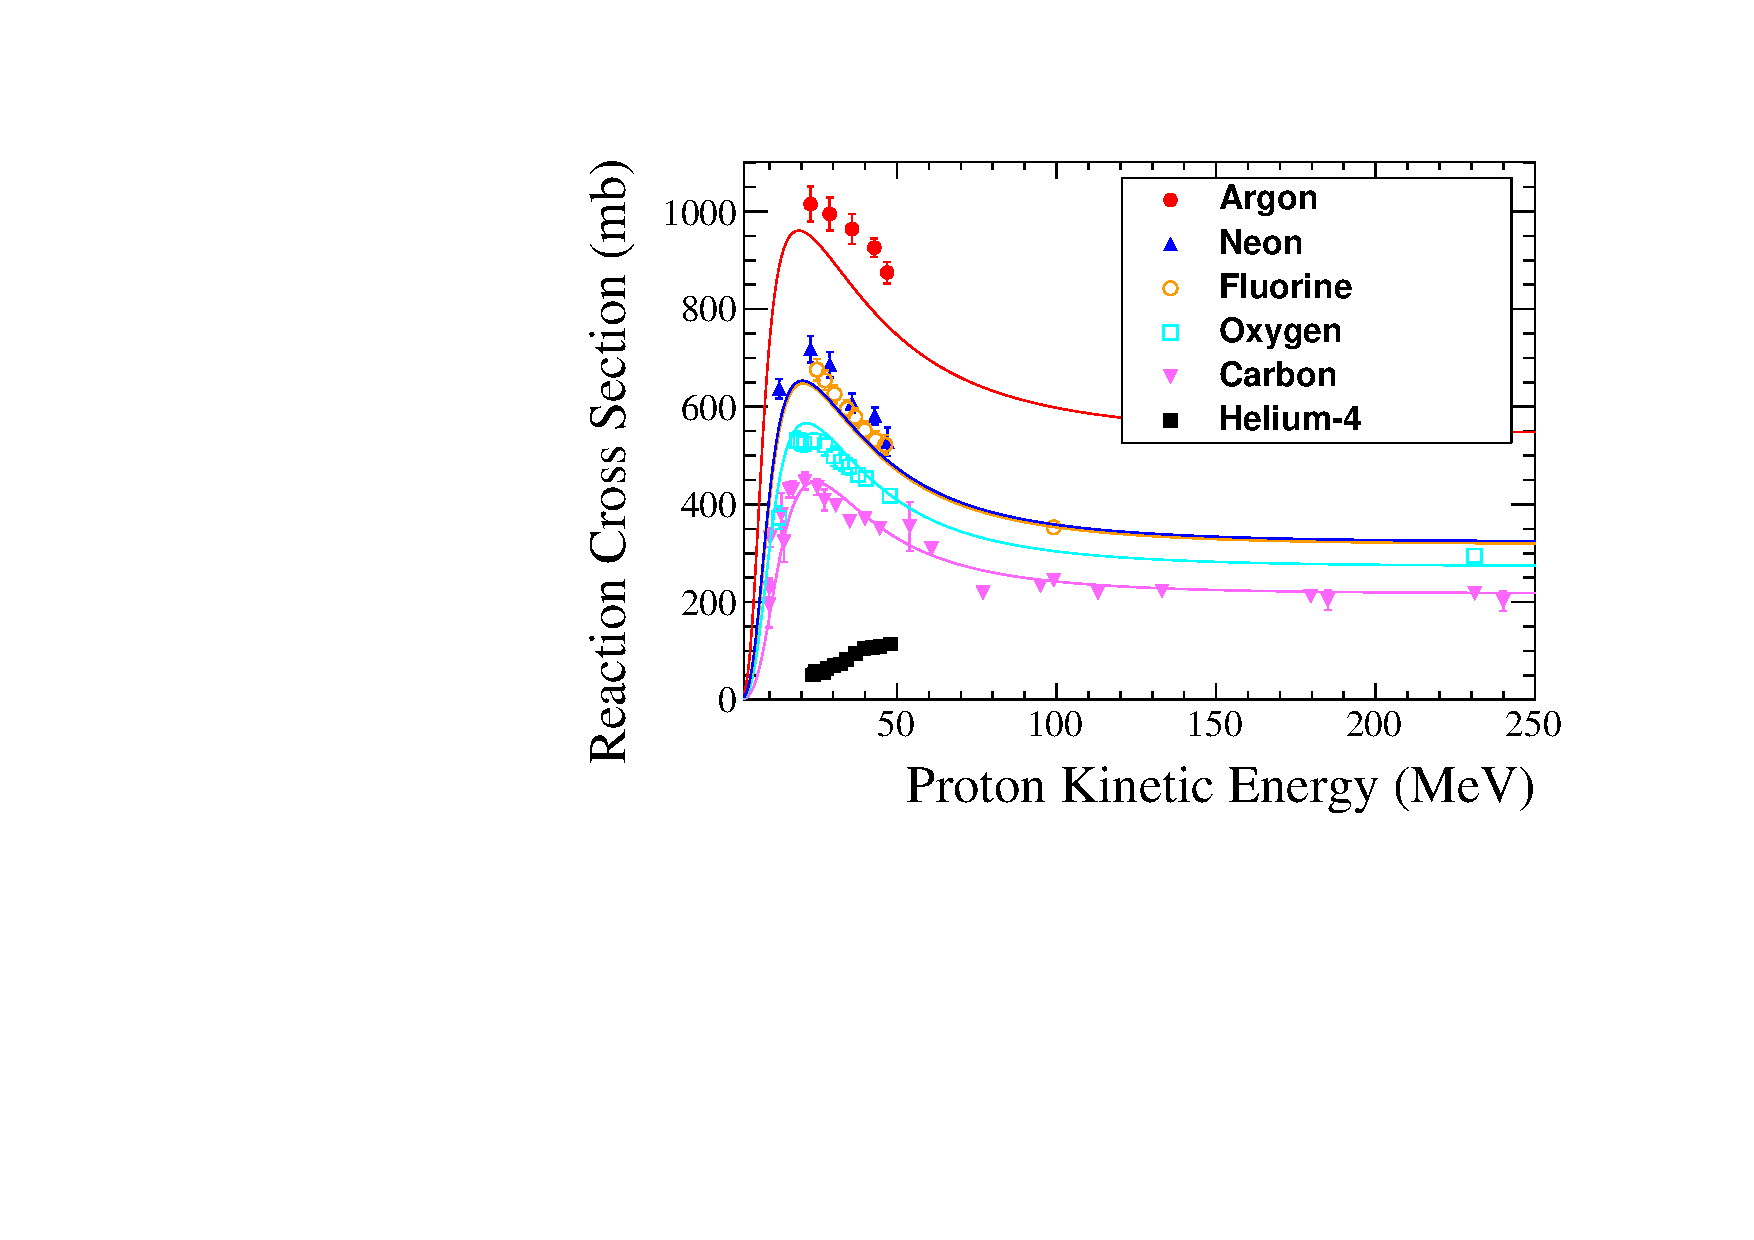
\includegraphics[width=12cm]{files/Figures/DataProtonCrossSections.pdf}%
    \caption{Total reaction cross sections for protons on argon, neon, fluorine, oxygen, carbon, and helium-4. Data~\cite{Carlson:1996ofz} are compared to a semi-empirical model~\cite{wellisch1996total}.}
    \label{fig:DataProtonXSec}%
\end{figure}

However, as shown in Figure~\ref{fig:DataProtonXSec}, proton-nucleus scattering measurements are extremely sparse and in many cases do not exist in the relevant energy region and/or on the relevant nuclei.
Therefore semi-empirical parameterisations are used to extrapolate in momentum and atomic mass~\cite{wellisch1996total}.  
The parametrisations are different between the three generators, and yield order-of-magnitude scale differences in the predicted multiplicity and kinematics of final state protons~\cite{dune2018high}.
The proton final state modeling is a key ingredient for neutrino oscillation measurements because it affects the event selection and neutrino energy reconstruction in charged-current (CC) interactions, which is the channel used to measure oscillation parameters and is therefore central to the search for CPV~\cite{Abe:2013hdq}.
For these reasons, FSI contribute substantially to the total neutrino interaction systematic uncertainty~\cite{Abe:2019vii}. 

Moreover, FSI models are in tension with data.  
Recent neutrino scattering measurements have shown that the most-used models of neutrino-nucleus interactions (employed by NEUT and GENIE) differ from nature in both cross section and kinematics of final state particles by as much as 30\%~\cite{McFarland:2018aaa}. 
These uncertainties cannot be fully mitigated with near/far detector combinations because they come from theoretical model deficiencies that are not cancelled in the near–far extrapolation~\cite{Coloma:2013rqa}. 
%To achieve 1-2\% systematic uncertainties for CPV searches, interaction models must be tuned and validated against precise proton-nucleus and pion-nucleus scattering measurements covering a broad final-state particle phase space, on a range of nuclear targets~\cite{Cao:2014zra}.

\begin{figure}%
    \centering
    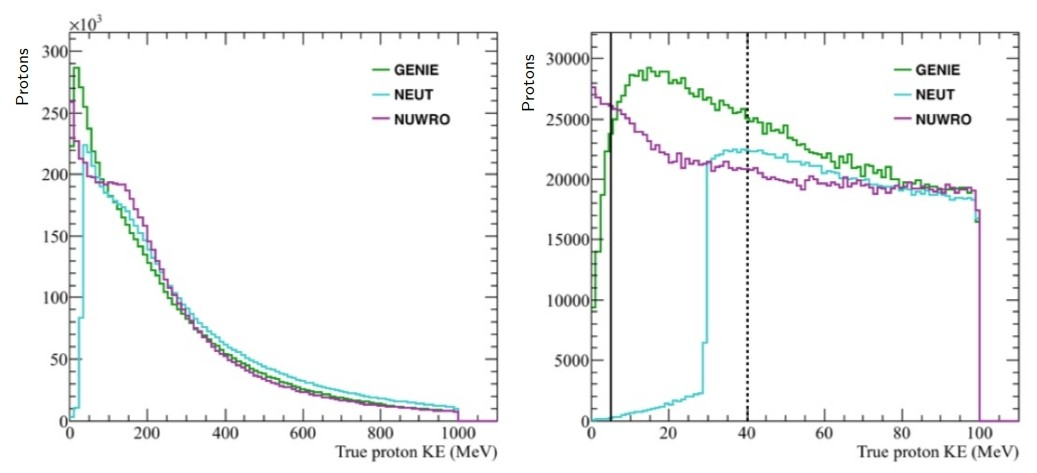
\includegraphics[width=12cm]{files/Figures/protons_from_argon.jpeg}%
    \caption{Predicted proton kinetic energy (KE) spectra from GENIE, NEUT, and NuWro\cite{Raaf:2018aaa}. Energy spectra up to 1 GeV are shown on the left, and zoomed in to lower energies on the right. The figure uses the Long Baseline Neutrino Facility (LBNF)  simulation for DUNE's beam energy and flux. The LBNF beam has a mean energy of approximately 2.5~GeV\cite{abi2020deep}. The dashed vertical line indicates the expected proton automated-reconstruction/identification threshold in liquid argon, and the solid vertical line shows the same for gaseous argon at 10 atm~\cite{dune2018high}.}
    \label{fig:protonsfromargon}%
\end{figure}

The key proton kinetic energy range in which to distinguish interaction models is the region below 0.1~GeV.
Figure~\ref{fig:protonsfromargon} shows the proton multiplicity and kinetic energy distributions for $\nu_{\mu}$ CC interactions on argon calculated by the GENIE, NEUT, and NuWro neutrino generators for the DUNE experiment.
These distributions are highly discrepant at low proton kinetic energy as shown in the right hand panel. The generators are not designed to handle the low energy region consistently, due to the lack of available data.
This is predominantly below the proton detection threshold in liquid Argon TPCs (0.04~GeV), such as those that will be used by DUNE, and in water Cherenkov detectors (0.5~GeV).
The lower threshold in high pressure gas provides a unique opportunity to distinguish between neutrino interaction models for the same nuclear target.

We have built a High Pressure gas Time Projection Chamber (HPTPC) prototype and exposed it to a charged particle beam in the T10 beamline at CERN in August and September 2018 \cite{SPSC-P-355}.
The momentum profile of the T10 beam can be tuned within the range 0.8--6.5~GeV/c (kinetic energy range 0.3--5.6~GeV). 
Figure~\ref{fig:utofNoBend}, left, shows the time of flight (ToF) spectrum for the T10 beamline tuned to a momentum of 0.8~GeV/c; this measurement was made with our upstream ToF system (see Section~\ref{hptpcPaper:sec:Methods} for details of the ToF systems).
The kinetic energy of the protons calculated from the upstream ToF measurements in this sample is shown in Figure~\ref{fig:utofNoBend}, right.
As shown, the flux of protons with kinetic energy less than 200~MeV is negligible.
The physics objective of the HPTPC beam test was to make measurements of protons on argon at kinetic energies below 200~MeV, i.e. below what was available with the T10 beam. 
Furthermore, the readout speed of the charge-coupled device cameras (CCD) employed in the HPTPC prototype motivates a limit on the total particle multiplicity in the TPC active volume.

\begin{figure}
  \begin{minipage}[t]{0.49\textwidth}
    \centering
    \begin{adjustbox}{max totalsize={\textwidth},center}
      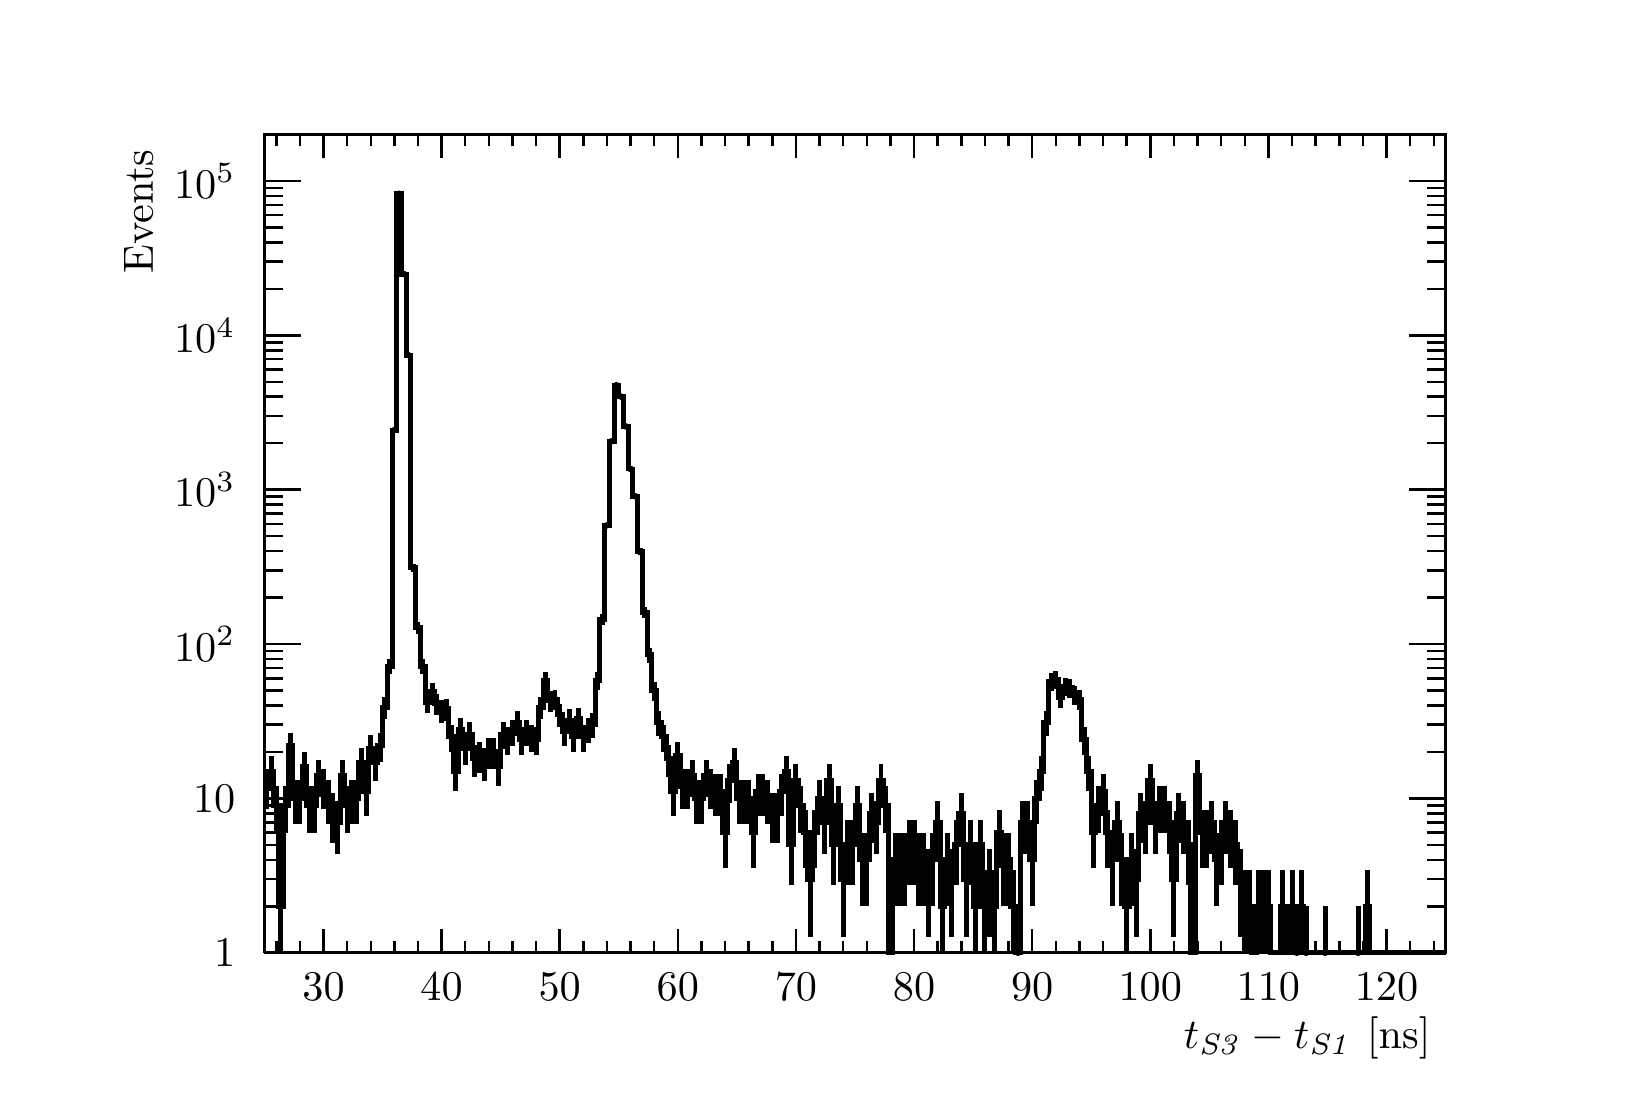
\begin{tikzpicture}
\pgfdeclareplotmark{cross} {
\pgfpathmoveto{\pgfpoint{-0.3\pgfplotmarksize}{\pgfplotmarksize}}
\pgfpathlineto{\pgfpoint{+0.3\pgfplotmarksize}{\pgfplotmarksize}}
\pgfpathlineto{\pgfpoint{+0.3\pgfplotmarksize}{0.3\pgfplotmarksize}}
\pgfpathlineto{\pgfpoint{+1\pgfplotmarksize}{0.3\pgfplotmarksize}}
\pgfpathlineto{\pgfpoint{+1\pgfplotmarksize}{-0.3\pgfplotmarksize}}
\pgfpathlineto{\pgfpoint{+0.3\pgfplotmarksize}{-0.3\pgfplotmarksize}}
\pgfpathlineto{\pgfpoint{+0.3\pgfplotmarksize}{-1.\pgfplotmarksize}}
\pgfpathlineto{\pgfpoint{-0.3\pgfplotmarksize}{-1.\pgfplotmarksize}}
\pgfpathlineto{\pgfpoint{-0.3\pgfplotmarksize}{-0.3\pgfplotmarksize}}
\pgfpathlineto{\pgfpoint{-1.\pgfplotmarksize}{-0.3\pgfplotmarksize}}
\pgfpathlineto{\pgfpoint{-1.\pgfplotmarksize}{0.3\pgfplotmarksize}}
\pgfpathlineto{\pgfpoint{-0.3\pgfplotmarksize}{0.3\pgfplotmarksize}}
\pgfpathclose
\pgfusepathqstroke
}
\pgfdeclareplotmark{cross*} {
\pgfpathmoveto{\pgfpoint{-0.3\pgfplotmarksize}{\pgfplotmarksize}}
\pgfpathlineto{\pgfpoint{+0.3\pgfplotmarksize}{\pgfplotmarksize}}
\pgfpathlineto{\pgfpoint{+0.3\pgfplotmarksize}{0.3\pgfplotmarksize}}
\pgfpathlineto{\pgfpoint{+1\pgfplotmarksize}{0.3\pgfplotmarksize}}
\pgfpathlineto{\pgfpoint{+1\pgfplotmarksize}{-0.3\pgfplotmarksize}}
\pgfpathlineto{\pgfpoint{+0.3\pgfplotmarksize}{-0.3\pgfplotmarksize}}
\pgfpathlineto{\pgfpoint{+0.3\pgfplotmarksize}{-1.\pgfplotmarksize}}
\pgfpathlineto{\pgfpoint{-0.3\pgfplotmarksize}{-1.\pgfplotmarksize}}
\pgfpathlineto{\pgfpoint{-0.3\pgfplotmarksize}{-0.3\pgfplotmarksize}}
\pgfpathlineto{\pgfpoint{-1.\pgfplotmarksize}{-0.3\pgfplotmarksize}}
\pgfpathlineto{\pgfpoint{-1.\pgfplotmarksize}{0.3\pgfplotmarksize}}
\pgfpathlineto{\pgfpoint{-0.3\pgfplotmarksize}{0.3\pgfplotmarksize}}
\pgfpathclose
\pgfusepathqfillstroke
}
\pgfdeclareplotmark{newstar} {
\pgfpathmoveto{\pgfqpoint{0pt}{\pgfplotmarksize}}
\pgfpathlineto{\pgfqpointpolar{44}{0.5\pgfplotmarksize}}
\pgfpathlineto{\pgfqpointpolar{18}{\pgfplotmarksize}}
\pgfpathlineto{\pgfqpointpolar{-20}{0.5\pgfplotmarksize}}
\pgfpathlineto{\pgfqpointpolar{-54}{\pgfplotmarksize}}
\pgfpathlineto{\pgfqpointpolar{-90}{0.5\pgfplotmarksize}}
\pgfpathlineto{\pgfqpointpolar{234}{\pgfplotmarksize}}
\pgfpathlineto{\pgfqpointpolar{198}{0.5\pgfplotmarksize}}
\pgfpathlineto{\pgfqpointpolar{162}{\pgfplotmarksize}}
\pgfpathlineto{\pgfqpointpolar{134}{0.5\pgfplotmarksize}}
\pgfpathclose
\pgfusepathqstroke
}
\pgfdeclareplotmark{newstar*} {
\pgfpathmoveto{\pgfqpoint{0pt}{\pgfplotmarksize}}
\pgfpathlineto{\pgfqpointpolar{44}{0.5\pgfplotmarksize}}
\pgfpathlineto{\pgfqpointpolar{18}{\pgfplotmarksize}}
\pgfpathlineto{\pgfqpointpolar{-20}{0.5\pgfplotmarksize}}
\pgfpathlineto{\pgfqpointpolar{-54}{\pgfplotmarksize}}
\pgfpathlineto{\pgfqpointpolar{-90}{0.5\pgfplotmarksize}}
\pgfpathlineto{\pgfqpointpolar{234}{\pgfplotmarksize}}
\pgfpathlineto{\pgfqpointpolar{198}{0.5\pgfplotmarksize}}
\pgfpathlineto{\pgfqpointpolar{162}{\pgfplotmarksize}}
\pgfpathlineto{\pgfqpointpolar{134}{0.5\pgfplotmarksize}}
\pgfpathclose
\pgfusepathqfillstroke
}
\definecolor{c}{rgb}{1,1,1};
\draw [color=c, fill=c] (0,0) rectangle (20,13.4957);
\draw [color=c, fill=c] (3,1.75444) rectangle (18,12.1461);
\definecolor{c}{rgb}{0,0,0};
\draw [c,line width=0.9] (3,1.75444) -- (3,12.1461) -- (18,12.1461) -- (18,1.75444) -- (3,1.75444);
\definecolor{c}{rgb}{1,1,1};
\draw [color=c, fill=c] (3,1.75444) rectangle (18,12.1461);
\definecolor{c}{rgb}{0,0,0};
\draw [c,line width=0.9] (3,1.75444) -- (3,12.1461) -- (18,12.1461) -- (18,1.75444) -- (3,1.75444);
\draw [c,line width=1.8] (3.03,3.57998) -- (3.03,3.86998);
\draw [c,line width=1.8] (3.03,3.86998) -- (3.03,4.08589);
\foreach \P in {(3.03,3.86998)}{\draw[mark options={color=c,fill=c},mark size=2.402402pt,mark=*,mark size=1pt] plot coordinates {\P};}
\draw [c,line width=1.8] (3.09,3.80567) -- (3.09,4.05995);
\draw [c,line width=1.8] (3.09,4.05995) -- (3.09,4.25549);
\foreach \P in {(3.09,4.05995)}{\draw[mark options={color=c,fill=c},mark size=2.402402pt,mark=*,mark size=1pt] plot coordinates {\P};}
\draw [c,line width=1.8] (3.15,3.27986) -- (3.15,3.62506);
\draw [c,line width=1.8] (3.15,3.62506) -- (3.15,3.86998);
\foreach \P in {(3.15,3.62506)}{\draw[mark options={color=c,fill=c},mark size=2.402402pt,mark=*,mark size=1pt] plot coordinates {\P};}
\draw [c,line width=1.8] (3.21,1.75444) -- (3.21,2.34455);
\draw [c,line width=1.8] (3.21,2.34455) -- (3.21,2.79986);
\foreach \P in {(3.21,2.34455)}{\draw[mark options={color=c,fill=c},mark size=2.402402pt,mark=*,mark size=1pt] plot coordinates {\P};}
\draw [c,line width=1.8] (3.27,3.27986) -- (3.27,3.62506);
\draw [c,line width=1.8] (3.27,3.62506) -- (3.27,3.86998);
\foreach \P in {(3.27,3.62506)}{\draw[mark options={color=c,fill=c},mark size=2.402402pt,mark=*,mark size=1pt] plot coordinates {\P};}
\draw [c,line width=1.8] (3.33,4.18187) -- (3.33,4.38601);
\draw [c,line width=1.8] (3.33,4.38601) -- (3.33,4.55055);
\foreach \P in {(3.33,4.38601)}{\draw[mark options={color=c,fill=c},mark size=2.402402pt,mark=*,mark size=1pt] plot coordinates {\P};}
\draw [c,line width=1.8] (3.39,3.39113) -- (3.39,3.71476);
\draw [c,line width=1.8] (3.39,3.71476) -- (3.39,3.94868);
\foreach \P in {(3.39,3.71476)}{\draw[mark options={color=c,fill=c},mark size=2.402402pt,mark=*,mark size=1pt] plot coordinates {\P};}
\draw [c,line width=1.8] (3.45,3.39113) -- (3.45,3.71476);
\draw [c,line width=1.8] (3.45,3.71476) -- (3.45,3.94868);
\foreach \P in {(3.45,3.71476)}{\draw[mark options={color=c,fill=c},mark size=2.402402pt,mark=*,mark size=1pt] plot coordinates {\P};}
\draw [c,line width=1.8] (3.51,3.86998) -- (3.51,4.1149);
\draw [c,line width=1.8] (3.51,4.1149) -- (3.51,4.30487);
\foreach \P in {(3.51,4.1149)}{\draw[mark options={color=c,fill=c},mark size=2.402402pt,mark=*,mark size=1pt] plot coordinates {\P};}
\draw [c,line width=1.8] (3.57,3.27986) -- (3.57,3.62506);
\draw [c,line width=1.8] (3.57,3.62506) -- (3.57,3.86998);
\foreach \P in {(3.57,3.62506)}{\draw[mark options={color=c,fill=c},mark size=2.402402pt,mark=*,mark size=1pt] plot coordinates {\P};}
\draw [c,line width=1.8] (3.63,3.27986) -- (3.63,3.62506);
\draw [c,line width=1.8] (3.63,3.62506) -- (3.63,3.86998);
\foreach \P in {(3.63,3.62506)}{\draw[mark options={color=c,fill=c},mark size=2.402402pt,mark=*,mark size=1pt] plot coordinates {\P};}
\draw [c,line width=1.8] (3.69,3.73647) -- (3.69,4.00121);
\draw [c,line width=1.8] (3.69,4.00121) -- (3.69,4.20286);
\foreach \P in {(3.69,4.00121)}{\draw[mark options={color=c,fill=c},mark size=2.402402pt,mark=*,mark size=1pt] plot coordinates {\P};}
\draw [c,line width=1.8] (3.75,3.57998) -- (3.75,3.86998);
\draw [c,line width=1.8] (3.75,3.86998) -- (3.75,4.08589);
\foreach \P in {(3.75,3.86998)}{\draw[mark options={color=c,fill=c},mark size=2.402402pt,mark=*,mark size=1pt] plot coordinates {\P};}
\draw [c,line width=1.8] (3.81,3.39113) -- (3.81,3.71476);
\draw [c,line width=1.8] (3.81,3.71476) -- (3.81,3.94868);
\foreach \P in {(3.81,3.71476)}{\draw[mark options={color=c,fill=c},mark size=2.402402pt,mark=*,mark size=1pt] plot coordinates {\P};}
\draw [c,line width=1.8] (3.87,3.15337) -- (3.87,3.52478);
\draw [c,line width=1.8] (3.87,3.52478) -- (3.87,3.78252);
\foreach \P in {(3.87,3.52478)}{\draw[mark options={color=c,fill=c},mark size=2.402402pt,mark=*,mark size=1pt] plot coordinates {\P};}
\draw [c,line width=1.8] (3.93,3.00691) -- (3.93,3.4111);
\draw [c,line width=1.8] (3.93,3.4111) -- (3.93,3.68405);
\foreach \P in {(3.93,3.4111)}{\draw[mark options={color=c,fill=c},mark size=2.402402pt,mark=*,mark size=1pt] plot coordinates {\P};}
\draw [c,line width=1.8] (3.99,3.73647) -- (3.99,4.00121);
\draw [c,line width=1.8] (3.99,4.00121) -- (3.99,4.20286);
\foreach \P in {(3.99,4.00121)}{\draw[mark options={color=c,fill=c},mark size=2.402402pt,mark=*,mark size=1pt] plot coordinates {\P};}
\draw [c,line width=1.8] (4.05,3.27986) -- (4.05,3.62506);
\draw [c,line width=1.8] (4.05,3.62506) -- (4.05,3.86998);
\foreach \P in {(4.05,3.62506)}{\draw[mark options={color=c,fill=c},mark size=2.402402pt,mark=*,mark size=1pt] plot coordinates {\P};}
\draw [c,line width=1.8] (4.11,3.39113) -- (4.11,3.71476);
\draw [c,line width=1.8] (4.11,3.71476) -- (4.11,3.94868);
\foreach \P in {(4.11,3.71476)}{\draw[mark options={color=c,fill=c},mark size=2.402402pt,mark=*,mark size=1pt] plot coordinates {\P};}
\draw [c,line width=1.8] (4.17,3.39113) -- (4.17,3.71476);
\draw [c,line width=1.8] (4.17,3.71476) -- (4.17,3.94868);
\foreach \P in {(4.17,3.71476)}{\draw[mark options={color=c,fill=c},mark size=2.402402pt,mark=*,mark size=1pt] plot coordinates {\P};}
\draw [c,line width=1.8] (4.23,3.93002) -- (4.23,4.16651);
\draw [c,line width=1.8] (4.23,4.16651) -- (4.23,4.35138);
\foreach \P in {(4.23,4.16651)}{\draw[mark options={color=c,fill=c},mark size=2.402402pt,mark=*,mark size=1pt] plot coordinates {\P};}
\draw [c,line width=1.8] (4.29,3.4904) -- (4.29,3.7959);
\draw [c,line width=1.8] (4.29,3.7959) -- (4.29,4.02025);
\foreach \P in {(4.29,3.7959)}{\draw[mark options={color=c,fill=c},mark size=2.402402pt,mark=*,mark size=1pt] plot coordinates {\P};}
\draw [c,line width=1.8] (4.35,4.13682) -- (4.35,4.34641);
\draw [c,line width=1.8] (4.35,4.34641) -- (4.35,4.51446);
\foreach \P in {(4.35,4.34641)}{\draw[mark options={color=c,fill=c},mark size=2.402402pt,mark=*,mark size=1pt] plot coordinates {\P};}
\draw [c,line width=1.8] (4.41,3.93002) -- (4.41,4.16651);
\draw [c,line width=1.8] (4.41,4.16651) -- (4.41,4.35138);
\foreach \P in {(4.41,4.16651)}{\draw[mark options={color=c,fill=c},mark size=2.402402pt,mark=*,mark size=1pt] plot coordinates {\P};}
\draw [c,line width=1.8] (4.47,4.18187) -- (4.47,4.38601);
\draw [c,line width=1.8] (4.47,4.38601) -- (4.47,4.55055);
\foreach \P in {(4.47,4.38601)}{\draw[mark options={color=c,fill=c},mark size=2.402402pt,mark=*,mark size=1pt] plot coordinates {\P};}
\draw [c,line width=1.8] (4.53,4.72486) -- (4.53,4.87343);
\draw [c,line width=1.8] (4.53,4.87343) -- (4.53,4.99988);
\foreach \P in {(4.53,4.87343)}{\draw[mark options={color=c,fill=c},mark size=2.402402pt,mark=*,mark size=1pt] plot coordinates {\P};}
\draw [c,line width=1.8] (4.59,5.28864) -- (4.59,5.3954);
\draw [c,line width=1.8] (4.59,5.3954) -- (4.59,5.49025);
\foreach \P in {(4.59,5.3954)}{\draw[mark options={color=c,fill=c},mark size=2.402402pt,mark=*,mark size=1pt] plot coordinates {\P};}
\draw [c,line width=1.8] (4.65,8.3742) -- (4.65,8.39165);
\draw [c,line width=1.8] (4.65,8.39165) -- (4.65,8.40874);
\foreach \P in {(4.65,8.39165)}{\draw[mark options={color=c,fill=c},mark size=2.402402pt,mark=*,mark size=1pt] plot coordinates {\P};}
\draw [c,line width=1.8] (4.71,11.3894) -- (4.71,11.3924);
\draw [c,line width=1.8] (4.71,11.3924) -- (4.71,11.3953);
\foreach \P in {(4.71,11.3924)}{\draw[mark options={color=c,fill=c},mark size=2.402402pt,mark=*,mark size=1pt] plot coordinates {\P};}
\draw [c,line width=1.8] (4.77,10.3684) -- (4.77,10.3738);
\draw [c,line width=1.8] (4.77,10.3738) -- (4.77,10.3792);
\foreach \P in {(4.77,10.3738)}{\draw[mark options={color=c,fill=c},mark size=2.402402pt,mark=*,mark size=1pt] plot coordinates {\P};}
\draw [c,line width=1.8] (4.83,9.33206) -- (4.83,9.342);
\draw [c,line width=1.8] (4.83,9.342) -- (4.83,9.35182);
\foreach \P in {(4.83,9.342)}{\draw[mark options={color=c,fill=c},mark size=2.402402pt,mark=*,mark size=1pt] plot coordinates {\P};}
\draw [c,line width=1.8] (4.89,6.59134) -- (4.89,6.64104);
\draw [c,line width=1.8] (4.89,6.64104) -- (4.89,6.68799);
\foreach \P in {(4.89,6.64104)}{\draw[mark options={color=c,fill=c},mark size=2.402402pt,mark=*,mark size=1pt] plot coordinates {\P};}
\draw [c,line width=1.8] (4.95,5.80645) -- (4.95,5.88524);
\draw [c,line width=1.8] (4.95,5.88524) -- (4.95,5.95735);
\foreach \P in {(4.95,5.88524)}{\draw[mark options={color=c,fill=c},mark size=2.402402pt,mark=*,mark size=1pt] plot coordinates {\P};}
\draw [c,line width=1.8] (5.01,5.28864) -- (5.01,5.3954);
\draw [c,line width=1.8] (5.01,5.3954) -- (5.01,5.49025);
\foreach \P in {(5.01,5.3954)}{\draw[mark options={color=c,fill=c},mark size=2.402402pt,mark=*,mark size=1pt] plot coordinates {\P};}
\draw [c,line width=1.8] (5.07,4.79384) -- (5.07,4.93652);
\draw [c,line width=1.8] (5.07,4.93652) -- (5.07,5.05869);
\foreach \P in {(5.07,4.93652)}{\draw[mark options={color=c,fill=c},mark size=2.402402pt,mark=*,mark size=1pt] plot coordinates {\P};}
\draw [c,line width=1.8] (5.13,4.93652) -- (5.13,5.06776);
\draw [c,line width=1.8] (5.13,5.06776) -- (5.13,5.18144);
\foreach \P in {(5.13,5.06776)}{\draw[mark options={color=c,fill=c},mark size=2.402402pt,mark=*,mark size=1pt] plot coordinates {\P};}
\draw [c,line width=1.8] (5.19,4.77144) -- (5.19,4.91601);
\draw [c,line width=1.8] (5.19,4.91601) -- (5.19,5.03955);
\foreach \P in {(5.19,4.91601)}{\draw[mark options={color=c,fill=c},mark size=2.402402pt,mark=*,mark size=1pt] plot coordinates {\P};}
\draw [c,line width=1.8] (5.25,4.6757) -- (5.25,4.82861);
\draw [c,line width=1.8] (5.25,4.82861) -- (5.25,4.95819);
\foreach \P in {(5.25,4.82861)}{\draw[mark options={color=c,fill=c},mark size=2.402402pt,mark=*,mark size=1pt] plot coordinates {\P};}
\draw [c,line width=1.8] (5.31,4.70062) -- (5.31,4.85132);
\draw [c,line width=1.8] (5.31,4.85132) -- (5.31,4.9793);
\foreach \P in {(5.31,4.85132)}{\draw[mark options={color=c,fill=c},mark size=2.402402pt,mark=*,mark size=1pt] plot coordinates {\P};}
\draw [c,line width=1.8] (5.37,4.30487) -- (5.37,4.49484);
\draw [c,line width=1.8] (5.37,4.49484) -- (5.37,4.65006);
\foreach \P in {(5.37,4.49484)}{\draw[mark options={color=c,fill=c},mark size=2.402402pt,mark=*,mark size=1pt] plot coordinates {\P};}
\draw [c,line width=1.8] (5.43,3.80567) -- (5.43,4.05995);
\draw [c,line width=1.8] (5.43,4.05995) -- (5.43,4.25549);
\foreach \P in {(5.43,4.05995)}{\draw[mark options={color=c,fill=c},mark size=2.402402pt,mark=*,mark size=1pt] plot coordinates {\P};}
\draw [c,line width=1.8] (5.49,4.413) -- (5.49,4.59133);
\draw [c,line width=1.8] (5.49,4.59133) -- (5.49,4.73869);
\foreach \P in {(5.49,4.59133)}{\draw[mark options={color=c,fill=c},mark size=2.402402pt,mark=*,mark size=1pt] plot coordinates {\P};}
\draw [c,line width=1.8] (5.55,4.13682) -- (5.55,4.34641);
\draw [c,line width=1.8] (5.55,4.34641) -- (5.55,4.51446);
\foreach \P in {(5.55,4.34641)}{\draw[mark options={color=c,fill=c},mark size=2.402402pt,mark=*,mark size=1pt] plot coordinates {\P};}
\draw [c,line width=1.8] (5.61,4.34238) -- (5.61,4.52823);
\draw [c,line width=1.8] (5.61,4.52823) -- (5.61,4.6807);
\foreach \P in {(5.61,4.52823)}{\draw[mark options={color=c,fill=c},mark size=2.402402pt,mark=*,mark size=1pt] plot coordinates {\P};}
\draw [c,line width=1.8] (5.67,3.98633) -- (5.67,4.21517);
\draw [c,line width=1.8] (5.67,4.21517) -- (5.67,4.39535);
\foreach \P in {(5.67,4.21517)}{\draw[mark options={color=c,fill=c},mark size=2.402402pt,mark=*,mark size=1pt] plot coordinates {\P};}
\draw [c,line width=1.8] (5.73,4.03933) -- (5.73,4.2612);
\draw [c,line width=1.8] (5.73,4.2612) -- (5.73,4.43704);
\foreach \P in {(5.73,4.2612)}{\draw[mark options={color=c,fill=c},mark size=2.402402pt,mark=*,mark size=1pt] plot coordinates {\P};}
\draw [c,line width=1.8] (5.79,3.93002) -- (5.79,4.16651);
\draw [c,line width=1.8] (5.79,4.16651) -- (5.79,4.35138);
\foreach \P in {(5.79,4.16651)}{\draw[mark options={color=c,fill=c},mark size=2.402402pt,mark=*,mark size=1pt] plot coordinates {\P};}
\draw [c,line width=1.8] (5.85,4.0894) -- (5.85,4.30487);
\draw [c,line width=1.8] (5.85,4.30487) -- (5.85,4.47668);
\foreach \P in {(5.85,4.30487)}{\draw[mark options={color=c,fill=c},mark size=2.402402pt,mark=*,mark size=1pt] plot coordinates {\P};}
\draw [c,line width=1.8] (5.91,4.0894) -- (5.91,4.30487);
\draw [c,line width=1.8] (5.91,4.30487) -- (5.91,4.47668);
\foreach \P in {(5.91,4.30487)}{\draw[mark options={color=c,fill=c},mark size=2.402402pt,mark=*,mark size=1pt] plot coordinates {\P};}
\draw [c,line width=1.8] (5.97,3.86998) -- (5.97,4.1149);
\draw [c,line width=1.8] (5.97,4.1149) -- (5.97,4.30487);
\foreach \P in {(5.97,4.1149)}{\draw[mark options={color=c,fill=c},mark size=2.402402pt,mark=*,mark size=1pt] plot coordinates {\P};}
\draw [c,line width=1.8] (6.03,4.34238) -- (6.03,4.52823);
\draw [c,line width=1.8] (6.03,4.52823) -- (6.03,4.6807);
\foreach \P in {(6.03,4.52823)}{\draw[mark options={color=c,fill=c},mark size=2.402402pt,mark=*,mark size=1pt] plot coordinates {\P};}
\draw [c,line width=1.8] (6.09,4.26572) -- (6.09,4.46009);
\draw [c,line width=1.8] (6.09,4.46009) -- (6.09,4.61823);
\foreach \P in {(6.09,4.46009)}{\draw[mark options={color=c,fill=c},mark size=2.402402pt,mark=*,mark size=1pt] plot coordinates {\P};}
\draw [c,line width=1.8] (6.15,4.37839) -- (6.15,4.56037);
\draw [c,line width=1.8] (6.15,4.56037) -- (6.15,4.71021);
\foreach \P in {(6.15,4.56037)}{\draw[mark options={color=c,fill=c},mark size=2.402402pt,mark=*,mark size=1pt] plot coordinates {\P};}
\draw [c,line width=1.8] (6.21,4.50944) -- (6.21,4.67798);
\draw [c,line width=1.8] (6.21,4.67798) -- (6.21,4.81861);
\foreach \P in {(6.21,4.67798)}{\draw[mark options={color=c,fill=c},mark size=2.402402pt,mark=*,mark size=1pt] plot coordinates {\P};}
\draw [c,line width=1.8] (6.27,4.26572) -- (6.27,4.46009);
\draw [c,line width=1.8] (6.27,4.46009) -- (6.27,4.61823);
\foreach \P in {(6.27,4.46009)}{\draw[mark options={color=c,fill=c},mark size=2.402402pt,mark=*,mark size=1pt] plot coordinates {\P};}
\draw [c,line width=1.8] (6.33,4.37839) -- (6.33,4.56037);
\draw [c,line width=1.8] (6.33,4.56037) -- (6.33,4.71021);
\foreach \P in {(6.33,4.56037)}{\draw[mark options={color=c,fill=c},mark size=2.402402pt,mark=*,mark size=1pt] plot coordinates {\P};}
\draw [c,line width=1.8] (6.39,4.30487) -- (6.39,4.49484);
\draw [c,line width=1.8] (6.39,4.49484) -- (6.39,4.65006);
\foreach \P in {(6.39,4.49484)}{\draw[mark options={color=c,fill=c},mark size=2.402402pt,mark=*,mark size=1pt] plot coordinates {\P};}
\draw [c,line width=1.8] (6.45,4.26572) -- (6.45,4.46009);
\draw [c,line width=1.8] (6.45,4.46009) -- (6.45,4.61823);
\foreach \P in {(6.45,4.46009)}{\draw[mark options={color=c,fill=c},mark size=2.402402pt,mark=*,mark size=1pt] plot coordinates {\P};}
\draw [c,line width=1.8] (6.51,4.72486) -- (6.51,4.87343);
\draw [c,line width=1.8] (6.51,4.87343) -- (6.51,4.99988);
\foreach \P in {(6.51,4.87343)}{\draw[mark options={color=c,fill=c},mark size=2.402402pt,mark=*,mark size=1pt] plot coordinates {\P};}
\draw [c,line width=1.8] (6.57,5.09148) -- (6.57,5.21132);
\draw [c,line width=1.8] (6.57,5.21132) -- (6.57,5.31635);
\foreach \P in {(6.57,5.21132)}{\draw[mark options={color=c,fill=c},mark size=2.402402pt,mark=*,mark size=1pt] plot coordinates {\P};}
\draw [c,line width=1.8] (6.63,4.81569) -- (6.63,4.95655);
\draw [c,line width=1.8] (6.63,4.95655) -- (6.63,5.07739);
\foreach \P in {(6.63,4.95655)}{\draw[mark options={color=c,fill=c},mark size=2.402402pt,mark=*,mark size=1pt] plot coordinates {\P};}
\draw [c,line width=1.8] (6.69,4.83701) -- (6.69,4.97613);
\draw [c,line width=1.8] (6.69,4.97613) -- (6.69,5.09567);
\foreach \P in {(6.69,4.97613)}{\draw[mark options={color=c,fill=c},mark size=2.402402pt,mark=*,mark size=1pt] plot coordinates {\P};}
\draw [c,line width=1.8] (6.75,4.62366) -- (6.75,4.7813);
\draw [c,line width=1.8] (6.75,4.7813) -- (6.75,4.91426);
\foreach \P in {(6.75,4.7813)}{\draw[mark options={color=c,fill=c},mark size=2.402402pt,mark=*,mark size=1pt] plot coordinates {\P};}
\draw [c,line width=1.8] (6.81,4.37839) -- (6.81,4.56037);
\draw [c,line width=1.8] (6.81,4.56037) -- (6.81,4.71021);
\foreach \P in {(6.81,4.56037)}{\draw[mark options={color=c,fill=c},mark size=2.402402pt,mark=*,mark size=1pt] plot coordinates {\P};}
\draw [c,line width=1.8] (6.87,4.5394) -- (6.87,4.70501);
\draw [c,line width=1.8] (6.87,4.70501) -- (6.87,4.84359);
\foreach \P in {(6.87,4.70501)}{\draw[mark options={color=c,fill=c},mark size=2.402402pt,mark=*,mark size=1pt] plot coordinates {\P};}
\draw [c,line width=1.8] (6.93,4.30487) -- (6.93,4.49484);
\draw [c,line width=1.8] (6.93,4.49484) -- (6.93,4.65006);
\foreach \P in {(6.93,4.49484)}{\draw[mark options={color=c,fill=c},mark size=2.402402pt,mark=*,mark size=1pt] plot coordinates {\P};}
\draw [c,line width=1.8] (6.99,4.56838) -- (6.99,4.73121);
\draw [c,line width=1.8] (6.99,4.73121) -- (6.99,4.86784);
\foreach \P in {(6.99,4.73121)}{\draw[mark options={color=c,fill=c},mark size=2.402402pt,mark=*,mark size=1pt] plot coordinates {\P};}
\draw [c,line width=1.8] (7.05,4.30487) -- (7.05,4.49484);
\draw [c,line width=1.8] (7.05,4.49484) -- (7.05,4.65006);
\foreach \P in {(7.05,4.49484)}{\draw[mark options={color=c,fill=c},mark size=2.402402pt,mark=*,mark size=1pt] plot coordinates {\P};}
\draw [c,line width=1.8] (7.11,4.413) -- (7.11,4.59133);
\draw [c,line width=1.8] (7.11,4.59133) -- (7.11,4.73869);
\foreach \P in {(7.11,4.59133)}{\draw[mark options={color=c,fill=c},mark size=2.402402pt,mark=*,mark size=1pt] plot coordinates {\P};}
\draw [c,line width=1.8] (7.17,4.47844) -- (7.17,4.65006);
\draw [c,line width=1.8] (7.17,4.65006) -- (7.17,4.79283);
\foreach \P in {(7.17,4.65006)}{\draw[mark options={color=c,fill=c},mark size=2.402402pt,mark=*,mark size=1pt] plot coordinates {\P};}
\draw [c,line width=1.8] (7.23,5.09148) -- (7.23,5.21132);
\draw [c,line width=1.8] (7.23,5.21132) -- (7.23,5.31635);
\foreach \P in {(7.23,5.21132)}{\draw[mark options={color=c,fill=c},mark size=2.402402pt,mark=*,mark size=1pt] plot coordinates {\P};}
\draw [c,line width=1.8] (7.29,5.91759) -- (7.29,5.9914);
\draw [c,line width=1.8] (7.29,5.9914) -- (7.29,6.05932);
\foreach \P in {(7.29,5.9914)}{\draw[mark options={color=c,fill=c},mark size=2.402402pt,mark=*,mark size=1pt] plot coordinates {\P};}
\draw [c,line width=1.8] (7.35,7.14744) -- (7.35,7.18329);
\draw [c,line width=1.8] (7.35,7.18329) -- (7.35,7.2177);
\foreach \P in {(7.35,7.18329)}{\draw[mark options={color=c,fill=c},mark size=2.402402pt,mark=*,mark size=1pt] plot coordinates {\P};}
\draw [c,line width=1.8] (7.41,8.23044) -- (7.41,8.24942);
\draw [c,line width=1.8] (7.41,8.24942) -- (7.41,8.26799);
\foreach \P in {(7.41,8.24942)}{\draw[mark options={color=c,fill=c},mark size=2.402402pt,mark=*,mark size=1pt] plot coordinates {\P};}
\draw [c,line width=1.8] (7.47,8.9493) -- (7.47,8.96174);
\draw [c,line width=1.8] (7.47,8.96174) -- (7.47,8.97401);
\foreach \P in {(7.47,8.96174)}{\draw[mark options={color=c,fill=c},mark size=2.402402pt,mark=*,mark size=1pt] plot coordinates {\P};}
\draw [c,line width=1.8] (7.53,8.80269) -- (7.53,8.81625);
\draw [c,line width=1.8] (7.53,8.81625) -- (7.53,8.8296);
\foreach \P in {(7.53,8.81625)}{\draw[mark options={color=c,fill=c},mark size=2.402402pt,mark=*,mark size=1pt] plot coordinates {\P};}
\draw [c,line width=1.8] (7.59,8.42169) -- (7.59,8.43865);
\draw [c,line width=1.8] (7.59,8.43865) -- (7.59,8.45529);
\foreach \P in {(7.59,8.43865)}{\draw[mark options={color=c,fill=c},mark size=2.402402pt,mark=*,mark size=1pt] plot coordinates {\P};}
\draw [c,line width=1.8] (7.65,7.8744) -- (7.65,7.89779);
\draw [c,line width=1.8] (7.65,7.89779) -- (7.65,7.92056);
\foreach \P in {(7.65,7.89779)}{\draw[mark options={color=c,fill=c},mark size=2.402402pt,mark=*,mark size=1pt] plot coordinates {\P};}
\draw [c,line width=1.8] (7.71,7.52162) -- (7.71,7.5504);
\draw [c,line width=1.8] (7.71,7.5504) -- (7.71,7.57824);
\foreach \P in {(7.71,7.5504)}{\draw[mark options={color=c,fill=c},mark size=2.402402pt,mark=*,mark size=1pt] plot coordinates {\P};}
\draw [c,line width=1.8] (7.77,6.80285) -- (7.77,6.84674);
\draw [c,line width=1.8] (7.77,6.84674) -- (7.77,6.88848);
\foreach \P in {(7.77,6.84674)}{\draw[mark options={color=c,fill=c},mark size=2.402402pt,mark=*,mark size=1pt] plot coordinates {\P};}
\draw [c,line width=1.8] (7.83,6.01063) -- (7.83,6.08052);
\draw [c,line width=1.8] (7.83,6.08052) -- (7.83,6.1451);
\foreach \P in {(7.83,6.08052)}{\draw[mark options={color=c,fill=c},mark size=2.402402pt,mark=*,mark size=1pt] plot coordinates {\P};}
\draw [c,line width=1.8] (7.89,5.43897) -- (7.89,5.53671);
\draw [c,line width=1.8] (7.89,5.53671) -- (7.89,5.62438);
\foreach \P in {(7.89,5.53671)}{\draw[mark options={color=c,fill=c},mark size=2.402402pt,mark=*,mark size=1pt] plot coordinates {\P};}
\draw [c,line width=1.8] (7.95,4.95515) -- (7.95,5.08496);
\draw [c,line width=1.8] (7.95,5.08496) -- (7.95,5.19757);
\foreach \P in {(7.95,5.08496)}{\draw[mark options={color=c,fill=c},mark size=2.402402pt,mark=*,mark size=1pt] plot coordinates {\P};}
\draw [c,line width=1.8] (8.01,4.50944) -- (8.01,4.67798);
\draw [c,line width=1.8] (8.01,4.67798) -- (8.01,4.81861);
\foreach \P in {(8.01,4.67798)}{\draw[mark options={color=c,fill=c},mark size=2.402402pt,mark=*,mark size=1pt] plot coordinates {\P};}
\draw [c,line width=1.8] (8.07,4.30487) -- (8.07,4.49484);
\draw [c,line width=1.8] (8.07,4.49484) -- (8.07,4.65006);
\foreach \P in {(8.07,4.49484)}{\draw[mark options={color=c,fill=c},mark size=2.402402pt,mark=*,mark size=1pt] plot coordinates {\P};}
\draw [c,line width=1.8] (8.13,3.98633) -- (8.13,4.21517);
\draw [c,line width=1.8] (8.13,4.21517) -- (8.13,4.39535);
\foreach \P in {(8.13,4.21517)}{\draw[mark options={color=c,fill=c},mark size=2.402402pt,mark=*,mark size=1pt] plot coordinates {\P};}
\draw [c,line width=1.8] (8.19,3.4904) -- (8.19,3.7959);
\draw [c,line width=1.8] (8.19,3.7959) -- (8.19,4.02025);
\foreach \P in {(8.19,3.7959)}{\draw[mark options={color=c,fill=c},mark size=2.402402pt,mark=*,mark size=1pt] plot coordinates {\P};}
\draw [c,line width=1.8] (8.25,4.03933) -- (8.25,4.2612);
\draw [c,line width=1.8] (8.25,4.2612) -- (8.25,4.43704);
\foreach \P in {(8.25,4.2612)}{\draw[mark options={color=c,fill=c},mark size=2.402402pt,mark=*,mark size=1pt] plot coordinates {\P};}
\draw [c,line width=1.8] (8.31,3.57998) -- (8.31,3.86998);
\draw [c,line width=1.8] (8.31,3.86998) -- (8.31,4.08589);
\foreach \P in {(8.31,3.86998)}{\draw[mark options={color=c,fill=c},mark size=2.402402pt,mark=*,mark size=1pt] plot coordinates {\P};}
\draw [c,line width=1.8] (8.37,3.57998) -- (8.37,3.86998);
\draw [c,line width=1.8] (8.37,3.86998) -- (8.37,4.08589);
\foreach \P in {(8.37,3.86998)}{\draw[mark options={color=c,fill=c},mark size=2.402402pt,mark=*,mark size=1pt] plot coordinates {\P};}
\draw [c,line width=1.8] (8.43,3.73647) -- (8.43,4.00121);
\draw [c,line width=1.8] (8.43,4.00121) -- (8.43,4.20286);
\foreach \P in {(8.43,4.00121)}{\draw[mark options={color=c,fill=c},mark size=2.402402pt,mark=*,mark size=1pt] plot coordinates {\P};}
\draw [c,line width=1.8] (8.49,3.39113) -- (8.49,3.71476);
\draw [c,line width=1.8] (8.49,3.71476) -- (8.49,3.94868);
\foreach \P in {(8.49,3.71476)}{\draw[mark options={color=c,fill=c},mark size=2.402402pt,mark=*,mark size=1pt] plot coordinates {\P};}
\draw [c,line width=1.8] (8.55,3.39113) -- (8.55,3.71476);
\draw [c,line width=1.8] (8.55,3.71476) -- (8.55,3.94868);
\foreach \P in {(8.55,3.71476)}{\draw[mark options={color=c,fill=c},mark size=2.402402pt,mark=*,mark size=1pt] plot coordinates {\P};}
\draw [c,line width=1.8] (8.61,3.73647) -- (8.61,4.00121);
\draw [c,line width=1.8] (8.61,4.00121) -- (8.61,4.20286);
\foreach \P in {(8.61,4.00121)}{\draw[mark options={color=c,fill=c},mark size=2.402402pt,mark=*,mark size=1pt] plot coordinates {\P};}
\draw [c,line width=1.8] (8.67,3.57998) -- (8.67,3.86998);
\draw [c,line width=1.8] (8.67,3.86998) -- (8.67,4.08589);
\foreach \P in {(8.67,3.86998)}{\draw[mark options={color=c,fill=c},mark size=2.402402pt,mark=*,mark size=1pt] plot coordinates {\P};}
\draw [c,line width=1.8] (8.73,3.4904) -- (8.73,3.7959);
\draw [c,line width=1.8] (8.73,3.7959) -- (8.73,4.02025);
\foreach \P in {(8.73,3.7959)}{\draw[mark options={color=c,fill=c},mark size=2.402402pt,mark=*,mark size=1pt] plot coordinates {\P};}
\draw [c,line width=1.8] (8.79,3.4904) -- (8.79,3.7959);
\draw [c,line width=1.8] (8.79,3.7959) -- (8.79,4.02025);
\foreach \P in {(8.79,3.7959)}{\draw[mark options={color=c,fill=c},mark size=2.402402pt,mark=*,mark size=1pt] plot coordinates {\P};}
\draw [c,line width=1.8] (8.85,2.83318) -- (8.85,3.27986);
\draw [c,line width=1.8] (8.85,3.27986) -- (8.85,3.57132);
\foreach \P in {(8.85,3.27986)}{\draw[mark options={color=c,fill=c},mark size=2.402402pt,mark=*,mark size=1pt] plot coordinates {\P};}
\draw [c,line width=1.8] (8.91,3.66158) -- (8.91,3.93812);
\draw [c,line width=1.8] (8.91,3.93812) -- (8.91,4.14652);
\foreach \P in {(8.91,3.93812)}{\draw[mark options={color=c,fill=c},mark size=2.402402pt,mark=*,mark size=1pt] plot coordinates {\P};}
\draw [c,line width=1.8] (8.97,3.93002) -- (8.97,4.16651);
\draw [c,line width=1.8] (8.97,4.16651) -- (8.97,4.35138);
\foreach \P in {(8.97,4.16651)}{\draw[mark options={color=c,fill=c},mark size=2.402402pt,mark=*,mark size=1pt] plot coordinates {\P};}
\draw [c,line width=1.8] (9.03,3.39113) -- (9.03,3.71476);
\draw [c,line width=1.8] (9.03,3.71476) -- (9.03,3.94868);
\foreach \P in {(9.03,3.71476)}{\draw[mark options={color=c,fill=c},mark size=2.402402pt,mark=*,mark size=1pt] plot coordinates {\P};}
\draw [c,line width=1.8] (9.09,3.39113) -- (9.09,3.71476);
\draw [c,line width=1.8] (9.09,3.71476) -- (9.09,3.94868);
\foreach \P in {(9.09,3.71476)}{\draw[mark options={color=c,fill=c},mark size=2.402402pt,mark=*,mark size=1pt] plot coordinates {\P};}
\draw [c,line width=1.8] (9.15,3.39113) -- (9.15,3.71476);
\draw [c,line width=1.8] (9.15,3.71476) -- (9.15,3.94868);
\foreach \P in {(9.15,3.71476)}{\draw[mark options={color=c,fill=c},mark size=2.402402pt,mark=*,mark size=1pt] plot coordinates {\P};}
\draw [c,line width=1.8] (9.21,2.83318) -- (9.21,3.27986);
\draw [c,line width=1.8] (9.21,3.27986) -- (9.21,3.57132);
\foreach \P in {(9.21,3.27986)}{\draw[mark options={color=c,fill=c},mark size=2.402402pt,mark=*,mark size=1pt] plot coordinates {\P};}
\draw [c,line width=1.8] (9.27,3.4904) -- (9.27,3.7959);
\draw [c,line width=1.8] (9.27,3.7959) -- (9.27,4.02025);
\foreach \P in {(9.27,3.7959)}{\draw[mark options={color=c,fill=c},mark size=2.402402pt,mark=*,mark size=1pt] plot coordinates {\P};}
\draw [c,line width=1.8] (9.33,3.4904) -- (9.33,3.7959);
\draw [c,line width=1.8] (9.33,3.7959) -- (9.33,4.02025);
\foreach \P in {(9.33,3.7959)}{\draw[mark options={color=c,fill=c},mark size=2.402402pt,mark=*,mark size=1pt] plot coordinates {\P};}
\draw [c,line width=1.8] (9.39,3.39113) -- (9.39,3.71476);
\draw [c,line width=1.8] (9.39,3.71476) -- (9.39,3.94868);
\foreach \P in {(9.39,3.71476)}{\draw[mark options={color=c,fill=c},mark size=2.402402pt,mark=*,mark size=1pt] plot coordinates {\P};}
\draw [c,line width=1.8] (9.45,3.15337) -- (9.45,3.52478);
\draw [c,line width=1.8] (9.45,3.52478) -- (9.45,3.78252);
\foreach \P in {(9.45,3.52478)}{\draw[mark options={color=c,fill=c},mark size=2.402402pt,mark=*,mark size=1pt] plot coordinates {\P};}
\draw [c,line width=1.8] (9.51,3.15337) -- (9.51,3.52478);
\draw [c,line width=1.8] (9.51,3.52478) -- (9.51,3.78252);
\foreach \P in {(9.51,3.52478)}{\draw[mark options={color=c,fill=c},mark size=2.402402pt,mark=*,mark size=1pt] plot coordinates {\P};}
\draw [c,line width=1.8] (9.57,3.4904) -- (9.57,3.7959);
\draw [c,line width=1.8] (9.57,3.7959) -- (9.57,4.02025);
\foreach \P in {(9.57,3.7959)}{\draw[mark options={color=c,fill=c},mark size=2.402402pt,mark=*,mark size=1pt] plot coordinates {\P};}
\draw [c,line width=1.8] (9.63,3.80567) -- (9.63,4.05995);
\draw [c,line width=1.8] (9.63,4.05995) -- (9.63,4.25549);
\foreach \P in {(9.63,4.05995)}{\draw[mark options={color=c,fill=c},mark size=2.402402pt,mark=*,mark size=1pt] plot coordinates {\P};}
\draw [c,line width=1.8] (9.69,2.61997) -- (9.69,3.12464);
\draw [c,line width=1.8] (9.69,3.12464) -- (9.69,3.43934);
\foreach \P in {(9.69,3.12464)}{\draw[mark options={color=c,fill=c},mark size=2.402402pt,mark=*,mark size=1pt] plot coordinates {\P};}
\draw [c,line width=1.8] (9.75,3.66158) -- (9.75,3.93812);
\draw [c,line width=1.8] (9.75,3.93812) -- (9.75,4.14652);
\foreach \P in {(9.75,3.93812)}{\draw[mark options={color=c,fill=c},mark size=2.402402pt,mark=*,mark size=1pt] plot coordinates {\P};}
\draw [c,line width=1.8] (9.81,3.27986) -- (9.81,3.62506);
\draw [c,line width=1.8] (9.81,3.62506) -- (9.81,3.86998);
\foreach \P in {(9.81,3.62506)}{\draw[mark options={color=c,fill=c},mark size=2.402402pt,mark=*,mark size=1pt] plot coordinates {\P};}
\draw [c,line width=1.8] (9.87,2.83318) -- (9.87,3.27986);
\draw [c,line width=1.8] (9.87,3.27986) -- (9.87,3.57132);
\foreach \P in {(9.87,3.27986)}{\draw[mark options={color=c,fill=c},mark size=2.402402pt,mark=*,mark size=1pt] plot coordinates {\P};}
\draw [c,line width=1.8] (9.93,1.95655) -- (9.93,2.68975);
\draw [c,line width=1.8] (9.93,2.68975) -- (9.93,3.07775);
\foreach \P in {(9.93,2.68975)}{\draw[mark options={color=c,fill=c},mark size=2.402402pt,mark=*,mark size=1pt] plot coordinates {\P};}
\draw [c,line width=1.8] (9.99,2.83318) -- (9.99,3.27986);
\draw [c,line width=1.8] (9.99,3.27986) -- (9.99,3.57132);
\foreach \P in {(9.99,3.27986)}{\draw[mark options={color=c,fill=c},mark size=2.402402pt,mark=*,mark size=1pt] plot coordinates {\P};}
\draw [c,line width=1.8] (10.05,3.39113) -- (10.05,3.71476);
\draw [c,line width=1.8] (10.05,3.71476) -- (10.05,3.94868);
\foreach \P in {(10.05,3.71476)}{\draw[mark options={color=c,fill=c},mark size=2.402402pt,mark=*,mark size=1pt] plot coordinates {\P};}
\draw [c,line width=1.8] (10.11,3.00691) -- (10.11,3.4111);
\draw [c,line width=1.8] (10.11,3.4111) -- (10.11,3.68405);
\foreach \P in {(10.11,3.4111)}{\draw[mark options={color=c,fill=c},mark size=2.402402pt,mark=*,mark size=1pt] plot coordinates {\P};}
\draw [c,line width=1.8] (10.17,3.66158) -- (10.17,3.93812);
\draw [c,line width=1.8] (10.17,3.93812) -- (10.17,4.14652);
\foreach \P in {(10.17,3.93812)}{\draw[mark options={color=c,fill=c},mark size=2.402402pt,mark=*,mark size=1pt] plot coordinates {\P};}
\draw [c,line width=1.8] (10.23,2.61997) -- (10.23,3.12464);
\draw [c,line width=1.8] (10.23,3.12464) -- (10.23,3.43934);
\foreach \P in {(10.23,3.12464)}{\draw[mark options={color=c,fill=c},mark size=2.402402pt,mark=*,mark size=1pt] plot coordinates {\P};}
\draw [c,line width=1.8] (10.29,3.27986) -- (10.29,3.62506);
\draw [c,line width=1.8] (10.29,3.62506) -- (10.29,3.86998);
\foreach \P in {(10.29,3.62506)}{\draw[mark options={color=c,fill=c},mark size=2.402402pt,mark=*,mark size=1pt] plot coordinates {\P};}
\draw [c,line width=1.8] (10.35,1.95655) -- (10.35,2.68975);
\draw [c,line width=1.8] (10.35,2.68975) -- (10.35,3.07775);
\foreach \P in {(10.35,2.68975)}{\draw[mark options={color=c,fill=c},mark size=2.402402pt,mark=*,mark size=1pt] plot coordinates {\P};}
\draw [c,line width=1.8] (10.41,2.61997) -- (10.41,3.12464);
\draw [c,line width=1.8] (10.41,3.12464) -- (10.41,3.43934);
\foreach \P in {(10.41,3.12464)}{\draw[mark options={color=c,fill=c},mark size=2.402402pt,mark=*,mark size=1pt] plot coordinates {\P};}
\draw [c,line width=1.8] (10.47,2.61997) -- (10.47,3.12464);
\draw [c,line width=1.8] (10.47,3.12464) -- (10.47,3.43934);
\foreach \P in {(10.47,3.12464)}{\draw[mark options={color=c,fill=c},mark size=2.402402pt,mark=*,mark size=1pt] plot coordinates {\P};}
\draw [c,line width=1.8] (10.53,3.27986) -- (10.53,3.62506);
\draw [c,line width=1.8] (10.53,3.62506) -- (10.53,3.86998);
\foreach \P in {(10.53,3.62506)}{\draw[mark options={color=c,fill=c},mark size=2.402402pt,mark=*,mark size=1pt] plot coordinates {\P};}
\draw [c,line width=1.8] (10.59,2.34455) -- (10.59,2.93467);
\draw [c,line width=1.8] (10.59,2.93467) -- (10.59,3.27986);
\foreach \P in {(10.59,2.93467)}{\draw[mark options={color=c,fill=c},mark size=2.402402pt,mark=*,mark size=1pt] plot coordinates {\P};}
\draw [c,line width=1.8] (10.65,2.34455) -- (10.65,2.93467);
\draw [c,line width=1.8] (10.65,2.93467) -- (10.65,3.27986);
\foreach \P in {(10.65,2.93467)}{\draw[mark options={color=c,fill=c},mark size=2.402402pt,mark=*,mark size=1pt] plot coordinates {\P};}
\draw [c,line width=1.8] (10.71,3.15337) -- (10.71,3.52478);
\draw [c,line width=1.8] (10.71,3.52478) -- (10.71,3.78252);
\foreach \P in {(10.71,3.52478)}{\draw[mark options={color=c,fill=c},mark size=2.402402pt,mark=*,mark size=1pt] plot coordinates {\P};}
\draw [c,line width=1.8] (10.77,3.00691) -- (10.77,3.4111);
\draw [c,line width=1.8] (10.77,3.4111) -- (10.77,3.68405);
\foreach \P in {(10.77,3.4111)}{\draw[mark options={color=c,fill=c},mark size=2.402402pt,mark=*,mark size=1pt] plot coordinates {\P};}
\draw [c,line width=1.8] (10.83,3.66158) -- (10.83,3.93812);
\draw [c,line width=1.8] (10.83,3.93812) -- (10.83,4.14652);
\foreach \P in {(10.83,3.93812)}{\draw[mark options={color=c,fill=c},mark size=2.402402pt,mark=*,mark size=1pt] plot coordinates {\P};}
\draw [c,line width=1.8] (10.89,3.27986) -- (10.89,3.62506);
\draw [c,line width=1.8] (10.89,3.62506) -- (10.89,3.86998);
\foreach \P in {(10.89,3.62506)}{\draw[mark options={color=c,fill=c},mark size=2.402402pt,mark=*,mark size=1pt] plot coordinates {\P};}
\draw [c,line width=1.8] (11.01,2.34455) -- (11.01,2.93467);
\draw [c,line width=1.8] (11.01,2.93467) -- (11.01,3.27986);
\foreach \P in {(11.01,2.93467)}{\draw[mark options={color=c,fill=c},mark size=2.402402pt,mark=*,mark size=1pt] plot coordinates {\P};}
\draw [c,line width=1.8] (11.07,2.34455) -- (11.07,2.93467);
\draw [c,line width=1.8] (11.07,2.93467) -- (11.07,3.27986);
\foreach \P in {(11.07,2.93467)}{\draw[mark options={color=c,fill=c},mark size=2.402402pt,mark=*,mark size=1pt] plot coordinates {\P};}
\draw [c,line width=1.8] (11.13,2.34455) -- (11.13,2.93467);
\draw [c,line width=1.8] (11.13,2.93467) -- (11.13,3.27986);
\foreach \P in {(11.13,2.93467)}{\draw[mark options={color=c,fill=c},mark size=2.402402pt,mark=*,mark size=1pt] plot coordinates {\P};}
\draw [c,line width=1.8] (11.19,2.61997) -- (11.19,3.12464);
\draw [c,line width=1.8] (11.19,3.12464) -- (11.19,3.43934);
\foreach \P in {(11.19,3.12464)}{\draw[mark options={color=c,fill=c},mark size=2.402402pt,mark=*,mark size=1pt] plot coordinates {\P};}
\draw [c,line width=1.8] (11.25,2.61997) -- (11.25,3.12464);
\draw [c,line width=1.8] (11.25,3.12464) -- (11.25,3.43934);
\foreach \P in {(11.25,3.12464)}{\draw[mark options={color=c,fill=c},mark size=2.402402pt,mark=*,mark size=1pt] plot coordinates {\P};}
\draw [c,line width=1.8] (11.31,2.34455) -- (11.31,2.93467);
\draw [c,line width=1.8] (11.31,2.93467) -- (11.31,3.27986);
\foreach \P in {(11.31,2.93467)}{\draw[mark options={color=c,fill=c},mark size=2.402402pt,mark=*,mark size=1pt] plot coordinates {\P};}
\draw [c,line width=1.8] (11.37,2.34455) -- (11.37,2.93467);
\draw [c,line width=1.8] (11.37,2.93467) -- (11.37,3.27986);
\foreach \P in {(11.37,2.93467)}{\draw[mark options={color=c,fill=c},mark size=2.402402pt,mark=*,mark size=1pt] plot coordinates {\P};}
\draw [c,line width=1.8] (11.43,1.95655) -- (11.43,2.68975);
\draw [c,line width=1.8] (11.43,2.68975) -- (11.43,3.07775);
\foreach \P in {(11.43,2.68975)}{\draw[mark options={color=c,fill=c},mark size=2.402402pt,mark=*,mark size=1pt] plot coordinates {\P};}
\draw [c,line width=1.8] (11.49,2.34455) -- (11.49,2.93467);
\draw [c,line width=1.8] (11.49,2.93467) -- (11.49,3.27986);
\foreach \P in {(11.49,2.93467)}{\draw[mark options={color=c,fill=c},mark size=2.402402pt,mark=*,mark size=1pt] plot coordinates {\P};}
\draw [c,line width=1.8] (11.55,3.00691) -- (11.55,3.4111);
\draw [c,line width=1.8] (11.55,3.4111) -- (11.55,3.68405);
\foreach \P in {(11.55,3.4111)}{\draw[mark options={color=c,fill=c},mark size=2.402402pt,mark=*,mark size=1pt] plot coordinates {\P};}
\draw [c,line width=1.8] (11.61,1.75444) -- (11.61,2.34455);
\draw [c,line width=1.8] (11.61,2.34455) -- (11.61,2.79986);
\foreach \P in {(11.61,2.34455)}{\draw[mark options={color=c,fill=c},mark size=2.402402pt,mark=*,mark size=1pt] plot coordinates {\P};}
\draw [c,line width=1.8] (11.67,2.34455) -- (11.67,2.93467);
\draw [c,line width=1.8] (11.67,2.93467) -- (11.67,3.27986);
\foreach \P in {(11.67,2.93467)}{\draw[mark options={color=c,fill=c},mark size=2.402402pt,mark=*,mark size=1pt] plot coordinates {\P};}
\draw [c,line width=1.8] (11.73,1.95655) -- (11.73,2.68975);
\draw [c,line width=1.8] (11.73,2.68975) -- (11.73,3.07775);
\foreach \P in {(11.73,2.68975)}{\draw[mark options={color=c,fill=c},mark size=2.402402pt,mark=*,mark size=1pt] plot coordinates {\P};}
\draw [c,line width=1.8] (11.79,2.61997) -- (11.79,3.12464);
\draw [c,line width=1.8] (11.79,3.12464) -- (11.79,3.43934);
\foreach \P in {(11.79,3.12464)}{\draw[mark options={color=c,fill=c},mark size=2.402402pt,mark=*,mark size=1pt] plot coordinates {\P};}
\draw [c,line width=1.8] (11.85,3.15337) -- (11.85,3.52478);
\draw [c,line width=1.8] (11.85,3.52478) -- (11.85,3.78252);
\foreach \P in {(11.85,3.52478)}{\draw[mark options={color=c,fill=c},mark size=2.402402pt,mark=*,mark size=1pt] plot coordinates {\P};}
\draw [c,line width=1.8] (11.91,1.95655) -- (11.91,2.68975);
\draw [c,line width=1.8] (11.91,2.68975) -- (11.91,3.07775);
\foreach \P in {(11.91,2.68975)}{\draw[mark options={color=c,fill=c},mark size=2.402402pt,mark=*,mark size=1pt] plot coordinates {\P};}
\draw [c,line width=1.8] (11.97,2.61997) -- (11.97,3.12464);
\draw [c,line width=1.8] (11.97,3.12464) -- (11.97,3.43934);
\foreach \P in {(11.97,3.12464)}{\draw[mark options={color=c,fill=c},mark size=2.402402pt,mark=*,mark size=1pt] plot coordinates {\P};}
\draw [c,line width=1.8] (12.03,1.75444) -- (12.03,2.34455);
\draw [c,line width=1.8] (12.03,2.34455) -- (12.03,2.79986);
\foreach \P in {(12.03,2.34455)}{\draw[mark options={color=c,fill=c},mark size=2.402402pt,mark=*,mark size=1pt] plot coordinates {\P};}
\draw [c,line width=1.8] (12.09,2.61997) -- (12.09,3.12464);
\draw [c,line width=1.8] (12.09,3.12464) -- (12.09,3.43934);
\foreach \P in {(12.09,3.12464)}{\draw[mark options={color=c,fill=c},mark size=2.402402pt,mark=*,mark size=1pt] plot coordinates {\P};}
\draw [c,line width=1.8] (12.15,1.75444) -- (12.15,2.34455);
\draw [c,line width=1.8] (12.15,2.34455) -- (12.15,2.79986);
\foreach \P in {(12.15,2.34455)}{\draw[mark options={color=c,fill=c},mark size=2.402402pt,mark=*,mark size=1pt] plot coordinates {\P};}
\draw [c,line width=1.8] (12.21,1.95655) -- (12.21,2.68975);
\draw [c,line width=1.8] (12.21,2.68975) -- (12.21,3.07775);
\foreach \P in {(12.21,2.68975)}{\draw[mark options={color=c,fill=c},mark size=2.402402pt,mark=*,mark size=1pt] plot coordinates {\P};}
\draw [c,line width=1.8] (12.27,1.75444) -- (12.27,2.34455);
\draw [c,line width=1.8] (12.27,2.34455) -- (12.27,2.79986);
\foreach \P in {(12.27,2.34455)}{\draw[mark options={color=c,fill=c},mark size=2.402402pt,mark=*,mark size=1pt] plot coordinates {\P};}
\draw [c,line width=1.8] (12.33,2.83318) -- (12.33,3.27986);
\draw [c,line width=1.8] (12.33,3.27986) -- (12.33,3.57132);
\foreach \P in {(12.33,3.27986)}{\draw[mark options={color=c,fill=c},mark size=2.402402pt,mark=*,mark size=1pt] plot coordinates {\P};}
\draw [c,line width=1.8] (12.39,2.34455) -- (12.39,2.93467);
\draw [c,line width=1.8] (12.39,2.93467) -- (12.39,3.27986);
\foreach \P in {(12.39,2.93467)}{\draw[mark options={color=c,fill=c},mark size=2.402402pt,mark=*,mark size=1pt] plot coordinates {\P};}
\draw [c,line width=1.8] (12.45,2.34455) -- (12.45,2.93467);
\draw [c,line width=1.8] (12.45,2.93467) -- (12.45,3.27986);
\foreach \P in {(12.45,2.93467)}{\draw[mark options={color=c,fill=c},mark size=2.402402pt,mark=*,mark size=1pt] plot coordinates {\P};}
\draw [c,line width=1.8] (12.51,1.75444) -- (12.51,2.34455);
\draw [c,line width=1.8] (12.51,2.34455) -- (12.51,2.79986);
\foreach \P in {(12.51,2.34455)}{\draw[mark options={color=c,fill=c},mark size=2.402402pt,mark=*,mark size=1pt] plot coordinates {\P};}
\draw [c,line width=1.8] (12.57,1.75444) -- (12.57,2.34455);
\foreach \P in {(12.57,1.75444)}{\draw[mark options={color=c,fill=c},mark size=2.402402pt,mark=*,mark size=1pt] plot coordinates {\P};}
\draw [c,line width=1.8] (12.63,3.00691) -- (12.63,3.4111);
\draw [c,line width=1.8] (12.63,3.4111) -- (12.63,3.68405);
\foreach \P in {(12.63,3.4111)}{\draw[mark options={color=c,fill=c},mark size=2.402402pt,mark=*,mark size=1pt] plot coordinates {\P};}
\draw [c,line width=1.8] (12.69,3.00691) -- (12.69,3.4111);
\draw [c,line width=1.8] (12.69,3.4111) -- (12.69,3.68405);
\foreach \P in {(12.69,3.4111)}{\draw[mark options={color=c,fill=c},mark size=2.402402pt,mark=*,mark size=1pt] plot coordinates {\P};}
\draw [c,line width=1.8] (12.75,2.34455) -- (12.75,2.93467);
\draw [c,line width=1.8] (12.75,2.93467) -- (12.75,3.27986);
\foreach \P in {(12.75,2.93467)}{\draw[mark options={color=c,fill=c},mark size=2.402402pt,mark=*,mark size=1pt] plot coordinates {\P};}
\draw [c,line width=1.8] (12.81,3.39113) -- (12.81,3.71476);
\draw [c,line width=1.8] (12.81,3.71476) -- (12.81,3.94868);
\foreach \P in {(12.81,3.71476)}{\draw[mark options={color=c,fill=c},mark size=2.402402pt,mark=*,mark size=1pt] plot coordinates {\P};}
\draw [c,line width=1.8] (12.87,3.80567) -- (12.87,4.05995);
\draw [c,line width=1.8] (12.87,4.05995) -- (12.87,4.25549);
\foreach \P in {(12.87,4.05995)}{\draw[mark options={color=c,fill=c},mark size=2.402402pt,mark=*,mark size=1pt] plot coordinates {\P};}
\draw [c,line width=1.8] (12.93,4.50944) -- (12.93,4.67798);
\draw [c,line width=1.8] (12.93,4.67798) -- (12.93,4.81861);
\foreach \P in {(12.93,4.67798)}{\draw[mark options={color=c,fill=c},mark size=2.402402pt,mark=*,mark size=1pt] plot coordinates {\P};}
\draw [c,line width=1.8] (12.99,5.07554) -- (12.99,5.19651);
\draw [c,line width=1.8] (12.99,5.19651) -- (12.99,5.30241);
\foreach \P in {(12.99,5.19651)}{\draw[mark options={color=c,fill=c},mark size=2.402402pt,mark=*,mark size=1pt] plot coordinates {\P};}
\draw [c,line width=1.8] (13.05,5.10712) -- (13.05,5.22587);
\draw [c,line width=1.8] (13.05,5.22587) -- (13.05,5.33006);
\foreach \P in {(13.05,5.22587)}{\draw[mark options={color=c,fill=c},mark size=2.402402pt,mark=*,mark size=1pt] plot coordinates {\P};}
\draw [c,line width=1.8] (13.11,4.85783) -- (13.11,4.99526);
\draw [c,line width=1.8] (13.11,4.99526) -- (13.11,5.11356);
\foreach \P in {(13.11,4.99526)}{\draw[mark options={color=c,fill=c},mark size=2.402402pt,mark=*,mark size=1pt] plot coordinates {\P};}
\draw [c,line width=1.8] (13.17,5.00877) -- (13.17,5.13457);
\draw [c,line width=1.8] (13.17,5.13457) -- (13.17,5.24414);
\foreach \P in {(13.17,5.13457)}{\draw[mark options={color=c,fill=c},mark size=2.402402pt,mark=*,mark size=1pt] plot coordinates {\P};}
\draw [c,line width=1.8] (13.23,4.99126) -- (13.23,5.11835);
\draw [c,line width=1.8] (13.23,5.11835) -- (13.23,5.22891);
\foreach \P in {(13.23,5.11835)}{\draw[mark options={color=c,fill=c},mark size=2.402402pt,mark=*,mark size=1pt] plot coordinates {\P};}
\draw [c,line width=1.8] (13.29,4.89805) -- (13.29,5.03228);
\draw [c,line width=1.8] (13.29,5.03228) -- (13.29,5.1482);
\foreach \P in {(13.29,5.03228)}{\draw[mark options={color=c,fill=c},mark size=2.402402pt,mark=*,mark size=1pt] plot coordinates {\P};}
\draw [c,line width=1.8] (13.35,4.83701) -- (13.35,4.97613);
\draw [c,line width=1.8] (13.35,4.97613) -- (13.35,5.09567);
\foreach \P in {(13.35,4.97613)}{\draw[mark options={color=c,fill=c},mark size=2.402402pt,mark=*,mark size=1pt] plot coordinates {\P};}
\draw [c,line width=1.8] (13.41,4.26572) -- (13.41,4.46009);
\draw [c,line width=1.8] (13.41,4.46009) -- (13.41,4.61823);
\foreach \P in {(13.41,4.46009)}{\draw[mark options={color=c,fill=c},mark size=2.402402pt,mark=*,mark size=1pt] plot coordinates {\P};}
\draw [c,line width=1.8] (13.47,3.80567) -- (13.47,4.05995);
\draw [c,line width=1.8] (13.47,4.05995) -- (13.47,4.25549);
\foreach \P in {(13.47,4.05995)}{\draw[mark options={color=c,fill=c},mark size=2.402402pt,mark=*,mark size=1pt] plot coordinates {\P};}
\draw [c,line width=1.8] (13.53,2.83318) -- (13.53,3.27986);
\draw [c,line width=1.8] (13.53,3.27986) -- (13.53,3.57132);
\foreach \P in {(13.53,3.27986)}{\draw[mark options={color=c,fill=c},mark size=2.402402pt,mark=*,mark size=1pt] plot coordinates {\P};}
\draw [c,line width=1.8] (13.59,3.27986) -- (13.59,3.62506);
\draw [c,line width=1.8] (13.59,3.62506) -- (13.59,3.86998);
\foreach \P in {(13.59,3.62506)}{\draw[mark options={color=c,fill=c},mark size=2.402402pt,mark=*,mark size=1pt] plot coordinates {\P};}
\draw [c,line width=1.8] (13.65,3.4904) -- (13.65,3.7959);
\draw [c,line width=1.8] (13.65,3.7959) -- (13.65,4.02025);
\foreach \P in {(13.65,3.7959)}{\draw[mark options={color=c,fill=c},mark size=2.402402pt,mark=*,mark size=1pt] plot coordinates {\P};}
\draw [c,line width=1.8] (13.71,2.83318) -- (13.71,3.27986);
\draw [c,line width=1.8] (13.71,3.27986) -- (13.71,3.57132);
\foreach \P in {(13.71,3.27986)}{\draw[mark options={color=c,fill=c},mark size=2.402402pt,mark=*,mark size=1pt] plot coordinates {\P};}
\draw [c,line width=1.8] (13.77,2.34455) -- (13.77,2.93467);
\draw [c,line width=1.8] (13.77,2.93467) -- (13.77,3.27986);
\foreach \P in {(13.77,2.93467)}{\draw[mark options={color=c,fill=c},mark size=2.402402pt,mark=*,mark size=1pt] plot coordinates {\P};}
\draw [c,line width=1.8] (13.83,3.00691) -- (13.83,3.4111);
\draw [c,line width=1.8] (13.83,3.4111) -- (13.83,3.68405);
\foreach \P in {(13.83,3.4111)}{\draw[mark options={color=c,fill=c},mark size=2.402402pt,mark=*,mark size=1pt] plot coordinates {\P};}
\draw [c,line width=1.8] (13.89,2.34455) -- (13.89,2.93467);
\draw [c,line width=1.8] (13.89,2.93467) -- (13.89,3.27986);
\foreach \P in {(13.89,2.93467)}{\draw[mark options={color=c,fill=c},mark size=2.402402pt,mark=*,mark size=1pt] plot coordinates {\P};}
\draw [c,line width=1.8] (13.95,1.75444) -- (13.95,2.34455);
\draw [c,line width=1.8] (13.95,2.34455) -- (13.95,2.79986);
\foreach \P in {(13.95,2.34455)}{\draw[mark options={color=c,fill=c},mark size=2.402402pt,mark=*,mark size=1pt] plot coordinates {\P};}
\draw [c,line width=1.8] (14.01,2.34455) -- (14.01,2.93467);
\draw [c,line width=1.8] (14.01,2.93467) -- (14.01,3.27986);
\foreach \P in {(14.01,2.93467)}{\draw[mark options={color=c,fill=c},mark size=2.402402pt,mark=*,mark size=1pt] plot coordinates {\P};}
\draw [c,line width=1.8] (14.07,1.95655) -- (14.07,2.68975);
\draw [c,line width=1.8] (14.07,2.68975) -- (14.07,3.07775);
\foreach \P in {(14.07,2.68975)}{\draw[mark options={color=c,fill=c},mark size=2.402402pt,mark=*,mark size=1pt] plot coordinates {\P};}
\draw [c,line width=1.8] (14.13,3.15337) -- (14.13,3.52478);
\draw [c,line width=1.8] (14.13,3.52478) -- (14.13,3.78252);
\foreach \P in {(14.13,3.52478)}{\draw[mark options={color=c,fill=c},mark size=2.402402pt,mark=*,mark size=1pt] plot coordinates {\P};}
\draw [c,line width=1.8] (14.19,3.00691) -- (14.19,3.4111);
\draw [c,line width=1.8] (14.19,3.4111) -- (14.19,3.68405);
\foreach \P in {(14.19,3.4111)}{\draw[mark options={color=c,fill=c},mark size=2.402402pt,mark=*,mark size=1pt] plot coordinates {\P};}
\draw [c,line width=1.8] (14.25,3.66158) -- (14.25,3.93812);
\draw [c,line width=1.8] (14.25,3.93812) -- (14.25,4.14652);
\foreach \P in {(14.25,3.93812)}{\draw[mark options={color=c,fill=c},mark size=2.402402pt,mark=*,mark size=1pt] plot coordinates {\P};}
\draw [c,line width=1.8] (14.31,3.00691) -- (14.31,3.4111);
\draw [c,line width=1.8] (14.31,3.4111) -- (14.31,3.68405);
\foreach \P in {(14.31,3.4111)}{\draw[mark options={color=c,fill=c},mark size=2.402402pt,mark=*,mark size=1pt] plot coordinates {\P};}
\draw [c,line width=1.8] (14.37,3.27986) -- (14.37,3.62506);
\draw [c,line width=1.8] (14.37,3.62506) -- (14.37,3.86998);
\foreach \P in {(14.37,3.62506)}{\draw[mark options={color=c,fill=c},mark size=2.402402pt,mark=*,mark size=1pt] plot coordinates {\P};}
\draw [c,line width=1.8] (14.43,3.27986) -- (14.43,3.62506);
\draw [c,line width=1.8] (14.43,3.62506) -- (14.43,3.86998);
\foreach \P in {(14.43,3.62506)}{\draw[mark options={color=c,fill=c},mark size=2.402402pt,mark=*,mark size=1pt] plot coordinates {\P};}
\draw [c,line width=1.8] (14.49,3.00691) -- (14.49,3.4111);
\draw [c,line width=1.8] (14.49,3.4111) -- (14.49,3.68405);
\foreach \P in {(14.49,3.4111)}{\draw[mark options={color=c,fill=c},mark size=2.402402pt,mark=*,mark size=1pt] plot coordinates {\P};}
\draw [c,line width=1.8] (14.55,1.95655) -- (14.55,2.68975);
\draw [c,line width=1.8] (14.55,2.68975) -- (14.55,3.07775);
\foreach \P in {(14.55,2.68975)}{\draw[mark options={color=c,fill=c},mark size=2.402402pt,mark=*,mark size=1pt] plot coordinates {\P};}
\draw [c,line width=1.8] (14.61,3.15337) -- (14.61,3.52478);
\draw [c,line width=1.8] (14.61,3.52478) -- (14.61,3.78252);
\foreach \P in {(14.61,3.52478)}{\draw[mark options={color=c,fill=c},mark size=2.402402pt,mark=*,mark size=1pt] plot coordinates {\P};}
\draw [c,line width=1.8] (14.67,3.00691) -- (14.67,3.4111);
\draw [c,line width=1.8] (14.67,3.4111) -- (14.67,3.68405);
\foreach \P in {(14.67,3.4111)}{\draw[mark options={color=c,fill=c},mark size=2.402402pt,mark=*,mark size=1pt] plot coordinates {\P};}
\draw [c,line width=1.8] (14.73,2.61997) -- (14.73,3.12464);
\draw [c,line width=1.8] (14.73,3.12464) -- (14.73,3.43934);
\foreach \P in {(14.73,3.12464)}{\draw[mark options={color=c,fill=c},mark size=2.402402pt,mark=*,mark size=1pt] plot coordinates {\P};}
\draw [c,line width=1.8] (14.85,3.73647) -- (14.85,4.00121);
\draw [c,line width=1.8] (14.85,4.00121) -- (14.85,4.20286);
\foreach \P in {(14.85,4.00121)}{\draw[mark options={color=c,fill=c},mark size=2.402402pt,mark=*,mark size=1pt] plot coordinates {\P};}
\draw [c,line width=1.8] (14.91,2.83318) -- (14.91,3.27986);
\draw [c,line width=1.8] (14.91,3.27986) -- (14.91,3.57132);
\foreach \P in {(14.91,3.27986)}{\draw[mark options={color=c,fill=c},mark size=2.402402pt,mark=*,mark size=1pt] plot coordinates {\P};}
\draw [c,line width=1.8] (14.97,2.83318) -- (14.97,3.27986);
\draw [c,line width=1.8] (14.97,3.27986) -- (14.97,3.57132);
\foreach \P in {(14.97,3.27986)}{\draw[mark options={color=c,fill=c},mark size=2.402402pt,mark=*,mark size=1pt] plot coordinates {\P};}
\draw [c,line width=1.8] (15.03,3.00691) -- (15.03,3.4111);
\draw [c,line width=1.8] (15.03,3.4111) -- (15.03,3.68405);
\foreach \P in {(15.03,3.4111)}{\draw[mark options={color=c,fill=c},mark size=2.402402pt,mark=*,mark size=1pt] plot coordinates {\P};}
\draw [c,line width=1.8] (15.09,2.34455) -- (15.09,2.93467);
\draw [c,line width=1.8] (15.09,2.93467) -- (15.09,3.27986);
\foreach \P in {(15.09,2.93467)}{\draw[mark options={color=c,fill=c},mark size=2.402402pt,mark=*,mark size=1pt] plot coordinates {\P};}
\draw [c,line width=1.8] (15.15,2.61997) -- (15.15,3.12464);
\draw [c,line width=1.8] (15.15,3.12464) -- (15.15,3.43934);
\foreach \P in {(15.15,3.12464)}{\draw[mark options={color=c,fill=c},mark size=2.402402pt,mark=*,mark size=1pt] plot coordinates {\P};}
\draw [c,line width=1.8] (15.21,3.00691) -- (15.21,3.4111);
\draw [c,line width=1.8] (15.21,3.4111) -- (15.21,3.68405);
\foreach \P in {(15.21,3.4111)}{\draw[mark options={color=c,fill=c},mark size=2.402402pt,mark=*,mark size=1pt] plot coordinates {\P};}
\draw [c,line width=1.8] (15.27,2.83318) -- (15.27,3.27986);
\draw [c,line width=1.8] (15.27,3.27986) -- (15.27,3.57132);
\foreach \P in {(15.27,3.27986)}{\draw[mark options={color=c,fill=c},mark size=2.402402pt,mark=*,mark size=1pt] plot coordinates {\P};}
\draw [c,line width=1.8] (15.33,2.61997) -- (15.33,3.12464);
\draw [c,line width=1.8] (15.33,3.12464) -- (15.33,3.43934);
\foreach \P in {(15.33,3.12464)}{\draw[mark options={color=c,fill=c},mark size=2.402402pt,mark=*,mark size=1pt] plot coordinates {\P};}
\draw [c,line width=1.8] (15.39,1.95655) -- (15.39,2.68975);
\draw [c,line width=1.8] (15.39,2.68975) -- (15.39,3.07775);
\foreach \P in {(15.39,2.68975)}{\draw[mark options={color=c,fill=c},mark size=2.402402pt,mark=*,mark size=1pt] plot coordinates {\P};}
\draw [c,line width=1.8] (15.45,1.75444) -- (15.45,2.34455);
\draw [c,line width=1.8] (15.45,2.34455) -- (15.45,2.79986);
\foreach \P in {(15.45,2.34455)}{\draw[mark options={color=c,fill=c},mark size=2.402402pt,mark=*,mark size=1pt] plot coordinates {\P};}
\draw [c,line width=1.8] (15.51,1.75444) -- (15.51,2.34455);
\draw [c,line width=1.8] (15.51,2.34455) -- (15.51,2.79986);
\foreach \P in {(15.51,2.34455)}{\draw[mark options={color=c,fill=c},mark size=2.402402pt,mark=*,mark size=1pt] plot coordinates {\P};}
\draw [c,line width=1.8] (15.63,1.75444) -- (15.63,2.34455);
\draw [c,line width=1.8] (15.63,2.34455) -- (15.63,2.79986);
\foreach \P in {(15.63,2.34455)}{\draw[mark options={color=c,fill=c},mark size=2.402402pt,mark=*,mark size=1pt] plot coordinates {\P};}
\draw [c,line width=1.8] (15.69,1.75444) -- (15.69,2.34455);
\draw [c,line width=1.8] (15.69,2.34455) -- (15.69,2.79986);
\foreach \P in {(15.69,2.34455)}{\draw[mark options={color=c,fill=c},mark size=2.402402pt,mark=*,mark size=1pt] plot coordinates {\P};}
\draw [c,line width=1.8] (15.75,1.75444) -- (15.75,2.34455);
\draw [c,line width=1.8] (15.75,2.34455) -- (15.75,2.79986);
\foreach \P in {(15.75,2.34455)}{\draw[mark options={color=c,fill=c},mark size=2.402402pt,mark=*,mark size=1pt] plot coordinates {\P};}
\draw [c,line width=1.8] (15.93,1.75444) -- (15.93,2.34455);
\draw [c,line width=1.8] (15.93,2.34455) -- (15.93,2.79986);
\foreach \P in {(15.93,2.34455)}{\draw[mark options={color=c,fill=c},mark size=2.402402pt,mark=*,mark size=1pt] plot coordinates {\P};}
\draw [c,line width=1.8] (16.05,1.75444) -- (16.05,2.34455);
\draw [c,line width=1.8] (16.05,2.34455) -- (16.05,2.79986);
\foreach \P in {(16.05,2.34455)}{\draw[mark options={color=c,fill=c},mark size=2.402402pt,mark=*,mark size=1pt] plot coordinates {\P};}
\draw [c,line width=1.8] (16.11,1.75444) -- (16.11,2.34455);
\foreach \P in {(16.11,1.75444)}{\draw[mark options={color=c,fill=c},mark size=2.402402pt,mark=*,mark size=1pt] plot coordinates {\P};}
\draw [c,line width=1.8] (16.17,1.75444) -- (16.17,2.34455);
\draw [c,line width=1.8] (16.17,2.34455) -- (16.17,2.79986);
\foreach \P in {(16.17,2.34455)}{\draw[mark options={color=c,fill=c},mark size=2.402402pt,mark=*,mark size=1pt] plot coordinates {\P};}
\draw [c,line width=1.8] (16.23,1.75444) -- (16.23,2.34455);
\foreach \P in {(16.23,1.75444)}{\draw[mark options={color=c,fill=c},mark size=2.402402pt,mark=*,mark size=1pt] plot coordinates {\P};}
\draw [c,line width=1.8] (16.47,1.75444) -- (16.47,2.34455);
\foreach \P in {(16.47,1.75444)}{\draw[mark options={color=c,fill=c},mark size=2.402402pt,mark=*,mark size=1pt] plot coordinates {\P};}
\draw [c,line width=1.8] (16.89,1.75444) -- (16.89,2.34455);
\foreach \P in {(16.89,1.75444)}{\draw[mark options={color=c,fill=c},mark size=2.402402pt,mark=*,mark size=1pt] plot coordinates {\P};}
\draw [c,line width=1.8] (17.01,1.75444) -- (17.01,2.34455);
\draw [c,line width=1.8] (17.01,2.34455) -- (17.01,2.79986);
\foreach \P in {(17.01,2.34455)}{\draw[mark options={color=c,fill=c},mark size=2.402402pt,mark=*,mark size=1pt] plot coordinates {\P};}
\draw [c,line width=1.8] (3,3.86998) -- (3.06,3.86998) -- (3.06,4.05995) -- (3.12,4.05995) -- (3.12,3.62506) -- (3.18,3.62506) -- (3.18,2.34455) -- (3.24,2.34455) -- (3.24,3.62506) -- (3.3,3.62506) -- (3.3,4.38601) -- (3.36,4.38601) -- (3.36,3.71476)
 -- (3.42,3.71476) -- (3.42,3.71476) -- (3.48,3.71476) -- (3.48,4.1149) -- (3.54,4.1149) -- (3.54,3.62506) -- (3.6,3.62506) -- (3.6,3.62506) -- (3.66,3.62506) -- (3.66,4.00121) -- (3.72,4.00121) -- (3.72,3.86998) -- (3.78,3.86998) -- (3.78,3.71476)
 -- (3.84,3.71476) -- (3.84,3.52478) -- (3.9,3.52478) -- (3.9,3.4111) -- (3.96,3.4111) -- (3.96,4.00121) -- (4.02,4.00121) -- (4.02,3.62506) -- (4.08,3.62506) -- (4.08,3.71476) -- (4.14,3.71476) -- (4.14,3.71476) -- (4.2,3.71476) -- (4.2,4.16651) --
 (4.26,4.16651) -- (4.26,3.7959) -- (4.32,3.7959) -- (4.32,4.34641) -- (4.38,4.34641) -- (4.38,4.16651) -- (4.44,4.16651) -- (4.44,4.38601) -- (4.5,4.38601) -- (4.5,4.87343) -- (4.56,4.87343) -- (4.56,5.3954) -- (4.62,5.3954) -- (4.62,8.39165) --
 (4.68,8.39165) -- (4.68,11.3924) -- (4.74,11.3924) -- (4.74,10.3738) -- (4.8,10.3738) -- (4.8,9.342) -- (4.86,9.342) -- (4.86,6.64104) -- (4.92,6.64104) -- (4.92,5.88524) -- (4.98,5.88524) -- (4.98,5.3954) -- (5.04,5.3954) -- (5.04,4.93652) --
 (5.1,4.93652) -- (5.1,5.06776) -- (5.16,5.06776) -- (5.16,4.91601) -- (5.22,4.91601) -- (5.22,4.82861) -- (5.28,4.82861) -- (5.28,4.85132) -- (5.34,4.85132) -- (5.34,4.49484) -- (5.4,4.49484) -- (5.4,4.05995) -- (5.46,4.05995) -- (5.46,4.59133) --
 (5.52,4.59133) -- (5.52,4.34641) -- (5.58,4.34641) -- (5.58,4.52823) -- (5.64,4.52823) -- (5.64,4.21517) -- (5.7,4.21517) -- (5.7,4.2612) -- (5.76,4.2612) -- (5.76,4.16651) -- (5.82,4.16651) -- (5.82,4.30487) -- (5.88,4.30487) -- (5.88,4.30487) --
 (5.94,4.30487) -- (5.94,4.1149) -- (6,4.1149) -- (6,4.52823) -- (6.06,4.52823) -- (6.06,4.46009) -- (6.12,4.46009) -- (6.12,4.56037) -- (6.18,4.56037) -- (6.18,4.67798) -- (6.24,4.67798) -- (6.24,4.46009) -- (6.3,4.46009) -- (6.3,4.56037) --
 (6.36,4.56037) -- (6.36,4.49484) -- (6.42,4.49484) -- (6.42,4.46009) -- (6.48,4.46009) -- (6.48,4.87343) -- (6.54,4.87343) -- (6.54,5.21132) -- (6.6,5.21132) -- (6.6,4.95655) -- (6.66,4.95655) -- (6.66,4.97613) -- (6.72,4.97613) -- (6.72,4.7813) --
 (6.78,4.7813) -- (6.78,4.56037) -- (6.84,4.56037) -- (6.84,4.70501) -- (6.9,4.70501) -- (6.9,4.49484) -- (6.96,4.49484) -- (6.96,4.73121) -- (7.02,4.73121) -- (7.02,4.49484) -- (7.08,4.49484) -- (7.08,4.59133) -- (7.14,4.59133) -- (7.14,4.65006) --
 (7.2,4.65006) -- (7.2,5.21132) -- (7.26,5.21132) -- (7.26,5.9914) -- (7.32,5.9914) -- (7.32,7.18329) -- (7.38,7.18329) -- (7.38,8.24942) -- (7.44,8.24942) -- (7.44,8.96174) -- (7.5,8.96174) -- (7.5,8.81625) -- (7.56,8.81625) -- (7.56,8.43865) --
 (7.62,8.43865) -- (7.62,7.89779) -- (7.68,7.89779) -- (7.68,7.5504) -- (7.74,7.5504) -- (7.74,6.84674) -- (7.8,6.84674) -- (7.8,6.08052) -- (7.86,6.08052) -- (7.86,5.53671) -- (7.92,5.53671) -- (7.92,5.08496) -- (7.98,5.08496) -- (7.98,4.67798) --
 (8.04,4.67798) -- (8.04,4.49484) -- (8.1,4.49484) -- (8.1,4.21517) -- (8.16,4.21517) -- (8.16,3.7959) -- (8.22,3.7959) -- (8.22,4.2612) -- (8.28,4.2612) -- (8.28,3.86998) -- (8.34,3.86998) -- (8.34,3.86998) -- (8.4,3.86998) -- (8.4,4.00121) --
 (8.46,4.00121) -- (8.46,3.71476) -- (8.52,3.71476) -- (8.52,3.71476) -- (8.58,3.71476) -- (8.58,4.00121) -- (8.64,4.00121) -- (8.64,3.86998) -- (8.7,3.86998) -- (8.7,3.7959) -- (8.76,3.7959) -- (8.76,3.7959) -- (8.82,3.7959) -- (8.82,3.27986) --
 (8.88,3.27986) -- (8.88,3.93812) -- (8.94,3.93812) -- (8.94,4.16651) -- (9,4.16651) -- (9,3.71476) -- (9.06,3.71476) -- (9.06,3.71476) -- (9.12,3.71476) -- (9.12,3.71476) -- (9.18,3.71476) -- (9.18,3.27986) -- (9.24,3.27986) -- (9.24,3.7959) --
 (9.3,3.7959) -- (9.3,3.7959) -- (9.36,3.7959) -- (9.36,3.71476) -- (9.42,3.71476) -- (9.42,3.52478) -- (9.48,3.52478) -- (9.48,3.52478) -- (9.54,3.52478) -- (9.54,3.7959) -- (9.6,3.7959) -- (9.6,4.05995) -- (9.66,4.05995) -- (9.66,3.12464) --
 (9.72,3.12464) -- (9.72,3.93812) -- (9.78,3.93812) -- (9.78,3.62506) -- (9.84,3.62506) -- (9.84,3.27986) -- (9.9,3.27986) -- (9.9,2.68975) -- (9.96,2.68975) -- (9.96,3.27986) -- (10.02,3.27986) -- (10.02,3.71476) -- (10.08,3.71476) -- (10.08,3.4111)
 -- (10.14,3.4111) -- (10.14,3.93812) -- (10.2,3.93812) -- (10.2,3.12464) -- (10.26,3.12464) -- (10.26,3.62506) -- (10.32,3.62506) -- (10.32,2.68975) -- (10.38,2.68975) -- (10.38,3.12464) -- (10.44,3.12464) -- (10.44,3.12464) -- (10.5,3.12464) --
 (10.5,3.62506) -- (10.56,3.62506) -- (10.56,2.93467) -- (10.62,2.93467) -- (10.62,2.93467) -- (10.68,2.93467) -- (10.68,3.52478) -- (10.74,3.52478) -- (10.74,3.4111) -- (10.8,3.4111) -- (10.8,3.93812) -- (10.86,3.93812) -- (10.86,3.62506) --
 (10.92,3.62506) -- (10.92,1.75444) -- (10.98,1.75444) -- (10.98,2.93467) -- (11.04,2.93467) -- (11.04,2.93467) -- (11.1,2.93467) -- (11.1,2.93467) -- (11.16,2.93467) -- (11.16,3.12464) -- (11.22,3.12464) -- (11.22,3.12464) -- (11.28,3.12464) --
 (11.28,2.93467) -- (11.34,2.93467) -- (11.34,2.93467) -- (11.4,2.93467) -- (11.4,2.68975) -- (11.46,2.68975) -- (11.46,2.93467) -- (11.52,2.93467) -- (11.52,3.4111) -- (11.58,3.4111) -- (11.58,2.34455) -- (11.64,2.34455) -- (11.64,2.93467) --
 (11.7,2.93467) -- (11.7,2.68975) -- (11.76,2.68975) -- (11.76,3.12464) -- (11.82,3.12464) -- (11.82,3.52478) -- (11.88,3.52478) -- (11.88,2.68975) -- (11.94,2.68975) -- (11.94,3.12464) -- (12,3.12464) -- (12,2.34455) -- (12.06,2.34455) --
 (12.06,3.12464) -- (12.12,3.12464) -- (12.12,2.34455) -- (12.18,2.34455) -- (12.18,2.68975) -- (12.24,2.68975) -- (12.24,2.34455) -- (12.3,2.34455) -- (12.3,3.27986) -- (12.36,3.27986) -- (12.36,2.93467) -- (12.42,2.93467) -- (12.42,2.93467) --
 (12.48,2.93467) -- (12.48,2.34455) -- (12.54,2.34455) -- (12.54,1.75444) -- (12.6,1.75444) -- (12.6,3.4111) -- (12.66,3.4111) -- (12.66,3.4111) -- (12.72,3.4111) -- (12.72,2.93467) -- (12.78,2.93467) -- (12.78,3.71476) -- (12.84,3.71476) --
 (12.84,4.05995) -- (12.9,4.05995) -- (12.9,4.67798) -- (12.96,4.67798) -- (12.96,5.19651) -- (13.02,5.19651) -- (13.02,5.22587) -- (13.08,5.22587) -- (13.08,4.99526) -- (13.14,4.99526) -- (13.14,5.13457) -- (13.2,5.13457) -- (13.2,5.11835) --
 (13.26,5.11835) -- (13.26,5.03228) -- (13.32,5.03228) -- (13.32,4.97613) -- (13.38,4.97613) -- (13.38,4.46009) -- (13.44,4.46009) -- (13.44,4.05995) -- (13.5,4.05995) -- (13.5,3.27986) -- (13.56,3.27986) -- (13.56,3.62506) -- (13.62,3.62506) --
 (13.62,3.7959) -- (13.68,3.7959) -- (13.68,3.27986) -- (13.74,3.27986) -- (13.74,2.93467) -- (13.8,2.93467) -- (13.8,3.4111) -- (13.86,3.4111) -- (13.86,2.93467) -- (13.92,2.93467) -- (13.92,2.34455) -- (13.98,2.34455) -- (13.98,2.93467) --
 (14.04,2.93467) -- (14.04,2.68975) -- (14.1,2.68975) -- (14.1,3.52478) -- (14.16,3.52478) -- (14.16,3.4111) -- (14.22,3.4111) -- (14.22,3.93812) -- (14.28,3.93812) -- (14.28,3.4111) -- (14.34,3.4111) -- (14.34,3.62506) -- (14.4,3.62506) --
 (14.4,3.62506) -- (14.46,3.62506) -- (14.46,3.4111) -- (14.52,3.4111) -- (14.52,2.68975) -- (14.58,2.68975) -- (14.58,3.52478) -- (14.64,3.52478) -- (14.64,3.4111) -- (14.7,3.4111) -- (14.7,3.12464) -- (14.76,3.12464) -- (14.76,1.75444) --
 (14.82,1.75444) -- (14.82,4.00121) -- (14.88,4.00121) -- (14.88,3.27986) -- (14.94,3.27986) -- (14.94,3.27986) -- (15,3.27986) -- (15,3.4111) -- (15.06,3.4111) -- (15.06,2.93467) -- (15.12,2.93467) -- (15.12,3.12464) -- (15.18,3.12464) --
 (15.18,3.4111) -- (15.24,3.4111) -- (15.24,3.27986) -- (15.3,3.27986) -- (15.3,3.12464) -- (15.36,3.12464) -- (15.36,2.68975) -- (15.42,2.68975) -- (15.42,2.34455) -- (15.48,2.34455) -- (15.48,2.34455) -- (15.54,2.34455) -- (15.54,1.75444) --
 (15.6,1.75444) -- (15.6,2.34455) -- (15.66,2.34455) -- (15.66,2.34455) -- (15.72,2.34455) -- (15.72,2.34455) -- (15.78,2.34455) -- (15.78,1.75444) -- (15.84,1.75444) -- (15.84,1.75444) -- (15.9,1.75444) -- (15.9,2.34455) -- (15.96,2.34455) --
 (15.96,1.75444) -- (16.02,1.75444) -- (16.02,2.34455) -- (16.08,2.34455) -- (16.08,1.75444) -- (16.14,1.75444) -- (16.14,2.34455) -- (16.2,2.34455) -- (16.2,1.75444) -- (16.26,1.75444) -- (16.26,1.75444) -- (16.32,1.75444) -- (16.32,1.75444) --
 (16.38,1.75444) -- (16.38,1.75444) -- (16.44,1.75444) -- (16.44,1.75444) -- (16.5,1.75444) -- (16.5,1.75444) -- (16.56,1.75444) -- (16.56,1.75444) -- (16.62,1.75444) -- (16.62,1.75444) -- (16.68,1.75444) -- (16.68,1.75444) -- (16.74,1.75444) --
 (16.74,1.75444) -- (16.8,1.75444) -- (16.8,1.75444) -- (16.86,1.75444) -- (16.86,1.75444) -- (16.92,1.75444) -- (16.92,1.75444) -- (16.98,1.75444) -- (16.98,2.34455) -- (17.04,2.34455) -- (17.04,1.75444) -- (17.1,1.75444) -- (17.1,1.75444) --
 (17.16,1.75444) -- (17.16,1.75444) -- (17.22,1.75444) -- (17.22,1.75444) -- (17.28,1.75444) -- (17.28,1.75444) -- (17.34,1.75444) -- (17.34,1.75444) -- (17.4,1.75444) -- (17.4,1.75444) -- (17.46,1.75444) -- (17.46,1.75444) -- (17.52,1.75444) --
 (17.52,1.75444) -- (17.58,1.75444) -- (17.58,1.75444) -- (17.64,1.75444) -- (17.64,1.75444) -- (17.7,1.75444) -- (17.7,1.75444) -- (17.76,1.75444) -- (17.76,1.75444) -- (17.82,1.75444) -- (17.82,1.75444) -- (17.88,1.75444) -- (17.88,1.75444) --
 (17.94,1.75444) -- (17.94,1.75444) -- (18,1.75444);
\draw [c,line width=0.9] (3,1.75444) -- (18,1.75444);
\draw [c,line width=0.9] (3.75,2.05809) -- (3.75,1.75444);
\draw [c,line width=0.9] (4.05,1.90627) -- (4.05,1.75444);
\draw [c,line width=0.9] (4.35,1.90627) -- (4.35,1.75444);
\draw [c,line width=0.9] (4.65,1.90627) -- (4.65,1.75444);
\draw [c,line width=0.9] (4.95,1.90627) -- (4.95,1.75444);
\draw [c,line width=0.9] (5.25,2.05809) -- (5.25,1.75444);
\draw [c,line width=0.9] (5.55,1.90627) -- (5.55,1.75444);
\draw [c,line width=0.9] (5.85,1.90627) -- (5.85,1.75444);
\draw [c,line width=0.9] (6.15,1.90627) -- (6.15,1.75444);
\draw [c,line width=0.9] (6.45,1.90627) -- (6.45,1.75444);
\draw [c,line width=0.9] (6.75,2.05809) -- (6.75,1.75444);
\draw [c,line width=0.9] (7.05,1.90627) -- (7.05,1.75444);
\draw [c,line width=0.9] (7.35,1.90627) -- (7.35,1.75444);
\draw [c,line width=0.9] (7.65,1.90627) -- (7.65,1.75444);
\draw [c,line width=0.9] (7.95,1.90627) -- (7.95,1.75444);
\draw [c,line width=0.9] (8.25,2.05809) -- (8.25,1.75444);
\draw [c,line width=0.9] (8.55,1.90627) -- (8.55,1.75444);
\draw [c,line width=0.9] (8.85,1.90627) -- (8.85,1.75444);
\draw [c,line width=0.9] (9.15,1.90627) -- (9.15,1.75444);
\draw [c,line width=0.9] (9.45,1.90627) -- (9.45,1.75444);
\draw [c,line width=0.9] (9.75,2.05809) -- (9.75,1.75444);
\draw [c,line width=0.9] (10.05,1.90627) -- (10.05,1.75444);
\draw [c,line width=0.9] (10.35,1.90627) -- (10.35,1.75444);
\draw [c,line width=0.9] (10.65,1.90627) -- (10.65,1.75444);
\draw [c,line width=0.9] (10.95,1.90627) -- (10.95,1.75444);
\draw [c,line width=0.9] (11.25,2.05809) -- (11.25,1.75444);
\draw [c,line width=0.9] (11.55,1.90627) -- (11.55,1.75444);
\draw [c,line width=0.9] (11.85,1.90627) -- (11.85,1.75444);
\draw [c,line width=0.9] (12.15,1.90627) -- (12.15,1.75444);
\draw [c,line width=0.9] (12.45,1.90627) -- (12.45,1.75444);
\draw [c,line width=0.9] (12.75,2.05809) -- (12.75,1.75444);
\draw [c,line width=0.9] (13.05,1.90627) -- (13.05,1.75444);
\draw [c,line width=0.9] (13.35,1.90627) -- (13.35,1.75444);
\draw [c,line width=0.9] (13.65,1.90627) -- (13.65,1.75444);
\draw [c,line width=0.9] (13.95,1.90627) -- (13.95,1.75444);
\draw [c,line width=0.9] (14.25,2.05809) -- (14.25,1.75444);
\draw [c,line width=0.9] (14.55,1.90627) -- (14.55,1.75444);
\draw [c,line width=0.9] (14.85,1.90627) -- (14.85,1.75444);
\draw [c,line width=0.9] (15.15,1.90627) -- (15.15,1.75444);
\draw [c,line width=0.9] (15.45,1.90627) -- (15.45,1.75444);
\draw [c,line width=0.9] (15.75,2.05809) -- (15.75,1.75444);
\draw [c,line width=0.9] (16.05,1.90627) -- (16.05,1.75444);
\draw [c,line width=0.9] (16.35,1.90627) -- (16.35,1.75444);
\draw [c,line width=0.9] (16.65,1.90627) -- (16.65,1.75444);
\draw [c,line width=0.9] (16.95,1.90627) -- (16.95,1.75444);
\draw [c,line width=0.9] (17.25,2.05809) -- (17.25,1.75444);
\draw [c,line width=0.9] (3.75,2.05809) -- (3.75,1.75444);
\draw [c,line width=0.9] (3.45,1.90627) -- (3.45,1.75444);
\draw [c,line width=0.9] (3.15,1.90627) -- (3.15,1.75444);
\draw [c,line width=0.9] (17.25,2.05809) -- (17.25,1.75444);
\draw [c,line width=0.9] (17.55,1.90627) -- (17.55,1.75444);
\draw [c,line width=0.9] (17.85,1.90627) -- (17.85,1.75444);
\draw [anchor=base] (3.75,1.14713) node[scale=1.52731, color=c, rotate=0]{30};
\draw [anchor=base] (5.25,1.14713) node[scale=1.52731, color=c, rotate=0]{40};
\draw [anchor=base] (6.75,1.14713) node[scale=1.52731, color=c, rotate=0]{50};
\draw [anchor=base] (8.25,1.14713) node[scale=1.52731, color=c, rotate=0]{60};
\draw [anchor=base] (9.75,1.14713) node[scale=1.52731, color=c, rotate=0]{70};
\draw [anchor=base] (11.25,1.14713) node[scale=1.52731, color=c, rotate=0]{80};
\draw [anchor=base] (12.75,1.14713) node[scale=1.52731, color=c, rotate=0]{90};
\draw [anchor=base] (14.25,1.14713) node[scale=1.52731, color=c, rotate=0]{100};
\draw [anchor=base] (15.75,1.14713) node[scale=1.52731, color=c, rotate=0]{110};
\draw [anchor=base] (17.25,1.14713) node[scale=1.52731, color=c, rotate=0]{120};
\draw [anchor= east] (18,0.674785) node[scale=1.52731, color=c, rotate=0]{$ t_{\mathit{S3}} - t_{\mathit{S1}}$ [ns]};
\draw [c,line width=0.9] (3,12.1461) -- (18,12.1461);
\draw [c,line width=0.9] (3.75,11.8425) -- (3.75,12.1461);
\draw [c,line width=0.9] (4.05,11.9943) -- (4.05,12.1461);
\draw [c,line width=0.9] (4.35,11.9943) -- (4.35,12.1461);
\draw [c,line width=0.9] (4.65,11.9943) -- (4.65,12.1461);
\draw [c,line width=0.9] (4.95,11.9943) -- (4.95,12.1461);
\draw [c,line width=0.9] (5.25,11.8425) -- (5.25,12.1461);
\draw [c,line width=0.9] (5.55,11.9943) -- (5.55,12.1461);
\draw [c,line width=0.9] (5.85,11.9943) -- (5.85,12.1461);
\draw [c,line width=0.9] (6.15,11.9943) -- (6.15,12.1461);
\draw [c,line width=0.9] (6.45,11.9943) -- (6.45,12.1461);
\draw [c,line width=0.9] (6.75,11.8425) -- (6.75,12.1461);
\draw [c,line width=0.9] (7.05,11.9943) -- (7.05,12.1461);
\draw [c,line width=0.9] (7.35,11.9943) -- (7.35,12.1461);
\draw [c,line width=0.9] (7.65,11.9943) -- (7.65,12.1461);
\draw [c,line width=0.9] (7.95,11.9943) -- (7.95,12.1461);
\draw [c,line width=0.9] (8.25,11.8425) -- (8.25,12.1461);
\draw [c,line width=0.9] (8.55,11.9943) -- (8.55,12.1461);
\draw [c,line width=0.9] (8.85,11.9943) -- (8.85,12.1461);
\draw [c,line width=0.9] (9.15,11.9943) -- (9.15,12.1461);
\draw [c,line width=0.9] (9.45,11.9943) -- (9.45,12.1461);
\draw [c,line width=0.9] (9.75,11.8425) -- (9.75,12.1461);
\draw [c,line width=0.9] (10.05,11.9943) -- (10.05,12.1461);
\draw [c,line width=0.9] (10.35,11.9943) -- (10.35,12.1461);
\draw [c,line width=0.9] (10.65,11.9943) -- (10.65,12.1461);
\draw [c,line width=0.9] (10.95,11.9943) -- (10.95,12.1461);
\draw [c,line width=0.9] (11.25,11.8425) -- (11.25,12.1461);
\draw [c,line width=0.9] (11.55,11.9943) -- (11.55,12.1461);
\draw [c,line width=0.9] (11.85,11.9943) -- (11.85,12.1461);
\draw [c,line width=0.9] (12.15,11.9943) -- (12.15,12.1461);
\draw [c,line width=0.9] (12.45,11.9943) -- (12.45,12.1461);
\draw [c,line width=0.9] (12.75,11.8425) -- (12.75,12.1461);
\draw [c,line width=0.9] (13.05,11.9943) -- (13.05,12.1461);
\draw [c,line width=0.9] (13.35,11.9943) -- (13.35,12.1461);
\draw [c,line width=0.9] (13.65,11.9943) -- (13.65,12.1461);
\draw [c,line width=0.9] (13.95,11.9943) -- (13.95,12.1461);
\draw [c,line width=0.9] (14.25,11.8425) -- (14.25,12.1461);
\draw [c,line width=0.9] (14.55,11.9943) -- (14.55,12.1461);
\draw [c,line width=0.9] (14.85,11.9943) -- (14.85,12.1461);
\draw [c,line width=0.9] (15.15,11.9943) -- (15.15,12.1461);
\draw [c,line width=0.9] (15.45,11.9943) -- (15.45,12.1461);
\draw [c,line width=0.9] (15.75,11.8425) -- (15.75,12.1461);
\draw [c,line width=0.9] (16.05,11.9943) -- (16.05,12.1461);
\draw [c,line width=0.9] (16.35,11.9943) -- (16.35,12.1461);
\draw [c,line width=0.9] (16.65,11.9943) -- (16.65,12.1461);
\draw [c,line width=0.9] (16.95,11.9943) -- (16.95,12.1461);
\draw [c,line width=0.9] (17.25,11.8425) -- (17.25,12.1461);
\draw [c,line width=0.9] (3.75,11.8425) -- (3.75,12.1461);
\draw [c,line width=0.9] (3.45,11.9943) -- (3.45,12.1461);
\draw [c,line width=0.9] (3.15,11.9943) -- (3.15,12.1461);
\draw [c,line width=0.9] (17.25,11.8425) -- (17.25,12.1461);
\draw [c,line width=0.9] (17.55,11.9943) -- (17.55,12.1461);
\draw [c,line width=0.9] (17.85,11.9943) -- (17.85,12.1461);
\draw [c,line width=0.9] (3,1.75444) -- (3,12.1461);
\draw [c,line width=0.9] (3.462,1.75444) -- (3,1.75444);
\draw [anchor= east] (2.82,1.75444) node[scale=1.52731, color=c, rotate=0]{1};
\draw [c,line width=0.9] (3.231,2.34456) -- (3,2.34456);
\draw [c,line width=0.9] (3.231,2.68975) -- (3,2.68975);
\draw [c,line width=0.9] (3.231,2.93467) -- (3,2.93467);
\draw [c,line width=0.9] (3.231,3.12464) -- (3,3.12464);
\draw [c,line width=0.9] (3.231,3.27986) -- (3,3.27986);
\draw [c,line width=0.9] (3.231,3.4111) -- (3,3.4111);
\draw [c,line width=0.9] (3.231,3.52478) -- (3,3.52478);
\draw [c,line width=0.9] (3.231,3.62506) -- (3,3.62506);
\draw [c,line width=0.9] (3.462,3.71476) -- (3,3.71476);
\draw [anchor= east] (2.82,3.71476) node[scale=1.52731, color=c, rotate=0]{10};
\draw [c,line width=0.9] (3.231,4.30487) -- (3,4.30487);
\draw [c,line width=0.9] (3.231,4.65007) -- (3,4.65007);
\draw [c,line width=0.9] (3.231,4.89499) -- (3,4.89499);
\draw [c,line width=0.9] (3.231,5.08496) -- (3,5.08496);
\draw [c,line width=0.9] (3.231,5.24018) -- (3,5.24018);
\draw [c,line width=0.9] (3.231,5.37142) -- (3,5.37142);
\draw [c,line width=0.9] (3.231,5.4851) -- (3,5.4851);
\draw [c,line width=0.9] (3.231,5.58537) -- (3,5.58537);
\draw [c,line width=0.9] (3.462,5.67507) -- (3,5.67507);
\draw [anchor= east] (2.82,5.67507) node[scale=1.52731, color=c, rotate=0]{$10^{2}$};
\draw [c,line width=0.9] (3.231,6.26519) -- (3,6.26519);
\draw [c,line width=0.9] (3.231,6.61038) -- (3,6.61038);
\draw [c,line width=0.9] (3.231,6.8553) -- (3,6.8553);
\draw [c,line width=0.9] (3.231,7.04527) -- (3,7.04527);
\draw [c,line width=0.9] (3.231,7.20049) -- (3,7.20049);
\draw [c,line width=0.9] (3.231,7.33173) -- (3,7.33173);
\draw [c,line width=0.9] (3.231,7.44541) -- (3,7.44541);
\draw [c,line width=0.9] (3.231,7.54569) -- (3,7.54569);
\draw [c,line width=0.9] (3.462,7.63539) -- (3,7.63539);
\draw [anchor= east] (2.82,7.63539) node[scale=1.52731, color=c, rotate=0]{$10^{3}$};
\draw [c,line width=0.9] (3.231,8.2255) -- (3,8.2255);
\draw [c,line width=0.9] (3.231,8.5707) -- (3,8.5707);
\draw [c,line width=0.9] (3.231,8.81562) -- (3,8.81562);
\draw [c,line width=0.9] (3.231,9.00559) -- (3,9.00559);
\draw [c,line width=0.9] (3.231,9.16081) -- (3,9.16081);
\draw [c,line width=0.9] (3.231,9.29205) -- (3,9.29205);
\draw [c,line width=0.9] (3.231,9.40573) -- (3,9.40573);
\draw [c,line width=0.9] (3.231,9.506) -- (3,9.506);
\draw [c,line width=0.9] (3.462,9.5957) -- (3,9.5957);
\draw [anchor= east] (2.82,9.5957) node[scale=1.52731, color=c, rotate=0]{$10^{4}$};
\draw [c,line width=0.9] (3.231,10.1858) -- (3,10.1858);
\draw [c,line width=0.9] (3.231,10.531) -- (3,10.531);
\draw [c,line width=0.9] (3.231,10.7759) -- (3,10.7759);
\draw [c,line width=0.9] (3.231,10.9659) -- (3,10.9659);
\draw [c,line width=0.9] (3.231,11.1211) -- (3,11.1211);
\draw [c,line width=0.9] (3.231,11.2524) -- (3,11.2524);
\draw [c,line width=0.9] (3.231,11.366) -- (3,11.366);
\draw [c,line width=0.9] (3.231,11.4663) -- (3,11.4663);
\draw [c,line width=0.9] (3.462,11.556) -- (3,11.556);
\draw [anchor= east] (2.82,11.556) node[scale=1.52731, color=c, rotate=0]{$10^{5}$};
\draw [c,line width=0.9] (3.231,12.1461) -- (3,12.1461);
\draw [anchor= east] (1.4,12.1461) node[scale=1.52731, color=c, rotate=90]{Events};
\draw [c,line width=0.9] (18,1.75444) -- (18,12.1461);
\draw [c,line width=0.9] (17.538,1.75444) -- (18,1.75444);
\draw [c,line width=0.9] (17.769,2.34456) -- (18,2.34456);
\draw [c,line width=0.9] (17.769,2.68975) -- (18,2.68975);
\draw [c,line width=0.9] (17.769,2.93467) -- (18,2.93467);
\draw [c,line width=0.9] (17.769,3.12464) -- (18,3.12464);
\draw [c,line width=0.9] (17.769,3.27986) -- (18,3.27986);
\draw [c,line width=0.9] (17.769,3.4111) -- (18,3.4111);
\draw [c,line width=0.9] (17.769,3.52478) -- (18,3.52478);
\draw [c,line width=0.9] (17.769,3.62506) -- (18,3.62506);
\draw [c,line width=0.9] (17.538,3.71476) -- (18,3.71476);
\draw [c,line width=0.9] (17.769,4.30487) -- (18,4.30487);
\draw [c,line width=0.9] (17.769,4.65007) -- (18,4.65007);
\draw [c,line width=0.9] (17.769,4.89499) -- (18,4.89499);
\draw [c,line width=0.9] (17.769,5.08496) -- (18,5.08496);
\draw [c,line width=0.9] (17.769,5.24018) -- (18,5.24018);
\draw [c,line width=0.9] (17.769,5.37142) -- (18,5.37142);
\draw [c,line width=0.9] (17.769,5.4851) -- (18,5.4851);
\draw [c,line width=0.9] (17.769,5.58537) -- (18,5.58537);
\draw [c,line width=0.9] (17.538,5.67507) -- (18,5.67507);
\draw [c,line width=0.9] (17.769,6.26519) -- (18,6.26519);
\draw [c,line width=0.9] (17.769,6.61038) -- (18,6.61038);
\draw [c,line width=0.9] (17.769,6.8553) -- (18,6.8553);
\draw [c,line width=0.9] (17.769,7.04527) -- (18,7.04527);
\draw [c,line width=0.9] (17.769,7.20049) -- (18,7.20049);
\draw [c,line width=0.9] (17.769,7.33173) -- (18,7.33173);
\draw [c,line width=0.9] (17.769,7.44541) -- (18,7.44541);
\draw [c,line width=0.9] (17.769,7.54569) -- (18,7.54569);
\draw [c,line width=0.9] (17.538,7.63539) -- (18,7.63539);
\draw [c,line width=0.9] (17.769,8.2255) -- (18,8.2255);
\draw [c,line width=0.9] (17.769,8.5707) -- (18,8.5707);
\draw [c,line width=0.9] (17.769,8.81562) -- (18,8.81562);
\draw [c,line width=0.9] (17.769,9.00559) -- (18,9.00559);
\draw [c,line width=0.9] (17.769,9.16081) -- (18,9.16081);
\draw [c,line width=0.9] (17.769,9.29205) -- (18,9.29205);
\draw [c,line width=0.9] (17.769,9.40573) -- (18,9.40573);
\draw [c,line width=0.9] (17.769,9.506) -- (18,9.506);
\draw [c,line width=0.9] (17.538,9.5957) -- (18,9.5957);
\draw [c,line width=0.9] (17.769,10.1858) -- (18,10.1858);
\draw [c,line width=0.9] (17.769,10.531) -- (18,10.531);
\draw [c,line width=0.9] (17.769,10.7759) -- (18,10.7759);
\draw [c,line width=0.9] (17.769,10.9659) -- (18,10.9659);
\draw [c,line width=0.9] (17.769,11.1211) -- (18,11.1211);
\draw [c,line width=0.9] (17.769,11.2524) -- (18,11.2524);
\draw [c,line width=0.9] (17.769,11.366) -- (18,11.366);
\draw [c,line width=0.9] (17.769,11.4663) -- (18,11.4663);
\draw [c,line width=0.9] (17.538,11.556) -- (18,11.556);
\draw [c,line width=0.9] (17.769,12.1461) -- (18,12.1461);
\definecolor{c}{rgb}{1,1,1};
\draw [color=c, fill=c] (2,12.686) rectangle (18,13.4282);
\definecolor{c}{rgb}{0,0,0};
%\draw (10,13.0571) node[scale=1.01821, color=c, rotate=0]{Time of flight for unmoderated T10 beam (selected momentum 0.8 GeV/c)};
\end{tikzpicture}

    \end{adjustbox}
  \end{minipage}
  \hfill
  \begin{minipage}[t]{0.49\textwidth}
    \centering
    \begin{adjustbox}{max totalsize={\textwidth},center}
      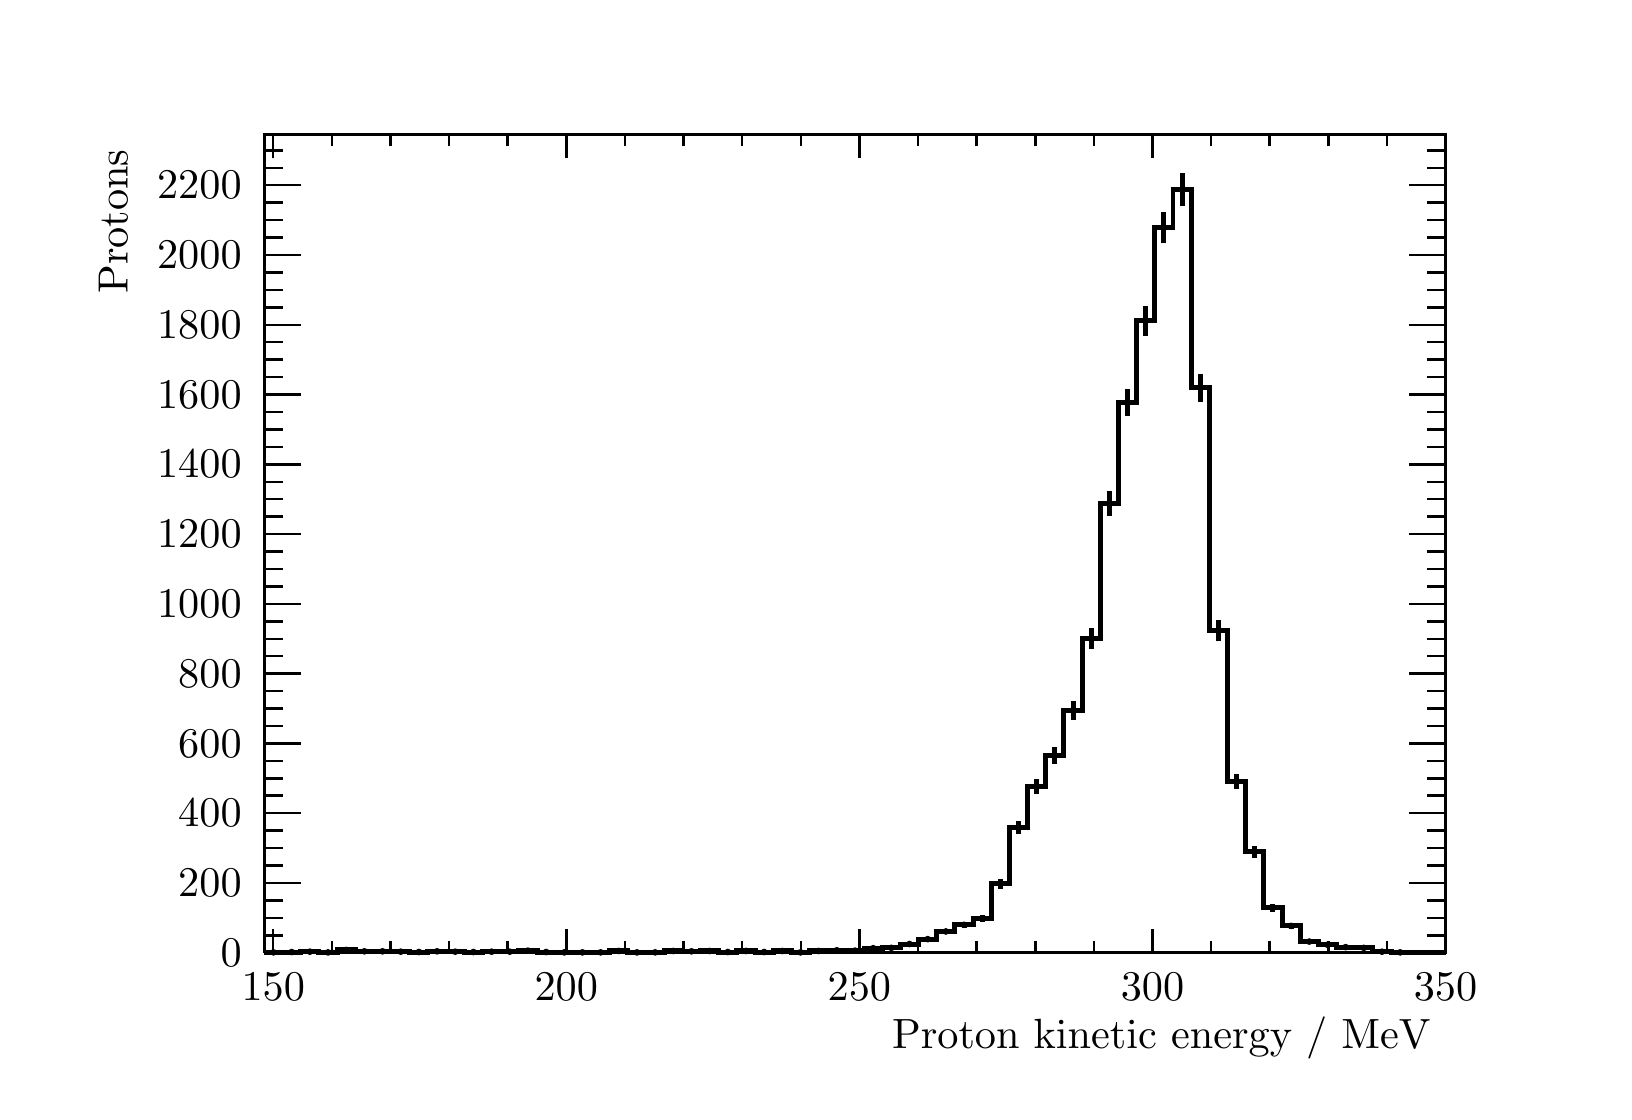
\begin{tikzpicture}
\pgfdeclareplotmark{cross} {
\pgfpathmoveto{\pgfpoint{-0.3\pgfplotmarksize}{\pgfplotmarksize}}
\pgfpathlineto{\pgfpoint{+0.3\pgfplotmarksize}{\pgfplotmarksize}}
\pgfpathlineto{\pgfpoint{+0.3\pgfplotmarksize}{0.3\pgfplotmarksize}}
\pgfpathlineto{\pgfpoint{+1\pgfplotmarksize}{0.3\pgfplotmarksize}}
\pgfpathlineto{\pgfpoint{+1\pgfplotmarksize}{-0.3\pgfplotmarksize}}
\pgfpathlineto{\pgfpoint{+0.3\pgfplotmarksize}{-0.3\pgfplotmarksize}}
\pgfpathlineto{\pgfpoint{+0.3\pgfplotmarksize}{-1.\pgfplotmarksize}}
\pgfpathlineto{\pgfpoint{-0.3\pgfplotmarksize}{-1.\pgfplotmarksize}}
\pgfpathlineto{\pgfpoint{-0.3\pgfplotmarksize}{-0.3\pgfplotmarksize}}
\pgfpathlineto{\pgfpoint{-1.\pgfplotmarksize}{-0.3\pgfplotmarksize}}
\pgfpathlineto{\pgfpoint{-1.\pgfplotmarksize}{0.3\pgfplotmarksize}}
\pgfpathlineto{\pgfpoint{-0.3\pgfplotmarksize}{0.3\pgfplotmarksize}}
\pgfpathclose
\pgfusepathqstroke
}
\pgfdeclareplotmark{cross*} {
\pgfpathmoveto{\pgfpoint{-0.3\pgfplotmarksize}{\pgfplotmarksize}}
\pgfpathlineto{\pgfpoint{+0.3\pgfplotmarksize}{\pgfplotmarksize}}
\pgfpathlineto{\pgfpoint{+0.3\pgfplotmarksize}{0.3\pgfplotmarksize}}
\pgfpathlineto{\pgfpoint{+1\pgfplotmarksize}{0.3\pgfplotmarksize}}
\pgfpathlineto{\pgfpoint{+1\pgfplotmarksize}{-0.3\pgfplotmarksize}}
\pgfpathlineto{\pgfpoint{+0.3\pgfplotmarksize}{-0.3\pgfplotmarksize}}
\pgfpathlineto{\pgfpoint{+0.3\pgfplotmarksize}{-1.\pgfplotmarksize}}
\pgfpathlineto{\pgfpoint{-0.3\pgfplotmarksize}{-1.\pgfplotmarksize}}
\pgfpathlineto{\pgfpoint{-0.3\pgfplotmarksize}{-0.3\pgfplotmarksize}}
\pgfpathlineto{\pgfpoint{-1.\pgfplotmarksize}{-0.3\pgfplotmarksize}}
\pgfpathlineto{\pgfpoint{-1.\pgfplotmarksize}{0.3\pgfplotmarksize}}
\pgfpathlineto{\pgfpoint{-0.3\pgfplotmarksize}{0.3\pgfplotmarksize}}
\pgfpathclose
\pgfusepathqfillstroke
}
\pgfdeclareplotmark{newstar} {
\pgfpathmoveto{\pgfqpoint{0pt}{\pgfplotmarksize}}
\pgfpathlineto{\pgfqpointpolar{44}{0.5\pgfplotmarksize}}
\pgfpathlineto{\pgfqpointpolar{18}{\pgfplotmarksize}}
\pgfpathlineto{\pgfqpointpolar{-20}{0.5\pgfplotmarksize}}
\pgfpathlineto{\pgfqpointpolar{-54}{\pgfplotmarksize}}
\pgfpathlineto{\pgfqpointpolar{-90}{0.5\pgfplotmarksize}}
\pgfpathlineto{\pgfqpointpolar{234}{\pgfplotmarksize}}
\pgfpathlineto{\pgfqpointpolar{198}{0.5\pgfplotmarksize}}
\pgfpathlineto{\pgfqpointpolar{162}{\pgfplotmarksize}}
\pgfpathlineto{\pgfqpointpolar{134}{0.5\pgfplotmarksize}}
\pgfpathclose
\pgfusepathqstroke
}
\pgfdeclareplotmark{newstar*} {
\pgfpathmoveto{\pgfqpoint{0pt}{\pgfplotmarksize}}
\pgfpathlineto{\pgfqpointpolar{44}{0.5\pgfplotmarksize}}
\pgfpathlineto{\pgfqpointpolar{18}{\pgfplotmarksize}}
\pgfpathlineto{\pgfqpointpolar{-20}{0.5\pgfplotmarksize}}
\pgfpathlineto{\pgfqpointpolar{-54}{\pgfplotmarksize}}
\pgfpathlineto{\pgfqpointpolar{-90}{0.5\pgfplotmarksize}}
\pgfpathlineto{\pgfqpointpolar{234}{\pgfplotmarksize}}
\pgfpathlineto{\pgfqpointpolar{198}{0.5\pgfplotmarksize}}
\pgfpathlineto{\pgfqpointpolar{162}{\pgfplotmarksize}}
\pgfpathlineto{\pgfqpointpolar{134}{0.5\pgfplotmarksize}}
\pgfpathclose
\pgfusepathqfillstroke
}
\definecolor{c}{rgb}{1,1,1};
\draw [color=c, fill=c] (0,0) rectangle (20,13.4957);
\draw [color=c, fill=c] (3,1.75444) rectangle (18,12.1461);
\definecolor{c}{rgb}{0,0,0};
\draw [c,line width=0.9] (3,1.75444) -- (3,12.1461) -- (18,12.1461) -- (18,1.75444) -- (3,1.75444);
\definecolor{c}{rgb}{1,1,1};
\draw [color=c, fill=c] (3,1.75444) rectangle (18,12.1461);
\definecolor{c}{rgb}{0,0,0};
\draw [c,line width=0.9] (3,1.75444) -- (3,12.1461) -- (18,12.1461) -- (18,1.75444) -- (3,1.75444);
\draw [c,line width=1.8] (3.11538,1.75444) -- (3.11538,1.75887);
\draw [c,line width=1.8] (3.11538,1.75887) -- (3.11538,1.7633);
\foreach \P in {(3.11538,1.75887)}{\draw[mark options={color=c,fill=c},mark size=2.402402pt,mark=*,mark size=1pt] plot coordinates {\P};}
\draw [c,line width=1.8] (3.34615,1.75704) -- (3.34615,1.7633);
\draw [c,line width=1.8] (3.34615,1.7633) -- (3.34615,1.76957);
\foreach \P in {(3.34615,1.7633)}{\draw[mark options={color=c,fill=c},mark size=2.402402pt,mark=*,mark size=1pt] plot coordinates {\P};}
\draw [c,line width=1.8] (3.57692,1.76006) -- (3.57692,1.76773);
\draw [c,line width=1.8] (3.57692,1.76773) -- (3.57692,1.77541);
\foreach \P in {(3.57692,1.76773)}{\draw[mark options={color=c,fill=c},mark size=2.402402pt,mark=*,mark size=1pt] plot coordinates {\P};}
\draw [c,line width=1.8] (3.80769,1.75444) -- (3.80769,1.75887);
\draw [c,line width=1.8] (3.80769,1.75887) -- (3.80769,1.7633);
\foreach \P in {(3.80769,1.75887)}{\draw[mark options={color=c,fill=c},mark size=2.402402pt,mark=*,mark size=1pt] plot coordinates {\P};}
\draw [c,line width=1.8] (4.03846,1.77735) -- (4.03846,1.78989);
\draw [c,line width=1.8] (4.03846,1.78989) -- (4.03846,1.80242);
\foreach \P in {(4.03846,1.78989)}{\draw[mark options={color=c,fill=c},mark size=2.402402pt,mark=*,mark size=1pt] plot coordinates {\P};}
\draw [c,line width=1.8] (4.26923,1.7633) -- (4.26923,1.77216);
\draw [c,line width=1.8] (4.26923,1.77216) -- (4.26923,1.78102);
\foreach \P in {(4.26923,1.77216)}{\draw[mark options={color=c,fill=c},mark size=2.402402pt,mark=*,mark size=1pt] plot coordinates {\P};}
\draw [c,line width=1.8] (4.5,1.7633) -- (4.5,1.77216);
\draw [c,line width=1.8] (4.5,1.77216) -- (4.5,1.78102);
\foreach \P in {(4.5,1.77216)}{\draw[mark options={color=c,fill=c},mark size=2.402402pt,mark=*,mark size=1pt] plot coordinates {\P};}
\draw [c,line width=1.8] (4.73077,1.76006) -- (4.73077,1.76773);
\draw [c,line width=1.8] (4.73077,1.76773) -- (4.73077,1.77541);
\foreach \P in {(4.73077,1.76773)}{\draw[mark options={color=c,fill=c},mark size=2.402402pt,mark=*,mark size=1pt] plot coordinates {\P};}
\draw [c,line width=1.8] (4.96154,1.75704) -- (4.96154,1.7633);
\draw [c,line width=1.8] (4.96154,1.7633) -- (4.96154,1.76957);
\foreach \P in {(4.96154,1.7633)}{\draw[mark options={color=c,fill=c},mark size=2.402402pt,mark=*,mark size=1pt] plot coordinates {\P};}
\draw [c,line width=1.8] (5.19231,1.7633) -- (5.19231,1.77216);
\draw [c,line width=1.8] (5.19231,1.77216) -- (5.19231,1.78102);
\foreach \P in {(5.19231,1.77216)}{\draw[mark options={color=c,fill=c},mark size=2.402402pt,mark=*,mark size=1pt] plot coordinates {\P};}
\draw [c,line width=1.8] (5.42308,1.76006) -- (5.42308,1.76773);
\draw [c,line width=1.8] (5.42308,1.76773) -- (5.42308,1.77541);
\foreach \P in {(5.42308,1.76773)}{\draw[mark options={color=c,fill=c},mark size=2.402402pt,mark=*,mark size=1pt] plot coordinates {\P};}
\draw [c,line width=1.8] (5.65385,1.75704) -- (5.65385,1.7633);
\draw [c,line width=1.8] (5.65385,1.7633) -- (5.65385,1.76957);
\foreach \P in {(5.65385,1.7633)}{\draw[mark options={color=c,fill=c},mark size=2.402402pt,mark=*,mark size=1pt] plot coordinates {\P};}
\draw [c,line width=1.8] (5.88462,1.76006) -- (5.88462,1.76773);
\draw [c,line width=1.8] (5.88462,1.76773) -- (5.88462,1.77541);
\foreach \P in {(5.88462,1.76773)}{\draw[mark options={color=c,fill=c},mark size=2.402402pt,mark=*,mark size=1pt] plot coordinates {\P};}
\draw [c,line width=1.8] (6.11538,1.76006) -- (6.11538,1.76773);
\draw [c,line width=1.8] (6.11538,1.76773) -- (6.11538,1.77541);
\foreach \P in {(6.11538,1.76773)}{\draw[mark options={color=c,fill=c},mark size=2.402402pt,mark=*,mark size=1pt] plot coordinates {\P};}
\draw [c,line width=1.8] (6.34615,1.77017) -- (6.34615,1.78102);
\draw [c,line width=1.8] (6.34615,1.78102) -- (6.34615,1.79188);
\foreach \P in {(6.34615,1.78102)}{\draw[mark options={color=c,fill=c},mark size=2.402402pt,mark=*,mark size=1pt] plot coordinates {\P};}
\draw [c,line width=1.8] (6.57692,1.75704) -- (6.57692,1.7633);
\draw [c,line width=1.8] (6.57692,1.7633) -- (6.57692,1.76957);
\foreach \P in {(6.57692,1.7633)}{\draw[mark options={color=c,fill=c},mark size=2.402402pt,mark=*,mark size=1pt] plot coordinates {\P};}
\draw [c,line width=1.8] (6.80769,1.75444) -- (6.80769,1.75887);
\draw [c,line width=1.8] (6.80769,1.75887) -- (6.80769,1.7633);
\foreach \P in {(6.80769,1.75887)}{\draw[mark options={color=c,fill=c},mark size=2.402402pt,mark=*,mark size=1pt] plot coordinates {\P};}
\draw [c,line width=1.8] (7.03846,1.75444) -- (7.03846,1.75887);
\draw [c,line width=1.8] (7.03846,1.75887) -- (7.03846,1.7633);
\foreach \P in {(7.03846,1.75887)}{\draw[mark options={color=c,fill=c},mark size=2.402402pt,mark=*,mark size=1pt] plot coordinates {\P};}
\draw [c,line width=1.8] (7.26923,1.75444) -- (7.26923,1.75887);
\draw [c,line width=1.8] (7.26923,1.75887) -- (7.26923,1.7633);
\foreach \P in {(7.26923,1.75887)}{\draw[mark options={color=c,fill=c},mark size=2.402402pt,mark=*,mark size=1pt] plot coordinates {\P};}
\draw [c,line width=1.8] (7.5,1.76669) -- (7.5,1.77659);
\draw [c,line width=1.8] (7.5,1.77659) -- (7.5,1.7865);
\foreach \P in {(7.5,1.77659)}{\draw[mark options={color=c,fill=c},mark size=2.402402pt,mark=*,mark size=1pt] plot coordinates {\P};}
\draw [c,line width=1.8] (7.73077,1.75444) -- (7.73077,1.75887);
\draw [c,line width=1.8] (7.73077,1.75887) -- (7.73077,1.7633);
\foreach \P in {(7.73077,1.75887)}{\draw[mark options={color=c,fill=c},mark size=2.402402pt,mark=*,mark size=1pt] plot coordinates {\P};}
\draw [c,line width=1.8] (7.96154,1.75444) -- (7.96154,1.75887);
\draw [c,line width=1.8] (7.96154,1.75887) -- (7.96154,1.7633);
\foreach \P in {(7.96154,1.75887)}{\draw[mark options={color=c,fill=c},mark size=2.402402pt,mark=*,mark size=1pt] plot coordinates {\P};}
\draw [c,line width=1.8] (8.19231,1.76669) -- (8.19231,1.77659);
\draw [c,line width=1.8] (8.19231,1.77659) -- (8.19231,1.7865);
\foreach \P in {(8.19231,1.77659)}{\draw[mark options={color=c,fill=c},mark size=2.402402pt,mark=*,mark size=1pt] plot coordinates {\P};}
\draw [c,line width=1.8] (8.42308,1.7633) -- (8.42308,1.77216);
\draw [c,line width=1.8] (8.42308,1.77216) -- (8.42308,1.78102);
\foreach \P in {(8.42308,1.77216)}{\draw[mark options={color=c,fill=c},mark size=2.402402pt,mark=*,mark size=1pt] plot coordinates {\P};}
\draw [c,line width=1.8] (8.65385,1.76669) -- (8.65385,1.77659);
\draw [c,line width=1.8] (8.65385,1.77659) -- (8.65385,1.7865);
\foreach \P in {(8.65385,1.77659)}{\draw[mark options={color=c,fill=c},mark size=2.402402pt,mark=*,mark size=1pt] plot coordinates {\P};}
\draw [c,line width=1.8] (8.88462,1.75704) -- (8.88462,1.7633);
\draw [c,line width=1.8] (8.88462,1.7633) -- (8.88462,1.76957);
\foreach \P in {(8.88462,1.7633)}{\draw[mark options={color=c,fill=c},mark size=2.402402pt,mark=*,mark size=1pt] plot coordinates {\P};}
\draw [c,line width=1.8] (9.11539,1.76669) -- (9.11539,1.77659);
\draw [c,line width=1.8] (9.11539,1.77659) -- (9.11539,1.7865);
\foreach \P in {(9.11539,1.77659)}{\draw[mark options={color=c,fill=c},mark size=2.402402pt,mark=*,mark size=1pt] plot coordinates {\P};}
\draw [c,line width=1.8] (9.34615,1.75704) -- (9.34615,1.7633);
\draw [c,line width=1.8] (9.34615,1.7633) -- (9.34615,1.76957);
\foreach \P in {(9.34615,1.7633)}{\draw[mark options={color=c,fill=c},mark size=2.402402pt,mark=*,mark size=1pt] plot coordinates {\P};}
\draw [c,line width=1.8] (9.57692,1.76669) -- (9.57692,1.77659);
\draw [c,line width=1.8] (9.57692,1.77659) -- (9.57692,1.7865);
\foreach \P in {(9.57692,1.77659)}{\draw[mark options={color=c,fill=c},mark size=2.402402pt,mark=*,mark size=1pt] plot coordinates {\P};}
\draw [c,line width=1.8] (9.80769,1.75444) -- (9.80769,1.75887);
\draw [c,line width=1.8] (9.80769,1.75887) -- (9.80769,1.7633);
\foreach \P in {(9.80769,1.75887)}{\draw[mark options={color=c,fill=c},mark size=2.402402pt,mark=*,mark size=1pt] plot coordinates {\P};}
\draw [c,line width=1.8] (10.0385,1.76669) -- (10.0385,1.77659);
\draw [c,line width=1.8] (10.0385,1.77659) -- (10.0385,1.7865);
\foreach \P in {(10.0385,1.77659)}{\draw[mark options={color=c,fill=c},mark size=2.402402pt,mark=*,mark size=1pt] plot coordinates {\P};}
\draw [c,line width=1.8] (10.2692,1.77373) -- (10.2692,1.78546);
\draw [c,line width=1.8] (10.2692,1.78546) -- (10.2692,1.79718);
\foreach \P in {(10.2692,1.78546)}{\draw[mark options={color=c,fill=c},mark size=2.402402pt,mark=*,mark size=1pt] plot coordinates {\P};}
\draw [c,line width=1.8] (10.5,1.77017) -- (10.5,1.78102);
\draw [c,line width=1.8] (10.5,1.78102) -- (10.5,1.79188);
\foreach \P in {(10.5,1.78102)}{\draw[mark options={color=c,fill=c},mark size=2.402402pt,mark=*,mark size=1pt] plot coordinates {\P};}
\draw [c,line width=1.8] (10.7308,1.79606) -- (10.7308,1.81204);
\draw [c,line width=1.8] (10.7308,1.81204) -- (10.7308,1.82801);
\foreach \P in {(10.7308,1.81204)}{\draw[mark options={color=c,fill=c},mark size=2.402402pt,mark=*,mark size=1pt] plot coordinates {\P};}
\draw [c,line width=1.8] (10.9615,1.79989) -- (10.9615,1.81647);
\draw [c,line width=1.8] (10.9615,1.81647) -- (10.9615,1.83305);
\foreach \P in {(10.9615,1.81647)}{\draw[mark options={color=c,fill=c},mark size=2.402402pt,mark=*,mark size=1pt] plot coordinates {\P};}
\draw [c,line width=1.8] (11.1923,1.84305) -- (11.1923,1.86521);
\draw [c,line width=1.8] (11.1923,1.86521) -- (11.1923,1.88736);
\foreach \P in {(11.1923,1.86521)}{\draw[mark options={color=c,fill=c},mark size=2.402402pt,mark=*,mark size=1pt] plot coordinates {\P};}
\draw [c,line width=1.8] (11.4231,1.89956) -- (11.4231,1.92723);
\draw [c,line width=1.8] (11.4231,1.92723) -- (11.4231,1.9549);
\foreach \P in {(11.4231,1.92723)}{\draw[mark options={color=c,fill=c},mark size=2.402402pt,mark=*,mark size=1pt] plot coordinates {\P};}
\draw [c,line width=1.8] (11.6538,1.9901) -- (11.6538,2.02471);
\draw [c,line width=1.8] (11.6538,2.02471) -- (11.6538,2.05931);
\foreach \P in {(11.6538,2.02471)}{\draw[mark options={color=c,fill=c},mark size=2.402402pt,mark=*,mark size=1pt] plot coordinates {\P};}
\draw [c,line width=1.8] (11.8846,2.06926) -- (11.8846,2.10889);
\draw [c,line width=1.8] (11.8846,2.10889) -- (11.8846,2.14851);
\foreach \P in {(11.8846,2.10889)}{\draw[mark options={color=c,fill=c},mark size=2.402402pt,mark=*,mark size=1pt] plot coordinates {\P};}
\draw [c,line width=1.8] (12.1154,2.14478) -- (12.1154,2.18864);
\draw [c,line width=1.8] (12.1154,2.18864) -- (12.1154,2.2325);
\foreach \P in {(12.1154,2.18864)}{\draw[mark options={color=c,fill=c},mark size=2.402402pt,mark=*,mark size=1pt] plot coordinates {\P};}
\draw [c,line width=1.8] (12.3462,2.56935) -- (12.3462,2.63169);
\draw [c,line width=1.8] (12.3462,2.63169) -- (12.3462,2.69404);
\foreach \P in {(12.3462,2.63169)}{\draw[mark options={color=c,fill=c},mark size=2.402402pt,mark=*,mark size=1pt] plot coordinates {\P};}
\draw [c,line width=1.8] (12.5769,3.26538) -- (12.5769,3.34945);
\draw [c,line width=1.8] (12.5769,3.34945) -- (12.5769,3.43351);
\foreach \P in {(12.5769,3.34945)}{\draw[mark options={color=c,fill=c},mark size=2.402402pt,mark=*,mark size=1pt] plot coordinates {\P};}
\draw [c,line width=1.8] (12.8077,3.77106) -- (12.8077,3.86782);
\draw [c,line width=1.8] (12.8077,3.86782) -- (12.8077,3.96459);
\foreach \P in {(12.8077,3.86782)}{\draw[mark options={color=c,fill=c},mark size=2.402402pt,mark=*,mark size=1pt] plot coordinates {\P};}
\draw [c,line width=1.8] (13.0385,4.1524) -- (13.0385,4.25771);
\draw [c,line width=1.8] (13.0385,4.25771) -- (13.0385,4.36303);
\foreach \P in {(13.0385,4.25771)}{\draw[mark options={color=c,fill=c},mark size=2.402402pt,mark=*,mark size=1pt] plot coordinates {\P};}
\draw [c,line width=1.8] (13.2692,4.71254) -- (13.2692,4.82926);
\draw [c,line width=1.8] (13.2692,4.82926) -- (13.2692,4.94597);
\foreach \P in {(13.2692,4.82926)}{\draw[mark options={color=c,fill=c},mark size=2.402402pt,mark=*,mark size=1pt] plot coordinates {\P};}
\draw [c,line width=1.8] (13.5,5.60904) -- (13.5,5.74195);
\draw [c,line width=1.8] (13.5,5.74195) -- (13.5,5.87487);
\foreach \P in {(13.5,5.74195)}{\draw[mark options={color=c,fill=c},mark size=2.402402pt,mark=*,mark size=1pt] plot coordinates {\P};}
\draw [c,line width=1.8] (13.7308,7.302) -- (13.7308,7.46101);
\draw [c,line width=1.8] (13.7308,7.46101) -- (13.7308,7.62002);
\foreach \P in {(13.7308,7.46101)}{\draw[mark options={color=c,fill=c},mark size=2.402402pt,mark=*,mark size=1pt] plot coordinates {\P};}
\draw [c,line width=1.8] (13.9615,8.5655) -- (13.9615,8.74145);
\draw [c,line width=1.8] (13.9615,8.74145) -- (13.9615,8.91739);
\foreach \P in {(13.9615,8.74145)}{\draw[mark options={color=c,fill=c},mark size=2.402402pt,mark=*,mark size=1pt] plot coordinates {\P};}
\draw [c,line width=1.8] (14.1923,9.58965) -- (14.1923,9.7782);
\draw [c,line width=1.8] (14.1923,9.7782) -- (14.1923,9.96675);
\foreach \P in {(14.1923,9.7782)}{\draw[mark options={color=c,fill=c},mark size=2.402402pt,mark=*,mark size=1pt] plot coordinates {\P};}
\draw [c,line width=1.8] (14.4231,10.7636) -- (14.4231,10.9656);
\draw [c,line width=1.8] (14.4231,10.9656) -- (14.4231,11.1676);
\foreach \P in {(14.4231,10.9656)}{\draw[mark options={color=c,fill=c},mark size=2.402402pt,mark=*,mark size=1pt] plot coordinates {\P};}
\draw [c,line width=1.8] (14.6538,11.2369) -- (14.6538,11.4441);
\draw [c,line width=1.8] (14.6538,11.4441) -- (14.6538,11.6513);
\foreach \P in {(14.6538,11.4441)}{\draw[mark options={color=c,fill=c},mark size=2.402402pt,mark=*,mark size=1pt] plot coordinates {\P};}
\draw [c,line width=1.8] (14.8846,8.75363) -- (14.8846,8.93196);
\draw [c,line width=1.8] (14.8846,8.93196) -- (14.8846,9.11029);
\foreach \P in {(14.8846,8.93196)}{\draw[mark options={color=c,fill=c},mark size=2.402402pt,mark=*,mark size=1pt] plot coordinates {\P};}
\draw [c,line width=1.8] (15.1154,5.70925) -- (15.1154,5.84385);
\draw [c,line width=1.8] (15.1154,5.84385) -- (15.1154,5.97846);
\foreach \P in {(15.1154,5.84385)}{\draw[mark options={color=c,fill=c},mark size=2.402402pt,mark=*,mark size=1pt] plot coordinates {\P};}
\draw [c,line width=1.8] (15.3462,3.83168) -- (15.3462,3.92985);
\draw [c,line width=1.8] (15.3462,3.92985) -- (15.3462,4.02802);
\foreach \P in {(15.3462,3.92985)}{\draw[mark options={color=c,fill=c},mark size=2.402402pt,mark=*,mark size=1pt] plot coordinates {\P};}
\draw [c,line width=1.8] (15.5769,2.95956) -- (15.5769,3.03488);
\draw [c,line width=1.8] (15.5769,3.03488) -- (15.5769,3.11019);
\foreach \P in {(15.5769,3.03488)}{\draw[mark options={color=c,fill=c},mark size=2.402402pt,mark=*,mark size=1pt] plot coordinates {\P};}
\draw [c,line width=1.8] (15.8077,2.27566) -- (15.8077,2.32598);
\draw [c,line width=1.8] (15.8077,2.32598) -- (15.8077,2.37631);
\foreach \P in {(15.8077,2.32598)}{\draw[mark options={color=c,fill=c},mark size=2.402402pt,mark=*,mark size=1pt] plot coordinates {\P};}
\draw [c,line width=1.8] (16.0385,2.05672) -- (16.0385,2.09559);
\draw [c,line width=1.8] (16.0385,2.09559) -- (16.0385,2.13447);
\foreach \P in {(16.0385,2.09559)}{\draw[mark options={color=c,fill=c},mark size=2.402402pt,mark=*,mark size=1pt] plot coordinates {\P};}
\draw [c,line width=1.8] (16.2692,1.87116) -- (16.2692,1.89622);
\draw [c,line width=1.8] (16.2692,1.89622) -- (16.2692,1.92128);
\foreach \P in {(16.2692,1.89622)}{\draw[mark options={color=c,fill=c},mark size=2.402402pt,mark=*,mark size=1pt] plot coordinates {\P};}
\draw [c,line width=1.8] (16.5,1.8351) -- (16.5,1.85634);
\draw [c,line width=1.8] (16.5,1.85634) -- (16.5,1.87759);
\foreach \P in {(16.5,1.85634)}{\draw[mark options={color=c,fill=c},mark size=2.402402pt,mark=*,mark size=1pt] plot coordinates {\P};}
\draw [c,line width=1.8] (16.7308,1.80761) -- (16.7308,1.82533);
\draw [c,line width=1.8] (16.7308,1.82533) -- (16.7308,1.84305);
\foreach \P in {(16.7308,1.82533)}{\draw[mark options={color=c,fill=c},mark size=2.402402pt,mark=*,mark size=1pt] plot coordinates {\P};}
\draw [c,line width=1.8] (16.9615,1.79989) -- (16.9615,1.81647);
\draw [c,line width=1.8] (16.9615,1.81647) -- (16.9615,1.83305);
\foreach \P in {(16.9615,1.81647)}{\draw[mark options={color=c,fill=c},mark size=2.402402pt,mark=*,mark size=1pt] plot coordinates {\P};}
\draw [c,line width=1.8] (17.1923,1.76006) -- (17.1923,1.76773);
\draw [c,line width=1.8] (17.1923,1.76773) -- (17.1923,1.77541);
\foreach \P in {(17.1923,1.76773)}{\draw[mark options={color=c,fill=c},mark size=2.402402pt,mark=*,mark size=1pt] plot coordinates {\P};}
\draw [c,line width=1.8] (17.4231,1.75444) -- (17.4231,1.75887);
\draw [c,line width=1.8] (17.4231,1.75887) -- (17.4231,1.7633);
\foreach \P in {(17.4231,1.75887)}{\draw[mark options={color=c,fill=c},mark size=2.402402pt,mark=*,mark size=1pt] plot coordinates {\P};}
\draw [c,line width=1.8] (3,1.75887) -- (3.23077,1.75887) -- (3.23077,1.7633) -- (3.46154,1.7633) -- (3.46154,1.76773) -- (3.69231,1.76773) -- (3.69231,1.75887) -- (3.92308,1.75887) -- (3.92308,1.78989) -- (4.15385,1.78989) -- (4.15385,1.77216) --
 (4.38462,1.77216) -- (4.38462,1.77216) -- (4.61538,1.77216) -- (4.61538,1.76773) -- (4.84615,1.76773) -- (4.84615,1.7633) -- (5.07692,1.7633) -- (5.07692,1.77216) -- (5.30769,1.77216) -- (5.30769,1.76773) -- (5.53846,1.76773) -- (5.53846,1.7633) --
 (5.76923,1.7633) -- (5.76923,1.76773) -- (6,1.76773) -- (6,1.76773) -- (6.23077,1.76773) -- (6.23077,1.78102) -- (6.46154,1.78102) -- (6.46154,1.7633) -- (6.69231,1.7633) -- (6.69231,1.75887) -- (6.92308,1.75887) -- (6.92308,1.75887) --
 (7.15385,1.75887) -- (7.15385,1.75887) -- (7.38462,1.75887) -- (7.38462,1.77659) -- (7.61538,1.77659) -- (7.61538,1.75887) -- (7.84615,1.75887) -- (7.84615,1.75887) -- (8.07692,1.75887) -- (8.07692,1.77659) -- (8.30769,1.77659) -- (8.30769,1.77216)
 -- (8.53846,1.77216) -- (8.53846,1.77659) -- (8.76923,1.77659) -- (8.76923,1.7633) -- (9,1.7633) -- (9,1.77659) -- (9.23077,1.77659) -- (9.23077,1.7633) -- (9.46154,1.7633) -- (9.46154,1.77659) -- (9.69231,1.77659) -- (9.69231,1.75887) --
 (9.92308,1.75887) -- (9.92308,1.77659) -- (10.1538,1.77659) -- (10.1538,1.78546) -- (10.3846,1.78546) -- (10.3846,1.78102) -- (10.6154,1.78102) -- (10.6154,1.81204) -- (10.8462,1.81204) -- (10.8462,1.81647) -- (11.0769,1.81647) -- (11.0769,1.86521)
 -- (11.3077,1.86521) -- (11.3077,1.92723) -- (11.5385,1.92723) -- (11.5385,2.02471) -- (11.7692,2.02471) -- (11.7692,2.10889) -- (12,2.10889) -- (12,2.18864) -- (12.2308,2.18864) -- (12.2308,2.63169) -- (12.4615,2.63169) -- (12.4615,3.34945) --
 (12.6923,3.34945) -- (12.6923,3.86782) -- (12.9231,3.86782) -- (12.9231,4.25771) -- (13.1538,4.25771) -- (13.1538,4.82926) -- (13.3846,4.82926) -- (13.3846,5.74195) -- (13.6154,5.74195) -- (13.6154,7.46101) -- (13.8462,7.46101) -- (13.8462,8.74145)
 -- (14.0769,8.74145) -- (14.0769,9.7782) -- (14.3077,9.7782) -- (14.3077,10.9656) -- (14.5385,10.9656) -- (14.5385,11.4441) -- (14.7692,11.4441) -- (14.7692,8.93196) -- (15,8.93196) -- (15,5.84385) -- (15.2308,5.84385) -- (15.2308,3.92985) --
 (15.4615,3.92985) -- (15.4615,3.03488) -- (15.6923,3.03488) -- (15.6923,2.32598) -- (15.9231,2.32598) -- (15.9231,2.09559) -- (16.1538,2.09559) -- (16.1538,1.89622) -- (16.3846,1.89622) -- (16.3846,1.85634) -- (16.6154,1.85634) -- (16.6154,1.82533)
 -- (16.8462,1.82533) -- (16.8462,1.81647) -- (17.0769,1.81647) -- (17.0769,1.76773) -- (17.3077,1.76773) -- (17.3077,1.75887) -- (17.5385,1.75887) -- (17.5385,1.75444) -- (17.7692,1.75444) -- (17.7692,1.75444) -- (18,1.75444);
\draw [c,line width=0.9] (3,1.75444) -- (18,1.75444);
\draw [c,line width=0.9] (3.11166,2.05809) -- (3.11166,1.75444);
\draw [c,line width=0.9] (3.85608,1.90627) -- (3.85608,1.75444);
\draw [c,line width=0.9] (4.6005,1.90627) -- (4.6005,1.75444);
\draw [c,line width=0.9] (5.34491,1.90627) -- (5.34491,1.75444);
\draw [c,line width=0.9] (6.08933,1.90627) -- (6.08933,1.75444);
\draw [c,line width=0.9] (6.83375,2.05809) -- (6.83375,1.75444);
\draw [c,line width=0.9] (7.57816,1.90627) -- (7.57816,1.75444);
\draw [c,line width=0.9] (8.32258,1.90627) -- (8.32258,1.75444);
\draw [c,line width=0.9] (9.067,1.90627) -- (9.067,1.75444);
\draw [c,line width=0.9] (9.81141,1.90627) -- (9.81141,1.75444);
\draw [c,line width=0.9] (10.5558,2.05809) -- (10.5558,1.75444);
\draw [c,line width=0.9] (11.3002,1.90627) -- (11.3002,1.75444);
\draw [c,line width=0.9] (12.0447,1.90627) -- (12.0447,1.75444);
\draw [c,line width=0.9] (12.7891,1.90627) -- (12.7891,1.75444);
\draw [c,line width=0.9] (13.5335,1.90627) -- (13.5335,1.75444);
\draw [c,line width=0.9] (14.2779,2.05809) -- (14.2779,1.75444);
\draw [c,line width=0.9] (15.0223,1.90627) -- (15.0223,1.75444);
\draw [c,line width=0.9] (15.7667,1.90627) -- (15.7667,1.75444);
\draw [c,line width=0.9] (16.5112,1.90627) -- (16.5112,1.75444);
\draw [c,line width=0.9] (17.2556,1.90627) -- (17.2556,1.75444);
\draw [c,line width=0.9] (18,2.05809) -- (18,1.75444);
\draw [c,line width=0.9] (3.11166,2.05809) -- (3.11166,1.75444);
\draw [c,line width=0.9] (18,2.05809) -- (18,1.75444);
\draw [anchor=base] (3.11166,1.14713) node[scale=1.52731, color=c, rotate=0]{150};
\draw [anchor=base] (6.83375,1.14713) node[scale=1.52731, color=c, rotate=0]{200};
\draw [anchor=base] (10.5558,1.14713) node[scale=1.52731, color=c, rotate=0]{250};
\draw [anchor=base] (14.2779,1.14713) node[scale=1.52731, color=c, rotate=0]{300};
\draw [anchor=base] (18,1.14713) node[scale=1.52731, color=c, rotate=0]{350};
\draw [anchor= east] (18,0.674785) node[scale=1.52731, color=c, rotate=0]{ Proton kinetic energy / MeV};
\draw [c,line width=0.9] (3,12.1461) -- (18,12.1461);
\draw [c,line width=0.9] (3.11166,11.8425) -- (3.11166,12.1461);
\draw [c,line width=0.9] (3.85608,11.9943) -- (3.85608,12.1461);
\draw [c,line width=0.9] (4.6005,11.9943) -- (4.6005,12.1461);
\draw [c,line width=0.9] (5.34491,11.9943) -- (5.34491,12.1461);
\draw [c,line width=0.9] (6.08933,11.9943) -- (6.08933,12.1461);
\draw [c,line width=0.9] (6.83375,11.8425) -- (6.83375,12.1461);
\draw [c,line width=0.9] (7.57816,11.9943) -- (7.57816,12.1461);
\draw [c,line width=0.9] (8.32258,11.9943) -- (8.32258,12.1461);
\draw [c,line width=0.9] (9.067,11.9943) -- (9.067,12.1461);
\draw [c,line width=0.9] (9.81141,11.9943) -- (9.81141,12.1461);
\draw [c,line width=0.9] (10.5558,11.8425) -- (10.5558,12.1461);
\draw [c,line width=0.9] (11.3002,11.9943) -- (11.3002,12.1461);
\draw [c,line width=0.9] (12.0447,11.9943) -- (12.0447,12.1461);
\draw [c,line width=0.9] (12.7891,11.9943) -- (12.7891,12.1461);
\draw [c,line width=0.9] (13.5335,11.9943) -- (13.5335,12.1461);
\draw [c,line width=0.9] (14.2779,11.8425) -- (14.2779,12.1461);
\draw [c,line width=0.9] (15.0223,11.9943) -- (15.0223,12.1461);
\draw [c,line width=0.9] (15.7667,11.9943) -- (15.7667,12.1461);
\draw [c,line width=0.9] (16.5112,11.9943) -- (16.5112,12.1461);
\draw [c,line width=0.9] (17.2556,11.9943) -- (17.2556,12.1461);
\draw [c,line width=0.9] (18,11.8425) -- (18,12.1461);
\draw [c,line width=0.9] (3.11166,11.8425) -- (3.11166,12.1461);
\draw [c,line width=0.9] (18,11.8425) -- (18,12.1461);
\draw [c,line width=0.9] (3,1.75444) -- (3,12.1461);
\draw [c,line width=0.9] (3.462,1.75444) -- (3,1.75444);
\draw [c,line width=0.9] (3.231,1.97597) -- (3,1.97597);
\draw [c,line width=0.9] (3.231,2.1975) -- (3,2.1975);
\draw [c,line width=0.9] (3.231,2.41903) -- (3,2.41903);
\draw [c,line width=0.9] (3.462,2.64055) -- (3,2.64055);
\draw [c,line width=0.9] (3.231,2.86208) -- (3,2.86208);
\draw [c,line width=0.9] (3.231,3.08361) -- (3,3.08361);
\draw [c,line width=0.9] (3.231,3.30514) -- (3,3.30514);
\draw [c,line width=0.9] (3.462,3.52667) -- (3,3.52667);
\draw [c,line width=0.9] (3.231,3.7482) -- (3,3.7482);
\draw [c,line width=0.9] (3.231,3.96972) -- (3,3.96972);
\draw [c,line width=0.9] (3.231,4.19125) -- (3,4.19125);
\draw [c,line width=0.9] (3.462,4.41278) -- (3,4.41278);
\draw [c,line width=0.9] (3.231,4.63431) -- (3,4.63431);
\draw [c,line width=0.9] (3.231,4.85584) -- (3,4.85584);
\draw [c,line width=0.9] (3.231,5.07737) -- (3,5.07737);
\draw [c,line width=0.9] (3.462,5.29889) -- (3,5.29889);
\draw [c,line width=0.9] (3.231,5.52042) -- (3,5.52042);
\draw [c,line width=0.9] (3.231,5.74195) -- (3,5.74195);
\draw [c,line width=0.9] (3.231,5.96348) -- (3,5.96348);
\draw [c,line width=0.9] (3.462,6.18501) -- (3,6.18501);
\draw [c,line width=0.9] (3.231,6.40654) -- (3,6.40654);
\draw [c,line width=0.9] (3.231,6.62807) -- (3,6.62807);
\draw [c,line width=0.9] (3.231,6.84959) -- (3,6.84959);
\draw [c,line width=0.9] (3.462,7.07112) -- (3,7.07112);
\draw [c,line width=0.9] (3.231,7.29265) -- (3,7.29265);
\draw [c,line width=0.9] (3.231,7.51418) -- (3,7.51418);
\draw [c,line width=0.9] (3.231,7.73571) -- (3,7.73571);
\draw [c,line width=0.9] (3.462,7.95724) -- (3,7.95724);
\draw [c,line width=0.9] (3.231,8.17876) -- (3,8.17876);
\draw [c,line width=0.9] (3.231,8.40029) -- (3,8.40029);
\draw [c,line width=0.9] (3.231,8.62182) -- (3,8.62182);
\draw [c,line width=0.9] (3.462,8.84335) -- (3,8.84335);
\draw [c,line width=0.9] (3.231,9.06488) -- (3,9.06488);
\draw [c,line width=0.9] (3.231,9.28641) -- (3,9.28641);
\draw [c,line width=0.9] (3.231,9.50793) -- (3,9.50793);
\draw [c,line width=0.9] (3.462,9.72946) -- (3,9.72946);
\draw [c,line width=0.9] (3.231,9.95099) -- (3,9.95099);
\draw [c,line width=0.9] (3.231,10.1725) -- (3,10.1725);
\draw [c,line width=0.9] (3.231,10.394) -- (3,10.394);
\draw [c,line width=0.9] (3.462,10.6156) -- (3,10.6156);
\draw [c,line width=0.9] (3.231,10.8371) -- (3,10.8371);
\draw [c,line width=0.9] (3.231,11.0586) -- (3,11.0586);
\draw [c,line width=0.9] (3.231,11.2802) -- (3,11.2802);
\draw [c,line width=0.9] (3.462,11.5017) -- (3,11.5017);
\draw [c,line width=0.9] (3.462,11.5017) -- (3,11.5017);
\draw [c,line width=0.9] (3.231,11.7232) -- (3,11.7232);
\draw [c,line width=0.9] (3.231,11.9447) -- (3,11.9447);
\draw [anchor= east] (2.9,1.75444) node[scale=1.52731, color=c, rotate=0]{0};
\draw [anchor= east] (2.9,2.64055) node[scale=1.52731, color=c, rotate=0]{200};
\draw [anchor= east] (2.9,3.52667) node[scale=1.52731, color=c, rotate=0]{400};
\draw [anchor= east] (2.9,4.41278) node[scale=1.52731, color=c, rotate=0]{600};
\draw [anchor= east] (2.9,5.29889) node[scale=1.52731, color=c, rotate=0]{800};
\draw [anchor= east] (2.9,6.18501) node[scale=1.52731, color=c, rotate=0]{1000};
\draw [anchor= east] (2.9,7.07112) node[scale=1.52731, color=c, rotate=0]{1200};
\draw [anchor= east] (2.9,7.95724) node[scale=1.52731, color=c, rotate=0]{1400};
\draw [anchor= east] (2.9,8.84335) node[scale=1.52731, color=c, rotate=0]{1600};
\draw [anchor= east] (2.9,9.72946) node[scale=1.52731, color=c, rotate=0]{1800};
\draw [anchor= east] (2.9,10.6156) node[scale=1.52731, color=c, rotate=0]{2000};
\draw [anchor= east] (2.9,11.5017) node[scale=1.52731, color=c, rotate=0]{2200};
\draw [anchor= east] (1.08,12.1461) node[scale=1.52731, color=c, rotate=90]{Protons};
\draw [c,line width=0.9] (18,1.75444) -- (18,12.1461);
\draw [c,line width=0.9] (17.538,1.75444) -- (18,1.75444);
\draw [c,line width=0.9] (17.769,1.97597) -- (18,1.97597);
\draw [c,line width=0.9] (17.769,2.1975) -- (18,2.1975);
\draw [c,line width=0.9] (17.769,2.41903) -- (18,2.41903);
\draw [c,line width=0.9] (17.538,2.64055) -- (18,2.64055);
\draw [c,line width=0.9] (17.769,2.86208) -- (18,2.86208);
\draw [c,line width=0.9] (17.769,3.08361) -- (18,3.08361);
\draw [c,line width=0.9] (17.769,3.30514) -- (18,3.30514);
\draw [c,line width=0.9] (17.538,3.52667) -- (18,3.52667);
\draw [c,line width=0.9] (17.769,3.7482) -- (18,3.7482);
\draw [c,line width=0.9] (17.769,3.96972) -- (18,3.96972);
\draw [c,line width=0.9] (17.769,4.19125) -- (18,4.19125);
\draw [c,line width=0.9] (17.538,4.41278) -- (18,4.41278);
\draw [c,line width=0.9] (17.769,4.63431) -- (18,4.63431);
\draw [c,line width=0.9] (17.769,4.85584) -- (18,4.85584);
\draw [c,line width=0.9] (17.769,5.07737) -- (18,5.07737);
\draw [c,line width=0.9] (17.538,5.29889) -- (18,5.29889);
\draw [c,line width=0.9] (17.769,5.52042) -- (18,5.52042);
\draw [c,line width=0.9] (17.769,5.74195) -- (18,5.74195);
\draw [c,line width=0.9] (17.769,5.96348) -- (18,5.96348);
\draw [c,line width=0.9] (17.538,6.18501) -- (18,6.18501);
\draw [c,line width=0.9] (17.769,6.40654) -- (18,6.40654);
\draw [c,line width=0.9] (17.769,6.62807) -- (18,6.62807);
\draw [c,line width=0.9] (17.769,6.84959) -- (18,6.84959);
\draw [c,line width=0.9] (17.538,7.07112) -- (18,7.07112);
\draw [c,line width=0.9] (17.769,7.29265) -- (18,7.29265);
\draw [c,line width=0.9] (17.769,7.51418) -- (18,7.51418);
\draw [c,line width=0.9] (17.769,7.73571) -- (18,7.73571);
\draw [c,line width=0.9] (17.538,7.95724) -- (18,7.95724);
\draw [c,line width=0.9] (17.769,8.17876) -- (18,8.17876);
\draw [c,line width=0.9] (17.769,8.40029) -- (18,8.40029);
\draw [c,line width=0.9] (17.769,8.62182) -- (18,8.62182);
\draw [c,line width=0.9] (17.538,8.84335) -- (18,8.84335);
\draw [c,line width=0.9] (17.769,9.06488) -- (18,9.06488);
\draw [c,line width=0.9] (17.769,9.28641) -- (18,9.28641);
\draw [c,line width=0.9] (17.769,9.50793) -- (18,9.50793);
\draw [c,line width=0.9] (17.538,9.72946) -- (18,9.72946);
\draw [c,line width=0.9] (17.769,9.95099) -- (18,9.95099);
\draw [c,line width=0.9] (17.769,10.1725) -- (18,10.1725);
\draw [c,line width=0.9] (17.769,10.394) -- (18,10.394);
\draw [c,line width=0.9] (17.538,10.6156) -- (18,10.6156);
\draw [c,line width=0.9] (17.769,10.8371) -- (18,10.8371);
\draw [c,line width=0.9] (17.769,11.0586) -- (18,11.0586);
\draw [c,line width=0.9] (17.769,11.2802) -- (18,11.2802);
\draw [c,line width=0.9] (17.538,11.5017) -- (18,11.5017);
\draw [c,line width=0.9] (17.538,11.5017) -- (18,11.5017);
\draw [c,line width=0.9] (17.769,11.7232) -- (18,11.7232);
\draw [c,line width=0.9] (17.769,11.9447) -- (18,11.9447);
\definecolor{c}{rgb}{1,1,1};
\draw [color=c, fill=c] (2,12.686) rectangle (18,13.4282);
\definecolor{c}{rgb}{0,0,0};
%\draw (10,13.0571) node[scale=1.40004, color=c, rotate=0]{Proton kinetic energy measured in $\mathit{S3}$};
\end{tikzpicture}

    \end{adjustbox}
  \end{minipage}
  \caption{\label{fig:utofNoBend}Measurements of the unmoderated and unbent T10 beam over a baseline of 10.8~m for a selected beam momentum of 0.8~GeV/c. Measurements are made in the $\mathit{S3}$ detector. The peak between 50~ns and 60~ns is produced by protons. Left: Time of flight spectrum. Right: Measured kinetic energy of protons.}
\end{figure}

To enhance the low energy proton flux, a novel technique was employed:
we placed acrylic moderator blocks directly in the beamline, which spread and slowed the beam particles via multiple Coulomb scattering.
By placing the TPC in an off-axis position with respect to the beam direction, we observed a beam composition with lower-energy protons than would otherwise have been possible in the T10 beamline.
These techniques were designed to increase the ratio of protons to MIPs in the TPC, and to decrease the proton momentum and multiplicity in the active region of the TPC.

The flux and composition of beam particles were measured with two ToF systems, placed upstream and downstream of the TPC.
Measurements of protons and MIPs are presented as a function of the off-axis angle and thickness of the moderator.
This paper provides a detailed description of the time of flight systems employed in the beamline in Section~\ref{hptpcPaper:sec:Methods}, the analysis methodology of the ToF data in Section~\ref{hptpcPaper:sec:Analysis}, presentation of the ToF system results in Section~\ref{hptpcPaper:sec:Results}, and additional conclusions in Section~\ref{hptpcPaper:sec:Conclusion}.


% Justification of the gas choice 
\section{Beam Line and Detectors}
\label{hptpcPaper:sec:Methods}

\subsection{Beam Test Overview}
The beam test took place in the T10 beam line, East Area at the Proton Synchrotron in CERN from the 15th August to the 18th September 2018.
The results in this paper use data taken on the 31st August and 1st September, during which the setup configuration was varied as described below.
\todo[inline]{JOCELYN:"really only these two days?  This paper needs to be the flux reference, so we also need to include the flux measurements during the beam test....
suggest cut this sentence in any case and refer to the time ranges of the various types of data where these are analyzed" SEB what do you think?}
The primary components of the  experimental setup for the data taking period are shown schematically in Figure~\ref{fig:setup}.

\begin{figure}
  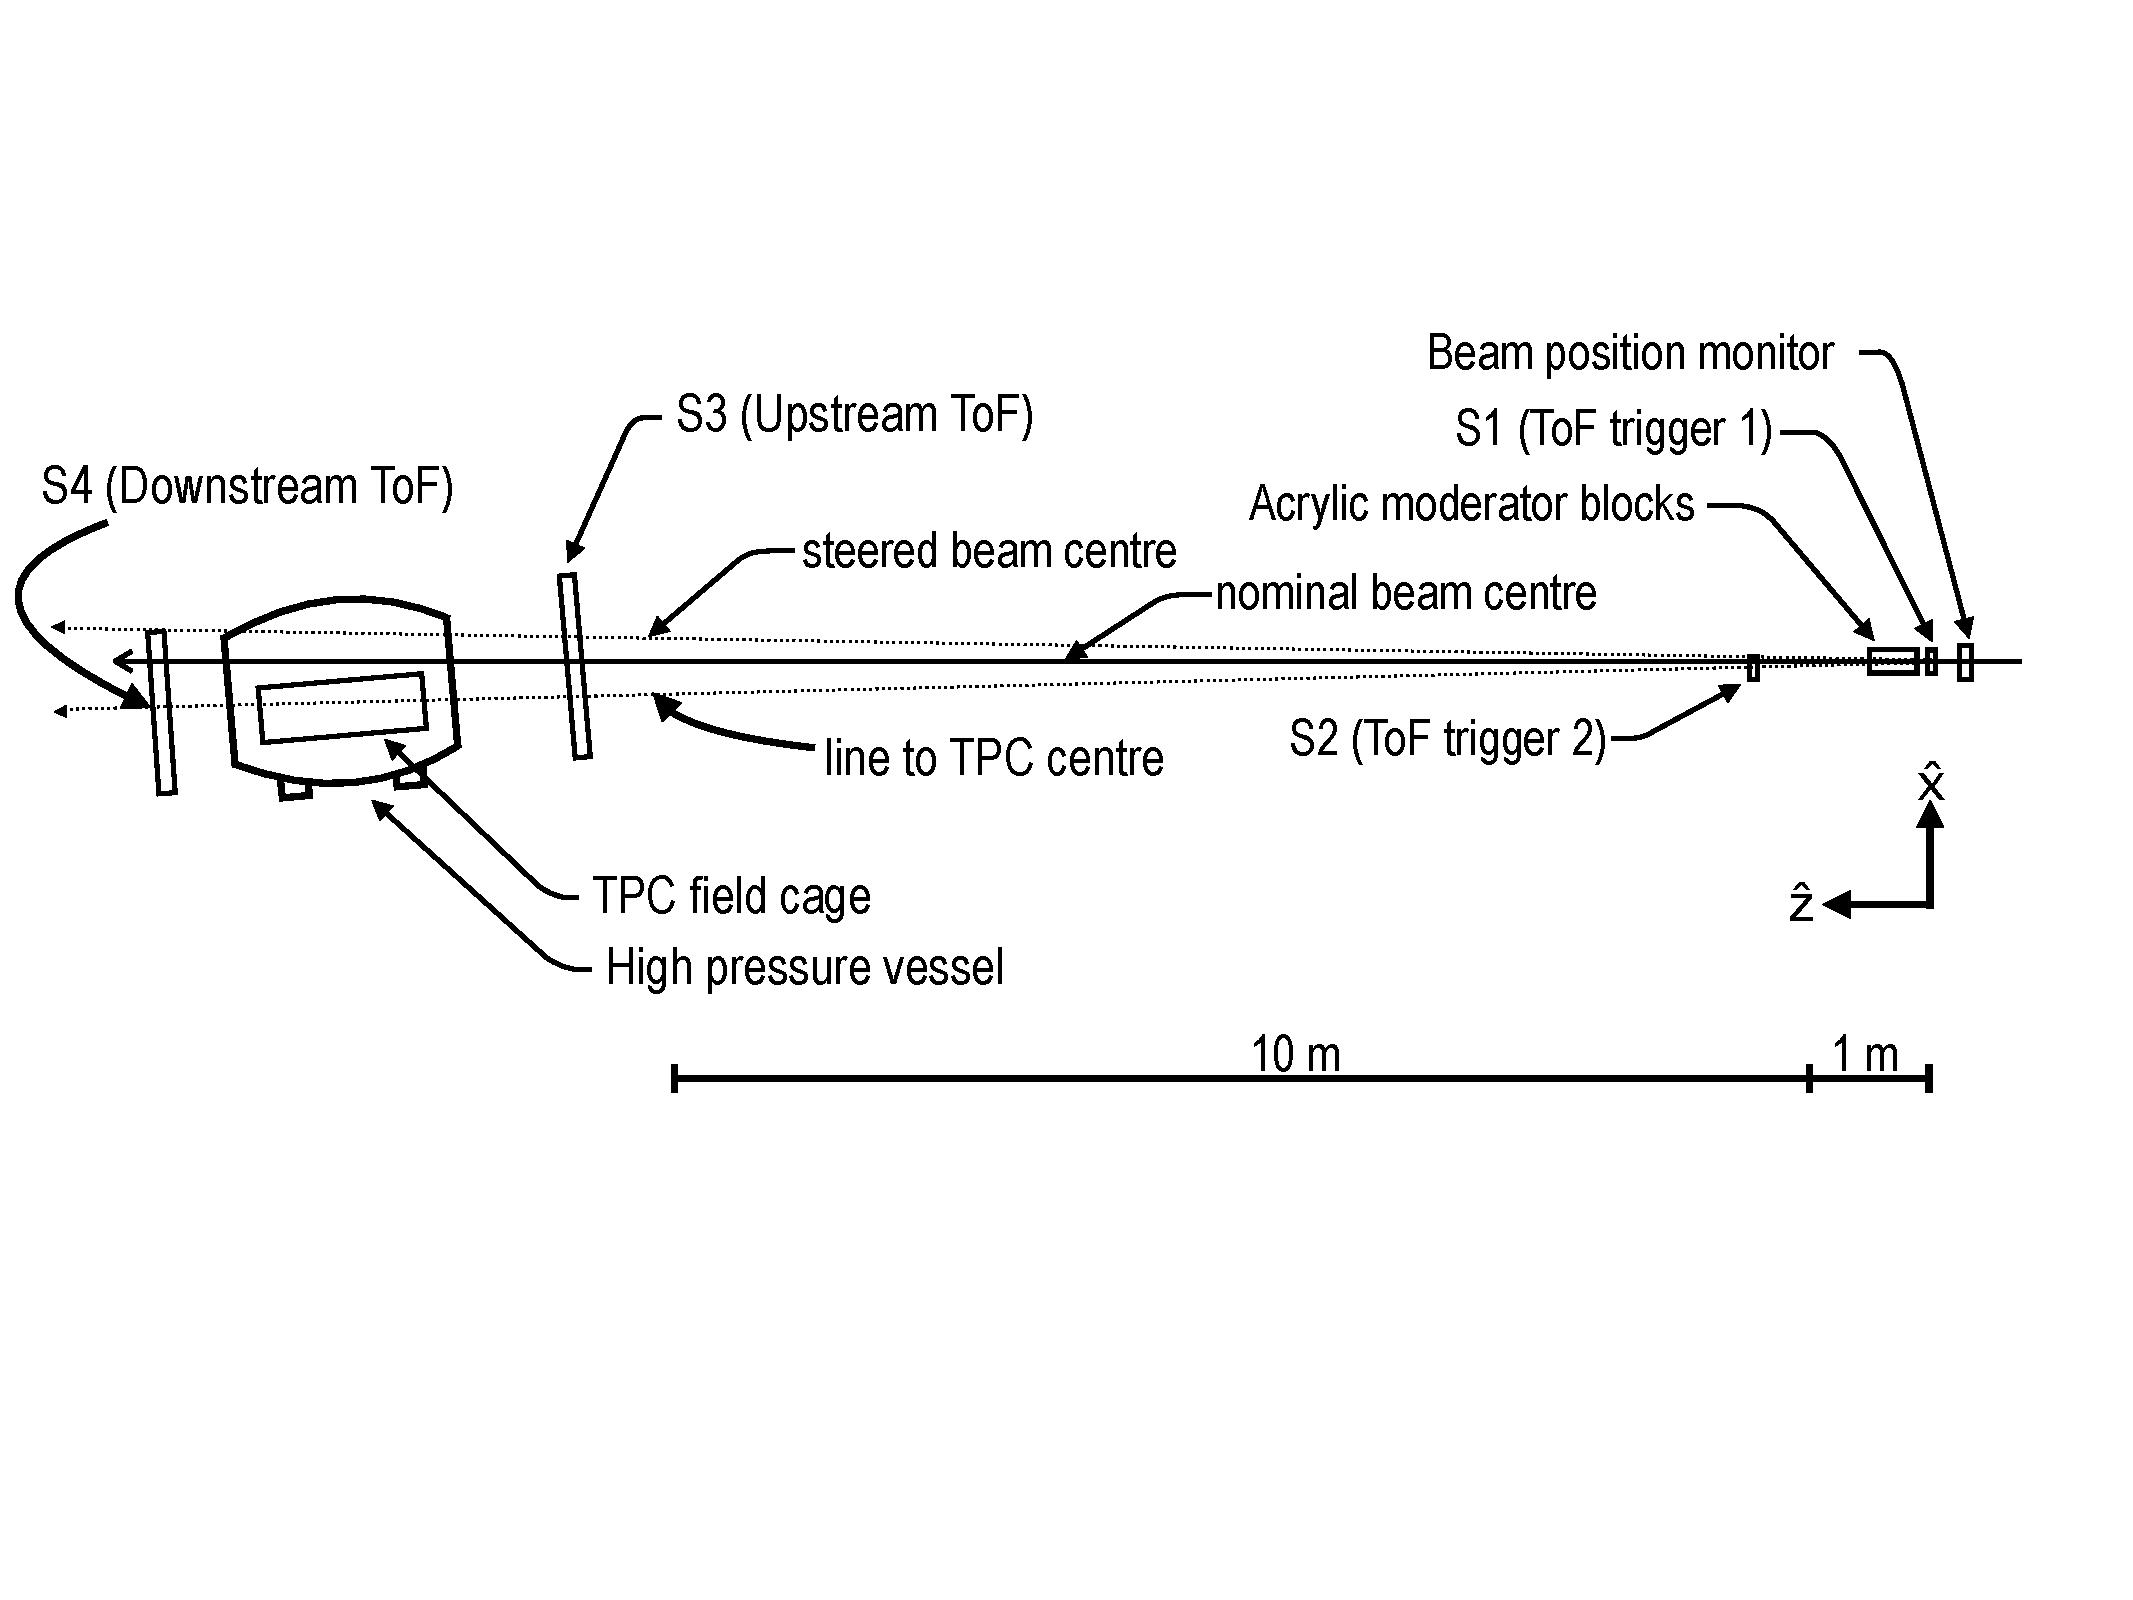
\includegraphics[width=1.0\linewidth]{files/Figures/hptpc_t10_planview.pdf}
  \caption{Beam test configuration}
  \label{fig:setup}
\end{figure}

The beam position monitor lies upstream of all the ToF constituents and the TPC, at the beam entrance. 
%The centre of the HPTPC Prototype was placed 13~m from the wire chamber at the beam entrance. 
The beam position monitor is followed by three ToF constituents: $\mathit{S1}$, which provides the trigger is a small-area beam trigger.
$\mathit{S2}$, a trigger counter that provides a coincidence measurement with $\mathit{S1}$.
$\mathit{S3}$, a large wall of plastic scintillator bars, placed directly upstream of the TPC vessel.
All three of these upstream constituents are described in greater detail in Sections~\ref{subsec:s1s2Exp}~and~\ref{subsec:s3Exp}.
Directly between $\mathit{S1}$ and $\mathit{S2}$, a variable number of blocks of acrylic moderator were placed, and are shown in Figure~\ref{fig:modblocks}.
The vessel containing the TPC was placed 13~m from the wire chamber at the beam entrance.
Lastly, a fourth ToF constituent, labeled $\mathit{S4}$, was placed directly downstream of the vessel.
This was a second wall of plastic scintillator bars, described further in Section~\ref{subsec:s4Exp}.
Both the TPC and ToF systems were placed at an off-axis angle with respect to the direction of the beam.
To study the impact of moderator thickness, a variable number of blocks of acrylic, each of dimension $10\times10\times10$~cm$^3$, were placed in the beamline, with the upstream end of the moderators located xxx cm behind $\mathit{S1}$, and are shown in Figure~\ref{fig:modblocks}.

\todo[inline]{also need the off axis angle (with +/-). Need to check the mod block from S1}

Data acquisition (DAQ) of up- and downstream ToF systems were completely independent.
The synchronization between systems was performed offline using the reference signal from the PS at the beginning of every spill.
The PS beam structure is as follows: T10 received between 1 and 3 spills during each supercycle which has a typical duration of 33~s.
The spill duration is approximately 400~ms.
The minimum separation in time between two spills is approximately 1 second.
Therefore the start of spill signal frequency is 1 Hz or smaller.
The trigger condition of the upstream ToF was based on the coincidence between $\mathit{S1}$ and $\mathit{S3}$ constituents.
$\mathit{S2}$ signals were also recorded but the upstream ToF DAQ but were not a trigger condition.
The DAQ of the downstream ToF, $\mathit{S4}$, was run in self-triggering mode with a gate open during the spill.
Coincidence signals between $\mathit{S1}$ and $\mathit{S2}$ counters were also recorded by the downstream ToF DAQ and were used in the particle identification (PID) analysis, described in Section~\ref{hptpcPaper:sec:Results}.  

A system of moderator blocks was located between the $\mathit{S1}$ and $\mathit{S2}$ counters.
The system was composed of a stand on which up to four polystyrene $10\times10\times10$~cm$^3$ blocks could be placed contiguously.
Figure~\ref{fig:modblocks} shows the stand with four blocks installed.
The moderator blocks have the effect of both reducing the energy of incoming particles as well as scattering protons in the beam through higher angles than beam MIPs.
This tends to increase in the proton-to-MIP ratio at low off-axis angles from the beam, while decreasing the total number of protons and MIPs traversing the TPC.
A maximum of four moderator blocks was chosen to retain a minimum intensity in the TPC.
%The addition of too many moderator blocks would cause an overscattering whereby too many protons fall below threshold as compared with MIPs.

Data was taken with the beam momentum primarily at 0.8~GeV/c, and with each configuration of 0 to 4 moderator blocks.
Figure~INSERT shows the typical composition of the beam upstream of $\mathit{S1}$ at 0.8~GeV/c. Beam spills were approximately 500~ms in length with 5-10~s between spills.  
\todo[inline]{JOCELYN:"In general, you need a paragraph and a figure or two that describe the T10 beam before you do anything to it. The description of the un-modified beam should come before any explanation about the modifications, so probably as a subsection at the end of section 1. This unmodified beam data should probably come from the 2016 measurements, or the on-axis TOF measurements with no moderator." - similar to previous comment 2016 data probably best So maybe remove figure INSERT, and just do a subsection at the end of section 1.}

%    Moderator blocks were used in order to cause a spread in the incoming beam.
%    The blocks cause protons to scatter through a larger angle than pions and other minimum ionising particles (MIP), increasing the off-axis proton pion ratio.
%    The effect of this, together with placing the TPC and ToF systems off axis was to allow a measurement of protons with a lower pion background.
%    This technique also had the effect of reducing the average momentum of the measured particles.
%    Data were taken for 0, 1, 2, 3, and 4 moderator blocks in turn.
%    The beam ran with an energy of 0.8~GeV/c, and primarily comprised protons and pions, as well as muons and electrons. 
%    Beam spills were approximately 500~ms in length, with 5-10~s between spills.
%    The ratio of protons to pions expected in the T10 beam  is shown in figure~\ref{beamcharacteristics}.
%    From this figure, the expected on axis proton pion ratio at 0.8~GeV/c is approximately 1:6.
%      \begin{figure}
%      \centering
%    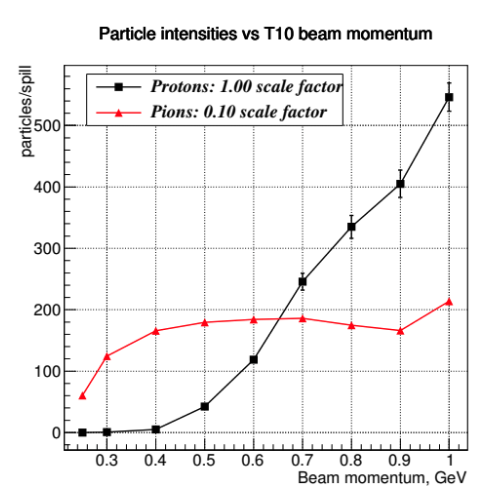
\includegraphics[width=0.6\linewidth]{files/Figures/offaxismeasurement.png}
%    	\caption{T10 beam constituents (REFERENCE NEEDED)}
%    		\label{fig:beamcharacteristics}
%    \end{figure}


\begin{figure}[t]
  \centering
  %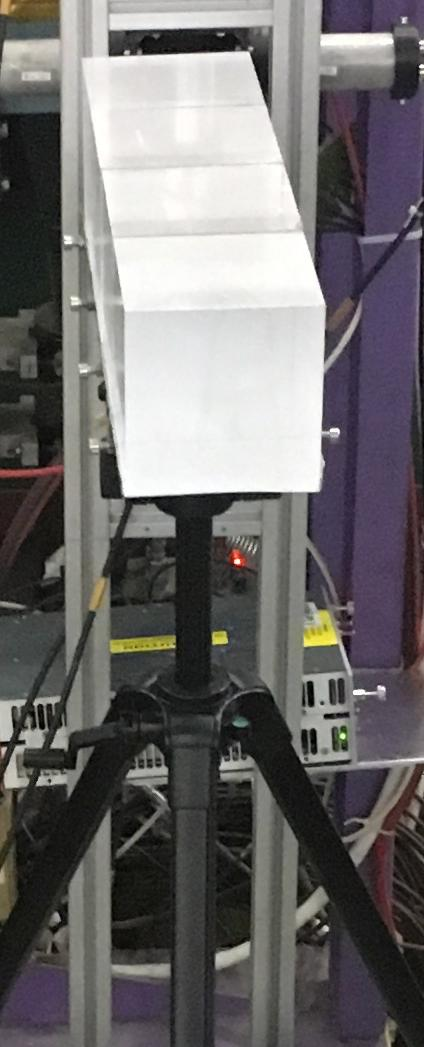
\includegraphics[width=0.2\linewidth]{files/Figures/ModeratorBlocks.jpg}
  \includegraphics[width=1.05\linewidth]{files/Figures/S1S2S3S4.png}
  \caption{Photo demonstrating the $\mathit{S1}$ and $\mathit{S2}$ counters and the stand with four acrylic moderator blocks of the upstream part of the setup (right). Photo of the downstream part of the setup which shows the $\mathit{S3}$, $\mathit{S4}$ detectors and HPTPC (left).}
  \label{fig:modblocks}
\end{figure}

\subsection{Survey and coordinate system}
The T10 beamline area is surveyed and the distances to various components measured to a precision of 0.5~mm by the CERN Survey, Mechatronics and Measurements (SMM) group.
These measurements are used to calculate the positions of various components in the beamline relative to one another.

Figure~\ref{fig:angularDistWC} shows the angular distribution of various objects within the beamline.

\begin{figure}[ht]
  \begin{adjustbox}{max totalsize={.7\textwidth}{.5\textheight},center}
    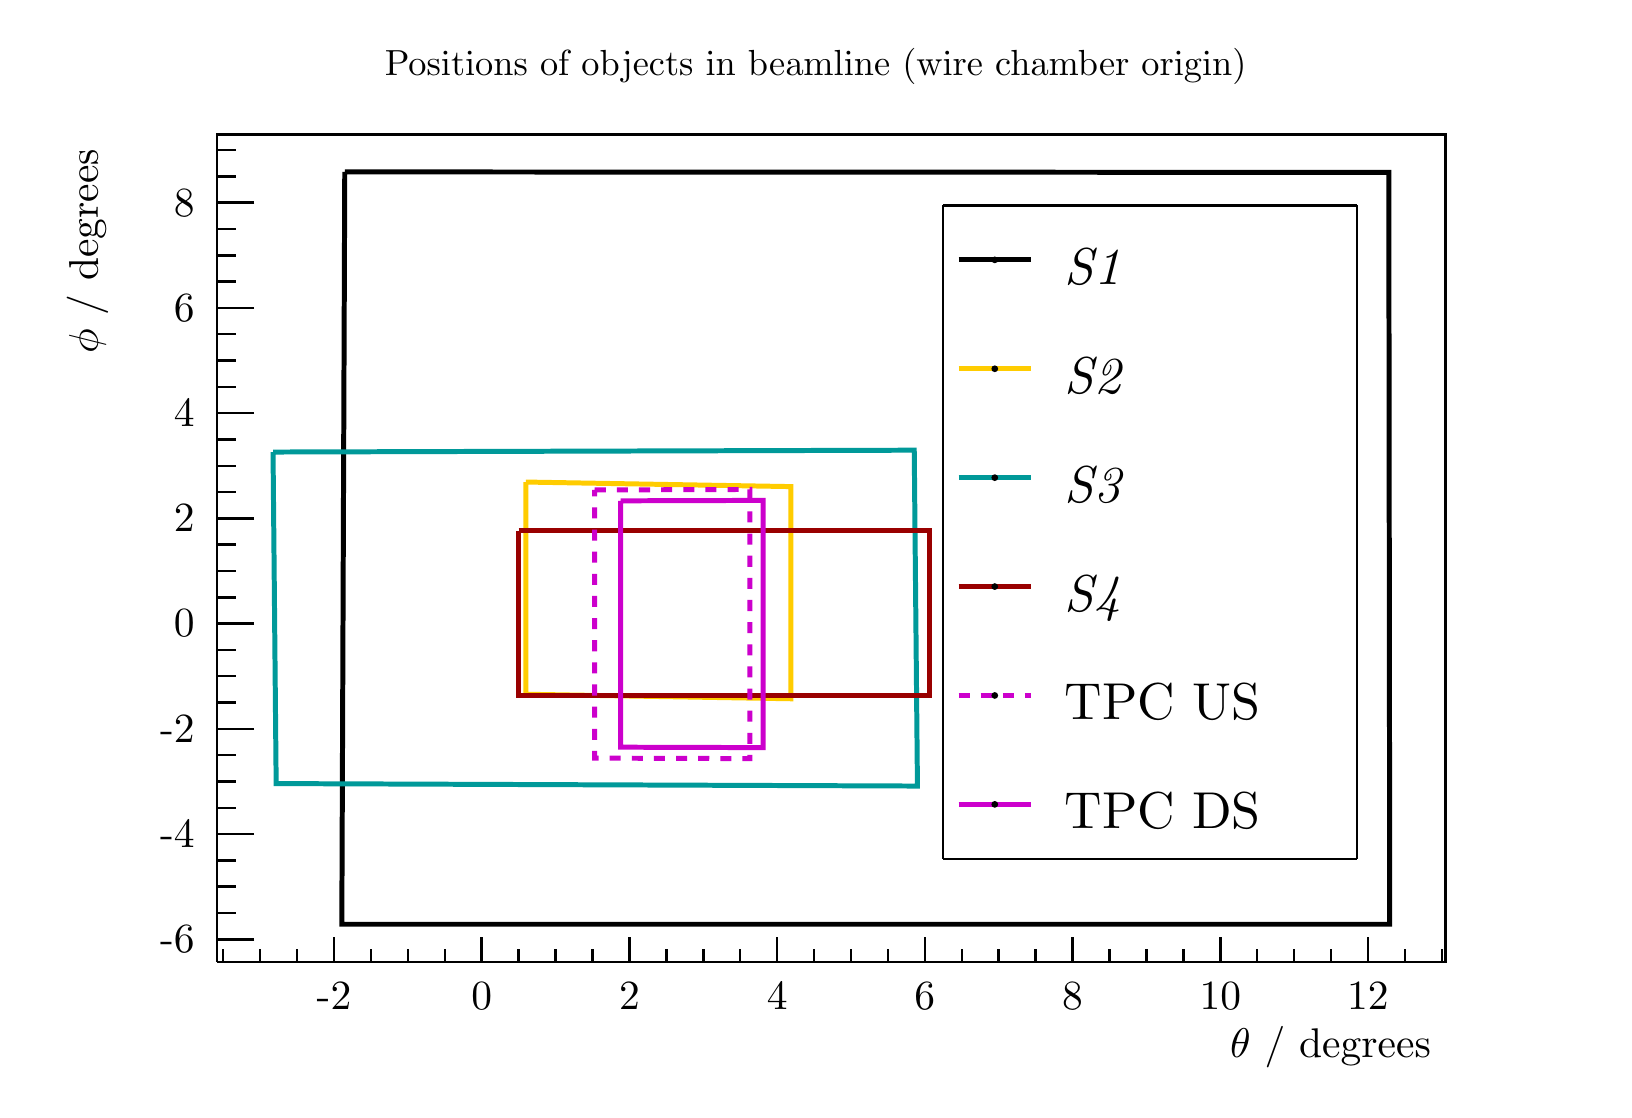
\begin{tikzpicture}
\pgfdeclareplotmark{cross} {
\pgfpathmoveto{\pgfpoint{-0.3\pgfplotmarksize}{\pgfplotmarksize}}
\pgfpathlineto{\pgfpoint{+0.3\pgfplotmarksize}{\pgfplotmarksize}}
\pgfpathlineto{\pgfpoint{+0.3\pgfplotmarksize}{0.3\pgfplotmarksize}}
\pgfpathlineto{\pgfpoint{+1\pgfplotmarksize}{0.3\pgfplotmarksize}}
\pgfpathlineto{\pgfpoint{+1\pgfplotmarksize}{-0.3\pgfplotmarksize}}
\pgfpathlineto{\pgfpoint{+0.3\pgfplotmarksize}{-0.3\pgfplotmarksize}}
\pgfpathlineto{\pgfpoint{+0.3\pgfplotmarksize}{-1.\pgfplotmarksize}}
\pgfpathlineto{\pgfpoint{-0.3\pgfplotmarksize}{-1.\pgfplotmarksize}}
\pgfpathlineto{\pgfpoint{-0.3\pgfplotmarksize}{-0.3\pgfplotmarksize}}
\pgfpathlineto{\pgfpoint{-1.\pgfplotmarksize}{-0.3\pgfplotmarksize}}
\pgfpathlineto{\pgfpoint{-1.\pgfplotmarksize}{0.3\pgfplotmarksize}}
\pgfpathlineto{\pgfpoint{-0.3\pgfplotmarksize}{0.3\pgfplotmarksize}}
\pgfpathclose
\pgfusepathqstroke
}
\pgfdeclareplotmark{cross*} {
\pgfpathmoveto{\pgfpoint{-0.3\pgfplotmarksize}{\pgfplotmarksize}}
\pgfpathlineto{\pgfpoint{+0.3\pgfplotmarksize}{\pgfplotmarksize}}
\pgfpathlineto{\pgfpoint{+0.3\pgfplotmarksize}{0.3\pgfplotmarksize}}
\pgfpathlineto{\pgfpoint{+1\pgfplotmarksize}{0.3\pgfplotmarksize}}
\pgfpathlineto{\pgfpoint{+1\pgfplotmarksize}{-0.3\pgfplotmarksize}}
\pgfpathlineto{\pgfpoint{+0.3\pgfplotmarksize}{-0.3\pgfplotmarksize}}
\pgfpathlineto{\pgfpoint{+0.3\pgfplotmarksize}{-1.\pgfplotmarksize}}
\pgfpathlineto{\pgfpoint{-0.3\pgfplotmarksize}{-1.\pgfplotmarksize}}
\pgfpathlineto{\pgfpoint{-0.3\pgfplotmarksize}{-0.3\pgfplotmarksize}}
\pgfpathlineto{\pgfpoint{-1.\pgfplotmarksize}{-0.3\pgfplotmarksize}}
\pgfpathlineto{\pgfpoint{-1.\pgfplotmarksize}{0.3\pgfplotmarksize}}
\pgfpathlineto{\pgfpoint{-0.3\pgfplotmarksize}{0.3\pgfplotmarksize}}
\pgfpathclose
\pgfusepathqfillstroke
}
\pgfdeclareplotmark{newstar} {
\pgfpathmoveto{\pgfqpoint{0pt}{\pgfplotmarksize}}
\pgfpathlineto{\pgfqpointpolar{44}{0.5\pgfplotmarksize}}
\pgfpathlineto{\pgfqpointpolar{18}{\pgfplotmarksize}}
\pgfpathlineto{\pgfqpointpolar{-20}{0.5\pgfplotmarksize}}
\pgfpathlineto{\pgfqpointpolar{-54}{\pgfplotmarksize}}
\pgfpathlineto{\pgfqpointpolar{-90}{0.5\pgfplotmarksize}}
\pgfpathlineto{\pgfqpointpolar{234}{\pgfplotmarksize}}
\pgfpathlineto{\pgfqpointpolar{198}{0.5\pgfplotmarksize}}
\pgfpathlineto{\pgfqpointpolar{162}{\pgfplotmarksize}}
\pgfpathlineto{\pgfqpointpolar{134}{0.5\pgfplotmarksize}}
\pgfpathclose
\pgfusepathqstroke
}
\pgfdeclareplotmark{newstar*} {
\pgfpathmoveto{\pgfqpoint{0pt}{\pgfplotmarksize}}
\pgfpathlineto{\pgfqpointpolar{44}{0.5\pgfplotmarksize}}
\pgfpathlineto{\pgfqpointpolar{18}{\pgfplotmarksize}}
\pgfpathlineto{\pgfqpointpolar{-20}{0.5\pgfplotmarksize}}
\pgfpathlineto{\pgfqpointpolar{-54}{\pgfplotmarksize}}
\pgfpathlineto{\pgfqpointpolar{-90}{0.5\pgfplotmarksize}}
\pgfpathlineto{\pgfqpointpolar{234}{\pgfplotmarksize}}
\pgfpathlineto{\pgfqpointpolar{198}{0.5\pgfplotmarksize}}
\pgfpathlineto{\pgfqpointpolar{162}{\pgfplotmarksize}}
\pgfpathlineto{\pgfqpointpolar{134}{0.5\pgfplotmarksize}}
\pgfpathclose
\pgfusepathqfillstroke
}
\definecolor{c}{rgb}{1,1,1};
\draw [color=c, fill=c] (0,0) rectangle (20,13.474);
\draw [color=c, fill=c] (2.4,1.61688) rectangle (18,12.1266);
\definecolor{c}{rgb}{0,0,0};
\draw [c,line width=0.9] (2.4,1.61688) -- (2.4,12.1266) -- (18,12.1266) -- (18,1.61688) -- (2.4,1.61688);
\definecolor{c}{rgb}{1,1,1};
\draw [color=c, fill=c] (2.4,1.61688) rectangle (18,12.1266);
\definecolor{c}{rgb}{0,0,0};
\draw [c,line width=0.9] (2.4,1.61688) -- (2.4,12.1266) -- (18,12.1266) -- (18,1.61688) -- (2.4,1.61688);
\draw [c,line width=0.9] (2.4,1.61688) -- (18,1.61688);
\draw [c,line width=0.9] (3.88349,1.93217) -- (3.88349,1.61688);
\draw [c,line width=0.9] (4.35247,1.77452) -- (4.35247,1.61688);
\draw [c,line width=0.9] (4.82145,1.77452) -- (4.82145,1.61688);
\draw [c,line width=0.9] (5.29044,1.77452) -- (5.29044,1.61688);
\draw [c,line width=0.9] (5.75942,1.93217) -- (5.75942,1.61688);
\draw [c,line width=0.9] (6.22841,1.77452) -- (6.22841,1.61688);
\draw [c,line width=0.9] (6.69739,1.77452) -- (6.69739,1.61688);
\draw [c,line width=0.9] (7.16638,1.77452) -- (7.16638,1.61688);
\draw [c,line width=0.9] (7.63536,1.93217) -- (7.63536,1.61688);
\draw [c,line width=0.9] (8.10435,1.77452) -- (8.10435,1.61688);
\draw [c,line width=0.9] (8.57333,1.77452) -- (8.57333,1.61688);
\draw [c,line width=0.9] (9.04231,1.77452) -- (9.04231,1.61688);
\draw [c,line width=0.9] (9.5113,1.93217) -- (9.5113,1.61688);
\draw [c,line width=0.9] (9.98028,1.77452) -- (9.98028,1.61688);
\draw [c,line width=0.9] (10.4493,1.77452) -- (10.4493,1.61688);
\draw [c,line width=0.9] (10.9183,1.77452) -- (10.9183,1.61688);
\draw [c,line width=0.9] (11.3872,1.93217) -- (11.3872,1.61688);
\draw [c,line width=0.9] (11.8562,1.77452) -- (11.8562,1.61688);
\draw [c,line width=0.9] (12.3252,1.77452) -- (12.3252,1.61688);
\draw [c,line width=0.9] (12.7942,1.77452) -- (12.7942,1.61688);
\draw [c,line width=0.9] (13.2632,1.93217) -- (13.2632,1.61688);
\draw [c,line width=0.9] (13.7322,1.77452) -- (13.7322,1.61688);
\draw [c,line width=0.9] (14.2011,1.77452) -- (14.2011,1.61688);
\draw [c,line width=0.9] (14.6701,1.77452) -- (14.6701,1.61688);
\draw [c,line width=0.9] (15.1391,1.93217) -- (15.1391,1.61688);
\draw [c,line width=0.9] (15.6081,1.77452) -- (15.6081,1.61688);
\draw [c,line width=0.9] (16.0771,1.77452) -- (16.0771,1.61688);
\draw [c,line width=0.9] (16.5461,1.77452) -- (16.5461,1.61688);
\draw [c,line width=0.9] (17.015,1.93217) -- (17.015,1.61688);
\draw [c,line width=0.9] (3.88349,1.93217) -- (3.88349,1.61688);
\draw [c,line width=0.9] (3.4145,1.77452) -- (3.4145,1.61688);
\draw [c,line width=0.9] (2.94552,1.77452) -- (2.94552,1.61688);
\draw [c,line width=0.9] (2.47653,1.77452) -- (2.47653,1.61688);
\draw [c,line width=0.9] (17.015,1.93217) -- (17.015,1.61688);
\draw [c,line width=0.9] (17.484,1.77452) -- (17.484,1.61688);
\draw [c,line width=0.9] (17.953,1.77452) -- (17.953,1.61688);
\draw [anchor=base] (3.88349,1.01055) node[scale=1.49939, color=c, rotate=0]{-2};
\draw [anchor=base] (5.75942,1.01055) node[scale=1.49939, color=c, rotate=0]{0};
\draw [anchor=base] (7.63536,1.01055) node[scale=1.49939, color=c, rotate=0]{2};
\draw [anchor=base] (9.5113,1.01055) node[scale=1.49939, color=c, rotate=0]{4};
\draw [anchor=base] (11.3872,1.01055) node[scale=1.49939, color=c, rotate=0]{6};
\draw [anchor=base] (13.2632,1.01055) node[scale=1.49939, color=c, rotate=0]{8};
\draw [anchor=base] (15.1391,1.01055) node[scale=1.49939, color=c, rotate=0]{10};
\draw [anchor=base] (17.015,1.01055) node[scale=1.49939, color=c, rotate=0]{12};
\draw [anchor= east] (18,0.538959) node[scale=1.49939, color=c, rotate=0]{$\theta$ / degrees};
\draw [c,line width=0.9] (2.4,1.61688) -- (2.4,12.1266);
\draw [c,line width=0.9] (2.868,1.90318) -- (2.4,1.90318);
\draw [c,line width=0.9] (2.634,2.2373) -- (2.4,2.2373);
\draw [c,line width=0.9] (2.634,2.57142) -- (2.4,2.57142);
\draw [c,line width=0.9] (2.634,2.90555) -- (2.4,2.90555);
\draw [c,line width=0.9] (2.868,3.23967) -- (2.4,3.23967);
\draw [c,line width=0.9] (2.634,3.57379) -- (2.4,3.57379);
\draw [c,line width=0.9] (2.634,3.90792) -- (2.4,3.90792);
\draw [c,line width=0.9] (2.634,4.24204) -- (2.4,4.24204);
\draw [c,line width=0.9] (2.868,4.57616) -- (2.4,4.57616);
\draw [c,line width=0.9] (2.634,4.91028) -- (2.4,4.91028);
\draw [c,line width=0.9] (2.634,5.24441) -- (2.4,5.24441);
\draw [c,line width=0.9] (2.634,5.57853) -- (2.4,5.57853);
\draw [c,line width=0.9] (2.868,5.91265) -- (2.4,5.91265);
\draw [c,line width=0.9] (2.634,6.24678) -- (2.4,6.24678);
\draw [c,line width=0.9] (2.634,6.5809) -- (2.4,6.5809);
\draw [c,line width=0.9] (2.634,6.91502) -- (2.4,6.91502);
\draw [c,line width=0.9] (2.868,7.24915) -- (2.4,7.24915);
\draw [c,line width=0.9] (2.634,7.58327) -- (2.4,7.58327);
\draw [c,line width=0.9] (2.634,7.91739) -- (2.4,7.91739);
\draw [c,line width=0.9] (2.634,8.25151) -- (2.4,8.25151);
\draw [c,line width=0.9] (2.868,8.58564) -- (2.4,8.58564);
\draw [c,line width=0.9] (2.634,8.91976) -- (2.4,8.91976);
\draw [c,line width=0.9] (2.634,9.25388) -- (2.4,9.25388);
\draw [c,line width=0.9] (2.634,9.58801) -- (2.4,9.58801);
\draw [c,line width=0.9] (2.868,9.92213) -- (2.4,9.92213);
\draw [c,line width=0.9] (2.634,10.2563) -- (2.4,10.2563);
\draw [c,line width=0.9] (2.634,10.5904) -- (2.4,10.5904);
\draw [c,line width=0.9] (2.634,10.9245) -- (2.4,10.9245);
\draw [c,line width=0.9] (2.868,11.2586) -- (2.4,11.2586);
\draw [c,line width=0.9] (2.868,1.90318) -- (2.4,1.90318);
\draw [c,line width=0.9] (2.868,11.2586) -- (2.4,11.2586);
\draw [c,line width=0.9] (2.634,11.5927) -- (2.4,11.5927);
\draw [c,line width=0.9] (2.634,11.9269) -- (2.4,11.9269);
\draw [anchor= east] (2.3,1.90318) node[scale=1.49939, color=c, rotate=0]{-6};
\draw [anchor= east] (2.3,3.23967) node[scale=1.49939, color=c, rotate=0]{-4};
\draw [anchor= east] (2.3,4.57616) node[scale=1.49939, color=c, rotate=0]{-2};
\draw [anchor= east] (2.3,5.91265) node[scale=1.49939, color=c, rotate=0]{0};
\draw [anchor= east] (2.3,7.24915) node[scale=1.49939, color=c, rotate=0]{2};
\draw [anchor= east] (2.3,8.58564) node[scale=1.49939, color=c, rotate=0]{4};
\draw [anchor= east] (2.3,9.92213) node[scale=1.49939, color=c, rotate=0]{6};
\draw [anchor= east] (2.3,11.2586) node[scale=1.49939, color=c, rotate=0]{8};
\draw [anchor= east] (0.753024,12.1266) node[scale=1.49939, color=c, rotate=90]{$\phi$ / degrees};
\draw [c,line width=1.8] (4.02001,11.6489) -- (17.2792,11.643) -- (17.2909,2.09459) -- (3.98258,2.09459) -- (4.02001,11.6489);
\definecolor{c}{rgb}{1,0.8,0};
\draw [c,line width=1.8] (6.32024,7.71036) -- (6.32024,5.01555) -- (9.6851,4.95805) -- (9.6851,7.65257) -- (6.32024,7.71036);
\definecolor{c}{rgb}{0,0.6,0.6};
\draw [c,line width=1.8] (3.10909,8.09147) -- (11.2523,8.11493) -- (11.293,3.84961) -- (3.14872,3.88101) -- (3.10909,8.09147);
\definecolor{c}{rgb}{0.6,0,0};
\draw [c,line width=1.8] (6.22774,7.09184) -- (11.4508,7.09184) -- (11.4508,4.99824) -- (6.22774,4.99824) -- (6.22774,7.09184);
\definecolor{c}{rgb}{0.8,0,0.8};
\draw [c,dash pattern=on 4.00pt off 4.00pt ,line width=1.8] (7.19412,7.60986) -- (9.16463,7.61621) -- (9.16463,4.19793) -- (7.19412,4.20431) -- (7.19412,7.60986);
\draw [c,line width=1.8] (7.52371,7.47197) -- (9.33375,7.47732) -- (9.33375,4.33772) -- (7.52371,4.34311) -- (7.52371,7.47197);
\definecolor{c}{rgb}{0,0,0};
\draw (10,12.9947) node[scale=1.31197, color=c, rotate=0]{Positions of objects in beamline (wire chamber origin)};
\definecolor{c}{rgb}{1,1,1};
\draw [color=c, fill=c] (11.6174,2.92546) rectangle (16.8776,11.2236);
\definecolor{c}{rgb}{0,0,0};
\draw [c,line width=0.9] (11.6174,2.92546) -- (16.8776,2.92546);
\draw [c,line width=0.9] (16.8776,2.92546) -- (16.8776,11.2236);
\draw [c,line width=0.9] (16.8776,11.2236) -- (11.6174,11.2236);
\draw [c,line width=0.9] (11.6174,11.2236) -- (11.6174,2.92546);
\draw [anchor=base west] (12.9325,10.2209) node[scale=1.87424, color=c, rotate=0]{$\mathit{S1}$};
\definecolor{c}{rgb}{1,1,1};
\draw [c, fill=c] (11.8147,10.0481) -- (12.7352,10.0481) -- (12.7352,11.0162) -- (11.8147,11.0162);
\definecolor{c}{rgb}{0,0,0};
\draw [c,line width=1.8] (11.8147,10.5321) -- (12.7352,10.5321);
\foreach \P in {(12.275,10.5321)}{\draw[mark options={color=c,fill=c},mark size=2.402402pt,mark=*,mark size=1pt] plot coordinates {\P};}
\draw [anchor=base west] (12.9325,8.8379) node[scale=1.87424, color=c, rotate=0]{$\mathit{S2}$};
\definecolor{c}{rgb}{1,1,1};
\draw [c, fill=c] (11.8147,8.66503) -- (12.7352,8.66503) -- (12.7352,9.63315) -- (11.8147,9.63315);
\definecolor{c}{rgb}{1,0.8,0};
\draw [c,line width=1.8] (11.8147,9.14909) -- (12.7352,9.14909);
\definecolor{c}{rgb}{0,0,0};
\foreach \P in {(12.275,9.14909)}{\draw[mark options={color=c,fill=c},mark size=2.402402pt,mark=*,mark size=1pt] plot coordinates {\P};}
\draw [anchor=base west] (12.9325,7.45488) node[scale=1.87424, color=c, rotate=0]{$\mathit{S3}$};
\definecolor{c}{rgb}{1,1,1};
\draw [c, fill=c] (11.8147,7.282) -- (12.7352,7.282) -- (12.7352,8.25012) -- (11.8147,8.25012);
\definecolor{c}{rgb}{0,0.6,0.6};
\draw [c,line width=1.8] (11.8147,7.76606) -- (12.7352,7.76606);
\definecolor{c}{rgb}{0,0,0};
\foreach \P in {(12.275,7.76606)}{\draw[mark options={color=c,fill=c},mark size=2.402402pt,mark=*,mark size=1pt] plot coordinates {\P};}
\draw [anchor=base west] (12.9325,6.07185) node[scale=1.87424, color=c, rotate=0]{$\mathit{S4}$};
\definecolor{c}{rgb}{1,1,1};
\draw [c, fill=c] (11.8147,5.89897) -- (12.7352,5.89897) -- (12.7352,6.86709) -- (11.8147,6.86709);
\definecolor{c}{rgb}{0.6,0,0};
\draw [c,line width=1.8] (11.8147,6.38303) -- (12.7352,6.38303);
\definecolor{c}{rgb}{0,0,0};
\foreach \P in {(12.275,6.38303)}{\draw[mark options={color=c,fill=c},mark size=2.402402pt,mark=*,mark size=1pt] plot coordinates {\P};}
\draw [anchor=base west] (12.9325,4.68882) node[scale=1.87424, color=c, rotate=0]{TPC US};
\definecolor{c}{rgb}{1,1,1};
\draw [c, fill=c] (11.8147,4.51594) -- (12.7352,4.51594) -- (12.7352,5.48406) -- (11.8147,5.48406);
\definecolor{c}{rgb}{0.8,0,0.8};
\draw [c,dash pattern=on 4.00pt off 4.00pt ,line width=1.8] (11.8147,5) -- (12.7352,5);
\definecolor{c}{rgb}{0,0,0};
\foreach \P in {(12.275,5)}{\draw[mark options={color=c,fill=c},mark size=2.402402pt,mark=*,mark size=1pt] plot coordinates {\P};}
\draw [anchor=base west] (12.9325,3.30579) node[scale=1.87424, color=c, rotate=0]{TPC DS};
\definecolor{c}{rgb}{1,1,1};
\draw [c, fill=c] (11.8147,3.13291) -- (12.7352,3.13291) -- (12.7352,4.10103) -- (11.8147,4.10103);
\definecolor{c}{rgb}{0.8,0,0.8};
\draw [c,line width=1.8] (11.8147,3.61697) -- (12.7352,3.61697);
\definecolor{c}{rgb}{0,0,0};
\foreach \P in {(12.275,3.61697)}{\draw[mark options={color=c,fill=c},mark size=2.402402pt,mark=*,mark size=1pt] plot coordinates {\P};}
\end{tikzpicture}

  \end{adjustbox}
  \caption{Angular position of various objects within the T10 beamline. US and DS refer to the upstream and downstream faces of the HPTPC. The origin in this view is at the wire chamber (also know as the beam position monitor.}
  \label{fig:angularDistWC}  
\end{figure}

Table~\ref{tab:angWC} shows the calculated angular extent of the various beamline components as measured from the beam position monitor.

\begin{table}
  \centering
  \begin{tabular}{|c|c|c|c|c|}
    \hline
    Object & Minimum $\theta$ & Maximum $\theta$ & Minimum $\phi$ & Maximum $\phi$ \\
    \hline
    $\mathit{S1}$ & $-1.89^{\circ} \pm 0.14^{\circ}$ & $12.29^{\circ} \pm 0.14^{\circ}$ & $-5.71^{\circ} \pm 0.14^{\circ}$ & $8.58^{\circ} \pm 0.14^{\circ}$ \\
    $\mathit{S2}$ & $0.60^{\circ} \pm 0.02^{\circ}$ & $4.18^{\circ} \pm 0.02^{\circ}$ & $-1.43^{\circ} \pm 0.02^{\circ}$ & $2.69^{\circ} \pm 0.02^{\circ}$ \\
    $\mathit{S3}$ & $-2.826^{\circ} \pm 0.004^{\circ}$ & $5.900^{\circ} \pm 0.004^{\circ}$ & $-3.087^{\circ} \pm 0.004^{\circ}$ & $3.296^{\circ} \pm 0.004^{\circ}$ \\
    $\mathit{S4}$ & $0.499^{\circ} \pm 0.003^{\circ}$ & $6.068{\circ} \pm 0.003^{\circ}$ & $-1.368{\circ} \pm 0.003^{\circ}$ & $1.765^{\circ} \pm 0.003^{\circ}$ \\
    TPC upstream face & $1.530^{\circ} \pm 0.003^{\circ}$ & $3.630^{\circ} \pm 0.003^{\circ}$ & $-2.566^{\circ} \pm 0.003^{\circ}$ & $2.549^{\circ} \pm 0.003^{\circ}$ \\
    TPC downstream face & $1.881^{\circ} \pm 0.003^{\circ}$ & $3.811^{\circ} \pm 0.003^{\circ}$ & $-2.3567^{\circ} \pm 0.003^{\circ}$ & $2.341^{\circ} \pm 0.003^{\circ}$ \\
    \hline
  \end{tabular}
  \caption{Angular extents of various timing points within the T10 beamline as measured from the beam position monitor.}
  \label{tab:angWC}
\end{table}

\subsection{Upstream beam counters $\mathit{S1}$ and $\mathit{S2}$}
\label{subsec:s1s2Exp}
\todo[inline]{JOCELYN:"This actually isn't a good picture of S1, need one that shows the hardware head on." (do we have one of these?)}
The beam counters $\mathit{S1}$ and $\mathit{S2}$ are shown in Figure~\ref{fig:modblocks}, right.
The $\mathit{S1}$ counter is a $40\times40\times5$~mm$^3$ plastic scintillator cross which is attached to four 1'' Hamamatsu R4998 phototubes at each end for the light readout.
The time resolution of the counter, as measured by the DAQ system of the upstream ToF, was about 30~ps.
An example of a timing distribution from which this value can be taken is shown in Figure~\ref{fig:s3Res}.
This distribution is produced by measuring the hit time in each of the four PMTs making up $\mathit{S1}$ and taking the average of these times.
\begin{figure}
  \centering
  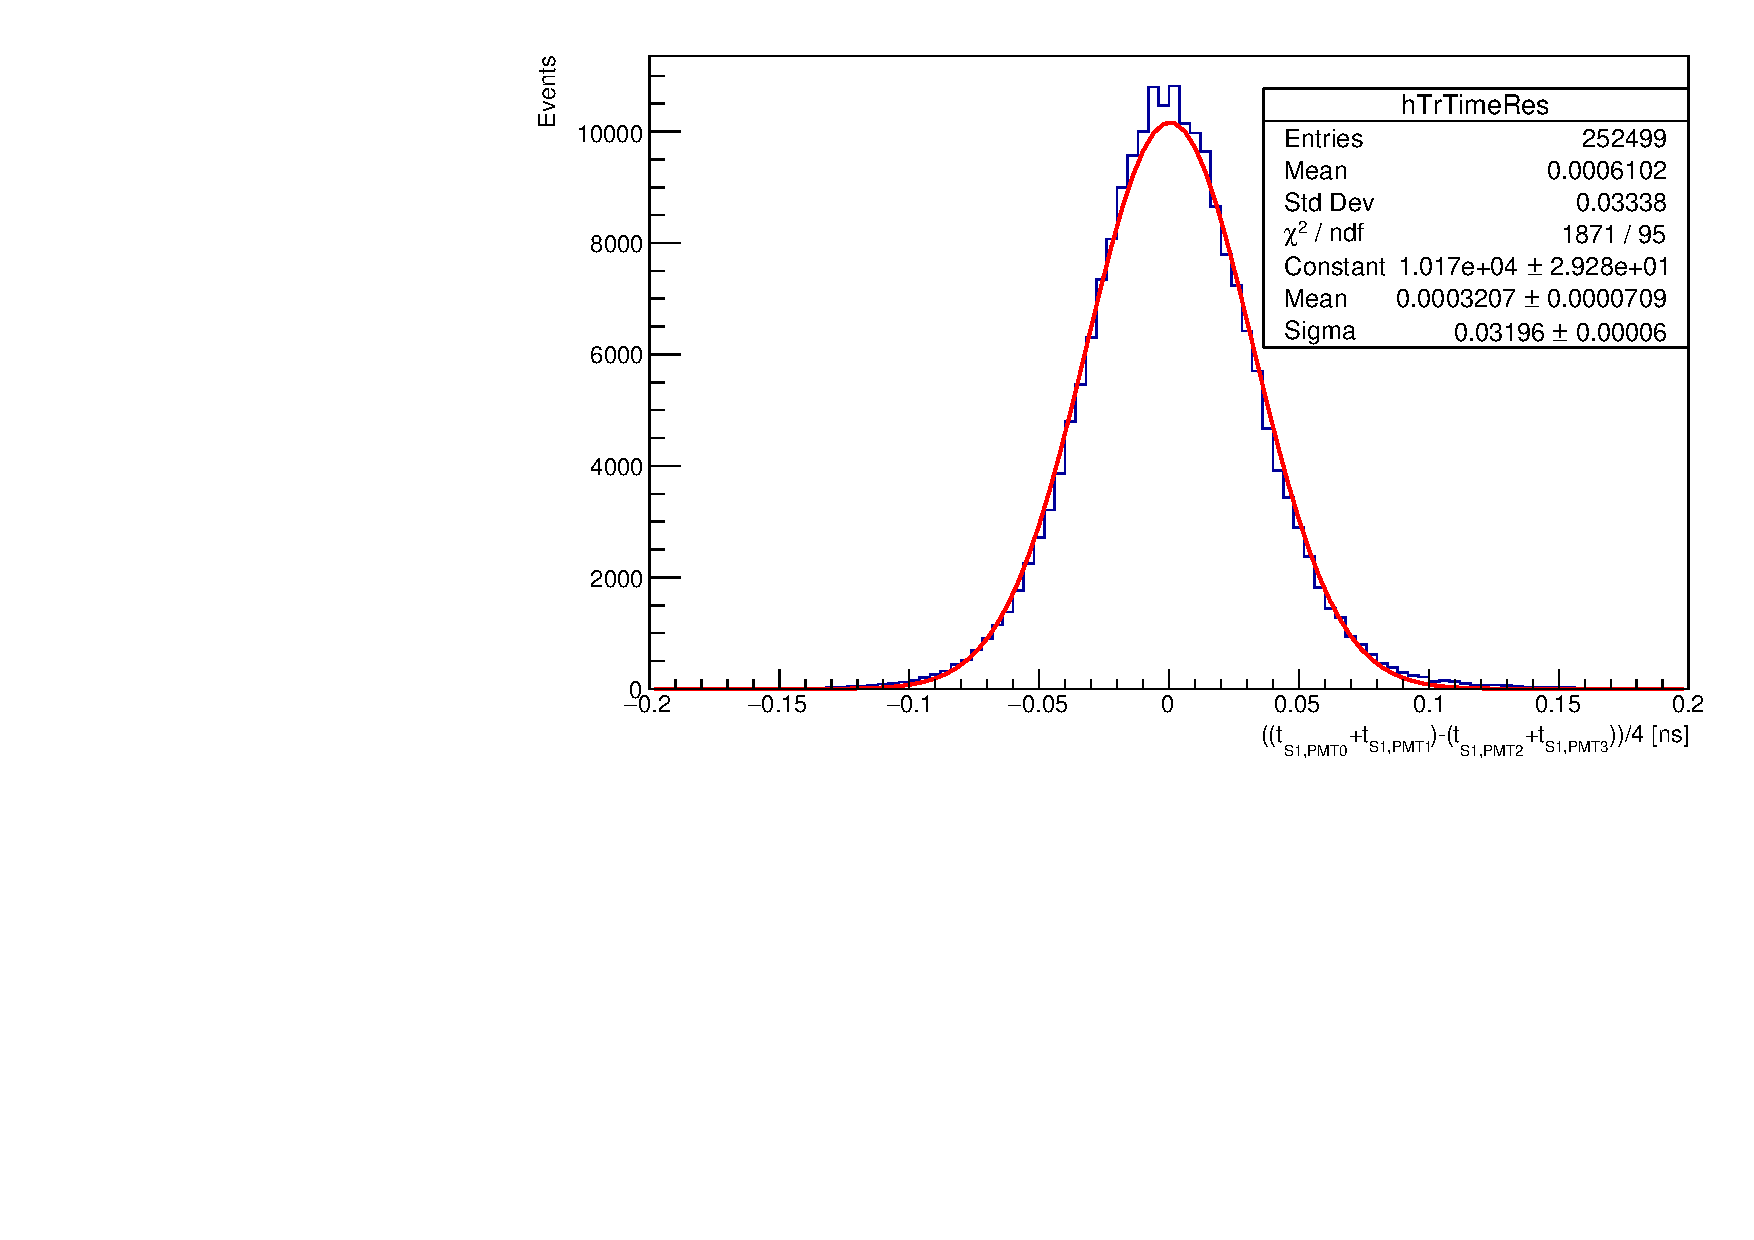
\includegraphics[width=0.7\linewidth]{files/Figures/TrTimeRes.pdf}
  \caption{An example of the timing distribution of $\mathit{S1}$ hits. The time is calculated as an average of the hit time as measured in each of the 4 PMTs.}
  \label{fig:s3Res}
\end{figure}

\todo[inline]{JOCELYN:"for time of flight, distance knowledge is essential.  Need a paragraph before 2.2. that describes how the distances are known (the survey, and description of survey methodology and precision), and includes a table of the relevant distances with error bars."}

The $\mathit{S2}$ counter is a scintillator tile of size $120\times120\times5$~mm$^3$, coupled to a 2" PMT R1309, which  2'' PMT R13089 which was connected to the scintillator via long light-guide as shown in Figure~\ref{fig:modblocks}.
The $\mathit{S2}$ counter was placed $(1.41 \pm 0.01)~\text{m}$ \todo{THIS NUMBER NEEDS CHECKING - SEB?} downstream of $\mathit{S1}$.
The transverse position of $\mathit{S2}$ was adjusted to account for the beam divergence in the moderator blocks.

The analog signals from one of the $\mathit{S1}$ PMTs and $\mathit{S2}$ PMT were fed into NIM discriminator units with a threshold of 30~mV.
Subsequently, the discriminated signals were fed into a NIM coincidence unit, and the coincidence of the two signals was recorded by the DAQ systems of the downstream ToF wall ($\mathit{S4}$).
This information was further used for the time-of-flight analysis of the downstream ToF.

\subsection{Upstream Time of Flight instrumentation ($\mathit{S3}$)}
\label{subsec:s3Exp}
\todo[inline]{JOCELYN:"Replace just upstream with a number and error bar"}
The $\mathit{S3}$ `upstream' ToF constituent was placed just upstream of the HPTPC prototype in the beamline.
A schematic drawing of the $\mathit{S3}$ ToF wall is shown in Figure~\ref{fig:S3sketch}.
The detector is composed of 22 staggered scintillator bars:  20 bars with dimensions $1.7 \times 6.0 \times 1.0$~cm$^3$ and 2 bars of  $1.5 \times 6.0 \times 1.0$~cm$^3$ placed on top and bottom~\cite{S3-proceedings}.
The overlap between bars was set to 5~mm, thus the active area of the detector was $2.0214~\text{cm}^{2}$.

\begin{figure}
  \centering
  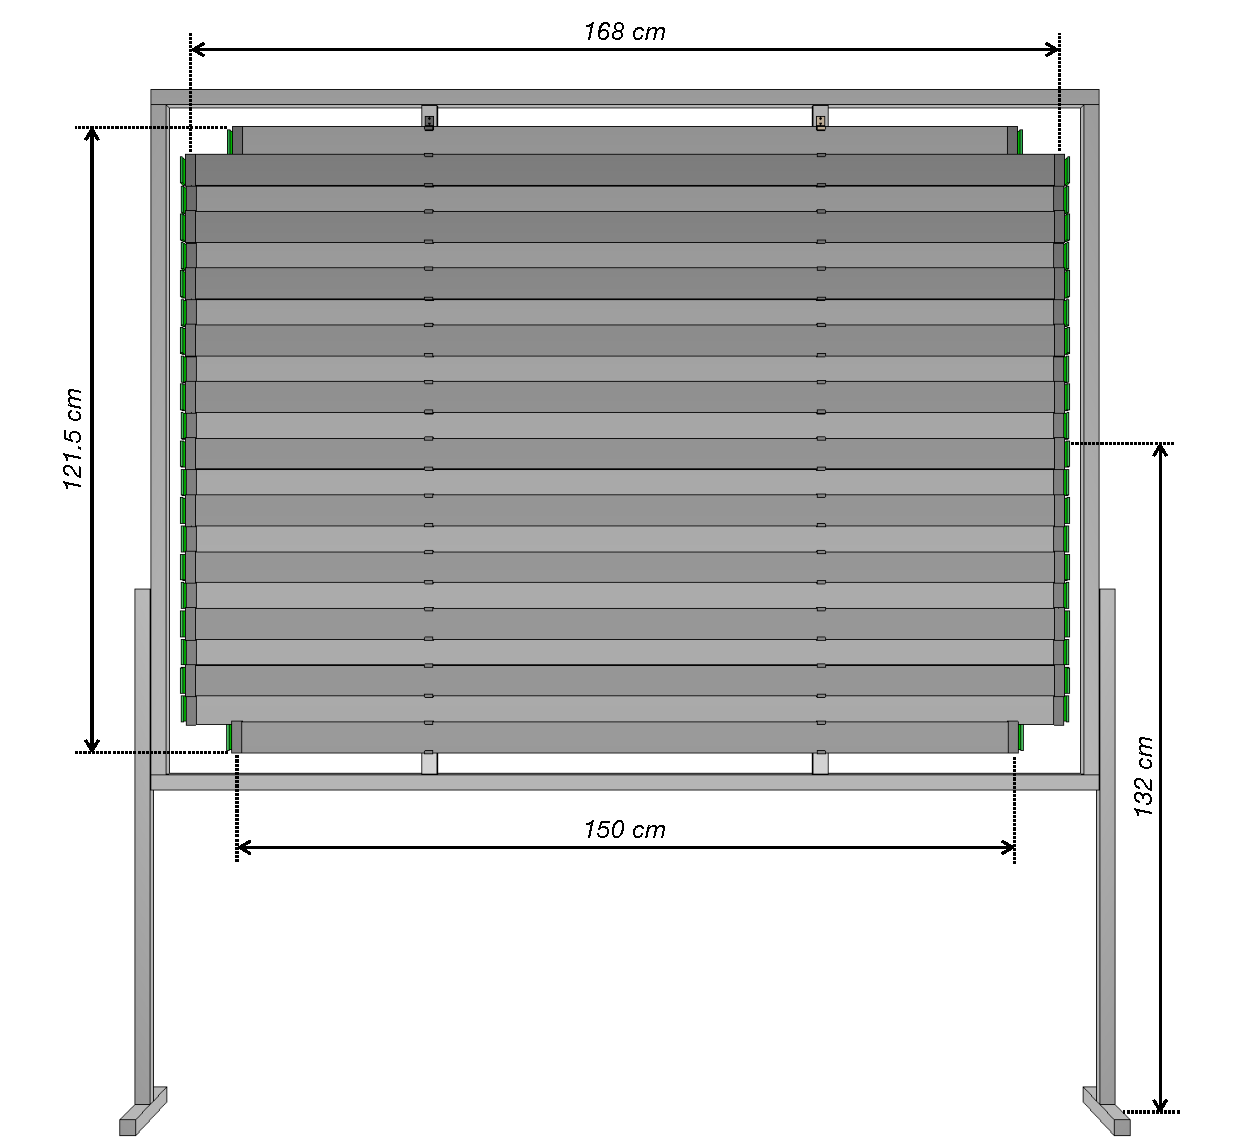
\includegraphics[width=0.48\linewidth]{files/Figures/uToF_sketch.pdf}
  \hfill
  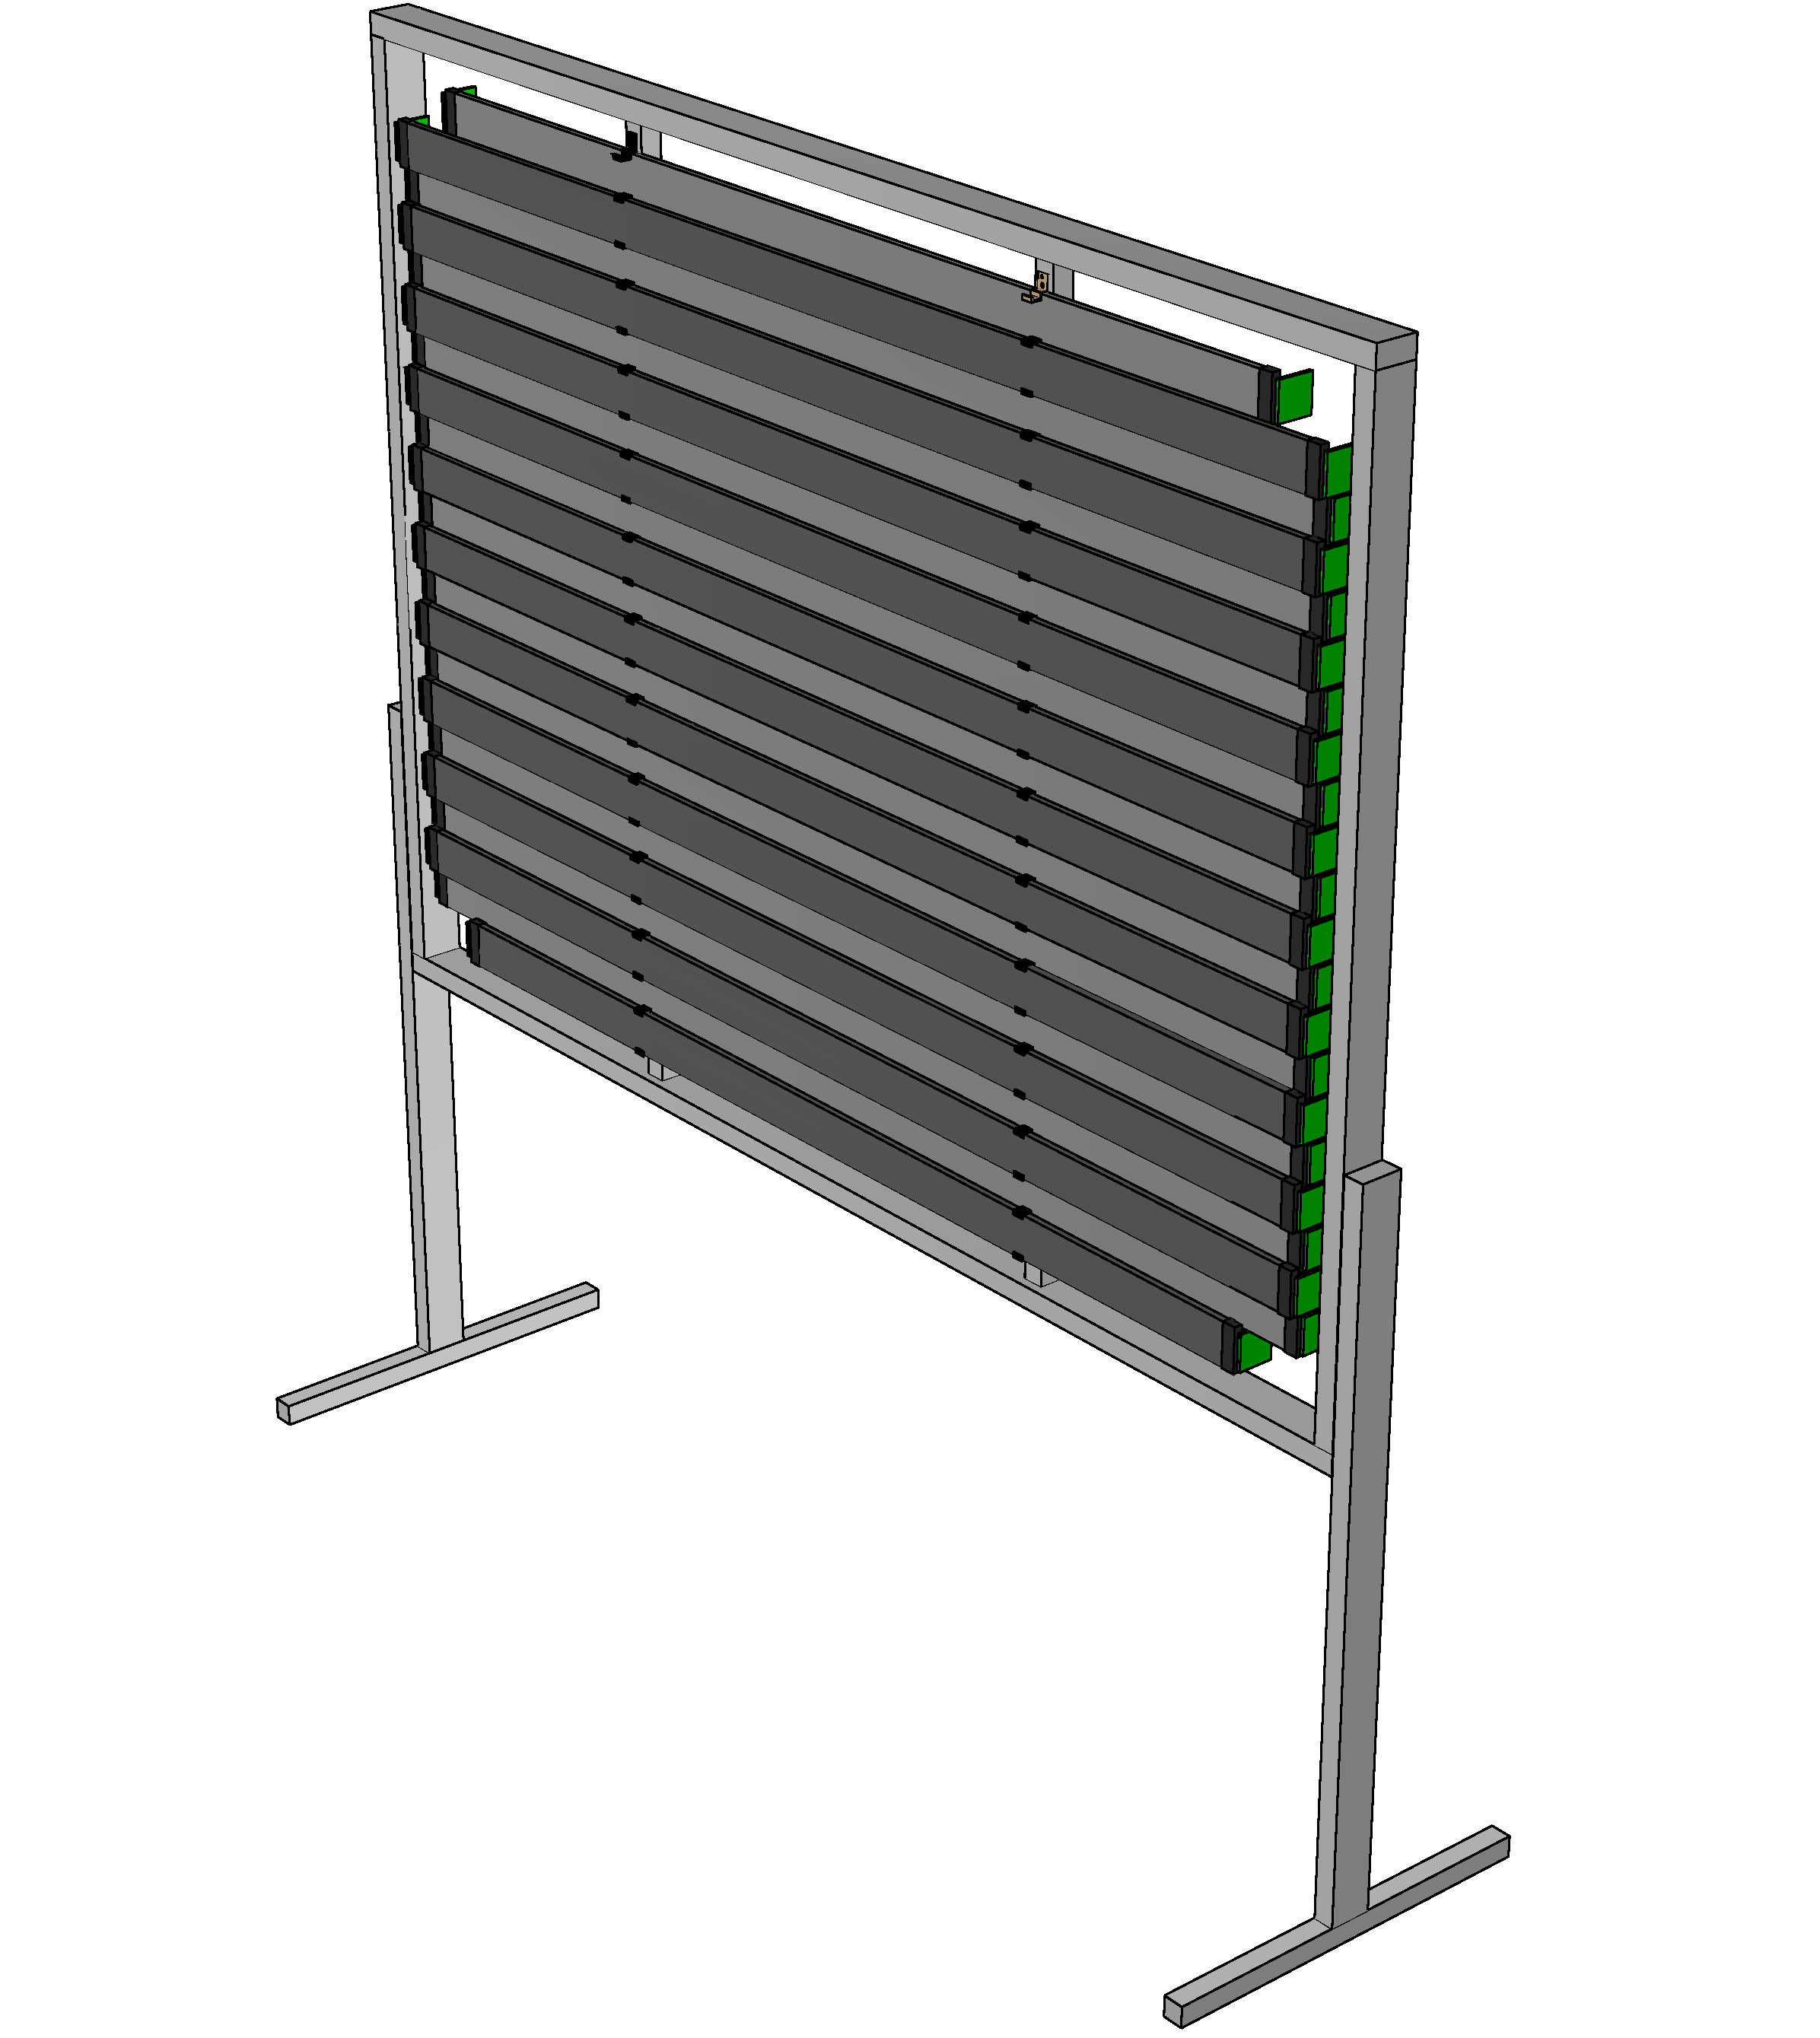
\includegraphics[width=0.42\linewidth]{files/Figures/uTOF_rot.pdf}
  \caption{Sketch of the $\mathit{S3}$ wall \cite{S3-proceedings}.
  Front (left) and rotated (right) views are presented.}
  \label{fig:S3sketch}
\end{figure}

The bars are made from the plastic scintillator, EJ-200 \cite{SCIONIX}, which provides a brightness of 10,000~photons/MeV~deposited.
It also has a suitable optical attenuation length of 4~m and fast timing, with a rise time of 0.9~ns and decay time constant of 2.1~ns.
The scintillation emission spectrum of EJ-200 resides peaks in the violet region of the visible spectrum (435~nm)~\cite{EJ200}, which corresponds well to the photon detection efficiency wavelength range of photosensors used for the readout.
The bars wrapped with an aluminium foil to maximize the light collected.
The foil used had a reflectivity of approximately 60\%.

Arrays of eight $6 \times 6$~mm$^2$ area silicon photomultipliers (SiPMs) S13360-6050PE from Hamamatsu Photonics \cite{Hamamatsu} were coupled to each end of the bar to collect scintillation photons.
The anode signals of the SiPMs are read out, summed and shaped by a dedicated circuit as described in Ref.\,\cite{S3-readout}.
%an 8-channel SiPM anode readout integrated circuit MUSIC-R1. %The construction of the prototype was a joint effort between groups of Geneva and Zurich universities as a part of R\&D for the Timing detector of the SHIP experiment \cite{AK}.

A 64-ch SAMPIC  module was used for the data acquisition.
A SAMPIC chip is a Waveform and Time to Digital Converter (WTDC) 16-channel ASIC which provides a raw time with an ultrafast analog memory allowing fine timing extraction as well as other parameters of the pulse~\cite{SAMPIC}.
Each channel contains a discriminator that can trigger itself independently or participate in a more complex combined trigger. 
Three module ASICs ($16\times3=48$ channels) were connected to the 44 channels of $\mathit{S3}$ and were operated in self-triggering mode.

The trigger conditions are as follows. At least three out of the four $\mathit{S1}$ PMTs must have a signal above a 30~mV threshold.
Additionally, there must be at least one signal in $\mathit{S3}$ above 30~mV.
These $\mathit{S1}$ and $\mathit{S3}$ signals must be coincident within a gate of 70~ns.

A 4th ASIC was used to acquire data from $\mathit{S1}$, the coincidence signal $\mathit{S1} \cap \mathit{S2}$, and the start-of-spill signal from PS.
A second level trigger was implemented in firmware and run on the level of the ASICs: the data were only sent to the hard disk of the DAQ notebook in the case of coincidence between $\mathit{S1}$ channels and channels of three ASICs used for $\mathit{S3}$.

A mean time of light signals detected at two ends of a single bar provides a time reference with a resolution of about 100~ps, while the difference between the time of the light signals gives the position of the interaction along the bar, with a resolution of 1.6~cm.

Examples of reconstructed $XY$ distributions are shown in Figures~\ref{fig:s3XY_pion} and~\ref{fig:s3XY_proton}.
The axes of the distributions shown in Figures~\ref{fig:s3XY_pion} and~\ref{fig:s3XY_proton} are local coordinates for $\mathit{S3}$ where $y=0~cm$ is the bottom of the active area and $y=120~cm$ is the top of the active area.
In the $x$ direction, 0~cm is the left-hand side of $\mathit{S3}$ as viewed from $\mathit{S1}$, while $x = 170~\text{cm}$ is the right-hand edge of $\mathit{S3}$.
Figure~\ref{fig:s3XY_pion} shows the spatial distribution of hits in $\mathit{S3}$ thought to be produced by MIPs when no moderator was present in the beamline.
This distribution shows that most of the hits are concentrated in one small spot of the detector (the beam centre).

Figure~\ref{fig:s3XY_proton} shows the spatial distribution of hits identified in $\mathit{S3}$ as protons when 4 moderator blocks were in the beamline.
In contrast to Figure~\ref{fig:s3XY_pion}, the pattern of hits is far more diffuse.
This clearly shows the scattering effect of the moderator blocks.

\todo{JOCELYN: "to understand whether the axes make sense, the reader needs to know the coordinate system.  The paper needs a paragraph on the coordinates of the upstream TOF somewhere before reconstruction is discussed to make sense of this.  That paragraph should spell out where the TOF is, and where the beam is expected to be, and then the discussion of these figures (that needs to be included in the reconstruction section) should compare the measured beam center position (which can't really be determined from these figures, so the caption should give it, as well as the text), with the expected beam center position." SEB/We will have included the axes in the beam diagram further up.}

\begin{figure}[t]
  \begin{minipage}[t]{0.49\textwidth}
    \centering
    \begin{adjustbox}{max totalsize={\textwidth}{.5\textheight},center}
      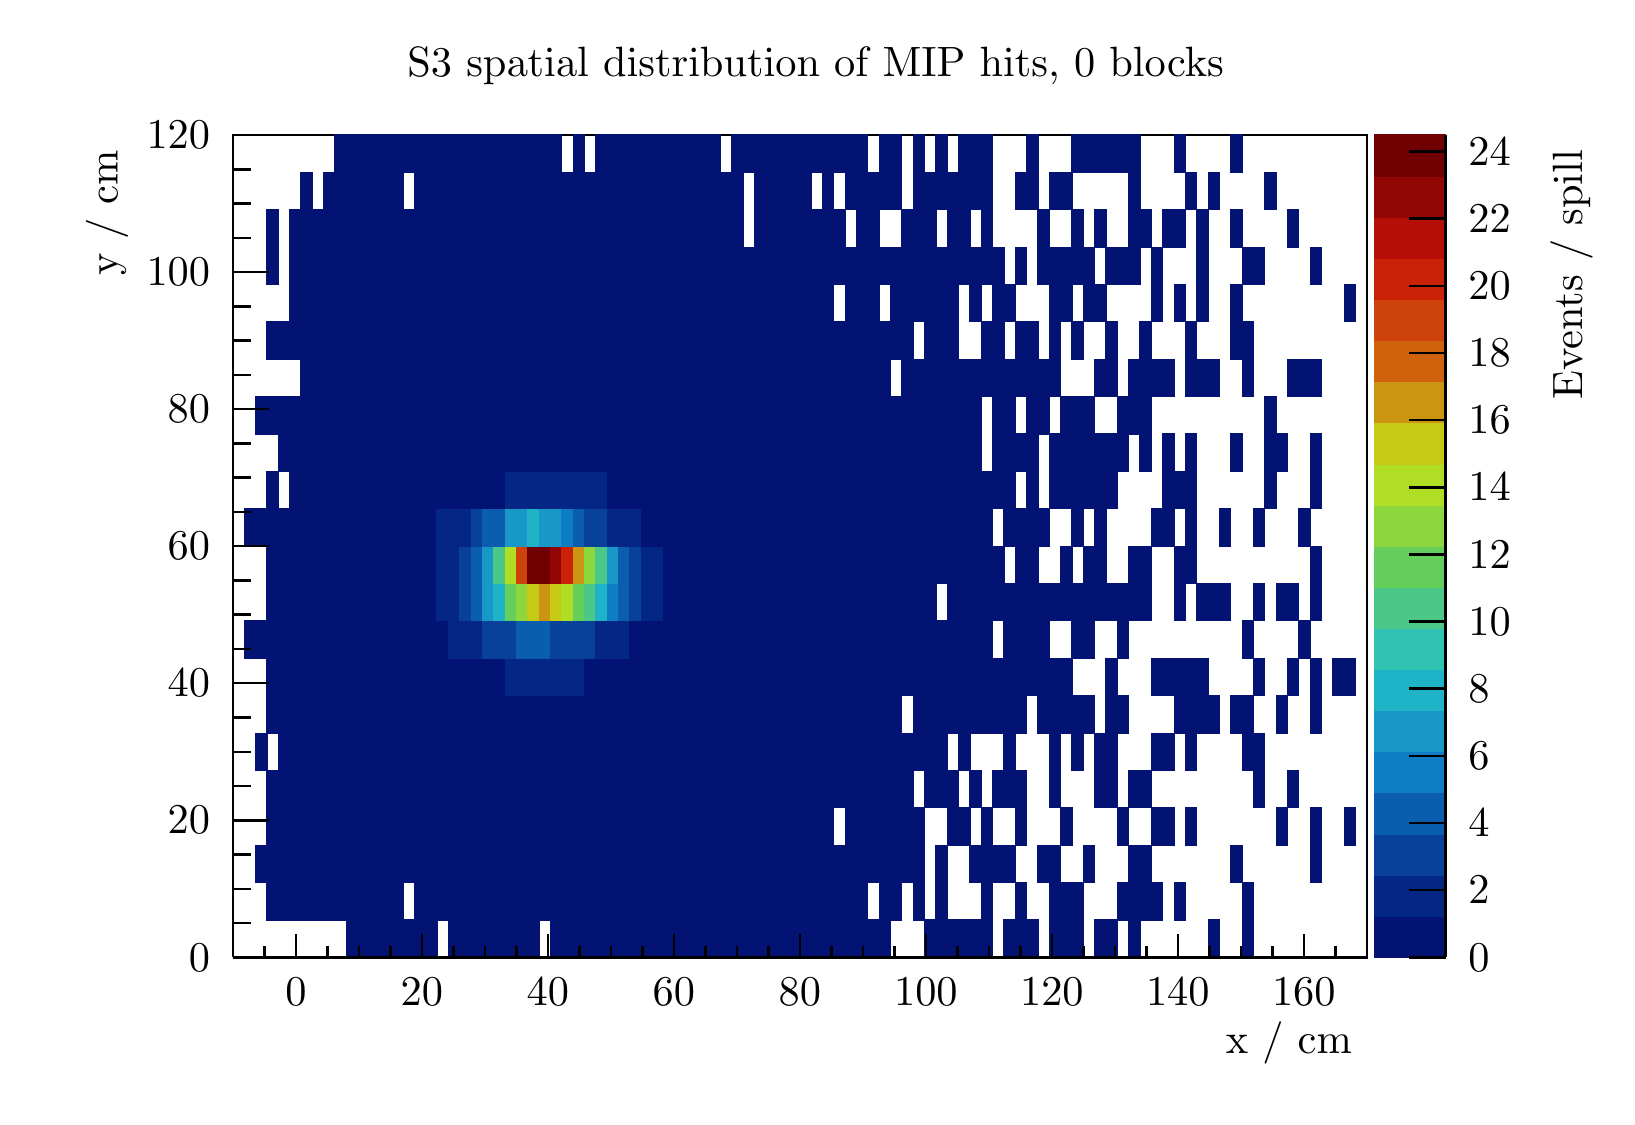
\begin{tikzpicture}
\pgfdeclareplotmark{cross} {
\pgfpathmoveto{\pgfpoint{-0.3\pgfplotmarksize}{\pgfplotmarksize}}
\pgfpathlineto{\pgfpoint{+0.3\pgfplotmarksize}{\pgfplotmarksize}}
\pgfpathlineto{\pgfpoint{+0.3\pgfplotmarksize}{0.3\pgfplotmarksize}}
\pgfpathlineto{\pgfpoint{+1\pgfplotmarksize}{0.3\pgfplotmarksize}}
\pgfpathlineto{\pgfpoint{+1\pgfplotmarksize}{-0.3\pgfplotmarksize}}
\pgfpathlineto{\pgfpoint{+0.3\pgfplotmarksize}{-0.3\pgfplotmarksize}}
\pgfpathlineto{\pgfpoint{+0.3\pgfplotmarksize}{-1.\pgfplotmarksize}}
\pgfpathlineto{\pgfpoint{-0.3\pgfplotmarksize}{-1.\pgfplotmarksize}}
\pgfpathlineto{\pgfpoint{-0.3\pgfplotmarksize}{-0.3\pgfplotmarksize}}
\pgfpathlineto{\pgfpoint{-1.\pgfplotmarksize}{-0.3\pgfplotmarksize}}
\pgfpathlineto{\pgfpoint{-1.\pgfplotmarksize}{0.3\pgfplotmarksize}}
\pgfpathlineto{\pgfpoint{-0.3\pgfplotmarksize}{0.3\pgfplotmarksize}}
\pgfpathclose
\pgfusepathqstroke
}
\pgfdeclareplotmark{cross*} {
\pgfpathmoveto{\pgfpoint{-0.3\pgfplotmarksize}{\pgfplotmarksize}}
\pgfpathlineto{\pgfpoint{+0.3\pgfplotmarksize}{\pgfplotmarksize}}
\pgfpathlineto{\pgfpoint{+0.3\pgfplotmarksize}{0.3\pgfplotmarksize}}
\pgfpathlineto{\pgfpoint{+1\pgfplotmarksize}{0.3\pgfplotmarksize}}
\pgfpathlineto{\pgfpoint{+1\pgfplotmarksize}{-0.3\pgfplotmarksize}}
\pgfpathlineto{\pgfpoint{+0.3\pgfplotmarksize}{-0.3\pgfplotmarksize}}
\pgfpathlineto{\pgfpoint{+0.3\pgfplotmarksize}{-1.\pgfplotmarksize}}
\pgfpathlineto{\pgfpoint{-0.3\pgfplotmarksize}{-1.\pgfplotmarksize}}
\pgfpathlineto{\pgfpoint{-0.3\pgfplotmarksize}{-0.3\pgfplotmarksize}}
\pgfpathlineto{\pgfpoint{-1.\pgfplotmarksize}{-0.3\pgfplotmarksize}}
\pgfpathlineto{\pgfpoint{-1.\pgfplotmarksize}{0.3\pgfplotmarksize}}
\pgfpathlineto{\pgfpoint{-0.3\pgfplotmarksize}{0.3\pgfplotmarksize}}
\pgfpathclose
\pgfusepathqfillstroke
}
\pgfdeclareplotmark{newstar} {
\pgfpathmoveto{\pgfqpoint{0pt}{\pgfplotmarksize}}
\pgfpathlineto{\pgfqpointpolar{44}{0.5\pgfplotmarksize}}
\pgfpathlineto{\pgfqpointpolar{18}{\pgfplotmarksize}}
\pgfpathlineto{\pgfqpointpolar{-20}{0.5\pgfplotmarksize}}
\pgfpathlineto{\pgfqpointpolar{-54}{\pgfplotmarksize}}
\pgfpathlineto{\pgfqpointpolar{-90}{0.5\pgfplotmarksize}}
\pgfpathlineto{\pgfqpointpolar{234}{\pgfplotmarksize}}
\pgfpathlineto{\pgfqpointpolar{198}{0.5\pgfplotmarksize}}
\pgfpathlineto{\pgfqpointpolar{162}{\pgfplotmarksize}}
\pgfpathlineto{\pgfqpointpolar{134}{0.5\pgfplotmarksize}}
\pgfpathclose
\pgfusepathqstroke
}
\pgfdeclareplotmark{newstar*} {
\pgfpathmoveto{\pgfqpoint{0pt}{\pgfplotmarksize}}
\pgfpathlineto{\pgfqpointpolar{44}{0.5\pgfplotmarksize}}
\pgfpathlineto{\pgfqpointpolar{18}{\pgfplotmarksize}}
\pgfpathlineto{\pgfqpointpolar{-20}{0.5\pgfplotmarksize}}
\pgfpathlineto{\pgfqpointpolar{-54}{\pgfplotmarksize}}
\pgfpathlineto{\pgfqpointpolar{-90}{0.5\pgfplotmarksize}}
\pgfpathlineto{\pgfqpointpolar{234}{\pgfplotmarksize}}
\pgfpathlineto{\pgfqpointpolar{198}{0.5\pgfplotmarksize}}
\pgfpathlineto{\pgfqpointpolar{162}{\pgfplotmarksize}}
\pgfpathlineto{\pgfqpointpolar{134}{0.5\pgfplotmarksize}}
\pgfpathclose
\pgfusepathqfillstroke
}
\definecolor{c}{rgb}{1,1,1};
\draw [color=c, fill=c] (0,0) rectangle (20,13.5632);
\draw [color=c, fill=c] (2.6,1.76322) rectangle (17,12.2069);
\definecolor{c}{rgb}{0,0,0};
\draw [c,line width=0.9] (2.6,1.76322) -- (2.6,12.2069) -- (17,12.2069) -- (17,1.76322) -- (2.6,1.76322);
\definecolor{c}{rgb}{1,1,1};
\draw [color=c, fill=c] (2.6,1.76322) rectangle (17,12.2069);
\definecolor{c}{rgb}{0,0,0};
\draw [c,line width=0.9] (2.6,1.76322) -- (2.6,12.2069) -- (17,12.2069) -- (17,1.76322) -- (2.6,1.76322);
\definecolor{c}{rgb}{0.00759013,0.0728653,0.45351};
\draw [color=c, fill=c] (4.04,1.76322) rectangle (4.184,2.23793);
\draw [color=c, fill=c] (4.184,1.76322) rectangle (4.328,2.23793);
\draw [color=c, fill=c] (4.328,1.76322) rectangle (4.472,2.23793);
\draw [color=c, fill=c] (4.472,1.76322) rectangle (4.616,2.23793);
\draw [color=c, fill=c] (4.616,1.76322) rectangle (4.76,2.23793);
\draw [color=c, fill=c] (4.76,1.76322) rectangle (4.904,2.23793);
\draw [color=c, fill=c] (4.904,1.76322) rectangle (5.048,2.23793);
\draw [color=c, fill=c] (5.048,1.76322) rectangle (5.192,2.23793);
\draw [color=c, fill=c] (5.336,1.76322) rectangle (5.48,2.23793);
\draw [color=c, fill=c] (5.48,1.76322) rectangle (5.624,2.23793);
\draw [color=c, fill=c] (5.624,1.76322) rectangle (5.768,2.23793);
\draw [color=c, fill=c] (5.768,1.76322) rectangle (5.912,2.23793);
\draw [color=c, fill=c] (5.912,1.76322) rectangle (6.056,2.23793);
\draw [color=c, fill=c] (6.056,1.76322) rectangle (6.2,2.23793);
\draw [color=c, fill=c] (6.2,1.76322) rectangle (6.344,2.23793);
\draw [color=c, fill=c] (6.344,1.76322) rectangle (6.488,2.23793);
\draw [color=c, fill=c] (6.632,1.76322) rectangle (6.776,2.23793);
\draw [color=c, fill=c] (6.776,1.76322) rectangle (6.92,2.23793);
\draw [color=c, fill=c] (6.92,1.76322) rectangle (7.064,2.23793);
\draw [color=c, fill=c] (7.064,1.76322) rectangle (7.208,2.23793);
\draw [color=c, fill=c] (7.208,1.76322) rectangle (7.352,2.23793);
\draw [color=c, fill=c] (7.352,1.76322) rectangle (7.496,2.23793);
\draw [color=c, fill=c] (7.496,1.76322) rectangle (7.64,2.23793);
\draw [color=c, fill=c] (7.64,1.76322) rectangle (7.784,2.23793);
\draw [color=c, fill=c] (7.784,1.76322) rectangle (7.928,2.23793);
\draw [color=c, fill=c] (7.928,1.76322) rectangle (8.072,2.23793);
\draw [color=c, fill=c] (8.072,1.76322) rectangle (8.216,2.23793);
\draw [color=c, fill=c] (8.216,1.76322) rectangle (8.36,2.23793);
\draw [color=c, fill=c] (8.36,1.76322) rectangle (8.504,2.23793);
\draw [color=c, fill=c] (8.504,1.76322) rectangle (8.648,2.23793);
\draw [color=c, fill=c] (8.648,1.76322) rectangle (8.792,2.23793);
\draw [color=c, fill=c] (8.792,1.76322) rectangle (8.936,2.23793);
\draw [color=c, fill=c] (8.936,1.76322) rectangle (9.08,2.23793);
\draw [color=c, fill=c] (9.08,1.76322) rectangle (9.224,2.23793);
\draw [color=c, fill=c] (9.224,1.76322) rectangle (9.368,2.23793);
\draw [color=c, fill=c] (9.368,1.76322) rectangle (9.512,2.23793);
\draw [color=c, fill=c] (9.512,1.76322) rectangle (9.656,2.23793);
\draw [color=c, fill=c] (9.656,1.76322) rectangle (9.8,2.23793);
\draw [color=c, fill=c] (9.8,1.76322) rectangle (9.944,2.23793);
\draw [color=c, fill=c] (9.944,1.76322) rectangle (10.088,2.23793);
\draw [color=c, fill=c] (10.088,1.76322) rectangle (10.232,2.23793);
\draw [color=c, fill=c] (10.232,1.76322) rectangle (10.376,2.23793);
\draw [color=c, fill=c] (10.376,1.76322) rectangle (10.52,2.23793);
\draw [color=c, fill=c] (10.52,1.76322) rectangle (10.664,2.23793);
\draw [color=c, fill=c] (10.664,1.76322) rectangle (10.808,2.23793);
\draw [color=c, fill=c] (10.808,1.76322) rectangle (10.952,2.23793);
\draw [color=c, fill=c] (11.384,1.76322) rectangle (11.528,2.23793);
\draw [color=c, fill=c] (11.528,1.76322) rectangle (11.672,2.23793);
\draw [color=c, fill=c] (11.672,1.76322) rectangle (11.816,2.23793);
\draw [color=c, fill=c] (11.816,1.76322) rectangle (11.96,2.23793);
\draw [color=c, fill=c] (11.96,1.76322) rectangle (12.104,2.23793);
\draw [color=c, fill=c] (12.104,1.76322) rectangle (12.248,2.23793);
\draw [color=c, fill=c] (12.392,1.76322) rectangle (12.536,2.23793);
\draw [color=c, fill=c] (12.536,1.76322) rectangle (12.68,2.23793);
\draw [color=c, fill=c] (12.68,1.76322) rectangle (12.824,2.23793);
\draw [color=c, fill=c] (12.968,1.76322) rectangle (13.112,2.23793);
\draw [color=c, fill=c] (13.112,1.76322) rectangle (13.256,2.23793);
\draw [color=c, fill=c] (13.256,1.76322) rectangle (13.4,2.23793);
\draw [color=c, fill=c] (13.544,1.76322) rectangle (13.688,2.23793);
\draw [color=c, fill=c] (13.688,1.76322) rectangle (13.832,2.23793);
\draw [color=c, fill=c] (13.976,1.76322) rectangle (14.12,2.23793);
\draw [color=c, fill=c] (14.984,1.76322) rectangle (15.128,2.23793);
\draw [color=c, fill=c] (15.416,1.76322) rectangle (15.56,2.23793);
\draw [color=c, fill=c] (3.032,2.23793) rectangle (3.176,2.71264);
\draw [color=c, fill=c] (3.176,2.23793) rectangle (3.32,2.71264);
\draw [color=c, fill=c] (3.32,2.23793) rectangle (3.464,2.71264);
\draw [color=c, fill=c] (3.464,2.23793) rectangle (3.608,2.71264);
\draw [color=c, fill=c] (3.608,2.23793) rectangle (3.752,2.71264);
\draw [color=c, fill=c] (3.752,2.23793) rectangle (3.896,2.71264);
\draw [color=c, fill=c] (3.896,2.23793) rectangle (4.04,2.71264);
\draw [color=c, fill=c] (4.04,2.23793) rectangle (4.184,2.71264);
\draw [color=c, fill=c] (4.184,2.23793) rectangle (4.328,2.71264);
\draw [color=c, fill=c] (4.328,2.23793) rectangle (4.472,2.71264);
\draw [color=c, fill=c] (4.472,2.23793) rectangle (4.616,2.71264);
\draw [color=c, fill=c] (4.616,2.23793) rectangle (4.76,2.71264);
\draw [color=c, fill=c] (4.904,2.23793) rectangle (5.048,2.71264);
\draw [color=c, fill=c] (5.048,2.23793) rectangle (5.192,2.71264);
\draw [color=c, fill=c] (5.192,2.23793) rectangle (5.336,2.71264);
\draw [color=c, fill=c] (5.336,2.23793) rectangle (5.48,2.71264);
\draw [color=c, fill=c] (5.48,2.23793) rectangle (5.624,2.71264);
\draw [color=c, fill=c] (5.624,2.23793) rectangle (5.768,2.71264);
\draw [color=c, fill=c] (5.768,2.23793) rectangle (5.912,2.71264);
\draw [color=c, fill=c] (5.912,2.23793) rectangle (6.056,2.71264);
\draw [color=c, fill=c] (6.056,2.23793) rectangle (6.2,2.71264);
\draw [color=c, fill=c] (6.2,2.23793) rectangle (6.344,2.71264);
\draw [color=c, fill=c] (6.344,2.23793) rectangle (6.488,2.71264);
\draw [color=c, fill=c] (6.488,2.23793) rectangle (6.632,2.71264);
\draw [color=c, fill=c] (6.632,2.23793) rectangle (6.776,2.71264);
\draw [color=c, fill=c] (6.776,2.23793) rectangle (6.92,2.71264);
\draw [color=c, fill=c] (6.92,2.23793) rectangle (7.064,2.71264);
\draw [color=c, fill=c] (7.064,2.23793) rectangle (7.208,2.71264);
\draw [color=c, fill=c] (7.208,2.23793) rectangle (7.352,2.71264);
\draw [color=c, fill=c] (7.352,2.23793) rectangle (7.496,2.71264);
\draw [color=c, fill=c] (7.496,2.23793) rectangle (7.64,2.71264);
\draw [color=c, fill=c] (7.64,2.23793) rectangle (7.784,2.71264);
\draw [color=c, fill=c] (7.784,2.23793) rectangle (7.928,2.71264);
\draw [color=c, fill=c] (7.928,2.23793) rectangle (8.072,2.71264);
\draw [color=c, fill=c] (8.072,2.23793) rectangle (8.216,2.71264);
\draw [color=c, fill=c] (8.216,2.23793) rectangle (8.36,2.71264);
\draw [color=c, fill=c] (8.36,2.23793) rectangle (8.504,2.71264);
\draw [color=c, fill=c] (8.504,2.23793) rectangle (8.648,2.71264);
\draw [color=c, fill=c] (8.648,2.23793) rectangle (8.792,2.71264);
\draw [color=c, fill=c] (8.792,2.23793) rectangle (8.936,2.71264);
\draw [color=c, fill=c] (8.936,2.23793) rectangle (9.08,2.71264);
\draw [color=c, fill=c] (9.08,2.23793) rectangle (9.224,2.71264);
\draw [color=c, fill=c] (9.224,2.23793) rectangle (9.368,2.71264);
\draw [color=c, fill=c] (9.368,2.23793) rectangle (9.512,2.71264);
\draw [color=c, fill=c] (9.512,2.23793) rectangle (9.656,2.71264);
\draw [color=c, fill=c] (9.656,2.23793) rectangle (9.8,2.71264);
\draw [color=c, fill=c] (9.8,2.23793) rectangle (9.944,2.71264);
\draw [color=c, fill=c] (9.944,2.23793) rectangle (10.088,2.71264);
\draw [color=c, fill=c] (10.088,2.23793) rectangle (10.232,2.71264);
\draw [color=c, fill=c] (10.232,2.23793) rectangle (10.376,2.71264);
\draw [color=c, fill=c] (10.376,2.23793) rectangle (10.52,2.71264);
\draw [color=c, fill=c] (10.52,2.23793) rectangle (10.664,2.71264);
\draw [color=c, fill=c] (10.808,2.23793) rectangle (10.952,2.71264);
\draw [color=c, fill=c] (10.952,2.23793) rectangle (11.096,2.71264);
\draw [color=c, fill=c] (11.24,2.23793) rectangle (11.384,2.71264);
\draw [color=c, fill=c] (11.528,2.23793) rectangle (11.672,2.71264);
\draw [color=c, fill=c] (12.104,2.23793) rectangle (12.248,2.71264);
\draw [color=c, fill=c] (12.536,2.23793) rectangle (12.68,2.71264);
\draw [color=c, fill=c] (12.968,2.23793) rectangle (13.112,2.71264);
\draw [color=c, fill=c] (13.112,2.23793) rectangle (13.256,2.71264);
\draw [color=c, fill=c] (13.256,2.23793) rectangle (13.4,2.71264);
\draw [color=c, fill=c] (13.832,2.23793) rectangle (13.976,2.71264);
\draw [color=c, fill=c] (13.976,2.23793) rectangle (14.12,2.71264);
\draw [color=c, fill=c] (14.12,2.23793) rectangle (14.264,2.71264);
\draw [color=c, fill=c] (14.264,2.23793) rectangle (14.408,2.71264);
\draw [color=c, fill=c] (14.552,2.23793) rectangle (14.696,2.71264);
\draw [color=c, fill=c] (15.416,2.23793) rectangle (15.56,2.71264);
\draw [color=c, fill=c] (2.888,2.71264) rectangle (3.032,3.18736);
\draw [color=c, fill=c] (3.032,2.71264) rectangle (3.176,3.18736);
\draw [color=c, fill=c] (3.176,2.71264) rectangle (3.32,3.18736);
\draw [color=c, fill=c] (3.32,2.71264) rectangle (3.464,3.18736);
\draw [color=c, fill=c] (3.464,2.71264) rectangle (3.608,3.18736);
\draw [color=c, fill=c] (3.608,2.71264) rectangle (3.752,3.18736);
\draw [color=c, fill=c] (3.752,2.71264) rectangle (3.896,3.18736);
\draw [color=c, fill=c] (3.896,2.71264) rectangle (4.04,3.18736);
\draw [color=c, fill=c] (4.04,2.71264) rectangle (4.184,3.18736);
\draw [color=c, fill=c] (4.184,2.71264) rectangle (4.328,3.18736);
\draw [color=c, fill=c] (4.328,2.71264) rectangle (4.472,3.18736);
\draw [color=c, fill=c] (4.472,2.71264) rectangle (4.616,3.18736);
\draw [color=c, fill=c] (4.616,2.71264) rectangle (4.76,3.18736);
\draw [color=c, fill=c] (4.76,2.71264) rectangle (4.904,3.18736);
\draw [color=c, fill=c] (4.904,2.71264) rectangle (5.048,3.18736);
\draw [color=c, fill=c] (5.048,2.71264) rectangle (5.192,3.18736);
\draw [color=c, fill=c] (5.192,2.71264) rectangle (5.336,3.18736);
\draw [color=c, fill=c] (5.336,2.71264) rectangle (5.48,3.18736);
\draw [color=c, fill=c] (5.48,2.71264) rectangle (5.624,3.18736);
\draw [color=c, fill=c] (5.624,2.71264) rectangle (5.768,3.18736);
\draw [color=c, fill=c] (5.768,2.71264) rectangle (5.912,3.18736);
\draw [color=c, fill=c] (5.912,2.71264) rectangle (6.056,3.18736);
\draw [color=c, fill=c] (6.056,2.71264) rectangle (6.2,3.18736);
\draw [color=c, fill=c] (6.2,2.71264) rectangle (6.344,3.18736);
\draw [color=c, fill=c] (6.344,2.71264) rectangle (6.488,3.18736);
\draw [color=c, fill=c] (6.488,2.71264) rectangle (6.632,3.18736);
\draw [color=c, fill=c] (6.632,2.71264) rectangle (6.776,3.18736);
\draw [color=c, fill=c] (6.776,2.71264) rectangle (6.92,3.18736);
\draw [color=c, fill=c] (6.92,2.71264) rectangle (7.064,3.18736);
\draw [color=c, fill=c] (7.064,2.71264) rectangle (7.208,3.18736);
\draw [color=c, fill=c] (7.208,2.71264) rectangle (7.352,3.18736);
\draw [color=c, fill=c] (7.352,2.71264) rectangle (7.496,3.18736);
\draw [color=c, fill=c] (7.496,2.71264) rectangle (7.64,3.18736);
\draw [color=c, fill=c] (7.64,2.71264) rectangle (7.784,3.18736);
\draw [color=c, fill=c] (7.784,2.71264) rectangle (7.928,3.18736);
\draw [color=c, fill=c] (7.928,2.71264) rectangle (8.072,3.18736);
\draw [color=c, fill=c] (8.072,2.71264) rectangle (8.216,3.18736);
\draw [color=c, fill=c] (8.216,2.71264) rectangle (8.36,3.18736);
\draw [color=c, fill=c] (8.36,2.71264) rectangle (8.504,3.18736);
\draw [color=c, fill=c] (8.504,2.71264) rectangle (8.648,3.18736);
\draw [color=c, fill=c] (8.648,2.71264) rectangle (8.792,3.18736);
\draw [color=c, fill=c] (8.792,2.71264) rectangle (8.936,3.18736);
\draw [color=c, fill=c] (8.936,2.71264) rectangle (9.08,3.18736);
\draw [color=c, fill=c] (9.08,2.71264) rectangle (9.224,3.18736);
\draw [color=c, fill=c] (9.224,2.71264) rectangle (9.368,3.18736);
\draw [color=c, fill=c] (9.368,2.71264) rectangle (9.512,3.18736);
\draw [color=c, fill=c] (9.512,2.71264) rectangle (9.656,3.18736);
\draw [color=c, fill=c] (9.656,2.71264) rectangle (9.8,3.18736);
\draw [color=c, fill=c] (9.8,2.71264) rectangle (9.944,3.18736);
\draw [color=c, fill=c] (9.944,2.71264) rectangle (10.088,3.18736);
\draw [color=c, fill=c] (10.088,2.71264) rectangle (10.232,3.18736);
\draw [color=c, fill=c] (10.232,2.71264) rectangle (10.376,3.18736);
\draw [color=c, fill=c] (10.376,2.71264) rectangle (10.52,3.18736);
\draw [color=c, fill=c] (10.52,2.71264) rectangle (10.664,3.18736);
\draw [color=c, fill=c] (10.664,2.71264) rectangle (10.808,3.18736);
\draw [color=c, fill=c] (10.808,2.71264) rectangle (10.952,3.18736);
\draw [color=c, fill=c] (10.952,2.71264) rectangle (11.096,3.18736);
\draw [color=c, fill=c] (11.096,2.71264) rectangle (11.24,3.18736);
\draw [color=c, fill=c] (11.24,2.71264) rectangle (11.384,3.18736);
\draw [color=c, fill=c] (11.528,2.71264) rectangle (11.672,3.18736);
\draw [color=c, fill=c] (11.96,2.71264) rectangle (12.104,3.18736);
\draw [color=c, fill=c] (12.104,2.71264) rectangle (12.248,3.18736);
\draw [color=c, fill=c] (12.248,2.71264) rectangle (12.392,3.18736);
\draw [color=c, fill=c] (12.392,2.71264) rectangle (12.536,3.18736);
\draw [color=c, fill=c] (12.824,2.71264) rectangle (12.968,3.18736);
\draw [color=c, fill=c] (12.968,2.71264) rectangle (13.112,3.18736);
\draw [color=c, fill=c] (13.4,2.71264) rectangle (13.544,3.18736);
\draw [color=c, fill=c] (13.976,2.71264) rectangle (14.12,3.18736);
\draw [color=c, fill=c] (14.12,2.71264) rectangle (14.264,3.18736);
\draw [color=c, fill=c] (15.272,2.71264) rectangle (15.416,3.18736);
\draw [color=c, fill=c] (16.28,2.71264) rectangle (16.424,3.18736);
\draw [color=c, fill=c] (3.032,3.18736) rectangle (3.176,3.66207);
\draw [color=c, fill=c] (3.176,3.18736) rectangle (3.32,3.66207);
\draw [color=c, fill=c] (3.32,3.18736) rectangle (3.464,3.66207);
\draw [color=c, fill=c] (3.464,3.18736) rectangle (3.608,3.66207);
\draw [color=c, fill=c] (3.608,3.18736) rectangle (3.752,3.66207);
\draw [color=c, fill=c] (3.752,3.18736) rectangle (3.896,3.66207);
\draw [color=c, fill=c] (3.896,3.18736) rectangle (4.04,3.66207);
\draw [color=c, fill=c] (4.04,3.18736) rectangle (4.184,3.66207);
\draw [color=c, fill=c] (4.184,3.18736) rectangle (4.328,3.66207);
\draw [color=c, fill=c] (4.328,3.18736) rectangle (4.472,3.66207);
\draw [color=c, fill=c] (4.472,3.18736) rectangle (4.616,3.66207);
\draw [color=c, fill=c] (4.616,3.18736) rectangle (4.76,3.66207);
\draw [color=c, fill=c] (4.76,3.18736) rectangle (4.904,3.66207);
\draw [color=c, fill=c] (4.904,3.18736) rectangle (5.048,3.66207);
\draw [color=c, fill=c] (5.048,3.18736) rectangle (5.192,3.66207);
\draw [color=c, fill=c] (5.192,3.18736) rectangle (5.336,3.66207);
\draw [color=c, fill=c] (5.336,3.18736) rectangle (5.48,3.66207);
\draw [color=c, fill=c] (5.48,3.18736) rectangle (5.624,3.66207);
\draw [color=c, fill=c] (5.624,3.18736) rectangle (5.768,3.66207);
\draw [color=c, fill=c] (5.768,3.18736) rectangle (5.912,3.66207);
\draw [color=c, fill=c] (5.912,3.18736) rectangle (6.056,3.66207);
\draw [color=c, fill=c] (6.056,3.18736) rectangle (6.2,3.66207);
\draw [color=c, fill=c] (6.2,3.18736) rectangle (6.344,3.66207);
\draw [color=c, fill=c] (6.344,3.18736) rectangle (6.488,3.66207);
\draw [color=c, fill=c] (6.488,3.18736) rectangle (6.632,3.66207);
\draw [color=c, fill=c] (6.632,3.18736) rectangle (6.776,3.66207);
\draw [color=c, fill=c] (6.776,3.18736) rectangle (6.92,3.66207);
\draw [color=c, fill=c] (6.92,3.18736) rectangle (7.064,3.66207);
\draw [color=c, fill=c] (7.064,3.18736) rectangle (7.208,3.66207);
\draw [color=c, fill=c] (7.208,3.18736) rectangle (7.352,3.66207);
\draw [color=c, fill=c] (7.352,3.18736) rectangle (7.496,3.66207);
\draw [color=c, fill=c] (7.496,3.18736) rectangle (7.64,3.66207);
\draw [color=c, fill=c] (7.64,3.18736) rectangle (7.784,3.66207);
\draw [color=c, fill=c] (7.784,3.18736) rectangle (7.928,3.66207);
\draw [color=c, fill=c] (7.928,3.18736) rectangle (8.072,3.66207);
\draw [color=c, fill=c] (8.072,3.18736) rectangle (8.216,3.66207);
\draw [color=c, fill=c] (8.216,3.18736) rectangle (8.36,3.66207);
\draw [color=c, fill=c] (8.36,3.18736) rectangle (8.504,3.66207);
\draw [color=c, fill=c] (8.504,3.18736) rectangle (8.648,3.66207);
\draw [color=c, fill=c] (8.648,3.18736) rectangle (8.792,3.66207);
\draw [color=c, fill=c] (8.792,3.18736) rectangle (8.936,3.66207);
\draw [color=c, fill=c] (8.936,3.18736) rectangle (9.08,3.66207);
\draw [color=c, fill=c] (9.08,3.18736) rectangle (9.224,3.66207);
\draw [color=c, fill=c] (9.224,3.18736) rectangle (9.368,3.66207);
\draw [color=c, fill=c] (9.368,3.18736) rectangle (9.512,3.66207);
\draw [color=c, fill=c] (9.512,3.18736) rectangle (9.656,3.66207);
\draw [color=c, fill=c] (9.656,3.18736) rectangle (9.8,3.66207);
\draw [color=c, fill=c] (9.8,3.18736) rectangle (9.944,3.66207);
\draw [color=c, fill=c] (9.944,3.18736) rectangle (10.088,3.66207);
\draw [color=c, fill=c] (10.088,3.18736) rectangle (10.232,3.66207);
\draw [color=c, fill=c] (10.376,3.18736) rectangle (10.52,3.66207);
\draw [color=c, fill=c] (10.52,3.18736) rectangle (10.664,3.66207);
\draw [color=c, fill=c] (10.664,3.18736) rectangle (10.808,3.66207);
\draw [color=c, fill=c] (10.808,3.18736) rectangle (10.952,3.66207);
\draw [color=c, fill=c] (10.952,3.18736) rectangle (11.096,3.66207);
\draw [color=c, fill=c] (11.096,3.18736) rectangle (11.24,3.66207);
\draw [color=c, fill=c] (11.24,3.18736) rectangle (11.384,3.66207);
\draw [color=c, fill=c] (11.672,3.18736) rectangle (11.816,3.66207);
\draw [color=c, fill=c] (11.816,3.18736) rectangle (11.96,3.66207);
\draw [color=c, fill=c] (12.104,3.18736) rectangle (12.248,3.66207);
\draw [color=c, fill=c] (12.536,3.18736) rectangle (12.68,3.66207);
\draw [color=c, fill=c] (13.112,3.18736) rectangle (13.256,3.66207);
\draw [color=c, fill=c] (13.832,3.18736) rectangle (13.976,3.66207);
\draw [color=c, fill=c] (14.264,3.18736) rectangle (14.408,3.66207);
\draw [color=c, fill=c] (14.408,3.18736) rectangle (14.552,3.66207);
\draw [color=c, fill=c] (14.696,3.18736) rectangle (14.84,3.66207);
\draw [color=c, fill=c] (15.848,3.18736) rectangle (15.992,3.66207);
\draw [color=c, fill=c] (16.28,3.18736) rectangle (16.424,3.66207);
\draw [color=c, fill=c] (16.712,3.18736) rectangle (16.856,3.66207);
\draw [color=c, fill=c] (3.032,3.66207) rectangle (3.176,4.13678);
\draw [color=c, fill=c] (3.176,3.66207) rectangle (3.32,4.13678);
\draw [color=c, fill=c] (3.32,3.66207) rectangle (3.464,4.13678);
\draw [color=c, fill=c] (3.464,3.66207) rectangle (3.608,4.13678);
\draw [color=c, fill=c] (3.608,3.66207) rectangle (3.752,4.13678);
\draw [color=c, fill=c] (3.752,3.66207) rectangle (3.896,4.13678);
\draw [color=c, fill=c] (3.896,3.66207) rectangle (4.04,4.13678);
\draw [color=c, fill=c] (4.04,3.66207) rectangle (4.184,4.13678);
\draw [color=c, fill=c] (4.184,3.66207) rectangle (4.328,4.13678);
\draw [color=c, fill=c] (4.328,3.66207) rectangle (4.472,4.13678);
\draw [color=c, fill=c] (4.472,3.66207) rectangle (4.616,4.13678);
\draw [color=c, fill=c] (4.616,3.66207) rectangle (4.76,4.13678);
\draw [color=c, fill=c] (4.76,3.66207) rectangle (4.904,4.13678);
\draw [color=c, fill=c] (4.904,3.66207) rectangle (5.048,4.13678);
\draw [color=c, fill=c] (5.048,3.66207) rectangle (5.192,4.13678);
\draw [color=c, fill=c] (5.192,3.66207) rectangle (5.336,4.13678);
\draw [color=c, fill=c] (5.336,3.66207) rectangle (5.48,4.13678);
\draw [color=c, fill=c] (5.48,3.66207) rectangle (5.624,4.13678);
\draw [color=c, fill=c] (5.624,3.66207) rectangle (5.768,4.13678);
\draw [color=c, fill=c] (5.768,3.66207) rectangle (5.912,4.13678);
\draw [color=c, fill=c] (5.912,3.66207) rectangle (6.056,4.13678);
\draw [color=c, fill=c] (6.056,3.66207) rectangle (6.2,4.13678);
\draw [color=c, fill=c] (6.2,3.66207) rectangle (6.344,4.13678);
\draw [color=c, fill=c] (6.344,3.66207) rectangle (6.488,4.13678);
\draw [color=c, fill=c] (6.488,3.66207) rectangle (6.632,4.13678);
\draw [color=c, fill=c] (6.632,3.66207) rectangle (6.776,4.13678);
\draw [color=c, fill=c] (6.776,3.66207) rectangle (6.92,4.13678);
\draw [color=c, fill=c] (6.92,3.66207) rectangle (7.064,4.13678);
\draw [color=c, fill=c] (7.064,3.66207) rectangle (7.208,4.13678);
\draw [color=c, fill=c] (7.208,3.66207) rectangle (7.352,4.13678);
\draw [color=c, fill=c] (7.352,3.66207) rectangle (7.496,4.13678);
\draw [color=c, fill=c] (7.496,3.66207) rectangle (7.64,4.13678);
\draw [color=c, fill=c] (7.64,3.66207) rectangle (7.784,4.13678);
\draw [color=c, fill=c] (7.784,3.66207) rectangle (7.928,4.13678);
\draw [color=c, fill=c] (7.928,3.66207) rectangle (8.072,4.13678);
\draw [color=c, fill=c] (8.072,3.66207) rectangle (8.216,4.13678);
\draw [color=c, fill=c] (8.216,3.66207) rectangle (8.36,4.13678);
\draw [color=c, fill=c] (8.36,3.66207) rectangle (8.504,4.13678);
\draw [color=c, fill=c] (8.504,3.66207) rectangle (8.648,4.13678);
\draw [color=c, fill=c] (8.648,3.66207) rectangle (8.792,4.13678);
\draw [color=c, fill=c] (8.792,3.66207) rectangle (8.936,4.13678);
\draw [color=c, fill=c] (8.936,3.66207) rectangle (9.08,4.13678);
\draw [color=c, fill=c] (9.08,3.66207) rectangle (9.224,4.13678);
\draw [color=c, fill=c] (9.224,3.66207) rectangle (9.368,4.13678);
\draw [color=c, fill=c] (9.368,3.66207) rectangle (9.512,4.13678);
\draw [color=c, fill=c] (9.512,3.66207) rectangle (9.656,4.13678);
\draw [color=c, fill=c] (9.656,3.66207) rectangle (9.8,4.13678);
\draw [color=c, fill=c] (9.8,3.66207) rectangle (9.944,4.13678);
\draw [color=c, fill=c] (9.944,3.66207) rectangle (10.088,4.13678);
\draw [color=c, fill=c] (10.088,3.66207) rectangle (10.232,4.13678);
\draw [color=c, fill=c] (10.232,3.66207) rectangle (10.376,4.13678);
\draw [color=c, fill=c] (10.376,3.66207) rectangle (10.52,4.13678);
\draw [color=c, fill=c] (10.52,3.66207) rectangle (10.664,4.13678);
\draw [color=c, fill=c] (10.664,3.66207) rectangle (10.808,4.13678);
\draw [color=c, fill=c] (10.808,3.66207) rectangle (10.952,4.13678);
\draw [color=c, fill=c] (10.952,3.66207) rectangle (11.096,4.13678);
\draw [color=c, fill=c] (11.096,3.66207) rectangle (11.24,4.13678);
\draw [color=c, fill=c] (11.384,3.66207) rectangle (11.528,4.13678);
\draw [color=c, fill=c] (11.528,3.66207) rectangle (11.672,4.13678);
\draw [color=c, fill=c] (11.672,3.66207) rectangle (11.816,4.13678);
\draw [color=c, fill=c] (11.96,3.66207) rectangle (12.104,4.13678);
\draw [color=c, fill=c] (12.248,3.66207) rectangle (12.392,4.13678);
\draw [color=c, fill=c] (12.392,3.66207) rectangle (12.536,4.13678);
\draw [color=c, fill=c] (12.536,3.66207) rectangle (12.68,4.13678);
\draw [color=c, fill=c] (12.968,3.66207) rectangle (13.112,4.13678);
\draw [color=c, fill=c] (13.544,3.66207) rectangle (13.688,4.13678);
\draw [color=c, fill=c] (13.688,3.66207) rectangle (13.832,4.13678);
\draw [color=c, fill=c] (13.976,3.66207) rectangle (14.12,4.13678);
\draw [color=c, fill=c] (14.12,3.66207) rectangle (14.264,4.13678);
\draw [color=c, fill=c] (15.56,3.66207) rectangle (15.704,4.13678);
\draw [color=c, fill=c] (15.992,3.66207) rectangle (16.136,4.13678);
\draw [color=c, fill=c] (2.888,4.13678) rectangle (3.032,4.61149);
\draw [color=c, fill=c] (3.176,4.13678) rectangle (3.32,4.61149);
\draw [color=c, fill=c] (3.32,4.13678) rectangle (3.464,4.61149);
\draw [color=c, fill=c] (3.464,4.13678) rectangle (3.608,4.61149);
\draw [color=c, fill=c] (3.608,4.13678) rectangle (3.752,4.61149);
\draw [color=c, fill=c] (3.752,4.13678) rectangle (3.896,4.61149);
\draw [color=c, fill=c] (3.896,4.13678) rectangle (4.04,4.61149);
\draw [color=c, fill=c] (4.04,4.13678) rectangle (4.184,4.61149);
\draw [color=c, fill=c] (4.184,4.13678) rectangle (4.328,4.61149);
\draw [color=c, fill=c] (4.328,4.13678) rectangle (4.472,4.61149);
\draw [color=c, fill=c] (4.472,4.13678) rectangle (4.616,4.61149);
\draw [color=c, fill=c] (4.616,4.13678) rectangle (4.76,4.61149);
\draw [color=c, fill=c] (4.76,4.13678) rectangle (4.904,4.61149);
\draw [color=c, fill=c] (4.904,4.13678) rectangle (5.048,4.61149);
\draw [color=c, fill=c] (5.048,4.13678) rectangle (5.192,4.61149);
\draw [color=c, fill=c] (5.192,4.13678) rectangle (5.336,4.61149);
\draw [color=c, fill=c] (5.336,4.13678) rectangle (5.48,4.61149);
\draw [color=c, fill=c] (5.48,4.13678) rectangle (5.624,4.61149);
\draw [color=c, fill=c] (5.624,4.13678) rectangle (5.768,4.61149);
\draw [color=c, fill=c] (5.768,4.13678) rectangle (5.912,4.61149);
\draw [color=c, fill=c] (5.912,4.13678) rectangle (6.056,4.61149);
\draw [color=c, fill=c] (6.056,4.13678) rectangle (6.2,4.61149);
\draw [color=c, fill=c] (6.2,4.13678) rectangle (6.344,4.61149);
\draw [color=c, fill=c] (6.344,4.13678) rectangle (6.488,4.61149);
\draw [color=c, fill=c] (6.488,4.13678) rectangle (6.632,4.61149);
\draw [color=c, fill=c] (6.632,4.13678) rectangle (6.776,4.61149);
\draw [color=c, fill=c] (6.776,4.13678) rectangle (6.92,4.61149);
\draw [color=c, fill=c] (6.92,4.13678) rectangle (7.064,4.61149);
\draw [color=c, fill=c] (7.064,4.13678) rectangle (7.208,4.61149);
\draw [color=c, fill=c] (7.208,4.13678) rectangle (7.352,4.61149);
\draw [color=c, fill=c] (7.352,4.13678) rectangle (7.496,4.61149);
\draw [color=c, fill=c] (7.496,4.13678) rectangle (7.64,4.61149);
\draw [color=c, fill=c] (7.64,4.13678) rectangle (7.784,4.61149);
\draw [color=c, fill=c] (7.784,4.13678) rectangle (7.928,4.61149);
\draw [color=c, fill=c] (7.928,4.13678) rectangle (8.072,4.61149);
\draw [color=c, fill=c] (8.072,4.13678) rectangle (8.216,4.61149);
\draw [color=c, fill=c] (8.216,4.13678) rectangle (8.36,4.61149);
\draw [color=c, fill=c] (8.36,4.13678) rectangle (8.504,4.61149);
\draw [color=c, fill=c] (8.504,4.13678) rectangle (8.648,4.61149);
\draw [color=c, fill=c] (8.648,4.13678) rectangle (8.792,4.61149);
\draw [color=c, fill=c] (8.792,4.13678) rectangle (8.936,4.61149);
\draw [color=c, fill=c] (8.936,4.13678) rectangle (9.08,4.61149);
\draw [color=c, fill=c] (9.08,4.13678) rectangle (9.224,4.61149);
\draw [color=c, fill=c] (9.224,4.13678) rectangle (9.368,4.61149);
\draw [color=c, fill=c] (9.368,4.13678) rectangle (9.512,4.61149);
\draw [color=c, fill=c] (9.512,4.13678) rectangle (9.656,4.61149);
\draw [color=c, fill=c] (9.656,4.13678) rectangle (9.8,4.61149);
\draw [color=c, fill=c] (9.8,4.13678) rectangle (9.944,4.61149);
\draw [color=c, fill=c] (9.944,4.13678) rectangle (10.088,4.61149);
\draw [color=c, fill=c] (10.088,4.13678) rectangle (10.232,4.61149);
\draw [color=c, fill=c] (10.232,4.13678) rectangle (10.376,4.61149);
\draw [color=c, fill=c] (10.376,4.13678) rectangle (10.52,4.61149);
\draw [color=c, fill=c] (10.52,4.13678) rectangle (10.664,4.61149);
\draw [color=c, fill=c] (10.664,4.13678) rectangle (10.808,4.61149);
\draw [color=c, fill=c] (10.808,4.13678) rectangle (10.952,4.61149);
\draw [color=c, fill=c] (10.952,4.13678) rectangle (11.096,4.61149);
\draw [color=c, fill=c] (11.096,4.13678) rectangle (11.24,4.61149);
\draw [color=c, fill=c] (11.24,4.13678) rectangle (11.384,4.61149);
\draw [color=c, fill=c] (11.384,4.13678) rectangle (11.528,4.61149);
\draw [color=c, fill=c] (11.528,4.13678) rectangle (11.672,4.61149);
\draw [color=c, fill=c] (11.816,4.13678) rectangle (11.96,4.61149);
\draw [color=c, fill=c] (12.392,4.13678) rectangle (12.536,4.61149);
\draw [color=c, fill=c] (12.968,4.13678) rectangle (13.112,4.61149);
\draw [color=c, fill=c] (13.256,4.13678) rectangle (13.4,4.61149);
\draw [color=c, fill=c] (13.544,4.13678) rectangle (13.688,4.61149);
\draw [color=c, fill=c] (13.688,4.13678) rectangle (13.832,4.61149);
\draw [color=c, fill=c] (14.264,4.13678) rectangle (14.408,4.61149);
\draw [color=c, fill=c] (14.408,4.13678) rectangle (14.552,4.61149);
\draw [color=c, fill=c] (14.696,4.13678) rectangle (14.84,4.61149);
\draw [color=c, fill=c] (15.416,4.13678) rectangle (15.56,4.61149);
\draw [color=c, fill=c] (15.56,4.13678) rectangle (15.704,4.61149);
\draw [color=c, fill=c] (3.032,4.61149) rectangle (3.176,5.08621);
\draw [color=c, fill=c] (3.176,4.61149) rectangle (3.32,5.08621);
\draw [color=c, fill=c] (3.32,4.61149) rectangle (3.464,5.08621);
\draw [color=c, fill=c] (3.464,4.61149) rectangle (3.608,5.08621);
\draw [color=c, fill=c] (3.608,4.61149) rectangle (3.752,5.08621);
\draw [color=c, fill=c] (3.752,4.61149) rectangle (3.896,5.08621);
\draw [color=c, fill=c] (3.896,4.61149) rectangle (4.04,5.08621);
\draw [color=c, fill=c] (4.04,4.61149) rectangle (4.184,5.08621);
\draw [color=c, fill=c] (4.184,4.61149) rectangle (4.328,5.08621);
\draw [color=c, fill=c] (4.328,4.61149) rectangle (4.472,5.08621);
\draw [color=c, fill=c] (4.472,4.61149) rectangle (4.616,5.08621);
\draw [color=c, fill=c] (4.616,4.61149) rectangle (4.76,5.08621);
\draw [color=c, fill=c] (4.76,4.61149) rectangle (4.904,5.08621);
\draw [color=c, fill=c] (4.904,4.61149) rectangle (5.048,5.08621);
\draw [color=c, fill=c] (5.048,4.61149) rectangle (5.192,5.08621);
\draw [color=c, fill=c] (5.192,4.61149) rectangle (5.336,5.08621);
\draw [color=c, fill=c] (5.336,4.61149) rectangle (5.48,5.08621);
\draw [color=c, fill=c] (5.48,4.61149) rectangle (5.624,5.08621);
\draw [color=c, fill=c] (5.624,4.61149) rectangle (5.768,5.08621);
\draw [color=c, fill=c] (5.768,4.61149) rectangle (5.912,5.08621);
\draw [color=c, fill=c] (5.912,4.61149) rectangle (6.056,5.08621);
\draw [color=c, fill=c] (6.056,4.61149) rectangle (6.2,5.08621);
\draw [color=c, fill=c] (6.2,4.61149) rectangle (6.344,5.08621);
\draw [color=c, fill=c] (6.344,4.61149) rectangle (6.488,5.08621);
\draw [color=c, fill=c] (6.488,4.61149) rectangle (6.632,5.08621);
\draw [color=c, fill=c] (6.632,4.61149) rectangle (6.776,5.08621);
\draw [color=c, fill=c] (6.776,4.61149) rectangle (6.92,5.08621);
\draw [color=c, fill=c] (6.92,4.61149) rectangle (7.064,5.08621);
\draw [color=c, fill=c] (7.064,4.61149) rectangle (7.208,5.08621);
\draw [color=c, fill=c] (7.208,4.61149) rectangle (7.352,5.08621);
\draw [color=c, fill=c] (7.352,4.61149) rectangle (7.496,5.08621);
\draw [color=c, fill=c] (7.496,4.61149) rectangle (7.64,5.08621);
\draw [color=c, fill=c] (7.64,4.61149) rectangle (7.784,5.08621);
\draw [color=c, fill=c] (7.784,4.61149) rectangle (7.928,5.08621);
\draw [color=c, fill=c] (7.928,4.61149) rectangle (8.072,5.08621);
\draw [color=c, fill=c] (8.072,4.61149) rectangle (8.216,5.08621);
\draw [color=c, fill=c] (8.216,4.61149) rectangle (8.36,5.08621);
\draw [color=c, fill=c] (8.36,4.61149) rectangle (8.504,5.08621);
\draw [color=c, fill=c] (8.504,4.61149) rectangle (8.648,5.08621);
\draw [color=c, fill=c] (8.648,4.61149) rectangle (8.792,5.08621);
\draw [color=c, fill=c] (8.792,4.61149) rectangle (8.936,5.08621);
\draw [color=c, fill=c] (8.936,4.61149) rectangle (9.08,5.08621);
\draw [color=c, fill=c] (9.08,4.61149) rectangle (9.224,5.08621);
\draw [color=c, fill=c] (9.224,4.61149) rectangle (9.368,5.08621);
\draw [color=c, fill=c] (9.368,4.61149) rectangle (9.512,5.08621);
\draw [color=c, fill=c] (9.512,4.61149) rectangle (9.656,5.08621);
\draw [color=c, fill=c] (9.656,4.61149) rectangle (9.8,5.08621);
\draw [color=c, fill=c] (9.8,4.61149) rectangle (9.944,5.08621);
\draw [color=c, fill=c] (9.944,4.61149) rectangle (10.088,5.08621);
\draw [color=c, fill=c] (10.088,4.61149) rectangle (10.232,5.08621);
\draw [color=c, fill=c] (10.232,4.61149) rectangle (10.376,5.08621);
\draw [color=c, fill=c] (10.376,4.61149) rectangle (10.52,5.08621);
\draw [color=c, fill=c] (10.52,4.61149) rectangle (10.664,5.08621);
\draw [color=c, fill=c] (10.664,4.61149) rectangle (10.808,5.08621);
\draw [color=c, fill=c] (10.808,4.61149) rectangle (10.952,5.08621);
\draw [color=c, fill=c] (10.952,4.61149) rectangle (11.096,5.08621);
\draw [color=c, fill=c] (11.24,4.61149) rectangle (11.384,5.08621);
\draw [color=c, fill=c] (11.384,4.61149) rectangle (11.528,5.08621);
\draw [color=c, fill=c] (11.528,4.61149) rectangle (11.672,5.08621);
\draw [color=c, fill=c] (11.672,4.61149) rectangle (11.816,5.08621);
\draw [color=c, fill=c] (11.816,4.61149) rectangle (11.96,5.08621);
\draw [color=c, fill=c] (11.96,4.61149) rectangle (12.104,5.08621);
\draw [color=c, fill=c] (12.104,4.61149) rectangle (12.248,5.08621);
\draw [color=c, fill=c] (12.248,4.61149) rectangle (12.392,5.08621);
\draw [color=c, fill=c] (12.392,4.61149) rectangle (12.536,5.08621);
\draw [color=c, fill=c] (12.536,4.61149) rectangle (12.68,5.08621);
\draw [color=c, fill=c] (12.824,4.61149) rectangle (12.968,5.08621);
\draw [color=c, fill=c] (12.968,4.61149) rectangle (13.112,5.08621);
\draw [color=c, fill=c] (13.112,4.61149) rectangle (13.256,5.08621);
\draw [color=c, fill=c] (13.256,4.61149) rectangle (13.4,5.08621);
\draw [color=c, fill=c] (13.4,4.61149) rectangle (13.544,5.08621);
\draw [color=c, fill=c] (13.688,4.61149) rectangle (13.832,5.08621);
\draw [color=c, fill=c] (13.832,4.61149) rectangle (13.976,5.08621);
\draw [color=c, fill=c] (14.552,4.61149) rectangle (14.696,5.08621);
\draw [color=c, fill=c] (14.696,4.61149) rectangle (14.84,5.08621);
\draw [color=c, fill=c] (14.84,4.61149) rectangle (14.984,5.08621);
\draw [color=c, fill=c] (14.984,4.61149) rectangle (15.128,5.08621);
\draw [color=c, fill=c] (15.272,4.61149) rectangle (15.416,5.08621);
\draw [color=c, fill=c] (15.416,4.61149) rectangle (15.56,5.08621);
\draw [color=c, fill=c] (15.848,4.61149) rectangle (15.992,5.08621);
\draw [color=c, fill=c] (16.28,4.61149) rectangle (16.424,5.08621);
\draw [color=c, fill=c] (3.032,5.08621) rectangle (3.176,5.56092);
\draw [color=c, fill=c] (3.176,5.08621) rectangle (3.32,5.56092);
\draw [color=c, fill=c] (3.32,5.08621) rectangle (3.464,5.56092);
\draw [color=c, fill=c] (3.464,5.08621) rectangle (3.608,5.56092);
\draw [color=c, fill=c] (3.608,5.08621) rectangle (3.752,5.56092);
\draw [color=c, fill=c] (3.752,5.08621) rectangle (3.896,5.56092);
\draw [color=c, fill=c] (3.896,5.08621) rectangle (4.04,5.56092);
\draw [color=c, fill=c] (4.04,5.08621) rectangle (4.184,5.56092);
\draw [color=c, fill=c] (4.184,5.08621) rectangle (4.328,5.56092);
\draw [color=c, fill=c] (4.328,5.08621) rectangle (4.472,5.56092);
\draw [color=c, fill=c] (4.472,5.08621) rectangle (4.616,5.56092);
\draw [color=c, fill=c] (4.616,5.08621) rectangle (4.76,5.56092);
\draw [color=c, fill=c] (4.76,5.08621) rectangle (4.904,5.56092);
\draw [color=c, fill=c] (4.904,5.08621) rectangle (5.048,5.56092);
\draw [color=c, fill=c] (5.048,5.08621) rectangle (5.192,5.56092);
\draw [color=c, fill=c] (5.192,5.08621) rectangle (5.336,5.56092);
\draw [color=c, fill=c] (5.336,5.08621) rectangle (5.48,5.56092);
\draw [color=c, fill=c] (5.48,5.08621) rectangle (5.624,5.56092);
\draw [color=c, fill=c] (5.624,5.08621) rectangle (5.768,5.56092);
\draw [color=c, fill=c] (5.768,5.08621) rectangle (5.912,5.56092);
\draw [color=c, fill=c] (5.912,5.08621) rectangle (6.056,5.56092);
\definecolor{c}{rgb}{0.0158128,0.151803,0.524225};
\draw [color=c, fill=c] (6.056,5.08621) rectangle (6.2,5.56092);
\draw [color=c, fill=c] (6.2,5.08621) rectangle (6.344,5.56092);
\draw [color=c, fill=c] (6.344,5.08621) rectangle (6.488,5.56092);
\draw [color=c, fill=c] (6.488,5.08621) rectangle (6.632,5.56092);
\draw [color=c, fill=c] (6.632,5.08621) rectangle (6.776,5.56092);
\draw [color=c, fill=c] (6.776,5.08621) rectangle (6.92,5.56092);
\draw [color=c, fill=c] (6.92,5.08621) rectangle (7.064,5.56092);
\definecolor{c}{rgb}{0.00759013,0.0728653,0.45351};
\draw [color=c, fill=c] (7.064,5.08621) rectangle (7.208,5.56092);
\draw [color=c, fill=c] (7.208,5.08621) rectangle (7.352,5.56092);
\draw [color=c, fill=c] (7.352,5.08621) rectangle (7.496,5.56092);
\draw [color=c, fill=c] (7.496,5.08621) rectangle (7.64,5.56092);
\draw [color=c, fill=c] (7.64,5.08621) rectangle (7.784,5.56092);
\draw [color=c, fill=c] (7.784,5.08621) rectangle (7.928,5.56092);
\draw [color=c, fill=c] (7.928,5.08621) rectangle (8.072,5.56092);
\draw [color=c, fill=c] (8.072,5.08621) rectangle (8.216,5.56092);
\draw [color=c, fill=c] (8.216,5.08621) rectangle (8.36,5.56092);
\draw [color=c, fill=c] (8.36,5.08621) rectangle (8.504,5.56092);
\draw [color=c, fill=c] (8.504,5.08621) rectangle (8.648,5.56092);
\draw [color=c, fill=c] (8.648,5.08621) rectangle (8.792,5.56092);
\draw [color=c, fill=c] (8.792,5.08621) rectangle (8.936,5.56092);
\draw [color=c, fill=c] (8.936,5.08621) rectangle (9.08,5.56092);
\draw [color=c, fill=c] (9.08,5.08621) rectangle (9.224,5.56092);
\draw [color=c, fill=c] (9.224,5.08621) rectangle (9.368,5.56092);
\draw [color=c, fill=c] (9.368,5.08621) rectangle (9.512,5.56092);
\draw [color=c, fill=c] (9.512,5.08621) rectangle (9.656,5.56092);
\draw [color=c, fill=c] (9.656,5.08621) rectangle (9.8,5.56092);
\draw [color=c, fill=c] (9.8,5.08621) rectangle (9.944,5.56092);
\draw [color=c, fill=c] (9.944,5.08621) rectangle (10.088,5.56092);
\draw [color=c, fill=c] (10.088,5.08621) rectangle (10.232,5.56092);
\draw [color=c, fill=c] (10.232,5.08621) rectangle (10.376,5.56092);
\draw [color=c, fill=c] (10.376,5.08621) rectangle (10.52,5.56092);
\draw [color=c, fill=c] (10.52,5.08621) rectangle (10.664,5.56092);
\draw [color=c, fill=c] (10.664,5.08621) rectangle (10.808,5.56092);
\draw [color=c, fill=c] (10.808,5.08621) rectangle (10.952,5.56092);
\draw [color=c, fill=c] (10.952,5.08621) rectangle (11.096,5.56092);
\draw [color=c, fill=c] (11.096,5.08621) rectangle (11.24,5.56092);
\draw [color=c, fill=c] (11.24,5.08621) rectangle (11.384,5.56092);
\draw [color=c, fill=c] (11.384,5.08621) rectangle (11.528,5.56092);
\draw [color=c, fill=c] (11.528,5.08621) rectangle (11.672,5.56092);
\draw [color=c, fill=c] (11.672,5.08621) rectangle (11.816,5.56092);
\draw [color=c, fill=c] (11.816,5.08621) rectangle (11.96,5.56092);
\draw [color=c, fill=c] (11.96,5.08621) rectangle (12.104,5.56092);
\draw [color=c, fill=c] (12.104,5.08621) rectangle (12.248,5.56092);
\draw [color=c, fill=c] (12.248,5.08621) rectangle (12.392,5.56092);
\draw [color=c, fill=c] (12.392,5.08621) rectangle (12.536,5.56092);
\draw [color=c, fill=c] (12.536,5.08621) rectangle (12.68,5.56092);
\draw [color=c, fill=c] (12.68,5.08621) rectangle (12.824,5.56092);
\draw [color=c, fill=c] (12.824,5.08621) rectangle (12.968,5.56092);
\draw [color=c, fill=c] (12.968,5.08621) rectangle (13.112,5.56092);
\draw [color=c, fill=c] (13.112,5.08621) rectangle (13.256,5.56092);
\draw [color=c, fill=c] (13.688,5.08621) rectangle (13.832,5.56092);
\draw [color=c, fill=c] (14.264,5.08621) rectangle (14.408,5.56092);
\draw [color=c, fill=c] (14.408,5.08621) rectangle (14.552,5.56092);
\draw [color=c, fill=c] (14.552,5.08621) rectangle (14.696,5.56092);
\draw [color=c, fill=c] (14.696,5.08621) rectangle (14.84,5.56092);
\draw [color=c, fill=c] (14.84,5.08621) rectangle (14.984,5.56092);
\draw [color=c, fill=c] (15.56,5.08621) rectangle (15.704,5.56092);
\draw [color=c, fill=c] (15.992,5.08621) rectangle (16.136,5.56092);
\draw [color=c, fill=c] (16.28,5.08621) rectangle (16.424,5.56092);
\draw [color=c, fill=c] (16.568,5.08621) rectangle (16.712,5.56092);
\draw [color=c, fill=c] (16.712,5.08621) rectangle (16.856,5.56092);
\draw [color=c, fill=c] (2.744,5.56092) rectangle (2.888,6.03563);
\draw [color=c, fill=c] (2.888,5.56092) rectangle (3.032,6.03563);
\draw [color=c, fill=c] (3.032,5.56092) rectangle (3.176,6.03563);
\draw [color=c, fill=c] (3.176,5.56092) rectangle (3.32,6.03563);
\draw [color=c, fill=c] (3.32,5.56092) rectangle (3.464,6.03563);
\draw [color=c, fill=c] (3.464,5.56092) rectangle (3.608,6.03563);
\draw [color=c, fill=c] (3.608,5.56092) rectangle (3.752,6.03563);
\draw [color=c, fill=c] (3.752,5.56092) rectangle (3.896,6.03563);
\draw [color=c, fill=c] (3.896,5.56092) rectangle (4.04,6.03563);
\draw [color=c, fill=c] (4.04,5.56092) rectangle (4.184,6.03563);
\draw [color=c, fill=c] (4.184,5.56092) rectangle (4.328,6.03563);
\draw [color=c, fill=c] (4.328,5.56092) rectangle (4.472,6.03563);
\draw [color=c, fill=c] (4.472,5.56092) rectangle (4.616,6.03563);
\draw [color=c, fill=c] (4.616,5.56092) rectangle (4.76,6.03563);
\draw [color=c, fill=c] (4.76,5.56092) rectangle (4.904,6.03563);
\draw [color=c, fill=c] (4.904,5.56092) rectangle (5.048,6.03563);
\draw [color=c, fill=c] (5.048,5.56092) rectangle (5.192,6.03563);
\draw [color=c, fill=c] (5.192,5.56092) rectangle (5.336,6.03563);
\definecolor{c}{rgb}{0.0158128,0.151803,0.524225};
\draw [color=c, fill=c] (5.336,5.56092) rectangle (5.48,6.03563);
\draw [color=c, fill=c] (5.48,5.56092) rectangle (5.624,6.03563);
\draw [color=c, fill=c] (5.624,5.56092) rectangle (5.768,6.03563);
\definecolor{c}{rgb}{0.0281863,0.253431,0.604902};
\draw [color=c, fill=c] (5.768,5.56092) rectangle (5.912,6.03563);
\draw [color=c, fill=c] (5.912,5.56092) rectangle (6.056,6.03563);
\draw [color=c, fill=c] (6.056,5.56092) rectangle (6.2,6.03563);
\definecolor{c}{rgb}{0.0428922,0.365196,0.687255};
\draw [color=c, fill=c] (6.2,5.56092) rectangle (6.344,6.03563);
\draw [color=c, fill=c] (6.344,5.56092) rectangle (6.488,6.03563);
\draw [color=c, fill=c] (6.488,5.56092) rectangle (6.632,6.03563);
\definecolor{c}{rgb}{0.0281863,0.253431,0.604902};
\draw [color=c, fill=c] (6.632,5.56092) rectangle (6.776,6.03563);
\draw [color=c, fill=c] (6.776,5.56092) rectangle (6.92,6.03563);
\draw [color=c, fill=c] (6.92,5.56092) rectangle (7.064,6.03563);
\draw [color=c, fill=c] (7.064,5.56092) rectangle (7.208,6.03563);
\definecolor{c}{rgb}{0.0158128,0.151803,0.524225};
\draw [color=c, fill=c] (7.208,5.56092) rectangle (7.352,6.03563);
\draw [color=c, fill=c] (7.352,5.56092) rectangle (7.496,6.03563);
\draw [color=c, fill=c] (7.496,5.56092) rectangle (7.64,6.03563);
\definecolor{c}{rgb}{0.00759013,0.0728653,0.45351};
\draw [color=c, fill=c] (7.64,5.56092) rectangle (7.784,6.03563);
\draw [color=c, fill=c] (7.784,5.56092) rectangle (7.928,6.03563);
\draw [color=c, fill=c] (7.928,5.56092) rectangle (8.072,6.03563);
\draw [color=c, fill=c] (8.072,5.56092) rectangle (8.216,6.03563);
\draw [color=c, fill=c] (8.216,5.56092) rectangle (8.36,6.03563);
\draw [color=c, fill=c] (8.36,5.56092) rectangle (8.504,6.03563);
\draw [color=c, fill=c] (8.504,5.56092) rectangle (8.648,6.03563);
\draw [color=c, fill=c] (8.648,5.56092) rectangle (8.792,6.03563);
\draw [color=c, fill=c] (8.792,5.56092) rectangle (8.936,6.03563);
\draw [color=c, fill=c] (8.936,5.56092) rectangle (9.08,6.03563);
\draw [color=c, fill=c] (9.08,5.56092) rectangle (9.224,6.03563);
\draw [color=c, fill=c] (9.224,5.56092) rectangle (9.368,6.03563);
\draw [color=c, fill=c] (9.368,5.56092) rectangle (9.512,6.03563);
\draw [color=c, fill=c] (9.512,5.56092) rectangle (9.656,6.03563);
\draw [color=c, fill=c] (9.656,5.56092) rectangle (9.8,6.03563);
\draw [color=c, fill=c] (9.8,5.56092) rectangle (9.944,6.03563);
\draw [color=c, fill=c] (9.944,5.56092) rectangle (10.088,6.03563);
\draw [color=c, fill=c] (10.088,5.56092) rectangle (10.232,6.03563);
\draw [color=c, fill=c] (10.232,5.56092) rectangle (10.376,6.03563);
\draw [color=c, fill=c] (10.376,5.56092) rectangle (10.52,6.03563);
\draw [color=c, fill=c] (10.52,5.56092) rectangle (10.664,6.03563);
\draw [color=c, fill=c] (10.664,5.56092) rectangle (10.808,6.03563);
\draw [color=c, fill=c] (10.808,5.56092) rectangle (10.952,6.03563);
\draw [color=c, fill=c] (10.952,5.56092) rectangle (11.096,6.03563);
\draw [color=c, fill=c] (11.096,5.56092) rectangle (11.24,6.03563);
\draw [color=c, fill=c] (11.24,5.56092) rectangle (11.384,6.03563);
\draw [color=c, fill=c] (11.384,5.56092) rectangle (11.528,6.03563);
\draw [color=c, fill=c] (11.528,5.56092) rectangle (11.672,6.03563);
\draw [color=c, fill=c] (11.672,5.56092) rectangle (11.816,6.03563);
\draw [color=c, fill=c] (11.816,5.56092) rectangle (11.96,6.03563);
\draw [color=c, fill=c] (11.96,5.56092) rectangle (12.104,6.03563);
\draw [color=c, fill=c] (12.104,5.56092) rectangle (12.248,6.03563);
\draw [color=c, fill=c] (12.392,5.56092) rectangle (12.536,6.03563);
\draw [color=c, fill=c] (12.536,5.56092) rectangle (12.68,6.03563);
\draw [color=c, fill=c] (12.68,5.56092) rectangle (12.824,6.03563);
\draw [color=c, fill=c] (12.824,5.56092) rectangle (12.968,6.03563);
\draw [color=c, fill=c] (13.256,5.56092) rectangle (13.4,6.03563);
\draw [color=c, fill=c] (13.4,5.56092) rectangle (13.544,6.03563);
\draw [color=c, fill=c] (13.832,5.56092) rectangle (13.976,6.03563);
\draw [color=c, fill=c] (15.416,5.56092) rectangle (15.56,6.03563);
\draw [color=c, fill=c] (16.136,5.56092) rectangle (16.28,6.03563);
\draw [color=c, fill=c] (3.032,6.03563) rectangle (3.176,6.51034);
\draw [color=c, fill=c] (3.176,6.03563) rectangle (3.32,6.51034);
\draw [color=c, fill=c] (3.32,6.03563) rectangle (3.464,6.51034);
\draw [color=c, fill=c] (3.464,6.03563) rectangle (3.608,6.51034);
\draw [color=c, fill=c] (3.608,6.03563) rectangle (3.752,6.51034);
\draw [color=c, fill=c] (3.752,6.03563) rectangle (3.896,6.51034);
\draw [color=c, fill=c] (3.896,6.03563) rectangle (4.04,6.51034);
\draw [color=c, fill=c] (4.04,6.03563) rectangle (4.184,6.51034);
\draw [color=c, fill=c] (4.184,6.03563) rectangle (4.328,6.51034);
\draw [color=c, fill=c] (4.328,6.03563) rectangle (4.472,6.51034);
\draw [color=c, fill=c] (4.472,6.03563) rectangle (4.616,6.51034);
\draw [color=c, fill=c] (4.616,6.03563) rectangle (4.76,6.51034);
\draw [color=c, fill=c] (4.76,6.03563) rectangle (4.904,6.51034);
\draw [color=c, fill=c] (4.904,6.03563) rectangle (5.048,6.51034);
\draw [color=c, fill=c] (5.048,6.03563) rectangle (5.192,6.51034);
\definecolor{c}{rgb}{0.0158128,0.151803,0.524225};
\draw [color=c, fill=c] (5.192,6.03563) rectangle (5.336,6.51034);
\draw [color=c, fill=c] (5.336,6.03563) rectangle (5.48,6.51034);
\definecolor{c}{rgb}{0.0281863,0.253431,0.604902};
\draw [color=c, fill=c] (5.48,6.03563) rectangle (5.624,6.51034);
\definecolor{c}{rgb}{0.0428922,0.365196,0.687255};
\draw [color=c, fill=c] (5.624,6.03563) rectangle (5.768,6.51034);
\definecolor{c}{rgb}{0.0906863,0.594608,0.78125};
\draw [color=c, fill=c] (5.768,6.03563) rectangle (5.912,6.51034);
\definecolor{c}{rgb}{0.122549,0.702941,0.786029};
\draw [color=c, fill=c] (5.912,6.03563) rectangle (6.056,6.51034);
\definecolor{c}{rgb}{0.4,0.807843,0.352941};
\draw [color=c, fill=c] (6.056,6.03563) rectangle (6.2,6.51034);
\definecolor{c}{rgb}{0.549755,0.839706,0.244608};
\draw [color=c, fill=c] (6.2,6.03563) rectangle (6.344,6.51034);
\definecolor{c}{rgb}{0.777451,0.791422,0.0796569};
\draw [color=c, fill=c] (6.344,6.03563) rectangle (6.488,6.51034);
\definecolor{c}{rgb}{0.796569,0.585907,0.0653186};
\draw [color=c, fill=c] (6.488,6.03563) rectangle (6.632,6.51034);
\definecolor{c}{rgb}{0.777451,0.791422,0.0796569};
\draw [color=c, fill=c] (6.632,6.03563) rectangle (6.776,6.51034);
\definecolor{c}{rgb}{0.68799,0.869118,0.144608};
\draw [color=c, fill=c] (6.776,6.03563) rectangle (6.92,6.51034);
\definecolor{c}{rgb}{0.4,0.807843,0.352941};
\draw [color=c, fill=c] (6.92,6.03563) rectangle (7.064,6.51034);
\definecolor{c}{rgb}{0.29326,0.785539,0.529779};
\draw [color=c, fill=c] (7.064,6.03563) rectangle (7.208,6.51034);
\definecolor{c}{rgb}{0.122549,0.702941,0.786029};
\draw [color=c, fill=c] (7.208,6.03563) rectangle (7.352,6.51034);
\definecolor{c}{rgb}{0.0588235,0.486275,0.776471};
\draw [color=c, fill=c] (7.352,6.03563) rectangle (7.496,6.51034);
\definecolor{c}{rgb}{0.0428922,0.365196,0.687255};
\draw [color=c, fill=c] (7.496,6.03563) rectangle (7.64,6.51034);
\definecolor{c}{rgb}{0.0281863,0.253431,0.604902};
\draw [color=c, fill=c] (7.64,6.03563) rectangle (7.784,6.51034);
\definecolor{c}{rgb}{0.0158128,0.151803,0.524225};
\draw [color=c, fill=c] (7.784,6.03563) rectangle (7.928,6.51034);
\draw [color=c, fill=c] (7.928,6.03563) rectangle (8.072,6.51034);
\definecolor{c}{rgb}{0.00759013,0.0728653,0.45351};
\draw [color=c, fill=c] (8.072,6.03563) rectangle (8.216,6.51034);
\draw [color=c, fill=c] (8.216,6.03563) rectangle (8.36,6.51034);
\draw [color=c, fill=c] (8.36,6.03563) rectangle (8.504,6.51034);
\draw [color=c, fill=c] (8.504,6.03563) rectangle (8.648,6.51034);
\draw [color=c, fill=c] (8.648,6.03563) rectangle (8.792,6.51034);
\draw [color=c, fill=c] (8.792,6.03563) rectangle (8.936,6.51034);
\draw [color=c, fill=c] (8.936,6.03563) rectangle (9.08,6.51034);
\draw [color=c, fill=c] (9.08,6.03563) rectangle (9.224,6.51034);
\draw [color=c, fill=c] (9.224,6.03563) rectangle (9.368,6.51034);
\draw [color=c, fill=c] (9.368,6.03563) rectangle (9.512,6.51034);
\draw [color=c, fill=c] (9.512,6.03563) rectangle (9.656,6.51034);
\draw [color=c, fill=c] (9.656,6.03563) rectangle (9.8,6.51034);
\draw [color=c, fill=c] (9.8,6.03563) rectangle (9.944,6.51034);
\draw [color=c, fill=c] (9.944,6.03563) rectangle (10.088,6.51034);
\draw [color=c, fill=c] (10.088,6.03563) rectangle (10.232,6.51034);
\draw [color=c, fill=c] (10.232,6.03563) rectangle (10.376,6.51034);
\draw [color=c, fill=c] (10.376,6.03563) rectangle (10.52,6.51034);
\draw [color=c, fill=c] (10.52,6.03563) rectangle (10.664,6.51034);
\draw [color=c, fill=c] (10.664,6.03563) rectangle (10.808,6.51034);
\draw [color=c, fill=c] (10.808,6.03563) rectangle (10.952,6.51034);
\draw [color=c, fill=c] (10.952,6.03563) rectangle (11.096,6.51034);
\draw [color=c, fill=c] (11.096,6.03563) rectangle (11.24,6.51034);
\draw [color=c, fill=c] (11.24,6.03563) rectangle (11.384,6.51034);
\draw [color=c, fill=c] (11.384,6.03563) rectangle (11.528,6.51034);
\draw [color=c, fill=c] (11.672,6.03563) rectangle (11.816,6.51034);
\draw [color=c, fill=c] (11.816,6.03563) rectangle (11.96,6.51034);
\draw [color=c, fill=c] (11.96,6.03563) rectangle (12.104,6.51034);
\draw [color=c, fill=c] (12.104,6.03563) rectangle (12.248,6.51034);
\draw [color=c, fill=c] (12.248,6.03563) rectangle (12.392,6.51034);
\draw [color=c, fill=c] (12.392,6.03563) rectangle (12.536,6.51034);
\draw [color=c, fill=c] (12.536,6.03563) rectangle (12.68,6.51034);
\draw [color=c, fill=c] (12.68,6.03563) rectangle (12.824,6.51034);
\draw [color=c, fill=c] (12.824,6.03563) rectangle (12.968,6.51034);
\draw [color=c, fill=c] (12.968,6.03563) rectangle (13.112,6.51034);
\draw [color=c, fill=c] (13.112,6.03563) rectangle (13.256,6.51034);
\draw [color=c, fill=c] (13.256,6.03563) rectangle (13.4,6.51034);
\draw [color=c, fill=c] (13.4,6.03563) rectangle (13.544,6.51034);
\draw [color=c, fill=c] (13.544,6.03563) rectangle (13.688,6.51034);
\draw [color=c, fill=c] (13.688,6.03563) rectangle (13.832,6.51034);
\draw [color=c, fill=c] (13.832,6.03563) rectangle (13.976,6.51034);
\draw [color=c, fill=c] (13.976,6.03563) rectangle (14.12,6.51034);
\draw [color=c, fill=c] (14.12,6.03563) rectangle (14.264,6.51034);
\draw [color=c, fill=c] (14.552,6.03563) rectangle (14.696,6.51034);
\draw [color=c, fill=c] (14.84,6.03563) rectangle (14.984,6.51034);
\draw [color=c, fill=c] (14.984,6.03563) rectangle (15.128,6.51034);
\draw [color=c, fill=c] (15.128,6.03563) rectangle (15.272,6.51034);
\draw [color=c, fill=c] (15.56,6.03563) rectangle (15.704,6.51034);
\draw [color=c, fill=c] (15.848,6.03563) rectangle (15.992,6.51034);
\draw [color=c, fill=c] (15.992,6.03563) rectangle (16.136,6.51034);
\draw [color=c, fill=c] (16.28,6.03563) rectangle (16.424,6.51034);
\draw [color=c, fill=c] (3.032,6.51034) rectangle (3.176,6.98506);
\draw [color=c, fill=c] (3.176,6.51034) rectangle (3.32,6.98506);
\draw [color=c, fill=c] (3.32,6.51034) rectangle (3.464,6.98506);
\draw [color=c, fill=c] (3.464,6.51034) rectangle (3.608,6.98506);
\draw [color=c, fill=c] (3.608,6.51034) rectangle (3.752,6.98506);
\draw [color=c, fill=c] (3.752,6.51034) rectangle (3.896,6.98506);
\draw [color=c, fill=c] (3.896,6.51034) rectangle (4.04,6.98506);
\draw [color=c, fill=c] (4.04,6.51034) rectangle (4.184,6.98506);
\draw [color=c, fill=c] (4.184,6.51034) rectangle (4.328,6.98506);
\draw [color=c, fill=c] (4.328,6.51034) rectangle (4.472,6.98506);
\draw [color=c, fill=c] (4.472,6.51034) rectangle (4.616,6.98506);
\draw [color=c, fill=c] (4.616,6.51034) rectangle (4.76,6.98506);
\draw [color=c, fill=c] (4.76,6.51034) rectangle (4.904,6.98506);
\draw [color=c, fill=c] (4.904,6.51034) rectangle (5.048,6.98506);
\draw [color=c, fill=c] (5.048,6.51034) rectangle (5.192,6.98506);
\definecolor{c}{rgb}{0.0158128,0.151803,0.524225};
\draw [color=c, fill=c] (5.192,6.51034) rectangle (5.336,6.98506);
\draw [color=c, fill=c] (5.336,6.51034) rectangle (5.48,6.98506);
\definecolor{c}{rgb}{0.0281863,0.253431,0.604902};
\draw [color=c, fill=c] (5.48,6.51034) rectangle (5.624,6.98506);
\definecolor{c}{rgb}{0.0428922,0.365196,0.687255};
\draw [color=c, fill=c] (5.624,6.51034) rectangle (5.768,6.98506);
\definecolor{c}{rgb}{0.0906863,0.594608,0.78125};
\draw [color=c, fill=c] (5.768,6.51034) rectangle (5.912,6.98506);
\definecolor{c}{rgb}{0.29326,0.785539,0.529779};
\draw [color=c, fill=c] (5.912,6.51034) rectangle (6.056,6.98506);
\definecolor{c}{rgb}{0.68799,0.869118,0.144608};
\draw [color=c, fill=c] (6.056,6.51034) rectangle (6.2,6.98506);
\definecolor{c}{rgb}{0.802451,0.261275,0.0436275};
\draw [color=c, fill=c] (6.2,6.51034) rectangle (6.344,6.98506);
\definecolor{c}{rgb}{0.442279,0.00196078,0.00857843};
\draw [color=c, fill=c] (6.344,6.51034) rectangle (6.488,6.98506);
\draw [color=c, fill=c] (6.488,6.51034) rectangle (6.632,6.98506);
\definecolor{c}{rgb}{0.573162,0.0254902,0.017402};
\draw [color=c, fill=c] (6.632,6.51034) rectangle (6.776,6.98506);
\definecolor{c}{rgb}{0.788113,0.13223,0.0356618};
\draw [color=c, fill=c] (6.776,6.51034) rectangle (6.92,6.98506);
\definecolor{c}{rgb}{0.796569,0.585907,0.0653186};
\draw [color=c, fill=c] (6.92,6.51034) rectangle (7.064,6.98506);
\definecolor{c}{rgb}{0.549755,0.839706,0.244608};
\draw [color=c, fill=c] (7.064,6.51034) rectangle (7.208,6.98506);
\definecolor{c}{rgb}{0.29326,0.785539,0.529779};
\draw [color=c, fill=c] (7.208,6.51034) rectangle (7.352,6.98506);
\definecolor{c}{rgb}{0.0906863,0.594608,0.78125};
\draw [color=c, fill=c] (7.352,6.51034) rectangle (7.496,6.98506);
\definecolor{c}{rgb}{0.0428922,0.365196,0.687255};
\draw [color=c, fill=c] (7.496,6.51034) rectangle (7.64,6.98506);
\definecolor{c}{rgb}{0.0281863,0.253431,0.604902};
\draw [color=c, fill=c] (7.64,6.51034) rectangle (7.784,6.98506);
\definecolor{c}{rgb}{0.0158128,0.151803,0.524225};
\draw [color=c, fill=c] (7.784,6.51034) rectangle (7.928,6.98506);
\draw [color=c, fill=c] (7.928,6.51034) rectangle (8.072,6.98506);
\definecolor{c}{rgb}{0.00759013,0.0728653,0.45351};
\draw [color=c, fill=c] (8.072,6.51034) rectangle (8.216,6.98506);
\draw [color=c, fill=c] (8.216,6.51034) rectangle (8.36,6.98506);
\draw [color=c, fill=c] (8.36,6.51034) rectangle (8.504,6.98506);
\draw [color=c, fill=c] (8.504,6.51034) rectangle (8.648,6.98506);
\draw [color=c, fill=c] (8.648,6.51034) rectangle (8.792,6.98506);
\draw [color=c, fill=c] (8.792,6.51034) rectangle (8.936,6.98506);
\draw [color=c, fill=c] (8.936,6.51034) rectangle (9.08,6.98506);
\draw [color=c, fill=c] (9.08,6.51034) rectangle (9.224,6.98506);
\draw [color=c, fill=c] (9.224,6.51034) rectangle (9.368,6.98506);
\draw [color=c, fill=c] (9.368,6.51034) rectangle (9.512,6.98506);
\draw [color=c, fill=c] (9.512,6.51034) rectangle (9.656,6.98506);
\draw [color=c, fill=c] (9.656,6.51034) rectangle (9.8,6.98506);
\draw [color=c, fill=c] (9.8,6.51034) rectangle (9.944,6.98506);
\draw [color=c, fill=c] (9.944,6.51034) rectangle (10.088,6.98506);
\draw [color=c, fill=c] (10.088,6.51034) rectangle (10.232,6.98506);
\draw [color=c, fill=c] (10.232,6.51034) rectangle (10.376,6.98506);
\draw [color=c, fill=c] (10.376,6.51034) rectangle (10.52,6.98506);
\draw [color=c, fill=c] (10.52,6.51034) rectangle (10.664,6.98506);
\draw [color=c, fill=c] (10.664,6.51034) rectangle (10.808,6.98506);
\draw [color=c, fill=c] (10.808,6.51034) rectangle (10.952,6.98506);
\draw [color=c, fill=c] (10.952,6.51034) rectangle (11.096,6.98506);
\draw [color=c, fill=c] (11.096,6.51034) rectangle (11.24,6.98506);
\draw [color=c, fill=c] (11.24,6.51034) rectangle (11.384,6.98506);
\draw [color=c, fill=c] (11.384,6.51034) rectangle (11.528,6.98506);
\draw [color=c, fill=c] (11.528,6.51034) rectangle (11.672,6.98506);
\draw [color=c, fill=c] (11.672,6.51034) rectangle (11.816,6.98506);
\draw [color=c, fill=c] (11.816,6.51034) rectangle (11.96,6.98506);
\draw [color=c, fill=c] (11.96,6.51034) rectangle (12.104,6.98506);
\draw [color=c, fill=c] (12.104,6.51034) rectangle (12.248,6.98506);
\draw [color=c, fill=c] (12.248,6.51034) rectangle (12.392,6.98506);
\draw [color=c, fill=c] (12.536,6.51034) rectangle (12.68,6.98506);
\draw [color=c, fill=c] (12.68,6.51034) rectangle (12.824,6.98506);
\draw [color=c, fill=c] (13.112,6.51034) rectangle (13.256,6.98506);
\draw [color=c, fill=c] (13.4,6.51034) rectangle (13.544,6.98506);
\draw [color=c, fill=c] (13.544,6.51034) rectangle (13.688,6.98506);
\draw [color=c, fill=c] (13.976,6.51034) rectangle (14.12,6.98506);
\draw [color=c, fill=c] (14.12,6.51034) rectangle (14.264,6.98506);
\draw [color=c, fill=c] (14.552,6.51034) rectangle (14.696,6.98506);
\draw [color=c, fill=c] (14.696,6.51034) rectangle (14.84,6.98506);
\draw [color=c, fill=c] (16.28,6.51034) rectangle (16.424,6.98506);
\draw [color=c, fill=c] (2.744,6.98506) rectangle (2.888,7.45977);
\draw [color=c, fill=c] (2.888,6.98506) rectangle (3.032,7.45977);
\draw [color=c, fill=c] (3.032,6.98506) rectangle (3.176,7.45977);
\draw [color=c, fill=c] (3.176,6.98506) rectangle (3.32,7.45977);
\draw [color=c, fill=c] (3.32,6.98506) rectangle (3.464,7.45977);
\draw [color=c, fill=c] (3.464,6.98506) rectangle (3.608,7.45977);
\draw [color=c, fill=c] (3.608,6.98506) rectangle (3.752,7.45977);
\draw [color=c, fill=c] (3.752,6.98506) rectangle (3.896,7.45977);
\draw [color=c, fill=c] (3.896,6.98506) rectangle (4.04,7.45977);
\draw [color=c, fill=c] (4.04,6.98506) rectangle (4.184,7.45977);
\draw [color=c, fill=c] (4.184,6.98506) rectangle (4.328,7.45977);
\draw [color=c, fill=c] (4.328,6.98506) rectangle (4.472,7.45977);
\draw [color=c, fill=c] (4.472,6.98506) rectangle (4.616,7.45977);
\draw [color=c, fill=c] (4.616,6.98506) rectangle (4.76,7.45977);
\draw [color=c, fill=c] (4.76,6.98506) rectangle (4.904,7.45977);
\draw [color=c, fill=c] (4.904,6.98506) rectangle (5.048,7.45977);
\draw [color=c, fill=c] (5.048,6.98506) rectangle (5.192,7.45977);
\definecolor{c}{rgb}{0.0158128,0.151803,0.524225};
\draw [color=c, fill=c] (5.192,6.98506) rectangle (5.336,7.45977);
\draw [color=c, fill=c] (5.336,6.98506) rectangle (5.48,7.45977);
\draw [color=c, fill=c] (5.48,6.98506) rectangle (5.624,7.45977);
\definecolor{c}{rgb}{0.0281863,0.253431,0.604902};
\draw [color=c, fill=c] (5.624,6.98506) rectangle (5.768,7.45977);
\definecolor{c}{rgb}{0.0428922,0.365196,0.687255};
\draw [color=c, fill=c] (5.768,6.98506) rectangle (5.912,7.45977);
\draw [color=c, fill=c] (5.912,6.98506) rectangle (6.056,7.45977);
\definecolor{c}{rgb}{0.0906863,0.594608,0.78125};
\draw [color=c, fill=c] (6.056,6.98506) rectangle (6.2,7.45977);
\draw [color=c, fill=c] (6.2,6.98506) rectangle (6.344,7.45977);
\definecolor{c}{rgb}{0.122549,0.702941,0.786029};
\draw [color=c, fill=c] (6.344,6.98506) rectangle (6.488,7.45977);
\definecolor{c}{rgb}{0.0906863,0.594608,0.78125};
\draw [color=c, fill=c] (6.488,6.98506) rectangle (6.632,7.45977);
\draw [color=c, fill=c] (6.632,6.98506) rectangle (6.776,7.45977);
\definecolor{c}{rgb}{0.0588235,0.486275,0.776471};
\draw [color=c, fill=c] (6.776,6.98506) rectangle (6.92,7.45977);
\definecolor{c}{rgb}{0.0428922,0.365196,0.687255};
\draw [color=c, fill=c] (6.92,6.98506) rectangle (7.064,7.45977);
\definecolor{c}{rgb}{0.0281863,0.253431,0.604902};
\draw [color=c, fill=c] (7.064,6.98506) rectangle (7.208,7.45977);
\draw [color=c, fill=c] (7.208,6.98506) rectangle (7.352,7.45977);
\definecolor{c}{rgb}{0.0158128,0.151803,0.524225};
\draw [color=c, fill=c] (7.352,6.98506) rectangle (7.496,7.45977);
\draw [color=c, fill=c] (7.496,6.98506) rectangle (7.64,7.45977);
\draw [color=c, fill=c] (7.64,6.98506) rectangle (7.784,7.45977);
\definecolor{c}{rgb}{0.00759013,0.0728653,0.45351};
\draw [color=c, fill=c] (7.784,6.98506) rectangle (7.928,7.45977);
\draw [color=c, fill=c] (7.928,6.98506) rectangle (8.072,7.45977);
\draw [color=c, fill=c] (8.072,6.98506) rectangle (8.216,7.45977);
\draw [color=c, fill=c] (8.216,6.98506) rectangle (8.36,7.45977);
\draw [color=c, fill=c] (8.36,6.98506) rectangle (8.504,7.45977);
\draw [color=c, fill=c] (8.504,6.98506) rectangle (8.648,7.45977);
\draw [color=c, fill=c] (8.648,6.98506) rectangle (8.792,7.45977);
\draw [color=c, fill=c] (8.792,6.98506) rectangle (8.936,7.45977);
\draw [color=c, fill=c] (8.936,6.98506) rectangle (9.08,7.45977);
\draw [color=c, fill=c] (9.08,6.98506) rectangle (9.224,7.45977);
\draw [color=c, fill=c] (9.224,6.98506) rectangle (9.368,7.45977);
\draw [color=c, fill=c] (9.368,6.98506) rectangle (9.512,7.45977);
\draw [color=c, fill=c] (9.512,6.98506) rectangle (9.656,7.45977);
\draw [color=c, fill=c] (9.656,6.98506) rectangle (9.8,7.45977);
\draw [color=c, fill=c] (9.8,6.98506) rectangle (9.944,7.45977);
\draw [color=c, fill=c] (9.944,6.98506) rectangle (10.088,7.45977);
\draw [color=c, fill=c] (10.088,6.98506) rectangle (10.232,7.45977);
\draw [color=c, fill=c] (10.232,6.98506) rectangle (10.376,7.45977);
\draw [color=c, fill=c] (10.376,6.98506) rectangle (10.52,7.45977);
\draw [color=c, fill=c] (10.52,6.98506) rectangle (10.664,7.45977);
\draw [color=c, fill=c] (10.664,6.98506) rectangle (10.808,7.45977);
\draw [color=c, fill=c] (10.808,6.98506) rectangle (10.952,7.45977);
\draw [color=c, fill=c] (10.952,6.98506) rectangle (11.096,7.45977);
\draw [color=c, fill=c] (11.096,6.98506) rectangle (11.24,7.45977);
\draw [color=c, fill=c] (11.24,6.98506) rectangle (11.384,7.45977);
\draw [color=c, fill=c] (11.384,6.98506) rectangle (11.528,7.45977);
\draw [color=c, fill=c] (11.528,6.98506) rectangle (11.672,7.45977);
\draw [color=c, fill=c] (11.672,6.98506) rectangle (11.816,7.45977);
\draw [color=c, fill=c] (11.816,6.98506) rectangle (11.96,7.45977);
\draw [color=c, fill=c] (11.96,6.98506) rectangle (12.104,7.45977);
\draw [color=c, fill=c] (12.104,6.98506) rectangle (12.248,7.45977);
\draw [color=c, fill=c] (12.392,6.98506) rectangle (12.536,7.45977);
\draw [color=c, fill=c] (12.536,6.98506) rectangle (12.68,7.45977);
\draw [color=c, fill=c] (12.68,6.98506) rectangle (12.824,7.45977);
\draw [color=c, fill=c] (12.824,6.98506) rectangle (12.968,7.45977);
\draw [color=c, fill=c] (13.256,6.98506) rectangle (13.4,7.45977);
\draw [color=c, fill=c] (13.544,6.98506) rectangle (13.688,7.45977);
\draw [color=c, fill=c] (14.264,6.98506) rectangle (14.408,7.45977);
\draw [color=c, fill=c] (14.408,6.98506) rectangle (14.552,7.45977);
\draw [color=c, fill=c] (14.696,6.98506) rectangle (14.84,7.45977);
\draw [color=c, fill=c] (15.128,6.98506) rectangle (15.272,7.45977);
\draw [color=c, fill=c] (15.56,6.98506) rectangle (15.704,7.45977);
\draw [color=c, fill=c] (16.136,6.98506) rectangle (16.28,7.45977);
\draw [color=c, fill=c] (3.032,7.45977) rectangle (3.176,7.93448);
\draw [color=c, fill=c] (3.32,7.45977) rectangle (3.464,7.93448);
\draw [color=c, fill=c] (3.464,7.45977) rectangle (3.608,7.93448);
\draw [color=c, fill=c] (3.608,7.45977) rectangle (3.752,7.93448);
\draw [color=c, fill=c] (3.752,7.45977) rectangle (3.896,7.93448);
\draw [color=c, fill=c] (3.896,7.45977) rectangle (4.04,7.93448);
\draw [color=c, fill=c] (4.04,7.45977) rectangle (4.184,7.93448);
\draw [color=c, fill=c] (4.184,7.45977) rectangle (4.328,7.93448);
\draw [color=c, fill=c] (4.328,7.45977) rectangle (4.472,7.93448);
\draw [color=c, fill=c] (4.472,7.45977) rectangle (4.616,7.93448);
\draw [color=c, fill=c] (4.616,7.45977) rectangle (4.76,7.93448);
\draw [color=c, fill=c] (4.76,7.45977) rectangle (4.904,7.93448);
\draw [color=c, fill=c] (4.904,7.45977) rectangle (5.048,7.93448);
\draw [color=c, fill=c] (5.048,7.45977) rectangle (5.192,7.93448);
\draw [color=c, fill=c] (5.192,7.45977) rectangle (5.336,7.93448);
\draw [color=c, fill=c] (5.336,7.45977) rectangle (5.48,7.93448);
\draw [color=c, fill=c] (5.48,7.45977) rectangle (5.624,7.93448);
\draw [color=c, fill=c] (5.624,7.45977) rectangle (5.768,7.93448);
\draw [color=c, fill=c] (5.768,7.45977) rectangle (5.912,7.93448);
\draw [color=c, fill=c] (5.912,7.45977) rectangle (6.056,7.93448);
\definecolor{c}{rgb}{0.0158128,0.151803,0.524225};
\draw [color=c, fill=c] (6.056,7.45977) rectangle (6.2,7.93448);
\draw [color=c, fill=c] (6.2,7.45977) rectangle (6.344,7.93448);
\draw [color=c, fill=c] (6.344,7.45977) rectangle (6.488,7.93448);
\draw [color=c, fill=c] (6.488,7.45977) rectangle (6.632,7.93448);
\draw [color=c, fill=c] (6.632,7.45977) rectangle (6.776,7.93448);
\draw [color=c, fill=c] (6.776,7.45977) rectangle (6.92,7.93448);
\draw [color=c, fill=c] (6.92,7.45977) rectangle (7.064,7.93448);
\draw [color=c, fill=c] (7.064,7.45977) rectangle (7.208,7.93448);
\draw [color=c, fill=c] (7.208,7.45977) rectangle (7.352,7.93448);
\definecolor{c}{rgb}{0.00759013,0.0728653,0.45351};
\draw [color=c, fill=c] (7.352,7.45977) rectangle (7.496,7.93448);
\draw [color=c, fill=c] (7.496,7.45977) rectangle (7.64,7.93448);
\draw [color=c, fill=c] (7.64,7.45977) rectangle (7.784,7.93448);
\draw [color=c, fill=c] (7.784,7.45977) rectangle (7.928,7.93448);
\draw [color=c, fill=c] (7.928,7.45977) rectangle (8.072,7.93448);
\draw [color=c, fill=c] (8.072,7.45977) rectangle (8.216,7.93448);
\draw [color=c, fill=c] (8.216,7.45977) rectangle (8.36,7.93448);
\draw [color=c, fill=c] (8.36,7.45977) rectangle (8.504,7.93448);
\draw [color=c, fill=c] (8.504,7.45977) rectangle (8.648,7.93448);
\draw [color=c, fill=c] (8.648,7.45977) rectangle (8.792,7.93448);
\draw [color=c, fill=c] (8.792,7.45977) rectangle (8.936,7.93448);
\draw [color=c, fill=c] (8.936,7.45977) rectangle (9.08,7.93448);
\draw [color=c, fill=c] (9.08,7.45977) rectangle (9.224,7.93448);
\draw [color=c, fill=c] (9.224,7.45977) rectangle (9.368,7.93448);
\draw [color=c, fill=c] (9.368,7.45977) rectangle (9.512,7.93448);
\draw [color=c, fill=c] (9.512,7.45977) rectangle (9.656,7.93448);
\draw [color=c, fill=c] (9.656,7.45977) rectangle (9.8,7.93448);
\draw [color=c, fill=c] (9.8,7.45977) rectangle (9.944,7.93448);
\draw [color=c, fill=c] (9.944,7.45977) rectangle (10.088,7.93448);
\draw [color=c, fill=c] (10.088,7.45977) rectangle (10.232,7.93448);
\draw [color=c, fill=c] (10.232,7.45977) rectangle (10.376,7.93448);
\draw [color=c, fill=c] (10.376,7.45977) rectangle (10.52,7.93448);
\draw [color=c, fill=c] (10.52,7.45977) rectangle (10.664,7.93448);
\draw [color=c, fill=c] (10.664,7.45977) rectangle (10.808,7.93448);
\draw [color=c, fill=c] (10.808,7.45977) rectangle (10.952,7.93448);
\draw [color=c, fill=c] (10.952,7.45977) rectangle (11.096,7.93448);
\draw [color=c, fill=c] (11.096,7.45977) rectangle (11.24,7.93448);
\draw [color=c, fill=c] (11.24,7.45977) rectangle (11.384,7.93448);
\draw [color=c, fill=c] (11.384,7.45977) rectangle (11.528,7.93448);
\draw [color=c, fill=c] (11.528,7.45977) rectangle (11.672,7.93448);
\draw [color=c, fill=c] (11.672,7.45977) rectangle (11.816,7.93448);
\draw [color=c, fill=c] (11.816,7.45977) rectangle (11.96,7.93448);
\draw [color=c, fill=c] (11.96,7.45977) rectangle (12.104,7.93448);
\draw [color=c, fill=c] (12.104,7.45977) rectangle (12.248,7.93448);
\draw [color=c, fill=c] (12.248,7.45977) rectangle (12.392,7.93448);
\draw [color=c, fill=c] (12.392,7.45977) rectangle (12.536,7.93448);
\draw [color=c, fill=c] (12.68,7.45977) rectangle (12.824,7.93448);
\draw [color=c, fill=c] (12.968,7.45977) rectangle (13.112,7.93448);
\draw [color=c, fill=c] (13.112,7.45977) rectangle (13.256,7.93448);
\draw [color=c, fill=c] (13.256,7.45977) rectangle (13.4,7.93448);
\draw [color=c, fill=c] (13.4,7.45977) rectangle (13.544,7.93448);
\draw [color=c, fill=c] (13.544,7.45977) rectangle (13.688,7.93448);
\draw [color=c, fill=c] (13.688,7.45977) rectangle (13.832,7.93448);
\draw [color=c, fill=c] (14.408,7.45977) rectangle (14.552,7.93448);
\draw [color=c, fill=c] (14.552,7.45977) rectangle (14.696,7.93448);
\draw [color=c, fill=c] (14.696,7.45977) rectangle (14.84,7.93448);
\draw [color=c, fill=c] (15.704,7.45977) rectangle (15.848,7.93448);
\draw [color=c, fill=c] (16.28,7.45977) rectangle (16.424,7.93448);
\draw [color=c, fill=c] (3.176,7.93448) rectangle (3.32,8.40919);
\draw [color=c, fill=c] (3.32,7.93448) rectangle (3.464,8.40919);
\draw [color=c, fill=c] (3.464,7.93448) rectangle (3.608,8.40919);
\draw [color=c, fill=c] (3.608,7.93448) rectangle (3.752,8.40919);
\draw [color=c, fill=c] (3.752,7.93448) rectangle (3.896,8.40919);
\draw [color=c, fill=c] (3.896,7.93448) rectangle (4.04,8.40919);
\draw [color=c, fill=c] (4.04,7.93448) rectangle (4.184,8.40919);
\draw [color=c, fill=c] (4.184,7.93448) rectangle (4.328,8.40919);
\draw [color=c, fill=c] (4.328,7.93448) rectangle (4.472,8.40919);
\draw [color=c, fill=c] (4.472,7.93448) rectangle (4.616,8.40919);
\draw [color=c, fill=c] (4.616,7.93448) rectangle (4.76,8.40919);
\draw [color=c, fill=c] (4.76,7.93448) rectangle (4.904,8.40919);
\draw [color=c, fill=c] (4.904,7.93448) rectangle (5.048,8.40919);
\draw [color=c, fill=c] (5.048,7.93448) rectangle (5.192,8.40919);
\draw [color=c, fill=c] (5.192,7.93448) rectangle (5.336,8.40919);
\draw [color=c, fill=c] (5.336,7.93448) rectangle (5.48,8.40919);
\draw [color=c, fill=c] (5.48,7.93448) rectangle (5.624,8.40919);
\draw [color=c, fill=c] (5.624,7.93448) rectangle (5.768,8.40919);
\draw [color=c, fill=c] (5.768,7.93448) rectangle (5.912,8.40919);
\draw [color=c, fill=c] (5.912,7.93448) rectangle (6.056,8.40919);
\draw [color=c, fill=c] (6.056,7.93448) rectangle (6.2,8.40919);
\draw [color=c, fill=c] (6.2,7.93448) rectangle (6.344,8.40919);
\draw [color=c, fill=c] (6.344,7.93448) rectangle (6.488,8.40919);
\draw [color=c, fill=c] (6.488,7.93448) rectangle (6.632,8.40919);
\draw [color=c, fill=c] (6.632,7.93448) rectangle (6.776,8.40919);
\draw [color=c, fill=c] (6.776,7.93448) rectangle (6.92,8.40919);
\draw [color=c, fill=c] (6.92,7.93448) rectangle (7.064,8.40919);
\draw [color=c, fill=c] (7.064,7.93448) rectangle (7.208,8.40919);
\draw [color=c, fill=c] (7.208,7.93448) rectangle (7.352,8.40919);
\draw [color=c, fill=c] (7.352,7.93448) rectangle (7.496,8.40919);
\draw [color=c, fill=c] (7.496,7.93448) rectangle (7.64,8.40919);
\draw [color=c, fill=c] (7.64,7.93448) rectangle (7.784,8.40919);
\draw [color=c, fill=c] (7.784,7.93448) rectangle (7.928,8.40919);
\draw [color=c, fill=c] (7.928,7.93448) rectangle (8.072,8.40919);
\draw [color=c, fill=c] (8.072,7.93448) rectangle (8.216,8.40919);
\draw [color=c, fill=c] (8.216,7.93448) rectangle (8.36,8.40919);
\draw [color=c, fill=c] (8.36,7.93448) rectangle (8.504,8.40919);
\draw [color=c, fill=c] (8.504,7.93448) rectangle (8.648,8.40919);
\draw [color=c, fill=c] (8.648,7.93448) rectangle (8.792,8.40919);
\draw [color=c, fill=c] (8.792,7.93448) rectangle (8.936,8.40919);
\draw [color=c, fill=c] (8.936,7.93448) rectangle (9.08,8.40919);
\draw [color=c, fill=c] (9.08,7.93448) rectangle (9.224,8.40919);
\draw [color=c, fill=c] (9.224,7.93448) rectangle (9.368,8.40919);
\draw [color=c, fill=c] (9.368,7.93448) rectangle (9.512,8.40919);
\draw [color=c, fill=c] (9.512,7.93448) rectangle (9.656,8.40919);
\draw [color=c, fill=c] (9.656,7.93448) rectangle (9.8,8.40919);
\draw [color=c, fill=c] (9.8,7.93448) rectangle (9.944,8.40919);
\draw [color=c, fill=c] (9.944,7.93448) rectangle (10.088,8.40919);
\draw [color=c, fill=c] (10.088,7.93448) rectangle (10.232,8.40919);
\draw [color=c, fill=c] (10.232,7.93448) rectangle (10.376,8.40919);
\draw [color=c, fill=c] (10.376,7.93448) rectangle (10.52,8.40919);
\draw [color=c, fill=c] (10.52,7.93448) rectangle (10.664,8.40919);
\draw [color=c, fill=c] (10.664,7.93448) rectangle (10.808,8.40919);
\draw [color=c, fill=c] (10.808,7.93448) rectangle (10.952,8.40919);
\draw [color=c, fill=c] (10.952,7.93448) rectangle (11.096,8.40919);
\draw [color=c, fill=c] (11.096,7.93448) rectangle (11.24,8.40919);
\draw [color=c, fill=c] (11.24,7.93448) rectangle (11.384,8.40919);
\draw [color=c, fill=c] (11.384,7.93448) rectangle (11.528,8.40919);
\draw [color=c, fill=c] (11.528,7.93448) rectangle (11.672,8.40919);
\draw [color=c, fill=c] (11.672,7.93448) rectangle (11.816,8.40919);
\draw [color=c, fill=c] (11.816,7.93448) rectangle (11.96,8.40919);
\draw [color=c, fill=c] (11.96,7.93448) rectangle (12.104,8.40919);
\draw [color=c, fill=c] (12.248,7.93448) rectangle (12.392,8.40919);
\draw [color=c, fill=c] (12.392,7.93448) rectangle (12.536,8.40919);
\draw [color=c, fill=c] (12.536,7.93448) rectangle (12.68,8.40919);
\draw [color=c, fill=c] (12.68,7.93448) rectangle (12.824,8.40919);
\draw [color=c, fill=c] (12.968,7.93448) rectangle (13.112,8.40919);
\draw [color=c, fill=c] (13.112,7.93448) rectangle (13.256,8.40919);
\draw [color=c, fill=c] (13.256,7.93448) rectangle (13.4,8.40919);
\draw [color=c, fill=c] (13.4,7.93448) rectangle (13.544,8.40919);
\draw [color=c, fill=c] (13.544,7.93448) rectangle (13.688,8.40919);
\draw [color=c, fill=c] (13.688,7.93448) rectangle (13.832,8.40919);
\draw [color=c, fill=c] (13.832,7.93448) rectangle (13.976,8.40919);
\draw [color=c, fill=c] (14.12,7.93448) rectangle (14.264,8.40919);
\draw [color=c, fill=c] (14.408,7.93448) rectangle (14.552,8.40919);
\draw [color=c, fill=c] (14.696,7.93448) rectangle (14.84,8.40919);
\draw [color=c, fill=c] (15.272,7.93448) rectangle (15.416,8.40919);
\draw [color=c, fill=c] (15.704,7.93448) rectangle (15.848,8.40919);
\draw [color=c, fill=c] (15.848,7.93448) rectangle (15.992,8.40919);
\draw [color=c, fill=c] (16.28,7.93448) rectangle (16.424,8.40919);
\draw [color=c, fill=c] (2.888,8.40919) rectangle (3.032,8.88391);
\draw [color=c, fill=c] (3.032,8.40919) rectangle (3.176,8.88391);
\draw [color=c, fill=c] (3.176,8.40919) rectangle (3.32,8.88391);
\draw [color=c, fill=c] (3.32,8.40919) rectangle (3.464,8.88391);
\draw [color=c, fill=c] (3.464,8.40919) rectangle (3.608,8.88391);
\draw [color=c, fill=c] (3.608,8.40919) rectangle (3.752,8.88391);
\draw [color=c, fill=c] (3.752,8.40919) rectangle (3.896,8.88391);
\draw [color=c, fill=c] (3.896,8.40919) rectangle (4.04,8.88391);
\draw [color=c, fill=c] (4.04,8.40919) rectangle (4.184,8.88391);
\draw [color=c, fill=c] (4.184,8.40919) rectangle (4.328,8.88391);
\draw [color=c, fill=c] (4.328,8.40919) rectangle (4.472,8.88391);
\draw [color=c, fill=c] (4.472,8.40919) rectangle (4.616,8.88391);
\draw [color=c, fill=c] (4.616,8.40919) rectangle (4.76,8.88391);
\draw [color=c, fill=c] (4.76,8.40919) rectangle (4.904,8.88391);
\draw [color=c, fill=c] (4.904,8.40919) rectangle (5.048,8.88391);
\draw [color=c, fill=c] (5.048,8.40919) rectangle (5.192,8.88391);
\draw [color=c, fill=c] (5.192,8.40919) rectangle (5.336,8.88391);
\draw [color=c, fill=c] (5.336,8.40919) rectangle (5.48,8.88391);
\draw [color=c, fill=c] (5.48,8.40919) rectangle (5.624,8.88391);
\draw [color=c, fill=c] (5.624,8.40919) rectangle (5.768,8.88391);
\draw [color=c, fill=c] (5.768,8.40919) rectangle (5.912,8.88391);
\draw [color=c, fill=c] (5.912,8.40919) rectangle (6.056,8.88391);
\draw [color=c, fill=c] (6.056,8.40919) rectangle (6.2,8.88391);
\draw [color=c, fill=c] (6.2,8.40919) rectangle (6.344,8.88391);
\draw [color=c, fill=c] (6.344,8.40919) rectangle (6.488,8.88391);
\draw [color=c, fill=c] (6.488,8.40919) rectangle (6.632,8.88391);
\draw [color=c, fill=c] (6.632,8.40919) rectangle (6.776,8.88391);
\draw [color=c, fill=c] (6.776,8.40919) rectangle (6.92,8.88391);
\draw [color=c, fill=c] (6.92,8.40919) rectangle (7.064,8.88391);
\draw [color=c, fill=c] (7.064,8.40919) rectangle (7.208,8.88391);
\draw [color=c, fill=c] (7.208,8.40919) rectangle (7.352,8.88391);
\draw [color=c, fill=c] (7.352,8.40919) rectangle (7.496,8.88391);
\draw [color=c, fill=c] (7.496,8.40919) rectangle (7.64,8.88391);
\draw [color=c, fill=c] (7.64,8.40919) rectangle (7.784,8.88391);
\draw [color=c, fill=c] (7.784,8.40919) rectangle (7.928,8.88391);
\draw [color=c, fill=c] (7.928,8.40919) rectangle (8.072,8.88391);
\draw [color=c, fill=c] (8.072,8.40919) rectangle (8.216,8.88391);
\draw [color=c, fill=c] (8.216,8.40919) rectangle (8.36,8.88391);
\draw [color=c, fill=c] (8.36,8.40919) rectangle (8.504,8.88391);
\draw [color=c, fill=c] (8.504,8.40919) rectangle (8.648,8.88391);
\draw [color=c, fill=c] (8.648,8.40919) rectangle (8.792,8.88391);
\draw [color=c, fill=c] (8.792,8.40919) rectangle (8.936,8.88391);
\draw [color=c, fill=c] (8.936,8.40919) rectangle (9.08,8.88391);
\draw [color=c, fill=c] (9.08,8.40919) rectangle (9.224,8.88391);
\draw [color=c, fill=c] (9.224,8.40919) rectangle (9.368,8.88391);
\draw [color=c, fill=c] (9.368,8.40919) rectangle (9.512,8.88391);
\draw [color=c, fill=c] (9.512,8.40919) rectangle (9.656,8.88391);
\draw [color=c, fill=c] (9.656,8.40919) rectangle (9.8,8.88391);
\draw [color=c, fill=c] (9.8,8.40919) rectangle (9.944,8.88391);
\draw [color=c, fill=c] (9.944,8.40919) rectangle (10.088,8.88391);
\draw [color=c, fill=c] (10.088,8.40919) rectangle (10.232,8.88391);
\draw [color=c, fill=c] (10.232,8.40919) rectangle (10.376,8.88391);
\draw [color=c, fill=c] (10.376,8.40919) rectangle (10.52,8.88391);
\draw [color=c, fill=c] (10.52,8.40919) rectangle (10.664,8.88391);
\draw [color=c, fill=c] (10.664,8.40919) rectangle (10.808,8.88391);
\draw [color=c, fill=c] (10.808,8.40919) rectangle (10.952,8.88391);
\draw [color=c, fill=c] (10.952,8.40919) rectangle (11.096,8.88391);
\draw [color=c, fill=c] (11.096,8.40919) rectangle (11.24,8.88391);
\draw [color=c, fill=c] (11.24,8.40919) rectangle (11.384,8.88391);
\draw [color=c, fill=c] (11.384,8.40919) rectangle (11.528,8.88391);
\draw [color=c, fill=c] (11.528,8.40919) rectangle (11.672,8.88391);
\draw [color=c, fill=c] (11.672,8.40919) rectangle (11.816,8.88391);
\draw [color=c, fill=c] (11.816,8.40919) rectangle (11.96,8.88391);
\draw [color=c, fill=c] (11.96,8.40919) rectangle (12.104,8.88391);
\draw [color=c, fill=c] (12.248,8.40919) rectangle (12.392,8.88391);
\draw [color=c, fill=c] (12.392,8.40919) rectangle (12.536,8.88391);
\draw [color=c, fill=c] (12.68,8.40919) rectangle (12.824,8.88391);
\draw [color=c, fill=c] (12.824,8.40919) rectangle (12.968,8.88391);
\draw [color=c, fill=c] (13.112,8.40919) rectangle (13.256,8.88391);
\draw [color=c, fill=c] (13.256,8.40919) rectangle (13.4,8.88391);
\draw [color=c, fill=c] (13.4,8.40919) rectangle (13.544,8.88391);
\draw [color=c, fill=c] (13.832,8.40919) rectangle (13.976,8.88391);
\draw [color=c, fill=c] (13.976,8.40919) rectangle (14.12,8.88391);
\draw [color=c, fill=c] (14.12,8.40919) rectangle (14.264,8.88391);
\draw [color=c, fill=c] (15.704,8.40919) rectangle (15.848,8.88391);
\draw [color=c, fill=c] (3.464,8.88391) rectangle (3.608,9.35862);
\draw [color=c, fill=c] (3.608,8.88391) rectangle (3.752,9.35862);
\draw [color=c, fill=c] (3.752,8.88391) rectangle (3.896,9.35862);
\draw [color=c, fill=c] (3.896,8.88391) rectangle (4.04,9.35862);
\draw [color=c, fill=c] (4.04,8.88391) rectangle (4.184,9.35862);
\draw [color=c, fill=c] (4.184,8.88391) rectangle (4.328,9.35862);
\draw [color=c, fill=c] (4.328,8.88391) rectangle (4.472,9.35862);
\draw [color=c, fill=c] (4.472,8.88391) rectangle (4.616,9.35862);
\draw [color=c, fill=c] (4.616,8.88391) rectangle (4.76,9.35862);
\draw [color=c, fill=c] (4.76,8.88391) rectangle (4.904,9.35862);
\draw [color=c, fill=c] (4.904,8.88391) rectangle (5.048,9.35862);
\draw [color=c, fill=c] (5.048,8.88391) rectangle (5.192,9.35862);
\draw [color=c, fill=c] (5.192,8.88391) rectangle (5.336,9.35862);
\draw [color=c, fill=c] (5.336,8.88391) rectangle (5.48,9.35862);
\draw [color=c, fill=c] (5.48,8.88391) rectangle (5.624,9.35862);
\draw [color=c, fill=c] (5.624,8.88391) rectangle (5.768,9.35862);
\draw [color=c, fill=c] (5.768,8.88391) rectangle (5.912,9.35862);
\draw [color=c, fill=c] (5.912,8.88391) rectangle (6.056,9.35862);
\draw [color=c, fill=c] (6.056,8.88391) rectangle (6.2,9.35862);
\draw [color=c, fill=c] (6.2,8.88391) rectangle (6.344,9.35862);
\draw [color=c, fill=c] (6.344,8.88391) rectangle (6.488,9.35862);
\draw [color=c, fill=c] (6.488,8.88391) rectangle (6.632,9.35862);
\draw [color=c, fill=c] (6.632,8.88391) rectangle (6.776,9.35862);
\draw [color=c, fill=c] (6.776,8.88391) rectangle (6.92,9.35862);
\draw [color=c, fill=c] (6.92,8.88391) rectangle (7.064,9.35862);
\draw [color=c, fill=c] (7.064,8.88391) rectangle (7.208,9.35862);
\draw [color=c, fill=c] (7.208,8.88391) rectangle (7.352,9.35862);
\draw [color=c, fill=c] (7.352,8.88391) rectangle (7.496,9.35862);
\draw [color=c, fill=c] (7.496,8.88391) rectangle (7.64,9.35862);
\draw [color=c, fill=c] (7.64,8.88391) rectangle (7.784,9.35862);
\draw [color=c, fill=c] (7.784,8.88391) rectangle (7.928,9.35862);
\draw [color=c, fill=c] (7.928,8.88391) rectangle (8.072,9.35862);
\draw [color=c, fill=c] (8.072,8.88391) rectangle (8.216,9.35862);
\draw [color=c, fill=c] (8.216,8.88391) rectangle (8.36,9.35862);
\draw [color=c, fill=c] (8.36,8.88391) rectangle (8.504,9.35862);
\draw [color=c, fill=c] (8.504,8.88391) rectangle (8.648,9.35862);
\draw [color=c, fill=c] (8.648,8.88391) rectangle (8.792,9.35862);
\draw [color=c, fill=c] (8.792,8.88391) rectangle (8.936,9.35862);
\draw [color=c, fill=c] (8.936,8.88391) rectangle (9.08,9.35862);
\draw [color=c, fill=c] (9.08,8.88391) rectangle (9.224,9.35862);
\draw [color=c, fill=c] (9.224,8.88391) rectangle (9.368,9.35862);
\draw [color=c, fill=c] (9.368,8.88391) rectangle (9.512,9.35862);
\draw [color=c, fill=c] (9.512,8.88391) rectangle (9.656,9.35862);
\draw [color=c, fill=c] (9.656,8.88391) rectangle (9.8,9.35862);
\draw [color=c, fill=c] (9.8,8.88391) rectangle (9.944,9.35862);
\draw [color=c, fill=c] (9.944,8.88391) rectangle (10.088,9.35862);
\draw [color=c, fill=c] (10.088,8.88391) rectangle (10.232,9.35862);
\draw [color=c, fill=c] (10.232,8.88391) rectangle (10.376,9.35862);
\draw [color=c, fill=c] (10.376,8.88391) rectangle (10.52,9.35862);
\draw [color=c, fill=c] (10.52,8.88391) rectangle (10.664,9.35862);
\draw [color=c, fill=c] (10.664,8.88391) rectangle (10.808,9.35862);
\draw [color=c, fill=c] (10.808,8.88391) rectangle (10.952,9.35862);
\draw [color=c, fill=c] (11.096,8.88391) rectangle (11.24,9.35862);
\draw [color=c, fill=c] (11.24,8.88391) rectangle (11.384,9.35862);
\draw [color=c, fill=c] (11.384,8.88391) rectangle (11.528,9.35862);
\draw [color=c, fill=c] (11.528,8.88391) rectangle (11.672,9.35862);
\draw [color=c, fill=c] (11.672,8.88391) rectangle (11.816,9.35862);
\draw [color=c, fill=c] (11.816,8.88391) rectangle (11.96,9.35862);
\draw [color=c, fill=c] (11.96,8.88391) rectangle (12.104,9.35862);
\draw [color=c, fill=c] (12.104,8.88391) rectangle (12.248,9.35862);
\draw [color=c, fill=c] (12.248,8.88391) rectangle (12.392,9.35862);
\draw [color=c, fill=c] (12.392,8.88391) rectangle (12.536,9.35862);
\draw [color=c, fill=c] (12.536,8.88391) rectangle (12.68,9.35862);
\draw [color=c, fill=c] (12.68,8.88391) rectangle (12.824,9.35862);
\draw [color=c, fill=c] (12.824,8.88391) rectangle (12.968,9.35862);
\draw [color=c, fill=c] (12.968,8.88391) rectangle (13.112,9.35862);
\draw [color=c, fill=c] (13.544,8.88391) rectangle (13.688,9.35862);
\draw [color=c, fill=c] (13.688,8.88391) rectangle (13.832,9.35862);
\draw [color=c, fill=c] (13.976,8.88391) rectangle (14.12,9.35862);
\draw [color=c, fill=c] (14.12,8.88391) rectangle (14.264,9.35862);
\draw [color=c, fill=c] (14.264,8.88391) rectangle (14.408,9.35862);
\draw [color=c, fill=c] (14.408,8.88391) rectangle (14.552,9.35862);
\draw [color=c, fill=c] (14.696,8.88391) rectangle (14.84,9.35862);
\draw [color=c, fill=c] (14.84,8.88391) rectangle (14.984,9.35862);
\draw [color=c, fill=c] (14.984,8.88391) rectangle (15.128,9.35862);
\draw [color=c, fill=c] (15.416,8.88391) rectangle (15.56,9.35862);
\draw [color=c, fill=c] (15.992,8.88391) rectangle (16.136,9.35862);
\draw [color=c, fill=c] (16.136,8.88391) rectangle (16.28,9.35862);
\draw [color=c, fill=c] (16.28,8.88391) rectangle (16.424,9.35862);
\draw [color=c, fill=c] (3.032,9.35862) rectangle (3.176,9.83333);
\draw [color=c, fill=c] (3.176,9.35862) rectangle (3.32,9.83333);
\draw [color=c, fill=c] (3.32,9.35862) rectangle (3.464,9.83333);
\draw [color=c, fill=c] (3.464,9.35862) rectangle (3.608,9.83333);
\draw [color=c, fill=c] (3.608,9.35862) rectangle (3.752,9.83333);
\draw [color=c, fill=c] (3.752,9.35862) rectangle (3.896,9.83333);
\draw [color=c, fill=c] (3.896,9.35862) rectangle (4.04,9.83333);
\draw [color=c, fill=c] (4.04,9.35862) rectangle (4.184,9.83333);
\draw [color=c, fill=c] (4.184,9.35862) rectangle (4.328,9.83333);
\draw [color=c, fill=c] (4.328,9.35862) rectangle (4.472,9.83333);
\draw [color=c, fill=c] (4.472,9.35862) rectangle (4.616,9.83333);
\draw [color=c, fill=c] (4.616,9.35862) rectangle (4.76,9.83333);
\draw [color=c, fill=c] (4.76,9.35862) rectangle (4.904,9.83333);
\draw [color=c, fill=c] (4.904,9.35862) rectangle (5.048,9.83333);
\draw [color=c, fill=c] (5.048,9.35862) rectangle (5.192,9.83333);
\draw [color=c, fill=c] (5.192,9.35862) rectangle (5.336,9.83333);
\draw [color=c, fill=c] (5.336,9.35862) rectangle (5.48,9.83333);
\draw [color=c, fill=c] (5.48,9.35862) rectangle (5.624,9.83333);
\draw [color=c, fill=c] (5.624,9.35862) rectangle (5.768,9.83333);
\draw [color=c, fill=c] (5.768,9.35862) rectangle (5.912,9.83333);
\draw [color=c, fill=c] (5.912,9.35862) rectangle (6.056,9.83333);
\draw [color=c, fill=c] (6.056,9.35862) rectangle (6.2,9.83333);
\draw [color=c, fill=c] (6.2,9.35862) rectangle (6.344,9.83333);
\draw [color=c, fill=c] (6.344,9.35862) rectangle (6.488,9.83333);
\draw [color=c, fill=c] (6.488,9.35862) rectangle (6.632,9.83333);
\draw [color=c, fill=c] (6.632,9.35862) rectangle (6.776,9.83333);
\draw [color=c, fill=c] (6.776,9.35862) rectangle (6.92,9.83333);
\draw [color=c, fill=c] (6.92,9.35862) rectangle (7.064,9.83333);
\draw [color=c, fill=c] (7.064,9.35862) rectangle (7.208,9.83333);
\draw [color=c, fill=c] (7.208,9.35862) rectangle (7.352,9.83333);
\draw [color=c, fill=c] (7.352,9.35862) rectangle (7.496,9.83333);
\draw [color=c, fill=c] (7.496,9.35862) rectangle (7.64,9.83333);
\draw [color=c, fill=c] (7.64,9.35862) rectangle (7.784,9.83333);
\draw [color=c, fill=c] (7.784,9.35862) rectangle (7.928,9.83333);
\draw [color=c, fill=c] (7.928,9.35862) rectangle (8.072,9.83333);
\draw [color=c, fill=c] (8.072,9.35862) rectangle (8.216,9.83333);
\draw [color=c, fill=c] (8.216,9.35862) rectangle (8.36,9.83333);
\draw [color=c, fill=c] (8.36,9.35862) rectangle (8.504,9.83333);
\draw [color=c, fill=c] (8.504,9.35862) rectangle (8.648,9.83333);
\draw [color=c, fill=c] (8.648,9.35862) rectangle (8.792,9.83333);
\draw [color=c, fill=c] (8.792,9.35862) rectangle (8.936,9.83333);
\draw [color=c, fill=c] (8.936,9.35862) rectangle (9.08,9.83333);
\draw [color=c, fill=c] (9.08,9.35862) rectangle (9.224,9.83333);
\draw [color=c, fill=c] (9.224,9.35862) rectangle (9.368,9.83333);
\draw [color=c, fill=c] (9.368,9.35862) rectangle (9.512,9.83333);
\draw [color=c, fill=c] (9.512,9.35862) rectangle (9.656,9.83333);
\draw [color=c, fill=c] (9.656,9.35862) rectangle (9.8,9.83333);
\draw [color=c, fill=c] (9.8,9.35862) rectangle (9.944,9.83333);
\draw [color=c, fill=c] (9.944,9.35862) rectangle (10.088,9.83333);
\draw [color=c, fill=c] (10.088,9.35862) rectangle (10.232,9.83333);
\draw [color=c, fill=c] (10.232,9.35862) rectangle (10.376,9.83333);
\draw [color=c, fill=c] (10.376,9.35862) rectangle (10.52,9.83333);
\draw [color=c, fill=c] (10.52,9.35862) rectangle (10.664,9.83333);
\draw [color=c, fill=c] (10.664,9.35862) rectangle (10.808,9.83333);
\draw [color=c, fill=c] (10.808,9.35862) rectangle (10.952,9.83333);
\draw [color=c, fill=c] (10.952,9.35862) rectangle (11.096,9.83333);
\draw [color=c, fill=c] (11.096,9.35862) rectangle (11.24,9.83333);
\draw [color=c, fill=c] (11.384,9.35862) rectangle (11.528,9.83333);
\draw [color=c, fill=c] (11.528,9.35862) rectangle (11.672,9.83333);
\draw [color=c, fill=c] (11.672,9.35862) rectangle (11.816,9.83333);
\draw [color=c, fill=c] (12.104,9.35862) rectangle (12.248,9.83333);
\draw [color=c, fill=c] (12.248,9.35862) rectangle (12.392,9.83333);
\draw [color=c, fill=c] (12.536,9.35862) rectangle (12.68,9.83333);
\draw [color=c, fill=c] (12.68,9.35862) rectangle (12.824,9.83333);
\draw [color=c, fill=c] (12.968,9.35862) rectangle (13.112,9.83333);
\draw [color=c, fill=c] (13.256,9.35862) rectangle (13.4,9.83333);
\draw [color=c, fill=c] (13.688,9.35862) rectangle (13.832,9.83333);
\draw [color=c, fill=c] (14.12,9.35862) rectangle (14.264,9.83333);
\draw [color=c, fill=c] (14.696,9.35862) rectangle (14.84,9.83333);
\draw [color=c, fill=c] (15.272,9.35862) rectangle (15.416,9.83333);
\draw [color=c, fill=c] (15.416,9.35862) rectangle (15.56,9.83333);
\draw [color=c, fill=c] (3.32,9.83333) rectangle (3.464,10.308);
\draw [color=c, fill=c] (3.464,9.83333) rectangle (3.608,10.308);
\draw [color=c, fill=c] (3.608,9.83333) rectangle (3.752,10.308);
\draw [color=c, fill=c] (3.752,9.83333) rectangle (3.896,10.308);
\draw [color=c, fill=c] (3.896,9.83333) rectangle (4.04,10.308);
\draw [color=c, fill=c] (4.04,9.83333) rectangle (4.184,10.308);
\draw [color=c, fill=c] (4.184,9.83333) rectangle (4.328,10.308);
\draw [color=c, fill=c] (4.328,9.83333) rectangle (4.472,10.308);
\draw [color=c, fill=c] (4.472,9.83333) rectangle (4.616,10.308);
\draw [color=c, fill=c] (4.616,9.83333) rectangle (4.76,10.308);
\draw [color=c, fill=c] (4.76,9.83333) rectangle (4.904,10.308);
\draw [color=c, fill=c] (4.904,9.83333) rectangle (5.048,10.308);
\draw [color=c, fill=c] (5.048,9.83333) rectangle (5.192,10.308);
\draw [color=c, fill=c] (5.192,9.83333) rectangle (5.336,10.308);
\draw [color=c, fill=c] (5.336,9.83333) rectangle (5.48,10.308);
\draw [color=c, fill=c] (5.48,9.83333) rectangle (5.624,10.308);
\draw [color=c, fill=c] (5.624,9.83333) rectangle (5.768,10.308);
\draw [color=c, fill=c] (5.768,9.83333) rectangle (5.912,10.308);
\draw [color=c, fill=c] (5.912,9.83333) rectangle (6.056,10.308);
\draw [color=c, fill=c] (6.056,9.83333) rectangle (6.2,10.308);
\draw [color=c, fill=c] (6.2,9.83333) rectangle (6.344,10.308);
\draw [color=c, fill=c] (6.344,9.83333) rectangle (6.488,10.308);
\draw [color=c, fill=c] (6.488,9.83333) rectangle (6.632,10.308);
\draw [color=c, fill=c] (6.632,9.83333) rectangle (6.776,10.308);
\draw [color=c, fill=c] (6.776,9.83333) rectangle (6.92,10.308);
\draw [color=c, fill=c] (6.92,9.83333) rectangle (7.064,10.308);
\draw [color=c, fill=c] (7.064,9.83333) rectangle (7.208,10.308);
\draw [color=c, fill=c] (7.208,9.83333) rectangle (7.352,10.308);
\draw [color=c, fill=c] (7.352,9.83333) rectangle (7.496,10.308);
\draw [color=c, fill=c] (7.496,9.83333) rectangle (7.64,10.308);
\draw [color=c, fill=c] (7.64,9.83333) rectangle (7.784,10.308);
\draw [color=c, fill=c] (7.784,9.83333) rectangle (7.928,10.308);
\draw [color=c, fill=c] (7.928,9.83333) rectangle (8.072,10.308);
\draw [color=c, fill=c] (8.072,9.83333) rectangle (8.216,10.308);
\draw [color=c, fill=c] (8.216,9.83333) rectangle (8.36,10.308);
\draw [color=c, fill=c] (8.36,9.83333) rectangle (8.504,10.308);
\draw [color=c, fill=c] (8.504,9.83333) rectangle (8.648,10.308);
\draw [color=c, fill=c] (8.648,9.83333) rectangle (8.792,10.308);
\draw [color=c, fill=c] (8.792,9.83333) rectangle (8.936,10.308);
\draw [color=c, fill=c] (8.936,9.83333) rectangle (9.08,10.308);
\draw [color=c, fill=c] (9.08,9.83333) rectangle (9.224,10.308);
\draw [color=c, fill=c] (9.224,9.83333) rectangle (9.368,10.308);
\draw [color=c, fill=c] (9.368,9.83333) rectangle (9.512,10.308);
\draw [color=c, fill=c] (9.512,9.83333) rectangle (9.656,10.308);
\draw [color=c, fill=c] (9.656,9.83333) rectangle (9.8,10.308);
\draw [color=c, fill=c] (9.8,9.83333) rectangle (9.944,10.308);
\draw [color=c, fill=c] (9.944,9.83333) rectangle (10.088,10.308);
\draw [color=c, fill=c] (10.088,9.83333) rectangle (10.232,10.308);
\draw [color=c, fill=c] (10.376,9.83333) rectangle (10.52,10.308);
\draw [color=c, fill=c] (10.52,9.83333) rectangle (10.664,10.308);
\draw [color=c, fill=c] (10.664,9.83333) rectangle (10.808,10.308);
\draw [color=c, fill=c] (10.952,9.83333) rectangle (11.096,10.308);
\draw [color=c, fill=c] (11.096,9.83333) rectangle (11.24,10.308);
\draw [color=c, fill=c] (11.24,9.83333) rectangle (11.384,10.308);
\draw [color=c, fill=c] (11.384,9.83333) rectangle (11.528,10.308);
\draw [color=c, fill=c] (11.528,9.83333) rectangle (11.672,10.308);
\draw [color=c, fill=c] (11.672,9.83333) rectangle (11.816,10.308);
\draw [color=c, fill=c] (11.96,9.83333) rectangle (12.104,10.308);
\draw [color=c, fill=c] (12.248,9.83333) rectangle (12.392,10.308);
\draw [color=c, fill=c] (12.392,9.83333) rectangle (12.536,10.308);
\draw [color=c, fill=c] (12.968,9.83333) rectangle (13.112,10.308);
\draw [color=c, fill=c] (13.112,9.83333) rectangle (13.256,10.308);
\draw [color=c, fill=c] (13.4,9.83333) rectangle (13.544,10.308);
\draw [color=c, fill=c] (13.544,9.83333) rectangle (13.688,10.308);
\draw [color=c, fill=c] (14.264,9.83333) rectangle (14.408,10.308);
\draw [color=c, fill=c] (14.552,9.83333) rectangle (14.696,10.308);
\draw [color=c, fill=c] (14.84,9.83333) rectangle (14.984,10.308);
\draw [color=c, fill=c] (15.272,9.83333) rectangle (15.416,10.308);
\draw [color=c, fill=c] (16.712,9.83333) rectangle (16.856,10.308);
\draw [color=c, fill=c] (3.032,10.308) rectangle (3.176,10.7828);
\draw [color=c, fill=c] (3.32,10.308) rectangle (3.464,10.7828);
\draw [color=c, fill=c] (3.464,10.308) rectangle (3.608,10.7828);
\draw [color=c, fill=c] (3.608,10.308) rectangle (3.752,10.7828);
\draw [color=c, fill=c] (3.752,10.308) rectangle (3.896,10.7828);
\draw [color=c, fill=c] (3.896,10.308) rectangle (4.04,10.7828);
\draw [color=c, fill=c] (4.04,10.308) rectangle (4.184,10.7828);
\draw [color=c, fill=c] (4.184,10.308) rectangle (4.328,10.7828);
\draw [color=c, fill=c] (4.328,10.308) rectangle (4.472,10.7828);
\draw [color=c, fill=c] (4.472,10.308) rectangle (4.616,10.7828);
\draw [color=c, fill=c] (4.616,10.308) rectangle (4.76,10.7828);
\draw [color=c, fill=c] (4.76,10.308) rectangle (4.904,10.7828);
\draw [color=c, fill=c] (4.904,10.308) rectangle (5.048,10.7828);
\draw [color=c, fill=c] (5.048,10.308) rectangle (5.192,10.7828);
\draw [color=c, fill=c] (5.192,10.308) rectangle (5.336,10.7828);
\draw [color=c, fill=c] (5.336,10.308) rectangle (5.48,10.7828);
\draw [color=c, fill=c] (5.48,10.308) rectangle (5.624,10.7828);
\draw [color=c, fill=c] (5.624,10.308) rectangle (5.768,10.7828);
\draw [color=c, fill=c] (5.768,10.308) rectangle (5.912,10.7828);
\draw [color=c, fill=c] (5.912,10.308) rectangle (6.056,10.7828);
\draw [color=c, fill=c] (6.056,10.308) rectangle (6.2,10.7828);
\draw [color=c, fill=c] (6.2,10.308) rectangle (6.344,10.7828);
\draw [color=c, fill=c] (6.344,10.308) rectangle (6.488,10.7828);
\draw [color=c, fill=c] (6.488,10.308) rectangle (6.632,10.7828);
\draw [color=c, fill=c] (6.632,10.308) rectangle (6.776,10.7828);
\draw [color=c, fill=c] (6.776,10.308) rectangle (6.92,10.7828);
\draw [color=c, fill=c] (6.92,10.308) rectangle (7.064,10.7828);
\draw [color=c, fill=c] (7.064,10.308) rectangle (7.208,10.7828);
\draw [color=c, fill=c] (7.208,10.308) rectangle (7.352,10.7828);
\draw [color=c, fill=c] (7.352,10.308) rectangle (7.496,10.7828);
\draw [color=c, fill=c] (7.496,10.308) rectangle (7.64,10.7828);
\draw [color=c, fill=c] (7.64,10.308) rectangle (7.784,10.7828);
\draw [color=c, fill=c] (7.784,10.308) rectangle (7.928,10.7828);
\draw [color=c, fill=c] (7.928,10.308) rectangle (8.072,10.7828);
\draw [color=c, fill=c] (8.072,10.308) rectangle (8.216,10.7828);
\draw [color=c, fill=c] (8.216,10.308) rectangle (8.36,10.7828);
\draw [color=c, fill=c] (8.36,10.308) rectangle (8.504,10.7828);
\draw [color=c, fill=c] (8.504,10.308) rectangle (8.648,10.7828);
\draw [color=c, fill=c] (8.648,10.308) rectangle (8.792,10.7828);
\draw [color=c, fill=c] (8.792,10.308) rectangle (8.936,10.7828);
\draw [color=c, fill=c] (8.936,10.308) rectangle (9.08,10.7828);
\draw [color=c, fill=c] (9.08,10.308) rectangle (9.224,10.7828);
\draw [color=c, fill=c] (9.224,10.308) rectangle (9.368,10.7828);
\draw [color=c, fill=c] (9.368,10.308) rectangle (9.512,10.7828);
\draw [color=c, fill=c] (9.512,10.308) rectangle (9.656,10.7828);
\draw [color=c, fill=c] (9.656,10.308) rectangle (9.8,10.7828);
\draw [color=c, fill=c] (9.8,10.308) rectangle (9.944,10.7828);
\draw [color=c, fill=c] (9.944,10.308) rectangle (10.088,10.7828);
\draw [color=c, fill=c] (10.088,10.308) rectangle (10.232,10.7828);
\draw [color=c, fill=c] (10.232,10.308) rectangle (10.376,10.7828);
\draw [color=c, fill=c] (10.376,10.308) rectangle (10.52,10.7828);
\draw [color=c, fill=c] (10.52,10.308) rectangle (10.664,10.7828);
\draw [color=c, fill=c] (10.664,10.308) rectangle (10.808,10.7828);
\draw [color=c, fill=c] (10.808,10.308) rectangle (10.952,10.7828);
\draw [color=c, fill=c] (10.952,10.308) rectangle (11.096,10.7828);
\draw [color=c, fill=c] (11.096,10.308) rectangle (11.24,10.7828);
\draw [color=c, fill=c] (11.24,10.308) rectangle (11.384,10.7828);
\draw [color=c, fill=c] (11.384,10.308) rectangle (11.528,10.7828);
\draw [color=c, fill=c] (11.528,10.308) rectangle (11.672,10.7828);
\draw [color=c, fill=c] (11.672,10.308) rectangle (11.816,10.7828);
\draw [color=c, fill=c] (11.816,10.308) rectangle (11.96,10.7828);
\draw [color=c, fill=c] (11.96,10.308) rectangle (12.104,10.7828);
\draw [color=c, fill=c] (12.104,10.308) rectangle (12.248,10.7828);
\draw [color=c, fill=c] (12.248,10.308) rectangle (12.392,10.7828);
\draw [color=c, fill=c] (12.536,10.308) rectangle (12.68,10.7828);
\draw [color=c, fill=c] (12.824,10.308) rectangle (12.968,10.7828);
\draw [color=c, fill=c] (12.968,10.308) rectangle (13.112,10.7828);
\draw [color=c, fill=c] (13.112,10.308) rectangle (13.256,10.7828);
\draw [color=c, fill=c] (13.256,10.308) rectangle (13.4,10.7828);
\draw [color=c, fill=c] (13.4,10.308) rectangle (13.544,10.7828);
\draw [color=c, fill=c] (13.688,10.308) rectangle (13.832,10.7828);
\draw [color=c, fill=c] (13.832,10.308) rectangle (13.976,10.7828);
\draw [color=c, fill=c] (13.976,10.308) rectangle (14.12,10.7828);
\draw [color=c, fill=c] (14.264,10.308) rectangle (14.408,10.7828);
\draw [color=c, fill=c] (14.84,10.308) rectangle (14.984,10.7828);
\draw [color=c, fill=c] (15.416,10.308) rectangle (15.56,10.7828);
\draw [color=c, fill=c] (15.56,10.308) rectangle (15.704,10.7828);
\draw [color=c, fill=c] (16.28,10.308) rectangle (16.424,10.7828);
\draw [color=c, fill=c] (3.032,10.7828) rectangle (3.176,11.2575);
\draw [color=c, fill=c] (3.32,10.7828) rectangle (3.464,11.2575);
\draw [color=c, fill=c] (3.464,10.7828) rectangle (3.608,11.2575);
\draw [color=c, fill=c] (3.608,10.7828) rectangle (3.752,11.2575);
\draw [color=c, fill=c] (3.752,10.7828) rectangle (3.896,11.2575);
\draw [color=c, fill=c] (3.896,10.7828) rectangle (4.04,11.2575);
\draw [color=c, fill=c] (4.04,10.7828) rectangle (4.184,11.2575);
\draw [color=c, fill=c] (4.184,10.7828) rectangle (4.328,11.2575);
\draw [color=c, fill=c] (4.328,10.7828) rectangle (4.472,11.2575);
\draw [color=c, fill=c] (4.472,10.7828) rectangle (4.616,11.2575);
\draw [color=c, fill=c] (4.616,10.7828) rectangle (4.76,11.2575);
\draw [color=c, fill=c] (4.76,10.7828) rectangle (4.904,11.2575);
\draw [color=c, fill=c] (4.904,10.7828) rectangle (5.048,11.2575);
\draw [color=c, fill=c] (5.048,10.7828) rectangle (5.192,11.2575);
\draw [color=c, fill=c] (5.192,10.7828) rectangle (5.336,11.2575);
\draw [color=c, fill=c] (5.336,10.7828) rectangle (5.48,11.2575);
\draw [color=c, fill=c] (5.48,10.7828) rectangle (5.624,11.2575);
\draw [color=c, fill=c] (5.624,10.7828) rectangle (5.768,11.2575);
\draw [color=c, fill=c] (5.768,10.7828) rectangle (5.912,11.2575);
\draw [color=c, fill=c] (5.912,10.7828) rectangle (6.056,11.2575);
\draw [color=c, fill=c] (6.056,10.7828) rectangle (6.2,11.2575);
\draw [color=c, fill=c] (6.2,10.7828) rectangle (6.344,11.2575);
\draw [color=c, fill=c] (6.344,10.7828) rectangle (6.488,11.2575);
\draw [color=c, fill=c] (6.488,10.7828) rectangle (6.632,11.2575);
\draw [color=c, fill=c] (6.632,10.7828) rectangle (6.776,11.2575);
\draw [color=c, fill=c] (6.776,10.7828) rectangle (6.92,11.2575);
\draw [color=c, fill=c] (6.92,10.7828) rectangle (7.064,11.2575);
\draw [color=c, fill=c] (7.064,10.7828) rectangle (7.208,11.2575);
\draw [color=c, fill=c] (7.208,10.7828) rectangle (7.352,11.2575);
\draw [color=c, fill=c] (7.352,10.7828) rectangle (7.496,11.2575);
\draw [color=c, fill=c] (7.496,10.7828) rectangle (7.64,11.2575);
\draw [color=c, fill=c] (7.64,10.7828) rectangle (7.784,11.2575);
\draw [color=c, fill=c] (7.784,10.7828) rectangle (7.928,11.2575);
\draw [color=c, fill=c] (7.928,10.7828) rectangle (8.072,11.2575);
\draw [color=c, fill=c] (8.072,10.7828) rectangle (8.216,11.2575);
\draw [color=c, fill=c] (8.216,10.7828) rectangle (8.36,11.2575);
\draw [color=c, fill=c] (8.36,10.7828) rectangle (8.504,11.2575);
\draw [color=c, fill=c] (8.504,10.7828) rectangle (8.648,11.2575);
\draw [color=c, fill=c] (8.648,10.7828) rectangle (8.792,11.2575);
\draw [color=c, fill=c] (8.792,10.7828) rectangle (8.936,11.2575);
\draw [color=c, fill=c] (8.936,10.7828) rectangle (9.08,11.2575);
\draw [color=c, fill=c] (9.224,10.7828) rectangle (9.368,11.2575);
\draw [color=c, fill=c] (9.368,10.7828) rectangle (9.512,11.2575);
\draw [color=c, fill=c] (9.512,10.7828) rectangle (9.656,11.2575);
\draw [color=c, fill=c] (9.656,10.7828) rectangle (9.8,11.2575);
\draw [color=c, fill=c] (9.8,10.7828) rectangle (9.944,11.2575);
\draw [color=c, fill=c] (9.944,10.7828) rectangle (10.088,11.2575);
\draw [color=c, fill=c] (10.088,10.7828) rectangle (10.232,11.2575);
\draw [color=c, fill=c] (10.232,10.7828) rectangle (10.376,11.2575);
\draw [color=c, fill=c] (10.52,10.7828) rectangle (10.664,11.2575);
\draw [color=c, fill=c] (10.664,10.7828) rectangle (10.808,11.2575);
\draw [color=c, fill=c] (11.096,10.7828) rectangle (11.24,11.2575);
\draw [color=c, fill=c] (11.24,10.7828) rectangle (11.384,11.2575);
\draw [color=c, fill=c] (11.384,10.7828) rectangle (11.528,11.2575);
\draw [color=c, fill=c] (11.672,10.7828) rectangle (11.816,11.2575);
\draw [color=c, fill=c] (11.816,10.7828) rectangle (11.96,11.2575);
\draw [color=c, fill=c] (12.104,10.7828) rectangle (12.248,11.2575);
\draw [color=c, fill=c] (12.824,10.7828) rectangle (12.968,11.2575);
\draw [color=c, fill=c] (13.256,10.7828) rectangle (13.4,11.2575);
\draw [color=c, fill=c] (13.544,10.7828) rectangle (13.688,11.2575);
\draw [color=c, fill=c] (13.976,10.7828) rectangle (14.12,11.2575);
\draw [color=c, fill=c] (14.12,10.7828) rectangle (14.264,11.2575);
\draw [color=c, fill=c] (14.408,10.7828) rectangle (14.552,11.2575);
\draw [color=c, fill=c] (14.552,10.7828) rectangle (14.696,11.2575);
\draw [color=c, fill=c] (14.84,10.7828) rectangle (14.984,11.2575);
\draw [color=c, fill=c] (15.272,10.7828) rectangle (15.416,11.2575);
\draw [color=c, fill=c] (15.992,10.7828) rectangle (16.136,11.2575);
\draw [color=c, fill=c] (3.464,11.2575) rectangle (3.608,11.7322);
\draw [color=c, fill=c] (3.752,11.2575) rectangle (3.896,11.7322);
\draw [color=c, fill=c] (3.896,11.2575) rectangle (4.04,11.7322);
\draw [color=c, fill=c] (4.04,11.2575) rectangle (4.184,11.7322);
\draw [color=c, fill=c] (4.184,11.2575) rectangle (4.328,11.7322);
\draw [color=c, fill=c] (4.328,11.2575) rectangle (4.472,11.7322);
\draw [color=c, fill=c] (4.472,11.2575) rectangle (4.616,11.7322);
\draw [color=c, fill=c] (4.616,11.2575) rectangle (4.76,11.7322);
\draw [color=c, fill=c] (4.904,11.2575) rectangle (5.048,11.7322);
\draw [color=c, fill=c] (5.048,11.2575) rectangle (5.192,11.7322);
\draw [color=c, fill=c] (5.192,11.2575) rectangle (5.336,11.7322);
\draw [color=c, fill=c] (5.336,11.2575) rectangle (5.48,11.7322);
\draw [color=c, fill=c] (5.48,11.2575) rectangle (5.624,11.7322);
\draw [color=c, fill=c] (5.624,11.2575) rectangle (5.768,11.7322);
\draw [color=c, fill=c] (5.768,11.2575) rectangle (5.912,11.7322);
\draw [color=c, fill=c] (5.912,11.2575) rectangle (6.056,11.7322);
\draw [color=c, fill=c] (6.056,11.2575) rectangle (6.2,11.7322);
\draw [color=c, fill=c] (6.2,11.2575) rectangle (6.344,11.7322);
\draw [color=c, fill=c] (6.344,11.2575) rectangle (6.488,11.7322);
\draw [color=c, fill=c] (6.488,11.2575) rectangle (6.632,11.7322);
\draw [color=c, fill=c] (6.632,11.2575) rectangle (6.776,11.7322);
\draw [color=c, fill=c] (6.776,11.2575) rectangle (6.92,11.7322);
\draw [color=c, fill=c] (6.92,11.2575) rectangle (7.064,11.7322);
\draw [color=c, fill=c] (7.064,11.2575) rectangle (7.208,11.7322);
\draw [color=c, fill=c] (7.208,11.2575) rectangle (7.352,11.7322);
\draw [color=c, fill=c] (7.352,11.2575) rectangle (7.496,11.7322);
\draw [color=c, fill=c] (7.496,11.2575) rectangle (7.64,11.7322);
\draw [color=c, fill=c] (7.64,11.2575) rectangle (7.784,11.7322);
\draw [color=c, fill=c] (7.784,11.2575) rectangle (7.928,11.7322);
\draw [color=c, fill=c] (7.928,11.2575) rectangle (8.072,11.7322);
\draw [color=c, fill=c] (8.072,11.2575) rectangle (8.216,11.7322);
\draw [color=c, fill=c] (8.216,11.2575) rectangle (8.36,11.7322);
\draw [color=c, fill=c] (8.36,11.2575) rectangle (8.504,11.7322);
\draw [color=c, fill=c] (8.504,11.2575) rectangle (8.648,11.7322);
\draw [color=c, fill=c] (8.648,11.2575) rectangle (8.792,11.7322);
\draw [color=c, fill=c] (8.792,11.2575) rectangle (8.936,11.7322);
\draw [color=c, fill=c] (8.936,11.2575) rectangle (9.08,11.7322);
\draw [color=c, fill=c] (9.224,11.2575) rectangle (9.368,11.7322);
\draw [color=c, fill=c] (9.368,11.2575) rectangle (9.512,11.7322);
\draw [color=c, fill=c] (9.512,11.2575) rectangle (9.656,11.7322);
\draw [color=c, fill=c] (9.656,11.2575) rectangle (9.8,11.7322);
\draw [color=c, fill=c] (9.8,11.2575) rectangle (9.944,11.7322);
\draw [color=c, fill=c] (10.088,11.2575) rectangle (10.232,11.7322);
\draw [color=c, fill=c] (10.376,11.2575) rectangle (10.52,11.7322);
\draw [color=c, fill=c] (10.52,11.2575) rectangle (10.664,11.7322);
\draw [color=c, fill=c] (10.664,11.2575) rectangle (10.808,11.7322);
\draw [color=c, fill=c] (10.808,11.2575) rectangle (10.952,11.7322);
\draw [color=c, fill=c] (10.952,11.2575) rectangle (11.096,11.7322);
\draw [color=c, fill=c] (11.24,11.2575) rectangle (11.384,11.7322);
\draw [color=c, fill=c] (11.384,11.2575) rectangle (11.528,11.7322);
\draw [color=c, fill=c] (11.528,11.2575) rectangle (11.672,11.7322);
\draw [color=c, fill=c] (11.672,11.2575) rectangle (11.816,11.7322);
\draw [color=c, fill=c] (11.816,11.2575) rectangle (11.96,11.7322);
\draw [color=c, fill=c] (11.96,11.2575) rectangle (12.104,11.7322);
\draw [color=c, fill=c] (12.104,11.2575) rectangle (12.248,11.7322);
\draw [color=c, fill=c] (12.536,11.2575) rectangle (12.68,11.7322);
\draw [color=c, fill=c] (12.68,11.2575) rectangle (12.824,11.7322);
\draw [color=c, fill=c] (12.968,11.2575) rectangle (13.112,11.7322);
\draw [color=c, fill=c] (13.112,11.2575) rectangle (13.256,11.7322);
\draw [color=c, fill=c] (13.976,11.2575) rectangle (14.12,11.7322);
\draw [color=c, fill=c] (14.696,11.2575) rectangle (14.84,11.7322);
\draw [color=c, fill=c] (14.984,11.2575) rectangle (15.128,11.7322);
\draw [color=c, fill=c] (15.704,11.2575) rectangle (15.848,11.7322);
\draw [color=c, fill=c] (3.896,11.7322) rectangle (4.04,12.2069);
\draw [color=c, fill=c] (4.04,11.7322) rectangle (4.184,12.2069);
\draw [color=c, fill=c] (4.184,11.7322) rectangle (4.328,12.2069);
\draw [color=c, fill=c] (4.328,11.7322) rectangle (4.472,12.2069);
\draw [color=c, fill=c] (4.472,11.7322) rectangle (4.616,12.2069);
\draw [color=c, fill=c] (4.616,11.7322) rectangle (4.76,12.2069);
\draw [color=c, fill=c] (4.76,11.7322) rectangle (4.904,12.2069);
\draw [color=c, fill=c] (4.904,11.7322) rectangle (5.048,12.2069);
\draw [color=c, fill=c] (5.048,11.7322) rectangle (5.192,12.2069);
\draw [color=c, fill=c] (5.192,11.7322) rectangle (5.336,12.2069);
\draw [color=c, fill=c] (5.336,11.7322) rectangle (5.48,12.2069);
\draw [color=c, fill=c] (5.48,11.7322) rectangle (5.624,12.2069);
\draw [color=c, fill=c] (5.624,11.7322) rectangle (5.768,12.2069);
\draw [color=c, fill=c] (5.768,11.7322) rectangle (5.912,12.2069);
\draw [color=c, fill=c] (5.912,11.7322) rectangle (6.056,12.2069);
\draw [color=c, fill=c] (6.056,11.7322) rectangle (6.2,12.2069);
\draw [color=c, fill=c] (6.2,11.7322) rectangle (6.344,12.2069);
\draw [color=c, fill=c] (6.344,11.7322) rectangle (6.488,12.2069);
\draw [color=c, fill=c] (6.488,11.7322) rectangle (6.632,12.2069);
\draw [color=c, fill=c] (6.632,11.7322) rectangle (6.776,12.2069);
\draw [color=c, fill=c] (6.92,11.7322) rectangle (7.064,12.2069);
\draw [color=c, fill=c] (7.208,11.7322) rectangle (7.352,12.2069);
\draw [color=c, fill=c] (7.352,11.7322) rectangle (7.496,12.2069);
\draw [color=c, fill=c] (7.496,11.7322) rectangle (7.64,12.2069);
\draw [color=c, fill=c] (7.64,11.7322) rectangle (7.784,12.2069);
\draw [color=c, fill=c] (7.784,11.7322) rectangle (7.928,12.2069);
\draw [color=c, fill=c] (7.928,11.7322) rectangle (8.072,12.2069);
\draw [color=c, fill=c] (8.072,11.7322) rectangle (8.216,12.2069);
\draw [color=c, fill=c] (8.216,11.7322) rectangle (8.36,12.2069);
\draw [color=c, fill=c] (8.36,11.7322) rectangle (8.504,12.2069);
\draw [color=c, fill=c] (8.504,11.7322) rectangle (8.648,12.2069);
\draw [color=c, fill=c] (8.648,11.7322) rectangle (8.792,12.2069);
\draw [color=c, fill=c] (8.936,11.7322) rectangle (9.08,12.2069);
\draw [color=c, fill=c] (9.08,11.7322) rectangle (9.224,12.2069);
\draw [color=c, fill=c] (9.224,11.7322) rectangle (9.368,12.2069);
\draw [color=c, fill=c] (9.368,11.7322) rectangle (9.512,12.2069);
\draw [color=c, fill=c] (9.512,11.7322) rectangle (9.656,12.2069);
\draw [color=c, fill=c] (9.656,11.7322) rectangle (9.8,12.2069);
\draw [color=c, fill=c] (9.8,11.7322) rectangle (9.944,12.2069);
\draw [color=c, fill=c] (9.944,11.7322) rectangle (10.088,12.2069);
\draw [color=c, fill=c] (10.088,11.7322) rectangle (10.232,12.2069);
\draw [color=c, fill=c] (10.232,11.7322) rectangle (10.376,12.2069);
\draw [color=c, fill=c] (10.376,11.7322) rectangle (10.52,12.2069);
\draw [color=c, fill=c] (10.52,11.7322) rectangle (10.664,12.2069);
\draw [color=c, fill=c] (10.808,11.7322) rectangle (10.952,12.2069);
\draw [color=c, fill=c] (10.952,11.7322) rectangle (11.096,12.2069);
\draw [color=c, fill=c] (11.24,11.7322) rectangle (11.384,12.2069);
\draw [color=c, fill=c] (11.528,11.7322) rectangle (11.672,12.2069);
\draw [color=c, fill=c] (11.816,11.7322) rectangle (11.96,12.2069);
\draw [color=c, fill=c] (11.96,11.7322) rectangle (12.104,12.2069);
\draw [color=c, fill=c] (12.104,11.7322) rectangle (12.248,12.2069);
\draw [color=c, fill=c] (12.68,11.7322) rectangle (12.824,12.2069);
\draw [color=c, fill=c] (13.256,11.7322) rectangle (13.4,12.2069);
\draw [color=c, fill=c] (13.4,11.7322) rectangle (13.544,12.2069);
\draw [color=c, fill=c] (13.544,11.7322) rectangle (13.688,12.2069);
\draw [color=c, fill=c] (13.688,11.7322) rectangle (13.832,12.2069);
\draw [color=c, fill=c] (13.832,11.7322) rectangle (13.976,12.2069);
\draw [color=c, fill=c] (13.976,11.7322) rectangle (14.12,12.2069);
\draw [color=c, fill=c] (14.552,11.7322) rectangle (14.696,12.2069);
\draw [color=c, fill=c] (15.272,11.7322) rectangle (15.416,12.2069);
\definecolor{c}{rgb}{0,0,0};
\draw [c,line width=0.9] (2.6,1.76322) -- (17,1.76322);
\draw [anchor= east] (17,0.678161) node[scale=1.5317, color=c, rotate=0]{ x / cm};
\draw [c,line width=0.9] (3.4,2.05618) -- (3.4,1.76322);
\draw [c,line width=0.9] (3.8,1.9097) -- (3.8,1.76322);
\draw [c,line width=0.9] (4.2,1.9097) -- (4.2,1.76322);
\draw [c,line width=0.9] (4.6,1.9097) -- (4.6,1.76322);
\draw [c,line width=0.9] (5,2.05618) -- (5,1.76322);
\draw [c,line width=0.9] (5.4,1.9097) -- (5.4,1.76322);
\draw [c,line width=0.9] (5.8,1.9097) -- (5.8,1.76322);
\draw [c,line width=0.9] (6.2,1.9097) -- (6.2,1.76322);
\draw [c,line width=0.9] (6.6,2.05618) -- (6.6,1.76322);
\draw [c,line width=0.9] (7,1.9097) -- (7,1.76322);
\draw [c,line width=0.9] (7.4,1.9097) -- (7.4,1.76322);
\draw [c,line width=0.9] (7.8,1.9097) -- (7.8,1.76322);
\draw [c,line width=0.9] (8.2,2.05618) -- (8.2,1.76322);
\draw [c,line width=0.9] (8.6,1.9097) -- (8.6,1.76322);
\draw [c,line width=0.9] (9,1.9097) -- (9,1.76322);
\draw [c,line width=0.9] (9.4,1.9097) -- (9.4,1.76322);
\draw [c,line width=0.9] (9.8,2.05618) -- (9.8,1.76322);
\draw [c,line width=0.9] (10.2,1.9097) -- (10.2,1.76322);
\draw [c,line width=0.9] (10.6,1.9097) -- (10.6,1.76322);
\draw [c,line width=0.9] (11,1.9097) -- (11,1.76322);
\draw [c,line width=0.9] (11.4,2.05618) -- (11.4,1.76322);
\draw [c,line width=0.9] (11.8,1.9097) -- (11.8,1.76322);
\draw [c,line width=0.9] (12.2,1.9097) -- (12.2,1.76322);
\draw [c,line width=0.9] (12.6,1.9097) -- (12.6,1.76322);
\draw [c,line width=0.9] (13,2.05618) -- (13,1.76322);
\draw [c,line width=0.9] (13.4,1.9097) -- (13.4,1.76322);
\draw [c,line width=0.9] (13.8,1.9097) -- (13.8,1.76322);
\draw [c,line width=0.9] (14.2,1.9097) -- (14.2,1.76322);
\draw [c,line width=0.9] (14.6,2.05618) -- (14.6,1.76322);
\draw [c,line width=0.9] (15,1.9097) -- (15,1.76322);
\draw [c,line width=0.9] (15.4,1.9097) -- (15.4,1.76322);
\draw [c,line width=0.9] (15.8,1.9097) -- (15.8,1.76322);
\draw [c,line width=0.9] (16.2,2.05618) -- (16.2,1.76322);
\draw [c,line width=0.9] (3.4,2.05618) -- (3.4,1.76322);
\draw [c,line width=0.9] (3,1.9097) -- (3,1.76322);
\draw [c,line width=0.9] (2.6,1.9097) -- (2.6,1.76322);
\draw [c,line width=0.9] (16.2,2.05618) -- (16.2,1.76322);
\draw [c,line width=0.9] (16.6,1.9097) -- (16.6,1.76322);
\draw [c,line width=0.9] (17,1.9097) -- (17,1.76322);
\draw [anchor=base] (3.4,1.15287) node[scale=1.5317, color=c, rotate=0]{0};
\draw [anchor=base] (5,1.15287) node[scale=1.5317, color=c, rotate=0]{20};
\draw [anchor=base] (6.6,1.15287) node[scale=1.5317, color=c, rotate=0]{40};
\draw [anchor=base] (8.2,1.15287) node[scale=1.5317, color=c, rotate=0]{60};
\draw [anchor=base] (9.8,1.15287) node[scale=1.5317, color=c, rotate=0]{80};
\draw [anchor=base] (11.4,1.15287) node[scale=1.5317, color=c, rotate=0]{100};
\draw [anchor=base] (13,1.15287) node[scale=1.5317, color=c, rotate=0]{120};
\draw [anchor=base] (14.6,1.15287) node[scale=1.5317, color=c, rotate=0]{140};
\draw [anchor=base] (16.2,1.15287) node[scale=1.5317, color=c, rotate=0]{160};
\draw [c,line width=0.9] (2.6,1.76322) -- (2.6,12.2069);
\draw [anchor= east] (1,12.2069) node[scale=1.5317, color=c, rotate=90]{ y / cm};
\draw [c,line width=0.9] (3.062,1.76322) -- (2.6,1.76322);
\draw [c,line width=0.9] (2.831,2.19837) -- (2.6,2.19837);
\draw [c,line width=0.9] (2.831,2.63352) -- (2.6,2.63352);
\draw [c,line width=0.9] (2.831,3.06868) -- (2.6,3.06868);
\draw [c,line width=0.9] (3.062,3.50383) -- (2.6,3.50383);
\draw [c,line width=0.9] (2.831,3.93898) -- (2.6,3.93898);
\draw [c,line width=0.9] (2.831,4.37414) -- (2.6,4.37414);
\draw [c,line width=0.9] (2.831,4.80929) -- (2.6,4.80929);
\draw [c,line width=0.9] (3.062,5.24444) -- (2.6,5.24444);
\draw [c,line width=0.9] (2.831,5.6796) -- (2.6,5.6796);
\draw [c,line width=0.9] (2.831,6.11475) -- (2.6,6.11475);
\draw [c,line width=0.9] (2.831,6.5499) -- (2.6,6.5499);
\draw [c,line width=0.9] (3.062,6.98506) -- (2.6,6.98506);
\draw [c,line width=0.9] (2.831,7.42021) -- (2.6,7.42021);
\draw [c,line width=0.9] (2.831,7.85536) -- (2.6,7.85536);
\draw [c,line width=0.9] (2.831,8.29052) -- (2.6,8.29052);
\draw [c,line width=0.9] (3.062,8.72567) -- (2.6,8.72567);
\draw [c,line width=0.9] (2.831,9.16082) -- (2.6,9.16082);
\draw [c,line width=0.9] (2.831,9.59598) -- (2.6,9.59598);
\draw [c,line width=0.9] (2.831,10.0311) -- (2.6,10.0311);
\draw [c,line width=0.9] (3.062,10.4663) -- (2.6,10.4663);
\draw [c,line width=0.9] (2.831,10.9014) -- (2.6,10.9014);
\draw [c,line width=0.9] (2.831,11.3366) -- (2.6,11.3366);
\draw [c,line width=0.9] (2.831,11.7717) -- (2.6,11.7717);
\draw [c,line width=0.9] (3.062,12.2069) -- (2.6,12.2069);
\draw [c,line width=0.9] (3.062,12.2069) -- (2.6,12.2069);
\draw [anchor= east] (2.5,1.76322) node[scale=1.5317, color=c, rotate=0]{0};
\draw [anchor= east] (2.5,3.50383) node[scale=1.5317, color=c, rotate=0]{20};
\draw [anchor= east] (2.5,5.24444) node[scale=1.5317, color=c, rotate=0]{40};
\draw [anchor= east] (2.5,6.98506) node[scale=1.5317, color=c, rotate=0]{60};
\draw [anchor= east] (2.5,8.72567) node[scale=1.5317, color=c, rotate=0]{80};
\draw [anchor= east] (2.5,10.4663) node[scale=1.5317, color=c, rotate=0]{100};
\draw [anchor= east] (2.5,12.2069) node[scale=1.5317, color=c, rotate=0]{120};
\definecolor{c}{rgb}{0.00759013,0.0728653,0.45351};
\draw [color=c, fill=c] (17.1,1.76322) rectangle (18,2.2854);
\definecolor{c}{rgb}{0.0158128,0.151803,0.524225};
\draw [color=c, fill=c] (17.1,2.2854) rectangle (18,2.80759);
\definecolor{c}{rgb}{0.0281863,0.253431,0.604902};
\draw [color=c, fill=c] (17.1,2.80759) rectangle (18,3.32977);
\definecolor{c}{rgb}{0.0428922,0.365196,0.687255};
\draw [color=c, fill=c] (17.1,3.32977) rectangle (18,3.85195);
\definecolor{c}{rgb}{0.0588235,0.486275,0.776471};
\draw [color=c, fill=c] (17.1,3.85195) rectangle (18,4.37414);
\definecolor{c}{rgb}{0.0906863,0.594608,0.78125};
\draw [color=c, fill=c] (17.1,4.37414) rectangle (18,4.89632);
\definecolor{c}{rgb}{0.122549,0.702941,0.786029};
\draw [color=c, fill=c] (17.1,4.89632) rectangle (18,5.41851);
\definecolor{c}{rgb}{0.18652,0.763235,0.706618};
\draw [color=c, fill=c] (17.1,5.41851) rectangle (18,5.94069);
\definecolor{c}{rgb}{0.29326,0.785539,0.529779};
\draw [color=c, fill=c] (17.1,5.94069) rectangle (18,6.46287);
\definecolor{c}{rgb}{0.4,0.807843,0.352941};
\draw [color=c, fill=c] (17.1,6.46287) rectangle (18,6.98506);
\definecolor{c}{rgb}{0.549755,0.839706,0.244608};
\draw [color=c, fill=c] (17.1,6.98506) rectangle (18,7.50724);
\definecolor{c}{rgb}{0.68799,0.869118,0.144608};
\draw [color=c, fill=c] (17.1,7.50724) rectangle (18,8.02942);
\definecolor{c}{rgb}{0.777451,0.791422,0.0796569};
\draw [color=c, fill=c] (17.1,8.02942) rectangle (18,8.55161);
\definecolor{c}{rgb}{0.796569,0.585907,0.0653186};
\draw [color=c, fill=c] (17.1,8.55161) rectangle (18,9.07379);
\definecolor{c}{rgb}{0.815686,0.380392,0.0509804};
\draw [color=c, fill=c] (17.1,9.07379) rectangle (18,9.59598);
\definecolor{c}{rgb}{0.802451,0.261275,0.0436275};
\draw [color=c, fill=c] (17.1,9.59598) rectangle (18,10.1182);
\definecolor{c}{rgb}{0.788113,0.13223,0.0356618};
\draw [color=c, fill=c] (17.1,10.1182) rectangle (18,10.6403);
\definecolor{c}{rgb}{0.714951,0.0509804,0.0269608};
\draw [color=c, fill=c] (17.1,10.6403) rectangle (18,11.1625);
\definecolor{c}{rgb}{0.573162,0.0254902,0.017402};
\draw [color=c, fill=c] (17.1,11.1625) rectangle (18,11.6847);
\definecolor{c}{rgb}{0.442279,0.00196078,0.00857843};
\draw [color=c, fill=c] (17.1,11.6847) rectangle (18,12.2069);
\definecolor{c}{rgb}{0,0,0};
\draw [c,line width=0.9] (18,1.76322) -- (18,12.2069);
\draw [anchor= east] (19.6,12.2069) node[scale=1.5317, color=c, rotate=90]{ Events / spill};
\draw [c,line width=0.9] (17.538,1.76322) -- (18,1.76322);
\draw [c,line width=0.9] (17.538,2.61608) -- (18,2.61608);
\draw [c,line width=0.9] (17.538,3.46895) -- (18,3.46895);
\draw [c,line width=0.9] (17.538,4.32181) -- (18,4.32181);
\draw [c,line width=0.9] (17.538,5.17467) -- (18,5.17467);
\draw [c,line width=0.9] (17.538,6.02754) -- (18,6.02754);
\draw [c,line width=0.9] (17.538,6.8804) -- (18,6.8804);
\draw [c,line width=0.9] (17.538,7.73327) -- (18,7.73327);
\draw [c,line width=0.9] (17.538,8.58613) -- (18,8.58613);
\draw [c,line width=0.9] (17.538,9.43899) -- (18,9.43899);
\draw [c,line width=0.9] (17.538,10.2919) -- (18,10.2919);
\draw [c,line width=0.9] (17.538,11.1447) -- (18,11.1447);
\draw [c,line width=0.9] (17.538,11.9976) -- (18,11.9976);
\draw [c,line width=0.9] (17.538,11.9976) -- (18,11.9976);
\draw [anchor= west] (18.1,1.76322) node[scale=1.5317, color=c, rotate=0]{0};
\draw [anchor= west] (18.1,2.61608) node[scale=1.5317, color=c, rotate=0]{2};
\draw [anchor= west] (18.1,3.46895) node[scale=1.5317, color=c, rotate=0]{4};
\draw [anchor= west] (18.1,4.32181) node[scale=1.5317, color=c, rotate=0]{6};
\draw [anchor= west] (18.1,5.17467) node[scale=1.5317, color=c, rotate=0]{8};
\draw [anchor= west] (18.1,6.02754) node[scale=1.5317, color=c, rotate=0]{10};
\draw [anchor= west] (18.1,6.8804) node[scale=1.5317, color=c, rotate=0]{12};
\draw [anchor= west] (18.1,7.73327) node[scale=1.5317, color=c, rotate=0]{14};
\draw [anchor= west] (18.1,8.58613) node[scale=1.5317, color=c, rotate=0]{16};
\draw [anchor= west] (18.1,9.43899) node[scale=1.5317, color=c, rotate=0]{18};
\draw [anchor= west] (18.1,10.2919) node[scale=1.5317, color=c, rotate=0]{20};
\draw [anchor= west] (18.1,11.1447) node[scale=1.5317, color=c, rotate=0]{22};
\draw [anchor= west] (18.1,11.9976) node[scale=1.5317, color=c, rotate=0]{24};
\draw (10,13.0816) node[scale=1.5317, color=c, rotate=0]{S3 spatial distribution of MIP hits, 0 blocks};
\end{tikzpicture}

    \end{adjustbox}
    \caption{Reconstructed spatial distribution of hits observed in $\mathit{S3}$. In this case a timing cut has been applied to select only those hits identified as coming from minimum ionizing particles. This particular data was taken without a moderator in the beamline.}
    \label{fig:s3XY_pion}
  \end{minipage} 	
  \hfill
  \begin{minipage}[t]{0.49\textwidth}
    \centering
    \begin{adjustbox}{max totalsize={\textwidth}{.5\textheight},center}
      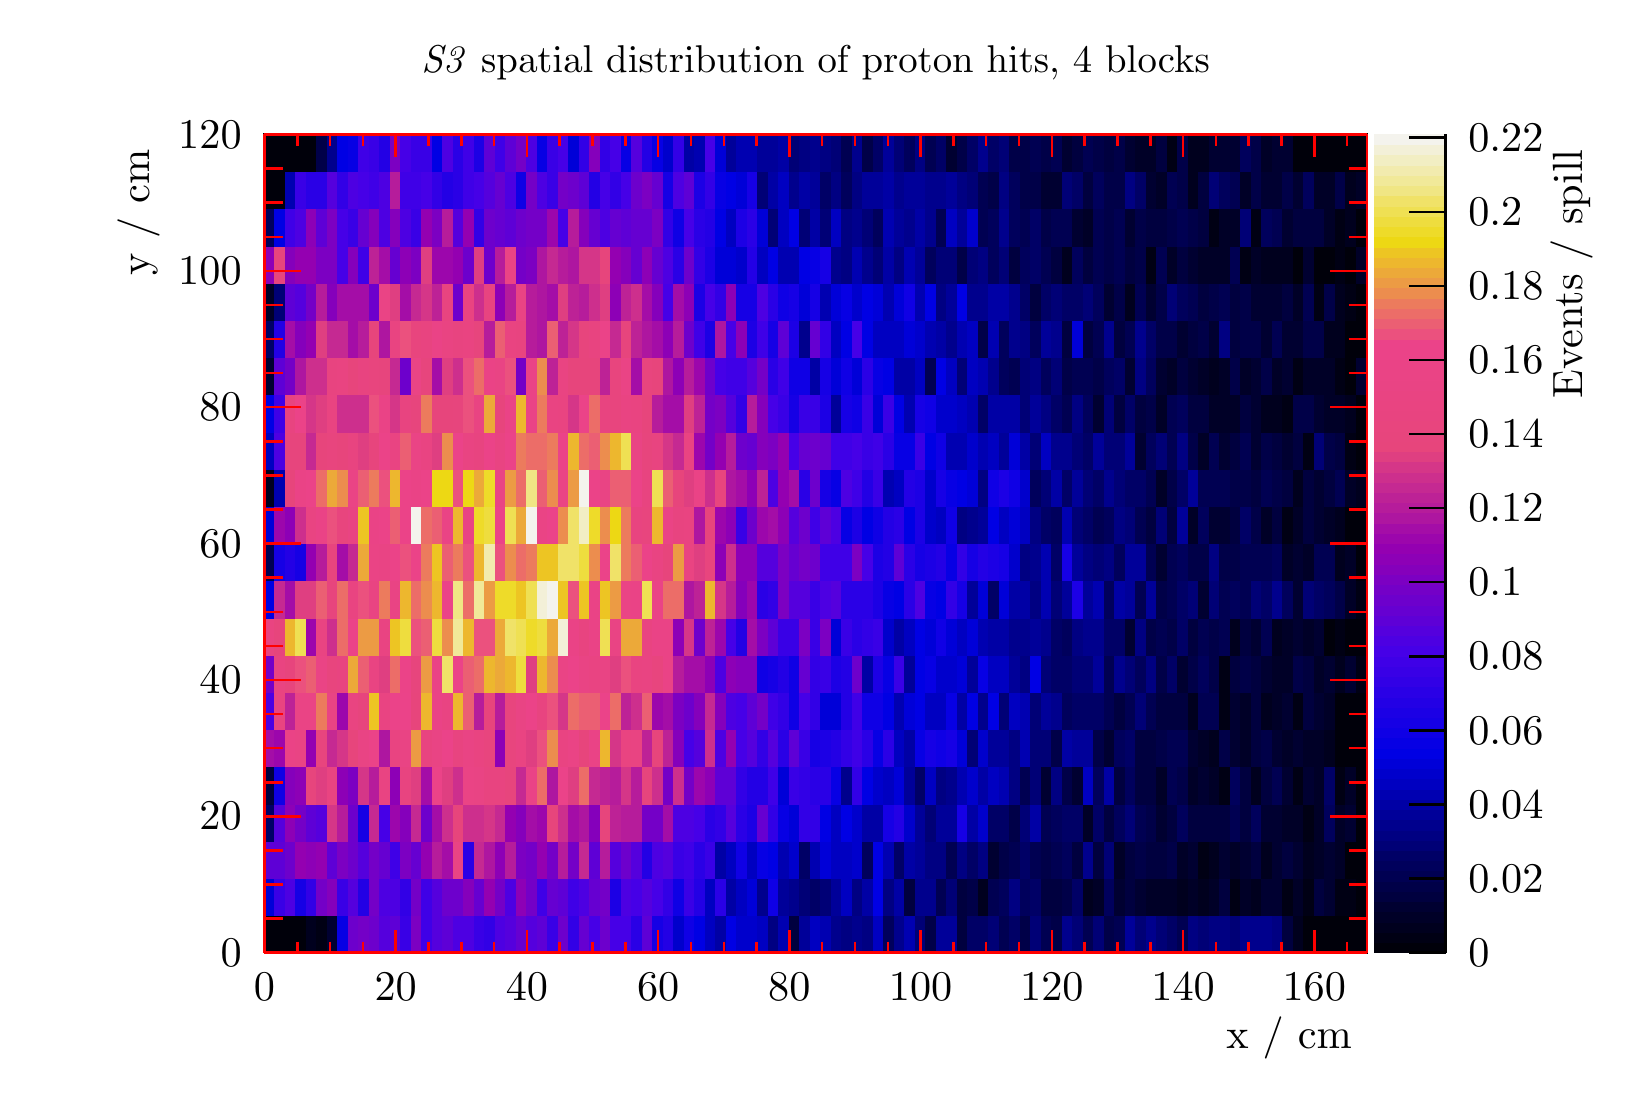
\begin{tikzpicture}
\pgfdeclareplotmark{cross} {
\pgfpathmoveto{\pgfpoint{-0.3\pgfplotmarksize}{\pgfplotmarksize}}
\pgfpathlineto{\pgfpoint{+0.3\pgfplotmarksize}{\pgfplotmarksize}}
\pgfpathlineto{\pgfpoint{+0.3\pgfplotmarksize}{0.3\pgfplotmarksize}}
\pgfpathlineto{\pgfpoint{+1\pgfplotmarksize}{0.3\pgfplotmarksize}}
\pgfpathlineto{\pgfpoint{+1\pgfplotmarksize}{-0.3\pgfplotmarksize}}
\pgfpathlineto{\pgfpoint{+0.3\pgfplotmarksize}{-0.3\pgfplotmarksize}}
\pgfpathlineto{\pgfpoint{+0.3\pgfplotmarksize}{-1.\pgfplotmarksize}}
\pgfpathlineto{\pgfpoint{-0.3\pgfplotmarksize}{-1.\pgfplotmarksize}}
\pgfpathlineto{\pgfpoint{-0.3\pgfplotmarksize}{-0.3\pgfplotmarksize}}
\pgfpathlineto{\pgfpoint{-1.\pgfplotmarksize}{-0.3\pgfplotmarksize}}
\pgfpathlineto{\pgfpoint{-1.\pgfplotmarksize}{0.3\pgfplotmarksize}}
\pgfpathlineto{\pgfpoint{-0.3\pgfplotmarksize}{0.3\pgfplotmarksize}}
\pgfpathclose
\pgfusepathqstroke
}
\pgfdeclareplotmark{cross*} {
\pgfpathmoveto{\pgfpoint{-0.3\pgfplotmarksize}{\pgfplotmarksize}}
\pgfpathlineto{\pgfpoint{+0.3\pgfplotmarksize}{\pgfplotmarksize}}
\pgfpathlineto{\pgfpoint{+0.3\pgfplotmarksize}{0.3\pgfplotmarksize}}
\pgfpathlineto{\pgfpoint{+1\pgfplotmarksize}{0.3\pgfplotmarksize}}
\pgfpathlineto{\pgfpoint{+1\pgfplotmarksize}{-0.3\pgfplotmarksize}}
\pgfpathlineto{\pgfpoint{+0.3\pgfplotmarksize}{-0.3\pgfplotmarksize}}
\pgfpathlineto{\pgfpoint{+0.3\pgfplotmarksize}{-1.\pgfplotmarksize}}
\pgfpathlineto{\pgfpoint{-0.3\pgfplotmarksize}{-1.\pgfplotmarksize}}
\pgfpathlineto{\pgfpoint{-0.3\pgfplotmarksize}{-0.3\pgfplotmarksize}}
\pgfpathlineto{\pgfpoint{-1.\pgfplotmarksize}{-0.3\pgfplotmarksize}}
\pgfpathlineto{\pgfpoint{-1.\pgfplotmarksize}{0.3\pgfplotmarksize}}
\pgfpathlineto{\pgfpoint{-0.3\pgfplotmarksize}{0.3\pgfplotmarksize}}
\pgfpathclose
\pgfusepathqfillstroke
}
\pgfdeclareplotmark{newstar} {
\pgfpathmoveto{\pgfqpoint{0pt}{\pgfplotmarksize}}
\pgfpathlineto{\pgfqpointpolar{44}{0.5\pgfplotmarksize}}
\pgfpathlineto{\pgfqpointpolar{18}{\pgfplotmarksize}}
\pgfpathlineto{\pgfqpointpolar{-20}{0.5\pgfplotmarksize}}
\pgfpathlineto{\pgfqpointpolar{-54}{\pgfplotmarksize}}
\pgfpathlineto{\pgfqpointpolar{-90}{0.5\pgfplotmarksize}}
\pgfpathlineto{\pgfqpointpolar{234}{\pgfplotmarksize}}
\pgfpathlineto{\pgfqpointpolar{198}{0.5\pgfplotmarksize}}
\pgfpathlineto{\pgfqpointpolar{162}{\pgfplotmarksize}}
\pgfpathlineto{\pgfqpointpolar{134}{0.5\pgfplotmarksize}}
\pgfpathclose
\pgfusepathqstroke
}
\pgfdeclareplotmark{newstar*} {
\pgfpathmoveto{\pgfqpoint{0pt}{\pgfplotmarksize}}
\pgfpathlineto{\pgfqpointpolar{44}{0.5\pgfplotmarksize}}
\pgfpathlineto{\pgfqpointpolar{18}{\pgfplotmarksize}}
\pgfpathlineto{\pgfqpointpolar{-20}{0.5\pgfplotmarksize}}
\pgfpathlineto{\pgfqpointpolar{-54}{\pgfplotmarksize}}
\pgfpathlineto{\pgfqpointpolar{-90}{0.5\pgfplotmarksize}}
\pgfpathlineto{\pgfqpointpolar{234}{\pgfplotmarksize}}
\pgfpathlineto{\pgfqpointpolar{198}{0.5\pgfplotmarksize}}
\pgfpathlineto{\pgfqpointpolar{162}{\pgfplotmarksize}}
\pgfpathlineto{\pgfqpointpolar{134}{0.5\pgfplotmarksize}}
\pgfpathclose
\pgfusepathqfillstroke
}
\definecolor{c}{rgb}{1,1,1};
\draw [color=c, fill=c] (0,0) rectangle (20,13.4957);
\draw [color=c, fill=c] (3,1.75444) rectangle (17,12.1461);
\definecolor{c}{rgb}{0,0,0};
\draw [c,line width=0.9] (3,1.75444) -- (3,12.1461) -- (17,12.1461) -- (17,1.75444) -- (3,1.75444);
\definecolor{c}{rgb}{1,1,1};
\draw [color=c, fill=c] (3,1.75444) rectangle (17,12.1461);
\definecolor{c}{rgb}{0,0,0};
\draw [c,line width=0.9] (3,1.75444) -- (3,12.1461) -- (17,12.1461) -- (17,1.75444) -- (3,1.75444);
\definecolor{c}{rgb}{0,0,0.0387097};
\draw [color=c, fill=c] (3,1.75444) rectangle (3.13333,2.22679);
\draw [color=c, fill=c] (3.13333,1.75444) rectangle (3.26667,2.22679);
\draw [color=c, fill=c] (3.26667,1.75444) rectangle (3.4,2.22679);
\draw [color=c, fill=c] (3.4,1.75444) rectangle (3.53333,2.22679);
\definecolor{c}{rgb}{0,0,0.116129};
\draw [color=c, fill=c] (3.53333,1.75444) rectangle (3.66667,2.22679);
\definecolor{c}{rgb}{0,0,0.0774194};
\draw [color=c, fill=c] (3.66667,1.75444) rectangle (3.8,2.22679);
\definecolor{c}{rgb}{0,0,0.193548};
\draw [color=c, fill=c] (3.8,1.75444) rectangle (3.93333,2.22679);
\definecolor{c}{rgb}{0.0257353,0,0.895221};
\draw [color=c, fill=c] (3.93333,1.75444) rectangle (4.06667,2.22679);
\definecolor{c}{rgb}{0.427451,0,0.8};
\draw [color=c, fill=c] (4.06667,1.75444) rectangle (4.2,2.22679);
\definecolor{c}{rgb}{0.456127,0,0.780147};
\draw [color=c, fill=c] (4.2,1.75444) rectangle (4.33333,2.22679);
\definecolor{c}{rgb}{0.427451,0,0.8};
\draw [color=c, fill=c] (4.33333,1.75444) rectangle (4.46667,2.22679);
\definecolor{c}{rgb}{0.331863,0,0.866176};
\draw [color=c, fill=c] (4.46667,1.75444) rectangle (4.6,2.22679);
\definecolor{c}{rgb}{0.370098,0,0.839706};
\draw [color=c, fill=c] (4.6,1.75444) rectangle (4.73333,2.22679);
\definecolor{c}{rgb}{0.223039,0,0.903676};
\draw [color=c, fill=c] (4.73333,1.75444) rectangle (4.86667,2.22679);
\definecolor{c}{rgb}{0.484804,0,0.760294};
\draw [color=c, fill=c] (4.86667,1.75444) rectangle (5,2.22679);
\definecolor{c}{rgb}{0.248775,0,0.904779};
\draw [color=c, fill=c] (5,1.75444) rectangle (5.13333,2.22679);
\definecolor{c}{rgb}{0.331863,0,0.866176};
\draw [color=c, fill=c] (5.13333,1.75444) rectangle (5.26667,2.22679);
\definecolor{c}{rgb}{0.370098,0,0.839706};
\draw [color=c, fill=c] (5.26667,1.75444) rectangle (5.4,2.22679);
\definecolor{c}{rgb}{0.303186,0,0.886029};
\draw [color=c, fill=c] (5.4,1.75444) rectangle (5.53333,2.22679);
\draw [color=c, fill=c] (5.53333,1.75444) rectangle (5.66667,2.22679);
\definecolor{c}{rgb}{0.223039,0,0.903676};
\draw [color=c, fill=c] (5.66667,1.75444) rectangle (5.8,2.22679);
\definecolor{c}{rgb}{0.197304,0,0.902574};
\draw [color=c, fill=c] (5.8,1.75444) rectangle (5.93333,2.22679);
\definecolor{c}{rgb}{0.303186,0,0.886029};
\draw [color=c, fill=c] (5.93333,1.75444) rectangle (6.06667,2.22679);
\definecolor{c}{rgb}{0.331863,0,0.866176};
\draw [color=c, fill=c] (6.06667,1.75444) rectangle (6.2,2.22679);
\definecolor{c}{rgb}{0.398775,0,0.819853};
\draw [color=c, fill=c] (6.2,1.75444) rectangle (6.33333,2.22679);
\definecolor{c}{rgb}{0.331863,0,0.866176};
\draw [color=c, fill=c] (6.33333,1.75444) rectangle (6.46667,2.22679);
\definecolor{c}{rgb}{0.370098,0,0.839706};
\draw [color=c, fill=c] (6.46667,1.75444) rectangle (6.6,2.22679);
\definecolor{c}{rgb}{0.223039,0,0.903676};
\draw [color=c, fill=c] (6.6,1.75444) rectangle (6.73333,2.22679);
\definecolor{c}{rgb}{0.427451,0,0.8};
\draw [color=c, fill=c] (6.73333,1.75444) rectangle (6.86667,2.22679);
\definecolor{c}{rgb}{0.197304,0,0.902574};
\draw [color=c, fill=c] (6.86667,1.75444) rectangle (7,2.22679);
\definecolor{c}{rgb}{0.398775,0,0.819853};
\draw [color=c, fill=c] (7,1.75444) rectangle (7.13333,2.22679);
\definecolor{c}{rgb}{0.27451,0,0.905882};
\draw [color=c, fill=c] (7.13333,1.75444) rectangle (7.26667,2.22679);
\definecolor{c}{rgb}{0.427451,0,0.8};
\draw [color=c, fill=c] (7.26667,1.75444) rectangle (7.4,2.22679);
\definecolor{c}{rgb}{0.27451,0,0.905882};
\draw [color=c, fill=c] (7.4,1.75444) rectangle (7.53333,2.22679);
\draw [color=c, fill=c] (7.53333,1.75444) rectangle (7.66667,2.22679);
\definecolor{c}{rgb}{0.16299,0,0.901103};
\draw [color=c, fill=c] (7.66667,1.75444) rectangle (7.8,2.22679);
\definecolor{c}{rgb}{0.370098,0,0.839706};
\draw [color=c, fill=c] (7.8,1.75444) rectangle (7.93333,2.22679);
\definecolor{c}{rgb}{0.0857843,0,0.897794};
\draw [color=c, fill=c] (7.93333,1.75444) rectangle (8.06667,2.22679);
\definecolor{c}{rgb}{0.137255,0,0.9};
\draw [color=c, fill=c] (8.06667,1.75444) rectangle (8.2,2.22679);
\definecolor{c}{rgb}{0,0,0.801471};
\draw [color=c, fill=c] (8.2,1.75444) rectangle (8.33333,2.22679);
\definecolor{c}{rgb}{0.060049,0,0.896691};
\draw [color=c, fill=c] (8.33333,1.75444) rectangle (8.46667,2.22679);
\definecolor{c}{rgb}{0,0,0.894118};
\draw [color=c, fill=c] (8.46667,1.75444) rectangle (8.6,2.22679);
\definecolor{c}{rgb}{0,0,0.755147};
\draw [color=c, fill=c] (8.6,1.75444) rectangle (8.73333,2.22679);
\definecolor{c}{rgb}{0,0,0.647059};
\draw [color=c, fill=c] (8.73333,1.75444) rectangle (8.86667,2.22679);
\definecolor{c}{rgb}{0,0,0.894118};
\draw [color=c, fill=c] (8.86667,1.75444) rectangle (9,2.22679);
\definecolor{c}{rgb}{0,0,0.801471};
\draw [color=c, fill=c] (9,1.75444) rectangle (9.13333,2.22679);
\draw [color=c, fill=c] (9.13333,1.75444) rectangle (9.26667,2.22679);
\definecolor{c}{rgb}{0,0,0.755147};
\draw [color=c, fill=c] (9.26667,1.75444) rectangle (9.4,2.22679);
\definecolor{c}{rgb}{0,0,0.508088};
\draw [color=c, fill=c] (9.4,1.75444) rectangle (9.53333,2.22679);
\definecolor{c}{rgb}{0,0,0.693382};
\draw [color=c, fill=c] (9.53333,1.75444) rectangle (9.66667,2.22679);
\definecolor{c}{rgb}{0,0,0.245161};
\draw [color=c, fill=c] (9.66667,1.75444) rectangle (9.8,2.22679);
\definecolor{c}{rgb}{0,0,0.600735};
\draw [color=c, fill=c] (9.8,1.75444) rectangle (9.93333,2.22679);
\definecolor{c}{rgb}{0,0,0.755147};
\draw [color=c, fill=c] (9.93333,1.75444) rectangle (10.0667,2.22679);
\definecolor{c}{rgb}{0,0,0.693382};
\draw [color=c, fill=c] (10.0667,1.75444) rectangle (10.2,2.22679);
\definecolor{c}{rgb}{0,0,0.554412};
\draw [color=c, fill=c] (10.2,1.75444) rectangle (10.3333,2.22679);
\definecolor{c}{rgb}{0,0,0.508088};
\draw [color=c, fill=c] (10.3333,1.75444) rectangle (10.4667,2.22679);
\definecolor{c}{rgb}{0,0,0.554412};
\draw [color=c, fill=c] (10.4667,1.75444) rectangle (10.6,2.22679);
\definecolor{c}{rgb}{0,0,0.508088};
\draw [color=c, fill=c] (10.6,1.75444) rectangle (10.7333,2.22679);
\definecolor{c}{rgb}{0,0,0.755147};
\draw [color=c, fill=c] (10.7333,1.75444) rectangle (10.8667,2.22679);
\definecolor{c}{rgb}{0,0,0.36129};
\draw [color=c, fill=c] (10.8667,1.75444) rectangle (11,2.22679);
\definecolor{c}{rgb}{0,0,0.554412};
\draw [color=c, fill=c] (11,1.75444) rectangle (11.1333,2.22679);
\definecolor{c}{rgb}{0,0,0.693382};
\draw [color=c, fill=c] (11.1333,1.75444) rectangle (11.2667,2.22679);
\definecolor{c}{rgb}{0,0,0.461765};
\draw [color=c, fill=c] (11.2667,1.75444) rectangle (11.4,2.22679);
\definecolor{c}{rgb}{0,0,0.283871};
\draw [color=c, fill=c] (11.4,1.75444) rectangle (11.5333,2.22679);
\definecolor{c}{rgb}{0,0,0.600735};
\draw [color=c, fill=c] (11.5333,1.75444) rectangle (11.6667,2.22679);
\draw [color=c, fill=c] (11.6667,1.75444) rectangle (11.8,2.22679);
\definecolor{c}{rgb}{0,0,0.245161};
\draw [color=c, fill=c] (11.8,1.75444) rectangle (11.9333,2.22679);
\definecolor{c}{rgb}{0,0,0.4};
\draw [color=c, fill=c] (11.9333,1.75444) rectangle (12.0667,2.22679);
\draw [color=c, fill=c] (12.0667,1.75444) rectangle (12.2,2.22679);
\definecolor{c}{rgb}{0,0,0.461765};
\draw [color=c, fill=c] (12.2,1.75444) rectangle (12.3333,2.22679);
\definecolor{c}{rgb}{0,0,0.322581};
\draw [color=c, fill=c] (12.3333,1.75444) rectangle (12.4667,2.22679);
\definecolor{c}{rgb}{0,0,0.4};
\draw [color=c, fill=c] (12.4667,1.75444) rectangle (12.6,2.22679);
\definecolor{c}{rgb}{0,0,0.283871};
\draw [color=c, fill=c] (12.6,1.75444) rectangle (12.7333,2.22679);
\definecolor{c}{rgb}{0,0,0.461765};
\draw [color=c, fill=c] (12.7333,1.75444) rectangle (12.8667,2.22679);
\definecolor{c}{rgb}{0,0,0.322581};
\draw [color=c, fill=c] (12.8667,1.75444) rectangle (13,2.22679);
\definecolor{c}{rgb}{0,0,0.283871};
\draw [color=c, fill=c] (13,1.75444) rectangle (13.1333,2.22679);
\definecolor{c}{rgb}{0,0,0.554412};
\draw [color=c, fill=c] (13.1333,1.75444) rectangle (13.2667,2.22679);
\definecolor{c}{rgb}{0,0,0.461765};
\draw [color=c, fill=c] (13.2667,1.75444) rectangle (13.4,2.22679);
\definecolor{c}{rgb}{0,0,0.322581};
\draw [color=c, fill=c] (13.4,1.75444) rectangle (13.5333,2.22679);
\definecolor{c}{rgb}{0,0,0.461765};
\draw [color=c, fill=c] (13.5333,1.75444) rectangle (13.6667,2.22679);
\definecolor{c}{rgb}{0,0,0.283871};
\draw [color=c, fill=c] (13.6667,1.75444) rectangle (13.8,2.22679);
\definecolor{c}{rgb}{0,0,0.322581};
\draw [color=c, fill=c] (13.8,1.75444) rectangle (13.9333,2.22679);
\definecolor{c}{rgb}{0,0,0.600735};
\draw [color=c, fill=c] (13.9333,1.75444) rectangle (14.0667,2.22679);
\definecolor{c}{rgb}{0,0,0.461765};
\draw [color=c, fill=c] (14.0667,1.75444) rectangle (14.2,2.22679);
\definecolor{c}{rgb}{0,0,0.554412};
\draw [color=c, fill=c] (14.2,1.75444) rectangle (14.3333,2.22679);
\definecolor{c}{rgb}{0,0,0.461765};
\draw [color=c, fill=c] (14.3333,1.75444) rectangle (14.4667,2.22679);
\definecolor{c}{rgb}{0,0,0.4};
\draw [color=c, fill=c] (14.4667,1.75444) rectangle (14.6,2.22679);
\definecolor{c}{rgb}{0,0,0.322581};
\draw [color=c, fill=c] (14.6,1.75444) rectangle (14.7333,2.22679);
\definecolor{c}{rgb}{0,0,0.508088};
\draw [color=c, fill=c] (14.7333,1.75444) rectangle (14.8667,2.22679);
\definecolor{c}{rgb}{0,0,0.461765};
\draw [color=c, fill=c] (14.8667,1.75444) rectangle (15,2.22679);
\definecolor{c}{rgb}{0,0,0.508088};
\draw [color=c, fill=c] (15,1.75444) rectangle (15.1333,2.22679);
\draw [color=c, fill=c] (15.1333,1.75444) rectangle (15.2667,2.22679);
\definecolor{c}{rgb}{0,0,0.461765};
\draw [color=c, fill=c] (15.2667,1.75444) rectangle (15.4,2.22679);
\definecolor{c}{rgb}{0,0,0.554412};
\draw [color=c, fill=c] (15.4,1.75444) rectangle (15.5333,2.22679);
\draw [color=c, fill=c] (15.5333,1.75444) rectangle (15.6667,2.22679);
\draw [color=c, fill=c] (15.6667,1.75444) rectangle (15.8,2.22679);
\definecolor{c}{rgb}{0,0,0.508088};
\draw [color=c, fill=c] (15.8,1.75444) rectangle (15.9333,2.22679);
\definecolor{c}{rgb}{0,0,0.245161};
\draw [color=c, fill=c] (15.9333,1.75444) rectangle (16.0667,2.22679);
\definecolor{c}{rgb}{0,0,0.116129};
\draw [color=c, fill=c] (16.0667,1.75444) rectangle (16.2,2.22679);
\definecolor{c}{rgb}{0,0,0.0387097};
\draw [color=c, fill=c] (16.2,1.75444) rectangle (16.3333,2.22679);
\draw [color=c, fill=c] (16.3333,1.75444) rectangle (16.4667,2.22679);
\draw [color=c, fill=c] (16.4667,1.75444) rectangle (16.6,2.22679);
\draw [color=c, fill=c] (16.6,1.75444) rectangle (16.7333,2.22679);
\draw [color=c, fill=c] (16.7333,1.75444) rectangle (16.8667,2.22679);
\draw [color=c, fill=c] (16.8667,1.75444) rectangle (17,2.22679);
\definecolor{c}{rgb}{0,0,0.847794};
\draw [color=c, fill=c] (3,2.22679) rectangle (3.13333,2.69914);
\definecolor{c}{rgb}{0.223039,0,0.903676};
\draw [color=c, fill=c] (3.13333,2.22679) rectangle (3.26667,2.69914);
\definecolor{c}{rgb}{0.303186,0,0.886029};
\draw [color=c, fill=c] (3.26667,2.22679) rectangle (3.4,2.69914);
\definecolor{c}{rgb}{0.0857843,0,0.897794};
\draw [color=c, fill=c] (3.4,2.22679) rectangle (3.53333,2.69914);
\definecolor{c}{rgb}{0.197304,0,0.902574};
\draw [color=c, fill=c] (3.53333,2.22679) rectangle (3.66667,2.69914);
\definecolor{c}{rgb}{0.456127,0,0.780147};
\draw [color=c, fill=c] (3.66667,2.22679) rectangle (3.8,2.69914);
\definecolor{c}{rgb}{0.523039,0,0.733824};
\draw [color=c, fill=c] (3.8,2.22679) rectangle (3.93333,2.69914);
\definecolor{c}{rgb}{0.223039,0,0.903676};
\draw [color=c, fill=c] (3.93333,2.22679) rectangle (4.06667,2.69914);
\definecolor{c}{rgb}{0.331863,0,0.866176};
\draw [color=c, fill=c] (4.06667,2.22679) rectangle (4.2,2.69914);
\definecolor{c}{rgb}{0.137255,0,0.9};
\draw [color=c, fill=c] (4.2,2.22679) rectangle (4.33333,2.69914);
\definecolor{c}{rgb}{0.456127,0,0.780147};
\draw [color=c, fill=c] (4.33333,2.22679) rectangle (4.46667,2.69914);
\definecolor{c}{rgb}{0.303186,0,0.886029};
\draw [color=c, fill=c] (4.46667,2.22679) rectangle (4.6,2.69914);
\draw [color=c, fill=c] (4.6,2.22679) rectangle (4.73333,2.69914);
\definecolor{c}{rgb}{0.197304,0,0.902574};
\draw [color=c, fill=c] (4.73333,2.22679) rectangle (4.86667,2.69914);
\definecolor{c}{rgb}{0.456127,0,0.780147};
\draw [color=c, fill=c] (4.86667,2.22679) rectangle (5,2.69914);
\definecolor{c}{rgb}{0.248775,0,0.904779};
\draw [color=c, fill=c] (5,2.22679) rectangle (5.13333,2.69914);
\definecolor{c}{rgb}{0.331863,0,0.866176};
\draw [color=c, fill=c] (5.13333,2.22679) rectangle (5.26667,2.69914);
\definecolor{c}{rgb}{0.427451,0,0.8};
\draw [color=c, fill=c] (5.26667,2.22679) rectangle (5.4,2.69914);
\draw [color=c, fill=c] (5.4,2.22679) rectangle (5.53333,2.69914);
\definecolor{c}{rgb}{0.523039,0,0.733824};
\draw [color=c, fill=c] (5.53333,2.22679) rectangle (5.66667,2.69914);
\definecolor{c}{rgb}{0.398775,0,0.819853};
\draw [color=c, fill=c] (5.66667,2.22679) rectangle (5.8,2.69914);
\definecolor{c}{rgb}{0.580392,0,0.694118};
\draw [color=c, fill=c] (5.8,2.22679) rectangle (5.93333,2.69914);
\definecolor{c}{rgb}{0.456127,0,0.780147};
\draw [color=c, fill=c] (5.93333,2.22679) rectangle (6.06667,2.69914);
\definecolor{c}{rgb}{0.303186,0,0.886029};
\draw [color=c, fill=c] (6.06667,2.22679) rectangle (6.2,2.69914);
\definecolor{c}{rgb}{0.551716,0,0.713971};
\draw [color=c, fill=c] (6.2,2.22679) rectangle (6.33333,2.69914);
\definecolor{c}{rgb}{0.456127,0,0.780147};
\draw [color=c, fill=c] (6.33333,2.22679) rectangle (6.46667,2.69914);
\definecolor{c}{rgb}{0.248775,0,0.904779};
\draw [color=c, fill=c] (6.46667,2.22679) rectangle (6.6,2.69914);
\definecolor{c}{rgb}{0.398775,0,0.819853};
\draw [color=c, fill=c] (6.6,2.22679) rectangle (6.73333,2.69914);
\definecolor{c}{rgb}{0.370098,0,0.839706};
\draw [color=c, fill=c] (6.73333,2.22679) rectangle (6.86667,2.69914);
\definecolor{c}{rgb}{0.248775,0,0.904779};
\draw [color=c, fill=c] (6.86667,2.22679) rectangle (7,2.69914);
\definecolor{c}{rgb}{0.303186,0,0.886029};
\draw [color=c, fill=c] (7,2.22679) rectangle (7.13333,2.69914);
\definecolor{c}{rgb}{0.398775,0,0.819853};
\draw [color=c, fill=c] (7.13333,2.22679) rectangle (7.26667,2.69914);
\definecolor{c}{rgb}{0.456127,0,0.780147};
\draw [color=c, fill=c] (7.26667,2.22679) rectangle (7.4,2.69914);
\definecolor{c}{rgb}{0.11152,0,0.898897};
\draw [color=c, fill=c] (7.4,2.22679) rectangle (7.53333,2.69914);
\definecolor{c}{rgb}{0.303186,0,0.886029};
\draw [color=c, fill=c] (7.53333,2.22679) rectangle (7.66667,2.69914);
\definecolor{c}{rgb}{0.27451,0,0.905882};
\draw [color=c, fill=c] (7.66667,2.22679) rectangle (7.8,2.69914);
\definecolor{c}{rgb}{0.331863,0,0.866176};
\draw [color=c, fill=c] (7.8,2.22679) rectangle (7.93333,2.69914);
\definecolor{c}{rgb}{0.27451,0,0.905882};
\draw [color=c, fill=c] (7.93333,2.22679) rectangle (8.06667,2.69914);
\definecolor{c}{rgb}{0.197304,0,0.902574};
\draw [color=c, fill=c] (8.06667,2.22679) rectangle (8.2,2.69914);
\definecolor{c}{rgb}{0.060049,0,0.896691};
\draw [color=c, fill=c] (8.2,2.22679) rectangle (8.33333,2.69914);
\definecolor{c}{rgb}{0.223039,0,0.903676};
\draw [color=c, fill=c] (8.33333,2.22679) rectangle (8.46667,2.69914);
\definecolor{c}{rgb}{0.137255,0,0.9};
\draw [color=c, fill=c] (8.46667,2.22679) rectangle (8.6,2.69914);
\definecolor{c}{rgb}{0,0,0.755147};
\draw [color=c, fill=c] (8.6,2.22679) rectangle (8.73333,2.69914);
\definecolor{c}{rgb}{0.16299,0,0.901103};
\draw [color=c, fill=c] (8.73333,2.22679) rectangle (8.86667,2.69914);
\definecolor{c}{rgb}{0,0,0.647059};
\draw [color=c, fill=c] (8.86667,2.22679) rectangle (9,2.69914);
\definecolor{c}{rgb}{0,0,0.755147};
\draw [color=c, fill=c] (9,2.22679) rectangle (9.13333,2.69914);
\definecolor{c}{rgb}{0,0,0.847794};
\draw [color=c, fill=c] (9.13333,2.22679) rectangle (9.26667,2.69914);
\definecolor{c}{rgb}{0,0,0.554412};
\draw [color=c, fill=c] (9.26667,2.22679) rectangle (9.4,2.69914);
\definecolor{c}{rgb}{0.060049,0,0.896691};
\draw [color=c, fill=c] (9.4,2.22679) rectangle (9.53333,2.69914);
\definecolor{c}{rgb}{0,0,0.600735};
\draw [color=c, fill=c] (9.53333,2.22679) rectangle (9.66667,2.69914);
\definecolor{c}{rgb}{0,0,0.554412};
\draw [color=c, fill=c] (9.66667,2.22679) rectangle (9.8,2.69914);
\definecolor{c}{rgb}{0,0,0.461765};
\draw [color=c, fill=c] (9.8,2.22679) rectangle (9.93333,2.69914);
\definecolor{c}{rgb}{0,0,0.4};
\draw [color=c, fill=c] (9.93333,2.22679) rectangle (10.0667,2.69914);
\definecolor{c}{rgb}{0,0,0.461765};
\draw [color=c, fill=c] (10.0667,2.22679) rectangle (10.2,2.69914);
\definecolor{c}{rgb}{0,0,0.600735};
\draw [color=c, fill=c] (10.2,2.22679) rectangle (10.3333,2.69914);
\definecolor{c}{rgb}{0,0,0.755147};
\draw [color=c, fill=c] (10.3333,2.22679) rectangle (10.4667,2.69914);
\definecolor{c}{rgb}{0,0,0.508088};
\draw [color=c, fill=c] (10.4667,2.22679) rectangle (10.6,2.69914);
\definecolor{c}{rgb}{0,0,0.647059};
\draw [color=c, fill=c] (10.6,2.22679) rectangle (10.7333,2.69914);
\definecolor{c}{rgb}{0,0,0.894118};
\draw [color=c, fill=c] (10.7333,2.22679) rectangle (10.8667,2.69914);
\definecolor{c}{rgb}{0,0,0.508088};
\draw [color=c, fill=c] (10.8667,2.22679) rectangle (11,2.69914);
\definecolor{c}{rgb}{0,0,0.647059};
\draw [color=c, fill=c] (11,2.22679) rectangle (11.1333,2.69914);
\definecolor{c}{rgb}{0,0,0.245161};
\draw [color=c, fill=c] (11.1333,2.22679) rectangle (11.2667,2.69914);
\definecolor{c}{rgb}{0,0,0.554412};
\draw [color=c, fill=c] (11.2667,2.22679) rectangle (11.4,2.69914);
\draw [color=c, fill=c] (11.4,2.22679) rectangle (11.5333,2.69914);
\definecolor{c}{rgb}{0,0,0.322581};
\draw [color=c, fill=c] (11.5333,2.22679) rectangle (11.6667,2.69914);
\definecolor{c}{rgb}{0,0,0.461765};
\draw [color=c, fill=c] (11.6667,2.22679) rectangle (11.8,2.69914);
\definecolor{c}{rgb}{0,0,0.245161};
\draw [color=c, fill=c] (11.8,2.22679) rectangle (11.9333,2.69914);
\definecolor{c}{rgb}{0,0,0.283871};
\draw [color=c, fill=c] (11.9333,2.22679) rectangle (12.0667,2.69914);
\definecolor{c}{rgb}{0,0,0.116129};
\draw [color=c, fill=c] (12.0667,2.22679) rectangle (12.2,2.69914);
\definecolor{c}{rgb}{0,0,0.322581};
\draw [color=c, fill=c] (12.2,2.22679) rectangle (12.3333,2.69914);
\definecolor{c}{rgb}{0,0,0.36129};
\draw [color=c, fill=c] (12.3333,2.22679) rectangle (12.4667,2.69914);
\definecolor{c}{rgb}{0,0,0.508088};
\draw [color=c, fill=c] (12.4667,2.22679) rectangle (12.6,2.69914);
\definecolor{c}{rgb}{0,0,0.36129};
\draw [color=c, fill=c] (12.6,2.22679) rectangle (12.7333,2.69914);
\definecolor{c}{rgb}{0,0,0.4};
\draw [color=c, fill=c] (12.7333,2.22679) rectangle (12.8667,2.69914);
\definecolor{c}{rgb}{0,0,0.245161};
\draw [color=c, fill=c] (12.8667,2.22679) rectangle (13,2.69914);
\draw [color=c, fill=c] (13,2.22679) rectangle (13.1333,2.69914);
\definecolor{c}{rgb}{0,0,0.283871};
\draw [color=c, fill=c] (13.1333,2.22679) rectangle (13.2667,2.69914);
\definecolor{c}{rgb}{0,0,0.4};
\draw [color=c, fill=c] (13.2667,2.22679) rectangle (13.4,2.69914);
\definecolor{c}{rgb}{0,0,0.116129};
\draw [color=c, fill=c] (13.4,2.22679) rectangle (13.5333,2.69914);
\definecolor{c}{rgb}{0,0,0.154839};
\draw [color=c, fill=c] (13.5333,2.22679) rectangle (13.6667,2.69914);
\definecolor{c}{rgb}{0,0,0.36129};
\draw [color=c, fill=c] (13.6667,2.22679) rectangle (13.8,2.69914);
\definecolor{c}{rgb}{0,0,0.193548};
\draw [color=c, fill=c] (13.8,2.22679) rectangle (13.9333,2.69914);
\definecolor{c}{rgb}{0,0,0.245161};
\draw [color=c, fill=c] (13.9333,2.22679) rectangle (14.0667,2.69914);
\definecolor{c}{rgb}{0,0,0.193548};
\draw [color=c, fill=c] (14.0667,2.22679) rectangle (14.2,2.69914);
\definecolor{c}{rgb}{0,0,0.154839};
\draw [color=c, fill=c] (14.2,2.22679) rectangle (14.3333,2.69914);
\draw [color=c, fill=c] (14.3333,2.22679) rectangle (14.4667,2.69914);
\draw [color=c, fill=c] (14.4667,2.22679) rectangle (14.6,2.69914);
\definecolor{c}{rgb}{0,0,0.116129};
\draw [color=c, fill=c] (14.6,2.22679) rectangle (14.7333,2.69914);
\definecolor{c}{rgb}{0,0,0.154839};
\draw [color=c, fill=c] (14.7333,2.22679) rectangle (14.8667,2.69914);
\definecolor{c}{rgb}{0,0,0.116129};
\draw [color=c, fill=c] (14.8667,2.22679) rectangle (15,2.69914);
\definecolor{c}{rgb}{0,0,0.154839};
\draw [color=c, fill=c] (15,2.22679) rectangle (15.1333,2.69914);
\definecolor{c}{rgb}{0,0,0.245161};
\draw [color=c, fill=c] (15.1333,2.22679) rectangle (15.2667,2.69914);
\definecolor{c}{rgb}{0,0,0.0774194};
\draw [color=c, fill=c] (15.2667,2.22679) rectangle (15.4,2.69914);
\definecolor{c}{rgb}{0,0,0.154839};
\draw [color=c, fill=c] (15.4,2.22679) rectangle (15.5333,2.69914);
\definecolor{c}{rgb}{0,0,0.116129};
\draw [color=c, fill=c] (15.5333,2.22679) rectangle (15.6667,2.69914);
\definecolor{c}{rgb}{0,0,0.193548};
\draw [color=c, fill=c] (15.6667,2.22679) rectangle (15.8,2.69914);
\draw [color=c, fill=c] (15.8,2.22679) rectangle (15.9333,2.69914);
\definecolor{c}{rgb}{0,0,0.0774194};
\draw [color=c, fill=c] (15.9333,2.22679) rectangle (16.0667,2.69914);
\definecolor{c}{rgb}{0,0,0.154839};
\draw [color=c, fill=c] (16.0667,2.22679) rectangle (16.2,2.69914);
\definecolor{c}{rgb}{0,0,0.0774194};
\draw [color=c, fill=c] (16.2,2.22679) rectangle (16.3333,2.69914);
\definecolor{c}{rgb}{0,0,0.245161};
\draw [color=c, fill=c] (16.3333,2.22679) rectangle (16.4667,2.69914);
\definecolor{c}{rgb}{0,0,0.193548};
\draw [color=c, fill=c] (16.4667,2.22679) rectangle (16.6,2.69914);
\definecolor{c}{rgb}{0,0,0.0774194};
\draw [color=c, fill=c] (16.6,2.22679) rectangle (16.7333,2.69914);
\draw [color=c, fill=c] (16.7333,2.22679) rectangle (16.8667,2.69914);
\definecolor{c}{rgb}{0,0,0.0387097};
\draw [color=c, fill=c] (16.8667,2.22679) rectangle (17,2.69914);
\definecolor{c}{rgb}{0.370098,0,0.839706};
\draw [color=c, fill=c] (3,2.69914) rectangle (3.13333,3.17149);
\draw [color=c, fill=c] (3.13333,2.69914) rectangle (3.26667,3.17149);
\definecolor{c}{rgb}{0.427451,0,0.8};
\draw [color=c, fill=c] (3.26667,2.69914) rectangle (3.4,3.17149);
\definecolor{c}{rgb}{0.580392,0,0.694118};
\draw [color=c, fill=c] (3.4,2.69914) rectangle (3.53333,3.17149);
\definecolor{c}{rgb}{0.551716,0,0.713971};
\draw [color=c, fill=c] (3.53333,2.69914) rectangle (3.66667,3.17149);
\definecolor{c}{rgb}{0.580392,0,0.694118};
\draw [color=c, fill=c] (3.66667,2.69914) rectangle (3.8,3.17149);
\definecolor{c}{rgb}{0.370098,0,0.839706};
\draw [color=c, fill=c] (3.8,2.69914) rectangle (3.93333,3.17149);
\definecolor{c}{rgb}{0.484804,0,0.760294};
\draw [color=c, fill=c] (3.93333,2.69914) rectangle (4.06667,3.17149);
\definecolor{c}{rgb}{0.427451,0,0.8};
\draw [color=c, fill=c] (4.06667,2.69914) rectangle (4.2,3.17149);
\definecolor{c}{rgb}{0.331863,0,0.866176};
\draw [color=c, fill=c] (4.2,2.69914) rectangle (4.33333,3.17149);
\definecolor{c}{rgb}{0.456127,0,0.780147};
\draw [color=c, fill=c] (4.33333,2.69914) rectangle (4.46667,3.17149);
\definecolor{c}{rgb}{0.398775,0,0.819853};
\draw [color=c, fill=c] (4.46667,2.69914) rectangle (4.6,3.17149);
\definecolor{c}{rgb}{0.248775,0,0.904779};
\draw [color=c, fill=c] (4.6,2.69914) rectangle (4.73333,3.17149);
\definecolor{c}{rgb}{0.484804,0,0.760294};
\draw [color=c, fill=c] (4.73333,2.69914) rectangle (4.86667,3.17149);
\definecolor{c}{rgb}{0.398775,0,0.819853};
\draw [color=c, fill=c] (4.86667,2.69914) rectangle (5,3.17149);
\definecolor{c}{rgb}{0.580392,0,0.694118};
\draw [color=c, fill=c] (5,2.69914) rectangle (5.13333,3.17149);
\definecolor{c}{rgb}{0.712623,0.109926,0.609681};
\draw [color=c, fill=c] (5.13333,2.69914) rectangle (5.26667,3.17149);
\definecolor{c}{rgb}{0.641422,0.0507353,0.655147};
\draw [color=c, fill=c] (5.26667,2.69914) rectangle (5.4,3.17149);
\definecolor{c}{rgb}{0.915196,0.265931,0.516544};
\draw [color=c, fill=c] (5.4,2.69914) rectangle (5.53333,3.17149);
\definecolor{c}{rgb}{0.16299,0,0.901103};
\draw [color=c, fill=c] (5.53333,2.69914) rectangle (5.66667,3.17149);
\definecolor{c}{rgb}{0.773652,0.160662,0.570711};
\draw [color=c, fill=c] (5.66667,2.69914) rectangle (5.8,3.17149);
\definecolor{c}{rgb}{0.682108,0.0845588,0.629167};
\draw [color=c, fill=c] (5.8,2.69914) rectangle (5.93333,3.17149);
\definecolor{c}{rgb}{0.551716,0,0.713971};
\draw [color=c, fill=c] (5.93333,2.69914) rectangle (6.06667,3.17149);
\definecolor{c}{rgb}{0.712623,0.109926,0.609681};
\draw [color=c, fill=c] (6.06667,2.69914) rectangle (6.2,3.17149);
\definecolor{c}{rgb}{0.484804,0,0.760294};
\draw [color=c, fill=c] (6.2,2.69914) rectangle (6.33333,3.17149);
\definecolor{c}{rgb}{0.456127,0,0.780147};
\draw [color=c, fill=c] (6.33333,2.69914) rectangle (6.46667,3.17149);
\definecolor{c}{rgb}{0.580392,0,0.694118};
\draw [color=c, fill=c] (6.46667,2.69914) rectangle (6.6,3.17149);
\definecolor{c}{rgb}{0.456127,0,0.780147};
\draw [color=c, fill=c] (6.6,2.69914) rectangle (6.73333,3.17149);
\definecolor{c}{rgb}{0.712623,0.109926,0.609681};
\draw [color=c, fill=c] (6.73333,2.69914) rectangle (6.86667,3.17149);
\definecolor{c}{rgb}{0.456127,0,0.780147};
\draw [color=c, fill=c] (6.86667,2.69914) rectangle (7,3.17149);
\definecolor{c}{rgb}{0.773652,0.160662,0.570711};
\draw [color=c, fill=c] (7,2.69914) rectangle (7.13333,3.17149);
\definecolor{c}{rgb}{0.370098,0,0.839706};
\draw [color=c, fill=c] (7.13333,2.69914) rectangle (7.26667,3.17149);
\definecolor{c}{rgb}{0.712623,0.109926,0.609681};
\draw [color=c, fill=c] (7.26667,2.69914) rectangle (7.4,3.17149);
\definecolor{c}{rgb}{0.331863,0,0.866176};
\draw [color=c, fill=c] (7.4,2.69914) rectangle (7.53333,3.17149);
\definecolor{c}{rgb}{0.427451,0,0.8};
\draw [color=c, fill=c] (7.53333,2.69914) rectangle (7.66667,3.17149);
\definecolor{c}{rgb}{0.331863,0,0.866176};
\draw [color=c, fill=c] (7.66667,2.69914) rectangle (7.8,3.17149);
\definecolor{c}{rgb}{0.137255,0,0.9};
\draw [color=c, fill=c] (7.8,2.69914) rectangle (7.93333,3.17149);
\definecolor{c}{rgb}{0.303186,0,0.886029};
\draw [color=c, fill=c] (7.93333,2.69914) rectangle (8.06667,3.17149);
\definecolor{c}{rgb}{0.331863,0,0.866176};
\draw [color=c, fill=c] (8.06667,2.69914) rectangle (8.2,3.17149);
\definecolor{c}{rgb}{0.223039,0,0.903676};
\draw [color=c, fill=c] (8.2,2.69914) rectangle (8.33333,3.17149);
\definecolor{c}{rgb}{0.248775,0,0.904779};
\draw [color=c, fill=c] (8.33333,2.69914) rectangle (8.46667,3.17149);
\definecolor{c}{rgb}{0.16299,0,0.901103};
\draw [color=c, fill=c] (8.46667,2.69914) rectangle (8.6,3.17149);
\definecolor{c}{rgb}{0.223039,0,0.903676};
\draw [color=c, fill=c] (8.6,2.69914) rectangle (8.73333,3.17149);
\definecolor{c}{rgb}{0,0,0.647059};
\draw [color=c, fill=c] (8.73333,2.69914) rectangle (8.86667,3.17149);
\definecolor{c}{rgb}{0,0,0.755147};
\draw [color=c, fill=c] (8.86667,2.69914) rectangle (9,3.17149);
\definecolor{c}{rgb}{0.060049,0,0.896691};
\draw [color=c, fill=c] (9,2.69914) rectangle (9.13333,3.17149);
\definecolor{c}{rgb}{0,0,0.755147};
\draw [color=c, fill=c] (9.13333,2.69914) rectangle (9.26667,3.17149);
\definecolor{c}{rgb}{0.0257353,0,0.895221};
\draw [color=c, fill=c] (9.26667,2.69914) rectangle (9.4,3.17149);
\definecolor{c}{rgb}{0,0,0.894118};
\draw [color=c, fill=c] (9.4,2.69914) rectangle (9.53333,3.17149);
\definecolor{c}{rgb}{0,0,0.693382};
\draw [color=c, fill=c] (9.53333,2.69914) rectangle (9.66667,3.17149);
\definecolor{c}{rgb}{0,0,0.801471};
\draw [color=c, fill=c] (9.66667,2.69914) rectangle (9.8,3.17149);
\definecolor{c}{rgb}{0,0,0.4};
\draw [color=c, fill=c] (9.8,2.69914) rectangle (9.93333,3.17149);
\definecolor{c}{rgb}{0,0,0.693382};
\draw [color=c, fill=c] (9.93333,2.69914) rectangle (10.0667,3.17149);
\definecolor{c}{rgb}{0,0,0.847794};
\draw [color=c, fill=c] (10.0667,2.69914) rectangle (10.2,3.17149);
\definecolor{c}{rgb}{0,0,0.755147};
\draw [color=c, fill=c] (10.2,2.69914) rectangle (10.3333,3.17149);
\draw [color=c, fill=c] (10.3333,2.69914) rectangle (10.4667,3.17149);
\definecolor{c}{rgb}{0,0,0.801471};
\draw [color=c, fill=c] (10.4667,2.69914) rectangle (10.6,3.17149);
\definecolor{c}{rgb}{0,0,0.36129};
\draw [color=c, fill=c] (10.6,2.69914) rectangle (10.7333,3.17149);
\definecolor{c}{rgb}{0,0,0.894118};
\draw [color=c, fill=c] (10.7333,2.69914) rectangle (10.8667,3.17149);
\definecolor{c}{rgb}{0,0,0.693382};
\draw [color=c, fill=c] (10.8667,2.69914) rectangle (11,3.17149);
\definecolor{c}{rgb}{0,0,0.4};
\draw [color=c, fill=c] (11,2.69914) rectangle (11.1333,3.17149);
\definecolor{c}{rgb}{0,0,0.647059};
\draw [color=c, fill=c] (11.1333,2.69914) rectangle (11.2667,3.17149);
\definecolor{c}{rgb}{0,0,0.600735};
\draw [color=c, fill=c] (11.2667,2.69914) rectangle (11.4,3.17149);
\definecolor{c}{rgb}{0,0,0.508088};
\draw [color=c, fill=c] (11.4,2.69914) rectangle (11.5333,3.17149);
\draw [color=c, fill=c] (11.5333,2.69914) rectangle (11.6667,3.17149);
\definecolor{c}{rgb}{0,0,0.322581};
\draw [color=c, fill=c] (11.6667,2.69914) rectangle (11.8,3.17149);
\definecolor{c}{rgb}{0,0,0.508088};
\draw [color=c, fill=c] (11.8,2.69914) rectangle (11.9333,3.17149);
\definecolor{c}{rgb}{0,0,0.4};
\draw [color=c, fill=c] (11.9333,2.69914) rectangle (12.0667,3.17149);
\definecolor{c}{rgb}{0,0,0.508088};
\draw [color=c, fill=c] (12.0667,2.69914) rectangle (12.2,3.17149);
\definecolor{c}{rgb}{0,0,0.193548};
\draw [color=c, fill=c] (12.2,2.69914) rectangle (12.3333,3.17149);
\definecolor{c}{rgb}{0,0,0.283871};
\draw [color=c, fill=c] (12.3333,2.69914) rectangle (12.4667,3.17149);
\definecolor{c}{rgb}{0,0,0.322581};
\draw [color=c, fill=c] (12.4667,2.69914) rectangle (12.6,3.17149);
\definecolor{c}{rgb}{0,0,0.4};
\draw [color=c, fill=c] (12.6,2.69914) rectangle (12.7333,3.17149);
\definecolor{c}{rgb}{0,0,0.322581};
\draw [color=c, fill=c] (12.7333,2.69914) rectangle (12.8667,3.17149);
\definecolor{c}{rgb}{0,0,0.283871};
\draw [color=c, fill=c] (12.8667,2.69914) rectangle (13,3.17149);
\definecolor{c}{rgb}{0,0,0.322581};
\draw [color=c, fill=c] (13,2.69914) rectangle (13.1333,3.17149);
\definecolor{c}{rgb}{0,0,0.36129};
\draw [color=c, fill=c] (13.1333,2.69914) rectangle (13.2667,3.17149);
\definecolor{c}{rgb}{0,0,0.245161};
\draw [color=c, fill=c] (13.2667,2.69914) rectangle (13.4,3.17149);
\definecolor{c}{rgb}{0,0,0.554412};
\draw [color=c, fill=c] (13.4,2.69914) rectangle (13.5333,3.17149);
\definecolor{c}{rgb}{0,0,0.245161};
\draw [color=c, fill=c] (13.5333,2.69914) rectangle (13.6667,3.17149);
\definecolor{c}{rgb}{0,0,0.461765};
\draw [color=c, fill=c] (13.6667,2.69914) rectangle (13.8,3.17149);
\definecolor{c}{rgb}{0,0,0.154839};
\draw [color=c, fill=c] (13.8,2.69914) rectangle (13.9333,3.17149);
\definecolor{c}{rgb}{0,0,0.245161};
\draw [color=c, fill=c] (13.9333,2.69914) rectangle (14.0667,3.17149);
\definecolor{c}{rgb}{0,0,0.283871};
\draw [color=c, fill=c] (14.0667,2.69914) rectangle (14.2,3.17149);
\definecolor{c}{rgb}{0,0,0.245161};
\draw [color=c, fill=c] (14.2,2.69914) rectangle (14.3333,3.17149);
\draw [color=c, fill=c] (14.3333,2.69914) rectangle (14.4667,3.17149);
\definecolor{c}{rgb}{0,0,0.283871};
\draw [color=c, fill=c] (14.4667,2.69914) rectangle (14.6,3.17149);
\definecolor{c}{rgb}{0,0,0.154839};
\draw [color=c, fill=c] (14.6,2.69914) rectangle (14.7333,3.17149);
\definecolor{c}{rgb}{0,0,0.193548};
\draw [color=c, fill=c] (14.7333,2.69914) rectangle (14.8667,3.17149);
\definecolor{c}{rgb}{0,0,0.0774194};
\draw [color=c, fill=c] (14.8667,2.69914) rectangle (15,3.17149);
\definecolor{c}{rgb}{0,0,0.116129};
\draw [color=c, fill=c] (15,2.69914) rectangle (15.1333,3.17149);
\definecolor{c}{rgb}{0,0,0.193548};
\draw [color=c, fill=c] (15.1333,2.69914) rectangle (15.2667,3.17149);
\definecolor{c}{rgb}{0,0,0.154839};
\draw [color=c, fill=c] (15.2667,2.69914) rectangle (15.4,3.17149);
\definecolor{c}{rgb}{0,0,0.193548};
\draw [color=c, fill=c] (15.4,2.69914) rectangle (15.5333,3.17149);
\definecolor{c}{rgb}{0,0,0.245161};
\draw [color=c, fill=c] (15.5333,2.69914) rectangle (15.6667,3.17149);
\definecolor{c}{rgb}{0,0,0.116129};
\draw [color=c, fill=c] (15.6667,2.69914) rectangle (15.8,3.17149);
\definecolor{c}{rgb}{0,0,0.193548};
\draw [color=c, fill=c] (15.8,2.69914) rectangle (15.9333,3.17149);
\definecolor{c}{rgb}{0,0,0.245161};
\draw [color=c, fill=c] (15.9333,2.69914) rectangle (16.0667,3.17149);
\definecolor{c}{rgb}{0,0,0.193548};
\draw [color=c, fill=c] (16.0667,2.69914) rectangle (16.2,3.17149);
\definecolor{c}{rgb}{0,0,0.116129};
\draw [color=c, fill=c] (16.2,2.69914) rectangle (16.3333,3.17149);
\definecolor{c}{rgb}{0,0,0.154839};
\draw [color=c, fill=c] (16.3333,2.69914) rectangle (16.4667,3.17149);
\definecolor{c}{rgb}{0,0,0.193548};
\draw [color=c, fill=c] (16.4667,2.69914) rectangle (16.6,3.17149);
\definecolor{c}{rgb}{0,0,0.154839};
\draw [color=c, fill=c] (16.6,2.69914) rectangle (16.7333,3.17149);
\definecolor{c}{rgb}{0,0,0.0387097};
\draw [color=c, fill=c] (16.7333,2.69914) rectangle (16.8667,3.17149);
\draw [color=c, fill=c] (16.8667,2.69914) rectangle (17,3.17149);
\definecolor{c}{rgb}{0,0,0.4};
\draw [color=c, fill=c] (3,3.17149) rectangle (3.13333,3.64384);
\definecolor{c}{rgb}{0.331863,0,0.866176};
\draw [color=c, fill=c] (3.13333,3.17149) rectangle (3.26667,3.64384);
\definecolor{c}{rgb}{0.551716,0,0.713971};
\draw [color=c, fill=c] (3.26667,3.17149) rectangle (3.4,3.64384);
\definecolor{c}{rgb}{0.456127,0,0.780147};
\draw [color=c, fill=c] (3.4,3.17149) rectangle (3.53333,3.64384);
\definecolor{c}{rgb}{0.370098,0,0.839706};
\draw [color=c, fill=c] (3.53333,3.17149) rectangle (3.66667,3.64384);
\definecolor{c}{rgb}{0.331863,0,0.866176};
\draw [color=c, fill=c] (3.66667,3.17149) rectangle (3.8,3.64384);
\definecolor{c}{rgb}{0.834681,0.211397,0.53174};
\draw [color=c, fill=c] (3.8,3.17149) rectangle (3.93333,3.64384);
\definecolor{c}{rgb}{0.712623,0.109926,0.609681};
\draw [color=c, fill=c] (3.93333,3.17149) rectangle (4.06667,3.64384);
\definecolor{c}{rgb}{0.427451,0,0.8};
\draw [color=c, fill=c] (4.06667,3.17149) rectangle (4.2,3.64384);
\definecolor{c}{rgb}{0.0857843,0,0.897794};
\draw [color=c, fill=c] (4.2,3.17149) rectangle (4.33333,3.64384);
\definecolor{c}{rgb}{0.773652,0.160662,0.570711};
\draw [color=c, fill=c] (4.33333,3.17149) rectangle (4.46667,3.64384);
\definecolor{c}{rgb}{0.27451,0,0.905882};
\draw [color=c, fill=c] (4.46667,3.17149) rectangle (4.6,3.64384);
\definecolor{c}{rgb}{0.610907,0.0253676,0.674632};
\draw [color=c, fill=c] (4.6,3.17149) rectangle (4.73333,3.64384);
\definecolor{c}{rgb}{0.523039,0,0.733824};
\draw [color=c, fill=c] (4.73333,3.17149) rectangle (4.86667,3.64384);
\definecolor{c}{rgb}{0.773652,0.160662,0.570711};
\draw [color=c, fill=c] (4.86667,3.17149) rectangle (5,3.64384);
\definecolor{c}{rgb}{0.427451,0,0.8};
\draw [color=c, fill=c] (5,3.17149) rectangle (5.13333,3.64384);
\definecolor{c}{rgb}{0.641422,0.0507353,0.655147};
\draw [color=c, fill=c] (5.13333,3.17149) rectangle (5.26667,3.64384);
\definecolor{c}{rgb}{0.804167,0.186029,0.551225};
\draw [color=c, fill=c] (5.26667,3.17149) rectangle (5.4,3.64384);
\definecolor{c}{rgb}{0.905882,0.270588,0.486275};
\draw [color=c, fill=c] (5.4,3.17149) rectangle (5.53333,3.64384);
\definecolor{c}{rgb}{0.804167,0.186029,0.551225};
\draw [color=c, fill=c] (5.53333,3.17149) rectangle (5.66667,3.64384);
\draw [color=c, fill=c] (5.66667,3.17149) rectangle (5.8,3.64384);
\definecolor{c}{rgb}{0.834681,0.211397,0.53174};
\draw [color=c, fill=c] (5.8,3.17149) rectangle (5.93333,3.64384);
\definecolor{c}{rgb}{0.773652,0.160662,0.570711};
\draw [color=c, fill=c] (5.93333,3.17149) rectangle (6.06667,3.64384);
\definecolor{c}{rgb}{0.580392,0,0.694118};
\draw [color=c, fill=c] (6.06667,3.17149) rectangle (6.2,3.64384);
\definecolor{c}{rgb}{0.523039,0,0.733824};
\draw [color=c, fill=c] (6.2,3.17149) rectangle (6.33333,3.64384);
\definecolor{c}{rgb}{0.641422,0.0507353,0.655147};
\draw [color=c, fill=c] (6.33333,3.17149) rectangle (6.46667,3.64384);
\definecolor{c}{rgb}{0.610907,0.0253676,0.674632};
\draw [color=c, fill=c] (6.46667,3.17149) rectangle (6.6,3.64384);
\definecolor{c}{rgb}{0.905882,0.270588,0.486275};
\draw [color=c, fill=c] (6.6,3.17149) rectangle (6.73333,3.64384);
\definecolor{c}{rgb}{0.804167,0.186029,0.551225};
\draw [color=c, fill=c] (6.73333,3.17149) rectangle (6.86667,3.64384);
\definecolor{c}{rgb}{0.641422,0.0507353,0.655147};
\draw [color=c, fill=c] (6.86667,3.17149) rectangle (7,3.64384);
\definecolor{c}{rgb}{0.682108,0.0845588,0.629167};
\draw [color=c, fill=c] (7,3.17149) rectangle (7.13333,3.64384);
\definecolor{c}{rgb}{0.523039,0,0.733824};
\draw [color=c, fill=c] (7.13333,3.17149) rectangle (7.26667,3.64384);
\definecolor{c}{rgb}{0.905882,0.270588,0.486275};
\draw [color=c, fill=c] (7.26667,3.17149) rectangle (7.4,3.64384);
\definecolor{c}{rgb}{0.743137,0.135294,0.590196};
\draw [color=c, fill=c] (7.4,3.17149) rectangle (7.53333,3.64384);
\definecolor{c}{rgb}{0.712623,0.109926,0.609681};
\draw [color=c, fill=c] (7.53333,3.17149) rectangle (7.66667,3.64384);
\draw [color=c, fill=c] (7.66667,3.17149) rectangle (7.8,3.64384);
\definecolor{c}{rgb}{0.456127,0,0.780147};
\draw [color=c, fill=c] (7.8,3.17149) rectangle (7.93333,3.64384);
\draw [color=c, fill=c] (7.93333,3.17149) rectangle (8.06667,3.64384);
\definecolor{c}{rgb}{0.641422,0.0507353,0.655147};
\draw [color=c, fill=c] (8.06667,3.17149) rectangle (8.2,3.64384);
\definecolor{c}{rgb}{0.303186,0,0.886029};
\draw [color=c, fill=c] (8.2,3.17149) rectangle (8.33333,3.64384);
\draw [color=c, fill=c] (8.33333,3.17149) rectangle (8.46667,3.64384);
\definecolor{c}{rgb}{0.27451,0,0.905882};
\draw [color=c, fill=c] (8.46667,3.17149) rectangle (8.6,3.64384);
\definecolor{c}{rgb}{0.16299,0,0.901103};
\draw [color=c, fill=c] (8.6,3.17149) rectangle (8.73333,3.64384);
\definecolor{c}{rgb}{0.197304,0,0.902574};
\draw [color=c, fill=c] (8.73333,3.17149) rectangle (8.86667,3.64384);
\definecolor{c}{rgb}{0.331863,0,0.866176};
\draw [color=c, fill=c] (8.86667,3.17149) rectangle (9,3.64384);
\definecolor{c}{rgb}{0.16299,0,0.901103};
\draw [color=c, fill=c] (9,3.17149) rectangle (9.13333,3.64384);
\definecolor{c}{rgb}{0.11152,0,0.898897};
\draw [color=c, fill=c] (9.13333,3.17149) rectangle (9.26667,3.64384);
\definecolor{c}{rgb}{0.398775,0,0.819853};
\draw [color=c, fill=c] (9.26667,3.17149) rectangle (9.4,3.64384);
\definecolor{c}{rgb}{0.197304,0,0.902574};
\draw [color=c, fill=c] (9.4,3.17149) rectangle (9.53333,3.64384);
\definecolor{c}{rgb}{0.0257353,0,0.895221};
\draw [color=c, fill=c] (9.53333,3.17149) rectangle (9.66667,3.64384);
\definecolor{c}{rgb}{0,0,0.847794};
\draw [color=c, fill=c] (9.66667,3.17149) rectangle (9.8,3.64384);
\definecolor{c}{rgb}{0.197304,0,0.902574};
\draw [color=c, fill=c] (9.8,3.17149) rectangle (9.93333,3.64384);
\draw [color=c, fill=c] (9.93333,3.17149) rectangle (10.0667,3.64384);
\definecolor{c}{rgb}{0,0,0.894118};
\draw [color=c, fill=c] (10.0667,3.17149) rectangle (10.2,3.64384);
\definecolor{c}{rgb}{0,0,0.755147};
\draw [color=c, fill=c] (10.2,3.17149) rectangle (10.3333,3.64384);
\definecolor{c}{rgb}{0,0,0.894118};
\draw [color=c, fill=c] (10.3333,3.17149) rectangle (10.4667,3.64384);
\definecolor{c}{rgb}{0,0,0.801471};
\draw [color=c, fill=c] (10.4667,3.17149) rectangle (10.6,3.64384);
\definecolor{c}{rgb}{0,0,0.647059};
\draw [color=c, fill=c] (10.6,3.17149) rectangle (10.7333,3.64384);
\draw [color=c, fill=c] (10.7333,3.17149) rectangle (10.8667,3.64384);
\definecolor{c}{rgb}{0.0857843,0,0.897794};
\draw [color=c, fill=c] (10.8667,3.17149) rectangle (11,3.64384);
\definecolor{c}{rgb}{0.137255,0,0.9};
\draw [color=c, fill=c] (11,3.17149) rectangle (11.1333,3.64384);
\definecolor{c}{rgb}{0,0,0.801471};
\draw [color=c, fill=c] (11.1333,3.17149) rectangle (11.2667,3.64384);
\definecolor{c}{rgb}{0,0,0.600735};
\draw [color=c, fill=c] (11.2667,3.17149) rectangle (11.4,3.64384);
\definecolor{c}{rgb}{0,0,0.461765};
\draw [color=c, fill=c] (11.4,3.17149) rectangle (11.5333,3.64384);
\definecolor{c}{rgb}{0,0,0.600735};
\draw [color=c, fill=c] (11.5333,3.17149) rectangle (11.6667,3.64384);
\draw [color=c, fill=c] (11.6667,3.17149) rectangle (11.8,3.64384);
\definecolor{c}{rgb}{0.0857843,0,0.897794};
\draw [color=c, fill=c] (11.8,3.17149) rectangle (11.9333,3.64384);
\definecolor{c}{rgb}{0,0,0.647059};
\draw [color=c, fill=c] (11.9333,3.17149) rectangle (12.0667,3.64384);
\definecolor{c}{rgb}{0,0,0.801471};
\draw [color=c, fill=c] (12.0667,3.17149) rectangle (12.2,3.64384);
\definecolor{c}{rgb}{0,0,0.4};
\draw [color=c, fill=c] (12.2,3.17149) rectangle (12.3333,3.64384);
\draw [color=c, fill=c] (12.3333,3.17149) rectangle (12.4667,3.64384);
\definecolor{c}{rgb}{0,0,0.283871};
\draw [color=c, fill=c] (12.4667,3.17149) rectangle (12.6,3.64384);
\definecolor{c}{rgb}{0,0,0.461765};
\draw [color=c, fill=c] (12.6,3.17149) rectangle (12.7333,3.64384);
\definecolor{c}{rgb}{0,0,0.647059};
\draw [color=c, fill=c] (12.7333,3.17149) rectangle (12.8667,3.64384);
\definecolor{c}{rgb}{0,0,0.322581};
\draw [color=c, fill=c] (12.8667,3.17149) rectangle (13,3.64384);
\definecolor{c}{rgb}{0,0,0.36129};
\draw [color=c, fill=c] (13,3.17149) rectangle (13.1333,3.64384);
\definecolor{c}{rgb}{0,0,0.4};
\draw [color=c, fill=c] (13.1333,3.17149) rectangle (13.2667,3.64384);
\draw [color=c, fill=c] (13.2667,3.17149) rectangle (13.4,3.64384);
\definecolor{c}{rgb}{0,0,0.154839};
\draw [color=c, fill=c] (13.4,3.17149) rectangle (13.5333,3.64384);
\definecolor{c}{rgb}{0,0,0.4};
\draw [color=c, fill=c] (13.5333,3.17149) rectangle (13.6667,3.64384);
\definecolor{c}{rgb}{0,0,0.245161};
\draw [color=c, fill=c] (13.6667,3.17149) rectangle (13.8,3.64384);
\definecolor{c}{rgb}{0,0,0.36129};
\draw [color=c, fill=c] (13.8,3.17149) rectangle (13.9333,3.64384);
\definecolor{c}{rgb}{0,0,0.461765};
\draw [color=c, fill=c] (13.9333,3.17149) rectangle (14.0667,3.64384);
\definecolor{c}{rgb}{0,0,0.322581};
\draw [color=c, fill=c] (14.0667,3.17149) rectangle (14.2,3.64384);
\definecolor{c}{rgb}{0,0,0.283871};
\draw [color=c, fill=c] (14.2,3.17149) rectangle (14.3333,3.64384);
\definecolor{c}{rgb}{0,0,0.193548};
\draw [color=c, fill=c] (14.3333,3.17149) rectangle (14.4667,3.64384);
\definecolor{c}{rgb}{0,0,0.245161};
\draw [color=c, fill=c] (14.4667,3.17149) rectangle (14.6,3.64384);
\definecolor{c}{rgb}{0,0,0.36129};
\draw [color=c, fill=c] (14.6,3.17149) rectangle (14.7333,3.64384);
\definecolor{c}{rgb}{0,0,0.245161};
\draw [color=c, fill=c] (14.7333,3.17149) rectangle (14.8667,3.64384);
\draw [color=c, fill=c] (14.8667,3.17149) rectangle (15,3.64384);
\draw [color=c, fill=c] (15,3.17149) rectangle (15.1333,3.64384);
\draw [color=c, fill=c] (15.1333,3.17149) rectangle (15.2667,3.64384);
\definecolor{c}{rgb}{0,0,0.322581};
\draw [color=c, fill=c] (15.2667,3.17149) rectangle (15.4,3.64384);
\definecolor{c}{rgb}{0,0,0.245161};
\draw [color=c, fill=c] (15.4,3.17149) rectangle (15.5333,3.64384);
\definecolor{c}{rgb}{0,0,0.36129};
\draw [color=c, fill=c] (15.5333,3.17149) rectangle (15.6667,3.64384);
\definecolor{c}{rgb}{0,0,0.193548};
\draw [color=c, fill=c] (15.6667,3.17149) rectangle (15.8,3.64384);
\draw [color=c, fill=c] (15.8,3.17149) rectangle (15.9333,3.64384);
\definecolor{c}{rgb}{0,0,0.154839};
\draw [color=c, fill=c] (15.9333,3.17149) rectangle (16.0667,3.64384);
\draw [color=c, fill=c] (16.0667,3.17149) rectangle (16.2,3.64384);
\definecolor{c}{rgb}{0,0,0.0774194};
\draw [color=c, fill=c] (16.2,3.17149) rectangle (16.3333,3.64384);
\definecolor{c}{rgb}{0,0,0.154839};
\draw [color=c, fill=c] (16.3333,3.17149) rectangle (16.4667,3.64384);
\definecolor{c}{rgb}{0,0,0.36129};
\draw [color=c, fill=c] (16.4667,3.17149) rectangle (16.6,3.64384);
\definecolor{c}{rgb}{0,0,0.154839};
\draw [color=c, fill=c] (16.6,3.17149) rectangle (16.7333,3.64384);
\definecolor{c}{rgb}{0,0,0.193548};
\draw [color=c, fill=c] (16.7333,3.17149) rectangle (16.8667,3.64384);
\definecolor{c}{rgb}{0,0,0.0387097};
\draw [color=c, fill=c] (16.8667,3.17149) rectangle (17,3.64384);
\definecolor{c}{rgb}{0,0,0.245161};
\draw [color=c, fill=c] (3,3.64384) rectangle (3.13333,4.11619);
\definecolor{c}{rgb}{0.060049,0,0.896691};
\draw [color=c, fill=c] (3.13333,3.64384) rectangle (3.26667,4.11619);
\definecolor{c}{rgb}{0.523039,0,0.733824};
\draw [color=c, fill=c] (3.26667,3.64384) rectangle (3.4,4.11619);
\definecolor{c}{rgb}{0.551716,0,0.713971};
\draw [color=c, fill=c] (3.4,3.64384) rectangle (3.53333,4.11619);
\definecolor{c}{rgb}{0.907353,0.269853,0.491054};
\draw [color=c, fill=c] (3.53333,3.64384) rectangle (3.66667,4.11619);
\definecolor{c}{rgb}{0.875368,0.245221,0.50576};
\draw [color=c, fill=c] (3.66667,3.64384) rectangle (3.8,4.11619);
\definecolor{c}{rgb}{0.912255,0.267402,0.506985};
\draw [color=c, fill=c] (3.8,3.64384) rectangle (3.93333,4.11619);
\definecolor{c}{rgb}{0.551716,0,0.713971};
\draw [color=c, fill=c] (3.93333,3.64384) rectangle (4.06667,4.11619);
\definecolor{c}{rgb}{0.484804,0,0.760294};
\draw [color=c, fill=c] (4.06667,3.64384) rectangle (4.2,4.11619);
\definecolor{c}{rgb}{0.834681,0.211397,0.53174};
\draw [color=c, fill=c] (4.2,3.64384) rectangle (4.33333,4.11619);
\definecolor{c}{rgb}{0.712623,0.109926,0.609681};
\draw [color=c, fill=c] (4.33333,3.64384) rectangle (4.46667,4.11619);
\definecolor{c}{rgb}{0.913725,0.266667,0.511765};
\draw [color=c, fill=c] (4.46667,3.64384) rectangle (4.6,4.11619);
\definecolor{c}{rgb}{0.551716,0,0.713971};
\draw [color=c, fill=c] (4.6,3.64384) rectangle (4.73333,4.11619);
\definecolor{c}{rgb}{0.910294,0.268382,0.500613};
\draw [color=c, fill=c] (4.73333,3.64384) rectangle (4.86667,4.11619);
\definecolor{c}{rgb}{0.875368,0.245221,0.50576};
\draw [color=c, fill=c] (4.86667,3.64384) rectangle (5,4.11619);
\definecolor{c}{rgb}{0.641422,0.0507353,0.655147};
\draw [color=c, fill=c] (5,3.64384) rectangle (5.13333,4.11619);
\definecolor{c}{rgb}{0.920098,0.26348,0.532475};
\draw [color=c, fill=c] (5.13333,3.64384) rectangle (5.26667,4.11619);
\definecolor{c}{rgb}{0.875368,0.245221,0.50576};
\draw [color=c, fill=c] (5.26667,3.64384) rectangle (5.4,4.11619);
\definecolor{c}{rgb}{0.804167,0.186029,0.551225};
\draw [color=c, fill=c] (5.4,3.64384) rectangle (5.53333,4.11619);
\definecolor{c}{rgb}{0.916667,0.265196,0.521324};
\draw [color=c, fill=c] (5.53333,3.64384) rectangle (5.66667,4.11619);
\definecolor{c}{rgb}{0.915196,0.265931,0.516544};
\draw [color=c, fill=c] (5.66667,3.64384) rectangle (5.8,4.11619);
\definecolor{c}{rgb}{0.910294,0.268382,0.500613};
\draw [color=c, fill=c] (5.8,3.64384) rectangle (5.93333,4.11619);
\draw [color=c, fill=c] (5.93333,3.64384) rectangle (6.06667,4.11619);
\definecolor{c}{rgb}{0.907353,0.269853,0.491054};
\draw [color=c, fill=c] (6.06667,3.64384) rectangle (6.2,4.11619);
\definecolor{c}{rgb}{0.773652,0.160662,0.570711};
\draw [color=c, fill=c] (6.2,3.64384) rectangle (6.33333,4.11619);
\definecolor{c}{rgb}{0.918137,0.264461,0.526103};
\draw [color=c, fill=c] (6.33333,3.64384) rectangle (6.46667,4.11619);
\definecolor{c}{rgb}{0.923774,0.427083,0.408211};
\draw [color=c, fill=c] (6.46667,3.64384) rectangle (6.6,4.11619);
\definecolor{c}{rgb}{0.682108,0.0845588,0.629167};
\draw [color=c, fill=c] (6.6,3.64384) rectangle (6.73333,4.11619);
\definecolor{c}{rgb}{0.921569,0.262745,0.537255};
\draw [color=c, fill=c] (6.73333,3.64384) rectangle (6.86667,4.11619);
\definecolor{c}{rgb}{0.875368,0.245221,0.50576};
\draw [color=c, fill=c] (6.86667,3.64384) rectangle (7,4.11619);
\definecolor{c}{rgb}{0.923774,0.427083,0.408211};
\draw [color=c, fill=c] (7,3.64384) rectangle (7.13333,4.11619);
\definecolor{c}{rgb}{0.773652,0.160662,0.570711};
\draw [color=c, fill=c] (7.13333,3.64384) rectangle (7.26667,4.11619);
\definecolor{c}{rgb}{0.743137,0.135294,0.590196};
\draw [color=c, fill=c] (7.26667,3.64384) rectangle (7.4,4.11619);
\definecolor{c}{rgb}{0.712623,0.109926,0.609681};
\draw [color=c, fill=c] (7.4,3.64384) rectangle (7.53333,4.11619);
\definecolor{c}{rgb}{0.834681,0.211397,0.53174};
\draw [color=c, fill=c] (7.53333,3.64384) rectangle (7.66667,4.11619);
\definecolor{c}{rgb}{0.712623,0.109926,0.609681};
\draw [color=c, fill=c] (7.66667,3.64384) rectangle (7.8,4.11619);
\definecolor{c}{rgb}{0.907353,0.269853,0.491054};
\draw [color=c, fill=c] (7.8,3.64384) rectangle (7.93333,4.11619);
\definecolor{c}{rgb}{0.804167,0.186029,0.551225};
\draw [color=c, fill=c] (7.93333,3.64384) rectangle (8.06667,4.11619);
\definecolor{c}{rgb}{0.456127,0,0.780147};
\draw [color=c, fill=c] (8.06667,3.64384) rectangle (8.2,4.11619);
\definecolor{c}{rgb}{0.804167,0.186029,0.551225};
\draw [color=c, fill=c] (8.2,3.64384) rectangle (8.33333,4.11619);
\definecolor{c}{rgb}{0.456127,0,0.780147};
\draw [color=c, fill=c] (8.33333,3.64384) rectangle (8.46667,4.11619);
\definecolor{c}{rgb}{0.610907,0.0253676,0.674632};
\draw [color=c, fill=c] (8.46667,3.64384) rectangle (8.6,4.11619);
\definecolor{c}{rgb}{0.551716,0,0.713971};
\draw [color=c, fill=c] (8.6,3.64384) rectangle (8.73333,4.11619);
\definecolor{c}{rgb}{0.370098,0,0.839706};
\draw [color=c, fill=c] (8.73333,3.64384) rectangle (8.86667,4.11619);
\draw [color=c, fill=c] (8.86667,3.64384) rectangle (9,4.11619);
\definecolor{c}{rgb}{0.197304,0,0.902574};
\draw [color=c, fill=c] (9,3.64384) rectangle (9.13333,4.11619);
\definecolor{c}{rgb}{0.137255,0,0.9};
\draw [color=c, fill=c] (9.13333,3.64384) rectangle (9.26667,4.11619);
\draw [color=c, fill=c] (9.26667,3.64384) rectangle (9.4,4.11619);
\definecolor{c}{rgb}{0.248775,0,0.904779};
\draw [color=c, fill=c] (9.4,3.64384) rectangle (9.53333,4.11619);
\definecolor{c}{rgb}{0,0,0.847794};
\draw [color=c, fill=c] (9.53333,3.64384) rectangle (9.66667,4.11619);
\definecolor{c}{rgb}{0.223039,0,0.903676};
\draw [color=c, fill=c] (9.66667,3.64384) rectangle (9.8,4.11619);
\definecolor{c}{rgb}{0.197304,0,0.902574};
\draw [color=c, fill=c] (9.8,3.64384) rectangle (9.93333,4.11619);
\definecolor{c}{rgb}{0.16299,0,0.901103};
\draw [color=c, fill=c] (9.93333,3.64384) rectangle (10.0667,4.11619);
\draw [color=c, fill=c] (10.0667,3.64384) rectangle (10.2,4.11619);
\definecolor{c}{rgb}{0.0257353,0,0.895221};
\draw [color=c, fill=c] (10.2,3.64384) rectangle (10.3333,4.11619);
\definecolor{c}{rgb}{0,0,0.554412};
\draw [color=c, fill=c] (10.3333,3.64384) rectangle (10.4667,4.11619);
\definecolor{c}{rgb}{0.197304,0,0.902574};
\draw [color=c, fill=c] (10.4667,3.64384) rectangle (10.6,4.11619);
\definecolor{c}{rgb}{0,0,0.894118};
\draw [color=c, fill=c] (10.6,3.64384) rectangle (10.7333,4.11619);
\definecolor{c}{rgb}{0,0,0.801471};
\draw [color=c, fill=c] (10.7333,3.64384) rectangle (10.8667,4.11619);
\definecolor{c}{rgb}{0,0,0.755147};
\draw [color=c, fill=c] (10.8667,3.64384) rectangle (11,4.11619);
\definecolor{c}{rgb}{0,0,0.847794};
\draw [color=c, fill=c] (11,3.64384) rectangle (11.1333,4.11619);
\definecolor{c}{rgb}{0,0,0.600735};
\draw [color=c, fill=c] (11.1333,3.64384) rectangle (11.2667,4.11619);
\definecolor{c}{rgb}{0,0,0.4};
\draw [color=c, fill=c] (11.2667,3.64384) rectangle (11.4,4.11619);
\definecolor{c}{rgb}{0,0,0.755147};
\draw [color=c, fill=c] (11.4,3.64384) rectangle (11.5333,4.11619);
\definecolor{c}{rgb}{0,0,0.508088};
\draw [color=c, fill=c] (11.5333,3.64384) rectangle (11.6667,4.11619);
\definecolor{c}{rgb}{0,0,0.554412};
\draw [color=c, fill=c] (11.6667,3.64384) rectangle (11.8,4.11619);
\definecolor{c}{rgb}{0,0,0.693382};
\draw [color=c, fill=c] (11.8,3.64384) rectangle (11.9333,4.11619);
\definecolor{c}{rgb}{0,0,0.801471};
\draw [color=c, fill=c] (11.9333,3.64384) rectangle (12.0667,4.11619);
\definecolor{c}{rgb}{0,0,0.647059};
\draw [color=c, fill=c] (12.0667,3.64384) rectangle (12.2,4.11619);
\definecolor{c}{rgb}{0,0,0.755147};
\draw [color=c, fill=c] (12.2,3.64384) rectangle (12.3333,4.11619);
\definecolor{c}{rgb}{0,0,0.693382};
\draw [color=c, fill=c] (12.3333,3.64384) rectangle (12.4667,4.11619);
\definecolor{c}{rgb}{0,0,0.508088};
\draw [color=c, fill=c] (12.4667,3.64384) rectangle (12.6,4.11619);
\definecolor{c}{rgb}{0,0,0.322581};
\draw [color=c, fill=c] (12.6,3.64384) rectangle (12.7333,4.11619);
\definecolor{c}{rgb}{0,0,0.461765};
\draw [color=c, fill=c] (12.7333,3.64384) rectangle (12.8667,4.11619);
\definecolor{c}{rgb}{0,0,0.193548};
\draw [color=c, fill=c] (12.8667,3.64384) rectangle (13,4.11619);
\definecolor{c}{rgb}{0,0,0.508088};
\draw [color=c, fill=c] (13,3.64384) rectangle (13.1333,4.11619);
\definecolor{c}{rgb}{0,0,0.283871};
\draw [color=c, fill=c] (13.1333,3.64384) rectangle (13.2667,4.11619);
\definecolor{c}{rgb}{0,0,0.193548};
\draw [color=c, fill=c] (13.2667,3.64384) rectangle (13.4,4.11619);
\definecolor{c}{rgb}{0,0,0.755147};
\draw [color=c, fill=c] (13.4,3.64384) rectangle (13.5333,4.11619);
\definecolor{c}{rgb}{0,0,0.36129};
\draw [color=c, fill=c] (13.5333,3.64384) rectangle (13.6667,4.11619);
\definecolor{c}{rgb}{0,0,0.647059};
\draw [color=c, fill=c] (13.6667,3.64384) rectangle (13.8,4.11619);
\definecolor{c}{rgb}{0,0,0.245161};
\draw [color=c, fill=c] (13.8,3.64384) rectangle (13.9333,4.11619);
\definecolor{c}{rgb}{0,0,0.36129};
\draw [color=c, fill=c] (13.9333,3.64384) rectangle (14.0667,4.11619);
\definecolor{c}{rgb}{0,0,0.245161};
\draw [color=c, fill=c] (14.0667,3.64384) rectangle (14.2,4.11619);
\draw [color=c, fill=c] (14.2,3.64384) rectangle (14.3333,4.11619);
\definecolor{c}{rgb}{0,0,0.154839};
\draw [color=c, fill=c] (14.3333,3.64384) rectangle (14.4667,4.11619);
\definecolor{c}{rgb}{0,0,0.322581};
\draw [color=c, fill=c] (14.4667,3.64384) rectangle (14.6,4.11619);
\definecolor{c}{rgb}{0,0,0.283871};
\draw [color=c, fill=c] (14.6,3.64384) rectangle (14.7333,4.11619);
\definecolor{c}{rgb}{0,0,0.154839};
\draw [color=c, fill=c] (14.7333,3.64384) rectangle (14.8667,4.11619);
\definecolor{c}{rgb}{0,0,0.193548};
\draw [color=c, fill=c] (14.8667,3.64384) rectangle (15,4.11619);
\definecolor{c}{rgb}{0,0,0.154839};
\draw [color=c, fill=c] (15,3.64384) rectangle (15.1333,4.11619);
\definecolor{c}{rgb}{0,0,0.0774194};
\draw [color=c, fill=c] (15.1333,3.64384) rectangle (15.2667,4.11619);
\definecolor{c}{rgb}{0,0,0.36129};
\draw [color=c, fill=c] (15.2667,3.64384) rectangle (15.4,4.11619);
\definecolor{c}{rgb}{0,0,0.245161};
\draw [color=c, fill=c] (15.4,3.64384) rectangle (15.5333,4.11619);
\definecolor{c}{rgb}{0,0,0.116129};
\draw [color=c, fill=c] (15.5333,3.64384) rectangle (15.6667,4.11619);
\definecolor{c}{rgb}{0,0,0.245161};
\draw [color=c, fill=c] (15.6667,3.64384) rectangle (15.8,4.11619);
\definecolor{c}{rgb}{0,0,0.322581};
\draw [color=c, fill=c] (15.8,3.64384) rectangle (15.9333,4.11619);
\definecolor{c}{rgb}{0,0,0.193548};
\draw [color=c, fill=c] (15.9333,3.64384) rectangle (16.0667,4.11619);
\definecolor{c}{rgb}{0,0,0.0774194};
\draw [color=c, fill=c] (16.0667,3.64384) rectangle (16.2,4.11619);
\definecolor{c}{rgb}{0,0,0.193548};
\draw [color=c, fill=c] (16.2,3.64384) rectangle (16.3333,4.11619);
\definecolor{c}{rgb}{0,0,0.154839};
\draw [color=c, fill=c] (16.3333,3.64384) rectangle (16.4667,4.11619);
\definecolor{c}{rgb}{0,0,0.4};
\draw [color=c, fill=c] (16.4667,3.64384) rectangle (16.6,4.11619);
\definecolor{c}{rgb}{0,0,0.0774194};
\draw [color=c, fill=c] (16.6,3.64384) rectangle (16.7333,4.11619);
\definecolor{c}{rgb}{0,0,0.154839};
\draw [color=c, fill=c] (16.7333,3.64384) rectangle (16.8667,4.11619);
\definecolor{c}{rgb}{0,0,0.0387097};
\draw [color=c, fill=c] (16.8667,3.64384) rectangle (17,4.11619);
\definecolor{c}{rgb}{0.641422,0.0507353,0.655147};
\draw [color=c, fill=c] (3,4.11619) rectangle (3.13333,4.58854);
\definecolor{c}{rgb}{0.610907,0.0253676,0.674632};
\draw [color=c, fill=c] (3.13333,4.11619) rectangle (3.26667,4.58854);
\definecolor{c}{rgb}{0.918137,0.264461,0.526103};
\draw [color=c, fill=c] (3.26667,4.11619) rectangle (3.4,4.58854);
\definecolor{c}{rgb}{0.915196,0.265931,0.516544};
\draw [color=c, fill=c] (3.4,4.11619) rectangle (3.53333,4.58854);
\definecolor{c}{rgb}{0.580392,0,0.694118};
\draw [color=c, fill=c] (3.53333,4.11619) rectangle (3.66667,4.58854);
\definecolor{c}{rgb}{0.908824,0.269118,0.495833};
\draw [color=c, fill=c] (3.66667,4.11619) rectangle (3.8,4.58854);
\definecolor{c}{rgb}{0.773652,0.160662,0.570711};
\draw [color=c, fill=c] (3.8,4.11619) rectangle (3.93333,4.58854);
\definecolor{c}{rgb}{0.834681,0.211397,0.53174};
\draw [color=c, fill=c] (3.93333,4.11619) rectangle (4.06667,4.58854);
\definecolor{c}{rgb}{0.905882,0.270588,0.486275};
\draw [color=c, fill=c] (4.06667,4.11619) rectangle (4.2,4.58854);
\definecolor{c}{rgb}{0.915196,0.265931,0.516544};
\draw [color=c, fill=c] (4.2,4.11619) rectangle (4.33333,4.58854);
\definecolor{c}{rgb}{0.920098,0.26348,0.532475};
\draw [color=c, fill=c] (4.33333,4.11619) rectangle (4.46667,4.58854);
\definecolor{c}{rgb}{0.682108,0.0845588,0.629167};
\draw [color=c, fill=c] (4.46667,4.11619) rectangle (4.6,4.58854);
\definecolor{c}{rgb}{0.912255,0.267402,0.506985};
\draw [color=c, fill=c] (4.6,4.11619) rectangle (4.73333,4.58854);
\definecolor{c}{rgb}{0.915196,0.265931,0.516544};
\draw [color=c, fill=c] (4.73333,4.11619) rectangle (4.86667,4.58854);
\definecolor{c}{rgb}{0.926225,0.609681,0.264828};
\draw [color=c, fill=c] (4.86667,4.11619) rectangle (5,4.58854);
\definecolor{c}{rgb}{0.910294,0.268382,0.500613};
\draw [color=c, fill=c] (5,4.11619) rectangle (5.13333,4.58854);
\definecolor{c}{rgb}{0.915196,0.265931,0.516544};
\draw [color=c, fill=c] (5.13333,4.11619) rectangle (5.26667,4.58854);
\definecolor{c}{rgb}{0.921569,0.262745,0.537255};
\draw [color=c, fill=c] (5.26667,4.11619) rectangle (5.4,4.58854);
\definecolor{c}{rgb}{0.910294,0.268382,0.500613};
\draw [color=c, fill=c] (5.4,4.11619) rectangle (5.53333,4.58854);
\definecolor{c}{rgb}{0.915196,0.265931,0.516544};
\draw [color=c, fill=c] (5.53333,4.11619) rectangle (5.66667,4.58854);
\definecolor{c}{rgb}{0.912255,0.267402,0.506985};
\draw [color=c, fill=c] (5.66667,4.11619) rectangle (5.8,4.58854);
\definecolor{c}{rgb}{0.908824,0.269118,0.495833};
\draw [color=c, fill=c] (5.8,4.11619) rectangle (5.93333,4.58854);
\definecolor{c}{rgb}{0.551716,0,0.713971};
\draw [color=c, fill=c] (5.93333,4.11619) rectangle (6.06667,4.58854);
\definecolor{c}{rgb}{0.908824,0.269118,0.495833};
\draw [color=c, fill=c] (6.06667,4.11619) rectangle (6.2,4.58854);
\definecolor{c}{rgb}{0.913725,0.266667,0.511765};
\draw [color=c, fill=c] (6.2,4.11619) rectangle (6.33333,4.58854);
\definecolor{c}{rgb}{0.875368,0.245221,0.50576};
\draw [color=c, fill=c] (6.33333,4.11619) rectangle (6.46667,4.58854);
\definecolor{c}{rgb}{0.922304,0.317525,0.49424};
\draw [color=c, fill=c] (6.46667,4.11619) rectangle (6.6,4.58854);
\definecolor{c}{rgb}{0.92549,0.554902,0.307843};
\draw [color=c, fill=c] (6.6,4.11619) rectangle (6.73333,4.58854);
\definecolor{c}{rgb}{0.913725,0.266667,0.511765};
\draw [color=c, fill=c] (6.73333,4.11619) rectangle (6.86667,4.58854);
\definecolor{c}{rgb}{0.916667,0.265196,0.521324};
\draw [color=c, fill=c] (6.86667,4.11619) rectangle (7,4.58854);
\definecolor{c}{rgb}{0.905882,0.270588,0.486275};
\draw [color=c, fill=c] (7,4.11619) rectangle (7.13333,4.58854);
\definecolor{c}{rgb}{0.918137,0.264461,0.526103};
\draw [color=c, fill=c] (7.13333,4.11619) rectangle (7.26667,4.58854);
\definecolor{c}{rgb}{0.927696,0.71924,0.178799};
\draw [color=c, fill=c] (7.26667,4.11619) rectangle (7.4,4.58854);
\definecolor{c}{rgb}{0.834681,0.211397,0.53174};
\draw [color=c, fill=c] (7.4,4.11619) rectangle (7.53333,4.58854);
\definecolor{c}{rgb}{0.912255,0.267402,0.506985};
\draw [color=c, fill=c] (7.53333,4.11619) rectangle (7.66667,4.58854);
\definecolor{c}{rgb}{0.913725,0.266667,0.511765};
\draw [color=c, fill=c] (7.66667,4.11619) rectangle (7.8,4.58854);
\definecolor{c}{rgb}{0.743137,0.135294,0.590196};
\draw [color=c, fill=c] (7.8,4.11619) rectangle (7.93333,4.58854);
\definecolor{c}{rgb}{0.905882,0.270588,0.486275};
\draw [color=c, fill=c] (7.93333,4.11619) rectangle (8.06667,4.58854);
\definecolor{c}{rgb}{0.743137,0.135294,0.590196};
\draw [color=c, fill=c] (8.06667,4.11619) rectangle (8.2,4.58854);
\definecolor{c}{rgb}{0.523039,0,0.733824};
\draw [color=c, fill=c] (8.2,4.11619) rectangle (8.33333,4.58854);
\definecolor{c}{rgb}{0.27451,0,0.905882};
\draw [color=c, fill=c] (8.33333,4.11619) rectangle (8.46667,4.58854);
\definecolor{c}{rgb}{0.331863,0,0.866176};
\draw [color=c, fill=c] (8.46667,4.11619) rectangle (8.6,4.58854);
\definecolor{c}{rgb}{0.804167,0.186029,0.551225};
\draw [color=c, fill=c] (8.6,4.11619) rectangle (8.73333,4.58854);
\definecolor{c}{rgb}{0.303186,0,0.886029};
\draw [color=c, fill=c] (8.73333,4.11619) rectangle (8.86667,4.58854);
\definecolor{c}{rgb}{0.580392,0,0.694118};
\draw [color=c, fill=c] (8.86667,4.11619) rectangle (9,4.58854);
\definecolor{c}{rgb}{0.27451,0,0.905882};
\draw [color=c, fill=c] (9,4.11619) rectangle (9.13333,4.58854);
\definecolor{c}{rgb}{0.331863,0,0.866176};
\draw [color=c, fill=c] (9.13333,4.11619) rectangle (9.26667,4.58854);
\definecolor{c}{rgb}{0.197304,0,0.902574};
\draw [color=c, fill=c] (9.26667,4.11619) rectangle (9.4,4.58854);
\definecolor{c}{rgb}{0.331863,0,0.866176};
\draw [color=c, fill=c] (9.4,4.11619) rectangle (9.53333,4.58854);
\definecolor{c}{rgb}{0.16299,0,0.901103};
\draw [color=c, fill=c] (9.53333,4.11619) rectangle (9.66667,4.58854);
\definecolor{c}{rgb}{0.370098,0,0.839706};
\draw [color=c, fill=c] (9.66667,4.11619) rectangle (9.8,4.58854);
\definecolor{c}{rgb}{0.223039,0,0.903676};
\draw [color=c, fill=c] (9.8,4.11619) rectangle (9.93333,4.58854);
\definecolor{c}{rgb}{0.0857843,0,0.897794};
\draw [color=c, fill=c] (9.93333,4.11619) rectangle (10.0667,4.58854);
\definecolor{c}{rgb}{0.11152,0,0.898897};
\draw [color=c, fill=c] (10.0667,4.11619) rectangle (10.2,4.58854);
\definecolor{c}{rgb}{0.137255,0,0.9};
\draw [color=c, fill=c] (10.2,4.11619) rectangle (10.3333,4.58854);
\definecolor{c}{rgb}{0.197304,0,0.902574};
\draw [color=c, fill=c] (10.3333,4.11619) rectangle (10.4667,4.58854);
\definecolor{c}{rgb}{0.248775,0,0.904779};
\draw [color=c, fill=c] (10.4667,4.11619) rectangle (10.6,4.58854);
\definecolor{c}{rgb}{0.16299,0,0.901103};
\draw [color=c, fill=c] (10.6,4.11619) rectangle (10.7333,4.58854);
\definecolor{c}{rgb}{0.0257353,0,0.895221};
\draw [color=c, fill=c] (10.7333,4.11619) rectangle (10.8667,4.58854);
\definecolor{c}{rgb}{0.16299,0,0.901103};
\draw [color=c, fill=c] (10.8667,4.11619) rectangle (11,4.58854);
\definecolor{c}{rgb}{0,0,0.755147};
\draw [color=c, fill=c] (11,4.11619) rectangle (11.1333,4.58854);
\definecolor{c}{rgb}{0,0,0.647059};
\draw [color=c, fill=c] (11.1333,4.11619) rectangle (11.2667,4.58854);
\definecolor{c}{rgb}{0.0257353,0,0.895221};
\draw [color=c, fill=c] (11.2667,4.11619) rectangle (11.4,4.58854);
\definecolor{c}{rgb}{0.0857843,0,0.897794};
\draw [color=c, fill=c] (11.4,4.11619) rectangle (11.5333,4.58854);
\definecolor{c}{rgb}{0.060049,0,0.896691};
\draw [color=c, fill=c] (11.5333,4.11619) rectangle (11.6667,4.58854);
\definecolor{c}{rgb}{0.0857843,0,0.897794};
\draw [color=c, fill=c] (11.6667,4.11619) rectangle (11.8,4.58854);
\definecolor{c}{rgb}{0,0,0.847794};
\draw [color=c, fill=c] (11.8,4.11619) rectangle (11.9333,4.58854);
\definecolor{c}{rgb}{0,0,0.461765};
\draw [color=c, fill=c] (11.9333,4.11619) rectangle (12.0667,4.58854);
\definecolor{c}{rgb}{0,0,0.801471};
\draw [color=c, fill=c] (12.0667,4.11619) rectangle (12.2,4.58854);
\definecolor{c}{rgb}{0,0,0.600735};
\draw [color=c, fill=c] (12.2,4.11619) rectangle (12.3333,4.58854);
\draw [color=c, fill=c] (12.3333,4.11619) rectangle (12.4667,4.58854);
\definecolor{c}{rgb}{0,0,0.508088};
\draw [color=c, fill=c] (12.4667,4.11619) rectangle (12.6,4.58854);
\definecolor{c}{rgb}{0,0,0.693382};
\draw [color=c, fill=c] (12.6,4.11619) rectangle (12.7333,4.58854);
\definecolor{c}{rgb}{0,0,0.461765};
\draw [color=c, fill=c] (12.7333,4.11619) rectangle (12.8667,4.58854);
\draw [color=c, fill=c] (12.8667,4.11619) rectangle (13,4.58854);
\definecolor{c}{rgb}{0,0,0.283871};
\draw [color=c, fill=c] (13,4.11619) rectangle (13.1333,4.58854);
\definecolor{c}{rgb}{0,0,0.647059};
\draw [color=c, fill=c] (13.1333,4.11619) rectangle (13.2667,4.58854);
\definecolor{c}{rgb}{0,0,0.600735};
\draw [color=c, fill=c] (13.2667,4.11619) rectangle (13.4,4.58854);
\draw [color=c, fill=c] (13.4,4.11619) rectangle (13.5333,4.58854);
\definecolor{c}{rgb}{0,0,0.283871};
\draw [color=c, fill=c] (13.5333,4.11619) rectangle (13.6667,4.58854);
\definecolor{c}{rgb}{0,0,0.193548};
\draw [color=c, fill=c] (13.6667,4.11619) rectangle (13.8,4.58854);
\definecolor{c}{rgb}{0,0,0.36129};
\draw [color=c, fill=c] (13.8,4.11619) rectangle (13.9333,4.58854);
\definecolor{c}{rgb}{0,0,0.4};
\draw [color=c, fill=c] (13.9333,4.11619) rectangle (14.0667,4.58854);
\definecolor{c}{rgb}{0,0,0.245161};
\draw [color=c, fill=c] (14.0667,4.11619) rectangle (14.2,4.58854);
\draw [color=c, fill=c] (14.2,4.11619) rectangle (14.3333,4.58854);
\definecolor{c}{rgb}{0,0,0.283871};
\draw [color=c, fill=c] (14.3333,4.11619) rectangle (14.4667,4.58854);
\definecolor{c}{rgb}{0,0,0.322581};
\draw [color=c, fill=c] (14.4667,4.11619) rectangle (14.6,4.58854);
\draw [color=c, fill=c] (14.6,4.11619) rectangle (14.7333,4.58854);
\definecolor{c}{rgb}{0,0,0.193548};
\draw [color=c, fill=c] (14.7333,4.11619) rectangle (14.8667,4.58854);
\definecolor{c}{rgb}{0,0,0.154839};
\draw [color=c, fill=c] (14.8667,4.11619) rectangle (15,4.58854);
\definecolor{c}{rgb}{0,0,0.116129};
\draw [color=c, fill=c] (15,4.11619) rectangle (15.1333,4.58854);
\definecolor{c}{rgb}{0,0,0.283871};
\draw [color=c, fill=c] (15.1333,4.11619) rectangle (15.2667,4.58854);
\definecolor{c}{rgb}{0,0,0.193548};
\draw [color=c, fill=c] (15.2667,4.11619) rectangle (15.4,4.58854);
\definecolor{c}{rgb}{0,0,0.154839};
\draw [color=c, fill=c] (15.4,4.11619) rectangle (15.5333,4.58854);
\definecolor{c}{rgb}{0,0,0.245161};
\draw [color=c, fill=c] (15.5333,4.11619) rectangle (15.6667,4.58854);
\definecolor{c}{rgb}{0,0,0.283871};
\draw [color=c, fill=c] (15.6667,4.11619) rectangle (15.8,4.58854);
\definecolor{c}{rgb}{0,0,0.193548};
\draw [color=c, fill=c] (15.8,4.11619) rectangle (15.9333,4.58854);
\definecolor{c}{rgb}{0,0,0.154839};
\draw [color=c, fill=c] (15.9333,4.11619) rectangle (16.0667,4.58854);
\definecolor{c}{rgb}{0,0,0.193548};
\draw [color=c, fill=c] (16.0667,4.11619) rectangle (16.2,4.58854);
\definecolor{c}{rgb}{0,0,0.154839};
\draw [color=c, fill=c] (16.2,4.11619) rectangle (16.3333,4.58854);
\draw [color=c, fill=c] (16.3333,4.11619) rectangle (16.4667,4.58854);
\definecolor{c}{rgb}{0,0,0.116129};
\draw [color=c, fill=c] (16.4667,4.11619) rectangle (16.6,4.58854);
\definecolor{c}{rgb}{0,0,0.0387097};
\draw [color=c, fill=c] (16.6,4.11619) rectangle (16.7333,4.58854);
\draw [color=c, fill=c] (16.7333,4.11619) rectangle (16.8667,4.58854);
\draw [color=c, fill=c] (16.8667,4.11619) rectangle (17,4.58854);
\definecolor{c}{rgb}{0.303186,0,0.886029};
\draw [color=c, fill=c] (3,4.58854) rectangle (3.13333,5.06089);
\definecolor{c}{rgb}{0.912255,0.267402,0.506985};
\draw [color=c, fill=c] (3.13333,4.58854) rectangle (3.26667,5.06089);
\definecolor{c}{rgb}{0.743137,0.135294,0.590196};
\draw [color=c, fill=c] (3.26667,4.58854) rectangle (3.4,5.06089);
\definecolor{c}{rgb}{0.916667,0.265196,0.521324};
\draw [color=c, fill=c] (3.4,4.58854) rectangle (3.53333,5.06089);
\draw [color=c, fill=c] (3.53333,4.58854) rectangle (3.66667,5.06089);
\definecolor{c}{rgb}{0.92451,0.481863,0.365196};
\draw [color=c, fill=c] (3.66667,4.58854) rectangle (3.8,5.06089);
\definecolor{c}{rgb}{0.915196,0.265931,0.516544};
\draw [color=c, fill=c] (3.8,4.58854) rectangle (3.93333,5.06089);
\definecolor{c}{rgb}{0.610907,0.0253676,0.674632};
\draw [color=c, fill=c] (3.93333,4.58854) rectangle (4.06667,5.06089);
\definecolor{c}{rgb}{0.912255,0.267402,0.506985};
\draw [color=c, fill=c] (4.06667,4.58854) rectangle (4.2,5.06089);
\definecolor{c}{rgb}{0.907353,0.269853,0.491054};
\draw [color=c, fill=c] (4.2,4.58854) rectangle (4.33333,5.06089);
\definecolor{c}{rgb}{0.928431,0.77402,0.135784};
\draw [color=c, fill=c] (4.33333,4.58854) rectangle (4.46667,5.06089);
\definecolor{c}{rgb}{0.913725,0.266667,0.511765};
\draw [color=c, fill=c] (4.46667,4.58854) rectangle (4.6,5.06089);
\definecolor{c}{rgb}{0.921569,0.262745,0.537255};
\draw [color=c, fill=c] (4.6,4.58854) rectangle (4.73333,5.06089);
\draw [color=c, fill=c] (4.73333,4.58854) rectangle (4.86667,5.06089);
\definecolor{c}{rgb}{0.905882,0.270588,0.486275};
\draw [color=c, fill=c] (4.86667,4.58854) rectangle (5,5.06089);
\definecolor{c}{rgb}{0.927696,0.71924,0.178799};
\draw [color=c, fill=c] (5,4.58854) rectangle (5.13333,5.06089);
\definecolor{c}{rgb}{0.918137,0.264461,0.526103};
\draw [color=c, fill=c] (5.13333,4.58854) rectangle (5.26667,5.06089);
\definecolor{c}{rgb}{0.913725,0.266667,0.511765};
\draw [color=c, fill=c] (5.26667,4.58854) rectangle (5.4,5.06089);
\definecolor{c}{rgb}{0.927696,0.71924,0.178799};
\draw [color=c, fill=c] (5.4,4.58854) rectangle (5.53333,5.06089);
\definecolor{c}{rgb}{0.923039,0.372304,0.451225};
\draw [color=c, fill=c] (5.53333,4.58854) rectangle (5.66667,5.06089);
\definecolor{c}{rgb}{0.712623,0.109926,0.609681};
\draw [color=c, fill=c] (5.66667,4.58854) rectangle (5.8,5.06089);
\definecolor{c}{rgb}{0.907353,0.269853,0.491054};
\draw [color=c, fill=c] (5.8,4.58854) rectangle (5.93333,5.06089);
\definecolor{c}{rgb}{0.712623,0.109926,0.609681};
\draw [color=c, fill=c] (5.93333,4.58854) rectangle (6.06667,5.06089);
\definecolor{c}{rgb}{0.908824,0.269118,0.495833};
\draw [color=c, fill=c] (6.06667,4.58854) rectangle (6.2,5.06089);
\definecolor{c}{rgb}{0.915196,0.265931,0.516544};
\draw [color=c, fill=c] (6.2,4.58854) rectangle (6.33333,5.06089);
\definecolor{c}{rgb}{0.920098,0.26348,0.532475};
\draw [color=c, fill=c] (6.33333,4.58854) rectangle (6.46667,5.06089);
\definecolor{c}{rgb}{0.910294,0.268382,0.500613};
\draw [color=c, fill=c] (6.46667,4.58854) rectangle (6.6,5.06089);
\definecolor{c}{rgb}{0.922304,0.317525,0.49424};
\draw [color=c, fill=c] (6.6,4.58854) rectangle (6.73333,5.06089);
\definecolor{c}{rgb}{0.834681,0.211397,0.53174};
\draw [color=c, fill=c] (6.73333,4.58854) rectangle (6.86667,5.06089);
\definecolor{c}{rgb}{0.923774,0.427083,0.408211};
\draw [color=c, fill=c] (6.86667,4.58854) rectangle (7,5.06089);
\definecolor{c}{rgb}{0.923039,0.372304,0.451225};
\draw [color=c, fill=c] (7,4.58854) rectangle (7.13333,5.06089);
\draw [color=c, fill=c] (7.13333,4.58854) rectangle (7.26667,5.06089);
\definecolor{c}{rgb}{0.921569,0.262745,0.537255};
\draw [color=c, fill=c] (7.26667,4.58854) rectangle (7.4,5.06089);
\definecolor{c}{rgb}{0.923774,0.427083,0.408211};
\draw [color=c, fill=c] (7.4,4.58854) rectangle (7.53333,5.06089);
\definecolor{c}{rgb}{0.743137,0.135294,0.590196};
\draw [color=c, fill=c] (7.53333,4.58854) rectangle (7.66667,5.06089);
\definecolor{c}{rgb}{0.804167,0.186029,0.551225};
\draw [color=c, fill=c] (7.66667,4.58854) rectangle (7.8,5.06089);
\definecolor{c}{rgb}{0.923039,0.372304,0.451225};
\draw [color=c, fill=c] (7.8,4.58854) rectangle (7.93333,5.06089);
\definecolor{c}{rgb}{0.610907,0.0253676,0.674632};
\draw [color=c, fill=c] (7.93333,4.58854) rectangle (8.06667,5.06089);
\definecolor{c}{rgb}{0.641422,0.0507353,0.655147};
\draw [color=c, fill=c] (8.06667,4.58854) rectangle (8.2,5.06089);
\definecolor{c}{rgb}{0.484804,0,0.760294};
\draw [color=c, fill=c] (8.2,4.58854) rectangle (8.33333,5.06089);
\definecolor{c}{rgb}{0.427451,0,0.8};
\draw [color=c, fill=c] (8.33333,4.58854) rectangle (8.46667,5.06089);
\definecolor{c}{rgb}{0.523039,0,0.733824};
\draw [color=c, fill=c] (8.46667,4.58854) rectangle (8.6,5.06089);
\definecolor{c}{rgb}{0.773652,0.160662,0.570711};
\draw [color=c, fill=c] (8.6,4.58854) rectangle (8.73333,5.06089);
\definecolor{c}{rgb}{0.523039,0,0.733824};
\draw [color=c, fill=c] (8.73333,4.58854) rectangle (8.86667,5.06089);
\definecolor{c}{rgb}{0.303186,0,0.886029};
\draw [color=c, fill=c] (8.86667,4.58854) rectangle (9,5.06089);
\definecolor{c}{rgb}{0.27451,0,0.905882};
\draw [color=c, fill=c] (9,4.58854) rectangle (9.13333,5.06089);
\definecolor{c}{rgb}{0.370098,0,0.839706};
\draw [color=c, fill=c] (9.13333,4.58854) rectangle (9.26667,5.06089);
\definecolor{c}{rgb}{0.456127,0,0.780147};
\draw [color=c, fill=c] (9.26667,4.58854) rectangle (9.4,5.06089);
\definecolor{c}{rgb}{0.248775,0,0.904779};
\draw [color=c, fill=c] (9.4,4.58854) rectangle (9.53333,5.06089);
\definecolor{c}{rgb}{0.197304,0,0.902574};
\draw [color=c, fill=c] (9.53333,4.58854) rectangle (9.66667,5.06089);
\definecolor{c}{rgb}{0.060049,0,0.896691};
\draw [color=c, fill=c] (9.66667,4.58854) rectangle (9.8,5.06089);
\definecolor{c}{rgb}{0.27451,0,0.905882};
\draw [color=c, fill=c] (9.8,4.58854) rectangle (9.93333,5.06089);
\definecolor{c}{rgb}{0.197304,0,0.902574};
\draw [color=c, fill=c] (9.93333,4.58854) rectangle (10.0667,5.06089);
\definecolor{c}{rgb}{0,0,0.847794};
\draw [color=c, fill=c] (10.0667,4.58854) rectangle (10.2,5.06089);
\draw [color=c, fill=c] (10.2,4.58854) rectangle (10.3333,5.06089);
\definecolor{c}{rgb}{0.137255,0,0.9};
\draw [color=c, fill=c] (10.3333,4.58854) rectangle (10.4667,5.06089);
\definecolor{c}{rgb}{0.248775,0,0.904779};
\draw [color=c, fill=c] (10.4667,4.58854) rectangle (10.6,5.06089);
\definecolor{c}{rgb}{0.060049,0,0.896691};
\draw [color=c, fill=c] (10.6,4.58854) rectangle (10.7333,5.06089);
\draw [color=c, fill=c] (10.7333,4.58854) rectangle (10.8667,5.06089);
\definecolor{c}{rgb}{0,0,0.894118};
\draw [color=c, fill=c] (10.8667,4.58854) rectangle (11,5.06089);
\definecolor{c}{rgb}{0,0,0.693382};
\draw [color=c, fill=c] (11,4.58854) rectangle (11.1333,5.06089);
\definecolor{c}{rgb}{0,0,0.847794};
\draw [color=c, fill=c] (11.1333,4.58854) rectangle (11.2667,5.06089);
\definecolor{c}{rgb}{0,0,0.894118};
\draw [color=c, fill=c] (11.2667,4.58854) rectangle (11.4,5.06089);
\definecolor{c}{rgb}{0,0,0.755147};
\draw [color=c, fill=c] (11.4,4.58854) rectangle (11.5333,5.06089);
\draw [color=c, fill=c] (11.5333,4.58854) rectangle (11.6667,5.06089);
\definecolor{c}{rgb}{0.0257353,0,0.895221};
\draw [color=c, fill=c] (11.6667,4.58854) rectangle (11.8,5.06089);
\definecolor{c}{rgb}{0,0,0.647059};
\draw [color=c, fill=c] (11.8,4.58854) rectangle (11.9333,5.06089);
\definecolor{c}{rgb}{0,0,0.894118};
\draw [color=c, fill=c] (11.9333,4.58854) rectangle (12.0667,5.06089);
\definecolor{c}{rgb}{0,0,0.554412};
\draw [color=c, fill=c] (12.0667,4.58854) rectangle (12.2,5.06089);
\definecolor{c}{rgb}{0,0,0.894118};
\draw [color=c, fill=c] (12.2,4.58854) rectangle (12.3333,5.06089);
\definecolor{c}{rgb}{0,0,0.461765};
\draw [color=c, fill=c] (12.3333,4.58854) rectangle (12.4667,5.06089);
\definecolor{c}{rgb}{0,0,0.755147};
\draw [color=c, fill=c] (12.4667,4.58854) rectangle (12.6,5.06089);
\definecolor{c}{rgb}{0,0,0.693382};
\draw [color=c, fill=c] (12.6,4.58854) rectangle (12.7333,5.06089);
\definecolor{c}{rgb}{0,0,0.461765};
\draw [color=c, fill=c] (12.7333,4.58854) rectangle (12.8667,5.06089);
\definecolor{c}{rgb}{0,0,0.600735};
\draw [color=c, fill=c] (12.8667,4.58854) rectangle (13,5.06089);
\definecolor{c}{rgb}{0,0,0.554412};
\draw [color=c, fill=c] (13,4.58854) rectangle (13.1333,5.06089);
\definecolor{c}{rgb}{0,0,0.36129};
\draw [color=c, fill=c] (13.1333,4.58854) rectangle (13.2667,5.06089);
\definecolor{c}{rgb}{0,0,0.4};
\draw [color=c, fill=c] (13.2667,4.58854) rectangle (13.4,5.06089);
\draw [color=c, fill=c] (13.4,4.58854) rectangle (13.5333,5.06089);
\draw [color=c, fill=c] (13.5333,4.58854) rectangle (13.6667,5.06089);
\definecolor{c}{rgb}{0,0,0.322581};
\draw [color=c, fill=c] (13.6667,4.58854) rectangle (13.8,5.06089);
\definecolor{c}{rgb}{0,0,0.245161};
\draw [color=c, fill=c] (13.8,4.58854) rectangle (13.9333,5.06089);
\definecolor{c}{rgb}{0,0,0.322581};
\draw [color=c, fill=c] (13.9333,4.58854) rectangle (14.0667,5.06089);
\definecolor{c}{rgb}{0,0,0.461765};
\draw [color=c, fill=c] (14.0667,4.58854) rectangle (14.2,5.06089);
\definecolor{c}{rgb}{0,0,0.322581};
\draw [color=c, fill=c] (14.2,4.58854) rectangle (14.3333,5.06089);
\definecolor{c}{rgb}{0,0,0.245161};
\draw [color=c, fill=c] (14.3333,4.58854) rectangle (14.4667,5.06089);
\draw [color=c, fill=c] (14.4667,4.58854) rectangle (14.6,5.06089);
\draw [color=c, fill=c] (14.6,4.58854) rectangle (14.7333,5.06089);
\definecolor{c}{rgb}{0,0,0.116129};
\draw [color=c, fill=c] (14.7333,4.58854) rectangle (14.8667,5.06089);
\definecolor{c}{rgb}{0,0,0.322581};
\draw [color=c, fill=c] (14.8667,4.58854) rectangle (15,5.06089);
\draw [color=c, fill=c] (15,4.58854) rectangle (15.1333,5.06089);
\definecolor{c}{rgb}{0,0,0.0774194};
\draw [color=c, fill=c] (15.1333,4.58854) rectangle (15.2667,5.06089);
\definecolor{c}{rgb}{0,0,0.193548};
\draw [color=c, fill=c] (15.2667,4.58854) rectangle (15.4,5.06089);
\definecolor{c}{rgb}{0,0,0.154839};
\draw [color=c, fill=c] (15.4,4.58854) rectangle (15.5333,5.06089);
\definecolor{c}{rgb}{0,0,0.245161};
\draw [color=c, fill=c] (15.5333,4.58854) rectangle (15.6667,5.06089);
\definecolor{c}{rgb}{0,0,0.116129};
\draw [color=c, fill=c] (15.6667,4.58854) rectangle (15.8,5.06089);
\definecolor{c}{rgb}{0,0,0.154839};
\draw [color=c, fill=c] (15.8,4.58854) rectangle (15.9333,5.06089);
\definecolor{c}{rgb}{0,0,0.193548};
\draw [color=c, fill=c] (15.9333,4.58854) rectangle (16.0667,5.06089);
\definecolor{c}{rgb}{0,0,0.0774194};
\draw [color=c, fill=c] (16.0667,4.58854) rectangle (16.2,5.06089);
\definecolor{c}{rgb}{0,0,0.245161};
\draw [color=c, fill=c] (16.2,4.58854) rectangle (16.3333,5.06089);
\definecolor{c}{rgb}{0,0,0.193548};
\draw [color=c, fill=c] (16.3333,4.58854) rectangle (16.4667,5.06089);
\definecolor{c}{rgb}{0,0,0.154839};
\draw [color=c, fill=c] (16.4667,4.58854) rectangle (16.6,5.06089);
\definecolor{c}{rgb}{0,0,0.0387097};
\draw [color=c, fill=c] (16.6,4.58854) rectangle (16.7333,5.06089);
\draw [color=c, fill=c] (16.7333,4.58854) rectangle (16.8667,5.06089);
\draw [color=c, fill=c] (16.8667,4.58854) rectangle (17,5.06089);
\definecolor{c}{rgb}{0.456127,0,0.780147};
\draw [color=c, fill=c] (3,5.06089) rectangle (3.13333,5.53324);
\definecolor{c}{rgb}{0.912255,0.267402,0.506985};
\draw [color=c, fill=c] (3.13333,5.06089) rectangle (3.26667,5.53324);
\definecolor{c}{rgb}{0.907353,0.269853,0.491054};
\draw [color=c, fill=c] (3.26667,5.06089) rectangle (3.4,5.53324);
\definecolor{c}{rgb}{0.922304,0.317525,0.49424};
\draw [color=c, fill=c] (3.4,5.06089) rectangle (3.53333,5.53324);
\definecolor{c}{rgb}{0.923039,0.372304,0.451225};
\draw [color=c, fill=c] (3.53333,5.06089) rectangle (3.66667,5.53324);
\definecolor{c}{rgb}{0.916667,0.265196,0.521324};
\draw [color=c, fill=c] (3.66667,5.06089) rectangle (3.8,5.53324);
\definecolor{c}{rgb}{0.908824,0.269118,0.495833};
\draw [color=c, fill=c] (3.8,5.06089) rectangle (3.93333,5.53324);
\definecolor{c}{rgb}{0.910294,0.268382,0.500613};
\draw [color=c, fill=c] (3.93333,5.06089) rectangle (4.06667,5.53324);
\definecolor{c}{rgb}{0.926961,0.664461,0.221814};
\draw [color=c, fill=c] (4.06667,5.06089) rectangle (4.2,5.53324);
\definecolor{c}{rgb}{0.923039,0.372304,0.451225};
\draw [color=c, fill=c] (4.2,5.06089) rectangle (4.33333,5.53324);
\definecolor{c}{rgb}{0.913725,0.266667,0.511765};
\draw [color=c, fill=c] (4.33333,5.06089) rectangle (4.46667,5.53324);
\definecolor{c}{rgb}{0.875368,0.245221,0.50576};
\draw [color=c, fill=c] (4.46667,5.06089) rectangle (4.6,5.53324);
\definecolor{c}{rgb}{0.923774,0.427083,0.408211};
\draw [color=c, fill=c] (4.6,5.06089) rectangle (4.73333,5.53324);
\definecolor{c}{rgb}{0.920098,0.26348,0.532475};
\draw [color=c, fill=c] (4.73333,5.06089) rectangle (4.86667,5.53324);
\definecolor{c}{rgb}{0.907353,0.269853,0.491054};
\draw [color=c, fill=c] (4.86667,5.06089) rectangle (5,5.53324);
\definecolor{c}{rgb}{0.926225,0.609681,0.264828};
\draw [color=c, fill=c] (5,5.06089) rectangle (5.13333,5.53324);
\definecolor{c}{rgb}{0.918137,0.264461,0.526103};
\draw [color=c, fill=c] (5.13333,5.06089) rectangle (5.26667,5.53324);
\definecolor{c}{rgb}{0.939706,0.888235,0.407843};
\draw [color=c, fill=c] (5.26667,5.06089) rectangle (5.4,5.53324);
\definecolor{c}{rgb}{0.920098,0.26348,0.532475};
\draw [color=c, fill=c] (5.4,5.06089) rectangle (5.53333,5.53324);
\definecolor{c}{rgb}{0.923039,0.372304,0.451225};
\draw [color=c, fill=c] (5.53333,5.06089) rectangle (5.66667,5.53324);
\definecolor{c}{rgb}{0.923774,0.427083,0.408211};
\draw [color=c, fill=c] (5.66667,5.06089) rectangle (5.8,5.53324);
\definecolor{c}{rgb}{0.927696,0.71924,0.178799};
\draw [color=c, fill=c] (5.8,5.06089) rectangle (5.93333,5.53324);
\definecolor{c}{rgb}{0.926961,0.664461,0.221814};
\draw [color=c, fill=c] (5.93333,5.06089) rectangle (6.06667,5.53324);
\definecolor{c}{rgb}{0.927696,0.71924,0.178799};
\draw [color=c, fill=c] (6.06667,5.06089) rectangle (6.2,5.53324);
\definecolor{c}{rgb}{0.934559,0.867647,0.243137};
\draw [color=c, fill=c] (6.2,5.06089) rectangle (6.33333,5.53324);
\definecolor{c}{rgb}{0.875368,0.245221,0.50576};
\draw [color=c, fill=c] (6.33333,5.06089) rectangle (6.46667,5.53324);
\definecolor{c}{rgb}{0.927696,0.71924,0.178799};
\draw [color=c, fill=c] (6.46667,5.06089) rectangle (6.6,5.53324);
\definecolor{c}{rgb}{0.92549,0.554902,0.307843};
\draw [color=c, fill=c] (6.6,5.06089) rectangle (6.73333,5.53324);
\definecolor{c}{rgb}{0.916667,0.265196,0.521324};
\draw [color=c, fill=c] (6.73333,5.06089) rectangle (6.86667,5.53324);
\definecolor{c}{rgb}{0.921569,0.262745,0.537255};
\draw [color=c, fill=c] (6.86667,5.06089) rectangle (7,5.53324);
\definecolor{c}{rgb}{0.915196,0.265931,0.516544};
\draw [color=c, fill=c] (7,5.06089) rectangle (7.13333,5.53324);
\definecolor{c}{rgb}{0.913725,0.266667,0.511765};
\draw [color=c, fill=c] (7.13333,5.06089) rectangle (7.26667,5.53324);
\definecolor{c}{rgb}{0.915196,0.265931,0.516544};
\draw [color=c, fill=c] (7.26667,5.06089) rectangle (7.4,5.53324);
\definecolor{c}{rgb}{0.875368,0.245221,0.50576};
\draw [color=c, fill=c] (7.4,5.06089) rectangle (7.53333,5.53324);
\definecolor{c}{rgb}{0.922304,0.317525,0.49424};
\draw [color=c, fill=c] (7.53333,5.06089) rectangle (7.66667,5.53324);
\definecolor{c}{rgb}{0.912255,0.267402,0.506985};
\draw [color=c, fill=c] (7.66667,5.06089) rectangle (7.8,5.53324);
\definecolor{c}{rgb}{0.913725,0.266667,0.511765};
\draw [color=c, fill=c] (7.8,5.06089) rectangle (7.93333,5.53324);
\definecolor{c}{rgb}{0.908824,0.269118,0.495833};
\draw [color=c, fill=c] (7.93333,5.06089) rectangle (8.06667,5.53324);
\definecolor{c}{rgb}{0.918137,0.264461,0.526103};
\draw [color=c, fill=c] (8.06667,5.06089) rectangle (8.2,5.53324);
\definecolor{c}{rgb}{0.712623,0.109926,0.609681};
\draw [color=c, fill=c] (8.2,5.06089) rectangle (8.33333,5.53324);
\definecolor{c}{rgb}{0.641422,0.0507353,0.655147};
\draw [color=c, fill=c] (8.33333,5.06089) rectangle (8.46667,5.53324);
\draw [color=c, fill=c] (8.46667,5.06089) rectangle (8.6,5.53324);
\definecolor{c}{rgb}{0.551716,0,0.713971};
\draw [color=c, fill=c] (8.6,5.06089) rectangle (8.73333,5.53324);
\definecolor{c}{rgb}{0.303186,0,0.886029};
\draw [color=c, fill=c] (8.73333,5.06089) rectangle (8.86667,5.53324);
\definecolor{c}{rgb}{0.551716,0,0.713971};
\draw [color=c, fill=c] (8.86667,5.06089) rectangle (9,5.53324);
\definecolor{c}{rgb}{0.523039,0,0.733824};
\draw [color=c, fill=c] (9,5.06089) rectangle (9.13333,5.53324);
\draw [color=c, fill=c] (9.13333,5.06089) rectangle (9.26667,5.53324);
\definecolor{c}{rgb}{0.060049,0,0.896691};
\draw [color=c, fill=c] (9.26667,5.06089) rectangle (9.4,5.53324);
\definecolor{c}{rgb}{0.0857843,0,0.897794};
\draw [color=c, fill=c] (9.4,5.06089) rectangle (9.53333,5.53324);
\definecolor{c}{rgb}{0.137255,0,0.9};
\draw [color=c, fill=c] (9.53333,5.06089) rectangle (9.66667,5.53324);
\definecolor{c}{rgb}{0.060049,0,0.896691};
\draw [color=c, fill=c] (9.66667,5.06089) rectangle (9.8,5.53324);
\definecolor{c}{rgb}{0.398775,0,0.819853};
\draw [color=c, fill=c] (9.8,5.06089) rectangle (9.93333,5.53324);
\definecolor{c}{rgb}{0.197304,0,0.902574};
\draw [color=c, fill=c] (9.93333,5.06089) rectangle (10.0667,5.53324);
\definecolor{c}{rgb}{0.223039,0,0.903676};
\draw [color=c, fill=c] (10.0667,5.06089) rectangle (10.2,5.53324);
\definecolor{c}{rgb}{0.11152,0,0.898897};
\draw [color=c, fill=c] (10.2,5.06089) rectangle (10.3333,5.53324);
\definecolor{c}{rgb}{0.137255,0,0.9};
\draw [color=c, fill=c] (10.3333,5.06089) rectangle (10.4667,5.53324);
\definecolor{c}{rgb}{0.427451,0,0.8};
\draw [color=c, fill=c] (10.4667,5.06089) rectangle (10.6,5.53324);
\definecolor{c}{rgb}{0,0,0.647059};
\draw [color=c, fill=c] (10.6,5.06089) rectangle (10.7333,5.53324);
\definecolor{c}{rgb}{0.11152,0,0.898897};
\draw [color=c, fill=c] (10.7333,5.06089) rectangle (10.8667,5.53324);
\definecolor{c}{rgb}{0.0257353,0,0.895221};
\draw [color=c, fill=c] (10.8667,5.06089) rectangle (11,5.53324);
\definecolor{c}{rgb}{0.223039,0,0.903676};
\draw [color=c, fill=c] (11,5.06089) rectangle (11.1333,5.53324);
\definecolor{c}{rgb}{0,0,0.600735};
\draw [color=c, fill=c] (11.1333,5.06089) rectangle (11.2667,5.53324);
\definecolor{c}{rgb}{0,0,0.894118};
\draw [color=c, fill=c] (11.2667,5.06089) rectangle (11.4,5.53324);
\definecolor{c}{rgb}{0.0257353,0,0.895221};
\draw [color=c, fill=c] (11.4,5.06089) rectangle (11.5333,5.53324);
\definecolor{c}{rgb}{0,0,0.801471};
\draw [color=c, fill=c] (11.5333,5.06089) rectangle (11.6667,5.53324);
\draw [color=c, fill=c] (11.6667,5.06089) rectangle (11.8,5.53324);
\definecolor{c}{rgb}{0,0,0.847794};
\draw [color=c, fill=c] (11.8,5.06089) rectangle (11.9333,5.53324);
\definecolor{c}{rgb}{0,0,0.600735};
\draw [color=c, fill=c] (11.9333,5.06089) rectangle (12.0667,5.53324);
\definecolor{c}{rgb}{0.0257353,0,0.895221};
\draw [color=c, fill=c] (12.0667,5.06089) rectangle (12.2,5.53324);
\definecolor{c}{rgb}{0,0,0.755147};
\draw [color=c, fill=c] (12.2,5.06089) rectangle (12.3333,5.53324);
\draw [color=c, fill=c] (12.3333,5.06089) rectangle (12.4667,5.53324);
\definecolor{c}{rgb}{0,0,0.600735};
\draw [color=c, fill=c] (12.4667,5.06089) rectangle (12.6,5.53324);
\definecolor{c}{rgb}{0,0,0.508088};
\draw [color=c, fill=c] (12.6,5.06089) rectangle (12.7333,5.53324);
\definecolor{c}{rgb}{0,0,0.894118};
\draw [color=c, fill=c] (12.7333,5.06089) rectangle (12.8667,5.53324);
\definecolor{c}{rgb}{0,0,0.461765};
\draw [color=c, fill=c] (12.8667,5.06089) rectangle (13,5.53324);
\definecolor{c}{rgb}{0,0,0.4};
\draw [color=c, fill=c] (13,5.06089) rectangle (13.1333,5.53324);
\draw [color=c, fill=c] (13.1333,5.06089) rectangle (13.2667,5.53324);
\definecolor{c}{rgb}{0,0,0.461765};
\draw [color=c, fill=c] (13.2667,5.06089) rectangle (13.4,5.53324);
\draw [color=c, fill=c] (13.4,5.06089) rectangle (13.5333,5.53324);
\definecolor{c}{rgb}{0,0,0.600735};
\draw [color=c, fill=c] (13.5333,5.06089) rectangle (13.6667,5.53324);
\definecolor{c}{rgb}{0,0,0.322581};
\draw [color=c, fill=c] (13.6667,5.06089) rectangle (13.8,5.53324);
\definecolor{c}{rgb}{0,0,0.554412};
\draw [color=c, fill=c] (13.8,5.06089) rectangle (13.9333,5.53324);
\definecolor{c}{rgb}{0,0,0.461765};
\draw [color=c, fill=c] (13.9333,5.06089) rectangle (14.0667,5.53324);
\definecolor{c}{rgb}{0,0,0.36129};
\draw [color=c, fill=c] (14.0667,5.06089) rectangle (14.2,5.53324);
\definecolor{c}{rgb}{0,0,0.508088};
\draw [color=c, fill=c] (14.2,5.06089) rectangle (14.3333,5.53324);
\definecolor{c}{rgb}{0,0,0.283871};
\draw [color=c, fill=c] (14.3333,5.06089) rectangle (14.4667,5.53324);
\definecolor{c}{rgb}{0,0,0.4};
\draw [color=c, fill=c] (14.4667,5.06089) rectangle (14.6,5.53324);
\definecolor{c}{rgb}{0,0,0.193548};
\draw [color=c, fill=c] (14.6,5.06089) rectangle (14.7333,5.53324);
\definecolor{c}{rgb}{0,0,0.283871};
\draw [color=c, fill=c] (14.7333,5.06089) rectangle (14.8667,5.53324);
\definecolor{c}{rgb}{0,0,0.36129};
\draw [color=c, fill=c] (14.8667,5.06089) rectangle (15,5.53324);
\definecolor{c}{rgb}{0,0,0.283871};
\draw [color=c, fill=c] (15,5.06089) rectangle (15.1333,5.53324);
\definecolor{c}{rgb}{0,0,0.0774194};
\draw [color=c, fill=c] (15.1333,5.06089) rectangle (15.2667,5.53324);
\definecolor{c}{rgb}{0,0,0.245161};
\draw [color=c, fill=c] (15.2667,5.06089) rectangle (15.4,5.53324);
\definecolor{c}{rgb}{0,0,0.283871};
\draw [color=c, fill=c] (15.4,5.06089) rectangle (15.5333,5.53324);
\definecolor{c}{rgb}{0,0,0.245161};
\draw [color=c, fill=c] (15.5333,5.06089) rectangle (15.6667,5.53324);
\definecolor{c}{rgb}{0,0,0.193548};
\draw [color=c, fill=c] (15.6667,5.06089) rectangle (15.8,5.53324);
\definecolor{c}{rgb}{0,0,0.154839};
\draw [color=c, fill=c] (15.8,5.06089) rectangle (15.9333,5.53324);
\draw [color=c, fill=c] (15.9333,5.06089) rectangle (16.0667,5.53324);
\definecolor{c}{rgb}{0,0,0.283871};
\draw [color=c, fill=c] (16.0667,5.06089) rectangle (16.2,5.53324);
\definecolor{c}{rgb}{0,0,0.245161};
\draw [color=c, fill=c] (16.2,5.06089) rectangle (16.3333,5.53324);
\definecolor{c}{rgb}{0,0,0.154839};
\draw [color=c, fill=c] (16.3333,5.06089) rectangle (16.4667,5.53324);
\definecolor{c}{rgb}{0,0,0.193548};
\draw [color=c, fill=c] (16.4667,5.06089) rectangle (16.6,5.53324);
\definecolor{c}{rgb}{0,0,0.116129};
\draw [color=c, fill=c] (16.6,5.06089) rectangle (16.7333,5.53324);
\definecolor{c}{rgb}{0,0,0.193548};
\draw [color=c, fill=c] (16.7333,5.06089) rectangle (16.8667,5.53324);
\definecolor{c}{rgb}{0,0,0.0774194};
\draw [color=c, fill=c] (16.8667,5.06089) rectangle (17,5.53324);
\definecolor{c}{rgb}{0.912255,0.267402,0.506985};
\draw [color=c, fill=c] (3,5.53324) rectangle (3.13333,6.00559);
\definecolor{c}{rgb}{0.905882,0.270588,0.486275};
\draw [color=c, fill=c] (3.13333,5.53324) rectangle (3.26667,6.00559);
\definecolor{c}{rgb}{0.927696,0.71924,0.178799};
\draw [color=c, fill=c] (3.26667,5.53324) rectangle (3.4,6.00559);
\definecolor{c}{rgb}{0.937132,0.877941,0.32549};
\draw [color=c, fill=c] (3.4,5.53324) rectangle (3.53333,6.00559);
\definecolor{c}{rgb}{0.610907,0.0253676,0.674632};
\draw [color=c, fill=c] (3.53333,5.53324) rectangle (3.66667,6.00559);
\definecolor{c}{rgb}{0.913725,0.266667,0.511765};
\draw [color=c, fill=c] (3.66667,5.53324) rectangle (3.8,6.00559);
\definecolor{c}{rgb}{0.804167,0.186029,0.551225};
\draw [color=c, fill=c] (3.8,5.53324) rectangle (3.93333,6.00559);
\definecolor{c}{rgb}{0.923774,0.427083,0.408211};
\draw [color=c, fill=c] (3.93333,5.53324) rectangle (4.06667,6.00559);
\definecolor{c}{rgb}{0.920098,0.26348,0.532475};
\draw [color=c, fill=c] (4.06667,5.53324) rectangle (4.2,6.00559);
\definecolor{c}{rgb}{0.926225,0.609681,0.264828};
\draw [color=c, fill=c] (4.2,5.53324) rectangle (4.33333,6.00559);
\draw [color=c, fill=c] (4.33333,5.53324) rectangle (4.46667,6.00559);
\definecolor{c}{rgb}{0.913725,0.266667,0.511765};
\draw [color=c, fill=c] (4.46667,5.53324) rectangle (4.6,6.00559);
\definecolor{c}{rgb}{0.928431,0.77402,0.135784};
\draw [color=c, fill=c] (4.6,5.53324) rectangle (4.73333,6.00559);
\definecolor{c}{rgb}{0.934559,0.867647,0.243137};
\draw [color=c, fill=c] (4.73333,5.53324) rectangle (4.86667,6.00559);
\definecolor{c}{rgb}{0.922304,0.317525,0.49424};
\draw [color=c, fill=c] (4.86667,5.53324) rectangle (5,6.00559);
\definecolor{c}{rgb}{0.923039,0.372304,0.451225};
\draw [color=c, fill=c] (5,5.53324) rectangle (5.13333,6.00559);
\definecolor{c}{rgb}{0.934559,0.867647,0.243137};
\draw [color=c, fill=c] (5.13333,5.53324) rectangle (5.26667,6.00559);
\definecolor{c}{rgb}{0.92549,0.554902,0.307843};
\draw [color=c, fill=c] (5.26667,5.53324) rectangle (5.4,6.00559);
\definecolor{c}{rgb}{0.945711,0.912255,0.6};
\draw [color=c, fill=c] (5.4,5.53324) rectangle (5.53333,6.00559);
\definecolor{c}{rgb}{0.927696,0.71924,0.178799};
\draw [color=c, fill=c] (5.53333,5.53324) rectangle (5.66667,6.00559);
\definecolor{c}{rgb}{0.922304,0.317525,0.49424};
\draw [color=c, fill=c] (5.66667,5.53324) rectangle (5.8,6.00559);
\draw [color=c, fill=c] (5.8,5.53324) rectangle (5.93333,6.00559);
\definecolor{c}{rgb}{0.926961,0.664461,0.221814};
\draw [color=c, fill=c] (5.93333,5.53324) rectangle (6.06667,6.00559);
\definecolor{c}{rgb}{0.939706,0.888235,0.407843};
\draw [color=c, fill=c] (6.06667,5.53324) rectangle (6.2,6.00559);
\definecolor{c}{rgb}{0.937132,0.877941,0.32549};
\draw [color=c, fill=c] (6.2,5.53324) rectangle (6.33333,6.00559);
\definecolor{c}{rgb}{0.931985,0.857353,0.160784};
\draw [color=c, fill=c] (6.33333,5.53324) rectangle (6.46667,6.00559);
\definecolor{c}{rgb}{0.934559,0.867647,0.243137};
\draw [color=c, fill=c] (6.46667,5.53324) rectangle (6.6,6.00559);
\definecolor{c}{rgb}{0.926961,0.664461,0.221814};
\draw [color=c, fill=c] (6.6,5.53324) rectangle (6.73333,6.00559);
\definecolor{c}{rgb}{0.953431,0.943137,0.847059};
\draw [color=c, fill=c] (6.73333,5.53324) rectangle (6.86667,6.00559);
\definecolor{c}{rgb}{0.918137,0.264461,0.526103};
\draw [color=c, fill=c] (6.86667,5.53324) rectangle (7,6.00559);
\definecolor{c}{rgb}{0.910294,0.268382,0.500613};
\draw [color=c, fill=c] (7,5.53324) rectangle (7.13333,6.00559);
\definecolor{c}{rgb}{0.918137,0.264461,0.526103};
\draw [color=c, fill=c] (7.13333,5.53324) rectangle (7.26667,6.00559);
\definecolor{c}{rgb}{0.937132,0.877941,0.32549};
\draw [color=c, fill=c] (7.26667,5.53324) rectangle (7.4,6.00559);
\definecolor{c}{rgb}{0.915196,0.265931,0.516544};
\draw [color=c, fill=c] (7.4,5.53324) rectangle (7.53333,6.00559);
\definecolor{c}{rgb}{0.926961,0.664461,0.221814};
\draw [color=c, fill=c] (7.53333,5.53324) rectangle (7.66667,6.00559);
\draw [color=c, fill=c] (7.66667,5.53324) rectangle (7.8,6.00559);
\definecolor{c}{rgb}{0.912255,0.267402,0.506985};
\draw [color=c, fill=c] (7.8,5.53324) rectangle (7.93333,6.00559);
\definecolor{c}{rgb}{0.918137,0.264461,0.526103};
\draw [color=c, fill=c] (7.93333,5.53324) rectangle (8.06667,6.00559);
\draw [color=c, fill=c] (8.06667,5.53324) rectangle (8.2,6.00559);
\definecolor{c}{rgb}{0.551716,0,0.713971};
\draw [color=c, fill=c] (8.2,5.53324) rectangle (8.33333,6.00559);
\definecolor{c}{rgb}{0.834681,0.211397,0.53174};
\draw [color=c, fill=c] (8.33333,5.53324) rectangle (8.46667,6.00559);
\definecolor{c}{rgb}{0.427451,0,0.8};
\draw [color=c, fill=c] (8.46667,5.53324) rectangle (8.6,6.00559);
\definecolor{c}{rgb}{0.743137,0.135294,0.590196};
\draw [color=c, fill=c] (8.6,5.53324) rectangle (8.73333,6.00559);
\definecolor{c}{rgb}{0.610907,0.0253676,0.674632};
\draw [color=c, fill=c] (8.73333,5.53324) rectangle (8.86667,6.00559);
\definecolor{c}{rgb}{0.27451,0,0.905882};
\draw [color=c, fill=c] (8.86667,5.53324) rectangle (9,6.00559);
\definecolor{c}{rgb}{0.137255,0,0.9};
\draw [color=c, fill=c] (9,5.53324) rectangle (9.13333,6.00559);
\definecolor{c}{rgb}{0.641422,0.0507353,0.655147};
\draw [color=c, fill=c] (9.13333,5.53324) rectangle (9.26667,6.00559);
\definecolor{c}{rgb}{0.484804,0,0.760294};
\draw [color=c, fill=c] (9.26667,5.53324) rectangle (9.4,6.00559);
\definecolor{c}{rgb}{0.370098,0,0.839706};
\draw [color=c, fill=c] (9.4,5.53324) rectangle (9.53333,6.00559);
\definecolor{c}{rgb}{0.223039,0,0.903676};
\draw [color=c, fill=c] (9.53333,5.53324) rectangle (9.66667,6.00559);
\draw [color=c, fill=c] (9.66667,5.53324) rectangle (9.8,6.00559);
\definecolor{c}{rgb}{0.484804,0,0.760294};
\draw [color=c, fill=c] (9.8,5.53324) rectangle (9.93333,6.00559);
\definecolor{c}{rgb}{0.223039,0,0.903676};
\draw [color=c, fill=c] (9.93333,5.53324) rectangle (10.0667,6.00559);
\definecolor{c}{rgb}{0.484804,0,0.760294};
\draw [color=c, fill=c] (10.0667,5.53324) rectangle (10.2,6.00559);
\definecolor{c}{rgb}{0,0,0.847794};
\draw [color=c, fill=c] (10.2,5.53324) rectangle (10.3333,6.00559);
\definecolor{c}{rgb}{0.223039,0,0.903676};
\draw [color=c, fill=c] (10.3333,5.53324) rectangle (10.4667,6.00559);
\definecolor{c}{rgb}{0.16299,0,0.901103};
\draw [color=c, fill=c] (10.4667,5.53324) rectangle (10.6,6.00559);
\definecolor{c}{rgb}{0.197304,0,0.902574};
\draw [color=c, fill=c] (10.6,5.53324) rectangle (10.7333,6.00559);
\definecolor{c}{rgb}{0.223039,0,0.903676};
\draw [color=c, fill=c] (10.7333,5.53324) rectangle (10.8667,6.00559);
\definecolor{c}{rgb}{0,0,0.801471};
\draw [color=c, fill=c] (10.8667,5.53324) rectangle (11,6.00559);
\definecolor{c}{rgb}{0,0,0.647059};
\draw [color=c, fill=c] (11,5.53324) rectangle (11.1333,6.00559);
\definecolor{c}{rgb}{0,0,0.755147};
\draw [color=c, fill=c] (11.1333,5.53324) rectangle (11.2667,6.00559);
\definecolor{c}{rgb}{0,0,0.894118};
\draw [color=c, fill=c] (11.2667,5.53324) rectangle (11.4,6.00559);
\definecolor{c}{rgb}{0,0,0.847794};
\draw [color=c, fill=c] (11.4,5.53324) rectangle (11.5333,6.00559);
\definecolor{c}{rgb}{0.060049,0,0.896691};
\draw [color=c, fill=c] (11.5333,5.53324) rectangle (11.6667,6.00559);
\definecolor{c}{rgb}{0,0,0.847794};
\draw [color=c, fill=c] (11.6667,5.53324) rectangle (11.8,6.00559);
\definecolor{c}{rgb}{0,0,0.755147};
\draw [color=c, fill=c] (11.8,5.53324) rectangle (11.9333,6.00559);
\definecolor{c}{rgb}{0,0,0.847794};
\draw [color=c, fill=c] (11.9333,5.53324) rectangle (12.0667,6.00559);
\definecolor{c}{rgb}{0,0,0.693382};
\draw [color=c, fill=c] (12.0667,5.53324) rectangle (12.2,6.00559);
\definecolor{c}{rgb}{0,0,0.647059};
\draw [color=c, fill=c] (12.2,5.53324) rectangle (12.3333,6.00559);
\draw [color=c, fill=c] (12.3333,5.53324) rectangle (12.4667,6.00559);
\definecolor{c}{rgb}{0,0,0.554412};
\draw [color=c, fill=c] (12.4667,5.53324) rectangle (12.6,6.00559);
\draw [color=c, fill=c] (12.6,5.53324) rectangle (12.7333,6.00559);
\definecolor{c}{rgb}{0,0,0.600735};
\draw [color=c, fill=c] (12.7333,5.53324) rectangle (12.8667,6.00559);
\definecolor{c}{rgb}{0,0,0.554412};
\draw [color=c, fill=c] (12.8667,5.53324) rectangle (13,6.00559);
\definecolor{c}{rgb}{0,0,0.4};
\draw [color=c, fill=c] (13,5.53324) rectangle (13.1333,6.00559);
\definecolor{c}{rgb}{0,0,0.36129};
\draw [color=c, fill=c] (13.1333,5.53324) rectangle (13.2667,6.00559);
\definecolor{c}{rgb}{0,0,0.508088};
\draw [color=c, fill=c] (13.2667,5.53324) rectangle (13.4,6.00559);
\definecolor{c}{rgb}{0,0,0.554412};
\draw [color=c, fill=c] (13.4,5.53324) rectangle (13.5333,6.00559);
\draw [color=c, fill=c] (13.5333,5.53324) rectangle (13.6667,6.00559);
\definecolor{c}{rgb}{0,0,0.4};
\draw [color=c, fill=c] (13.6667,5.53324) rectangle (13.8,6.00559);
\draw [color=c, fill=c] (13.8,5.53324) rectangle (13.9333,6.00559);
\definecolor{c}{rgb}{0,0,0.193548};
\draw [color=c, fill=c] (13.9333,5.53324) rectangle (14.0667,6.00559);
\definecolor{c}{rgb}{0,0,0.508088};
\draw [color=c, fill=c] (14.0667,5.53324) rectangle (14.2,6.00559);
\definecolor{c}{rgb}{0,0,0.283871};
\draw [color=c, fill=c] (14.2,5.53324) rectangle (14.3333,6.00559);
\definecolor{c}{rgb}{0,0,0.322581};
\draw [color=c, fill=c] (14.3333,5.53324) rectangle (14.4667,6.00559);
\definecolor{c}{rgb}{0,0,0.283871};
\draw [color=c, fill=c] (14.4667,5.53324) rectangle (14.6,6.00559);
\definecolor{c}{rgb}{0,0,0.4};
\draw [color=c, fill=c] (14.6,5.53324) rectangle (14.7333,6.00559);
\definecolor{c}{rgb}{0,0,0.245161};
\draw [color=c, fill=c] (14.7333,5.53324) rectangle (14.8667,6.00559);
\definecolor{c}{rgb}{0,0,0.322581};
\draw [color=c, fill=c] (14.8667,5.53324) rectangle (15,6.00559);
\definecolor{c}{rgb}{0,0,0.283871};
\draw [color=c, fill=c] (15,5.53324) rectangle (15.1333,6.00559);
\definecolor{c}{rgb}{0,0,0.322581};
\draw [color=c, fill=c] (15.1333,5.53324) rectangle (15.2667,6.00559);
\definecolor{c}{rgb}{0,0,0.116129};
\draw [color=c, fill=c] (15.2667,5.53324) rectangle (15.4,6.00559);
\definecolor{c}{rgb}{0,0,0.245161};
\draw [color=c, fill=c] (15.4,5.53324) rectangle (15.5333,6.00559);
\definecolor{c}{rgb}{0,0,0.193548};
\draw [color=c, fill=c] (15.5333,5.53324) rectangle (15.6667,6.00559);
\definecolor{c}{rgb}{0,0,0.322581};
\draw [color=c, fill=c] (15.6667,5.53324) rectangle (15.8,6.00559);
\definecolor{c}{rgb}{0,0,0.116129};
\draw [color=c, fill=c] (15.8,5.53324) rectangle (15.9333,6.00559);
\definecolor{c}{rgb}{0,0,0.154839};
\draw [color=c, fill=c] (15.9333,5.53324) rectangle (16.0667,6.00559);
\definecolor{c}{rgb}{0,0,0.193548};
\draw [color=c, fill=c] (16.0667,5.53324) rectangle (16.2,6.00559);
\definecolor{c}{rgb}{0,0,0.154839};
\draw [color=c, fill=c] (16.2,5.53324) rectangle (16.3333,6.00559);
\definecolor{c}{rgb}{0,0,0.193548};
\draw [color=c, fill=c] (16.3333,5.53324) rectangle (16.4667,6.00559);
\definecolor{c}{rgb}{0,0,0.0387097};
\draw [color=c, fill=c] (16.4667,5.53324) rectangle (16.6,6.00559);
\definecolor{c}{rgb}{0,0,0.0774194};
\draw [color=c, fill=c] (16.6,5.53324) rectangle (16.7333,6.00559);
\definecolor{c}{rgb}{0,0,0.0387097};
\draw [color=c, fill=c] (16.7333,5.53324) rectangle (16.8667,6.00559);
\draw [color=c, fill=c] (16.8667,5.53324) rectangle (17,6.00559);
\definecolor{c}{rgb}{0,0,0.894118};
\draw [color=c, fill=c] (3,6.00559) rectangle (3.13333,6.47794);
\definecolor{c}{rgb}{0.773652,0.160662,0.570711};
\draw [color=c, fill=c] (3.13333,6.00559) rectangle (3.26667,6.47794);
\definecolor{c}{rgb}{0.641422,0.0507353,0.655147};
\draw [color=c, fill=c] (3.26667,6.00559) rectangle (3.4,6.47794);
\definecolor{c}{rgb}{0.875368,0.245221,0.50576};
\draw [color=c, fill=c] (3.4,6.00559) rectangle (3.53333,6.47794);
\draw [color=c, fill=c] (3.53333,6.00559) rectangle (3.66667,6.47794);
\definecolor{c}{rgb}{0.923039,0.372304,0.451225};
\draw [color=c, fill=c] (3.66667,6.00559) rectangle (3.8,6.47794);
\definecolor{c}{rgb}{0.907353,0.269853,0.491054};
\draw [color=c, fill=c] (3.8,6.00559) rectangle (3.93333,6.47794);
\definecolor{c}{rgb}{0.923774,0.427083,0.408211};
\draw [color=c, fill=c] (3.93333,6.00559) rectangle (4.06667,6.47794);
\definecolor{c}{rgb}{0.912255,0.267402,0.506985};
\draw [color=c, fill=c] (4.06667,6.00559) rectangle (4.2,6.47794);
\definecolor{c}{rgb}{0.922304,0.317525,0.49424};
\draw [color=c, fill=c] (4.2,6.00559) rectangle (4.33333,6.47794);
\definecolor{c}{rgb}{0.913725,0.266667,0.511765};
\draw [color=c, fill=c] (4.33333,6.00559) rectangle (4.46667,6.47794);
\definecolor{c}{rgb}{0.92451,0.481863,0.365196};
\draw [color=c, fill=c] (4.46667,6.00559) rectangle (4.6,6.47794);
\definecolor{c}{rgb}{0.915196,0.265931,0.516544};
\draw [color=c, fill=c] (4.6,6.00559) rectangle (4.73333,6.47794);
\definecolor{c}{rgb}{0.927696,0.71924,0.178799};
\draw [color=c, fill=c] (4.73333,6.00559) rectangle (4.86667,6.47794);
\definecolor{c}{rgb}{0.923774,0.427083,0.408211};
\draw [color=c, fill=c] (4.86667,6.00559) rectangle (5,6.47794);
\definecolor{c}{rgb}{0.92549,0.554902,0.307843};
\draw [color=c, fill=c] (5,6.00559) rectangle (5.13333,6.47794);
\definecolor{c}{rgb}{0.927696,0.71924,0.178799};
\draw [color=c, fill=c] (5.13333,6.00559) rectangle (5.26667,6.47794);
\definecolor{c}{rgb}{0.920098,0.26348,0.532475};
\draw [color=c, fill=c] (5.26667,6.00559) rectangle (5.4,6.47794);
\definecolor{c}{rgb}{0.943137,0.901961,0.517647};
\draw [color=c, fill=c] (5.4,6.00559) rectangle (5.53333,6.47794);
\definecolor{c}{rgb}{0.923774,0.427083,0.408211};
\draw [color=c, fill=c] (5.53333,6.00559) rectangle (5.66667,6.47794);
\definecolor{c}{rgb}{0.945711,0.912255,0.6};
\draw [color=c, fill=c] (5.66667,6.00559) rectangle (5.8,6.47794);
\definecolor{c}{rgb}{0.926225,0.609681,0.264828};
\draw [color=c, fill=c] (5.8,6.00559) rectangle (5.93333,6.47794);
\definecolor{c}{rgb}{0.931985,0.857353,0.160784};
\draw [color=c, fill=c] (5.93333,6.00559) rectangle (6.06667,6.47794);
\draw [color=c, fill=c] (6.06667,6.00559) rectangle (6.2,6.47794);
\definecolor{c}{rgb}{0.928431,0.77402,0.135784};
\draw [color=c, fill=c] (6.2,6.00559) rectangle (6.33333,6.47794);
\definecolor{c}{rgb}{0.937132,0.877941,0.32549};
\draw [color=c, fill=c] (6.33333,6.00559) rectangle (6.46667,6.47794);
\definecolor{c}{rgb}{0.953431,0.943137,0.847059};
\draw [color=c, fill=c] (6.46667,6.00559) rectangle (6.6,6.47794);
\definecolor{c}{rgb}{0.956005,0.953431,0.929412};
\draw [color=c, fill=c] (6.6,6.00559) rectangle (6.73333,6.47794);
\definecolor{c}{rgb}{0.928431,0.77402,0.135784};
\draw [color=c, fill=c] (6.73333,6.00559) rectangle (6.86667,6.47794);
\definecolor{c}{rgb}{0.922304,0.317525,0.49424};
\draw [color=c, fill=c] (6.86667,6.00559) rectangle (7,6.47794);
\definecolor{c}{rgb}{0.928431,0.77402,0.135784};
\draw [color=c, fill=c] (7,6.00559) rectangle (7.13333,6.47794);
\definecolor{c}{rgb}{0.918137,0.264461,0.526103};
\draw [color=c, fill=c] (7.13333,6.00559) rectangle (7.26667,6.47794);
\definecolor{c}{rgb}{0.928431,0.77402,0.135784};
\draw [color=c, fill=c] (7.26667,6.00559) rectangle (7.4,6.47794);
\definecolor{c}{rgb}{0.926225,0.609681,0.264828};
\draw [color=c, fill=c] (7.4,6.00559) rectangle (7.53333,6.47794);
\definecolor{c}{rgb}{0.916667,0.265196,0.521324};
\draw [color=c, fill=c] (7.53333,6.00559) rectangle (7.66667,6.47794);
\definecolor{c}{rgb}{0.918137,0.264461,0.526103};
\draw [color=c, fill=c] (7.66667,6.00559) rectangle (7.8,6.47794);
\definecolor{c}{rgb}{0.937132,0.877941,0.32549};
\draw [color=c, fill=c] (7.8,6.00559) rectangle (7.93333,6.47794);
\definecolor{c}{rgb}{0.918137,0.264461,0.526103};
\draw [color=c, fill=c] (7.93333,6.00559) rectangle (8.06667,6.47794);
\definecolor{c}{rgb}{0.923774,0.427083,0.408211};
\draw [color=c, fill=c] (8.06667,6.00559) rectangle (8.2,6.47794);
\draw [color=c, fill=c] (8.2,6.00559) rectangle (8.33333,6.47794);
\definecolor{c}{rgb}{0.682108,0.0845588,0.629167};
\draw [color=c, fill=c] (8.33333,6.00559) rectangle (8.46667,6.47794);
\definecolor{c}{rgb}{0.743137,0.135294,0.590196};
\draw [color=c, fill=c] (8.46667,6.00559) rectangle (8.6,6.47794);
\definecolor{c}{rgb}{0.927696,0.71924,0.178799};
\draw [color=c, fill=c] (8.6,6.00559) rectangle (8.73333,6.47794);
\definecolor{c}{rgb}{0.834681,0.211397,0.53174};
\draw [color=c, fill=c] (8.73333,6.00559) rectangle (8.86667,6.47794);
\definecolor{c}{rgb}{0.712623,0.109926,0.609681};
\draw [color=c, fill=c] (8.86667,6.00559) rectangle (9,6.47794);
\definecolor{c}{rgb}{0.523039,0,0.733824};
\draw [color=c, fill=c] (9,6.00559) rectangle (9.13333,6.47794);
\definecolor{c}{rgb}{0.610907,0.0253676,0.674632};
\draw [color=c, fill=c] (9.13333,6.00559) rectangle (9.26667,6.47794);
\definecolor{c}{rgb}{0.16299,0,0.901103};
\draw [color=c, fill=c] (9.26667,6.00559) rectangle (9.4,6.47794);
\definecolor{c}{rgb}{0.197304,0,0.902574};
\draw [color=c, fill=c] (9.4,6.00559) rectangle (9.53333,6.47794);
\definecolor{c}{rgb}{0.484804,0,0.760294};
\draw [color=c, fill=c] (9.53333,6.00559) rectangle (9.66667,6.47794);
\definecolor{c}{rgb}{0.331863,0,0.866176};
\draw [color=c, fill=c] (9.66667,6.00559) rectangle (9.8,6.47794);
\draw [color=c, fill=c] (9.8,6.00559) rectangle (9.93333,6.47794);
\definecolor{c}{rgb}{0.223039,0,0.903676};
\draw [color=c, fill=c] (9.93333,6.00559) rectangle (10.0667,6.47794);
\definecolor{c}{rgb}{0.303186,0,0.886029};
\draw [color=c, fill=c] (10.0667,6.00559) rectangle (10.2,6.47794);
\definecolor{c}{rgb}{0.331863,0,0.866176};
\draw [color=c, fill=c] (10.2,6.00559) rectangle (10.3333,6.47794);
\definecolor{c}{rgb}{0.16299,0,0.901103};
\draw [color=c, fill=c] (10.3333,6.00559) rectangle (10.4667,6.47794);
\draw [color=c, fill=c] (10.4667,6.00559) rectangle (10.6,6.47794);
\draw [color=c, fill=c] (10.6,6.00559) rectangle (10.7333,6.47794);
\definecolor{c}{rgb}{0.11152,0,0.898897};
\draw [color=c, fill=c] (10.7333,6.00559) rectangle (10.8667,6.47794);
\definecolor{c}{rgb}{0.0257353,0,0.895221};
\draw [color=c, fill=c] (10.8667,6.00559) rectangle (11,6.47794);
\definecolor{c}{rgb}{0,0,0.894118};
\draw [color=c, fill=c] (11,6.00559) rectangle (11.1333,6.47794);
\definecolor{c}{rgb}{0.16299,0,0.901103};
\draw [color=c, fill=c] (11.1333,6.00559) rectangle (11.2667,6.47794);
\definecolor{c}{rgb}{0.303186,0,0.886029};
\draw [color=c, fill=c] (11.2667,6.00559) rectangle (11.4,6.47794);
\definecolor{c}{rgb}{0.0257353,0,0.895221};
\draw [color=c, fill=c] (11.4,6.00559) rectangle (11.5333,6.47794);
\definecolor{c}{rgb}{0,0,0.894118};
\draw [color=c, fill=c] (11.5333,6.00559) rectangle (11.6667,6.47794);
\definecolor{c}{rgb}{0.197304,0,0.902574};
\draw [color=c, fill=c] (11.6667,6.00559) rectangle (11.8,6.47794);
\definecolor{c}{rgb}{0.0857843,0,0.897794};
\draw [color=c, fill=c] (11.8,6.00559) rectangle (11.9333,6.47794);
\definecolor{c}{rgb}{0,0,0.600735};
\draw [color=c, fill=c] (11.9333,6.00559) rectangle (12.0667,6.47794);
\definecolor{c}{rgb}{0,0,0.847794};
\draw [color=c, fill=c] (12.0667,6.00559) rectangle (12.2,6.47794);
\definecolor{c}{rgb}{0,0,0.4};
\draw [color=c, fill=c] (12.2,6.00559) rectangle (12.3333,6.47794);
\definecolor{c}{rgb}{0,0,0.847794};
\draw [color=c, fill=c] (12.3333,6.00559) rectangle (12.4667,6.47794);
\definecolor{c}{rgb}{0,0,0.647059};
\draw [color=c, fill=c] (12.4667,6.00559) rectangle (12.6,6.47794);
\draw [color=c, fill=c] (12.6,6.00559) rectangle (12.7333,6.47794);
\definecolor{c}{rgb}{0,0,0.508088};
\draw [color=c, fill=c] (12.7333,6.00559) rectangle (12.8667,6.47794);
\definecolor{c}{rgb}{0,0,0.693382};
\draw [color=c, fill=c] (12.8667,6.00559) rectangle (13,6.47794);
\definecolor{c}{rgb}{0,0,0.461765};
\draw [color=c, fill=c] (13,6.00559) rectangle (13.1333,6.47794);
\definecolor{c}{rgb}{0,0,0.600735};
\draw [color=c, fill=c] (13.1333,6.00559) rectangle (13.2667,6.47794);
\definecolor{c}{rgb}{0.11152,0,0.898897};
\draw [color=c, fill=c] (13.2667,6.00559) rectangle (13.4,6.47794);
\definecolor{c}{rgb}{0,0,0.600735};
\draw [color=c, fill=c] (13.4,6.00559) rectangle (13.5333,6.47794);
\definecolor{c}{rgb}{0,0,0.693382};
\draw [color=c, fill=c] (13.5333,6.00559) rectangle (13.6667,6.47794);
\definecolor{c}{rgb}{0,0,0.36129};
\draw [color=c, fill=c] (13.6667,6.00559) rectangle (13.8,6.47794);
\definecolor{c}{rgb}{0,0,0.647059};
\draw [color=c, fill=c] (13.8,6.00559) rectangle (13.9333,6.47794);
\definecolor{c}{rgb}{0,0,0.600735};
\draw [color=c, fill=c] (13.9333,6.00559) rectangle (14.0667,6.47794);
\definecolor{c}{rgb}{0,0,0.322581};
\draw [color=c, fill=c] (14.0667,6.00559) rectangle (14.2,6.47794);
\definecolor{c}{rgb}{0,0,0.600735};
\draw [color=c, fill=c] (14.2,6.00559) rectangle (14.3333,6.47794);
\definecolor{c}{rgb}{0,0,0.283871};
\draw [color=c, fill=c] (14.3333,6.00559) rectangle (14.4667,6.47794);
\definecolor{c}{rgb}{0,0,0.322581};
\draw [color=c, fill=c] (14.4667,6.00559) rectangle (14.6,6.47794);
\definecolor{c}{rgb}{0,0,0.4};
\draw [color=c, fill=c] (14.6,6.00559) rectangle (14.7333,6.47794);
\definecolor{c}{rgb}{0,0,0.461765};
\draw [color=c, fill=c] (14.7333,6.00559) rectangle (14.8667,6.47794);
\definecolor{c}{rgb}{0,0,0.193548};
\draw [color=c, fill=c] (14.8667,6.00559) rectangle (15,6.47794);
\definecolor{c}{rgb}{0,0,0.461765};
\draw [color=c, fill=c] (15,6.00559) rectangle (15.1333,6.47794);
\definecolor{c}{rgb}{0,0,0.322581};
\draw [color=c, fill=c] (15.1333,6.00559) rectangle (15.2667,6.47794);
\definecolor{c}{rgb}{0,0,0.36129};
\draw [color=c, fill=c] (15.2667,6.00559) rectangle (15.4,6.47794);
\definecolor{c}{rgb}{0,0,0.322581};
\draw [color=c, fill=c] (15.4,6.00559) rectangle (15.5333,6.47794);
\definecolor{c}{rgb}{0,0,0.461765};
\draw [color=c, fill=c] (15.5333,6.00559) rectangle (15.6667,6.47794);
\definecolor{c}{rgb}{0,0,0.4};
\draw [color=c, fill=c] (15.6667,6.00559) rectangle (15.8,6.47794);
\definecolor{c}{rgb}{0,0,0.554412};
\draw [color=c, fill=c] (15.8,6.00559) rectangle (15.9333,6.47794);
\definecolor{c}{rgb}{0,0,0.36129};
\draw [color=c, fill=c] (15.9333,6.00559) rectangle (16.0667,6.47794);
\definecolor{c}{rgb}{0,0,0.193548};
\draw [color=c, fill=c] (16.0667,6.00559) rectangle (16.2,6.47794);
\definecolor{c}{rgb}{0,0,0.461765};
\draw [color=c, fill=c] (16.2,6.00559) rectangle (16.3333,6.47794);
\definecolor{c}{rgb}{0,0,0.4};
\draw [color=c, fill=c] (16.3333,6.00559) rectangle (16.4667,6.47794);
\definecolor{c}{rgb}{0,0,0.36129};
\draw [color=c, fill=c] (16.4667,6.00559) rectangle (16.6,6.47794);
\definecolor{c}{rgb}{0,0,0.283871};
\draw [color=c, fill=c] (16.6,6.00559) rectangle (16.7333,6.47794);
\definecolor{c}{rgb}{0,0,0.154839};
\draw [color=c, fill=c] (16.7333,6.00559) rectangle (16.8667,6.47794);
\definecolor{c}{rgb}{0,0,0.0774194};
\draw [color=c, fill=c] (16.8667,6.00559) rectangle (17,6.47794);
\definecolor{c}{rgb}{0,0,0.322581};
\draw [color=c, fill=c] (3,6.47794) rectangle (3.13333,6.95029);
\definecolor{c}{rgb}{0.0857843,0,0.897794};
\draw [color=c, fill=c] (3.13333,6.47794) rectangle (3.26667,6.95029);
\definecolor{c}{rgb}{0.137255,0,0.9};
\draw [color=c, fill=c] (3.26667,6.47794) rectangle (3.4,6.95029);
\definecolor{c}{rgb}{0.0857843,0,0.897794};
\draw [color=c, fill=c] (3.4,6.47794) rectangle (3.53333,6.95029);
\definecolor{c}{rgb}{0.580392,0,0.694118};
\draw [color=c, fill=c] (3.53333,6.47794) rectangle (3.66667,6.95029);
\definecolor{c}{rgb}{0.712623,0.109926,0.609681};
\draw [color=c, fill=c] (3.66667,6.47794) rectangle (3.8,6.95029);
\definecolor{c}{rgb}{0.908824,0.269118,0.495833};
\draw [color=c, fill=c] (3.8,6.47794) rectangle (3.93333,6.95029);
\definecolor{c}{rgb}{0.641422,0.0507353,0.655147};
\draw [color=c, fill=c] (3.93333,6.47794) rectangle (4.06667,6.95029);
\definecolor{c}{rgb}{0.773652,0.160662,0.570711};
\draw [color=c, fill=c] (4.06667,6.47794) rectangle (4.2,6.95029);
\definecolor{c}{rgb}{0.926961,0.664461,0.221814};
\draw [color=c, fill=c] (4.2,6.47794) rectangle (4.33333,6.95029);
\definecolor{c}{rgb}{0.916667,0.265196,0.521324};
\draw [color=c, fill=c] (4.33333,6.47794) rectangle (4.46667,6.95029);
\definecolor{c}{rgb}{0.915196,0.265931,0.516544};
\draw [color=c, fill=c] (4.46667,6.47794) rectangle (4.6,6.95029);
\definecolor{c}{rgb}{0.920098,0.26348,0.532475};
\draw [color=c, fill=c] (4.6,6.47794) rectangle (4.73333,6.95029);
\definecolor{c}{rgb}{0.922304,0.317525,0.49424};
\draw [color=c, fill=c] (4.73333,6.47794) rectangle (4.86667,6.95029);
\definecolor{c}{rgb}{0.920098,0.26348,0.532475};
\draw [color=c, fill=c] (4.86667,6.47794) rectangle (5,6.95029);
\definecolor{c}{rgb}{0.92451,0.481863,0.365196};
\draw [color=c, fill=c] (5,6.47794) rectangle (5.13333,6.95029);
\definecolor{c}{rgb}{0.928431,0.77402,0.135784};
\draw [color=c, fill=c] (5.13333,6.47794) rectangle (5.26667,6.95029);
\definecolor{c}{rgb}{0.923039,0.372304,0.451225};
\draw [color=c, fill=c] (5.26667,6.47794) rectangle (5.4,6.95029);
\definecolor{c}{rgb}{0.92451,0.481863,0.365196};
\draw [color=c, fill=c] (5.4,6.47794) rectangle (5.53333,6.95029);
\definecolor{c}{rgb}{0.922304,0.317525,0.49424};
\draw [color=c, fill=c] (5.53333,6.47794) rectangle (5.66667,6.95029);
\definecolor{c}{rgb}{0.927696,0.71924,0.178799};
\draw [color=c, fill=c] (5.66667,6.47794) rectangle (5.8,6.95029);
\definecolor{c}{rgb}{0.948284,0.922549,0.682353};
\draw [color=c, fill=c] (5.8,6.47794) rectangle (5.93333,6.95029);
\definecolor{c}{rgb}{0.922304,0.317525,0.49424};
\draw [color=c, fill=c] (5.93333,6.47794) rectangle (6.06667,6.95029);
\definecolor{c}{rgb}{0.92549,0.554902,0.307843};
\draw [color=c, fill=c] (6.06667,6.47794) rectangle (6.2,6.95029);
\definecolor{c}{rgb}{0.923774,0.427083,0.408211};
\draw [color=c, fill=c] (6.2,6.47794) rectangle (6.33333,6.95029);
\definecolor{c}{rgb}{0.92451,0.481863,0.365196};
\draw [color=c, fill=c] (6.33333,6.47794) rectangle (6.46667,6.95029);
\definecolor{c}{rgb}{0.928431,0.77402,0.135784};
\draw [color=c, fill=c] (6.46667,6.47794) rectangle (6.6,6.95029);
\draw [color=c, fill=c] (6.6,6.47794) rectangle (6.73333,6.95029);
\definecolor{c}{rgb}{0.939706,0.888235,0.407843};
\draw [color=c, fill=c] (6.73333,6.47794) rectangle (6.86667,6.95029);
\draw [color=c, fill=c] (6.86667,6.47794) rectangle (7,6.95029);
\definecolor{c}{rgb}{0.934559,0.867647,0.243137};
\draw [color=c, fill=c] (7,6.47794) rectangle (7.13333,6.95029);
\definecolor{c}{rgb}{0.92549,0.554902,0.307843};
\draw [color=c, fill=c] (7.13333,6.47794) rectangle (7.26667,6.95029);
\definecolor{c}{rgb}{0.921569,0.262745,0.537255};
\draw [color=c, fill=c] (7.26667,6.47794) rectangle (7.4,6.95029);
\definecolor{c}{rgb}{0.939706,0.888235,0.407843};
\draw [color=c, fill=c] (7.4,6.47794) rectangle (7.53333,6.95029);
\definecolor{c}{rgb}{0.92451,0.481863,0.365196};
\draw [color=c, fill=c] (7.53333,6.47794) rectangle (7.66667,6.95029);
\definecolor{c}{rgb}{0.923039,0.372304,0.451225};
\draw [color=c, fill=c] (7.66667,6.47794) rectangle (7.8,6.95029);
\definecolor{c}{rgb}{0.920098,0.26348,0.532475};
\draw [color=c, fill=c] (7.8,6.47794) rectangle (7.93333,6.95029);
\definecolor{c}{rgb}{0.913725,0.266667,0.511765};
\draw [color=c, fill=c] (7.93333,6.47794) rectangle (8.06667,6.95029);
\definecolor{c}{rgb}{0.905882,0.270588,0.486275};
\draw [color=c, fill=c] (8.06667,6.47794) rectangle (8.2,6.95029);
\definecolor{c}{rgb}{0.926225,0.609681,0.264828};
\draw [color=c, fill=c] (8.2,6.47794) rectangle (8.33333,6.95029);
\definecolor{c}{rgb}{0.913725,0.266667,0.511765};
\draw [color=c, fill=c] (8.33333,6.47794) rectangle (8.46667,6.95029);
\definecolor{c}{rgb}{0.875368,0.245221,0.50576};
\draw [color=c, fill=c] (8.46667,6.47794) rectangle (8.6,6.95029);
\definecolor{c}{rgb}{0.908824,0.269118,0.495833};
\draw [color=c, fill=c] (8.6,6.47794) rectangle (8.73333,6.95029);
\definecolor{c}{rgb}{0.551716,0,0.713971};
\draw [color=c, fill=c] (8.73333,6.47794) rectangle (8.86667,6.95029);
\definecolor{c}{rgb}{0.804167,0.186029,0.551225};
\draw [color=c, fill=c] (8.86667,6.47794) rectangle (9,6.95029);
\definecolor{c}{rgb}{0.551716,0,0.713971};
\draw [color=c, fill=c] (9,6.47794) rectangle (9.13333,6.95029);
\draw [color=c, fill=c] (9.13333,6.47794) rectangle (9.26667,6.95029);
\definecolor{c}{rgb}{0.331863,0,0.866176};
\draw [color=c, fill=c] (9.26667,6.47794) rectangle (9.4,6.95029);
\draw [color=c, fill=c] (9.4,6.47794) rectangle (9.53333,6.95029);
\definecolor{c}{rgb}{0.484804,0,0.760294};
\draw [color=c, fill=c] (9.53333,6.47794) rectangle (9.66667,6.95029);
\definecolor{c}{rgb}{0.398775,0,0.819853};
\draw [color=c, fill=c] (9.66667,6.47794) rectangle (9.8,6.95029);
\definecolor{c}{rgb}{0.456127,0,0.780147};
\draw [color=c, fill=c] (9.8,6.47794) rectangle (9.93333,6.95029);
\definecolor{c}{rgb}{0.427451,0,0.8};
\draw [color=c, fill=c] (9.93333,6.47794) rectangle (10.0667,6.95029);
\definecolor{c}{rgb}{0.248775,0,0.904779};
\draw [color=c, fill=c] (10.0667,6.47794) rectangle (10.2,6.95029);
\draw [color=c, fill=c] (10.2,6.47794) rectangle (10.3333,6.95029);
\draw [color=c, fill=c] (10.3333,6.47794) rectangle (10.4667,6.95029);
\definecolor{c}{rgb}{0.484804,0,0.760294};
\draw [color=c, fill=c] (10.4667,6.47794) rectangle (10.6,6.95029);
\definecolor{c}{rgb}{0.27451,0,0.905882};
\draw [color=c, fill=c] (10.6,6.47794) rectangle (10.7333,6.95029);
\definecolor{c}{rgb}{0.11152,0,0.898897};
\draw [color=c, fill=c] (10.7333,6.47794) rectangle (10.8667,6.95029);
\definecolor{c}{rgb}{0.137255,0,0.9};
\draw [color=c, fill=c] (10.8667,6.47794) rectangle (11,6.95029);
\definecolor{c}{rgb}{0.370098,0,0.839706};
\draw [color=c, fill=c] (11,6.47794) rectangle (11.1333,6.95029);
\definecolor{c}{rgb}{0.16299,0,0.901103};
\draw [color=c, fill=c] (11.1333,6.47794) rectangle (11.2667,6.95029);
\definecolor{c}{rgb}{0.0857843,0,0.897794};
\draw [color=c, fill=c] (11.2667,6.47794) rectangle (11.4,6.95029);
\definecolor{c}{rgb}{0.11152,0,0.898897};
\draw [color=c, fill=c] (11.4,6.47794) rectangle (11.5333,6.95029);
\definecolor{c}{rgb}{0.137255,0,0.9};
\draw [color=c, fill=c] (11.5333,6.47794) rectangle (11.6667,6.95029);
\definecolor{c}{rgb}{0.0257353,0,0.895221};
\draw [color=c, fill=c] (11.6667,6.47794) rectangle (11.8,6.95029);
\definecolor{c}{rgb}{0.197304,0,0.902574};
\draw [color=c, fill=c] (11.8,6.47794) rectangle (11.9333,6.95029);
\definecolor{c}{rgb}{0.0857843,0,0.897794};
\draw [color=c, fill=c] (11.9333,6.47794) rectangle (12.0667,6.95029);
\definecolor{c}{rgb}{0.137255,0,0.9};
\draw [color=c, fill=c] (12.0667,6.47794) rectangle (12.2,6.95029);
\definecolor{c}{rgb}{0.11152,0,0.898897};
\draw [color=c, fill=c] (12.2,6.47794) rectangle (12.3333,6.95029);
\definecolor{c}{rgb}{0.0857843,0,0.897794};
\draw [color=c, fill=c] (12.3333,6.47794) rectangle (12.4667,6.95029);
\definecolor{c}{rgb}{0,0,0.801471};
\draw [color=c, fill=c] (12.4667,6.47794) rectangle (12.6,6.95029);
\definecolor{c}{rgb}{0,0,0.508088};
\draw [color=c, fill=c] (12.6,6.47794) rectangle (12.7333,6.95029);
\definecolor{c}{rgb}{0,0,0.554412};
\draw [color=c, fill=c] (12.7333,6.47794) rectangle (12.8667,6.95029);
\definecolor{c}{rgb}{0,0,0.693382};
\draw [color=c, fill=c] (12.8667,6.47794) rectangle (13,6.95029);
\definecolor{c}{rgb}{0,0,0.4};
\draw [color=c, fill=c] (13,6.47794) rectangle (13.1333,6.95029);
\definecolor{c}{rgb}{0.0857843,0,0.897794};
\draw [color=c, fill=c] (13.1333,6.47794) rectangle (13.2667,6.95029);
\definecolor{c}{rgb}{0,0,0.600735};
\draw [color=c, fill=c] (13.2667,6.47794) rectangle (13.4,6.95029);
\definecolor{c}{rgb}{0,0,0.508088};
\draw [color=c, fill=c] (13.4,6.47794) rectangle (13.5333,6.95029);
\definecolor{c}{rgb}{0,0,0.461765};
\draw [color=c, fill=c] (13.5333,6.47794) rectangle (13.6667,6.95029);
\definecolor{c}{rgb}{0,0,0.508088};
\draw [color=c, fill=c] (13.6667,6.47794) rectangle (13.8,6.95029);
\definecolor{c}{rgb}{0,0,0.36129};
\draw [color=c, fill=c] (13.8,6.47794) rectangle (13.9333,6.95029);
\definecolor{c}{rgb}{0,0,0.600735};
\draw [color=c, fill=c] (13.9333,6.47794) rectangle (14.0667,6.95029);
\draw [color=c, fill=c] (14.0667,6.47794) rectangle (14.2,6.95029);
\definecolor{c}{rgb}{0,0,0.322581};
\draw [color=c, fill=c] (14.2,6.47794) rectangle (14.3333,6.95029);
\definecolor{c}{rgb}{0,0,0.193548};
\draw [color=c, fill=c] (14.3333,6.47794) rectangle (14.4667,6.95029);
\definecolor{c}{rgb}{0,0,0.322581};
\draw [color=c, fill=c] (14.4667,6.47794) rectangle (14.6,6.95029);
\definecolor{c}{rgb}{0,0,0.36129};
\draw [color=c, fill=c] (14.6,6.47794) rectangle (14.7333,6.95029);
\definecolor{c}{rgb}{0,0,0.283871};
\draw [color=c, fill=c] (14.7333,6.47794) rectangle (14.8667,6.95029);
\draw [color=c, fill=c] (14.8667,6.47794) rectangle (15,6.95029);
\definecolor{c}{rgb}{0,0,0.508088};
\draw [color=c, fill=c] (15,6.47794) rectangle (15.1333,6.95029);
\definecolor{c}{rgb}{0,0,0.283871};
\draw [color=c, fill=c] (15.1333,6.47794) rectangle (15.2667,6.95029);
\draw [color=c, fill=c] (15.2667,6.47794) rectangle (15.4,6.95029);
\definecolor{c}{rgb}{0,0,0.322581};
\draw [color=c, fill=c] (15.4,6.47794) rectangle (15.5333,6.95029);
\draw [color=c, fill=c] (15.5333,6.47794) rectangle (15.6667,6.95029);
\draw [color=c, fill=c] (15.6667,6.47794) rectangle (15.8,6.95029);
\definecolor{c}{rgb}{0,0,0.36129};
\draw [color=c, fill=c] (15.8,6.47794) rectangle (15.9333,6.95029);
\definecolor{c}{rgb}{0,0,0.154839};
\draw [color=c, fill=c] (15.9333,6.47794) rectangle (16.0667,6.95029);
\definecolor{c}{rgb}{0,0,0.193548};
\draw [color=c, fill=c] (16.0667,6.47794) rectangle (16.2,6.95029);
\definecolor{c}{rgb}{0,0,0.154839};
\draw [color=c, fill=c] (16.2,6.47794) rectangle (16.3333,6.95029);
\definecolor{c}{rgb}{0,0,0.322581};
\draw [color=c, fill=c] (16.3333,6.47794) rectangle (16.4667,6.95029);
\draw [color=c, fill=c] (16.4667,6.47794) rectangle (16.6,6.95029);
\definecolor{c}{rgb}{0,0,0.116129};
\draw [color=c, fill=c] (16.6,6.47794) rectangle (16.7333,6.95029);
\definecolor{c}{rgb}{0,0,0.154839};
\draw [color=c, fill=c] (16.7333,6.47794) rectangle (16.8667,6.95029);
\definecolor{c}{rgb}{0,0,0.0387097};
\draw [color=c, fill=c] (16.8667,6.47794) rectangle (17,6.95029);
\definecolor{c}{rgb}{0,0,0.847794};
\draw [color=c, fill=c] (3,6.95029) rectangle (3.13333,7.42264);
\definecolor{c}{rgb}{0.610907,0.0253676,0.674632};
\draw [color=c, fill=c] (3.13333,6.95029) rectangle (3.26667,7.42264);
\definecolor{c}{rgb}{0.551716,0,0.713971};
\draw [color=c, fill=c] (3.26667,6.95029) rectangle (3.4,7.42264);
\definecolor{c}{rgb}{0.804167,0.186029,0.551225};
\draw [color=c, fill=c] (3.4,6.95029) rectangle (3.53333,7.42264);
\definecolor{c}{rgb}{0.913725,0.266667,0.511765};
\draw [color=c, fill=c] (3.53333,6.95029) rectangle (3.66667,7.42264);
\definecolor{c}{rgb}{0.918137,0.264461,0.526103};
\draw [color=c, fill=c] (3.66667,6.95029) rectangle (3.8,7.42264);
\definecolor{c}{rgb}{0.922304,0.317525,0.49424};
\draw [color=c, fill=c] (3.8,6.95029) rectangle (3.93333,7.42264);
\definecolor{c}{rgb}{0.908824,0.269118,0.495833};
\draw [color=c, fill=c] (3.93333,6.95029) rectangle (4.06667,7.42264);
\definecolor{c}{rgb}{0.913725,0.266667,0.511765};
\draw [color=c, fill=c] (4.06667,6.95029) rectangle (4.2,7.42264);
\definecolor{c}{rgb}{0.928431,0.77402,0.135784};
\draw [color=c, fill=c] (4.2,6.95029) rectangle (4.33333,7.42264);
\definecolor{c}{rgb}{0.918137,0.264461,0.526103};
\draw [color=c, fill=c] (4.33333,6.95029) rectangle (4.46667,7.42264);
\definecolor{c}{rgb}{0.920098,0.26348,0.532475};
\draw [color=c, fill=c] (4.46667,6.95029) rectangle (4.6,7.42264);
\definecolor{c}{rgb}{0.923039,0.372304,0.451225};
\draw [color=c, fill=c] (4.6,6.95029) rectangle (4.73333,7.42264);
\definecolor{c}{rgb}{0.920098,0.26348,0.532475};
\draw [color=c, fill=c] (4.73333,6.95029) rectangle (4.86667,7.42264);
\definecolor{c}{rgb}{0.956005,0.953431,0.929412};
\draw [color=c, fill=c] (4.86667,6.95029) rectangle (5,7.42264);
\definecolor{c}{rgb}{0.923774,0.427083,0.408211};
\draw [color=c, fill=c] (5,6.95029) rectangle (5.13333,7.42264);
\definecolor{c}{rgb}{0.923039,0.372304,0.451225};
\draw [color=c, fill=c] (5.13333,6.95029) rectangle (5.26667,7.42264);
\definecolor{c}{rgb}{0.916667,0.265196,0.521324};
\draw [color=c, fill=c] (5.26667,6.95029) rectangle (5.4,7.42264);
\definecolor{c}{rgb}{0.927696,0.71924,0.178799};
\draw [color=c, fill=c] (5.4,6.95029) rectangle (5.53333,7.42264);
\definecolor{c}{rgb}{0.915196,0.265931,0.516544};
\draw [color=c, fill=c] (5.53333,6.95029) rectangle (5.66667,7.42264);
\definecolor{c}{rgb}{0.931985,0.857353,0.160784};
\draw [color=c, fill=c] (5.66667,6.95029) rectangle (5.8,7.42264);
\definecolor{c}{rgb}{0.934559,0.867647,0.243137};
\draw [color=c, fill=c] (5.8,6.95029) rectangle (5.93333,7.42264);
\definecolor{c}{rgb}{0.920098,0.26348,0.532475};
\draw [color=c, fill=c] (5.93333,6.95029) rectangle (6.06667,7.42264);
\definecolor{c}{rgb}{0.937132,0.877941,0.32549};
\draw [color=c, fill=c] (6.06667,6.95029) rectangle (6.2,7.42264);
\definecolor{c}{rgb}{0.926961,0.664461,0.221814};
\draw [color=c, fill=c] (6.2,6.95029) rectangle (6.33333,7.42264);
\definecolor{c}{rgb}{0.956005,0.953431,0.929412};
\draw [color=c, fill=c] (6.33333,6.95029) rectangle (6.46667,7.42264);
\definecolor{c}{rgb}{0.916667,0.265196,0.521324};
\draw [color=c, fill=c] (6.46667,6.95029) rectangle (6.6,7.42264);
\definecolor{c}{rgb}{0.921569,0.262745,0.537255};
\draw [color=c, fill=c] (6.6,6.95029) rectangle (6.73333,7.42264);
\definecolor{c}{rgb}{0.92549,0.554902,0.307843};
\draw [color=c, fill=c] (6.73333,6.95029) rectangle (6.86667,7.42264);
\definecolor{c}{rgb}{0.939706,0.888235,0.407843};
\draw [color=c, fill=c] (6.86667,6.95029) rectangle (7,7.42264);
\definecolor{c}{rgb}{0.950858,0.932843,0.764706};
\draw [color=c, fill=c] (7,6.95029) rectangle (7.13333,7.42264);
\definecolor{c}{rgb}{0.931985,0.857353,0.160784};
\draw [color=c, fill=c] (7.13333,6.95029) rectangle (7.26667,7.42264);
\definecolor{c}{rgb}{0.92549,0.554902,0.307843};
\draw [color=c, fill=c] (7.26667,6.95029) rectangle (7.4,7.42264);
\definecolor{c}{rgb}{0.929412,0.847059,0.0784314};
\draw [color=c, fill=c] (7.4,6.95029) rectangle (7.53333,7.42264);
\definecolor{c}{rgb}{0.92451,0.481863,0.365196};
\draw [color=c, fill=c] (7.53333,6.95029) rectangle (7.66667,7.42264);
\definecolor{c}{rgb}{0.910294,0.268382,0.500613};
\draw [color=c, fill=c] (7.66667,6.95029) rectangle (7.8,7.42264);
\definecolor{c}{rgb}{0.908824,0.269118,0.495833};
\draw [color=c, fill=c] (7.8,6.95029) rectangle (7.93333,7.42264);
\definecolor{c}{rgb}{0.927696,0.71924,0.178799};
\draw [color=c, fill=c] (7.93333,6.95029) rectangle (8.06667,7.42264);
\definecolor{c}{rgb}{0.916667,0.265196,0.521324};
\draw [color=c, fill=c] (8.06667,6.95029) rectangle (8.2,7.42264);
\definecolor{c}{rgb}{0.910294,0.268382,0.500613};
\draw [color=c, fill=c] (8.2,6.95029) rectangle (8.33333,7.42264);
\definecolor{c}{rgb}{0.912255,0.267402,0.506985};
\draw [color=c, fill=c] (8.33333,6.95029) rectangle (8.46667,7.42264);
\definecolor{c}{rgb}{0.682108,0.0845588,0.629167};
\draw [color=c, fill=c] (8.46667,6.95029) rectangle (8.6,7.42264);
\definecolor{c}{rgb}{0.907353,0.269853,0.491054};
\draw [color=c, fill=c] (8.6,6.95029) rectangle (8.73333,7.42264);
\definecolor{c}{rgb}{0.610907,0.0253676,0.674632};
\draw [color=c, fill=c] (8.73333,6.95029) rectangle (8.86667,7.42264);
\definecolor{c}{rgb}{0.551716,0,0.713971};
\draw [color=c, fill=c] (8.86667,6.95029) rectangle (9,7.42264);
\definecolor{c}{rgb}{0.223039,0,0.903676};
\draw [color=c, fill=c] (9,6.95029) rectangle (9.13333,7.42264);
\definecolor{c}{rgb}{0.427451,0,0.8};
\draw [color=c, fill=c] (9.13333,6.95029) rectangle (9.26667,7.42264);
\definecolor{c}{rgb}{0.610907,0.0253676,0.674632};
\draw [color=c, fill=c] (9.26667,6.95029) rectangle (9.4,7.42264);
\definecolor{c}{rgb}{0.641422,0.0507353,0.655147};
\draw [color=c, fill=c] (9.4,6.95029) rectangle (9.53333,7.42264);
\definecolor{c}{rgb}{0.551716,0,0.713971};
\draw [color=c, fill=c] (9.53333,6.95029) rectangle (9.66667,7.42264);
\definecolor{c}{rgb}{0.331863,0,0.866176};
\draw [color=c, fill=c] (9.66667,6.95029) rectangle (9.8,7.42264);
\definecolor{c}{rgb}{0.427451,0,0.8};
\draw [color=c, fill=c] (9.8,6.95029) rectangle (9.93333,7.42264);
\definecolor{c}{rgb}{0.248775,0,0.904779};
\draw [color=c, fill=c] (9.93333,6.95029) rectangle (10.0667,7.42264);
\definecolor{c}{rgb}{0.370098,0,0.839706};
\draw [color=c, fill=c] (10.0667,6.95029) rectangle (10.2,7.42264);
\definecolor{c}{rgb}{0.303186,0,0.886029};
\draw [color=c, fill=c] (10.2,6.95029) rectangle (10.3333,7.42264);
\definecolor{c}{rgb}{0.0257353,0,0.895221};
\draw [color=c, fill=c] (10.3333,6.95029) rectangle (10.4667,7.42264);
\definecolor{c}{rgb}{0.11152,0,0.898897};
\draw [color=c, fill=c] (10.4667,6.95029) rectangle (10.6,7.42264);
\definecolor{c}{rgb}{0,0,0.894118};
\draw [color=c, fill=c] (10.6,6.95029) rectangle (10.7333,7.42264);
\definecolor{c}{rgb}{0.060049,0,0.896691};
\draw [color=c, fill=c] (10.7333,6.95029) rectangle (10.8667,7.42264);
\definecolor{c}{rgb}{0.137255,0,0.9};
\draw [color=c, fill=c] (10.8667,6.95029) rectangle (11,7.42264);
\definecolor{c}{rgb}{0.16299,0,0.901103};
\draw [color=c, fill=c] (11,6.95029) rectangle (11.1333,7.42264);
\definecolor{c}{rgb}{0,0,0.894118};
\draw [color=c, fill=c] (11.1333,6.95029) rectangle (11.2667,7.42264);
\definecolor{c}{rgb}{0.11152,0,0.898897};
\draw [color=c, fill=c] (11.2667,6.95029) rectangle (11.4,7.42264);
\definecolor{c}{rgb}{0,0,0.801471};
\draw [color=c, fill=c] (11.4,6.95029) rectangle (11.5333,7.42264);
\definecolor{c}{rgb}{0,0,0.755147};
\draw [color=c, fill=c] (11.5333,6.95029) rectangle (11.6667,7.42264);
\definecolor{c}{rgb}{0.060049,0,0.896691};
\draw [color=c, fill=c] (11.6667,6.95029) rectangle (11.8,7.42264);
\definecolor{c}{rgb}{0,0,0.508088};
\draw [color=c, fill=c] (11.8,6.95029) rectangle (11.9333,7.42264);
\definecolor{c}{rgb}{0,0,0.554412};
\draw [color=c, fill=c] (11.9333,6.95029) rectangle (12.0667,7.42264);
\definecolor{c}{rgb}{0,0,0.600735};
\draw [color=c, fill=c] (12.0667,6.95029) rectangle (12.2,7.42264);
\definecolor{c}{rgb}{0,0,0.894118};
\draw [color=c, fill=c] (12.2,6.95029) rectangle (12.3333,7.42264);
\definecolor{c}{rgb}{0,0,0.755147};
\draw [color=c, fill=c] (12.3333,6.95029) rectangle (12.4667,7.42264);
\definecolor{c}{rgb}{0,0,0.847794};
\draw [color=c, fill=c] (12.4667,6.95029) rectangle (12.6,7.42264);
\definecolor{c}{rgb}{0,0,0.755147};
\draw [color=c, fill=c] (12.6,6.95029) rectangle (12.7333,7.42264);
\definecolor{c}{rgb}{0,0,0.508088};
\draw [color=c, fill=c] (12.7333,6.95029) rectangle (12.8667,7.42264);
\definecolor{c}{rgb}{0,0,0.4};
\draw [color=c, fill=c] (12.8667,6.95029) rectangle (13,7.42264);
\definecolor{c}{rgb}{0,0,0.36129};
\draw [color=c, fill=c] (13,6.95029) rectangle (13.1333,7.42264);
\definecolor{c}{rgb}{0,0,0.693382};
\draw [color=c, fill=c] (13.1333,6.95029) rectangle (13.2667,7.42264);
\definecolor{c}{rgb}{0,0,0.461765};
\draw [color=c, fill=c] (13.2667,6.95029) rectangle (13.4,7.42264);
\definecolor{c}{rgb}{0,0,0.4};
\draw [color=c, fill=c] (13.4,6.95029) rectangle (13.5333,7.42264);
\definecolor{c}{rgb}{0,0,0.322581};
\draw [color=c, fill=c] (13.5333,6.95029) rectangle (13.6667,7.42264);
\definecolor{c}{rgb}{0,0,0.36129};
\draw [color=c, fill=c] (13.6667,6.95029) rectangle (13.8,7.42264);
\definecolor{c}{rgb}{0,0,0.508088};
\draw [color=c, fill=c] (13.8,6.95029) rectangle (13.9333,7.42264);
\definecolor{c}{rgb}{0,0,0.461765};
\draw [color=c, fill=c] (13.9333,6.95029) rectangle (14.0667,7.42264);
\definecolor{c}{rgb}{0,0,0.322581};
\draw [color=c, fill=c] (14.0667,6.95029) rectangle (14.2,7.42264);
\definecolor{c}{rgb}{0,0,0.245161};
\draw [color=c, fill=c] (14.2,6.95029) rectangle (14.3333,7.42264);
\definecolor{c}{rgb}{0,0,0.461765};
\draw [color=c, fill=c] (14.3333,6.95029) rectangle (14.4667,7.42264);
\definecolor{c}{rgb}{0,0,0.245161};
\draw [color=c, fill=c] (14.4667,6.95029) rectangle (14.6,7.42264);
\definecolor{c}{rgb}{0,0,0.600735};
\draw [color=c, fill=c] (14.6,6.95029) rectangle (14.7333,7.42264);
\definecolor{c}{rgb}{0,0,0.154839};
\draw [color=c, fill=c] (14.7333,6.95029) rectangle (14.8667,7.42264);
\definecolor{c}{rgb}{0,0,0.36129};
\draw [color=c, fill=c] (14.8667,6.95029) rectangle (15,7.42264);
\definecolor{c}{rgb}{0,0,0.193548};
\draw [color=c, fill=c] (15,6.95029) rectangle (15.1333,7.42264);
\draw [color=c, fill=c] (15.1333,6.95029) rectangle (15.2667,7.42264);
\definecolor{c}{rgb}{0,0,0.245161};
\draw [color=c, fill=c] (15.2667,6.95029) rectangle (15.4,7.42264);
\definecolor{c}{rgb}{0,0,0.4};
\draw [color=c, fill=c] (15.4,6.95029) rectangle (15.5333,7.42264);
\definecolor{c}{rgb}{0,0,0.283871};
\draw [color=c, fill=c] (15.5333,6.95029) rectangle (15.6667,7.42264);
\definecolor{c}{rgb}{0,0,0.154839};
\draw [color=c, fill=c] (15.6667,6.95029) rectangle (15.8,7.42264);
\definecolor{c}{rgb}{0,0,0.245161};
\draw [color=c, fill=c] (15.8,6.95029) rectangle (15.9333,7.42264);
\definecolor{c}{rgb}{0,0,0.0774194};
\draw [color=c, fill=c] (15.9333,6.95029) rectangle (16.0667,7.42264);
\definecolor{c}{rgb}{0,0,0.154839};
\draw [color=c, fill=c] (16.0667,6.95029) rectangle (16.2,7.42264);
\definecolor{c}{rgb}{0,0,0.245161};
\draw [color=c, fill=c] (16.2,6.95029) rectangle (16.3333,7.42264);
\definecolor{c}{rgb}{0,0,0.193548};
\draw [color=c, fill=c] (16.3333,6.95029) rectangle (16.4667,7.42264);
\definecolor{c}{rgb}{0,0,0.154839};
\draw [color=c, fill=c] (16.4667,6.95029) rectangle (16.6,7.42264);
\definecolor{c}{rgb}{0,0,0.116129};
\draw [color=c, fill=c] (16.6,6.95029) rectangle (16.7333,7.42264);
\definecolor{c}{rgb}{0,0,0.0387097};
\draw [color=c, fill=c] (16.7333,6.95029) rectangle (16.8667,7.42264);
\draw [color=c, fill=c] (16.8667,6.95029) rectangle (17,7.42264);
\definecolor{c}{rgb}{0,0,0.116129};
\draw [color=c, fill=c] (3,7.42264) rectangle (3.13333,7.89499);
\definecolor{c}{rgb}{0,0,0.693382};
\draw [color=c, fill=c] (3.13333,7.42264) rectangle (3.26667,7.89499);
\definecolor{c}{rgb}{0.905882,0.270588,0.486275};
\draw [color=c, fill=c] (3.26667,7.42264) rectangle (3.4,7.89499);
\definecolor{c}{rgb}{0.918137,0.264461,0.526103};
\draw [color=c, fill=c] (3.4,7.42264) rectangle (3.53333,7.89499);
\definecolor{c}{rgb}{0.920098,0.26348,0.532475};
\draw [color=c, fill=c] (3.53333,7.42264) rectangle (3.66667,7.89499);
\definecolor{c}{rgb}{0.923774,0.427083,0.408211};
\draw [color=c, fill=c] (3.66667,7.42264) rectangle (3.8,7.89499);
\definecolor{c}{rgb}{0.926961,0.664461,0.221814};
\draw [color=c, fill=c] (3.8,7.42264) rectangle (3.93333,7.89499);
\definecolor{c}{rgb}{0.92549,0.554902,0.307843};
\draw [color=c, fill=c] (3.93333,7.42264) rectangle (4.06667,7.89499);
\definecolor{c}{rgb}{0.916667,0.265196,0.521324};
\draw [color=c, fill=c] (4.06667,7.42264) rectangle (4.2,7.89499);
\definecolor{c}{rgb}{0.923039,0.372304,0.451225};
\draw [color=c, fill=c] (4.2,7.42264) rectangle (4.33333,7.89499);
\definecolor{c}{rgb}{0.92451,0.481863,0.365196};
\draw [color=c, fill=c] (4.33333,7.42264) rectangle (4.46667,7.89499);
\definecolor{c}{rgb}{0.922304,0.317525,0.49424};
\draw [color=c, fill=c] (4.46667,7.42264) rectangle (4.6,7.89499);
\definecolor{c}{rgb}{0.927696,0.71924,0.178799};
\draw [color=c, fill=c] (4.6,7.42264) rectangle (4.73333,7.89499);
\definecolor{c}{rgb}{0.920098,0.26348,0.532475};
\draw [color=c, fill=c] (4.73333,7.42264) rectangle (4.86667,7.89499);
\definecolor{c}{rgb}{0.918137,0.264461,0.526103};
\draw [color=c, fill=c] (4.86667,7.42264) rectangle (5,7.89499);
\definecolor{c}{rgb}{0.920098,0.26348,0.532475};
\draw [color=c, fill=c] (5,7.42264) rectangle (5.13333,7.89499);
\definecolor{c}{rgb}{0.929412,0.847059,0.0784314};
\draw [color=c, fill=c] (5.13333,7.42264) rectangle (5.26667,7.89499);
\draw [color=c, fill=c] (5.26667,7.42264) rectangle (5.4,7.89499);
\definecolor{c}{rgb}{0.922304,0.317525,0.49424};
\draw [color=c, fill=c] (5.4,7.42264) rectangle (5.53333,7.89499);
\definecolor{c}{rgb}{0.929412,0.847059,0.0784314};
\draw [color=c, fill=c] (5.53333,7.42264) rectangle (5.66667,7.89499);
\definecolor{c}{rgb}{0.926961,0.664461,0.221814};
\draw [color=c, fill=c] (5.66667,7.42264) rectangle (5.8,7.89499);
\definecolor{c}{rgb}{0.931985,0.857353,0.160784};
\draw [color=c, fill=c] (5.8,7.42264) rectangle (5.93333,7.89499);
\definecolor{c}{rgb}{0.915196,0.265931,0.516544};
\draw [color=c, fill=c] (5.93333,7.42264) rectangle (6.06667,7.89499);
\definecolor{c}{rgb}{0.926225,0.609681,0.264828};
\draw [color=c, fill=c] (6.06667,7.42264) rectangle (6.2,7.89499);
\definecolor{c}{rgb}{0.923774,0.427083,0.408211};
\draw [color=c, fill=c] (6.2,7.42264) rectangle (6.33333,7.89499);
\definecolor{c}{rgb}{0.943137,0.901961,0.517647};
\draw [color=c, fill=c] (6.33333,7.42264) rectangle (6.46667,7.89499);
\definecolor{c}{rgb}{0.923039,0.372304,0.451225};
\draw [color=c, fill=c] (6.46667,7.42264) rectangle (6.6,7.89499);
\definecolor{c}{rgb}{0.92549,0.554902,0.307843};
\draw [color=c, fill=c] (6.6,7.42264) rectangle (6.73333,7.89499);
\definecolor{c}{rgb}{0.916667,0.265196,0.521324};
\draw [color=c, fill=c] (6.73333,7.42264) rectangle (6.86667,7.89499);
\definecolor{c}{rgb}{0.926225,0.609681,0.264828};
\draw [color=c, fill=c] (6.86667,7.42264) rectangle (7,7.89499);
\definecolor{c}{rgb}{0.956005,0.953431,0.929412};
\draw [color=c, fill=c] (7,7.42264) rectangle (7.13333,7.89499);
\definecolor{c}{rgb}{0.920098,0.26348,0.532475};
\draw [color=c, fill=c] (7.13333,7.42264) rectangle (7.26667,7.89499);
\definecolor{c}{rgb}{0.915196,0.265931,0.516544};
\draw [color=c, fill=c] (7.26667,7.42264) rectangle (7.4,7.89499);
\definecolor{c}{rgb}{0.923039,0.372304,0.451225};
\draw [color=c, fill=c] (7.4,7.42264) rectangle (7.53333,7.89499);
\draw [color=c, fill=c] (7.53333,7.42264) rectangle (7.66667,7.89499);
\definecolor{c}{rgb}{0.920098,0.26348,0.532475};
\draw [color=c, fill=c] (7.66667,7.42264) rectangle (7.8,7.89499);
\definecolor{c}{rgb}{0.910294,0.268382,0.500613};
\draw [color=c, fill=c] (7.8,7.42264) rectangle (7.93333,7.89499);
\definecolor{c}{rgb}{0.937132,0.877941,0.32549};
\draw [color=c, fill=c] (7.93333,7.42264) rectangle (8.06667,7.89499);
\definecolor{c}{rgb}{0.923039,0.372304,0.451225};
\draw [color=c, fill=c] (8.06667,7.42264) rectangle (8.2,7.89499);
\definecolor{c}{rgb}{0.905882,0.270588,0.486275};
\draw [color=c, fill=c] (8.2,7.42264) rectangle (8.33333,7.89499);
\definecolor{c}{rgb}{0.875368,0.245221,0.50576};
\draw [color=c, fill=c] (8.33333,7.42264) rectangle (8.46667,7.89499);
\definecolor{c}{rgb}{0.918137,0.264461,0.526103};
\draw [color=c, fill=c] (8.46667,7.42264) rectangle (8.6,7.89499);
\definecolor{c}{rgb}{0.804167,0.186029,0.551225};
\draw [color=c, fill=c] (8.6,7.42264) rectangle (8.73333,7.89499);
\definecolor{c}{rgb}{0.908824,0.269118,0.495833};
\draw [color=c, fill=c] (8.73333,7.42264) rectangle (8.86667,7.89499);
\definecolor{c}{rgb}{0.682108,0.0845588,0.629167};
\draw [color=c, fill=c] (8.86667,7.42264) rectangle (9,7.89499);
\definecolor{c}{rgb}{0.641422,0.0507353,0.655147};
\draw [color=c, fill=c] (9,7.42264) rectangle (9.13333,7.89499);
\definecolor{c}{rgb}{0.551716,0,0.713971};
\draw [color=c, fill=c] (9.13333,7.42264) rectangle (9.26667,7.89499);
\definecolor{c}{rgb}{0.743137,0.135294,0.590196};
\draw [color=c, fill=c] (9.26667,7.42264) rectangle (9.4,7.89499);
\definecolor{c}{rgb}{0.303186,0,0.886029};
\draw [color=c, fill=c] (9.4,7.42264) rectangle (9.53333,7.89499);
\definecolor{c}{rgb}{0.580392,0,0.694118};
\draw [color=c, fill=c] (9.53333,7.42264) rectangle (9.66667,7.89499);
\definecolor{c}{rgb}{0.641422,0.0507353,0.655147};
\draw [color=c, fill=c] (9.66667,7.42264) rectangle (9.8,7.89499);
\definecolor{c}{rgb}{0.16299,0,0.901103};
\draw [color=c, fill=c] (9.8,7.42264) rectangle (9.93333,7.89499);
\definecolor{c}{rgb}{0.427451,0,0.8};
\draw [color=c, fill=c] (9.93333,7.42264) rectangle (10.0667,7.89499);
\definecolor{c}{rgb}{0.0857843,0,0.897794};
\draw [color=c, fill=c] (10.0667,7.42264) rectangle (10.2,7.89499);
\definecolor{c}{rgb}{0.0257353,0,0.895221};
\draw [color=c, fill=c] (10.2,7.42264) rectangle (10.3333,7.89499);
\definecolor{c}{rgb}{0.303186,0,0.886029};
\draw [color=c, fill=c] (10.3333,7.42264) rectangle (10.4667,7.89499);
\definecolor{c}{rgb}{0.248775,0,0.904779};
\draw [color=c, fill=c] (10.4667,7.42264) rectangle (10.6,7.89499);
\definecolor{c}{rgb}{0.137255,0,0.9};
\draw [color=c, fill=c] (10.6,7.42264) rectangle (10.7333,7.89499);
\definecolor{c}{rgb}{0.223039,0,0.903676};
\draw [color=c, fill=c] (10.7333,7.42264) rectangle (10.8667,7.89499);
\definecolor{c}{rgb}{0,0,0.693382};
\draw [color=c, fill=c] (10.8667,7.42264) rectangle (11,7.89499);
\definecolor{c}{rgb}{0,0,0.755147};
\draw [color=c, fill=c] (11,7.42264) rectangle (11.1333,7.89499);
\definecolor{c}{rgb}{0.137255,0,0.9};
\draw [color=c, fill=c] (11.1333,7.42264) rectangle (11.2667,7.89499);
\definecolor{c}{rgb}{0.11152,0,0.898897};
\draw [color=c, fill=c] (11.2667,7.42264) rectangle (11.4,7.89499);
\definecolor{c}{rgb}{0,0,0.801471};
\draw [color=c, fill=c] (11.4,7.42264) rectangle (11.5333,7.89499);
\definecolor{c}{rgb}{0.0857843,0,0.897794};
\draw [color=c, fill=c] (11.5333,7.42264) rectangle (11.6667,7.89499);
\definecolor{c}{rgb}{0.0257353,0,0.895221};
\draw [color=c, fill=c] (11.6667,7.42264) rectangle (11.8,7.89499);
\definecolor{c}{rgb}{0,0,0.894118};
\draw [color=c, fill=c] (11.8,7.42264) rectangle (11.9333,7.89499);
\definecolor{c}{rgb}{0,0,0.847794};
\draw [color=c, fill=c] (11.9333,7.42264) rectangle (12.0667,7.89499);
\definecolor{c}{rgb}{0,0,0.508088};
\draw [color=c, fill=c] (12.0667,7.42264) rectangle (12.2,7.89499);
\definecolor{c}{rgb}{0.060049,0,0.896691};
\draw [color=c, fill=c] (12.2,7.42264) rectangle (12.3333,7.89499);
\definecolor{c}{rgb}{0.11152,0,0.898897};
\draw [color=c, fill=c] (12.3333,7.42264) rectangle (12.4667,7.89499);
\definecolor{c}{rgb}{0.060049,0,0.896691};
\draw [color=c, fill=c] (12.4667,7.42264) rectangle (12.6,7.89499);
\definecolor{c}{rgb}{0,0,0.801471};
\draw [color=c, fill=c] (12.6,7.42264) rectangle (12.7333,7.89499);
\definecolor{c}{rgb}{0,0,0.36129};
\draw [color=c, fill=c] (12.7333,7.42264) rectangle (12.8667,7.89499);
\definecolor{c}{rgb}{0,0,0.461765};
\draw [color=c, fill=c] (12.8667,7.42264) rectangle (13,7.89499);
\definecolor{c}{rgb}{0,0,0.647059};
\draw [color=c, fill=c] (13,7.42264) rectangle (13.1333,7.89499);
\definecolor{c}{rgb}{0,0,0.4};
\draw [color=c, fill=c] (13.1333,7.42264) rectangle (13.2667,7.89499);
\definecolor{c}{rgb}{0,0,0.600735};
\draw [color=c, fill=c] (13.2667,7.42264) rectangle (13.4,7.89499);
\definecolor{c}{rgb}{0,0,0.461765};
\draw [color=c, fill=c] (13.4,7.42264) rectangle (13.5333,7.89499);
\definecolor{c}{rgb}{0,0,0.4};
\draw [color=c, fill=c] (13.5333,7.42264) rectangle (13.6667,7.89499);
\definecolor{c}{rgb}{0,0,0.554412};
\draw [color=c, fill=c] (13.6667,7.42264) rectangle (13.8,7.89499);
\definecolor{c}{rgb}{0,0,0.461765};
\draw [color=c, fill=c] (13.8,7.42264) rectangle (13.9333,7.89499);
\definecolor{c}{rgb}{0,0,0.4};
\draw [color=c, fill=c] (13.9333,7.42264) rectangle (14.0667,7.89499);
\draw [color=c, fill=c] (14.0667,7.42264) rectangle (14.2,7.89499);
\definecolor{c}{rgb}{0,0,0.322581};
\draw [color=c, fill=c] (14.2,7.42264) rectangle (14.3333,7.89499);
\definecolor{c}{rgb}{0,0,0.154839};
\draw [color=c, fill=c] (14.3333,7.42264) rectangle (14.4667,7.89499);
\definecolor{c}{rgb}{0,0,0.283871};
\draw [color=c, fill=c] (14.4667,7.42264) rectangle (14.6,7.89499);
\definecolor{c}{rgb}{0,0,0.4};
\draw [color=c, fill=c] (14.6,7.42264) rectangle (14.7333,7.89499);
\definecolor{c}{rgb}{0,0,0.600735};
\draw [color=c, fill=c] (14.7333,7.42264) rectangle (14.8667,7.89499);
\definecolor{c}{rgb}{0,0,0.322581};
\draw [color=c, fill=c] (14.8667,7.42264) rectangle (15,7.89499);
\draw [color=c, fill=c] (15,7.42264) rectangle (15.1333,7.89499);
\draw [color=c, fill=c] (15.1333,7.42264) rectangle (15.2667,7.89499);
\definecolor{c}{rgb}{0,0,0.283871};
\draw [color=c, fill=c] (15.2667,7.42264) rectangle (15.4,7.89499);
\draw [color=c, fill=c] (15.4,7.42264) rectangle (15.5333,7.89499);
\definecolor{c}{rgb}{0,0,0.245161};
\draw [color=c, fill=c] (15.5333,7.42264) rectangle (15.6667,7.89499);
\definecolor{c}{rgb}{0,0,0.322581};
\draw [color=c, fill=c] (15.6667,7.42264) rectangle (15.8,7.89499);
\definecolor{c}{rgb}{0,0,0.283871};
\draw [color=c, fill=c] (15.8,7.42264) rectangle (15.9333,7.89499);
\definecolor{c}{rgb}{0,0,0.245161};
\draw [color=c, fill=c] (15.9333,7.42264) rectangle (16.0667,7.89499);
\definecolor{c}{rgb}{0,0,0.116129};
\draw [color=c, fill=c] (16.0667,7.42264) rectangle (16.2,7.89499);
\definecolor{c}{rgb}{0,0,0.245161};
\draw [color=c, fill=c] (16.2,7.42264) rectangle (16.3333,7.89499);
\definecolor{c}{rgb}{0,0,0.193548};
\draw [color=c, fill=c] (16.3333,7.42264) rectangle (16.4667,7.89499);
\definecolor{c}{rgb}{0,0,0.245161};
\draw [color=c, fill=c] (16.4667,7.42264) rectangle (16.6,7.89499);
\definecolor{c}{rgb}{0,0,0.322581};
\draw [color=c, fill=c] (16.6,7.42264) rectangle (16.7333,7.89499);
\definecolor{c}{rgb}{0,0,0.154839};
\draw [color=c, fill=c] (16.7333,7.42264) rectangle (16.8667,7.89499);
\definecolor{c}{rgb}{0,0,0.116129};
\draw [color=c, fill=c] (16.8667,7.42264) rectangle (17,7.89499);
\definecolor{c}{rgb}{0,0,0.755147};
\draw [color=c, fill=c] (3,7.89499) rectangle (3.13333,8.36734);
\definecolor{c}{rgb}{0.303186,0,0.886029};
\draw [color=c, fill=c] (3.13333,7.89499) rectangle (3.26667,8.36734);
\definecolor{c}{rgb}{0.907353,0.269853,0.491054};
\draw [color=c, fill=c] (3.26667,7.89499) rectangle (3.4,8.36734);
\draw [color=c, fill=c] (3.4,7.89499) rectangle (3.53333,8.36734);
\definecolor{c}{rgb}{0.773652,0.160662,0.570711};
\draw [color=c, fill=c] (3.53333,7.89499) rectangle (3.66667,8.36734);
\definecolor{c}{rgb}{0.905882,0.270588,0.486275};
\draw [color=c, fill=c] (3.66667,7.89499) rectangle (3.8,8.36734);
\definecolor{c}{rgb}{0.908824,0.269118,0.495833};
\draw [color=c, fill=c] (3.8,7.89499) rectangle (3.93333,8.36734);
\definecolor{c}{rgb}{0.905882,0.270588,0.486275};
\draw [color=c, fill=c] (3.93333,7.89499) rectangle (4.06667,8.36734);
\definecolor{c}{rgb}{0.910294,0.268382,0.500613};
\draw [color=c, fill=c] (4.06667,7.89499) rectangle (4.2,8.36734);
\definecolor{c}{rgb}{0.875368,0.245221,0.50576};
\draw [color=c, fill=c] (4.2,7.89499) rectangle (4.33333,8.36734);
\definecolor{c}{rgb}{0.907353,0.269853,0.491054};
\draw [color=c, fill=c] (4.33333,7.89499) rectangle (4.46667,8.36734);
\definecolor{c}{rgb}{0.920098,0.26348,0.532475};
\draw [color=c, fill=c] (4.46667,7.89499) rectangle (4.6,8.36734);
\definecolor{c}{rgb}{0.913725,0.266667,0.511765};
\draw [color=c, fill=c] (4.6,7.89499) rectangle (4.73333,8.36734);
\definecolor{c}{rgb}{0.923039,0.372304,0.451225};
\draw [color=c, fill=c] (4.73333,7.89499) rectangle (4.86667,8.36734);
\definecolor{c}{rgb}{0.916667,0.265196,0.521324};
\draw [color=c, fill=c] (4.86667,7.89499) rectangle (5,8.36734);
\definecolor{c}{rgb}{0.913725,0.266667,0.511765};
\draw [color=c, fill=c] (5,7.89499) rectangle (5.13333,8.36734);
\definecolor{c}{rgb}{0.875368,0.245221,0.50576};
\draw [color=c, fill=c] (5.13333,7.89499) rectangle (5.26667,8.36734);
\definecolor{c}{rgb}{0.92549,0.554902,0.307843};
\draw [color=c, fill=c] (5.26667,7.89499) rectangle (5.4,8.36734);
\definecolor{c}{rgb}{0.921569,0.262745,0.537255};
\draw [color=c, fill=c] (5.4,7.89499) rectangle (5.53333,8.36734);
\definecolor{c}{rgb}{0.913725,0.266667,0.511765};
\draw [color=c, fill=c] (5.53333,7.89499) rectangle (5.66667,8.36734);
\definecolor{c}{rgb}{0.910294,0.268382,0.500613};
\draw [color=c, fill=c] (5.66667,7.89499) rectangle (5.8,8.36734);
\definecolor{c}{rgb}{0.920098,0.26348,0.532475};
\draw [color=c, fill=c] (5.8,7.89499) rectangle (5.93333,8.36734);
\definecolor{c}{rgb}{0.913725,0.266667,0.511765};
\draw [color=c, fill=c] (5.93333,7.89499) rectangle (6.06667,8.36734);
\definecolor{c}{rgb}{0.920098,0.26348,0.532475};
\draw [color=c, fill=c] (6.06667,7.89499) rectangle (6.2,8.36734);
\definecolor{c}{rgb}{0.92451,0.481863,0.365196};
\draw [color=c, fill=c] (6.2,7.89499) rectangle (6.33333,8.36734);
\definecolor{c}{rgb}{0.923774,0.427083,0.408211};
\draw [color=c, fill=c] (6.33333,7.89499) rectangle (6.46667,8.36734);
\draw [color=c, fill=c] (6.46667,7.89499) rectangle (6.6,8.36734);
\definecolor{c}{rgb}{0.92451,0.481863,0.365196};
\draw [color=c, fill=c] (6.6,7.89499) rectangle (6.73333,8.36734);
\definecolor{c}{rgb}{0.920098,0.26348,0.532475};
\draw [color=c, fill=c] (6.73333,7.89499) rectangle (6.86667,8.36734);
\definecolor{c}{rgb}{0.927696,0.71924,0.178799};
\draw [color=c, fill=c] (6.86667,7.89499) rectangle (7,8.36734);
\definecolor{c}{rgb}{0.923774,0.427083,0.408211};
\draw [color=c, fill=c] (7,7.89499) rectangle (7.13333,8.36734);
\definecolor{c}{rgb}{0.923039,0.372304,0.451225};
\draw [color=c, fill=c] (7.13333,7.89499) rectangle (7.26667,8.36734);
\definecolor{c}{rgb}{0.92549,0.554902,0.307843};
\draw [color=c, fill=c] (7.26667,7.89499) rectangle (7.4,8.36734);
\definecolor{c}{rgb}{0.927696,0.71924,0.178799};
\draw [color=c, fill=c] (7.4,7.89499) rectangle (7.53333,8.36734);
\definecolor{c}{rgb}{0.937132,0.877941,0.32549};
\draw [color=c, fill=c] (7.53333,7.89499) rectangle (7.66667,8.36734);
\definecolor{c}{rgb}{0.915196,0.265931,0.516544};
\draw [color=c, fill=c] (7.66667,7.89499) rectangle (7.8,8.36734);
\definecolor{c}{rgb}{0.907353,0.269853,0.491054};
\draw [color=c, fill=c] (7.8,7.89499) rectangle (7.93333,8.36734);
\definecolor{c}{rgb}{0.910294,0.268382,0.500613};
\draw [color=c, fill=c] (7.93333,7.89499) rectangle (8.06667,8.36734);
\definecolor{c}{rgb}{0.834681,0.211397,0.53174};
\draw [color=c, fill=c] (8.06667,7.89499) rectangle (8.2,8.36734);
\definecolor{c}{rgb}{0.773652,0.160662,0.570711};
\draw [color=c, fill=c] (8.2,7.89499) rectangle (8.33333,8.36734);
\definecolor{c}{rgb}{0.913725,0.266667,0.511765};
\draw [color=c, fill=c] (8.33333,7.89499) rectangle (8.46667,8.36734);
\definecolor{c}{rgb}{0.610907,0.0253676,0.674632};
\draw [color=c, fill=c] (8.46667,7.89499) rectangle (8.6,8.36734);
\definecolor{c}{rgb}{0.456127,0,0.780147};
\draw [color=c, fill=c] (8.6,7.89499) rectangle (8.73333,8.36734);
\definecolor{c}{rgb}{0.580392,0,0.694118};
\draw [color=c, fill=c] (8.73333,7.89499) rectangle (8.86667,8.36734);
\definecolor{c}{rgb}{0.712623,0.109926,0.609681};
\draw [color=c, fill=c] (8.86667,7.89499) rectangle (9,8.36734);
\definecolor{c}{rgb}{0.427451,0,0.8};
\draw [color=c, fill=c] (9,7.89499) rectangle (9.13333,8.36734);
\definecolor{c}{rgb}{0.398775,0,0.819853};
\draw [color=c, fill=c] (9.13333,7.89499) rectangle (9.26667,8.36734);
\definecolor{c}{rgb}{0.523039,0,0.733824};
\draw [color=c, fill=c] (9.26667,7.89499) rectangle (9.4,8.36734);
\definecolor{c}{rgb}{0.484804,0,0.760294};
\draw [color=c, fill=c] (9.4,7.89499) rectangle (9.53333,8.36734);
\definecolor{c}{rgb}{0.580392,0,0.694118};
\draw [color=c, fill=c] (9.53333,7.89499) rectangle (9.66667,8.36734);
\definecolor{c}{rgb}{0.27451,0,0.905882};
\draw [color=c, fill=c] (9.66667,7.89499) rectangle (9.8,8.36734);
\definecolor{c}{rgb}{0.398775,0,0.819853};
\draw [color=c, fill=c] (9.8,7.89499) rectangle (9.93333,8.36734);
\definecolor{c}{rgb}{0.427451,0,0.8};
\draw [color=c, fill=c] (9.93333,7.89499) rectangle (10.0667,8.36734);
\definecolor{c}{rgb}{0.398775,0,0.819853};
\draw [color=c, fill=c] (10.0667,7.89499) rectangle (10.2,8.36734);
\definecolor{c}{rgb}{0.248775,0,0.904779};
\draw [color=c, fill=c] (10.2,7.89499) rectangle (10.3333,8.36734);
\draw [color=c, fill=c] (10.3333,7.89499) rectangle (10.4667,8.36734);
\definecolor{c}{rgb}{0.27451,0,0.905882};
\draw [color=c, fill=c] (10.4667,7.89499) rectangle (10.6,8.36734);
\definecolor{c}{rgb}{0.223039,0,0.903676};
\draw [color=c, fill=c] (10.6,7.89499) rectangle (10.7333,8.36734);
\definecolor{c}{rgb}{0.248775,0,0.904779};
\draw [color=c, fill=c] (10.7333,7.89499) rectangle (10.8667,8.36734);
\definecolor{c}{rgb}{0.16299,0,0.901103};
\draw [color=c, fill=c] (10.8667,7.89499) rectangle (11,8.36734);
\definecolor{c}{rgb}{0.0257353,0,0.895221};
\draw [color=c, fill=c] (11,7.89499) rectangle (11.1333,8.36734);
\draw [color=c, fill=c] (11.1333,7.89499) rectangle (11.2667,8.36734);
\definecolor{c}{rgb}{0.223039,0,0.903676};
\draw [color=c, fill=c] (11.2667,7.89499) rectangle (11.4,8.36734);
\definecolor{c}{rgb}{0,0,0.894118};
\draw [color=c, fill=c] (11.4,7.89499) rectangle (11.5333,8.36734);
\definecolor{c}{rgb}{0.060049,0,0.896691};
\draw [color=c, fill=c] (11.5333,7.89499) rectangle (11.6667,8.36734);
\definecolor{c}{rgb}{0,0,0.693382};
\draw [color=c, fill=c] (11.6667,7.89499) rectangle (11.8,8.36734);
\draw [color=c, fill=c] (11.8,7.89499) rectangle (11.9333,8.36734);
\definecolor{c}{rgb}{0,0,0.801471};
\draw [color=c, fill=c] (11.9333,7.89499) rectangle (12.0667,8.36734);
\definecolor{c}{rgb}{0,0,0.693382};
\draw [color=c, fill=c] (12.0667,7.89499) rectangle (12.2,8.36734);
\definecolor{c}{rgb}{0,0,0.755147};
\draw [color=c, fill=c] (12.2,7.89499) rectangle (12.3333,8.36734);
\definecolor{c}{rgb}{0,0,0.600735};
\draw [color=c, fill=c] (12.3333,7.89499) rectangle (12.4667,8.36734);
\definecolor{c}{rgb}{0,0,0.847794};
\draw [color=c, fill=c] (12.4667,7.89499) rectangle (12.6,8.36734);
\definecolor{c}{rgb}{0,0,0.647059};
\draw [color=c, fill=c] (12.6,7.89499) rectangle (12.7333,8.36734);
\definecolor{c}{rgb}{0,0,0.461765};
\draw [color=c, fill=c] (12.7333,7.89499) rectangle (12.8667,8.36734);
\definecolor{c}{rgb}{0,0,0.755147};
\draw [color=c, fill=c] (12.8667,7.89499) rectangle (13,8.36734);
\definecolor{c}{rgb}{0,0,0.554412};
\draw [color=c, fill=c] (13,7.89499) rectangle (13.1333,8.36734);
\draw [color=c, fill=c] (13.1333,7.89499) rectangle (13.2667,8.36734);
\definecolor{c}{rgb}{0,0,0.461765};
\draw [color=c, fill=c] (13.2667,7.89499) rectangle (13.4,8.36734);
\definecolor{c}{rgb}{0,0,0.4};
\draw [color=c, fill=c] (13.4,7.89499) rectangle (13.5333,8.36734);
\definecolor{c}{rgb}{0,0,0.600735};
\draw [color=c, fill=c] (13.5333,7.89499) rectangle (13.6667,8.36734);
\definecolor{c}{rgb}{0,0,0.461765};
\draw [color=c, fill=c] (13.6667,7.89499) rectangle (13.8,8.36734);
\draw [color=c, fill=c] (13.8,7.89499) rectangle (13.9333,8.36734);
\definecolor{c}{rgb}{0,0,0.600735};
\draw [color=c, fill=c] (13.9333,7.89499) rectangle (14.0667,8.36734);
\definecolor{c}{rgb}{0,0,0.193548};
\draw [color=c, fill=c] (14.0667,7.89499) rectangle (14.2,8.36734);
\definecolor{c}{rgb}{0,0,0.36129};
\draw [color=c, fill=c] (14.2,7.89499) rectangle (14.3333,8.36734);
\definecolor{c}{rgb}{0,0,0.461765};
\draw [color=c, fill=c] (14.3333,7.89499) rectangle (14.4667,8.36734);
\definecolor{c}{rgb}{0,0,0.322581};
\draw [color=c, fill=c] (14.4667,7.89499) rectangle (14.6,8.36734);
\definecolor{c}{rgb}{0,0,0.508088};
\draw [color=c, fill=c] (14.6,7.89499) rectangle (14.7333,8.36734);
\definecolor{c}{rgb}{0,0,0.283871};
\draw [color=c, fill=c] (14.7333,7.89499) rectangle (14.8667,8.36734);
\definecolor{c}{rgb}{0,0,0.154839};
\draw [color=c, fill=c] (14.8667,7.89499) rectangle (15,8.36734);
\definecolor{c}{rgb}{0,0,0.322581};
\draw [color=c, fill=c] (15,7.89499) rectangle (15.1333,8.36734);
\definecolor{c}{rgb}{0,0,0.193548};
\draw [color=c, fill=c] (15.1333,7.89499) rectangle (15.2667,8.36734);
\definecolor{c}{rgb}{0,0,0.245161};
\draw [color=c, fill=c] (15.2667,7.89499) rectangle (15.4,8.36734);
\definecolor{c}{rgb}{0,0,0.322581};
\draw [color=c, fill=c] (15.4,7.89499) rectangle (15.5333,8.36734);
\definecolor{c}{rgb}{0,0,0.193548};
\draw [color=c, fill=c] (15.5333,7.89499) rectangle (15.6667,8.36734);
\definecolor{c}{rgb}{0,0,0.283871};
\draw [color=c, fill=c] (15.6667,7.89499) rectangle (15.8,8.36734);
\definecolor{c}{rgb}{0,0,0.245161};
\draw [color=c, fill=c] (15.8,7.89499) rectangle (15.9333,8.36734);
\definecolor{c}{rgb}{0,0,0.193548};
\draw [color=c, fill=c] (15.9333,7.89499) rectangle (16.0667,8.36734);
\definecolor{c}{rgb}{0,0,0.245161};
\draw [color=c, fill=c] (16.0667,7.89499) rectangle (16.2,8.36734);
\definecolor{c}{rgb}{0,0,0.0774194};
\draw [color=c, fill=c] (16.2,7.89499) rectangle (16.3333,8.36734);
\definecolor{c}{rgb}{0,0,0.461765};
\draw [color=c, fill=c] (16.3333,7.89499) rectangle (16.4667,8.36734);
\definecolor{c}{rgb}{0,0,0.283871};
\draw [color=c, fill=c] (16.4667,7.89499) rectangle (16.6,8.36734);
\definecolor{c}{rgb}{0,0,0.245161};
\draw [color=c, fill=c] (16.6,7.89499) rectangle (16.7333,8.36734);
\definecolor{c}{rgb}{0,0,0.0774194};
\draw [color=c, fill=c] (16.7333,7.89499) rectangle (16.8667,8.36734);
\definecolor{c}{rgb}{0,0,0.0387097};
\draw [color=c, fill=c] (16.8667,7.89499) rectangle (17,8.36734);
\definecolor{c}{rgb}{0,0,0.894118};
\draw [color=c, fill=c] (3,8.36734) rectangle (3.13333,8.83968);
\definecolor{c}{rgb}{0.248775,0,0.904779};
\draw [color=c, fill=c] (3.13333,8.36734) rectangle (3.26667,8.83968);
\definecolor{c}{rgb}{0.910294,0.268382,0.500613};
\draw [color=c, fill=c] (3.26667,8.36734) rectangle (3.4,8.83968);
\definecolor{c}{rgb}{0.920098,0.26348,0.532475};
\draw [color=c, fill=c] (3.4,8.36734) rectangle (3.53333,8.83968);
\definecolor{c}{rgb}{0.834681,0.211397,0.53174};
\draw [color=c, fill=c] (3.53333,8.36734) rectangle (3.66667,8.83968);
\definecolor{c}{rgb}{0.875368,0.245221,0.50576};
\draw [color=c, fill=c] (3.66667,8.36734) rectangle (3.8,8.83968);
\definecolor{c}{rgb}{0.912255,0.267402,0.506985};
\draw [color=c, fill=c] (3.8,8.36734) rectangle (3.93333,8.83968);
\definecolor{c}{rgb}{0.804167,0.186029,0.551225};
\draw [color=c, fill=c] (3.93333,8.36734) rectangle (4.06667,8.83968);
\draw [color=c, fill=c] (4.06667,8.36734) rectangle (4.2,8.83968);
\draw [color=c, fill=c] (4.2,8.36734) rectangle (4.33333,8.83968);
\definecolor{c}{rgb}{0.922304,0.317525,0.49424};
\draw [color=c, fill=c] (4.33333,8.36734) rectangle (4.46667,8.83968);
\definecolor{c}{rgb}{0.918137,0.264461,0.526103};
\draw [color=c, fill=c] (4.46667,8.36734) rectangle (4.6,8.83968);
\definecolor{c}{rgb}{0.834681,0.211397,0.53174};
\draw [color=c, fill=c] (4.6,8.36734) rectangle (4.73333,8.83968);
\definecolor{c}{rgb}{0.910294,0.268382,0.500613};
\draw [color=c, fill=c] (4.73333,8.36734) rectangle (4.86667,8.83968);
\definecolor{c}{rgb}{0.907353,0.269853,0.491054};
\draw [color=c, fill=c] (4.86667,8.36734) rectangle (5,8.83968);
\definecolor{c}{rgb}{0.92451,0.481863,0.365196};
\draw [color=c, fill=c] (5,8.36734) rectangle (5.13333,8.83968);
\definecolor{c}{rgb}{0.905882,0.270588,0.486275};
\draw [color=c, fill=c] (5.13333,8.36734) rectangle (5.26667,8.83968);
\draw [color=c, fill=c] (5.26667,8.36734) rectangle (5.4,8.83968);
\definecolor{c}{rgb}{0.907353,0.269853,0.491054};
\draw [color=c, fill=c] (5.4,8.36734) rectangle (5.53333,8.83968);
\definecolor{c}{rgb}{0.922304,0.317525,0.49424};
\draw [color=c, fill=c] (5.53333,8.36734) rectangle (5.66667,8.83968);
\definecolor{c}{rgb}{0.913725,0.266667,0.511765};
\draw [color=c, fill=c] (5.66667,8.36734) rectangle (5.8,8.83968);
\definecolor{c}{rgb}{0.926961,0.664461,0.221814};
\draw [color=c, fill=c] (5.8,8.36734) rectangle (5.93333,8.83968);
\definecolor{c}{rgb}{0.907353,0.269853,0.491054};
\draw [color=c, fill=c] (5.93333,8.36734) rectangle (6.06667,8.83968);
\definecolor{c}{rgb}{0.918137,0.264461,0.526103};
\draw [color=c, fill=c] (6.06667,8.36734) rectangle (6.2,8.83968);
\definecolor{c}{rgb}{0.927696,0.71924,0.178799};
\draw [color=c, fill=c] (6.2,8.36734) rectangle (6.33333,8.83968);
\definecolor{c}{rgb}{0.918137,0.264461,0.526103};
\draw [color=c, fill=c] (6.33333,8.36734) rectangle (6.46667,8.83968);
\definecolor{c}{rgb}{0.92451,0.481863,0.365196};
\draw [color=c, fill=c] (6.46667,8.36734) rectangle (6.6,8.83968);
\definecolor{c}{rgb}{0.913725,0.266667,0.511765};
\draw [color=c, fill=c] (6.6,8.36734) rectangle (6.73333,8.83968);
\definecolor{c}{rgb}{0.912255,0.267402,0.506985};
\draw [color=c, fill=c] (6.73333,8.36734) rectangle (6.86667,8.83968);
\definecolor{c}{rgb}{0.834681,0.211397,0.53174};
\draw [color=c, fill=c] (6.86667,8.36734) rectangle (7,8.83968);
\definecolor{c}{rgb}{0.920098,0.26348,0.532475};
\draw [color=c, fill=c] (7,8.36734) rectangle (7.13333,8.83968);
\definecolor{c}{rgb}{0.923774,0.427083,0.408211};
\draw [color=c, fill=c] (7.13333,8.36734) rectangle (7.26667,8.83968);
\definecolor{c}{rgb}{0.910294,0.268382,0.500613};
\draw [color=c, fill=c] (7.26667,8.36734) rectangle (7.4,8.83968);
\definecolor{c}{rgb}{0.908824,0.269118,0.495833};
\draw [color=c, fill=c] (7.4,8.36734) rectangle (7.53333,8.83968);
\definecolor{c}{rgb}{0.913725,0.266667,0.511765};
\draw [color=c, fill=c] (7.53333,8.36734) rectangle (7.66667,8.83968);
\definecolor{c}{rgb}{0.912255,0.267402,0.506985};
\draw [color=c, fill=c] (7.66667,8.36734) rectangle (7.8,8.83968);
\definecolor{c}{rgb}{0.905882,0.270588,0.486275};
\draw [color=c, fill=c] (7.8,8.36734) rectangle (7.93333,8.83968);
\definecolor{c}{rgb}{0.712623,0.109926,0.609681};
\draw [color=c, fill=c] (7.93333,8.36734) rectangle (8.06667,8.83968);
\definecolor{c}{rgb}{0.641422,0.0507353,0.655147};
\draw [color=c, fill=c] (8.06667,8.36734) rectangle (8.2,8.83968);
\draw [color=c, fill=c] (8.2,8.36734) rectangle (8.33333,8.83968);
\definecolor{c}{rgb}{0.875368,0.245221,0.50576};
\draw [color=c, fill=c] (8.33333,8.36734) rectangle (8.46667,8.83968);
\definecolor{c}{rgb}{0.743137,0.135294,0.590196};
\draw [color=c, fill=c] (8.46667,8.36734) rectangle (8.6,8.83968);
\definecolor{c}{rgb}{0.456127,0,0.780147};
\draw [color=c, fill=c] (8.6,8.36734) rectangle (8.73333,8.83968);
\definecolor{c}{rgb}{0.484804,0,0.760294};
\draw [color=c, fill=c] (8.73333,8.36734) rectangle (8.86667,8.83968);
\definecolor{c}{rgb}{0.331863,0,0.866176};
\draw [color=c, fill=c] (8.86667,8.36734) rectangle (9,8.83968);
\definecolor{c}{rgb}{0.197304,0,0.902574};
\draw [color=c, fill=c] (9,8.36734) rectangle (9.13333,8.83968);
\definecolor{c}{rgb}{0.712623,0.109926,0.609681};
\draw [color=c, fill=c] (9.13333,8.36734) rectangle (9.26667,8.83968);
\definecolor{c}{rgb}{0.523039,0,0.733824};
\draw [color=c, fill=c] (9.26667,8.36734) rectangle (9.4,8.83968);
\definecolor{c}{rgb}{0.27451,0,0.905882};
\draw [color=c, fill=c] (9.4,8.36734) rectangle (9.53333,8.83968);
\definecolor{c}{rgb}{0.223039,0,0.903676};
\draw [color=c, fill=c] (9.53333,8.36734) rectangle (9.66667,8.83968);
\definecolor{c}{rgb}{0.0857843,0,0.897794};
\draw [color=c, fill=c] (9.66667,8.36734) rectangle (9.8,8.83968);
\definecolor{c}{rgb}{0.223039,0,0.903676};
\draw [color=c, fill=c] (9.8,8.36734) rectangle (9.93333,8.83968);
\draw [color=c, fill=c] (9.93333,8.36734) rectangle (10.0667,8.83968);
\definecolor{c}{rgb}{0.11152,0,0.898897};
\draw [color=c, fill=c] (10.0667,8.36734) rectangle (10.2,8.83968);
\definecolor{c}{rgb}{0,0,0.600735};
\draw [color=c, fill=c] (10.2,8.36734) rectangle (10.3333,8.83968);
\definecolor{c}{rgb}{0.0857843,0,0.897794};
\draw [color=c, fill=c] (10.3333,8.36734) rectangle (10.4667,8.83968);
\definecolor{c}{rgb}{0.060049,0,0.896691};
\draw [color=c, fill=c] (10.4667,8.36734) rectangle (10.6,8.83968);
\definecolor{c}{rgb}{0.223039,0,0.903676};
\draw [color=c, fill=c] (10.6,8.36734) rectangle (10.7333,8.83968);
\definecolor{c}{rgb}{0,0,0.847794};
\draw [color=c, fill=c] (10.7333,8.36734) rectangle (10.8667,8.83968);
\definecolor{c}{rgb}{0.223039,0,0.903676};
\draw [color=c, fill=c] (10.8667,8.36734) rectangle (11,8.83968);
\definecolor{c}{rgb}{0,0,0.894118};
\draw [color=c, fill=c] (11,8.36734) rectangle (11.1333,8.83968);
\definecolor{c}{rgb}{0,0,0.693382};
\draw [color=c, fill=c] (11.1333,8.36734) rectangle (11.2667,8.83968);
\definecolor{c}{rgb}{0.0857843,0,0.897794};
\draw [color=c, fill=c] (11.2667,8.36734) rectangle (11.4,8.83968);
\definecolor{c}{rgb}{0.060049,0,0.896691};
\draw [color=c, fill=c] (11.4,8.36734) rectangle (11.5333,8.83968);
\definecolor{c}{rgb}{0,0,0.801471};
\draw [color=c, fill=c] (11.5333,8.36734) rectangle (11.6667,8.83968);
\draw [color=c, fill=c] (11.6667,8.36734) rectangle (11.8,8.83968);
\definecolor{c}{rgb}{0,0,0.755147};
\draw [color=c, fill=c] (11.8,8.36734) rectangle (11.9333,8.83968);
\definecolor{c}{rgb}{0,0,0.693382};
\draw [color=c, fill=c] (11.9333,8.36734) rectangle (12.0667,8.83968);
\definecolor{c}{rgb}{0,0,0.4};
\draw [color=c, fill=c] (12.0667,8.36734) rectangle (12.2,8.83968);
\definecolor{c}{rgb}{0,0,0.647059};
\draw [color=c, fill=c] (12.2,8.36734) rectangle (12.3333,8.83968);
\draw [color=c, fill=c] (12.3333,8.36734) rectangle (12.4667,8.83968);
\draw [color=c, fill=c] (12.4667,8.36734) rectangle (12.6,8.83968);
\definecolor{c}{rgb}{0,0,0.461765};
\draw [color=c, fill=c] (12.6,8.36734) rectangle (12.7333,8.83968);
\definecolor{c}{rgb}{0,0,0.600735};
\draw [color=c, fill=c] (12.7333,8.36734) rectangle (12.8667,8.83968);
\definecolor{c}{rgb}{0,0,0.508088};
\draw [color=c, fill=c] (12.8667,8.36734) rectangle (13,8.83968);
\definecolor{c}{rgb}{0,0,0.4};
\draw [color=c, fill=c] (13,8.36734) rectangle (13.1333,8.83968);
\definecolor{c}{rgb}{0,0,0.322581};
\draw [color=c, fill=c] (13.1333,8.36734) rectangle (13.2667,8.83968);
\definecolor{c}{rgb}{0,0,0.508088};
\draw [color=c, fill=c] (13.2667,8.36734) rectangle (13.4,8.83968);
\definecolor{c}{rgb}{0,0,0.36129};
\draw [color=c, fill=c] (13.4,8.36734) rectangle (13.5333,8.83968);
\definecolor{c}{rgb}{0,0,0.193548};
\draw [color=c, fill=c] (13.5333,8.36734) rectangle (13.6667,8.83968);
\definecolor{c}{rgb}{0,0,0.461765};
\draw [color=c, fill=c] (13.6667,8.36734) rectangle (13.8,8.83968);
\definecolor{c}{rgb}{0,0,0.245161};
\draw [color=c, fill=c] (13.8,8.36734) rectangle (13.9333,8.83968);
\definecolor{c}{rgb}{0,0,0.4};
\draw [color=c, fill=c] (13.9333,8.36734) rectangle (14.0667,8.83968);
\definecolor{c}{rgb}{0,0,0.245161};
\draw [color=c, fill=c] (14.0667,8.36734) rectangle (14.2,8.83968);
\definecolor{c}{rgb}{0,0,0.283871};
\draw [color=c, fill=c] (14.2,8.36734) rectangle (14.3333,8.83968);
\definecolor{c}{rgb}{0,0,0.154839};
\draw [color=c, fill=c] (14.3333,8.36734) rectangle (14.4667,8.83968);
\definecolor{c}{rgb}{0,0,0.322581};
\draw [color=c, fill=c] (14.4667,8.36734) rectangle (14.6,8.83968);
\definecolor{c}{rgb}{0,0,0.36129};
\draw [color=c, fill=c] (14.6,8.36734) rectangle (14.7333,8.83968);
\definecolor{c}{rgb}{0,0,0.245161};
\draw [color=c, fill=c] (14.7333,8.36734) rectangle (14.8667,8.83968);
\draw [color=c, fill=c] (14.8667,8.36734) rectangle (15,8.83968);
\definecolor{c}{rgb}{0,0,0.154839};
\draw [color=c, fill=c] (15,8.36734) rectangle (15.1333,8.83968);
\draw [color=c, fill=c] (15.1333,8.36734) rectangle (15.2667,8.83968);
\draw [color=c, fill=c] (15.2667,8.36734) rectangle (15.4,8.83968);
\definecolor{c}{rgb}{0,0,0.245161};
\draw [color=c, fill=c] (15.4,8.36734) rectangle (15.5333,8.83968);
\definecolor{c}{rgb}{0,0,0.193548};
\draw [color=c, fill=c] (15.5333,8.36734) rectangle (15.6667,8.83968);
\definecolor{c}{rgb}{0,0,0.116129};
\draw [color=c, fill=c] (15.6667,8.36734) rectangle (15.8,8.83968);
\draw [color=c, fill=c] (15.8,8.36734) rectangle (15.9333,8.83968);
\definecolor{c}{rgb}{0,0,0.0774194};
\draw [color=c, fill=c] (15.9333,8.36734) rectangle (16.0667,8.83968);
\definecolor{c}{rgb}{0,0,0.283871};
\draw [color=c, fill=c] (16.0667,8.36734) rectangle (16.2,8.83968);
\draw [color=c, fill=c] (16.2,8.36734) rectangle (16.3333,8.83968);
\definecolor{c}{rgb}{0,0,0.193548};
\draw [color=c, fill=c] (16.3333,8.36734) rectangle (16.4667,8.83968);
\definecolor{c}{rgb}{0,0,0.154839};
\draw [color=c, fill=c] (16.4667,8.36734) rectangle (16.6,8.83968);
\draw [color=c, fill=c] (16.6,8.36734) rectangle (16.7333,8.83968);
\definecolor{c}{rgb}{0,0,0.116129};
\draw [color=c, fill=c] (16.7333,8.36734) rectangle (16.8667,8.83968);
\definecolor{c}{rgb}{0,0,0.0387097};
\draw [color=c, fill=c] (16.8667,8.36734) rectangle (17,8.83968);
\definecolor{c}{rgb}{0,0,0.193548};
\draw [color=c, fill=c] (3,8.83968) rectangle (3.13333,9.31203);
\definecolor{c}{rgb}{0.370098,0,0.839706};
\draw [color=c, fill=c] (3.13333,8.83968) rectangle (3.26667,9.31203);
\definecolor{c}{rgb}{0.456127,0,0.780147};
\draw [color=c, fill=c] (3.26667,8.83968) rectangle (3.4,9.31203);
\definecolor{c}{rgb}{0.682108,0.0845588,0.629167};
\draw [color=c, fill=c] (3.4,8.83968) rectangle (3.53333,9.31203);
\definecolor{c}{rgb}{0.804167,0.186029,0.551225};
\draw [color=c, fill=c] (3.53333,8.83968) rectangle (3.66667,9.31203);
\draw [color=c, fill=c] (3.66667,8.83968) rectangle (3.8,9.31203);
\definecolor{c}{rgb}{0.910294,0.268382,0.500613};
\draw [color=c, fill=c] (3.8,8.83968) rectangle (3.93333,9.31203);
\definecolor{c}{rgb}{0.912255,0.267402,0.506985};
\draw [color=c, fill=c] (3.93333,8.83968) rectangle (4.06667,9.31203);
\definecolor{c}{rgb}{0.905882,0.270588,0.486275};
\draw [color=c, fill=c] (4.06667,8.83968) rectangle (4.2,9.31203);
\definecolor{c}{rgb}{0.910294,0.268382,0.500613};
\draw [color=c, fill=c] (4.2,8.83968) rectangle (4.33333,9.31203);
\definecolor{c}{rgb}{0.908824,0.269118,0.495833};
\draw [color=c, fill=c] (4.33333,8.83968) rectangle (4.46667,9.31203);
\definecolor{c}{rgb}{0.907353,0.269853,0.491054};
\draw [color=c, fill=c] (4.46667,8.83968) rectangle (4.6,9.31203);
\definecolor{c}{rgb}{0.773652,0.160662,0.570711};
\draw [color=c, fill=c] (4.6,8.83968) rectangle (4.73333,9.31203);
\definecolor{c}{rgb}{0.427451,0,0.8};
\draw [color=c, fill=c] (4.73333,8.83968) rectangle (4.86667,9.31203);
\definecolor{c}{rgb}{0.916667,0.265196,0.521324};
\draw [color=c, fill=c] (4.86667,8.83968) rectangle (5,9.31203);
\definecolor{c}{rgb}{0.907353,0.269853,0.491054};
\draw [color=c, fill=c] (5,8.83968) rectangle (5.13333,9.31203);
\definecolor{c}{rgb}{0.641422,0.0507353,0.655147};
\draw [color=c, fill=c] (5.13333,8.83968) rectangle (5.26667,9.31203);
\definecolor{c}{rgb}{0.875368,0.245221,0.50576};
\draw [color=c, fill=c] (5.26667,8.83968) rectangle (5.4,9.31203);
\definecolor{c}{rgb}{0.804167,0.186029,0.551225};
\draw [color=c, fill=c] (5.4,8.83968) rectangle (5.53333,9.31203);
\definecolor{c}{rgb}{0.922304,0.317525,0.49424};
\draw [color=c, fill=c] (5.53333,8.83968) rectangle (5.66667,9.31203);
\definecolor{c}{rgb}{0.923774,0.427083,0.408211};
\draw [color=c, fill=c] (5.66667,8.83968) rectangle (5.8,9.31203);
\definecolor{c}{rgb}{0.918137,0.264461,0.526103};
\draw [color=c, fill=c] (5.8,8.83968) rectangle (5.93333,9.31203);
\definecolor{c}{rgb}{0.915196,0.265931,0.516544};
\draw [color=c, fill=c] (5.93333,8.83968) rectangle (6.06667,9.31203);
\definecolor{c}{rgb}{0.922304,0.317525,0.49424};
\draw [color=c, fill=c] (6.06667,8.83968) rectangle (6.2,9.31203);
\definecolor{c}{rgb}{0.456127,0,0.780147};
\draw [color=c, fill=c] (6.2,8.83968) rectangle (6.33333,9.31203);
\definecolor{c}{rgb}{0.918137,0.264461,0.526103};
\draw [color=c, fill=c] (6.33333,8.83968) rectangle (6.46667,9.31203);
\definecolor{c}{rgb}{0.92549,0.554902,0.307843};
\draw [color=c, fill=c] (6.46667,8.83968) rectangle (6.6,9.31203);
\definecolor{c}{rgb}{0.743137,0.135294,0.590196};
\draw [color=c, fill=c] (6.6,8.83968) rectangle (6.73333,9.31203);
\definecolor{c}{rgb}{0.913725,0.266667,0.511765};
\draw [color=c, fill=c] (6.73333,8.83968) rectangle (6.86667,9.31203);
\definecolor{c}{rgb}{0.905882,0.270588,0.486275};
\draw [color=c, fill=c] (6.86667,8.83968) rectangle (7,9.31203);
\draw [color=c, fill=c] (7,8.83968) rectangle (7.13333,9.31203);
\draw [color=c, fill=c] (7.13333,8.83968) rectangle (7.26667,9.31203);
\definecolor{c}{rgb}{0.743137,0.135294,0.590196};
\draw [color=c, fill=c] (7.26667,8.83968) rectangle (7.4,9.31203);
\definecolor{c}{rgb}{0.908824,0.269118,0.495833};
\draw [color=c, fill=c] (7.4,8.83968) rectangle (7.53333,9.31203);
\definecolor{c}{rgb}{0.916667,0.265196,0.521324};
\draw [color=c, fill=c] (7.53333,8.83968) rectangle (7.66667,9.31203);
\definecolor{c}{rgb}{0.641422,0.0507353,0.655147};
\draw [color=c, fill=c] (7.66667,8.83968) rectangle (7.8,9.31203);
\definecolor{c}{rgb}{0.908824,0.269118,0.495833};
\draw [color=c, fill=c] (7.8,8.83968) rectangle (7.93333,9.31203);
\definecolor{c}{rgb}{0.905882,0.270588,0.486275};
\draw [color=c, fill=c] (7.93333,8.83968) rectangle (8.06667,9.31203);
\definecolor{c}{rgb}{0.682108,0.0845588,0.629167};
\draw [color=c, fill=c] (8.06667,8.83968) rectangle (8.2,9.31203);
\definecolor{c}{rgb}{0.551716,0,0.713971};
\draw [color=c, fill=c] (8.2,8.83968) rectangle (8.33333,9.31203);
\definecolor{c}{rgb}{0.712623,0.109926,0.609681};
\draw [color=c, fill=c] (8.33333,8.83968) rectangle (8.46667,9.31203);
\definecolor{c}{rgb}{0.610907,0.0253676,0.674632};
\draw [color=c, fill=c] (8.46667,8.83968) rectangle (8.6,9.31203);
\definecolor{c}{rgb}{0.427451,0,0.8};
\draw [color=c, fill=c] (8.6,8.83968) rectangle (8.73333,9.31203);
\definecolor{c}{rgb}{0.27451,0,0.905882};
\draw [color=c, fill=c] (8.73333,8.83968) rectangle (8.86667,9.31203);
\definecolor{c}{rgb}{0.248775,0,0.904779};
\draw [color=c, fill=c] (8.86667,8.83968) rectangle (9,9.31203);
\draw [color=c, fill=c] (9,8.83968) rectangle (9.13333,9.31203);
\definecolor{c}{rgb}{0.331863,0,0.866176};
\draw [color=c, fill=c] (9.13333,8.83968) rectangle (9.26667,9.31203);
\definecolor{c}{rgb}{0.456127,0,0.780147};
\draw [color=c, fill=c] (9.26667,8.83968) rectangle (9.4,9.31203);
\definecolor{c}{rgb}{0.16299,0,0.901103};
\draw [color=c, fill=c] (9.4,8.83968) rectangle (9.53333,9.31203);
\definecolor{c}{rgb}{0.248775,0,0.904779};
\draw [color=c, fill=c] (9.53333,8.83968) rectangle (9.66667,9.31203);
\definecolor{c}{rgb}{0.060049,0,0.896691};
\draw [color=c, fill=c] (9.66667,8.83968) rectangle (9.8,9.31203);
\draw [color=c, fill=c] (9.8,8.83968) rectangle (9.93333,9.31203);
\definecolor{c}{rgb}{0,0,0.647059};
\draw [color=c, fill=c] (9.93333,8.83968) rectangle (10.0667,9.31203);
\definecolor{c}{rgb}{0.0857843,0,0.897794};
\draw [color=c, fill=c] (10.0667,8.83968) rectangle (10.2,9.31203);
\definecolor{c}{rgb}{0,0,0.847794};
\draw [color=c, fill=c] (10.2,8.83968) rectangle (10.3333,9.31203);
\definecolor{c}{rgb}{0.060049,0,0.896691};
\draw [color=c, fill=c] (10.3333,8.83968) rectangle (10.4667,9.31203);
\definecolor{c}{rgb}{0,0,0.847794};
\draw [color=c, fill=c] (10.4667,8.83968) rectangle (10.6,9.31203);
\definecolor{c}{rgb}{0.16299,0,0.901103};
\draw [color=c, fill=c] (10.6,8.83968) rectangle (10.7333,9.31203);
\definecolor{c}{rgb}{0.0257353,0,0.895221};
\draw [color=c, fill=c] (10.7333,8.83968) rectangle (10.8667,9.31203);
\definecolor{c}{rgb}{0,0,0.894118};
\draw [color=c, fill=c] (10.8667,8.83968) rectangle (11,9.31203);
\definecolor{c}{rgb}{0,0,0.647059};
\draw [color=c, fill=c] (11,8.83968) rectangle (11.1333,9.31203);
\draw [color=c, fill=c] (11.1333,8.83968) rectangle (11.2667,9.31203);
\definecolor{c}{rgb}{0,0,0.755147};
\draw [color=c, fill=c] (11.2667,8.83968) rectangle (11.4,9.31203);
\definecolor{c}{rgb}{0,0,0.322581};
\draw [color=c, fill=c] (11.4,8.83968) rectangle (11.5333,9.31203);
\definecolor{c}{rgb}{0,0,0.894118};
\draw [color=c, fill=c] (11.5333,8.83968) rectangle (11.6667,9.31203);
\definecolor{c}{rgb}{0,0,0.755147};
\draw [color=c, fill=c] (11.6667,8.83968) rectangle (11.8,9.31203);
\definecolor{c}{rgb}{0,0,0.461765};
\draw [color=c, fill=c] (11.8,8.83968) rectangle (11.9333,9.31203);
\definecolor{c}{rgb}{0,0,0.755147};
\draw [color=c, fill=c] (11.9333,8.83968) rectangle (12.0667,9.31203);
\definecolor{c}{rgb}{0,0,0.693382};
\draw [color=c, fill=c] (12.0667,8.83968) rectangle (12.2,9.31203);
\definecolor{c}{rgb}{0,0,0.554412};
\draw [color=c, fill=c] (12.2,8.83968) rectangle (12.3333,9.31203);
\definecolor{c}{rgb}{0,0,0.36129};
\draw [color=c, fill=c] (12.3333,8.83968) rectangle (12.4667,9.31203);
\definecolor{c}{rgb}{0,0,0.322581};
\draw [color=c, fill=c] (12.4667,8.83968) rectangle (12.6,9.31203);
\definecolor{c}{rgb}{0,0,0.461765};
\draw [color=c, fill=c] (12.6,8.83968) rectangle (12.7333,9.31203);
\definecolor{c}{rgb}{0,0,0.508088};
\draw [color=c, fill=c] (12.7333,8.83968) rectangle (12.8667,9.31203);
\definecolor{c}{rgb}{0,0,0.36129};
\draw [color=c, fill=c] (12.8667,8.83968) rectangle (13,9.31203);
\definecolor{c}{rgb}{0,0,0.461765};
\draw [color=c, fill=c] (13,8.83968) rectangle (13.1333,9.31203);
\definecolor{c}{rgb}{0,0,0.283871};
\draw [color=c, fill=c] (13.1333,8.83968) rectangle (13.2667,9.31203);
\definecolor{c}{rgb}{0,0,0.322581};
\draw [color=c, fill=c] (13.2667,8.83968) rectangle (13.4,9.31203);
\draw [color=c, fill=c] (13.4,8.83968) rectangle (13.5333,9.31203);
\definecolor{c}{rgb}{0,0,0.283871};
\draw [color=c, fill=c] (13.5333,8.83968) rectangle (13.6667,9.31203);
\definecolor{c}{rgb}{0,0,0.36129};
\draw [color=c, fill=c] (13.6667,8.83968) rectangle (13.8,9.31203);
\definecolor{c}{rgb}{0,0,0.4};
\draw [color=c, fill=c] (13.8,8.83968) rectangle (13.9333,9.31203);
\definecolor{c}{rgb}{0,0,0.193548};
\draw [color=c, fill=c] (13.9333,8.83968) rectangle (14.0667,9.31203);
\definecolor{c}{rgb}{0,0,0.508088};
\draw [color=c, fill=c] (14.0667,8.83968) rectangle (14.2,9.31203);
\definecolor{c}{rgb}{0,0,0.36129};
\draw [color=c, fill=c] (14.2,8.83968) rectangle (14.3333,9.31203);
\definecolor{c}{rgb}{0,0,0.193548};
\draw [color=c, fill=c] (14.3333,8.83968) rectangle (14.4667,9.31203);
\definecolor{c}{rgb}{0,0,0.154839};
\draw [color=c, fill=c] (14.4667,8.83968) rectangle (14.6,9.31203);
\definecolor{c}{rgb}{0,0,0.245161};
\draw [color=c, fill=c] (14.6,8.83968) rectangle (14.7333,9.31203);
\definecolor{c}{rgb}{0,0,0.193548};
\draw [color=c, fill=c] (14.7333,8.83968) rectangle (14.8667,9.31203);
\definecolor{c}{rgb}{0,0,0.154839};
\draw [color=c, fill=c] (14.8667,8.83968) rectangle (15,9.31203);
\definecolor{c}{rgb}{0,0,0.116129};
\draw [color=c, fill=c] (15,8.83968) rectangle (15.1333,9.31203);
\definecolor{c}{rgb}{0,0,0.154839};
\draw [color=c, fill=c] (15.1333,8.83968) rectangle (15.2667,9.31203);
\definecolor{c}{rgb}{0,0,0.283871};
\draw [color=c, fill=c] (15.2667,8.83968) rectangle (15.4,9.31203);
\definecolor{c}{rgb}{0,0,0.154839};
\draw [color=c, fill=c] (15.4,8.83968) rectangle (15.5333,9.31203);
\definecolor{c}{rgb}{0,0,0.193548};
\draw [color=c, fill=c] (15.5333,8.83968) rectangle (15.6667,9.31203);
\definecolor{c}{rgb}{0,0,0.283871};
\draw [color=c, fill=c] (15.6667,8.83968) rectangle (15.8,9.31203);
\definecolor{c}{rgb}{0,0,0.154839};
\draw [color=c, fill=c] (15.8,8.83968) rectangle (15.9333,9.31203);
\definecolor{c}{rgb}{0,0,0.193548};
\draw [color=c, fill=c] (15.9333,8.83968) rectangle (16.0667,9.31203);
\definecolor{c}{rgb}{0,0,0.0774194};
\draw [color=c, fill=c] (16.0667,8.83968) rectangle (16.2,9.31203);
\definecolor{c}{rgb}{0,0,0.154839};
\draw [color=c, fill=c] (16.2,8.83968) rectangle (16.3333,9.31203);
\draw [color=c, fill=c] (16.3333,8.83968) rectangle (16.4667,9.31203);
\draw [color=c, fill=c] (16.4667,8.83968) rectangle (16.6,9.31203);
\definecolor{c}{rgb}{0,0,0.0774194};
\draw [color=c, fill=c] (16.6,8.83968) rectangle (16.7333,9.31203);
\definecolor{c}{rgb}{0,0,0.0387097};
\draw [color=c, fill=c] (16.7333,8.83968) rectangle (16.8667,9.31203);
\definecolor{c}{rgb}{0,0,0.193548};
\draw [color=c, fill=c] (16.8667,8.83968) rectangle (17,9.31203);
\definecolor{c}{rgb}{0,0,0.4};
\draw [color=c, fill=c] (3,9.31203) rectangle (3.13333,9.78438);
\definecolor{c}{rgb}{0.137255,0,0.9};
\draw [color=c, fill=c] (3.13333,9.31203) rectangle (3.26667,9.78438);
\definecolor{c}{rgb}{0.641422,0.0507353,0.655147};
\draw [color=c, fill=c] (3.26667,9.31203) rectangle (3.4,9.78438);
\definecolor{c}{rgb}{0.523039,0,0.733824};
\draw [color=c, fill=c] (3.4,9.31203) rectangle (3.53333,9.78438);
\definecolor{c}{rgb}{0.580392,0,0.694118};
\draw [color=c, fill=c] (3.53333,9.31203) rectangle (3.66667,9.78438);
\definecolor{c}{rgb}{0.875368,0.245221,0.50576};
\draw [color=c, fill=c] (3.66667,9.31203) rectangle (3.8,9.78438);
\definecolor{c}{rgb}{0.773652,0.160662,0.570711};
\draw [color=c, fill=c] (3.8,9.31203) rectangle (3.93333,9.78438);
\draw [color=c, fill=c] (3.93333,9.31203) rectangle (4.06667,9.78438);
\definecolor{c}{rgb}{0.641422,0.0507353,0.655147};
\draw [color=c, fill=c] (4.06667,9.31203) rectangle (4.2,9.78438);
\definecolor{c}{rgb}{0.712623,0.109926,0.609681};
\draw [color=c, fill=c] (4.2,9.31203) rectangle (4.33333,9.78438);
\definecolor{c}{rgb}{0.905882,0.270588,0.486275};
\draw [color=c, fill=c] (4.33333,9.31203) rectangle (4.46667,9.78438);
\definecolor{c}{rgb}{0.682108,0.0845588,0.629167};
\draw [color=c, fill=c] (4.46667,9.31203) rectangle (4.6,9.78438);
\definecolor{c}{rgb}{0.912255,0.267402,0.506985};
\draw [color=c, fill=c] (4.6,9.31203) rectangle (4.73333,9.78438);
\definecolor{c}{rgb}{0.922304,0.317525,0.49424};
\draw [color=c, fill=c] (4.73333,9.31203) rectangle (4.86667,9.78438);
\definecolor{c}{rgb}{0.908824,0.269118,0.495833};
\draw [color=c, fill=c] (4.86667,9.31203) rectangle (5,9.78438);
\definecolor{c}{rgb}{0.910294,0.268382,0.500613};
\draw [color=c, fill=c] (5,9.31203) rectangle (5.13333,9.78438);
\definecolor{c}{rgb}{0.918137,0.264461,0.526103};
\draw [color=c, fill=c] (5.13333,9.31203) rectangle (5.26667,9.78438);
\definecolor{c}{rgb}{0.913725,0.266667,0.511765};
\draw [color=c, fill=c] (5.26667,9.31203) rectangle (5.4,9.78438);
\definecolor{c}{rgb}{0.910294,0.268382,0.500613};
\draw [color=c, fill=c] (5.4,9.31203) rectangle (5.53333,9.78438);
\definecolor{c}{rgb}{0.912255,0.267402,0.506985};
\draw [color=c, fill=c] (5.53333,9.31203) rectangle (5.66667,9.78438);
\definecolor{c}{rgb}{0.907353,0.269853,0.491054};
\draw [color=c, fill=c] (5.66667,9.31203) rectangle (5.8,9.78438);
\definecolor{c}{rgb}{0.712623,0.109926,0.609681};
\draw [color=c, fill=c] (5.8,9.31203) rectangle (5.93333,9.78438);
\definecolor{c}{rgb}{0.923039,0.372304,0.451225};
\draw [color=c, fill=c] (5.93333,9.31203) rectangle (6.06667,9.78438);
\definecolor{c}{rgb}{0.912255,0.267402,0.506985};
\draw [color=c, fill=c] (6.06667,9.31203) rectangle (6.2,9.78438);
\definecolor{c}{rgb}{0.910294,0.268382,0.500613};
\draw [color=c, fill=c] (6.2,9.31203) rectangle (6.33333,9.78438);
\definecolor{c}{rgb}{0.712623,0.109926,0.609681};
\draw [color=c, fill=c] (6.33333,9.31203) rectangle (6.46667,9.78438);
\definecolor{c}{rgb}{0.682108,0.0845588,0.629167};
\draw [color=c, fill=c] (6.46667,9.31203) rectangle (6.6,9.78438);
\definecolor{c}{rgb}{0.923039,0.372304,0.451225};
\draw [color=c, fill=c] (6.6,9.31203) rectangle (6.73333,9.78438);
\definecolor{c}{rgb}{0.743137,0.135294,0.590196};
\draw [color=c, fill=c] (6.73333,9.31203) rectangle (6.86667,9.78438);
\definecolor{c}{rgb}{0.834681,0.211397,0.53174};
\draw [color=c, fill=c] (6.86667,9.31203) rectangle (7,9.78438);
\definecolor{c}{rgb}{0.907353,0.269853,0.491054};
\draw [color=c, fill=c] (7,9.31203) rectangle (7.13333,9.78438);
\definecolor{c}{rgb}{0.910294,0.268382,0.500613};
\draw [color=c, fill=c] (7.13333,9.31203) rectangle (7.26667,9.78438);
\definecolor{c}{rgb}{0.920098,0.26348,0.532475};
\draw [color=c, fill=c] (7.26667,9.31203) rectangle (7.4,9.78438);
\definecolor{c}{rgb}{0.773652,0.160662,0.570711};
\draw [color=c, fill=c] (7.4,9.31203) rectangle (7.53333,9.78438);
\definecolor{c}{rgb}{0.907353,0.269853,0.491054};
\draw [color=c, fill=c] (7.53333,9.31203) rectangle (7.66667,9.78438);
\definecolor{c}{rgb}{0.743137,0.135294,0.590196};
\draw [color=c, fill=c] (7.66667,9.31203) rectangle (7.8,9.78438);
\definecolor{c}{rgb}{0.682108,0.0845588,0.629167};
\draw [color=c, fill=c] (7.8,9.31203) rectangle (7.93333,9.78438);
\definecolor{c}{rgb}{0.641422,0.0507353,0.655147};
\draw [color=c, fill=c] (7.93333,9.31203) rectangle (8.06667,9.78438);
\definecolor{c}{rgb}{0.551716,0,0.713971};
\draw [color=c, fill=c] (8.06667,9.31203) rectangle (8.2,9.78438);
\definecolor{c}{rgb}{0.712623,0.109926,0.609681};
\draw [color=c, fill=c] (8.2,9.31203) rectangle (8.33333,9.78438);
\definecolor{c}{rgb}{0.427451,0,0.8};
\draw [color=c, fill=c] (8.33333,9.31203) rectangle (8.46667,9.78438);
\definecolor{c}{rgb}{0.248775,0,0.904779};
\draw [color=c, fill=c] (8.46667,9.31203) rectangle (8.6,9.78438);
\definecolor{c}{rgb}{0.11152,0,0.898897};
\draw [color=c, fill=c] (8.6,9.31203) rectangle (8.73333,9.78438);
\definecolor{c}{rgb}{0.682108,0.0845588,0.629167};
\draw [color=c, fill=c] (8.73333,9.31203) rectangle (8.86667,9.78438);
\definecolor{c}{rgb}{0.27451,0,0.905882};
\draw [color=c, fill=c] (8.86667,9.31203) rectangle (9,9.78438);
\definecolor{c}{rgb}{0.551716,0,0.713971};
\draw [color=c, fill=c] (9,9.31203) rectangle (9.13333,9.78438);
\definecolor{c}{rgb}{0.11152,0,0.898897};
\draw [color=c, fill=c] (9.13333,9.31203) rectangle (9.26667,9.78438);
\definecolor{c}{rgb}{0.248775,0,0.904779};
\draw [color=c, fill=c] (9.26667,9.31203) rectangle (9.4,9.78438);
\definecolor{c}{rgb}{0.0857843,0,0.897794};
\draw [color=c, fill=c] (9.4,9.31203) rectangle (9.53333,9.78438);
\definecolor{c}{rgb}{0.370098,0,0.839706};
\draw [color=c, fill=c] (9.53333,9.31203) rectangle (9.66667,9.78438);
\definecolor{c}{rgb}{0.11152,0,0.898897};
\draw [color=c, fill=c] (9.66667,9.31203) rectangle (9.8,9.78438);
\definecolor{c}{rgb}{0,0,0.554412};
\draw [color=c, fill=c] (9.8,9.31203) rectangle (9.93333,9.78438);
\definecolor{c}{rgb}{0.398775,0,0.819853};
\draw [color=c, fill=c] (9.93333,9.31203) rectangle (10.0667,9.78438);
\definecolor{c}{rgb}{0.197304,0,0.902574};
\draw [color=c, fill=c] (10.0667,9.31203) rectangle (10.2,9.78438);
\definecolor{c}{rgb}{0,0,0.755147};
\draw [color=c, fill=c] (10.2,9.31203) rectangle (10.3333,9.78438);
\definecolor{c}{rgb}{0,0,0.894118};
\draw [color=c, fill=c] (10.3333,9.31203) rectangle (10.4667,9.78438);
\definecolor{c}{rgb}{0.27451,0,0.905882};
\draw [color=c, fill=c] (10.4667,9.31203) rectangle (10.6,9.78438);
\definecolor{c}{rgb}{0,0,0.894118};
\draw [color=c, fill=c] (10.6,9.31203) rectangle (10.7333,9.78438);
\definecolor{c}{rgb}{0,0,0.755147};
\draw [color=c, fill=c] (10.7333,9.31203) rectangle (10.8667,9.78438);
\draw [color=c, fill=c] (10.8667,9.31203) rectangle (11,9.78438);
\draw [color=c, fill=c] (11,9.31203) rectangle (11.1333,9.78438);
\definecolor{c}{rgb}{0,0,0.847794};
\draw [color=c, fill=c] (11.1333,9.31203) rectangle (11.2667,9.78438);
\definecolor{c}{rgb}{0,0,0.801471};
\draw [color=c, fill=c] (11.2667,9.31203) rectangle (11.4,9.78438);
\definecolor{c}{rgb}{0,0,0.693382};
\draw [color=c, fill=c] (11.4,9.31203) rectangle (11.5333,9.78438);
\definecolor{c}{rgb}{0,0,0.647059};
\draw [color=c, fill=c] (11.5333,9.31203) rectangle (11.6667,9.78438);
\definecolor{c}{rgb}{0,0,0.554412};
\draw [color=c, fill=c] (11.6667,9.31203) rectangle (11.8,9.78438);
\definecolor{c}{rgb}{0,0,0.693382};
\draw [color=c, fill=c] (11.8,9.31203) rectangle (11.9333,9.78438);
\definecolor{c}{rgb}{0,0,0.755147};
\draw [color=c, fill=c] (11.9333,9.31203) rectangle (12.0667,9.78438);
\definecolor{c}{rgb}{0,0,0.283871};
\draw [color=c, fill=c] (12.0667,9.31203) rectangle (12.2,9.78438);
\definecolor{c}{rgb}{0,0,0.693382};
\draw [color=c, fill=c] (12.2,9.31203) rectangle (12.3333,9.78438);
\definecolor{c}{rgb}{0,0,0.36129};
\draw [color=c, fill=c] (12.3333,9.31203) rectangle (12.4667,9.78438);
\definecolor{c}{rgb}{0,0,0.554412};
\draw [color=c, fill=c] (12.4667,9.31203) rectangle (12.6,9.78438);
\definecolor{c}{rgb}{0,0,0.508088};
\draw [color=c, fill=c] (12.6,9.31203) rectangle (12.7333,9.78438);
\definecolor{c}{rgb}{0,0,0.36129};
\draw [color=c, fill=c] (12.7333,9.31203) rectangle (12.8667,9.78438);
\definecolor{c}{rgb}{0,0,0.600735};
\draw [color=c, fill=c] (12.8667,9.31203) rectangle (13,9.78438);
\definecolor{c}{rgb}{0,0,0.554412};
\draw [color=c, fill=c] (13,9.31203) rectangle (13.1333,9.78438);
\definecolor{c}{rgb}{0,0,0.245161};
\draw [color=c, fill=c] (13.1333,9.31203) rectangle (13.2667,9.78438);
\definecolor{c}{rgb}{0,0,0.847794};
\draw [color=c, fill=c] (13.2667,9.31203) rectangle (13.4,9.78438);
\definecolor{c}{rgb}{0,0,0.245161};
\draw [color=c, fill=c] (13.4,9.31203) rectangle (13.5333,9.78438);
\definecolor{c}{rgb}{0,0,0.322581};
\draw [color=c, fill=c] (13.5333,9.31203) rectangle (13.6667,9.78438);
\definecolor{c}{rgb}{0,0,0.554412};
\draw [color=c, fill=c] (13.6667,9.31203) rectangle (13.8,9.78438);
\definecolor{c}{rgb}{0,0,0.245161};
\draw [color=c, fill=c] (13.8,9.31203) rectangle (13.9333,9.78438);
\definecolor{c}{rgb}{0,0,0.322581};
\draw [color=c, fill=c] (13.9333,9.31203) rectangle (14.0667,9.78438);
\definecolor{c}{rgb}{0,0,0.554412};
\draw [color=c, fill=c] (14.0667,9.31203) rectangle (14.2,9.78438);
\definecolor{c}{rgb}{0,0,0.4};
\draw [color=c, fill=c] (14.2,9.31203) rectangle (14.3333,9.78438);
\definecolor{c}{rgb}{0,0,0.283871};
\draw [color=c, fill=c] (14.3333,9.31203) rectangle (14.4667,9.78438);
\draw [color=c, fill=c] (14.4667,9.31203) rectangle (14.6,9.78438);
\definecolor{c}{rgb}{0,0,0.193548};
\draw [color=c, fill=c] (14.6,9.31203) rectangle (14.7333,9.78438);
\definecolor{c}{rgb}{0,0,0.245161};
\draw [color=c, fill=c] (14.7333,9.31203) rectangle (14.8667,9.78438);
\definecolor{c}{rgb}{0,0,0.283871};
\draw [color=c, fill=c] (14.8667,9.31203) rectangle (15,9.78438);
\definecolor{c}{rgb}{0,0,0.193548};
\draw [color=c, fill=c] (15,9.31203) rectangle (15.1333,9.78438);
\definecolor{c}{rgb}{0,0,0.508088};
\draw [color=c, fill=c] (15.1333,9.31203) rectangle (15.2667,9.78438);
\definecolor{c}{rgb}{0,0,0.245161};
\draw [color=c, fill=c] (15.2667,9.31203) rectangle (15.4,9.78438);
\definecolor{c}{rgb}{0,0,0.283871};
\draw [color=c, fill=c] (15.4,9.31203) rectangle (15.5333,9.78438);
\draw [color=c, fill=c] (15.5333,9.31203) rectangle (15.6667,9.78438);
\definecolor{c}{rgb}{0,0,0.193548};
\draw [color=c, fill=c] (15.6667,9.31203) rectangle (15.8,9.78438);
\definecolor{c}{rgb}{0,0,0.322581};
\draw [color=c, fill=c] (15.8,9.31203) rectangle (15.9333,9.78438);
\definecolor{c}{rgb}{0,0,0.193548};
\draw [color=c, fill=c] (15.9333,9.31203) rectangle (16.0667,9.78438);
\draw [color=c, fill=c] (16.0667,9.31203) rectangle (16.2,9.78438);
\definecolor{c}{rgb}{0,0,0.283871};
\draw [color=c, fill=c] (16.2,9.31203) rectangle (16.3333,9.78438);
\draw [color=c, fill=c] (16.3333,9.31203) rectangle (16.4667,9.78438);
\definecolor{c}{rgb}{0,0,0.116129};
\draw [color=c, fill=c] (16.4667,9.31203) rectangle (16.6,9.78438);
\draw [color=c, fill=c] (16.6,9.31203) rectangle (16.7333,9.78438);
\definecolor{c}{rgb}{0,0,0.0387097};
\draw [color=c, fill=c] (16.7333,9.31203) rectangle (16.8667,9.78438);
\draw [color=c, fill=c] (16.8667,9.31203) rectangle (17,9.78438);
\definecolor{c}{rgb}{0,0,0.154839};
\draw [color=c, fill=c] (3,9.78438) rectangle (3.13333,10.2567);
\definecolor{c}{rgb}{0,0,0.461765};
\draw [color=c, fill=c] (3.13333,9.78438) rectangle (3.26667,10.2567);
\definecolor{c}{rgb}{0.370098,0,0.839706};
\draw [color=c, fill=c] (3.26667,9.78438) rectangle (3.4,10.2567);
\definecolor{c}{rgb}{0.331863,0,0.866176};
\draw [color=c, fill=c] (3.4,9.78438) rectangle (3.53333,10.2567);
\definecolor{c}{rgb}{0.456127,0,0.780147};
\draw [color=c, fill=c] (3.53333,9.78438) rectangle (3.66667,10.2567);
\definecolor{c}{rgb}{0.712623,0.109926,0.609681};
\draw [color=c, fill=c] (3.66667,9.78438) rectangle (3.8,10.2567);
\definecolor{c}{rgb}{0.523039,0,0.733824};
\draw [color=c, fill=c] (3.8,9.78438) rectangle (3.93333,10.2567);
\definecolor{c}{rgb}{0.641422,0.0507353,0.655147};
\draw [color=c, fill=c] (3.93333,9.78438) rectangle (4.06667,10.2567);
\draw [color=c, fill=c] (4.06667,9.78438) rectangle (4.2,10.2567);
\draw [color=c, fill=c] (4.2,9.78438) rectangle (4.33333,10.2567);
\definecolor{c}{rgb}{0.427451,0,0.8};
\draw [color=c, fill=c] (4.33333,9.78438) rectangle (4.46667,10.2567);
\definecolor{c}{rgb}{0.916667,0.265196,0.521324};
\draw [color=c, fill=c] (4.46667,9.78438) rectangle (4.6,10.2567);
\definecolor{c}{rgb}{0.875368,0.245221,0.50576};
\draw [color=c, fill=c] (4.6,9.78438) rectangle (4.73333,10.2567);
\definecolor{c}{rgb}{0.641422,0.0507353,0.655147};
\draw [color=c, fill=c] (4.73333,9.78438) rectangle (4.86667,10.2567);
\definecolor{c}{rgb}{0.773652,0.160662,0.570711};
\draw [color=c, fill=c] (4.86667,9.78438) rectangle (5,10.2567);
\definecolor{c}{rgb}{0.834681,0.211397,0.53174};
\draw [color=c, fill=c] (5,9.78438) rectangle (5.13333,10.2567);
\definecolor{c}{rgb}{0.743137,0.135294,0.590196};
\draw [color=c, fill=c] (5.13333,9.78438) rectangle (5.26667,10.2567);
\definecolor{c}{rgb}{0.910294,0.268382,0.500613};
\draw [color=c, fill=c] (5.26667,9.78438) rectangle (5.4,10.2567);
\definecolor{c}{rgb}{0.427451,0,0.8};
\draw [color=c, fill=c] (5.4,9.78438) rectangle (5.53333,10.2567);
\definecolor{c}{rgb}{0.912255,0.267402,0.506985};
\draw [color=c, fill=c] (5.53333,9.78438) rectangle (5.66667,10.2567);
\definecolor{c}{rgb}{0.804167,0.186029,0.551225};
\draw [color=c, fill=c] (5.66667,9.78438) rectangle (5.8,10.2567);
\definecolor{c}{rgb}{0.910294,0.268382,0.500613};
\draw [color=c, fill=c] (5.8,9.78438) rectangle (5.93333,10.2567);
\definecolor{c}{rgb}{0.551716,0,0.713971};
\draw [color=c, fill=c] (5.93333,9.78438) rectangle (6.06667,10.2567);
\definecolor{c}{rgb}{0.712623,0.109926,0.609681};
\draw [color=c, fill=c] (6.06667,9.78438) rectangle (6.2,10.2567);
\definecolor{c}{rgb}{0.915196,0.265931,0.516544};
\draw [color=c, fill=c] (6.2,9.78438) rectangle (6.33333,10.2567);
\definecolor{c}{rgb}{0.712623,0.109926,0.609681};
\draw [color=c, fill=c] (6.33333,9.78438) rectangle (6.46667,10.2567);
\definecolor{c}{rgb}{0.682108,0.0845588,0.629167};
\draw [color=c, fill=c] (6.46667,9.78438) rectangle (6.6,10.2567);
\definecolor{c}{rgb}{0.641422,0.0507353,0.655147};
\draw [color=c, fill=c] (6.6,9.78438) rectangle (6.73333,10.2567);
\definecolor{c}{rgb}{0.875368,0.245221,0.50576};
\draw [color=c, fill=c] (6.73333,9.78438) rectangle (6.86667,10.2567);
\definecolor{c}{rgb}{0.743137,0.135294,0.590196};
\draw [color=c, fill=c] (6.86667,9.78438) rectangle (7,10.2567);
\definecolor{c}{rgb}{0.712623,0.109926,0.609681};
\draw [color=c, fill=c] (7,9.78438) rectangle (7.13333,10.2567);
\definecolor{c}{rgb}{0.804167,0.186029,0.551225};
\draw [color=c, fill=c] (7.13333,9.78438) rectangle (7.26667,10.2567);
\definecolor{c}{rgb}{0.875368,0.245221,0.50576};
\draw [color=c, fill=c] (7.26667,9.78438) rectangle (7.4,10.2567);
\definecolor{c}{rgb}{0.551716,0,0.713971};
\draw [color=c, fill=c] (7.4,9.78438) rectangle (7.53333,10.2567);
\definecolor{c}{rgb}{0.743137,0.135294,0.590196};
\draw [color=c, fill=c] (7.53333,9.78438) rectangle (7.66667,10.2567);
\definecolor{c}{rgb}{0.804167,0.186029,0.551225};
\draw [color=c, fill=c] (7.66667,9.78438) rectangle (7.8,10.2567);
\definecolor{c}{rgb}{0.641422,0.0507353,0.655147};
\draw [color=c, fill=c] (7.8,9.78438) rectangle (7.93333,10.2567);
\definecolor{c}{rgb}{0.523039,0,0.733824};
\draw [color=c, fill=c] (7.93333,9.78438) rectangle (8.06667,10.2567);
\definecolor{c}{rgb}{0.27451,0,0.905882};
\draw [color=c, fill=c] (8.06667,9.78438) rectangle (8.2,10.2567);
\definecolor{c}{rgb}{0.641422,0.0507353,0.655147};
\draw [color=c, fill=c] (8.2,9.78438) rectangle (8.33333,10.2567);
\definecolor{c}{rgb}{0.551716,0,0.713971};
\draw [color=c, fill=c] (8.33333,9.78438) rectangle (8.46667,10.2567);
\definecolor{c}{rgb}{0.11152,0,0.898897};
\draw [color=c, fill=c] (8.46667,9.78438) rectangle (8.6,10.2567);
\definecolor{c}{rgb}{0.27451,0,0.905882};
\draw [color=c, fill=c] (8.6,9.78438) rectangle (8.73333,10.2567);
\definecolor{c}{rgb}{0.197304,0,0.902574};
\draw [color=c, fill=c] (8.73333,9.78438) rectangle (8.86667,10.2567);
\definecolor{c}{rgb}{0.551716,0,0.713971};
\draw [color=c, fill=c] (8.86667,9.78438) rectangle (9,10.2567);
\definecolor{c}{rgb}{0.0857843,0,0.897794};
\draw [color=c, fill=c] (9,9.78438) rectangle (9.13333,10.2567);
\draw [color=c, fill=c] (9.13333,9.78438) rectangle (9.26667,10.2567);
\definecolor{c}{rgb}{0.303186,0,0.886029};
\draw [color=c, fill=c] (9.26667,9.78438) rectangle (9.4,10.2567);
\definecolor{c}{rgb}{0.16299,0,0.901103};
\draw [color=c, fill=c] (9.4,9.78438) rectangle (9.53333,10.2567);
\definecolor{c}{rgb}{0.060049,0,0.896691};
\draw [color=c, fill=c] (9.53333,9.78438) rectangle (9.66667,10.2567);
\definecolor{c}{rgb}{0.0857843,0,0.897794};
\draw [color=c, fill=c] (9.66667,9.78438) rectangle (9.8,10.2567);
\definecolor{c}{rgb}{0,0,0.847794};
\draw [color=c, fill=c] (9.8,9.78438) rectangle (9.93333,10.2567);
\definecolor{c}{rgb}{0.0857843,0,0.897794};
\draw [color=c, fill=c] (9.93333,9.78438) rectangle (10.0667,10.2567);
\definecolor{c}{rgb}{0,0,0.693382};
\draw [color=c, fill=c] (10.0667,9.78438) rectangle (10.2,10.2567);
\definecolor{c}{rgb}{0,0,0.847794};
\draw [color=c, fill=c] (10.2,9.78438) rectangle (10.3333,10.2567);
\definecolor{c}{rgb}{0.0257353,0,0.895221};
\draw [color=c, fill=c] (10.3333,9.78438) rectangle (10.4667,10.2567);
\definecolor{c}{rgb}{0,0,0.801471};
\draw [color=c, fill=c] (10.4667,9.78438) rectangle (10.6,10.2567);
\definecolor{c}{rgb}{0,0,0.894118};
\draw [color=c, fill=c] (10.6,9.78438) rectangle (10.7333,10.2567);
\definecolor{c}{rgb}{0,0,0.847794};
\draw [color=c, fill=c] (10.7333,9.78438) rectangle (10.8667,10.2567);
\definecolor{c}{rgb}{0,0,0.693382};
\draw [color=c, fill=c] (10.8667,9.78438) rectangle (11,10.2567);
\definecolor{c}{rgb}{0,0,0.847794};
\draw [color=c, fill=c] (11,9.78438) rectangle (11.1333,10.2567);
\definecolor{c}{rgb}{0.060049,0,0.896691};
\draw [color=c, fill=c] (11.1333,9.78438) rectangle (11.2667,10.2567);
\definecolor{c}{rgb}{0,0,0.693382};
\draw [color=c, fill=c] (11.2667,9.78438) rectangle (11.4,10.2567);
\definecolor{c}{rgb}{0,0,0.894118};
\draw [color=c, fill=c] (11.4,9.78438) rectangle (11.5333,10.2567);
\definecolor{c}{rgb}{0,0,0.508088};
\draw [color=c, fill=c] (11.5333,9.78438) rectangle (11.6667,10.2567);
\definecolor{c}{rgb}{0,0,0.600735};
\draw [color=c, fill=c] (11.6667,9.78438) rectangle (11.8,10.2567);
\definecolor{c}{rgb}{0,0,0.894118};
\draw [color=c, fill=c] (11.8,9.78438) rectangle (11.9333,10.2567);
\definecolor{c}{rgb}{0,0,0.554412};
\draw [color=c, fill=c] (11.9333,9.78438) rectangle (12.0667,10.2567);
\draw [color=c, fill=c] (12.0667,9.78438) rectangle (12.2,10.2567);
\definecolor{c}{rgb}{0,0,0.647059};
\draw [color=c, fill=c] (12.2,9.78438) rectangle (12.3333,10.2567);
\draw [color=c, fill=c] (12.3333,9.78438) rectangle (12.4667,10.2567);
\definecolor{c}{rgb}{0,0,0.554412};
\draw [color=c, fill=c] (12.4667,9.78438) rectangle (12.6,10.2567);
\definecolor{c}{rgb}{0,0,0.4};
\draw [color=c, fill=c] (12.6,9.78438) rectangle (12.7333,10.2567);
\definecolor{c}{rgb}{0,0,0.245161};
\draw [color=c, fill=c] (12.7333,9.78438) rectangle (12.8667,10.2567);
\definecolor{c}{rgb}{0,0,0.4};
\draw [color=c, fill=c] (12.8667,9.78438) rectangle (13,10.2567);
\definecolor{c}{rgb}{0,0,0.461765};
\draw [color=c, fill=c] (13,9.78438) rectangle (13.1333,10.2567);
\definecolor{c}{rgb}{0,0,0.4};
\draw [color=c, fill=c] (13.1333,9.78438) rectangle (13.2667,10.2567);
\draw [color=c, fill=c] (13.2667,9.78438) rectangle (13.4,10.2567);
\definecolor{c}{rgb}{0,0,0.461765};
\draw [color=c, fill=c] (13.4,9.78438) rectangle (13.5333,10.2567);
\definecolor{c}{rgb}{0,0,0.36129};
\draw [color=c, fill=c] (13.5333,9.78438) rectangle (13.6667,10.2567);
\definecolor{c}{rgb}{0,0,0.193548};
\draw [color=c, fill=c] (13.6667,9.78438) rectangle (13.8,10.2567);
\definecolor{c}{rgb}{0,0,0.283871};
\draw [color=c, fill=c] (13.8,9.78438) rectangle (13.9333,10.2567);
\definecolor{c}{rgb}{0,0,0.116129};
\draw [color=c, fill=c] (13.9333,9.78438) rectangle (14.0667,10.2567);
\definecolor{c}{rgb}{0,0,0.322581};
\draw [color=c, fill=c] (14.0667,9.78438) rectangle (14.2,10.2567);
\definecolor{c}{rgb}{0,0,0.193548};
\draw [color=c, fill=c] (14.2,9.78438) rectangle (14.3333,10.2567);
\definecolor{c}{rgb}{0,0,0.283871};
\draw [color=c, fill=c] (14.3333,9.78438) rectangle (14.4667,10.2567);
\definecolor{c}{rgb}{0,0,0.461765};
\draw [color=c, fill=c] (14.4667,9.78438) rectangle (14.6,10.2567);
\definecolor{c}{rgb}{0,0,0.36129};
\draw [color=c, fill=c] (14.6,9.78438) rectangle (14.7333,10.2567);
\definecolor{c}{rgb}{0,0,0.322581};
\draw [color=c, fill=c] (14.7333,9.78438) rectangle (14.8667,10.2567);
\definecolor{c}{rgb}{0,0,0.245161};
\draw [color=c, fill=c] (14.8667,9.78438) rectangle (15,10.2567);
\definecolor{c}{rgb}{0,0,0.283871};
\draw [color=c, fill=c] (15,9.78438) rectangle (15.1333,10.2567);
\definecolor{c}{rgb}{0,0,0.322581};
\draw [color=c, fill=c] (15.1333,9.78438) rectangle (15.2667,10.2567);
\definecolor{c}{rgb}{0,0,0.245161};
\draw [color=c, fill=c] (15.2667,9.78438) rectangle (15.4,10.2567);
\definecolor{c}{rgb}{0,0,0.283871};
\draw [color=c, fill=c] (15.4,9.78438) rectangle (15.5333,10.2567);
\definecolor{c}{rgb}{0,0,0.193548};
\draw [color=c, fill=c] (15.5333,9.78438) rectangle (15.6667,10.2567);
\draw [color=c, fill=c] (15.6667,9.78438) rectangle (15.8,10.2567);
\draw [color=c, fill=c] (15.8,9.78438) rectangle (15.9333,10.2567);
\definecolor{c}{rgb}{0,0,0.245161};
\draw [color=c, fill=c] (15.9333,9.78438) rectangle (16.0667,10.2567);
\definecolor{c}{rgb}{0,0,0.154839};
\draw [color=c, fill=c] (16.0667,9.78438) rectangle (16.2,10.2567);
\definecolor{c}{rgb}{0,0,0.322581};
\draw [color=c, fill=c] (16.2,9.78438) rectangle (16.3333,10.2567);
\definecolor{c}{rgb}{0,0,0.0774194};
\draw [color=c, fill=c] (16.3333,9.78438) rectangle (16.4667,10.2567);
\definecolor{c}{rgb}{0,0,0.283871};
\draw [color=c, fill=c] (16.4667,9.78438) rectangle (16.6,10.2567);
\definecolor{c}{rgb}{0,0,0.116129};
\draw [color=c, fill=c] (16.6,9.78438) rectangle (16.7333,10.2567);
\definecolor{c}{rgb}{0,0,0.0774194};
\draw [color=c, fill=c] (16.7333,9.78438) rectangle (16.8667,10.2567);
\definecolor{c}{rgb}{0,0,0.0387097};
\draw [color=c, fill=c] (16.8667,9.78438) rectangle (17,10.2567);
\definecolor{c}{rgb}{0.551716,0,0.713971};
\draw [color=c, fill=c] (3,10.2567) rectangle (3.13333,10.7291);
\definecolor{c}{rgb}{0.907353,0.269853,0.491054};
\draw [color=c, fill=c] (3.13333,10.2567) rectangle (3.26667,10.7291);
\definecolor{c}{rgb}{0.523039,0,0.733824};
\draw [color=c, fill=c] (3.26667,10.2567) rectangle (3.4,10.7291);
\definecolor{c}{rgb}{0.580392,0,0.694118};
\draw [color=c, fill=c] (3.4,10.2567) rectangle (3.53333,10.7291);
\draw [color=c, fill=c] (3.53333,10.2567) rectangle (3.66667,10.7291);
\definecolor{c}{rgb}{0.484804,0,0.760294};
\draw [color=c, fill=c] (3.66667,10.2567) rectangle (3.8,10.7291);
\draw [color=c, fill=c] (3.8,10.2567) rectangle (3.93333,10.7291);
\definecolor{c}{rgb}{0.27451,0,0.905882};
\draw [color=c, fill=c] (3.93333,10.2567) rectangle (4.06667,10.7291);
\definecolor{c}{rgb}{0.523039,0,0.733824};
\draw [color=c, fill=c] (4.06667,10.2567) rectangle (4.2,10.7291);
\definecolor{c}{rgb}{0.248775,0,0.904779};
\draw [color=c, fill=c] (4.2,10.2567) rectangle (4.33333,10.7291);
\definecolor{c}{rgb}{0.743137,0.135294,0.590196};
\draw [color=c, fill=c] (4.33333,10.2567) rectangle (4.46667,10.7291);
\definecolor{c}{rgb}{0.641422,0.0507353,0.655147};
\draw [color=c, fill=c] (4.46667,10.2567) rectangle (4.6,10.7291);
\definecolor{c}{rgb}{0.398775,0,0.819853};
\draw [color=c, fill=c] (4.6,10.2567) rectangle (4.73333,10.7291);
\definecolor{c}{rgb}{0.551716,0,0.713971};
\draw [color=c, fill=c] (4.73333,10.2567) rectangle (4.86667,10.7291);
\definecolor{c}{rgb}{0.484804,0,0.760294};
\draw [color=c, fill=c] (4.86667,10.2567) rectangle (5,10.7291);
\definecolor{c}{rgb}{0.875368,0.245221,0.50576};
\draw [color=c, fill=c] (5,10.2567) rectangle (5.13333,10.7291);
\definecolor{c}{rgb}{0.610907,0.0253676,0.674632};
\draw [color=c, fill=c] (5.13333,10.2567) rectangle (5.26667,10.7291);
\draw [color=c, fill=c] (5.26667,10.2567) rectangle (5.4,10.7291);
\definecolor{c}{rgb}{0.580392,0,0.694118};
\draw [color=c, fill=c] (5.4,10.2567) rectangle (5.53333,10.7291);
\definecolor{c}{rgb}{0.427451,0,0.8};
\draw [color=c, fill=c] (5.53333,10.2567) rectangle (5.66667,10.7291);
\definecolor{c}{rgb}{0.875368,0.245221,0.50576};
\draw [color=c, fill=c] (5.66667,10.2567) rectangle (5.8,10.7291);
\definecolor{c}{rgb}{0.427451,0,0.8};
\draw [color=c, fill=c] (5.8,10.2567) rectangle (5.93333,10.7291);
\definecolor{c}{rgb}{0.712623,0.109926,0.609681};
\draw [color=c, fill=c] (5.93333,10.2567) rectangle (6.06667,10.7291);
\definecolor{c}{rgb}{0.916667,0.265196,0.521324};
\draw [color=c, fill=c] (6.06667,10.2567) rectangle (6.2,10.7291);
\definecolor{c}{rgb}{0.456127,0,0.780147};
\draw [color=c, fill=c] (6.2,10.2567) rectangle (6.33333,10.7291);
\definecolor{c}{rgb}{0.484804,0,0.760294};
\draw [color=c, fill=c] (6.33333,10.2567) rectangle (6.46667,10.7291);
\definecolor{c}{rgb}{0.682108,0.0845588,0.629167};
\draw [color=c, fill=c] (6.46667,10.2567) rectangle (6.6,10.7291);
\definecolor{c}{rgb}{0.773652,0.160662,0.570711};
\draw [color=c, fill=c] (6.6,10.2567) rectangle (6.73333,10.7291);
\definecolor{c}{rgb}{0.712623,0.109926,0.609681};
\draw [color=c, fill=c] (6.73333,10.2567) rectangle (6.86667,10.7291);
\definecolor{c}{rgb}{0.682108,0.0845588,0.629167};
\draw [color=c, fill=c] (6.86667,10.2567) rectangle (7,10.7291);
\definecolor{c}{rgb}{0.834681,0.211397,0.53174};
\draw [color=c, fill=c] (7,10.2567) rectangle (7.13333,10.7291);
\draw [color=c, fill=c] (7.13333,10.2567) rectangle (7.26667,10.7291);
\definecolor{c}{rgb}{0.905882,0.270588,0.486275};
\draw [color=c, fill=c] (7.26667,10.2567) rectangle (7.4,10.7291);
\definecolor{c}{rgb}{0.580392,0,0.694118};
\draw [color=c, fill=c] (7.4,10.2567) rectangle (7.53333,10.7291);
\definecolor{c}{rgb}{0.523039,0,0.733824};
\draw [color=c, fill=c] (7.53333,10.2567) rectangle (7.66667,10.7291);
\definecolor{c}{rgb}{0.398775,0,0.819853};
\draw [color=c, fill=c] (7.66667,10.2567) rectangle (7.8,10.7291);
\definecolor{c}{rgb}{0.551716,0,0.713971};
\draw [color=c, fill=c] (7.8,10.2567) rectangle (7.93333,10.7291);
\definecolor{c}{rgb}{0.398775,0,0.819853};
\draw [color=c, fill=c] (7.93333,10.2567) rectangle (8.06667,10.7291);
\definecolor{c}{rgb}{0.303186,0,0.886029};
\draw [color=c, fill=c] (8.06667,10.2567) rectangle (8.2,10.7291);
\definecolor{c}{rgb}{0.16299,0,0.901103};
\draw [color=c, fill=c] (8.2,10.2567) rectangle (8.33333,10.7291);
\definecolor{c}{rgb}{0.427451,0,0.8};
\draw [color=c, fill=c] (8.33333,10.2567) rectangle (8.46667,10.7291);
\definecolor{c}{rgb}{0.197304,0,0.902574};
\draw [color=c, fill=c] (8.46667,10.2567) rectangle (8.6,10.7291);
\definecolor{c}{rgb}{0.11152,0,0.898897};
\draw [color=c, fill=c] (8.6,10.2567) rectangle (8.73333,10.7291);
\definecolor{c}{rgb}{0,0,0.847794};
\draw [color=c, fill=c] (8.73333,10.2567) rectangle (8.86667,10.7291);
\draw [color=c, fill=c] (8.86667,10.2567) rectangle (9,10.7291);
\definecolor{c}{rgb}{0,0,0.801471};
\draw [color=c, fill=c] (9,10.2567) rectangle (9.13333,10.7291);
\definecolor{c}{rgb}{0.137255,0,0.9};
\draw [color=c, fill=c] (9.13333,10.2567) rectangle (9.26667,10.7291);
\definecolor{c}{rgb}{0,0,0.755147};
\draw [color=c, fill=c] (9.26667,10.2567) rectangle (9.4,10.7291);
\definecolor{c}{rgb}{0,0,0.894118};
\draw [color=c, fill=c] (9.4,10.2567) rectangle (9.53333,10.7291);
\definecolor{c}{rgb}{0,0,0.693382};
\draw [color=c, fill=c] (9.53333,10.2567) rectangle (9.66667,10.7291);
\draw [color=c, fill=c] (9.66667,10.2567) rectangle (9.8,10.7291);
\definecolor{c}{rgb}{0,0,0.894118};
\draw [color=c, fill=c] (9.8,10.2567) rectangle (9.93333,10.7291);
\definecolor{c}{rgb}{0.0257353,0,0.895221};
\draw [color=c, fill=c] (9.93333,10.2567) rectangle (10.0667,10.7291);
\definecolor{c}{rgb}{0.0857843,0,0.897794};
\draw [color=c, fill=c] (10.0667,10.2567) rectangle (10.2,10.7291);
\definecolor{c}{rgb}{0,0,0.554412};
\draw [color=c, fill=c] (10.2,10.2567) rectangle (10.3333,10.7291);
\definecolor{c}{rgb}{0,0,0.508088};
\draw [color=c, fill=c] (10.3333,10.2567) rectangle (10.4667,10.7291);
\definecolor{c}{rgb}{0,0,0.693382};
\draw [color=c, fill=c] (10.4667,10.2567) rectangle (10.6,10.7291);
\definecolor{c}{rgb}{0,0,0.554412};
\draw [color=c, fill=c] (10.6,10.2567) rectangle (10.7333,10.7291);
\definecolor{c}{rgb}{0,0,0.461765};
\draw [color=c, fill=c] (10.7333,10.2567) rectangle (10.8667,10.7291);
\definecolor{c}{rgb}{0,0,0.647059};
\draw [color=c, fill=c] (10.8667,10.2567) rectangle (11,10.7291);
\definecolor{c}{rgb}{0,0,0.508088};
\draw [color=c, fill=c] (11,10.2567) rectangle (11.1333,10.7291);
\definecolor{c}{rgb}{0,0,0.693382};
\draw [color=c, fill=c] (11.1333,10.2567) rectangle (11.2667,10.7291);
\definecolor{c}{rgb}{0,0,0.600735};
\draw [color=c, fill=c] (11.2667,10.2567) rectangle (11.4,10.7291);
\definecolor{c}{rgb}{0,0,0.36129};
\draw [color=c, fill=c] (11.4,10.2567) rectangle (11.5333,10.7291);
\definecolor{c}{rgb}{0,0,0.461765};
\draw [color=c, fill=c] (11.5333,10.2567) rectangle (11.6667,10.7291);
\draw [color=c, fill=c] (11.6667,10.2567) rectangle (11.8,10.7291);
\definecolor{c}{rgb}{0,0,0.283871};
\draw [color=c, fill=c] (11.8,10.2567) rectangle (11.9333,10.7291);
\definecolor{c}{rgb}{0,0,0.461765};
\draw [color=c, fill=c] (11.9333,10.2567) rectangle (12.0667,10.7291);
\definecolor{c}{rgb}{0,0,0.508088};
\draw [color=c, fill=c] (12.0667,10.2567) rectangle (12.2,10.7291);
\definecolor{c}{rgb}{0,0,0.36129};
\draw [color=c, fill=c] (12.2,10.2567) rectangle (12.3333,10.7291);
\definecolor{c}{rgb}{0,0,0.461765};
\draw [color=c, fill=c] (12.3333,10.2567) rectangle (12.4667,10.7291);
\definecolor{c}{rgb}{0,0,0.245161};
\draw [color=c, fill=c] (12.4667,10.2567) rectangle (12.6,10.7291);
\definecolor{c}{rgb}{0,0,0.36129};
\draw [color=c, fill=c] (12.6,10.2567) rectangle (12.7333,10.7291);
\definecolor{c}{rgb}{0,0,0.4};
\draw [color=c, fill=c] (12.7333,10.2567) rectangle (12.8667,10.7291);
\definecolor{c}{rgb}{0,0,0.322581};
\draw [color=c, fill=c] (12.8667,10.2567) rectangle (13,10.7291);
\definecolor{c}{rgb}{0,0,0.245161};
\draw [color=c, fill=c] (13,10.2567) rectangle (13.1333,10.7291);
\definecolor{c}{rgb}{0,0,0.116129};
\draw [color=c, fill=c] (13.1333,10.2567) rectangle (13.2667,10.7291);
\definecolor{c}{rgb}{0,0,0.36129};
\draw [color=c, fill=c] (13.2667,10.2567) rectangle (13.4,10.7291);
\definecolor{c}{rgb}{0,0,0.245161};
\draw [color=c, fill=c] (13.4,10.2567) rectangle (13.5333,10.7291);
\definecolor{c}{rgb}{0,0,0.322581};
\draw [color=c, fill=c] (13.5333,10.2567) rectangle (13.6667,10.7291);
\definecolor{c}{rgb}{0,0,0.283871};
\draw [color=c, fill=c] (13.6667,10.2567) rectangle (13.8,10.7291);
\definecolor{c}{rgb}{0,0,0.322581};
\draw [color=c, fill=c] (13.8,10.2567) rectangle (13.9333,10.7291);
\definecolor{c}{rgb}{0,0,0.245161};
\draw [color=c, fill=c] (13.9333,10.2567) rectangle (14.0667,10.7291);
\definecolor{c}{rgb}{0,0,0.283871};
\draw [color=c, fill=c] (14.0667,10.2567) rectangle (14.2,10.7291);
\definecolor{c}{rgb}{0,0,0.0774194};
\draw [color=c, fill=c] (14.2,10.2567) rectangle (14.3333,10.7291);
\definecolor{c}{rgb}{0,0,0.322581};
\draw [color=c, fill=c] (14.3333,10.2567) rectangle (14.4667,10.7291);
\definecolor{c}{rgb}{0,0,0.154839};
\draw [color=c, fill=c] (14.4667,10.2567) rectangle (14.6,10.7291);
\definecolor{c}{rgb}{0,0,0.245161};
\draw [color=c, fill=c] (14.6,10.2567) rectangle (14.7333,10.7291);
\definecolor{c}{rgb}{0,0,0.193548};
\draw [color=c, fill=c] (14.7333,10.2567) rectangle (14.8667,10.7291);
\definecolor{c}{rgb}{0,0,0.154839};
\draw [color=c, fill=c] (14.8667,10.2567) rectangle (15,10.7291);
\draw [color=c, fill=c] (15,10.2567) rectangle (15.1333,10.7291);
\draw [color=c, fill=c] (15.1333,10.2567) rectangle (15.2667,10.7291);
\definecolor{c}{rgb}{0,0,0.322581};
\draw [color=c, fill=c] (15.2667,10.2567) rectangle (15.4,10.7291);
\definecolor{c}{rgb}{0,0,0.0774194};
\draw [color=c, fill=c] (15.4,10.2567) rectangle (15.5333,10.7291);
\definecolor{c}{rgb}{0,0,0.154839};
\draw [color=c, fill=c] (15.5333,10.2567) rectangle (15.6667,10.7291);
\definecolor{c}{rgb}{0,0,0.116129};
\draw [color=c, fill=c] (15.6667,10.2567) rectangle (15.8,10.7291);
\draw [color=c, fill=c] (15.8,10.2567) rectangle (15.9333,10.7291);
\draw [color=c, fill=c] (15.9333,10.2567) rectangle (16.0667,10.7291);
\definecolor{c}{rgb}{0,0,0.0387097};
\draw [color=c, fill=c] (16.0667,10.2567) rectangle (16.2,10.7291);
\definecolor{c}{rgb}{0,0,0.193548};
\draw [color=c, fill=c] (16.2,10.2567) rectangle (16.3333,10.7291);
\definecolor{c}{rgb}{0,0,0.0387097};
\draw [color=c, fill=c] (16.3333,10.2567) rectangle (16.4667,10.7291);
\draw [color=c, fill=c] (16.4667,10.2567) rectangle (16.6,10.7291);
\definecolor{c}{rgb}{0,0,0.0774194};
\draw [color=c, fill=c] (16.6,10.2567) rectangle (16.7333,10.7291);
\definecolor{c}{rgb}{0,0,0.0387097};
\draw [color=c, fill=c] (16.7333,10.2567) rectangle (16.8667,10.7291);
\definecolor{c}{rgb}{0,0,0.154839};
\draw [color=c, fill=c] (16.8667,10.2567) rectangle (17,10.7291);
\definecolor{c}{rgb}{0,0,0.36129};
\draw [color=c, fill=c] (3,10.7291) rectangle (3.13333,11.2014);
\definecolor{c}{rgb}{0,0,0.894118};
\draw [color=c, fill=c] (3.13333,10.7291) rectangle (3.26667,11.2014);
\definecolor{c}{rgb}{0.248775,0,0.904779};
\draw [color=c, fill=c] (3.26667,10.7291) rectangle (3.4,11.2014);
\definecolor{c}{rgb}{0.303186,0,0.886029};
\draw [color=c, fill=c] (3.4,10.7291) rectangle (3.53333,11.2014);
\definecolor{c}{rgb}{0.551716,0,0.713971};
\draw [color=c, fill=c] (3.53333,10.7291) rectangle (3.66667,11.2014);
\definecolor{c}{rgb}{0.370098,0,0.839706};
\draw [color=c, fill=c] (3.66667,10.7291) rectangle (3.8,11.2014);
\definecolor{c}{rgb}{0.484804,0,0.760294};
\draw [color=c, fill=c] (3.8,10.7291) rectangle (3.93333,11.2014);
\definecolor{c}{rgb}{0.27451,0,0.905882};
\draw [color=c, fill=c] (3.93333,10.7291) rectangle (4.06667,11.2014);
\definecolor{c}{rgb}{0.223039,0,0.903676};
\draw [color=c, fill=c] (4.06667,10.7291) rectangle (4.2,11.2014);
\definecolor{c}{rgb}{0.398775,0,0.819853};
\draw [color=c, fill=c] (4.2,10.7291) rectangle (4.33333,11.2014);
\definecolor{c}{rgb}{0.523039,0,0.733824};
\draw [color=c, fill=c] (4.33333,10.7291) rectangle (4.46667,11.2014);
\definecolor{c}{rgb}{0.303186,0,0.886029};
\draw [color=c, fill=c] (4.46667,10.7291) rectangle (4.6,11.2014);
\definecolor{c}{rgb}{0.523039,0,0.733824};
\draw [color=c, fill=c] (4.6,10.7291) rectangle (4.73333,11.2014);
\definecolor{c}{rgb}{0.303186,0,0.886029};
\draw [color=c, fill=c] (4.73333,10.7291) rectangle (4.86667,11.2014);
\definecolor{c}{rgb}{0.223039,0,0.903676};
\draw [color=c, fill=c] (4.86667,10.7291) rectangle (5,11.2014);
\definecolor{c}{rgb}{0.580392,0,0.694118};
\draw [color=c, fill=c] (5,10.7291) rectangle (5.13333,11.2014);
\definecolor{c}{rgb}{0.484804,0,0.760294};
\draw [color=c, fill=c] (5.13333,10.7291) rectangle (5.26667,11.2014);
\definecolor{c}{rgb}{0.712623,0.109926,0.609681};
\draw [color=c, fill=c] (5.26667,10.7291) rectangle (5.4,11.2014);
\definecolor{c}{rgb}{0.331863,0,0.866176};
\draw [color=c, fill=c] (5.4,10.7291) rectangle (5.53333,11.2014);
\definecolor{c}{rgb}{0.580392,0,0.694118};
\draw [color=c, fill=c] (5.53333,10.7291) rectangle (5.66667,11.2014);
\definecolor{c}{rgb}{0.197304,0,0.902574};
\draw [color=c, fill=c] (5.66667,10.7291) rectangle (5.8,11.2014);
\definecolor{c}{rgb}{0.427451,0,0.8};
\draw [color=c, fill=c] (5.8,10.7291) rectangle (5.93333,11.2014);
\definecolor{c}{rgb}{0.398775,0,0.819853};
\draw [color=c, fill=c] (5.93333,10.7291) rectangle (6.06667,11.2014);
\definecolor{c}{rgb}{0.370098,0,0.839706};
\draw [color=c, fill=c] (6.06667,10.7291) rectangle (6.2,11.2014);
\definecolor{c}{rgb}{0.427451,0,0.8};
\draw [color=c, fill=c] (6.2,10.7291) rectangle (6.33333,11.2014);
\definecolor{c}{rgb}{0.456127,0,0.780147};
\draw [color=c, fill=c] (6.33333,10.7291) rectangle (6.46667,11.2014);
\draw [color=c, fill=c] (6.46667,10.7291) rectangle (6.6,11.2014);
\definecolor{c}{rgb}{0.610907,0.0253676,0.674632};
\draw [color=c, fill=c] (6.6,10.7291) rectangle (6.73333,11.2014);
\definecolor{c}{rgb}{0.27451,0,0.905882};
\draw [color=c, fill=c] (6.73333,10.7291) rectangle (6.86667,11.2014);
\definecolor{c}{rgb}{0.712623,0.109926,0.609681};
\draw [color=c, fill=c] (6.86667,10.7291) rectangle (7,11.2014);
\definecolor{c}{rgb}{0.523039,0,0.733824};
\draw [color=c, fill=c] (7,10.7291) rectangle (7.13333,11.2014);
\definecolor{c}{rgb}{0.398775,0,0.819853};
\draw [color=c, fill=c] (7.13333,10.7291) rectangle (7.26667,11.2014);
\definecolor{c}{rgb}{0.303186,0,0.886029};
\draw [color=c, fill=c] (7.26667,10.7291) rectangle (7.4,11.2014);
\definecolor{c}{rgb}{0.398775,0,0.819853};
\draw [color=c, fill=c] (7.4,10.7291) rectangle (7.53333,11.2014);
\definecolor{c}{rgb}{0.370098,0,0.839706};
\draw [color=c, fill=c] (7.53333,10.7291) rectangle (7.66667,11.2014);
\definecolor{c}{rgb}{0.398775,0,0.819853};
\draw [color=c, fill=c] (7.66667,10.7291) rectangle (7.8,11.2014);
\draw [color=c, fill=c] (7.8,10.7291) rectangle (7.93333,11.2014);
\definecolor{c}{rgb}{0.484804,0,0.760294};
\draw [color=c, fill=c] (7.93333,10.7291) rectangle (8.06667,11.2014);
\definecolor{c}{rgb}{0.197304,0,0.902574};
\draw [color=c, fill=c] (8.06667,10.7291) rectangle (8.2,11.2014);
\definecolor{c}{rgb}{0.060049,0,0.896691};
\draw [color=c, fill=c] (8.2,10.7291) rectangle (8.33333,11.2014);
\definecolor{c}{rgb}{0.27451,0,0.905882};
\draw [color=c, fill=c] (8.33333,10.7291) rectangle (8.46667,11.2014);
\definecolor{c}{rgb}{0.16299,0,0.901103};
\draw [color=c, fill=c] (8.46667,10.7291) rectangle (8.6,11.2014);
\definecolor{c}{rgb}{0.137255,0,0.9};
\draw [color=c, fill=c] (8.6,10.7291) rectangle (8.73333,11.2014);
\definecolor{c}{rgb}{0,0,0.894118};
\draw [color=c, fill=c] (8.73333,10.7291) rectangle (8.86667,11.2014);
\definecolor{c}{rgb}{0,0,0.755147};
\draw [color=c, fill=c] (8.86667,10.7291) rectangle (9,11.2014);
\definecolor{c}{rgb}{0.11152,0,0.898897};
\draw [color=c, fill=c] (9,10.7291) rectangle (9.13333,11.2014);
\definecolor{c}{rgb}{0.16299,0,0.901103};
\draw [color=c, fill=c] (9.13333,10.7291) rectangle (9.26667,11.2014);
\definecolor{c}{rgb}{0,0,0.847794};
\draw [color=c, fill=c] (9.26667,10.7291) rectangle (9.4,11.2014);
\definecolor{c}{rgb}{0,0,0.461765};
\draw [color=c, fill=c] (9.4,10.7291) rectangle (9.53333,11.2014);
\definecolor{c}{rgb}{0,0,0.755147};
\draw [color=c, fill=c] (9.53333,10.7291) rectangle (9.66667,11.2014);
\definecolor{c}{rgb}{0,0,0.894118};
\draw [color=c, fill=c] (9.66667,10.7291) rectangle (9.8,11.2014);
\definecolor{c}{rgb}{0,0,0.461765};
\draw [color=c, fill=c] (9.8,10.7291) rectangle (9.93333,11.2014);
\definecolor{c}{rgb}{0,0,0.647059};
\draw [color=c, fill=c] (9.93333,10.7291) rectangle (10.0667,11.2014);
\definecolor{c}{rgb}{0,0,0.461765};
\draw [color=c, fill=c] (10.0667,10.7291) rectangle (10.2,11.2014);
\definecolor{c}{rgb}{0,0,0.755147};
\draw [color=c, fill=c] (10.2,10.7291) rectangle (10.3333,11.2014);
\definecolor{c}{rgb}{0,0,0.508088};
\draw [color=c, fill=c] (10.3333,10.7291) rectangle (10.4667,11.2014);
\definecolor{c}{rgb}{0,0,0.554412};
\draw [color=c, fill=c] (10.4667,10.7291) rectangle (10.6,11.2014);
\definecolor{c}{rgb}{0,0,0.461765};
\draw [color=c, fill=c] (10.6,10.7291) rectangle (10.7333,11.2014);
\definecolor{c}{rgb}{0,0,0.36129};
\draw [color=c, fill=c] (10.7333,10.7291) rectangle (10.8667,11.2014);
\definecolor{c}{rgb}{0,0,0.693382};
\draw [color=c, fill=c] (10.8667,10.7291) rectangle (11,11.2014);
\definecolor{c}{rgb}{0,0,0.600735};
\draw [color=c, fill=c] (11,10.7291) rectangle (11.1333,11.2014);
\definecolor{c}{rgb}{0,0,0.554412};
\draw [color=c, fill=c] (11.1333,10.7291) rectangle (11.2667,11.2014);
\definecolor{c}{rgb}{0,0,0.647059};
\draw [color=c, fill=c] (11.2667,10.7291) rectangle (11.4,11.2014);
\definecolor{c}{rgb}{0,0,0.554412};
\draw [color=c, fill=c] (11.4,10.7291) rectangle (11.5333,11.2014);
\definecolor{c}{rgb}{0,0,0.322581};
\draw [color=c, fill=c] (11.5333,10.7291) rectangle (11.6667,11.2014);
\definecolor{c}{rgb}{0,0,0.755147};
\draw [color=c, fill=c] (11.6667,10.7291) rectangle (11.8,11.2014);
\definecolor{c}{rgb}{0,0,0.600735};
\draw [color=c, fill=c] (11.8,10.7291) rectangle (11.9333,11.2014);
\definecolor{c}{rgb}{0,0,0.801471};
\draw [color=c, fill=c] (11.9333,10.7291) rectangle (12.0667,11.2014);
\definecolor{c}{rgb}{0,0,0.322581};
\draw [color=c, fill=c] (12.0667,10.7291) rectangle (12.2,11.2014);
\definecolor{c}{rgb}{0,0,0.36129};
\draw [color=c, fill=c] (12.2,10.7291) rectangle (12.3333,11.2014);
\definecolor{c}{rgb}{0,0,0.554412};
\draw [color=c, fill=c] (12.3333,10.7291) rectangle (12.4667,11.2014);
\definecolor{c}{rgb}{0,0,0.36129};
\draw [color=c, fill=c] (12.4667,10.7291) rectangle (12.6,11.2014);
\definecolor{c}{rgb}{0,0,0.322581};
\draw [color=c, fill=c] (12.6,10.7291) rectangle (12.7333,11.2014);
\definecolor{c}{rgb}{0,0,0.4};
\draw [color=c, fill=c] (12.7333,10.7291) rectangle (12.8667,11.2014);
\definecolor{c}{rgb}{0,0,0.283871};
\draw [color=c, fill=c] (12.8667,10.7291) rectangle (13,11.2014);
\definecolor{c}{rgb}{0,0,0.322581};
\draw [color=c, fill=c] (13,10.7291) rectangle (13.1333,11.2014);
\draw [color=c, fill=c] (13.1333,10.7291) rectangle (13.2667,11.2014);
\definecolor{c}{rgb}{0,0,0.193548};
\draw [color=c, fill=c] (13.2667,10.7291) rectangle (13.4,11.2014);
\definecolor{c}{rgb}{0,0,0.154839};
\draw [color=c, fill=c] (13.4,10.7291) rectangle (13.5333,11.2014);
\definecolor{c}{rgb}{0,0,0.322581};
\draw [color=c, fill=c] (13.5333,10.7291) rectangle (13.6667,11.2014);
\definecolor{c}{rgb}{0,0,0.283871};
\draw [color=c, fill=c] (13.6667,10.7291) rectangle (13.8,11.2014);
\definecolor{c}{rgb}{0,0,0.322581};
\draw [color=c, fill=c] (13.8,10.7291) rectangle (13.9333,11.2014);
\definecolor{c}{rgb}{0,0,0.193548};
\draw [color=c, fill=c] (13.9333,10.7291) rectangle (14.0667,11.2014);
\definecolor{c}{rgb}{0,0,0.283871};
\draw [color=c, fill=c] (14.0667,10.7291) rectangle (14.2,11.2014);
\definecolor{c}{rgb}{0,0,0.245161};
\draw [color=c, fill=c] (14.2,10.7291) rectangle (14.3333,11.2014);
\draw [color=c, fill=c] (14.3333,10.7291) rectangle (14.4667,11.2014);
\definecolor{c}{rgb}{0,0,0.283871};
\draw [color=c, fill=c] (14.4667,10.7291) rectangle (14.6,11.2014);
\definecolor{c}{rgb}{0,0,0.322581};
\draw [color=c, fill=c] (14.6,10.7291) rectangle (14.7333,11.2014);
\definecolor{c}{rgb}{0,0,0.283871};
\draw [color=c, fill=c] (14.7333,10.7291) rectangle (14.8667,11.2014);
\definecolor{c}{rgb}{0,0,0.245161};
\draw [color=c, fill=c] (14.8667,10.7291) rectangle (15,11.2014);
\definecolor{c}{rgb}{0,0,0.0774194};
\draw [color=c, fill=c] (15,10.7291) rectangle (15.1333,11.2014);
\definecolor{c}{rgb}{0,0,0.154839};
\draw [color=c, fill=c] (15.1333,10.7291) rectangle (15.2667,11.2014);
\draw [color=c, fill=c] (15.2667,10.7291) rectangle (15.4,11.2014);
\definecolor{c}{rgb}{0,0,0.461765};
\draw [color=c, fill=c] (15.4,10.7291) rectangle (15.5333,11.2014);
\definecolor{c}{rgb}{0,0,0.0774194};
\draw [color=c, fill=c] (15.5333,10.7291) rectangle (15.6667,11.2014);
\definecolor{c}{rgb}{0,0,0.36129};
\draw [color=c, fill=c] (15.6667,10.7291) rectangle (15.8,11.2014);
\definecolor{c}{rgb}{0,0,0.322581};
\draw [color=c, fill=c] (15.8,10.7291) rectangle (15.9333,11.2014);
\definecolor{c}{rgb}{0,0,0.193548};
\draw [color=c, fill=c] (15.9333,10.7291) rectangle (16.0667,11.2014);
\definecolor{c}{rgb}{0,0,0.245161};
\draw [color=c, fill=c] (16.0667,10.7291) rectangle (16.2,11.2014);
\draw [color=c, fill=c] (16.2,10.7291) rectangle (16.3333,11.2014);
\draw [color=c, fill=c] (16.3333,10.7291) rectangle (16.4667,11.2014);
\definecolor{c}{rgb}{0,0,0.154839};
\draw [color=c, fill=c] (16.4667,10.7291) rectangle (16.6,11.2014);
\definecolor{c}{rgb}{0,0,0.0774194};
\draw [color=c, fill=c] (16.6,10.7291) rectangle (16.7333,11.2014);
\definecolor{c}{rgb}{0,0,0.116129};
\draw [color=c, fill=c] (16.7333,10.7291) rectangle (16.8667,11.2014);
\definecolor{c}{rgb}{0,0,0.0387097};
\draw [color=c, fill=c] (16.8667,10.7291) rectangle (17,11.2014);
\draw [color=c, fill=c] (3,11.2014) rectangle (3.13333,11.6738);
\draw [color=c, fill=c] (3.13333,11.2014) rectangle (3.26667,11.6738);
\definecolor{c}{rgb}{0,0,0.693382};
\draw [color=c, fill=c] (3.26667,11.2014) rectangle (3.4,11.6738);
\definecolor{c}{rgb}{0.223039,0,0.903676};
\draw [color=c, fill=c] (3.4,11.2014) rectangle (3.53333,11.6738);
\definecolor{c}{rgb}{0.16299,0,0.901103};
\draw [color=c, fill=c] (3.53333,11.2014) rectangle (3.66667,11.6738);
\draw [color=c, fill=c] (3.66667,11.2014) rectangle (3.8,11.6738);
\definecolor{c}{rgb}{0.331863,0,0.866176};
\draw [color=c, fill=c] (3.8,11.2014) rectangle (3.93333,11.6738);
\definecolor{c}{rgb}{0.197304,0,0.902574};
\draw [color=c, fill=c] (3.93333,11.2014) rectangle (4.06667,11.6738);
\definecolor{c}{rgb}{0.303186,0,0.886029};
\draw [color=c, fill=c] (4.06667,11.2014) rectangle (4.2,11.6738);
\definecolor{c}{rgb}{0.27451,0,0.905882};
\draw [color=c, fill=c] (4.2,11.2014) rectangle (4.33333,11.6738);
\definecolor{c}{rgb}{0.248775,0,0.904779};
\draw [color=c, fill=c] (4.33333,11.2014) rectangle (4.46667,11.6738);
\definecolor{c}{rgb}{0.303186,0,0.886029};
\draw [color=c, fill=c] (4.46667,11.2014) rectangle (4.6,11.6738);
\definecolor{c}{rgb}{0.712623,0.109926,0.609681};
\draw [color=c, fill=c] (4.6,11.2014) rectangle (4.73333,11.6738);
\definecolor{c}{rgb}{0.248775,0,0.904779};
\draw [color=c, fill=c] (4.73333,11.2014) rectangle (4.86667,11.6738);
\draw [color=c, fill=c] (4.86667,11.2014) rectangle (5,11.6738);
\definecolor{c}{rgb}{0.27451,0,0.905882};
\draw [color=c, fill=c] (5,11.2014) rectangle (5.13333,11.6738);
\definecolor{c}{rgb}{0.197304,0,0.902574};
\draw [color=c, fill=c] (5.13333,11.2014) rectangle (5.26667,11.6738);
\definecolor{c}{rgb}{0.137255,0,0.9};
\draw [color=c, fill=c] (5.26667,11.2014) rectangle (5.4,11.6738);
\definecolor{c}{rgb}{0.16299,0,0.901103};
\draw [color=c, fill=c] (5.4,11.2014) rectangle (5.53333,11.6738);
\definecolor{c}{rgb}{0.248775,0,0.904779};
\draw [color=c, fill=c] (5.53333,11.2014) rectangle (5.66667,11.6738);
\definecolor{c}{rgb}{0.27451,0,0.905882};
\draw [color=c, fill=c] (5.66667,11.2014) rectangle (5.8,11.6738);
\definecolor{c}{rgb}{0.331863,0,0.866176};
\draw [color=c, fill=c] (5.8,11.2014) rectangle (5.93333,11.6738);
\definecolor{c}{rgb}{0.398775,0,0.819853};
\draw [color=c, fill=c] (5.93333,11.2014) rectangle (6.06667,11.6738);
\definecolor{c}{rgb}{0.303186,0,0.886029};
\draw [color=c, fill=c] (6.06667,11.2014) rectangle (6.2,11.6738);
\definecolor{c}{rgb}{0.060049,0,0.896691};
\draw [color=c, fill=c] (6.2,11.2014) rectangle (6.33333,11.6738);
\definecolor{c}{rgb}{0.456127,0,0.780147};
\draw [color=c, fill=c] (6.33333,11.2014) rectangle (6.46667,11.6738);
\definecolor{c}{rgb}{0.303186,0,0.886029};
\draw [color=c, fill=c] (6.46667,11.2014) rectangle (6.6,11.6738);
\definecolor{c}{rgb}{0.223039,0,0.903676};
\draw [color=c, fill=c] (6.6,11.2014) rectangle (6.73333,11.6738);
\definecolor{c}{rgb}{0.456127,0,0.780147};
\draw [color=c, fill=c] (6.73333,11.2014) rectangle (6.86667,11.6738);
\definecolor{c}{rgb}{0.427451,0,0.8};
\draw [color=c, fill=c] (6.86667,11.2014) rectangle (7,11.6738);
\definecolor{c}{rgb}{0.370098,0,0.839706};
\draw [color=c, fill=c] (7,11.2014) rectangle (7.13333,11.6738);
\definecolor{c}{rgb}{0.137255,0,0.9};
\draw [color=c, fill=c] (7.13333,11.2014) rectangle (7.26667,11.6738);
\definecolor{c}{rgb}{0.27451,0,0.905882};
\draw [color=c, fill=c] (7.26667,11.2014) rectangle (7.4,11.6738);
\definecolor{c}{rgb}{0.197304,0,0.902574};
\draw [color=c, fill=c] (7.4,11.2014) rectangle (7.53333,11.6738);
\definecolor{c}{rgb}{0.27451,0,0.905882};
\draw [color=c, fill=c] (7.53333,11.2014) rectangle (7.66667,11.6738);
\definecolor{c}{rgb}{0.427451,0,0.8};
\draw [color=c, fill=c] (7.66667,11.2014) rectangle (7.8,11.6738);
\definecolor{c}{rgb}{0.484804,0,0.760294};
\draw [color=c, fill=c] (7.8,11.2014) rectangle (7.93333,11.6738);
\definecolor{c}{rgb}{0.398775,0,0.819853};
\draw [color=c, fill=c] (7.93333,11.2014) rectangle (8.06667,11.6738);
\definecolor{c}{rgb}{0.0857843,0,0.897794};
\draw [color=c, fill=c] (8.06667,11.2014) rectangle (8.2,11.6738);
\definecolor{c}{rgb}{0.303186,0,0.886029};
\draw [color=c, fill=c] (8.2,11.2014) rectangle (8.33333,11.6738);
\definecolor{c}{rgb}{0.370098,0,0.839706};
\draw [color=c, fill=c] (8.33333,11.2014) rectangle (8.46667,11.6738);
\definecolor{c}{rgb}{0.11152,0,0.898897};
\draw [color=c, fill=c] (8.46667,11.2014) rectangle (8.6,11.6738);
\definecolor{c}{rgb}{0.197304,0,0.902574};
\draw [color=c, fill=c] (8.6,11.2014) rectangle (8.73333,11.6738);
\definecolor{c}{rgb}{0.0257353,0,0.895221};
\draw [color=c, fill=c] (8.73333,11.2014) rectangle (8.86667,11.6738);
\definecolor{c}{rgb}{0,0,0.894118};
\draw [color=c, fill=c] (8.86667,11.2014) rectangle (9,11.6738);
\definecolor{c}{rgb}{0,0,0.847794};
\draw [color=c, fill=c] (9,11.2014) rectangle (9.13333,11.6738);
\definecolor{c}{rgb}{0.0857843,0,0.897794};
\draw [color=c, fill=c] (9.13333,11.2014) rectangle (9.26667,11.6738);
\definecolor{c}{rgb}{0,0,0.461765};
\draw [color=c, fill=c] (9.26667,11.2014) rectangle (9.4,11.6738);
\definecolor{c}{rgb}{0,0,0.647059};
\draw [color=c, fill=c] (9.4,11.2014) rectangle (9.53333,11.6738);
\definecolor{c}{rgb}{0,0,0.755147};
\draw [color=c, fill=c] (9.53333,11.2014) rectangle (9.66667,11.6738);
\definecolor{c}{rgb}{0,0,0.554412};
\draw [color=c, fill=c] (9.66667,11.2014) rectangle (9.8,11.6738);
\definecolor{c}{rgb}{0,0,0.647059};
\draw [color=c, fill=c] (9.8,11.2014) rectangle (9.93333,11.6738);
\definecolor{c}{rgb}{0,0,0.600735};
\draw [color=c, fill=c] (9.93333,11.2014) rectangle (10.0667,11.6738);
\definecolor{c}{rgb}{0,0,0.4};
\draw [color=c, fill=c] (10.0667,11.2014) rectangle (10.2,11.6738);
\definecolor{c}{rgb}{0,0,0.508088};
\draw [color=c, fill=c] (10.2,11.2014) rectangle (10.3333,11.6738);
\definecolor{c}{rgb}{0,0,0.36129};
\draw [color=c, fill=c] (10.3333,11.2014) rectangle (10.4667,11.6738);
\definecolor{c}{rgb}{0,0,0.508088};
\draw [color=c, fill=c] (10.4667,11.2014) rectangle (10.6,11.6738);
\definecolor{c}{rgb}{0,0,0.600735};
\draw [color=c, fill=c] (10.6,11.2014) rectangle (10.7333,11.6738);
\draw [color=c, fill=c] (10.7333,11.2014) rectangle (10.8667,11.6738);
\definecolor{c}{rgb}{0,0,0.647059};
\draw [color=c, fill=c] (10.8667,11.2014) rectangle (11,11.6738);
\definecolor{c}{rgb}{0,0,0.554412};
\draw [color=c, fill=c] (11,11.2014) rectangle (11.1333,11.6738);
\definecolor{c}{rgb}{0,0,0.600735};
\draw [color=c, fill=c] (11.1333,11.2014) rectangle (11.2667,11.6738);
\draw [color=c, fill=c] (11.2667,11.2014) rectangle (11.4,11.6738);
\definecolor{c}{rgb}{0,0,0.554412};
\draw [color=c, fill=c] (11.4,11.2014) rectangle (11.5333,11.6738);
\draw [color=c, fill=c] (11.5333,11.2014) rectangle (11.6667,11.6738);
\definecolor{c}{rgb}{0,0,0.600735};
\draw [color=c, fill=c] (11.6667,11.2014) rectangle (11.8,11.6738);
\definecolor{c}{rgb}{0,0,0.508088};
\draw [color=c, fill=c] (11.8,11.2014) rectangle (11.9333,11.6738);
\definecolor{c}{rgb}{0,0,0.461765};
\draw [color=c, fill=c] (11.9333,11.2014) rectangle (12.0667,11.6738);
\definecolor{c}{rgb}{0,0,0.322581};
\draw [color=c, fill=c] (12.0667,11.2014) rectangle (12.2,11.6738);
\definecolor{c}{rgb}{0,0,0.283871};
\draw [color=c, fill=c] (12.2,11.2014) rectangle (12.3333,11.6738);
\definecolor{c}{rgb}{0,0,0.508088};
\draw [color=c, fill=c] (12.3333,11.2014) rectangle (12.4667,11.6738);
\definecolor{c}{rgb}{0,0,0.36129};
\draw [color=c, fill=c] (12.4667,11.2014) rectangle (12.6,11.6738);
\definecolor{c}{rgb}{0,0,0.283871};
\draw [color=c, fill=c] (12.6,11.2014) rectangle (12.7333,11.6738);
\draw [color=c, fill=c] (12.7333,11.2014) rectangle (12.8667,11.6738);
\definecolor{c}{rgb}{0,0,0.193548};
\draw [color=c, fill=c] (12.8667,11.2014) rectangle (13,11.6738);
\draw [color=c, fill=c] (13,11.2014) rectangle (13.1333,11.6738);
\definecolor{c}{rgb}{0,0,0.461765};
\draw [color=c, fill=c] (13.1333,11.2014) rectangle (13.2667,11.6738);
\definecolor{c}{rgb}{0,0,0.4};
\draw [color=c, fill=c] (13.2667,11.2014) rectangle (13.4,11.6738);
\definecolor{c}{rgb}{0,0,0.245161};
\draw [color=c, fill=c] (13.4,11.2014) rectangle (13.5333,11.6738);
\definecolor{c}{rgb}{0,0,0.36129};
\draw [color=c, fill=c] (13.5333,11.2014) rectangle (13.6667,11.6738);
\definecolor{c}{rgb}{0,0,0.283871};
\draw [color=c, fill=c] (13.6667,11.2014) rectangle (13.8,11.6738);
\draw [color=c, fill=c] (13.8,11.2014) rectangle (13.9333,11.6738);
\definecolor{c}{rgb}{0,0,0.508088};
\draw [color=c, fill=c] (13.9333,11.2014) rectangle (14.0667,11.6738);
\definecolor{c}{rgb}{0,0,0.4};
\draw [color=c, fill=c] (14.0667,11.2014) rectangle (14.2,11.6738);
\definecolor{c}{rgb}{0,0,0.193548};
\draw [color=c, fill=c] (14.2,11.2014) rectangle (14.3333,11.6738);
\definecolor{c}{rgb}{0,0,0.154839};
\draw [color=c, fill=c] (14.3333,11.2014) rectangle (14.4667,11.6738);
\definecolor{c}{rgb}{0,0,0.322581};
\draw [color=c, fill=c] (14.4667,11.2014) rectangle (14.6,11.6738);
\definecolor{c}{rgb}{0,0,0.283871};
\draw [color=c, fill=c] (14.6,11.2014) rectangle (14.7333,11.6738);
\definecolor{c}{rgb}{0,0,0.116129};
\draw [color=c, fill=c] (14.7333,11.2014) rectangle (14.8667,11.6738);
\definecolor{c}{rgb}{0,0,0.245161};
\draw [color=c, fill=c] (14.8667,11.2014) rectangle (15,11.6738);
\definecolor{c}{rgb}{0,0,0.461765};
\draw [color=c, fill=c] (15,11.2014) rectangle (15.1333,11.6738);
\definecolor{c}{rgb}{0,0,0.36129};
\draw [color=c, fill=c] (15.1333,11.2014) rectangle (15.2667,11.6738);
\definecolor{c}{rgb}{0,0,0.322581};
\draw [color=c, fill=c] (15.2667,11.2014) rectangle (15.4,11.6738);
\definecolor{c}{rgb}{0,0,0.154839};
\draw [color=c, fill=c] (15.4,11.2014) rectangle (15.5333,11.6738);
\definecolor{c}{rgb}{0,0,0.283871};
\draw [color=c, fill=c] (15.5333,11.2014) rectangle (15.6667,11.6738);
\definecolor{c}{rgb}{0,0,0.193548};
\draw [color=c, fill=c] (15.6667,11.2014) rectangle (15.8,11.6738);
\draw [color=c, fill=c] (15.8,11.2014) rectangle (15.9333,11.6738);
\definecolor{c}{rgb}{0,0,0.283871};
\draw [color=c, fill=c] (15.9333,11.2014) rectangle (16.0667,11.6738);
\definecolor{c}{rgb}{0,0,0.193548};
\draw [color=c, fill=c] (16.0667,11.2014) rectangle (16.2,11.6738);
\definecolor{c}{rgb}{0,0,0.36129};
\draw [color=c, fill=c] (16.2,11.2014) rectangle (16.3333,11.6738);
\definecolor{c}{rgb}{0,0,0.154839};
\draw [color=c, fill=c] (16.3333,11.2014) rectangle (16.4667,11.6738);
\draw [color=c, fill=c] (16.4667,11.2014) rectangle (16.6,11.6738);
\definecolor{c}{rgb}{0,0,0.283871};
\draw [color=c, fill=c] (16.6,11.2014) rectangle (16.7333,11.6738);
\definecolor{c}{rgb}{0,0,0.116129};
\draw [color=c, fill=c] (16.7333,11.2014) rectangle (16.8667,11.6738);
\definecolor{c}{rgb}{0,0,0.154839};
\draw [color=c, fill=c] (16.8667,11.2014) rectangle (17,11.6738);
\definecolor{c}{rgb}{0,0,0.0387097};
\draw [color=c, fill=c] (3,11.6738) rectangle (3.13333,12.1461);
\draw [color=c, fill=c] (3.13333,11.6738) rectangle (3.26667,12.1461);
\draw [color=c, fill=c] (3.26667,11.6738) rectangle (3.4,12.1461);
\draw [color=c, fill=c] (3.4,11.6738) rectangle (3.53333,12.1461);
\draw [color=c, fill=c] (3.53333,11.6738) rectangle (3.66667,12.1461);
\definecolor{c}{rgb}{0,0,0.283871};
\draw [color=c, fill=c] (3.66667,11.6738) rectangle (3.8,12.1461);
\definecolor{c}{rgb}{0,0,0.554412};
\draw [color=c, fill=c] (3.8,11.6738) rectangle (3.93333,12.1461);
\definecolor{c}{rgb}{0,0,0.894118};
\draw [color=c, fill=c] (3.93333,11.6738) rectangle (4.06667,12.1461);
\definecolor{c}{rgb}{0.0257353,0,0.895221};
\draw [color=c, fill=c] (4.06667,11.6738) rectangle (4.2,12.1461);
\definecolor{c}{rgb}{0.248775,0,0.904779};
\draw [color=c, fill=c] (4.2,11.6738) rectangle (4.33333,12.1461);
\definecolor{c}{rgb}{0.223039,0,0.903676};
\draw [color=c, fill=c] (4.33333,11.6738) rectangle (4.46667,12.1461);
\definecolor{c}{rgb}{0.137255,0,0.9};
\draw [color=c, fill=c] (4.46667,11.6738) rectangle (4.6,12.1461);
\definecolor{c}{rgb}{0.484804,0,0.760294};
\draw [color=c, fill=c] (4.6,11.6738) rectangle (4.73333,12.1461);
\definecolor{c}{rgb}{0.27451,0,0.905882};
\draw [color=c, fill=c] (4.73333,11.6738) rectangle (4.86667,12.1461);
\definecolor{c}{rgb}{0.223039,0,0.903676};
\draw [color=c, fill=c] (4.86667,11.6738) rectangle (5,12.1461);
\draw [color=c, fill=c] (5,11.6738) rectangle (5.13333,12.1461);
\definecolor{c}{rgb}{0,0,0.894118};
\draw [color=c, fill=c] (5.13333,11.6738) rectangle (5.26667,12.1461);
\definecolor{c}{rgb}{0.303186,0,0.886029};
\draw [color=c, fill=c] (5.26667,11.6738) rectangle (5.4,12.1461);
\definecolor{c}{rgb}{0.16299,0,0.901103};
\draw [color=c, fill=c] (5.4,11.6738) rectangle (5.53333,12.1461);
\definecolor{c}{rgb}{0.248775,0,0.904779};
\draw [color=c, fill=c] (5.53333,11.6738) rectangle (5.66667,12.1461);
\definecolor{c}{rgb}{0.11152,0,0.898897};
\draw [color=c, fill=c] (5.66667,11.6738) rectangle (5.8,12.1461);
\definecolor{c}{rgb}{0.370098,0,0.839706};
\draw [color=c, fill=c] (5.8,11.6738) rectangle (5.93333,12.1461);
\definecolor{c}{rgb}{0.248775,0,0.904779};
\draw [color=c, fill=c] (5.93333,11.6738) rectangle (6.06667,12.1461);
\definecolor{c}{rgb}{0.370098,0,0.839706};
\draw [color=c, fill=c] (6.06667,11.6738) rectangle (6.2,12.1461);
\definecolor{c}{rgb}{0.456127,0,0.780147};
\draw [color=c, fill=c] (6.2,11.6738) rectangle (6.33333,12.1461);
\definecolor{c}{rgb}{0.303186,0,0.886029};
\draw [color=c, fill=c] (6.33333,11.6738) rectangle (6.46667,12.1461);
\definecolor{c}{rgb}{0.0257353,0,0.895221};
\draw [color=c, fill=c] (6.46667,11.6738) rectangle (6.6,12.1461);
\definecolor{c}{rgb}{0.223039,0,0.903676};
\draw [color=c, fill=c] (6.6,11.6738) rectangle (6.73333,12.1461);
\definecolor{c}{rgb}{0.27451,0,0.905882};
\draw [color=c, fill=c] (6.73333,11.6738) rectangle (6.86667,12.1461);
\definecolor{c}{rgb}{0,0,0.847794};
\draw [color=c, fill=c] (6.86667,11.6738) rectangle (7,12.1461);
\definecolor{c}{rgb}{0.197304,0,0.902574};
\draw [color=c, fill=c] (7,11.6738) rectangle (7.13333,12.1461);
\definecolor{c}{rgb}{0.523039,0,0.733824};
\draw [color=c, fill=c] (7.13333,11.6738) rectangle (7.26667,12.1461);
\definecolor{c}{rgb}{0.197304,0,0.902574};
\draw [color=c, fill=c] (7.26667,11.6738) rectangle (7.4,12.1461);
\definecolor{c}{rgb}{0.27451,0,0.905882};
\draw [color=c, fill=c] (7.4,11.6738) rectangle (7.53333,12.1461);
\definecolor{c}{rgb}{0.0257353,0,0.895221};
\draw [color=c, fill=c] (7.53333,11.6738) rectangle (7.66667,12.1461);
\definecolor{c}{rgb}{0.331863,0,0.866176};
\draw [color=c, fill=c] (7.66667,11.6738) rectangle (7.8,12.1461);
\definecolor{c}{rgb}{0.137255,0,0.9};
\draw [color=c, fill=c] (7.8,11.6738) rectangle (7.93333,12.1461);
\definecolor{c}{rgb}{0.0257353,0,0.895221};
\draw [color=c, fill=c] (7.93333,11.6738) rectangle (8.06667,12.1461);
\definecolor{c}{rgb}{0,0,0.801471};
\draw [color=c, fill=c] (8.06667,11.6738) rectangle (8.2,12.1461);
\definecolor{c}{rgb}{0.197304,0,0.902574};
\draw [color=c, fill=c] (8.2,11.6738) rectangle (8.33333,12.1461);
\definecolor{c}{rgb}{0,0,0.647059};
\draw [color=c, fill=c] (8.33333,11.6738) rectangle (8.46667,12.1461);
\definecolor{c}{rgb}{0,0,0.693382};
\draw [color=c, fill=c] (8.46667,11.6738) rectangle (8.6,12.1461);
\definecolor{c}{rgb}{0.27451,0,0.905882};
\draw [color=c, fill=c] (8.6,11.6738) rectangle (8.73333,12.1461);
\definecolor{c}{rgb}{0,0,0.847794};
\draw [color=c, fill=c] (8.73333,11.6738) rectangle (8.86667,12.1461);
\definecolor{c}{rgb}{0,0,0.600735};
\draw [color=c, fill=c] (8.86667,11.6738) rectangle (9,12.1461);
\definecolor{c}{rgb}{0,0,0.693382};
\draw [color=c, fill=c] (9,11.6738) rectangle (9.13333,12.1461);
\draw [color=c, fill=c] (9.13333,11.6738) rectangle (9.26667,12.1461);
\definecolor{c}{rgb}{0,0,0.600735};
\draw [color=c, fill=c] (9.26667,11.6738) rectangle (9.4,12.1461);
\draw [color=c, fill=c] (9.4,11.6738) rectangle (9.53333,12.1461);
\definecolor{c}{rgb}{0,0,0.647059};
\draw [color=c, fill=c] (9.53333,11.6738) rectangle (9.66667,12.1461);
\definecolor{c}{rgb}{0,0,0.461765};
\draw [color=c, fill=c] (9.66667,11.6738) rectangle (9.8,12.1461);
\definecolor{c}{rgb}{0,0,0.508088};
\draw [color=c, fill=c] (9.8,11.6738) rectangle (9.93333,12.1461);
\definecolor{c}{rgb}{0,0,0.554412};
\draw [color=c, fill=c] (9.93333,11.6738) rectangle (10.0667,12.1461);
\definecolor{c}{rgb}{0,0,0.508088};
\draw [color=c, fill=c] (10.0667,11.6738) rectangle (10.2,12.1461);
\definecolor{c}{rgb}{0,0,0.461765};
\draw [color=c, fill=c] (10.2,11.6738) rectangle (10.3333,12.1461);
\definecolor{c}{rgb}{0,0,0.322581};
\draw [color=c, fill=c] (10.3333,11.6738) rectangle (10.4667,12.1461);
\definecolor{c}{rgb}{0,0,0.554412};
\draw [color=c, fill=c] (10.4667,11.6738) rectangle (10.6,12.1461);
\definecolor{c}{rgb}{0,0,0.283871};
\draw [color=c, fill=c] (10.6,11.6738) rectangle (10.7333,12.1461);
\definecolor{c}{rgb}{0,0,0.4};
\draw [color=c, fill=c] (10.7333,11.6738) rectangle (10.8667,12.1461);
\definecolor{c}{rgb}{0,0,0.600735};
\draw [color=c, fill=c] (10.8667,11.6738) rectangle (11,12.1461);
\definecolor{c}{rgb}{0,0,0.461765};
\draw [color=c, fill=c] (11,11.6738) rectangle (11.1333,12.1461);
\definecolor{c}{rgb}{0,0,0.36129};
\draw [color=c, fill=c] (11.1333,11.6738) rectangle (11.2667,12.1461);
\definecolor{c}{rgb}{0,0,0.508088};
\draw [color=c, fill=c] (11.2667,11.6738) rectangle (11.4,12.1461);
\definecolor{c}{rgb}{0,0,0.322581};
\draw [color=c, fill=c] (11.4,11.6738) rectangle (11.5333,12.1461);
\definecolor{c}{rgb}{0,0,0.4};
\draw [color=c, fill=c] (11.5333,11.6738) rectangle (11.6667,12.1461);
\definecolor{c}{rgb}{0,0,0.193548};
\draw [color=c, fill=c] (11.6667,11.6738) rectangle (11.8,12.1461);
\definecolor{c}{rgb}{0,0,0.283871};
\draw [color=c, fill=c] (11.8,11.6738) rectangle (11.9333,12.1461);
\definecolor{c}{rgb}{0,0,0.4};
\draw [color=c, fill=c] (11.9333,11.6738) rectangle (12.0667,12.1461);
\definecolor{c}{rgb}{0,0,0.554412};
\draw [color=c, fill=c] (12.0667,11.6738) rectangle (12.2,12.1461);
\definecolor{c}{rgb}{0,0,0.4};
\draw [color=c, fill=c] (12.2,11.6738) rectangle (12.3333,12.1461);
\definecolor{c}{rgb}{0,0,0.461765};
\draw [color=c, fill=c] (12.3333,11.6738) rectangle (12.4667,12.1461);
\definecolor{c}{rgb}{0,0,0.283871};
\draw [color=c, fill=c] (12.4667,11.6738) rectangle (12.6,12.1461);
\draw [color=c, fill=c] (12.6,11.6738) rectangle (12.7333,12.1461);
\definecolor{c}{rgb}{0,0,0.322581};
\draw [color=c, fill=c] (12.7333,11.6738) rectangle (12.8667,12.1461);
\definecolor{c}{rgb}{0,0,0.283871};
\draw [color=c, fill=c] (12.8667,11.6738) rectangle (13,12.1461);
\definecolor{c}{rgb}{0,0,0.322581};
\draw [color=c, fill=c] (13,11.6738) rectangle (13.1333,12.1461);
\definecolor{c}{rgb}{0,0,0.193548};
\draw [color=c, fill=c] (13.1333,11.6738) rectangle (13.2667,12.1461);
\definecolor{c}{rgb}{0,0,0.245161};
\draw [color=c, fill=c] (13.2667,11.6738) rectangle (13.4,12.1461);
\definecolor{c}{rgb}{0,0,0.322581};
\draw [color=c, fill=c] (13.4,11.6738) rectangle (13.5333,12.1461);
\definecolor{c}{rgb}{0,0,0.283871};
\draw [color=c, fill=c] (13.5333,11.6738) rectangle (13.6667,12.1461);
\definecolor{c}{rgb}{0,0,0.245161};
\draw [color=c, fill=c] (13.6667,11.6738) rectangle (13.8,12.1461);
\definecolor{c}{rgb}{0,0,0.283871};
\draw [color=c, fill=c] (13.8,11.6738) rectangle (13.9333,12.1461);
\definecolor{c}{rgb}{0,0,0.193548};
\draw [color=c, fill=c] (13.9333,11.6738) rectangle (14.0667,12.1461);
\definecolor{c}{rgb}{0,0,0.154839};
\draw [color=c, fill=c] (14.0667,11.6738) rectangle (14.2,12.1461);
\draw [color=c, fill=c] (14.2,11.6738) rectangle (14.3333,12.1461);
\definecolor{c}{rgb}{0,0,0.245161};
\draw [color=c, fill=c] (14.3333,11.6738) rectangle (14.4667,12.1461);
\definecolor{c}{rgb}{0,0,0.0774194};
\draw [color=c, fill=c] (14.4667,11.6738) rectangle (14.6,12.1461);
\definecolor{c}{rgb}{0,0,0.283871};
\draw [color=c, fill=c] (14.6,11.6738) rectangle (14.7333,12.1461);
\definecolor{c}{rgb}{0,0,0.116129};
\draw [color=c, fill=c] (14.7333,11.6738) rectangle (14.8667,12.1461);
\draw [color=c, fill=c] (14.8667,11.6738) rectangle (15,12.1461);
\definecolor{c}{rgb}{0,0,0.193548};
\draw [color=c, fill=c] (15,11.6738) rectangle (15.1333,12.1461);
\draw [color=c, fill=c] (15.1333,11.6738) rectangle (15.2667,12.1461);
\draw [color=c, fill=c] (15.2667,11.6738) rectangle (15.4,12.1461);
\definecolor{c}{rgb}{0,0,0.36129};
\draw [color=c, fill=c] (15.4,11.6738) rectangle (15.5333,12.1461);
\definecolor{c}{rgb}{0,0,0.283871};
\draw [color=c, fill=c] (15.5333,11.6738) rectangle (15.6667,12.1461);
\definecolor{c}{rgb}{0,0,0.154839};
\draw [color=c, fill=c] (15.6667,11.6738) rectangle (15.8,12.1461);
\definecolor{c}{rgb}{0,0,0.193548};
\draw [color=c, fill=c] (15.8,11.6738) rectangle (15.9333,12.1461);
\draw [color=c, fill=c] (15.9333,11.6738) rectangle (16.0667,12.1461);
\definecolor{c}{rgb}{0,0,0.0387097};
\draw [color=c, fill=c] (16.0667,11.6738) rectangle (16.2,12.1461);
\draw [color=c, fill=c] (16.2,11.6738) rectangle (16.3333,12.1461);
\draw [color=c, fill=c] (16.3333,11.6738) rectangle (16.4667,12.1461);
\draw [color=c, fill=c] (16.4667,11.6738) rectangle (16.6,12.1461);
\draw [color=c, fill=c] (16.6,11.6738) rectangle (16.7333,12.1461);
\draw [color=c, fill=c] (16.7333,11.6738) rectangle (16.8667,12.1461);
\draw [color=c, fill=c] (16.8667,11.6738) rectangle (17,12.1461);
\definecolor{c}{rgb}{1,0,0};
\draw [c,line width=0.9] (3,1.75444) -- (17,1.75444);
\draw [c,line width=0.9] (3,2.03785) -- (3,1.75444);
\draw [c,line width=0.9] (3.41667,1.89615) -- (3.41667,1.75444);
\draw [c,line width=0.9] (3.83333,1.89615) -- (3.83333,1.75444);
\draw [c,line width=0.9] (4.25,1.89615) -- (4.25,1.75444);
\draw [c,line width=0.9] (4.66667,2.03785) -- (4.66667,1.75444);
\draw [c,line width=0.9] (5.08333,1.89615) -- (5.08333,1.75444);
\draw [c,line width=0.9] (5.5,1.89615) -- (5.5,1.75444);
\draw [c,line width=0.9] (5.91667,1.89615) -- (5.91667,1.75444);
\draw [c,line width=0.9] (6.33333,2.03785) -- (6.33333,1.75444);
\draw [c,line width=0.9] (6.75,1.89615) -- (6.75,1.75444);
\draw [c,line width=0.9] (7.16667,1.89615) -- (7.16667,1.75444);
\draw [c,line width=0.9] (7.58333,1.89615) -- (7.58333,1.75444);
\draw [c,line width=0.9] (8,2.03785) -- (8,1.75444);
\draw [c,line width=0.9] (8.41667,1.89615) -- (8.41667,1.75444);
\draw [c,line width=0.9] (8.83333,1.89615) -- (8.83333,1.75444);
\draw [c,line width=0.9] (9.25,1.89615) -- (9.25,1.75444);
\draw [c,line width=0.9] (9.66667,2.03785) -- (9.66667,1.75444);
\draw [c,line width=0.9] (10.0833,1.89615) -- (10.0833,1.75444);
\draw [c,line width=0.9] (10.5,1.89615) -- (10.5,1.75444);
\draw [c,line width=0.9] (10.9167,1.89615) -- (10.9167,1.75444);
\draw [c,line width=0.9] (11.3333,2.03785) -- (11.3333,1.75444);
\draw [c,line width=0.9] (11.75,1.89615) -- (11.75,1.75444);
\draw [c,line width=0.9] (12.1667,1.89615) -- (12.1667,1.75444);
\draw [c,line width=0.9] (12.5833,1.89615) -- (12.5833,1.75444);
\draw [c,line width=0.9] (13,2.03785) -- (13,1.75444);
\draw [c,line width=0.9] (13.4167,1.89615) -- (13.4167,1.75444);
\draw [c,line width=0.9] (13.8333,1.89615) -- (13.8333,1.75444);
\draw [c,line width=0.9] (14.25,1.89615) -- (14.25,1.75444);
\draw [c,line width=0.9] (14.6667,2.03785) -- (14.6667,1.75444);
\draw [c,line width=0.9] (15.0833,1.89615) -- (15.0833,1.75444);
\draw [c,line width=0.9] (15.5,1.89615) -- (15.5,1.75444);
\draw [c,line width=0.9] (15.9167,1.89615) -- (15.9167,1.75444);
\draw [c,line width=0.9] (16.3333,2.03785) -- (16.3333,1.75444);
\draw [c,line width=0.9] (16.3333,2.03785) -- (16.3333,1.75444);
\draw [c,line width=0.9] (16.75,1.89615) -- (16.75,1.75444);
\definecolor{c}{rgb}{0,0,0};
\draw [anchor=base] (3,1.14713) node[scale=1.52731, color=c, rotate=0]{0};
\draw [anchor=base] (4.66667,1.14713) node[scale=1.52731, color=c, rotate=0]{20};
\draw [anchor=base] (6.33333,1.14713) node[scale=1.52731, color=c, rotate=0]{40};
\draw [anchor=base] (8,1.14713) node[scale=1.52731, color=c, rotate=0]{60};
\draw [anchor=base] (9.66667,1.14713) node[scale=1.52731, color=c, rotate=0]{80};
\draw [anchor=base] (11.3333,1.14713) node[scale=1.52731, color=c, rotate=0]{100};
\draw [anchor=base] (13,1.14713) node[scale=1.52731, color=c, rotate=0]{120};
\draw [anchor=base] (14.6667,1.14713) node[scale=1.52731, color=c, rotate=0]{140};
\draw [anchor=base] (16.3333,1.14713) node[scale=1.52731, color=c, rotate=0]{160};
\draw [anchor= east] (17,0.674785) node[scale=1.52731, color=c, rotate=0]{ x / cm};
\definecolor{c}{rgb}{1,0,0};
\draw [c,line width=0.9] (3,12.1461) -- (17,12.1461);
\draw [c,line width=0.9] (3,11.8627) -- (3,12.1461);
\draw [c,line width=0.9] (3.41667,12.0044) -- (3.41667,12.1461);
\draw [c,line width=0.9] (3.83333,12.0044) -- (3.83333,12.1461);
\draw [c,line width=0.9] (4.25,12.0044) -- (4.25,12.1461);
\draw [c,line width=0.9] (4.66667,11.8627) -- (4.66667,12.1461);
\draw [c,line width=0.9] (5.08333,12.0044) -- (5.08333,12.1461);
\draw [c,line width=0.9] (5.5,12.0044) -- (5.5,12.1461);
\draw [c,line width=0.9] (5.91667,12.0044) -- (5.91667,12.1461);
\draw [c,line width=0.9] (6.33333,11.8627) -- (6.33333,12.1461);
\draw [c,line width=0.9] (6.75,12.0044) -- (6.75,12.1461);
\draw [c,line width=0.9] (7.16667,12.0044) -- (7.16667,12.1461);
\draw [c,line width=0.9] (7.58333,12.0044) -- (7.58333,12.1461);
\draw [c,line width=0.9] (8,11.8627) -- (8,12.1461);
\draw [c,line width=0.9] (8.41667,12.0044) -- (8.41667,12.1461);
\draw [c,line width=0.9] (8.83333,12.0044) -- (8.83333,12.1461);
\draw [c,line width=0.9] (9.25,12.0044) -- (9.25,12.1461);
\draw [c,line width=0.9] (9.66667,11.8627) -- (9.66667,12.1461);
\draw [c,line width=0.9] (10.0833,12.0044) -- (10.0833,12.1461);
\draw [c,line width=0.9] (10.5,12.0044) -- (10.5,12.1461);
\draw [c,line width=0.9] (10.9167,12.0044) -- (10.9167,12.1461);
\draw [c,line width=0.9] (11.3333,11.8627) -- (11.3333,12.1461);
\draw [c,line width=0.9] (11.75,12.0044) -- (11.75,12.1461);
\draw [c,line width=0.9] (12.1667,12.0044) -- (12.1667,12.1461);
\draw [c,line width=0.9] (12.5833,12.0044) -- (12.5833,12.1461);
\draw [c,line width=0.9] (13,11.8627) -- (13,12.1461);
\draw [c,line width=0.9] (13.4167,12.0044) -- (13.4167,12.1461);
\draw [c,line width=0.9] (13.8333,12.0044) -- (13.8333,12.1461);
\draw [c,line width=0.9] (14.25,12.0044) -- (14.25,12.1461);
\draw [c,line width=0.9] (14.6667,11.8627) -- (14.6667,12.1461);
\draw [c,line width=0.9] (15.0833,12.0044) -- (15.0833,12.1461);
\draw [c,line width=0.9] (15.5,12.0044) -- (15.5,12.1461);
\draw [c,line width=0.9] (15.9167,12.0044) -- (15.9167,12.1461);
\draw [c,line width=0.9] (16.3333,11.8627) -- (16.3333,12.1461);
\draw [c,line width=0.9] (16.3333,11.8627) -- (16.3333,12.1461);
\draw [c,line width=0.9] (16.75,12.0044) -- (16.75,12.1461);
\draw [c,line width=0.9] (3,1.75444) -- (3,12.1461);
\draw [c,line width=0.9] (3.462,1.75444) -- (3,1.75444);
\draw [c,line width=0.9] (3.231,2.18743) -- (3,2.18743);
\draw [c,line width=0.9] (3.231,2.62042) -- (3,2.62042);
\draw [c,line width=0.9] (3.231,3.0534) -- (3,3.0534);
\draw [c,line width=0.9] (3.462,3.48639) -- (3,3.48639);
\draw [c,line width=0.9] (3.231,3.91938) -- (3,3.91938);
\draw [c,line width=0.9] (3.231,4.35236) -- (3,4.35236);
\draw [c,line width=0.9] (3.231,4.78535) -- (3,4.78535);
\draw [c,line width=0.9] (3.462,5.21834) -- (3,5.21834);
\draw [c,line width=0.9] (3.231,5.65133) -- (3,5.65133);
\draw [c,line width=0.9] (3.231,6.08431) -- (3,6.08431);
\draw [c,line width=0.9] (3.231,6.5173) -- (3,6.5173);
\draw [c,line width=0.9] (3.462,6.95029) -- (3,6.95029);
\draw [c,line width=0.9] (3.231,7.38327) -- (3,7.38327);
\draw [c,line width=0.9] (3.231,7.81626) -- (3,7.81626);
\draw [c,line width=0.9] (3.231,8.24925) -- (3,8.24925);
\draw [c,line width=0.9] (3.462,8.68223) -- (3,8.68223);
\draw [c,line width=0.9] (3.231,9.11522) -- (3,9.11522);
\draw [c,line width=0.9] (3.231,9.54821) -- (3,9.54821);
\draw [c,line width=0.9] (3.231,9.9812) -- (3,9.9812);
\draw [c,line width=0.9] (3.462,10.4142) -- (3,10.4142);
\draw [c,line width=0.9] (3.231,10.8472) -- (3,10.8472);
\draw [c,line width=0.9] (3.231,11.2802) -- (3,11.2802);
\draw [c,line width=0.9] (3.231,11.7131) -- (3,11.7131);
\draw [c,line width=0.9] (3.462,12.1461) -- (3,12.1461);
\draw [c,line width=0.9] (3.462,12.1461) -- (3,12.1461);
\definecolor{c}{rgb}{0,0,0};
\draw [anchor= east] (2.9,1.75444) node[scale=1.52731, color=c, rotate=0]{0};
\draw [anchor= east] (2.9,3.48639) node[scale=1.52731, color=c, rotate=0]{20};
\draw [anchor= east] (2.9,5.21834) node[scale=1.52731, color=c, rotate=0]{40};
\draw [anchor= east] (2.9,6.95029) node[scale=1.52731, color=c, rotate=0]{60};
\draw [anchor= east] (2.9,8.68223) node[scale=1.52731, color=c, rotate=0]{80};
\draw [anchor= east] (2.9,10.4142) node[scale=1.52731, color=c, rotate=0]{100};
\draw [anchor= east] (2.9,12.1461) node[scale=1.52731, color=c, rotate=0]{120};
\draw [anchor= east] (1.4,12.1461) node[scale=1.52731, color=c, rotate=90]{ y / cm};
\definecolor{c}{rgb}{1,0,0};
\draw [c,line width=0.9] (17,1.75444) -- (17,12.1461);
\draw [c,line width=0.9] (16.538,1.75444) -- (17,1.75444);
\draw [c,line width=0.9] (16.769,2.18743) -- (17,2.18743);
\draw [c,line width=0.9] (16.769,2.62042) -- (17,2.62042);
\draw [c,line width=0.9] (16.769,3.0534) -- (17,3.0534);
\draw [c,line width=0.9] (16.538,3.48639) -- (17,3.48639);
\draw [c,line width=0.9] (16.769,3.91938) -- (17,3.91938);
\draw [c,line width=0.9] (16.769,4.35236) -- (17,4.35236);
\draw [c,line width=0.9] (16.769,4.78535) -- (17,4.78535);
\draw [c,line width=0.9] (16.538,5.21834) -- (17,5.21834);
\draw [c,line width=0.9] (16.769,5.65133) -- (17,5.65133);
\draw [c,line width=0.9] (16.769,6.08431) -- (17,6.08431);
\draw [c,line width=0.9] (16.769,6.5173) -- (17,6.5173);
\draw [c,line width=0.9] (16.538,6.95029) -- (17,6.95029);
\draw [c,line width=0.9] (16.769,7.38327) -- (17,7.38327);
\draw [c,line width=0.9] (16.769,7.81626) -- (17,7.81626);
\draw [c,line width=0.9] (16.769,8.24925) -- (17,8.24925);
\draw [c,line width=0.9] (16.538,8.68223) -- (17,8.68223);
\draw [c,line width=0.9] (16.769,9.11522) -- (17,9.11522);
\draw [c,line width=0.9] (16.769,9.54821) -- (17,9.54821);
\draw [c,line width=0.9] (16.769,9.9812) -- (17,9.9812);
\draw [c,line width=0.9] (16.538,10.4142) -- (17,10.4142);
\draw [c,line width=0.9] (16.769,10.8472) -- (17,10.8472);
\draw [c,line width=0.9] (16.769,11.2802) -- (17,11.2802);
\draw [c,line width=0.9] (16.769,11.7131) -- (17,11.7131);
\draw [c,line width=0.9] (16.538,12.1461) -- (17,12.1461);
\draw [c,line width=0.9] (16.538,12.1461) -- (17,12.1461);
\definecolor{c}{rgb}{0,0,0.0387097};
\draw [color=c, fill=c] (17.1,1.75444) rectangle (18,1.88434);
\definecolor{c}{rgb}{0,0,0.0774194};
\draw [color=c, fill=c] (17.1,1.88434) rectangle (18,2.01423);
\definecolor{c}{rgb}{0,0,0.116129};
\draw [color=c, fill=c] (17.1,2.01423) rectangle (18,2.14413);
\definecolor{c}{rgb}{0,0,0.154839};
\draw [color=c, fill=c] (17.1,2.14413) rectangle (18,2.27403);
\definecolor{c}{rgb}{0,0,0.193548};
\draw [color=c, fill=c] (17.1,2.27403) rectangle (18,2.40392);
\definecolor{c}{rgb}{0,0,0.245161};
\draw [color=c, fill=c] (17.1,2.40392) rectangle (18,2.53382);
\definecolor{c}{rgb}{0,0,0.283871};
\draw [color=c, fill=c] (17.1,2.53382) rectangle (18,2.66371);
\definecolor{c}{rgb}{0,0,0.322581};
\draw [color=c, fill=c] (17.1,2.66371) rectangle (18,2.79361);
\definecolor{c}{rgb}{0,0,0.36129};
\draw [color=c, fill=c] (17.1,2.79361) rectangle (18,2.92351);
\definecolor{c}{rgb}{0,0,0.4};
\draw [color=c, fill=c] (17.1,2.92351) rectangle (18,3.0534);
\definecolor{c}{rgb}{0,0,0.461765};
\draw [color=c, fill=c] (17.1,3.0534) rectangle (18,3.1833);
\definecolor{c}{rgb}{0,0,0.508088};
\draw [color=c, fill=c] (17.1,3.1833) rectangle (18,3.31319);
\definecolor{c}{rgb}{0,0,0.554412};
\draw [color=c, fill=c] (17.1,3.31319) rectangle (18,3.44309);
\definecolor{c}{rgb}{0,0,0.600735};
\draw [color=c, fill=c] (17.1,3.44309) rectangle (18,3.57299);
\definecolor{c}{rgb}{0,0,0.647059};
\draw [color=c, fill=c] (17.1,3.57299) rectangle (18,3.70288);
\definecolor{c}{rgb}{0,0,0.693382};
\draw [color=c, fill=c] (17.1,3.70288) rectangle (18,3.83278);
\definecolor{c}{rgb}{0,0,0.755147};
\draw [color=c, fill=c] (17.1,3.83278) rectangle (18,3.96268);
\definecolor{c}{rgb}{0,0,0.801471};
\draw [color=c, fill=c] (17.1,3.96268) rectangle (18,4.09257);
\definecolor{c}{rgb}{0,0,0.847794};
\draw [color=c, fill=c] (17.1,4.09257) rectangle (18,4.22247);
\definecolor{c}{rgb}{0,0,0.894118};
\draw [color=c, fill=c] (17.1,4.22247) rectangle (18,4.35236);
\definecolor{c}{rgb}{0.0257353,0,0.895221};
\draw [color=c, fill=c] (17.1,4.35236) rectangle (18,4.48226);
\definecolor{c}{rgb}{0.060049,0,0.896691};
\draw [color=c, fill=c] (17.1,4.48226) rectangle (18,4.61216);
\definecolor{c}{rgb}{0.0857843,0,0.897794};
\draw [color=c, fill=c] (17.1,4.61216) rectangle (18,4.74205);
\definecolor{c}{rgb}{0.11152,0,0.898897};
\draw [color=c, fill=c] (17.1,4.74205) rectangle (18,4.87195);
\definecolor{c}{rgb}{0.137255,0,0.9};
\draw [color=c, fill=c] (17.1,4.87195) rectangle (18,5.00184);
\definecolor{c}{rgb}{0.16299,0,0.901103};
\draw [color=c, fill=c] (17.1,5.00184) rectangle (18,5.13174);
\definecolor{c}{rgb}{0.197304,0,0.902574};
\draw [color=c, fill=c] (17.1,5.13174) rectangle (18,5.26164);
\definecolor{c}{rgb}{0.223039,0,0.903676};
\draw [color=c, fill=c] (17.1,5.26164) rectangle (18,5.39153);
\definecolor{c}{rgb}{0.248775,0,0.904779};
\draw [color=c, fill=c] (17.1,5.39153) rectangle (18,5.52143);
\definecolor{c}{rgb}{0.27451,0,0.905882};
\draw [color=c, fill=c] (17.1,5.52143) rectangle (18,5.65133);
\definecolor{c}{rgb}{0.303186,0,0.886029};
\draw [color=c, fill=c] (17.1,5.65133) rectangle (18,5.78122);
\definecolor{c}{rgb}{0.331863,0,0.866176};
\draw [color=c, fill=c] (17.1,5.78122) rectangle (18,5.91112);
\definecolor{c}{rgb}{0.370098,0,0.839706};
\draw [color=c, fill=c] (17.1,5.91112) rectangle (18,6.04101);
\definecolor{c}{rgb}{0.398775,0,0.819853};
\draw [color=c, fill=c] (17.1,6.04101) rectangle (18,6.17091);
\definecolor{c}{rgb}{0.427451,0,0.8};
\draw [color=c, fill=c] (17.1,6.17091) rectangle (18,6.30081);
\definecolor{c}{rgb}{0.456127,0,0.780147};
\draw [color=c, fill=c] (17.1,6.30081) rectangle (18,6.4307);
\definecolor{c}{rgb}{0.484804,0,0.760294};
\draw [color=c, fill=c] (17.1,6.4307) rectangle (18,6.5606);
\definecolor{c}{rgb}{0.523039,0,0.733824};
\draw [color=c, fill=c] (17.1,6.5606) rectangle (18,6.69049);
\definecolor{c}{rgb}{0.551716,0,0.713971};
\draw [color=c, fill=c] (17.1,6.69049) rectangle (18,6.82039);
\definecolor{c}{rgb}{0.580392,0,0.694118};
\draw [color=c, fill=c] (17.1,6.82039) rectangle (18,6.95029);
\definecolor{c}{rgb}{0.610907,0.0253676,0.674632};
\draw [color=c, fill=c] (17.1,6.95029) rectangle (18,7.08018);
\definecolor{c}{rgb}{0.641422,0.0507353,0.655147};
\draw [color=c, fill=c] (17.1,7.08018) rectangle (18,7.21008);
\definecolor{c}{rgb}{0.682108,0.0845588,0.629167};
\draw [color=c, fill=c] (17.1,7.21008) rectangle (18,7.33997);
\definecolor{c}{rgb}{0.712623,0.109926,0.609681};
\draw [color=c, fill=c] (17.1,7.33997) rectangle (18,7.46987);
\definecolor{c}{rgb}{0.743137,0.135294,0.590196};
\draw [color=c, fill=c] (17.1,7.46987) rectangle (18,7.59977);
\definecolor{c}{rgb}{0.773652,0.160662,0.570711};
\draw [color=c, fill=c] (17.1,7.59977) rectangle (18,7.72966);
\definecolor{c}{rgb}{0.804167,0.186029,0.551225};
\draw [color=c, fill=c] (17.1,7.72966) rectangle (18,7.85956);
\definecolor{c}{rgb}{0.834681,0.211397,0.53174};
\draw [color=c, fill=c] (17.1,7.85956) rectangle (18,7.98946);
\definecolor{c}{rgb}{0.875368,0.245221,0.50576};
\draw [color=c, fill=c] (17.1,7.98946) rectangle (18,8.11935);
\definecolor{c}{rgb}{0.905882,0.270588,0.486275};
\draw [color=c, fill=c] (17.1,8.11935) rectangle (18,8.24925);
\definecolor{c}{rgb}{0.907353,0.269853,0.491054};
\draw [color=c, fill=c] (17.1,8.24925) rectangle (18,8.37914);
\definecolor{c}{rgb}{0.908824,0.269118,0.495833};
\draw [color=c, fill=c] (17.1,8.37914) rectangle (18,8.50904);
\definecolor{c}{rgb}{0.910294,0.268382,0.500613};
\draw [color=c, fill=c] (17.1,8.50904) rectangle (18,8.63894);
\definecolor{c}{rgb}{0.912255,0.267402,0.506985};
\draw [color=c, fill=c] (17.1,8.63894) rectangle (18,8.76883);
\definecolor{c}{rgb}{0.913725,0.266667,0.511765};
\draw [color=c, fill=c] (17.1,8.76883) rectangle (18,8.89873);
\definecolor{c}{rgb}{0.915196,0.265931,0.516544};
\draw [color=c, fill=c] (17.1,8.89873) rectangle (18,9.02862);
\definecolor{c}{rgb}{0.916667,0.265196,0.521324};
\draw [color=c, fill=c] (17.1,9.02862) rectangle (18,9.15852);
\definecolor{c}{rgb}{0.918137,0.264461,0.526103};
\draw [color=c, fill=c] (17.1,9.15852) rectangle (18,9.28842);
\definecolor{c}{rgb}{0.920098,0.26348,0.532475};
\draw [color=c, fill=c] (17.1,9.28842) rectangle (18,9.41831);
\definecolor{c}{rgb}{0.921569,0.262745,0.537255};
\draw [color=c, fill=c] (17.1,9.41831) rectangle (18,9.54821);
\definecolor{c}{rgb}{0.922304,0.317525,0.49424};
\draw [color=c, fill=c] (17.1,9.54821) rectangle (18,9.67811);
\definecolor{c}{rgb}{0.923039,0.372304,0.451225};
\draw [color=c, fill=c] (17.1,9.67811) rectangle (18,9.808);
\definecolor{c}{rgb}{0.923774,0.427083,0.408211};
\draw [color=c, fill=c] (17.1,9.808) rectangle (18,9.9379);
\definecolor{c}{rgb}{0.92451,0.481863,0.365196};
\draw [color=c, fill=c] (17.1,9.9379) rectangle (18,10.0678);
\definecolor{c}{rgb}{0.92549,0.554902,0.307843};
\draw [color=c, fill=c] (17.1,10.0678) rectangle (18,10.1977);
\definecolor{c}{rgb}{0.926225,0.609681,0.264828};
\draw [color=c, fill=c] (17.1,10.1977) rectangle (18,10.3276);
\definecolor{c}{rgb}{0.926961,0.664461,0.221814};
\draw [color=c, fill=c] (17.1,10.3276) rectangle (18,10.4575);
\definecolor{c}{rgb}{0.927696,0.71924,0.178799};
\draw [color=c, fill=c] (17.1,10.4575) rectangle (18,10.5874);
\definecolor{c}{rgb}{0.928431,0.77402,0.135784};
\draw [color=c, fill=c] (17.1,10.5874) rectangle (18,10.7173);
\definecolor{c}{rgb}{0.929412,0.847059,0.0784314};
\draw [color=c, fill=c] (17.1,10.7173) rectangle (18,10.8472);
\definecolor{c}{rgb}{0.931985,0.857353,0.160784};
\draw [color=c, fill=c] (17.1,10.8472) rectangle (18,10.9771);
\definecolor{c}{rgb}{0.934559,0.867647,0.243137};
\draw [color=c, fill=c] (17.1,10.9771) rectangle (18,11.107);
\definecolor{c}{rgb}{0.937132,0.877941,0.32549};
\draw [color=c, fill=c] (17.1,11.107) rectangle (18,11.2369);
\definecolor{c}{rgb}{0.939706,0.888235,0.407843};
\draw [color=c, fill=c] (17.1,11.2369) rectangle (18,11.3668);
\definecolor{c}{rgb}{0.943137,0.901961,0.517647};
\draw [color=c, fill=c] (17.1,11.3668) rectangle (18,11.4967);
\definecolor{c}{rgb}{0.945711,0.912255,0.6};
\draw [color=c, fill=c] (17.1,11.4967) rectangle (18,11.6265);
\definecolor{c}{rgb}{0.948284,0.922549,0.682353};
\draw [color=c, fill=c] (17.1,11.6265) rectangle (18,11.7564);
\definecolor{c}{rgb}{0.950858,0.932843,0.764706};
\draw [color=c, fill=c] (17.1,11.7564) rectangle (18,11.8863);
\definecolor{c}{rgb}{0.953431,0.943137,0.847059};
\draw [color=c, fill=c] (17.1,11.8863) rectangle (18,12.0162);
\definecolor{c}{rgb}{0.956005,0.953431,0.929412};
\draw [color=c, fill=c] (17.1,12.0162) rectangle (18,12.1461);
\definecolor{c}{rgb}{0,0,0};
\draw [c,line width=0.9] (18,1.75444) -- (18,12.1461);
\draw [c,line width=0.9] (17.538,1.75439) -- (18,1.75439);
\draw [c,line width=0.9] (17.538,2.69541) -- (18,2.69541);
\draw [c,line width=0.9] (17.538,3.63642) -- (18,3.63642);
\draw [c,line width=0.9] (17.538,4.57744) -- (18,4.57744);
\draw [c,line width=0.9] (17.538,5.51845) -- (18,5.51845);
\draw [c,line width=0.9] (17.538,6.45947) -- (18,6.45947);
\draw [c,line width=0.9] (17.538,7.40048) -- (18,7.40048);
\draw [c,line width=0.9] (17.538,8.3415) -- (18,8.3415);
\draw [c,line width=0.9] (17.538,9.28251) -- (18,9.28251);
\draw [c,line width=0.9] (17.538,10.2235) -- (18,10.2235);
\draw [c,line width=0.9] (17.538,11.1645) -- (18,11.1645);
\draw [c,line width=0.9] (17.538,12.1056) -- (18,12.1056);
\draw [c,line width=0.9] (17.538,1.75439) -- (18,1.75439);
\draw [c,line width=0.9] (17.538,12.1056) -- (18,12.1056);
\draw [anchor= west] (18.1,1.75439) node[scale=1.52731, color=c, rotate=0]{0};
\draw [anchor= west] (18.1,2.69541) node[scale=1.52731, color=c, rotate=0]{0.02};
\draw [anchor= west] (18.1,3.63642) node[scale=1.52731, color=c, rotate=0]{0.04};
\draw [anchor= west] (18.1,4.57744) node[scale=1.52731, color=c, rotate=0]{0.06};
\draw [anchor= west] (18.1,5.51845) node[scale=1.52731, color=c, rotate=0]{0.08};
\draw [anchor= west] (18.1,6.45947) node[scale=1.52731, color=c, rotate=0]{0.1};
\draw [anchor= west] (18.1,7.40048) node[scale=1.52731, color=c, rotate=0]{0.12};
\draw [anchor= west] (18.1,8.3415) node[scale=1.52731, color=c, rotate=0]{0.14};
\draw [anchor= west] (18.1,9.28251) node[scale=1.52731, color=c, rotate=0]{0.16};
\draw [anchor= west] (18.1,10.2235) node[scale=1.52731, color=c, rotate=0]{0.18};
\draw [anchor= west] (18.1,11.1645) node[scale=1.52731, color=c, rotate=0]{0.2};
\draw [anchor= west] (18.1,12.1056) node[scale=1.52731, color=c, rotate=0]{0.22};
\draw [anchor= east] (19.6,12.1461) node[scale=1.52731, color=c, rotate=90]{ Events / spill};
\definecolor{c}{rgb}{1,1,1};
\draw [color=c, fill=c] (2,12.686) rectangle (18,13.4282);
\definecolor{c}{rgb}{0,0,0};
\draw (10,13.0571) node[scale=1.40004, color=c, rotate=0]{$\mathit{S3}$ spatial distribution of proton hits, 4 blocks};
\end{tikzpicture}

    \end{adjustbox}
    \caption{Reconstructed spatial distribution of hits observed in $\mathit{S3}$. In this case a timing cut and an amplitude cut has been applied to select only those hits thought to come from protons. This data was taken with 4 moderator blocks in the beamline.}
    \label{fig:s3XY_proton}
  \end{minipage}
\end{figure}

%    The placement of each of the four time of flight constituents in respect to the TPC is shown in figure~\ref{fig:S1S2S3S4}.
%    \begin{figure}
%      \centering
%%    \includegraphics[width=0.6\linewidth]{files/Figures/S1S2S3S4.png}
%   	\caption{Position of the time of flight constituents in the T10 beam hall. The TPC prototype and beam entrance are also shown}
%   		\label{fig:S1S2S3S4}
%   \end{figure}

\subsection{Downstream Time of Flight instrumentation (S4)}
\label{subsec:s4Exp}
The $\mathit{S4}$ `downstream' ToF constituent sat immediately downstream of the HPTPC prototype in the beamline.
It consists of 10 bars of Nuvia NuDET plastic scintillator which has a wavelength of maximum emission of 425~nm and a decay time constant of 2.5~ns~\cite{Nuvia}.
Each of these bars measure $10 \times 1 \times 140$~cm$^3$
Attached to either end of each of these scintillator bars is a 5" Hamamatsu R6594 photomultiplier tube~\cite{Hamamatsu}.
The bars are arranged in two rows of five, such that there is complete coverage for any beam particles incident upon the detector.
The total active area of the $\mathit{S4}$ wall is $1.4 \times 0.68$~m$^2$, along with its dimensions are presented in Figure~\ref{fig:dstofFront} and~\ref{fig:dstofDiagonal}.
The time resolution of the bars and PMTs was measured to be 1~ns using a $^{90}$Sr source placed at measured distances along the bar.
Figure~\ref{fig:s4Res} shows an example of the distribution from which this value was derived.
Figure~\ref{fig:s4Res} is the measured time difference for signals coming from the PMTs at either end of a bar caused by the $^{90}$Sr at a given position.
The corresponding spatial resolution of the bars and PMTs was measured to be 8.3~cm.

\begin{figure}[h]
	\begin{adjustbox}{max totalsize={.7\textwidth}{.5\textheight},center}
		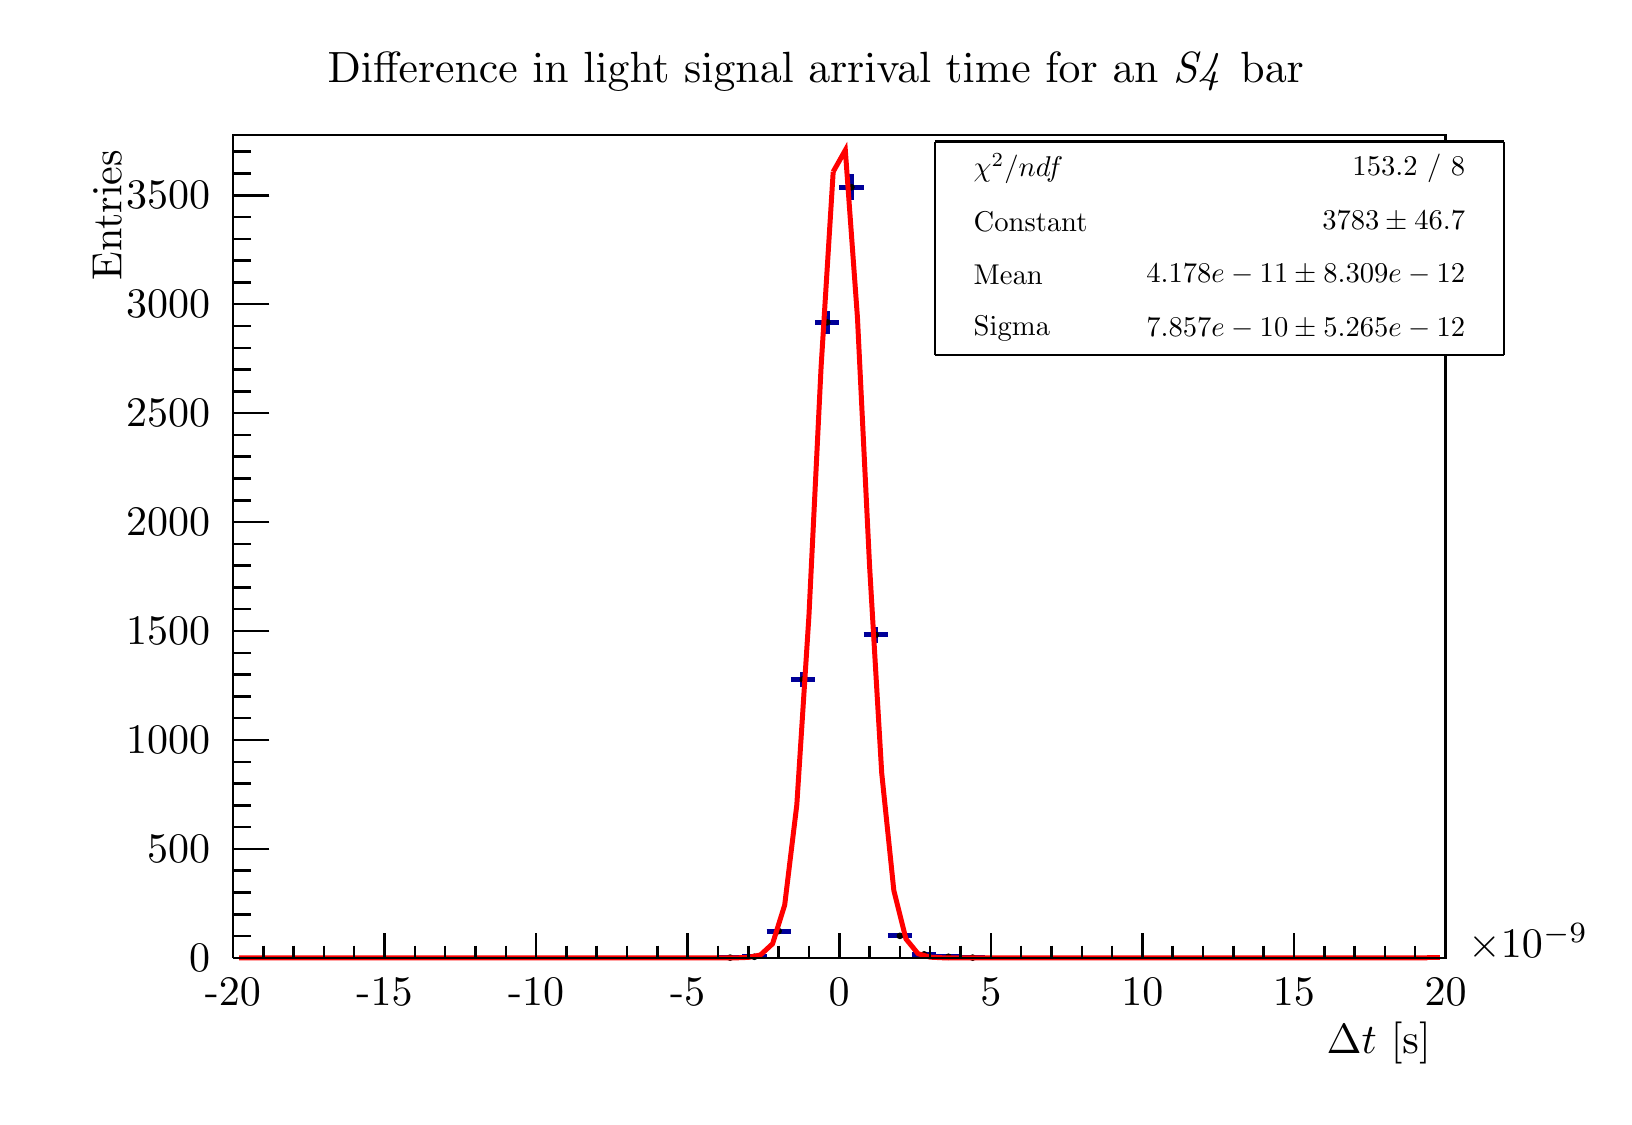
\begin{tikzpicture}
\pgfdeclareplotmark{cross} {
\pgfpathmoveto{\pgfpoint{-0.3\pgfplotmarksize}{\pgfplotmarksize}}
\pgfpathlineto{\pgfpoint{+0.3\pgfplotmarksize}{\pgfplotmarksize}}
\pgfpathlineto{\pgfpoint{+0.3\pgfplotmarksize}{0.3\pgfplotmarksize}}
\pgfpathlineto{\pgfpoint{+1\pgfplotmarksize}{0.3\pgfplotmarksize}}
\pgfpathlineto{\pgfpoint{+1\pgfplotmarksize}{-0.3\pgfplotmarksize}}
\pgfpathlineto{\pgfpoint{+0.3\pgfplotmarksize}{-0.3\pgfplotmarksize}}
\pgfpathlineto{\pgfpoint{+0.3\pgfplotmarksize}{-1.\pgfplotmarksize}}
\pgfpathlineto{\pgfpoint{-0.3\pgfplotmarksize}{-1.\pgfplotmarksize}}
\pgfpathlineto{\pgfpoint{-0.3\pgfplotmarksize}{-0.3\pgfplotmarksize}}
\pgfpathlineto{\pgfpoint{-1.\pgfplotmarksize}{-0.3\pgfplotmarksize}}
\pgfpathlineto{\pgfpoint{-1.\pgfplotmarksize}{0.3\pgfplotmarksize}}
\pgfpathlineto{\pgfpoint{-0.3\pgfplotmarksize}{0.3\pgfplotmarksize}}
\pgfpathclose
\pgfusepathqstroke
}
\pgfdeclareplotmark{cross*} {
\pgfpathmoveto{\pgfpoint{-0.3\pgfplotmarksize}{\pgfplotmarksize}}
\pgfpathlineto{\pgfpoint{+0.3\pgfplotmarksize}{\pgfplotmarksize}}
\pgfpathlineto{\pgfpoint{+0.3\pgfplotmarksize}{0.3\pgfplotmarksize}}
\pgfpathlineto{\pgfpoint{+1\pgfplotmarksize}{0.3\pgfplotmarksize}}
\pgfpathlineto{\pgfpoint{+1\pgfplotmarksize}{-0.3\pgfplotmarksize}}
\pgfpathlineto{\pgfpoint{+0.3\pgfplotmarksize}{-0.3\pgfplotmarksize}}
\pgfpathlineto{\pgfpoint{+0.3\pgfplotmarksize}{-1.\pgfplotmarksize}}
\pgfpathlineto{\pgfpoint{-0.3\pgfplotmarksize}{-1.\pgfplotmarksize}}
\pgfpathlineto{\pgfpoint{-0.3\pgfplotmarksize}{-0.3\pgfplotmarksize}}
\pgfpathlineto{\pgfpoint{-1.\pgfplotmarksize}{-0.3\pgfplotmarksize}}
\pgfpathlineto{\pgfpoint{-1.\pgfplotmarksize}{0.3\pgfplotmarksize}}
\pgfpathlineto{\pgfpoint{-0.3\pgfplotmarksize}{0.3\pgfplotmarksize}}
\pgfpathclose
\pgfusepathqfillstroke
}
\pgfdeclareplotmark{newstar} {
\pgfpathmoveto{\pgfqpoint{0pt}{\pgfplotmarksize}}
\pgfpathlineto{\pgfqpointpolar{44}{0.5\pgfplotmarksize}}
\pgfpathlineto{\pgfqpointpolar{18}{\pgfplotmarksize}}
\pgfpathlineto{\pgfqpointpolar{-20}{0.5\pgfplotmarksize}}
\pgfpathlineto{\pgfqpointpolar{-54}{\pgfplotmarksize}}
\pgfpathlineto{\pgfqpointpolar{-90}{0.5\pgfplotmarksize}}
\pgfpathlineto{\pgfqpointpolar{234}{\pgfplotmarksize}}
\pgfpathlineto{\pgfqpointpolar{198}{0.5\pgfplotmarksize}}
\pgfpathlineto{\pgfqpointpolar{162}{\pgfplotmarksize}}
\pgfpathlineto{\pgfqpointpolar{134}{0.5\pgfplotmarksize}}
\pgfpathclose
\pgfusepathqstroke
}
\pgfdeclareplotmark{newstar*} {
\pgfpathmoveto{\pgfqpoint{0pt}{\pgfplotmarksize}}
\pgfpathlineto{\pgfqpointpolar{44}{0.5\pgfplotmarksize}}
\pgfpathlineto{\pgfqpointpolar{18}{\pgfplotmarksize}}
\pgfpathlineto{\pgfqpointpolar{-20}{0.5\pgfplotmarksize}}
\pgfpathlineto{\pgfqpointpolar{-54}{\pgfplotmarksize}}
\pgfpathlineto{\pgfqpointpolar{-90}{0.5\pgfplotmarksize}}
\pgfpathlineto{\pgfqpointpolar{234}{\pgfplotmarksize}}
\pgfpathlineto{\pgfqpointpolar{198}{0.5\pgfplotmarksize}}
\pgfpathlineto{\pgfqpointpolar{162}{\pgfplotmarksize}}
\pgfpathlineto{\pgfqpointpolar{134}{0.5\pgfplotmarksize}}
\pgfpathclose
\pgfusepathqfillstroke
}
\definecolor{c}{rgb}{1,1,1};
\draw [color=c, fill=c] (0,0) rectangle (20,13.5705);
\draw [color=c, fill=c] (2.6,1.76416) rectangle (18,12.2134);
\definecolor{c}{rgb}{0,0,0};
\draw [c,line width=0.9] (2.6,1.76416) -- (2.6,12.2134) -- (18,12.2134) -- (18,1.76416) -- (2.6,1.76416);
\definecolor{c}{rgb}{1,1,1};
\draw [color=c, fill=c] (2.6,1.76416) rectangle (18,12.2134);
\definecolor{c}{rgb}{0,0,0};
\draw [c,line width=0.9] (2.6,1.76416) -- (2.6,12.2134) -- (18,12.2134) -- (18,1.76416) -- (2.6,1.76416);
\definecolor{c}{rgb}{0,0,0.6};
\draw [c,line width=1.8] (8.914,1.76416) -- (8.914,1.76693);
\draw [c,line width=1.8] (8.914,1.76693) -- (8.914,1.76969);
\draw [c,line width=1.8] (8.76,1.76693) -- (8.914,1.76693);
\draw [c,line width=1.8] (8.914,1.76693) -- (9.068,1.76693);
\definecolor{c}{rgb}{0,0,0};
\foreach \P in {(8.914,1.76693)}{\draw[mark options={color=c,fill=c},mark size=2.402402pt,mark=*,mark size=1pt] plot coordinates {\P};}
\definecolor{c}{rgb}{0,0,0.6};
\draw [c,line width=1.8] (9.222,1.77181) -- (9.222,1.77799);
\draw [c,line width=1.8] (9.222,1.77799) -- (9.222,1.78418);
\draw [c,line width=1.8] (9.068,1.77799) -- (9.222,1.77799);
\draw [c,line width=1.8] (9.222,1.77799) -- (9.376,1.77799);
\definecolor{c}{rgb}{0,0,0};
\foreach \P in {(9.222,1.77799)}{\draw[mark options={color=c,fill=c},mark size=2.402402pt,mark=*,mark size=1pt] plot coordinates {\P};}
\definecolor{c}{rgb}{0,0,0.6};
\draw [c,line width=1.8] (9.53,2.07382) -- (9.53,2.10451);
\draw [c,line width=1.8] (9.53,2.10451) -- (9.53,2.1352);
\draw [c,line width=1.8] (9.376,2.10451) -- (9.53,2.10451);
\draw [c,line width=1.8] (9.53,2.10451) -- (9.684,2.10451);
\definecolor{c}{rgb}{0,0,0};
\foreach \P in {(9.53,2.10451)}{\draw[mark options={color=c,fill=c},mark size=2.402402pt,mark=*,mark size=1pt] plot coordinates {\P};}
\definecolor{c}{rgb}{0,0,0.6};
\draw [c,line width=1.8] (9.838,5.20154) -- (9.838,5.30046);
\draw [c,line width=1.8] (9.838,5.30046) -- (9.838,5.39938);
\draw [c,line width=1.8] (9.684,5.30046) -- (9.838,5.30046);
\draw [c,line width=1.8] (9.838,5.30046) -- (9.992,5.30046);
\definecolor{c}{rgb}{0,0,0};
\foreach \P in {(9.838,5.30046)}{\draw[mark options={color=c,fill=c},mark size=2.402402pt,mark=*,mark size=1pt] plot coordinates {\P};}
\definecolor{c}{rgb}{0,0,0.6};
\draw [c,line width=1.8] (10.146,9.68623) -- (10.146,9.83568);
\draw [c,line width=1.8] (10.146,9.83568) -- (10.146,9.98513);
\draw [c,line width=1.8] (9.992,9.83568) -- (10.146,9.83568);
\draw [c,line width=1.8] (10.146,9.83568) -- (10.3,9.83568);
\definecolor{c}{rgb}{0,0,0};
\foreach \P in {(10.146,9.83568)}{\draw[mark options={color=c,fill=c},mark size=2.402402pt,mark=*,mark size=1pt] plot coordinates {\P};}
\definecolor{c}{rgb}{0,0,0.6};
\draw [c,line width=1.8] (10.454,11.3867) -- (10.454,11.5513);
\draw [c,line width=1.8] (10.454,11.5513) -- (10.454,11.7158);
\draw [c,line width=1.8] (10.3,11.5513) -- (10.454,11.5513);
\draw [c,line width=1.8] (10.454,11.5513) -- (10.608,11.5513);
\definecolor{c}{rgb}{0,0,0};
\foreach \P in {(10.454,11.5513)}{\draw[mark options={color=c,fill=c},mark size=2.402402pt,mark=*,mark size=1pt] plot coordinates {\P};}
\definecolor{c}{rgb}{0,0,0.6};
\draw [c,line width=1.8] (10.762,5.75842) -- (10.762,5.86495);
\draw [c,line width=1.8] (10.762,5.86495) -- (10.762,5.97147);
\draw [c,line width=1.8] (10.608,5.86495) -- (10.762,5.86495);
\draw [c,line width=1.8] (10.762,5.86495) -- (10.916,5.86495);
\definecolor{c}{rgb}{0,0,0};
\foreach \P in {(10.762,5.86495)}{\draw[mark options={color=c,fill=c},mark size=2.402402pt,mark=*,mark size=1pt] plot coordinates {\P};}
\definecolor{c}{rgb}{0,0,0.6};
\draw [c,line width=1.8] (11.07,2.01582) -- (11.07,2.04363);
\draw [c,line width=1.8] (11.07,2.04363) -- (11.07,2.07144);
\draw [c,line width=1.8] (10.916,2.04363) -- (11.07,2.04363);
\draw [c,line width=1.8] (11.07,2.04363) -- (11.224,2.04363);
\definecolor{c}{rgb}{0,0,0};
\foreach \P in {(11.07,2.04363)}{\draw[mark options={color=c,fill=c},mark size=2.402402pt,mark=*,mark size=1pt] plot coordinates {\P};}
\definecolor{c}{rgb}{0,0,0.6};
\draw [c,line width=1.8] (11.378,1.79736) -- (11.378,1.80843);
\draw [c,line width=1.8] (11.378,1.80843) -- (11.378,1.8195);
\draw [c,line width=1.8] (11.224,1.80843) -- (11.378,1.80843);
\draw [c,line width=1.8] (11.378,1.80843) -- (11.532,1.80843);
\definecolor{c}{rgb}{0,0,0};
\foreach \P in {(11.378,1.80843)}{\draw[mark options={color=c,fill=c},mark size=2.402402pt,mark=*,mark size=1pt] plot coordinates {\P};}
\definecolor{c}{rgb}{0,0,0.6};
\draw [c,line width=1.8] (11.686,1.77181) -- (11.686,1.77799);
\draw [c,line width=1.8] (11.686,1.77799) -- (11.686,1.78418);
\draw [c,line width=1.8] (11.532,1.77799) -- (11.686,1.77799);
\draw [c,line width=1.8] (11.686,1.77799) -- (11.84,1.77799);
\definecolor{c}{rgb}{0,0,0};
\foreach \P in {(11.686,1.77799)}{\draw[mark options={color=c,fill=c},mark size=2.402402pt,mark=*,mark size=1pt] plot coordinates {\P};}
\definecolor{c}{rgb}{0,0,0.6};
\draw [c,line width=1.8] (11.994,1.76416) -- (11.994,1.76693);
\draw [c,line width=1.8] (11.994,1.76693) -- (11.994,1.76969);
\draw [c,line width=1.8] (11.84,1.76693) -- (11.994,1.76693);
\draw [c,line width=1.8] (11.994,1.76693) -- (12.148,1.76693);
\definecolor{c}{rgb}{0,0,0};
\foreach \P in {(11.994,1.76693)}{\draw[mark options={color=c,fill=c},mark size=2.402402pt,mark=*,mark size=1pt] plot coordinates {\P};}
\definecolor{c}{rgb}{1,0,0};
\draw [c,line width=1.8] (2.677,1.76416) -- (2.831,1.76416) -- (2.985,1.76416) -- (3.139,1.76416) -- (3.293,1.76416) -- (3.447,1.76416) -- (3.601,1.76416) -- (3.755,1.76416) -- (3.909,1.76416) -- (4.063,1.76416) -- (4.217,1.76416) -- (4.371,1.76416)
 -- (4.525,1.76416) -- (4.679,1.76416) -- (4.833,1.76416) -- (4.987,1.76416) -- (5.141,1.76416) -- (5.295,1.76416) -- (5.449,1.76416) -- (5.603,1.76416) -- (5.757,1.76416) -- (5.911,1.76416) -- (6.065,1.76416) -- (6.219,1.76416) -- (6.373,1.76416) --
 (6.527,1.76416) -- (6.681,1.76416) -- (6.835,1.76416) -- (6.989,1.76416) -- (7.143,1.76416) -- (7.297,1.76416) -- (7.451,1.76416) -- (7.605,1.76416) -- (7.759,1.76416) -- (7.913,1.76416) -- (8.067,1.76416) -- (8.221,1.76416) -- (8.375,1.76416) --
 (8.529,1.76416) -- (8.683,1.76416) -- (8.837,1.76416) -- (8.991,1.76416) -- (9.145,1.76998) -- (9.299,1.80089) -- (9.453,1.94285) -- (9.607,2.43506) -- (9.761,3.70796) -- (9.915,6.11015) -- (10.069,9.26248) -- (10.223,11.7476);
\draw [c,line width=1.8] (10.223,11.7476) -- (10.377,12.0215) -- (10.531,9.89679) -- (10.685,6.74) -- (10.839,4.11347) -- (10.993,2.62012) -- (11.147,2.00482) -- (11.301,1.81637) -- (11.455,1.7729) -- (11.609,1.76529) -- (11.763,1.76416) --
 (11.917,1.76416) -- (12.071,1.76416) -- (12.225,1.76416) -- (12.379,1.76416) -- (12.533,1.76416) -- (12.687,1.76416) -- (12.841,1.76416) -- (12.995,1.76416) -- (13.149,1.76416) -- (13.303,1.76416) -- (13.457,1.76416) -- (13.611,1.76416) --
 (13.765,1.76416) -- (13.919,1.76416) -- (14.073,1.76416) -- (14.227,1.76416) -- (14.381,1.76416) -- (14.535,1.76416) -- (14.689,1.76416) -- (14.843,1.76416) -- (14.997,1.76416) -- (15.151,1.76416) -- (15.305,1.76416) -- (15.459,1.76416) --
 (15.613,1.76416) -- (15.767,1.76416) -- (15.921,1.76416) -- (16.075,1.76416) -- (16.229,1.76416) -- (16.383,1.76416) -- (16.537,1.76416) -- (16.691,1.76416) -- (16.845,1.76416) -- (16.999,1.76416) -- (17.153,1.76416) -- (17.307,1.76416) --
 (17.461,1.76416) -- (17.615,1.76416) -- (17.769,1.76416);
\draw [c,line width=1.8] (17.769,1.76416) -- (17.923,1.76416);
\definecolor{c}{rgb}{1,1,1};
\draw [color=c, fill=c] (11.5186,9.42152) rectangle (18.7393,12.1299);
\definecolor{c}{rgb}{0,0,0};
\draw [c,line width=0.9] (11.5186,9.42152) -- (18.7393,9.42152);
\draw [c,line width=0.9] (18.7393,9.42152) -- (18.7393,12.1299);
\draw [c,line width=0.9] (18.7393,12.1299) -- (11.5186,12.1299);
\draw [c,line width=0.9] (11.5186,12.1299) -- (11.5186,9.42152);
\draw [anchor= west] (11.8797,11.7913) node[scale=1.03301, color=c, rotate=0]{$\chi^{2} / ndf $};
\draw [anchor= east] (18.3782,11.7913) node[scale=1.03301, color=c, rotate=0]{ 153.2 / 8};
\draw [anchor= west] (11.8797,11.1142) node[scale=1.03301, color=c, rotate=0]{Constant };
\draw [anchor= east] (18.3782,11.1142) node[scale=1.03301, color=c, rotate=0]{$  3783 \pm 46.7$};
\draw [anchor= west] (11.8797,10.4371) node[scale=1.03301, color=c, rotate=0]{Mean     };
\draw [anchor= east] (18.3782,10.4371) node[scale=1.03301, color=c, rotate=0]{$ 4.178e-11 \pm 8.309e-12$};
\draw [anchor= west] (11.8797,9.76007) node[scale=1.03301, color=c, rotate=0]{Sigma    };
\draw [anchor= east] (18.3782,9.76007) node[scale=1.03301, color=c, rotate=0]{$ 7.857e-10 \pm 5.265e-12$};
\draw [c,line width=0.9] (2.6,1.76416) -- (18,1.76416);
\draw [c,line width=0.9] (2.6,2.07764) -- (2.6,1.76416);
\draw [c,line width=0.9] (2.985,1.9209) -- (2.985,1.76416);
\draw [c,line width=0.9] (3.37,1.9209) -- (3.37,1.76416);
\draw [c,line width=0.9] (3.755,1.9209) -- (3.755,1.76416);
\draw [c,line width=0.9] (4.14,1.9209) -- (4.14,1.76416);
\draw [c,line width=0.9] (4.525,2.07764) -- (4.525,1.76416);
\draw [c,line width=0.9] (4.91,1.9209) -- (4.91,1.76416);
\draw [c,line width=0.9] (5.295,1.9209) -- (5.295,1.76416);
\draw [c,line width=0.9] (5.68,1.9209) -- (5.68,1.76416);
\draw [c,line width=0.9] (6.065,1.9209) -- (6.065,1.76416);
\draw [c,line width=0.9] (6.45,2.07764) -- (6.45,1.76416);
\draw [c,line width=0.9] (6.835,1.9209) -- (6.835,1.76416);
\draw [c,line width=0.9] (7.22,1.9209) -- (7.22,1.76416);
\draw [c,line width=0.9] (7.605,1.9209) -- (7.605,1.76416);
\draw [c,line width=0.9] (7.99,1.9209) -- (7.99,1.76416);
\draw [c,line width=0.9] (8.375,2.07764) -- (8.375,1.76416);
\draw [c,line width=0.9] (8.76,1.9209) -- (8.76,1.76416);
\draw [c,line width=0.9] (9.145,1.9209) -- (9.145,1.76416);
\draw [c,line width=0.9] (9.53,1.9209) -- (9.53,1.76416);
\draw [c,line width=0.9] (9.915,1.9209) -- (9.915,1.76416);
\draw [c,line width=0.9] (10.3,2.07764) -- (10.3,1.76416);
\draw [c,line width=0.9] (10.685,1.9209) -- (10.685,1.76416);
\draw [c,line width=0.9] (11.07,1.9209) -- (11.07,1.76416);
\draw [c,line width=0.9] (11.455,1.9209) -- (11.455,1.76416);
\draw [c,line width=0.9] (11.84,1.9209) -- (11.84,1.76416);
\draw [c,line width=0.9] (12.225,2.07764) -- (12.225,1.76416);
\draw [c,line width=0.9] (12.61,1.9209) -- (12.61,1.76416);
\draw [c,line width=0.9] (12.995,1.9209) -- (12.995,1.76416);
\draw [c,line width=0.9] (13.38,1.9209) -- (13.38,1.76416);
\draw [c,line width=0.9] (13.765,1.9209) -- (13.765,1.76416);
\draw [c,line width=0.9] (14.15,2.07764) -- (14.15,1.76416);
\draw [c,line width=0.9] (14.535,1.9209) -- (14.535,1.76416);
\draw [c,line width=0.9] (14.92,1.9209) -- (14.92,1.76416);
\draw [c,line width=0.9] (15.305,1.9209) -- (15.305,1.76416);
\draw [c,line width=0.9] (15.69,1.9209) -- (15.69,1.76416);
\draw [c,line width=0.9] (16.075,2.07764) -- (16.075,1.76416);
\draw [c,line width=0.9] (16.46,1.9209) -- (16.46,1.76416);
\draw [c,line width=0.9] (16.845,1.9209) -- (16.845,1.76416);
\draw [c,line width=0.9] (17.23,1.9209) -- (17.23,1.76416);
\draw [c,line width=0.9] (17.615,1.9209) -- (17.615,1.76416);
\draw [c,line width=0.9] (18,2.07764) -- (18,1.76416);
\draw [anchor=base] (2.6,1.15349) node[scale=1.51913, color=c, rotate=0]{-20};
\draw [anchor=base] (4.525,1.15349) node[scale=1.51913, color=c, rotate=0]{-15};
\draw [anchor=base] (6.45,1.15349) node[scale=1.51913, color=c, rotate=0]{-10};
\draw [anchor=base] (8.375,1.15349) node[scale=1.51913, color=c, rotate=0]{-5};
\draw [anchor=base] (10.3,1.15349) node[scale=1.51913, color=c, rotate=0]{0};
\draw [anchor=base] (12.225,1.15349) node[scale=1.51913, color=c, rotate=0]{5};
\draw [anchor=base] (14.15,1.15349) node[scale=1.51913, color=c, rotate=0]{10};
\draw [anchor=base] (16.075,1.15349) node[scale=1.51913, color=c, rotate=0]{15};
\draw [anchor=base] (18,1.15349) node[scale=1.51913, color=c, rotate=0]{20};
\draw [anchor=base west] (18.1,1.76416) node[scale=1.51913, color=c, rotate=0]{$\times10^{-9}$};
\draw [anchor= east] (18,0.678523) node[scale=1.51913, color=c, rotate=0]{$\Delta t$ [s]};
\draw [c,line width=0.9] (2.6,1.76416) -- (2.6,12.2134);
\draw [c,line width=0.9] (3.062,1.76416) -- (2.6,1.76416);
\draw [c,line width=0.9] (2.831,2.04086) -- (2.6,2.04086);
\draw [c,line width=0.9] (2.831,2.31757) -- (2.6,2.31757);
\draw [c,line width=0.9] (2.831,2.59428) -- (2.6,2.59428);
\draw [c,line width=0.9] (2.831,2.87098) -- (2.6,2.87098);
\draw [c,line width=0.9] (3.062,3.14769) -- (2.6,3.14769);
\draw [c,line width=0.9] (2.831,3.4244) -- (2.6,3.4244);
\draw [c,line width=0.9] (2.831,3.7011) -- (2.6,3.7011);
\draw [c,line width=0.9] (2.831,3.97781) -- (2.6,3.97781);
\draw [c,line width=0.9] (2.831,4.25451) -- (2.6,4.25451);
\draw [c,line width=0.9] (3.062,4.53122) -- (2.6,4.53122);
\draw [c,line width=0.9] (2.831,4.80793) -- (2.6,4.80793);
\draw [c,line width=0.9] (2.831,5.08463) -- (2.6,5.08463);
\draw [c,line width=0.9] (2.831,5.36134) -- (2.6,5.36134);
\draw [c,line width=0.9] (2.831,5.63805) -- (2.6,5.63805);
\draw [c,line width=0.9] (3.062,5.91475) -- (2.6,5.91475);
\draw [c,line width=0.9] (2.831,6.19146) -- (2.6,6.19146);
\draw [c,line width=0.9] (2.831,6.46816) -- (2.6,6.46816);
\draw [c,line width=0.9] (2.831,6.74487) -- (2.6,6.74487);
\draw [c,line width=0.9] (2.831,7.02158) -- (2.6,7.02158);
\draw [c,line width=0.9] (3.062,7.29828) -- (2.6,7.29828);
\draw [c,line width=0.9] (2.831,7.57499) -- (2.6,7.57499);
\draw [c,line width=0.9] (2.831,7.8517) -- (2.6,7.8517);
\draw [c,line width=0.9] (2.831,8.1284) -- (2.6,8.1284);
\draw [c,line width=0.9] (2.831,8.40511) -- (2.6,8.40511);
\draw [c,line width=0.9] (3.062,8.68182) -- (2.6,8.68182);
\draw [c,line width=0.9] (2.831,8.95852) -- (2.6,8.95852);
\draw [c,line width=0.9] (2.831,9.23523) -- (2.6,9.23523);
\draw [c,line width=0.9] (2.831,9.51193) -- (2.6,9.51193);
\draw [c,line width=0.9] (2.831,9.78864) -- (2.6,9.78864);
\draw [c,line width=0.9] (3.062,10.0653) -- (2.6,10.0653);
\draw [c,line width=0.9] (2.831,10.3421) -- (2.6,10.3421);
\draw [c,line width=0.9] (2.831,10.6188) -- (2.6,10.6188);
\draw [c,line width=0.9] (2.831,10.8955) -- (2.6,10.8955);
\draw [c,line width=0.9] (2.831,11.1722) -- (2.6,11.1722);
\draw [c,line width=0.9] (3.062,11.4489) -- (2.6,11.4489);
\draw [c,line width=0.9] (3.062,11.4489) -- (2.6,11.4489);
\draw [c,line width=0.9] (2.831,11.7256) -- (2.6,11.7256);
\draw [c,line width=0.9] (2.831,12.0023) -- (2.6,12.0023);
\draw [anchor= east] (2.5,1.76416) node[scale=1.51913, color=c, rotate=0]{0};
\draw [anchor= east] (2.5,3.14769) node[scale=1.51913, color=c, rotate=0]{500};
\draw [anchor= east] (2.5,4.53122) node[scale=1.51913, color=c, rotate=0]{1000};
\draw [anchor= east] (2.5,5.91475) node[scale=1.51913, color=c, rotate=0]{1500};
\draw [anchor= east] (2.5,7.29828) node[scale=1.51913, color=c, rotate=0]{2000};
\draw [anchor= east] (2.5,8.68182) node[scale=1.51913, color=c, rotate=0]{2500};
\draw [anchor= east] (2.5,10.0653) node[scale=1.51913, color=c, rotate=0]{3000};
\draw [anchor= east] (2.5,11.4489) node[scale=1.51913, color=c, rotate=0]{3500};
\draw [anchor= east] (1,12.2134) node[scale=1.51913, color=c, rotate=90]{Entries};
\definecolor{c}{rgb}{1,1,1};
\draw [color=c, fill=c] (11.5186,9.42152) rectangle (18.7393,12.1299);
\definecolor{c}{rgb}{0,0,0};
\draw [c,line width=0.9] (11.5186,9.42152) -- (18.7393,9.42152);
\draw [c,line width=0.9] (18.7393,9.42152) -- (18.7393,12.1299);
\draw [c,line width=0.9] (18.7393,12.1299) -- (11.5186,12.1299);
\draw [c,line width=0.9] (11.5186,12.1299) -- (11.5186,9.42152);
\draw [anchor= west] (11.8797,11.7913) node[scale=1.03301, color=c, rotate=0]{$\chi^{2} / ndf $};
\draw [anchor= east] (18.3782,11.7913) node[scale=1.03301, color=c, rotate=0]{ 153.2 / 8};
\draw [anchor= west] (11.8797,11.1142) node[scale=1.03301, color=c, rotate=0]{Constant };
\draw [anchor= east] (18.3782,11.1142) node[scale=1.03301, color=c, rotate=0]{$  3783 \pm 46.7$};
\draw [anchor= west] (11.8797,10.4371) node[scale=1.03301, color=c, rotate=0]{Mean     };
\draw [anchor= east] (18.3782,10.4371) node[scale=1.03301, color=c, rotate=0]{$ 4.178e-11 \pm 8.309e-12$};
\draw [anchor= west] (11.8797,9.76007) node[scale=1.03301, color=c, rotate=0]{Sigma    };
\draw [anchor= east] (18.3782,9.76007) node[scale=1.03301, color=c, rotate=0]{$ 7.857e-10 \pm 5.265e-12$};
\draw (10,13.0186) node[scale=1.5799, color=c, rotate=0]{Difference in light signal arrival time for an $\mathit{S4}$ bar};
\end{tikzpicture}

	\end{adjustbox}
	\caption{Difference in signal arrival time PMTs at each end of a bar as measured using a $^{90}$Sr source placed 64~cm from one end of the bar.}
	\label{fig:s4Res}	
\end{figure}

\begin{figure}[ht]    
  \begin{minipage}[t]{.48\textwidth}
    \centering
    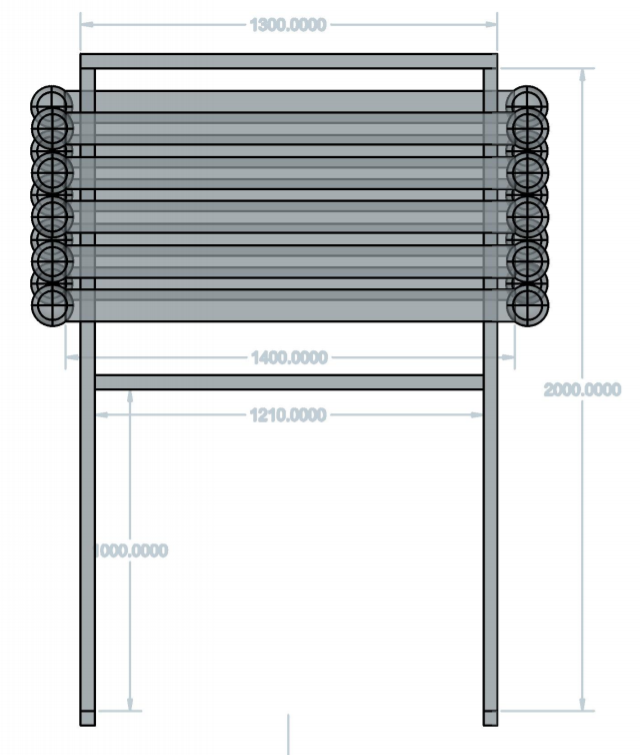
\includegraphics[width=0.6\linewidth]{files/Figures/dstofFront.png}
    \caption{Front view of the downstream time of flight system}
    \label{fig:dstofFront}
  \end{minipage}
  \hspace{0.3cm}
  \begin{minipage}[t]{.48\textwidth}
    \centering
    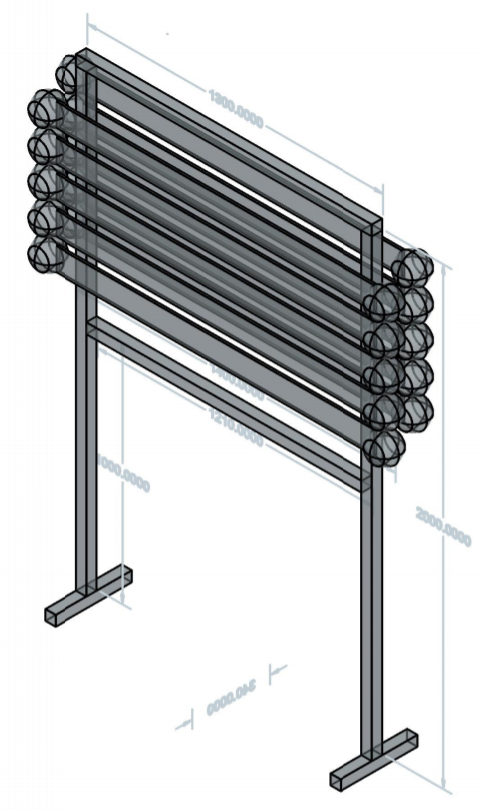
\includegraphics[width=0.45\linewidth]{files/Figures/dstofDiag.png}
    \caption{Diagonal view of the downstream time of flight system showing more clearly the two rows of scintillator bars and photomultiplier tubes}
    \label{fig:dstofDiagonal}
  \end{minipage}
\end{figure}

The anode signals of all 20 of the PMTs are discriminated using LeCroy 620AL NIM discriminators, at a threshold of 20~mV.
The discriminated signals are then fed into a time-to-digital converter. A signal in $\mathit{S4}$ is deemed to have occurred if a signal is seen in both PMTs, above the discriminator threshold, on the same bar within 20~ns of each other. 
This timing window is determined through testing performed with a $^{90}$Sr source at known positions on the bar.

The $\mathit{S1-S2}$ coincidence signal is digitized by the same time-to-digital converter. This signal is used to calculate the particle time of flight from $\mathit{S2}$ to $\mathit{S4}$.

\subsection{The HPTPC Prototype}
The steel vessel is rated to 6~barA of pressure, and the walls of the vessel are 1~cm thick.
The TPC comprised thin steel mesh electrodes (one cathode and three anodes), and 12 copper rings to create the uniform drift field.
The drift distance produced was 48~cm, with the anodes separated by 1~mm. Data taking with the TPC made use of both optical and charge readout.
The vessel, electrodes, and drift region of the TPC are shown in figure~\ref{fig:TPC}.

\begin{figure}
  \centering
  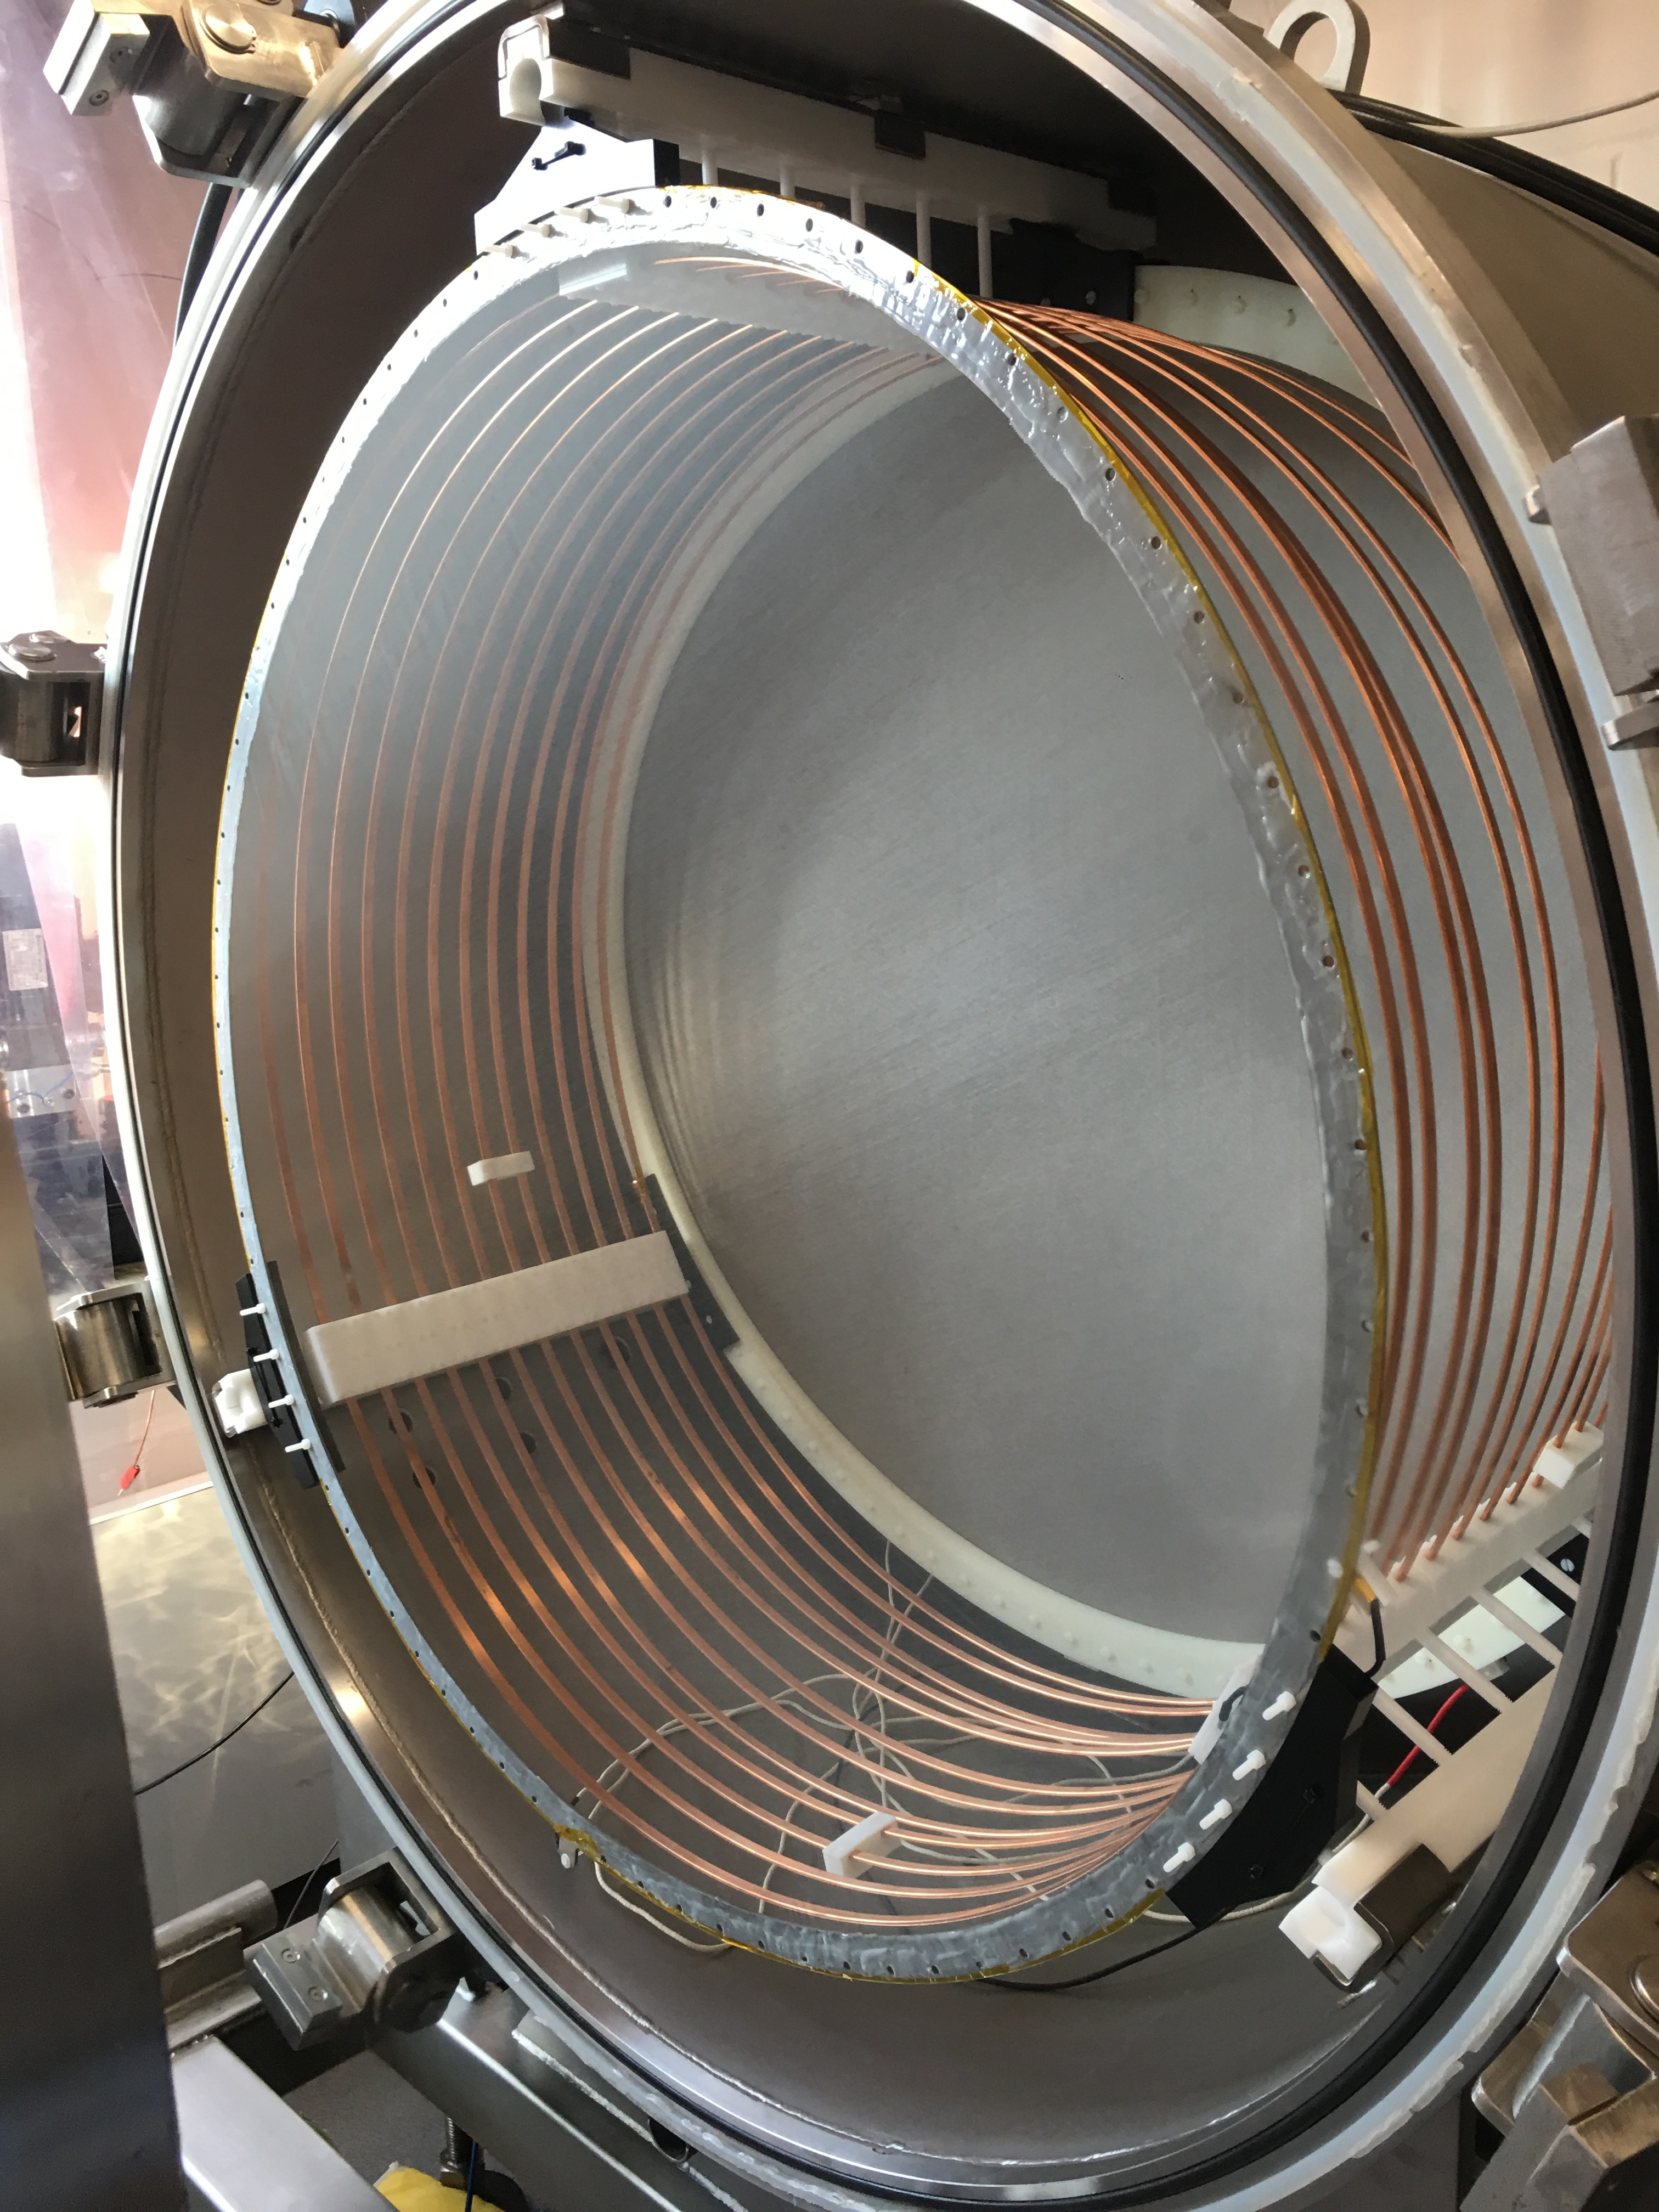
\includegraphics[width=0.6\linewidth]{files/Figures/IMG_1194.jpg}
  \caption{Cross-sectional view of the TPC; the thin mesh electrodes and copper ring drift volume can be seen inside the steel vessel}
  \label{fig:TPC}
  \todo[inline]{TOBY: "A head on shot would show the relevant information better."}
  \todo[inline]{TOBY: "This caption needs to give the important quantitative info for the ToF analysis, eg. wall thickness, separation of walls at the height of the beam centre, the distance from the inside of the upstream wall to the drift region, etc"}
\end{figure}

%The centre of the TPC was placed 13~m from the beam entrance with \textit{S3} and \textit{S4} directly upstream and downstream of the vessel, respectively. 
In the coordinate system shown in Figure~\ref{fig:setup}, the TPC centre lies at $X=10.82~\text{m}$, $Y=0.5593~\text{m}$, $Z=-0.0114~\text{m}$. 
\todo[inline]{Description of coordinate system needs to go in to make this clear.}
Throughout the run, the TPC was filled with either pure argon, or a combination of argon and a small percentage of quencher. 
The performance of this TPC is the subject of a forthcoming publication.

\section{Analysis}
\label{hptpcPaper:sec:Analysis}
\subsection{Analysis Goals}

The primary aims of the use of $\mathit{S1} - \mathit{S4}$ were as follows: to assess the feasibility of using this combination of off-axis positioning and a moderated beam at the PS to produce the momenta of most relevance to neutrino cross-section studies and to characterize the incident flux on the TPC and exiting the TPC, for the TPC data analysis. \todo[inline]{TOBY, I rewrote this paragraph in line with the comments. This ok with you?}

%Protons take longer to travel the distance from \textit{S1} to \textit{S3} or \textit{S4} than lighter particles that are close to being minimum ionising.
%This difference in time of flight can be used to distinguish between the two types of particles.
%Distinguishing these MIPs from one another is more difficult due to their similar masses and can be only determined by the upstream ToF system.
%From the particle flux data, it is possible to measure the ratio of protons to other particles over the range of off-axis angles covered by the \textit{S3} and \textit{S4} walls, and for varying numbers of moderator blocks.

A particle of mass $m$ with momentum $p$ travelling over a distance $d$ will traverse said distance in a time
\begin{align}
	t = d \sqrt{\frac{m^2}{p^2} + \frac{1}{c^2}}
\end{align}
where $c$ is the speed of light in a vacuum.
Therefore, particles with a greater momentum or smaller mass will cross the same distance in a shorter time.
This means that, if there exists a beam of particles of different species but with the same momenta (as is produced by the PS), the mass of of a particle can be determined by measuring this time of flight, $t$.

For example, a charged pion with a momentum of 0.8~GeV/c will have a time of flight from $\mathit{S1}$ to $\mathit{S3}$ (a distance of 10.9~m) of 37~ns, while a proton with the same momentum will have a time of flight of 56~ns.
For the same two particles travelling between $\mathit{S2}$ and $\mathit{S4}$ (a distance of 12.6~m), the charged pion would have a time of flight of 43~ns and the proton would have a time of flight of 65~ns.
\todo[inline]{Add error bars to these numbers.}

The variation of momentum spectrum, proton-MIP ratio, and proton multiplicity with differing numbers of acrylic blocks as a function of angle off the beam axis provide the motivation for the measurement techniques used.
As such the data used in these results cover two days in the run where the number of moderator blocks was varied with other beam properties held approximately constant.
The numbers of spills per moderator block are shown in Table~\ref{tab:spills} (with more data taken for 4 blocks as that was the configuration used for the majority of the beam test).

\begin{table}
  \centering
  \begin{tabular}{|c|c|}
    \hline
    Number of moderator blocks & Recorded spills \\
    \hline
    0 & 257 \\
    1 & 254 \\
    2 & 267 \\
    3 & 220 \\
    4 & 3884 \\
    \hline
  \end{tabular}
  \caption{The number of spills recorded for each moderator block configuration}
  \label{tab:spills}
\end{table}

\subsection{Analysis Methods}

Figure~\ref{fig:s3tof} shows the time of flight spectrum recorded in the $\mathit{S3}$ timing point for varying numbers of moderator blocks.
The quicker peak is formed by minimum ionizing particles, while the peak at higher values of $\mathit{S3} - \mathit{S1}$ corresponds to protons.
The black, 0 block peak ranging from 90 to 100~ns corresponds to deuterons.
\begin{figure}[h]
  \begin{adjustbox}{max totalsize={.8\textwidth}{.5\textheight},center}
    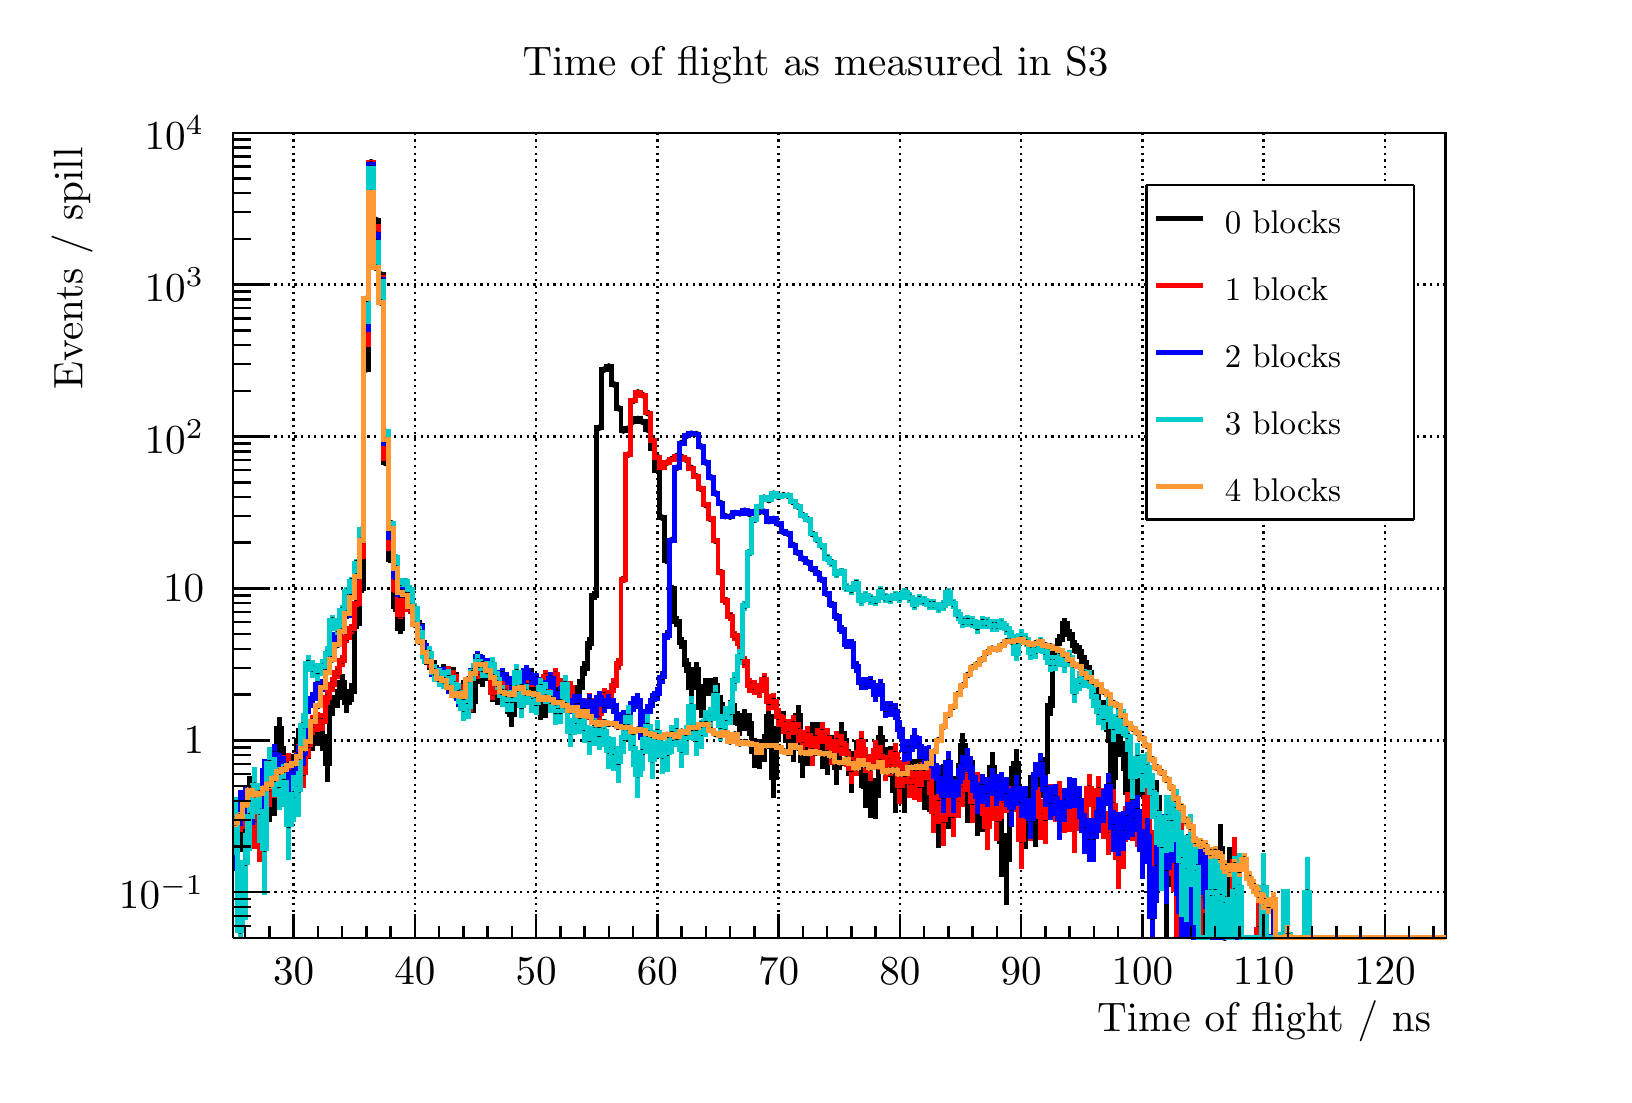
\begin{tikzpicture}
\pgfdeclareplotmark{cross} {
\pgfpathmoveto{\pgfpoint{-0.3\pgfplotmarksize}{\pgfplotmarksize}}
\pgfpathlineto{\pgfpoint{+0.3\pgfplotmarksize}{\pgfplotmarksize}}
\pgfpathlineto{\pgfpoint{+0.3\pgfplotmarksize}{0.3\pgfplotmarksize}}
\pgfpathlineto{\pgfpoint{+1\pgfplotmarksize}{0.3\pgfplotmarksize}}
\pgfpathlineto{\pgfpoint{+1\pgfplotmarksize}{-0.3\pgfplotmarksize}}
\pgfpathlineto{\pgfpoint{+0.3\pgfplotmarksize}{-0.3\pgfplotmarksize}}
\pgfpathlineto{\pgfpoint{+0.3\pgfplotmarksize}{-1.\pgfplotmarksize}}
\pgfpathlineto{\pgfpoint{-0.3\pgfplotmarksize}{-1.\pgfplotmarksize}}
\pgfpathlineto{\pgfpoint{-0.3\pgfplotmarksize}{-0.3\pgfplotmarksize}}
\pgfpathlineto{\pgfpoint{-1.\pgfplotmarksize}{-0.3\pgfplotmarksize}}
\pgfpathlineto{\pgfpoint{-1.\pgfplotmarksize}{0.3\pgfplotmarksize}}
\pgfpathlineto{\pgfpoint{-0.3\pgfplotmarksize}{0.3\pgfplotmarksize}}
\pgfpathclose
\pgfusepathqstroke
}
\pgfdeclareplotmark{cross*} {
\pgfpathmoveto{\pgfpoint{-0.3\pgfplotmarksize}{\pgfplotmarksize}}
\pgfpathlineto{\pgfpoint{+0.3\pgfplotmarksize}{\pgfplotmarksize}}
\pgfpathlineto{\pgfpoint{+0.3\pgfplotmarksize}{0.3\pgfplotmarksize}}
\pgfpathlineto{\pgfpoint{+1\pgfplotmarksize}{0.3\pgfplotmarksize}}
\pgfpathlineto{\pgfpoint{+1\pgfplotmarksize}{-0.3\pgfplotmarksize}}
\pgfpathlineto{\pgfpoint{+0.3\pgfplotmarksize}{-0.3\pgfplotmarksize}}
\pgfpathlineto{\pgfpoint{+0.3\pgfplotmarksize}{-1.\pgfplotmarksize}}
\pgfpathlineto{\pgfpoint{-0.3\pgfplotmarksize}{-1.\pgfplotmarksize}}
\pgfpathlineto{\pgfpoint{-0.3\pgfplotmarksize}{-0.3\pgfplotmarksize}}
\pgfpathlineto{\pgfpoint{-1.\pgfplotmarksize}{-0.3\pgfplotmarksize}}
\pgfpathlineto{\pgfpoint{-1.\pgfplotmarksize}{0.3\pgfplotmarksize}}
\pgfpathlineto{\pgfpoint{-0.3\pgfplotmarksize}{0.3\pgfplotmarksize}}
\pgfpathclose
\pgfusepathqfillstroke
}
\pgfdeclareplotmark{newstar} {
\pgfpathmoveto{\pgfqpoint{0pt}{\pgfplotmarksize}}
\pgfpathlineto{\pgfqpointpolar{44}{0.5\pgfplotmarksize}}
\pgfpathlineto{\pgfqpointpolar{18}{\pgfplotmarksize}}
\pgfpathlineto{\pgfqpointpolar{-20}{0.5\pgfplotmarksize}}
\pgfpathlineto{\pgfqpointpolar{-54}{\pgfplotmarksize}}
\pgfpathlineto{\pgfqpointpolar{-90}{0.5\pgfplotmarksize}}
\pgfpathlineto{\pgfqpointpolar{234}{\pgfplotmarksize}}
\pgfpathlineto{\pgfqpointpolar{198}{0.5\pgfplotmarksize}}
\pgfpathlineto{\pgfqpointpolar{162}{\pgfplotmarksize}}
\pgfpathlineto{\pgfqpointpolar{134}{0.5\pgfplotmarksize}}
\pgfpathclose
\pgfusepathqstroke
}
\pgfdeclareplotmark{newstar*} {
\pgfpathmoveto{\pgfqpoint{0pt}{\pgfplotmarksize}}
\pgfpathlineto{\pgfqpointpolar{44}{0.5\pgfplotmarksize}}
\pgfpathlineto{\pgfqpointpolar{18}{\pgfplotmarksize}}
\pgfpathlineto{\pgfqpointpolar{-20}{0.5\pgfplotmarksize}}
\pgfpathlineto{\pgfqpointpolar{-54}{\pgfplotmarksize}}
\pgfpathlineto{\pgfqpointpolar{-90}{0.5\pgfplotmarksize}}
\pgfpathlineto{\pgfqpointpolar{234}{\pgfplotmarksize}}
\pgfpathlineto{\pgfqpointpolar{198}{0.5\pgfplotmarksize}}
\pgfpathlineto{\pgfqpointpolar{162}{\pgfplotmarksize}}
\pgfpathlineto{\pgfqpointpolar{134}{0.5\pgfplotmarksize}}
\pgfpathclose
\pgfusepathqfillstroke
}
\definecolor{c}{rgb}{1,1,1};
\draw [color=c, fill=c] (0,0) rectangle (20,13.2798);
\draw [color=c, fill=c] (2.6,1.72637) rectangle (18,11.9518);
\definecolor{c}{rgb}{0,0,0};
\draw [c,line width=0.9] (2.6,1.72637) -- (2.6,11.9518) -- (18,11.9518) -- (18,1.72637) -- (2.6,1.72637);
\definecolor{c}{rgb}{1,1,1};
\draw [color=c, fill=c] (2.6,1.72637) rectangle (18,11.9518);
\definecolor{c}{rgb}{0,0,0};
\draw [c,line width=0.9] (2.6,1.72637) -- (2.6,11.9518) -- (18,11.9518) -- (18,1.72637) -- (2.6,1.72637);
\draw [c,line width=0.9] (2.6,1.72637) -- (18,1.72637);
\draw [c,dash pattern=on 0.80pt off 1.60pt ,line width=0.9] (3.37,11.9518) -- (3.37,1.72637);
\draw [c,dash pattern=on 0.80pt off 1.60pt ,line width=0.9] (4.91,11.9518) -- (4.91,1.72637);
\draw [c,dash pattern=on 0.80pt off 1.60pt ,line width=0.9] (6.45,11.9518) -- (6.45,1.72637);
\draw [c,dash pattern=on 0.80pt off 1.60pt ,line width=0.9] (7.99,11.9518) -- (7.99,1.72637);
\draw [c,dash pattern=on 0.80pt off 1.60pt ,line width=0.9] (9.53,11.9518) -- (9.53,1.72637);
\draw [c,dash pattern=on 0.80pt off 1.60pt ,line width=0.9] (11.07,11.9518) -- (11.07,1.72637);
\draw [c,dash pattern=on 0.80pt off 1.60pt ,line width=0.9] (12.61,11.9518) -- (12.61,1.72637);
\draw [c,dash pattern=on 0.80pt off 1.60pt ,line width=0.9] (14.15,11.9518) -- (14.15,1.72637);
\draw [c,dash pattern=on 0.80pt off 1.60pt ,line width=0.9] (15.69,11.9518) -- (15.69,1.72637);
\draw [c,dash pattern=on 0.80pt off 1.60pt ,line width=0.9] (17.23,11.9518) -- (17.23,1.72637);
\draw [c,dash pattern=on 0.80pt off 1.60pt ,line width=0.9] (3.37,11.9518) -- (3.37,1.72637);
\draw [c,dash pattern=on 0.80pt off 1.60pt ,line width=0.9] (17.23,11.9518) -- (17.23,1.72637);
\draw [c,line width=0.9] (2.6,1.72637) -- (2.6,11.9518);
\draw [c,dash pattern=on 0.80pt off 1.60pt ,line width=0.9] (18,2.30705) -- (2.6,2.30705);
\draw [c,dash pattern=on 0.80pt off 1.60pt ,line width=0.9] (18,4.236) -- (2.6,4.236);
\draw [c,dash pattern=on 0.80pt off 1.60pt ,line width=0.9] (18,6.16495) -- (2.6,6.16495);
\draw [c,dash pattern=on 0.80pt off 1.60pt ,line width=0.9] (18,8.0939) -- (2.6,8.0939);
\draw [c,dash pattern=on 0.80pt off 1.60pt ,line width=0.9] (18,10.0229) -- (2.6,10.0229);
\draw [c,dash pattern=on 0.80pt off 1.60pt ,line width=0.9] (18,11.9518) -- (2.6,11.9518);
\definecolor{c}{rgb}{0,0,0.6};
\draw [c,line width=0.9] (2.6,1.72637) -- (2.6616,1.72637) -- (2.6616,1.72637) -- (2.7232,1.72637) -- (2.7232,1.72637) -- (2.7848,1.72637) -- (2.7848,1.72637) -- (2.8464,1.72637) -- (2.8464,1.72637) -- (2.908,1.72637) -- (2.908,1.72637) --
 (2.9696,1.72637) -- (2.9696,1.72637) -- (3.0312,1.72637) -- (3.0312,1.72637) -- (3.0928,1.72637) -- (3.0928,1.72637) -- (3.1544,1.72637) -- (3.1544,1.72637) -- (3.216,1.72637) -- (3.216,1.72637) -- (3.2776,1.72637) -- (3.2776,1.72637) --
 (3.3392,1.72637) -- (3.3392,1.72637) -- (3.4008,1.72637) -- (3.4008,1.72637) -- (3.4624,1.72637) -- (3.4624,1.72637) -- (3.524,1.72637) -- (3.524,1.72637) -- (3.5856,1.72637) -- (3.5856,1.72637) -- (3.6472,1.72637) -- (3.6472,1.72637) --
 (3.7088,1.72637) -- (3.7088,1.72637) -- (3.7704,1.72637) -- (3.7704,1.72637) -- (3.832,1.72637) -- (3.832,1.72637) -- (3.8936,1.72637) -- (3.8936,1.72637) -- (3.9552,1.72637) -- (3.9552,1.72637) -- (4.0168,1.72637) -- (4.0168,1.72637) --
 (4.0784,1.72637) -- (4.0784,1.72637) -- (4.14,1.72637) -- (4.14,1.72637) -- (4.2016,1.72637) -- (4.2016,1.72637) -- (4.2632,1.72637) -- (4.2632,1.72637) -- (4.3248,1.72637) -- (4.3248,1.72637) -- (4.3864,1.72637) -- (4.3864,1.72637) --
 (4.448,1.72637) -- (4.448,1.72637) -- (4.5096,1.72637) -- (4.5096,1.72637) -- (4.5712,1.72637) -- (4.5712,1.72637) -- (4.6328,1.72637) -- (4.6328,1.72637) -- (4.6944,1.72637) -- (4.6944,1.72637) -- (4.756,1.72637) -- (4.756,1.72637) --
 (4.8176,1.72637) -- (4.8176,1.72637) -- (4.8792,1.72637) -- (4.8792,1.72637) -- (4.9408,1.72637) -- (4.9408,1.72637) -- (5.0024,1.72637) -- (5.0024,1.72637) -- (5.064,1.72637) -- (5.064,1.72637) -- (5.1256,1.72637) -- (5.1256,1.72637) --
 (5.1872,1.72637) -- (5.1872,1.72637) -- (5.2488,1.72637) -- (5.2488,1.72637) -- (5.3104,1.72637) -- (5.3104,1.72637) -- (5.372,1.72637) -- (5.372,1.72637) -- (5.4336,1.72637) -- (5.4336,1.72637) -- (5.4952,1.72637) -- (5.4952,1.72637) --
 (5.5568,1.72637) -- (5.5568,1.72637) -- (5.6184,1.72637) -- (5.6184,1.72637) -- (5.68,1.72637) -- (5.68,1.72637) -- (5.7416,1.72637) -- (5.7416,1.72637) -- (5.8032,1.72637) -- (5.8032,1.72637) -- (5.8648,1.72637) -- (5.8648,1.72637) --
 (5.9264,1.72637) -- (5.9264,1.72637) -- (5.988,1.72637) -- (5.988,1.72637) -- (6.0496,1.72637) -- (6.0496,1.72637) -- (6.1112,1.72637) -- (6.1112,1.72637) -- (6.1728,1.72637) -- (6.1728,1.72637) -- (6.2344,1.72637) -- (6.2344,1.72637) --
 (6.296,1.72637) -- (6.296,1.72637) -- (6.3576,1.72637) -- (6.3576,1.72637) -- (6.4192,1.72637) -- (6.4192,1.72637) -- (6.4808,1.72637) -- (6.4808,1.72637) -- (6.5424,1.72637) -- (6.5424,1.72637) -- (6.604,1.72637) -- (6.604,1.72637) --
 (6.6656,1.72637) -- (6.6656,1.72637) -- (6.7272,1.72637) -- (6.7272,1.72637) -- (6.7888,1.72637) -- (6.7888,1.72637) -- (6.8504,1.72637) -- (6.8504,1.72637) -- (6.912,1.72637) -- (6.912,1.72637) -- (6.9736,1.72637) -- (6.9736,1.72637) --
 (7.0352,1.72637) -- (7.0352,1.72637) -- (7.0968,1.72637) -- (7.0968,1.72637) -- (7.1584,1.72637) -- (7.1584,1.72637) -- (7.22,1.72637) -- (7.22,1.72637) -- (7.2816,1.72637) -- (7.2816,1.72637) -- (7.3432,1.72637) -- (7.3432,1.72637) --
 (7.4048,1.72637) -- (7.4048,1.72637) -- (7.4664,1.72637) -- (7.4664,1.72637) -- (7.528,1.72637) -- (7.528,1.72637) -- (7.5896,1.72637) -- (7.5896,1.72637) -- (7.6512,1.72637) -- (7.6512,1.72637) -- (7.7128,1.72637) -- (7.7128,1.72637) --
 (7.7744,1.72637) -- (7.7744,1.72637) -- (7.836,1.72637) -- (7.836,1.72637) -- (7.8976,1.72637) -- (7.8976,1.72637) -- (7.9592,1.72637) -- (7.9592,1.72637) -- (8.0208,1.72637) -- (8.0208,1.72637) -- (8.0824,1.72637) -- (8.0824,1.72637) --
 (8.144,1.72637) -- (8.144,1.72637) -- (8.2056,1.72637) -- (8.2056,1.72637) -- (8.2672,1.72637) -- (8.2672,1.72637) -- (8.3288,1.72637) -- (8.3288,1.72637) -- (8.3904,1.72637) -- (8.3904,1.72637) -- (8.452,1.72637) -- (8.452,1.72637) --
 (8.5136,1.72637) -- (8.5136,1.72637) -- (8.5752,1.72637) -- (8.5752,1.72637) -- (8.6368,1.72637) -- (8.6368,1.72637) -- (8.6984,1.72637) -- (8.6984,1.72637) -- (8.76,1.72637) -- (8.76,1.72637) -- (8.8216,1.72637) -- (8.8216,1.72637) --
 (8.8832,1.72637) -- (8.8832,1.72637) -- (8.9448,1.72637) -- (8.9448,1.72637) -- (9.0064,1.72637) -- (9.0064,1.72637) -- (9.068,1.72637) -- (9.068,1.72637) -- (9.1296,1.72637) -- (9.1296,1.72637) -- (9.1912,1.72637) -- (9.1912,1.72637) --
 (9.2528,1.72637) -- (9.2528,1.72637) -- (9.3144,1.72637) -- (9.3144,1.72637) -- (9.376,1.72637) -- (9.376,1.72637) -- (9.4376,1.72637) -- (9.4376,1.72637) -- (9.4992,1.72637) -- (9.4992,1.72637) -- (9.5608,1.72637) -- (9.5608,1.72637) --
 (9.6224,1.72637) -- (9.6224,1.72637) -- (9.684,1.72637) -- (9.684,1.72637) -- (9.7456,1.72637) -- (9.7456,1.72637) -- (9.8072,1.72637) -- (9.8072,1.72637) -- (9.8688,1.72637) -- (9.8688,1.72637) -- (9.9304,1.72637) -- (9.9304,1.72637) --
 (9.992,1.72637) -- (9.992,1.72637) -- (10.0536,1.72637) -- (10.0536,1.72637) -- (10.1152,1.72637) -- (10.1152,1.72637) -- (10.1768,1.72637) -- (10.1768,1.72637) -- (10.2384,1.72637) -- (10.2384,1.72637) -- (10.3,1.72637) -- (10.3,1.72637) --
 (10.3616,1.72637) -- (10.3616,1.72637) -- (10.4232,1.72637) -- (10.4232,1.72637) -- (10.4848,1.72637) -- (10.4848,1.72637) -- (10.5464,1.72637) -- (10.5464,1.72637) -- (10.608,1.72637) -- (10.608,1.72637) -- (10.6696,1.72637) -- (10.6696,1.72637) --
 (10.7312,1.72637) -- (10.7312,1.72637) -- (10.7928,1.72637) -- (10.7928,1.72637) -- (10.8544,1.72637) -- (10.8544,1.72637) -- (10.916,1.72637) -- (10.916,1.72637) -- (10.9776,1.72637) -- (10.9776,1.72637) -- (11.0392,1.72637) -- (11.0392,1.72637) --
 (11.1008,1.72637) -- (11.1008,1.72637) -- (11.1624,1.72637) -- (11.1624,1.72637) -- (11.224,1.72637) -- (11.224,1.72637) -- (11.2856,1.72637) -- (11.2856,1.72637) -- (11.3472,1.72637) -- (11.3472,1.72637) -- (11.4088,1.72637) -- (11.4088,1.72637) --
 (11.4704,1.72637) -- (11.4704,1.72637) -- (11.532,1.72637) -- (11.532,1.72637) -- (11.5936,1.72637) -- (11.5936,1.72637) -- (11.6552,1.72637) -- (11.6552,1.72637) -- (11.7168,1.72637) -- (11.7168,1.72637) -- (11.7784,1.72637) -- (11.7784,1.72637) --
 (11.84,1.72637) -- (11.84,1.72637) -- (11.9016,1.72637) -- (11.9016,1.72637) -- (11.9632,1.72637) -- (11.9632,1.72637) -- (12.0248,1.72637) -- (12.0248,1.72637) -- (12.0864,1.72637) -- (12.0864,1.72637) -- (12.148,1.72637) -- (12.148,1.72637) --
 (12.2096,1.72637) -- (12.2096,1.72637) -- (12.2712,1.72637) -- (12.2712,1.72637) -- (12.3328,1.72637) -- (12.3328,1.72637) -- (12.3944,1.72637) -- (12.3944,1.72637) -- (12.456,1.72637) -- (12.456,1.72637) -- (12.5176,1.72637) -- (12.5176,1.72637) --
 (12.5792,1.72637) -- (12.5792,1.72637) -- (12.6408,1.72637) -- (12.6408,1.72637) -- (12.7024,1.72637) -- (12.7024,1.72637) -- (12.764,1.72637) -- (12.764,1.72637) -- (12.8256,1.72637) -- (12.8256,1.72637) -- (12.8872,1.72637) -- (12.8872,1.72637) --
 (12.9488,1.72637) -- (12.9488,1.72637) -- (13.0104,1.72637) -- (13.0104,1.72637) -- (13.072,1.72637) -- (13.072,1.72637) -- (13.1336,1.72637) -- (13.1336,1.72637) -- (13.1952,1.72637) -- (13.1952,1.72637) -- (13.2568,1.72637) -- (13.2568,1.72637) --
 (13.3184,1.72637) -- (13.3184,1.72637) -- (13.38,1.72637) -- (13.38,1.72637) -- (13.4416,1.72637) -- (13.4416,1.72637) -- (13.5032,1.72637) -- (13.5032,1.72637) -- (13.5648,1.72637) -- (13.5648,1.72637) -- (13.6264,1.72637) -- (13.6264,1.72637) --
 (13.688,1.72637) -- (13.688,1.72637) -- (13.7496,1.72637) -- (13.7496,1.72637) -- (13.8112,1.72637) -- (13.8112,1.72637) -- (13.8728,1.72637) -- (13.8728,1.72637) -- (13.9344,1.72637) -- (13.9344,1.72637) -- (13.996,1.72637) -- (13.996,1.72637) --
 (14.0576,1.72637) -- (14.0576,1.72637) -- (14.1192,1.72637) -- (14.1192,1.72637) -- (14.1808,1.72637) -- (14.1808,1.72637) -- (14.2424,1.72637) -- (14.2424,1.72637) -- (14.304,1.72637) -- (14.304,1.72637) -- (14.3656,1.72637) -- (14.3656,1.72637) --
 (14.4272,1.72637) -- (14.4272,1.72637) -- (14.4888,1.72637) -- (14.4888,1.72637) -- (14.5504,1.72637) -- (14.5504,1.72637) -- (14.612,1.72637) -- (14.612,1.72637) -- (14.6736,1.72637) -- (14.6736,1.72637) -- (14.7352,1.72637) -- (14.7352,1.72637) --
 (14.7968,1.72637) -- (14.7968,1.72637) -- (14.8584,1.72637) -- (14.8584,1.72637) -- (14.92,1.72637) -- (14.92,1.72637) -- (14.9816,1.72637) -- (14.9816,1.72637) -- (15.0432,1.72637) -- (15.0432,1.72637) -- (15.1048,1.72637) -- (15.1048,1.72637) --
 (15.1664,1.72637) -- (15.1664,1.72637) -- (15.228,1.72637) -- (15.228,1.72637) -- (15.2896,1.72637) -- (15.2896,1.72637) -- (15.3512,1.72637) -- (15.3512,1.72637) -- (15.4128,1.72637) -- (15.4128,1.72637) -- (15.4744,1.72637) -- (15.4744,1.72637) --
 (15.536,1.72637) -- (15.536,1.72637) -- (15.5976,1.72637) -- (15.5976,1.72637) -- (15.6592,1.72637) -- (15.6592,1.72637) -- (15.7208,1.72637) -- (15.7208,1.72637) -- (15.7824,1.72637) -- (15.7824,1.72637) -- (15.844,1.72637) -- (15.844,1.72637) --
 (15.9056,1.72637) -- (15.9056,1.72637) -- (15.9672,1.72637) -- (15.9672,1.72637) -- (16.0288,1.72637) -- (16.0288,1.72637) -- (16.0904,1.72637) -- (16.0904,1.72637) -- (16.152,1.72637) -- (16.152,1.72637) -- (16.2136,1.72637) -- (16.2136,1.72637) --
 (16.2752,1.72637) -- (16.2752,1.72637) -- (16.3368,1.72637) -- (16.3368,1.72637) -- (16.3984,1.72637) -- (16.3984,1.72637) -- (16.46,1.72637) -- (16.46,1.72637) -- (16.5216,1.72637) -- (16.5216,1.72637) -- (16.5832,1.72637) -- (16.5832,1.72637) --
 (16.6448,1.72637) -- (16.6448,1.72637) -- (16.7064,1.72637) -- (16.7064,1.72637) -- (16.768,1.72637) -- (16.768,1.72637) -- (16.8296,1.72637) -- (16.8296,1.72637) -- (16.8912,1.72637) -- (16.8912,1.72637) -- (16.9528,1.72637) -- (16.9528,1.72637) --
 (17.0144,1.72637) -- (17.0144,1.72637) -- (17.076,1.72637) -- (17.076,1.72637) -- (17.1376,1.72637) -- (17.1376,1.72637) -- (17.1992,1.72637) -- (17.1992,1.72637) -- (17.2608,1.72637) -- (17.2608,1.72637) -- (17.3224,1.72637) -- (17.3224,1.72637) --
 (17.384,1.72637) -- (17.384,1.72637) -- (17.4456,1.72637) -- (17.4456,1.72637) -- (17.5072,1.72637) -- (17.5072,1.72637) -- (17.5688,1.72637) -- (17.5688,1.72637) -- (17.6304,1.72637) -- (17.6304,1.72637) -- (17.692,1.72637) -- (17.692,1.72637) --
 (17.7536,1.72637) -- (17.7536,1.72637) -- (17.8152,1.72637) -- (17.8152,1.72637) -- (17.8768,1.72637) -- (17.8768,1.72637) -- (17.9384,1.72637) -- (17.9384,1.72637) -- (18,1.72637);
\definecolor{c}{rgb}{0,0,0};
\draw [c,line width=0.9] (2.6,1.72637) -- (18,1.72637);
\draw [c,line width=0.9] (3.37,2.03314) -- (3.37,1.72637);
\draw [c,line width=0.9] (3.678,1.87975) -- (3.678,1.72637);
\draw [c,line width=0.9] (3.986,1.87975) -- (3.986,1.72637);
\draw [c,line width=0.9] (4.294,1.87975) -- (4.294,1.72637);
\draw [c,line width=0.9] (4.602,1.87975) -- (4.602,1.72637);
\draw [c,line width=0.9] (4.91,2.03314) -- (4.91,1.72637);
\draw [c,line width=0.9] (5.218,1.87975) -- (5.218,1.72637);
\draw [c,line width=0.9] (5.526,1.87975) -- (5.526,1.72637);
\draw [c,line width=0.9] (5.834,1.87975) -- (5.834,1.72637);
\draw [c,line width=0.9] (6.142,1.87975) -- (6.142,1.72637);
\draw [c,line width=0.9] (6.45,2.03314) -- (6.45,1.72637);
\draw [c,line width=0.9] (6.758,1.87975) -- (6.758,1.72637);
\draw [c,line width=0.9] (7.066,1.87975) -- (7.066,1.72637);
\draw [c,line width=0.9] (7.374,1.87975) -- (7.374,1.72637);
\draw [c,line width=0.9] (7.682,1.87975) -- (7.682,1.72637);
\draw [c,line width=0.9] (7.99,2.03314) -- (7.99,1.72637);
\draw [c,line width=0.9] (8.298,1.87975) -- (8.298,1.72637);
\draw [c,line width=0.9] (8.606,1.87975) -- (8.606,1.72637);
\draw [c,line width=0.9] (8.914,1.87975) -- (8.914,1.72637);
\draw [c,line width=0.9] (9.222,1.87975) -- (9.222,1.72637);
\draw [c,line width=0.9] (9.53,2.03314) -- (9.53,1.72637);
\draw [c,line width=0.9] (9.838,1.87975) -- (9.838,1.72637);
\draw [c,line width=0.9] (10.146,1.87975) -- (10.146,1.72637);
\draw [c,line width=0.9] (10.454,1.87975) -- (10.454,1.72637);
\draw [c,line width=0.9] (10.762,1.87975) -- (10.762,1.72637);
\draw [c,line width=0.9] (11.07,2.03314) -- (11.07,1.72637);
\draw [c,line width=0.9] (11.378,1.87975) -- (11.378,1.72637);
\draw [c,line width=0.9] (11.686,1.87975) -- (11.686,1.72637);
\draw [c,line width=0.9] (11.994,1.87975) -- (11.994,1.72637);
\draw [c,line width=0.9] (12.302,1.87975) -- (12.302,1.72637);
\draw [c,line width=0.9] (12.61,2.03314) -- (12.61,1.72637);
\draw [c,line width=0.9] (12.918,1.87975) -- (12.918,1.72637);
\draw [c,line width=0.9] (13.226,1.87975) -- (13.226,1.72637);
\draw [c,line width=0.9] (13.534,1.87975) -- (13.534,1.72637);
\draw [c,line width=0.9] (13.842,1.87975) -- (13.842,1.72637);
\draw [c,line width=0.9] (14.15,2.03314) -- (14.15,1.72637);
\draw [c,line width=0.9] (14.458,1.87975) -- (14.458,1.72637);
\draw [c,line width=0.9] (14.766,1.87975) -- (14.766,1.72637);
\draw [c,line width=0.9] (15.074,1.87975) -- (15.074,1.72637);
\draw [c,line width=0.9] (15.382,1.87975) -- (15.382,1.72637);
\draw [c,line width=0.9] (15.69,2.03314) -- (15.69,1.72637);
\draw [c,line width=0.9] (15.998,1.87975) -- (15.998,1.72637);
\draw [c,line width=0.9] (16.306,1.87975) -- (16.306,1.72637);
\draw [c,line width=0.9] (16.614,1.87975) -- (16.614,1.72637);
\draw [c,line width=0.9] (16.922,1.87975) -- (16.922,1.72637);
\draw [c,line width=0.9] (17.23,2.03314) -- (17.23,1.72637);
\draw [c,line width=0.9] (3.37,2.03314) -- (3.37,1.72637);
\draw [c,line width=0.9] (3.062,1.87975) -- (3.062,1.72637);
\draw [c,line width=0.9] (2.754,1.87975) -- (2.754,1.72637);
\draw [c,line width=0.9] (17.23,2.03314) -- (17.23,1.72637);
\draw [c,line width=0.9] (17.538,1.87975) -- (17.538,1.72637);
\draw [c,line width=0.9] (17.846,1.87975) -- (17.846,1.72637);
\draw [anchor=base] (3.37,1.12878) node[scale=1.48659, color=c, rotate=0]{30};
\draw [anchor=base] (4.91,1.12878) node[scale=1.48659, color=c, rotate=0]{40};
\draw [anchor=base] (6.45,1.12878) node[scale=1.48659, color=c, rotate=0]{50};
\draw [anchor=base] (7.99,1.12878) node[scale=1.48659, color=c, rotate=0]{60};
\draw [anchor=base] (9.53,1.12878) node[scale=1.48659, color=c, rotate=0]{70};
\draw [anchor=base] (11.07,1.12878) node[scale=1.48659, color=c, rotate=0]{80};
\draw [anchor=base] (12.61,1.12878) node[scale=1.48659, color=c, rotate=0]{90};
\draw [anchor=base] (14.15,1.12878) node[scale=1.48659, color=c, rotate=0]{100};
\draw [anchor=base] (15.69,1.12878) node[scale=1.48659, color=c, rotate=0]{110};
\draw [anchor=base] (17.23,1.12878) node[scale=1.48659, color=c, rotate=0]{120};
\draw [anchor= east] (18,0.663989) node[scale=1.48659, color=c, rotate=0]{ Time of flight / ns};
\draw [c,line width=0.9] (2.6,1.72637) -- (2.6,11.9518);
\draw [c,line width=0.9] (2.831,1.72637) -- (2.6,1.72637);
\draw [c,line width=0.9] (2.831,1.87911) -- (2.6,1.87911);
\draw [c,line width=0.9] (2.831,2.00825) -- (2.6,2.00825);
\draw [c,line width=0.9] (2.831,2.12011) -- (2.6,2.12011);
\draw [c,line width=0.9] (2.831,2.21878) -- (2.6,2.21878);
\draw [c,line width=0.9] (3.062,2.30705) -- (2.6,2.30705);
\draw [anchor= east] (2.42,2.30705) node[scale=1.48659, color=c, rotate=0]{$10^{-1}$};
\draw [c,line width=0.9] (2.831,2.88772) -- (2.6,2.88772);
\draw [c,line width=0.9] (2.831,3.22739) -- (2.6,3.22739);
\draw [c,line width=0.9] (2.831,3.46839) -- (2.6,3.46839);
\draw [c,line width=0.9] (2.831,3.65533) -- (2.6,3.65533);
\draw [c,line width=0.9] (2.831,3.80806) -- (2.6,3.80806);
\draw [c,line width=0.9] (2.831,3.9372) -- (2.6,3.9372);
\draw [c,line width=0.9] (2.831,4.04906) -- (2.6,4.04906);
\draw [c,line width=0.9] (2.831,4.14773) -- (2.6,4.14773);
\draw [c,line width=0.9] (3.062,4.236) -- (2.6,4.236);
\draw [anchor= east] (2.42,4.236) node[scale=1.48659, color=c, rotate=0]{1};
\draw [c,line width=0.9] (2.831,4.81667) -- (2.6,4.81667);
\draw [c,line width=0.9] (2.831,5.15634) -- (2.6,5.15634);
\draw [c,line width=0.9] (2.831,5.39734) -- (2.6,5.39734);
\draw [c,line width=0.9] (2.831,5.58428) -- (2.6,5.58428);
\draw [c,line width=0.9] (2.831,5.73702) -- (2.6,5.73702);
\draw [c,line width=0.9] (2.831,5.86615) -- (2.6,5.86615);
\draw [c,line width=0.9] (2.831,5.97802) -- (2.6,5.97802);
\draw [c,line width=0.9] (2.831,6.07669) -- (2.6,6.07669);
\draw [c,line width=0.9] (3.062,6.16495) -- (2.6,6.16495);
\draw [anchor= east] (2.42,6.16495) node[scale=1.48659, color=c, rotate=0]{10};
\draw [c,line width=0.9] (2.831,6.74562) -- (2.6,6.74562);
\draw [c,line width=0.9] (2.831,7.0853) -- (2.6,7.0853);
\draw [c,line width=0.9] (2.831,7.3263) -- (2.6,7.3263);
\draw [c,line width=0.9] (2.831,7.51323) -- (2.6,7.51323);
\draw [c,line width=0.9] (2.831,7.66597) -- (2.6,7.66597);
\draw [c,line width=0.9] (2.831,7.7951) -- (2.6,7.7951);
\draw [c,line width=0.9] (2.831,7.90697) -- (2.6,7.90697);
\draw [c,line width=0.9] (2.831,8.00564) -- (2.6,8.00564);
\draw [c,line width=0.9] (3.062,8.0939) -- (2.6,8.0939);
\draw [anchor= east] (2.42,8.0939) node[scale=1.48659, color=c, rotate=0]{$10^{2}$};
\draw [c,line width=0.9] (2.831,8.67458) -- (2.6,8.67458);
\draw [c,line width=0.9] (2.831,9.01425) -- (2.6,9.01425);
\draw [c,line width=0.9] (2.831,9.25525) -- (2.6,9.25525);
\draw [c,line width=0.9] (2.831,9.44218) -- (2.6,9.44218);
\draw [c,line width=0.9] (2.831,9.59492) -- (2.6,9.59492);
\draw [c,line width=0.9] (2.831,9.72406) -- (2.6,9.72406);
\draw [c,line width=0.9] (2.831,9.83592) -- (2.6,9.83592);
\draw [c,line width=0.9] (2.831,9.93459) -- (2.6,9.93459);
\draw [c,line width=0.9] (3.062,10.0229) -- (2.6,10.0229);
\draw [anchor= east] (2.42,10.0229) node[scale=1.48659, color=c, rotate=0]{$10^{3}$};
\draw [c,line width=0.9] (2.831,10.6035) -- (2.6,10.6035);
\draw [c,line width=0.9] (2.831,10.9432) -- (2.6,10.9432);
\draw [c,line width=0.9] (2.831,11.1842) -- (2.6,11.1842);
\draw [c,line width=0.9] (2.831,11.3711) -- (2.6,11.3711);
\draw [c,line width=0.9] (2.831,11.5239) -- (2.6,11.5239);
\draw [c,line width=0.9] (2.831,11.653) -- (2.6,11.653);
\draw [c,line width=0.9] (2.831,11.7649) -- (2.6,11.7649);
\draw [c,line width=0.9] (2.831,11.8635) -- (2.6,11.8635);
\draw [c,line width=0.9] (3.062,11.9518) -- (2.6,11.9518);
\draw [anchor= east] (2.42,11.9518) node[scale=1.48659, color=c, rotate=0]{$10^{4}$};
\draw [anchor= east] (0.555823,11.9518) node[scale=1.48659, color=c, rotate=90]{ Events / spill};
\draw [c,line width=1.8] (2.6308,2.77114) -- (2.6308,3.17174);
\draw [c,line width=1.8] (2.6308,3.17174) -- (2.6308,3.44162);
\foreach \P in {(2.6308,3.17174)}{\draw[mark options={color=c,fill=c},mark size=2.402402pt,mark=*,mark size=1pt] plot coordinates {\P};}
\draw [c,line width=1.8] (2.6924,3.0256) -- (2.6924,3.36758);
\draw [c,line width=1.8] (2.6924,3.36758) -- (2.6924,3.60974);
\foreach \P in {(2.6924,3.36758)}{\draw[mark options={color=c,fill=c},mark size=2.402402pt,mark=*,mark size=1pt] plot coordinates {\P};}
\draw [c,line width=1.8] (2.754,2.34776) -- (2.754,2.8466);
\draw [c,line width=1.8] (2.754,2.8466) -- (2.754,3.15711);
\foreach \P in {(2.754,2.8466)}{\draw[mark options={color=c,fill=c},mark size=2.402402pt,mark=*,mark size=1pt] plot coordinates {\P};}
\draw [c,line width=1.8] (2.8156,3.25286) -- (2.8156,3.5561);
\draw [c,line width=1.8] (2.8156,3.5561) -- (2.8156,3.77828);
\foreach \P in {(2.8156,3.5561)}{\draw[mark options={color=c,fill=c},mark size=2.402402pt,mark=*,mark size=1pt] plot coordinates {\P};}
\draw [c,line width=1.8] (2.8772,3.22715) -- (2.8772,3.53036);
\draw [c,line width=1.8] (2.8772,3.53036) -- (2.8772,3.75252);
\foreach \P in {(2.8772,3.53036)}{\draw[mark options={color=c,fill=c},mark size=2.402402pt,mark=*,mark size=1pt] plot coordinates {\P};}
\draw [c,line width=1.8] (2.9388,2.91016) -- (2.9388,3.27672);
\draw [c,line width=1.8] (2.9388,3.27672) -- (2.9388,3.53085);
\foreach \P in {(2.9388,3.27672)}{\draw[mark options={color=c,fill=c},mark size=2.402402pt,mark=*,mark size=1pt] plot coordinates {\P};}
\draw [c,line width=1.8] (3.0004,3.43134) -- (3.0004,3.70458);
\draw [c,line width=1.8] (3.0004,3.70458) -- (3.0004,3.91027);
\foreach \P in {(3.0004,3.70458)}{\draw[mark options={color=c,fill=c},mark size=2.402402pt,mark=*,mark size=1pt] plot coordinates {\P};}
\draw [c,line width=1.8] (3.062,3.2046) -- (3.062,3.52779);
\draw [c,line width=1.8] (3.062,3.52779) -- (3.062,3.76042);
\foreach \P in {(3.062,3.52779)}{\draw[mark options={color=c,fill=c},mark size=2.402402pt,mark=*,mark size=1pt] plot coordinates {\P};}
\draw [c,line width=1.8] (3.1236,3.27619) -- (3.1236,3.58064);
\draw [c,line width=1.8] (3.1236,3.58064) -- (3.1236,3.80345);
\foreach \P in {(3.1236,3.58064)}{\draw[mark options={color=c,fill=c},mark size=2.402402pt,mark=*,mark size=1pt] plot coordinates {\P};}
\draw [c,line width=1.8] (3.1852,4.21537) -- (3.1852,4.38546);
\draw [c,line width=1.8] (3.1852,4.38546) -- (3.1852,4.52677);
\foreach \P in {(3.1852,4.38546)}{\draw[mark options={color=c,fill=c},mark size=2.402402pt,mark=*,mark size=1pt] plot coordinates {\P};}
\draw [c,line width=1.8] (3.2468,3.75588) -- (3.2468,3.9829);
\draw [c,line width=1.8] (3.2468,3.9829) -- (3.2468,4.16133);
\foreach \P in {(3.2468,3.9829)}{\draw[mark options={color=c,fill=c},mark size=2.402402pt,mark=*,mark size=1pt] plot coordinates {\P};}
\draw [c,line width=1.8] (3.3084,3.23882) -- (3.3084,3.54102);
\draw [c,line width=1.8] (3.3084,3.54102) -- (3.3084,3.76265);
\foreach \P in {(3.3084,3.54102)}{\draw[mark options={color=c,fill=c},mark size=2.402402pt,mark=*,mark size=1pt] plot coordinates {\P};}
\draw [c,line width=1.8] (3.37,3.63627) -- (3.37,3.87885);
\draw [c,line width=1.8] (3.37,3.87885) -- (3.37,4.06673);
\foreach \P in {(3.37,3.87885)}{\draw[mark options={color=c,fill=c},mark size=2.402402pt,mark=*,mark size=1pt] plot coordinates {\P};}
\draw [c,line width=1.8] (3.4316,4.04533) -- (3.4316,4.23339);
\draw [c,line width=1.8] (3.4316,4.23339) -- (3.4316,4.38688);
\foreach \P in {(3.4316,4.23339)}{\draw[mark options={color=c,fill=c},mark size=2.402402pt,mark=*,mark size=1pt] plot coordinates {\P};}
\draw [c,line width=1.8] (3.4932,3.95685) -- (3.4932,4.15415);
\draw [c,line width=1.8] (3.4932,4.15415) -- (3.4932,4.31373);
\foreach \P in {(3.4932,4.15415)}{\draw[mark options={color=c,fill=c},mark size=2.402402pt,mark=*,mark size=1pt] plot coordinates {\P};}
\draw [c,line width=1.8] (3.5548,3.99515) -- (3.5548,4.18816);
\draw [c,line width=1.8] (3.5548,4.18816) -- (3.5548,4.34492);
\foreach \P in {(3.5548,4.18816)}{\draw[mark options={color=c,fill=c},mark size=2.402402pt,mark=*,mark size=1pt] plot coordinates {\P};}
\draw [c,line width=1.8] (3.6164,4.1066) -- (3.6164,4.28665);
\draw [c,line width=1.8] (3.6164,4.28665) -- (3.6164,4.43476);
\foreach \P in {(3.6164,4.28665)}{\draw[mark options={color=c,fill=c},mark size=2.402402pt,mark=*,mark size=1pt] plot coordinates {\P};}
\draw [c,line width=1.8] (3.678,4.1654) -- (3.678,4.33867);
\draw [c,line width=1.8] (3.678,4.33867) -- (3.678,4.48218);
\foreach \P in {(3.678,4.33867)}{\draw[mark options={color=c,fill=c},mark size=2.402402pt,mark=*,mark size=1pt] plot coordinates {\P};}
\draw [c,line width=1.8] (3.7396,4.09828) -- (3.7396,4.27861);
\draw [c,line width=1.8] (3.7396,4.27861) -- (3.7396,4.42692);
\foreach \P in {(3.7396,4.27861)}{\draw[mark options={color=c,fill=c},mark size=2.402402pt,mark=*,mark size=1pt] plot coordinates {\P};}
\draw [c,line width=1.8] (3.8012,3.71294) -- (3.8012,3.93969);
\draw [c,line width=1.8] (3.8012,3.93969) -- (3.8012,4.11796);
\foreach \P in {(3.8012,3.93969)}{\draw[mark options={color=c,fill=c},mark size=2.402402pt,mark=*,mark size=1pt] plot coordinates {\P};}
\draw [c,line width=1.8] (3.8628,4.54888) -- (3.8628,4.68877);
\draw [c,line width=1.8] (3.8628,4.68877) -- (3.8628,4.80861);
\foreach \P in {(3.8628,4.68877)}{\draw[mark options={color=c,fill=c},mark size=2.402402pt,mark=*,mark size=1pt] plot coordinates {\P};}
\draw [c,line width=1.8] (3.9244,4.64709) -- (3.9244,4.77849);
\draw [c,line width=1.8] (3.9244,4.77849) -- (3.9244,4.89204);
\foreach \P in {(3.9244,4.77849)}{\draw[mark options={color=c,fill=c},mark size=2.402402pt,mark=*,mark size=1pt] plot coordinates {\P};}
\draw [c,line width=1.8] (3.986,4.859) -- (3.986,4.97676);
\draw [c,line width=1.8] (3.986,4.97676) -- (3.986,5.07999);
\foreach \P in {(3.986,4.97676)}{\draw[mark options={color=c,fill=c},mark size=2.402402pt,mark=*,mark size=1pt] plot coordinates {\P};}
\draw [c,line width=1.8] (4.0476,4.58011) -- (4.0476,4.71618);
\draw [c,line width=1.8] (4.0476,4.71618) -- (4.0476,4.83322);
\foreach \P in {(4.0476,4.71618)}{\draw[mark options={color=c,fill=c},mark size=2.402402pt,mark=*,mark size=1pt] plot coordinates {\P};}
\draw [c,line width=1.8] (4.1092,4.72834) -- (4.1092,4.85537);
\draw [c,line width=1.8] (4.1092,4.85537) -- (4.1092,4.96565);
\foreach \P in {(4.1092,4.85537)}{\draw[mark options={color=c,fill=c},mark size=2.402402pt,mark=*,mark size=1pt] plot coordinates {\P};}
\draw [c,line width=1.8] (4.1708,5.65374) -- (4.1708,5.72543);
\draw [c,line width=1.8] (4.1708,5.72543) -- (4.1708,5.79147);
\foreach \P in {(4.1708,5.72543)}{\draw[mark options={color=c,fill=c},mark size=2.402402pt,mark=*,mark size=1pt] plot coordinates {\P};}
\draw [c,line width=1.8] (4.2324,6.10386) -- (4.2324,6.15917);
\draw [c,line width=1.8] (4.2324,6.15917) -- (4.2324,6.21105);
\foreach \P in {(4.2324,6.15917)}{\draw[mark options={color=c,fill=c},mark size=2.402402pt,mark=*,mark size=1pt] plot coordinates {\P};}
\draw [c,line width=1.8] (4.294,8.93869) -- (4.294,8.94885);
\draw [c,line width=1.8] (4.294,8.94885) -- (4.294,8.95888);
\foreach \P in {(4.294,8.94885)}{\draw[mark options={color=c,fill=c},mark size=2.402402pt,mark=*,mark size=1pt] plot coordinates {\P};}
\draw [c,line width=1.8] (4.3556,11.504) -- (4.3556,11.5062);
\draw [c,line width=1.8] (4.3556,11.5062) -- (4.3556,11.5084);
\foreach \P in {(4.3556,11.5062)}{\draw[mark options={color=c,fill=c},mark size=2.402402pt,mark=*,mark size=1pt] plot coordinates {\P};}
\draw [c,line width=1.8] (4.4172,10.8406) -- (4.4172,10.8439);
\draw [c,line width=1.8] (4.4172,10.8439) -- (4.4172,10.8471);
\foreach \P in {(4.4172,10.8439)}{\draw[mark options={color=c,fill=c},mark size=2.402402pt,mark=*,mark size=1pt] plot coordinates {\P};}
\draw [c,line width=1.8] (4.4788,10.1466) -- (4.4788,10.1516);
\draw [c,line width=1.8] (4.4788,10.1516) -- (4.4788,10.1565);
\foreach \P in {(4.4788,10.1516)}{\draw[mark options={color=c,fill=c},mark size=2.402402pt,mark=*,mark size=1pt] plot coordinates {\P};}
\draw [c,line width=1.8] (4.5404,7.73751) -- (4.5404,7.75836);
\draw [c,line width=1.8] (4.5404,7.75836) -- (4.5404,7.77871);
\foreach \P in {(4.5404,7.75836)}{\draw[mark options={color=c,fill=c},mark size=2.402402pt,mark=*,mark size=1pt] plot coordinates {\P};}
\draw [c,line width=1.8] (4.602,6.48883) -- (4.602,6.53272);
\draw [c,line width=1.8] (4.602,6.53272) -- (4.602,6.57441);
\foreach \P in {(4.602,6.53272)}{\draw[mark options={color=c,fill=c},mark size=2.402402pt,mark=*,mark size=1pt] plot coordinates {\P};}
\draw [c,line width=1.8] (4.6636,5.86866) -- (4.6636,5.93192);
\draw [c,line width=1.8] (4.6636,5.93192) -- (4.6636,5.99073);
\foreach \P in {(4.6636,5.93192)}{\draw[mark options={color=c,fill=c},mark size=2.402402pt,mark=*,mark size=1pt] plot coordinates {\P};}
\draw [c,line width=1.8] (4.7252,5.58199) -- (4.7252,5.6573);
\draw [c,line width=1.8] (4.7252,5.6573) -- (4.7252,5.72639);
\foreach \P in {(4.7252,5.6573)}{\draw[mark options={color=c,fill=c},mark size=2.402402pt,mark=*,mark size=1pt] plot coordinates {\P};}
\draw [c,line width=1.8] (4.7868,5.88517) -- (4.7868,5.94854);
\draw [c,line width=1.8] (4.7868,5.94854) -- (4.7868,6.00745);
\foreach \P in {(4.7868,5.94854)}{\draw[mark options={color=c,fill=c},mark size=2.402402pt,mark=*,mark size=1pt] plot coordinates {\P};}
\draw [c,line width=1.8] (4.8484,5.90557) -- (4.8484,5.96755);
\draw [c,line width=1.8] (4.8484,5.96755) -- (4.8484,6.02526);
\foreach \P in {(4.8484,5.96755)}{\draw[mark options={color=c,fill=c},mark size=2.402402pt,mark=*,mark size=1pt] plot coordinates {\P};}
\draw [c,line width=1.8] (4.91,5.78448) -- (4.91,5.85183);
\draw [c,line width=1.8] (4.91,5.85183) -- (4.91,5.91418);
\foreach \P in {(4.91,5.85183)}{\draw[mark options={color=c,fill=c},mark size=2.402402pt,mark=*,mark size=1pt] plot coordinates {\P};}
\draw [c,line width=1.8] (4.9716,5.61573) -- (4.9716,5.68994);
\draw [c,line width=1.8] (4.9716,5.68994) -- (4.9716,5.75811);
\foreach \P in {(4.9716,5.68994)}{\draw[mark options={color=c,fill=c},mark size=2.402402pt,mark=*,mark size=1pt] plot coordinates {\P};}
\draw [c,line width=1.8] (5.0332,5.34298) -- (5.0332,5.42911);
\draw [c,line width=1.8] (5.0332,5.42911) -- (5.0332,5.50721);
\foreach \P in {(5.0332,5.42911)}{\draw[mark options={color=c,fill=c},mark size=2.402402pt,mark=*,mark size=1pt] plot coordinates {\P};}
\draw [c,line width=1.8] (5.0948,5.1288) -- (5.0948,5.22752);
\draw [c,line width=1.8] (5.0948,5.22752) -- (5.0948,5.31581);
\foreach \P in {(5.0948,5.22752)}{\draw[mark options={color=c,fill=c},mark size=2.402402pt,mark=*,mark size=1pt] plot coordinates {\P};}
\draw [c,line width=1.8] (5.1564,5.06123) -- (5.1564,5.16455);
\draw [c,line width=1.8] (5.1564,5.16455) -- (5.1564,5.25652);
\foreach \P in {(5.1564,5.16455)}{\draw[mark options={color=c,fill=c},mark size=2.402402pt,mark=*,mark size=1pt] plot coordinates {\P};}
\draw [c,line width=1.8] (5.218,4.95813) -- (5.218,5.06797);
\draw [c,line width=1.8] (5.218,5.06797) -- (5.218,5.16506);
\foreach \P in {(5.218,5.06797)}{\draw[mark options={color=c,fill=c},mark size=2.402402pt,mark=*,mark size=1pt] plot coordinates {\P};}
\draw [c,line width=1.8] (5.2796,5.00125) -- (5.2796,5.10673);
\draw [c,line width=1.8] (5.2796,5.10673) -- (5.2796,5.2004);
\foreach \P in {(5.2796,5.10673)}{\draw[mark options={color=c,fill=c},mark size=2.402402pt,mark=*,mark size=1pt] plot coordinates {\P};}
\draw [c,line width=1.8] (5.3412,4.93134) -- (5.3412,5.04287);
\draw [c,line width=1.8] (5.3412,5.04287) -- (5.3412,5.14128);
\foreach \P in {(5.3412,5.04287)}{\draw[mark options={color=c,fill=c},mark size=2.402402pt,mark=*,mark size=1pt] plot coordinates {\P};}
\draw [c,line width=1.8] (5.4028,4.96111) -- (5.4028,5.06814);
\draw [c,line width=1.8] (5.4028,5.06814) -- (5.4028,5.16302);
\foreach \P in {(5.4028,5.06814)}{\draw[mark options={color=c,fill=c},mark size=2.402402pt,mark=*,mark size=1pt] plot coordinates {\P};}
\draw [c,line width=1.8] (5.4644,4.65496) -- (5.4644,4.78549);
\draw [c,line width=1.8] (5.4644,4.78549) -- (5.4644,4.8984);
\foreach \P in {(5.4644,4.78549)}{\draw[mark options={color=c,fill=c},mark size=2.402402pt,mark=*,mark size=1pt] plot coordinates {\P};}
\draw [c,line width=1.8] (5.526,4.77262) -- (5.526,4.89478);
\draw [c,line width=1.8] (5.526,4.89478) -- (5.526,5.00137);
\foreach \P in {(5.526,4.89478)}{\draw[mark options={color=c,fill=c},mark size=2.402402pt,mark=*,mark size=1pt] plot coordinates {\P};}
\draw [c,line width=1.8] (5.5876,4.60024) -- (5.5876,4.73458);
\draw [c,line width=1.8] (5.5876,4.73458) -- (5.5876,4.85033);
\foreach \P in {(5.5876,4.73458)}{\draw[mark options={color=c,fill=c},mark size=2.402402pt,mark=*,mark size=1pt] plot coordinates {\P};}
\draw [c,line width=1.8] (5.6492,4.58762) -- (5.6492,4.72357);
\draw [c,line width=1.8] (5.6492,4.72357) -- (5.6492,4.84051);
\foreach \P in {(5.6492,4.72357)}{\draw[mark options={color=c,fill=c},mark size=2.402402pt,mark=*,mark size=1pt] plot coordinates {\P};}
\draw [c,line width=1.8] (5.7108,4.94903) -- (5.7108,5.0579);
\draw [c,line width=1.8] (5.7108,5.0579) -- (5.7108,5.15423);
\foreach \P in {(5.7108,5.0579)}{\draw[mark options={color=c,fill=c},mark size=2.402402pt,mark=*,mark size=1pt] plot coordinates {\P};}
\draw [c,line width=1.8] (5.7724,4.91488) -- (5.7724,5.02735);
\draw [c,line width=1.8] (5.7724,5.02735) -- (5.7724,5.1265);
\foreach \P in {(5.7724,5.02735)}{\draw[mark options={color=c,fill=c},mark size=2.402402pt,mark=*,mark size=1pt] plot coordinates {\P};}
\draw [c,line width=1.8] (5.834,5.00032) -- (5.834,5.10698);
\draw [c,line width=1.8] (5.834,5.10698) -- (5.834,5.20158);
\foreach \P in {(5.834,5.10698)}{\draw[mark options={color=c,fill=c},mark size=2.402402pt,mark=*,mark size=1pt] plot coordinates {\P};}
\draw [c,line width=1.8] (5.8956,4.72392) -- (5.8956,4.84822);
\draw [c,line width=1.8] (5.8956,4.84822) -- (5.8956,4.95644);
\foreach \P in {(5.8956,4.84822)}{\draw[mark options={color=c,fill=c},mark size=2.402402pt,mark=*,mark size=1pt] plot coordinates {\P};}
\draw [c,line width=1.8] (5.9572,4.69055) -- (5.9572,4.8175);
\draw [c,line width=1.8] (5.9572,4.8175) -- (5.9572,4.92772);
\foreach \P in {(5.9572,4.8175)}{\draw[mark options={color=c,fill=c},mark size=2.402402pt,mark=*,mark size=1pt] plot coordinates {\P};}
\draw [c,line width=1.8] (6.0188,4.66098) -- (6.0188,4.79079);
\draw [c,line width=1.8] (6.0188,4.79079) -- (6.0188,4.90315);
\foreach \P in {(6.0188,4.79079)}{\draw[mark options={color=c,fill=c},mark size=2.402402pt,mark=*,mark size=1pt] plot coordinates {\P};}
\draw [c,line width=1.8] (6.0804,4.56573) -- (6.0804,4.7031);
\draw [c,line width=1.8] (6.0804,4.7031) -- (6.0804,4.82109);
\foreach \P in {(6.0804,4.7031)}{\draw[mark options={color=c,fill=c},mark size=2.402402pt,mark=*,mark size=1pt] plot coordinates {\P};}
\draw [c,line width=1.8] (6.142,4.40434) -- (6.142,4.55794);
\draw [c,line width=1.8] (6.142,4.55794) -- (6.142,4.68769);
\foreach \P in {(6.142,4.55794)}{\draw[mark options={color=c,fill=c},mark size=2.402402pt,mark=*,mark size=1pt] plot coordinates {\P};}
\draw [c,line width=1.8] (6.2036,4.67841) -- (6.2036,4.80833);
\draw [c,line width=1.8] (6.2036,4.80833) -- (6.2036,4.92077);
\foreach \P in {(6.2036,4.80833)}{\draw[mark options={color=c,fill=c},mark size=2.402402pt,mark=*,mark size=1pt] plot coordinates {\P};}
\draw [c,line width=1.8] (6.2652,4.78641) -- (6.2652,4.90829);
\draw [c,line width=1.8] (6.2652,4.90829) -- (6.2652,5.01467);
\foreach \P in {(6.2652,4.90829)}{\draw[mark options={color=c,fill=c},mark size=2.402402pt,mark=*,mark size=1pt] plot coordinates {\P};}
\draw [c,line width=1.8] (6.3268,4.70274) -- (6.3268,4.82977);
\draw [c,line width=1.8] (6.3268,4.82977) -- (6.3268,4.94005);
\foreach \P in {(6.3268,4.82977)}{\draw[mark options={color=c,fill=c},mark size=2.402402pt,mark=*,mark size=1pt] plot coordinates {\P};}
\draw [c,line width=1.8] (6.3884,4.94104) -- (6.3884,5.05167);
\draw [c,line width=1.8] (6.3884,5.05167) -- (6.3884,5.14939);
\foreach \P in {(6.3884,5.05167)}{\draw[mark options={color=c,fill=c},mark size=2.402402pt,mark=*,mark size=1pt] plot coordinates {\P};}
\draw [c,line width=1.8] (6.45,4.6944) -- (6.45,4.82262);
\draw [c,line width=1.8] (6.45,4.82262) -- (6.45,4.93379);
\foreach \P in {(6.45,4.82262)}{\draw[mark options={color=c,fill=c},mark size=2.402402pt,mark=*,mark size=1pt] plot coordinates {\P};}
\draw [c,line width=1.8] (6.5116,4.49336) -- (6.5116,4.63639);
\draw [c,line width=1.8] (6.5116,4.63639) -- (6.5116,4.75852);
\foreach \P in {(6.5116,4.63639)}{\draw[mark options={color=c,fill=c},mark size=2.402402pt,mark=*,mark size=1pt] plot coordinates {\P};}
\draw [c,line width=1.8] (6.5732,4.51751) -- (6.5732,4.66116);
\draw [c,line width=1.8] (6.5732,4.66116) -- (6.5732,4.78375);
\foreach \P in {(6.5732,4.66116)}{\draw[mark options={color=c,fill=c},mark size=2.402402pt,mark=*,mark size=1pt] plot coordinates {\P};}
\draw [c,line width=1.8] (6.6348,4.80263) -- (6.6348,4.9224);
\draw [c,line width=1.8] (6.6348,4.9224) -- (6.6348,5.02718);
\foreach \P in {(6.6348,4.9224)}{\draw[mark options={color=c,fill=c},mark size=2.402402pt,mark=*,mark size=1pt] plot coordinates {\P};}
\draw [c,line width=1.8] (6.6964,4.78141) -- (6.6964,4.90253);
\draw [c,line width=1.8] (6.6964,4.90253) -- (6.6964,5.00834);
\foreach \P in {(6.6964,4.90253)}{\draw[mark options={color=c,fill=c},mark size=2.402402pt,mark=*,mark size=1pt] plot coordinates {\P};}
\draw [c,line width=1.8] (6.758,4.74179) -- (6.758,4.86488);
\draw [c,line width=1.8] (6.758,4.86488) -- (6.758,4.97219);
\foreach \P in {(6.758,4.86488)}{\draw[mark options={color=c,fill=c},mark size=2.402402pt,mark=*,mark size=1pt] plot coordinates {\P};}
\draw [c,line width=1.8] (6.8196,4.67817) -- (6.8196,4.80702);
\draw [c,line width=1.8] (6.8196,4.80702) -- (6.8196,4.91867);
\foreach \P in {(6.8196,4.80702)}{\draw[mark options={color=c,fill=c},mark size=2.402402pt,mark=*,mark size=1pt] plot coordinates {\P};}
\draw [c,line width=1.8] (6.8812,4.75739) -- (6.8812,4.88075);
\draw [c,line width=1.8] (6.8812,4.88075) -- (6.8812,4.98825);
\foreach \P in {(6.8812,4.88075)}{\draw[mark options={color=c,fill=c},mark size=2.402402pt,mark=*,mark size=1pt] plot coordinates {\P};}
\draw [c,line width=1.8] (6.9428,4.6853) -- (6.9428,4.81368);
\draw [c,line width=1.8] (6.9428,4.81368) -- (6.9428,4.92498);
\foreach \P in {(6.9428,4.81368)}{\draw[mark options={color=c,fill=c},mark size=2.402402pt,mark=*,mark size=1pt] plot coordinates {\P};}
\draw [c,line width=1.8] (7.0044,4.78733) -- (7.0044,4.9068);
\draw [c,line width=1.8] (7.0044,4.9068) -- (7.0044,5.01135);
\foreach \P in {(7.0044,4.9068)}{\draw[mark options={color=c,fill=c},mark size=2.402402pt,mark=*,mark size=1pt] plot coordinates {\P};}
\draw [c,line width=1.8] (7.066,5.05086) -- (7.066,5.15431);
\draw [c,line width=1.8] (7.066,5.15431) -- (7.066,5.24638);
\foreach \P in {(7.066,5.15431)}{\draw[mark options={color=c,fill=c},mark size=2.402402pt,mark=*,mark size=1pt] plot coordinates {\P};}
\draw [c,line width=1.8] (7.1276,5.38132) -- (7.1276,5.46616);
\draw [c,line width=1.8] (7.1276,5.46616) -- (7.1276,5.54319);
\foreach \P in {(7.1276,5.46616)}{\draw[mark options={color=c,fill=c},mark size=2.402402pt,mark=*,mark size=1pt] plot coordinates {\P};}
\draw [c,line width=1.8] (7.1892,6.01502) -- (7.1892,6.073);
\draw [c,line width=1.8] (7.1892,6.073) -- (7.1892,6.12723);
\foreach \P in {(7.1892,6.073)}{\draw[mark options={color=c,fill=c},mark size=2.402402pt,mark=*,mark size=1pt] plot coordinates {\P};}
\draw [c,line width=1.8] (7.2508,8.19036) -- (7.2508,8.20624);
\draw [c,line width=1.8] (7.2508,8.20624) -- (7.2508,8.22183);
\foreach \P in {(7.2508,8.20624)}{\draw[mark options={color=c,fill=c},mark size=2.402402pt,mark=*,mark size=1pt] plot coordinates {\P};}
\draw [c,line width=1.8] (7.3124,8.93389) -- (7.3124,8.9441);
\draw [c,line width=1.8] (7.3124,8.9441) -- (7.3124,8.95418);
\foreach \P in {(7.3124,8.9441)}{\draw[mark options={color=c,fill=c},mark size=2.402402pt,mark=*,mark size=1pt] plot coordinates {\P};}
\draw [c,line width=1.8] (7.374,8.97304) -- (7.374,8.983);
\draw [c,line width=1.8] (7.374,8.983) -- (7.374,8.99285);
\foreach \P in {(7.374,8.983)}{\draw[mark options={color=c,fill=c},mark size=2.402402pt,mark=*,mark size=1pt] plot coordinates {\P};}
\draw [c,line width=1.8] (7.4356,8.74529) -- (7.4356,8.75672);
\draw [c,line width=1.8] (7.4356,8.75672) -- (7.4356,8.76799);
\foreach \P in {(7.4356,8.75672)}{\draw[mark options={color=c,fill=c},mark size=2.402402pt,mark=*,mark size=1pt] plot coordinates {\P};}
\draw [c,line width=1.8] (7.4972,8.43925) -- (7.4972,8.45295);
\draw [c,line width=1.8] (7.4972,8.45295) -- (7.4972,8.46642);
\foreach \P in {(7.4972,8.45295)}{\draw[mark options={color=c,fill=c},mark size=2.402402pt,mark=*,mark size=1pt] plot coordinates {\P};}
\draw [c,line width=1.8] (7.5588,8.15521) -- (7.5588,8.17144);
\draw [c,line width=1.8] (7.5588,8.17144) -- (7.5588,8.18737);
\foreach \P in {(7.5588,8.17144)}{\draw[mark options={color=c,fill=c},mark size=2.402402pt,mark=*,mark size=1pt] plot coordinates {\P};}
\draw [c,line width=1.8] (7.6204,8.17862) -- (7.6204,8.19461);
\draw [c,line width=1.8] (7.6204,8.19461) -- (7.6204,8.21031);
\foreach \P in {(7.6204,8.19461)}{\draw[mark options={color=c,fill=c},mark size=2.402402pt,mark=*,mark size=1pt] plot coordinates {\P};}
\draw [c,line width=1.8] (7.682,8.27073) -- (7.682,8.28584);
\draw [c,line width=1.8] (7.682,8.28584) -- (7.682,8.30068);
\foreach \P in {(7.682,8.28584)}{\draw[mark options={color=c,fill=c},mark size=2.402402pt,mark=*,mark size=1pt] plot coordinates {\P};}
\draw [c,line width=1.8] (7.7436,8.30273) -- (7.7436,8.31755);
\draw [c,line width=1.8] (7.7436,8.31755) -- (7.7436,8.33211);
\foreach \P in {(7.7436,8.31755)}{\draw[mark options={color=c,fill=c},mark size=2.402402pt,mark=*,mark size=1pt] plot coordinates {\P};}
\draw [c,line width=1.8] (7.8052,8.26547) -- (7.8052,8.28066);
\draw [c,line width=1.8] (7.8052,8.28066) -- (7.8052,8.29558);
\foreach \P in {(7.8052,8.28066)}{\draw[mark options={color=c,fill=c},mark size=2.402402pt,mark=*,mark size=1pt] plot coordinates {\P};}
\draw [c,line width=1.8] (7.8668,8.16593) -- (7.8668,8.18206);
\draw [c,line width=1.8] (7.8668,8.18206) -- (7.8668,8.19788);
\foreach \P in {(7.8668,8.18206)}{\draw[mark options={color=c,fill=c},mark size=2.402402pt,mark=*,mark size=1pt] plot coordinates {\P};}
\draw [c,line width=1.8] (7.9284,7.92687) -- (7.9284,7.94549);
\draw [c,line width=1.8] (7.9284,7.94549) -- (7.9284,7.96369);
\foreach \P in {(7.9284,7.94549)}{\draw[mark options={color=c,fill=c},mark size=2.402402pt,mark=*,mark size=1pt] plot coordinates {\P};}
\draw [c,line width=1.8] (7.99,7.64598) -- (7.99,7.66798);
\draw [c,line width=1.8] (7.99,7.66798) -- (7.99,7.68941);
\foreach \P in {(7.99,7.66798)}{\draw[mark options={color=c,fill=c},mark size=2.402402pt,mark=*,mark size=1pt] plot coordinates {\P};}
\draw [c,line width=1.8] (8.0516,7.03198) -- (8.0516,7.06374);
\draw [c,line width=1.8] (8.0516,7.06374) -- (8.0516,7.09434);
\foreach \P in {(8.0516,7.06374)}{\draw[mark options={color=c,fill=c},mark size=2.402402pt,mark=*,mark size=1pt] plot coordinates {\P};}
\draw [c,line width=1.8] (8.1132,6.46976) -- (8.1132,6.51422);
\draw [c,line width=1.8] (8.1132,6.51422) -- (8.1132,6.55645);
\foreach \P in {(8.1132,6.51422)}{\draw[mark options={color=c,fill=c},mark size=2.402402pt,mark=*,mark size=1pt] plot coordinates {\P};}
\draw [c,line width=1.8] (8.1748,6.10407) -- (8.1748,6.1591);
\draw [c,line width=1.8] (8.1748,6.1591) -- (8.1748,6.21073);
\foreach \P in {(8.1748,6.1591)}{\draw[mark options={color=c,fill=c},mark size=2.402402pt,mark=*,mark size=1pt] plot coordinates {\P};}
\draw [c,line width=1.8] (8.2364,5.67393) -- (8.2364,5.74523);
\draw [c,line width=1.8] (8.2364,5.74523) -- (8.2364,5.81093);
\foreach \P in {(8.2364,5.74523)}{\draw[mark options={color=c,fill=c},mark size=2.402402pt,mark=*,mark size=1pt] plot coordinates {\P};}
\draw [c,line width=1.8] (8.298,5.39055) -- (8.298,5.47453);
\draw [c,line width=1.8] (8.298,5.47453) -- (8.298,5.55085);
\foreach \P in {(8.298,5.47453)}{\draw[mark options={color=c,fill=c},mark size=2.402402pt,mark=*,mark size=1pt] plot coordinates {\P};}
\draw [c,line width=1.8] (8.3596,5.09285) -- (8.3596,5.19291);
\draw [c,line width=1.8] (8.3596,5.19291) -- (8.3596,5.28229);
\foreach \P in {(8.3596,5.19291)}{\draw[mark options={color=c,fill=c},mark size=2.402402pt,mark=*,mark size=1pt] plot coordinates {\P};}
\draw [c,line width=1.8] (8.4212,4.78695) -- (8.4212,4.9089);
\draw [c,line width=1.8] (8.4212,4.9089) -- (8.4212,5.01533);
\foreach \P in {(8.4212,4.9089)}{\draw[mark options={color=c,fill=c},mark size=2.402402pt,mark=*,mark size=1pt] plot coordinates {\P};}
\draw [c,line width=1.8] (8.4828,5.02955) -- (8.4828,5.13454);
\draw [c,line width=1.8] (8.4828,5.13454) -- (8.4828,5.22783);
\foreach \P in {(8.4828,5.13454)}{\draw[mark options={color=c,fill=c},mark size=2.402402pt,mark=*,mark size=1pt] plot coordinates {\P};}
\draw [c,line width=1.8] (8.5444,4.51547) -- (8.5444,4.65847);
\draw [c,line width=1.8] (8.5444,4.65847) -- (8.5444,4.78059);
\foreach \P in {(8.5444,4.65847)}{\draw[mark options={color=c,fill=c},mark size=2.402402pt,mark=*,mark size=1pt] plot coordinates {\P};}
\draw [c,line width=1.8] (8.606,4.79958) -- (8.606,4.91825);
\draw [c,line width=1.8] (8.606,4.91825) -- (8.606,5.02218);
\foreach \P in {(8.606,4.91825)}{\draw[mark options={color=c,fill=c},mark size=2.402402pt,mark=*,mark size=1pt] plot coordinates {\P};}
\draw [c,line width=1.8] (8.6676,4.79927) -- (8.6676,4.91902);
\draw [c,line width=1.8] (8.6676,4.91902) -- (8.6676,5.02377);
\foreach \P in {(8.6676,4.91902)}{\draw[mark options={color=c,fill=c},mark size=2.402402pt,mark=*,mark size=1pt] plot coordinates {\P};}
\draw [c,line width=1.8] (8.7292,4.81214) -- (8.7292,4.93323);
\draw [c,line width=1.8] (8.7292,4.93323) -- (8.7292,5.039);
\foreach \P in {(8.7292,4.93323)}{\draw[mark options={color=c,fill=c},mark size=2.402402pt,mark=*,mark size=1pt] plot coordinates {\P};}
\draw [c,line width=1.8] (8.7908,4.54994) -- (8.7908,4.68923);
\draw [c,line width=1.8] (8.7908,4.68923) -- (8.7908,4.80863);
\foreach \P in {(8.7908,4.68923)}{\draw[mark options={color=c,fill=c},mark size=2.402402pt,mark=*,mark size=1pt] plot coordinates {\P};}
\draw [c,line width=1.8] (8.8524,4.37387) -- (8.8524,4.52733);
\draw [c,line width=1.8] (8.8524,4.52733) -- (8.8524,4.65699);
\foreach \P in {(8.8524,4.52733)}{\draw[mark options={color=c,fill=c},mark size=2.402402pt,mark=*,mark size=1pt] plot coordinates {\P};}
\draw [c,line width=1.8] (8.914,4.47488) -- (8.914,4.6198);
\draw [c,line width=1.8] (8.914,4.6198) -- (8.914,4.74331);
\foreach \P in {(8.914,4.6198)}{\draw[mark options={color=c,fill=c},mark size=2.402402pt,mark=*,mark size=1pt] plot coordinates {\P};}
\draw [c,line width=1.8] (8.9756,4.42552) -- (8.9756,4.57708);
\draw [c,line width=1.8] (8.9756,4.57708) -- (8.9756,4.70538);
\foreach \P in {(8.9756,4.57708)}{\draw[mark options={color=c,fill=c},mark size=2.402402pt,mark=*,mark size=1pt] plot coordinates {\P};}
\draw [c,line width=1.8] (9.0372,4.28551) -- (9.0372,4.44648);
\draw [c,line width=1.8] (9.0372,4.44648) -- (9.0372,4.58144);
\foreach \P in {(9.0372,4.44648)}{\draw[mark options={color=c,fill=c},mark size=2.402402pt,mark=*,mark size=1pt] plot coordinates {\P};}
\draw [c,line width=1.8] (9.0988,4.34856) -- (9.0988,4.50451);
\draw [c,line width=1.8] (9.0988,4.50451) -- (9.0988,4.63592);
\foreach \P in {(9.0988,4.50451)}{\draw[mark options={color=c,fill=c},mark size=2.402402pt,mark=*,mark size=1pt] plot coordinates {\P};}
\draw [c,line width=1.8] (9.1604,4.2866) -- (9.1604,4.45067);
\draw [c,line width=1.8] (9.1604,4.45067) -- (9.1604,4.58782);
\foreach \P in {(9.1604,4.45067)}{\draw[mark options={color=c,fill=c},mark size=2.402402pt,mark=*,mark size=1pt] plot coordinates {\P};}
\draw [c,line width=1.8] (9.222,3.89053) -- (9.222,4.09755);
\draw [c,line width=1.8] (9.222,4.09755) -- (9.222,4.26342);
\foreach \P in {(9.222,4.09755)}{\draw[mark options={color=c,fill=c},mark size=2.402402pt,mark=*,mark size=1pt] plot coordinates {\P};}
\draw [c,line width=1.8] (9.2836,3.87802) -- (9.2836,4.08656);
\draw [c,line width=1.8] (9.2836,4.08656) -- (9.2836,4.25339);
\foreach \P in {(9.2836,4.08656)}{\draw[mark options={color=c,fill=c},mark size=2.402402pt,mark=*,mark size=1pt] plot coordinates {\P};}
\draw [c,line width=1.8] (9.3452,3.9612) -- (9.3452,4.15811);
\draw [c,line width=1.8] (9.3452,4.15811) -- (9.3452,4.31744);
\foreach \P in {(9.3452,4.15811)}{\draw[mark options={color=c,fill=c},mark size=2.402402pt,mark=*,mark size=1pt] plot coordinates {\P};}
\draw [c,line width=1.8] (9.4068,4.38699) -- (9.4068,4.54046);
\draw [c,line width=1.8] (9.4068,4.54046) -- (9.4068,4.67012);
\foreach \P in {(9.4068,4.54046)}{\draw[mark options={color=c,fill=c},mark size=2.402402pt,mark=*,mark size=1pt] plot coordinates {\P};}
\draw [c,line width=1.8] (9.4684,3.49866) -- (9.4684,3.76088);
\draw [c,line width=1.8] (9.4684,3.76088) -- (9.4684,3.96029);
\foreach \P in {(9.4684,3.76088)}{\draw[mark options={color=c,fill=c},mark size=2.402402pt,mark=*,mark size=1pt] plot coordinates {\P};}
\draw [c,line width=1.8] (9.53,4.21914) -- (9.53,4.38904);
\draw [c,line width=1.8] (9.53,4.38904) -- (9.53,4.53023);
\foreach \P in {(9.53,4.38904)}{\draw[mark options={color=c,fill=c},mark size=2.402402pt,mark=*,mark size=1pt] plot coordinates {\P};}
\draw [c,line width=1.8] (9.5916,4.31836) -- (9.5916,4.47672);
\draw [c,line width=1.8] (9.5916,4.47672) -- (9.5916,4.60986);
\foreach \P in {(9.5916,4.47672)}{\draw[mark options={color=c,fill=c},mark size=2.402402pt,mark=*,mark size=1pt] plot coordinates {\P};}
\draw [c,line width=1.8] (9.6532,4.04184) -- (9.6532,4.22995);
\draw [c,line width=1.8] (9.6532,4.22995) -- (9.6532,4.38346);
\foreach \P in {(9.6532,4.22995)}{\draw[mark options={color=c,fill=c},mark size=2.402402pt,mark=*,mark size=1pt] plot coordinates {\P};}
\draw [c,line width=1.8] (9.7148,3.96338) -- (9.7148,4.16016);
\draw [c,line width=1.8] (9.7148,4.16016) -- (9.7148,4.31939);
\foreach \P in {(9.7148,4.16016)}{\draw[mark options={color=c,fill=c},mark size=2.402402pt,mark=*,mark size=1pt] plot coordinates {\P};}
\draw [c,line width=1.8] (9.7764,4.39955) -- (9.7764,4.5532);
\draw [c,line width=1.8] (9.7764,4.5532) -- (9.7764,4.68298);
\foreach \P in {(9.7764,4.5532)}{\draw[mark options={color=c,fill=c},mark size=2.402402pt,mark=*,mark size=1pt] plot coordinates {\P};}
\draw [c,line width=1.8] (9.838,3.75245) -- (9.838,3.97902);
\draw [c,line width=1.8] (9.838,3.97902) -- (9.838,4.15717);
\foreach \P in {(9.838,3.97902)}{\draw[mark options={color=c,fill=c},mark size=2.402402pt,mark=*,mark size=1pt] plot coordinates {\P};}
\draw [c,line width=1.8] (9.8996,3.90569) -- (9.8996,4.10805);
\draw [c,line width=1.8] (9.8996,4.10805) -- (9.8996,4.27091);
\foreach \P in {(9.8996,4.10805)}{\draw[mark options={color=c,fill=c},mark size=2.402402pt,mark=*,mark size=1pt] plot coordinates {\P};}
\draw [c,line width=1.8] (9.9612,4.14543) -- (9.9612,4.32159);
\draw [c,line width=1.8] (9.9612,4.32159) -- (9.9612,4.46707);
\foreach \P in {(9.9612,4.32159)}{\draw[mark options={color=c,fill=c},mark size=2.402402pt,mark=*,mark size=1pt] plot coordinates {\P};}
\draw [c,line width=1.8] (10.0228,4.13594) -- (10.0228,4.31602);
\draw [c,line width=1.8] (10.0228,4.31602) -- (10.0228,4.46416);
\foreach \P in {(10.0228,4.31602)}{\draw[mark options={color=c,fill=c},mark size=2.402402pt,mark=*,mark size=1pt] plot coordinates {\P};}
\draw [c,line width=1.8] (10.0844,3.86802) -- (10.0844,4.07505);
\draw [c,line width=1.8] (10.0844,4.07505) -- (10.0844,4.24092);
\foreach \P in {(10.0844,4.07505)}{\draw[mark options={color=c,fill=c},mark size=2.402402pt,mark=*,mark size=1pt] plot coordinates {\P};}
\draw [c,line width=1.8] (10.146,3.79642) -- (10.146,4.01613);
\draw [c,line width=1.8] (10.146,4.01613) -- (10.146,4.19003);
\foreach \P in {(10.146,4.01613)}{\draw[mark options={color=c,fill=c},mark size=2.402402pt,mark=*,mark size=1pt] plot coordinates {\P};}
\draw [c,line width=1.8] (10.2076,3.93425) -- (10.2076,4.14161);
\draw [c,line width=1.8] (10.2076,4.14161) -- (10.2076,4.3077);
\foreach \P in {(10.2076,4.14161)}{\draw[mark options={color=c,fill=c},mark size=2.402402pt,mark=*,mark size=1pt] plot coordinates {\P};}
\draw [c,line width=1.8] (10.2692,3.66284) -- (10.2692,3.89628);
\draw [c,line width=1.8] (10.2692,3.89628) -- (10.2692,4.07865);
\foreach \P in {(10.2692,3.89628)}{\draw[mark options={color=c,fill=c},mark size=2.402402pt,mark=*,mark size=1pt] plot coordinates {\P};}
\draw [c,line width=1.8] (10.3308,4.14486) -- (10.3308,4.32137);
\draw [c,line width=1.8] (10.3308,4.32137) -- (10.3308,4.46709);
\foreach \P in {(10.3308,4.32137)}{\draw[mark options={color=c,fill=c},mark size=2.402402pt,mark=*,mark size=1pt] plot coordinates {\P};}
\draw [c,line width=1.8] (10.3924,3.89773) -- (10.3924,4.0996);
\draw [c,line width=1.8] (10.3924,4.0996) -- (10.3924,4.26215);
\foreach \P in {(10.3924,4.0996)}{\draw[mark options={color=c,fill=c},mark size=2.402402pt,mark=*,mark size=1pt] plot coordinates {\P};}
\draw [c,line width=1.8] (10.454,3.56916) -- (10.454,3.81107);
\draw [c,line width=1.8] (10.454,3.81107) -- (10.454,3.99855);
\foreach \P in {(10.454,3.81107)}{\draw[mark options={color=c,fill=c},mark size=2.402402pt,mark=*,mark size=1pt] plot coordinates {\P};}
\draw [c,line width=1.8] (10.5156,3.86618) -- (10.5156,4.0739);
\draw [c,line width=1.8] (10.5156,4.0739) -- (10.5156,4.24022);
\foreach \P in {(10.5156,4.0739)}{\draw[mark options={color=c,fill=c},mark size=2.402402pt,mark=*,mark size=1pt] plot coordinates {\P};}
\draw [c,line width=1.8] (10.5772,3.63137) -- (10.5772,3.87413);
\draw [c,line width=1.8] (10.5772,3.87413) -- (10.5772,4.06211);
\foreach \P in {(10.5772,3.87413)}{\draw[mark options={color=c,fill=c},mark size=2.402402pt,mark=*,mark size=1pt] plot coordinates {\P};}
\draw [c,line width=1.8] (10.6388,3.37847) -- (10.6388,3.65198);
\draw [c,line width=1.8] (10.6388,3.65198) -- (10.6388,3.85783);
\foreach \P in {(10.6388,3.65198)}{\draw[mark options={color=c,fill=c},mark size=2.402402pt,mark=*,mark size=1pt] plot coordinates {\P};}
\draw [c,line width=1.8] (10.7004,3.25309) -- (10.7004,3.55535);
\draw [c,line width=1.8] (10.7004,3.55535) -- (10.7004,3.777);
\foreach \P in {(10.7004,3.55535)}{\draw[mark options={color=c,fill=c},mark size=2.402402pt,mark=*,mark size=1pt] plot coordinates {\P};}
\draw [c,line width=1.8] (10.762,3.2373) -- (10.762,3.53934);
\draw [c,line width=1.8] (10.762,3.53934) -- (10.762,3.76086);
\foreach \P in {(10.762,3.53934)}{\draw[mark options={color=c,fill=c},mark size=2.402402pt,mark=*,mark size=1pt] plot coordinates {\P};}
\draw [c,line width=1.8] (10.8236,4.08631) -- (10.8236,4.27013);
\draw [c,line width=1.8] (10.8236,4.27013) -- (10.8236,4.42079);
\foreach \P in {(10.8236,4.27013)}{\draw[mark options={color=c,fill=c},mark size=2.402402pt,mark=*,mark size=1pt] plot coordinates {\P};}
\draw [c,line width=1.8] (10.8852,3.75871) -- (10.8852,3.97795);
\draw [c,line width=1.8] (10.8852,3.97795) -- (10.8852,4.15155);
\foreach \P in {(10.8852,3.97795)}{\draw[mark options={color=c,fill=c},mark size=2.402402pt,mark=*,mark size=1pt] plot coordinates {\P};}
\draw [c,line width=1.8] (10.9468,3.77301) -- (10.9468,3.99247);
\draw [c,line width=1.8] (10.9468,3.99247) -- (10.9468,4.16621);
\foreach \P in {(10.9468,3.99247)}{\draw[mark options={color=c,fill=c},mark size=2.402402pt,mark=*,mark size=1pt] plot coordinates {\P};}
\draw [c,line width=1.8] (11.0084,3.31758) -- (11.0084,3.60386);
\draw [c,line width=1.8] (11.0084,3.60386) -- (11.0084,3.81684);
\foreach \P in {(11.0084,3.60386)}{\draw[mark options={color=c,fill=c},mark size=2.402402pt,mark=*,mark size=1pt] plot coordinates {\P};}
\draw [c,line width=1.8] (11.07,3.47415) -- (11.07,3.73653);
\draw [c,line width=1.8] (11.07,3.73653) -- (11.07,3.93603);
\foreach \P in {(11.07,3.73653)}{\draw[mark options={color=c,fill=c},mark size=2.402402pt,mark=*,mark size=1pt] plot coordinates {\P};}
\draw [c,line width=1.8] (11.1316,3.31388) -- (11.1316,3.60073);
\draw [c,line width=1.8] (11.1316,3.60073) -- (11.1316,3.81401);
\foreach \P in {(11.1316,3.60073)}{\draw[mark options={color=c,fill=c},mark size=2.402402pt,mark=*,mark size=1pt] plot coordinates {\P};}
\draw [c,line width=1.8] (11.1932,3.61169) -- (11.1932,3.85411);
\draw [c,line width=1.8] (11.1932,3.85411) -- (11.1932,4.0419);
\foreach \P in {(11.1932,3.85411)}{\draw[mark options={color=c,fill=c},mark size=2.402402pt,mark=*,mark size=1pt] plot coordinates {\P};}
\draw [c,line width=1.8] (11.2548,3.55174) -- (11.2548,3.80321);
\draw [c,line width=1.8] (11.2548,3.80321) -- (11.2548,3.99636);
\foreach \P in {(11.2548,3.80321)}{\draw[mark options={color=c,fill=c},mark size=2.402402pt,mark=*,mark size=1pt] plot coordinates {\P};}
\draw [c,line width=1.8] (11.3164,3.60675) -- (11.3164,3.8495);
\draw [c,line width=1.8] (11.3164,3.8495) -- (11.3164,4.03748);
\foreach \P in {(11.3164,3.8495)}{\draw[mark options={color=c,fill=c},mark size=2.402402pt,mark=*,mark size=1pt] plot coordinates {\P};}
\draw [c,line width=1.8] (11.378,3.35197) -- (11.378,3.63826);
\draw [c,line width=1.8] (11.378,3.63826) -- (11.378,3.85124);
\foreach \P in {(11.378,3.63826)}{\draw[mark options={color=c,fill=c},mark size=2.402402pt,mark=*,mark size=1pt] plot coordinates {\P};}
\draw [c,line width=1.8] (11.4396,3.32554) -- (11.4396,3.61163);
\draw [c,line width=1.8] (11.4396,3.61163) -- (11.4396,3.82449);
\foreach \P in {(11.4396,3.61163)}{\draw[mark options={color=c,fill=c},mark size=2.402402pt,mark=*,mark size=1pt] plot coordinates {\P};}
\draw [c,line width=1.8] (11.5012,3.48109) -- (11.5012,3.74286);
\draw [c,line width=1.8] (11.5012,3.74286) -- (11.5012,3.94202);
\foreach \P in {(11.5012,3.74286)}{\draw[mark options={color=c,fill=c},mark size=2.402402pt,mark=*,mark size=1pt] plot coordinates {\P};}
\draw [c,line width=1.8] (11.5628,2.86304) -- (11.5628,3.22913);
\draw [c,line width=1.8] (11.5628,3.22913) -- (11.5628,3.48303);
\foreach \P in {(11.5628,3.22913)}{\draw[mark options={color=c,fill=c},mark size=2.402402pt,mark=*,mark size=1pt] plot coordinates {\P};}
\draw [c,line width=1.8] (11.6244,3.47373) -- (11.6244,3.73573);
\draw [c,line width=1.8] (11.6244,3.73573) -- (11.6244,3.93501);
\foreach \P in {(11.6244,3.73573)}{\draw[mark options={color=c,fill=c},mark size=2.402402pt,mark=*,mark size=1pt] plot coordinates {\P};}
\draw [c,line width=1.8] (11.686,3.11564) -- (11.686,3.43517);
\draw [c,line width=1.8] (11.686,3.43517) -- (11.686,3.66591);
\foreach \P in {(11.686,3.43517)}{\draw[mark options={color=c,fill=c},mark size=2.402402pt,mark=*,mark size=1pt] plot coordinates {\P};}
\draw [c,line width=1.8] (11.7476,3.12805) -- (11.7476,3.44801);
\draw [c,line width=1.8] (11.7476,3.44801) -- (11.7476,3.67898);
\foreach \P in {(11.7476,3.44801)}{\draw[mark options={color=c,fill=c},mark size=2.402402pt,mark=*,mark size=1pt] plot coordinates {\P};}
\draw [c,line width=1.8] (11.8092,3.49154) -- (11.8092,3.75306);
\draw [c,line width=1.8] (11.8092,3.75306) -- (11.8092,3.95207);
\foreach \P in {(11.8092,3.75306)}{\draw[mark options={color=c,fill=c},mark size=2.402402pt,mark=*,mark size=1pt] plot coordinates {\P};}
\draw [c,line width=1.8] (11.8708,3.9717) -- (11.8708,4.16867);
\draw [c,line width=1.8] (11.8708,4.16867) -- (11.8708,4.32803);
\foreach \P in {(11.8708,4.16867)}{\draw[mark options={color=c,fill=c},mark size=2.402402pt,mark=*,mark size=1pt] plot coordinates {\P};}
\draw [c,line width=1.8] (11.9324,3.19194) -- (11.9324,3.49339);
\draw [c,line width=1.8] (11.9324,3.49339) -- (11.9324,3.71461);
\foreach \P in {(11.9324,3.49339)}{\draw[mark options={color=c,fill=c},mark size=2.402402pt,mark=*,mark size=1pt] plot coordinates {\P};}
\draw [c,line width=1.8] (11.994,3.53764) -- (11.994,3.78854);
\draw [c,line width=1.8] (11.994,3.78854) -- (11.994,3.98137);
\foreach \P in {(11.994,3.78854)}{\draw[mark options={color=c,fill=c},mark size=2.402402pt,mark=*,mark size=1pt] plot coordinates {\P};}
\draw [c,line width=1.8] (12.0556,3.02535) -- (12.0556,3.36602);
\draw [c,line width=1.8] (12.0556,3.36602) -- (12.0556,3.60752);
\foreach \P in {(12.0556,3.36602)}{\draw[mark options={color=c,fill=c},mark size=2.402402pt,mark=*,mark size=1pt] plot coordinates {\P};}
\draw [c,line width=1.8] (12.1172,3.07758) -- (12.1172,3.39714);
\draw [c,line width=1.8] (12.1172,3.39714) -- (12.1172,3.6279);
\foreach \P in {(12.1172,3.39714)}{\draw[mark options={color=c,fill=c},mark size=2.402402pt,mark=*,mark size=1pt] plot coordinates {\P};}
\draw [c,line width=1.8] (12.1788,3.22696) -- (12.1788,3.52819);
\draw [c,line width=1.8] (12.1788,3.52819) -- (12.1788,3.74929);
\foreach \P in {(12.1788,3.52819)}{\draw[mark options={color=c,fill=c},mark size=2.402402pt,mark=*,mark size=1pt] plot coordinates {\P};}
\draw [c,line width=1.8] (12.2404,3.65182) -- (12.2404,3.8946);
\draw [c,line width=1.8] (12.2404,3.8946) -- (12.2404,4.0826);
\foreach \P in {(12.2404,3.8946)}{\draw[mark options={color=c,fill=c},mark size=2.402402pt,mark=*,mark size=1pt] plot coordinates {\P};}
\draw [c,line width=1.8] (12.302,3.19654) -- (12.302,3.51621);
\draw [c,line width=1.8] (12.302,3.51621) -- (12.302,3.74702);
\foreach \P in {(12.302,3.51621)}{\draw[mark options={color=c,fill=c},mark size=2.402402pt,mark=*,mark size=1pt] plot coordinates {\P};}
\draw [c,line width=1.8] (12.3636,2.50419) -- (12.3636,2.94615);
\draw [c,line width=1.8] (12.3636,2.94615) -- (12.3636,3.23397);
\foreach \P in {(12.3636,2.94615)}{\draw[mark options={color=c,fill=c},mark size=2.402402pt,mark=*,mark size=1pt] plot coordinates {\P};}
\draw [c,line width=1.8] (12.4252,2.13978) -- (12.4252,2.72175);
\draw [c,line width=1.8] (12.4252,2.72175) -- (12.4252,3.06186);
\foreach \P in {(12.4252,2.72175)}{\draw[mark options={color=c,fill=c},mark size=2.402402pt,mark=*,mark size=1pt] plot coordinates {\P};}
\draw [c,line width=1.8] (12.4868,3.42546) -- (12.4868,3.70033);
\draw [c,line width=1.8] (12.4868,3.70033) -- (12.4868,3.90694);
\foreach \P in {(12.4868,3.70033)}{\draw[mark options={color=c,fill=c},mark size=2.402402pt,mark=*,mark size=1pt] plot coordinates {\P};}
\draw [c,line width=1.8] (12.5484,3.70648) -- (12.5484,3.94017);
\draw [c,line width=1.8] (12.5484,3.94017) -- (12.5484,4.1227);
\foreach \P in {(12.5484,3.94017)}{\draw[mark options={color=c,fill=c},mark size=2.402402pt,mark=*,mark size=1pt] plot coordinates {\P};}
\draw [c,line width=1.8] (12.61,3.04151) -- (12.61,3.3842);
\draw [c,line width=1.8] (12.61,3.3842) -- (12.61,3.6267);
\foreach \P in {(12.61,3.3842)}{\draw[mark options={color=c,fill=c},mark size=2.402402pt,mark=*,mark size=1pt] plot coordinates {\P};}
\draw [c,line width=1.8] (12.6716,2.85833) -- (12.6716,3.26263);
\draw [c,line width=1.8] (12.6716,3.26263) -- (12.6716,3.53417);
\foreach \P in {(12.6716,3.26263)}{\draw[mark options={color=c,fill=c},mark size=2.402402pt,mark=*,mark size=1pt] plot coordinates {\P};}
\draw [c,line width=1.8] (12.7332,3.30115) -- (12.7332,3.58772);
\draw [c,line width=1.8] (12.7332,3.58772) -- (12.7332,3.80085);
\foreach \P in {(12.7332,3.58772)}{\draw[mark options={color=c,fill=c},mark size=2.402402pt,mark=*,mark size=1pt] plot coordinates {\P};}
\draw [c,line width=1.8] (12.7948,2.88551) -- (12.7948,3.25447);
\draw [c,line width=1.8] (12.7948,3.25447) -- (12.7948,3.50974);
\foreach \P in {(12.7948,3.25447)}{\draw[mark options={color=c,fill=c},mark size=2.402402pt,mark=*,mark size=1pt] plot coordinates {\P};}
\draw [c,line width=1.8] (12.8564,3.50618) -- (12.8564,3.76833);
\draw [c,line width=1.8] (12.8564,3.76833) -- (12.8564,3.96771);
\foreach \P in {(12.8564,3.76833)}{\draw[mark options={color=c,fill=c},mark size=2.402402pt,mark=*,mark size=1pt] plot coordinates {\P};}
\draw [c,line width=1.8] (12.918,3.59118) -- (12.918,3.83374);
\draw [c,line width=1.8] (12.918,3.83374) -- (12.918,4.02161);
\foreach \P in {(12.918,3.83374)}{\draw[mark options={color=c,fill=c},mark size=2.402402pt,mark=*,mark size=1pt] plot coordinates {\P};}
\draw [c,line width=1.8] (12.9796,4.54247) -- (12.9796,4.68169);
\draw [c,line width=1.8] (12.9796,4.68169) -- (12.9796,4.80103);
\foreach \P in {(12.9796,4.68169)}{\draw[mark options={color=c,fill=c},mark size=2.402402pt,mark=*,mark size=1pt] plot coordinates {\P};}
\draw [c,line width=1.8] (13.0412,5.26888) -- (13.0412,5.36024);
\draw [c,line width=1.8] (13.0412,5.36024) -- (13.0412,5.4426);
\foreach \P in {(13.0412,5.36024)}{\draw[mark options={color=c,fill=c},mark size=2.402402pt,mark=*,mark size=1pt] plot coordinates {\P};}
\draw [c,line width=1.8] (13.1028,5.42792) -- (13.1028,5.51031);
\draw [c,line width=1.8] (13.1028,5.51031) -- (13.1028,5.58532);
\foreach \P in {(13.1028,5.51031)}{\draw[mark options={color=c,fill=c},mark size=2.402402pt,mark=*,mark size=1pt] plot coordinates {\P};}
\draw [c,line width=1.8] (13.1644,5.65032) -- (13.1644,5.72285);
\draw [c,line width=1.8] (13.1644,5.72285) -- (13.1644,5.78959);
\foreach \P in {(13.1644,5.72285)}{\draw[mark options={color=c,fill=c},mark size=2.402402pt,mark=*,mark size=1pt] plot coordinates {\P};}
\draw [c,line width=1.8] (13.226,5.49976) -- (13.226,5.57836);
\draw [c,line width=1.8] (13.226,5.57836) -- (13.226,5.6502);
\foreach \P in {(13.226,5.57836)}{\draw[mark options={color=c,fill=c},mark size=2.402402pt,mark=*,mark size=1pt] plot coordinates {\P};}
\draw [c,line width=1.8] (13.2876,5.34821) -- (13.2876,5.43469);
\draw [c,line width=1.8] (13.2876,5.43469) -- (13.2876,5.51307);
\foreach \P in {(13.2876,5.43469)}{\draw[mark options={color=c,fill=c},mark size=2.402402pt,mark=*,mark size=1pt] plot coordinates {\P};}
\draw [c,line width=1.8] (13.3492,5.26991) -- (13.3492,5.36063);
\draw [c,line width=1.8] (13.3492,5.36063) -- (13.3492,5.44248);
\foreach \P in {(13.3492,5.36063)}{\draw[mark options={color=c,fill=c},mark size=2.402402pt,mark=*,mark size=1pt] plot coordinates {\P};}
\draw [c,line width=1.8] (13.4108,5.12885) -- (13.4108,5.22802);
\draw [c,line width=1.8] (13.4108,5.22802) -- (13.4108,5.31668);
\foreach \P in {(13.4108,5.22802)}{\draw[mark options={color=c,fill=c},mark size=2.402402pt,mark=*,mark size=1pt] plot coordinates {\P};}
\draw [c,line width=1.8] (13.4724,4.99004) -- (13.4724,5.09723);
\draw [c,line width=1.8] (13.4724,5.09723) -- (13.4724,5.19226);
\foreach \P in {(13.4724,5.09723)}{\draw[mark options={color=c,fill=c},mark size=2.402402pt,mark=*,mark size=1pt] plot coordinates {\P};}
\draw [c,line width=1.8] (13.534,4.73841) -- (13.534,4.86461);
\draw [c,line width=1.8] (13.534,4.86461) -- (13.534,4.97426);
\foreach \P in {(13.534,4.86461)}{\draw[mark options={color=c,fill=c},mark size=2.402402pt,mark=*,mark size=1pt] plot coordinates {\P};}
\draw [c,line width=1.8] (13.5956,4.56692) -- (13.5956,4.70499);
\draw [c,line width=1.8] (13.5956,4.70499) -- (13.5956,4.8235);
\foreach \P in {(13.5956,4.70499)}{\draw[mark options={color=c,fill=c},mark size=2.402402pt,mark=*,mark size=1pt] plot coordinates {\P};}
\draw [c,line width=1.8] (13.6572,4.47505) -- (13.6572,4.61993);
\draw [c,line width=1.8] (13.6572,4.61993) -- (13.6572,4.74341);
\foreach \P in {(13.6572,4.61993)}{\draw[mark options={color=c,fill=c},mark size=2.402402pt,mark=*,mark size=1pt] plot coordinates {\P};}
\draw [c,line width=1.8] (13.7188,4.20023) -- (13.7188,4.36977);
\draw [c,line width=1.8] (13.7188,4.36977) -- (13.7188,4.51071);
\foreach \P in {(13.7188,4.36977)}{\draw[mark options={color=c,fill=c},mark size=2.402402pt,mark=*,mark size=1pt] plot coordinates {\P};}
\draw [c,line width=1.8] (13.7804,3.5036) -- (13.7804,3.76512);
\draw [c,line width=1.8] (13.7804,3.76512) -- (13.7804,3.96413);
\foreach \P in {(13.7804,3.76512)}{\draw[mark options={color=c,fill=c},mark size=2.402402pt,mark=*,mark size=1pt] plot coordinates {\P};}
\draw [c,line width=1.8] (13.842,4.1507) -- (13.842,4.33096);
\draw [c,line width=1.8] (13.842,4.33096) -- (13.842,4.47923);
\foreach \P in {(13.842,4.33096)}{\draw[mark options={color=c,fill=c},mark size=2.402402pt,mark=*,mark size=1pt] plot coordinates {\P};}
\draw [c,line width=1.8] (13.9036,3.84552) -- (13.9036,4.05864);
\draw [c,line width=1.8] (13.9036,4.05864) -- (13.9036,4.2284);
\foreach \P in {(13.9036,4.05864)}{\draw[mark options={color=c,fill=c},mark size=2.402402pt,mark=*,mark size=1pt] plot coordinates {\P};}
\draw [c,line width=1.8] (13.9652,3.2678) -- (13.9652,3.57079);
\draw [c,line width=1.8] (13.9652,3.57079) -- (13.9652,3.79284);
\foreach \P in {(13.9652,3.57079)}{\draw[mark options={color=c,fill=c},mark size=2.402402pt,mark=*,mark size=1pt] plot coordinates {\P};}
\draw [c,line width=1.8] (14.0268,3.18978) -- (14.0268,3.50983);
\draw [c,line width=1.8] (14.0268,3.50983) -- (14.0268,3.74085);
\foreach \P in {(14.0268,3.50983)}{\draw[mark options={color=c,fill=c},mark size=2.402402pt,mark=*,mark size=1pt] plot coordinates {\P};}
\draw [c,line width=1.8] (14.0884,3.47668) -- (14.0884,3.73794);
\draw [c,line width=1.8] (14.0884,3.73794) -- (14.0884,3.9368);
\foreach \P in {(14.0884,3.73794)}{\draw[mark options={color=c,fill=c},mark size=2.402402pt,mark=*,mark size=1pt] plot coordinates {\P};}
\draw [c,line width=1.8] (14.15,3.522) -- (14.15,3.77327);
\draw [c,line width=1.8] (14.15,3.77327) -- (14.15,3.96631);
\foreach \P in {(14.15,3.77327)}{\draw[mark options={color=c,fill=c},mark size=2.402402pt,mark=*,mark size=1pt] plot coordinates {\P};}
\draw [c,line width=1.8] (14.2116,3.25272) -- (14.2116,3.55504);
\draw [c,line width=1.8] (14.2116,3.55504) -- (14.2116,3.77672);
\foreach \P in {(14.2116,3.55504)}{\draw[mark options={color=c,fill=c},mark size=2.402402pt,mark=*,mark size=1pt] plot coordinates {\P};}
\draw [c,line width=1.8] (14.2732,3.28542) -- (14.2732,3.58839);
\draw [c,line width=1.8] (14.2732,3.58839) -- (14.2732,3.81042);
\foreach \P in {(14.2732,3.58839)}{\draw[mark options={color=c,fill=c},mark size=2.402402pt,mark=*,mark size=1pt] plot coordinates {\P};}
\draw [c,line width=1.8] (14.3348,3.20979) -- (14.3348,3.51175);
\draw [c,line width=1.8] (14.3348,3.51175) -- (14.3348,3.73323);
\foreach \P in {(14.3348,3.51175)}{\draw[mark options={color=c,fill=c},mark size=2.402402pt,mark=*,mark size=1pt] plot coordinates {\P};}
\draw [c,line width=1.8] (14.3964,2.5453) -- (14.3964,2.98733);
\draw [c,line width=1.8] (14.3964,2.98733) -- (14.3964,3.27517);
\foreach \P in {(14.3964,2.98733)}{\draw[mark options={color=c,fill=c},mark size=2.402402pt,mark=*,mark size=1pt] plot coordinates {\P};}
\draw [c,line width=1.8] (14.458,1.72637) -- (14.458,2.4489);
\draw [c,line width=1.8] (14.458,2.4489) -- (14.458,2.83174);
\foreach \P in {(14.458,2.4489)}{\draw[mark options={color=c,fill=c},mark size=2.402402pt,mark=*,mark size=1pt] plot coordinates {\P};}
\draw [c,line width=1.8] (14.5196,2.36932) -- (14.5196,2.86864);
\draw [c,line width=1.8] (14.5196,2.86864) -- (14.5196,3.17934);
\foreach \P in {(14.5196,2.86864)}{\draw[mark options={color=c,fill=c},mark size=2.402402pt,mark=*,mark size=1pt] plot coordinates {\P};}
\draw [c,line width=1.8] (14.5812,2.76724) -- (14.5812,3.16647);
\draw [c,line width=1.8] (14.5812,3.16647) -- (14.5812,3.43573);
\foreach \P in {(14.5812,3.16647)}{\draw[mark options={color=c,fill=c},mark size=2.402402pt,mark=*,mark size=1pt] plot coordinates {\P};}
\draw [c,line width=1.8] (14.6428,2.39593) -- (14.6428,2.89541);
\draw [c,line width=1.8] (14.6428,2.89541) -- (14.6428,3.20617);
\foreach \P in {(14.6428,2.89541)}{\draw[mark options={color=c,fill=c},mark size=2.402402pt,mark=*,mark size=1pt] plot coordinates {\P};}
\draw [c,line width=1.8] (14.7044,2.11542) -- (14.7044,2.69802);
\draw [c,line width=1.8] (14.7044,2.69802) -- (14.7044,3.03833);
\foreach \P in {(14.7044,2.69802)}{\draw[mark options={color=c,fill=c},mark size=2.402402pt,mark=*,mark size=1pt] plot coordinates {\P};}
\draw [c,line width=1.8] (14.766,2.57091) -- (14.766,3.01317);
\draw [c,line width=1.8] (14.766,3.01317) -- (14.766,3.30111);
\foreach \P in {(14.766,3.01317)}{\draw[mark options={color=c,fill=c},mark size=2.402402pt,mark=*,mark size=1pt] plot coordinates {\P};}
\draw [c,line width=1.8] (14.8276,1.72637) -- (14.8276,2.13448);
\draw [c,line width=1.8] (14.8276,2.13448) -- (14.8276,2.58251);
\foreach \P in {(14.8276,2.13448)}{\draw[mark options={color=c,fill=c},mark size=2.402402pt,mark=*,mark size=1pt] plot coordinates {\P};}
\draw [c,line width=1.8] (14.9508,1.75655) -- (14.9508,2.48694);
\draw [c,line width=1.8] (14.9508,2.48694) -- (14.9508,2.87111);
\foreach \P in {(14.9508,2.48694)}{\draw[mark options={color=c,fill=c},mark size=2.402402pt,mark=*,mark size=1pt] plot coordinates {\P};}
\draw [c,line width=1.8] (15.074,1.72637) -- (15.074,2.36387);
\draw [c,line width=1.8] (15.074,2.36387) -- (15.074,2.74571);
\foreach \P in {(15.074,2.36387)}{\draw[mark options={color=c,fill=c},mark size=2.402402pt,mark=*,mark size=1pt] plot coordinates {\P};}
\draw [c,line width=1.8] (15.1356,2.35343) -- (15.1356,2.85618);
\draw [c,line width=1.8] (15.1356,2.85618) -- (15.1356,3.16818);
\foreach \P in {(15.1356,2.85618)}{\draw[mark options={color=c,fill=c},mark size=2.402402pt,mark=*,mark size=1pt] plot coordinates {\P};}
\draw [c,line width=1.8] (15.2588,1.76713) -- (15.2588,2.49649);
\draw [c,line width=1.8] (15.2588,2.49649) -- (15.2588,2.88039);
\foreach \P in {(15.2588,2.49649)}{\draw[mark options={color=c,fill=c},mark size=2.402402pt,mark=*,mark size=1pt] plot coordinates {\P};}
\draw [c,line width=1.8] (2.6,3.17174) -- (2.6616,3.17174) -- (2.6616,3.36758) -- (2.7232,3.36758) -- (2.7232,2.8466) -- (2.7848,2.8466) -- (2.7848,3.5561) -- (2.8464,3.5561) -- (2.8464,3.53036) -- (2.908,3.53036) -- (2.908,3.27672) --
 (2.9696,3.27672) -- (2.9696,3.70458) -- (3.0312,3.70458) -- (3.0312,3.52779) -- (3.0928,3.52779) -- (3.0928,3.58064) -- (3.1544,3.58064) -- (3.1544,4.38546) -- (3.216,4.38546) -- (3.216,3.9829) -- (3.2776,3.9829) -- (3.2776,3.54102) --
 (3.3392,3.54102) -- (3.3392,3.87885) -- (3.4008,3.87885) -- (3.4008,4.23339) -- (3.4624,4.23339) -- (3.4624,4.15415) -- (3.524,4.15415) -- (3.524,4.18816) -- (3.5856,4.18816) -- (3.5856,4.28665) -- (3.6472,4.28665) -- (3.6472,4.33867) --
 (3.7088,4.33867) -- (3.7088,4.27861) -- (3.7704,4.27861) -- (3.7704,3.93969) -- (3.832,3.93969) -- (3.832,4.68877) -- (3.8936,4.68877) -- (3.8936,4.77849) -- (3.9552,4.77849) -- (3.9552,4.97676) -- (4.0168,4.97676) -- (4.0168,4.71618) --
 (4.0784,4.71618) -- (4.0784,4.85537) -- (4.14,4.85537) -- (4.14,5.72543) -- (4.2016,5.72543) -- (4.2016,6.15917) -- (4.2632,6.15917) -- (4.2632,8.94885) -- (4.3248,8.94885) -- (4.3248,11.5062) -- (4.3864,11.5062) -- (4.3864,10.8439) --
 (4.448,10.8439) -- (4.448,10.1516) -- (4.5096,10.1516) -- (4.5096,7.75836) -- (4.5712,7.75836) -- (4.5712,6.53272) -- (4.6328,6.53272) -- (4.6328,5.93192) -- (4.6944,5.93192) -- (4.6944,5.6573) -- (4.756,5.6573) -- (4.756,5.94854) --
 (4.8176,5.94854) -- (4.8176,5.96755) -- (4.8792,5.96755) -- (4.8792,5.85183) -- (4.9408,5.85183) -- (4.9408,5.68994) -- (5.0024,5.68994) -- (5.0024,5.42911) -- (5.064,5.42911) -- (5.064,5.22752) -- (5.1256,5.22752) -- (5.1256,5.16455) --
 (5.1872,5.16455) -- (5.1872,5.06797) -- (5.2488,5.06797) -- (5.2488,5.10673) -- (5.3104,5.10673) -- (5.3104,5.04287) -- (5.372,5.04287) -- (5.372,5.06814) -- (5.4336,5.06814) -- (5.4336,4.78549) -- (5.4952,4.78549) -- (5.4952,4.89478) --
 (5.5568,4.89478) -- (5.5568,4.73458) -- (5.6184,4.73458) -- (5.6184,4.72357) -- (5.68,4.72357) -- (5.68,5.0579) -- (5.7416,5.0579) -- (5.7416,5.02735) -- (5.8032,5.02735) -- (5.8032,5.10698) -- (5.8648,5.10698) -- (5.8648,4.84822) --
 (5.9264,4.84822) -- (5.9264,4.8175) -- (5.988,4.8175) -- (5.988,4.79079) -- (6.0496,4.79079) -- (6.0496,4.7031) -- (6.1112,4.7031) -- (6.1112,4.55794) -- (6.1728,4.55794) -- (6.1728,4.80833) -- (6.2344,4.80833) -- (6.2344,4.90829) -- (6.296,4.90829)
 -- (6.296,4.82977) -- (6.3576,4.82977) -- (6.3576,5.05167) -- (6.4192,5.05167) -- (6.4192,4.82262) -- (6.4808,4.82262) -- (6.4808,4.63639) -- (6.5424,4.63639) -- (6.5424,4.66116) -- (6.604,4.66116) -- (6.604,4.9224) -- (6.6656,4.9224) --
 (6.6656,4.90253) -- (6.7272,4.90253) -- (6.7272,4.86488) -- (6.7888,4.86488) -- (6.7888,4.80702) -- (6.8504,4.80702) -- (6.8504,4.88075) -- (6.912,4.88075) -- (6.912,4.81368) -- (6.9736,4.81368) -- (6.9736,4.9068) -- (7.0352,4.9068) --
 (7.0352,5.15431) -- (7.0968,5.15431) -- (7.0968,5.46616) -- (7.1584,5.46616) -- (7.1584,6.073) -- (7.22,6.073) -- (7.22,8.20624) -- (7.2816,8.20624) -- (7.2816,8.9441) -- (7.3432,8.9441) -- (7.3432,8.983) -- (7.4048,8.983) -- (7.4048,8.75672) --
 (7.4664,8.75672) -- (7.4664,8.45295) -- (7.528,8.45295) -- (7.528,8.17144) -- (7.5896,8.17144) -- (7.5896,8.19461) -- (7.6512,8.19461) -- (7.6512,8.28584) -- (7.7128,8.28584) -- (7.7128,8.31755) -- (7.7744,8.31755) -- (7.7744,8.28066) --
 (7.836,8.28066) -- (7.836,8.18206) -- (7.8976,8.18206) -- (7.8976,7.94549) -- (7.9592,7.94549) -- (7.9592,7.66798) -- (8.0208,7.66798) -- (8.0208,7.06374) -- (8.0824,7.06374) -- (8.0824,6.51422) -- (8.144,6.51422) -- (8.144,6.1591) --
 (8.2056,6.1591) -- (8.2056,5.74523) -- (8.2672,5.74523) -- (8.2672,5.47453) -- (8.3288,5.47453) -- (8.3288,5.19291) -- (8.3904,5.19291) -- (8.3904,4.9089) -- (8.452,4.9089) -- (8.452,5.13454) -- (8.5136,5.13454) -- (8.5136,4.65847) --
 (8.5752,4.65847) -- (8.5752,4.91825) -- (8.6368,4.91825) -- (8.6368,4.91902) -- (8.6984,4.91902) -- (8.6984,4.93323) -- (8.76,4.93323) -- (8.76,4.68923) -- (8.8216,4.68923) -- (8.8216,4.52733) -- (8.8832,4.52733) -- (8.8832,4.6198) --
 (8.9448,4.6198) -- (8.9448,4.57708) -- (9.0064,4.57708) -- (9.0064,4.44648) -- (9.068,4.44648) -- (9.068,4.50451) -- (9.1296,4.50451) -- (9.1296,4.45067) -- (9.1912,4.45067) -- (9.1912,4.09755) -- (9.2528,4.09755) -- (9.2528,4.08656) --
 (9.3144,4.08656) -- (9.3144,4.15811) -- (9.376,4.15811) -- (9.376,4.54046) -- (9.4376,4.54046) -- (9.4376,3.76088) -- (9.4992,3.76088) -- (9.4992,4.38904) -- (9.5608,4.38904) -- (9.5608,4.47672) -- (9.6224,4.47672) -- (9.6224,4.22995) --
 (9.684,4.22995) -- (9.684,4.16016) -- (9.7456,4.16016) -- (9.7456,4.5532) -- (9.8072,4.5532) -- (9.8072,3.97902) -- (9.8688,3.97902) -- (9.8688,4.10805) -- (9.9304,4.10805) -- (9.9304,4.32159) -- (9.992,4.32159) -- (9.992,4.31602) --
 (10.0536,4.31602) -- (10.0536,4.07505) -- (10.1152,4.07505) -- (10.1152,4.01613) -- (10.1768,4.01613) -- (10.1768,4.14161) -- (10.2384,4.14161) -- (10.2384,3.89628) -- (10.3,3.89628) -- (10.3,4.32137) -- (10.3616,4.32137) -- (10.3616,4.0996) --
 (10.4232,4.0996) -- (10.4232,3.81107) -- (10.4848,3.81107) -- (10.4848,4.0739) -- (10.5464,4.0739) -- (10.5464,3.87413) -- (10.608,3.87413) -- (10.608,3.65198) -- (10.6696,3.65198) -- (10.6696,3.55535) -- (10.7312,3.55535) -- (10.7312,3.53934) --
 (10.7928,3.53934) -- (10.7928,4.27013) -- (10.8544,4.27013) -- (10.8544,3.97795) -- (10.916,3.97795) -- (10.916,3.99247) -- (10.9776,3.99247) -- (10.9776,3.60386) -- (11.0392,3.60386) -- (11.0392,3.73653) -- (11.1008,3.73653) -- (11.1008,3.60073) --
 (11.1624,3.60073) -- (11.1624,3.85411) -- (11.224,3.85411) -- (11.224,3.80321) -- (11.2856,3.80321) -- (11.2856,3.8495) -- (11.3472,3.8495) -- (11.3472,3.63826) -- (11.4088,3.63826) -- (11.4088,3.61163) -- (11.4704,3.61163) -- (11.4704,3.74286) --
 (11.532,3.74286) -- (11.532,3.22913) -- (11.5936,3.22913) -- (11.5936,3.73573) -- (11.6552,3.73573) -- (11.6552,3.43517) -- (11.7168,3.43517) -- (11.7168,3.44801) -- (11.7784,3.44801) -- (11.7784,3.75306) -- (11.84,3.75306) -- (11.84,4.16867) --
 (11.9016,4.16867) -- (11.9016,3.49339) -- (11.9632,3.49339) -- (11.9632,3.78854) -- (12.0248,3.78854) -- (12.0248,3.36602) -- (12.0864,3.36602) -- (12.0864,3.39714) -- (12.148,3.39714) -- (12.148,3.52819) -- (12.2096,3.52819) -- (12.2096,3.8946) --
 (12.2712,3.8946) -- (12.2712,3.51621) -- (12.3328,3.51621) -- (12.3328,2.94615) -- (12.3944,2.94615) -- (12.3944,2.72175) -- (12.456,2.72175) -- (12.456,3.70033) -- (12.5176,3.70033) -- (12.5176,3.94017) -- (12.5792,3.94017) -- (12.5792,3.3842) --
 (12.6408,3.3842) -- (12.6408,3.26263) -- (12.7024,3.26263) -- (12.7024,3.58772) -- (12.764,3.58772) -- (12.764,3.25447) -- (12.8256,3.25447) -- (12.8256,3.76833) -- (12.8872,3.76833) -- (12.8872,3.83374) -- (12.9488,3.83374) -- (12.9488,4.68169) --
 (13.0104,4.68169) -- (13.0104,5.36024) -- (13.072,5.36024) -- (13.072,5.51031) -- (13.1336,5.51031) -- (13.1336,5.72285) -- (13.1952,5.72285) -- (13.1952,5.57836) -- (13.2568,5.57836) -- (13.2568,5.43469) -- (13.3184,5.43469) -- (13.3184,5.36063) --
 (13.38,5.36063) -- (13.38,5.22802) -- (13.4416,5.22802) -- (13.4416,5.09723) -- (13.5032,5.09723) -- (13.5032,4.86461) -- (13.5648,4.86461) -- (13.5648,4.70499) -- (13.6264,4.70499) -- (13.6264,4.61993) -- (13.688,4.61993) -- (13.688,4.36977) --
 (13.7496,4.36977) -- (13.7496,3.76512) -- (13.8112,3.76512) -- (13.8112,4.33096) -- (13.8728,4.33096) -- (13.8728,4.05864) -- (13.9344,4.05864) -- (13.9344,3.57079) -- (13.996,3.57079) -- (13.996,3.50983) -- (14.0576,3.50983) -- (14.0576,3.73794) --
 (14.1192,3.73794) -- (14.1192,3.77327) -- (14.1808,3.77327) -- (14.1808,3.55504) -- (14.2424,3.55504) -- (14.2424,3.58839) -- (14.304,3.58839) -- (14.304,3.51175) -- (14.3656,3.51175) -- (14.3656,2.98733) -- (14.4272,2.98733) -- (14.4272,2.4489) --
 (14.4888,2.4489) -- (14.4888,2.86864) -- (14.5504,2.86864) -- (14.5504,3.16647) -- (14.612,3.16647) -- (14.612,2.89541) -- (14.6736,2.89541) -- (14.6736,2.69802) -- (14.7352,2.69802) -- (14.7352,3.01317) -- (14.7968,3.01317) -- (14.7968,2.13448) --
 (14.8584,2.13448) -- (14.8584,1.72637) -- (14.92,1.72637) -- (14.92,2.48694) -- (14.9816,2.48694) -- (14.9816,1.72637) -- (15.0432,1.72637) -- (15.0432,2.36387) -- (15.1048,2.36387) -- (15.1048,2.85618) -- (15.1664,2.85618) -- (15.1664,1.72637) --
 (15.228,1.72637) -- (15.228,2.49649) -- (15.2896,2.49649) -- (15.2896,1.72637) -- (15.3512,1.72637) -- (15.3512,1.72637) -- (15.4128,1.72637) -- (15.4128,1.72637) -- (15.4744,1.72637) -- (15.4744,1.72637) -- (15.536,1.72637) -- (15.536,1.72637) --
 (15.5976,1.72637) -- (15.5976,1.72637) -- (15.6592,1.72637) -- (15.6592,1.72637) -- (15.7208,1.72637) -- (15.7208,1.72637) -- (15.7824,1.72637) -- (15.7824,1.72637) -- (15.844,1.72637) -- (15.844,1.72637) -- (15.9056,1.72637) -- (15.9056,1.72637) --
 (15.9672,1.72637) -- (15.9672,1.72637) -- (16.0288,1.72637) -- (16.0288,1.72637) -- (16.0904,1.72637) -- (16.0904,1.72637) -- (16.152,1.72637) -- (16.152,1.72637) -- (16.2136,1.72637) -- (16.2136,1.72637) -- (16.2752,1.72637) -- (16.2752,1.72637) --
 (16.3368,1.72637) -- (16.3368,1.72637) -- (16.3984,1.72637) -- (16.3984,1.72637) -- (16.46,1.72637) -- (16.46,1.72637) -- (16.5216,1.72637) -- (16.5216,1.72637) -- (16.5832,1.72637) -- (16.5832,1.72637) -- (16.6448,1.72637) -- (16.6448,1.72637) --
 (16.7064,1.72637) -- (16.7064,1.72637) -- (16.768,1.72637) -- (16.768,1.72637) -- (16.8296,1.72637) -- (16.8296,1.72637) -- (16.8912,1.72637) -- (16.8912,1.72637) -- (16.9528,1.72637) -- (16.9528,1.72637) -- (17.0144,1.72637) -- (17.0144,1.72637) --
 (17.076,1.72637) -- (17.076,1.72637) -- (17.1376,1.72637) -- (17.1376,1.72637) -- (17.1992,1.72637) -- (17.1992,1.72637) -- (17.2608,1.72637) -- (17.2608,1.72637) -- (17.3224,1.72637) -- (17.3224,1.72637) -- (17.384,1.72637) -- (17.384,1.72637) --
 (17.4456,1.72637) -- (17.4456,1.72637) -- (17.5072,1.72637) -- (17.5072,1.72637) -- (17.5688,1.72637) -- (17.5688,1.72637) -- (17.6304,1.72637) -- (17.6304,1.72637) -- (17.692,1.72637) -- (17.692,1.72637) -- (17.7536,1.72637) -- (17.7536,1.72637) --
 (17.8152,1.72637) -- (17.8152,1.72637) -- (17.8768,1.72637) -- (17.8768,1.72637) -- (17.9384,1.72637) -- (17.9384,1.72637) -- (18,1.72637);
\definecolor{c}{rgb}{1,0,0};
\draw [c,line width=1.8] (2.6308,2.69558) -- (2.6308,3.03867);
\draw [c,line width=1.8] (2.6308,3.03867) -- (2.6308,3.28137);
\definecolor{c}{rgb}{0,0,0};
\foreach \P in {(2.6308,3.03867)}{\draw[mark options={color=c,fill=c},mark size=2.402402pt,mark=*,mark size=1pt] plot coordinates {\P};}
\definecolor{c}{rgb}{1,0,0};
\draw [c,line width=1.8] (2.6924,3.07672) -- (2.6924,3.35062);
\draw [c,line width=1.8] (2.6924,3.35062) -- (2.6924,3.5567);
\definecolor{c}{rgb}{0,0,0};
\foreach \P in {(2.6924,3.35062)}{\draw[mark options={color=c,fill=c},mark size=2.402402pt,mark=*,mark size=1pt] plot coordinates {\P};}
\definecolor{c}{rgb}{1,0,0};
\draw [c,line width=1.8] (2.754,3.10478) -- (2.754,3.36852);
\draw [c,line width=1.8] (2.754,3.36852) -- (2.754,3.56882);
\definecolor{c}{rgb}{0,0,0};
\foreach \P in {(2.754,3.36852)}{\draw[mark options={color=c,fill=c},mark size=2.402402pt,mark=*,mark size=1pt] plot coordinates {\P};}
\definecolor{c}{rgb}{1,0,0};
\draw [c,line width=1.8] (2.8156,3.04776) -- (2.8156,3.32287);
\draw [c,line width=1.8] (2.8156,3.32287) -- (2.8156,3.52962);
\definecolor{c}{rgb}{0,0,0};
\foreach \P in {(2.8156,3.32287)}{\draw[mark options={color=c,fill=c},mark size=2.402402pt,mark=*,mark size=1pt] plot coordinates {\P};}
\definecolor{c}{rgb}{1,0,0};
\draw [c,line width=1.8] (2.8772,2.8497) -- (2.8772,3.17312);
\draw [c,line width=1.8] (2.8772,3.17312) -- (2.8772,3.40588);
\definecolor{c}{rgb}{0,0,0};
\foreach \P in {(2.8772,3.17312)}{\draw[mark options={color=c,fill=c},mark size=2.402402pt,mark=*,mark size=1pt] plot coordinates {\P};}
\definecolor{c}{rgb}{1,0,0};
\draw [c,line width=1.8] (2.9388,2.68518) -- (2.9388,3.0286);
\draw [c,line width=1.8] (2.9388,3.0286) -- (2.9388,3.27146);
\definecolor{c}{rgb}{0,0,0};
\foreach \P in {(2.9388,3.0286)}{\draw[mark options={color=c,fill=c},mark size=2.402402pt,mark=*,mark size=1pt] plot coordinates {\P};}
\definecolor{c}{rgb}{1,0,0};
\draw [c,line width=1.8] (3.0004,3.36725) -- (3.0004,3.59486);
\draw [c,line width=1.8] (3.0004,3.59486) -- (3.0004,3.77366);
\definecolor{c}{rgb}{0,0,0};
\foreach \P in {(3.0004,3.59486)}{\draw[mark options={color=c,fill=c},mark size=2.402402pt,mark=*,mark size=1pt] plot coordinates {\P};}
\definecolor{c}{rgb}{1,0,0};
\draw [c,line width=1.8] (3.062,3.38967) -- (3.062,3.62476);
\draw [c,line width=1.8] (3.062,3.62476) -- (3.062,3.80813);
\definecolor{c}{rgb}{0,0,0};
\foreach \P in {(3.062,3.62476)}{\draw[mark options={color=c,fill=c},mark size=2.402402pt,mark=*,mark size=1pt] plot coordinates {\P};}
\definecolor{c}{rgb}{1,0,0};
\draw [c,line width=1.8] (3.1236,3.50677) -- (3.1236,3.72175);
\draw [c,line width=1.8] (3.1236,3.72175) -- (3.1236,3.89267);
\definecolor{c}{rgb}{0,0,0};
\foreach \P in {(3.1236,3.72175)}{\draw[mark options={color=c,fill=c},mark size=2.402402pt,mark=*,mark size=1pt] plot coordinates {\P};}
\definecolor{c}{rgb}{1,0,0};
\draw [c,line width=1.8] (3.1852,3.53619) -- (3.1852,3.74476);
\draw [c,line width=1.8] (3.1852,3.74476) -- (3.1852,3.91161);
\definecolor{c}{rgb}{0,0,0};
\foreach \P in {(3.1852,3.74476)}{\draw[mark options={color=c,fill=c},mark size=2.402402pt,mark=*,mark size=1pt] plot coordinates {\P};}
\definecolor{c}{rgb}{1,0,0};
\draw [c,line width=1.8] (3.2468,3.70333) -- (3.2468,3.89648);
\draw [c,line width=1.8] (3.2468,3.89648) -- (3.2468,4.05334);
\definecolor{c}{rgb}{0,0,0};
\foreach \P in {(3.2468,3.89648)}{\draw[mark options={color=c,fill=c},mark size=2.402402pt,mark=*,mark size=1pt] plot coordinates {\P};}
\definecolor{c}{rgb}{1,0,0};
\draw [c,line width=1.8] (3.3084,3.73516) -- (3.3084,3.92072);
\draw [c,line width=1.8] (3.3084,3.92072) -- (3.3084,4.07254);
\definecolor{c}{rgb}{0,0,0};
\foreach \P in {(3.3084,3.92072)}{\draw[mark options={color=c,fill=c},mark size=2.402402pt,mark=*,mark size=1pt] plot coordinates {\P};}
\definecolor{c}{rgb}{1,0,0};
\draw [c,line width=1.8] (3.37,3.64065) -- (3.37,3.8342);
\draw [c,line width=1.8] (3.37,3.8342) -- (3.37,3.99132);
\definecolor{c}{rgb}{0,0,0};
\foreach \P in {(3.37,3.8342)}{\draw[mark options={color=c,fill=c},mark size=2.402402pt,mark=*,mark size=1pt] plot coordinates {\P};}
\definecolor{c}{rgb}{1,0,0};
\draw [c,line width=1.8] (3.4316,3.88783) -- (3.4316,4.05528);
\draw [c,line width=1.8] (3.4316,4.05528) -- (3.4316,4.19478);
\definecolor{c}{rgb}{0,0,0};
\foreach \P in {(3.4316,4.05528)}{\draw[mark options={color=c,fill=c},mark size=2.402402pt,mark=*,mark size=1pt] plot coordinates {\P};}
\definecolor{c}{rgb}{1,0,0};
\draw [c,line width=1.8] (3.4932,3.62803) -- (3.4932,3.82328);
\draw [c,line width=1.8] (3.4932,3.82328) -- (3.4932,3.98151);
\definecolor{c}{rgb}{0,0,0};
\foreach \P in {(3.4932,3.82328)}{\draw[mark options={color=c,fill=c},mark size=2.402402pt,mark=*,mark size=1pt] plot coordinates {\P};}
\definecolor{c}{rgb}{1,0,0};
\draw [c,line width=1.8] (3.5548,4.01703) -- (3.5548,4.17737);
\draw [c,line width=1.8] (3.5548,4.17737) -- (3.5548,4.31189);
\definecolor{c}{rgb}{0,0,0};
\foreach \P in {(3.5548,4.17737)}{\draw[mark options={color=c,fill=c},mark size=2.402402pt,mark=*,mark size=1pt] plot coordinates {\P};}
\definecolor{c}{rgb}{1,0,0};
\draw [c,line width=1.8] (3.6164,4.30209) -- (3.6164,4.43602);
\draw [c,line width=1.8] (3.6164,4.43602) -- (3.6164,4.55146);
\definecolor{c}{rgb}{0,0,0};
\foreach \P in {(3.6164,4.43602)}{\draw[mark options={color=c,fill=c},mark size=2.402402pt,mark=*,mark size=1pt] plot coordinates {\P};}
\definecolor{c}{rgb}{1,0,0};
\draw [c,line width=1.8] (3.678,4.34671) -- (3.678,4.47751);
\draw [c,line width=1.8] (3.678,4.47751) -- (3.678,4.59062);
\definecolor{c}{rgb}{0,0,0};
\foreach \P in {(3.678,4.47751)}{\draw[mark options={color=c,fill=c},mark size=2.402402pt,mark=*,mark size=1pt] plot coordinates {\P};}
\definecolor{c}{rgb}{1,0,0};
\draw [c,line width=1.8] (3.7396,4.35232) -- (3.7396,4.47901);
\draw [c,line width=1.8] (3.7396,4.47901) -- (3.7396,4.58903);
\definecolor{c}{rgb}{0,0,0};
\foreach \P in {(3.7396,4.47901)}{\draw[mark options={color=c,fill=c},mark size=2.402402pt,mark=*,mark size=1pt] plot coordinates {\P};}
\definecolor{c}{rgb}{1,0,0};
\draw [c,line width=1.8] (3.8012,4.67897) -- (3.8012,4.78497);
\draw [c,line width=1.8] (3.8012,4.78497) -- (3.8012,4.87906);
\definecolor{c}{rgb}{0,0,0};
\foreach \P in {(3.8012,4.78497)}{\draw[mark options={color=c,fill=c},mark size=2.402402pt,mark=*,mark size=1pt] plot coordinates {\P};}
\definecolor{c}{rgb}{1,0,0};
\draw [c,line width=1.8] (3.8628,4.8528) -- (3.8628,4.94873);
\draw [c,line width=1.8] (3.8628,4.94873) -- (3.8628,5.0348);
\definecolor{c}{rgb}{0,0,0};
\foreach \P in {(3.8628,4.94873)}{\draw[mark options={color=c,fill=c},mark size=2.402402pt,mark=*,mark size=1pt] plot coordinates {\P};}
\definecolor{c}{rgb}{1,0,0};
\draw [c,line width=1.8] (3.9244,5.01076) -- (3.9244,5.09893);
\draw [c,line width=1.8] (3.9244,5.09893) -- (3.9244,5.1787);
\definecolor{c}{rgb}{0,0,0};
\foreach \P in {(3.9244,5.09893)}{\draw[mark options={color=c,fill=c},mark size=2.402402pt,mark=*,mark size=1pt] plot coordinates {\P};}
\definecolor{c}{rgb}{1,0,0};
\draw [c,line width=1.8] (3.986,5.16808) -- (3.986,5.24932);
\draw [c,line width=1.8] (3.986,5.24932) -- (3.986,5.32337);
\definecolor{c}{rgb}{0,0,0};
\foreach \P in {(3.986,5.24932)}{\draw[mark options={color=c,fill=c},mark size=2.402402pt,mark=*,mark size=1pt] plot coordinates {\P};}
\definecolor{c}{rgb}{1,0,0};
\draw [c,line width=1.8] (4.0476,5.47238) -- (4.0476,5.53868);
\draw [c,line width=1.8] (4.0476,5.53868) -- (4.0476,5.60012);
\definecolor{c}{rgb}{0,0,0};
\foreach \P in {(4.0476,5.53868)}{\draw[mark options={color=c,fill=c},mark size=2.402402pt,mark=*,mark size=1pt] plot coordinates {\P};}
\definecolor{c}{rgb}{1,0,0};
\draw [c,line width=1.8] (4.1092,5.59108) -- (4.1092,5.65354);
\draw [c,line width=1.8] (4.1092,5.65354) -- (4.1092,5.71167);
\definecolor{c}{rgb}{0,0,0};
\foreach \P in {(4.1092,5.65354)}{\draw[mark options={color=c,fill=c},mark size=2.402402pt,mark=*,mark size=1pt] plot coordinates {\P};}
\definecolor{c}{rgb}{1,0,0};
\draw [c,line width=1.8] (4.1708,5.92894) -- (4.1708,5.9792);
\draw [c,line width=1.8] (4.1708,5.9792) -- (4.1708,6.02662);
\definecolor{c}{rgb}{0,0,0};
\foreach \P in {(4.1708,5.9792)}{\draw[mark options={color=c,fill=c},mark size=2.402402pt,mark=*,mark size=1pt] plot coordinates {\P};}
\definecolor{c}{rgb}{1,0,0};
\draw [c,line width=1.8] (4.2324,6.53169) -- (4.2324,6.56686);
\draw [c,line width=1.8] (4.2324,6.56686) -- (4.2324,6.60061);
\definecolor{c}{rgb}{0,0,0};
\foreach \P in {(4.2324,6.56686)}{\draw[mark options={color=c,fill=c},mark size=2.402402pt,mark=*,mark size=1pt] plot coordinates {\P};}
\definecolor{c}{rgb}{1,0,0};
\draw [c,line width=1.8] (4.294,9.25326) -- (4.294,9.26023);
\draw [c,line width=1.8] (4.294,9.26023) -- (4.294,9.26715);
\definecolor{c}{rgb}{0,0,0};
\foreach \P in {(4.294,9.26023)}{\draw[mark options={color=c,fill=c},mark size=2.402402pt,mark=*,mark size=1pt] plot coordinates {\P};}
\definecolor{c}{rgb}{1,0,0};
\draw [c,line width=1.8] (4.3556,11.5754) -- (4.3556,11.5771);
\draw [c,line width=1.8] (4.3556,11.5771) -- (4.3556,11.5789);
\definecolor{c}{rgb}{0,0,0};
\foreach \P in {(4.3556,11.5771)}{\draw[mark options={color=c,fill=c},mark size=2.402402pt,mark=*,mark size=1pt] plot coordinates {\P};}
\definecolor{c}{rgb}{1,0,0};
\draw [c,line width=1.8] (4.4172,10.7618) -- (4.4172,10.7646);
\draw [c,line width=1.8] (4.4172,10.7646) -- (4.4172,10.7674);
\definecolor{c}{rgb}{0,0,0};
\foreach \P in {(4.4172,10.7646)}{\draw[mark options={color=c,fill=c},mark size=2.402402pt,mark=*,mark size=1pt] plot coordinates {\P};}
\definecolor{c}{rgb}{1,0,0};
\draw [c,line width=1.8] (4.4788,10.1047) -- (4.4788,10.1088);
\draw [c,line width=1.8] (4.4788,10.1088) -- (4.4788,10.113);
\definecolor{c}{rgb}{0,0,0};
\foreach \P in {(4.4788,10.1088)}{\draw[mark options={color=c,fill=c},mark size=2.402402pt,mark=*,mark size=1pt] plot coordinates {\P};}
\definecolor{c}{rgb}{1,0,0};
\draw [c,line width=1.8] (4.5404,7.8015) -- (4.5404,7.8181);
\draw [c,line width=1.8] (4.5404,7.8181) -- (4.5404,7.83438);
\definecolor{c}{rgb}{0,0,0};
\foreach \P in {(4.5404,7.8181)}{\draw[mark options={color=c,fill=c},mark size=2.402402pt,mark=*,mark size=1pt] plot coordinates {\P};}
\definecolor{c}{rgb}{1,0,0};
\draw [c,line width=1.8] (4.602,6.64098) -- (4.602,6.67413);
\draw [c,line width=1.8] (4.602,6.67413) -- (4.602,6.70602);
\definecolor{c}{rgb}{0,0,0};
\foreach \P in {(4.602,6.67413)}{\draw[mark options={color=c,fill=c},mark size=2.402402pt,mark=*,mark size=1pt] plot coordinates {\P};}
\definecolor{c}{rgb}{1,0,0};
\draw [c,line width=1.8] (4.6636,6.10934) -- (4.6636,6.15447);
\draw [c,line width=1.8] (4.6636,6.15447) -- (4.6636,6.19729);
\definecolor{c}{rgb}{0,0,0};
\foreach \P in {(4.6636,6.15447)}{\draw[mark options={color=c,fill=c},mark size=2.402402pt,mark=*,mark size=1pt] plot coordinates {\P};}
\definecolor{c}{rgb}{1,0,0};
\draw [c,line width=1.8] (4.7252,5.77821) -- (4.7252,5.83367);
\draw [c,line width=1.8] (4.7252,5.83367) -- (4.7252,5.8857);
\definecolor{c}{rgb}{0,0,0};
\foreach \P in {(4.7252,5.83367)}{\draw[mark options={color=c,fill=c},mark size=2.402402pt,mark=*,mark size=1pt] plot coordinates {\P};}
\definecolor{c}{rgb}{1,0,0};
\draw [c,line width=1.8] (4.7868,6.02985) -- (4.7868,6.07747);
\draw [c,line width=1.8] (4.7868,6.07747) -- (4.7868,6.12252);
\definecolor{c}{rgb}{0,0,0};
\foreach \P in {(4.7868,6.07747)}{\draw[mark options={color=c,fill=c},mark size=2.402402pt,mark=*,mark size=1pt] plot coordinates {\P};}
\definecolor{c}{rgb}{1,0,0};
\draw [c,line width=1.8] (4.8484,5.84477) -- (4.8484,5.89812);
\draw [c,line width=1.8] (4.8484,5.89812) -- (4.8484,5.94828);
\definecolor{c}{rgb}{0,0,0};
\foreach \P in {(4.8484,5.89812)}{\draw[mark options={color=c,fill=c},mark size=2.402402pt,mark=*,mark size=1pt] plot coordinates {\P};}
\definecolor{c}{rgb}{1,0,0};
\draw [c,line width=1.8] (4.91,5.75513) -- (4.91,5.81162);
\draw [c,line width=1.8] (4.91,5.81162) -- (4.91,5.86454);
\definecolor{c}{rgb}{0,0,0};
\foreach \P in {(4.91,5.81162)}{\draw[mark options={color=c,fill=c},mark size=2.402402pt,mark=*,mark size=1pt] plot coordinates {\P};}
\definecolor{c}{rgb}{1,0,0};
\draw [c,line width=1.8] (4.9716,5.54424) -- (4.9716,5.60836);
\draw [c,line width=1.8] (4.9716,5.60836) -- (4.9716,5.66793);
\definecolor{c}{rgb}{0,0,0};
\foreach \P in {(4.9716,5.60836)}{\draw[mark options={color=c,fill=c},mark size=2.402402pt,mark=*,mark size=1pt] plot coordinates {\P};}
\definecolor{c}{rgb}{1,0,0};
\draw [c,line width=1.8] (5.0332,5.31158) -- (5.0332,5.38451);
\draw [c,line width=1.8] (5.0332,5.38451) -- (5.0332,5.45159);
\definecolor{c}{rgb}{0,0,0};
\foreach \P in {(5.0332,5.38451)}{\draw[mark options={color=c,fill=c},mark size=2.402402pt,mark=*,mark size=1pt] plot coordinates {\P};}
\definecolor{c}{rgb}{1,0,0};
\draw [c,line width=1.8] (5.0948,5.15519) -- (5.0948,5.23581);
\draw [c,line width=1.8] (5.0948,5.23581) -- (5.0948,5.30935);
\definecolor{c}{rgb}{0,0,0};
\foreach \P in {(5.0948,5.23581)}{\draw[mark options={color=c,fill=c},mark size=2.402402pt,mark=*,mark size=1pt] plot coordinates {\P};}
\definecolor{c}{rgb}{1,0,0};
\draw [c,line width=1.8] (5.1564,5.03548) -- (5.1564,5.12182);
\draw [c,line width=1.8] (5.1564,5.12182) -- (5.1564,5.20008);
\definecolor{c}{rgb}{0,0,0};
\foreach \P in {(5.1564,5.12182)}{\draw[mark options={color=c,fill=c},mark size=2.402402pt,mark=*,mark size=1pt] plot coordinates {\P};}
\definecolor{c}{rgb}{1,0,0};
\draw [c,line width=1.8] (5.218,4.97947) -- (5.218,5.069);
\draw [c,line width=1.8] (5.218,5.069) -- (5.218,5.14988);
\definecolor{c}{rgb}{0,0,0};
\foreach \P in {(5.218,5.069)}{\draw[mark options={color=c,fill=c},mark size=2.402402pt,mark=*,mark size=1pt] plot coordinates {\P};}
\definecolor{c}{rgb}{1,0,0};
\draw [c,line width=1.8] (5.2796,4.97596) -- (5.2796,5.06496);
\draw [c,line width=1.8] (5.2796,5.06496) -- (5.2796,5.1454);
\definecolor{c}{rgb}{0,0,0};
\foreach \P in {(5.2796,5.06496)}{\draw[mark options={color=c,fill=c},mark size=2.402402pt,mark=*,mark size=1pt] plot coordinates {\P};}
\definecolor{c}{rgb}{1,0,0};
\draw [c,line width=1.8] (5.3412,5.01334) -- (5.3412,5.09998);
\draw [c,line width=1.8] (5.3412,5.09998) -- (5.3412,5.17849);
\definecolor{c}{rgb}{0,0,0};
\foreach \P in {(5.3412,5.09998)}{\draw[mark options={color=c,fill=c},mark size=2.402402pt,mark=*,mark size=1pt] plot coordinates {\P};}
\definecolor{c}{rgb}{1,0,0};
\draw [c,line width=1.8] (5.4028,4.95681) -- (5.4028,5.0473);
\draw [c,line width=1.8] (5.4028,5.0473) -- (5.4028,5.12896);
\definecolor{c}{rgb}{0,0,0};
\foreach \P in {(5.4028,5.0473)}{\draw[mark options={color=c,fill=c},mark size=2.402402pt,mark=*,mark size=1pt] plot coordinates {\P};}
\definecolor{c}{rgb}{1,0,0};
\draw [c,line width=1.8] (5.4644,4.72088) -- (5.4644,4.82441);
\draw [c,line width=1.8] (5.4644,4.82441) -- (5.4644,4.91655);
\definecolor{c}{rgb}{0,0,0};
\foreach \P in {(5.4644,4.82441)}{\draw[mark options={color=c,fill=c},mark size=2.402402pt,mark=*,mark size=1pt] plot coordinates {\P};}
\definecolor{c}{rgb}{1,0,0};
\draw [c,line width=1.8] (5.526,4.765) -- (5.526,4.86577);
\draw [c,line width=1.8] (5.526,4.86577) -- (5.526,4.95572);
\definecolor{c}{rgb}{0,0,0};
\foreach \P in {(5.526,4.86577)}{\draw[mark options={color=c,fill=c},mark size=2.402402pt,mark=*,mark size=1pt] plot coordinates {\P};}
\definecolor{c}{rgb}{1,0,0};
\draw [c,line width=1.8] (5.5876,4.5108) -- (5.5876,4.62731);
\draw [c,line width=1.8] (5.5876,4.62731) -- (5.5876,4.72957);
\definecolor{c}{rgb}{0,0,0};
\foreach \P in {(5.5876,4.62731)}{\draw[mark options={color=c,fill=c},mark size=2.402402pt,mark=*,mark size=1pt] plot coordinates {\P};}
\definecolor{c}{rgb}{1,0,0};
\draw [c,line width=1.8] (5.6492,5.02285) -- (5.6492,5.10982);
\draw [c,line width=1.8] (5.6492,5.10982) -- (5.6492,5.18859);
\definecolor{c}{rgb}{0,0,0};
\foreach \P in {(5.6492,5.10982)}{\draw[mark options={color=c,fill=c},mark size=2.402402pt,mark=*,mark size=1pt] plot coordinates {\P};}
\definecolor{c}{rgb}{1,0,0};
\draw [c,line width=1.8] (5.7108,5.0207) -- (5.7108,5.1064);
\draw [c,line width=1.8] (5.7108,5.1064) -- (5.7108,5.18414);
\definecolor{c}{rgb}{0,0,0};
\foreach \P in {(5.7108,5.1064)}{\draw[mark options={color=c,fill=c},mark size=2.402402pt,mark=*,mark size=1pt] plot coordinates {\P};}
\definecolor{c}{rgb}{1,0,0};
\draw [c,line width=1.8] (5.7724,5.14937) -- (5.7724,5.23007);
\draw [c,line width=1.8] (5.7724,5.23007) -- (5.7724,5.30368);
\definecolor{c}{rgb}{0,0,0};
\foreach \P in {(5.7724,5.23007)}{\draw[mark options={color=c,fill=c},mark size=2.402402pt,mark=*,mark size=1pt] plot coordinates {\P};}
\definecolor{c}{rgb}{1,0,0};
\draw [c,line width=1.8] (5.834,5.125) -- (5.834,5.20698);
\draw [c,line width=1.8] (5.834,5.20698) -- (5.834,5.28164);
\definecolor{c}{rgb}{0,0,0};
\foreach \P in {(5.834,5.20698)}{\draw[mark options={color=c,fill=c},mark size=2.402402pt,mark=*,mark size=1pt] plot coordinates {\P};}
\definecolor{c}{rgb}{1,0,0};
\draw [c,line width=1.8] (5.8956,4.74285) -- (5.8956,4.84444);
\draw [c,line width=1.8] (5.8956,4.84444) -- (5.8956,4.93502);
\definecolor{c}{rgb}{0,0,0};
\foreach \P in {(5.8956,4.84444)}{\draw[mark options={color=c,fill=c},mark size=2.402402pt,mark=*,mark size=1pt] plot coordinates {\P};}
\definecolor{c}{rgb}{1,0,0};
\draw [c,line width=1.8] (5.9572,4.81289) -- (5.9572,4.91163);
\draw [c,line width=1.8] (5.9572,4.91163) -- (5.9572,4.99995);
\definecolor{c}{rgb}{0,0,0};
\foreach \P in {(5.9572,4.91163)}{\draw[mark options={color=c,fill=c},mark size=2.402402pt,mark=*,mark size=1pt] plot coordinates {\P};}
\definecolor{c}{rgb}{1,0,0};
\draw [c,line width=1.8] (6.0188,4.85793) -- (6.0188,4.95504);
\draw [c,line width=1.8] (6.0188,4.95504) -- (6.0188,5.04205);
\definecolor{c}{rgb}{0,0,0};
\foreach \P in {(6.0188,4.95504)}{\draw[mark options={color=c,fill=c},mark size=2.402402pt,mark=*,mark size=1pt] plot coordinates {\P};}
\definecolor{c}{rgb}{1,0,0};
\draw [c,line width=1.8] (6.0804,4.82097) -- (6.0804,4.91764);
\draw [c,line width=1.8] (6.0804,4.91764) -- (6.0804,5.0043);
\definecolor{c}{rgb}{0,0,0};
\foreach \P in {(6.0804,4.91764)}{\draw[mark options={color=c,fill=c},mark size=2.402402pt,mark=*,mark size=1pt] plot coordinates {\P};}
\definecolor{c}{rgb}{1,0,0};
\draw [c,line width=1.8] (6.142,4.73275) -- (6.142,4.83575);
\draw [c,line width=1.8] (6.142,4.83575) -- (6.142,4.92747);
\definecolor{c}{rgb}{0,0,0};
\foreach \P in {(6.142,4.83575)}{\draw[mark options={color=c,fill=c},mark size=2.402402pt,mark=*,mark size=1pt] plot coordinates {\P};}
\definecolor{c}{rgb}{1,0,0};
\draw [c,line width=1.8] (6.2036,4.90618) -- (6.2036,4.99963);
\draw [c,line width=1.8] (6.2036,4.99963) -- (6.2036,5.08369);
\definecolor{c}{rgb}{0,0,0};
\foreach \P in {(6.2036,4.99963)}{\draw[mark options={color=c,fill=c},mark size=2.402402pt,mark=*,mark size=1pt] plot coordinates {\P};}
\definecolor{c}{rgb}{1,0,0};
\draw [c,line width=1.8] (6.2652,4.77519) -- (6.2652,4.87466);
\draw [c,line width=1.8] (6.2652,4.87466) -- (6.2652,4.96356);
\definecolor{c}{rgb}{0,0,0};
\foreach \P in {(6.2652,4.87466)}{\draw[mark options={color=c,fill=c},mark size=2.402402pt,mark=*,mark size=1pt] plot coordinates {\P};}
\definecolor{c}{rgb}{1,0,0};
\draw [c,line width=1.8] (6.3268,4.89822) -- (6.3268,4.99059);
\draw [c,line width=1.8] (6.3268,4.99059) -- (6.3268,5.07378);
\definecolor{c}{rgb}{0,0,0};
\foreach \P in {(6.3268,4.99059)}{\draw[mark options={color=c,fill=c},mark size=2.402402pt,mark=*,mark size=1pt] plot coordinates {\P};}
\definecolor{c}{rgb}{1,0,0};
\draw [c,line width=1.8] (6.3884,4.9184) -- (6.3884,5.0114);
\draw [c,line width=1.8] (6.3884,5.0114) -- (6.3884,5.09511);
\definecolor{c}{rgb}{0,0,0};
\foreach \P in {(6.3884,5.0114)}{\draw[mark options={color=c,fill=c},mark size=2.402402pt,mark=*,mark size=1pt] plot coordinates {\P};}
\definecolor{c}{rgb}{1,0,0};
\draw [c,line width=1.8] (6.45,4.91125) -- (6.45,5.00604);
\draw [c,line width=1.8] (6.45,5.00604) -- (6.45,5.09119);
\definecolor{c}{rgb}{0,0,0};
\foreach \P in {(6.45,5.00604)}{\draw[mark options={color=c,fill=c},mark size=2.402402pt,mark=*,mark size=1pt] plot coordinates {\P};}
\definecolor{c}{rgb}{1,0,0};
\draw [c,line width=1.8] (6.5116,4.82983) -- (6.5116,4.92479);
\draw [c,line width=1.8] (6.5116,4.92479) -- (6.5116,5.01007);
\definecolor{c}{rgb}{0,0,0};
\foreach \P in {(6.5116,4.92479)}{\draw[mark options={color=c,fill=c},mark size=2.402402pt,mark=*,mark size=1pt] plot coordinates {\P};}
\definecolor{c}{rgb}{1,0,0};
\draw [c,line width=1.8] (6.5732,4.95412) -- (6.5732,5.04681);
\draw [c,line width=1.8] (6.5732,5.04681) -- (6.5732,5.13026);
\definecolor{c}{rgb}{0,0,0};
\foreach \P in {(6.5732,5.04681)}{\draw[mark options={color=c,fill=c},mark size=2.402402pt,mark=*,mark size=1pt] plot coordinates {\P};}
\definecolor{c}{rgb}{1,0,0};
\draw [c,line width=1.8] (6.6348,4.79206) -- (6.6348,4.89222);
\draw [c,line width=1.8] (6.6348,4.89222) -- (6.6348,4.98167);
\definecolor{c}{rgb}{0,0,0};
\foreach \P in {(6.6348,4.89222)}{\draw[mark options={color=c,fill=c},mark size=2.402402pt,mark=*,mark size=1pt] plot coordinates {\P};}
\definecolor{c}{rgb}{1,0,0};
\draw [c,line width=1.8] (6.6964,4.97891) -- (6.6964,5.06887);
\draw [c,line width=1.8] (6.6964,5.06887) -- (6.6964,5.15009);
\definecolor{c}{rgb}{0,0,0};
\foreach \P in {(6.6964,5.06887)}{\draw[mark options={color=c,fill=c},mark size=2.402402pt,mark=*,mark size=1pt] plot coordinates {\P};}
\definecolor{c}{rgb}{1,0,0};
\draw [c,line width=1.8] (6.758,4.84184) -- (6.758,4.93933);
\draw [c,line width=1.8] (6.758,4.93933) -- (6.758,5.02664);
\definecolor{c}{rgb}{0,0,0};
\foreach \P in {(6.758,4.93933)}{\draw[mark options={color=c,fill=c},mark size=2.402402pt,mark=*,mark size=1pt] plot coordinates {\P};}
\definecolor{c}{rgb}{1,0,0};
\draw [c,line width=1.8] (6.8196,4.75053) -- (6.8196,4.8523);
\draw [c,line width=1.8] (6.8196,4.8523) -- (6.8196,4.94303);
\definecolor{c}{rgb}{0,0,0};
\foreach \P in {(6.8196,4.8523)}{\draw[mark options={color=c,fill=c},mark size=2.402402pt,mark=*,mark size=1pt] plot coordinates {\P};}
\definecolor{c}{rgb}{1,0,0};
\draw [c,line width=1.8] (6.8812,4.80105) -- (6.8812,4.90197);
\draw [c,line width=1.8] (6.8812,4.90197) -- (6.8812,4.99203);
\definecolor{c}{rgb}{0,0,0};
\foreach \P in {(6.8812,4.90197)}{\draw[mark options={color=c,fill=c},mark size=2.402402pt,mark=*,mark size=1pt] plot coordinates {\P};}
\definecolor{c}{rgb}{1,0,0};
\draw [c,line width=1.8] (6.9428,4.53538) -- (6.9428,4.65095);
\draw [c,line width=1.8] (6.9428,4.65095) -- (6.9428,4.7525);
\definecolor{c}{rgb}{0,0,0};
\foreach \P in {(6.9428,4.65095)}{\draw[mark options={color=c,fill=c},mark size=2.402402pt,mark=*,mark size=1pt] plot coordinates {\P};}
\definecolor{c}{rgb}{1,0,0};
\draw [c,line width=1.8] (7.0044,4.51277) -- (7.0044,4.63017);
\draw [c,line width=1.8] (7.0044,4.63017) -- (7.0044,4.73313);
\definecolor{c}{rgb}{0,0,0};
\foreach \P in {(7.0044,4.63017)}{\draw[mark options={color=c,fill=c},mark size=2.402402pt,mark=*,mark size=1pt] plot coordinates {\P};}
\definecolor{c}{rgb}{1,0,0};
\draw [c,line width=1.8] (7.066,4.40536) -- (7.066,4.5309);
\draw [c,line width=1.8] (7.066,4.5309) -- (7.066,4.64005);
\definecolor{c}{rgb}{0,0,0};
\foreach \P in {(7.066,4.5309)}{\draw[mark options={color=c,fill=c},mark size=2.402402pt,mark=*,mark size=1pt] plot coordinates {\P};}
\definecolor{c}{rgb}{1,0,0};
\draw [c,line width=1.8] (7.1276,4.62799) -- (7.1276,4.73876);
\draw [c,line width=1.8] (7.1276,4.73876) -- (7.1276,4.83658);
\definecolor{c}{rgb}{0,0,0};
\foreach \P in {(7.1276,4.73876)}{\draw[mark options={color=c,fill=c},mark size=2.402402pt,mark=*,mark size=1pt] plot coordinates {\P};}
\definecolor{c}{rgb}{1,0,0};
\draw [c,line width=1.8] (7.1892,4.45807) -- (7.1892,4.5812);
\draw [c,line width=1.8] (7.1892,4.5812) -- (7.1892,4.68853);
\definecolor{c}{rgb}{0,0,0};
\foreach \P in {(7.1892,4.5812)}{\draw[mark options={color=c,fill=c},mark size=2.402402pt,mark=*,mark size=1pt] plot coordinates {\P};}
\definecolor{c}{rgb}{1,0,0};
\draw [c,line width=1.8] (7.2508,4.45361) -- (7.2508,4.57606);
\draw [c,line width=1.8] (7.2508,4.57606) -- (7.2508,4.68288);
\definecolor{c}{rgb}{0,0,0};
\foreach \P in {(7.2508,4.57606)}{\draw[mark options={color=c,fill=c},mark size=2.402402pt,mark=*,mark size=1pt] plot coordinates {\P};}
\definecolor{c}{rgb}{1,0,0};
\draw [c,line width=1.8] (7.3124,4.70149) -- (7.3124,4.80677);
\draw [c,line width=1.8] (7.3124,4.80677) -- (7.3124,4.90029);
\definecolor{c}{rgb}{0,0,0};
\foreach \P in {(7.3124,4.80677)}{\draw[mark options={color=c,fill=c},mark size=2.402402pt,mark=*,mark size=1pt] plot coordinates {\P};}
\definecolor{c}{rgb}{1,0,0};
\draw [c,line width=1.8] (7.374,4.67133) -- (7.374,4.77913);
\draw [c,line width=1.8] (7.374,4.77913) -- (7.374,4.87463);
\definecolor{c}{rgb}{0,0,0};
\foreach \P in {(7.374,4.77913)}{\draw[mark options={color=c,fill=c},mark size=2.402402pt,mark=*,mark size=1pt] plot coordinates {\P};}
\definecolor{c}{rgb}{1,0,0};
\draw [c,line width=1.8] (7.4356,4.83603) -- (7.4356,4.93378);
\draw [c,line width=1.8] (7.4356,4.93378) -- (7.4356,5.02131);
\definecolor{c}{rgb}{0,0,0};
\foreach \P in {(7.4356,4.93378)}{\draw[mark options={color=c,fill=c},mark size=2.402402pt,mark=*,mark size=1pt] plot coordinates {\P};}
\definecolor{c}{rgb}{1,0,0};
\draw [c,line width=1.8] (7.4972,5.12662) -- (7.4972,5.20806);
\draw [c,line width=1.8] (7.4972,5.20806) -- (7.4972,5.28227);
\definecolor{c}{rgb}{0,0,0};
\foreach \P in {(7.4972,5.20806)}{\draw[mark options={color=c,fill=c},mark size=2.402402pt,mark=*,mark size=1pt] plot coordinates {\P};}
\definecolor{c}{rgb}{1,0,0};
\draw [c,line width=1.8] (7.5588,6.23935) -- (7.5588,6.28147);
\draw [c,line width=1.8] (7.5588,6.28147) -- (7.5588,6.32158);
\definecolor{c}{rgb}{0,0,0};
\foreach \P in {(7.5588,6.28147)}{\draw[mark options={color=c,fill=c},mark size=2.402402pt,mark=*,mark size=1pt] plot coordinates {\P};}
\definecolor{c}{rgb}{1,0,0};
\draw [c,line width=1.8] (7.6204,7.84854) -- (7.6204,7.86463);
\draw [c,line width=1.8] (7.6204,7.86463) -- (7.6204,7.88041);
\definecolor{c}{rgb}{0,0,0};
\foreach \P in {(7.6204,7.86463)}{\draw[mark options={color=c,fill=c},mark size=2.402402pt,mark=*,mark size=1pt] plot coordinates {\P};}
\definecolor{c}{rgb}{1,0,0};
\draw [c,line width=1.8] (7.682,8.53651) -- (7.682,8.5472);
\draw [c,line width=1.8] (7.682,8.5472) -- (7.682,8.55775);
\definecolor{c}{rgb}{0,0,0};
\foreach \P in {(7.682,8.5472)}{\draw[mark options={color=c,fill=c},mark size=2.402402pt,mark=*,mark size=1pt] plot coordinates {\P};}
\definecolor{c}{rgb}{1,0,0};
\draw [c,line width=1.8] (7.7436,8.64408) -- (7.7436,8.65411);
\draw [c,line width=1.8] (7.7436,8.65411) -- (7.7436,8.66401);
\definecolor{c}{rgb}{0,0,0};
\foreach \P in {(7.7436,8.65411)}{\draw[mark options={color=c,fill=c},mark size=2.402402pt,mark=*,mark size=1pt] plot coordinates {\P};}
\definecolor{c}{rgb}{1,0,0};
\draw [c,line width=1.8] (7.8052,8.60941) -- (7.8052,8.61965);
\draw [c,line width=1.8] (7.8052,8.61965) -- (7.8052,8.62976);
\definecolor{c}{rgb}{0,0,0};
\foreach \P in {(7.8052,8.61965)}{\draw[mark options={color=c,fill=c},mark size=2.402402pt,mark=*,mark size=1pt] plot coordinates {\P};}
\definecolor{c}{rgb}{1,0,0};
\draw [c,line width=1.8] (7.8668,8.38143) -- (7.8668,8.39317);
\draw [c,line width=1.8] (7.8668,8.39317) -- (7.8668,8.40475);
\definecolor{c}{rgb}{0,0,0};
\foreach \P in {(7.8668,8.39317)}{\draw[mark options={color=c,fill=c},mark size=2.402402pt,mark=*,mark size=1pt] plot coordinates {\P};}
\definecolor{c}{rgb}{1,0,0};
\draw [c,line width=1.8] (7.9284,8.03507) -- (7.9284,8.0495);
\draw [c,line width=1.8] (7.9284,8.0495) -- (7.9284,8.06368);
\definecolor{c}{rgb}{0,0,0};
\foreach \P in {(7.9284,8.0495)}{\draw[mark options={color=c,fill=c},mark size=2.402402pt,mark=*,mark size=1pt] plot coordinates {\P};}
\definecolor{c}{rgb}{1,0,0};
\draw [c,line width=1.8] (7.99,7.81649) -- (7.99,7.83294);
\draw [c,line width=1.8] (7.99,7.83294) -- (7.99,7.84907);
\definecolor{c}{rgb}{0,0,0};
\foreach \P in {(7.99,7.83294)}{\draw[mark options={color=c,fill=c},mark size=2.402402pt,mark=*,mark size=1pt] plot coordinates {\P};}
\definecolor{c}{rgb}{1,0,0};
\draw [c,line width=1.8] (8.0516,7.68914) -- (8.0516,7.70683);
\draw [c,line width=1.8] (8.0516,7.70683) -- (8.0516,7.72416);
\definecolor{c}{rgb}{0,0,0};
\foreach \P in {(8.0516,7.70683)}{\draw[mark options={color=c,fill=c},mark size=2.402402pt,mark=*,mark size=1pt] plot coordinates {\P};}
\definecolor{c}{rgb}{1,0,0};
\draw [c,line width=1.8] (8.1132,7.74654) -- (8.1132,7.7637);
\draw [c,line width=1.8] (8.1132,7.7637) -- (8.1132,7.78052);
\definecolor{c}{rgb}{0,0,0};
\foreach \P in {(8.1132,7.7637)}{\draw[mark options={color=c,fill=c},mark size=2.402402pt,mark=*,mark size=1pt] plot coordinates {\P};}
\definecolor{c}{rgb}{1,0,0};
\draw [c,line width=1.8] (8.1748,7.79073) -- (8.1748,7.8074);
\draw [c,line width=1.8] (8.1748,7.8074) -- (8.1748,7.82374);
\definecolor{c}{rgb}{0,0,0};
\foreach \P in {(8.1748,7.8074)}{\draw[mark options={color=c,fill=c},mark size=2.402402pt,mark=*,mark size=1pt] plot coordinates {\P};}
\definecolor{c}{rgb}{1,0,0};
\draw [c,line width=1.8] (8.2364,7.82994) -- (8.2364,7.84624);
\draw [c,line width=1.8] (8.2364,7.84624) -- (8.2364,7.86223);
\definecolor{c}{rgb}{0,0,0};
\foreach \P in {(8.2364,7.84624)}{\draw[mark options={color=c,fill=c},mark size=2.402402pt,mark=*,mark size=1pt] plot coordinates {\P};}
\definecolor{c}{rgb}{1,0,0};
\draw [c,line width=1.8] (8.298,7.81735) -- (8.298,7.83373);
\draw [c,line width=1.8] (8.298,7.83373) -- (8.298,7.84979);
\definecolor{c}{rgb}{0,0,0};
\foreach \P in {(8.298,7.83373)}{\draw[mark options={color=c,fill=c},mark size=2.402402pt,mark=*,mark size=1pt] plot coordinates {\P};}
\definecolor{c}{rgb}{1,0,0};
\draw [c,line width=1.8] (8.3596,7.78237) -- (8.3596,7.79913);
\draw [c,line width=1.8] (8.3596,7.79913) -- (8.3596,7.81556);
\definecolor{c}{rgb}{0,0,0};
\foreach \P in {(8.3596,7.79913)}{\draw[mark options={color=c,fill=c},mark size=2.402402pt,mark=*,mark size=1pt] plot coordinates {\P};}
\definecolor{c}{rgb}{1,0,0};
\draw [c,line width=1.8] (8.4212,7.67642) -- (8.4212,7.69427);
\draw [c,line width=1.8] (8.4212,7.69427) -- (8.4212,7.71175);
\definecolor{c}{rgb}{0,0,0};
\foreach \P in {(8.4212,7.69427)}{\draw[mark options={color=c,fill=c},mark size=2.402402pt,mark=*,mark size=1pt] plot coordinates {\P};}
\definecolor{c}{rgb}{1,0,0};
\draw [c,line width=1.8] (8.4828,7.57177) -- (8.4828,7.59076);
\draw [c,line width=1.8] (8.4828,7.59076) -- (8.4828,7.60932);
\definecolor{c}{rgb}{0,0,0};
\foreach \P in {(8.4828,7.59076)}{\draw[mark options={color=c,fill=c},mark size=2.402402pt,mark=*,mark size=1pt] plot coordinates {\P};}
\definecolor{c}{rgb}{1,0,0};
\draw [c,line width=1.8] (8.5444,7.40971) -- (8.5444,7.43064);
\draw [c,line width=1.8] (8.5444,7.43064) -- (8.5444,7.45105);
\definecolor{c}{rgb}{0,0,0};
\foreach \P in {(8.5444,7.43064)}{\draw[mark options={color=c,fill=c},mark size=2.402402pt,mark=*,mark size=1pt] plot coordinates {\P};}
\definecolor{c}{rgb}{1,0,0};
\draw [c,line width=1.8] (8.606,7.20133) -- (8.606,7.22507);
\draw [c,line width=1.8] (8.606,7.22507) -- (8.606,7.24816);
\definecolor{c}{rgb}{0,0,0};
\foreach \P in {(8.606,7.22507)}{\draw[mark options={color=c,fill=c},mark size=2.402402pt,mark=*,mark size=1pt] plot coordinates {\P};}
\definecolor{c}{rgb}{1,0,0};
\draw [c,line width=1.8] (8.6676,7.02076) -- (8.6676,7.04718);
\draw [c,line width=1.8] (8.6676,7.04718) -- (8.6676,7.07279);
\definecolor{c}{rgb}{0,0,0};
\foreach \P in {(8.6676,7.04718)}{\draw[mark options={color=c,fill=c},mark size=2.402402pt,mark=*,mark size=1pt] plot coordinates {\P};}
\definecolor{c}{rgb}{1,0,0};
\draw [c,line width=1.8] (8.7292,6.73935) -- (8.7292,6.77064);
\draw [c,line width=1.8] (8.7292,6.77064) -- (8.7292,6.80081);
\definecolor{c}{rgb}{0,0,0};
\foreach \P in {(8.7292,6.77064)}{\draw[mark options={color=c,fill=c},mark size=2.402402pt,mark=*,mark size=1pt] plot coordinates {\P};}
\definecolor{c}{rgb}{1,0,0};
\draw [c,line width=1.8] (8.7908,6.32982) -- (8.7908,6.36959);
\draw [c,line width=1.8] (8.7908,6.36959) -- (8.7908,6.40755);
\definecolor{c}{rgb}{0,0,0};
\foreach \P in {(8.7908,6.36959)}{\draw[mark options={color=c,fill=c},mark size=2.402402pt,mark=*,mark size=1pt] plot coordinates {\P};}
\definecolor{c}{rgb}{1,0,0};
\draw [c,line width=1.8] (8.8524,5.96061) -- (8.8524,6.01052);
\draw [c,line width=1.8] (8.8524,6.01052) -- (8.8524,6.05762);
\definecolor{c}{rgb}{0,0,0};
\foreach \P in {(8.8524,6.01052)}{\draw[mark options={color=c,fill=c},mark size=2.402402pt,mark=*,mark size=1pt] plot coordinates {\P};}
\definecolor{c}{rgb}{1,0,0};
\draw [c,line width=1.8] (8.914,5.75645) -- (8.914,5.81256);
\draw [c,line width=1.8] (8.914,5.81256) -- (8.914,5.86515);
\definecolor{c}{rgb}{0,0,0};
\foreach \P in {(8.914,5.81256)}{\draw[mark options={color=c,fill=c},mark size=2.402402pt,mark=*,mark size=1pt] plot coordinates {\P};}
\definecolor{c}{rgb}{1,0,0};
\draw [c,line width=1.8] (8.9756,5.50042) -- (8.9756,5.5656);
\draw [c,line width=1.8] (8.9756,5.5656) -- (8.9756,5.62607);
\definecolor{c}{rgb}{0,0,0};
\foreach \P in {(8.9756,5.5656)}{\draw[mark options={color=c,fill=c},mark size=2.402402pt,mark=*,mark size=1pt] plot coordinates {\P};}
\definecolor{c}{rgb}{1,0,0};
\draw [c,line width=1.8] (9.0372,5.39791) -- (9.0372,5.46826);
\draw [c,line width=1.8] (9.0372,5.46826) -- (9.0372,5.53315);
\definecolor{c}{rgb}{0,0,0};
\foreach \P in {(9.0372,5.46826)}{\draw[mark options={color=c,fill=c},mark size=2.402402pt,mark=*,mark size=1pt] plot coordinates {\P};}
\definecolor{c}{rgb}{1,0,0};
\draw [c,line width=1.8] (9.0988,5.15728) -- (9.0988,5.23736);
\draw [c,line width=1.8] (9.0988,5.23736) -- (9.0988,5.31045);
\definecolor{c}{rgb}{0,0,0};
\foreach \P in {(9.0988,5.23736)}{\draw[mark options={color=c,fill=c},mark size=2.402402pt,mark=*,mark size=1pt] plot coordinates {\P};}
\definecolor{c}{rgb}{1,0,0};
\draw [c,line width=1.8] (9.1604,4.83636) -- (9.1604,4.9341);
\draw [c,line width=1.8] (9.1604,4.9341) -- (9.1604,5.02162);
\definecolor{c}{rgb}{0,0,0};
\foreach \P in {(9.1604,4.9341)}{\draw[mark options={color=c,fill=c},mark size=2.402402pt,mark=*,mark size=1pt] plot coordinates {\P};}
\definecolor{c}{rgb}{1,0,0};
\draw [c,line width=1.8] (9.222,4.81603) -- (9.222,4.91535);
\draw [c,line width=1.8] (9.222,4.91535) -- (9.222,5.00414);
\definecolor{c}{rgb}{0,0,0};
\foreach \P in {(9.222,4.91535)}{\draw[mark options={color=c,fill=c},mark size=2.402402pt,mark=*,mark size=1pt] plot coordinates {\P};}
\definecolor{c}{rgb}{1,0,0};
\draw [c,line width=1.8] (9.2836,4.77194) -- (9.2836,4.87265);
\draw [c,line width=1.8] (9.2836,4.87265) -- (9.2836,4.96254);
\definecolor{c}{rgb}{0,0,0};
\foreach \P in {(9.2836,4.87265)}{\draw[mark options={color=c,fill=c},mark size=2.402402pt,mark=*,mark size=1pt] plot coordinates {\P};}
\definecolor{c}{rgb}{1,0,0};
\draw [c,line width=1.8] (9.3452,4.91682) -- (9.3452,5.01045);
\draw [c,line width=1.8] (9.3452,5.01045) -- (9.3452,5.09466);
\definecolor{c}{rgb}{0,0,0};
\foreach \P in {(9.3452,5.01045)}{\draw[mark options={color=c,fill=c},mark size=2.402402pt,mark=*,mark size=1pt] plot coordinates {\P};}
\definecolor{c}{rgb}{1,0,0};
\draw [c,line width=1.8] (9.4068,4.61202) -- (9.4068,4.72302);
\draw [c,line width=1.8] (9.4068,4.72302) -- (9.4068,4.82103);
\definecolor{c}{rgb}{0,0,0};
\foreach \P in {(9.4068,4.72302)}{\draw[mark options={color=c,fill=c},mark size=2.402402pt,mark=*,mark size=1pt] plot coordinates {\P};}
\definecolor{c}{rgb}{1,0,0};
\draw [c,line width=1.8] (9.4684,4.62462) -- (9.4684,4.73518);
\draw [c,line width=1.8] (9.4684,4.73518) -- (9.4684,4.83284);
\definecolor{c}{rgb}{0,0,0};
\foreach \P in {(9.4684,4.73518)}{\draw[mark options={color=c,fill=c},mark size=2.402402pt,mark=*,mark size=1pt] plot coordinates {\P};}
\definecolor{c}{rgb}{1,0,0};
\draw [c,line width=1.8] (9.53,4.41111) -- (9.53,4.53529);
\draw [c,line width=1.8] (9.53,4.53529) -- (9.53,4.64341);
\definecolor{c}{rgb}{0,0,0};
\foreach \P in {(9.53,4.53529)}{\draw[mark options={color=c,fill=c},mark size=2.402402pt,mark=*,mark size=1pt] plot coordinates {\P};}
\definecolor{c}{rgb}{1,0,0};
\draw [c,line width=1.8] (9.5916,4.31183) -- (9.5916,4.44268);
\draw [c,line width=1.8] (9.5916,4.44268) -- (9.5916,4.55584);
\definecolor{c}{rgb}{0,0,0};
\foreach \P in {(9.5916,4.44268)}{\draw[mark options={color=c,fill=c},mark size=2.402402pt,mark=*,mark size=1pt] plot coordinates {\P};}
\definecolor{c}{rgb}{1,0,0};
\draw [c,line width=1.8] (9.6532,4.24953) -- (9.6532,4.38744);
\draw [c,line width=1.8] (9.6532,4.38744) -- (9.6532,4.50582);
\definecolor{c}{rgb}{0,0,0};
\foreach \P in {(9.6532,4.38744)}{\draw[mark options={color=c,fill=c},mark size=2.402402pt,mark=*,mark size=1pt] plot coordinates {\P};}
\definecolor{c}{rgb}{1,0,0};
\draw [c,line width=1.8] (9.7148,4.30396) -- (9.7148,4.44122);
\draw [c,line width=1.8] (9.7148,4.44122) -- (9.7148,4.55913);
\definecolor{c}{rgb}{0,0,0};
\foreach \P in {(9.7148,4.44122)}{\draw[mark options={color=c,fill=c},mark size=2.402402pt,mark=*,mark size=1pt] plot coordinates {\P};}
\definecolor{c}{rgb}{1,0,0};
\draw [c,line width=1.8] (9.7764,4.20742) -- (9.7764,4.35013);
\draw [c,line width=1.8] (9.7764,4.35013) -- (9.7764,4.47203);
\definecolor{c}{rgb}{0,0,0};
\foreach \P in {(9.7764,4.35013)}{\draw[mark options={color=c,fill=c},mark size=2.402402pt,mark=*,mark size=1pt] plot coordinates {\P};}
\definecolor{c}{rgb}{1,0,0};
\draw [c,line width=1.8] (9.838,4.09832) -- (9.838,4.24576);
\draw [c,line width=1.8] (9.838,4.24576) -- (9.838,4.3711);
\definecolor{c}{rgb}{0,0,0};
\foreach \P in {(9.838,4.24576)}{\draw[mark options={color=c,fill=c},mark size=2.402402pt,mark=*,mark size=1pt] plot coordinates {\P};}
\definecolor{c}{rgb}{1,0,0};
\draw [c,line width=1.8] (9.8996,4.15128) -- (9.8996,4.29745);
\draw [c,line width=1.8] (9.8996,4.29745) -- (9.8996,4.42186);
\definecolor{c}{rgb}{0,0,0};
\foreach \P in {(9.8996,4.29745)}{\draw[mark options={color=c,fill=c},mark size=2.402402pt,mark=*,mark size=1pt] plot coordinates {\P};}
\definecolor{c}{rgb}{1,0,0};
\draw [c,line width=1.8] (9.9612,3.91239) -- (9.9612,4.07774);
\draw [c,line width=1.8] (9.9612,4.07774) -- (9.9612,4.21578);
\definecolor{c}{rgb}{0,0,0};
\foreach \P in {(9.9612,4.07774)}{\draw[mark options={color=c,fill=c},mark size=2.402402pt,mark=*,mark size=1pt] plot coordinates {\P};}
\definecolor{c}{rgb}{1,0,0};
\draw [c,line width=1.8] (10.0228,4.11783) -- (10.0228,4.26543);
\draw [c,line width=1.8] (10.0228,4.26543) -- (10.0228,4.39088);
\definecolor{c}{rgb}{0,0,0};
\foreach \P in {(10.0228,4.26543)}{\draw[mark options={color=c,fill=c},mark size=2.402402pt,mark=*,mark size=1pt] plot coordinates {\P};}
\definecolor{c}{rgb}{1,0,0};
\draw [c,line width=1.8] (10.0844,4.19286) -- (10.0844,4.3398);
\draw [c,line width=1.8] (10.0844,4.3398) -- (10.0844,4.46478);
\definecolor{c}{rgb}{0,0,0};
\foreach \P in {(10.0844,4.3398)}{\draw[mark options={color=c,fill=c},mark size=2.402402pt,mark=*,mark size=1pt] plot coordinates {\P};}
\definecolor{c}{rgb}{1,0,0};
\draw [c,line width=1.8] (10.146,4.1149) -- (10.146,4.26528);
\draw [c,line width=1.8] (10.146,4.26528) -- (10.146,4.39273);
\definecolor{c}{rgb}{0,0,0};
\foreach \P in {(10.146,4.26528)}{\draw[mark options={color=c,fill=c},mark size=2.402402pt,mark=*,mark size=1pt] plot coordinates {\P};}
\definecolor{c}{rgb}{1,0,0};
\draw [c,line width=1.8] (10.2076,3.92112) -- (10.2076,4.09305);
\draw [c,line width=1.8] (10.2076,4.09305) -- (10.2076,4.23564);
\definecolor{c}{rgb}{0,0,0};
\foreach \P in {(10.2076,4.09305)}{\draw[mark options={color=c,fill=c},mark size=2.402402pt,mark=*,mark size=1pt] plot coordinates {\P};}
\definecolor{c}{rgb}{1,0,0};
\draw [c,line width=1.8] (10.2692,4.06971) -- (10.2692,4.22236);
\draw [c,line width=1.8] (10.2692,4.22236) -- (10.2692,4.35144);
\definecolor{c}{rgb}{0,0,0};
\foreach \P in {(10.2692,4.22236)}{\draw[mark options={color=c,fill=c},mark size=2.402402pt,mark=*,mark size=1pt] plot coordinates {\P};}
\definecolor{c}{rgb}{1,0,0};
\draw [c,line width=1.8] (10.3308,4.03493) -- (10.3308,4.18968);
\draw [c,line width=1.8] (10.3308,4.18968) -- (10.3308,4.32025);
\definecolor{c}{rgb}{0,0,0};
\foreach \P in {(10.3308,4.18968)}{\draw[mark options={color=c,fill=c},mark size=2.402402pt,mark=*,mark size=1pt] plot coordinates {\P};}
\definecolor{c}{rgb}{1,0,0};
\draw [c,line width=1.8] (10.3924,3.89176) -- (10.3924,4.06348);
\draw [c,line width=1.8] (10.3924,4.06348) -- (10.3924,4.20591);
\definecolor{c}{rgb}{0,0,0};
\foreach \P in {(10.3924,4.06348)}{\draw[mark options={color=c,fill=c},mark size=2.402402pt,mark=*,mark size=1pt] plot coordinates {\P};}
\definecolor{c}{rgb}{1,0,0};
\draw [c,line width=1.8] (10.454,3.67823) -- (10.454,3.8722);
\draw [c,line width=1.8] (10.454,3.8722) -- (10.454,4.0296);
\definecolor{c}{rgb}{0,0,0};
\foreach \P in {(10.454,3.8722)}{\draw[mark options={color=c,fill=c},mark size=2.402402pt,mark=*,mark size=1pt] plot coordinates {\P};}
\definecolor{c}{rgb}{1,0,0};
\draw [c,line width=1.8] (10.5156,3.78456) -- (10.5156,3.96677);
\draw [c,line width=1.8] (10.5156,3.96677) -- (10.5156,4.11634);
\definecolor{c}{rgb}{0,0,0};
\foreach \P in {(10.5156,3.96677)}{\draw[mark options={color=c,fill=c},mark size=2.402402pt,mark=*,mark size=1pt] plot coordinates {\P};}
\definecolor{c}{rgb}{1,0,0};
\draw [c,line width=1.8] (10.5772,4.07528) -- (10.5772,4.22729);
\draw [c,line width=1.8] (10.5772,4.22729) -- (10.5772,4.3559);
\definecolor{c}{rgb}{0,0,0};
\foreach \P in {(10.5772,4.22729)}{\draw[mark options={color=c,fill=c},mark size=2.402402pt,mark=*,mark size=1pt] plot coordinates {\P};}
\definecolor{c}{rgb}{1,0,0};
\draw [c,line width=1.8] (10.6388,3.82575) -- (10.6388,4.0033);
\draw [c,line width=1.8] (10.6388,4.0033) -- (10.6388,4.14972);
\definecolor{c}{rgb}{0,0,0};
\foreach \P in {(10.6388,4.0033)}{\draw[mark options={color=c,fill=c},mark size=2.402402pt,mark=*,mark size=1pt] plot coordinates {\P};}
\definecolor{c}{rgb}{1,0,0};
\draw [c,line width=1.8] (10.7004,3.71521) -- (10.7004,3.9056);
\draw [c,line width=1.8] (10.7004,3.9056) -- (10.7004,4.06064);
\definecolor{c}{rgb}{0,0,0};
\foreach \P in {(10.7004,3.9056)}{\draw[mark options={color=c,fill=c},mark size=2.402402pt,mark=*,mark size=1pt] plot coordinates {\P};}
\definecolor{c}{rgb}{1,0,0};
\draw [c,line width=1.8] (10.762,3.93518) -- (10.762,4.10296);
\draw [c,line width=1.8] (10.762,4.10296) -- (10.762,4.24268);
\definecolor{c}{rgb}{0,0,0};
\foreach \P in {(10.762,4.10296)}{\draw[mark options={color=c,fill=c},mark size=2.402402pt,mark=*,mark size=1pt] plot coordinates {\P};}
\definecolor{c}{rgb}{1,0,0};
\draw [c,line width=1.8] (10.8236,3.857) -- (10.8236,4.0316);
\draw [c,line width=1.8] (10.8236,4.0316) -- (10.8236,4.17601);
\definecolor{c}{rgb}{0,0,0};
\foreach \P in {(10.8236,4.0316)}{\draw[mark options={color=c,fill=c},mark size=2.402402pt,mark=*,mark size=1pt] plot coordinates {\P};}
\definecolor{c}{rgb}{1,0,0};
\draw [c,line width=1.8] (10.8852,3.71858) -- (10.8852,3.90254);
\draw [c,line width=1.8] (10.8852,3.90254) -- (10.8852,4.05329);
\definecolor{c}{rgb}{0,0,0};
\foreach \P in {(10.8852,3.90254)}{\draw[mark options={color=c,fill=c},mark size=2.402402pt,mark=*,mark size=1pt] plot coordinates {\P};}
\definecolor{c}{rgb}{1,0,0};
\draw [c,line width=1.8] (10.9468,3.78787) -- (10.9468,3.96671);
\draw [c,line width=1.8] (10.9468,3.96671) -- (10.9468,4.114);
\definecolor{c}{rgb}{0,0,0};
\foreach \P in {(10.9468,3.96671)}{\draw[mark options={color=c,fill=c},mark size=2.402402pt,mark=*,mark size=1pt] plot coordinates {\P};}
\definecolor{c}{rgb}{1,0,0};
\draw [c,line width=1.8] (11.0084,3.89449) -- (11.0084,4.06189);
\draw [c,line width=1.8] (11.0084,4.06189) -- (11.0084,4.20134);
\definecolor{c}{rgb}{0,0,0};
\foreach \P in {(11.0084,4.06189)}{\draw[mark options={color=c,fill=c},mark size=2.402402pt,mark=*,mark size=1pt] plot coordinates {\P};}
\definecolor{c}{rgb}{1,0,0};
\draw [c,line width=1.8] (11.07,3.43093) -- (11.07,3.65918);
\draw [c,line width=1.8] (11.07,3.65918) -- (11.07,3.83837);
\definecolor{c}{rgb}{0,0,0};
\foreach \P in {(11.07,3.65918)}{\draw[mark options={color=c,fill=c},mark size=2.402402pt,mark=*,mark size=1pt] plot coordinates {\P};}
\definecolor{c}{rgb}{1,0,0};
\draw [c,line width=1.8] (11.1316,3.77416) -- (11.1316,3.9559);
\draw [c,line width=1.8] (11.1316,3.9559) -- (11.1316,4.10516);
\definecolor{c}{rgb}{0,0,0};
\foreach \P in {(11.1316,3.9559)}{\draw[mark options={color=c,fill=c},mark size=2.402402pt,mark=*,mark size=1pt] plot coordinates {\P};}
\definecolor{c}{rgb}{1,0,0};
\draw [c,line width=1.8] (11.1932,3.50057) -- (11.1932,3.71522);
\draw [c,line width=1.8] (11.1932,3.71522) -- (11.1932,3.88593);
\definecolor{c}{rgb}{0,0,0};
\foreach \P in {(11.1932,3.71522)}{\draw[mark options={color=c,fill=c},mark size=2.402402pt,mark=*,mark size=1pt] plot coordinates {\P};}
\definecolor{c}{rgb}{1,0,0};
\draw [c,line width=1.8] (11.2548,3.48403) -- (11.2548,3.7083);
\draw [c,line width=1.8] (11.2548,3.7083) -- (11.2548,3.88503);
\definecolor{c}{rgb}{0,0,0};
\foreach \P in {(11.2548,3.7083)}{\draw[mark options={color=c,fill=c},mark size=2.402402pt,mark=*,mark size=1pt] plot coordinates {\P};}
\definecolor{c}{rgb}{1,0,0};
\draw [c,line width=1.8] (11.3164,3.44689) -- (11.3164,3.67008);
\draw [c,line width=1.8] (11.3164,3.67008) -- (11.3164,3.84615);
\definecolor{c}{rgb}{0,0,0};
\foreach \P in {(11.3164,3.67008)}{\draw[mark options={color=c,fill=c},mark size=2.402402pt,mark=*,mark size=1pt] plot coordinates {\P};}
\definecolor{c}{rgb}{1,0,0};
\draw [c,line width=1.8] (11.378,3.74025) -- (11.378,3.93029);
\draw [c,line width=1.8] (11.378,3.93029) -- (11.378,4.0851);
\definecolor{c}{rgb}{0,0,0};
\foreach \P in {(11.378,3.93029)}{\draw[mark options={color=c,fill=c},mark size=2.402402pt,mark=*,mark size=1pt] plot coordinates {\P};}
\definecolor{c}{rgb}{1,0,0};
\draw [c,line width=1.8] (11.4396,3.54274) -- (11.4396,3.7583);
\draw [c,line width=1.8] (11.4396,3.7583) -- (11.4396,3.9296);
\definecolor{c}{rgb}{0,0,0};
\foreach \P in {(11.4396,3.7583)}{\draw[mark options={color=c,fill=c},mark size=2.402402pt,mark=*,mark size=1pt] plot coordinates {\P};}
\definecolor{c}{rgb}{1,0,0};
\draw [c,line width=1.8] (11.5012,3.05916) -- (11.5012,3.33592);
\draw [c,line width=1.8] (11.5012,3.33592) -- (11.5012,3.54361);
\definecolor{c}{rgb}{0,0,0};
\foreach \P in {(11.5012,3.33592)}{\draw[mark options={color=c,fill=c},mark size=2.402402pt,mark=*,mark size=1pt] plot coordinates {\P};}
\definecolor{c}{rgb}{1,0,0};
\draw [c,line width=1.8] (11.5628,3.1736) -- (11.5628,3.43766);
\draw [c,line width=1.8] (11.5628,3.43766) -- (11.5628,3.63813);
\definecolor{c}{rgb}{0,0,0};
\foreach \P in {(11.5628,3.43766)}{\draw[mark options={color=c,fill=c},mark size=2.402402pt,mark=*,mark size=1pt] plot coordinates {\P};}
\definecolor{c}{rgb}{1,0,0};
\draw [c,line width=1.8] (11.6244,2.89933) -- (11.6244,3.2259);
\draw [c,line width=1.8] (11.6244,3.2259) -- (11.6244,3.46026);
\definecolor{c}{rgb}{0,0,0};
\foreach \P in {(11.6244,3.2259)}{\draw[mark options={color=c,fill=c},mark size=2.402402pt,mark=*,mark size=1pt] plot coordinates {\P};}
\definecolor{c}{rgb}{1,0,0};
\draw [c,line width=1.8] (11.686,3.48817) -- (11.686,3.71122);
\draw [c,line width=1.8] (11.686,3.71122) -- (11.686,3.8872);
\definecolor{c}{rgb}{0,0,0};
\foreach \P in {(11.686,3.71122)}{\draw[mark options={color=c,fill=c},mark size=2.402402pt,mark=*,mark size=1pt] plot coordinates {\P};}
\definecolor{c}{rgb}{1,0,0};
\draw [c,line width=1.8] (11.7476,3.00271) -- (11.7476,3.29099);
\draw [c,line width=1.8] (11.7476,3.29099) -- (11.7476,3.50506);
\definecolor{c}{rgb}{0,0,0};
\foreach \P in {(11.7476,3.29099)}{\draw[mark options={color=c,fill=c},mark size=2.402402pt,mark=*,mark size=1pt] plot coordinates {\P};}
\definecolor{c}{rgb}{1,0,0};
\draw [c,line width=1.8] (11.8092,3.25252) -- (11.8092,3.49574);
\draw [c,line width=1.8] (11.8092,3.49574) -- (11.8092,3.68401);
\definecolor{c}{rgb}{0,0,0};
\foreach \P in {(11.8092,3.49574)}{\draw[mark options={color=c,fill=c},mark size=2.402402pt,mark=*,mark size=1pt] plot coordinates {\P};}
\definecolor{c}{rgb}{1,0,0};
\draw [c,line width=1.8] (11.8708,3.38478) -- (11.8708,3.61342);
\draw [c,line width=1.8] (11.8708,3.61342) -- (11.8708,3.79285);
\definecolor{c}{rgb}{0,0,0};
\foreach \P in {(11.8708,3.61342)}{\draw[mark options={color=c,fill=c},mark size=2.402402pt,mark=*,mark size=1pt] plot coordinates {\P};}
\definecolor{c}{rgb}{1,0,0};
\draw [c,line width=1.8] (11.9324,3.57358) -- (11.9324,3.77689);
\draw [c,line width=1.8] (11.9324,3.77689) -- (11.9324,3.94037);
\definecolor{c}{rgb}{0,0,0};
\foreach \P in {(11.9324,3.77689)}{\draw[mark options={color=c,fill=c},mark size=2.402402pt,mark=*,mark size=1pt] plot coordinates {\P};}
\definecolor{c}{rgb}{1,0,0};
\draw [c,line width=1.8] (11.994,3.19117) -- (11.994,3.45473);
\draw [c,line width=1.8] (11.994,3.45473) -- (11.994,3.65491);
\definecolor{c}{rgb}{0,0,0};
\foreach \P in {(11.994,3.45473)}{\draw[mark options={color=c,fill=c},mark size=2.402402pt,mark=*,mark size=1pt] plot coordinates {\P};}
\definecolor{c}{rgb}{1,0,0};
\draw [c,line width=1.8] (12.0556,3.42949) -- (12.0556,3.65197);
\draw [c,line width=1.8] (12.0556,3.65197) -- (12.0556,3.82759);
\definecolor{c}{rgb}{0,0,0};
\foreach \P in {(12.0556,3.65197)}{\draw[mark options={color=c,fill=c},mark size=2.402402pt,mark=*,mark size=1pt] plot coordinates {\P};}
\definecolor{c}{rgb}{1,0,0};
\draw [c,line width=1.8] (12.1172,3.2739) -- (12.1172,3.52303);
\draw [c,line width=1.8] (12.1172,3.52303) -- (12.1172,3.7148);
\definecolor{c}{rgb}{0,0,0};
\foreach \P in {(12.1172,3.52303)}{\draw[mark options={color=c,fill=c},mark size=2.402402pt,mark=*,mark size=1pt] plot coordinates {\P};}
\definecolor{c}{rgb}{1,0,0};
\draw [c,line width=1.8] (12.1788,2.84228) -- (12.1788,3.14745);
\draw [c,line width=1.8] (12.1788,3.14745) -- (12.1788,3.37065);
\definecolor{c}{rgb}{0,0,0};
\foreach \P in {(12.1788,3.14745)}{\draw[mark options={color=c,fill=c},mark size=2.402402pt,mark=*,mark size=1pt] plot coordinates {\P};}
\definecolor{c}{rgb}{1,0,0};
\draw [c,line width=1.8] (12.2404,3.30783) -- (12.2404,3.55262);
\draw [c,line width=1.8] (12.2404,3.55262) -- (12.2404,3.74181);
\definecolor{c}{rgb}{0,0,0};
\foreach \P in {(12.2404,3.55262)}{\draw[mark options={color=c,fill=c},mark size=2.402402pt,mark=*,mark size=1pt] plot coordinates {\P};}
\definecolor{c}{rgb}{1,0,0};
\draw [c,line width=1.8] (12.302,2.95368) -- (12.302,3.24156);
\draw [c,line width=1.8] (12.302,3.24156) -- (12.302,3.45542);
\definecolor{c}{rgb}{0,0,0};
\foreach \P in {(12.302,3.24156)}{\draw[mark options={color=c,fill=c},mark size=2.402402pt,mark=*,mark size=1pt] plot coordinates {\P};}
\definecolor{c}{rgb}{1,0,0};
\draw [c,line width=1.8] (12.3636,3.24215) -- (12.3636,3.48472);
\draw [c,line width=1.8] (12.3636,3.48472) -- (12.3636,3.6726);
\definecolor{c}{rgb}{0,0,0};
\foreach \P in {(12.3636,3.48472)}{\draw[mark options={color=c,fill=c},mark size=2.402402pt,mark=*,mark size=1pt] plot coordinates {\P};}
\definecolor{c}{rgb}{1,0,0};
\draw [c,line width=1.8] (12.4252,3.31261) -- (12.4252,3.55739);
\draw [c,line width=1.8] (12.4252,3.55739) -- (12.4252,3.74658);
\definecolor{c}{rgb}{0,0,0};
\foreach \P in {(12.4252,3.55739)}{\draw[mark options={color=c,fill=c},mark size=2.402402pt,mark=*,mark size=1pt] plot coordinates {\P};}
\definecolor{c}{rgb}{1,0,0};
\draw [c,line width=1.8] (12.4868,3.19486) -- (12.4868,3.45856);
\draw [c,line width=1.8] (12.4868,3.45856) -- (12.4868,3.65883);
\definecolor{c}{rgb}{0,0,0};
\foreach \P in {(12.4868,3.45856)}{\draw[mark options={color=c,fill=c},mark size=2.402402pt,mark=*,mark size=1pt] plot coordinates {\P};}
\definecolor{c}{rgb}{1,0,0};
\draw [c,line width=1.8] (12.5484,3.32351) -- (12.5484,3.55814);
\draw [c,line width=1.8] (12.5484,3.55814) -- (12.5484,3.74124);
\definecolor{c}{rgb}{0,0,0};
\foreach \P in {(12.5484,3.55814)}{\draw[mark options={color=c,fill=c},mark size=2.402402pt,mark=*,mark size=1pt] plot coordinates {\P};}
\definecolor{c}{rgb}{1,0,0};
\draw [c,line width=1.8] (12.61,2.60326) -- (12.61,2.97556);
\draw [c,line width=1.8] (12.61,2.97556) -- (12.61,3.23241);
\definecolor{c}{rgb}{0,0,0};
\foreach \P in {(12.61,2.97556)}{\draw[mark options={color=c,fill=c},mark size=2.402402pt,mark=*,mark size=1pt] plot coordinates {\P};}
\definecolor{c}{rgb}{1,0,0};
\draw [c,line width=1.8] (12.6716,3.2064) -- (12.6716,3.45848);
\draw [c,line width=1.8] (12.6716,3.45848) -- (12.6716,3.65199);
\definecolor{c}{rgb}{0,0,0};
\foreach \P in {(12.6716,3.45848)}{\draw[mark options={color=c,fill=c},mark size=2.402402pt,mark=*,mark size=1pt] plot coordinates {\P};}
\definecolor{c}{rgb}{1,0,0};
\draw [c,line width=1.8] (12.7332,2.95996) -- (12.7332,3.24842);
\draw [c,line width=1.8] (12.7332,3.24842) -- (12.7332,3.4626);
\definecolor{c}{rgb}{0,0,0};
\foreach \P in {(12.7332,3.24842)}{\draw[mark options={color=c,fill=c},mark size=2.402402pt,mark=*,mark size=1pt] plot coordinates {\P};}
\definecolor{c}{rgb}{1,0,0};
\draw [c,line width=1.8] (12.7948,3.36413) -- (12.7948,3.60845);
\draw [c,line width=1.8] (12.7948,3.60845) -- (12.7948,3.79738);
\definecolor{c}{rgb}{0,0,0};
\foreach \P in {(12.7948,3.60845)}{\draw[mark options={color=c,fill=c},mark size=2.402402pt,mark=*,mark size=1pt] plot coordinates {\P};}
\definecolor{c}{rgb}{1,0,0};
\draw [c,line width=1.8] (12.8564,2.97631) -- (12.8564,3.26993);
\draw [c,line width=1.8] (12.8564,3.26993) -- (12.8564,3.48691);
\definecolor{c}{rgb}{0,0,0};
\foreach \P in {(12.8564,3.26993)}{\draw[mark options={color=c,fill=c},mark size=2.402402pt,mark=*,mark size=1pt] plot coordinates {\P};}
\definecolor{c}{rgb}{1,0,0};
\draw [c,line width=1.8] (12.918,2.9244) -- (12.918,3.25027);
\draw [c,line width=1.8] (12.918,3.25027) -- (12.918,3.48428);
\definecolor{c}{rgb}{0,0,0};
\foreach \P in {(12.918,3.25027)}{\draw[mark options={color=c,fill=c},mark size=2.402402pt,mark=*,mark size=1pt] plot coordinates {\P};}
\definecolor{c}{rgb}{1,0,0};
\draw [c,line width=1.8] (12.9796,3.24414) -- (12.9796,3.48813);
\draw [c,line width=1.8] (12.9796,3.48813) -- (12.9796,3.67685);
\definecolor{c}{rgb}{0,0,0};
\foreach \P in {(12.9796,3.48813)}{\draw[mark options={color=c,fill=c},mark size=2.402402pt,mark=*,mark size=1pt] plot coordinates {\P};}
\definecolor{c}{rgb}{1,0,0};
\draw [c,line width=1.8] (13.0412,3.1993) -- (13.0412,3.45305);
\draw [c,line width=1.8] (13.0412,3.45305) -- (13.0412,3.64755);
\definecolor{c}{rgb}{0,0,0};
\foreach \P in {(13.0412,3.45305)}{\draw[mark options={color=c,fill=c},mark size=2.402402pt,mark=*,mark size=1pt] plot coordinates {\P};}
\definecolor{c}{rgb}{1,0,0};
\draw [c,line width=1.8] (13.1028,3.29359) -- (13.1028,3.5298);
\draw [c,line width=1.8] (13.1028,3.5298) -- (13.1028,3.71384);
\definecolor{c}{rgb}{0,0,0};
\foreach \P in {(13.1028,3.5298)}{\draw[mark options={color=c,fill=c},mark size=2.402402pt,mark=*,mark size=1pt] plot coordinates {\P};}
\definecolor{c}{rgb}{1,0,0};
\draw [c,line width=1.8] (13.1644,3.05913) -- (13.1644,3.32271);
\draw [c,line width=1.8] (13.1644,3.32271) -- (13.1644,3.52291);
\definecolor{c}{rgb}{0,0,0};
\foreach \P in {(13.1644,3.32271)}{\draw[mark options={color=c,fill=c},mark size=2.402402pt,mark=*,mark size=1pt] plot coordinates {\P};}
\definecolor{c}{rgb}{1,0,0};
\draw [c,line width=1.8] (13.226,3.0694) -- (13.226,3.36068);
\draw [c,line width=1.8] (13.226,3.36068) -- (13.226,3.57639);
\definecolor{c}{rgb}{0,0,0};
\foreach \P in {(13.226,3.36068)}{\draw[mark options={color=c,fill=c},mark size=2.402402pt,mark=*,mark size=1pt] plot coordinates {\P};}
\definecolor{c}{rgb}{1,0,0};
\draw [c,line width=1.8] (13.2876,2.80143) -- (13.2876,3.12152);
\draw [c,line width=1.8] (13.2876,3.12152) -- (13.2876,3.35255);
\definecolor{c}{rgb}{0,0,0};
\foreach \P in {(13.2876,3.12152)}{\draw[mark options={color=c,fill=c},mark size=2.402402pt,mark=*,mark size=1pt] plot coordinates {\P};}
\definecolor{c}{rgb}{1,0,0};
\draw [c,line width=1.8] (13.3492,3.09327) -- (13.3492,3.36891);
\draw [c,line width=1.8] (13.3492,3.36891) -- (13.3492,3.57597);
\definecolor{c}{rgb}{0,0,0};
\foreach \P in {(13.3492,3.36891)}{\draw[mark options={color=c,fill=c},mark size=2.402402pt,mark=*,mark size=1pt] plot coordinates {\P};}
\definecolor{c}{rgb}{1,0,0};
\draw [c,line width=1.8] (13.4108,2.94858) -- (13.4108,3.23899);
\draw [c,line width=1.8] (13.4108,3.23899) -- (13.4108,3.45424);
\definecolor{c}{rgb}{0,0,0};
\foreach \P in {(13.4108,3.23899)}{\draw[mark options={color=c,fill=c},mark size=2.402402pt,mark=*,mark size=1pt] plot coordinates {\P};}
\definecolor{c}{rgb}{1,0,0};
\draw [c,line width=1.8] (13.4724,3.3865) -- (13.4724,3.62353);
\draw [c,line width=1.8] (13.4724,3.62353) -- (13.4724,3.80807);
\definecolor{c}{rgb}{0,0,0};
\foreach \P in {(13.4724,3.62353)}{\draw[mark options={color=c,fill=c},mark size=2.402402pt,mark=*,mark size=1pt] plot coordinates {\P};}
\definecolor{c}{rgb}{1,0,0};
\draw [c,line width=1.8] (13.534,3.16172) -- (13.534,3.42509);
\draw [c,line width=1.8] (13.534,3.42509) -- (13.534,3.62516);
\definecolor{c}{rgb}{0,0,0};
\foreach \P in {(13.534,3.42509)}{\draw[mark options={color=c,fill=c},mark size=2.402402pt,mark=*,mark size=1pt] plot coordinates {\P};}
\definecolor{c}{rgb}{1,0,0};
\draw [c,line width=1.8] (13.5956,3.36328) -- (13.5956,3.60033);
\draw [c,line width=1.8] (13.5956,3.60033) -- (13.5956,3.78489);
\definecolor{c}{rgb}{0,0,0};
\foreach \P in {(13.5956,3.60033)}{\draw[mark options={color=c,fill=c},mark size=2.402402pt,mark=*,mark size=1pt] plot coordinates {\P};}
\definecolor{c}{rgb}{1,0,0};
\draw [c,line width=1.8] (13.6572,2.9818) -- (13.6572,3.28784);
\draw [c,line width=1.8] (13.6572,3.28784) -- (13.6572,3.5115);
\definecolor{c}{rgb}{0,0,0};
\foreach \P in {(13.6572,3.28784)}{\draw[mark options={color=c,fill=c},mark size=2.402402pt,mark=*,mark size=1pt] plot coordinates {\P};}
\definecolor{c}{rgb}{1,0,0};
\draw [c,line width=1.8] (13.7188,2.77976) -- (13.7188,3.10632);
\draw [c,line width=1.8] (13.7188,3.10632) -- (13.7188,3.34069);
\definecolor{c}{rgb}{0,0,0};
\foreach \P in {(13.7188,3.10632)}{\draw[mark options={color=c,fill=c},mark size=2.402402pt,mark=*,mark size=1pt] plot coordinates {\P};}
\definecolor{c}{rgb}{1,0,0};
\draw [c,line width=1.8] (13.7804,3.14728) -- (13.7804,3.41222);
\draw [c,line width=1.8] (13.7804,3.41222) -- (13.7804,3.6132);
\definecolor{c}{rgb}{0,0,0};
\foreach \P in {(13.7804,3.41222)}{\draw[mark options={color=c,fill=c},mark size=2.402402pt,mark=*,mark size=1pt] plot coordinates {\P};}
\definecolor{c}{rgb}{1,0,0};
\draw [c,line width=1.8] (13.842,2.3476) -- (13.842,2.754);
\draw [c,line width=1.8] (13.842,2.754) -- (13.842,3.02647);
\definecolor{c}{rgb}{0,0,0};
\foreach \P in {(13.842,2.754)}{\draw[mark options={color=c,fill=c},mark size=2.402402pt,mark=*,mark size=1pt] plot coordinates {\P};}
\definecolor{c}{rgb}{1,0,0};
\draw [c,line width=1.8] (13.9036,2.59935) -- (13.9036,2.972);
\draw [c,line width=1.8] (13.9036,2.972) -- (13.9036,3.22902);
\definecolor{c}{rgb}{0,0,0};
\foreach \P in {(13.9036,2.972)}{\draw[mark options={color=c,fill=c},mark size=2.402402pt,mark=*,mark size=1pt] plot coordinates {\P};}
\definecolor{c}{rgb}{1,0,0};
\draw [c,line width=1.8] (13.9652,3.10012) -- (13.9652,3.37588);
\draw [c,line width=1.8] (13.9652,3.37588) -- (13.9652,3.58299);
\definecolor{c}{rgb}{0,0,0};
\foreach \P in {(13.9652,3.37588)}{\draw[mark options={color=c,fill=c},mark size=2.402402pt,mark=*,mark size=1pt] plot coordinates {\P};}
\definecolor{c}{rgb}{1,0,0};
\draw [c,line width=1.8] (14.0268,2.95524) -- (14.0268,3.24636);
\draw [c,line width=1.8] (14.0268,3.24636) -- (14.0268,3.46198);
\definecolor{c}{rgb}{0,0,0};
\foreach \P in {(14.0268,3.24636)}{\draw[mark options={color=c,fill=c},mark size=2.402402pt,mark=*,mark size=1pt] plot coordinates {\P};}
\definecolor{c}{rgb}{1,0,0};
\draw [c,line width=1.8] (14.0884,2.88229) -- (14.0884,3.18742);
\draw [c,line width=1.8] (14.0884,3.18742) -- (14.0884,3.4106);
\definecolor{c}{rgb}{0,0,0};
\foreach \P in {(14.0884,3.18742)}{\draw[mark options={color=c,fill=c},mark size=2.402402pt,mark=*,mark size=1pt] plot coordinates {\P};}
\definecolor{c}{rgb}{1,0,0};
\draw [c,line width=1.8] (14.15,2.68433) -- (14.15,3.03143);
\draw [c,line width=1.8] (14.15,3.03143) -- (14.15,3.27613);
\definecolor{c}{rgb}{0,0,0};
\foreach \P in {(14.15,3.03143)}{\draw[mark options={color=c,fill=c},mark size=2.402402pt,mark=*,mark size=1pt] plot coordinates {\P};}
\definecolor{c}{rgb}{1,0,0};
\draw [c,line width=1.8] (14.2116,3.25466) -- (14.2116,3.50701);
\draw [c,line width=1.8] (14.2116,3.50701) -- (14.2116,3.70068);
\definecolor{c}{rgb}{0,0,0};
\foreach \P in {(14.2116,3.50701)}{\draw[mark options={color=c,fill=c},mark size=2.402402pt,mark=*,mark size=1pt] plot coordinates {\P};}
\definecolor{c}{rgb}{1,0,0};
\draw [c,line width=1.8] (14.2732,1.77394) -- (14.2732,2.35831);
\draw [c,line width=1.8] (14.2732,2.35831) -- (14.2732,2.69921);
\definecolor{c}{rgb}{0,0,0};
\foreach \P in {(14.2732,2.35831)}{\draw[mark options={color=c,fill=c},mark size=2.402402pt,mark=*,mark size=1pt] plot coordinates {\P};}
\definecolor{c}{rgb}{1,0,0};
\draw [c,line width=1.8] (14.3348,2.72358) -- (14.3348,3.06931);
\draw [c,line width=1.8] (14.3348,3.06931) -- (14.3348,3.31333);
\definecolor{c}{rgb}{0,0,0};
\foreach \P in {(14.3348,3.06931)}{\draw[mark options={color=c,fill=c},mark size=2.402402pt,mark=*,mark size=1pt] plot coordinates {\P};}
\definecolor{c}{rgb}{1,0,0};
\draw [c,line width=1.8] (14.3964,2.52165) -- (14.3964,2.92857);
\draw [c,line width=1.8] (14.3964,2.92857) -- (14.3964,3.20128);
\definecolor{c}{rgb}{0,0,0};
\foreach \P in {(14.3964,2.92857)}{\draw[mark options={color=c,fill=c},mark size=2.402402pt,mark=*,mark size=1pt] plot coordinates {\P};}
\definecolor{c}{rgb}{1,0,0};
\draw [c,line width=1.8] (14.458,2.42103) -- (14.458,2.82036);
\draw [c,line width=1.8] (14.458,2.82036) -- (14.458,3.08966);
\definecolor{c}{rgb}{0,0,0};
\foreach \P in {(14.458,2.82036)}{\draw[mark options={color=c,fill=c},mark size=2.402402pt,mark=*,mark size=1pt] plot coordinates {\P};}
\definecolor{c}{rgb}{1,0,0};
\draw [c,line width=1.8] (14.5196,2.50718) -- (14.5196,2.91143);
\draw [c,line width=1.8] (14.5196,2.91143) -- (14.5196,3.18295);
\definecolor{c}{rgb}{0,0,0};
\foreach \P in {(14.5196,2.91143)}{\draw[mark options={color=c,fill=c},mark size=2.402402pt,mark=*,mark size=1pt] plot coordinates {\P};}
\definecolor{c}{rgb}{1,0,0};
\draw [c,line width=1.8] (14.5812,1.72637) -- (14.5812,2.34107);
\draw [c,line width=1.8] (14.5812,2.34107) -- (14.5812,2.72549);
\definecolor{c}{rgb}{0,0,0};
\foreach \P in {(14.5812,2.34107)}{\draw[mark options={color=c,fill=c},mark size=2.402402pt,mark=*,mark size=1pt] plot coordinates {\P};}
\definecolor{c}{rgb}{1,0,0};
\draw [c,line width=1.8] (14.6428,2.5753) -- (14.6428,2.95075);
\draw [c,line width=1.8] (14.6428,2.95075) -- (14.6428,3.20908);
\definecolor{c}{rgb}{0,0,0};
\foreach \P in {(14.6428,2.95075)}{\draw[mark options={color=c,fill=c},mark size=2.402402pt,mark=*,mark size=1pt] plot coordinates {\P};}
\definecolor{c}{rgb}{1,0,0};
\draw [c,line width=1.8] (14.7044,1.73113) -- (14.7044,2.32013);
\draw [c,line width=1.8] (14.7044,2.32013) -- (14.7044,2.66256);
\definecolor{c}{rgb}{0,0,0};
\foreach \P in {(14.7044,2.32013)}{\draw[mark options={color=c,fill=c},mark size=2.402402pt,mark=*,mark size=1pt] plot coordinates {\P};}
\definecolor{c}{rgb}{1,0,0};
\draw [c,line width=1.8] (14.766,1.99644) -- (14.766,2.49974);
\draw [c,line width=1.8] (14.766,2.49974) -- (14.766,2.81195);
\definecolor{c}{rgb}{0,0,0};
\foreach \P in {(14.766,2.49974)}{\draw[mark options={color=c,fill=c},mark size=2.402402pt,mark=*,mark size=1pt] plot coordinates {\P};}
\definecolor{c}{rgb}{1,0,0};
\draw [c,line width=1.8] (14.8892,1.72637) -- (14.8892,2.27562);
\draw [c,line width=1.8] (14.8892,2.27562) -- (14.8892,2.61763);
\definecolor{c}{rgb}{0,0,0};
\foreach \P in {(14.8892,2.27562)}{\draw[mark options={color=c,fill=c},mark size=2.402402pt,mark=*,mark size=1pt] plot coordinates {\P};}
\definecolor{c}{rgb}{1,0,0};
\draw [c,line width=1.8] (14.9508,2.04876) -- (14.9508,2.55178);
\draw [c,line width=1.8] (14.9508,2.55178) -- (14.9508,2.86388);
\definecolor{c}{rgb}{0,0,0};
\foreach \P in {(14.9508,2.55178)}{\draw[mark options={color=c,fill=c},mark size=2.402402pt,mark=*,mark size=1pt] plot coordinates {\P};}
\definecolor{c}{rgb}{1,0,0};
\draw [c,line width=1.8] (15.074,2.06169) -- (15.074,2.56085);
\draw [c,line width=1.8] (15.074,2.56085) -- (15.074,2.87149);
\definecolor{c}{rgb}{0,0,0};
\foreach \P in {(15.074,2.56085)}{\draw[mark options={color=c,fill=c},mark size=2.402402pt,mark=*,mark size=1pt] plot coordinates {\P};}
\definecolor{c}{rgb}{1,0,0};
\draw [c,line width=1.8] (15.1356,1.72637) -- (15.1356,2.0061);
\draw [c,line width=1.8] (15.1356,2.0061) -- (15.1356,2.3897);
\definecolor{c}{rgb}{0,0,0};
\foreach \P in {(15.1356,2.0061)}{\draw[mark options={color=c,fill=c},mark size=2.402402pt,mark=*,mark size=1pt] plot coordinates {\P};}
\definecolor{c}{rgb}{1,0,0};
\draw [c,line width=1.8] (15.1972,1.72637) -- (15.1972,1.73046);
\draw [c,line width=1.8] (15.1972,1.73046) -- (15.1972,2.17905);
\definecolor{c}{rgb}{0,0,0};
\foreach \P in {(15.1972,1.73046)}{\draw[mark options={color=c,fill=c},mark size=2.402402pt,mark=*,mark size=1pt] plot coordinates {\P};}
\definecolor{c}{rgb}{1,0,0};
\draw [c,line width=1.8] (15.3204,2.19851) -- (15.3204,2.69953);
\draw [c,line width=1.8] (15.3204,2.69953) -- (15.3204,3.01087);
\definecolor{c}{rgb}{0,0,0};
\foreach \P in {(15.3204,2.69953)}{\draw[mark options={color=c,fill=c},mark size=2.402402pt,mark=*,mark size=1pt] plot coordinates {\P};}
\definecolor{c}{rgb}{1,0,0};
\draw [c,line width=1.8] (15.6284,1.72637) -- (15.6284,1.83547);
\draw [c,line width=1.8] (15.6284,1.83547) -- (15.6284,2.28491);
\definecolor{c}{rgb}{0,0,0};
\foreach \P in {(15.6284,1.83547)}{\draw[mark options={color=c,fill=c},mark size=2.402402pt,mark=*,mark size=1pt] plot coordinates {\P};}
\definecolor{c}{rgb}{1,0,0};
\draw [c,line width=1.8] (2.6,3.03867) -- (2.6616,3.03867) -- (2.6616,3.35062) -- (2.7232,3.35062) -- (2.7232,3.36852) -- (2.7848,3.36852) -- (2.7848,3.32287) -- (2.8464,3.32287) -- (2.8464,3.17312) -- (2.908,3.17312) -- (2.908,3.0286) --
 (2.9696,3.0286) -- (2.9696,3.59486) -- (3.0312,3.59486) -- (3.0312,3.62476) -- (3.0928,3.62476) -- (3.0928,3.72175) -- (3.1544,3.72175) -- (3.1544,3.74476) -- (3.216,3.74476) -- (3.216,3.89648) -- (3.2776,3.89648) -- (3.2776,3.92072) --
 (3.3392,3.92072) -- (3.3392,3.8342) -- (3.4008,3.8342) -- (3.4008,4.05528) -- (3.4624,4.05528) -- (3.4624,3.82328) -- (3.524,3.82328) -- (3.524,4.17737) -- (3.5856,4.17737) -- (3.5856,4.43602) -- (3.6472,4.43602) -- (3.6472,4.47751) --
 (3.7088,4.47751) -- (3.7088,4.47901) -- (3.7704,4.47901) -- (3.7704,4.78497) -- (3.832,4.78497) -- (3.832,4.94873) -- (3.8936,4.94873) -- (3.8936,5.09893) -- (3.9552,5.09893) -- (3.9552,5.24932) -- (4.0168,5.24932) -- (4.0168,5.53868) --
 (4.0784,5.53868) -- (4.0784,5.65354) -- (4.14,5.65354) -- (4.14,5.9792) -- (4.2016,5.9792) -- (4.2016,6.56686) -- (4.2632,6.56686) -- (4.2632,9.26023) -- (4.3248,9.26023) -- (4.3248,11.5771) -- (4.3864,11.5771) -- (4.3864,10.7646) -- (4.448,10.7646)
 -- (4.448,10.1088) -- (4.5096,10.1088) -- (4.5096,7.8181) -- (4.5712,7.8181) -- (4.5712,6.67413) -- (4.6328,6.67413) -- (4.6328,6.15447) -- (4.6944,6.15447) -- (4.6944,5.83367) -- (4.756,5.83367) -- (4.756,6.07747) -- (4.8176,6.07747) --
 (4.8176,5.89812) -- (4.8792,5.89812) -- (4.8792,5.81162) -- (4.9408,5.81162) -- (4.9408,5.60836) -- (5.0024,5.60836) -- (5.0024,5.38451) -- (5.064,5.38451) -- (5.064,5.23581) -- (5.1256,5.23581) -- (5.1256,5.12182) -- (5.1872,5.12182) --
 (5.1872,5.069) -- (5.2488,5.069) -- (5.2488,5.06496) -- (5.3104,5.06496) -- (5.3104,5.09998) -- (5.372,5.09998) -- (5.372,5.0473) -- (5.4336,5.0473) -- (5.4336,4.82441) -- (5.4952,4.82441) -- (5.4952,4.86577) -- (5.5568,4.86577) -- (5.5568,4.62731)
 -- (5.6184,4.62731) -- (5.6184,5.10982) -- (5.68,5.10982) -- (5.68,5.1064) -- (5.7416,5.1064) -- (5.7416,5.23007) -- (5.8032,5.23007) -- (5.8032,5.20698) -- (5.8648,5.20698) -- (5.8648,4.84444) -- (5.9264,4.84444) -- (5.9264,4.91163) --
 (5.988,4.91163) -- (5.988,4.95504) -- (6.0496,4.95504) -- (6.0496,4.91764) -- (6.1112,4.91764) -- (6.1112,4.83575) -- (6.1728,4.83575) -- (6.1728,4.99963) -- (6.2344,4.99963) -- (6.2344,4.87466) -- (6.296,4.87466) -- (6.296,4.99059) --
 (6.3576,4.99059) -- (6.3576,5.0114) -- (6.4192,5.0114) -- (6.4192,5.00604) -- (6.4808,5.00604) -- (6.4808,4.92479) -- (6.5424,4.92479) -- (6.5424,5.04681) -- (6.604,5.04681) -- (6.604,4.89222) -- (6.6656,4.89222) -- (6.6656,5.06887) --
 (6.7272,5.06887) -- (6.7272,4.93933) -- (6.7888,4.93933) -- (6.7888,4.8523) -- (6.8504,4.8523) -- (6.8504,4.90197) -- (6.912,4.90197) -- (6.912,4.65095) -- (6.9736,4.65095) -- (6.9736,4.63017) -- (7.0352,4.63017) -- (7.0352,4.5309) --
 (7.0968,4.5309) -- (7.0968,4.73876) -- (7.1584,4.73876) -- (7.1584,4.5812) -- (7.22,4.5812) -- (7.22,4.57606) -- (7.2816,4.57606) -- (7.2816,4.80677) -- (7.3432,4.80677) -- (7.3432,4.77913) -- (7.4048,4.77913) -- (7.4048,4.93378) -- (7.4664,4.93378)
 -- (7.4664,5.20806) -- (7.528,5.20806) -- (7.528,6.28147) -- (7.5896,6.28147) -- (7.5896,7.86463) -- (7.6512,7.86463) -- (7.6512,8.5472) -- (7.7128,8.5472) -- (7.7128,8.65411) -- (7.7744,8.65411) -- (7.7744,8.61965) -- (7.836,8.61965) --
 (7.836,8.39317) -- (7.8976,8.39317) -- (7.8976,8.0495) -- (7.9592,8.0495) -- (7.9592,7.83294) -- (8.0208,7.83294) -- (8.0208,7.70683) -- (8.0824,7.70683) -- (8.0824,7.7637) -- (8.144,7.7637) -- (8.144,7.8074) -- (8.2056,7.8074) -- (8.2056,7.84624)
 -- (8.2672,7.84624) -- (8.2672,7.83373) -- (8.3288,7.83373) -- (8.3288,7.79913) -- (8.3904,7.79913) -- (8.3904,7.69427) -- (8.452,7.69427) -- (8.452,7.59076) -- (8.5136,7.59076) -- (8.5136,7.43064) -- (8.5752,7.43064) -- (8.5752,7.22507) --
 (8.6368,7.22507) -- (8.6368,7.04718) -- (8.6984,7.04718) -- (8.6984,6.77064) -- (8.76,6.77064) -- (8.76,6.36959) -- (8.8216,6.36959) -- (8.8216,6.01052) -- (8.8832,6.01052) -- (8.8832,5.81256) -- (8.9448,5.81256) -- (8.9448,5.5656) --
 (9.0064,5.5656) -- (9.0064,5.46826) -- (9.068,5.46826) -- (9.068,5.23736) -- (9.1296,5.23736) -- (9.1296,4.9341) -- (9.1912,4.9341) -- (9.1912,4.91535) -- (9.2528,4.91535) -- (9.2528,4.87265) -- (9.3144,4.87265) -- (9.3144,5.01045) --
 (9.376,5.01045) -- (9.376,4.72302) -- (9.4376,4.72302) -- (9.4376,4.73518) -- (9.4992,4.73518) -- (9.4992,4.53529) -- (9.5608,4.53529) -- (9.5608,4.44268) -- (9.6224,4.44268) -- (9.6224,4.38744) -- (9.684,4.38744) -- (9.684,4.44122) --
 (9.7456,4.44122) -- (9.7456,4.35013) -- (9.8072,4.35013) -- (9.8072,4.24576) -- (9.8688,4.24576) -- (9.8688,4.29745) -- (9.9304,4.29745) -- (9.9304,4.07774) -- (9.992,4.07774) -- (9.992,4.26543) -- (10.0536,4.26543) -- (10.0536,4.3398) --
 (10.1152,4.3398) -- (10.1152,4.26528) -- (10.1768,4.26528) -- (10.1768,4.09305) -- (10.2384,4.09305) -- (10.2384,4.22236) -- (10.3,4.22236) -- (10.3,4.18968) -- (10.3616,4.18968) -- (10.3616,4.06348) -- (10.4232,4.06348) -- (10.4232,3.8722) --
 (10.4848,3.8722) -- (10.4848,3.96677) -- (10.5464,3.96677) -- (10.5464,4.22729) -- (10.608,4.22729) -- (10.608,4.0033) -- (10.6696,4.0033) -- (10.6696,3.9056) -- (10.7312,3.9056) -- (10.7312,4.10296) -- (10.7928,4.10296) -- (10.7928,4.0316) --
 (10.8544,4.0316) -- (10.8544,3.90254) -- (10.916,3.90254) -- (10.916,3.96671) -- (10.9776,3.96671) -- (10.9776,4.06189) -- (11.0392,4.06189) -- (11.0392,3.65918) -- (11.1008,3.65918) -- (11.1008,3.9559) -- (11.1624,3.9559) -- (11.1624,3.71522) --
 (11.224,3.71522) -- (11.224,3.7083) -- (11.2856,3.7083) -- (11.2856,3.67008) -- (11.3472,3.67008) -- (11.3472,3.93029) -- (11.4088,3.93029) -- (11.4088,3.7583) -- (11.4704,3.7583) -- (11.4704,3.33592) -- (11.532,3.33592) -- (11.532,3.43766) --
 (11.5936,3.43766) -- (11.5936,3.2259) -- (11.6552,3.2259) -- (11.6552,3.71122) -- (11.7168,3.71122) -- (11.7168,3.29099) -- (11.7784,3.29099) -- (11.7784,3.49574) -- (11.84,3.49574) -- (11.84,3.61342) -- (11.9016,3.61342) -- (11.9016,3.77689) --
 (11.9632,3.77689) -- (11.9632,3.45473) -- (12.0248,3.45473) -- (12.0248,3.65197) -- (12.0864,3.65197) -- (12.0864,3.52303) -- (12.148,3.52303) -- (12.148,3.14745) -- (12.2096,3.14745) -- (12.2096,3.55262) -- (12.2712,3.55262) -- (12.2712,3.24156) --
 (12.3328,3.24156) -- (12.3328,3.48472) -- (12.3944,3.48472) -- (12.3944,3.55739) -- (12.456,3.55739) -- (12.456,3.45856) -- (12.5176,3.45856) -- (12.5176,3.55814) -- (12.5792,3.55814) -- (12.5792,2.97556) -- (12.6408,2.97556) -- (12.6408,3.45848) --
 (12.7024,3.45848) -- (12.7024,3.24842) -- (12.764,3.24842) -- (12.764,3.60845) -- (12.8256,3.60845) -- (12.8256,3.26993) -- (12.8872,3.26993) -- (12.8872,3.25027) -- (12.9488,3.25027) -- (12.9488,3.48813) -- (13.0104,3.48813) -- (13.0104,3.45305) --
 (13.072,3.45305) -- (13.072,3.5298) -- (13.1336,3.5298) -- (13.1336,3.32271) -- (13.1952,3.32271) -- (13.1952,3.36068) -- (13.2568,3.36068) -- (13.2568,3.12152) -- (13.3184,3.12152) -- (13.3184,3.36891) -- (13.38,3.36891) -- (13.38,3.23899) --
 (13.4416,3.23899) -- (13.4416,3.62353) -- (13.5032,3.62353) -- (13.5032,3.42509) -- (13.5648,3.42509) -- (13.5648,3.60033) -- (13.6264,3.60033) -- (13.6264,3.28784) -- (13.688,3.28784) -- (13.688,3.10632) -- (13.7496,3.10632) -- (13.7496,3.41222) --
 (13.8112,3.41222) -- (13.8112,2.754) -- (13.8728,2.754) -- (13.8728,2.972) -- (13.9344,2.972) -- (13.9344,3.37588) -- (13.996,3.37588) -- (13.996,3.24636) -- (14.0576,3.24636) -- (14.0576,3.18742) -- (14.1192,3.18742) -- (14.1192,3.03143) --
 (14.1808,3.03143) -- (14.1808,3.50701) -- (14.2424,3.50701) -- (14.2424,2.35831) -- (14.304,2.35831) -- (14.304,3.06931) -- (14.3656,3.06931) -- (14.3656,2.92857) -- (14.4272,2.92857) -- (14.4272,2.82036) -- (14.4888,2.82036) -- (14.4888,2.91143) --
 (14.5504,2.91143) -- (14.5504,2.34107) -- (14.612,2.34107) -- (14.612,2.95075) -- (14.6736,2.95075) -- (14.6736,2.32013) -- (14.7352,2.32013) -- (14.7352,2.49974) -- (14.7968,2.49974) -- (14.7968,1.72637) -- (14.8584,1.72637) -- (14.8584,2.27562) --
 (14.92,2.27562) -- (14.92,2.55178) -- (14.9816,2.55178) -- (14.9816,1.72637) -- (15.0432,1.72637) -- (15.0432,2.56085) -- (15.1048,2.56085) -- (15.1048,2.0061) -- (15.1664,2.0061) -- (15.1664,1.73046) -- (15.228,1.73046) -- (15.228,1.72637) --
 (15.2896,1.72637) -- (15.2896,2.69953) -- (15.3512,2.69953) -- (15.3512,1.72637) -- (15.4128,1.72637) -- (15.4128,1.72637) -- (15.4744,1.72637) -- (15.4744,1.72637) -- (15.536,1.72637) -- (15.536,1.72637) -- (15.5976,1.72637) -- (15.5976,1.83547) --
 (15.6592,1.83547) -- (15.6592,1.72637) -- (15.7208,1.72637) -- (15.7208,1.72637) -- (15.7824,1.72637) -- (15.7824,1.72637) -- (15.844,1.72637) -- (15.844,1.72637) -- (15.9056,1.72637) -- (15.9056,1.72637) -- (15.9672,1.72637) -- (15.9672,1.72637) --
 (16.0288,1.72637) -- (16.0288,1.72637) -- (16.0904,1.72637) -- (16.0904,1.72637) -- (16.152,1.72637) -- (16.152,1.72637) -- (16.2136,1.72637) -- (16.2136,1.72637) -- (16.2752,1.72637) -- (16.2752,1.72637) -- (16.3368,1.72637) -- (16.3368,1.72637) --
 (16.3984,1.72637) -- (16.3984,1.72637) -- (16.46,1.72637) -- (16.46,1.72637) -- (16.5216,1.72637) -- (16.5216,1.72637) -- (16.5832,1.72637) -- (16.5832,1.72637) -- (16.6448,1.72637) -- (16.6448,1.72637) -- (16.7064,1.72637) -- (16.7064,1.72637) --
 (16.768,1.72637) -- (16.768,1.72637) -- (16.8296,1.72637) -- (16.8296,1.72637) -- (16.8912,1.72637) -- (16.8912,1.72637) -- (16.9528,1.72637) -- (16.9528,1.72637) -- (17.0144,1.72637) -- (17.0144,1.72637) -- (17.076,1.72637) -- (17.076,1.72637) --
 (17.1376,1.72637) -- (17.1376,1.72637) -- (17.1992,1.72637) -- (17.1992,1.72637) -- (17.2608,1.72637) -- (17.2608,1.72637) -- (17.3224,1.72637) -- (17.3224,1.72637) -- (17.384,1.72637) -- (17.384,1.72637) -- (17.4456,1.72637) -- (17.4456,1.72637) --
 (17.5072,1.72637) -- (17.5072,1.72637) -- (17.5688,1.72637) -- (17.5688,1.72637) -- (17.6304,1.72637) -- (17.6304,1.72637) -- (17.692,1.72637) -- (17.692,1.72637) -- (17.7536,1.72637) -- (17.7536,1.72637) -- (17.8152,1.72637) -- (17.8152,1.72637) --
 (17.8768,1.72637) -- (17.8768,1.72637) -- (17.9384,1.72637) -- (17.9384,1.72637) -- (18,1.72637);
\definecolor{c}{rgb}{0,0,1};
\draw [c,line width=1.8] (2.6308,2.57065) -- (2.6308,2.91504);
\draw [c,line width=1.8] (2.6308,2.91504) -- (2.6308,3.15839);
\definecolor{c}{rgb}{0,0,0};
\foreach \P in {(2.6308,2.91504)}{\draw[mark options={color=c,fill=c},mark size=2.402402pt,mark=*,mark size=1pt] plot coordinates {\P};}
\definecolor{c}{rgb}{0,0,1};
\draw [c,line width=1.8] (2.6924,3.14481) -- (2.6924,3.40229);
\draw [c,line width=1.8] (2.6924,3.40229) -- (2.6924,3.59896);
\definecolor{c}{rgb}{0,0,0};
\foreach \P in {(2.6924,3.40229)}{\draw[mark options={color=c,fill=c},mark size=2.402402pt,mark=*,mark size=1pt] plot coordinates {\P};}
\definecolor{c}{rgb}{0,0,1};
\draw [c,line width=1.8] (2.754,3.25) -- (2.754,3.48653);
\draw [c,line width=1.8] (2.754,3.48653) -- (2.754,3.67077);
\definecolor{c}{rgb}{0,0,0};
\foreach \P in {(2.754,3.48653)}{\draw[mark options={color=c,fill=c},mark size=2.402402pt,mark=*,mark size=1pt] plot coordinates {\P};}
\definecolor{c}{rgb}{0,0,1};
\draw [c,line width=1.8] (2.8156,2.89535) -- (2.8156,3.18693);
\draw [c,line width=1.8] (2.8156,3.18693) -- (2.8156,3.40281);
\definecolor{c}{rgb}{0,0,0};
\foreach \P in {(2.8156,3.18693)}{\draw[mark options={color=c,fill=c},mark size=2.402402pt,mark=*,mark size=1pt] plot coordinates {\P};}
\definecolor{c}{rgb}{0,0,1};
\draw [c,line width=1.8] (2.8772,3.30145) -- (2.8772,3.52945);
\draw [c,line width=1.8] (2.8772,3.52945) -- (2.8772,3.7085);
\definecolor{c}{rgb}{0,0,0};
\foreach \P in {(2.8772,3.52945)}{\draw[mark options={color=c,fill=c},mark size=2.402402pt,mark=*,mark size=1pt] plot coordinates {\P};}
\definecolor{c}{rgb}{0,0,1};
\draw [c,line width=1.8] (2.9388,3.10335) -- (2.9388,3.35981);
\draw [c,line width=1.8] (2.9388,3.35981) -- (2.9388,3.55589);
\definecolor{c}{rgb}{0,0,0};
\foreach \P in {(2.9388,3.35981)}{\draw[mark options={color=c,fill=c},mark size=2.402402pt,mark=*,mark size=1pt] plot coordinates {\P};}
\definecolor{c}{rgb}{0,0,1};
\draw [c,line width=1.8] (3.0004,3.66497) -- (3.0004,3.85166);
\draw [c,line width=1.8] (3.0004,3.85166) -- (3.0004,4.00423);
\definecolor{c}{rgb}{0,0,0};
\foreach \P in {(3.0004,3.85166)}{\draw[mark options={color=c,fill=c},mark size=2.402402pt,mark=*,mark size=1pt] plot coordinates {\P};}
\definecolor{c}{rgb}{0,0,1};
\draw [c,line width=1.8] (3.062,3.69398) -- (3.062,3.87413);
\draw [c,line width=1.8] (3.062,3.87413) -- (3.062,4.02231);
\definecolor{c}{rgb}{0,0,0};
\foreach \P in {(3.062,3.87413)}{\draw[mark options={color=c,fill=c},mark size=2.402402pt,mark=*,mark size=1pt] plot coordinates {\P};}
\definecolor{c}{rgb}{0,0,1};
\draw [c,line width=1.8] (3.1236,3.89978) -- (3.1236,4.05713);
\draw [c,line width=1.8] (3.1236,4.05713) -- (3.1236,4.18955);
\definecolor{c}{rgb}{0,0,0};
\foreach \P in {(3.1236,4.05713)}{\draw[mark options={color=c,fill=c},mark size=2.402402pt,mark=*,mark size=1pt] plot coordinates {\P};}
\definecolor{c}{rgb}{0,0,1};
\draw [c,line width=1.8] (3.1852,3.75421) -- (3.1852,3.92909);
\draw [c,line width=1.8] (3.1852,3.92909) -- (3.1852,4.0737);
\definecolor{c}{rgb}{0,0,0};
\foreach \P in {(3.1852,3.92909)}{\draw[mark options={color=c,fill=c},mark size=2.402402pt,mark=*,mark size=1pt] plot coordinates {\P};}
\definecolor{c}{rgb}{0,0,1};
\draw [c,line width=1.8] (3.2468,3.70304) -- (3.2468,3.88503);
\draw [c,line width=1.8] (3.2468,3.88503) -- (3.2468,4.03445);
\definecolor{c}{rgb}{0,0,0};
\foreach \P in {(3.2468,3.88503)}{\draw[mark options={color=c,fill=c},mark size=2.402402pt,mark=*,mark size=1pt] plot coordinates {\P};}
\definecolor{c}{rgb}{0,0,1};
\draw [c,line width=1.8] (3.3084,3.43241) -- (3.3084,3.64233);
\draw [c,line width=1.8] (3.3084,3.64233) -- (3.3084,3.81005);
\definecolor{c}{rgb}{0,0,0};
\foreach \P in {(3.3084,3.64233)}{\draw[mark options={color=c,fill=c},mark size=2.402402pt,mark=*,mark size=1pt] plot coordinates {\P};}
\definecolor{c}{rgb}{0,0,1};
\draw [c,line width=1.8] (3.37,3.63482) -- (3.37,3.82957);
\draw [c,line width=1.8] (3.37,3.82957) -- (3.37,3.98748);
\definecolor{c}{rgb}{0,0,0};
\foreach \P in {(3.37,3.82957)}{\draw[mark options={color=c,fill=c},mark size=2.402402pt,mark=*,mark size=1pt] plot coordinates {\P};}
\definecolor{c}{rgb}{0,0,1};
\draw [c,line width=1.8] (3.4316,3.88752) -- (3.4316,4.04791);
\draw [c,line width=1.8] (3.4316,4.04791) -- (3.4316,4.18247);
\definecolor{c}{rgb}{0,0,0};
\foreach \P in {(3.4316,4.04791)}{\draw[mark options={color=c,fill=c},mark size=2.402402pt,mark=*,mark size=1pt] plot coordinates {\P};}
\definecolor{c}{rgb}{0,0,1};
\draw [c,line width=1.8] (3.4932,3.91061) -- (3.4932,4.06714);
\draw [c,line width=1.8] (3.4932,4.06714) -- (3.4932,4.19898);
\definecolor{c}{rgb}{0,0,0};
\foreach \P in {(3.4932,4.06714)}{\draw[mark options={color=c,fill=c},mark size=2.402402pt,mark=*,mark size=1pt] plot coordinates {\P};}
\definecolor{c}{rgb}{0,0,1};
\draw [c,line width=1.8] (3.5548,4.56846) -- (3.5548,4.67585);
\draw [c,line width=1.8] (3.5548,4.67585) -- (3.5548,4.77102);
\definecolor{c}{rgb}{0,0,0};
\foreach \P in {(3.5548,4.67585)}{\draw[mark options={color=c,fill=c},mark size=2.402402pt,mark=*,mark size=1pt] plot coordinates {\P};}
\definecolor{c}{rgb}{0,0,1};
\draw [c,line width=1.8] (3.6164,4.66409) -- (3.6164,4.76514);
\draw [c,line width=1.8] (3.6164,4.76514) -- (3.6164,4.8553);
\definecolor{c}{rgb}{0,0,0};
\foreach \P in {(3.6164,4.76514)}{\draw[mark options={color=c,fill=c},mark size=2.402402pt,mark=*,mark size=1pt] plot coordinates {\P};}
\definecolor{c}{rgb}{0,0,1};
\draw [c,line width=1.8] (3.678,4.85825) -- (3.678,4.94841);
\draw [c,line width=1.8] (3.678,4.94841) -- (3.678,5.0298);
\definecolor{c}{rgb}{0,0,0};
\foreach \P in {(3.678,4.94841)}{\draw[mark options={color=c,fill=c},mark size=2.402402pt,mark=*,mark size=1pt] plot coordinates {\P};}
\definecolor{c}{rgb}{0,0,1};
\draw [c,line width=1.8] (3.7396,4.84891) -- (3.7396,4.93945);
\draw [c,line width=1.8] (3.7396,4.93945) -- (3.7396,5.02116);
\definecolor{c}{rgb}{0,0,0};
\foreach \P in {(3.7396,4.93945)}{\draw[mark options={color=c,fill=c},mark size=2.402402pt,mark=*,mark size=1pt] plot coordinates {\P};}
\definecolor{c}{rgb}{0,0,1};
\draw [c,line width=1.8] (3.8012,5.14734) -- (3.8012,5.22273);
\draw [c,line width=1.8] (3.8012,5.22273) -- (3.8012,5.2919);
\definecolor{c}{rgb}{0,0,0};
\foreach \P in {(3.8012,5.22273)}{\draw[mark options={color=c,fill=c},mark size=2.402402pt,mark=*,mark size=1pt] plot coordinates {\P};}
\definecolor{c}{rgb}{0,0,1};
\draw [c,line width=1.8] (3.8628,5.40387) -- (3.8628,5.46933);
\draw [c,line width=1.8] (3.8628,5.46933) -- (3.8628,5.53005);
\definecolor{c}{rgb}{0,0,0};
\foreach \P in {(3.8628,5.46933)}{\draw[mark options={color=c,fill=c},mark size=2.402402pt,mark=*,mark size=1pt] plot coordinates {\P};}
\definecolor{c}{rgb}{0,0,1};
\draw [c,line width=1.8] (3.9244,5.52173) -- (3.9244,5.58341);
\draw [c,line width=1.8] (3.9244,5.58341) -- (3.9244,5.64085);
\definecolor{c}{rgb}{0,0,0};
\foreach \P in {(3.9244,5.58341)}{\draw[mark options={color=c,fill=c},mark size=2.402402pt,mark=*,mark size=1pt] plot coordinates {\P};}
\definecolor{c}{rgb}{0,0,1};
\draw [c,line width=1.8] (3.986,5.63385) -- (3.986,5.69072);
\draw [c,line width=1.8] (3.986,5.69072) -- (3.986,5.74397);
\definecolor{c}{rgb}{0,0,0};
\foreach \P in {(3.986,5.69072)}{\draw[mark options={color=c,fill=c},mark size=2.402402pt,mark=*,mark size=1pt] plot coordinates {\P};}
\definecolor{c}{rgb}{0,0,1};
\draw [c,line width=1.8] (4.0476,5.7737) -- (4.0476,5.82622);
\draw [c,line width=1.8] (4.0476,5.82622) -- (4.0476,5.87565);
\definecolor{c}{rgb}{0,0,0};
\foreach \P in {(4.0476,5.82622)}{\draw[mark options={color=c,fill=c},mark size=2.402402pt,mark=*,mark size=1pt] plot coordinates {\P};}
\definecolor{c}{rgb}{0,0,1};
\draw [c,line width=1.8] (4.1092,6.07542) -- (4.1092,6.11917);
\draw [c,line width=1.8] (4.1092,6.11917) -- (4.1092,6.16074);
\definecolor{c}{rgb}{0,0,0};
\foreach \P in {(4.1092,6.11917)}{\draw[mark options={color=c,fill=c},mark size=2.402402pt,mark=*,mark size=1pt] plot coordinates {\P};}
\definecolor{c}{rgb}{0,0,1};
\draw [c,line width=1.8] (4.1708,6.27215) -- (4.1708,6.31074);
\draw [c,line width=1.8] (4.1708,6.31074) -- (4.1708,6.34763);
\definecolor{c}{rgb}{0,0,0};
\foreach \P in {(4.1708,6.31074)}{\draw[mark options={color=c,fill=c},mark size=2.402402pt,mark=*,mark size=1pt] plot coordinates {\P};}
\definecolor{c}{rgb}{0,0,1};
\draw [c,line width=1.8] (4.2324,6.84484) -- (4.2324,6.87251);
\draw [c,line width=1.8] (4.2324,6.87251) -- (4.2324,6.8993);
\definecolor{c}{rgb}{0,0,0};
\foreach \P in {(4.2324,6.87251)}{\draw[mark options={color=c,fill=c},mark size=2.402402pt,mark=*,mark size=1pt] plot coordinates {\P};}
\definecolor{c}{rgb}{0,0,1};
\draw [c,line width=1.8] (4.294,9.45389) -- (4.294,9.45972);
\draw [c,line width=1.8] (4.294,9.45972) -- (4.294,9.46551);
\definecolor{c}{rgb}{0,0,0};
\foreach \P in {(4.294,9.45972)}{\draw[mark options={color=c,fill=c},mark size=2.402402pt,mark=*,mark size=1pt] plot coordinates {\P};}
\definecolor{c}{rgb}{0,0,1};
\draw [c,line width=1.8] (4.3556,11.5486) -- (4.3556,11.5503);
\draw [c,line width=1.8] (4.3556,11.5503) -- (4.3556,11.5519);
\definecolor{c}{rgb}{0,0,0};
\foreach \P in {(4.3556,11.5503)}{\draw[mark options={color=c,fill=c},mark size=2.402402pt,mark=*,mark size=1pt] plot coordinates {\P};}
\definecolor{c}{rgb}{0,0,1};
\draw [c,line width=1.8] (4.4172,10.6595) -- (4.4172,10.6624);
\draw [c,line width=1.8] (4.4172,10.6624) -- (4.4172,10.6652);
\definecolor{c}{rgb}{0,0,0};
\foreach \P in {(4.4172,10.6624)}{\draw[mark options={color=c,fill=c},mark size=2.402402pt,mark=*,mark size=1pt] plot coordinates {\P};}
\definecolor{c}{rgb}{0,0,1};
\draw [c,line width=1.8] (4.4788,10.0807) -- (4.4788,10.0847);
\draw [c,line width=1.8] (4.4788,10.0847) -- (4.4788,10.0887);
\definecolor{c}{rgb}{0,0,0};
\foreach \P in {(4.4788,10.0847)}{\draw[mark options={color=c,fill=c},mark size=2.402402pt,mark=*,mark size=1pt] plot coordinates {\P};}
\definecolor{c}{rgb}{0,0,1};
\draw [c,line width=1.8] (4.5404,7.99713) -- (4.5404,8.011);
\draw [c,line width=1.8] (4.5404,8.011) -- (4.5404,8.02463);
\definecolor{c}{rgb}{0,0,0};
\foreach \P in {(4.5404,8.011)}{\draw[mark options={color=c,fill=c},mark size=2.402402pt,mark=*,mark size=1pt] plot coordinates {\P};}
\definecolor{c}{rgb}{0,0,1};
\draw [c,line width=1.8] (4.602,6.78821) -- (4.602,6.81678);
\draw [c,line width=1.8] (4.602,6.81678) -- (4.602,6.8444);
\definecolor{c}{rgb}{0,0,0};
\foreach \P in {(4.602,6.81678)}{\draw[mark options={color=c,fill=c},mark size=2.402402pt,mark=*,mark size=1pt] plot coordinates {\P};}
\definecolor{c}{rgb}{0,0,1};
\draw [c,line width=1.8] (4.6636,6.27657) -- (4.6636,6.31514);
\draw [c,line width=1.8] (4.6636,6.31514) -- (4.6636,6.35201);
\definecolor{c}{rgb}{0,0,0};
\foreach \P in {(4.6636,6.31514)}{\draw[mark options={color=c,fill=c},mark size=2.402402pt,mark=*,mark size=1pt] plot coordinates {\P};}
\definecolor{c}{rgb}{0,0,1};
\draw [c,line width=1.8] (4.7252,6.04185) -- (4.7252,6.08623);
\draw [c,line width=1.8] (4.7252,6.08623) -- (4.7252,6.12838);
\definecolor{c}{rgb}{0,0,0};
\foreach \P in {(4.7252,6.08623)}{\draw[mark options={color=c,fill=c},mark size=2.402402pt,mark=*,mark size=1pt] plot coordinates {\P};}
\definecolor{c}{rgb}{0,0,1};
\draw [c,line width=1.8] (4.7868,6.11081) -- (4.7868,6.15336);
\draw [c,line width=1.8] (4.7868,6.15336) -- (4.7868,6.19385);
\definecolor{c}{rgb}{0,0,0};
\foreach \P in {(4.7868,6.15336)}{\draw[mark options={color=c,fill=c},mark size=2.402402pt,mark=*,mark size=1pt] plot coordinates {\P};}
\definecolor{c}{rgb}{0,0,1};
\draw [c,line width=1.8] (4.8484,6.03907) -- (4.8484,6.08399);
\draw [c,line width=1.8] (4.8484,6.08399) -- (4.8484,6.12662);
\definecolor{c}{rgb}{0,0,0};
\foreach \P in {(4.8484,6.08399)}{\draw[mark options={color=c,fill=c},mark size=2.402402pt,mark=*,mark size=1pt] plot coordinates {\P};}
\definecolor{c}{rgb}{0,0,1};
\draw [c,line width=1.8] (4.91,5.7906) -- (4.91,5.8423);
\draw [c,line width=1.8] (4.91,5.8423) -- (4.91,5.89099);
\definecolor{c}{rgb}{0,0,0};
\foreach \P in {(4.91,5.8423)}{\draw[mark options={color=c,fill=c},mark size=2.402402pt,mark=*,mark size=1pt] plot coordinates {\P};}
\definecolor{c}{rgb}{0,0,1};
\draw [c,line width=1.8] (4.9716,5.63025) -- (4.9716,5.68746);
\draw [c,line width=1.8] (4.9716,5.68746) -- (4.9716,5.74101);
\definecolor{c}{rgb}{0,0,0};
\foreach \P in {(4.9716,5.68746)}{\draw[mark options={color=c,fill=c},mark size=2.402402pt,mark=*,mark size=1pt] plot coordinates {\P};}
\definecolor{c}{rgb}{0,0,1};
\draw [c,line width=1.8] (5.0332,5.37612) -- (5.0332,5.44232);
\draw [c,line width=1.8] (5.0332,5.44232) -- (5.0332,5.50367);
\definecolor{c}{rgb}{0,0,0};
\foreach \P in {(5.0332,5.44232)}{\draw[mark options={color=c,fill=c},mark size=2.402402pt,mark=*,mark size=1pt] plot coordinates {\P};}
\definecolor{c}{rgb}{0,0,1};
\draw [c,line width=1.8] (5.0948,5.24145) -- (5.0948,5.31234);
\draw [c,line width=1.8] (5.0948,5.31234) -- (5.0948,5.3777);
\definecolor{c}{rgb}{0,0,0};
\foreach \P in {(5.0948,5.31234)}{\draw[mark options={color=c,fill=c},mark size=2.402402pt,mark=*,mark size=1pt] plot coordinates {\P};}
\definecolor{c}{rgb}{0,0,1};
\draw [c,line width=1.8] (5.1564,4.99187) -- (5.1564,5.07408);
\draw [c,line width=1.8] (5.1564,5.07408) -- (5.1564,5.14894);
\definecolor{c}{rgb}{0,0,0};
\foreach \P in {(5.1564,5.07408)}{\draw[mark options={color=c,fill=c},mark size=2.402402pt,mark=*,mark size=1pt] plot coordinates {\P};}
\definecolor{c}{rgb}{0,0,1};
\draw [c,line width=1.8] (5.218,5.00553) -- (5.218,5.08855);
\draw [c,line width=1.8] (5.218,5.08855) -- (5.218,5.16407);
\definecolor{c}{rgb}{0,0,0};
\foreach \P in {(5.218,5.08855)}{\draw[mark options={color=c,fill=c},mark size=2.402402pt,mark=*,mark size=1pt] plot coordinates {\P};}
\definecolor{c}{rgb}{0,0,1};
\draw [c,line width=1.8] (5.2796,5.00467) -- (5.2796,5.08755);
\draw [c,line width=1.8] (5.2796,5.08755) -- (5.2796,5.16297);
\definecolor{c}{rgb}{0,0,0};
\foreach \P in {(5.2796,5.08755)}{\draw[mark options={color=c,fill=c},mark size=2.402402pt,mark=*,mark size=1pt] plot coordinates {\P};}
\definecolor{c}{rgb}{0,0,1};
\draw [c,line width=1.8] (5.3412,4.82498) -- (5.3412,4.91685);
\draw [c,line width=1.8] (5.3412,4.91685) -- (5.3412,4.99962);
\definecolor{c}{rgb}{0,0,0};
\foreach \P in {(5.3412,4.91685)}{\draw[mark options={color=c,fill=c},mark size=2.402402pt,mark=*,mark size=1pt] plot coordinates {\P};}
\definecolor{c}{rgb}{0,0,1};
\draw [c,line width=1.8] (5.4028,4.81887) -- (5.4028,4.90979);
\draw [c,line width=1.8] (5.4028,4.90979) -- (5.4028,4.9918);
\definecolor{c}{rgb}{0,0,0};
\foreach \P in {(5.4028,4.90979)}{\draw[mark options={color=c,fill=c},mark size=2.402402pt,mark=*,mark size=1pt] plot coordinates {\P};}
\definecolor{c}{rgb}{0,0,1};
\draw [c,line width=1.8] (5.4644,4.66786) -- (5.4644,4.76948);
\draw [c,line width=1.8] (5.4644,4.76948) -- (5.4644,4.86009);
\definecolor{c}{rgb}{0,0,0};
\foreach \P in {(5.4644,4.76948)}{\draw[mark options={color=c,fill=c},mark size=2.402402pt,mark=*,mark size=1pt] plot coordinates {\P};}
\definecolor{c}{rgb}{0,0,1};
\draw [c,line width=1.8] (5.526,4.59058) -- (5.526,4.69657);
\draw [c,line width=1.8] (5.526,4.69657) -- (5.526,4.79064);
\definecolor{c}{rgb}{0,0,0};
\foreach \P in {(5.526,4.69657)}{\draw[mark options={color=c,fill=c},mark size=2.402402pt,mark=*,mark size=1pt] plot coordinates {\P};}
\definecolor{c}{rgb}{0,0,1};
\draw [c,line width=1.8] (5.5876,4.87254) -- (5.5876,4.96326);
\draw [c,line width=1.8] (5.5876,4.96326) -- (5.5876,5.04511);
\definecolor{c}{rgb}{0,0,0};
\foreach \P in {(5.5876,4.96326)}{\draw[mark options={color=c,fill=c},mark size=2.402402pt,mark=*,mark size=1pt] plot coordinates {\P};}
\definecolor{c}{rgb}{0,0,1};
\draw [c,line width=1.8] (5.6492,5.0425) -- (5.6492,5.12338);
\draw [c,line width=1.8] (5.6492,5.12338) -- (5.6492,5.19713);
\definecolor{c}{rgb}{0,0,0};
\foreach \P in {(5.6492,5.12338)}{\draw[mark options={color=c,fill=c},mark size=2.402402pt,mark=*,mark size=1pt] plot coordinates {\P};}
\definecolor{c}{rgb}{0,0,1};
\draw [c,line width=1.8] (5.7108,5.22962) -- (5.7108,5.30213);
\draw [c,line width=1.8] (5.7108,5.30213) -- (5.7108,5.36887);
\definecolor{c}{rgb}{0,0,0};
\foreach \P in {(5.7108,5.30213)}{\draw[mark options={color=c,fill=c},mark size=2.402402pt,mark=*,mark size=1pt] plot coordinates {\P};}
\definecolor{c}{rgb}{0,0,1};
\draw [c,line width=1.8] (5.7724,5.17406) -- (5.7724,5.24953);
\draw [c,line width=1.8] (5.7724,5.24953) -- (5.7724,5.31877);
\definecolor{c}{rgb}{0,0,0};
\foreach \P in {(5.7724,5.24953)}{\draw[mark options={color=c,fill=c},mark size=2.402402pt,mark=*,mark size=1pt] plot coordinates {\P};}
\definecolor{c}{rgb}{0,0,1};
\draw [c,line width=1.8] (5.834,5.12979) -- (5.834,5.20611);
\draw [c,line width=1.8] (5.834,5.20611) -- (5.834,5.27606);
\definecolor{c}{rgb}{0,0,0};
\foreach \P in {(5.834,5.20611)}{\draw[mark options={color=c,fill=c},mark size=2.402402pt,mark=*,mark size=1pt] plot coordinates {\P};}
\definecolor{c}{rgb}{0,0,1};
\draw [c,line width=1.8] (5.8956,5.0215) -- (5.8956,5.1025);
\draw [c,line width=1.8] (5.8956,5.1025) -- (5.8956,5.17635);
\definecolor{c}{rgb}{0,0,0};
\foreach \P in {(5.8956,5.1025)}{\draw[mark options={color=c,fill=c},mark size=2.402402pt,mark=*,mark size=1pt] plot coordinates {\P};}
\definecolor{c}{rgb}{0,0,1};
\draw [c,line width=1.8] (5.9572,4.97417) -- (5.9572,5.05756);
\draw [c,line width=1.8] (5.9572,5.05756) -- (5.9572,5.1334);
\definecolor{c}{rgb}{0,0,0};
\foreach \P in {(5.9572,5.05756)}{\draw[mark options={color=c,fill=c},mark size=2.402402pt,mark=*,mark size=1pt] plot coordinates {\P};}
\definecolor{c}{rgb}{0,0,1};
\draw [c,line width=1.8] (6.0188,4.99264) -- (6.0188,5.07568);
\draw [c,line width=1.8] (6.0188,5.07568) -- (6.0188,5.15121);
\definecolor{c}{rgb}{0,0,0};
\foreach \P in {(6.0188,5.07568)}{\draw[mark options={color=c,fill=c},mark size=2.402402pt,mark=*,mark size=1pt] plot coordinates {\P};}
\definecolor{c}{rgb}{0,0,1};
\draw [c,line width=1.8] (6.0804,4.94168) -- (6.0804,5.02743);
\draw [c,line width=1.8] (6.0804,5.02743) -- (6.0804,5.10521);
\definecolor{c}{rgb}{0,0,0};
\foreach \P in {(6.0804,5.02743)}{\draw[mark options={color=c,fill=c},mark size=2.402402pt,mark=*,mark size=1pt] plot coordinates {\P};}
\definecolor{c}{rgb}{0,0,1};
\draw [c,line width=1.8] (6.142,4.87416) -- (6.142,4.96454);
\draw [c,line width=1.8] (6.142,4.96454) -- (6.142,5.04612);
\definecolor{c}{rgb}{0,0,0};
\foreach \P in {(6.142,4.96454)}{\draw[mark options={color=c,fill=c},mark size=2.402402pt,mark=*,mark size=1pt] plot coordinates {\P};}
\definecolor{c}{rgb}{0,0,1};
\draw [c,line width=1.8] (6.2036,4.78015) -- (6.2036,4.87591);
\draw [c,line width=1.8] (6.2036,4.87591) -- (6.2036,4.96183);
\definecolor{c}{rgb}{0,0,0};
\foreach \P in {(6.2036,4.87591)}{\draw[mark options={color=c,fill=c},mark size=2.402402pt,mark=*,mark size=1pt] plot coordinates {\P};}
\definecolor{c}{rgb}{0,0,1};
\draw [c,line width=1.8] (6.2652,4.86699) -- (6.2652,4.95842);
\draw [c,line width=1.8] (6.2652,4.95842) -- (6.2652,5.04085);
\definecolor{c}{rgb}{0,0,0};
\foreach \P in {(6.2652,4.95842)}{\draw[mark options={color=c,fill=c},mark size=2.402402pt,mark=*,mark size=1pt] plot coordinates {\P};}
\definecolor{c}{rgb}{0,0,1};
\draw [c,line width=1.8] (6.3268,5.0354) -- (6.3268,5.11736);
\draw [c,line width=1.8] (6.3268,5.11736) -- (6.3268,5.19202);
\definecolor{c}{rgb}{0,0,0};
\foreach \P in {(6.3268,5.11736)}{\draw[mark options={color=c,fill=c},mark size=2.402402pt,mark=*,mark size=1pt] plot coordinates {\P};}
\definecolor{c}{rgb}{0,0,1};
\draw [c,line width=1.8] (6.3884,4.94453) -- (6.3884,5.02982);
\draw [c,line width=1.8] (6.3884,5.02982) -- (6.3884,5.10722);
\definecolor{c}{rgb}{0,0,0};
\foreach \P in {(6.3884,5.02982)}{\draw[mark options={color=c,fill=c},mark size=2.402402pt,mark=*,mark size=1pt] plot coordinates {\P};}
\definecolor{c}{rgb}{0,0,1};
\draw [c,line width=1.8] (6.45,4.92815) -- (6.45,5.01468);
\draw [c,line width=1.8] (6.45,5.01468) -- (6.45,5.0931);
\definecolor{c}{rgb}{0,0,0};
\foreach \P in {(6.45,5.01468)}{\draw[mark options={color=c,fill=c},mark size=2.402402pt,mark=*,mark size=1pt] plot coordinates {\P};}
\definecolor{c}{rgb}{0,0,1};
\draw [c,line width=1.8] (6.5116,4.8268) -- (6.5116,4.91843);
\draw [c,line width=1.8] (6.5116,4.91843) -- (6.5116,5.00102);
\definecolor{c}{rgb}{0,0,0};
\foreach \P in {(6.5116,4.91843)}{\draw[mark options={color=c,fill=c},mark size=2.402402pt,mark=*,mark size=1pt] plot coordinates {\P};}
\definecolor{c}{rgb}{0,0,1};
\draw [c,line width=1.8] (6.5732,4.82638) -- (6.5732,4.91848);
\draw [c,line width=1.8] (6.5732,4.91848) -- (6.5732,5.00145);
\definecolor{c}{rgb}{0,0,0};
\foreach \P in {(6.5732,4.91848)}{\draw[mark options={color=c,fill=c},mark size=2.402402pt,mark=*,mark size=1pt] plot coordinates {\P};}
\definecolor{c}{rgb}{0,0,1};
\draw [c,line width=1.8] (6.6348,4.934) -- (6.6348,5.02032);
\draw [c,line width=1.8] (6.6348,5.02032) -- (6.6348,5.09858);
\definecolor{c}{rgb}{0,0,0};
\foreach \P in {(6.6348,5.02032)}{\draw[mark options={color=c,fill=c},mark size=2.402402pt,mark=*,mark size=1pt] plot coordinates {\P};}
\definecolor{c}{rgb}{0,0,1};
\draw [c,line width=1.8] (6.6964,4.63848) -- (6.6964,4.73941);
\draw [c,line width=1.8] (6.6964,4.73941) -- (6.6964,4.82947);
\definecolor{c}{rgb}{0,0,0};
\foreach \P in {(6.6964,4.73941)}{\draw[mark options={color=c,fill=c},mark size=2.402402pt,mark=*,mark size=1pt] plot coordinates {\P};}
\definecolor{c}{rgb}{0,0,1};
\draw [c,line width=1.8] (6.758,4.73893) -- (6.758,4.83536);
\draw [c,line width=1.8] (6.758,4.83536) -- (6.758,4.92183);
\definecolor{c}{rgb}{0,0,0};
\foreach \P in {(6.758,4.83536)}{\draw[mark options={color=c,fill=c},mark size=2.402402pt,mark=*,mark size=1pt] plot coordinates {\P};}
\definecolor{c}{rgb}{0,0,1};
\draw [c,line width=1.8] (6.8196,4.66783) -- (6.8196,4.76861);
\draw [c,line width=1.8] (6.8196,4.76861) -- (6.8196,4.85856);
\definecolor{c}{rgb}{0,0,0};
\foreach \P in {(6.8196,4.76861)}{\draw[mark options={color=c,fill=c},mark size=2.402402pt,mark=*,mark size=1pt] plot coordinates {\P};}
\definecolor{c}{rgb}{0,0,1};
\draw [c,line width=1.8] (6.8812,4.57379) -- (6.8812,4.68103);
\draw [c,line width=1.8] (6.8812,4.68103) -- (6.8812,4.77609);
\definecolor{c}{rgb}{0,0,0};
\foreach \P in {(6.8812,4.68103)}{\draw[mark options={color=c,fill=c},mark size=2.402402pt,mark=*,mark size=1pt] plot coordinates {\P};}
\definecolor{c}{rgb}{0,0,1};
\draw [c,line width=1.8] (6.9428,4.63225) -- (6.9428,4.73598);
\draw [c,line width=1.8] (6.9428,4.73598) -- (6.9428,4.82826);
\definecolor{c}{rgb}{0,0,0};
\foreach \P in {(6.9428,4.73598)}{\draw[mark options={color=c,fill=c},mark size=2.402402pt,mark=*,mark size=1pt] plot coordinates {\P};}
\definecolor{c}{rgb}{0,0,1};
\draw [c,line width=1.8] (7.0044,4.63451) -- (7.0044,4.73686);
\draw [c,line width=1.8] (7.0044,4.73686) -- (7.0044,4.82805);
\definecolor{c}{rgb}{0,0,0};
\foreach \P in {(7.0044,4.73686)}{\draw[mark options={color=c,fill=c},mark size=2.402402pt,mark=*,mark size=1pt] plot coordinates {\P};}
\definecolor{c}{rgb}{0,0,1};
\draw [c,line width=1.8] (7.066,4.48654) -- (7.066,4.59972);
\draw [c,line width=1.8] (7.066,4.59972) -- (7.066,4.69941);
\definecolor{c}{rgb}{0,0,0};
\foreach \P in {(7.066,4.59972)}{\draw[mark options={color=c,fill=c},mark size=2.402402pt,mark=*,mark size=1pt] plot coordinates {\P};}
\definecolor{c}{rgb}{0,0,1};
\draw [c,line width=1.8] (7.1276,4.62578) -- (7.1276,4.73077);
\draw [c,line width=1.8] (7.1276,4.73077) -- (7.1276,4.82405);
\definecolor{c}{rgb}{0,0,0};
\foreach \P in {(7.1276,4.73077)}{\draw[mark options={color=c,fill=c},mark size=2.402402pt,mark=*,mark size=1pt] plot coordinates {\P};}
\definecolor{c}{rgb}{0,0,1};
\draw [c,line width=1.8] (7.1892,4.43848) -- (7.1892,4.55444);
\draw [c,line width=1.8] (7.1892,4.55444) -- (7.1892,4.65628);
\definecolor{c}{rgb}{0,0,0};
\foreach \P in {(7.1892,4.55444)}{\draw[mark options={color=c,fill=c},mark size=2.402402pt,mark=*,mark size=1pt] plot coordinates {\P};}
\definecolor{c}{rgb}{0,0,1};
\draw [c,line width=1.8] (7.2508,4.67402) -- (7.2508,4.77619);
\draw [c,line width=1.8] (7.2508,4.77619) -- (7.2508,4.86723);
\definecolor{c}{rgb}{0,0,0};
\foreach \P in {(7.2508,4.77619)}{\draw[mark options={color=c,fill=c},mark size=2.402402pt,mark=*,mark size=1pt] plot coordinates {\P};}
\definecolor{c}{rgb}{0,0,1};
\draw [c,line width=1.8] (7.3124,4.58304) -- (7.3124,4.68652);
\draw [c,line width=1.8] (7.3124,4.68652) -- (7.3124,4.7786);
\definecolor{c}{rgb}{0,0,0};
\foreach \P in {(7.3124,4.68652)}{\draw[mark options={color=c,fill=c},mark size=2.402402pt,mark=*,mark size=1pt] plot coordinates {\P};}
\definecolor{c}{rgb}{0,0,1};
\draw [c,line width=1.8] (7.374,4.63221) -- (7.374,4.73591);
\draw [c,line width=1.8] (7.374,4.73591) -- (7.374,4.82818);
\definecolor{c}{rgb}{0,0,0};
\foreach \P in {(7.374,4.73591)}{\draw[mark options={color=c,fill=c},mark size=2.402402pt,mark=*,mark size=1pt] plot coordinates {\P};}
\definecolor{c}{rgb}{0,0,1};
\draw [c,line width=1.8] (7.4356,4.56983) -- (7.4356,4.67722);
\draw [c,line width=1.8] (7.4356,4.67722) -- (7.4356,4.77239);
\definecolor{c}{rgb}{0,0,0};
\foreach \P in {(7.4356,4.67722)}{\draw[mark options={color=c,fill=c},mark size=2.402402pt,mark=*,mark size=1pt] plot coordinates {\P};}
\definecolor{c}{rgb}{0,0,1};
\draw [c,line width=1.8] (7.4972,4.36622) -- (7.4972,4.48698);
\draw [c,line width=1.8] (7.4972,4.48698) -- (7.4972,4.59249);
\definecolor{c}{rgb}{0,0,0};
\foreach \P in {(7.4972,4.48698)}{\draw[mark options={color=c,fill=c},mark size=2.402402pt,mark=*,mark size=1pt] plot coordinates {\P};}
\definecolor{c}{rgb}{0,0,1};
\draw [c,line width=1.8] (7.5588,4.3975) -- (7.5588,4.5166);
\draw [c,line width=1.8] (7.5588,4.5166) -- (7.5588,4.62085);
\definecolor{c}{rgb}{0,0,0};
\foreach \P in {(7.5588,4.5166)}{\draw[mark options={color=c,fill=c},mark size=2.402402pt,mark=*,mark size=1pt] plot coordinates {\P};}
\definecolor{c}{rgb}{0,0,1};
\draw [c,line width=1.8] (7.6204,4.2652) -- (7.6204,4.39423);
\draw [c,line width=1.8] (7.6204,4.39423) -- (7.6204,4.50601);
\definecolor{c}{rgb}{0,0,0};
\foreach \P in {(7.6204,4.39423)}{\draw[mark options={color=c,fill=c},mark size=2.402402pt,mark=*,mark size=1pt] plot coordinates {\P};}
\definecolor{c}{rgb}{0,0,1};
\draw [c,line width=1.8] (7.682,4.59143) -- (7.682,4.70033);
\draw [c,line width=1.8] (7.682,4.70033) -- (7.682,4.79668);
\definecolor{c}{rgb}{0,0,0};
\foreach \P in {(7.682,4.70033)}{\draw[mark options={color=c,fill=c},mark size=2.402402pt,mark=*,mark size=1pt] plot coordinates {\P};}
\definecolor{c}{rgb}{0,0,1};
\draw [c,line width=1.8] (7.7436,4.63167) -- (7.7436,4.73792);
\draw [c,line width=1.8] (7.7436,4.73792) -- (7.7436,4.83221);
\definecolor{c}{rgb}{0,0,0};
\foreach \P in {(7.7436,4.73792)}{\draw[mark options={color=c,fill=c},mark size=2.402402pt,mark=*,mark size=1pt] plot coordinates {\P};}
\definecolor{c}{rgb}{0,0,1};
\draw [c,line width=1.8] (7.8052,4.13355) -- (7.8052,4.27325);
\draw [c,line width=1.8] (7.8052,4.27325) -- (7.8052,4.39295);
\definecolor{c}{rgb}{0,0,0};
\foreach \P in {(7.8052,4.27325)}{\draw[mark options={color=c,fill=c},mark size=2.402402pt,mark=*,mark size=1pt] plot coordinates {\P};}
\definecolor{c}{rgb}{0,0,1};
\draw [c,line width=1.8] (7.8668,4.48307) -- (7.8668,4.59602);
\draw [c,line width=1.8] (7.8668,4.59602) -- (7.8668,4.69554);
\definecolor{c}{rgb}{0,0,0};
\foreach \P in {(7.8668,4.59602)}{\draw[mark options={color=c,fill=c},mark size=2.402402pt,mark=*,mark size=1pt] plot coordinates {\P};}
\definecolor{c}{rgb}{0,0,1};
\draw [c,line width=1.8] (7.9284,4.64497) -- (7.9284,4.74816);
\draw [c,line width=1.8] (7.9284,4.74816) -- (7.9284,4.84002);
\definecolor{c}{rgb}{0,0,0};
\foreach \P in {(7.9284,4.74816)}{\draw[mark options={color=c,fill=c},mark size=2.402402pt,mark=*,mark size=1pt] plot coordinates {\P};}
\definecolor{c}{rgb}{0,0,1};
\draw [c,line width=1.8] (7.99,4.72939) -- (7.99,4.82579);
\draw [c,line width=1.8] (7.99,4.82579) -- (7.99,4.91223);
\definecolor{c}{rgb}{0,0,0};
\foreach \P in {(7.99,4.82579)}{\draw[mark options={color=c,fill=c},mark size=2.402402pt,mark=*,mark size=1pt] plot coordinates {\P};}
\definecolor{c}{rgb}{0,0,1};
\draw [c,line width=1.8] (8.0516,4.95391) -- (8.0516,5.04035);
\draw [c,line width=1.8] (8.0516,5.04035) -- (8.0516,5.1187);
\definecolor{c}{rgb}{0,0,0};
\foreach \P in {(8.0516,5.04035)}{\draw[mark options={color=c,fill=c},mark size=2.402402pt,mark=*,mark size=1pt] plot coordinates {\P};}
\definecolor{c}{rgb}{0,0,1};
\draw [c,line width=1.8] (8.1132,5.51166) -- (8.1132,5.57352);
\draw [c,line width=1.8] (8.1132,5.57352) -- (8.1132,5.63113);
\definecolor{c}{rgb}{0,0,0};
\foreach \P in {(8.1132,5.57352)}{\draw[mark options={color=c,fill=c},mark size=2.402402pt,mark=*,mark size=1pt] plot coordinates {\P};}
\definecolor{c}{rgb}{0,0,1};
\draw [c,line width=1.8] (8.1748,6.75054) -- (8.1748,6.77971);
\draw [c,line width=1.8] (8.1748,6.77971) -- (8.1748,6.8079);
\definecolor{c}{rgb}{0,0,0};
\foreach \P in {(8.1748,6.77971)}{\draw[mark options={color=c,fill=c},mark size=2.402402pt,mark=*,mark size=1pt] plot coordinates {\P};}
\definecolor{c}{rgb}{0,0,1};
\draw [c,line width=1.8] (8.2364,7.68069) -- (8.2364,7.6975);
\draw [c,line width=1.8] (8.2364,7.6975) -- (8.2364,7.71399);
\definecolor{c}{rgb}{0,0,0};
\foreach \P in {(8.2364,7.6975)}{\draw[mark options={color=c,fill=c},mark size=2.402402pt,mark=*,mark size=1pt] plot coordinates {\P};}
\definecolor{c}{rgb}{0,0,1};
\draw [c,line width=1.8] (8.298,7.99779) -- (8.298,8.01167);
\draw [c,line width=1.8] (8.298,8.01167) -- (8.298,8.02533);
\definecolor{c}{rgb}{0,0,0};
\foreach \P in {(8.298,8.01167)}{\draw[mark options={color=c,fill=c},mark size=2.402402pt,mark=*,mark size=1pt] plot coordinates {\P};}
\definecolor{c}{rgb}{0,0,1};
\draw [c,line width=1.8] (8.3596,8.09018) -- (8.3596,8.10334);
\draw [c,line width=1.8] (8.3596,8.10334) -- (8.3596,8.11629);
\definecolor{c}{rgb}{0,0,0};
\foreach \P in {(8.3596,8.10334)}{\draw[mark options={color=c,fill=c},mark size=2.402402pt,mark=*,mark size=1pt] plot coordinates {\P};}
\definecolor{c}{rgb}{0,0,1};
\draw [c,line width=1.8] (8.4212,8.11701) -- (8.4212,8.12998);
\draw [c,line width=1.8] (8.4212,8.12998) -- (8.4212,8.14275);
\definecolor{c}{rgb}{0,0,0};
\foreach \P in {(8.4212,8.12998)}{\draw[mark options={color=c,fill=c},mark size=2.402402pt,mark=*,mark size=1pt] plot coordinates {\P};}
\definecolor{c}{rgb}{0,0,1};
\draw [c,line width=1.8] (8.4828,8.11345) -- (8.4828,8.12644);
\draw [c,line width=1.8] (8.4828,8.12644) -- (8.4828,8.13924);
\definecolor{c}{rgb}{0,0,0};
\foreach \P in {(8.4828,8.12644)}{\draw[mark options={color=c,fill=c},mark size=2.402402pt,mark=*,mark size=1pt] plot coordinates {\P};}
\definecolor{c}{rgb}{0,0,1};
\draw [c,line width=1.8] (8.5444,7.9544) -- (8.5444,7.96867);
\draw [c,line width=1.8] (8.5444,7.96867) -- (8.5444,7.9827);
\definecolor{c}{rgb}{0,0,0};
\foreach \P in {(8.5444,7.96867)}{\draw[mark options={color=c,fill=c},mark size=2.402402pt,mark=*,mark size=1pt] plot coordinates {\P};}
\definecolor{c}{rgb}{0,0,1};
\draw [c,line width=1.8] (8.606,7.74773) -- (8.606,7.76388);
\draw [c,line width=1.8] (8.606,7.76388) -- (8.606,7.77973);
\definecolor{c}{rgb}{0,0,0};
\foreach \P in {(8.606,7.76388)}{\draw[mark options={color=c,fill=c},mark size=2.402402pt,mark=*,mark size=1pt] plot coordinates {\P};}
\definecolor{c}{rgb}{0,0,1};
\draw [c,line width=1.8] (8.6676,7.55876) -- (8.6676,7.57678);
\draw [c,line width=1.8] (8.6676,7.57678) -- (8.6676,7.59442);
\definecolor{c}{rgb}{0,0,0};
\foreach \P in {(8.6676,7.57678)}{\draw[mark options={color=c,fill=c},mark size=2.402402pt,mark=*,mark size=1pt] plot coordinates {\P};}
\definecolor{c}{rgb}{0,0,1};
\draw [c,line width=1.8] (8.7292,7.3512) -- (8.7292,7.37157);
\draw [c,line width=1.8] (8.7292,7.37157) -- (8.7292,7.39144);
\definecolor{c}{rgb}{0,0,0};
\foreach \P in {(8.7292,7.37157)}{\draw[mark options={color=c,fill=c},mark size=2.402402pt,mark=*,mark size=1pt] plot coordinates {\P};}
\definecolor{c}{rgb}{0,0,1};
\draw [c,line width=1.8] (8.7908,7.22682) -- (8.7908,7.24876);
\draw [c,line width=1.8] (8.7908,7.24876) -- (8.7908,7.27014);
\definecolor{c}{rgb}{0,0,0};
\foreach \P in {(8.7908,7.24876)}{\draw[mark options={color=c,fill=c},mark size=2.402402pt,mark=*,mark size=1pt] plot coordinates {\P};}
\definecolor{c}{rgb}{0,0,1};
\draw [c,line width=1.8] (8.8524,7.05895) -- (8.8524,7.08327);
\draw [c,line width=1.8] (8.8524,7.08327) -- (8.8524,7.10691);
\definecolor{c}{rgb}{0,0,0};
\foreach \P in {(8.8524,7.08327)}{\draw[mark options={color=c,fill=c},mark size=2.402402pt,mark=*,mark size=1pt] plot coordinates {\P};}
\definecolor{c}{rgb}{0,0,1};
\draw [c,line width=1.8] (8.914,7.05339) -- (8.914,7.07779);
\draw [c,line width=1.8] (8.914,7.07779) -- (8.914,7.10151);
\definecolor{c}{rgb}{0,0,0};
\foreach \P in {(8.914,7.07779)}{\draw[mark options={color=c,fill=c},mark size=2.402402pt,mark=*,mark size=1pt] plot coordinates {\P};}
\definecolor{c}{rgb}{0,0,1};
\draw [c,line width=1.8] (8.9756,7.09955) -- (8.9756,7.12335);
\draw [c,line width=1.8] (8.9756,7.12335) -- (8.9756,7.1465);
\definecolor{c}{rgb}{0,0,0};
\foreach \P in {(8.9756,7.12335)}{\draw[mark options={color=c,fill=c},mark size=2.402402pt,mark=*,mark size=1pt] plot coordinates {\P};}
\definecolor{c}{rgb}{0,0,1};
\draw [c,line width=1.8] (9.0372,7.09504) -- (9.0372,7.11867);
\draw [c,line width=1.8] (9.0372,7.11867) -- (9.0372,7.14165);
\definecolor{c}{rgb}{0,0,0};
\foreach \P in {(9.0372,7.11867)}{\draw[mark options={color=c,fill=c},mark size=2.402402pt,mark=*,mark size=1pt] plot coordinates {\P};}
\definecolor{c}{rgb}{0,0,1};
\draw [c,line width=1.8] (9.0988,7.12914) -- (9.0988,7.15236);
\draw [c,line width=1.8] (9.0988,7.15236) -- (9.0988,7.17496);
\definecolor{c}{rgb}{0,0,0};
\foreach \P in {(9.0988,7.15236)}{\draw[mark options={color=c,fill=c},mark size=2.402402pt,mark=*,mark size=1pt] plot coordinates {\P};}
\definecolor{c}{rgb}{0,0,1};
\draw [c,line width=1.8] (9.1604,7.0885) -- (9.1604,7.1124);
\draw [c,line width=1.8] (9.1604,7.1124) -- (9.1604,7.13564);
\definecolor{c}{rgb}{0,0,0};
\foreach \P in {(9.1604,7.1124)}{\draw[mark options={color=c,fill=c},mark size=2.402402pt,mark=*,mark size=1pt] plot coordinates {\P};}
\definecolor{c}{rgb}{0,0,1};
\draw [c,line width=1.8] (9.222,7.11473) -- (9.222,7.13817);
\draw [c,line width=1.8] (9.222,7.13817) -- (9.222,7.16096);
\definecolor{c}{rgb}{0,0,0};
\foreach \P in {(9.222,7.13817)}{\draw[mark options={color=c,fill=c},mark size=2.402402pt,mark=*,mark size=1pt] plot coordinates {\P};}
\definecolor{c}{rgb}{0,0,1};
\draw [c,line width=1.8] (9.2836,7.11306) -- (9.2836,7.13661);
\draw [c,line width=1.8] (9.2836,7.13661) -- (9.2836,7.15952);
\definecolor{c}{rgb}{0,0,0};
\foreach \P in {(9.2836,7.13661)}{\draw[mark options={color=c,fill=c},mark size=2.402402pt,mark=*,mark size=1pt] plot coordinates {\P};}
\definecolor{c}{rgb}{0,0,1};
\draw [c,line width=1.8] (9.3452,7.11614) -- (9.3452,7.13964);
\draw [c,line width=1.8] (9.3452,7.13964) -- (9.3452,7.1625);
\definecolor{c}{rgb}{0,0,0};
\foreach \P in {(9.3452,7.13964)}{\draw[mark options={color=c,fill=c},mark size=2.402402pt,mark=*,mark size=1pt] plot coordinates {\P};}
\definecolor{c}{rgb}{0,0,1};
\draw [c,line width=1.8] (9.4068,6.99486) -- (9.4068,7.0199);
\draw [c,line width=1.8] (9.4068,7.0199) -- (9.4068,7.0442);
\definecolor{c}{rgb}{0,0,0};
\foreach \P in {(9.4068,7.0199)}{\draw[mark options={color=c,fill=c},mark size=2.402402pt,mark=*,mark size=1pt] plot coordinates {\P};}
\definecolor{c}{rgb}{0,0,1};
\draw [c,line width=1.8] (9.4684,7.02375) -- (9.4684,7.0485);
\draw [c,line width=1.8] (9.4684,7.0485) -- (9.4684,7.07253);
\definecolor{c}{rgb}{0,0,0};
\foreach \P in {(9.4684,7.0485)}{\draw[mark options={color=c,fill=c},mark size=2.402402pt,mark=*,mark size=1pt] plot coordinates {\P};}
\definecolor{c}{rgb}{0,0,1};
\draw [c,line width=1.8] (9.53,6.95904) -- (9.53,6.98489);
\draw [c,line width=1.8] (9.53,6.98489) -- (9.53,7.00997);
\definecolor{c}{rgb}{0,0,0};
\foreach \P in {(9.53,6.98489)}{\draw[mark options={color=c,fill=c},mark size=2.402402pt,mark=*,mark size=1pt] plot coordinates {\P};}
\definecolor{c}{rgb}{0,0,1};
\draw [c,line width=1.8] (9.5916,6.85565) -- (9.5916,6.8831);
\draw [c,line width=1.8] (9.5916,6.8831) -- (9.5916,6.90967);
\definecolor{c}{rgb}{0,0,0};
\foreach \P in {(9.5916,6.8831)}{\draw[mark options={color=c,fill=c},mark size=2.402402pt,mark=*,mark size=1pt] plot coordinates {\P};}
\definecolor{c}{rgb}{0,0,1};
\draw [c,line width=1.8] (9.6532,6.83092) -- (9.6532,6.85872);
\draw [c,line width=1.8] (9.6532,6.85872) -- (9.6532,6.88564);
\definecolor{c}{rgb}{0,0,0};
\foreach \P in {(9.6532,6.85872)}{\draw[mark options={color=c,fill=c},mark size=2.402402pt,mark=*,mark size=1pt] plot coordinates {\P};}
\definecolor{c}{rgb}{0,0,1};
\draw [c,line width=1.8] (9.7148,6.68629) -- (9.7148,6.71636);
\draw [c,line width=1.8] (9.7148,6.71636) -- (9.7148,6.74539);
\definecolor{c}{rgb}{0,0,0};
\foreach \P in {(9.7148,6.71636)}{\draw[mark options={color=c,fill=c},mark size=2.402402pt,mark=*,mark size=1pt] plot coordinates {\P};}
\definecolor{c}{rgb}{0,0,1};
\draw [c,line width=1.8] (9.7764,6.58489) -- (9.7764,6.61726);
\draw [c,line width=1.8] (9.7764,6.61726) -- (9.7764,6.64843);
\definecolor{c}{rgb}{0,0,0};
\foreach \P in {(9.7764,6.61726)}{\draw[mark options={color=c,fill=c},mark size=2.402402pt,mark=*,mark size=1pt] plot coordinates {\P};}
\definecolor{c}{rgb}{0,0,1};
\draw [c,line width=1.8] (9.838,6.50969) -- (9.838,6.54361);
\draw [c,line width=1.8] (9.838,6.54361) -- (9.838,6.57621);
\definecolor{c}{rgb}{0,0,0};
\foreach \P in {(9.838,6.54361)}{\draw[mark options={color=c,fill=c},mark size=2.402402pt,mark=*,mark size=1pt] plot coordinates {\P};}
\definecolor{c}{rgb}{0,0,1};
\draw [c,line width=1.8] (9.8996,6.46102) -- (9.8996,6.49566);
\draw [c,line width=1.8] (9.8996,6.49566) -- (9.8996,6.52892);
\definecolor{c}{rgb}{0,0,0};
\foreach \P in {(9.8996,6.49566)}{\draw[mark options={color=c,fill=c},mark size=2.402402pt,mark=*,mark size=1pt] plot coordinates {\P};}
\definecolor{c}{rgb}{0,0,1};
\draw [c,line width=1.8] (9.9612,6.37584) -- (9.9612,6.41256);
\draw [c,line width=1.8] (9.9612,6.41256) -- (9.9612,6.44773);
\definecolor{c}{rgb}{0,0,0};
\foreach \P in {(9.9612,6.41256)}{\draw[mark options={color=c,fill=c},mark size=2.402402pt,mark=*,mark size=1pt] plot coordinates {\P};}
\definecolor{c}{rgb}{0,0,1};
\draw [c,line width=1.8] (10.0228,6.32244) -- (10.0228,6.35999);
\draw [c,line width=1.8] (10.0228,6.35999) -- (10.0228,6.39594);
\definecolor{c}{rgb}{0,0,0};
\foreach \P in {(10.0228,6.35999)}{\draw[mark options={color=c,fill=c},mark size=2.402402pt,mark=*,mark size=1pt] plot coordinates {\P};}
\definecolor{c}{rgb}{0,0,1};
\draw [c,line width=1.8] (10.0844,6.23542) -- (10.0844,6.27508);
\draw [c,line width=1.8] (10.0844,6.27508) -- (10.0844,6.31295);
\definecolor{c}{rgb}{0,0,0};
\foreach \P in {(10.0844,6.27508)}{\draw[mark options={color=c,fill=c},mark size=2.402402pt,mark=*,mark size=1pt] plot coordinates {\P};}
\definecolor{c}{rgb}{0,0,1};
\draw [c,line width=1.8] (10.146,6.05078) -- (10.146,6.09509);
\draw [c,line width=1.8] (10.146,6.09509) -- (10.146,6.13718);
\definecolor{c}{rgb}{0,0,0};
\foreach \P in {(10.146,6.09509)}{\draw[mark options={color=c,fill=c},mark size=2.402402pt,mark=*,mark size=1pt] plot coordinates {\P};}
\definecolor{c}{rgb}{0,0,1};
\draw [c,line width=1.8] (10.2076,5.91784) -- (10.2076,5.96569);
\draw [c,line width=1.8] (10.2076,5.96569) -- (10.2076,6.01096);
\definecolor{c}{rgb}{0,0,0};
\foreach \P in {(10.2076,5.96569)}{\draw[mark options={color=c,fill=c},mark size=2.402402pt,mark=*,mark size=1pt] plot coordinates {\P};}
\definecolor{c}{rgb}{0,0,1};
\draw [c,line width=1.8] (10.2692,5.75407) -- (10.2692,5.80679);
\draw [c,line width=1.8] (10.2692,5.80679) -- (10.2692,5.85639);
\definecolor{c}{rgb}{0,0,0};
\foreach \P in {(10.2692,5.80679)}{\draw[mark options={color=c,fill=c},mark size=2.402402pt,mark=*,mark size=1pt] plot coordinates {\P};}
\definecolor{c}{rgb}{0,0,1};
\draw [c,line width=1.8] (10.3308,5.59109) -- (10.3308,5.64914);
\draw [c,line width=1.8] (10.3308,5.64914) -- (10.3308,5.70342);
\definecolor{c}{rgb}{0,0,0};
\foreach \P in {(10.3308,5.64914)}{\draw[mark options={color=c,fill=c},mark size=2.402402pt,mark=*,mark size=1pt] plot coordinates {\P};}
\definecolor{c}{rgb}{0,0,1};
\draw [c,line width=1.8] (10.3924,5.39137) -- (10.3924,5.45701);
\draw [c,line width=1.8] (10.3924,5.45701) -- (10.3924,5.51788);
\definecolor{c}{rgb}{0,0,0};
\foreach \P in {(10.3924,5.45701)}{\draw[mark options={color=c,fill=c},mark size=2.402402pt,mark=*,mark size=1pt] plot coordinates {\P};}
\definecolor{c}{rgb}{0,0,1};
\draw [c,line width=1.8] (10.454,5.39385) -- (10.454,5.45997);
\draw [c,line width=1.8] (10.454,5.45997) -- (10.454,5.52126);
\definecolor{c}{rgb}{0,0,0};
\foreach \P in {(10.454,5.45997)}{\draw[mark options={color=c,fill=c},mark size=2.402402pt,mark=*,mark size=1pt] plot coordinates {\P};}
\definecolor{c}{rgb}{0,0,1};
\draw [c,line width=1.8] (10.5156,5.09681) -- (10.5156,5.1748);
\draw [c,line width=1.8] (10.5156,5.1748) -- (10.5156,5.24615);
\definecolor{c}{rgb}{0,0,0};
\foreach \P in {(10.5156,5.1748)}{\draw[mark options={color=c,fill=c},mark size=2.402402pt,mark=*,mark size=1pt] plot coordinates {\P};}
\definecolor{c}{rgb}{0,0,1};
\draw [c,line width=1.8] (10.5772,4.8764) -- (10.5772,4.96562);
\draw [c,line width=1.8] (10.5772,4.96562) -- (10.5772,5.04625);
\definecolor{c}{rgb}{0,0,0};
\foreach \P in {(10.5772,4.96562)}{\draw[mark options={color=c,fill=c},mark size=2.402402pt,mark=*,mark size=1pt] plot coordinates {\P};}
\definecolor{c}{rgb}{0,0,1};
\draw [c,line width=1.8] (10.6388,4.8703) -- (10.6388,4.95986);
\draw [c,line width=1.8] (10.6388,4.95986) -- (10.6388,5.04077);
\definecolor{c}{rgb}{0,0,0};
\foreach \P in {(10.6388,4.95986)}{\draw[mark options={color=c,fill=c},mark size=2.402402pt,mark=*,mark size=1pt] plot coordinates {\P};}
\definecolor{c}{rgb}{0,0,1};
\draw [c,line width=1.8] (10.7004,4.88557) -- (10.7004,4.97332);
\draw [c,line width=1.8] (10.7004,4.97332) -- (10.7004,5.05274);
\definecolor{c}{rgb}{0,0,0};
\foreach \P in {(10.7004,4.97332)}{\draw[mark options={color=c,fill=c},mark size=2.402402pt,mark=*,mark size=1pt] plot coordinates {\P};}
\definecolor{c}{rgb}{0,0,1};
\draw [c,line width=1.8] (10.762,4.72357) -- (10.762,4.82099);
\draw [c,line width=1.8] (10.762,4.82099) -- (10.762,4.90824);
\definecolor{c}{rgb}{0,0,0};
\foreach \P in {(10.762,4.82099)}{\draw[mark options={color=c,fill=c},mark size=2.402402pt,mark=*,mark size=1pt] plot coordinates {\P};}
\definecolor{c}{rgb}{0,0,1};
\draw [c,line width=1.8] (10.8236,4.84126) -- (10.8236,4.93248);
\draw [c,line width=1.8] (10.8236,4.93248) -- (10.8236,5.01473);
\definecolor{c}{rgb}{0,0,0};
\foreach \P in {(10.8236,4.93248)}{\draw[mark options={color=c,fill=c},mark size=2.402402pt,mark=*,mark size=1pt] plot coordinates {\P};}
\definecolor{c}{rgb}{0,0,1};
\draw [c,line width=1.8] (10.8852,4.52568) -- (10.8852,4.63567);
\draw [c,line width=1.8] (10.8852,4.63567) -- (10.8852,4.73289);
\definecolor{c}{rgb}{0,0,0};
\foreach \P in {(10.8852,4.63567)}{\draw[mark options={color=c,fill=c},mark size=2.402402pt,mark=*,mark size=1pt] plot coordinates {\P};}
\definecolor{c}{rgb}{0,0,1};
\draw [c,line width=1.8] (10.9468,4.53319) -- (10.9468,4.64219);
\draw [c,line width=1.8] (10.9468,4.64219) -- (10.9468,4.73863);
\definecolor{c}{rgb}{0,0,0};
\foreach \P in {(10.9468,4.64219)}{\draw[mark options={color=c,fill=c},mark size=2.402402pt,mark=*,mark size=1pt] plot coordinates {\P};}
\definecolor{c}{rgb}{0,0,1};
\draw [c,line width=1.8] (11.0084,4.49408) -- (11.0084,4.60775);
\draw [c,line width=1.8] (11.0084,4.60775) -- (11.0084,4.70783);
\definecolor{c}{rgb}{0,0,0};
\foreach \P in {(11.0084,4.60775)}{\draw[mark options={color=c,fill=c},mark size=2.402402pt,mark=*,mark size=1pt] plot coordinates {\P};}
\definecolor{c}{rgb}{0,0,1};
\draw [c,line width=1.8] (11.07,4.24761) -- (11.07,4.37963);
\draw [c,line width=1.8] (11.07,4.37963) -- (11.07,4.49364);
\definecolor{c}{rgb}{0,0,0};
\foreach \P in {(11.07,4.37963)}{\draw[mark options={color=c,fill=c},mark size=2.402402pt,mark=*,mark size=1pt] plot coordinates {\P};}
\definecolor{c}{rgb}{0,0,1};
\draw [c,line width=1.8] (11.1316,3.96426) -- (11.1316,4.11773);
\draw [c,line width=1.8] (11.1316,4.11773) -- (11.1316,4.2474);
\definecolor{c}{rgb}{0,0,0};
\foreach \P in {(11.1316,4.11773)}{\draw[mark options={color=c,fill=c},mark size=2.402402pt,mark=*,mark size=1pt] plot coordinates {\P};}
\definecolor{c}{rgb}{0,0,1};
\draw [c,line width=1.8] (11.1932,3.97403) -- (11.1932,4.12513);
\draw [c,line width=1.8] (11.1932,4.12513) -- (11.1932,4.2531);
\definecolor{c}{rgb}{0,0,0};
\foreach \P in {(11.1932,4.12513)}{\draw[mark options={color=c,fill=c},mark size=2.402402pt,mark=*,mark size=1pt] plot coordinates {\P};}
\definecolor{c}{rgb}{0,0,1};
\draw [c,line width=1.8] (11.2548,4.12908) -- (11.2548,4.27002);
\draw [c,line width=1.8] (11.2548,4.27002) -- (11.2548,4.39062);
\definecolor{c}{rgb}{0,0,0};
\foreach \P in {(11.2548,4.27002)}{\draw[mark options={color=c,fill=c},mark size=2.402402pt,mark=*,mark size=1pt] plot coordinates {\P};}
\definecolor{c}{rgb}{0,0,1};
\draw [c,line width=1.8] (11.3164,4.00385) -- (11.3164,4.15623);
\draw [c,line width=1.8] (11.3164,4.15623) -- (11.3164,4.28511);
\definecolor{c}{rgb}{0,0,0};
\foreach \P in {(11.3164,4.15623)}{\draw[mark options={color=c,fill=c},mark size=2.402402pt,mark=*,mark size=1pt] plot coordinates {\P};}
\definecolor{c}{rgb}{0,0,1};
\draw [c,line width=1.8] (11.378,3.86596) -- (11.378,4.03179);
\draw [c,line width=1.8] (11.378,4.03179) -- (11.378,4.17015);
\definecolor{c}{rgb}{0,0,0};
\foreach \P in {(11.378,4.03179)}{\draw[mark options={color=c,fill=c},mark size=2.402402pt,mark=*,mark size=1pt] plot coordinates {\P};}
\definecolor{c}{rgb}{0,0,1};
\draw [c,line width=1.8] (11.4396,3.88159) -- (11.4396,4.04165);
\draw [c,line width=1.8] (11.4396,4.04165) -- (11.4396,4.17598);
\definecolor{c}{rgb}{0,0,0};
\foreach \P in {(11.4396,4.04165)}{\draw[mark options={color=c,fill=c},mark size=2.402402pt,mark=*,mark size=1pt] plot coordinates {\P};}
\definecolor{c}{rgb}{0,0,1};
\draw [c,line width=1.8] (11.5012,3.74454) -- (11.5012,3.91948);
\draw [c,line width=1.8] (11.5012,3.91948) -- (11.5012,4.06412);
\definecolor{c}{rgb}{0,0,0};
\foreach \P in {(11.5012,3.91948)}{\draw[mark options={color=c,fill=c},mark size=2.402402pt,mark=*,mark size=1pt] plot coordinates {\P};}
\definecolor{c}{rgb}{0,0,1};
\draw [c,line width=1.8] (11.5628,3.55481) -- (11.5628,3.75518);
\draw [c,line width=1.8] (11.5628,3.75518) -- (11.5628,3.91675);
\definecolor{c}{rgb}{0,0,0};
\foreach \P in {(11.5628,3.75518)}{\draw[mark options={color=c,fill=c},mark size=2.402402pt,mark=*,mark size=1pt] plot coordinates {\P};}
\definecolor{c}{rgb}{0,0,1};
\draw [c,line width=1.8] (11.6244,3.31079) -- (11.6244,3.53216);
\draw [c,line width=1.8] (11.6244,3.53216) -- (11.6244,3.70709);
\definecolor{c}{rgb}{0,0,0};
\foreach \P in {(11.6244,3.53216)}{\draw[mark options={color=c,fill=c},mark size=2.402402pt,mark=*,mark size=1pt] plot coordinates {\P};}
\definecolor{c}{rgb}{0,0,1};
\draw [c,line width=1.8] (11.686,3.78721) -- (11.686,3.95854);
\draw [c,line width=1.8] (11.686,3.95854) -- (11.686,4.10071);
\definecolor{c}{rgb}{0,0,0};
\foreach \P in {(11.686,3.95854)}{\draw[mark options={color=c,fill=c},mark size=2.402402pt,mark=*,mark size=1pt] plot coordinates {\P};}
\definecolor{c}{rgb}{0,0,1};
\draw [c,line width=1.8] (11.7476,3.31597) -- (11.7476,3.53854);
\draw [c,line width=1.8] (11.7476,3.53854) -- (11.7476,3.71421);
\definecolor{c}{rgb}{0,0,0};
\foreach \P in {(11.7476,3.53854)}{\draw[mark options={color=c,fill=c},mark size=2.402402pt,mark=*,mark size=1pt] plot coordinates {\P};}
\definecolor{c}{rgb}{0,0,1};
\draw [c,line width=1.8] (11.8092,3.52008) -- (11.8092,3.71933);
\draw [c,line width=1.8] (11.8092,3.71933) -- (11.8092,3.88017);
\definecolor{c}{rgb}{0,0,0};
\foreach \P in {(11.8092,3.71933)}{\draw[mark options={color=c,fill=c},mark size=2.402402pt,mark=*,mark size=1pt] plot coordinates {\P};}
\definecolor{c}{rgb}{0,0,1};
\draw [c,line width=1.8] (11.8708,3.72731) -- (11.8708,3.90247);
\draw [c,line width=1.8] (11.8708,3.90247) -- (11.8708,4.04727);
\definecolor{c}{rgb}{0,0,0};
\foreach \P in {(11.8708,3.90247)}{\draw[mark options={color=c,fill=c},mark size=2.402402pt,mark=*,mark size=1pt] plot coordinates {\P};}
\definecolor{c}{rgb}{0,0,1};
\draw [c,line width=1.8] (11.9324,3.83564) -- (11.9324,4.00425);
\draw [c,line width=1.8] (11.9324,4.00425) -- (11.9324,4.14454);
\definecolor{c}{rgb}{0,0,0};
\foreach \P in {(11.9324,4.00425)}{\draw[mark options={color=c,fill=c},mark size=2.402402pt,mark=*,mark size=1pt] plot coordinates {\P};}
\definecolor{c}{rgb}{0,0,1};
\draw [c,line width=1.8] (11.994,3.56496) -- (11.994,3.75913);
\draw [c,line width=1.8] (11.994,3.75913) -- (11.994,3.91666);
\definecolor{c}{rgb}{0,0,0};
\foreach \P in {(11.994,3.75913)}{\draw[mark options={color=c,fill=c},mark size=2.402402pt,mark=*,mark size=1pt] plot coordinates {\P};}
\definecolor{c}{rgb}{0,0,1};
\draw [c,line width=1.8] (12.0556,3.30574) -- (12.0556,3.52743);
\draw [c,line width=1.8] (12.0556,3.52743) -- (12.0556,3.70255);
\definecolor{c}{rgb}{0,0,0};
\foreach \P in {(12.0556,3.52743)}{\draw[mark options={color=c,fill=c},mark size=2.402402pt,mark=*,mark size=1pt] plot coordinates {\P};}
\definecolor{c}{rgb}{0,0,1};
\draw [c,line width=1.8] (12.1172,3.43078) -- (12.1172,3.64324);
\draw [c,line width=1.8] (12.1172,3.64324) -- (12.1172,3.81257);
\definecolor{c}{rgb}{0,0,0};
\foreach \P in {(12.1172,3.64324)}{\draw[mark options={color=c,fill=c},mark size=2.402402pt,mark=*,mark size=1pt] plot coordinates {\P};}
\definecolor{c}{rgb}{0,0,1};
\draw [c,line width=1.8] (12.1788,3.39037) -- (12.1788,3.59905);
\draw [c,line width=1.8] (12.1788,3.59905) -- (12.1788,3.76598);
\definecolor{c}{rgb}{0,0,0};
\foreach \P in {(12.1788,3.59905)}{\draw[mark options={color=c,fill=c},mark size=2.402402pt,mark=*,mark size=1pt] plot coordinates {\P};}
\definecolor{c}{rgb}{0,0,1};
\draw [c,line width=1.8] (12.2404,3.52937) -- (12.2404,3.72304);
\draw [c,line width=1.8] (12.2404,3.72304) -- (12.2404,3.88023);
\definecolor{c}{rgb}{0,0,0};
\foreach \P in {(12.2404,3.72304)}{\draw[mark options={color=c,fill=c},mark size=2.402402pt,mark=*,mark size=1pt] plot coordinates {\P};}
\definecolor{c}{rgb}{0,0,1};
\draw [c,line width=1.8] (12.302,3.4038) -- (12.302,3.62753);
\draw [c,line width=1.8] (12.302,3.62753) -- (12.302,3.80392);
\definecolor{c}{rgb}{0,0,0};
\foreach \P in {(12.302,3.62753)}{\draw[mark options={color=c,fill=c},mark size=2.402402pt,mark=*,mark size=1pt] plot coordinates {\P};}
\definecolor{c}{rgb}{0,0,1};
\draw [c,line width=1.8] (12.3636,3.46748) -- (12.3636,3.67128);
\draw [c,line width=1.8] (12.3636,3.67128) -- (12.3636,3.83508);
\definecolor{c}{rgb}{0,0,0};
\foreach \P in {(12.3636,3.67128)}{\draw[mark options={color=c,fill=c},mark size=2.402402pt,mark=*,mark size=1pt] plot coordinates {\P};}
\definecolor{c}{rgb}{0,0,1};
\draw [c,line width=1.8] (12.4252,3.38559) -- (12.4252,3.5967);
\draw [c,line width=1.8] (12.4252,3.5967) -- (12.4252,3.76516);
\definecolor{c}{rgb}{0,0,0};
\foreach \P in {(12.4252,3.5967)}{\draw[mark options={color=c,fill=c},mark size=2.402402pt,mark=*,mark size=1pt] plot coordinates {\P};}
\definecolor{c}{rgb}{0,0,1};
\draw [c,line width=1.8] (12.4868,3.1367) -- (12.4868,3.38086);
\draw [c,line width=1.8] (12.4868,3.38086) -- (12.4868,3.56968);
\definecolor{c}{rgb}{0,0,0};
\foreach \P in {(12.4868,3.38086)}{\draw[mark options={color=c,fill=c},mark size=2.402402pt,mark=*,mark size=1pt] plot coordinates {\P};}
\definecolor{c}{rgb}{0,0,1};
\draw [c,line width=1.8] (12.5484,3.40592) -- (12.5484,3.6214);
\draw [c,line width=1.8] (12.5484,3.6214) -- (12.5484,3.79264);
\definecolor{c}{rgb}{0,0,0};
\foreach \P in {(12.5484,3.6214)}{\draw[mark options={color=c,fill=c},mark size=2.402402pt,mark=*,mark size=1pt] plot coordinates {\P};}
\definecolor{c}{rgb}{0,0,1};
\draw [c,line width=1.8] (12.61,3.25031) -- (12.61,3.47931);
\draw [c,line width=1.8] (12.61,3.47931) -- (12.61,3.65896);
\definecolor{c}{rgb}{0,0,0};
\foreach \P in {(12.61,3.47931)}{\draw[mark options={color=c,fill=c},mark size=2.402402pt,mark=*,mark size=1pt] plot coordinates {\P};}
\definecolor{c}{rgb}{0,0,1};
\draw [c,line width=1.8] (12.6716,3.23883) -- (12.6716,3.47518);
\draw [c,line width=1.8] (12.6716,3.47518) -- (12.6716,3.65932);
\definecolor{c}{rgb}{0,0,0};
\foreach \P in {(12.6716,3.47518)}{\draw[mark options={color=c,fill=c},mark size=2.402402pt,mark=*,mark size=1pt] plot coordinates {\P};}
\definecolor{c}{rgb}{0,0,1};
\draw [c,line width=1.8] (12.7332,2.98149) -- (12.7332,3.24386);
\draw [c,line width=1.8] (12.7332,3.24386) -- (12.7332,3.44335);
\definecolor{c}{rgb}{0,0,0};
\foreach \P in {(12.7332,3.24386)}{\draw[mark options={color=c,fill=c},mark size=2.402402pt,mark=*,mark size=1pt] plot coordinates {\P};}
\definecolor{c}{rgb}{0,0,1};
\draw [c,line width=1.8] (12.7948,3.60622) -- (12.7948,3.80104);
\draw [c,line width=1.8] (12.7948,3.80104) -- (12.7948,3.95899);
\definecolor{c}{rgb}{0,0,0};
\foreach \P in {(12.7948,3.80104)}{\draw[mark options={color=c,fill=c},mark size=2.402402pt,mark=*,mark size=1pt] plot coordinates {\P};}
\definecolor{c}{rgb}{0,0,1};
\draw [c,line width=1.8] (12.8564,3.7653) -- (12.8564,3.9336);
\draw [c,line width=1.8] (12.8564,3.9336) -- (12.8564,4.07369);
\definecolor{c}{rgb}{0,0,0};
\foreach \P in {(12.8564,3.9336)}{\draw[mark options={color=c,fill=c},mark size=2.402402pt,mark=*,mark size=1pt] plot coordinates {\P};}
\definecolor{c}{rgb}{0,0,1};
\draw [c,line width=1.8] (12.918,3.39212) -- (12.918,3.61441);
\draw [c,line width=1.8] (12.918,3.61441) -- (12.918,3.78991);
\definecolor{c}{rgb}{0,0,0};
\foreach \P in {(12.918,3.61441)}{\draw[mark options={color=c,fill=c},mark size=2.402402pt,mark=*,mark size=1pt] plot coordinates {\P};}
\definecolor{c}{rgb}{0,0,1};
\draw [c,line width=1.8] (12.9796,3.22874) -- (12.9796,3.47357);
\draw [c,line width=1.8] (12.9796,3.47357) -- (12.9796,3.66279);
\definecolor{c}{rgb}{0,0,0};
\foreach \P in {(12.9796,3.47357)}{\draw[mark options={color=c,fill=c},mark size=2.402402pt,mark=*,mark size=1pt] plot coordinates {\P};}
\definecolor{c}{rgb}{0,0,1};
\draw [c,line width=1.8] (13.0412,3.2688) -- (13.0412,3.49817);
\draw [c,line width=1.8] (13.0412,3.49817) -- (13.0412,3.67805);
\definecolor{c}{rgb}{0,0,0};
\foreach \P in {(13.0412,3.49817)}{\draw[mark options={color=c,fill=c},mark size=2.402402pt,mark=*,mark size=1pt] plot coordinates {\P};}
\definecolor{c}{rgb}{0,0,1};
\draw [c,line width=1.8] (13.1028,2.97048) -- (13.1028,3.24711);
\draw [c,line width=1.8] (13.1028,3.24711) -- (13.1028,3.45472);
\definecolor{c}{rgb}{0,0,0};
\foreach \P in {(13.1028,3.24711)}{\draw[mark options={color=c,fill=c},mark size=2.402402pt,mark=*,mark size=1pt] plot coordinates {\P};}
\definecolor{c}{rgb}{0,0,1};
\draw [c,line width=1.8] (13.1644,3.19799) -- (13.1644,3.44579);
\draw [c,line width=1.8] (13.1644,3.44579) -- (13.1644,3.63677);
\definecolor{c}{rgb}{0,0,0};
\foreach \P in {(13.1644,3.44579)}{\draw[mark options={color=c,fill=c},mark size=2.402402pt,mark=*,mark size=1pt] plot coordinates {\P};}
\definecolor{c}{rgb}{0,0,1};
\draw [c,line width=1.8] (13.226,3.36902) -- (13.226,3.59674);
\draw [c,line width=1.8] (13.226,3.59674) -- (13.226,3.7756);
\definecolor{c}{rgb}{0,0,0};
\foreach \P in {(13.226,3.59674)}{\draw[mark options={color=c,fill=c},mark size=2.402402pt,mark=*,mark size=1pt] plot coordinates {\P};}
\definecolor{c}{rgb}{0,0,1};
\draw [c,line width=1.8] (13.2876,3.37304) -- (13.2876,3.58764);
\draw [c,line width=1.8] (13.2876,3.58764) -- (13.2876,3.75832);
\definecolor{c}{rgb}{0,0,0};
\foreach \P in {(13.2876,3.58764)}{\draw[mark options={color=c,fill=c},mark size=2.402402pt,mark=*,mark size=1pt] plot coordinates {\P};}
\definecolor{c}{rgb}{0,0,1};
\draw [c,line width=1.8] (13.3492,3.23784) -- (13.3492,3.4741);
\draw [c,line width=1.8] (13.3492,3.4741) -- (13.3492,3.65818);
\definecolor{c}{rgb}{0,0,0};
\foreach \P in {(13.3492,3.4741)}{\draw[mark options={color=c,fill=c},mark size=2.402402pt,mark=*,mark size=1pt] plot coordinates {\P};}
\definecolor{c}{rgb}{0,0,1};
\draw [c,line width=1.8] (13.4108,2.79302) -- (13.4108,3.09532);
\draw [c,line width=1.8] (13.4108,3.09532) -- (13.4108,3.31699);
\definecolor{c}{rgb}{0,0,0};
\foreach \P in {(13.4108,3.09532)}{\draw[mark options={color=c,fill=c},mark size=2.402402pt,mark=*,mark size=1pt] plot coordinates {\P};}
\definecolor{c}{rgb}{0,0,1};
\draw [c,line width=1.8] (13.4724,2.6914) -- (13.4724,3.01409);
\draw [c,line width=1.8] (13.4724,3.01409) -- (13.4724,3.24647);
\definecolor{c}{rgb}{0,0,0};
\foreach \P in {(13.4724,3.01409)}{\draw[mark options={color=c,fill=c},mark size=2.402402pt,mark=*,mark size=1pt] plot coordinates {\P};}
\definecolor{c}{rgb}{0,0,1};
\draw [c,line width=1.8] (13.534,2.68642) -- (13.534,3.01147);
\draw [c,line width=1.8] (13.534,3.01147) -- (13.534,3.24506);
\definecolor{c}{rgb}{0,0,0};
\foreach \P in {(13.534,3.01147)}{\draw[mark options={color=c,fill=c},mark size=2.402402pt,mark=*,mark size=1pt] plot coordinates {\P};}
\definecolor{c}{rgb}{0,0,1};
\draw [c,line width=1.8] (13.5956,3.05461) -- (13.5956,3.31841);
\draw [c,line width=1.8] (13.5956,3.31841) -- (13.5956,3.51873);
\definecolor{c}{rgb}{0,0,0};
\foreach \P in {(13.5956,3.31841)}{\draw[mark options={color=c,fill=c},mark size=2.402402pt,mark=*,mark size=1pt] plot coordinates {\P};}
\definecolor{c}{rgb}{0,0,1};
\draw [c,line width=1.8] (13.6572,3.18353) -- (13.6572,3.4279);
\draw [c,line width=1.8] (13.6572,3.4279) -- (13.6572,3.61685);
\definecolor{c}{rgb}{0,0,0};
\foreach \P in {(13.6572,3.4279)}{\draw[mark options={color=c,fill=c},mark size=2.402402pt,mark=*,mark size=1pt] plot coordinates {\P};}
\definecolor{c}{rgb}{0,0,1};
\draw [c,line width=1.8] (13.7188,3.44713) -- (13.7188,3.6558);
\draw [c,line width=1.8] (13.7188,3.6558) -- (13.7188,3.82271);
\definecolor{c}{rgb}{0,0,0};
\foreach \P in {(13.7188,3.6558)}{\draw[mark options={color=c,fill=c},mark size=2.402402pt,mark=*,mark size=1pt] plot coordinates {\P};}
\definecolor{c}{rgb}{0,0,1};
\draw [c,line width=1.8] (13.7804,2.82304) -- (13.7804,3.13127);
\draw [c,line width=1.8] (13.7804,3.13127) -- (13.7804,3.35609);
\definecolor{c}{rgb}{0,0,0};
\foreach \P in {(13.7804,3.13127)}{\draw[mark options={color=c,fill=c},mark size=2.402402pt,mark=*,mark size=1pt] plot coordinates {\P};}
\definecolor{c}{rgb}{0,0,1};
\draw [c,line width=1.8] (13.842,2.77003) -- (13.842,3.09609);
\draw [c,line width=1.8] (13.842,3.09609) -- (13.842,3.3302);
\definecolor{c}{rgb}{0,0,0};
\foreach \P in {(13.842,3.09609)}{\draw[mark options={color=c,fill=c},mark size=2.402402pt,mark=*,mark size=1pt] plot coordinates {\P};}
\definecolor{c}{rgb}{0,0,1};
\draw [c,line width=1.8] (13.9036,2.83396) -- (13.9036,3.12396);
\draw [c,line width=1.8] (13.9036,3.12396) -- (13.9036,3.33897);
\definecolor{c}{rgb}{0,0,0};
\foreach \P in {(13.9036,3.12396)}{\draw[mark options={color=c,fill=c},mark size=2.402402pt,mark=*,mark size=1pt] plot coordinates {\P};}
\definecolor{c}{rgb}{0,0,1};
\draw [c,line width=1.8] (13.9652,2.96856) -- (13.9652,3.24776);
\draw [c,line width=1.8] (13.9652,3.24776) -- (13.9652,3.4568);
\definecolor{c}{rgb}{0,0,0};
\foreach \P in {(13.9652,3.24776)}{\draw[mark options={color=c,fill=c},mark size=2.402402pt,mark=*,mark size=1pt] plot coordinates {\P};}
\definecolor{c}{rgb}{0,0,1};
\draw [c,line width=1.8] (14.0268,3.00895) -- (14.0268,3.27706);
\draw [c,line width=1.8] (14.0268,3.27706) -- (14.0268,3.47986);
\definecolor{c}{rgb}{0,0,0};
\foreach \P in {(14.0268,3.27706)}{\draw[mark options={color=c,fill=c},mark size=2.402402pt,mark=*,mark size=1pt] plot coordinates {\P};}
\definecolor{c}{rgb}{0,0,1};
\draw [c,line width=1.8] (14.0884,3.07293) -- (14.0884,3.33738);
\draw [c,line width=1.8] (14.0884,3.33738) -- (14.0884,3.53807);
\definecolor{c}{rgb}{0,0,0};
\foreach \P in {(14.0884,3.33738)}{\draw[mark options={color=c,fill=c},mark size=2.402402pt,mark=*,mark size=1pt] plot coordinates {\P};}
\definecolor{c}{rgb}{0,0,1};
\draw [c,line width=1.8] (14.15,2.47827) -- (14.15,2.8526);
\draw [c,line width=1.8] (14.15,2.8526) -- (14.15,3.11041);
\definecolor{c}{rgb}{0,0,0};
\foreach \P in {(14.15,2.8526)}{\draw[mark options={color=c,fill=c},mark size=2.402402pt,mark=*,mark size=1pt] plot coordinates {\P};}
\definecolor{c}{rgb}{0,0,1};
\draw [c,line width=1.8] (14.2116,2.6612) -- (14.2116,3.01012);
\draw [c,line width=1.8] (14.2116,3.01012) -- (14.2116,3.25571);
\definecolor{c}{rgb}{0,0,0};
\foreach \P in {(14.2116,3.01012)}{\draw[mark options={color=c,fill=c},mark size=2.402402pt,mark=*,mark size=1pt] plot coordinates {\P};}
\definecolor{c}{rgb}{0,0,1};
\draw [c,line width=1.8] (14.2732,1.72637) -- (14.2732,1.99658);
\draw [c,line width=1.8] (14.2732,1.99658) -- (14.2732,2.3806);
\definecolor{c}{rgb}{0,0,0};
\foreach \P in {(14.2732,1.99658)}{\draw[mark options={color=c,fill=c},mark size=2.402402pt,mark=*,mark size=1pt] plot coordinates {\P};}
\definecolor{c}{rgb}{0,0,1};
\draw [c,line width=1.8] (14.3348,2.16682) -- (14.3348,2.61288);
\draw [c,line width=1.8] (14.3348,2.61288) -- (14.3348,2.9024);
\definecolor{c}{rgb}{0,0,0};
\foreach \P in {(14.3348,2.61288)}{\draw[mark options={color=c,fill=c},mark size=2.402402pt,mark=*,mark size=1pt] plot coordinates {\P};}
\definecolor{c}{rgb}{0,0,1};
\draw [c,line width=1.8] (14.3964,2.77814) -- (14.3964,3.08324);
\draw [c,line width=1.8] (14.3964,3.08324) -- (14.3964,3.3064);
\definecolor{c}{rgb}{0,0,0};
\foreach \P in {(14.3964,3.08324)}{\draw[mark options={color=c,fill=c},mark size=2.402402pt,mark=*,mark size=1pt] plot coordinates {\P};}
\definecolor{c}{rgb}{0,0,1};
\draw [c,line width=1.8] (14.458,2.15995) -- (14.458,2.61572);
\draw [c,line width=1.8] (14.458,2.61572) -- (14.458,2.90924);
\definecolor{c}{rgb}{0,0,0};
\foreach \P in {(14.458,2.61572)}{\draw[mark options={color=c,fill=c},mark size=2.402402pt,mark=*,mark size=1pt] plot coordinates {\P};}
\definecolor{c}{rgb}{0,0,1};
\draw [c,line width=1.8] (14.5196,2.78694) -- (14.5196,3.09196);
\draw [c,line width=1.8] (14.5196,3.09196) -- (14.5196,3.31508);
\definecolor{c}{rgb}{0,0,0};
\foreach \P in {(14.5196,3.09196)}{\draw[mark options={color=c,fill=c},mark size=2.402402pt,mark=*,mark size=1pt] plot coordinates {\P};}
\definecolor{c}{rgb}{0,0,1};
\draw [c,line width=1.8] (14.5812,2.2555) -- (14.5812,2.70631);
\draw [c,line width=1.8] (14.5812,2.70631) -- (14.5812,2.9978);
\definecolor{c}{rgb}{0,0,0};
\foreach \P in {(14.5812,2.70631)}{\draw[mark options={color=c,fill=c},mark size=2.402402pt,mark=*,mark size=1pt] plot coordinates {\P};}
\definecolor{c}{rgb}{0,0,1};
\draw [c,line width=1.8] (14.6428,1.72637) -- (14.6428,2.06067);
\draw [c,line width=1.8] (14.6428,2.06067) -- (14.6428,2.4463);
\definecolor{c}{rgb}{0,0,0};
\foreach \P in {(14.6428,2.06067)}{\draw[mark options={color=c,fill=c},mark size=2.402402pt,mark=*,mark size=1pt] plot coordinates {\P};}
\definecolor{c}{rgb}{0,0,1};
\draw [c,line width=1.8] (14.7044,1.72637) -- (14.7044,1.77549);
\draw [c,line width=1.8] (14.7044,1.77549) -- (14.7044,2.23204);
\definecolor{c}{rgb}{0,0,0};
\foreach \P in {(14.7044,1.77549)}{\draw[mark options={color=c,fill=c},mark size=2.402402pt,mark=*,mark size=1pt] plot coordinates {\P};}
\definecolor{c}{rgb}{0,0,1};
\draw [c,line width=1.8] (14.766,1.77115) -- (14.766,2.36101);
\draw [c,line width=1.8] (14.766,2.36101) -- (14.766,2.70373);
\definecolor{c}{rgb}{0,0,0};
\foreach \P in {(14.766,2.36101)}{\draw[mark options={color=c,fill=c},mark size=2.402402pt,mark=*,mark size=1pt] plot coordinates {\P};}
\definecolor{c}{rgb}{0,0,1};
\draw [c,line width=1.8] (14.8892,2.26617) -- (14.8892,2.70669);
\draw [c,line width=1.8] (14.8892,2.70669) -- (14.8892,2.9939);
\definecolor{c}{rgb}{0,0,0};
\foreach \P in {(14.8892,2.70669)}{\draw[mark options={color=c,fill=c},mark size=2.402402pt,mark=*,mark size=1pt] plot coordinates {\P};}
\definecolor{c}{rgb}{0,0,1};
\draw [c,line width=1.8] (14.9508,2.09996) -- (14.9508,2.54177);
\draw [c,line width=1.8] (14.9508,2.54177) -- (14.9508,2.82953);
\definecolor{c}{rgb}{0,0,0};
\foreach \P in {(14.9508,2.54177)}{\draw[mark options={color=c,fill=c},mark size=2.402402pt,mark=*,mark size=1pt] plot coordinates {\P};}
\definecolor{c}{rgb}{0,0,1};
\draw [c,line width=1.8] (15.0124,1.72637) -- (15.0124,1.99624);
\draw [c,line width=1.8] (15.0124,1.99624) -- (15.0124,2.38041);
\definecolor{c}{rgb}{0,0,0};
\foreach \P in {(15.0124,1.99624)}{\draw[mark options={color=c,fill=c},mark size=2.402402pt,mark=*,mark size=1pt] plot coordinates {\P};}
\definecolor{c}{rgb}{0,0,1};
\draw [c,line width=1.8] (15.8132,1.72637) -- (15.8132,1.74999);
\draw [c,line width=1.8] (15.8132,1.74999) -- (15.8132,2.20499);
\definecolor{c}{rgb}{0,0,0};
\foreach \P in {(15.8132,1.74999)}{\draw[mark options={color=c,fill=c},mark size=2.402402pt,mark=*,mark size=1pt] plot coordinates {\P};}
\definecolor{c}{rgb}{0,0,1};
\draw [c,line width=1.8] (2.6,2.91504) -- (2.6616,2.91504) -- (2.6616,3.40229) -- (2.7232,3.40229) -- (2.7232,3.48653) -- (2.7848,3.48653) -- (2.7848,3.18693) -- (2.8464,3.18693) -- (2.8464,3.52945) -- (2.908,3.52945) -- (2.908,3.35981) --
 (2.9696,3.35981) -- (2.9696,3.85166) -- (3.0312,3.85166) -- (3.0312,3.87413) -- (3.0928,3.87413) -- (3.0928,4.05713) -- (3.1544,4.05713) -- (3.1544,3.92909) -- (3.216,3.92909) -- (3.216,3.88503) -- (3.2776,3.88503) -- (3.2776,3.64233) --
 (3.3392,3.64233) -- (3.3392,3.82957) -- (3.4008,3.82957) -- (3.4008,4.04791) -- (3.4624,4.04791) -- (3.4624,4.06714) -- (3.524,4.06714) -- (3.524,4.67585) -- (3.5856,4.67585) -- (3.5856,4.76514) -- (3.6472,4.76514) -- (3.6472,4.94841) --
 (3.7088,4.94841) -- (3.7088,4.93945) -- (3.7704,4.93945) -- (3.7704,5.22273) -- (3.832,5.22273) -- (3.832,5.46933) -- (3.8936,5.46933) -- (3.8936,5.58341) -- (3.9552,5.58341) -- (3.9552,5.69072) -- (4.0168,5.69072) -- (4.0168,5.82622) --
 (4.0784,5.82622) -- (4.0784,6.11917) -- (4.14,6.11917) -- (4.14,6.31074) -- (4.2016,6.31074) -- (4.2016,6.87251) -- (4.2632,6.87251) -- (4.2632,9.45972) -- (4.3248,9.45972) -- (4.3248,11.5503) -- (4.3864,11.5503) -- (4.3864,10.6624) --
 (4.448,10.6624) -- (4.448,10.0847) -- (4.5096,10.0847) -- (4.5096,8.011) -- (4.5712,8.011) -- (4.5712,6.81678) -- (4.6328,6.81678) -- (4.6328,6.31514) -- (4.6944,6.31514) -- (4.6944,6.08623) -- (4.756,6.08623) -- (4.756,6.15336) -- (4.8176,6.15336)
 -- (4.8176,6.08399) -- (4.8792,6.08399) -- (4.8792,5.8423) -- (4.9408,5.8423) -- (4.9408,5.68746) -- (5.0024,5.68746) -- (5.0024,5.44232) -- (5.064,5.44232) -- (5.064,5.31234) -- (5.1256,5.31234) -- (5.1256,5.07408) -- (5.1872,5.07408) --
 (5.1872,5.08855) -- (5.2488,5.08855) -- (5.2488,5.08755) -- (5.3104,5.08755) -- (5.3104,4.91685) -- (5.372,4.91685) -- (5.372,4.90979) -- (5.4336,4.90979) -- (5.4336,4.76948) -- (5.4952,4.76948) -- (5.4952,4.69657) -- (5.5568,4.69657) --
 (5.5568,4.96326) -- (5.6184,4.96326) -- (5.6184,5.12338) -- (5.68,5.12338) -- (5.68,5.30213) -- (5.7416,5.30213) -- (5.7416,5.24953) -- (5.8032,5.24953) -- (5.8032,5.20611) -- (5.8648,5.20611) -- (5.8648,5.1025) -- (5.9264,5.1025) --
 (5.9264,5.05756) -- (5.988,5.05756) -- (5.988,5.07568) -- (6.0496,5.07568) -- (6.0496,5.02743) -- (6.1112,5.02743) -- (6.1112,4.96454) -- (6.1728,4.96454) -- (6.1728,4.87591) -- (6.2344,4.87591) -- (6.2344,4.95842) -- (6.296,4.95842) --
 (6.296,5.11736) -- (6.3576,5.11736) -- (6.3576,5.02982) -- (6.4192,5.02982) -- (6.4192,5.01468) -- (6.4808,5.01468) -- (6.4808,4.91843) -- (6.5424,4.91843) -- (6.5424,4.91848) -- (6.604,4.91848) -- (6.604,5.02032) -- (6.6656,5.02032) --
 (6.6656,4.73941) -- (6.7272,4.73941) -- (6.7272,4.83536) -- (6.7888,4.83536) -- (6.7888,4.76861) -- (6.8504,4.76861) -- (6.8504,4.68103) -- (6.912,4.68103) -- (6.912,4.73598) -- (6.9736,4.73598) -- (6.9736,4.73686) -- (7.0352,4.73686) --
 (7.0352,4.59972) -- (7.0968,4.59972) -- (7.0968,4.73077) -- (7.1584,4.73077) -- (7.1584,4.55444) -- (7.22,4.55444) -- (7.22,4.77619) -- (7.2816,4.77619) -- (7.2816,4.68652) -- (7.3432,4.68652) -- (7.3432,4.73591) -- (7.4048,4.73591) --
 (7.4048,4.67722) -- (7.4664,4.67722) -- (7.4664,4.48698) -- (7.528,4.48698) -- (7.528,4.5166) -- (7.5896,4.5166) -- (7.5896,4.39423) -- (7.6512,4.39423) -- (7.6512,4.70033) -- (7.7128,4.70033) -- (7.7128,4.73792) -- (7.7744,4.73792) --
 (7.7744,4.27325) -- (7.836,4.27325) -- (7.836,4.59602) -- (7.8976,4.59602) -- (7.8976,4.74816) -- (7.9592,4.74816) -- (7.9592,4.82579) -- (8.0208,4.82579) -- (8.0208,5.04035) -- (8.0824,5.04035) -- (8.0824,5.57352) -- (8.144,5.57352) --
 (8.144,6.77971) -- (8.2056,6.77971) -- (8.2056,7.6975) -- (8.2672,7.6975) -- (8.2672,8.01167) -- (8.3288,8.01167) -- (8.3288,8.10334) -- (8.3904,8.10334) -- (8.3904,8.12998) -- (8.452,8.12998) -- (8.452,8.12644) -- (8.5136,8.12644) --
 (8.5136,7.96867) -- (8.5752,7.96867) -- (8.5752,7.76388) -- (8.6368,7.76388) -- (8.6368,7.57678) -- (8.6984,7.57678) -- (8.6984,7.37157) -- (8.76,7.37157) -- (8.76,7.24876) -- (8.8216,7.24876) -- (8.8216,7.08327) -- (8.8832,7.08327) --
 (8.8832,7.07779) -- (8.9448,7.07779) -- (8.9448,7.12335) -- (9.0064,7.12335) -- (9.0064,7.11867) -- (9.068,7.11867) -- (9.068,7.15236) -- (9.1296,7.15236) -- (9.1296,7.1124) -- (9.1912,7.1124) -- (9.1912,7.13817) -- (9.2528,7.13817) --
 (9.2528,7.13661) -- (9.3144,7.13661) -- (9.3144,7.13964) -- (9.376,7.13964) -- (9.376,7.0199) -- (9.4376,7.0199) -- (9.4376,7.0485) -- (9.4992,7.0485) -- (9.4992,6.98489) -- (9.5608,6.98489) -- (9.5608,6.8831) -- (9.6224,6.8831) -- (9.6224,6.85872)
 -- (9.684,6.85872) -- (9.684,6.71636) -- (9.7456,6.71636) -- (9.7456,6.61726) -- (9.8072,6.61726) -- (9.8072,6.54361) -- (9.8688,6.54361) -- (9.8688,6.49566) -- (9.9304,6.49566) -- (9.9304,6.41256) -- (9.992,6.41256) -- (9.992,6.35999) --
 (10.0536,6.35999) -- (10.0536,6.27508) -- (10.1152,6.27508) -- (10.1152,6.09509) -- (10.1768,6.09509) -- (10.1768,5.96569) -- (10.2384,5.96569) -- (10.2384,5.80679) -- (10.3,5.80679) -- (10.3,5.64914) -- (10.3616,5.64914) -- (10.3616,5.45701) --
 (10.4232,5.45701) -- (10.4232,5.45997) -- (10.4848,5.45997) -- (10.4848,5.1748) -- (10.5464,5.1748) -- (10.5464,4.96562) -- (10.608,4.96562) -- (10.608,4.95986) -- (10.6696,4.95986) -- (10.6696,4.97332) -- (10.7312,4.97332) -- (10.7312,4.82099) --
 (10.7928,4.82099) -- (10.7928,4.93248) -- (10.8544,4.93248) -- (10.8544,4.63567) -- (10.916,4.63567) -- (10.916,4.64219) -- (10.9776,4.64219) -- (10.9776,4.60775) -- (11.0392,4.60775) -- (11.0392,4.37963) -- (11.1008,4.37963) -- (11.1008,4.11773) --
 (11.1624,4.11773) -- (11.1624,4.12513) -- (11.224,4.12513) -- (11.224,4.27002) -- (11.2856,4.27002) -- (11.2856,4.15623) -- (11.3472,4.15623) -- (11.3472,4.03179) -- (11.4088,4.03179) -- (11.4088,4.04165) -- (11.4704,4.04165) -- (11.4704,3.91948) --
 (11.532,3.91948) -- (11.532,3.75518) -- (11.5936,3.75518) -- (11.5936,3.53216) -- (11.6552,3.53216) -- (11.6552,3.95854) -- (11.7168,3.95854) -- (11.7168,3.53854) -- (11.7784,3.53854) -- (11.7784,3.71933) -- (11.84,3.71933) -- (11.84,3.90247) --
 (11.9016,3.90247) -- (11.9016,4.00425) -- (11.9632,4.00425) -- (11.9632,3.75913) -- (12.0248,3.75913) -- (12.0248,3.52743) -- (12.0864,3.52743) -- (12.0864,3.64324) -- (12.148,3.64324) -- (12.148,3.59905) -- (12.2096,3.59905) -- (12.2096,3.72304) --
 (12.2712,3.72304) -- (12.2712,3.62753) -- (12.3328,3.62753) -- (12.3328,3.67128) -- (12.3944,3.67128) -- (12.3944,3.5967) -- (12.456,3.5967) -- (12.456,3.38086) -- (12.5176,3.38086) -- (12.5176,3.6214) -- (12.5792,3.6214) -- (12.5792,3.47931) --
 (12.6408,3.47931) -- (12.6408,3.47518) -- (12.7024,3.47518) -- (12.7024,3.24386) -- (12.764,3.24386) -- (12.764,3.80104) -- (12.8256,3.80104) -- (12.8256,3.9336) -- (12.8872,3.9336) -- (12.8872,3.61441) -- (12.9488,3.61441) -- (12.9488,3.47357) --
 (13.0104,3.47357) -- (13.0104,3.49817) -- (13.072,3.49817) -- (13.072,3.24711) -- (13.1336,3.24711) -- (13.1336,3.44579) -- (13.1952,3.44579) -- (13.1952,3.59674) -- (13.2568,3.59674) -- (13.2568,3.58764) -- (13.3184,3.58764) -- (13.3184,3.4741) --
 (13.38,3.4741) -- (13.38,3.09532) -- (13.4416,3.09532) -- (13.4416,3.01409) -- (13.5032,3.01409) -- (13.5032,3.01147) -- (13.5648,3.01147) -- (13.5648,3.31841) -- (13.6264,3.31841) -- (13.6264,3.4279) -- (13.688,3.4279) -- (13.688,3.6558) --
 (13.7496,3.6558) -- (13.7496,3.13127) -- (13.8112,3.13127) -- (13.8112,3.09609) -- (13.8728,3.09609) -- (13.8728,3.12396) -- (13.9344,3.12396) -- (13.9344,3.24776) -- (13.996,3.24776) -- (13.996,3.27706) -- (14.0576,3.27706) -- (14.0576,3.33738) --
 (14.1192,3.33738) -- (14.1192,2.8526) -- (14.1808,2.8526) -- (14.1808,3.01012) -- (14.2424,3.01012) -- (14.2424,1.99658) -- (14.304,1.99658) -- (14.304,2.61288) -- (14.3656,2.61288) -- (14.3656,3.08324) -- (14.4272,3.08324) -- (14.4272,2.61572) --
 (14.4888,2.61572) -- (14.4888,3.09196) -- (14.5504,3.09196) -- (14.5504,2.70631) -- (14.612,2.70631) -- (14.612,2.06067) -- (14.6736,2.06067) -- (14.6736,1.77549) -- (14.7352,1.77549) -- (14.7352,2.36101) -- (14.7968,2.36101) -- (14.7968,1.72637) --
 (14.8584,1.72637) -- (14.8584,2.70669) -- (14.92,2.70669) -- (14.92,2.54177) -- (14.9816,2.54177) -- (14.9816,1.99624) -- (15.0432,1.99624) -- (15.0432,1.72637) -- (15.1048,1.72637) -- (15.1048,1.72637) -- (15.1664,1.72637) -- (15.1664,1.72637) --
 (15.228,1.72637) -- (15.228,1.72637) -- (15.2896,1.72637) -- (15.2896,1.72637) -- (15.3512,1.72637) -- (15.3512,1.72637) -- (15.4128,1.72637) -- (15.4128,1.72637) -- (15.4744,1.72637) -- (15.4744,1.72637) -- (15.536,1.72637) -- (15.536,1.72637) --
 (15.5976,1.72637) -- (15.5976,1.72637) -- (15.6592,1.72637) -- (15.6592,1.72637) -- (15.7208,1.72637) -- (15.7208,1.72637) -- (15.7824,1.72637) -- (15.7824,1.74999) -- (15.844,1.74999) -- (15.844,1.72637) -- (15.9056,1.72637) -- (15.9056,1.72637) --
 (15.9672,1.72637) -- (15.9672,1.72637) -- (16.0288,1.72637) -- (16.0288,1.72637) -- (16.0904,1.72637) -- (16.0904,1.72637) -- (16.152,1.72637) -- (16.152,1.72637) -- (16.2136,1.72637) -- (16.2136,1.72637) -- (16.2752,1.72637) -- (16.2752,1.72637) --
 (16.3368,1.72637) -- (16.3368,1.72637) -- (16.3984,1.72637) -- (16.3984,1.72637) -- (16.46,1.72637) -- (16.46,1.72637) -- (16.5216,1.72637) -- (16.5216,1.72637) -- (16.5832,1.72637) -- (16.5832,1.72637) -- (16.6448,1.72637) -- (16.6448,1.72637) --
 (16.7064,1.72637) -- (16.7064,1.72637) -- (16.768,1.72637) -- (16.768,1.72637) -- (16.8296,1.72637) -- (16.8296,1.72637) -- (16.8912,1.72637) -- (16.8912,1.72637) -- (16.9528,1.72637) -- (16.9528,1.72637) -- (17.0144,1.72637) -- (17.0144,1.72637) --
 (17.076,1.72637) -- (17.076,1.72637) -- (17.1376,1.72637) -- (17.1376,1.72637) -- (17.1992,1.72637) -- (17.1992,1.72637) -- (17.2608,1.72637) -- (17.2608,1.72637) -- (17.3224,1.72637) -- (17.3224,1.72637) -- (17.384,1.72637) -- (17.384,1.72637) --
 (17.4456,1.72637) -- (17.4456,1.72637) -- (17.5072,1.72637) -- (17.5072,1.72637) -- (17.5688,1.72637) -- (17.5688,1.72637) -- (17.6304,1.72637) -- (17.6304,1.72637) -- (17.692,1.72637) -- (17.692,1.72637) -- (17.7536,1.72637) -- (17.7536,1.72637) --
 (17.8152,1.72637) -- (17.8152,1.72637) -- (17.8768,1.72637) -- (17.8768,1.72637) -- (17.9384,1.72637) -- (17.9384,1.72637) -- (18,1.72637);
\definecolor{c}{rgb}{0,0.8,0.8};
\draw [c,line width=1.8] (2.6308,2.78243) -- (2.6308,3.22656);
\draw [c,line width=1.8] (2.6308,3.22656) -- (2.6308,3.51528);
\definecolor{c}{rgb}{0,0,0};
\foreach \P in {(2.6308,3.22656)}{\draw[mark options={color=c,fill=c},mark size=2.402402pt,mark=*,mark size=1pt] plot coordinates {\P};}
\definecolor{c}{rgb}{0,0.8,0.8};
\draw [c,line width=1.8] (2.6924,1.72637) -- (2.6924,1.82109);
\draw [c,line width=1.8] (2.6924,1.82109) -- (2.6924,2.40177);
\definecolor{c}{rgb}{0,0,0};
\foreach \P in {(2.6924,1.82109)}{\draw[mark options={color=c,fill=c},mark size=2.402402pt,mark=*,mark size=1pt] plot coordinates {\P};}
\definecolor{c}{rgb}{0,0.8,0.8};
\draw [c,line width=1.8] (2.754,1.95749) -- (2.754,2.68032);
\draw [c,line width=1.8] (2.754,2.68032) -- (2.754,3.06248);
\definecolor{c}{rgb}{0,0,0};
\foreach \P in {(2.754,2.68032)}{\draw[mark options={color=c,fill=c},mark size=2.402402pt,mark=*,mark size=1pt] plot coordinates {\P};}
\definecolor{c}{rgb}{0,0.8,0.8};
\draw [c,line width=1.8] (2.8156,2.83295) -- (2.8156,3.27489);
\draw [c,line width=1.8] (2.8156,3.27489) -- (2.8156,3.5627);
\definecolor{c}{rgb}{0,0,0};
\foreach \P in {(2.8156,3.27489)}{\draw[mark options={color=c,fill=c},mark size=2.402402pt,mark=*,mark size=1pt] plot coordinates {\P};}
\definecolor{c}{rgb}{0,0.8,0.8};
\draw [c,line width=1.8] (2.8772,3.33948) -- (2.8772,3.66144);
\draw [c,line width=1.8] (2.8772,3.66144) -- (2.8772,3.89343);
\definecolor{c}{rgb}{0,0,0};
\foreach \P in {(2.8772,3.66144)}{\draw[mark options={color=c,fill=c},mark size=2.402402pt,mark=*,mark size=1pt] plot coordinates {\P};}
\definecolor{c}{rgb}{0,0.8,0.8};
\draw [c,line width=1.8] (2.9388,2.93095) -- (2.9388,3.33253);
\draw [c,line width=1.8] (2.9388,3.33253) -- (2.9388,3.60285);
\definecolor{c}{rgb}{0,0,0};
\foreach \P in {(2.9388,3.33253)}{\draw[mark options={color=c,fill=c},mark size=2.402402pt,mark=*,mark size=1pt] plot coordinates {\P};}
\definecolor{c}{rgb}{0,0.8,0.8};
\draw [c,line width=1.8] (3.0004,2.2721) -- (3.0004,2.8608);
\draw [c,line width=1.8] (3.0004,2.8608) -- (3.0004,3.20312);
\definecolor{c}{rgb}{0,0,0};
\foreach \P in {(3.0004,2.8608)}{\draw[mark options={color=c,fill=c},mark size=2.402402pt,mark=*,mark size=1pt] plot coordinates {\P};}
\definecolor{c}{rgb}{0,0.8,0.8};
\draw [c,line width=1.8] (3.062,3.68368) -- (3.062,3.94612);
\draw [c,line width=1.8] (3.062,3.94612) -- (3.062,4.14565);
\definecolor{c}{rgb}{0,0,0};
\foreach \P in {(3.062,3.94612)}{\draw[mark options={color=c,fill=c},mark size=2.402402pt,mark=*,mark size=1pt] plot coordinates {\P};}
\definecolor{c}{rgb}{0,0.8,0.8};
\draw [c,line width=1.8] (3.1236,3.51744) -- (3.1236,3.80598);
\draw [c,line width=1.8] (3.1236,3.80598) -- (3.1236,4.0202);
\definecolor{c}{rgb}{0,0,0};
\foreach \P in {(3.1236,3.80598)}{\draw[mark options={color=c,fill=c},mark size=2.402402pt,mark=*,mark size=1pt] plot coordinates {\P};}
\definecolor{c}{rgb}{0,0.8,0.8};
\draw [c,line width=1.8] (3.1852,3.34825) -- (3.1852,3.66979);
\draw [c,line width=1.8] (3.1852,3.66979) -- (3.1852,3.90157);
\definecolor{c}{rgb}{0,0,0};
\foreach \P in {(3.1852,3.66979)}{\draw[mark options={color=c,fill=c},mark size=2.402402pt,mark=*,mark size=1pt] plot coordinates {\P};}
\definecolor{c}{rgb}{0,0.8,0.8};
\draw [c,line width=1.8] (3.2468,3.38566) -- (3.2468,3.70687);
\draw [c,line width=1.8] (3.2468,3.70687) -- (3.2468,3.93848);
\definecolor{c}{rgb}{0,0,0};
\foreach \P in {(3.2468,3.70687)}{\draw[mark options={color=c,fill=c},mark size=2.402402pt,mark=*,mark size=1pt] plot coordinates {\P};}
\definecolor{c}{rgb}{0,0.8,0.8};
\draw [c,line width=1.8] (3.3084,2.71936) -- (3.3084,3.1611);
\draw [c,line width=1.8] (3.3084,3.1611) -- (3.3084,3.44882);
\definecolor{c}{rgb}{0,0,0};
\foreach \P in {(3.3084,3.1611)}{\draw[mark options={color=c,fill=c},mark size=2.402402pt,mark=*,mark size=1pt] plot coordinates {\P};}
\definecolor{c}{rgb}{0,0.8,0.8};
\draw [c,line width=1.8] (3.37,3.20392) -- (3.37,3.54912);
\draw [c,line width=1.8] (3.37,3.54912) -- (3.37,3.79287);
\definecolor{c}{rgb}{0,0,0};
\foreach \P in {(3.37,3.54912)}{\draw[mark options={color=c,fill=c},mark size=2.402402pt,mark=*,mark size=1pt] plot coordinates {\P};}
\definecolor{c}{rgb}{0,0.8,0.8};
\draw [c,line width=1.8] (3.4316,3.26861) -- (3.4316,3.60954);
\draw [c,line width=1.8] (3.4316,3.60954) -- (3.4316,3.85117);
\definecolor{c}{rgb}{0,0,0};
\foreach \P in {(3.4316,3.60954)}{\draw[mark options={color=c,fill=c},mark size=2.402402pt,mark=*,mark size=1pt] plot coordinates {\P};}
\definecolor{c}{rgb}{0,0.8,0.8};
\draw [c,line width=1.8] (3.4932,4.23361) -- (3.4932,4.42612);
\draw [c,line width=1.8] (3.4932,4.42612) -- (3.4932,4.58256);
\definecolor{c}{rgb}{0,0,0};
\foreach \P in {(3.4932,4.42612)}{\draw[mark options={color=c,fill=c},mark size=2.402402pt,mark=*,mark size=1pt] plot coordinates {\P};}
\definecolor{c}{rgb}{0,0.8,0.8};
\draw [c,line width=1.8] (3.5548,5.10477) -- (3.5548,5.21775);
\draw [c,line width=1.8] (3.5548,5.21775) -- (3.5548,5.31728);
\definecolor{c}{rgb}{0,0,0};
\foreach \P in {(3.5548,5.21775)}{\draw[mark options={color=c,fill=c},mark size=2.402402pt,mark=*,mark size=1pt] plot coordinates {\P};}
\definecolor{c}{rgb}{0,0.8,0.8};
\draw [c,line width=1.8] (3.6164,5.02503) -- (3.6164,5.14606);
\draw [c,line width=1.8] (3.6164,5.14606) -- (3.6164,5.25179);
\definecolor{c}{rgb}{0,0,0};
\foreach \P in {(3.6164,5.14606)}{\draw[mark options={color=c,fill=c},mark size=2.402402pt,mark=*,mark size=1pt] plot coordinates {\P};}
\definecolor{c}{rgb}{0,0.8,0.8};
\draw [c,line width=1.8] (3.678,4.99587) -- (3.678,5.11727);
\draw [c,line width=1.8] (3.678,5.11727) -- (3.678,5.22329);
\definecolor{c}{rgb}{0,0,0};
\foreach \P in {(3.678,5.11727)}{\draw[mark options={color=c,fill=c},mark size=2.402402pt,mark=*,mark size=1pt] plot coordinates {\P};}
\definecolor{c}{rgb}{0,0.8,0.8};
\draw [c,line width=1.8] (3.7396,5.05238) -- (3.7396,5.16939);
\draw [c,line width=1.8] (3.7396,5.16939) -- (3.7396,5.27205);
\definecolor{c}{rgb}{0,0,0};
\foreach \P in {(3.7396,5.16939)}{\draw[mark options={color=c,fill=c},mark size=2.402402pt,mark=*,mark size=1pt] plot coordinates {\P};}
\definecolor{c}{rgb}{0,0.8,0.8};
\draw [c,line width=1.8] (3.8012,5.2347) -- (3.8012,5.33915);
\draw [c,line width=1.8] (3.8012,5.33915) -- (3.8012,5.432);
\definecolor{c}{rgb}{0,0,0};
\foreach \P in {(3.8012,5.33915)}{\draw[mark options={color=c,fill=c},mark size=2.402402pt,mark=*,mark size=1pt] plot coordinates {\P};}
\definecolor{c}{rgb}{0,0.8,0.8};
\draw [c,line width=1.8] (3.8628,5.67829) -- (3.8628,5.75892);
\draw [c,line width=1.8] (3.8628,5.75892) -- (3.8628,5.83247);
\definecolor{c}{rgb}{0,0,0};
\foreach \P in {(3.8628,5.75892)}{\draw[mark options={color=c,fill=c},mark size=2.402402pt,mark=*,mark size=1pt] plot coordinates {\P};}
\definecolor{c}{rgb}{0,0.8,0.8};
\draw [c,line width=1.8] (3.9244,5.56868) -- (3.9244,5.65564);
\draw [c,line width=1.8] (3.9244,5.65564) -- (3.9244,5.73441);
\definecolor{c}{rgb}{0,0,0};
\foreach \P in {(3.9244,5.65564)}{\draw[mark options={color=c,fill=c},mark size=2.402402pt,mark=*,mark size=1pt] plot coordinates {\P};}
\definecolor{c}{rgb}{0,0.8,0.8};
\draw [c,line width=1.8] (3.986,5.80949) -- (3.986,5.88588);
\draw [c,line width=1.8] (3.986,5.88588) -- (3.986,5.95589);
\definecolor{c}{rgb}{0,0,0};
\foreach \P in {(3.986,5.88588)}{\draw[mark options={color=c,fill=c},mark size=2.402402pt,mark=*,mark size=1pt] plot coordinates {\P};}
\definecolor{c}{rgb}{0,0.8,0.8};
\draw [c,line width=1.8] (4.0476,6.06095) -- (4.0476,6.12571);
\draw [c,line width=1.8] (4.0476,6.12571) -- (4.0476,6.18582);
\definecolor{c}{rgb}{0,0,0};
\foreach \P in {(4.0476,6.12571)}{\draw[mark options={color=c,fill=c},mark size=2.402402pt,mark=*,mark size=1pt] plot coordinates {\P};}
\definecolor{c}{rgb}{0,0.8,0.8};
\draw [c,line width=1.8] (4.1092,6.19825) -- (4.1092,6.25758);
\draw [c,line width=1.8] (4.1092,6.25758) -- (4.1092,6.31299);
\definecolor{c}{rgb}{0,0,0};
\foreach \P in {(4.1092,6.25758)}{\draw[mark options={color=c,fill=c},mark size=2.402402pt,mark=*,mark size=1pt] plot coordinates {\P};}
\definecolor{c}{rgb}{0,0.8,0.8};
\draw [c,line width=1.8] (4.1708,6.43594) -- (4.1708,6.48758);
\draw [c,line width=1.8] (4.1708,6.48758) -- (4.1708,6.53622);
\definecolor{c}{rgb}{0,0,0};
\foreach \P in {(4.1708,6.48758)}{\draw[mark options={color=c,fill=c},mark size=2.402402pt,mark=*,mark size=1pt] plot coordinates {\P};}
\definecolor{c}{rgb}{0,0.8,0.8};
\draw [c,line width=1.8] (4.2324,6.87107) -- (4.2324,6.9108);
\draw [c,line width=1.8] (4.2324,6.9108) -- (4.2324,6.94873);
\definecolor{c}{rgb}{0,0,0};
\foreach \P in {(4.2324,6.9108)}{\draw[mark options={color=c,fill=c},mark size=2.402402pt,mark=*,mark size=1pt] plot coordinates {\P};}
\definecolor{c}{rgb}{0,0.8,0.8};
\draw [c,line width=1.8] (4.294,9.5473) -- (4.294,9.55534);
\draw [c,line width=1.8] (4.294,9.55534) -- (4.294,9.56331);
\definecolor{c}{rgb}{0,0,0};
\foreach \P in {(4.294,9.55534)}{\draw[mark options={color=c,fill=c},mark size=2.402402pt,mark=*,mark size=1pt] plot coordinates {\P};}
\definecolor{c}{rgb}{0,0.8,0.8};
\draw [c,line width=1.8] (4.3556,11.5005) -- (4.3556,11.503);
\draw [c,line width=1.8] (4.3556,11.503) -- (4.3556,11.5055);
\definecolor{c}{rgb}{0,0,0};
\foreach \P in {(4.3556,11.503)}{\draw[mark options={color=c,fill=c},mark size=2.402402pt,mark=*,mark size=1pt] plot coordinates {\P};}
\definecolor{c}{rgb}{0,0.8,0.8};
\draw [c,line width=1.8] (4.4172,10.5599) -- (4.4172,10.5643);
\draw [c,line width=1.8] (4.4172,10.5643) -- (4.4172,10.5687);
\definecolor{c}{rgb}{0,0,0};
\foreach \P in {(4.4172,10.5643)}{\draw[mark options={color=c,fill=c},mark size=2.402402pt,mark=*,mark size=1pt] plot coordinates {\P};}
\definecolor{c}{rgb}{0,0.8,0.8};
\draw [c,line width=1.8] (4.4788,10.0636) -- (4.4788,10.0695);
\draw [c,line width=1.8] (4.4788,10.0695) -- (4.4788,10.0754);
\definecolor{c}{rgb}{0,0,0};
\foreach \P in {(4.4788,10.0695)}{\draw[mark options={color=c,fill=c},mark size=2.402402pt,mark=*,mark size=1pt] plot coordinates {\P};}
\definecolor{c}{rgb}{0,0.8,0.8};
\draw [c,line width=1.8] (4.5404,8.13438) -- (4.5404,8.15301);
\draw [c,line width=1.8] (4.5404,8.15301) -- (4.5404,8.17123);
\definecolor{c}{rgb}{0,0,0};
\foreach \P in {(4.5404,8.15301)}{\draw[mark options={color=c,fill=c},mark size=2.402402pt,mark=*,mark size=1pt] plot coordinates {\P};}
\definecolor{c}{rgb}{0,0.8,0.8};
\draw [c,line width=1.8] (4.602,6.95742) -- (4.602,6.99506);
\draw [c,line width=1.8] (4.602,6.99506) -- (4.602,7.03109);
\definecolor{c}{rgb}{0,0,0};
\foreach \P in {(4.602,6.99506)}{\draw[mark options={color=c,fill=c},mark size=2.402402pt,mark=*,mark size=1pt] plot coordinates {\P};}
\definecolor{c}{rgb}{0,0.8,0.8};
\draw [c,line width=1.8] (4.6636,6.5043) -- (4.6636,6.55337);
\draw [c,line width=1.8] (4.6636,6.55337) -- (4.6636,6.59972);
\definecolor{c}{rgb}{0,0,0};
\foreach \P in {(4.6636,6.55337)}{\draw[mark options={color=c,fill=c},mark size=2.402402pt,mark=*,mark size=1pt] plot coordinates {\P};}
\definecolor{c}{rgb}{0,0.8,0.8};
\draw [c,line width=1.8] (4.7252,6.17942) -- (4.7252,6.23959);
\draw [c,line width=1.8] (4.7252,6.23959) -- (4.7252,6.29572);
\definecolor{c}{rgb}{0,0,0};
\foreach \P in {(4.7252,6.23959)}{\draw[mark options={color=c,fill=c},mark size=2.402402pt,mark=*,mark size=1pt] plot coordinates {\P};}
\definecolor{c}{rgb}{0,0.8,0.8};
\draw [c,line width=1.8] (4.7868,6.18871) -- (4.7868,6.24799);
\draw [c,line width=1.8] (4.7868,6.24799) -- (4.7868,6.30336);
\definecolor{c}{rgb}{0,0,0};
\foreach \P in {(4.7868,6.24799)}{\draw[mark options={color=c,fill=c},mark size=2.402402pt,mark=*,mark size=1pt] plot coordinates {\P};}
\definecolor{c}{rgb}{0,0.8,0.8};
\draw [c,line width=1.8] (4.8484,6.08259) -- (4.8484,6.1459);
\draw [c,line width=1.8] (4.8484,6.1459) -- (4.8484,6.20477);
\definecolor{c}{rgb}{0,0,0};
\foreach \P in {(4.8484,6.1459)}{\draw[mark options={color=c,fill=c},mark size=2.402402pt,mark=*,mark size=1pt] plot coordinates {\P};}
\definecolor{c}{rgb}{0,0.8,0.8};
\draw [c,line width=1.8] (4.91,5.83572) -- (4.91,5.90974);
\draw [c,line width=1.8] (4.91,5.90974) -- (4.91,5.97774);
\definecolor{c}{rgb}{0,0,0};
\foreach \P in {(4.91,5.90974)}{\draw[mark options={color=c,fill=c},mark size=2.402402pt,mark=*,mark size=1pt] plot coordinates {\P};}
\definecolor{c}{rgb}{0,0.8,0.8};
\draw [c,line width=1.8] (4.9716,5.51872) -- (4.9716,5.60691);
\draw [c,line width=1.8] (4.9716,5.60691) -- (4.9716,5.68669);
\definecolor{c}{rgb}{0,0,0};
\foreach \P in {(4.9716,5.60691)}{\draw[mark options={color=c,fill=c},mark size=2.402402pt,mark=*,mark size=1pt] plot coordinates {\P};}
\definecolor{c}{rgb}{0,0.8,0.8};
\draw [c,line width=1.8] (5.0332,5.20013) -- (5.0332,5.30678);
\draw [c,line width=1.8] (5.0332,5.30678) -- (5.0332,5.40138);
\definecolor{c}{rgb}{0,0,0};
\foreach \P in {(5.0332,5.30678)}{\draw[mark options={color=c,fill=c},mark size=2.402402pt,mark=*,mark size=1pt] plot coordinates {\P};}
\definecolor{c}{rgb}{0,0.8,0.8};
\draw [c,line width=1.8] (5.0948,5.23312) -- (5.0948,5.33908);
\draw [c,line width=1.8] (5.0948,5.33908) -- (5.0948,5.43313);
\definecolor{c}{rgb}{0,0,0};
\foreach \P in {(5.0948,5.33908)}{\draw[mark options={color=c,fill=c},mark size=2.402402pt,mark=*,mark size=1pt] plot coordinates {\P};}
\definecolor{c}{rgb}{0,0.8,0.8};
\draw [c,line width=1.8] (5.1564,4.97491) -- (5.1564,5.09871);
\draw [c,line width=1.8] (5.1564,5.09871) -- (5.1564,5.20654);
\definecolor{c}{rgb}{0,0,0};
\foreach \P in {(5.1564,5.09871)}{\draw[mark options={color=c,fill=c},mark size=2.402402pt,mark=*,mark size=1pt] plot coordinates {\P};}
\definecolor{c}{rgb}{0,0.8,0.8};
\draw [c,line width=1.8] (5.218,4.9159) -- (5.218,5.04057);
\draw [c,line width=1.8] (5.218,5.04057) -- (5.218,5.14906);
\definecolor{c}{rgb}{0,0,0};
\foreach \P in {(5.218,5.04057)}{\draw[mark options={color=c,fill=c},mark size=2.402402pt,mark=*,mark size=1pt] plot coordinates {\P};}
\definecolor{c}{rgb}{0,0.8,0.8};
\draw [c,line width=1.8] (5.2796,4.88287) -- (5.2796,5.01345);
\draw [c,line width=1.8] (5.2796,5.01345) -- (5.2796,5.12639);
\definecolor{c}{rgb}{0,0,0};
\foreach \P in {(5.2796,5.01345)}{\draw[mark options={color=c,fill=c},mark size=2.402402pt,mark=*,mark size=1pt] plot coordinates {\P};}
\definecolor{c}{rgb}{0,0.8,0.8};
\draw [c,line width=1.8] (5.3412,4.89874) -- (5.3412,5.02552);
\draw [c,line width=1.8] (5.3412,5.02552) -- (5.3412,5.13561);
\definecolor{c}{rgb}{0,0,0};
\foreach \P in {(5.3412,5.02552)}{\draw[mark options={color=c,fill=c},mark size=2.402402pt,mark=*,mark size=1pt] plot coordinates {\P};}
\definecolor{c}{rgb}{0,0.8,0.8};
\draw [c,line width=1.8] (5.4028,4.81407) -- (5.4028,4.94916);
\draw [c,line width=1.8] (5.4028,4.94916) -- (5.4028,5.06546);
\definecolor{c}{rgb}{0,0,0};
\foreach \P in {(5.4028,4.94916)}{\draw[mark options={color=c,fill=c},mark size=2.402402pt,mark=*,mark size=1pt] plot coordinates {\P};}
\definecolor{c}{rgb}{0,0.8,0.8};
\draw [c,line width=1.8] (5.4644,4.70333) -- (5.4644,4.847);
\draw [c,line width=1.8] (5.4644,4.847) -- (5.4644,4.96961);
\definecolor{c}{rgb}{0,0,0};
\foreach \P in {(5.4644,4.847)}{\draw[mark options={color=c,fill=c},mark size=2.402402pt,mark=*,mark size=1pt] plot coordinates {\P};}
\definecolor{c}{rgb}{0,0.8,0.8};
\draw [c,line width=1.8] (5.526,4.47949) -- (5.526,4.64111);
\draw [c,line width=1.8] (5.526,4.64111) -- (5.526,4.77653);
\definecolor{c}{rgb}{0,0,0};
\foreach \P in {(5.526,4.64111)}{\draw[mark options={color=c,fill=c},mark size=2.402402pt,mark=*,mark size=1pt] plot coordinates {\P};}
\definecolor{c}{rgb}{0,0.8,0.8};
\draw [c,line width=1.8] (5.5876,4.50962) -- (5.5876,4.67133);
\draw [c,line width=1.8] (5.5876,4.67133) -- (5.5876,4.80682);
\definecolor{c}{rgb}{0,0,0};
\foreach \P in {(5.5876,4.67133)}{\draw[mark options={color=c,fill=c},mark size=2.402402pt,mark=*,mark size=1pt] plot coordinates {\P};}
\definecolor{c}{rgb}{0,0.8,0.8};
\draw [c,line width=1.8] (5.6492,4.98869) -- (5.6492,5.11219);
\draw [c,line width=1.8] (5.6492,5.11219) -- (5.6492,5.2198);
\definecolor{c}{rgb}{0,0,0};
\foreach \P in {(5.6492,5.11219)}{\draw[mark options={color=c,fill=c},mark size=2.402402pt,mark=*,mark size=1pt] plot coordinates {\P};}
\definecolor{c}{rgb}{0,0.8,0.8};
\draw [c,line width=1.8] (5.7108,5.12524) -- (5.7108,5.23733);
\draw [c,line width=1.8] (5.7108,5.23733) -- (5.7108,5.33618);
\definecolor{c}{rgb}{0,0,0};
\foreach \P in {(5.7108,5.23733)}{\draw[mark options={color=c,fill=c},mark size=2.402402pt,mark=*,mark size=1pt] plot coordinates {\P};}
\definecolor{c}{rgb}{0,0.8,0.8};
\draw [c,line width=1.8] (5.7724,5.02358) -- (5.7724,5.14244);
\draw [c,line width=1.8] (5.7724,5.14244) -- (5.7724,5.24652);
\definecolor{c}{rgb}{0,0,0};
\foreach \P in {(5.7724,5.14244)}{\draw[mark options={color=c,fill=c},mark size=2.402402pt,mark=*,mark size=1pt] plot coordinates {\P};}
\definecolor{c}{rgb}{0,0.8,0.8};
\draw [c,line width=1.8] (5.834,5.02287) -- (5.834,5.14187);
\draw [c,line width=1.8] (5.834,5.14187) -- (5.834,5.24604);
\definecolor{c}{rgb}{0,0,0};
\foreach \P in {(5.834,5.14187)}{\draw[mark options={color=c,fill=c},mark size=2.402402pt,mark=*,mark size=1pt] plot coordinates {\P};}
\definecolor{c}{rgb}{0,0.8,0.8};
\draw [c,line width=1.8] (5.8956,5.07976) -- (5.8956,5.19431);
\draw [c,line width=1.8] (5.8956,5.19431) -- (5.8956,5.29507);
\definecolor{c}{rgb}{0,0,0};
\foreach \P in {(5.8956,5.19431)}{\draw[mark options={color=c,fill=c},mark size=2.402402pt,mark=*,mark size=1pt] plot coordinates {\P};}
\definecolor{c}{rgb}{0,0.8,0.8};
\draw [c,line width=1.8] (5.9572,4.87481) -- (5.9572,5.00537);
\draw [c,line width=1.8] (5.9572,5.00537) -- (5.9572,5.1183);
\definecolor{c}{rgb}{0,0,0};
\foreach \P in {(5.9572,5.00537)}{\draw[mark options={color=c,fill=c},mark size=2.402402pt,mark=*,mark size=1pt] plot coordinates {\P};}
\definecolor{c}{rgb}{0,0.8,0.8};
\draw [c,line width=1.8] (6.0188,4.66226) -- (6.0188,4.80943);
\draw [c,line width=1.8] (6.0188,4.80943) -- (6.0188,4.93456);
\definecolor{c}{rgb}{0,0,0};
\foreach \P in {(6.0188,4.80943)}{\draw[mark options={color=c,fill=c},mark size=2.402402pt,mark=*,mark size=1pt] plot coordinates {\P};}
\definecolor{c}{rgb}{0,0.8,0.8};
\draw [c,line width=1.8] (6.0804,4.59643) -- (6.0804,4.75034);
\draw [c,line width=1.8] (6.0804,4.75034) -- (6.0804,4.88032);
\definecolor{c}{rgb}{0,0,0};
\foreach \P in {(6.0804,4.75034)}{\draw[mark options={color=c,fill=c},mark size=2.402402pt,mark=*,mark size=1pt] plot coordinates {\P};}
\definecolor{c}{rgb}{0,0.8,0.8};
\draw [c,line width=1.8] (6.142,4.5954) -- (6.142,4.75001);
\draw [c,line width=1.8] (6.142,4.75001) -- (6.142,4.88048);
\definecolor{c}{rgb}{0,0,0};
\foreach \P in {(6.142,4.75001)}{\draw[mark options={color=c,fill=c},mark size=2.402402pt,mark=*,mark size=1pt] plot coordinates {\P};}
\definecolor{c}{rgb}{0,0.8,0.8};
\draw [c,line width=1.8] (6.2036,4.97874) -- (6.2036,5.10209);
\draw [c,line width=1.8] (6.2036,5.10209) -- (6.2036,5.20959);
\definecolor{c}{rgb}{0,0,0};
\foreach \P in {(6.2036,5.10209)}{\draw[mark options={color=c,fill=c},mark size=2.402402pt,mark=*,mark size=1pt] plot coordinates {\P};}
\definecolor{c}{rgb}{0,0.8,0.8};
\draw [c,line width=1.8] (6.2652,4.51351) -- (6.2652,4.67203);
\draw [c,line width=1.8] (6.2652,4.67203) -- (6.2652,4.80526);
\definecolor{c}{rgb}{0,0,0};
\foreach \P in {(6.2652,4.67203)}{\draw[mark options={color=c,fill=c},mark size=2.402402pt,mark=*,mark size=1pt] plot coordinates {\P};}
\definecolor{c}{rgb}{0,0.8,0.8};
\draw [c,line width=1.8] (6.3268,4.68239) -- (6.3268,4.8279);
\draw [c,line width=1.8] (6.3268,4.8279) -- (6.3268,4.95183);
\definecolor{c}{rgb}{0,0,0};
\foreach \P in {(6.3268,4.8279)}{\draw[mark options={color=c,fill=c},mark size=2.402402pt,mark=*,mark size=1pt] plot coordinates {\P};}
\definecolor{c}{rgb}{0,0.8,0.8};
\draw [c,line width=1.8] (6.3884,4.57729) -- (6.3884,4.73335);
\draw [c,line width=1.8] (6.3884,4.73335) -- (6.3884,4.86485);
\definecolor{c}{rgb}{0,0,0};
\foreach \P in {(6.3884,4.73335)}{\draw[mark options={color=c,fill=c},mark size=2.402402pt,mark=*,mark size=1pt] plot coordinates {\P};}
\definecolor{c}{rgb}{0,0.8,0.8};
\draw [c,line width=1.8] (6.45,4.55248) -- (6.45,4.71161);
\draw [c,line width=1.8] (6.45,4.71161) -- (6.45,4.84529);
\definecolor{c}{rgb}{0,0,0};
\foreach \P in {(6.45,4.71161)}{\draw[mark options={color=c,fill=c},mark size=2.402402pt,mark=*,mark size=1pt] plot coordinates {\P};}
\definecolor{c}{rgb}{0,0.8,0.8};
\draw [c,line width=1.8] (6.5116,4.77116) -- (6.5116,4.91087);
\draw [c,line width=1.8] (6.5116,4.91087) -- (6.5116,5.03057);
\definecolor{c}{rgb}{0,0,0};
\foreach \P in {(6.5116,4.91087)}{\draw[mark options={color=c,fill=c},mark size=2.402402pt,mark=*,mark size=1pt] plot coordinates {\P};}
\definecolor{c}{rgb}{0,0.8,0.8};
\draw [c,line width=1.8] (6.5732,4.70166) -- (6.5732,4.8473);
\draw [c,line width=1.8] (6.5732,4.8473) -- (6.5732,4.97132);
\definecolor{c}{rgb}{0,0,0};
\foreach \P in {(6.5732,4.8473)}{\draw[mark options={color=c,fill=c},mark size=2.402402pt,mark=*,mark size=1pt] plot coordinates {\P};}
\definecolor{c}{rgb}{0,0.8,0.8};
\draw [c,line width=1.8] (6.6348,4.58534) -- (6.6348,4.73969);
\draw [c,line width=1.8] (6.6348,4.73969) -- (6.6348,4.86999);
\definecolor{c}{rgb}{0,0,0};
\foreach \P in {(6.6348,4.73969)}{\draw[mark options={color=c,fill=c},mark size=2.402402pt,mark=*,mark size=1pt] plot coordinates {\P};}
\definecolor{c}{rgb}{0,0.8,0.8};
\draw [c,line width=1.8] (6.6964,4.43519) -- (6.6964,4.60845);
\draw [c,line width=1.8] (6.6964,4.60845) -- (6.6964,4.75195);
\definecolor{c}{rgb}{0,0,0};
\foreach \P in {(6.6964,4.60845)}{\draw[mark options={color=c,fill=c},mark size=2.402402pt,mark=*,mark size=1pt] plot coordinates {\P};}
\definecolor{c}{rgb}{0,0.8,0.8};
\draw [c,line width=1.8] (6.758,4.44166) -- (6.758,4.60855);
\draw [c,line width=1.8] (6.758,4.60855) -- (6.758,4.74766);
\definecolor{c}{rgb}{0,0,0};
\foreach \P in {(6.758,4.60855)}{\draw[mark options={color=c,fill=c},mark size=2.402402pt,mark=*,mark size=1pt] plot coordinates {\P};}
\definecolor{c}{rgb}{0,0.8,0.8};
\draw [c,line width=1.8] (6.8196,4.81482) -- (6.8196,4.95019);
\draw [c,line width=1.8] (6.8196,4.95019) -- (6.8196,5.0667);
\definecolor{c}{rgb}{0,0,0};
\foreach \P in {(6.8196,4.95019)}{\draw[mark options={color=c,fill=c},mark size=2.402402pt,mark=*,mark size=1pt] plot coordinates {\P};}
\definecolor{c}{rgb}{0,0.8,0.8};
\draw [c,line width=1.8] (6.8812,4.14819) -- (6.8812,4.35088);
\draw [c,line width=1.8] (6.8812,4.35088) -- (6.8812,4.51396);
\definecolor{c}{rgb}{0,0,0};
\foreach \P in {(6.8812,4.35088)}{\draw[mark options={color=c,fill=c},mark size=2.402402pt,mark=*,mark size=1pt] plot coordinates {\P};}
\definecolor{c}{rgb}{0,0.8,0.8};
\draw [c,line width=1.8] (6.9428,4.29849) -- (6.9428,4.48295);
\draw [c,line width=1.8] (6.9428,4.48295) -- (6.9428,4.63403);
\definecolor{c}{rgb}{0,0,0};
\foreach \P in {(6.9428,4.48295)}{\draw[mark options={color=c,fill=c},mark size=2.402402pt,mark=*,mark size=1pt] plot coordinates {\P};}
\definecolor{c}{rgb}{0,0.8,0.8};
\draw [c,line width=1.8] (7.0044,4.32241) -- (7.0044,4.49554);
\draw [c,line width=1.8] (7.0044,4.49554) -- (7.0044,4.63894);
\definecolor{c}{rgb}{0,0,0};
\foreach \P in {(7.0044,4.49554)}{\draw[mark options={color=c,fill=c},mark size=2.402402pt,mark=*,mark size=1pt] plot coordinates {\P};}
\definecolor{c}{rgb}{0,0.8,0.8};
\draw [c,line width=1.8] (7.066,4.19689) -- (7.066,4.39473);
\draw [c,line width=1.8] (7.066,4.39473) -- (7.066,4.55466);
\definecolor{c}{rgb}{0,0,0};
\foreach \P in {(7.066,4.39473)}{\draw[mark options={color=c,fill=c},mark size=2.402402pt,mark=*,mark size=1pt] plot coordinates {\P};}
\definecolor{c}{rgb}{0,0.8,0.8};
\draw [c,line width=1.8] (7.1276,4.04887) -- (7.1276,4.25624);
\draw [c,line width=1.8] (7.1276,4.25624) -- (7.1276,4.42233);
\definecolor{c}{rgb}{0,0,0};
\foreach \P in {(7.1276,4.25624)}{\draw[mark options={color=c,fill=c},mark size=2.402402pt,mark=*,mark size=1pt] plot coordinates {\P};}
\definecolor{c}{rgb}{0,0.8,0.8};
\draw [c,line width=1.8] (7.1892,4.16539) -- (7.1892,4.35917);
\draw [c,line width=1.8] (7.1892,4.35917) -- (7.1892,4.51644);
\definecolor{c}{rgb}{0,0,0};
\foreach \P in {(7.1892,4.35917)}{\draw[mark options={color=c,fill=c},mark size=2.402402pt,mark=*,mark size=1pt] plot coordinates {\P};}
\definecolor{c}{rgb}{0,0.8,0.8};
\draw [c,line width=1.8] (7.2508,4.11419) -- (7.2508,4.31802);
\draw [c,line width=1.8] (7.2508,4.31802) -- (7.2508,4.48183);
\definecolor{c}{rgb}{0,0,0};
\foreach \P in {(7.2508,4.31802)}{\draw[mark options={color=c,fill=c},mark size=2.402402pt,mark=*,mark size=1pt] plot coordinates {\P};}
\definecolor{c}{rgb}{0,0.8,0.8};
\draw [c,line width=1.8] (7.3124,4.14742) -- (7.3124,4.34492);
\draw [c,line width=1.8] (7.3124,4.34492) -- (7.3124,4.50462);
\definecolor{c}{rgb}{0,0,0};
\foreach \P in {(7.3124,4.34492)}{\draw[mark options={color=c,fill=c},mark size=2.402402pt,mark=*,mark size=1pt] plot coordinates {\P};}
\definecolor{c}{rgb}{0,0.8,0.8};
\draw [c,line width=1.8] (7.374,3.87089) -- (7.374,4.10495);
\draw [c,line width=1.8] (7.374,4.10495) -- (7.374,4.28769);
\definecolor{c}{rgb}{0,0,0};
\foreach \P in {(7.374,4.10495)}{\draw[mark options={color=c,fill=c},mark size=2.402402pt,mark=*,mark size=1pt] plot coordinates {\P};}
\definecolor{c}{rgb}{0,0.8,0.8};
\draw [c,line width=1.8] (7.4356,3.85112) -- (7.4356,4.09385);
\draw [c,line width=1.8] (7.4356,4.09385) -- (7.4356,4.28182);
\definecolor{c}{rgb}{0,0,0};
\foreach \P in {(7.4356,4.09385)}{\draw[mark options={color=c,fill=c},mark size=2.402402pt,mark=*,mark size=1pt] plot coordinates {\P};}
\definecolor{c}{rgb}{0,0.8,0.8};
\draw [c,line width=1.8] (7.4972,3.69936) -- (7.4972,3.96219);
\draw [c,line width=1.8] (7.4972,3.96219) -- (7.4972,4.16195);
\definecolor{c}{rgb}{0,0,0};
\foreach \P in {(7.4972,3.96219)}{\draw[mark options={color=c,fill=c},mark size=2.402402pt,mark=*,mark size=1pt] plot coordinates {\P};}
\definecolor{c}{rgb}{0,0.8,0.8};
\draw [c,line width=1.8] (7.5588,4.05861) -- (7.5588,4.26718);
\draw [c,line width=1.8] (7.5588,4.26718) -- (7.5588,4.43403);
\definecolor{c}{rgb}{0,0,0};
\foreach \P in {(7.5588,4.26718)}{\draw[mark options={color=c,fill=c},mark size=2.402402pt,mark=*,mark size=1pt] plot coordinates {\P};}
\definecolor{c}{rgb}{0,0.8,0.8};
\draw [c,line width=1.8] (7.6204,4.35124) -- (7.6204,4.53218);
\draw [c,line width=1.8] (7.6204,4.53218) -- (7.6204,4.6809);
\definecolor{c}{rgb}{0,0,0};
\foreach \P in {(7.6204,4.53218)}{\draw[mark options={color=c,fill=c},mark size=2.402402pt,mark=*,mark size=1pt] plot coordinates {\P};}
\definecolor{c}{rgb}{0,0.8,0.8};
\draw [c,line width=1.8] (7.682,3.9015) -- (7.682,4.13632);
\draw [c,line width=1.8] (7.682,4.13632) -- (7.682,4.31953);
\definecolor{c}{rgb}{0,0,0};
\foreach \P in {(7.682,4.13632)}{\draw[mark options={color=c,fill=c},mark size=2.402402pt,mark=*,mark size=1pt] plot coordinates {\P};}
\definecolor{c}{rgb}{0,0.8,0.8};
\draw [c,line width=1.8] (7.7436,3.50241) -- (7.7436,3.80459);
\draw [c,line width=1.8] (7.7436,3.80459) -- (7.7436,4.02619);
\definecolor{c}{rgb}{0,0,0};
\foreach \P in {(7.7436,3.80459)}{\draw[mark options={color=c,fill=c},mark size=2.402402pt,mark=*,mark size=1pt] plot coordinates {\P};}
\definecolor{c}{rgb}{0,0.8,0.8};
\draw [c,line width=1.8] (7.8052,3.84453) -- (7.8052,4.08776);
\draw [c,line width=1.8] (7.8052,4.08776) -- (7.8052,4.27602);
\definecolor{c}{rgb}{0,0,0};
\foreach \P in {(7.8052,4.08776)}{\draw[mark options={color=c,fill=c},mark size=2.402402pt,mark=*,mark size=1pt] plot coordinates {\P};}
\definecolor{c}{rgb}{0,0.8,0.8};
\draw [c,line width=1.8] (7.8668,4.22922) -- (7.8668,4.41782);
\draw [c,line width=1.8] (7.8668,4.41782) -- (7.8668,4.57167);
\definecolor{c}{rgb}{0,0,0};
\foreach \P in {(7.8668,4.41782)}{\draw[mark options={color=c,fill=c},mark size=2.402402pt,mark=*,mark size=1pt] plot coordinates {\P};}
\definecolor{c}{rgb}{0,0.8,0.8};
\draw [c,line width=1.8] (7.9284,3.74203) -- (7.9284,3.99542);
\draw [c,line width=1.8] (7.9284,3.99542) -- (7.9284,4.18969);
\definecolor{c}{rgb}{0,0,0};
\foreach \P in {(7.9284,3.99542)}{\draw[mark options={color=c,fill=c},mark size=2.402402pt,mark=*,mark size=1pt] plot coordinates {\P};}
\definecolor{c}{rgb}{0,0.8,0.8};
\draw [c,line width=1.8] (7.99,4.14268) -- (7.99,4.34);
\draw [c,line width=1.8] (7.99,4.34) -- (7.99,4.49959);
\definecolor{c}{rgb}{0,0,0};
\foreach \P in {(7.99,4.34)}{\draw[mark options={color=c,fill=c},mark size=2.402402pt,mark=*,mark size=1pt] plot coordinates {\P};}
\definecolor{c}{rgb}{0,0.8,0.8};
\draw [c,line width=1.8] (8.0516,3.80211) -- (8.0516,4.04432);
\draw [c,line width=1.8] (8.0516,4.04432) -- (8.0516,4.23199);
\definecolor{c}{rgb}{0,0,0};
\foreach \P in {(8.0516,4.04432)}{\draw[mark options={color=c,fill=c},mark size=2.402402pt,mark=*,mark size=1pt] plot coordinates {\P};}
\definecolor{c}{rgb}{0,0.8,0.8};
\draw [c,line width=1.8] (8.1132,3.83999) -- (8.1132,4.07574);
\draw [c,line width=1.8] (8.1132,4.07574) -- (8.1132,4.2595);
\definecolor{c}{rgb}{0,0,0};
\foreach \P in {(8.1132,4.07574)}{\draw[mark options={color=c,fill=c},mark size=2.402402pt,mark=*,mark size=1pt] plot coordinates {\P};}
\definecolor{c}{rgb}{0,0.8,0.8};
\draw [c,line width=1.8] (8.1748,4.0608) -- (8.1748,4.26905);
\draw [c,line width=1.8] (8.1748,4.26905) -- (8.1748,4.43571);
\definecolor{c}{rgb}{0,0,0};
\foreach \P in {(8.1748,4.26905)}{\draw[mark options={color=c,fill=c},mark size=2.402402pt,mark=*,mark size=1pt] plot coordinates {\P};}
\definecolor{c}{rgb}{0,0.8,0.8};
\draw [c,line width=1.8] (8.2364,4.14574) -- (8.2364,4.34983);
\draw [c,line width=1.8] (8.2364,4.34983) -- (8.2364,4.51381);
\definecolor{c}{rgb}{0,0,0};
\foreach \P in {(8.2364,4.34983)}{\draw[mark options={color=c,fill=c},mark size=2.402402pt,mark=*,mark size=1pt] plot coordinates {\P};}
\definecolor{c}{rgb}{0,0.8,0.8};
\draw [c,line width=1.8] (8.298,3.88619) -- (8.298,4.12035);
\draw [c,line width=1.8] (8.298,4.12035) -- (8.298,4.30316);
\definecolor{c}{rgb}{0,0,0};
\foreach \P in {(8.298,4.12035)}{\draw[mark options={color=c,fill=c},mark size=2.402402pt,mark=*,mark size=1pt] plot coordinates {\P};}
\definecolor{c}{rgb}{0,0.8,0.8};
\draw [c,line width=1.8] (8.3596,4.05258) -- (8.3596,4.26566);
\draw [c,line width=1.8] (8.3596,4.26566) -- (8.3596,4.43538);
\definecolor{c}{rgb}{0,0,0};
\foreach \P in {(8.3596,4.26566)}{\draw[mark options={color=c,fill=c},mark size=2.402402pt,mark=*,mark size=1pt] plot coordinates {\P};}
\definecolor{c}{rgb}{0,0.8,0.8};
\draw [c,line width=1.8] (8.4212,4.50106) -- (8.4212,4.66536);
\draw [c,line width=1.8] (8.4212,4.66536) -- (8.4212,4.80266);
\definecolor{c}{rgb}{0,0,0};
\foreach \P in {(8.4212,4.66536)}{\draw[mark options={color=c,fill=c},mark size=2.402402pt,mark=*,mark size=1pt] plot coordinates {\P};}
\definecolor{c}{rgb}{0,0.8,0.8};
\draw [c,line width=1.8] (8.4828,4.04076) -- (8.4828,4.25514);
\draw [c,line width=1.8] (8.4828,4.25514) -- (8.4828,4.4257);
\definecolor{c}{rgb}{0,0,0};
\foreach \P in {(8.4828,4.25514)}{\draw[mark options={color=c,fill=c},mark size=2.402402pt,mark=*,mark size=1pt] plot coordinates {\P};}
\definecolor{c}{rgb}{0,0.8,0.8};
\draw [c,line width=1.8] (8.5444,4.12417) -- (8.5444,4.33149);
\draw [c,line width=1.8] (8.5444,4.33149) -- (8.5444,4.49755);
\definecolor{c}{rgb}{0,0,0};
\foreach \P in {(8.5444,4.33149)}{\draw[mark options={color=c,fill=c},mark size=2.402402pt,mark=*,mark size=1pt] plot coordinates {\P};}
\definecolor{c}{rgb}{0,0.8,0.8};
\draw [c,line width=1.8] (8.606,4.28187) -- (8.606,4.47112);
\draw [c,line width=1.8] (8.606,4.47112) -- (8.606,4.6254);
\definecolor{c}{rgb}{0,0,0};
\foreach \P in {(8.606,4.47112)}{\draw[mark options={color=c,fill=c},mark size=2.402402pt,mark=*,mark size=1pt] plot coordinates {\P};}
\definecolor{c}{rgb}{0,0.8,0.8};
\draw [c,line width=1.8] (8.6676,4.32811) -- (8.6676,4.50896);
\draw [c,line width=1.8] (8.6676,4.50896) -- (8.6676,4.65762);
\definecolor{c}{rgb}{0,0,0};
\foreach \P in {(8.6676,4.50896)}{\draw[mark options={color=c,fill=c},mark size=2.402402pt,mark=*,mark size=1pt] plot coordinates {\P};}
\definecolor{c}{rgb}{0,0.8,0.8};
\draw [c,line width=1.8] (8.7292,4.66588) -- (8.7292,4.81146);
\draw [c,line width=1.8] (8.7292,4.81146) -- (8.7292,4.93544);
\definecolor{c}{rgb}{0,0,0};
\foreach \P in {(8.7292,4.81146)}{\draw[mark options={color=c,fill=c},mark size=2.402402pt,mark=*,mark size=1pt] plot coordinates {\P};}
\definecolor{c}{rgb}{0,0.8,0.8};
\draw [c,line width=1.8] (8.7908,4.23335) -- (8.7908,4.42205);
\draw [c,line width=1.8] (8.7908,4.42205) -- (8.7908,4.57596);
\definecolor{c}{rgb}{0,0,0};
\foreach \P in {(8.7908,4.42205)}{\draw[mark options={color=c,fill=c},mark size=2.402402pt,mark=*,mark size=1pt] plot coordinates {\P};}
\definecolor{c}{rgb}{0,0.8,0.8};
\draw [c,line width=1.8] (8.8524,4.34431) -- (8.8524,4.52154);
\draw [c,line width=1.8] (8.8524,4.52154) -- (8.8524,4.66774);
\definecolor{c}{rgb}{0,0,0};
\foreach \P in {(8.8524,4.52154)}{\draw[mark options={color=c,fill=c},mark size=2.402402pt,mark=*,mark size=1pt] plot coordinates {\P};}
\definecolor{c}{rgb}{0,0.8,0.8};
\draw [c,line width=1.8] (8.914,4.43264) -- (8.914,4.59714);
\draw [c,line width=1.8] (8.914,4.59714) -- (8.914,4.73458);
\definecolor{c}{rgb}{0,0,0};
\foreach \P in {(8.914,4.59714)}{\draw[mark options={color=c,fill=c},mark size=2.402402pt,mark=*,mark size=1pt] plot coordinates {\P};}
\definecolor{c}{rgb}{0,0.8,0.8};
\draw [c,line width=1.8] (8.9756,4.86313) -- (8.9756,4.99499);
\draw [c,line width=1.8] (8.9756,4.99499) -- (8.9756,5.10889);
\definecolor{c}{rgb}{0,0,0};
\foreach \P in {(8.9756,4.99499)}{\draw[mark options={color=c,fill=c},mark size=2.402402pt,mark=*,mark size=1pt] plot coordinates {\P};}
\definecolor{c}{rgb}{0,0.8,0.8};
\draw [c,line width=1.8] (9.0372,5.18997) -- (9.0372,5.29748);
\draw [c,line width=1.8] (9.0372,5.29748) -- (9.0372,5.39276);
\definecolor{c}{rgb}{0,0,0};
\foreach \P in {(9.0372,5.29748)}{\draw[mark options={color=c,fill=c},mark size=2.402402pt,mark=*,mark size=1pt] plot coordinates {\P};}
\definecolor{c}{rgb}{0,0.8,0.8};
\draw [c,line width=1.8] (9.0988,5.87333) -- (9.0988,5.94482);
\draw [c,line width=1.8] (9.0988,5.94482) -- (9.0988,6.01068);
\definecolor{c}{rgb}{0,0,0};
\foreach \P in {(9.0988,5.94482)}{\draw[mark options={color=c,fill=c},mark size=2.402402pt,mark=*,mark size=1pt] plot coordinates {\P};}
\definecolor{c}{rgb}{0,0.8,0.8};
\draw [c,line width=1.8] (9.1604,6.57349) -- (9.1604,6.62083);
\draw [c,line width=1.8] (9.1604,6.62083) -- (9.1604,6.66563);
\definecolor{c}{rgb}{0,0,0};
\foreach \P in {(9.1604,6.62083)}{\draw[mark options={color=c,fill=c},mark size=2.402402pt,mark=*,mark size=1pt] plot coordinates {\P};}
\definecolor{c}{rgb}{0,0.8,0.8};
\draw [c,line width=1.8] (9.222,7.00134) -- (9.222,7.03803);
\draw [c,line width=1.8] (9.222,7.03803) -- (9.222,7.07318);
\definecolor{c}{rgb}{0,0,0};
\foreach \P in {(9.222,7.03803)}{\draw[mark options={color=c,fill=c},mark size=2.402402pt,mark=*,mark size=1pt] plot coordinates {\P};}
\definecolor{c}{rgb}{0,0.8,0.8};
\draw [c,line width=1.8] (9.2836,7.16736) -- (9.2836,7.20063);
\draw [c,line width=1.8] (9.2836,7.20063) -- (9.2836,7.23263);
\definecolor{c}{rgb}{0,0,0};
\foreach \P in {(9.2836,7.20063)}{\draw[mark options={color=c,fill=c},mark size=2.402402pt,mark=*,mark size=1pt] plot coordinates {\P};}
\definecolor{c}{rgb}{0,0.8,0.8};
\draw [c,line width=1.8] (9.3452,7.28561) -- (9.3452,7.3166);
\draw [c,line width=1.8] (9.3452,7.3166) -- (9.3452,7.34649);
\definecolor{c}{rgb}{0,0,0};
\foreach \P in {(9.3452,7.3166)}{\draw[mark options={color=c,fill=c},mark size=2.402402pt,mark=*,mark size=1pt] plot coordinates {\P};}
\definecolor{c}{rgb}{0,0.8,0.8};
\draw [c,line width=1.8] (9.4068,7.25671) -- (9.4068,7.28823);
\draw [c,line width=1.8] (9.4068,7.28823) -- (9.4068,7.3186);
\definecolor{c}{rgb}{0,0,0};
\foreach \P in {(9.4068,7.28823)}{\draw[mark options={color=c,fill=c},mark size=2.402402pt,mark=*,mark size=1pt] plot coordinates {\P};}
\definecolor{c}{rgb}{0,0.8,0.8};
\draw [c,line width=1.8] (9.4684,7.33752) -- (9.4684,7.36757);
\draw [c,line width=1.8] (9.4684,7.36757) -- (9.4684,7.39659);
\definecolor{c}{rgb}{0,0,0};
\foreach \P in {(9.4684,7.36757)}{\draw[mark options={color=c,fill=c},mark size=2.402402pt,mark=*,mark size=1pt] plot coordinates {\P};}
\definecolor{c}{rgb}{0,0.8,0.8};
\draw [c,line width=1.8] (9.53,7.29793) -- (9.53,7.32863);
\draw [c,line width=1.8] (9.53,7.32863) -- (9.53,7.35825);
\definecolor{c}{rgb}{0,0,0};
\foreach \P in {(9.53,7.32863)}{\draw[mark options={color=c,fill=c},mark size=2.402402pt,mark=*,mark size=1pt] plot coordinates {\P};}
\definecolor{c}{rgb}{0,0.8,0.8};
\draw [c,line width=1.8] (9.5916,7.31754) -- (9.5916,7.34784);
\draw [c,line width=1.8] (9.5916,7.34784) -- (9.5916,7.37708);
\definecolor{c}{rgb}{0,0,0};
\foreach \P in {(9.5916,7.34784)}{\draw[mark options={color=c,fill=c},mark size=2.402402pt,mark=*,mark size=1pt] plot coordinates {\P};}
\definecolor{c}{rgb}{0,0.8,0.8};
\draw [c,line width=1.8] (9.6532,7.3112) -- (9.6532,7.34163);
\draw [c,line width=1.8] (9.6532,7.34163) -- (9.6532,7.37099);
\definecolor{c}{rgb}{0,0,0};
\foreach \P in {(9.6532,7.34163)}{\draw[mark options={color=c,fill=c},mark size=2.402402pt,mark=*,mark size=1pt] plot coordinates {\P};}
\definecolor{c}{rgb}{0,0.8,0.8};
\draw [c,line width=1.8] (9.7148,7.23094) -- (9.7148,7.26294);
\draw [c,line width=1.8] (9.7148,7.26294) -- (9.7148,7.29375);
\definecolor{c}{rgb}{0,0,0};
\foreach \P in {(9.7148,7.26294)}{\draw[mark options={color=c,fill=c},mark size=2.402402pt,mark=*,mark size=1pt] plot coordinates {\P};}
\definecolor{c}{rgb}{0,0.8,0.8};
\draw [c,line width=1.8] (9.7764,7.17133) -- (9.7764,7.20458);
\draw [c,line width=1.8] (9.7764,7.20458) -- (9.7764,7.23656);
\definecolor{c}{rgb}{0,0,0};
\foreach \P in {(9.7764,7.20458)}{\draw[mark options={color=c,fill=c},mark size=2.402402pt,mark=*,mark size=1pt] plot coordinates {\P};}
\definecolor{c}{rgb}{0,0.8,0.8};
\draw [c,line width=1.8] (9.838,7.05887) -- (9.838,7.09433);
\draw [c,line width=1.8] (9.838,7.09433) -- (9.838,7.12835);
\definecolor{c}{rgb}{0,0,0};
\foreach \P in {(9.838,7.09433)}{\draw[mark options={color=c,fill=c},mark size=2.402402pt,mark=*,mark size=1pt] plot coordinates {\P};}
\definecolor{c}{rgb}{0,0.8,0.8};
\draw [c,line width=1.8] (9.8996,7.00678) -- (9.8996,7.04317);
\draw [c,line width=1.8] (9.8996,7.04317) -- (9.8996,7.07806);
\definecolor{c}{rgb}{0,0,0};
\foreach \P in {(9.8996,7.04317)}{\draw[mark options={color=c,fill=c},mark size=2.402402pt,mark=*,mark size=1pt] plot coordinates {\P};}
\definecolor{c}{rgb}{0,0.8,0.8};
\draw [c,line width=1.8] (9.9612,6.8153) -- (9.9612,6.85651);
\draw [c,line width=1.8] (9.9612,6.85651) -- (9.9612,6.89578);
\definecolor{c}{rgb}{0,0,0};
\foreach \P in {(9.9612,6.85651)}{\draw[mark options={color=c,fill=c},mark size=2.402402pt,mark=*,mark size=1pt] plot coordinates {\P};}
\definecolor{c}{rgb}{0,0.8,0.8};
\draw [c,line width=1.8] (10.0228,6.74032) -- (10.0228,6.78305);
\draw [c,line width=1.8] (10.0228,6.78305) -- (10.0228,6.82371);
\definecolor{c}{rgb}{0,0,0};
\foreach \P in {(10.0228,6.78305)}{\draw[mark options={color=c,fill=c},mark size=2.402402pt,mark=*,mark size=1pt] plot coordinates {\P};}
\definecolor{c}{rgb}{0,0.8,0.8};
\draw [c,line width=1.8] (10.0844,6.65914) -- (10.0844,6.70436);
\draw [c,line width=1.8] (10.0844,6.70436) -- (10.0844,6.74726);
\definecolor{c}{rgb}{0,0,0};
\foreach \P in {(10.0844,6.70436)}{\draw[mark options={color=c,fill=c},mark size=2.402402pt,mark=*,mark size=1pt] plot coordinates {\P};}
\definecolor{c}{rgb}{0,0.8,0.8};
\draw [c,line width=1.8] (10.146,6.50055) -- (10.146,6.54991);
\draw [c,line width=1.8] (10.146,6.54991) -- (10.146,6.59652);
\definecolor{c}{rgb}{0,0,0};
\foreach \P in {(10.146,6.54991)}{\draw[mark options={color=c,fill=c},mark size=2.402402pt,mark=*,mark size=1pt] plot coordinates {\P};}
\definecolor{c}{rgb}{0,0.8,0.8};
\draw [c,line width=1.8] (10.2076,6.44277) -- (10.2076,6.49431);
\draw [c,line width=1.8] (10.2076,6.49431) -- (10.2076,6.54285);
\definecolor{c}{rgb}{0,0,0};
\foreach \P in {(10.2076,6.49431)}{\draw[mark options={color=c,fill=c},mark size=2.402402pt,mark=*,mark size=1pt] plot coordinates {\P};}
\definecolor{c}{rgb}{0,0.8,0.8};
\draw [c,line width=1.8] (10.2692,6.30216) -- (10.2692,6.35744);
\draw [c,line width=1.8] (10.2692,6.35744) -- (10.2692,6.40929);
\definecolor{c}{rgb}{0,0,0};
\foreach \P in {(10.2692,6.35744)}{\draw[mark options={color=c,fill=c},mark size=2.402402pt,mark=*,mark size=1pt] plot coordinates {\P};}
\definecolor{c}{rgb}{0,0.8,0.8};
\draw [c,line width=1.8] (10.3308,6.31976) -- (10.3308,6.37477);
\draw [c,line width=1.8] (10.3308,6.37477) -- (10.3308,6.42639);
\definecolor{c}{rgb}{0,0,0};
\foreach \P in {(10.3308,6.37477)}{\draw[mark options={color=c,fill=c},mark size=2.402402pt,mark=*,mark size=1pt] plot coordinates {\P};}
\definecolor{c}{rgb}{0,0.8,0.8};
\draw [c,line width=1.8] (10.3924,6.11358) -- (10.3924,6.17587);
\draw [c,line width=1.8] (10.3924,6.17587) -- (10.3924,6.23384);
\definecolor{c}{rgb}{0,0,0};
\foreach \P in {(10.3924,6.17587)}{\draw[mark options={color=c,fill=c},mark size=2.402402pt,mark=*,mark size=1pt] plot coordinates {\P};}
\definecolor{c}{rgb}{0,0.8,0.8};
\draw [c,line width=1.8] (10.454,6.08548) -- (10.454,6.14957);
\draw [c,line width=1.8] (10.454,6.14957) -- (10.454,6.2091);
\definecolor{c}{rgb}{0,0,0};
\foreach \P in {(10.454,6.14957)}{\draw[mark options={color=c,fill=c},mark size=2.402402pt,mark=*,mark size=1pt] plot coordinates {\P};}
\definecolor{c}{rgb}{0,0.8,0.8};
\draw [c,line width=1.8] (10.5156,6.17232) -- (10.5156,6.23264);
\draw [c,line width=1.8] (10.5156,6.23264) -- (10.5156,6.28892);
\definecolor{c}{rgb}{0,0,0};
\foreach \P in {(10.5156,6.23264)}{\draw[mark options={color=c,fill=c},mark size=2.402402pt,mark=*,mark size=1pt] plot coordinates {\P};}
\definecolor{c}{rgb}{0,0.8,0.8};
\draw [c,line width=1.8] (10.5772,5.94802) -- (10.5772,6.01604);
\draw [c,line width=1.8] (10.5772,6.01604) -- (10.5772,6.07895);
\definecolor{c}{rgb}{0,0,0};
\foreach \P in {(10.5772,6.01604)}{\draw[mark options={color=c,fill=c},mark size=2.402402pt,mark=*,mark size=1pt] plot coordinates {\P};}
\definecolor{c}{rgb}{0,0.8,0.8};
\draw [c,line width=1.8] (10.6388,6.00387) -- (10.6388,6.07049);
\draw [c,line width=1.8] (10.6388,6.07049) -- (10.6388,6.13221);
\definecolor{c}{rgb}{0,0,0};
\foreach \P in {(10.6388,6.07049)}{\draw[mark options={color=c,fill=c},mark size=2.402402pt,mark=*,mark size=1pt] plot coordinates {\P};}
\definecolor{c}{rgb}{0,0.8,0.8};
\draw [c,line width=1.8] (10.7004,5.95763) -- (10.7004,6.02672);
\draw [c,line width=1.8] (10.7004,6.02672) -- (10.7004,6.09056);
\definecolor{c}{rgb}{0,0,0};
\foreach \P in {(10.7004,6.02672)}{\draw[mark options={color=c,fill=c},mark size=2.402402pt,mark=*,mark size=1pt] plot coordinates {\P};}
\definecolor{c}{rgb}{0,0.8,0.8};
\draw [c,line width=1.8] (10.762,5.94181) -- (10.762,6.01062);
\draw [c,line width=1.8] (10.762,6.01062) -- (10.762,6.0742);
\definecolor{c}{rgb}{0,0,0};
\foreach \P in {(10.762,6.01062)}{\draw[mark options={color=c,fill=c},mark size=2.402402pt,mark=*,mark size=1pt] plot coordinates {\P};}
\definecolor{c}{rgb}{0,0.8,0.8};
\draw [c,line width=1.8] (10.8236,6.06819) -- (10.8236,6.1326);
\draw [c,line width=1.8] (10.8236,6.1326) -- (10.8236,6.19241);
\definecolor{c}{rgb}{0,0,0};
\foreach \P in {(10.8236,6.1326)}{\draw[mark options={color=c,fill=c},mark size=2.402402pt,mark=*,mark size=1pt] plot coordinates {\P};}
\definecolor{c}{rgb}{0,0.8,0.8};
\draw [c,line width=1.8] (10.8852,5.98113) -- (10.8852,6.04858);
\draw [c,line width=1.8] (10.8852,6.04858) -- (10.8852,6.111);
\definecolor{c}{rgb}{0,0,0};
\foreach \P in {(10.8852,6.04858)}{\draw[mark options={color=c,fill=c},mark size=2.402402pt,mark=*,mark size=1pt] plot coordinates {\P};}
\definecolor{c}{rgb}{0,0.8,0.8};
\draw [c,line width=1.8] (10.9468,5.96882) -- (10.9468,6.03673);
\draw [c,line width=1.8] (10.9468,6.03673) -- (10.9468,6.09954);
\definecolor{c}{rgb}{0,0,0};
\foreach \P in {(10.9468,6.03673)}{\draw[mark options={color=c,fill=c},mark size=2.402402pt,mark=*,mark size=1pt] plot coordinates {\P};}
\definecolor{c}{rgb}{0,0.8,0.8};
\draw [c,line width=1.8] (11.0084,6.00507) -- (11.0084,6.07156);
\draw [c,line width=1.8] (11.0084,6.07156) -- (11.0084,6.13315);
\definecolor{c}{rgb}{0,0,0};
\foreach \P in {(11.0084,6.07156)}{\draw[mark options={color=c,fill=c},mark size=2.402402pt,mark=*,mark size=1pt] plot coordinates {\P};}
\definecolor{c}{rgb}{0,0.8,0.8};
\draw [c,line width=1.8] (11.07,5.98451) -- (11.07,6.05237);
\draw [c,line width=1.8] (11.07,6.05237) -- (11.07,6.11514);
\definecolor{c}{rgb}{0,0,0};
\foreach \P in {(11.07,6.05237)}{\draw[mark options={color=c,fill=c},mark size=2.402402pt,mark=*,mark size=1pt] plot coordinates {\P};}
\definecolor{c}{rgb}{0,0.8,0.8};
\draw [c,line width=1.8] (11.1316,6.04308) -- (11.1316,6.10821);
\draw [c,line width=1.8] (11.1316,6.10821) -- (11.1316,6.16864);
\definecolor{c}{rgb}{0,0,0};
\foreach \P in {(11.1316,6.10821)}{\draw[mark options={color=c,fill=c},mark size=2.402402pt,mark=*,mark size=1pt] plot coordinates {\P};}
\definecolor{c}{rgb}{0,0.8,0.8};
\draw [c,line width=1.8] (11.1932,5.98479) -- (11.1932,6.05161);
\draw [c,line width=1.8] (11.1932,6.05161) -- (11.1932,6.11348);
\definecolor{c}{rgb}{0,0,0};
\foreach \P in {(11.1932,6.05161)}{\draw[mark options={color=c,fill=c},mark size=2.402402pt,mark=*,mark size=1pt] plot coordinates {\P};}
\definecolor{c}{rgb}{0,0.8,0.8};
\draw [c,line width=1.8] (11.2548,5.89074) -- (11.2548,5.96198);
\draw [c,line width=1.8] (11.2548,5.96198) -- (11.2548,6.02764);
\definecolor{c}{rgb}{0,0,0};
\foreach \P in {(11.2548,5.96198)}{\draw[mark options={color=c,fill=c},mark size=2.402402pt,mark=*,mark size=1pt] plot coordinates {\P};}
\definecolor{c}{rgb}{0,0.8,0.8};
\draw [c,line width=1.8] (11.3164,5.95625) -- (11.3164,6.02498);
\draw [c,line width=1.8] (11.3164,6.02498) -- (11.3164,6.0885);
\definecolor{c}{rgb}{0,0,0};
\foreach \P in {(11.3164,6.02498)}{\draw[mark options={color=c,fill=c},mark size=2.402402pt,mark=*,mark size=1pt] plot coordinates {\P};}
\definecolor{c}{rgb}{0,0.8,0.8};
\draw [c,line width=1.8] (11.378,5.93843) -- (11.378,6.00752);
\draw [c,line width=1.8] (11.378,6.00752) -- (11.378,6.07135);
\definecolor{c}{rgb}{0,0,0};
\foreach \P in {(11.378,6.00752)}{\draw[mark options={color=c,fill=c},mark size=2.402402pt,mark=*,mark size=1pt] plot coordinates {\P};}
\definecolor{c}{rgb}{0,0.8,0.8};
\draw [c,line width=1.8] (11.4396,5.89545) -- (11.4396,5.96616);
\draw [c,line width=1.8] (11.4396,5.96616) -- (11.4396,6.03136);
\definecolor{c}{rgb}{0,0,0};
\foreach \P in {(11.4396,5.96616)}{\draw[mark options={color=c,fill=c},mark size=2.402402pt,mark=*,mark size=1pt] plot coordinates {\P};}
\definecolor{c}{rgb}{0,0.8,0.8};
\draw [c,line width=1.8] (11.5012,5.89235) -- (11.5012,5.96286);
\draw [c,line width=1.8] (11.5012,5.96286) -- (11.5012,6.0279);
\definecolor{c}{rgb}{0,0,0};
\foreach \P in {(11.5012,5.96286)}{\draw[mark options={color=c,fill=c},mark size=2.402402pt,mark=*,mark size=1pt] plot coordinates {\P};}
\definecolor{c}{rgb}{0,0.8,0.8};
\draw [c,line width=1.8] (11.5628,5.85519) -- (11.5628,5.92766);
\draw [c,line width=1.8] (11.5628,5.92766) -- (11.5628,5.99436);
\definecolor{c}{rgb}{0,0,0};
\foreach \P in {(11.5628,5.92766)}{\draw[mark options={color=c,fill=c},mark size=2.402402pt,mark=*,mark size=1pt] plot coordinates {\P};}
\definecolor{c}{rgb}{0,0.8,0.8};
\draw [c,line width=1.8] (11.6244,5.87684) -- (11.6244,5.9497);
\draw [c,line width=1.8] (11.6244,5.9497) -- (11.6244,6.01672);
\definecolor{c}{rgb}{0,0,0};
\foreach \P in {(11.6244,5.9497)}{\draw[mark options={color=c,fill=c},mark size=2.402402pt,mark=*,mark size=1pt] plot coordinates {\P};}
\definecolor{c}{rgb}{0,0.8,0.8};
\draw [c,line width=1.8] (11.686,6.04529) -- (11.686,6.11029);
\draw [c,line width=1.8] (11.686,6.11029) -- (11.686,6.17062);
\definecolor{c}{rgb}{0,0,0};
\foreach \P in {(11.686,6.11029)}{\draw[mark options={color=c,fill=c},mark size=2.402402pt,mark=*,mark size=1pt] plot coordinates {\P};}
\definecolor{c}{rgb}{0,0.8,0.8};
\draw [c,line width=1.8] (11.7476,5.90016) -- (11.7476,5.97083);
\draw [c,line width=1.8] (11.7476,5.97083) -- (11.7476,6.03601);
\definecolor{c}{rgb}{0,0,0};
\foreach \P in {(11.7476,5.97083)}{\draw[mark options={color=c,fill=c},mark size=2.402402pt,mark=*,mark size=1pt] plot coordinates {\P};}
\definecolor{c}{rgb}{0,0.8,0.8};
\draw [c,line width=1.8] (11.8092,5.75086) -- (11.8092,5.82808);
\draw [c,line width=1.8] (11.8092,5.82808) -- (11.8092,5.89878);
\definecolor{c}{rgb}{0,0,0};
\foreach \P in {(11.8092,5.82808)}{\draw[mark options={color=c,fill=c},mark size=2.402402pt,mark=*,mark size=1pt] plot coordinates {\P};}
\definecolor{c}{rgb}{0,0.8,0.8};
\draw [c,line width=1.8] (11.8708,5.66366) -- (11.8708,5.74573);
\draw [c,line width=1.8] (11.8708,5.74573) -- (11.8708,5.82046);
\definecolor{c}{rgb}{0,0,0};
\foreach \P in {(11.8708,5.74573)}{\draw[mark options={color=c,fill=c},mark size=2.402402pt,mark=*,mark size=1pt] plot coordinates {\P};}
\definecolor{c}{rgb}{0,0.8,0.8};
\draw [c,line width=1.8] (11.9324,5.66928) -- (11.9324,5.75094);
\draw [c,line width=1.8] (11.9324,5.75094) -- (11.9324,5.82534);
\definecolor{c}{rgb}{0,0,0};
\foreach \P in {(11.9324,5.75094)}{\draw[mark options={color=c,fill=c},mark size=2.402402pt,mark=*,mark size=1pt] plot coordinates {\P};}
\definecolor{c}{rgb}{0,0.8,0.8};
\draw [c,line width=1.8] (11.994,5.65877) -- (11.994,5.74007);
\draw [c,line width=1.8] (11.994,5.74007) -- (11.994,5.81418);
\definecolor{c}{rgb}{0,0,0};
\foreach \P in {(11.994,5.74007)}{\draw[mark options={color=c,fill=c},mark size=2.402402pt,mark=*,mark size=1pt] plot coordinates {\P};}
\definecolor{c}{rgb}{0,0.8,0.8};
\draw [c,line width=1.8] (12.0556,5.59111) -- (12.0556,5.67583);
\draw [c,line width=1.8] (12.0556,5.67583) -- (12.0556,5.75276);
\definecolor{c}{rgb}{0,0,0};
\foreach \P in {(12.0556,5.67583)}{\draw[mark options={color=c,fill=c},mark size=2.402402pt,mark=*,mark size=1pt] plot coordinates {\P};}
\definecolor{c}{rgb}{0,0.8,0.8};
\draw [c,line width=1.8] (12.1172,5.65567) -- (12.1172,5.73635);
\draw [c,line width=1.8] (12.1172,5.73635) -- (12.1172,5.80993);
\definecolor{c}{rgb}{0,0,0};
\foreach \P in {(12.1172,5.73635)}{\draw[mark options={color=c,fill=c},mark size=2.402402pt,mark=*,mark size=1pt] plot coordinates {\P};}
\definecolor{c}{rgb}{0,0.8,0.8};
\draw [c,line width=1.8] (12.1788,5.64775) -- (12.1788,5.72978);
\draw [c,line width=1.8] (12.1788,5.72978) -- (12.1788,5.80448);
\definecolor{c}{rgb}{0,0,0};
\foreach \P in {(12.1788,5.72978)}{\draw[mark options={color=c,fill=c},mark size=2.402402pt,mark=*,mark size=1pt] plot coordinates {\P};}
\definecolor{c}{rgb}{0,0.8,0.8};
\draw [c,line width=1.8] (12.2404,5.61447) -- (12.2404,5.69794);
\draw [c,line width=1.8] (12.2404,5.69794) -- (12.2404,5.77384);
\definecolor{c}{rgb}{0,0,0};
\foreach \P in {(12.2404,5.69794)}{\draw[mark options={color=c,fill=c},mark size=2.402402pt,mark=*,mark size=1pt] plot coordinates {\P};}
\definecolor{c}{rgb}{0,0.8,0.8};
\draw [c,line width=1.8] (12.302,5.61178) -- (12.302,5.69682);
\draw [c,line width=1.8] (12.302,5.69682) -- (12.302,5.77402);
\definecolor{c}{rgb}{0,0,0};
\foreach \P in {(12.302,5.69682)}{\draw[mark options={color=c,fill=c},mark size=2.402402pt,mark=*,mark size=1pt] plot coordinates {\P};}
\definecolor{c}{rgb}{0,0.8,0.8};
\draw [c,line width=1.8] (12.3636,5.63273) -- (12.3636,5.71588);
\draw [c,line width=1.8] (12.3636,5.71588) -- (12.3636,5.79152);
\definecolor{c}{rgb}{0,0,0};
\foreach \P in {(12.3636,5.71588)}{\draw[mark options={color=c,fill=c},mark size=2.402402pt,mark=*,mark size=1pt] plot coordinates {\P};}
\definecolor{c}{rgb}{0,0.8,0.8};
\draw [c,line width=1.8] (12.4252,5.56968) -- (12.4252,5.65497);
\draw [c,line width=1.8] (12.4252,5.65497) -- (12.4252,5.73237);
\definecolor{c}{rgb}{0,0,0};
\foreach \P in {(12.4252,5.65497)}{\draw[mark options={color=c,fill=c},mark size=2.402402pt,mark=*,mark size=1pt] plot coordinates {\P};}
\definecolor{c}{rgb}{0,0.8,0.8};
\draw [c,line width=1.8] (12.4868,5.45798) -- (12.4868,5.55037);
\draw [c,line width=1.8] (12.4868,5.55037) -- (12.4868,5.63359);
\definecolor{c}{rgb}{0,0,0};
\foreach \P in {(12.4868,5.55037)}{\draw[mark options={color=c,fill=c},mark size=2.402402pt,mark=*,mark size=1pt] plot coordinates {\P};}
\definecolor{c}{rgb}{0,0.8,0.8};
\draw [c,line width=1.8] (12.5484,5.24079) -- (12.5484,5.3446);
\draw [c,line width=1.8] (12.5484,5.3446) -- (12.5484,5.43696);
\definecolor{c}{rgb}{0,0,0};
\foreach \P in {(12.5484,5.3446)}{\draw[mark options={color=c,fill=c},mark size=2.402402pt,mark=*,mark size=1pt] plot coordinates {\P};}
\definecolor{c}{rgb}{0,0.8,0.8};
\draw [c,line width=1.8] (12.61,5.47025) -- (12.61,5.56176);
\draw [c,line width=1.8] (12.61,5.56176) -- (12.61,5.64425);
\definecolor{c}{rgb}{0,0,0};
\foreach \P in {(12.61,5.56176)}{\draw[mark options={color=c,fill=c},mark size=2.402402pt,mark=*,mark size=1pt] plot coordinates {\P};}
\definecolor{c}{rgb}{0,0.8,0.8};
\draw [c,line width=1.8] (12.6716,5.42129) -- (12.6716,5.5155);
\draw [c,line width=1.8] (12.6716,5.5155) -- (12.6716,5.60018);
\definecolor{c}{rgb}{0,0,0};
\foreach \P in {(12.6716,5.5155)}{\draw[mark options={color=c,fill=c},mark size=2.402402pt,mark=*,mark size=1pt] plot coordinates {\P};}
\definecolor{c}{rgb}{0,0.8,0.8};
\draw [c,line width=1.8] (12.7332,5.25059) -- (12.7332,5.35583);
\draw [c,line width=1.8] (12.7332,5.35583) -- (12.7332,5.44931);
\definecolor{c}{rgb}{0,0,0};
\foreach \P in {(12.7332,5.35583)}{\draw[mark options={color=c,fill=c},mark size=2.402402pt,mark=*,mark size=1pt] plot coordinates {\P};}
\definecolor{c}{rgb}{0,0.8,0.8};
\draw [c,line width=1.8] (12.7948,5.2725) -- (12.7948,5.37487);
\draw [c,line width=1.8] (12.7948,5.37487) -- (12.7948,5.46608);
\definecolor{c}{rgb}{0,0,0};
\foreach \P in {(12.7948,5.37487)}{\draw[mark options={color=c,fill=c},mark size=2.402402pt,mark=*,mark size=1pt] plot coordinates {\P};}
\definecolor{c}{rgb}{0,0.8,0.8};
\draw [c,line width=1.8] (12.8564,5.35763) -- (12.8564,5.45527);
\draw [c,line width=1.8] (12.8564,5.45527) -- (12.8564,5.54271);
\definecolor{c}{rgb}{0,0,0};
\foreach \P in {(12.8564,5.45527)}{\draw[mark options={color=c,fill=c},mark size=2.402402pt,mark=*,mark size=1pt] plot coordinates {\P};}
\definecolor{c}{rgb}{0,0.8,0.8};
\draw [c,line width=1.8] (12.918,5.25851) -- (12.918,5.36217);
\draw [c,line width=1.8] (12.918,5.36217) -- (12.918,5.4544);
\definecolor{c}{rgb}{0,0,0};
\foreach \P in {(12.918,5.36217)}{\draw[mark options={color=c,fill=c},mark size=2.402402pt,mark=*,mark size=1pt] plot coordinates {\P};}
\definecolor{c}{rgb}{0,0.8,0.8};
\draw [c,line width=1.8] (12.9796,5.10949) -- (12.9796,5.22444);
\draw [c,line width=1.8] (12.9796,5.22444) -- (12.9796,5.3255);
\definecolor{c}{rgb}{0,0,0};
\foreach \P in {(12.9796,5.22444)}{\draw[mark options={color=c,fill=c},mark size=2.402402pt,mark=*,mark size=1pt] plot coordinates {\P};}
\definecolor{c}{rgb}{0,0.8,0.8};
\draw [c,line width=1.8] (13.0412,5.11407) -- (13.0412,5.22668);
\draw [c,line width=1.8] (13.0412,5.22668) -- (13.0412,5.32593);
\definecolor{c}{rgb}{0,0,0};
\foreach \P in {(13.0412,5.22668)}{\draw[mark options={color=c,fill=c},mark size=2.402402pt,mark=*,mark size=1pt] plot coordinates {\P};}
\definecolor{c}{rgb}{0,0.8,0.8};
\draw [c,line width=1.8] (13.1028,5.16368) -- (13.1028,5.27289);
\draw [c,line width=1.8] (13.1028,5.27289) -- (13.1028,5.36949);
\definecolor{c}{rgb}{0,0,0};
\foreach \P in {(13.1028,5.27289)}{\draw[mark options={color=c,fill=c},mark size=2.402402pt,mark=*,mark size=1pt] plot coordinates {\P};}
\definecolor{c}{rgb}{0,0.8,0.8};
\draw [c,line width=1.8] (13.1644,5.08833) -- (13.1644,5.20391);
\draw [c,line width=1.8] (13.1644,5.20391) -- (13.1644,5.30545);
\definecolor{c}{rgb}{0,0,0};
\foreach \P in {(13.1644,5.20391)}{\draw[mark options={color=c,fill=c},mark size=2.402402pt,mark=*,mark size=1pt] plot coordinates {\P};}
\definecolor{c}{rgb}{0,0.8,0.8};
\draw [c,line width=1.8] (13.226,5.17971) -- (13.226,5.28812);
\draw [c,line width=1.8] (13.226,5.28812) -- (13.226,5.38409);
\definecolor{c}{rgb}{0,0,0};
\foreach \P in {(13.226,5.28812)}{\draw[mark options={color=c,fill=c},mark size=2.402402pt,mark=*,mark size=1pt] plot coordinates {\P};}
\definecolor{c}{rgb}{0,0.8,0.8};
\draw [c,line width=1.8] (13.2876,4.70966) -- (13.2876,4.85487);
\draw [c,line width=1.8] (13.2876,4.85487) -- (13.2876,4.9786);
\definecolor{c}{rgb}{0,0,0};
\foreach \P in {(13.2876,4.85487)}{\draw[mark options={color=c,fill=c},mark size=2.402402pt,mark=*,mark size=1pt] plot coordinates {\P};}
\definecolor{c}{rgb}{0,0.8,0.8};
\draw [c,line width=1.8] (13.3492,4.86243) -- (13.3492,4.99619);
\draw [c,line width=1.8] (13.3492,4.99619) -- (13.3492,5.1115);
\definecolor{c}{rgb}{0,0,0};
\foreach \P in {(13.3492,4.99619)}{\draw[mark options={color=c,fill=c},mark size=2.402402pt,mark=*,mark size=1pt] plot coordinates {\P};}
\definecolor{c}{rgb}{0,0.8,0.8};
\draw [c,line width=1.8] (13.4108,4.89574) -- (13.4108,5.02594);
\draw [c,line width=1.8] (13.4108,5.02594) -- (13.4108,5.1386);
\definecolor{c}{rgb}{0,0,0};
\foreach \P in {(13.4108,5.02594)}{\draw[mark options={color=c,fill=c},mark size=2.402402pt,mark=*,mark size=1pt] plot coordinates {\P};}
\definecolor{c}{rgb}{0,0.8,0.8};
\draw [c,line width=1.8] (13.4724,4.88371) -- (13.4724,5.01407);
\draw [c,line width=1.8] (13.4724,5.01407) -- (13.4724,5.12685);
\definecolor{c}{rgb}{0,0,0};
\foreach \P in {(13.4724,5.01407)}{\draw[mark options={color=c,fill=c},mark size=2.402402pt,mark=*,mark size=1pt] plot coordinates {\P};}
\definecolor{c}{rgb}{0,0.8,0.8};
\draw [c,line width=1.8] (13.534,4.64966) -- (13.534,4.79721);
\draw [c,line width=1.8] (13.534,4.79721) -- (13.534,4.92262);
\definecolor{c}{rgb}{0,0,0};
\foreach \P in {(13.534,4.79721)}{\draw[mark options={color=c,fill=c},mark size=2.402402pt,mark=*,mark size=1pt] plot coordinates {\P};}
\definecolor{c}{rgb}{0,0.8,0.8};
\draw [c,line width=1.8] (13.5956,4.43023) -- (13.5956,4.60052);
\draw [c,line width=1.8] (13.5956,4.60052) -- (13.5956,4.74197);
\definecolor{c}{rgb}{0,0,0};
\foreach \P in {(13.5956,4.60052)}{\draw[mark options={color=c,fill=c},mark size=2.402402pt,mark=*,mark size=1pt] plot coordinates {\P};}
\definecolor{c}{rgb}{0,0.8,0.8};
\draw [c,line width=1.8] (13.6572,4.36091) -- (13.6572,4.53463);
\draw [c,line width=1.8] (13.6572,4.53463) -- (13.6572,4.67843);
\definecolor{c}{rgb}{0,0,0};
\foreach \P in {(13.6572,4.53463)}{\draw[mark options={color=c,fill=c},mark size=2.402402pt,mark=*,mark size=1pt] plot coordinates {\P};}
\definecolor{c}{rgb}{0,0.8,0.8};
\draw [c,line width=1.8] (13.7188,4.47041) -- (13.7188,4.63843);
\draw [c,line width=1.8] (13.7188,4.63843) -- (13.7188,4.77832);
\definecolor{c}{rgb}{0,0,0};
\foreach \P in {(13.7188,4.63843)}{\draw[mark options={color=c,fill=c},mark size=2.402402pt,mark=*,mark size=1pt] plot coordinates {\P};}
\definecolor{c}{rgb}{0,0.8,0.8};
\draw [c,line width=1.8] (13.7804,4.21651) -- (13.7804,4.40951);
\draw [c,line width=1.8] (13.7804,4.40951) -- (13.7804,4.56627);
\definecolor{c}{rgb}{0,0,0};
\foreach \P in {(13.7804,4.40951)}{\draw[mark options={color=c,fill=c},mark size=2.402402pt,mark=*,mark size=1pt] plot coordinates {\P};}
\definecolor{c}{rgb}{0,0.8,0.8};
\draw [c,line width=1.8] (13.842,4.31853) -- (13.842,4.50331);
\draw [c,line width=1.8] (13.842,4.50331) -- (13.842,4.6546);
\definecolor{c}{rgb}{0,0,0};
\foreach \P in {(13.842,4.50331)}{\draw[mark options={color=c,fill=c},mark size=2.402402pt,mark=*,mark size=1pt] plot coordinates {\P};}
\definecolor{c}{rgb}{0,0.8,0.8};
\draw [c,line width=1.8] (13.9036,4.29529) -- (13.9036,4.4803);
\draw [c,line width=1.8] (13.9036,4.4803) -- (13.9036,4.63174);
\definecolor{c}{rgb}{0,0,0};
\foreach \P in {(13.9036,4.4803)}{\draw[mark options={color=c,fill=c},mark size=2.402402pt,mark=*,mark size=1pt] plot coordinates {\P};}
\definecolor{c}{rgb}{0,0.8,0.8};
\draw [c,line width=1.8] (13.9652,4.08231) -- (13.9652,4.29106);
\draw [c,line width=1.8] (13.9652,4.29106) -- (13.9652,4.45803);
\definecolor{c}{rgb}{0,0,0};
\foreach \P in {(13.9652,4.29106)}{\draw[mark options={color=c,fill=c},mark size=2.402402pt,mark=*,mark size=1pt] plot coordinates {\P};}
\definecolor{c}{rgb}{0,0.8,0.8};
\draw [c,line width=1.8] (14.0268,3.49316) -- (14.0268,3.78171);
\draw [c,line width=1.8] (14.0268,3.78171) -- (14.0268,3.99592);
\definecolor{c}{rgb}{0,0,0};
\foreach \P in {(14.0268,3.78171)}{\draw[mark options={color=c,fill=c},mark size=2.402402pt,mark=*,mark size=1pt] plot coordinates {\P};}
\definecolor{c}{rgb}{0,0.8,0.8};
\draw [c,line width=1.8] (14.0884,3.75684) -- (14.0884,4.00952);
\draw [c,line width=1.8] (14.0884,4.00952) -- (14.0884,4.20338);
\definecolor{c}{rgb}{0,0,0};
\foreach \P in {(14.0884,4.00952)}{\draw[mark options={color=c,fill=c},mark size=2.402402pt,mark=*,mark size=1pt] plot coordinates {\P};}
\definecolor{c}{rgb}{0,0.8,0.8};
\draw [c,line width=1.8] (14.15,3.57752) -- (14.15,3.85183);
\draw [c,line width=1.8] (14.15,3.85183) -- (14.15,4.05813);
\definecolor{c}{rgb}{0,0,0};
\foreach \P in {(14.15,3.85183)}{\draw[mark options={color=c,fill=c},mark size=2.402402pt,mark=*,mark size=1pt] plot coordinates {\P};}
\definecolor{c}{rgb}{0,0.8,0.8};
\draw [c,line width=1.8] (14.2116,3.6267) -- (14.2116,3.88915);
\draw [c,line width=1.8] (14.2116,3.88915) -- (14.2116,4.0887);
\definecolor{c}{rgb}{0,0,0};
\foreach \P in {(14.2116,3.88915)}{\draw[mark options={color=c,fill=c},mark size=2.402402pt,mark=*,mark size=1pt] plot coordinates {\P};}
\definecolor{c}{rgb}{0,0.8,0.8};
\draw [c,line width=1.8] (14.2732,3.23091) -- (14.2732,3.57555);
\draw [c,line width=1.8] (14.2732,3.57555) -- (14.2732,3.81903);
\definecolor{c}{rgb}{0,0,0};
\foreach \P in {(14.2732,3.57555)}{\draw[mark options={color=c,fill=c},mark size=2.402402pt,mark=*,mark size=1pt] plot coordinates {\P};}
\definecolor{c}{rgb}{0,0.8,0.8};
\draw [c,line width=1.8] (14.3348,2.90606) -- (14.3348,3.3091);
\draw [c,line width=1.8] (14.3348,3.3091) -- (14.3348,3.58007);
\definecolor{c}{rgb}{0,0,0};
\foreach \P in {(14.3348,3.3091)}{\draw[mark options={color=c,fill=c},mark size=2.402402pt,mark=*,mark size=1pt] plot coordinates {\P};}
\definecolor{c}{rgb}{0,0.8,0.8};
\draw [c,line width=1.8] (14.3964,2.32207) -- (14.3964,2.91019);
\draw [c,line width=1.8] (14.3964,2.91019) -- (14.3964,3.25233);
\definecolor{c}{rgb}{0,0,0};
\foreach \P in {(14.3964,2.91019)}{\draw[mark options={color=c,fill=c},mark size=2.402402pt,mark=*,mark size=1pt] plot coordinates {\P};}
\definecolor{c}{rgb}{0,0.8,0.8};
\draw [c,line width=1.8] (14.458,2.80897) -- (14.458,3.25405);
\draw [c,line width=1.8] (14.458,3.25405) -- (14.458,3.54317);
\definecolor{c}{rgb}{0,0,0};
\foreach \P in {(14.458,3.25405)}{\draw[mark options={color=c,fill=c},mark size=2.402402pt,mark=*,mark size=1pt] plot coordinates {\P};}
\definecolor{c}{rgb}{0,0.8,0.8};
\draw [c,line width=1.8] (14.5196,2.81162) -- (14.5196,3.25286);
\draw [c,line width=1.8] (14.5196,3.25286) -- (14.5196,3.54037);
\definecolor{c}{rgb}{0,0,0};
\foreach \P in {(14.5196,3.25286)}{\draw[mark options={color=c,fill=c},mark size=2.402402pt,mark=*,mark size=1pt] plot coordinates {\P};}
\definecolor{c}{rgb}{0,0.8,0.8};
\draw [c,line width=1.8] (14.5812,2.94466) -- (14.5812,3.34862);
\draw [c,line width=1.8] (14.5812,3.34862) -- (14.5812,3.62);
\definecolor{c}{rgb}{0,0,0};
\foreach \P in {(14.5812,3.34862)}{\draw[mark options={color=c,fill=c},mark size=2.402402pt,mark=*,mark size=1pt] plot coordinates {\P};}
\definecolor{c}{rgb}{0,0.8,0.8};
\draw [c,line width=1.8] (14.6428,1.98666) -- (14.6428,2.71123);
\draw [c,line width=1.8] (14.6428,2.71123) -- (14.6428,3.09385);
\definecolor{c}{rgb}{0,0,0};
\foreach \P in {(14.6428,2.71123)}{\draw[mark options={color=c,fill=c},mark size=2.402402pt,mark=*,mark size=1pt] plot coordinates {\P};}
\definecolor{c}{rgb}{0,0.8,0.8};
\draw [c,line width=1.8] (14.7044,1.9234) -- (14.7044,2.65099);
\draw [c,line width=1.8] (14.7044,2.65099) -- (14.7044,3.03442);
\definecolor{c}{rgb}{0,0,0};
\foreach \P in {(14.7044,2.65099)}{\draw[mark options={color=c,fill=c},mark size=2.402402pt,mark=*,mark size=1pt] plot coordinates {\P};}
\definecolor{c}{rgb}{0,0.8,0.8};
\draw [c,line width=1.8] (14.766,2.37503) -- (14.766,2.95969);
\draw [c,line width=1.8] (14.766,2.95969) -- (14.766,3.30069);
\definecolor{c}{rgb}{0,0,0};
\foreach \P in {(14.766,2.95969)}{\draw[mark options={color=c,fill=c},mark size=2.402402pt,mark=*,mark size=1pt] plot coordinates {\P};}
\definecolor{c}{rgb}{0,0.8,0.8};
\draw [c,line width=1.8] (14.8276,1.89592) -- (14.8276,2.62493);
\draw [c,line width=1.8] (14.8276,2.62493) -- (14.8276,3.00873);
\definecolor{c}{rgb}{0,0,0};
\foreach \P in {(14.8276,2.62493)}{\draw[mark options={color=c,fill=c},mark size=2.402402pt,mark=*,mark size=1pt] plot coordinates {\P};}
\definecolor{c}{rgb}{0,0.8,0.8};
\draw [c,line width=1.8] (15.0124,1.72637) -- (15.0124,2.30169);
\draw [c,line width=1.8] (15.0124,2.30169) -- (15.0124,2.74972);
\definecolor{c}{rgb}{0,0,0};
\foreach \P in {(15.0124,2.30169)}{\draw[mark options={color=c,fill=c},mark size=2.402402pt,mark=*,mark size=1pt] plot coordinates {\P};}
\definecolor{c}{rgb}{0,0.8,0.8};
\draw [c,line width=1.8] (15.074,1.72637) -- (15.074,2.30643);
\draw [c,line width=1.8] (15.074,2.30643) -- (15.074,2.75544);
\definecolor{c}{rgb}{0,0,0};
\foreach \P in {(15.074,2.30643)}{\draw[mark options={color=c,fill=c},mark size=2.402402pt,mark=*,mark size=1pt] plot coordinates {\P};}
\definecolor{c}{rgb}{0,0.8,0.8};
\draw [c,line width=1.8] (15.1356,1.72637) -- (15.1356,2.24466);
\draw [c,line width=1.8] (15.1356,2.24466) -- (15.1356,2.69642);
\definecolor{c}{rgb}{0,0,0};
\foreach \P in {(15.1356,2.24466)}{\draw[mark options={color=c,fill=c},mark size=2.402402pt,mark=*,mark size=1pt] plot coordinates {\P};}
\definecolor{c}{rgb}{0,0.8,0.8};
\draw [c,line width=1.8] (15.1972,1.72637) -- (15.1972,2.21508);
\draw [c,line width=1.8] (15.1972,2.21508) -- (15.1972,2.66363);
\definecolor{c}{rgb}{0,0,0};
\foreach \P in {(15.1972,2.21508)}{\draw[mark options={color=c,fill=c},mark size=2.402402pt,mark=*,mark size=1pt] plot coordinates {\P};}
\definecolor{c}{rgb}{0,0.8,0.8};
\draw [c,line width=1.8] (15.3204,1.72637) -- (15.3204,2.31889);
\draw [c,line width=1.8] (15.3204,2.31889) -- (15.3204,2.76849);
\definecolor{c}{rgb}{0,0,0};
\foreach \P in {(15.3204,2.31889)}{\draw[mark options={color=c,fill=c},mark size=2.402402pt,mark=*,mark size=1pt] plot coordinates {\P};}
\definecolor{c}{rgb}{0,0.8,0.8};
\draw [c,line width=1.8] (15.382,1.72637) -- (15.382,2.36209);
\draw [c,line width=1.8] (15.382,2.36209) -- (15.382,2.8104);
\definecolor{c}{rgb}{0,0,0};
\foreach \P in {(15.382,2.36209)}{\draw[mark options={color=c,fill=c},mark size=2.402402pt,mark=*,mark size=1pt] plot coordinates {\P};}
\definecolor{c}{rgb}{0,0.8,0.8};
\draw [c,line width=1.8] (15.69,1.72637) -- (15.69,2.36292);
\draw [c,line width=1.8] (15.69,2.36292) -- (15.69,2.81123);
\definecolor{c}{rgb}{0,0,0};
\foreach \P in {(15.69,2.36292)}{\draw[mark options={color=c,fill=c},mark size=2.402402pt,mark=*,mark size=1pt] plot coordinates {\P};}
\definecolor{c}{rgb}{0,0.8,0.8};
\draw [c,line width=1.8] (15.9364,1.72637) -- (15.9364,1.76431);
\draw [c,line width=1.8] (15.9364,1.76431) -- (15.9364,2.34499);
\definecolor{c}{rgb}{0,0,0};
\foreach \P in {(15.9364,1.76431)}{\draw[mark options={color=c,fill=c},mark size=2.402402pt,mark=*,mark size=1pt] plot coordinates {\P};}
\definecolor{c}{rgb}{0,0.8,0.8};
\draw [c,line width=1.8] (15.998,1.72637) -- (15.998,1.76952);
\draw [c,line width=1.8] (15.998,1.76952) -- (15.998,2.3502);
\definecolor{c}{rgb}{0,0,0};
\foreach \P in {(15.998,1.76952)}{\draw[mark options={color=c,fill=c},mark size=2.402402pt,mark=*,mark size=1pt] plot coordinates {\P};}
\definecolor{c}{rgb}{0,0.8,0.8};
\draw [c,line width=1.8] (16.2444,1.72637) -- (16.2444,2.30413);
\draw [c,line width=1.8] (16.2444,2.30413) -- (16.2444,2.75325);
\definecolor{c}{rgb}{0,0,0};
\foreach \P in {(16.2444,2.30413)}{\draw[mark options={color=c,fill=c},mark size=2.402402pt,mark=*,mark size=1pt] plot coordinates {\P};}
\definecolor{c}{rgb}{0,0.8,0.8};
\draw [c,line width=1.8] (2.6,3.22656) -- (2.6616,3.22656) -- (2.6616,1.82109) -- (2.7232,1.82109) -- (2.7232,2.68032) -- (2.7848,2.68032) -- (2.7848,3.27489) -- (2.8464,3.27489) -- (2.8464,3.66144) -- (2.908,3.66144) -- (2.908,3.33253) --
 (2.9696,3.33253) -- (2.9696,2.8608) -- (3.0312,2.8608) -- (3.0312,3.94612) -- (3.0928,3.94612) -- (3.0928,3.80598) -- (3.1544,3.80598) -- (3.1544,3.66979) -- (3.216,3.66979) -- (3.216,3.70687) -- (3.2776,3.70687) -- (3.2776,3.1611) --
 (3.3392,3.1611) -- (3.3392,3.54912) -- (3.4008,3.54912) -- (3.4008,3.60954) -- (3.4624,3.60954) -- (3.4624,4.42612) -- (3.524,4.42612) -- (3.524,5.21775) -- (3.5856,5.21775) -- (3.5856,5.14606) -- (3.6472,5.14606) -- (3.6472,5.11727) --
 (3.7088,5.11727) -- (3.7088,5.16939) -- (3.7704,5.16939) -- (3.7704,5.33915) -- (3.832,5.33915) -- (3.832,5.75892) -- (3.8936,5.75892) -- (3.8936,5.65564) -- (3.9552,5.65564) -- (3.9552,5.88588) -- (4.0168,5.88588) -- (4.0168,6.12571) --
 (4.0784,6.12571) -- (4.0784,6.25758) -- (4.14,6.25758) -- (4.14,6.48758) -- (4.2016,6.48758) -- (4.2016,6.9108) -- (4.2632,6.9108) -- (4.2632,9.55534) -- (4.3248,9.55534) -- (4.3248,11.503) -- (4.3864,11.503) -- (4.3864,10.5643) -- (4.448,10.5643)
 -- (4.448,10.0695) -- (4.5096,10.0695) -- (4.5096,8.15301) -- (4.5712,8.15301) -- (4.5712,6.99506) -- (4.6328,6.99506) -- (4.6328,6.55337) -- (4.6944,6.55337) -- (4.6944,6.23959) -- (4.756,6.23959) -- (4.756,6.24799) -- (4.8176,6.24799) --
 (4.8176,6.1459) -- (4.8792,6.1459) -- (4.8792,5.90974) -- (4.9408,5.90974) -- (4.9408,5.60691) -- (5.0024,5.60691) -- (5.0024,5.30678) -- (5.064,5.30678) -- (5.064,5.33908) -- (5.1256,5.33908) -- (5.1256,5.09871) -- (5.1872,5.09871) --
 (5.1872,5.04057) -- (5.2488,5.04057) -- (5.2488,5.01345) -- (5.3104,5.01345) -- (5.3104,5.02552) -- (5.372,5.02552) -- (5.372,4.94916) -- (5.4336,4.94916) -- (5.4336,4.847) -- (5.4952,4.847) -- (5.4952,4.64111) -- (5.5568,4.64111) --
 (5.5568,4.67133) -- (5.6184,4.67133) -- (5.6184,5.11219) -- (5.68,5.11219) -- (5.68,5.23733) -- (5.7416,5.23733) -- (5.7416,5.14244) -- (5.8032,5.14244) -- (5.8032,5.14187) -- (5.8648,5.14187) -- (5.8648,5.19431) -- (5.9264,5.19431) --
 (5.9264,5.00537) -- (5.988,5.00537) -- (5.988,4.80943) -- (6.0496,4.80943) -- (6.0496,4.75034) -- (6.1112,4.75034) -- (6.1112,4.75001) -- (6.1728,4.75001) -- (6.1728,5.10209) -- (6.2344,5.10209) -- (6.2344,4.67203) -- (6.296,4.67203) --
 (6.296,4.8279) -- (6.3576,4.8279) -- (6.3576,4.73335) -- (6.4192,4.73335) -- (6.4192,4.71161) -- (6.4808,4.71161) -- (6.4808,4.91087) -- (6.5424,4.91087) -- (6.5424,4.8473) -- (6.604,4.8473) -- (6.604,4.73969) -- (6.6656,4.73969) -- (6.6656,4.60845)
 -- (6.7272,4.60845) -- (6.7272,4.60855) -- (6.7888,4.60855) -- (6.7888,4.95019) -- (6.8504,4.95019) -- (6.8504,4.35088) -- (6.912,4.35088) -- (6.912,4.48295) -- (6.9736,4.48295) -- (6.9736,4.49554) -- (7.0352,4.49554) -- (7.0352,4.39473) --
 (7.0968,4.39473) -- (7.0968,4.25624) -- (7.1584,4.25624) -- (7.1584,4.35917) -- (7.22,4.35917) -- (7.22,4.31802) -- (7.2816,4.31802) -- (7.2816,4.34492) -- (7.3432,4.34492) -- (7.3432,4.10495) -- (7.4048,4.10495) -- (7.4048,4.09385) --
 (7.4664,4.09385) -- (7.4664,3.96219) -- (7.528,3.96219) -- (7.528,4.26718) -- (7.5896,4.26718) -- (7.5896,4.53218) -- (7.6512,4.53218) -- (7.6512,4.13632) -- (7.7128,4.13632) -- (7.7128,3.80459) -- (7.7744,3.80459) -- (7.7744,4.08776) --
 (7.836,4.08776) -- (7.836,4.41782) -- (7.8976,4.41782) -- (7.8976,3.99542) -- (7.9592,3.99542) -- (7.9592,4.34) -- (8.0208,4.34) -- (8.0208,4.04432) -- (8.0824,4.04432) -- (8.0824,4.07574) -- (8.144,4.07574) -- (8.144,4.26905) -- (8.2056,4.26905) --
 (8.2056,4.34983) -- (8.2672,4.34983) -- (8.2672,4.12035) -- (8.3288,4.12035) -- (8.3288,4.26566) -- (8.3904,4.26566) -- (8.3904,4.66536) -- (8.452,4.66536) -- (8.452,4.25514) -- (8.5136,4.25514) -- (8.5136,4.33149) -- (8.5752,4.33149) --
 (8.5752,4.47112) -- (8.6368,4.47112) -- (8.6368,4.50896) -- (8.6984,4.50896) -- (8.6984,4.81146) -- (8.76,4.81146) -- (8.76,4.42205) -- (8.8216,4.42205) -- (8.8216,4.52154) -- (8.8832,4.52154) -- (8.8832,4.59714) -- (8.9448,4.59714) --
 (8.9448,4.99499) -- (9.0064,4.99499) -- (9.0064,5.29748) -- (9.068,5.29748) -- (9.068,5.94482) -- (9.1296,5.94482) -- (9.1296,6.62083) -- (9.1912,6.62083) -- (9.1912,7.03803) -- (9.2528,7.03803) -- (9.2528,7.20063) -- (9.3144,7.20063) --
 (9.3144,7.3166) -- (9.376,7.3166) -- (9.376,7.28823) -- (9.4376,7.28823) -- (9.4376,7.36757) -- (9.4992,7.36757) -- (9.4992,7.32863) -- (9.5608,7.32863) -- (9.5608,7.34784) -- (9.6224,7.34784) -- (9.6224,7.34163) -- (9.684,7.34163) --
 (9.684,7.26294) -- (9.7456,7.26294) -- (9.7456,7.20458) -- (9.8072,7.20458) -- (9.8072,7.09433) -- (9.8688,7.09433) -- (9.8688,7.04317) -- (9.9304,7.04317) -- (9.9304,6.85651) -- (9.992,6.85651) -- (9.992,6.78305) -- (10.0536,6.78305) --
 (10.0536,6.70436) -- (10.1152,6.70436) -- (10.1152,6.54991) -- (10.1768,6.54991) -- (10.1768,6.49431) -- (10.2384,6.49431) -- (10.2384,6.35744) -- (10.3,6.35744) -- (10.3,6.37477) -- (10.3616,6.37477) -- (10.3616,6.17587) -- (10.4232,6.17587) --
 (10.4232,6.14957) -- (10.4848,6.14957) -- (10.4848,6.23264) -- (10.5464,6.23264) -- (10.5464,6.01604) -- (10.608,6.01604) -- (10.608,6.07049) -- (10.6696,6.07049) -- (10.6696,6.02672) -- (10.7312,6.02672) -- (10.7312,6.01062) -- (10.7928,6.01062) --
 (10.7928,6.1326) -- (10.8544,6.1326) -- (10.8544,6.04858) -- (10.916,6.04858) -- (10.916,6.03673) -- (10.9776,6.03673) -- (10.9776,6.07156) -- (11.0392,6.07156) -- (11.0392,6.05237) -- (11.1008,6.05237) -- (11.1008,6.10821) -- (11.1624,6.10821) --
 (11.1624,6.05161) -- (11.224,6.05161) -- (11.224,5.96198) -- (11.2856,5.96198) -- (11.2856,6.02498) -- (11.3472,6.02498) -- (11.3472,6.00752) -- (11.4088,6.00752) -- (11.4088,5.96616) -- (11.4704,5.96616) -- (11.4704,5.96286) -- (11.532,5.96286) --
 (11.532,5.92766) -- (11.5936,5.92766) -- (11.5936,5.9497) -- (11.6552,5.9497) -- (11.6552,6.11029) -- (11.7168,6.11029) -- (11.7168,5.97083) -- (11.7784,5.97083) -- (11.7784,5.82808) -- (11.84,5.82808) -- (11.84,5.74573) -- (11.9016,5.74573) --
 (11.9016,5.75094) -- (11.9632,5.75094) -- (11.9632,5.74007) -- (12.0248,5.74007) -- (12.0248,5.67583) -- (12.0864,5.67583) -- (12.0864,5.73635) -- (12.148,5.73635) -- (12.148,5.72978) -- (12.2096,5.72978) -- (12.2096,5.69794) -- (12.2712,5.69794) --
 (12.2712,5.69682) -- (12.3328,5.69682) -- (12.3328,5.71588) -- (12.3944,5.71588) -- (12.3944,5.65497) -- (12.456,5.65497) -- (12.456,5.55037) -- (12.5176,5.55037) -- (12.5176,5.3446) -- (12.5792,5.3446) -- (12.5792,5.56176) -- (12.6408,5.56176) --
 (12.6408,5.5155) -- (12.7024,5.5155) -- (12.7024,5.35583) -- (12.764,5.35583) -- (12.764,5.37487) -- (12.8256,5.37487) -- (12.8256,5.45527) -- (12.8872,5.45527) -- (12.8872,5.36217) -- (12.9488,5.36217) -- (12.9488,5.22444) -- (13.0104,5.22444) --
 (13.0104,5.22668) -- (13.072,5.22668) -- (13.072,5.27289) -- (13.1336,5.27289) -- (13.1336,5.20391) -- (13.1952,5.20391) -- (13.1952,5.28812) -- (13.2568,5.28812) -- (13.2568,4.85487) -- (13.3184,4.85487) -- (13.3184,4.99619) -- (13.38,4.99619) --
 (13.38,5.02594) -- (13.4416,5.02594) -- (13.4416,5.01407) -- (13.5032,5.01407) -- (13.5032,4.79721) -- (13.5648,4.79721) -- (13.5648,4.60052) -- (13.6264,4.60052) -- (13.6264,4.53463) -- (13.688,4.53463) -- (13.688,4.63843) -- (13.7496,4.63843) --
 (13.7496,4.40951) -- (13.8112,4.40951) -- (13.8112,4.50331) -- (13.8728,4.50331) -- (13.8728,4.4803) -- (13.9344,4.4803) -- (13.9344,4.29106) -- (13.996,4.29106) -- (13.996,3.78171) -- (14.0576,3.78171) -- (14.0576,4.00952) -- (14.1192,4.00952) --
 (14.1192,3.85183) -- (14.1808,3.85183) -- (14.1808,3.88915) -- (14.2424,3.88915) -- (14.2424,3.57555) -- (14.304,3.57555) -- (14.304,3.3091) -- (14.3656,3.3091) -- (14.3656,2.91019) -- (14.4272,2.91019) -- (14.4272,3.25405) -- (14.4888,3.25405) --
 (14.4888,3.25286) -- (14.5504,3.25286) -- (14.5504,3.34862) -- (14.612,3.34862) -- (14.612,2.71123) -- (14.6736,2.71123) -- (14.6736,2.65099) -- (14.7352,2.65099) -- (14.7352,2.95969) -- (14.7968,2.95969) -- (14.7968,2.62493) -- (14.8584,2.62493) --
 (14.8584,1.72637) -- (14.92,1.72637) -- (14.92,1.72637) -- (14.9816,1.72637) -- (14.9816,2.30169) -- (15.0432,2.30169) -- (15.0432,2.30643) -- (15.1048,2.30643) -- (15.1048,2.24466) -- (15.1664,2.24466) -- (15.1664,2.21508) -- (15.228,2.21508) --
 (15.228,1.72637) -- (15.2896,1.72637) -- (15.2896,2.31889) -- (15.3512,2.31889) -- (15.3512,2.36209) -- (15.4128,2.36209) -- (15.4128,1.72637) -- (15.4744,1.72637) -- (15.4744,1.72637) -- (15.536,1.72637) -- (15.536,1.72637) -- (15.5976,1.72637) --
 (15.5976,1.72637) -- (15.6592,1.72637) -- (15.6592,2.36292) -- (15.7208,2.36292) -- (15.7208,1.72637) -- (15.7824,1.72637) -- (15.7824,1.72637) -- (15.844,1.72637) -- (15.844,1.72637) -- (15.9056,1.72637) -- (15.9056,1.76431) -- (15.9672,1.76431) --
 (15.9672,1.76952) -- (16.0288,1.76952) -- (16.0288,1.72637) -- (16.0904,1.72637) -- (16.0904,1.72637) -- (16.152,1.72637) -- (16.152,1.72637) -- (16.2136,1.72637) -- (16.2136,2.30413) -- (16.2752,2.30413) -- (16.2752,1.72637) -- (16.3368,1.72637) --
 (16.3368,1.72637) -- (16.3984,1.72637) -- (16.3984,1.72637) -- (16.46,1.72637) -- (16.46,1.72637) -- (16.5216,1.72637) -- (16.5216,1.72637) -- (16.5832,1.72637) -- (16.5832,1.72637) -- (16.6448,1.72637) -- (16.6448,1.72637) -- (16.7064,1.72637) --
 (16.7064,1.72637) -- (16.768,1.72637) -- (16.768,1.72637) -- (16.8296,1.72637) -- (16.8296,1.72637) -- (16.8912,1.72637) -- (16.8912,1.72637) -- (16.9528,1.72637) -- (16.9528,1.72637) -- (17.0144,1.72637) -- (17.0144,1.72637) -- (17.076,1.72637) --
 (17.076,1.72637) -- (17.1376,1.72637) -- (17.1376,1.72637) -- (17.1992,1.72637) -- (17.1992,1.72637) -- (17.2608,1.72637) -- (17.2608,1.72637) -- (17.3224,1.72637) -- (17.3224,1.72637) -- (17.384,1.72637) -- (17.384,1.72637) -- (17.4456,1.72637) --
 (17.4456,1.72637) -- (17.5072,1.72637) -- (17.5072,1.72637) -- (17.5688,1.72637) -- (17.5688,1.72637) -- (17.6304,1.72637) -- (17.6304,1.72637) -- (17.692,1.72637) -- (17.692,1.72637) -- (17.7536,1.72637) -- (17.7536,1.72637) -- (17.8152,1.72637) --
 (17.8152,1.72637) -- (17.8768,1.72637) -- (17.8768,1.72637) -- (17.9384,1.72637) -- (17.9384,1.72637) -- (18,1.72637);
\definecolor{c}{rgb}{1,0.6,0.2};
\draw [c,line width=1.8] (2.6308,3.13109) -- (2.6308,3.19512);
\draw [c,line width=1.8] (2.6308,3.19512) -- (2.6308,3.2546);
\definecolor{c}{rgb}{0,0,0};
\foreach \P in {(2.6308,3.19512)}{\draw[mark options={color=c,fill=c},mark size=2.402402pt,mark=*,mark size=1pt] plot coordinates {\P};}
\definecolor{c}{rgb}{1,0.6,0.2};
\draw [c,line width=1.8] (2.6924,3.20924) -- (2.6924,3.26955);
\draw [c,line width=1.8] (2.6924,3.26955) -- (2.6924,3.32582);
\definecolor{c}{rgb}{0,0,0};
\foreach \P in {(2.6924,3.26955)}{\draw[mark options={color=c,fill=c},mark size=2.402402pt,mark=*,mark size=1pt] plot coordinates {\P};}
\definecolor{c}{rgb}{1,0.6,0.2};
\draw [c,line width=1.8] (2.754,3.37145) -- (2.754,3.42586);
\draw [c,line width=1.8] (2.754,3.42586) -- (2.754,3.47695);
\definecolor{c}{rgb}{0,0,0};
\foreach \P in {(2.754,3.42586)}{\draw[mark options={color=c,fill=c},mark size=2.402402pt,mark=*,mark size=1pt] plot coordinates {\P};}
\definecolor{c}{rgb}{1,0.6,0.2};
\draw [c,line width=1.8] (2.8156,3.54886) -- (2.8156,3.59996);
\draw [c,line width=1.8] (2.8156,3.59996) -- (2.8156,3.64812);
\definecolor{c}{rgb}{0,0,0};
\foreach \P in {(2.8156,3.59996)}{\draw[mark options={color=c,fill=c},mark size=2.402402pt,mark=*,mark size=1pt] plot coordinates {\P};}
\definecolor{c}{rgb}{1,0.6,0.2};
\draw [c,line width=1.8] (2.8772,3.50163) -- (2.8772,3.55157);
\draw [c,line width=1.8] (2.8772,3.55157) -- (2.8772,3.59869);
\definecolor{c}{rgb}{0,0,0};
\foreach \P in {(2.8772,3.55157)}{\draw[mark options={color=c,fill=c},mark size=2.402402pt,mark=*,mark size=1pt] plot coordinates {\P};}
\definecolor{c}{rgb}{1,0.6,0.2};
\draw [c,line width=1.8] (2.9388,3.51279) -- (2.9388,3.563);
\draw [c,line width=1.8] (2.9388,3.563) -- (2.9388,3.61037);
\definecolor{c}{rgb}{0,0,0};
\foreach \P in {(2.9388,3.563)}{\draw[mark options={color=c,fill=c},mark size=2.402402pt,mark=*,mark size=1pt] plot coordinates {\P};}
\definecolor{c}{rgb}{1,0.6,0.2};
\draw [c,line width=1.8] (3.0004,3.57587) -- (3.0004,3.6239);
\draw [c,line width=1.8] (3.0004,3.6239) -- (3.0004,3.66931);
\definecolor{c}{rgb}{0,0,0};
\foreach \P in {(3.0004,3.6239)}{\draw[mark options={color=c,fill=c},mark size=2.402402pt,mark=*,mark size=1pt] plot coordinates {\P};}
\definecolor{c}{rgb}{1,0.6,0.2};
\draw [c,line width=1.8] (3.062,3.62392) -- (3.062,3.6719);
\draw [c,line width=1.8] (3.062,3.6719) -- (3.062,3.71729);
\definecolor{c}{rgb}{0,0,0};
\foreach \P in {(3.062,3.6719)}{\draw[mark options={color=c,fill=c},mark size=2.402402pt,mark=*,mark size=1pt] plot coordinates {\P};}
\definecolor{c}{rgb}{1,0.6,0.2};
\draw [c,line width=1.8] (3.1236,3.70222) -- (3.1236,3.74739);
\draw [c,line width=1.8] (3.1236,3.74739) -- (3.1236,3.79025);
\definecolor{c}{rgb}{0,0,0};
\foreach \P in {(3.1236,3.74739)}{\draw[mark options={color=c,fill=c},mark size=2.402402pt,mark=*,mark size=1pt] plot coordinates {\P};}
\definecolor{c}{rgb}{1,0.6,0.2};
\draw [c,line width=1.8] (3.1852,3.79421) -- (3.1852,3.83782);
\draw [c,line width=1.8] (3.1852,3.83782) -- (3.1852,3.87927);
\definecolor{c}{rgb}{0,0,0};
\foreach \P in {(3.1852,3.83782)}{\draw[mark options={color=c,fill=c},mark size=2.402402pt,mark=*,mark size=1pt] plot coordinates {\P};}
\definecolor{c}{rgb}{1,0.6,0.2};
\draw [c,line width=1.8] (3.2468,3.82187) -- (3.2468,3.86489);
\draw [c,line width=1.8] (3.2468,3.86489) -- (3.2468,3.90582);
\definecolor{c}{rgb}{0,0,0};
\foreach \P in {(3.2468,3.86489)}{\draw[mark options={color=c,fill=c},mark size=2.402402pt,mark=*,mark size=1pt] plot coordinates {\P};}
\definecolor{c}{rgb}{1,0.6,0.2};
\draw [c,line width=1.8] (3.3084,3.88175) -- (3.3084,3.92253);
\draw [c,line width=1.8] (3.3084,3.92253) -- (3.3084,3.96142);
\definecolor{c}{rgb}{0,0,0};
\foreach \P in {(3.3084,3.92253)}{\draw[mark options={color=c,fill=c},mark size=2.402402pt,mark=*,mark size=1pt] plot coordinates {\P};}
\definecolor{c}{rgb}{1,0.6,0.2};
\draw [c,line width=1.8] (3.37,3.89774) -- (3.37,3.93796);
\draw [c,line width=1.8] (3.37,3.93796) -- (3.37,3.97634);
\definecolor{c}{rgb}{0,0,0};
\foreach \P in {(3.37,3.93796)}{\draw[mark options={color=c,fill=c},mark size=2.402402pt,mark=*,mark size=1pt] plot coordinates {\P};}
\definecolor{c}{rgb}{1,0.6,0.2};
\draw [c,line width=1.8] (3.4316,3.98932) -- (3.4316,4.02729);
\draw [c,line width=1.8] (3.4316,4.02729) -- (3.4316,4.06361);
\definecolor{c}{rgb}{0,0,0};
\foreach \P in {(3.4316,4.02729)}{\draw[mark options={color=c,fill=c},mark size=2.402402pt,mark=*,mark size=1pt] plot coordinates {\P};}
\definecolor{c}{rgb}{1,0.6,0.2};
\draw [c,line width=1.8] (3.4932,4.09222) -- (3.4932,4.12824);
\draw [c,line width=1.8] (3.4932,4.12824) -- (3.4932,4.16278);
\definecolor{c}{rgb}{0,0,0};
\foreach \P in {(3.4932,4.12824)}{\draw[mark options={color=c,fill=c},mark size=2.402402pt,mark=*,mark size=1pt] plot coordinates {\P};}
\definecolor{c}{rgb}{1,0.6,0.2};
\draw [c,line width=1.8] (3.5548,4.18347) -- (3.5548,4.21767);
\draw [c,line width=1.8] (3.5548,4.21767) -- (3.5548,4.25052);
\definecolor{c}{rgb}{0,0,0};
\foreach \P in {(3.5548,4.21767)}{\draw[mark options={color=c,fill=c},mark size=2.402402pt,mark=*,mark size=1pt] plot coordinates {\P};}
\definecolor{c}{rgb}{1,0.6,0.2};
\draw [c,line width=1.8] (3.6164,4.44882) -- (3.6164,4.478);
\draw [c,line width=1.8] (3.6164,4.478) -- (3.6164,4.50619);
\definecolor{c}{rgb}{0,0,0};
\foreach \P in {(3.6164,4.478)}{\draw[mark options={color=c,fill=c},mark size=2.402402pt,mark=*,mark size=1pt] plot coordinates {\P};}
\definecolor{c}{rgb}{1,0.6,0.2};
\draw [c,line width=1.8] (3.678,4.64692) -- (3.678,4.67293);
\draw [c,line width=1.8] (3.678,4.67293) -- (3.678,4.69816);
\definecolor{c}{rgb}{0,0,0};
\foreach \P in {(3.678,4.67293)}{\draw[mark options={color=c,fill=c},mark size=2.402402pt,mark=*,mark size=1pt] plot coordinates {\P};}
\definecolor{c}{rgb}{1,0.6,0.2};
\draw [c,line width=1.8] (3.7396,4.88884) -- (3.7396,4.91103);
\draw [c,line width=1.8] (3.7396,4.91103) -- (3.7396,4.93265);
\definecolor{c}{rgb}{0,0,0};
\foreach \P in {(3.7396,4.91103)}{\draw[mark options={color=c,fill=c},mark size=2.402402pt,mark=*,mark size=1pt] plot coordinates {\P};}
\definecolor{c}{rgb}{1,0.6,0.2};
\draw [c,line width=1.8] (3.8012,5.08278) -- (3.8012,5.10267);
\draw [c,line width=1.8] (3.8012,5.10267) -- (3.8012,5.1221);
\definecolor{c}{rgb}{0,0,0};
\foreach \P in {(3.8012,5.10267)}{\draw[mark options={color=c,fill=c},mark size=2.402402pt,mark=*,mark size=1pt] plot coordinates {\P};}
\definecolor{c}{rgb}{1,0.6,0.2};
\draw [c,line width=1.8] (3.8628,5.24563) -- (3.8628,5.26364);
\draw [c,line width=1.8] (3.8628,5.26364) -- (3.8628,5.28127);
\definecolor{c}{rgb}{0,0,0};
\foreach \P in {(3.8628,5.26364)}{\draw[mark options={color=c,fill=c},mark size=2.402402pt,mark=*,mark size=1pt] plot coordinates {\P};}
\definecolor{c}{rgb}{1,0.6,0.2};
\draw [c,line width=1.8] (3.9244,5.43097) -- (3.9244,5.44707);
\draw [c,line width=1.8] (3.9244,5.44707) -- (3.9244,5.46288);
\definecolor{c}{rgb}{0,0,0};
\foreach \P in {(3.9244,5.44707)}{\draw[mark options={color=c,fill=c},mark size=2.402402pt,mark=*,mark size=1pt] plot coordinates {\P};}
\definecolor{c}{rgb}{1,0.6,0.2};
\draw [c,line width=1.8] (3.986,5.60337) -- (3.986,5.61793);
\draw [c,line width=1.8] (3.986,5.61793) -- (3.986,5.63225);
\definecolor{c}{rgb}{0,0,0};
\foreach \P in {(3.986,5.61793)}{\draw[mark options={color=c,fill=c},mark size=2.402402pt,mark=*,mark size=1pt] plot coordinates {\P};}
\definecolor{c}{rgb}{1,0.6,0.2};
\draw [c,line width=1.8] (4.0476,5.83228) -- (4.0476,5.84502);
\draw [c,line width=1.8] (4.0476,5.84502) -- (4.0476,5.85757);
\definecolor{c}{rgb}{0,0,0};
\foreach \P in {(4.0476,5.84502)}{\draw[mark options={color=c,fill=c},mark size=2.402402pt,mark=*,mark size=1pt] plot coordinates {\P};}
\definecolor{c}{rgb}{1,0.6,0.2};
\draw [c,line width=1.8] (4.1092,6.04424) -- (4.1092,6.05539);
\draw [c,line width=1.8] (4.1092,6.05539) -- (4.1092,6.0664);
\definecolor{c}{rgb}{0,0,0};
\foreach \P in {(4.1092,6.05539)}{\draw[mark options={color=c,fill=c},mark size=2.402402pt,mark=*,mark size=1pt] plot coordinates {\P};}
\definecolor{c}{rgb}{1,0.6,0.2};
\draw [c,line width=1.8] (4.1708,6.30748) -- (4.1708,6.31706);
\draw [c,line width=1.8] (4.1708,6.31706) -- (4.1708,6.32653);
\definecolor{c}{rgb}{0,0,0};
\foreach \P in {(4.1708,6.31706)}{\draw[mark options={color=c,fill=c},mark size=2.402402pt,mark=*,mark size=1pt] plot coordinates {\P};}
\definecolor{c}{rgb}{1,0.6,0.2};
\draw [c,line width=1.8] (4.2324,6.76616) -- (4.2324,6.77346);
\draw [c,line width=1.8] (4.2324,6.77346) -- (4.2324,6.7807);
\definecolor{c}{rgb}{0,0,0};
\foreach \P in {(4.2324,6.77346)}{\draw[mark options={color=c,fill=c},mark size=2.402402pt,mark=*,mark size=1pt] plot coordinates {\P};}
\definecolor{c}{rgb}{1,0.6,0.2};
\draw [c,line width=1.8] (4.294,9.8415) -- (4.294,9.84266);
\draw [c,line width=1.8] (4.294,9.84266) -- (4.294,9.84382);
\definecolor{c}{rgb}{0,0,0};
\foreach \P in {(4.294,9.84266)}{\draw[mark options={color=c,fill=c},mark size=2.402402pt,mark=*,mark size=1pt] plot coordinates {\P};}
\definecolor{c}{rgb}{1,0.6,0.2};
\draw [c,line width=1.8] (4.3556,11.1879) -- (4.3556,11.1884);
\draw [c,line width=1.8] (4.3556,11.1884) -- (4.3556,11.1889);
\definecolor{c}{rgb}{0,0,0};
\foreach \P in {(4.3556,11.1884)}{\draw[mark options={color=c,fill=c},mark size=2.402402pt,mark=*,mark size=1pt] plot coordinates {\P};}
\definecolor{c}{rgb}{1,0.6,0.2};
\draw [c,line width=1.8] (4.4172,10.2376) -- (4.4172,10.2385);
\draw [c,line width=1.8] (4.4172,10.2385) -- (4.4172,10.2394);
\definecolor{c}{rgb}{0,0,0};
\foreach \P in {(4.4172,10.2385)}{\draw[mark options={color=c,fill=c},mark size=2.402402pt,mark=*,mark size=1pt] plot coordinates {\P};}
\definecolor{c}{rgb}{1,0.6,0.2};
\draw [c,line width=1.8] (4.4788,9.79555) -- (4.4788,9.79674);
\draw [c,line width=1.8] (4.4788,9.79674) -- (4.4788,9.79793);
\definecolor{c}{rgb}{0,0,0};
\foreach \P in {(4.4788,9.79674)}{\draw[mark options={color=c,fill=c},mark size=2.402402pt,mark=*,mark size=1pt] plot coordinates {\P};}
\definecolor{c}{rgb}{1,0.6,0.2};
\draw [c,line width=1.8] (4.5404,8.0496) -- (4.5404,8.05298);
\draw [c,line width=1.8] (4.5404,8.05298) -- (4.5404,8.05635);
\definecolor{c}{rgb}{0,0,0};
\foreach \P in {(4.5404,8.05298)}{\draw[mark options={color=c,fill=c},mark size=2.402402pt,mark=*,mark size=1pt] plot coordinates {\P};}
\definecolor{c}{rgb}{1,0.6,0.2};
\draw [c,line width=1.8] (4.602,6.91697) -- (4.602,6.92361);
\draw [c,line width=1.8] (4.602,6.92361) -- (4.602,6.9302);
\definecolor{c}{rgb}{0,0,0};
\foreach \P in {(4.602,6.92361)}{\draw[mark options={color=c,fill=c},mark size=2.402402pt,mark=*,mark size=1pt] plot coordinates {\P};}
\definecolor{c}{rgb}{1,0.6,0.2};
\draw [c,line width=1.8] (4.6636,6.4125) -- (4.6636,6.42148);
\draw [c,line width=1.8] (4.6636,6.42148) -- (4.6636,6.43037);
\definecolor{c}{rgb}{0,0,0};
\foreach \P in {(4.6636,6.42148)}{\draw[mark options={color=c,fill=c},mark size=2.402402pt,mark=*,mark size=1pt] plot coordinates {\P};}
\definecolor{c}{rgb}{1,0.6,0.2};
\draw [c,line width=1.8] (4.7252,6.10885) -- (4.7252,6.1196);
\draw [c,line width=1.8] (4.7252,6.1196) -- (4.7252,6.13022);
\definecolor{c}{rgb}{0,0,0};
\foreach \P in {(4.7252,6.1196)}{\draw[mark options={color=c,fill=c},mark size=2.402402pt,mark=*,mark size=1pt] plot coordinates {\P};}
\definecolor{c}{rgb}{1,0.6,0.2};
\draw [c,line width=1.8] (4.7868,6.07058) -- (4.7868,6.0816);
\draw [c,line width=1.8] (4.7868,6.0816) -- (4.7868,6.09247);
\definecolor{c}{rgb}{0,0,0};
\foreach \P in {(4.7868,6.0816)}{\draw[mark options={color=c,fill=c},mark size=2.402402pt,mark=*,mark size=1pt] plot coordinates {\P};}
\definecolor{c}{rgb}{1,0.6,0.2};
\draw [c,line width=1.8] (4.8484,5.92066) -- (4.8484,5.93271);
\draw [c,line width=1.8] (4.8484,5.93271) -- (4.8484,5.9446);
\definecolor{c}{rgb}{0,0,0};
\foreach \P in {(4.8484,5.93271)}{\draw[mark options={color=c,fill=c},mark size=2.402402pt,mark=*,mark size=1pt] plot coordinates {\P};}
\definecolor{c}{rgb}{1,0.6,0.2};
\draw [c,line width=1.8] (4.91,5.69036) -- (4.91,5.70416);
\draw [c,line width=1.8] (4.91,5.70416) -- (4.91,5.71772);
\definecolor{c}{rgb}{0,0,0};
\foreach \P in {(4.91,5.70416)}{\draw[mark options={color=c,fill=c},mark size=2.402402pt,mark=*,mark size=1pt] plot coordinates {\P};}
\definecolor{c}{rgb}{1,0.6,0.2};
\draw [c,line width=1.8] (4.9716,5.47296) -- (4.9716,5.48872);
\draw [c,line width=1.8] (4.9716,5.48872) -- (4.9716,5.5042);
\definecolor{c}{rgb}{0,0,0};
\foreach \P in {(4.9716,5.48872)}{\draw[mark options={color=c,fill=c},mark size=2.402402pt,mark=*,mark size=1pt] plot coordinates {\P};}
\definecolor{c}{rgb}{1,0.6,0.2};
\draw [c,line width=1.8] (5.0332,5.33972) -- (5.0332,5.35688);
\draw [c,line width=1.8] (5.0332,5.35688) -- (5.0332,5.3737);
\definecolor{c}{rgb}{0,0,0};
\foreach \P in {(5.0332,5.35688)}{\draw[mark options={color=c,fill=c},mark size=2.402402pt,mark=*,mark size=1pt] plot coordinates {\P};}
\definecolor{c}{rgb}{1,0.6,0.2};
\draw [c,line width=1.8] (5.0948,5.21507) -- (5.0948,5.23354);
\draw [c,line width=1.8] (5.0948,5.23354) -- (5.0948,5.25161);
\definecolor{c}{rgb}{0,0,0};
\foreach \P in {(5.0948,5.23354)}{\draw[mark options={color=c,fill=c},mark size=2.402402pt,mark=*,mark size=1pt] plot coordinates {\P};}
\definecolor{c}{rgb}{1,0.6,0.2};
\draw [c,line width=1.8] (5.1564,5.09147) -- (5.1564,5.11121);
\draw [c,line width=1.8] (5.1564,5.11121) -- (5.1564,5.1305);
\definecolor{c}{rgb}{0,0,0};
\foreach \P in {(5.1564,5.11121)}{\draw[mark options={color=c,fill=c},mark size=2.402402pt,mark=*,mark size=1pt] plot coordinates {\P};}
\definecolor{c}{rgb}{1,0.6,0.2};
\draw [c,line width=1.8] (5.218,4.99651) -- (5.218,5.01737);
\draw [c,line width=1.8] (5.218,5.01737) -- (5.218,5.03773);
\definecolor{c}{rgb}{0,0,0};
\foreach \P in {(5.218,5.01737)}{\draw[mark options={color=c,fill=c},mark size=2.402402pt,mark=*,mark size=1pt] plot coordinates {\P};}
\definecolor{c}{rgb}{1,0.6,0.2};
\draw [c,line width=1.8] (5.2796,4.9766) -- (5.2796,4.99779);
\draw [c,line width=1.8] (5.2796,4.99779) -- (5.2796,5.01847);
\definecolor{c}{rgb}{0,0,0};
\foreach \P in {(5.2796,4.99779)}{\draw[mark options={color=c,fill=c},mark size=2.402402pt,mark=*,mark size=1pt] plot coordinates {\P};}
\definecolor{c}{rgb}{1,0.6,0.2};
\draw [c,line width=1.8] (5.3412,4.88394) -- (5.3412,4.90655);
\draw [c,line width=1.8] (5.3412,4.90655) -- (5.3412,4.92857);
\definecolor{c}{rgb}{0,0,0};
\foreach \P in {(5.3412,4.90655)}{\draw[mark options={color=c,fill=c},mark size=2.402402pt,mark=*,mark size=1pt] plot coordinates {\P};}
\definecolor{c}{rgb}{1,0.6,0.2};
\draw [c,line width=1.8] (5.4028,4.78674) -- (5.4028,4.81018);
\draw [c,line width=1.8] (5.4028,4.81018) -- (5.4028,4.83298);
\definecolor{c}{rgb}{0,0,0};
\foreach \P in {(5.4028,4.81018)}{\draw[mark options={color=c,fill=c},mark size=2.402402pt,mark=*,mark size=1pt] plot coordinates {\P};}
\definecolor{c}{rgb}{1,0.6,0.2};
\draw [c,line width=1.8] (5.4644,4.80842) -- (5.4644,4.83177);
\draw [c,line width=1.8] (5.4644,4.83177) -- (5.4644,4.85448);
\definecolor{c}{rgb}{0,0,0};
\foreach \P in {(5.4644,4.83177)}{\draw[mark options={color=c,fill=c},mark size=2.402402pt,mark=*,mark size=1pt] plot coordinates {\P};}
\definecolor{c}{rgb}{1,0.6,0.2};
\draw [c,line width=1.8] (5.526,4.76495) -- (5.526,4.789);
\draw [c,line width=1.8] (5.526,4.789) -- (5.526,4.81237);
\definecolor{c}{rgb}{0,0,0};
\foreach \P in {(5.526,4.789)}{\draw[mark options={color=c,fill=c},mark size=2.402402pt,mark=*,mark size=1pt] plot coordinates {\P};}
\definecolor{c}{rgb}{1,0.6,0.2};
\draw [c,line width=1.8] (5.5876,4.99151) -- (5.5876,5.01274);
\draw [c,line width=1.8] (5.5876,5.01274) -- (5.5876,5.03344);
\definecolor{c}{rgb}{0,0,0};
\foreach \P in {(5.5876,5.01274)}{\draw[mark options={color=c,fill=c},mark size=2.402402pt,mark=*,mark size=1pt] plot coordinates {\P};}
\definecolor{c}{rgb}{1,0.6,0.2};
\draw [c,line width=1.8] (5.6492,5.07019) -- (5.6492,5.09024);
\draw [c,line width=1.8] (5.6492,5.09024) -- (5.6492,5.10982);
\definecolor{c}{rgb}{0,0,0};
\foreach \P in {(5.6492,5.09024)}{\draw[mark options={color=c,fill=c},mark size=2.402402pt,mark=*,mark size=1pt] plot coordinates {\P};}
\definecolor{c}{rgb}{1,0.6,0.2};
\draw [c,line width=1.8] (5.7108,5.17432) -- (5.7108,5.19309);
\draw [c,line width=1.8] (5.7108,5.19309) -- (5.7108,5.21145);
\definecolor{c}{rgb}{0,0,0};
\foreach \P in {(5.7108,5.19309)}{\draw[mark options={color=c,fill=c},mark size=2.402402pt,mark=*,mark size=1pt] plot coordinates {\P};}
\definecolor{c}{rgb}{1,0.6,0.2};
\draw [c,line width=1.8] (5.7724,5.18421) -- (5.7724,5.20306);
\draw [c,line width=1.8] (5.7724,5.20306) -- (5.7724,5.2215);
\definecolor{c}{rgb}{0,0,0};
\foreach \P in {(5.7724,5.20306)}{\draw[mark options={color=c,fill=c},mark size=2.402402pt,mark=*,mark size=1pt] plot coordinates {\P};}
\definecolor{c}{rgb}{1,0.6,0.2};
\draw [c,line width=1.8] (5.834,5.09816) -- (5.834,5.1181);
\draw [c,line width=1.8] (5.834,5.1181) -- (5.834,5.13759);
\definecolor{c}{rgb}{0,0,0};
\foreach \P in {(5.834,5.1181)}{\draw[mark options={color=c,fill=c},mark size=2.402402pt,mark=*,mark size=1pt] plot coordinates {\P};}
\definecolor{c}{rgb}{1,0.6,0.2};
\draw [c,line width=1.8] (5.8956,5.01927) -- (5.8956,5.03998);
\draw [c,line width=1.8] (5.8956,5.03998) -- (5.8956,5.06019);
\definecolor{c}{rgb}{0,0,0};
\foreach \P in {(5.8956,5.03998)}{\draw[mark options={color=c,fill=c},mark size=2.402402pt,mark=*,mark size=1pt] plot coordinates {\P};}
\definecolor{c}{rgb}{1,0.6,0.2};
\draw [c,line width=1.8] (5.9572,4.9342) -- (5.9572,4.95593);
\draw [c,line width=1.8] (5.9572,4.95593) -- (5.9572,4.97711);
\definecolor{c}{rgb}{0,0,0};
\foreach \P in {(5.9572,4.95593)}{\draw[mark options={color=c,fill=c},mark size=2.402402pt,mark=*,mark size=1pt] plot coordinates {\P};}
\definecolor{c}{rgb}{1,0.6,0.2};
\draw [c,line width=1.8] (6.0188,4.82648) -- (6.0188,4.84972);
\draw [c,line width=1.8] (6.0188,4.84972) -- (6.0188,4.87234);
\definecolor{c}{rgb}{0,0,0};
\foreach \P in {(6.0188,4.84972)}{\draw[mark options={color=c,fill=c},mark size=2.402402pt,mark=*,mark size=1pt] plot coordinates {\P};}
\definecolor{c}{rgb}{1,0.6,0.2};
\draw [c,line width=1.8] (6.0804,4.80456) -- (6.0804,4.82784);
\draw [c,line width=1.8] (6.0804,4.82784) -- (6.0804,4.85048);
\definecolor{c}{rgb}{0,0,0};
\foreach \P in {(6.0804,4.82784)}{\draw[mark options={color=c,fill=c},mark size=2.402402pt,mark=*,mark size=1pt] plot coordinates {\P};}
\definecolor{c}{rgb}{1,0.6,0.2};
\draw [c,line width=1.8] (6.142,4.79167) -- (6.142,4.81565);
\draw [c,line width=1.8] (6.142,4.81565) -- (6.142,4.83897);
\definecolor{c}{rgb}{0,0,0};
\foreach \P in {(6.142,4.81565)}{\draw[mark options={color=c,fill=c},mark size=2.402402pt,mark=*,mark size=1pt] plot coordinates {\P};}
\definecolor{c}{rgb}{1,0.6,0.2};
\draw [c,line width=1.8] (6.2036,4.86929) -- (6.2036,4.89192);
\draw [c,line width=1.8] (6.2036,4.89192) -- (6.2036,4.91396);
\definecolor{c}{rgb}{0,0,0};
\foreach \P in {(6.2036,4.89192)}{\draw[mark options={color=c,fill=c},mark size=2.402402pt,mark=*,mark size=1pt] plot coordinates {\P};}
\definecolor{c}{rgb}{1,0.6,0.2};
\draw [c,line width=1.8] (6.2652,4.8879) -- (6.2652,4.91023);
\draw [c,line width=1.8] (6.2652,4.91023) -- (6.2652,4.93198);
\definecolor{c}{rgb}{0,0,0};
\foreach \P in {(6.2652,4.91023)}{\draw[mark options={color=c,fill=c},mark size=2.402402pt,mark=*,mark size=1pt] plot coordinates {\P};}
\definecolor{c}{rgb}{1,0.6,0.2};
\draw [c,line width=1.8] (6.3268,4.81773) -- (6.3268,4.84104);
\draw [c,line width=1.8] (6.3268,4.84104) -- (6.3268,4.86372);
\definecolor{c}{rgb}{0,0,0};
\foreach \P in {(6.3268,4.84104)}{\draw[mark options={color=c,fill=c},mark size=2.402402pt,mark=*,mark size=1pt] plot coordinates {\P};}
\definecolor{c}{rgb}{1,0.6,0.2};
\draw [c,line width=1.8] (6.3884,4.80834) -- (6.3884,4.83166);
\draw [c,line width=1.8] (6.3884,4.83166) -- (6.3884,4.85435);
\definecolor{c}{rgb}{0,0,0};
\foreach \P in {(6.3884,4.83166)}{\draw[mark options={color=c,fill=c},mark size=2.402402pt,mark=*,mark size=1pt] plot coordinates {\P};}
\definecolor{c}{rgb}{1,0.6,0.2};
\draw [c,line width=1.8] (6.45,4.79277) -- (6.45,4.8162);
\draw [c,line width=1.8] (6.45,4.8162) -- (6.45,4.839);
\definecolor{c}{rgb}{0,0,0};
\foreach \P in {(6.45,4.8162)}{\draw[mark options={color=c,fill=c},mark size=2.402402pt,mark=*,mark size=1pt] plot coordinates {\P};}
\definecolor{c}{rgb}{1,0.6,0.2};
\draw [c,line width=1.8] (6.5116,4.73579) -- (6.5116,4.76014);
\draw [c,line width=1.8] (6.5116,4.76014) -- (6.5116,4.7838);
\definecolor{c}{rgb}{0,0,0};
\foreach \P in {(6.5116,4.76014)}{\draw[mark options={color=c,fill=c},mark size=2.402402pt,mark=*,mark size=1pt] plot coordinates {\P};}
\definecolor{c}{rgb}{1,0.6,0.2};
\draw [c,line width=1.8] (6.5732,4.7546) -- (6.5732,4.77882);
\draw [c,line width=1.8] (6.5732,4.77882) -- (6.5732,4.80237);
\definecolor{c}{rgb}{0,0,0};
\foreach \P in {(6.5732,4.77882)}{\draw[mark options={color=c,fill=c},mark size=2.402402pt,mark=*,mark size=1pt] plot coordinates {\P};}
\definecolor{c}{rgb}{1,0.6,0.2};
\draw [c,line width=1.8] (6.6348,4.73646) -- (6.6348,4.76077);
\draw [c,line width=1.8] (6.6348,4.76077) -- (6.6348,4.78439);
\definecolor{c}{rgb}{0,0,0};
\foreach \P in {(6.6348,4.76077)}{\draw[mark options={color=c,fill=c},mark size=2.402402pt,mark=*,mark size=1pt] plot coordinates {\P};}
\definecolor{c}{rgb}{1,0.6,0.2};
\draw [c,line width=1.8] (6.6964,4.69385) -- (6.6964,4.71902);
\draw [c,line width=1.8] (6.6964,4.71902) -- (6.6964,4.74345);
\definecolor{c}{rgb}{0,0,0};
\foreach \P in {(6.6964,4.71902)}{\draw[mark options={color=c,fill=c},mark size=2.402402pt,mark=*,mark size=1pt] plot coordinates {\P};}
\definecolor{c}{rgb}{1,0.6,0.2};
\draw [c,line width=1.8] (6.758,4.69623) -- (6.758,4.72145);
\draw [c,line width=1.8] (6.758,4.72145) -- (6.758,4.74594);
\definecolor{c}{rgb}{0,0,0};
\foreach \P in {(6.758,4.72145)}{\draw[mark options={color=c,fill=c},mark size=2.402402pt,mark=*,mark size=1pt] plot coordinates {\P};}
\definecolor{c}{rgb}{1,0.6,0.2};
\draw [c,line width=1.8] (6.8196,4.65356) -- (6.8196,4.67943);
\draw [c,line width=1.8] (6.8196,4.67943) -- (6.8196,4.70454);
\definecolor{c}{rgb}{0,0,0};
\foreach \P in {(6.8196,4.67943)}{\draw[mark options={color=c,fill=c},mark size=2.402402pt,mark=*,mark size=1pt] plot coordinates {\P};}
\definecolor{c}{rgb}{1,0.6,0.2};
\draw [c,line width=1.8] (6.8812,4.59437) -- (6.8812,4.62088);
\draw [c,line width=1.8] (6.8812,4.62088) -- (6.8812,4.64658);
\definecolor{c}{rgb}{0,0,0};
\foreach \P in {(6.8812,4.62088)}{\draw[mark options={color=c,fill=c},mark size=2.402402pt,mark=*,mark size=1pt] plot coordinates {\P};}
\definecolor{c}{rgb}{1,0.6,0.2};
\draw [c,line width=1.8] (6.9428,4.62309) -- (6.9428,4.64915);
\draw [c,line width=1.8] (6.9428,4.64915) -- (6.9428,4.67442);
\definecolor{c}{rgb}{0,0,0};
\foreach \P in {(6.9428,4.64915)}{\draw[mark options={color=c,fill=c},mark size=2.402402pt,mark=*,mark size=1pt] plot coordinates {\P};}
\definecolor{c}{rgb}{1,0.6,0.2};
\draw [c,line width=1.8] (7.0044,4.52105) -- (7.0044,4.54905);
\draw [c,line width=1.8] (7.0044,4.54905) -- (7.0044,4.57614);
\definecolor{c}{rgb}{0,0,0};
\foreach \P in {(7.0044,4.54905)}{\draw[mark options={color=c,fill=c},mark size=2.402402pt,mark=*,mark size=1pt] plot coordinates {\P};}
\definecolor{c}{rgb}{1,0.6,0.2};
\draw [c,line width=1.8] (7.066,4.58122) -- (7.066,4.60807);
\draw [c,line width=1.8] (7.066,4.60807) -- (7.066,4.63409);
\definecolor{c}{rgb}{0,0,0};
\foreach \P in {(7.066,4.60807)}{\draw[mark options={color=c,fill=c},mark size=2.402402pt,mark=*,mark size=1pt] plot coordinates {\P};}
\definecolor{c}{rgb}{1,0.6,0.2};
\draw [c,line width=1.8] (7.1276,4.51306) -- (7.1276,4.54072);
\draw [c,line width=1.8] (7.1276,4.54072) -- (7.1276,4.5675);
\definecolor{c}{rgb}{0,0,0};
\foreach \P in {(7.1276,4.54072)}{\draw[mark options={color=c,fill=c},mark size=2.402402pt,mark=*,mark size=1pt] plot coordinates {\P};}
\definecolor{c}{rgb}{1,0.6,0.2};
\draw [c,line width=1.8] (7.1892,4.42803) -- (7.1892,4.45702);
\draw [c,line width=1.8] (7.1892,4.45702) -- (7.1892,4.48504);
\definecolor{c}{rgb}{0,0,0};
\foreach \P in {(7.1892,4.45702)}{\draw[mark options={color=c,fill=c},mark size=2.402402pt,mark=*,mark size=1pt] plot coordinates {\P};}
\definecolor{c}{rgb}{1,0.6,0.2};
\draw [c,line width=1.8] (7.2508,4.4025) -- (7.2508,4.43231);
\draw [c,line width=1.8] (7.2508,4.43231) -- (7.2508,4.4611);
\definecolor{c}{rgb}{0,0,0};
\foreach \P in {(7.2508,4.43231)}{\draw[mark options={color=c,fill=c},mark size=2.402402pt,mark=*,mark size=1pt] plot coordinates {\P};}
\definecolor{c}{rgb}{1,0.6,0.2};
\draw [c,line width=1.8] (7.3124,4.43524) -- (7.3124,4.46491);
\draw [c,line width=1.8] (7.3124,4.46491) -- (7.3124,4.49357);
\definecolor{c}{rgb}{0,0,0};
\foreach \P in {(7.3124,4.46491)}{\draw[mark options={color=c,fill=c},mark size=2.402402pt,mark=*,mark size=1pt] plot coordinates {\P};}
\definecolor{c}{rgb}{1,0.6,0.2};
\draw [c,line width=1.8] (7.374,4.41569) -- (7.374,4.44524);
\draw [c,line width=1.8] (7.374,4.44524) -- (7.374,4.47377);
\definecolor{c}{rgb}{0,0,0};
\foreach \P in {(7.374,4.44524)}{\draw[mark options={color=c,fill=c},mark size=2.402402pt,mark=*,mark size=1pt] plot coordinates {\P};}
\definecolor{c}{rgb}{1,0.6,0.2};
\draw [c,line width=1.8] (7.4356,4.41724) -- (7.4356,4.44673);
\draw [c,line width=1.8] (7.4356,4.44673) -- (7.4356,4.47521);
\definecolor{c}{rgb}{0,0,0};
\foreach \P in {(7.4356,4.44673)}{\draw[mark options={color=c,fill=c},mark size=2.402402pt,mark=*,mark size=1pt] plot coordinates {\P};}
\definecolor{c}{rgb}{1,0.6,0.2};
\draw [c,line width=1.8] (7.4972,4.37938) -- (7.4972,4.4097);
\draw [c,line width=1.8] (7.4972,4.4097) -- (7.4972,4.43897);
\definecolor{c}{rgb}{0,0,0};
\foreach \P in {(7.4972,4.4097)}{\draw[mark options={color=c,fill=c},mark size=2.402402pt,mark=*,mark size=1pt] plot coordinates {\P};}
\definecolor{c}{rgb}{1,0.6,0.2};
\draw [c,line width=1.8] (7.5588,4.37343) -- (7.5588,4.40414);
\draw [c,line width=1.8] (7.5588,4.40414) -- (7.5588,4.43376);
\definecolor{c}{rgb}{0,0,0};
\foreach \P in {(7.5588,4.40414)}{\draw[mark options={color=c,fill=c},mark size=2.402402pt,mark=*,mark size=1pt] plot coordinates {\P};}
\definecolor{c}{rgb}{1,0.6,0.2};
\draw [c,line width=1.8] (7.6204,4.36947) -- (7.6204,4.39991);
\draw [c,line width=1.8] (7.6204,4.39991) -- (7.6204,4.42929);
\definecolor{c}{rgb}{0,0,0};
\foreach \P in {(7.6204,4.39991)}{\draw[mark options={color=c,fill=c},mark size=2.402402pt,mark=*,mark size=1pt] plot coordinates {\P};}
\definecolor{c}{rgb}{1,0.6,0.2};
\draw [c,line width=1.8] (7.682,4.3119) -- (7.682,4.34316);
\draw [c,line width=1.8] (7.682,4.34316) -- (7.682,4.37329);
\definecolor{c}{rgb}{0,0,0};
\foreach \P in {(7.682,4.34316)}{\draw[mark options={color=c,fill=c},mark size=2.402402pt,mark=*,mark size=1pt] plot coordinates {\P};}
\definecolor{c}{rgb}{1,0.6,0.2};
\draw [c,line width=1.8] (7.7436,4.34184) -- (7.7436,4.37296);
\draw [c,line width=1.8] (7.7436,4.37296) -- (7.7436,4.40296);
\definecolor{c}{rgb}{0,0,0};
\foreach \P in {(7.7436,4.37296)}{\draw[mark options={color=c,fill=c},mark size=2.402402pt,mark=*,mark size=1pt] plot coordinates {\P};}
\definecolor{c}{rgb}{1,0.6,0.2};
\draw [c,line width=1.8] (7.8052,4.32527) -- (7.8052,4.35643);
\draw [c,line width=1.8] (7.8052,4.35643) -- (7.8052,4.38648);
\definecolor{c}{rgb}{0,0,0};
\foreach \P in {(7.8052,4.35643)}{\draw[mark options={color=c,fill=c},mark size=2.402402pt,mark=*,mark size=1pt] plot coordinates {\P};}
\definecolor{c}{rgb}{1,0.6,0.2};
\draw [c,line width=1.8] (7.8668,4.29116) -- (7.8668,4.32301);
\draw [c,line width=1.8] (7.8668,4.32301) -- (7.8668,4.3537);
\definecolor{c}{rgb}{0,0,0};
\foreach \P in {(7.8668,4.32301)}{\draw[mark options={color=c,fill=c},mark size=2.402402pt,mark=*,mark size=1pt] plot coordinates {\P};}
\definecolor{c}{rgb}{1,0.6,0.2};
\draw [c,line width=1.8] (7.9284,4.27243) -- (7.9284,4.30491);
\draw [c,line width=1.8] (7.9284,4.30491) -- (7.9284,4.33618);
\definecolor{c}{rgb}{0,0,0};
\foreach \P in {(7.9284,4.30491)}{\draw[mark options={color=c,fill=c},mark size=2.402402pt,mark=*,mark size=1pt] plot coordinates {\P};}
\definecolor{c}{rgb}{1,0.6,0.2};
\draw [c,line width=1.8] (7.99,4.25181) -- (7.99,4.28445);
\draw [c,line width=1.8] (7.99,4.28445) -- (7.99,4.31587);
\definecolor{c}{rgb}{0,0,0};
\foreach \P in {(7.99,4.28445)}{\draw[mark options={color=c,fill=c},mark size=2.402402pt,mark=*,mark size=1pt] plot coordinates {\P};}
\definecolor{c}{rgb}{1,0.6,0.2};
\draw [c,line width=1.8] (8.0516,4.24202) -- (8.0516,4.27477);
\draw [c,line width=1.8] (8.0516,4.27477) -- (8.0516,4.30629);
\definecolor{c}{rgb}{0,0,0};
\foreach \P in {(8.0516,4.27477)}{\draw[mark options={color=c,fill=c},mark size=2.402402pt,mark=*,mark size=1pt] plot coordinates {\P};}
\definecolor{c}{rgb}{1,0.6,0.2};
\draw [c,line width=1.8] (8.1132,4.273) -- (8.1132,4.30519);
\draw [c,line width=1.8] (8.1132,4.30519) -- (8.1132,4.33619);
\definecolor{c}{rgb}{0,0,0};
\foreach \P in {(8.1132,4.30519)}{\draw[mark options={color=c,fill=c},mark size=2.402402pt,mark=*,mark size=1pt] plot coordinates {\P};}
\definecolor{c}{rgb}{1,0.6,0.2};
\draw [c,line width=1.8] (8.1748,4.28101) -- (8.1748,4.31354);
\draw [c,line width=1.8] (8.1748,4.31354) -- (8.1748,4.34485);
\definecolor{c}{rgb}{0,0,0};
\foreach \P in {(8.1748,4.31354)}{\draw[mark options={color=c,fill=c},mark size=2.402402pt,mark=*,mark size=1pt] plot coordinates {\P};}
\definecolor{c}{rgb}{1,0.6,0.2};
\draw [c,line width=1.8] (8.2364,4.24654) -- (8.2364,4.27917);
\draw [c,line width=1.8] (8.2364,4.27917) -- (8.2364,4.31059);
\definecolor{c}{rgb}{0,0,0};
\foreach \P in {(8.2364,4.27917)}{\draw[mark options={color=c,fill=c},mark size=2.402402pt,mark=*,mark size=1pt] plot coordinates {\P};}
\definecolor{c}{rgb}{1,0.6,0.2};
\draw [c,line width=1.8] (8.298,4.31485) -- (8.298,4.34603);
\draw [c,line width=1.8] (8.298,4.34603) -- (8.298,4.37608);
\definecolor{c}{rgb}{0,0,0};
\foreach \P in {(8.298,4.34603)}{\draw[mark options={color=c,fill=c},mark size=2.402402pt,mark=*,mark size=1pt] plot coordinates {\P};}
\definecolor{c}{rgb}{1,0.6,0.2};
\draw [c,line width=1.8] (8.3596,4.30487) -- (8.3596,4.3367);
\draw [c,line width=1.8] (8.3596,4.3367) -- (8.3596,4.36737);
\definecolor{c}{rgb}{0,0,0};
\foreach \P in {(8.3596,4.3367)}{\draw[mark options={color=c,fill=c},mark size=2.402402pt,mark=*,mark size=1pt] plot coordinates {\P};}
\definecolor{c}{rgb}{1,0.6,0.2};
\draw [c,line width=1.8] (8.4212,4.36292) -- (8.4212,4.3932);
\draw [c,line width=1.8] (8.4212,4.3932) -- (8.4212,4.42243);
\definecolor{c}{rgb}{0,0,0};
\foreach \P in {(8.4212,4.3932)}{\draw[mark options={color=c,fill=c},mark size=2.402402pt,mark=*,mark size=1pt] plot coordinates {\P};}
\definecolor{c}{rgb}{1,0.6,0.2};
\draw [c,line width=1.8] (8.4828,4.36418) -- (8.4828,4.39451);
\draw [c,line width=1.8] (8.4828,4.39451) -- (8.4828,4.42378);
\definecolor{c}{rgb}{0,0,0};
\foreach \P in {(8.4828,4.39451)}{\draw[mark options={color=c,fill=c},mark size=2.402402pt,mark=*,mark size=1pt] plot coordinates {\P};}
\definecolor{c}{rgb}{1,0.6,0.2};
\draw [c,line width=1.8] (8.5444,4.40677) -- (8.5444,4.43656);
\draw [c,line width=1.8] (8.5444,4.43656) -- (8.5444,4.46532);
\definecolor{c}{rgb}{0,0,0};
\foreach \P in {(8.5444,4.43656)}{\draw[mark options={color=c,fill=c},mark size=2.402402pt,mark=*,mark size=1pt] plot coordinates {\P};}
\definecolor{c}{rgb}{1,0.6,0.2};
\draw [c,line width=1.8] (8.606,4.41274) -- (8.606,4.44247);
\draw [c,line width=1.8] (8.606,4.44247) -- (8.606,4.47119);
\definecolor{c}{rgb}{0,0,0};
\foreach \P in {(8.606,4.44247)}{\draw[mark options={color=c,fill=c},mark size=2.402402pt,mark=*,mark size=1pt] plot coordinates {\P};}
\definecolor{c}{rgb}{1,0.6,0.2};
\draw [c,line width=1.8] (8.6676,4.33552) -- (8.6676,4.36684);
\draw [c,line width=1.8] (8.6676,4.36684) -- (8.6676,4.39702);
\definecolor{c}{rgb}{0,0,0};
\foreach \P in {(8.6676,4.36684)}{\draw[mark options={color=c,fill=c},mark size=2.402402pt,mark=*,mark size=1pt] plot coordinates {\P};}
\definecolor{c}{rgb}{1,0.6,0.2};
\draw [c,line width=1.8] (8.7292,4.28544) -- (8.7292,4.31726);
\draw [c,line width=1.8] (8.7292,4.31726) -- (8.7292,4.34791);
\definecolor{c}{rgb}{0,0,0};
\foreach \P in {(8.7292,4.31726)}{\draw[mark options={color=c,fill=c},mark size=2.402402pt,mark=*,mark size=1pt] plot coordinates {\P};}
\definecolor{c}{rgb}{1,0.6,0.2};
\draw [c,line width=1.8] (8.7908,4.26371) -- (8.7908,4.29585);
\draw [c,line width=1.8] (8.7908,4.29585) -- (8.7908,4.32679);
\definecolor{c}{rgb}{0,0,0};
\foreach \P in {(8.7908,4.29585)}{\draw[mark options={color=c,fill=c},mark size=2.402402pt,mark=*,mark size=1pt] plot coordinates {\P};}
\definecolor{c}{rgb}{1,0.6,0.2};
\draw [c,line width=1.8] (8.8524,4.3037) -- (8.8524,4.3353);
\draw [c,line width=1.8] (8.8524,4.3353) -- (8.8524,4.36575);
\definecolor{c}{rgb}{0,0,0};
\foreach \P in {(8.8524,4.3353)}{\draw[mark options={color=c,fill=c},mark size=2.402402pt,mark=*,mark size=1pt] plot coordinates {\P};}
\definecolor{c}{rgb}{1,0.6,0.2};
\draw [c,line width=1.8] (8.914,4.1877) -- (8.914,4.22134);
\draw [c,line width=1.8] (8.914,4.22134) -- (8.914,4.25369);
\definecolor{c}{rgb}{0,0,0};
\foreach \P in {(8.914,4.22134)}{\draw[mark options={color=c,fill=c},mark size=2.402402pt,mark=*,mark size=1pt] plot coordinates {\P};}
\definecolor{c}{rgb}{1,0.6,0.2};
\draw [c,line width=1.8] (8.9756,4.27696) -- (8.9756,4.30985);
\draw [c,line width=1.8] (8.9756,4.30985) -- (8.9756,4.34149);
\definecolor{c}{rgb}{0,0,0};
\foreach \P in {(8.9756,4.30985)}{\draw[mark options={color=c,fill=c},mark size=2.402402pt,mark=*,mark size=1pt] plot coordinates {\P};}
\definecolor{c}{rgb}{1,0.6,0.2};
\draw [c,line width=1.8] (9.0372,4.16196) -- (9.0372,4.19637);
\draw [c,line width=1.8] (9.0372,4.19637) -- (9.0372,4.22943);
\definecolor{c}{rgb}{0,0,0};
\foreach \P in {(9.0372,4.19637)}{\draw[mark options={color=c,fill=c},mark size=2.402402pt,mark=*,mark size=1pt] plot coordinates {\P};}
\definecolor{c}{rgb}{1,0.6,0.2};
\draw [c,line width=1.8] (9.0988,4.17911) -- (9.0988,4.21337);
\draw [c,line width=1.8] (9.0988,4.21337) -- (9.0988,4.24629);
\definecolor{c}{rgb}{0,0,0};
\foreach \P in {(9.0988,4.21337)}{\draw[mark options={color=c,fill=c},mark size=2.402402pt,mark=*,mark size=1pt] plot coordinates {\P};}
\definecolor{c}{rgb}{1,0.6,0.2};
\draw [c,line width=1.8] (9.1604,4.16224) -- (9.1604,4.19667);
\draw [c,line width=1.8] (9.1604,4.19667) -- (9.1604,4.22974);
\definecolor{c}{rgb}{0,0,0};
\foreach \P in {(9.1604,4.19667)}{\draw[mark options={color=c,fill=c},mark size=2.402402pt,mark=*,mark size=1pt] plot coordinates {\P};}
\definecolor{c}{rgb}{1,0.6,0.2};
\draw [c,line width=1.8] (9.222,4.14896) -- (9.222,4.18351);
\draw [c,line width=1.8] (9.222,4.18351) -- (9.222,4.21669);
\definecolor{c}{rgb}{0,0,0};
\foreach \P in {(9.222,4.18351)}{\draw[mark options={color=c,fill=c},mark size=2.402402pt,mark=*,mark size=1pt] plot coordinates {\P};}
\definecolor{c}{rgb}{1,0.6,0.2};
\draw [c,line width=1.8] (9.2836,4.05073) -- (9.2836,4.08722);
\draw [c,line width=1.8] (9.2836,4.08722) -- (9.2836,4.12219);
\definecolor{c}{rgb}{0,0,0};
\foreach \P in {(9.2836,4.08722)}{\draw[mark options={color=c,fill=c},mark size=2.402402pt,mark=*,mark size=1pt] plot coordinates {\P};}
\definecolor{c}{rgb}{1,0.6,0.2};
\draw [c,line width=1.8] (9.3452,4.12965) -- (9.3452,4.16491);
\draw [c,line width=1.8] (9.3452,4.16491) -- (9.3452,4.19875);
\definecolor{c}{rgb}{0,0,0};
\foreach \P in {(9.3452,4.16491)}{\draw[mark options={color=c,fill=c},mark size=2.402402pt,mark=*,mark size=1pt] plot coordinates {\P};}
\definecolor{c}{rgb}{1,0.6,0.2};
\draw [c,line width=1.8] (9.4068,4.13553) -- (9.4068,4.17061);
\draw [c,line width=1.8] (9.4068,4.17061) -- (9.4068,4.20428);
\definecolor{c}{rgb}{0,0,0};
\foreach \P in {(9.4068,4.17061)}{\draw[mark options={color=c,fill=c},mark size=2.402402pt,mark=*,mark size=1pt] plot coordinates {\P};}
\definecolor{c}{rgb}{1,0.6,0.2};
\draw [c,line width=1.8] (9.4684,4.13805) -- (9.4684,4.17288);
\draw [c,line width=1.8] (9.4684,4.17288) -- (9.4684,4.20633);
\definecolor{c}{rgb}{0,0,0};
\foreach \P in {(9.4684,4.17288)}{\draw[mark options={color=c,fill=c},mark size=2.402402pt,mark=*,mark size=1pt] plot coordinates {\P};}
\definecolor{c}{rgb}{1,0.6,0.2};
\draw [c,line width=1.8] (9.53,4.11526) -- (9.53,4.1509);
\draw [c,line width=1.8] (9.53,4.1509) -- (9.53,4.18509);
\definecolor{c}{rgb}{0,0,0};
\foreach \P in {(9.53,4.1509)}{\draw[mark options={color=c,fill=c},mark size=2.402402pt,mark=*,mark size=1pt] plot coordinates {\P};}
\definecolor{c}{rgb}{1,0.6,0.2};
\draw [c,line width=1.8] (9.5916,4.06112) -- (9.5916,4.09717);
\draw [c,line width=1.8] (9.5916,4.09717) -- (9.5916,4.13174);
\definecolor{c}{rgb}{0,0,0};
\foreach \P in {(9.5916,4.09717)}{\draw[mark options={color=c,fill=c},mark size=2.402402pt,mark=*,mark size=1pt] plot coordinates {\P};}
\definecolor{c}{rgb}{1,0.6,0.2};
\draw [c,line width=1.8] (9.6532,4.04002) -- (9.6532,4.07705);
\draw [c,line width=1.8] (9.6532,4.07705) -- (9.6532,4.11251);
\definecolor{c}{rgb}{0,0,0};
\foreach \P in {(9.6532,4.07705)}{\draw[mark options={color=c,fill=c},mark size=2.402402pt,mark=*,mark size=1pt] plot coordinates {\P};}
\definecolor{c}{rgb}{1,0.6,0.2};
\draw [c,line width=1.8] (9.7148,4.13727) -- (9.7148,4.17232);
\draw [c,line width=1.8] (9.7148,4.17232) -- (9.7148,4.20596);
\definecolor{c}{rgb}{0,0,0};
\foreach \P in {(9.7148,4.17232)}{\draw[mark options={color=c,fill=c},mark size=2.402402pt,mark=*,mark size=1pt] plot coordinates {\P};}
\definecolor{c}{rgb}{1,0.6,0.2};
\draw [c,line width=1.8] (9.7764,4.10738) -- (9.7764,4.14305);
\draw [c,line width=1.8] (9.7764,4.14305) -- (9.7764,4.17726);
\definecolor{c}{rgb}{0,0,0};
\foreach \P in {(9.7764,4.14305)}{\draw[mark options={color=c,fill=c},mark size=2.402402pt,mark=*,mark size=1pt] plot coordinates {\P};}
\definecolor{c}{rgb}{1,0.6,0.2};
\draw [c,line width=1.8] (9.838,4.04243) -- (9.838,4.07925);
\draw [c,line width=1.8] (9.838,4.07925) -- (9.838,4.11451);
\definecolor{c}{rgb}{0,0,0};
\foreach \P in {(9.838,4.07925)}{\draw[mark options={color=c,fill=c},mark size=2.402402pt,mark=*,mark size=1pt] plot coordinates {\P};}
\definecolor{c}{rgb}{1,0.6,0.2};
\draw [c,line width=1.8] (9.8996,4.03629) -- (9.8996,4.07365);
\draw [c,line width=1.8] (9.8996,4.07365) -- (9.8996,4.10941);
\definecolor{c}{rgb}{0,0,0};
\foreach \P in {(9.8996,4.07365)}{\draw[mark options={color=c,fill=c},mark size=2.402402pt,mark=*,mark size=1pt] plot coordinates {\P};}
\definecolor{c}{rgb}{1,0.6,0.2};
\draw [c,line width=1.8] (9.9612,4.05972) -- (9.9612,4.09625);
\draw [c,line width=1.8] (9.9612,4.09625) -- (9.9612,4.13126);
\definecolor{c}{rgb}{0,0,0};
\foreach \P in {(9.9612,4.09625)}{\draw[mark options={color=c,fill=c},mark size=2.402402pt,mark=*,mark size=1pt] plot coordinates {\P};}
\definecolor{c}{rgb}{1,0.6,0.2};
\draw [c,line width=1.8] (10.0228,4.03992) -- (10.0228,4.07709);
\draw [c,line width=1.8] (10.0228,4.07709) -- (10.0228,4.11268);
\definecolor{c}{rgb}{0,0,0};
\foreach \P in {(10.0228,4.07709)}{\draw[mark options={color=c,fill=c},mark size=2.402402pt,mark=*,mark size=1pt] plot coordinates {\P};}
\definecolor{c}{rgb}{1,0.6,0.2};
\draw [c,line width=1.8] (10.0844,4.02947) -- (10.0844,4.06664);
\draw [c,line width=1.8] (10.0844,4.06664) -- (10.0844,4.10224);
\definecolor{c}{rgb}{0,0,0};
\foreach \P in {(10.0844,4.06664)}{\draw[mark options={color=c,fill=c},mark size=2.402402pt,mark=*,mark size=1pt] plot coordinates {\P};}
\definecolor{c}{rgb}{1,0.6,0.2};
\draw [c,line width=1.8] (10.146,4.03589) -- (10.146,4.07362);
\draw [c,line width=1.8] (10.146,4.07362) -- (10.146,4.10972);
\definecolor{c}{rgb}{0,0,0};
\foreach \P in {(10.146,4.07362)}{\draw[mark options={color=c,fill=c},mark size=2.402402pt,mark=*,mark size=1pt] plot coordinates {\P};}
\definecolor{c}{rgb}{1,0.6,0.2};
\draw [c,line width=1.8] (10.2076,4.00403) -- (10.2076,4.04254);
\draw [c,line width=1.8] (10.2076,4.04254) -- (10.2076,4.07936);
\definecolor{c}{rgb}{0,0,0};
\foreach \P in {(10.2076,4.04254)}{\draw[mark options={color=c,fill=c},mark size=2.402402pt,mark=*,mark size=1pt] plot coordinates {\P};}
\definecolor{c}{rgb}{1,0.6,0.2};
\draw [c,line width=1.8] (10.2692,3.92086) -- (10.2692,3.96083);
\draw [c,line width=1.8] (10.2692,3.96083) -- (10.2692,3.99898);
\definecolor{c}{rgb}{0,0,0};
\foreach \P in {(10.2692,3.96083)}{\draw[mark options={color=c,fill=c},mark size=2.402402pt,mark=*,mark size=1pt] plot coordinates {\P};}
\definecolor{c}{rgb}{1,0.6,0.2};
\draw [c,line width=1.8] (10.3308,3.9086) -- (10.3308,3.94929);
\draw [c,line width=1.8] (10.3308,3.94929) -- (10.3308,3.98808);
\definecolor{c}{rgb}{0,0,0};
\foreach \P in {(10.3308,3.94929)}{\draw[mark options={color=c,fill=c},mark size=2.402402pt,mark=*,mark size=1pt] plot coordinates {\P};}
\definecolor{c}{rgb}{1,0.6,0.2};
\draw [c,line width=1.8] (10.3924,3.95446) -- (10.3924,3.99351);
\draw [c,line width=1.8] (10.3924,3.99351) -- (10.3924,4.03081);
\definecolor{c}{rgb}{0,0,0};
\foreach \P in {(10.3924,3.99351)}{\draw[mark options={color=c,fill=c},mark size=2.402402pt,mark=*,mark size=1pt] plot coordinates {\P};}
\definecolor{c}{rgb}{1,0.6,0.2};
\draw [c,line width=1.8] (10.454,3.90728) -- (10.454,3.94775);
\draw [c,line width=1.8] (10.454,3.94775) -- (10.454,3.98635);
\definecolor{c}{rgb}{0,0,0};
\foreach \P in {(10.454,3.94775)}{\draw[mark options={color=c,fill=c},mark size=2.402402pt,mark=*,mark size=1pt] plot coordinates {\P};}
\definecolor{c}{rgb}{1,0.6,0.2};
\draw [c,line width=1.8] (10.5156,3.85271) -- (10.5156,3.8938);
\draw [c,line width=1.8] (10.5156,3.8938) -- (10.5156,3.93298);
\definecolor{c}{rgb}{0,0,0};
\foreach \P in {(10.5156,3.8938)}{\draw[mark options={color=c,fill=c},mark size=2.402402pt,mark=*,mark size=1pt] plot coordinates {\P};}
\definecolor{c}{rgb}{1,0.6,0.2};
\draw [c,line width=1.8] (10.5772,3.93694) -- (10.5772,3.97617);
\draw [c,line width=1.8] (10.5772,3.97617) -- (10.5772,4.01364);
\definecolor{c}{rgb}{0,0,0};
\foreach \P in {(10.5772,3.97617)}{\draw[mark options={color=c,fill=c},mark size=2.402402pt,mark=*,mark size=1pt] plot coordinates {\P};}
\definecolor{c}{rgb}{1,0.6,0.2};
\draw [c,line width=1.8] (10.6388,3.8851) -- (10.6388,3.926);
\draw [c,line width=1.8] (10.6388,3.926) -- (10.6388,3.96499);
\definecolor{c}{rgb}{0,0,0};
\foreach \P in {(10.6388,3.926)}{\draw[mark options={color=c,fill=c},mark size=2.402402pt,mark=*,mark size=1pt] plot coordinates {\P};}
\definecolor{c}{rgb}{1,0.6,0.2};
\draw [c,line width=1.8] (10.7004,3.84937) -- (10.7004,3.89085);
\draw [c,line width=1.8] (10.7004,3.89085) -- (10.7004,3.93037);
\definecolor{c}{rgb}{0,0,0};
\foreach \P in {(10.7004,3.89085)}{\draw[mark options={color=c,fill=c},mark size=2.402402pt,mark=*,mark size=1pt] plot coordinates {\P};}
\definecolor{c}{rgb}{1,0.6,0.2};
\draw [c,line width=1.8] (10.762,3.85913) -- (10.762,3.90016);
\draw [c,line width=1.8] (10.762,3.90016) -- (10.762,3.93928);
\definecolor{c}{rgb}{0,0,0};
\foreach \P in {(10.762,3.90016)}{\draw[mark options={color=c,fill=c},mark size=2.402402pt,mark=*,mark size=1pt] plot coordinates {\P};}
\definecolor{c}{rgb}{1,0.6,0.2};
\draw [c,line width=1.8] (10.8236,3.91294) -- (10.8236,3.95307);
\draw [c,line width=1.8] (10.8236,3.95307) -- (10.8236,3.99137);
\definecolor{c}{rgb}{0,0,0};
\foreach \P in {(10.8236,3.95307)}{\draw[mark options={color=c,fill=c},mark size=2.402402pt,mark=*,mark size=1pt] plot coordinates {\P};}
\definecolor{c}{rgb}{1,0.6,0.2};
\draw [c,line width=1.8] (10.8852,3.80135) -- (10.8852,3.84399);
\draw [c,line width=1.8] (10.8852,3.84399) -- (10.8852,3.88458);
\definecolor{c}{rgb}{0,0,0};
\foreach \P in {(10.8852,3.84399)}{\draw[mark options={color=c,fill=c},mark size=2.402402pt,mark=*,mark size=1pt] plot coordinates {\P};}
\definecolor{c}{rgb}{1,0.6,0.2};
\draw [c,line width=1.8] (10.9468,3.80979) -- (10.9468,3.85178);
\draw [c,line width=1.8] (10.9468,3.85178) -- (10.9468,3.89177);
\definecolor{c}{rgb}{0,0,0};
\foreach \P in {(10.9468,3.85178)}{\draw[mark options={color=c,fill=c},mark size=2.402402pt,mark=*,mark size=1pt] plot coordinates {\P};}
\definecolor{c}{rgb}{1,0.6,0.2};
\draw [c,line width=1.8] (11.0084,3.80867) -- (11.0084,3.85097);
\draw [c,line width=1.8] (11.0084,3.85097) -- (11.0084,3.89124);
\definecolor{c}{rgb}{0,0,0};
\foreach \P in {(11.0084,3.85097)}{\draw[mark options={color=c,fill=c},mark size=2.402402pt,mark=*,mark size=1pt] plot coordinates {\P};}
\definecolor{c}{rgb}{1,0.6,0.2};
\draw [c,line width=1.8] (11.07,3.77396) -- (11.07,3.81768);
\draw [c,line width=1.8] (11.07,3.81768) -- (11.07,3.85924);
\definecolor{c}{rgb}{0,0,0};
\foreach \P in {(11.07,3.81768)}{\draw[mark options={color=c,fill=c},mark size=2.402402pt,mark=*,mark size=1pt] plot coordinates {\P};}
\definecolor{c}{rgb}{1,0.6,0.2};
\draw [c,line width=1.8] (11.1316,3.76517) -- (11.1316,3.80877);
\draw [c,line width=1.8] (11.1316,3.80877) -- (11.1316,3.85022);
\definecolor{c}{rgb}{0,0,0};
\foreach \P in {(11.1316,3.80877)}{\draw[mark options={color=c,fill=c},mark size=2.402402pt,mark=*,mark size=1pt] plot coordinates {\P};}
\definecolor{c}{rgb}{1,0.6,0.2};
\draw [c,line width=1.8] (11.1932,3.85502) -- (11.1932,3.89587);
\draw [c,line width=1.8] (11.1932,3.89587) -- (11.1932,3.93481);
\definecolor{c}{rgb}{0,0,0};
\foreach \P in {(11.1932,3.89587)}{\draw[mark options={color=c,fill=c},mark size=2.402402pt,mark=*,mark size=1pt] plot coordinates {\P};}
\definecolor{c}{rgb}{1,0.6,0.2};
\draw [c,line width=1.8] (11.2548,3.84415) -- (11.2548,3.88568);
\draw [c,line width=1.8] (11.2548,3.88568) -- (11.2548,3.92525);
\definecolor{c}{rgb}{0,0,0};
\foreach \P in {(11.2548,3.88568)}{\draw[mark options={color=c,fill=c},mark size=2.402402pt,mark=*,mark size=1pt] plot coordinates {\P};}
\definecolor{c}{rgb}{1,0.6,0.2};
\draw [c,line width=1.8] (11.3164,3.86471) -- (11.3164,3.9056);
\draw [c,line width=1.8] (11.3164,3.9056) -- (11.3164,3.94459);
\definecolor{c}{rgb}{0,0,0};
\foreach \P in {(11.3164,3.9056)}{\draw[mark options={color=c,fill=c},mark size=2.402402pt,mark=*,mark size=1pt] plot coordinates {\P};}
\definecolor{c}{rgb}{1,0.6,0.2};
\draw [c,line width=1.8] (11.378,3.84488) -- (11.378,3.88598);
\draw [c,line width=1.8] (11.378,3.88598) -- (11.378,3.92516);
\definecolor{c}{rgb}{0,0,0};
\foreach \P in {(11.378,3.88598)}{\draw[mark options={color=c,fill=c},mark size=2.402402pt,mark=*,mark size=1pt] plot coordinates {\P};}
\definecolor{c}{rgb}{1,0.6,0.2};
\draw [c,line width=1.8] (11.4396,3.90406) -- (11.4396,3.94447);
\draw [c,line width=1.8] (11.4396,3.94447) -- (11.4396,3.98302);
\definecolor{c}{rgb}{0,0,0};
\foreach \P in {(11.4396,3.94447)}{\draw[mark options={color=c,fill=c},mark size=2.402402pt,mark=*,mark size=1pt] plot coordinates {\P};}
\definecolor{c}{rgb}{1,0.6,0.2};
\draw [c,line width=1.8] (11.5012,4.05431) -- (11.5012,4.091);
\draw [c,line width=1.8] (11.5012,4.091) -- (11.5012,4.12614);
\definecolor{c}{rgb}{0,0,0};
\foreach \P in {(11.5012,4.091)}{\draw[mark options={color=c,fill=c},mark size=2.402402pt,mark=*,mark size=1pt] plot coordinates {\P};}
\definecolor{c}{rgb}{1,0.6,0.2};
\draw [c,line width=1.8] (11.5628,4.20543) -- (11.5628,4.23879);
\draw [c,line width=1.8] (11.5628,4.23879) -- (11.5628,4.27088);
\definecolor{c}{rgb}{0,0,0};
\foreach \P in {(11.5628,4.23879)}{\draw[mark options={color=c,fill=c},mark size=2.402402pt,mark=*,mark size=1pt] plot coordinates {\P};}
\definecolor{c}{rgb}{1,0.6,0.2};
\draw [c,line width=1.8] (11.6244,4.37987) -- (11.6244,4.41039);
\draw [c,line width=1.8] (11.6244,4.41039) -- (11.6244,4.43983);
\definecolor{c}{rgb}{0,0,0};
\foreach \P in {(11.6244,4.41039)}{\draw[mark options={color=c,fill=c},mark size=2.402402pt,mark=*,mark size=1pt] plot coordinates {\P};}
\definecolor{c}{rgb}{1,0.6,0.2};
\draw [c,line width=1.8] (11.686,4.5332) -- (11.686,4.56092);
\draw [c,line width=1.8] (11.686,4.56092) -- (11.686,4.58775);
\definecolor{c}{rgb}{0,0,0};
\foreach \P in {(11.686,4.56092)}{\draw[mark options={color=c,fill=c},mark size=2.402402pt,mark=*,mark size=1pt] plot coordinates {\P};}
\definecolor{c}{rgb}{1,0.6,0.2};
\draw [c,line width=1.8] (11.7476,4.6359) -- (11.7476,4.66169);
\draw [c,line width=1.8] (11.7476,4.66169) -- (11.7476,4.6867);
\definecolor{c}{rgb}{0,0,0};
\foreach \P in {(11.7476,4.66169)}{\draw[mark options={color=c,fill=c},mark size=2.402402pt,mark=*,mark size=1pt] plot coordinates {\P};}
\definecolor{c}{rgb}{1,0.6,0.2};
\draw [c,line width=1.8] (11.8092,4.80003) -- (11.8092,4.8236);
\draw [c,line width=1.8] (11.8092,4.8236) -- (11.8092,4.84652);
\definecolor{c}{rgb}{0,0,0};
\foreach \P in {(11.8092,4.8236)}{\draw[mark options={color=c,fill=c},mark size=2.402402pt,mark=*,mark size=1pt] plot coordinates {\P};}
\definecolor{c}{rgb}{1,0.6,0.2};
\draw [c,line width=1.8] (11.8708,4.91142) -- (11.8708,4.93346);
\draw [c,line width=1.8] (11.8708,4.93346) -- (11.8708,4.95494);
\definecolor{c}{rgb}{0,0,0};
\foreach \P in {(11.8708,4.93346)}{\draw[mark options={color=c,fill=c},mark size=2.402402pt,mark=*,mark size=1pt] plot coordinates {\P};}
\definecolor{c}{rgb}{1,0.6,0.2};
\draw [c,line width=1.8] (11.9324,5.04523) -- (11.9324,5.06569);
\draw [c,line width=1.8] (11.9324,5.06569) -- (11.9324,5.08566);
\definecolor{c}{rgb}{0,0,0};
\foreach \P in {(11.9324,5.06569)}{\draw[mark options={color=c,fill=c},mark size=2.402402pt,mark=*,mark size=1pt] plot coordinates {\P};}
\definecolor{c}{rgb}{1,0.6,0.2};
\draw [c,line width=1.8] (11.994,5.14429) -- (11.994,5.16362);
\draw [c,line width=1.8] (11.994,5.16362) -- (11.994,5.18251);
\definecolor{c}{rgb}{0,0,0};
\foreach \P in {(11.994,5.16362)}{\draw[mark options={color=c,fill=c},mark size=2.402402pt,mark=*,mark size=1pt] plot coordinates {\P};}
\definecolor{c}{rgb}{1,0.6,0.2};
\draw [c,line width=1.8] (12.0556,5.18626) -- (12.0556,5.20508);
\draw [c,line width=1.8] (12.0556,5.20508) -- (12.0556,5.22349);
\definecolor{c}{rgb}{0,0,0};
\foreach \P in {(12.0556,5.20508)}{\draw[mark options={color=c,fill=c},mark size=2.402402pt,mark=*,mark size=1pt] plot coordinates {\P};}
\definecolor{c}{rgb}{1,0.6,0.2};
\draw [c,line width=1.8] (12.1172,5.24779) -- (12.1172,5.26577);
\draw [c,line width=1.8] (12.1172,5.26577) -- (12.1172,5.28337);
\definecolor{c}{rgb}{0,0,0};
\foreach \P in {(12.1172,5.26577)}{\draw[mark options={color=c,fill=c},mark size=2.402402pt,mark=*,mark size=1pt] plot coordinates {\P};}
\definecolor{c}{rgb}{1,0.6,0.2};
\draw [c,line width=1.8] (12.1788,5.33501) -- (12.1788,5.3521);
\draw [c,line width=1.8] (12.1788,5.3521) -- (12.1788,5.36884);
\definecolor{c}{rgb}{0,0,0};
\foreach \P in {(12.1788,5.3521)}{\draw[mark options={color=c,fill=c},mark size=2.402402pt,mark=*,mark size=1pt] plot coordinates {\P};}
\definecolor{c}{rgb}{1,0.6,0.2};
\draw [c,line width=1.8] (12.2404,5.38355) -- (12.2404,5.40004);
\draw [c,line width=1.8] (12.2404,5.40004) -- (12.2404,5.41621);
\definecolor{c}{rgb}{0,0,0};
\foreach \P in {(12.2404,5.40004)}{\draw[mark options={color=c,fill=c},mark size=2.402402pt,mark=*,mark size=1pt] plot coordinates {\P};}
\definecolor{c}{rgb}{1,0.6,0.2};
\draw [c,line width=1.8] (12.302,5.3774) -- (12.302,5.39393);
\draw [c,line width=1.8] (12.302,5.39393) -- (12.302,5.41014);
\definecolor{c}{rgb}{0,0,0};
\foreach \P in {(12.302,5.39393)}{\draw[mark options={color=c,fill=c},mark size=2.402402pt,mark=*,mark size=1pt] plot coordinates {\P};}
\definecolor{c}{rgb}{1,0.6,0.2};
\draw [c,line width=1.8] (12.3636,5.42642) -- (12.3636,5.44262);
\draw [c,line width=1.8] (12.3636,5.44262) -- (12.3636,5.45851);
\definecolor{c}{rgb}{0,0,0};
\foreach \P in {(12.3636,5.44262)}{\draw[mark options={color=c,fill=c},mark size=2.402402pt,mark=*,mark size=1pt] plot coordinates {\P};}
\definecolor{c}{rgb}{1,0.6,0.2};
\draw [c,line width=1.8] (12.4252,5.47846) -- (12.4252,5.49415);
\draw [c,line width=1.8] (12.4252,5.49415) -- (12.4252,5.50956);
\definecolor{c}{rgb}{0,0,0};
\foreach \P in {(12.4252,5.49415)}{\draw[mark options={color=c,fill=c},mark size=2.402402pt,mark=*,mark size=1pt] plot coordinates {\P};}
\definecolor{c}{rgb}{1,0.6,0.2};
\draw [c,line width=1.8] (12.4868,5.47651) -- (12.4868,5.49216);
\draw [c,line width=1.8] (12.4868,5.49216) -- (12.4868,5.50753);
\definecolor{c}{rgb}{0,0,0};
\foreach \P in {(12.4868,5.49216)}{\draw[mark options={color=c,fill=c},mark size=2.402402pt,mark=*,mark size=1pt] plot coordinates {\P};}
\definecolor{c}{rgb}{1,0.6,0.2};
\draw [c,line width=1.8] (12.5484,5.48326) -- (12.5484,5.49881);
\draw [c,line width=1.8] (12.5484,5.49881) -- (12.5484,5.51408);
\definecolor{c}{rgb}{0,0,0};
\foreach \P in {(12.5484,5.49881)}{\draw[mark options={color=c,fill=c},mark size=2.402402pt,mark=*,mark size=1pt] plot coordinates {\P};}
\definecolor{c}{rgb}{1,0.6,0.2};
\draw [c,line width=1.8] (12.61,5.5011) -- (12.61,5.5166);
\draw [c,line width=1.8] (12.61,5.5166) -- (12.61,5.53182);
\definecolor{c}{rgb}{0,0,0};
\foreach \P in {(12.61,5.5166)}{\draw[mark options={color=c,fill=c},mark size=2.402402pt,mark=*,mark size=1pt] plot coordinates {\P};}
\definecolor{c}{rgb}{1,0.6,0.2};
\draw [c,line width=1.8] (12.6716,5.46353) -- (12.6716,5.47932);
\draw [c,line width=1.8] (12.6716,5.47932) -- (12.6716,5.49482);
\definecolor{c}{rgb}{0,0,0};
\foreach \P in {(12.6716,5.47932)}{\draw[mark options={color=c,fill=c},mark size=2.402402pt,mark=*,mark size=1pt] plot coordinates {\P};}
\definecolor{c}{rgb}{1,0.6,0.2};
\draw [c,line width=1.8] (12.7332,5.43956) -- (12.7332,5.45559);
\draw [c,line width=1.8] (12.7332,5.45559) -- (12.7332,5.47132);
\definecolor{c}{rgb}{0,0,0};
\foreach \P in {(12.7332,5.45559)}{\draw[mark options={color=c,fill=c},mark size=2.402402pt,mark=*,mark size=1pt] plot coordinates {\P};}
\definecolor{c}{rgb}{1,0.6,0.2};
\draw [c,line width=1.8] (12.7948,5.45336) -- (12.7948,5.46931);
\draw [c,line width=1.8] (12.7948,5.46931) -- (12.7948,5.48496);
\definecolor{c}{rgb}{0,0,0};
\foreach \P in {(12.7948,5.46931)}{\draw[mark options={color=c,fill=c},mark size=2.402402pt,mark=*,mark size=1pt] plot coordinates {\P};}
\definecolor{c}{rgb}{1,0.6,0.2};
\draw [c,line width=1.8] (12.8564,5.47282) -- (12.8564,5.48864);
\draw [c,line width=1.8] (12.8564,5.48864) -- (12.8564,5.50416);
\definecolor{c}{rgb}{0,0,0};
\foreach \P in {(12.8564,5.48864)}{\draw[mark options={color=c,fill=c},mark size=2.402402pt,mark=*,mark size=1pt] plot coordinates {\P};}
\definecolor{c}{rgb}{1,0.6,0.2};
\draw [c,line width=1.8] (12.918,5.42647) -- (12.918,5.44259);
\draw [c,line width=1.8] (12.918,5.44259) -- (12.918,5.4584);
\definecolor{c}{rgb}{0,0,0};
\foreach \P in {(12.918,5.44259)}{\draw[mark options={color=c,fill=c},mark size=2.402402pt,mark=*,mark size=1pt] plot coordinates {\P};}
\definecolor{c}{rgb}{1,0.6,0.2};
\draw [c,line width=1.8] (12.9796,5.41442) -- (12.9796,5.43072);
\draw [c,line width=1.8] (12.9796,5.43072) -- (12.9796,5.44671);
\definecolor{c}{rgb}{0,0,0};
\foreach \P in {(12.9796,5.43072)}{\draw[mark options={color=c,fill=c},mark size=2.402402pt,mark=*,mark size=1pt] plot coordinates {\P};}
\definecolor{c}{rgb}{1,0.6,0.2};
\draw [c,line width=1.8] (13.0412,5.38491) -- (13.0412,5.40146);
\draw [c,line width=1.8] (13.0412,5.40146) -- (13.0412,5.41768);
\definecolor{c}{rgb}{0,0,0};
\foreach \P in {(13.0412,5.40146)}{\draw[mark options={color=c,fill=c},mark size=2.402402pt,mark=*,mark size=1pt] plot coordinates {\P};}
\definecolor{c}{rgb}{1,0.6,0.2};
\draw [c,line width=1.8] (13.1028,5.35545) -- (13.1028,5.37242);
\draw [c,line width=1.8] (13.1028,5.37242) -- (13.1028,5.38906);
\definecolor{c}{rgb}{0,0,0};
\foreach \P in {(13.1028,5.37242)}{\draw[mark options={color=c,fill=c},mark size=2.402402pt,mark=*,mark size=1pt] plot coordinates {\P};}
\definecolor{c}{rgb}{1,0.6,0.2};
\draw [c,line width=1.8] (13.1644,5.3055) -- (13.1644,5.32287);
\draw [c,line width=1.8] (13.1644,5.32287) -- (13.1644,5.33989);
\definecolor{c}{rgb}{0,0,0};
\foreach \P in {(13.1644,5.32287)}{\draw[mark options={color=c,fill=c},mark size=2.402402pt,mark=*,mark size=1pt] plot coordinates {\P};}
\definecolor{c}{rgb}{1,0.6,0.2};
\draw [c,line width=1.8] (13.226,5.23955) -- (13.226,5.25776);
\draw [c,line width=1.8] (13.226,5.25776) -- (13.226,5.27559);
\definecolor{c}{rgb}{0,0,0};
\foreach \P in {(13.226,5.25776)}{\draw[mark options={color=c,fill=c},mark size=2.402402pt,mark=*,mark size=1pt] plot coordinates {\P};}
\definecolor{c}{rgb}{1,0.6,0.2};
\draw [c,line width=1.8] (13.2876,5.17951) -- (13.2876,5.19807);
\draw [c,line width=1.8] (13.2876,5.19807) -- (13.2876,5.21622);
\definecolor{c}{rgb}{0,0,0};
\foreach \P in {(13.2876,5.19807)}{\draw[mark options={color=c,fill=c},mark size=2.402402pt,mark=*,mark size=1pt] plot coordinates {\P};}
\definecolor{c}{rgb}{1,0.6,0.2};
\draw [c,line width=1.8] (13.3492,5.15575) -- (13.3492,5.17486);
\draw [c,line width=1.8] (13.3492,5.17486) -- (13.3492,5.19355);
\definecolor{c}{rgb}{0,0,0};
\foreach \P in {(13.3492,5.17486)}{\draw[mark options={color=c,fill=c},mark size=2.402402pt,mark=*,mark size=1pt] plot coordinates {\P};}
\definecolor{c}{rgb}{1,0.6,0.2};
\draw [c,line width=1.8] (13.4108,5.0633) -- (13.4108,5.08333);
\draw [c,line width=1.8] (13.4108,5.08333) -- (13.4108,5.1029);
\definecolor{c}{rgb}{0,0,0};
\foreach \P in {(13.4108,5.08333)}{\draw[mark options={color=c,fill=c},mark size=2.402402pt,mark=*,mark size=1pt] plot coordinates {\P};}
\definecolor{c}{rgb}{1,0.6,0.2};
\draw [c,line width=1.8] (13.4724,5.0071) -- (13.4724,5.02802);
\draw [c,line width=1.8] (13.4724,5.02802) -- (13.4724,5.04844);
\definecolor{c}{rgb}{0,0,0};
\foreach \P in {(13.4724,5.02802)}{\draw[mark options={color=c,fill=c},mark size=2.402402pt,mark=*,mark size=1pt] plot coordinates {\P};}
\definecolor{c}{rgb}{1,0.6,0.2};
\draw [c,line width=1.8] (13.534,4.95619) -- (13.534,4.97755);
\draw [c,line width=1.8] (13.534,4.97755) -- (13.534,4.99838);
\definecolor{c}{rgb}{0,0,0};
\foreach \P in {(13.534,4.97755)}{\draw[mark options={color=c,fill=c},mark size=2.402402pt,mark=*,mark size=1pt] plot coordinates {\P};}
\definecolor{c}{rgb}{1,0.6,0.2};
\draw [c,line width=1.8] (13.5956,4.91688) -- (13.5956,4.93884);
\draw [c,line width=1.8] (13.5956,4.93884) -- (13.5956,4.96023);
\definecolor{c}{rgb}{0,0,0};
\foreach \P in {(13.5956,4.93884)}{\draw[mark options={color=c,fill=c},mark size=2.402402pt,mark=*,mark size=1pt] plot coordinates {\P};}
\definecolor{c}{rgb}{1,0.6,0.2};
\draw [c,line width=1.8] (13.6572,4.83164) -- (13.6572,4.8547);
\draw [c,line width=1.8] (13.6572,4.8547) -- (13.6572,4.87714);
\definecolor{c}{rgb}{0,0,0};
\foreach \P in {(13.6572,4.8547)}{\draw[mark options={color=c,fill=c},mark size=2.402402pt,mark=*,mark size=1pt] plot coordinates {\P};}
\definecolor{c}{rgb}{1,0.6,0.2};
\draw [c,line width=1.8] (13.7188,4.79259) -- (13.7188,4.81607);
\draw [c,line width=1.8] (13.7188,4.81607) -- (13.7188,4.8389);
\definecolor{c}{rgb}{0,0,0};
\foreach \P in {(13.7188,4.81607)}{\draw[mark options={color=c,fill=c},mark size=2.402402pt,mark=*,mark size=1pt] plot coordinates {\P};}
\definecolor{c}{rgb}{1,0.6,0.2};
\draw [c,line width=1.8] (13.7804,4.68353) -- (13.7804,4.7089);
\draw [c,line width=1.8] (13.7804,4.7089) -- (13.7804,4.73352);
\definecolor{c}{rgb}{0,0,0};
\foreach \P in {(13.7804,4.7089)}{\draw[mark options={color=c,fill=c},mark size=2.402402pt,mark=*,mark size=1pt] plot coordinates {\P};}
\definecolor{c}{rgb}{1,0.6,0.2};
\draw [c,line width=1.8] (13.842,4.6499) -- (13.842,4.67551);
\draw [c,line width=1.8] (13.842,4.67551) -- (13.842,4.70036);
\definecolor{c}{rgb}{0,0,0};
\foreach \P in {(13.842,4.67551)}{\draw[mark options={color=c,fill=c},mark size=2.402402pt,mark=*,mark size=1pt] plot coordinates {\P};}
\definecolor{c}{rgb}{1,0.6,0.2};
\draw [c,line width=1.8] (13.9036,4.51961) -- (13.9036,4.54745);
\draw [c,line width=1.8] (13.9036,4.54745) -- (13.9036,4.57439);
\definecolor{c}{rgb}{0,0,0};
\foreach \P in {(13.9036,4.54745)}{\draw[mark options={color=c,fill=c},mark size=2.402402pt,mark=*,mark size=1pt] plot coordinates {\P};}
\definecolor{c}{rgb}{1,0.6,0.2};
\draw [c,line width=1.8] (13.9652,4.41556) -- (13.9652,4.4451);
\draw [c,line width=1.8] (13.9652,4.4451) -- (13.9652,4.47363);
\definecolor{c}{rgb}{0,0,0};
\foreach \P in {(13.9652,4.4451)}{\draw[mark options={color=c,fill=c},mark size=2.402402pt,mark=*,mark size=1pt] plot coordinates {\P};}
\definecolor{c}{rgb}{1,0.6,0.2};
\draw [c,line width=1.8] (14.0268,4.35502) -- (14.0268,4.3854);
\draw [c,line width=1.8] (14.0268,4.3854) -- (14.0268,4.41472);
\definecolor{c}{rgb}{0,0,0};
\foreach \P in {(14.0268,4.3854)}{\draw[mark options={color=c,fill=c},mark size=2.402402pt,mark=*,mark size=1pt] plot coordinates {\P};}
\definecolor{c}{rgb}{1,0.6,0.2};
\draw [c,line width=1.8] (14.0884,4.29944) -- (14.0884,4.33158);
\draw [c,line width=1.8] (14.0884,4.33158) -- (14.0884,4.36253);
\definecolor{c}{rgb}{0,0,0};
\foreach \P in {(14.0884,4.33158)}{\draw[mark options={color=c,fill=c},mark size=2.402402pt,mark=*,mark size=1pt] plot coordinates {\P};}
\definecolor{c}{rgb}{1,0.6,0.2};
\draw [c,line width=1.8] (14.15,4.22938) -- (14.15,4.26259);
\draw [c,line width=1.8] (14.15,4.26259) -- (14.15,4.29453);
\definecolor{c}{rgb}{0,0,0};
\foreach \P in {(14.15,4.26259)}{\draw[mark options={color=c,fill=c},mark size=2.402402pt,mark=*,mark size=1pt] plot coordinates {\P};}
\definecolor{c}{rgb}{1,0.6,0.2};
\draw [c,line width=1.8] (14.2116,4.1313) -- (14.2116,4.16593);
\draw [c,line width=1.8] (14.2116,4.16593) -- (14.2116,4.19918);
\definecolor{c}{rgb}{0,0,0};
\foreach \P in {(14.2116,4.16593)}{\draw[mark options={color=c,fill=c},mark size=2.402402pt,mark=*,mark size=1pt] plot coordinates {\P};}
\definecolor{c}{rgb}{1,0.6,0.2};
\draw [c,line width=1.8] (14.2732,3.9551) -- (14.2732,3.99412);
\draw [c,line width=1.8] (14.2732,3.99412) -- (14.2732,4.0314);
\definecolor{c}{rgb}{0,0,0};
\foreach \P in {(14.2732,3.99412)}{\draw[mark options={color=c,fill=c},mark size=2.402402pt,mark=*,mark size=1pt] plot coordinates {\P};}
\definecolor{c}{rgb}{1,0.6,0.2};
\draw [c,line width=1.8] (14.3348,3.85086) -- (14.3348,3.89205);
\draw [c,line width=1.8] (14.3348,3.89205) -- (14.3348,3.93131);
\definecolor{c}{rgb}{0,0,0};
\foreach \P in {(14.3348,3.89205)}{\draw[mark options={color=c,fill=c},mark size=2.402402pt,mark=*,mark size=1pt] plot coordinates {\P};}
\definecolor{c}{rgb}{1,0.6,0.2};
\draw [c,line width=1.8] (14.3964,3.78591) -- (14.3964,3.82873);
\draw [c,line width=1.8] (14.3964,3.82873) -- (14.3964,3.86947);
\definecolor{c}{rgb}{0,0,0};
\foreach \P in {(14.3964,3.82873)}{\draw[mark options={color=c,fill=c},mark size=2.402402pt,mark=*,mark size=1pt] plot coordinates {\P};}
\definecolor{c}{rgb}{1,0.6,0.2};
\draw [c,line width=1.8] (14.458,3.69167) -- (14.458,3.73757);
\draw [c,line width=1.8] (14.458,3.73757) -- (14.458,3.78109);
\definecolor{c}{rgb}{0,0,0};
\foreach \P in {(14.458,3.73757)}{\draw[mark options={color=c,fill=c},mark size=2.402402pt,mark=*,mark size=1pt] plot coordinates {\P};}
\definecolor{c}{rgb}{1,0.6,0.2};
\draw [c,line width=1.8] (14.5196,3.5876) -- (14.5196,3.63542);
\draw [c,line width=1.8] (14.5196,3.63542) -- (14.5196,3.68065);
\definecolor{c}{rgb}{0,0,0};
\foreach \P in {(14.5196,3.63542)}{\draw[mark options={color=c,fill=c},mark size=2.402402pt,mark=*,mark size=1pt] plot coordinates {\P};}
\definecolor{c}{rgb}{1,0.6,0.2};
\draw [c,line width=1.8] (14.5812,3.43923) -- (14.5812,3.49191);
\draw [c,line width=1.8] (14.5812,3.49191) -- (14.5812,3.54147);
\definecolor{c}{rgb}{0,0,0};
\foreach \P in {(14.5812,3.49191)}{\draw[mark options={color=c,fill=c},mark size=2.402402pt,mark=*,mark size=1pt] plot coordinates {\P};}
\definecolor{c}{rgb}{1,0.6,0.2};
\draw [c,line width=1.8] (14.6428,3.32893) -- (14.6428,3.38576);
\draw [c,line width=1.8] (14.6428,3.38576) -- (14.6428,3.43899);
\definecolor{c}{rgb}{0,0,0};
\foreach \P in {(14.6428,3.38576)}{\draw[mark options={color=c,fill=c},mark size=2.402402pt,mark=*,mark size=1pt] plot coordinates {\P};}
\definecolor{c}{rgb}{1,0.6,0.2};
\draw [c,line width=1.8] (14.7044,3.15299) -- (14.7044,3.2161);
\draw [c,line width=1.8] (14.7044,3.2161) -- (14.7044,3.27479);
\definecolor{c}{rgb}{0,0,0};
\foreach \P in {(14.7044,3.2161)}{\draw[mark options={color=c,fill=c},mark size=2.402402pt,mark=*,mark size=1pt] plot coordinates {\P};}
\definecolor{c}{rgb}{1,0.6,0.2};
\draw [c,line width=1.8] (14.766,3.07071) -- (14.766,3.13585);
\draw [c,line width=1.8] (14.766,3.13585) -- (14.766,3.19628);
\definecolor{c}{rgb}{0,0,0};
\foreach \P in {(14.766,3.13585)}{\draw[mark options={color=c,fill=c},mark size=2.402402pt,mark=*,mark size=1pt] plot coordinates {\P};}
\definecolor{c}{rgb}{1,0.6,0.2};
\draw [c,line width=1.8] (14.8276,2.88612) -- (14.8276,2.95916);
\draw [c,line width=1.8] (14.8276,2.95916) -- (14.8276,3.02633);
\definecolor{c}{rgb}{0,0,0};
\foreach \P in {(14.8276,2.95916)}{\draw[mark options={color=c,fill=c},mark size=2.402402pt,mark=*,mark size=1pt] plot coordinates {\P};}
\definecolor{c}{rgb}{1,0.6,0.2};
\draw [c,line width=1.8] (14.8892,2.85654) -- (14.8892,2.93112);
\draw [c,line width=1.8] (14.8892,2.93112) -- (14.8892,2.99959);
\definecolor{c}{rgb}{0,0,0};
\foreach \P in {(14.8892,2.93112)}{\draw[mark options={color=c,fill=c},mark size=2.402402pt,mark=*,mark size=1pt] plot coordinates {\P};}
\definecolor{c}{rgb}{1,0.6,0.2};
\draw [c,line width=1.8] (14.9508,2.81741) -- (14.9508,2.89407);
\draw [c,line width=1.8] (14.9508,2.89407) -- (14.9508,2.9643);
\definecolor{c}{rgb}{0,0,0};
\foreach \P in {(14.9508,2.89407)}{\draw[mark options={color=c,fill=c},mark size=2.402402pt,mark=*,mark size=1pt] plot coordinates {\P};}
\definecolor{c}{rgb}{1,0.6,0.2};
\draw [c,line width=1.8] (15.0124,2.73168) -- (15.0124,2.81237);
\draw [c,line width=1.8] (15.0124,2.81237) -- (15.0124,2.88598);
\definecolor{c}{rgb}{0,0,0};
\foreach \P in {(15.0124,2.81237)}{\draw[mark options={color=c,fill=c},mark size=2.402402pt,mark=*,mark size=1pt] plot coordinates {\P};}
\definecolor{c}{rgb}{1,0.6,0.2};
\draw [c,line width=1.8] (15.074,2.73601) -- (15.074,2.81687);
\draw [c,line width=1.8] (15.074,2.81687) -- (15.074,2.8906);
\definecolor{c}{rgb}{0,0,0};
\foreach \P in {(15.074,2.81687)}{\draw[mark options={color=c,fill=c},mark size=2.402402pt,mark=*,mark size=1pt] plot coordinates {\P};}
\definecolor{c}{rgb}{1,0.6,0.2};
\draw [c,line width=1.8] (15.1356,2.67369) -- (15.1356,2.75539);
\draw [c,line width=1.8] (15.1356,2.75539) -- (15.1356,2.82983);
\definecolor{c}{rgb}{0,0,0};
\foreach \P in {(15.1356,2.75539)}{\draw[mark options={color=c,fill=c},mark size=2.402402pt,mark=*,mark size=1pt] plot coordinates {\P};}
\definecolor{c}{rgb}{1,0.6,0.2};
\draw [c,line width=1.8] (15.1972,2.53325) -- (15.1972,2.62715);
\draw [c,line width=1.8] (15.1972,2.62715) -- (15.1972,2.71159);
\definecolor{c}{rgb}{0,0,0};
\foreach \P in {(15.1972,2.62715)}{\draw[mark options={color=c,fill=c},mark size=2.402402pt,mark=*,mark size=1pt] plot coordinates {\P};}
\definecolor{c}{rgb}{1,0.6,0.2};
\draw [c,line width=1.8] (15.2588,2.50669) -- (15.2588,2.59824);
\draw [c,line width=1.8] (15.2588,2.59824) -- (15.2588,2.68077);
\definecolor{c}{rgb}{0,0,0};
\foreach \P in {(15.2588,2.59824)}{\draw[mark options={color=c,fill=c},mark size=2.402402pt,mark=*,mark size=1pt] plot coordinates {\P};}
\definecolor{c}{rgb}{1,0.6,0.2};
\draw [c,line width=1.8] (15.3204,2.55963) -- (15.3204,2.64859);
\draw [c,line width=1.8] (15.3204,2.64859) -- (15.3204,2.729);
\definecolor{c}{rgb}{0,0,0};
\foreach \P in {(15.3204,2.64859)}{\draw[mark options={color=c,fill=c},mark size=2.402402pt,mark=*,mark size=1pt] plot coordinates {\P};}
\definecolor{c}{rgb}{1,0.6,0.2};
\draw [c,line width=1.8] (15.382,2.49542) -- (15.382,2.5899);
\draw [c,line width=1.8] (15.382,2.5899) -- (15.382,2.6748);
\definecolor{c}{rgb}{0,0,0};
\foreach \P in {(15.382,2.5899)}{\draw[mark options={color=c,fill=c},mark size=2.402402pt,mark=*,mark size=1pt] plot coordinates {\P};}
\definecolor{c}{rgb}{1,0.6,0.2};
\draw [c,line width=1.8] (15.4436,2.63429) -- (15.4436,2.72204);
\draw [c,line width=1.8] (15.4436,2.72204) -- (15.4436,2.80146);
\definecolor{c}{rgb}{0,0,0};
\foreach \P in {(15.4436,2.72204)}{\draw[mark options={color=c,fill=c},mark size=2.402402pt,mark=*,mark size=1pt] plot coordinates {\P};}
\definecolor{c}{rgb}{1,0.6,0.2};
\draw [c,line width=1.8] (15.5052,2.38974) -- (15.5052,2.48597);
\draw [c,line width=1.8] (15.5052,2.48597) -- (15.5052,2.57228);
\definecolor{c}{rgb}{0,0,0};
\foreach \P in {(15.5052,2.48597)}{\draw[mark options={color=c,fill=c},mark size=2.402402pt,mark=*,mark size=1pt] plot coordinates {\P};}
\definecolor{c}{rgb}{1,0.6,0.2};
\draw [c,line width=1.8] (15.5668,2.28031) -- (15.5668,2.38414);
\draw [c,line width=1.8] (15.5668,2.38414) -- (15.5668,2.47651);
\definecolor{c}{rgb}{0,0,0};
\foreach \P in {(15.5668,2.38414)}{\draw[mark options={color=c,fill=c},mark size=2.402402pt,mark=*,mark size=1pt] plot coordinates {\P};}
\definecolor{c}{rgb}{1,0.6,0.2};
\draw [c,line width=1.8] (15.6284,2.16618) -- (15.6284,2.27775);
\draw [c,line width=1.8] (15.6284,2.27775) -- (15.6284,2.37619);
\definecolor{c}{rgb}{0,0,0};
\foreach \P in {(15.6284,2.27775)}{\draw[mark options={color=c,fill=c},mark size=2.402402pt,mark=*,mark size=1pt] plot coordinates {\P};}
\definecolor{c}{rgb}{1,0.6,0.2};
\draw [c,line width=1.8] (15.69,2.07886) -- (15.69,2.1946);
\draw [c,line width=1.8] (15.69,2.1946) -- (15.69,2.29627);
\definecolor{c}{rgb}{0,0,0};
\foreach \P in {(15.69,2.1946)}{\draw[mark options={color=c,fill=c},mark size=2.402402pt,mark=*,mark size=1pt] plot coordinates {\P};}
\definecolor{c}{rgb}{1,0.6,0.2};
\draw [c,line width=1.8] (15.7516,2.02793) -- (15.7516,2.14668);
\draw [c,line width=1.8] (15.7516,2.14668) -- (15.7516,2.25067);
\definecolor{c}{rgb}{0,0,0};
\foreach \P in {(15.7516,2.14668)}{\draw[mark options={color=c,fill=c},mark size=2.402402pt,mark=*,mark size=1pt] plot coordinates {\P};}
\definecolor{c}{rgb}{1,0.6,0.2};
\draw [c,line width=1.8] (15.8132,2.08792) -- (15.8132,2.20846);
\draw [c,line width=1.8] (15.8132,2.20846) -- (15.8132,2.31381);
\definecolor{c}{rgb}{0,0,0};
\foreach \P in {(15.8132,2.20846)}{\draw[mark options={color=c,fill=c},mark size=2.402402pt,mark=*,mark size=1pt] plot coordinates {\P};}
\definecolor{c}{rgb}{1,0.6,0.2};
\draw [c,line width=1.8] (15.998,1.72637) -- (15.998,1.75072);
\draw [c,line width=1.8] (15.998,1.75072) -- (15.998,1.888);
\definecolor{c}{rgb}{0,0,0};
\foreach \P in {(15.998,1.75072)}{\draw[mark options={color=c,fill=c},mark size=2.402402pt,mark=*,mark size=1pt] plot coordinates {\P};}
\definecolor{c}{rgb}{1,0.6,0.2};
\draw [c,line width=1.8] (2.6,3.19512) -- (2.6616,3.19512) -- (2.6616,3.26955) -- (2.7232,3.26955) -- (2.7232,3.42586) -- (2.7848,3.42586) -- (2.7848,3.59996) -- (2.8464,3.59996) -- (2.8464,3.55157) -- (2.908,3.55157) -- (2.908,3.563) --
 (2.9696,3.563) -- (2.9696,3.6239) -- (3.0312,3.6239) -- (3.0312,3.6719) -- (3.0928,3.6719) -- (3.0928,3.74739) -- (3.1544,3.74739) -- (3.1544,3.83782) -- (3.216,3.83782) -- (3.216,3.86489) -- (3.2776,3.86489) -- (3.2776,3.92253) -- (3.3392,3.92253)
 -- (3.3392,3.93796) -- (3.4008,3.93796) -- (3.4008,4.02729) -- (3.4624,4.02729) -- (3.4624,4.12824) -- (3.524,4.12824) -- (3.524,4.21767) -- (3.5856,4.21767) -- (3.5856,4.478) -- (3.6472,4.478) -- (3.6472,4.67293) -- (3.7088,4.67293) --
 (3.7088,4.91103) -- (3.7704,4.91103) -- (3.7704,5.10267) -- (3.832,5.10267) -- (3.832,5.26364) -- (3.8936,5.26364) -- (3.8936,5.44707) -- (3.9552,5.44707) -- (3.9552,5.61793) -- (4.0168,5.61793) -- (4.0168,5.84502) -- (4.0784,5.84502) --
 (4.0784,6.05539) -- (4.14,6.05539) -- (4.14,6.31706) -- (4.2016,6.31706) -- (4.2016,6.77346) -- (4.2632,6.77346) -- (4.2632,9.84266) -- (4.3248,9.84266) -- (4.3248,11.1884) -- (4.3864,11.1884) -- (4.3864,10.2385) -- (4.448,10.2385) --
 (4.448,9.79674) -- (4.5096,9.79674) -- (4.5096,8.05298) -- (4.5712,8.05298) -- (4.5712,6.92361) -- (4.6328,6.92361) -- (4.6328,6.42148) -- (4.6944,6.42148) -- (4.6944,6.1196) -- (4.756,6.1196) -- (4.756,6.0816) -- (4.8176,6.0816) -- (4.8176,5.93271)
 -- (4.8792,5.93271) -- (4.8792,5.70416) -- (4.9408,5.70416) -- (4.9408,5.48872) -- (5.0024,5.48872) -- (5.0024,5.35688) -- (5.064,5.35688) -- (5.064,5.23354) -- (5.1256,5.23354) -- (5.1256,5.11121) -- (5.1872,5.11121) -- (5.1872,5.01737) --
 (5.2488,5.01737) -- (5.2488,4.99779) -- (5.3104,4.99779) -- (5.3104,4.90655) -- (5.372,4.90655) -- (5.372,4.81018) -- (5.4336,4.81018) -- (5.4336,4.83177) -- (5.4952,4.83177) -- (5.4952,4.789) -- (5.5568,4.789) -- (5.5568,5.01274) --
 (5.6184,5.01274) -- (5.6184,5.09024) -- (5.68,5.09024) -- (5.68,5.19309) -- (5.7416,5.19309) -- (5.7416,5.20306) -- (5.8032,5.20306) -- (5.8032,5.1181) -- (5.8648,5.1181) -- (5.8648,5.03998) -- (5.9264,5.03998) -- (5.9264,4.95593) -- (5.988,4.95593)
 -- (5.988,4.84972) -- (6.0496,4.84972) -- (6.0496,4.82784) -- (6.1112,4.82784) -- (6.1112,4.81565) -- (6.1728,4.81565) -- (6.1728,4.89192) -- (6.2344,4.89192) -- (6.2344,4.91023) -- (6.296,4.91023) -- (6.296,4.84104) -- (6.3576,4.84104) --
 (6.3576,4.83166) -- (6.4192,4.83166) -- (6.4192,4.8162) -- (6.4808,4.8162) -- (6.4808,4.76014) -- (6.5424,4.76014) -- (6.5424,4.77882) -- (6.604,4.77882) -- (6.604,4.76077) -- (6.6656,4.76077) -- (6.6656,4.71902) -- (6.7272,4.71902) --
 (6.7272,4.72145) -- (6.7888,4.72145) -- (6.7888,4.67943) -- (6.8504,4.67943) -- (6.8504,4.62088) -- (6.912,4.62088) -- (6.912,4.64915) -- (6.9736,4.64915) -- (6.9736,4.54905) -- (7.0352,4.54905) -- (7.0352,4.60807) -- (7.0968,4.60807) --
 (7.0968,4.54072) -- (7.1584,4.54072) -- (7.1584,4.45702) -- (7.22,4.45702) -- (7.22,4.43231) -- (7.2816,4.43231) -- (7.2816,4.46491) -- (7.3432,4.46491) -- (7.3432,4.44524) -- (7.4048,4.44524) -- (7.4048,4.44673) -- (7.4664,4.44673) --
 (7.4664,4.4097) -- (7.528,4.4097) -- (7.528,4.40414) -- (7.5896,4.40414) -- (7.5896,4.39991) -- (7.6512,4.39991) -- (7.6512,4.34316) -- (7.7128,4.34316) -- (7.7128,4.37296) -- (7.7744,4.37296) -- (7.7744,4.35643) -- (7.836,4.35643) --
 (7.836,4.32301) -- (7.8976,4.32301) -- (7.8976,4.30491) -- (7.9592,4.30491) -- (7.9592,4.28445) -- (8.0208,4.28445) -- (8.0208,4.27477) -- (8.0824,4.27477) -- (8.0824,4.30519) -- (8.144,4.30519) -- (8.144,4.31354) -- (8.2056,4.31354) --
 (8.2056,4.27917) -- (8.2672,4.27917) -- (8.2672,4.34603) -- (8.3288,4.34603) -- (8.3288,4.3367) -- (8.3904,4.3367) -- (8.3904,4.3932) -- (8.452,4.3932) -- (8.452,4.39451) -- (8.5136,4.39451) -- (8.5136,4.43656) -- (8.5752,4.43656) --
 (8.5752,4.44247) -- (8.6368,4.44247) -- (8.6368,4.36684) -- (8.6984,4.36684) -- (8.6984,4.31726) -- (8.76,4.31726) -- (8.76,4.29585) -- (8.8216,4.29585) -- (8.8216,4.3353) -- (8.8832,4.3353) -- (8.8832,4.22134) -- (8.9448,4.22134) --
 (8.9448,4.30985) -- (9.0064,4.30985) -- (9.0064,4.19637) -- (9.068,4.19637) -- (9.068,4.21337) -- (9.1296,4.21337) -- (9.1296,4.19667) -- (9.1912,4.19667) -- (9.1912,4.18351) -- (9.2528,4.18351) -- (9.2528,4.08722) -- (9.3144,4.08722) --
 (9.3144,4.16491) -- (9.376,4.16491) -- (9.376,4.17061) -- (9.4376,4.17061) -- (9.4376,4.17288) -- (9.4992,4.17288) -- (9.4992,4.1509) -- (9.5608,4.1509) -- (9.5608,4.09717) -- (9.6224,4.09717) -- (9.6224,4.07705) -- (9.684,4.07705) --
 (9.684,4.17232) -- (9.7456,4.17232) -- (9.7456,4.14305) -- (9.8072,4.14305) -- (9.8072,4.07925) -- (9.8688,4.07925) -- (9.8688,4.07365) -- (9.9304,4.07365) -- (9.9304,4.09625) -- (9.992,4.09625) -- (9.992,4.07709) -- (10.0536,4.07709) --
 (10.0536,4.06664) -- (10.1152,4.06664) -- (10.1152,4.07362) -- (10.1768,4.07362) -- (10.1768,4.04254) -- (10.2384,4.04254) -- (10.2384,3.96083) -- (10.3,3.96083) -- (10.3,3.94929) -- (10.3616,3.94929) -- (10.3616,3.99351) -- (10.4232,3.99351) --
 (10.4232,3.94775) -- (10.4848,3.94775) -- (10.4848,3.8938) -- (10.5464,3.8938) -- (10.5464,3.97617) -- (10.608,3.97617) -- (10.608,3.926) -- (10.6696,3.926) -- (10.6696,3.89085) -- (10.7312,3.89085) -- (10.7312,3.90016) -- (10.7928,3.90016) --
 (10.7928,3.95307) -- (10.8544,3.95307) -- (10.8544,3.84399) -- (10.916,3.84399) -- (10.916,3.85178) -- (10.9776,3.85178) -- (10.9776,3.85097) -- (11.0392,3.85097) -- (11.0392,3.81768) -- (11.1008,3.81768) -- (11.1008,3.80877) -- (11.1624,3.80877) --
 (11.1624,3.89587) -- (11.224,3.89587) -- (11.224,3.88568) -- (11.2856,3.88568) -- (11.2856,3.9056) -- (11.3472,3.9056) -- (11.3472,3.88598) -- (11.4088,3.88598) -- (11.4088,3.94447) -- (11.4704,3.94447) -- (11.4704,4.091) -- (11.532,4.091) --
 (11.532,4.23879) -- (11.5936,4.23879) -- (11.5936,4.41039) -- (11.6552,4.41039) -- (11.6552,4.56092) -- (11.7168,4.56092) -- (11.7168,4.66169) -- (11.7784,4.66169) -- (11.7784,4.8236) -- (11.84,4.8236) -- (11.84,4.93346) -- (11.9016,4.93346) --
 (11.9016,5.06569) -- (11.9632,5.06569) -- (11.9632,5.16362) -- (12.0248,5.16362) -- (12.0248,5.20508) -- (12.0864,5.20508) -- (12.0864,5.26577) -- (12.148,5.26577) -- (12.148,5.3521) -- (12.2096,5.3521) -- (12.2096,5.40004) -- (12.2712,5.40004) --
 (12.2712,5.39393) -- (12.3328,5.39393) -- (12.3328,5.44262) -- (12.3944,5.44262) -- (12.3944,5.49415) -- (12.456,5.49415) -- (12.456,5.49216) -- (12.5176,5.49216) -- (12.5176,5.49881) -- (12.5792,5.49881) -- (12.5792,5.5166) -- (12.6408,5.5166) --
 (12.6408,5.47932) -- (12.7024,5.47932) -- (12.7024,5.45559) -- (12.764,5.45559) -- (12.764,5.46931) -- (12.8256,5.46931) -- (12.8256,5.48864) -- (12.8872,5.48864) -- (12.8872,5.44259) -- (12.9488,5.44259) -- (12.9488,5.43072) -- (13.0104,5.43072) --
 (13.0104,5.40146) -- (13.072,5.40146) -- (13.072,5.37242) -- (13.1336,5.37242) -- (13.1336,5.32287) -- (13.1952,5.32287) -- (13.1952,5.25776) -- (13.2568,5.25776) -- (13.2568,5.19807) -- (13.3184,5.19807) -- (13.3184,5.17486) -- (13.38,5.17486) --
 (13.38,5.08333) -- (13.4416,5.08333) -- (13.4416,5.02802) -- (13.5032,5.02802) -- (13.5032,4.97755) -- (13.5648,4.97755) -- (13.5648,4.93884) -- (13.6264,4.93884) -- (13.6264,4.8547) -- (13.688,4.8547) -- (13.688,4.81607) -- (13.7496,4.81607) --
 (13.7496,4.7089) -- (13.8112,4.7089) -- (13.8112,4.67551) -- (13.8728,4.67551) -- (13.8728,4.54745) -- (13.9344,4.54745) -- (13.9344,4.4451) -- (13.996,4.4451) -- (13.996,4.3854) -- (14.0576,4.3854) -- (14.0576,4.33158) -- (14.1192,4.33158) --
 (14.1192,4.26259) -- (14.1808,4.26259) -- (14.1808,4.16593) -- (14.2424,4.16593) -- (14.2424,3.99412) -- (14.304,3.99412) -- (14.304,3.89205) -- (14.3656,3.89205) -- (14.3656,3.82873) -- (14.4272,3.82873) -- (14.4272,3.73757) -- (14.4888,3.73757) --
 (14.4888,3.63542) -- (14.5504,3.63542) -- (14.5504,3.49191) -- (14.612,3.49191) -- (14.612,3.38576) -- (14.6736,3.38576) -- (14.6736,3.2161) -- (14.7352,3.2161) -- (14.7352,3.13585) -- (14.7968,3.13585) -- (14.7968,2.95916) -- (14.8584,2.95916) --
 (14.8584,2.93112) -- (14.92,2.93112) -- (14.92,2.89407) -- (14.9816,2.89407) -- (14.9816,2.81237) -- (15.0432,2.81237) -- (15.0432,2.81687) -- (15.1048,2.81687) -- (15.1048,2.75539) -- (15.1664,2.75539) -- (15.1664,2.62715) -- (15.228,2.62715) --
 (15.228,2.59824) -- (15.2896,2.59824) -- (15.2896,2.64859) -- (15.3512,2.64859) -- (15.3512,2.5899) -- (15.4128,2.5899) -- (15.4128,2.72204) -- (15.4744,2.72204) -- (15.4744,2.48597) -- (15.536,2.48597) -- (15.536,2.38414) -- (15.5976,2.38414) --
 (15.5976,2.27775) -- (15.6592,2.27775) -- (15.6592,2.1946) -- (15.7208,2.1946) -- (15.7208,2.14668) -- (15.7824,2.14668) -- (15.7824,2.20846) -- (15.844,2.20846) -- (15.844,1.72637) -- (15.9056,1.72637) -- (15.9056,1.72637) -- (15.9672,1.72637) --
 (15.9672,1.75072) -- (16.0288,1.75072) -- (16.0288,1.72637) -- (16.0904,1.72637) -- (16.0904,1.72637) -- (16.152,1.72637) -- (16.152,1.72637) -- (16.2136,1.72637) -- (16.2136,1.72637) -- (16.2752,1.72637) -- (16.2752,1.72637) -- (16.3368,1.72637) --
 (16.3368,1.72637) -- (16.3984,1.72637) -- (16.3984,1.72637) -- (16.46,1.72637) -- (16.46,1.72637) -- (16.5216,1.72637) -- (16.5216,1.72637) -- (16.5832,1.72637) -- (16.5832,1.72637) -- (16.6448,1.72637) -- (16.6448,1.72637) -- (16.7064,1.72637) --
 (16.7064,1.72637) -- (16.768,1.72637) -- (16.768,1.72637) -- (16.8296,1.72637) -- (16.8296,1.72637) -- (16.8912,1.72637) -- (16.8912,1.72637) -- (16.9528,1.72637) -- (16.9528,1.72637) -- (17.0144,1.72637) -- (17.0144,1.72637) -- (17.076,1.72637) --
 (17.076,1.72637) -- (17.1376,1.72637) -- (17.1376,1.72637) -- (17.1992,1.72637) -- (17.1992,1.72637) -- (17.2608,1.72637) -- (17.2608,1.72637) -- (17.3224,1.72637) -- (17.3224,1.72637) -- (17.384,1.72637) -- (17.384,1.72637) -- (17.4456,1.72637) --
 (17.4456,1.72637) -- (17.5072,1.72637) -- (17.5072,1.72637) -- (17.5688,1.72637) -- (17.5688,1.72637) -- (17.6304,1.72637) -- (17.6304,1.72637) -- (17.692,1.72637) -- (17.692,1.72637) -- (17.7536,1.72637) -- (17.7536,1.72637) -- (17.8152,1.72637) --
 (17.8152,1.72637) -- (17.8768,1.72637) -- (17.8768,1.72637) -- (17.9384,1.72637) -- (17.9384,1.72637) -- (18,1.72637);
\definecolor{c}{rgb}{0,0,0};
\draw [c,line width=0.9] (2.6,1.72637) -- (18,1.72637);
\draw [c,line width=0.9] (3.37,2.03314) -- (3.37,1.72637);
\draw [c,line width=0.9] (3.678,1.87975) -- (3.678,1.72637);
\draw [c,line width=0.9] (3.986,1.87975) -- (3.986,1.72637);
\draw [c,line width=0.9] (4.294,1.87975) -- (4.294,1.72637);
\draw [c,line width=0.9] (4.602,1.87975) -- (4.602,1.72637);
\draw [c,line width=0.9] (4.91,2.03314) -- (4.91,1.72637);
\draw [c,line width=0.9] (5.218,1.87975) -- (5.218,1.72637);
\draw [c,line width=0.9] (5.526,1.87975) -- (5.526,1.72637);
\draw [c,line width=0.9] (5.834,1.87975) -- (5.834,1.72637);
\draw [c,line width=0.9] (6.142,1.87975) -- (6.142,1.72637);
\draw [c,line width=0.9] (6.45,2.03314) -- (6.45,1.72637);
\draw [c,line width=0.9] (6.758,1.87975) -- (6.758,1.72637);
\draw [c,line width=0.9] (7.066,1.87975) -- (7.066,1.72637);
\draw [c,line width=0.9] (7.374,1.87975) -- (7.374,1.72637);
\draw [c,line width=0.9] (7.682,1.87975) -- (7.682,1.72637);
\draw [c,line width=0.9] (7.99,2.03314) -- (7.99,1.72637);
\draw [c,line width=0.9] (8.298,1.87975) -- (8.298,1.72637);
\draw [c,line width=0.9] (8.606,1.87975) -- (8.606,1.72637);
\draw [c,line width=0.9] (8.914,1.87975) -- (8.914,1.72637);
\draw [c,line width=0.9] (9.222,1.87975) -- (9.222,1.72637);
\draw [c,line width=0.9] (9.53,2.03314) -- (9.53,1.72637);
\draw [c,line width=0.9] (9.838,1.87975) -- (9.838,1.72637);
\draw [c,line width=0.9] (10.146,1.87975) -- (10.146,1.72637);
\draw [c,line width=0.9] (10.454,1.87975) -- (10.454,1.72637);
\draw [c,line width=0.9] (10.762,1.87975) -- (10.762,1.72637);
\draw [c,line width=0.9] (11.07,2.03314) -- (11.07,1.72637);
\draw [c,line width=0.9] (11.378,1.87975) -- (11.378,1.72637);
\draw [c,line width=0.9] (11.686,1.87975) -- (11.686,1.72637);
\draw [c,line width=0.9] (11.994,1.87975) -- (11.994,1.72637);
\draw [c,line width=0.9] (12.302,1.87975) -- (12.302,1.72637);
\draw [c,line width=0.9] (12.61,2.03314) -- (12.61,1.72637);
\draw [c,line width=0.9] (12.918,1.87975) -- (12.918,1.72637);
\draw [c,line width=0.9] (13.226,1.87975) -- (13.226,1.72637);
\draw [c,line width=0.9] (13.534,1.87975) -- (13.534,1.72637);
\draw [c,line width=0.9] (13.842,1.87975) -- (13.842,1.72637);
\draw [c,line width=0.9] (14.15,2.03314) -- (14.15,1.72637);
\draw [c,line width=0.9] (14.458,1.87975) -- (14.458,1.72637);
\draw [c,line width=0.9] (14.766,1.87975) -- (14.766,1.72637);
\draw [c,line width=0.9] (15.074,1.87975) -- (15.074,1.72637);
\draw [c,line width=0.9] (15.382,1.87975) -- (15.382,1.72637);
\draw [c,line width=0.9] (15.69,2.03314) -- (15.69,1.72637);
\draw [c,line width=0.9] (15.998,1.87975) -- (15.998,1.72637);
\draw [c,line width=0.9] (16.306,1.87975) -- (16.306,1.72637);
\draw [c,line width=0.9] (16.614,1.87975) -- (16.614,1.72637);
\draw [c,line width=0.9] (16.922,1.87975) -- (16.922,1.72637);
\draw [c,line width=0.9] (17.23,2.03314) -- (17.23,1.72637);
\draw [c,line width=0.9] (3.37,2.03314) -- (3.37,1.72637);
\draw [c,line width=0.9] (3.062,1.87975) -- (3.062,1.72637);
\draw [c,line width=0.9] (2.754,1.87975) -- (2.754,1.72637);
\draw [c,line width=0.9] (17.23,2.03314) -- (17.23,1.72637);
\draw [c,line width=0.9] (17.538,1.87975) -- (17.538,1.72637);
\draw [c,line width=0.9] (17.846,1.87975) -- (17.846,1.72637);
\draw [c,line width=0.9] (2.6,1.72637) -- (2.6,11.9518);
\draw [c,line width=0.9] (2.831,1.72637) -- (2.6,1.72637);
\draw [c,line width=0.9] (2.831,1.87911) -- (2.6,1.87911);
\draw [c,line width=0.9] (2.831,2.00825) -- (2.6,2.00825);
\draw [c,line width=0.9] (2.831,2.12011) -- (2.6,2.12011);
\draw [c,line width=0.9] (2.831,2.21878) -- (2.6,2.21878);
\draw [c,line width=0.9] (3.062,2.30705) -- (2.6,2.30705);
\draw [c,line width=0.9] (2.831,2.88772) -- (2.6,2.88772);
\draw [c,line width=0.9] (2.831,3.22739) -- (2.6,3.22739);
\draw [c,line width=0.9] (2.831,3.46839) -- (2.6,3.46839);
\draw [c,line width=0.9] (2.831,3.65533) -- (2.6,3.65533);
\draw [c,line width=0.9] (2.831,3.80806) -- (2.6,3.80806);
\draw [c,line width=0.9] (2.831,3.9372) -- (2.6,3.9372);
\draw [c,line width=0.9] (2.831,4.04906) -- (2.6,4.04906);
\draw [c,line width=0.9] (2.831,4.14773) -- (2.6,4.14773);
\draw [c,line width=0.9] (3.062,4.236) -- (2.6,4.236);
\draw [c,line width=0.9] (2.831,4.81667) -- (2.6,4.81667);
\draw [c,line width=0.9] (2.831,5.15634) -- (2.6,5.15634);
\draw [c,line width=0.9] (2.831,5.39734) -- (2.6,5.39734);
\draw [c,line width=0.9] (2.831,5.58428) -- (2.6,5.58428);
\draw [c,line width=0.9] (2.831,5.73702) -- (2.6,5.73702);
\draw [c,line width=0.9] (2.831,5.86615) -- (2.6,5.86615);
\draw [c,line width=0.9] (2.831,5.97802) -- (2.6,5.97802);
\draw [c,line width=0.9] (2.831,6.07669) -- (2.6,6.07669);
\draw [c,line width=0.9] (3.062,6.16495) -- (2.6,6.16495);
\draw [c,line width=0.9] (2.831,6.74562) -- (2.6,6.74562);
\draw [c,line width=0.9] (2.831,7.0853) -- (2.6,7.0853);
\draw [c,line width=0.9] (2.831,7.3263) -- (2.6,7.3263);
\draw [c,line width=0.9] (2.831,7.51323) -- (2.6,7.51323);
\draw [c,line width=0.9] (2.831,7.66597) -- (2.6,7.66597);
\draw [c,line width=0.9] (2.831,7.7951) -- (2.6,7.7951);
\draw [c,line width=0.9] (2.831,7.90697) -- (2.6,7.90697);
\draw [c,line width=0.9] (2.831,8.00564) -- (2.6,8.00564);
\draw [c,line width=0.9] (3.062,8.0939) -- (2.6,8.0939);
\draw [c,line width=0.9] (2.831,8.67458) -- (2.6,8.67458);
\draw [c,line width=0.9] (2.831,9.01425) -- (2.6,9.01425);
\draw [c,line width=0.9] (2.831,9.25525) -- (2.6,9.25525);
\draw [c,line width=0.9] (2.831,9.44218) -- (2.6,9.44218);
\draw [c,line width=0.9] (2.831,9.59492) -- (2.6,9.59492);
\draw [c,line width=0.9] (2.831,9.72406) -- (2.6,9.72406);
\draw [c,line width=0.9] (2.831,9.83592) -- (2.6,9.83592);
\draw [c,line width=0.9] (2.831,9.93459) -- (2.6,9.93459);
\draw [c,line width=0.9] (3.062,10.0229) -- (2.6,10.0229);
\draw [c,line width=0.9] (2.831,10.6035) -- (2.6,10.6035);
\draw [c,line width=0.9] (2.831,10.9432) -- (2.6,10.9432);
\draw [c,line width=0.9] (2.831,11.1842) -- (2.6,11.1842);
\draw [c,line width=0.9] (2.831,11.3711) -- (2.6,11.3711);
\draw [c,line width=0.9] (2.831,11.5239) -- (2.6,11.5239);
\draw [c,line width=0.9] (2.831,11.653) -- (2.6,11.653);
\draw [c,line width=0.9] (2.831,11.7649) -- (2.6,11.7649);
\draw [c,line width=0.9] (2.831,11.8635) -- (2.6,11.8635);
\draw [c,line width=0.9] (3.062,11.9518) -- (2.6,11.9518);
\draw (10,12.8074) node[scale=1.48713, color=c, rotate=0]{Time of flight as measured in S3};
\definecolor{c}{rgb}{1,1,1};
\draw [color=c, fill=c] (14.2,7.03829) rectangle (17.6,11.2878);
\definecolor{c}{rgb}{0,0,0};
\draw [c,line width=0.9] (14.2,7.03829) -- (17.6,7.03829);
\draw [c,line width=0.9] (17.6,7.03829) -- (17.6,11.2878);
\draw [c,line width=0.9] (17.6,11.2878) -- (14.2,11.2878);
\draw [c,line width=0.9] (14.2,11.2878) -- (14.2,7.03829);
\draw [anchor=base west] (15.05,10.6716) node[scale=1.18927, color=c, rotate=0]{0 blocks};
\draw [c,line width=1.8] (14.3275,10.8629) -- (14.9225,10.8629);
\draw [anchor=base west] (15.05,9.82173) node[scale=1.18927, color=c, rotate=0]{1 block};
\definecolor{c}{rgb}{1,0,0};
\draw [c,line width=1.8] (14.3275,10.013) -- (14.9225,10.013);
\definecolor{c}{rgb}{0,0,0};
\draw [anchor=base west] (15.05,8.97182) node[scale=1.18927, color=c, rotate=0]{2 blocks};
\definecolor{c}{rgb}{0,0,1};
\draw [c,line width=1.8] (14.3275,9.16305) -- (14.9225,9.16305);
\definecolor{c}{rgb}{0,0,0};
\draw [anchor=base west] (15.05,8.12192) node[scale=1.18927, color=c, rotate=0]{3 blocks};
\definecolor{c}{rgb}{0,0.8,0.8};
\draw [c,line width=1.8] (14.3275,8.31315) -- (14.9225,8.31315);
\definecolor{c}{rgb}{0,0,0};
\draw [anchor=base west] (15.05,7.27201) node[scale=1.18927, color=c, rotate=0]{4 blocks};
\definecolor{c}{rgb}{1,0.6,0.2};
\draw [c,line width=1.8] (14.3275,7.46324) -- (14.9225,7.46324);
\end{tikzpicture}

  \end{adjustbox}
  \caption{$\mathit{S3}$ time of flight spectra for varying numbers of moderator blocks.}
  \label{fig:s3tof}
\end{figure}

The mass distribution calculated for the data set without moderator blocks is shown in Figure~\ref{fig:s3tof_mass}.
The time difference between $\mathit{S3}$ and $\mathit{S1}$ counters corresponding to a single particle was converted to mass.
Starting from the equation for relativistic momentum
\begin{align}
p = \gamma m v
\end{align}
where $m$ is the mass of the particle, $v$ is the speed of particle and $\gamma$ is the Lorentz factor.
Squaring and rearranging gives
\begin{align}
m^{2} = \frac{p}{\gamma v}
\end{align}
before the Lorentz factor is expanded to give
\begin{align}
m^{2} = p^{2}\left(\frac{1}{v^{2}} - \frac{1}{c^{2}}\right)
\end{align}
where $c$ is the speed of light in a vacuum. Expressing $v$ as the distance between $\mathit{S1}$ and $\mathit{S3}$ ($x_{\mathit{S3}}-x_{\mathit{S1}} = 10.9~\text{m}$) divided by the time difference between the $\mathit{S1}$ and $\mathit{S3}$ counters ($t_{\mathit{S3}} - t_{\mathit{S1}}$) and expressing in natural units 
\begin{equation} 
m^2 = p^2 \left( 
\left(\frac{t_{\mathit{S3}}-t_{\mathit{S1}}}{x_{\mathit{S3}}-x_{\mathit{S1}}} \cdot c \right)^2
- 1  \right)
\label{eq:recoMass}
\end{equation}
where the particle momentum $p$ is assumed to be 0.8~GeV/c.
The true proton and pion mass positions in Figure~\ref{fig:s3tof_mass} are indicated by vertical arrows.
One can clearly observe distinct peaks corresponding to protons and deuterons. 
The insert in the figure shows a zoomed region corresponding to the MIPs. 

\begin{figure}[h]
	\centering
	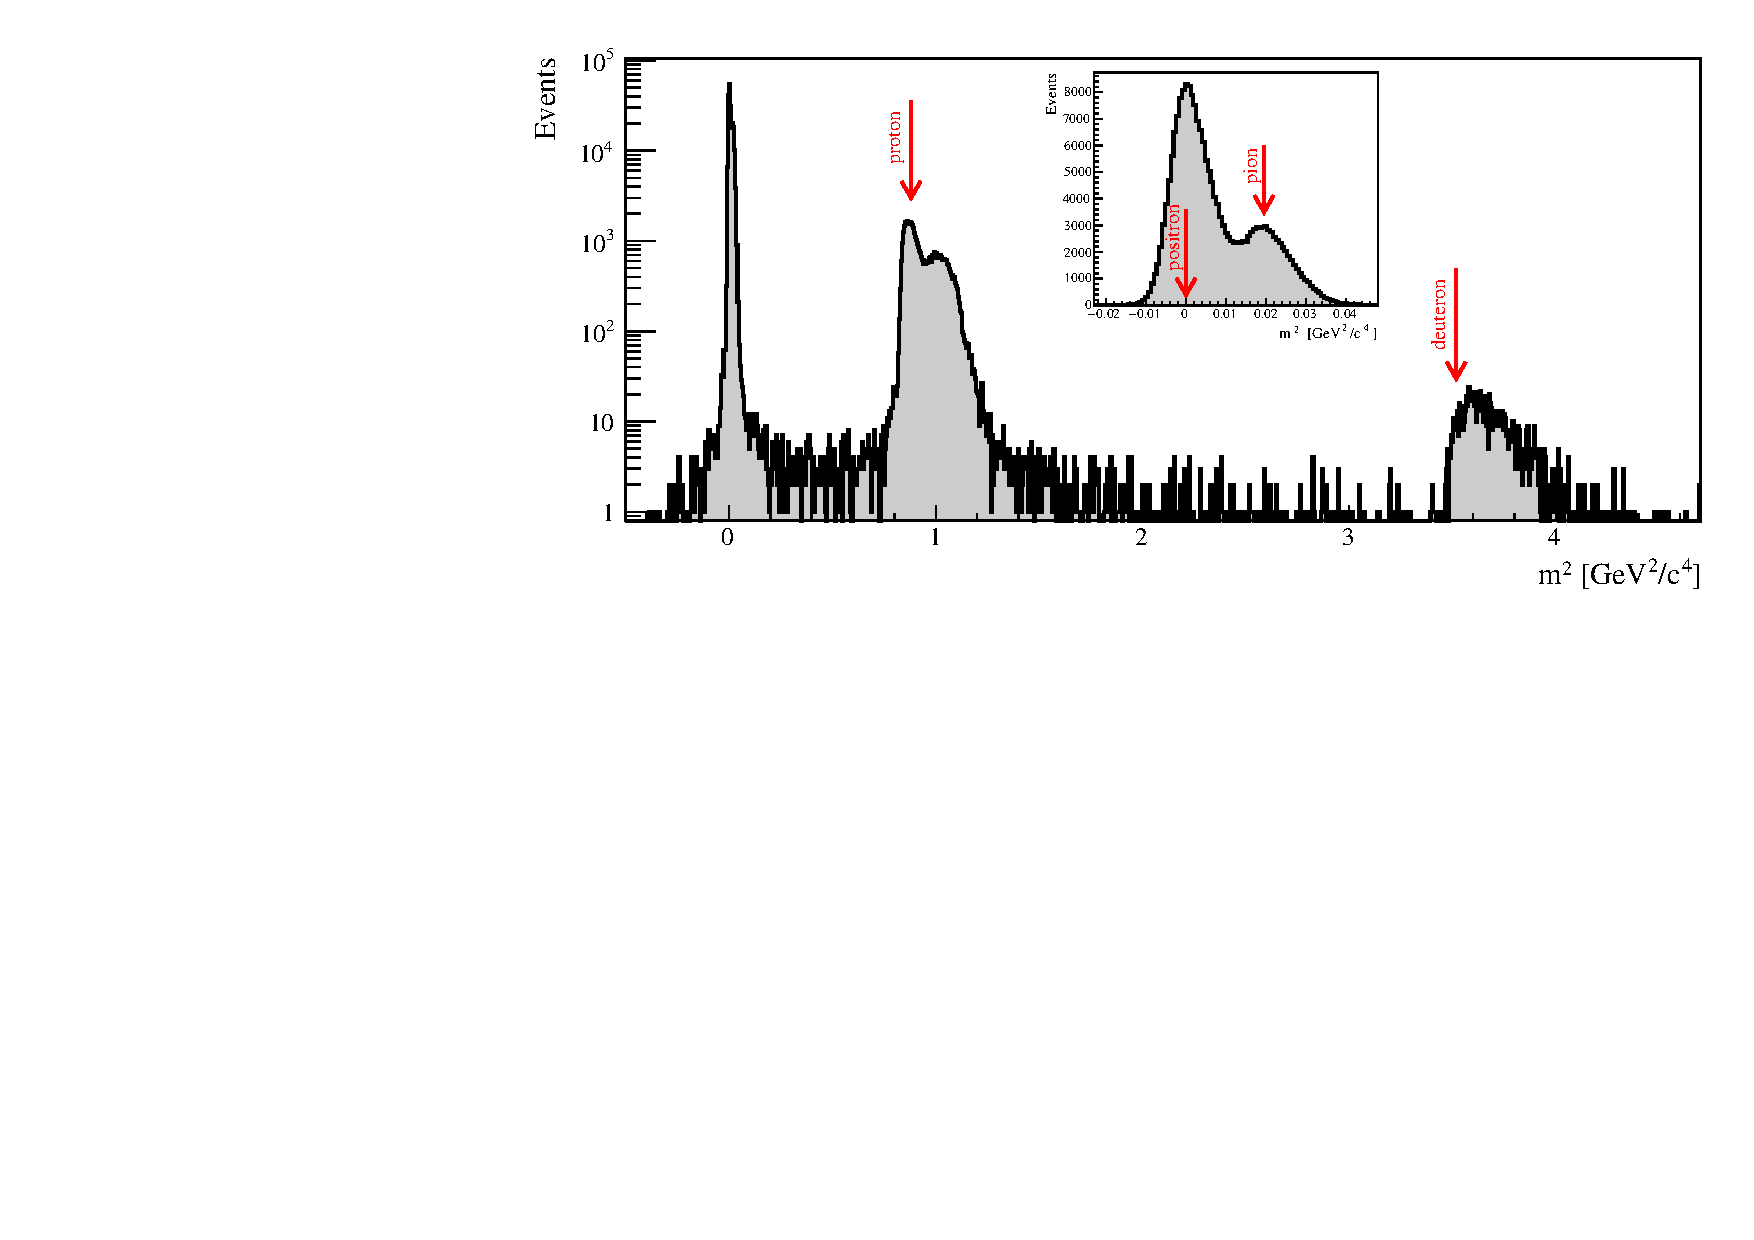
\includegraphics[width=0.9\linewidth]{files/Figures/Data_2018_8_31_b2_800MeV_0block_All.pdf}
	\caption{Reconstructed mass spectrum for the data taken without moderator blocks. The spectrum was calculated using the time difference between $\mathit{S3}$ and $\mathit{S1}$. Vertical arrows show predicted position of particles.}
	\label{fig:s3tof_mass}
\end{figure}

For the data collected in $\mathit{S3}$, both timing and signal amplitude cuts were used to select protons and MIPs.
Figure~\ref{fig:TvsA} shows an example of the signal size recorded in one of the SiPMs on one of the scintillator bars against the measured value of $t_{\mathit{S3}} - t_{\mathit{S1}}$.
At the beam energies used, due to their higher mass, the protons typically deposit more energy in the detector, resulting in the observation of greater amplitudes.
Therefore, to reduce the number of background events in the proton sample, a minimum signal amplitude is required.
This cut varied, depending on the SiPM in question and was determined from distributions such as those in Figure~\ref{fig:TvsA}. 
The cut values varied in the range 0.125~V and 0.3~V.

\begin{figure}[h]
  \begin{adjustbox}{max totalsize={.7\textwidth}, center}
    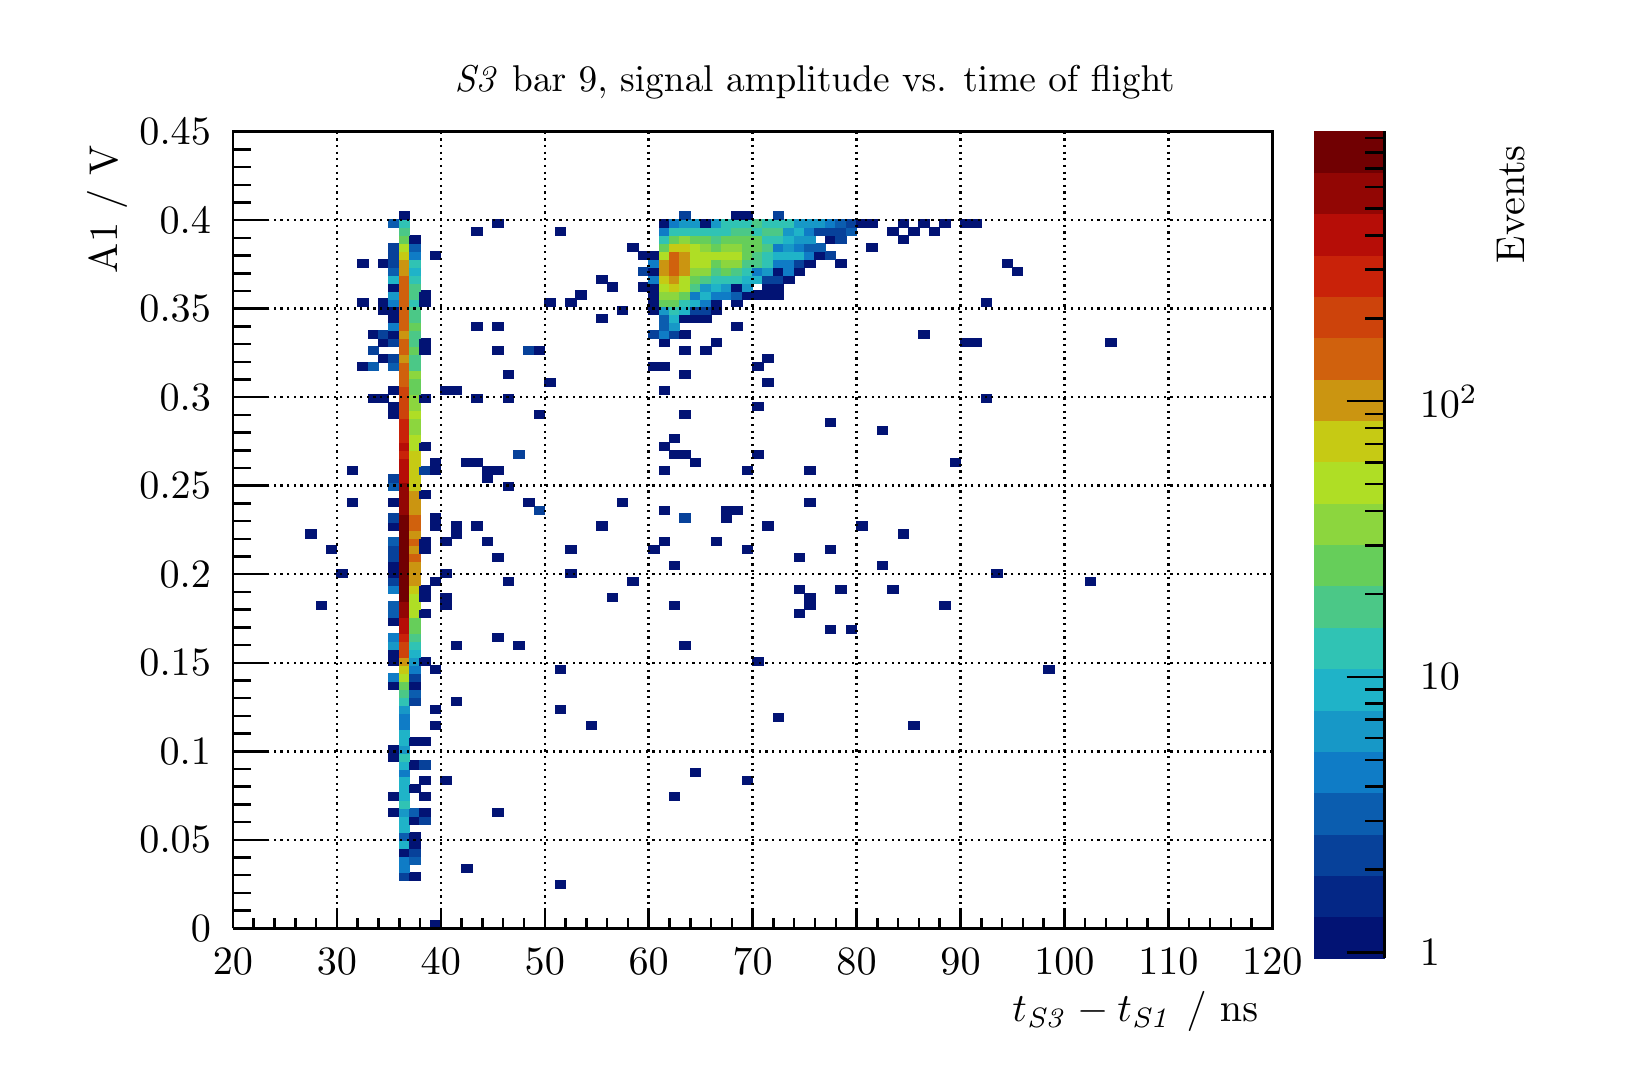
\begin{tikzpicture}
\pgfdeclareplotmark{cross} {
\pgfpathmoveto{\pgfpoint{-0.3\pgfplotmarksize}{\pgfplotmarksize}}
\pgfpathlineto{\pgfpoint{+0.3\pgfplotmarksize}{\pgfplotmarksize}}
\pgfpathlineto{\pgfpoint{+0.3\pgfplotmarksize}{0.3\pgfplotmarksize}}
\pgfpathlineto{\pgfpoint{+1\pgfplotmarksize}{0.3\pgfplotmarksize}}
\pgfpathlineto{\pgfpoint{+1\pgfplotmarksize}{-0.3\pgfplotmarksize}}
\pgfpathlineto{\pgfpoint{+0.3\pgfplotmarksize}{-0.3\pgfplotmarksize}}
\pgfpathlineto{\pgfpoint{+0.3\pgfplotmarksize}{-1.\pgfplotmarksize}}
\pgfpathlineto{\pgfpoint{-0.3\pgfplotmarksize}{-1.\pgfplotmarksize}}
\pgfpathlineto{\pgfpoint{-0.3\pgfplotmarksize}{-0.3\pgfplotmarksize}}
\pgfpathlineto{\pgfpoint{-1.\pgfplotmarksize}{-0.3\pgfplotmarksize}}
\pgfpathlineto{\pgfpoint{-1.\pgfplotmarksize}{0.3\pgfplotmarksize}}
\pgfpathlineto{\pgfpoint{-0.3\pgfplotmarksize}{0.3\pgfplotmarksize}}
\pgfpathclose
\pgfusepathqstroke
}
\pgfdeclareplotmark{cross*} {
\pgfpathmoveto{\pgfpoint{-0.3\pgfplotmarksize}{\pgfplotmarksize}}
\pgfpathlineto{\pgfpoint{+0.3\pgfplotmarksize}{\pgfplotmarksize}}
\pgfpathlineto{\pgfpoint{+0.3\pgfplotmarksize}{0.3\pgfplotmarksize}}
\pgfpathlineto{\pgfpoint{+1\pgfplotmarksize}{0.3\pgfplotmarksize}}
\pgfpathlineto{\pgfpoint{+1\pgfplotmarksize}{-0.3\pgfplotmarksize}}
\pgfpathlineto{\pgfpoint{+0.3\pgfplotmarksize}{-0.3\pgfplotmarksize}}
\pgfpathlineto{\pgfpoint{+0.3\pgfplotmarksize}{-1.\pgfplotmarksize}}
\pgfpathlineto{\pgfpoint{-0.3\pgfplotmarksize}{-1.\pgfplotmarksize}}
\pgfpathlineto{\pgfpoint{-0.3\pgfplotmarksize}{-0.3\pgfplotmarksize}}
\pgfpathlineto{\pgfpoint{-1.\pgfplotmarksize}{-0.3\pgfplotmarksize}}
\pgfpathlineto{\pgfpoint{-1.\pgfplotmarksize}{0.3\pgfplotmarksize}}
\pgfpathlineto{\pgfpoint{-0.3\pgfplotmarksize}{0.3\pgfplotmarksize}}
\pgfpathclose
\pgfusepathqfillstroke
}
\pgfdeclareplotmark{newstar} {
\pgfpathmoveto{\pgfqpoint{0pt}{\pgfplotmarksize}}
\pgfpathlineto{\pgfqpointpolar{44}{0.5\pgfplotmarksize}}
\pgfpathlineto{\pgfqpointpolar{18}{\pgfplotmarksize}}
\pgfpathlineto{\pgfqpointpolar{-20}{0.5\pgfplotmarksize}}
\pgfpathlineto{\pgfqpointpolar{-54}{\pgfplotmarksize}}
\pgfpathlineto{\pgfqpointpolar{-90}{0.5\pgfplotmarksize}}
\pgfpathlineto{\pgfqpointpolar{234}{\pgfplotmarksize}}
\pgfpathlineto{\pgfqpointpolar{198}{0.5\pgfplotmarksize}}
\pgfpathlineto{\pgfqpointpolar{162}{\pgfplotmarksize}}
\pgfpathlineto{\pgfqpointpolar{134}{0.5\pgfplotmarksize}}
\pgfpathclose
\pgfusepathqstroke
}
\pgfdeclareplotmark{newstar*} {
\pgfpathmoveto{\pgfqpoint{0pt}{\pgfplotmarksize}}
\pgfpathlineto{\pgfqpointpolar{44}{0.5\pgfplotmarksize}}
\pgfpathlineto{\pgfqpointpolar{18}{\pgfplotmarksize}}
\pgfpathlineto{\pgfqpointpolar{-20}{0.5\pgfplotmarksize}}
\pgfpathlineto{\pgfqpointpolar{-54}{\pgfplotmarksize}}
\pgfpathlineto{\pgfqpointpolar{-90}{0.5\pgfplotmarksize}}
\pgfpathlineto{\pgfqpointpolar{234}{\pgfplotmarksize}}
\pgfpathlineto{\pgfqpointpolar{198}{0.5\pgfplotmarksize}}
\pgfpathlineto{\pgfqpointpolar{162}{\pgfplotmarksize}}
\pgfpathlineto{\pgfqpointpolar{134}{0.5\pgfplotmarksize}}
\pgfpathclose
\pgfusepathqfillstroke
}
\definecolor{c}{rgb}{1,1,1};
\draw [color=c, fill=c] (0,0) rectangle (20,13.1389);
\draw [color=c, fill=c] (2.6,1.70805) rectangle (15.8,11.825);
\definecolor{c}{rgb}{0,0,0};
\draw [c,line width=0.9] (2.6,1.70805) -- (2.6,11.825) -- (15.8,11.825) -- (15.8,1.70805) -- (2.6,1.70805);
\definecolor{c}{rgb}{1,1,1};
\draw [color=c, fill=c] (2.6,1.70805) rectangle (15.8,11.825);
\definecolor{c}{rgb}{0,0,0};
\draw [c,line width=0.9] (2.6,1.70805) -- (2.6,11.825) -- (15.8,11.825) -- (15.8,1.70805) -- (2.6,1.70805);
\definecolor{c}{rgb}{0.00759013,0.0728653,0.45351};
\draw [color=c, fill=c] (5.108,1.70805) rectangle (5.24,1.80922);
\draw [color=c, fill=c] (6.692,2.2139) rectangle (6.824,2.31507);
\definecolor{c}{rgb}{0.0281863,0.253431,0.604902};
\draw [color=c, fill=c] (4.712,2.31507) rectangle (4.844,2.41624);
\definecolor{c}{rgb}{0.00759013,0.0728653,0.45351};
\draw [color=c, fill=c] (4.844,2.31507) rectangle (4.976,2.41624);
\definecolor{c}{rgb}{0.0588235,0.486275,0.776471};
\draw [color=c, fill=c] (4.712,2.41624) rectangle (4.844,2.51741);
\definecolor{c}{rgb}{0.00759013,0.0728653,0.45351};
\draw [color=c, fill=c] (5.504,2.41624) rectangle (5.636,2.51741);
\definecolor{c}{rgb}{0.0588235,0.486275,0.776471};
\draw [color=c, fill=c] (4.712,2.51741) rectangle (4.844,2.61857);
\definecolor{c}{rgb}{0.0428922,0.365196,0.687255};
\draw [color=c, fill=c] (4.844,2.51741) rectangle (4.976,2.61857);
\definecolor{c}{rgb}{0.00759013,0.0728653,0.45351};
\draw [color=c, fill=c] (4.712,2.61857) rectangle (4.844,2.71974);
\definecolor{c}{rgb}{0.0281863,0.253431,0.604902};
\draw [color=c, fill=c] (4.844,2.61857) rectangle (4.976,2.71974);
\definecolor{c}{rgb}{0.122549,0.702941,0.786029};
\draw [color=c, fill=c] (4.712,2.71974) rectangle (4.844,2.82091);
\definecolor{c}{rgb}{0.00759013,0.0728653,0.45351};
\draw [color=c, fill=c] (4.844,2.71974) rectangle (4.976,2.82091);
\definecolor{c}{rgb}{0.0428922,0.365196,0.687255};
\draw [color=c, fill=c] (4.712,2.82091) rectangle (4.844,2.92208);
\definecolor{c}{rgb}{0.00759013,0.0728653,0.45351};
\draw [color=c, fill=c] (4.844,2.82091) rectangle (4.976,2.92208);
\definecolor{c}{rgb}{0.122549,0.702941,0.786029};
\draw [color=c, fill=c] (4.712,2.92208) rectangle (4.844,3.02325);
\draw [color=c, fill=c] (4.712,3.02325) rectangle (4.844,3.12442);
\definecolor{c}{rgb}{0.00759013,0.0728653,0.45351};
\draw [color=c, fill=c] (4.844,3.02325) rectangle (4.976,3.12442);
\definecolor{c}{rgb}{0.0281863,0.253431,0.604902};
\draw [color=c, fill=c] (4.976,3.02325) rectangle (5.108,3.12442);
\definecolor{c}{rgb}{0.00759013,0.0728653,0.45351};
\draw [color=c, fill=c] (4.58,3.12442) rectangle (4.712,3.22559);
\definecolor{c}{rgb}{0.0906863,0.594608,0.78125};
\draw [color=c, fill=c] (4.712,3.12442) rectangle (4.844,3.22559);
\definecolor{c}{rgb}{0.0428922,0.365196,0.687255};
\draw [color=c, fill=c] (4.844,3.12442) rectangle (4.976,3.22559);
\definecolor{c}{rgb}{0.00759013,0.0728653,0.45351};
\draw [color=c, fill=c] (4.976,3.12442) rectangle (5.108,3.22559);
\draw [color=c, fill=c] (5.9,3.12442) rectangle (6.032,3.22559);
\definecolor{c}{rgb}{0.18652,0.763235,0.706618};
\draw [color=c, fill=c] (4.712,3.22559) rectangle (4.844,3.32676);
\definecolor{c}{rgb}{0.00759013,0.0728653,0.45351};
\draw [color=c, fill=c] (4.58,3.32676) rectangle (4.712,3.42793);
\definecolor{c}{rgb}{0.122549,0.702941,0.786029};
\draw [color=c, fill=c] (4.712,3.32676) rectangle (4.844,3.42793);
\definecolor{c}{rgb}{0.00759013,0.0728653,0.45351};
\draw [color=c, fill=c] (4.976,3.32676) rectangle (5.108,3.42793);
\draw [color=c, fill=c] (8.144,3.32676) rectangle (8.276,3.42793);
\definecolor{c}{rgb}{0.122549,0.702941,0.786029};
\draw [color=c, fill=c] (4.712,3.42793) rectangle (4.844,3.5291);
\definecolor{c}{rgb}{0.00759013,0.0728653,0.45351};
\draw [color=c, fill=c] (4.844,3.42793) rectangle (4.976,3.5291);
\definecolor{c}{rgb}{0.122549,0.702941,0.786029};
\draw [color=c, fill=c] (4.712,3.5291) rectangle (4.844,3.63027);
\definecolor{c}{rgb}{0.00759013,0.0728653,0.45351};
\draw [color=c, fill=c] (4.976,3.5291) rectangle (5.108,3.63027);
\draw [color=c, fill=c] (5.24,3.5291) rectangle (5.372,3.63027);
\draw [color=c, fill=c] (9.068,3.5291) rectangle (9.2,3.63027);
\definecolor{c}{rgb}{0.0588235,0.486275,0.776471};
\draw [color=c, fill=c] (4.712,3.63027) rectangle (4.844,3.73144);
\definecolor{c}{rgb}{0.00759013,0.0728653,0.45351};
\draw [color=c, fill=c] (8.408,3.63027) rectangle (8.54,3.73144);
\definecolor{c}{rgb}{0.122549,0.702941,0.786029};
\draw [color=c, fill=c] (4.712,3.73144) rectangle (4.844,3.8326);
\definecolor{c}{rgb}{0.00759013,0.0728653,0.45351};
\draw [color=c, fill=c] (4.844,3.73144) rectangle (4.976,3.8326);
\definecolor{c}{rgb}{0.0281863,0.253431,0.604902};
\draw [color=c, fill=c] (4.976,3.73144) rectangle (5.108,3.8326);
\definecolor{c}{rgb}{0.00759013,0.0728653,0.45351};
\draw [color=c, fill=c] (4.58,3.8326) rectangle (4.712,3.93377);
\definecolor{c}{rgb}{0.18652,0.763235,0.706618};
\draw [color=c, fill=c] (4.712,3.8326) rectangle (4.844,3.93377);
\definecolor{c}{rgb}{0.00759013,0.0728653,0.45351};
\draw [color=c, fill=c] (4.58,3.93377) rectangle (4.712,4.03494);
\definecolor{c}{rgb}{0.0906863,0.594608,0.78125};
\draw [color=c, fill=c] (4.712,3.93377) rectangle (4.844,4.03494);
\definecolor{c}{rgb}{0.122549,0.702941,0.786029};
\draw [color=c, fill=c] (4.712,4.03494) rectangle (4.844,4.13611);
\definecolor{c}{rgb}{0.00759013,0.0728653,0.45351};
\draw [color=c, fill=c] (4.844,4.03494) rectangle (4.976,4.13611);
\draw [color=c, fill=c] (4.976,4.03494) rectangle (5.108,4.13611);
\definecolor{c}{rgb}{0.122549,0.702941,0.786029};
\draw [color=c, fill=c] (4.712,4.13611) rectangle (4.844,4.23728);
\definecolor{c}{rgb}{0.0588235,0.486275,0.776471};
\draw [color=c, fill=c] (4.712,4.23728) rectangle (4.844,4.33845);
\definecolor{c}{rgb}{0.00759013,0.0728653,0.45351};
\draw [color=c, fill=c] (5.108,4.23728) rectangle (5.24,4.33845);
\draw [color=c, fill=c] (7.088,4.23728) rectangle (7.22,4.33845);
\draw [color=c, fill=c] (11.18,4.23728) rectangle (11.312,4.33845);
\definecolor{c}{rgb}{0.0588235,0.486275,0.776471};
\draw [color=c, fill=c] (4.712,4.33845) rectangle (4.844,4.43962);
\definecolor{c}{rgb}{0.00759013,0.0728653,0.45351};
\draw [color=c, fill=c] (9.464,4.33845) rectangle (9.596,4.43962);
\definecolor{c}{rgb}{0.0906863,0.594608,0.78125};
\draw [color=c, fill=c] (4.712,4.43962) rectangle (4.844,4.54079);
\definecolor{c}{rgb}{0.00759013,0.0728653,0.45351};
\draw [color=c, fill=c] (5.108,4.43962) rectangle (5.24,4.54079);
\draw [color=c, fill=c] (6.692,4.43962) rectangle (6.824,4.54079);
\definecolor{c}{rgb}{0.18652,0.763235,0.706618};
\draw [color=c, fill=c] (4.712,4.54079) rectangle (4.844,4.64196);
\definecolor{c}{rgb}{0.0281863,0.253431,0.604902};
\draw [color=c, fill=c] (4.844,4.54079) rectangle (4.976,4.64196);
\definecolor{c}{rgb}{0.00759013,0.0728653,0.45351};
\draw [color=c, fill=c] (5.372,4.54079) rectangle (5.504,4.64196);
\definecolor{c}{rgb}{0.29326,0.785539,0.529779};
\draw [color=c, fill=c] (4.712,4.64196) rectangle (4.844,4.74313);
\definecolor{c}{rgb}{0.0428922,0.365196,0.687255};
\draw [color=c, fill=c] (4.844,4.64196) rectangle (4.976,4.74313);
\definecolor{c}{rgb}{0.00759013,0.0728653,0.45351};
\draw [color=c, fill=c] (4.58,4.74313) rectangle (4.712,4.8443);
\definecolor{c}{rgb}{0.4,0.807843,0.352941};
\draw [color=c, fill=c] (4.712,4.74313) rectangle (4.844,4.8443);
\definecolor{c}{rgb}{0.00759013,0.0728653,0.45351};
\draw [color=c, fill=c] (4.844,4.74313) rectangle (4.976,4.8443);
\definecolor{c}{rgb}{0.0588235,0.486275,0.776471};
\draw [color=c, fill=c] (4.58,4.8443) rectangle (4.712,4.94547);
\definecolor{c}{rgb}{0.68799,0.869118,0.144608};
\draw [color=c, fill=c] (4.712,4.8443) rectangle (4.844,4.94547);
\definecolor{c}{rgb}{0.0281863,0.253431,0.604902};
\draw [color=c, fill=c] (4.844,4.8443) rectangle (4.976,4.94547);
\definecolor{c}{rgb}{0.777451,0.791422,0.0796569};
\draw [color=c, fill=c] (4.712,4.94547) rectangle (4.844,5.04663);
\definecolor{c}{rgb}{0.0588235,0.486275,0.776471};
\draw [color=c, fill=c] (4.844,4.94547) rectangle (4.976,5.04663);
\definecolor{c}{rgb}{0.00759013,0.0728653,0.45351};
\draw [color=c, fill=c] (5.108,4.94547) rectangle (5.24,5.04663);
\draw [color=c, fill=c] (6.692,4.94547) rectangle (6.824,5.04663);
\draw [color=c, fill=c] (12.896,4.94547) rectangle (13.028,5.04663);
\draw [color=c, fill=c] (4.58,5.04663) rectangle (4.712,5.1478);
\definecolor{c}{rgb}{0.796569,0.585907,0.0653186};
\draw [color=c, fill=c] (4.712,5.04663) rectangle (4.844,5.1478);
\definecolor{c}{rgb}{0.0906863,0.594608,0.78125};
\draw [color=c, fill=c] (4.844,5.04663) rectangle (4.976,5.1478);
\definecolor{c}{rgb}{0.00759013,0.0728653,0.45351};
\draw [color=c, fill=c] (4.976,5.04663) rectangle (5.108,5.1478);
\draw [color=c, fill=c] (9.2,5.04663) rectangle (9.332,5.1478);
\draw [color=c, fill=c] (4.58,5.1478) rectangle (4.712,5.24897);
\definecolor{c}{rgb}{0.802451,0.261275,0.0436275};
\draw [color=c, fill=c] (4.712,5.1478) rectangle (4.844,5.24897);
\definecolor{c}{rgb}{0.122549,0.702941,0.786029};
\draw [color=c, fill=c] (4.844,5.1478) rectangle (4.976,5.24897);
\definecolor{c}{rgb}{0.0906863,0.594608,0.78125};
\draw [color=c, fill=c] (4.58,5.24897) rectangle (4.712,5.35014);
\definecolor{c}{rgb}{0.802451,0.261275,0.0436275};
\draw [color=c, fill=c] (4.712,5.24897) rectangle (4.844,5.35014);
\definecolor{c}{rgb}{0.18652,0.763235,0.706618};
\draw [color=c, fill=c] (4.844,5.24897) rectangle (4.976,5.35014);
\definecolor{c}{rgb}{0.00759013,0.0728653,0.45351};
\draw [color=c, fill=c] (5.372,5.24897) rectangle (5.504,5.35014);
\draw [color=c, fill=c] (6.164,5.24897) rectangle (6.296,5.35014);
\draw [color=c, fill=c] (8.276,5.24897) rectangle (8.408,5.35014);
\definecolor{c}{rgb}{0.0588235,0.486275,0.776471};
\draw [color=c, fill=c] (4.58,5.35014) rectangle (4.712,5.45131);
\definecolor{c}{rgb}{0.788113,0.13223,0.0356618};
\draw [color=c, fill=c] (4.712,5.35014) rectangle (4.844,5.45131);
\definecolor{c}{rgb}{0.29326,0.785539,0.529779};
\draw [color=c, fill=c] (4.844,5.35014) rectangle (4.976,5.45131);
\definecolor{c}{rgb}{0.00759013,0.0728653,0.45351};
\draw [color=c, fill=c] (5.9,5.35014) rectangle (6.032,5.45131);
\definecolor{c}{rgb}{0.714951,0.0509804,0.0269608};
\draw [color=c, fill=c] (4.712,5.45131) rectangle (4.844,5.55248);
\definecolor{c}{rgb}{0.4,0.807843,0.352941};
\draw [color=c, fill=c] (4.844,5.45131) rectangle (4.976,5.55248);
\definecolor{c}{rgb}{0.00759013,0.0728653,0.45351};
\draw [color=c, fill=c] (10.124,5.45131) rectangle (10.256,5.55248);
\draw [color=c, fill=c] (10.388,5.45131) rectangle (10.52,5.55248);
\draw [color=c, fill=c] (4.58,5.55248) rectangle (4.712,5.65365);
\definecolor{c}{rgb}{0.714951,0.0509804,0.0269608};
\draw [color=c, fill=c] (4.712,5.55248) rectangle (4.844,5.65365);
\definecolor{c}{rgb}{0.4,0.807843,0.352941};
\draw [color=c, fill=c] (4.844,5.55248) rectangle (4.976,5.65365);
\definecolor{c}{rgb}{0.0428922,0.365196,0.687255};
\draw [color=c, fill=c] (4.58,5.65365) rectangle (4.712,5.75482);
\definecolor{c}{rgb}{0.573162,0.0254902,0.017402};
\draw [color=c, fill=c] (4.712,5.65365) rectangle (4.844,5.75482);
\definecolor{c}{rgb}{0.68799,0.869118,0.144608};
\draw [color=c, fill=c] (4.844,5.65365) rectangle (4.976,5.75482);
\definecolor{c}{rgb}{0.00759013,0.0728653,0.45351};
\draw [color=c, fill=c] (4.976,5.65365) rectangle (5.108,5.75482);
\draw [color=c, fill=c] (9.728,5.65365) rectangle (9.86,5.75482);
\draw [color=c, fill=c] (3.656,5.75482) rectangle (3.788,5.85599);
\definecolor{c}{rgb}{0.0428922,0.365196,0.687255};
\draw [color=c, fill=c] (4.58,5.75482) rectangle (4.712,5.85599);
\definecolor{c}{rgb}{0.573162,0.0254902,0.017402};
\draw [color=c, fill=c] (4.712,5.75482) rectangle (4.844,5.85599);
\definecolor{c}{rgb}{0.68799,0.869118,0.144608};
\draw [color=c, fill=c] (4.844,5.75482) rectangle (4.976,5.85599);
\definecolor{c}{rgb}{0.00759013,0.0728653,0.45351};
\draw [color=c, fill=c] (5.24,5.75482) rectangle (5.372,5.85599);
\draw [color=c, fill=c] (8.144,5.75482) rectangle (8.276,5.85599);
\draw [color=c, fill=c] (9.86,5.75482) rectangle (9.992,5.85599);
\draw [color=c, fill=c] (11.576,5.75482) rectangle (11.708,5.85599);
\definecolor{c}{rgb}{0.442279,0.00196078,0.00857843};
\draw [color=c, fill=c] (4.712,5.85599) rectangle (4.844,5.95716);
\definecolor{c}{rgb}{0.68799,0.869118,0.144608};
\draw [color=c, fill=c] (4.844,5.85599) rectangle (4.976,5.95716);
\definecolor{c}{rgb}{0.00759013,0.0728653,0.45351};
\draw [color=c, fill=c] (4.976,5.85599) rectangle (5.108,5.95716);
\draw [color=c, fill=c] (5.24,5.85599) rectangle (5.372,5.95716);
\draw [color=c, fill=c] (7.352,5.85599) rectangle (7.484,5.95716);
\draw [color=c, fill=c] (9.86,5.85599) rectangle (9.992,5.95716);
\definecolor{c}{rgb}{0.0588235,0.486275,0.776471};
\draw [color=c, fill=c] (4.58,5.95716) rectangle (4.712,6.05833);
\definecolor{c}{rgb}{0.442279,0.00196078,0.00857843};
\draw [color=c, fill=c] (4.712,5.95716) rectangle (4.844,6.05833);
\definecolor{c}{rgb}{0.777451,0.791422,0.0796569};
\draw [color=c, fill=c] (4.844,5.95716) rectangle (4.976,6.05833);
\definecolor{c}{rgb}{0.00759013,0.0728653,0.45351};
\draw [color=c, fill=c] (4.976,5.95716) rectangle (5.108,6.05833);
\draw [color=c, fill=c] (9.728,5.95716) rectangle (9.86,6.05833);
\draw [color=c, fill=c] (10.256,5.95716) rectangle (10.388,6.05833);
\draw [color=c, fill=c] (10.916,5.95716) rectangle (11.048,6.05833);
\definecolor{c}{rgb}{0.0281863,0.253431,0.604902};
\draw [color=c, fill=c] (4.58,6.05833) rectangle (4.712,6.1595);
\definecolor{c}{rgb}{0.442279,0.00196078,0.00857843};
\draw [color=c, fill=c] (4.712,6.05833) rectangle (4.844,6.1595);
\definecolor{c}{rgb}{0.796569,0.585907,0.0653186};
\draw [color=c, fill=c] (4.844,6.05833) rectangle (4.976,6.1595);
\definecolor{c}{rgb}{0.00759013,0.0728653,0.45351};
\draw [color=c, fill=c] (5.108,6.05833) rectangle (5.24,6.1595);
\draw [color=c, fill=c] (6.032,6.05833) rectangle (6.164,6.1595);
\draw [color=c, fill=c] (7.616,6.05833) rectangle (7.748,6.1595);
\draw [color=c, fill=c] (13.424,6.05833) rectangle (13.556,6.1595);
\draw [color=c, fill=c] (3.92,6.1595) rectangle (4.052,6.26067);
\draw [color=c, fill=c] (4.58,6.1595) rectangle (4.712,6.26067);
\definecolor{c}{rgb}{0.442279,0.00196078,0.00857843};
\draw [color=c, fill=c] (4.712,6.1595) rectangle (4.844,6.26067);
\definecolor{c}{rgb}{0.796569,0.585907,0.0653186};
\draw [color=c, fill=c] (4.844,6.1595) rectangle (4.976,6.26067);
\definecolor{c}{rgb}{0.00759013,0.0728653,0.45351};
\draw [color=c, fill=c] (5.24,6.1595) rectangle (5.372,6.26067);
\draw [color=c, fill=c] (6.824,6.1595) rectangle (6.956,6.26067);
\draw [color=c, fill=c] (12.236,6.1595) rectangle (12.368,6.26067);
\draw [color=c, fill=c] (4.58,6.26067) rectangle (4.712,6.36183);
\definecolor{c}{rgb}{0.442279,0.00196078,0.00857843};
\draw [color=c, fill=c] (4.712,6.26067) rectangle (4.844,6.36183);
\definecolor{c}{rgb}{0.796569,0.585907,0.0653186};
\draw [color=c, fill=c] (4.844,6.26067) rectangle (4.976,6.36183);
\definecolor{c}{rgb}{0.00759013,0.0728653,0.45351};
\draw [color=c, fill=c] (8.144,6.26067) rectangle (8.276,6.36183);
\draw [color=c, fill=c] (10.784,6.26067) rectangle (10.916,6.36183);
\definecolor{c}{rgb}{0.0281863,0.253431,0.604902};
\draw [color=c, fill=c] (4.58,6.36183) rectangle (4.712,6.463);
\definecolor{c}{rgb}{0.442279,0.00196078,0.00857843};
\draw [color=c, fill=c] (4.712,6.36183) rectangle (4.844,6.463);
\definecolor{c}{rgb}{0.815686,0.380392,0.0509804};
\draw [color=c, fill=c] (4.844,6.36183) rectangle (4.976,6.463);
\definecolor{c}{rgb}{0.00759013,0.0728653,0.45351};
\draw [color=c, fill=c] (5.9,6.36183) rectangle (6.032,6.463);
\draw [color=c, fill=c] (9.728,6.36183) rectangle (9.86,6.463);
\draw [color=c, fill=c] (3.788,6.463) rectangle (3.92,6.56417);
\definecolor{c}{rgb}{0.0281863,0.253431,0.604902};
\draw [color=c, fill=c] (4.58,6.463) rectangle (4.712,6.56417);
\definecolor{c}{rgb}{0.442279,0.00196078,0.00857843};
\draw [color=c, fill=c] (4.712,6.463) rectangle (4.844,6.56417);
\definecolor{c}{rgb}{0.796569,0.585907,0.0653186};
\draw [color=c, fill=c] (4.844,6.463) rectangle (4.976,6.56417);
\definecolor{c}{rgb}{0.00759013,0.0728653,0.45351};
\draw [color=c, fill=c] (4.976,6.463) rectangle (5.108,6.56417);
\draw [color=c, fill=c] (6.824,6.463) rectangle (6.956,6.56417);
\draw [color=c, fill=c] (7.88,6.463) rectangle (8.012,6.56417);
\draw [color=c, fill=c] (9.068,6.463) rectangle (9.2,6.56417);
\draw [color=c, fill=c] (10.124,6.463) rectangle (10.256,6.56417);
\definecolor{c}{rgb}{0.0428922,0.365196,0.687255};
\draw [color=c, fill=c] (4.58,6.56417) rectangle (4.712,6.66534);
\definecolor{c}{rgb}{0.442279,0.00196078,0.00857843};
\draw [color=c, fill=c] (4.712,6.56417) rectangle (4.844,6.66534);
\definecolor{c}{rgb}{0.815686,0.380392,0.0509804};
\draw [color=c, fill=c] (4.844,6.56417) rectangle (4.976,6.66534);
\definecolor{c}{rgb}{0.00759013,0.0728653,0.45351};
\draw [color=c, fill=c] (4.976,6.56417) rectangle (5.108,6.66534);
\draw [color=c, fill=c] (5.24,6.56417) rectangle (5.372,6.66534);
\draw [color=c, fill=c] (5.768,6.56417) rectangle (5.9,6.66534);
\draw [color=c, fill=c] (8.012,6.56417) rectangle (8.144,6.66534);
\draw [color=c, fill=c] (8.672,6.56417) rectangle (8.804,6.66534);
\draw [color=c, fill=c] (3.524,6.66534) rectangle (3.656,6.76651);
\definecolor{c}{rgb}{0.442279,0.00196078,0.00857843};
\draw [color=c, fill=c] (4.712,6.66534) rectangle (4.844,6.76651);
\definecolor{c}{rgb}{0.796569,0.585907,0.0653186};
\draw [color=c, fill=c] (4.844,6.66534) rectangle (4.976,6.76651);
\definecolor{c}{rgb}{0.00759013,0.0728653,0.45351};
\draw [color=c, fill=c] (5.372,6.66534) rectangle (5.504,6.76651);
\draw [color=c, fill=c] (11.048,6.66534) rectangle (11.18,6.76651);
\draw [color=c, fill=c] (4.58,6.76651) rectangle (4.712,6.86768);
\definecolor{c}{rgb}{0.442279,0.00196078,0.00857843};
\draw [color=c, fill=c] (4.712,6.76651) rectangle (4.844,6.86768);
\definecolor{c}{rgb}{0.815686,0.380392,0.0509804};
\draw [color=c, fill=c] (4.844,6.76651) rectangle (4.976,6.86768);
\definecolor{c}{rgb}{0.00759013,0.0728653,0.45351};
\draw [color=c, fill=c] (5.108,6.76651) rectangle (5.24,6.86768);
\draw [color=c, fill=c] (5.372,6.76651) rectangle (5.504,6.86768);
\draw [color=c, fill=c] (5.636,6.76651) rectangle (5.768,6.86768);
\draw [color=c, fill=c] (7.22,6.76651) rectangle (7.352,6.86768);
\draw [color=c, fill=c] (9.332,6.76651) rectangle (9.464,6.86768);
\draw [color=c, fill=c] (10.52,6.76651) rectangle (10.652,6.86768);
\definecolor{c}{rgb}{0.0281863,0.253431,0.604902};
\draw [color=c, fill=c] (4.58,6.86768) rectangle (4.712,6.96885);
\definecolor{c}{rgb}{0.442279,0.00196078,0.00857843};
\draw [color=c, fill=c] (4.712,6.86768) rectangle (4.844,6.96885);
\definecolor{c}{rgb}{0.815686,0.380392,0.0509804};
\draw [color=c, fill=c] (4.844,6.86768) rectangle (4.976,6.96885);
\definecolor{c}{rgb}{0.00759013,0.0728653,0.45351};
\draw [color=c, fill=c] (5.108,6.86768) rectangle (5.24,6.96885);
\definecolor{c}{rgb}{0.0281863,0.253431,0.604902};
\draw [color=c, fill=c] (8.276,6.86768) rectangle (8.408,6.96885);
\definecolor{c}{rgb}{0.00759013,0.0728653,0.45351};
\draw [color=c, fill=c] (8.804,6.86768) rectangle (8.936,6.96885);
\definecolor{c}{rgb}{0.573162,0.0254902,0.017402};
\draw [color=c, fill=c] (4.712,6.96885) rectangle (4.844,7.07002);
\definecolor{c}{rgb}{0.796569,0.585907,0.0653186};
\draw [color=c, fill=c] (4.844,6.96885) rectangle (4.976,7.07002);
\definecolor{c}{rgb}{0.0281863,0.253431,0.604902};
\draw [color=c, fill=c] (6.428,6.96885) rectangle (6.56,7.07002);
\definecolor{c}{rgb}{0.00759013,0.0728653,0.45351};
\draw [color=c, fill=c] (8.012,6.96885) rectangle (8.144,7.07002);
\draw [color=c, fill=c] (8.804,6.96885) rectangle (8.936,7.07002);
\draw [color=c, fill=c] (8.936,6.96885) rectangle (9.068,7.07002);
\draw [color=c, fill=c] (4.052,7.07002) rectangle (4.184,7.17119);
\draw [color=c, fill=c] (4.58,7.07002) rectangle (4.712,7.17119);
\definecolor{c}{rgb}{0.573162,0.0254902,0.017402};
\draw [color=c, fill=c] (4.712,7.07002) rectangle (4.844,7.17119);
\definecolor{c}{rgb}{0.796569,0.585907,0.0653186};
\draw [color=c, fill=c] (4.844,7.07002) rectangle (4.976,7.17119);
\definecolor{c}{rgb}{0.00759013,0.0728653,0.45351};
\draw [color=c, fill=c] (6.296,7.07002) rectangle (6.428,7.17119);
\draw [color=c, fill=c] (7.484,7.07002) rectangle (7.616,7.17119);
\draw [color=c, fill=c] (9.86,7.07002) rectangle (9.992,7.17119);
\definecolor{c}{rgb}{0.573162,0.0254902,0.017402};
\draw [color=c, fill=c] (4.712,7.17119) rectangle (4.844,7.27236);
\definecolor{c}{rgb}{0.796569,0.585907,0.0653186};
\draw [color=c, fill=c] (4.844,7.17119) rectangle (4.976,7.27236);
\definecolor{c}{rgb}{0.00759013,0.0728653,0.45351};
\draw [color=c, fill=c] (4.976,7.17119) rectangle (5.108,7.27236);
\definecolor{c}{rgb}{0.0428922,0.365196,0.687255};
\draw [color=c, fill=c] (4.58,7.27236) rectangle (4.712,7.37353);
\definecolor{c}{rgb}{0.573162,0.0254902,0.017402};
\draw [color=c, fill=c] (4.712,7.27236) rectangle (4.844,7.37353);
\definecolor{c}{rgb}{0.777451,0.791422,0.0796569};
\draw [color=c, fill=c] (4.844,7.27236) rectangle (4.976,7.37353);
\definecolor{c}{rgb}{0.00759013,0.0728653,0.45351};
\draw [color=c, fill=c] (6.032,7.27236) rectangle (6.164,7.37353);
\definecolor{c}{rgb}{0.0281863,0.253431,0.604902};
\draw [color=c, fill=c] (4.58,7.37353) rectangle (4.712,7.4747);
\definecolor{c}{rgb}{0.714951,0.0509804,0.0269608};
\draw [color=c, fill=c] (4.712,7.37353) rectangle (4.844,7.4747);
\definecolor{c}{rgb}{0.777451,0.791422,0.0796569};
\draw [color=c, fill=c] (4.844,7.37353) rectangle (4.976,7.4747);
\definecolor{c}{rgb}{0.00759013,0.0728653,0.45351};
\draw [color=c, fill=c] (5.768,7.37353) rectangle (5.9,7.4747);
\draw [color=c, fill=c] (4.052,7.4747) rectangle (4.184,7.57586);
\definecolor{c}{rgb}{0.714951,0.0509804,0.0269608};
\draw [color=c, fill=c] (4.712,7.4747) rectangle (4.844,7.57586);
\definecolor{c}{rgb}{0.777451,0.791422,0.0796569};
\draw [color=c, fill=c] (4.844,7.4747) rectangle (4.976,7.57586);
\definecolor{c}{rgb}{0.0281863,0.253431,0.604902};
\draw [color=c, fill=c] (4.976,7.4747) rectangle (5.108,7.57586);
\definecolor{c}{rgb}{0.00759013,0.0728653,0.45351};
\draw [color=c, fill=c] (5.108,7.4747) rectangle (5.24,7.57586);
\draw [color=c, fill=c] (5.768,7.4747) rectangle (5.9,7.57586);
\draw [color=c, fill=c] (5.9,7.4747) rectangle (6.032,7.57586);
\draw [color=c, fill=c] (8.012,7.4747) rectangle (8.144,7.57586);
\draw [color=c, fill=c] (9.068,7.4747) rectangle (9.2,7.57586);
\draw [color=c, fill=c] (9.86,7.4747) rectangle (9.992,7.57586);
\definecolor{c}{rgb}{0.714951,0.0509804,0.0269608};
\draw [color=c, fill=c] (4.712,7.57586) rectangle (4.844,7.67703);
\definecolor{c}{rgb}{0.777451,0.791422,0.0796569};
\draw [color=c, fill=c] (4.844,7.57586) rectangle (4.976,7.67703);
\definecolor{c}{rgb}{0.00759013,0.0728653,0.45351};
\draw [color=c, fill=c] (5.108,7.57586) rectangle (5.24,7.67703);
\draw [color=c, fill=c] (5.504,7.57586) rectangle (5.636,7.67703);
\draw [color=c, fill=c] (5.636,7.57586) rectangle (5.768,7.67703);
\draw [color=c, fill=c] (8.408,7.57586) rectangle (8.54,7.67703);
\draw [color=c, fill=c] (11.708,7.57586) rectangle (11.84,7.67703);
\definecolor{c}{rgb}{0.788113,0.13223,0.0356618};
\draw [color=c, fill=c] (4.712,7.67703) rectangle (4.844,7.7782);
\definecolor{c}{rgb}{0.777451,0.791422,0.0796569};
\draw [color=c, fill=c] (4.844,7.67703) rectangle (4.976,7.7782);
\definecolor{c}{rgb}{0.0281863,0.253431,0.604902};
\draw [color=c, fill=c] (6.164,7.67703) rectangle (6.296,7.7782);
\definecolor{c}{rgb}{0.00759013,0.0728653,0.45351};
\draw [color=c, fill=c] (8.144,7.67703) rectangle (8.276,7.7782);
\draw [color=c, fill=c] (8.276,7.67703) rectangle (8.408,7.7782);
\draw [color=c, fill=c] (9.2,7.67703) rectangle (9.332,7.7782);
\definecolor{c}{rgb}{0.714951,0.0509804,0.0269608};
\draw [color=c, fill=c] (4.712,7.7782) rectangle (4.844,7.87937);
\definecolor{c}{rgb}{0.68799,0.869118,0.144608};
\draw [color=c, fill=c] (4.844,7.7782) rectangle (4.976,7.87937);
\definecolor{c}{rgb}{0.00759013,0.0728653,0.45351};
\draw [color=c, fill=c] (4.976,7.7782) rectangle (5.108,7.87937);
\draw [color=c, fill=c] (8.012,7.7782) rectangle (8.144,7.87937);
\definecolor{c}{rgb}{0.788113,0.13223,0.0356618};
\draw [color=c, fill=c] (4.712,7.87937) rectangle (4.844,7.98054);
\definecolor{c}{rgb}{0.68799,0.869118,0.144608};
\draw [color=c, fill=c] (4.844,7.87937) rectangle (4.976,7.98054);
\definecolor{c}{rgb}{0.00759013,0.0728653,0.45351};
\draw [color=c, fill=c] (8.144,7.87937) rectangle (8.276,7.98054);
\definecolor{c}{rgb}{0.788113,0.13223,0.0356618};
\draw [color=c, fill=c] (4.712,7.98054) rectangle (4.844,8.08171);
\definecolor{c}{rgb}{0.549755,0.839706,0.244608};
\draw [color=c, fill=c] (4.844,7.98054) rectangle (4.976,8.08171);
\definecolor{c}{rgb}{0.00759013,0.0728653,0.45351};
\draw [color=c, fill=c] (10.784,7.98054) rectangle (10.916,8.08171);
\definecolor{c}{rgb}{0.788113,0.13223,0.0356618};
\draw [color=c, fill=c] (4.712,8.08171) rectangle (4.844,8.18288);
\definecolor{c}{rgb}{0.549755,0.839706,0.244608};
\draw [color=c, fill=c] (4.844,8.08171) rectangle (4.976,8.18288);
\definecolor{c}{rgb}{0.00759013,0.0728653,0.45351};
\draw [color=c, fill=c] (10.124,8.08171) rectangle (10.256,8.18288);
\draw [color=c, fill=c] (4.58,8.18288) rectangle (4.712,8.28405);
\definecolor{c}{rgb}{0.802451,0.261275,0.0436275};
\draw [color=c, fill=c] (4.712,8.18288) rectangle (4.844,8.28405);
\definecolor{c}{rgb}{0.68799,0.869118,0.144608};
\draw [color=c, fill=c] (4.844,8.18288) rectangle (4.976,8.28405);
\definecolor{c}{rgb}{0.00759013,0.0728653,0.45351};
\draw [color=c, fill=c] (6.428,8.18288) rectangle (6.56,8.28405);
\draw [color=c, fill=c] (8.276,8.18288) rectangle (8.408,8.28405);
\draw [color=c, fill=c] (4.58,8.28405) rectangle (4.712,8.38522);
\definecolor{c}{rgb}{0.802451,0.261275,0.0436275};
\draw [color=c, fill=c] (4.712,8.28405) rectangle (4.844,8.38522);
\definecolor{c}{rgb}{0.549755,0.839706,0.244608};
\draw [color=c, fill=c] (4.844,8.28405) rectangle (4.976,8.38522);
\definecolor{c}{rgb}{0.00759013,0.0728653,0.45351};
\draw [color=c, fill=c] (9.2,8.28405) rectangle (9.332,8.38522);
\draw [color=c, fill=c] (4.316,8.38522) rectangle (4.448,8.48639);
\draw [color=c, fill=c] (4.448,8.38522) rectangle (4.58,8.48639);
\definecolor{c}{rgb}{0.802451,0.261275,0.0436275};
\draw [color=c, fill=c] (4.712,8.38522) rectangle (4.844,8.48639);
\definecolor{c}{rgb}{0.549755,0.839706,0.244608};
\draw [color=c, fill=c] (4.844,8.38522) rectangle (4.976,8.48639);
\definecolor{c}{rgb}{0.00759013,0.0728653,0.45351};
\draw [color=c, fill=c] (4.976,8.38522) rectangle (5.108,8.48639);
\draw [color=c, fill=c] (5.636,8.38522) rectangle (5.768,8.48639);
\draw [color=c, fill=c] (6.032,8.38522) rectangle (6.164,8.48639);
\draw [color=c, fill=c] (12.104,8.38522) rectangle (12.236,8.48639);
\draw [color=c, fill=c] (4.58,8.48639) rectangle (4.712,8.58756);
\definecolor{c}{rgb}{0.802451,0.261275,0.0436275};
\draw [color=c, fill=c] (4.712,8.48639) rectangle (4.844,8.58756);
\definecolor{c}{rgb}{0.4,0.807843,0.352941};
\draw [color=c, fill=c] (4.844,8.48639) rectangle (4.976,8.58756);
\definecolor{c}{rgb}{0.00759013,0.0728653,0.45351};
\draw [color=c, fill=c] (5.24,8.48639) rectangle (5.372,8.58756);
\draw [color=c, fill=c] (5.372,8.48639) rectangle (5.504,8.58756);
\draw [color=c, fill=c] (8.012,8.48639) rectangle (8.144,8.58756);
\definecolor{c}{rgb}{0.815686,0.380392,0.0509804};
\draw [color=c, fill=c] (4.712,8.58756) rectangle (4.844,8.68873);
\definecolor{c}{rgb}{0.4,0.807843,0.352941};
\draw [color=c, fill=c] (4.844,8.58756) rectangle (4.976,8.68873);
\definecolor{c}{rgb}{0.00759013,0.0728653,0.45351};
\draw [color=c, fill=c] (6.56,8.58756) rectangle (6.692,8.68873);
\draw [color=c, fill=c] (9.332,8.58756) rectangle (9.464,8.68873);
\definecolor{c}{rgb}{0.815686,0.380392,0.0509804};
\draw [color=c, fill=c] (4.712,8.68873) rectangle (4.844,8.7899);
\definecolor{c}{rgb}{0.549755,0.839706,0.244608};
\draw [color=c, fill=c] (4.844,8.68873) rectangle (4.976,8.7899);
\definecolor{c}{rgb}{0.00759013,0.0728653,0.45351};
\draw [color=c, fill=c] (6.032,8.68873) rectangle (6.164,8.7899);
\draw [color=c, fill=c] (8.276,8.68873) rectangle (8.408,8.7899);
\draw [color=c, fill=c] (4.184,8.7899) rectangle (4.316,8.89106);
\definecolor{c}{rgb}{0.0428922,0.365196,0.687255};
\draw [color=c, fill=c] (4.316,8.7899) rectangle (4.448,8.89106);
\draw [color=c, fill=c] (4.58,8.7899) rectangle (4.712,8.89106);
\definecolor{c}{rgb}{0.815686,0.380392,0.0509804};
\draw [color=c, fill=c] (4.712,8.7899) rectangle (4.844,8.89106);
\definecolor{c}{rgb}{0.29326,0.785539,0.529779};
\draw [color=c, fill=c] (4.844,8.7899) rectangle (4.976,8.89106);
\definecolor{c}{rgb}{0.00759013,0.0728653,0.45351};
\draw [color=c, fill=c] (7.88,8.7899) rectangle (8.012,8.89106);
\draw [color=c, fill=c] (8.012,8.7899) rectangle (8.144,8.89106);
\draw [color=c, fill=c] (9.2,8.7899) rectangle (9.332,8.89106);
\draw [color=c, fill=c] (4.448,8.89106) rectangle (4.58,8.99223);
\definecolor{c}{rgb}{0.0281863,0.253431,0.604902};
\draw [color=c, fill=c] (4.58,8.89106) rectangle (4.712,8.99223);
\definecolor{c}{rgb}{0.796569,0.585907,0.0653186};
\draw [color=c, fill=c] (4.712,8.89106) rectangle (4.844,8.99223);
\definecolor{c}{rgb}{0.29326,0.785539,0.529779};
\draw [color=c, fill=c] (4.844,8.89106) rectangle (4.976,8.99223);
\definecolor{c}{rgb}{0.00759013,0.0728653,0.45351};
\draw [color=c, fill=c] (9.332,8.89106) rectangle (9.464,8.99223);
\definecolor{c}{rgb}{0.0281863,0.253431,0.604902};
\draw [color=c, fill=c] (4.316,8.99223) rectangle (4.448,9.0934);
\definecolor{c}{rgb}{0.815686,0.380392,0.0509804};
\draw [color=c, fill=c] (4.712,8.99223) rectangle (4.844,9.0934);
\definecolor{c}{rgb}{0.4,0.807843,0.352941};
\draw [color=c, fill=c] (4.844,8.99223) rectangle (4.976,9.0934);
\definecolor{c}{rgb}{0.00759013,0.0728653,0.45351};
\draw [color=c, fill=c] (4.976,8.99223) rectangle (5.108,9.0934);
\draw [color=c, fill=c] (5.9,8.99223) rectangle (6.032,9.0934);
\definecolor{c}{rgb}{0.0281863,0.253431,0.604902};
\draw [color=c, fill=c] (6.296,8.99223) rectangle (6.428,9.0934);
\definecolor{c}{rgb}{0.00759013,0.0728653,0.45351};
\draw [color=c, fill=c] (6.428,8.99223) rectangle (6.56,9.0934);
\draw [color=c, fill=c] (8.276,8.99223) rectangle (8.408,9.0934);
\draw [color=c, fill=c] (8.54,8.99223) rectangle (8.672,9.0934);
\draw [color=c, fill=c] (4.448,9.0934) rectangle (4.58,9.19457);
\definecolor{c}{rgb}{0.0281863,0.253431,0.604902};
\draw [color=c, fill=c] (4.58,9.0934) rectangle (4.712,9.19457);
\definecolor{c}{rgb}{0.815686,0.380392,0.0509804};
\draw [color=c, fill=c] (4.712,9.0934) rectangle (4.844,9.19457);
\definecolor{c}{rgb}{0.29326,0.785539,0.529779};
\draw [color=c, fill=c] (4.844,9.0934) rectangle (4.976,9.19457);
\definecolor{c}{rgb}{0.00759013,0.0728653,0.45351};
\draw [color=c, fill=c] (4.976,9.0934) rectangle (5.108,9.19457);
\draw [color=c, fill=c] (8.012,9.0934) rectangle (8.144,9.19457);
\draw [color=c, fill=c] (8.672,9.0934) rectangle (8.804,9.19457);
\draw [color=c, fill=c] (11.84,9.0934) rectangle (11.972,9.19457);
\draw [color=c, fill=c] (11.972,9.0934) rectangle (12.104,9.19457);
\draw [color=c, fill=c] (13.688,9.0934) rectangle (13.82,9.19457);
\draw [color=c, fill=c] (4.316,9.19457) rectangle (4.448,9.29574);
\definecolor{c}{rgb}{0.0281863,0.253431,0.604902};
\draw [color=c, fill=c] (4.448,9.19457) rectangle (4.58,9.29574);
\definecolor{c}{rgb}{0.00759013,0.0728653,0.45351};
\draw [color=c, fill=c] (4.58,9.19457) rectangle (4.712,9.29574);
\definecolor{c}{rgb}{0.796569,0.585907,0.0653186};
\draw [color=c, fill=c] (4.712,9.19457) rectangle (4.844,9.29574);
\definecolor{c}{rgb}{0.29326,0.785539,0.529779};
\draw [color=c, fill=c] (4.844,9.19457) rectangle (4.976,9.29574);
\definecolor{c}{rgb}{0.0281863,0.253431,0.604902};
\draw [color=c, fill=c] (7.88,9.19457) rectangle (8.012,9.29574);
\definecolor{c}{rgb}{0.0588235,0.486275,0.776471};
\draw [color=c, fill=c] (8.012,9.19457) rectangle (8.144,9.29574);
\definecolor{c}{rgb}{0.0281863,0.253431,0.604902};
\draw [color=c, fill=c] (8.144,9.19457) rectangle (8.276,9.29574);
\definecolor{c}{rgb}{0.00759013,0.0728653,0.45351};
\draw [color=c, fill=c] (8.276,9.19457) rectangle (8.408,9.29574);
\draw [color=c, fill=c] (11.312,9.19457) rectangle (11.444,9.29574);
\definecolor{c}{rgb}{0.0588235,0.486275,0.776471};
\draw [color=c, fill=c] (4.58,9.29574) rectangle (4.712,9.39691);
\definecolor{c}{rgb}{0.815686,0.380392,0.0509804};
\draw [color=c, fill=c] (4.712,9.29574) rectangle (4.844,9.39691);
\definecolor{c}{rgb}{0.4,0.807843,0.352941};
\draw [color=c, fill=c] (4.844,9.29574) rectangle (4.976,9.39691);
\definecolor{c}{rgb}{0.00759013,0.0728653,0.45351};
\draw [color=c, fill=c] (5.636,9.29574) rectangle (5.768,9.39691);
\draw [color=c, fill=c] (5.9,9.29574) rectangle (6.032,9.39691);
\definecolor{c}{rgb}{0.0428922,0.365196,0.687255};
\draw [color=c, fill=c] (8.012,9.29574) rectangle (8.144,9.39691);
\definecolor{c}{rgb}{0.0906863,0.594608,0.78125};
\draw [color=c, fill=c] (8.144,9.29574) rectangle (8.276,9.39691);
\definecolor{c}{rgb}{0.00759013,0.0728653,0.45351};
\draw [color=c, fill=c] (8.936,9.29574) rectangle (9.068,9.39691);
\draw [color=c, fill=c] (4.58,9.39691) rectangle (4.712,9.49808);
\definecolor{c}{rgb}{0.815686,0.380392,0.0509804};
\draw [color=c, fill=c] (4.712,9.39691) rectangle (4.844,9.49808);
\definecolor{c}{rgb}{0.29326,0.785539,0.529779};
\draw [color=c, fill=c] (4.844,9.39691) rectangle (4.976,9.49808);
\definecolor{c}{rgb}{0.00759013,0.0728653,0.45351};
\draw [color=c, fill=c] (7.22,9.39691) rectangle (7.352,9.49808);
\definecolor{c}{rgb}{0.0428922,0.365196,0.687255};
\draw [color=c, fill=c] (8.012,9.39691) rectangle (8.144,9.49808);
\definecolor{c}{rgb}{0.122549,0.702941,0.786029};
\draw [color=c, fill=c] (8.144,9.39691) rectangle (8.276,9.49808);
\definecolor{c}{rgb}{0.00759013,0.0728653,0.45351};
\draw [color=c, fill=c] (8.276,9.39691) rectangle (8.408,9.49808);
\draw [color=c, fill=c] (8.408,9.39691) rectangle (8.54,9.49808);
\draw [color=c, fill=c] (8.54,9.39691) rectangle (8.672,9.49808);
\draw [color=c, fill=c] (4.448,9.49808) rectangle (4.58,9.59925);
\draw [color=c, fill=c] (4.58,9.49808) rectangle (4.712,9.59925);
\definecolor{c}{rgb}{0.815686,0.380392,0.0509804};
\draw [color=c, fill=c] (4.712,9.49808) rectangle (4.844,9.59925);
\definecolor{c}{rgb}{0.29326,0.785539,0.529779};
\draw [color=c, fill=c] (4.844,9.49808) rectangle (4.976,9.59925);
\definecolor{c}{rgb}{0.00759013,0.0728653,0.45351};
\draw [color=c, fill=c] (7.484,9.49808) rectangle (7.616,9.59925);
\draw [color=c, fill=c] (7.88,9.49808) rectangle (8.012,9.59925);
\definecolor{c}{rgb}{0.0906863,0.594608,0.78125};
\draw [color=c, fill=c] (8.012,9.49808) rectangle (8.144,9.59925);
\definecolor{c}{rgb}{0.18652,0.763235,0.706618};
\draw [color=c, fill=c] (8.144,9.49808) rectangle (8.276,9.59925);
\definecolor{c}{rgb}{0.122549,0.702941,0.786029};
\draw [color=c, fill=c] (8.276,9.49808) rectangle (8.408,9.59925);
\definecolor{c}{rgb}{0.0281863,0.253431,0.604902};
\draw [color=c, fill=c] (8.408,9.49808) rectangle (8.54,9.59925);
\draw [color=c, fill=c] (8.54,9.49808) rectangle (8.672,9.59925);
\definecolor{c}{rgb}{0.00759013,0.0728653,0.45351};
\draw [color=c, fill=c] (8.672,9.49808) rectangle (8.804,9.59925);
\draw [color=c, fill=c] (4.184,9.59925) rectangle (4.316,9.70042);
\draw [color=c, fill=c] (4.448,9.59925) rectangle (4.58,9.70042);
\definecolor{c}{rgb}{0.0588235,0.486275,0.776471};
\draw [color=c, fill=c] (4.58,9.59925) rectangle (4.712,9.70042);
\definecolor{c}{rgb}{0.815686,0.380392,0.0509804};
\draw [color=c, fill=c] (4.712,9.59925) rectangle (4.844,9.70042);
\definecolor{c}{rgb}{0.18652,0.763235,0.706618};
\draw [color=c, fill=c] (4.844,9.59925) rectangle (4.976,9.70042);
\definecolor{c}{rgb}{0.00759013,0.0728653,0.45351};
\draw [color=c, fill=c] (4.976,9.59925) rectangle (5.108,9.70042);
\draw [color=c, fill=c] (6.56,9.59925) rectangle (6.692,9.70042);
\draw [color=c, fill=c] (6.824,9.59925) rectangle (6.956,9.70042);
\draw [color=c, fill=c] (7.88,9.59925) rectangle (8.012,9.70042);
\definecolor{c}{rgb}{0.4,0.807843,0.352941};
\draw [color=c, fill=c] (8.012,9.59925) rectangle (8.144,9.70042);
\draw [color=c, fill=c] (8.144,9.59925) rectangle (8.276,9.70042);
\definecolor{c}{rgb}{0.18652,0.763235,0.706618};
\draw [color=c, fill=c] (8.276,9.59925) rectangle (8.408,9.70042);
\definecolor{c}{rgb}{0.122549,0.702941,0.786029};
\draw [color=c, fill=c] (8.408,9.59925) rectangle (8.54,9.70042);
\definecolor{c}{rgb}{0.0588235,0.486275,0.776471};
\draw [color=c, fill=c] (8.54,9.59925) rectangle (8.672,9.70042);
\definecolor{c}{rgb}{0.00759013,0.0728653,0.45351};
\draw [color=c, fill=c] (8.672,9.59925) rectangle (8.804,9.70042);
\draw [color=c, fill=c] (8.936,9.59925) rectangle (9.068,9.70042);
\draw [color=c, fill=c] (12.104,9.59925) rectangle (12.236,9.70042);
\definecolor{c}{rgb}{0.0906863,0.594608,0.78125};
\draw [color=c, fill=c] (4.58,9.70042) rectangle (4.712,9.80159);
\definecolor{c}{rgb}{0.815686,0.380392,0.0509804};
\draw [color=c, fill=c] (4.712,9.70042) rectangle (4.844,9.80159);
\definecolor{c}{rgb}{0.29326,0.785539,0.529779};
\draw [color=c, fill=c] (4.844,9.70042) rectangle (4.976,9.80159);
\definecolor{c}{rgb}{0.00759013,0.0728653,0.45351};
\draw [color=c, fill=c] (4.976,9.70042) rectangle (5.108,9.80159);
\draw [color=c, fill=c] (6.956,9.70042) rectangle (7.088,9.80159);
\draw [color=c, fill=c] (7.88,9.70042) rectangle (8.012,9.80159);
\definecolor{c}{rgb}{0.549755,0.839706,0.244608};
\draw [color=c, fill=c] (8.012,9.70042) rectangle (8.144,9.80159);
\draw [color=c, fill=c] (8.144,9.70042) rectangle (8.276,9.80159);
\definecolor{c}{rgb}{0.4,0.807843,0.352941};
\draw [color=c, fill=c] (8.276,9.70042) rectangle (8.408,9.80159);
\definecolor{c}{rgb}{0.0588235,0.486275,0.776471};
\draw [color=c, fill=c] (8.408,9.70042) rectangle (8.54,9.80159);
\definecolor{c}{rgb}{0.122549,0.702941,0.786029};
\draw [color=c, fill=c] (8.54,9.70042) rectangle (8.672,9.80159);
\definecolor{c}{rgb}{0.0588235,0.486275,0.776471};
\draw [color=c, fill=c] (8.672,9.70042) rectangle (8.804,9.80159);
\draw [color=c, fill=c] (8.804,9.70042) rectangle (8.936,9.80159);
\definecolor{c}{rgb}{0.0428922,0.365196,0.687255};
\draw [color=c, fill=c] (8.936,9.70042) rectangle (9.068,9.80159);
\definecolor{c}{rgb}{0.00759013,0.0728653,0.45351};
\draw [color=c, fill=c] (9.068,9.70042) rectangle (9.2,9.80159);
\draw [color=c, fill=c] (9.2,9.70042) rectangle (9.332,9.80159);
\draw [color=c, fill=c] (9.332,9.70042) rectangle (9.464,9.80159);
\draw [color=c, fill=c] (9.464,9.70042) rectangle (9.596,9.80159);
\draw [color=c, fill=c] (4.58,9.80159) rectangle (4.712,9.90276);
\definecolor{c}{rgb}{0.815686,0.380392,0.0509804};
\draw [color=c, fill=c] (4.712,9.80159) rectangle (4.844,9.90276);
\definecolor{c}{rgb}{0.29326,0.785539,0.529779};
\draw [color=c, fill=c] (4.844,9.80159) rectangle (4.976,9.90276);
\definecolor{c}{rgb}{0.00759013,0.0728653,0.45351};
\draw [color=c, fill=c] (7.352,9.80159) rectangle (7.484,9.90276);
\draw [color=c, fill=c] (7.748,9.80159) rectangle (7.88,9.90276);
\draw [color=c, fill=c] (7.88,9.80159) rectangle (8.012,9.90276);
\definecolor{c}{rgb}{0.68799,0.869118,0.144608};
\draw [color=c, fill=c] (8.012,9.80159) rectangle (8.144,9.90276);
\definecolor{c}{rgb}{0.777451,0.791422,0.0796569};
\draw [color=c, fill=c] (8.144,9.80159) rectangle (8.276,9.90276);
\definecolor{c}{rgb}{0.68799,0.869118,0.144608};
\draw [color=c, fill=c] (8.276,9.80159) rectangle (8.408,9.90276);
\definecolor{c}{rgb}{0.29326,0.785539,0.529779};
\draw [color=c, fill=c] (8.408,9.80159) rectangle (8.54,9.90276);
\definecolor{c}{rgb}{0.0906863,0.594608,0.78125};
\draw [color=c, fill=c] (8.54,9.80159) rectangle (8.672,9.90276);
\definecolor{c}{rgb}{0.122549,0.702941,0.786029};
\draw [color=c, fill=c] (8.672,9.80159) rectangle (8.804,9.90276);
\definecolor{c}{rgb}{0.0906863,0.594608,0.78125};
\draw [color=c, fill=c] (8.804,9.80159) rectangle (8.936,9.90276);
\definecolor{c}{rgb}{0.00759013,0.0728653,0.45351};
\draw [color=c, fill=c] (8.936,9.80159) rectangle (9.068,9.90276);
\definecolor{c}{rgb}{0.0906863,0.594608,0.78125};
\draw [color=c, fill=c] (9.068,9.80159) rectangle (9.2,9.90276);
\definecolor{c}{rgb}{0.00759013,0.0728653,0.45351};
\draw [color=c, fill=c] (9.332,9.80159) rectangle (9.464,9.90276);
\draw [color=c, fill=c] (9.464,9.80159) rectangle (9.596,9.90276);
\definecolor{c}{rgb}{0.122549,0.702941,0.786029};
\draw [color=c, fill=c] (4.58,9.90276) rectangle (4.712,10.0039);
\definecolor{c}{rgb}{0.815686,0.380392,0.0509804};
\draw [color=c, fill=c] (4.712,9.90276) rectangle (4.844,10.0039);
\definecolor{c}{rgb}{0.18652,0.763235,0.706618};
\draw [color=c, fill=c] (4.844,9.90276) rectangle (4.976,10.0039);
\definecolor{c}{rgb}{0.00759013,0.0728653,0.45351};
\draw [color=c, fill=c] (7.22,9.90276) rectangle (7.352,10.0039);
\definecolor{c}{rgb}{0.0588235,0.486275,0.776471};
\draw [color=c, fill=c] (7.88,9.90276) rectangle (8.012,10.0039);
\definecolor{c}{rgb}{0.777451,0.791422,0.0796569};
\draw [color=c, fill=c] (8.012,9.90276) rectangle (8.144,10.0039);
\definecolor{c}{rgb}{0.796569,0.585907,0.0653186};
\draw [color=c, fill=c] (8.144,9.90276) rectangle (8.276,10.0039);
\definecolor{c}{rgb}{0.68799,0.869118,0.144608};
\draw [color=c, fill=c] (8.276,9.90276) rectangle (8.408,10.0039);
\definecolor{c}{rgb}{0.4,0.807843,0.352941};
\draw [color=c, fill=c] (8.408,9.90276) rectangle (8.54,10.0039);
\definecolor{c}{rgb}{0.29326,0.785539,0.529779};
\draw [color=c, fill=c] (8.54,9.90276) rectangle (8.672,10.0039);
\definecolor{c}{rgb}{0.18652,0.763235,0.706618};
\draw [color=c, fill=c] (8.672,9.90276) rectangle (8.804,10.0039);
\draw [color=c, fill=c] (8.804,9.90276) rectangle (8.936,10.0039);
\draw [color=c, fill=c] (8.936,9.90276) rectangle (9.068,10.0039);
\definecolor{c}{rgb}{0.122549,0.702941,0.786029};
\draw [color=c, fill=c] (9.068,9.90276) rectangle (9.2,10.0039);
\draw [color=c, fill=c] (9.2,9.90276) rectangle (9.332,10.0039);
\definecolor{c}{rgb}{0.0281863,0.253431,0.604902};
\draw [color=c, fill=c] (9.332,9.90276) rectangle (9.464,10.0039);
\draw [color=c, fill=c] (9.464,9.90276) rectangle (9.596,10.0039);
\definecolor{c}{rgb}{0.00759013,0.0728653,0.45351};
\draw [color=c, fill=c] (9.596,9.90276) rectangle (9.728,10.0039);
\definecolor{c}{rgb}{0.0428922,0.365196,0.687255};
\draw [color=c, fill=c] (4.58,10.0039) rectangle (4.712,10.1051);
\definecolor{c}{rgb}{0.796569,0.585907,0.0653186};
\draw [color=c, fill=c] (4.712,10.0039) rectangle (4.844,10.1051);
\definecolor{c}{rgb}{0.122549,0.702941,0.786029};
\draw [color=c, fill=c] (4.844,10.0039) rectangle (4.976,10.1051);
\definecolor{c}{rgb}{0.0281863,0.253431,0.604902};
\draw [color=c, fill=c] (7.748,10.0039) rectangle (7.88,10.1051);
\definecolor{c}{rgb}{0.00759013,0.0728653,0.45351};
\draw [color=c, fill=c] (7.88,10.0039) rectangle (8.012,10.1051);
\definecolor{c}{rgb}{0.796569,0.585907,0.0653186};
\draw [color=c, fill=c] (8.012,10.0039) rectangle (8.144,10.1051);
\definecolor{c}{rgb}{0.815686,0.380392,0.0509804};
\draw [color=c, fill=c] (8.144,10.0039) rectangle (8.276,10.1051);
\definecolor{c}{rgb}{0.796569,0.585907,0.0653186};
\draw [color=c, fill=c] (8.276,10.0039) rectangle (8.408,10.1051);
\definecolor{c}{rgb}{0.549755,0.839706,0.244608};
\draw [color=c, fill=c] (8.408,10.0039) rectangle (8.54,10.1051);
\draw [color=c, fill=c] (8.54,10.0039) rectangle (8.672,10.1051);
\definecolor{c}{rgb}{0.29326,0.785539,0.529779};
\draw [color=c, fill=c] (8.672,10.0039) rectangle (8.804,10.1051);
\definecolor{c}{rgb}{0.4,0.807843,0.352941};
\draw [color=c, fill=c] (8.804,10.0039) rectangle (8.936,10.1051);
\definecolor{c}{rgb}{0.29326,0.785539,0.529779};
\draw [color=c, fill=c] (8.936,10.0039) rectangle (9.068,10.1051);
\definecolor{c}{rgb}{0.18652,0.763235,0.706618};
\draw [color=c, fill=c] (9.068,10.0039) rectangle (9.2,10.1051);
\definecolor{c}{rgb}{0.0588235,0.486275,0.776471};
\draw [color=c, fill=c] (9.2,10.0039) rectangle (9.332,10.1051);
\definecolor{c}{rgb}{0.0906863,0.594608,0.78125};
\draw [color=c, fill=c] (9.332,10.0039) rectangle (9.464,10.1051);
\definecolor{c}{rgb}{0.00759013,0.0728653,0.45351};
\draw [color=c, fill=c] (9.464,10.0039) rectangle (9.596,10.1051);
\definecolor{c}{rgb}{0.0588235,0.486275,0.776471};
\draw [color=c, fill=c] (9.596,10.0039) rectangle (9.728,10.1051);
\definecolor{c}{rgb}{0.00759013,0.0728653,0.45351};
\draw [color=c, fill=c] (9.728,10.0039) rectangle (9.86,10.1051);
\draw [color=c, fill=c] (12.5,10.0039) rectangle (12.632,10.1051);
\draw [color=c, fill=c] (4.184,10.1051) rectangle (4.316,10.2063);
\draw [color=c, fill=c] (4.448,10.1051) rectangle (4.58,10.2063);
\definecolor{c}{rgb}{0.0281863,0.253431,0.604902};
\draw [color=c, fill=c] (4.58,10.1051) rectangle (4.712,10.2063);
\definecolor{c}{rgb}{0.796569,0.585907,0.0653186};
\draw [color=c, fill=c] (4.712,10.1051) rectangle (4.844,10.2063);
\definecolor{c}{rgb}{0.18652,0.763235,0.706618};
\draw [color=c, fill=c] (4.844,10.1051) rectangle (4.976,10.2063);
\definecolor{c}{rgb}{0.0588235,0.486275,0.776471};
\draw [color=c, fill=c] (7.88,10.1051) rectangle (8.012,10.2063);
\definecolor{c}{rgb}{0.796569,0.585907,0.0653186};
\draw [color=c, fill=c] (8.012,10.1051) rectangle (8.144,10.2063);
\definecolor{c}{rgb}{0.815686,0.380392,0.0509804};
\draw [color=c, fill=c] (8.144,10.1051) rectangle (8.276,10.2063);
\definecolor{c}{rgb}{0.796569,0.585907,0.0653186};
\draw [color=c, fill=c] (8.276,10.1051) rectangle (8.408,10.2063);
\definecolor{c}{rgb}{0.68799,0.869118,0.144608};
\draw [color=c, fill=c] (8.408,10.1051) rectangle (8.54,10.2063);
\draw [color=c, fill=c] (8.54,10.1051) rectangle (8.672,10.2063);
\definecolor{c}{rgb}{0.4,0.807843,0.352941};
\draw [color=c, fill=c] (8.672,10.1051) rectangle (8.804,10.2063);
\definecolor{c}{rgb}{0.549755,0.839706,0.244608};
\draw [color=c, fill=c] (8.804,10.1051) rectangle (8.936,10.2063);
\draw [color=c, fill=c] (8.936,10.1051) rectangle (9.068,10.2063);
\definecolor{c}{rgb}{0.29326,0.785539,0.529779};
\draw [color=c, fill=c] (9.068,10.1051) rectangle (9.2,10.2063);
\draw [color=c, fill=c] (9.2,10.1051) rectangle (9.332,10.2063);
\definecolor{c}{rgb}{0.18652,0.763235,0.706618};
\draw [color=c, fill=c] (9.332,10.1051) rectangle (9.464,10.2063);
\definecolor{c}{rgb}{0.0588235,0.486275,0.776471};
\draw [color=c, fill=c] (9.464,10.1051) rectangle (9.596,10.2063);
\draw [color=c, fill=c] (9.596,10.1051) rectangle (9.728,10.2063);
\definecolor{c}{rgb}{0.0281863,0.253431,0.604902};
\draw [color=c, fill=c] (9.728,10.1051) rectangle (9.86,10.2063);
\definecolor{c}{rgb}{0.00759013,0.0728653,0.45351};
\draw [color=c, fill=c] (9.86,10.1051) rectangle (9.992,10.2063);
\draw [color=c, fill=c] (10.256,10.1051) rectangle (10.388,10.2063);
\draw [color=c, fill=c] (12.368,10.1051) rectangle (12.5,10.2063);
\definecolor{c}{rgb}{0.0281863,0.253431,0.604902};
\draw [color=c, fill=c] (4.58,10.2063) rectangle (4.712,10.3074);
\definecolor{c}{rgb}{0.777451,0.791422,0.0796569};
\draw [color=c, fill=c] (4.712,10.2063) rectangle (4.844,10.3074);
\definecolor{c}{rgb}{0.0588235,0.486275,0.776471};
\draw [color=c, fill=c] (4.844,10.2063) rectangle (4.976,10.3074);
\definecolor{c}{rgb}{0.00759013,0.0728653,0.45351};
\draw [color=c, fill=c] (5.108,10.2063) rectangle (5.24,10.3074);
\draw [color=c, fill=c] (7.748,10.2063) rectangle (7.88,10.3074);
\draw [color=c, fill=c] (7.88,10.2063) rectangle (8.012,10.3074);
\definecolor{c}{rgb}{0.68799,0.869118,0.144608};
\draw [color=c, fill=c] (8.012,10.2063) rectangle (8.144,10.3074);
\definecolor{c}{rgb}{0.815686,0.380392,0.0509804};
\draw [color=c, fill=c] (8.144,10.2063) rectangle (8.276,10.3074);
\definecolor{c}{rgb}{0.796569,0.585907,0.0653186};
\draw [color=c, fill=c] (8.276,10.2063) rectangle (8.408,10.3074);
\definecolor{c}{rgb}{0.68799,0.869118,0.144608};
\draw [color=c, fill=c] (8.408,10.2063) rectangle (8.54,10.3074);
\draw [color=c, fill=c] (8.54,10.2063) rectangle (8.672,10.3074);
\draw [color=c, fill=c] (8.672,10.2063) rectangle (8.804,10.3074);
\draw [color=c, fill=c] (8.804,10.2063) rectangle (8.936,10.3074);
\draw [color=c, fill=c] (8.936,10.2063) rectangle (9.068,10.3074);
\definecolor{c}{rgb}{0.4,0.807843,0.352941};
\draw [color=c, fill=c] (9.068,10.2063) rectangle (9.2,10.3074);
\definecolor{c}{rgb}{0.29326,0.785539,0.529779};
\draw [color=c, fill=c] (9.2,10.2063) rectangle (9.332,10.3074);
\definecolor{c}{rgb}{0.18652,0.763235,0.706618};
\draw [color=c, fill=c] (9.332,10.2063) rectangle (9.464,10.3074);
\definecolor{c}{rgb}{0.122549,0.702941,0.786029};
\draw [color=c, fill=c] (9.464,10.2063) rectangle (9.596,10.3074);
\draw [color=c, fill=c] (9.596,10.2063) rectangle (9.728,10.3074);
\draw [color=c, fill=c] (9.728,10.2063) rectangle (9.86,10.3074);
\definecolor{c}{rgb}{0.0588235,0.486275,0.776471};
\draw [color=c, fill=c] (9.86,10.2063) rectangle (9.992,10.3074);
\definecolor{c}{rgb}{0.00759013,0.0728653,0.45351};
\draw [color=c, fill=c] (9.992,10.2063) rectangle (10.124,10.3074);
\definecolor{c}{rgb}{0.0281863,0.253431,0.604902};
\draw [color=c, fill=c] (10.124,10.2063) rectangle (10.256,10.3074);
\draw [color=c, fill=c] (4.58,10.3074) rectangle (4.712,10.4086);
\definecolor{c}{rgb}{0.68799,0.869118,0.144608};
\draw [color=c, fill=c] (4.712,10.3074) rectangle (4.844,10.4086);
\definecolor{c}{rgb}{0.0428922,0.365196,0.687255};
\draw [color=c, fill=c] (4.844,10.3074) rectangle (4.976,10.4086);
\definecolor{c}{rgb}{0.00759013,0.0728653,0.45351};
\draw [color=c, fill=c] (7.616,10.3074) rectangle (7.748,10.4086);
\definecolor{c}{rgb}{0.4,0.807843,0.352941};
\draw [color=c, fill=c] (8.012,10.3074) rectangle (8.144,10.4086);
\definecolor{c}{rgb}{0.777451,0.791422,0.0796569};
\draw [color=c, fill=c] (8.144,10.3074) rectangle (8.276,10.4086);
\draw [color=c, fill=c] (8.276,10.3074) rectangle (8.408,10.4086);
\definecolor{c}{rgb}{0.68799,0.869118,0.144608};
\draw [color=c, fill=c] (8.408,10.3074) rectangle (8.54,10.4086);
\definecolor{c}{rgb}{0.549755,0.839706,0.244608};
\draw [color=c, fill=c] (8.54,10.3074) rectangle (8.672,10.4086);
\definecolor{c}{rgb}{0.4,0.807843,0.352941};
\draw [color=c, fill=c] (8.672,10.3074) rectangle (8.804,10.4086);
\definecolor{c}{rgb}{0.549755,0.839706,0.244608};
\draw [color=c, fill=c] (8.804,10.3074) rectangle (8.936,10.4086);
\draw [color=c, fill=c] (8.936,10.3074) rectangle (9.068,10.4086);
\definecolor{c}{rgb}{0.4,0.807843,0.352941};
\draw [color=c, fill=c] (9.068,10.3074) rectangle (9.2,10.4086);
\draw [color=c, fill=c] (9.2,10.3074) rectangle (9.332,10.4086);
\definecolor{c}{rgb}{0.29326,0.785539,0.529779};
\draw [color=c, fill=c] (9.332,10.3074) rectangle (9.464,10.4086);
\definecolor{c}{rgb}{0.0588235,0.486275,0.776471};
\draw [color=c, fill=c] (9.464,10.3074) rectangle (9.596,10.4086);
\definecolor{c}{rgb}{0.0906863,0.594608,0.78125};
\draw [color=c, fill=c] (9.596,10.3074) rectangle (9.728,10.4086);
\definecolor{c}{rgb}{0.0588235,0.486275,0.776471};
\draw [color=c, fill=c] (9.728,10.3074) rectangle (9.86,10.4086);
\definecolor{c}{rgb}{0.0428922,0.365196,0.687255};
\draw [color=c, fill=c] (9.86,10.3074) rectangle (9.992,10.4086);
\draw [color=c, fill=c] (9.992,10.3074) rectangle (10.124,10.4086);
\definecolor{c}{rgb}{0.00759013,0.0728653,0.45351};
\draw [color=c, fill=c] (10.652,10.3074) rectangle (10.784,10.4086);
\definecolor{c}{rgb}{0.4,0.807843,0.352941};
\draw [color=c, fill=c] (4.712,10.4086) rectangle (4.844,10.5098);
\definecolor{c}{rgb}{0.00759013,0.0728653,0.45351};
\draw [color=c, fill=c] (4.844,10.4086) rectangle (4.976,10.5098);
\definecolor{c}{rgb}{0.18652,0.763235,0.706618};
\draw [color=c, fill=c] (8.012,10.4086) rectangle (8.144,10.5098);
\definecolor{c}{rgb}{0.4,0.807843,0.352941};
\draw [color=c, fill=c] (8.144,10.4086) rectangle (8.276,10.5098);
\definecolor{c}{rgb}{0.549755,0.839706,0.244608};
\draw [color=c, fill=c] (8.276,10.4086) rectangle (8.408,10.5098);
\definecolor{c}{rgb}{0.4,0.807843,0.352941};
\draw [color=c, fill=c] (8.408,10.4086) rectangle (8.54,10.5098);
\draw [color=c, fill=c] (8.54,10.4086) rectangle (8.672,10.5098);
\definecolor{c}{rgb}{0.29326,0.785539,0.529779};
\draw [color=c, fill=c] (8.672,10.4086) rectangle (8.804,10.5098);
\definecolor{c}{rgb}{0.4,0.807843,0.352941};
\draw [color=c, fill=c] (8.804,10.4086) rectangle (8.936,10.5098);
\draw [color=c, fill=c] (8.936,10.4086) rectangle (9.068,10.5098);
\draw [color=c, fill=c] (9.068,10.4086) rectangle (9.2,10.5098);
\draw [color=c, fill=c] (9.2,10.4086) rectangle (9.332,10.5098);
\definecolor{c}{rgb}{0.18652,0.763235,0.706618};
\draw [color=c, fill=c] (9.332,10.4086) rectangle (9.464,10.5098);
\draw [color=c, fill=c] (9.464,10.4086) rectangle (9.596,10.5098);
\definecolor{c}{rgb}{0.122549,0.702941,0.786029};
\draw [color=c, fill=c] (9.596,10.4086) rectangle (9.728,10.5098);
\definecolor{c}{rgb}{0.0906863,0.594608,0.78125};
\draw [color=c, fill=c] (9.728,10.4086) rectangle (9.86,10.5098);
\draw [color=c, fill=c] (9.86,10.4086) rectangle (9.992,10.5098);
\definecolor{c}{rgb}{0.00759013,0.0728653,0.45351};
\draw [color=c, fill=c] (10.124,10.4086) rectangle (10.256,10.5098);
\definecolor{c}{rgb}{0.0281863,0.253431,0.604902};
\draw [color=c, fill=c] (10.256,10.4086) rectangle (10.388,10.5098);
\definecolor{c}{rgb}{0.00759013,0.0728653,0.45351};
\draw [color=c, fill=c] (11.048,10.4086) rectangle (11.18,10.5098);
\definecolor{c}{rgb}{0.29326,0.785539,0.529779};
\draw [color=c, fill=c] (4.712,10.5098) rectangle (4.844,10.6109);
\definecolor{c}{rgb}{0.00759013,0.0728653,0.45351};
\draw [color=c, fill=c] (5.636,10.5098) rectangle (5.768,10.6109);
\draw [color=c, fill=c] (6.692,10.5098) rectangle (6.824,10.6109);
\definecolor{c}{rgb}{0.0588235,0.486275,0.776471};
\draw [color=c, fill=c] (8.012,10.5098) rectangle (8.144,10.6109);
\definecolor{c}{rgb}{0.18652,0.763235,0.706618};
\draw [color=c, fill=c] (8.144,10.5098) rectangle (8.276,10.6109);
\draw [color=c, fill=c] (8.276,10.5098) rectangle (8.408,10.6109);
\draw [color=c, fill=c] (8.408,10.5098) rectangle (8.54,10.6109);
\draw [color=c, fill=c] (8.54,10.5098) rectangle (8.672,10.6109);
\draw [color=c, fill=c] (8.672,10.5098) rectangle (8.804,10.6109);
\draw [color=c, fill=c] (8.804,10.5098) rectangle (8.936,10.6109);
\definecolor{c}{rgb}{0.29326,0.785539,0.529779};
\draw [color=c, fill=c] (8.936,10.5098) rectangle (9.068,10.6109);
\draw [color=c, fill=c] (9.068,10.5098) rectangle (9.2,10.6109);
\definecolor{c}{rgb}{0.18652,0.763235,0.706618};
\draw [color=c, fill=c] (9.2,10.5098) rectangle (9.332,10.6109);
\definecolor{c}{rgb}{0.29326,0.785539,0.529779};
\draw [color=c, fill=c] (9.332,10.5098) rectangle (9.464,10.6109);
\draw [color=c, fill=c] (9.464,10.5098) rectangle (9.596,10.6109);
\definecolor{c}{rgb}{0.0906863,0.594608,0.78125};
\draw [color=c, fill=c] (9.596,10.5098) rectangle (9.728,10.6109);
\definecolor{c}{rgb}{0.122549,0.702941,0.786029};
\draw [color=c, fill=c] (9.728,10.5098) rectangle (9.86,10.6109);
\definecolor{c}{rgb}{0.0588235,0.486275,0.776471};
\draw [color=c, fill=c] (9.86,10.5098) rectangle (9.992,10.6109);
\definecolor{c}{rgb}{0.0281863,0.253431,0.604902};
\draw [color=c, fill=c] (9.992,10.5098) rectangle (10.124,10.6109);
\draw [color=c, fill=c] (10.124,10.5098) rectangle (10.256,10.6109);
\draw [color=c, fill=c] (10.256,10.5098) rectangle (10.388,10.6109);
\definecolor{c}{rgb}{0.0428922,0.365196,0.687255};
\draw [color=c, fill=c] (10.388,10.5098) rectangle (10.52,10.6109);
\definecolor{c}{rgb}{0.00759013,0.0728653,0.45351};
\draw [color=c, fill=c] (10.916,10.5098) rectangle (11.048,10.6109);
\draw [color=c, fill=c] (11.18,10.5098) rectangle (11.312,10.6109);
\draw [color=c, fill=c] (11.444,10.5098) rectangle (11.576,10.6109);
\definecolor{c}{rgb}{0.0428922,0.365196,0.687255};
\draw [color=c, fill=c] (4.58,10.6109) rectangle (4.712,10.7121);
\definecolor{c}{rgb}{0.18652,0.763235,0.706618};
\draw [color=c, fill=c] (4.712,10.6109) rectangle (4.844,10.7121);
\definecolor{c}{rgb}{0.00759013,0.0728653,0.45351};
\draw [color=c, fill=c] (5.9,10.6109) rectangle (6.032,10.7121);
\draw [color=c, fill=c] (8.012,10.6109) rectangle (8.144,10.7121);
\definecolor{c}{rgb}{0.0588235,0.486275,0.776471};
\draw [color=c, fill=c] (8.144,10.6109) rectangle (8.276,10.7121);
\definecolor{c}{rgb}{0.0906863,0.594608,0.78125};
\draw [color=c, fill=c] (8.276,10.6109) rectangle (8.408,10.7121);
\draw [color=c, fill=c] (8.408,10.6109) rectangle (8.54,10.7121);
\definecolor{c}{rgb}{0.00759013,0.0728653,0.45351};
\draw [color=c, fill=c] (8.54,10.6109) rectangle (8.672,10.7121);
\definecolor{c}{rgb}{0.0906863,0.594608,0.78125};
\draw [color=c, fill=c] (8.672,10.6109) rectangle (8.804,10.7121);
\definecolor{c}{rgb}{0.18652,0.763235,0.706618};
\draw [color=c, fill=c] (8.804,10.6109) rectangle (8.936,10.7121);
\draw [color=c, fill=c] (8.936,10.6109) rectangle (9.068,10.7121);
\draw [color=c, fill=c] (9.068,10.6109) rectangle (9.2,10.7121);
\definecolor{c}{rgb}{0.29326,0.785539,0.529779};
\draw [color=c, fill=c] (9.2,10.6109) rectangle (9.332,10.7121);
\definecolor{c}{rgb}{0.18652,0.763235,0.706618};
\draw [color=c, fill=c] (9.332,10.6109) rectangle (9.464,10.7121);
\draw [color=c, fill=c] (9.464,10.6109) rectangle (9.596,10.7121);
\draw [color=c, fill=c] (9.596,10.6109) rectangle (9.728,10.7121);
\definecolor{c}{rgb}{0.0906863,0.594608,0.78125};
\draw [color=c, fill=c] (9.728,10.6109) rectangle (9.86,10.7121);
\draw [color=c, fill=c] (9.86,10.6109) rectangle (9.992,10.7121);
\draw [color=c, fill=c] (9.992,10.6109) rectangle (10.124,10.7121);
\definecolor{c}{rgb}{0.0588235,0.486275,0.776471};
\draw [color=c, fill=c] (10.124,10.6109) rectangle (10.256,10.7121);
\definecolor{c}{rgb}{0.0428922,0.365196,0.687255};
\draw [color=c, fill=c] (10.256,10.6109) rectangle (10.388,10.7121);
\definecolor{c}{rgb}{0.0281863,0.253431,0.604902};
\draw [color=c, fill=c] (10.388,10.6109) rectangle (10.52,10.7121);
\definecolor{c}{rgb}{0.00759013,0.0728653,0.45351};
\draw [color=c, fill=c] (10.52,10.6109) rectangle (10.652,10.7121);
\draw [color=c, fill=c] (10.652,10.6109) rectangle (10.784,10.7121);
\draw [color=c, fill=c] (11.048,10.6109) rectangle (11.18,10.7121);
\draw [color=c, fill=c] (11.312,10.6109) rectangle (11.444,10.7121);
\draw [color=c, fill=c] (11.576,10.6109) rectangle (11.708,10.7121);
\draw [color=c, fill=c] (11.84,10.6109) rectangle (11.972,10.7121);
\draw [color=c, fill=c] (11.972,10.6109) rectangle (12.104,10.7121);
\draw [color=c, fill=c] (4.712,10.7121) rectangle (4.844,10.8133);
\definecolor{c}{rgb}{0.0281863,0.253431,0.604902};
\draw [color=c, fill=c] (8.276,10.7121) rectangle (8.408,10.8133);
\definecolor{c}{rgb}{0.00759013,0.0728653,0.45351};
\draw [color=c, fill=c] (8.936,10.7121) rectangle (9.068,10.8133);
\draw [color=c, fill=c] (9.068,10.7121) rectangle (9.2,10.8133);
\definecolor{c}{rgb}{0.0281863,0.253431,0.604902};
\draw [color=c, fill=c] (9.464,10.7121) rectangle (9.596,10.8133);
\definecolor{c}{rgb}{0,0,0};
\draw [c,line width=0.9] (2.6,1.70805) -- (15.8,1.70805);
\draw [c,line width=0.9] (2.6,1.9682) -- (2.6,1.70805);
\draw [c,dash pattern=on 0.80pt off 1.60pt ,line width=0.9] (2.6,11.825) -- (2.6,1.70805);
\draw [c,line width=0.9] (2.864,1.83813) -- (2.864,1.70805);
\draw [c,line width=0.9] (3.128,1.83813) -- (3.128,1.70805);
\draw [c,line width=0.9] (3.392,1.83813) -- (3.392,1.70805);
\draw [c,line width=0.9] (3.656,1.83813) -- (3.656,1.70805);
\draw [c,line width=0.9] (3.92,1.9682) -- (3.92,1.70805);
\draw [c,dash pattern=on 0.80pt off 1.60pt ,line width=0.9] (3.92,11.825) -- (3.92,1.70805);
\draw [c,line width=0.9] (4.184,1.83813) -- (4.184,1.70805);
\draw [c,line width=0.9] (4.448,1.83813) -- (4.448,1.70805);
\draw [c,line width=0.9] (4.712,1.83813) -- (4.712,1.70805);
\draw [c,line width=0.9] (4.976,1.83813) -- (4.976,1.70805);
\draw [c,line width=0.9] (5.24,1.9682) -- (5.24,1.70805);
\draw [c,dash pattern=on 0.80pt off 1.60pt ,line width=0.9] (5.24,11.825) -- (5.24,1.70805);
\draw [c,line width=0.9] (5.504,1.83813) -- (5.504,1.70805);
\draw [c,line width=0.9] (5.768,1.83813) -- (5.768,1.70805);
\draw [c,line width=0.9] (6.032,1.83813) -- (6.032,1.70805);
\draw [c,line width=0.9] (6.296,1.83813) -- (6.296,1.70805);
\draw [c,line width=0.9] (6.56,1.9682) -- (6.56,1.70805);
\draw [c,dash pattern=on 0.80pt off 1.60pt ,line width=0.9] (6.56,11.825) -- (6.56,1.70805);
\draw [c,line width=0.9] (6.824,1.83813) -- (6.824,1.70805);
\draw [c,line width=0.9] (7.088,1.83813) -- (7.088,1.70805);
\draw [c,line width=0.9] (7.352,1.83813) -- (7.352,1.70805);
\draw [c,line width=0.9] (7.616,1.83813) -- (7.616,1.70805);
\draw [c,line width=0.9] (7.88,1.9682) -- (7.88,1.70805);
\draw [c,dash pattern=on 0.80pt off 1.60pt ,line width=0.9] (7.88,11.825) -- (7.88,1.70805);
\draw [c,line width=0.9] (8.144,1.83813) -- (8.144,1.70805);
\draw [c,line width=0.9] (8.408,1.83813) -- (8.408,1.70805);
\draw [c,line width=0.9] (8.672,1.83813) -- (8.672,1.70805);
\draw [c,line width=0.9] (8.936,1.83813) -- (8.936,1.70805);
\draw [c,line width=0.9] (9.2,1.9682) -- (9.2,1.70805);
\draw [c,dash pattern=on 0.80pt off 1.60pt ,line width=0.9] (9.2,11.825) -- (9.2,1.70805);
\draw [c,line width=0.9] (9.464,1.83813) -- (9.464,1.70805);
\draw [c,line width=0.9] (9.728,1.83813) -- (9.728,1.70805);
\draw [c,line width=0.9] (9.992,1.83813) -- (9.992,1.70805);
\draw [c,line width=0.9] (10.256,1.83813) -- (10.256,1.70805);
\draw [c,line width=0.9] (10.52,1.9682) -- (10.52,1.70805);
\draw [c,dash pattern=on 0.80pt off 1.60pt ,line width=0.9] (10.52,11.825) -- (10.52,1.70805);
\draw [c,line width=0.9] (10.784,1.83813) -- (10.784,1.70805);
\draw [c,line width=0.9] (11.048,1.83813) -- (11.048,1.70805);
\draw [c,line width=0.9] (11.312,1.83813) -- (11.312,1.70805);
\draw [c,line width=0.9] (11.576,1.83813) -- (11.576,1.70805);
\draw [c,line width=0.9] (11.84,1.9682) -- (11.84,1.70805);
\draw [c,dash pattern=on 0.80pt off 1.60pt ,line width=0.9] (11.84,11.825) -- (11.84,1.70805);
\draw [c,line width=0.9] (12.104,1.83813) -- (12.104,1.70805);
\draw [c,line width=0.9] (12.368,1.83813) -- (12.368,1.70805);
\draw [c,line width=0.9] (12.632,1.83813) -- (12.632,1.70805);
\draw [c,line width=0.9] (12.896,1.83813) -- (12.896,1.70805);
\draw [c,line width=0.9] (13.16,1.9682) -- (13.16,1.70805);
\draw [c,dash pattern=on 0.80pt off 1.60pt ,line width=0.9] (13.16,11.825) -- (13.16,1.70805);
\draw [c,line width=0.9] (13.424,1.83813) -- (13.424,1.70805);
\draw [c,line width=0.9] (13.688,1.83813) -- (13.688,1.70805);
\draw [c,line width=0.9] (13.952,1.83813) -- (13.952,1.70805);
\draw [c,line width=0.9] (14.216,1.83813) -- (14.216,1.70805);
\draw [c,line width=0.9] (14.48,1.9682) -- (14.48,1.70805);
\draw [c,dash pattern=on 0.80pt off 1.60pt ,line width=0.9] (14.48,11.825) -- (14.48,1.70805);
\draw [c,line width=0.9] (14.744,1.83813) -- (14.744,1.70805);
\draw [c,line width=0.9] (15.008,1.83813) -- (15.008,1.70805);
\draw [c,line width=0.9] (15.272,1.83813) -- (15.272,1.70805);
\draw [c,line width=0.9] (15.536,1.83813) -- (15.536,1.70805);
\draw [c,line width=0.9] (15.8,1.9682) -- (15.8,1.70805);
\draw [c,dash pattern=on 0.80pt off 1.60pt ,line width=0.9] (15.8,11.825) -- (15.8,1.70805);
\draw [anchor=base] (2.6,1.1168) node[scale=1.45128, color=c, rotate=0]{20};
\draw [anchor=base] (3.92,1.1168) node[scale=1.45128, color=c, rotate=0]{30};
\draw [anchor=base] (5.24,1.1168) node[scale=1.45128, color=c, rotate=0]{40};
\draw [anchor=base] (6.56,1.1168) node[scale=1.45128, color=c, rotate=0]{50};
\draw [anchor=base] (7.88,1.1168) node[scale=1.45128, color=c, rotate=0]{60};
\draw [anchor=base] (9.2,1.1168) node[scale=1.45128, color=c, rotate=0]{70};
\draw [anchor=base] (10.52,1.1168) node[scale=1.45128, color=c, rotate=0]{80};
\draw [anchor=base] (11.84,1.1168) node[scale=1.45128, color=c, rotate=0]{90};
\draw [anchor=base] (13.16,1.1168) node[scale=1.45128, color=c, rotate=0]{100};
\draw [anchor=base] (14.48,1.1168) node[scale=1.45128, color=c, rotate=0]{110};
\draw [anchor=base] (15.8,1.1168) node[scale=1.45128, color=c, rotate=0]{120};
\draw [anchor= east] (15.8,0.656943) node[scale=1.45128, color=c, rotate=0]{$t_{\mathit{S3}} - t_{\mathit{S1}}$ / ns};
\draw [c,line width=0.9] (2.6,1.70805) -- (2.6,11.825);
\draw [c,line width=0.9] (3.062,1.70805) -- (2.6,1.70805);
\draw [c,dash pattern=on 0.80pt off 1.60pt ,line width=0.9] (15.8,1.70805) -- (2.6,1.70805);
\draw [c,line width=0.9] (2.831,1.93287) -- (2.6,1.93287);
\draw [c,line width=0.9] (2.831,2.15769) -- (2.6,2.15769);
\draw [c,line width=0.9] (2.831,2.38251) -- (2.6,2.38251);
\draw [c,line width=0.9] (2.831,2.60733) -- (2.6,2.60733);
\draw [c,line width=0.9] (3.062,2.83215) -- (2.6,2.83215);
\draw [c,dash pattern=on 0.80pt off 1.60pt ,line width=0.9] (15.8,2.83215) -- (2.6,2.83215);
\draw [c,line width=0.9] (2.831,3.05697) -- (2.6,3.05697);
\draw [c,line width=0.9] (2.831,3.28179) -- (2.6,3.28179);
\draw [c,line width=0.9] (2.831,3.50661) -- (2.6,3.50661);
\draw [c,line width=0.9] (2.831,3.73144) -- (2.6,3.73144);
\draw [c,line width=0.9] (3.062,3.95626) -- (2.6,3.95626);
\draw [c,dash pattern=on 0.80pt off 1.60pt ,line width=0.9] (15.8,3.95626) -- (2.6,3.95626);
\draw [c,line width=0.9] (2.831,4.18108) -- (2.6,4.18108);
\draw [c,line width=0.9] (2.831,4.4059) -- (2.6,4.4059);
\draw [c,line width=0.9] (2.831,4.63072) -- (2.6,4.63072);
\draw [c,line width=0.9] (2.831,4.85554) -- (2.6,4.85554);
\draw [c,line width=0.9] (3.062,5.08036) -- (2.6,5.08036);
\draw [c,dash pattern=on 0.80pt off 1.60pt ,line width=0.9] (15.8,5.08036) -- (2.6,5.08036);
\draw [c,line width=0.9] (2.831,5.30518) -- (2.6,5.30518);
\draw [c,line width=0.9] (2.831,5.53) -- (2.6,5.53);
\draw [c,line width=0.9] (2.831,5.75482) -- (2.6,5.75482);
\draw [c,line width=0.9] (2.831,5.97964) -- (2.6,5.97964);
\draw [c,line width=0.9] (3.062,6.20446) -- (2.6,6.20446);
\draw [c,dash pattern=on 0.80pt off 1.60pt ,line width=0.9] (15.8,6.20446) -- (2.6,6.20446);
\draw [c,line width=0.9] (2.831,6.42928) -- (2.6,6.42928);
\draw [c,line width=0.9] (2.831,6.6541) -- (2.6,6.6541);
\draw [c,line width=0.9] (2.831,6.87892) -- (2.6,6.87892);
\draw [c,line width=0.9] (2.831,7.10374) -- (2.6,7.10374);
\draw [c,line width=0.9] (3.062,7.32856) -- (2.6,7.32856);
\draw [c,dash pattern=on 0.80pt off 1.60pt ,line width=0.9] (15.8,7.32856) -- (2.6,7.32856);
\draw [c,line width=0.9] (2.831,7.55338) -- (2.6,7.55338);
\draw [c,line width=0.9] (2.831,7.7782) -- (2.6,7.7782);
\draw [c,line width=0.9] (2.831,8.00302) -- (2.6,8.00302);
\draw [c,line width=0.9] (2.831,8.22784) -- (2.6,8.22784);
\draw [c,line width=0.9] (3.062,8.45266) -- (2.6,8.45266);
\draw [c,dash pattern=on 0.80pt off 1.60pt ,line width=0.9] (15.8,8.45266) -- (2.6,8.45266);
\draw [c,line width=0.9] (2.831,8.67749) -- (2.6,8.67749);
\draw [c,line width=0.9] (2.831,8.90231) -- (2.6,8.90231);
\draw [c,line width=0.9] (2.831,9.12713) -- (2.6,9.12713);
\draw [c,line width=0.9] (2.831,9.35195) -- (2.6,9.35195);
\draw [c,line width=0.9] (3.062,9.57677) -- (2.6,9.57677);
\draw [c,dash pattern=on 0.80pt off 1.60pt ,line width=0.9] (15.8,9.57677) -- (2.6,9.57677);
\draw [c,line width=0.9] (2.831,9.80159) -- (2.6,9.80159);
\draw [c,line width=0.9] (2.831,10.0264) -- (2.6,10.0264);
\draw [c,line width=0.9] (2.831,10.2512) -- (2.6,10.2512);
\draw [c,line width=0.9] (2.831,10.476) -- (2.6,10.476);
\draw [c,line width=0.9] (3.062,10.7009) -- (2.6,10.7009);
\draw [c,dash pattern=on 0.80pt off 1.60pt ,line width=0.9] (15.8,10.7009) -- (2.6,10.7009);
\draw [c,line width=0.9] (2.831,10.9257) -- (2.6,10.9257);
\draw [c,line width=0.9] (2.831,11.1505) -- (2.6,11.1505);
\draw [c,line width=0.9] (2.831,11.3753) -- (2.6,11.3753);
\draw [c,line width=0.9] (2.831,11.6002) -- (2.6,11.6002);
\draw [c,line width=0.9] (3.062,11.825) -- (2.6,11.825);
\draw [c,dash pattern=on 0.80pt off 1.60pt ,line width=0.9] (15.8,11.825) -- (2.6,11.825);
\draw [c,line width=0.9] (3.062,11.825) -- (2.6,11.825);
\draw [c,dash pattern=on 0.80pt off 1.60pt ,line width=0.9] (15.8,11.825) -- (2.6,11.825);
\draw [anchor= east] (2.5,1.70805) node[scale=1.45128, color=c, rotate=0]{0};
\draw [anchor= east] (2.5,2.83215) node[scale=1.45128, color=c, rotate=0]{0.05};
\draw [anchor= east] (2.5,3.95626) node[scale=1.45128, color=c, rotate=0]{0.1};
\draw [anchor= east] (2.5,5.08036) node[scale=1.45128, color=c, rotate=0]{0.15};
\draw [anchor= east] (2.5,6.20446) node[scale=1.45128, color=c, rotate=0]{0.2};
\draw [anchor= east] (2.5,7.32856) node[scale=1.45128, color=c, rotate=0]{0.25};
\draw [anchor= east] (2.5,8.45266) node[scale=1.45128, color=c, rotate=0]{0.3};
\draw [anchor= east] (2.5,9.57677) node[scale=1.45128, color=c, rotate=0]{0.35};
\draw [anchor= east] (2.5,10.7009) node[scale=1.45128, color=c, rotate=0]{0.4};
\draw [anchor= east] (2.5,11.825) node[scale=1.45128, color=c, rotate=0]{0.45};
\draw [anchor= east] (1,11.825) node[scale=1.45128, color=c, rotate=90]{ A1 / V};
\definecolor{c}{rgb}{0.00759013,0.0728653,0.45351};
\draw [color=c, fill=c] (16.3361,1.33022) rectangle (17.2229,1.85531);
\definecolor{c}{rgb}{0.0158128,0.151803,0.524225};
\draw [color=c, fill=c] (16.3361,1.85531) rectangle (17.2229,2.3804);
\definecolor{c}{rgb}{0.0281863,0.253431,0.604902};
\draw [color=c, fill=c] (16.3361,2.3804) rectangle (17.2229,2.90548);
\definecolor{c}{rgb}{0.0428922,0.365196,0.687255};
\draw [color=c, fill=c] (16.3361,2.90548) rectangle (17.2229,3.43057);
\definecolor{c}{rgb}{0.0588235,0.486275,0.776471};
\draw [color=c, fill=c] (16.3361,3.43057) rectangle (17.2229,3.95566);
\definecolor{c}{rgb}{0.0906863,0.594608,0.78125};
\draw [color=c, fill=c] (16.3361,3.95566) rectangle (17.2229,4.48075);
\definecolor{c}{rgb}{0.122549,0.702941,0.786029};
\draw [color=c, fill=c] (16.3361,4.48075) rectangle (17.2229,5.00583);
\definecolor{c}{rgb}{0.18652,0.763235,0.706618};
\draw [color=c, fill=c] (16.3361,5.00583) rectangle (17.2229,5.53092);
\definecolor{c}{rgb}{0.29326,0.785539,0.529779};
\draw [color=c, fill=c] (16.3361,5.53092) rectangle (17.2229,6.05601);
\definecolor{c}{rgb}{0.4,0.807843,0.352941};
\draw [color=c, fill=c] (16.3361,6.05601) rectangle (17.2229,6.5811);
\definecolor{c}{rgb}{0.549755,0.839706,0.244608};
\draw [color=c, fill=c] (16.3361,6.5811) rectangle (17.2229,7.10618);
\definecolor{c}{rgb}{0.68799,0.869118,0.144608};
\draw [color=c, fill=c] (16.3361,7.10618) rectangle (17.2229,7.63127);
\definecolor{c}{rgb}{0.777451,0.791422,0.0796569};
\draw [color=c, fill=c] (16.3361,7.63127) rectangle (17.2229,8.15636);
\definecolor{c}{rgb}{0.796569,0.585907,0.0653186};
\draw [color=c, fill=c] (16.3361,8.15636) rectangle (17.2229,8.68145);
\definecolor{c}{rgb}{0.815686,0.380392,0.0509804};
\draw [color=c, fill=c] (16.3361,8.68145) rectangle (17.2229,9.20653);
\definecolor{c}{rgb}{0.802451,0.261275,0.0436275};
\draw [color=c, fill=c] (16.3361,9.20653) rectangle (17.2229,9.73162);
\definecolor{c}{rgb}{0.788113,0.13223,0.0356618};
\draw [color=c, fill=c] (16.3361,9.73162) rectangle (17.2229,10.2567);
\definecolor{c}{rgb}{0.714951,0.0509804,0.0269608};
\draw [color=c, fill=c] (16.3361,10.2567) rectangle (17.2229,10.7818);
\definecolor{c}{rgb}{0.573162,0.0254902,0.017402};
\draw [color=c, fill=c] (16.3361,10.7818) rectangle (17.2229,11.3069);
\definecolor{c}{rgb}{0.442279,0.00196078,0.00857843};
\draw [color=c, fill=c] (16.3361,11.3069) rectangle (17.2229,11.832);
\definecolor{c}{rgb}{0,0,0};
\draw [c,line width=0.9] (17.2229,1.33022) -- (17.2229,11.832);
\draw [c,line width=0.9] (16.7433,1.40023) -- (17.2229,1.40023);
\draw [anchor= west] (17.4929,1.40023) node[scale=1.45128, color=c, rotate=0]{1};
\draw [c,line width=0.9] (16.9831,2.45401) -- (17.2229,2.45401);
\draw [c,line width=0.9] (16.9831,3.07043) -- (17.2229,3.07043);
\draw [c,line width=0.9] (16.9831,3.50779) -- (17.2229,3.50779);
\draw [c,line width=0.9] (16.9831,3.84703) -- (17.2229,3.84703);
\draw [c,line width=0.9] (16.9831,4.12421) -- (17.2229,4.12421);
\draw [c,line width=0.9] (16.9831,4.35856) -- (17.2229,4.35856);
\draw [c,line width=0.9] (16.9831,4.56157) -- (17.2229,4.56157);
\draw [c,line width=0.9] (16.9831,4.74063) -- (17.2229,4.74063);
\draw [c,line width=0.9] (16.7433,4.90081) -- (17.2229,4.90081);
\draw [anchor= west] (17.4929,4.90081) node[scale=1.45128, color=c, rotate=0]{10};
\draw [c,line width=0.9] (16.9831,5.95459) -- (17.2229,5.95459);
\draw [c,line width=0.9] (16.9831,6.57101) -- (17.2229,6.57101);
\draw [c,line width=0.9] (16.9831,7.00837) -- (17.2229,7.00837);
\draw [c,line width=0.9] (16.9831,7.34761) -- (17.2229,7.34761);
\draw [c,line width=0.9] (16.9831,7.62479) -- (17.2229,7.62479);
\draw [c,line width=0.9] (16.9831,7.85914) -- (17.2229,7.85914);
\draw [c,line width=0.9] (16.9831,8.06215) -- (17.2229,8.06215);
\draw [c,line width=0.9] (16.9831,8.24121) -- (17.2229,8.24121);
\draw [c,line width=0.9] (16.7433,8.40139) -- (17.2229,8.40139);
\draw [anchor= west] (17.4929,8.40139) node[scale=1.45128, color=c, rotate=0]{$10^{2}$};
\draw [c,line width=0.9] (16.9831,9.45517) -- (17.2229,9.45517);
\draw [c,line width=0.9] (16.9831,10.0716) -- (17.2229,10.0716);
\draw [c,line width=0.9] (16.9831,10.509) -- (17.2229,10.509);
\draw [c,line width=0.9] (16.9831,10.8482) -- (17.2229,10.8482);
\draw [c,line width=0.9] (16.9831,11.1254) -- (17.2229,11.1254);
\draw [c,line width=0.9] (16.9831,11.3597) -- (17.2229,11.3597);
\draw [c,line width=0.9] (16.9831,11.5627) -- (17.2229,11.5627);
\draw [c,line width=0.9] (16.9831,11.7418) -- (17.2229,11.7418);
\draw [anchor= east] (18.8229,11.832) node[scale=1.45128, color=c, rotate=90]{Events};
\draw (9.98833,12.4504) node[scale=1.34761, color=c, rotate=0]{$\mathit{S3}$ bar 9, signal amplitude vs. time of flight};
\end{tikzpicture}

  \end{adjustbox}
  \caption{Example of SiPM signal amplitude plotted against uncorrected $\mathit{S3}$ time of flight. The population in the upper right is produced by protons. This particular figure shows the distribution when 2 moderator blocks are present.}
  \label{fig:TvsA}
\end{figure}

Figure~\ref{fig:s4tof} shows the variation in the time of flight spectrum as recorded by $\mathit{S4}$ with a changing number of moderator blocks.
This spectrum is given by the difference in time between observation of a coincidence in the $\mathit{S1}$ and $\mathit{S2}$ timing points and a signal being recorded in $\mathit{S4}$ (the definition of an $\mathit{S4}$ signal is given above).

\begin{figure}[h]
  \begin{adjustbox}{max totalsize={.8\textwidth}{.5\textheight},center}
    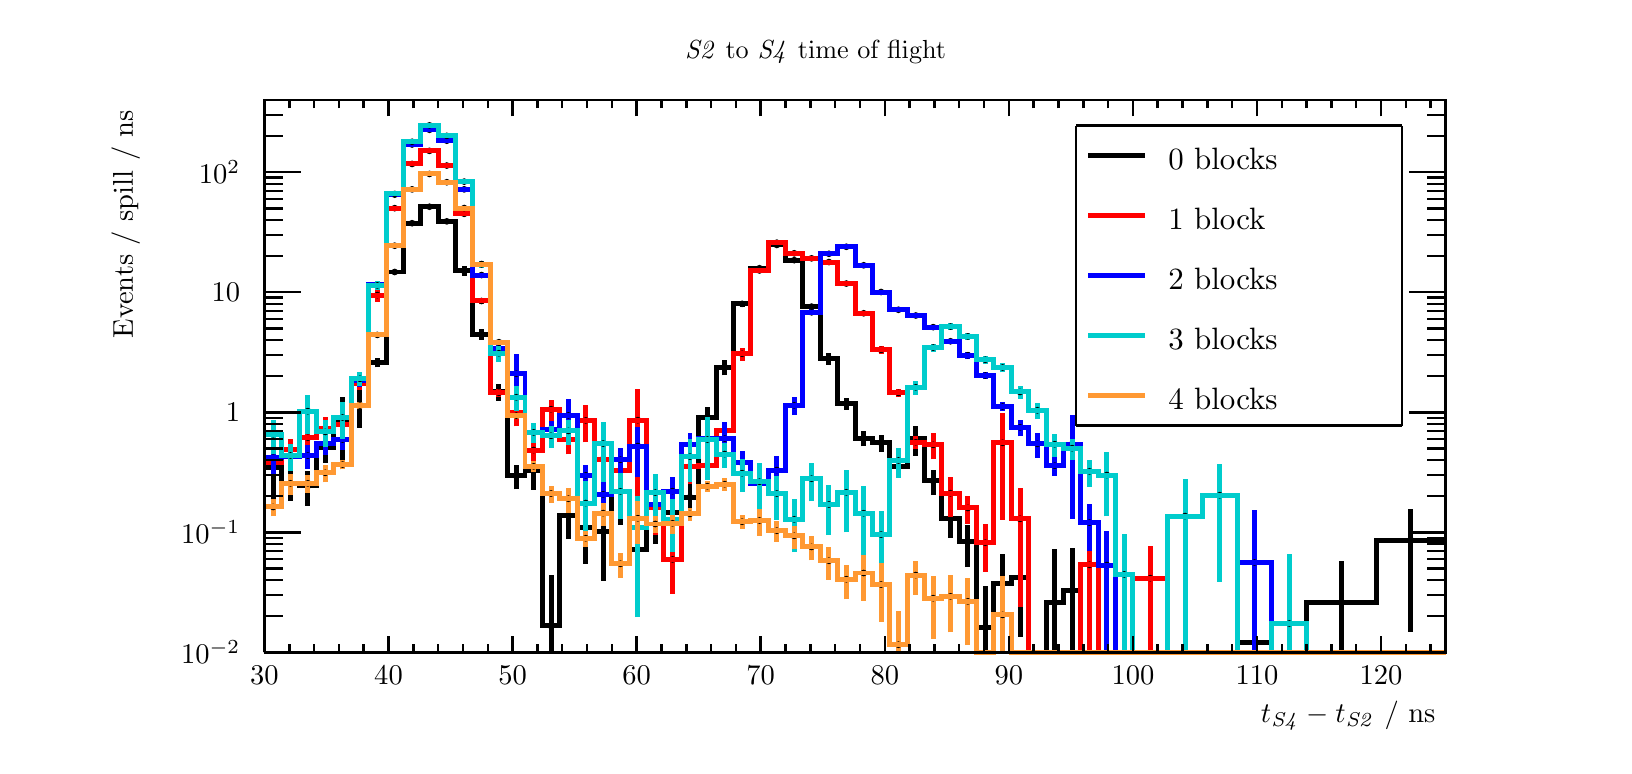
\begin{tikzpicture}
\pgfdeclareplotmark{cross} {
\pgfpathmoveto{\pgfpoint{-0.3\pgfplotmarksize}{\pgfplotmarksize}}
\pgfpathlineto{\pgfpoint{+0.3\pgfplotmarksize}{\pgfplotmarksize}}
\pgfpathlineto{\pgfpoint{+0.3\pgfplotmarksize}{0.3\pgfplotmarksize}}
\pgfpathlineto{\pgfpoint{+1\pgfplotmarksize}{0.3\pgfplotmarksize}}
\pgfpathlineto{\pgfpoint{+1\pgfplotmarksize}{-0.3\pgfplotmarksize}}
\pgfpathlineto{\pgfpoint{+0.3\pgfplotmarksize}{-0.3\pgfplotmarksize}}
\pgfpathlineto{\pgfpoint{+0.3\pgfplotmarksize}{-1.\pgfplotmarksize}}
\pgfpathlineto{\pgfpoint{-0.3\pgfplotmarksize}{-1.\pgfplotmarksize}}
\pgfpathlineto{\pgfpoint{-0.3\pgfplotmarksize}{-0.3\pgfplotmarksize}}
\pgfpathlineto{\pgfpoint{-1.\pgfplotmarksize}{-0.3\pgfplotmarksize}}
\pgfpathlineto{\pgfpoint{-1.\pgfplotmarksize}{0.3\pgfplotmarksize}}
\pgfpathlineto{\pgfpoint{-0.3\pgfplotmarksize}{0.3\pgfplotmarksize}}
\pgfpathclose
\pgfusepathqstroke
}
\pgfdeclareplotmark{cross*} {
\pgfpathmoveto{\pgfpoint{-0.3\pgfplotmarksize}{\pgfplotmarksize}}
\pgfpathlineto{\pgfpoint{+0.3\pgfplotmarksize}{\pgfplotmarksize}}
\pgfpathlineto{\pgfpoint{+0.3\pgfplotmarksize}{0.3\pgfplotmarksize}}
\pgfpathlineto{\pgfpoint{+1\pgfplotmarksize}{0.3\pgfplotmarksize}}
\pgfpathlineto{\pgfpoint{+1\pgfplotmarksize}{-0.3\pgfplotmarksize}}
\pgfpathlineto{\pgfpoint{+0.3\pgfplotmarksize}{-0.3\pgfplotmarksize}}
\pgfpathlineto{\pgfpoint{+0.3\pgfplotmarksize}{-1.\pgfplotmarksize}}
\pgfpathlineto{\pgfpoint{-0.3\pgfplotmarksize}{-1.\pgfplotmarksize}}
\pgfpathlineto{\pgfpoint{-0.3\pgfplotmarksize}{-0.3\pgfplotmarksize}}
\pgfpathlineto{\pgfpoint{-1.\pgfplotmarksize}{-0.3\pgfplotmarksize}}
\pgfpathlineto{\pgfpoint{-1.\pgfplotmarksize}{0.3\pgfplotmarksize}}
\pgfpathlineto{\pgfpoint{-0.3\pgfplotmarksize}{0.3\pgfplotmarksize}}
\pgfpathclose
\pgfusepathqfillstroke
}
\pgfdeclareplotmark{newstar} {
\pgfpathmoveto{\pgfqpoint{0pt}{\pgfplotmarksize}}
\pgfpathlineto{\pgfqpointpolar{44}{0.5\pgfplotmarksize}}
\pgfpathlineto{\pgfqpointpolar{18}{\pgfplotmarksize}}
\pgfpathlineto{\pgfqpointpolar{-20}{0.5\pgfplotmarksize}}
\pgfpathlineto{\pgfqpointpolar{-54}{\pgfplotmarksize}}
\pgfpathlineto{\pgfqpointpolar{-90}{0.5\pgfplotmarksize}}
\pgfpathlineto{\pgfqpointpolar{234}{\pgfplotmarksize}}
\pgfpathlineto{\pgfqpointpolar{198}{0.5\pgfplotmarksize}}
\pgfpathlineto{\pgfqpointpolar{162}{\pgfplotmarksize}}
\pgfpathlineto{\pgfqpointpolar{134}{0.5\pgfplotmarksize}}
\pgfpathclose
\pgfusepathqstroke
}
\pgfdeclareplotmark{newstar*} {
\pgfpathmoveto{\pgfqpoint{0pt}{\pgfplotmarksize}}
\pgfpathlineto{\pgfqpointpolar{44}{0.5\pgfplotmarksize}}
\pgfpathlineto{\pgfqpointpolar{18}{\pgfplotmarksize}}
\pgfpathlineto{\pgfqpointpolar{-20}{0.5\pgfplotmarksize}}
\pgfpathlineto{\pgfqpointpolar{-54}{\pgfplotmarksize}}
\pgfpathlineto{\pgfqpointpolar{-90}{0.5\pgfplotmarksize}}
\pgfpathlineto{\pgfqpointpolar{234}{\pgfplotmarksize}}
\pgfpathlineto{\pgfqpointpolar{198}{0.5\pgfplotmarksize}}
\pgfpathlineto{\pgfqpointpolar{162}{\pgfplotmarksize}}
\pgfpathlineto{\pgfqpointpolar{134}{0.5\pgfplotmarksize}}
\pgfpathclose
\pgfusepathqfillstroke
}
\definecolor{c}{rgb}{1,1,1};
\draw [color=c, fill=c] (0,0) rectangle (20,9.11025);
\draw [color=c, fill=c] (3,1.18433) rectangle (18,8.19923);
\definecolor{c}{rgb}{0,0,0};
\draw [c,line width=0.9] (3,1.18433) -- (3,8.19923) -- (18,8.19923) -- (18,1.18433) -- (3,1.18433);
\definecolor{c}{rgb}{1,1,1};
\draw [color=c, fill=c] (3,1.18433) rectangle (18,8.19923);
\definecolor{c}{rgb}{0,0,0};
\draw [c,line width=0.9] (3,1.18433) -- (3,8.19923) -- (18,8.19923) -- (18,1.18433) -- (3,1.18433);
\draw [c,line width=0.9] (3,1.18433) -- (3.22059,1.18433) -- (3.22059,1.18433) -- (3.44118,1.18433) -- (3.44118,1.18433) -- (3.66176,1.18433) -- (3.66176,1.18433) -- (3.88235,1.18433) -- (3.88235,1.18433) -- (4.10294,1.18433) -- (4.10294,1.18433) --
 (4.32353,1.18433) -- (4.32353,1.18433) -- (4.54412,1.18433) -- (4.54412,1.18433) -- (4.76471,1.18433) -- (4.76471,1.18433) -- (4.98529,1.18433) -- (4.98529,1.18433) -- (5.20588,1.18433) -- (5.20588,1.18433) -- (5.42647,1.18433) -- (5.42647,1.18433)
 -- (5.64706,1.18433) -- (5.64706,1.18433) -- (5.86765,1.18433) -- (5.86765,1.18433) -- (6.08824,1.18433) -- (6.08824,1.18433) -- (6.30882,1.18433) -- (6.30882,1.18433) -- (6.52941,1.18433) -- (6.52941,1.18433) -- (6.75,1.18433) -- (6.75,1.18433) --
 (6.97059,1.18433) -- (6.97059,1.18433) -- (7.19118,1.18433) -- (7.19118,1.18433) -- (7.41176,1.18433) -- (7.41176,1.18433) -- (7.63235,1.18433) -- (7.63235,1.18433) -- (7.85294,1.18433) -- (7.85294,1.18433) -- (8.07353,1.18433) -- (8.07353,1.18433)
 -- (8.29412,1.18433) -- (8.29412,1.18433) -- (8.51471,1.18433) -- (8.51471,1.18433) -- (8.73529,1.18433) -- (8.73529,1.18433) -- (8.95588,1.18433) -- (8.95588,1.18433) -- (9.17647,1.18433) -- (9.17647,1.18433) -- (9.39706,1.18433) --
 (9.39706,1.18433) -- (9.61765,1.18433) -- (9.61765,1.18433) -- (9.83823,1.18433) -- (9.83823,1.18433) -- (10.0588,1.18433) -- (10.0588,1.18433) -- (10.2794,1.18433) -- (10.2794,1.18433) -- (10.5,1.18433) -- (10.5,1.18433) -- (10.7206,1.18433) --
 (10.7206,1.18433) -- (10.9412,1.18433) -- (10.9412,1.18433) -- (11.1618,1.18433) -- (11.1618,1.18433) -- (11.3824,1.18433) -- (11.3824,1.18433) -- (11.6029,1.18433) -- (11.6029,1.18433) -- (11.8235,1.18433) -- (11.8235,1.18433) -- (12.0441,1.18433)
 -- (12.0441,1.18433) -- (12.2647,1.18433) -- (12.2647,1.18433) -- (12.4853,1.18433) -- (12.4853,1.18433) -- (12.7059,1.18433) -- (12.7059,1.18433) -- (12.9265,1.18433) -- (12.9265,1.18433) -- (13.1471,1.18433) -- (13.1471,1.18433) --
 (13.3676,1.18433) -- (13.3676,1.18433) -- (13.5882,1.18433) -- (13.5882,1.18433) -- (13.8088,1.18433) -- (13.8088,1.18433) -- (14.0294,1.18433) -- (14.0294,1.18433) -- (14.4706,1.18433) -- (14.4706,1.18433) -- (14.9118,1.18433) -- (14.9118,1.18433)
 -- (15.3529,1.18433) -- (15.3529,1.18433) -- (15.7941,1.18433) -- (15.7941,1.18433) -- (16.2353,1.18433) -- (16.2353,1.18433) -- (17.1176,1.18433) -- (17.1176,1.18433) -- (18,1.18433);
\draw [c,line width=0.9] (3,1.18433) -- (18,1.18433);
\draw [c,line width=0.9] (3,1.38931) -- (3,1.18433);
\draw [c,line width=0.9] (3.31513,1.28682) -- (3.31513,1.18433);
\draw [c,line width=0.9] (3.63025,1.28682) -- (3.63025,1.18433);
\draw [c,line width=0.9] (3.94538,1.28682) -- (3.94538,1.18433);
\draw [c,line width=0.9] (4.2605,1.28682) -- (4.2605,1.18433);
\draw [c,line width=0.9] (4.57563,1.38931) -- (4.57563,1.18433);
\draw [c,line width=0.9] (4.89076,1.28682) -- (4.89076,1.18433);
\draw [c,line width=0.9] (5.20588,1.28682) -- (5.20588,1.18433);
\draw [c,line width=0.9] (5.52101,1.28682) -- (5.52101,1.18433);
\draw [c,line width=0.9] (5.83613,1.28682) -- (5.83613,1.18433);
\draw [c,line width=0.9] (6.15126,1.38931) -- (6.15126,1.18433);
\draw [c,line width=0.9] (6.46639,1.28682) -- (6.46639,1.18433);
\draw [c,line width=0.9] (6.78151,1.28682) -- (6.78151,1.18433);
\draw [c,line width=0.9] (7.09664,1.28682) -- (7.09664,1.18433);
\draw [c,line width=0.9] (7.41176,1.28682) -- (7.41176,1.18433);
\draw [c,line width=0.9] (7.72689,1.38931) -- (7.72689,1.18433);
\draw [c,line width=0.9] (8.04202,1.28682) -- (8.04202,1.18433);
\draw [c,line width=0.9] (8.35714,1.28682) -- (8.35714,1.18433);
\draw [c,line width=0.9] (8.67227,1.28682) -- (8.67227,1.18433);
\draw [c,line width=0.9] (8.9874,1.28682) -- (8.9874,1.18433);
\draw [c,line width=0.9] (9.30252,1.38931) -- (9.30252,1.18433);
\draw [c,line width=0.9] (9.61765,1.28682) -- (9.61765,1.18433);
\draw [c,line width=0.9] (9.93277,1.28682) -- (9.93277,1.18433);
\draw [c,line width=0.9] (10.2479,1.28682) -- (10.2479,1.18433);
\draw [c,line width=0.9] (10.563,1.28682) -- (10.563,1.18433);
\draw [c,line width=0.9] (10.8782,1.38931) -- (10.8782,1.18433);
\draw [c,line width=0.9] (11.1933,1.28682) -- (11.1933,1.18433);
\draw [c,line width=0.9] (11.5084,1.28682) -- (11.5084,1.18433);
\draw [c,line width=0.9] (11.8235,1.28682) -- (11.8235,1.18433);
\draw [c,line width=0.9] (12.1387,1.28682) -- (12.1387,1.18433);
\draw [c,line width=0.9] (12.4538,1.38931) -- (12.4538,1.18433);
\draw [c,line width=0.9] (12.7689,1.28682) -- (12.7689,1.18433);
\draw [c,line width=0.9] (13.084,1.28682) -- (13.084,1.18433);
\draw [c,line width=0.9] (13.3992,1.28682) -- (13.3992,1.18433);
\draw [c,line width=0.9] (13.7143,1.28682) -- (13.7143,1.18433);
\draw [c,line width=0.9] (14.0294,1.38931) -- (14.0294,1.18433);
\draw [c,line width=0.9] (14.3445,1.28682) -- (14.3445,1.18433);
\draw [c,line width=0.9] (14.6597,1.28682) -- (14.6597,1.18433);
\draw [c,line width=0.9] (14.9748,1.28682) -- (14.9748,1.18433);
\draw [c,line width=0.9] (15.2899,1.28682) -- (15.2899,1.18433);
\draw [c,line width=0.9] (15.605,1.38931) -- (15.605,1.18433);
\draw [c,line width=0.9] (15.9202,1.28682) -- (15.9202,1.18433);
\draw [c,line width=0.9] (16.2353,1.28682) -- (16.2353,1.18433);
\draw [c,line width=0.9] (16.5504,1.28682) -- (16.5504,1.18433);
\draw [c,line width=0.9] (16.8655,1.28682) -- (16.8655,1.18433);
\draw [c,line width=0.9] (17.1807,1.38931) -- (17.1807,1.18433);
\draw [c,line width=0.9] (17.1807,1.38931) -- (17.1807,1.18433);
\draw [c,line width=0.9] (17.4958,1.28682) -- (17.4958,1.18433);
\draw [c,line width=0.9] (17.8109,1.28682) -- (17.8109,1.18433);
\draw [anchor=base] (3,0.774371) node[scale=1.03101, color=c, rotate=0]{30};
\draw [anchor=base] (4.57563,0.774371) node[scale=1.03101, color=c, rotate=0]{40};
\draw [anchor=base] (6.15126,0.774371) node[scale=1.03101, color=c, rotate=0]{50};
\draw [anchor=base] (7.72689,0.774371) node[scale=1.03101, color=c, rotate=0]{60};
\draw [anchor=base] (9.30252,0.774371) node[scale=1.03101, color=c, rotate=0]{70};
\draw [anchor=base] (10.8782,0.774371) node[scale=1.03101, color=c, rotate=0]{80};
\draw [anchor=base] (12.4538,0.774371) node[scale=1.03101, color=c, rotate=0]{90};
\draw [anchor=base] (14.0294,0.774371) node[scale=1.03101, color=c, rotate=0]{100};
\draw [anchor=base] (15.605,0.774371) node[scale=1.03101, color=c, rotate=0]{110};
\draw [anchor=base] (17.1807,0.774371) node[scale=1.03101, color=c, rotate=0]{120};
\draw [anchor= east] (18,0.382631) node[scale=1.03101, color=c, rotate=0]{$ t_{\mathit{S4}} - t_{\mathit{S2}}$ / ns};
\draw [c,line width=0.9] (3,8.19923) -- (18,8.19923);
\draw [c,line width=0.9] (3,7.99425) -- (3,8.19923);
\draw [c,line width=0.9] (3.31513,8.09674) -- (3.31513,8.19923);
\draw [c,line width=0.9] (3.63025,8.09674) -- (3.63025,8.19923);
\draw [c,line width=0.9] (3.94538,8.09674) -- (3.94538,8.19923);
\draw [c,line width=0.9] (4.2605,8.09674) -- (4.2605,8.19923);
\draw [c,line width=0.9] (4.57563,7.99425) -- (4.57563,8.19923);
\draw [c,line width=0.9] (4.89076,8.09674) -- (4.89076,8.19923);
\draw [c,line width=0.9] (5.20588,8.09674) -- (5.20588,8.19923);
\draw [c,line width=0.9] (5.52101,8.09674) -- (5.52101,8.19923);
\draw [c,line width=0.9] (5.83613,8.09674) -- (5.83613,8.19923);
\draw [c,line width=0.9] (6.15126,7.99425) -- (6.15126,8.19923);
\draw [c,line width=0.9] (6.46639,8.09674) -- (6.46639,8.19923);
\draw [c,line width=0.9] (6.78151,8.09674) -- (6.78151,8.19923);
\draw [c,line width=0.9] (7.09664,8.09674) -- (7.09664,8.19923);
\draw [c,line width=0.9] (7.41176,8.09674) -- (7.41176,8.19923);
\draw [c,line width=0.9] (7.72689,7.99425) -- (7.72689,8.19923);
\draw [c,line width=0.9] (8.04202,8.09674) -- (8.04202,8.19923);
\draw [c,line width=0.9] (8.35714,8.09674) -- (8.35714,8.19923);
\draw [c,line width=0.9] (8.67227,8.09674) -- (8.67227,8.19923);
\draw [c,line width=0.9] (8.9874,8.09674) -- (8.9874,8.19923);
\draw [c,line width=0.9] (9.30252,7.99425) -- (9.30252,8.19923);
\draw [c,line width=0.9] (9.61765,8.09674) -- (9.61765,8.19923);
\draw [c,line width=0.9] (9.93277,8.09674) -- (9.93277,8.19923);
\draw [c,line width=0.9] (10.2479,8.09674) -- (10.2479,8.19923);
\draw [c,line width=0.9] (10.563,8.09674) -- (10.563,8.19923);
\draw [c,line width=0.9] (10.8782,7.99425) -- (10.8782,8.19923);
\draw [c,line width=0.9] (11.1933,8.09674) -- (11.1933,8.19923);
\draw [c,line width=0.9] (11.5084,8.09674) -- (11.5084,8.19923);
\draw [c,line width=0.9] (11.8235,8.09674) -- (11.8235,8.19923);
\draw [c,line width=0.9] (12.1387,8.09674) -- (12.1387,8.19923);
\draw [c,line width=0.9] (12.4538,7.99425) -- (12.4538,8.19923);
\draw [c,line width=0.9] (12.7689,8.09674) -- (12.7689,8.19923);
\draw [c,line width=0.9] (13.084,8.09674) -- (13.084,8.19923);
\draw [c,line width=0.9] (13.3992,8.09674) -- (13.3992,8.19923);
\draw [c,line width=0.9] (13.7143,8.09674) -- (13.7143,8.19923);
\draw [c,line width=0.9] (14.0294,7.99425) -- (14.0294,8.19923);
\draw [c,line width=0.9] (14.3445,8.09674) -- (14.3445,8.19923);
\draw [c,line width=0.9] (14.6597,8.09674) -- (14.6597,8.19923);
\draw [c,line width=0.9] (14.9748,8.09674) -- (14.9748,8.19923);
\draw [c,line width=0.9] (15.2899,8.09674) -- (15.2899,8.19923);
\draw [c,line width=0.9] (15.605,7.99425) -- (15.605,8.19923);
\draw [c,line width=0.9] (15.9202,8.09674) -- (15.9202,8.19923);
\draw [c,line width=0.9] (16.2353,8.09674) -- (16.2353,8.19923);
\draw [c,line width=0.9] (16.5504,8.09674) -- (16.5504,8.19923);
\draw [c,line width=0.9] (16.8655,8.09674) -- (16.8655,8.19923);
\draw [c,line width=0.9] (17.1807,7.99425) -- (17.1807,8.19923);
\draw [c,line width=0.9] (17.1807,7.99425) -- (17.1807,8.19923);
\draw [c,line width=0.9] (17.4958,8.09674) -- (17.4958,8.19923);
\draw [c,line width=0.9] (17.8109,8.09674) -- (17.8109,8.19923);
\draw [c,line width=0.9] (3,1.18433) -- (3,8.19923);
\draw [c,line width=0.9] (3.462,1.18433) -- (3,1.18433);
\draw [anchor= east] (2.82,1.18433) node[scale=1.03101, color=c, rotate=0]{$10^{-2}$};
\draw [c,line width=0.9] (3.231,1.64319) -- (3,1.64319);
\draw [c,line width=0.9] (3.231,1.91161) -- (3,1.91161);
\draw [c,line width=0.9] (3.231,2.10205) -- (3,2.10205);
\draw [c,line width=0.9] (3.231,2.24977) -- (3,2.24977);
\draw [c,line width=0.9] (3.231,2.37047) -- (3,2.37047);
\draw [c,line width=0.9] (3.231,2.47251) -- (3,2.47251);
\draw [c,line width=0.9] (3.231,2.56091) -- (3,2.56091);
\draw [c,line width=0.9] (3.231,2.63888) -- (3,2.63888);
\draw [c,line width=0.9] (3.462,2.70863) -- (3,2.70863);
\draw [anchor= east] (2.82,2.70863) node[scale=1.03101, color=c, rotate=0]{$10^{-1}$};
\draw [c,line width=0.9] (3.231,3.16749) -- (3,3.16749);
\draw [c,line width=0.9] (3.231,3.4359) -- (3,3.4359);
\draw [c,line width=0.9] (3.231,3.62634) -- (3,3.62634);
\draw [c,line width=0.9] (3.231,3.77406) -- (3,3.77406);
\draw [c,line width=0.9] (3.231,3.89476) -- (3,3.89476);
\draw [c,line width=0.9] (3.231,3.99681) -- (3,3.99681);
\draw [c,line width=0.9] (3.231,4.0852) -- (3,4.0852);
\draw [c,line width=0.9] (3.231,4.16317) -- (3,4.16317);
\draw [c,line width=0.9] (3.462,4.23292) -- (3,4.23292);
\draw [anchor= east] (2.82,4.23292) node[scale=1.03101, color=c, rotate=0]{1};
\draw [c,line width=0.9] (3.231,4.69178) -- (3,4.69178);
\draw [c,line width=0.9] (3.231,4.9602) -- (3,4.9602);
\draw [c,line width=0.9] (3.231,5.15064) -- (3,5.15064);
\draw [c,line width=0.9] (3.231,5.29836) -- (3,5.29836);
\draw [c,line width=0.9] (3.231,5.41905) -- (3,5.41905);
\draw [c,line width=0.9] (3.231,5.5211) -- (3,5.5211);
\draw [c,line width=0.9] (3.231,5.6095) -- (3,5.6095);
\draw [c,line width=0.9] (3.231,5.68747) -- (3,5.68747);
\draw [c,line width=0.9] (3.462,5.75722) -- (3,5.75722);
\draw [anchor= east] (2.82,5.75722) node[scale=1.03101, color=c, rotate=0]{10};
\draw [c,line width=0.9] (3.231,6.21607) -- (3,6.21607);
\draw [c,line width=0.9] (3.231,6.48449) -- (3,6.48449);
\draw [c,line width=0.9] (3.231,6.67493) -- (3,6.67493);
\draw [c,line width=0.9] (3.231,6.82265) -- (3,6.82265);
\draw [c,line width=0.9] (3.231,6.94335) -- (3,6.94335);
\draw [c,line width=0.9] (3.231,7.04539) -- (3,7.04539);
\draw [c,line width=0.9] (3.231,7.13379) -- (3,7.13379);
\draw [c,line width=0.9] (3.231,7.21176) -- (3,7.21176);
\draw [c,line width=0.9] (3.462,7.28151) -- (3,7.28151);
\draw [anchor= east] (2.82,7.28151) node[scale=1.03101, color=c, rotate=0]{$10^{2}$};
\draw [c,line width=0.9] (3.231,7.74037) -- (3,7.74037);
\draw [c,line width=0.9] (3.231,8.00878) -- (3,8.00878);
\draw [c,line width=0.9] (3.231,8.19923) -- (3,8.19923);
\draw [anchor= east] (1.24,8.19923) node[scale=1.03101, color=c, rotate=90]{ Events / spill / ns};
\draw [c,line width=0.9] (18,1.18433) -- (18,8.19923);
\draw [c,line width=0.9] (17.538,1.18433) -- (18,1.18433);
\draw [c,line width=0.9] (17.769,1.64319) -- (18,1.64319);
\draw [c,line width=0.9] (17.769,1.91161) -- (18,1.91161);
\draw [c,line width=0.9] (17.769,2.10205) -- (18,2.10205);
\draw [c,line width=0.9] (17.769,2.24977) -- (18,2.24977);
\draw [c,line width=0.9] (17.769,2.37047) -- (18,2.37047);
\draw [c,line width=0.9] (17.769,2.47251) -- (18,2.47251);
\draw [c,line width=0.9] (17.769,2.56091) -- (18,2.56091);
\draw [c,line width=0.9] (17.769,2.63888) -- (18,2.63888);
\draw [c,line width=0.9] (17.538,2.70863) -- (18,2.70863);
\draw [c,line width=0.9] (17.769,3.16749) -- (18,3.16749);
\draw [c,line width=0.9] (17.769,3.4359) -- (18,3.4359);
\draw [c,line width=0.9] (17.769,3.62634) -- (18,3.62634);
\draw [c,line width=0.9] (17.769,3.77406) -- (18,3.77406);
\draw [c,line width=0.9] (17.769,3.89476) -- (18,3.89476);
\draw [c,line width=0.9] (17.769,3.99681) -- (18,3.99681);
\draw [c,line width=0.9] (17.769,4.0852) -- (18,4.0852);
\draw [c,line width=0.9] (17.769,4.16317) -- (18,4.16317);
\draw [c,line width=0.9] (17.538,4.23292) -- (18,4.23292);
\draw [c,line width=0.9] (17.769,4.69178) -- (18,4.69178);
\draw [c,line width=0.9] (17.769,4.9602) -- (18,4.9602);
\draw [c,line width=0.9] (17.769,5.15064) -- (18,5.15064);
\draw [c,line width=0.9] (17.769,5.29836) -- (18,5.29836);
\draw [c,line width=0.9] (17.769,5.41905) -- (18,5.41905);
\draw [c,line width=0.9] (17.769,5.5211) -- (18,5.5211);
\draw [c,line width=0.9] (17.769,5.6095) -- (18,5.6095);
\draw [c,line width=0.9] (17.769,5.68747) -- (18,5.68747);
\draw [c,line width=0.9] (17.538,5.75722) -- (18,5.75722);
\draw [c,line width=0.9] (17.769,6.21607) -- (18,6.21607);
\draw [c,line width=0.9] (17.769,6.48449) -- (18,6.48449);
\draw [c,line width=0.9] (17.769,6.67493) -- (18,6.67493);
\draw [c,line width=0.9] (17.769,6.82265) -- (18,6.82265);
\draw [c,line width=0.9] (17.769,6.94335) -- (18,6.94335);
\draw [c,line width=0.9] (17.769,7.04539) -- (18,7.04539);
\draw [c,line width=0.9] (17.769,7.13379) -- (18,7.13379);
\draw [c,line width=0.9] (17.769,7.21176) -- (18,7.21176);
\draw [c,line width=0.9] (17.538,7.28151) -- (18,7.28151);
\draw [c,line width=0.9] (17.769,7.74037) -- (18,7.74037);
\draw [c,line width=0.9] (17.769,8.00878) -- (18,8.00878);
\draw [c,line width=0.9] (17.769,8.19923) -- (18,8.19923);
\draw [c,line width=1.8] (3.11029,3.01059) -- (3.11029,3.53716);
\draw [c,line width=1.8] (3.11029,3.53716) -- (3.11029,3.82669);
\foreach \P in {(3.11029,3.53716)}{\draw[mark options={color=c,fill=c},mark size=2.402402pt,mark=*,mark size=1pt] plot coordinates {\P};}
\draw [c,line width=1.8] (3.33088,3.11042) -- (3.33088,3.3234);
\draw [c,line width=1.8] (3.33088,3.3234) -- (3.33088,3.48428);
\foreach \P in {(3.33088,3.3234)}{\draw[mark options={color=c,fill=c},mark size=2.402402pt,mark=*,mark size=1pt] plot coordinates {\P};}
\draw [c,line width=1.8] (3.55147,3.04626) -- (3.55147,3.29901);
\draw [c,line width=1.8] (3.55147,3.29901) -- (3.55147,3.48149);
\foreach \P in {(3.55147,3.29901)}{\draw[mark options={color=c,fill=c},mark size=2.402402pt,mark=*,mark size=1pt] plot coordinates {\P};}
\draw [c,line width=1.8] (3.77206,3.59376) -- (3.77206,3.78886);
\draw [c,line width=1.8] (3.77206,3.78886) -- (3.77206,3.93936);
\foreach \P in {(3.77206,3.78886)}{\draw[mark options={color=c,fill=c},mark size=2.402402pt,mark=*,mark size=1pt] plot coordinates {\P};}
\draw [c,line width=1.8] (3.99265,3.50647) -- (3.99265,4.11906);
\draw [c,line width=1.8] (3.99265,4.11906) -- (3.99265,4.4317);
\foreach \P in {(3.99265,4.11906)}{\draw[mark options={color=c,fill=c},mark size=2.402402pt,mark=*,mark size=1pt] plot coordinates {\P};}
\draw [c,line width=1.8] (4.21324,4.03848) -- (4.21324,4.32444);
\draw [c,line width=1.8] (4.21324,4.32444) -- (4.21324,4.52349);
\foreach \P in {(4.21324,4.32444)}{\draw[mark options={color=c,fill=c},mark size=2.402402pt,mark=*,mark size=1pt] plot coordinates {\P};}
\draw [c,line width=1.8] (4.43382,4.80441) -- (4.43382,4.86726);
\draw [c,line width=1.8] (4.43382,4.86726) -- (4.43382,4.92466);
\foreach \P in {(4.43382,4.86726)}{\draw[mark options={color=c,fill=c},mark size=2.402402pt,mark=*,mark size=1pt] plot coordinates {\P};}
\draw [c,line width=1.8] (4.65441,5.98509) -- (4.65441,6.01435);
\draw [c,line width=1.8] (4.65441,6.01435) -- (4.65441,6.04237);
\foreach \P in {(4.65441,6.01435)}{\draw[mark options={color=c,fill=c},mark size=2.402402pt,mark=*,mark size=1pt] plot coordinates {\P};}
\draw [c,line width=1.8] (4.875,6.6125) -- (4.875,6.63394);
\draw [c,line width=1.8] (4.875,6.63394) -- (4.875,6.65471);
\foreach \P in {(4.875,6.63394)}{\draw[mark options={color=c,fill=c},mark size=2.402402pt,mark=*,mark size=1pt] plot coordinates {\P};}
\draw [c,line width=1.8] (5.09559,6.82128) -- (5.09559,6.84324);
\draw [c,line width=1.8] (5.09559,6.84324) -- (5.09559,6.8645);
\foreach \P in {(5.09559,6.84324)}{\draw[mark options={color=c,fill=c},mark size=2.402402pt,mark=*,mark size=1pt] plot coordinates {\P};}
\draw [c,line width=1.8] (5.31618,6.62665) -- (5.31618,6.65758);
\draw [c,line width=1.8] (5.31618,6.65758) -- (5.31618,6.68713);
\foreach \P in {(5.31618,6.65758)}{\draw[mark options={color=c,fill=c},mark size=2.402402pt,mark=*,mark size=1pt] plot coordinates {\P};}
\draw [c,line width=1.8] (5.53676,5.96974) -- (5.53676,6.02947);
\draw [c,line width=1.8] (5.53676,6.02947) -- (5.53676,6.08426);
\foreach \P in {(5.53676,6.02947)}{\draw[mark options={color=c,fill=c},mark size=2.402402pt,mark=*,mark size=1pt] plot coordinates {\P};}
\draw [c,line width=1.8] (5.75735,5.15161) -- (5.75735,5.22451);
\draw [c,line width=1.8] (5.75735,5.22451) -- (5.75735,5.29016);
\foreach \P in {(5.75735,5.22451)}{\draw[mark options={color=c,fill=c},mark size=2.402402pt,mark=*,mark size=1pt] plot coordinates {\P};}
\draw [c,line width=1.8] (5.97794,4.37808) -- (5.97794,4.49492);
\draw [c,line width=1.8] (5.97794,4.49492) -- (5.97794,4.5942);
\foreach \P in {(5.97794,4.49492)}{\draw[mark options={color=c,fill=c},mark size=2.402402pt,mark=*,mark size=1pt] plot coordinates {\P};}
\draw [c,line width=1.8] (6.19853,3.25269) -- (6.19853,3.42437);
\draw [c,line width=1.8] (6.19853,3.42437) -- (6.19853,3.56058);
\foreach \P in {(6.19853,3.42437)}{\draw[mark options={color=c,fill=c},mark size=2.402402pt,mark=*,mark size=1pt] plot coordinates {\P};}
\draw [c,line width=1.8] (6.41912,3.25055) -- (6.41912,3.49418);
\draw [c,line width=1.8] (6.41912,3.49418) -- (6.41912,3.67187);
\foreach \P in {(6.41912,3.49418)}{\draw[mark options={color=c,fill=c},mark size=2.402402pt,mark=*,mark size=1pt] plot coordinates {\P};}
\draw [c,line width=1.8] (6.63971,1.18433) -- (6.63971,1.52013);
\draw [c,line width=1.8] (6.63971,1.52013) -- (6.63971,2.16651);
\foreach \P in {(6.63971,1.52013)}{\draw[mark options={color=c,fill=c},mark size=2.402402pt,mark=*,mark size=1pt] plot coordinates {\P};}
\draw [c,line width=1.8] (6.86029,2.6208) -- (6.86029,2.92257);
\draw [c,line width=1.8] (6.86029,2.92257) -- (6.86029,3.12908);
\foreach \P in {(6.86029,2.92257)}{\draw[mark options={color=c,fill=c},mark size=2.402402pt,mark=*,mark size=1pt] plot coordinates {\P};}
\draw [c,line width=1.8] (7.08088,2.30724) -- (7.08088,2.76685);
\draw [c,line width=1.8] (7.08088,2.76685) -- (7.08088,3.03552);
\foreach \P in {(7.08088,2.76685)}{\draw[mark options={color=c,fill=c},mark size=2.402402pt,mark=*,mark size=1pt] plot coordinates {\P};}
\draw [c,line width=1.8] (7.30147,2.09583) -- (7.30147,2.71841);
\draw [c,line width=1.8] (7.30147,2.71841) -- (7.30147,3.03349);
\foreach \P in {(7.30147,2.71841)}{\draw[mark options={color=c,fill=c},mark size=2.402402pt,mark=*,mark size=1pt] plot coordinates {\P};}
\draw [c,line width=1.8] (7.52206,2.80159) -- (7.52206,3.22686);
\draw [c,line width=1.8] (7.52206,3.22686) -- (7.52206,3.48368);
\foreach \P in {(7.52206,3.22686)}{\draw[mark options={color=c,fill=c},mark size=2.402402pt,mark=*,mark size=1pt] plot coordinates {\P};}
\draw [c,line width=1.8] (7.74265,2.00764) -- (7.74265,2.49321);
\draw [c,line width=1.8] (7.74265,2.49321) -- (7.74265,2.7703);
\foreach \P in {(7.74265,2.49321)}{\draw[mark options={color=c,fill=c},mark size=2.402402pt,mark=*,mark size=1pt] plot coordinates {\P};}
\draw [c,line width=1.8] (7.96324,2.55851) -- (7.96324,3.02649);
\draw [c,line width=1.8] (7.96324,3.02649) -- (7.96324,3.29792);
\foreach \P in {(7.96324,3.02649)}{\draw[mark options={color=c,fill=c},mark size=2.402402pt,mark=*,mark size=1pt] plot coordinates {\P};}
\draw [c,line width=1.8] (8.18382,2.65833) -- (8.18382,2.95996);
\draw [c,line width=1.8] (8.18382,2.95996) -- (8.18382,3.16641);
\foreach \P in {(8.18382,2.95996)}{\draw[mark options={color=c,fill=c},mark size=2.402402pt,mark=*,mark size=1pt] plot coordinates {\P};}
\draw [c,line width=1.8] (8.40441,2.93473) -- (8.40441,3.15503);
\draw [c,line width=1.8] (8.40441,3.15503) -- (8.40441,3.32004);
\foreach \P in {(8.40441,3.15503)}{\draw[mark options={color=c,fill=c},mark size=2.402402pt,mark=*,mark size=1pt] plot coordinates {\P};}
\draw [c,line width=1.8] (8.625,4.01263) -- (8.625,4.17078);
\draw [c,line width=1.8] (8.625,4.17078) -- (8.625,4.29834);
\foreach \P in {(8.625,4.17078)}{\draw[mark options={color=c,fill=c},mark size=2.402402pt,mark=*,mark size=1pt] plot coordinates {\P};}
\draw [c,line width=1.8] (8.84559,4.70224) -- (8.84559,4.8068);
\draw [c,line width=1.8] (8.84559,4.8068) -- (8.84559,4.89707);
\foreach \P in {(8.84559,4.8068)}{\draw[mark options={color=c,fill=c},mark size=2.402402pt,mark=*,mark size=1pt] plot coordinates {\P};}
\draw [c,line width=1.8] (9.06618,5.56733) -- (9.06618,5.6099);
\draw [c,line width=1.8] (9.06618,5.6099) -- (9.06618,5.64989);
\foreach \P in {(9.06618,5.6099)}{\draw[mark options={color=c,fill=c},mark size=2.402402pt,mark=*,mark size=1pt] plot coordinates {\P};}
\draw [c,line width=1.8] (9.28677,6.03393) -- (9.28677,6.06192);
\draw [c,line width=1.8] (9.28677,6.06192) -- (9.28677,6.08878);
\foreach \P in {(9.28677,6.06192)}{\draw[mark options={color=c,fill=c},mark size=2.402402pt,mark=*,mark size=1pt] plot coordinates {\P};}
\draw [c,line width=1.8] (9.50735,6.33726) -- (9.50735,6.35795);
\draw [c,line width=1.8] (9.50735,6.35795) -- (9.50735,6.37801);
\foreach \P in {(9.50735,6.35795)}{\draw[mark options={color=c,fill=c},mark size=2.402402pt,mark=*,mark size=1pt] plot coordinates {\P};}
\draw [c,line width=1.8] (9.72794,6.14261) -- (9.72794,6.16458);
\draw [c,line width=1.8] (9.72794,6.16458) -- (9.72794,6.18584);
\foreach \P in {(9.72794,6.16458)}{\draw[mark options={color=c,fill=c},mark size=2.402402pt,mark=*,mark size=1pt] plot coordinates {\P};}
\draw [c,line width=1.8] (9.94853,5.53971) -- (9.94853,5.57486);
\draw [c,line width=1.8] (9.94853,5.57486) -- (9.94853,5.60823);
\foreach \P in {(9.94853,5.57486)}{\draw[mark options={color=c,fill=c},mark size=2.402402pt,mark=*,mark size=1pt] plot coordinates {\P};}
\draw [c,line width=1.8] (10.1691,4.83738) -- (10.1691,4.9182);
\draw [c,line width=1.8] (10.1691,4.9182) -- (10.1691,4.99022);
\foreach \P in {(10.1691,4.9182)}{\draw[mark options={color=c,fill=c},mark size=2.402402pt,mark=*,mark size=1pt] plot coordinates {\P};}
\draw [c,line width=1.8] (10.3897,4.26375) -- (10.3897,4.33999);
\draw [c,line width=1.8] (10.3897,4.33999) -- (10.3897,4.40834);
\foreach \P in {(10.3897,4.33999)}{\draw[mark options={color=c,fill=c},mark size=2.402402pt,mark=*,mark size=1pt] plot coordinates {\P};}
\draw [c,line width=1.8] (10.6103,3.79985) -- (10.6103,3.9013);
\draw [c,line width=1.8] (10.6103,3.9013) -- (10.6103,3.98925);
\foreach \P in {(10.6103,3.9013)}{\draw[mark options={color=c,fill=c},mark size=2.402402pt,mark=*,mark size=1pt] plot coordinates {\P};}
\draw [c,line width=1.8] (10.8309,3.72814) -- (10.8309,3.84562);
\draw [c,line width=1.8] (10.8309,3.84562) -- (10.8309,3.94536);
\foreach \P in {(10.8309,3.84562)}{\draw[mark options={color=c,fill=c},mark size=2.402402pt,mark=*,mark size=1pt] plot coordinates {\P};}
\draw [c,line width=1.8] (11.0515,3.40787) -- (11.0515,3.53943);
\draw [c,line width=1.8] (11.0515,3.53943) -- (11.0515,3.64913);
\foreach \P in {(11.0515,3.53943)}{\draw[mark options={color=c,fill=c},mark size=2.402402pt,mark=*,mark size=1pt] plot coordinates {\P};}
\draw [c,line width=1.8] (11.2721,3.6794) -- (11.2721,3.89767);
\draw [c,line width=1.8] (11.2721,3.89767) -- (11.2721,4.06153);
\foreach \P in {(11.2721,3.89767)}{\draw[mark options={color=c,fill=c},mark size=2.402402pt,mark=*,mark size=1pt] plot coordinates {\P};}
\draw [c,line width=1.8] (11.4926,3.17961) -- (11.4926,3.36034);
\draw [c,line width=1.8] (11.4926,3.36034) -- (11.4926,3.50216);
\foreach \P in {(11.4926,3.36034)}{\draw[mark options={color=c,fill=c},mark size=2.402402pt,mark=*,mark size=1pt] plot coordinates {\P};}
\draw [c,line width=1.8] (11.7132,2.64028) -- (11.7132,2.88433);
\draw [c,line width=1.8] (11.7132,2.88433) -- (11.7132,3.06225);
\foreach \P in {(11.7132,2.88433)}{\draw[mark options={color=c,fill=c},mark size=2.402402pt,mark=*,mark size=1pt] plot coordinates {\P};}
\draw [c,line width=1.8] (11.9338,2.26532) -- (11.9338,2.59007);
\draw [c,line width=1.8] (11.9338,2.59007) -- (11.9338,2.80697);
\foreach \P in {(11.9338,2.59007)}{\draw[mark options={color=c,fill=c},mark size=2.402402pt,mark=*,mark size=1pt] plot coordinates {\P};}
\draw [c,line width=1.8] (12.1544,1.18433) -- (12.1544,1.50181);
\draw [c,line width=1.8] (12.1544,1.50181) -- (12.1544,2.02432);
\foreach \P in {(12.1544,1.50181)}{\draw[mark options={color=c,fill=c},mark size=2.402402pt,mark=*,mark size=1pt] plot coordinates {\P};}
\draw [c,line width=1.8] (12.375,1.18433) -- (12.375,2.05707);
\draw [c,line width=1.8] (12.375,2.05707) -- (12.375,2.42814);
\foreach \P in {(12.375,2.05707)}{\draw[mark options={color=c,fill=c},mark size=2.402402pt,mark=*,mark size=1pt] plot coordinates {\P};}
\draw [c,line width=1.8] (12.5956,1.38032) -- (12.5956,2.13491);
\draw [c,line width=1.8] (12.5956,2.13491) -- (12.5956,2.4784);
\foreach \P in {(12.5956,2.13491)}{\draw[mark options={color=c,fill=c},mark size=2.402402pt,mark=*,mark size=1pt] plot coordinates {\P};}
\draw [c,line width=1.8] (13.0368,1.18433) -- (13.0368,1.81278);
\draw [c,line width=1.8] (13.0368,1.81278) -- (13.0368,2.49098);
\foreach \P in {(13.0368,1.81278)}{\draw[mark options={color=c,fill=c},mark size=2.402402pt,mark=*,mark size=1pt] plot coordinates {\P};}
\draw [c,line width=1.8] (13.2574,1.18433) -- (13.2574,1.96775);
\draw [c,line width=1.8] (13.2574,1.96775) -- (13.2574,2.508);
\foreach \P in {(13.2574,1.96775)}{\draw[mark options={color=c,fill=c},mark size=2.402402pt,mark=*,mark size=1pt] plot coordinates {\P};}
\draw [c,line width=1.8] (15.5735,1.18433) -- (15.5735,1.30488);
\draw [c,line width=1.8] (15.5735,1.30488) -- (15.5735,2.1569);
\foreach \P in {(15.5735,1.30488)}{\draw[mark options={color=c,fill=c},mark size=2.402402pt,mark=*,mark size=1pt] plot coordinates {\P};}
\draw [c,line width=1.8] (16.6765,1.18433) -- (16.6765,1.81474);
\draw [c,line width=1.8] (16.6765,1.81474) -- (16.6765,2.34592);
\foreach \P in {(16.6765,1.81474)}{\draw[mark options={color=c,fill=c},mark size=2.402402pt,mark=*,mark size=1pt] plot coordinates {\P};}
\draw [c,line width=1.8] (17.5588,1.44788) -- (17.5588,2.60963);
\draw [c,line width=1.8] (17.5588,2.60963) -- (17.5588,3.00863);
\foreach \P in {(17.5588,2.60963)}{\draw[mark options={color=c,fill=c},mark size=2.402402pt,mark=*,mark size=1pt] plot coordinates {\P};}
\draw [c,line width=1.8] (3,3.53716) -- (3.22059,3.53716) -- (3.22059,3.3234) -- (3.44118,3.3234) -- (3.44118,3.29901) -- (3.66176,3.29901) -- (3.66176,3.78886) -- (3.88235,3.78886) -- (3.88235,4.11906) -- (4.10294,4.11906) -- (4.10294,4.32444) --
 (4.32353,4.32444) -- (4.32353,4.86726) -- (4.54412,4.86726) -- (4.54412,6.01435) -- (4.76471,6.01435) -- (4.76471,6.63394) -- (4.98529,6.63394) -- (4.98529,6.84324) -- (5.20588,6.84324) -- (5.20588,6.65758) -- (5.42647,6.65758) -- (5.42647,6.02947)
 -- (5.64706,6.02947) -- (5.64706,5.22451) -- (5.86765,5.22451) -- (5.86765,4.49492) -- (6.08824,4.49492) -- (6.08824,3.42437) -- (6.30882,3.42437) -- (6.30882,3.49418) -- (6.52941,3.49418) -- (6.52941,1.52013) -- (6.75,1.52013) -- (6.75,2.92257) --
 (6.97059,2.92257) -- (6.97059,2.76685) -- (7.19118,2.76685) -- (7.19118,2.71841) -- (7.41176,2.71841) -- (7.41176,3.22686) -- (7.63235,3.22686) -- (7.63235,2.49321) -- (7.85294,2.49321) -- (7.85294,3.02649) -- (8.07353,3.02649) -- (8.07353,2.95996)
 -- (8.29412,2.95996) -- (8.29412,3.15503) -- (8.51471,3.15503) -- (8.51471,4.17078) -- (8.73529,4.17078) -- (8.73529,4.8068) -- (8.95588,4.8068) -- (8.95588,5.6099) -- (9.17647,5.6099) -- (9.17647,6.06192) -- (9.39706,6.06192) -- (9.39706,6.35795)
 -- (9.61765,6.35795) -- (9.61765,6.16458) -- (9.83823,6.16458) -- (9.83823,5.57486) -- (10.0588,5.57486) -- (10.0588,4.9182) -- (10.2794,4.9182) -- (10.2794,4.33999) -- (10.5,4.33999) -- (10.5,3.9013) -- (10.7206,3.9013) -- (10.7206,3.84562) --
 (10.9412,3.84562) -- (10.9412,3.53943) -- (11.1618,3.53943) -- (11.1618,3.89767) -- (11.3824,3.89767) -- (11.3824,3.36034) -- (11.6029,3.36034) -- (11.6029,2.88433) -- (11.8235,2.88433) -- (11.8235,2.59007) -- (12.0441,2.59007) -- (12.0441,1.50181)
 -- (12.2647,1.50181) -- (12.2647,2.05707) -- (12.4853,2.05707) -- (12.4853,2.13491) -- (12.7059,2.13491) -- (12.7059,1.18433) -- (12.9265,1.18433) -- (12.9265,1.81278) -- (13.1471,1.81278) -- (13.1471,1.96775) -- (13.3676,1.96775) --
 (13.3676,1.18433) -- (13.5882,1.18433) -- (13.5882,1.18433) -- (13.8088,1.18433) -- (13.8088,1.18433) -- (14.0294,1.18433) -- (14.0294,1.18433) -- (14.4706,1.18433) -- (14.4706,1.18433) -- (14.9118,1.18433) -- (14.9118,1.18433) -- (15.3529,1.18433)
 -- (15.3529,1.30488) -- (15.7941,1.30488) -- (15.7941,1.18433) -- (16.2353,1.18433) -- (16.2353,1.81474) -- (17.1176,1.81474) -- (17.1176,2.60963) -- (18,2.60963);
\definecolor{c}{rgb}{1,0,0};
\draw [c,line width=1.8] (3.11029,3.43417) -- (3.11029,3.59745);
\draw [c,line width=1.8] (3.11029,3.59745) -- (3.11029,3.72833);
\definecolor{c}{rgb}{0,0,0};
\foreach \P in {(3.11029,3.59745)}{\draw[mark options={color=c,fill=c},mark size=2.402402pt,mark=*,mark size=1pt] plot coordinates {\P};}
\definecolor{c}{rgb}{1,0,0};
\draw [c,line width=1.8] (3.33088,3.59527) -- (3.33088,3.75848);
\draw [c,line width=1.8] (3.33088,3.75848) -- (3.33088,3.8893);
\definecolor{c}{rgb}{0,0,0};
\foreach \P in {(3.33088,3.75848)}{\draw[mark options={color=c,fill=c},mark size=2.402402pt,mark=*,mark size=1pt] plot coordinates {\P};}
\definecolor{c}{rgb}{1,0,0};
\draw [c,line width=1.8] (3.55147,3.71147) -- (3.55147,3.90953);
\draw [c,line width=1.8] (3.55147,3.90953) -- (3.55147,4.06178);
\definecolor{c}{rgb}{0,0,0};
\foreach \P in {(3.55147,3.90953)}{\draw[mark options={color=c,fill=c},mark size=2.402402pt,mark=*,mark size=1pt] plot coordinates {\P};}
\definecolor{c}{rgb}{1,0,0};
\draw [c,line width=1.8] (3.77206,3.85441) -- (3.77206,4.0293);
\draw [c,line width=1.8] (3.77206,4.0293) -- (3.77206,4.16751);
\definecolor{c}{rgb}{0,0,0};
\foreach \P in {(3.77206,4.0293)}{\draw[mark options={color=c,fill=c},mark size=2.402402pt,mark=*,mark size=1pt] plot coordinates {\P};}
\definecolor{c}{rgb}{1,0,0};
\draw [c,line width=1.8] (3.99265,3.95332) -- (3.99265,4.08156);
\draw [c,line width=1.8] (3.99265,4.08156) -- (3.99265,4.18895);
\definecolor{c}{rgb}{0,0,0};
\foreach \P in {(3.99265,4.08156)}{\draw[mark options={color=c,fill=c},mark size=2.402402pt,mark=*,mark size=1pt] plot coordinates {\P};}
\definecolor{c}{rgb}{1,0,0};
\draw [c,line width=1.8] (4.21324,4.52071) -- (4.21324,4.59954);
\draw [c,line width=1.8] (4.21324,4.59954) -- (4.21324,4.66997);
\definecolor{c}{rgb}{0,0,0};
\foreach \P in {(4.21324,4.59954)}{\draw[mark options={color=c,fill=c},mark size=2.402402pt,mark=*,mark size=1pt] plot coordinates {\P};}
\definecolor{c}{rgb}{1,0,0};
\draw [c,line width=1.8] (4.43382,5.63827) -- (4.43382,5.72107);
\draw [c,line width=1.8] (4.43382,5.72107) -- (4.43382,5.79465);
\definecolor{c}{rgb}{0,0,0};
\foreach \P in {(4.43382,5.72107)}{\draw[mark options={color=c,fill=c},mark size=2.402402pt,mark=*,mark size=1pt] plot coordinates {\P};}
\definecolor{c}{rgb}{1,0,0};
\draw [c,line width=1.8] (4.65441,6.81052) -- (4.65441,6.825);
\draw [c,line width=1.8] (4.65441,6.825) -- (4.65441,6.83917);
\definecolor{c}{rgb}{0,0,0};
\foreach \P in {(4.65441,6.825)}{\draw[mark options={color=c,fill=c},mark size=2.402402pt,mark=*,mark size=1pt] plot coordinates {\P};}
\definecolor{c}{rgb}{1,0,0};
\draw [c,line width=1.8] (4.875,7.37651) -- (4.875,7.38652);
\draw [c,line width=1.8] (4.875,7.38652) -- (4.875,7.39638);
\definecolor{c}{rgb}{0,0,0};
\foreach \P in {(4.875,7.38652)}{\draw[mark options={color=c,fill=c},mark size=2.402402pt,mark=*,mark size=1pt] plot coordinates {\P};}
\definecolor{c}{rgb}{1,0,0};
\draw [c,line width=1.8] (5.09559,7.54287) -- (5.09559,7.55278);
\draw [c,line width=1.8] (5.09559,7.55278) -- (5.09559,7.56253);
\definecolor{c}{rgb}{0,0,0};
\foreach \P in {(5.09559,7.55278)}{\draw[mark options={color=c,fill=c},mark size=2.402402pt,mark=*,mark size=1pt] plot coordinates {\P};}
\definecolor{c}{rgb}{1,0,0};
\draw [c,line width=1.8] (5.31618,7.3552) -- (5.31618,7.36619);
\draw [c,line width=1.8] (5.31618,7.36619) -- (5.31618,7.37701);
\definecolor{c}{rgb}{0,0,0};
\foreach \P in {(5.31618,7.36619)}{\draw[mark options={color=c,fill=c},mark size=2.402402pt,mark=*,mark size=1pt] plot coordinates {\P};}
\definecolor{c}{rgb}{1,0,0};
\draw [c,line width=1.8] (5.53676,6.73277) -- (5.53676,6.75315);
\draw [c,line width=1.8] (5.53676,6.75315) -- (5.53676,6.77292);
\definecolor{c}{rgb}{0,0,0};
\foreach \P in {(5.53676,6.75315)}{\draw[mark options={color=c,fill=c},mark size=2.402402pt,mark=*,mark size=1pt] plot coordinates {\P};}
\definecolor{c}{rgb}{1,0,0};
\draw [c,line width=1.8] (5.75735,5.60394) -- (5.75735,5.6462);
\draw [c,line width=1.8] (5.75735,5.6462) -- (5.75735,5.68592);
\definecolor{c}{rgb}{0,0,0};
\foreach \P in {(5.75735,5.6462)}{\draw[mark options={color=c,fill=c},mark size=2.402402pt,mark=*,mark size=1pt] plot coordinates {\P};}
\definecolor{c}{rgb}{1,0,0};
\draw [c,line width=1.8] (5.97794,4.4251) -- (5.97794,4.4799);
\draw [c,line width=1.8] (5.97794,4.4799) -- (5.97794,4.5305);
\definecolor{c}{rgb}{0,0,0};
\foreach \P in {(5.97794,4.4799)}{\draw[mark options={color=c,fill=c},mark size=2.402402pt,mark=*,mark size=1pt] plot coordinates {\P};}
\definecolor{c}{rgb}{1,0,0};
\draw [c,line width=1.8] (6.19853,4.05334) -- (6.19853,4.23302);
\draw [c,line width=1.8] (6.19853,4.23302) -- (6.19853,4.3742);
\definecolor{c}{rgb}{0,0,0};
\foreach \P in {(6.19853,4.23302)}{\draw[mark options={color=c,fill=c},mark size=2.402402pt,mark=*,mark size=1pt] plot coordinates {\P};}
\definecolor{c}{rgb}{1,0,0};
\draw [c,line width=1.8] (6.41912,3.59453) -- (6.41912,3.75337);
\draw [c,line width=1.8] (6.41912,3.75337) -- (6.41912,3.88137);
\definecolor{c}{rgb}{0,0,0};
\foreach \P in {(6.41912,3.75337)}{\draw[mark options={color=c,fill=c},mark size=2.402402pt,mark=*,mark size=1pt] plot coordinates {\P};}
\definecolor{c}{rgb}{1,0,0};
\draw [c,line width=1.8] (6.63971,4.12399) -- (6.63971,4.27218);
\draw [c,line width=1.8] (6.63971,4.27218) -- (6.63971,4.39319);
\definecolor{c}{rgb}{0,0,0};
\foreach \P in {(6.63971,4.27218)}{\draw[mark options={color=c,fill=c},mark size=2.402402pt,mark=*,mark size=1pt] plot coordinates {\P};}
\definecolor{c}{rgb}{1,0,0};
\draw [c,line width=1.8] (6.86029,3.69891) -- (6.86029,3.89058);
\draw [c,line width=1.8] (6.86029,3.89058) -- (6.86029,4.03903);
\definecolor{c}{rgb}{0,0,0};
\foreach \P in {(6.86029,3.89058)}{\draw[mark options={color=c,fill=c},mark size=2.402402pt,mark=*,mark size=1pt] plot coordinates {\P};}
\definecolor{c}{rgb}{1,0,0};
\draw [c,line width=1.8] (7.08088,3.85026) -- (7.08088,4.12965);
\draw [c,line width=1.8] (7.08088,4.12965) -- (7.08088,4.32552);
\definecolor{c}{rgb}{0,0,0};
\foreach \P in {(7.08088,4.12965)}{\draw[mark options={color=c,fill=c},mark size=2.402402pt,mark=*,mark size=1pt] plot coordinates {\P};}
\definecolor{c}{rgb}{1,0,0};
\draw [c,line width=1.8] (7.30147,3.2741) -- (7.30147,3.63866);
\draw [c,line width=1.8] (7.30147,3.63866) -- (7.30147,3.87241);
\definecolor{c}{rgb}{0,0,0};
\foreach \P in {(7.30147,3.63866)}{\draw[mark options={color=c,fill=c},mark size=2.402402pt,mark=*,mark size=1pt] plot coordinates {\P};}
\definecolor{c}{rgb}{1,0,0};
\draw [c,line width=1.8] (7.52206,3.1868) -- (7.52206,3.49872);
\draw [c,line width=1.8] (7.52206,3.49872) -- (7.52206,3.70988);
\definecolor{c}{rgb}{0,0,0};
\foreach \P in {(7.52206,3.49872)}{\draw[mark options={color=c,fill=c},mark size=2.402402pt,mark=*,mark size=1pt] plot coordinates {\P};}
\definecolor{c}{rgb}{1,0,0};
\draw [c,line width=1.8] (7.74265,3.01136) -- (7.74265,4.13272);
\draw [c,line width=1.8] (7.74265,4.13272) -- (7.74265,4.52777);
\definecolor{c}{rgb}{0,0,0};
\foreach \P in {(7.74265,4.13272)}{\draw[mark options={color=c,fill=c},mark size=2.402402pt,mark=*,mark size=1pt] plot coordinates {\P};}
\definecolor{c}{rgb}{1,0,0};
\draw [c,line width=1.8] (7.96324,2.67344) -- (7.96324,3.01927);
\draw [c,line width=1.8] (7.96324,3.01927) -- (7.96324,3.24527);
\definecolor{c}{rgb}{0,0,0};
\foreach \P in {(7.96324,3.01927)}{\draw[mark options={color=c,fill=c},mark size=2.402402pt,mark=*,mark size=1pt] plot coordinates {\P};}
\definecolor{c}{rgb}{1,0,0};
\draw [c,line width=1.8] (8.18382,1.92623) -- (8.18382,2.36405);
\draw [c,line width=1.8] (8.18382,2.36405) -- (8.18382,2.6253);
\definecolor{c}{rgb}{0,0,0};
\foreach \P in {(8.18382,2.36405)}{\draw[mark options={color=c,fill=c},mark size=2.402402pt,mark=*,mark size=1pt] plot coordinates {\P};}
\definecolor{c}{rgb}{1,0,0};
\draw [c,line width=1.8] (8.40441,3.32695) -- (8.40441,3.5452);
\draw [c,line width=1.8] (8.40441,3.5452) -- (8.40441,3.70907);
\definecolor{c}{rgb}{0,0,0};
\foreach \P in {(8.40441,3.5452)}{\draw[mark options={color=c,fill=c},mark size=2.402402pt,mark=*,mark size=1pt] plot coordinates {\P};}
\definecolor{c}{rgb}{1,0,0};
\draw [c,line width=1.8] (8.625,3.42251) -- (8.625,3.56238);
\draw [c,line width=1.8] (8.625,3.56238) -- (8.625,3.67779);
\definecolor{c}{rgb}{0,0,0};
\foreach \P in {(8.625,3.56238)}{\draw[mark options={color=c,fill=c},mark size=2.402402pt,mark=*,mark size=1pt] plot coordinates {\P};}
\definecolor{c}{rgb}{1,0,0};
\draw [c,line width=1.8] (8.84559,3.87501) -- (8.84559,3.99748);
\draw [c,line width=1.8] (8.84559,3.99748) -- (8.84559,4.1008);
\definecolor{c}{rgb}{0,0,0};
\foreach \P in {(8.84559,3.99748)}{\draw[mark options={color=c,fill=c},mark size=2.402402pt,mark=*,mark size=1pt] plot coordinates {\P};}
\definecolor{c}{rgb}{1,0,0};
\draw [c,line width=1.8] (9.06618,4.88608) -- (9.06618,4.97585);
\draw [c,line width=1.8] (9.06618,4.97585) -- (9.06618,5.05489);
\definecolor{c}{rgb}{0,0,0};
\foreach \P in {(9.06618,4.97585)}{\draw[mark options={color=c,fill=c},mark size=2.402402pt,mark=*,mark size=1pt] plot coordinates {\P};}
\definecolor{c}{rgb}{1,0,0};
\draw [c,line width=1.8] (9.28677,5.99868) -- (9.28677,6.03389);
\draw [c,line width=1.8] (9.28677,6.03389) -- (9.28677,6.06732);
\definecolor{c}{rgb}{0,0,0};
\foreach \P in {(9.28677,6.03389)}{\draw[mark options={color=c,fill=c},mark size=2.402402pt,mark=*,mark size=1pt] plot coordinates {\P};}
\definecolor{c}{rgb}{1,0,0};
\draw [c,line width=1.8] (9.50735,6.36769) -- (9.50735,6.38644);
\draw [c,line width=1.8] (9.50735,6.38644) -- (9.50735,6.40468);
\definecolor{c}{rgb}{0,0,0};
\foreach \P in {(9.50735,6.38644)}{\draw[mark options={color=c,fill=c},mark size=2.402402pt,mark=*,mark size=1pt] plot coordinates {\P};}
\definecolor{c}{rgb}{1,0,0};
\draw [c,line width=1.8] (9.72794,6.2318) -- (9.72794,6.25186);
\draw [c,line width=1.8] (9.72794,6.25186) -- (9.72794,6.27132);
\definecolor{c}{rgb}{0,0,0};
\foreach \P in {(9.72794,6.25186)}{\draw[mark options={color=c,fill=c},mark size=2.402402pt,mark=*,mark size=1pt] plot coordinates {\P};}
\definecolor{c}{rgb}{1,0,0};
\draw [c,line width=1.8] (9.94853,6.16734) -- (9.94853,6.18754);
\draw [c,line width=1.8] (9.94853,6.18754) -- (9.94853,6.20715);
\definecolor{c}{rgb}{0,0,0};
\foreach \P in {(9.94853,6.18754)}{\draw[mark options={color=c,fill=c},mark size=2.402402pt,mark=*,mark size=1pt] plot coordinates {\P};}
\definecolor{c}{rgb}{1,0,0};
\draw [c,line width=1.8] (10.1691,6.1211) -- (10.1691,6.14075);
\draw [c,line width=1.8] (10.1691,6.14075) -- (10.1691,6.15984);
\definecolor{c}{rgb}{0,0,0};
\foreach \P in {(10.1691,6.14075)}{\draw[mark options={color=c,fill=c},mark size=2.402402pt,mark=*,mark size=1pt] plot coordinates {\P};}
\definecolor{c}{rgb}{1,0,0};
\draw [c,line width=1.8] (10.3897,5.84572) -- (10.3897,5.86757);
\draw [c,line width=1.8] (10.3897,5.86757) -- (10.3897,5.88873);
\definecolor{c}{rgb}{0,0,0};
\foreach \P in {(10.3897,5.86757)}{\draw[mark options={color=c,fill=c},mark size=2.402402pt,mark=*,mark size=1pt] plot coordinates {\P};}
\definecolor{c}{rgb}{1,0,0};
\draw [c,line width=1.8] (10.6103,5.46403) -- (10.6103,5.49013);
\draw [c,line width=1.8] (10.6103,5.49013) -- (10.6103,5.51523);
\definecolor{c}{rgb}{0,0,0};
\foreach \P in {(10.6103,5.49013)}{\draw[mark options={color=c,fill=c},mark size=2.402402pt,mark=*,mark size=1pt] plot coordinates {\P};}
\definecolor{c}{rgb}{1,0,0};
\draw [c,line width=1.8] (10.8309,4.97228) -- (10.8309,5.02518);
\draw [c,line width=1.8] (10.8309,5.02518) -- (10.8309,5.07416);
\definecolor{c}{rgb}{0,0,0};
\foreach \P in {(10.8309,5.02518)}{\draw[mark options={color=c,fill=c},mark size=2.402402pt,mark=*,mark size=1pt] plot coordinates {\P};}
\definecolor{c}{rgb}{1,0,0};
\draw [c,line width=1.8] (11.0515,4.42367) -- (11.0515,4.47854);
\draw [c,line width=1.8] (11.0515,4.47854) -- (11.0515,4.52922);
\definecolor{c}{rgb}{0,0,0};
\foreach \P in {(11.0515,4.47854)}{\draw[mark options={color=c,fill=c},mark size=2.402402pt,mark=*,mark size=1pt] plot coordinates {\P};}
\definecolor{c}{rgb}{1,0,0};
\draw [c,line width=1.8] (11.2721,3.7631) -- (11.2721,3.8521);
\draw [c,line width=1.8] (11.2721,3.8521) -- (11.2721,3.93054);
\definecolor{c}{rgb}{0,0,0};
\foreach \P in {(11.2721,3.8521)}{\draw[mark options={color=c,fill=c},mark size=2.402402pt,mark=*,mark size=1pt] plot coordinates {\P};}
\definecolor{c}{rgb}{1,0,0};
\draw [c,line width=1.8] (11.4926,3.63381) -- (11.4926,3.81911);
\draw [c,line width=1.8] (11.4926,3.81911) -- (11.4926,3.96372);
\definecolor{c}{rgb}{0,0,0};
\foreach \P in {(11.4926,3.81911)}{\draw[mark options={color=c,fill=c},mark size=2.402402pt,mark=*,mark size=1pt] plot coordinates {\P};}
\definecolor{c}{rgb}{1,0,0};
\draw [c,line width=1.8] (11.7132,2.90612) -- (11.7132,3.20452);
\draw [c,line width=1.8] (11.7132,3.20452) -- (11.7132,3.40947);
\definecolor{c}{rgb}{0,0,0};
\foreach \P in {(11.7132,3.20452)}{\draw[mark options={color=c,fill=c},mark size=2.402402pt,mark=*,mark size=1pt] plot coordinates {\P};}
\definecolor{c}{rgb}{1,0,0};
\draw [c,line width=1.8] (11.9338,2.81785) -- (11.9338,3.0176);
\draw [c,line width=1.8] (11.9338,3.0176) -- (11.9338,3.17084);
\definecolor{c}{rgb}{0,0,0};
\foreach \P in {(11.9338,3.0176)}{\draw[mark options={color=c,fill=c},mark size=2.402402pt,mark=*,mark size=1pt] plot coordinates {\P};}
\definecolor{c}{rgb}{1,0,0};
\draw [c,line width=1.8] (12.1544,2.20612) -- (12.1544,2.57647);
\draw [c,line width=1.8] (12.1544,2.57647) -- (12.1544,2.81255);
\definecolor{c}{rgb}{0,0,0};
\foreach \P in {(12.1544,2.57647)}{\draw[mark options={color=c,fill=c},mark size=2.402402pt,mark=*,mark size=1pt] plot coordinates {\P};}
\definecolor{c}{rgb}{1,0,0};
\draw [c,line width=1.8] (12.375,2.86558) -- (12.375,3.84502);
\draw [c,line width=1.8] (12.375,3.84502) -- (12.375,4.22385);
\definecolor{c}{rgb}{0,0,0};
\foreach \P in {(12.375,3.84502)}{\draw[mark options={color=c,fill=c},mark size=2.402402pt,mark=*,mark size=1pt] plot coordinates {\P};}
\definecolor{c}{rgb}{1,0,0};
\draw [c,line width=1.8] (12.5956,1.75812) -- (12.5956,2.87923);
\draw [c,line width=1.8] (12.5956,2.87923) -- (12.5956,3.27425);
\definecolor{c}{rgb}{0,0,0};
\foreach \P in {(12.5956,2.87923)}{\draw[mark options={color=c,fill=c},mark size=2.402402pt,mark=*,mark size=1pt] plot coordinates {\P};}
\definecolor{c}{rgb}{1,0,0};
\draw [c,line width=1.8] (13.4779,1.18433) -- (13.4779,2.29618);
\draw [c,line width=1.8] (13.4779,2.29618) -- (13.4779,2.74886);
\definecolor{c}{rgb}{0,0,0};
\foreach \P in {(13.4779,2.29618)}{\draw[mark options={color=c,fill=c},mark size=2.402402pt,mark=*,mark size=1pt] plot coordinates {\P};}
\definecolor{c}{rgb}{1,0,0};
\draw [c,line width=1.8] (14.25,1.18433) -- (14.25,2.12592);
\draw [c,line width=1.8] (14.25,2.12592) -- (14.25,2.54046);
\definecolor{c}{rgb}{0,0,0};
\foreach \P in {(14.25,2.12592)}{\draw[mark options={color=c,fill=c},mark size=2.402402pt,mark=*,mark size=1pt] plot coordinates {\P};}
\definecolor{c}{rgb}{1,0,0};
\draw [c,line width=1.8] (3,3.59745) -- (3.22059,3.59745) -- (3.22059,3.75848) -- (3.44118,3.75848) -- (3.44118,3.90953) -- (3.66176,3.90953) -- (3.66176,4.0293) -- (3.88235,4.0293) -- (3.88235,4.08156) -- (4.10294,4.08156) -- (4.10294,4.59954) --
 (4.32353,4.59954) -- (4.32353,5.72107) -- (4.54412,5.72107) -- (4.54412,6.825) -- (4.76471,6.825) -- (4.76471,7.38652) -- (4.98529,7.38652) -- (4.98529,7.55278) -- (5.20588,7.55278) -- (5.20588,7.36619) -- (5.42647,7.36619) -- (5.42647,6.75315) --
 (5.64706,6.75315) -- (5.64706,5.6462) -- (5.86765,5.6462) -- (5.86765,4.4799) -- (6.08824,4.4799) -- (6.08824,4.23302) -- (6.30882,4.23302) -- (6.30882,3.75337) -- (6.52941,3.75337) -- (6.52941,4.27218) -- (6.75,4.27218) -- (6.75,3.89058) --
 (6.97059,3.89058) -- (6.97059,4.12965) -- (7.19118,4.12965) -- (7.19118,3.63866) -- (7.41176,3.63866) -- (7.41176,3.49872) -- (7.63235,3.49872) -- (7.63235,4.13272) -- (7.85294,4.13272) -- (7.85294,3.01927) -- (8.07353,3.01927) -- (8.07353,2.36405)
 -- (8.29412,2.36405) -- (8.29412,3.5452) -- (8.51471,3.5452) -- (8.51471,3.56238) -- (8.73529,3.56238) -- (8.73529,3.99748) -- (8.95588,3.99748) -- (8.95588,4.97585) -- (9.17647,4.97585) -- (9.17647,6.03389) -- (9.39706,6.03389) -- (9.39706,6.38644)
 -- (9.61765,6.38644) -- (9.61765,6.25186) -- (9.83823,6.25186) -- (9.83823,6.18754) -- (10.0588,6.18754) -- (10.0588,6.14075) -- (10.2794,6.14075) -- (10.2794,5.86757) -- (10.5,5.86757) -- (10.5,5.49013) -- (10.7206,5.49013) -- (10.7206,5.02518) --
 (10.9412,5.02518) -- (10.9412,4.47854) -- (11.1618,4.47854) -- (11.1618,3.8521) -- (11.3824,3.8521) -- (11.3824,3.81911) -- (11.6029,3.81911) -- (11.6029,3.20452) -- (11.8235,3.20452) -- (11.8235,3.0176) -- (12.0441,3.0176) -- (12.0441,2.57647) --
 (12.2647,2.57647) -- (12.2647,3.84502) -- (12.4853,3.84502) -- (12.4853,2.87923) -- (12.7059,2.87923) -- (12.7059,1.18433) -- (12.9265,1.18433) -- (12.9265,1.18433) -- (13.1471,1.18433) -- (13.1471,1.18433) -- (13.3676,1.18433) -- (13.3676,2.29618)
 -- (13.5882,2.29618) -- (13.5882,1.18433) -- (13.8088,1.18433) -- (13.8088,1.18433) -- (14.0294,1.18433) -- (14.0294,2.12592) -- (14.4706,2.12592) -- (14.4706,1.18433) -- (14.9118,1.18433) -- (14.9118,1.18433) -- (15.3529,1.18433) --
 (15.3529,1.18433) -- (15.7941,1.18433) -- (15.7941,1.18433) -- (16.2353,1.18433) -- (16.2353,1.18433) -- (17.1176,1.18433) -- (17.1176,1.18433) -- (18,1.18433);
\definecolor{c}{rgb}{0,0,1};
\draw [c,line width=1.8] (3.11029,3.45215) -- (3.11029,3.65653);
\draw [c,line width=1.8] (3.11029,3.65653) -- (3.11029,3.81247);
\definecolor{c}{rgb}{0,0,0};
\foreach \P in {(3.11029,3.65653)}{\draw[mark options={color=c,fill=c},mark size=2.402402pt,mark=*,mark size=1pt] plot coordinates {\P};}
\definecolor{c}{rgb}{0,0,1};
\draw [c,line width=1.8] (3.33088,3.5361) -- (3.33088,3.67092);
\draw [c,line width=1.8] (3.33088,3.67092) -- (3.33088,3.78287);
\definecolor{c}{rgb}{0,0,0};
\foreach \P in {(3.33088,3.67092)}{\draw[mark options={color=c,fill=c},mark size=2.402402pt,mark=*,mark size=1pt] plot coordinates {\P};}
\definecolor{c}{rgb}{0,0,1};
\draw [c,line width=1.8] (3.55147,3.51834) -- (3.55147,3.68291);
\draw [c,line width=1.8] (3.55147,3.68291) -- (3.55147,3.8146);
\definecolor{c}{rgb}{0,0,0};
\foreach \P in {(3.55147,3.68291)}{\draw[mark options={color=c,fill=c},mark size=2.402402pt,mark=*,mark size=1pt] plot coordinates {\P};}
\definecolor{c}{rgb}{0,0,1};
\draw [c,line width=1.8] (3.77206,3.69517) -- (3.77206,3.83538);
\draw [c,line width=1.8] (3.77206,3.83538) -- (3.77206,3.95101);
\definecolor{c}{rgb}{0,0,0};
\foreach \P in {(3.77206,3.83538)}{\draw[mark options={color=c,fill=c},mark size=2.402402pt,mark=*,mark size=1pt] plot coordinates {\P};}
\definecolor{c}{rgb}{0,0,1};
\draw [c,line width=1.8] (3.99265,3.75645) -- (3.99265,3.88642);
\draw [c,line width=1.8] (3.99265,3.88642) -- (3.99265,3.99501);
\definecolor{c}{rgb}{0,0,0};
\foreach \P in {(3.99265,3.88642)}{\draw[mark options={color=c,fill=c},mark size=2.402402pt,mark=*,mark size=1pt] plot coordinates {\P};}
\definecolor{c}{rgb}{0,0,1};
\draw [c,line width=1.8] (4.21324,4.55894) -- (4.21324,4.63342);
\draw [c,line width=1.8] (4.21324,4.63342) -- (4.21324,4.70036);
\definecolor{c}{rgb}{0,0,0};
\foreach \P in {(4.21324,4.63342)}{\draw[mark options={color=c,fill=c},mark size=2.402402pt,mark=*,mark size=1pt] plot coordinates {\P};}
\definecolor{c}{rgb}{0,0,1};
\draw [c,line width=1.8] (4.43382,5.82328) -- (4.43382,5.85381);
\draw [c,line width=1.8] (4.43382,5.85381) -- (4.43382,5.88299);
\definecolor{c}{rgb}{0,0,0};
\foreach \P in {(4.43382,5.85381)}{\draw[mark options={color=c,fill=c},mark size=2.402402pt,mark=*,mark size=1pt] plot coordinates {\P};}
\definecolor{c}{rgb}{0,0,1};
\draw [c,line width=1.8] (4.65441,6.9842) -- (4.65441,6.99659);
\draw [c,line width=1.8] (4.65441,6.99659) -- (4.65441,7.00876);
\definecolor{c}{rgb}{0,0,0};
\foreach \P in {(4.65441,6.99659)}{\draw[mark options={color=c,fill=c},mark size=2.402402pt,mark=*,mark size=1pt] plot coordinates {\P};}
\definecolor{c}{rgb}{0,0,1};
\draw [c,line width=1.8] (4.875,7.62585) -- (4.875,7.63346);
\draw [c,line width=1.8] (4.875,7.63346) -- (4.875,7.64098);
\definecolor{c}{rgb}{0,0,0};
\foreach \P in {(4.875,7.63346)}{\draw[mark options={color=c,fill=c},mark size=2.402402pt,mark=*,mark size=1pt] plot coordinates {\P};}
\definecolor{c}{rgb}{0,0,1};
\draw [c,line width=1.8] (5.09559,7.81317) -- (5.09559,7.82054);
\draw [c,line width=1.8] (5.09559,7.82054) -- (5.09559,7.82782);
\definecolor{c}{rgb}{0,0,0};
\foreach \P in {(5.09559,7.82054)}{\draw[mark options={color=c,fill=c},mark size=2.402402pt,mark=*,mark size=1pt] plot coordinates {\P};}
\definecolor{c}{rgb}{0,0,1};
\draw [c,line width=1.8] (5.31618,7.67379) -- (5.31618,7.68171);
\draw [c,line width=1.8] (5.31618,7.68171) -- (5.31618,7.68953);
\definecolor{c}{rgb}{0,0,0};
\foreach \P in {(5.31618,7.68171)}{\draw[mark options={color=c,fill=c},mark size=2.402402pt,mark=*,mark size=1pt] plot coordinates {\P};}
\definecolor{c}{rgb}{0,0,1};
\draw [c,line width=1.8] (5.53676,7.04992) -- (5.53676,7.06423);
\draw [c,line width=1.8] (5.53676,7.06423) -- (5.53676,7.07824);
\definecolor{c}{rgb}{0,0,0};
\foreach \P in {(5.53676,7.06423)}{\draw[mark options={color=c,fill=c},mark size=2.402402pt,mark=*,mark size=1pt] plot coordinates {\P};}
\definecolor{c}{rgb}{0,0,1};
\draw [c,line width=1.8] (5.75735,5.94243) -- (5.75735,5.97538);
\draw [c,line width=1.8] (5.75735,5.97538) -- (5.75735,6.00676);
\definecolor{c}{rgb}{0,0,0};
\foreach \P in {(5.75735,5.97538)}{\draw[mark options={color=c,fill=c},mark size=2.402402pt,mark=*,mark size=1pt] plot coordinates {\P};}
\definecolor{c}{rgb}{0,0,1};
\draw [c,line width=1.8] (5.97794,4.94364) -- (5.97794,5.04455);
\draw [c,line width=1.8] (5.97794,5.04455) -- (5.97794,5.13208);
\definecolor{c}{rgb}{0,0,0};
\foreach \P in {(5.97794,5.04455)}{\draw[mark options={color=c,fill=c},mark size=2.402402pt,mark=*,mark size=1pt] plot coordinates {\P};}
\definecolor{c}{rgb}{0,0,1};
\draw [c,line width=1.8] (6.19853,4.29831) -- (6.19853,4.72268);
\draw [c,line width=1.8] (6.19853,4.72268) -- (6.19853,4.97918);
\definecolor{c}{rgb}{0,0,0};
\foreach \P in {(6.19853,4.72268)}{\draw[mark options={color=c,fill=c},mark size=2.402402pt,mark=*,mark size=1pt] plot coordinates {\P};}
\definecolor{c}{rgb}{0,0,1};
\draw [c,line width=1.8] (6.41912,3.86242) -- (6.41912,3.98005);
\draw [c,line width=1.8] (6.41912,3.98005) -- (6.41912,4.07989);
\definecolor{c}{rgb}{0,0,0};
\foreach \P in {(6.41912,3.98005)}{\draw[mark options={color=c,fill=c},mark size=2.402402pt,mark=*,mark size=1pt] plot coordinates {\P};}
\definecolor{c}{rgb}{0,0,1};
\draw [c,line width=1.8] (6.63971,3.88838) -- (6.63971,4.01842);
\draw [c,line width=1.8] (6.63971,4.01842) -- (6.63971,4.12707);
\definecolor{c}{rgb}{0,0,0};
\foreach \P in {(6.63971,4.01842)}{\draw[mark options={color=c,fill=c},mark size=2.402402pt,mark=*,mark size=1pt] plot coordinates {\P};}
\definecolor{c}{rgb}{0,0,1};
\draw [c,line width=1.8] (6.86029,3.87502) -- (6.86029,4.19307);
\draw [c,line width=1.8] (6.86029,4.19307) -- (6.86029,4.407);
\definecolor{c}{rgb}{0,0,0};
\foreach \P in {(6.86029,4.19307)}{\draw[mark options={color=c,fill=c},mark size=2.402402pt,mark=*,mark size=1pt] plot coordinates {\P};}
\definecolor{c}{rgb}{0,0,1};
\draw [c,line width=1.8] (7.08088,3.27374) -- (7.08088,3.43185);
\draw [c,line width=1.8] (7.08088,3.43185) -- (7.08088,3.55938);
\definecolor{c}{rgb}{0,0,0};
\foreach \P in {(7.08088,3.43185)}{\draw[mark options={color=c,fill=c},mark size=2.402402pt,mark=*,mark size=1pt] plot coordinates {\P};}
\definecolor{c}{rgb}{0,0,1};
\draw [c,line width=1.8] (7.30147,2.86917) -- (7.30147,3.19017);
\draw [c,line width=1.8] (7.30147,3.19017) -- (7.30147,3.40542);
\definecolor{c}{rgb}{0,0,0};
\foreach \P in {(7.30147,3.19017)}{\draw[mark options={color=c,fill=c},mark size=2.402402pt,mark=*,mark size=1pt] plot coordinates {\P};}
\definecolor{c}{rgb}{0,0,1};
\draw [c,line width=1.8] (7.52206,3.42916) -- (7.52206,3.63067);
\draw [c,line width=1.8] (7.52206,3.63067) -- (7.52206,3.78494);
\definecolor{c}{rgb}{0,0,0};
\foreach \P in {(7.52206,3.63067)}{\draw[mark options={color=c,fill=c},mark size=2.402402pt,mark=*,mark size=1pt] plot coordinates {\P};}
\definecolor{c}{rgb}{0,0,1};
\draw [c,line width=1.8] (7.74265,3.4155) -- (7.74265,3.80423);
\draw [c,line width=1.8] (7.74265,3.80423) -- (7.74265,4.04751);
\definecolor{c}{rgb}{0,0,0};
\foreach \P in {(7.74265,3.80423)}{\draw[mark options={color=c,fill=c},mark size=2.402402pt,mark=*,mark size=1pt] plot coordinates {\P};}
\definecolor{c}{rgb}{0,0,1};
\draw [c,line width=1.8] (7.96324,2.82446) -- (7.96324,3.05633);
\draw [c,line width=1.8] (7.96324,3.05633) -- (7.96324,3.22772);
\definecolor{c}{rgb}{0,0,0};
\foreach \P in {(7.96324,3.05633)}{\draw[mark options={color=c,fill=c},mark size=2.402402pt,mark=*,mark size=1pt] plot coordinates {\P};}
\definecolor{c}{rgb}{0,0,1};
\draw [c,line width=1.8] (8.18382,2.99306) -- (8.18382,3.23154);
\draw [c,line width=1.8] (8.18382,3.23154) -- (8.18382,3.4065);
\definecolor{c}{rgb}{0,0,0};
\foreach \P in {(8.18382,3.23154)}{\draw[mark options={color=c,fill=c},mark size=2.402402pt,mark=*,mark size=1pt] plot coordinates {\P};}
\definecolor{c}{rgb}{0,0,1};
\draw [c,line width=1.8] (8.40441,3.6299) -- (8.40441,3.82381);
\draw [c,line width=1.8] (8.40441,3.82381) -- (8.40441,3.97361);
\definecolor{c}{rgb}{0,0,0};
\foreach \P in {(8.40441,3.82381)}{\draw[mark options={color=c,fill=c},mark size=2.402402pt,mark=*,mark size=1pt] plot coordinates {\P};}
\definecolor{c}{rgb}{0,0,1};
\draw [c,line width=1.8] (8.625,3.77984) -- (8.625,3.89751);
\draw [c,line width=1.8] (8.625,3.89751) -- (8.625,3.9974);
\definecolor{c}{rgb}{0,0,0};
\foreach \P in {(8.625,3.89751)}{\draw[mark options={color=c,fill=c},mark size=2.402402pt,mark=*,mark size=1pt] plot coordinates {\P};}
\definecolor{c}{rgb}{0,0,1};
\draw [c,line width=1.8] (8.84559,3.57792) -- (8.84559,3.89815);
\draw [c,line width=1.8] (8.84559,3.89815) -- (8.84559,4.11306);
\definecolor{c}{rgb}{0,0,0};
\foreach \P in {(8.84559,3.89815)}{\draw[mark options={color=c,fill=c},mark size=2.402402pt,mark=*,mark size=1pt] plot coordinates {\P};}
\definecolor{c}{rgb}{0,0,1};
\draw [c,line width=1.8] (9.06618,3.3876) -- (9.06618,3.59147);
\draw [c,line width=1.8] (9.06618,3.59147) -- (9.06618,3.74712);
\definecolor{c}{rgb}{0,0,0};
\foreach \P in {(9.06618,3.59147)}{\draw[mark options={color=c,fill=c},mark size=2.402402pt,mark=*,mark size=1pt] plot coordinates {\P};}
\definecolor{c}{rgb}{0,0,1};
\draw [c,line width=1.8] (9.28677,3.1175) -- (9.28677,3.32989);
\draw [c,line width=1.8] (9.28677,3.32989) -- (9.28677,3.49044);
\definecolor{c}{rgb}{0,0,0};
\foreach \P in {(9.28677,3.32989)}{\draw[mark options={color=c,fill=c},mark size=2.402402pt,mark=*,mark size=1pt] plot coordinates {\P};}
\definecolor{c}{rgb}{0,0,1};
\draw [c,line width=1.8] (9.50735,3.2586) -- (9.50735,3.49953);
\draw [c,line width=1.8] (9.50735,3.49953) -- (9.50735,3.67579);
\definecolor{c}{rgb}{0,0,0};
\foreach \P in {(9.50735,3.49953)}{\draw[mark options={color=c,fill=c},mark size=2.402402pt,mark=*,mark size=1pt] plot coordinates {\P};}
\definecolor{c}{rgb}{0,0,1};
\draw [c,line width=1.8] (9.72794,4.19529) -- (9.72794,4.32065);
\draw [c,line width=1.8] (9.72794,4.32065) -- (9.72794,4.42601);
\definecolor{c}{rgb}{0,0,0};
\foreach \P in {(9.72794,4.32065)}{\draw[mark options={color=c,fill=c},mark size=2.402402pt,mark=*,mark size=1pt] plot coordinates {\P};}
\definecolor{c}{rgb}{0,0,1};
\draw [c,line width=1.8] (9.94853,5.46192) -- (9.94853,5.50219);
\draw [c,line width=1.8] (9.94853,5.50219) -- (9.94853,5.54015);
\definecolor{c}{rgb}{0,0,0};
\foreach \P in {(9.94853,5.50219)}{\draw[mark options={color=c,fill=c},mark size=2.402402pt,mark=*,mark size=1pt] plot coordinates {\P};}
\definecolor{c}{rgb}{0,0,1};
\draw [c,line width=1.8] (10.1691,6.22776) -- (10.1691,6.24557);
\draw [c,line width=1.8] (10.1691,6.24557) -- (10.1691,6.26292);
\definecolor{c}{rgb}{0,0,0};
\foreach \P in {(10.1691,6.24557)}{\draw[mark options={color=c,fill=c},mark size=2.402402pt,mark=*,mark size=1pt] plot coordinates {\P};}
\definecolor{c}{rgb}{0,0,1};
\draw [c,line width=1.8] (10.3897,6.31921) -- (10.3897,6.33465);
\draw [c,line width=1.8] (10.3897,6.33465) -- (10.3897,6.34974);
\definecolor{c}{rgb}{0,0,0};
\foreach \P in {(10.3897,6.33465)}{\draw[mark options={color=c,fill=c},mark size=2.402402pt,mark=*,mark size=1pt] plot coordinates {\P};}
\definecolor{c}{rgb}{0,0,1};
\draw [c,line width=1.8] (10.6103,6.08224) -- (10.6103,6.0996);
\draw [c,line width=1.8] (10.6103,6.0996) -- (10.6103,6.11652);
\definecolor{c}{rgb}{0,0,0};
\foreach \P in {(10.6103,6.0996)}{\draw[mark options={color=c,fill=c},mark size=2.402402pt,mark=*,mark size=1pt] plot coordinates {\P};}
\definecolor{c}{rgb}{0,0,1};
\draw [c,line width=1.8] (10.8309,5.73776) -- (10.8309,5.7601);
\draw [c,line width=1.8] (10.8309,5.7601) -- (10.8309,5.7817);
\definecolor{c}{rgb}{0,0,0};
\foreach \P in {(10.8309,5.7601)}{\draw[mark options={color=c,fill=c},mark size=2.402402pt,mark=*,mark size=1pt] plot coordinates {\P};}
\definecolor{c}{rgb}{0,0,1};
\draw [c,line width=1.8] (11.0515,5.51113) -- (11.0515,5.53461);
\draw [c,line width=1.8] (11.0515,5.53461) -- (11.0515,5.55728);
\definecolor{c}{rgb}{0,0,0};
\foreach \P in {(11.0515,5.53461)}{\draw[mark options={color=c,fill=c},mark size=2.402402pt,mark=*,mark size=1pt] plot coordinates {\P};}
\definecolor{c}{rgb}{0,0,1};
\draw [c,line width=1.8] (11.2721,5.43587) -- (11.2721,5.4618);
\draw [c,line width=1.8] (11.2721,5.4618) -- (11.2721,5.48676);
\definecolor{c}{rgb}{0,0,0};
\foreach \P in {(11.2721,5.4618)}{\draw[mark options={color=c,fill=c},mark size=2.402402pt,mark=*,mark size=1pt] plot coordinates {\P};}
\definecolor{c}{rgb}{0,0,1};
\draw [c,line width=1.8] (11.4926,5.28713) -- (11.4926,5.31395);
\draw [c,line width=1.8] (11.4926,5.31395) -- (11.4926,5.33972);
\definecolor{c}{rgb}{0,0,0};
\foreach \P in {(11.4926,5.31395)}{\draw[mark options={color=c,fill=c},mark size=2.402402pt,mark=*,mark size=1pt] plot coordinates {\P};}
\definecolor{c}{rgb}{0,0,1};
\draw [c,line width=1.8] (11.7132,5.09769) -- (11.7132,5.13451);
\draw [c,line width=1.8] (11.7132,5.13451) -- (11.7132,5.16939);
\definecolor{c}{rgb}{0,0,0};
\foreach \P in {(11.7132,5.13451)}{\draw[mark options={color=c,fill=c},mark size=2.402402pt,mark=*,mark size=1pt] plot coordinates {\P};}
\definecolor{c}{rgb}{0,0,1};
\draw [c,line width=1.8] (11.9338,4.91191) -- (11.9338,4.95735);
\draw [c,line width=1.8] (11.9338,4.95735) -- (11.9338,4.99987);
\definecolor{c}{rgb}{0,0,0};
\foreach \P in {(11.9338,4.95735)}{\draw[mark options={color=c,fill=c},mark size=2.402402pt,mark=*,mark size=1pt] plot coordinates {\P};}
\definecolor{c}{rgb}{0,0,1};
\draw [c,line width=1.8] (12.1544,4.65229) -- (12.1544,4.6996);
\draw [c,line width=1.8] (12.1544,4.6996) -- (12.1544,4.74375);
\definecolor{c}{rgb}{0,0,0};
\foreach \P in {(12.1544,4.6996)}{\draw[mark options={color=c,fill=c},mark size=2.402402pt,mark=*,mark size=1pt] plot coordinates {\P};}
\definecolor{c}{rgb}{0,0,1};
\draw [c,line width=1.8] (12.375,4.24487) -- (12.375,4.3054);
\draw [c,line width=1.8] (12.375,4.3054) -- (12.375,4.36085);
\definecolor{c}{rgb}{0,0,0};
\foreach \P in {(12.375,4.3054)}{\draw[mark options={color=c,fill=c},mark size=2.402402pt,mark=*,mark size=1pt] plot coordinates {\P};}
\definecolor{c}{rgb}{0,0,1};
\draw [c,line width=1.8] (12.5956,3.92603) -- (12.5956,4.04153);
\draw [c,line width=1.8] (12.5956,4.04153) -- (12.5956,4.13985);
\definecolor{c}{rgb}{0,0,0};
\foreach \P in {(12.5956,4.04153)}{\draw[mark options={color=c,fill=c},mark size=2.402402pt,mark=*,mark size=1pt] plot coordinates {\P};}
\definecolor{c}{rgb}{0,0,1};
\draw [c,line width=1.8] (12.8162,3.65631) -- (12.8162,3.83216);
\draw [c,line width=1.8] (12.8162,3.83216) -- (12.8162,3.97097);
\definecolor{c}{rgb}{0,0,0};
\foreach \P in {(12.8162,3.83216)}{\draw[mark options={color=c,fill=c},mark size=2.402402pt,mark=*,mark size=1pt] plot coordinates {\P};}
\definecolor{c}{rgb}{0,0,1};
\draw [c,line width=1.8] (13.0368,3.42663) -- (13.0368,3.55425);
\draw [c,line width=1.8] (13.0368,3.55425) -- (13.0368,3.66119);
\definecolor{c}{rgb}{0,0,0};
\foreach \P in {(13.0368,3.55425)}{\draw[mark options={color=c,fill=c},mark size=2.402402pt,mark=*,mark size=1pt] plot coordinates {\P};}
\definecolor{c}{rgb}{0,0,1};
\draw [c,line width=1.8] (13.2574,2.87998) -- (13.2574,3.82734);
\draw [c,line width=1.8] (13.2574,3.82734) -- (13.2574,4.20192);
\definecolor{c}{rgb}{0,0,0};
\foreach \P in {(13.2574,3.82734)}{\draw[mark options={color=c,fill=c},mark size=2.402402pt,mark=*,mark size=1pt] plot coordinates {\P};}
\definecolor{c}{rgb}{0,0,1};
\draw [c,line width=1.8] (13.4779,2.4664) -- (13.4779,2.83175);
\draw [c,line width=1.8] (13.4779,2.83175) -- (13.4779,3.06581);
\definecolor{c}{rgb}{0,0,0};
\foreach \P in {(13.4779,2.83175)}{\draw[mark options={color=c,fill=c},mark size=2.402402pt,mark=*,mark size=1pt] plot coordinates {\P};}
\definecolor{c}{rgb}{0,0,1};
\draw [c,line width=1.8] (13.6985,1.18433) -- (13.6985,2.29283);
\draw [c,line width=1.8] (13.6985,2.29283) -- (13.6985,2.7211);
\definecolor{c}{rgb}{0,0,0};
\foreach \P in {(13.6985,2.29283)}{\draw[mark options={color=c,fill=c},mark size=2.402402pt,mark=*,mark size=1pt] plot coordinates {\P};}
\definecolor{c}{rgb}{0,0,1};
\draw [c,line width=1.8] (15.5735,1.18433) -- (15.5735,2.3254);
\draw [c,line width=1.8] (15.5735,2.3254) -- (15.5735,2.99726);
\definecolor{c}{rgb}{0,0,0};
\foreach \P in {(15.5735,2.3254)}{\draw[mark options={color=c,fill=c},mark size=2.402402pt,mark=*,mark size=1pt] plot coordinates {\P};}
\definecolor{c}{rgb}{0,0,1};
\draw [c,line width=1.8] (3,3.65653) -- (3.22059,3.65653) -- (3.22059,3.67092) -- (3.44118,3.67092) -- (3.44118,3.68291) -- (3.66176,3.68291) -- (3.66176,3.83538) -- (3.88235,3.83538) -- (3.88235,3.88642) -- (4.10294,3.88642) -- (4.10294,4.63342) --
 (4.32353,4.63342) -- (4.32353,5.85381) -- (4.54412,5.85381) -- (4.54412,6.99659) -- (4.76471,6.99659) -- (4.76471,7.63346) -- (4.98529,7.63346) -- (4.98529,7.82054) -- (5.20588,7.82054) -- (5.20588,7.68171) -- (5.42647,7.68171) -- (5.42647,7.06423)
 -- (5.64706,7.06423) -- (5.64706,5.97538) -- (5.86765,5.97538) -- (5.86765,5.04455) -- (6.08824,5.04455) -- (6.08824,4.72268) -- (6.30882,4.72268) -- (6.30882,3.98005) -- (6.52941,3.98005) -- (6.52941,4.01842) -- (6.75,4.01842) -- (6.75,4.19307) --
 (6.97059,4.19307) -- (6.97059,3.43185) -- (7.19118,3.43185) -- (7.19118,3.19017) -- (7.41176,3.19017) -- (7.41176,3.63067) -- (7.63235,3.63067) -- (7.63235,3.80423) -- (7.85294,3.80423) -- (7.85294,3.05633) -- (8.07353,3.05633) -- (8.07353,3.23154)
 -- (8.29412,3.23154) -- (8.29412,3.82381) -- (8.51471,3.82381) -- (8.51471,3.89751) -- (8.73529,3.89751) -- (8.73529,3.89815) -- (8.95588,3.89815) -- (8.95588,3.59147) -- (9.17647,3.59147) -- (9.17647,3.32989) -- (9.39706,3.32989) --
 (9.39706,3.49953) -- (9.61765,3.49953) -- (9.61765,4.32065) -- (9.83823,4.32065) -- (9.83823,5.50219) -- (10.0588,5.50219) -- (10.0588,6.24557) -- (10.2794,6.24557) -- (10.2794,6.33465) -- (10.5,6.33465) -- (10.5,6.0996) -- (10.7206,6.0996) --
 (10.7206,5.7601) -- (10.9412,5.7601) -- (10.9412,5.53461) -- (11.1618,5.53461) -- (11.1618,5.4618) -- (11.3824,5.4618) -- (11.3824,5.31395) -- (11.6029,5.31395) -- (11.6029,5.13451) -- (11.8235,5.13451) -- (11.8235,4.95735) -- (12.0441,4.95735) --
 (12.0441,4.6996) -- (12.2647,4.6996) -- (12.2647,4.3054) -- (12.4853,4.3054) -- (12.4853,4.04153) -- (12.7059,4.04153) -- (12.7059,3.83216) -- (12.9265,3.83216) -- (12.9265,3.55425) -- (13.1471,3.55425) -- (13.1471,3.82734) -- (13.3676,3.82734) --
 (13.3676,2.83175) -- (13.5882,2.83175) -- (13.5882,2.29283) -- (13.8088,2.29283) -- (13.8088,1.18433) -- (14.0294,1.18433) -- (14.0294,1.18433) -- (14.4706,1.18433) -- (14.4706,1.18433) -- (14.9118,1.18433) -- (14.9118,1.18433) -- (15.3529,1.18433)
 -- (15.3529,2.3254) -- (15.7941,2.3254) -- (15.7941,1.18433) -- (16.2353,1.18433) -- (16.2353,1.18433) -- (17.1176,1.18433) -- (17.1176,1.18433) -- (18,1.18433);
\definecolor{c}{rgb}{0,0.8,0.8};
\draw [c,line width=1.8] (3.11029,3.69823) -- (3.11029,3.95376);
\draw [c,line width=1.8] (3.11029,3.95376) -- (3.11029,4.13767);
\definecolor{c}{rgb}{0,0,0};
\foreach \P in {(3.11029,3.95376)}{\draw[mark options={color=c,fill=c},mark size=2.402402pt,mark=*,mark size=1pt] plot coordinates {\P};}
\definecolor{c}{rgb}{0,0.8,0.8};
\draw [c,line width=1.8] (3.33088,3.48978) -- (3.33088,3.68428);
\draw [c,line width=1.8] (3.33088,3.68428) -- (3.33088,3.83442);
\definecolor{c}{rgb}{0,0,0};
\foreach \P in {(3.33088,3.68428)}{\draw[mark options={color=c,fill=c},mark size=2.402402pt,mark=*,mark size=1pt] plot coordinates {\P};}
\definecolor{c}{rgb}{0,0.8,0.8};
\draw [c,line width=1.8] (3.55147,3.96025) -- (3.55147,4.24707);
\draw [c,line width=1.8] (3.55147,4.24707) -- (3.55147,4.44653);
\definecolor{c}{rgb}{0,0,0};
\foreach \P in {(3.55147,4.24707)}{\draw[mark options={color=c,fill=c},mark size=2.402402pt,mark=*,mark size=1pt] plot coordinates {\P};}
\definecolor{c}{rgb}{0,0.8,0.8};
\draw [c,line width=1.8] (3.77206,3.7911) -- (3.77206,3.98305);
\draw [c,line width=1.8] (3.77206,3.98305) -- (3.77206,4.13168);
\definecolor{c}{rgb}{0,0,0};
\foreach \P in {(3.77206,3.98305)}{\draw[mark options={color=c,fill=c},mark size=2.402402pt,mark=*,mark size=1pt] plot coordinates {\P};}
\definecolor{c}{rgb}{0,0.8,0.8};
\draw [c,line width=1.8] (3.99265,3.89414) -- (3.99265,4.16604);
\draw [c,line width=1.8] (3.99265,4.16604) -- (3.99265,4.35822);
\definecolor{c}{rgb}{0,0,0};
\foreach \P in {(3.99265,4.16604)}{\draw[mark options={color=c,fill=c},mark size=2.402402pt,mark=*,mark size=1pt] plot coordinates {\P};}
\definecolor{c}{rgb}{0,0.8,0.8};
\draw [c,line width=1.8] (4.21324,4.56168) -- (4.21324,4.65785);
\draw [c,line width=1.8] (4.21324,4.65785) -- (4.21324,4.74181);
\definecolor{c}{rgb}{0,0,0};
\foreach \P in {(4.21324,4.65785)}{\draw[mark options={color=c,fill=c},mark size=2.402402pt,mark=*,mark size=1pt] plot coordinates {\P};}
\definecolor{c}{rgb}{0,0.8,0.8};
\draw [c,line width=1.8] (4.43382,5.78771) -- (4.43382,5.84432);
\draw [c,line width=1.8] (4.43382,5.84432) -- (4.43382,5.89646);
\definecolor{c}{rgb}{0,0,0};
\foreach \P in {(4.43382,5.84432)}{\draw[mark options={color=c,fill=c},mark size=2.402402pt,mark=*,mark size=1pt] plot coordinates {\P};}
\definecolor{c}{rgb}{0,0.8,0.8};
\draw [c,line width=1.8] (4.65441,6.98672) -- (4.65441,7.00573);
\draw [c,line width=1.8] (4.65441,7.00573) -- (4.65441,7.02422);
\definecolor{c}{rgb}{0,0,0};
\foreach \P in {(4.65441,7.00573)}{\draw[mark options={color=c,fill=c},mark size=2.402402pt,mark=*,mark size=1pt] plot coordinates {\P};}
\definecolor{c}{rgb}{0,0.8,0.8};
\draw [c,line width=1.8] (4.875,7.6569) -- (4.875,7.66807);
\draw [c,line width=1.8] (4.875,7.66807) -- (4.875,7.67905);
\definecolor{c}{rgb}{0,0,0};
\foreach \P in {(4.875,7.66807)}{\draw[mark options={color=c,fill=c},mark size=2.402402pt,mark=*,mark size=1pt] plot coordinates {\P};}
\definecolor{c}{rgb}{0,0.8,0.8};
\draw [c,line width=1.8] (5.09559,7.86647) -- (5.09559,7.87648);
\draw [c,line width=1.8] (5.09559,7.87648) -- (5.09559,7.88633);
\definecolor{c}{rgb}{0,0,0};
\foreach \P in {(5.09559,7.87648)}{\draw[mark options={color=c,fill=c},mark size=2.402402pt,mark=*,mark size=1pt] plot coordinates {\P};}
\definecolor{c}{rgb}{0,0.8,0.8};
\draw [c,line width=1.8] (5.31618,7.73254) -- (5.31618,7.74342);
\draw [c,line width=1.8] (5.31618,7.74342) -- (5.31618,7.75413);
\definecolor{c}{rgb}{0,0,0};
\foreach \P in {(5.31618,7.74342)}{\draw[mark options={color=c,fill=c},mark size=2.402402pt,mark=*,mark size=1pt] plot coordinates {\P};}
\definecolor{c}{rgb}{0,0.8,0.8};
\draw [c,line width=1.8] (5.53676,7.14382) -- (5.53676,7.162);
\draw [c,line width=1.8] (5.53676,7.162) -- (5.53676,7.1797);
\definecolor{c}{rgb}{0,0,0};
\foreach \P in {(5.53676,7.162)}{\draw[mark options={color=c,fill=c},mark size=2.402402pt,mark=*,mark size=1pt] plot coordinates {\P};}
\definecolor{c}{rgb}{0,0.8,0.8};
\draw [c,line width=1.8] (5.75735,6.06754) -- (5.75735,6.11106);
\draw [c,line width=1.8] (5.75735,6.11106) -- (5.75735,6.15189);
\definecolor{c}{rgb}{0,0,0};
\foreach \P in {(5.75735,6.11106)}{\draw[mark options={color=c,fill=c},mark size=2.402402pt,mark=*,mark size=1pt] plot coordinates {\P};}
\definecolor{c}{rgb}{0,0.8,0.8};
\draw [c,line width=1.8] (5.97794,4.87068) -- (5.97794,4.98295);
\draw [c,line width=1.8] (5.97794,4.98295) -- (5.97794,5.07891);
\definecolor{c}{rgb}{0,0,0};
\foreach \P in {(5.97794,4.98295)}{\draw[mark options={color=c,fill=c},mark size=2.402402pt,mark=*,mark size=1pt] plot coordinates {\P};}
\definecolor{c}{rgb}{0,0.8,0.8};
\draw [c,line width=1.8] (6.19853,4.24621) -- (6.19853,4.42311);
\draw [c,line width=1.8] (6.19853,4.42311) -- (6.19853,4.56258);
\definecolor{c}{rgb}{0,0,0};
\foreach \P in {(6.19853,4.42311)}{\draw[mark options={color=c,fill=c},mark size=2.402402pt,mark=*,mark size=1pt] plot coordinates {\P};}
\definecolor{c}{rgb}{0,0.8,0.8};
\draw [c,line width=1.8] (6.41912,3.83942) -- (6.41912,3.97706);
\draw [c,line width=1.8] (6.41912,3.97706) -- (6.41912,4.09095);
\definecolor{c}{rgb}{0,0,0};
\foreach \P in {(6.41912,3.97706)}{\draw[mark options={color=c,fill=c},mark size=2.402402pt,mark=*,mark size=1pt] plot coordinates {\P};}
\definecolor{c}{rgb}{0,0.8,0.8};
\draw [c,line width=1.8] (6.63971,3.78364) -- (6.63971,3.93421);
\draw [c,line width=1.8] (6.63971,3.93421) -- (6.63971,4.0568);
\definecolor{c}{rgb}{0,0,0};
\foreach \P in {(6.63971,3.93421)}{\draw[mark options={color=c,fill=c},mark size=2.402402pt,mark=*,mark size=1pt] plot coordinates {\P};}
\definecolor{c}{rgb}{0,0.8,0.8};
\draw [c,line width=1.8] (6.86029,3.82245) -- (6.86029,3.99621);
\draw [c,line width=1.8] (6.86029,3.99621) -- (6.86029,4.13371);
\definecolor{c}{rgb}{0,0,0};
\foreach \P in {(6.86029,3.99621)}{\draw[mark options={color=c,fill=c},mark size=2.402402pt,mark=*,mark size=1pt] plot coordinates {\P};}
\definecolor{c}{rgb}{0,0.8,0.8};
\draw [c,line width=1.8] (7.08088,2.59966) -- (7.08088,3.08006);
\draw [c,line width=1.8] (7.08088,3.08006) -- (7.08088,3.3555);
\definecolor{c}{rgb}{0,0,0};
\foreach \P in {(7.08088,3.08006)}{\draw[mark options={color=c,fill=c},mark size=2.402402pt,mark=*,mark size=1pt] plot coordinates {\P};}
\definecolor{c}{rgb}{0,0.8,0.8};
\draw [c,line width=1.8] (7.30147,3.34454) -- (7.30147,3.8357);
\draw [c,line width=1.8] (7.30147,3.8357) -- (7.30147,4.11455);
\definecolor{c}{rgb}{0,0,0};
\foreach \P in {(7.30147,3.8357)}{\draw[mark options={color=c,fill=c},mark size=2.402402pt,mark=*,mark size=1pt] plot coordinates {\P};}
\definecolor{c}{rgb}{0,0.8,0.8};
\draw [c,line width=1.8] (7.52206,2.8714) -- (7.52206,3.22838);
\draw [c,line width=1.8] (7.52206,3.22838) -- (7.52206,3.45903);
\definecolor{c}{rgb}{0,0,0};
\foreach \P in {(7.52206,3.22838)}{\draw[mark options={color=c,fill=c},mark size=2.402402pt,mark=*,mark size=1pt] plot coordinates {\P};}
\definecolor{c}{rgb}{0,0.8,0.8};
\draw [c,line width=1.8] (7.74265,1.6322) -- (7.74265,2.76858);
\draw [c,line width=1.8] (7.74265,2.76858) -- (7.74265,3.16513);
\definecolor{c}{rgb}{0,0,0};
\foreach \P in {(7.74265,2.76858)}{\draw[mark options={color=c,fill=c},mark size=2.402402pt,mark=*,mark size=1pt] plot coordinates {\P};}
\definecolor{c}{rgb}{0,0.8,0.8};
\draw [c,line width=1.8] (7.96324,2.85136) -- (7.96324,3.2129);
\draw [c,line width=1.8] (7.96324,3.2129) -- (7.96324,3.44541);
\definecolor{c}{rgb}{0,0,0};
\foreach \P in {(7.96324,3.2129)}{\draw[mark options={color=c,fill=c},mark size=2.402402pt,mark=*,mark size=1pt] plot coordinates {\P};}
\definecolor{c}{rgb}{0,0.8,0.8};
\draw [c,line width=1.8] (8.18382,2.46268) -- (8.18382,2.87422);
\draw [c,line width=1.8] (8.18382,2.87422) -- (8.18382,3.12608);
\definecolor{c}{rgb}{0,0,0};
\foreach \P in {(8.18382,2.87422)}{\draw[mark options={color=c,fill=c},mark size=2.402402pt,mark=*,mark size=1pt] plot coordinates {\P};}
\definecolor{c}{rgb}{0,0.8,0.8};
\draw [c,line width=1.8] (8.40441,3.34356) -- (8.40441,3.66958);
\draw [c,line width=1.8] (8.40441,3.66958) -- (8.40441,3.88706);
\definecolor{c}{rgb}{0,0,0};
\foreach \P in {(8.40441,3.66958)}{\draw[mark options={color=c,fill=c},mark size=2.402402pt,mark=*,mark size=1pt] plot coordinates {\P};}
\definecolor{c}{rgb}{0,0.8,0.8};
\draw [c,line width=1.8] (8.625,3.37497) -- (8.625,3.88691);
\draw [c,line width=1.8] (8.625,3.88691) -- (8.625,4.17212);
\definecolor{c}{rgb}{0,0,0};
\foreach \P in {(8.625,3.88691)}{\draw[mark options={color=c,fill=c},mark size=2.402402pt,mark=*,mark size=1pt] plot coordinates {\P};}
\definecolor{c}{rgb}{0,0.8,0.8};
\draw [c,line width=1.8] (8.84559,3.52987) -- (8.84559,3.70172);
\draw [c,line width=1.8] (8.84559,3.70172) -- (8.84559,3.83802);
\definecolor{c}{rgb}{0,0,0};
\foreach \P in {(8.84559,3.70172)}{\draw[mark options={color=c,fill=c},mark size=2.402402pt,mark=*,mark size=1pt] plot coordinates {\P};}
\definecolor{c}{rgb}{0,0.8,0.8};
\draw [c,line width=1.8] (9.06618,3.22067) -- (9.06618,3.45967);
\draw [c,line width=1.8] (9.06618,3.45967) -- (9.06618,3.6349);
\definecolor{c}{rgb}{0,0,0};
\foreach \P in {(9.06618,3.45967)}{\draw[mark options={color=c,fill=c},mark size=2.402402pt,mark=*,mark size=1pt] plot coordinates {\P};}
\definecolor{c}{rgb}{0,0.8,0.8};
\draw [c,line width=1.8] (9.28677,2.98089) -- (9.28677,3.35091);
\draw [c,line width=1.8] (9.28677,3.35091) -- (9.28677,3.58686);
\definecolor{c}{rgb}{0,0,0};
\foreach \P in {(9.28677,3.35091)}{\draw[mark options={color=c,fill=c},mark size=2.402402pt,mark=*,mark size=1pt] plot coordinates {\P};}
\definecolor{c}{rgb}{0,0.8,0.8};
\draw [c,line width=1.8] (9.50735,2.87024) -- (9.50735,3.20072);
\draw [c,line width=1.8] (9.50735,3.20072) -- (9.50735,3.42014);
\definecolor{c}{rgb}{0,0,0};
\foreach \P in {(9.50735,3.20072)}{\draw[mark options={color=c,fill=c},mark size=2.402402pt,mark=*,mark size=1pt] plot coordinates {\P};}
\definecolor{c}{rgb}{0,0.8,0.8};
\draw [c,line width=1.8] (9.72794,2.45684) -- (9.72794,2.87306);
\draw [c,line width=1.8] (9.72794,2.87306) -- (9.72794,3.12663);
\definecolor{c}{rgb}{0,0,0};
\foreach \P in {(9.72794,2.87306)}{\draw[mark options={color=c,fill=c},mark size=2.402402pt,mark=*,mark size=1pt] plot coordinates {\P};}
\definecolor{c}{rgb}{0,0.8,0.8};
\draw [c,line width=1.8] (9.94853,3.10208) -- (9.94853,3.3891);
\draw [c,line width=1.8] (9.94853,3.3891) -- (9.94853,3.58865);
\definecolor{c}{rgb}{0,0,0};
\foreach \P in {(9.94853,3.3891)}{\draw[mark options={color=c,fill=c},mark size=2.402402pt,mark=*,mark size=1pt] plot coordinates {\P};}
\definecolor{c}{rgb}{0,0.8,0.8};
\draw [c,line width=1.8] (10.1691,2.67381) -- (10.1691,3.06185);
\draw [c,line width=1.8] (10.1691,3.06185) -- (10.1691,3.30487);
\definecolor{c}{rgb}{0,0,0};
\foreach \P in {(10.1691,3.06185)}{\draw[mark options={color=c,fill=c},mark size=2.402402pt,mark=*,mark size=1pt] plot coordinates {\P};}
\definecolor{c}{rgb}{0,0.8,0.8};
\draw [c,line width=1.8] (10.3897,2.70624) -- (10.3897,3.21622);
\draw [c,line width=1.8] (10.3897,3.21622) -- (10.3897,3.50084);
\definecolor{c}{rgb}{0,0,0};
\foreach \P in {(10.3897,3.21622)}{\draw[mark options={color=c,fill=c},mark size=2.402402pt,mark=*,mark size=1pt] plot coordinates {\P};}
\definecolor{c}{rgb}{0,0.8,0.8};
\draw [c,line width=1.8] (10.6103,2.21753) -- (10.6103,2.95123);
\draw [c,line width=1.8] (10.6103,2.95123) -- (10.6103,3.29067);
\definecolor{c}{rgb}{0,0,0};
\foreach \P in {(10.6103,2.95123)}{\draw[mark options={color=c,fill=c},mark size=2.402402pt,mark=*,mark size=1pt] plot coordinates {\P};}
\definecolor{c}{rgb}{0,0.8,0.8};
\draw [c,line width=1.8] (10.8309,2.12609) -- (10.8309,2.67936);
\draw [c,line width=1.8] (10.8309,2.67936) -- (10.8309,2.97647);
\definecolor{c}{rgb}{0,0,0};
\foreach \P in {(10.8309,2.67936)}{\draw[mark options={color=c,fill=c},mark size=2.402402pt,mark=*,mark size=1pt] plot coordinates {\P};}
\definecolor{c}{rgb}{0,0.8,0.8};
\draw [c,line width=1.8] (11.0515,3.40281) -- (11.0515,3.62064);
\draw [c,line width=1.8] (11.0515,3.62064) -- (11.0515,3.78426);
\definecolor{c}{rgb}{0,0,0};
\foreach \P in {(11.0515,3.62064)}{\draw[mark options={color=c,fill=c},mark size=2.402402pt,mark=*,mark size=1pt] plot coordinates {\P};}
\definecolor{c}{rgb}{0,0.8,0.8};
\draw [c,line width=1.8] (11.2721,4.45261) -- (11.2721,4.54982);
\draw [c,line width=1.8] (11.2721,4.54982) -- (11.2721,4.63457);
\definecolor{c}{rgb}{0,0,0};
\foreach \P in {(11.2721,4.54982)}{\draw[mark options={color=c,fill=c},mark size=2.402402pt,mark=*,mark size=1pt] plot coordinates {\P};}
\definecolor{c}{rgb}{0,0.8,0.8};
\draw [c,line width=1.8] (11.4926,5.0033) -- (11.4926,5.05464);
\draw [c,line width=1.8] (11.4926,5.05464) -- (11.4926,5.10228);
\definecolor{c}{rgb}{0,0,0};
\foreach \P in {(11.4926,5.05464)}{\draw[mark options={color=c,fill=c},mark size=2.402402pt,mark=*,mark size=1pt] plot coordinates {\P};}
\definecolor{c}{rgb}{0,0.8,0.8};
\draw [c,line width=1.8] (11.7132,5.27863) -- (11.7132,5.32113);
\draw [c,line width=1.8] (11.7132,5.32113) -- (11.7132,5.36107);
\definecolor{c}{rgb}{0,0,0};
\foreach \P in {(11.7132,5.32113)}{\draw[mark options={color=c,fill=c},mark size=2.402402pt,mark=*,mark size=1pt] plot coordinates {\P};}
\definecolor{c}{rgb}{0,0.8,0.8};
\draw [c,line width=1.8] (11.9338,5.15137) -- (11.9338,5.19638);
\draw [c,line width=1.8] (11.9338,5.19638) -- (11.9338,5.23852);
\definecolor{c}{rgb}{0,0,0};
\foreach \P in {(11.9338,5.19638)}{\draw[mark options={color=c,fill=c},mark size=2.402402pt,mark=*,mark size=1pt] plot coordinates {\P};}
\definecolor{c}{rgb}{0,0.8,0.8};
\draw [c,line width=1.8] (12.1544,4.84806) -- (12.1544,4.89979);
\draw [c,line width=1.8] (12.1544,4.89979) -- (12.1544,4.94777);
\definecolor{c}{rgb}{0,0,0};
\foreach \P in {(12.1544,4.89979)}{\draw[mark options={color=c,fill=c},mark size=2.402402pt,mark=*,mark size=1pt] plot coordinates {\P};}
\definecolor{c}{rgb}{0,0.8,0.8};
\draw [c,line width=1.8] (12.375,4.74071) -- (12.375,4.80146);
\draw [c,line width=1.8] (12.375,4.80146) -- (12.375,4.8571);
\definecolor{c}{rgb}{0,0,0};
\foreach \P in {(12.375,4.80146)}{\draw[mark options={color=c,fill=c},mark size=2.402402pt,mark=*,mark size=1pt] plot coordinates {\P};}
\definecolor{c}{rgb}{0,0.8,0.8};
\draw [c,line width=1.8] (12.5956,4.40452) -- (12.5956,4.49079);
\draw [c,line width=1.8] (12.5956,4.49079) -- (12.5956,4.56711);
\definecolor{c}{rgb}{0,0,0};
\foreach \P in {(12.5956,4.49079)}{\draw[mark options={color=c,fill=c},mark size=2.402402pt,mark=*,mark size=1pt] plot coordinates {\P};}
\definecolor{c}{rgb}{0,0.8,0.8};
\draw [c,line width=1.8] (12.8162,4.14711) -- (12.8162,4.25789);
\draw [c,line width=1.8] (12.8162,4.25789) -- (12.8162,4.35276);
\definecolor{c}{rgb}{0,0,0};
\foreach \P in {(12.8162,4.25789)}{\draw[mark options={color=c,fill=c},mark size=2.402402pt,mark=*,mark size=1pt] plot coordinates {\P};}
\definecolor{c}{rgb}{0,0.8,0.8};
\draw [c,line width=1.8] (13.0368,3.66405) -- (13.0368,3.82724);
\draw [c,line width=1.8] (13.0368,3.82724) -- (13.0368,3.95805);
\definecolor{c}{rgb}{0,0,0};
\foreach \P in {(13.0368,3.82724)}{\draw[mark options={color=c,fill=c},mark size=2.402402pt,mark=*,mark size=1pt] plot coordinates {\P};}
\definecolor{c}{rgb}{0,0.8,0.8};
\draw [c,line width=1.8] (13.2574,3.63135) -- (13.2574,3.7772);
\draw [c,line width=1.8] (13.2574,3.7772) -- (13.2574,3.89664);
\definecolor{c}{rgb}{0,0,0};
\foreach \P in {(13.2574,3.7772)}{\draw[mark options={color=c,fill=c},mark size=2.402402pt,mark=*,mark size=1pt] plot coordinates {\P};}
\definecolor{c}{rgb}{0,0.8,0.8};
\draw [c,line width=1.8] (13.4779,3.28739) -- (13.4779,3.48243);
\draw [c,line width=1.8] (13.4779,3.48243) -- (13.4779,3.63289);
\definecolor{c}{rgb}{0,0,0};
\foreach \P in {(13.4779,3.48243)}{\draw[mark options={color=c,fill=c},mark size=2.402402pt,mark=*,mark size=1pt] plot coordinates {\P};}
\definecolor{c}{rgb}{0,0.8,0.8};
\draw [c,line width=1.8] (13.6985,2.90942) -- (13.6985,3.43579);
\draw [c,line width=1.8] (13.6985,3.43579) -- (13.6985,3.72526);
\definecolor{c}{rgb}{0,0,0};
\foreach \P in {(13.6985,3.43579)}{\draw[mark options={color=c,fill=c},mark size=2.402402pt,mark=*,mark size=1pt] plot coordinates {\P};}
\definecolor{c}{rgb}{0,0.8,0.8};
\draw [c,line width=1.8] (13.9191,1.18433) -- (13.9191,2.17379);
\draw [c,line width=1.8] (13.9191,2.17379) -- (13.9191,2.69018);
\definecolor{c}{rgb}{0,0,0};
\foreach \P in {(13.9191,2.17379)}{\draw[mark options={color=c,fill=c},mark size=2.402402pt,mark=*,mark size=1pt] plot coordinates {\P};}
\definecolor{c}{rgb}{0,0.8,0.8};
\draw [c,line width=1.8] (14.6912,1.18433) -- (14.6912,2.91471);
\draw [c,line width=1.8] (14.6912,2.91471) -- (14.6912,3.38957);
\definecolor{c}{rgb}{0,0,0};
\foreach \P in {(14.6912,2.91471)}{\draw[mark options={color=c,fill=c},mark size=2.402402pt,mark=*,mark size=1pt] plot coordinates {\P};}
\definecolor{c}{rgb}{0,0.8,0.8};
\draw [c,line width=1.8] (15.1324,2.07735) -- (15.1324,3.17936);
\draw [c,line width=1.8] (15.1324,3.17936) -- (15.1324,3.57242);
\definecolor{c}{rgb}{0,0,0};
\foreach \P in {(15.1324,3.17936)}{\draw[mark options={color=c,fill=c},mark size=2.402402pt,mark=*,mark size=1pt] plot coordinates {\P};}
\definecolor{c}{rgb}{0,0.8,0.8};
\draw [c,line width=1.8] (16.0147,1.18433) -- (16.0147,1.55057);
\draw [c,line width=1.8] (16.0147,1.55057) -- (16.0147,2.43372);
\definecolor{c}{rgb}{0,0,0};
\foreach \P in {(16.0147,1.55057)}{\draw[mark options={color=c,fill=c},mark size=2.402402pt,mark=*,mark size=1pt] plot coordinates {\P};}
\definecolor{c}{rgb}{0,0.8,0.8};
\draw [c,line width=1.8] (3,3.95376) -- (3.22059,3.95376) -- (3.22059,3.68428) -- (3.44118,3.68428) -- (3.44118,4.24707) -- (3.66176,4.24707) -- (3.66176,3.98305) -- (3.88235,3.98305) -- (3.88235,4.16604) -- (4.10294,4.16604) -- (4.10294,4.65785) --
 (4.32353,4.65785) -- (4.32353,5.84432) -- (4.54412,5.84432) -- (4.54412,7.00573) -- (4.76471,7.00573) -- (4.76471,7.66807) -- (4.98529,7.66807) -- (4.98529,7.87648) -- (5.20588,7.87648) -- (5.20588,7.74342) -- (5.42647,7.74342) -- (5.42647,7.162) --
 (5.64706,7.162) -- (5.64706,6.11106) -- (5.86765,6.11106) -- (5.86765,4.98295) -- (6.08824,4.98295) -- (6.08824,4.42311) -- (6.30882,4.42311) -- (6.30882,3.97706) -- (6.52941,3.97706) -- (6.52941,3.93421) -- (6.75,3.93421) -- (6.75,3.99621) --
 (6.97059,3.99621) -- (6.97059,3.08006) -- (7.19118,3.08006) -- (7.19118,3.8357) -- (7.41176,3.8357) -- (7.41176,3.22838) -- (7.63235,3.22838) -- (7.63235,2.76858) -- (7.85294,2.76858) -- (7.85294,3.2129) -- (8.07353,3.2129) -- (8.07353,2.87422) --
 (8.29412,2.87422) -- (8.29412,3.66958) -- (8.51471,3.66958) -- (8.51471,3.88691) -- (8.73529,3.88691) -- (8.73529,3.70172) -- (8.95588,3.70172) -- (8.95588,3.45967) -- (9.17647,3.45967) -- (9.17647,3.35091) -- (9.39706,3.35091) -- (9.39706,3.20072)
 -- (9.61765,3.20072) -- (9.61765,2.87306) -- (9.83823,2.87306) -- (9.83823,3.3891) -- (10.0588,3.3891) -- (10.0588,3.06185) -- (10.2794,3.06185) -- (10.2794,3.21622) -- (10.5,3.21622) -- (10.5,2.95123) -- (10.7206,2.95123) -- (10.7206,2.67936) --
 (10.9412,2.67936) -- (10.9412,3.62064) -- (11.1618,3.62064) -- (11.1618,4.54982) -- (11.3824,4.54982) -- (11.3824,5.05464) -- (11.6029,5.05464) -- (11.6029,5.32113) -- (11.8235,5.32113) -- (11.8235,5.19638) -- (12.0441,5.19638) -- (12.0441,4.89979)
 -- (12.2647,4.89979) -- (12.2647,4.80146) -- (12.4853,4.80146) -- (12.4853,4.49079) -- (12.7059,4.49079) -- (12.7059,4.25789) -- (12.9265,4.25789) -- (12.9265,3.82724) -- (13.1471,3.82724) -- (13.1471,3.7772) -- (13.3676,3.7772) -- (13.3676,3.48243)
 -- (13.5882,3.48243) -- (13.5882,3.43579) -- (13.8088,3.43579) -- (13.8088,2.17379) -- (14.0294,2.17379) -- (14.0294,1.18433) -- (14.4706,1.18433) -- (14.4706,2.91471) -- (14.9118,2.91471) -- (14.9118,3.17936) -- (15.3529,3.17936) --
 (15.3529,1.18433) -- (15.7941,1.18433) -- (15.7941,1.55057) -- (16.2353,1.55057) -- (16.2353,1.18433) -- (17.1176,1.18433) -- (17.1176,1.18433) -- (18,1.18433);
\definecolor{c}{rgb}{1,0.6,0.2};
\draw [c,line width=1.8] (3.11029,2.91218) -- (3.11029,3.03018);
\draw [c,line width=1.8] (3.11029,3.03018) -- (3.11029,3.13029);
\definecolor{c}{rgb}{0,0,0};
\foreach \P in {(3.11029,3.03018)}{\draw[mark options={color=c,fill=c},mark size=2.402402pt,mark=*,mark size=1pt] plot coordinates {\P};}
\definecolor{c}{rgb}{1,0.6,0.2};
\draw [c,line width=1.8] (3.33088,3.18441) -- (3.33088,3.3305);
\draw [c,line width=1.8] (3.33088,3.3305) -- (3.33088,3.45011);
\definecolor{c}{rgb}{0,0,0};
\foreach \P in {(3.33088,3.3305)}{\draw[mark options={color=c,fill=c},mark size=2.402402pt,mark=*,mark size=1pt] plot coordinates {\P};}
\definecolor{c}{rgb}{1,0.6,0.2};
\draw [c,line width=1.8] (3.55147,3.21287) -- (3.55147,3.33055);
\draw [c,line width=1.8] (3.55147,3.33055) -- (3.55147,3.43044);
\definecolor{c}{rgb}{0,0,0};
\foreach \P in {(3.55147,3.33055)}{\draw[mark options={color=c,fill=c},mark size=2.402402pt,mark=*,mark size=1pt] plot coordinates {\P};}
\definecolor{c}{rgb}{1,0.6,0.2};
\draw [c,line width=1.8] (3.77206,3.34362) -- (3.77206,3.46396);
\draw [c,line width=1.8] (3.77206,3.46396) -- (3.77206,3.56575);
\definecolor{c}{rgb}{0,0,0};
\foreach \P in {(3.77206,3.46396)}{\draw[mark options={color=c,fill=c},mark size=2.402402pt,mark=*,mark size=1pt] plot coordinates {\P};}
\definecolor{c}{rgb}{1,0.6,0.2};
\draw [c,line width=1.8] (3.99265,3.50736) -- (3.99265,3.56857);
\draw [c,line width=1.8] (3.99265,3.56857) -- (3.99265,3.6246);
\definecolor{c}{rgb}{0,0,0};
\foreach \P in {(3.99265,3.56857)}{\draw[mark options={color=c,fill=c},mark size=2.402402pt,mark=*,mark size=1pt] plot coordinates {\P};}
\definecolor{c}{rgb}{1,0.6,0.2};
\draw [c,line width=1.8] (4.21324,4.272) -- (4.21324,4.3179);
\draw [c,line width=1.8] (4.21324,4.3179) -- (4.21324,4.36082);
\definecolor{c}{rgb}{0,0,0};
\foreach \P in {(4.21324,4.3179)}{\draw[mark options={color=c,fill=c},mark size=2.402402pt,mark=*,mark size=1pt] plot coordinates {\P};}
\definecolor{c}{rgb}{1,0.6,0.2};
\draw [c,line width=1.8] (4.43382,5.20066) -- (4.43382,5.21548);
\draw [c,line width=1.8] (4.43382,5.21548) -- (4.43382,5.22997);
\definecolor{c}{rgb}{0,0,0};
\foreach \P in {(4.43382,5.21548)}{\draw[mark options={color=c,fill=c},mark size=2.402402pt,mark=*,mark size=1pt] plot coordinates {\P};}
\definecolor{c}{rgb}{1,0.6,0.2};
\draw [c,line width=1.8] (4.65441,6.34247) -- (4.65441,6.3481);
\draw [c,line width=1.8] (4.65441,6.3481) -- (4.65441,6.35368);
\definecolor{c}{rgb}{0,0,0};
\foreach \P in {(4.65441,6.3481)}{\draw[mark options={color=c,fill=c},mark size=2.402402pt,mark=*,mark size=1pt] plot coordinates {\P};}
\definecolor{c}{rgb}{1,0.6,0.2};
\draw [c,line width=1.8] (4.875,7.0599) -- (4.875,7.06364);
\draw [c,line width=1.8] (4.875,7.06364) -- (4.875,7.06736);
\definecolor{c}{rgb}{0,0,0};
\foreach \P in {(4.875,7.06364)}{\draw[mark options={color=c,fill=c},mark size=2.402402pt,mark=*,mark size=1pt] plot coordinates {\P};}
\definecolor{c}{rgb}{1,0.6,0.2};
\draw [c,line width=1.8] (5.09559,7.25621) -- (5.09559,7.25975);
\draw [c,line width=1.8] (5.09559,7.25975) -- (5.09559,7.26326);
\definecolor{c}{rgb}{0,0,0};
\foreach \P in {(5.09559,7.25975)}{\draw[mark options={color=c,fill=c},mark size=2.402402pt,mark=*,mark size=1pt] plot coordinates {\P};}
\definecolor{c}{rgb}{1,0.6,0.2};
\draw [c,line width=1.8] (5.31618,7.15057) -- (5.31618,7.15447);
\draw [c,line width=1.8] (5.31618,7.15447) -- (5.31618,7.15834);
\definecolor{c}{rgb}{0,0,0};
\foreach \P in {(5.31618,7.15447)}{\draw[mark options={color=c,fill=c},mark size=2.402402pt,mark=*,mark size=1pt] plot coordinates {\P};}
\definecolor{c}{rgb}{1,0.6,0.2};
\draw [c,line width=1.8] (5.53676,6.8212) -- (5.53676,6.82613);
\draw [c,line width=1.8] (5.53676,6.82613) -- (5.53676,6.83103);
\definecolor{c}{rgb}{0,0,0};
\foreach \P in {(5.53676,6.82613)}{\draw[mark options={color=c,fill=c},mark size=2.402402pt,mark=*,mark size=1pt] plot coordinates {\P};}
\definecolor{c}{rgb}{1,0.6,0.2};
\draw [c,line width=1.8] (5.75735,6.10726) -- (5.75735,6.11519);
\draw [c,line width=1.8] (5.75735,6.11519) -- (5.75735,6.12303);
\definecolor{c}{rgb}{0,0,0};
\foreach \P in {(5.75735,6.11519)}{\draw[mark options={color=c,fill=c},mark size=2.402402pt,mark=*,mark size=1pt] plot coordinates {\P};}
\definecolor{c}{rgb}{1,0.6,0.2};
\draw [c,line width=1.8] (5.97794,5.10367) -- (5.97794,5.12278);
\draw [c,line width=1.8] (5.97794,5.12278) -- (5.97794,5.14136);
\definecolor{c}{rgb}{0,0,0};
\foreach \P in {(5.97794,5.12278)}{\draw[mark options={color=c,fill=c},mark size=2.402402pt,mark=*,mark size=1pt] plot coordinates {\P};}
\definecolor{c}{rgb}{1,0.6,0.2};
\draw [c,line width=1.8] (6.19853,4.15033) -- (6.19853,4.19057);
\draw [c,line width=1.8] (6.19853,4.19057) -- (6.19853,4.22851);
\definecolor{c}{rgb}{0,0,0};
\foreach \P in {(6.19853,4.19057)}{\draw[mark options={color=c,fill=c},mark size=2.402402pt,mark=*,mark size=1pt] plot coordinates {\P};}
\definecolor{c}{rgb}{1,0.6,0.2};
\draw [c,line width=1.8] (6.41912,3.46845) -- (6.41912,3.54579);
\draw [c,line width=1.8] (6.41912,3.54579) -- (6.41912,3.61503);
\definecolor{c}{rgb}{0,0,0};
\foreach \P in {(6.41912,3.54579)}{\draw[mark options={color=c,fill=c},mark size=2.402402pt,mark=*,mark size=1pt] plot coordinates {\P};}
\definecolor{c}{rgb}{1,0.6,0.2};
\draw [c,line width=1.8] (6.63971,3.08159) -- (6.63971,3.20109);
\draw [c,line width=1.8] (6.63971,3.20109) -- (6.63971,3.30228);
\definecolor{c}{rgb}{0,0,0};
\foreach \P in {(6.63971,3.20109)}{\draw[mark options={color=c,fill=c},mark size=2.402402pt,mark=*,mark size=1pt] plot coordinates {\P};}
\definecolor{c}{rgb}{1,0.6,0.2};
\draw [c,line width=1.8] (6.86029,2.95587) -- (6.86029,3.13505);
\draw [c,line width=1.8] (6.86029,3.13505) -- (6.86029,3.27591);
\definecolor{c}{rgb}{0,0,0};
\foreach \P in {(6.86029,3.13505)}{\draw[mark options={color=c,fill=c},mark size=2.402402pt,mark=*,mark size=1pt] plot coordinates {\P};}
\definecolor{c}{rgb}{1,0.6,0.2};
\draw [c,line width=1.8] (7.08088,2.52417) -- (7.08088,2.63307);
\draw [c,line width=1.8] (7.08088,2.63307) -- (7.08088,2.72656);
\definecolor{c}{rgb}{0,0,0};
\foreach \P in {(7.08088,2.63307)}{\draw[mark options={color=c,fill=c},mark size=2.402402pt,mark=*,mark size=1pt] plot coordinates {\P};}
\definecolor{c}{rgb}{1,0.6,0.2};
\draw [c,line width=1.8] (7.30147,2.79026) -- (7.30147,2.95221);
\draw [c,line width=1.8] (7.30147,2.95221) -- (7.30147,3.08222);
\definecolor{c}{rgb}{0,0,0};
\foreach \P in {(7.30147,2.95221)}{\draw[mark options={color=c,fill=c},mark size=2.402402pt,mark=*,mark size=1pt] plot coordinates {\P};}
\definecolor{c}{rgb}{1,0.6,0.2};
\draw [c,line width=1.8] (7.52206,2.12848) -- (7.52206,2.30884);
\draw [c,line width=1.8] (7.52206,2.30884) -- (7.52206,2.45044);
\definecolor{c}{rgb}{0,0,0};
\foreach \P in {(7.52206,2.30884)}{\draw[mark options={color=c,fill=c},mark size=2.402402pt,mark=*,mark size=1pt] plot coordinates {\P};}
\definecolor{c}{rgb}{1,0.6,0.2};
\draw [c,line width=1.8] (7.74265,2.56259) -- (7.74265,2.887);
\draw [c,line width=1.8] (7.74265,2.887) -- (7.74265,3.10376);
\definecolor{c}{rgb}{0,0,0};
\foreach \P in {(7.74265,2.887)}{\draw[mark options={color=c,fill=c},mark size=2.402402pt,mark=*,mark size=1pt] plot coordinates {\P};}
\definecolor{c}{rgb}{1,0.6,0.2};
\draw [c,line width=1.8] (7.96324,2.6969) -- (7.96324,2.81396);
\draw [c,line width=1.8] (7.96324,2.81396) -- (7.96324,2.9134);
\definecolor{c}{rgb}{0,0,0};
\foreach \P in {(7.96324,2.81396)}{\draw[mark options={color=c,fill=c},mark size=2.402402pt,mark=*,mark size=1pt] plot coordinates {\P};}
\definecolor{c}{rgb}{1,0.6,0.2};
\draw [c,line width=1.8] (8.18382,2.6902) -- (8.18382,2.82315);
\draw [c,line width=1.8] (8.18382,2.82315) -- (8.18382,2.93381);
\definecolor{c}{rgb}{0,0,0};
\foreach \P in {(8.18382,2.82315)}{\draw[mark options={color=c,fill=c},mark size=2.402402pt,mark=*,mark size=1pt] plot coordinates {\P};}
\definecolor{c}{rgb}{1,0.6,0.2};
\draw [c,line width=1.8] (8.40441,2.8502) -- (8.40441,2.94236);
\draw [c,line width=1.8] (8.40441,2.94236) -- (8.40441,3.02324);
\definecolor{c}{rgb}{0,0,0};
\foreach \P in {(8.40441,2.94236)}{\draw[mark options={color=c,fill=c},mark size=2.402402pt,mark=*,mark size=1pt] plot coordinates {\P};}
\definecolor{c}{rgb}{1,0.6,0.2};
\draw [c,line width=1.8] (8.625,3.22089) -- (8.625,3.29336);
\draw [c,line width=1.8] (8.625,3.29336) -- (8.625,3.35868);
\definecolor{c}{rgb}{0,0,0};
\foreach \P in {(8.625,3.29336)}{\draw[mark options={color=c,fill=c},mark size=2.402402pt,mark=*,mark size=1pt] plot coordinates {\P};}
\definecolor{c}{rgb}{1,0.6,0.2};
\draw [c,line width=1.8] (8.84559,3.2372) -- (8.84559,3.31919);
\draw [c,line width=1.8] (8.84559,3.31919) -- (8.84559,3.39213);
\definecolor{c}{rgb}{0,0,0};
\foreach \P in {(8.84559,3.31919)}{\draw[mark options={color=c,fill=c},mark size=2.402402pt,mark=*,mark size=1pt] plot coordinates {\P};}
\definecolor{c}{rgb}{1,0.6,0.2};
\draw [c,line width=1.8] (9.06618,2.75285) -- (9.06618,2.84284);
\draw [c,line width=1.8] (9.06618,2.84284) -- (9.06618,2.92205);
\definecolor{c}{rgb}{0,0,0};
\foreach \P in {(9.06618,2.84284)}{\draw[mark options={color=c,fill=c},mark size=2.402402pt,mark=*,mark size=1pt] plot coordinates {\P};}
\definecolor{c}{rgb}{1,0.6,0.2};
\draw [c,line width=1.8] (9.28677,2.66648) -- (9.28677,2.85806);
\draw [c,line width=1.8] (9.28677,2.85806) -- (9.28677,3.00646);
\definecolor{c}{rgb}{0,0,0};
\foreach \P in {(9.28677,2.85806)}{\draw[mark options={color=c,fill=c},mark size=2.402402pt,mark=*,mark size=1pt] plot coordinates {\P};}
\definecolor{c}{rgb}{1,0.6,0.2};
\draw [c,line width=1.8] (9.50735,2.58565) -- (9.50735,2.72903);
\draw [c,line width=1.8] (9.50735,2.72903) -- (9.50735,2.84682);
\definecolor{c}{rgb}{0,0,0};
\foreach \P in {(9.50735,2.72903)}{\draw[mark options={color=c,fill=c},mark size=2.402402pt,mark=*,mark size=1pt] plot coordinates {\P};}
\definecolor{c}{rgb}{1,0.6,0.2};
\draw [c,line width=1.8] (9.72794,2.5019) -- (9.72794,2.66338);
\draw [c,line width=1.8] (9.72794,2.66338) -- (9.72794,2.79309);
\definecolor{c}{rgb}{0,0,0};
\foreach \P in {(9.72794,2.66338)}{\draw[mark options={color=c,fill=c},mark size=2.402402pt,mark=*,mark size=1pt] plot coordinates {\P};}
\definecolor{c}{rgb}{1,0.6,0.2};
\draw [c,line width=1.8] (9.94853,2.35227) -- (9.94853,2.52243);
\draw [c,line width=1.8] (9.94853,2.52243) -- (9.94853,2.65767);
\definecolor{c}{rgb}{0,0,0};
\foreach \P in {(9.94853,2.52243)}{\draw[mark options={color=c,fill=c},mark size=2.402402pt,mark=*,mark size=1pt] plot coordinates {\P};}
\definecolor{c}{rgb}{1,0.6,0.2};
\draw [c,line width=1.8] (10.1691,2.10598) -- (10.1691,2.34708);
\draw [c,line width=1.8] (10.1691,2.34708) -- (10.1691,2.52343);
\definecolor{c}{rgb}{0,0,0};
\foreach \P in {(10.1691,2.34708)}{\draw[mark options={color=c,fill=c},mark size=2.402402pt,mark=*,mark size=1pt] plot coordinates {\P};}
\definecolor{c}{rgb}{1,0.6,0.2};
\draw [c,line width=1.8] (10.3897,1.85714) -- (10.3897,2.11259);
\draw [c,line width=1.8] (10.3897,2.11259) -- (10.3897,2.29646);
\definecolor{c}{rgb}{0,0,0};
\foreach \P in {(10.3897,2.11259)}{\draw[mark options={color=c,fill=c},mark size=2.402402pt,mark=*,mark size=1pt] plot coordinates {\P};}
\definecolor{c}{rgb}{1,0.6,0.2};
\draw [c,line width=1.8] (10.6103,1.8364) -- (10.6103,2.19163);
\draw [c,line width=1.8] (10.6103,2.19163) -- (10.6103,2.42155);
\definecolor{c}{rgb}{0,0,0};
\foreach \P in {(10.6103,2.19163)}{\draw[mark options={color=c,fill=c},mark size=2.402402pt,mark=*,mark size=1pt] plot coordinates {\P};}
\definecolor{c}{rgb}{1,0.6,0.2};
\draw [c,line width=1.8] (10.8309,1.57514) -- (10.8309,2.04462);
\draw [c,line width=1.8] (10.8309,2.04462) -- (10.8309,2.31653);
\definecolor{c}{rgb}{0,0,0};
\foreach \P in {(10.8309,2.04462)}{\draw[mark options={color=c,fill=c},mark size=2.402402pt,mark=*,mark size=1pt] plot coordinates {\P};}
\definecolor{c}{rgb}{1,0.6,0.2};
\draw [c,line width=1.8] (11.0515,1.18433) -- (11.0515,1.28086);
\draw [c,line width=1.8] (11.0515,1.28086) -- (11.0515,1.71056);
\definecolor{c}{rgb}{0,0,0};
\foreach \P in {(11.0515,1.28086)}{\draw[mark options={color=c,fill=c},mark size=2.402402pt,mark=*,mark size=1pt] plot coordinates {\P};}
\definecolor{c}{rgb}{1,0.6,0.2};
\draw [c,line width=1.8] (11.2721,1.91571) -- (11.2721,2.16555);
\draw [c,line width=1.8] (11.2721,2.16555) -- (11.2721,2.3465);
\definecolor{c}{rgb}{0,0,0};
\foreach \P in {(11.2721,2.16555)}{\draw[mark options={color=c,fill=c},mark size=2.402402pt,mark=*,mark size=1pt] plot coordinates {\P};}
\definecolor{c}{rgb}{1,0.6,0.2};
\draw [c,line width=1.8] (11.4926,1.35276) -- (11.4926,1.8718);
\draw [c,line width=1.8] (11.4926,1.8718) -- (11.4926,2.15912);
\definecolor{c}{rgb}{0,0,0};
\foreach \P in {(11.4926,1.8718)}{\draw[mark options={color=c,fill=c},mark size=2.402402pt,mark=*,mark size=1pt] plot coordinates {\P};}
\definecolor{c}{rgb}{1,0.6,0.2};
\draw [c,line width=1.8] (11.7132,1.43873) -- (11.7132,1.89505);
\draw [c,line width=1.8] (11.7132,1.89505) -- (11.7132,2.16262);
\definecolor{c}{rgb}{0,0,0};
\foreach \P in {(11.7132,1.89505)}{\draw[mark options={color=c,fill=c},mark size=2.402402pt,mark=*,mark size=1pt] plot coordinates {\P};}
\definecolor{c}{rgb}{1,0.6,0.2};
\draw [c,line width=1.8] (11.9338,1.27469) -- (11.9338,1.83142);
\draw [c,line width=1.8] (11.9338,1.83142) -- (11.9338,2.12948);
\definecolor{c}{rgb}{0,0,0};
\foreach \P in {(11.9338,1.83142)}{\draw[mark options={color=c,fill=c},mark size=2.402402pt,mark=*,mark size=1pt] plot coordinates {\P};}
\definecolor{c}{rgb}{1,0.6,0.2};
\draw [c,line width=1.8] (12.375,1.18433) -- (12.375,1.65956);
\draw [c,line width=1.8] (12.375,1.65956) -- (12.375,2.1523);
\definecolor{c}{rgb}{0,0,0};
\foreach \P in {(12.375,1.65956)}{\draw[mark options={color=c,fill=c},mark size=2.402402pt,mark=*,mark size=1pt] plot coordinates {\P};}
\definecolor{c}{rgb}{1,0.6,0.2};
\draw [c,line width=1.8] (3,3.03018) -- (3.22059,3.03018) -- (3.22059,3.3305) -- (3.44118,3.3305) -- (3.44118,3.33055) -- (3.66176,3.33055) -- (3.66176,3.46396) -- (3.88235,3.46396) -- (3.88235,3.56857) -- (4.10294,3.56857) -- (4.10294,4.3179) --
 (4.32353,4.3179) -- (4.32353,5.21548) -- (4.54412,5.21548) -- (4.54412,6.3481) -- (4.76471,6.3481) -- (4.76471,7.06364) -- (4.98529,7.06364) -- (4.98529,7.25975) -- (5.20588,7.25975) -- (5.20588,7.15447) -- (5.42647,7.15447) -- (5.42647,6.82613) --
 (5.64706,6.82613) -- (5.64706,6.11519) -- (5.86765,6.11519) -- (5.86765,5.12278) -- (6.08824,5.12278) -- (6.08824,4.19057) -- (6.30882,4.19057) -- (6.30882,3.54579) -- (6.52941,3.54579) -- (6.52941,3.20109) -- (6.75,3.20109) -- (6.75,3.13505) --
 (6.97059,3.13505) -- (6.97059,2.63307) -- (7.19118,2.63307) -- (7.19118,2.95221) -- (7.41176,2.95221) -- (7.41176,2.30884) -- (7.63235,2.30884) -- (7.63235,2.887) -- (7.85294,2.887) -- (7.85294,2.81396) -- (8.07353,2.81396) -- (8.07353,2.82315) --
 (8.29412,2.82315) -- (8.29412,2.94236) -- (8.51471,2.94236) -- (8.51471,3.29336) -- (8.73529,3.29336) -- (8.73529,3.31919) -- (8.95588,3.31919) -- (8.95588,2.84284) -- (9.17647,2.84284) -- (9.17647,2.85806) -- (9.39706,2.85806) -- (9.39706,2.72903)
 -- (9.61765,2.72903) -- (9.61765,2.66338) -- (9.83823,2.66338) -- (9.83823,2.52243) -- (10.0588,2.52243) -- (10.0588,2.34708) -- (10.2794,2.34708) -- (10.2794,2.11259) -- (10.5,2.11259) -- (10.5,2.19163) -- (10.7206,2.19163) -- (10.7206,2.04462) --
 (10.9412,2.04462) -- (10.9412,1.28086) -- (11.1618,1.28086) -- (11.1618,2.16555) -- (11.3824,2.16555) -- (11.3824,1.8718) -- (11.6029,1.8718) -- (11.6029,1.89505) -- (11.8235,1.89505) -- (11.8235,1.83142) -- (12.0441,1.83142) -- (12.0441,1.18433) --
 (12.2647,1.18433) -- (12.2647,1.65956) -- (12.4853,1.65956) -- (12.4853,1.18433) -- (12.7059,1.18433) -- (12.7059,1.18433) -- (12.9265,1.18433) -- (12.9265,1.18433) -- (13.1471,1.18433) -- (13.1471,1.18433) -- (13.3676,1.18433) -- (13.3676,1.18433)
 -- (13.5882,1.18433) -- (13.5882,1.18433) -- (13.8088,1.18433) -- (13.8088,1.18433) -- (14.0294,1.18433) -- (14.0294,1.18433) -- (14.4706,1.18433) -- (14.4706,1.18433) -- (14.9118,1.18433) -- (14.9118,1.18433) -- (15.3529,1.18433) --
 (15.3529,1.18433) -- (15.7941,1.18433) -- (15.7941,1.18433) -- (16.2353,1.18433) -- (16.2353,1.18433) -- (17.1176,1.18433) -- (17.1176,1.18433) -- (18,1.18433);
\definecolor{c}{rgb}{0,0,0};
\draw [c,line width=0.9] (3,1.18433) -- (18,1.18433);
\draw [c,line width=0.9] (3,1.38931) -- (3,1.18433);
\draw [c,line width=0.9] (3.31513,1.28682) -- (3.31513,1.18433);
\draw [c,line width=0.9] (3.63025,1.28682) -- (3.63025,1.18433);
\draw [c,line width=0.9] (3.94538,1.28682) -- (3.94538,1.18433);
\draw [c,line width=0.9] (4.2605,1.28682) -- (4.2605,1.18433);
\draw [c,line width=0.9] (4.57563,1.38931) -- (4.57563,1.18433);
\draw [c,line width=0.9] (4.89076,1.28682) -- (4.89076,1.18433);
\draw [c,line width=0.9] (5.20588,1.28682) -- (5.20588,1.18433);
\draw [c,line width=0.9] (5.52101,1.28682) -- (5.52101,1.18433);
\draw [c,line width=0.9] (5.83613,1.28682) -- (5.83613,1.18433);
\draw [c,line width=0.9] (6.15126,1.38931) -- (6.15126,1.18433);
\draw [c,line width=0.9] (6.46639,1.28682) -- (6.46639,1.18433);
\draw [c,line width=0.9] (6.78151,1.28682) -- (6.78151,1.18433);
\draw [c,line width=0.9] (7.09664,1.28682) -- (7.09664,1.18433);
\draw [c,line width=0.9] (7.41176,1.28682) -- (7.41176,1.18433);
\draw [c,line width=0.9] (7.72689,1.38931) -- (7.72689,1.18433);
\draw [c,line width=0.9] (8.04202,1.28682) -- (8.04202,1.18433);
\draw [c,line width=0.9] (8.35714,1.28682) -- (8.35714,1.18433);
\draw [c,line width=0.9] (8.67227,1.28682) -- (8.67227,1.18433);
\draw [c,line width=0.9] (8.9874,1.28682) -- (8.9874,1.18433);
\draw [c,line width=0.9] (9.30252,1.38931) -- (9.30252,1.18433);
\draw [c,line width=0.9] (9.61765,1.28682) -- (9.61765,1.18433);
\draw [c,line width=0.9] (9.93277,1.28682) -- (9.93277,1.18433);
\draw [c,line width=0.9] (10.2479,1.28682) -- (10.2479,1.18433);
\draw [c,line width=0.9] (10.563,1.28682) -- (10.563,1.18433);
\draw [c,line width=0.9] (10.8782,1.38931) -- (10.8782,1.18433);
\draw [c,line width=0.9] (11.1933,1.28682) -- (11.1933,1.18433);
\draw [c,line width=0.9] (11.5084,1.28682) -- (11.5084,1.18433);
\draw [c,line width=0.9] (11.8235,1.28682) -- (11.8235,1.18433);
\draw [c,line width=0.9] (12.1387,1.28682) -- (12.1387,1.18433);
\draw [c,line width=0.9] (12.4538,1.38931) -- (12.4538,1.18433);
\draw [c,line width=0.9] (12.7689,1.28682) -- (12.7689,1.18433);
\draw [c,line width=0.9] (13.084,1.28682) -- (13.084,1.18433);
\draw [c,line width=0.9] (13.3992,1.28682) -- (13.3992,1.18433);
\draw [c,line width=0.9] (13.7143,1.28682) -- (13.7143,1.18433);
\draw [c,line width=0.9] (14.0294,1.38931) -- (14.0294,1.18433);
\draw [c,line width=0.9] (14.3445,1.28682) -- (14.3445,1.18433);
\draw [c,line width=0.9] (14.6597,1.28682) -- (14.6597,1.18433);
\draw [c,line width=0.9] (14.9748,1.28682) -- (14.9748,1.18433);
\draw [c,line width=0.9] (15.2899,1.28682) -- (15.2899,1.18433);
\draw [c,line width=0.9] (15.605,1.38931) -- (15.605,1.18433);
\draw [c,line width=0.9] (15.9202,1.28682) -- (15.9202,1.18433);
\draw [c,line width=0.9] (16.2353,1.28682) -- (16.2353,1.18433);
\draw [c,line width=0.9] (16.5504,1.28682) -- (16.5504,1.18433);
\draw [c,line width=0.9] (16.8655,1.28682) -- (16.8655,1.18433);
\draw [c,line width=0.9] (17.1807,1.38931) -- (17.1807,1.18433);
\draw [c,line width=0.9] (17.1807,1.38931) -- (17.1807,1.18433);
\draw [c,line width=0.9] (17.4958,1.28682) -- (17.4958,1.18433);
\draw [c,line width=0.9] (17.8109,1.28682) -- (17.8109,1.18433);
\draw [c,line width=0.9] (3,8.19923) -- (18,8.19923);
\draw [c,line width=0.9] (3,7.99425) -- (3,8.19923);
\draw [c,line width=0.9] (3.31513,8.09674) -- (3.31513,8.19923);
\draw [c,line width=0.9] (3.63025,8.09674) -- (3.63025,8.19923);
\draw [c,line width=0.9] (3.94538,8.09674) -- (3.94538,8.19923);
\draw [c,line width=0.9] (4.2605,8.09674) -- (4.2605,8.19923);
\draw [c,line width=0.9] (4.57563,7.99425) -- (4.57563,8.19923);
\draw [c,line width=0.9] (4.89076,8.09674) -- (4.89076,8.19923);
\draw [c,line width=0.9] (5.20588,8.09674) -- (5.20588,8.19923);
\draw [c,line width=0.9] (5.52101,8.09674) -- (5.52101,8.19923);
\draw [c,line width=0.9] (5.83613,8.09674) -- (5.83613,8.19923);
\draw [c,line width=0.9] (6.15126,7.99425) -- (6.15126,8.19923);
\draw [c,line width=0.9] (6.46639,8.09674) -- (6.46639,8.19923);
\draw [c,line width=0.9] (6.78151,8.09674) -- (6.78151,8.19923);
\draw [c,line width=0.9] (7.09664,8.09674) -- (7.09664,8.19923);
\draw [c,line width=0.9] (7.41176,8.09674) -- (7.41176,8.19923);
\draw [c,line width=0.9] (7.72689,7.99425) -- (7.72689,8.19923);
\draw [c,line width=0.9] (8.04202,8.09674) -- (8.04202,8.19923);
\draw [c,line width=0.9] (8.35714,8.09674) -- (8.35714,8.19923);
\draw [c,line width=0.9] (8.67227,8.09674) -- (8.67227,8.19923);
\draw [c,line width=0.9] (8.9874,8.09674) -- (8.9874,8.19923);
\draw [c,line width=0.9] (9.30252,7.99425) -- (9.30252,8.19923);
\draw [c,line width=0.9] (9.61765,8.09674) -- (9.61765,8.19923);
\draw [c,line width=0.9] (9.93277,8.09674) -- (9.93277,8.19923);
\draw [c,line width=0.9] (10.2479,8.09674) -- (10.2479,8.19923);
\draw [c,line width=0.9] (10.563,8.09674) -- (10.563,8.19923);
\draw [c,line width=0.9] (10.8782,7.99425) -- (10.8782,8.19923);
\draw [c,line width=0.9] (11.1933,8.09674) -- (11.1933,8.19923);
\draw [c,line width=0.9] (11.5084,8.09674) -- (11.5084,8.19923);
\draw [c,line width=0.9] (11.8235,8.09674) -- (11.8235,8.19923);
\draw [c,line width=0.9] (12.1387,8.09674) -- (12.1387,8.19923);
\draw [c,line width=0.9] (12.4538,7.99425) -- (12.4538,8.19923);
\draw [c,line width=0.9] (12.7689,8.09674) -- (12.7689,8.19923);
\draw [c,line width=0.9] (13.084,8.09674) -- (13.084,8.19923);
\draw [c,line width=0.9] (13.3992,8.09674) -- (13.3992,8.19923);
\draw [c,line width=0.9] (13.7143,8.09674) -- (13.7143,8.19923);
\draw [c,line width=0.9] (14.0294,7.99425) -- (14.0294,8.19923);
\draw [c,line width=0.9] (14.3445,8.09674) -- (14.3445,8.19923);
\draw [c,line width=0.9] (14.6597,8.09674) -- (14.6597,8.19923);
\draw [c,line width=0.9] (14.9748,8.09674) -- (14.9748,8.19923);
\draw [c,line width=0.9] (15.2899,8.09674) -- (15.2899,8.19923);
\draw [c,line width=0.9] (15.605,7.99425) -- (15.605,8.19923);
\draw [c,line width=0.9] (15.9202,8.09674) -- (15.9202,8.19923);
\draw [c,line width=0.9] (16.2353,8.09674) -- (16.2353,8.19923);
\draw [c,line width=0.9] (16.5504,8.09674) -- (16.5504,8.19923);
\draw [c,line width=0.9] (16.8655,8.09674) -- (16.8655,8.19923);
\draw [c,line width=0.9] (17.1807,7.99425) -- (17.1807,8.19923);
\draw [c,line width=0.9] (17.1807,7.99425) -- (17.1807,8.19923);
\draw [c,line width=0.9] (17.4958,8.09674) -- (17.4958,8.19923);
\draw [c,line width=0.9] (17.8109,8.09674) -- (17.8109,8.19923);
\draw [c,line width=0.9] (3,1.18433) -- (3,8.19923);
\draw [c,line width=0.9] (3.462,1.18433) -- (3,1.18433);
\draw [c,line width=0.9] (3.231,1.64319) -- (3,1.64319);
\draw [c,line width=0.9] (3.231,1.91161) -- (3,1.91161);
\draw [c,line width=0.9] (3.231,2.10205) -- (3,2.10205);
\draw [c,line width=0.9] (3.231,2.24977) -- (3,2.24977);
\draw [c,line width=0.9] (3.231,2.37047) -- (3,2.37047);
\draw [c,line width=0.9] (3.231,2.47251) -- (3,2.47251);
\draw [c,line width=0.9] (3.231,2.56091) -- (3,2.56091);
\draw [c,line width=0.9] (3.231,2.63888) -- (3,2.63888);
\draw [c,line width=0.9] (3.462,2.70863) -- (3,2.70863);
\draw [c,line width=0.9] (3.231,3.16749) -- (3,3.16749);
\draw [c,line width=0.9] (3.231,3.4359) -- (3,3.4359);
\draw [c,line width=0.9] (3.231,3.62634) -- (3,3.62634);
\draw [c,line width=0.9] (3.231,3.77406) -- (3,3.77406);
\draw [c,line width=0.9] (3.231,3.89476) -- (3,3.89476);
\draw [c,line width=0.9] (3.231,3.99681) -- (3,3.99681);
\draw [c,line width=0.9] (3.231,4.0852) -- (3,4.0852);
\draw [c,line width=0.9] (3.231,4.16317) -- (3,4.16317);
\draw [c,line width=0.9] (3.462,4.23292) -- (3,4.23292);
\draw [c,line width=0.9] (3.231,4.69178) -- (3,4.69178);
\draw [c,line width=0.9] (3.231,4.9602) -- (3,4.9602);
\draw [c,line width=0.9] (3.231,5.15064) -- (3,5.15064);
\draw [c,line width=0.9] (3.231,5.29836) -- (3,5.29836);
\draw [c,line width=0.9] (3.231,5.41905) -- (3,5.41905);
\draw [c,line width=0.9] (3.231,5.5211) -- (3,5.5211);
\draw [c,line width=0.9] (3.231,5.6095) -- (3,5.6095);
\draw [c,line width=0.9] (3.231,5.68747) -- (3,5.68747);
\draw [c,line width=0.9] (3.462,5.75722) -- (3,5.75722);
\draw [c,line width=0.9] (3.231,6.21607) -- (3,6.21607);
\draw [c,line width=0.9] (3.231,6.48449) -- (3,6.48449);
\draw [c,line width=0.9] (3.231,6.67493) -- (3,6.67493);
\draw [c,line width=0.9] (3.231,6.82265) -- (3,6.82265);
\draw [c,line width=0.9] (3.231,6.94335) -- (3,6.94335);
\draw [c,line width=0.9] (3.231,7.04539) -- (3,7.04539);
\draw [c,line width=0.9] (3.231,7.13379) -- (3,7.13379);
\draw [c,line width=0.9] (3.231,7.21176) -- (3,7.21176);
\draw [c,line width=0.9] (3.462,7.28151) -- (3,7.28151);
\draw [c,line width=0.9] (3.231,7.74037) -- (3,7.74037);
\draw [c,line width=0.9] (3.231,8.00878) -- (3,8.00878);
\draw [c,line width=0.9] (3.231,8.19923) -- (3,8.19923);
\draw [c,line width=0.9] (18,1.18433) -- (18,8.19923);
\draw [c,line width=0.9] (17.538,1.18433) -- (18,1.18433);
\draw [c,line width=0.9] (17.769,1.64319) -- (18,1.64319);
\draw [c,line width=0.9] (17.769,1.91161) -- (18,1.91161);
\draw [c,line width=0.9] (17.769,2.10205) -- (18,2.10205);
\draw [c,line width=0.9] (17.769,2.24977) -- (18,2.24977);
\draw [c,line width=0.9] (17.769,2.37047) -- (18,2.37047);
\draw [c,line width=0.9] (17.769,2.47251) -- (18,2.47251);
\draw [c,line width=0.9] (17.769,2.56091) -- (18,2.56091);
\draw [c,line width=0.9] (17.769,2.63888) -- (18,2.63888);
\draw [c,line width=0.9] (17.538,2.70863) -- (18,2.70863);
\draw [c,line width=0.9] (17.769,3.16749) -- (18,3.16749);
\draw [c,line width=0.9] (17.769,3.4359) -- (18,3.4359);
\draw [c,line width=0.9] (17.769,3.62634) -- (18,3.62634);
\draw [c,line width=0.9] (17.769,3.77406) -- (18,3.77406);
\draw [c,line width=0.9] (17.769,3.89476) -- (18,3.89476);
\draw [c,line width=0.9] (17.769,3.99681) -- (18,3.99681);
\draw [c,line width=0.9] (17.769,4.0852) -- (18,4.0852);
\draw [c,line width=0.9] (17.769,4.16317) -- (18,4.16317);
\draw [c,line width=0.9] (17.538,4.23292) -- (18,4.23292);
\draw [c,line width=0.9] (17.769,4.69178) -- (18,4.69178);
\draw [c,line width=0.9] (17.769,4.9602) -- (18,4.9602);
\draw [c,line width=0.9] (17.769,5.15064) -- (18,5.15064);
\draw [c,line width=0.9] (17.769,5.29836) -- (18,5.29836);
\draw [c,line width=0.9] (17.769,5.41905) -- (18,5.41905);
\draw [c,line width=0.9] (17.769,5.5211) -- (18,5.5211);
\draw [c,line width=0.9] (17.769,5.6095) -- (18,5.6095);
\draw [c,line width=0.9] (17.769,5.68747) -- (18,5.68747);
\draw [c,line width=0.9] (17.538,5.75722) -- (18,5.75722);
\draw [c,line width=0.9] (17.769,6.21607) -- (18,6.21607);
\draw [c,line width=0.9] (17.769,6.48449) -- (18,6.48449);
\draw [c,line width=0.9] (17.769,6.67493) -- (18,6.67493);
\draw [c,line width=0.9] (17.769,6.82265) -- (18,6.82265);
\draw [c,line width=0.9] (17.769,6.94335) -- (18,6.94335);
\draw [c,line width=0.9] (17.769,7.04539) -- (18,7.04539);
\draw [c,line width=0.9] (17.769,7.13379) -- (18,7.13379);
\draw [c,line width=0.9] (17.769,7.21176) -- (18,7.21176);
\draw [c,line width=0.9] (17.538,7.28151) -- (18,7.28151);
\draw [c,line width=0.9] (17.769,7.74037) -- (18,7.74037);
\draw [c,line width=0.9] (17.769,8.00878) -- (18,8.00878);
\draw [c,line width=0.9] (17.769,8.19923) -- (18,8.19923);
\definecolor{c}{rgb}{1,1,1};
\draw [color=c, fill=c] (2,8.56364) rectangle (18,9.0647);
\definecolor{c}{rgb}{0,0,0};
\draw (10,8.81417) node[scale=0.945094, color=c, rotate=0]{$\mathit{S2}$ to $\mathit{S4}$ time of flight};
\definecolor{c}{rgb}{1,1,1};
\draw [color=c, fill=c] (13.3075,4.0619) rectangle (17.4468,7.87234);
\definecolor{c}{rgb}{0,0,0};
\draw [c,line width=0.9] (13.3075,4.0619) -- (17.4468,4.0619);
\draw [c,line width=0.9] (17.4468,4.0619) -- (17.4468,7.87234);
\draw [c,line width=0.9] (17.4468,7.87234) -- (13.3075,7.87234);
\draw [c,line width=0.9] (13.3075,7.87234) -- (13.3075,4.0619);
\draw [anchor=base west] (14.3424,7.31983) node[scale=1.11693, color=c, rotate=0]{0 blocks};
\draw [c,line width=1.8] (13.4628,7.4913) -- (14.1871,7.4913);
\draw [anchor=base west] (14.3424,6.55774) node[scale=1.11693, color=c, rotate=0]{1 block};
\definecolor{c}{rgb}{1,0,0};
\draw [c,line width=1.8] (13.4628,6.72921) -- (14.1871,6.72921);
\definecolor{c}{rgb}{0,0,0};
\draw [anchor=base west] (14.3424,5.79565) node[scale=1.11693, color=c, rotate=0]{2 blocks};
\definecolor{c}{rgb}{0,0,1};
\draw [c,line width=1.8] (13.4628,5.96712) -- (14.1871,5.96712);
\definecolor{c}{rgb}{0,0,0};
\draw [anchor=base west] (14.3424,5.03356) node[scale=1.11693, color=c, rotate=0]{3 blocks};
\definecolor{c}{rgb}{0,0.8,0.8};
\draw [c,line width=1.8] (13.4628,5.20503) -- (14.1871,5.20503);
\definecolor{c}{rgb}{0,0,0};
\draw [anchor=base west] (14.3424,4.27147) node[scale=1.11693, color=c, rotate=0]{4 blocks};
\definecolor{c}{rgb}{1,0.6,0.2};
\draw [c,line width=1.8] (13.4628,4.44294) -- (14.1871,4.44294);
\end{tikzpicture}

  \end{adjustbox}
  \caption{$\mathit{S4}$ time-of-flight spectra for varying numbers of moderator blocks. For all configurations, an exponentially falling background has been fitted and subtracted from the data. Additionally, the plot has also been corrected for the differing efficiencies of the various bars.}
  \label{fig:s4tof}	
\end{figure}

Additionally, the reconstructed mass distribution for particles travelling from $\mathit{S2}$ to $\mathit{S4}$ is shown in Figure~\ref{fig:s4tof_mass}. 
The distribution is again produced using eq.~\ref{eq:recoMass}.
In this case, $x_{\mathit{S4}}-x_{\mathit{S2}} = 12.5~\text{m}$.
Unlike the same distribution produced for particles travelling from $\mathit{S1}$ to $\mathit{S3}$ (see Figure~\ref{fig:s3tof_mass}), no deuteron peak is visible.
This is thought to be due to the attenuation of deuterons within the walls of the TPC.
Additionally, the predicted proton position does not line up with the measured proton position. 
This is again thought to be caused by the positioning of the TPC in front of $\mathit{S4}$.
Protons passing through the TPC lose energy, resulting in them no longer having less than the original 0.8~GeV/c beam momentum.
In turn, this leads the protons to have a larger reconstructed mass than predicted.

\begin{figure}[h]
  \centering
  \begin{adjustbox}{max totalsize={.8\textwidth}{.5\textheight},center}
    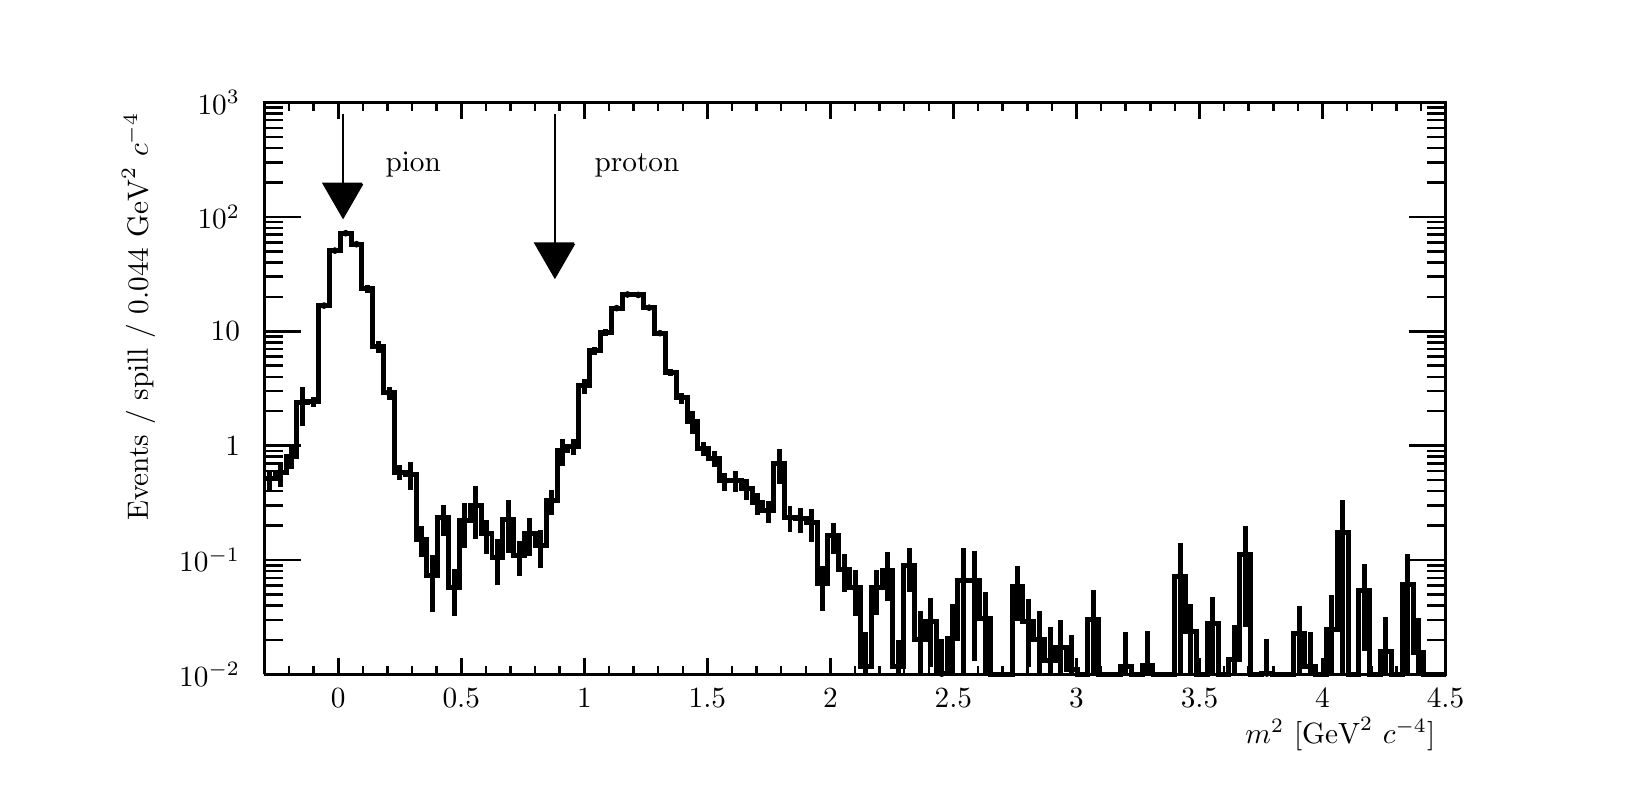
\begin{tikzpicture}
\pgfdeclareplotmark{cross} {
\pgfpathmoveto{\pgfpoint{-0.3\pgfplotmarksize}{\pgfplotmarksize}}
\pgfpathlineto{\pgfpoint{+0.3\pgfplotmarksize}{\pgfplotmarksize}}
\pgfpathlineto{\pgfpoint{+0.3\pgfplotmarksize}{0.3\pgfplotmarksize}}
\pgfpathlineto{\pgfpoint{+1\pgfplotmarksize}{0.3\pgfplotmarksize}}
\pgfpathlineto{\pgfpoint{+1\pgfplotmarksize}{-0.3\pgfplotmarksize}}
\pgfpathlineto{\pgfpoint{+0.3\pgfplotmarksize}{-0.3\pgfplotmarksize}}
\pgfpathlineto{\pgfpoint{+0.3\pgfplotmarksize}{-1.\pgfplotmarksize}}
\pgfpathlineto{\pgfpoint{-0.3\pgfplotmarksize}{-1.\pgfplotmarksize}}
\pgfpathlineto{\pgfpoint{-0.3\pgfplotmarksize}{-0.3\pgfplotmarksize}}
\pgfpathlineto{\pgfpoint{-1.\pgfplotmarksize}{-0.3\pgfplotmarksize}}
\pgfpathlineto{\pgfpoint{-1.\pgfplotmarksize}{0.3\pgfplotmarksize}}
\pgfpathlineto{\pgfpoint{-0.3\pgfplotmarksize}{0.3\pgfplotmarksize}}
\pgfpathclose
\pgfusepathqstroke
}
\pgfdeclareplotmark{cross*} {
\pgfpathmoveto{\pgfpoint{-0.3\pgfplotmarksize}{\pgfplotmarksize}}
\pgfpathlineto{\pgfpoint{+0.3\pgfplotmarksize}{\pgfplotmarksize}}
\pgfpathlineto{\pgfpoint{+0.3\pgfplotmarksize}{0.3\pgfplotmarksize}}
\pgfpathlineto{\pgfpoint{+1\pgfplotmarksize}{0.3\pgfplotmarksize}}
\pgfpathlineto{\pgfpoint{+1\pgfplotmarksize}{-0.3\pgfplotmarksize}}
\pgfpathlineto{\pgfpoint{+0.3\pgfplotmarksize}{-0.3\pgfplotmarksize}}
\pgfpathlineto{\pgfpoint{+0.3\pgfplotmarksize}{-1.\pgfplotmarksize}}
\pgfpathlineto{\pgfpoint{-0.3\pgfplotmarksize}{-1.\pgfplotmarksize}}
\pgfpathlineto{\pgfpoint{-0.3\pgfplotmarksize}{-0.3\pgfplotmarksize}}
\pgfpathlineto{\pgfpoint{-1.\pgfplotmarksize}{-0.3\pgfplotmarksize}}
\pgfpathlineto{\pgfpoint{-1.\pgfplotmarksize}{0.3\pgfplotmarksize}}
\pgfpathlineto{\pgfpoint{-0.3\pgfplotmarksize}{0.3\pgfplotmarksize}}
\pgfpathclose
\pgfusepathqfillstroke
}
\pgfdeclareplotmark{newstar} {
\pgfpathmoveto{\pgfqpoint{0pt}{\pgfplotmarksize}}
\pgfpathlineto{\pgfqpointpolar{44}{0.5\pgfplotmarksize}}
\pgfpathlineto{\pgfqpointpolar{18}{\pgfplotmarksize}}
\pgfpathlineto{\pgfqpointpolar{-20}{0.5\pgfplotmarksize}}
\pgfpathlineto{\pgfqpointpolar{-54}{\pgfplotmarksize}}
\pgfpathlineto{\pgfqpointpolar{-90}{0.5\pgfplotmarksize}}
\pgfpathlineto{\pgfqpointpolar{234}{\pgfplotmarksize}}
\pgfpathlineto{\pgfqpointpolar{198}{0.5\pgfplotmarksize}}
\pgfpathlineto{\pgfqpointpolar{162}{\pgfplotmarksize}}
\pgfpathlineto{\pgfqpointpolar{134}{0.5\pgfplotmarksize}}
\pgfpathclose
\pgfusepathqstroke
}
\pgfdeclareplotmark{newstar*} {
\pgfpathmoveto{\pgfqpoint{0pt}{\pgfplotmarksize}}
\pgfpathlineto{\pgfqpointpolar{44}{0.5\pgfplotmarksize}}
\pgfpathlineto{\pgfqpointpolar{18}{\pgfplotmarksize}}
\pgfpathlineto{\pgfqpointpolar{-20}{0.5\pgfplotmarksize}}
\pgfpathlineto{\pgfqpointpolar{-54}{\pgfplotmarksize}}
\pgfpathlineto{\pgfqpointpolar{-90}{0.5\pgfplotmarksize}}
\pgfpathlineto{\pgfqpointpolar{234}{\pgfplotmarksize}}
\pgfpathlineto{\pgfqpointpolar{198}{0.5\pgfplotmarksize}}
\pgfpathlineto{\pgfqpointpolar{162}{\pgfplotmarksize}}
\pgfpathlineto{\pgfqpointpolar{134}{0.5\pgfplotmarksize}}
\pgfpathclose
\pgfusepathqfillstroke
}
\definecolor{c}{rgb}{1,1,1};
\draw [color=c, fill=c] (0,0) rectangle (20,9.43311);
\draw [color=c, fill=c] (3,1.2263) rectangle (18,8.4898);
\definecolor{c}{rgb}{0,0,0};
\draw [c,line width=0.9] (3,1.2263) -- (3,8.4898) -- (18,8.4898) -- (18,1.2263) -- (3,1.2263);
\definecolor{c}{rgb}{1,1,1};
\draw [color=c, fill=c] (3,1.2263) rectangle (18,8.4898);
\definecolor{c}{rgb}{0,0,0};
\draw [c,line width=0.9] (3,1.2263) -- (3,8.4898) -- (18,8.4898) -- (18,1.2263) -- (3,1.2263);
\draw [c,line width=1.8] (3.06881,3.56872) -- (3.06881,3.71136);
\draw [c,line width=1.8] (3.06881,3.71136) -- (3.06881,3.82762);
\foreach \P in {(3.06881,3.71136)}{\draw[mark options={color=c,fill=c},mark size=2.402402pt,mark=*,mark size=1pt] plot coordinates {\P};}
\draw [c,line width=1.8] (3.20642,3.60405) -- (3.20642,3.78774);
\draw [c,line width=1.8] (3.20642,3.78774) -- (3.20642,3.92983);
\foreach \P in {(3.20642,3.78774)}{\draw[mark options={color=c,fill=c},mark size=2.402402pt,mark=*,mark size=1pt] plot coordinates {\P};}
\draw [c,line width=1.8] (3.34404,3.83272) -- (3.34404,3.99102);
\draw [c,line width=1.8] (3.34404,3.99102) -- (3.34404,4.11746);
\foreach \P in {(3.34404,3.99102)}{\draw[mark options={color=c,fill=c},mark size=2.402402pt,mark=*,mark size=1pt] plot coordinates {\P};}
\draw [c,line width=1.8] (3.48165,4.37763) -- (3.48165,4.6782);
\draw [c,line width=1.8] (3.48165,4.6782) -- (3.48165,4.88094);
\foreach \P in {(3.48165,4.6782)}{\draw[mark options={color=c,fill=c},mark size=2.402402pt,mark=*,mark size=1pt] plot coordinates {\P};}
\draw [c,line width=1.8] (3.61927,4.62245) -- (3.61927,4.6917);
\draw [c,line width=1.8] (3.61927,4.6917) -- (3.61927,4.7541);
\foreach \P in {(3.61927,4.6917)}{\draw[mark options={color=c,fill=c},mark size=2.402402pt,mark=*,mark size=1pt] plot coordinates {\P};}
\draw [c,line width=1.8] (3.75688,5.88089) -- (3.75688,5.91059);
\draw [c,line width=1.8] (3.75688,5.91059) -- (3.75688,5.93895);
\foreach \P in {(3.75688,5.91059)}{\draw[mark options={color=c,fill=c},mark size=2.402402pt,mark=*,mark size=1pt] plot coordinates {\P};}
\draw [c,line width=1.8] (3.8945,6.58821) -- (3.8945,6.609);
\draw [c,line width=1.8] (3.8945,6.609) -- (3.8945,6.62913);
\foreach \P in {(3.8945,6.609)}{\draw[mark options={color=c,fill=c},mark size=2.402402pt,mark=*,mark size=1pt] plot coordinates {\P};}
\draw [c,line width=1.8] (4.03211,6.80875) -- (4.03211,6.8294);
\draw [c,line width=1.8] (4.03211,6.8294) -- (4.03211,6.8494);
\foreach \P in {(4.03211,6.8294)}{\draw[mark options={color=c,fill=c},mark size=2.402402pt,mark=*,mark size=1pt] plot coordinates {\P};}
\draw [c,line width=1.8] (4.16972,6.66216) -- (4.16972,6.68997);
\draw [c,line width=1.8] (4.16972,6.68997) -- (4.16972,6.7166);
\foreach \P in {(4.16972,6.68997)}{\draw[mark options={color=c,fill=c},mark size=2.402402pt,mark=*,mark size=1pt] plot coordinates {\P};}
\draw [c,line width=1.8] (4.30734,6.07616) -- (4.30734,6.12807);
\draw [c,line width=1.8] (4.30734,6.12807) -- (4.30734,6.17604);
\foreach \P in {(4.30734,6.12807)}{\draw[mark options={color=c,fill=c},mark size=2.402402pt,mark=*,mark size=1pt] plot coordinates {\P};}
\draw [c,line width=1.8] (4.44495,5.31081) -- (4.44495,5.39135);
\draw [c,line width=1.8] (4.44495,5.39135) -- (4.44495,5.46277);
\foreach \P in {(4.44495,5.39135)}{\draw[mark options={color=c,fill=c},mark size=2.402402pt,mark=*,mark size=1pt] plot coordinates {\P};}
\draw [c,line width=1.8] (4.58257,4.71441) -- (4.58257,4.80088);
\draw [c,line width=1.8] (4.58257,4.80088) -- (4.58257,4.87692);
\foreach \P in {(4.58257,4.80088)}{\draw[mark options={color=c,fill=c},mark size=2.402402pt,mark=*,mark size=1pt] plot coordinates {\P};}
\draw [c,line width=1.8] (4.72018,3.69222) -- (4.72018,3.794);
\draw [c,line width=1.8] (4.72018,3.794) -- (4.72018,3.88161);
\foreach \P in {(4.72018,3.794)}{\draw[mark options={color=c,fill=c},mark size=2.402402pt,mark=*,mark size=1pt] plot coordinates {\P};}
\draw [c,line width=1.8] (4.8578,3.56322) -- (4.8578,3.7652);
\draw [c,line width=1.8] (4.8578,3.7652) -- (4.8578,3.91796);
\foreach \P in {(4.8578,3.7652)}{\draw[mark options={color=c,fill=c},mark size=2.402402pt,mark=*,mark size=1pt] plot coordinates {\P};}
\draw [c,line width=1.8] (4.99541,2.72369) -- (4.99541,2.944);
\draw [c,line width=1.8] (4.99541,2.944) -- (4.99541,3.10698);
\foreach \P in {(4.99541,2.944)}{\draw[mark options={color=c,fill=c},mark size=2.402402pt,mark=*,mark size=1pt] plot coordinates {\P};}
\draw [c,line width=1.8] (5.13303,2.02126) -- (5.13303,2.48397);
\draw [c,line width=1.8] (5.13303,2.48397) -- (5.13303,2.74802);
\foreach \P in {(5.13303,2.48397)}{\draw[mark options={color=c,fill=c},mark size=2.402402pt,mark=*,mark size=1pt] plot coordinates {\P};}
\draw [c,line width=1.8] (5.27064,2.98961) -- (5.27064,3.21415);
\draw [c,line width=1.8] (5.27064,3.21415) -- (5.27064,3.37941);
\foreach \P in {(5.27064,3.21415)}{\draw[mark options={color=c,fill=c},mark size=2.402402pt,mark=*,mark size=1pt] plot coordinates {\P};}
\draw [c,line width=1.8] (5.40826,1.96462) -- (5.40826,2.33111);
\draw [c,line width=1.8] (5.40826,2.33111) -- (5.40826,2.56143);
\foreach \P in {(5.40826,2.33111)}{\draw[mark options={color=c,fill=c},mark size=2.402402pt,mark=*,mark size=1pt] plot coordinates {\P};}
\draw [c,line width=1.8] (5.54587,2.82628) -- (5.54587,3.17889);
\draw [c,line width=1.8] (5.54587,3.17889) -- (5.54587,3.40373);
\foreach \P in {(5.54587,3.17889)}{\draw[mark options={color=c,fill=c},mark size=2.402402pt,mark=*,mark size=1pt] plot coordinates {\P};}
\draw [c,line width=1.8] (5.68349,2.95178) -- (5.68349,3.37453);
\draw [c,line width=1.8] (5.68349,3.37453) -- (5.68349,3.62542);
\foreach \P in {(5.68349,3.37453)}{\draw[mark options={color=c,fill=c},mark size=2.402402pt,mark=*,mark size=1pt] plot coordinates {\P};}
\draw [c,line width=1.8] (5.8211,2.75545) -- (5.8211,3.01109);
\draw [c,line width=1.8] (5.8211,3.01109) -- (5.8211,3.19251);
\foreach \P in {(5.8211,3.01109)}{\draw[mark options={color=c,fill=c},mark size=2.402402pt,mark=*,mark size=1pt] plot coordinates {\P};}
\draw [c,line width=1.8] (5.95872,2.3592) -- (5.95872,2.71711);
\draw [c,line width=1.8] (5.95872,2.71711) -- (5.95872,2.94407);
\foreach \P in {(5.95872,2.71711)}{\draw[mark options={color=c,fill=c},mark size=2.402402pt,mark=*,mark size=1pt] plot coordinates {\P};}
\draw [c,line width=1.8] (6.09633,2.76628) -- (6.09633,3.19469);
\draw [c,line width=1.8] (6.09633,3.19469) -- (6.09633,3.4475);
\foreach \P in {(6.09633,3.19469)}{\draw[mark options={color=c,fill=c},mark size=2.402402pt,mark=*,mark size=1pt] plot coordinates {\P};}
\draw [c,line width=1.8] (6.23394,2.47429) -- (6.23394,2.73953);
\draw [c,line width=1.8] (6.23394,2.73953) -- (6.23394,2.92569);
\foreach \P in {(6.23394,2.73953)}{\draw[mark options={color=c,fill=c},mark size=2.402402pt,mark=*,mark size=1pt] plot coordinates {\P};}
\draw [c,line width=1.8] (6.37156,2.73579) -- (6.37156,3.01506);
\draw [c,line width=1.8] (6.37156,3.01506) -- (6.37156,3.20796);
\foreach \P in {(6.37156,3.01506)}{\draw[mark options={color=c,fill=c},mark size=2.402402pt,mark=*,mark size=1pt] plot coordinates {\P};}
\draw [c,line width=1.8] (6.50917,2.57445) -- (6.50917,2.86253);
\draw [c,line width=1.8] (6.50917,2.86253) -- (6.50917,3.05956);
\foreach \P in {(6.50917,2.86253)}{\draw[mark options={color=c,fill=c},mark size=2.402402pt,mark=*,mark size=1pt] plot coordinates {\P};}
\draw [c,line width=1.8] (6.64679,3.25685) -- (6.64679,3.42962);
\draw [c,line width=1.8] (6.64679,3.42962) -- (6.64679,3.56511);
\foreach \P in {(6.64679,3.42962)}{\draw[mark options={color=c,fill=c},mark size=2.402402pt,mark=*,mark size=1pt] plot coordinates {\P};}
\draw [c,line width=1.8] (6.7844,3.87258) -- (6.7844,4.06998);
\draw [c,line width=1.8] (6.7844,4.06998) -- (6.7844,4.22011);
\foreach \P in {(6.7844,4.06998)}{\draw[mark options={color=c,fill=c},mark size=2.402402pt,mark=*,mark size=1pt] plot coordinates {\P};}
\draw [c,line width=1.8] (6.92202,4.0118) -- (6.92202,4.12585);
\draw [c,line width=1.8] (6.92202,4.12585) -- (6.92202,4.22241);
\foreach \P in {(6.92202,4.12585)}{\draw[mark options={color=c,fill=c},mark size=2.402402pt,mark=*,mark size=1pt] plot coordinates {\P};}
\draw [c,line width=1.8] (7.05963,4.78915) -- (7.05963,4.89028);
\draw [c,line width=1.8] (7.05963,4.89028) -- (7.05963,4.97742);
\foreach \P in {(7.05963,4.89028)}{\draw[mark options={color=c,fill=c},mark size=2.402402pt,mark=*,mark size=1pt] plot coordinates {\P};}
\draw [c,line width=1.8] (7.19725,5.28396) -- (7.19725,5.33785);
\draw [c,line width=1.8] (7.19725,5.33785) -- (7.19725,5.3875);
\foreach \P in {(7.19725,5.33785)}{\draw[mark options={color=c,fill=c},mark size=2.402402pt,mark=*,mark size=1pt] plot coordinates {\P};}
\draw [c,line width=1.8] (7.33486,5.52386) -- (7.33486,5.57101);
\draw [c,line width=1.8] (7.33486,5.57101) -- (7.33486,5.61488);
\foreach \P in {(7.33486,5.57101)}{\draw[mark options={color=c,fill=c},mark size=2.402402pt,mark=*,mark size=1pt] plot coordinates {\P};}
\draw [c,line width=1.8] (7.47248,5.84918) -- (7.47248,5.87775);
\draw [c,line width=1.8] (7.47248,5.87775) -- (7.47248,5.90507);
\foreach \P in {(7.47248,5.87775)}{\draw[mark options={color=c,fill=c},mark size=2.402402pt,mark=*,mark size=1pt] plot coordinates {\P};}
\draw [c,line width=1.8] (7.61009,6.02421) -- (7.61009,6.05102);
\draw [c,line width=1.8] (7.61009,6.05102) -- (7.61009,6.07674);
\foreach \P in {(7.61009,6.05102)}{\draw[mark options={color=c,fill=c},mark size=2.402402pt,mark=*,mark size=1pt] plot coordinates {\P};}
\draw [c,line width=1.8] (7.74771,6.02286) -- (7.74771,6.046);
\draw [c,line width=1.8] (7.74771,6.046) -- (7.74771,6.06832);
\foreach \P in {(7.74771,6.046)}{\draw[mark options={color=c,fill=c},mark size=2.402402pt,mark=*,mark size=1pt] plot coordinates {\P};}
\draw [c,line width=1.8] (7.88532,5.85613) -- (7.88532,5.8838);
\draw [c,line width=1.8] (7.88532,5.8838) -- (7.88532,5.91031);
\foreach \P in {(7.88532,5.8838)}{\draw[mark options={color=c,fill=c},mark size=2.402402pt,mark=*,mark size=1pt] plot coordinates {\P};}
\draw [c,line width=1.8] (8.02294,5.52535) -- (8.02294,5.56009);
\draw [c,line width=1.8] (8.02294,5.56009) -- (8.02294,5.59301);
\foreach \P in {(8.02294,5.56009)}{\draw[mark options={color=c,fill=c},mark size=2.402402pt,mark=*,mark size=1pt] plot coordinates {\P};}
\draw [c,line width=1.8] (8.16055,5.01206) -- (8.16055,5.0609);
\draw [c,line width=1.8] (8.16055,5.0609) -- (8.16055,5.10624);
\foreach \P in {(8.16055,5.0609)}{\draw[mark options={color=c,fill=c},mark size=2.402402pt,mark=*,mark size=1pt] plot coordinates {\P};}
\draw [c,line width=1.8] (8.29817,4.66691) -- (8.29817,4.73945);
\draw [c,line width=1.8] (8.29817,4.73945) -- (8.29817,4.80449);
\foreach \P in {(8.29817,4.73945)}{\draw[mark options={color=c,fill=c},mark size=2.402402pt,mark=*,mark size=1pt] plot coordinates {\P};}
\draw [c,line width=1.8] (8.43578,4.28359) -- (8.43578,4.44033);
\draw [c,line width=1.8] (8.43578,4.44033) -- (8.43578,4.56577);
\foreach \P in {(8.43578,4.44033)}{\draw[mark options={color=c,fill=c},mark size=2.402402pt,mark=*,mark size=1pt] plot coordinates {\P};}
\draw [c,line width=1.8] (8.57339,3.99655) -- (8.57339,4.09149);
\draw [c,line width=1.8] (8.57339,4.09149) -- (8.57339,4.174);
\foreach \P in {(8.57339,4.09149)}{\draw[mark options={color=c,fill=c},mark size=2.402402pt,mark=*,mark size=1pt] plot coordinates {\P};}
\draw [c,line width=1.8] (8.71101,3.85907) -- (8.71101,3.96865);
\draw [c,line width=1.8] (8.71101,3.96865) -- (8.71101,4.06199);
\foreach \P in {(8.71101,3.96865)}{\draw[mark options={color=c,fill=c},mark size=2.402402pt,mark=*,mark size=1pt] plot coordinates {\P};}
\draw [c,line width=1.8] (8.84862,3.56063) -- (8.84862,3.68393);
\draw [c,line width=1.8] (8.84862,3.68393) -- (8.84862,3.78703);
\foreach \P in {(8.84862,3.68393)}{\draw[mark options={color=c,fill=c},mark size=2.402402pt,mark=*,mark size=1pt] plot coordinates {\P};}
\draw [c,line width=1.8] (8.98624,3.54614) -- (8.98624,3.69032);
\draw [c,line width=1.8] (8.98624,3.69032) -- (8.98624,3.8076);
\foreach \P in {(8.98624,3.69032)}{\draw[mark options={color=c,fill=c},mark size=2.402402pt,mark=*,mark size=1pt] plot coordinates {\P};}
\draw [c,line width=1.8] (9.12385,3.44504) -- (9.12385,3.58819);
\draw [c,line width=1.8] (9.12385,3.58819) -- (9.12385,3.70479);
\foreach \P in {(9.12385,3.58819)}{\draw[mark options={color=c,fill=c},mark size=2.402402pt,mark=*,mark size=1pt] plot coordinates {\P};}
\draw [c,line width=1.8] (9.26147,3.2554) -- (9.26147,3.41055);
\draw [c,line width=1.8] (9.26147,3.41055) -- (9.26147,3.53499);
\foreach \P in {(9.26147,3.41055)}{\draw[mark options={color=c,fill=c},mark size=2.402402pt,mark=*,mark size=1pt] plot coordinates {\P};}
\draw [c,line width=1.8] (9.39908,3.14598) -- (9.39908,3.30399);
\draw [c,line width=1.8] (9.39908,3.30399) -- (9.39908,3.43025);
\foreach \P in {(9.39908,3.30399)}{\draw[mark options={color=c,fill=c},mark size=2.402402pt,mark=*,mark size=1pt] plot coordinates {\P};}
\draw [c,line width=1.8] (9.5367,3.64807) -- (9.5367,3.90256);
\draw [c,line width=1.8] (9.5367,3.90256) -- (9.5367,4.0834);
\foreach \P in {(9.5367,3.90256)}{\draw[mark options={color=c,fill=c},mark size=2.402402pt,mark=*,mark size=1pt] plot coordinates {\P};}
\draw [c,line width=1.8] (9.67431,3.03567) -- (9.67431,3.21987);
\draw [c,line width=1.8] (9.67431,3.21987) -- (9.67431,3.36227);
\foreach \P in {(9.67431,3.21987)}{\draw[mark options={color=c,fill=c},mark size=2.402402pt,mark=*,mark size=1pt] plot coordinates {\P};}
\draw [c,line width=1.8] (9.81193,3.02432) -- (9.81193,3.2043);
\draw [c,line width=1.8] (9.81193,3.2043) -- (9.81193,3.34417);
\foreach \P in {(9.81193,3.2043)}{\draw[mark options={color=c,fill=c},mark size=2.402402pt,mark=*,mark size=1pt] plot coordinates {\P};}
\draw [c,line width=1.8] (9.94954,2.90575) -- (9.94954,3.15507);
\draw [c,line width=1.8] (9.94954,3.15507) -- (9.94954,3.33329);
\foreach \P in {(9.94954,3.15507)}{\draw[mark options={color=c,fill=c},mark size=2.402402pt,mark=*,mark size=1pt] plot coordinates {\P};}
\draw [c,line width=1.8] (10.0872,2.03789) -- (10.0872,2.38235);
\draw [c,line width=1.8] (10.0872,2.38235) -- (10.0872,2.6039);
\foreach \P in {(10.0872,2.38235)}{\draw[mark options={color=c,fill=c},mark size=2.402402pt,mark=*,mark size=1pt] plot coordinates {\P};}
\draw [c,line width=1.8] (10.2248,2.75862) -- (10.2248,2.98477);
\draw [c,line width=1.8] (10.2248,2.98477) -- (10.2248,3.1509);
\foreach \P in {(10.2248,2.98477)}{\draw[mark options={color=c,fill=c},mark size=2.402402pt,mark=*,mark size=1pt] plot coordinates {\P};}
\draw [c,line width=1.8] (10.3624,2.27162) -- (10.3624,2.5586);
\draw [c,line width=1.8] (10.3624,2.5586) -- (10.3624,2.75512);
\foreach \P in {(10.3624,2.5586)}{\draw[mark options={color=c,fill=c},mark size=2.402402pt,mark=*,mark size=1pt] plot coordinates {\P};}
\draw [c,line width=1.8] (10.5,1.96858) -- (10.5,2.32496);
\draw [c,line width=1.8] (10.5,2.32496) -- (10.5,2.55131);
\foreach \P in {(10.5,2.32496)}{\draw[mark options={color=c,fill=c},mark size=2.402402pt,mark=*,mark size=1pt] plot coordinates {\P};}
\draw [c,line width=1.8] (10.6376,1.2263) -- (10.6376,1.3277);
\draw [c,line width=1.8] (10.6376,1.3277) -- (10.6376,1.76537);
\foreach \P in {(10.6376,1.3277)}{\draw[mark options={color=c,fill=c},mark size=2.402402pt,mark=*,mark size=1pt] plot coordinates {\P};}
\draw [c,line width=1.8] (10.7752,1.98377) -- (10.7752,2.32996);
\draw [c,line width=1.8] (10.7752,2.32996) -- (10.7752,2.55221);
\foreach \P in {(10.7752,2.32996)}{\draw[mark options={color=c,fill=c},mark size=2.402402pt,mark=*,mark size=1pt] plot coordinates {\P};}
\draw [c,line width=1.8] (10.9128,2.15956) -- (10.9128,2.54358);
\draw [c,line width=1.8] (10.9128,2.54358) -- (10.9128,2.78057);
\foreach \P in {(10.9128,2.54358)}{\draw[mark options={color=c,fill=c},mark size=2.402402pt,mark=*,mark size=1pt] plot coordinates {\P};}
\draw [c,line width=1.8] (11.0505,1.2263) -- (11.0505,1.32725);
\draw [c,line width=1.8] (11.0505,1.32725) -- (11.0505,1.6654);
\foreach \P in {(11.0505,1.32725)}{\draw[mark options={color=c,fill=c},mark size=2.402402pt,mark=*,mark size=1pt] plot coordinates {\P};}
\draw [c,line width=1.8] (11.1881,2.27742) -- (11.1881,2.61114);
\draw [c,line width=1.8] (11.1881,2.61114) -- (11.1881,2.82825);
\foreach \P in {(11.1881,2.61114)}{\draw[mark options={color=c,fill=c},mark size=2.402402pt,mark=*,mark size=1pt] plot coordinates {\P};}
\draw [c,line width=1.8] (11.3257,1.2263) -- (11.3257,1.67205);
\draw [c,line width=1.8] (11.3257,1.67205) -- (11.3257,2.03101);
\foreach \P in {(11.3257,1.67205)}{\draw[mark options={color=c,fill=c},mark size=2.402402pt,mark=*,mark size=1pt] plot coordinates {\P};}
\draw [c,line width=1.8] (11.4633,1.32341) -- (11.4633,1.90285);
\draw [c,line width=1.8] (11.4633,1.90285) -- (11.4633,2.19972);
\foreach \P in {(11.4633,1.90285)}{\draw[mark options={color=c,fill=c},mark size=2.402402pt,mark=*,mark size=1pt] plot coordinates {\P};}
\draw [c,line width=1.8] (11.6009,1.2263) -- (11.6009,1.23591);
\draw [c,line width=1.8] (11.6009,1.23591) -- (11.6009,1.67363);
\foreach \P in {(11.6009,1.23591)}{\draw[mark options={color=c,fill=c},mark size=2.402402pt,mark=*,mark size=1pt] plot coordinates {\P};}
\draw [c,line width=1.8] (11.7385,1.2263) -- (11.7385,1.68607);
\draw [c,line width=1.8] (11.7385,1.68607) -- (11.7385,2.12389);
\foreach \P in {(11.7385,1.68607)}{\draw[mark options={color=c,fill=c},mark size=2.402402pt,mark=*,mark size=1pt] plot coordinates {\P};}
\draw [c,line width=1.8] (11.8761,1.2263) -- (11.8761,2.4233);
\draw [c,line width=1.8] (11.8761,2.4233) -- (11.8761,2.834);
\foreach \P in {(11.8761,2.4233)}{\draw[mark options={color=c,fill=c},mark size=2.402402pt,mark=*,mark size=1pt] plot coordinates {\P};}
\draw [c,line width=1.8] (12.0138,1.39728) -- (12.0138,2.4205);
\draw [c,line width=1.8] (12.0138,2.4205) -- (12.0138,2.79219);
\foreach \P in {(12.0138,2.4205)}{\draw[mark options={color=c,fill=c},mark size=2.402402pt,mark=*,mark size=1pt] plot coordinates {\P};}
\draw [c,line width=1.8] (12.1514,1.2263) -- (12.1514,1.93107);
\draw [c,line width=1.8] (12.1514,1.93107) -- (12.1514,2.27464);
\foreach \P in {(12.1514,1.93107)}{\draw[mark options={color=c,fill=c},mark size=2.402402pt,mark=*,mark size=1pt] plot coordinates {\P};}
\draw [c,line width=1.8] (12.5642,1.90555) -- (12.5642,2.34491);
\draw [c,line width=1.8] (12.5642,2.34491) -- (12.5642,2.60141);
\foreach \P in {(12.5642,2.34491)}{\draw[mark options={color=c,fill=c},mark size=2.402402pt,mark=*,mark size=1pt] plot coordinates {\P};}
\draw [c,line width=1.8] (12.7018,1.31527) -- (12.7018,1.89266);
\draw [c,line width=1.8] (12.7018,1.89266) -- (12.7018,2.18901);
\foreach \P in {(12.7018,1.89266)}{\draw[mark options={color=c,fill=c},mark size=2.402402pt,mark=*,mark size=1pt] plot coordinates {\P};}
\draw [c,line width=1.8] (12.8394,1.2263) -- (12.8394,1.6727);
\draw [c,line width=1.8] (12.8394,1.6727) -- (12.8394,2.03107);
\foreach \P in {(12.8394,1.6727)}{\draw[mark options={color=c,fill=c},mark size=2.402402pt,mark=*,mark size=1pt] plot coordinates {\P};}
\draw [c,line width=1.8] (12.9771,1.2263) -- (12.9771,1.39712);
\draw [c,line width=1.8] (12.9771,1.39712) -- (12.9771,1.83482);
\foreach \P in {(12.9771,1.39712)}{\draw[mark options={color=c,fill=c},mark size=2.402402pt,mark=*,mark size=1pt] plot coordinates {\P};}
\draw [c,line width=1.8] (13.1147,1.2263) -- (13.1147,1.5685);
\draw [c,line width=1.8] (13.1147,1.5685) -- (13.1147,1.9191);
\foreach \P in {(13.1147,1.5685)}{\draw[mark options={color=c,fill=c},mark size=2.402402pt,mark=*,mark size=1pt] plot coordinates {\P};}
\draw [c,line width=1.8] (13.2523,1.2263) -- (13.2523,1.2852);
\draw [c,line width=1.8] (13.2523,1.2852) -- (13.2523,1.72288);
\foreach \P in {(13.2523,1.2852)}{\draw[mark options={color=c,fill=c},mark size=2.402402pt,mark=*,mark size=1pt] plot coordinates {\P};}
\draw [c,line width=1.8] (13.5275,1.2263) -- (13.5275,1.92356);
\draw [c,line width=1.8] (13.5275,1.92356) -- (13.5275,2.30434);
\foreach \P in {(13.5275,1.92356)}{\draw[mark options={color=c,fill=c},mark size=2.402402pt,mark=*,mark size=1pt] plot coordinates {\P};}
\draw [c,line width=1.8] (13.9404,1.2263) -- (13.9404,1.33199);
\draw [c,line width=1.8] (13.9404,1.33199) -- (13.9404,1.76967);
\foreach \P in {(13.9404,1.33199)}{\draw[mark options={color=c,fill=c},mark size=2.402402pt,mark=*,mark size=1pt] plot coordinates {\P};}
\draw [c,line width=1.8] (14.2156,1.2263) -- (14.2156,1.34151);
\draw [c,line width=1.8] (14.2156,1.34151) -- (14.2156,1.77924);
\foreach \P in {(14.2156,1.34151)}{\draw[mark options={color=c,fill=c},mark size=2.402402pt,mark=*,mark size=1pt] plot coordinates {\P};}
\draw [c,line width=1.8] (14.6284,1.2263) -- (14.6284,2.47584);
\draw [c,line width=1.8] (14.6284,2.47584) -- (14.6284,2.88914);
\foreach \P in {(14.6284,2.47584)}{\draw[mark options={color=c,fill=c},mark size=2.402402pt,mark=*,mark size=1pt] plot coordinates {\P};}
\draw [c,line width=1.8] (14.7661,1.2263) -- (14.7661,1.77723);
\draw [c,line width=1.8] (14.7661,1.77723) -- (14.7661,2.11494);
\foreach \P in {(14.7661,1.77723)}{\draw[mark options={color=c,fill=c},mark size=2.402402pt,mark=*,mark size=1pt] plot coordinates {\P};}
\draw [c,line width=1.8] (15.0413,1.2263) -- (15.0413,1.86949);
\draw [c,line width=1.8] (15.0413,1.86949) -- (15.0413,2.21436);
\foreach \P in {(15.0413,1.86949)}{\draw[mark options={color=c,fill=c},mark size=2.402402pt,mark=*,mark size=1pt] plot coordinates {\P};}
\draw [c,line width=1.8] (15.3165,1.2263) -- (15.3165,1.41421);
\draw [c,line width=1.8] (15.3165,1.41421) -- (15.3165,1.85179);
\foreach \P in {(15.3165,1.41421)}{\draw[mark options={color=c,fill=c},mark size=2.402402pt,mark=*,mark size=1pt] plot coordinates {\P};}
\draw [c,line width=1.8] (15.4541,1.82819) -- (15.4541,2.75279);
\draw [c,line width=1.8] (15.4541,2.75279) -- (15.4541,3.11268);
\foreach \P in {(15.4541,2.75279)}{\draw[mark options={color=c,fill=c},mark size=2.402402pt,mark=*,mark size=1pt] plot coordinates {\P};}
\draw [c,line width=1.8] (15.7294,1.2263) -- (15.7294,1.23755);
\draw [c,line width=1.8] (15.7294,1.23755) -- (15.7294,1.67527);
\foreach \P in {(15.7294,1.23755)}{\draw[mark options={color=c,fill=c},mark size=2.402402pt,mark=*,mark size=1pt] plot coordinates {\P};}
\draw [c,line width=1.8] (16.1422,1.2263) -- (16.1422,1.75095);
\draw [c,line width=1.8] (16.1422,1.75095) -- (16.1422,2.09382);
\foreach \P in {(16.1422,1.75095)}{\draw[mark options={color=c,fill=c},mark size=2.402402pt,mark=*,mark size=1pt] plot coordinates {\P};}
\draw [c,line width=1.8] (16.2798,1.2263) -- (16.2798,1.33171);
\draw [c,line width=1.8] (16.2798,1.33171) -- (16.2798,1.76939);
\foreach \P in {(16.2798,1.33171)}{\draw[mark options={color=c,fill=c},mark size=2.402402pt,mark=*,mark size=1pt] plot coordinates {\P};}
\draw [c,line width=1.8] (16.555,1.2263) -- (16.555,1.7949);
\draw [c,line width=1.8] (16.555,1.7949) -- (16.555,2.23253);
\foreach \P in {(16.555,1.7949)}{\draw[mark options={color=c,fill=c},mark size=2.402402pt,mark=*,mark size=1pt] plot coordinates {\P};}
\draw [c,line width=1.8] (16.6927,1.2263) -- (16.6927,3.02411);
\draw [c,line width=1.8] (16.6927,3.02411) -- (16.6927,3.44421);
\foreach \P in {(16.6927,3.02411)}{\draw[mark options={color=c,fill=c},mark size=2.402402pt,mark=*,mark size=1pt] plot coordinates {\P};}
\draw [c,line width=1.8] (16.9679,1.52976) -- (16.9679,2.28801);
\draw [c,line width=1.8] (16.9679,2.28801) -- (16.9679,2.62255);
\foreach \P in {(16.9679,2.28801)}{\draw[mark options={color=c,fill=c},mark size=2.402402pt,mark=*,mark size=1pt] plot coordinates {\P};}
\draw [c,line width=1.8] (17.2431,1.2263) -- (17.2431,1.52343);
\draw [c,line width=1.8] (17.2431,1.52343) -- (17.2431,1.96114);
\foreach \P in {(17.2431,1.52343)}{\draw[mark options={color=c,fill=c},mark size=2.402402pt,mark=*,mark size=1pt] plot coordinates {\P};}
\draw [c,line width=1.8] (17.5183,1.24079) -- (17.5183,2.37168);
\draw [c,line width=1.8] (17.5183,2.37168) -- (17.5183,2.75413);
\foreach \P in {(17.5183,2.37168)}{\draw[mark options={color=c,fill=c},mark size=2.402402pt,mark=*,mark size=1pt] plot coordinates {\P};}
\draw [c,line width=1.8] (17.656,1.2263) -- (17.656,1.50107);
\draw [c,line width=1.8] (17.656,1.50107) -- (17.656,1.93861);
\foreach \P in {(17.656,1.50107)}{\draw[mark options={color=c,fill=c},mark size=2.402402pt,mark=*,mark size=1pt] plot coordinates {\P};}
\draw [c,line width=1.8] (3,3.71136) -- (3.13761,3.71136) -- (3.13761,3.78774) -- (3.27523,3.78774) -- (3.27523,3.99102) -- (3.41284,3.99102) -- (3.41284,4.6782) -- (3.55046,4.6782) -- (3.55046,4.6917) -- (3.68807,4.6917) -- (3.68807,5.91059) --
 (3.82569,5.91059) -- (3.82569,6.609) -- (3.9633,6.609) -- (3.9633,6.8294) -- (4.10092,6.8294) -- (4.10092,6.68997) -- (4.23853,6.68997) -- (4.23853,6.12807) -- (4.37615,6.12807) -- (4.37615,5.39135) -- (4.51376,5.39135) -- (4.51376,4.80088) --
 (4.65138,4.80088) -- (4.65138,3.794) -- (4.78899,3.794) -- (4.78899,3.7652) -- (4.92661,3.7652) -- (4.92661,2.944) -- (5.06422,2.944) -- (5.06422,2.48397) -- (5.20184,2.48397) -- (5.20184,3.21415) -- (5.33945,3.21415) -- (5.33945,2.33111) --
 (5.47706,2.33111) -- (5.47706,3.17889) -- (5.61468,3.17889) -- (5.61468,3.37453) -- (5.75229,3.37453) -- (5.75229,3.01109) -- (5.88991,3.01109) -- (5.88991,2.71711) -- (6.02752,2.71711) -- (6.02752,3.19469) -- (6.16514,3.19469) -- (6.16514,2.73953)
 -- (6.30275,2.73953) -- (6.30275,3.01506) -- (6.44037,3.01506) -- (6.44037,2.86253) -- (6.57798,2.86253) -- (6.57798,3.42962) -- (6.7156,3.42962) -- (6.7156,4.06998) -- (6.85321,4.06998) -- (6.85321,4.12585) -- (6.99083,4.12585) -- (6.99083,4.89028)
 -- (7.12844,4.89028) -- (7.12844,5.33785) -- (7.26606,5.33785) -- (7.26606,5.57101) -- (7.40367,5.57101) -- (7.40367,5.87775) -- (7.54128,5.87775) -- (7.54128,6.05102) -- (7.6789,6.05102) -- (7.6789,6.046) -- (7.81651,6.046) -- (7.81651,5.8838) --
 (7.95413,5.8838) -- (7.95413,5.56009) -- (8.09174,5.56009) -- (8.09174,5.0609) -- (8.22936,5.0609) -- (8.22936,4.73945) -- (8.36697,4.73945) -- (8.36697,4.44033) -- (8.50459,4.44033) -- (8.50459,4.09149) -- (8.6422,4.09149) -- (8.6422,3.96865) --
 (8.77982,3.96865) -- (8.77982,3.68393) -- (8.91743,3.68393) -- (8.91743,3.69032) -- (9.05505,3.69032) -- (9.05505,3.58819) -- (9.19266,3.58819) -- (9.19266,3.41055) -- (9.33028,3.41055) -- (9.33028,3.30399) -- (9.46789,3.30399) -- (9.46789,3.90256)
 -- (9.6055,3.90256) -- (9.6055,3.21987) -- (9.74312,3.21987) -- (9.74312,3.2043) -- (9.88073,3.2043) -- (9.88073,3.15507) -- (10.0183,3.15507) -- (10.0183,2.38235) -- (10.156,2.38235) -- (10.156,2.98477) -- (10.2936,2.98477) -- (10.2936,2.5586) --
 (10.4312,2.5586) -- (10.4312,2.32496) -- (10.5688,2.32496) -- (10.5688,1.3277) -- (10.7064,1.3277) -- (10.7064,2.32996) -- (10.844,2.32996) -- (10.844,2.54358) -- (10.9817,2.54358) -- (10.9817,1.32725) -- (11.1193,1.32725) -- (11.1193,2.61114) --
 (11.2569,2.61114) -- (11.2569,1.67205) -- (11.3945,1.67205) -- (11.3945,1.90285) -- (11.5321,1.90285) -- (11.5321,1.23591) -- (11.6697,1.23591) -- (11.6697,1.68607) -- (11.8073,1.68607) -- (11.8073,2.4233) -- (11.945,2.4233) -- (11.945,2.4205) --
 (12.0826,2.4205) -- (12.0826,1.93107) -- (12.2202,1.93107) -- (12.2202,1.2263) -- (12.3578,1.2263) -- (12.3578,1.2263) -- (12.4954,1.2263) -- (12.4954,2.34491) -- (12.633,2.34491) -- (12.633,1.89266) -- (12.7706,1.89266) -- (12.7706,1.6727) --
 (12.9083,1.6727) -- (12.9083,1.39712) -- (13.0459,1.39712) -- (13.0459,1.5685) -- (13.1835,1.5685) -- (13.1835,1.2852) -- (13.3211,1.2852) -- (13.3211,1.2263) -- (13.4587,1.2263) -- (13.4587,1.92356) -- (13.5963,1.92356) -- (13.5963,1.2263) --
 (13.7339,1.2263) -- (13.7339,1.2263) -- (13.8716,1.2263) -- (13.8716,1.33199) -- (14.0092,1.33199) -- (14.0092,1.2263) -- (14.1468,1.2263) -- (14.1468,1.34151) -- (14.2844,1.34151) -- (14.2844,1.2263) -- (14.422,1.2263) -- (14.422,1.2263) --
 (14.5596,1.2263) -- (14.5596,2.47584) -- (14.6972,2.47584) -- (14.6972,1.77723) -- (14.8349,1.77723) -- (14.8349,1.2263) -- (14.9725,1.2263) -- (14.9725,1.86949) -- (15.1101,1.86949) -- (15.1101,1.2263) -- (15.2477,1.2263) -- (15.2477,1.41421) --
 (15.3853,1.41421) -- (15.3853,2.75279) -- (15.5229,2.75279) -- (15.5229,1.2263) -- (15.6606,1.2263) -- (15.6606,1.23755) -- (15.7982,1.23755) -- (15.7982,1.2263) -- (15.9358,1.2263) -- (15.9358,1.2263) -- (16.0734,1.2263) -- (16.0734,1.75095) --
 (16.211,1.75095) -- (16.211,1.33171) -- (16.3486,1.33171) -- (16.3486,1.2263) -- (16.4862,1.2263) -- (16.4862,1.7949) -- (16.6239,1.7949) -- (16.6239,3.02411) -- (16.7615,3.02411) -- (16.7615,1.2263) -- (16.8991,1.2263) -- (16.8991,2.28801) --
 (17.0367,2.28801) -- (17.0367,1.2263) -- (17.1743,1.2263) -- (17.1743,1.52343) -- (17.3119,1.52343) -- (17.3119,1.2263) -- (17.4495,1.2263) -- (17.4495,2.37168) -- (17.5872,2.37168) -- (17.5872,1.50107) -- (17.7248,1.50107) -- (17.7248,1.2263) --
 (17.8624,1.2263) -- (17.8624,1.2263) -- (18,1.2263);
\draw [c,line width=0.9] (3,1.2263) -- (18,1.2263);
\draw [c,line width=0.9] (3.9375,1.43855) -- (3.9375,1.2263);
\draw [c,line width=0.9] (4.25,1.33243) -- (4.25,1.2263);
\draw [c,line width=0.9] (4.5625,1.33243) -- (4.5625,1.2263);
\draw [c,line width=0.9] (4.875,1.33243) -- (4.875,1.2263);
\draw [c,line width=0.9] (5.1875,1.33243) -- (5.1875,1.2263);
\draw [c,line width=0.9] (5.5,1.43855) -- (5.5,1.2263);
\draw [c,line width=0.9] (5.8125,1.33243) -- (5.8125,1.2263);
\draw [c,line width=0.9] (6.125,1.33243) -- (6.125,1.2263);
\draw [c,line width=0.9] (6.4375,1.33243) -- (6.4375,1.2263);
\draw [c,line width=0.9] (6.75,1.33243) -- (6.75,1.2263);
\draw [c,line width=0.9] (7.0625,1.43855) -- (7.0625,1.2263);
\draw [c,line width=0.9] (7.375,1.33243) -- (7.375,1.2263);
\draw [c,line width=0.9] (7.6875,1.33243) -- (7.6875,1.2263);
\draw [c,line width=0.9] (8,1.33243) -- (8,1.2263);
\draw [c,line width=0.9] (8.3125,1.33243) -- (8.3125,1.2263);
\draw [c,line width=0.9] (8.625,1.43855) -- (8.625,1.2263);
\draw [c,line width=0.9] (8.9375,1.33243) -- (8.9375,1.2263);
\draw [c,line width=0.9] (9.25,1.33243) -- (9.25,1.2263);
\draw [c,line width=0.9] (9.5625,1.33243) -- (9.5625,1.2263);
\draw [c,line width=0.9] (9.875,1.33243) -- (9.875,1.2263);
\draw [c,line width=0.9] (10.1875,1.43855) -- (10.1875,1.2263);
\draw [c,line width=0.9] (10.5,1.33243) -- (10.5,1.2263);
\draw [c,line width=0.9] (10.8125,1.33243) -- (10.8125,1.2263);
\draw [c,line width=0.9] (11.125,1.33243) -- (11.125,1.2263);
\draw [c,line width=0.9] (11.4375,1.33243) -- (11.4375,1.2263);
\draw [c,line width=0.9] (11.75,1.43855) -- (11.75,1.2263);
\draw [c,line width=0.9] (12.0625,1.33243) -- (12.0625,1.2263);
\draw [c,line width=0.9] (12.375,1.33243) -- (12.375,1.2263);
\draw [c,line width=0.9] (12.6875,1.33243) -- (12.6875,1.2263);
\draw [c,line width=0.9] (13,1.33243) -- (13,1.2263);
\draw [c,line width=0.9] (13.3125,1.43855) -- (13.3125,1.2263);
\draw [c,line width=0.9] (13.625,1.33243) -- (13.625,1.2263);
\draw [c,line width=0.9] (13.9375,1.33243) -- (13.9375,1.2263);
\draw [c,line width=0.9] (14.25,1.33243) -- (14.25,1.2263);
\draw [c,line width=0.9] (14.5625,1.33243) -- (14.5625,1.2263);
\draw [c,line width=0.9] (14.875,1.43855) -- (14.875,1.2263);
\draw [c,line width=0.9] (15.1875,1.33243) -- (15.1875,1.2263);
\draw [c,line width=0.9] (15.5,1.33243) -- (15.5,1.2263);
\draw [c,line width=0.9] (15.8125,1.33243) -- (15.8125,1.2263);
\draw [c,line width=0.9] (16.125,1.33243) -- (16.125,1.2263);
\draw [c,line width=0.9] (16.4375,1.43855) -- (16.4375,1.2263);
\draw [c,line width=0.9] (16.75,1.33243) -- (16.75,1.2263);
\draw [c,line width=0.9] (17.0625,1.33243) -- (17.0625,1.2263);
\draw [c,line width=0.9] (17.375,1.33243) -- (17.375,1.2263);
\draw [c,line width=0.9] (17.6875,1.33243) -- (17.6875,1.2263);
\draw [c,line width=0.9] (18,1.43855) -- (18,1.2263);
\draw [c,line width=0.9] (3.9375,1.43855) -- (3.9375,1.2263);
\draw [c,line width=0.9] (3.625,1.33243) -- (3.625,1.2263);
\draw [c,line width=0.9] (3.3125,1.33243) -- (3.3125,1.2263);
\draw [c,line width=0.9] (3,1.33243) -- (3,1.2263);
\draw [c,line width=0.9] (18,1.43855) -- (18,1.2263);
\draw [anchor=base] (3.9375,0.801814) node[scale=1.0576, color=c, rotate=0]{0};
\draw [anchor=base] (5.5,0.801814) node[scale=1.0576, color=c, rotate=0]{0.5};
\draw [anchor=base] (7.0625,0.801814) node[scale=1.0576, color=c, rotate=0]{1};
\draw [anchor=base] (8.625,0.801814) node[scale=1.0576, color=c, rotate=0]{1.5};
\draw [anchor=base] (10.1875,0.801814) node[scale=1.0576, color=c, rotate=0]{2};
\draw [anchor=base] (11.75,0.801814) node[scale=1.0576, color=c, rotate=0]{2.5};
\draw [anchor=base] (13.3125,0.801814) node[scale=1.0576, color=c, rotate=0]{3};
\draw [anchor=base] (14.875,0.801814) node[scale=1.0576, color=c, rotate=0]{3.5};
\draw [anchor=base] (16.4375,0.801814) node[scale=1.0576, color=c, rotate=0]{4};
\draw [anchor=base] (18,0.801814) node[scale=1.0576, color=c, rotate=0]{4.5};
\draw [anchor= east] (18,0.471655) node[scale=1.0576, color=c, rotate=0]{$m^{2}$ [$\text{GeV}^{2}~c^{-4}$]};
\draw [c,line width=0.9] (3,8.4898) -- (18,8.4898);
\draw [c,line width=0.9] (3.9375,8.27755) -- (3.9375,8.4898);
\draw [c,line width=0.9] (4.25,8.38367) -- (4.25,8.4898);
\draw [c,line width=0.9] (4.5625,8.38367) -- (4.5625,8.4898);
\draw [c,line width=0.9] (4.875,8.38367) -- (4.875,8.4898);
\draw [c,line width=0.9] (5.1875,8.38367) -- (5.1875,8.4898);
\draw [c,line width=0.9] (5.5,8.27755) -- (5.5,8.4898);
\draw [c,line width=0.9] (5.8125,8.38367) -- (5.8125,8.4898);
\draw [c,line width=0.9] (6.125,8.38367) -- (6.125,8.4898);
\draw [c,line width=0.9] (6.4375,8.38367) -- (6.4375,8.4898);
\draw [c,line width=0.9] (6.75,8.38367) -- (6.75,8.4898);
\draw [c,line width=0.9] (7.0625,8.27755) -- (7.0625,8.4898);
\draw [c,line width=0.9] (7.375,8.38367) -- (7.375,8.4898);
\draw [c,line width=0.9] (7.6875,8.38367) -- (7.6875,8.4898);
\draw [c,line width=0.9] (8,8.38367) -- (8,8.4898);
\draw [c,line width=0.9] (8.3125,8.38367) -- (8.3125,8.4898);
\draw [c,line width=0.9] (8.625,8.27755) -- (8.625,8.4898);
\draw [c,line width=0.9] (8.9375,8.38367) -- (8.9375,8.4898);
\draw [c,line width=0.9] (9.25,8.38367) -- (9.25,8.4898);
\draw [c,line width=0.9] (9.5625,8.38367) -- (9.5625,8.4898);
\draw [c,line width=0.9] (9.875,8.38367) -- (9.875,8.4898);
\draw [c,line width=0.9] (10.1875,8.27755) -- (10.1875,8.4898);
\draw [c,line width=0.9] (10.5,8.38367) -- (10.5,8.4898);
\draw [c,line width=0.9] (10.8125,8.38367) -- (10.8125,8.4898);
\draw [c,line width=0.9] (11.125,8.38367) -- (11.125,8.4898);
\draw [c,line width=0.9] (11.4375,8.38367) -- (11.4375,8.4898);
\draw [c,line width=0.9] (11.75,8.27755) -- (11.75,8.4898);
\draw [c,line width=0.9] (12.0625,8.38367) -- (12.0625,8.4898);
\draw [c,line width=0.9] (12.375,8.38367) -- (12.375,8.4898);
\draw [c,line width=0.9] (12.6875,8.38367) -- (12.6875,8.4898);
\draw [c,line width=0.9] (13,8.38367) -- (13,8.4898);
\draw [c,line width=0.9] (13.3125,8.27755) -- (13.3125,8.4898);
\draw [c,line width=0.9] (13.625,8.38367) -- (13.625,8.4898);
\draw [c,line width=0.9] (13.9375,8.38367) -- (13.9375,8.4898);
\draw [c,line width=0.9] (14.25,8.38367) -- (14.25,8.4898);
\draw [c,line width=0.9] (14.5625,8.38367) -- (14.5625,8.4898);
\draw [c,line width=0.9] (14.875,8.27755) -- (14.875,8.4898);
\draw [c,line width=0.9] (15.1875,8.38367) -- (15.1875,8.4898);
\draw [c,line width=0.9] (15.5,8.38367) -- (15.5,8.4898);
\draw [c,line width=0.9] (15.8125,8.38367) -- (15.8125,8.4898);
\draw [c,line width=0.9] (16.125,8.38367) -- (16.125,8.4898);
\draw [c,line width=0.9] (16.4375,8.27755) -- (16.4375,8.4898);
\draw [c,line width=0.9] (16.75,8.38367) -- (16.75,8.4898);
\draw [c,line width=0.9] (17.0625,8.38367) -- (17.0625,8.4898);
\draw [c,line width=0.9] (17.375,8.38367) -- (17.375,8.4898);
\draw [c,line width=0.9] (17.6875,8.38367) -- (17.6875,8.4898);
\draw [c,line width=0.9] (18,8.27755) -- (18,8.4898);
\draw [c,line width=0.9] (3.9375,8.27755) -- (3.9375,8.4898);
\draw [c,line width=0.9] (3.625,8.38367) -- (3.625,8.4898);
\draw [c,line width=0.9] (3.3125,8.38367) -- (3.3125,8.4898);
\draw [c,line width=0.9] (3,8.38367) -- (3,8.4898);
\draw [c,line width=0.9] (18,8.27755) -- (18,8.4898);
\draw [c,line width=0.9] (3,1.2263) -- (3,8.4898);
\draw [c,line width=0.9] (3.462,1.22631) -- (3,1.22631);
\draw [anchor= east] (2.82,1.22631) node[scale=1.0576, color=c, rotate=0]{$10^{-2}$};
\draw [c,line width=0.9] (3.231,1.66361) -- (3,1.66361);
\draw [c,line width=0.9] (3.231,1.91942) -- (3,1.91942);
\draw [c,line width=0.9] (3.231,2.10092) -- (3,2.10092);
\draw [c,line width=0.9] (3.231,2.2417) -- (3,2.2417);
\draw [c,line width=0.9] (3.231,2.35672) -- (3,2.35672);
\draw [c,line width=0.9] (3.231,2.45398) -- (3,2.45398);
\draw [c,line width=0.9] (3.231,2.53822) -- (3,2.53822);
\draw [c,line width=0.9] (3.231,2.61253) -- (3,2.61253);
\draw [c,line width=0.9] (3.462,2.679) -- (3,2.679);
\draw [anchor= east] (2.82,2.679) node[scale=1.0576, color=c, rotate=0]{$10^{-1}$};
\draw [c,line width=0.9] (3.231,3.11631) -- (3,3.11631);
\draw [c,line width=0.9] (3.231,3.37212) -- (3,3.37212);
\draw [c,line width=0.9] (3.231,3.55361) -- (3,3.55361);
\draw [c,line width=0.9] (3.231,3.6944) -- (3,3.6944);
\draw [c,line width=0.9] (3.231,3.80942) -- (3,3.80942);
\draw [c,line width=0.9] (3.231,3.90668) -- (3,3.90668);
\draw [c,line width=0.9] (3.231,3.99092) -- (3,3.99092);
\draw [c,line width=0.9] (3.231,4.06523) -- (3,4.06523);
\draw [c,line width=0.9] (3.462,4.1317) -- (3,4.1317);
\draw [anchor= east] (2.82,4.1317) node[scale=1.0576, color=c, rotate=0]{1};
\draw [c,line width=0.9] (3.231,4.56901) -- (3,4.56901);
\draw [c,line width=0.9] (3.231,4.82481) -- (3,4.82481);
\draw [c,line width=0.9] (3.231,5.00631) -- (3,5.00631);
\draw [c,line width=0.9] (3.231,5.14709) -- (3,5.14709);
\draw [c,line width=0.9] (3.231,5.26212) -- (3,5.26212);
\draw [c,line width=0.9] (3.231,5.35937) -- (3,5.35937);
\draw [c,line width=0.9] (3.231,5.44362) -- (3,5.44362);
\draw [c,line width=0.9] (3.231,5.51793) -- (3,5.51793);
\draw [c,line width=0.9] (3.462,5.5844) -- (3,5.5844);
\draw [anchor= east] (2.82,5.5844) node[scale=1.0576, color=c, rotate=0]{10};
\draw [c,line width=0.9] (3.231,6.02171) -- (3,6.02171);
\draw [c,line width=0.9] (3.231,6.27751) -- (3,6.27751);
\draw [c,line width=0.9] (3.231,6.45901) -- (3,6.45901);
\draw [c,line width=0.9] (3.231,6.59979) -- (3,6.59979);
\draw [c,line width=0.9] (3.231,6.71482) -- (3,6.71482);
\draw [c,line width=0.9] (3.231,6.81207) -- (3,6.81207);
\draw [c,line width=0.9] (3.231,6.89632) -- (3,6.89632);
\draw [c,line width=0.9] (3.231,6.97063) -- (3,6.97063);
\draw [c,line width=0.9] (3.462,7.0371) -- (3,7.0371);
\draw [anchor= east] (2.82,7.0371) node[scale=1.0576, color=c, rotate=0]{$10^{2}$};
\draw [c,line width=0.9] (3.231,7.4744) -- (3,7.4744);
\draw [c,line width=0.9] (3.231,7.73021) -- (3,7.73021);
\draw [c,line width=0.9] (3.231,7.91171) -- (3,7.91171);
\draw [c,line width=0.9] (3.231,8.05249) -- (3,8.05249);
\draw [c,line width=0.9] (3.231,8.16752) -- (3,8.16752);
\draw [c,line width=0.9] (3.231,8.26477) -- (3,8.26477);
\draw [c,line width=0.9] (3.231,8.34901) -- (3,8.34901);
\draw [c,line width=0.9] (3.231,8.42332) -- (3,8.42332);
\draw [c,line width=0.9] (3.462,8.4898) -- (3,8.4898);
\draw [anchor= east] (2.82,8.4898) node[scale=1.0576, color=c, rotate=0]{$10^{3}$};
\draw [anchor= east] (1.4,8.4898) node[scale=1.0576, color=c, rotate=90]{Events / spill / $0.044~\text{GeV}^{2}~c^{-4}$};
\draw [c,line width=0.9] (18,1.2263) -- (18,8.4898);
\draw [c,line width=0.9] (17.538,1.22631) -- (18,1.22631);
\draw [c,line width=0.9] (17.769,1.66361) -- (18,1.66361);
\draw [c,line width=0.9] (17.769,1.91942) -- (18,1.91942);
\draw [c,line width=0.9] (17.769,2.10092) -- (18,2.10092);
\draw [c,line width=0.9] (17.769,2.2417) -- (18,2.2417);
\draw [c,line width=0.9] (17.769,2.35672) -- (18,2.35672);
\draw [c,line width=0.9] (17.769,2.45398) -- (18,2.45398);
\draw [c,line width=0.9] (17.769,2.53822) -- (18,2.53822);
\draw [c,line width=0.9] (17.769,2.61253) -- (18,2.61253);
\draw [c,line width=0.9] (17.538,2.679) -- (18,2.679);
\draw [c,line width=0.9] (17.769,3.11631) -- (18,3.11631);
\draw [c,line width=0.9] (17.769,3.37212) -- (18,3.37212);
\draw [c,line width=0.9] (17.769,3.55361) -- (18,3.55361);
\draw [c,line width=0.9] (17.769,3.6944) -- (18,3.6944);
\draw [c,line width=0.9] (17.769,3.80942) -- (18,3.80942);
\draw [c,line width=0.9] (17.769,3.90668) -- (18,3.90668);
\draw [c,line width=0.9] (17.769,3.99092) -- (18,3.99092);
\draw [c,line width=0.9] (17.769,4.06523) -- (18,4.06523);
\draw [c,line width=0.9] (17.538,4.1317) -- (18,4.1317);
\draw [c,line width=0.9] (17.769,4.56901) -- (18,4.56901);
\draw [c,line width=0.9] (17.769,4.82481) -- (18,4.82481);
\draw [c,line width=0.9] (17.769,5.00631) -- (18,5.00631);
\draw [c,line width=0.9] (17.769,5.14709) -- (18,5.14709);
\draw [c,line width=0.9] (17.769,5.26212) -- (18,5.26212);
\draw [c,line width=0.9] (17.769,5.35937) -- (18,5.35937);
\draw [c,line width=0.9] (17.769,5.44362) -- (18,5.44362);
\draw [c,line width=0.9] (17.769,5.51793) -- (18,5.51793);
\draw [c,line width=0.9] (17.538,5.5844) -- (18,5.5844);
\draw [c,line width=0.9] (17.769,6.02171) -- (18,6.02171);
\draw [c,line width=0.9] (17.769,6.27751) -- (18,6.27751);
\draw [c,line width=0.9] (17.769,6.45901) -- (18,6.45901);
\draw [c,line width=0.9] (17.769,6.59979) -- (18,6.59979);
\draw [c,line width=0.9] (17.769,6.71482) -- (18,6.71482);
\draw [c,line width=0.9] (17.769,6.81207) -- (18,6.81207);
\draw [c,line width=0.9] (17.769,6.89632) -- (18,6.89632);
\draw [c,line width=0.9] (17.769,6.97063) -- (18,6.97063);
\draw [c,line width=0.9] (17.538,7.0371) -- (18,7.0371);
\draw [c,line width=0.9] (17.769,7.4744) -- (18,7.4744);
\draw [c,line width=0.9] (17.769,7.73021) -- (18,7.73021);
\draw [c,line width=0.9] (17.769,7.91171) -- (18,7.91171);
\draw [c,line width=0.9] (17.769,8.05249) -- (18,8.05249);
\draw [c,line width=0.9] (17.769,8.16752) -- (18,8.16752);
\draw [c,line width=0.9] (17.769,8.26477) -- (18,8.26477);
\draw [c,line width=0.9] (17.769,8.34901) -- (18,8.34901);
\draw [c,line width=0.9] (17.769,8.42332) -- (18,8.42332);
\draw [c,line width=0.9] (17.538,8.4898) -- (18,8.4898);
\definecolor{c}{rgb}{1,1,1};
\draw [color=c, fill=c] (2,8.86712) rectangle (18,9.38594);
\definecolor{c}{rgb}{0,0,0};
%\draw (10,9.12653) node[scale=0.956881, color=c, rotate=0]{Particle mass distribution, 0 blocks};
\draw [c,line width=0.9] (6.68875,8.34901) -- (6.68875,6.69751);
\draw [c, fill=c] (6.93124,6.69751) -- (6.68875,6.27751) -- (6.44626,6.69751);
\draw [c,line width=0.9] (6.93124,6.69751) -- (6.68875,6.27751) -- (6.44626,6.69751) -- (6.93124,6.69751);
\draw [c,line width=0.9] (3.99844,8.34901) -- (3.99844,7.4571);
\draw [c, fill=c] (4.24092,7.4571) -- (3.99844,7.0371) -- (3.75595,7.4571);
\draw [c,line width=0.9] (4.24092,7.4571) -- (3.99844,7.0371) -- (3.75595,7.4571) -- (4.24092,7.4571);
\draw [anchor=base west] (7.0625,7.61518) node[scale=1.0576, color=c, rotate=0]{proton};
\draw [anchor=base west] (4.40625,7.61518) node[scale=1.0576, color=c, rotate=0]{pion};
\end{tikzpicture}

  \end{adjustbox}
  \caption{Reconstructed mass spectrum for the data taken without moderator blocks. The spectrum was calculated using the time difference between $\mathit{S4}$ and $\mathit{S2}$. Vertical arrows show predicted position of particles.}
  \label{fig:s4tof_mass}
\end{figure}

Initially, timing delays caused by cabling and equipment are taken into account.
An $\mathit{S4}$ signal measured in the downstream DAQ which occurs at a true time $t_{\mathit{S4}}$ will be recorded as happening at a time
\begin{align}
  t_{\mathit{S4},~\text{rec}} = t_{\mathit{S4}} + t_{\mathit{S4},~\text{delay}}
  \label{eq:delayS4}
\end{align}
while an $\mathit{S2}$ signal measured in the downstream DAQ will be recorded at a time
\begin{align}
  t_{\mathit{S2},~\text{rec}} = t_{\mathit{S2}} + t_{\mathit{S2},~\text{delay}}
  \label{eq:delayS2}
\end{align}
where $t_{\mathit{S4},~\text{delay}}$ and $t_{\mathit{S2},~\text{delay}}$ are the total delays caused by cabling and equipment between the respective detectors and the downstream ToF DAQ.
Therefore, the true time of flight, $t_{\mathit{S4}} - t_{\mathit{S2}}$, will be given by
\begin{align}
  t_{\mathit{S4}} - t_{\mathit{S2}} = t_{\mathit{S4},~\text{rec}} - t_{\mathit{S2},~\text{rec}} - \left( t_{\mathit{S4},~\text{delay}} - t_{\mathit{S2},~\text{delay}} \right)
  \label{eq:delayTof}
\end{align}
where $t_{\mathit{S4},~\text{delay}} - t_{\mathit{S2},~\text{delay}}$ is to be determined.

In order to determine $t_{\mathit{S4},~\text{delay}} - t_{\mathit{S2},~\text{delay}}$, a Gaussian is fitted to the faster peak observed in the 0 block data which is thought to be produced by minimum ionizing particles.
A charged pion with a momentum of 0.8~GeV/c will have a speed of $0.985c$ and will therefore traverse the distance between $\mathit{S2}$ and $\mathit{S4}$ (12.6~m) in a time of 42.6~ns.
When a Gaussian is fitted to the data, the mean of the MIP peak lies at $(86.31 \pm 0.019)~\text{ns}$.
Rearranging eq.~\ref{eq:delayTof} and substituting in 86.31~ns for $t_{\mathit{S4},~\text{rec}} - t_{\mathit{S2},~\text{rec}}$ gives a value for $t_{\mathit{S4},~\text{delay}} - t_{\mathit{S2},~\text{delay}}$ of 43.7~ns.
This shift is applied to all measured times to give the value of $t_{\mathit{S4}} - t_{\mathit{S2}}$ used in the analysis.

%These delays are calculated by summing the quoted delays for each length of cable and piece of equipment between an $\mathit{S4}$ PMT and the TDC.
%The same procedure is repeated when counting the delay between the $\mathit{S2}$ and the TDC.

Two further corrections are applied to this measurement to give Figure~\ref{fig:s4tof}.
A correction based upon the efficiency of each $\mathit{S4}$ bar is calculated and applied as follows.
An $\mathit{S4}$ signal hit is defined as having occurred when both PMTs on a bar register a signal with an amplitude of more than 20~mV within 20~ns of each other.
These $\mathit{S4}$ signal hits are deemed to have been produced by a beam particle if $30~\text{ns} < t_{\mathit{S4}} - t_{\mathit{S2}} < 160~\text{ns}$.
The number of these beam particle-induced signal hits is expressed as $N_{\text{Beam, 2 PMT}}$.

The number of beam particle-induced single PMT hits is defined as $N_{\text{Beam, 1 PMT}}$.
These are cases where a single PMT on a bar registers a signal with an amplitude of more than 20~mV and where $30~\text{ns} < t_{\text{PMT}} - t_{\mathit{S2}} < 160~\text{ns}$ but there is no coincident signal above the threshold in the PMT at the other end of the bar.

The efficiency, $\epsilon$, is calculated in terms of these quantities and is show in eq.~\ref{eq:barEff}.
\begin{equation}
  \epsilon = \frac{N_{\text{Beam, 2 PMT}}}{N_{\text{Beam, 2 PMT}}+N_{\text{Beam, 1 PMT}}}
  \label{eq:barEff}
\end{equation}

These $\mathit{S4}$ bar efficiencies are calculated with eq.~\ref{eq:barEff} and are shown in Figure~\ref{fig:s4Eff}.
The large differences in measured efficiencies between the 1, 2 and 3 block data and the other data are thought to be due to the amplification of the signals from different PMTs during the period when these data were taken.
Additional differences in efficiency may result from differences in the voltage applied across a given PMT cathod and anode between runs.

\begin{figure}[h]
  \centering
  \begin{adjustbox}{max totalsize={.8\textwidth}{.5\textheight},center}
    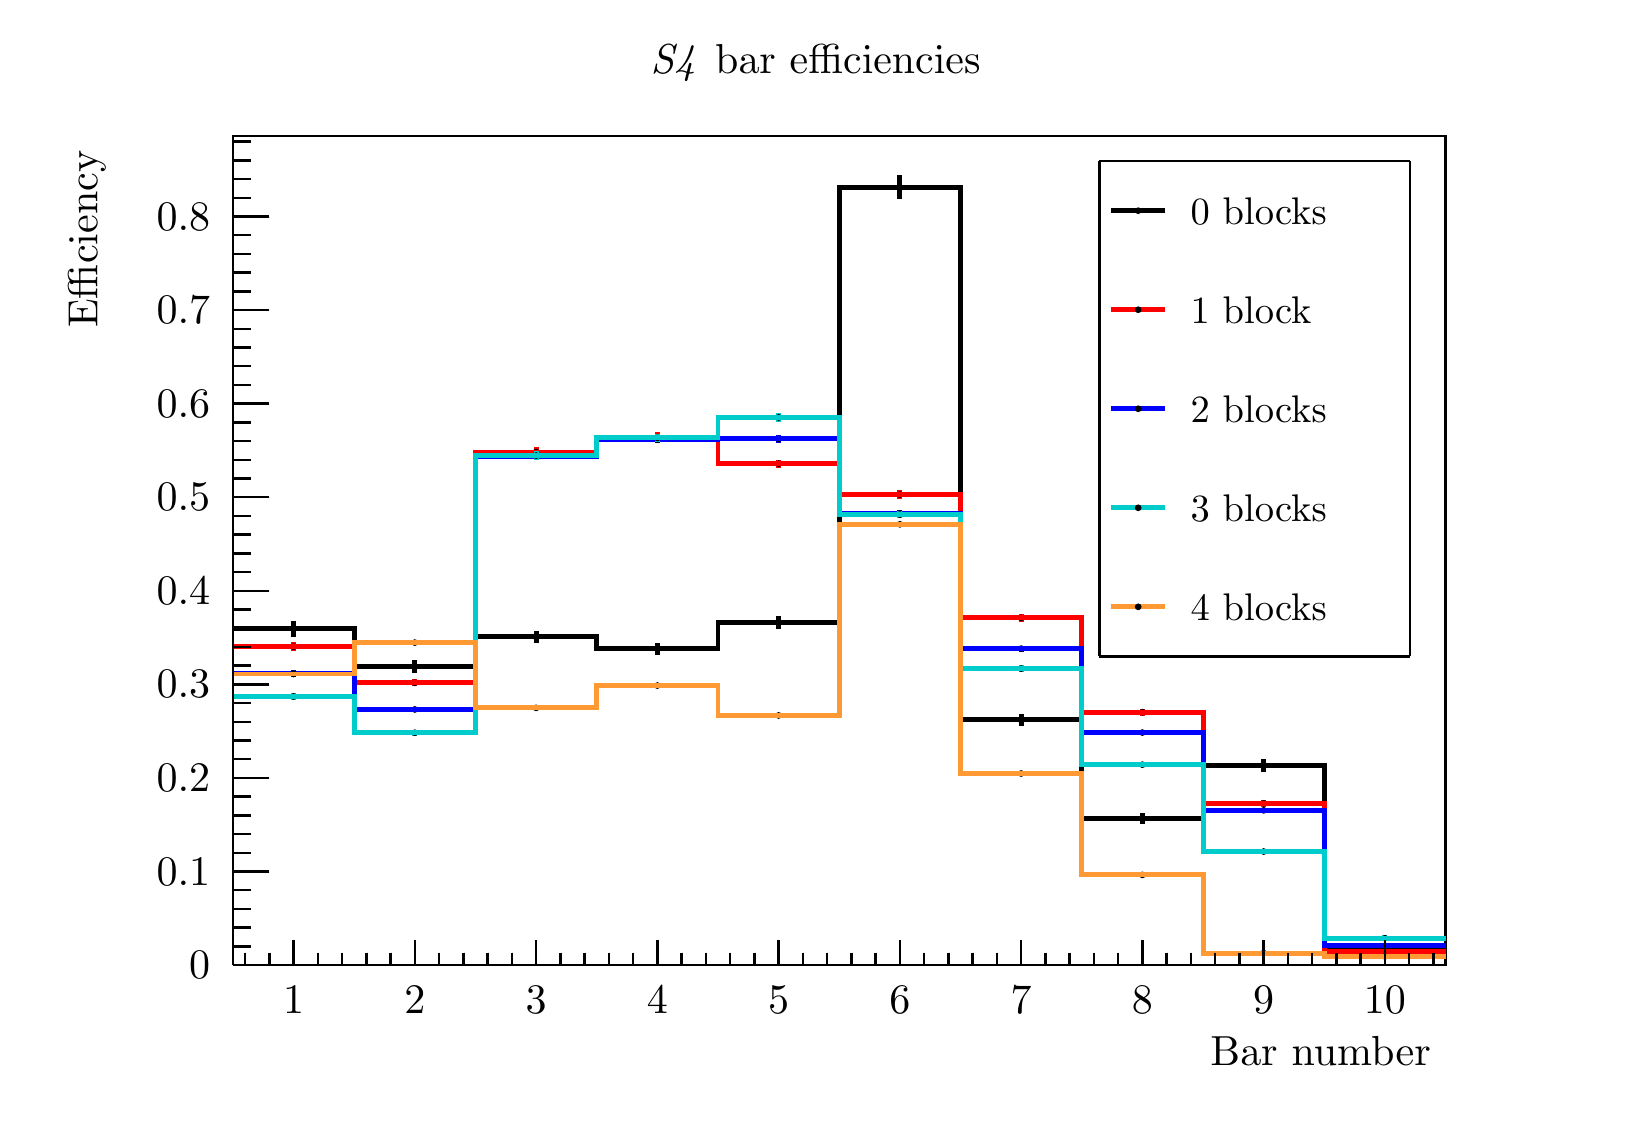
\begin{tikzpicture}
\pgfdeclareplotmark{cross} {
\pgfpathmoveto{\pgfpoint{-0.3\pgfplotmarksize}{\pgfplotmarksize}}
\pgfpathlineto{\pgfpoint{+0.3\pgfplotmarksize}{\pgfplotmarksize}}
\pgfpathlineto{\pgfpoint{+0.3\pgfplotmarksize}{0.3\pgfplotmarksize}}
\pgfpathlineto{\pgfpoint{+1\pgfplotmarksize}{0.3\pgfplotmarksize}}
\pgfpathlineto{\pgfpoint{+1\pgfplotmarksize}{-0.3\pgfplotmarksize}}
\pgfpathlineto{\pgfpoint{+0.3\pgfplotmarksize}{-0.3\pgfplotmarksize}}
\pgfpathlineto{\pgfpoint{+0.3\pgfplotmarksize}{-1.\pgfplotmarksize}}
\pgfpathlineto{\pgfpoint{-0.3\pgfplotmarksize}{-1.\pgfplotmarksize}}
\pgfpathlineto{\pgfpoint{-0.3\pgfplotmarksize}{-0.3\pgfplotmarksize}}
\pgfpathlineto{\pgfpoint{-1.\pgfplotmarksize}{-0.3\pgfplotmarksize}}
\pgfpathlineto{\pgfpoint{-1.\pgfplotmarksize}{0.3\pgfplotmarksize}}
\pgfpathlineto{\pgfpoint{-0.3\pgfplotmarksize}{0.3\pgfplotmarksize}}
\pgfpathclose
\pgfusepathqstroke
}
\pgfdeclareplotmark{cross*} {
\pgfpathmoveto{\pgfpoint{-0.3\pgfplotmarksize}{\pgfplotmarksize}}
\pgfpathlineto{\pgfpoint{+0.3\pgfplotmarksize}{\pgfplotmarksize}}
\pgfpathlineto{\pgfpoint{+0.3\pgfplotmarksize}{0.3\pgfplotmarksize}}
\pgfpathlineto{\pgfpoint{+1\pgfplotmarksize}{0.3\pgfplotmarksize}}
\pgfpathlineto{\pgfpoint{+1\pgfplotmarksize}{-0.3\pgfplotmarksize}}
\pgfpathlineto{\pgfpoint{+0.3\pgfplotmarksize}{-0.3\pgfplotmarksize}}
\pgfpathlineto{\pgfpoint{+0.3\pgfplotmarksize}{-1.\pgfplotmarksize}}
\pgfpathlineto{\pgfpoint{-0.3\pgfplotmarksize}{-1.\pgfplotmarksize}}
\pgfpathlineto{\pgfpoint{-0.3\pgfplotmarksize}{-0.3\pgfplotmarksize}}
\pgfpathlineto{\pgfpoint{-1.\pgfplotmarksize}{-0.3\pgfplotmarksize}}
\pgfpathlineto{\pgfpoint{-1.\pgfplotmarksize}{0.3\pgfplotmarksize}}
\pgfpathlineto{\pgfpoint{-0.3\pgfplotmarksize}{0.3\pgfplotmarksize}}
\pgfpathclose
\pgfusepathqfillstroke
}
\pgfdeclareplotmark{newstar} {
\pgfpathmoveto{\pgfqpoint{0pt}{\pgfplotmarksize}}
\pgfpathlineto{\pgfqpointpolar{44}{0.5\pgfplotmarksize}}
\pgfpathlineto{\pgfqpointpolar{18}{\pgfplotmarksize}}
\pgfpathlineto{\pgfqpointpolar{-20}{0.5\pgfplotmarksize}}
\pgfpathlineto{\pgfqpointpolar{-54}{\pgfplotmarksize}}
\pgfpathlineto{\pgfqpointpolar{-90}{0.5\pgfplotmarksize}}
\pgfpathlineto{\pgfqpointpolar{234}{\pgfplotmarksize}}
\pgfpathlineto{\pgfqpointpolar{198}{0.5\pgfplotmarksize}}
\pgfpathlineto{\pgfqpointpolar{162}{\pgfplotmarksize}}
\pgfpathlineto{\pgfqpointpolar{134}{0.5\pgfplotmarksize}}
\pgfpathclose
\pgfusepathqstroke
}
\pgfdeclareplotmark{newstar*} {
\pgfpathmoveto{\pgfqpoint{0pt}{\pgfplotmarksize}}
\pgfpathlineto{\pgfqpointpolar{44}{0.5\pgfplotmarksize}}
\pgfpathlineto{\pgfqpointpolar{18}{\pgfplotmarksize}}
\pgfpathlineto{\pgfqpointpolar{-20}{0.5\pgfplotmarksize}}
\pgfpathlineto{\pgfqpointpolar{-54}{\pgfplotmarksize}}
\pgfpathlineto{\pgfqpointpolar{-90}{0.5\pgfplotmarksize}}
\pgfpathlineto{\pgfqpointpolar{234}{\pgfplotmarksize}}
\pgfpathlineto{\pgfqpointpolar{198}{0.5\pgfplotmarksize}}
\pgfpathlineto{\pgfqpointpolar{162}{\pgfplotmarksize}}
\pgfpathlineto{\pgfqpointpolar{134}{0.5\pgfplotmarksize}}
\pgfpathclose
\pgfusepathqfillstroke
}
\definecolor{c}{rgb}{1,1,1};
\draw [color=c, fill=c] (0,0) rectangle (20,13.6752);
\draw [color=c, fill=c] (2.6,1.77778) rectangle (18,12.3077);
\definecolor{c}{rgb}{0,0,0};
\draw [c,line width=0.9] (2.6,1.77778) -- (2.6,12.3077) -- (18,12.3077) -- (18,1.77778) -- (2.6,1.77778);
\definecolor{c}{rgb}{1,1,1};
\draw [color=c, fill=c] (2.6,1.77778) rectangle (18,12.3077);
\definecolor{c}{rgb}{0,0,0};
\draw [c,line width=0.9] (2.6,1.77778) -- (2.6,12.3077) -- (18,12.3077) -- (18,1.77778) -- (2.6,1.77778);
\definecolor{c}{rgb}{0,0,0.6};
\draw [c,line width=0.9] (2.6,1.77778) -- (4.14,1.77778) -- (4.14,1.77778) -- (5.68,1.77778) -- (5.68,1.77778) -- (7.22,1.77778) -- (7.22,1.77778) -- (8.76,1.77778) -- (8.76,1.77778) -- (10.3,1.77778) -- (10.3,1.77778) -- (11.84,1.77778) --
 (11.84,1.77778) -- (13.38,1.77778) -- (13.38,1.77778) -- (14.92,1.77778) -- (14.92,1.77778) -- (16.46,1.77778) -- (16.46,1.77778) -- (18,1.77778);
\definecolor{c}{rgb}{0,0,0};
\draw [c,line width=0.9] (2.6,1.77778) -- (18,1.77778);
\draw [c,line width=0.9] (3.37,2.09368) -- (3.37,1.77778);
\draw [c,line width=0.9] (3.678,1.93573) -- (3.678,1.77778);
\draw [c,line width=0.9] (3.986,1.93573) -- (3.986,1.77778);
\draw [c,line width=0.9] (4.294,1.93573) -- (4.294,1.77778);
\draw [c,line width=0.9] (4.602,1.93573) -- (4.602,1.77778);
\draw [c,line width=0.9] (4.91,2.09368) -- (4.91,1.77778);
\draw [c,line width=0.9] (5.218,1.93573) -- (5.218,1.77778);
\draw [c,line width=0.9] (5.526,1.93573) -- (5.526,1.77778);
\draw [c,line width=0.9] (5.834,1.93573) -- (5.834,1.77778);
\draw [c,line width=0.9] (6.142,1.93573) -- (6.142,1.77778);
\draw [c,line width=0.9] (6.45,2.09368) -- (6.45,1.77778);
\draw [c,line width=0.9] (6.758,1.93573) -- (6.758,1.77778);
\draw [c,line width=0.9] (7.066,1.93573) -- (7.066,1.77778);
\draw [c,line width=0.9] (7.374,1.93573) -- (7.374,1.77778);
\draw [c,line width=0.9] (7.682,1.93573) -- (7.682,1.77778);
\draw [c,line width=0.9] (7.99,2.09368) -- (7.99,1.77778);
\draw [c,line width=0.9] (8.298,1.93573) -- (8.298,1.77778);
\draw [c,line width=0.9] (8.606,1.93573) -- (8.606,1.77778);
\draw [c,line width=0.9] (8.914,1.93573) -- (8.914,1.77778);
\draw [c,line width=0.9] (9.222,1.93573) -- (9.222,1.77778);
\draw [c,line width=0.9] (9.53,2.09368) -- (9.53,1.77778);
\draw [c,line width=0.9] (9.838,1.93573) -- (9.838,1.77778);
\draw [c,line width=0.9] (10.146,1.93573) -- (10.146,1.77778);
\draw [c,line width=0.9] (10.454,1.93573) -- (10.454,1.77778);
\draw [c,line width=0.9] (10.762,1.93573) -- (10.762,1.77778);
\draw [c,line width=0.9] (11.07,2.09368) -- (11.07,1.77778);
\draw [c,line width=0.9] (11.378,1.93573) -- (11.378,1.77778);
\draw [c,line width=0.9] (11.686,1.93573) -- (11.686,1.77778);
\draw [c,line width=0.9] (11.994,1.93573) -- (11.994,1.77778);
\draw [c,line width=0.9] (12.302,1.93573) -- (12.302,1.77778);
\draw [c,line width=0.9] (12.61,2.09368) -- (12.61,1.77778);
\draw [c,line width=0.9] (12.918,1.93573) -- (12.918,1.77778);
\draw [c,line width=0.9] (13.226,1.93573) -- (13.226,1.77778);
\draw [c,line width=0.9] (13.534,1.93573) -- (13.534,1.77778);
\draw [c,line width=0.9] (13.842,1.93573) -- (13.842,1.77778);
\draw [c,line width=0.9] (14.15,2.09368) -- (14.15,1.77778);
\draw [c,line width=0.9] (14.458,1.93573) -- (14.458,1.77778);
\draw [c,line width=0.9] (14.766,1.93573) -- (14.766,1.77778);
\draw [c,line width=0.9] (15.074,1.93573) -- (15.074,1.77778);
\draw [c,line width=0.9] (15.382,1.93573) -- (15.382,1.77778);
\draw [c,line width=0.9] (15.69,2.09368) -- (15.69,1.77778);
\draw [c,line width=0.9] (15.998,1.93573) -- (15.998,1.77778);
\draw [c,line width=0.9] (16.306,1.93573) -- (16.306,1.77778);
\draw [c,line width=0.9] (16.614,1.93573) -- (16.614,1.77778);
\draw [c,line width=0.9] (16.922,1.93573) -- (16.922,1.77778);
\draw [c,line width=0.9] (17.23,2.09368) -- (17.23,1.77778);
\draw [c,line width=0.9] (3.37,2.09368) -- (3.37,1.77778);
\draw [c,line width=0.9] (3.062,1.93573) -- (3.062,1.77778);
\draw [c,line width=0.9] (2.754,1.93573) -- (2.754,1.77778);
\draw [c,line width=0.9] (17.23,2.09368) -- (17.23,1.77778);
\draw [c,line width=0.9] (17.538,1.93573) -- (17.538,1.77778);
\draw [c,line width=0.9] (17.846,1.93573) -- (17.846,1.77778);
\draw [anchor=base] (3.37,1.16239) node[scale=1.51861, color=c, rotate=0]{1};
\draw [anchor=base] (4.91,1.16239) node[scale=1.51861, color=c, rotate=0]{2};
\draw [anchor=base] (6.45,1.16239) node[scale=1.51861, color=c, rotate=0]{3};
\draw [anchor=base] (7.99,1.16239) node[scale=1.51861, color=c, rotate=0]{4};
\draw [anchor=base] (9.53,1.16239) node[scale=1.51861, color=c, rotate=0]{5};
\draw [anchor=base] (11.07,1.16239) node[scale=1.51861, color=c, rotate=0]{6};
\draw [anchor=base] (12.61,1.16239) node[scale=1.51861, color=c, rotate=0]{7};
\draw [anchor=base] (14.15,1.16239) node[scale=1.51861, color=c, rotate=0]{8};
\draw [anchor=base] (15.69,1.16239) node[scale=1.51861, color=c, rotate=0]{9};
\draw [anchor=base] (17.23,1.16239) node[scale=1.51861, color=c, rotate=0]{10};
\draw [anchor= east] (18,0.683761) node[scale=1.51861, color=c, rotate=0]{ Bar number};
\draw [c,line width=0.9] (2.6,1.77778) -- (2.6,12.3077);
\draw [c,line width=0.9] (3.062,1.77778) -- (2.6,1.77778);
\draw [c,line width=0.9] (2.831,2.01544) -- (2.6,2.01544);
\draw [c,line width=0.9] (2.831,2.2531) -- (2.6,2.2531);
\draw [c,line width=0.9] (2.831,2.49075) -- (2.6,2.49075);
\draw [c,line width=0.9] (2.831,2.72841) -- (2.6,2.72841);
\draw [c,line width=0.9] (3.062,2.96607) -- (2.6,2.96607);
\draw [c,line width=0.9] (2.831,3.20373) -- (2.6,3.20373);
\draw [c,line width=0.9] (2.831,3.44139) -- (2.6,3.44139);
\draw [c,line width=0.9] (2.831,3.67905) -- (2.6,3.67905);
\draw [c,line width=0.9] (2.831,3.91671) -- (2.6,3.91671);
\draw [c,line width=0.9] (3.062,4.15437) -- (2.6,4.15437);
\draw [c,line width=0.9] (2.831,4.39202) -- (2.6,4.39202);
\draw [c,line width=0.9] (2.831,4.62968) -- (2.6,4.62968);
\draw [c,line width=0.9] (2.831,4.86734) -- (2.6,4.86734);
\draw [c,line width=0.9] (2.831,5.105) -- (2.6,5.105);
\draw [c,line width=0.9] (3.062,5.34266) -- (2.6,5.34266);
\draw [c,line width=0.9] (2.831,5.58032) -- (2.6,5.58032);
\draw [c,line width=0.9] (2.831,5.81798) -- (2.6,5.81798);
\draw [c,line width=0.9] (2.831,6.05563) -- (2.6,6.05563);
\draw [c,line width=0.9] (2.831,6.29329) -- (2.6,6.29329);
\draw [c,line width=0.9] (3.062,6.53095) -- (2.6,6.53095);
\draw [c,line width=0.9] (2.831,6.76861) -- (2.6,6.76861);
\draw [c,line width=0.9] (2.831,7.00627) -- (2.6,7.00627);
\draw [c,line width=0.9] (2.831,7.24393) -- (2.6,7.24393);
\draw [c,line width=0.9] (2.831,7.48159) -- (2.6,7.48159);
\draw [c,line width=0.9] (3.062,7.71925) -- (2.6,7.71925);
\draw [c,line width=0.9] (2.831,7.9569) -- (2.6,7.9569);
\draw [c,line width=0.9] (2.831,8.19456) -- (2.6,8.19456);
\draw [c,line width=0.9] (2.831,8.43222) -- (2.6,8.43222);
\draw [c,line width=0.9] (2.831,8.66988) -- (2.6,8.66988);
\draw [c,line width=0.9] (3.062,8.90754) -- (2.6,8.90754);
\draw [c,line width=0.9] (2.831,9.1452) -- (2.6,9.1452);
\draw [c,line width=0.9] (2.831,9.38286) -- (2.6,9.38286);
\draw [c,line width=0.9] (2.831,9.62052) -- (2.6,9.62052);
\draw [c,line width=0.9] (2.831,9.85817) -- (2.6,9.85817);
\draw [c,line width=0.9] (3.062,10.0958) -- (2.6,10.0958);
\draw [c,line width=0.9] (2.831,10.3335) -- (2.6,10.3335);
\draw [c,line width=0.9] (2.831,10.5711) -- (2.6,10.5711);
\draw [c,line width=0.9] (2.831,10.8088) -- (2.6,10.8088);
\draw [c,line width=0.9] (2.831,11.0465) -- (2.6,11.0465);
\draw [c,line width=0.9] (3.062,11.2841) -- (2.6,11.2841);
\draw [c,line width=0.9] (3.062,11.2841) -- (2.6,11.2841);
\draw [c,line width=0.9] (2.831,11.5218) -- (2.6,11.5218);
\draw [c,line width=0.9] (2.831,11.7594) -- (2.6,11.7594);
\draw [c,line width=0.9] (2.831,11.9971) -- (2.6,11.9971);
\draw [c,line width=0.9] (2.831,12.2348) -- (2.6,12.2348);
\draw [anchor= east] (2.5,1.77778) node[scale=1.51861, color=c, rotate=0]{0};
\draw [anchor= east] (2.5,2.96607) node[scale=1.51861, color=c, rotate=0]{0.1};
\draw [anchor= east] (2.5,4.15437) node[scale=1.51861, color=c, rotate=0]{0.2};
\draw [anchor= east] (2.5,5.34266) node[scale=1.51861, color=c, rotate=0]{0.3};
\draw [anchor= east] (2.5,6.53095) node[scale=1.51861, color=c, rotate=0]{0.4};
\draw [anchor= east] (2.5,7.71925) node[scale=1.51861, color=c, rotate=0]{0.5};
\draw [anchor= east] (2.5,8.90754) node[scale=1.51861, color=c, rotate=0]{0.6};
\draw [anchor= east] (2.5,10.0958) node[scale=1.51861, color=c, rotate=0]{0.7};
\draw [anchor= east] (2.5,11.2841) node[scale=1.51861, color=c, rotate=0]{0.8};
\draw [anchor= east] (0.745299,12.3077) node[scale=1.51861, color=c, rotate=90]{ Efficiency};
\draw [c,line width=1.8] (3.37,5.94713) -- (3.37,6.048);
\draw [c,line width=1.8] (3.37,6.048) -- (3.37,6.14887);
\foreach \P in {(3.37,6.048)}{\draw[mark options={color=c,fill=c},mark size=2.402402pt,mark=*,mark size=1pt] plot coordinates {\P};}
\draw [c,line width=1.8] (4.91,5.48652) -- (4.91,5.56707);
\draw [c,line width=1.8] (4.91,5.56707) -- (4.91,5.64763);
\foreach \P in {(4.91,5.56707)}{\draw[mark options={color=c,fill=c},mark size=2.402402pt,mark=*,mark size=1pt] plot coordinates {\P};}
\draw [c,line width=1.8] (6.45,5.86443) -- (6.45,5.94509);
\draw [c,line width=1.8] (6.45,5.94509) -- (6.45,6.02574);
\foreach \P in {(6.45,5.94509)}{\draw[mark options={color=c,fill=c},mark size=2.402402pt,mark=*,mark size=1pt] plot coordinates {\P};}
\draw [c,line width=1.8] (7.99,5.72099) -- (7.99,5.79421);
\draw [c,line width=1.8] (7.99,5.79421) -- (7.99,5.86742);
\foreach \P in {(7.99,5.79421)}{\draw[mark options={color=c,fill=c},mark size=2.402402pt,mark=*,mark size=1pt] plot coordinates {\P};}
\draw [c,line width=1.8] (9.53,6.04947) -- (9.53,6.12746);
\draw [c,line width=1.8] (9.53,6.12746) -- (9.53,6.20546);
\foreach \P in {(9.53,6.12746)}{\draw[mark options={color=c,fill=c},mark size=2.402402pt,mark=*,mark size=1pt] plot coordinates {\P};}
\draw [c,line width=1.8] (11.07,11.5047) -- (11.07,11.6555);
\draw [c,line width=1.8] (11.07,11.6555) -- (11.07,11.8063);
\foreach \P in {(11.07,11.6555)}{\draw[mark options={color=c,fill=c},mark size=2.402402pt,mark=*,mark size=1pt] plot coordinates {\P};}
\draw [c,line width=1.8] (12.61,4.81396) -- (12.61,4.88993);
\draw [c,line width=1.8] (12.61,4.88993) -- (12.61,4.96589);
\foreach \P in {(12.61,4.88993)}{\draw[mark options={color=c,fill=c},mark size=2.402402pt,mark=*,mark size=1pt] plot coordinates {\P};}
\draw [c,line width=1.8] (14.15,3.56561) -- (14.15,3.63618);
\draw [c,line width=1.8] (14.15,3.63618) -- (14.15,3.70674);
\foreach \P in {(14.15,3.63618)}{\draw[mark options={color=c,fill=c},mark size=2.402402pt,mark=*,mark size=1pt] plot coordinates {\P};}
\draw [c,line width=1.8] (15.69,4.23443) -- (15.69,4.31531);
\draw [c,line width=1.8] (15.69,4.31531) -- (15.69,4.39619);
\foreach \P in {(15.69,4.31531)}{\draw[mark options={color=c,fill=c},mark size=2.402402pt,mark=*,mark size=1pt] plot coordinates {\P};}
\draw [c,line width=1.8] (17.23,1.95841) -- (17.23,2.00004);
\draw [c,line width=1.8] (17.23,2.00004) -- (17.23,2.04166);
\foreach \P in {(17.23,2.00004)}{\draw[mark options={color=c,fill=c},mark size=2.402402pt,mark=*,mark size=1pt] plot coordinates {\P};}
\draw [c,line width=1.8] (2.6,6.048) -- (4.14,6.048) -- (4.14,5.56707) -- (5.68,5.56707) -- (5.68,5.94509) -- (7.22,5.94509) -- (7.22,5.79421) -- (8.76,5.79421) -- (8.76,6.12746) -- (10.3,6.12746) -- (10.3,11.6555) -- (11.84,11.6555) --
 (11.84,4.88993) -- (13.38,4.88993) -- (13.38,3.63618) -- (14.92,3.63618) -- (14.92,4.31531) -- (16.46,4.31531) -- (16.46,2.00004) -- (18,2.00004);
\definecolor{c}{rgb}{1,0,0};
\draw [c,line width=1.8] (3.37,5.76471) -- (3.37,5.8214);
\draw [c,line width=1.8] (3.37,5.8214) -- (3.37,5.8781);
\definecolor{c}{rgb}{0,0,0};
\foreach \P in {(3.37,5.8214)}{\draw[mark options={color=c,fill=c},mark size=2.402402pt,mark=*,mark size=1pt] plot coordinates {\P};}
\definecolor{c}{rgb}{1,0,0};
\draw [c,line width=1.8] (4.91,5.31634) -- (4.91,5.36213);
\draw [c,line width=1.8] (4.91,5.36213) -- (4.91,5.40793);
\definecolor{c}{rgb}{0,0,0};
\foreach \P in {(4.91,5.36213)}{\draw[mark options={color=c,fill=c},mark size=2.402402pt,mark=*,mark size=1pt] plot coordinates {\P};}
\definecolor{c}{rgb}{1,0,0};
\draw [c,line width=1.8] (6.45,8.23172) -- (6.45,8.29272);
\draw [c,line width=1.8] (6.45,8.29272) -- (6.45,8.35373);
\definecolor{c}{rgb}{0,0,0};
\foreach \P in {(6.45,8.29272)}{\draw[mark options={color=c,fill=c},mark size=2.402402pt,mark=*,mark size=1pt] plot coordinates {\P};}
\definecolor{c}{rgb}{1,0,0};
\draw [c,line width=1.8] (7.99,8.42349) -- (7.99,8.48284);
\draw [c,line width=1.8] (7.99,8.48284) -- (7.99,8.5422);
\definecolor{c}{rgb}{0,0,0};
\foreach \P in {(7.99,8.48284)}{\draw[mark options={color=c,fill=c},mark size=2.402402pt,mark=*,mark size=1pt] plot coordinates {\P};}
\definecolor{c}{rgb}{1,0,0};
\draw [c,line width=1.8] (9.53,8.09169) -- (9.53,8.14475);
\draw [c,line width=1.8] (9.53,8.14475) -- (9.53,8.1978);
\definecolor{c}{rgb}{0,0,0};
\foreach \P in {(9.53,8.14475)}{\draw[mark options={color=c,fill=c},mark size=2.402402pt,mark=*,mark size=1pt] plot coordinates {\P};}
\definecolor{c}{rgb}{1,0,0};
\draw [c,line width=1.8] (11.07,7.69589) -- (11.07,7.75308);
\draw [c,line width=1.8] (11.07,7.75308) -- (11.07,7.81026);
\definecolor{c}{rgb}{0,0,0};
\foreach \P in {(11.07,7.75308)}{\draw[mark options={color=c,fill=c},mark size=2.402402pt,mark=*,mark size=1pt] plot coordinates {\P};}
\definecolor{c}{rgb}{1,0,0};
\draw [c,line width=1.8] (12.61,6.13603) -- (12.61,6.1871);
\draw [c,line width=1.8] (12.61,6.1871) -- (12.61,6.23818);
\definecolor{c}{rgb}{0,0,0};
\foreach \P in {(12.61,6.1871)}{\draw[mark options={color=c,fill=c},mark size=2.402402pt,mark=*,mark size=1pt] plot coordinates {\P};}
\definecolor{c}{rgb}{1,0,0};
\draw [c,line width=1.8] (14.15,4.9422) -- (14.15,4.9889);
\draw [c,line width=1.8] (14.15,4.9889) -- (14.15,5.0356);
\definecolor{c}{rgb}{0,0,0};
\foreach \P in {(14.15,4.9889)}{\draw[mark options={color=c,fill=c},mark size=2.402402pt,mark=*,mark size=1pt] plot coordinates {\P};}
\definecolor{c}{rgb}{1,0,0};
\draw [c,line width=1.8] (15.69,3.78842) -- (15.69,3.83138);
\draw [c,line width=1.8] (15.69,3.83138) -- (15.69,3.87434);
\definecolor{c}{rgb}{0,0,0};
\foreach \P in {(15.69,3.83138)}{\draw[mark options={color=c,fill=c},mark size=2.402402pt,mark=*,mark size=1pt] plot coordinates {\P};}
\definecolor{c}{rgb}{1,0,0};
\draw [c,line width=1.8] (17.23,1.91836) -- (17.23,1.9483);
\draw [c,line width=1.8] (17.23,1.9483) -- (17.23,1.97823);
\definecolor{c}{rgb}{0,0,0};
\foreach \P in {(17.23,1.9483)}{\draw[mark options={color=c,fill=c},mark size=2.402402pt,mark=*,mark size=1pt] plot coordinates {\P};}
\definecolor{c}{rgb}{1,0,0};
\draw [c,line width=1.8] (2.6,5.8214) -- (4.14,5.8214) -- (4.14,5.36213) -- (5.68,5.36213) -- (5.68,8.29272) -- (7.22,8.29272) -- (7.22,8.48284) -- (8.76,8.48284) -- (8.76,8.14475) -- (10.3,8.14475) -- (10.3,7.75308) -- (11.84,7.75308) --
 (11.84,6.1871) -- (13.38,6.1871) -- (13.38,4.9889) -- (14.92,4.9889) -- (14.92,3.83138) -- (16.46,3.83138) -- (16.46,1.9483) -- (18,1.9483);
\definecolor{c}{rgb}{0,0,1};
\draw [c,line width=1.8] (3.37,5.43835) -- (3.37,5.48052);
\draw [c,line width=1.8] (3.37,5.48052) -- (3.37,5.52268);
\definecolor{c}{rgb}{0,0,0};
\foreach \P in {(3.37,5.48052)}{\draw[mark options={color=c,fill=c},mark size=2.402402pt,mark=*,mark size=1pt] plot coordinates {\P};}
\definecolor{c}{rgb}{0,0,1};
\draw [c,line width=1.8] (4.91,4.9892) -- (4.91,5.02356);
\draw [c,line width=1.8] (4.91,5.02356) -- (4.91,5.05792);
\definecolor{c}{rgb}{0,0,0};
\foreach \P in {(4.91,5.02356)}{\draw[mark options={color=c,fill=c},mark size=2.402402pt,mark=*,mark size=1pt] plot coordinates {\P};}
\definecolor{c}{rgb}{0,0,1};
\draw [c,line width=1.8] (6.45,8.19027) -- (6.45,8.23881);
\draw [c,line width=1.8] (6.45,8.23881) -- (6.45,8.28735);
\definecolor{c}{rgb}{0,0,0};
\foreach \P in {(6.45,8.23881)}{\draw[mark options={color=c,fill=c},mark size=2.402402pt,mark=*,mark size=1pt] plot coordinates {\P};}
\definecolor{c}{rgb}{0,0,1};
\draw [c,line width=1.8] (7.99,8.40121) -- (7.99,8.44901);
\draw [c,line width=1.8] (7.99,8.44901) -- (7.99,8.49681);
\definecolor{c}{rgb}{0,0,0};
\foreach \P in {(7.99,8.44901)}{\draw[mark options={color=c,fill=c},mark size=2.402402pt,mark=*,mark size=1pt] plot coordinates {\P};}
\definecolor{c}{rgb}{0,0,1};
\draw [c,line width=1.8] (9.53,8.41363) -- (9.53,8.45921);
\draw [c,line width=1.8] (9.53,8.45921) -- (9.53,8.50478);
\definecolor{c}{rgb}{0,0,0};
\foreach \P in {(9.53,8.45921)}{\draw[mark options={color=c,fill=c},mark size=2.402402pt,mark=*,mark size=1pt] plot coordinates {\P};}
\definecolor{c}{rgb}{0,0,1};
\draw [c,line width=1.8] (11.07,7.46957) -- (11.07,7.51425);
\draw [c,line width=1.8] (11.07,7.51425) -- (11.07,7.55892);
\definecolor{c}{rgb}{0,0,0};
\foreach \P in {(11.07,7.51425)}{\draw[mark options={color=c,fill=c},mark size=2.402402pt,mark=*,mark size=1pt] plot coordinates {\P};}
\definecolor{c}{rgb}{0,0,1};
\draw [c,line width=1.8] (12.61,5.75818) -- (12.61,5.79638);
\draw [c,line width=1.8] (12.61,5.79638) -- (12.61,5.83458);
\definecolor{c}{rgb}{0,0,0};
\foreach \P in {(12.61,5.79638)}{\draw[mark options={color=c,fill=c},mark size=2.402402pt,mark=*,mark size=1pt] plot coordinates {\P};}
\definecolor{c}{rgb}{0,0,1};
\draw [c,line width=1.8] (14.15,4.69542) -- (14.15,4.73);
\draw [c,line width=1.8] (14.15,4.73) -- (14.15,4.76458);
\definecolor{c}{rgb}{0,0,0};
\foreach \P in {(14.15,4.73)}{\draw[mark options={color=c,fill=c},mark size=2.402402pt,mark=*,mark size=1pt] plot coordinates {\P};}
\definecolor{c}{rgb}{0,0,1};
\draw [c,line width=1.8] (15.69,3.71002) -- (15.69,3.74208);
\draw [c,line width=1.8] (15.69,3.74208) -- (15.69,3.77415);
\definecolor{c}{rgb}{0,0,0};
\foreach \P in {(15.69,3.74208)}{\draw[mark options={color=c,fill=c},mark size=2.402402pt,mark=*,mark size=1pt] plot coordinates {\P};}
\definecolor{c}{rgb}{0,0,1};
\draw [c,line width=1.8] (17.23,1.99459) -- (17.23,2.02279);
\draw [c,line width=1.8] (17.23,2.02279) -- (17.23,2.05099);
\definecolor{c}{rgb}{0,0,0};
\foreach \P in {(17.23,2.02279)}{\draw[mark options={color=c,fill=c},mark size=2.402402pt,mark=*,mark size=1pt] plot coordinates {\P};}
\definecolor{c}{rgb}{0,0,1};
\draw [c,line width=1.8] (2.6,5.48052) -- (4.14,5.48052) -- (4.14,5.02356) -- (5.68,5.02356) -- (5.68,8.23881) -- (7.22,8.23881) -- (7.22,8.44901) -- (8.76,8.44901) -- (8.76,8.45921) -- (10.3,8.45921) -- (10.3,7.51425) -- (11.84,7.51425) --
 (11.84,5.79638) -- (13.38,5.79638) -- (13.38,4.73) -- (14.92,4.73) -- (14.92,3.74208) -- (16.46,3.74208) -- (16.46,2.02279) -- (18,2.02279);
\definecolor{c}{rgb}{0,0.8,0.8};
\draw [c,line width=1.8] (3.37,5.14512) -- (3.37,5.18859);
\draw [c,line width=1.8] (3.37,5.18859) -- (3.37,5.23205);
\definecolor{c}{rgb}{0,0,0};
\foreach \P in {(3.37,5.18859)}{\draw[mark options={color=c,fill=c},mark size=2.402402pt,mark=*,mark size=1pt] plot coordinates {\P};}
\definecolor{c}{rgb}{0,0.8,0.8};
\draw [c,line width=1.8] (4.91,4.69231) -- (4.91,4.72802);
\draw [c,line width=1.8] (4.91,4.72802) -- (4.91,4.76372);
\definecolor{c}{rgb}{0,0,0};
\foreach \P in {(4.91,4.72802)}{\draw[mark options={color=c,fill=c},mark size=2.402402pt,mark=*,mark size=1pt] plot coordinates {\P};}
\definecolor{c}{rgb}{0,0.8,0.8};
\draw [c,line width=1.8] (6.45,8.19462) -- (6.45,8.2476);
\draw [c,line width=1.8] (6.45,8.2476) -- (6.45,8.30059);
\definecolor{c}{rgb}{0,0,0};
\foreach \P in {(6.45,8.2476)}{\draw[mark options={color=c,fill=c},mark size=2.402402pt,mark=*,mark size=1pt] plot coordinates {\P};}
\definecolor{c}{rgb}{0,0.8,0.8};
\draw [c,line width=1.8] (7.99,8.41839) -- (7.99,8.47122);
\draw [c,line width=1.8] (7.99,8.47122) -- (7.99,8.52405);
\definecolor{c}{rgb}{0,0,0};
\foreach \P in {(7.99,8.47122)}{\draw[mark options={color=c,fill=c},mark size=2.402402pt,mark=*,mark size=1pt] plot coordinates {\P};}
\definecolor{c}{rgb}{0,0.8,0.8};
\draw [c,line width=1.8] (9.53,8.67919) -- (9.53,8.73184);
\draw [c,line width=1.8] (9.53,8.73184) -- (9.53,8.78449);
\definecolor{c}{rgb}{0,0,0};
\foreach \P in {(9.53,8.73184)}{\draw[mark options={color=c,fill=c},mark size=2.402402pt,mark=*,mark size=1pt] plot coordinates {\P};}
\definecolor{c}{rgb}{0,0.8,0.8};
\draw [c,line width=1.8] (11.07,7.44878) -- (11.07,7.49768);
\draw [c,line width=1.8] (11.07,7.49768) -- (11.07,7.54658);
\definecolor{c}{rgb}{0,0,0};
\foreach \P in {(11.07,7.49768)}{\draw[mark options={color=c,fill=c},mark size=2.402402pt,mark=*,mark size=1pt] plot coordinates {\P};}
\definecolor{c}{rgb}{0,0.8,0.8};
\draw [c,line width=1.8] (12.61,5.50194) -- (12.61,5.54215);
\draw [c,line width=1.8] (12.61,5.54215) -- (12.61,5.58236);
\definecolor{c}{rgb}{0,0,0};
\foreach \P in {(12.61,5.54215)}{\draw[mark options={color=c,fill=c},mark size=2.402402pt,mark=*,mark size=1pt] plot coordinates {\P};}
\definecolor{c}{rgb}{0,0.8,0.8};
\draw [c,line width=1.8] (14.15,4.28775) -- (14.15,4.32232);
\draw [c,line width=1.8] (14.15,4.32232) -- (14.15,4.3569);
\definecolor{c}{rgb}{0,0,0};
\foreach \P in {(14.15,4.32232)}{\draw[mark options={color=c,fill=c},mark size=2.402402pt,mark=*,mark size=1pt] plot coordinates {\P};}
\definecolor{c}{rgb}{0,0.8,0.8};
\draw [c,line width=1.8] (15.69,3.18971) -- (15.69,3.21924);
\draw [c,line width=1.8] (15.69,3.21924) -- (15.69,3.24878);
\definecolor{c}{rgb}{0,0,0};
\foreach \P in {(15.69,3.21924)}{\draw[mark options={color=c,fill=c},mark size=2.402402pt,mark=*,mark size=1pt] plot coordinates {\P};}
\definecolor{c}{rgb}{0,0.8,0.8};
\draw [c,line width=1.8] (17.23,2.07797) -- (17.23,2.11716);
\draw [c,line width=1.8] (17.23,2.11716) -- (17.23,2.15634);
\definecolor{c}{rgb}{0,0,0};
\foreach \P in {(17.23,2.11716)}{\draw[mark options={color=c,fill=c},mark size=2.402402pt,mark=*,mark size=1pt] plot coordinates {\P};}
\definecolor{c}{rgb}{0,0.8,0.8};
\draw [c,line width=1.8] (2.6,5.18859) -- (4.14,5.18859) -- (4.14,4.72802) -- (5.68,4.72802) -- (5.68,8.2476) -- (7.22,8.2476) -- (7.22,8.47122) -- (8.76,8.47122) -- (8.76,8.73184) -- (10.3,8.73184) -- (10.3,7.49768) -- (11.84,7.49768) --
 (11.84,5.54215) -- (13.38,5.54215) -- (13.38,4.32232) -- (14.92,4.32232) -- (14.92,3.21924) -- (16.46,3.21924) -- (16.46,2.11716) -- (18,2.11716);
\definecolor{c}{rgb}{1,0.6,0.2};
\draw [c,line width=1.8] (3.37,5.46131) -- (3.37,5.47379);
\draw [c,line width=1.8] (3.37,5.47379) -- (3.37,5.48626);
\definecolor{c}{rgb}{0,0,0};
\foreach \P in {(3.37,5.47379)}{\draw[mark options={color=c,fill=c},mark size=2.402402pt,mark=*,mark size=1pt] plot coordinates {\P};}
\definecolor{c}{rgb}{1,0.6,0.2};
\draw [c,line width=1.8] (4.91,5.86106) -- (4.91,5.8726);
\draw [c,line width=1.8] (4.91,5.8726) -- (4.91,5.88414);
\definecolor{c}{rgb}{0,0,0};
\foreach \P in {(4.91,5.8726)}{\draw[mark options={color=c,fill=c},mark size=2.402402pt,mark=*,mark size=1pt] plot coordinates {\P};}
\definecolor{c}{rgb}{1,0.6,0.2};
\draw [c,line width=1.8] (6.45,5.03364) -- (6.45,5.04378);
\draw [c,line width=1.8] (6.45,5.04378) -- (6.45,5.05392);
\definecolor{c}{rgb}{0,0,0};
\foreach \P in {(6.45,5.04378)}{\draw[mark options={color=c,fill=c},mark size=2.402402pt,mark=*,mark size=1pt] plot coordinates {\P};}
\definecolor{c}{rgb}{1,0.6,0.2};
\draw [c,line width=1.8] (7.99,5.31713) -- (7.99,5.32715);
\draw [c,line width=1.8] (7.99,5.32715) -- (7.99,5.33717);
\definecolor{c}{rgb}{0,0,0};
\foreach \P in {(7.99,5.32715)}{\draw[mark options={color=c,fill=c},mark size=2.402402pt,mark=*,mark size=1pt] plot coordinates {\P};}
\definecolor{c}{rgb}{1,0.6,0.2};
\draw [c,line width=1.8] (9.53,4.93765) -- (9.53,4.94748);
\draw [c,line width=1.8] (9.53,4.94748) -- (9.53,4.9573);
\definecolor{c}{rgb}{0,0,0};
\foreach \P in {(9.53,4.94748)}{\draw[mark options={color=c,fill=c},mark size=2.402402pt,mark=*,mark size=1pt] plot coordinates {\P};}
\definecolor{c}{rgb}{1,0.6,0.2};
\draw [c,line width=1.8] (11.07,7.36086) -- (11.07,7.37486);
\draw [c,line width=1.8] (11.07,7.37486) -- (11.07,7.38885);
\definecolor{c}{rgb}{0,0,0};
\foreach \P in {(11.07,7.37486)}{\draw[mark options={color=c,fill=c},mark size=2.402402pt,mark=*,mark size=1pt] plot coordinates {\P};}
\definecolor{c}{rgb}{1,0.6,0.2};
\draw [c,line width=1.8] (12.61,4.20077) -- (12.61,4.21019);
\draw [c,line width=1.8] (12.61,4.21019) -- (12.61,4.21961);
\definecolor{c}{rgb}{0,0,0};
\foreach \P in {(12.61,4.21019)}{\draw[mark options={color=c,fill=c},mark size=2.402402pt,mark=*,mark size=1pt] plot coordinates {\P};}
\definecolor{c}{rgb}{1,0.6,0.2};
\draw [c,line width=1.8] (14.15,2.91481) -- (14.15,2.92264);
\draw [c,line width=1.8] (14.15,2.92264) -- (14.15,2.93048);
\definecolor{c}{rgb}{0,0,0};
\foreach \P in {(14.15,2.92264)}{\draw[mark options={color=c,fill=c},mark size=2.402402pt,mark=*,mark size=1pt] plot coordinates {\P};}
\definecolor{c}{rgb}{1,0.6,0.2};
\draw [c,line width=1.8] (15.69,1.92646) -- (15.69,1.92916);
\draw [c,line width=1.8] (15.69,1.92916) -- (15.69,1.93185);
\definecolor{c}{rgb}{0,0,0};
\foreach \P in {(15.69,1.92916)}{\draw[mark options={color=c,fill=c},mark size=2.402402pt,mark=*,mark size=1pt] plot coordinates {\P};}
\definecolor{c}{rgb}{1,0.6,0.2};
\draw [c,line width=1.8] (17.23,1.88299) -- (17.23,1.88783);
\draw [c,line width=1.8] (17.23,1.88783) -- (17.23,1.89268);
\definecolor{c}{rgb}{0,0,0};
\foreach \P in {(17.23,1.88783)}{\draw[mark options={color=c,fill=c},mark size=2.402402pt,mark=*,mark size=1pt] plot coordinates {\P};}
\definecolor{c}{rgb}{1,0.6,0.2};
\draw [c,line width=1.8] (2.6,5.47379) -- (4.14,5.47379) -- (4.14,5.8726) -- (5.68,5.8726) -- (5.68,5.04378) -- (7.22,5.04378) -- (7.22,5.32715) -- (8.76,5.32715) -- (8.76,4.94748) -- (10.3,4.94748) -- (10.3,7.37486) -- (11.84,7.37486) --
 (11.84,4.21019) -- (13.38,4.21019) -- (13.38,2.92264) -- (14.92,2.92264) -- (14.92,1.92916) -- (16.46,1.92916) -- (16.46,1.88783) -- (18,1.88783);
\definecolor{c}{rgb}{0,0,0};
\draw [c,line width=0.9] (2.6,1.77778) -- (18,1.77778);
\draw [c,line width=0.9] (3.37,2.09368) -- (3.37,1.77778);
\draw [c,line width=0.9] (3.678,1.93573) -- (3.678,1.77778);
\draw [c,line width=0.9] (3.986,1.93573) -- (3.986,1.77778);
\draw [c,line width=0.9] (4.294,1.93573) -- (4.294,1.77778);
\draw [c,line width=0.9] (4.602,1.93573) -- (4.602,1.77778);
\draw [c,line width=0.9] (4.91,2.09368) -- (4.91,1.77778);
\draw [c,line width=0.9] (5.218,1.93573) -- (5.218,1.77778);
\draw [c,line width=0.9] (5.526,1.93573) -- (5.526,1.77778);
\draw [c,line width=0.9] (5.834,1.93573) -- (5.834,1.77778);
\draw [c,line width=0.9] (6.142,1.93573) -- (6.142,1.77778);
\draw [c,line width=0.9] (6.45,2.09368) -- (6.45,1.77778);
\draw [c,line width=0.9] (6.758,1.93573) -- (6.758,1.77778);
\draw [c,line width=0.9] (7.066,1.93573) -- (7.066,1.77778);
\draw [c,line width=0.9] (7.374,1.93573) -- (7.374,1.77778);
\draw [c,line width=0.9] (7.682,1.93573) -- (7.682,1.77778);
\draw [c,line width=0.9] (7.99,2.09368) -- (7.99,1.77778);
\draw [c,line width=0.9] (8.298,1.93573) -- (8.298,1.77778);
\draw [c,line width=0.9] (8.606,1.93573) -- (8.606,1.77778);
\draw [c,line width=0.9] (8.914,1.93573) -- (8.914,1.77778);
\draw [c,line width=0.9] (9.222,1.93573) -- (9.222,1.77778);
\draw [c,line width=0.9] (9.53,2.09368) -- (9.53,1.77778);
\draw [c,line width=0.9] (9.838,1.93573) -- (9.838,1.77778);
\draw [c,line width=0.9] (10.146,1.93573) -- (10.146,1.77778);
\draw [c,line width=0.9] (10.454,1.93573) -- (10.454,1.77778);
\draw [c,line width=0.9] (10.762,1.93573) -- (10.762,1.77778);
\draw [c,line width=0.9] (11.07,2.09368) -- (11.07,1.77778);
\draw [c,line width=0.9] (11.378,1.93573) -- (11.378,1.77778);
\draw [c,line width=0.9] (11.686,1.93573) -- (11.686,1.77778);
\draw [c,line width=0.9] (11.994,1.93573) -- (11.994,1.77778);
\draw [c,line width=0.9] (12.302,1.93573) -- (12.302,1.77778);
\draw [c,line width=0.9] (12.61,2.09368) -- (12.61,1.77778);
\draw [c,line width=0.9] (12.918,1.93573) -- (12.918,1.77778);
\draw [c,line width=0.9] (13.226,1.93573) -- (13.226,1.77778);
\draw [c,line width=0.9] (13.534,1.93573) -- (13.534,1.77778);
\draw [c,line width=0.9] (13.842,1.93573) -- (13.842,1.77778);
\draw [c,line width=0.9] (14.15,2.09368) -- (14.15,1.77778);
\draw [c,line width=0.9] (14.458,1.93573) -- (14.458,1.77778);
\draw [c,line width=0.9] (14.766,1.93573) -- (14.766,1.77778);
\draw [c,line width=0.9] (15.074,1.93573) -- (15.074,1.77778);
\draw [c,line width=0.9] (15.382,1.93573) -- (15.382,1.77778);
\draw [c,line width=0.9] (15.69,2.09368) -- (15.69,1.77778);
\draw [c,line width=0.9] (15.998,1.93573) -- (15.998,1.77778);
\draw [c,line width=0.9] (16.306,1.93573) -- (16.306,1.77778);
\draw [c,line width=0.9] (16.614,1.93573) -- (16.614,1.77778);
\draw [c,line width=0.9] (16.922,1.93573) -- (16.922,1.77778);
\draw [c,line width=0.9] (17.23,2.09368) -- (17.23,1.77778);
\draw [c,line width=0.9] (3.37,2.09368) -- (3.37,1.77778);
\draw [c,line width=0.9] (3.062,1.93573) -- (3.062,1.77778);
\draw [c,line width=0.9] (2.754,1.93573) -- (2.754,1.77778);
\draw [c,line width=0.9] (17.23,2.09368) -- (17.23,1.77778);
\draw [c,line width=0.9] (17.538,1.93573) -- (17.538,1.77778);
\draw [c,line width=0.9] (17.846,1.93573) -- (17.846,1.77778);
\draw [c,line width=0.9] (2.6,1.77778) -- (2.6,12.3077);
\draw [c,line width=0.9] (3.062,1.77778) -- (2.6,1.77778);
\draw [c,line width=0.9] (2.831,2.01544) -- (2.6,2.01544);
\draw [c,line width=0.9] (2.831,2.2531) -- (2.6,2.2531);
\draw [c,line width=0.9] (2.831,2.49075) -- (2.6,2.49075);
\draw [c,line width=0.9] (2.831,2.72841) -- (2.6,2.72841);
\draw [c,line width=0.9] (3.062,2.96607) -- (2.6,2.96607);
\draw [c,line width=0.9] (2.831,3.20373) -- (2.6,3.20373);
\draw [c,line width=0.9] (2.831,3.44139) -- (2.6,3.44139);
\draw [c,line width=0.9] (2.831,3.67905) -- (2.6,3.67905);
\draw [c,line width=0.9] (2.831,3.91671) -- (2.6,3.91671);
\draw [c,line width=0.9] (3.062,4.15437) -- (2.6,4.15437);
\draw [c,line width=0.9] (2.831,4.39202) -- (2.6,4.39202);
\draw [c,line width=0.9] (2.831,4.62968) -- (2.6,4.62968);
\draw [c,line width=0.9] (2.831,4.86734) -- (2.6,4.86734);
\draw [c,line width=0.9] (2.831,5.105) -- (2.6,5.105);
\draw [c,line width=0.9] (3.062,5.34266) -- (2.6,5.34266);
\draw [c,line width=0.9] (2.831,5.58032) -- (2.6,5.58032);
\draw [c,line width=0.9] (2.831,5.81798) -- (2.6,5.81798);
\draw [c,line width=0.9] (2.831,6.05563) -- (2.6,6.05563);
\draw [c,line width=0.9] (2.831,6.29329) -- (2.6,6.29329);
\draw [c,line width=0.9] (3.062,6.53095) -- (2.6,6.53095);
\draw [c,line width=0.9] (2.831,6.76861) -- (2.6,6.76861);
\draw [c,line width=0.9] (2.831,7.00627) -- (2.6,7.00627);
\draw [c,line width=0.9] (2.831,7.24393) -- (2.6,7.24393);
\draw [c,line width=0.9] (2.831,7.48159) -- (2.6,7.48159);
\draw [c,line width=0.9] (3.062,7.71925) -- (2.6,7.71925);
\draw [c,line width=0.9] (2.831,7.9569) -- (2.6,7.9569);
\draw [c,line width=0.9] (2.831,8.19456) -- (2.6,8.19456);
\draw [c,line width=0.9] (2.831,8.43222) -- (2.6,8.43222);
\draw [c,line width=0.9] (2.831,8.66988) -- (2.6,8.66988);
\draw [c,line width=0.9] (3.062,8.90754) -- (2.6,8.90754);
\draw [c,line width=0.9] (2.831,9.1452) -- (2.6,9.1452);
\draw [c,line width=0.9] (2.831,9.38286) -- (2.6,9.38286);
\draw [c,line width=0.9] (2.831,9.62052) -- (2.6,9.62052);
\draw [c,line width=0.9] (2.831,9.85817) -- (2.6,9.85817);
\draw [c,line width=0.9] (3.062,10.0958) -- (2.6,10.0958);
\draw [c,line width=0.9] (2.831,10.3335) -- (2.6,10.3335);
\draw [c,line width=0.9] (2.831,10.5711) -- (2.6,10.5711);
\draw [c,line width=0.9] (2.831,10.8088) -- (2.6,10.8088);
\draw [c,line width=0.9] (2.831,11.0465) -- (2.6,11.0465);
\draw [c,line width=0.9] (3.062,11.2841) -- (2.6,11.2841);
\draw [c,line width=0.9] (3.062,11.2841) -- (2.6,11.2841);
\draw [c,line width=0.9] (2.831,11.5218) -- (2.6,11.5218);
\draw [c,line width=0.9] (2.831,11.7594) -- (2.6,11.7594);
\draw [c,line width=0.9] (2.831,11.9971) -- (2.6,11.9971);
\draw [c,line width=0.9] (2.831,12.2348) -- (2.6,12.2348);
\draw (10,13.2308) node[scale=1.51206, color=c, rotate=0]{$\mathit{S4}$ bar efficiencies};
\definecolor{c}{rgb}{1,1,1};
\draw [color=c, fill=c] (13.6035,5.69801) rectangle (17.5473,11.9864);
\definecolor{c}{rgb}{0,0,0};
\draw [c,line width=0.9] (13.6035,5.69801) -- (17.5473,5.69801);
\draw [c,line width=0.9] (17.5473,5.69801) -- (17.5473,11.9864);
\draw [c,line width=0.9] (17.5473,11.9864) -- (13.6035,11.9864);
\draw [c,line width=0.9] (13.6035,11.9864) -- (13.6035,5.69801);
\draw [anchor= west] (14.5894,11.3576) node[scale=1.39206, color=c, rotate=0]{0 blocks};
\definecolor{c}{rgb}{1,1,1};
\draw [c, fill=c] (13.7514,10.9174) -- (14.4415,10.9174) -- (14.4415,11.7978) -- (13.7514,11.7978);
\definecolor{c}{rgb}{0,0,0};
\draw [c,line width=1.8] (13.7514,11.3576) -- (14.4415,11.3576);
\foreach \P in {(14.0964,11.3576)}{\draw[mark options={color=c,fill=c},mark size=2.402402pt,mark=*,mark size=1pt] plot coordinates {\P};}
\draw [anchor= west] (14.5894,10.0999) node[scale=1.39206, color=c, rotate=0]{1 block};
\definecolor{c}{rgb}{1,1,1};
\draw [c, fill=c] (13.7514,9.6597) -- (14.4415,9.6597) -- (14.4415,10.5401) -- (13.7514,10.5401);
\definecolor{c}{rgb}{1,0,0};
\draw [c,line width=1.8] (13.7514,10.0999) -- (14.4415,10.0999);
\definecolor{c}{rgb}{0,0,0};
\foreach \P in {(14.0964,10.0999)}{\draw[mark options={color=c,fill=c},mark size=2.402402pt,mark=*,mark size=1pt] plot coordinates {\P};}
\draw [anchor= west] (14.5894,8.84221) node[scale=1.39206, color=c, rotate=0]{2 blocks};
\definecolor{c}{rgb}{1,1,1};
\draw [c, fill=c] (13.7514,8.40202) -- (14.4415,8.40202) -- (14.4415,9.28239) -- (13.7514,9.28239);
\definecolor{c}{rgb}{0,0,1};
\draw [c,line width=1.8] (13.7514,8.84221) -- (14.4415,8.84221);
\definecolor{c}{rgb}{0,0,0};
\foreach \P in {(14.0964,8.84221)}{\draw[mark options={color=c,fill=c},mark size=2.402402pt,mark=*,mark size=1pt] plot coordinates {\P};}
\draw [anchor= west] (14.5894,7.58453) node[scale=1.39206, color=c, rotate=0]{3 blocks};
\definecolor{c}{rgb}{1,1,1};
\draw [c, fill=c] (13.7514,7.14434) -- (14.4415,7.14434) -- (14.4415,8.02471) -- (13.7514,8.02471);
\definecolor{c}{rgb}{0,0.8,0.8};
\draw [c,line width=1.8] (13.7514,7.58453) -- (14.4415,7.58453);
\definecolor{c}{rgb}{0,0,0};
\foreach \P in {(14.0964,7.58453)}{\draw[mark options={color=c,fill=c},mark size=2.402402pt,mark=*,mark size=1pt] plot coordinates {\P};}
\draw [anchor= west] (14.5894,6.32685) node[scale=1.39206, color=c, rotate=0]{4 blocks};
\definecolor{c}{rgb}{1,1,1};
\draw [c, fill=c] (13.7514,5.88666) -- (14.4415,5.88666) -- (14.4415,6.76703) -- (13.7514,6.76703);
\definecolor{c}{rgb}{1,0.6,0.2};
\draw [c,line width=1.8] (13.7514,6.32685) -- (14.4415,6.32685);
\definecolor{c}{rgb}{0,0,0};
\foreach \P in {(14.0964,6.32685)}{\draw[mark options={color=c,fill=c},mark size=2.402402pt,mark=*,mark size=1pt] plot coordinates {\P};}
\end{tikzpicture}

  \end{adjustbox}
  \caption{$\mathit{S4}$ bar-by-bar efficiencies calculated using eq.~\ref{eq:barEff}. The bars are numbered vertically in ascending order, with bar 1 being the lowest and bar 10 the highest.}
  \label{fig:s4Eff}
\end{figure}

Additionally, a background is subtracted from the data. % New paragraph here with discussion of how this is done

Using figure~\ref{fig:s4tof}, protons and MIPs are selected with timing cuts. 
These timing cuts are chosen by fitting a sum of signal and background functions to the time of flight spectra shown in figure~\ref{fig:s4tof}. 
The signal functions are taken to be Gaussians while the background is taken to be an exponential function. 
An example of this is shown in figure~\ref{fig:fitEx}.
The particles in the quicker timing window (those for which $t_{\mathit{S4}}-t_{\mathit{S2}}<51~\text{ns}$ and $t_{\mathit{S4}}-t_{\mathit{S2}}>36~\text{ns}$) are considered to be minimum ionizing particles while those in the slower timing window (those for which $t_{\mathit{S4}}-t_{\mathit{S2}}<101~\text{ns}$ and $t_{\mathit{S4}}-t_{\mathit{S2}}>62~\text{ns}$) are considered to be protons.

\begin{figure}[h]
  \begin{adjustbox}{max totalsize={.7\textwidth}{.62\textheight},center}
    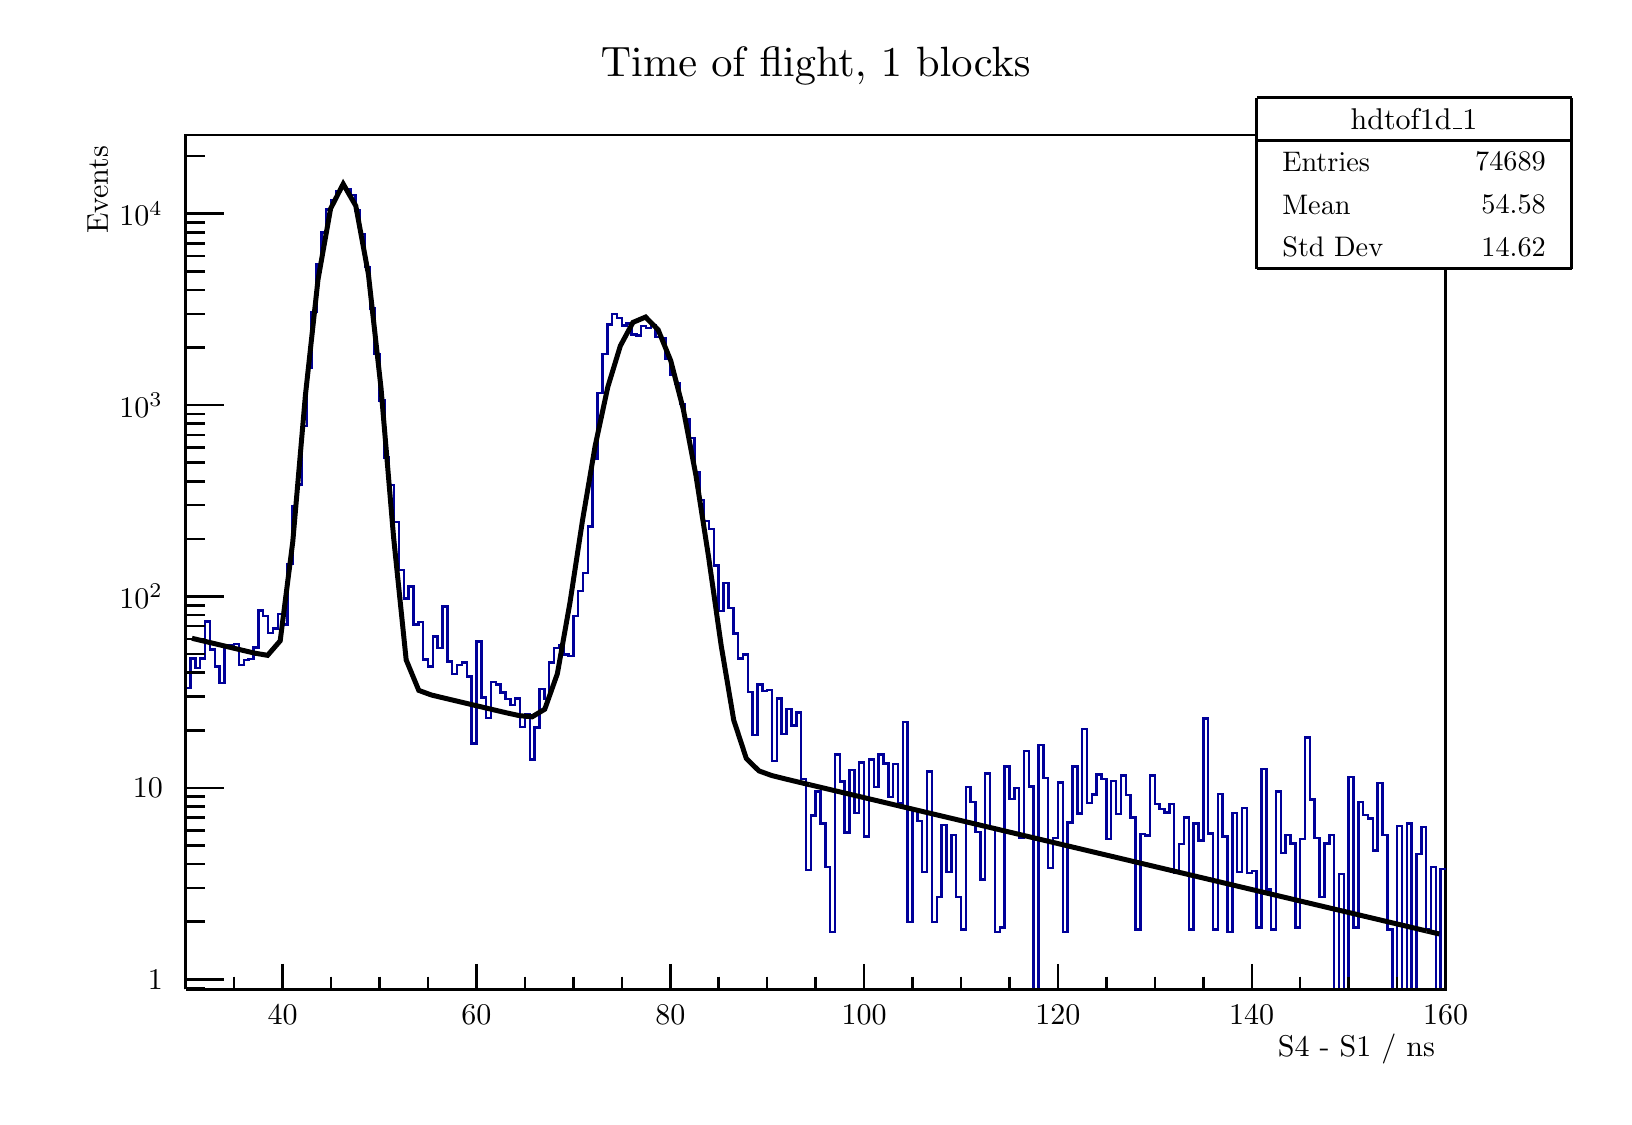
\begin{tikzpicture}
\pgfdeclareplotmark{cross} {
\pgfpathmoveto{\pgfpoint{-0.3\pgfplotmarksize}{\pgfplotmarksize}}
\pgfpathlineto{\pgfpoint{+0.3\pgfplotmarksize}{\pgfplotmarksize}}
\pgfpathlineto{\pgfpoint{+0.3\pgfplotmarksize}{0.3\pgfplotmarksize}}
\pgfpathlineto{\pgfpoint{+1\pgfplotmarksize}{0.3\pgfplotmarksize}}
\pgfpathlineto{\pgfpoint{+1\pgfplotmarksize}{-0.3\pgfplotmarksize}}
\pgfpathlineto{\pgfpoint{+0.3\pgfplotmarksize}{-0.3\pgfplotmarksize}}
\pgfpathlineto{\pgfpoint{+0.3\pgfplotmarksize}{-1.\pgfplotmarksize}}
\pgfpathlineto{\pgfpoint{-0.3\pgfplotmarksize}{-1.\pgfplotmarksize}}
\pgfpathlineto{\pgfpoint{-0.3\pgfplotmarksize}{-0.3\pgfplotmarksize}}
\pgfpathlineto{\pgfpoint{-1.\pgfplotmarksize}{-0.3\pgfplotmarksize}}
\pgfpathlineto{\pgfpoint{-1.\pgfplotmarksize}{0.3\pgfplotmarksize}}
\pgfpathlineto{\pgfpoint{-0.3\pgfplotmarksize}{0.3\pgfplotmarksize}}
\pgfpathclose
\pgfusepathqstroke
}
\pgfdeclareplotmark{cross*} {
\pgfpathmoveto{\pgfpoint{-0.3\pgfplotmarksize}{\pgfplotmarksize}}
\pgfpathlineto{\pgfpoint{+0.3\pgfplotmarksize}{\pgfplotmarksize}}
\pgfpathlineto{\pgfpoint{+0.3\pgfplotmarksize}{0.3\pgfplotmarksize}}
\pgfpathlineto{\pgfpoint{+1\pgfplotmarksize}{0.3\pgfplotmarksize}}
\pgfpathlineto{\pgfpoint{+1\pgfplotmarksize}{-0.3\pgfplotmarksize}}
\pgfpathlineto{\pgfpoint{+0.3\pgfplotmarksize}{-0.3\pgfplotmarksize}}
\pgfpathlineto{\pgfpoint{+0.3\pgfplotmarksize}{-1.\pgfplotmarksize}}
\pgfpathlineto{\pgfpoint{-0.3\pgfplotmarksize}{-1.\pgfplotmarksize}}
\pgfpathlineto{\pgfpoint{-0.3\pgfplotmarksize}{-0.3\pgfplotmarksize}}
\pgfpathlineto{\pgfpoint{-1.\pgfplotmarksize}{-0.3\pgfplotmarksize}}
\pgfpathlineto{\pgfpoint{-1.\pgfplotmarksize}{0.3\pgfplotmarksize}}
\pgfpathlineto{\pgfpoint{-0.3\pgfplotmarksize}{0.3\pgfplotmarksize}}
\pgfpathclose
\pgfusepathqfillstroke
}
\pgfdeclareplotmark{newstar} {
\pgfpathmoveto{\pgfqpoint{0pt}{\pgfplotmarksize}}
\pgfpathlineto{\pgfqpointpolar{44}{0.5\pgfplotmarksize}}
\pgfpathlineto{\pgfqpointpolar{18}{\pgfplotmarksize}}
\pgfpathlineto{\pgfqpointpolar{-20}{0.5\pgfplotmarksize}}
\pgfpathlineto{\pgfqpointpolar{-54}{\pgfplotmarksize}}
\pgfpathlineto{\pgfqpointpolar{-90}{0.5\pgfplotmarksize}}
\pgfpathlineto{\pgfqpointpolar{234}{\pgfplotmarksize}}
\pgfpathlineto{\pgfqpointpolar{198}{0.5\pgfplotmarksize}}
\pgfpathlineto{\pgfqpointpolar{162}{\pgfplotmarksize}}
\pgfpathlineto{\pgfqpointpolar{134}{0.5\pgfplotmarksize}}
\pgfpathclose
\pgfusepathqstroke
}
\pgfdeclareplotmark{newstar*} {
\pgfpathmoveto{\pgfqpoint{0pt}{\pgfplotmarksize}}
\pgfpathlineto{\pgfqpointpolar{44}{0.5\pgfplotmarksize}}
\pgfpathlineto{\pgfqpointpolar{18}{\pgfplotmarksize}}
\pgfpathlineto{\pgfqpointpolar{-20}{0.5\pgfplotmarksize}}
\pgfpathlineto{\pgfqpointpolar{-54}{\pgfplotmarksize}}
\pgfpathlineto{\pgfqpointpolar{-90}{0.5\pgfplotmarksize}}
\pgfpathlineto{\pgfqpointpolar{234}{\pgfplotmarksize}}
\pgfpathlineto{\pgfqpointpolar{198}{0.5\pgfplotmarksize}}
\pgfpathlineto{\pgfqpointpolar{162}{\pgfplotmarksize}}
\pgfpathlineto{\pgfqpointpolar{134}{0.5\pgfplotmarksize}}
\pgfpathclose
\pgfusepathqfillstroke
}
\definecolor{c}{rgb}{1,1,1};
\draw [color=c, fill=c] (0,0) rectangle (20,13.5632);
\draw [color=c, fill=c] (2,1.35632) rectangle (18,12.2069);
\definecolor{c}{rgb}{0,0,0};
\draw [c,line width=0.9] (2,1.35632) -- (2,12.2069) -- (18,12.2069) -- (18,1.35632) -- (2,1.35632);
\definecolor{c}{rgb}{1,1,1};
\draw [color=c, fill=c] (2,1.35632) rectangle (18,12.2069);
\definecolor{c}{rgb}{0,0,0};
\draw [c,line width=0.9] (2,1.35632) -- (2,12.2069) -- (18,12.2069) -- (18,1.35632) -- (2,1.35632);
\definecolor{c}{rgb}{0,0,0.6};
\draw [c,line width=0.9] (2,5.18151) -- (2.06154,5.18151) -- (2.06154,5.55608) -- (2.12308,5.55608) -- (2.12308,5.43961) -- (2.18462,5.43961) -- (2.18462,5.55581) -- (2.24615,5.55581) -- (2.24615,6.03099) -- (2.30769,6.03099) -- (2.30769,5.671) --
 (2.36923,5.671) -- (2.36923,5.45689) -- (2.43077,5.45689) -- (2.43077,5.24567) -- (2.49231,5.24567) -- (2.49231,5.73078) -- (2.55385,5.73078) -- (2.55385,5.72665) -- (2.61538,5.72665) -- (2.61538,5.74226) -- (2.67692,5.74226) -- (2.67692,5.47851) --
 (2.73846,5.47851) -- (2.73846,5.53808) -- (2.8,5.53808) -- (2.8,5.54976) -- (2.86154,5.54976) -- (2.86154,5.69856) -- (2.92308,5.69856) -- (2.92308,6.16999) -- (2.98462,6.16999) -- (2.98462,6.10032) -- (3.04615,6.10032) -- (3.04615,5.88449) --
 (3.10769,5.88449) -- (3.10769,5.93992) -- (3.16923,5.93992) -- (3.16923,6.12156) -- (3.23077,6.12156) -- (3.23077,5.99356) -- (3.29231,5.99356) -- (3.29231,6.75831) -- (3.35385,6.75831) -- (3.35385,7.49725) -- (3.41538,7.49725) -- (3.41538,7.76618)
 -- (3.47692,7.76618) -- (3.47692,8.5123) -- (3.53846,8.5123) -- (3.53846,9.25065) -- (3.6,9.25065) -- (3.6,9.95823) -- (3.66154,9.95823) -- (3.66154,10.5598) -- (3.72308,10.5598) -- (3.72308,10.9657) -- (3.78462,10.9657) -- (3.78462,11.2595) --
 (3.84615,11.2595) -- (3.84615,11.3826) -- (3.90769,11.3826) -- (3.90769,11.4937) -- (3.96923,11.4937) -- (3.96923,11.5322) -- (4.03077,11.5322) -- (4.03077,11.5125) -- (4.09231,11.5125) -- (4.09231,11.4476) -- (4.15385,11.4476) -- (4.15385,11.2503)
 -- (4.21538,11.2503) -- (4.21538,10.9505) -- (4.27692,10.9505) -- (4.27692,10.5305) -- (4.33846,10.5305) -- (4.33846,10.0019) -- (4.4,10.0019) -- (4.4,9.42602) -- (4.46154,9.42602) -- (4.46154,8.83371) -- (4.52308,8.83371) -- (4.52308,8.11005) --
 (4.58462,8.11005) -- (4.58462,7.76378) -- (4.64615,7.76378) -- (4.64615,7.29171) -- (4.70769,7.29171) -- (4.70769,6.67972) -- (4.76923,6.67972) -- (4.76923,6.32169) -- (4.83077,6.32169) -- (4.83077,6.47204) -- (4.89231,6.47204) -- (4.89231,5.993) --
 (4.95385,5.993) -- (4.95385,6.02017) -- (5.01538,6.02017) -- (5.01538,5.54748) -- (5.07692,5.54748) -- (5.07692,5.45714) -- (5.13846,5.45714) -- (5.13846,5.83864) -- (5.2,5.83864) -- (5.2,5.69096) -- (5.26154,5.69096) -- (5.26154,6.21606) --
 (5.32308,6.21606) -- (5.32308,5.51754) -- (5.38462,5.51754) -- (5.38462,5.35984) -- (5.44615,5.35984) -- (5.44615,5.47524) -- (5.50769,5.47524) -- (5.50769,5.50812) -- (5.56923,5.50812) -- (5.56923,5.32886) -- (5.63077,5.32886) -- (5.63077,4.47719)
 -- (5.69231,4.47719) -- (5.69231,5.77627) -- (5.75385,5.77627) -- (5.75385,5.06195) -- (5.81538,5.06195) -- (5.81538,4.80233) -- (5.87692,4.80233) -- (5.87692,5.25956) -- (5.93846,5.25956) -- (5.93846,5.22936) -- (6,5.22936) -- (6,5.12667) --
 (6.06154,5.12667) -- (6.06154,5.04604) -- (6.12308,5.04604) -- (6.12308,4.96718) -- (6.18462,4.96718) -- (6.18462,5.05252) -- (6.24615,5.05252) -- (6.24615,4.68623) -- (6.30769,4.68623) -- (6.30769,4.85157) -- (6.36923,4.85157) -- (6.36923,4.2741)
 -- (6.43077,4.2741) -- (6.43077,4.68523) -- (6.49231,4.68523) -- (6.49231,5.16964) -- (6.55385,5.16964) -- (6.55385,5.0443) -- (6.61538,5.0443) -- (6.61538,5.50863) -- (6.67692,5.50863) -- (6.67692,5.68975) -- (6.73846,5.68975) -- (6.73846,5.72166)
 -- (6.8,5.72166) -- (6.8,5.60763) -- (6.86154,5.60763) -- (6.86154,5.58722) -- (6.92308,5.58722) -- (6.92308,6.09935) -- (6.98462,6.09935) -- (6.98462,6.41753) -- (7.04615,6.41753) -- (7.04615,6.64659) -- (7.10769,6.64659) -- (7.10769,7.2355) --
 (7.16923,7.2355) -- (7.16923,8.09892) -- (7.23077,8.09892) -- (7.23077,8.93136) -- (7.29231,8.93136) -- (7.29231,9.42351) -- (7.35385,9.42351) -- (7.35385,9.79794) -- (7.41538,9.79794) -- (7.41538,9.93183) -- (7.47692,9.93183) -- (7.47692,9.8799) --
 (7.53846,9.8799) -- (7.53846,9.78722) -- (7.6,9.78722) -- (7.6,9.81608) -- (7.66154,9.81608) -- (7.66154,9.67331) -- (7.72308,9.67331) -- (7.72308,9.65902) -- (7.78462,9.65902) -- (7.78462,9.77948) -- (7.84615,9.77948) -- (7.84615,9.75876) --
 (7.90769,9.75876) -- (7.90769,9.79026) -- (7.96923,9.79026) -- (7.96923,9.64053) -- (8.03077,9.64053) -- (8.03077,9.63187) -- (8.09231,9.63187) -- (8.09231,9.36831) -- (8.15385,9.36831) -- (8.15385,9.16368) -- (8.21538,9.16368) -- (8.21538,9.05403)
 -- (8.27692,9.05403) -- (8.27692,8.78876) -- (8.33846,8.78876) -- (8.33846,8.603) -- (8.4,8.603) -- (8.4,8.35968) -- (8.46154,8.35968) -- (8.46154,7.91883) -- (8.52308,7.91883) -- (8.52308,7.56846) -- (8.58462,7.56846) -- (8.58462,7.30407) --
 (8.64615,7.30407) -- (8.64615,7.20532) -- (8.70769,7.20532) -- (8.70769,6.74177) -- (8.76923,6.74177) -- (8.76923,6.16352) -- (8.83077,6.16352) -- (8.83077,6.51821) -- (8.89231,6.51821) -- (8.89231,6.20221) -- (8.95385,6.20221) -- (8.95385,5.87638)
 -- (9.01538,5.87638) -- (9.01538,5.55625) -- (9.07692,5.55625) -- (9.07692,5.61066) -- (9.13846,5.61066) -- (9.13846,5.13328) -- (9.2,5.13328) -- (9.2,4.58783) -- (9.26154,4.58783) -- (9.26154,5.23012) -- (9.32308,5.23012) -- (9.32308,5.146) --
 (9.38461,5.146) -- (9.38461,5.15776) -- (9.44615,5.15776) -- (9.44615,4.25767) -- (9.50769,4.25767) -- (9.50769,5.04774) -- (9.56923,5.04774) -- (9.56923,4.60175) -- (9.63077,4.60175) -- (9.63077,4.92009) -- (9.69231,4.92009) -- (9.69231,4.71042) --
 (9.75385,4.71042) -- (9.75385,4.87061) -- (9.81538,4.87061) -- (9.81538,4.02592) -- (9.87692,4.02592) -- (9.87692,2.87449) -- (9.93846,2.87449) -- (9.93846,3.56693) -- (10,3.56693) -- (10,3.87246) -- (10.0615,3.87246) -- (10.0615,3.4613) --
 (10.1231,3.4613) -- (10.1231,2.90853) -- (10.1846,2.90853) -- (10.1846,2.08809) -- (10.2462,2.08809) -- (10.2462,4.33668) -- (10.3077,4.33668) -- (10.3077,3.99697) -- (10.3692,3.99697) -- (10.3692,3.3477) -- (10.4308,3.3477) -- (10.4308,4.13973) --
 (10.4923,4.13973) -- (10.4923,3.59781) -- (10.5538,3.59781) -- (10.5538,4.23774) -- (10.6154,4.23774) -- (10.6154,3.29987) -- (10.6769,3.29987) -- (10.6769,4.27622) -- (10.7385,4.27622) -- (10.7385,3.92545) -- (10.8,3.92545) -- (10.8,4.34213) --
 (10.8615,4.34213) -- (10.8615,4.22691) -- (10.9231,4.22691) -- (10.9231,3.79686) -- (10.9846,3.79686) -- (10.9846,4.22057) -- (11.0462,4.22057) -- (11.0462,3.71905) -- (11.1077,3.71905) -- (11.1077,4.75094) -- (11.1692,4.75094) -- (11.1692,2.20974)
 -- (11.2308,2.20974) -- (11.2308,3.65017) -- (11.2923,3.65017) -- (11.2923,3.492) -- (11.3538,3.492) -- (11.3538,2.84753) -- (11.4154,2.84753) -- (11.4154,4.12337) -- (11.4769,4.12337) -- (11.4769,2.20974) -- (11.5385,2.20974) -- (11.5385,2.53059)
 -- (11.6,2.53059) -- (11.6,3.44296) -- (11.6615,3.44296) -- (11.6615,2.84753) -- (11.7231,2.84753) -- (11.7231,3.31942) -- (11.7846,3.31942) -- (11.7846,2.53059) -- (11.8462,2.53059) -- (11.8462,2.11846) -- (11.9077,2.11846) -- (11.9077,3.92545) --
 (11.9692,3.92545) -- (11.9692,3.73625) -- (12.0308,3.73625) -- (12.0308,3.35377) -- (12.0923,3.35377) -- (12.0923,2.74928) -- (12.1538,2.74928) -- (12.1538,4.09554) -- (12.2154,4.09554) -- (12.2154,3.41687) -- (12.2769,3.41687) -- (12.2769,2.08809)
 -- (12.3385,2.08809) -- (12.3385,2.14272) -- (12.4,2.14272) -- (12.4,4.18641) -- (12.4615,4.18641) -- (12.4615,3.77723) -- (12.5231,3.77723) -- (12.5231,3.91398) -- (12.5846,3.91398) -- (12.5846,3.27829) -- (12.6462,3.27829) -- (12.6462,4.38363) --
 (12.7077,4.38363) -- (12.7077,3.93124) -- (12.7692,3.93124) -- (12.7692,1.35632) -- (12.8308,1.35632) -- (12.8308,4.45728) -- (12.8923,4.45728) -- (12.8923,4.04146) -- (12.9538,4.04146) -- (12.9538,2.89686) -- (13.0154,2.89686) -- (13.0154,3.27649)
 -- (13.0769,3.27649) -- (13.0769,3.98168) -- (13.1385,3.98168) -- (13.1385,2.08809) -- (13.2,2.08809) -- (13.2,3.47404) -- (13.2615,3.47404) -- (13.2615,4.18641) -- (13.3231,4.18641) -- (13.3231,3.58812) -- (13.3846,3.58812) -- (13.3846,4.66074) --
 (13.4462,4.66074) -- (13.4462,3.72096) -- (13.5077,3.72096) -- (13.5077,3.83058) -- (13.5692,3.83058) -- (13.5692,4.08766) -- (13.6308,4.08766) -- (13.6308,4.03023) -- (13.6923,4.03023) -- (13.6923,3.26645) -- (13.7538,3.26645) -- (13.7538,4.00415)
 -- (13.8154,4.00415) -- (13.8154,3.58678) -- (13.8769,3.58678) -- (13.8769,4.07563) -- (13.9385,4.07563) -- (13.9385,3.82377) -- (14,3.82377) -- (14,3.53914) -- (14.0615,3.53914) -- (14.0615,2.11846) -- (14.1231,2.11846) -- (14.1231,3.33056) --
 (14.1846,3.33056) -- (14.1846,3.3096) -- (14.2462,3.3096) -- (14.2462,4.07579) -- (14.3077,4.07579) -- (14.3077,3.70785) -- (14.3692,3.70785) -- (14.3692,3.64917) -- (14.4308,3.64917) -- (14.4308,3.60516) -- (14.4923,3.60516) -- (14.4923,3.70785) --
 (14.5538,3.70785) -- (14.5538,2.83516) -- (14.6154,2.83516) -- (14.6154,3.20139) -- (14.6769,3.20139) -- (14.6769,3.53914) -- (14.7385,3.53914) -- (14.7385,2.11846) -- (14.8,2.11846) -- (14.8,3.46572) -- (14.8615,3.46572) -- (14.8615,3.24538) --
 (14.9231,3.24538) -- (14.9231,4.79484) -- (14.9846,4.79484) -- (14.9846,3.33729) -- (15.0462,3.33729) -- (15.0462,2.11846) -- (15.1077,2.11846) -- (15.1077,3.83614) -- (15.1692,3.83614) -- (15.1692,3.29647) -- (15.2308,3.29647) -- (15.2308,2.08809)
 -- (15.2923,2.08809) -- (15.2923,3.59713) -- (15.3538,3.59713) -- (15.3538,2.85023) -- (15.4154,2.85023) -- (15.4154,3.66286) -- (15.4769,3.66286) -- (15.4769,2.83516) -- (15.5385,2.83516) -- (15.5385,2.86243) -- (15.6,2.86243) -- (15.6,2.14272) --
 (15.6615,2.14272) -- (15.6615,4.15383) -- (15.7231,4.15383) -- (15.7231,2.62199) -- (15.7846,2.62199) -- (15.7846,2.11846) -- (15.8462,2.11846) -- (15.8462,3.87165) -- (15.9077,3.87165) -- (15.9077,3.08614) -- (15.9692,3.08614) -- (15.9692,3.31751)
 -- (16.0308,3.31751) -- (16.0308,3.21207) -- (16.0923,3.21207) -- (16.0923,2.14272) -- (16.1538,2.14272) -- (16.1538,3.26826) -- (16.2154,3.26826) -- (16.2154,4.55325) -- (16.2769,4.55325) -- (16.2769,3.77087) -- (16.3385,3.77087) --
 (16.3385,3.27829) -- (16.4,3.27829) -- (16.4,2.53059) -- (16.4615,2.53059) -- (16.4615,3.21207) -- (16.5231,3.21207) -- (16.5231,3.31751) -- (16.5846,3.31751) -- (16.5846,1.35632) -- (16.6462,1.35632) -- (16.6462,2.81986) -- (16.7077,2.81986) --
 (16.7077,1.35632) -- (16.7692,1.35632) -- (16.7692,4.05445) -- (16.8308,4.05445) -- (16.8308,2.14272) -- (16.8923,2.14272) -- (16.8923,3.7376) -- (16.9538,3.7376) -- (16.9538,3.57313) -- (17.0154,3.57313) -- (17.0154,3.52486) -- (17.0769,3.52486) --
 (17.0769,3.12021) -- (17.1385,3.12021) -- (17.1385,3.98035) -- (17.2,3.98035) -- (17.2,3.31751) -- (17.2615,3.31751) -- (17.2615,2.11846) -- (17.3231,2.11846) -- (17.3231,1.35632) -- (17.3846,1.35632) -- (17.3846,3.43423) -- (17.4462,3.43423) --
 (17.4462,1.35632) -- (17.5077,1.35632) -- (17.5077,3.4613) -- (17.5692,3.4613) -- (17.5692,1.35632) -- (17.6308,1.35632) -- (17.6308,3.07628) -- (17.6923,3.07628) -- (17.6923,3.41932) -- (17.7538,3.41932) -- (17.7538,2.11846) -- (17.8154,2.11846) --
 (17.8154,2.90853) -- (17.8769,2.90853) -- (17.8769,1.35632) -- (17.9385,1.35632) -- (17.9385,2.88244) -- (18,2.88244);
\definecolor{c}{rgb}{0,0,0};
\draw [c,line width=0.9] (2,1.35632) -- (18,1.35632);
\draw [anchor= east] (18,0.596782) node[scale=1.08496, color=c, rotate=0]{ S4 - S1 / ns};
\draw [c,line width=0.9] (3.23077,1.68184) -- (3.23077,1.35632);
\draw [c,line width=0.9] (3.84615,1.51908) -- (3.84615,1.35632);
\draw [c,line width=0.9] (4.46154,1.51908) -- (4.46154,1.35632);
\draw [c,line width=0.9] (5.07692,1.51908) -- (5.07692,1.35632);
\draw [c,line width=0.9] (5.69231,1.68184) -- (5.69231,1.35632);
\draw [c,line width=0.9] (6.30769,1.51908) -- (6.30769,1.35632);
\draw [c,line width=0.9] (6.92308,1.51908) -- (6.92308,1.35632);
\draw [c,line width=0.9] (7.53846,1.51908) -- (7.53846,1.35632);
\draw [c,line width=0.9] (8.15385,1.68184) -- (8.15385,1.35632);
\draw [c,line width=0.9] (8.76923,1.51908) -- (8.76923,1.35632);
\draw [c,line width=0.9] (9.38461,1.51908) -- (9.38461,1.35632);
\draw [c,line width=0.9] (10,1.51908) -- (10,1.35632);
\draw [c,line width=0.9] (10.6154,1.68184) -- (10.6154,1.35632);
\draw [c,line width=0.9] (11.2308,1.51908) -- (11.2308,1.35632);
\draw [c,line width=0.9] (11.8462,1.51908) -- (11.8462,1.35632);
\draw [c,line width=0.9] (12.4615,1.51908) -- (12.4615,1.35632);
\draw [c,line width=0.9] (13.0769,1.68184) -- (13.0769,1.35632);
\draw [c,line width=0.9] (13.6923,1.51908) -- (13.6923,1.35632);
\draw [c,line width=0.9] (14.3077,1.51908) -- (14.3077,1.35632);
\draw [c,line width=0.9] (14.9231,1.51908) -- (14.9231,1.35632);
\draw [c,line width=0.9] (15.5385,1.68184) -- (15.5385,1.35632);
\draw [c,line width=0.9] (16.1538,1.51908) -- (16.1538,1.35632);
\draw [c,line width=0.9] (16.7692,1.51908) -- (16.7692,1.35632);
\draw [c,line width=0.9] (17.3846,1.51908) -- (17.3846,1.35632);
\draw [c,line width=0.9] (18,1.68184) -- (18,1.35632);
\draw [c,line width=0.9] (3.23077,1.68184) -- (3.23077,1.35632);
\draw [c,line width=0.9] (2.61538,1.51908) -- (2.61538,1.35632);
\draw [c,line width=0.9] (2,1.51908) -- (2,1.35632);
\draw [anchor=base] (3.23077,0.908736) node[scale=1.08496, color=c, rotate=0]{40};
\draw [anchor=base] (5.69231,0.908736) node[scale=1.08496, color=c, rotate=0]{60};
\draw [anchor=base] (8.15385,0.908736) node[scale=1.08496, color=c, rotate=0]{80};
\draw [anchor=base] (10.6154,0.908736) node[scale=1.08496, color=c, rotate=0]{100};
\draw [anchor=base] (13.0769,0.908736) node[scale=1.08496, color=c, rotate=0]{120};
\draw [anchor=base] (15.5385,0.908736) node[scale=1.08496, color=c, rotate=0]{140};
\draw [anchor=base] (18,0.908736) node[scale=1.08496, color=c, rotate=0]{160};
\draw [c,line width=0.9] (2,1.35632) -- (2,12.2069);
\draw [anchor= east] (0.88,12.2069) node[scale=1.08496, color=c, rotate=90]{ Events};
\draw [c,line width=0.9] (2.24,1.37274) -- (2,1.37274);
\draw [c,line width=0.9] (2.48,1.48397) -- (2,1.48397);
\draw [anchor= east] (1.844,1.48397) node[scale=1.08496, color=c, rotate=0]{1};
\draw [c,line width=0.9] (2.24,2.21574) -- (2,2.21574);
\draw [c,line width=0.9] (2.24,2.6438) -- (2,2.6438);
\draw [c,line width=0.9] (2.24,2.94751) -- (2,2.94751);
\draw [c,line width=0.9] (2.24,3.18309) -- (2,3.18309);
\draw [c,line width=0.9] (2.24,3.37557) -- (2,3.37557);
\draw [c,line width=0.9] (2.24,3.53831) -- (2,3.53831);
\draw [c,line width=0.9] (2.24,3.67928) -- (2,3.67928);
\draw [c,line width=0.9] (2.24,3.80363) -- (2,3.80363);
\draw [c,line width=0.9] (2.48,3.91486) -- (2,3.91486);
\draw [anchor= east] (1.844,3.91486) node[scale=1.08496, color=c, rotate=0]{10};
\draw [c,line width=0.9] (2.24,4.64663) -- (2,4.64663);
\draw [c,line width=0.9] (2.24,5.07469) -- (2,5.07469);
\draw [c,line width=0.9] (2.24,5.3784) -- (2,5.3784);
\draw [c,line width=0.9] (2.24,5.61398) -- (2,5.61398);
\draw [c,line width=0.9] (2.24,5.80646) -- (2,5.80646);
\draw [c,line width=0.9] (2.24,5.9692) -- (2,5.9692);
\draw [c,line width=0.9] (2.24,6.11017) -- (2,6.11017);
\draw [c,line width=0.9] (2.24,6.23452) -- (2,6.23452);
\draw [c,line width=0.9] (2.48,6.34575) -- (2,6.34575);
\draw [anchor= east] (1.844,6.34575) node[scale=1.08496, color=c, rotate=0]{$10^{2}$};
\draw [c,line width=0.9] (2.24,7.07752) -- (2,7.07752);
\draw [c,line width=0.9] (2.24,7.50558) -- (2,7.50558);
\draw [c,line width=0.9] (2.24,7.80929) -- (2,7.80929);
\draw [c,line width=0.9] (2.24,8.04487) -- (2,8.04487);
\draw [c,line width=0.9] (2.24,8.23735) -- (2,8.23735);
\draw [c,line width=0.9] (2.24,8.40009) -- (2,8.40009);
\draw [c,line width=0.9] (2.24,8.54106) -- (2,8.54106);
\draw [c,line width=0.9] (2.24,8.66541) -- (2,8.66541);
\draw [c,line width=0.9] (2.48,8.77664) -- (2,8.77664);
\draw [anchor= east] (1.844,8.77664) node[scale=1.08496, color=c, rotate=0]{$10^{3}$};
\draw [c,line width=0.9] (2.24,9.50841) -- (2,9.50841);
\draw [c,line width=0.9] (2.24,9.93647) -- (2,9.93647);
\draw [c,line width=0.9] (2.24,10.2402) -- (2,10.2402);
\draw [c,line width=0.9] (2.24,10.4758) -- (2,10.4758);
\draw [c,line width=0.9] (2.24,10.6682) -- (2,10.6682);
\draw [c,line width=0.9] (2.24,10.831) -- (2,10.831);
\draw [c,line width=0.9] (2.24,10.9719) -- (2,10.9719);
\draw [c,line width=0.9] (2.24,11.0963) -- (2,11.0963);
\draw [c,line width=0.9] (2.48,11.2075) -- (2,11.2075);
\draw [anchor= east] (1.844,11.2075) node[scale=1.08496, color=c, rotate=0]{$10^{4}$};
\draw [c,line width=0.9] (2.24,11.9393) -- (2,11.9393);
\definecolor{c}{rgb}{1,1,1};
\draw [color=c, fill=c] (15.6,10.5115) rectangle (19.6,12.6816);
\definecolor{c}{rgb}{0,0,0};
\draw [c,line width=0.9] (15.6,10.5115) -- (19.6,10.5115);
\draw [c,line width=0.9] (19.6,10.5115) -- (19.6,12.6816);
\draw [c,line width=0.9] (19.6,12.6816) -- (15.6,12.6816);
\draw [c,line width=0.9] (15.6,12.6816) -- (15.6,10.5115);
\draw (17.6,12.4103) node[scale=1.08496, color=c, rotate=0]{hdtof1d\_1};
\draw [c,line width=0.9] (15.6,12.1391) -- (19.6,12.1391);
\draw [anchor= west] (15.8,11.8678) node[scale=1.02114, color=c, rotate=0]{Entries };
\draw [anchor= east] (19.4,11.8678) node[scale=1.02114, color=c, rotate=0]{ 74689};
\draw [anchor= west] (15.8,11.3253) node[scale=1.02114, color=c, rotate=0]{Mean  };
\draw [anchor= east] (19.4,11.3253) node[scale=1.02114, color=c, rotate=0]{  54.58};
\draw [anchor= west] (15.8,10.7828) node[scale=1.02114, color=c, rotate=0]{Std Dev   };
\draw [anchor= east] (19.4,10.7828) node[scale=1.02114, color=c, rotate=0]{  14.62};
\draw [c,line width=1.8] (2.08,5.81522) -- (2.24,5.77729) -- (2.4,5.73936) -- (2.56,5.70143) -- (2.72,5.6635) -- (2.88,5.62584) -- (3.04,5.59883) -- (3.2,5.783) -- (3.36,7.04462) -- (3.52,8.89992) -- (3.68,10.3694) -- (3.84,11.2716) -- (4,11.5852) --
 (4.16,11.3072) -- (4.32,10.4394) -- (4.48,8.9965) -- (4.64,7.0994) -- (4.8,5.54055) -- (4.96,5.1535) -- (5.12,5.09513) -- (5.28,5.05662) -- (5.44,5.01869) -- (5.6,4.98076) -- (5.76,4.94283) -- (5.92,4.90492) -- (6.08,4.86731) -- (6.24,4.83246) --
 (6.4,4.81808) -- (6.56,4.91497) -- (6.72,5.3653) -- (6.88,6.26787) -- (7.04,7.31709) -- (7.2,8.25867) -- (7.36,9.00435) -- (7.52,9.52953) -- (7.68,9.82711) -- (7.84,9.89492) -- (8,9.73249) -- (8.16,9.34039) -- (8.32,8.721) -- (8.48,7.88215) --
 (8.64,6.85117) -- (8.8,5.72561) -- (8.96,4.77556) -- (9.12,4.2879) -- (9.28,4.13137) -- (9.44,4.0733) -- (9.6,4.03279) -- (9.76,3.9946) -- (9.92,3.95665);
\draw [c,line width=1.8] (9.92,3.95665) -- (10.08,3.91871) -- (10.24,3.88078) -- (10.4,3.84285) -- (10.56,3.80492) -- (10.72,3.76699) -- (10.88,3.72906) -- (11.04,3.69113) -- (11.2,3.6532) -- (11.36,3.61527) -- (11.52,3.57734) -- (11.68,3.53941) --
 (11.84,3.50148) -- (12,3.46355) -- (12.16,3.42562) -- (12.32,3.38769) -- (12.48,3.34976) -- (12.64,3.31183) -- (12.8,3.2739) -- (12.96,3.23597) -- (13.12,3.19804) -- (13.28,3.16011) -- (13.44,3.12218) -- (13.6,3.08425) -- (13.76,3.04632) --
 (13.92,3.00839) -- (14.08,2.97046) -- (14.24,2.93253) -- (14.4,2.8946) -- (14.56,2.85667) -- (14.72,2.81874) -- (14.88,2.78081) -- (15.04,2.74288) -- (15.2,2.70495) -- (15.36,2.66702) -- (15.52,2.62909) -- (15.68,2.59116) -- (15.84,2.55323) --
 (16,2.5153) -- (16.16,2.47737) -- (16.32,2.43944) -- (16.48,2.40151) -- (16.64,2.36358) -- (16.8,2.32565) -- (16.96,2.28772) -- (17.12,2.24979) -- (17.28,2.21186) -- (17.44,2.17393) -- (17.6,2.136) -- (17.76,2.09807);
\draw [c,line width=1.8] (17.76,2.09807) -- (17.92,2.06014);
\draw (10,13.0816) node[scale=1.5317, color=c, rotate=0]{Time of flight, 1 blocks};
\end{tikzpicture}

  \end{adjustbox}
  \caption{Example of the time of flight spectrum observed in $\mathit{S4}$ with a combined signal and background function fitted (shown in black)}
  \label{fig:fitEx}
\end{figure}

To produce the data used in this analysis, an exponential background function is subtracted. 
The parameters for this function are taken from the combined signal and background function.




% HPTPC description
\section{Beam Flux Measurement}
\label{hptpcPaper:sec:Results}

\subsection{Flux measurements -- $\mathit{S3}$}

\begin{figure}[h]
  \begin{minipage}{0.48\textwidth}
    \begin{adjustbox}{max totalsize={\textwidth}{.35\textheight},center}
      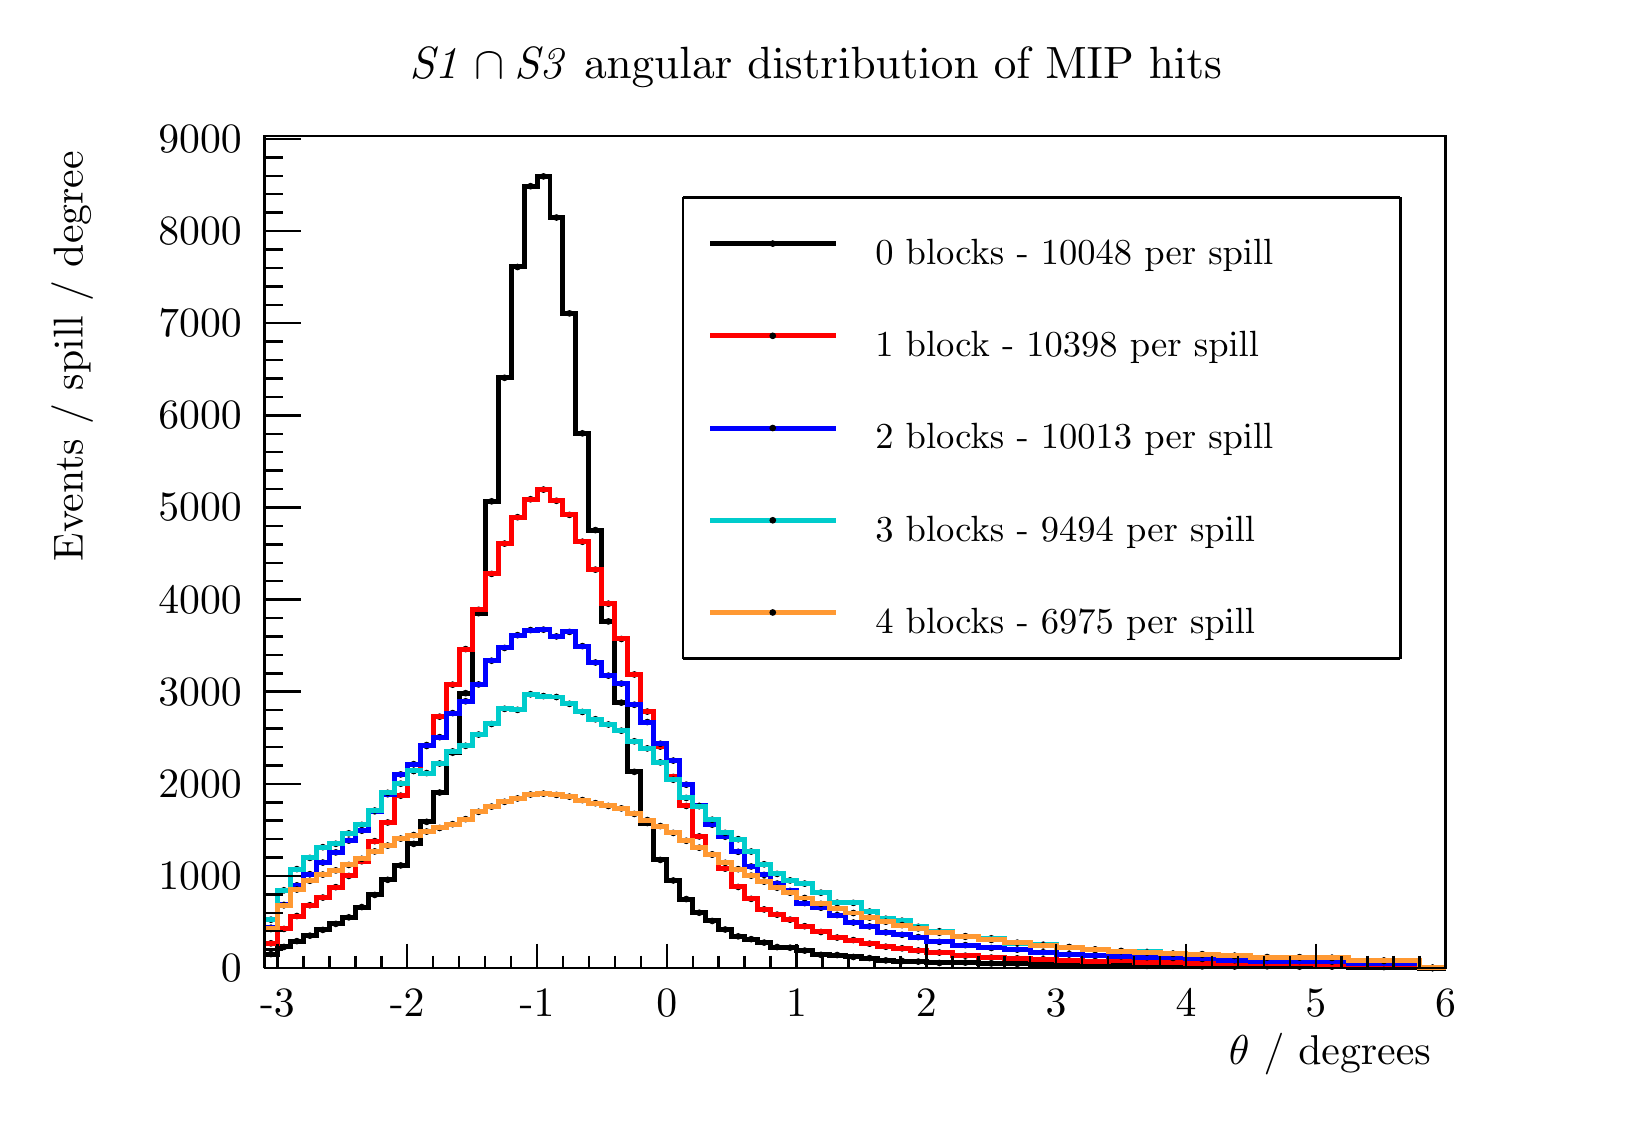
\begin{tikzpicture}
\pgfdeclareplotmark{cross} {
\pgfpathmoveto{\pgfpoint{-0.3\pgfplotmarksize}{\pgfplotmarksize}}
\pgfpathlineto{\pgfpoint{+0.3\pgfplotmarksize}{\pgfplotmarksize}}
\pgfpathlineto{\pgfpoint{+0.3\pgfplotmarksize}{0.3\pgfplotmarksize}}
\pgfpathlineto{\pgfpoint{+1\pgfplotmarksize}{0.3\pgfplotmarksize}}
\pgfpathlineto{\pgfpoint{+1\pgfplotmarksize}{-0.3\pgfplotmarksize}}
\pgfpathlineto{\pgfpoint{+0.3\pgfplotmarksize}{-0.3\pgfplotmarksize}}
\pgfpathlineto{\pgfpoint{+0.3\pgfplotmarksize}{-1.\pgfplotmarksize}}
\pgfpathlineto{\pgfpoint{-0.3\pgfplotmarksize}{-1.\pgfplotmarksize}}
\pgfpathlineto{\pgfpoint{-0.3\pgfplotmarksize}{-0.3\pgfplotmarksize}}
\pgfpathlineto{\pgfpoint{-1.\pgfplotmarksize}{-0.3\pgfplotmarksize}}
\pgfpathlineto{\pgfpoint{-1.\pgfplotmarksize}{0.3\pgfplotmarksize}}
\pgfpathlineto{\pgfpoint{-0.3\pgfplotmarksize}{0.3\pgfplotmarksize}}
\pgfpathclose
\pgfusepathqstroke
}
\pgfdeclareplotmark{cross*} {
\pgfpathmoveto{\pgfpoint{-0.3\pgfplotmarksize}{\pgfplotmarksize}}
\pgfpathlineto{\pgfpoint{+0.3\pgfplotmarksize}{\pgfplotmarksize}}
\pgfpathlineto{\pgfpoint{+0.3\pgfplotmarksize}{0.3\pgfplotmarksize}}
\pgfpathlineto{\pgfpoint{+1\pgfplotmarksize}{0.3\pgfplotmarksize}}
\pgfpathlineto{\pgfpoint{+1\pgfplotmarksize}{-0.3\pgfplotmarksize}}
\pgfpathlineto{\pgfpoint{+0.3\pgfplotmarksize}{-0.3\pgfplotmarksize}}
\pgfpathlineto{\pgfpoint{+0.3\pgfplotmarksize}{-1.\pgfplotmarksize}}
\pgfpathlineto{\pgfpoint{-0.3\pgfplotmarksize}{-1.\pgfplotmarksize}}
\pgfpathlineto{\pgfpoint{-0.3\pgfplotmarksize}{-0.3\pgfplotmarksize}}
\pgfpathlineto{\pgfpoint{-1.\pgfplotmarksize}{-0.3\pgfplotmarksize}}
\pgfpathlineto{\pgfpoint{-1.\pgfplotmarksize}{0.3\pgfplotmarksize}}
\pgfpathlineto{\pgfpoint{-0.3\pgfplotmarksize}{0.3\pgfplotmarksize}}
\pgfpathclose
\pgfusepathqfillstroke
}
\pgfdeclareplotmark{newstar} {
\pgfpathmoveto{\pgfqpoint{0pt}{\pgfplotmarksize}}
\pgfpathlineto{\pgfqpointpolar{44}{0.5\pgfplotmarksize}}
\pgfpathlineto{\pgfqpointpolar{18}{\pgfplotmarksize}}
\pgfpathlineto{\pgfqpointpolar{-20}{0.5\pgfplotmarksize}}
\pgfpathlineto{\pgfqpointpolar{-54}{\pgfplotmarksize}}
\pgfpathlineto{\pgfqpointpolar{-90}{0.5\pgfplotmarksize}}
\pgfpathlineto{\pgfqpointpolar{234}{\pgfplotmarksize}}
\pgfpathlineto{\pgfqpointpolar{198}{0.5\pgfplotmarksize}}
\pgfpathlineto{\pgfqpointpolar{162}{\pgfplotmarksize}}
\pgfpathlineto{\pgfqpointpolar{134}{0.5\pgfplotmarksize}}
\pgfpathclose
\pgfusepathqstroke
}
\pgfdeclareplotmark{newstar*} {
\pgfpathmoveto{\pgfqpoint{0pt}{\pgfplotmarksize}}
\pgfpathlineto{\pgfqpointpolar{44}{0.5\pgfplotmarksize}}
\pgfpathlineto{\pgfqpointpolar{18}{\pgfplotmarksize}}
\pgfpathlineto{\pgfqpointpolar{-20}{0.5\pgfplotmarksize}}
\pgfpathlineto{\pgfqpointpolar{-54}{\pgfplotmarksize}}
\pgfpathlineto{\pgfqpointpolar{-90}{0.5\pgfplotmarksize}}
\pgfpathlineto{\pgfqpointpolar{234}{\pgfplotmarksize}}
\pgfpathlineto{\pgfqpointpolar{198}{0.5\pgfplotmarksize}}
\pgfpathlineto{\pgfqpointpolar{162}{\pgfplotmarksize}}
\pgfpathlineto{\pgfqpointpolar{134}{0.5\pgfplotmarksize}}
\pgfpathclose
\pgfusepathqfillstroke
}
\definecolor{c}{rgb}{1,1,1};
\draw [color=c, fill=c] (0,0) rectangle (20,13.7199);
\draw [color=c, fill=c] (3,1.78359) rectangle (18,12.3479);
\definecolor{c}{rgb}{0,0,0};
\draw [c,line width=0.9] (3,1.78359) -- (3,12.3479) -- (18,12.3479) -- (18,1.78359) -- (3,1.78359);
\definecolor{c}{rgb}{1,1,1};
\draw [color=c, fill=c] (3,1.78359) rectangle (18,12.3479);
\definecolor{c}{rgb}{0,0,0};
\draw [c,line width=0.9] (3,1.78359) -- (3,12.3479) -- (18,12.3479) -- (18,1.78359) -- (3,1.78359);
\definecolor{c}{rgb}{0,0,0.6};
\draw [c,line width=0.9] (3,1.78359) -- (3.16484,1.78359) -- (3.16484,1.78359) -- (3.32967,1.78359) -- (3.32967,1.78359) -- (3.49451,1.78359) -- (3.49451,1.78359) -- (3.65934,1.78359) -- (3.65934,1.78359) -- (3.82418,1.78359) -- (3.82418,1.78359) --
 (3.98901,1.78359) -- (3.98901,1.78359) -- (4.15385,1.78359) -- (4.15385,1.78359) -- (4.31868,1.78359) -- (4.31868,1.78359) -- (4.48352,1.78359) -- (4.48352,1.78359) -- (4.64835,1.78359) -- (4.64835,1.78359) -- (4.81319,1.78359) -- (4.81319,1.78359)
 -- (4.97802,1.78359) -- (4.97802,1.78359) -- (5.14286,1.78359) -- (5.14286,1.78359) -- (5.30769,1.78359) -- (5.30769,1.78359) -- (5.47253,1.78359) -- (5.47253,1.78359) -- (5.63736,1.78359) -- (5.63736,1.78359) -- (5.8022,1.78359) -- (5.8022,1.78359)
 -- (5.96703,1.78359) -- (5.96703,1.78359) -- (6.13187,1.78359) -- (6.13187,1.78359) -- (6.2967,1.78359) -- (6.2967,1.78359) -- (6.46154,1.78359) -- (6.46154,1.78359) -- (6.62637,1.78359) -- (6.62637,1.78359) -- (6.79121,1.78359) -- (6.79121,1.78359)
 -- (6.95604,1.78359) -- (6.95604,1.78359) -- (7.12088,1.78359) -- (7.12088,1.78359) -- (7.28571,1.78359) -- (7.28571,1.78359) -- (7.45055,1.78359) -- (7.45055,1.78359) -- (7.61538,1.78359) -- (7.61538,1.78359) -- (7.78022,1.78359) --
 (7.78022,1.78359) -- (7.94506,1.78359) -- (7.94506,1.78359) -- (8.10989,1.78359) -- (8.10989,1.78359) -- (8.27472,1.78359) -- (8.27472,1.78359) -- (8.43956,1.78359) -- (8.43956,1.78359) -- (8.6044,1.78359) -- (8.6044,1.78359) -- (8.76923,1.78359) --
 (8.76923,1.78359) -- (8.93407,1.78359) -- (8.93407,1.78359) -- (9.0989,1.78359) -- (9.0989,1.78359) -- (9.26374,1.78359) -- (9.26374,1.78359) -- (9.42857,1.78359) -- (9.42857,1.78359) -- (9.59341,1.78359) -- (9.59341,1.78359) -- (9.75824,1.78359) --
 (9.75824,1.78359) -- (9.96429,1.78359) -- (9.96429,1.78359) -- (10.1703,1.78359) -- (10.1703,1.78359) -- (10.3764,1.78359) -- (10.3764,1.78359) -- (10.5824,1.78359) -- (10.5824,1.78359) -- (10.7885,1.78359) -- (10.7885,1.78359) -- (10.9945,1.78359)
 -- (10.9945,1.78359) -- (11.2005,1.78359) -- (11.2005,1.78359) -- (11.4066,1.78359) -- (11.4066,1.78359) -- (11.7363,1.78359) -- (11.7363,1.78359) -- (12.0659,1.78359) -- (12.0659,1.78359) -- (12.3956,1.78359) -- (12.3956,1.78359) --
 (12.7253,1.78359) -- (12.7253,1.78359) -- (13.0549,1.78359) -- (13.0549,1.78359) -- (13.3846,1.78359) -- (13.3846,1.78359) -- (13.7143,1.78359) -- (13.7143,1.78359) -- (14.044,1.78359) -- (14.044,1.78359) -- (14.3736,1.78359) -- (14.3736,1.78359) --
 (14.7033,1.78359) -- (14.7033,1.78359) -- (15.1154,1.78359) -- (15.1154,1.78359) -- (15.5275,1.78359) -- (15.5275,1.78359) -- (15.9396,1.78359) -- (15.9396,1.78359) -- (16.3516,1.78359) -- (16.3516,1.78359) -- (16.7637,1.78359) -- (16.7637,1.78359)
 -- (17.6703,1.78359) -- (17.6703,1.78359) -- (18,1.78359);
\definecolor{c}{rgb}{0,0,0};
\draw [c,line width=0.9] (3,1.78359) -- (18,1.78359);
\draw [c,line width=0.9] (3.16484,2.09229) -- (3.16484,1.78359);
\draw [c,line width=0.9] (3.49451,1.93794) -- (3.49451,1.78359);
\draw [c,line width=0.9] (3.82418,1.93794) -- (3.82418,1.78359);
\draw [c,line width=0.9] (4.15385,1.93794) -- (4.15385,1.78359);
\draw [c,line width=0.9] (4.48352,1.93794) -- (4.48352,1.78359);
\draw [c,line width=0.9] (4.81319,2.09229) -- (4.81319,1.78359);
\draw [c,line width=0.9] (5.14286,1.93794) -- (5.14286,1.78359);
\draw [c,line width=0.9] (5.47253,1.93794) -- (5.47253,1.78359);
\draw [c,line width=0.9] (5.8022,1.93794) -- (5.8022,1.78359);
\draw [c,line width=0.9] (6.13187,1.93794) -- (6.13187,1.78359);
\draw [c,line width=0.9] (6.46154,2.09229) -- (6.46154,1.78359);
\draw [c,line width=0.9] (6.79121,1.93794) -- (6.79121,1.78359);
\draw [c,line width=0.9] (7.12088,1.93794) -- (7.12088,1.78359);
\draw [c,line width=0.9] (7.45055,1.93794) -- (7.45055,1.78359);
\draw [c,line width=0.9] (7.78022,1.93794) -- (7.78022,1.78359);
\draw [c,line width=0.9] (8.10989,2.09229) -- (8.10989,1.78359);
\draw [c,line width=0.9] (8.43956,1.93794) -- (8.43956,1.78359);
\draw [c,line width=0.9] (8.76923,1.93794) -- (8.76923,1.78359);
\draw [c,line width=0.9] (9.0989,1.93794) -- (9.0989,1.78359);
\draw [c,line width=0.9] (9.42857,1.93794) -- (9.42857,1.78359);
\draw [c,line width=0.9] (9.75824,2.09229) -- (9.75824,1.78359);
\draw [c,line width=0.9] (10.0879,1.93794) -- (10.0879,1.78359);
\draw [c,line width=0.9] (10.4176,1.93794) -- (10.4176,1.78359);
\draw [c,line width=0.9] (10.7473,1.93794) -- (10.7473,1.78359);
\draw [c,line width=0.9] (11.0769,1.93794) -- (11.0769,1.78359);
\draw [c,line width=0.9] (11.4066,2.09229) -- (11.4066,1.78359);
\draw [c,line width=0.9] (11.7363,1.93794) -- (11.7363,1.78359);
\draw [c,line width=0.9] (12.0659,1.93794) -- (12.0659,1.78359);
\draw [c,line width=0.9] (12.3956,1.93794) -- (12.3956,1.78359);
\draw [c,line width=0.9] (12.7253,1.93794) -- (12.7253,1.78359);
\draw [c,line width=0.9] (13.0549,2.09229) -- (13.0549,1.78359);
\draw [c,line width=0.9] (13.3846,1.93794) -- (13.3846,1.78359);
\draw [c,line width=0.9] (13.7143,1.93794) -- (13.7143,1.78359);
\draw [c,line width=0.9] (14.044,1.93794) -- (14.044,1.78359);
\draw [c,line width=0.9] (14.3736,1.93794) -- (14.3736,1.78359);
\draw [c,line width=0.9] (14.7033,2.09229) -- (14.7033,1.78359);
\draw [c,line width=0.9] (15.033,1.93794) -- (15.033,1.78359);
\draw [c,line width=0.9] (15.3626,1.93794) -- (15.3626,1.78359);
\draw [c,line width=0.9] (15.6923,1.93794) -- (15.6923,1.78359);
\draw [c,line width=0.9] (16.022,1.93794) -- (16.022,1.78359);
\draw [c,line width=0.9] (16.3516,2.09229) -- (16.3516,1.78359);
\draw [c,line width=0.9] (16.6813,1.93794) -- (16.6813,1.78359);
\draw [c,line width=0.9] (17.011,1.93794) -- (17.011,1.78359);
\draw [c,line width=0.9] (17.3407,1.93794) -- (17.3407,1.78359);
\draw [c,line width=0.9] (17.6703,1.93794) -- (17.6703,1.78359);
\draw [c,line width=0.9] (18,2.09229) -- (18,1.78359);
\draw [c,line width=0.9] (3.16484,2.09229) -- (3.16484,1.78359);
\draw [anchor=base] (3.16484,1.1662) node[scale=1.50787, color=c, rotate=0]{-3};
\draw [anchor=base] (4.81319,1.1662) node[scale=1.50787, color=c, rotate=0]{-2};
\draw [anchor=base] (6.46154,1.1662) node[scale=1.50787, color=c, rotate=0]{-1};
\draw [anchor=base] (8.10989,1.1662) node[scale=1.50787, color=c, rotate=0]{0};
\draw [anchor=base] (9.75824,1.1662) node[scale=1.50787, color=c, rotate=0]{1};
\draw [anchor=base] (11.4066,1.1662) node[scale=1.50787, color=c, rotate=0]{2};
\draw [anchor=base] (13.0549,1.1662) node[scale=1.50787, color=c, rotate=0]{3};
\draw [anchor=base] (14.7033,1.1662) node[scale=1.50787, color=c, rotate=0]{4};
\draw [anchor=base] (16.3516,1.1662) node[scale=1.50787, color=c, rotate=0]{5};
\draw [anchor=base] (18,1.1662) node[scale=1.50787, color=c, rotate=0]{6};
\draw [anchor= east] (18,0.685997) node[scale=1.50787, color=c, rotate=0]{$\theta$ / degrees};
\draw [c,line width=0.9] (3,1.78359) -- (3,12.3479);
\draw [c,line width=0.9] (3.462,1.78359) -- (3,1.78359);
\draw [c,line width=0.9] (3.231,2.01758) -- (3,2.01758);
\draw [c,line width=0.9] (3.231,2.25157) -- (3,2.25157);
\draw [c,line width=0.9] (3.231,2.48557) -- (3,2.48557);
\draw [c,line width=0.9] (3.231,2.71956) -- (3,2.71956);
\draw [c,line width=0.9] (3.462,2.95355) -- (3,2.95355);
\draw [c,line width=0.9] (3.231,3.18754) -- (3,3.18754);
\draw [c,line width=0.9] (3.231,3.42153) -- (3,3.42153);
\draw [c,line width=0.9] (3.231,3.65552) -- (3,3.65552);
\draw [c,line width=0.9] (3.231,3.88951) -- (3,3.88951);
\draw [c,line width=0.9] (3.462,4.1235) -- (3,4.1235);
\draw [c,line width=0.9] (3.231,4.35749) -- (3,4.35749);
\draw [c,line width=0.9] (3.231,4.59148) -- (3,4.59148);
\draw [c,line width=0.9] (3.231,4.82548) -- (3,4.82548);
\draw [c,line width=0.9] (3.231,5.05947) -- (3,5.05947);
\draw [c,line width=0.9] (3.462,5.29346) -- (3,5.29346);
\draw [c,line width=0.9] (3.231,5.52745) -- (3,5.52745);
\draw [c,line width=0.9] (3.231,5.76144) -- (3,5.76144);
\draw [c,line width=0.9] (3.231,5.99543) -- (3,5.99543);
\draw [c,line width=0.9] (3.231,6.22942) -- (3,6.22942);
\draw [c,line width=0.9] (3.462,6.46341) -- (3,6.46341);
\draw [c,line width=0.9] (3.231,6.6974) -- (3,6.6974);
\draw [c,line width=0.9] (3.231,6.93139) -- (3,6.93139);
\draw [c,line width=0.9] (3.231,7.16539) -- (3,7.16539);
\draw [c,line width=0.9] (3.231,7.39938) -- (3,7.39938);
\draw [c,line width=0.9] (3.462,7.63337) -- (3,7.63337);
\draw [c,line width=0.9] (3.231,7.86736) -- (3,7.86736);
\draw [c,line width=0.9] (3.231,8.10135) -- (3,8.10135);
\draw [c,line width=0.9] (3.231,8.33534) -- (3,8.33534);
\draw [c,line width=0.9] (3.231,8.56933) -- (3,8.56933);
\draw [c,line width=0.9] (3.462,8.80332) -- (3,8.80332);
\draw [c,line width=0.9] (3.231,9.03731) -- (3,9.03731);
\draw [c,line width=0.9] (3.231,9.27131) -- (3,9.27131);
\draw [c,line width=0.9] (3.231,9.5053) -- (3,9.5053);
\draw [c,line width=0.9] (3.231,9.73929) -- (3,9.73929);
\draw [c,line width=0.9] (3.462,9.97328) -- (3,9.97328);
\draw [c,line width=0.9] (3.231,10.2073) -- (3,10.2073);
\draw [c,line width=0.9] (3.231,10.4413) -- (3,10.4413);
\draw [c,line width=0.9] (3.231,10.6753) -- (3,10.6753);
\draw [c,line width=0.9] (3.231,10.9092) -- (3,10.9092);
\draw [c,line width=0.9] (3.462,11.1432) -- (3,11.1432);
\draw [c,line width=0.9] (3.231,11.3772) -- (3,11.3772);
\draw [c,line width=0.9] (3.231,11.6112) -- (3,11.6112);
\draw [c,line width=0.9] (3.231,11.8452) -- (3,11.8452);
\draw [c,line width=0.9] (3.231,12.0792) -- (3,12.0792);
\draw [c,line width=0.9] (3.462,12.3132) -- (3,12.3132);
\draw [c,line width=0.9] (3.462,12.3132) -- (3,12.3132);
\draw [anchor= east] (2.9,1.78359) node[scale=1.50787, color=c, rotate=0]{0};
\draw [anchor= east] (2.9,2.95355) node[scale=1.50787, color=c, rotate=0]{1000};
\draw [anchor= east] (2.9,4.1235) node[scale=1.50787, color=c, rotate=0]{2000};
\draw [anchor= east] (2.9,5.29346) node[scale=1.50787, color=c, rotate=0]{3000};
\draw [anchor= east] (2.9,6.46341) node[scale=1.50787, color=c, rotate=0]{4000};
\draw [anchor= east] (2.9,7.63337) node[scale=1.50787, color=c, rotate=0]{5000};
\draw [anchor= east] (2.9,8.80332) node[scale=1.50787, color=c, rotate=0]{6000};
\draw [anchor= east] (2.9,9.97328) node[scale=1.50787, color=c, rotate=0]{7000};
\draw [anchor= east] (2.9,11.1432) node[scale=1.50787, color=c, rotate=0]{8000};
\draw [anchor= east] (2.9,12.3132) node[scale=1.50787, color=c, rotate=0]{9000};
\draw [anchor= east] (0.557284,12.3479) node[scale=1.50787, color=c, rotate=90]{ Events / spill / degree};
\draw [c,line width=1.8] (3.08242,1.96042) -- (3.08242,1.96133);
\draw [c,line width=1.8] (3.08242,1.96133) -- (3.08242,1.96225);
\foreach \P in {(3.08242,1.96133)}{\draw[mark options={color=c,fill=c},mark size=2.402402pt,mark=*,mark size=1pt] plot coordinates {\P};}
\draw [c,line width=1.8] (3.24725,2.05096) -- (3.24725,2.05209);
\draw [c,line width=1.8] (3.24725,2.05209) -- (3.24725,2.05321);
\foreach \P in {(3.24725,2.05209)}{\draw[mark options={color=c,fill=c},mark size=2.402402pt,mark=*,mark size=1pt] plot coordinates {\P};}
\draw [c,line width=1.8] (3.41209,2.1247) -- (3.41209,2.12597);
\draw [c,line width=1.8] (3.41209,2.12597) -- (3.41209,2.12724);
\foreach \P in {(3.41209,2.12597)}{\draw[mark options={color=c,fill=c},mark size=2.402402pt,mark=*,mark size=1pt] plot coordinates {\P};}
\draw [c,line width=1.8] (3.57692,2.19382) -- (3.57692,2.19522);
\draw [c,line width=1.8] (3.57692,2.19522) -- (3.57692,2.19662);
\foreach \P in {(3.57692,2.19522)}{\draw[mark options={color=c,fill=c},mark size=2.402402pt,mark=*,mark size=1pt] plot coordinates {\P};}
\draw [c,line width=1.8] (3.74176,2.26714) -- (3.74176,2.26865);
\draw [c,line width=1.8] (3.74176,2.26865) -- (3.74176,2.27017);
\foreach \P in {(3.74176,2.26865)}{\draw[mark options={color=c,fill=c},mark size=2.402402pt,mark=*,mark size=1pt] plot coordinates {\P};}
\draw [c,line width=1.8] (3.90659,2.34336) -- (3.90659,2.34499);
\draw [c,line width=1.8] (3.90659,2.34499) -- (3.90659,2.34662);
\foreach \P in {(3.90659,2.34499)}{\draw[mark options={color=c,fill=c},mark size=2.402402pt,mark=*,mark size=1pt] plot coordinates {\P};}
\draw [c,line width=1.8] (4.07143,2.42657) -- (4.07143,2.42831);
\draw [c,line width=1.8] (4.07143,2.42831) -- (4.07143,2.43004);
\foreach \P in {(4.07143,2.42831)}{\draw[mark options={color=c,fill=c},mark size=2.402402pt,mark=*,mark size=1pt] plot coordinates {\P};}
\draw [c,line width=1.8] (4.23626,2.55668) -- (4.23626,2.55859);
\draw [c,line width=1.8] (4.23626,2.55859) -- (4.23626,2.5605);
\foreach \P in {(4.23626,2.55859)}{\draw[mark options={color=c,fill=c},mark size=2.402402pt,mark=*,mark size=1pt] plot coordinates {\P};}
\draw [c,line width=1.8] (4.4011,2.71038) -- (4.4011,2.71247);
\draw [c,line width=1.8] (4.4011,2.71247) -- (4.4011,2.71456);
\foreach \P in {(4.4011,2.71247)}{\draw[mark options={color=c,fill=c},mark size=2.402402pt,mark=*,mark size=1pt] plot coordinates {\P};}
\draw [c,line width=1.8] (4.56593,2.90221) -- (4.56593,2.90451);
\draw [c,line width=1.8] (4.56593,2.90451) -- (4.56593,2.90682);
\foreach \P in {(4.56593,2.90451)}{\draw[mark options={color=c,fill=c},mark size=2.402402pt,mark=*,mark size=1pt] plot coordinates {\P};}
\draw [c,line width=1.8] (4.73077,3.08496) -- (4.73077,3.08744);
\draw [c,line width=1.8] (4.73077,3.08744) -- (4.73077,3.08992);
\foreach \P in {(4.73077,3.08744)}{\draw[mark options={color=c,fill=c},mark size=2.402402pt,mark=*,mark size=1pt] plot coordinates {\P};}
\draw [c,line width=1.8] (4.8956,3.35822) -- (4.8956,3.36094);
\draw [c,line width=1.8] (4.8956,3.36094) -- (4.8956,3.36367);
\foreach \P in {(4.8956,3.36094)}{\draw[mark options={color=c,fill=c},mark size=2.402402pt,mark=*,mark size=1pt] plot coordinates {\P};}
\draw [c,line width=1.8] (5.06044,3.63804) -- (5.06044,3.641);
\draw [c,line width=1.8] (5.06044,3.641) -- (5.06044,3.64396);
\foreach \P in {(5.06044,3.641)}{\draw[mark options={color=c,fill=c},mark size=2.402402pt,mark=*,mark size=1pt] plot coordinates {\P};}
\draw [c,line width=1.8] (5.22528,4.00993) -- (5.22528,4.01317);
\draw [c,line width=1.8] (5.22528,4.01317) -- (5.22528,4.01641);
\foreach \P in {(5.22528,4.01317)}{\draw[mark options={color=c,fill=c},mark size=2.402402pt,mark=*,mark size=1pt] plot coordinates {\P};}
\draw [c,line width=1.8] (5.39011,4.5153) -- (5.39011,4.5189);
\draw [c,line width=1.8] (5.39011,4.5189) -- (5.39011,4.52249);
\foreach \P in {(5.39011,4.5189)}{\draw[mark options={color=c,fill=c},mark size=2.402402pt,mark=*,mark size=1pt] plot coordinates {\P};}
\draw [c,line width=1.8] (5.55494,5.27113) -- (5.55494,5.27519);
\draw [c,line width=1.8] (5.55494,5.27519) -- (5.55494,5.27926);
\foreach \P in {(5.55494,5.27519)}{\draw[mark options={color=c,fill=c},mark size=2.402402pt,mark=*,mark size=1pt] plot coordinates {\P};}
\draw [c,line width=1.8] (5.71978,6.28683) -- (5.71978,6.29145);
\draw [c,line width=1.8] (5.71978,6.29145) -- (5.71978,6.29606);
\foreach \P in {(5.71978,6.29145)}{\draw[mark options={color=c,fill=c},mark size=2.402402pt,mark=*,mark size=1pt] plot coordinates {\P};}
\draw [c,line width=1.8] (5.88462,7.70618) -- (5.88462,7.71147);
\draw [c,line width=1.8] (5.88462,7.71147) -- (5.88462,7.71676);
\foreach \P in {(5.88462,7.71147)}{\draw[mark options={color=c,fill=c},mark size=2.402402pt,mark=*,mark size=1pt] plot coordinates {\P};}
\draw [c,line width=1.8] (6.04945,9.27429) -- (6.04945,9.28024);
\draw [c,line width=1.8] (6.04945,9.28024) -- (6.04945,9.28619);
\foreach \P in {(6.04945,9.28024)}{\draw[mark options={color=c,fill=c},mark size=2.402402pt,mark=*,mark size=1pt] plot coordinates {\P};}
\draw [c,line width=1.8] (6.21429,10.681) -- (6.21429,10.6875);
\draw [c,line width=1.8] (6.21429,10.6875) -- (6.21429,10.694);
\foreach \P in {(6.21429,10.6875)}{\draw[mark options={color=c,fill=c},mark size=2.402402pt,mark=*,mark size=1pt] plot coordinates {\P};}
\draw [c,line width=1.8] (6.37912,11.7069) -- (6.37912,11.7137);
\draw [c,line width=1.8] (6.37912,11.7137) -- (6.37912,11.7206);
\foreach \P in {(6.37912,11.7137)}{\draw[mark options={color=c,fill=c},mark size=2.402402pt,mark=*,mark size=1pt] plot coordinates {\P};}
\draw [c,line width=1.8] (6.54396,11.8311) -- (6.54396,11.838);
\draw [c,line width=1.8] (6.54396,11.838) -- (6.54396,11.8449);
\foreach \P in {(6.54396,11.838)}{\draw[mark options={color=c,fill=c},mark size=2.402402pt,mark=*,mark size=1pt] plot coordinates {\P};}
\draw [c,line width=1.8] (6.70879,11.3088) -- (6.70879,11.3155);
\draw [c,line width=1.8] (6.70879,11.3155) -- (6.70879,11.3222);
\foreach \P in {(6.70879,11.3155)}{\draw[mark options={color=c,fill=c},mark size=2.402402pt,mark=*,mark size=1pt] plot coordinates {\P};}
\draw [c,line width=1.8] (6.87363,10.0921) -- (6.87363,10.0984);
\draw [c,line width=1.8] (6.87363,10.0984) -- (6.87363,10.1047);
\foreach \P in {(6.87363,10.0984)}{\draw[mark options={color=c,fill=c},mark size=2.402402pt,mark=*,mark size=1pt] plot coordinates {\P};}
\draw [c,line width=1.8] (7.03846,8.56933) -- (7.03846,8.575);
\draw [c,line width=1.8] (7.03846,8.575) -- (7.03846,8.58066);
\foreach \P in {(7.03846,8.575)}{\draw[mark options={color=c,fill=c},mark size=2.402402pt,mark=*,mark size=1pt] plot coordinates {\P};}
\draw [c,line width=1.8] (7.2033,7.34089) -- (7.2033,7.34602);
\draw [c,line width=1.8] (7.2033,7.34602) -- (7.2033,7.35115);
\foreach \P in {(7.2033,7.34602)}{\draw[mark options={color=c,fill=c},mark size=2.402402pt,mark=*,mark size=1pt] plot coordinates {\P};}
\draw [c,line width=1.8] (7.36813,6.1819) -- (7.36813,6.18646);
\draw [c,line width=1.8] (7.36813,6.18646) -- (7.36813,6.19101);
\foreach \P in {(7.36813,6.18646)}{\draw[mark options={color=c,fill=c},mark size=2.402402pt,mark=*,mark size=1pt] plot coordinates {\P};}
\draw [c,line width=1.8] (7.53297,5.15058) -- (7.53297,5.15457);
\draw [c,line width=1.8] (7.53297,5.15457) -- (7.53297,5.15856);
\foreach \P in {(7.53297,5.15457)}{\draw[mark options={color=c,fill=c},mark size=2.402402pt,mark=*,mark size=1pt] plot coordinates {\P};}
\draw [c,line width=1.8] (7.6978,4.27259) -- (7.6978,4.27602);
\draw [c,line width=1.8] (7.6978,4.27602) -- (7.6978,4.27944);
\foreach \P in {(7.6978,4.27602)}{\draw[mark options={color=c,fill=c},mark size=2.402402pt,mark=*,mark size=1pt] plot coordinates {\P};}
\draw [c,line width=1.8] (7.86264,3.62309) -- (7.86264,3.62604);
\draw [c,line width=1.8] (7.86264,3.62604) -- (7.86264,3.62899);
\foreach \P in {(7.86264,3.62604)}{\draw[mark options={color=c,fill=c},mark size=2.402402pt,mark=*,mark size=1pt] plot coordinates {\P};}
\draw [c,line width=1.8] (8.02747,3.15496) -- (8.02747,3.15751);
\draw [c,line width=1.8] (8.02747,3.15751) -- (8.02747,3.16006);
\foreach \P in {(8.02747,3.15751)}{\draw[mark options={color=c,fill=c},mark size=2.402402pt,mark=*,mark size=1pt] plot coordinates {\P};}
\draw [c,line width=1.8] (8.19231,2.89398) -- (8.19231,2.89627);
\draw [c,line width=1.8] (8.19231,2.89627) -- (8.19231,2.89856);
\foreach \P in {(8.19231,2.89627)}{\draw[mark options={color=c,fill=c},mark size=2.402402pt,mark=*,mark size=1pt] plot coordinates {\P};}
\draw [c,line width=1.8] (8.35714,2.65818) -- (8.35714,2.66022);
\draw [c,line width=1.8] (8.35714,2.66022) -- (8.35714,2.66225);
\foreach \P in {(8.35714,2.66022)}{\draw[mark options={color=c,fill=c},mark size=2.402402pt,mark=*,mark size=1pt] plot coordinates {\P};}
\draw [c,line width=1.8] (8.52198,2.48491) -- (8.52198,2.48674);
\draw [c,line width=1.8] (8.52198,2.48674) -- (8.52198,2.48857);
\foreach \P in {(8.52198,2.48674)}{\draw[mark options={color=c,fill=c},mark size=2.402402pt,mark=*,mark size=1pt] plot coordinates {\P};}
\draw [c,line width=1.8] (8.68681,2.38063) -- (8.68681,2.38232);
\draw [c,line width=1.8] (8.68681,2.38232) -- (8.68681,2.384);
\foreach \P in {(8.68681,2.38232)}{\draw[mark options={color=c,fill=c},mark size=2.402402pt,mark=*,mark size=1pt] plot coordinates {\P};}
\draw [c,line width=1.8] (8.85165,2.272) -- (8.85165,2.27352);
\draw [c,line width=1.8] (8.85165,2.27352) -- (8.85165,2.27504);
\foreach \P in {(8.85165,2.27352)}{\draw[mark options={color=c,fill=c},mark size=2.402402pt,mark=*,mark size=1pt] plot coordinates {\P};}
\draw [c,line width=1.8] (9.01648,2.18553) -- (9.01648,2.18691);
\draw [c,line width=1.8] (9.01648,2.18691) -- (9.01648,2.1883);
\foreach \P in {(9.01648,2.18691)}{\draw[mark options={color=c,fill=c},mark size=2.402402pt,mark=*,mark size=1pt] plot coordinates {\P};}
\draw [c,line width=1.8] (9.18132,2.14992) -- (9.18132,2.15123);
\draw [c,line width=1.8] (9.18132,2.15123) -- (9.18132,2.15255);
\foreach \P in {(9.18132,2.15123)}{\draw[mark options={color=c,fill=c},mark size=2.402402pt,mark=*,mark size=1pt] plot coordinates {\P};}
\draw [c,line width=1.8] (9.34615,2.10613) -- (9.34615,2.10737);
\draw [c,line width=1.8] (9.34615,2.10737) -- (9.34615,2.10861);
\foreach \P in {(9.34615,2.10737)}{\draw[mark options={color=c,fill=c},mark size=2.402402pt,mark=*,mark size=1pt] plot coordinates {\P};}
\draw [c,line width=1.8] (9.51099,2.04971) -- (9.51099,2.05084);
\draw [c,line width=1.8] (9.51099,2.05084) -- (9.51099,2.05196);
\foreach \P in {(9.51099,2.05084)}{\draw[mark options={color=c,fill=c},mark size=2.402402pt,mark=*,mark size=1pt] plot coordinates {\P};}
\draw [c,line width=1.8] (9.67582,2.04139) -- (9.67582,2.0425);
\draw [c,line width=1.8] (9.67582,2.0425) -- (9.67582,2.04362);
\foreach \P in {(9.67582,2.0425)}{\draw[mark options={color=c,fill=c},mark size=2.402402pt,mark=*,mark size=1pt] plot coordinates {\P};}
\draw [c,line width=1.8] (9.86126,2.00446) -- (9.86126,2.0056);
\draw [c,line width=1.8] (9.86126,2.0056) -- (9.86126,2.00675);
\foreach \P in {(9.86126,2.0056)}{\draw[mark options={color=c,fill=c},mark size=2.402402pt,mark=*,mark size=1pt] plot coordinates {\P};}
\draw [c,line width=1.8] (10.0673,1.95095) -- (10.0673,1.95195);
\draw [c,line width=1.8] (10.0673,1.95195) -- (10.0673,1.95295);
\foreach \P in {(10.0673,1.95195)}{\draw[mark options={color=c,fill=c},mark size=2.402402pt,mark=*,mark size=1pt] plot coordinates {\P};}
\draw [c,line width=1.8] (10.2734,1.94837) -- (10.2734,1.94936);
\draw [c,line width=1.8] (10.2734,1.94936) -- (10.2734,1.95035);
\foreach \P in {(10.2734,1.94936)}{\draw[mark options={color=c,fill=c},mark size=2.402402pt,mark=*,mark size=1pt] plot coordinates {\P};}
\draw [c,line width=1.8] (10.4794,1.92407) -- (10.4794,1.92498);
\draw [c,line width=1.8] (10.4794,1.92498) -- (10.4794,1.92589);
\foreach \P in {(10.4794,1.92498)}{\draw[mark options={color=c,fill=c},mark size=2.402402pt,mark=*,mark size=1pt] plot coordinates {\P};}
\draw [c,line width=1.8] (10.6854,1.90959) -- (10.6854,1.91046);
\draw [c,line width=1.8] (10.6854,1.91046) -- (10.6854,1.91133);
\foreach \P in {(10.6854,1.91046)}{\draw[mark options={color=c,fill=c},mark size=2.402402pt,mark=*,mark size=1pt] plot coordinates {\P};}
\draw [c,line width=1.8] (10.8915,1.88035) -- (10.8915,1.88111);
\draw [c,line width=1.8] (10.8915,1.88111) -- (10.8915,1.88187);
\foreach \P in {(10.8915,1.88111)}{\draw[mark options={color=c,fill=c},mark size=2.402402pt,mark=*,mark size=1pt] plot coordinates {\P};}
\draw [c,line width=1.8] (11.0975,1.87278) -- (11.0975,1.87351);
\draw [c,line width=1.8] (11.0975,1.87351) -- (11.0975,1.87424);
\foreach \P in {(11.0975,1.87351)}{\draw[mark options={color=c,fill=c},mark size=2.402402pt,mark=*,mark size=1pt] plot coordinates {\P};}
\draw [c,line width=1.8] (11.3036,1.86516) -- (11.3036,1.86587);
\draw [c,line width=1.8] (11.3036,1.86587) -- (11.3036,1.86657);
\foreach \P in {(11.3036,1.86587)}{\draw[mark options={color=c,fill=c},mark size=2.402402pt,mark=*,mark size=1pt] plot coordinates {\P};}
\draw [c,line width=1.8] (11.5714,1.8481) -- (11.5714,1.84889);
\draw [c,line width=1.8] (11.5714,1.84889) -- (11.5714,1.84967);
\foreach \P in {(11.5714,1.84889)}{\draw[mark options={color=c,fill=c},mark size=2.402402pt,mark=*,mark size=1pt] plot coordinates {\P};}
\draw [c,line width=1.8] (11.9011,1.85223) -- (11.9011,1.85304);
\draw [c,line width=1.8] (11.9011,1.85304) -- (11.9011,1.85385);
\foreach \P in {(11.9011,1.85304)}{\draw[mark options={color=c,fill=c},mark size=2.402402pt,mark=*,mark size=1pt] plot coordinates {\P};}
\draw [c,line width=1.8] (12.2308,1.84206) -- (12.2308,1.84281);
\draw [c,line width=1.8] (12.2308,1.84281) -- (12.2308,1.84356);
\foreach \P in {(12.2308,1.84281)}{\draw[mark options={color=c,fill=c},mark size=2.402402pt,mark=*,mark size=1pt] plot coordinates {\P};}
\draw [c,line width=1.8] (12.5604,1.83622) -- (12.5604,1.83693);
\draw [c,line width=1.8] (12.5604,1.83693) -- (12.5604,1.83764);
\foreach \P in {(12.5604,1.83693)}{\draw[mark options={color=c,fill=c},mark size=2.402402pt,mark=*,mark size=1pt] plot coordinates {\P};}
\draw [c,line width=1.8] (12.8901,1.82585) -- (12.8901,1.82649);
\draw [c,line width=1.8] (12.8901,1.82649) -- (12.8901,1.82713);
\foreach \P in {(12.8901,1.82649)}{\draw[mark options={color=c,fill=c},mark size=2.402402pt,mark=*,mark size=1pt] plot coordinates {\P};}
\draw [c,line width=1.8] (13.2198,1.82341) -- (13.2198,1.82402);
\draw [c,line width=1.8] (13.2198,1.82402) -- (13.2198,1.82464);
\foreach \P in {(13.2198,1.82402)}{\draw[mark options={color=c,fill=c},mark size=2.402402pt,mark=*,mark size=1pt] plot coordinates {\P};}
\draw [c,line width=1.8] (13.5495,1.81898) -- (13.5495,1.81956);
\draw [c,line width=1.8] (13.5495,1.81956) -- (13.5495,1.82014);
\foreach \P in {(13.5495,1.81956)}{\draw[mark options={color=c,fill=c},mark size=2.402402pt,mark=*,mark size=1pt] plot coordinates {\P};}
\draw [c,line width=1.8] (13.8791,1.81696) -- (13.8791,1.81754);
\draw [c,line width=1.8] (13.8791,1.81754) -- (13.8791,1.81812);
\foreach \P in {(13.8791,1.81754)}{\draw[mark options={color=c,fill=c},mark size=2.402402pt,mark=*,mark size=1pt] plot coordinates {\P};}
\draw [c,line width=1.8] (14.2088,1.81084) -- (14.2088,1.81136);
\draw [c,line width=1.8] (14.2088,1.81136) -- (14.2088,1.81187);
\foreach \P in {(14.2088,1.81136)}{\draw[mark options={color=c,fill=c},mark size=2.402402pt,mark=*,mark size=1pt] plot coordinates {\P};}
\draw [c,line width=1.8] (14.5385,1.81226) -- (14.5385,1.81279);
\draw [c,line width=1.8] (14.5385,1.81279) -- (14.5385,1.81331);
\foreach \P in {(14.5385,1.81279)}{\draw[mark options={color=c,fill=c},mark size=2.402402pt,mark=*,mark size=1pt] plot coordinates {\P};}
\draw [c,line width=1.8] (14.9093,1.80551) -- (14.9093,1.80603);
\draw [c,line width=1.8] (14.9093,1.80603) -- (14.9093,1.80656);
\foreach \P in {(14.9093,1.80603)}{\draw[mark options={color=c,fill=c},mark size=2.402402pt,mark=*,mark size=1pt] plot coordinates {\P};}
\draw [c,line width=1.8] (15.3214,1.80324) -- (15.3214,1.80373);
\draw [c,line width=1.8] (15.3214,1.80373) -- (15.3214,1.80421);
\foreach \P in {(15.3214,1.80373)}{\draw[mark options={color=c,fill=c},mark size=2.402402pt,mark=*,mark size=1pt] plot coordinates {\P};}
\draw [c,line width=1.8] (15.7335,1.80624) -- (15.7335,1.80676);
\draw [c,line width=1.8] (15.7335,1.80676) -- (15.7335,1.80729);
\foreach \P in {(15.7335,1.80676)}{\draw[mark options={color=c,fill=c},mark size=2.402402pt,mark=*,mark size=1pt] plot coordinates {\P};}
\draw [c,line width=1.8] (16.1456,1.80134) -- (16.1456,1.8018);
\draw [c,line width=1.8] (16.1456,1.8018) -- (16.1456,1.80227);
\foreach \P in {(16.1456,1.8018)}{\draw[mark options={color=c,fill=c},mark size=2.402402pt,mark=*,mark size=1pt] plot coordinates {\P};}
\draw [c,line width=1.8] (16.5577,1.80172) -- (16.5577,1.80219);
\draw [c,line width=1.8] (16.5577,1.80219) -- (16.5577,1.80265);
\foreach \P in {(16.5577,1.80219)}{\draw[mark options={color=c,fill=c},mark size=2.402402pt,mark=*,mark size=1pt] plot coordinates {\P};}
\draw [c,line width=1.8] (17.217,1.79545) -- (17.217,1.79602);
\draw [c,line width=1.8] (17.217,1.79602) -- (17.217,1.79658);
\foreach \P in {(17.217,1.79602)}{\draw[mark options={color=c,fill=c},mark size=2.402402pt,mark=*,mark size=1pt] plot coordinates {\P};}
\draw [c,line width=1.8] (17.8352,1.78436) -- (17.8352,1.78458);
\draw [c,line width=1.8] (17.8352,1.78458) -- (17.8352,1.7848);
\foreach \P in {(17.8352,1.78458)}{\draw[mark options={color=c,fill=c},mark size=2.402402pt,mark=*,mark size=1pt] plot coordinates {\P};}
\draw [c,line width=1.8] (3,1.96133) -- (3.16484,1.96133) -- (3.16484,2.05209) -- (3.32967,2.05209) -- (3.32967,2.12597) -- (3.49451,2.12597) -- (3.49451,2.19522) -- (3.65934,2.19522) -- (3.65934,2.26865) -- (3.82418,2.26865) -- (3.82418,2.34499) --
 (3.98901,2.34499) -- (3.98901,2.42831) -- (4.15385,2.42831) -- (4.15385,2.55859) -- (4.31868,2.55859) -- (4.31868,2.71247) -- (4.48352,2.71247) -- (4.48352,2.90451) -- (4.64835,2.90451) -- (4.64835,3.08744) -- (4.81319,3.08744) -- (4.81319,3.36094)
 -- (4.97802,3.36094) -- (4.97802,3.641) -- (5.14286,3.641) -- (5.14286,4.01317) -- (5.30769,4.01317) -- (5.30769,4.5189) -- (5.47253,4.5189) -- (5.47253,5.27519) -- (5.63736,5.27519) -- (5.63736,6.29145) -- (5.8022,6.29145) -- (5.8022,7.71147) --
 (5.96703,7.71147) -- (5.96703,9.28024) -- (6.13187,9.28024) -- (6.13187,10.6875) -- (6.2967,10.6875) -- (6.2967,11.7137) -- (6.46154,11.7137) -- (6.46154,11.838) -- (6.62637,11.838) -- (6.62637,11.3155) -- (6.79121,11.3155) -- (6.79121,10.0984) --
 (6.95604,10.0984) -- (6.95604,8.575) -- (7.12088,8.575) -- (7.12088,7.34602) -- (7.28571,7.34602) -- (7.28571,6.18646) -- (7.45055,6.18646) -- (7.45055,5.15457) -- (7.61538,5.15457) -- (7.61538,4.27602) -- (7.78022,4.27602) -- (7.78022,3.62604) --
 (7.94506,3.62604) -- (7.94506,3.15751) -- (8.10989,3.15751) -- (8.10989,2.89627) -- (8.27472,2.89627) -- (8.27472,2.66022) -- (8.43956,2.66022) -- (8.43956,2.48674) -- (8.6044,2.48674) -- (8.6044,2.38232) -- (8.76923,2.38232) -- (8.76923,2.27352) --
 (8.93407,2.27352) -- (8.93407,2.18691) -- (9.0989,2.18691) -- (9.0989,2.15123) -- (9.26374,2.15123) -- (9.26374,2.10737) -- (9.42857,2.10737) -- (9.42857,2.05084) -- (9.59341,2.05084) -- (9.59341,2.0425) -- (9.75824,2.0425) -- (9.75824,2.0056) --
 (9.96429,2.0056) -- (9.96429,1.95195) -- (10.1703,1.95195) -- (10.1703,1.94936) -- (10.3764,1.94936) -- (10.3764,1.92498) -- (10.5824,1.92498) -- (10.5824,1.91046) -- (10.7885,1.91046) -- (10.7885,1.88111) -- (10.9945,1.88111) -- (10.9945,1.87351)
 -- (11.2005,1.87351) -- (11.2005,1.86587) -- (11.4066,1.86587) -- (11.4066,1.84889) -- (11.7363,1.84889) -- (11.7363,1.85304) -- (12.0659,1.85304) -- (12.0659,1.84281) -- (12.3956,1.84281) -- (12.3956,1.83693) -- (12.7253,1.83693) --
 (12.7253,1.82649) -- (13.0549,1.82649) -- (13.0549,1.82402) -- (13.3846,1.82402) -- (13.3846,1.81956) -- (13.7143,1.81956) -- (13.7143,1.81754) -- (14.044,1.81754) -- (14.044,1.81136) -- (14.3736,1.81136) -- (14.3736,1.81279) -- (14.7033,1.81279) --
 (14.7033,1.80603) -- (15.1154,1.80603) -- (15.1154,1.80373) -- (15.5275,1.80373) -- (15.5275,1.80676) -- (15.9396,1.80676) -- (15.9396,1.8018) -- (16.3516,1.8018) -- (16.3516,1.80219) -- (16.7637,1.80219) -- (16.7637,1.79602) -- (17.6703,1.79602) --
 (17.6703,1.78359) -- (18,1.78359);
\definecolor{c}{rgb}{1,0,0};
\draw [c,line width=1.8] (3.08242,2.09714) -- (3.08242,2.09815);
\draw [c,line width=1.8] (3.08242,2.09815) -- (3.08242,2.09916);
\definecolor{c}{rgb}{0,0,0};
\foreach \P in {(3.08242,2.09815)}{\draw[mark options={color=c,fill=c},mark size=2.402402pt,mark=*,mark size=1pt] plot coordinates {\P};}
\definecolor{c}{rgb}{1,0,0};
\draw [c,line width=1.8] (3.24725,2.27948) -- (3.24725,2.28075);
\draw [c,line width=1.8] (3.24725,2.28075) -- (3.24725,2.28201);
\definecolor{c}{rgb}{0,0,0};
\foreach \P in {(3.24725,2.28075)}{\draw[mark options={color=c,fill=c},mark size=2.402402pt,mark=*,mark size=1pt] plot coordinates {\P};}
\definecolor{c}{rgb}{1,0,0};
\draw [c,line width=1.8] (3.41209,2.4435) -- (3.41209,2.44497);
\draw [c,line width=1.8] (3.41209,2.44497) -- (3.41209,2.44643);
\definecolor{c}{rgb}{0,0,0};
\foreach \P in {(3.41209,2.44497)}{\draw[mark options={color=c,fill=c},mark size=2.402402pt,mark=*,mark size=1pt] plot coordinates {\P};}
\definecolor{c}{rgb}{1,0,0};
\draw [c,line width=1.8] (3.57692,2.58039) -- (3.57692,2.582);
\draw [c,line width=1.8] (3.57692,2.582) -- (3.57692,2.58361);
\definecolor{c}{rgb}{0,0,0};
\foreach \P in {(3.57692,2.582)}{\draw[mark options={color=c,fill=c},mark size=2.402402pt,mark=*,mark size=1pt] plot coordinates {\P};}
\definecolor{c}{rgb}{1,0,0};
\draw [c,line width=1.8] (3.74176,2.67742) -- (3.74176,2.67912);
\draw [c,line width=1.8] (3.74176,2.67912) -- (3.74176,2.68082);
\definecolor{c}{rgb}{0,0,0};
\foreach \P in {(3.74176,2.67912)}{\draw[mark options={color=c,fill=c},mark size=2.402402pt,mark=*,mark size=1pt] plot coordinates {\P};}
\definecolor{c}{rgb}{1,0,0};
\draw [c,line width=1.8] (3.90659,2.80977) -- (3.90659,2.8116);
\draw [c,line width=1.8] (3.90659,2.8116) -- (3.90659,2.81342);
\definecolor{c}{rgb}{0,0,0};
\foreach \P in {(3.90659,2.8116)}{\draw[mark options={color=c,fill=c},mark size=2.402402pt,mark=*,mark size=1pt] plot coordinates {\P};}
\definecolor{c}{rgb}{1,0,0};
\draw [c,line width=1.8] (4.07143,2.95225) -- (4.07143,2.9542);
\draw [c,line width=1.8] (4.07143,2.9542) -- (4.07143,2.95615);
\definecolor{c}{rgb}{0,0,0};
\foreach \P in {(4.07143,2.9542)}{\draw[mark options={color=c,fill=c},mark size=2.402402pt,mark=*,mark size=1pt] plot coordinates {\P};}
\definecolor{c}{rgb}{1,0,0};
\draw [c,line width=1.8] (4.23626,3.13862) -- (4.23626,3.14071);
\draw [c,line width=1.8] (4.23626,3.14071) -- (4.23626,3.14281);
\definecolor{c}{rgb}{0,0,0};
\foreach \P in {(4.23626,3.14071)}{\draw[mark options={color=c,fill=c},mark size=2.402402pt,mark=*,mark size=1pt] plot coordinates {\P};}
\definecolor{c}{rgb}{1,0,0};
\draw [c,line width=1.8] (4.4011,3.39362) -- (4.4011,3.39591);
\draw [c,line width=1.8] (4.4011,3.39591) -- (4.4011,3.3982);
\definecolor{c}{rgb}{0,0,0};
\foreach \P in {(4.4011,3.39591)}{\draw[mark options={color=c,fill=c},mark size=2.402402pt,mark=*,mark size=1pt] plot coordinates {\P};}
\definecolor{c}{rgb}{1,0,0};
\draw [c,line width=1.8] (4.56593,3.63056) -- (4.56593,3.63301);
\draw [c,line width=1.8] (4.56593,3.63301) -- (4.56593,3.63546);
\definecolor{c}{rgb}{0,0,0};
\foreach \P in {(4.56593,3.63301)}{\draw[mark options={color=c,fill=c},mark size=2.402402pt,mark=*,mark size=1pt] plot coordinates {\P};}
\definecolor{c}{rgb}{1,0,0};
\draw [c,line width=1.8] (4.73077,3.97085) -- (4.73077,3.97351);
\draw [c,line width=1.8] (4.73077,3.97351) -- (4.73077,3.97617);
\definecolor{c}{rgb}{0,0,0};
\foreach \P in {(4.73077,3.97351)}{\draw[mark options={color=c,fill=c},mark size=2.402402pt,mark=*,mark size=1pt] plot coordinates {\P};}
\definecolor{c}{rgb}{1,0,0};
\draw [c,line width=1.8] (4.8956,4.28388) -- (4.8956,4.28673);
\draw [c,line width=1.8] (4.8956,4.28673) -- (4.8956,4.28957);
\definecolor{c}{rgb}{0,0,0};
\foreach \P in {(4.8956,4.28673)}{\draw[mark options={color=c,fill=c},mark size=2.402402pt,mark=*,mark size=1pt] plot coordinates {\P};}
\definecolor{c}{rgb}{1,0,0};
\draw [c,line width=1.8] (5.06044,4.6015) -- (5.06044,4.60452);
\draw [c,line width=1.8] (5.06044,4.60452) -- (5.06044,4.60754);
\definecolor{c}{rgb}{0,0,0};
\foreach \P in {(5.06044,4.60452)}{\draw[mark options={color=c,fill=c},mark size=2.402402pt,mark=*,mark size=1pt] plot coordinates {\P};}
\definecolor{c}{rgb}{1,0,0};
\draw [c,line width=1.8] (5.22528,4.97306) -- (5.22528,4.97628);
\draw [c,line width=1.8] (5.22528,4.97628) -- (5.22528,4.97949);
\definecolor{c}{rgb}{0,0,0};
\foreach \P in {(5.22528,4.97628)}{\draw[mark options={color=c,fill=c},mark size=2.402402pt,mark=*,mark size=1pt] plot coordinates {\P};}
\definecolor{c}{rgb}{1,0,0};
\draw [c,line width=1.8] (5.39011,5.37934) -- (5.39011,5.38275);
\draw [c,line width=1.8] (5.39011,5.38275) -- (5.39011,5.38617);
\definecolor{c}{rgb}{0,0,0};
\foreach \P in {(5.39011,5.38275)}{\draw[mark options={color=c,fill=c},mark size=2.402402pt,mark=*,mark size=1pt] plot coordinates {\P};}
\definecolor{c}{rgb}{1,0,0};
\draw [c,line width=1.8] (5.55494,5.83124) -- (5.55494,5.83486);
\draw [c,line width=1.8] (5.55494,5.83486) -- (5.55494,5.83847);
\definecolor{c}{rgb}{0,0,0};
\foreach \P in {(5.55494,5.83486)}{\draw[mark options={color=c,fill=c},mark size=2.402402pt,mark=*,mark size=1pt] plot coordinates {\P};}
\definecolor{c}{rgb}{1,0,0};
\draw [c,line width=1.8] (5.71978,6.32959) -- (5.71978,6.33342);
\draw [c,line width=1.8] (5.71978,6.33342) -- (5.71978,6.33725);
\definecolor{c}{rgb}{0,0,0};
\foreach \P in {(5.71978,6.33342)}{\draw[mark options={color=c,fill=c},mark size=2.402402pt,mark=*,mark size=1pt] plot coordinates {\P};}
\definecolor{c}{rgb}{1,0,0};
\draw [c,line width=1.8] (5.88462,6.78597) -- (5.88462,6.78999);
\draw [c,line width=1.8] (5.88462,6.78999) -- (5.88462,6.79401);
\definecolor{c}{rgb}{0,0,0};
\foreach \P in {(5.88462,6.78999)}{\draw[mark options={color=c,fill=c},mark size=2.402402pt,mark=*,mark size=1pt] plot coordinates {\P};}
\definecolor{c}{rgb}{1,0,0};
\draw [c,line width=1.8] (6.04945,7.1706) -- (6.04945,7.17477);
\draw [c,line width=1.8] (6.04945,7.17477) -- (6.04945,7.17894);
\definecolor{c}{rgb}{0,0,0};
\foreach \P in {(6.04945,7.17477)}{\draw[mark options={color=c,fill=c},mark size=2.402402pt,mark=*,mark size=1pt] plot coordinates {\P};}
\definecolor{c}{rgb}{1,0,0};
\draw [c,line width=1.8] (6.21429,7.50559) -- (6.21429,7.50989);
\draw [c,line width=1.8] (6.21429,7.50989) -- (6.21429,7.51419);
\definecolor{c}{rgb}{0,0,0};
\foreach \P in {(6.21429,7.50989)}{\draw[mark options={color=c,fill=c},mark size=2.402402pt,mark=*,mark size=1pt] plot coordinates {\P};}
\definecolor{c}{rgb}{1,0,0};
\draw [c,line width=1.8] (6.37912,7.73355) -- (6.37912,7.73794);
\draw [c,line width=1.8] (6.37912,7.73794) -- (6.37912,7.74233);
\definecolor{c}{rgb}{0,0,0};
\foreach \P in {(6.37912,7.73794)}{\draw[mark options={color=c,fill=c},mark size=2.402402pt,mark=*,mark size=1pt] plot coordinates {\P};}
\definecolor{c}{rgb}{1,0,0};
\draw [c,line width=1.8] (6.54396,7.856) -- (6.54396,7.86043);
\draw [c,line width=1.8] (6.54396,7.86043) -- (6.54396,7.86486);
\definecolor{c}{rgb}{0,0,0};
\foreach \P in {(6.54396,7.86043)}{\draw[mark options={color=c,fill=c},mark size=2.402402pt,mark=*,mark size=1pt] plot coordinates {\P};}
\definecolor{c}{rgb}{1,0,0};
\draw [c,line width=1.8] (6.70879,7.71375) -- (6.70879,7.71814);
\draw [c,line width=1.8] (6.70879,7.71814) -- (6.70879,7.72252);
\definecolor{c}{rgb}{0,0,0};
\foreach \P in {(6.70879,7.71814)}{\draw[mark options={color=c,fill=c},mark size=2.402402pt,mark=*,mark size=1pt] plot coordinates {\P};}
\definecolor{c}{rgb}{1,0,0};
\draw [c,line width=1.8] (6.87363,7.53514) -- (6.87363,7.53945);
\draw [c,line width=1.8] (6.87363,7.53945) -- (6.87363,7.54376);
\definecolor{c}{rgb}{0,0,0};
\foreach \P in {(6.87363,7.53945)}{\draw[mark options={color=c,fill=c},mark size=2.402402pt,mark=*,mark size=1pt] plot coordinates {\P};}
\definecolor{c}{rgb}{1,0,0};
\draw [c,line width=1.8] (7.03846,7.1942) -- (7.03846,7.19838);
\draw [c,line width=1.8] (7.03846,7.19838) -- (7.03846,7.20256);
\definecolor{c}{rgb}{0,0,0};
\foreach \P in {(7.03846,7.19838)}{\draw[mark options={color=c,fill=c},mark size=2.402402pt,mark=*,mark size=1pt] plot coordinates {\P};}
\definecolor{c}{rgb}{1,0,0};
\draw [c,line width=1.8] (7.2033,6.8398) -- (7.2033,6.84384);
\draw [c,line width=1.8] (7.2033,6.84384) -- (7.2033,6.84788);
\definecolor{c}{rgb}{0,0,0};
\foreach \P in {(7.2033,6.84384)}{\draw[mark options={color=c,fill=c},mark size=2.402402pt,mark=*,mark size=1pt] plot coordinates {\P};}
\definecolor{c}{rgb}{1,0,0};
\draw [c,line width=1.8] (7.36813,6.40726) -- (7.36813,6.41113);
\draw [c,line width=1.8] (7.36813,6.41113) -- (7.36813,6.41499);
\definecolor{c}{rgb}{0,0,0};
\foreach \P in {(7.36813,6.41113)}{\draw[mark options={color=c,fill=c},mark size=2.402402pt,mark=*,mark size=1pt] plot coordinates {\P};}
\definecolor{c}{rgb}{1,0,0};
\draw [c,line width=1.8] (7.53297,5.95964) -- (7.53297,5.96331);
\draw [c,line width=1.8] (7.53297,5.96331) -- (7.53297,5.96699);
\definecolor{c}{rgb}{0,0,0};
\foreach \P in {(7.53297,5.96331)}{\draw[mark options={color=c,fill=c},mark size=2.402402pt,mark=*,mark size=1pt] plot coordinates {\P};}
\definecolor{c}{rgb}{1,0,0};
\draw [c,line width=1.8] (7.6978,5.50906) -- (7.6978,5.51253);
\draw [c,line width=1.8] (7.6978,5.51253) -- (7.6978,5.51599);
\definecolor{c}{rgb}{0,0,0};
\foreach \P in {(7.6978,5.51253)}{\draw[mark options={color=c,fill=c},mark size=2.402402pt,mark=*,mark size=1pt] plot coordinates {\P};}
\definecolor{c}{rgb}{1,0,0};
\draw [c,line width=1.8] (7.86264,5.03779) -- (7.86264,5.04103);
\draw [c,line width=1.8] (7.86264,5.04103) -- (7.86264,5.04427);
\definecolor{c}{rgb}{0,0,0};
\foreach \P in {(7.86264,5.04103)}{\draw[mark options={color=c,fill=c},mark size=2.402402pt,mark=*,mark size=1pt] plot coordinates {\P};}
\definecolor{c}{rgb}{1,0,0};
\draw [c,line width=1.8] (8.02747,4.59326) -- (8.02747,4.59628);
\draw [c,line width=1.8] (8.02747,4.59628) -- (8.02747,4.59929);
\definecolor{c}{rgb}{0,0,0};
\foreach \P in {(8.02747,4.59628)}{\draw[mark options={color=c,fill=c},mark size=2.402402pt,mark=*,mark size=1pt] plot coordinates {\P};}
\definecolor{c}{rgb}{1,0,0};
\draw [c,line width=1.8] (8.19231,4.20832) -- (8.19231,4.21113);
\draw [c,line width=1.8] (8.19231,4.21113) -- (8.19231,4.21393);
\definecolor{c}{rgb}{0,0,0};
\foreach \P in {(8.19231,4.21113)}{\draw[mark options={color=c,fill=c},mark size=2.402402pt,mark=*,mark size=1pt] plot coordinates {\P};}
\definecolor{c}{rgb}{1,0,0};
\draw [c,line width=1.8] (8.35714,3.84025) -- (8.35714,3.84283);
\draw [c,line width=1.8] (8.35714,3.84283) -- (8.35714,3.8454);
\definecolor{c}{rgb}{0,0,0};
\foreach \P in {(8.35714,3.84283)}{\draw[mark options={color=c,fill=c},mark size=2.402402pt,mark=*,mark size=1pt] plot coordinates {\P};}
\definecolor{c}{rgb}{1,0,0};
\draw [c,line width=1.8] (8.52198,3.45334) -- (8.52198,3.45567);
\draw [c,line width=1.8] (8.52198,3.45567) -- (8.52198,3.45799);
\definecolor{c}{rgb}{0,0,0};
\foreach \P in {(8.52198,3.45567)}{\draw[mark options={color=c,fill=c},mark size=2.402402pt,mark=*,mark size=1pt] plot coordinates {\P};}
\definecolor{c}{rgb}{1,0,0};
\draw [c,line width=1.8] (8.68681,3.2251) -- (8.68681,3.22726);
\draw [c,line width=1.8] (8.68681,3.22726) -- (8.68681,3.22942);
\definecolor{c}{rgb}{0,0,0};
\foreach \P in {(8.68681,3.22726)}{\draw[mark options={color=c,fill=c},mark size=2.402402pt,mark=*,mark size=1pt] plot coordinates {\P};}
\definecolor{c}{rgb}{1,0,0};
\draw [c,line width=1.8] (8.85165,3.04516) -- (8.85165,3.04718);
\draw [c,line width=1.8] (8.85165,3.04718) -- (8.85165,3.0492);
\definecolor{c}{rgb}{0,0,0};
\foreach \P in {(8.85165,3.04718)}{\draw[mark options={color=c,fill=c},mark size=2.402402pt,mark=*,mark size=1pt] plot coordinates {\P};}
\definecolor{c}{rgb}{1,0,0};
\draw [c,line width=1.8] (9.01648,2.81245) -- (9.01648,2.81428);
\draw [c,line width=1.8] (9.01648,2.81428) -- (9.01648,2.81611);
\definecolor{c}{rgb}{0,0,0};
\foreach \P in {(9.01648,2.81428)}{\draw[mark options={color=c,fill=c},mark size=2.402402pt,mark=*,mark size=1pt] plot coordinates {\P};}
\definecolor{c}{rgb}{1,0,0};
\draw [c,line width=1.8] (9.18132,2.66138) -- (9.18132,2.66306);
\draw [c,line width=1.8] (9.18132,2.66306) -- (9.18132,2.66475);
\definecolor{c}{rgb}{0,0,0};
\foreach \P in {(9.18132,2.66306)}{\draw[mark options={color=c,fill=c},mark size=2.402402pt,mark=*,mark size=1pt] plot coordinates {\P};}
\definecolor{c}{rgb}{1,0,0};
\draw [c,line width=1.8] (9.34615,2.52706) -- (9.34615,2.52861);
\draw [c,line width=1.8] (9.34615,2.52861) -- (9.34615,2.53016);
\definecolor{c}{rgb}{0,0,0};
\foreach \P in {(9.34615,2.52861)}{\draw[mark options={color=c,fill=c},mark size=2.402402pt,mark=*,mark size=1pt] plot coordinates {\P};}
\definecolor{c}{rgb}{1,0,0};
\draw [c,line width=1.8] (9.51099,2.46034) -- (9.51099,2.46183);
\draw [c,line width=1.8] (9.51099,2.46183) -- (9.51099,2.46331);
\definecolor{c}{rgb}{0,0,0};
\foreach \P in {(9.51099,2.46183)}{\draw[mark options={color=c,fill=c},mark size=2.402402pt,mark=*,mark size=1pt] plot coordinates {\P};}
\definecolor{c}{rgb}{1,0,0};
\draw [c,line width=1.8] (9.67582,2.3973) -- (9.67582,2.39871);
\draw [c,line width=1.8] (9.67582,2.39871) -- (9.67582,2.40012);
\definecolor{c}{rgb}{0,0,0};
\foreach \P in {(9.67582,2.39871)}{\draw[mark options={color=c,fill=c},mark size=2.402402pt,mark=*,mark size=1pt] plot coordinates {\P};}
\definecolor{c}{rgb}{1,0,0};
\draw [c,line width=1.8] (9.86126,2.31431) -- (9.86126,2.31578);
\draw [c,line width=1.8] (9.86126,2.31578) -- (9.86126,2.31724);
\definecolor{c}{rgb}{0,0,0};
\foreach \P in {(9.86126,2.31578)}{\draw[mark options={color=c,fill=c},mark size=2.402402pt,mark=*,mark size=1pt] plot coordinates {\P};}
\definecolor{c}{rgb}{1,0,0};
\draw [c,line width=1.8] (10.0673,2.24077) -- (10.0673,2.24213);
\draw [c,line width=1.8] (10.0673,2.24213) -- (10.0673,2.24349);
\definecolor{c}{rgb}{0,0,0};
\foreach \P in {(10.0673,2.24213)}{\draw[mark options={color=c,fill=c},mark size=2.402402pt,mark=*,mark size=1pt] plot coordinates {\P};}
\definecolor{c}{rgb}{1,0,0};
\draw [c,line width=1.8] (10.2734,2.16998) -- (10.2734,2.17124);
\draw [c,line width=1.8] (10.2734,2.17124) -- (10.2734,2.17249);
\definecolor{c}{rgb}{0,0,0};
\foreach \P in {(10.2734,2.17124)}{\draw[mark options={color=c,fill=c},mark size=2.402402pt,mark=*,mark size=1pt] plot coordinates {\P};}
\definecolor{c}{rgb}{1,0,0};
\draw [c,line width=1.8] (10.4794,2.13818) -- (10.4794,2.13938);
\draw [c,line width=1.8] (10.4794,2.13938) -- (10.4794,2.14058);
\definecolor{c}{rgb}{0,0,0};
\foreach \P in {(10.4794,2.13938)}{\draw[mark options={color=c,fill=c},mark size=2.402402pt,mark=*,mark size=1pt] plot coordinates {\P};}
\definecolor{c}{rgb}{1,0,0};
\draw [c,line width=1.8] (10.6854,2.09282) -- (10.6854,2.09394);
\draw [c,line width=1.8] (10.6854,2.09394) -- (10.6854,2.09507);
\definecolor{c}{rgb}{0,0,0};
\foreach \P in {(10.6854,2.09394)}{\draw[mark options={color=c,fill=c},mark size=2.402402pt,mark=*,mark size=1pt] plot coordinates {\P};}
\definecolor{c}{rgb}{1,0,0};
\draw [c,line width=1.8] (10.8915,2.05389) -- (10.8915,2.05493);
\draw [c,line width=1.8] (10.8915,2.05493) -- (10.8915,2.05597);
\definecolor{c}{rgb}{0,0,0};
\foreach \P in {(10.8915,2.05493)}{\draw[mark options={color=c,fill=c},mark size=2.402402pt,mark=*,mark size=1pt] plot coordinates {\P};}
\definecolor{c}{rgb}{1,0,0};
\draw [c,line width=1.8] (11.0975,2.03371) -- (11.0975,2.03472);
\draw [c,line width=1.8] (11.0975,2.03472) -- (11.0975,2.03572);
\definecolor{c}{rgb}{0,0,0};
\foreach \P in {(11.0975,2.03472)}{\draw[mark options={color=c,fill=c},mark size=2.402402pt,mark=*,mark size=1pt] plot coordinates {\P};}
\definecolor{c}{rgb}{1,0,0};
\draw [c,line width=1.8] (11.3036,2.00608) -- (11.3036,2.00703);
\draw [c,line width=1.8] (11.3036,2.00703) -- (11.3036,2.00797);
\definecolor{c}{rgb}{0,0,0};
\foreach \P in {(11.3036,2.00703)}{\draw[mark options={color=c,fill=c},mark size=2.402402pt,mark=*,mark size=1pt] plot coordinates {\P};}
\definecolor{c}{rgb}{1,0,0};
\draw [c,line width=1.8] (11.5714,1.97989) -- (11.5714,1.98102);
\draw [c,line width=1.8] (11.5714,1.98102) -- (11.5714,1.98214);
\definecolor{c}{rgb}{0,0,0};
\foreach \P in {(11.5714,1.98102)}{\draw[mark options={color=c,fill=c},mark size=2.402402pt,mark=*,mark size=1pt] plot coordinates {\P};}
\definecolor{c}{rgb}{1,0,0};
\draw [c,line width=1.8] (11.9011,1.93989) -- (11.9011,1.9409);
\draw [c,line width=1.8] (11.9011,1.9409) -- (11.9011,1.94191);
\definecolor{c}{rgb}{0,0,0};
\foreach \P in {(11.9011,1.9409)}{\draw[mark options={color=c,fill=c},mark size=2.402402pt,mark=*,mark size=1pt] plot coordinates {\P};}
\definecolor{c}{rgb}{1,0,0};
\draw [c,line width=1.8] (12.2308,1.91581) -- (12.2308,1.91674);
\draw [c,line width=1.8] (12.2308,1.91674) -- (12.2308,1.91767);
\definecolor{c}{rgb}{0,0,0};
\foreach \P in {(12.2308,1.91674)}{\draw[mark options={color=c,fill=c},mark size=2.402402pt,mark=*,mark size=1pt] plot coordinates {\P};}
\definecolor{c}{rgb}{1,0,0};
\draw [c,line width=1.8] (12.5604,1.90642) -- (12.5604,1.90732);
\draw [c,line width=1.8] (12.5604,1.90732) -- (12.5604,1.90821);
\definecolor{c}{rgb}{0,0,0};
\foreach \P in {(12.5604,1.90732)}{\draw[mark options={color=c,fill=c},mark size=2.402402pt,mark=*,mark size=1pt] plot coordinates {\P};}
\definecolor{c}{rgb}{1,0,0};
\draw [c,line width=1.8] (12.8901,1.89523) -- (12.8901,1.89609);
\draw [c,line width=1.8] (12.8901,1.89609) -- (12.8901,1.89694);
\definecolor{c}{rgb}{0,0,0};
\foreach \P in {(12.8901,1.89609)}{\draw[mark options={color=c,fill=c},mark size=2.402402pt,mark=*,mark size=1pt] plot coordinates {\P};}
\definecolor{c}{rgb}{1,0,0};
\draw [c,line width=1.8] (13.2198,1.87942) -- (13.2198,1.88021);
\draw [c,line width=1.8] (13.2198,1.88021) -- (13.2198,1.881);
\definecolor{c}{rgb}{0,0,0};
\foreach \P in {(13.2198,1.88021)}{\draw[mark options={color=c,fill=c},mark size=2.402402pt,mark=*,mark size=1pt] plot coordinates {\P};}
\definecolor{c}{rgb}{1,0,0};
\draw [c,line width=1.8] (13.5495,1.87219) -- (13.5495,1.87295);
\draw [c,line width=1.8] (13.5495,1.87295) -- (13.5495,1.87371);
\definecolor{c}{rgb}{0,0,0};
\foreach \P in {(13.5495,1.87295)}{\draw[mark options={color=c,fill=c},mark size=2.402402pt,mark=*,mark size=1pt] plot coordinates {\P};}
\definecolor{c}{rgb}{1,0,0};
\draw [c,line width=1.8] (13.8791,1.87478) -- (13.8791,1.87555);
\draw [c,line width=1.8] (13.8791,1.87555) -- (13.8791,1.87632);
\definecolor{c}{rgb}{0,0,0};
\foreach \P in {(13.8791,1.87555)}{\draw[mark options={color=c,fill=c},mark size=2.402402pt,mark=*,mark size=1pt] plot coordinates {\P};}
\definecolor{c}{rgb}{1,0,0};
\draw [c,line width=1.8] (14.2088,1.85406) -- (14.2088,1.85474);
\draw [c,line width=1.8] (14.2088,1.85474) -- (14.2088,1.85542);
\definecolor{c}{rgb}{0,0,0};
\foreach \P in {(14.2088,1.85474)}{\draw[mark options={color=c,fill=c},mark size=2.402402pt,mark=*,mark size=1pt] plot coordinates {\P};}
\definecolor{c}{rgb}{1,0,0};
\draw [c,line width=1.8] (14.5385,1.85869) -- (14.5385,1.85938);
\draw [c,line width=1.8] (14.5385,1.85938) -- (14.5385,1.86008);
\definecolor{c}{rgb}{0,0,0};
\foreach \P in {(14.5385,1.85938)}{\draw[mark options={color=c,fill=c},mark size=2.402402pt,mark=*,mark size=1pt] plot coordinates {\P};}
\definecolor{c}{rgb}{1,0,0};
\draw [c,line width=1.8] (14.9093,1.8404) -- (14.9093,1.84108);
\draw [c,line width=1.8] (14.9093,1.84108) -- (14.9093,1.84177);
\definecolor{c}{rgb}{0,0,0};
\foreach \P in {(14.9093,1.84108)}{\draw[mark options={color=c,fill=c},mark size=2.402402pt,mark=*,mark size=1pt] plot coordinates {\P};}
\definecolor{c}{rgb}{1,0,0};
\draw [c,line width=1.8] (15.3214,1.84042) -- (15.3214,1.84111);
\draw [c,line width=1.8] (15.3214,1.84111) -- (15.3214,1.84179);
\definecolor{c}{rgb}{0,0,0};
\foreach \P in {(15.3214,1.84111)}{\draw[mark options={color=c,fill=c},mark size=2.402402pt,mark=*,mark size=1pt] plot coordinates {\P};}
\definecolor{c}{rgb}{1,0,0};
\draw [c,line width=1.8] (15.7335,1.83506) -- (15.7335,1.83571);
\draw [c,line width=1.8] (15.7335,1.83571) -- (15.7335,1.83636);
\definecolor{c}{rgb}{0,0,0};
\foreach \P in {(15.7335,1.83571)}{\draw[mark options={color=c,fill=c},mark size=2.402402pt,mark=*,mark size=1pt] plot coordinates {\P};}
\definecolor{c}{rgb}{1,0,0};
\draw [c,line width=1.8] (16.1456,1.83527) -- (16.1456,1.83591);
\draw [c,line width=1.8] (16.1456,1.83591) -- (16.1456,1.83656);
\definecolor{c}{rgb}{0,0,0};
\foreach \P in {(16.1456,1.83591)}{\draw[mark options={color=c,fill=c},mark size=2.402402pt,mark=*,mark size=1pt] plot coordinates {\P};}
\definecolor{c}{rgb}{1,0,0};
\draw [c,line width=1.8] (16.5577,1.83409) -- (16.5577,1.83473);
\draw [c,line width=1.8] (16.5577,1.83473) -- (16.5577,1.83538);
\definecolor{c}{rgb}{0,0,0};
\foreach \P in {(16.5577,1.83473)}{\draw[mark options={color=c,fill=c},mark size=2.402402pt,mark=*,mark size=1pt] plot coordinates {\P};}
\definecolor{c}{rgb}{1,0,0};
\draw [c,line width=1.8] (17.217,1.81844) -- (17.217,1.81924);
\draw [c,line width=1.8] (17.217,1.81924) -- (17.217,1.82004);
\definecolor{c}{rgb}{0,0,0};
\foreach \P in {(17.217,1.81924)}{\draw[mark options={color=c,fill=c},mark size=2.402402pt,mark=*,mark size=1pt] plot coordinates {\P};}
\definecolor{c}{rgb}{1,0,0};
\draw [c,line width=1.8] (17.8352,1.7846) -- (17.8352,1.7848);
\draw [c,line width=1.8] (17.8352,1.7848) -- (17.8352,1.785);
\definecolor{c}{rgb}{0,0,0};
\foreach \P in {(17.8352,1.7848)}{\draw[mark options={color=c,fill=c},mark size=2.402402pt,mark=*,mark size=1pt] plot coordinates {\P};}
\definecolor{c}{rgb}{1,0,0};
\draw [c,line width=1.8] (3,2.09815) -- (3.16484,2.09815) -- (3.16484,2.28075) -- (3.32967,2.28075) -- (3.32967,2.44497) -- (3.49451,2.44497) -- (3.49451,2.582) -- (3.65934,2.582) -- (3.65934,2.67912) -- (3.82418,2.67912) -- (3.82418,2.8116) --
 (3.98901,2.8116) -- (3.98901,2.9542) -- (4.15385,2.9542) -- (4.15385,3.14071) -- (4.31868,3.14071) -- (4.31868,3.39591) -- (4.48352,3.39591) -- (4.48352,3.63301) -- (4.64835,3.63301) -- (4.64835,3.97351) -- (4.81319,3.97351) -- (4.81319,4.28673) --
 (4.97802,4.28673) -- (4.97802,4.60452) -- (5.14286,4.60452) -- (5.14286,4.97628) -- (5.30769,4.97628) -- (5.30769,5.38275) -- (5.47253,5.38275) -- (5.47253,5.83486) -- (5.63736,5.83486) -- (5.63736,6.33342) -- (5.8022,6.33342) -- (5.8022,6.78999) --
 (5.96703,6.78999) -- (5.96703,7.17477) -- (6.13187,7.17477) -- (6.13187,7.50989) -- (6.2967,7.50989) -- (6.2967,7.73794) -- (6.46154,7.73794) -- (6.46154,7.86043) -- (6.62637,7.86043) -- (6.62637,7.71814) -- (6.79121,7.71814) -- (6.79121,7.53945) --
 (6.95604,7.53945) -- (6.95604,7.19838) -- (7.12088,7.19838) -- (7.12088,6.84384) -- (7.28571,6.84384) -- (7.28571,6.41113) -- (7.45055,6.41113) -- (7.45055,5.96331) -- (7.61538,5.96331) -- (7.61538,5.51253) -- (7.78022,5.51253) -- (7.78022,5.04103)
 -- (7.94506,5.04103) -- (7.94506,4.59628) -- (8.10989,4.59628) -- (8.10989,4.21113) -- (8.27472,4.21113) -- (8.27472,3.84283) -- (8.43956,3.84283) -- (8.43956,3.45567) -- (8.6044,3.45567) -- (8.6044,3.22726) -- (8.76923,3.22726) -- (8.76923,3.04718)
 -- (8.93407,3.04718) -- (8.93407,2.81428) -- (9.0989,2.81428) -- (9.0989,2.66306) -- (9.26374,2.66306) -- (9.26374,2.52861) -- (9.42857,2.52861) -- (9.42857,2.46183) -- (9.59341,2.46183) -- (9.59341,2.39871) -- (9.75824,2.39871) -- (9.75824,2.31578)
 -- (9.96429,2.31578) -- (9.96429,2.24213) -- (10.1703,2.24213) -- (10.1703,2.17124) -- (10.3764,2.17124) -- (10.3764,2.13938) -- (10.5824,2.13938) -- (10.5824,2.09394) -- (10.7885,2.09394) -- (10.7885,2.05493) -- (10.9945,2.05493) --
 (10.9945,2.03472) -- (11.2005,2.03472) -- (11.2005,2.00703) -- (11.4066,2.00703) -- (11.4066,1.98102) -- (11.7363,1.98102) -- (11.7363,1.9409) -- (12.0659,1.9409) -- (12.0659,1.91674) -- (12.3956,1.91674) -- (12.3956,1.90732) -- (12.7253,1.90732) --
 (12.7253,1.89609) -- (13.0549,1.89609) -- (13.0549,1.88021) -- (13.3846,1.88021) -- (13.3846,1.87295) -- (13.7143,1.87295) -- (13.7143,1.87555) -- (14.044,1.87555) -- (14.044,1.85474) -- (14.3736,1.85474) -- (14.3736,1.85938) -- (14.7033,1.85938) --
 (14.7033,1.84108) -- (15.1154,1.84108) -- (15.1154,1.84111) -- (15.5275,1.84111) -- (15.5275,1.83571) -- (15.9396,1.83571) -- (15.9396,1.83591) -- (16.3516,1.83591) -- (16.3516,1.83473) -- (16.7637,1.83473) -- (16.7637,1.81924) -- (17.6703,1.81924)
 -- (17.6703,1.7848) -- (18,1.7848);
\definecolor{c}{rgb}{0,0,1};
\draw [c,line width=1.8] (3.08242,2.29489) -- (3.08242,2.29611);
\draw [c,line width=1.8] (3.08242,2.29611) -- (3.08242,2.29732);
\definecolor{c}{rgb}{0,0,0};
\foreach \P in {(3.08242,2.29611)}{\draw[mark options={color=c,fill=c},mark size=2.402402pt,mark=*,mark size=1pt] plot coordinates {\P};}
\definecolor{c}{rgb}{0,0,1};
\draw [c,line width=1.8] (3.24725,2.58469) -- (3.24725,2.58621);
\draw [c,line width=1.8] (3.24725,2.58621) -- (3.24725,2.58772);
\definecolor{c}{rgb}{0,0,0};
\foreach \P in {(3.24725,2.58621)}{\draw[mark options={color=c,fill=c},mark size=2.402402pt,mark=*,mark size=1pt] plot coordinates {\P};}
\definecolor{c}{rgb}{0,0,1};
\draw [c,line width=1.8] (3.41209,2.83237) -- (3.41209,2.8341);
\draw [c,line width=1.8] (3.41209,2.8341) -- (3.41209,2.83583);
\definecolor{c}{rgb}{0,0,0};
\foreach \P in {(3.41209,2.8341)}{\draw[mark options={color=c,fill=c},mark size=2.402402pt,mark=*,mark size=1pt] plot coordinates {\P};}
\definecolor{c}{rgb}{0,0,1};
\draw [c,line width=1.8] (3.57692,2.97451) -- (3.57692,2.97635);
\draw [c,line width=1.8] (3.57692,2.97635) -- (3.57692,2.9782);
\definecolor{c}{rgb}{0,0,0};
\foreach \P in {(3.57692,2.97635)}{\draw[mark options={color=c,fill=c},mark size=2.402402pt,mark=*,mark size=1pt] plot coordinates {\P};}
\definecolor{c}{rgb}{0,0,1};
\draw [c,line width=1.8] (3.74176,3.12189) -- (3.74176,3.12384);
\draw [c,line width=1.8] (3.74176,3.12384) -- (3.74176,3.1258);
\definecolor{c}{rgb}{0,0,0};
\foreach \P in {(3.74176,3.12384)}{\draw[mark options={color=c,fill=c},mark size=2.402402pt,mark=*,mark size=1pt] plot coordinates {\P};}
\definecolor{c}{rgb}{0,0,1};
\draw [c,line width=1.8] (3.90659,3.25087) -- (3.90659,3.25293);
\draw [c,line width=1.8] (3.90659,3.25293) -- (3.90659,3.25498);
\definecolor{c}{rgb}{0,0,0};
\foreach \P in {(3.90659,3.25293)}{\draw[mark options={color=c,fill=c},mark size=2.402402pt,mark=*,mark size=1pt] plot coordinates {\P};}
\definecolor{c}{rgb}{0,0,1};
\draw [c,line width=1.8] (4.07143,3.40045) -- (4.07143,3.40261);
\draw [c,line width=1.8] (4.07143,3.40261) -- (4.07143,3.40476);
\definecolor{c}{rgb}{0,0,0};
\foreach \P in {(4.07143,3.40261)}{\draw[mark options={color=c,fill=c},mark size=2.402402pt,mark=*,mark size=1pt] plot coordinates {\P};}
\definecolor{c}{rgb}{0,0,1};
\draw [c,line width=1.8] (4.23626,3.52611) -- (4.23626,3.52835);
\draw [c,line width=1.8] (4.23626,3.52835) -- (4.23626,3.53058);
\definecolor{c}{rgb}{0,0,0};
\foreach \P in {(4.23626,3.52835)}{\draw[mark options={color=c,fill=c},mark size=2.402402pt,mark=*,mark size=1pt] plot coordinates {\P};}
\definecolor{c}{rgb}{0,0,1};
\draw [c,line width=1.8] (4.4011,3.77246) -- (4.4011,3.77485);
\draw [c,line width=1.8] (4.4011,3.77485) -- (4.4011,3.77723);
\definecolor{c}{rgb}{0,0,0};
\foreach \P in {(4.4011,3.77485)}{\draw[mark options={color=c,fill=c},mark size=2.402402pt,mark=*,mark size=1pt] plot coordinates {\P};}
\definecolor{c}{rgb}{0,0,1};
\draw [c,line width=1.8] (4.56593,3.98951) -- (4.56593,3.99202);
\draw [c,line width=1.8] (4.56593,3.99202) -- (4.56593,3.99454);
\definecolor{c}{rgb}{0,0,0};
\foreach \P in {(4.56593,3.99202)}{\draw[mark options={color=c,fill=c},mark size=2.402402pt,mark=*,mark size=1pt] plot coordinates {\P};}
\definecolor{c}{rgb}{0,0,1};
\draw [c,line width=1.8] (4.73077,4.24052) -- (4.73077,4.24317);
\draw [c,line width=1.8] (4.73077,4.24317) -- (4.73077,4.24583);
\definecolor{c}{rgb}{0,0,0};
\foreach \P in {(4.73077,4.24317)}{\draw[mark options={color=c,fill=c},mark size=2.402402pt,mark=*,mark size=1pt] plot coordinates {\P};}
\definecolor{c}{rgb}{0,0,1};
\draw [c,line width=1.8] (4.8956,4.37073) -- (4.8956,4.37346);
\draw [c,line width=1.8] (4.8956,4.37346) -- (4.8956,4.37618);
\definecolor{c}{rgb}{0,0,0};
\foreach \P in {(4.8956,4.37346)}{\draw[mark options={color=c,fill=c},mark size=2.402402pt,mark=*,mark size=1pt] plot coordinates {\P};}
\definecolor{c}{rgb}{0,0,1};
\draw [c,line width=1.8] (5.06044,4.61334) -- (5.06044,4.61619);
\draw [c,line width=1.8] (5.06044,4.61619) -- (5.06044,4.61904);
\definecolor{c}{rgb}{0,0,0};
\foreach \P in {(5.06044,4.61619)}{\draw[mark options={color=c,fill=c},mark size=2.402402pt,mark=*,mark size=1pt] plot coordinates {\P};}
\definecolor{c}{rgb}{0,0,1};
\draw [c,line width=1.8] (5.22528,4.71357) -- (5.22528,4.71646);
\draw [c,line width=1.8] (5.22528,4.71646) -- (5.22528,4.71936);
\definecolor{c}{rgb}{0,0,0};
\foreach \P in {(5.22528,4.71646)}{\draw[mark options={color=c,fill=c},mark size=2.402402pt,mark=*,mark size=1pt] plot coordinates {\P};}
\definecolor{c}{rgb}{0,0,1};
\draw [c,line width=1.8] (5.39011,5.01895) -- (5.39011,5.02201);
\draw [c,line width=1.8] (5.39011,5.02201) -- (5.39011,5.02506);
\definecolor{c}{rgb}{0,0,0};
\foreach \P in {(5.39011,5.02201)}{\draw[mark options={color=c,fill=c},mark size=2.402402pt,mark=*,mark size=1pt] plot coordinates {\P};}
\definecolor{c}{rgb}{0,0,1};
\draw [c,line width=1.8] (5.55494,5.16913) -- (5.55494,5.17224);
\draw [c,line width=1.8] (5.55494,5.17224) -- (5.55494,5.17536);
\definecolor{c}{rgb}{0,0,0};
\foreach \P in {(5.55494,5.17224)}{\draw[mark options={color=c,fill=c},mark size=2.402402pt,mark=*,mark size=1pt] plot coordinates {\P};}
\definecolor{c}{rgb}{0,0,1};
\draw [c,line width=1.8] (5.71978,5.38301) -- (5.71978,5.38623);
\draw [c,line width=1.8] (5.71978,5.38623) -- (5.71978,5.38945);
\definecolor{c}{rgb}{0,0,0};
\foreach \P in {(5.71978,5.38623)}{\draw[mark options={color=c,fill=c},mark size=2.402402pt,mark=*,mark size=1pt] plot coordinates {\P};}
\definecolor{c}{rgb}{0,0,1};
\draw [c,line width=1.8] (5.88462,5.68389) -- (5.88462,5.68724);
\draw [c,line width=1.8] (5.88462,5.68724) -- (5.88462,5.69058);
\definecolor{c}{rgb}{0,0,0};
\foreach \P in {(5.88462,5.68724)}{\draw[mark options={color=c,fill=c},mark size=2.402402pt,mark=*,mark size=1pt] plot coordinates {\P};}
\definecolor{c}{rgb}{0,0,1};
\draw [c,line width=1.8] (6.04945,5.84624) -- (6.04945,5.84965);
\draw [c,line width=1.8] (6.04945,5.84965) -- (6.04945,5.85307);
\definecolor{c}{rgb}{0,0,0};
\foreach \P in {(6.04945,5.84965)}{\draw[mark options={color=c,fill=c},mark size=2.402402pt,mark=*,mark size=1pt] plot coordinates {\P};}
\definecolor{c}{rgb}{0,0,1};
\draw [c,line width=1.8] (6.21429,6.00828) -- (6.21429,6.01177);
\draw [c,line width=1.8] (6.21429,6.01177) -- (6.21429,6.01525);
\definecolor{c}{rgb}{0,0,0};
\foreach \P in {(6.21429,6.01177)}{\draw[mark options={color=c,fill=c},mark size=2.402402pt,mark=*,mark size=1pt] plot coordinates {\P};}
\definecolor{c}{rgb}{0,0,1};
\draw [c,line width=1.8] (6.37912,6.07269) -- (6.37912,6.0762);
\draw [c,line width=1.8] (6.37912,6.0762) -- (6.37912,6.0797);
\definecolor{c}{rgb}{0,0,0};
\foreach \P in {(6.37912,6.0762)}{\draw[mark options={color=c,fill=c},mark size=2.402402pt,mark=*,mark size=1pt] plot coordinates {\P};}
\definecolor{c}{rgb}{0,0,1};
\draw [c,line width=1.8] (6.54396,6.07818) -- (6.54396,6.08169);
\draw [c,line width=1.8] (6.54396,6.08169) -- (6.54396,6.08519);
\definecolor{c}{rgb}{0,0,0};
\foreach \P in {(6.54396,6.08169)}{\draw[mark options={color=c,fill=c},mark size=2.402402pt,mark=*,mark size=1pt] plot coordinates {\P};}
\definecolor{c}{rgb}{0,0,1};
\draw [c,line width=1.8] (6.70879,5.99246) -- (6.70879,5.99594);
\draw [c,line width=1.8] (6.70879,5.99594) -- (6.70879,5.99941);
\definecolor{c}{rgb}{0,0,0};
\foreach \P in {(6.70879,5.99594)}{\draw[mark options={color=c,fill=c},mark size=2.402402pt,mark=*,mark size=1pt] plot coordinates {\P};}
\definecolor{c}{rgb}{0,0,1};
\draw [c,line width=1.8] (6.87363,6.0499) -- (6.87363,6.0534);
\draw [c,line width=1.8] (6.87363,6.0534) -- (6.87363,6.0569);
\definecolor{c}{rgb}{0,0,0};
\foreach \P in {(6.87363,6.0534)}{\draw[mark options={color=c,fill=c},mark size=2.402402pt,mark=*,mark size=1pt] plot coordinates {\P};}
\definecolor{c}{rgb}{0,0,1};
\draw [c,line width=1.8] (7.03846,5.86922) -- (7.03846,5.87264);
\draw [c,line width=1.8] (7.03846,5.87264) -- (7.03846,5.87607);
\definecolor{c}{rgb}{0,0,0};
\foreach \P in {(7.03846,5.87264)}{\draw[mark options={color=c,fill=c},mark size=2.402402pt,mark=*,mark size=1pt] plot coordinates {\P};}
\definecolor{c}{rgb}{0,0,1};
\draw [c,line width=1.8] (7.2033,5.6611) -- (7.2033,5.66443);
\draw [c,line width=1.8] (7.2033,5.66443) -- (7.2033,5.66777);
\definecolor{c}{rgb}{0,0,0};
\foreach \P in {(7.2033,5.66443)}{\draw[mark options={color=c,fill=c},mark size=2.402402pt,mark=*,mark size=1pt] plot coordinates {\P};}
\definecolor{c}{rgb}{0,0,1};
\draw [c,line width=1.8] (7.36813,5.49431) -- (7.36813,5.49757);
\draw [c,line width=1.8] (7.36813,5.49757) -- (7.36813,5.50083);
\definecolor{c}{rgb}{0,0,0};
\foreach \P in {(7.36813,5.49757)}{\draw[mark options={color=c,fill=c},mark size=2.402402pt,mark=*,mark size=1pt] plot coordinates {\P};}
\definecolor{c}{rgb}{0,0,1};
\draw [c,line width=1.8] (7.53297,5.39354) -- (7.53297,5.39675);
\draw [c,line width=1.8] (7.53297,5.39675) -- (7.53297,5.39997);
\definecolor{c}{rgb}{0,0,0};
\foreach \P in {(7.53297,5.39675)}{\draw[mark options={color=c,fill=c},mark size=2.402402pt,mark=*,mark size=1pt] plot coordinates {\P};}
\definecolor{c}{rgb}{0,0,1};
\draw [c,line width=1.8] (7.6978,5.1249) -- (7.6978,5.128);
\draw [c,line width=1.8] (7.6978,5.128) -- (7.6978,5.1311);
\definecolor{c}{rgb}{0,0,0};
\foreach \P in {(7.6978,5.128)}{\draw[mark options={color=c,fill=c},mark size=2.402402pt,mark=*,mark size=1pt] plot coordinates {\P};}
\definecolor{c}{rgb}{0,0,1};
\draw [c,line width=1.8] (7.86264,4.90527) -- (7.86264,4.90826);
\draw [c,line width=1.8] (7.86264,4.90826) -- (7.86264,4.91125);
\definecolor{c}{rgb}{0,0,0};
\foreach \P in {(7.86264,4.90826)}{\draw[mark options={color=c,fill=c},mark size=2.402402pt,mark=*,mark size=1pt] plot coordinates {\P};}
\definecolor{c}{rgb}{0,0,1};
\draw [c,line width=1.8] (8.02747,4.63) -- (8.02747,4.63285);
\draw [c,line width=1.8] (8.02747,4.63285) -- (8.02747,4.6357);
\definecolor{c}{rgb}{0,0,0};
\foreach \P in {(8.02747,4.63285)}{\draw[mark options={color=c,fill=c},mark size=2.402402pt,mark=*,mark size=1pt] plot coordinates {\P};}
\definecolor{c}{rgb}{0,0,1};
\draw [c,line width=1.8] (8.19231,4.41621) -- (8.19231,4.41896);
\draw [c,line width=1.8] (8.19231,4.41896) -- (8.19231,4.42171);
\definecolor{c}{rgb}{0,0,0};
\foreach \P in {(8.19231,4.41896)}{\draw[mark options={color=c,fill=c},mark size=2.402402pt,mark=*,mark size=1pt] plot coordinates {\P};}
\definecolor{c}{rgb}{0,0,1};
\draw [c,line width=1.8] (8.35714,4.11026) -- (8.35714,4.11284);
\draw [c,line width=1.8] (8.35714,4.11284) -- (8.35714,4.11543);
\definecolor{c}{rgb}{0,0,0};
\foreach \P in {(8.35714,4.11284)}{\draw[mark options={color=c,fill=c},mark size=2.402402pt,mark=*,mark size=1pt] plot coordinates {\P};}
\definecolor{c}{rgb}{0,0,1};
\draw [c,line width=1.8] (8.52198,3.84047) -- (8.52198,3.8429);
\draw [c,line width=1.8] (8.52198,3.8429) -- (8.52198,3.84533);
\definecolor{c}{rgb}{0,0,0};
\foreach \P in {(8.52198,3.8429)}{\draw[mark options={color=c,fill=c},mark size=2.402402pt,mark=*,mark size=1pt] plot coordinates {\P};}
\definecolor{c}{rgb}{0,0,1};
\draw [c,line width=1.8] (8.68681,3.60293) -- (8.68681,3.60521);
\draw [c,line width=1.8] (8.68681,3.60521) -- (8.68681,3.6075);
\definecolor{c}{rgb}{0,0,0};
\foreach \P in {(8.68681,3.60521)}{\draw[mark options={color=c,fill=c},mark size=2.402402pt,mark=*,mark size=1pt] plot coordinates {\P};}
\definecolor{c}{rgb}{0,0,1};
\draw [c,line width=1.8] (8.85165,3.45011) -- (8.85165,3.4523);
\draw [c,line width=1.8] (8.85165,3.4523) -- (8.85165,3.45449);
\definecolor{c}{rgb}{0,0,0};
\foreach \P in {(8.85165,3.4523)}{\draw[mark options={color=c,fill=c},mark size=2.402402pt,mark=*,mark size=1pt] plot coordinates {\P};}
\definecolor{c}{rgb}{0,0,1};
\draw [c,line width=1.8] (9.01648,3.25838) -- (9.01648,3.26044);
\draw [c,line width=1.8] (9.01648,3.26044) -- (9.01648,3.2625);
\definecolor{c}{rgb}{0,0,0};
\foreach \P in {(9.01648,3.26044)}{\draw[mark options={color=c,fill=c},mark size=2.402402pt,mark=*,mark size=1pt] plot coordinates {\P};}
\definecolor{c}{rgb}{0,0,1};
\draw [c,line width=1.8] (9.18132,3.07195) -- (9.18132,3.07387);
\draw [c,line width=1.8] (9.18132,3.07387) -- (9.18132,3.07578);
\definecolor{c}{rgb}{0,0,0};
\foreach \P in {(9.18132,3.07387)}{\draw[mark options={color=c,fill=c},mark size=2.402402pt,mark=*,mark size=1pt] plot coordinates {\P};}
\definecolor{c}{rgb}{0,0,1};
\draw [c,line width=1.8] (9.34615,2.96557) -- (9.34615,2.96741);
\draw [c,line width=1.8] (9.34615,2.96741) -- (9.34615,2.96925);
\definecolor{c}{rgb}{0,0,0};
\foreach \P in {(9.34615,2.96741)}{\draw[mark options={color=c,fill=c},mark size=2.402402pt,mark=*,mark size=1pt] plot coordinates {\P};}
\definecolor{c}{rgb}{0,0,1};
\draw [c,line width=1.8] (9.51099,2.85519) -- (9.51099,2.85694);
\draw [c,line width=1.8] (9.51099,2.85694) -- (9.51099,2.8587);
\definecolor{c}{rgb}{0,0,0};
\foreach \P in {(9.51099,2.85694)}{\draw[mark options={color=c,fill=c},mark size=2.402402pt,mark=*,mark size=1pt] plot coordinates {\P};}
\definecolor{c}{rgb}{0,0,1};
\draw [c,line width=1.8] (9.67582,2.76249) -- (9.67582,2.76417);
\draw [c,line width=1.8] (9.67582,2.76417) -- (9.67582,2.76584);
\definecolor{c}{rgb}{0,0,0};
\foreach \P in {(9.67582,2.76417)}{\draw[mark options={color=c,fill=c},mark size=2.402402pt,mark=*,mark size=1pt] plot coordinates {\P};}
\definecolor{c}{rgb}{0,0,1};
\draw [c,line width=1.8] (9.86126,2.6074) -- (9.86126,2.60912);
\draw [c,line width=1.8] (9.86126,2.60912) -- (9.86126,2.61083);
\definecolor{c}{rgb}{0,0,0};
\foreach \P in {(9.86126,2.60912)}{\draw[mark options={color=c,fill=c},mark size=2.402402pt,mark=*,mark size=1pt] plot coordinates {\P};}
\definecolor{c}{rgb}{0,0,1};
\draw [c,line width=1.8] (10.0673,2.54886) -- (10.0673,2.55051);
\draw [c,line width=1.8] (10.0673,2.55051) -- (10.0673,2.55216);
\definecolor{c}{rgb}{0,0,0};
\foreach \P in {(10.0673,2.55051)}{\draw[mark options={color=c,fill=c},mark size=2.402402pt,mark=*,mark size=1pt] plot coordinates {\P};}
\definecolor{c}{rgb}{0,0,1};
\draw [c,line width=1.8] (10.2734,2.45517) -- (10.2734,2.45673);
\draw [c,line width=1.8] (10.2734,2.45673) -- (10.2734,2.45828);
\definecolor{c}{rgb}{0,0,0};
\foreach \P in {(10.2734,2.45673)}{\draw[mark options={color=c,fill=c},mark size=2.402402pt,mark=*,mark size=1pt] plot coordinates {\P};}
\definecolor{c}{rgb}{0,0,1};
\draw [c,line width=1.8] (10.4794,2.36059) -- (10.4794,2.36204);
\draw [c,line width=1.8] (10.4794,2.36204) -- (10.4794,2.36348);
\definecolor{c}{rgb}{0,0,0};
\foreach \P in {(10.4794,2.36204)}{\draw[mark options={color=c,fill=c},mark size=2.402402pt,mark=*,mark size=1pt] plot coordinates {\P};}
\definecolor{c}{rgb}{0,0,1};
\draw [c,line width=1.8] (10.6854,2.31161) -- (10.6854,2.31299);
\draw [c,line width=1.8] (10.6854,2.31299) -- (10.6854,2.31437);
\definecolor{c}{rgb}{0,0,0};
\foreach \P in {(10.6854,2.31299)}{\draw[mark options={color=c,fill=c},mark size=2.402402pt,mark=*,mark size=1pt] plot coordinates {\P};}
\definecolor{c}{rgb}{0,0,1};
\draw [c,line width=1.8] (10.8915,2.2357) -- (10.8915,2.23697);
\draw [c,line width=1.8] (10.8915,2.23697) -- (10.8915,2.23825);
\definecolor{c}{rgb}{0,0,0};
\foreach \P in {(10.8915,2.23697)}{\draw[mark options={color=c,fill=c},mark size=2.402402pt,mark=*,mark size=1pt] plot coordinates {\P};}
\definecolor{c}{rgb}{0,0,1};
\draw [c,line width=1.8] (11.0975,2.20548) -- (11.0975,2.20671);
\draw [c,line width=1.8] (11.0975,2.20671) -- (11.0975,2.20794);
\definecolor{c}{rgb}{0,0,0};
\foreach \P in {(11.0975,2.20671)}{\draw[mark options={color=c,fill=c},mark size=2.402402pt,mark=*,mark size=1pt] plot coordinates {\P};}
\definecolor{c}{rgb}{0,0,1};
\draw [c,line width=1.8] (11.3036,2.17632) -- (11.3036,2.17751);
\draw [c,line width=1.8] (11.3036,2.17751) -- (11.3036,2.1787);
\definecolor{c}{rgb}{0,0,0};
\foreach \P in {(11.3036,2.17751)}{\draw[mark options={color=c,fill=c},mark size=2.402402pt,mark=*,mark size=1pt] plot coordinates {\P};}
\definecolor{c}{rgb}{0,0,1};
\draw [c,line width=1.8] (11.5714,2.11531) -- (11.5714,2.11669);
\draw [c,line width=1.8] (11.5714,2.11669) -- (11.5714,2.11808);
\definecolor{c}{rgb}{0,0,0};
\foreach \P in {(11.5714,2.11669)}{\draw[mark options={color=c,fill=c},mark size=2.402402pt,mark=*,mark size=1pt] plot coordinates {\P};}
\definecolor{c}{rgb}{0,0,1};
\draw [c,line width=1.8] (11.9011,2.07405) -- (11.9011,2.07534);
\draw [c,line width=1.8] (11.9011,2.07534) -- (11.9011,2.07664);
\definecolor{c}{rgb}{0,0,0};
\foreach \P in {(11.9011,2.07534)}{\draw[mark options={color=c,fill=c},mark size=2.402402pt,mark=*,mark size=1pt] plot coordinates {\P};}
\definecolor{c}{rgb}{0,0,1};
\draw [c,line width=1.8] (12.2308,2.03808) -- (12.2308,2.03929);
\draw [c,line width=1.8] (12.2308,2.03929) -- (12.2308,2.04049);
\definecolor{c}{rgb}{0,0,0};
\foreach \P in {(12.2308,2.03929)}{\draw[mark options={color=c,fill=c},mark size=2.402402pt,mark=*,mark size=1pt] plot coordinates {\P};}
\definecolor{c}{rgb}{0,0,1};
\draw [c,line width=1.8] (12.5604,2.01694) -- (12.5604,2.0181);
\draw [c,line width=1.8] (12.5604,2.0181) -- (12.5604,2.01926);
\definecolor{c}{rgb}{0,0,0};
\foreach \P in {(12.5604,2.0181)}{\draw[mark options={color=c,fill=c},mark size=2.402402pt,mark=*,mark size=1pt] plot coordinates {\P};}
\definecolor{c}{rgb}{0,0,1};
\draw [c,line width=1.8] (12.8901,1.98389) -- (12.8901,1.98496);
\draw [c,line width=1.8] (12.8901,1.98496) -- (12.8901,1.98603);
\definecolor{c}{rgb}{0,0,0};
\foreach \P in {(12.8901,1.98496)}{\draw[mark options={color=c,fill=c},mark size=2.402402pt,mark=*,mark size=1pt] plot coordinates {\P};}
\definecolor{c}{rgb}{0,0,1};
\draw [c,line width=1.8] (13.2198,1.96052) -- (13.2198,1.96153);
\draw [c,line width=1.8] (13.2198,1.96153) -- (13.2198,1.96254);
\definecolor{c}{rgb}{0,0,0};
\foreach \P in {(13.2198,1.96153)}{\draw[mark options={color=c,fill=c},mark size=2.402402pt,mark=*,mark size=1pt] plot coordinates {\P};}
\definecolor{c}{rgb}{0,0,1};
\draw [c,line width=1.8] (13.5495,1.94794) -- (13.5495,1.94891);
\draw [c,line width=1.8] (13.5495,1.94891) -- (13.5495,1.94989);
\definecolor{c}{rgb}{0,0,0};
\foreach \P in {(13.5495,1.94891)}{\draw[mark options={color=c,fill=c},mark size=2.402402pt,mark=*,mark size=1pt] plot coordinates {\P};}
\definecolor{c}{rgb}{0,0,1};
\draw [c,line width=1.8] (13.8791,1.93124) -- (13.8791,1.93216);
\draw [c,line width=1.8] (13.8791,1.93216) -- (13.8791,1.93309);
\definecolor{c}{rgb}{0,0,0};
\foreach \P in {(13.8791,1.93216)}{\draw[mark options={color=c,fill=c},mark size=2.402402pt,mark=*,mark size=1pt] plot coordinates {\P};}
\definecolor{c}{rgb}{0,0,1};
\draw [c,line width=1.8] (14.2088,1.91937) -- (14.2088,1.92025);
\draw [c,line width=1.8] (14.2088,1.92025) -- (14.2088,1.92113);
\definecolor{c}{rgb}{0,0,0};
\foreach \P in {(14.2088,1.92025)}{\draw[mark options={color=c,fill=c},mark size=2.402402pt,mark=*,mark size=1pt] plot coordinates {\P};}
\definecolor{c}{rgb}{0,0,1};
\draw [c,line width=1.8] (14.5385,1.91182) -- (14.5385,1.91268);
\draw [c,line width=1.8] (14.5385,1.91268) -- (14.5385,1.91354);
\definecolor{c}{rgb}{0,0,0};
\foreach \P in {(14.5385,1.91268)}{\draw[mark options={color=c,fill=c},mark size=2.402402pt,mark=*,mark size=1pt] plot coordinates {\P};}
\definecolor{c}{rgb}{0,0,1};
\draw [c,line width=1.8] (14.9093,1.8991) -- (14.9093,1.90002);
\draw [c,line width=1.8] (14.9093,1.90002) -- (14.9093,1.90093);
\definecolor{c}{rgb}{0,0,0};
\foreach \P in {(14.9093,1.90002)}{\draw[mark options={color=c,fill=c},mark size=2.402402pt,mark=*,mark size=1pt] plot coordinates {\P};}
\definecolor{c}{rgb}{0,0,1};
\draw [c,line width=1.8] (15.3214,1.88177) -- (15.3214,1.88261);
\draw [c,line width=1.8] (15.3214,1.88261) -- (15.3214,1.88345);
\definecolor{c}{rgb}{0,0,0};
\foreach \P in {(15.3214,1.88261)}{\draw[mark options={color=c,fill=c},mark size=2.402402pt,mark=*,mark size=1pt] plot coordinates {\P};}
\definecolor{c}{rgb}{0,0,1};
\draw [c,line width=1.8] (15.7335,1.87249) -- (15.7335,1.8733);
\draw [c,line width=1.8] (15.7335,1.8733) -- (15.7335,1.8741);
\definecolor{c}{rgb}{0,0,0};
\foreach \P in {(15.7335,1.8733)}{\draw[mark options={color=c,fill=c},mark size=2.402402pt,mark=*,mark size=1pt] plot coordinates {\P};}
\definecolor{c}{rgb}{0,0,1};
\draw [c,line width=1.8] (16.1456,1.87191) -- (16.1456,1.87271);
\draw [c,line width=1.8] (16.1456,1.87271) -- (16.1456,1.87351);
\definecolor{c}{rgb}{0,0,0};
\foreach \P in {(16.1456,1.87271)}{\draw[mark options={color=c,fill=c},mark size=2.402402pt,mark=*,mark size=1pt] plot coordinates {\P};}
\definecolor{c}{rgb}{0,0,1};
\draw [c,line width=1.8] (16.5577,1.86474) -- (16.5577,1.86551);
\draw [c,line width=1.8] (16.5577,1.86551) -- (16.5577,1.86627);
\definecolor{c}{rgb}{0,0,0};
\foreach \P in {(16.5577,1.86551)}{\draw[mark options={color=c,fill=c},mark size=2.402402pt,mark=*,mark size=1pt] plot coordinates {\P};}
\definecolor{c}{rgb}{0,0,1};
\draw [c,line width=1.8] (17.217,1.84589) -- (17.217,1.84689);
\draw [c,line width=1.8] (17.217,1.84689) -- (17.217,1.84789);
\definecolor{c}{rgb}{0,0,0};
\foreach \P in {(17.217,1.84689)}{\draw[mark options={color=c,fill=c},mark size=2.402402pt,mark=*,mark size=1pt] plot coordinates {\P};}
\definecolor{c}{rgb}{0,0,1};
\draw [c,line width=1.8] (17.8352,1.78568) -- (17.8352,1.78594);
\draw [c,line width=1.8] (17.8352,1.78594) -- (17.8352,1.7862);
\definecolor{c}{rgb}{0,0,0};
\foreach \P in {(17.8352,1.78594)}{\draw[mark options={color=c,fill=c},mark size=2.402402pt,mark=*,mark size=1pt] plot coordinates {\P};}
\definecolor{c}{rgb}{0,0,1};
\draw [c,line width=1.8] (3,2.29611) -- (3.16484,2.29611) -- (3.16484,2.58621) -- (3.32967,2.58621) -- (3.32967,2.8341) -- (3.49451,2.8341) -- (3.49451,2.97635) -- (3.65934,2.97635) -- (3.65934,3.12384) -- (3.82418,3.12384) -- (3.82418,3.25293) --
 (3.98901,3.25293) -- (3.98901,3.40261) -- (4.15385,3.40261) -- (4.15385,3.52835) -- (4.31868,3.52835) -- (4.31868,3.77485) -- (4.48352,3.77485) -- (4.48352,3.99202) -- (4.64835,3.99202) -- (4.64835,4.24317) -- (4.81319,4.24317) -- (4.81319,4.37346)
 -- (4.97802,4.37346) -- (4.97802,4.61619) -- (5.14286,4.61619) -- (5.14286,4.71646) -- (5.30769,4.71646) -- (5.30769,5.02201) -- (5.47253,5.02201) -- (5.47253,5.17224) -- (5.63736,5.17224) -- (5.63736,5.38623) -- (5.8022,5.38623) -- (5.8022,5.68724)
 -- (5.96703,5.68724) -- (5.96703,5.84965) -- (6.13187,5.84965) -- (6.13187,6.01177) -- (6.2967,6.01177) -- (6.2967,6.0762) -- (6.46154,6.0762) -- (6.46154,6.08169) -- (6.62637,6.08169) -- (6.62637,5.99594) -- (6.79121,5.99594) -- (6.79121,6.0534) --
 (6.95604,6.0534) -- (6.95604,5.87264) -- (7.12088,5.87264) -- (7.12088,5.66443) -- (7.28571,5.66443) -- (7.28571,5.49757) -- (7.45055,5.49757) -- (7.45055,5.39675) -- (7.61538,5.39675) -- (7.61538,5.128) -- (7.78022,5.128) -- (7.78022,4.90826) --
 (7.94506,4.90826) -- (7.94506,4.63285) -- (8.10989,4.63285) -- (8.10989,4.41896) -- (8.27472,4.41896) -- (8.27472,4.11284) -- (8.43956,4.11284) -- (8.43956,3.8429) -- (8.6044,3.8429) -- (8.6044,3.60521) -- (8.76923,3.60521) -- (8.76923,3.4523) --
 (8.93407,3.4523) -- (8.93407,3.26044) -- (9.0989,3.26044) -- (9.0989,3.07387) -- (9.26374,3.07387) -- (9.26374,2.96741) -- (9.42857,2.96741) -- (9.42857,2.85694) -- (9.59341,2.85694) -- (9.59341,2.76417) -- (9.75824,2.76417) -- (9.75824,2.60912) --
 (9.96429,2.60912) -- (9.96429,2.55051) -- (10.1703,2.55051) -- (10.1703,2.45673) -- (10.3764,2.45673) -- (10.3764,2.36204) -- (10.5824,2.36204) -- (10.5824,2.31299) -- (10.7885,2.31299) -- (10.7885,2.23697) -- (10.9945,2.23697) -- (10.9945,2.20671)
 -- (11.2005,2.20671) -- (11.2005,2.17751) -- (11.4066,2.17751) -- (11.4066,2.11669) -- (11.7363,2.11669) -- (11.7363,2.07534) -- (12.0659,2.07534) -- (12.0659,2.03929) -- (12.3956,2.03929) -- (12.3956,2.0181) -- (12.7253,2.0181) -- (12.7253,1.98496)
 -- (13.0549,1.98496) -- (13.0549,1.96153) -- (13.3846,1.96153) -- (13.3846,1.94891) -- (13.7143,1.94891) -- (13.7143,1.93216) -- (14.044,1.93216) -- (14.044,1.92025) -- (14.3736,1.92025) -- (14.3736,1.91268) -- (14.7033,1.91268) -- (14.7033,1.90002)
 -- (15.1154,1.90002) -- (15.1154,1.88261) -- (15.5275,1.88261) -- (15.5275,1.8733) -- (15.9396,1.8733) -- (15.9396,1.87271) -- (16.3516,1.87271) -- (16.3516,1.86551) -- (16.7637,1.86551) -- (16.7637,1.84689) -- (17.6703,1.84689) -- (17.6703,1.78594)
 -- (18,1.78594);
\definecolor{c}{rgb}{0,0.8,0.8};
\draw [c,line width=1.8] (3.08242,2.39639) -- (3.08242,2.39833);
\draw [c,line width=1.8] (3.08242,2.39833) -- (3.08242,2.40026);
\definecolor{c}{rgb}{0,0,0};
\foreach \P in {(3.08242,2.39833)}{\draw[mark options={color=c,fill=c},mark size=2.402402pt,mark=*,mark size=1pt] plot coordinates {\P};}
\definecolor{c}{rgb}{0,0.8,0.8};
\draw [c,line width=1.8] (3.24725,2.76925) -- (3.24725,2.7717);
\draw [c,line width=1.8] (3.24725,2.7717) -- (3.24725,2.77416);
\definecolor{c}{rgb}{0,0,0};
\foreach \P in {(3.24725,2.7717)}{\draw[mark options={color=c,fill=c},mark size=2.402402pt,mark=*,mark size=1pt] plot coordinates {\P};}
\definecolor{c}{rgb}{0,0.8,0.8};
\draw [c,line width=1.8] (3.41209,3.0379) -- (3.41209,3.04067);
\draw [c,line width=1.8] (3.41209,3.04067) -- (3.41209,3.04343);
\definecolor{c}{rgb}{0,0,0};
\foreach \P in {(3.41209,3.04067)}{\draw[mark options={color=c,fill=c},mark size=2.402402pt,mark=*,mark size=1pt] plot coordinates {\P};}
\definecolor{c}{rgb}{0,0.8,0.8};
\draw [c,line width=1.8] (3.57692,3.18024) -- (3.57692,3.18317);
\draw [c,line width=1.8] (3.57692,3.18317) -- (3.57692,3.18609);
\definecolor{c}{rgb}{0,0,0};
\foreach \P in {(3.57692,3.18317)}{\draw[mark options={color=c,fill=c},mark size=2.402402pt,mark=*,mark size=1pt] plot coordinates {\P};}
\definecolor{c}{rgb}{0,0.8,0.8};
\draw [c,line width=1.8] (3.74176,3.31641) -- (3.74176,3.31947);
\draw [c,line width=1.8] (3.74176,3.31947) -- (3.74176,3.32254);
\definecolor{c}{rgb}{0,0,0};
\foreach \P in {(3.74176,3.31947)}{\draw[mark options={color=c,fill=c},mark size=2.402402pt,mark=*,mark size=1pt] plot coordinates {\P};}
\definecolor{c}{rgb}{0,0.8,0.8};
\draw [c,line width=1.8] (3.90659,3.35886) -- (3.90659,3.36196);
\draw [c,line width=1.8] (3.90659,3.36196) -- (3.90659,3.36506);
\definecolor{c}{rgb}{0,0,0};
\foreach \P in {(3.90659,3.36196)}{\draw[mark options={color=c,fill=c},mark size=2.402402pt,mark=*,mark size=1pt] plot coordinates {\P};}
\definecolor{c}{rgb}{0,0.8,0.8};
\draw [c,line width=1.8] (4.07143,3.49155) -- (4.07143,3.49478);
\draw [c,line width=1.8] (4.07143,3.49478) -- (4.07143,3.49801);
\definecolor{c}{rgb}{0,0,0};
\foreach \P in {(4.07143,3.49478)}{\draw[mark options={color=c,fill=c},mark size=2.402402pt,mark=*,mark size=1pt] plot coordinates {\P};}
\definecolor{c}{rgb}{0,0.8,0.8};
\draw [c,line width=1.8] (4.23626,3.59909) -- (4.23626,3.60242);
\draw [c,line width=1.8] (4.23626,3.60242) -- (4.23626,3.60575);
\definecolor{c}{rgb}{0,0,0};
\foreach \P in {(4.23626,3.60242)}{\draw[mark options={color=c,fill=c},mark size=2.402402pt,mark=*,mark size=1pt] plot coordinates {\P};}
\definecolor{c}{rgb}{0,0.8,0.8};
\draw [c,line width=1.8] (4.4011,3.78066) -- (4.4011,3.78415);
\draw [c,line width=1.8] (4.4011,3.78415) -- (4.4011,3.78764);
\definecolor{c}{rgb}{0,0,0};
\foreach \P in {(4.4011,3.78415)}{\draw[mark options={color=c,fill=c},mark size=2.402402pt,mark=*,mark size=1pt] plot coordinates {\P};}
\definecolor{c}{rgb}{0,0.8,0.8};
\draw [c,line width=1.8] (4.56593,4.00553) -- (4.56593,4.00921);
\draw [c,line width=1.8] (4.56593,4.00921) -- (4.56593,4.01289);
\definecolor{c}{rgb}{0,0,0};
\foreach \P in {(4.56593,4.00921)}{\draw[mark options={color=c,fill=c},mark size=2.402402pt,mark=*,mark size=1pt] plot coordinates {\P};}
\definecolor{c}{rgb}{0,0.8,0.8};
\draw [c,line width=1.8] (4.73077,4.12184) -- (4.73077,4.12563);
\draw [c,line width=1.8] (4.73077,4.12563) -- (4.73077,4.12941);
\definecolor{c}{rgb}{0,0,0};
\foreach \P in {(4.73077,4.12563)}{\draw[mark options={color=c,fill=c},mark size=2.402402pt,mark=*,mark size=1pt] plot coordinates {\P};}
\definecolor{c}{rgb}{0,0.8,0.8};
\draw [c,line width=1.8] (4.8956,4.28583) -- (4.8956,4.28974);
\draw [c,line width=1.8] (4.8956,4.28974) -- (4.8956,4.29365);
\definecolor{c}{rgb}{0,0,0};
\foreach \P in {(4.8956,4.28974)}{\draw[mark options={color=c,fill=c},mark size=2.402402pt,mark=*,mark size=1pt] plot coordinates {\P};}
\definecolor{c}{rgb}{0,0.8,0.8};
\draw [c,line width=1.8] (5.06044,4.2565) -- (5.06044,4.26039);
\draw [c,line width=1.8] (5.06044,4.26039) -- (5.06044,4.26429);
\definecolor{c}{rgb}{0,0,0};
\foreach \P in {(5.06044,4.26039)}{\draw[mark options={color=c,fill=c},mark size=2.402402pt,mark=*,mark size=1pt] plot coordinates {\P};}
\definecolor{c}{rgb}{0,0.8,0.8};
\draw [c,line width=1.8] (5.22528,4.37805) -- (5.22528,4.38203);
\draw [c,line width=1.8] (5.22528,4.38203) -- (5.22528,4.38601);
\definecolor{c}{rgb}{0,0,0};
\foreach \P in {(5.22528,4.38203)}{\draw[mark options={color=c,fill=c},mark size=2.402402pt,mark=*,mark size=1pt] plot coordinates {\P};}
\definecolor{c}{rgb}{0,0.8,0.8};
\draw [c,line width=1.8] (5.39011,4.53086) -- (5.39011,4.53496);
\draw [c,line width=1.8] (5.39011,4.53496) -- (5.39011,4.53907);
\definecolor{c}{rgb}{0,0,0};
\foreach \P in {(5.39011,4.53496)}{\draw[mark options={color=c,fill=c},mark size=2.402402pt,mark=*,mark size=1pt] plot coordinates {\P};}
\definecolor{c}{rgb}{0,0.8,0.8};
\draw [c,line width=1.8] (5.55494,4.60241) -- (5.55494,4.60656);
\draw [c,line width=1.8] (5.55494,4.60656) -- (5.55494,4.61071);
\definecolor{c}{rgb}{0,0,0};
\foreach \P in {(5.55494,4.60656)}{\draw[mark options={color=c,fill=c},mark size=2.402402pt,mark=*,mark size=1pt] plot coordinates {\P};}
\definecolor{c}{rgb}{0,0.8,0.8};
\draw [c,line width=1.8] (5.71978,4.74498) -- (5.71978,4.74924);
\draw [c,line width=1.8] (5.71978,4.74924) -- (5.71978,4.7535);
\definecolor{c}{rgb}{0,0,0};
\foreach \P in {(5.71978,4.74924)}{\draw[mark options={color=c,fill=c},mark size=2.402402pt,mark=*,mark size=1pt] plot coordinates {\P};}
\definecolor{c}{rgb}{0,0.8,0.8};
\draw [c,line width=1.8] (5.88462,4.87939) -- (5.88462,4.88374);
\draw [c,line width=1.8] (5.88462,4.88374) -- (5.88462,4.88808);
\definecolor{c}{rgb}{0,0,0};
\foreach \P in {(5.88462,4.88374)}{\draw[mark options={color=c,fill=c},mark size=2.402402pt,mark=*,mark size=1pt] plot coordinates {\P};}
\definecolor{c}{rgb}{0,0.8,0.8};
\draw [c,line width=1.8] (6.04945,5.07164) -- (6.04945,5.07613);
\draw [c,line width=1.8] (6.04945,5.07613) -- (6.04945,5.08062);
\definecolor{c}{rgb}{0,0,0};
\foreach \P in {(6.04945,5.07613)}{\draw[mark options={color=c,fill=c},mark size=2.402402pt,mark=*,mark size=1pt] plot coordinates {\P};}
\definecolor{c}{rgb}{0,0.8,0.8};
\draw [c,line width=1.8] (6.21429,5.05858) -- (6.21429,5.06306);
\draw [c,line width=1.8] (6.21429,5.06306) -- (6.21429,5.06753);
\definecolor{c}{rgb}{0,0,0};
\foreach \P in {(6.21429,5.06306)}{\draw[mark options={color=c,fill=c},mark size=2.402402pt,mark=*,mark size=1pt] plot coordinates {\P};}
\definecolor{c}{rgb}{0,0.8,0.8};
\draw [c,line width=1.8] (6.37912,5.25672) -- (6.37912,5.26133);
\draw [c,line width=1.8] (6.37912,5.26133) -- (6.37912,5.26595);
\definecolor{c}{rgb}{0,0,0};
\foreach \P in {(6.37912,5.26133)}{\draw[mark options={color=c,fill=c},mark size=2.402402pt,mark=*,mark size=1pt] plot coordinates {\P};}
\definecolor{c}{rgb}{0,0.8,0.8};
\draw [c,line width=1.8] (6.54396,5.23371) -- (6.54396,5.2383);
\draw [c,line width=1.8] (6.54396,5.2383) -- (6.54396,5.24289);
\definecolor{c}{rgb}{0,0,0};
\foreach \P in {(6.54396,5.2383)}{\draw[mark options={color=c,fill=c},mark size=2.402402pt,mark=*,mark size=1pt] plot coordinates {\P};}
\definecolor{c}{rgb}{0,0.8,0.8};
\draw [c,line width=1.8] (6.70879,5.22176) -- (6.70879,5.22633);
\draw [c,line width=1.8] (6.70879,5.22633) -- (6.70879,5.2309);
\definecolor{c}{rgb}{0,0,0};
\foreach \P in {(6.70879,5.22633)}{\draw[mark options={color=c,fill=c},mark size=2.402402pt,mark=*,mark size=1pt] plot coordinates {\P};}
\definecolor{c}{rgb}{0,0.8,0.8};
\draw [c,line width=1.8] (6.87363,5.13511) -- (6.87363,5.13964);
\draw [c,line width=1.8] (6.87363,5.13964) -- (6.87363,5.14417);
\definecolor{c}{rgb}{0,0,0};
\foreach \P in {(6.87363,5.13964)}{\draw[mark options={color=c,fill=c},mark size=2.402402pt,mark=*,mark size=1pt] plot coordinates {\P};}
\definecolor{c}{rgb}{0,0.8,0.8};
\draw [c,line width=1.8] (7.03846,5.032) -- (7.03846,5.03645);
\draw [c,line width=1.8] (7.03846,5.03645) -- (7.03846,5.04091);
\definecolor{c}{rgb}{0,0,0};
\foreach \P in {(7.03846,5.03645)}{\draw[mark options={color=c,fill=c},mark size=2.402402pt,mark=*,mark size=1pt] plot coordinates {\P};}
\definecolor{c}{rgb}{0,0.8,0.8};
\draw [c,line width=1.8] (7.2033,4.93955) -- (7.2033,4.94394);
\draw [c,line width=1.8] (7.2033,4.94394) -- (7.2033,4.94833);
\definecolor{c}{rgb}{0,0,0};
\foreach \P in {(7.2033,4.94394)}{\draw[mark options={color=c,fill=c},mark size=2.402402pt,mark=*,mark size=1pt] plot coordinates {\P};}
\definecolor{c}{rgb}{0,0.8,0.8};
\draw [c,line width=1.8] (7.36813,4.87298) -- (7.36813,4.87733);
\draw [c,line width=1.8] (7.36813,4.87733) -- (7.36813,4.88168);
\definecolor{c}{rgb}{0,0,0};
\foreach \P in {(7.36813,4.87733)}{\draw[mark options={color=c,fill=c},mark size=2.402402pt,mark=*,mark size=1pt] plot coordinates {\P};}
\definecolor{c}{rgb}{0,0.8,0.8};
\draw [c,line width=1.8] (7.53297,4.79439) -- (7.53297,4.79868);
\draw [c,line width=1.8] (7.53297,4.79868) -- (7.53297,4.80297);
\definecolor{c}{rgb}{0,0,0};
\foreach \P in {(7.53297,4.79868)}{\draw[mark options={color=c,fill=c},mark size=2.402402pt,mark=*,mark size=1pt] plot coordinates {\P};}
\definecolor{c}{rgb}{0,0.8,0.8};
\draw [c,line width=1.8] (7.6978,4.65941) -- (7.6978,4.66359);
\draw [c,line width=1.8] (7.6978,4.66359) -- (7.6978,4.66778);
\definecolor{c}{rgb}{0,0,0};
\foreach \P in {(7.6978,4.66359)}{\draw[mark options={color=c,fill=c},mark size=2.402402pt,mark=*,mark size=1pt] plot coordinates {\P};}
\definecolor{c}{rgb}{0,0.8,0.8};
\draw [c,line width=1.8] (7.86264,4.56967) -- (7.86264,4.5738);
\draw [c,line width=1.8] (7.86264,4.5738) -- (7.86264,4.57793);
\definecolor{c}{rgb}{0,0,0};
\foreach \P in {(7.86264,4.5738)}{\draw[mark options={color=c,fill=c},mark size=2.402402pt,mark=*,mark size=1pt] plot coordinates {\P};}
\definecolor{c}{rgb}{0,0.8,0.8};
\draw [c,line width=1.8] (8.02747,4.39268) -- (8.02747,4.39667);
\draw [c,line width=1.8] (8.02747,4.39667) -- (8.02747,4.40067);
\definecolor{c}{rgb}{0,0,0};
\foreach \P in {(8.02747,4.39667)}{\draw[mark options={color=c,fill=c},mark size=2.402402pt,mark=*,mark size=1pt] plot coordinates {\P};}
\definecolor{c}{rgb}{0,0.8,0.8};
\draw [c,line width=1.8] (8.19231,4.17247) -- (8.19231,4.1763);
\draw [c,line width=1.8] (8.19231,4.1763) -- (8.19231,4.18012);
\definecolor{c}{rgb}{0,0,0};
\foreach \P in {(8.19231,4.1763)}{\draw[mark options={color=c,fill=c},mark size=2.402402pt,mark=*,mark size=1pt] plot coordinates {\P};}
\definecolor{c}{rgb}{0,0.8,0.8};
\draw [c,line width=1.8] (8.35714,3.94099) -- (8.35714,3.94462);
\draw [c,line width=1.8] (8.35714,3.94462) -- (8.35714,3.94825);
\definecolor{c}{rgb}{0,0,0};
\foreach \P in {(8.35714,3.94462)}{\draw[mark options={color=c,fill=c},mark size=2.402402pt,mark=*,mark size=1pt] plot coordinates {\P};}
\definecolor{c}{rgb}{0,0.8,0.8};
\draw [c,line width=1.8] (8.52198,3.83716) -- (8.52198,3.84069);
\draw [c,line width=1.8] (8.52198,3.84069) -- (8.52198,3.84423);
\definecolor{c}{rgb}{0,0,0};
\foreach \P in {(8.52198,3.84069)}{\draw[mark options={color=c,fill=c},mark size=2.402402pt,mark=*,mark size=1pt] plot coordinates {\P};}
\definecolor{c}{rgb}{0,0.8,0.8};
\draw [c,line width=1.8] (8.68681,3.66421) -- (8.68681,3.6676);
\draw [c,line width=1.8] (8.68681,3.6676) -- (8.68681,3.67099);
\definecolor{c}{rgb}{0,0,0};
\foreach \P in {(8.68681,3.6676)}{\draw[mark options={color=c,fill=c},mark size=2.402402pt,mark=*,mark size=1pt] plot coordinates {\P};}
\definecolor{c}{rgb}{0,0.8,0.8};
\draw [c,line width=1.8] (8.85165,3.49759) -- (8.85165,3.50082);
\draw [c,line width=1.8] (8.85165,3.50082) -- (8.85165,3.50406);
\definecolor{c}{rgb}{0,0,0};
\foreach \P in {(8.85165,3.50082)}{\draw[mark options={color=c,fill=c},mark size=2.402402pt,mark=*,mark size=1pt] plot coordinates {\P};}
\definecolor{c}{rgb}{0,0.8,0.8};
\draw [c,line width=1.8] (9.01648,3.41763) -- (9.01648,3.4208);
\draw [c,line width=1.8] (9.01648,3.4208) -- (9.01648,3.42396);
\definecolor{c}{rgb}{0,0,0};
\foreach \P in {(9.01648,3.4208)}{\draw[mark options={color=c,fill=c},mark size=2.402402pt,mark=*,mark size=1pt] plot coordinates {\P};}
\definecolor{c}{rgb}{0,0.8,0.8};
\draw [c,line width=1.8] (9.18132,3.26057) -- (9.18132,3.26358);
\draw [c,line width=1.8] (9.18132,3.26358) -- (9.18132,3.26658);
\definecolor{c}{rgb}{0,0,0};
\foreach \P in {(9.18132,3.26358)}{\draw[mark options={color=c,fill=c},mark size=2.402402pt,mark=*,mark size=1pt] plot coordinates {\P};}
\definecolor{c}{rgb}{0,0.8,0.8};
\draw [c,line width=1.8] (9.34615,3.09915) -- (9.34615,3.10199);
\draw [c,line width=1.8] (9.34615,3.10199) -- (9.34615,3.10482);
\definecolor{c}{rgb}{0,0,0};
\foreach \P in {(9.34615,3.10199)}{\draw[mark options={color=c,fill=c},mark size=2.402402pt,mark=*,mark size=1pt] plot coordinates {\P};}
\definecolor{c}{rgb}{0,0.8,0.8};
\draw [c,line width=1.8] (9.51099,2.9772) -- (9.51099,2.9799);
\draw [c,line width=1.8] (9.51099,2.9799) -- (9.51099,2.98261);
\definecolor{c}{rgb}{0,0,0};
\foreach \P in {(9.51099,2.9799)}{\draw[mark options={color=c,fill=c},mark size=2.402402pt,mark=*,mark size=1pt] plot coordinates {\P};}
\definecolor{c}{rgb}{0,0.8,0.8};
\draw [c,line width=1.8] (9.67582,2.89428) -- (9.67582,2.89689);
\draw [c,line width=1.8] (9.67582,2.89689) -- (9.67582,2.8995);
\definecolor{c}{rgb}{0,0,0};
\foreach \P in {(9.67582,2.89689)}{\draw[mark options={color=c,fill=c},mark size=2.402402pt,mark=*,mark size=1pt] plot coordinates {\P};}
\definecolor{c}{rgb}{0,0.8,0.8};
\draw [c,line width=1.8] (9.86126,2.85363) -- (9.86126,2.8565);
\draw [c,line width=1.8] (9.86126,2.8565) -- (9.86126,2.85936);
\definecolor{c}{rgb}{0,0,0};
\foreach \P in {(9.86126,2.8565)}{\draw[mark options={color=c,fill=c},mark size=2.402402pt,mark=*,mark size=1pt] plot coordinates {\P};}
\definecolor{c}{rgb}{0,0.8,0.8};
\draw [c,line width=1.8] (10.0673,2.73817) -- (10.0673,2.74087);
\draw [c,line width=1.8] (10.0673,2.74087) -- (10.0673,2.74358);
\definecolor{c}{rgb}{0,0,0};
\foreach \P in {(10.0673,2.74087)}{\draw[mark options={color=c,fill=c},mark size=2.402402pt,mark=*,mark size=1pt] plot coordinates {\P};}
\definecolor{c}{rgb}{0,0.8,0.8};
\draw [c,line width=1.8] (10.2734,2.61141) -- (10.2734,2.61394);
\draw [c,line width=1.8] (10.2734,2.61394) -- (10.2734,2.61647);
\definecolor{c}{rgb}{0,0,0};
\foreach \P in {(10.2734,2.61394)}{\draw[mark options={color=c,fill=c},mark size=2.402402pt,mark=*,mark size=1pt] plot coordinates {\P};}
\definecolor{c}{rgb}{0,0.8,0.8};
\draw [c,line width=1.8] (10.4794,2.60934) -- (10.4794,2.61186);
\draw [c,line width=1.8] (10.4794,2.61186) -- (10.4794,2.61438);
\definecolor{c}{rgb}{0,0,0};
\foreach \P in {(10.4794,2.61186)}{\draw[mark options={color=c,fill=c},mark size=2.402402pt,mark=*,mark size=1pt] plot coordinates {\P};}
\definecolor{c}{rgb}{0,0.8,0.8};
\draw [c,line width=1.8] (10.6854,2.49882) -- (10.6854,2.50115);
\draw [c,line width=1.8] (10.6854,2.50115) -- (10.6854,2.50349);
\definecolor{c}{rgb}{0,0,0};
\foreach \P in {(10.6854,2.50115)}{\draw[mark options={color=c,fill=c},mark size=2.402402pt,mark=*,mark size=1pt] plot coordinates {\P};}
\definecolor{c}{rgb}{0,0.8,0.8};
\draw [c,line width=1.8] (10.8915,2.40774) -- (10.8915,2.40992);
\draw [c,line width=1.8] (10.8915,2.40992) -- (10.8915,2.41211);
\definecolor{c}{rgb}{0,0,0};
\foreach \P in {(10.8915,2.40992)}{\draw[mark options={color=c,fill=c},mark size=2.402402pt,mark=*,mark size=1pt] plot coordinates {\P};}
\definecolor{c}{rgb}{0,0.8,0.8};
\draw [c,line width=1.8] (11.0975,2.38289) -- (11.0975,2.38503);
\draw [c,line width=1.8] (11.0975,2.38503) -- (11.0975,2.38717);
\definecolor{c}{rgb}{0,0,0};
\foreach \P in {(11.0975,2.38503)}{\draw[mark options={color=c,fill=c},mark size=2.402402pt,mark=*,mark size=1pt] plot coordinates {\P};}
\definecolor{c}{rgb}{0,0.8,0.8};
\draw [c,line width=1.8] (11.3036,2.3059) -- (11.3036,2.30789);
\draw [c,line width=1.8] (11.3036,2.30789) -- (11.3036,2.30988);
\definecolor{c}{rgb}{0,0,0};
\foreach \P in {(11.3036,2.30789)}{\draw[mark options={color=c,fill=c},mark size=2.402402pt,mark=*,mark size=1pt] plot coordinates {\P};}
\definecolor{c}{rgb}{0,0.8,0.8};
\draw [c,line width=1.8] (11.5714,2.2489) -- (11.5714,2.25129);
\draw [c,line width=1.8] (11.5714,2.25129) -- (11.5714,2.25368);
\definecolor{c}{rgb}{0,0,0};
\foreach \P in {(11.5714,2.25129)}{\draw[mark options={color=c,fill=c},mark size=2.402402pt,mark=*,mark size=1pt] plot coordinates {\P};}
\definecolor{c}{rgb}{0,0.8,0.8};
\draw [c,line width=1.8] (11.9011,2.18684) -- (11.9011,2.18906);
\draw [c,line width=1.8] (11.9011,2.18906) -- (11.9011,2.19128);
\definecolor{c}{rgb}{0,0,0};
\foreach \P in {(11.9011,2.18906)}{\draw[mark options={color=c,fill=c},mark size=2.402402pt,mark=*,mark size=1pt] plot coordinates {\P};}
\definecolor{c}{rgb}{0,0.8,0.8};
\draw [c,line width=1.8] (12.2308,2.15978) -- (12.2308,2.16194);
\draw [c,line width=1.8] (12.2308,2.16194) -- (12.2308,2.16409);
\definecolor{c}{rgb}{0,0,0};
\foreach \P in {(12.2308,2.16194)}{\draw[mark options={color=c,fill=c},mark size=2.402402pt,mark=*,mark size=1pt] plot coordinates {\P};}
\definecolor{c}{rgb}{0,0.8,0.8};
\draw [c,line width=1.8] (12.5604,2.09727) -- (12.5604,2.09923);
\draw [c,line width=1.8] (12.5604,2.09923) -- (12.5604,2.1012);
\definecolor{c}{rgb}{0,0,0};
\foreach \P in {(12.5604,2.09923)}{\draw[mark options={color=c,fill=c},mark size=2.402402pt,mark=*,mark size=1pt] plot coordinates {\P};}
\definecolor{c}{rgb}{0,0.8,0.8};
\draw [c,line width=1.8] (12.8901,2.07843) -- (12.8901,2.08034);
\draw [c,line width=1.8] (12.8901,2.08034) -- (12.8901,2.08224);
\definecolor{c}{rgb}{0,0,0};
\foreach \P in {(12.8901,2.08034)}{\draw[mark options={color=c,fill=c},mark size=2.402402pt,mark=*,mark size=1pt] plot coordinates {\P};}
\definecolor{c}{rgb}{0,0.8,0.8};
\draw [c,line width=1.8] (13.2198,2.049) -- (13.2198,2.05081);
\draw [c,line width=1.8] (13.2198,2.05081) -- (13.2198,2.05262);
\definecolor{c}{rgb}{0,0,0};
\foreach \P in {(13.2198,2.05081)}{\draw[mark options={color=c,fill=c},mark size=2.402402pt,mark=*,mark size=1pt] plot coordinates {\P};}
\definecolor{c}{rgb}{0,0.8,0.8};
\draw [c,line width=1.8] (13.5495,2.01623) -- (13.5495,2.01792);
\draw [c,line width=1.8] (13.5495,2.01792) -- (13.5495,2.01962);
\definecolor{c}{rgb}{0,0,0};
\foreach \P in {(13.5495,2.01792)}{\draw[mark options={color=c,fill=c},mark size=2.402402pt,mark=*,mark size=1pt] plot coordinates {\P};}
\definecolor{c}{rgb}{0,0.8,0.8};
\draw [c,line width=1.8] (13.8791,1.99879) -- (13.8791,2.00042);
\draw [c,line width=1.8] (13.8791,2.00042) -- (13.8791,2.00204);
\definecolor{c}{rgb}{0,0,0};
\foreach \P in {(13.8791,2.00042)}{\draw[mark options={color=c,fill=c},mark size=2.402402pt,mark=*,mark size=1pt] plot coordinates {\P};}
\definecolor{c}{rgb}{0,0.8,0.8};
\draw [c,line width=1.8] (14.2088,1.98668) -- (14.2088,1.98826);
\draw [c,line width=1.8] (14.2088,1.98826) -- (14.2088,1.98985);
\definecolor{c}{rgb}{0,0,0};
\foreach \P in {(14.2088,1.98826)}{\draw[mark options={color=c,fill=c},mark size=2.402402pt,mark=*,mark size=1pt] plot coordinates {\P};}
\definecolor{c}{rgb}{0,0.8,0.8};
\draw [c,line width=1.8] (14.5385,1.96411) -- (14.5385,1.9656);
\draw [c,line width=1.8] (14.5385,1.9656) -- (14.5385,1.96709);
\definecolor{c}{rgb}{0,0,0};
\foreach \P in {(14.5385,1.9656)}{\draw[mark options={color=c,fill=c},mark size=2.402402pt,mark=*,mark size=1pt] plot coordinates {\P};}
\definecolor{c}{rgb}{0,0.8,0.8};
\draw [c,line width=1.8] (14.9093,1.95906) -- (14.9093,1.96071);
\draw [c,line width=1.8] (14.9093,1.96071) -- (14.9093,1.96236);
\definecolor{c}{rgb}{0,0,0};
\foreach \P in {(14.9093,1.96071)}{\draw[mark options={color=c,fill=c},mark size=2.402402pt,mark=*,mark size=1pt] plot coordinates {\P};}
\definecolor{c}{rgb}{0,0.8,0.8};
\draw [c,line width=1.8] (15.3214,1.9396) -- (15.3214,1.94115);
\draw [c,line width=1.8] (15.3214,1.94115) -- (15.3214,1.94271);
\definecolor{c}{rgb}{0,0,0};
\foreach \P in {(15.3214,1.94115)}{\draw[mark options={color=c,fill=c},mark size=2.402402pt,mark=*,mark size=1pt] plot coordinates {\P};}
\definecolor{c}{rgb}{0,0.8,0.8};
\draw [c,line width=1.8] (15.7335,1.91427) -- (15.7335,1.91569);
\draw [c,line width=1.8] (15.7335,1.91569) -- (15.7335,1.91711);
\definecolor{c}{rgb}{0,0,0};
\foreach \P in {(15.7335,1.91569)}{\draw[mark options={color=c,fill=c},mark size=2.402402pt,mark=*,mark size=1pt] plot coordinates {\P};}
\definecolor{c}{rgb}{0,0.8,0.8};
\draw [c,line width=1.8] (16.1456,1.91563) -- (16.1456,1.91705);
\draw [c,line width=1.8] (16.1456,1.91705) -- (16.1456,1.91847);
\definecolor{c}{rgb}{0,0,0};
\foreach \P in {(16.1456,1.91705)}{\draw[mark options={color=c,fill=c},mark size=2.402402pt,mark=*,mark size=1pt] plot coordinates {\P};}
\definecolor{c}{rgb}{0,0.8,0.8};
\draw [c,line width=1.8] (16.5577,1.91192) -- (16.5577,1.91333);
\draw [c,line width=1.8] (16.5577,1.91333) -- (16.5577,1.91473);
\definecolor{c}{rgb}{0,0,0};
\foreach \P in {(16.5577,1.91333)}{\draw[mark options={color=c,fill=c},mark size=2.402402pt,mark=*,mark size=1pt] plot coordinates {\P};}
\definecolor{c}{rgb}{0,0.8,0.8};
\draw [c,line width=1.8] (17.217,1.87256) -- (17.217,1.87431);
\draw [c,line width=1.8] (17.217,1.87431) -- (17.217,1.87605);
\definecolor{c}{rgb}{0,0,0};
\foreach \P in {(17.217,1.87431)}{\draw[mark options={color=c,fill=c},mark size=2.402402pt,mark=*,mark size=1pt] plot coordinates {\P};}
\definecolor{c}{rgb}{0,0.8,0.8};
\draw [c,line width=1.8] (17.8352,1.78675) -- (17.8352,1.78722);
\draw [c,line width=1.8] (17.8352,1.78722) -- (17.8352,1.7877);
\definecolor{c}{rgb}{0,0,0};
\foreach \P in {(17.8352,1.78722)}{\draw[mark options={color=c,fill=c},mark size=2.402402pt,mark=*,mark size=1pt] plot coordinates {\P};}
\definecolor{c}{rgb}{0,0.8,0.8};
\draw [c,line width=1.8] (3,2.39833) -- (3.16484,2.39833) -- (3.16484,2.7717) -- (3.32967,2.7717) -- (3.32967,3.04067) -- (3.49451,3.04067) -- (3.49451,3.18317) -- (3.65934,3.18317) -- (3.65934,3.31947) -- (3.82418,3.31947) -- (3.82418,3.36196) --
 (3.98901,3.36196) -- (3.98901,3.49478) -- (4.15385,3.49478) -- (4.15385,3.60242) -- (4.31868,3.60242) -- (4.31868,3.78415) -- (4.48352,3.78415) -- (4.48352,4.00921) -- (4.64835,4.00921) -- (4.64835,4.12563) -- (4.81319,4.12563) -- (4.81319,4.28974)
 -- (4.97802,4.28974) -- (4.97802,4.26039) -- (5.14286,4.26039) -- (5.14286,4.38203) -- (5.30769,4.38203) -- (5.30769,4.53496) -- (5.47253,4.53496) -- (5.47253,4.60656) -- (5.63736,4.60656) -- (5.63736,4.74924) -- (5.8022,4.74924) -- (5.8022,4.88374)
 -- (5.96703,4.88374) -- (5.96703,5.07613) -- (6.13187,5.07613) -- (6.13187,5.06306) -- (6.2967,5.06306) -- (6.2967,5.26133) -- (6.46154,5.26133) -- (6.46154,5.2383) -- (6.62637,5.2383) -- (6.62637,5.22633) -- (6.79121,5.22633) -- (6.79121,5.13964)
 -- (6.95604,5.13964) -- (6.95604,5.03645) -- (7.12088,5.03645) -- (7.12088,4.94394) -- (7.28571,4.94394) -- (7.28571,4.87733) -- (7.45055,4.87733) -- (7.45055,4.79868) -- (7.61538,4.79868) -- (7.61538,4.66359) -- (7.78022,4.66359) --
 (7.78022,4.5738) -- (7.94506,4.5738) -- (7.94506,4.39667) -- (8.10989,4.39667) -- (8.10989,4.1763) -- (8.27472,4.1763) -- (8.27472,3.94462) -- (8.43956,3.94462) -- (8.43956,3.84069) -- (8.6044,3.84069) -- (8.6044,3.6676) -- (8.76923,3.6676) --
 (8.76923,3.50082) -- (8.93407,3.50082) -- (8.93407,3.4208) -- (9.0989,3.4208) -- (9.0989,3.26358) -- (9.26374,3.26358) -- (9.26374,3.10199) -- (9.42857,3.10199) -- (9.42857,2.9799) -- (9.59341,2.9799) -- (9.59341,2.89689) -- (9.75824,2.89689) --
 (9.75824,2.8565) -- (9.96429,2.8565) -- (9.96429,2.74087) -- (10.1703,2.74087) -- (10.1703,2.61394) -- (10.3764,2.61394) -- (10.3764,2.61186) -- (10.5824,2.61186) -- (10.5824,2.50115) -- (10.7885,2.50115) -- (10.7885,2.40992) -- (10.9945,2.40992) --
 (10.9945,2.38503) -- (11.2005,2.38503) -- (11.2005,2.30789) -- (11.4066,2.30789) -- (11.4066,2.25129) -- (11.7363,2.25129) -- (11.7363,2.18906) -- (12.0659,2.18906) -- (12.0659,2.16194) -- (12.3956,2.16194) -- (12.3956,2.09923) -- (12.7253,2.09923)
 -- (12.7253,2.08034) -- (13.0549,2.08034) -- (13.0549,2.05081) -- (13.3846,2.05081) -- (13.3846,2.01792) -- (13.7143,2.01792) -- (13.7143,2.00042) -- (14.044,2.00042) -- (14.044,1.98826) -- (14.3736,1.98826) -- (14.3736,1.9656) -- (14.7033,1.9656)
 -- (14.7033,1.96071) -- (15.1154,1.96071) -- (15.1154,1.94115) -- (15.5275,1.94115) -- (15.5275,1.91569) -- (15.9396,1.91569) -- (15.9396,1.91705) -- (16.3516,1.91705) -- (16.3516,1.91333) -- (16.7637,1.91333) -- (16.7637,1.87431) --
 (17.6703,1.87431) -- (17.6703,1.78722) -- (18,1.78722);
\definecolor{c}{rgb}{1,0.6,0.2};
\draw [c,line width=1.8] (3.08242,2.28012) -- (3.08242,2.28042);
\draw [c,line width=1.8] (3.08242,2.28042) -- (3.08242,2.28072);
\definecolor{c}{rgb}{0,0,0};
\foreach \P in {(3.08242,2.28042)}{\draw[mark options={color=c,fill=c},mark size=2.402402pt,mark=*,mark size=1pt] plot coordinates {\P};}
\definecolor{c}{rgb}{1,0.6,0.2};
\draw [c,line width=1.8] (3.24725,2.58121) -- (3.24725,2.58159);
\draw [c,line width=1.8] (3.24725,2.58159) -- (3.24725,2.58197);
\definecolor{c}{rgb}{0,0,0};
\foreach \P in {(3.24725,2.58159)}{\draw[mark options={color=c,fill=c},mark size=2.402402pt,mark=*,mark size=1pt] plot coordinates {\P};}
\definecolor{c}{rgb}{1,0.6,0.2};
\draw [c,line width=1.8] (3.41209,2.78121) -- (3.41209,2.78163);
\draw [c,line width=1.8] (3.41209,2.78163) -- (3.41209,2.78206);
\definecolor{c}{rgb}{0,0,0};
\foreach \P in {(3.41209,2.78163)}{\draw[mark options={color=c,fill=c},mark size=2.402402pt,mark=*,mark size=1pt] plot coordinates {\P};}
\definecolor{c}{rgb}{1,0.6,0.2};
\draw [c,line width=1.8] (3.57692,2.89205) -- (3.57692,2.8925);
\draw [c,line width=1.8] (3.57692,2.8925) -- (3.57692,2.89294);
\definecolor{c}{rgb}{0,0,0};
\foreach \P in {(3.57692,2.8925)}{\draw[mark options={color=c,fill=c},mark size=2.402402pt,mark=*,mark size=1pt] plot coordinates {\P};}
\definecolor{c}{rgb}{1,0.6,0.2};
\draw [c,line width=1.8] (3.74176,2.97045) -- (3.74176,2.97091);
\draw [c,line width=1.8] (3.74176,2.97091) -- (3.74176,2.97137);
\definecolor{c}{rgb}{0,0,0};
\foreach \P in {(3.74176,2.97091)}{\draw[mark options={color=c,fill=c},mark size=2.402402pt,mark=*,mark size=1pt] plot coordinates {\P};}
\definecolor{c}{rgb}{1,0.6,0.2};
\draw [c,line width=1.8] (3.90659,3.02419) -- (3.90659,3.02466);
\draw [c,line width=1.8] (3.90659,3.02466) -- (3.90659,3.02513);
\definecolor{c}{rgb}{0,0,0};
\foreach \P in {(3.90659,3.02466)}{\draw[mark options={color=c,fill=c},mark size=2.402402pt,mark=*,mark size=1pt] plot coordinates {\P};}
\definecolor{c}{rgb}{1,0.6,0.2};
\draw [c,line width=1.8] (4.07143,3.09333) -- (4.07143,3.09381);
\draw [c,line width=1.8] (4.07143,3.09381) -- (4.07143,3.0943);
\definecolor{c}{rgb}{0,0,0};
\foreach \P in {(4.07143,3.09381)}{\draw[mark options={color=c,fill=c},mark size=2.402402pt,mark=*,mark size=1pt] plot coordinates {\P};}
\definecolor{c}{rgb}{1,0.6,0.2};
\draw [c,line width=1.8] (4.23626,3.17054) -- (4.23626,3.17104);
\draw [c,line width=1.8] (4.23626,3.17104) -- (4.23626,3.17154);
\definecolor{c}{rgb}{0,0,0};
\foreach \P in {(4.23626,3.17104)}{\draw[mark options={color=c,fill=c},mark size=2.402402pt,mark=*,mark size=1pt] plot coordinates {\P};}
\definecolor{c}{rgb}{1,0.6,0.2};
\draw [c,line width=1.8] (4.4011,3.26469) -- (4.4011,3.26521);
\draw [c,line width=1.8] (4.4011,3.26521) -- (4.4011,3.26573);
\definecolor{c}{rgb}{0,0,0};
\foreach \P in {(4.4011,3.26521)}{\draw[mark options={color=c,fill=c},mark size=2.402402pt,mark=*,mark size=1pt] plot coordinates {\P};}
\definecolor{c}{rgb}{1,0.6,0.2};
\draw [c,line width=1.8] (4.56593,3.33899) -- (4.56593,3.33952);
\draw [c,line width=1.8] (4.56593,3.33952) -- (4.56593,3.34005);
\definecolor{c}{rgb}{0,0,0};
\foreach \P in {(4.56593,3.33952)}{\draw[mark options={color=c,fill=c},mark size=2.402402pt,mark=*,mark size=1pt] plot coordinates {\P};}
\definecolor{c}{rgb}{1,0.6,0.2};
\draw [c,line width=1.8] (4.73077,3.42794) -- (4.73077,3.42848);
\draw [c,line width=1.8] (4.73077,3.42848) -- (4.73077,3.42903);
\definecolor{c}{rgb}{0,0,0};
\foreach \P in {(4.73077,3.42848)}{\draw[mark options={color=c,fill=c},mark size=2.402402pt,mark=*,mark size=1pt] plot coordinates {\P};}
\definecolor{c}{rgb}{1,0.6,0.2};
\draw [c,line width=1.8] (4.8956,3.47236) -- (4.8956,3.47291);
\draw [c,line width=1.8] (4.8956,3.47291) -- (4.8956,3.47347);
\definecolor{c}{rgb}{0,0,0};
\foreach \P in {(4.8956,3.47291)}{\draw[mark options={color=c,fill=c},mark size=2.402402pt,mark=*,mark size=1pt] plot coordinates {\P};}
\definecolor{c}{rgb}{1,0.6,0.2};
\draw [c,line width=1.8] (5.06044,3.5168) -- (5.06044,3.51736);
\draw [c,line width=1.8] (5.06044,3.51736) -- (5.06044,3.51792);
\definecolor{c}{rgb}{0,0,0};
\foreach \P in {(5.06044,3.51736)}{\draw[mark options={color=c,fill=c},mark size=2.402402pt,mark=*,mark size=1pt] plot coordinates {\P};}
\definecolor{c}{rgb}{1,0.6,0.2};
\draw [c,line width=1.8] (5.22528,3.56249) -- (5.22528,3.56306);
\draw [c,line width=1.8] (5.22528,3.56306) -- (5.22528,3.56363);
\definecolor{c}{rgb}{0,0,0};
\foreach \P in {(5.22528,3.56306)}{\draw[mark options={color=c,fill=c},mark size=2.402402pt,mark=*,mark size=1pt] plot coordinates {\P};}
\definecolor{c}{rgb}{1,0.6,0.2};
\draw [c,line width=1.8] (5.39011,3.61067) -- (5.39011,3.61124);
\draw [c,line width=1.8] (5.39011,3.61124) -- (5.39011,3.61182);
\definecolor{c}{rgb}{0,0,0};
\foreach \P in {(5.39011,3.61124)}{\draw[mark options={color=c,fill=c},mark size=2.402402pt,mark=*,mark size=1pt] plot coordinates {\P};}
\definecolor{c}{rgb}{1,0.6,0.2};
\draw [c,line width=1.8] (5.55494,3.67478) -- (5.55494,3.67536);
\draw [c,line width=1.8] (5.55494,3.67536) -- (5.55494,3.67594);
\definecolor{c}{rgb}{0,0,0};
\foreach \P in {(5.55494,3.67536)}{\draw[mark options={color=c,fill=c},mark size=2.402402pt,mark=*,mark size=1pt] plot coordinates {\P};}
\definecolor{c}{rgb}{1,0.6,0.2};
\draw [c,line width=1.8] (5.71978,3.76777) -- (5.71978,3.76837);
\draw [c,line width=1.8] (5.71978,3.76837) -- (5.71978,3.76896);
\definecolor{c}{rgb}{0,0,0};
\foreach \P in {(5.71978,3.76837)}{\draw[mark options={color=c,fill=c},mark size=2.402402pt,mark=*,mark size=1pt] plot coordinates {\P};}
\definecolor{c}{rgb}{1,0.6,0.2};
\draw [c,line width=1.8] (5.88462,3.834) -- (5.88462,3.83461);
\draw [c,line width=1.8] (5.88462,3.83461) -- (5.88462,3.83522);
\definecolor{c}{rgb}{0,0,0};
\foreach \P in {(5.88462,3.83461)}{\draw[mark options={color=c,fill=c},mark size=2.402402pt,mark=*,mark size=1pt] plot coordinates {\P};}
\definecolor{c}{rgb}{1,0.6,0.2};
\draw [c,line width=1.8] (6.04945,3.89459) -- (6.04945,3.89521);
\draw [c,line width=1.8] (6.04945,3.89521) -- (6.04945,3.89582);
\definecolor{c}{rgb}{0,0,0};
\foreach \P in {(6.04945,3.89521)}{\draw[mark options={color=c,fill=c},mark size=2.402402pt,mark=*,mark size=1pt] plot coordinates {\P};}
\definecolor{c}{rgb}{1,0.6,0.2};
\draw [c,line width=1.8] (6.21429,3.93723) -- (6.21429,3.93785);
\draw [c,line width=1.8] (6.21429,3.93785) -- (6.21429,3.93848);
\definecolor{c}{rgb}{0,0,0};
\foreach \P in {(6.21429,3.93785)}{\draw[mark options={color=c,fill=c},mark size=2.402402pt,mark=*,mark size=1pt] plot coordinates {\P};}
\definecolor{c}{rgb}{1,0.6,0.2};
\draw [c,line width=1.8] (6.37912,3.98716) -- (6.37912,3.98779);
\draw [c,line width=1.8] (6.37912,3.98779) -- (6.37912,3.98842);
\definecolor{c}{rgb}{0,0,0};
\foreach \P in {(6.37912,3.98779)}{\draw[mark options={color=c,fill=c},mark size=2.402402pt,mark=*,mark size=1pt] plot coordinates {\P};}
\definecolor{c}{rgb}{1,0.6,0.2};
\draw [c,line width=1.8] (6.54396,3.99891) -- (6.54396,3.99954);
\draw [c,line width=1.8] (6.54396,3.99954) -- (6.54396,4.00017);
\definecolor{c}{rgb}{0,0,0};
\foreach \P in {(6.54396,3.99954)}{\draw[mark options={color=c,fill=c},mark size=2.402402pt,mark=*,mark size=1pt] plot coordinates {\P};}
\definecolor{c}{rgb}{1,0.6,0.2};
\draw [c,line width=1.8] (6.70879,3.98279) -- (6.70879,3.98342);
\draw [c,line width=1.8] (6.70879,3.98342) -- (6.70879,3.98405);
\definecolor{c}{rgb}{0,0,0};
\foreach \P in {(6.70879,3.98342)}{\draw[mark options={color=c,fill=c},mark size=2.402402pt,mark=*,mark size=1pt] plot coordinates {\P};}
\definecolor{c}{rgb}{1,0.6,0.2};
\draw [c,line width=1.8] (6.87363,3.96022) -- (6.87363,3.96085);
\draw [c,line width=1.8] (6.87363,3.96085) -- (6.87363,3.96148);
\definecolor{c}{rgb}{0,0,0};
\foreach \P in {(6.87363,3.96085)}{\draw[mark options={color=c,fill=c},mark size=2.402402pt,mark=*,mark size=1pt] plot coordinates {\P};}
\definecolor{c}{rgb}{1,0.6,0.2};
\draw [c,line width=1.8] (7.03846,3.91626) -- (7.03846,3.91688);
\draw [c,line width=1.8] (7.03846,3.91688) -- (7.03846,3.9175);
\definecolor{c}{rgb}{0,0,0};
\foreach \P in {(7.03846,3.91688)}{\draw[mark options={color=c,fill=c},mark size=2.402402pt,mark=*,mark size=1pt] plot coordinates {\P};}
\definecolor{c}{rgb}{1,0.6,0.2};
\draw [c,line width=1.8] (7.2033,3.87783) -- (7.2033,3.87845);
\draw [c,line width=1.8] (7.2033,3.87845) -- (7.2033,3.87906);
\definecolor{c}{rgb}{0,0,0};
\foreach \P in {(7.2033,3.87845)}{\draw[mark options={color=c,fill=c},mark size=2.402402pt,mark=*,mark size=1pt] plot coordinates {\P};}
\definecolor{c}{rgb}{1,0.6,0.2};
\draw [c,line width=1.8] (7.36813,3.84239) -- (7.36813,3.843);
\draw [c,line width=1.8] (7.36813,3.843) -- (7.36813,3.84361);
\definecolor{c}{rgb}{0,0,0};
\foreach \P in {(7.36813,3.843)}{\draw[mark options={color=c,fill=c},mark size=2.402402pt,mark=*,mark size=1pt] plot coordinates {\P};}
\definecolor{c}{rgb}{1,0.6,0.2};
\draw [c,line width=1.8] (7.53297,3.81133) -- (7.53297,3.81194);
\draw [c,line width=1.8] (7.53297,3.81194) -- (7.53297,3.81254);
\definecolor{c}{rgb}{0,0,0};
\foreach \P in {(7.53297,3.81194)}{\draw[mark options={color=c,fill=c},mark size=2.402402pt,mark=*,mark size=1pt] plot coordinates {\P};}
\definecolor{c}{rgb}{1,0.6,0.2};
\draw [c,line width=1.8] (7.6978,3.74071) -- (7.6978,3.74131);
\draw [c,line width=1.8] (7.6978,3.74131) -- (7.6978,3.7419);
\definecolor{c}{rgb}{0,0,0};
\foreach \P in {(7.6978,3.74131)}{\draw[mark options={color=c,fill=c},mark size=2.402402pt,mark=*,mark size=1pt] plot coordinates {\P};}
\definecolor{c}{rgb}{1,0.6,0.2};
\draw [c,line width=1.8] (7.86264,3.66286) -- (7.86264,3.66344);
\draw [c,line width=1.8] (7.86264,3.66344) -- (7.86264,3.66403);
\definecolor{c}{rgb}{0,0,0};
\foreach \P in {(7.86264,3.66344)}{\draw[mark options={color=c,fill=c},mark size=2.402402pt,mark=*,mark size=1pt] plot coordinates {\P};}
\definecolor{c}{rgb}{1,0.6,0.2};
\draw [c,line width=1.8] (8.02747,3.58684) -- (8.02747,3.58741);
\draw [c,line width=1.8] (8.02747,3.58741) -- (8.02747,3.58799);
\definecolor{c}{rgb}{0,0,0};
\foreach \P in {(8.02747,3.58741)}{\draw[mark options={color=c,fill=c},mark size=2.402402pt,mark=*,mark size=1pt] plot coordinates {\P};}
\definecolor{c}{rgb}{1,0.6,0.2};
\draw [c,line width=1.8] (8.19231,3.4998) -- (8.19231,3.50036);
\draw [c,line width=1.8] (8.19231,3.50036) -- (8.19231,3.50091);
\definecolor{c}{rgb}{0,0,0};
\foreach \P in {(8.19231,3.50036)}{\draw[mark options={color=c,fill=c},mark size=2.402402pt,mark=*,mark size=1pt] plot coordinates {\P};}
\definecolor{c}{rgb}{1,0.6,0.2};
\draw [c,line width=1.8] (8.35714,3.39978) -- (8.35714,3.40032);
\draw [c,line width=1.8] (8.35714,3.40032) -- (8.35714,3.40086);
\definecolor{c}{rgb}{0,0,0};
\foreach \P in {(8.35714,3.40032)}{\draw[mark options={color=c,fill=c},mark size=2.402402pt,mark=*,mark size=1pt] plot coordinates {\P};}
\definecolor{c}{rgb}{1,0.6,0.2};
\draw [c,line width=1.8] (8.52198,3.31197) -- (8.52198,3.3125);
\draw [c,line width=1.8] (8.52198,3.3125) -- (8.52198,3.31302);
\definecolor{c}{rgb}{0,0,0};
\foreach \P in {(8.52198,3.3125)}{\draw[mark options={color=c,fill=c},mark size=2.402402pt,mark=*,mark size=1pt] plot coordinates {\P};}
\definecolor{c}{rgb}{1,0.6,0.2};
\draw [c,line width=1.8] (8.68681,3.22449) -- (8.68681,3.225);
\draw [c,line width=1.8] (8.68681,3.225) -- (8.68681,3.22551);
\definecolor{c}{rgb}{0,0,0};
\foreach \P in {(8.68681,3.225)}{\draw[mark options={color=c,fill=c},mark size=2.402402pt,mark=*,mark size=1pt] plot coordinates {\P};}
\definecolor{c}{rgb}{1,0.6,0.2};
\draw [c,line width=1.8] (8.85165,3.11985) -- (8.85165,3.12034);
\draw [c,line width=1.8] (8.85165,3.12034) -- (8.85165,3.12083);
\definecolor{c}{rgb}{0,0,0};
\foreach \P in {(8.85165,3.12034)}{\draw[mark options={color=c,fill=c},mark size=2.402402pt,mark=*,mark size=1pt] plot coordinates {\P};}
\definecolor{c}{rgb}{1,0.6,0.2};
\draw [c,line width=1.8] (9.01648,3.03964) -- (9.01648,3.04012);
\draw [c,line width=1.8] (9.01648,3.04012) -- (9.01648,3.04059);
\definecolor{c}{rgb}{0,0,0};
\foreach \P in {(9.01648,3.04012)}{\draw[mark options={color=c,fill=c},mark size=2.402402pt,mark=*,mark size=1pt] plot coordinates {\P};}
\definecolor{c}{rgb}{1,0.6,0.2};
\draw [c,line width=1.8] (9.18132,2.95702) -- (9.18132,2.95748);
\draw [c,line width=1.8] (9.18132,2.95748) -- (9.18132,2.95794);
\definecolor{c}{rgb}{0,0,0};
\foreach \P in {(9.18132,2.95748)}{\draw[mark options={color=c,fill=c},mark size=2.402402pt,mark=*,mark size=1pt] plot coordinates {\P};}
\definecolor{c}{rgb}{1,0.6,0.2};
\draw [c,line width=1.8] (9.34615,2.88086) -- (9.34615,2.88131);
\draw [c,line width=1.8] (9.34615,2.88131) -- (9.34615,2.88175);
\definecolor{c}{rgb}{0,0,0};
\foreach \P in {(9.34615,2.88131)}{\draw[mark options={color=c,fill=c},mark size=2.402402pt,mark=*,mark size=1pt] plot coordinates {\P};}
\definecolor{c}{rgb}{1,0.6,0.2};
\draw [c,line width=1.8] (9.51099,2.80417) -- (9.51099,2.8046);
\draw [c,line width=1.8] (9.51099,2.8046) -- (9.51099,2.80503);
\definecolor{c}{rgb}{0,0,0};
\foreach \P in {(9.51099,2.8046)}{\draw[mark options={color=c,fill=c},mark size=2.402402pt,mark=*,mark size=1pt] plot coordinates {\P};}
\definecolor{c}{rgb}{1,0.6,0.2};
\draw [c,line width=1.8] (9.67582,2.74077) -- (9.67582,2.74119);
\draw [c,line width=1.8] (9.67582,2.74119) -- (9.67582,2.74161);
\definecolor{c}{rgb}{0,0,0};
\foreach \P in {(9.67582,2.74119)}{\draw[mark options={color=c,fill=c},mark size=2.402402pt,mark=*,mark size=1pt] plot coordinates {\P};}
\definecolor{c}{rgb}{1,0.6,0.2};
\draw [c,line width=1.8] (9.86126,2.67336) -- (9.86126,2.67381);
\draw [c,line width=1.8] (9.86126,2.67381) -- (9.86126,2.67426);
\definecolor{c}{rgb}{0,0,0};
\foreach \P in {(9.86126,2.67381)}{\draw[mark options={color=c,fill=c},mark size=2.402402pt,mark=*,mark size=1pt] plot coordinates {\P};}
\definecolor{c}{rgb}{1,0.6,0.2};
\draw [c,line width=1.8] (10.0673,2.5989) -- (10.0673,2.59933);
\draw [c,line width=1.8] (10.0673,2.59933) -- (10.0673,2.59976);
\definecolor{c}{rgb}{0,0,0};
\foreach \P in {(10.0673,2.59933)}{\draw[mark options={color=c,fill=c},mark size=2.402402pt,mark=*,mark size=1pt] plot coordinates {\P};}
\definecolor{c}{rgb}{1,0.6,0.2};
\draw [c,line width=1.8] (10.2734,2.5451) -- (10.2734,2.54552);
\draw [c,line width=1.8] (10.2734,2.54552) -- (10.2734,2.54594);
\definecolor{c}{rgb}{0,0,0};
\foreach \P in {(10.2734,2.54552)}{\draw[mark options={color=c,fill=c},mark size=2.402402pt,mark=*,mark size=1pt] plot coordinates {\P};}
\definecolor{c}{rgb}{1,0.6,0.2};
\draw [c,line width=1.8] (10.4794,2.4828) -- (10.4794,2.48319);
\draw [c,line width=1.8] (10.4794,2.48319) -- (10.4794,2.48359);
\definecolor{c}{rgb}{0,0,0};
\foreach \P in {(10.4794,2.48319)}{\draw[mark options={color=c,fill=c},mark size=2.402402pt,mark=*,mark size=1pt] plot coordinates {\P};}
\definecolor{c}{rgb}{1,0.6,0.2};
\draw [c,line width=1.8] (10.6854,2.42413) -- (10.6854,2.42451);
\draw [c,line width=1.8] (10.6854,2.42451) -- (10.6854,2.42489);
\definecolor{c}{rgb}{0,0,0};
\foreach \P in {(10.6854,2.42451)}{\draw[mark options={color=c,fill=c},mark size=2.402402pt,mark=*,mark size=1pt] plot coordinates {\P};}
\definecolor{c}{rgb}{1,0.6,0.2};
\draw [c,line width=1.8] (10.8915,2.37227) -- (10.8915,2.37264);
\draw [c,line width=1.8] (10.8915,2.37264) -- (10.8915,2.373);
\definecolor{c}{rgb}{0,0,0};
\foreach \P in {(10.8915,2.37264)}{\draw[mark options={color=c,fill=c},mark size=2.402402pt,mark=*,mark size=1pt] plot coordinates {\P};}
\definecolor{c}{rgb}{1,0.6,0.2};
\draw [c,line width=1.8] (11.0975,2.3291) -- (11.0975,2.32946);
\draw [c,line width=1.8] (11.0975,2.32946) -- (11.0975,2.32981);
\definecolor{c}{rgb}{0,0,0};
\foreach \P in {(11.0975,2.32946)}{\draw[mark options={color=c,fill=c},mark size=2.402402pt,mark=*,mark size=1pt] plot coordinates {\P};}
\definecolor{c}{rgb}{1,0.6,0.2};
\draw [c,line width=1.8] (11.3036,2.28789) -- (11.3036,2.28823);
\draw [c,line width=1.8] (11.3036,2.28823) -- (11.3036,2.28857);
\definecolor{c}{rgb}{0,0,0};
\foreach \P in {(11.3036,2.28823)}{\draw[mark options={color=c,fill=c},mark size=2.402402pt,mark=*,mark size=1pt] plot coordinates {\P};}
\definecolor{c}{rgb}{1,0.6,0.2};
\draw [c,line width=1.8] (11.5714,2.23265) -- (11.5714,2.23305);
\draw [c,line width=1.8] (11.5714,2.23305) -- (11.5714,2.23346);
\definecolor{c}{rgb}{0,0,0};
\foreach \P in {(11.5714,2.23305)}{\draw[mark options={color=c,fill=c},mark size=2.402402pt,mark=*,mark size=1pt] plot coordinates {\P};}
\definecolor{c}{rgb}{1,0.6,0.2};
\draw [c,line width=1.8] (11.9011,2.1812) -- (11.9011,2.18158);
\draw [c,line width=1.8] (11.9011,2.18158) -- (11.9011,2.18196);
\definecolor{c}{rgb}{0,0,0};
\foreach \P in {(11.9011,2.18158)}{\draw[mark options={color=c,fill=c},mark size=2.402402pt,mark=*,mark size=1pt] plot coordinates {\P};}
\definecolor{c}{rgb}{1,0.6,0.2};
\draw [c,line width=1.8] (12.2308,2.14133) -- (12.2308,2.14169);
\draw [c,line width=1.8] (12.2308,2.14169) -- (12.2308,2.14205);
\definecolor{c}{rgb}{0,0,0};
\foreach \P in {(12.2308,2.14169)}{\draw[mark options={color=c,fill=c},mark size=2.402402pt,mark=*,mark size=1pt] plot coordinates {\P};}
\definecolor{c}{rgb}{1,0.6,0.2};
\draw [c,line width=1.8] (12.5604,2.10574) -- (12.5604,2.10608);
\draw [c,line width=1.8] (12.5604,2.10608) -- (12.5604,2.10642);
\definecolor{c}{rgb}{0,0,0};
\foreach \P in {(12.5604,2.10608)}{\draw[mark options={color=c,fill=c},mark size=2.402402pt,mark=*,mark size=1pt] plot coordinates {\P};}
\definecolor{c}{rgb}{1,0.6,0.2};
\draw [c,line width=1.8] (12.8901,2.07269) -- (12.8901,2.07301);
\draw [c,line width=1.8] (12.8901,2.07301) -- (12.8901,2.07334);
\definecolor{c}{rgb}{0,0,0};
\foreach \P in {(12.8901,2.07301)}{\draw[mark options={color=c,fill=c},mark size=2.402402pt,mark=*,mark size=1pt] plot coordinates {\P};}
\definecolor{c}{rgb}{1,0.6,0.2};
\draw [c,line width=1.8] (13.2198,2.04856) -- (13.2198,2.04887);
\draw [c,line width=1.8] (13.2198,2.04887) -- (13.2198,2.04918);
\definecolor{c}{rgb}{0,0,0};
\foreach \P in {(13.2198,2.04887)}{\draw[mark options={color=c,fill=c},mark size=2.402402pt,mark=*,mark size=1pt] plot coordinates {\P};}
\definecolor{c}{rgb}{1,0.6,0.2};
\draw [c,line width=1.8] (13.5495,2.02017) -- (13.5495,2.02046);
\draw [c,line width=1.8] (13.5495,2.02046) -- (13.5495,2.02075);
\definecolor{c}{rgb}{0,0,0};
\foreach \P in {(13.5495,2.02046)}{\draw[mark options={color=c,fill=c},mark size=2.402402pt,mark=*,mark size=1pt] plot coordinates {\P};}
\definecolor{c}{rgb}{1,0.6,0.2};
\draw [c,line width=1.8] (13.8791,1.99773) -- (13.8791,1.99801);
\draw [c,line width=1.8] (13.8791,1.99801) -- (13.8791,1.99829);
\definecolor{c}{rgb}{0,0,0};
\foreach \P in {(13.8791,1.99801)}{\draw[mark options={color=c,fill=c},mark size=2.402402pt,mark=*,mark size=1pt] plot coordinates {\P};}
\definecolor{c}{rgb}{1,0.6,0.2};
\draw [c,line width=1.8] (14.2088,1.98001) -- (14.2088,1.98028);
\draw [c,line width=1.8] (14.2088,1.98028) -- (14.2088,1.98054);
\definecolor{c}{rgb}{0,0,0};
\foreach \P in {(14.2088,1.98028)}{\draw[mark options={color=c,fill=c},mark size=2.402402pt,mark=*,mark size=1pt] plot coordinates {\P};}
\definecolor{c}{rgb}{1,0.6,0.2};
\draw [c,line width=1.8] (14.5385,1.96665) -- (14.5385,1.9669);
\draw [c,line width=1.8] (14.5385,1.9669) -- (14.5385,1.96716);
\definecolor{c}{rgb}{0,0,0};
\foreach \P in {(14.5385,1.9669)}{\draw[mark options={color=c,fill=c},mark size=2.402402pt,mark=*,mark size=1pt] plot coordinates {\P};}
\definecolor{c}{rgb}{1,0.6,0.2};
\draw [c,line width=1.8] (14.9093,1.95252) -- (14.9093,1.9528);
\draw [c,line width=1.8] (14.9093,1.9528) -- (14.9093,1.95308);
\definecolor{c}{rgb}{0,0,0};
\foreach \P in {(14.9093,1.9528)}{\draw[mark options={color=c,fill=c},mark size=2.402402pt,mark=*,mark size=1pt] plot coordinates {\P};}
\definecolor{c}{rgb}{1,0.6,0.2};
\draw [c,line width=1.8] (15.3214,1.93739) -- (15.3214,1.93765);
\draw [c,line width=1.8] (15.3214,1.93765) -- (15.3214,1.93791);
\definecolor{c}{rgb}{0,0,0};
\foreach \P in {(15.3214,1.93765)}{\draw[mark options={color=c,fill=c},mark size=2.402402pt,mark=*,mark size=1pt] plot coordinates {\P};}
\definecolor{c}{rgb}{1,0.6,0.2};
\draw [c,line width=1.8] (15.7335,1.9234) -- (15.7335,1.92366);
\draw [c,line width=1.8] (15.7335,1.92366) -- (15.7335,1.92391);
\definecolor{c}{rgb}{0,0,0};
\foreach \P in {(15.7335,1.92366)}{\draw[mark options={color=c,fill=c},mark size=2.402402pt,mark=*,mark size=1pt] plot coordinates {\P};}
\definecolor{c}{rgb}{1,0.6,0.2};
\draw [c,line width=1.8] (16.1456,1.92197) -- (16.1456,1.92222);
\draw [c,line width=1.8] (16.1456,1.92222) -- (16.1456,1.92247);
\definecolor{c}{rgb}{0,0,0};
\foreach \P in {(16.1456,1.92222)}{\draw[mark options={color=c,fill=c},mark size=2.402402pt,mark=*,mark size=1pt] plot coordinates {\P};}
\definecolor{c}{rgb}{1,0.6,0.2};
\draw [c,line width=1.8] (16.5577,1.9142) -- (16.5577,1.91444);
\draw [c,line width=1.8] (16.5577,1.91444) -- (16.5577,1.91469);
\definecolor{c}{rgb}{0,0,0};
\foreach \P in {(16.5577,1.91444)}{\draw[mark options={color=c,fill=c},mark size=2.402402pt,mark=*,mark size=1pt] plot coordinates {\P};}
\definecolor{c}{rgb}{1,0.6,0.2};
\draw [c,line width=1.8] (17.217,1.87971) -- (17.217,1.88002);
\draw [c,line width=1.8] (17.217,1.88002) -- (17.217,1.88033);
\definecolor{c}{rgb}{0,0,0};
\foreach \P in {(17.217,1.88002)}{\draw[mark options={color=c,fill=c},mark size=2.402402pt,mark=*,mark size=1pt] plot coordinates {\P};}
\definecolor{c}{rgb}{1,0.6,0.2};
\draw [c,line width=1.8] (17.8352,1.78707) -- (17.8352,1.78715);
\draw [c,line width=1.8] (17.8352,1.78715) -- (17.8352,1.78723);
\definecolor{c}{rgb}{0,0,0};
\foreach \P in {(17.8352,1.78715)}{\draw[mark options={color=c,fill=c},mark size=2.402402pt,mark=*,mark size=1pt] plot coordinates {\P};}
\definecolor{c}{rgb}{1,0.6,0.2};
\draw [c,line width=1.8] (3,2.28042) -- (3.16484,2.28042) -- (3.16484,2.58159) -- (3.32967,2.58159) -- (3.32967,2.78163) -- (3.49451,2.78163) -- (3.49451,2.8925) -- (3.65934,2.8925) -- (3.65934,2.97091) -- (3.82418,2.97091) -- (3.82418,3.02466) --
 (3.98901,3.02466) -- (3.98901,3.09381) -- (4.15385,3.09381) -- (4.15385,3.17104) -- (4.31868,3.17104) -- (4.31868,3.26521) -- (4.48352,3.26521) -- (4.48352,3.33952) -- (4.64835,3.33952) -- (4.64835,3.42848) -- (4.81319,3.42848) -- (4.81319,3.47291)
 -- (4.97802,3.47291) -- (4.97802,3.51736) -- (5.14286,3.51736) -- (5.14286,3.56306) -- (5.30769,3.56306) -- (5.30769,3.61124) -- (5.47253,3.61124) -- (5.47253,3.67536) -- (5.63736,3.67536) -- (5.63736,3.76837) -- (5.8022,3.76837) -- (5.8022,3.83461)
 -- (5.96703,3.83461) -- (5.96703,3.89521) -- (6.13187,3.89521) -- (6.13187,3.93785) -- (6.2967,3.93785) -- (6.2967,3.98779) -- (6.46154,3.98779) -- (6.46154,3.99954) -- (6.62637,3.99954) -- (6.62637,3.98342) -- (6.79121,3.98342) -- (6.79121,3.96085)
 -- (6.95604,3.96085) -- (6.95604,3.91688) -- (7.12088,3.91688) -- (7.12088,3.87845) -- (7.28571,3.87845) -- (7.28571,3.843) -- (7.45055,3.843) -- (7.45055,3.81194) -- (7.61538,3.81194) -- (7.61538,3.74131) -- (7.78022,3.74131) -- (7.78022,3.66344)
 -- (7.94506,3.66344) -- (7.94506,3.58741) -- (8.10989,3.58741) -- (8.10989,3.50036) -- (8.27472,3.50036) -- (8.27472,3.40032) -- (8.43956,3.40032) -- (8.43956,3.3125) -- (8.6044,3.3125) -- (8.6044,3.225) -- (8.76923,3.225) -- (8.76923,3.12034) --
 (8.93407,3.12034) -- (8.93407,3.04012) -- (9.0989,3.04012) -- (9.0989,2.95748) -- (9.26374,2.95748) -- (9.26374,2.88131) -- (9.42857,2.88131) -- (9.42857,2.8046) -- (9.59341,2.8046) -- (9.59341,2.74119) -- (9.75824,2.74119) -- (9.75824,2.67381) --
 (9.96429,2.67381) -- (9.96429,2.59933) -- (10.1703,2.59933) -- (10.1703,2.54552) -- (10.3764,2.54552) -- (10.3764,2.48319) -- (10.5824,2.48319) -- (10.5824,2.42451) -- (10.7885,2.42451) -- (10.7885,2.37264) -- (10.9945,2.37264) -- (10.9945,2.32946)
 -- (11.2005,2.32946) -- (11.2005,2.28823) -- (11.4066,2.28823) -- (11.4066,2.23305) -- (11.7363,2.23305) -- (11.7363,2.18158) -- (12.0659,2.18158) -- (12.0659,2.14169) -- (12.3956,2.14169) -- (12.3956,2.10608) -- (12.7253,2.10608) --
 (12.7253,2.07301) -- (13.0549,2.07301) -- (13.0549,2.04887) -- (13.3846,2.04887) -- (13.3846,2.02046) -- (13.7143,2.02046) -- (13.7143,1.99801) -- (14.044,1.99801) -- (14.044,1.98028) -- (14.3736,1.98028) -- (14.3736,1.9669) -- (14.7033,1.9669) --
 (14.7033,1.9528) -- (15.1154,1.9528) -- (15.1154,1.93765) -- (15.5275,1.93765) -- (15.5275,1.92366) -- (15.9396,1.92366) -- (15.9396,1.92222) -- (16.3516,1.92222) -- (16.3516,1.91444) -- (16.7637,1.91444) -- (16.7637,1.88002) -- (17.6703,1.88002) --
 (17.6703,1.78715) -- (18,1.78715);
\definecolor{c}{rgb}{0,0,0};
\draw [c,line width=0.9] (3,1.78359) -- (18,1.78359);
\draw [c,line width=0.9] (3.16484,2.09229) -- (3.16484,1.78359);
\draw [c,line width=0.9] (3.49451,1.93794) -- (3.49451,1.78359);
\draw [c,line width=0.9] (3.82418,1.93794) -- (3.82418,1.78359);
\draw [c,line width=0.9] (4.15385,1.93794) -- (4.15385,1.78359);
\draw [c,line width=0.9] (4.48352,1.93794) -- (4.48352,1.78359);
\draw [c,line width=0.9] (4.81319,2.09229) -- (4.81319,1.78359);
\draw [c,line width=0.9] (5.14286,1.93794) -- (5.14286,1.78359);
\draw [c,line width=0.9] (5.47253,1.93794) -- (5.47253,1.78359);
\draw [c,line width=0.9] (5.8022,1.93794) -- (5.8022,1.78359);
\draw [c,line width=0.9] (6.13187,1.93794) -- (6.13187,1.78359);
\draw [c,line width=0.9] (6.46154,2.09229) -- (6.46154,1.78359);
\draw [c,line width=0.9] (6.79121,1.93794) -- (6.79121,1.78359);
\draw [c,line width=0.9] (7.12088,1.93794) -- (7.12088,1.78359);
\draw [c,line width=0.9] (7.45055,1.93794) -- (7.45055,1.78359);
\draw [c,line width=0.9] (7.78022,1.93794) -- (7.78022,1.78359);
\draw [c,line width=0.9] (8.10989,2.09229) -- (8.10989,1.78359);
\draw [c,line width=0.9] (8.43956,1.93794) -- (8.43956,1.78359);
\draw [c,line width=0.9] (8.76923,1.93794) -- (8.76923,1.78359);
\draw [c,line width=0.9] (9.0989,1.93794) -- (9.0989,1.78359);
\draw [c,line width=0.9] (9.42857,1.93794) -- (9.42857,1.78359);
\draw [c,line width=0.9] (9.75824,2.09229) -- (9.75824,1.78359);
\draw [c,line width=0.9] (10.0879,1.93794) -- (10.0879,1.78359);
\draw [c,line width=0.9] (10.4176,1.93794) -- (10.4176,1.78359);
\draw [c,line width=0.9] (10.7473,1.93794) -- (10.7473,1.78359);
\draw [c,line width=0.9] (11.0769,1.93794) -- (11.0769,1.78359);
\draw [c,line width=0.9] (11.4066,2.09229) -- (11.4066,1.78359);
\draw [c,line width=0.9] (11.7363,1.93794) -- (11.7363,1.78359);
\draw [c,line width=0.9] (12.0659,1.93794) -- (12.0659,1.78359);
\draw [c,line width=0.9] (12.3956,1.93794) -- (12.3956,1.78359);
\draw [c,line width=0.9] (12.7253,1.93794) -- (12.7253,1.78359);
\draw [c,line width=0.9] (13.0549,2.09229) -- (13.0549,1.78359);
\draw [c,line width=0.9] (13.3846,1.93794) -- (13.3846,1.78359);
\draw [c,line width=0.9] (13.7143,1.93794) -- (13.7143,1.78359);
\draw [c,line width=0.9] (14.044,1.93794) -- (14.044,1.78359);
\draw [c,line width=0.9] (14.3736,1.93794) -- (14.3736,1.78359);
\draw [c,line width=0.9] (14.7033,2.09229) -- (14.7033,1.78359);
\draw [c,line width=0.9] (15.033,1.93794) -- (15.033,1.78359);
\draw [c,line width=0.9] (15.3626,1.93794) -- (15.3626,1.78359);
\draw [c,line width=0.9] (15.6923,1.93794) -- (15.6923,1.78359);
\draw [c,line width=0.9] (16.022,1.93794) -- (16.022,1.78359);
\draw [c,line width=0.9] (16.3516,2.09229) -- (16.3516,1.78359);
\draw [c,line width=0.9] (16.6813,1.93794) -- (16.6813,1.78359);
\draw [c,line width=0.9] (17.011,1.93794) -- (17.011,1.78359);
\draw [c,line width=0.9] (17.3407,1.93794) -- (17.3407,1.78359);
\draw [c,line width=0.9] (17.6703,1.93794) -- (17.6703,1.78359);
\draw [c,line width=0.9] (18,2.09229) -- (18,1.78359);
\draw [c,line width=0.9] (3.16484,2.09229) -- (3.16484,1.78359);
\draw [c,line width=0.9] (3,1.78359) -- (3,12.3479);
\draw [c,line width=0.9] (3.462,1.78359) -- (3,1.78359);
\draw [c,line width=0.9] (3.231,2.01758) -- (3,2.01758);
\draw [c,line width=0.9] (3.231,2.25157) -- (3,2.25157);
\draw [c,line width=0.9] (3.231,2.48557) -- (3,2.48557);
\draw [c,line width=0.9] (3.231,2.71956) -- (3,2.71956);
\draw [c,line width=0.9] (3.462,2.95355) -- (3,2.95355);
\draw [c,line width=0.9] (3.231,3.18754) -- (3,3.18754);
\draw [c,line width=0.9] (3.231,3.42153) -- (3,3.42153);
\draw [c,line width=0.9] (3.231,3.65552) -- (3,3.65552);
\draw [c,line width=0.9] (3.231,3.88951) -- (3,3.88951);
\draw [c,line width=0.9] (3.462,4.1235) -- (3,4.1235);
\draw [c,line width=0.9] (3.231,4.35749) -- (3,4.35749);
\draw [c,line width=0.9] (3.231,4.59148) -- (3,4.59148);
\draw [c,line width=0.9] (3.231,4.82548) -- (3,4.82548);
\draw [c,line width=0.9] (3.231,5.05947) -- (3,5.05947);
\draw [c,line width=0.9] (3.462,5.29346) -- (3,5.29346);
\draw [c,line width=0.9] (3.231,5.52745) -- (3,5.52745);
\draw [c,line width=0.9] (3.231,5.76144) -- (3,5.76144);
\draw [c,line width=0.9] (3.231,5.99543) -- (3,5.99543);
\draw [c,line width=0.9] (3.231,6.22942) -- (3,6.22942);
\draw [c,line width=0.9] (3.462,6.46341) -- (3,6.46341);
\draw [c,line width=0.9] (3.231,6.6974) -- (3,6.6974);
\draw [c,line width=0.9] (3.231,6.93139) -- (3,6.93139);
\draw [c,line width=0.9] (3.231,7.16539) -- (3,7.16539);
\draw [c,line width=0.9] (3.231,7.39938) -- (3,7.39938);
\draw [c,line width=0.9] (3.462,7.63337) -- (3,7.63337);
\draw [c,line width=0.9] (3.231,7.86736) -- (3,7.86736);
\draw [c,line width=0.9] (3.231,8.10135) -- (3,8.10135);
\draw [c,line width=0.9] (3.231,8.33534) -- (3,8.33534);
\draw [c,line width=0.9] (3.231,8.56933) -- (3,8.56933);
\draw [c,line width=0.9] (3.462,8.80332) -- (3,8.80332);
\draw [c,line width=0.9] (3.231,9.03731) -- (3,9.03731);
\draw [c,line width=0.9] (3.231,9.27131) -- (3,9.27131);
\draw [c,line width=0.9] (3.231,9.5053) -- (3,9.5053);
\draw [c,line width=0.9] (3.231,9.73929) -- (3,9.73929);
\draw [c,line width=0.9] (3.462,9.97328) -- (3,9.97328);
\draw [c,line width=0.9] (3.231,10.2073) -- (3,10.2073);
\draw [c,line width=0.9] (3.231,10.4413) -- (3,10.4413);
\draw [c,line width=0.9] (3.231,10.6753) -- (3,10.6753);
\draw [c,line width=0.9] (3.231,10.9092) -- (3,10.9092);
\draw [c,line width=0.9] (3.462,11.1432) -- (3,11.1432);
\draw [c,line width=0.9] (3.231,11.3772) -- (3,11.3772);
\draw [c,line width=0.9] (3.231,11.6112) -- (3,11.6112);
\draw [c,line width=0.9] (3.231,11.8452) -- (3,11.8452);
\draw [c,line width=0.9] (3.231,12.0792) -- (3,12.0792);
\draw [c,line width=0.9] (3.462,12.3132) -- (3,12.3132);
\draw [c,line width=0.9] (3.462,12.3132) -- (3,12.3132);
\draw (10,13.2244) node[scale=1.63353, color=c, rotate=0]{$\mathit{S1} \cap \mathit{S3}$ angular distribution of MIP hits};
\definecolor{c}{rgb}{1,1,1};
\draw [color=c, fill=c] (8.31683,5.71429) rectangle (17.4257,11.57);
\definecolor{c}{rgb}{0,0,0};
\draw [c,line width=0.9] (8.31683,5.71429) -- (17.4257,5.71429);
\draw [c,line width=0.9] (17.4257,5.71429) -- (17.4257,11.57);
\draw [c,line width=0.9] (17.4257,11.57) -- (8.31683,11.57);
\draw [c,line width=0.9] (8.31683,11.57) -- (8.31683,5.71429);
\draw [anchor=base west] (10.5941,10.7209) node[scale=1.31939, color=c, rotate=0]{0 blocks - 10048 per spill};
\definecolor{c}{rgb}{1,1,1};
\draw [c, fill=c] (8.65842,10.5745) -- (10.2525,10.5745) -- (10.2525,11.3943) -- (8.65842,11.3943);
\definecolor{c}{rgb}{0,0,0};
\draw [c,line width=1.8] (8.65842,10.9844) -- (10.2525,10.9844);
\foreach \P in {(9.45545,10.9844)}{\draw[mark options={color=c,fill=c},mark size=2.402402pt,mark=*,mark size=1pt] plot coordinates {\P};}
\draw [anchor=base west] (10.5941,9.54979) node[scale=1.31939, color=c, rotate=0]{1 block - 10398 per spill};
\definecolor{c}{rgb}{1,1,1};
\draw [c, fill=c] (8.65842,9.40339) -- (10.2525,9.40339) -- (10.2525,10.2232) -- (8.65842,10.2232);
\definecolor{c}{rgb}{1,0,0};
\draw [c,line width=1.8] (8.65842,9.8133) -- (10.2525,9.8133);
\definecolor{c}{rgb}{0,0,0};
\foreach \P in {(9.45545,9.8133)}{\draw[mark options={color=c,fill=c},mark size=2.402402pt,mark=*,mark size=1pt] plot coordinates {\P};}
\draw [anchor=base west] (10.5941,8.37864) node[scale=1.31939, color=c, rotate=0]{2 blocks - 10013 per spill};
\definecolor{c}{rgb}{1,1,1};
\draw [c, fill=c] (8.65842,8.23225) -- (10.2525,8.23225) -- (10.2525,9.05205) -- (8.65842,9.05205);
\definecolor{c}{rgb}{0,0,1};
\draw [c,line width=1.8] (8.65842,8.64215) -- (10.2525,8.64215);
\definecolor{c}{rgb}{0,0,0};
\foreach \P in {(9.45545,8.64215)}{\draw[mark options={color=c,fill=c},mark size=2.402402pt,mark=*,mark size=1pt] plot coordinates {\P};}
\draw [anchor=base west] (10.5941,7.2075) node[scale=1.31939, color=c, rotate=0]{3 blocks - 9494 per spill};
\definecolor{c}{rgb}{1,1,1};
\draw [c, fill=c] (8.65842,7.0611) -- (10.2525,7.0611) -- (10.2525,7.88091) -- (8.65842,7.88091);
\definecolor{c}{rgb}{0,0.8,0.8};
\draw [c,line width=1.8] (8.65842,7.471) -- (10.2525,7.471);
\definecolor{c}{rgb}{0,0,0};
\foreach \P in {(9.45545,7.471)}{\draw[mark options={color=c,fill=c},mark size=2.402402pt,mark=*,mark size=1pt] plot coordinates {\P};}
\draw [anchor=base west] (10.5941,6.03635) node[scale=1.31939, color=c, rotate=0]{4 blocks - 6975 per spill};
\definecolor{c}{rgb}{1,1,1};
\draw [c, fill=c] (8.65842,5.88996) -- (10.2525,5.88996) -- (10.2525,6.70976) -- (8.65842,6.70976);
\definecolor{c}{rgb}{1,0.6,0.2};
\draw [c,line width=1.8] (8.65842,6.29986) -- (10.2525,6.29986);
\definecolor{c}{rgb}{0,0,0};
\foreach \P in {(9.45545,6.29986)}{\draw[mark options={color=c,fill=c},mark size=2.402402pt,mark=*,mark size=1pt] plot coordinates {\P};}
\end{tikzpicture}

    \end{adjustbox}
    \caption{Distribution of hits in $\mathit{S3}$ identified as minimum ionizing particles, as a function the horizontal off-axis angle measured from $\mathit{S1}$ for varying numbers of moderator blocks. In this case, no coincident hit in $\mathit{S2}$ was required.}
    \label{fig:s1s3mips}
  \end{minipage}
  \hspace{0.3cm}
  \begin{minipage}{0.48\textwidth}
    \begin{adjustbox}{max totalsize={\textwidth}{.35\textheight},center}
      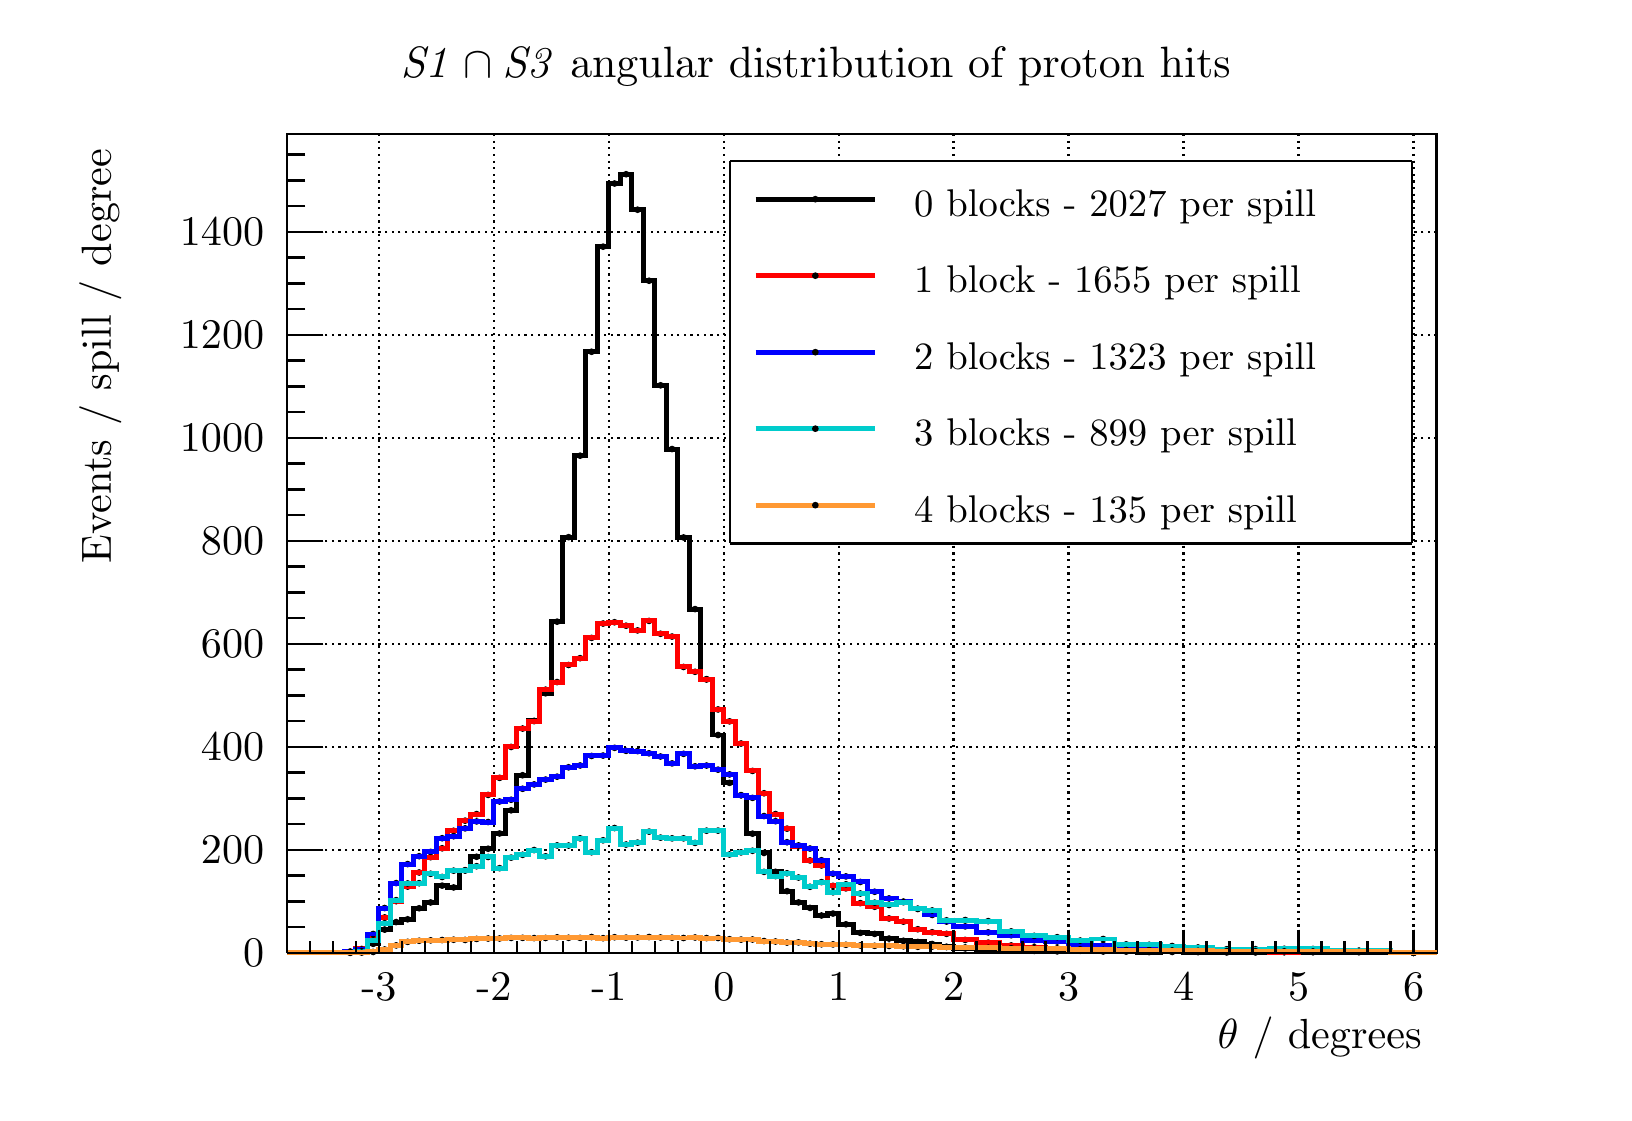
\begin{tikzpicture}
\pgfdeclareplotmark{cross} {
\pgfpathmoveto{\pgfpoint{-0.3\pgfplotmarksize}{\pgfplotmarksize}}
\pgfpathlineto{\pgfpoint{+0.3\pgfplotmarksize}{\pgfplotmarksize}}
\pgfpathlineto{\pgfpoint{+0.3\pgfplotmarksize}{0.3\pgfplotmarksize}}
\pgfpathlineto{\pgfpoint{+1\pgfplotmarksize}{0.3\pgfplotmarksize}}
\pgfpathlineto{\pgfpoint{+1\pgfplotmarksize}{-0.3\pgfplotmarksize}}
\pgfpathlineto{\pgfpoint{+0.3\pgfplotmarksize}{-0.3\pgfplotmarksize}}
\pgfpathlineto{\pgfpoint{+0.3\pgfplotmarksize}{-1.\pgfplotmarksize}}
\pgfpathlineto{\pgfpoint{-0.3\pgfplotmarksize}{-1.\pgfplotmarksize}}
\pgfpathlineto{\pgfpoint{-0.3\pgfplotmarksize}{-0.3\pgfplotmarksize}}
\pgfpathlineto{\pgfpoint{-1.\pgfplotmarksize}{-0.3\pgfplotmarksize}}
\pgfpathlineto{\pgfpoint{-1.\pgfplotmarksize}{0.3\pgfplotmarksize}}
\pgfpathlineto{\pgfpoint{-0.3\pgfplotmarksize}{0.3\pgfplotmarksize}}
\pgfpathclose
\pgfusepathqstroke
}
\pgfdeclareplotmark{cross*} {
\pgfpathmoveto{\pgfpoint{-0.3\pgfplotmarksize}{\pgfplotmarksize}}
\pgfpathlineto{\pgfpoint{+0.3\pgfplotmarksize}{\pgfplotmarksize}}
\pgfpathlineto{\pgfpoint{+0.3\pgfplotmarksize}{0.3\pgfplotmarksize}}
\pgfpathlineto{\pgfpoint{+1\pgfplotmarksize}{0.3\pgfplotmarksize}}
\pgfpathlineto{\pgfpoint{+1\pgfplotmarksize}{-0.3\pgfplotmarksize}}
\pgfpathlineto{\pgfpoint{+0.3\pgfplotmarksize}{-0.3\pgfplotmarksize}}
\pgfpathlineto{\pgfpoint{+0.3\pgfplotmarksize}{-1.\pgfplotmarksize}}
\pgfpathlineto{\pgfpoint{-0.3\pgfplotmarksize}{-1.\pgfplotmarksize}}
\pgfpathlineto{\pgfpoint{-0.3\pgfplotmarksize}{-0.3\pgfplotmarksize}}
\pgfpathlineto{\pgfpoint{-1.\pgfplotmarksize}{-0.3\pgfplotmarksize}}
\pgfpathlineto{\pgfpoint{-1.\pgfplotmarksize}{0.3\pgfplotmarksize}}
\pgfpathlineto{\pgfpoint{-0.3\pgfplotmarksize}{0.3\pgfplotmarksize}}
\pgfpathclose
\pgfusepathqfillstroke
}
\pgfdeclareplotmark{newstar} {
\pgfpathmoveto{\pgfqpoint{0pt}{\pgfplotmarksize}}
\pgfpathlineto{\pgfqpointpolar{44}{0.5\pgfplotmarksize}}
\pgfpathlineto{\pgfqpointpolar{18}{\pgfplotmarksize}}
\pgfpathlineto{\pgfqpointpolar{-20}{0.5\pgfplotmarksize}}
\pgfpathlineto{\pgfqpointpolar{-54}{\pgfplotmarksize}}
\pgfpathlineto{\pgfqpointpolar{-90}{0.5\pgfplotmarksize}}
\pgfpathlineto{\pgfqpointpolar{234}{\pgfplotmarksize}}
\pgfpathlineto{\pgfqpointpolar{198}{0.5\pgfplotmarksize}}
\pgfpathlineto{\pgfqpointpolar{162}{\pgfplotmarksize}}
\pgfpathlineto{\pgfqpointpolar{134}{0.5\pgfplotmarksize}}
\pgfpathclose
\pgfusepathqstroke
}
\pgfdeclareplotmark{newstar*} {
\pgfpathmoveto{\pgfqpoint{0pt}{\pgfplotmarksize}}
\pgfpathlineto{\pgfqpointpolar{44}{0.5\pgfplotmarksize}}
\pgfpathlineto{\pgfqpointpolar{18}{\pgfplotmarksize}}
\pgfpathlineto{\pgfqpointpolar{-20}{0.5\pgfplotmarksize}}
\pgfpathlineto{\pgfqpointpolar{-54}{\pgfplotmarksize}}
\pgfpathlineto{\pgfqpointpolar{-90}{0.5\pgfplotmarksize}}
\pgfpathlineto{\pgfqpointpolar{234}{\pgfplotmarksize}}
\pgfpathlineto{\pgfqpointpolar{198}{0.5\pgfplotmarksize}}
\pgfpathlineto{\pgfqpointpolar{162}{\pgfplotmarksize}}
\pgfpathlineto{\pgfqpointpolar{134}{0.5\pgfplotmarksize}}
\pgfpathclose
\pgfusepathqfillstroke
}
\definecolor{c}{rgb}{1,1,1};
\draw [color=c, fill=c] (0,0) rectangle (20,13.5143);
\draw [color=c, fill=c] (3.28571,1.77143) rectangle (17.8857,12.1714);
\definecolor{c}{rgb}{0,0,0};
\draw [c,line width=0.9] (3.28571,1.77143) -- (3.28571,12.1714) -- (17.8857,12.1714) -- (17.8857,1.77143) -- (3.28571,1.77143);
\definecolor{c}{rgb}{1,1,1};
\draw [color=c, fill=c] (3.28571,1.77143) rectangle (17.8857,12.1714);
\definecolor{c}{rgb}{0,0,0};
\draw [c,line width=0.9] (3.28571,1.77143) -- (3.28571,12.1714) -- (17.8857,12.1714) -- (17.8857,1.77143) -- (3.28571,1.77143);
\draw [c,line width=0.9] (3.28571,1.77143) -- (17.8857,1.77143);
\draw [c,dash pattern=on 0.80pt off 1.60pt ,line width=0.9] (4.45371,12.1714) -- (4.45371,1.77143);
\draw [c,dash pattern=on 0.80pt off 1.60pt ,line width=0.9] (5.91371,12.1714) -- (5.91371,1.77143);
\draw [c,dash pattern=on 0.80pt off 1.60pt ,line width=0.9] (7.37371,12.1714) -- (7.37371,1.77143);
\draw [c,dash pattern=on 0.80pt off 1.60pt ,line width=0.9] (8.83371,12.1714) -- (8.83371,1.77143);
\draw [c,dash pattern=on 0.80pt off 1.60pt ,line width=0.9] (10.2937,12.1714) -- (10.2937,1.77143);
\draw [c,dash pattern=on 0.80pt off 1.60pt ,line width=0.9] (11.7537,12.1714) -- (11.7537,1.77143);
\draw [c,dash pattern=on 0.80pt off 1.60pt ,line width=0.9] (13.2137,12.1714) -- (13.2137,1.77143);
\draw [c,dash pattern=on 0.80pt off 1.60pt ,line width=0.9] (14.6737,12.1714) -- (14.6737,1.77143);
\draw [c,dash pattern=on 0.80pt off 1.60pt ,line width=0.9] (16.1337,12.1714) -- (16.1337,1.77143);
\draw [c,dash pattern=on 0.80pt off 1.60pt ,line width=0.9] (17.5937,12.1714) -- (17.5937,1.77143);
\draw [c,dash pattern=on 0.80pt off 1.60pt ,line width=0.9] (4.45371,12.1714) -- (4.45371,1.77143);
\draw [c,dash pattern=on 0.80pt off 1.60pt ,line width=0.9] (17.5937,12.1714) -- (17.5937,1.77143);
\draw [c,line width=0.9] (3.28571,1.77143) -- (3.28571,12.1714);
\draw [c,dash pattern=on 0.80pt off 1.60pt ,line width=0.9] (17.8857,1.77143) -- (3.28571,1.77143);
\draw [c,dash pattern=on 0.80pt off 1.60pt ,line width=0.9] (17.8857,3.07955) -- (3.28571,3.07955);
\draw [c,dash pattern=on 0.80pt off 1.60pt ,line width=0.9] (17.8857,4.38766) -- (3.28571,4.38766);
\draw [c,dash pattern=on 0.80pt off 1.60pt ,line width=0.9] (17.8857,5.69578) -- (3.28571,5.69578);
\draw [c,dash pattern=on 0.80pt off 1.60pt ,line width=0.9] (17.8857,7.0039) -- (3.28571,7.0039);
\draw [c,dash pattern=on 0.80pt off 1.60pt ,line width=0.9] (17.8857,8.31201) -- (3.28571,8.31201);
\draw [c,dash pattern=on 0.80pt off 1.60pt ,line width=0.9] (17.8857,9.62013) -- (3.28571,9.62013);
\draw [c,dash pattern=on 0.80pt off 1.60pt ,line width=0.9] (17.8857,10.9282) -- (3.28571,10.9282);
\draw [c,dash pattern=on 0.80pt off 1.60pt ,line width=0.9] (17.8857,10.9282) -- (3.28571,10.9282);
\definecolor{c}{rgb}{0,0,0.6};
\draw [c,line width=0.9] (3.28571,1.77143) -- (3.43171,1.77143) -- (3.43171,1.77143) -- (3.57771,1.77143) -- (3.57771,1.77143) -- (3.72371,1.77143) -- (3.72371,1.77143) -- (3.86971,1.77143) -- (3.86971,1.77143) -- (4.01571,1.77143) --
 (4.01571,1.77143) -- (4.16171,1.77143) -- (4.16171,1.77143) -- (4.30771,1.77143) -- (4.30771,1.77143) -- (4.45371,1.77143) -- (4.45371,1.77143) -- (4.59971,1.77143) -- (4.59971,1.77143) -- (4.74571,1.77143) -- (4.74571,1.77143) -- (4.89171,1.77143)
 -- (4.89171,1.77143) -- (5.03771,1.77143) -- (5.03771,1.77143) -- (5.18371,1.77143) -- (5.18371,1.77143) -- (5.32971,1.77143) -- (5.32971,1.77143) -- (5.47571,1.77143) -- (5.47571,1.77143) -- (5.62171,1.77143) -- (5.62171,1.77143) --
 (5.76771,1.77143) -- (5.76771,1.77143) -- (5.91371,1.77143) -- (5.91371,1.77143) -- (6.05971,1.77143) -- (6.05971,1.77143) -- (6.20571,1.77143) -- (6.20571,1.77143) -- (6.35171,1.77143) -- (6.35171,1.77143) -- (6.49771,1.77143) -- (6.49771,1.77143)
 -- (6.64371,1.77143) -- (6.64371,1.77143) -- (6.78971,1.77143) -- (6.78971,1.77143) -- (6.93571,1.77143) -- (6.93571,1.77143) -- (7.08171,1.77143) -- (7.08171,1.77143) -- (7.22771,1.77143) -- (7.22771,1.77143) -- (7.37371,1.77143) --
 (7.37371,1.77143) -- (7.51971,1.77143) -- (7.51971,1.77143) -- (7.66571,1.77143) -- (7.66571,1.77143) -- (7.81171,1.77143) -- (7.81171,1.77143) -- (7.95771,1.77143) -- (7.95771,1.77143) -- (8.10371,1.77143) -- (8.10371,1.77143) -- (8.24971,1.77143)
 -- (8.24971,1.77143) -- (8.39571,1.77143) -- (8.39571,1.77143) -- (8.54171,1.77143) -- (8.54171,1.77143) -- (8.68771,1.77143) -- (8.68771,1.77143) -- (8.83371,1.77143) -- (8.83371,1.77143) -- (8.97971,1.77143) -- (8.97971,1.77143) --
 (9.12571,1.77143) -- (9.12571,1.77143) -- (9.27171,1.77143) -- (9.27171,1.77143) -- (9.41771,1.77143) -- (9.41771,1.77143) -- (9.56371,1.77143) -- (9.56371,1.77143) -- (9.70971,1.77143) -- (9.70971,1.77143) -- (9.85571,1.77143) -- (9.85571,1.77143)
 -- (10.0017,1.77143) -- (10.0017,1.77143) -- (10.1477,1.77143) -- (10.1477,1.77143) -- (10.2937,1.77143) -- (10.2937,1.77143) -- (10.4762,1.77143) -- (10.4762,1.77143) -- (10.6587,1.77143) -- (10.6587,1.77143) -- (10.8412,1.77143) --
 (10.8412,1.77143) -- (11.0237,1.77143) -- (11.0237,1.77143) -- (11.2062,1.77143) -- (11.2062,1.77143) -- (11.3887,1.77143) -- (11.3887,1.77143) -- (11.5712,1.77143) -- (11.5712,1.77143) -- (11.7537,1.77143) -- (11.7537,1.77143) -- (12.0457,1.77143)
 -- (12.0457,1.77143) -- (12.3377,1.77143) -- (12.3377,1.77143) -- (12.6297,1.77143) -- (12.6297,1.77143) -- (12.9217,1.77143) -- (12.9217,1.77143) -- (13.2137,1.77143) -- (13.2137,1.77143) -- (13.5057,1.77143) -- (13.5057,1.77143) --
 (13.7977,1.77143) -- (13.7977,1.77143) -- (14.0897,1.77143) -- (14.0897,1.77143) -- (14.3817,1.77143) -- (14.3817,1.77143) -- (14.6737,1.77143) -- (14.6737,1.77143) -- (15.0387,1.77143) -- (15.0387,1.77143) -- (15.4037,1.77143) -- (15.4037,1.77143)
 -- (15.7687,1.77143) -- (15.7687,1.77143) -- (16.1337,1.77143) -- (16.1337,1.77143) -- (16.4987,1.77143) -- (16.4987,1.77143) -- (17.3017,1.77143) -- (17.3017,1.77143) -- (17.8857,1.77143);
\definecolor{c}{rgb}{0,0,0};
\draw [c,line width=0.9] (3.28571,1.77143) -- (17.8857,1.77143);
\draw [c,line width=0.9] (4.45371,2.06739) -- (4.45371,1.77143);
\draw [c,line width=0.9] (4.74571,1.91941) -- (4.74571,1.77143);
\draw [c,line width=0.9] (5.03771,1.91941) -- (5.03771,1.77143);
\draw [c,line width=0.9] (5.32971,1.91941) -- (5.32971,1.77143);
\draw [c,line width=0.9] (5.62171,1.91941) -- (5.62171,1.77143);
\draw [c,line width=0.9] (5.91371,2.06739) -- (5.91371,1.77143);
\draw [c,line width=0.9] (6.20571,1.91941) -- (6.20571,1.77143);
\draw [c,line width=0.9] (6.49771,1.91941) -- (6.49771,1.77143);
\draw [c,line width=0.9] (6.78971,1.91941) -- (6.78971,1.77143);
\draw [c,line width=0.9] (7.08171,1.91941) -- (7.08171,1.77143);
\draw [c,line width=0.9] (7.37371,2.06739) -- (7.37371,1.77143);
\draw [c,line width=0.9] (7.66571,1.91941) -- (7.66571,1.77143);
\draw [c,line width=0.9] (7.95771,1.91941) -- (7.95771,1.77143);
\draw [c,line width=0.9] (8.24971,1.91941) -- (8.24971,1.77143);
\draw [c,line width=0.9] (8.54171,1.91941) -- (8.54171,1.77143);
\draw [c,line width=0.9] (8.83371,2.06739) -- (8.83371,1.77143);
\draw [c,line width=0.9] (9.12571,1.91941) -- (9.12571,1.77143);
\draw [c,line width=0.9] (9.41771,1.91941) -- (9.41771,1.77143);
\draw [c,line width=0.9] (9.70971,1.91941) -- (9.70971,1.77143);
\draw [c,line width=0.9] (10.0017,1.91941) -- (10.0017,1.77143);
\draw [c,line width=0.9] (10.2937,2.06739) -- (10.2937,1.77143);
\draw [c,line width=0.9] (10.5857,1.91941) -- (10.5857,1.77143);
\draw [c,line width=0.9] (10.8777,1.91941) -- (10.8777,1.77143);
\draw [c,line width=0.9] (11.1697,1.91941) -- (11.1697,1.77143);
\draw [c,line width=0.9] (11.4617,1.91941) -- (11.4617,1.77143);
\draw [c,line width=0.9] (11.7537,2.06739) -- (11.7537,1.77143);
\draw [c,line width=0.9] (12.0457,1.91941) -- (12.0457,1.77143);
\draw [c,line width=0.9] (12.3377,1.91941) -- (12.3377,1.77143);
\draw [c,line width=0.9] (12.6297,1.91941) -- (12.6297,1.77143);
\draw [c,line width=0.9] (12.9217,1.91941) -- (12.9217,1.77143);
\draw [c,line width=0.9] (13.2137,2.06739) -- (13.2137,1.77143);
\draw [c,line width=0.9] (13.5057,1.91941) -- (13.5057,1.77143);
\draw [c,line width=0.9] (13.7977,1.91941) -- (13.7977,1.77143);
\draw [c,line width=0.9] (14.0897,1.91941) -- (14.0897,1.77143);
\draw [c,line width=0.9] (14.3817,1.91941) -- (14.3817,1.77143);
\draw [c,line width=0.9] (14.6737,2.06739) -- (14.6737,1.77143);
\draw [c,line width=0.9] (14.9657,1.91941) -- (14.9657,1.77143);
\draw [c,line width=0.9] (15.2577,1.91941) -- (15.2577,1.77143);
\draw [c,line width=0.9] (15.5497,1.91941) -- (15.5497,1.77143);
\draw [c,line width=0.9] (15.8417,1.91941) -- (15.8417,1.77143);
\draw [c,line width=0.9] (16.1337,2.06739) -- (16.1337,1.77143);
\draw [c,line width=0.9] (16.4257,1.91941) -- (16.4257,1.77143);
\draw [c,line width=0.9] (16.7177,1.91941) -- (16.7177,1.77143);
\draw [c,line width=0.9] (17.0097,1.91941) -- (17.0097,1.77143);
\draw [c,line width=0.9] (17.3017,1.91941) -- (17.3017,1.77143);
\draw [c,line width=0.9] (17.5937,2.06739) -- (17.5937,1.77143);
\draw [c,line width=0.9] (4.45371,2.06739) -- (4.45371,1.77143);
\draw [c,line width=0.9] (4.16171,1.91941) -- (4.16171,1.77143);
\draw [c,line width=0.9] (3.86971,1.91941) -- (3.86971,1.77143);
\draw [c,line width=0.9] (3.57771,1.91941) -- (3.57771,1.77143);
\draw [c,line width=0.9] (17.5937,2.06739) -- (17.5937,1.77143);
\draw [anchor=base] (4.45371,1.16329) node[scale=1.52295, color=c, rotate=0]{-3};
\draw [anchor=base] (5.91371,1.16329) node[scale=1.52295, color=c, rotate=0]{-2};
\draw [anchor=base] (7.37371,1.16329) node[scale=1.52295, color=c, rotate=0]{-1};
\draw [anchor=base] (8.83371,1.16329) node[scale=1.52295, color=c, rotate=0]{0};
\draw [anchor=base] (10.2937,1.16329) node[scale=1.52295, color=c, rotate=0]{1};
\draw [anchor=base] (11.7537,1.16329) node[scale=1.52295, color=c, rotate=0]{2};
\draw [anchor=base] (13.2137,1.16329) node[scale=1.52295, color=c, rotate=0]{3};
\draw [anchor=base] (14.6737,1.16329) node[scale=1.52295, color=c, rotate=0]{4};
\draw [anchor=base] (16.1337,1.16329) node[scale=1.52295, color=c, rotate=0]{5};
\draw [anchor=base] (17.5937,1.16329) node[scale=1.52295, color=c, rotate=0]{6};
\draw [anchor= east] (17.8857,0.690286) node[scale=1.52295, color=c, rotate=0]{$\theta$ / degrees};
\draw [c,line width=0.9] (3.28571,1.77143) -- (3.28571,12.1714);
\draw [c,line width=0.9] (3.74745,1.77143) -- (3.28571,1.77143);
\draw [c,line width=0.9] (3.51658,2.09846) -- (3.28571,2.09846);
\draw [c,line width=0.9] (3.51658,2.42549) -- (3.28571,2.42549);
\draw [c,line width=0.9] (3.51658,2.75252) -- (3.28571,2.75252);
\draw [c,line width=0.9] (3.74745,3.07955) -- (3.28571,3.07955);
\draw [c,line width=0.9] (3.51658,3.40658) -- (3.28571,3.40658);
\draw [c,line width=0.9] (3.51658,3.7336) -- (3.28571,3.7336);
\draw [c,line width=0.9] (3.51658,4.06063) -- (3.28571,4.06063);
\draw [c,line width=0.9] (3.74745,4.38766) -- (3.28571,4.38766);
\draw [c,line width=0.9] (3.51658,4.71469) -- (3.28571,4.71469);
\draw [c,line width=0.9] (3.51658,5.04172) -- (3.28571,5.04172);
\draw [c,line width=0.9] (3.51658,5.36875) -- (3.28571,5.36875);
\draw [c,line width=0.9] (3.74745,5.69578) -- (3.28571,5.69578);
\draw [c,line width=0.9] (3.51658,6.02281) -- (3.28571,6.02281);
\draw [c,line width=0.9] (3.51658,6.34984) -- (3.28571,6.34984);
\draw [c,line width=0.9] (3.51658,6.67687) -- (3.28571,6.67687);
\draw [c,line width=0.9] (3.74745,7.0039) -- (3.28571,7.0039);
\draw [c,line width=0.9] (3.51658,7.33093) -- (3.28571,7.33093);
\draw [c,line width=0.9] (3.51658,7.65796) -- (3.28571,7.65796);
\draw [c,line width=0.9] (3.51658,7.98499) -- (3.28571,7.98499);
\draw [c,line width=0.9] (3.74745,8.31201) -- (3.28571,8.31201);
\draw [c,line width=0.9] (3.51658,8.63904) -- (3.28571,8.63904);
\draw [c,line width=0.9] (3.51658,8.96607) -- (3.28571,8.96607);
\draw [c,line width=0.9] (3.51658,9.2931) -- (3.28571,9.2931);
\draw [c,line width=0.9] (3.74745,9.62013) -- (3.28571,9.62013);
\draw [c,line width=0.9] (3.51658,9.94716) -- (3.28571,9.94716);
\draw [c,line width=0.9] (3.51658,10.2742) -- (3.28571,10.2742);
\draw [c,line width=0.9] (3.51658,10.6012) -- (3.28571,10.6012);
\draw [c,line width=0.9] (3.74745,10.9282) -- (3.28571,10.9282);
\draw [c,line width=0.9] (3.74745,10.9282) -- (3.28571,10.9282);
\draw [c,line width=0.9] (3.51658,11.2553) -- (3.28571,11.2553);
\draw [c,line width=0.9] (3.51658,11.5823) -- (3.28571,11.5823);
\draw [c,line width=0.9] (3.51658,11.9093) -- (3.28571,11.9093);
\draw [anchor= east] (3.18571,1.77143) node[scale=1.52295, color=c, rotate=0]{0};
\draw [anchor= east] (3.18571,3.07955) node[scale=1.52295, color=c, rotate=0]{200};
\draw [anchor= east] (3.18571,4.38766) node[scale=1.52295, color=c, rotate=0]{400};
\draw [anchor= east] (3.18571,5.69578) node[scale=1.52295, color=c, rotate=0]{600};
\draw [anchor= east] (3.18571,7.0039) node[scale=1.52295, color=c, rotate=0]{800};
\draw [anchor= east] (3.18571,8.31201) node[scale=1.52295, color=c, rotate=0]{1000};
\draw [anchor= east] (3.18571,9.62013) node[scale=1.52295, color=c, rotate=0]{1200};
\draw [anchor= east] (3.18571,10.9282) node[scale=1.52295, color=c, rotate=0]{1400};
\draw [anchor= east] (0.914286,12.1714) node[scale=1.52295, color=c, rotate=90]{ Events / spill / degree};
\draw [c,line width=1.8] (4.08871,1.77928) -- (4.08871,1.77976);
\draw [c,line width=1.8] (4.08871,1.77976) -- (4.08871,1.78025);
\foreach \P in {(4.08871,1.77976)}{\draw[mark options={color=c,fill=c},mark size=2.402402pt,mark=*,mark size=1pt] plot coordinates {\P};}
\draw [c,line width=1.8] (4.23471,1.80702) -- (4.23471,1.808);
\draw [c,line width=1.8] (4.23471,1.808) -- (4.23471,1.80898);
\foreach \P in {(4.23471,1.808)}{\draw[mark options={color=c,fill=c},mark size=2.402402pt,mark=*,mark size=1pt] plot coordinates {\P};}
\draw [c,line width=1.8] (4.38071,1.88391) -- (4.38071,1.88565);
\draw [c,line width=1.8] (4.38071,1.88565) -- (4.38071,1.88738);
\foreach \P in {(4.38071,1.88565)}{\draw[mark options={color=c,fill=c},mark size=2.402402pt,mark=*,mark size=1pt] plot coordinates {\P};}
\draw [c,line width=1.8] (4.52671,2.0637) -- (4.52671,2.0665);
\draw [c,line width=1.8] (4.52671,2.0665) -- (4.52671,2.0693);
\foreach \P in {(4.52671,2.0665)}{\draw[mark options={color=c,fill=c},mark size=2.402402pt,mark=*,mark size=1pt] plot coordinates {\P};}
\draw [c,line width=1.8] (4.67271,2.15927) -- (4.67271,2.16245);
\draw [c,line width=1.8] (4.67271,2.16245) -- (4.67271,2.16564);
\foreach \P in {(4.67271,2.16245)}{\draw[mark options={color=c,fill=c},mark size=2.402402pt,mark=*,mark size=1pt] plot coordinates {\P};}
\draw [c,line width=1.8] (4.81871,2.19429) -- (4.81871,2.19763);
\draw [c,line width=1.8] (4.81871,2.19763) -- (4.81871,2.20096);
\foreach \P in {(4.81871,2.19763)}{\draw[mark options={color=c,fill=c},mark size=2.402402pt,mark=*,mark size=1pt] plot coordinates {\P};}
\draw [c,line width=1.8] (4.96471,2.33421) -- (4.96471,2.33808);
\draw [c,line width=1.8] (4.96471,2.33808) -- (4.96471,2.34194);
\foreach \P in {(4.96471,2.33808)}{\draw[mark options={color=c,fill=c},mark size=2.402402pt,mark=*,mark size=1pt] plot coordinates {\P};}
\draw [c,line width=1.8] (5.11071,2.40725) -- (5.11071,2.41137);
\draw [c,line width=1.8] (5.11071,2.41137) -- (5.11071,2.41549);
\foreach \P in {(5.11071,2.41137)}{\draw[mark options={color=c,fill=c},mark size=2.402402pt,mark=*,mark size=1pt] plot coordinates {\P};}
\draw [c,line width=1.8] (5.25671,2.62065) -- (5.25671,2.62539);
\draw [c,line width=1.8] (5.25671,2.62539) -- (5.25671,2.63013);
\foreach \P in {(5.25671,2.62539)}{\draw[mark options={color=c,fill=c},mark size=2.402402pt,mark=*,mark size=1pt] plot coordinates {\P};}
\draw [c,line width=1.8] (5.40271,2.5977) -- (5.40271,2.60239);
\draw [c,line width=1.8] (5.40271,2.60239) -- (5.40271,2.60707);
\foreach \P in {(5.40271,2.60239)}{\draw[mark options={color=c,fill=c},mark size=2.402402pt,mark=*,mark size=1pt] plot coordinates {\P};}
\draw [c,line width=1.8] (5.54871,2.8114) -- (5.54871,2.81666);
\draw [c,line width=1.8] (5.54871,2.81666) -- (5.54871,2.82192);
\foreach \P in {(5.54871,2.81666)}{\draw[mark options={color=c,fill=c},mark size=2.402402pt,mark=*,mark size=1pt] plot coordinates {\P};}
\draw [c,line width=1.8] (5.69471,2.9861) -- (5.69471,2.99178);
\draw [c,line width=1.8] (5.69471,2.99178) -- (5.69471,2.99746);
\foreach \P in {(5.69471,2.99178)}{\draw[mark options={color=c,fill=c},mark size=2.402402pt,mark=*,mark size=1pt] plot coordinates {\P};}
\draw [c,line width=1.8] (5.84071,3.08772) -- (5.84071,3.09363);
\draw [c,line width=1.8] (5.84071,3.09363) -- (5.84071,3.09954);
\foreach \P in {(5.84071,3.09363)}{\draw[mark options={color=c,fill=c},mark size=2.402402pt,mark=*,mark size=1pt] plot coordinates {\P};}
\draw [c,line width=1.8] (5.98671,3.28119) -- (5.98671,3.28753);
\draw [c,line width=1.8] (5.98671,3.28753) -- (5.98671,3.29387);
\foreach \P in {(5.98671,3.28753)}{\draw[mark options={color=c,fill=c},mark size=2.402402pt,mark=*,mark size=1pt] plot coordinates {\P};}
\draw [c,line width=1.8] (6.13271,3.57494) -- (6.13271,3.58187);
\draw [c,line width=1.8] (6.13271,3.58187) -- (6.13271,3.58879);
\foreach \P in {(6.13271,3.58187)}{\draw[mark options={color=c,fill=c},mark size=2.402402pt,mark=*,mark size=1pt] plot coordinates {\P};}
\draw [c,line width=1.8] (6.27871,4.01937) -- (6.27871,4.02712);
\draw [c,line width=1.8] (6.27871,4.02712) -- (6.27871,4.03486);
\foreach \P in {(6.27871,4.02712)}{\draw[mark options={color=c,fill=c},mark size=2.402402pt,mark=*,mark size=1pt] plot coordinates {\P};}
\draw [c,line width=1.8] (6.42471,4.70892) -- (6.42471,4.71772);
\draw [c,line width=1.8] (6.42471,4.71772) -- (6.42471,4.72652);
\foreach \P in {(6.42471,4.71772)}{\draw[mark options={color=c,fill=c},mark size=2.402402pt,mark=*,mark size=1pt] plot coordinates {\P};}
\draw [c,line width=1.8] (6.57071,5.05873) -- (6.57071,5.06808);
\draw [c,line width=1.8] (6.57071,5.06808) -- (6.57071,5.07743);
\foreach \P in {(6.57071,5.06808)}{\draw[mark options={color=c,fill=c},mark size=2.402402pt,mark=*,mark size=1pt] plot coordinates {\P};}
\draw [c,line width=1.8] (6.71671,5.96677) -- (6.71671,5.9773);
\draw [c,line width=1.8] (6.71671,5.9773) -- (6.71671,5.98784);
\foreach \P in {(6.71671,5.9773)}{\draw[mark options={color=c,fill=c},mark size=2.402402pt,mark=*,mark size=1pt] plot coordinates {\P};}
\draw [c,line width=1.8] (6.86271,7.03879) -- (6.86271,7.05058);
\draw [c,line width=1.8] (6.86271,7.05058) -- (6.86271,7.06238);
\foreach \P in {(6.86271,7.05058)}{\draw[mark options={color=c,fill=c},mark size=2.402402pt,mark=*,mark size=1pt] plot coordinates {\P};}
\draw [c,line width=1.8] (7.00871,8.07255) -- (7.00871,8.08548);
\draw [c,line width=1.8] (7.00871,8.08548) -- (7.00871,8.09841);
\foreach \P in {(7.00871,8.08548)}{\draw[mark options={color=c,fill=c},mark size=2.402402pt,mark=*,mark size=1pt] plot coordinates {\P};}
\draw [c,line width=1.8] (7.15471,9.39111) -- (7.15471,9.40531);
\draw [c,line width=1.8] (7.15471,9.40531) -- (7.15471,9.41952);
\foreach \P in {(7.15471,9.40531)}{\draw[mark options={color=c,fill=c},mark size=2.402402pt,mark=*,mark size=1pt] plot coordinates {\P};}
\draw [c,line width=1.8] (7.30071,10.7244) -- (7.30071,10.7398);
\draw [c,line width=1.8] (7.30071,10.7398) -- (7.30071,10.7552);
\foreach \P in {(7.30071,10.7398)}{\draw[mark options={color=c,fill=c},mark size=2.402402pt,mark=*,mark size=1pt] plot coordinates {\P};}
\draw [c,line width=1.8] (7.44671,11.5259) -- (7.44671,11.542);
\draw [c,line width=1.8] (7.44671,11.542) -- (7.44671,11.5581);
\foreach \P in {(7.44671,11.542)}{\draw[mark options={color=c,fill=c},mark size=2.402402pt,mark=*,mark size=1pt] plot coordinates {\P};}
\draw [c,line width=1.8] (7.59271,11.6439) -- (7.59271,11.66);
\draw [c,line width=1.8] (7.59271,11.66) -- (7.59271,11.6762);
\foreach \P in {(7.59271,11.66)}{\draw[mark options={color=c,fill=c},mark size=2.402402pt,mark=*,mark size=1pt] plot coordinates {\P};}
\draw [c,line width=1.8] (7.73871,11.1933) -- (7.73871,11.2091);
\draw [c,line width=1.8] (7.73871,11.2091) -- (7.73871,11.2249);
\foreach \P in {(7.73871,11.2091)}{\draw[mark options={color=c,fill=c},mark size=2.402402pt,mark=*,mark size=1pt] plot coordinates {\P};}
\draw [c,line width=1.8] (7.88471,10.292) -- (7.88471,10.307);
\draw [c,line width=1.8] (7.88471,10.307) -- (7.88471,10.322);
\foreach \P in {(7.88471,10.307)}{\draw[mark options={color=c,fill=c},mark size=2.402402pt,mark=*,mark size=1pt] plot coordinates {\P};}
\draw [c,line width=1.8] (8.03071,8.96539) -- (8.03071,8.97916);
\draw [c,line width=1.8] (8.03071,8.97916) -- (8.03071,8.99293);
\foreach \P in {(8.03071,8.97916)}{\draw[mark options={color=c,fill=c},mark size=2.402402pt,mark=*,mark size=1pt] plot coordinates {\P};}
\draw [c,line width=1.8] (8.17671,8.15671) -- (8.17671,8.1697);
\draw [c,line width=1.8] (8.17671,8.1697) -- (8.17671,8.18269);
\foreach \P in {(8.17671,8.1697)}{\draw[mark options={color=c,fill=c},mark size=2.402402pt,mark=*,mark size=1pt] plot coordinates {\P};}
\draw [c,line width=1.8] (8.32271,7.03519) -- (8.32271,7.04698);
\draw [c,line width=1.8] (8.32271,7.04698) -- (8.32271,7.05876);
\foreach \P in {(8.32271,7.04698)}{\draw[mark options={color=c,fill=c},mark size=2.402402pt,mark=*,mark size=1pt] plot coordinates {\P};}
\draw [c,line width=1.8] (8.46871,6.12634) -- (8.46871,6.13709);
\draw [c,line width=1.8] (8.46871,6.13709) -- (8.46871,6.14784);
\foreach \P in {(8.46871,6.13709)}{\draw[mark options={color=c,fill=c},mark size=2.402402pt,mark=*,mark size=1pt] plot coordinates {\P};}
\draw [c,line width=1.8] (8.61471,5.23363) -- (8.61471,5.24318);
\draw [c,line width=1.8] (8.61471,5.24318) -- (8.61471,5.25272);
\foreach \P in {(8.61471,5.24318)}{\draw[mark options={color=c,fill=c},mark size=2.402402pt,mark=*,mark size=1pt] plot coordinates {\P};}
\draw [c,line width=1.8] (8.76071,4.52978) -- (8.76071,4.53832);
\draw [c,line width=1.8] (8.76071,4.53832) -- (8.76071,4.54686);
\foreach \P in {(8.76071,4.53832)}{\draw[mark options={color=c,fill=c},mark size=2.402402pt,mark=*,mark size=1pt] plot coordinates {\P};}
\draw [c,line width=1.8] (8.90671,3.9228) -- (8.90671,3.93034);
\draw [c,line width=1.8] (8.90671,3.93034) -- (8.90671,3.93787);
\foreach \P in {(8.90671,3.93034)}{\draw[mark options={color=c,fill=c},mark size=2.402402pt,mark=*,mark size=1pt] plot coordinates {\P};}
\draw [c,line width=1.8] (9.05271,3.76622) -- (9.05271,3.77346);
\draw [c,line width=1.8] (9.05271,3.77346) -- (9.05271,3.7807);
\foreach \P in {(9.05271,3.77346)}{\draw[mark options={color=c,fill=c},mark size=2.402402pt,mark=*,mark size=1pt] plot coordinates {\P};}
\draw [c,line width=1.8] (9.19871,3.27871) -- (9.19871,3.28503);
\draw [c,line width=1.8] (9.19871,3.28503) -- (9.19871,3.29134);
\foreach \P in {(9.19871,3.28503)}{\draw[mark options={color=c,fill=c},mark size=2.402402pt,mark=*,mark size=1pt] plot coordinates {\P};}
\draw [c,line width=1.8] (9.34471,3.0343) -- (9.34471,3.0401);
\draw [c,line width=1.8] (9.34471,3.0401) -- (9.34471,3.04591);
\foreach \P in {(9.34471,3.0401)}{\draw[mark options={color=c,fill=c},mark size=2.402402pt,mark=*,mark size=1pt] plot coordinates {\P};}
\draw [c,line width=1.8] (9.49071,2.7953) -- (9.49071,2.8005);
\draw [c,line width=1.8] (9.49071,2.8005) -- (9.49071,2.8057);
\foreach \P in {(9.49071,2.8005)}{\draw[mark options={color=c,fill=c},mark size=2.402402pt,mark=*,mark size=1pt] plot coordinates {\P};}
\draw [c,line width=1.8] (9.63671,2.55056) -- (9.63671,2.55512);
\draw [c,line width=1.8] (9.63671,2.55512) -- (9.63671,2.55967);
\foreach \P in {(9.63671,2.55512)}{\draw[mark options={color=c,fill=c},mark size=2.402402pt,mark=*,mark size=1pt] plot coordinates {\P};}
\draw [c,line width=1.8] (9.78271,2.40811) -- (9.78271,2.41224);
\draw [c,line width=1.8] (9.78271,2.41224) -- (9.78271,2.41636);
\foreach \P in {(9.78271,2.41224)}{\draw[mark options={color=c,fill=c},mark size=2.402402pt,mark=*,mark size=1pt] plot coordinates {\P};}
\draw [c,line width=1.8] (9.92871,2.33856) -- (9.92871,2.34245);
\draw [c,line width=1.8] (9.92871,2.34245) -- (9.92871,2.34633);
\foreach \P in {(9.92871,2.34245)}{\draw[mark options={color=c,fill=c},mark size=2.402402pt,mark=*,mark size=1pt] plot coordinates {\P};}
\draw [c,line width=1.8] (10.0747,2.24253) -- (10.0747,2.24605);
\draw [c,line width=1.8] (10.0747,2.24605) -- (10.0747,2.24957);
\foreach \P in {(10.0747,2.24605)}{\draw[mark options={color=c,fill=c},mark size=2.402402pt,mark=*,mark size=1pt] plot coordinates {\P};}
\draw [c,line width=1.8] (10.2207,2.26683) -- (10.2207,2.27048);
\draw [c,line width=1.8] (10.2207,2.27048) -- (10.2207,2.27413);
\foreach \P in {(10.2207,2.27048)}{\draw[mark options={color=c,fill=c},mark size=2.402402pt,mark=*,mark size=1pt] plot coordinates {\P};}
\draw [c,line width=1.8] (10.385,2.13071) -- (10.385,2.13417);
\draw [c,line width=1.8] (10.385,2.13417) -- (10.385,2.13762);
\foreach \P in {(10.385,2.13417)}{\draw[mark options={color=c,fill=c},mark size=2.402402pt,mark=*,mark size=1pt] plot coordinates {\P};}
\draw [c,line width=1.8] (10.5675,2.0223) -- (10.5675,2.02518);
\draw [c,line width=1.8] (10.5675,2.02518) -- (10.5675,2.02807);
\foreach \P in {(10.5675,2.02518)}{\draw[mark options={color=c,fill=c},mark size=2.402402pt,mark=*,mark size=1pt] plot coordinates {\P};}
\draw [c,line width=1.8] (10.75,2.0093) -- (10.75,2.01214);
\draw [c,line width=1.8] (10.75,2.01214) -- (10.75,2.01497);
\foreach \P in {(10.75,2.01214)}{\draw[mark options={color=c,fill=c},mark size=2.402402pt,mark=*,mark size=1pt] plot coordinates {\P};}
\draw [c,line width=1.8] (10.9325,1.95041) -- (10.9325,1.95285);
\draw [c,line width=1.8] (10.9325,1.95285) -- (10.9325,1.95529);
\foreach \P in {(10.9325,1.95285)}{\draw[mark options={color=c,fill=c},mark size=2.402402pt,mark=*,mark size=1pt] plot coordinates {\P};}
\draw [c,line width=1.8] (11.115,1.92247) -- (11.115,1.92473);
\draw [c,line width=1.8] (11.115,1.92473) -- (11.115,1.92699);
\foreach \P in {(11.115,1.92473)}{\draw[mark options={color=c,fill=c},mark size=2.402402pt,mark=*,mark size=1pt] plot coordinates {\P};}
\draw [c,line width=1.8] (11.2975,1.90792) -- (11.2975,1.91006);
\draw [c,line width=1.8] (11.2975,1.91006) -- (11.2975,1.9122);
\foreach \P in {(11.2975,1.91006)}{\draw[mark options={color=c,fill=c},mark size=2.402402pt,mark=*,mark size=1pt] plot coordinates {\P};}
\draw [c,line width=1.8] (11.48,1.88169) -- (11.48,1.88362);
\draw [c,line width=1.8] (11.48,1.88362) -- (11.48,1.88556);
\foreach \P in {(11.48,1.88362)}{\draw[mark options={color=c,fill=c},mark size=2.402402pt,mark=*,mark size=1pt] plot coordinates {\P};}
\draw [c,line width=1.8] (11.6625,1.84719) -- (11.6625,1.84877);
\draw [c,line width=1.8] (11.6625,1.84877) -- (11.6625,1.85034);
\foreach \P in {(11.6625,1.84877)}{\draw[mark options={color=c,fill=c},mark size=2.402402pt,mark=*,mark size=1pt] plot coordinates {\P};}
\draw [c,line width=1.8] (11.8997,1.8255) -- (11.8997,1.82722);
\draw [c,line width=1.8] (11.8997,1.82722) -- (11.8997,1.82893);
\foreach \P in {(11.8997,1.82722)}{\draw[mark options={color=c,fill=c},mark size=2.402402pt,mark=*,mark size=1pt] plot coordinates {\P};}
\draw [c,line width=1.8] (12.1917,1.80911) -- (12.1917,1.81054);
\draw [c,line width=1.8] (12.1917,1.81054) -- (12.1917,1.81198);
\foreach \P in {(12.1917,1.81054)}{\draw[mark options={color=c,fill=c},mark size=2.402402pt,mark=*,mark size=1pt] plot coordinates {\P};}
\draw [c,line width=1.8] (12.4837,1.80809) -- (12.4837,1.80951);
\draw [c,line width=1.8] (12.4837,1.80951) -- (12.4837,1.81093);
\foreach \P in {(12.4837,1.80951)}{\draw[mark options={color=c,fill=c},mark size=2.402402pt,mark=*,mark size=1pt] plot coordinates {\P};}
\draw [c,line width=1.8] (12.7757,1.79522) -- (12.7757,1.79637);
\draw [c,line width=1.8] (12.7757,1.79637) -- (12.7757,1.79753);
\foreach \P in {(12.7757,1.79637)}{\draw[mark options={color=c,fill=c},mark size=2.402402pt,mark=*,mark size=1pt] plot coordinates {\P};}
\draw [c,line width=1.8] (13.0677,1.78926) -- (13.0677,1.79027);
\draw [c,line width=1.8] (13.0677,1.79027) -- (13.0677,1.79128);
\foreach \P in {(13.0677,1.79027)}{\draw[mark options={color=c,fill=c},mark size=2.402402pt,mark=*,mark size=1pt] plot coordinates {\P};}
\draw [c,line width=1.8] (13.3597,1.7964) -- (13.3597,1.79758);
\draw [c,line width=1.8] (13.3597,1.79758) -- (13.3597,1.79876);
\foreach \P in {(13.3597,1.79758)}{\draw[mark options={color=c,fill=c},mark size=2.402402pt,mark=*,mark size=1pt] plot coordinates {\P};}
\draw [c,line width=1.8] (13.6517,1.78712) -- (13.6517,1.78804);
\draw [c,line width=1.8] (13.6517,1.78804) -- (13.6517,1.78897);
\foreach \P in {(13.6517,1.78804)}{\draw[mark options={color=c,fill=c},mark size=2.402402pt,mark=*,mark size=1pt] plot coordinates {\P};}
\draw [c,line width=1.8] (13.9437,1.78641) -- (13.9437,1.78733);
\draw [c,line width=1.8] (13.9437,1.78733) -- (13.9437,1.78826);
\foreach \P in {(13.9437,1.78733)}{\draw[mark options={color=c,fill=c},mark size=2.402402pt,mark=*,mark size=1pt] plot coordinates {\P};}
\draw [c,line width=1.8] (14.2357,1.78046) -- (14.2357,1.7812);
\draw [c,line width=1.8] (14.2357,1.7812) -- (14.2357,1.78194);
\foreach \P in {(14.2357,1.7812)}{\draw[mark options={color=c,fill=c},mark size=2.402402pt,mark=*,mark size=1pt] plot coordinates {\P};}
\draw [c,line width=1.8] (14.5277,1.78232) -- (14.5277,1.7831);
\draw [c,line width=1.8] (14.5277,1.7831) -- (14.5277,1.78389);
\foreach \P in {(14.5277,1.7831)}{\draw[mark options={color=c,fill=c},mark size=2.402402pt,mark=*,mark size=1pt] plot coordinates {\P};}
\draw [c,line width=1.8] (14.8562,1.77979) -- (14.8562,1.78055);
\draw [c,line width=1.8] (14.8562,1.78055) -- (14.8562,1.78132);
\foreach \P in {(14.8562,1.78055)}{\draw[mark options={color=c,fill=c},mark size=2.402402pt,mark=*,mark size=1pt] plot coordinates {\P};}
\draw [c,line width=1.8] (15.2212,1.77593) -- (15.2212,1.7765);
\draw [c,line width=1.8] (15.2212,1.7765) -- (15.2212,1.77707);
\foreach \P in {(15.2212,1.7765)}{\draw[mark options={color=c,fill=c},mark size=2.402402pt,mark=*,mark size=1pt] plot coordinates {\P};}
\draw [c,line width=1.8] (15.5862,1.77596) -- (15.5862,1.77653);
\draw [c,line width=1.8] (15.5862,1.77653) -- (15.5862,1.7771);
\foreach \P in {(15.5862,1.77653)}{\draw[mark options={color=c,fill=c},mark size=2.402402pt,mark=*,mark size=1pt] plot coordinates {\P};}
\draw [c,line width=1.8] (15.9512,1.77912) -- (15.9512,1.77987);
\draw [c,line width=1.8] (15.9512,1.77987) -- (15.9512,1.78062);
\foreach \P in {(15.9512,1.77987)}{\draw[mark options={color=c,fill=c},mark size=2.402402pt,mark=*,mark size=1pt] plot coordinates {\P};}
\draw [c,line width=1.8] (16.3162,1.77848) -- (16.3162,1.77922);
\draw [c,line width=1.8] (16.3162,1.77922) -- (16.3162,1.77995);
\foreach \P in {(16.3162,1.77922)}{\draw[mark options={color=c,fill=c},mark size=2.402402pt,mark=*,mark size=1pt] plot coordinates {\P};}
\draw [c,line width=1.8] (16.9002,1.77875) -- (16.9002,1.77985);
\draw [c,line width=1.8] (16.9002,1.77985) -- (16.9002,1.78094);
\foreach \P in {(16.9002,1.77985)}{\draw[mark options={color=c,fill=c},mark size=2.402402pt,mark=*,mark size=1pt] plot coordinates {\P};}
\draw [c,line width=1.8] (17.5937,1.77212) -- (17.5937,1.77269);
\draw [c,line width=1.8] (17.5937,1.77269) -- (17.5937,1.77325);
\foreach \P in {(17.5937,1.77269)}{\draw[mark options={color=c,fill=c},mark size=2.402402pt,mark=*,mark size=1pt] plot coordinates {\P};}
\draw [c,line width=1.8] (3.28571,1.77143) -- (3.43171,1.77143) -- (3.43171,1.77143) -- (3.57771,1.77143) -- (3.57771,1.77143) -- (3.72371,1.77143) -- (3.72371,1.77143) -- (3.86971,1.77143) -- (3.86971,1.77143) -- (4.01571,1.77143) --
 (4.01571,1.77976) -- (4.16171,1.77976) -- (4.16171,1.808) -- (4.30771,1.808) -- (4.30771,1.88565) -- (4.45371,1.88565) -- (4.45371,2.0665) -- (4.59971,2.0665) -- (4.59971,2.16245) -- (4.74571,2.16245) -- (4.74571,2.19763) -- (4.89171,2.19763) --
 (4.89171,2.33808) -- (5.03771,2.33808) -- (5.03771,2.41137) -- (5.18371,2.41137) -- (5.18371,2.62539) -- (5.32971,2.62539) -- (5.32971,2.60239) -- (5.47571,2.60239) -- (5.47571,2.81666) -- (5.62171,2.81666) -- (5.62171,2.99178) -- (5.76771,2.99178)
 -- (5.76771,3.09363) -- (5.91371,3.09363) -- (5.91371,3.28753) -- (6.05971,3.28753) -- (6.05971,3.58187) -- (6.20571,3.58187) -- (6.20571,4.02712) -- (6.35171,4.02712) -- (6.35171,4.71772) -- (6.49771,4.71772) -- (6.49771,5.06808) --
 (6.64371,5.06808) -- (6.64371,5.9773) -- (6.78971,5.9773) -- (6.78971,7.05058) -- (6.93571,7.05058) -- (6.93571,8.08548) -- (7.08171,8.08548) -- (7.08171,9.40531) -- (7.22771,9.40531) -- (7.22771,10.7398) -- (7.37371,10.7398) -- (7.37371,11.542) --
 (7.51971,11.542) -- (7.51971,11.66) -- (7.66571,11.66) -- (7.66571,11.2091) -- (7.81171,11.2091) -- (7.81171,10.307) -- (7.95771,10.307) -- (7.95771,8.97916) -- (8.10371,8.97916) -- (8.10371,8.1697) -- (8.24971,8.1697) -- (8.24971,7.04698) --
 (8.39571,7.04698) -- (8.39571,6.13709) -- (8.54171,6.13709) -- (8.54171,5.24318) -- (8.68771,5.24318) -- (8.68771,4.53832) -- (8.83371,4.53832) -- (8.83371,3.93034) -- (8.97971,3.93034) -- (8.97971,3.77346) -- (9.12571,3.77346) -- (9.12571,3.28503)
 -- (9.27171,3.28503) -- (9.27171,3.0401) -- (9.41771,3.0401) -- (9.41771,2.8005) -- (9.56371,2.8005) -- (9.56371,2.55512) -- (9.70971,2.55512) -- (9.70971,2.41224) -- (9.85571,2.41224) -- (9.85571,2.34245) -- (10.0017,2.34245) -- (10.0017,2.24605)
 -- (10.1477,2.24605) -- (10.1477,2.27048) -- (10.2937,2.27048) -- (10.2937,2.13417) -- (10.4762,2.13417) -- (10.4762,2.02518) -- (10.6587,2.02518) -- (10.6587,2.01214) -- (10.8412,2.01214) -- (10.8412,1.95285) -- (11.0237,1.95285) --
 (11.0237,1.92473) -- (11.2062,1.92473) -- (11.2062,1.91006) -- (11.3887,1.91006) -- (11.3887,1.88362) -- (11.5712,1.88362) -- (11.5712,1.84877) -- (11.7537,1.84877) -- (11.7537,1.82722) -- (12.0457,1.82722) -- (12.0457,1.81054) -- (12.3377,1.81054)
 -- (12.3377,1.80951) -- (12.6297,1.80951) -- (12.6297,1.79637) -- (12.9217,1.79637) -- (12.9217,1.79027) -- (13.2137,1.79027) -- (13.2137,1.79758) -- (13.5057,1.79758) -- (13.5057,1.78804) -- (13.7977,1.78804) -- (13.7977,1.78733) --
 (14.0897,1.78733) -- (14.0897,1.7812) -- (14.3817,1.7812) -- (14.3817,1.7831) -- (14.6737,1.7831) -- (14.6737,1.78055) -- (15.0387,1.78055) -- (15.0387,1.7765) -- (15.4037,1.7765) -- (15.4037,1.77653) -- (15.7687,1.77653) -- (15.7687,1.77987) --
 (16.1337,1.77987) -- (16.1337,1.77922) -- (16.4987,1.77922) -- (16.4987,1.77985) -- (17.3017,1.77985) -- (17.3017,1.77269) -- (17.8857,1.77269);
\definecolor{c}{rgb}{1,0,0};
\draw [c,line width=1.8] (4.08871,1.77445) -- (4.08871,1.77469);
\draw [c,line width=1.8] (4.08871,1.77469) -- (4.08871,1.77492);
\definecolor{c}{rgb}{0,0,0};
\foreach \P in {(4.08871,1.77469)}{\draw[mark options={color=c,fill=c},mark size=2.402402pt,mark=*,mark size=1pt] plot coordinates {\P};}
\definecolor{c}{rgb}{1,0,0};
\draw [c,line width=1.8] (4.23471,1.82002) -- (4.23471,1.82097);
\draw [c,line width=1.8] (4.23471,1.82097) -- (4.23471,1.82192);
\definecolor{c}{rgb}{0,0,0};
\foreach \P in {(4.23471,1.82097)}{\draw[mark options={color=c,fill=c},mark size=2.402402pt,mark=*,mark size=1pt] plot coordinates {\P};}
\definecolor{c}{rgb}{1,0,0};
\draw [c,line width=1.8] (4.38071,1.96606) -- (4.38071,1.96794);
\draw [c,line width=1.8] (4.38071,1.96794) -- (4.38071,1.96981);
\definecolor{c}{rgb}{0,0,0};
\foreach \P in {(4.38071,1.96794)}{\draw[mark options={color=c,fill=c},mark size=2.402402pt,mark=*,mark size=1pt] plot coordinates {\P};}
\definecolor{c}{rgb}{1,0,0};
\draw [c,line width=1.8] (4.52671,2.21881) -- (4.52671,2.22166);
\draw [c,line width=1.8] (4.52671,2.22166) -- (4.52671,2.22452);
\definecolor{c}{rgb}{0,0,0};
\foreach \P in {(4.52671,2.22166)}{\draw[mark options={color=c,fill=c},mark size=2.402402pt,mark=*,mark size=1pt] plot coordinates {\P};}
\definecolor{c}{rgb}{1,0,0};
\draw [c,line width=1.8] (4.67271,2.4243) -- (4.67271,2.42776);
\draw [c,line width=1.8] (4.67271,2.42776) -- (4.67271,2.43122);
\definecolor{c}{rgb}{0,0,0};
\foreach \P in {(4.67271,2.42776)}{\draw[mark options={color=c,fill=c},mark size=2.402402pt,mark=*,mark size=1pt] plot coordinates {\P};}
\definecolor{c}{rgb}{1,0,0};
\draw [c,line width=1.8] (4.81871,2.60907) -- (4.81871,2.61297);
\draw [c,line width=1.8] (4.81871,2.61297) -- (4.81871,2.61687);
\definecolor{c}{rgb}{0,0,0};
\foreach \P in {(4.81871,2.61297)}{\draw[mark options={color=c,fill=c},mark size=2.402402pt,mark=*,mark size=1pt] plot coordinates {\P};}
\definecolor{c}{rgb}{1,0,0};
\draw [c,line width=1.8] (4.96471,2.78794) -- (4.96471,2.79225);
\draw [c,line width=1.8] (4.96471,2.79225) -- (4.96471,2.79656);
\definecolor{c}{rgb}{0,0,0};
\foreach \P in {(4.96471,2.79225)}{\draw[mark options={color=c,fill=c},mark size=2.402402pt,mark=*,mark size=1pt] plot coordinates {\P};}
\definecolor{c}{rgb}{1,0,0};
\draw [c,line width=1.8] (5.11071,2.98186) -- (5.11071,2.98652);
\draw [c,line width=1.8] (5.11071,2.98652) -- (5.11071,2.99119);
\definecolor{c}{rgb}{0,0,0};
\foreach \P in {(5.11071,2.98652)}{\draw[mark options={color=c,fill=c},mark size=2.402402pt,mark=*,mark size=1pt] plot coordinates {\P};}
\definecolor{c}{rgb}{1,0,0};
\draw [c,line width=1.8] (5.25671,3.0946) -- (5.25671,3.09948);
\draw [c,line width=1.8] (5.25671,3.09948) -- (5.25671,3.10435);
\definecolor{c}{rgb}{0,0,0};
\foreach \P in {(5.25671,3.09948)}{\draw[mark options={color=c,fill=c},mark size=2.402402pt,mark=*,mark size=1pt] plot coordinates {\P};}
\definecolor{c}{rgb}{1,0,0};
\draw [c,line width=1.8] (5.40271,3.31671) -- (5.40271,3.32202);
\draw [c,line width=1.8] (5.40271,3.32202) -- (5.40271,3.32733);
\definecolor{c}{rgb}{0,0,0};
\foreach \P in {(5.40271,3.32202)}{\draw[mark options={color=c,fill=c},mark size=2.402402pt,mark=*,mark size=1pt] plot coordinates {\P};}
\definecolor{c}{rgb}{1,0,0};
\draw [c,line width=1.8] (5.54871,3.44465) -- (5.54871,3.45014);
\draw [c,line width=1.8] (5.54871,3.45014) -- (5.54871,3.45564);
\definecolor{c}{rgb}{0,0,0};
\foreach \P in {(5.54871,3.45014)}{\draw[mark options={color=c,fill=c},mark size=2.402402pt,mark=*,mark size=1pt] plot coordinates {\P};}
\definecolor{c}{rgb}{1,0,0};
\draw [c,line width=1.8] (5.69471,3.52805) -- (5.69471,3.53371);
\draw [c,line width=1.8] (5.69471,3.53371) -- (5.69471,3.53938);
\definecolor{c}{rgb}{0,0,0};
\foreach \P in {(5.69471,3.53371)}{\draw[mark options={color=c,fill=c},mark size=2.402402pt,mark=*,mark size=1pt] plot coordinates {\P};}
\definecolor{c}{rgb}{1,0,0};
\draw [c,line width=1.8] (5.84071,3.77145) -- (5.84071,3.77748);
\draw [c,line width=1.8] (5.84071,3.77748) -- (5.84071,3.78352);
\definecolor{c}{rgb}{0,0,0};
\foreach \P in {(5.84071,3.77748)}{\draw[mark options={color=c,fill=c},mark size=2.402402pt,mark=*,mark size=1pt] plot coordinates {\P};}
\definecolor{c}{rgb}{1,0,0};
\draw [c,line width=1.8] (5.98671,3.98767) -- (5.98671,3.99399);
\draw [c,line width=1.8] (5.98671,3.99399) -- (5.98671,4.00031);
\definecolor{c}{rgb}{0,0,0};
\foreach \P in {(5.98671,3.99399)}{\draw[mark options={color=c,fill=c},mark size=2.402402pt,mark=*,mark size=1pt] plot coordinates {\P};}
\definecolor{c}{rgb}{1,0,0};
\draw [c,line width=1.8] (6.13271,4.37974) -- (6.13271,4.38659);
\draw [c,line width=1.8] (6.13271,4.38659) -- (6.13271,4.39345);
\definecolor{c}{rgb}{0,0,0};
\foreach \P in {(6.13271,4.38659)}{\draw[mark options={color=c,fill=c},mark size=2.402402pt,mark=*,mark size=1pt] plot coordinates {\P};}
\definecolor{c}{rgb}{1,0,0};
\draw [c,line width=1.8] (6.27871,4.61285) -- (6.27871,4.62002);
\draw [c,line width=1.8] (6.27871,4.62002) -- (6.27871,4.62718);
\definecolor{c}{rgb}{0,0,0};
\foreach \P in {(6.27871,4.62002)}{\draw[mark options={color=c,fill=c},mark size=2.402402pt,mark=*,mark size=1pt] plot coordinates {\P};}
\definecolor{c}{rgb}{1,0,0};
\draw [c,line width=1.8] (6.42471,4.70723) -- (6.42471,4.7145);
\draw [c,line width=1.8] (6.42471,4.7145) -- (6.42471,4.72177);
\definecolor{c}{rgb}{0,0,0};
\foreach \P in {(6.42471,4.7145)}{\draw[mark options={color=c,fill=c},mark size=2.402402pt,mark=*,mark size=1pt] plot coordinates {\P};}
\definecolor{c}{rgb}{1,0,0};
\draw [c,line width=1.8] (6.57071,5.10572) -- (6.57071,5.11349);
\draw [c,line width=1.8] (6.57071,5.11349) -- (6.57071,5.12126);
\definecolor{c}{rgb}{0,0,0};
\foreach \P in {(6.57071,5.11349)}{\draw[mark options={color=c,fill=c},mark size=2.402402pt,mark=*,mark size=1pt] plot coordinates {\P};}
\definecolor{c}{rgb}{1,0,0};
\draw [c,line width=1.8] (6.71671,5.20261) -- (6.71671,5.21048);
\draw [c,line width=1.8] (6.71671,5.21048) -- (6.71671,5.21835);
\definecolor{c}{rgb}{0,0,0};
\foreach \P in {(6.71671,5.21048)}{\draw[mark options={color=c,fill=c},mark size=2.402402pt,mark=*,mark size=1pt] plot coordinates {\P};}
\definecolor{c}{rgb}{1,0,0};
\draw [c,line width=1.8] (6.86271,5.4194) -- (6.86271,5.42752);
\draw [c,line width=1.8] (6.86271,5.42752) -- (6.86271,5.43563);
\definecolor{c}{rgb}{0,0,0};
\foreach \P in {(6.86271,5.42752)}{\draw[mark options={color=c,fill=c},mark size=2.402402pt,mark=*,mark size=1pt] plot coordinates {\P};}
\definecolor{c}{rgb}{1,0,0};
\draw [c,line width=1.8] (7.00871,5.50593) -- (7.00871,5.51417);
\draw [c,line width=1.8] (7.00871,5.51417) -- (7.00871,5.52241);
\definecolor{c}{rgb}{0,0,0};
\foreach \P in {(7.00871,5.51417)}{\draw[mark options={color=c,fill=c},mark size=2.402402pt,mark=*,mark size=1pt] plot coordinates {\P};}
\definecolor{c}{rgb}{1,0,0};
\draw [c,line width=1.8] (7.15471,5.76288) -- (7.15471,5.77137);
\draw [c,line width=1.8] (7.15471,5.77137) -- (7.15471,5.77986);
\definecolor{c}{rgb}{0,0,0};
\foreach \P in {(7.15471,5.77137)}{\draw[mark options={color=c,fill=c},mark size=2.402402pt,mark=*,mark size=1pt] plot coordinates {\P};}
\definecolor{c}{rgb}{1,0,0};
\draw [c,line width=1.8] (7.30071,5.94516) -- (7.30071,5.95384);
\draw [c,line width=1.8] (7.30071,5.95384) -- (7.30071,5.96253);
\definecolor{c}{rgb}{0,0,0};
\foreach \P in {(7.30071,5.95384)}{\draw[mark options={color=c,fill=c},mark size=2.402402pt,mark=*,mark size=1pt] plot coordinates {\P};}
\definecolor{c}{rgb}{1,0,0};
\draw [c,line width=1.8] (7.44671,5.96139) -- (7.44671,5.97013);
\draw [c,line width=1.8] (7.44671,5.97013) -- (7.44671,5.97887);
\definecolor{c}{rgb}{0,0,0};
\foreach \P in {(7.44671,5.97013)}{\draw[mark options={color=c,fill=c},mark size=2.402402pt,mark=*,mark size=1pt] plot coordinates {\P};}
\definecolor{c}{rgb}{1,0,0};
\draw [c,line width=1.8] (7.59271,5.91738) -- (7.59271,5.92604);
\draw [c,line width=1.8] (7.59271,5.92604) -- (7.59271,5.93471);
\definecolor{c}{rgb}{0,0,0};
\foreach \P in {(7.59271,5.92604)}{\draw[mark options={color=c,fill=c},mark size=2.402402pt,mark=*,mark size=1pt] plot coordinates {\P};}
\definecolor{c}{rgb}{1,0,0};
\draw [c,line width=1.8] (7.73871,5.85796) -- (7.73871,5.86656);
\draw [c,line width=1.8] (7.73871,5.86656) -- (7.73871,5.87516);
\definecolor{c}{rgb}{0,0,0};
\foreach \P in {(7.73871,5.86656)}{\draw[mark options={color=c,fill=c},mark size=2.402402pt,mark=*,mark size=1pt] plot coordinates {\P};}
\definecolor{c}{rgb}{1,0,0};
\draw [c,line width=1.8] (7.88471,5.97847) -- (7.88471,5.98721);
\draw [c,line width=1.8] (7.88471,5.98721) -- (7.88471,5.99594);
\definecolor{c}{rgb}{0,0,0};
\foreach \P in {(7.88471,5.98721)}{\draw[mark options={color=c,fill=c},mark size=2.402402pt,mark=*,mark size=1pt] plot coordinates {\P};}
\definecolor{c}{rgb}{1,0,0};
\draw [c,line width=1.8] (8.03071,5.81562) -- (8.03071,5.82417);
\draw [c,line width=1.8] (8.03071,5.82417) -- (8.03071,5.83272);
\definecolor{c}{rgb}{0,0,0};
\foreach \P in {(8.03071,5.82417)}{\draw[mark options={color=c,fill=c},mark size=2.402402pt,mark=*,mark size=1pt] plot coordinates {\P};}
\definecolor{c}{rgb}{1,0,0};
\draw [c,line width=1.8] (8.17671,5.78004) -- (8.17671,5.78858);
\draw [c,line width=1.8] (8.17671,5.78858) -- (8.17671,5.79713);
\definecolor{c}{rgb}{0,0,0};
\foreach \P in {(8.17671,5.78858)}{\draw[mark options={color=c,fill=c},mark size=2.402402pt,mark=*,mark size=1pt] plot coordinates {\P};}
\definecolor{c}{rgb}{1,0,0};
\draw [c,line width=1.8] (8.32271,5.39403) -- (8.32271,5.40211);
\draw [c,line width=1.8] (8.32271,5.40211) -- (8.32271,5.41019);
\definecolor{c}{rgb}{0,0,0};
\foreach \P in {(8.32271,5.40211)}{\draw[mark options={color=c,fill=c},mark size=2.402402pt,mark=*,mark size=1pt] plot coordinates {\P};}
\definecolor{c}{rgb}{1,0,0};
\draw [c,line width=1.8] (8.46871,5.33284) -- (8.46871,5.34089);
\draw [c,line width=1.8] (8.46871,5.34089) -- (8.46871,5.34895);
\definecolor{c}{rgb}{0,0,0};
\foreach \P in {(8.46871,5.34089)}{\draw[mark options={color=c,fill=c},mark size=2.402402pt,mark=*,mark size=1pt] plot coordinates {\P};}
\definecolor{c}{rgb}{1,0,0};
\draw [c,line width=1.8] (8.61471,5.23997) -- (8.61471,5.24791);
\draw [c,line width=1.8] (8.61471,5.24791) -- (8.61471,5.25585);
\definecolor{c}{rgb}{0,0,0};
\foreach \P in {(8.61471,5.24791)}{\draw[mark options={color=c,fill=c},mark size=2.402402pt,mark=*,mark size=1pt] plot coordinates {\P};}
\definecolor{c}{rgb}{1,0,0};
\draw [c,line width=1.8] (8.76071,4.85529) -- (8.76071,4.86275);
\draw [c,line width=1.8] (8.76071,4.86275) -- (8.76071,4.87021);
\definecolor{c}{rgb}{0,0,0};
\foreach \P in {(8.76071,4.86275)}{\draw[mark options={color=c,fill=c},mark size=2.402402pt,mark=*,mark size=1pt] plot coordinates {\P};}
\definecolor{c}{rgb}{1,0,0};
\draw [c,line width=1.8] (8.90671,4.70411) -- (8.90671,4.71142);
\draw [c,line width=1.8] (8.90671,4.71142) -- (8.90671,4.71873);
\definecolor{c}{rgb}{0,0,0};
\foreach \P in {(8.90671,4.71142)}{\draw[mark options={color=c,fill=c},mark size=2.402402pt,mark=*,mark size=1pt] plot coordinates {\P};}
\definecolor{c}{rgb}{1,0,0};
\draw [c,line width=1.8] (9.05271,4.42322) -- (9.05271,4.43014);
\draw [c,line width=1.8] (9.05271,4.43014) -- (9.05271,4.43705);
\definecolor{c}{rgb}{0,0,0};
\foreach \P in {(9.05271,4.43014)}{\draw[mark options={color=c,fill=c},mark size=2.402402pt,mark=*,mark size=1pt] plot coordinates {\P};}
\definecolor{c}{rgb}{1,0,0};
\draw [c,line width=1.8] (9.19871,4.0759) -- (9.19871,4.08238);
\draw [c,line width=1.8] (9.19871,4.08238) -- (9.19871,4.08886);
\definecolor{c}{rgb}{0,0,0};
\foreach \P in {(9.19871,4.08238)}{\draw[mark options={color=c,fill=c},mark size=2.402402pt,mark=*,mark size=1pt] plot coordinates {\P};}
\definecolor{c}{rgb}{1,0,0};
\draw [c,line width=1.8] (9.34471,3.79231) -- (9.34471,3.79836);
\draw [c,line width=1.8] (9.34471,3.79836) -- (9.34471,3.80442);
\definecolor{c}{rgb}{0,0,0};
\foreach \P in {(9.34471,3.79836)}{\draw[mark options={color=c,fill=c},mark size=2.402402pt,mark=*,mark size=1pt] plot coordinates {\P};}
\definecolor{c}{rgb}{1,0,0};
\draw [c,line width=1.8] (9.49071,3.52856) -- (9.49071,3.53421);
\draw [c,line width=1.8] (9.49071,3.53421) -- (9.49071,3.53986);
\definecolor{c}{rgb}{0,0,0};
\foreach \P in {(9.49071,3.53421)}{\draw[mark options={color=c,fill=c},mark size=2.402402pt,mark=*,mark size=1pt] plot coordinates {\P};}
\definecolor{c}{rgb}{1,0,0};
\draw [c,line width=1.8] (9.63671,3.34363) -- (9.63671,3.34892);
\draw [c,line width=1.8] (9.63671,3.34892) -- (9.63671,3.35421);
\definecolor{c}{rgb}{0,0,0};
\foreach \P in {(9.63671,3.34892)}{\draw[mark options={color=c,fill=c},mark size=2.402402pt,mark=*,mark size=1pt] plot coordinates {\P};}
\definecolor{c}{rgb}{1,0,0};
\draw [c,line width=1.8] (9.78271,3.12103) -- (9.78271,3.12597);
\draw [c,line width=1.8] (9.78271,3.12597) -- (9.78271,3.13092);
\definecolor{c}{rgb}{0,0,0};
\foreach \P in {(9.78271,3.12597)}{\draw[mark options={color=c,fill=c},mark size=2.402402pt,mark=*,mark size=1pt] plot coordinates {\P};}
\definecolor{c}{rgb}{1,0,0};
\draw [c,line width=1.8] (9.92871,2.94059) -- (9.92871,2.94519);
\draw [c,line width=1.8] (9.92871,2.94519) -- (9.92871,2.94979);
\definecolor{c}{rgb}{0,0,0};
\foreach \P in {(9.92871,2.94519)}{\draw[mark options={color=c,fill=c},mark size=2.402402pt,mark=*,mark size=1pt] plot coordinates {\P};}
\definecolor{c}{rgb}{1,0,0};
\draw [c,line width=1.8] (10.0747,2.87689) -- (10.0747,2.88137);
\draw [c,line width=1.8] (10.0747,2.88137) -- (10.0747,2.88584);
\definecolor{c}{rgb}{0,0,0};
\foreach \P in {(10.0747,2.88137)}{\draw[mark options={color=c,fill=c},mark size=2.402402pt,mark=*,mark size=1pt] plot coordinates {\P};}
\definecolor{c}{rgb}{1,0,0};
\draw [c,line width=1.8] (10.2207,2.61888) -- (10.2207,2.62281);
\draw [c,line width=1.8] (10.2207,2.62281) -- (10.2207,2.62674);
\definecolor{c}{rgb}{0,0,0};
\foreach \P in {(10.2207,2.62281)}{\draw[mark options={color=c,fill=c},mark size=2.402402pt,mark=*,mark size=1pt] plot coordinates {\P};}
\definecolor{c}{rgb}{1,0,0};
\draw [c,line width=1.8] (10.385,2.58642) -- (10.385,2.59075);
\draw [c,line width=1.8] (10.385,2.59075) -- (10.385,2.59509);
\definecolor{c}{rgb}{0,0,0};
\foreach \P in {(10.385,2.59075)}{\draw[mark options={color=c,fill=c},mark size=2.402402pt,mark=*,mark size=1pt] plot coordinates {\P};}
\definecolor{c}{rgb}{1,0,0};
\draw [c,line width=1.8] (10.5675,2.39922) -- (10.5675,2.403);
\draw [c,line width=1.8] (10.5675,2.403) -- (10.5675,2.40678);
\definecolor{c}{rgb}{0,0,0};
\foreach \P in {(10.5675,2.403)}{\draw[mark options={color=c,fill=c},mark size=2.402402pt,mark=*,mark size=1pt] plot coordinates {\P};}
\definecolor{c}{rgb}{1,0,0};
\draw [c,line width=1.8] (10.75,2.35336) -- (10.75,2.357);
\draw [c,line width=1.8] (10.75,2.357) -- (10.75,2.36063);
\definecolor{c}{rgb}{0,0,0};
\foreach \P in {(10.75,2.357)}{\draw[mark options={color=c,fill=c},mark size=2.402402pt,mark=*,mark size=1pt] plot coordinates {\P};}
\definecolor{c}{rgb}{1,0,0};
\draw [c,line width=1.8] (10.9325,2.20542) -- (10.9325,2.20855);
\draw [c,line width=1.8] (10.9325,2.20855) -- (10.9325,2.21168);
\definecolor{c}{rgb}{0,0,0};
\foreach \P in {(10.9325,2.20855)}{\draw[mark options={color=c,fill=c},mark size=2.402402pt,mark=*,mark size=1pt] plot coordinates {\P};}
\definecolor{c}{rgb}{1,0,0};
\draw [c,line width=1.8] (11.115,2.16495) -- (11.115,2.16794);
\draw [c,line width=1.8] (11.115,2.16794) -- (11.115,2.17093);
\definecolor{c}{rgb}{0,0,0};
\foreach \P in {(11.115,2.16794)}{\draw[mark options={color=c,fill=c},mark size=2.402402pt,mark=*,mark size=1pt] plot coordinates {\P};}
\definecolor{c}{rgb}{1,0,0};
\draw [c,line width=1.8] (11.2975,2.06864) -- (11.2975,2.07122);
\draw [c,line width=1.8] (11.2975,2.07122) -- (11.2975,2.0738);
\definecolor{c}{rgb}{0,0,0};
\foreach \P in {(11.2975,2.07122)}{\draw[mark options={color=c,fill=c},mark size=2.402402pt,mark=*,mark size=1pt] plot coordinates {\P};}
\definecolor{c}{rgb}{1,0,0};
\draw [c,line width=1.8] (11.48,2.03057) -- (11.48,2.03303);
\draw [c,line width=1.8] (11.48,2.03303) -- (11.48,2.03548);
\definecolor{c}{rgb}{0,0,0};
\foreach \P in {(11.48,2.03303)}{\draw[mark options={color=c,fill=c},mark size=2.402402pt,mark=*,mark size=1pt] plot coordinates {\P};}
\definecolor{c}{rgb}{1,0,0};
\draw [c,line width=1.8] (11.6625,2.01073) -- (11.6625,2.01307);
\draw [c,line width=1.8] (11.6625,2.01307) -- (11.6625,2.01541);
\definecolor{c}{rgb}{0,0,0};
\foreach \P in {(11.6625,2.01307)}{\draw[mark options={color=c,fill=c},mark size=2.402402pt,mark=*,mark size=1pt] plot coordinates {\P};}
\definecolor{c}{rgb}{1,0,0};
\draw [c,line width=1.8] (11.8997,1.93359) -- (11.8997,1.93603);
\draw [c,line width=1.8] (11.8997,1.93603) -- (11.8997,1.93846);
\definecolor{c}{rgb}{0,0,0};
\foreach \P in {(11.8997,1.93603)}{\draw[mark options={color=c,fill=c},mark size=2.402402pt,mark=*,mark size=1pt] plot coordinates {\P};}
\definecolor{c}{rgb}{1,0,0};
\draw [c,line width=1.8] (12.1917,1.8985) -- (12.1917,1.90064);
\draw [c,line width=1.8] (12.1917,1.90064) -- (12.1917,1.90277);
\definecolor{c}{rgb}{0,0,0};
\foreach \P in {(12.1917,1.90064)}{\draw[mark options={color=c,fill=c},mark size=2.402402pt,mark=*,mark size=1pt] plot coordinates {\P};}
\definecolor{c}{rgb}{1,0,0};
\draw [c,line width=1.8] (12.4837,1.8639) -- (12.4837,1.86573);
\draw [c,line width=1.8] (12.4837,1.86573) -- (12.4837,1.86757);
\definecolor{c}{rgb}{0,0,0};
\foreach \P in {(12.4837,1.86573)}{\draw[mark options={color=c,fill=c},mark size=2.402402pt,mark=*,mark size=1pt] plot coordinates {\P};}
\definecolor{c}{rgb}{1,0,0};
\draw [c,line width=1.8] (12.7757,1.84211) -- (12.7757,1.84372);
\draw [c,line width=1.8] (12.7757,1.84372) -- (12.7757,1.84533);
\definecolor{c}{rgb}{0,0,0};
\foreach \P in {(12.7757,1.84372)}{\draw[mark options={color=c,fill=c},mark size=2.402402pt,mark=*,mark size=1pt] plot coordinates {\P};}
\definecolor{c}{rgb}{1,0,0};
\draw [c,line width=1.8] (13.0677,1.82739) -- (13.0677,1.82884);
\draw [c,line width=1.8] (13.0677,1.82884) -- (13.0677,1.83028);
\definecolor{c}{rgb}{0,0,0};
\foreach \P in {(13.0677,1.82884)}{\draw[mark options={color=c,fill=c},mark size=2.402402pt,mark=*,mark size=1pt] plot coordinates {\P};}
\definecolor{c}{rgb}{1,0,0};
\draw [c,line width=1.8] (13.3597,1.8236) -- (13.3597,1.82498);
\draw [c,line width=1.8] (13.3597,1.82498) -- (13.3597,1.82636);
\definecolor{c}{rgb}{0,0,0};
\foreach \P in {(13.3597,1.82498)}{\draw[mark options={color=c,fill=c},mark size=2.402402pt,mark=*,mark size=1pt] plot coordinates {\P};}
\definecolor{c}{rgb}{1,0,0};
\draw [c,line width=1.8] (13.6517,1.80079) -- (13.6517,1.80183);
\draw [c,line width=1.8] (13.6517,1.80183) -- (13.6517,1.80287);
\definecolor{c}{rgb}{0,0,0};
\foreach \P in {(13.6517,1.80183)}{\draw[mark options={color=c,fill=c},mark size=2.402402pt,mark=*,mark size=1pt] plot coordinates {\P};}
\definecolor{c}{rgb}{1,0,0};
\draw [c,line width=1.8] (13.9437,1.7968) -- (13.9437,1.79776);
\draw [c,line width=1.8] (13.9437,1.79776) -- (13.9437,1.79872);
\definecolor{c}{rgb}{0,0,0};
\foreach \P in {(13.9437,1.79776)}{\draw[mark options={color=c,fill=c},mark size=2.402402pt,mark=*,mark size=1pt] plot coordinates {\P};}
\definecolor{c}{rgb}{1,0,0};
\draw [c,line width=1.8] (14.2357,1.79622) -- (14.2357,1.79717);
\draw [c,line width=1.8] (14.2357,1.79717) -- (14.2357,1.79812);
\definecolor{c}{rgb}{0,0,0};
\foreach \P in {(14.2357,1.79717)}{\draw[mark options={color=c,fill=c},mark size=2.402402pt,mark=*,mark size=1pt] plot coordinates {\P};}
\definecolor{c}{rgb}{1,0,0};
\draw [c,line width=1.8] (14.5277,1.79267) -- (14.5277,1.79355);
\draw [c,line width=1.8] (14.5277,1.79355) -- (14.5277,1.79443);
\definecolor{c}{rgb}{0,0,0};
\foreach \P in {(14.5277,1.79355)}{\draw[mark options={color=c,fill=c},mark size=2.402402pt,mark=*,mark size=1pt] plot coordinates {\P};}
\definecolor{c}{rgb}{1,0,0};
\draw [c,line width=1.8] (14.8562,1.78942) -- (14.8562,1.79037);
\draw [c,line width=1.8] (14.8562,1.79037) -- (14.8562,1.79132);
\definecolor{c}{rgb}{0,0,0};
\foreach \P in {(14.8562,1.79037)}{\draw[mark options={color=c,fill=c},mark size=2.402402pt,mark=*,mark size=1pt] plot coordinates {\P};}
\definecolor{c}{rgb}{1,0,0};
\draw [c,line width=1.8] (15.2212,1.7871) -- (15.2212,1.78798);
\draw [c,line width=1.8] (15.2212,1.78798) -- (15.2212,1.78885);
\definecolor{c}{rgb}{0,0,0};
\foreach \P in {(15.2212,1.78798)}{\draw[mark options={color=c,fill=c},mark size=2.402402pt,mark=*,mark size=1pt] plot coordinates {\P};}
\definecolor{c}{rgb}{1,0,0};
\draw [c,line width=1.8] (15.5862,1.78809) -- (15.5862,1.78897);
\draw [c,line width=1.8] (15.5862,1.78897) -- (15.5862,1.78986);
\definecolor{c}{rgb}{0,0,0};
\foreach \P in {(15.5862,1.78897)}{\draw[mark options={color=c,fill=c},mark size=2.402402pt,mark=*,mark size=1pt] plot coordinates {\P};}
\definecolor{c}{rgb}{1,0,0};
\draw [c,line width=1.8] (15.9512,1.78129) -- (15.9512,1.78196);
\draw [c,line width=1.8] (15.9512,1.78196) -- (15.9512,1.78263);
\definecolor{c}{rgb}{0,0,0};
\foreach \P in {(15.9512,1.78196)}{\draw[mark options={color=c,fill=c},mark size=2.402402pt,mark=*,mark size=1pt] plot coordinates {\P};}
\definecolor{c}{rgb}{1,0,0};
\draw [c,line width=1.8] (16.3162,1.78948) -- (16.3162,1.7904);
\draw [c,line width=1.8] (16.3162,1.7904) -- (16.3162,1.79132);
\definecolor{c}{rgb}{0,0,0};
\foreach \P in {(16.3162,1.7904)}{\draw[mark options={color=c,fill=c},mark size=2.402402pt,mark=*,mark size=1pt] plot coordinates {\P};}
\definecolor{c}{rgb}{1,0,0};
\draw [c,line width=1.8] (16.9002,1.7864) -- (16.9002,1.78769);
\draw [c,line width=1.8] (16.9002,1.78769) -- (16.9002,1.78898);
\definecolor{c}{rgb}{0,0,0};
\foreach \P in {(16.9002,1.78769)}{\draw[mark options={color=c,fill=c},mark size=2.402402pt,mark=*,mark size=1pt] plot coordinates {\P};}
\definecolor{c}{rgb}{1,0,0};
\draw [c,line width=1.8] (17.5937,1.77278) -- (17.5937,1.77338);
\draw [c,line width=1.8] (17.5937,1.77338) -- (17.5937,1.77398);
\definecolor{c}{rgb}{0,0,0};
\foreach \P in {(17.5937,1.77338)}{\draw[mark options={color=c,fill=c},mark size=2.402402pt,mark=*,mark size=1pt] plot coordinates {\P};}
\definecolor{c}{rgb}{1,0,0};
\draw [c,line width=1.8] (3.28571,1.77143) -- (3.43171,1.77143) -- (3.43171,1.77143) -- (3.57771,1.77143) -- (3.57771,1.77143) -- (3.72371,1.77143) -- (3.72371,1.77143) -- (3.86971,1.77143) -- (3.86971,1.77143) -- (4.01571,1.77143) --
 (4.01571,1.77469) -- (4.16171,1.77469) -- (4.16171,1.82097) -- (4.30771,1.82097) -- (4.30771,1.96794) -- (4.45371,1.96794) -- (4.45371,2.22166) -- (4.59971,2.22166) -- (4.59971,2.42776) -- (4.74571,2.42776) -- (4.74571,2.61297) -- (4.89171,2.61297)
 -- (4.89171,2.79225) -- (5.03771,2.79225) -- (5.03771,2.98652) -- (5.18371,2.98652) -- (5.18371,3.09948) -- (5.32971,3.09948) -- (5.32971,3.32202) -- (5.47571,3.32202) -- (5.47571,3.45014) -- (5.62171,3.45014) -- (5.62171,3.53371) --
 (5.76771,3.53371) -- (5.76771,3.77748) -- (5.91371,3.77748) -- (5.91371,3.99399) -- (6.05971,3.99399) -- (6.05971,4.38659) -- (6.20571,4.38659) -- (6.20571,4.62002) -- (6.35171,4.62002) -- (6.35171,4.7145) -- (6.49771,4.7145) -- (6.49771,5.11349) --
 (6.64371,5.11349) -- (6.64371,5.21048) -- (6.78971,5.21048) -- (6.78971,5.42752) -- (6.93571,5.42752) -- (6.93571,5.51417) -- (7.08171,5.51417) -- (7.08171,5.77137) -- (7.22771,5.77137) -- (7.22771,5.95384) -- (7.37371,5.95384) -- (7.37371,5.97013)
 -- (7.51971,5.97013) -- (7.51971,5.92604) -- (7.66571,5.92604) -- (7.66571,5.86656) -- (7.81171,5.86656) -- (7.81171,5.98721) -- (7.95771,5.98721) -- (7.95771,5.82417) -- (8.10371,5.82417) -- (8.10371,5.78858) -- (8.24971,5.78858) --
 (8.24971,5.40211) -- (8.39571,5.40211) -- (8.39571,5.34089) -- (8.54171,5.34089) -- (8.54171,5.24791) -- (8.68771,5.24791) -- (8.68771,4.86275) -- (8.83371,4.86275) -- (8.83371,4.71142) -- (8.97971,4.71142) -- (8.97971,4.43014) -- (9.12571,4.43014)
 -- (9.12571,4.08238) -- (9.27171,4.08238) -- (9.27171,3.79836) -- (9.41771,3.79836) -- (9.41771,3.53421) -- (9.56371,3.53421) -- (9.56371,3.34892) -- (9.70971,3.34892) -- (9.70971,3.12597) -- (9.85571,3.12597) -- (9.85571,2.94519) --
 (10.0017,2.94519) -- (10.0017,2.88137) -- (10.1477,2.88137) -- (10.1477,2.62281) -- (10.2937,2.62281) -- (10.2937,2.59075) -- (10.4762,2.59075) -- (10.4762,2.403) -- (10.6587,2.403) -- (10.6587,2.357) -- (10.8412,2.357) -- (10.8412,2.20855) --
 (11.0237,2.20855) -- (11.0237,2.16794) -- (11.2062,2.16794) -- (11.2062,2.07122) -- (11.3887,2.07122) -- (11.3887,2.03303) -- (11.5712,2.03303) -- (11.5712,2.01307) -- (11.7537,2.01307) -- (11.7537,1.93603) -- (12.0457,1.93603) -- (12.0457,1.90064)
 -- (12.3377,1.90064) -- (12.3377,1.86573) -- (12.6297,1.86573) -- (12.6297,1.84372) -- (12.9217,1.84372) -- (12.9217,1.82884) -- (13.2137,1.82884) -- (13.2137,1.82498) -- (13.5057,1.82498) -- (13.5057,1.80183) -- (13.7977,1.80183) --
 (13.7977,1.79776) -- (14.0897,1.79776) -- (14.0897,1.79717) -- (14.3817,1.79717) -- (14.3817,1.79355) -- (14.6737,1.79355) -- (14.6737,1.79037) -- (15.0387,1.79037) -- (15.0387,1.78798) -- (15.4037,1.78798) -- (15.4037,1.78897) -- (15.7687,1.78897)
 -- (15.7687,1.78196) -- (16.1337,1.78196) -- (16.1337,1.7904) -- (16.4987,1.7904) -- (16.4987,1.78769) -- (17.3017,1.78769) -- (17.3017,1.77338) -- (17.8857,1.77338);
\definecolor{c}{rgb}{0,0,1};
\draw [c,line width=1.8] (4.08871,1.78783) -- (4.08871,1.78837);
\draw [c,line width=1.8] (4.08871,1.78837) -- (4.08871,1.78891);
\definecolor{c}{rgb}{0,0,0};
\foreach \P in {(4.08871,1.78837)}{\draw[mark options={color=c,fill=c},mark size=2.402402pt,mark=*,mark size=1pt] plot coordinates {\P};}
\definecolor{c}{rgb}{0,0,1};
\draw [c,line width=1.8] (4.23471,1.81376) -- (4.23471,1.81457);
\draw [c,line width=1.8] (4.23471,1.81457) -- (4.23471,1.81538);
\definecolor{c}{rgb}{0,0,0};
\foreach \P in {(4.23471,1.81457)}{\draw[mark options={color=c,fill=c},mark size=2.402402pt,mark=*,mark size=1pt] plot coordinates {\P};}
\definecolor{c}{rgb}{0,0,1};
\draw [c,line width=1.8] (4.38071,2.0091) -- (4.38071,2.01103);
\draw [c,line width=1.8] (4.38071,2.01103) -- (4.38071,2.01297);
\definecolor{c}{rgb}{0,0,0};
\foreach \P in {(4.38071,2.01103)}{\draw[mark options={color=c,fill=c},mark size=2.402402pt,mark=*,mark size=1pt] plot coordinates {\P};}
\definecolor{c}{rgb}{0,0,1};
\draw [c,line width=1.8] (4.52671,2.33779) -- (4.52671,2.34083);
\draw [c,line width=1.8] (4.52671,2.34083) -- (4.52671,2.34387);
\definecolor{c}{rgb}{0,0,0};
\foreach \P in {(4.52671,2.34083)}{\draw[mark options={color=c,fill=c},mark size=2.402402pt,mark=*,mark size=1pt] plot coordinates {\P};}
\definecolor{c}{rgb}{0,0,1};
\draw [c,line width=1.8] (4.67271,2.65341) -- (4.67271,2.6572);
\draw [c,line width=1.8] (4.67271,2.6572) -- (4.67271,2.66098);
\definecolor{c}{rgb}{0,0,0};
\foreach \P in {(4.67271,2.6572)}{\draw[mark options={color=c,fill=c},mark size=2.402402pt,mark=*,mark size=1pt] plot coordinates {\P};}
\definecolor{c}{rgb}{0,0,1};
\draw [c,line width=1.8] (4.81871,2.89461) -- (4.81871,2.89888);
\draw [c,line width=1.8] (4.81871,2.89888) -- (4.81871,2.90314);
\definecolor{c}{rgb}{0,0,0};
\foreach \P in {(4.81871,2.89888)}{\draw[mark options={color=c,fill=c},mark size=2.402402pt,mark=*,mark size=1pt] plot coordinates {\P};}
\definecolor{c}{rgb}{0,0,1};
\draw [c,line width=1.8] (4.96471,2.99463) -- (4.96471,2.99907);
\draw [c,line width=1.8] (4.96471,2.99907) -- (4.96471,3.0035);
\definecolor{c}{rgb}{0,0,0};
\foreach \P in {(4.96471,2.99907)}{\draw[mark options={color=c,fill=c},mark size=2.402402pt,mark=*,mark size=1pt] plot coordinates {\P};}
\definecolor{c}{rgb}{0,0,1};
\draw [c,line width=1.8] (5.11071,3.04945) -- (5.11071,3.05397);
\draw [c,line width=1.8] (5.11071,3.05397) -- (5.11071,3.0585);
\definecolor{c}{rgb}{0,0,0};
\foreach \P in {(5.11071,3.05397)}{\draw[mark options={color=c,fill=c},mark size=2.402402pt,mark=*,mark size=1pt] plot coordinates {\P};}
\definecolor{c}{rgb}{0,0,1};
\draw [c,line width=1.8] (5.25671,3.22251) -- (5.25671,3.22734);
\draw [c,line width=1.8] (5.25671,3.22734) -- (5.25671,3.23218);
\definecolor{c}{rgb}{0,0,0};
\foreach \P in {(5.25671,3.22734)}{\draw[mark options={color=c,fill=c},mark size=2.402402pt,mark=*,mark size=1pt] plot coordinates {\P};}
\definecolor{c}{rgb}{0,0,1};
\draw [c,line width=1.8] (5.40271,3.24812) -- (5.40271,3.25299);
\draw [c,line width=1.8] (5.40271,3.25299) -- (5.40271,3.25786);
\definecolor{c}{rgb}{0,0,0};
\foreach \P in {(5.40271,3.25299)}{\draw[mark options={color=c,fill=c},mark size=2.402402pt,mark=*,mark size=1pt] plot coordinates {\P};}
\definecolor{c}{rgb}{0,0,1};
\draw [c,line width=1.8] (5.54871,3.34777) -- (5.54871,3.35281);
\draw [c,line width=1.8] (5.54871,3.35281) -- (5.54871,3.35786);
\definecolor{c}{rgb}{0,0,0};
\foreach \P in {(5.54871,3.35281)}{\draw[mark options={color=c,fill=c},mark size=2.402402pt,mark=*,mark size=1pt] plot coordinates {\P};}
\definecolor{c}{rgb}{0,0,1};
\draw [c,line width=1.8] (5.69471,3.43549) -- (5.69471,3.44065);
\draw [c,line width=1.8] (5.69471,3.44065) -- (5.69471,3.44582);
\definecolor{c}{rgb}{0,0,0};
\foreach \P in {(5.69471,3.44065)}{\draw[mark options={color=c,fill=c},mark size=2.402402pt,mark=*,mark size=1pt] plot coordinates {\P};}
\definecolor{c}{rgb}{0,0,1};
\draw [c,line width=1.8] (5.84071,3.42802) -- (5.84071,3.43316);
\draw [c,line width=1.8] (5.84071,3.43316) -- (5.84071,3.4383);
\definecolor{c}{rgb}{0,0,0};
\foreach \P in {(5.84071,3.43316)}{\draw[mark options={color=c,fill=c},mark size=2.402402pt,mark=*,mark size=1pt] plot coordinates {\P};}
\definecolor{c}{rgb}{0,0,1};
\draw [c,line width=1.8] (5.98671,3.68841) -- (5.98671,3.69395);
\draw [c,line width=1.8] (5.98671,3.69395) -- (5.98671,3.69949);
\definecolor{c}{rgb}{0,0,0};
\foreach \P in {(5.98671,3.69395)}{\draw[mark options={color=c,fill=c},mark size=2.402402pt,mark=*,mark size=1pt] plot coordinates {\P};}
\definecolor{c}{rgb}{0,0,1};
\draw [c,line width=1.8] (6.13271,3.71012) -- (6.13271,3.71573);
\draw [c,line width=1.8] (6.13271,3.71573) -- (6.13271,3.72133);
\definecolor{c}{rgb}{0,0,0};
\foreach \P in {(6.13271,3.71573)}{\draw[mark options={color=c,fill=c},mark size=2.402402pt,mark=*,mark size=1pt] plot coordinates {\P};}
\definecolor{c}{rgb}{0,0,1};
\draw [c,line width=1.8] (6.27871,3.84949) -- (6.27871,3.85523);
\draw [c,line width=1.8] (6.27871,3.85523) -- (6.27871,3.86096);
\definecolor{c}{rgb}{0,0,0};
\foreach \P in {(6.27871,3.85523)}{\draw[mark options={color=c,fill=c},mark size=2.402402pt,mark=*,mark size=1pt] plot coordinates {\P};}
\definecolor{c}{rgb}{0,0,1};
\draw [c,line width=1.8] (6.42471,3.90471) -- (6.42471,3.91056);
\draw [c,line width=1.8] (6.42471,3.91056) -- (6.42471,3.91642);
\definecolor{c}{rgb}{0,0,0};
\foreach \P in {(6.42471,3.91056)}{\draw[mark options={color=c,fill=c},mark size=2.402402pt,mark=*,mark size=1pt] plot coordinates {\P};}
\definecolor{c}{rgb}{0,0,1};
\draw [c,line width=1.8] (6.57071,3.96622) -- (6.57071,3.97215);
\draw [c,line width=1.8] (6.57071,3.97215) -- (6.57071,3.97807);
\definecolor{c}{rgb}{0,0,0};
\foreach \P in {(6.57071,3.97215)}{\draw[mark options={color=c,fill=c},mark size=2.402402pt,mark=*,mark size=1pt] plot coordinates {\P};}
\definecolor{c}{rgb}{0,0,1};
\draw [c,line width=1.8] (6.71671,4.00315) -- (6.71671,4.00914);
\draw [c,line width=1.8] (6.71671,4.00914) -- (6.71671,4.01513);
\definecolor{c}{rgb}{0,0,0};
\foreach \P in {(6.71671,4.00914)}{\draw[mark options={color=c,fill=c},mark size=2.402402pt,mark=*,mark size=1pt] plot coordinates {\P};}
\definecolor{c}{rgb}{0,0,1};
\draw [c,line width=1.8] (6.86271,4.12191) -- (6.86271,4.12805);
\draw [c,line width=1.8] (6.86271,4.12805) -- (6.86271,4.13418);
\definecolor{c}{rgb}{0,0,0};
\foreach \P in {(6.86271,4.12805)}{\draw[mark options={color=c,fill=c},mark size=2.402402pt,mark=*,mark size=1pt] plot coordinates {\P};}
\definecolor{c}{rgb}{0,0,1};
\draw [c,line width=1.8] (7.00871,4.14496) -- (7.00871,4.15112);
\draw [c,line width=1.8] (7.00871,4.15112) -- (7.00871,4.15728);
\definecolor{c}{rgb}{0,0,0};
\foreach \P in {(7.00871,4.15112)}{\draw[mark options={color=c,fill=c},mark size=2.402402pt,mark=*,mark size=1pt] plot coordinates {\P};}
\definecolor{c}{rgb}{0,0,1};
\draw [c,line width=1.8] (7.15471,4.26603) -- (7.15471,4.27237);
\draw [c,line width=1.8] (7.15471,4.27237) -- (7.15471,4.27872);
\definecolor{c}{rgb}{0,0,0};
\foreach \P in {(7.15471,4.27237)}{\draw[mark options={color=c,fill=c},mark size=2.402402pt,mark=*,mark size=1pt] plot coordinates {\P};}
\definecolor{c}{rgb}{0,0,1};
\draw [c,line width=1.8] (7.30071,4.27077) -- (7.30071,4.27712);
\draw [c,line width=1.8] (7.30071,4.27712) -- (7.30071,4.28347);
\definecolor{c}{rgb}{0,0,0};
\foreach \P in {(7.30071,4.27712)}{\draw[mark options={color=c,fill=c},mark size=2.402402pt,mark=*,mark size=1pt] plot coordinates {\P};}
\definecolor{c}{rgb}{0,0,1};
\draw [c,line width=1.8] (7.44671,4.36883) -- (7.44671,4.37529);
\draw [c,line width=1.8] (7.44671,4.37529) -- (7.44671,4.38174);
\definecolor{c}{rgb}{0,0,0};
\foreach \P in {(7.44671,4.37529)}{\draw[mark options={color=c,fill=c},mark size=2.402402pt,mark=*,mark size=1pt] plot coordinates {\P};}
\definecolor{c}{rgb}{0,0,1};
\draw [c,line width=1.8] (7.59271,4.33041) -- (7.59271,4.33682);
\draw [c,line width=1.8] (7.59271,4.33682) -- (7.59271,4.34322);
\definecolor{c}{rgb}{0,0,0};
\foreach \P in {(7.59271,4.33682)}{\draw[mark options={color=c,fill=c},mark size=2.402402pt,mark=*,mark size=1pt] plot coordinates {\P};}
\definecolor{c}{rgb}{0,0,1};
\draw [c,line width=1.8] (7.73871,4.32708) -- (7.73871,4.33348);
\draw [c,line width=1.8] (7.73871,4.33348) -- (7.73871,4.33989);
\definecolor{c}{rgb}{0,0,0};
\foreach \P in {(7.73871,4.33348)}{\draw[mark options={color=c,fill=c},mark size=2.402402pt,mark=*,mark size=1pt] plot coordinates {\P};}
\definecolor{c}{rgb}{0,0,1};
\draw [c,line width=1.8] (7.88471,4.29936) -- (7.88471,4.30572);
\draw [c,line width=1.8] (7.88471,4.30572) -- (7.88471,4.31209);
\definecolor{c}{rgb}{0,0,0};
\foreach \P in {(7.88471,4.30572)}{\draw[mark options={color=c,fill=c},mark size=2.402402pt,mark=*,mark size=1pt] plot coordinates {\P};}
\definecolor{c}{rgb}{0,0,1};
\draw [c,line width=1.8] (8.03071,4.25894) -- (8.03071,4.26522);
\draw [c,line width=1.8] (8.03071,4.26522) -- (8.03071,4.2715);
\definecolor{c}{rgb}{0,0,0};
\foreach \P in {(8.03071,4.26522)}{\draw[mark options={color=c,fill=c},mark size=2.402402pt,mark=*,mark size=1pt] plot coordinates {\P};}
\definecolor{c}{rgb}{0,0,1};
\draw [c,line width=1.8] (8.17671,4.17154) -- (8.17671,4.17777);
\draw [c,line width=1.8] (8.17671,4.17777) -- (8.17671,4.184);
\definecolor{c}{rgb}{0,0,0};
\foreach \P in {(8.17671,4.17777)}{\draw[mark options={color=c,fill=c},mark size=2.402402pt,mark=*,mark size=1pt] plot coordinates {\P};}
\definecolor{c}{rgb}{0,0,1};
\draw [c,line width=1.8] (8.32271,4.29276) -- (8.32271,4.29913);
\draw [c,line width=1.8] (8.32271,4.29913) -- (8.32271,4.30551);
\definecolor{c}{rgb}{0,0,0};
\foreach \P in {(8.32271,4.29913)}{\draw[mark options={color=c,fill=c},mark size=2.402402pt,mark=*,mark size=1pt] plot coordinates {\P};}
\definecolor{c}{rgb}{0,0,1};
\draw [c,line width=1.8] (8.46871,4.13448) -- (8.46871,4.14063);
\draw [c,line width=1.8] (8.46871,4.14063) -- (8.46871,4.14679);
\definecolor{c}{rgb}{0,0,0};
\foreach \P in {(8.46871,4.14063)}{\draw[mark options={color=c,fill=c},mark size=2.402402pt,mark=*,mark size=1pt] plot coordinates {\P};}
\definecolor{c}{rgb}{0,0,1};
\draw [c,line width=1.8] (8.61471,4.14416) -- (8.61471,4.15032);
\draw [c,line width=1.8] (8.61471,4.15032) -- (8.61471,4.15648);
\definecolor{c}{rgb}{0,0,0};
\foreach \P in {(8.61471,4.15032)}{\draw[mark options={color=c,fill=c},mark size=2.402402pt,mark=*,mark size=1pt] plot coordinates {\P};}
\definecolor{c}{rgb}{0,0,1};
\draw [c,line width=1.8] (8.76071,4.09183) -- (8.76071,4.09792);
\draw [c,line width=1.8] (8.76071,4.09792) -- (8.76071,4.10402);
\definecolor{c}{rgb}{0,0,0};
\foreach \P in {(8.76071,4.09792)}{\draw[mark options={color=c,fill=c},mark size=2.402402pt,mark=*,mark size=1pt] plot coordinates {\P};}
\definecolor{c}{rgb}{0,0,1};
\draw [c,line width=1.8] (8.90671,4.03143) -- (8.90671,4.03748);
\draw [c,line width=1.8] (8.90671,4.03748) -- (8.90671,4.04353);
\definecolor{c}{rgb}{0,0,0};
\foreach \P in {(8.90671,4.03748)}{\draw[mark options={color=c,fill=c},mark size=2.402402pt,mark=*,mark size=1pt] plot coordinates {\P};}
\definecolor{c}{rgb}{0,0,1};
\draw [c,line width=1.8] (9.05271,3.76751) -- (9.05271,3.77321);
\draw [c,line width=1.8] (9.05271,3.77321) -- (9.05271,3.7789);
\definecolor{c}{rgb}{0,0,0};
\foreach \P in {(9.05271,3.77321)}{\draw[mark options={color=c,fill=c},mark size=2.402402pt,mark=*,mark size=1pt] plot coordinates {\P};}
\definecolor{c}{rgb}{0,0,1};
\draw [c,line width=1.8] (9.19871,3.73411) -- (9.19871,3.73972);
\draw [c,line width=1.8] (9.19871,3.73972) -- (9.19871,3.74534);
\definecolor{c}{rgb}{0,0,0};
\foreach \P in {(9.19871,3.73972)}{\draw[mark options={color=c,fill=c},mark size=2.402402pt,mark=*,mark size=1pt] plot coordinates {\P};}
\definecolor{c}{rgb}{0,0,1};
\draw [c,line width=1.8] (9.34471,3.50348) -- (9.34471,3.50876);
\draw [c,line width=1.8] (9.34471,3.50876) -- (9.34471,3.51405);
\definecolor{c}{rgb}{0,0,0};
\foreach \P in {(9.34471,3.50876)}{\draw[mark options={color=c,fill=c},mark size=2.402402pt,mark=*,mark size=1pt] plot coordinates {\P};}
\definecolor{c}{rgb}{0,0,1};
\draw [c,line width=1.8] (9.49071,3.43825) -- (9.49071,3.44343);
\draw [c,line width=1.8] (9.49071,3.44343) -- (9.49071,3.44861);
\definecolor{c}{rgb}{0,0,0};
\foreach \P in {(9.49071,3.44343)}{\draw[mark options={color=c,fill=c},mark size=2.402402pt,mark=*,mark size=1pt] plot coordinates {\P};}
\definecolor{c}{rgb}{0,0,1};
\draw [c,line width=1.8] (9.63671,3.17173) -- (9.63671,3.17649);
\draw [c,line width=1.8] (9.63671,3.17649) -- (9.63671,3.18124);
\definecolor{c}{rgb}{0,0,0};
\foreach \P in {(9.63671,3.17649)}{\draw[mark options={color=c,fill=c},mark size=2.402402pt,mark=*,mark size=1pt] plot coordinates {\P};}
\definecolor{c}{rgb}{0,0,1};
\draw [c,line width=1.8] (9.78271,3.13144) -- (9.78271,3.13612);
\draw [c,line width=1.8] (9.78271,3.13612) -- (9.78271,3.1408);
\definecolor{c}{rgb}{0,0,0};
\foreach \P in {(9.78271,3.13612)}{\draw[mark options={color=c,fill=c},mark size=2.402402pt,mark=*,mark size=1pt] plot coordinates {\P};}
\definecolor{c}{rgb}{0,0,1};
\draw [c,line width=1.8] (9.92871,3.09186) -- (9.92871,3.09645);
\draw [c,line width=1.8] (9.92871,3.09645) -- (9.92871,3.10104);
\definecolor{c}{rgb}{0,0,0};
\foreach \P in {(9.92871,3.09645)}{\draw[mark options={color=c,fill=c},mark size=2.402402pt,mark=*,mark size=1pt] plot coordinates {\P};}
\definecolor{c}{rgb}{0,0,1};
\draw [c,line width=1.8] (10.0747,2.94295) -- (10.0747,2.94729);
\draw [c,line width=1.8] (10.0747,2.94729) -- (10.0747,2.95163);
\definecolor{c}{rgb}{0,0,0};
\foreach \P in {(10.0747,2.94729)}{\draw[mark options={color=c,fill=c},mark size=2.402402pt,mark=*,mark size=1pt] plot coordinates {\P};}
\definecolor{c}{rgb}{0,0,1};
\draw [c,line width=1.8] (10.2207,2.77232) -- (10.2207,2.77633);
\draw [c,line width=1.8] (10.2207,2.77633) -- (10.2207,2.78034);
\definecolor{c}{rgb}{0,0,0};
\foreach \P in {(10.2207,2.77633)}{\draw[mark options={color=c,fill=c},mark size=2.402402pt,mark=*,mark size=1pt] plot coordinates {\P};}
\definecolor{c}{rgb}{0,0,1};
\draw [c,line width=1.8] (10.385,2.7378) -- (10.385,2.74223);
\draw [c,line width=1.8] (10.385,2.74223) -- (10.385,2.74666);
\definecolor{c}{rgb}{0,0,0};
\foreach \P in {(10.385,2.74223)}{\draw[mark options={color=c,fill=c},mark size=2.402402pt,mark=*,mark size=1pt] plot coordinates {\P};}
\definecolor{c}{rgb}{0,0,1};
\draw [c,line width=1.8] (10.5675,2.66798) -- (10.5675,2.6722);
\draw [c,line width=1.8] (10.5675,2.6722) -- (10.5675,2.67642);
\definecolor{c}{rgb}{0,0,0};
\foreach \P in {(10.5675,2.6722)}{\draw[mark options={color=c,fill=c},mark size=2.402402pt,mark=*,mark size=1pt] plot coordinates {\P};}
\definecolor{c}{rgb}{0,0,1};
\draw [c,line width=1.8] (10.75,2.54357) -- (10.75,2.54754);
\draw [c,line width=1.8] (10.75,2.54754) -- (10.75,2.55151);
\definecolor{c}{rgb}{0,0,0};
\foreach \P in {(10.75,2.54754)}{\draw[mark options={color=c,fill=c},mark size=2.402402pt,mark=*,mark size=1pt] plot coordinates {\P};}
\definecolor{c}{rgb}{0,0,1};
\draw [c,line width=1.8] (10.9325,2.45854) -- (10.9325,2.46226);
\draw [c,line width=1.8] (10.9325,2.46226) -- (10.9325,2.46598);
\definecolor{c}{rgb}{0,0,0};
\foreach \P in {(10.9325,2.46226)}{\draw[mark options={color=c,fill=c},mark size=2.402402pt,mark=*,mark size=1pt] plot coordinates {\P};}
\definecolor{c}{rgb}{0,0,1};
\draw [c,line width=1.8] (11.115,2.41923) -- (11.115,2.42284);
\draw [c,line width=1.8] (11.115,2.42284) -- (11.115,2.42644);
\definecolor{c}{rgb}{0,0,0};
\foreach \P in {(11.115,2.42284)}{\draw[mark options={color=c,fill=c},mark size=2.402402pt,mark=*,mark size=1pt] plot coordinates {\P};}
\definecolor{c}{rgb}{0,0,1};
\draw [c,line width=1.8] (11.2975,2.32532) -- (11.2975,2.3287);
\draw [c,line width=1.8] (11.2975,2.3287) -- (11.2975,2.33208);
\definecolor{c}{rgb}{0,0,0};
\foreach \P in {(11.2975,2.3287)}{\draw[mark options={color=c,fill=c},mark size=2.402402pt,mark=*,mark size=1pt] plot coordinates {\P};}
\definecolor{c}{rgb}{0,0,1};
\draw [c,line width=1.8] (11.48,2.2499) -- (11.48,2.25301);
\draw [c,line width=1.8] (11.48,2.25301) -- (11.48,2.25613);
\definecolor{c}{rgb}{0,0,0};
\foreach \P in {(11.48,2.25301)}{\draw[mark options={color=c,fill=c},mark size=2.402402pt,mark=*,mark size=1pt] plot coordinates {\P};}
\definecolor{c}{rgb}{0,0,1};
\draw [c,line width=1.8] (11.6625,2.16595) -- (11.6625,2.16874);
\draw [c,line width=1.8] (11.6625,2.16874) -- (11.6625,2.17153);
\definecolor{c}{rgb}{0,0,0};
\foreach \P in {(11.6625,2.16874)}{\draw[mark options={color=c,fill=c},mark size=2.402402pt,mark=*,mark size=1pt] plot coordinates {\P};}
\definecolor{c}{rgb}{0,0,1};
\draw [c,line width=1.8] (11.8997,2.1045) -- (11.8997,2.10778);
\draw [c,line width=1.8] (11.8997,2.10778) -- (11.8997,2.11106);
\definecolor{c}{rgb}{0,0,0};
\foreach \P in {(11.8997,2.10778)}{\draw[mark options={color=c,fill=c},mark size=2.402402pt,mark=*,mark size=1pt] plot coordinates {\P};}
\definecolor{c}{rgb}{0,0,1};
\draw [c,line width=1.8] (12.1917,2.02838) -- (12.1917,2.03125);
\draw [c,line width=1.8] (12.1917,2.03125) -- (12.1917,2.03412);
\definecolor{c}{rgb}{0,0,0};
\foreach \P in {(12.1917,2.03125)}{\draw[mark options={color=c,fill=c},mark size=2.402402pt,mark=*,mark size=1pt] plot coordinates {\P};}
\definecolor{c}{rgb}{0,0,1};
\draw [c,line width=1.8] (12.4837,1.99253) -- (12.4837,1.9952);
\draw [c,line width=1.8] (12.4837,1.9952) -- (12.4837,1.99787);
\definecolor{c}{rgb}{0,0,0};
\foreach \P in {(12.4837,1.9952)}{\draw[mark options={color=c,fill=c},mark size=2.402402pt,mark=*,mark size=1pt] plot coordinates {\P};}
\definecolor{c}{rgb}{0,0,1};
\draw [c,line width=1.8] (12.7757,1.92915) -- (12.7757,1.93138);
\draw [c,line width=1.8] (12.7757,1.93138) -- (12.7757,1.9336);
\definecolor{c}{rgb}{0,0,0};
\foreach \P in {(12.7757,1.93138)}{\draw[mark options={color=c,fill=c},mark size=2.402402pt,mark=*,mark size=1pt] plot coordinates {\P};}
\definecolor{c}{rgb}{0,0,1};
\draw [c,line width=1.8] (13.0677,1.91306) -- (13.0677,1.9152);
\draw [c,line width=1.8] (13.0677,1.9152) -- (13.0677,1.91735);
\definecolor{c}{rgb}{0,0,0};
\foreach \P in {(13.0677,1.9152)}{\draw[mark options={color=c,fill=c},mark size=2.402402pt,mark=*,mark size=1pt] plot coordinates {\P};}
\definecolor{c}{rgb}{0,0,1};
\draw [c,line width=1.8] (13.3597,1.8714) -- (13.3597,1.87321);
\draw [c,line width=1.8] (13.3597,1.87321) -- (13.3597,1.87502);
\definecolor{c}{rgb}{0,0,0};
\foreach \P in {(13.3597,1.87321)}{\draw[mark options={color=c,fill=c},mark size=2.402402pt,mark=*,mark size=1pt] plot coordinates {\P};}
\definecolor{c}{rgb}{0,0,1};
\draw [c,line width=1.8] (13.6517,1.86874) -- (13.6517,1.87053);
\draw [c,line width=1.8] (13.6517,1.87053) -- (13.6517,1.87233);
\definecolor{c}{rgb}{0,0,0};
\foreach \P in {(13.6517,1.87053)}{\draw[mark options={color=c,fill=c},mark size=2.402402pt,mark=*,mark size=1pt] plot coordinates {\P};}
\definecolor{c}{rgb}{0,0,1};
\draw [c,line width=1.8] (13.9437,1.83974) -- (13.9437,1.84123);
\draw [c,line width=1.8] (13.9437,1.84123) -- (13.9437,1.84272);
\definecolor{c}{rgb}{0,0,0};
\foreach \P in {(13.9437,1.84123)}{\draw[mark options={color=c,fill=c},mark size=2.402402pt,mark=*,mark size=1pt] plot coordinates {\P};}
\definecolor{c}{rgb}{0,0,1};
\draw [c,line width=1.8] (14.2357,1.83064) -- (14.2357,1.83202);
\draw [c,line width=1.8] (14.2357,1.83202) -- (14.2357,1.8334);
\definecolor{c}{rgb}{0,0,0};
\foreach \P in {(14.2357,1.83202)}{\draw[mark options={color=c,fill=c},mark size=2.402402pt,mark=*,mark size=1pt] plot coordinates {\P};}
\definecolor{c}{rgb}{0,0,1};
\draw [c,line width=1.8] (14.5277,1.82216) -- (14.5277,1.82345);
\draw [c,line width=1.8] (14.5277,1.82345) -- (14.5277,1.82474);
\definecolor{c}{rgb}{0,0,0};
\foreach \P in {(14.5277,1.82345)}{\draw[mark options={color=c,fill=c},mark size=2.402402pt,mark=*,mark size=1pt] plot coordinates {\P};}
\definecolor{c}{rgb}{0,0,1};
\draw [c,line width=1.8] (14.8562,1.81137) -- (14.8562,1.81268);
\draw [c,line width=1.8] (14.8562,1.81268) -- (14.8562,1.81399);
\definecolor{c}{rgb}{0,0,0};
\foreach \P in {(14.8562,1.81268)}{\draw[mark options={color=c,fill=c},mark size=2.402402pt,mark=*,mark size=1pt] plot coordinates {\P};}
\definecolor{c}{rgb}{0,0,1};
\draw [c,line width=1.8] (15.2212,1.81229) -- (15.2212,1.8136);
\draw [c,line width=1.8] (15.2212,1.8136) -- (15.2212,1.81491);
\definecolor{c}{rgb}{0,0,0};
\foreach \P in {(15.2212,1.8136)}{\draw[mark options={color=c,fill=c},mark size=2.402402pt,mark=*,mark size=1pt] plot coordinates {\P};}
\definecolor{c}{rgb}{0,0,1};
\draw [c,line width=1.8] (15.5862,1.79868) -- (15.5862,1.79974);
\draw [c,line width=1.8] (15.5862,1.79974) -- (15.5862,1.8008);
\definecolor{c}{rgb}{0,0,0};
\foreach \P in {(15.5862,1.79974)}{\draw[mark options={color=c,fill=c},mark size=2.402402pt,mark=*,mark size=1pt] plot coordinates {\P};}
\definecolor{c}{rgb}{0,0,1};
\draw [c,line width=1.8] (15.9512,1.8011) -- (15.9512,1.80221);
\draw [c,line width=1.8] (15.9512,1.80221) -- (15.9512,1.80332);
\definecolor{c}{rgb}{0,0,0};
\foreach \P in {(15.9512,1.80221)}{\draw[mark options={color=c,fill=c},mark size=2.402402pt,mark=*,mark size=1pt] plot coordinates {\P};}
\definecolor{c}{rgb}{0,0,1};
\draw [c,line width=1.8] (16.3162,1.79441) -- (16.3162,1.79538);
\draw [c,line width=1.8] (16.3162,1.79538) -- (16.3162,1.79636);
\definecolor{c}{rgb}{0,0,0};
\foreach \P in {(16.3162,1.79538)}{\draw[mark options={color=c,fill=c},mark size=2.402402pt,mark=*,mark size=1pt] plot coordinates {\P};}
\definecolor{c}{rgb}{0,0,1};
\draw [c,line width=1.8] (16.9002,1.7938) -- (16.9002,1.79522);
\draw [c,line width=1.8] (16.9002,1.79522) -- (16.9002,1.79665);
\definecolor{c}{rgb}{0,0,0};
\foreach \P in {(16.9002,1.79522)}{\draw[mark options={color=c,fill=c},mark size=2.402402pt,mark=*,mark size=1pt] plot coordinates {\P};}
\definecolor{c}{rgb}{0,0,1};
\draw [c,line width=1.8] (17.5937,1.77228) -- (17.5937,1.77276);
\draw [c,line width=1.8] (17.5937,1.77276) -- (17.5937,1.77324);
\definecolor{c}{rgb}{0,0,0};
\foreach \P in {(17.5937,1.77276)}{\draw[mark options={color=c,fill=c},mark size=2.402402pt,mark=*,mark size=1pt] plot coordinates {\P};}
\definecolor{c}{rgb}{0,0,1};
\draw [c,line width=1.8] (3.28571,1.77143) -- (3.43171,1.77143) -- (3.43171,1.77143) -- (3.57771,1.77143) -- (3.57771,1.77143) -- (3.72371,1.77143) -- (3.72371,1.77143) -- (3.86971,1.77143) -- (3.86971,1.77143) -- (4.01571,1.77143) --
 (4.01571,1.78837) -- (4.16171,1.78837) -- (4.16171,1.81457) -- (4.30771,1.81457) -- (4.30771,2.01103) -- (4.45371,2.01103) -- (4.45371,2.34083) -- (4.59971,2.34083) -- (4.59971,2.6572) -- (4.74571,2.6572) -- (4.74571,2.89888) -- (4.89171,2.89888) --
 (4.89171,2.99907) -- (5.03771,2.99907) -- (5.03771,3.05397) -- (5.18371,3.05397) -- (5.18371,3.22734) -- (5.32971,3.22734) -- (5.32971,3.25299) -- (5.47571,3.25299) -- (5.47571,3.35281) -- (5.62171,3.35281) -- (5.62171,3.44065) -- (5.76771,3.44065)
 -- (5.76771,3.43316) -- (5.91371,3.43316) -- (5.91371,3.69395) -- (6.05971,3.69395) -- (6.05971,3.71573) -- (6.20571,3.71573) -- (6.20571,3.85523) -- (6.35171,3.85523) -- (6.35171,3.91056) -- (6.49771,3.91056) -- (6.49771,3.97215) --
 (6.64371,3.97215) -- (6.64371,4.00914) -- (6.78971,4.00914) -- (6.78971,4.12805) -- (6.93571,4.12805) -- (6.93571,4.15112) -- (7.08171,4.15112) -- (7.08171,4.27237) -- (7.22771,4.27237) -- (7.22771,4.27712) -- (7.37371,4.27712) -- (7.37371,4.37529)
 -- (7.51971,4.37529) -- (7.51971,4.33682) -- (7.66571,4.33682) -- (7.66571,4.33348) -- (7.81171,4.33348) -- (7.81171,4.30572) -- (7.95771,4.30572) -- (7.95771,4.26522) -- (8.10371,4.26522) -- (8.10371,4.17777) -- (8.24971,4.17777) --
 (8.24971,4.29913) -- (8.39571,4.29913) -- (8.39571,4.14063) -- (8.54171,4.14063) -- (8.54171,4.15032) -- (8.68771,4.15032) -- (8.68771,4.09792) -- (8.83371,4.09792) -- (8.83371,4.03748) -- (8.97971,4.03748) -- (8.97971,3.77321) -- (9.12571,3.77321)
 -- (9.12571,3.73972) -- (9.27171,3.73972) -- (9.27171,3.50876) -- (9.41771,3.50876) -- (9.41771,3.44343) -- (9.56371,3.44343) -- (9.56371,3.17649) -- (9.70971,3.17649) -- (9.70971,3.13612) -- (9.85571,3.13612) -- (9.85571,3.09645) --
 (10.0017,3.09645) -- (10.0017,2.94729) -- (10.1477,2.94729) -- (10.1477,2.77633) -- (10.2937,2.77633) -- (10.2937,2.74223) -- (10.4762,2.74223) -- (10.4762,2.6722) -- (10.6587,2.6722) -- (10.6587,2.54754) -- (10.8412,2.54754) -- (10.8412,2.46226) --
 (11.0237,2.46226) -- (11.0237,2.42284) -- (11.2062,2.42284) -- (11.2062,2.3287) -- (11.3887,2.3287) -- (11.3887,2.25301) -- (11.5712,2.25301) -- (11.5712,2.16874) -- (11.7537,2.16874) -- (11.7537,2.10778) -- (12.0457,2.10778) -- (12.0457,2.03125) --
 (12.3377,2.03125) -- (12.3377,1.9952) -- (12.6297,1.9952) -- (12.6297,1.93138) -- (12.9217,1.93138) -- (12.9217,1.9152) -- (13.2137,1.9152) -- (13.2137,1.87321) -- (13.5057,1.87321) -- (13.5057,1.87053) -- (13.7977,1.87053) -- (13.7977,1.84123) --
 (14.0897,1.84123) -- (14.0897,1.83202) -- (14.3817,1.83202) -- (14.3817,1.82345) -- (14.6737,1.82345) -- (14.6737,1.81268) -- (15.0387,1.81268) -- (15.0387,1.8136) -- (15.4037,1.8136) -- (15.4037,1.79974) -- (15.7687,1.79974) -- (15.7687,1.80221) --
 (16.1337,1.80221) -- (16.1337,1.79538) -- (16.4987,1.79538) -- (16.4987,1.79522) -- (17.3017,1.79522) -- (17.3017,1.77276) -- (17.8857,1.77276);
\definecolor{c}{rgb}{0,0.8,0.8};
\draw [c,line width=1.8] (4.08871,1.78111) -- (4.08871,1.7817);
\draw [c,line width=1.8] (4.08871,1.7817) -- (4.08871,1.7823);
\definecolor{c}{rgb}{0,0,0};
\foreach \P in {(4.08871,1.7817)}{\draw[mark options={color=c,fill=c},mark size=2.402402pt,mark=*,mark size=1pt] plot coordinates {\P};}
\definecolor{c}{rgb}{0,0.8,0.8};
\draw [c,line width=1.8] (4.23471,1.79082) -- (4.23471,1.79165);
\draw [c,line width=1.8] (4.23471,1.79165) -- (4.23471,1.79248);
\definecolor{c}{rgb}{0,0,0};
\foreach \P in {(4.23471,1.79165)}{\draw[mark options={color=c,fill=c},mark size=2.402402pt,mark=*,mark size=1pt] plot coordinates {\P};}
\definecolor{c}{rgb}{0,0.8,0.8};
\draw [c,line width=1.8] (4.38071,1.92852) -- (4.38071,1.93082);
\draw [c,line width=1.8] (4.38071,1.93082) -- (4.38071,1.93313);
\definecolor{c}{rgb}{0,0,0};
\foreach \P in {(4.38071,1.93082)}{\draw[mark options={color=c,fill=c},mark size=2.402402pt,mark=*,mark size=1pt] plot coordinates {\P};}
\definecolor{c}{rgb}{0,0.8,0.8};
\draw [c,line width=1.8] (4.52671,2.14396) -- (4.52671,2.14753);
\draw [c,line width=1.8] (4.52671,2.14753) -- (4.52671,2.15111);
\definecolor{c}{rgb}{0,0,0};
\foreach \P in {(4.52671,2.14753)}{\draw[mark options={color=c,fill=c},mark size=2.402402pt,mark=*,mark size=1pt] plot coordinates {\P};}
\definecolor{c}{rgb}{0,0.8,0.8};
\draw [c,line width=1.8] (4.67271,2.43592) -- (4.67271,2.4407);
\draw [c,line width=1.8] (4.67271,2.4407) -- (4.67271,2.44549);
\definecolor{c}{rgb}{0,0,0};
\foreach \P in {(4.67271,2.4407)}{\draw[mark options={color=c,fill=c},mark size=2.402402pt,mark=*,mark size=1pt] plot coordinates {\P};}
\definecolor{c}{rgb}{0,0.8,0.8};
\draw [c,line width=1.8] (4.81871,2.64718) -- (4.81871,2.65264);
\draw [c,line width=1.8] (4.81871,2.65264) -- (4.81871,2.65811);
\definecolor{c}{rgb}{0,0,0};
\foreach \P in {(4.81871,2.65264)}{\draw[mark options={color=c,fill=c},mark size=2.402402pt,mark=*,mark size=1pt] plot coordinates {\P};}
\definecolor{c}{rgb}{0,0.8,0.8};
\draw [c,line width=1.8] (4.96471,2.6509) -- (4.96471,2.65642);
\draw [c,line width=1.8] (4.96471,2.65642) -- (4.96471,2.66194);
\definecolor{c}{rgb}{0,0,0};
\foreach \P in {(4.96471,2.65642)}{\draw[mark options={color=c,fill=c},mark size=2.402402pt,mark=*,mark size=1pt] plot coordinates {\P};}
\definecolor{c}{rgb}{0,0.8,0.8};
\draw [c,line width=1.8] (5.11071,2.77008) -- (5.11071,2.77594);
\draw [c,line width=1.8] (5.11071,2.77594) -- (5.11071,2.78179);
\definecolor{c}{rgb}{0,0,0};
\foreach \P in {(5.11071,2.77594)}{\draw[mark options={color=c,fill=c},mark size=2.402402pt,mark=*,mark size=1pt] plot coordinates {\P};}
\definecolor{c}{rgb}{0,0.8,0.8};
\draw [c,line width=1.8] (5.25671,2.72956) -- (5.25671,2.73526);
\draw [c,line width=1.8] (5.25671,2.73526) -- (5.25671,2.74096);
\definecolor{c}{rgb}{0,0,0};
\foreach \P in {(5.25671,2.73526)}{\draw[mark options={color=c,fill=c},mark size=2.402402pt,mark=*,mark size=1pt] plot coordinates {\P};}
\definecolor{c}{rgb}{0,0.8,0.8};
\draw [c,line width=1.8] (5.40271,2.8092) -- (5.40271,2.81517);
\draw [c,line width=1.8] (5.40271,2.81517) -- (5.40271,2.82113);
\definecolor{c}{rgb}{0,0,0};
\foreach \P in {(5.40271,2.81517)}{\draw[mark options={color=c,fill=c},mark size=2.402402pt,mark=*,mark size=1pt] plot coordinates {\P};}
\definecolor{c}{rgb}{0,0.8,0.8};
\draw [c,line width=1.8] (5.54871,2.81612) -- (5.54871,2.8221);
\draw [c,line width=1.8] (5.54871,2.8221) -- (5.54871,2.82808);
\definecolor{c}{rgb}{0,0,0};
\foreach \P in {(5.54871,2.8221)}{\draw[mark options={color=c,fill=c},mark size=2.402402pt,mark=*,mark size=1pt] plot coordinates {\P};}
\definecolor{c}{rgb}{0,0.8,0.8};
\draw [c,line width=1.8] (5.69471,2.8657) -- (5.69471,2.87181);
\draw [c,line width=1.8] (5.69471,2.87181) -- (5.69471,2.87793);
\definecolor{c}{rgb}{0,0,0};
\foreach \P in {(5.69471,2.87181)}{\draw[mark options={color=c,fill=c},mark size=2.402402pt,mark=*,mark size=1pt] plot coordinates {\P};}
\definecolor{c}{rgb}{0,0.8,0.8};
\draw [c,line width=1.8] (5.84071,2.98289) -- (5.84071,2.98934);
\draw [c,line width=1.8] (5.84071,2.98934) -- (5.84071,2.9958);
\definecolor{c}{rgb}{0,0,0};
\foreach \P in {(5.84071,2.98934)}{\draw[mark options={color=c,fill=c},mark size=2.402402pt,mark=*,mark size=1pt] plot coordinates {\P};}
\definecolor{c}{rgb}{0,0.8,0.8};
\draw [c,line width=1.8] (5.98671,2.84086) -- (5.98671,2.84688);
\draw [c,line width=1.8] (5.98671,2.84688) -- (5.98671,2.8529);
\definecolor{c}{rgb}{0,0,0};
\foreach \P in {(5.98671,2.84688)}{\draw[mark options={color=c,fill=c},mark size=2.402402pt,mark=*,mark size=1pt] plot coordinates {\P};}
\definecolor{c}{rgb}{0,0.8,0.8};
\draw [c,line width=1.8] (6.13271,2.97451) -- (6.13271,2.98093);
\draw [c,line width=1.8] (6.13271,2.98093) -- (6.13271,2.98735);
\definecolor{c}{rgb}{0,0,0};
\foreach \P in {(6.13271,2.98093)}{\draw[mark options={color=c,fill=c},mark size=2.402402pt,mark=*,mark size=1pt] plot coordinates {\P};}
\definecolor{c}{rgb}{0,0.8,0.8};
\draw [c,line width=1.8] (6.27871,3.01021) -- (6.27871,3.01673);
\draw [c,line width=1.8] (6.27871,3.01673) -- (6.27871,3.02326);
\definecolor{c}{rgb}{0,0,0};
\foreach \P in {(6.27871,3.01673)}{\draw[mark options={color=c,fill=c},mark size=2.402402pt,mark=*,mark size=1pt] plot coordinates {\P};}
\definecolor{c}{rgb}{0,0.8,0.8};
\draw [c,line width=1.8] (6.42471,3.07041) -- (6.42471,3.07706);
\draw [c,line width=1.8] (6.42471,3.07706) -- (6.42471,3.0837);
\definecolor{c}{rgb}{0,0,0};
\foreach \P in {(6.42471,3.07706)}{\draw[mark options={color=c,fill=c},mark size=2.402402pt,mark=*,mark size=1pt] plot coordinates {\P};}
\definecolor{c}{rgb}{0,0.8,0.8};
\draw [c,line width=1.8] (6.57071,2.99087) -- (6.57071,2.99735);
\draw [c,line width=1.8] (6.57071,2.99735) -- (6.57071,3.00383);
\definecolor{c}{rgb}{0,0,0};
\foreach \P in {(6.57071,2.99735)}{\draw[mark options={color=c,fill=c},mark size=2.402402pt,mark=*,mark size=1pt] plot coordinates {\P};}
\definecolor{c}{rgb}{0,0.8,0.8};
\draw [c,line width=1.8] (6.71671,3.12921) -- (6.71671,3.13604);
\draw [c,line width=1.8] (6.71671,3.13604) -- (6.71671,3.14286);
\definecolor{c}{rgb}{0,0,0};
\foreach \P in {(6.71671,3.13604)}{\draw[mark options={color=c,fill=c},mark size=2.402402pt,mark=*,mark size=1pt] plot coordinates {\P};}
\definecolor{c}{rgb}{0,0.8,0.8};
\draw [c,line width=1.8] (6.86271,3.12729) -- (6.86271,3.13408);
\draw [c,line width=1.8] (6.86271,3.13408) -- (6.86271,3.14087);
\definecolor{c}{rgb}{0,0,0};
\foreach \P in {(6.86271,3.13408)}{\draw[mark options={color=c,fill=c},mark size=2.402402pt,mark=*,mark size=1pt] plot coordinates {\P};}
\definecolor{c}{rgb}{0,0.8,0.8};
\draw [c,line width=1.8] (7.00871,3.21902) -- (7.00871,3.22607);
\draw [c,line width=1.8] (7.00871,3.22607) -- (7.00871,3.23312);
\definecolor{c}{rgb}{0,0,0};
\foreach \P in {(7.00871,3.22607)}{\draw[mark options={color=c,fill=c},mark size=2.402402pt,mark=*,mark size=1pt] plot coordinates {\P};}
\definecolor{c}{rgb}{0,0.8,0.8};
\draw [c,line width=1.8] (7.15471,3.04278) -- (7.15471,3.04937);
\draw [c,line width=1.8] (7.15471,3.04937) -- (7.15471,3.05597);
\definecolor{c}{rgb}{0,0,0};
\foreach \P in {(7.15471,3.04937)}{\draw[mark options={color=c,fill=c},mark size=2.402402pt,mark=*,mark size=1pt] plot coordinates {\P};}
\definecolor{c}{rgb}{0,0.8,0.8};
\draw [c,line width=1.8] (7.30071,3.19418) -- (7.30071,3.20117);
\draw [c,line width=1.8] (7.30071,3.20117) -- (7.30071,3.20815);
\definecolor{c}{rgb}{0,0,0};
\foreach \P in {(7.30071,3.20117)}{\draw[mark options={color=c,fill=c},mark size=2.402402pt,mark=*,mark size=1pt] plot coordinates {\P};}
\definecolor{c}{rgb}{0,0.8,0.8};
\draw [c,line width=1.8] (7.44671,3.34928) -- (7.44671,3.35665);
\draw [c,line width=1.8] (7.44671,3.35665) -- (7.44671,3.36401);
\definecolor{c}{rgb}{0,0,0};
\foreach \P in {(7.44671,3.35665)}{\draw[mark options={color=c,fill=c},mark size=2.402402pt,mark=*,mark size=1pt] plot coordinates {\P};}
\definecolor{c}{rgb}{0,0.8,0.8};
\draw [c,line width=1.8] (7.59271,3.14017) -- (7.59271,3.14703);
\draw [c,line width=1.8] (7.59271,3.14703) -- (7.59271,3.15389);
\definecolor{c}{rgb}{0,0,0};
\foreach \P in {(7.59271,3.14703)}{\draw[mark options={color=c,fill=c},mark size=2.402402pt,mark=*,mark size=1pt] plot coordinates {\P};}
\definecolor{c}{rgb}{0,0.8,0.8};
\draw [c,line width=1.8] (7.73871,3.16449) -- (7.73871,3.1714);
\draw [c,line width=1.8] (7.73871,3.1714) -- (7.73871,3.17831);
\definecolor{c}{rgb}{0,0,0};
\foreach \P in {(7.73871,3.1714)}{\draw[mark options={color=c,fill=c},mark size=2.402402pt,mark=*,mark size=1pt] plot coordinates {\P};}
\definecolor{c}{rgb}{0,0.8,0.8};
\draw [c,line width=1.8] (7.88471,3.3038) -- (7.88471,3.31104);
\draw [c,line width=1.8] (7.88471,3.31104) -- (7.88471,3.31829);
\definecolor{c}{rgb}{0,0,0};
\foreach \P in {(7.88471,3.31104)}{\draw[mark options={color=c,fill=c},mark size=2.402402pt,mark=*,mark size=1pt] plot coordinates {\P};}
\definecolor{c}{rgb}{0,0.8,0.8};
\draw [c,line width=1.8] (8.03071,3.22781) -- (8.03071,3.23486);
\draw [c,line width=1.8] (8.03071,3.23486) -- (8.03071,3.24192);
\definecolor{c}{rgb}{0,0,0};
\foreach \P in {(8.03071,3.23486)}{\draw[mark options={color=c,fill=c},mark size=2.402402pt,mark=*,mark size=1pt] plot coordinates {\P};}
\definecolor{c}{rgb}{0,0.8,0.8};
\draw [c,line width=1.8] (8.17671,3.21849) -- (8.17671,3.22553);
\draw [c,line width=1.8] (8.17671,3.22553) -- (8.17671,3.23257);
\definecolor{c}{rgb}{0,0,0};
\foreach \P in {(8.17671,3.22553)}{\draw[mark options={color=c,fill=c},mark size=2.402402pt,mark=*,mark size=1pt] plot coordinates {\P};}
\definecolor{c}{rgb}{0,0.8,0.8};
\draw [c,line width=1.8] (8.32271,3.21869) -- (8.32271,3.22575);
\draw [c,line width=1.8] (8.32271,3.22575) -- (8.32271,3.23281);
\definecolor{c}{rgb}{0,0,0};
\foreach \P in {(8.32271,3.22575)}{\draw[mark options={color=c,fill=c},mark size=2.402402pt,mark=*,mark size=1pt] plot coordinates {\P};}
\definecolor{c}{rgb}{0,0.8,0.8};
\draw [c,line width=1.8] (8.46871,3.1609) -- (8.46871,3.16778);
\draw [c,line width=1.8] (8.46871,3.16778) -- (8.46871,3.17466);
\definecolor{c}{rgb}{0,0,0};
\foreach \P in {(8.46871,3.16778)}{\draw[mark options={color=c,fill=c},mark size=2.402402pt,mark=*,mark size=1pt] plot coordinates {\P};}
\definecolor{c}{rgb}{0,0.8,0.8};
\draw [c,line width=1.8] (8.61471,3.31583) -- (8.61471,3.32313);
\draw [c,line width=1.8] (8.61471,3.32313) -- (8.61471,3.33042);
\definecolor{c}{rgb}{0,0,0};
\foreach \P in {(8.61471,3.32313)}{\draw[mark options={color=c,fill=c},mark size=2.402402pt,mark=*,mark size=1pt] plot coordinates {\P};}
\definecolor{c}{rgb}{0,0.8,0.8};
\draw [c,line width=1.8] (8.76071,3.31658) -- (8.76071,3.32385);
\draw [c,line width=1.8] (8.76071,3.32385) -- (8.76071,3.33112);
\definecolor{c}{rgb}{0,0,0};
\foreach \P in {(8.76071,3.32385)}{\draw[mark options={color=c,fill=c},mark size=2.402402pt,mark=*,mark size=1pt] plot coordinates {\P};}
\definecolor{c}{rgb}{0,0.8,0.8};
\draw [c,line width=1.8] (8.90671,3.0142) -- (8.90671,3.0207);
\draw [c,line width=1.8] (8.90671,3.0207) -- (8.90671,3.02721);
\definecolor{c}{rgb}{0,0,0};
\foreach \P in {(8.90671,3.0207)}{\draw[mark options={color=c,fill=c},mark size=2.402402pt,mark=*,mark size=1pt] plot coordinates {\P};}
\definecolor{c}{rgb}{0,0.8,0.8};
\draw [c,line width=1.8] (9.05271,3.04098) -- (9.05271,3.04755);
\draw [c,line width=1.8] (9.05271,3.04755) -- (9.05271,3.05412);
\definecolor{c}{rgb}{0,0,0};
\foreach \P in {(9.05271,3.04755)}{\draw[mark options={color=c,fill=c},mark size=2.402402pt,mark=*,mark size=1pt] plot coordinates {\P};}
\definecolor{c}{rgb}{0,0.8,0.8};
\draw [c,line width=1.8] (9.19871,3.06129) -- (9.19871,3.06793);
\draw [c,line width=1.8] (9.19871,3.06793) -- (9.19871,3.07456);
\definecolor{c}{rgb}{0,0,0};
\foreach \P in {(9.19871,3.06793)}{\draw[mark options={color=c,fill=c},mark size=2.402402pt,mark=*,mark size=1pt] plot coordinates {\P};}
\definecolor{c}{rgb}{0,0.8,0.8};
\draw [c,line width=1.8] (9.34471,2.79408) -- (9.34471,2.8);
\draw [c,line width=1.8] (9.34471,2.8) -- (9.34471,2.80591);
\definecolor{c}{rgb}{0,0,0};
\foreach \P in {(9.34471,2.8)}{\draw[mark options={color=c,fill=c},mark size=2.402402pt,mark=*,mark size=1pt] plot coordinates {\P};}
\definecolor{c}{rgb}{0,0.8,0.8};
\draw [c,line width=1.8] (9.49071,2.74053) -- (9.49071,2.74627);
\draw [c,line width=1.8] (9.49071,2.74627) -- (9.49071,2.75201);
\definecolor{c}{rgb}{0,0,0};
\foreach \P in {(9.49071,2.74627)}{\draw[mark options={color=c,fill=c},mark size=2.402402pt,mark=*,mark size=1pt] plot coordinates {\P};}
\definecolor{c}{rgb}{0,0.8,0.8};
\draw [c,line width=1.8] (9.63671,2.77623) -- (9.63671,2.7821);
\draw [c,line width=1.8] (9.63671,2.7821) -- (9.63671,2.78798);
\definecolor{c}{rgb}{0,0,0};
\foreach \P in {(9.63671,2.7821)}{\draw[mark options={color=c,fill=c},mark size=2.402402pt,mark=*,mark size=1pt] plot coordinates {\P};}
\definecolor{c}{rgb}{0,0.8,0.8};
\draw [c,line width=1.8] (9.78271,2.72222) -- (9.78271,2.72796);
\draw [c,line width=1.8] (9.78271,2.72796) -- (9.78271,2.73371);
\definecolor{c}{rgb}{0,0,0};
\foreach \P in {(9.78271,2.72796)}{\draw[mark options={color=c,fill=c},mark size=2.402402pt,mark=*,mark size=1pt] plot coordinates {\P};}
\definecolor{c}{rgb}{0,0.8,0.8};
\draw [c,line width=1.8] (9.92871,2.60527) -- (9.92871,2.61063);
\draw [c,line width=1.8] (9.92871,2.61063) -- (9.92871,2.61599);
\definecolor{c}{rgb}{0,0,0};
\foreach \P in {(9.92871,2.61063)}{\draw[mark options={color=c,fill=c},mark size=2.402402pt,mark=*,mark size=1pt] plot coordinates {\P};}
\definecolor{c}{rgb}{0,0.8,0.8};
\draw [c,line width=1.8] (10.0747,2.66409) -- (10.0747,2.66964);
\draw [c,line width=1.8] (10.0747,2.66964) -- (10.0747,2.67519);
\definecolor{c}{rgb}{0,0,0};
\foreach \P in {(10.0747,2.66964)}{\draw[mark options={color=c,fill=c},mark size=2.402402pt,mark=*,mark size=1pt] plot coordinates {\P};}
\definecolor{c}{rgb}{0,0.8,0.8};
\draw [c,line width=1.8] (10.2207,2.53607) -- (10.2207,2.54116);
\draw [c,line width=1.8] (10.2207,2.54116) -- (10.2207,2.54625);
\definecolor{c}{rgb}{0,0,0};
\foreach \P in {(10.2207,2.54116)}{\draw[mark options={color=c,fill=c},mark size=2.402402pt,mark=*,mark size=1pt] plot coordinates {\P};}
\definecolor{c}{rgb}{0,0.8,0.8};
\draw [c,line width=1.8] (10.385,2.63589) -- (10.385,2.64196);
\draw [c,line width=1.8] (10.385,2.64196) -- (10.385,2.64803);
\definecolor{c}{rgb}{0,0,0};
\foreach \P in {(10.385,2.64196)}{\draw[mark options={color=c,fill=c},mark size=2.402402pt,mark=*,mark size=1pt] plot coordinates {\P};}
\definecolor{c}{rgb}{0,0.8,0.8};
\draw [c,line width=1.8] (10.5675,2.51955) -- (10.5675,2.52523);
\draw [c,line width=1.8] (10.5675,2.52523) -- (10.5675,2.53091);
\definecolor{c}{rgb}{0,0,0};
\foreach \P in {(10.5675,2.52523)}{\draw[mark options={color=c,fill=c},mark size=2.402402pt,mark=*,mark size=1pt] plot coordinates {\P};}
\definecolor{c}{rgb}{0,0.8,0.8};
\draw [c,line width=1.8] (10.75,2.40396) -- (10.75,2.40916);
\draw [c,line width=1.8] (10.75,2.40916) -- (10.75,2.41436);
\definecolor{c}{rgb}{0,0,0};
\foreach \P in {(10.75,2.40916)}{\draw[mark options={color=c,fill=c},mark size=2.402402pt,mark=*,mark size=1pt] plot coordinates {\P};}
\definecolor{c}{rgb}{0,0.8,0.8};
\draw [c,line width=1.8] (10.9325,2.37443) -- (10.9325,2.3795);
\draw [c,line width=1.8] (10.9325,2.3795) -- (10.9325,2.38458);
\definecolor{c}{rgb}{0,0,0};
\foreach \P in {(10.9325,2.3795)}{\draw[mark options={color=c,fill=c},mark size=2.402402pt,mark=*,mark size=1pt] plot coordinates {\P};}
\definecolor{c}{rgb}{0,0.8,0.8};
\draw [c,line width=1.8] (11.115,2.4097) -- (11.115,2.41491);
\draw [c,line width=1.8] (11.115,2.41491) -- (11.115,2.42012);
\definecolor{c}{rgb}{0,0,0};
\foreach \P in {(11.115,2.41491)}{\draw[mark options={color=c,fill=c},mark size=2.402402pt,mark=*,mark size=1pt] plot coordinates {\P};}
\definecolor{c}{rgb}{0,0.8,0.8};
\draw [c,line width=1.8] (11.2975,2.32753) -- (11.2975,2.3324);
\draw [c,line width=1.8] (11.2975,2.3324) -- (11.2975,2.33728);
\definecolor{c}{rgb}{0,0,0};
\foreach \P in {(11.2975,2.3324)}{\draw[mark options={color=c,fill=c},mark size=2.402402pt,mark=*,mark size=1pt] plot coordinates {\P};}
\definecolor{c}{rgb}{0,0.8,0.8};
\draw [c,line width=1.8] (11.48,2.30519) -- (11.48,2.30995);
\draw [c,line width=1.8] (11.48,2.30995) -- (11.48,2.31472);
\definecolor{c}{rgb}{0,0,0};
\foreach \P in {(11.48,2.30995)}{\draw[mark options={color=c,fill=c},mark size=2.402402pt,mark=*,mark size=1pt] plot coordinates {\P};}
\definecolor{c}{rgb}{0,0.8,0.8};
\draw [c,line width=1.8] (11.6625,2.18019) -- (11.6625,2.18438);
\draw [c,line width=1.8] (11.6625,2.18438) -- (11.6625,2.18858);
\definecolor{c}{rgb}{0,0,0};
\foreach \P in {(11.6625,2.18438)}{\draw[mark options={color=c,fill=c},mark size=2.402402pt,mark=*,mark size=1pt] plot coordinates {\P};}
\definecolor{c}{rgb}{0,0.8,0.8};
\draw [c,line width=1.8] (11.8997,2.1831) -- (11.8997,2.18844);
\draw [c,line width=1.8] (11.8997,2.18844) -- (11.8997,2.19379);
\definecolor{c}{rgb}{0,0,0};
\foreach \P in {(11.8997,2.18844)}{\draw[mark options={color=c,fill=c},mark size=2.402402pt,mark=*,mark size=1pt] plot coordinates {\P};}
\definecolor{c}{rgb}{0,0.8,0.8};
\draw [c,line width=1.8] (12.1917,2.16918) -- (12.1917,2.17442);
\draw [c,line width=1.8] (12.1917,2.17442) -- (12.1917,2.17966);
\definecolor{c}{rgb}{0,0,0};
\foreach \P in {(12.1917,2.17442)}{\draw[mark options={color=c,fill=c},mark size=2.402402pt,mark=*,mark size=1pt] plot coordinates {\P};}
\definecolor{c}{rgb}{0,0.8,0.8};
\draw [c,line width=1.8] (12.4837,2.03948) -- (12.4837,2.04378);
\draw [c,line width=1.8] (12.4837,2.04378) -- (12.4837,2.04808);
\definecolor{c}{rgb}{0,0,0};
\foreach \P in {(12.4837,2.04378)}{\draw[mark options={color=c,fill=c},mark size=2.402402pt,mark=*,mark size=1pt] plot coordinates {\P};}
\definecolor{c}{rgb}{0,0.8,0.8};
\draw [c,line width=1.8] (12.7757,1.98363) -- (12.7757,1.9875);
\draw [c,line width=1.8] (12.7757,1.9875) -- (12.7757,1.99137);
\definecolor{c}{rgb}{0,0,0};
\foreach \P in {(12.7757,1.9875)}{\draw[mark options={color=c,fill=c},mark size=2.402402pt,mark=*,mark size=1pt] plot coordinates {\P};}
\definecolor{c}{rgb}{0,0.8,0.8};
\draw [c,line width=1.8] (13.0677,1.96684) -- (13.0677,1.97047);
\draw [c,line width=1.8] (13.0677,1.97047) -- (13.0677,1.97411);
\definecolor{c}{rgb}{0,0,0};
\foreach \P in {(13.0677,1.97047)}{\draw[mark options={color=c,fill=c},mark size=2.402402pt,mark=*,mark size=1pt] plot coordinates {\P};}
\definecolor{c}{rgb}{0,0.8,0.8};
\draw [c,line width=1.8] (13.3597,1.92425) -- (13.3597,1.92753);
\draw [c,line width=1.8] (13.3597,1.92753) -- (13.3597,1.93082);
\definecolor{c}{rgb}{0,0,0};
\foreach \P in {(13.3597,1.92753)}{\draw[mark options={color=c,fill=c},mark size=2.402402pt,mark=*,mark size=1pt] plot coordinates {\P};}
\definecolor{c}{rgb}{0,0.8,0.8};
\draw [c,line width=1.8] (13.6517,1.94395) -- (13.6517,1.9474);
\draw [c,line width=1.8] (13.6517,1.9474) -- (13.6517,1.95085);
\definecolor{c}{rgb}{0,0,0};
\foreach \P in {(13.6517,1.9474)}{\draw[mark options={color=c,fill=c},mark size=2.402402pt,mark=*,mark size=1pt] plot coordinates {\P};}
\definecolor{c}{rgb}{0,0.8,0.8};
\draw [c,line width=1.8] (13.9437,1.87632) -- (13.9437,1.87908);
\draw [c,line width=1.8] (13.9437,1.87908) -- (13.9437,1.88184);
\definecolor{c}{rgb}{0,0,0};
\foreach \P in {(13.9437,1.87908)}{\draw[mark options={color=c,fill=c},mark size=2.402402pt,mark=*,mark size=1pt] plot coordinates {\P};}
\definecolor{c}{rgb}{0,0.8,0.8};
\draw [c,line width=1.8] (14.2357,1.87128) -- (14.2357,1.87393);
\draw [c,line width=1.8] (14.2357,1.87393) -- (14.2357,1.87658);
\definecolor{c}{rgb}{0,0,0};
\foreach \P in {(14.2357,1.87393)}{\draw[mark options={color=c,fill=c},mark size=2.402402pt,mark=*,mark size=1pt] plot coordinates {\P};}
\definecolor{c}{rgb}{0,0.8,0.8};
\draw [c,line width=1.8] (14.5277,1.85585) -- (14.5277,1.85828);
\draw [c,line width=1.8] (14.5277,1.85828) -- (14.5277,1.86071);
\definecolor{c}{rgb}{0,0,0};
\foreach \P in {(14.5277,1.85828)}{\draw[mark options={color=c,fill=c},mark size=2.402402pt,mark=*,mark size=1pt] plot coordinates {\P};}
\definecolor{c}{rgb}{0,0.8,0.8};
\draw [c,line width=1.8] (14.8562,1.83726) -- (14.8562,1.83965);
\draw [c,line width=1.8] (14.8562,1.83965) -- (14.8562,1.84204);
\definecolor{c}{rgb}{0,0,0};
\foreach \P in {(14.8562,1.83965)}{\draw[mark options={color=c,fill=c},mark size=2.402402pt,mark=*,mark size=1pt] plot coordinates {\P};}
\definecolor{c}{rgb}{0,0.8,0.8};
\draw [c,line width=1.8] (15.2212,1.81524) -- (15.2212,1.81715);
\draw [c,line width=1.8] (15.2212,1.81715) -- (15.2212,1.81907);
\definecolor{c}{rgb}{0,0,0};
\foreach \P in {(15.2212,1.81715)}{\draw[mark options={color=c,fill=c},mark size=2.402402pt,mark=*,mark size=1pt] plot coordinates {\P};}
\definecolor{c}{rgb}{0,0.8,0.8};
\draw [c,line width=1.8] (15.5862,1.81578) -- (15.5862,1.81778);
\draw [c,line width=1.8] (15.5862,1.81778) -- (15.5862,1.81978);
\definecolor{c}{rgb}{0,0,0};
\foreach \P in {(15.5862,1.81778)}{\draw[mark options={color=c,fill=c},mark size=2.402402pt,mark=*,mark size=1pt] plot coordinates {\P};}
\definecolor{c}{rgb}{0,0.8,0.8};
\draw [c,line width=1.8] (15.9512,1.82105) -- (15.9512,1.82314);
\draw [c,line width=1.8] (15.9512,1.82314) -- (15.9512,1.82523);
\definecolor{c}{rgb}{0,0,0};
\foreach \P in {(15.9512,1.82314)}{\draw[mark options={color=c,fill=c},mark size=2.402402pt,mark=*,mark size=1pt] plot coordinates {\P};}
\definecolor{c}{rgb}{0,0.8,0.8};
\draw [c,line width=1.8] (16.3162,1.81941) -- (16.3162,1.82148);
\draw [c,line width=1.8] (16.3162,1.82148) -- (16.3162,1.82355);
\definecolor{c}{rgb}{0,0,0};
\foreach \P in {(16.3162,1.82148)}{\draw[mark options={color=c,fill=c},mark size=2.402402pt,mark=*,mark size=1pt] plot coordinates {\P};}
\definecolor{c}{rgb}{0,0.8,0.8};
\draw [c,line width=1.8] (16.9002,1.79738) -- (16.9002,1.79969);
\draw [c,line width=1.8] (16.9002,1.79969) -- (16.9002,1.80199);
\definecolor{c}{rgb}{0,0,0};
\foreach \P in {(16.9002,1.79969)}{\draw[mark options={color=c,fill=c},mark size=2.402402pt,mark=*,mark size=1pt] plot coordinates {\P};}
\definecolor{c}{rgb}{0,0.8,0.8};
\draw [c,line width=1.8] (17.5937,1.77185) -- (17.5937,1.77242);
\draw [c,line width=1.8] (17.5937,1.77242) -- (17.5937,1.77299);
\definecolor{c}{rgb}{0,0,0};
\foreach \P in {(17.5937,1.77242)}{\draw[mark options={color=c,fill=c},mark size=2.402402pt,mark=*,mark size=1pt] plot coordinates {\P};}
\definecolor{c}{rgb}{0,0.8,0.8};
\draw [c,line width=1.8] (3.28571,1.77143) -- (3.43171,1.77143) -- (3.43171,1.77143) -- (3.57771,1.77143) -- (3.57771,1.77143) -- (3.72371,1.77143) -- (3.72371,1.77143) -- (3.86971,1.77143) -- (3.86971,1.77143) -- (4.01571,1.77143) --
 (4.01571,1.7817) -- (4.16171,1.7817) -- (4.16171,1.79165) -- (4.30771,1.79165) -- (4.30771,1.93082) -- (4.45371,1.93082) -- (4.45371,2.14753) -- (4.59971,2.14753) -- (4.59971,2.4407) -- (4.74571,2.4407) -- (4.74571,2.65264) -- (4.89171,2.65264) --
 (4.89171,2.65642) -- (5.03771,2.65642) -- (5.03771,2.77594) -- (5.18371,2.77594) -- (5.18371,2.73526) -- (5.32971,2.73526) -- (5.32971,2.81517) -- (5.47571,2.81517) -- (5.47571,2.8221) -- (5.62171,2.8221) -- (5.62171,2.87181) -- (5.76771,2.87181) --
 (5.76771,2.98934) -- (5.91371,2.98934) -- (5.91371,2.84688) -- (6.05971,2.84688) -- (6.05971,2.98093) -- (6.20571,2.98093) -- (6.20571,3.01673) -- (6.35171,3.01673) -- (6.35171,3.07706) -- (6.49771,3.07706) -- (6.49771,2.99735) -- (6.64371,2.99735)
 -- (6.64371,3.13604) -- (6.78971,3.13604) -- (6.78971,3.13408) -- (6.93571,3.13408) -- (6.93571,3.22607) -- (7.08171,3.22607) -- (7.08171,3.04937) -- (7.22771,3.04937) -- (7.22771,3.20117) -- (7.37371,3.20117) -- (7.37371,3.35665) --
 (7.51971,3.35665) -- (7.51971,3.14703) -- (7.66571,3.14703) -- (7.66571,3.1714) -- (7.81171,3.1714) -- (7.81171,3.31104) -- (7.95771,3.31104) -- (7.95771,3.23486) -- (8.10371,3.23486) -- (8.10371,3.22553) -- (8.24971,3.22553) -- (8.24971,3.22575) --
 (8.39571,3.22575) -- (8.39571,3.16778) -- (8.54171,3.16778) -- (8.54171,3.32313) -- (8.68771,3.32313) -- (8.68771,3.32385) -- (8.83371,3.32385) -- (8.83371,3.0207) -- (8.97971,3.0207) -- (8.97971,3.04755) -- (9.12571,3.04755) -- (9.12571,3.06793) --
 (9.27171,3.06793) -- (9.27171,2.8) -- (9.41771,2.8) -- (9.41771,2.74627) -- (9.56371,2.74627) -- (9.56371,2.7821) -- (9.70971,2.7821) -- (9.70971,2.72796) -- (9.85571,2.72796) -- (9.85571,2.61063) -- (10.0017,2.61063) -- (10.0017,2.66964) --
 (10.1477,2.66964) -- (10.1477,2.54116) -- (10.2937,2.54116) -- (10.2937,2.64196) -- (10.4762,2.64196) -- (10.4762,2.52523) -- (10.6587,2.52523) -- (10.6587,2.40916) -- (10.8412,2.40916) -- (10.8412,2.3795) -- (11.0237,2.3795) -- (11.0237,2.41491) --
 (11.2062,2.41491) -- (11.2062,2.3324) -- (11.3887,2.3324) -- (11.3887,2.30995) -- (11.5712,2.30995) -- (11.5712,2.18438) -- (11.7537,2.18438) -- (11.7537,2.18844) -- (12.0457,2.18844) -- (12.0457,2.17442) -- (12.3377,2.17442) -- (12.3377,2.04378) --
 (12.6297,2.04378) -- (12.6297,1.9875) -- (12.9217,1.9875) -- (12.9217,1.97047) -- (13.2137,1.97047) -- (13.2137,1.92753) -- (13.5057,1.92753) -- (13.5057,1.9474) -- (13.7977,1.9474) -- (13.7977,1.87908) -- (14.0897,1.87908) -- (14.0897,1.87393) --
 (14.3817,1.87393) -- (14.3817,1.85828) -- (14.6737,1.85828) -- (14.6737,1.83965) -- (15.0387,1.83965) -- (15.0387,1.81715) -- (15.4037,1.81715) -- (15.4037,1.81778) -- (15.7687,1.81778) -- (15.7687,1.82314) -- (16.1337,1.82314) -- (16.1337,1.82148)
 -- (16.4987,1.82148) -- (16.4987,1.79969) -- (17.3017,1.79969) -- (17.3017,1.77143) -- (17.8857,1.77143);
\definecolor{c}{rgb}{1,0.6,0.2};
\draw [c,line width=1.8] (4.08871,1.77186) -- (4.08871,1.77188);
\draw [c,line width=1.8] (4.08871,1.77188) -- (4.08871,1.7719);
\definecolor{c}{rgb}{0,0,0};
\foreach \P in {(4.08871,1.77188)}{\draw[mark options={color=c,fill=c},mark size=2.402402pt,mark=*,mark size=1pt] plot coordinates {\P};}
\definecolor{c}{rgb}{1,0.6,0.2};
\draw [c,line width=1.8] (4.23471,1.77449) -- (4.23471,1.77455);
\draw [c,line width=1.8] (4.23471,1.77455) -- (4.23471,1.7746);
\definecolor{c}{rgb}{0,0,0};
\foreach \P in {(4.23471,1.77455)}{\draw[mark options={color=c,fill=c},mark size=2.402402pt,mark=*,mark size=1pt] plot coordinates {\P};}
\definecolor{c}{rgb}{1,0.6,0.2};
\draw [c,line width=1.8] (4.38071,1.78298) -- (4.38071,1.78309);
\draw [c,line width=1.8] (4.38071,1.78309) -- (4.38071,1.7832);
\definecolor{c}{rgb}{0,0,0};
\foreach \P in {(4.38071,1.78309)}{\draw[mark options={color=c,fill=c},mark size=2.402402pt,mark=*,mark size=1pt] plot coordinates {\P};}
\definecolor{c}{rgb}{1,0.6,0.2};
\draw [c,line width=1.8] (4.52671,1.81386) -- (4.52671,1.81407);
\draw [c,line width=1.8] (4.52671,1.81407) -- (4.52671,1.81428);
\definecolor{c}{rgb}{0,0,0};
\foreach \P in {(4.52671,1.81407)}{\draw[mark options={color=c,fill=c},mark size=2.402402pt,mark=*,mark size=1pt] plot coordinates {\P};}
\definecolor{c}{rgb}{1,0.6,0.2};
\draw [c,line width=1.8] (4.67271,1.8658) -- (4.67271,1.86611);
\draw [c,line width=1.8] (4.67271,1.86611) -- (4.67271,1.86641);
\definecolor{c}{rgb}{0,0,0};
\foreach \P in {(4.67271,1.86611)}{\draw[mark options={color=c,fill=c},mark size=2.402402pt,mark=*,mark size=1pt] plot coordinates {\P};}
\definecolor{c}{rgb}{1,0.6,0.2};
\draw [c,line width=1.8] (4.81871,1.91087) -- (4.81871,1.91125);
\draw [c,line width=1.8] (4.81871,1.91125) -- (4.81871,1.91163);
\definecolor{c}{rgb}{0,0,0};
\foreach \P in {(4.81871,1.91125)}{\draw[mark options={color=c,fill=c},mark size=2.402402pt,mark=*,mark size=1pt] plot coordinates {\P};}
\definecolor{c}{rgb}{1,0.6,0.2};
\draw [c,line width=1.8] (4.96471,1.92488) -- (4.96471,1.92527);
\draw [c,line width=1.8] (4.96471,1.92527) -- (4.96471,1.92567);
\definecolor{c}{rgb}{0,0,0};
\foreach \P in {(4.96471,1.92527)}{\draw[mark options={color=c,fill=c},mark size=2.402402pt,mark=*,mark size=1pt] plot coordinates {\P};}
\definecolor{c}{rgb}{1,0.6,0.2};
\draw [c,line width=1.8] (5.11071,1.9298) -- (5.11071,1.9302);
\draw [c,line width=1.8] (5.11071,1.9302) -- (5.11071,1.9306);
\definecolor{c}{rgb}{0,0,0};
\foreach \P in {(5.11071,1.9302)}{\draw[mark options={color=c,fill=c},mark size=2.402402pt,mark=*,mark size=1pt] plot coordinates {\P};}
\definecolor{c}{rgb}{1,0.6,0.2};
\draw [c,line width=1.8] (5.25671,1.93412) -- (5.25671,1.93452);
\draw [c,line width=1.8] (5.25671,1.93452) -- (5.25671,1.93492);
\definecolor{c}{rgb}{0,0,0};
\foreach \P in {(5.25671,1.93452)}{\draw[mark options={color=c,fill=c},mark size=2.402402pt,mark=*,mark size=1pt] plot coordinates {\P};}
\definecolor{c}{rgb}{1,0.6,0.2};
\draw [c,line width=1.8] (5.40271,1.93797) -- (5.40271,1.93838);
\draw [c,line width=1.8] (5.40271,1.93838) -- (5.40271,1.93878);
\definecolor{c}{rgb}{0,0,0};
\foreach \P in {(5.40271,1.93838)}{\draw[mark options={color=c,fill=c},mark size=2.402402pt,mark=*,mark size=1pt] plot coordinates {\P};}
\definecolor{c}{rgb}{1,0.6,0.2};
\draw [c,line width=1.8] (5.54871,1.93518) -- (5.54871,1.93559);
\draw [c,line width=1.8] (5.54871,1.93559) -- (5.54871,1.936);
\definecolor{c}{rgb}{0,0,0};
\foreach \P in {(5.54871,1.93559)}{\draw[mark options={color=c,fill=c},mark size=2.402402pt,mark=*,mark size=1pt] plot coordinates {\P};}
\definecolor{c}{rgb}{1,0.6,0.2};
\draw [c,line width=1.8] (5.69471,1.94793) -- (5.69471,1.94835);
\draw [c,line width=1.8] (5.69471,1.94835) -- (5.69471,1.94878);
\definecolor{c}{rgb}{0,0,0};
\foreach \P in {(5.69471,1.94835)}{\draw[mark options={color=c,fill=c},mark size=2.402402pt,mark=*,mark size=1pt] plot coordinates {\P};}
\definecolor{c}{rgb}{1,0.6,0.2};
\draw [c,line width=1.8] (5.84071,1.9532) -- (5.84071,1.95362);
\draw [c,line width=1.8] (5.84071,1.95362) -- (5.84071,1.95405);
\definecolor{c}{rgb}{0,0,0};
\foreach \P in {(5.84071,1.95362)}{\draw[mark options={color=c,fill=c},mark size=2.402402pt,mark=*,mark size=1pt] plot coordinates {\P};}
\definecolor{c}{rgb}{1,0.6,0.2};
\draw [c,line width=1.8] (5.98671,1.9537) -- (5.98671,1.95412);
\draw [c,line width=1.8] (5.98671,1.95412) -- (5.98671,1.95455);
\definecolor{c}{rgb}{0,0,0};
\foreach \P in {(5.98671,1.95412)}{\draw[mark options={color=c,fill=c},mark size=2.402402pt,mark=*,mark size=1pt] plot coordinates {\P};}
\definecolor{c}{rgb}{1,0.6,0.2};
\draw [c,line width=1.8] (6.13271,1.96106) -- (6.13271,1.9615);
\draw [c,line width=1.8] (6.13271,1.9615) -- (6.13271,1.96194);
\definecolor{c}{rgb}{0,0,0};
\foreach \P in {(6.13271,1.9615)}{\draw[mark options={color=c,fill=c},mark size=2.402402pt,mark=*,mark size=1pt] plot coordinates {\P};}
\definecolor{c}{rgb}{1,0.6,0.2};
\draw [c,line width=1.8] (6.27871,1.96158) -- (6.27871,1.96202);
\draw [c,line width=1.8] (6.27871,1.96202) -- (6.27871,1.96246);
\definecolor{c}{rgb}{0,0,0};
\foreach \P in {(6.27871,1.96202)}{\draw[mark options={color=c,fill=c},mark size=2.402402pt,mark=*,mark size=1pt] plot coordinates {\P};}
\definecolor{c}{rgb}{1,0.6,0.2};
\draw [c,line width=1.8] (6.42471,1.95849) -- (6.42471,1.95892);
\draw [c,line width=1.8] (6.42471,1.95892) -- (6.42471,1.95935);
\definecolor{c}{rgb}{0,0,0};
\foreach \P in {(6.42471,1.95892)}{\draw[mark options={color=c,fill=c},mark size=2.402402pt,mark=*,mark size=1pt] plot coordinates {\P};}
\definecolor{c}{rgb}{1,0.6,0.2};
\draw [c,line width=1.8] (6.57071,1.96035) -- (6.57071,1.96079);
\draw [c,line width=1.8] (6.57071,1.96079) -- (6.57071,1.96122);
\definecolor{c}{rgb}{0,0,0};
\foreach \P in {(6.57071,1.96079)}{\draw[mark options={color=c,fill=c},mark size=2.402402pt,mark=*,mark size=1pt] plot coordinates {\P};}
\definecolor{c}{rgb}{1,0.6,0.2};
\draw [c,line width=1.8] (6.71671,1.96796) -- (6.71671,1.9684);
\draw [c,line width=1.8] (6.71671,1.9684) -- (6.71671,1.96885);
\definecolor{c}{rgb}{0,0,0};
\foreach \P in {(6.71671,1.9684)}{\draw[mark options={color=c,fill=c},mark size=2.402402pt,mark=*,mark size=1pt] plot coordinates {\P};}
\definecolor{c}{rgb}{1,0.6,0.2};
\draw [c,line width=1.8] (6.86271,1.96237) -- (6.86271,1.96281);
\draw [c,line width=1.8] (6.86271,1.96281) -- (6.86271,1.96325);
\definecolor{c}{rgb}{0,0,0};
\foreach \P in {(6.86271,1.96281)}{\draw[mark options={color=c,fill=c},mark size=2.402402pt,mark=*,mark size=1pt] plot coordinates {\P};}
\definecolor{c}{rgb}{1,0.6,0.2};
\draw [c,line width=1.8] (7.00871,1.96137) -- (7.00871,1.96181);
\draw [c,line width=1.8] (7.00871,1.96181) -- (7.00871,1.96225);
\definecolor{c}{rgb}{0,0,0};
\foreach \P in {(7.00871,1.96181)}{\draw[mark options={color=c,fill=c},mark size=2.402402pt,mark=*,mark size=1pt] plot coordinates {\P};}
\definecolor{c}{rgb}{1,0.6,0.2};
\draw [c,line width=1.8] (7.15471,1.97178) -- (7.15471,1.97223);
\draw [c,line width=1.8] (7.15471,1.97223) -- (7.15471,1.97268);
\definecolor{c}{rgb}{0,0,0};
\foreach \P in {(7.15471,1.97223)}{\draw[mark options={color=c,fill=c},mark size=2.402402pt,mark=*,mark size=1pt] plot coordinates {\P};}
\definecolor{c}{rgb}{1,0.6,0.2};
\draw [c,line width=1.8] (7.30071,1.95746) -- (7.30071,1.9579);
\draw [c,line width=1.8] (7.30071,1.9579) -- (7.30071,1.95833);
\definecolor{c}{rgb}{0,0,0};
\foreach \P in {(7.30071,1.9579)}{\draw[mark options={color=c,fill=c},mark size=2.402402pt,mark=*,mark size=1pt] plot coordinates {\P};}
\definecolor{c}{rgb}{1,0.6,0.2};
\draw [c,line width=1.8] (7.44671,1.96951) -- (7.44671,1.96996);
\draw [c,line width=1.8] (7.44671,1.96996) -- (7.44671,1.97041);
\definecolor{c}{rgb}{0,0,0};
\foreach \P in {(7.44671,1.96996)}{\draw[mark options={color=c,fill=c},mark size=2.402402pt,mark=*,mark size=1pt] plot coordinates {\P};}
\definecolor{c}{rgb}{1,0.6,0.2};
\draw [c,line width=1.8] (7.59271,1.96431) -- (7.59271,1.96476);
\draw [c,line width=1.8] (7.59271,1.96476) -- (7.59271,1.9652);
\definecolor{c}{rgb}{0,0,0};
\foreach \P in {(7.59271,1.96476)}{\draw[mark options={color=c,fill=c},mark size=2.402402pt,mark=*,mark size=1pt] plot coordinates {\P};}
\definecolor{c}{rgb}{1,0.6,0.2};
\draw [c,line width=1.8] (7.73871,1.96666) -- (7.73871,1.96711);
\draw [c,line width=1.8] (7.73871,1.96711) -- (7.73871,1.96755);
\definecolor{c}{rgb}{0,0,0};
\foreach \P in {(7.73871,1.96711)}{\draw[mark options={color=c,fill=c},mark size=2.402402pt,mark=*,mark size=1pt] plot coordinates {\P};}
\definecolor{c}{rgb}{1,0.6,0.2};
\draw [c,line width=1.8] (7.88471,1.97208) -- (7.88471,1.97253);
\draw [c,line width=1.8] (7.88471,1.97253) -- (7.88471,1.97298);
\definecolor{c}{rgb}{0,0,0};
\foreach \P in {(7.88471,1.97253)}{\draw[mark options={color=c,fill=c},mark size=2.402402pt,mark=*,mark size=1pt] plot coordinates {\P};}
\definecolor{c}{rgb}{1,0.6,0.2};
\draw [c,line width=1.8] (8.03071,1.9662) -- (8.03071,1.96664);
\draw [c,line width=1.8] (8.03071,1.96664) -- (8.03071,1.96709);
\definecolor{c}{rgb}{0,0,0};
\foreach \P in {(8.03071,1.96664)}{\draw[mark options={color=c,fill=c},mark size=2.402402pt,mark=*,mark size=1pt] plot coordinates {\P};}
\definecolor{c}{rgb}{1,0.6,0.2};
\draw [c,line width=1.8] (8.17671,1.96317) -- (8.17671,1.96361);
\draw [c,line width=1.8] (8.17671,1.96361) -- (8.17671,1.96405);
\definecolor{c}{rgb}{0,0,0};
\foreach \P in {(8.17671,1.96361)}{\draw[mark options={color=c,fill=c},mark size=2.402402pt,mark=*,mark size=1pt] plot coordinates {\P};}
\definecolor{c}{rgb}{1,0.6,0.2};
\draw [c,line width=1.8] (8.32271,1.95959) -- (8.32271,1.96003);
\draw [c,line width=1.8] (8.32271,1.96003) -- (8.32271,1.96046);
\definecolor{c}{rgb}{0,0,0};
\foreach \P in {(8.32271,1.96003)}{\draw[mark options={color=c,fill=c},mark size=2.402402pt,mark=*,mark size=1pt] plot coordinates {\P};}
\definecolor{c}{rgb}{1,0.6,0.2};
\draw [c,line width=1.8] (8.46871,1.96615) -- (8.46871,1.9666);
\draw [c,line width=1.8] (8.46871,1.9666) -- (8.46871,1.96704);
\definecolor{c}{rgb}{0,0,0};
\foreach \P in {(8.46871,1.9666)}{\draw[mark options={color=c,fill=c},mark size=2.402402pt,mark=*,mark size=1pt] plot coordinates {\P};}
\definecolor{c}{rgb}{1,0.6,0.2};
\draw [c,line width=1.8] (8.61471,1.95859) -- (8.61471,1.95903);
\draw [c,line width=1.8] (8.61471,1.95903) -- (8.61471,1.95946);
\definecolor{c}{rgb}{0,0,0};
\foreach \P in {(8.61471,1.95903)}{\draw[mark options={color=c,fill=c},mark size=2.402402pt,mark=*,mark size=1pt] plot coordinates {\P};}
\definecolor{c}{rgb}{1,0.6,0.2};
\draw [c,line width=1.8] (8.76071,1.95962) -- (8.76071,1.96006);
\draw [c,line width=1.8] (8.76071,1.96006) -- (8.76071,1.9605);
\definecolor{c}{rgb}{0,0,0};
\foreach \P in {(8.76071,1.96006)}{\draw[mark options={color=c,fill=c},mark size=2.402402pt,mark=*,mark size=1pt] plot coordinates {\P};}
\definecolor{c}{rgb}{1,0.6,0.2};
\draw [c,line width=1.8] (8.90671,1.94391) -- (8.90671,1.94432);
\draw [c,line width=1.8] (8.90671,1.94432) -- (8.90671,1.94474);
\definecolor{c}{rgb}{0,0,0};
\foreach \P in {(8.90671,1.94432)}{\draw[mark options={color=c,fill=c},mark size=2.402402pt,mark=*,mark size=1pt] plot coordinates {\P};}
\definecolor{c}{rgb}{1,0.6,0.2};
\draw [c,line width=1.8] (9.05271,1.93945) -- (9.05271,1.93986);
\draw [c,line width=1.8] (9.05271,1.93986) -- (9.05271,1.94027);
\definecolor{c}{rgb}{0,0,0};
\foreach \P in {(9.05271,1.93986)}{\draw[mark options={color=c,fill=c},mark size=2.402402pt,mark=*,mark size=1pt] plot coordinates {\P};}
\definecolor{c}{rgb}{1,0.6,0.2};
\draw [c,line width=1.8] (9.19871,1.94036) -- (9.19871,1.94078);
\draw [c,line width=1.8] (9.19871,1.94078) -- (9.19871,1.94119);
\definecolor{c}{rgb}{0,0,0};
\foreach \P in {(9.19871,1.94078)}{\draw[mark options={color=c,fill=c},mark size=2.402402pt,mark=*,mark size=1pt] plot coordinates {\P};}
\definecolor{c}{rgb}{1,0.6,0.2};
\draw [c,line width=1.8] (9.34471,1.92084) -- (9.34471,1.92123);
\draw [c,line width=1.8] (9.34471,1.92123) -- (9.34471,1.92161);
\definecolor{c}{rgb}{0,0,0};
\foreach \P in {(9.34471,1.92123)}{\draw[mark options={color=c,fill=c},mark size=2.402402pt,mark=*,mark size=1pt] plot coordinates {\P};}
\definecolor{c}{rgb}{1,0.6,0.2};
\draw [c,line width=1.8] (9.49071,1.91505) -- (9.49071,1.91543);
\draw [c,line width=1.8] (9.49071,1.91543) -- (9.49071,1.91581);
\definecolor{c}{rgb}{0,0,0};
\foreach \P in {(9.49071,1.91543)}{\draw[mark options={color=c,fill=c},mark size=2.402402pt,mark=*,mark size=1pt] plot coordinates {\P};}
\definecolor{c}{rgb}{1,0.6,0.2};
\draw [c,line width=1.8] (9.63671,1.90222) -- (9.63671,1.90259);
\draw [c,line width=1.8] (9.63671,1.90259) -- (9.63671,1.90295);
\definecolor{c}{rgb}{0,0,0};
\foreach \P in {(9.63671,1.90259)}{\draw[mark options={color=c,fill=c},mark size=2.402402pt,mark=*,mark size=1pt] plot coordinates {\P};}
\definecolor{c}{rgb}{1,0.6,0.2};
\draw [c,line width=1.8] (9.78271,1.90423) -- (9.78271,1.90461);
\draw [c,line width=1.8] (9.78271,1.90461) -- (9.78271,1.90498);
\definecolor{c}{rgb}{0,0,0};
\foreach \P in {(9.78271,1.90461)}{\draw[mark options={color=c,fill=c},mark size=2.402402pt,mark=*,mark size=1pt] plot coordinates {\P};}
\definecolor{c}{rgb}{1,0.6,0.2};
\draw [c,line width=1.8] (9.92871,1.88775) -- (9.92871,1.88809);
\draw [c,line width=1.8] (9.92871,1.88809) -- (9.92871,1.88844);
\definecolor{c}{rgb}{0,0,0};
\foreach \P in {(9.92871,1.88809)}{\draw[mark options={color=c,fill=c},mark size=2.402402pt,mark=*,mark size=1pt] plot coordinates {\P};}
\definecolor{c}{rgb}{1,0.6,0.2};
\draw [c,line width=1.8] (10.0747,1.88014) -- (10.0747,1.88047);
\draw [c,line width=1.8] (10.0747,1.88047) -- (10.0747,1.88081);
\definecolor{c}{rgb}{0,0,0};
\foreach \P in {(10.0747,1.88047)}{\draw[mark options={color=c,fill=c},mark size=2.402402pt,mark=*,mark size=1pt] plot coordinates {\P};}
\definecolor{c}{rgb}{1,0.6,0.2};
\draw [c,line width=1.8] (10.2207,1.87867) -- (10.2207,1.879);
\draw [c,line width=1.8] (10.2207,1.879) -- (10.2207,1.87933);
\definecolor{c}{rgb}{0,0,0};
\foreach \P in {(10.2207,1.879)}{\draw[mark options={color=c,fill=c},mark size=2.402402pt,mark=*,mark size=1pt] plot coordinates {\P};}
\definecolor{c}{rgb}{1,0.6,0.2};
\draw [c,line width=1.8] (10.385,1.87323) -- (10.385,1.87359);
\draw [c,line width=1.8] (10.385,1.87359) -- (10.385,1.87395);
\definecolor{c}{rgb}{0,0,0};
\foreach \P in {(10.385,1.87359)}{\draw[mark options={color=c,fill=c},mark size=2.402402pt,mark=*,mark size=1pt] plot coordinates {\P};}
\definecolor{c}{rgb}{1,0.6,0.2};
\draw [c,line width=1.8] (10.5675,1.86482) -- (10.5675,1.86516);
\draw [c,line width=1.8] (10.5675,1.86516) -- (10.5675,1.8655);
\definecolor{c}{rgb}{0,0,0};
\foreach \P in {(10.5675,1.86516)}{\draw[mark options={color=c,fill=c},mark size=2.402402pt,mark=*,mark size=1pt] plot coordinates {\P};}
\definecolor{c}{rgb}{1,0.6,0.2};
\draw [c,line width=1.8] (10.75,1.86081) -- (10.75,1.86114);
\draw [c,line width=1.8] (10.75,1.86114) -- (10.75,1.86148);
\definecolor{c}{rgb}{0,0,0};
\foreach \P in {(10.75,1.86114)}{\draw[mark options={color=c,fill=c},mark size=2.402402pt,mark=*,mark size=1pt] plot coordinates {\P};}
\definecolor{c}{rgb}{1,0.6,0.2};
\draw [c,line width=1.8] (10.9325,1.85923) -- (10.9325,1.85956);
\draw [c,line width=1.8] (10.9325,1.85956) -- (10.9325,1.8599);
\definecolor{c}{rgb}{0,0,0};
\foreach \P in {(10.9325,1.85956)}{\draw[mark options={color=c,fill=c},mark size=2.402402pt,mark=*,mark size=1pt] plot coordinates {\P};}
\definecolor{c}{rgb}{1,0.6,0.2};
\draw [c,line width=1.8] (11.115,1.8547) -- (11.115,1.85502);
\draw [c,line width=1.8] (11.115,1.85502) -- (11.115,1.85535);
\definecolor{c}{rgb}{0,0,0};
\foreach \P in {(11.115,1.85502)}{\draw[mark options={color=c,fill=c},mark size=2.402402pt,mark=*,mark size=1pt] plot coordinates {\P};}
\definecolor{c}{rgb}{1,0.6,0.2};
\draw [c,line width=1.8] (11.2975,1.84839) -- (11.2975,1.8487);
\draw [c,line width=1.8] (11.2975,1.8487) -- (11.2975,1.84902);
\definecolor{c}{rgb}{0,0,0};
\foreach \P in {(11.2975,1.8487)}{\draw[mark options={color=c,fill=c},mark size=2.402402pt,mark=*,mark size=1pt] plot coordinates {\P};}
\definecolor{c}{rgb}{1,0.6,0.2};
\draw [c,line width=1.8] (11.48,1.85117) -- (11.48,1.85149);
\draw [c,line width=1.8] (11.48,1.85149) -- (11.48,1.8518);
\definecolor{c}{rgb}{0,0,0};
\foreach \P in {(11.48,1.85149)}{\draw[mark options={color=c,fill=c},mark size=2.402402pt,mark=*,mark size=1pt] plot coordinates {\P};}
\definecolor{c}{rgb}{1,0.6,0.2};
\draw [c,line width=1.8] (11.6625,1.84477) -- (11.6625,1.84508);
\draw [c,line width=1.8] (11.6625,1.84508) -- (11.6625,1.84538);
\definecolor{c}{rgb}{0,0,0};
\foreach \P in {(11.6625,1.84508)}{\draw[mark options={color=c,fill=c},mark size=2.402402pt,mark=*,mark size=1pt] plot coordinates {\P};}
\definecolor{c}{rgb}{1,0.6,0.2};
\draw [c,line width=1.8] (11.8997,1.83962) -- (11.8997,1.83999);
\draw [c,line width=1.8] (11.8997,1.83999) -- (11.8997,1.84036);
\definecolor{c}{rgb}{0,0,0};
\foreach \P in {(11.8997,1.83999)}{\draw[mark options={color=c,fill=c},mark size=2.402402pt,mark=*,mark size=1pt] plot coordinates {\P};}
\definecolor{c}{rgb}{1,0.6,0.2};
\draw [c,line width=1.8] (12.1917,1.83623) -- (12.1917,1.8366);
\draw [c,line width=1.8] (12.1917,1.8366) -- (12.1917,1.83697);
\definecolor{c}{rgb}{0,0,0};
\foreach \P in {(12.1917,1.8366)}{\draw[mark options={color=c,fill=c},mark size=2.402402pt,mark=*,mark size=1pt] plot coordinates {\P};}
\definecolor{c}{rgb}{1,0.6,0.2};
\draw [c,line width=1.8] (12.4837,1.8295) -- (12.4837,1.82984);
\draw [c,line width=1.8] (12.4837,1.82984) -- (12.4837,1.83018);
\definecolor{c}{rgb}{0,0,0};
\foreach \P in {(12.4837,1.82984)}{\draw[mark options={color=c,fill=c},mark size=2.402402pt,mark=*,mark size=1pt] plot coordinates {\P};}
\definecolor{c}{rgb}{1,0.6,0.2};
\draw [c,line width=1.8] (12.7757,1.82734) -- (12.7757,1.82768);
\draw [c,line width=1.8] (12.7757,1.82768) -- (12.7757,1.82802);
\definecolor{c}{rgb}{0,0,0};
\foreach \P in {(12.7757,1.82768)}{\draw[mark options={color=c,fill=c},mark size=2.402402pt,mark=*,mark size=1pt] plot coordinates {\P};}
\definecolor{c}{rgb}{1,0.6,0.2};
\draw [c,line width=1.8] (13.0677,1.82028) -- (13.0677,1.82059);
\draw [c,line width=1.8] (13.0677,1.82059) -- (13.0677,1.82091);
\definecolor{c}{rgb}{0,0,0};
\foreach \P in {(13.0677,1.82059)}{\draw[mark options={color=c,fill=c},mark size=2.402402pt,mark=*,mark size=1pt] plot coordinates {\P};}
\definecolor{c}{rgb}{1,0.6,0.2};
\draw [c,line width=1.8] (13.3597,1.81615) -- (13.3597,1.81645);
\draw [c,line width=1.8] (13.3597,1.81645) -- (13.3597,1.81675);
\definecolor{c}{rgb}{0,0,0};
\foreach \P in {(13.3597,1.81645)}{\draw[mark options={color=c,fill=c},mark size=2.402402pt,mark=*,mark size=1pt] plot coordinates {\P};}
\definecolor{c}{rgb}{1,0.6,0.2};
\draw [c,line width=1.8] (13.6517,1.80931) -- (13.6517,1.80959);
\draw [c,line width=1.8] (13.6517,1.80959) -- (13.6517,1.80986);
\definecolor{c}{rgb}{0,0,0};
\foreach \P in {(13.6517,1.80959)}{\draw[mark options={color=c,fill=c},mark size=2.402402pt,mark=*,mark size=1pt] plot coordinates {\P};}
\definecolor{c}{rgb}{1,0.6,0.2};
\draw [c,line width=1.8] (13.9437,1.80667) -- (13.9437,1.80694);
\draw [c,line width=1.8] (13.9437,1.80694) -- (13.9437,1.80721);
\definecolor{c}{rgb}{0,0,0};
\foreach \P in {(13.9437,1.80694)}{\draw[mark options={color=c,fill=c},mark size=2.402402pt,mark=*,mark size=1pt] plot coordinates {\P};}
\definecolor{c}{rgb}{1,0.6,0.2};
\draw [c,line width=1.8] (14.2357,1.80417) -- (14.2357,1.80443);
\draw [c,line width=1.8] (14.2357,1.80443) -- (14.2357,1.80468);
\definecolor{c}{rgb}{0,0,0};
\foreach \P in {(14.2357,1.80443)}{\draw[mark options={color=c,fill=c},mark size=2.402402pt,mark=*,mark size=1pt] plot coordinates {\P};}
\definecolor{c}{rgb}{1,0.6,0.2};
\draw [c,line width=1.8] (14.5277,1.80197) -- (14.5277,1.80222);
\draw [c,line width=1.8] (14.5277,1.80222) -- (14.5277,1.80247);
\definecolor{c}{rgb}{0,0,0};
\foreach \P in {(14.5277,1.80222)}{\draw[mark options={color=c,fill=c},mark size=2.402402pt,mark=*,mark size=1pt] plot coordinates {\P};}
\definecolor{c}{rgb}{1,0.6,0.2};
\draw [c,line width=1.8] (14.8562,1.79772) -- (14.8562,1.79798);
\draw [c,line width=1.8] (14.8562,1.79798) -- (14.8562,1.79824);
\definecolor{c}{rgb}{0,0,0};
\foreach \P in {(14.8562,1.79798)}{\draw[mark options={color=c,fill=c},mark size=2.402402pt,mark=*,mark size=1pt] plot coordinates {\P};}
\definecolor{c}{rgb}{1,0.6,0.2};
\draw [c,line width=1.8] (15.2212,1.7932) -- (15.2212,1.79344);
\draw [c,line width=1.8] (15.2212,1.79344) -- (15.2212,1.79368);
\definecolor{c}{rgb}{0,0,0};
\foreach \P in {(15.2212,1.79344)}{\draw[mark options={color=c,fill=c},mark size=2.402402pt,mark=*,mark size=1pt] plot coordinates {\P};}
\definecolor{c}{rgb}{1,0.6,0.2};
\draw [c,line width=1.8] (15.5862,1.7917) -- (15.5862,1.79193);
\draw [c,line width=1.8] (15.5862,1.79193) -- (15.5862,1.79217);
\definecolor{c}{rgb}{0,0,0};
\foreach \P in {(15.5862,1.79193)}{\draw[mark options={color=c,fill=c},mark size=2.402402pt,mark=*,mark size=1pt] plot coordinates {\P};}
\definecolor{c}{rgb}{1,0.6,0.2};
\draw [c,line width=1.8] (15.9512,1.79063) -- (15.9512,1.79085);
\draw [c,line width=1.8] (15.9512,1.79085) -- (15.9512,1.79107);
\definecolor{c}{rgb}{0,0,0};
\foreach \P in {(15.9512,1.79085)}{\draw[mark options={color=c,fill=c},mark size=2.402402pt,mark=*,mark size=1pt] plot coordinates {\P};}
\definecolor{c}{rgb}{1,0.6,0.2};
\draw [c,line width=1.8] (16.3162,1.78887) -- (16.3162,1.78908);
\draw [c,line width=1.8] (16.3162,1.78908) -- (16.3162,1.78929);
\definecolor{c}{rgb}{0,0,0};
\foreach \P in {(16.3162,1.78908)}{\draw[mark options={color=c,fill=c},mark size=2.402402pt,mark=*,mark size=1pt] plot coordinates {\P};}
\definecolor{c}{rgb}{1,0.6,0.2};
\draw [c,line width=1.8] (16.9002,1.7841) -- (16.9002,1.78437);
\draw [c,line width=1.8] (16.9002,1.78437) -- (16.9002,1.78463);
\definecolor{c}{rgb}{0,0,0};
\foreach \P in {(16.9002,1.78437)}{\draw[mark options={color=c,fill=c},mark size=2.402402pt,mark=*,mark size=1pt] plot coordinates {\P};}
\definecolor{c}{rgb}{1,0.6,0.2};
\draw [c,line width=1.8] (17.5937,1.77204) -- (17.5937,1.77212);
\draw [c,line width=1.8] (17.5937,1.77212) -- (17.5937,1.77221);
\definecolor{c}{rgb}{0,0,0};
\foreach \P in {(17.5937,1.77212)}{\draw[mark options={color=c,fill=c},mark size=2.402402pt,mark=*,mark size=1pt] plot coordinates {\P};}
\definecolor{c}{rgb}{1,0.6,0.2};
\draw [c,line width=1.8] (3.28571,1.77143) -- (3.43171,1.77143) -- (3.43171,1.77143) -- (3.57771,1.77143) -- (3.57771,1.77143) -- (3.72371,1.77143) -- (3.72371,1.77143) -- (3.86971,1.77143) -- (3.86971,1.77143) -- (4.01571,1.77143) --
 (4.01571,1.77143) -- (4.16171,1.77143) -- (4.16171,1.77455) -- (4.30771,1.77455) -- (4.30771,1.78309) -- (4.45371,1.78309) -- (4.45371,1.81407) -- (4.59971,1.81407) -- (4.59971,1.86611) -- (4.74571,1.86611) -- (4.74571,1.91125) -- (4.89171,1.91125)
 -- (4.89171,1.92527) -- (5.03771,1.92527) -- (5.03771,1.9302) -- (5.18371,1.9302) -- (5.18371,1.93452) -- (5.32971,1.93452) -- (5.32971,1.93838) -- (5.47571,1.93838) -- (5.47571,1.93559) -- (5.62171,1.93559) -- (5.62171,1.94835) -- (5.76771,1.94835)
 -- (5.76771,1.95362) -- (5.91371,1.95362) -- (5.91371,1.95412) -- (6.05971,1.95412) -- (6.05971,1.9615) -- (6.20571,1.9615) -- (6.20571,1.96202) -- (6.35171,1.96202) -- (6.35171,1.95892) -- (6.49771,1.95892) -- (6.49771,1.96079) -- (6.64371,1.96079)
 -- (6.64371,1.9684) -- (6.78971,1.9684) -- (6.78971,1.96281) -- (6.93571,1.96281) -- (6.93571,1.96181) -- (7.08171,1.96181) -- (7.08171,1.97223) -- (7.22771,1.97223) -- (7.22771,1.9579) -- (7.37371,1.9579) -- (7.37371,1.96996) -- (7.51971,1.96996)
 -- (7.51971,1.96476) -- (7.66571,1.96476) -- (7.66571,1.96711) -- (7.81171,1.96711) -- (7.81171,1.97253) -- (7.95771,1.97253) -- (7.95771,1.96664) -- (8.10371,1.96664) -- (8.10371,1.96361) -- (8.24971,1.96361) -- (8.24971,1.96003) --
 (8.39571,1.96003) -- (8.39571,1.9666) -- (8.54171,1.9666) -- (8.54171,1.95903) -- (8.68771,1.95903) -- (8.68771,1.96006) -- (8.83371,1.96006) -- (8.83371,1.94432) -- (8.97971,1.94432) -- (8.97971,1.93986) -- (9.12571,1.93986) -- (9.12571,1.94078) --
 (9.27171,1.94078) -- (9.27171,1.92123) -- (9.41771,1.92123) -- (9.41771,1.91543) -- (9.56371,1.91543) -- (9.56371,1.90259) -- (9.70971,1.90259) -- (9.70971,1.90461) -- (9.85571,1.90461) -- (9.85571,1.88809) -- (10.0017,1.88809) -- (10.0017,1.88047)
 -- (10.1477,1.88047) -- (10.1477,1.879) -- (10.2937,1.879) -- (10.2937,1.87359) -- (10.4762,1.87359) -- (10.4762,1.86516) -- (10.6587,1.86516) -- (10.6587,1.86114) -- (10.8412,1.86114) -- (10.8412,1.85956) -- (11.0237,1.85956) -- (11.0237,1.85502)
 -- (11.2062,1.85502) -- (11.2062,1.8487) -- (11.3887,1.8487) -- (11.3887,1.85149) -- (11.5712,1.85149) -- (11.5712,1.84508) -- (11.7537,1.84508) -- (11.7537,1.83999) -- (12.0457,1.83999) -- (12.0457,1.8366) -- (12.3377,1.8366) -- (12.3377,1.82984)
 -- (12.6297,1.82984) -- (12.6297,1.82768) -- (12.9217,1.82768) -- (12.9217,1.82059) -- (13.2137,1.82059) -- (13.2137,1.81645) -- (13.5057,1.81645) -- (13.5057,1.80959) -- (13.7977,1.80959) -- (13.7977,1.80694) -- (14.0897,1.80694) --
 (14.0897,1.80443) -- (14.3817,1.80443) -- (14.3817,1.80222) -- (14.6737,1.80222) -- (14.6737,1.79798) -- (15.0387,1.79798) -- (15.0387,1.79344) -- (15.4037,1.79344) -- (15.4037,1.79193) -- (15.7687,1.79193) -- (15.7687,1.79085) -- (16.1337,1.79085)
 -- (16.1337,1.78908) -- (16.4987,1.78908) -- (16.4987,1.78437) -- (17.3017,1.78437) -- (17.3017,1.77143) -- (17.8857,1.77143);
\definecolor{c}{rgb}{0,0,0};
\draw [c,line width=0.9] (3.28571,1.77143) -- (17.8857,1.77143);
\draw [c,line width=0.9] (4.45371,2.06739) -- (4.45371,1.77143);
\draw [c,line width=0.9] (4.74571,1.91941) -- (4.74571,1.77143);
\draw [c,line width=0.9] (5.03771,1.91941) -- (5.03771,1.77143);
\draw [c,line width=0.9] (5.32971,1.91941) -- (5.32971,1.77143);
\draw [c,line width=0.9] (5.62171,1.91941) -- (5.62171,1.77143);
\draw [c,line width=0.9] (5.91371,2.06739) -- (5.91371,1.77143);
\draw [c,line width=0.9] (6.20571,1.91941) -- (6.20571,1.77143);
\draw [c,line width=0.9] (6.49771,1.91941) -- (6.49771,1.77143);
\draw [c,line width=0.9] (6.78971,1.91941) -- (6.78971,1.77143);
\draw [c,line width=0.9] (7.08171,1.91941) -- (7.08171,1.77143);
\draw [c,line width=0.9] (7.37371,2.06739) -- (7.37371,1.77143);
\draw [c,line width=0.9] (7.66571,1.91941) -- (7.66571,1.77143);
\draw [c,line width=0.9] (7.95771,1.91941) -- (7.95771,1.77143);
\draw [c,line width=0.9] (8.24971,1.91941) -- (8.24971,1.77143);
\draw [c,line width=0.9] (8.54171,1.91941) -- (8.54171,1.77143);
\draw [c,line width=0.9] (8.83371,2.06739) -- (8.83371,1.77143);
\draw [c,line width=0.9] (9.12571,1.91941) -- (9.12571,1.77143);
\draw [c,line width=0.9] (9.41771,1.91941) -- (9.41771,1.77143);
\draw [c,line width=0.9] (9.70971,1.91941) -- (9.70971,1.77143);
\draw [c,line width=0.9] (10.0017,1.91941) -- (10.0017,1.77143);
\draw [c,line width=0.9] (10.2937,2.06739) -- (10.2937,1.77143);
\draw [c,line width=0.9] (10.5857,1.91941) -- (10.5857,1.77143);
\draw [c,line width=0.9] (10.8777,1.91941) -- (10.8777,1.77143);
\draw [c,line width=0.9] (11.1697,1.91941) -- (11.1697,1.77143);
\draw [c,line width=0.9] (11.4617,1.91941) -- (11.4617,1.77143);
\draw [c,line width=0.9] (11.7537,2.06739) -- (11.7537,1.77143);
\draw [c,line width=0.9] (12.0457,1.91941) -- (12.0457,1.77143);
\draw [c,line width=0.9] (12.3377,1.91941) -- (12.3377,1.77143);
\draw [c,line width=0.9] (12.6297,1.91941) -- (12.6297,1.77143);
\draw [c,line width=0.9] (12.9217,1.91941) -- (12.9217,1.77143);
\draw [c,line width=0.9] (13.2137,2.06739) -- (13.2137,1.77143);
\draw [c,line width=0.9] (13.5057,1.91941) -- (13.5057,1.77143);
\draw [c,line width=0.9] (13.7977,1.91941) -- (13.7977,1.77143);
\draw [c,line width=0.9] (14.0897,1.91941) -- (14.0897,1.77143);
\draw [c,line width=0.9] (14.3817,1.91941) -- (14.3817,1.77143);
\draw [c,line width=0.9] (14.6737,2.06739) -- (14.6737,1.77143);
\draw [c,line width=0.9] (14.9657,1.91941) -- (14.9657,1.77143);
\draw [c,line width=0.9] (15.2577,1.91941) -- (15.2577,1.77143);
\draw [c,line width=0.9] (15.5497,1.91941) -- (15.5497,1.77143);
\draw [c,line width=0.9] (15.8417,1.91941) -- (15.8417,1.77143);
\draw [c,line width=0.9] (16.1337,2.06739) -- (16.1337,1.77143);
\draw [c,line width=0.9] (16.4257,1.91941) -- (16.4257,1.77143);
\draw [c,line width=0.9] (16.7177,1.91941) -- (16.7177,1.77143);
\draw [c,line width=0.9] (17.0097,1.91941) -- (17.0097,1.77143);
\draw [c,line width=0.9] (17.3017,1.91941) -- (17.3017,1.77143);
\draw [c,line width=0.9] (17.5937,2.06739) -- (17.5937,1.77143);
\draw [c,line width=0.9] (4.45371,2.06739) -- (4.45371,1.77143);
\draw [c,line width=0.9] (4.16171,1.91941) -- (4.16171,1.77143);
\draw [c,line width=0.9] (3.86971,1.91941) -- (3.86971,1.77143);
\draw [c,line width=0.9] (3.57771,1.91941) -- (3.57771,1.77143);
\draw [c,line width=0.9] (17.5937,2.06739) -- (17.5937,1.77143);
\draw [c,line width=0.9] (3.28571,1.77143) -- (3.28571,12.1714);
\draw [c,line width=0.9] (3.74745,1.77143) -- (3.28571,1.77143);
\draw [c,line width=0.9] (3.51658,2.09846) -- (3.28571,2.09846);
\draw [c,line width=0.9] (3.51658,2.42549) -- (3.28571,2.42549);
\draw [c,line width=0.9] (3.51658,2.75252) -- (3.28571,2.75252);
\draw [c,line width=0.9] (3.74745,3.07955) -- (3.28571,3.07955);
\draw [c,line width=0.9] (3.51658,3.40658) -- (3.28571,3.40658);
\draw [c,line width=0.9] (3.51658,3.7336) -- (3.28571,3.7336);
\draw [c,line width=0.9] (3.51658,4.06063) -- (3.28571,4.06063);
\draw [c,line width=0.9] (3.74745,4.38766) -- (3.28571,4.38766);
\draw [c,line width=0.9] (3.51658,4.71469) -- (3.28571,4.71469);
\draw [c,line width=0.9] (3.51658,5.04172) -- (3.28571,5.04172);
\draw [c,line width=0.9] (3.51658,5.36875) -- (3.28571,5.36875);
\draw [c,line width=0.9] (3.74745,5.69578) -- (3.28571,5.69578);
\draw [c,line width=0.9] (3.51658,6.02281) -- (3.28571,6.02281);
\draw [c,line width=0.9] (3.51658,6.34984) -- (3.28571,6.34984);
\draw [c,line width=0.9] (3.51658,6.67687) -- (3.28571,6.67687);
\draw [c,line width=0.9] (3.74745,7.0039) -- (3.28571,7.0039);
\draw [c,line width=0.9] (3.51658,7.33093) -- (3.28571,7.33093);
\draw [c,line width=0.9] (3.51658,7.65796) -- (3.28571,7.65796);
\draw [c,line width=0.9] (3.51658,7.98499) -- (3.28571,7.98499);
\draw [c,line width=0.9] (3.74745,8.31201) -- (3.28571,8.31201);
\draw [c,line width=0.9] (3.51658,8.63904) -- (3.28571,8.63904);
\draw [c,line width=0.9] (3.51658,8.96607) -- (3.28571,8.96607);
\draw [c,line width=0.9] (3.51658,9.2931) -- (3.28571,9.2931);
\draw [c,line width=0.9] (3.74745,9.62013) -- (3.28571,9.62013);
\draw [c,line width=0.9] (3.51658,9.94716) -- (3.28571,9.94716);
\draw [c,line width=0.9] (3.51658,10.2742) -- (3.28571,10.2742);
\draw [c,line width=0.9] (3.51658,10.6012) -- (3.28571,10.6012);
\draw [c,line width=0.9] (3.74745,10.9282) -- (3.28571,10.9282);
\draw [c,line width=0.9] (3.74745,10.9282) -- (3.28571,10.9282);
\draw [c,line width=0.9] (3.51658,11.2553) -- (3.28571,11.2553);
\draw [c,line width=0.9] (3.51658,11.5823) -- (3.28571,11.5823);
\draw [c,line width=0.9] (3.51658,11.9093) -- (3.28571,11.9093);
\draw (10,13.0335) node[scale=1.58641, color=c, rotate=0]{$\mathit{S1} \cap \mathit{S3}$ angular distribution of proton hits};
\definecolor{c}{rgb}{1,1,1};
\draw [color=c, fill=c] (8.91429,6.97143) rectangle (17.5714,11.8286);
\definecolor{c}{rgb}{0,0,0};
\draw [c,line width=0.9] (8.91429,6.97143) -- (17.5714,6.97143);
\draw [c,line width=0.9] (17.5714,6.97143) -- (17.5714,11.8286);
\draw [c,line width=0.9] (17.5714,11.8286) -- (8.91429,11.8286);
\draw [c,line width=0.9] (8.91429,11.8286) -- (8.91429,6.97143);
\draw [anchor=base west] (11.0786,11.1243) node[scale=1.39604, color=c, rotate=0]{0 blocks - 2027 per spill};
\definecolor{c}{rgb}{1,1,1};
\draw [c, fill=c] (9.23893,11.0029) -- (10.7539,11.0029) -- (10.7539,11.6829) -- (9.23893,11.6829);
\definecolor{c}{rgb}{0,0,0};
\draw [c,line width=1.8] (9.23893,11.3429) -- (10.7539,11.3429);
\foreach \P in {(9.99643,11.3429)}{\draw[mark options={color=c,fill=c},mark size=2.402402pt,mark=*,mark size=1pt] plot coordinates {\P};}
\draw [anchor=base west] (11.0786,10.1529) node[scale=1.39604, color=c, rotate=0]{1 block - 1655 per spill};
\definecolor{c}{rgb}{1,1,1};
\draw [c, fill=c] (9.23893,10.0314) -- (10.7539,10.0314) -- (10.7539,10.7114) -- (9.23893,10.7114);
\definecolor{c}{rgb}{1,0,0};
\draw [c,line width=1.8] (9.23893,10.3714) -- (10.7539,10.3714);
\definecolor{c}{rgb}{0,0,0};
\foreach \P in {(9.99643,10.3714)}{\draw[mark options={color=c,fill=c},mark size=2.402402pt,mark=*,mark size=1pt] plot coordinates {\P};}
\draw [anchor=base west] (11.0786,9.18143) node[scale=1.39604, color=c, rotate=0]{2 blocks - 1323 per spill};
\definecolor{c}{rgb}{1,1,1};
\draw [c, fill=c] (9.23893,9.06) -- (10.7539,9.06) -- (10.7539,9.74) -- (9.23893,9.74);
\definecolor{c}{rgb}{0,0,1};
\draw [c,line width=1.8] (9.23893,9.4) -- (10.7539,9.4);
\definecolor{c}{rgb}{0,0,0};
\foreach \P in {(9.99643,9.4)}{\draw[mark options={color=c,fill=c},mark size=2.402402pt,mark=*,mark size=1pt] plot coordinates {\P};}
\draw [anchor=base west] (11.0786,8.21) node[scale=1.39604, color=c, rotate=0]{3 blocks - 899 per spill};
\definecolor{c}{rgb}{1,1,1};
\draw [c, fill=c] (9.23893,8.08857) -- (10.7539,8.08857) -- (10.7539,8.76857) -- (9.23893,8.76857);
\definecolor{c}{rgb}{0,0.8,0.8};
\draw [c,line width=1.8] (9.23893,8.42857) -- (10.7539,8.42857);
\definecolor{c}{rgb}{0,0,0};
\foreach \P in {(9.99643,8.42857)}{\draw[mark options={color=c,fill=c},mark size=2.402402pt,mark=*,mark size=1pt] plot coordinates {\P};}
\draw [anchor=base west] (11.0786,7.23857) node[scale=1.39604, color=c, rotate=0]{4 blocks - 135 per spill};
\definecolor{c}{rgb}{1,1,1};
\draw [c, fill=c] (9.23893,7.11714) -- (10.7539,7.11714) -- (10.7539,7.79714) -- (9.23893,7.79714);
\definecolor{c}{rgb}{1,0.6,0.2};
\draw [c,line width=1.8] (9.23893,7.45714) -- (10.7539,7.45714);
\definecolor{c}{rgb}{0,0,0};
\foreach \P in {(9.99643,7.45714)}{\draw[mark options={color=c,fill=c},mark size=2.402402pt,mark=*,mark size=1pt] plot coordinates {\P};}
\end{tikzpicture}

    \end{adjustbox}
    \caption{Distribution of hits in $\mathit{S3}$ identified as protons, as a function of the horizontal off-axis angle measured from $\mathit{S1}$ for varying numbers of moderator blocks. In this case, no coincident hit in $\mathit{S2}$ was required.}
    \label{fig:s1s3protons}
  \end{minipage}
\end{figure}

The ToF systems are at an off-axis angle with respect to the beam axis (see Table~\ref{tab:angS1} for values) in order to boost the low-momentum proton flux in the most relevant range for neutrino experiments.
This is quantified in terms of the two off-axis angles.
These angles are defined as detailed in section~\ref{sec:coord}.
The distribution vs. off-axis angle of MIPs and protons in $\mathit{S3}$ are shown in Figures~\ref{fig:s1s3mips} and~\ref{fig:s1s3protons}.
In both cases, the peak beam intensity falls and broadens in $\theta$ with the increasing number of moderator blocks. 
At off-axis angles the number of MIPs and protons is increased as the number of moderator blocks is increased.
The TPC lies within this off-axis region.
The spread of particles for unmoderated data was unexpected, as the beam was already diffuse; the peak in both figures for 0 blocks was already broad.
\todo[inline]{JOCELYN: why unexpected since the beam was diffuse?  clarify.  and quantify what is meant by diffuse.
This needs further discussion with Morgan and Jocelyn}
Therefore overscattering of protons with 3 and 4 moderator blocks occurred, and the number of protons reaching $\mathit{S3}$ fell faster than the number of MIPS.

Figure~\ref{fig:propiratio_s3_horz} and \ref{fig:propiratio_s3_vert} figure show the proton-MIP ratio measured in $\mathit{S3}$ as a function of the nominal off-axis angle, horizontally and vertically respectively, and for various numbers of moderator blocks.
For 0, 1, 2 and 3 moderator blocks the ratio falls to a minimum at approximately $-1^{\circ}$ with respect to the beam axis.
This corresponds to the true beam centre for these runs.
\todo[inline]{SEB: why? need to explain this point, and if the beam axis is in different places for different runs then need a table that summarizes this.}
As the angle moves to lower values of $\theta$, the ratio rises for these configurations while a similar effect is observed as $\theta$ increases.
The peak at higher values of $\theta$ shifts to progressively greater values of $\theta$ as more moderator blocks are added (from approximately $\theta = 0.5^{\circ}$ for 0 blocks up to approximately $\theta = 2^{\circ}$ for the 3 block case).
At most values of $\theta$, the proton/MIP ratio falls with the addition of more moderator blocks. 
This is due to the overscattering of protons, particularly with 4 moderator blocks, which occurred due to the unmoderated beam being broader than expected.
However, at values of $\theta$ greater than $2^{\circ}$ the ratio is increased with the addition of some moderator blocks.

\begin{figure}[!ht]
  \begin{minipage}[t]{0.48\textwidth}
    \begin{adjustbox}{max totalsize={\textwidth}{.35\textheight}, center}
      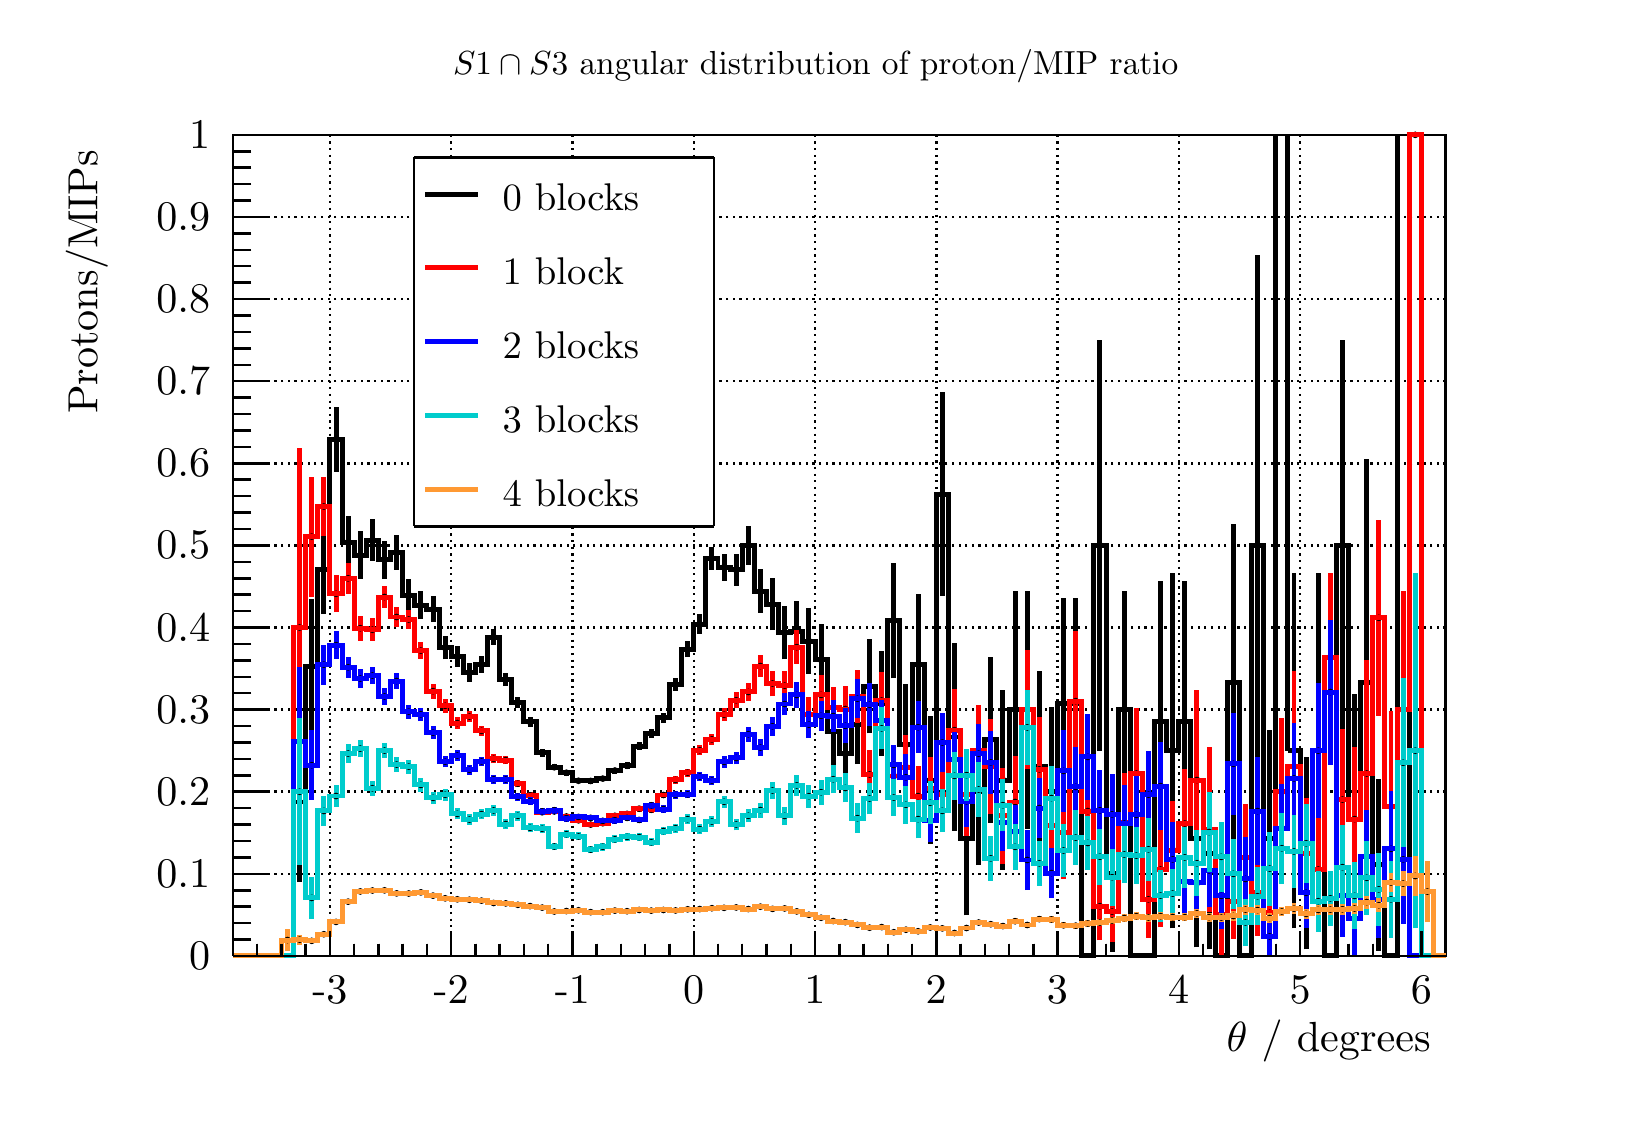
\begin{tikzpicture}
\pgfdeclareplotmark{cross} {
\pgfpathmoveto{\pgfpoint{-0.3\pgfplotmarksize}{\pgfplotmarksize}}
\pgfpathlineto{\pgfpoint{+0.3\pgfplotmarksize}{\pgfplotmarksize}}
\pgfpathlineto{\pgfpoint{+0.3\pgfplotmarksize}{0.3\pgfplotmarksize}}
\pgfpathlineto{\pgfpoint{+1\pgfplotmarksize}{0.3\pgfplotmarksize}}
\pgfpathlineto{\pgfpoint{+1\pgfplotmarksize}{-0.3\pgfplotmarksize}}
\pgfpathlineto{\pgfpoint{+0.3\pgfplotmarksize}{-0.3\pgfplotmarksize}}
\pgfpathlineto{\pgfpoint{+0.3\pgfplotmarksize}{-1.\pgfplotmarksize}}
\pgfpathlineto{\pgfpoint{-0.3\pgfplotmarksize}{-1.\pgfplotmarksize}}
\pgfpathlineto{\pgfpoint{-0.3\pgfplotmarksize}{-0.3\pgfplotmarksize}}
\pgfpathlineto{\pgfpoint{-1.\pgfplotmarksize}{-0.3\pgfplotmarksize}}
\pgfpathlineto{\pgfpoint{-1.\pgfplotmarksize}{0.3\pgfplotmarksize}}
\pgfpathlineto{\pgfpoint{-0.3\pgfplotmarksize}{0.3\pgfplotmarksize}}
\pgfpathclose
\pgfusepathqstroke
}
\pgfdeclareplotmark{cross*} {
\pgfpathmoveto{\pgfpoint{-0.3\pgfplotmarksize}{\pgfplotmarksize}}
\pgfpathlineto{\pgfpoint{+0.3\pgfplotmarksize}{\pgfplotmarksize}}
\pgfpathlineto{\pgfpoint{+0.3\pgfplotmarksize}{0.3\pgfplotmarksize}}
\pgfpathlineto{\pgfpoint{+1\pgfplotmarksize}{0.3\pgfplotmarksize}}
\pgfpathlineto{\pgfpoint{+1\pgfplotmarksize}{-0.3\pgfplotmarksize}}
\pgfpathlineto{\pgfpoint{+0.3\pgfplotmarksize}{-0.3\pgfplotmarksize}}
\pgfpathlineto{\pgfpoint{+0.3\pgfplotmarksize}{-1.\pgfplotmarksize}}
\pgfpathlineto{\pgfpoint{-0.3\pgfplotmarksize}{-1.\pgfplotmarksize}}
\pgfpathlineto{\pgfpoint{-0.3\pgfplotmarksize}{-0.3\pgfplotmarksize}}
\pgfpathlineto{\pgfpoint{-1.\pgfplotmarksize}{-0.3\pgfplotmarksize}}
\pgfpathlineto{\pgfpoint{-1.\pgfplotmarksize}{0.3\pgfplotmarksize}}
\pgfpathlineto{\pgfpoint{-0.3\pgfplotmarksize}{0.3\pgfplotmarksize}}
\pgfpathclose
\pgfusepathqfillstroke
}
\pgfdeclareplotmark{newstar} {
\pgfpathmoveto{\pgfqpoint{0pt}{\pgfplotmarksize}}
\pgfpathlineto{\pgfqpointpolar{44}{0.5\pgfplotmarksize}}
\pgfpathlineto{\pgfqpointpolar{18}{\pgfplotmarksize}}
\pgfpathlineto{\pgfqpointpolar{-20}{0.5\pgfplotmarksize}}
\pgfpathlineto{\pgfqpointpolar{-54}{\pgfplotmarksize}}
\pgfpathlineto{\pgfqpointpolar{-90}{0.5\pgfplotmarksize}}
\pgfpathlineto{\pgfqpointpolar{234}{\pgfplotmarksize}}
\pgfpathlineto{\pgfqpointpolar{198}{0.5\pgfplotmarksize}}
\pgfpathlineto{\pgfqpointpolar{162}{\pgfplotmarksize}}
\pgfpathlineto{\pgfqpointpolar{134}{0.5\pgfplotmarksize}}
\pgfpathclose
\pgfusepathqstroke
}
\pgfdeclareplotmark{newstar*} {
\pgfpathmoveto{\pgfqpoint{0pt}{\pgfplotmarksize}}
\pgfpathlineto{\pgfqpointpolar{44}{0.5\pgfplotmarksize}}
\pgfpathlineto{\pgfqpointpolar{18}{\pgfplotmarksize}}
\pgfpathlineto{\pgfqpointpolar{-20}{0.5\pgfplotmarksize}}
\pgfpathlineto{\pgfqpointpolar{-54}{\pgfplotmarksize}}
\pgfpathlineto{\pgfqpointpolar{-90}{0.5\pgfplotmarksize}}
\pgfpathlineto{\pgfqpointpolar{234}{\pgfplotmarksize}}
\pgfpathlineto{\pgfqpointpolar{198}{0.5\pgfplotmarksize}}
\pgfpathlineto{\pgfqpointpolar{162}{\pgfplotmarksize}}
\pgfpathlineto{\pgfqpointpolar{134}{0.5\pgfplotmarksize}}
\pgfpathclose
\pgfusepathqfillstroke
}
\definecolor{c}{rgb}{1,1,1};
\draw [color=c, fill=c] (0,0) rectangle (20,13.5429);
\draw [color=c, fill=c] (2.6,1.76057) rectangle (18,12.1886);
\definecolor{c}{rgb}{0,0,0};
\draw [c,line width=0.9] (2.6,1.76057) -- (2.6,12.1886) -- (18,12.1886) -- (18,1.76057) -- (2.6,1.76057);
\definecolor{c}{rgb}{1,1,1};
\draw [color=c, fill=c] (2.6,1.76057) rectangle (18,12.1886);
\definecolor{c}{rgb}{0,0,0};
\draw [c,line width=0.9] (2.6,1.76057) -- (2.6,12.1886) -- (18,12.1886) -- (18,1.76057) -- (2.6,1.76057);
\draw [c,line width=0.9] (2.6,1.76057) -- (18,1.76057);
\draw [c,dash pattern=on 0.80pt off 1.60pt ,line width=0.9] (3.832,12.1886) -- (3.832,1.76057);
\draw [c,dash pattern=on 0.80pt off 1.60pt ,line width=0.9] (5.372,12.1886) -- (5.372,1.76057);
\draw [c,dash pattern=on 0.80pt off 1.60pt ,line width=0.9] (6.912,12.1886) -- (6.912,1.76057);
\draw [c,dash pattern=on 0.80pt off 1.60pt ,line width=0.9] (8.452,12.1886) -- (8.452,1.76057);
\draw [c,dash pattern=on 0.80pt off 1.60pt ,line width=0.9] (9.992,12.1886) -- (9.992,1.76057);
\draw [c,dash pattern=on 0.80pt off 1.60pt ,line width=0.9] (11.532,12.1886) -- (11.532,1.76057);
\draw [c,dash pattern=on 0.80pt off 1.60pt ,line width=0.9] (13.072,12.1886) -- (13.072,1.76057);
\draw [c,dash pattern=on 0.80pt off 1.60pt ,line width=0.9] (14.612,12.1886) -- (14.612,1.76057);
\draw [c,dash pattern=on 0.80pt off 1.60pt ,line width=0.9] (16.152,12.1886) -- (16.152,1.76057);
\draw [c,dash pattern=on 0.80pt off 1.60pt ,line width=0.9] (17.692,12.1886) -- (17.692,1.76057);
\draw [c,dash pattern=on 0.80pt off 1.60pt ,line width=0.9] (3.832,12.1886) -- (3.832,1.76057);
\draw [c,dash pattern=on 0.80pt off 1.60pt ,line width=0.9] (17.692,12.1886) -- (17.692,1.76057);
\draw [c,line width=0.9] (2.6,1.76057) -- (2.6,12.1886);
\draw [c,dash pattern=on 0.80pt off 1.60pt ,line width=0.9] (18,1.76057) -- (2.6,1.76057);
\draw [c,dash pattern=on 0.80pt off 1.60pt ,line width=0.9] (18,2.80337) -- (2.6,2.80337);
\draw [c,dash pattern=on 0.80pt off 1.60pt ,line width=0.9] (18,3.84617) -- (2.6,3.84617);
\draw [c,dash pattern=on 0.80pt off 1.60pt ,line width=0.9] (18,4.88897) -- (2.6,4.88897);
\draw [c,dash pattern=on 0.80pt off 1.60pt ,line width=0.9] (18,5.93177) -- (2.6,5.93177);
\draw [c,dash pattern=on 0.80pt off 1.60pt ,line width=0.9] (18,6.97457) -- (2.6,6.97457);
\draw [c,dash pattern=on 0.80pt off 1.60pt ,line width=0.9] (18,8.01737) -- (2.6,8.01737);
\draw [c,dash pattern=on 0.80pt off 1.60pt ,line width=0.9] (18,9.06017) -- (2.6,9.06017);
\draw [c,dash pattern=on 0.80pt off 1.60pt ,line width=0.9] (18,10.103) -- (2.6,10.103);
\draw [c,dash pattern=on 0.80pt off 1.60pt ,line width=0.9] (18,11.1458) -- (2.6,11.1458);
\draw [c,dash pattern=on 0.80pt off 1.60pt ,line width=0.9] (18,12.1886) -- (2.6,12.1886);
\definecolor{c}{rgb}{0,0,0.6};
\draw [c,line width=0.9] (2.6,1.76057) -- (2.754,1.76057) -- (2.754,1.76057) -- (2.908,1.76057) -- (2.908,1.76057) -- (3.062,1.76057) -- (3.062,1.76057) -- (3.216,1.76057) -- (3.216,1.76057) -- (3.37,1.76057) -- (3.37,1.76057) -- (3.524,1.76057) --
 (3.524,1.76057) -- (3.678,1.76057) -- (3.678,1.76057) -- (3.832,1.76057) -- (3.832,1.76057) -- (3.986,1.76057) -- (3.986,1.76057) -- (4.14,1.76057) -- (4.14,1.76057) -- (4.294,1.76057) -- (4.294,1.76057) -- (4.448,1.76057) -- (4.448,1.76057) --
 (4.602,1.76057) -- (4.602,1.76057) -- (4.756,1.76057) -- (4.756,1.76057) -- (4.91,1.76057) -- (4.91,1.76057) -- (5.064,1.76057) -- (5.064,1.76057) -- (5.218,1.76057) -- (5.218,1.76057) -- (5.372,1.76057) -- (5.372,1.76057) -- (5.526,1.76057) --
 (5.526,1.76057) -- (5.68,1.76057) -- (5.68,1.76057) -- (5.834,1.76057) -- (5.834,1.76057) -- (5.988,1.76057) -- (5.988,1.76057) -- (6.142,1.76057) -- (6.142,1.76057) -- (6.296,1.76057) -- (6.296,1.76057) -- (6.45,1.76057) -- (6.45,1.76057) --
 (6.604,1.76057) -- (6.604,1.76057) -- (6.758,1.76057) -- (6.758,1.76057) -- (6.912,1.76057) -- (6.912,1.76057) -- (7.066,1.76057) -- (7.066,1.76057) -- (7.22,1.76057) -- (7.22,1.76057) -- (7.374,1.76057) -- (7.374,1.76057) -- (7.528,1.76057) --
 (7.528,1.76057) -- (7.682,1.76057) -- (7.682,1.76057) -- (7.836,1.76057) -- (7.836,1.76057) -- (7.99,1.76057) -- (7.99,1.76057) -- (8.144,1.76057) -- (8.144,1.76057) -- (8.298,1.76057) -- (8.298,1.76057) -- (8.452,1.76057) -- (8.452,1.76057) --
 (8.606,1.76057) -- (8.606,1.76057) -- (8.76,1.76057) -- (8.76,1.76057) -- (8.914,1.76057) -- (8.914,1.76057) -- (9.068,1.76057) -- (9.068,1.76057) -- (9.222,1.76057) -- (9.222,1.76057) -- (9.376,1.76057) -- (9.376,1.76057) -- (9.53,1.76057) --
 (9.53,1.76057) -- (9.684,1.76057) -- (9.684,1.76057) -- (9.838,1.76057) -- (9.838,1.76057) -- (9.992,1.76057) -- (9.992,1.76057) -- (10.146,1.76057) -- (10.146,1.76057) -- (10.3,1.76057) -- (10.3,1.76057) -- (10.454,1.76057) -- (10.454,1.76057) --
 (10.608,1.76057) -- (10.608,1.76057) -- (10.762,1.76057) -- (10.762,1.76057) -- (10.916,1.76057) -- (10.916,1.76057) -- (11.07,1.76057) -- (11.07,1.76057) -- (11.224,1.76057) -- (11.224,1.76057) -- (11.378,1.76057) -- (11.378,1.76057) --
 (11.532,1.76057) -- (11.532,1.76057) -- (11.686,1.76057) -- (11.686,1.76057) -- (11.84,1.76057) -- (11.84,1.76057) -- (11.994,1.76057) -- (11.994,1.76057) -- (12.148,1.76057) -- (12.148,1.76057) -- (12.302,1.76057) -- (12.302,1.76057) --
 (12.456,1.76057) -- (12.456,1.76057) -- (12.61,1.76057) -- (12.61,1.76057) -- (12.764,1.76057) -- (12.764,1.76057) -- (12.918,1.76057) -- (12.918,1.76057) -- (13.072,1.76057) -- (13.072,1.76057) -- (13.226,1.76057) -- (13.226,1.76057) --
 (13.38,1.76057) -- (13.38,1.76057) -- (13.534,1.76057) -- (13.534,1.76057) -- (13.688,1.76057) -- (13.688,1.76057) -- (13.842,1.76057) -- (13.842,1.76057) -- (13.996,1.76057) -- (13.996,1.76057) -- (14.15,1.76057) -- (14.15,1.76057) --
 (14.304,1.76057) -- (14.304,1.76057) -- (14.458,1.76057) -- (14.458,1.76057) -- (14.612,1.76057) -- (14.612,1.76057) -- (14.766,1.76057) -- (14.766,1.76057) -- (14.92,1.76057) -- (14.92,1.76057) -- (15.074,1.76057) -- (15.074,1.76057) --
 (15.228,1.76057) -- (15.228,1.76057) -- (15.382,1.76057) -- (15.382,1.76057) -- (15.536,1.76057) -- (15.536,1.76057) -- (15.69,1.76057) -- (15.69,1.76057) -- (15.844,1.76057) -- (15.844,1.76057) -- (15.998,1.76057) -- (15.998,1.76057) --
 (16.152,1.76057) -- (16.152,1.76057) -- (16.306,1.76057) -- (16.306,1.76057) -- (16.46,1.76057) -- (16.46,1.76057) -- (16.614,1.76057) -- (16.614,1.76057) -- (16.768,1.76057) -- (16.768,1.76057) -- (16.922,1.76057) -- (16.922,1.76057) --
 (17.076,1.76057) -- (17.076,1.76057) -- (17.23,1.76057) -- (17.23,1.76057) -- (17.384,1.76057) -- (17.384,1.76057) -- (17.538,1.76057) -- (17.538,1.76057) -- (17.692,1.76057) -- (17.692,1.76057) -- (17.846,1.76057) -- (17.846,1.76057) --
 (18,1.76057);
\definecolor{c}{rgb}{0,0,0};
\draw [c,line width=0.9] (2.6,1.76057) -- (18,1.76057);
\draw [c,line width=0.9] (3.832,2.07341) -- (3.832,1.76057);
\draw [c,line width=0.9] (4.14,1.91699) -- (4.14,1.76057);
\draw [c,line width=0.9] (4.448,1.91699) -- (4.448,1.76057);
\draw [c,line width=0.9] (4.756,1.91699) -- (4.756,1.76057);
\draw [c,line width=0.9] (5.064,1.91699) -- (5.064,1.76057);
\draw [c,line width=0.9] (5.372,2.07341) -- (5.372,1.76057);
\draw [c,line width=0.9] (5.68,1.91699) -- (5.68,1.76057);
\draw [c,line width=0.9] (5.988,1.91699) -- (5.988,1.76057);
\draw [c,line width=0.9] (6.296,1.91699) -- (6.296,1.76057);
\draw [c,line width=0.9] (6.604,1.91699) -- (6.604,1.76057);
\draw [c,line width=0.9] (6.912,2.07341) -- (6.912,1.76057);
\draw [c,line width=0.9] (7.22,1.91699) -- (7.22,1.76057);
\draw [c,line width=0.9] (7.528,1.91699) -- (7.528,1.76057);
\draw [c,line width=0.9] (7.836,1.91699) -- (7.836,1.76057);
\draw [c,line width=0.9] (8.144,1.91699) -- (8.144,1.76057);
\draw [c,line width=0.9] (8.452,2.07341) -- (8.452,1.76057);
\draw [c,line width=0.9] (8.76,1.91699) -- (8.76,1.76057);
\draw [c,line width=0.9] (9.068,1.91699) -- (9.068,1.76057);
\draw [c,line width=0.9] (9.376,1.91699) -- (9.376,1.76057);
\draw [c,line width=0.9] (9.684,1.91699) -- (9.684,1.76057);
\draw [c,line width=0.9] (9.992,2.07341) -- (9.992,1.76057);
\draw [c,line width=0.9] (10.3,1.91699) -- (10.3,1.76057);
\draw [c,line width=0.9] (10.608,1.91699) -- (10.608,1.76057);
\draw [c,line width=0.9] (10.916,1.91699) -- (10.916,1.76057);
\draw [c,line width=0.9] (11.224,1.91699) -- (11.224,1.76057);
\draw [c,line width=0.9] (11.532,2.07341) -- (11.532,1.76057);
\draw [c,line width=0.9] (11.84,1.91699) -- (11.84,1.76057);
\draw [c,line width=0.9] (12.148,1.91699) -- (12.148,1.76057);
\draw [c,line width=0.9] (12.456,1.91699) -- (12.456,1.76057);
\draw [c,line width=0.9] (12.764,1.91699) -- (12.764,1.76057);
\draw [c,line width=0.9] (13.072,2.07341) -- (13.072,1.76057);
\draw [c,line width=0.9] (13.38,1.91699) -- (13.38,1.76057);
\draw [c,line width=0.9] (13.688,1.91699) -- (13.688,1.76057);
\draw [c,line width=0.9] (13.996,1.91699) -- (13.996,1.76057);
\draw [c,line width=0.9] (14.304,1.91699) -- (14.304,1.76057);
\draw [c,line width=0.9] (14.612,2.07341) -- (14.612,1.76057);
\draw [c,line width=0.9] (14.92,1.91699) -- (14.92,1.76057);
\draw [c,line width=0.9] (15.228,1.91699) -- (15.228,1.76057);
\draw [c,line width=0.9] (15.536,1.91699) -- (15.536,1.76057);
\draw [c,line width=0.9] (15.844,1.91699) -- (15.844,1.76057);
\draw [c,line width=0.9] (16.152,2.07341) -- (16.152,1.76057);
\draw [c,line width=0.9] (16.46,1.91699) -- (16.46,1.76057);
\draw [c,line width=0.9] (16.768,1.91699) -- (16.768,1.76057);
\draw [c,line width=0.9] (17.076,1.91699) -- (17.076,1.76057);
\draw [c,line width=0.9] (17.384,1.91699) -- (17.384,1.76057);
\draw [c,line width=0.9] (17.692,2.07341) -- (17.692,1.76057);
\draw [c,line width=0.9] (3.832,2.07341) -- (3.832,1.76057);
\draw [c,line width=0.9] (3.524,1.91699) -- (3.524,1.76057);
\draw [c,line width=0.9] (3.216,1.91699) -- (3.216,1.76057);
\draw [c,line width=0.9] (2.908,1.91699) -- (2.908,1.76057);
\draw [c,line width=0.9] (17.692,2.07341) -- (17.692,1.76057);
\draw [anchor=base] (3.832,1.15114) node[scale=1.52295, color=c, rotate=0]{-3};
\draw [anchor=base] (5.372,1.15114) node[scale=1.52295, color=c, rotate=0]{-2};
\draw [anchor=base] (6.912,1.15114) node[scale=1.52295, color=c, rotate=0]{-1};
\draw [anchor=base] (8.452,1.15114) node[scale=1.52295, color=c, rotate=0]{0};
\draw [anchor=base] (9.992,1.15114) node[scale=1.52295, color=c, rotate=0]{1};
\draw [anchor=base] (11.532,1.15114) node[scale=1.52295, color=c, rotate=0]{2};
\draw [anchor=base] (13.072,1.15114) node[scale=1.52295, color=c, rotate=0]{3};
\draw [anchor=base] (14.612,1.15114) node[scale=1.52295, color=c, rotate=0]{4};
\draw [anchor=base] (16.152,1.15114) node[scale=1.52295, color=c, rotate=0]{5};
\draw [anchor=base] (17.692,1.15114) node[scale=1.52295, color=c, rotate=0]{6};
\draw [anchor= east] (18,0.677143) node[scale=1.52295, color=c, rotate=0]{$ \theta$ / degrees};
\draw [c,line width=0.9] (2.6,1.76057) -- (2.6,12.1886);
\draw [c,line width=0.9] (3.062,1.76057) -- (2.6,1.76057);
\draw [c,line width=0.9] (2.831,1.96913) -- (2.6,1.96913);
\draw [c,line width=0.9] (2.831,2.17769) -- (2.6,2.17769);
\draw [c,line width=0.9] (2.831,2.38625) -- (2.6,2.38625);
\draw [c,line width=0.9] (2.831,2.59481) -- (2.6,2.59481);
\draw [c,line width=0.9] (3.062,2.80337) -- (2.6,2.80337);
\draw [c,line width=0.9] (2.831,3.01193) -- (2.6,3.01193);
\draw [c,line width=0.9] (2.831,3.22049) -- (2.6,3.22049);
\draw [c,line width=0.9] (2.831,3.42905) -- (2.6,3.42905);
\draw [c,line width=0.9] (2.831,3.63761) -- (2.6,3.63761);
\draw [c,line width=0.9] (3.062,3.84617) -- (2.6,3.84617);
\draw [c,line width=0.9] (2.831,4.05473) -- (2.6,4.05473);
\draw [c,line width=0.9] (2.831,4.26329) -- (2.6,4.26329);
\draw [c,line width=0.9] (2.831,4.47185) -- (2.6,4.47185);
\draw [c,line width=0.9] (2.831,4.68041) -- (2.6,4.68041);
\draw [c,line width=0.9] (3.062,4.88897) -- (2.6,4.88897);
\draw [c,line width=0.9] (2.831,5.09753) -- (2.6,5.09753);
\draw [c,line width=0.9] (2.831,5.30609) -- (2.6,5.30609);
\draw [c,line width=0.9] (2.831,5.51465) -- (2.6,5.51465);
\draw [c,line width=0.9] (2.831,5.72321) -- (2.6,5.72321);
\draw [c,line width=0.9] (3.062,5.93177) -- (2.6,5.93177);
\draw [c,line width=0.9] (2.831,6.14033) -- (2.6,6.14033);
\draw [c,line width=0.9] (2.831,6.34889) -- (2.6,6.34889);
\draw [c,line width=0.9] (2.831,6.55745) -- (2.6,6.55745);
\draw [c,line width=0.9] (2.831,6.76601) -- (2.6,6.76601);
\draw [c,line width=0.9] (3.062,6.97457) -- (2.6,6.97457);
\draw [c,line width=0.9] (2.831,7.18313) -- (2.6,7.18313);
\draw [c,line width=0.9] (2.831,7.39169) -- (2.6,7.39169);
\draw [c,line width=0.9] (2.831,7.60025) -- (2.6,7.60025);
\draw [c,line width=0.9] (2.831,7.80881) -- (2.6,7.80881);
\draw [c,line width=0.9] (3.062,8.01737) -- (2.6,8.01737);
\draw [c,line width=0.9] (2.831,8.22593) -- (2.6,8.22593);
\draw [c,line width=0.9] (2.831,8.43449) -- (2.6,8.43449);
\draw [c,line width=0.9] (2.831,8.64305) -- (2.6,8.64305);
\draw [c,line width=0.9] (2.831,8.85161) -- (2.6,8.85161);
\draw [c,line width=0.9] (3.062,9.06017) -- (2.6,9.06017);
\draw [c,line width=0.9] (2.831,9.26873) -- (2.6,9.26873);
\draw [c,line width=0.9] (2.831,9.47729) -- (2.6,9.47729);
\draw [c,line width=0.9] (2.831,9.68585) -- (2.6,9.68585);
\draw [c,line width=0.9] (2.831,9.89441) -- (2.6,9.89441);
\draw [c,line width=0.9] (3.062,10.103) -- (2.6,10.103);
\draw [c,line width=0.9] (2.831,10.3115) -- (2.6,10.3115);
\draw [c,line width=0.9] (2.831,10.5201) -- (2.6,10.5201);
\draw [c,line width=0.9] (2.831,10.7287) -- (2.6,10.7287);
\draw [c,line width=0.9] (2.831,10.9372) -- (2.6,10.9372);
\draw [c,line width=0.9] (3.062,11.1458) -- (2.6,11.1458);
\draw [c,line width=0.9] (2.831,11.3543) -- (2.6,11.3543);
\draw [c,line width=0.9] (2.831,11.5629) -- (2.6,11.5629);
\draw [c,line width=0.9] (2.831,11.7715) -- (2.6,11.7715);
\draw [c,line width=0.9] (2.831,11.98) -- (2.6,11.98);
\draw [c,line width=0.9] (3.062,12.1886) -- (2.6,12.1886);
\draw [anchor= east] (2.5,1.76057) node[scale=1.52295, color=c, rotate=0]{0};
\draw [anchor= east] (2.5,2.80337) node[scale=1.52295, color=c, rotate=0]{0.1};
\draw [anchor= east] (2.5,3.84617) node[scale=1.52295, color=c, rotate=0]{0.2};
\draw [anchor= east] (2.5,4.88897) node[scale=1.52295, color=c, rotate=0]{0.3};
\draw [anchor= east] (2.5,5.93177) node[scale=1.52295, color=c, rotate=0]{0.4};
\draw [anchor= east] (2.5,6.97457) node[scale=1.52295, color=c, rotate=0]{0.5};
\draw [anchor= east] (2.5,8.01737) node[scale=1.52295, color=c, rotate=0]{0.6};
\draw [anchor= east] (2.5,9.06017) node[scale=1.52295, color=c, rotate=0]{0.7};
\draw [anchor= east] (2.5,10.103) node[scale=1.52295, color=c, rotate=0]{0.8};
\draw [anchor= east] (2.5,11.1458) node[scale=1.52295, color=c, rotate=0]{0.9};
\draw [anchor= east] (2.5,12.1886) node[scale=1.52295, color=c, rotate=0]{1};
\draw [anchor= east] (0.742857,12.1886) node[scale=1.52295, color=c, rotate=90]{  Protons/MIPs};
\draw [c,line width=1.8] (3.447,2.69828) -- (3.447,3.71582);
\draw [c,line width=1.8] (3.447,3.71582) -- (3.447,4.73337);
\foreach \P in {(3.447,3.71582)}{\draw[mark options={color=c,fill=c},mark size=2.402402pt,mark=*,mark size=1pt] plot coordinates {\P};}
\draw [c,line width=1.8] (3.601,4.5864) -- (3.601,5.44104);
\draw [c,line width=1.8] (3.601,5.44104) -- (3.601,6.29568);
\foreach \P in {(3.601,5.44104)}{\draw[mark options={color=c,fill=c},mark size=2.402402pt,mark=*,mark size=1pt] plot coordinates {\P};}
\draw [c,line width=1.8] (3.755,6.10331) -- (3.755,6.66787);
\draw [c,line width=1.8] (3.755,6.66787) -- (3.755,7.23242);
\foreach \P in {(3.755,6.66787)}{\draw[mark options={color=c,fill=c},mark size=2.402402pt,mark=*,mark size=1pt] plot coordinates {\P};}
\draw [c,line width=1.8] (3.909,7.91132) -- (3.909,8.32123);
\draw [c,line width=1.8] (3.909,8.32123) -- (3.909,8.73115);
\foreach \P in {(3.909,8.32123)}{\draw[mark options={color=c,fill=c},mark size=2.402402pt,mark=*,mark size=1pt] plot coordinates {\P};}
\draw [c,line width=1.8] (4.063,6.68653) -- (4.063,7.01628);
\draw [c,line width=1.8] (4.063,7.01628) -- (4.063,7.34604);
\foreach \P in {(4.063,7.01628)}{\draw[mark options={color=c,fill=c},mark size=2.402402pt,mark=*,mark size=1pt] plot coordinates {\P};}
\draw [c,line width=1.8] (4.217,6.54736) -- (4.217,6.85085);
\draw [c,line width=1.8] (4.217,6.85085) -- (4.217,7.15433);
\foreach \P in {(4.217,6.85085)}{\draw[mark options={color=c,fill=c},mark size=2.402402pt,mark=*,mark size=1pt] plot coordinates {\P};}
\draw [c,line width=1.8] (4.371,6.77692) -- (4.371,7.04194);
\draw [c,line width=1.8] (4.371,7.04194) -- (4.371,7.30696);
\foreach \P in {(4.371,7.04194)}{\draw[mark options={color=c,fill=c},mark size=2.402402pt,mark=*,mark size=1pt] plot coordinates {\P};}
\draw [c,line width=1.8] (4.525,6.54627) -- (4.525,6.79082);
\draw [c,line width=1.8] (4.525,6.79082) -- (4.525,7.03537);
\foreach \P in {(4.525,6.79082)}{\draw[mark options={color=c,fill=c},mark size=2.402402pt,mark=*,mark size=1pt] plot coordinates {\P};}
\draw [c,line width=1.8] (4.679,6.66261) -- (4.679,6.88212);
\draw [c,line width=1.8] (4.679,6.88212) -- (4.679,7.10164);
\foreach \P in {(4.679,6.88212)}{\draw[mark options={color=c,fill=c},mark size=2.402402pt,mark=*,mark size=1pt] plot coordinates {\P};}
\draw [c,line width=1.8] (4.833,6.14124) -- (4.833,6.34378);
\draw [c,line width=1.8] (4.833,6.34378) -- (4.833,6.54632);
\foreach \P in {(4.833,6.34378)}{\draw[mark options={color=c,fill=c},mark size=2.402402pt,mark=*,mark size=1pt] plot coordinates {\P};}
\draw [c,line width=1.8] (4.987,6.03439) -- (4.987,6.21354);
\draw [c,line width=1.8] (4.987,6.21354) -- (4.987,6.39269);
\foreach \P in {(4.987,6.21354)}{\draw[mark options={color=c,fill=c},mark size=2.402402pt,mark=*,mark size=1pt] plot coordinates {\P};}
\draw [c,line width=1.8] (5.141,6.00133) -- (5.141,6.16587);
\draw [c,line width=1.8] (5.141,6.16587) -- (5.141,6.33041);
\foreach \P in {(5.141,6.16587)}{\draw[mark options={color=c,fill=c},mark size=2.402402pt,mark=*,mark size=1pt] plot coordinates {\P};}
\draw [c,line width=1.8] (5.295,5.52618) -- (5.295,5.67328);
\draw [c,line width=1.8] (5.295,5.67328) -- (5.295,5.82039);
\foreach \P in {(5.295,5.67328)}{\draw[mark options={color=c,fill=c},mark size=2.402402pt,mark=*,mark size=1pt] plot coordinates {\P};}
\draw [c,line width=1.8] (5.449,5.43471) -- (5.449,5.5688);
\draw [c,line width=1.8] (5.449,5.5688) -- (5.449,5.70289);
\foreach \P in {(5.449,5.5688)}{\draw[mark options={color=c,fill=c},mark size=2.402402pt,mark=*,mark size=1pt] plot coordinates {\P};}
\draw [c,line width=1.8] (5.603,5.24489) -- (5.603,5.36319);
\draw [c,line width=1.8] (5.603,5.36319) -- (5.603,5.48149);
\foreach \P in {(5.603,5.36319)}{\draw[mark options={color=c,fill=c},mark size=2.402402pt,mark=*,mark size=1pt] plot coordinates {\P};}
\draw [c,line width=1.8] (5.757,5.35586) -- (5.757,5.46365);
\draw [c,line width=1.8] (5.757,5.46365) -- (5.757,5.57145);
\foreach \P in {(5.757,5.46365)}{\draw[mark options={color=c,fill=c},mark size=2.402402pt,mark=*,mark size=1pt] plot coordinates {\P};}
\draw [c,line width=1.8] (5.911,5.71068) -- (5.911,5.80974);
\draw [c,line width=1.8] (5.911,5.80974) -- (5.911,5.9088);
\foreach \P in {(5.911,5.80974)}{\draw[mark options={color=c,fill=c},mark size=2.402402pt,mark=*,mark size=1pt] plot coordinates {\P};}
\draw [c,line width=1.8] (6.065,5.18882) -- (6.065,5.27358);
\draw [c,line width=1.8] (6.065,5.27358) -- (6.065,5.35835);
\foreach \P in {(6.065,5.27358)}{\draw[mark options={color=c,fill=c},mark size=2.402402pt,mark=*,mark size=1pt] plot coordinates {\P};}
\draw [c,line width=1.8] (6.219,4.90855) -- (6.219,4.97895);
\draw [c,line width=1.8] (6.219,4.97895) -- (6.219,5.04935);
\foreach \P in {(6.219,4.97895)}{\draw[mark options={color=c,fill=c},mark size=2.402402pt,mark=*,mark size=1pt] plot coordinates {\P};}
\draw [c,line width=1.8] (6.373,4.67359) -- (6.373,4.73253);
\draw [c,line width=1.8] (6.373,4.73253) -- (6.373,4.79147);
\foreach \P in {(6.373,4.73253)}{\draw[mark options={color=c,fill=c},mark size=2.402402pt,mark=*,mark size=1pt] plot coordinates {\P};}
\draw [c,line width=1.8] (6.527,4.29323) -- (6.527,4.34135);
\draw [c,line width=1.8] (6.527,4.34135) -- (6.527,4.38946);
\foreach \P in {(6.527,4.34135)}{\draw[mark options={color=c,fill=c},mark size=2.402402pt,mark=*,mark size=1pt] plot coordinates {\P};}
\draw [c,line width=1.8] (6.681,4.11642) -- (6.681,4.1571);
\draw [c,line width=1.8] (6.681,4.1571) -- (6.681,4.19778);
\foreach \P in {(6.681,4.1571)}{\draw[mark options={color=c,fill=c},mark size=2.402402pt,mark=*,mark size=1pt] plot coordinates {\P};}
\draw [c,line width=1.8] (6.835,4.05142) -- (6.835,4.08804);
\draw [c,line width=1.8] (6.835,4.08804) -- (6.835,4.12465);
\foreach \P in {(6.835,4.08804)}{\draw[mark options={color=c,fill=c},mark size=2.402402pt,mark=*,mark size=1pt] plot coordinates {\P};}
\draw [c,line width=1.8] (6.989,3.95156) -- (6.989,3.98547);
\draw [c,line width=1.8] (6.989,3.98547) -- (6.989,4.01939);
\foreach \P in {(6.989,3.98547)}{\draw[mark options={color=c,fill=c},mark size=2.402402pt,mark=*,mark size=1pt] plot coordinates {\P};}
\draw [c,line width=1.8] (7.143,3.94992) -- (7.143,3.98352);
\draw [c,line width=1.8] (7.143,3.98352) -- (7.143,4.01712);
\foreach \P in {(7.143,3.98352)}{\draw[mark options={color=c,fill=c},mark size=2.402402pt,mark=*,mark size=1pt] plot coordinates {\P};}
\draw [c,line width=1.8] (7.297,3.97822) -- (7.297,4.013);
\draw [c,line width=1.8] (7.297,4.013) -- (7.297,4.04777);
\foreach \P in {(7.297,4.013)}{\draw[mark options={color=c,fill=c},mark size=2.402402pt,mark=*,mark size=1pt] plot coordinates {\P};}
\draw [c,line width=1.8] (7.451,4.07786) -- (7.451,4.11597);
\draw [c,line width=1.8] (7.451,4.11597) -- (7.451,4.15409);
\foreach \P in {(7.451,4.11597)}{\draw[mark options={color=c,fill=c},mark size=2.402402pt,mark=*,mark size=1pt] plot coordinates {\P};}
\draw [c,line width=1.8] (7.605,4.13387) -- (7.605,4.17615);
\draw [c,line width=1.8] (7.605,4.17615) -- (7.605,4.21843);
\foreach \P in {(7.605,4.17615)}{\draw[mark options={color=c,fill=c},mark size=2.402402pt,mark=*,mark size=1pt] plot coordinates {\P};}
\draw [c,line width=1.8] (7.759,4.37721) -- (7.759,4.42618);
\draw [c,line width=1.8] (7.759,4.42618) -- (7.759,4.47514);
\foreach \P in {(7.759,4.42618)}{\draw[mark options={color=c,fill=c},mark size=2.402402pt,mark=*,mark size=1pt] plot coordinates {\P};}
\draw [c,line width=1.8] (7.913,4.52827) -- (7.913,4.58456);
\draw [c,line width=1.8] (7.913,4.58456) -- (7.913,4.64086);
\foreach \P in {(7.913,4.58456)}{\draw[mark options={color=c,fill=c},mark size=2.402402pt,mark=*,mark size=1pt] plot coordinates {\P};}
\draw [c,line width=1.8] (8.067,4.71813) -- (8.067,4.78436);
\draw [c,line width=1.8] (8.067,4.78436) -- (8.067,4.8506);
\foreach \P in {(8.067,4.78436)}{\draw[mark options={color=c,fill=c},mark size=2.402402pt,mark=*,mark size=1pt] plot coordinates {\P};}
\draw [c,line width=1.8] (8.221,5.13176) -- (8.221,5.21346);
\draw [c,line width=1.8] (8.221,5.21346) -- (8.221,5.29515);
\foreach \P in {(8.221,5.21346)}{\draw[mark options={color=c,fill=c},mark size=2.402402pt,mark=*,mark size=1pt] plot coordinates {\P};}
\draw [c,line width=1.8] (8.375,5.55691) -- (8.375,5.65799);
\draw [c,line width=1.8] (8.375,5.65799) -- (8.375,5.75907);
\foreach \P in {(8.375,5.65799)}{\draw[mark options={color=c,fill=c},mark size=2.402402pt,mark=*,mark size=1pt] plot coordinates {\P};}
\draw [c,line width=1.8] (8.529,5.85343) -- (8.529,5.97615);
\draw [c,line width=1.8] (8.529,5.97615) -- (8.529,6.09886);
\foreach \P in {(8.529,5.97615)}{\draw[mark options={color=c,fill=c},mark size=2.402402pt,mark=*,mark size=1pt] plot coordinates {\P};}
\draw [c,line width=1.8] (8.683,6.66209) -- (8.683,6.80769);
\draw [c,line width=1.8] (8.683,6.80769) -- (8.683,6.9533);
\foreach \P in {(8.683,6.80769)}{\draw[mark options={color=c,fill=c},mark size=2.402402pt,mark=*,mark size=1pt] plot coordinates {\P};}
\draw [c,line width=1.8] (8.837,6.52375) -- (8.837,6.69711);
\draw [c,line width=1.8] (8.837,6.69711) -- (8.837,6.87047);
\foreach \P in {(8.837,6.69711)}{\draw[mark options={color=c,fill=c},mark size=2.402402pt,mark=*,mark size=1pt] plot coordinates {\P};}
\draw [c,line width=1.8] (8.991,6.46344) -- (8.991,6.66421);
\draw [c,line width=1.8] (8.991,6.66421) -- (8.991,6.86499);
\foreach \P in {(8.991,6.66421)}{\draw[mark options={color=c,fill=c},mark size=2.402402pt,mark=*,mark size=1pt] plot coordinates {\P};}
\draw [c,line width=1.8] (9.145,6.73147) -- (9.145,6.97457);
\draw [c,line width=1.8] (9.145,6.97457) -- (9.145,7.21768);
\foreach \P in {(9.145,6.97457)}{\draw[mark options={color=c,fill=c},mark size=2.402402pt,mark=*,mark size=1pt] plot coordinates {\P};}
\draw [c,line width=1.8] (9.299,6.11866) -- (9.299,6.39524);
\draw [c,line width=1.8] (9.299,6.39524) -- (9.299,6.67182);
\foreach \P in {(9.299,6.39524)}{\draw[mark options={color=c,fill=c},mark size=2.402402pt,mark=*,mark size=1pt] plot coordinates {\P};}
\draw [c,line width=1.8] (9.453,5.90002) -- (9.453,6.22971);
\draw [c,line width=1.8] (9.453,6.22971) -- (9.453,6.55941);
\foreach \P in {(9.453,6.22971)}{\draw[mark options={color=c,fill=c},mark size=2.402402pt,mark=*,mark size=1pt] plot coordinates {\P};}
\draw [c,line width=1.8] (9.607,5.52826) -- (9.607,5.86717);
\draw [c,line width=1.8] (9.607,5.86717) -- (9.607,6.20609);
\foreach \P in {(9.607,5.86717)}{\draw[mark options={color=c,fill=c},mark size=2.402402pt,mark=*,mark size=1pt] plot coordinates {\P};}
\draw [c,line width=1.8] (9.761,5.50139) -- (9.761,5.88464);
\draw [c,line width=1.8] (9.761,5.88464) -- (9.761,6.26789);
\foreach \P in {(9.761,5.88464)}{\draw[mark options={color=c,fill=c},mark size=2.402402pt,mark=*,mark size=1pt] plot coordinates {\P};}
\draw [c,line width=1.8] (9.915,5.3407) -- (9.915,5.76035);
\draw [c,line width=1.8] (9.915,5.76035) -- (9.915,6.18);
\foreach \P in {(9.915,5.76035)}{\draw[mark options={color=c,fill=c},mark size=2.402402pt,mark=*,mark size=1pt] plot coordinates {\P};}
\draw [c,line width=1.8] (10.069,5.06814) -- (10.069,5.52149);
\draw [c,line width=1.8] (10.069,5.52149) -- (10.069,5.97484);
\foreach \P in {(10.069,5.52149)}{\draw[mark options={color=c,fill=c},mark size=2.402402pt,mark=*,mark size=1pt] plot coordinates {\P};}
\draw [c,line width=1.8] (10.223,4.18293) -- (10.223,4.61267);
\draw [c,line width=1.8] (10.223,4.61267) -- (10.223,5.04241);
\foreach \P in {(10.223,4.61267)}{\draw[mark options={color=c,fill=c},mark size=2.402402pt,mark=*,mark size=1pt] plot coordinates {\P};}
\draw [c,line width=1.8] (10.377,3.77029) -- (10.377,4.32746);
\draw [c,line width=1.8] (10.377,4.32746) -- (10.377,4.88464);
\foreach \P in {(10.377,4.32746)}{\draw[mark options={color=c,fill=c},mark size=2.402402pt,mark=*,mark size=1pt] plot coordinates {\P};}
\draw [c,line width=1.8] (10.531,4.1958) -- (10.531,4.70495);
\draw [c,line width=1.8] (10.531,4.70495) -- (10.531,5.21409);
\foreach \P in {(10.531,4.70495)}{\draw[mark options={color=c,fill=c},mark size=2.402402pt,mark=*,mark size=1pt] plot coordinates {\P};}
\draw [c,line width=1.8] (10.685,4.58641) -- (10.685,5.18469);
\draw [c,line width=1.8] (10.685,5.18469) -- (10.685,5.78297);
\foreach \P in {(10.685,5.18469)}{\draw[mark options={color=c,fill=c},mark size=2.402402pt,mark=*,mark size=1pt] plot coordinates {\P};}
\draw [c,line width=1.8] (10.839,4.30175) -- (10.839,4.96919);
\draw [c,line width=1.8] (10.839,4.96919) -- (10.839,5.63662);
\foreach \P in {(10.839,4.96919)}{\draw[mark options={color=c,fill=c},mark size=2.402402pt,mark=*,mark size=1pt] plot coordinates {\P};}
\draw [c,line width=1.8] (10.993,5.28471) -- (10.993,6.0169);
\draw [c,line width=1.8] (10.993,6.0169) -- (10.993,6.74908);
\foreach \P in {(10.993,6.0169)}{\draw[mark options={color=c,fill=c},mark size=2.402402pt,mark=*,mark size=1pt] plot coordinates {\P};}
\draw [c,line width=1.8] (11.147,3.67167) -- (11.147,4.44206);
\draw [c,line width=1.8] (11.147,4.44206) -- (11.147,5.21244);
\foreach \P in {(11.147,4.44206)}{\draw[mark options={color=c,fill=c},mark size=2.402402pt,mark=*,mark size=1pt] plot coordinates {\P};}
\draw [c,line width=1.8] (11.301,4.5647) -- (11.301,5.46083);
\draw [c,line width=1.8] (11.301,5.46083) -- (11.301,6.35696);
\foreach \P in {(11.301,5.46083)}{\draw[mark options={color=c,fill=c},mark size=2.402402pt,mark=*,mark size=1pt] plot coordinates {\P};}
\draw [c,line width=1.8] (11.455,3.18651) -- (11.455,3.99514);
\draw [c,line width=1.8] (11.455,3.99514) -- (11.455,4.80377);
\foreach \P in {(11.455,3.99514)}{\draw[mark options={color=c,fill=c},mark size=2.402402pt,mark=*,mark size=1pt] plot coordinates {\P};}
\draw [c,line width=1.8] (11.609,6.33305) -- (11.609,7.62632);
\draw [c,line width=1.8] (11.609,7.62632) -- (11.609,8.9196);
\foreach \P in {(11.609,7.62632)}{\draw[mark options={color=c,fill=c},mark size=2.402402pt,mark=*,mark size=1pt] plot coordinates {\P};}
\draw [c,line width=1.8] (11.763,3.3507) -- (11.763,4.54137);
\draw [c,line width=1.8] (11.763,4.54137) -- (11.763,5.73204);
\foreach \P in {(11.763,4.54137)}{\draw[mark options={color=c,fill=c},mark size=2.402402pt,mark=*,mark size=1pt] plot coordinates {\P};}
\draw [c,line width=1.8] (11.917,2.27504) -- (11.917,3.25029);
\draw [c,line width=1.8] (11.917,3.25029) -- (11.917,4.22553);
\foreach \P in {(11.917,3.25029)}{\draw[mark options={color=c,fill=c},mark size=2.402402pt,mark=*,mark size=1pt] plot coordinates {\P};}
\draw [c,line width=1.8] (12.071,2.91346) -- (12.071,3.84617);
\draw [c,line width=1.8] (12.071,3.84617) -- (12.071,4.77888);
\foreach \P in {(12.071,3.84617)}{\draw[mark options={color=c,fill=c},mark size=2.402402pt,mark=*,mark size=1pt] plot coordinates {\P};}
\draw [c,line width=1.8] (12.225,3.45132) -- (12.225,4.50478);
\draw [c,line width=1.8] (12.225,4.50478) -- (12.225,5.55825);
\foreach \P in {(12.225,4.50478)}{\draw[mark options={color=c,fill=c},mark size=2.402402pt,mark=*,mark size=1pt] plot coordinates {\P};}
\draw [c,line width=1.8] (12.379,2.85156) -- (12.379,3.99514);
\draw [c,line width=1.8] (12.379,3.99514) -- (12.379,5.13872);
\foreach \P in {(12.379,3.99514)}{\draw[mark options={color=c,fill=c},mark size=2.402402pt,mark=*,mark size=1pt] plot coordinates {\P};}
\draw [c,line width=1.8] (12.533,3.37781) -- (12.533,4.88897);
\draw [c,line width=1.8] (12.533,4.88897) -- (12.533,6.40013);
\foreach \P in {(12.533,4.88897)}{\draw[mark options={color=c,fill=c},mark size=2.402402pt,mark=*,mark size=1pt] plot coordinates {\P};}
\draw [c,line width=1.8] (12.687,3.37781) -- (12.687,4.88897);
\draw [c,line width=1.8] (12.687,4.88897) -- (12.687,6.40013);
\foreach \P in {(12.687,4.88897)}{\draw[mark options={color=c,fill=c},mark size=2.402402pt,mark=*,mark size=1pt] plot coordinates {\P};}
\draw [c,line width=1.8] (12.841,2.94847) -- (12.841,4.16703);
\draw [c,line width=1.8] (12.841,4.16703) -- (12.841,5.38559);
\foreach \P in {(12.841,4.16703)}{\draw[mark options={color=c,fill=c},mark size=2.402402pt,mark=*,mark size=1pt] plot coordinates {\P};}
\draw [c,line width=1.8] (12.995,2.76917) -- (12.995,3.84617);
\draw [c,line width=1.8] (12.995,3.84617) -- (12.995,4.92317);
\foreach \P in {(12.995,3.84617)}{\draw[mark options={color=c,fill=c},mark size=2.402402pt,mark=*,mark size=1pt] plot coordinates {\P};}
\draw [c,line width=1.8] (13.149,3.63432) -- (13.149,4.96919);
\draw [c,line width=1.8] (13.149,4.96919) -- (13.149,6.30405);
\foreach \P in {(13.149,4.96919)}{\draw[mark options={color=c,fill=c},mark size=2.402402pt,mark=*,mark size=1pt] plot coordinates {\P};}
\draw [c,line width=1.8] (13.303,3.63432) -- (13.303,4.96919);
\draw [c,line width=1.8] (13.303,4.96919) -- (13.303,6.30405);
\foreach \P in {(13.303,4.96919)}{\draw[mark options={color=c,fill=c},mark size=2.402402pt,mark=*,mark size=1pt] plot coordinates {\P};}
\draw [c,line width=1.8] (13.611,4.36757) -- (13.611,6.97457);
\draw [c,line width=1.8] (13.611,6.97457) -- (13.611,9.58157);
\foreach \P in {(13.611,6.97457)}{\draw[mark options={color=c,fill=c},mark size=2.402402pt,mark=*,mark size=1pt] plot coordinates {\P};}
\draw [c,line width=1.8] (13.765,1.81408) -- (13.765,2.80337);
\draw [c,line width=1.8] (13.765,2.80337) -- (13.765,3.79266);
\foreach \P in {(13.765,2.80337)}{\draw[mark options={color=c,fill=c},mark size=2.402402pt,mark=*,mark size=1pt] plot coordinates {\P};}
\draw [c,line width=1.8] (13.919,3.37781) -- (13.919,4.88897);
\draw [c,line width=1.8] (13.919,4.88897) -- (13.919,6.40013);
\foreach \P in {(13.919,4.88897)}{\draw[mark options={color=c,fill=c},mark size=2.402402pt,mark=*,mark size=1pt] plot coordinates {\P};}
\draw [c,line width=1.8] (14.381,2.95945) -- (14.381,4.74);
\draw [c,line width=1.8] (14.381,4.74) -- (14.381,6.52055);
\foreach \P in {(14.381,4.74)}{\draw[mark options={color=c,fill=c},mark size=2.402402pt,mark=*,mark size=1pt] plot coordinates {\P};}
\draw [c,line width=1.8] (14.535,2.10984) -- (14.535,4.36757);
\draw [c,line width=1.8] (14.535,4.36757) -- (14.535,6.6253);
\foreach \P in {(14.535,4.36757)}{\draw[mark options={color=c,fill=c},mark size=2.402402pt,mark=*,mark size=1pt] plot coordinates {\P};}
\draw [c,line width=1.8] (14.689,2.95945) -- (14.689,4.74);
\draw [c,line width=1.8] (14.689,4.74) -- (14.689,6.52055);
\foreach \P in {(14.689,4.74)}{\draw[mark options={color=c,fill=c},mark size=2.402402pt,mark=*,mark size=1pt] plot coordinates {\P};}
\draw [c,line width=1.8] (14.843,1.87108) -- (14.843,3.25029);
\draw [c,line width=1.8] (14.843,3.25029) -- (14.843,4.62949);
\foreach \P in {(14.843,3.25029)}{\draw[mark options={color=c,fill=c},mark size=2.402402pt,mark=*,mark size=1pt] plot coordinates {\P};}
\draw [c,line width=1.8] (14.997,1.84476) -- (14.997,3.06407);
\draw [c,line width=1.8] (14.997,3.06407) -- (14.997,4.28338);
\foreach \P in {(14.997,3.06407)}{\draw[mark options={color=c,fill=c},mark size=2.402402pt,mark=*,mark size=1pt] plot coordinates {\P};}
\draw [c,line width=1.8] (15.305,3.2297) -- (15.305,5.23657);
\draw [c,line width=1.8] (15.305,5.23657) -- (15.305,7.24344);
\foreach \P in {(15.305,5.23657)}{\draw[mark options={color=c,fill=c},mark size=2.402402pt,mark=*,mark size=1pt] plot coordinates {\P};}
\draw [c,line width=1.8] (15.613,3.28772) -- (15.613,6.97457);
\draw [c,line width=1.8] (15.613,6.97457) -- (15.613,10.6614);
\foreach \P in {(15.613,6.97457)}{\draw[mark options={color=c,fill=c},mark size=2.402402pt,mark=*,mark size=1pt] plot coordinates {\P};}
\draw [c,line width=1.8] (15.767,1.87108) -- (15.767,3.25029);
\draw [c,line width=1.8] (15.767,3.25029) -- (15.767,4.62949);
\foreach \P in {(15.767,3.25029)}{\draw[mark options={color=c,fill=c},mark size=2.402402pt,mark=*,mark size=1pt] plot coordinates {\P};}
\draw [c,line width=1.8] (16.075,2.10984) -- (16.075,4.36757);
\draw [c,line width=1.8] (16.075,4.36757) -- (16.075,6.6253);
\foreach \P in {(16.075,4.36757)}{\draw[mark options={color=c,fill=c},mark size=2.402402pt,mark=*,mark size=1pt] plot coordinates {\P};}
\draw [c,line width=1.8] (16.229,1.84476) -- (16.229,3.06407);
\draw [c,line width=1.8] (16.229,3.06407) -- (16.229,4.28338);
\foreach \P in {(16.229,3.06407)}{\draw[mark options={color=c,fill=c},mark size=2.402402pt,mark=*,mark size=1pt] plot coordinates {\P};}
\draw [c,line width=1.8] (16.383,2.10984) -- (16.383,4.36757);
\draw [c,line width=1.8] (16.383,4.36757) -- (16.383,6.6253);
\foreach \P in {(16.383,4.36757)}{\draw[mark options={color=c,fill=c},mark size=2.402402pt,mark=*,mark size=1pt] plot coordinates {\P};}
\draw [c,line width=1.8] (16.691,4.36757) -- (16.691,6.97457);
\draw [c,line width=1.8] (16.691,6.97457) -- (16.691,9.58157);
\foreach \P in {(16.691,6.97457)}{\draw[mark options={color=c,fill=c},mark size=2.402402pt,mark=*,mark size=1pt] plot coordinates {\P};}
\draw [c,line width=1.8] (16.845,1.912) -- (16.845,3.49857);
\draw [c,line width=1.8] (16.845,3.49857) -- (16.845,5.08514);
\foreach \P in {(16.845,3.49857)}{\draw[mark options={color=c,fill=c},mark size=2.402402pt,mark=*,mark size=1pt] plot coordinates {\P};}
\draw [c,line width=1.8] (16.999,2.39843) -- (16.999,5.23657);
\draw [c,line width=1.8] (16.999,5.23657) -- (16.999,8.07471);
\foreach \P in {(16.999,5.23657)}{\draw[mark options={color=c,fill=c},mark size=2.402402pt,mark=*,mark size=1pt] plot coordinates {\P};}
\draw [c,line width=1.8] (17.153,1.82684) -- (17.153,2.91924);
\draw [c,line width=1.8] (17.153,2.91924) -- (17.153,4.01164);
\foreach \P in {(17.153,2.91924)}{\draw[mark options={color=c,fill=c},mark size=2.402402pt,mark=*,mark size=1pt] plot coordinates {\P};}
\draw [c,line width=1.8] (2.6,1.76057) -- (2.754,1.76057) -- (2.754,1.76057) -- (2.908,1.76057) -- (2.908,1.76057) -- (3.062,1.76057) -- (3.062,1.76057) -- (3.216,1.76057) -- (3.216,1.76057) -- (3.37,1.76057) -- (3.37,3.71582) -- (3.524,3.71582) --
 (3.524,5.44104) -- (3.678,5.44104) -- (3.678,6.66787) -- (3.832,6.66787) -- (3.832,8.32123) -- (3.986,8.32123) -- (3.986,7.01628) -- (4.14,7.01628) -- (4.14,6.85085) -- (4.294,6.85085) -- (4.294,7.04194) -- (4.448,7.04194) -- (4.448,6.79082) --
 (4.602,6.79082) -- (4.602,6.88212) -- (4.756,6.88212) -- (4.756,6.34378) -- (4.91,6.34378) -- (4.91,6.21354) -- (5.064,6.21354) -- (5.064,6.16587) -- (5.218,6.16587) -- (5.218,5.67328) -- (5.372,5.67328) -- (5.372,5.5688) -- (5.526,5.5688) --
 (5.526,5.36319) -- (5.68,5.36319) -- (5.68,5.46365) -- (5.834,5.46365) -- (5.834,5.80974) -- (5.988,5.80974) -- (5.988,5.27358) -- (6.142,5.27358) -- (6.142,4.97895) -- (6.296,4.97895) -- (6.296,4.73253) -- (6.45,4.73253) -- (6.45,4.34135) --
 (6.604,4.34135) -- (6.604,4.1571) -- (6.758,4.1571) -- (6.758,4.08804) -- (6.912,4.08804) -- (6.912,3.98547) -- (7.066,3.98547) -- (7.066,3.98352) -- (7.22,3.98352) -- (7.22,4.013) -- (7.374,4.013) -- (7.374,4.11597) -- (7.528,4.11597) --
 (7.528,4.17615) -- (7.682,4.17615) -- (7.682,4.42618) -- (7.836,4.42618) -- (7.836,4.58456) -- (7.99,4.58456) -- (7.99,4.78436) -- (8.144,4.78436) -- (8.144,5.21346) -- (8.298,5.21346) -- (8.298,5.65799) -- (8.452,5.65799) -- (8.452,5.97615) --
 (8.606,5.97615) -- (8.606,6.80769) -- (8.76,6.80769) -- (8.76,6.69711) -- (8.914,6.69711) -- (8.914,6.66421) -- (9.068,6.66421) -- (9.068,6.97457) -- (9.222,6.97457) -- (9.222,6.39524) -- (9.376,6.39524) -- (9.376,6.22971) -- (9.53,6.22971) --
 (9.53,5.86717) -- (9.684,5.86717) -- (9.684,5.88464) -- (9.838,5.88464) -- (9.838,5.76035) -- (9.992,5.76035) -- (9.992,5.52149) -- (10.146,5.52149) -- (10.146,4.61267) -- (10.3,4.61267) -- (10.3,4.32746) -- (10.454,4.32746) -- (10.454,4.70495) --
 (10.608,4.70495) -- (10.608,5.18469) -- (10.762,5.18469) -- (10.762,4.96919) -- (10.916,4.96919) -- (10.916,6.0169) -- (11.07,6.0169) -- (11.07,4.44206) -- (11.224,4.44206) -- (11.224,5.46083) -- (11.378,5.46083) -- (11.378,3.99514) --
 (11.532,3.99514) -- (11.532,7.62632) -- (11.686,7.62632) -- (11.686,4.54137) -- (11.84,4.54137) -- (11.84,3.25029) -- (11.994,3.25029) -- (11.994,3.84617) -- (12.148,3.84617) -- (12.148,4.50478) -- (12.302,4.50478) -- (12.302,3.99514) --
 (12.456,3.99514) -- (12.456,4.88897) -- (12.61,4.88897) -- (12.61,4.88897) -- (12.764,4.88897) -- (12.764,4.16703) -- (12.918,4.16703) -- (12.918,3.84617) -- (13.072,3.84617) -- (13.072,4.96919) -- (13.226,4.96919) -- (13.226,4.96919) --
 (13.38,4.96919) -- (13.38,1.76057) -- (13.534,1.76057) -- (13.534,6.97457) -- (13.688,6.97457) -- (13.688,2.80337) -- (13.842,2.80337) -- (13.842,4.88897) -- (13.996,4.88897) -- (13.996,1.76057) -- (14.15,1.76057) -- (14.15,1.76057) --
 (14.304,1.76057) -- (14.304,4.74) -- (14.458,4.74) -- (14.458,4.36757) -- (14.612,4.36757) -- (14.612,4.74) -- (14.766,4.74) -- (14.766,3.25029) -- (14.92,3.25029) -- (14.92,3.06407) -- (15.074,3.06407) -- (15.074,1.76057) -- (15.228,1.76057) --
 (15.228,5.23657) -- (15.382,5.23657) -- (15.382,1.76057) -- (15.536,1.76057) -- (15.536,6.97457) -- (15.69,6.97457) -- (15.69,3.25029) -- (15.844,3.25029) -- (15.844,12.1886);
\draw [c,line width=1.8] (15.998,12.1886) -- (15.998,4.36757);
\draw [c,line width=1.8] (15.998,4.36757) -- (16.152,4.36757) -- (16.152,3.06407) -- (16.306,3.06407) -- (16.306,4.36757) -- (16.46,4.36757) -- (16.46,1.76057) -- (16.614,1.76057) -- (16.614,6.97457) -- (16.768,6.97457) -- (16.768,3.49857) --
 (16.922,3.49857) -- (16.922,5.23657) -- (17.076,5.23657) -- (17.076,2.91924) -- (17.23,2.91924) -- (17.23,1.76057) -- (17.384,1.76057) -- (17.384,12.1886);
\draw [c,line width=1.8] (17.538,12.1886) -- (17.538,1.76057);
\draw [c,line width=1.8] (17.538,1.76057) -- (17.692,1.76057) -- (17.692,1.76057) -- (17.846,1.76057) -- (17.846,1.76057) -- (18,1.76057);
\definecolor{c}{rgb}{1,0,0};
\draw [c,line width=1.8] (3.447,3.64711) -- (3.447,5.93177);
\draw [c,line width=1.8] (3.447,5.93177) -- (3.447,8.21643);
\definecolor{c}{rgb}{0,0,0};
\foreach \P in {(3.447,5.93177)}{\draw[mark options={color=c,fill=c},mark size=2.402402pt,mark=*,mark size=1pt] plot coordinates {\P};}
\definecolor{c}{rgb}{1,0,0};
\draw [c,line width=1.8] (3.601,6.32514) -- (3.601,7.08551);
\draw [c,line width=1.8] (3.601,7.08551) -- (3.601,7.84588);
\definecolor{c}{rgb}{0,0,0};
\foreach \P in {(3.601,7.08551)}{\draw[mark options={color=c,fill=c},mark size=2.402402pt,mark=*,mark size=1pt] plot coordinates {\P};}
\definecolor{c}{rgb}{1,0,0};
\draw [c,line width=1.8] (3.755,7.09197) -- (3.755,7.46853);
\draw [c,line width=1.8] (3.755,7.46853) -- (3.755,7.84509);
\definecolor{c}{rgb}{0,0,0};
\foreach \P in {(3.755,7.46853)}{\draw[mark options={color=c,fill=c},mark size=2.402402pt,mark=*,mark size=1pt] plot coordinates {\P};}
\definecolor{c}{rgb}{1,0,0};
\draw [c,line width=1.8] (3.909,6.12649) -- (3.909,6.35991);
\draw [c,line width=1.8] (3.909,6.35991) -- (3.909,6.59334);
\definecolor{c}{rgb}{0,0,0};
\foreach \P in {(3.909,6.35991)}{\draw[mark options={color=c,fill=c},mark size=2.402402pt,mark=*,mark size=1pt] plot coordinates {\P};}
\definecolor{c}{rgb}{1,0,0};
\draw [c,line width=1.8] (4.063,6.36372) -- (4.063,6.55688);
\draw [c,line width=1.8] (4.063,6.55688) -- (4.063,6.75003);
\definecolor{c}{rgb}{0,0,0};
\foreach \P in {(4.063,6.55688)}{\draw[mark options={color=c,fill=c},mark size=2.402402pt,mark=*,mark size=1pt] plot coordinates {\P};}
\definecolor{c}{rgb}{1,0,0};
\draw [c,line width=1.8] (4.217,5.76299) -- (4.217,5.92353);
\draw [c,line width=1.8] (4.217,5.92353) -- (4.217,6.08406);
\definecolor{c}{rgb}{0,0,0};
\foreach \P in {(4.217,5.92353)}{\draw[mark options={color=c,fill=c},mark size=2.402402pt,mark=*,mark size=1pt] plot coordinates {\P};}
\definecolor{c}{rgb}{1,0,0};
\draw [c,line width=1.8] (4.371,5.76074) -- (4.371,5.90388);
\draw [c,line width=1.8] (4.371,5.90388) -- (4.371,6.04701);
\definecolor{c}{rgb}{0,0,0};
\foreach \P in {(4.371,5.90388)}{\draw[mark options={color=c,fill=c},mark size=2.402402pt,mark=*,mark size=1pt] plot coordinates {\P};}
\definecolor{c}{rgb}{1,0,0};
\draw [c,line width=1.8] (4.525,6.18085) -- (4.525,6.3191);
\draw [c,line width=1.8] (4.525,6.3191) -- (4.525,6.45734);
\definecolor{c}{rgb}{0,0,0};
\foreach \P in {(4.525,6.3191)}{\draw[mark options={color=c,fill=c},mark size=2.402402pt,mark=*,mark size=1pt] plot coordinates {\P};}
\definecolor{c}{rgb}{1,0,0};
\draw [c,line width=1.8] (4.679,5.93797) -- (4.679,6.06541);
\draw [c,line width=1.8] (4.679,6.06541) -- (4.679,6.19285);
\definecolor{c}{rgb}{0,0,0};
\foreach \P in {(4.679,6.06541)}{\draw[mark options={color=c,fill=c},mark size=2.402402pt,mark=*,mark size=1pt] plot coordinates {\P};}
\definecolor{c}{rgb}{1,0,0};
\draw [c,line width=1.8] (4.833,5.91546) -- (4.833,6.03362);
\draw [c,line width=1.8] (4.833,6.03362) -- (4.833,6.15177);
\definecolor{c}{rgb}{0,0,0};
\foreach \P in {(4.833,6.03362)}{\draw[mark options={color=c,fill=c},mark size=2.402402pt,mark=*,mark size=1pt] plot coordinates {\P};}
\definecolor{c}{rgb}{1,0,0};
\draw [c,line width=1.8] (4.987,5.53321) -- (4.987,5.63894);
\draw [c,line width=1.8] (4.987,5.63894) -- (4.987,5.74468);
\definecolor{c}{rgb}{0,0,0};
\foreach \P in {(4.987,5.63894)}{\draw[mark options={color=c,fill=c},mark size=2.402402pt,mark=*,mark size=1pt] plot coordinates {\P};}
\definecolor{c}{rgb}{1,0,0};
\draw [c,line width=1.8] (5.141,5.03024) -- (5.141,5.12382);
\draw [c,line width=1.8] (5.141,5.12382) -- (5.141,5.21741);
\definecolor{c}{rgb}{0,0,0};
\foreach \P in {(5.141,5.12382)}{\draw[mark options={color=c,fill=c},mark size=2.402402pt,mark=*,mark size=1pt] plot coordinates {\P};}
\definecolor{c}{rgb}{1,0,0};
\draw [c,line width=1.8] (5.295,4.85239) -- (5.295,4.93744);
\draw [c,line width=1.8] (5.295,4.93744) -- (5.295,5.0225);
\definecolor{c}{rgb}{0,0,0};
\foreach \P in {(5.295,4.93744)}{\draw[mark options={color=c,fill=c},mark size=2.402402pt,mark=*,mark size=1pt] plot coordinates {\P};}
\definecolor{c}{rgb}{1,0,0};
\draw [c,line width=1.8] (5.449,4.64343) -- (5.449,4.71816);
\draw [c,line width=1.8] (5.449,4.71816) -- (5.449,4.79289);
\definecolor{c}{rgb}{0,0,0};
\foreach \P in {(5.449,4.71816)}{\draw[mark options={color=c,fill=c},mark size=2.402402pt,mark=*,mark size=1pt] plot coordinates {\P};}
\definecolor{c}{rgb}{1,0,0};
\draw [c,line width=1.8] (5.603,4.7305) -- (5.603,4.80101);
\draw [c,line width=1.8] (5.603,4.80101) -- (5.603,4.87153);
\definecolor{c}{rgb}{0,0,0};
\foreach \P in {(5.603,4.80101)}{\draw[mark options={color=c,fill=c},mark size=2.402402pt,mark=*,mark size=1pt] plot coordinates {\P};}
\definecolor{c}{rgb}{1,0,0};
\draw [c,line width=1.8] (5.757,4.55534) -- (5.757,4.61957);
\draw [c,line width=1.8] (5.757,4.61957) -- (5.757,4.68381);
\definecolor{c}{rgb}{0,0,0};
\foreach \P in {(5.757,4.61957)}{\draw[mark options={color=c,fill=c},mark size=2.402402pt,mark=*,mark size=1pt] plot coordinates {\P};}
\definecolor{c}{rgb}{1,0,0};
\draw [c,line width=1.8] (5.911,4.20708) -- (5.911,4.2644);
\draw [c,line width=1.8] (5.911,4.2644) -- (5.911,4.32172);
\definecolor{c}{rgb}{0,0,0};
\foreach \P in {(5.911,4.2644)}{\draw[mark options={color=c,fill=c},mark size=2.402402pt,mark=*,mark size=1pt] plot coordinates {\P};}
\definecolor{c}{rgb}{1,0,0};
\draw [c,line width=1.8] (6.065,4.19549) -- (6.065,4.24878);
\draw [c,line width=1.8] (6.065,4.24878) -- (6.065,4.30207);
\definecolor{c}{rgb}{0,0,0};
\foreach \P in {(6.065,4.24878)}{\draw[mark options={color=c,fill=c},mark size=2.402402pt,mark=*,mark size=1pt] plot coordinates {\P};}
\definecolor{c}{rgb}{1,0,0};
\draw [c,line width=1.8] (6.219,3.90038) -- (6.219,3.94784);
\draw [c,line width=1.8] (6.219,3.94784) -- (6.219,3.99531);
\definecolor{c}{rgb}{0,0,0};
\foreach \P in {(6.219,3.94784)}{\draw[mark options={color=c,fill=c},mark size=2.402402pt,mark=*,mark size=1pt] plot coordinates {\P};}
\definecolor{c}{rgb}{1,0,0};
\draw [c,line width=1.8] (6.373,3.75954) -- (6.373,3.80252);
\draw [c,line width=1.8] (6.373,3.80252) -- (6.373,3.8455);
\definecolor{c}{rgb}{0,0,0};
\foreach \P in {(6.373,3.80252)}{\draw[mark options={color=c,fill=c},mark size=2.402402pt,mark=*,mark size=1pt] plot coordinates {\P};}
\definecolor{c}{rgb}{1,0,0};
\draw [c,line width=1.8] (6.527,3.54679) -- (6.527,3.58555);
\draw [c,line width=1.8] (6.527,3.58555) -- (6.527,3.62431);
\definecolor{c}{rgb}{0,0,0};
\foreach \P in {(6.527,3.58555)}{\draw[mark options={color=c,fill=c},mark size=2.402402pt,mark=*,mark size=1pt] plot coordinates {\P};}
\definecolor{c}{rgb}{1,0,0};
\draw [c,line width=1.8] (6.681,3.55829) -- (6.681,3.59569);
\draw [c,line width=1.8] (6.681,3.59569) -- (6.681,3.63309);
\definecolor{c}{rgb}{0,0,0};
\foreach \P in {(6.681,3.59569)}{\draw[mark options={color=c,fill=c},mark size=2.402402pt,mark=*,mark size=1pt] plot coordinates {\P};}
\definecolor{c}{rgb}{1,0,0};
\draw [c,line width=1.8] (6.835,3.49671) -- (6.835,3.53229);
\draw [c,line width=1.8] (6.835,3.53229) -- (6.835,3.56787);
\definecolor{c}{rgb}{0,0,0};
\foreach \P in {(6.835,3.53229)}{\draw[mark options={color=c,fill=c},mark size=2.402402pt,mark=*,mark size=1pt] plot coordinates {\P};}
\definecolor{c}{rgb}{1,0,0};
\draw [c,line width=1.8] (6.989,3.4484) -- (6.989,3.48287);
\draw [c,line width=1.8] (6.989,3.48287) -- (6.989,3.51734);
\definecolor{c}{rgb}{0,0,0};
\foreach \P in {(6.989,3.48287)}{\draw[mark options={color=c,fill=c},mark size=2.402402pt,mark=*,mark size=1pt] plot coordinates {\P};}
\definecolor{c}{rgb}{1,0,0};
\draw [c,line width=1.8] (7.143,3.39543) -- (7.143,3.42908);
\draw [c,line width=1.8] (7.143,3.42908) -- (7.143,3.46274);
\definecolor{c}{rgb}{0,0,0};
\foreach \P in {(7.143,3.42908)}{\draw[mark options={color=c,fill=c},mark size=2.402402pt,mark=*,mark size=1pt] plot coordinates {\P};}
\definecolor{c}{rgb}{1,0,0};
\draw [c,line width=1.8] (7.297,3.412) -- (7.297,3.44619);
\draw [c,line width=1.8] (7.297,3.44619) -- (7.297,3.48038);
\definecolor{c}{rgb}{0,0,0};
\foreach \P in {(7.297,3.44619)}{\draw[mark options={color=c,fill=c},mark size=2.402402pt,mark=*,mark size=1pt] plot coordinates {\P};}
\definecolor{c}{rgb}{1,0,0};
\draw [c,line width=1.8] (7.451,3.50556) -- (7.451,3.54092);
\draw [c,line width=1.8] (7.451,3.54092) -- (7.451,3.57628);
\definecolor{c}{rgb}{0,0,0};
\foreach \P in {(7.451,3.54092)}{\draw[mark options={color=c,fill=c},mark size=2.402402pt,mark=*,mark size=1pt] plot coordinates {\P};}
\definecolor{c}{rgb}{1,0,0};
\draw [c,line width=1.8] (7.605,3.52876) -- (7.605,3.56538);
\draw [c,line width=1.8] (7.605,3.56538) -- (7.605,3.60201);
\definecolor{c}{rgb}{0,0,0};
\foreach \P in {(7.605,3.56538)}{\draw[mark options={color=c,fill=c},mark size=2.402402pt,mark=*,mark size=1pt] plot coordinates {\P};}
\definecolor{c}{rgb}{1,0,0};
\draw [c,line width=1.8] (7.759,3.59303) -- (7.759,3.63124);
\draw [c,line width=1.8] (7.759,3.63124) -- (7.759,3.66945);
\definecolor{c}{rgb}{0,0,0};
\foreach \P in {(7.759,3.63124)}{\draw[mark options={color=c,fill=c},mark size=2.402402pt,mark=*,mark size=1pt] plot coordinates {\P};}
\definecolor{c}{rgb}{1,0,0};
\draw [c,line width=1.8] (7.913,3.5774) -- (7.913,3.61737);
\draw [c,line width=1.8] (7.913,3.61737) -- (7.913,3.65734);
\definecolor{c}{rgb}{0,0,0};
\foreach \P in {(7.913,3.61737)}{\draw[mark options={color=c,fill=c},mark size=2.402402pt,mark=*,mark size=1pt] plot coordinates {\P};}
\definecolor{c}{rgb}{1,0,0};
\draw [c,line width=1.8] (8.067,3.76114) -- (8.067,3.80491);
\draw [c,line width=1.8] (8.067,3.80491) -- (8.067,3.84868);
\definecolor{c}{rgb}{0,0,0};
\foreach \P in {(8.067,3.80491)}{\draw[mark options={color=c,fill=c},mark size=2.402402pt,mark=*,mark size=1pt] plot coordinates {\P};}
\definecolor{c}{rgb}{1,0,0};
\draw [c,line width=1.8] (8.221,3.94737) -- (8.221,3.99591);
\draw [c,line width=1.8] (8.221,3.99591) -- (8.221,4.04445);
\definecolor{c}{rgb}{0,0,0};
\foreach \P in {(8.221,3.99591)}{\draw[mark options={color=c,fill=c},mark size=2.402402pt,mark=*,mark size=1pt] plot coordinates {\P};}
\definecolor{c}{rgb}{1,0,0};
\draw [c,line width=1.8] (8.375,4.03421) -- (8.375,4.08778);
\draw [c,line width=1.8] (8.375,4.08778) -- (8.375,4.14135);
\definecolor{c}{rgb}{0,0,0};
\foreach \P in {(8.375,4.08778)}{\draw[mark options={color=c,fill=c},mark size=2.402402pt,mark=*,mark size=1pt] plot coordinates {\P};}
\definecolor{c}{rgb}{1,0,0};
\draw [c,line width=1.8] (8.529,4.31196) -- (8.529,4.37334);
\draw [c,line width=1.8] (8.529,4.37334) -- (8.529,4.43472);
\definecolor{c}{rgb}{0,0,0};
\foreach \P in {(8.529,4.37334)}{\draw[mark options={color=c,fill=c},mark size=2.402402pt,mark=*,mark size=1pt] plot coordinates {\P};}
\definecolor{c}{rgb}{1,0,0};
\draw [c,line width=1.8] (8.683,4.44158) -- (8.683,4.51121);
\draw [c,line width=1.8] (8.683,4.51121) -- (8.683,4.58083);
\definecolor{c}{rgb}{0,0,0};
\foreach \P in {(8.683,4.51121)}{\draw[mark options={color=c,fill=c},mark size=2.402402pt,mark=*,mark size=1pt] plot coordinates {\P};}
\definecolor{c}{rgb}{1,0,0};
\draw [c,line width=1.8] (8.837,4.74244) -- (8.837,4.82539);
\draw [c,line width=1.8] (8.837,4.82539) -- (8.837,4.90833);
\definecolor{c}{rgb}{0,0,0};
\foreach \P in {(8.837,4.82539)}{\draw[mark options={color=c,fill=c},mark size=2.402402pt,mark=*,mark size=1pt] plot coordinates {\P};}
\definecolor{c}{rgb}{1,0,0};
\draw [c,line width=1.8] (8.991,4.90804) -- (8.991,5.00812);
\draw [c,line width=1.8] (8.991,5.00812) -- (8.991,5.10821);
\definecolor{c}{rgb}{0,0,0};
\foreach \P in {(8.991,5.00812)}{\draw[mark options={color=c,fill=c},mark size=2.402402pt,mark=*,mark size=1pt] plot coordinates {\P};}
\definecolor{c}{rgb}{1,0,0};
\draw [c,line width=1.8] (9.145,4.99739) -- (9.145,5.11306);
\draw [c,line width=1.8] (9.145,5.11306) -- (9.145,5.22873);
\definecolor{c}{rgb}{0,0,0};
\foreach \P in {(9.145,5.11306)}{\draw[mark options={color=c,fill=c},mark size=2.402402pt,mark=*,mark size=1pt] plot coordinates {\P};}
\definecolor{c}{rgb}{1,0,0};
\draw [c,line width=1.8] (9.299,5.30334) -- (9.299,5.44248);
\draw [c,line width=1.8] (9.299,5.44248) -- (9.299,5.58162);
\definecolor{c}{rgb}{0,0,0};
\foreach \P in {(9.299,5.44248)}{\draw[mark options={color=c,fill=c},mark size=2.402402pt,mark=*,mark size=1pt] plot coordinates {\P};}
\definecolor{c}{rgb}{1,0,0};
\draw [c,line width=1.8] (9.453,5.05788) -- (9.453,5.22119);
\draw [c,line width=1.8] (9.453,5.22119) -- (9.453,5.38451);
\definecolor{c}{rgb}{0,0,0};
\foreach \P in {(9.453,5.22119)}{\draw[mark options={color=c,fill=c},mark size=2.402402pt,mark=*,mark size=1pt] plot coordinates {\P};}
\definecolor{c}{rgb}{1,0,0};
\draw [c,line width=1.8] (9.607,5.01161) -- (9.607,5.19348);
\draw [c,line width=1.8] (9.607,5.19348) -- (9.607,5.37535);
\definecolor{c}{rgb}{0,0,0};
\foreach \P in {(9.607,5.19348)}{\draw[mark options={color=c,fill=c},mark size=2.402402pt,mark=*,mark size=1pt] plot coordinates {\P};}
\definecolor{c}{rgb}{1,0,0};
\draw [c,line width=1.8] (9.761,5.47076) -- (9.761,5.68253);
\draw [c,line width=1.8] (9.761,5.68253) -- (9.761,5.89429);
\definecolor{c}{rgb}{0,0,0};
\foreach \P in {(9.761,5.68253)}{\draw[mark options={color=c,fill=c},mark size=2.402402pt,mark=*,mark size=1pt] plot coordinates {\P};}
\definecolor{c}{rgb}{1,0,0};
\draw [c,line width=1.8] (9.915,4.60985) -- (9.915,4.82763);
\draw [c,line width=1.8] (9.915,4.82763) -- (9.915,5.04541);
\definecolor{c}{rgb}{0,0,0};
\foreach \P in {(9.915,4.82763)}{\draw[mark options={color=c,fill=c},mark size=2.402402pt,mark=*,mark size=1pt] plot coordinates {\P};}
\definecolor{c}{rgb}{1,0,0};
\draw [c,line width=1.8] (10.069,4.82286) -- (10.069,5.076);
\draw [c,line width=1.8] (10.069,5.076) -- (10.069,5.32913);
\definecolor{c}{rgb}{0,0,0};
\foreach \P in {(10.069,5.076)}{\draw[mark options={color=c,fill=c},mark size=2.402402pt,mark=*,mark size=1pt] plot coordinates {\P};}
\definecolor{c}{rgb}{1,0,0};
\draw [c,line width=1.8] (10.223,4.65885) -- (10.223,4.91602);
\draw [c,line width=1.8] (10.223,4.91602) -- (10.223,5.17318);
\definecolor{c}{rgb}{0,0,0};
\foreach \P in {(10.223,4.91602)}{\draw[mark options={color=c,fill=c},mark size=2.402402pt,mark=*,mark size=1pt] plot coordinates {\P};}
\definecolor{c}{rgb}{1,0,0};
\draw [c,line width=1.8] (10.377,4.60869) -- (10.377,4.89653);
\draw [c,line width=1.8] (10.377,4.89653) -- (10.377,5.18437);
\definecolor{c}{rgb}{0,0,0};
\foreach \P in {(10.377,4.89653)}{\draw[mark options={color=c,fill=c},mark size=2.402402pt,mark=*,mark size=1pt] plot coordinates {\P};}
\definecolor{c}{rgb}{1,0,0};
\draw [c,line width=1.8] (10.531,4.72323) -- (10.531,5.05621);
\draw [c,line width=1.8] (10.531,5.05621) -- (10.531,5.38919);
\definecolor{c}{rgb}{0,0,0};
\foreach \P in {(10.531,5.05621)}{\draw[mark options={color=c,fill=c},mark size=2.402402pt,mark=*,mark size=1pt] plot coordinates {\P};}
\definecolor{c}{rgb}{1,0,0};
\draw [c,line width=1.8] (10.685,3.75949) -- (10.685,4.06626);
\draw [c,line width=1.8] (10.685,4.06626) -- (10.685,4.37303);
\definecolor{c}{rgb}{0,0,0};
\foreach \P in {(10.685,4.06626)}{\draw[mark options={color=c,fill=c},mark size=2.402402pt,mark=*,mark size=1pt] plot coordinates {\P};}
\definecolor{c}{rgb}{1,0,0};
\draw [c,line width=1.8] (10.839,4.64501) -- (10.839,5.00484);
\draw [c,line width=1.8] (10.839,5.00484) -- (10.839,5.36467);
\definecolor{c}{rgb}{0,0,0};
\foreach \P in {(10.839,5.00484)}{\draw[mark options={color=c,fill=c},mark size=2.402402pt,mark=*,mark size=1pt] plot coordinates {\P};}
\definecolor{c}{rgb}{1,0,0};
\draw [c,line width=1.8] (10.993,3.68914) -- (10.993,4.04616);
\draw [c,line width=1.8] (10.993,4.04616) -- (10.993,4.40319);
\definecolor{c}{rgb}{0,0,0};
\foreach \P in {(10.993,4.04616)}{\draw[mark options={color=c,fill=c},mark size=2.402402pt,mark=*,mark size=1pt] plot coordinates {\P};}
\definecolor{c}{rgb}{1,0,0};
\draw [c,line width=1.8] (11.147,3.74705) -- (11.147,4.15993);
\draw [c,line width=1.8] (11.147,4.15993) -- (11.147,4.57282);
\definecolor{c}{rgb}{0,0,0};
\foreach \P in {(11.147,4.15993)}{\draw[mark options={color=c,fill=c},mark size=2.402402pt,mark=*,mark size=1pt] plot coordinates {\P};}
\definecolor{c}{rgb}{1,0,0};
\draw [c,line width=1.8] (11.301,3.40237) -- (11.301,3.7908);
\draw [c,line width=1.8] (11.301,3.7908) -- (11.301,4.17923);
\definecolor{c}{rgb}{0,0,0};
\foreach \P in {(11.301,3.7908)}{\draw[mark options={color=c,fill=c},mark size=2.402402pt,mark=*,mark size=1pt] plot coordinates {\P};}
\definecolor{c}{rgb}{1,0,0};
\draw [c,line width=1.8] (11.455,3.48066) -- (11.455,3.88479);
\draw [c,line width=1.8] (11.455,3.88479) -- (11.455,4.28893);
\definecolor{c}{rgb}{0,0,0};
\foreach \P in {(11.455,3.88479)}{\draw[mark options={color=c,fill=c},mark size=2.402402pt,mark=*,mark size=1pt] plot coordinates {\P};}
\definecolor{c}{rgb}{1,0,0};
\draw [c,line width=1.8] (11.609,3.4068) -- (11.609,3.80719);
\draw [c,line width=1.8] (11.609,3.80719) -- (11.609,4.20758);
\definecolor{c}{rgb}{0,0,0};
\foreach \P in {(11.609,3.80719)}{\draw[mark options={color=c,fill=c},mark size=2.402402pt,mark=*,mark size=1pt] plot coordinates {\P};}
\definecolor{c}{rgb}{1,0,0};
\draw [c,line width=1.8] (11.763,4.10769) -- (11.763,4.62827);
\draw [c,line width=1.8] (11.763,4.62827) -- (11.763,5.14886);
\definecolor{c}{rgb}{0,0,0};
\foreach \P in {(11.763,4.62827)}{\draw[mark options={color=c,fill=c},mark size=2.402402pt,mark=*,mark size=1pt] plot coordinates {\P};}
\definecolor{c}{rgb}{1,0,0};
\draw [c,line width=1.8] (11.917,3.28123) -- (11.917,3.81198);
\draw [c,line width=1.8] (11.917,3.81198) -- (11.917,4.34274);
\definecolor{c}{rgb}{0,0,0};
\foreach \P in {(11.917,3.81198)}{\draw[mark options={color=c,fill=c},mark size=2.402402pt,mark=*,mark size=1pt] plot coordinates {\P};}
\definecolor{c}{rgb}{1,0,0};
\draw [c,line width=1.8] (12.071,3.78463) -- (12.071,4.36757);
\draw [c,line width=1.8] (12.071,4.36757) -- (12.071,4.95051);
\definecolor{c}{rgb}{0,0,0};
\foreach \P in {(12.071,4.36757)}{\draw[mark options={color=c,fill=c},mark size=2.402402pt,mark=*,mark size=1pt] plot coordinates {\P};}
\definecolor{c}{rgb}{1,0,0};
\draw [c,line width=1.8] (12.225,3.55775) -- (12.225,4.16703);
\draw [c,line width=1.8] (12.225,4.16703) -- (12.225,4.77631);
\definecolor{c}{rgb}{0,0,0};
\foreach \P in {(12.225,4.16703)}{\draw[mark options={color=c,fill=c},mark size=2.402402pt,mark=*,mark size=1pt] plot coordinates {\P};}
\definecolor{c}{rgb}{1,0,0};
\draw [c,line width=1.8] (12.379,2.92817) -- (12.379,3.54096);
\draw [c,line width=1.8] (12.379,3.54096) -- (12.379,4.15375);
\definecolor{c}{rgb}{0,0,0};
\foreach \P in {(12.379,3.54096)}{\draw[mark options={color=c,fill=c},mark size=2.402402pt,mark=*,mark size=1pt] plot coordinates {\P};}
\definecolor{c}{rgb}{1,0,0};
\draw [c,line width=1.8] (12.533,3.12834) -- (12.533,3.71582);
\draw [c,line width=1.8] (12.533,3.71582) -- (12.533,4.3033);
\definecolor{c}{rgb}{0,0,0};
\foreach \P in {(12.533,3.71582)}{\draw[mark options={color=c,fill=c},mark size=2.402402pt,mark=*,mark size=1pt] plot coordinates {\P};}
\definecolor{c}{rgb}{1,0,0};
\draw [c,line width=1.8] (12.687,4.13339) -- (12.687,4.88897);
\draw [c,line width=1.8] (12.687,4.88897) -- (12.687,5.64455);
\definecolor{c}{rgb}{0,0,0};
\foreach \P in {(12.687,4.88897)}{\draw[mark options={color=c,fill=c},mark size=2.402402pt,mark=*,mark size=1pt] plot coordinates {\P};}
\definecolor{c}{rgb}{1,0,0};
\draw [c,line width=1.8] (12.841,3.47176) -- (12.841,4.13057);
\draw [c,line width=1.8] (12.841,4.13057) -- (12.841,4.78938);
\definecolor{c}{rgb}{0,0,0};
\foreach \P in {(12.841,4.13057)}{\draw[mark options={color=c,fill=c},mark size=2.402402pt,mark=*,mark size=1pt] plot coordinates {\P};}
\definecolor{c}{rgb}{1,0,0};
\draw [c,line width=1.8] (12.995,2.84457) -- (12.995,3.41957);
\draw [c,line width=1.8] (12.995,3.41957) -- (12.995,3.99458);
\definecolor{c}{rgb}{0,0,0};
\foreach \P in {(12.995,3.41957)}{\draw[mark options={color=c,fill=c},mark size=2.402402pt,mark=*,mark size=1pt] plot coordinates {\P};}
\definecolor{c}{rgb}{1,0,0};
\draw [c,line width=1.8] (13.149,2.73603) -- (13.149,3.32477);
\draw [c,line width=1.8] (13.149,3.32477) -- (13.149,3.91351);
\definecolor{c}{rgb}{0,0,0};
\foreach \P in {(13.149,3.32477)}{\draw[mark options={color=c,fill=c},mark size=2.402402pt,mark=*,mark size=1pt] plot coordinates {\P};}
\definecolor{c}{rgb}{1,0,0};
\draw [c,line width=1.8] (13.303,4.10099) -- (13.303,4.99685);
\draw [c,line width=1.8] (13.303,4.99685) -- (13.303,5.89271);
\definecolor{c}{rgb}{0,0,0};
\foreach \P in {(13.303,4.99685)}{\draw[mark options={color=c,fill=c},mark size=2.402402pt,mark=*,mark size=1pt] plot coordinates {\P};}
\definecolor{c}{rgb}{1,0,0};
\draw [c,line width=1.8] (13.457,2.91904) -- (13.457,3.60081);
\draw [c,line width=1.8] (13.457,3.60081) -- (13.457,4.28258);
\definecolor{c}{rgb}{0,0,0};
\foreach \P in {(13.457,3.60081)}{\draw[mark options={color=c,fill=c},mark size=2.402402pt,mark=*,mark size=1pt] plot coordinates {\P};}
\definecolor{c}{rgb}{1,0,0};
\draw [c,line width=1.8] (13.611,1.95943) -- (13.611,2.39257);
\draw [c,line width=1.8] (13.611,2.39257) -- (13.611,2.82571);
\definecolor{c}{rgb}{0,0,0};
\foreach \P in {(13.611,2.39257)}{\draw[mark options={color=c,fill=c},mark size=2.402402pt,mark=*,mark size=1pt] plot coordinates {\P};}
\definecolor{c}{rgb}{1,0,0};
\draw [c,line width=1.8] (13.765,1.93659) -- (13.765,2.32425);
\draw [c,line width=1.8] (13.765,2.32425) -- (13.765,2.7119);
\definecolor{c}{rgb}{0,0,0};
\foreach \P in {(13.765,2.32425)}{\draw[mark options={color=c,fill=c},mark size=2.402402pt,mark=*,mark size=1pt] plot coordinates {\P};}
\definecolor{c}{rgb}{1,0,0};
\draw [c,line width=1.8] (13.919,2.81969) -- (13.919,3.4516);
\draw [c,line width=1.8] (13.919,3.4516) -- (13.919,4.08351);
\definecolor{c}{rgb}{0,0,0};
\foreach \P in {(13.919,3.4516)}{\draw[mark options={color=c,fill=c},mark size=2.402402pt,mark=*,mark size=1pt] plot coordinates {\P};}
\definecolor{c}{rgb}{1,0,0};
\draw [c,line width=1.8] (14.073,3.24357) -- (14.073,4.0779);
\draw [c,line width=1.8] (14.073,4.0779) -- (14.073,4.91224);
\definecolor{c}{rgb}{0,0,0};
\foreach \P in {(14.073,4.0779)}{\draw[mark options={color=c,fill=c},mark size=2.402402pt,mark=*,mark size=1pt] plot coordinates {\P};}
\definecolor{c}{rgb}{1,0,0};
\draw [c,line width=1.8] (14.227,1.98906) -- (14.227,2.47974);
\draw [c,line width=1.8] (14.227,2.47974) -- (14.227,2.97043);
\definecolor{c}{rgb}{0,0,0};
\foreach \P in {(14.227,2.47974)}{\draw[mark options={color=c,fill=c},mark size=2.402402pt,mark=*,mark size=1pt] plot coordinates {\P};}
\definecolor{c}{rgb}{1,0,0};
\draw [c,line width=1.8] (14.381,2.12406) -- (14.381,2.85826);
\draw [c,line width=1.8] (14.381,2.85826) -- (14.381,3.59245);
\definecolor{c}{rgb}{0,0,0};
\foreach \P in {(14.381,2.85826)}{\draw[mark options={color=c,fill=c},mark size=2.402402pt,mark=*,mark size=1pt] plot coordinates {\P};}
\definecolor{c}{rgb}{1,0,0};
\draw [c,line width=1.8] (14.535,2.47825) -- (14.535,3.10612);
\draw [c,line width=1.8] (14.535,3.10612) -- (14.535,3.73399);
\definecolor{c}{rgb}{0,0,0};
\foreach \P in {(14.535,3.10612)}{\draw[mark options={color=c,fill=c},mark size=2.402402pt,mark=*,mark size=1pt] plot coordinates {\P};}
\definecolor{c}{rgb}{1,0,0};
\draw [c,line width=1.8] (14.689,2.75365) -- (14.689,3.44251);
\draw [c,line width=1.8] (14.689,3.44251) -- (14.689,4.13137);
\definecolor{c}{rgb}{0,0,0};
\foreach \P in {(14.689,3.44251)}{\draw[mark options={color=c,fill=c},mark size=2.402402pt,mark=*,mark size=1pt] plot coordinates {\P};}
\definecolor{c}{rgb}{1,0,0};
\draw [c,line width=1.8] (14.843,2.85156) -- (14.843,3.99514);
\draw [c,line width=1.8] (14.843,3.99514) -- (14.843,5.13872);
\definecolor{c}{rgb}{0,0,0};
\foreach \P in {(14.843,3.99514)}{\draw[mark options={color=c,fill=c},mark size=2.402402pt,mark=*,mark size=1pt] plot coordinates {\P};}
\definecolor{c}{rgb}{1,0,0};
\draw [c,line width=1.8] (14.997,2.32137) -- (14.997,3.36488);
\draw [c,line width=1.8] (14.997,3.36488) -- (14.997,4.40839);
\definecolor{c}{rgb}{0,0,0};
\foreach \P in {(14.997,3.36488)}{\draw[mark options={color=c,fill=c},mark size=2.402402pt,mark=*,mark size=1pt] plot coordinates {\P};}
\definecolor{c}{rgb}{1,0,0};
\draw [c,line width=1.8] (15.151,1.77377) -- (15.151,2.28197);
\draw [c,line width=1.8] (15.151,2.28197) -- (15.151,2.79017);
\definecolor{c}{rgb}{0,0,0};
\foreach \P in {(15.151,2.28197)}{\draw[mark options={color=c,fill=c},mark size=2.402402pt,mark=*,mark size=1pt] plot coordinates {\P};}
\definecolor{c}{rgb}{1,0,0};
\draw [c,line width=1.8] (15.305,1.98086) -- (15.305,2.45577);
\draw [c,line width=1.8] (15.305,2.45577) -- (15.305,2.93068);
\definecolor{c}{rgb}{0,0,0};
\foreach \P in {(15.305,2.45577)}{\draw[mark options={color=c,fill=c},mark size=2.402402pt,mark=*,mark size=1pt] plot coordinates {\P};}
\definecolor{c}{rgb}{1,0,0};
\draw [c,line width=1.8] (15.459,2.33419) -- (15.459,3.01193);
\draw [c,line width=1.8] (15.459,3.01193) -- (15.459,3.68967);
\definecolor{c}{rgb}{0,0,0};
\foreach \P in {(15.459,3.01193)}{\draw[mark options={color=c,fill=c},mark size=2.402402pt,mark=*,mark size=1pt] plot coordinates {\P};}
\definecolor{c}{rgb}{1,0,0};
\draw [c,line width=1.8] (15.613,2.01777) -- (15.613,2.56273);
\draw [c,line width=1.8] (15.613,2.56273) -- (15.613,3.10768);
\definecolor{c}{rgb}{0,0,0};
\foreach \P in {(15.613,2.56273)}{\draw[mark options={color=c,fill=c},mark size=2.402402pt,mark=*,mark size=1pt] plot coordinates {\P};}
\definecolor{c}{rgb}{1,0,0};
\draw [c,line width=1.8] (15.767,1.77521) -- (15.767,2.30941);
\draw [c,line width=1.8] (15.767,2.30941) -- (15.767,2.84362);
\definecolor{c}{rgb}{0,0,0};
\foreach \P in {(15.767,2.30941)}{\draw[mark options={color=c,fill=c},mark size=2.402402pt,mark=*,mark size=1pt] plot coordinates {\P};}
\definecolor{c}{rgb}{1,0,0};
\draw [c,line width=1.8] (15.921,2.91346) -- (15.921,3.84617);
\draw [c,line width=1.8] (15.921,3.84617) -- (15.921,4.77888);
\definecolor{c}{rgb}{0,0,0};
\foreach \P in {(15.921,3.84617)}{\draw[mark options={color=c,fill=c},mark size=2.402402pt,mark=*,mark size=1pt] plot coordinates {\P};}
\definecolor{c}{rgb}{1,0,0};
\draw [c,line width=1.8] (16.075,2.94847) -- (16.075,4.16703);
\draw [c,line width=1.8] (16.075,4.16703) -- (16.075,5.38559);
\definecolor{c}{rgb}{0,0,0};
\foreach \P in {(16.075,4.16703)}{\draw[mark options={color=c,fill=c},mark size=2.402402pt,mark=*,mark size=1pt] plot coordinates {\P};}
\definecolor{c}{rgb}{1,0,0};
\draw [c,line width=1.8] (16.229,2.3601) -- (16.229,3.06407);
\draw [c,line width=1.8] (16.229,3.06407) -- (16.229,3.76804);
\definecolor{c}{rgb}{0,0,0};
\foreach \P in {(16.229,3.06407)}{\draw[mark options={color=c,fill=c},mark size=2.402402pt,mark=*,mark size=1pt] plot coordinates {\P};}
\definecolor{c}{rgb}{1,0,0};
\draw [c,line width=1.8] (16.383,2.12406) -- (16.383,2.85826);
\draw [c,line width=1.8] (16.383,2.85826) -- (16.383,3.59245);
\definecolor{c}{rgb}{0,0,0};
\foreach \P in {(16.383,2.85826)}{\draw[mark options={color=c,fill=c},mark size=2.402402pt,mark=*,mark size=1pt] plot coordinates {\P};}
\definecolor{c}{rgb}{1,0,0};
\draw [c,line width=1.8] (16.537,4.48308) -- (16.537,5.55257);
\draw [c,line width=1.8] (16.537,5.55257) -- (16.537,6.62206);
\definecolor{c}{rgb}{0,0,0};
\foreach \P in {(16.537,5.55257)}{\draw[mark options={color=c,fill=c},mark size=2.402402pt,mark=*,mark size=1pt] plot coordinates {\P};}
\definecolor{c}{rgb}{1,0,0};
\draw [c,line width=1.8] (16.691,2.85329) -- (16.691,3.74686);
\draw [c,line width=1.8] (16.691,3.74686) -- (16.691,4.64042);
\definecolor{c}{rgb}{0,0,0};
\foreach \P in {(16.691,3.74686)}{\draw[mark options={color=c,fill=c},mark size=2.402402pt,mark=*,mark size=1pt] plot coordinates {\P};}
\definecolor{c}{rgb}{1,0,0};
\draw [c,line width=1.8] (16.845,2.58257) -- (16.845,3.49857);
\draw [c,line width=1.8] (16.845,3.49857) -- (16.845,4.41458);
\definecolor{c}{rgb}{0,0,0};
\foreach \P in {(16.845,3.49857)}{\draw[mark options={color=c,fill=c},mark size=2.402402pt,mark=*,mark size=1pt] plot coordinates {\P};}
\definecolor{c}{rgb}{1,0,0};
\draw [c,line width=1.8] (16.999,2.63279) -- (16.999,4.0779);
\draw [c,line width=1.8] (16.999,4.0779) -- (16.999,5.52302);
\definecolor{c}{rgb}{0,0,0};
\foreach \P in {(16.999,4.0779)}{\draw[mark options={color=c,fill=c},mark size=2.402402pt,mark=*,mark size=1pt] plot coordinates {\P};}
\definecolor{c}{rgb}{1,0,0};
\draw [c,line width=1.8] (17.153,4.80972) -- (17.153,6.05445);
\draw [c,line width=1.8] (17.153,6.05445) -- (17.153,7.29919);
\definecolor{c}{rgb}{0,0,0};
\foreach \P in {(17.153,6.05445)}{\draw[mark options={color=c,fill=c},mark size=2.402402pt,mark=*,mark size=1pt] plot coordinates {\P};}
\definecolor{c}{rgb}{1,0,0};
\draw [c,line width=1.8] (17.307,2.44389) -- (17.307,3.65657);
\draw [c,line width=1.8] (17.307,3.65657) -- (17.307,4.86926);
\definecolor{c}{rgb}{0,0,0};
\foreach \P in {(17.307,3.65657)}{\draw[mark options={color=c,fill=c},mark size=2.402402pt,mark=*,mark size=1pt] plot coordinates {\P};}
\definecolor{c}{rgb}{1,0,0};
\draw [c,line width=1.8] (17.461,3.37781) -- (17.461,4.88897);
\draw [c,line width=1.8] (17.461,4.88897) -- (17.461,6.40013);
\definecolor{c}{rgb}{0,0,0};
\foreach \P in {(17.461,4.88897)}{\draw[mark options={color=c,fill=c},mark size=2.402402pt,mark=*,mark size=1pt] plot coordinates {\P};}
\foreach \P in {(17.615,12.1886)}{\draw[mark options={color=c,fill=c},mark size=2.402402pt,mark=*,mark size=1pt] plot coordinates {\P};}
\definecolor{c}{rgb}{1,0,0};
\draw [c,line width=1.8] (2.6,1.76057) -- (2.754,1.76057) -- (2.754,1.76057) -- (2.908,1.76057) -- (2.908,1.76057) -- (3.062,1.76057) -- (3.062,1.76057) -- (3.216,1.76057) -- (3.216,1.76057) -- (3.37,1.76057) -- (3.37,5.93177) -- (3.524,5.93177) --
 (3.524,7.08551) -- (3.678,7.08551) -- (3.678,7.46853) -- (3.832,7.46853) -- (3.832,6.35991) -- (3.986,6.35991) -- (3.986,6.55688) -- (4.14,6.55688) -- (4.14,5.92353) -- (4.294,5.92353) -- (4.294,5.90388) -- (4.448,5.90388) -- (4.448,6.3191) --
 (4.602,6.3191) -- (4.602,6.06541) -- (4.756,6.06541) -- (4.756,6.03362) -- (4.91,6.03362) -- (4.91,5.63894) -- (5.064,5.63894) -- (5.064,5.12382) -- (5.218,5.12382) -- (5.218,4.93744) -- (5.372,4.93744) -- (5.372,4.71816) -- (5.526,4.71816) --
 (5.526,4.80101) -- (5.68,4.80101) -- (5.68,4.61957) -- (5.834,4.61957) -- (5.834,4.2644) -- (5.988,4.2644) -- (5.988,4.24878) -- (6.142,4.24878) -- (6.142,3.94784) -- (6.296,3.94784) -- (6.296,3.80252) -- (6.45,3.80252) -- (6.45,3.58555) --
 (6.604,3.58555) -- (6.604,3.59569) -- (6.758,3.59569) -- (6.758,3.53229) -- (6.912,3.53229) -- (6.912,3.48287) -- (7.066,3.48287) -- (7.066,3.42908) -- (7.22,3.42908) -- (7.22,3.44619) -- (7.374,3.44619) -- (7.374,3.54092) -- (7.528,3.54092) --
 (7.528,3.56538) -- (7.682,3.56538) -- (7.682,3.63124) -- (7.836,3.63124) -- (7.836,3.61737) -- (7.99,3.61737) -- (7.99,3.80491) -- (8.144,3.80491) -- (8.144,3.99591) -- (8.298,3.99591) -- (8.298,4.08778) -- (8.452,4.08778) -- (8.452,4.37334) --
 (8.606,4.37334) -- (8.606,4.51121) -- (8.76,4.51121) -- (8.76,4.82539) -- (8.914,4.82539) -- (8.914,5.00812) -- (9.068,5.00812) -- (9.068,5.11306) -- (9.222,5.11306) -- (9.222,5.44248) -- (9.376,5.44248) -- (9.376,5.22119) -- (9.53,5.22119) --
 (9.53,5.19348) -- (9.684,5.19348) -- (9.684,5.68253) -- (9.838,5.68253) -- (9.838,4.82763) -- (9.992,4.82763) -- (9.992,5.076) -- (10.146,5.076) -- (10.146,4.91602) -- (10.3,4.91602) -- (10.3,4.89653) -- (10.454,4.89653) -- (10.454,5.05621) --
 (10.608,5.05621) -- (10.608,4.06626) -- (10.762,4.06626) -- (10.762,5.00484) -- (10.916,5.00484) -- (10.916,4.04616) -- (11.07,4.04616) -- (11.07,4.15993) -- (11.224,4.15993) -- (11.224,3.7908) -- (11.378,3.7908) -- (11.378,3.88479) --
 (11.532,3.88479) -- (11.532,3.80719) -- (11.686,3.80719) -- (11.686,4.62827) -- (11.84,4.62827) -- (11.84,3.81198) -- (11.994,3.81198) -- (11.994,4.36757) -- (12.148,4.36757) -- (12.148,4.16703) -- (12.302,4.16703) -- (12.302,3.54096) --
 (12.456,3.54096) -- (12.456,3.71582) -- (12.61,3.71582) -- (12.61,4.88897) -- (12.764,4.88897) -- (12.764,4.13057) -- (12.918,4.13057) -- (12.918,3.41957) -- (13.072,3.41957) -- (13.072,3.32477) -- (13.226,3.32477) -- (13.226,4.99685) --
 (13.38,4.99685) -- (13.38,3.60081) -- (13.534,3.60081) -- (13.534,2.39257) -- (13.688,2.39257) -- (13.688,2.32425) -- (13.842,2.32425) -- (13.842,3.4516) -- (13.996,3.4516) -- (13.996,4.0779) -- (14.15,4.0779) -- (14.15,2.47974) -- (14.304,2.47974)
 -- (14.304,2.85826) -- (14.458,2.85826) -- (14.458,3.10612) -- (14.612,3.10612) -- (14.612,3.44251) -- (14.766,3.44251) -- (14.766,3.99514) -- (14.92,3.99514) -- (14.92,3.36488) -- (15.074,3.36488) -- (15.074,2.28197) -- (15.228,2.28197) --
 (15.228,2.45577) -- (15.382,2.45577) -- (15.382,3.01193) -- (15.536,3.01193) -- (15.536,2.56273) -- (15.69,2.56273) -- (15.69,2.30941) -- (15.844,2.30941) -- (15.844,3.84617) -- (15.998,3.84617) -- (15.998,4.16703) -- (16.152,4.16703) --
 (16.152,3.06407) -- (16.306,3.06407) -- (16.306,2.85826) -- (16.46,2.85826) -- (16.46,5.55257) -- (16.614,5.55257) -- (16.614,3.74686) -- (16.768,3.74686) -- (16.768,3.49857) -- (16.922,3.49857) -- (16.922,4.0779) -- (17.076,4.0779) --
 (17.076,6.05445) -- (17.23,6.05445) -- (17.23,3.65657) -- (17.384,3.65657) -- (17.384,4.88897) -- (17.538,4.88897) -- (17.538,12.1886) -- (17.692,12.1886) -- (17.692,1.76057) -- (17.846,1.76057) -- (17.846,1.76057) -- (18,1.76057);
\definecolor{c}{rgb}{0,0,1};
\draw [c,line width=1.8] (3.447,3.52613) -- (3.447,4.48092);
\draw [c,line width=1.8] (3.447,4.48092) -- (3.447,5.43571);
\definecolor{c}{rgb}{0,0,0};
\foreach \P in {(3.447,4.48092)}{\draw[mark options={color=c,fill=c},mark size=2.402402pt,mark=*,mark size=1pt] plot coordinates {\P};}
\definecolor{c}{rgb}{0,0,1};
\draw [c,line width=1.8] (3.601,3.74063) -- (3.601,4.18324);
\draw [c,line width=1.8] (3.601,4.18324) -- (3.601,4.62585);
\definecolor{c}{rgb}{0,0,0};
\foreach \P in {(3.601,4.18324)}{\draw[mark options={color=c,fill=c},mark size=2.402402pt,mark=*,mark size=1pt] plot coordinates {\P};}
\definecolor{c}{rgb}{0,0,1};
\draw [c,line width=1.8] (3.755,5.207) -- (3.755,5.45996);
\draw [c,line width=1.8] (3.755,5.45996) -- (3.755,5.71293);
\definecolor{c}{rgb}{0,0,0};
\foreach \P in {(3.755,5.45996)}{\draw[mark options={color=c,fill=c},mark size=2.402402pt,mark=*,mark size=1pt] plot coordinates {\P};}
\definecolor{c}{rgb}{0,0,1};
\draw [c,line width=1.8] (3.909,5.5338) -- (3.909,5.70831);
\draw [c,line width=1.8] (3.909,5.70831) -- (3.909,5.88283);
\definecolor{c}{rgb}{0,0,0};
\foreach \P in {(3.909,5.70831)}{\draw[mark options={color=c,fill=c},mark size=2.402402pt,mark=*,mark size=1pt] plot coordinates {\P};}
\definecolor{c}{rgb}{0,0,1};
\draw [c,line width=1.8] (4.063,5.29299) -- (4.063,5.42649);
\draw [c,line width=1.8] (4.063,5.42649) -- (4.063,5.55999);
\definecolor{c}{rgb}{0,0,0};
\foreach \P in {(4.063,5.42649)}{\draw[mark options={color=c,fill=c},mark size=2.402402pt,mark=*,mark size=1pt] plot coordinates {\P};}
\definecolor{c}{rgb}{0,0,1};
\draw [c,line width=1.8] (4.217,5.1688) -- (4.217,5.28385);
\draw [c,line width=1.8] (4.217,5.28385) -- (4.217,5.3989);
\definecolor{c}{rgb}{0,0,0};
\foreach \P in {(4.217,5.28385)}{\draw[mark options={color=c,fill=c},mark size=2.402402pt,mark=*,mark size=1pt] plot coordinates {\P};}
\definecolor{c}{rgb}{0,0,1};
\draw [c,line width=1.8] (4.371,5.2124) -- (4.371,5.3221);
\draw [c,line width=1.8] (4.371,5.3221) -- (4.371,5.43181);
\definecolor{c}{rgb}{0,0,0};
\foreach \P in {(4.371,5.3221)}{\draw[mark options={color=c,fill=c},mark size=2.402402pt,mark=*,mark size=1pt] plot coordinates {\P};}
\definecolor{c}{rgb}{0,0,1};
\draw [c,line width=1.8] (4.525,4.95372) -- (4.525,5.05556);
\draw [c,line width=1.8] (4.525,5.05556) -- (4.525,5.15741);
\definecolor{c}{rgb}{0,0,0};
\foreach \P in {(4.525,5.05556)}{\draw[mark options={color=c,fill=c},mark size=2.402402pt,mark=*,mark size=1pt] plot coordinates {\P};}
\definecolor{c}{rgb}{0,0,1};
\draw [c,line width=1.8] (4.679,5.15295) -- (4.679,5.25209);
\draw [c,line width=1.8] (4.679,5.25209) -- (4.679,5.35123);
\definecolor{c}{rgb}{0,0,0};
\foreach \P in {(4.679,5.25209)}{\draw[mark options={color=c,fill=c},mark size=2.402402pt,mark=*,mark size=1pt] plot coordinates {\P};}
\definecolor{c}{rgb}{0,0,1};
\draw [c,line width=1.8] (4.833,4.77243) -- (4.833,4.86324);
\draw [c,line width=1.8] (4.833,4.86324) -- (4.833,4.95405);
\definecolor{c}{rgb}{0,0,0};
\foreach \P in {(4.833,4.86324)}{\draw[mark options={color=c,fill=c},mark size=2.402402pt,mark=*,mark size=1pt] plot coordinates {\P};}
\definecolor{c}{rgb}{0,0,1};
\draw [c,line width=1.8] (4.987,4.74359) -- (4.987,4.82943);
\draw [c,line width=1.8] (4.987,4.82943) -- (4.987,4.91527);
\definecolor{c}{rgb}{0,0,0};
\foreach \P in {(4.987,4.82943)}{\draw[mark options={color=c,fill=c},mark size=2.402402pt,mark=*,mark size=1pt] plot coordinates {\P};}
\definecolor{c}{rgb}{0,0,1};
\draw [c,line width=1.8] (5.141,4.51782) -- (5.141,4.59641);
\draw [c,line width=1.8] (5.141,4.59641) -- (5.141,4.675);
\definecolor{c}{rgb}{0,0,0};
\foreach \P in {(5.141,4.59641)}{\draw[mark options={color=c,fill=c},mark size=2.402402pt,mark=*,mark size=1pt] plot coordinates {\P};}
\definecolor{c}{rgb}{0,0,1};
\draw [c,line width=1.8] (5.295,4.15733) -- (5.295,4.22741);
\draw [c,line width=1.8] (5.295,4.22741) -- (5.295,4.29749);
\definecolor{c}{rgb}{0,0,0};
\foreach \P in {(5.295,4.22741)}{\draw[mark options={color=c,fill=c},mark size=2.402402pt,mark=*,mark size=1pt] plot coordinates {\P};}
\definecolor{c}{rgb}{0,0,1};
\draw [c,line width=1.8] (5.449,4.23863) -- (5.449,4.30588);
\draw [c,line width=1.8] (5.449,4.30588) -- (5.449,4.37312);
\definecolor{c}{rgb}{0,0,0};
\foreach \P in {(5.449,4.30588)}{\draw[mark options={color=c,fill=c},mark size=2.402402pt,mark=*,mark size=1pt] plot coordinates {\P};}
\definecolor{c}{rgb}{0,0,1};
\draw [c,line width=1.8] (5.603,4.0626) -- (5.603,4.12598);
\draw [c,line width=1.8] (5.603,4.12598) -- (5.603,4.18936);
\definecolor{c}{rgb}{0,0,0};
\foreach \P in {(5.603,4.12598)}{\draw[mark options={color=c,fill=c},mark size=2.402402pt,mark=*,mark size=1pt] plot coordinates {\P};}
\definecolor{c}{rgb}{0,0,1};
\draw [c,line width=1.8] (5.757,4.16884) -- (5.757,4.23095);
\draw [c,line width=1.8] (5.757,4.23095) -- (5.757,4.29307);
\definecolor{c}{rgb}{0,0,0};
\foreach \P in {(5.757,4.23095)}{\draw[mark options={color=c,fill=c},mark size=2.402402pt,mark=*,mark size=1pt] plot coordinates {\P};}
\definecolor{c}{rgb}{0,0,1};
\draw [c,line width=1.8] (5.911,3.94637) -- (5.911,4.00386);
\draw [c,line width=1.8] (5.911,4.00386) -- (5.911,4.06135);
\definecolor{c}{rgb}{0,0,0};
\foreach \P in {(5.911,4.00386)}{\draw[mark options={color=c,fill=c},mark size=2.402402pt,mark=*,mark size=1pt] plot coordinates {\P};}
\definecolor{c}{rgb}{0,0,1};
\draw [c,line width=1.8] (6.065,3.94619) -- (6.065,4.00163);
\draw [c,line width=1.8] (6.065,4.00163) -- (6.065,4.05707);
\definecolor{c}{rgb}{0,0,0};
\foreach \P in {(6.065,4.00163)}{\draw[mark options={color=c,fill=c},mark size=2.402402pt,mark=*,mark size=1pt] plot coordinates {\P};}
\definecolor{c}{rgb}{0,0,1};
\draw [c,line width=1.8] (6.219,3.73029) -- (6.219,3.78149);
\draw [c,line width=1.8] (6.219,3.78149) -- (6.219,3.83269);
\definecolor{c}{rgb}{0,0,0};
\foreach \P in {(6.219,3.78149)}{\draw[mark options={color=c,fill=c},mark size=2.402402pt,mark=*,mark size=1pt] plot coordinates {\P};}
\definecolor{c}{rgb}{0,0,1};
\draw [c,line width=1.8] (6.373,3.67918) -- (6.373,3.72773);
\draw [c,line width=1.8] (6.373,3.72773) -- (6.373,3.77628);
\definecolor{c}{rgb}{0,0,0};
\foreach \P in {(6.373,3.72773)}{\draw[mark options={color=c,fill=c},mark size=2.402402pt,mark=*,mark size=1pt] plot coordinates {\P};}
\definecolor{c}{rgb}{0,0,1};
\draw [c,line width=1.8] (6.527,3.55183) -- (6.527,3.59707);
\draw [c,line width=1.8] (6.527,3.59707) -- (6.527,3.6423);
\definecolor{c}{rgb}{0,0,0};
\foreach \P in {(6.527,3.59707)}{\draw[mark options={color=c,fill=c},mark size=2.402402pt,mark=*,mark size=1pt] plot coordinates {\P};}
\definecolor{c}{rgb}{0,0,1};
\draw [c,line width=1.8] (6.681,3.56729) -- (6.681,3.6117);
\draw [c,line width=1.8] (6.681,3.6117) -- (6.681,3.65611);
\definecolor{c}{rgb}{0,0,0};
\foreach \P in {(6.681,3.6117)}{\draw[mark options={color=c,fill=c},mark size=2.402402pt,mark=*,mark size=1pt] plot coordinates {\P};}
\definecolor{c}{rgb}{0,0,1};
\draw [c,line width=1.8] (6.835,3.46754) -- (6.835,3.50983);
\draw [c,line width=1.8] (6.835,3.50983) -- (6.835,3.55212);
\definecolor{c}{rgb}{0,0,0};
\foreach \P in {(6.835,3.50983)}{\draw[mark options={color=c,fill=c},mark size=2.402402pt,mark=*,mark size=1pt] plot coordinates {\P};}
\definecolor{c}{rgb}{0,0,1};
\draw [c,line width=1.8] (6.989,3.48503) -- (6.989,3.52705);
\draw [c,line width=1.8] (6.989,3.52705) -- (6.989,3.56907);
\definecolor{c}{rgb}{0,0,0};
\foreach \P in {(6.989,3.52705)}{\draw[mark options={color=c,fill=c},mark size=2.402402pt,mark=*,mark size=1pt] plot coordinates {\P};}
\definecolor{c}{rgb}{0,0,1};
\draw [c,line width=1.8] (7.143,3.47286) -- (7.143,3.51501);
\draw [c,line width=1.8] (7.143,3.51501) -- (7.143,3.55716);
\definecolor{c}{rgb}{0,0,0};
\foreach \P in {(7.143,3.51501)}{\draw[mark options={color=c,fill=c},mark size=2.402402pt,mark=*,mark size=1pt] plot coordinates {\P};}
\definecolor{c}{rgb}{0,0,1};
\draw [c,line width=1.8] (7.297,3.43545) -- (7.297,3.47695);
\draw [c,line width=1.8] (7.297,3.47695) -- (7.297,3.51845);
\definecolor{c}{rgb}{0,0,0};
\foreach \P in {(7.297,3.47695)}{\draw[mark options={color=c,fill=c},mark size=2.402402pt,mark=*,mark size=1pt] plot coordinates {\P};}
\definecolor{c}{rgb}{0,0,1};
\draw [c,line width=1.8] (7.451,3.44261) -- (7.451,3.48405);
\draw [c,line width=1.8] (7.451,3.48405) -- (7.451,3.52549);
\definecolor{c}{rgb}{0,0,0};
\foreach \P in {(7.451,3.48405)}{\draw[mark options={color=c,fill=c},mark size=2.402402pt,mark=*,mark size=1pt] plot coordinates {\P};}
\definecolor{c}{rgb}{0,0,1};
\draw [c,line width=1.8] (7.605,3.47157) -- (7.605,3.514);
\draw [c,line width=1.8] (7.605,3.514) -- (7.605,3.55642);
\definecolor{c}{rgb}{0,0,0};
\foreach \P in {(7.605,3.514)}{\draw[mark options={color=c,fill=c},mark size=2.402402pt,mark=*,mark size=1pt] plot coordinates {\P};}
\definecolor{c}{rgb}{0,0,1};
\draw [c,line width=1.8] (7.759,3.44582) -- (7.759,3.48876);
\draw [c,line width=1.8] (7.759,3.48876) -- (7.759,3.53171);
\definecolor{c}{rgb}{0,0,0};
\foreach \P in {(7.759,3.48876)}{\draw[mark options={color=c,fill=c},mark size=2.402402pt,mark=*,mark size=1pt] plot coordinates {\P};}
\definecolor{c}{rgb}{0,0,1};
\draw [c,line width=1.8] (7.913,3.62782) -- (7.913,3.67379);
\draw [c,line width=1.8] (7.913,3.67379) -- (7.913,3.71977);
\definecolor{c}{rgb}{0,0,0};
\foreach \P in {(7.913,3.67379)}{\draw[mark options={color=c,fill=c},mark size=2.402402pt,mark=*,mark size=1pt] plot coordinates {\P};}
\definecolor{c}{rgb}{0,0,1};
\draw [c,line width=1.8] (8.067,3.58063) -- (8.067,3.62649);
\draw [c,line width=1.8] (8.067,3.62649) -- (8.067,3.67235);
\definecolor{c}{rgb}{0,0,0};
\foreach \P in {(8.067,3.62649)}{\draw[mark options={color=c,fill=c},mark size=2.402402pt,mark=*,mark size=1pt] plot coordinates {\P};}
\definecolor{c}{rgb}{0,0,1};
\draw [c,line width=1.8] (8.221,3.75748) -- (8.221,3.80752);
\draw [c,line width=1.8] (8.221,3.80752) -- (8.221,3.85755);
\definecolor{c}{rgb}{0,0,0};
\foreach \P in {(8.221,3.80752)}{\draw[mark options={color=c,fill=c},mark size=2.402402pt,mark=*,mark size=1pt] plot coordinates {\P};}
\definecolor{c}{rgb}{0,0,1};
\draw [c,line width=1.8] (8.375,3.76094) -- (8.375,3.81284);
\draw [c,line width=1.8] (8.375,3.81284) -- (8.375,3.86474);
\definecolor{c}{rgb}{0,0,0};
\foreach \P in {(8.375,3.81284)}{\draw[mark options={color=c,fill=c},mark size=2.402402pt,mark=*,mark size=1pt] plot coordinates {\P};}
\definecolor{c}{rgb}{0,0,1};
\draw [c,line width=1.8] (8.529,3.98105) -- (8.529,4.03942);
\draw [c,line width=1.8] (8.529,4.03942) -- (8.529,4.0978);
\definecolor{c}{rgb}{0,0,0};
\foreach \P in {(8.529,4.03942)}{\draw[mark options={color=c,fill=c},mark size=2.402402pt,mark=*,mark size=1pt] plot coordinates {\P};}
\definecolor{c}{rgb}{0,0,1};
\draw [c,line width=1.8] (8.683,3.9265) -- (8.683,3.98842);
\draw [c,line width=1.8] (8.683,3.98842) -- (8.683,4.05034);
\definecolor{c}{rgb}{0,0,0};
\foreach \P in {(8.683,3.98842)}{\draw[mark options={color=c,fill=c},mark size=2.402402pt,mark=*,mark size=1pt] plot coordinates {\P};}
\definecolor{c}{rgb}{0,0,1};
\draw [c,line width=1.8] (8.837,4.15408) -- (8.837,4.22532);
\draw [c,line width=1.8] (8.837,4.22532) -- (8.837,4.29657);
\definecolor{c}{rgb}{0,0,0};
\foreach \P in {(8.837,4.22532)}{\draw[mark options={color=c,fill=c},mark size=2.402402pt,mark=*,mark size=1pt] plot coordinates {\P};}
\definecolor{c}{rgb}{0,0,1};
\draw [c,line width=1.8] (8.991,4.19429) -- (8.991,4.27486);
\draw [c,line width=1.8] (8.991,4.27486) -- (8.991,4.35543);
\definecolor{c}{rgb}{0,0,0};
\foreach \P in {(8.991,4.27486)}{\draw[mark options={color=c,fill=c},mark size=2.402402pt,mark=*,mark size=1pt] plot coordinates {\P};}
\definecolor{c}{rgb}{0,0,1};
\draw [c,line width=1.8] (9.145,4.48112) -- (9.145,4.57644);
\draw [c,line width=1.8] (9.145,4.57644) -- (9.145,4.67176);
\definecolor{c}{rgb}{0,0,0};
\foreach \P in {(9.145,4.57644)}{\draw[mark options={color=c,fill=c},mark size=2.402402pt,mark=*,mark size=1pt] plot coordinates {\P};}
\definecolor{c}{rgb}{0,0,1};
\draw [c,line width=1.8] (9.299,4.29761) -- (9.299,4.40684);
\draw [c,line width=1.8] (9.299,4.40684) -- (9.299,4.51607);
\definecolor{c}{rgb}{0,0,0};
\foreach \P in {(9.299,4.40684)}{\draw[mark options={color=c,fill=c},mark size=2.402402pt,mark=*,mark size=1pt] plot coordinates {\P};}
\definecolor{c}{rgb}{0,0,1};
\draw [c,line width=1.8] (9.453,4.55424) -- (9.453,4.67724);
\draw [c,line width=1.8] (9.453,4.67724) -- (9.453,4.80025);
\definecolor{c}{rgb}{0,0,0};
\foreach \P in {(9.453,4.67724)}{\draw[mark options={color=c,fill=c},mark size=2.402402pt,mark=*,mark size=1pt] plot coordinates {\P};}
\definecolor{c}{rgb}{0,0,1};
\draw [c,line width=1.8] (9.607,4.81602) -- (9.607,4.9605);
\draw [c,line width=1.8] (9.607,4.9605) -- (9.607,5.10498);
\definecolor{c}{rgb}{0,0,0};
\foreach \P in {(9.607,4.9605)}{\draw[mark options={color=c,fill=c},mark size=2.402402pt,mark=*,mark size=1pt] plot coordinates {\P};}
\definecolor{c}{rgb}{0,0,1};
\draw [c,line width=1.8] (9.761,4.90765) -- (9.761,5.07519);
\draw [c,line width=1.8] (9.761,5.07519) -- (9.761,5.24272);
\definecolor{c}{rgb}{0,0,0};
\foreach \P in {(9.761,5.07519)}{\draw[mark options={color=c,fill=c},mark size=2.402402pt,mark=*,mark size=1pt] plot coordinates {\P};}
\definecolor{c}{rgb}{0,0,1};
\draw [c,line width=1.8] (9.915,4.52564) -- (9.915,4.69784);
\draw [c,line width=1.8] (9.915,4.69784) -- (9.915,4.87004);
\definecolor{c}{rgb}{0,0,0};
\foreach \P in {(9.915,4.69784)}{\draw[mark options={color=c,fill=c},mark size=2.402402pt,mark=*,mark size=1pt] plot coordinates {\P};}
\definecolor{c}{rgb}{0,0,1};
\draw [c,line width=1.8] (10.069,4.61914) -- (10.069,4.80979);
\draw [c,line width=1.8] (10.069,4.80979) -- (10.069,5.00044);
\definecolor{c}{rgb}{0,0,0};
\foreach \P in {(10.069,4.80979)}{\draw[mark options={color=c,fill=c},mark size=2.402402pt,mark=*,mark size=1pt] plot coordinates {\P};}
\definecolor{c}{rgb}{0,0,1};
\draw [c,line width=1.8] (10.223,4.60556) -- (10.223,4.80759);
\draw [c,line width=1.8] (10.223,4.80759) -- (10.223,5.00962);
\definecolor{c}{rgb}{0,0,0};
\foreach \P in {(10.223,4.80759)}{\draw[mark options={color=c,fill=c},mark size=2.402402pt,mark=*,mark size=1pt] plot coordinates {\P};}
\definecolor{c}{rgb}{0,0,1};
\draw [c,line width=1.8] (10.377,4.46145) -- (10.377,4.68322);
\draw [c,line width=1.8] (10.377,4.68322) -- (10.377,4.90499);
\definecolor{c}{rgb}{0,0,0};
\foreach \P in {(10.377,4.68322)}{\draw[mark options={color=c,fill=c},mark size=2.402402pt,mark=*,mark size=1pt] plot coordinates {\P};}
\definecolor{c}{rgb}{0,0,1};
\draw [c,line width=1.8] (10.531,4.78067) -- (10.531,5.02783);
\draw [c,line width=1.8] (10.531,5.02783) -- (10.531,5.27499);
\definecolor{c}{rgb}{0,0,0};
\foreach \P in {(10.531,5.02783)}{\draw[mark options={color=c,fill=c},mark size=2.402402pt,mark=*,mark size=1pt] plot coordinates {\P};}
\definecolor{c}{rgb}{0,0,1};
\draw [c,line width=1.8] (10.685,4.67512) -- (10.685,4.95072);
\draw [c,line width=1.8] (10.685,4.95072) -- (10.685,5.22631);
\definecolor{c}{rgb}{0,0,0};
\foreach \P in {(10.685,4.95072)}{\draw[mark options={color=c,fill=c},mark size=2.402402pt,mark=*,mark size=1pt] plot coordinates {\P};}
\definecolor{c}{rgb}{0,0,1};
\draw [c,line width=1.8] (10.839,4.47458) -- (10.839,4.7449);
\draw [c,line width=1.8] (10.839,4.7449) -- (10.839,5.01522);
\definecolor{c}{rgb}{0,0,0};
\foreach \P in {(10.839,4.7449)}{\draw[mark options={color=c,fill=c},mark size=2.402402pt,mark=*,mark size=1pt] plot coordinates {\P};}
\definecolor{c}{rgb}{0,0,1};
\draw [c,line width=1.8] (10.993,3.92691) -- (10.993,4.18653);
\draw [c,line width=1.8] (10.993,4.18653) -- (10.993,4.44615);
\definecolor{c}{rgb}{0,0,0};
\foreach \P in {(10.993,4.18653)}{\draw[mark options={color=c,fill=c},mark size=2.402402pt,mark=*,mark size=1pt] plot coordinates {\P};}
\definecolor{c}{rgb}{0,0,1};
\draw [c,line width=1.8] (11.147,3.73687) -- (11.147,4.02963);
\draw [c,line width=1.8] (11.147,4.02963) -- (11.147,4.32239);
\definecolor{c}{rgb}{0,0,0};
\foreach \P in {(11.147,4.02963)}{\draw[mark options={color=c,fill=c},mark size=2.402402pt,mark=*,mark size=1pt] plot coordinates {\P};}
\definecolor{c}{rgb}{0,0,1};
\draw [c,line width=1.8] (11.301,4.33613) -- (11.301,4.66588);
\draw [c,line width=1.8] (11.301,4.66588) -- (11.301,4.99564);
\definecolor{c}{rgb}{0,0,0};
\foreach \P in {(11.301,4.66588)}{\draw[mark options={color=c,fill=c},mark size=2.402402pt,mark=*,mark size=1pt] plot coordinates {\P};}
\definecolor{c}{rgb}{0,0,1};
\draw [c,line width=1.8] (11.455,3.21198) -- (11.455,3.4817);
\draw [c,line width=1.8] (11.455,3.4817) -- (11.455,3.75141);
\definecolor{c}{rgb}{0,0,0};
\foreach \P in {(11.455,3.4817)}{\draw[mark options={color=c,fill=c},mark size=2.402402pt,mark=*,mark size=1pt] plot coordinates {\P};}
\definecolor{c}{rgb}{0,0,1};
\draw [c,line width=1.8] (11.609,4.09838) -- (11.609,4.47185);
\draw [c,line width=1.8] (11.609,4.47185) -- (11.609,4.84532);
\definecolor{c}{rgb}{0,0,0};
\foreach \P in {(11.609,4.47185)}{\draw[mark options={color=c,fill=c},mark size=2.402402pt,mark=*,mark size=1pt] plot coordinates {\P};}
\definecolor{c}{rgb}{0,0,1};
\draw [c,line width=1.8] (11.763,3.9139) -- (11.763,4.2583);
\draw [c,line width=1.8] (11.763,4.2583) -- (11.763,4.60269);
\definecolor{c}{rgb}{0,0,0};
\foreach \P in {(11.763,4.2583)}{\draw[mark options={color=c,fill=c},mark size=2.402402pt,mark=*,mark size=1pt] plot coordinates {\P};}
\definecolor{c}{rgb}{0,0,1};
\draw [c,line width=1.8] (11.917,3.39576) -- (11.917,3.72429);
\draw [c,line width=1.8] (11.917,3.72429) -- (11.917,4.05281);
\definecolor{c}{rgb}{0,0,0};
\foreach \P in {(11.917,3.72429)}{\draw[mark options={color=c,fill=c},mark size=2.402402pt,mark=*,mark size=1pt] plot coordinates {\P};}
\definecolor{c}{rgb}{0,0,1};
\draw [c,line width=1.8] (12.071,3.94728) -- (12.071,4.32979);
\draw [c,line width=1.8] (12.071,4.32979) -- (12.071,4.7123);
\definecolor{c}{rgb}{0,0,0};
\foreach \P in {(12.071,4.32979)}{\draw[mark options={color=c,fill=c},mark size=2.402402pt,mark=*,mark size=1pt] plot coordinates {\P};}
\definecolor{c}{rgb}{0,0,1};
\draw [c,line width=1.8] (12.225,3.82008) -- (12.225,4.21921);
\draw [c,line width=1.8] (12.225,4.21921) -- (12.225,4.61833);
\definecolor{c}{rgb}{0,0,0};
\foreach \P in {(12.225,4.21921)}{\draw[mark options={color=c,fill=c},mark size=2.402402pt,mark=*,mark size=1pt] plot coordinates {\P};}
\definecolor{c}{rgb}{0,0,1};
\draw [c,line width=1.8] (12.379,3.09845) -- (12.379,3.45401);
\draw [c,line width=1.8] (12.379,3.45401) -- (12.379,3.80957);
\definecolor{c}{rgb}{0,0,0};
\foreach \P in {(12.379,3.45401)}{\draw[mark options={color=c,fill=c},mark size=2.402402pt,mark=*,mark size=1pt] plot coordinates {\P};}
\definecolor{c}{rgb}{0,0,1};
\draw [c,line width=1.8] (12.533,2.9954) -- (12.533,3.33792);
\draw [c,line width=1.8] (12.533,3.33792) -- (12.533,3.68043);
\definecolor{c}{rgb}{0,0,0};
\foreach \P in {(12.533,3.33792)}{\draw[mark options={color=c,fill=c},mark size=2.402402pt,mark=*,mark size=1pt] plot coordinates {\P};}
\definecolor{c}{rgb}{0,0,1};
\draw [c,line width=1.8] (12.687,2.59762) -- (12.687,2.97943);
\draw [c,line width=1.8] (12.687,2.97943) -- (12.687,3.36123);
\definecolor{c}{rgb}{0,0,0};
\foreach \P in {(12.687,2.97943)}{\draw[mark options={color=c,fill=c},mark size=2.402402pt,mark=*,mark size=1pt] plot coordinates {\P};}
\definecolor{c}{rgb}{0,0,1};
\draw [c,line width=1.8] (12.841,3.25908) -- (12.841,3.63949);
\draw [c,line width=1.8] (12.841,3.63949) -- (12.841,4.0199);
\definecolor{c}{rgb}{0,0,0};
\foreach \P in {(12.841,3.63949)}{\draw[mark options={color=c,fill=c},mark size=2.402402pt,mark=*,mark size=1pt] plot coordinates {\P};}
\definecolor{c}{rgb}{0,0,1};
\draw [c,line width=1.8] (12.995,2.49808) -- (12.995,2.8139);
\draw [c,line width=1.8] (12.995,2.8139) -- (12.995,3.12973);
\definecolor{c}{rgb}{0,0,0};
\foreach \P in {(12.995,2.8139)}{\draw[mark options={color=c,fill=c},mark size=2.402402pt,mark=*,mark size=1pt] plot coordinates {\P};}
\definecolor{c}{rgb}{0,0,1};
\draw [c,line width=1.8] (13.149,3.59347) -- (13.149,4.11054);
\draw [c,line width=1.8] (13.149,4.11054) -- (13.149,4.62762);
\definecolor{c}{rgb}{0,0,0};
\foreach \P in {(13.149,4.11054)}{\draw[mark options={color=c,fill=c},mark size=2.402402pt,mark=*,mark size=1pt] plot coordinates {\P};}
\definecolor{c}{rgb}{0,0,1};
\draw [c,line width=1.8] (13.303,3.39619) -- (13.303,3.90751);
\draw [c,line width=1.8] (13.303,3.90751) -- (13.303,4.41884);
\definecolor{c}{rgb}{0,0,0};
\foreach \P in {(13.303,3.90751)}{\draw[mark options={color=c,fill=c},mark size=2.402402pt,mark=*,mark size=1pt] plot coordinates {\P};}
\definecolor{c}{rgb}{0,0,1};
\draw [c,line width=1.8] (13.457,3.73849) -- (13.457,4.28857);
\draw [c,line width=1.8] (13.457,4.28857) -- (13.457,4.83866);
\definecolor{c}{rgb}{0,0,0};
\foreach \P in {(13.457,4.28857)}{\draw[mark options={color=c,fill=c},mark size=2.402402pt,mark=*,mark size=1pt] plot coordinates {\P};}
\definecolor{c}{rgb}{0,0,1};
\draw [c,line width=1.8] (13.611,3.10477) -- (13.611,3.6107);
\draw [c,line width=1.8] (13.611,3.6107) -- (13.611,4.11664);
\definecolor{c}{rgb}{0,0,0};
\foreach \P in {(13.611,3.6107)}{\draw[mark options={color=c,fill=c},mark size=2.402402pt,mark=*,mark size=1pt] plot coordinates {\P};}
\definecolor{c}{rgb}{0,0,1};
\draw [c,line width=1.8] (13.765,3.04128) -- (13.765,3.5585);
\draw [c,line width=1.8] (13.765,3.5585) -- (13.765,4.07573);
\definecolor{c}{rgb}{0,0,0};
\foreach \P in {(13.765,3.5585)}{\draw[mark options={color=c,fill=c},mark size=2.402402pt,mark=*,mark size=1pt] plot coordinates {\P};}
\definecolor{c}{rgb}{0,0,1};
\draw [c,line width=1.8] (13.919,2.95541) -- (13.919,3.44251);
\draw [c,line width=1.8] (13.919,3.44251) -- (13.919,3.9296);
\definecolor{c}{rgb}{0,0,0};
\foreach \P in {(13.919,3.44251)}{\draw[mark options={color=c,fill=c},mark size=2.402402pt,mark=*,mark size=1pt] plot coordinates {\P};}
\definecolor{c}{rgb}{0,0,1};
\draw [c,line width=1.8] (14.073,3.06111) -- (14.073,3.55288);
\draw [c,line width=1.8] (14.073,3.55288) -- (14.073,4.04466);
\definecolor{c}{rgb}{0,0,0};
\foreach \P in {(14.073,3.55288)}{\draw[mark options={color=c,fill=c},mark size=2.402402pt,mark=*,mark size=1pt] plot coordinates {\P};}
\definecolor{c}{rgb}{0,0,1};
\draw [c,line width=1.8] (14.227,3.2553) -- (14.227,3.80893);
\draw [c,line width=1.8] (14.227,3.80893) -- (14.227,4.36256);
\definecolor{c}{rgb}{0,0,0};
\foreach \P in {(14.227,3.80893)}{\draw[mark options={color=c,fill=c},mark size=2.402402pt,mark=*,mark size=1pt] plot coordinates {\P};}
\definecolor{c}{rgb}{0,0,1};
\draw [c,line width=1.8] (14.381,3.36343) -- (14.381,3.91809);
\draw [c,line width=1.8] (14.381,3.91809) -- (14.381,4.47275);
\definecolor{c}{rgb}{0,0,0};
\foreach \P in {(14.381,3.91809)}{\draw[mark options={color=c,fill=c},mark size=2.402402pt,mark=*,mark size=1pt] plot coordinates {\P};}
\definecolor{c}{rgb}{0,0,1};
\draw [c,line width=1.8] (14.535,2.51693) -- (14.535,2.9874);
\draw [c,line width=1.8] (14.535,2.9874) -- (14.535,3.45786);
\definecolor{c}{rgb}{0,0,0};
\foreach \P in {(14.535,2.9874)}{\draw[mark options={color=c,fill=c},mark size=2.402402pt,mark=*,mark size=1pt] plot coordinates {\P};}
\definecolor{c}{rgb}{0,0,1};
\draw [c,line width=1.8] (14.689,2.30434) -- (14.689,2.70857);
\draw [c,line width=1.8] (14.689,2.70857) -- (14.689,3.1128);
\definecolor{c}{rgb}{0,0,0};
\foreach \P in {(14.689,2.70857)}{\draw[mark options={color=c,fill=c},mark size=2.402402pt,mark=*,mark size=1pt] plot coordinates {\P};}
\definecolor{c}{rgb}{0,0,1};
\draw [c,line width=1.8] (14.843,2.24512) -- (14.843,2.6875);
\draw [c,line width=1.8] (14.843,2.6875) -- (14.843,3.12989);
\definecolor{c}{rgb}{0,0,0};
\foreach \P in {(14.843,2.6875)}{\draw[mark options={color=c,fill=c},mark size=2.402402pt,mark=*,mark size=1pt] plot coordinates {\P};}
\definecolor{c}{rgb}{0,0,1};
\draw [c,line width=1.8] (14.997,2.38703) -- (14.997,2.84682);
\draw [c,line width=1.8] (14.997,2.84682) -- (14.997,3.30661);
\definecolor{c}{rgb}{0,0,0};
\foreach \P in {(14.997,2.84682)}{\draw[mark options={color=c,fill=c},mark size=2.402402pt,mark=*,mark size=1pt] plot coordinates {\P};}
\definecolor{c}{rgb}{0,0,1};
\draw [c,line width=1.8] (15.151,2.09949) -- (15.151,2.5236);
\draw [c,line width=1.8] (15.151,2.5236) -- (15.151,2.94771);
\definecolor{c}{rgb}{0,0,0};
\foreach \P in {(15.151,2.5236)}{\draw[mark options={color=c,fill=c},mark size=2.402402pt,mark=*,mark size=1pt] plot coordinates {\P};}
\definecolor{c}{rgb}{0,0,1};
\draw [c,line width=1.8] (15.305,3.55714) -- (15.305,4.20117);
\draw [c,line width=1.8] (15.305,4.20117) -- (15.305,4.84519);
\definecolor{c}{rgb}{0,0,0};
\foreach \P in {(15.305,4.20117)}{\draw[mark options={color=c,fill=c},mark size=2.402402pt,mark=*,mark size=1pt] plot coordinates {\P};}
\definecolor{c}{rgb}{0,0,1};
\draw [c,line width=1.8] (15.459,2.20087) -- (15.459,2.7382);
\draw [c,line width=1.8] (15.459,2.7382) -- (15.459,3.27552);
\definecolor{c}{rgb}{0,0,0};
\foreach \P in {(15.459,2.7382)}{\draw[mark options={color=c,fill=c},mark size=2.402402pt,mark=*,mark size=1pt] plot coordinates {\P};}
\definecolor{c}{rgb}{0,0,1};
\draw [c,line width=1.8] (15.613,2.91904) -- (15.613,3.60081);
\draw [c,line width=1.8] (15.613,3.60081) -- (15.613,4.28258);
\definecolor{c}{rgb}{0,0,0};
\foreach \P in {(15.613,3.60081)}{\draw[mark options={color=c,fill=c},mark size=2.402402pt,mark=*,mark size=1pt] plot coordinates {\P};}
\definecolor{c}{rgb}{0,0,1};
\draw [c,line width=1.8] (15.767,1.76355) -- (15.767,2.00886);
\draw [c,line width=1.8] (15.767,2.00886) -- (15.767,2.25417);
\definecolor{c}{rgb}{0,0,0};
\foreach \P in {(15.767,2.00886)}{\draw[mark options={color=c,fill=c},mark size=2.402402pt,mark=*,mark size=1pt] plot coordinates {\P};}
\definecolor{c}{rgb}{0,0,1};
\draw [c,line width=1.8] (15.921,2.8193) -- (15.921,3.3827);
\draw [c,line width=1.8] (15.921,3.3827) -- (15.921,3.94611);
\definecolor{c}{rgb}{0,0,0};
\foreach \P in {(15.921,3.3827)}{\draw[mark options={color=c,fill=c},mark size=2.402402pt,mark=*,mark size=1pt] plot coordinates {\P};}
\definecolor{c}{rgb}{0,0,1};
\draw [c,line width=1.8] (16.075,3.30954) -- (16.075,4.01527);
\draw [c,line width=1.8] (16.075,4.01527) -- (16.075,4.72101);
\definecolor{c}{rgb}{0,0,0};
\foreach \P in {(16.075,4.01527)}{\draw[mark options={color=c,fill=c},mark size=2.402402pt,mark=*,mark size=1pt] plot coordinates {\P};}
\definecolor{c}{rgb}{0,0,1};
\draw [c,line width=1.8] (16.229,2.11777) -- (16.229,2.56273);
\draw [c,line width=1.8] (16.229,2.56273) -- (16.229,3.00768);
\definecolor{c}{rgb}{0,0,0};
\foreach \P in {(16.229,2.56273)}{\draw[mark options={color=c,fill=c},mark size=2.402402pt,mark=*,mark size=1pt] plot coordinates {\P};}
\definecolor{c}{rgb}{0,0,1};
\draw [c,line width=1.8] (16.383,3.51423) -- (16.383,4.36757);
\draw [c,line width=1.8] (16.383,4.36757) -- (16.383,5.22091);
\definecolor{c}{rgb}{0,0,0};
\foreach \P in {(16.383,4.36757)}{\draw[mark options={color=c,fill=c},mark size=2.402402pt,mark=*,mark size=1pt] plot coordinates {\P};}
\definecolor{c}{rgb}{0,0,1};
\draw [c,line width=1.8] (16.537,4.19206) -- (16.537,5.11243);
\draw [c,line width=1.8] (16.537,5.11243) -- (16.537,6.0328);
\definecolor{c}{rgb}{0,0,0};
\foreach \P in {(16.537,5.11243)}{\draw[mark options={color=c,fill=c},mark size=2.402402pt,mark=*,mark size=1pt] plot coordinates {\P};}
\definecolor{c}{rgb}{0,0,1};
\draw [c,line width=1.8] (16.691,2.00743) -- (16.691,2.53302);
\draw [c,line width=1.8] (16.691,2.53302) -- (16.691,3.0586);
\definecolor{c}{rgb}{0,0,0};
\foreach \P in {(16.691,2.53302)}{\draw[mark options={color=c,fill=c},mark size=2.402402pt,mark=*,mark size=1pt] plot coordinates {\P};}
\definecolor{c}{rgb}{0,0,1};
\draw [c,line width=1.8] (16.845,1.77147) -- (16.845,2.23457);
\draw [c,line width=1.8] (16.845,2.23457) -- (16.845,2.69767);
\definecolor{c}{rgb}{0,0,0};
\foreach \P in {(16.845,2.23457)}{\draw[mark options={color=c,fill=c},mark size=2.402402pt,mark=*,mark size=1pt] plot coordinates {\P};}
\definecolor{c}{rgb}{0,0,1};
\draw [c,line width=1.8] (16.999,2.43211) -- (16.999,3.02457);
\draw [c,line width=1.8] (16.999,3.02457) -- (16.999,3.61703);
\definecolor{c}{rgb}{0,0,0};
\foreach \P in {(16.999,3.02457)}{\draw[mark options={color=c,fill=c},mark size=2.402402pt,mark=*,mark size=1pt] plot coordinates {\P};}
\definecolor{c}{rgb}{0,0,1};
\draw [c,line width=1.8] (17.153,1.98906) -- (17.153,2.47974);
\draw [c,line width=1.8] (17.153,2.47974) -- (17.153,2.97043);
\definecolor{c}{rgb}{0,0,0};
\foreach \P in {(17.153,2.47974)}{\draw[mark options={color=c,fill=c},mark size=2.402402pt,mark=*,mark size=1pt] plot coordinates {\P};}
\definecolor{c}{rgb}{0,0,1};
\draw [c,line width=1.8] (17.307,2.38845) -- (17.307,3.12075);
\draw [c,line width=1.8] (17.307,3.12075) -- (17.307,3.85304);
\definecolor{c}{rgb}{0,0,0};
\foreach \P in {(17.307,3.12075)}{\draw[mark options={color=c,fill=c},mark size=2.402402pt,mark=*,mark size=1pt] plot coordinates {\P};}
\definecolor{c}{rgb}{0,0,1};
\draw [c,line width=1.8] (17.461,2.17253) -- (17.461,2.9874);
\draw [c,line width=1.8] (17.461,2.9874) -- (17.461,3.80226);
\definecolor{c}{rgb}{0,0,0};
\foreach \P in {(17.461,2.9874)}{\draw[mark options={color=c,fill=c},mark size=2.402402pt,mark=*,mark size=1pt] plot coordinates {\P};}
\definecolor{c}{rgb}{0,0,1};
\draw [c,line width=1.8] (2.6,1.76057) -- (2.754,1.76057) -- (2.754,1.76057) -- (2.908,1.76057) -- (2.908,1.76057) -- (3.062,1.76057) -- (3.062,1.76057) -- (3.216,1.76057) -- (3.216,1.76057) -- (3.37,1.76057) -- (3.37,4.48092) -- (3.524,4.48092) --
 (3.524,4.18324) -- (3.678,4.18324) -- (3.678,5.45996) -- (3.832,5.45996) -- (3.832,5.70831) -- (3.986,5.70831) -- (3.986,5.42649) -- (4.14,5.42649) -- (4.14,5.28385) -- (4.294,5.28385) -- (4.294,5.3221) -- (4.448,5.3221) -- (4.448,5.05556) --
 (4.602,5.05556) -- (4.602,5.25209) -- (4.756,5.25209) -- (4.756,4.86324) -- (4.91,4.86324) -- (4.91,4.82943) -- (5.064,4.82943) -- (5.064,4.59641) -- (5.218,4.59641) -- (5.218,4.22741) -- (5.372,4.22741) -- (5.372,4.30588) -- (5.526,4.30588) --
 (5.526,4.12598) -- (5.68,4.12598) -- (5.68,4.23095) -- (5.834,4.23095) -- (5.834,4.00386) -- (5.988,4.00386) -- (5.988,4.00163) -- (6.142,4.00163) -- (6.142,3.78149) -- (6.296,3.78149) -- (6.296,3.72773) -- (6.45,3.72773) -- (6.45,3.59707) --
 (6.604,3.59707) -- (6.604,3.6117) -- (6.758,3.6117) -- (6.758,3.50983) -- (6.912,3.50983) -- (6.912,3.52705) -- (7.066,3.52705) -- (7.066,3.51501) -- (7.22,3.51501) -- (7.22,3.47695) -- (7.374,3.47695) -- (7.374,3.48405) -- (7.528,3.48405) --
 (7.528,3.514) -- (7.682,3.514) -- (7.682,3.48876) -- (7.836,3.48876) -- (7.836,3.67379) -- (7.99,3.67379) -- (7.99,3.62649) -- (8.144,3.62649) -- (8.144,3.80752) -- (8.298,3.80752) -- (8.298,3.81284) -- (8.452,3.81284) -- (8.452,4.03942) --
 (8.606,4.03942) -- (8.606,3.98842) -- (8.76,3.98842) -- (8.76,4.22532) -- (8.914,4.22532) -- (8.914,4.27486) -- (9.068,4.27486) -- (9.068,4.57644) -- (9.222,4.57644) -- (9.222,4.40684) -- (9.376,4.40684) -- (9.376,4.67724) -- (9.53,4.67724) --
 (9.53,4.9605) -- (9.684,4.9605) -- (9.684,5.07519) -- (9.838,5.07519) -- (9.838,4.69784) -- (9.992,4.69784) -- (9.992,4.80979) -- (10.146,4.80979) -- (10.146,4.80759) -- (10.3,4.80759) -- (10.3,4.68322) -- (10.454,4.68322) -- (10.454,5.02783) --
 (10.608,5.02783) -- (10.608,4.95072) -- (10.762,4.95072) -- (10.762,4.7449) -- (10.916,4.7449) -- (10.916,4.18653) -- (11.07,4.18653) -- (11.07,4.02963) -- (11.224,4.02963) -- (11.224,4.66588) -- (11.378,4.66588) -- (11.378,3.4817) --
 (11.532,3.4817) -- (11.532,4.47185) -- (11.686,4.47185) -- (11.686,4.2583) -- (11.84,4.2583) -- (11.84,3.72429) -- (11.994,3.72429) -- (11.994,4.32979) -- (12.148,4.32979) -- (12.148,4.21921) -- (12.302,4.21921) -- (12.302,3.45401) --
 (12.456,3.45401) -- (12.456,3.33792) -- (12.61,3.33792) -- (12.61,2.97943) -- (12.764,2.97943) -- (12.764,3.63949) -- (12.918,3.63949) -- (12.918,2.8139) -- (13.072,2.8139) -- (13.072,4.11054) -- (13.226,4.11054) -- (13.226,3.90751) --
 (13.38,3.90751) -- (13.38,4.28857) -- (13.534,4.28857) -- (13.534,3.6107) -- (13.688,3.6107) -- (13.688,3.5585) -- (13.842,3.5585) -- (13.842,3.44251) -- (13.996,3.44251) -- (13.996,3.55288) -- (14.15,3.55288) -- (14.15,3.80893) -- (14.304,3.80893)
 -- (14.304,3.91809) -- (14.458,3.91809) -- (14.458,2.9874) -- (14.612,2.9874) -- (14.612,2.70857) -- (14.766,2.70857) -- (14.766,2.6875) -- (14.92,2.6875) -- (14.92,2.84682) -- (15.074,2.84682) -- (15.074,2.5236) -- (15.228,2.5236) --
 (15.228,4.20117) -- (15.382,4.20117) -- (15.382,2.7382) -- (15.536,2.7382) -- (15.536,3.60081) -- (15.69,3.60081) -- (15.69,2.00886) -- (15.844,2.00886) -- (15.844,3.3827) -- (15.998,3.3827) -- (15.998,4.01527) -- (16.152,4.01527) --
 (16.152,2.56273) -- (16.306,2.56273) -- (16.306,4.36757) -- (16.46,4.36757) -- (16.46,5.11243) -- (16.614,5.11243) -- (16.614,2.53302) -- (16.768,2.53302) -- (16.768,2.23457) -- (16.922,2.23457) -- (16.922,3.02457) -- (17.076,3.02457) --
 (17.076,2.47974) -- (17.23,2.47974) -- (17.23,3.12075) -- (17.384,3.12075) -- (17.384,2.9874) -- (17.538,2.9874) -- (17.538,1.76057) -- (17.692,1.76057) -- (17.692,1.76057) -- (17.846,1.76057) -- (17.846,1.76057) -- (18,1.76057);
\definecolor{c}{rgb}{0,0.8,0.8};
\draw [c,line width=1.8] (3.447,2.91346) -- (3.447,3.84617);
\draw [c,line width=1.8] (3.447,3.84617) -- (3.447,4.77888);
\definecolor{c}{rgb}{0,0,0};
\foreach \P in {(3.447,3.84617)}{\draw[mark options={color=c,fill=c},mark size=2.402402pt,mark=*,mark size=1pt] plot coordinates {\P};}
\definecolor{c}{rgb}{0,0.8,0.8};
\draw [c,line width=1.8] (3.601,2.22925) -- (3.601,2.4979);
\draw [c,line width=1.8] (3.601,2.4979) -- (3.601,2.76656);
\definecolor{c}{rgb}{0,0,0};
\foreach \P in {(3.601,2.4979)}{\draw[mark options={color=c,fill=c},mark size=2.402402pt,mark=*,mark size=1pt] plot coordinates {\P};}
\definecolor{c}{rgb}{0,0.8,0.8};
\draw [c,line width=1.8] (3.755,3.408) -- (3.755,3.60227);
\draw [c,line width=1.8] (3.755,3.60227) -- (3.755,3.79654);
\definecolor{c}{rgb}{0,0,0};
\foreach \P in {(3.755,3.60227)}{\draw[mark options={color=c,fill=c},mark size=2.402402pt,mark=*,mark size=1pt] plot coordinates {\P};}
\definecolor{c}{rgb}{0,0.8,0.8};
\draw [c,line width=1.8] (3.909,3.65355) -- (3.909,3.79215);
\draw [c,line width=1.8] (3.909,3.79215) -- (3.909,3.93075);
\definecolor{c}{rgb}{0,0,0};
\foreach \P in {(3.909,3.79215)}{\draw[mark options={color=c,fill=c},mark size=2.402402pt,mark=*,mark size=1pt] plot coordinates {\P};}
\definecolor{c}{rgb}{0,0.8,0.8};
\draw [c,line width=1.8] (4.063,4.21034) -- (4.063,4.33155);
\draw [c,line width=1.8] (4.063,4.33155) -- (4.063,4.45275);
\definecolor{c}{rgb}{0,0,0};
\foreach \P in {(4.063,4.33155)}{\draw[mark options={color=c,fill=c},mark size=2.402402pt,mark=*,mark size=1pt] plot coordinates {\P};}
\definecolor{c}{rgb}{0,0.8,0.8};
\draw [c,line width=1.8] (4.217,4.28658) -- (4.217,4.3939);
\draw [c,line width=1.8] (4.217,4.3939) -- (4.217,4.50123);
\definecolor{c}{rgb}{0,0,0};
\foreach \P in {(4.217,4.3939)}{\draw[mark options={color=c,fill=c},mark size=2.402402pt,mark=*,mark size=1pt] plot coordinates {\P};}
\definecolor{c}{rgb}{0,0.8,0.8};
\draw [c,line width=1.8] (4.371,3.79596) -- (4.371,3.89012);
\draw [c,line width=1.8] (4.371,3.89012) -- (4.371,3.98429);
\definecolor{c}{rgb}{0,0,0};
\foreach \P in {(4.371,3.89012)}{\draw[mark options={color=c,fill=c},mark size=2.402402pt,mark=*,mark size=1pt] plot coordinates {\P};}
\definecolor{c}{rgb}{0,0.8,0.8};
\draw [c,line width=1.8] (4.525,4.27158) -- (4.525,4.36878);
\draw [c,line width=1.8] (4.525,4.36878) -- (4.525,4.46597);
\definecolor{c}{rgb}{0,0,0};
\foreach \P in {(4.525,4.36878)}{\draw[mark options={color=c,fill=c},mark size=2.402402pt,mark=*,mark size=1pt] plot coordinates {\P};}
\definecolor{c}{rgb}{0,0.8,0.8};
\draw [c,line width=1.8] (4.679,4.09643) -- (4.679,4.19105);
\draw [c,line width=1.8] (4.679,4.19105) -- (4.679,4.28567);
\definecolor{c}{rgb}{0,0,0};
\foreach \P in {(4.679,4.19105)}{\draw[mark options={color=c,fill=c},mark size=2.402402pt,mark=*,mark size=1pt] plot coordinates {\P};}
\definecolor{c}{rgb}{0,0.8,0.8};
\draw [c,line width=1.8] (4.833,4.07525) -- (4.833,4.16502);
\draw [c,line width=1.8] (4.833,4.16502) -- (4.833,4.25479);
\definecolor{c}{rgb}{0,0,0};
\foreach \P in {(4.833,4.16502)}{\draw[mark options={color=c,fill=c},mark size=2.402402pt,mark=*,mark size=1pt] plot coordinates {\P};}
\definecolor{c}{rgb}{0,0.8,0.8};
\draw [c,line width=1.8] (4.987,3.84862) -- (4.987,3.9329);
\draw [c,line width=1.8] (4.987,3.9329) -- (4.987,4.01718);
\definecolor{c}{rgb}{0,0,0};
\foreach \P in {(4.987,3.9329)}{\draw[mark options={color=c,fill=c},mark size=2.402402pt,mark=*,mark size=1pt] plot coordinates {\P};}
\definecolor{c}{rgb}{0,0.8,0.8};
\draw [c,line width=1.8] (5.141,3.69006) -- (5.141,3.76859);
\draw [c,line width=1.8] (5.141,3.76859) -- (5.141,3.84711);
\definecolor{c}{rgb}{0,0,0};
\foreach \P in {(5.141,3.76859)}{\draw[mark options={color=c,fill=c},mark size=2.402402pt,mark=*,mark size=1pt] plot coordinates {\P};}
\definecolor{c}{rgb}{0,0.8,0.8};
\draw [c,line width=1.8] (5.295,3.73315) -- (5.295,3.80802);
\draw [c,line width=1.8] (5.295,3.80802) -- (5.295,3.88289);
\definecolor{c}{rgb}{0,0,0};
\foreach \P in {(5.295,3.80802)}{\draw[mark options={color=c,fill=c},mark size=2.402402pt,mark=*,mark size=1pt] plot coordinates {\P};}
\definecolor{c}{rgb}{0,0.8,0.8};
\draw [c,line width=1.8] (5.449,3.49727) -- (5.449,3.56536);
\draw [c,line width=1.8] (5.449,3.56536) -- (5.449,3.63345);
\definecolor{c}{rgb}{0,0,0};
\foreach \P in {(5.449,3.56536)}{\draw[mark options={color=c,fill=c},mark size=2.402402pt,mark=*,mark size=1pt] plot coordinates {\P};}
\definecolor{c}{rgb}{0,0.8,0.8};
\draw [c,line width=1.8] (5.603,3.42686) -- (5.603,3.49259);
\draw [c,line width=1.8] (5.603,3.49259) -- (5.603,3.55832);
\definecolor{c}{rgb}{0,0,0};
\foreach \P in {(5.603,3.49259)}{\draw[mark options={color=c,fill=c},mark size=2.402402pt,mark=*,mark size=1pt] plot coordinates {\P};}
\definecolor{c}{rgb}{0,0.8,0.8};
\draw [c,line width=1.8] (5.757,3.4963) -- (5.757,3.56167);
\draw [c,line width=1.8] (5.757,3.56167) -- (5.757,3.62704);
\definecolor{c}{rgb}{0,0,0};
\foreach \P in {(5.757,3.56167)}{\draw[mark options={color=c,fill=c},mark size=2.402402pt,mark=*,mark size=1pt] plot coordinates {\P};}
\definecolor{c}{rgb}{0,0.8,0.8};
\draw [c,line width=1.8] (5.911,3.54392) -- (5.911,3.60878);
\draw [c,line width=1.8] (5.911,3.60878) -- (5.911,3.67365);
\definecolor{c}{rgb}{0,0,0};
\foreach \P in {(5.911,3.60878)}{\draw[mark options={color=c,fill=c},mark size=2.402402pt,mark=*,mark size=1pt] plot coordinates {\P};}
\definecolor{c}{rgb}{0,0.8,0.8};
\draw [c,line width=1.8] (6.065,3.37495) -- (6.065,3.43566);
\draw [c,line width=1.8] (6.065,3.43566) -- (6.065,3.49637);
\definecolor{c}{rgb}{0,0,0};
\foreach \P in {(6.065,3.43566)}{\draw[mark options={color=c,fill=c},mark size=2.402402pt,mark=*,mark size=1pt] plot coordinates {\P};}
\definecolor{c}{rgb}{0,0.8,0.8};
\draw [c,line width=1.8] (6.219,3.47963) -- (6.219,3.54078);
\draw [c,line width=1.8] (6.219,3.54078) -- (6.219,3.60192);
\definecolor{c}{rgb}{0,0,0};
\foreach \P in {(6.219,3.54078)}{\draw[mark options={color=c,fill=c},mark size=2.402402pt,mark=*,mark size=1pt] plot coordinates {\P};}
\definecolor{c}{rgb}{0,0.8,0.8};
\draw [c,line width=1.8] (6.373,3.33098) -- (6.373,3.38802);
\draw [c,line width=1.8] (6.373,3.38802) -- (6.373,3.44506);
\definecolor{c}{rgb}{0,0,0};
\foreach \P in {(6.373,3.38802)}{\draw[mark options={color=c,fill=c},mark size=2.402402pt,mark=*,mark size=1pt] plot coordinates {\P};}
\definecolor{c}{rgb}{0,0.8,0.8};
\draw [c,line width=1.8] (6.527,3.32054) -- (6.527,3.37596);
\draw [c,line width=1.8] (6.527,3.37596) -- (6.527,3.43138);
\definecolor{c}{rgb}{0,0,0};
\foreach \P in {(6.527,3.37596)}{\draw[mark options={color=c,fill=c},mark size=2.402402pt,mark=*,mark size=1pt] plot coordinates {\P};}
\definecolor{c}{rgb}{0,0.8,0.8};
\draw [c,line width=1.8] (6.681,3.10022) -- (6.681,3.15055);
\draw [c,line width=1.8] (6.681,3.15055) -- (6.681,3.20088);
\definecolor{c}{rgb}{0,0,0};
\foreach \P in {(6.681,3.15055)}{\draw[mark options={color=c,fill=c},mark size=2.402402pt,mark=*,mark size=1pt] plot coordinates {\P};}
\definecolor{c}{rgb}{0,0.8,0.8};
\draw [c,line width=1.8] (6.835,3.25454) -- (6.835,3.30701);
\draw [c,line width=1.8] (6.835,3.30701) -- (6.835,3.35947);
\definecolor{c}{rgb}{0,0,0};
\foreach \P in {(6.835,3.30701)}{\draw[mark options={color=c,fill=c},mark size=2.402402pt,mark=*,mark size=1pt] plot coordinates {\P};}
\definecolor{c}{rgb}{0,0.8,0.8};
\draw [c,line width=1.8] (6.989,3.22736) -- (6.989,3.27836);
\draw [c,line width=1.8] (6.989,3.27836) -- (6.989,3.32935);
\definecolor{c}{rgb}{0,0,0};
\foreach \P in {(6.989,3.27836)}{\draw[mark options={color=c,fill=c},mark size=2.402402pt,mark=*,mark size=1pt] plot coordinates {\P};}
\definecolor{c}{rgb}{0,0.8,0.8};
\draw [c,line width=1.8] (7.143,3.06293) -- (7.143,3.111);
\draw [c,line width=1.8] (7.143,3.111) -- (7.143,3.15907);
\definecolor{c}{rgb}{0,0,0};
\foreach \P in {(7.143,3.111)}{\draw[mark options={color=c,fill=c},mark size=2.402402pt,mark=*,mark size=1pt] plot coordinates {\P};}
\definecolor{c}{rgb}{0,0.8,0.8};
\draw [c,line width=1.8] (7.297,3.09878) -- (7.297,3.1472);
\draw [c,line width=1.8] (7.297,3.1472) -- (7.297,3.19562);
\definecolor{c}{rgb}{0,0,0};
\foreach \P in {(7.297,3.1472)}{\draw[mark options={color=c,fill=c},mark size=2.402402pt,mark=*,mark size=1pt] plot coordinates {\P};}
\definecolor{c}{rgb}{0,0.8,0.8};
\draw [c,line width=1.8] (7.451,3.19192) -- (7.451,3.24252);
\draw [c,line width=1.8] (7.451,3.24252) -- (7.451,3.29311);
\definecolor{c}{rgb}{0,0,0};
\foreach \P in {(7.451,3.24252)}{\draw[mark options={color=c,fill=c},mark size=2.402402pt,mark=*,mark size=1pt] plot coordinates {\P};}
\definecolor{c}{rgb}{0,0.8,0.8};
\draw [c,line width=1.8] (7.605,3.22108) -- (7.605,3.27247);
\draw [c,line width=1.8] (7.605,3.27247) -- (7.605,3.32386);
\definecolor{c}{rgb}{0,0,0};
\foreach \P in {(7.605,3.27247)}{\draw[mark options={color=c,fill=c},mark size=2.402402pt,mark=*,mark size=1pt] plot coordinates {\P};}
\definecolor{c}{rgb}{0,0.8,0.8};
\draw [c,line width=1.8] (7.759,3.21766) -- (7.759,3.26997);
\draw [c,line width=1.8] (7.759,3.26997) -- (7.759,3.32228);
\definecolor{c}{rgb}{0,0,0};
\foreach \P in {(7.759,3.26997)}{\draw[mark options={color=c,fill=c},mark size=2.402402pt,mark=*,mark size=1pt] plot coordinates {\P};}
\definecolor{c}{rgb}{0,0.8,0.8};
\draw [c,line width=1.8] (7.913,3.15282) -- (7.913,3.20409);
\draw [c,line width=1.8] (7.913,3.20409) -- (7.913,3.25536);
\definecolor{c}{rgb}{0,0,0};
\foreach \P in {(7.913,3.20409)}{\draw[mark options={color=c,fill=c},mark size=2.402402pt,mark=*,mark size=1pt] plot coordinates {\P};}
\definecolor{c}{rgb}{0,0.8,0.8};
\draw [c,line width=1.8] (8.067,3.29253) -- (8.067,3.34725);
\draw [c,line width=1.8] (8.067,3.34725) -- (8.067,3.40196);
\definecolor{c}{rgb}{0,0,0};
\foreach \P in {(8.067,3.34725)}{\draw[mark options={color=c,fill=c},mark size=2.402402pt,mark=*,mark size=1pt] plot coordinates {\P};}
\definecolor{c}{rgb}{0,0.8,0.8};
\draw [c,line width=1.8] (8.221,3.32696) -- (8.221,3.38311);
\draw [c,line width=1.8] (8.221,3.38311) -- (8.221,3.43927);
\definecolor{c}{rgb}{0,0,0};
\foreach \P in {(8.221,3.38311)}{\draw[mark options={color=c,fill=c},mark size=2.402402pt,mark=*,mark size=1pt] plot coordinates {\P};}
\definecolor{c}{rgb}{0,0.8,0.8};
\draw [c,line width=1.8] (8.375,3.43776) -- (8.375,3.49774);
\draw [c,line width=1.8] (8.375,3.49774) -- (8.375,3.55773);
\definecolor{c}{rgb}{0,0,0};
\foreach \P in {(8.375,3.49774)}{\draw[mark options={color=c,fill=c},mark size=2.402402pt,mark=*,mark size=1pt] plot coordinates {\P};}
\definecolor{c}{rgb}{0,0.8,0.8};
\draw [c,line width=1.8] (8.529,3.31173) -- (8.529,3.37181);
\draw [c,line width=1.8] (8.529,3.37181) -- (8.529,3.43189);
\definecolor{c}{rgb}{0,0,0};
\foreach \P in {(8.529,3.37181)}{\draw[mark options={color=c,fill=c},mark size=2.402402pt,mark=*,mark size=1pt] plot coordinates {\P};}
\definecolor{c}{rgb}{0,0.8,0.8};
\draw [c,line width=1.8] (8.683,3.40128) -- (8.683,3.46742);
\draw [c,line width=1.8] (8.683,3.46742) -- (8.683,3.53356);
\definecolor{c}{rgb}{0,0,0};
\foreach \P in {(8.683,3.46742)}{\draw[mark options={color=c,fill=c},mark size=2.402402pt,mark=*,mark size=1pt] plot coordinates {\P};}
\definecolor{c}{rgb}{0,0.8,0.8};
\draw [c,line width=1.8] (8.837,3.64385) -- (8.837,3.71821);
\draw [c,line width=1.8] (8.837,3.71821) -- (8.837,3.79257);
\definecolor{c}{rgb}{0,0,0};
\foreach \P in {(8.837,3.71821)}{\draw[mark options={color=c,fill=c},mark size=2.402402pt,mark=*,mark size=1pt] plot coordinates {\P};}
\definecolor{c}{rgb}{0,0.8,0.8};
\draw [c,line width=1.8] (8.991,3.35643) -- (8.991,3.43014);
\draw [c,line width=1.8] (8.991,3.43014) -- (8.991,3.50384);
\definecolor{c}{rgb}{0,0,0};
\foreach \P in {(8.991,3.43014)}{\draw[mark options={color=c,fill=c},mark size=2.402402pt,mark=*,mark size=1pt] plot coordinates {\P};}
\definecolor{c}{rgb}{0,0.8,0.8};
\draw [c,line width=1.8] (9.145,3.45679) -- (9.145,3.54084);
\draw [c,line width=1.8] (9.145,3.54084) -- (9.145,3.6249);
\definecolor{c}{rgb}{0,0,0};
\foreach \P in {(9.145,3.54084)}{\draw[mark options={color=c,fill=c},mark size=2.402402pt,mark=*,mark size=1pt] plot coordinates {\P};}
\definecolor{c}{rgb}{0,0.8,0.8};
\draw [c,line width=1.8] (9.299,3.51792) -- (9.299,3.61351);
\draw [c,line width=1.8] (9.299,3.61351) -- (9.299,3.70909);
\definecolor{c}{rgb}{0,0,0};
\foreach \P in {(9.299,3.61351)}{\draw[mark options={color=c,fill=c},mark size=2.402402pt,mark=*,mark size=1pt] plot coordinates {\P};}
\definecolor{c}{rgb}{0,0.8,0.8};
\draw [c,line width=1.8] (9.453,3.7517) -- (9.453,3.86217);
\draw [c,line width=1.8] (9.453,3.86217) -- (9.453,3.97264);
\definecolor{c}{rgb}{0,0,0};
\foreach \P in {(9.453,3.86217)}{\draw[mark options={color=c,fill=c},mark size=2.402402pt,mark=*,mark size=1pt] plot coordinates {\P};}
\definecolor{c}{rgb}{0,0.8,0.8};
\draw [c,line width=1.8] (9.607,3.42162) -- (9.607,3.53914);
\draw [c,line width=1.8] (9.607,3.53914) -- (9.607,3.65665);
\definecolor{c}{rgb}{0,0,0};
\foreach \P in {(9.607,3.53914)}{\draw[mark options={color=c,fill=c},mark size=2.402402pt,mark=*,mark size=1pt] plot coordinates {\P};}
\definecolor{c}{rgb}{0,0.8,0.8};
\draw [c,line width=1.8] (9.761,3.78814) -- (9.761,3.92656);
\draw [c,line width=1.8] (9.761,3.92656) -- (9.761,4.06498);
\definecolor{c}{rgb}{0,0,0};
\foreach \P in {(9.761,3.92656)}{\draw[mark options={color=c,fill=c},mark size=2.402402pt,mark=*,mark size=1pt] plot coordinates {\P};}
\definecolor{c}{rgb}{0,0.8,0.8};
\draw [c,line width=1.8] (9.915,3.64557) -- (9.915,3.79001);
\draw [c,line width=1.8] (9.915,3.79001) -- (9.915,3.93445);
\definecolor{c}{rgb}{0,0,0};
\foreach \P in {(9.915,3.79001)}{\draw[mark options={color=c,fill=c},mark size=2.402402pt,mark=*,mark size=1pt] plot coordinates {\P};}
\definecolor{c}{rgb}{0,0.8,0.8};
\draw [c,line width=1.8] (10.069,3.68113) -- (10.069,3.8401);
\draw [c,line width=1.8] (10.069,3.8401) -- (10.069,3.99907);
\definecolor{c}{rgb}{0,0,0};
\foreach \P in {(10.069,3.8401)}{\draw[mark options={color=c,fill=c},mark size=2.402402pt,mark=*,mark size=1pt] plot coordinates {\P};}
\definecolor{c}{rgb}{0,0.8,0.8};
\draw [c,line width=1.8] (10.223,3.8269) -- (10.223,4.00549);
\draw [c,line width=1.8] (10.223,4.00549) -- (10.223,4.18407);
\definecolor{c}{rgb}{0,0,0};
\foreach \P in {(10.223,4.00549)}{\draw[mark options={color=c,fill=c},mark size=2.402402pt,mark=*,mark size=1pt] plot coordinates {\P};}
\definecolor{c}{rgb}{0,0.8,0.8};
\draw [c,line width=1.8] (10.377,3.71008) -- (10.377,3.89402);
\draw [c,line width=1.8] (10.377,3.89402) -- (10.377,4.07797);
\definecolor{c}{rgb}{0,0,0};
\foreach \P in {(10.377,3.89402)}{\draw[mark options={color=c,fill=c},mark size=2.402402pt,mark=*,mark size=1pt] plot coordinates {\P};}
\definecolor{c}{rgb}{0,0.8,0.8};
\draw [c,line width=1.8] (10.531,3.32371) -- (10.531,3.51056);
\draw [c,line width=1.8] (10.531,3.51056) -- (10.531,3.6974);
\definecolor{c}{rgb}{0,0,0};
\foreach \P in {(10.531,3.51056)}{\draw[mark options={color=c,fill=c},mark size=2.402402pt,mark=*,mark size=1pt] plot coordinates {\P};}
\definecolor{c}{rgb}{0,0.8,0.8};
\draw [c,line width=1.8] (10.685,3.55786) -- (10.685,3.76012);
\draw [c,line width=1.8] (10.685,3.76012) -- (10.685,3.96237);
\definecolor{c}{rgb}{0,0,0};
\foreach \P in {(10.685,3.76012)}{\draw[mark options={color=c,fill=c},mark size=2.402402pt,mark=*,mark size=1pt] plot coordinates {\P};}
\definecolor{c}{rgb}{0,0.8,0.8};
\draw [c,line width=1.8] (10.839,4.38334) -- (10.839,4.6515);
\draw [c,line width=1.8] (10.839,4.6515) -- (10.839,4.91966);
\definecolor{c}{rgb}{0,0,0};
\foreach \P in {(10.839,4.6515)}{\draw[mark options={color=c,fill=c},mark size=2.402402pt,mark=*,mark size=1pt] plot coordinates {\P};}
\definecolor{c}{rgb}{0,0.8,0.8};
\draw [c,line width=1.8] (10.993,3.53907) -- (10.993,3.7724);
\draw [c,line width=1.8] (10.993,3.7724) -- (10.993,4.00574);
\definecolor{c}{rgb}{0,0,0};
\foreach \P in {(10.993,3.7724)}{\draw[mark options={color=c,fill=c},mark size=2.402402pt,mark=*,mark size=1pt] plot coordinates {\P};}
\definecolor{c}{rgb}{0,0.8,0.8};
\draw [c,line width=1.8] (11.147,3.43769) -- (11.147,3.68053);
\draw [c,line width=1.8] (11.147,3.68053) -- (11.147,3.92337);
\definecolor{c}{rgb}{0,0,0};
\foreach \P in {(11.147,3.68053)}{\draw[mark options={color=c,fill=c},mark size=2.402402pt,mark=*,mark size=1pt] plot coordinates {\P};}
\definecolor{c}{rgb}{0,0.8,0.8};
\draw [c,line width=1.8] (11.301,3.25376) -- (11.301,3.49857);
\draw [c,line width=1.8] (11.301,3.49857) -- (11.301,3.74338);
\definecolor{c}{rgb}{0,0,0};
\foreach \P in {(11.301,3.49857)}{\draw[mark options={color=c,fill=c},mark size=2.402402pt,mark=*,mark size=1pt] plot coordinates {\P};}
\definecolor{c}{rgb}{0,0.8,0.8};
\draw [c,line width=1.8] (11.455,3.43625) -- (11.455,3.70713);
\draw [c,line width=1.8] (11.455,3.70713) -- (11.455,3.97801);
\definecolor{c}{rgb}{0,0,0};
\foreach \P in {(11.455,3.70713)}{\draw[mark options={color=c,fill=c},mark size=2.402402pt,mark=*,mark size=1pt] plot coordinates {\P};}
\definecolor{c}{rgb}{0,0.8,0.8};
\draw [c,line width=1.8] (11.609,3.33238) -- (11.609,3.60366);
\draw [c,line width=1.8] (11.609,3.60366) -- (11.609,3.87494);
\definecolor{c}{rgb}{0,0,0};
\foreach \P in {(11.609,3.60366)}{\draw[mark options={color=c,fill=c},mark size=2.402402pt,mark=*,mark size=1pt] plot coordinates {\P};}
\definecolor{c}{rgb}{0,0.8,0.8};
\draw [c,line width=1.8] (11.763,3.7401) -- (11.763,4.04835);
\draw [c,line width=1.8] (11.763,4.04835) -- (11.763,4.35659);
\definecolor{c}{rgb}{0,0,0};
\foreach \P in {(11.763,4.04835)}{\draw[mark options={color=c,fill=c},mark size=2.402402pt,mark=*,mark size=1pt] plot coordinates {\P};}
\definecolor{c}{rgb}{0,0.8,0.8};
\draw [c,line width=1.8] (11.917,3.72381) -- (11.917,4.05721);
\draw [c,line width=1.8] (11.917,4.05721) -- (11.917,4.39062);
\definecolor{c}{rgb}{0,0,0};
\foreach \P in {(11.917,4.05721)}{\draw[mark options={color=c,fill=c},mark size=2.402402pt,mark=*,mark size=1pt] plot coordinates {\P};}
\definecolor{c}{rgb}{0,0.8,0.8};
\draw [c,line width=1.8] (12.071,3.52976) -- (12.071,3.87436);
\draw [c,line width=1.8] (12.071,3.87436) -- (12.071,4.21895);
\definecolor{c}{rgb}{0,0,0};
\foreach \P in {(12.071,3.87436)}{\draw[mark options={color=c,fill=c},mark size=2.402402pt,mark=*,mark size=1pt] plot coordinates {\P};}
\definecolor{c}{rgb}{0,0.8,0.8};
\draw [c,line width=1.8] (12.225,2.71803) -- (12.225,3.00026);
\draw [c,line width=1.8] (12.225,3.00026) -- (12.225,3.2825);
\definecolor{c}{rgb}{0,0,0};
\foreach \P in {(12.225,3.00026)}{\draw[mark options={color=c,fill=c},mark size=2.402402pt,mark=*,mark size=1pt] plot coordinates {\P};}
\definecolor{c}{rgb}{0,0.8,0.8};
\draw [c,line width=1.8] (12.379,3.34288) -- (12.379,3.67592);
\draw [c,line width=1.8] (12.379,3.67592) -- (12.379,4.00896);
\definecolor{c}{rgb}{0,0,0};
\foreach \P in {(12.379,3.67592)}{\draw[mark options={color=c,fill=c},mark size=2.402402pt,mark=*,mark size=1pt] plot coordinates {\P};}
\definecolor{c}{rgb}{0,0.8,0.8};
\draw [c,line width=1.8] (12.533,2.85011) -- (12.533,3.14611);
\draw [c,line width=1.8] (12.533,3.14611) -- (12.533,3.44211);
\definecolor{c}{rgb}{0,0,0};
\foreach \P in {(12.533,3.14611)}{\draw[mark options={color=c,fill=c},mark size=2.402402pt,mark=*,mark size=1pt] plot coordinates {\P};}
\definecolor{c}{rgb}{0,0.8,0.8};
\draw [c,line width=1.8] (12.687,4.18867) -- (12.687,4.66321);
\draw [c,line width=1.8] (12.687,4.66321) -- (12.687,5.13775);
\definecolor{c}{rgb}{0,0,0};
\foreach \P in {(12.687,4.66321)}{\draw[mark options={color=c,fill=c},mark size=2.402402pt,mark=*,mark size=1pt] plot coordinates {\P};}
\definecolor{c}{rgb}{0,0.8,0.8};
\draw [c,line width=1.8] (12.841,2.65063) -- (12.841,2.93666);
\draw [c,line width=1.8] (12.841,2.93666) -- (12.841,3.22269);
\definecolor{c}{rgb}{0,0,0};
\foreach \P in {(12.841,2.93666)}{\draw[mark options={color=c,fill=c},mark size=2.402402pt,mark=*,mark size=1pt] plot coordinates {\P};}
\definecolor{c}{rgb}{0,0.8,0.8};
\draw [c,line width=1.8] (12.995,3.36296) -- (12.995,3.76596);
\draw [c,line width=1.8] (12.995,3.76596) -- (12.995,4.16896);
\definecolor{c}{rgb}{0,0,0};
\foreach \P in {(12.995,3.76596)}{\draw[mark options={color=c,fill=c},mark size=2.402402pt,mark=*,mark size=1pt] plot coordinates {\P};}
\definecolor{c}{rgb}{0,0.8,0.8};
\draw [c,line width=1.8] (13.149,2.76576) -- (13.149,3.09995);
\draw [c,line width=1.8] (13.149,3.09995) -- (13.149,3.43413);
\definecolor{c}{rgb}{0,0,0};
\foreach \P in {(13.149,3.09995)}{\draw[mark options={color=c,fill=c},mark size=2.402402pt,mark=*,mark size=1pt] plot coordinates {\P};}
\definecolor{c}{rgb}{0,0.8,0.8};
\draw [c,line width=1.8] (13.303,2.91606) -- (13.303,3.26371);
\draw [c,line width=1.8] (13.303,3.26371) -- (13.303,3.61135);
\definecolor{c}{rgb}{0,0,0};
\foreach \P in {(13.303,3.26371)}{\draw[mark options={color=c,fill=c},mark size=2.402402pt,mark=*,mark size=1pt] plot coordinates {\P};}
\definecolor{c}{rgb}{0,0.8,0.8};
\draw [c,line width=1.8] (13.457,2.85153) -- (13.457,3.19562);
\draw [c,line width=1.8] (13.457,3.19562) -- (13.457,3.53971);
\definecolor{c}{rgb}{0,0,0};
\foreach \P in {(13.457,3.19562)}{\draw[mark options={color=c,fill=c},mark size=2.402402pt,mark=*,mark size=1pt] plot coordinates {\P};}
\definecolor{c}{rgb}{0,0.8,0.8};
\draw [c,line width=1.8] (13.611,2.66475) -- (13.611,3.0211);
\draw [c,line width=1.8] (13.611,3.0211) -- (13.611,3.37745);
\definecolor{c}{rgb}{0,0,0};
\foreach \P in {(13.611,3.0211)}{\draw[mark options={color=c,fill=c},mark size=2.402402pt,mark=*,mark size=1pt] plot coordinates {\P};}
\definecolor{c}{rgb}{0,0.8,0.8};
\draw [c,line width=1.8] (13.765,2.40115) -- (13.765,2.76052);
\draw [c,line width=1.8] (13.765,2.76052) -- (13.765,3.11988);
\definecolor{c}{rgb}{0,0,0};
\foreach \P in {(13.765,2.76052)}{\draw[mark options={color=c,fill=c},mark size=2.402402pt,mark=*,mark size=1pt] plot coordinates {\P};}
\definecolor{c}{rgb}{0,0.8,0.8};
\draw [c,line width=1.8] (13.919,2.68563) -- (13.919,3.04943);
\draw [c,line width=1.8] (13.919,3.04943) -- (13.919,3.41322);
\definecolor{c}{rgb}{0,0,0};
\foreach \P in {(13.919,3.04943)}{\draw[mark options={color=c,fill=c},mark size=2.402402pt,mark=*,mark size=1pt] plot coordinates {\P};}
\definecolor{c}{rgb}{0,0.8,0.8};
\draw [c,line width=1.8] (14.073,2.67507) -- (14.073,3.0351);
\draw [c,line width=1.8] (14.073,3.0351) -- (14.073,3.39514);
\definecolor{c}{rgb}{0,0,0};
\foreach \P in {(14.073,3.0351)}{\draw[mark options={color=c,fill=c},mark size=2.402402pt,mark=*,mark size=1pt] plot coordinates {\P};}
\definecolor{c}{rgb}{0,0.8,0.8};
\draw [c,line width=1.8] (14.227,2.71537) -- (14.227,3.11486);
\draw [c,line width=1.8] (14.227,3.11486) -- (14.227,3.51434);
\definecolor{c}{rgb}{0,0,0};
\foreach \P in {(14.227,3.11486)}{\draw[mark options={color=c,fill=c},mark size=2.402402pt,mark=*,mark size=1pt] plot coordinates {\P};}
\definecolor{c}{rgb}{0,0.8,0.8};
\draw [c,line width=1.8] (14.381,2.19728) -- (14.381,2.52734);
\draw [c,line width=1.8] (14.381,2.52734) -- (14.381,2.8574);
\definecolor{c}{rgb}{0,0,0};
\foreach \P in {(14.381,2.52734)}{\draw[mark options={color=c,fill=c},mark size=2.402402pt,mark=*,mark size=1pt] plot coordinates {\P};}
\definecolor{c}{rgb}{0,0.8,0.8};
\draw [c,line width=1.8] (14.535,2.24176) -- (14.535,2.55257);
\draw [c,line width=1.8] (14.535,2.55257) -- (14.535,2.86338);
\definecolor{c}{rgb}{0,0,0};
\foreach \P in {(14.535,2.55257)}{\draw[mark options={color=c,fill=c},mark size=2.402402pt,mark=*,mark size=1pt] plot coordinates {\P};}
\definecolor{c}{rgb}{0,0.8,0.8};
\draw [c,line width=1.8] (14.689,2.62064) -- (14.689,3.01193);
\draw [c,line width=1.8] (14.689,3.01193) -- (14.689,3.40322);
\definecolor{c}{rgb}{0,0,0};
\foreach \P in {(14.689,3.01193)}{\draw[mark options={color=c,fill=c},mark size=2.402402pt,mark=*,mark size=1pt] plot coordinates {\P};}
\definecolor{c}{rgb}{0,0.8,0.8};
\draw [c,line width=1.8] (14.843,2.5188) -- (14.843,2.93793);
\draw [c,line width=1.8] (14.843,2.93793) -- (14.843,3.35705);
\definecolor{c}{rgb}{0,0,0};
\foreach \P in {(14.843,2.93793)}{\draw[mark options={color=c,fill=c},mark size=2.402402pt,mark=*,mark size=1pt] plot coordinates {\P};}
\definecolor{c}{rgb}{0,0.8,0.8};
\draw [c,line width=1.8] (14.997,2.82182) -- (14.997,3.33461);
\draw [c,line width=1.8] (14.997,3.33461) -- (14.997,3.8474);
\definecolor{c}{rgb}{0,0,0};
\foreach \P in {(14.997,3.33461)}{\draw[mark options={color=c,fill=c},mark size=2.402402pt,mark=*,mark size=1pt] plot coordinates {\P};}
\definecolor{c}{rgb}{0,0.8,0.8};
\draw [c,line width=1.8] (15.151,2.57306) -- (15.151,3.01912);
\draw [c,line width=1.8] (15.151,3.01912) -- (15.151,3.46518);
\definecolor{c}{rgb}{0,0,0};
\foreach \P in {(15.151,3.01912)}{\draw[mark options={color=c,fill=c},mark size=2.402402pt,mark=*,mark size=1pt] plot coordinates {\P};}
\definecolor{c}{rgb}{0,0.8,0.8};
\draw [c,line width=1.8] (15.305,2.36095) -- (15.305,2.80337);
\draw [c,line width=1.8] (15.305,2.80337) -- (15.305,3.24579);
\definecolor{c}{rgb}{0,0,0};
\foreach \P in {(15.305,2.80337)}{\draw[mark options={color=c,fill=c},mark size=2.402402pt,mark=*,mark size=1pt] plot coordinates {\P};}
\definecolor{c}{rgb}{0,0.8,0.8};
\draw [c,line width=1.8] (15.459,1.89144) -- (15.459,2.1862);
\draw [c,line width=1.8] (15.459,2.1862) -- (15.459,2.48097);
\definecolor{c}{rgb}{0,0,0};
\foreach \P in {(15.459,2.1862)}{\draw[mark options={color=c,fill=c},mark size=2.402402pt,mark=*,mark size=1pt] plot coordinates {\P};}
\definecolor{c}{rgb}{0,0.8,0.8};
\draw [c,line width=1.8] (15.613,2.15382) -- (15.613,2.51897);
\draw [c,line width=1.8] (15.613,2.51897) -- (15.613,2.88412);
\definecolor{c}{rgb}{0,0,0};
\foreach \P in {(15.613,2.51897)}{\draw[mark options={color=c,fill=c},mark size=2.402402pt,mark=*,mark size=1pt] plot coordinates {\P};}
\definecolor{c}{rgb}{0,0.8,0.8};
\draw [c,line width=1.8] (15.767,2.40094) -- (15.767,2.86993);
\draw [c,line width=1.8] (15.767,2.86993) -- (15.767,3.33892);
\definecolor{c}{rgb}{0,0,0};
\foreach \P in {(15.767,2.86993)}{\draw[mark options={color=c,fill=c},mark size=2.402402pt,mark=*,mark size=1pt] plot coordinates {\P};}
\definecolor{c}{rgb}{0,0.8,0.8};
\draw [c,line width=1.8] (15.921,2.67748) -- (15.921,3.12818);
\draw [c,line width=1.8] (15.921,3.12818) -- (15.921,3.57888);
\definecolor{c}{rgb}{0,0,0};
\foreach \P in {(15.921,3.12818)}{\draw[mark options={color=c,fill=c},mark size=2.402402pt,mark=*,mark size=1pt] plot coordinates {\P};}
\definecolor{c}{rgb}{0,0.8,0.8};
\draw [c,line width=1.8] (16.075,2.61915) -- (16.075,3.08777);
\draw [c,line width=1.8] (16.075,3.08777) -- (16.075,3.5564);
\definecolor{c}{rgb}{0,0,0};
\foreach \P in {(16.075,3.08777)}{\draw[mark options={color=c,fill=c},mark size=2.402402pt,mark=*,mark size=1pt] plot coordinates {\P};}
\definecolor{c}{rgb}{0,0.8,0.8};
\draw [c,line width=1.8] (16.229,2.68938) -- (16.229,3.19187);
\draw [c,line width=1.8] (16.229,3.19187) -- (16.229,3.69435);
\definecolor{c}{rgb}{0,0,0};
\foreach \P in {(16.229,3.19187)}{\draw[mark options={color=c,fill=c},mark size=2.402402pt,mark=*,mark size=1pt] plot coordinates {\P};}
\definecolor{c}{rgb}{0,0.8,0.8};
\draw [c,line width=1.8] (16.383,2.06801) -- (16.383,2.45577);
\draw [c,line width=1.8] (16.383,2.45577) -- (16.383,2.84354);
\definecolor{c}{rgb}{0,0,0};
\foreach \P in {(16.383,2.45577)}{\draw[mark options={color=c,fill=c},mark size=2.402402pt,mark=*,mark size=1pt] plot coordinates {\P};}
\definecolor{c}{rgb}{0,0.8,0.8};
\draw [c,line width=1.8] (16.537,2.13954) -- (16.537,2.49236);
\draw [c,line width=1.8] (16.537,2.49236) -- (16.537,2.84518);
\definecolor{c}{rgb}{0,0,0};
\foreach \P in {(16.537,2.49236)}{\draw[mark options={color=c,fill=c},mark size=2.402402pt,mark=*,mark size=1pt] plot coordinates {\P};}
\definecolor{c}{rgb}{0,0.8,0.8};
\draw [c,line width=1.8] (16.691,2.35559) -- (16.691,2.88792);
\draw [c,line width=1.8] (16.691,2.88792) -- (16.691,3.42026);
\definecolor{c}{rgb}{0,0,0};
\foreach \P in {(16.691,2.88792)}{\draw[mark options={color=c,fill=c},mark size=2.402402pt,mark=*,mark size=1pt] plot coordinates {\P};}
\definecolor{c}{rgb}{0,0.8,0.8};
\draw [c,line width=1.8] (16.845,2.09949) -- (16.845,2.5236);
\draw [c,line width=1.8] (16.845,2.5236) -- (16.845,2.94771);
\definecolor{c}{rgb}{0,0,0};
\foreach \P in {(16.845,2.5236)}{\draw[mark options={color=c,fill=c},mark size=2.402402pt,mark=*,mark size=1pt] plot coordinates {\P};}
\definecolor{c}{rgb}{0,0.8,0.8};
\draw [c,line width=1.8] (16.999,2.28138) -- (16.999,2.75371);
\draw [c,line width=1.8] (16.999,2.75371) -- (16.999,3.22605);
\definecolor{c}{rgb}{0,0,0};
\foreach \P in {(16.999,2.75371)}{\draw[mark options={color=c,fill=c},mark size=2.402402pt,mark=*,mark size=1pt] plot coordinates {\P};}
\definecolor{c}{rgb}{0,0.8,0.8};
\draw [c,line width=1.8] (17.153,2.13814) -- (17.153,2.60608);
\draw [c,line width=1.8] (17.153,2.60608) -- (17.153,3.07403);
\definecolor{c}{rgb}{0,0,0};
\foreach \P in {(17.153,2.60608)}{\draw[mark options={color=c,fill=c},mark size=2.402402pt,mark=*,mark size=1pt] plot coordinates {\P};}
\definecolor{c}{rgb}{0,0.8,0.8};
\draw [c,line width=1.8] (17.307,1.98906) -- (17.307,2.47974);
\draw [c,line width=1.8] (17.307,2.47974) -- (17.307,2.97043);
\definecolor{c}{rgb}{0,0,0};
\foreach \P in {(17.307,2.47974)}{\draw[mark options={color=c,fill=c},mark size=2.402402pt,mark=*,mark size=1pt] plot coordinates {\P};}
\definecolor{c}{rgb}{0,0.8,0.8};
\draw [c,line width=1.8] (17.461,3.14139) -- (17.461,4.21422);
\draw [c,line width=1.8] (17.461,4.21422) -- (17.461,5.28704);
\definecolor{c}{rgb}{0,0,0};
\foreach \P in {(17.461,4.21422)}{\draw[mark options={color=c,fill=c},mark size=2.402402pt,mark=*,mark size=1pt] plot coordinates {\P};}
\definecolor{c}{rgb}{0,0.8,0.8};
\draw [c,line width=1.8] (17.615,2.10984) -- (17.615,4.36757);
\draw [c,line width=1.8] (17.615,4.36757) -- (17.615,6.6253);
\definecolor{c}{rgb}{0,0,0};
\foreach \P in {(17.615,4.36757)}{\draw[mark options={color=c,fill=c},mark size=2.402402pt,mark=*,mark size=1pt] plot coordinates {\P};}
\definecolor{c}{rgb}{0,0.8,0.8};
\draw [c,line width=1.8] (2.6,1.76057) -- (2.754,1.76057) -- (2.754,1.76057) -- (2.908,1.76057) -- (2.908,1.76057) -- (3.062,1.76057) -- (3.062,1.76057) -- (3.216,1.76057) -- (3.216,1.76057) -- (3.37,1.76057) -- (3.37,3.84617) -- (3.524,3.84617) --
 (3.524,2.4979) -- (3.678,2.4979) -- (3.678,3.60227) -- (3.832,3.60227) -- (3.832,3.79215) -- (3.986,3.79215) -- (3.986,4.33155) -- (4.14,4.33155) -- (4.14,4.3939) -- (4.294,4.3939) -- (4.294,3.89012) -- (4.448,3.89012) -- (4.448,4.36878) --
 (4.602,4.36878) -- (4.602,4.19105) -- (4.756,4.19105) -- (4.756,4.16502) -- (4.91,4.16502) -- (4.91,3.9329) -- (5.064,3.9329) -- (5.064,3.76859) -- (5.218,3.76859) -- (5.218,3.80802) -- (5.372,3.80802) -- (5.372,3.56536) -- (5.526,3.56536) --
 (5.526,3.49259) -- (5.68,3.49259) -- (5.68,3.56167) -- (5.834,3.56167) -- (5.834,3.60878) -- (5.988,3.60878) -- (5.988,3.43566) -- (6.142,3.43566) -- (6.142,3.54078) -- (6.296,3.54078) -- (6.296,3.38802) -- (6.45,3.38802) -- (6.45,3.37596) --
 (6.604,3.37596) -- (6.604,3.15055) -- (6.758,3.15055) -- (6.758,3.30701) -- (6.912,3.30701) -- (6.912,3.27836) -- (7.066,3.27836) -- (7.066,3.111) -- (7.22,3.111) -- (7.22,3.1472) -- (7.374,3.1472) -- (7.374,3.24252) -- (7.528,3.24252) --
 (7.528,3.27247) -- (7.682,3.27247) -- (7.682,3.26997) -- (7.836,3.26997) -- (7.836,3.20409) -- (7.99,3.20409) -- (7.99,3.34725) -- (8.144,3.34725) -- (8.144,3.38311) -- (8.298,3.38311) -- (8.298,3.49774) -- (8.452,3.49774) -- (8.452,3.37181) --
 (8.606,3.37181) -- (8.606,3.46742) -- (8.76,3.46742) -- (8.76,3.71821) -- (8.914,3.71821) -- (8.914,3.43014) -- (9.068,3.43014) -- (9.068,3.54084) -- (9.222,3.54084) -- (9.222,3.61351) -- (9.376,3.61351) -- (9.376,3.86217) -- (9.53,3.86217) --
 (9.53,3.53914) -- (9.684,3.53914) -- (9.684,3.92656) -- (9.838,3.92656) -- (9.838,3.79001) -- (9.992,3.79001) -- (9.992,3.8401) -- (10.146,3.8401) -- (10.146,4.00549) -- (10.3,4.00549) -- (10.3,3.89402) -- (10.454,3.89402) -- (10.454,3.51056) --
 (10.608,3.51056) -- (10.608,3.76012) -- (10.762,3.76012) -- (10.762,4.6515) -- (10.916,4.6515) -- (10.916,3.7724) -- (11.07,3.7724) -- (11.07,3.68053) -- (11.224,3.68053) -- (11.224,3.49857) -- (11.378,3.49857) -- (11.378,3.70713) --
 (11.532,3.70713) -- (11.532,3.60366) -- (11.686,3.60366) -- (11.686,4.04835) -- (11.84,4.04835) -- (11.84,4.05721) -- (11.994,4.05721) -- (11.994,3.87436) -- (12.148,3.87436) -- (12.148,3.00026) -- (12.302,3.00026) -- (12.302,3.67592) --
 (12.456,3.67592) -- (12.456,3.14611) -- (12.61,3.14611) -- (12.61,4.66321) -- (12.764,4.66321) -- (12.764,2.93666) -- (12.918,2.93666) -- (12.918,3.76596) -- (13.072,3.76596) -- (13.072,3.09995) -- (13.226,3.09995) -- (13.226,3.26371) --
 (13.38,3.26371) -- (13.38,3.19562) -- (13.534,3.19562) -- (13.534,3.0211) -- (13.688,3.0211) -- (13.688,2.76052) -- (13.842,2.76052) -- (13.842,3.04943) -- (13.996,3.04943) -- (13.996,3.0351) -- (14.15,3.0351) -- (14.15,3.11486) -- (14.304,3.11486)
 -- (14.304,2.52734) -- (14.458,2.52734) -- (14.458,2.55257) -- (14.612,2.55257) -- (14.612,3.01193) -- (14.766,3.01193) -- (14.766,2.93793) -- (14.92,2.93793) -- (14.92,3.33461) -- (15.074,3.33461) -- (15.074,3.01912) -- (15.228,3.01912) --
 (15.228,2.80337) -- (15.382,2.80337) -- (15.382,2.1862) -- (15.536,2.1862) -- (15.536,2.51897) -- (15.69,2.51897) -- (15.69,2.86993) -- (15.844,2.86993) -- (15.844,3.12818) -- (15.998,3.12818) -- (15.998,3.08777) -- (16.152,3.08777) --
 (16.152,3.19187) -- (16.306,3.19187) -- (16.306,2.45577) -- (16.46,2.45577) -- (16.46,2.49236) -- (16.614,2.49236) -- (16.614,2.88792) -- (16.768,2.88792) -- (16.768,2.5236) -- (16.922,2.5236) -- (16.922,2.75371) -- (17.076,2.75371) --
 (17.076,2.60608) -- (17.23,2.60608) -- (17.23,2.47974) -- (17.384,2.47974) -- (17.384,4.21422) -- (17.538,4.21422) -- (17.538,4.36757) -- (17.692,4.36757) -- (17.692,1.76057) -- (17.846,1.76057) -- (17.846,1.76057) -- (18,1.76057);
\definecolor{c}{rgb}{1,0.6,0.2};
\draw [c,line width=1.8] (3.293,1.82127) -- (3.293,1.96306);
\draw [c,line width=1.8] (3.293,1.96306) -- (3.293,2.10484);
\definecolor{c}{rgb}{0,0,0};
\foreach \P in {(3.293,1.96306)}{\draw[mark options={color=c,fill=c},mark size=2.402402pt,mark=*,mark size=1pt] plot coordinates {\P};}
\definecolor{c}{rgb}{1,0.6,0.2};
\draw [c,line width=1.8] (3.447,1.90608) -- (3.447,1.968);
\draw [c,line width=1.8] (3.447,1.968) -- (3.447,2.02992);
\definecolor{c}{rgb}{0,0,0};
\foreach \P in {(3.447,1.968)}{\draw[mark options={color=c,fill=c},mark size=2.402402pt,mark=*,mark size=1pt] plot coordinates {\P};}
\definecolor{c}{rgb}{1,0.6,0.2};
\draw [c,line width=1.8] (3.601,1.92566) -- (3.601,1.95288);
\draw [c,line width=1.8] (3.601,1.95288) -- (3.601,1.9801);
\definecolor{c}{rgb}{0,0,0};
\foreach \P in {(3.601,1.95288)}{\draw[mark options={color=c,fill=c},mark size=2.402402pt,mark=*,mark size=1pt] plot coordinates {\P};}
\definecolor{c}{rgb}{1,0.6,0.2};
\draw [c,line width=1.8] (3.755,2.01901) -- (3.755,2.03667);
\draw [c,line width=1.8] (3.755,2.03667) -- (3.755,2.05433);
\definecolor{c}{rgb}{0,0,0};
\foreach \P in {(3.755,2.03667)}{\draw[mark options={color=c,fill=c},mark size=2.402402pt,mark=*,mark size=1pt] plot coordinates {\P};}
\definecolor{c}{rgb}{1,0.6,0.2};
\draw [c,line width=1.8] (3.909,2.17779) -- (3.909,2.19317);
\draw [c,line width=1.8] (3.909,2.19317) -- (3.909,2.20855);
\definecolor{c}{rgb}{0,0,0};
\foreach \P in {(3.909,2.19317)}{\draw[mark options={color=c,fill=c},mark size=2.402402pt,mark=*,mark size=1pt] plot coordinates {\P};}
\definecolor{c}{rgb}{1,0.6,0.2};
\draw [c,line width=1.8] (4.063,2.43431) -- (4.063,2.45022);
\draw [c,line width=1.8] (4.063,2.45022) -- (4.063,2.46613);
\definecolor{c}{rgb}{0,0,0};
\foreach \P in {(4.063,2.45022)}{\draw[mark options={color=c,fill=c},mark size=2.402402pt,mark=*,mark size=1pt] plot coordinates {\P};}
\definecolor{c}{rgb}{1,0.6,0.2};
\draw [c,line width=1.8] (4.217,2.56435) -- (4.217,2.58001);
\draw [c,line width=1.8] (4.217,2.58001) -- (4.217,2.59567);
\definecolor{c}{rgb}{0,0,0};
\foreach \P in {(4.217,2.58001)}{\draw[mark options={color=c,fill=c},mark size=2.402402pt,mark=*,mark size=1pt] plot coordinates {\P};}
\definecolor{c}{rgb}{1,0.6,0.2};
\draw [c,line width=1.8] (4.371,2.57671) -- (4.371,2.592);
\draw [c,line width=1.8] (4.371,2.592) -- (4.371,2.60729);
\definecolor{c}{rgb}{0,0,0};
\foreach \P in {(4.371,2.592)}{\draw[mark options={color=c,fill=c},mark size=2.402402pt,mark=*,mark size=1pt] plot coordinates {\P};}
\definecolor{c}{rgb}{1,0.6,0.2};
\draw [c,line width=1.8] (4.525,2.57934) -- (4.525,2.59409);
\draw [c,line width=1.8] (4.525,2.59409) -- (4.525,2.60883);
\definecolor{c}{rgb}{0,0,0};
\foreach \P in {(4.525,2.59409)}{\draw[mark options={color=c,fill=c},mark size=2.402402pt,mark=*,mark size=1pt] plot coordinates {\P};}
\definecolor{c}{rgb}{1,0.6,0.2};
\draw [c,line width=1.8] (4.679,2.54131) -- (4.679,2.55559);
\draw [c,line width=1.8] (4.679,2.55559) -- (4.679,2.56987);
\definecolor{c}{rgb}{0,0,0};
\foreach \P in {(4.679,2.55559)}{\draw[mark options={color=c,fill=c},mark size=2.402402pt,mark=*,mark size=1pt] plot coordinates {\P};}
\definecolor{c}{rgb}{1,0.6,0.2};
\draw [c,line width=1.8] (4.833,2.53976) -- (4.833,2.55383);
\draw [c,line width=1.8] (4.833,2.55383) -- (4.833,2.5679);
\definecolor{c}{rgb}{0,0,0};
\foreach \P in {(4.833,2.55383)}{\draw[mark options={color=c,fill=c},mark size=2.402402pt,mark=*,mark size=1pt] plot coordinates {\P};}
\definecolor{c}{rgb}{1,0.6,0.2};
\draw [c,line width=1.8] (4.987,2.55447) -- (4.987,2.56826);
\draw [c,line width=1.8] (4.987,2.56826) -- (4.987,2.58205);
\definecolor{c}{rgb}{0,0,0};
\foreach \P in {(4.987,2.56826)}{\draw[mark options={color=c,fill=c},mark size=2.402402pt,mark=*,mark size=1pt] plot coordinates {\P};}
\definecolor{c}{rgb}{1,0.6,0.2};
\draw [c,line width=1.8] (5.141,2.51368) -- (5.141,2.52678);
\draw [c,line width=1.8] (5.141,2.52678) -- (5.141,2.53987);
\definecolor{c}{rgb}{0,0,0};
\foreach \P in {(5.141,2.52678)}{\draw[mark options={color=c,fill=c},mark size=2.402402pt,mark=*,mark size=1pt] plot coordinates {\P};}
\definecolor{c}{rgb}{1,0.6,0.2};
\draw [c,line width=1.8] (5.295,2.48054) -- (5.295,2.49291);
\draw [c,line width=1.8] (5.295,2.49291) -- (5.295,2.50529);
\definecolor{c}{rgb}{0,0,0};
\foreach \P in {(5.295,2.49291)}{\draw[mark options={color=c,fill=c},mark size=2.402402pt,mark=*,mark size=1pt] plot coordinates {\P};}
\definecolor{c}{rgb}{1,0.6,0.2};
\draw [c,line width=1.8] (5.449,2.46827) -- (5.449,2.48027);
\draw [c,line width=1.8] (5.449,2.48027) -- (5.449,2.49227);
\definecolor{c}{rgb}{0,0,0};
\foreach \P in {(5.449,2.48027)}{\draw[mark options={color=c,fill=c},mark size=2.402402pt,mark=*,mark size=1pt] plot coordinates {\P};}
\definecolor{c}{rgb}{1,0.6,0.2};
\draw [c,line width=1.8] (5.603,2.46294) -- (5.603,2.4747);
\draw [c,line width=1.8] (5.603,2.4747) -- (5.603,2.48647);
\definecolor{c}{rgb}{0,0,0};
\foreach \P in {(5.603,2.4747)}{\draw[mark options={color=c,fill=c},mark size=2.402402pt,mark=*,mark size=1pt] plot coordinates {\P};}
\definecolor{c}{rgb}{1,0.6,0.2};
\draw [c,line width=1.8] (5.757,2.45176) -- (5.757,2.46333);
\draw [c,line width=1.8] (5.757,2.46333) -- (5.757,2.47491);
\definecolor{c}{rgb}{0,0,0};
\foreach \P in {(5.757,2.46333)}{\draw[mark options={color=c,fill=c},mark size=2.402402pt,mark=*,mark size=1pt] plot coordinates {\P};}
\definecolor{c}{rgb}{1,0.6,0.2};
\draw [c,line width=1.8] (5.911,2.4223) -- (5.911,2.43349);
\draw [c,line width=1.8] (5.911,2.43349) -- (5.911,2.44468);
\definecolor{c}{rgb}{0,0,0};
\foreach \P in {(5.911,2.43349)}{\draw[mark options={color=c,fill=c},mark size=2.402402pt,mark=*,mark size=1pt] plot coordinates {\P};}
\definecolor{c}{rgb}{1,0.6,0.2};
\draw [c,line width=1.8] (6.065,2.41725) -- (6.065,2.42829);
\draw [c,line width=1.8] (6.065,2.42829) -- (6.065,2.43933);
\definecolor{c}{rgb}{0,0,0};
\foreach \P in {(6.065,2.42829)}{\draw[mark options={color=c,fill=c},mark size=2.402402pt,mark=*,mark size=1pt] plot coordinates {\P};}
\definecolor{c}{rgb}{1,0.6,0.2};
\draw [c,line width=1.8] (6.219,2.39949) -- (6.219,2.41013);
\draw [c,line width=1.8] (6.219,2.41013) -- (6.219,2.42078);
\definecolor{c}{rgb}{0,0,0};
\foreach \P in {(6.219,2.41013)}{\draw[mark options={color=c,fill=c},mark size=2.402402pt,mark=*,mark size=1pt] plot coordinates {\P};}
\definecolor{c}{rgb}{1,0.6,0.2};
\draw [c,line width=1.8] (6.373,2.38346) -- (6.373,2.39368);
\draw [c,line width=1.8] (6.373,2.39368) -- (6.373,2.40391);
\definecolor{c}{rgb}{0,0,0};
\foreach \P in {(6.373,2.39368)}{\draw[mark options={color=c,fill=c},mark size=2.402402pt,mark=*,mark size=1pt] plot coordinates {\P};}
\definecolor{c}{rgb}{1,0.6,0.2};
\draw [c,line width=1.8] (6.527,2.36486) -- (6.527,2.37474);
\draw [c,line width=1.8] (6.527,2.37474) -- (6.527,2.38462);
\definecolor{c}{rgb}{0,0,0};
\foreach \P in {(6.527,2.37474)}{\draw[mark options={color=c,fill=c},mark size=2.402402pt,mark=*,mark size=1pt] plot coordinates {\P};}
\definecolor{c}{rgb}{1,0.6,0.2};
\draw [c,line width=1.8] (6.681,2.31609) -- (6.681,2.32542);
\draw [c,line width=1.8] (6.681,2.32542) -- (6.681,2.33475);
\definecolor{c}{rgb}{0,0,0};
\foreach \P in {(6.681,2.32542)}{\draw[mark options={color=c,fill=c},mark size=2.402402pt,mark=*,mark size=1pt] plot coordinates {\P};}
\definecolor{c}{rgb}{1,0.6,0.2};
\draw [c,line width=1.8] (6.835,2.3217) -- (6.835,2.33089);
\draw [c,line width=1.8] (6.835,2.33089) -- (6.835,2.34009);
\definecolor{c}{rgb}{0,0,0};
\foreach \P in {(6.835,2.33089)}{\draw[mark options={color=c,fill=c},mark size=2.402402pt,mark=*,mark size=1pt] plot coordinates {\P};}
\definecolor{c}{rgb}{1,0.6,0.2};
\draw [c,line width=1.8] (6.989,2.33151) -- (6.989,2.34079);
\draw [c,line width=1.8] (6.989,2.34079) -- (6.989,2.35006);
\definecolor{c}{rgb}{0,0,0};
\foreach \P in {(6.989,2.34079)}{\draw[mark options={color=c,fill=c},mark size=2.402402pt,mark=*,mark size=1pt] plot coordinates {\P};}
\definecolor{c}{rgb}{1,0.6,0.2};
\draw [c,line width=1.8] (7.143,2.30813) -- (7.143,2.3171);
\draw [c,line width=1.8] (7.143,2.3171) -- (7.143,2.32606);
\definecolor{c}{rgb}{0,0,0};
\foreach \P in {(7.143,2.3171)}{\draw[mark options={color=c,fill=c},mark size=2.402402pt,mark=*,mark size=1pt] plot coordinates {\P};}
\definecolor{c}{rgb}{1,0.6,0.2};
\draw [c,line width=1.8] (7.297,2.30716) -- (7.297,2.31624);
\draw [c,line width=1.8] (7.297,2.31624) -- (7.297,2.32532);
\definecolor{c}{rgb}{0,0,0};
\foreach \P in {(7.297,2.31624)}{\draw[mark options={color=c,fill=c},mark size=2.402402pt,mark=*,mark size=1pt] plot coordinates {\P};}
\definecolor{c}{rgb}{1,0.6,0.2};
\draw [c,line width=1.8] (7.451,2.3276) -- (7.451,2.33688);
\draw [c,line width=1.8] (7.451,2.33688) -- (7.451,2.34616);
\definecolor{c}{rgb}{0,0,0};
\foreach \P in {(7.451,2.33688)}{\draw[mark options={color=c,fill=c},mark size=2.402402pt,mark=*,mark size=1pt] plot coordinates {\P};}
\definecolor{c}{rgb}{1,0.6,0.2};
\draw [c,line width=1.8] (7.605,2.31991) -- (7.605,2.32925);
\draw [c,line width=1.8] (7.605,2.32925) -- (7.605,2.3386);
\definecolor{c}{rgb}{0,0,0};
\foreach \P in {(7.605,2.32925)}{\draw[mark options={color=c,fill=c},mark size=2.402402pt,mark=*,mark size=1pt] plot coordinates {\P};}
\definecolor{c}{rgb}{1,0.6,0.2};
\draw [c,line width=1.8] (7.759,2.3356) -- (7.759,2.34512);
\draw [c,line width=1.8] (7.759,2.34512) -- (7.759,2.35464);
\definecolor{c}{rgb}{0,0,0};
\foreach \P in {(7.759,2.34512)}{\draw[mark options={color=c,fill=c},mark size=2.402402pt,mark=*,mark size=1pt] plot coordinates {\P};}
\definecolor{c}{rgb}{1,0.6,0.2};
\draw [c,line width=1.8] (7.913,2.32686) -- (7.913,2.33641);
\draw [c,line width=1.8] (7.913,2.33641) -- (7.913,2.34596);
\definecolor{c}{rgb}{0,0,0};
\foreach \P in {(7.913,2.33641)}{\draw[mark options={color=c,fill=c},mark size=2.402402pt,mark=*,mark size=1pt] plot coordinates {\P};}
\definecolor{c}{rgb}{1,0.6,0.2};
\draw [c,line width=1.8] (8.067,2.33501) -- (8.067,2.34476);
\draw [c,line width=1.8] (8.067,2.34476) -- (8.067,2.35451);
\definecolor{c}{rgb}{0,0,0};
\foreach \P in {(8.067,2.34476)}{\draw[mark options={color=c,fill=c},mark size=2.402402pt,mark=*,mark size=1pt] plot coordinates {\P};}
\definecolor{c}{rgb}{1,0.6,0.2};
\draw [c,line width=1.8] (8.221,2.32874) -- (8.221,2.33854);
\draw [c,line width=1.8] (8.221,2.33854) -- (8.221,2.34835);
\definecolor{c}{rgb}{0,0,0};
\foreach \P in {(8.221,2.33854)}{\draw[mark options={color=c,fill=c},mark size=2.402402pt,mark=*,mark size=1pt] plot coordinates {\P};}
\definecolor{c}{rgb}{1,0.6,0.2};
\draw [c,line width=1.8] (8.375,2.34289) -- (8.375,2.35312);
\draw [c,line width=1.8] (8.375,2.35312) -- (8.375,2.36335);
\definecolor{c}{rgb}{0,0,0};
\foreach \P in {(8.375,2.35312)}{\draw[mark options={color=c,fill=c},mark size=2.402402pt,mark=*,mark size=1pt] plot coordinates {\P};}
\definecolor{c}{rgb}{1,0.6,0.2};
\draw [c,line width=1.8] (8.529,2.34577) -- (8.529,2.35625);
\draw [c,line width=1.8] (8.529,2.35625) -- (8.529,2.36673);
\definecolor{c}{rgb}{0,0,0};
\foreach \P in {(8.529,2.35625)}{\draw[mark options={color=c,fill=c},mark size=2.402402pt,mark=*,mark size=1pt] plot coordinates {\P};}
\definecolor{c}{rgb}{1,0.6,0.2};
\draw [c,line width=1.8] (8.683,2.35594) -- (8.683,2.36706);
\draw [c,line width=1.8] (8.683,2.36706) -- (8.683,2.37819);
\definecolor{c}{rgb}{0,0,0};
\foreach \P in {(8.683,2.36706)}{\draw[mark options={color=c,fill=c},mark size=2.402402pt,mark=*,mark size=1pt] plot coordinates {\P};}
\definecolor{c}{rgb}{1,0.6,0.2};
\draw [c,line width=1.8] (8.837,2.36024) -- (8.837,2.3718);
\draw [c,line width=1.8] (8.837,2.3718) -- (8.837,2.38336);
\definecolor{c}{rgb}{0,0,0};
\foreach \P in {(8.837,2.3718)}{\draw[mark options={color=c,fill=c},mark size=2.402402pt,mark=*,mark size=1pt] plot coordinates {\P};}
\definecolor{c}{rgb}{1,0.6,0.2};
\draw [c,line width=1.8] (8.991,2.36436) -- (8.991,2.37662);
\draw [c,line width=1.8] (8.991,2.37662) -- (8.991,2.38889);
\definecolor{c}{rgb}{0,0,0};
\foreach \P in {(8.991,2.37662)}{\draw[mark options={color=c,fill=c},mark size=2.402402pt,mark=*,mark size=1pt] plot coordinates {\P};}
\definecolor{c}{rgb}{1,0.6,0.2};
\draw [c,line width=1.8] (9.145,2.34341) -- (9.145,2.3563);
\draw [c,line width=1.8] (9.145,2.3563) -- (9.145,2.3692);
\definecolor{c}{rgb}{0,0,0};
\foreach \P in {(9.145,2.3563)}{\draw[mark options={color=c,fill=c},mark size=2.402402pt,mark=*,mark size=1pt] plot coordinates {\P};}
\definecolor{c}{rgb}{1,0.6,0.2};
\draw [c,line width=1.8] (9.299,2.37251) -- (9.299,2.38664);
\draw [c,line width=1.8] (9.299,2.38664) -- (9.299,2.40077);
\definecolor{c}{rgb}{0,0,0};
\foreach \P in {(9.299,2.38664)}{\draw[mark options={color=c,fill=c},mark size=2.402402pt,mark=*,mark size=1pt] plot coordinates {\P};}
\definecolor{c}{rgb}{1,0.6,0.2};
\draw [c,line width=1.8] (9.453,2.3437) -- (9.453,2.35866);
\draw [c,line width=1.8] (9.453,2.35866) -- (9.453,2.37361);
\definecolor{c}{rgb}{0,0,0};
\foreach \P in {(9.453,2.35866)}{\draw[mark options={color=c,fill=c},mark size=2.402402pt,mark=*,mark size=1pt] plot coordinates {\P};}
\definecolor{c}{rgb}{1,0.6,0.2};
\draw [c,line width=1.8] (9.607,2.34787) -- (9.607,2.36416);
\draw [c,line width=1.8] (9.607,2.36416) -- (9.607,2.38045);
\definecolor{c}{rgb}{0,0,0};
\foreach \P in {(9.607,2.36416)}{\draw[mark options={color=c,fill=c},mark size=2.402402pt,mark=*,mark size=1pt] plot coordinates {\P};}
\definecolor{c}{rgb}{1,0.6,0.2};
\draw [c,line width=1.8] (9.761,2.30961) -- (9.761,2.32645);
\draw [c,line width=1.8] (9.761,2.32645) -- (9.761,2.34329);
\definecolor{c}{rgb}{0,0,0};
\foreach \P in {(9.761,2.32645)}{\draw[mark options={color=c,fill=c},mark size=2.402402pt,mark=*,mark size=1pt] plot coordinates {\P};}
\definecolor{c}{rgb}{1,0.6,0.2};
\draw [c,line width=1.8] (9.915,2.26558) -- (9.915,2.28337);
\draw [c,line width=1.8] (9.915,2.28337) -- (9.915,2.30117);
\definecolor{c}{rgb}{0,0,0};
\foreach \P in {(9.915,2.28337)}{\draw[mark options={color=c,fill=c},mark size=2.402402pt,mark=*,mark size=1pt] plot coordinates {\P};}
\definecolor{c}{rgb}{1,0.6,0.2};
\draw [c,line width=1.8] (10.069,2.22767) -- (10.069,2.24604);
\draw [c,line width=1.8] (10.069,2.24604) -- (10.069,2.2644);
\definecolor{c}{rgb}{0,0,0};
\foreach \P in {(10.069,2.24604)}{\draw[mark options={color=c,fill=c},mark size=2.402402pt,mark=*,mark size=1pt] plot coordinates {\P};}
\definecolor{c}{rgb}{1,0.6,0.2};
\draw [c,line width=1.8] (10.223,2.18563) -- (10.223,2.20437);
\draw [c,line width=1.8] (10.223,2.20437) -- (10.223,2.22311);
\definecolor{c}{rgb}{0,0,0};
\foreach \P in {(10.223,2.20437)}{\draw[mark options={color=c,fill=c},mark size=2.402402pt,mark=*,mark size=1pt] plot coordinates {\P};}
\definecolor{c}{rgb}{1,0.6,0.2};
\draw [c,line width=1.8] (10.377,2.17021) -- (10.377,2.18989);
\draw [c,line width=1.8] (10.377,2.18989) -- (10.377,2.20958);
\definecolor{c}{rgb}{0,0,0};
\foreach \P in {(10.377,2.18989)}{\draw[mark options={color=c,fill=c},mark size=2.402402pt,mark=*,mark size=1pt] plot coordinates {\P};}
\definecolor{c}{rgb}{1,0.6,0.2};
\draw [c,line width=1.8] (10.531,2.1349) -- (10.531,2.15519);
\draw [c,line width=1.8] (10.531,2.15519) -- (10.531,2.17547);
\definecolor{c}{rgb}{0,0,0};
\foreach \P in {(10.531,2.15519)}{\draw[mark options={color=c,fill=c},mark size=2.402402pt,mark=*,mark size=1pt] plot coordinates {\P};}
\definecolor{c}{rgb}{1,0.6,0.2};
\draw [c,line width=1.8] (10.685,2.0994) -- (10.685,2.11975);
\draw [c,line width=1.8] (10.685,2.11975) -- (10.685,2.14009);
\definecolor{c}{rgb}{0,0,0};
\foreach \P in {(10.685,2.11975)}{\draw[mark options={color=c,fill=c},mark size=2.402402pt,mark=*,mark size=1pt] plot coordinates {\P};}
\definecolor{c}{rgb}{1,0.6,0.2};
\draw [c,line width=1.8] (10.839,2.10545) -- (10.839,2.127);
\draw [c,line width=1.8] (10.839,2.127) -- (10.839,2.14854);
\definecolor{c}{rgb}{0,0,0};
\foreach \P in {(10.839,2.127)}{\draw[mark options={color=c,fill=c},mark size=2.402402pt,mark=*,mark size=1pt] plot coordinates {\P};}
\definecolor{c}{rgb}{1,0.6,0.2};
\draw [c,line width=1.8] (10.993,2.04137) -- (10.993,2.06207);
\draw [c,line width=1.8] (10.993,2.06207) -- (10.993,2.08277);
\definecolor{c}{rgb}{0,0,0};
\foreach \P in {(10.993,2.06207)}{\draw[mark options={color=c,fill=c},mark size=2.402402pt,mark=*,mark size=1pt] plot coordinates {\P};}
\definecolor{c}{rgb}{1,0.6,0.2};
\draw [c,line width=1.8] (11.147,2.07105) -- (11.147,2.09384);
\draw [c,line width=1.8] (11.147,2.09384) -- (11.147,2.11663);
\definecolor{c}{rgb}{0,0,0};
\foreach \P in {(11.147,2.09384)}{\draw[mark options={color=c,fill=c},mark size=2.402402pt,mark=*,mark size=1pt] plot coordinates {\P};}
\definecolor{c}{rgb}{1,0.6,0.2};
\draw [c,line width=1.8] (11.301,2.05166) -- (11.301,2.07458);
\draw [c,line width=1.8] (11.301,2.07458) -- (11.301,2.09751);
\definecolor{c}{rgb}{0,0,0};
\foreach \P in {(11.301,2.07458)}{\draw[mark options={color=c,fill=c},mark size=2.402402pt,mark=*,mark size=1pt] plot coordinates {\P};}
\definecolor{c}{rgb}{1,0.6,0.2};
\draw [c,line width=1.8] (11.455,2.09677) -- (11.455,2.12243);
\draw [c,line width=1.8] (11.455,2.12243) -- (11.455,2.14809);
\definecolor{c}{rgb}{0,0,0};
\foreach \P in {(11.455,2.12243)}{\draw[mark options={color=c,fill=c},mark size=2.402402pt,mark=*,mark size=1pt] plot coordinates {\P};}
\definecolor{c}{rgb}{1,0.6,0.2};
\draw [c,line width=1.8] (11.609,2.08412) -- (11.609,2.11102);
\draw [c,line width=1.8] (11.609,2.11102) -- (11.609,2.13792);
\definecolor{c}{rgb}{0,0,0};
\foreach \P in {(11.609,2.11102)}{\draw[mark options={color=c,fill=c},mark size=2.402402pt,mark=*,mark size=1pt] plot coordinates {\P};}
\definecolor{c}{rgb}{1,0.6,0.2};
\draw [c,line width=1.8] (11.763,2.0269) -- (11.763,2.05211);
\draw [c,line width=1.8] (11.763,2.05211) -- (11.763,2.07732);
\definecolor{c}{rgb}{0,0,0};
\foreach \P in {(11.763,2.05211)}{\draw[mark options={color=c,fill=c},mark size=2.402402pt,mark=*,mark size=1pt] plot coordinates {\P};}
\definecolor{c}{rgb}{1,0.6,0.2};
\draw [c,line width=1.8] (11.917,2.08695) -- (11.917,2.11574);
\draw [c,line width=1.8] (11.917,2.11574) -- (11.917,2.14453);
\definecolor{c}{rgb}{0,0,0};
\foreach \P in {(11.917,2.11574)}{\draw[mark options={color=c,fill=c},mark size=2.402402pt,mark=*,mark size=1pt] plot coordinates {\P};}
\definecolor{c}{rgb}{1,0.6,0.2};
\draw [c,line width=1.8] (12.071,2.15245) -- (12.071,2.18534);
\draw [c,line width=1.8] (12.071,2.18534) -- (12.071,2.21823);
\definecolor{c}{rgb}{0,0,0};
\foreach \P in {(12.071,2.18534)}{\draw[mark options={color=c,fill=c},mark size=2.402402pt,mark=*,mark size=1pt] plot coordinates {\P};}
\definecolor{c}{rgb}{1,0.6,0.2};
\draw [c,line width=1.8] (12.225,2.13144) -- (12.225,2.16395);
\draw [c,line width=1.8] (12.225,2.16395) -- (12.225,2.19646);
\definecolor{c}{rgb}{0,0,0};
\foreach \P in {(12.225,2.16395)}{\draw[mark options={color=c,fill=c},mark size=2.402402pt,mark=*,mark size=1pt] plot coordinates {\P};}
\definecolor{c}{rgb}{1,0.6,0.2};
\draw [c,line width=1.8] (12.379,2.10691) -- (12.379,2.1401);
\draw [c,line width=1.8] (12.379,2.1401) -- (12.379,2.17329);
\definecolor{c}{rgb}{0,0,0};
\foreach \P in {(12.379,2.1401)}{\draw[mark options={color=c,fill=c},mark size=2.402402pt,mark=*,mark size=1pt] plot coordinates {\P};}
\definecolor{c}{rgb}{1,0.6,0.2};
\draw [c,line width=1.8] (12.533,2.16573) -- (12.533,2.20212);
\draw [c,line width=1.8] (12.533,2.20212) -- (12.533,2.23851);
\definecolor{c}{rgb}{0,0,0};
\foreach \P in {(12.533,2.20212)}{\draw[mark options={color=c,fill=c},mark size=2.402402pt,mark=*,mark size=1pt] plot coordinates {\P};}
\definecolor{c}{rgb}{1,0.6,0.2};
\draw [c,line width=1.8] (12.687,2.11873) -- (12.687,2.15396);
\draw [c,line width=1.8] (12.687,2.15396) -- (12.687,2.18918);
\definecolor{c}{rgb}{0,0,0};
\foreach \P in {(12.687,2.15396)}{\draw[mark options={color=c,fill=c},mark size=2.402402pt,mark=*,mark size=1pt] plot coordinates {\P};}
\definecolor{c}{rgb}{1,0.6,0.2};
\draw [c,line width=1.8] (12.841,2.18903) -- (12.841,2.22854);
\draw [c,line width=1.8] (12.841,2.22854) -- (12.841,2.26805);
\definecolor{c}{rgb}{0,0,0};
\foreach \P in {(12.841,2.22854)}{\draw[mark options={color=c,fill=c},mark size=2.402402pt,mark=*,mark size=1pt] plot coordinates {\P};}
\definecolor{c}{rgb}{1,0.6,0.2};
\draw [c,line width=1.8] (12.995,2.18403) -- (12.995,2.22496);
\draw [c,line width=1.8] (12.995,2.22496) -- (12.995,2.26589);
\definecolor{c}{rgb}{0,0,0};
\foreach \P in {(12.995,2.22496)}{\draw[mark options={color=c,fill=c},mark size=2.402402pt,mark=*,mark size=1pt] plot coordinates {\P};}
\definecolor{c}{rgb}{1,0.6,0.2};
\draw [c,line width=1.8] (13.149,2.11094) -- (13.149,2.14927);
\draw [c,line width=1.8] (13.149,2.14927) -- (13.149,2.1876);
\definecolor{c}{rgb}{0,0,0};
\foreach \P in {(13.149,2.14927)}{\draw[mark options={color=c,fill=c},mark size=2.402402pt,mark=*,mark size=1pt] plot coordinates {\P};}
\definecolor{c}{rgb}{1,0.6,0.2};
\draw [c,line width=1.8] (13.303,2.10622) -- (13.303,2.14585);
\draw [c,line width=1.8] (13.303,2.14585) -- (13.303,2.18549);
\definecolor{c}{rgb}{0,0,0};
\foreach \P in {(13.303,2.14585)}{\draw[mark options={color=c,fill=c},mark size=2.402402pt,mark=*,mark size=1pt] plot coordinates {\P};}
\definecolor{c}{rgb}{1,0.6,0.2};
\draw [c,line width=1.8] (13.457,2.131) -- (13.457,2.1729);
\draw [c,line width=1.8] (13.457,2.1729) -- (13.457,2.21481);
\definecolor{c}{rgb}{0,0,0};
\foreach \P in {(13.457,2.1729)}{\draw[mark options={color=c,fill=c},mark size=2.402402pt,mark=*,mark size=1pt] plot coordinates {\P};}
\definecolor{c}{rgb}{1,0.6,0.2};
\draw [c,line width=1.8] (13.611,2.14205) -- (13.611,2.18491);
\draw [c,line width=1.8] (13.611,2.18491) -- (13.611,2.22778);
\definecolor{c}{rgb}{0,0,0};
\foreach \P in {(13.611,2.18491)}{\draw[mark options={color=c,fill=c},mark size=2.402402pt,mark=*,mark size=1pt] plot coordinates {\P};}
\definecolor{c}{rgb}{1,0.6,0.2};
\draw [c,line width=1.8] (13.765,2.16586) -- (13.765,2.21108);
\draw [c,line width=1.8] (13.765,2.21108) -- (13.765,2.25629);
\definecolor{c}{rgb}{0,0,0};
\foreach \P in {(13.765,2.21108)}{\draw[mark options={color=c,fill=c},mark size=2.402402pt,mark=*,mark size=1pt] plot coordinates {\P};}
\definecolor{c}{rgb}{1,0.6,0.2};
\draw [c,line width=1.8] (13.919,2.19274) -- (13.919,2.24203);
\draw [c,line width=1.8] (13.919,2.24203) -- (13.919,2.29132);
\definecolor{c}{rgb}{0,0,0};
\foreach \P in {(13.919,2.24203)}{\draw[mark options={color=c,fill=c},mark size=2.402402pt,mark=*,mark size=1pt] plot coordinates {\P};}
\definecolor{c}{rgb}{1,0.6,0.2};
\draw [c,line width=1.8] (14.073,2.21473) -- (14.073,2.26524);
\draw [c,line width=1.8] (14.073,2.26524) -- (14.073,2.31575);
\definecolor{c}{rgb}{0,0,0};
\foreach \P in {(14.073,2.26524)}{\draw[mark options={color=c,fill=c},mark size=2.402402pt,mark=*,mark size=1pt] plot coordinates {\P};}
\definecolor{c}{rgb}{1,0.6,0.2};
\draw [c,line width=1.8] (14.227,2.19803) -- (14.227,2.24853);
\draw [c,line width=1.8] (14.227,2.24853) -- (14.227,2.29903);
\definecolor{c}{rgb}{0,0,0};
\foreach \P in {(14.227,2.24853)}{\draw[mark options={color=c,fill=c},mark size=2.402402pt,mark=*,mark size=1pt] plot coordinates {\P};}
\definecolor{c}{rgb}{1,0.6,0.2};
\draw [c,line width=1.8] (14.381,2.2142) -- (14.381,2.26587);
\draw [c,line width=1.8] (14.381,2.26587) -- (14.381,2.31754);
\definecolor{c}{rgb}{0,0,0};
\foreach \P in {(14.381,2.26587)}{\draw[mark options={color=c,fill=c},mark size=2.402402pt,mark=*,mark size=1pt] plot coordinates {\P};}
\definecolor{c}{rgb}{1,0.6,0.2};
\draw [c,line width=1.8] (14.535,2.20235) -- (14.535,2.25465);
\draw [c,line width=1.8] (14.535,2.25465) -- (14.535,2.30696);
\definecolor{c}{rgb}{0,0,0};
\foreach \P in {(14.535,2.25465)}{\draw[mark options={color=c,fill=c},mark size=2.402402pt,mark=*,mark size=1pt] plot coordinates {\P};}
\definecolor{c}{rgb}{1,0.6,0.2};
\draw [c,line width=1.8] (14.689,2.20004) -- (14.689,2.25314);
\draw [c,line width=1.8] (14.689,2.25314) -- (14.689,2.30623);
\definecolor{c}{rgb}{0,0,0};
\foreach \P in {(14.689,2.25314)}{\draw[mark options={color=c,fill=c},mark size=2.402402pt,mark=*,mark size=1pt] plot coordinates {\P};}
\definecolor{c}{rgb}{1,0.6,0.2};
\draw [c,line width=1.8] (14.843,2.24384) -- (14.843,2.30128);
\draw [c,line width=1.8] (14.843,2.30128) -- (14.843,2.35873);
\definecolor{c}{rgb}{0,0,0};
\foreach \P in {(14.843,2.30128)}{\draw[mark options={color=c,fill=c},mark size=2.402402pt,mark=*,mark size=1pt] plot coordinates {\P};}
\definecolor{c}{rgb}{1,0.6,0.2};
\draw [c,line width=1.8] (14.997,2.19714) -- (14.997,2.25302);
\draw [c,line width=1.8] (14.997,2.25302) -- (14.997,2.3089);
\definecolor{c}{rgb}{0,0,0};
\foreach \P in {(14.997,2.25302)}{\draw[mark options={color=c,fill=c},mark size=2.402402pt,mark=*,mark size=1pt] plot coordinates {\P};}
\definecolor{c}{rgb}{1,0.6,0.2};
\draw [c,line width=1.8] (15.151,2.1918) -- (15.151,2.24831);
\draw [c,line width=1.8] (15.151,2.24831) -- (15.151,2.30482);
\definecolor{c}{rgb}{0,0,0};
\foreach \P in {(15.151,2.24831)}{\draw[mark options={color=c,fill=c},mark size=2.402402pt,mark=*,mark size=1pt] plot coordinates {\P};}
\definecolor{c}{rgb}{1,0.6,0.2};
\draw [c,line width=1.8] (15.305,2.21074) -- (15.305,2.26874);
\draw [c,line width=1.8] (15.305,2.26874) -- (15.305,2.32675);
\definecolor{c}{rgb}{0,0,0};
\foreach \P in {(15.305,2.26874)}{\draw[mark options={color=c,fill=c},mark size=2.402402pt,mark=*,mark size=1pt] plot coordinates {\P};}
\definecolor{c}{rgb}{1,0.6,0.2};
\draw [c,line width=1.8] (15.459,2.28574) -- (15.459,2.34972);
\draw [c,line width=1.8] (15.459,2.34972) -- (15.459,2.41371);
\definecolor{c}{rgb}{0,0,0};
\foreach \P in {(15.459,2.34972)}{\draw[mark options={color=c,fill=c},mark size=2.402402pt,mark=*,mark size=1pt] plot coordinates {\P};}
\definecolor{c}{rgb}{1,0.6,0.2};
\draw [c,line width=1.8] (15.613,2.27837) -- (15.613,2.34285);
\draw [c,line width=1.8] (15.613,2.34285) -- (15.613,2.40732);
\definecolor{c}{rgb}{0,0,0};
\foreach \P in {(15.613,2.34285)}{\draw[mark options={color=c,fill=c},mark size=2.402402pt,mark=*,mark size=1pt] plot coordinates {\P};}
\definecolor{c}{rgb}{1,0.6,0.2};
\draw [c,line width=1.8] (15.767,2.1846) -- (15.767,2.24254);
\draw [c,line width=1.8] (15.767,2.24254) -- (15.767,2.30048);
\definecolor{c}{rgb}{0,0,0};
\foreach \P in {(15.767,2.24254)}{\draw[mark options={color=c,fill=c},mark size=2.402402pt,mark=*,mark size=1pt] plot coordinates {\P};}
\definecolor{c}{rgb}{1,0.6,0.2};
\draw [c,line width=1.8] (15.921,2.26322) -- (15.921,2.32542);
\draw [c,line width=1.8] (15.921,2.32542) -- (15.921,2.38762);
\definecolor{c}{rgb}{0,0,0};
\foreach \P in {(15.921,2.32542)}{\draw[mark options={color=c,fill=c},mark size=2.402402pt,mark=*,mark size=1pt] plot coordinates {\P};}
\definecolor{c}{rgb}{1,0.6,0.2};
\draw [c,line width=1.8] (16.075,2.29411) -- (16.075,2.36097);
\draw [c,line width=1.8] (16.075,2.36097) -- (16.075,2.42783);
\definecolor{c}{rgb}{0,0,0};
\foreach \P in {(16.075,2.36097)}{\draw[mark options={color=c,fill=c},mark size=2.402402pt,mark=*,mark size=1pt] plot coordinates {\P};}
\definecolor{c}{rgb}{1,0.6,0.2};
\draw [c,line width=1.8] (16.229,2.23218) -- (16.229,2.29534);
\draw [c,line width=1.8] (16.229,2.29534) -- (16.229,2.35851);
\definecolor{c}{rgb}{0,0,0};
\foreach \P in {(16.229,2.29534)}{\draw[mark options={color=c,fill=c},mark size=2.402402pt,mark=*,mark size=1pt] plot coordinates {\P};}
\definecolor{c}{rgb}{1,0.6,0.2};
\draw [c,line width=1.8] (16.383,2.27755) -- (16.383,2.34548);
\draw [c,line width=1.8] (16.383,2.34548) -- (16.383,2.4134);
\definecolor{c}{rgb}{0,0,0};
\foreach \P in {(16.383,2.34548)}{\draw[mark options={color=c,fill=c},mark size=2.402402pt,mark=*,mark size=1pt] plot coordinates {\P};}
\definecolor{c}{rgb}{1,0.6,0.2};
\draw [c,line width=1.8] (16.537,2.27893) -- (16.537,2.34932);
\draw [c,line width=1.8] (16.537,2.34932) -- (16.537,2.41972);
\definecolor{c}{rgb}{0,0,0};
\foreach \P in {(16.537,2.34932)}{\draw[mark options={color=c,fill=c},mark size=2.402402pt,mark=*,mark size=1pt] plot coordinates {\P};}
\definecolor{c}{rgb}{1,0.6,0.2};
\draw [c,line width=1.8] (16.691,2.28133) -- (16.691,2.35328);
\draw [c,line width=1.8] (16.691,2.35328) -- (16.691,2.42523);
\definecolor{c}{rgb}{0,0,0};
\foreach \P in {(16.691,2.35328)}{\draw[mark options={color=c,fill=c},mark size=2.402402pt,mark=*,mark size=1pt] plot coordinates {\P};}
\definecolor{c}{rgb}{1,0.6,0.2};
\draw [c,line width=1.8] (16.845,2.28781) -- (16.845,2.36335);
\draw [c,line width=1.8] (16.845,2.36335) -- (16.845,2.43888);
\definecolor{c}{rgb}{0,0,0};
\foreach \P in {(16.845,2.36335)}{\draw[mark options={color=c,fill=c},mark size=2.402402pt,mark=*,mark size=1pt] plot coordinates {\P};}
\definecolor{c}{rgb}{1,0.6,0.2};
\draw [c,line width=1.8] (16.999,2.36331) -- (16.999,2.44471);
\draw [c,line width=1.8] (16.999,2.44471) -- (16.999,2.52612);
\definecolor{c}{rgb}{0,0,0};
\foreach \P in {(16.999,2.44471)}{\draw[mark options={color=c,fill=c},mark size=2.402402pt,mark=*,mark size=1pt] plot coordinates {\P};}
\definecolor{c}{rgb}{1,0.6,0.2};
\draw [c,line width=1.8] (17.153,2.31874) -- (17.153,2.40535);
\draw [c,line width=1.8] (17.153,2.40535) -- (17.153,2.49195);
\definecolor{c}{rgb}{0,0,0};
\foreach \P in {(17.153,2.40535)}{\draw[mark options={color=c,fill=c},mark size=2.402402pt,mark=*,mark size=1pt] plot coordinates {\P};}
\definecolor{c}{rgb}{1,0.6,0.2};
\draw [c,line width=1.8] (17.307,2.57821) -- (17.307,2.69419);
\draw [c,line width=1.8] (17.307,2.69419) -- (17.307,2.81016);
\definecolor{c}{rgb}{0,0,0};
\foreach \P in {(17.307,2.69419)}{\draw[mark options={color=c,fill=c},mark size=2.402402pt,mark=*,mark size=1pt] plot coordinates {\P};}
\definecolor{c}{rgb}{1,0.6,0.2};
\draw [c,line width=1.8] (17.461,2.52467) -- (17.461,2.67984);
\draw [c,line width=1.8] (17.461,2.67984) -- (17.461,2.83502);
\definecolor{c}{rgb}{0,0,0};
\foreach \P in {(17.461,2.67984)}{\draw[mark options={color=c,fill=c},mark size=2.402402pt,mark=*,mark size=1pt] plot coordinates {\P};}
\definecolor{c}{rgb}{1,0.6,0.2};
\draw [c,line width=1.8] (17.615,2.52713) -- (17.615,2.77629);
\draw [c,line width=1.8] (17.615,2.77629) -- (17.615,3.02544);
\definecolor{c}{rgb}{0,0,0};
\foreach \P in {(17.615,2.77629)}{\draw[mark options={color=c,fill=c},mark size=2.402402pt,mark=*,mark size=1pt] plot coordinates {\P};}
\definecolor{c}{rgb}{1,0.6,0.2};
\draw [c,line width=1.8] (17.769,2.18588) -- (17.769,2.57845);
\draw [c,line width=1.8] (17.769,2.57845) -- (17.769,2.97103);
\definecolor{c}{rgb}{0,0,0};
\foreach \P in {(17.769,2.57845)}{\draw[mark options={color=c,fill=c},mark size=2.402402pt,mark=*,mark size=1pt] plot coordinates {\P};}
\definecolor{c}{rgb}{1,0.6,0.2};
\draw [c,line width=1.8] (2.6,1.76057) -- (2.754,1.76057) -- (2.754,1.76057) -- (2.908,1.76057) -- (2.908,1.76057) -- (3.062,1.76057) -- (3.062,1.76057) -- (3.216,1.76057) -- (3.216,1.96306) -- (3.37,1.96306) -- (3.37,1.968) -- (3.524,1.968) --
 (3.524,1.95288) -- (3.678,1.95288) -- (3.678,2.03667) -- (3.832,2.03667) -- (3.832,2.19317) -- (3.986,2.19317) -- (3.986,2.45022) -- (4.14,2.45022) -- (4.14,2.58001) -- (4.294,2.58001) -- (4.294,2.592) -- (4.448,2.592) -- (4.448,2.59409) --
 (4.602,2.59409) -- (4.602,2.55559) -- (4.756,2.55559) -- (4.756,2.55383) -- (4.91,2.55383) -- (4.91,2.56826) -- (5.064,2.56826) -- (5.064,2.52678) -- (5.218,2.52678) -- (5.218,2.49291) -- (5.372,2.49291) -- (5.372,2.48027) -- (5.526,2.48027) --
 (5.526,2.4747) -- (5.68,2.4747) -- (5.68,2.46333) -- (5.834,2.46333) -- (5.834,2.43349) -- (5.988,2.43349) -- (5.988,2.42829) -- (6.142,2.42829) -- (6.142,2.41013) -- (6.296,2.41013) -- (6.296,2.39368) -- (6.45,2.39368) -- (6.45,2.37474) --
 (6.604,2.37474) -- (6.604,2.32542) -- (6.758,2.32542) -- (6.758,2.33089) -- (6.912,2.33089) -- (6.912,2.34079) -- (7.066,2.34079) -- (7.066,2.3171) -- (7.22,2.3171) -- (7.22,2.31624) -- (7.374,2.31624) -- (7.374,2.33688) -- (7.528,2.33688) --
 (7.528,2.32925) -- (7.682,2.32925) -- (7.682,2.34512) -- (7.836,2.34512) -- (7.836,2.33641) -- (7.99,2.33641) -- (7.99,2.34476) -- (8.144,2.34476) -- (8.144,2.33854) -- (8.298,2.33854) -- (8.298,2.35312) -- (8.452,2.35312) -- (8.452,2.35625) --
 (8.606,2.35625) -- (8.606,2.36706) -- (8.76,2.36706) -- (8.76,2.3718) -- (8.914,2.3718) -- (8.914,2.37662) -- (9.068,2.37662) -- (9.068,2.3563) -- (9.222,2.3563) -- (9.222,2.38664) -- (9.376,2.38664) -- (9.376,2.35866) -- (9.53,2.35866) --
 (9.53,2.36416) -- (9.684,2.36416) -- (9.684,2.32645) -- (9.838,2.32645) -- (9.838,2.28337) -- (9.992,2.28337) -- (9.992,2.24604) -- (10.146,2.24604) -- (10.146,2.20437) -- (10.3,2.20437) -- (10.3,2.18989) -- (10.454,2.18989) -- (10.454,2.15519) --
 (10.608,2.15519) -- (10.608,2.11975) -- (10.762,2.11975) -- (10.762,2.127) -- (10.916,2.127) -- (10.916,2.06207) -- (11.07,2.06207) -- (11.07,2.09384) -- (11.224,2.09384) -- (11.224,2.07458) -- (11.378,2.07458) -- (11.378,2.12243) --
 (11.532,2.12243) -- (11.532,2.11102) -- (11.686,2.11102) -- (11.686,2.05211) -- (11.84,2.05211) -- (11.84,2.11574) -- (11.994,2.11574) -- (11.994,2.18534) -- (12.148,2.18534) -- (12.148,2.16395) -- (12.302,2.16395) -- (12.302,2.1401) --
 (12.456,2.1401) -- (12.456,2.20212) -- (12.61,2.20212) -- (12.61,2.15396) -- (12.764,2.15396) -- (12.764,2.22854) -- (12.918,2.22854) -- (12.918,2.22496) -- (13.072,2.22496) -- (13.072,2.14927) -- (13.226,2.14927) -- (13.226,2.14585) --
 (13.38,2.14585) -- (13.38,2.1729) -- (13.534,2.1729) -- (13.534,2.18491) -- (13.688,2.18491) -- (13.688,2.21108) -- (13.842,2.21108) -- (13.842,2.24203) -- (13.996,2.24203) -- (13.996,2.26524) -- (14.15,2.26524) -- (14.15,2.24853) --
 (14.304,2.24853) -- (14.304,2.26587) -- (14.458,2.26587) -- (14.458,2.25465) -- (14.612,2.25465) -- (14.612,2.25314) -- (14.766,2.25314) -- (14.766,2.30128) -- (14.92,2.30128) -- (14.92,2.25302) -- (15.074,2.25302) -- (15.074,2.24831) --
 (15.228,2.24831) -- (15.228,2.26874) -- (15.382,2.26874) -- (15.382,2.34972) -- (15.536,2.34972) -- (15.536,2.34285) -- (15.69,2.34285) -- (15.69,2.24254) -- (15.844,2.24254) -- (15.844,2.32542) -- (15.998,2.32542) -- (15.998,2.36097) --
 (16.152,2.36097) -- (16.152,2.29534) -- (16.306,2.29534) -- (16.306,2.34548) -- (16.46,2.34548) -- (16.46,2.34932) -- (16.614,2.34932) -- (16.614,2.35328) -- (16.768,2.35328) -- (16.768,2.36335) -- (16.922,2.36335) -- (16.922,2.44471) --
 (17.076,2.44471) -- (17.076,2.40535) -- (17.23,2.40535) -- (17.23,2.69419) -- (17.384,2.69419) -- (17.384,2.67984) -- (17.538,2.67984) -- (17.538,2.77629) -- (17.692,2.77629) -- (17.692,2.57845) -- (17.846,2.57845) -- (17.846,1.76057) --
 (18,1.76057);
\definecolor{c}{rgb}{0,0,0};
\draw [c,line width=0.9] (2.6,1.76057) -- (18,1.76057);
\draw [c,line width=0.9] (3.832,2.07341) -- (3.832,1.76057);
\draw [c,line width=0.9] (4.14,1.91699) -- (4.14,1.76057);
\draw [c,line width=0.9] (4.448,1.91699) -- (4.448,1.76057);
\draw [c,line width=0.9] (4.756,1.91699) -- (4.756,1.76057);
\draw [c,line width=0.9] (5.064,1.91699) -- (5.064,1.76057);
\draw [c,line width=0.9] (5.372,2.07341) -- (5.372,1.76057);
\draw [c,line width=0.9] (5.68,1.91699) -- (5.68,1.76057);
\draw [c,line width=0.9] (5.988,1.91699) -- (5.988,1.76057);
\draw [c,line width=0.9] (6.296,1.91699) -- (6.296,1.76057);
\draw [c,line width=0.9] (6.604,1.91699) -- (6.604,1.76057);
\draw [c,line width=0.9] (6.912,2.07341) -- (6.912,1.76057);
\draw [c,line width=0.9] (7.22,1.91699) -- (7.22,1.76057);
\draw [c,line width=0.9] (7.528,1.91699) -- (7.528,1.76057);
\draw [c,line width=0.9] (7.836,1.91699) -- (7.836,1.76057);
\draw [c,line width=0.9] (8.144,1.91699) -- (8.144,1.76057);
\draw [c,line width=0.9] (8.452,2.07341) -- (8.452,1.76057);
\draw [c,line width=0.9] (8.76,1.91699) -- (8.76,1.76057);
\draw [c,line width=0.9] (9.068,1.91699) -- (9.068,1.76057);
\draw [c,line width=0.9] (9.376,1.91699) -- (9.376,1.76057);
\draw [c,line width=0.9] (9.684,1.91699) -- (9.684,1.76057);
\draw [c,line width=0.9] (9.992,2.07341) -- (9.992,1.76057);
\draw [c,line width=0.9] (10.3,1.91699) -- (10.3,1.76057);
\draw [c,line width=0.9] (10.608,1.91699) -- (10.608,1.76057);
\draw [c,line width=0.9] (10.916,1.91699) -- (10.916,1.76057);
\draw [c,line width=0.9] (11.224,1.91699) -- (11.224,1.76057);
\draw [c,line width=0.9] (11.532,2.07341) -- (11.532,1.76057);
\draw [c,line width=0.9] (11.84,1.91699) -- (11.84,1.76057);
\draw [c,line width=0.9] (12.148,1.91699) -- (12.148,1.76057);
\draw [c,line width=0.9] (12.456,1.91699) -- (12.456,1.76057);
\draw [c,line width=0.9] (12.764,1.91699) -- (12.764,1.76057);
\draw [c,line width=0.9] (13.072,2.07341) -- (13.072,1.76057);
\draw [c,line width=0.9] (13.38,1.91699) -- (13.38,1.76057);
\draw [c,line width=0.9] (13.688,1.91699) -- (13.688,1.76057);
\draw [c,line width=0.9] (13.996,1.91699) -- (13.996,1.76057);
\draw [c,line width=0.9] (14.304,1.91699) -- (14.304,1.76057);
\draw [c,line width=0.9] (14.612,2.07341) -- (14.612,1.76057);
\draw [c,line width=0.9] (14.92,1.91699) -- (14.92,1.76057);
\draw [c,line width=0.9] (15.228,1.91699) -- (15.228,1.76057);
\draw [c,line width=0.9] (15.536,1.91699) -- (15.536,1.76057);
\draw [c,line width=0.9] (15.844,1.91699) -- (15.844,1.76057);
\draw [c,line width=0.9] (16.152,2.07341) -- (16.152,1.76057);
\draw [c,line width=0.9] (16.46,1.91699) -- (16.46,1.76057);
\draw [c,line width=0.9] (16.768,1.91699) -- (16.768,1.76057);
\draw [c,line width=0.9] (17.076,1.91699) -- (17.076,1.76057);
\draw [c,line width=0.9] (17.384,1.91699) -- (17.384,1.76057);
\draw [c,line width=0.9] (17.692,2.07341) -- (17.692,1.76057);
\draw [c,line width=0.9] (3.832,2.07341) -- (3.832,1.76057);
\draw [c,line width=0.9] (3.524,1.91699) -- (3.524,1.76057);
\draw [c,line width=0.9] (3.216,1.91699) -- (3.216,1.76057);
\draw [c,line width=0.9] (2.908,1.91699) -- (2.908,1.76057);
\draw [c,line width=0.9] (17.692,2.07341) -- (17.692,1.76057);
\draw [c,line width=0.9] (2.6,1.76057) -- (2.6,12.1886);
\draw [c,line width=0.9] (3.062,1.76057) -- (2.6,1.76057);
\draw [c,line width=0.9] (2.831,1.96913) -- (2.6,1.96913);
\draw [c,line width=0.9] (2.831,2.17769) -- (2.6,2.17769);
\draw [c,line width=0.9] (2.831,2.38625) -- (2.6,2.38625);
\draw [c,line width=0.9] (2.831,2.59481) -- (2.6,2.59481);
\draw [c,line width=0.9] (3.062,2.80337) -- (2.6,2.80337);
\draw [c,line width=0.9] (2.831,3.01193) -- (2.6,3.01193);
\draw [c,line width=0.9] (2.831,3.22049) -- (2.6,3.22049);
\draw [c,line width=0.9] (2.831,3.42905) -- (2.6,3.42905);
\draw [c,line width=0.9] (2.831,3.63761) -- (2.6,3.63761);
\draw [c,line width=0.9] (3.062,3.84617) -- (2.6,3.84617);
\draw [c,line width=0.9] (2.831,4.05473) -- (2.6,4.05473);
\draw [c,line width=0.9] (2.831,4.26329) -- (2.6,4.26329);
\draw [c,line width=0.9] (2.831,4.47185) -- (2.6,4.47185);
\draw [c,line width=0.9] (2.831,4.68041) -- (2.6,4.68041);
\draw [c,line width=0.9] (3.062,4.88897) -- (2.6,4.88897);
\draw [c,line width=0.9] (2.831,5.09753) -- (2.6,5.09753);
\draw [c,line width=0.9] (2.831,5.30609) -- (2.6,5.30609);
\draw [c,line width=0.9] (2.831,5.51465) -- (2.6,5.51465);
\draw [c,line width=0.9] (2.831,5.72321) -- (2.6,5.72321);
\draw [c,line width=0.9] (3.062,5.93177) -- (2.6,5.93177);
\draw [c,line width=0.9] (2.831,6.14033) -- (2.6,6.14033);
\draw [c,line width=0.9] (2.831,6.34889) -- (2.6,6.34889);
\draw [c,line width=0.9] (2.831,6.55745) -- (2.6,6.55745);
\draw [c,line width=0.9] (2.831,6.76601) -- (2.6,6.76601);
\draw [c,line width=0.9] (3.062,6.97457) -- (2.6,6.97457);
\draw [c,line width=0.9] (2.831,7.18313) -- (2.6,7.18313);
\draw [c,line width=0.9] (2.831,7.39169) -- (2.6,7.39169);
\draw [c,line width=0.9] (2.831,7.60025) -- (2.6,7.60025);
\draw [c,line width=0.9] (2.831,7.80881) -- (2.6,7.80881);
\draw [c,line width=0.9] (3.062,8.01737) -- (2.6,8.01737);
\draw [c,line width=0.9] (2.831,8.22593) -- (2.6,8.22593);
\draw [c,line width=0.9] (2.831,8.43449) -- (2.6,8.43449);
\draw [c,line width=0.9] (2.831,8.64305) -- (2.6,8.64305);
\draw [c,line width=0.9] (2.831,8.85161) -- (2.6,8.85161);
\draw [c,line width=0.9] (3.062,9.06017) -- (2.6,9.06017);
\draw [c,line width=0.9] (2.831,9.26873) -- (2.6,9.26873);
\draw [c,line width=0.9] (2.831,9.47729) -- (2.6,9.47729);
\draw [c,line width=0.9] (2.831,9.68585) -- (2.6,9.68585);
\draw [c,line width=0.9] (2.831,9.89441) -- (2.6,9.89441);
\draw [c,line width=0.9] (3.062,10.103) -- (2.6,10.103);
\draw [c,line width=0.9] (2.831,10.3115) -- (2.6,10.3115);
\draw [c,line width=0.9] (2.831,10.5201) -- (2.6,10.5201);
\draw [c,line width=0.9] (2.831,10.7287) -- (2.6,10.7287);
\draw [c,line width=0.9] (2.831,10.9372) -- (2.6,10.9372);
\draw [c,line width=0.9] (3.062,11.1458) -- (2.6,11.1458);
\draw [c,line width=0.9] (2.831,11.3543) -- (2.6,11.3543);
\draw [c,line width=0.9] (2.831,11.5629) -- (2.6,11.5629);
\draw [c,line width=0.9] (2.831,11.7715) -- (2.6,11.7715);
\draw [c,line width=0.9] (2.831,11.98) -- (2.6,11.98);
\draw [c,line width=0.9] (3.062,12.1886) -- (2.6,12.1886);
\draw (10,13.0611) node[scale=1.20567, color=c, rotate=0]{$S1 \cap S3$ angular distribution of proton/MIP ratio};
\definecolor{c}{rgb}{1,1,1};
\draw [color=c, fill=c] (4.89971,7.21711) rectangle (8.7106,11.9039);
\definecolor{c}{rgb}{0,0,0};
\draw [c,line width=0.9] (4.89971,7.21711) -- (8.7106,7.21711);
\draw [c,line width=0.9] (8.7106,7.21711) -- (8.7106,11.9039);
\draw [c,line width=0.9] (8.7106,11.9039) -- (4.89971,11.9039);
\draw [c,line width=0.9] (4.89971,11.9039) -- (4.89971,7.21711);
\draw [anchor=base west] (5.85244,11.2243) node[scale=1.39604, color=c, rotate=0]{0 blocks};
\draw [c,line width=1.8] (5.04262,11.4352) -- (5.70953,11.4352);
\draw [anchor=base west] (5.85244,10.287) node[scale=1.39604, color=c, rotate=0]{1 block};
\definecolor{c}{rgb}{1,0,0};
\draw [c,line width=1.8] (5.04262,10.4979) -- (5.70953,10.4979);
\definecolor{c}{rgb}{0,0,0};
\draw [anchor=base west] (5.85244,9.3496) node[scale=1.39604, color=c, rotate=0]{2 blocks};
\definecolor{c}{rgb}{0,0,1};
\draw [c,line width=1.8] (5.04262,9.56051) -- (5.70953,9.56051);
\definecolor{c}{rgb}{0,0,0};
\draw [anchor=base west] (5.85244,8.41224) node[scale=1.39604, color=c, rotate=0]{3 blocks};
\definecolor{c}{rgb}{0,0.8,0.8};
\draw [c,line width=1.8] (5.04262,8.62315) -- (5.70953,8.62315);
\definecolor{c}{rgb}{0,0,0};
\draw [anchor=base west] (5.85244,7.47488) node[scale=1.39604, color=c, rotate=0]{4 blocks};
\definecolor{c}{rgb}{1,0.6,0.2};
\draw [c,line width=1.8] (5.04262,7.68579) -- (5.70953,7.68579);
\end{tikzpicture}

    \end{adjustbox}
    \caption{Proton/MIP ratio in $\mathit{S3}$ for varying numbers of moderator blocks as a function of horizontal off-axis angle, as measured from $\mathit{S1}$}
    \label{fig:propiratio_s3_horz}
  \end{minipage}
  \hspace{0.3cm}
  \begin{minipage}[t]{0.48\textwidth}
    \begin{adjustbox}{max totalsize={\textwidth}{.35\textheight}, center}
      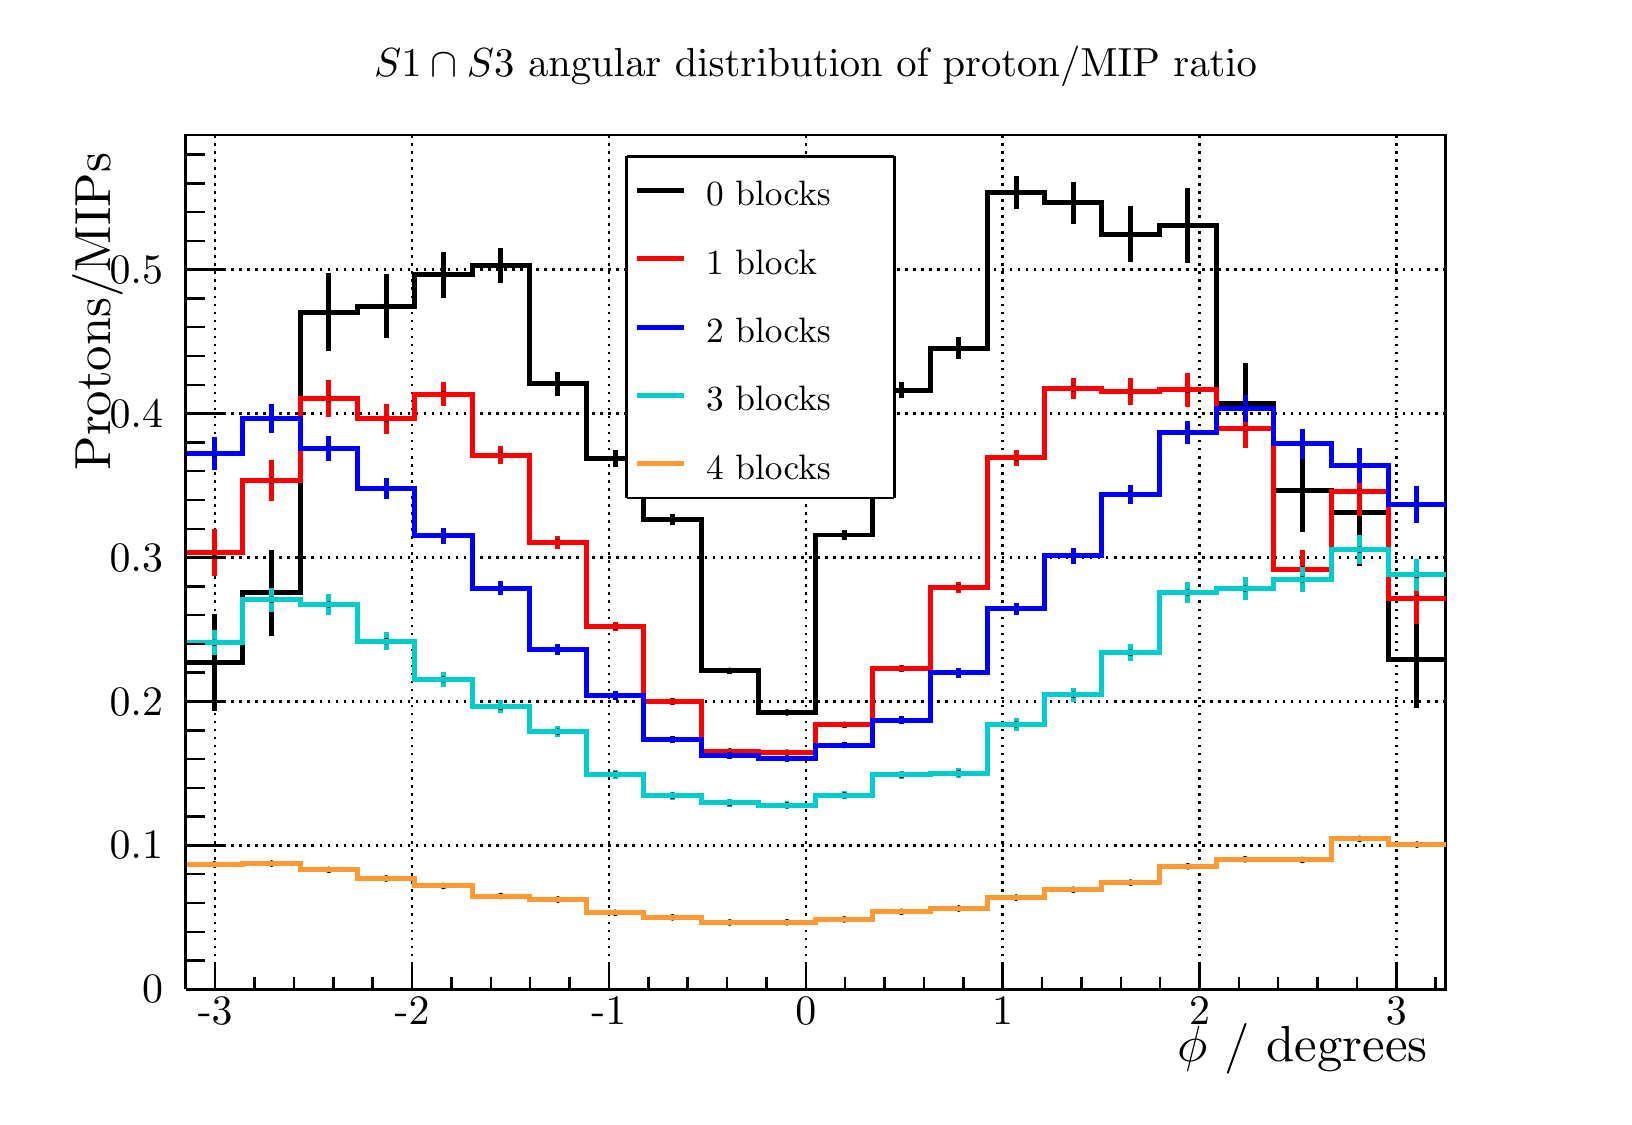
\begin{tikzpicture}
\pgfdeclareplotmark{cross} {
\pgfpathmoveto{\pgfpoint{-0.3\pgfplotmarksize}{\pgfplotmarksize}}
\pgfpathlineto{\pgfpoint{+0.3\pgfplotmarksize}{\pgfplotmarksize}}
\pgfpathlineto{\pgfpoint{+0.3\pgfplotmarksize}{0.3\pgfplotmarksize}}
\pgfpathlineto{\pgfpoint{+1\pgfplotmarksize}{0.3\pgfplotmarksize}}
\pgfpathlineto{\pgfpoint{+1\pgfplotmarksize}{-0.3\pgfplotmarksize}}
\pgfpathlineto{\pgfpoint{+0.3\pgfplotmarksize}{-0.3\pgfplotmarksize}}
\pgfpathlineto{\pgfpoint{+0.3\pgfplotmarksize}{-1.\pgfplotmarksize}}
\pgfpathlineto{\pgfpoint{-0.3\pgfplotmarksize}{-1.\pgfplotmarksize}}
\pgfpathlineto{\pgfpoint{-0.3\pgfplotmarksize}{-0.3\pgfplotmarksize}}
\pgfpathlineto{\pgfpoint{-1.\pgfplotmarksize}{-0.3\pgfplotmarksize}}
\pgfpathlineto{\pgfpoint{-1.\pgfplotmarksize}{0.3\pgfplotmarksize}}
\pgfpathlineto{\pgfpoint{-0.3\pgfplotmarksize}{0.3\pgfplotmarksize}}
\pgfpathclose
\pgfusepathqstroke
}
\pgfdeclareplotmark{cross*} {
\pgfpathmoveto{\pgfpoint{-0.3\pgfplotmarksize}{\pgfplotmarksize}}
\pgfpathlineto{\pgfpoint{+0.3\pgfplotmarksize}{\pgfplotmarksize}}
\pgfpathlineto{\pgfpoint{+0.3\pgfplotmarksize}{0.3\pgfplotmarksize}}
\pgfpathlineto{\pgfpoint{+1\pgfplotmarksize}{0.3\pgfplotmarksize}}
\pgfpathlineto{\pgfpoint{+1\pgfplotmarksize}{-0.3\pgfplotmarksize}}
\pgfpathlineto{\pgfpoint{+0.3\pgfplotmarksize}{-0.3\pgfplotmarksize}}
\pgfpathlineto{\pgfpoint{+0.3\pgfplotmarksize}{-1.\pgfplotmarksize}}
\pgfpathlineto{\pgfpoint{-0.3\pgfplotmarksize}{-1.\pgfplotmarksize}}
\pgfpathlineto{\pgfpoint{-0.3\pgfplotmarksize}{-0.3\pgfplotmarksize}}
\pgfpathlineto{\pgfpoint{-1.\pgfplotmarksize}{-0.3\pgfplotmarksize}}
\pgfpathlineto{\pgfpoint{-1.\pgfplotmarksize}{0.3\pgfplotmarksize}}
\pgfpathlineto{\pgfpoint{-0.3\pgfplotmarksize}{0.3\pgfplotmarksize}}
\pgfpathclose
\pgfusepathqfillstroke
}
\pgfdeclareplotmark{newstar} {
\pgfpathmoveto{\pgfqpoint{0pt}{\pgfplotmarksize}}
\pgfpathlineto{\pgfqpointpolar{44}{0.5\pgfplotmarksize}}
\pgfpathlineto{\pgfqpointpolar{18}{\pgfplotmarksize}}
\pgfpathlineto{\pgfqpointpolar{-20}{0.5\pgfplotmarksize}}
\pgfpathlineto{\pgfqpointpolar{-54}{\pgfplotmarksize}}
\pgfpathlineto{\pgfqpointpolar{-90}{0.5\pgfplotmarksize}}
\pgfpathlineto{\pgfqpointpolar{234}{\pgfplotmarksize}}
\pgfpathlineto{\pgfqpointpolar{198}{0.5\pgfplotmarksize}}
\pgfpathlineto{\pgfqpointpolar{162}{\pgfplotmarksize}}
\pgfpathlineto{\pgfqpointpolar{134}{0.5\pgfplotmarksize}}
\pgfpathclose
\pgfusepathqstroke
}
\pgfdeclareplotmark{newstar*} {
\pgfpathmoveto{\pgfqpoint{0pt}{\pgfplotmarksize}}
\pgfpathlineto{\pgfqpointpolar{44}{0.5\pgfplotmarksize}}
\pgfpathlineto{\pgfqpointpolar{18}{\pgfplotmarksize}}
\pgfpathlineto{\pgfqpointpolar{-20}{0.5\pgfplotmarksize}}
\pgfpathlineto{\pgfqpointpolar{-54}{\pgfplotmarksize}}
\pgfpathlineto{\pgfqpointpolar{-90}{0.5\pgfplotmarksize}}
\pgfpathlineto{\pgfqpointpolar{234}{\pgfplotmarksize}}
\pgfpathlineto{\pgfqpointpolar{198}{0.5\pgfplotmarksize}}
\pgfpathlineto{\pgfqpointpolar{162}{\pgfplotmarksize}}
\pgfpathlineto{\pgfqpointpolar{134}{0.5\pgfplotmarksize}}
\pgfpathclose
\pgfusepathqfillstroke
}
\definecolor{c}{rgb}{1,1,1};
\draw [color=c, fill=c] (0,0) rectangle (20,13.5632);
\draw [color=c, fill=c] (2,1.35632) rectangle (18,12.2069);
\definecolor{c}{rgb}{0,0,0};
\draw [c,line width=0.9] (2,1.35632) -- (2,12.2069) -- (18,12.2069) -- (18,1.35632) -- (2,1.35632);
\definecolor{c}{rgb}{1,1,1};
\draw [color=c, fill=c] (2,1.35632) rectangle (18,12.2069);
\definecolor{c}{rgb}{0,0,0};
\draw [c,line width=0.9] (2,1.35632) -- (2,12.2069) -- (18,12.2069) -- (18,1.35632) -- (2,1.35632);
\draw [c,line width=0.9] (2,1.35632) -- (18,1.35632);
\draw [c,dotted,line width=0.9] (2.375,12.2069) -- (2.375,1.35632);
\draw [c,dotted,line width=0.9] (4.875,12.2069) -- (4.875,1.35632);
\draw [c,dotted,line width=0.9] (7.375,12.2069) -- (7.375,1.35632);
\draw [c,dotted,line width=0.9] (9.875,12.2069) -- (9.875,1.35632);
\draw [c,dotted,line width=0.9] (12.375,12.2069) -- (12.375,1.35632);
\draw [c,dotted,line width=0.9] (14.875,12.2069) -- (14.875,1.35632);
\draw [c,dotted,line width=0.9] (17.375,12.2069) -- (17.375,1.35632);
\draw [c,dotted,line width=0.9] (2.375,12.2069) -- (2.375,1.35632);
\draw [c,dotted,line width=0.9] (17.375,12.2069) -- (17.375,1.35632);
\draw [c,line width=0.9] (2,1.35632) -- (2,12.2069);
\draw [c,dotted,line width=0.9] (18,1.35632) -- (2,1.35632);
\draw [c,dotted,line width=0.9] (18,3.18443) -- (2,3.18443);
\draw [c,dotted,line width=0.9] (18,5.01255) -- (2,5.01255);
\draw [c,dotted,line width=0.9] (18,6.84066) -- (2,6.84066);
\draw [c,dotted,line width=0.9] (18,8.66877) -- (2,8.66877);
\draw [c,dotted,line width=0.9] (18,10.4969) -- (2,10.4969);
\draw [c,dotted,line width=0.9] (18,10.4969) -- (2,10.4969);
\definecolor{c}{rgb}{0,0,0.6};
\draw [c,line width=0.9] (2,1.35632) -- (2.72727,1.35632) -- (2.72727,1.35632) -- (3.45455,1.35632) -- (3.45455,1.35632) -- (4.18182,1.35632) -- (4.18182,1.35632) -- (4.90909,1.35632) -- (4.90909,1.35632) -- (5.63636,1.35632) -- (5.63636,1.35632) --
 (6.36364,1.35632) -- (6.36364,1.35632) -- (7.09091,1.35632) -- (7.09091,1.35632) -- (7.81818,1.35632) -- (7.81818,1.35632) -- (8.54545,1.35632) -- (8.54545,1.35632) -- (9.27273,1.35632) -- (9.27273,1.35632) -- (10,1.35632) -- (10,1.35632) --
 (10.7273,1.35632) -- (10.7273,1.35632) -- (11.4545,1.35632) -- (11.4545,1.35632) -- (12.1818,1.35632) -- (12.1818,1.35632) -- (12.9091,1.35632) -- (12.9091,1.35632) -- (13.6364,1.35632) -- (13.6364,1.35632) -- (14.3636,1.35632) -- (14.3636,1.35632)
 -- (15.0909,1.35632) -- (15.0909,1.35632) -- (15.8182,1.35632) -- (15.8182,1.35632) -- (16.5455,1.35632) -- (16.5455,1.35632) -- (17.2727,1.35632) -- (17.2727,1.35632) -- (18,1.35632);
\definecolor{c}{rgb}{0,0,0};
\draw [c,line width=0.9] (2,1.35632) -- (18,1.35632);
\draw [anchor= east] (18,0.596782) node[scale=1.8317, color=c, rotate=0]{$\phi$ / degrees};
\draw [c,line width=0.9] (2.375,1.68184) -- (2.375,1.35632);
\draw [c,line width=0.9] (2.875,1.51908) -- (2.875,1.35632);
\draw [c,line width=0.9] (3.375,1.51908) -- (3.375,1.35632);
\draw [c,line width=0.9] (3.875,1.51908) -- (3.875,1.35632);
\draw [c,line width=0.9] (4.375,1.51908) -- (4.375,1.35632);
\draw [c,line width=0.9] (4.875,1.68184) -- (4.875,1.35632);
\draw [c,line width=0.9] (5.375,1.51908) -- (5.375,1.35632);
\draw [c,line width=0.9] (5.875,1.51908) -- (5.875,1.35632);
\draw [c,line width=0.9] (6.375,1.51908) -- (6.375,1.35632);
\draw [c,line width=0.9] (6.875,1.51908) -- (6.875,1.35632);
\draw [c,line width=0.9] (7.375,1.68184) -- (7.375,1.35632);
\draw [c,line width=0.9] (7.875,1.51908) -- (7.875,1.35632);
\draw [c,line width=0.9] (8.375,1.51908) -- (8.375,1.35632);
\draw [c,line width=0.9] (8.875,1.51908) -- (8.875,1.35632);
\draw [c,line width=0.9] (9.375,1.51908) -- (9.375,1.35632);
\draw [c,line width=0.9] (9.875,1.68184) -- (9.875,1.35632);
\draw [c,line width=0.9] (10.375,1.51908) -- (10.375,1.35632);
\draw [c,line width=0.9] (10.875,1.51908) -- (10.875,1.35632);
\draw [c,line width=0.9] (11.375,1.51908) -- (11.375,1.35632);
\draw [c,line width=0.9] (11.875,1.51908) -- (11.875,1.35632);
\draw [c,line width=0.9] (12.375,1.68184) -- (12.375,1.35632);
\draw [c,line width=0.9] (12.875,1.51908) -- (12.875,1.35632);
\draw [c,line width=0.9] (13.375,1.51908) -- (13.375,1.35632);
\draw [c,line width=0.9] (13.875,1.51908) -- (13.875,1.35632);
\draw [c,line width=0.9] (14.375,1.51908) -- (14.375,1.35632);
\draw [c,line width=0.9] (14.875,1.68184) -- (14.875,1.35632);
\draw [c,line width=0.9] (15.375,1.51908) -- (15.375,1.35632);
\draw [c,line width=0.9] (15.875,1.51908) -- (15.875,1.35632);
\draw [c,line width=0.9] (16.375,1.51908) -- (16.375,1.35632);
\draw [c,line width=0.9] (16.875,1.51908) -- (16.875,1.35632);
\draw [c,line width=0.9] (17.375,1.68184) -- (17.375,1.35632);
\draw [c,line width=0.9] (2.375,1.68184) -- (2.375,1.35632);
\draw [c,line width=0.9] (17.375,1.68184) -- (17.375,1.35632);
\draw [c,line width=0.9] (17.875,1.51908) -- (17.875,1.35632);
\draw [anchor=base] (2.375,0.908736) node[scale=1.5137, color=c, rotate=0]{-3};
\draw [anchor=base] (4.875,0.908736) node[scale=1.5137, color=c, rotate=0]{-2};
\draw [anchor=base] (7.375,0.908736) node[scale=1.5137, color=c, rotate=0]{-1};
\draw [anchor=base] (9.875,0.908736) node[scale=1.5137, color=c, rotate=0]{0};
\draw [anchor=base] (12.375,0.908736) node[scale=1.5137, color=c, rotate=0]{1};
\draw [anchor=base] (14.875,0.908736) node[scale=1.5137, color=c, rotate=0]{2};
\draw [anchor=base] (17.375,0.908736) node[scale=1.5137, color=c, rotate=0]{3};
\draw [c,line width=0.9] (2,1.35632) -- (2,12.2069);
\draw [anchor= east] (0.88,12.2069) node[scale=1.8317, color=c, rotate=90]{  Protons/MIPs};
\draw [c,line width=0.9] (2.48,1.35632) -- (2,1.35632);
\draw [c,line width=0.9] (2.24,1.72194) -- (2,1.72194);
\draw [c,line width=0.9] (2.24,2.08757) -- (2,2.08757);
\draw [c,line width=0.9] (2.24,2.45319) -- (2,2.45319);
\draw [c,line width=0.9] (2.24,2.81881) -- (2,2.81881);
\draw [c,line width=0.9] (2.48,3.18443) -- (2,3.18443);
\draw [c,line width=0.9] (2.24,3.55006) -- (2,3.55006);
\draw [c,line width=0.9] (2.24,3.91568) -- (2,3.91568);
\draw [c,line width=0.9] (2.24,4.2813) -- (2,4.2813);
\draw [c,line width=0.9] (2.24,4.64692) -- (2,4.64692);
\draw [c,line width=0.9] (2.48,5.01255) -- (2,5.01255);
\draw [c,line width=0.9] (2.24,5.37817) -- (2,5.37817);
\draw [c,line width=0.9] (2.24,5.74379) -- (2,5.74379);
\draw [c,line width=0.9] (2.24,6.10941) -- (2,6.10941);
\draw [c,line width=0.9] (2.24,6.47504) -- (2,6.47504);
\draw [c,line width=0.9] (2.48,6.84066) -- (2,6.84066);
\draw [c,line width=0.9] (2.24,7.20628) -- (2,7.20628);
\draw [c,line width=0.9] (2.24,7.5719) -- (2,7.5719);
\draw [c,line width=0.9] (2.24,7.93753) -- (2,7.93753);
\draw [c,line width=0.9] (2.24,8.30315) -- (2,8.30315);
\draw [c,line width=0.9] (2.48,8.66877) -- (2,8.66877);
\draw [c,line width=0.9] (2.24,9.03439) -- (2,9.03439);
\draw [c,line width=0.9] (2.24,9.40002) -- (2,9.40002);
\draw [c,line width=0.9] (2.24,9.76564) -- (2,9.76564);
\draw [c,line width=0.9] (2.24,10.1313) -- (2,10.1313);
\draw [c,line width=0.9] (2.48,10.4969) -- (2,10.4969);
\draw [c,line width=0.9] (2.48,10.4969) -- (2,10.4969);
\draw [c,line width=0.9] (2.24,10.8625) -- (2,10.8625);
\draw [c,line width=0.9] (2.24,11.2281) -- (2,11.2281);
\draw [c,line width=0.9] (2.24,11.5938) -- (2,11.5938);
\draw [c,line width=0.9] (2.24,11.9594) -- (2,11.9594);
\draw [anchor= east] (1.9,1.35632) node[scale=1.5137, color=c, rotate=0]{0};
\draw [anchor= east] (1.9,3.18443) node[scale=1.5137, color=c, rotate=0]{0.1};
\draw [anchor= east] (1.9,5.01255) node[scale=1.5137, color=c, rotate=0]{0.2};
\draw [anchor= east] (1.9,6.84066) node[scale=1.5137, color=c, rotate=0]{0.3};
\draw [anchor= east] (1.9,8.66877) node[scale=1.5137, color=c, rotate=0]{0.4};
\draw [anchor= east] (1.9,10.4969) node[scale=1.5137, color=c, rotate=0]{0.5};
\draw [c,line width=1.8] (2.36364,4.89378) -- (2.36364,5.51112);
\draw [c,line width=1.8] (2.36364,5.51112) -- (2.36364,6.12847);
\foreach \P in {(2.36364,5.51112)}{\draw[mark options={color=c,fill=c},mark size=2.402402pt,mark=*,mark size=1pt] plot coordinates {\P};}
\draw [c,line width=1.8] (3.09091,5.84926) -- (3.09091,6.39379);
\draw [c,line width=1.8] (3.09091,6.39379) -- (3.09091,6.93831);
\foreach \P in {(3.09091,6.39379)}{\draw[mark options={color=c,fill=c},mark size=2.402402pt,mark=*,mark size=1pt] plot coordinates {\P};}
\draw [c,line width=1.8] (3.81818,9.45971) -- (3.81818,9.95602);
\draw [c,line width=1.8] (3.81818,9.95602) -- (3.81818,10.4523);
\foreach \P in {(3.81818,9.95602)}{\draw[mark options={color=c,fill=c},mark size=2.402402pt,mark=*,mark size=1pt] plot coordinates {\P};}
\draw [c,line width=1.8] (4.54545,9.62928) -- (4.54545,10.0327);
\draw [c,line width=1.8] (4.54545,10.0327) -- (4.54545,10.4362);
\foreach \P in {(4.54545,10.0327)}{\draw[mark options={color=c,fill=c},mark size=2.402402pt,mark=*,mark size=1pt] plot coordinates {\P};}
\draw [c,line width=1.8] (5.27273,10.1359) -- (5.27273,10.4304);
\draw [c,line width=1.8] (5.27273,10.4304) -- (5.27273,10.725);
\foreach \P in {(5.27273,10.4304)}{\draw[mark options={color=c,fill=c},mark size=2.402402pt,mark=*,mark size=1pt] plot coordinates {\P};}
\draw [c,line width=1.8] (6,10.3215) -- (6,10.547);
\draw [c,line width=1.8] (6,10.547) -- (6,10.7725);
\foreach \P in {(6,10.547)}{\draw[mark options={color=c,fill=c},mark size=2.402402pt,mark=*,mark size=1pt] plot coordinates {\P};}
\draw [c,line width=1.8] (6.72727,8.89213) -- (6.72727,9.04764);
\draw [c,line width=1.8] (6.72727,9.04764) -- (6.72727,9.20315);
\foreach \P in {(6.72727,9.04764)}{\draw[mark options={color=c,fill=c},mark size=2.402402pt,mark=*,mark size=1pt] plot coordinates {\P};}
\draw [c,line width=1.8] (7.45455,7.99309) -- (7.45455,8.09945);
\draw [c,line width=1.8] (7.45455,8.09945) -- (7.45455,8.2058);
\foreach \P in {(7.45455,8.09945)}{\draw[mark options={color=c,fill=c},mark size=2.402402pt,mark=*,mark size=1pt] plot coordinates {\P};}
\draw [c,line width=1.8] (8.18182,7.25752) -- (8.18182,7.3273);
\draw [c,line width=1.8] (8.18182,7.3273) -- (8.18182,7.39708);
\foreach \P in {(8.18182,7.3273)}{\draw[mark options={color=c,fill=c},mark size=2.402402pt,mark=*,mark size=1pt] plot coordinates {\P};}
\draw [c,line width=1.8] (8.90909,5.36598) -- (8.90909,5.40179);
\draw [c,line width=1.8] (8.90909,5.40179) -- (8.90909,5.4376);
\foreach \P in {(8.90909,5.40179)}{\draw[mark options={color=c,fill=c},mark size=2.402402pt,mark=*,mark size=1pt] plot coordinates {\P};}
\draw [c,line width=1.8] (9.63636,4.84341) -- (9.63636,4.87303);
\draw [c,line width=1.8] (9.63636,4.87303) -- (9.63636,4.90264);
\foreach \P in {(9.63636,4.87303)}{\draw[mark options={color=c,fill=c},mark size=2.402402pt,mark=*,mark size=1pt] plot coordinates {\P};}
\draw [c,line width=1.8] (10.3636,7.06938) -- (10.3636,7.12713);
\draw [c,line width=1.8] (10.3636,7.12713) -- (10.3636,7.18488);
\foreach \P in {(10.3636,7.12713)}{\draw[mark options={color=c,fill=c},mark size=2.402402pt,mark=*,mark size=1pt] plot coordinates {\P};}
\draw [c,line width=1.8] (11.0909,8.86292) -- (11.0909,8.96454);
\draw [c,line width=1.8] (11.0909,8.96454) -- (11.0909,9.06617);
\foreach \P in {(11.0909,8.96454)}{\draw[mark options={color=c,fill=c},mark size=2.402402pt,mark=*,mark size=1pt] plot coordinates {\P};}
\draw [c,line width=1.8] (11.8182,9.36011) -- (11.8182,9.50073);
\draw [c,line width=1.8] (11.8182,9.50073) -- (11.8182,9.64135);
\foreach \P in {(11.8182,9.50073)}{\draw[mark options={color=c,fill=c},mark size=2.402402pt,mark=*,mark size=1pt] plot coordinates {\P};}
\draw [c,line width=1.8] (12.5455,11.263) -- (12.5455,11.4766);
\draw [c,line width=1.8] (12.5455,11.4766) -- (12.5455,11.6902);
\foreach \P in {(12.5455,11.4766)}{\draw[mark options={color=c,fill=c},mark size=2.402402pt,mark=*,mark size=1pt] plot coordinates {\P};}
\draw [c,line width=1.8] (13.2727,11.0759) -- (13.2727,11.3437);
\draw [c,line width=1.8] (13.2727,11.3437) -- (13.2727,11.6115);
\foreach \P in {(13.2727,11.3437)}{\draw[mark options={color=c,fill=c},mark size=2.402402pt,mark=*,mark size=1pt] plot coordinates {\P};}
\draw [c,line width=1.8] (14,10.588) -- (14,10.9455);
\draw [c,line width=1.8] (14,10.9455) -- (14,11.303);
\foreach \P in {(14,10.9455)}{\draw[mark options={color=c,fill=c},mark size=2.402402pt,mark=*,mark size=1pt] plot coordinates {\P};}
\draw [c,line width=1.8] (14.7273,10.5864) -- (14.7273,11.0575);
\draw [c,line width=1.8] (14.7273,11.0575) -- (14.7273,11.5286);
\foreach \P in {(14.7273,11.0575)}{\draw[mark options={color=c,fill=c},mark size=2.402402pt,mark=*,mark size=1pt] plot coordinates {\P};}
\draw [c,line width=1.8] (15.4545,8.28922) -- (15.4545,8.79768);
\draw [c,line width=1.8] (15.4545,8.79768) -- (15.4545,9.30614);
\foreach \P in {(15.4545,8.79768)}{\draw[mark options={color=c,fill=c},mark size=2.402402pt,mark=*,mark size=1pt] plot coordinates {\P};}
\draw [c,line width=1.8] (16.1818,7.16906) -- (16.1818,7.69467);
\draw [c,line width=1.8] (16.1818,7.69467) -- (16.1818,8.22028);
\foreach \P in {(16.1818,7.69467)}{\draw[mark options={color=c,fill=c},mark size=2.402402pt,mark=*,mark size=1pt] plot coordinates {\P};}
\draw [c,line width=1.8] (16.9091,6.73172) -- (16.9091,7.41194);
\draw [c,line width=1.8] (16.9091,7.41194) -- (16.9091,8.09217);
\foreach \P in {(16.9091,7.41194)}{\draw[mark options={color=c,fill=c},mark size=2.402402pt,mark=*,mark size=1pt] plot coordinates {\P};}
\draw [c,line width=1.8] (17.6364,4.93484) -- (17.6364,5.54817);
\draw [c,line width=1.8] (17.6364,5.54817) -- (17.6364,6.16151);
\foreach \P in {(17.6364,5.54817)}{\draw[mark options={color=c,fill=c},mark size=2.402402pt,mark=*,mark size=1pt] plot coordinates {\P};}
\draw [c,line width=1.8] (2,5.51112) -- (2.72727,5.51112) -- (2.72727,6.39379) -- (3.45455,6.39379) -- (3.45455,9.95602) -- (4.18182,9.95602) -- (4.18182,10.0327) -- (4.90909,10.0327) -- (4.90909,10.4304) -- (5.63636,10.4304) -- (5.63636,10.547) --
 (6.36364,10.547) -- (6.36364,9.04764) -- (7.09091,9.04764) -- (7.09091,8.09945) -- (7.81818,8.09945) -- (7.81818,7.3273) -- (8.54545,7.3273) -- (8.54545,5.40179) -- (9.27273,5.40179) -- (9.27273,4.87303) -- (10,4.87303) -- (10,7.12713) --
 (10.7273,7.12713) -- (10.7273,8.96454) -- (11.4545,8.96454) -- (11.4545,9.50073) -- (12.1818,9.50073) -- (12.1818,11.4766) -- (12.9091,11.4766) -- (12.9091,11.3437) -- (13.6364,11.3437) -- (13.6364,10.9455) -- (14.3636,10.9455) -- (14.3636,11.0575)
 -- (15.0909,11.0575) -- (15.0909,8.79768) -- (15.8182,8.79768) -- (15.8182,7.69467) -- (16.5455,7.69467) -- (16.5455,7.41194) -- (17.2727,7.41194) -- (17.2727,5.54817) -- (18,5.54817);
\definecolor{c}{rgb}{1,0,0};
\draw [c,line width=1.8] (2.36364,6.60423) -- (2.36364,6.90306);
\draw [c,line width=1.8] (2.36364,6.90306) -- (2.36364,7.20189);
\definecolor{c}{rgb}{0,0,0};
\foreach \P in {(2.36364,6.90306)}{\draw[mark options={color=c,fill=c},mark size=2.402402pt,mark=*,mark size=1pt] plot coordinates {\P};}
\definecolor{c}{rgb}{1,0,0};
\draw [c,line width=1.8] (3.09091,7.5545) -- (3.09091,7.8162);
\draw [c,line width=1.8] (3.09091,7.8162) -- (3.09091,8.0779);
\definecolor{c}{rgb}{0,0,0};
\foreach \P in {(3.09091,7.8162)}{\draw[mark options={color=c,fill=c},mark size=2.402402pt,mark=*,mark size=1pt] plot coordinates {\P};}
\definecolor{c}{rgb}{1,0,0};
\draw [c,line width=1.8] (3.81818,8.62873) -- (3.81818,8.86031);
\draw [c,line width=1.8] (3.81818,8.86031) -- (3.81818,9.09189);
\definecolor{c}{rgb}{0,0,0};
\foreach \P in {(3.81818,8.86031)}{\draw[mark options={color=c,fill=c},mark size=2.402402pt,mark=*,mark size=1pt] plot coordinates {\P};}
\definecolor{c}{rgb}{1,0,0};
\draw [c,line width=1.8] (4.54545,8.41495) -- (4.54545,8.60083);
\draw [c,line width=1.8] (4.54545,8.60083) -- (4.54545,8.78671);
\definecolor{c}{rgb}{0,0,0};
\foreach \P in {(4.54545,8.60083)}{\draw[mark options={color=c,fill=c},mark size=2.402402pt,mark=*,mark size=1pt] plot coordinates {\P};}
\definecolor{c}{rgb}{1,0,0};
\draw [c,line width=1.8] (5.27273,8.76828) -- (5.27273,8.91648);
\draw [c,line width=1.8] (5.27273,8.91648) -- (5.27273,9.06469);
\definecolor{c}{rgb}{0,0,0};
\foreach \P in {(5.27273,8.91648)}{\draw[mark options={color=c,fill=c},mark size=2.402402pt,mark=*,mark size=1pt] plot coordinates {\P};}
\definecolor{c}{rgb}{1,0,0};
\draw [c,line width=1.8] (6,8.02779) -- (6,8.14192);
\draw [c,line width=1.8] (6,8.14192) -- (6,8.25604);
\definecolor{c}{rgb}{0,0,0};
\foreach \P in {(6,8.14192)}{\draw[mark options={color=c,fill=c},mark size=2.402402pt,mark=*,mark size=1pt] plot coordinates {\P};}
\definecolor{c}{rgb}{1,0,0};
\draw [c,line width=1.8] (6.72727,6.95442) -- (6.72727,7.03619);
\draw [c,line width=1.8] (6.72727,7.03619) -- (6.72727,7.11796);
\definecolor{c}{rgb}{0,0,0};
\foreach \P in {(6.72727,7.03619)}{\draw[mark options={color=c,fill=c},mark size=2.402402pt,mark=*,mark size=1pt] plot coordinates {\P};}
\definecolor{c}{rgb}{1,0,0};
\draw [c,line width=1.8] (7.45455,5.90288) -- (7.45455,5.96141);
\draw [c,line width=1.8] (7.45455,5.96141) -- (7.45455,6.01994);
\definecolor{c}{rgb}{0,0,0};
\foreach \P in {(7.45455,5.96141)}{\draw[mark options={color=c,fill=c},mark size=2.402402pt,mark=*,mark size=1pt] plot coordinates {\P};}
\definecolor{c}{rgb}{1,0,0};
\draw [c,line width=1.8] (8.18182,4.97126) -- (8.18182,5.01446);
\draw [c,line width=1.8] (8.18182,5.01446) -- (8.18182,5.05766);
\definecolor{c}{rgb}{0,0,0};
\foreach \P in {(8.18182,5.01446)}{\draw[mark options={color=c,fill=c},mark size=2.402402pt,mark=*,mark size=1pt] plot coordinates {\P};}
\definecolor{c}{rgb}{1,0,0};
\draw [c,line width=1.8] (8.90909,4.34427) -- (8.90909,4.37898);
\draw [c,line width=1.8] (8.90909,4.37898) -- (8.90909,4.41369);
\definecolor{c}{rgb}{0,0,0};
\foreach \P in {(8.90909,4.37898)}{\draw[mark options={color=c,fill=c},mark size=2.402402pt,mark=*,mark size=1pt] plot coordinates {\P};}
\definecolor{c}{rgb}{1,0,0};
\draw [c,line width=1.8] (9.63636,4.32923) -- (9.63636,4.3633);
\draw [c,line width=1.8] (9.63636,4.3633) -- (9.63636,4.39736);
\definecolor{c}{rgb}{0,0,0};
\foreach \P in {(9.63636,4.3633)}{\draw[mark options={color=c,fill=c},mark size=2.402402pt,mark=*,mark size=1pt] plot coordinates {\P};}
\definecolor{c}{rgb}{1,0,0};
\draw [c,line width=1.8] (10.3636,4.67726) -- (10.3636,4.71602);
\draw [c,line width=1.8] (10.3636,4.71602) -- (10.3636,4.75479);
\definecolor{c}{rgb}{0,0,0};
\foreach \P in {(10.3636,4.71602)}{\draw[mark options={color=c,fill=c},mark size=2.402402pt,mark=*,mark size=1pt] plot coordinates {\P};}
\definecolor{c}{rgb}{1,0,0};
\draw [c,line width=1.8] (11.0909,5.38166) -- (11.0909,5.43154);
\draw [c,line width=1.8] (11.0909,5.43154) -- (11.0909,5.48143);
\definecolor{c}{rgb}{0,0,0};
\foreach \P in {(11.0909,5.43154)}{\draw[mark options={color=c,fill=c},mark size=2.402402pt,mark=*,mark size=1pt] plot coordinates {\P};}
\definecolor{c}{rgb}{1,0,0};
\draw [c,line width=1.8] (11.8182,6.39514) -- (11.8182,6.46287);
\draw [c,line width=1.8] (11.8182,6.46287) -- (11.8182,6.5306);
\definecolor{c}{rgb}{0,0,0};
\foreach \P in {(11.8182,6.46287)}{\draw[mark options={color=c,fill=c},mark size=2.402402pt,mark=*,mark size=1pt] plot coordinates {\P};}
\definecolor{c}{rgb}{1,0,0};
\draw [c,line width=1.8] (12.5455,8.00437) -- (12.5455,8.10677);
\draw [c,line width=1.8] (12.5455,8.10677) -- (12.5455,8.20917);
\definecolor{c}{rgb}{0,0,0};
\foreach \P in {(12.5455,8.10677)}{\draw[mark options={color=c,fill=c},mark size=2.402402pt,mark=*,mark size=1pt] plot coordinates {\P};}
\definecolor{c}{rgb}{1,0,0};
\draw [c,line width=1.8] (13.2727,8.85335) -- (13.2727,8.98853);
\draw [c,line width=1.8] (13.2727,8.98853) -- (13.2727,9.1237);
\definecolor{c}{rgb}{0,0,0};
\foreach \P in {(13.2727,8.98853)}{\draw[mark options={color=c,fill=c},mark size=2.402402pt,mark=*,mark size=1pt] plot coordinates {\P};}
\definecolor{c}{rgb}{1,0,0};
\draw [c,line width=1.8] (14,8.77802) -- (14,8.94714);
\draw [c,line width=1.8] (14,8.94714) -- (14,9.11627);
\definecolor{c}{rgb}{0,0,0};
\foreach \P in {(14,8.94714)}{\draw[mark options={color=c,fill=c},mark size=2.402402pt,mark=*,mark size=1pt] plot coordinates {\P};}
\definecolor{c}{rgb}{1,0,0};
\draw [c,line width=1.8] (14.7273,8.75518) -- (14.7273,8.96999);
\draw [c,line width=1.8] (14.7273,8.96999) -- (14.7273,9.18481);
\definecolor{c}{rgb}{0,0,0};
\foreach \P in {(14.7273,8.96999)}{\draw[mark options={color=c,fill=c},mark size=2.402402pt,mark=*,mark size=1pt] plot coordinates {\P};}
\definecolor{c}{rgb}{1,0,0};
\draw [c,line width=1.8] (15.4545,8.23655) -- (15.4545,8.47919);
\draw [c,line width=1.8] (15.4545,8.47919) -- (15.4545,8.72183);
\definecolor{c}{rgb}{0,0,0};
\foreach \P in {(15.4545,8.47919)}{\draw[mark options={color=c,fill=c},mark size=2.402402pt,mark=*,mark size=1pt] plot coordinates {\P};}
\definecolor{c}{rgb}{1,0,0};
\draw [c,line width=1.8] (16.1818,6.44051) -- (16.1818,6.69109);
\draw [c,line width=1.8] (16.1818,6.69109) -- (16.1818,6.94166);
\definecolor{c}{rgb}{0,0,0};
\foreach \P in {(16.1818,6.69109)}{\draw[mark options={color=c,fill=c},mark size=2.402402pt,mark=*,mark size=1pt] plot coordinates {\P};}
\definecolor{c}{rgb}{1,0,0};
\draw [c,line width=1.8] (16.9091,7.36681) -- (16.9091,7.68164);
\draw [c,line width=1.8] (16.9091,7.68164) -- (16.9091,7.99646);
\definecolor{c}{rgb}{0,0,0};
\foreach \P in {(16.9091,7.68164)}{\draw[mark options={color=c,fill=c},mark size=2.402402pt,mark=*,mark size=1pt] plot coordinates {\P};}
\definecolor{c}{rgb}{1,0,0};
\draw [c,line width=1.8] (17.6364,5.99877) -- (17.6364,6.32595);
\draw [c,line width=1.8] (17.6364,6.32595) -- (17.6364,6.65312);
\definecolor{c}{rgb}{0,0,0};
\foreach \P in {(17.6364,6.32595)}{\draw[mark options={color=c,fill=c},mark size=2.402402pt,mark=*,mark size=1pt] plot coordinates {\P};}
\definecolor{c}{rgb}{1,0,0};
\draw [c,line width=1.8] (2,6.90306) -- (2.72727,6.90306) -- (2.72727,7.8162) -- (3.45455,7.8162) -- (3.45455,8.86031) -- (4.18182,8.86031) -- (4.18182,8.60083) -- (4.90909,8.60083) -- (4.90909,8.91648) -- (5.63636,8.91648) -- (5.63636,8.14192) --
 (6.36364,8.14192) -- (6.36364,7.03619) -- (7.09091,7.03619) -- (7.09091,5.96141) -- (7.81818,5.96141) -- (7.81818,5.01446) -- (8.54545,5.01446) -- (8.54545,4.37898) -- (9.27273,4.37898) -- (9.27273,4.3633) -- (10,4.3633) -- (10,4.71602) --
 (10.7273,4.71602) -- (10.7273,5.43154) -- (11.4545,5.43154) -- (11.4545,6.46287) -- (12.1818,6.46287) -- (12.1818,8.10677) -- (12.9091,8.10677) -- (12.9091,8.98853) -- (13.6364,8.98853) -- (13.6364,8.94714) -- (14.3636,8.94714) -- (14.3636,8.96999)
 -- (15.0909,8.96999) -- (15.0909,8.47919) -- (15.8182,8.47919) -- (15.8182,6.69109) -- (16.5455,6.69109) -- (16.5455,7.68164) -- (17.2727,7.68164) -- (17.2727,6.32595) -- (18,6.32595);
\definecolor{c}{rgb}{0,0,1};
\draw [c,line width=1.8] (2.36364,7.94927) -- (2.36364,8.15813);
\draw [c,line width=1.8] (2.36364,8.15813) -- (2.36364,8.36698);
\definecolor{c}{rgb}{0,0,0};
\foreach \P in {(2.36364,8.15813)}{\draw[mark options={color=c,fill=c},mark size=2.402402pt,mark=*,mark size=1pt] plot coordinates {\P};}
\definecolor{c}{rgb}{0,0,1};
\draw [c,line width=1.8] (3.09091,8.41768) -- (3.09091,8.60289);
\draw [c,line width=1.8] (3.09091,8.60289) -- (3.09091,8.78811);
\definecolor{c}{rgb}{0,0,0};
\foreach \P in {(3.09091,8.60289)}{\draw[mark options={color=c,fill=c},mark size=2.402402pt,mark=*,mark size=1pt] plot coordinates {\P};}
\definecolor{c}{rgb}{0,0,1};
\draw [c,line width=1.8] (3.81818,8.07214) -- (3.81818,8.23082);
\draw [c,line width=1.8] (3.81818,8.23082) -- (3.81818,8.38951);
\definecolor{c}{rgb}{0,0,0};
\foreach \P in {(3.81818,8.23082)}{\draw[mark options={color=c,fill=c},mark size=2.402402pt,mark=*,mark size=1pt] plot coordinates {\P};}
\definecolor{c}{rgb}{0,0,1};
\draw [c,line width=1.8] (4.54545,7.58374) -- (4.54545,7.71608);
\draw [c,line width=1.8] (4.54545,7.71608) -- (4.54545,7.84841);
\definecolor{c}{rgb}{0,0,0};
\foreach \P in {(4.54545,7.71608)}{\draw[mark options={color=c,fill=c},mark size=2.402402pt,mark=*,mark size=1pt] plot coordinates {\P};}
\definecolor{c}{rgb}{0,0,1};
\draw [c,line width=1.8] (5.27273,7.0098) -- (5.27273,7.11593);
\draw [c,line width=1.8] (5.27273,7.11593) -- (5.27273,7.22207);
\definecolor{c}{rgb}{0,0,0};
\foreach \P in {(5.27273,7.11593)}{\draw[mark options={color=c,fill=c},mark size=2.402402pt,mark=*,mark size=1pt] plot coordinates {\P};}
\definecolor{c}{rgb}{0,0,1};
\draw [c,line width=1.8] (6,6.36486) -- (6,6.45215);
\draw [c,line width=1.8] (6,6.45215) -- (6,6.53944);
\definecolor{c}{rgb}{0,0,0};
\foreach \P in {(6,6.45215)}{\draw[mark options={color=c,fill=c},mark size=2.402402pt,mark=*,mark size=1pt] plot coordinates {\P};}
\definecolor{c}{rgb}{0,0,1};
\draw [c,line width=1.8] (6.72727,5.60459) -- (6.72727,5.67248);
\draw [c,line width=1.8] (6.72727,5.67248) -- (6.72727,5.74038);
\definecolor{c}{rgb}{0,0,0};
\foreach \P in {(6.72727,5.67248)}{\draw[mark options={color=c,fill=c},mark size=2.402402pt,mark=*,mark size=1pt] plot coordinates {\P};}
\definecolor{c}{rgb}{0,0,1};
\draw [c,line width=1.8] (7.45455,5.03204) -- (7.45455,5.08687);
\draw [c,line width=1.8] (7.45455,5.08687) -- (7.45455,5.14171);
\definecolor{c}{rgb}{0,0,0};
\foreach \P in {(7.45455,5.08687)}{\draw[mark options={color=c,fill=c},mark size=2.402402pt,mark=*,mark size=1pt] plot coordinates {\P};}
\definecolor{c}{rgb}{0,0,1};
\draw [c,line width=1.8] (8.18182,4.4863) -- (8.18182,4.53181);
\draw [c,line width=1.8] (8.18182,4.53181) -- (8.18182,4.57731);
\definecolor{c}{rgb}{0,0,0};
\foreach \P in {(8.18182,4.53181)}{\draw[mark options={color=c,fill=c},mark size=2.402402pt,mark=*,mark size=1pt] plot coordinates {\P};}
\definecolor{c}{rgb}{0,0,1};
\draw [c,line width=1.8] (8.90909,4.287) -- (8.90909,4.32814);
\draw [c,line width=1.8] (8.90909,4.32814) -- (8.90909,4.36928);
\definecolor{c}{rgb}{0,0,0};
\foreach \P in {(8.90909,4.32814)}{\draw[mark options={color=c,fill=c},mark size=2.402402pt,mark=*,mark size=1pt] plot coordinates {\P};}
\definecolor{c}{rgb}{0,0,1};
\draw [c,line width=1.8] (9.63636,4.24632) -- (9.63636,4.28747);
\draw [c,line width=1.8] (9.63636,4.28747) -- (9.63636,4.32862);
\definecolor{c}{rgb}{0,0,0};
\foreach \P in {(9.63636,4.28747)}{\draw[mark options={color=c,fill=c},mark size=2.402402pt,mark=*,mark size=1pt] plot coordinates {\P};}
\definecolor{c}{rgb}{0,0,1};
\draw [c,line width=1.8] (10.3636,4.41574) -- (10.3636,4.45963);
\draw [c,line width=1.8] (10.3636,4.45963) -- (10.3636,4.50353);
\definecolor{c}{rgb}{0,0,0};
\foreach \P in {(10.3636,4.45963)}{\draw[mark options={color=c,fill=c},mark size=2.402402pt,mark=*,mark size=1pt] plot coordinates {\P};}
\definecolor{c}{rgb}{0,0,1};
\draw [c,line width=1.8] (11.0909,4.72467) -- (11.0909,4.77477);
\draw [c,line width=1.8] (11.0909,4.77477) -- (11.0909,4.82488);
\definecolor{c}{rgb}{0,0,0};
\foreach \P in {(11.0909,4.77477)}{\draw[mark options={color=c,fill=c},mark size=2.402402pt,mark=*,mark size=1pt] plot coordinates {\P};}
\definecolor{c}{rgb}{0,0,1};
\draw [c,line width=1.8] (11.8182,5.31697) -- (11.8182,5.37768);
\draw [c,line width=1.8] (11.8182,5.37768) -- (11.8182,5.43838);
\definecolor{c}{rgb}{0,0,0};
\foreach \P in {(11.8182,5.37768)}{\draw[mark options={color=c,fill=c},mark size=2.402402pt,mark=*,mark size=1pt] plot coordinates {\P};}
\definecolor{c}{rgb}{0,0,1};
\draw [c,line width=1.8] (12.5455,6.10984) -- (12.5455,6.18951);
\draw [c,line width=1.8] (12.5455,6.18951) -- (12.5455,6.26918);
\definecolor{c}{rgb}{0,0,0};
\foreach \P in {(12.5455,6.18951)}{\draw[mark options={color=c,fill=c},mark size=2.402402pt,mark=*,mark size=1pt] plot coordinates {\P};}
\definecolor{c}{rgb}{0,0,1};
\draw [c,line width=1.8] (13.2727,6.76253) -- (13.2727,6.862);
\draw [c,line width=1.8] (13.2727,6.862) -- (13.2727,6.96147);
\definecolor{c}{rgb}{0,0,0};
\foreach \P in {(13.2727,6.862)}{\draw[mark options={color=c,fill=c},mark size=2.402402pt,mark=*,mark size=1pt] plot coordinates {\P};}
\definecolor{c}{rgb}{0,0,1};
\draw [c,line width=1.8] (14,7.52013) -- (14,7.64309);
\draw [c,line width=1.8] (14,7.64309) -- (14,7.76606);
\definecolor{c}{rgb}{0,0,0};
\foreach \P in {(14,7.64309)}{\draw[mark options={color=c,fill=c},mark size=2.402402pt,mark=*,mark size=1pt] plot coordinates {\P};}
\definecolor{c}{rgb}{0,0,1};
\draw [c,line width=1.8] (14.7273,8.27652) -- (14.7273,8.42762);
\draw [c,line width=1.8] (14.7273,8.42762) -- (14.7273,8.57872);
\definecolor{c}{rgb}{0,0,0};
\foreach \P in {(14.7273,8.42762)}{\draw[mark options={color=c,fill=c},mark size=2.402402pt,mark=*,mark size=1pt] plot coordinates {\P};}
\definecolor{c}{rgb}{0,0,1};
\draw [c,line width=1.8] (15.4545,8.56516) -- (15.4545,8.73804);
\draw [c,line width=1.8] (15.4545,8.73804) -- (15.4545,8.91092);
\definecolor{c}{rgb}{0,0,0};
\foreach \P in {(15.4545,8.73804)}{\draw[mark options={color=c,fill=c},mark size=2.402402pt,mark=*,mark size=1pt] plot coordinates {\P};}
\definecolor{c}{rgb}{0,0,1};
\draw [c,line width=1.8] (16.1818,8.09282) -- (16.1818,8.28382);
\draw [c,line width=1.8] (16.1818,8.28382) -- (16.1818,8.47482);
\definecolor{c}{rgb}{0,0,0};
\foreach \P in {(16.1818,8.28382)}{\draw[mark options={color=c,fill=c},mark size=2.402402pt,mark=*,mark size=1pt] plot coordinates {\P};}
\definecolor{c}{rgb}{0,0,1};
\draw [c,line width=1.8] (16.9091,7.78327) -- (16.9091,8.00724);
\draw [c,line width=1.8] (16.9091,8.00724) -- (16.9091,8.23121);
\definecolor{c}{rgb}{0,0,0};
\foreach \P in {(16.9091,8.00724)}{\draw[mark options={color=c,fill=c},mark size=2.402402pt,mark=*,mark size=1pt] plot coordinates {\P};}
\definecolor{c}{rgb}{0,0,1};
\draw [c,line width=1.8] (17.6364,7.27676) -- (17.6364,7.51476);
\draw [c,line width=1.8] (17.6364,7.51476) -- (17.6364,7.75276);
\definecolor{c}{rgb}{0,0,0};
\foreach \P in {(17.6364,7.51476)}{\draw[mark options={color=c,fill=c},mark size=2.402402pt,mark=*,mark size=1pt] plot coordinates {\P};}
\definecolor{c}{rgb}{0,0,1};
\draw [c,line width=1.8] (2,8.15813) -- (2.72727,8.15813) -- (2.72727,8.60289) -- (3.45455,8.60289) -- (3.45455,8.23082) -- (4.18182,8.23082) -- (4.18182,7.71608) -- (4.90909,7.71608) -- (4.90909,7.11593) -- (5.63636,7.11593) -- (5.63636,6.45215) --
 (6.36364,6.45215) -- (6.36364,5.67248) -- (7.09091,5.67248) -- (7.09091,5.08687) -- (7.81818,5.08687) -- (7.81818,4.53181) -- (8.54545,4.53181) -- (8.54545,4.32814) -- (9.27273,4.32814) -- (9.27273,4.28747) -- (10,4.28747) -- (10,4.45963) --
 (10.7273,4.45963) -- (10.7273,4.77477) -- (11.4545,4.77477) -- (11.4545,5.37768) -- (12.1818,5.37768) -- (12.1818,6.18951) -- (12.9091,6.18951) -- (12.9091,6.862) -- (13.6364,6.862) -- (13.6364,7.64309) -- (14.3636,7.64309) -- (14.3636,8.42762) --
 (15.0909,8.42762) -- (15.0909,8.73804) -- (15.8182,8.73804) -- (15.8182,8.28382) -- (16.5455,8.28382) -- (16.5455,8.00724) -- (17.2727,8.00724) -- (17.2727,7.51476) -- (18,7.51476);
\definecolor{c}{rgb}{0,0.8,0.8};
\draw [c,line width=1.8] (2.36364,5.60065) -- (2.36364,5.75802);
\draw [c,line width=1.8] (2.36364,5.75802) -- (2.36364,5.91539);
\definecolor{c}{rgb}{0,0,0};
\foreach \P in {(2.36364,5.75802)}{\draw[mark options={color=c,fill=c},mark size=2.402402pt,mark=*,mark size=1pt] plot coordinates {\P};}
\definecolor{c}{rgb}{0,0.8,0.8};
\draw [c,line width=1.8] (3.09091,6.15354) -- (3.09091,6.30546);
\draw [c,line width=1.8] (3.09091,6.30546) -- (3.09091,6.45738);
\definecolor{c}{rgb}{0,0,0};
\foreach \P in {(3.09091,6.30546)}{\draw[mark options={color=c,fill=c},mark size=2.402402pt,mark=*,mark size=1pt] plot coordinates {\P};}
\definecolor{c}{rgb}{0,0.8,0.8};
\draw [c,line width=1.8] (3.81818,6.10854) -- (3.81818,6.24391);
\draw [c,line width=1.8] (3.81818,6.24391) -- (3.81818,6.37929);
\definecolor{c}{rgb}{0,0,0};
\foreach \P in {(3.81818,6.24391)}{\draw[mark options={color=c,fill=c},mark size=2.402402pt,mark=*,mark size=1pt] plot coordinates {\P};}
\definecolor{c}{rgb}{0,0.8,0.8};
\draw [c,line width=1.8] (4.54545,5.66395) -- (4.54545,5.77943);
\draw [c,line width=1.8] (4.54545,5.77943) -- (4.54545,5.89492);
\definecolor{c}{rgb}{0,0,0};
\foreach \P in {(4.54545,5.77943)}{\draw[mark options={color=c,fill=c},mark size=2.402402pt,mark=*,mark size=1pt] plot coordinates {\P};}
\definecolor{c}{rgb}{0,0.8,0.8};
\draw [c,line width=1.8] (5.27273,5.1981) -- (5.27273,5.29348);
\draw [c,line width=1.8] (5.27273,5.29348) -- (5.27273,5.38886);
\definecolor{c}{rgb}{0,0,0};
\foreach \P in {(5.27273,5.29348)}{\draw[mark options={color=c,fill=c},mark size=2.402402pt,mark=*,mark size=1pt] plot coordinates {\P};}
\definecolor{c}{rgb}{0,0.8,0.8};
\draw [c,line width=1.8] (6,4.86022) -- (6,4.9436);
\draw [c,line width=1.8] (6,4.9436) -- (6,5.02697);
\definecolor{c}{rgb}{0,0,0};
\foreach \P in {(6,4.9436)}{\draw[mark options={color=c,fill=c},mark size=2.402402pt,mark=*,mark size=1pt] plot coordinates {\P};}
\definecolor{c}{rgb}{0,0.8,0.8};
\draw [c,line width=1.8] (6.72727,4.55796) -- (6.72727,4.62925);
\draw [c,line width=1.8] (6.72727,4.62925) -- (6.72727,4.70055);
\definecolor{c}{rgb}{0,0,0};
\foreach \P in {(6.72727,4.62925)}{\draw[mark options={color=c,fill=c},mark size=2.402402pt,mark=*,mark size=1pt] plot coordinates {\P};}
\definecolor{c}{rgb}{0,0.8,0.8};
\draw [c,line width=1.8] (7.45455,4.03036) -- (7.45455,4.08825);
\draw [c,line width=1.8] (7.45455,4.08825) -- (7.45455,4.14614);
\definecolor{c}{rgb}{0,0,0};
\foreach \P in {(7.45455,4.08825)}{\draw[mark options={color=c,fill=c},mark size=2.402402pt,mark=*,mark size=1pt] plot coordinates {\P};}
\definecolor{c}{rgb}{0,0.8,0.8};
\draw [c,line width=1.8] (8.18182,3.76393) -- (8.18182,3.81531);
\draw [c,line width=1.8] (8.18182,3.81531) -- (8.18182,3.86669);
\definecolor{c}{rgb}{0,0,0};
\foreach \P in {(8.18182,3.81531)}{\draw[mark options={color=c,fill=c},mark size=2.402402pt,mark=*,mark size=1pt] plot coordinates {\P};}
\definecolor{c}{rgb}{0,0.8,0.8};
\draw [c,line width=1.8] (8.90909,3.6755) -- (8.90909,3.72373);
\draw [c,line width=1.8] (8.90909,3.72373) -- (8.90909,3.77197);
\definecolor{c}{rgb}{0,0,0};
\foreach \P in {(8.90909,3.72373)}{\draw[mark options={color=c,fill=c},mark size=2.402402pt,mark=*,mark size=1pt] plot coordinates {\P};}
\definecolor{c}{rgb}{0,0.8,0.8};
\draw [c,line width=1.8] (9.63636,3.64778) -- (9.63636,3.69587);
\draw [c,line width=1.8] (9.63636,3.69587) -- (9.63636,3.74396);
\definecolor{c}{rgb}{0,0,0};
\foreach \P in {(9.63636,3.69587)}{\draw[mark options={color=c,fill=c},mark size=2.402402pt,mark=*,mark size=1pt] plot coordinates {\P};}
\definecolor{c}{rgb}{0,0.8,0.8};
\draw [c,line width=1.8] (10.3636,3.77137) -- (10.3636,3.822);
\draw [c,line width=1.8] (10.3636,3.822) -- (10.3636,3.87263);
\definecolor{c}{rgb}{0,0,0};
\foreach \P in {(10.3636,3.822)}{\draw[mark options={color=c,fill=c},mark size=2.402402pt,mark=*,mark size=1pt] plot coordinates {\P};}
\definecolor{c}{rgb}{0,0.8,0.8};
\draw [c,line width=1.8] (11.0909,4.02282) -- (11.0909,4.07934);
\draw [c,line width=1.8] (11.0909,4.07934) -- (11.0909,4.13585);
\definecolor{c}{rgb}{0,0,0};
\foreach \P in {(11.0909,4.07934)}{\draw[mark options={color=c,fill=c},mark size=2.402402pt,mark=*,mark size=1pt] plot coordinates {\P};}
\definecolor{c}{rgb}{0,0.8,0.8};
\draw [c,line width=1.8] (11.8182,4.03933) -- (11.8182,4.10067);
\draw [c,line width=1.8] (11.8182,4.10067) -- (11.8182,4.16201);
\definecolor{c}{rgb}{0,0,0};
\foreach \P in {(11.8182,4.10067)}{\draw[mark options={color=c,fill=c},mark size=2.402402pt,mark=*,mark size=1pt] plot coordinates {\P};}
\definecolor{c}{rgb}{0,0.8,0.8};
\draw [c,line width=1.8] (12.5455,4.64307) -- (12.5455,4.72132);
\draw [c,line width=1.8] (12.5455,4.72132) -- (12.5455,4.79956);
\definecolor{c}{rgb}{0,0,0};
\foreach \P in {(12.5455,4.72132)}{\draw[mark options={color=c,fill=c},mark size=2.402402pt,mark=*,mark size=1pt] plot coordinates {\P};}
\definecolor{c}{rgb}{0,0.8,0.8};
\draw [c,line width=1.8] (13.2727,5.00711) -- (13.2727,5.09858);
\draw [c,line width=1.8] (13.2727,5.09858) -- (13.2727,5.19006);
\definecolor{c}{rgb}{0,0,0};
\foreach \P in {(13.2727,5.09858)}{\draw[mark options={color=c,fill=c},mark size=2.402402pt,mark=*,mark size=1pt] plot coordinates {\P};}
\definecolor{c}{rgb}{0,0.8,0.8};
\draw [c,line width=1.8] (14,5.52503) -- (14,5.63177);
\draw [c,line width=1.8] (14,5.63177) -- (14,5.73852);
\definecolor{c}{rgb}{0,0,0};
\foreach \P in {(14,5.63177)}{\draw[mark options={color=c,fill=c},mark size=2.402402pt,mark=*,mark size=1pt] plot coordinates {\P};}
\definecolor{c}{rgb}{0,0.8,0.8};
\draw [c,line width=1.8] (14.7273,6.26227) -- (14.7273,6.39585);
\draw [c,line width=1.8] (14.7273,6.39585) -- (14.7273,6.52943);
\definecolor{c}{rgb}{0,0,0};
\foreach \P in {(14.7273,6.39585)}{\draw[mark options={color=c,fill=c},mark size=2.402402pt,mark=*,mark size=1pt] plot coordinates {\P};}
\definecolor{c}{rgb}{0,0.8,0.8};
\draw [c,line width=1.8] (15.4545,6.30024) -- (15.4545,6.44675);
\draw [c,line width=1.8] (15.4545,6.44675) -- (15.4545,6.59326);
\definecolor{c}{rgb}{0,0,0};
\foreach \P in {(15.4545,6.44675)}{\draw[mark options={color=c,fill=c},mark size=2.402402pt,mark=*,mark size=1pt] plot coordinates {\P};}
\definecolor{c}{rgb}{0,0.8,0.8};
\draw [c,line width=1.8] (16.1818,6.40213) -- (16.1818,6.56436);
\draw [c,line width=1.8] (16.1818,6.56436) -- (16.1818,6.72659);
\definecolor{c}{rgb}{0,0,0};
\foreach \P in {(16.1818,6.56436)}{\draw[mark options={color=c,fill=c},mark size=2.402402pt,mark=*,mark size=1pt] plot coordinates {\P};}
\definecolor{c}{rgb}{0,0.8,0.8};
\draw [c,line width=1.8] (16.9091,6.75548) -- (16.9091,6.94197);
\draw [c,line width=1.8] (16.9091,6.94197) -- (16.9091,7.12846);
\definecolor{c}{rgb}{0,0,0};
\foreach \P in {(16.9091,6.94197)}{\draw[mark options={color=c,fill=c},mark size=2.402402pt,mark=*,mark size=1pt] plot coordinates {\P};}
\definecolor{c}{rgb}{0,0.8,0.8};
\draw [c,line width=1.8] (17.6364,6.42134) -- (17.6364,6.62019);
\draw [c,line width=1.8] (17.6364,6.62019) -- (17.6364,6.81903);
\definecolor{c}{rgb}{0,0,0};
\foreach \P in {(17.6364,6.62019)}{\draw[mark options={color=c,fill=c},mark size=2.402402pt,mark=*,mark size=1pt] plot coordinates {\P};}
\definecolor{c}{rgb}{0,0.8,0.8};
\draw [c,line width=1.8] (2,5.75802) -- (2.72727,5.75802) -- (2.72727,6.30546) -- (3.45455,6.30546) -- (3.45455,6.24391) -- (4.18182,6.24391) -- (4.18182,5.77943) -- (4.90909,5.77943) -- (4.90909,5.29348) -- (5.63636,5.29348) -- (5.63636,4.9436) --
 (6.36364,4.9436) -- (6.36364,4.62925) -- (7.09091,4.62925) -- (7.09091,4.08825) -- (7.81818,4.08825) -- (7.81818,3.81531) -- (8.54545,3.81531) -- (8.54545,3.72373) -- (9.27273,3.72373) -- (9.27273,3.69587) -- (10,3.69587) -- (10,3.822) --
 (10.7273,3.822) -- (10.7273,4.07934) -- (11.4545,4.07934) -- (11.4545,4.10067) -- (12.1818,4.10067) -- (12.1818,4.72132) -- (12.9091,4.72132) -- (12.9091,5.09858) -- (13.6364,5.09858) -- (13.6364,5.63177) -- (14.3636,5.63177) -- (14.3636,6.39585) --
 (15.0909,6.39585) -- (15.0909,6.44675) -- (15.8182,6.44675) -- (15.8182,6.56436) -- (16.5455,6.56436) -- (16.5455,6.94197) -- (17.2727,6.94197) -- (17.2727,6.62019) -- (18,6.62019);
\definecolor{c}{rgb}{1,0.6,0.2};
\draw [c,line width=1.8] (2.36364,2.92124) -- (2.36364,2.94392);
\draw [c,line width=1.8] (2.36364,2.94392) -- (2.36364,2.9666);
\definecolor{c}{rgb}{0,0,0};
\foreach \P in {(2.36364,2.94392)}{\draw[mark options={color=c,fill=c},mark size=2.402402pt,mark=*,mark size=1pt] plot coordinates {\P};}
\definecolor{c}{rgb}{1,0.6,0.2};
\draw [c,line width=1.8] (3.09091,2.93331) -- (3.09091,2.95441);
\draw [c,line width=1.8] (3.09091,2.95441) -- (3.09091,2.97551);
\definecolor{c}{rgb}{0,0,0};
\foreach \P in {(3.09091,2.95441)}{\draw[mark options={color=c,fill=c},mark size=2.402402pt,mark=*,mark size=1pt] plot coordinates {\P};}
\definecolor{c}{rgb}{1,0.6,0.2};
\draw [c,line width=1.8] (3.81818,2.8559) -- (3.81818,2.87498);
\draw [c,line width=1.8] (3.81818,2.87498) -- (3.81818,2.89406);
\definecolor{c}{rgb}{0,0,0};
\foreach \P in {(3.81818,2.87498)}{\draw[mark options={color=c,fill=c},mark size=2.402402pt,mark=*,mark size=1pt] plot coordinates {\P};}
\definecolor{c}{rgb}{1,0.6,0.2};
\draw [c,line width=1.8] (4.54545,2.74809) -- (4.54545,2.7649);
\draw [c,line width=1.8] (4.54545,2.7649) -- (4.54545,2.78171);
\definecolor{c}{rgb}{0,0,0};
\foreach \P in {(4.54545,2.7649)}{\draw[mark options={color=c,fill=c},mark size=2.402402pt,mark=*,mark size=1pt] plot coordinates {\P};}
\definecolor{c}{rgb}{1,0.6,0.2};
\draw [c,line width=1.8] (5.27273,2.65538) -- (5.27273,2.67);
\draw [c,line width=1.8] (5.27273,2.67) -- (5.27273,2.68461);
\definecolor{c}{rgb}{0,0,0};
\foreach \P in {(5.27273,2.67)}{\draw[mark options={color=c,fill=c},mark size=2.402402pt,mark=*,mark size=1pt] plot coordinates {\P};}
\definecolor{c}{rgb}{1,0.6,0.2};
\draw [c,line width=1.8] (6,2.52863) -- (6,2.54157);
\draw [c,line width=1.8] (6,2.54157) -- (6,2.55451);
\definecolor{c}{rgb}{0,0,0};
\foreach \P in {(6,2.54157)}{\draw[mark options={color=c,fill=c},mark size=2.402402pt,mark=*,mark size=1pt] plot coordinates {\P};}
\definecolor{c}{rgb}{1,0.6,0.2};
\draw [c,line width=1.8] (6.72727,2.48582) -- (6.72727,2.49766);
\draw [c,line width=1.8] (6.72727,2.49766) -- (6.72727,2.5095);
\definecolor{c}{rgb}{0,0,0};
\foreach \P in {(6.72727,2.49766)}{\draw[mark options={color=c,fill=c},mark size=2.402402pt,mark=*,mark size=1pt] plot coordinates {\P};}
\definecolor{c}{rgb}{1,0.6,0.2};
\draw [c,line width=1.8] (7.45455,2.31905) -- (7.45455,2.32885);
\draw [c,line width=1.8] (7.45455,2.32885) -- (7.45455,2.33864);
\definecolor{c}{rgb}{0,0,0};
\foreach \P in {(7.45455,2.32885)}{\draw[mark options={color=c,fill=c},mark size=2.402402pt,mark=*,mark size=1pt] plot coordinates {\P};}
\definecolor{c}{rgb}{1,0.6,0.2};
\draw [c,line width=1.8] (8.18182,2.26208) -- (8.18182,2.27109);
\draw [c,line width=1.8] (8.18182,2.27109) -- (8.18182,2.2801);
\definecolor{c}{rgb}{0,0,0};
\foreach \P in {(8.18182,2.27109)}{\draw[mark options={color=c,fill=c},mark size=2.402402pt,mark=*,mark size=1pt] plot coordinates {\P};}
\definecolor{c}{rgb}{1,0.6,0.2};
\draw [c,line width=1.8] (8.90909,2.19803) -- (8.90909,2.20634);
\draw [c,line width=1.8] (8.90909,2.20634) -- (8.90909,2.21465);
\definecolor{c}{rgb}{0,0,0};
\foreach \P in {(8.90909,2.20634)}{\draw[mark options={color=c,fill=c},mark size=2.402402pt,mark=*,mark size=1pt] plot coordinates {\P};}
\definecolor{c}{rgb}{1,0.6,0.2};
\draw [c,line width=1.8] (9.63636,2.2007) -- (9.63636,2.2091);
\draw [c,line width=1.8] (9.63636,2.2091) -- (9.63636,2.21751);
\definecolor{c}{rgb}{0,0,0};
\foreach \P in {(9.63636,2.2091)}{\draw[mark options={color=c,fill=c},mark size=2.402402pt,mark=*,mark size=1pt] plot coordinates {\P};}
\definecolor{c}{rgb}{1,0.6,0.2};
\draw [c,line width=1.8] (10.3636,2.23624) -- (10.3636,2.24496);
\draw [c,line width=1.8] (10.3636,2.24496) -- (10.3636,2.25369);
\definecolor{c}{rgb}{0,0,0};
\foreach \P in {(10.3636,2.24496)}{\draw[mark options={color=c,fill=c},mark size=2.402402pt,mark=*,mark size=1pt] plot coordinates {\P};}
\definecolor{c}{rgb}{1,0.6,0.2};
\draw [c,line width=1.8] (11.0909,2.3323) -- (11.0909,2.34203);
\draw [c,line width=1.8] (11.0909,2.34203) -- (11.0909,2.35176);
\definecolor{c}{rgb}{0,0,0};
\foreach \P in {(11.0909,2.34203)}{\draw[mark options={color=c,fill=c},mark size=2.402402pt,mark=*,mark size=1pt] plot coordinates {\P};}
\definecolor{c}{rgb}{1,0.6,0.2};
\draw [c,line width=1.8] (11.8182,2.37329) -- (11.8182,2.38385);
\draw [c,line width=1.8] (11.8182,2.38385) -- (11.8182,2.39442);
\definecolor{c}{rgb}{0,0,0};
\foreach \P in {(11.8182,2.38385)}{\draw[mark options={color=c,fill=c},mark size=2.402402pt,mark=*,mark size=1pt] plot coordinates {\P};}
\definecolor{c}{rgb}{1,0.6,0.2};
\draw [c,line width=1.8] (12.5455,2.50904) -- (12.5455,2.52192);
\draw [c,line width=1.8] (12.5455,2.52192) -- (12.5455,2.53481);
\definecolor{c}{rgb}{0,0,0};
\foreach \P in {(12.5455,2.52192)}{\draw[mark options={color=c,fill=c},mark size=2.402402pt,mark=*,mark size=1pt] plot coordinates {\P};}
\definecolor{c}{rgb}{1,0.6,0.2};
\draw [c,line width=1.8] (13.2727,2.60703) -- (13.2727,2.62149);
\draw [c,line width=1.8] (13.2727,2.62149) -- (13.2727,2.63595);
\definecolor{c}{rgb}{0,0,0};
\foreach \P in {(13.2727,2.62149)}{\draw[mark options={color=c,fill=c},mark size=2.402402pt,mark=*,mark size=1pt] plot coordinates {\P};}
\definecolor{c}{rgb}{1,0.6,0.2};
\draw [c,line width=1.8] (14,2.69629) -- (14,2.71231);
\draw [c,line width=1.8] (14,2.71231) -- (14,2.72834);
\definecolor{c}{rgb}{0,0,0};
\foreach \P in {(14,2.71231)}{\draw[mark options={color=c,fill=c},mark size=2.402402pt,mark=*,mark size=1pt] plot coordinates {\P};}
\definecolor{c}{rgb}{1,0.6,0.2};
\draw [c,line width=1.8] (14.7273,2.9012) -- (14.7273,2.92021);
\draw [c,line width=1.8] (14.7273,2.92021) -- (14.7273,2.93922);
\definecolor{c}{rgb}{0,0,0};
\foreach \P in {(14.7273,2.92021)}{\draw[mark options={color=c,fill=c},mark size=2.402402pt,mark=*,mark size=1pt] plot coordinates {\P};}
\definecolor{c}{rgb}{1,0.6,0.2};
\draw [c,line width=1.8] (15.4545,2.98839) -- (15.4545,3.00915);
\draw [c,line width=1.8] (15.4545,3.00915) -- (15.4545,3.02991);
\definecolor{c}{rgb}{0,0,0};
\foreach \P in {(15.4545,3.00915)}{\draw[mark options={color=c,fill=c},mark size=2.402402pt,mark=*,mark size=1pt] plot coordinates {\P};}
\definecolor{c}{rgb}{1,0.6,0.2};
\draw [c,line width=1.8] (16.1818,2.97836) -- (16.1818,3.00059);
\draw [c,line width=1.8] (16.1818,3.00059) -- (16.1818,3.02282);
\definecolor{c}{rgb}{0,0,0};
\foreach \P in {(16.1818,3.00059)}{\draw[mark options={color=c,fill=c},mark size=2.402402pt,mark=*,mark size=1pt] plot coordinates {\P};}
\definecolor{c}{rgb}{1,0.6,0.2};
\draw [c,line width=1.8] (16.9091,3.24109) -- (16.9091,3.26804);
\draw [c,line width=1.8] (16.9091,3.26804) -- (16.9091,3.29498);
\definecolor{c}{rgb}{0,0,0};
\foreach \P in {(16.9091,3.26804)}{\draw[mark options={color=c,fill=c},mark size=2.402402pt,mark=*,mark size=1pt] plot coordinates {\P};}
\definecolor{c}{rgb}{1,0.6,0.2};
\draw [c,line width=1.8] (17.6364,3.16705) -- (17.6364,3.19526);
\draw [c,line width=1.8] (17.6364,3.19526) -- (17.6364,3.22347);
\definecolor{c}{rgb}{0,0,0};
\foreach \P in {(17.6364,3.19526)}{\draw[mark options={color=c,fill=c},mark size=2.402402pt,mark=*,mark size=1pt] plot coordinates {\P};}
\definecolor{c}{rgb}{1,0.6,0.2};
\draw [c,line width=1.8] (2,2.94392) -- (2.72727,2.94392) -- (2.72727,2.95441) -- (3.45455,2.95441) -- (3.45455,2.87498) -- (4.18182,2.87498) -- (4.18182,2.7649) -- (4.90909,2.7649) -- (4.90909,2.67) -- (5.63636,2.67) -- (5.63636,2.54157) --
 (6.36364,2.54157) -- (6.36364,2.49766) -- (7.09091,2.49766) -- (7.09091,2.32885) -- (7.81818,2.32885) -- (7.81818,2.27109) -- (8.54545,2.27109) -- (8.54545,2.20634) -- (9.27273,2.20634) -- (9.27273,2.2091) -- (10,2.2091) -- (10,2.24496) --
 (10.7273,2.24496) -- (10.7273,2.34203) -- (11.4545,2.34203) -- (11.4545,2.38385) -- (12.1818,2.38385) -- (12.1818,2.52192) -- (12.9091,2.52192) -- (12.9091,2.62149) -- (13.6364,2.62149) -- (13.6364,2.71231) -- (14.3636,2.71231) -- (14.3636,2.92021)
 -- (15.0909,2.92021) -- (15.0909,3.00915) -- (15.8182,3.00915) -- (15.8182,3.00059) -- (16.5455,3.00059) -- (16.5455,3.26804) -- (17.2727,3.26804) -- (17.2727,3.19526) -- (18,3.19526);
\definecolor{c}{rgb}{0,0,0};
\draw [c,line width=0.9] (2,1.35632) -- (18,1.35632);
\draw [c,line width=0.9] (2.375,1.68184) -- (2.375,1.35632);
\draw [c,line width=0.9] (2.875,1.51908) -- (2.875,1.35632);
\draw [c,line width=0.9] (3.375,1.51908) -- (3.375,1.35632);
\draw [c,line width=0.9] (3.875,1.51908) -- (3.875,1.35632);
\draw [c,line width=0.9] (4.375,1.51908) -- (4.375,1.35632);
\draw [c,line width=0.9] (4.875,1.68184) -- (4.875,1.35632);
\draw [c,line width=0.9] (5.375,1.51908) -- (5.375,1.35632);
\draw [c,line width=0.9] (5.875,1.51908) -- (5.875,1.35632);
\draw [c,line width=0.9] (6.375,1.51908) -- (6.375,1.35632);
\draw [c,line width=0.9] (6.875,1.51908) -- (6.875,1.35632);
\draw [c,line width=0.9] (7.375,1.68184) -- (7.375,1.35632);
\draw [c,line width=0.9] (7.875,1.51908) -- (7.875,1.35632);
\draw [c,line width=0.9] (8.375,1.51908) -- (8.375,1.35632);
\draw [c,line width=0.9] (8.875,1.51908) -- (8.875,1.35632);
\draw [c,line width=0.9] (9.375,1.51908) -- (9.375,1.35632);
\draw [c,line width=0.9] (9.875,1.68184) -- (9.875,1.35632);
\draw [c,line width=0.9] (10.375,1.51908) -- (10.375,1.35632);
\draw [c,line width=0.9] (10.875,1.51908) -- (10.875,1.35632);
\draw [c,line width=0.9] (11.375,1.51908) -- (11.375,1.35632);
\draw [c,line width=0.9] (11.875,1.51908) -- (11.875,1.35632);
\draw [c,line width=0.9] (12.375,1.68184) -- (12.375,1.35632);
\draw [c,line width=0.9] (12.875,1.51908) -- (12.875,1.35632);
\draw [c,line width=0.9] (13.375,1.51908) -- (13.375,1.35632);
\draw [c,line width=0.9] (13.875,1.51908) -- (13.875,1.35632);
\draw [c,line width=0.9] (14.375,1.51908) -- (14.375,1.35632);
\draw [c,line width=0.9] (14.875,1.68184) -- (14.875,1.35632);
\draw [c,line width=0.9] (15.375,1.51908) -- (15.375,1.35632);
\draw [c,line width=0.9] (15.875,1.51908) -- (15.875,1.35632);
\draw [c,line width=0.9] (16.375,1.51908) -- (16.375,1.35632);
\draw [c,line width=0.9] (16.875,1.51908) -- (16.875,1.35632);
\draw [c,line width=0.9] (17.375,1.68184) -- (17.375,1.35632);
\draw [c,line width=0.9] (2.375,1.68184) -- (2.375,1.35632);
\draw [c,line width=0.9] (17.375,1.68184) -- (17.375,1.35632);
\draw [c,line width=0.9] (17.875,1.51908) -- (17.875,1.35632);
\draw [c,line width=0.9] (2,1.35632) -- (2,12.2069);
\draw [c,line width=0.9] (2.48,1.35632) -- (2,1.35632);
\draw [c,line width=0.9] (2.24,1.72194) -- (2,1.72194);
\draw [c,line width=0.9] (2.24,2.08757) -- (2,2.08757);
\draw [c,line width=0.9] (2.24,2.45319) -- (2,2.45319);
\draw [c,line width=0.9] (2.24,2.81881) -- (2,2.81881);
\draw [c,line width=0.9] (2.48,3.18443) -- (2,3.18443);
\draw [c,line width=0.9] (2.24,3.55006) -- (2,3.55006);
\draw [c,line width=0.9] (2.24,3.91568) -- (2,3.91568);
\draw [c,line width=0.9] (2.24,4.2813) -- (2,4.2813);
\draw [c,line width=0.9] (2.24,4.64692) -- (2,4.64692);
\draw [c,line width=0.9] (2.48,5.01255) -- (2,5.01255);
\draw [c,line width=0.9] (2.24,5.37817) -- (2,5.37817);
\draw [c,line width=0.9] (2.24,5.74379) -- (2,5.74379);
\draw [c,line width=0.9] (2.24,6.10941) -- (2,6.10941);
\draw [c,line width=0.9] (2.24,6.47504) -- (2,6.47504);
\draw [c,line width=0.9] (2.48,6.84066) -- (2,6.84066);
\draw [c,line width=0.9] (2.24,7.20628) -- (2,7.20628);
\draw [c,line width=0.9] (2.24,7.5719) -- (2,7.5719);
\draw [c,line width=0.9] (2.24,7.93753) -- (2,7.93753);
\draw [c,line width=0.9] (2.24,8.30315) -- (2,8.30315);
\draw [c,line width=0.9] (2.48,8.66877) -- (2,8.66877);
\draw [c,line width=0.9] (2.24,9.03439) -- (2,9.03439);
\draw [c,line width=0.9] (2.24,9.40002) -- (2,9.40002);
\draw [c,line width=0.9] (2.24,9.76564) -- (2,9.76564);
\draw [c,line width=0.9] (2.24,10.1313) -- (2,10.1313);
\draw [c,line width=0.9] (2.48,10.4969) -- (2,10.4969);
\draw [c,line width=0.9] (2.48,10.4969) -- (2,10.4969);
\draw [c,line width=0.9] (2.24,10.8625) -- (2,10.8625);
\draw [c,line width=0.9] (2.24,11.2281) -- (2,11.2281);
\draw [c,line width=0.9] (2.24,11.5938) -- (2,11.5938);
\draw [c,line width=0.9] (2.24,11.9594) -- (2,11.9594);
\definecolor{c}{rgb}{1,1,1};
\draw [color=c, fill=c] (7.6,7.5954) rectangle (11,11.9356);
\definecolor{c}{rgb}{0,0,0};
\draw [c,line width=0.9] (7.6,7.5954) -- (11,7.5954);
\draw [c,line width=0.9] (11,7.5954) -- (11,11.9356);
\draw [c,line width=0.9] (11,11.9356) -- (7.6,11.9356);
\draw [c,line width=0.9] (7.6,11.9356) -- (7.6,7.5954);
\draw [anchor=base west] (8.45,11.3063) node[scale=1.27642, color=c, rotate=0]{0 blocks};
\draw [c,line width=1.8] (7.7275,11.5016) -- (8.3225,11.5016);
\draw [anchor=base west] (8.45,10.4383) node[scale=1.27642, color=c, rotate=0]{1 block};
\definecolor{c}{rgb}{1,0,0};
\draw [c,line width=1.8] (7.7275,10.6336) -- (8.3225,10.6336);
\definecolor{c}{rgb}{0,0,0};
\draw [anchor=base west] (8.45,9.57021) node[scale=1.27642, color=c, rotate=0]{2 blocks};
\definecolor{c}{rgb}{0,0,1};
\draw [c,line width=1.8] (7.7275,9.76552) -- (8.3225,9.76552);
\definecolor{c}{rgb}{0,0,0};
\draw [anchor=base west] (8.45,8.70216) node[scale=1.27642, color=c, rotate=0]{3 blocks};
\definecolor{c}{rgb}{0,0.8,0.8};
\draw [c,line width=1.8] (7.7275,8.89747) -- (8.3225,8.89747);
\definecolor{c}{rgb}{0,0,0};
\draw [anchor=base west] (8.45,7.83411) node[scale=1.27642, color=c, rotate=0]{4 blocks};
\definecolor{c}{rgb}{1,0.6,0.2};
\draw [c,line width=1.8] (7.7275,8.02942) -- (8.3225,8.02942);
\definecolor{c}{rgb}{0,0,0};
\draw (10,13.0816) node[scale=1.46788, color=c, rotate=0]{$S1 \cap S3$ angular distribution of proton/MIP ratio};
\end{tikzpicture}

    \end{adjustbox}
    \caption{Proton/MIP ratio in $\mathit{S3}$ for varying numbers of moderator blocks as a function of vertical off-axis angle, as measured from $\mathit{S1}$}
    \label{fig:propiratio_s3_vert}
  \end{minipage}	
\end{figure}

\begin{figure}[ht]
  \centering
  \begin{minipage}[t]{0.49\textwidth}
    \begin{adjustbox}{max totalsize={\textwidth}, center}
      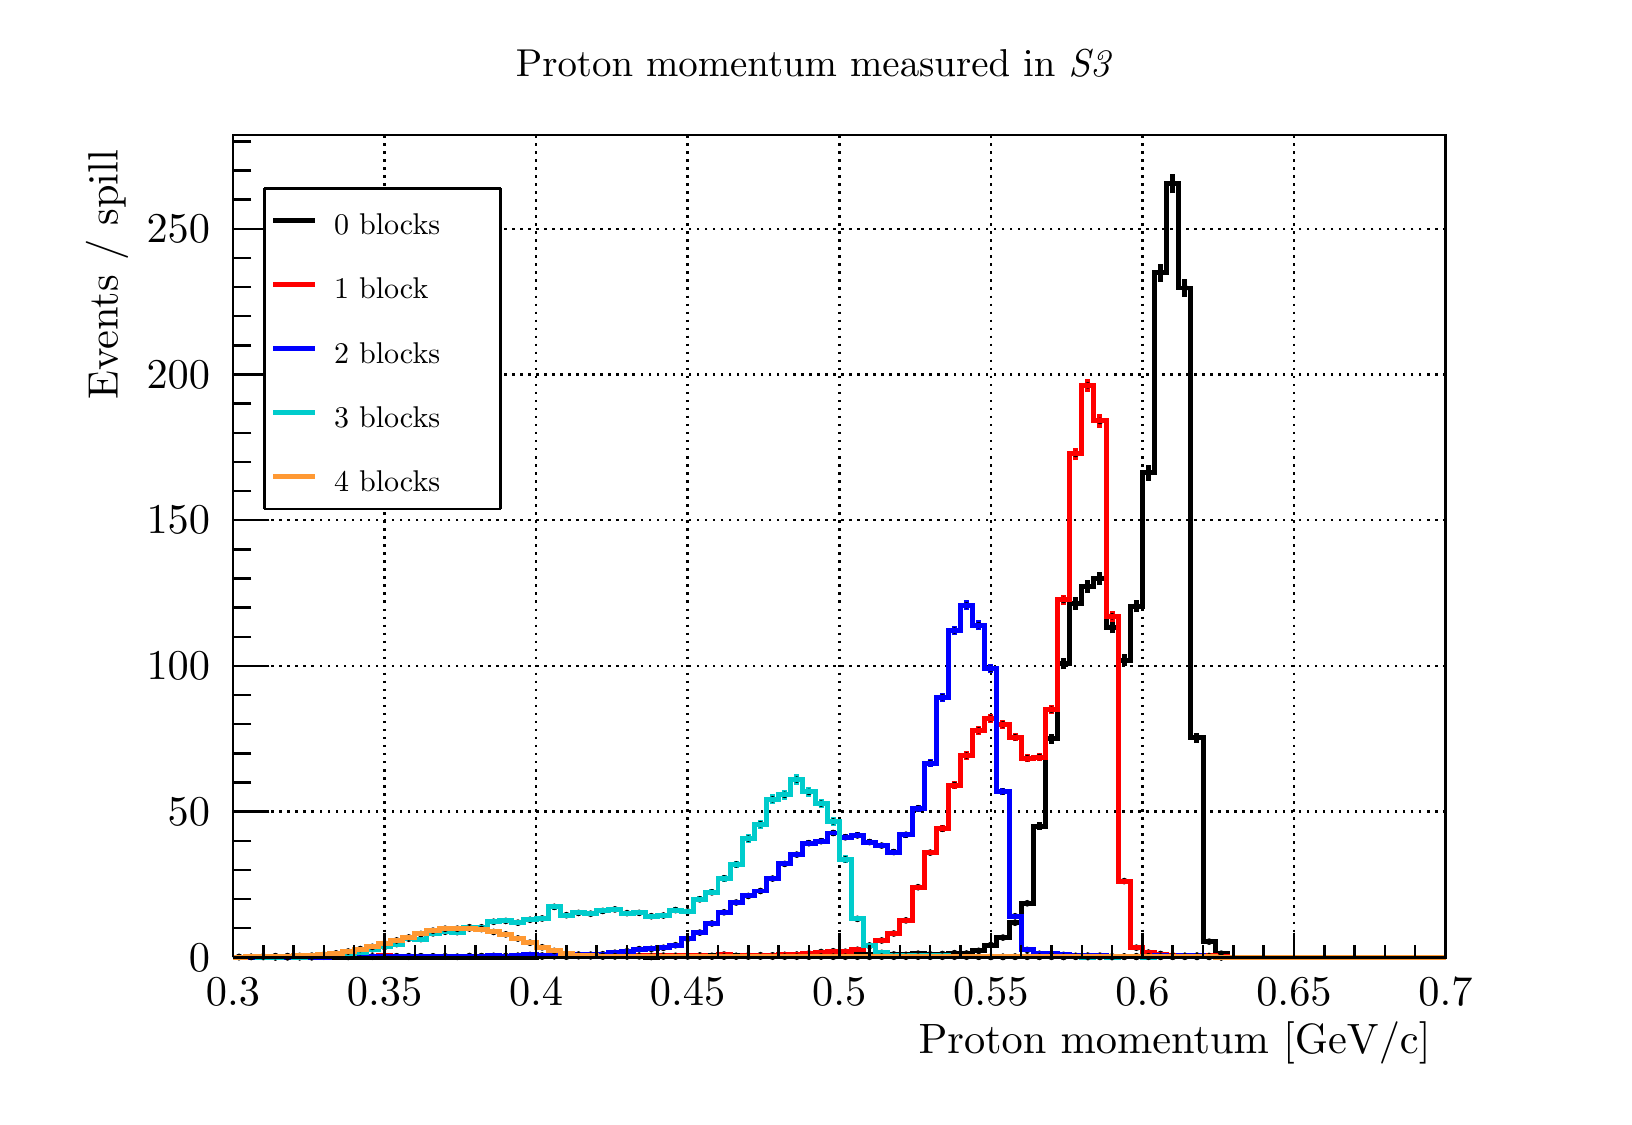
\begin{tikzpicture}
\pgfdeclareplotmark{cross} {
\pgfpathmoveto{\pgfpoint{-0.3\pgfplotmarksize}{\pgfplotmarksize}}
\pgfpathlineto{\pgfpoint{+0.3\pgfplotmarksize}{\pgfplotmarksize}}
\pgfpathlineto{\pgfpoint{+0.3\pgfplotmarksize}{0.3\pgfplotmarksize}}
\pgfpathlineto{\pgfpoint{+1\pgfplotmarksize}{0.3\pgfplotmarksize}}
\pgfpathlineto{\pgfpoint{+1\pgfplotmarksize}{-0.3\pgfplotmarksize}}
\pgfpathlineto{\pgfpoint{+0.3\pgfplotmarksize}{-0.3\pgfplotmarksize}}
\pgfpathlineto{\pgfpoint{+0.3\pgfplotmarksize}{-1.\pgfplotmarksize}}
\pgfpathlineto{\pgfpoint{-0.3\pgfplotmarksize}{-1.\pgfplotmarksize}}
\pgfpathlineto{\pgfpoint{-0.3\pgfplotmarksize}{-0.3\pgfplotmarksize}}
\pgfpathlineto{\pgfpoint{-1.\pgfplotmarksize}{-0.3\pgfplotmarksize}}
\pgfpathlineto{\pgfpoint{-1.\pgfplotmarksize}{0.3\pgfplotmarksize}}
\pgfpathlineto{\pgfpoint{-0.3\pgfplotmarksize}{0.3\pgfplotmarksize}}
\pgfpathclose
\pgfusepathqstroke
}
\pgfdeclareplotmark{cross*} {
\pgfpathmoveto{\pgfpoint{-0.3\pgfplotmarksize}{\pgfplotmarksize}}
\pgfpathlineto{\pgfpoint{+0.3\pgfplotmarksize}{\pgfplotmarksize}}
\pgfpathlineto{\pgfpoint{+0.3\pgfplotmarksize}{0.3\pgfplotmarksize}}
\pgfpathlineto{\pgfpoint{+1\pgfplotmarksize}{0.3\pgfplotmarksize}}
\pgfpathlineto{\pgfpoint{+1\pgfplotmarksize}{-0.3\pgfplotmarksize}}
\pgfpathlineto{\pgfpoint{+0.3\pgfplotmarksize}{-0.3\pgfplotmarksize}}
\pgfpathlineto{\pgfpoint{+0.3\pgfplotmarksize}{-1.\pgfplotmarksize}}
\pgfpathlineto{\pgfpoint{-0.3\pgfplotmarksize}{-1.\pgfplotmarksize}}
\pgfpathlineto{\pgfpoint{-0.3\pgfplotmarksize}{-0.3\pgfplotmarksize}}
\pgfpathlineto{\pgfpoint{-1.\pgfplotmarksize}{-0.3\pgfplotmarksize}}
\pgfpathlineto{\pgfpoint{-1.\pgfplotmarksize}{0.3\pgfplotmarksize}}
\pgfpathlineto{\pgfpoint{-0.3\pgfplotmarksize}{0.3\pgfplotmarksize}}
\pgfpathclose
\pgfusepathqfillstroke
}
\pgfdeclareplotmark{newstar} {
\pgfpathmoveto{\pgfqpoint{0pt}{\pgfplotmarksize}}
\pgfpathlineto{\pgfqpointpolar{44}{0.5\pgfplotmarksize}}
\pgfpathlineto{\pgfqpointpolar{18}{\pgfplotmarksize}}
\pgfpathlineto{\pgfqpointpolar{-20}{0.5\pgfplotmarksize}}
\pgfpathlineto{\pgfqpointpolar{-54}{\pgfplotmarksize}}
\pgfpathlineto{\pgfqpointpolar{-90}{0.5\pgfplotmarksize}}
\pgfpathlineto{\pgfqpointpolar{234}{\pgfplotmarksize}}
\pgfpathlineto{\pgfqpointpolar{198}{0.5\pgfplotmarksize}}
\pgfpathlineto{\pgfqpointpolar{162}{\pgfplotmarksize}}
\pgfpathlineto{\pgfqpointpolar{134}{0.5\pgfplotmarksize}}
\pgfpathclose
\pgfusepathqstroke
}
\pgfdeclareplotmark{newstar*} {
\pgfpathmoveto{\pgfqpoint{0pt}{\pgfplotmarksize}}
\pgfpathlineto{\pgfqpointpolar{44}{0.5\pgfplotmarksize}}
\pgfpathlineto{\pgfqpointpolar{18}{\pgfplotmarksize}}
\pgfpathlineto{\pgfqpointpolar{-20}{0.5\pgfplotmarksize}}
\pgfpathlineto{\pgfqpointpolar{-54}{\pgfplotmarksize}}
\pgfpathlineto{\pgfqpointpolar{-90}{0.5\pgfplotmarksize}}
\pgfpathlineto{\pgfqpointpolar{234}{\pgfplotmarksize}}
\pgfpathlineto{\pgfqpointpolar{198}{0.5\pgfplotmarksize}}
\pgfpathlineto{\pgfqpointpolar{162}{\pgfplotmarksize}}
\pgfpathlineto{\pgfqpointpolar{134}{0.5\pgfplotmarksize}}
\pgfpathclose
\pgfusepathqfillstroke
}
\definecolor{c}{rgb}{1,1,1};
\draw [color=c, fill=c] (0,0) rectangle (20,13.5632);
\draw [color=c, fill=c] (2.6,1.76322) rectangle (18,12.2069);
\definecolor{c}{rgb}{0,0,0};
\draw [c,line width=0.9] (2.6,1.76322) -- (2.6,12.2069) -- (18,12.2069) -- (18,1.76322) -- (2.6,1.76322);
\definecolor{c}{rgb}{1,1,1};
\draw [color=c, fill=c] (2.6,1.76322) rectangle (18,12.2069);
\definecolor{c}{rgb}{0,0,0};
\draw [c,line width=0.9] (2.6,1.76322) -- (2.6,12.2069) -- (18,12.2069) -- (18,1.76322) -- (2.6,1.76322);
\draw [c,line width=0.9] (2.6,1.76322) -- (18,1.76322);
\draw [c,dotted,line width=0.9] (2.6,12.2069) -- (2.6,1.76322);
\draw [c,dotted,line width=0.9] (4.525,12.2069) -- (4.525,1.76322);
\draw [c,dotted,line width=0.9] (6.45,12.2069) -- (6.45,1.76322);
\draw [c,dotted,line width=0.9] (8.375,12.2069) -- (8.375,1.76322);
\draw [c,dotted,line width=0.9] (10.3,12.2069) -- (10.3,1.76322);
\draw [c,dotted,line width=0.9] (12.225,12.2069) -- (12.225,1.76322);
\draw [c,dotted,line width=0.9] (14.15,12.2069) -- (14.15,1.76322);
\draw [c,dotted,line width=0.9] (16.075,12.2069) -- (16.075,1.76322);
\draw [c,dotted,line width=0.9] (18,12.2069) -- (18,1.76322);
\draw [c,line width=0.9] (2.6,1.76322) -- (2.6,12.2069);
\draw [c,dotted,line width=0.9] (18,1.76322) -- (2.6,1.76322);
\draw [c,dotted,line width=0.9] (18,3.61382) -- (2.6,3.61382);
\draw [c,dotted,line width=0.9] (18,5.46443) -- (2.6,5.46443);
\draw [c,dotted,line width=0.9] (18,7.31504) -- (2.6,7.31504);
\draw [c,dotted,line width=0.9] (18,9.16564) -- (2.6,9.16564);
\draw [c,dotted,line width=0.9] (18,11.0162) -- (2.6,11.0162);
\draw [c,dotted,line width=0.9] (18,11.0162) -- (2.6,11.0162);
\definecolor{c}{rgb}{0,0,0.6};
\draw [c,line width=0.9] (2.6,1.76322) -- (2.754,1.76322) -- (2.754,1.76322) -- (2.908,1.76322) -- (2.908,1.76322) -- (3.062,1.76322) -- (3.062,1.76322) -- (3.216,1.76322) -- (3.216,1.76322) -- (3.37,1.76322) -- (3.37,1.76322) -- (3.524,1.76322) --
 (3.524,1.76322) -- (3.678,1.76322) -- (3.678,1.76322) -- (3.832,1.76322) -- (3.832,1.76322) -- (3.986,1.76322) -- (3.986,1.76322) -- (4.14,1.76322) -- (4.14,1.76322) -- (4.294,1.76322) -- (4.294,1.76322) -- (4.448,1.76322) -- (4.448,1.76322) --
 (4.602,1.76322) -- (4.602,1.76322) -- (4.756,1.76322) -- (4.756,1.76322) -- (4.91,1.76322) -- (4.91,1.76322) -- (5.064,1.76322) -- (5.064,1.76322) -- (5.218,1.76322) -- (5.218,1.76322) -- (5.372,1.76322) -- (5.372,1.76322) -- (5.526,1.76322) --
 (5.526,1.76322) -- (5.68,1.76322) -- (5.68,1.76322) -- (5.834,1.76322) -- (5.834,1.76322) -- (5.988,1.76322) -- (5.988,1.76322) -- (6.142,1.76322) -- (6.142,1.76322) -- (6.296,1.76322) -- (6.296,1.76322) -- (6.45,1.76322) -- (6.45,1.76322) --
 (6.604,1.76322) -- (6.604,1.76322) -- (6.758,1.76322) -- (6.758,1.76322) -- (6.912,1.76322) -- (6.912,1.76322) -- (7.066,1.76322) -- (7.066,1.76322) -- (7.22,1.76322) -- (7.22,1.76322) -- (7.374,1.76322) -- (7.374,1.76322) -- (7.528,1.76322) --
 (7.528,1.76322) -- (7.682,1.76322) -- (7.682,1.76322) -- (7.836,1.76322) -- (7.836,1.76322) -- (7.99,1.76322) -- (7.99,1.76322) -- (8.144,1.76322) -- (8.144,1.76322) -- (8.298,1.76322) -- (8.298,1.76322) -- (8.452,1.76322) -- (8.452,1.76322) --
 (8.606,1.76322) -- (8.606,1.76322) -- (8.76,1.76322) -- (8.76,1.76322) -- (8.914,1.76322) -- (8.914,1.76322) -- (9.068,1.76322) -- (9.068,1.76322) -- (9.222,1.76322) -- (9.222,1.76322) -- (9.376,1.76322) -- (9.376,1.76322) -- (9.53,1.76322) --
 (9.53,1.76322) -- (9.684,1.76322) -- (9.684,1.76322) -- (9.838,1.76322) -- (9.838,1.76322) -- (9.992,1.76322) -- (9.992,1.76322) -- (10.146,1.76322) -- (10.146,1.76322) -- (10.3,1.76322) -- (10.3,1.76322) -- (10.454,1.76322) -- (10.454,1.76322) --
 (10.608,1.76322) -- (10.608,1.76322) -- (10.762,1.76322) -- (10.762,1.76322) -- (10.916,1.76322) -- (10.916,1.76322) -- (11.07,1.76322) -- (11.07,1.76322) -- (11.224,1.76322) -- (11.224,1.76322) -- (11.378,1.76322) -- (11.378,1.76322) --
 (11.532,1.76322) -- (11.532,1.76322) -- (11.686,1.76322) -- (11.686,1.76322) -- (11.84,1.76322) -- (11.84,1.76322) -- (11.994,1.76322) -- (11.994,1.76322) -- (12.148,1.76322) -- (12.148,1.76322) -- (12.302,1.76322) -- (12.302,1.76322) --
 (12.456,1.76322) -- (12.456,1.76322) -- (12.61,1.76322) -- (12.61,1.76322) -- (12.764,1.76322) -- (12.764,1.76322) -- (12.918,1.76322) -- (12.918,1.76322) -- (13.072,1.76322) -- (13.072,1.76322) -- (13.226,1.76322) -- (13.226,1.76322) --
 (13.38,1.76322) -- (13.38,1.76322) -- (13.534,1.76322) -- (13.534,1.76322) -- (13.688,1.76322) -- (13.688,1.76322) -- (13.842,1.76322) -- (13.842,1.76322) -- (13.996,1.76322) -- (13.996,1.76322) -- (14.15,1.76322) -- (14.15,1.76322) --
 (14.304,1.76322) -- (14.304,1.76322) -- (14.458,1.76322) -- (14.458,1.76322) -- (14.612,1.76322) -- (14.612,1.76322) -- (14.766,1.76322) -- (14.766,1.76322) -- (14.92,1.76322) -- (14.92,1.76322) -- (15.074,1.76322) -- (15.074,1.76322) --
 (15.228,1.76322) -- (15.228,1.76322) -- (15.382,1.76322) -- (15.382,1.76322) -- (15.536,1.76322) -- (15.536,1.76322) -- (15.69,1.76322) -- (15.69,1.76322) -- (15.844,1.76322) -- (15.844,1.76322) -- (15.998,1.76322) -- (15.998,1.76322) --
 (16.152,1.76322) -- (16.152,1.76322) -- (16.306,1.76322) -- (16.306,1.76322) -- (16.46,1.76322) -- (16.46,1.76322) -- (16.614,1.76322) -- (16.614,1.76322) -- (16.768,1.76322) -- (16.768,1.76322) -- (16.922,1.76322) -- (16.922,1.76322) --
 (17.076,1.76322) -- (17.076,1.76322) -- (17.23,1.76322) -- (17.23,1.76322) -- (17.384,1.76322) -- (17.384,1.76322) -- (17.538,1.76322) -- (17.538,1.76322) -- (17.692,1.76322) -- (17.692,1.76322) -- (17.846,1.76322) -- (17.846,1.76322) --
 (18,1.76322);
\definecolor{c}{rgb}{0,0,0};
\draw [c,line width=0.9] (2.6,1.76322) -- (18,1.76322);
\draw [anchor= east] (18,0.678161) node[scale=1.5317, color=c, rotate=0]{ Proton momentum [GeV/c]};
\draw [c,line width=0.9] (2.6,2.07653) -- (2.6,1.76322);
\draw [c,line width=0.9] (2.985,1.91987) -- (2.985,1.76322);
\draw [c,line width=0.9] (3.37,1.91987) -- (3.37,1.76322);
\draw [c,line width=0.9] (3.755,1.91987) -- (3.755,1.76322);
\draw [c,line width=0.9] (4.14,1.91987) -- (4.14,1.76322);
\draw [c,line width=0.9] (4.525,2.07653) -- (4.525,1.76322);
\draw [c,line width=0.9] (4.91,1.91987) -- (4.91,1.76322);
\draw [c,line width=0.9] (5.295,1.91987) -- (5.295,1.76322);
\draw [c,line width=0.9] (5.68,1.91987) -- (5.68,1.76322);
\draw [c,line width=0.9] (6.065,1.91987) -- (6.065,1.76322);
\draw [c,line width=0.9] (6.45,2.07653) -- (6.45,1.76322);
\draw [c,line width=0.9] (6.835,1.91987) -- (6.835,1.76322);
\draw [c,line width=0.9] (7.22,1.91987) -- (7.22,1.76322);
\draw [c,line width=0.9] (7.605,1.91987) -- (7.605,1.76322);
\draw [c,line width=0.9] (7.99,1.91987) -- (7.99,1.76322);
\draw [c,line width=0.9] (8.375,2.07653) -- (8.375,1.76322);
\draw [c,line width=0.9] (8.76,1.91987) -- (8.76,1.76322);
\draw [c,line width=0.9] (9.145,1.91987) -- (9.145,1.76322);
\draw [c,line width=0.9] (9.53,1.91987) -- (9.53,1.76322);
\draw [c,line width=0.9] (9.915,1.91987) -- (9.915,1.76322);
\draw [c,line width=0.9] (10.3,2.07653) -- (10.3,1.76322);
\draw [c,line width=0.9] (10.685,1.91987) -- (10.685,1.76322);
\draw [c,line width=0.9] (11.07,1.91987) -- (11.07,1.76322);
\draw [c,line width=0.9] (11.455,1.91987) -- (11.455,1.76322);
\draw [c,line width=0.9] (11.84,1.91987) -- (11.84,1.76322);
\draw [c,line width=0.9] (12.225,2.07653) -- (12.225,1.76322);
\draw [c,line width=0.9] (12.61,1.91987) -- (12.61,1.76322);
\draw [c,line width=0.9] (12.995,1.91987) -- (12.995,1.76322);
\draw [c,line width=0.9] (13.38,1.91987) -- (13.38,1.76322);
\draw [c,line width=0.9] (13.765,1.91987) -- (13.765,1.76322);
\draw [c,line width=0.9] (14.15,2.07653) -- (14.15,1.76322);
\draw [c,line width=0.9] (14.535,1.91987) -- (14.535,1.76322);
\draw [c,line width=0.9] (14.92,1.91987) -- (14.92,1.76322);
\draw [c,line width=0.9] (15.305,1.91987) -- (15.305,1.76322);
\draw [c,line width=0.9] (15.69,1.91987) -- (15.69,1.76322);
\draw [c,line width=0.9] (16.075,2.07653) -- (16.075,1.76322);
\draw [c,line width=0.9] (16.46,1.91987) -- (16.46,1.76322);
\draw [c,line width=0.9] (16.845,1.91987) -- (16.845,1.76322);
\draw [c,line width=0.9] (17.23,1.91987) -- (17.23,1.76322);
\draw [c,line width=0.9] (17.615,1.91987) -- (17.615,1.76322);
\draw [c,line width=0.9] (18,2.07653) -- (18,1.76322);
\draw [anchor=base] (2.6,1.15287) node[scale=1.5317, color=c, rotate=0]{0.3};
\draw [anchor=base] (4.525,1.15287) node[scale=1.5317, color=c, rotate=0]{0.35};
\draw [anchor=base] (6.45,1.15287) node[scale=1.5317, color=c, rotate=0]{0.4};
\draw [anchor=base] (8.375,1.15287) node[scale=1.5317, color=c, rotate=0]{0.45};
\draw [anchor=base] (10.3,1.15287) node[scale=1.5317, color=c, rotate=0]{0.5};
\draw [anchor=base] (12.225,1.15287) node[scale=1.5317, color=c, rotate=0]{0.55};
\draw [anchor=base] (14.15,1.15287) node[scale=1.5317, color=c, rotate=0]{0.6};
\draw [anchor=base] (16.075,1.15287) node[scale=1.5317, color=c, rotate=0]{0.65};
\draw [anchor=base] (18,1.15287) node[scale=1.5317, color=c, rotate=0]{0.7};
\draw [c,line width=0.9] (2.6,1.76322) -- (2.6,12.2069);
\draw [anchor= east] (1,12.2069) node[scale=1.5317, color=c, rotate=90]{ Events / spill};
\draw [c,line width=0.9] (3.062,1.76322) -- (2.6,1.76322);
\draw [c,line width=0.9] (2.831,2.13334) -- (2.6,2.13334);
\draw [c,line width=0.9] (2.831,2.50346) -- (2.6,2.50346);
\draw [c,line width=0.9] (2.831,2.87358) -- (2.6,2.87358);
\draw [c,line width=0.9] (2.831,3.2437) -- (2.6,3.2437);
\draw [c,line width=0.9] (3.062,3.61382) -- (2.6,3.61382);
\draw [c,line width=0.9] (2.831,3.98395) -- (2.6,3.98395);
\draw [c,line width=0.9] (2.831,4.35407) -- (2.6,4.35407);
\draw [c,line width=0.9] (2.831,4.72419) -- (2.6,4.72419);
\draw [c,line width=0.9] (2.831,5.09431) -- (2.6,5.09431);
\draw [c,line width=0.9] (3.062,5.46443) -- (2.6,5.46443);
\draw [c,line width=0.9] (2.831,5.83455) -- (2.6,5.83455);
\draw [c,line width=0.9] (2.831,6.20467) -- (2.6,6.20467);
\draw [c,line width=0.9] (2.831,6.57479) -- (2.6,6.57479);
\draw [c,line width=0.9] (2.831,6.94492) -- (2.6,6.94492);
\draw [c,line width=0.9] (3.062,7.31504) -- (2.6,7.31504);
\draw [c,line width=0.9] (2.831,7.68516) -- (2.6,7.68516);
\draw [c,line width=0.9] (2.831,8.05528) -- (2.6,8.05528);
\draw [c,line width=0.9] (2.831,8.4254) -- (2.6,8.4254);
\draw [c,line width=0.9] (2.831,8.79552) -- (2.6,8.79552);
\draw [c,line width=0.9] (3.062,9.16564) -- (2.6,9.16564);
\draw [c,line width=0.9] (2.831,9.53576) -- (2.6,9.53576);
\draw [c,line width=0.9] (2.831,9.90588) -- (2.6,9.90588);
\draw [c,line width=0.9] (2.831,10.276) -- (2.6,10.276);
\draw [c,line width=0.9] (2.831,10.6461) -- (2.6,10.6461);
\draw [c,line width=0.9] (3.062,11.0162) -- (2.6,11.0162);
\draw [c,line width=0.9] (3.062,11.0162) -- (2.6,11.0162);
\draw [c,line width=0.9] (2.831,11.3864) -- (2.6,11.3864);
\draw [c,line width=0.9] (2.831,11.7565) -- (2.6,11.7565);
\draw [c,line width=0.9] (2.831,12.1266) -- (2.6,12.1266);
\draw [anchor= east] (2.5,1.76322) node[scale=1.5317, color=c, rotate=0]{0};
\draw [anchor= east] (2.5,3.61382) node[scale=1.5317, color=c, rotate=0]{50};
\draw [anchor= east] (2.5,5.46443) node[scale=1.5317, color=c, rotate=0]{100};
\draw [anchor= east] (2.5,7.31504) node[scale=1.5317, color=c, rotate=0]{150};
\draw [anchor= east] (2.5,9.16564) node[scale=1.5317, color=c, rotate=0]{200};
\draw [anchor= east] (2.5,11.0162) node[scale=1.5317, color=c, rotate=0]{250};
\draw [c,line width=1.8] (6.527,1.77472) -- (6.527,1.7797);
\draw [c,line width=1.8] (6.527,1.7797) -- (6.527,1.78468);
\foreach \P in {(6.527,1.7797)}{\draw[mark options={color=c,fill=c},mark size=2.402402pt,mark=*,mark size=1pt] plot coordinates {\P};}
\draw [c,line width=1.8] (6.681,1.77299) -- (6.681,1.77753);
\draw [c,line width=1.8] (6.681,1.77753) -- (6.681,1.78208);
\foreach \P in {(6.681,1.77753)}{\draw[mark options={color=c,fill=c},mark size=2.402402pt,mark=*,mark size=1pt] plot coordinates {\P};}
\draw [c,line width=1.8] (6.835,1.77407) -- (6.835,1.77876);
\draw [c,line width=1.8] (6.835,1.77876) -- (6.835,1.78346);
\foreach \P in {(6.835,1.77876)}{\draw[mark options={color=c,fill=c},mark size=2.402402pt,mark=*,mark size=1pt] plot coordinates {\P};}
\draw [c,line width=1.8] (6.989,1.77335) -- (6.989,1.77804);
\draw [c,line width=1.8] (6.989,1.77804) -- (6.989,1.78273);
\foreach \P in {(6.989,1.77804)}{\draw[mark options={color=c,fill=c},mark size=2.402402pt,mark=*,mark size=1pt] plot coordinates {\P};}
\draw [c,line width=1.8] (7.143,1.77209) -- (7.143,1.77657);
\draw [c,line width=1.8] (7.143,1.77657) -- (7.143,1.78105);
\foreach \P in {(7.143,1.77657)}{\draw[mark options={color=c,fill=c},mark size=2.402402pt,mark=*,mark size=1pt] plot coordinates {\P};}
\draw [c,line width=1.8] (7.297,1.76943) -- (7.297,1.77321);
\draw [c,line width=1.8] (7.297,1.77321) -- (7.297,1.77699);
\foreach \P in {(7.297,1.77321)}{\draw[mark options={color=c,fill=c},mark size=2.402402pt,mark=*,mark size=1pt] plot coordinates {\P};}
\draw [c,line width=1.8] (7.451,1.77679) -- (7.451,1.78205);
\draw [c,line width=1.8] (7.451,1.78205) -- (7.451,1.78731);
\foreach \P in {(7.451,1.78205)}{\draw[mark options={color=c,fill=c},mark size=2.402402pt,mark=*,mark size=1pt] plot coordinates {\P};}
\draw [c,line width=1.8] (7.605,1.77314) -- (7.605,1.77778);
\draw [c,line width=1.8] (7.605,1.77778) -- (7.605,1.78242);
\foreach \P in {(7.605,1.77778)}{\draw[mark options={color=c,fill=c},mark size=2.402402pt,mark=*,mark size=1pt] plot coordinates {\P};}
\draw [c,line width=1.8] (7.759,1.77644) -- (7.759,1.78153);
\draw [c,line width=1.8] (7.759,1.78153) -- (7.759,1.78663);
\foreach \P in {(7.759,1.78153)}{\draw[mark options={color=c,fill=c},mark size=2.402402pt,mark=*,mark size=1pt] plot coordinates {\P};}
\draw [c,line width=1.8] (7.913,1.76506) -- (7.913,1.76758);
\draw [c,line width=1.8] (7.913,1.76758) -- (7.913,1.77009);
\foreach \P in {(7.913,1.76758)}{\draw[mark options={color=c,fill=c},mark size=2.402402pt,mark=*,mark size=1pt] plot coordinates {\P};}
\draw [c,line width=1.8] (8.067,1.77225) -- (8.067,1.7768);
\draw [c,line width=1.8] (8.067,1.7768) -- (8.067,1.78135);
\foreach \P in {(8.067,1.7768)}{\draw[mark options={color=c,fill=c},mark size=2.402402pt,mark=*,mark size=1pt] plot coordinates {\P};}
\draw [c,line width=1.8] (8.221,1.77071) -- (8.221,1.77485);
\draw [c,line width=1.8] (8.221,1.77485) -- (8.221,1.77899);
\foreach \P in {(8.221,1.77485)}{\draw[mark options={color=c,fill=c},mark size=2.402402pt,mark=*,mark size=1pt] plot coordinates {\P};}
\draw [c,line width=1.8] (8.375,1.77688) -- (8.375,1.78215);
\draw [c,line width=1.8] (8.375,1.78215) -- (8.375,1.78743);
\foreach \P in {(8.375,1.78215)}{\draw[mark options={color=c,fill=c},mark size=2.402402pt,mark=*,mark size=1pt] plot coordinates {\P};}
\draw [c,line width=1.8] (8.529,1.77958) -- (8.529,1.7853);
\draw [c,line width=1.8] (8.529,1.7853) -- (8.529,1.79101);
\foreach \P in {(8.529,1.7853)}{\draw[mark options={color=c,fill=c},mark size=2.402402pt,mark=*,mark size=1pt] plot coordinates {\P};}
\draw [c,line width=1.8] (8.683,1.77734) -- (8.683,1.78279);
\draw [c,line width=1.8] (8.683,1.78279) -- (8.683,1.78824);
\foreach \P in {(8.683,1.78279)}{\draw[mark options={color=c,fill=c},mark size=2.402402pt,mark=*,mark size=1pt] plot coordinates {\P};}
\draw [c,line width=1.8] (8.837,1.77226) -- (8.837,1.77681);
\draw [c,line width=1.8] (8.837,1.77681) -- (8.837,1.78137);
\foreach \P in {(8.837,1.77681)}{\draw[mark options={color=c,fill=c},mark size=2.402402pt,mark=*,mark size=1pt] plot coordinates {\P};}
\draw [c,line width=1.8] (8.991,1.77726) -- (8.991,1.78269);
\draw [c,line width=1.8] (8.991,1.78269) -- (8.991,1.78812);
\foreach \P in {(8.991,1.78269)}{\draw[mark options={color=c,fill=c},mark size=2.402402pt,mark=*,mark size=1pt] plot coordinates {\P};}
\draw [c,line width=1.8] (9.145,1.78107) -- (9.145,1.78706);
\draw [c,line width=1.8] (9.145,1.78706) -- (9.145,1.79305);
\foreach \P in {(9.145,1.78706)}{\draw[mark options={color=c,fill=c},mark size=2.402402pt,mark=*,mark size=1pt] plot coordinates {\P};}
\draw [c,line width=1.8] (9.299,1.77668) -- (9.299,1.78186);
\draw [c,line width=1.8] (9.299,1.78186) -- (9.299,1.78704);
\foreach \P in {(9.299,1.78186)}{\draw[mark options={color=c,fill=c},mark size=2.402402pt,mark=*,mark size=1pt] plot coordinates {\P};}
\draw [c,line width=1.8] (9.453,1.77923) -- (9.453,1.78483);
\draw [c,line width=1.8] (9.453,1.78483) -- (9.453,1.79044);
\foreach \P in {(9.453,1.78483)}{\draw[mark options={color=c,fill=c},mark size=2.402402pt,mark=*,mark size=1pt] plot coordinates {\P};}
\draw [c,line width=1.8] (9.607,1.78653) -- (9.607,1.79328);
\draw [c,line width=1.8] (9.607,1.79328) -- (9.607,1.80003);
\foreach \P in {(9.607,1.79328)}{\draw[mark options={color=c,fill=c},mark size=2.402402pt,mark=*,mark size=1pt] plot coordinates {\P};}
\draw [c,line width=1.8] (9.761,1.78853) -- (9.761,1.79545);
\draw [c,line width=1.8] (9.761,1.79545) -- (9.761,1.80237);
\foreach \P in {(9.761,1.79545)}{\draw[mark options={color=c,fill=c},mark size=2.402402pt,mark=*,mark size=1pt] plot coordinates {\P};}
\draw [c,line width=1.8] (9.915,1.77682) -- (9.915,1.78206);
\draw [c,line width=1.8] (9.915,1.78206) -- (9.915,1.7873);
\foreach \P in {(9.915,1.78206)}{\draw[mark options={color=c,fill=c},mark size=2.402402pt,mark=*,mark size=1pt] plot coordinates {\P};}
\draw [c,line width=1.8] (10.069,1.78289) -- (10.069,1.78902);
\draw [c,line width=1.8] (10.069,1.78902) -- (10.069,1.79514);
\foreach \P in {(10.069,1.78902)}{\draw[mark options={color=c,fill=c},mark size=2.402402pt,mark=*,mark size=1pt] plot coordinates {\P};}
\draw [c,line width=1.8] (10.223,1.77295) -- (10.223,1.77748);
\draw [c,line width=1.8] (10.223,1.77748) -- (10.223,1.782);
\foreach \P in {(10.223,1.77748)}{\draw[mark options={color=c,fill=c},mark size=2.402402pt,mark=*,mark size=1pt] plot coordinates {\P};}
\draw [c,line width=1.8] (10.377,1.78119) -- (10.377,1.78724);
\draw [c,line width=1.8] (10.377,1.78724) -- (10.377,1.79328);
\foreach \P in {(10.377,1.78724)}{\draw[mark options={color=c,fill=c},mark size=2.402402pt,mark=*,mark size=1pt] plot coordinates {\P};}
\draw [c,line width=1.8] (10.531,1.78773) -- (10.531,1.79462);
\draw [c,line width=1.8] (10.531,1.79462) -- (10.531,1.8015);
\foreach \P in {(10.531,1.79462)}{\draw[mark options={color=c,fill=c},mark size=2.402402pt,mark=*,mark size=1pt] plot coordinates {\P};}
\draw [c,line width=1.8] (10.685,1.78806) -- (10.685,1.79482);
\draw [c,line width=1.8] (10.685,1.79482) -- (10.685,1.80158);
\foreach \P in {(10.685,1.79482)}{\draw[mark options={color=c,fill=c},mark size=2.402402pt,mark=*,mark size=1pt] plot coordinates {\P};}
\draw [c,line width=1.8] (10.839,1.79316) -- (10.839,1.80072);
\draw [c,line width=1.8] (10.839,1.80072) -- (10.839,1.80828);
\foreach \P in {(10.839,1.80072)}{\draw[mark options={color=c,fill=c},mark size=2.402402pt,mark=*,mark size=1pt] plot coordinates {\P};}
\draw [c,line width=1.8] (10.993,1.79236) -- (10.993,1.79968);
\draw [c,line width=1.8] (10.993,1.79968) -- (10.993,1.807);
\foreach \P in {(10.993,1.79968)}{\draw[mark options={color=c,fill=c},mark size=2.402402pt,mark=*,mark size=1pt] plot coordinates {\P};}
\draw [c,line width=1.8] (11.147,1.78826) -- (11.147,1.79529);
\draw [c,line width=1.8] (11.147,1.79529) -- (11.147,1.80232);
\foreach \P in {(11.147,1.79529)}{\draw[mark options={color=c,fill=c},mark size=2.402402pt,mark=*,mark size=1pt] plot coordinates {\P};}
\draw [c,line width=1.8] (11.301,1.80144) -- (11.301,1.80988);
\draw [c,line width=1.8] (11.301,1.80988) -- (11.301,1.81831);
\foreach \P in {(11.301,1.80988)}{\draw[mark options={color=c,fill=c},mark size=2.402402pt,mark=*,mark size=1pt] plot coordinates {\P};}
\draw [c,line width=1.8] (11.455,1.79317) -- (11.455,1.80051);
\draw [c,line width=1.8] (11.455,1.80051) -- (11.455,1.80784);
\foreach \P in {(11.455,1.80051)}{\draw[mark options={color=c,fill=c},mark size=2.402402pt,mark=*,mark size=1pt] plot coordinates {\P};}
\draw [c,line width=1.8] (11.609,1.79739) -- (11.609,1.80541);
\draw [c,line width=1.8] (11.609,1.80541) -- (11.609,1.81343);
\foreach \P in {(11.609,1.80541)}{\draw[mark options={color=c,fill=c},mark size=2.402402pt,mark=*,mark size=1pt] plot coordinates {\P};}
\draw [c,line width=1.8] (11.763,1.8075) -- (11.763,1.81626);
\draw [c,line width=1.8] (11.763,1.81626) -- (11.763,1.82503);
\foreach \P in {(11.763,1.81626)}{\draw[mark options={color=c,fill=c},mark size=2.402402pt,mark=*,mark size=1pt] plot coordinates {\P};}
\draw [c,line width=1.8] (11.917,1.80354) -- (11.917,1.81225);
\draw [c,line width=1.8] (11.917,1.81225) -- (11.917,1.82097);
\foreach \P in {(11.917,1.81225)}{\draw[mark options={color=c,fill=c},mark size=2.402402pt,mark=*,mark size=1pt] plot coordinates {\P};}
\draw [c,line width=1.8] (12.071,1.83556) -- (12.071,1.84657);
\draw [c,line width=1.8] (12.071,1.84657) -- (12.071,1.85758);
\foreach \P in {(12.071,1.84657)}{\draw[mark options={color=c,fill=c},mark size=2.402402pt,mark=*,mark size=1pt] plot coordinates {\P};}
\draw [c,line width=1.8] (12.225,1.90447) -- (12.225,1.91974);
\draw [c,line width=1.8] (12.225,1.91974) -- (12.225,1.93502);
\foreach \P in {(12.225,1.91974)}{\draw[mark options={color=c,fill=c},mark size=2.402402pt,mark=*,mark size=1pt] plot coordinates {\P};}
\draw [c,line width=1.8] (12.379,1.99489) -- (12.379,2.01426);
\draw [c,line width=1.8] (12.379,2.01426) -- (12.379,2.03364);
\foreach \P in {(12.379,2.01426)}{\draw[mark options={color=c,fill=c},mark size=2.402402pt,mark=*,mark size=1pt] plot coordinates {\P};}
\draw [c,line width=1.8] (12.533,2.17709) -- (12.533,2.20271);
\draw [c,line width=1.8] (12.533,2.20271) -- (12.533,2.22833);
\foreach \P in {(12.533,2.20271)}{\draw[mark options={color=c,fill=c},mark size=2.402402pt,mark=*,mark size=1pt] plot coordinates {\P};}
\draw [c,line width=1.8] (12.687,2.41778) -- (12.687,2.44984);
\draw [c,line width=1.8] (12.687,2.44984) -- (12.687,2.4819);
\foreach \P in {(12.687,2.44984)}{\draw[mark options={color=c,fill=c},mark size=2.402402pt,mark=*,mark size=1pt] plot coordinates {\P};}
\draw [c,line width=1.8] (12.841,3.37881) -- (12.841,3.42872);
\draw [c,line width=1.8] (12.841,3.42872) -- (12.841,3.47864);
\foreach \P in {(12.841,3.42872)}{\draw[mark options={color=c,fill=c},mark size=2.402402pt,mark=*,mark size=1pt] plot coordinates {\P};}
\draw [c,line width=1.8] (12.995,4.4751) -- (12.995,4.53956);
\draw [c,line width=1.8] (12.995,4.53956) -- (12.995,4.60402);
\foreach \P in {(12.995,4.53956)}{\draw[mark options={color=c,fill=c},mark size=2.402402pt,mark=*,mark size=1pt] plot coordinates {\P};}
\draw [c,line width=1.8] (13.149,5.41981) -- (13.149,5.49452);
\draw [c,line width=1.8] (13.149,5.49452) -- (13.149,5.56924);
\foreach \P in {(13.149,5.49452)}{\draw[mark options={color=c,fill=c},mark size=2.402402pt,mark=*,mark size=1pt] plot coordinates {\P};}
\draw [c,line width=1.8] (13.303,6.17215) -- (13.303,6.25403);
\draw [c,line width=1.8] (13.303,6.25403) -- (13.303,6.33591);
\foreach \P in {(13.303,6.25403)}{\draw[mark options={color=c,fill=c},mark size=2.402402pt,mark=*,mark size=1pt] plot coordinates {\P};}
\draw [c,line width=1.8] (13.457,6.38848) -- (13.457,6.47218);
\draw [c,line width=1.8] (13.457,6.47218) -- (13.457,6.55589);
\foreach \P in {(13.457,6.47218)}{\draw[mark options={color=c,fill=c},mark size=2.402402pt,mark=*,mark size=1pt] plot coordinates {\P};}
\draw [c,line width=1.8] (13.611,6.49068) -- (13.611,6.57534);
\draw [c,line width=1.8] (13.611,6.57534) -- (13.611,6.65999);
\foreach \P in {(13.611,6.57534)}{\draw[mark options={color=c,fill=c},mark size=2.402402pt,mark=*,mark size=1pt] plot coordinates {\P};}
\draw [c,line width=1.8] (13.765,5.8785) -- (13.765,5.95754);
\draw [c,line width=1.8] (13.765,5.95754) -- (13.765,6.03658);
\foreach \P in {(13.765,5.95754)}{\draw[mark options={color=c,fill=c},mark size=2.402402pt,mark=*,mark size=1pt] plot coordinates {\P};}
\draw [c,line width=1.8] (13.919,5.46117) -- (13.919,5.53633);
\draw [c,line width=1.8] (13.919,5.53633) -- (13.919,5.61149);
\foreach \P in {(13.919,5.53633)}{\draw[mark options={color=c,fill=c},mark size=2.402402pt,mark=*,mark size=1pt] plot coordinates {\P};}
\draw [c,line width=1.8] (14.073,6.14327) -- (14.073,6.2249);
\draw [c,line width=1.8] (14.073,6.2249) -- (14.073,6.30653);
\foreach \P in {(14.073,6.2249)}{\draw[mark options={color=c,fill=c},mark size=2.402402pt,mark=*,mark size=1pt] plot coordinates {\P};}
\draw [c,line width=1.8] (14.227,7.81881) -- (14.227,7.91463);
\draw [c,line width=1.8] (14.227,7.91463) -- (14.227,8.01046);
\foreach \P in {(14.227,7.91463)}{\draw[mark options={color=c,fill=c},mark size=2.402402pt,mark=*,mark size=1pt] plot coordinates {\P};}
\draw [c,line width=1.8] (14.381,10.3441) -- (14.381,10.4582);
\draw [c,line width=1.8] (14.381,10.4582) -- (14.381,10.5724);
\foreach \P in {(14.381,10.4582)}{\draw[mark options={color=c,fill=c},mark size=2.402402pt,mark=*,mark size=1pt] plot coordinates {\P};}
\draw [c,line width=1.8] (14.535,11.4672) -- (14.535,11.5884);
\draw [c,line width=1.8] (14.535,11.5884) -- (14.535,11.7096);
\foreach \P in {(14.535,11.5884)}{\draw[mark options={color=c,fill=c},mark size=2.402402pt,mark=*,mark size=1pt] plot coordinates {\P};}
\draw [c,line width=1.8] (14.689,10.1512) -- (14.689,10.264);
\draw [c,line width=1.8] (14.689,10.264) -- (14.689,10.3768);
\foreach \P in {(14.689,10.264)}{\draw[mark options={color=c,fill=c},mark size=2.402402pt,mark=*,mark size=1pt] plot coordinates {\P};}
\draw [c,line width=1.8] (14.843,4.48823) -- (14.843,4.55278);
\draw [c,line width=1.8] (14.843,4.55278) -- (14.843,4.61733);
\foreach \P in {(14.843,4.55278)}{\draw[mark options={color=c,fill=c},mark size=2.402402pt,mark=*,mark size=1pt] plot coordinates {\P};}
\draw [c,line width=1.8] (14.997,1.94581) -- (14.997,1.96298);
\draw [c,line width=1.8] (14.997,1.96298) -- (14.997,1.98015);
\foreach \P in {(14.997,1.96298)}{\draw[mark options={color=c,fill=c},mark size=2.402402pt,mark=*,mark size=1pt] plot coordinates {\P};}
\draw [c,line width=1.8] (15.151,1.80171) -- (15.151,1.81003);
\draw [c,line width=1.8] (15.151,1.81003) -- (15.151,1.81834);
\foreach \P in {(15.151,1.81003)}{\draw[mark options={color=c,fill=c},mark size=2.402402pt,mark=*,mark size=1pt] plot coordinates {\P};}
\draw [c,line width=1.8] (2.6,1.76322) -- (2.754,1.76322) -- (2.754,1.76322) -- (2.908,1.76322) -- (2.908,1.76322) -- (3.062,1.76322) -- (3.062,1.76322) -- (3.216,1.76322) -- (3.216,1.76322) -- (3.37,1.76322) -- (3.37,1.76322) -- (3.524,1.76322) --
 (3.524,1.76322) -- (3.678,1.76322) -- (3.678,1.76322) -- (3.832,1.76322) -- (3.832,1.76322) -- (3.986,1.76322) -- (3.986,1.76322) -- (4.14,1.76322) -- (4.14,1.76322) -- (4.294,1.76322) -- (4.294,1.76322) -- (4.448,1.76322) -- (4.448,1.76322) --
 (4.602,1.76322) -- (4.602,1.76322) -- (4.756,1.76322) -- (4.756,1.76322) -- (4.91,1.76322) -- (4.91,1.76322) -- (5.064,1.76322) -- (5.064,1.76322) -- (5.218,1.76322) -- (5.218,1.76322) -- (5.372,1.76322) -- (5.372,1.76322) -- (5.526,1.76322) --
 (5.526,1.76322) -- (5.68,1.76322) -- (5.68,1.76322) -- (5.834,1.76322) -- (5.834,1.76322) -- (5.988,1.76322) -- (5.988,1.76322) -- (6.142,1.76322) -- (6.142,1.76322) -- (6.296,1.76322) -- (6.296,1.76322) -- (6.45,1.76322) -- (6.45,1.7797) --
 (6.604,1.7797) -- (6.604,1.77753) -- (6.758,1.77753) -- (6.758,1.77876) -- (6.912,1.77876) -- (6.912,1.77804) -- (7.066,1.77804) -- (7.066,1.77657) -- (7.22,1.77657) -- (7.22,1.77321) -- (7.374,1.77321) -- (7.374,1.78205) -- (7.528,1.78205) --
 (7.528,1.77778) -- (7.682,1.77778) -- (7.682,1.78153) -- (7.836,1.78153) -- (7.836,1.76758) -- (7.99,1.76758) -- (7.99,1.7768) -- (8.144,1.7768) -- (8.144,1.77485) -- (8.298,1.77485) -- (8.298,1.78215) -- (8.452,1.78215) -- (8.452,1.7853) --
 (8.606,1.7853) -- (8.606,1.78279) -- (8.76,1.78279) -- (8.76,1.77681) -- (8.914,1.77681) -- (8.914,1.78269) -- (9.068,1.78269) -- (9.068,1.78706) -- (9.222,1.78706) -- (9.222,1.78186) -- (9.376,1.78186) -- (9.376,1.78483) -- (9.53,1.78483) --
 (9.53,1.79328) -- (9.684,1.79328) -- (9.684,1.79545) -- (9.838,1.79545) -- (9.838,1.78206) -- (9.992,1.78206) -- (9.992,1.78902) -- (10.146,1.78902) -- (10.146,1.77748) -- (10.3,1.77748) -- (10.3,1.78724) -- (10.454,1.78724) -- (10.454,1.79462) --
 (10.608,1.79462) -- (10.608,1.79482) -- (10.762,1.79482) -- (10.762,1.80072) -- (10.916,1.80072) -- (10.916,1.79968) -- (11.07,1.79968) -- (11.07,1.79529) -- (11.224,1.79529) -- (11.224,1.80988) -- (11.378,1.80988) -- (11.378,1.80051) --
 (11.532,1.80051) -- (11.532,1.80541) -- (11.686,1.80541) -- (11.686,1.81626) -- (11.84,1.81626) -- (11.84,1.81225) -- (11.994,1.81225) -- (11.994,1.84657) -- (12.148,1.84657) -- (12.148,1.91974) -- (12.302,1.91974) -- (12.302,2.01426) --
 (12.456,2.01426) -- (12.456,2.20271) -- (12.61,2.20271) -- (12.61,2.44984) -- (12.764,2.44984) -- (12.764,3.42872) -- (12.918,3.42872) -- (12.918,4.53956) -- (13.072,4.53956) -- (13.072,5.49452) -- (13.226,5.49452) -- (13.226,6.25403) --
 (13.38,6.25403) -- (13.38,6.47218) -- (13.534,6.47218) -- (13.534,6.57534) -- (13.688,6.57534) -- (13.688,5.95754) -- (13.842,5.95754) -- (13.842,5.53633) -- (13.996,5.53633) -- (13.996,6.2249) -- (14.15,6.2249) -- (14.15,7.91463) --
 (14.304,7.91463) -- (14.304,10.4582) -- (14.458,10.4582) -- (14.458,11.5884) -- (14.612,11.5884) -- (14.612,10.264) -- (14.766,10.264) -- (14.766,4.55278) -- (14.92,4.55278) -- (14.92,1.96298) -- (15.074,1.96298) -- (15.074,1.81003) --
 (15.228,1.81003) -- (15.228,1.76322) -- (15.382,1.76322) -- (15.382,1.76322) -- (15.536,1.76322) -- (15.536,1.76322) -- (15.69,1.76322) -- (15.69,1.76322) -- (15.844,1.76322) -- (15.844,1.76322) -- (15.998,1.76322) -- (15.998,1.76322) --
 (16.152,1.76322) -- (16.152,1.76322) -- (16.306,1.76322) -- (16.306,1.76322) -- (16.46,1.76322) -- (16.46,1.76322) -- (16.614,1.76322) -- (16.614,1.76322) -- (16.768,1.76322) -- (16.768,1.76322) -- (16.922,1.76322) -- (16.922,1.76322) --
 (17.076,1.76322) -- (17.076,1.76322) -- (17.23,1.76322) -- (17.23,1.76322) -- (17.384,1.76322) -- (17.384,1.76322) -- (17.538,1.76322) -- (17.538,1.76322) -- (17.692,1.76322) -- (17.692,1.76322) -- (17.846,1.76322) -- (17.846,1.76322) --
 (18,1.76322);
\definecolor{c}{rgb}{1,0,0};
\draw [c,line width=1.8] (3.139,1.76322) -- (3.139,1.76437);
\draw [c,line width=1.8] (3.139,1.76437) -- (3.139,1.76552);
\definecolor{c}{rgb}{0,0,0};
\foreach \P in {(3.139,1.76437)}{\draw[mark options={color=c,fill=c},mark size=2.402402pt,mark=*,mark size=1pt] plot coordinates {\P};}
\definecolor{c}{rgb}{1,0,0};
\draw [c,line width=1.8] (3.293,1.7645) -- (3.293,1.76626);
\draw [c,line width=1.8] (3.293,1.76626) -- (3.293,1.76802);
\definecolor{c}{rgb}{0,0,0};
\foreach \P in {(3.293,1.76626)}{\draw[mark options={color=c,fill=c},mark size=2.402402pt,mark=*,mark size=1pt] plot coordinates {\P};}
\definecolor{c}{rgb}{1,0,0};
\draw [c,line width=1.8] (3.447,1.76504) -- (3.447,1.76688);
\draw [c,line width=1.8] (3.447,1.76688) -- (3.447,1.76871);
\definecolor{c}{rgb}{0,0,0};
\foreach \P in {(3.447,1.76688)}{\draw[mark options={color=c,fill=c},mark size=2.402402pt,mark=*,mark size=1pt] plot coordinates {\P};}
\definecolor{c}{rgb}{1,0,0};
\draw [c,line width=1.8] (3.601,1.765) -- (3.601,1.76682);
\draw [c,line width=1.8] (3.601,1.76682) -- (3.601,1.76864);
\definecolor{c}{rgb}{0,0,0};
\foreach \P in {(3.601,1.76682)}{\draw[mark options={color=c,fill=c},mark size=2.402402pt,mark=*,mark size=1pt] plot coordinates {\P};}
\definecolor{c}{rgb}{1,0,0};
\draw [c,line width=1.8] (3.755,1.76792) -- (3.755,1.77093);
\draw [c,line width=1.8] (3.755,1.77093) -- (3.755,1.77394);
\definecolor{c}{rgb}{0,0,0};
\foreach \P in {(3.755,1.77093)}{\draw[mark options={color=c,fill=c},mark size=2.402402pt,mark=*,mark size=1pt] plot coordinates {\P};}
\definecolor{c}{rgb}{1,0,0};
\draw [c,line width=1.8] (3.909,1.76974) -- (3.909,1.77308);
\draw [c,line width=1.8] (3.909,1.77308) -- (3.909,1.77643);
\definecolor{c}{rgb}{0,0,0};
\foreach \P in {(3.909,1.77308)}{\draw[mark options={color=c,fill=c},mark size=2.402402pt,mark=*,mark size=1pt] plot coordinates {\P};}
\definecolor{c}{rgb}{1,0,0};
\draw [c,line width=1.8] (4.063,1.76876) -- (4.063,1.77182);
\draw [c,line width=1.8] (4.063,1.77182) -- (4.063,1.77488);
\definecolor{c}{rgb}{0,0,0};
\foreach \P in {(4.063,1.77182)}{\draw[mark options={color=c,fill=c},mark size=2.402402pt,mark=*,mark size=1pt] plot coordinates {\P};}
\definecolor{c}{rgb}{1,0,0};
\draw [c,line width=1.8] (4.217,1.76941) -- (4.217,1.7726);
\draw [c,line width=1.8] (4.217,1.7726) -- (4.217,1.77578);
\definecolor{c}{rgb}{0,0,0};
\foreach \P in {(4.217,1.7726)}{\draw[mark options={color=c,fill=c},mark size=2.402402pt,mark=*,mark size=1pt] plot coordinates {\P};}
\definecolor{c}{rgb}{1,0,0};
\draw [c,line width=1.8] (4.371,1.76852) -- (4.371,1.77148);
\draw [c,line width=1.8] (4.371,1.77148) -- (4.371,1.77443);
\definecolor{c}{rgb}{0,0,0};
\foreach \P in {(4.371,1.77148)}{\draw[mark options={color=c,fill=c},mark size=2.402402pt,mark=*,mark size=1pt] plot coordinates {\P};}
\definecolor{c}{rgb}{1,0,0};
\draw [c,line width=1.8] (4.525,1.77764) -- (4.525,1.78201);
\draw [c,line width=1.8] (4.525,1.78201) -- (4.525,1.78639);
\definecolor{c}{rgb}{0,0,0};
\foreach \P in {(4.525,1.78201)}{\draw[mark options={color=c,fill=c},mark size=2.402402pt,mark=*,mark size=1pt] plot coordinates {\P};}
\definecolor{c}{rgb}{1,0,0};
\draw [c,line width=1.8] (4.679,1.77281) -- (4.679,1.77657);
\draw [c,line width=1.8] (4.679,1.77657) -- (4.679,1.78033);
\definecolor{c}{rgb}{0,0,0};
\foreach \P in {(4.679,1.77657)}{\draw[mark options={color=c,fill=c},mark size=2.402402pt,mark=*,mark size=1pt] plot coordinates {\P};}
\definecolor{c}{rgb}{1,0,0};
\draw [c,line width=1.8] (4.833,1.77444) -- (4.833,1.77838);
\draw [c,line width=1.8] (4.833,1.77838) -- (4.833,1.78233);
\definecolor{c}{rgb}{0,0,0};
\foreach \P in {(4.833,1.77838)}{\draw[mark options={color=c,fill=c},mark size=2.402402pt,mark=*,mark size=1pt] plot coordinates {\P};}
\definecolor{c}{rgb}{1,0,0};
\draw [c,line width=1.8] (4.987,1.77131) -- (4.987,1.77463);
\draw [c,line width=1.8] (4.987,1.77463) -- (4.987,1.77794);
\definecolor{c}{rgb}{0,0,0};
\foreach \P in {(4.987,1.77463)}{\draw[mark options={color=c,fill=c},mark size=2.402402pt,mark=*,mark size=1pt] plot coordinates {\P};}
\definecolor{c}{rgb}{1,0,0};
\draw [c,line width=1.8] (5.141,1.77002) -- (5.141,1.77322);
\draw [c,line width=1.8] (5.141,1.77322) -- (5.141,1.77643);
\definecolor{c}{rgb}{0,0,0};
\foreach \P in {(5.141,1.77322)}{\draw[mark options={color=c,fill=c},mark size=2.402402pt,mark=*,mark size=1pt] plot coordinates {\P};}
\definecolor{c}{rgb}{1,0,0};
\draw [c,line width=1.8] (5.295,1.7691) -- (5.295,1.77219);
\draw [c,line width=1.8] (5.295,1.77219) -- (5.295,1.77528);
\definecolor{c}{rgb}{0,0,0};
\foreach \P in {(5.295,1.77219)}{\draw[mark options={color=c,fill=c},mark size=2.402402pt,mark=*,mark size=1pt] plot coordinates {\P};}
\definecolor{c}{rgb}{1,0,0};
\draw [c,line width=1.8] (5.449,1.76756) -- (5.449,1.77026);
\draw [c,line width=1.8] (5.449,1.77026) -- (5.449,1.77296);
\definecolor{c}{rgb}{0,0,0};
\foreach \P in {(5.449,1.77026)}{\draw[mark options={color=c,fill=c},mark size=2.402402pt,mark=*,mark size=1pt] plot coordinates {\P};}
\definecolor{c}{rgb}{1,0,0};
\draw [c,line width=1.8] (5.603,1.76917) -- (5.603,1.77223);
\draw [c,line width=1.8] (5.603,1.77223) -- (5.603,1.77529);
\definecolor{c}{rgb}{0,0,0};
\foreach \P in {(5.603,1.77223)}{\draw[mark options={color=c,fill=c},mark size=2.402402pt,mark=*,mark size=1pt] plot coordinates {\P};}
\definecolor{c}{rgb}{1,0,0};
\draw [c,line width=1.8] (5.757,1.77233) -- (5.757,1.77607);
\draw [c,line width=1.8] (5.757,1.77607) -- (5.757,1.7798);
\definecolor{c}{rgb}{0,0,0};
\foreach \P in {(5.757,1.77607)}{\draw[mark options={color=c,fill=c},mark size=2.402402pt,mark=*,mark size=1pt] plot coordinates {\P};}
\definecolor{c}{rgb}{1,0,0};
\draw [c,line width=1.8] (5.911,1.77224) -- (5.911,1.77555);
\draw [c,line width=1.8] (5.911,1.77555) -- (5.911,1.77886);
\definecolor{c}{rgb}{0,0,0};
\foreach \P in {(5.911,1.77555)}{\draw[mark options={color=c,fill=c},mark size=2.402402pt,mark=*,mark size=1pt] plot coordinates {\P};}
\definecolor{c}{rgb}{1,0,0};
\draw [c,line width=1.8] (6.065,1.77082) -- (6.065,1.77419);
\draw [c,line width=1.8] (6.065,1.77419) -- (6.065,1.77756);
\definecolor{c}{rgb}{0,0,0};
\foreach \P in {(6.065,1.77419)}{\draw[mark options={color=c,fill=c},mark size=2.402402pt,mark=*,mark size=1pt] plot coordinates {\P};}
\definecolor{c}{rgb}{1,0,0};
\draw [c,line width=1.8] (6.219,1.77728) -- (6.219,1.78173);
\draw [c,line width=1.8] (6.219,1.78173) -- (6.219,1.78617);
\definecolor{c}{rgb}{0,0,0};
\foreach \P in {(6.219,1.78173)}{\draw[mark options={color=c,fill=c},mark size=2.402402pt,mark=*,mark size=1pt] plot coordinates {\P};}
\definecolor{c}{rgb}{1,0,0};
\draw [c,line width=1.8] (6.373,1.77383) -- (6.373,1.77755);
\draw [c,line width=1.8] (6.373,1.77755) -- (6.373,1.78127);
\definecolor{c}{rgb}{0,0,0};
\foreach \P in {(6.373,1.77755)}{\draw[mark options={color=c,fill=c},mark size=2.402402pt,mark=*,mark size=1pt] plot coordinates {\P};}
\definecolor{c}{rgb}{1,0,0};
\draw [c,line width=1.8] (6.527,1.77009) -- (6.527,1.77331);
\draw [c,line width=1.8] (6.527,1.77331) -- (6.527,1.77652);
\definecolor{c}{rgb}{0,0,0};
\foreach \P in {(6.527,1.77331)}{\draw[mark options={color=c,fill=c},mark size=2.402402pt,mark=*,mark size=1pt] plot coordinates {\P};}
\definecolor{c}{rgb}{1,0,0};
\draw [c,line width=1.8] (6.681,1.77514) -- (6.681,1.7794);
\draw [c,line width=1.8] (6.681,1.7794) -- (6.681,1.78367);
\definecolor{c}{rgb}{0,0,0};
\foreach \P in {(6.681,1.7794)}{\draw[mark options={color=c,fill=c},mark size=2.402402pt,mark=*,mark size=1pt] plot coordinates {\P};}
\definecolor{c}{rgb}{1,0,0};
\draw [c,line width=1.8] (6.835,1.76902) -- (6.835,1.772);
\draw [c,line width=1.8] (6.835,1.772) -- (6.835,1.77498);
\definecolor{c}{rgb}{0,0,0};
\foreach \P in {(6.835,1.772)}{\draw[mark options={color=c,fill=c},mark size=2.402402pt,mark=*,mark size=1pt] plot coordinates {\P};}
\definecolor{c}{rgb}{1,0,0};
\draw [c,line width=1.8] (6.989,1.77718) -- (6.989,1.78157);
\draw [c,line width=1.8] (6.989,1.78157) -- (6.989,1.78596);
\definecolor{c}{rgb}{0,0,0};
\foreach \P in {(6.989,1.78157)}{\draw[mark options={color=c,fill=c},mark size=2.402402pt,mark=*,mark size=1pt] plot coordinates {\P};}
\definecolor{c}{rgb}{1,0,0};
\draw [c,line width=1.8] (7.143,1.77522) -- (7.143,1.7793);
\draw [c,line width=1.8] (7.143,1.7793) -- (7.143,1.78338);
\definecolor{c}{rgb}{0,0,0};
\foreach \P in {(7.143,1.7793)}{\draw[mark options={color=c,fill=c},mark size=2.402402pt,mark=*,mark size=1pt] plot coordinates {\P};}
\definecolor{c}{rgb}{1,0,0};
\draw [c,line width=1.8] (7.297,1.77855) -- (7.297,1.7832);
\draw [c,line width=1.8] (7.297,1.7832) -- (7.297,1.78785);
\definecolor{c}{rgb}{0,0,0};
\foreach \P in {(7.297,1.7832)}{\draw[mark options={color=c,fill=c},mark size=2.402402pt,mark=*,mark size=1pt] plot coordinates {\P};}
\definecolor{c}{rgb}{1,0,0};
\draw [c,line width=1.8] (7.451,1.77304) -- (7.451,1.77667);
\draw [c,line width=1.8] (7.451,1.77667) -- (7.451,1.7803);
\definecolor{c}{rgb}{0,0,0};
\foreach \P in {(7.451,1.77667)}{\draw[mark options={color=c,fill=c},mark size=2.402402pt,mark=*,mark size=1pt] plot coordinates {\P};}
\definecolor{c}{rgb}{1,0,0};
\draw [c,line width=1.8] (7.605,1.77372) -- (7.605,1.77762);
\draw [c,line width=1.8] (7.605,1.77762) -- (7.605,1.78153);
\definecolor{c}{rgb}{0,0,0};
\foreach \P in {(7.605,1.77762)}{\draw[mark options={color=c,fill=c},mark size=2.402402pt,mark=*,mark size=1pt] plot coordinates {\P};}
\definecolor{c}{rgb}{1,0,0};
\draw [c,line width=1.8] (7.759,1.77944) -- (7.759,1.78402);
\draw [c,line width=1.8] (7.759,1.78402) -- (7.759,1.7886);
\definecolor{c}{rgb}{0,0,0};
\foreach \P in {(7.759,1.78402)}{\draw[mark options={color=c,fill=c},mark size=2.402402pt,mark=*,mark size=1pt] plot coordinates {\P};}
\definecolor{c}{rgb}{1,0,0};
\draw [c,line width=1.8] (7.913,1.77833) -- (7.913,1.78289);
\draw [c,line width=1.8] (7.913,1.78289) -- (7.913,1.78746);
\definecolor{c}{rgb}{0,0,0};
\foreach \P in {(7.913,1.78289)}{\draw[mark options={color=c,fill=c},mark size=2.402402pt,mark=*,mark size=1pt] plot coordinates {\P};}
\definecolor{c}{rgb}{1,0,0};
\draw [c,line width=1.8] (8.067,1.78014) -- (8.067,1.78493);
\draw [c,line width=1.8] (8.067,1.78493) -- (8.067,1.78971);
\definecolor{c}{rgb}{0,0,0};
\foreach \P in {(8.067,1.78493)}{\draw[mark options={color=c,fill=c},mark size=2.402402pt,mark=*,mark size=1pt] plot coordinates {\P};}
\definecolor{c}{rgb}{1,0,0};
\draw [c,line width=1.8] (8.221,1.7784) -- (8.221,1.78283);
\draw [c,line width=1.8] (8.221,1.78283) -- (8.221,1.78726);
\definecolor{c}{rgb}{0,0,0};
\foreach \P in {(8.221,1.78283)}{\draw[mark options={color=c,fill=c},mark size=2.402402pt,mark=*,mark size=1pt] plot coordinates {\P};}
\definecolor{c}{rgb}{1,0,0};
\draw [c,line width=1.8] (8.375,1.77646) -- (8.375,1.78079);
\draw [c,line width=1.8] (8.375,1.78079) -- (8.375,1.78512);
\definecolor{c}{rgb}{0,0,0};
\foreach \P in {(8.375,1.78079)}{\draw[mark options={color=c,fill=c},mark size=2.402402pt,mark=*,mark size=1pt] plot coordinates {\P};}
\definecolor{c}{rgb}{1,0,0};
\draw [c,line width=1.8] (8.529,1.78107) -- (8.529,1.78586);
\draw [c,line width=1.8] (8.529,1.78586) -- (8.529,1.79065);
\definecolor{c}{rgb}{0,0,0};
\foreach \P in {(8.529,1.78586)}{\draw[mark options={color=c,fill=c},mark size=2.402402pt,mark=*,mark size=1pt] plot coordinates {\P};}
\definecolor{c}{rgb}{1,0,0};
\draw [c,line width=1.8] (8.683,1.77138) -- (8.683,1.77501);
\draw [c,line width=1.8] (8.683,1.77501) -- (8.683,1.77864);
\definecolor{c}{rgb}{0,0,0};
\foreach \P in {(8.683,1.77501)}{\draw[mark options={color=c,fill=c},mark size=2.402402pt,mark=*,mark size=1pt] plot coordinates {\P};}
\definecolor{c}{rgb}{1,0,0};
\draw [c,line width=1.8] (8.837,1.79229) -- (8.837,1.79841);
\draw [c,line width=1.8] (8.837,1.79841) -- (8.837,1.80453);
\definecolor{c}{rgb}{0,0,0};
\foreach \P in {(8.837,1.79841)}{\draw[mark options={color=c,fill=c},mark size=2.402402pt,mark=*,mark size=1pt] plot coordinates {\P};}
\definecolor{c}{rgb}{1,0,0};
\draw [c,line width=1.8] (8.991,1.77473) -- (8.991,1.77862);
\draw [c,line width=1.8] (8.991,1.77862) -- (8.991,1.7825);
\definecolor{c}{rgb}{0,0,0};
\foreach \P in {(8.991,1.77862)}{\draw[mark options={color=c,fill=c},mark size=2.402402pt,mark=*,mark size=1pt] plot coordinates {\P};}
\definecolor{c}{rgb}{1,0,0};
\draw [c,line width=1.8] (9.145,1.77865) -- (9.145,1.78317);
\draw [c,line width=1.8] (9.145,1.78317) -- (9.145,1.78768);
\definecolor{c}{rgb}{0,0,0};
\foreach \P in {(9.145,1.78317)}{\draw[mark options={color=c,fill=c},mark size=2.402402pt,mark=*,mark size=1pt] plot coordinates {\P};}
\definecolor{c}{rgb}{1,0,0};
\draw [c,line width=1.8] (9.299,1.78496) -- (9.299,1.79018);
\draw [c,line width=1.8] (9.299,1.79018) -- (9.299,1.79541);
\definecolor{c}{rgb}{0,0,0};
\foreach \P in {(9.299,1.79018)}{\draw[mark options={color=c,fill=c},mark size=2.402402pt,mark=*,mark size=1pt] plot coordinates {\P};}
\definecolor{c}{rgb}{1,0,0};
\draw [c,line width=1.8] (9.453,1.78315) -- (9.453,1.78821);
\draw [c,line width=1.8] (9.453,1.78821) -- (9.453,1.79328);
\definecolor{c}{rgb}{0,0,0};
\foreach \P in {(9.453,1.78821)}{\draw[mark options={color=c,fill=c},mark size=2.402402pt,mark=*,mark size=1pt] plot coordinates {\P};}
\definecolor{c}{rgb}{1,0,0};
\draw [c,line width=1.8] (9.607,1.78781) -- (9.607,1.7934);
\draw [c,line width=1.8] (9.607,1.7934) -- (9.607,1.79898);
\definecolor{c}{rgb}{0,0,0};
\foreach \P in {(9.607,1.7934)}{\draw[mark options={color=c,fill=c},mark size=2.402402pt,mark=*,mark size=1pt] plot coordinates {\P};}
\definecolor{c}{rgb}{1,0,0};
\draw [c,line width=1.8] (9.761,1.79132) -- (9.761,1.79712);
\draw [c,line width=1.8] (9.761,1.79712) -- (9.761,1.80291);
\definecolor{c}{rgb}{0,0,0};
\foreach \P in {(9.761,1.79712)}{\draw[mark options={color=c,fill=c},mark size=2.402402pt,mark=*,mark size=1pt] plot coordinates {\P};}
\definecolor{c}{rgb}{1,0,0};
\draw [c,line width=1.8] (9.915,1.805) -- (9.915,1.81207);
\draw [c,line width=1.8] (9.915,1.81207) -- (9.915,1.81915);
\definecolor{c}{rgb}{0,0,0};
\foreach \P in {(9.915,1.81207)}{\draw[mark options={color=c,fill=c},mark size=2.402402pt,mark=*,mark size=1pt] plot coordinates {\P};}
\definecolor{c}{rgb}{1,0,0};
\draw [c,line width=1.8] (10.069,1.82242) -- (10.069,1.83074);
\draw [c,line width=1.8] (10.069,1.83074) -- (10.069,1.83906);
\definecolor{c}{rgb}{0,0,0};
\foreach \P in {(10.069,1.83074)}{\draw[mark options={color=c,fill=c},mark size=2.402402pt,mark=*,mark size=1pt] plot coordinates {\P};}
\definecolor{c}{rgb}{1,0,0};
\draw [c,line width=1.8] (10.223,1.83178) -- (10.223,1.84075);
\draw [c,line width=1.8] (10.223,1.84075) -- (10.223,1.84972);
\definecolor{c}{rgb}{0,0,0};
\foreach \P in {(10.223,1.84075)}{\draw[mark options={color=c,fill=c},mark size=2.402402pt,mark=*,mark size=1pt] plot coordinates {\P};}
\definecolor{c}{rgb}{1,0,0};
\draw [c,line width=1.8] (10.377,1.82615) -- (10.377,1.83479);
\draw [c,line width=1.8] (10.377,1.83479) -- (10.377,1.84343);
\definecolor{c}{rgb}{0,0,0};
\foreach \P in {(10.377,1.83479)}{\draw[mark options={color=c,fill=c},mark size=2.402402pt,mark=*,mark size=1pt] plot coordinates {\P};}
\definecolor{c}{rgb}{1,0,0};
\draw [c,line width=1.8] (10.531,1.84956) -- (10.531,1.8596);
\draw [c,line width=1.8] (10.531,1.8596) -- (10.531,1.86964);
\definecolor{c}{rgb}{0,0,0};
\foreach \P in {(10.531,1.8596)}{\draw[mark options={color=c,fill=c},mark size=2.402402pt,mark=*,mark size=1pt] plot coordinates {\P};}
\definecolor{c}{rgb}{1,0,0};
\draw [c,line width=1.8] (10.685,1.90113) -- (10.685,1.91365);
\draw [c,line width=1.8] (10.685,1.91365) -- (10.685,1.92617);
\definecolor{c}{rgb}{0,0,0};
\foreach \P in {(10.685,1.91365)}{\draw[mark options={color=c,fill=c},mark size=2.402402pt,mark=*,mark size=1pt] plot coordinates {\P};}
\definecolor{c}{rgb}{1,0,0};
\draw [c,line width=1.8] (10.839,1.96263) -- (10.839,1.97747);
\draw [c,line width=1.8] (10.839,1.97747) -- (10.839,1.9923);
\definecolor{c}{rgb}{0,0,0};
\foreach \P in {(10.839,1.97747)}{\draw[mark options={color=c,fill=c},mark size=2.402402pt,mark=*,mark size=1pt] plot coordinates {\P};}
\definecolor{c}{rgb}{1,0,0};
\draw [c,line width=1.8] (10.993,2.04863) -- (10.993,2.06623);
\draw [c,line width=1.8] (10.993,2.06623) -- (10.993,2.08383);
\definecolor{c}{rgb}{0,0,0};
\foreach \P in {(10.993,2.06623)}{\draw[mark options={color=c,fill=c},mark size=2.402402pt,mark=*,mark size=1pt] plot coordinates {\P};}
\definecolor{c}{rgb}{1,0,0};
\draw [c,line width=1.8] (11.147,2.21103) -- (11.147,2.23289);
\draw [c,line width=1.8] (11.147,2.23289) -- (11.147,2.25474);
\definecolor{c}{rgb}{0,0,0};
\foreach \P in {(11.147,2.23289)}{\draw[mark options={color=c,fill=c},mark size=2.402402pt,mark=*,mark size=1pt] plot coordinates {\P};}
\definecolor{c}{rgb}{1,0,0};
\draw [c,line width=1.8] (11.301,2.62393) -- (11.301,2.65412);
\draw [c,line width=1.8] (11.301,2.65412) -- (11.301,2.68431);
\definecolor{c}{rgb}{0,0,0};
\foreach \P in {(11.301,2.65412)}{\draw[mark options={color=c,fill=c},mark size=2.402402pt,mark=*,mark size=1pt] plot coordinates {\P};}
\definecolor{c}{rgb}{1,0,0};
\draw [c,line width=1.8] (11.455,3.05682) -- (11.455,3.09379);
\draw [c,line width=1.8] (11.455,3.09379) -- (11.455,3.13077);
\definecolor{c}{rgb}{0,0,0};
\foreach \P in {(11.455,3.09379)}{\draw[mark options={color=c,fill=c},mark size=2.402402pt,mark=*,mark size=1pt] plot coordinates {\P};}
\definecolor{c}{rgb}{1,0,0};
\draw [c,line width=1.8] (11.609,3.35632) -- (11.609,3.39708);
\draw [c,line width=1.8] (11.609,3.39708) -- (11.609,3.43785);
\definecolor{c}{rgb}{0,0,0};
\foreach \P in {(11.609,3.39708)}{\draw[mark options={color=c,fill=c},mark size=2.402402pt,mark=*,mark size=1pt] plot coordinates {\P};}
\definecolor{c}{rgb}{1,0,0};
\draw [c,line width=1.8] (11.763,3.90409) -- (11.763,3.95135);
\draw [c,line width=1.8] (11.763,3.95135) -- (11.763,3.9986);
\definecolor{c}{rgb}{0,0,0};
\foreach \P in {(11.763,3.95135)}{\draw[mark options={color=c,fill=c},mark size=2.402402pt,mark=*,mark size=1pt] plot coordinates {\P};}
\definecolor{c}{rgb}{1,0,0};
\draw [c,line width=1.8] (11.917,4.27533) -- (11.917,4.32651);
\draw [c,line width=1.8] (11.917,4.32651) -- (11.917,4.37769);
\definecolor{c}{rgb}{0,0,0};
\foreach \P in {(11.917,4.32651)}{\draw[mark options={color=c,fill=c},mark size=2.402402pt,mark=*,mark size=1pt] plot coordinates {\P};}
\definecolor{c}{rgb}{1,0,0};
\draw [c,line width=1.8] (12.071,4.59243) -- (12.071,4.64666);
\draw [c,line width=1.8] (12.071,4.64666) -- (12.071,4.7009);
\definecolor{c}{rgb}{0,0,0};
\foreach \P in {(12.071,4.64666)}{\draw[mark options={color=c,fill=c},mark size=2.402402pt,mark=*,mark size=1pt] plot coordinates {\P};}
\definecolor{c}{rgb}{1,0,0};
\draw [c,line width=1.8] (12.225,4.74171) -- (12.225,4.79731);
\draw [c,line width=1.8] (12.225,4.79731) -- (12.225,4.85291);
\definecolor{c}{rgb}{0,0,0};
\foreach \P in {(12.225,4.79731)}{\draw[mark options={color=c,fill=c},mark size=2.402402pt,mark=*,mark size=1pt] plot coordinates {\P};}
\definecolor{c}{rgb}{1,0,0};
\draw [c,line width=1.8] (12.379,4.66778) -- (12.379,4.7227);
\draw [c,line width=1.8] (12.379,4.7227) -- (12.379,4.77762);
\definecolor{c}{rgb}{0,0,0};
\foreach \P in {(12.379,4.7227)}{\draw[mark options={color=c,fill=c},mark size=2.402402pt,mark=*,mark size=1pt] plot coordinates {\P};}
\definecolor{c}{rgb}{1,0,0};
\draw [c,line width=1.8] (12.533,4.50505) -- (12.533,4.55849);
\draw [c,line width=1.8] (12.533,4.55849) -- (12.533,4.61193);
\definecolor{c}{rgb}{0,0,0};
\foreach \P in {(12.533,4.55849)}{\draw[mark options={color=c,fill=c},mark size=2.402402pt,mark=*,mark size=1pt] plot coordinates {\P};}
\definecolor{c}{rgb}{1,0,0};
\draw [c,line width=1.8] (12.687,4.24134) -- (12.687,4.2923);
\draw [c,line width=1.8] (12.687,4.2923) -- (12.687,4.34326);
\definecolor{c}{rgb}{0,0,0};
\foreach \P in {(12.687,4.2923)}{\draw[mark options={color=c,fill=c},mark size=2.402402pt,mark=*,mark size=1pt] plot coordinates {\P};}
\definecolor{c}{rgb}{1,0,0};
\draw [c,line width=1.8] (12.841,4.25625) -- (12.841,4.30715);
\draw [c,line width=1.8] (12.841,4.30715) -- (12.841,4.35805);
\definecolor{c}{rgb}{0,0,0};
\foreach \P in {(12.841,4.30715)}{\draw[mark options={color=c,fill=c},mark size=2.402402pt,mark=*,mark size=1pt] plot coordinates {\P};}
\definecolor{c}{rgb}{1,0,0};
\draw [c,line width=1.8] (12.995,4.85176) -- (12.995,4.90858);
\draw [c,line width=1.8] (12.995,4.90858) -- (12.995,4.9654);
\definecolor{c}{rgb}{0,0,0};
\foreach \P in {(12.995,4.90858)}{\draw[mark options={color=c,fill=c},mark size=2.402402pt,mark=*,mark size=1pt] plot coordinates {\P};}
\definecolor{c}{rgb}{1,0,0};
\draw [c,line width=1.8] (13.149,6.23394) -- (13.149,6.30215);
\draw [c,line width=1.8] (13.149,6.30215) -- (13.149,6.37035);
\definecolor{c}{rgb}{0,0,0};
\foreach \P in {(13.149,6.30215)}{\draw[mark options={color=c,fill=c},mark size=2.402402pt,mark=*,mark size=1pt] plot coordinates {\P};}
\definecolor{c}{rgb}{1,0,0};
\draw [c,line width=1.8] (13.303,8.0754) -- (13.303,8.15628);
\draw [c,line width=1.8] (13.303,8.15628) -- (13.303,8.23716);
\definecolor{c}{rgb}{0,0,0};
\foreach \P in {(13.303,8.15628)}{\draw[mark options={color=c,fill=c},mark size=2.402402pt,mark=*,mark size=1pt] plot coordinates {\P};}
\definecolor{c}{rgb}{1,0,0};
\draw [c,line width=1.8] (13.457,8.94113) -- (13.457,9.02728);
\draw [c,line width=1.8] (13.457,9.02728) -- (13.457,9.11344);
\definecolor{c}{rgb}{0,0,0};
\foreach \P in {(13.457,9.02728)}{\draw[mark options={color=c,fill=c},mark size=2.402402pt,mark=*,mark size=1pt] plot coordinates {\P};}
\definecolor{c}{rgb}{1,0,0};
\draw [c,line width=1.8] (13.611,8.49183) -- (13.611,8.5752);
\draw [c,line width=1.8] (13.611,8.5752) -- (13.611,8.65858);
\definecolor{c}{rgb}{0,0,0};
\foreach \P in {(13.611,8.5752)}{\draw[mark options={color=c,fill=c},mark size=2.402402pt,mark=*,mark size=1pt] plot coordinates {\P};}
\definecolor{c}{rgb}{1,0,0};
\draw [c,line width=1.8] (13.765,6.02744) -- (13.765,6.09403);
\draw [c,line width=1.8] (13.765,6.09403) -- (13.765,6.16061);
\definecolor{c}{rgb}{0,0,0};
\foreach \P in {(13.765,6.09403)}{\draw[mark options={color=c,fill=c},mark size=2.402402pt,mark=*,mark size=1pt] plot coordinates {\P};}
\definecolor{c}{rgb}{1,0,0};
\draw [c,line width=1.8] (13.919,2.70013) -- (13.919,2.73151);
\draw [c,line width=1.8] (13.919,2.73151) -- (13.919,2.7629);
\definecolor{c}{rgb}{0,0,0};
\foreach \P in {(13.919,2.73151)}{\draw[mark options={color=c,fill=c},mark size=2.402402pt,mark=*,mark size=1pt] plot coordinates {\P};}
\definecolor{c}{rgb}{1,0,0};
\draw [c,line width=1.8] (14.073,1.87496) -- (14.073,1.88614);
\draw [c,line width=1.8] (14.073,1.88614) -- (14.073,1.89731);
\definecolor{c}{rgb}{0,0,0};
\foreach \P in {(14.073,1.88614)}{\draw[mark options={color=c,fill=c},mark size=2.402402pt,mark=*,mark size=1pt] plot coordinates {\P};}
\definecolor{c}{rgb}{1,0,0};
\draw [c,line width=1.8] (14.227,1.81596) -- (14.227,1.82374);
\draw [c,line width=1.8] (14.227,1.82374) -- (14.227,1.83153);
\definecolor{c}{rgb}{0,0,0};
\foreach \P in {(14.227,1.82374)}{\draw[mark options={color=c,fill=c},mark size=2.402402pt,mark=*,mark size=1pt] plot coordinates {\P};}
\definecolor{c}{rgb}{1,0,0};
\draw [c,line width=1.8] (14.381,1.79918) -- (14.381,1.80587);
\draw [c,line width=1.8] (14.381,1.80587) -- (14.381,1.81256);
\definecolor{c}{rgb}{0,0,0};
\foreach \P in {(14.381,1.80587)}{\draw[mark options={color=c,fill=c},mark size=2.402402pt,mark=*,mark size=1pt] plot coordinates {\P};}
\definecolor{c}{rgb}{1,0,0};
\draw [c,line width=1.8] (14.535,1.78237) -- (14.535,1.78729);
\draw [c,line width=1.8] (14.535,1.78729) -- (14.535,1.7922);
\definecolor{c}{rgb}{0,0,0};
\foreach \P in {(14.535,1.78729)}{\draw[mark options={color=c,fill=c},mark size=2.402402pt,mark=*,mark size=1pt] plot coordinates {\P};}
\definecolor{c}{rgb}{1,0,0};
\draw [c,line width=1.8] (14.689,1.77814) -- (14.689,1.78261);
\draw [c,line width=1.8] (14.689,1.78261) -- (14.689,1.78709);
\definecolor{c}{rgb}{0,0,0};
\foreach \P in {(14.689,1.78261)}{\draw[mark options={color=c,fill=c},mark size=2.402402pt,mark=*,mark size=1pt] plot coordinates {\P};}
\definecolor{c}{rgb}{1,0,0};
\draw [c,line width=1.8] (14.843,1.77972) -- (14.843,1.78438);
\draw [c,line width=1.8] (14.843,1.78438) -- (14.843,1.78903);
\definecolor{c}{rgb}{0,0,0};
\foreach \P in {(14.843,1.78438)}{\draw[mark options={color=c,fill=c},mark size=2.402402pt,mark=*,mark size=1pt] plot coordinates {\P};}
\definecolor{c}{rgb}{1,0,0};
\draw [c,line width=1.8] (14.997,1.77671) -- (14.997,1.78092);
\draw [c,line width=1.8] (14.997,1.78092) -- (14.997,1.78514);
\definecolor{c}{rgb}{0,0,0};
\foreach \P in {(14.997,1.78092)}{\draw[mark options={color=c,fill=c},mark size=2.402402pt,mark=*,mark size=1pt] plot coordinates {\P};}
\definecolor{c}{rgb}{1,0,0};
\draw [c,line width=1.8] (15.151,1.76582) -- (15.151,1.76798);
\draw [c,line width=1.8] (15.151,1.76798) -- (15.151,1.77014);
\definecolor{c}{rgb}{0,0,0};
\foreach \P in {(15.151,1.76798)}{\draw[mark options={color=c,fill=c},mark size=2.402402pt,mark=*,mark size=1pt] plot coordinates {\P};}
\definecolor{c}{rgb}{1,0,0};
\draw [c,line width=1.8] (2.6,1.76322) -- (2.754,1.76322) -- (2.754,1.76322) -- (2.908,1.76322) -- (2.908,1.76322) -- (3.062,1.76322) -- (3.062,1.76437) -- (3.216,1.76437) -- (3.216,1.76626) -- (3.37,1.76626) -- (3.37,1.76688) -- (3.524,1.76688) --
 (3.524,1.76682) -- (3.678,1.76682) -- (3.678,1.77093) -- (3.832,1.77093) -- (3.832,1.77308) -- (3.986,1.77308) -- (3.986,1.77182) -- (4.14,1.77182) -- (4.14,1.7726) -- (4.294,1.7726) -- (4.294,1.77148) -- (4.448,1.77148) -- (4.448,1.78201) --
 (4.602,1.78201) -- (4.602,1.77657) -- (4.756,1.77657) -- (4.756,1.77838) -- (4.91,1.77838) -- (4.91,1.77463) -- (5.064,1.77463) -- (5.064,1.77322) -- (5.218,1.77322) -- (5.218,1.77219) -- (5.372,1.77219) -- (5.372,1.77026) -- (5.526,1.77026) --
 (5.526,1.77223) -- (5.68,1.77223) -- (5.68,1.77607) -- (5.834,1.77607) -- (5.834,1.77555) -- (5.988,1.77555) -- (5.988,1.77419) -- (6.142,1.77419) -- (6.142,1.78173) -- (6.296,1.78173) -- (6.296,1.77755) -- (6.45,1.77755) -- (6.45,1.77331) --
 (6.604,1.77331) -- (6.604,1.7794) -- (6.758,1.7794) -- (6.758,1.772) -- (6.912,1.772) -- (6.912,1.78157) -- (7.066,1.78157) -- (7.066,1.7793) -- (7.22,1.7793) -- (7.22,1.7832) -- (7.374,1.7832) -- (7.374,1.77667) -- (7.528,1.77667) --
 (7.528,1.77762) -- (7.682,1.77762) -- (7.682,1.78402) -- (7.836,1.78402) -- (7.836,1.78289) -- (7.99,1.78289) -- (7.99,1.78493) -- (8.144,1.78493) -- (8.144,1.78283) -- (8.298,1.78283) -- (8.298,1.78079) -- (8.452,1.78079) -- (8.452,1.78586) --
 (8.606,1.78586) -- (8.606,1.77501) -- (8.76,1.77501) -- (8.76,1.79841) -- (8.914,1.79841) -- (8.914,1.77862) -- (9.068,1.77862) -- (9.068,1.78317) -- (9.222,1.78317) -- (9.222,1.79018) -- (9.376,1.79018) -- (9.376,1.78821) -- (9.53,1.78821) --
 (9.53,1.7934) -- (9.684,1.7934) -- (9.684,1.79712) -- (9.838,1.79712) -- (9.838,1.81207) -- (9.992,1.81207) -- (9.992,1.83074) -- (10.146,1.83074) -- (10.146,1.84075) -- (10.3,1.84075) -- (10.3,1.83479) -- (10.454,1.83479) -- (10.454,1.8596) --
 (10.608,1.8596) -- (10.608,1.91365) -- (10.762,1.91365) -- (10.762,1.97747) -- (10.916,1.97747) -- (10.916,2.06623) -- (11.07,2.06623) -- (11.07,2.23289) -- (11.224,2.23289) -- (11.224,2.65412) -- (11.378,2.65412) -- (11.378,3.09379) --
 (11.532,3.09379) -- (11.532,3.39708) -- (11.686,3.39708) -- (11.686,3.95135) -- (11.84,3.95135) -- (11.84,4.32651) -- (11.994,4.32651) -- (11.994,4.64666) -- (12.148,4.64666) -- (12.148,4.79731) -- (12.302,4.79731) -- (12.302,4.7227) --
 (12.456,4.7227) -- (12.456,4.55849) -- (12.61,4.55849) -- (12.61,4.2923) -- (12.764,4.2923) -- (12.764,4.30715) -- (12.918,4.30715) -- (12.918,4.90858) -- (13.072,4.90858) -- (13.072,6.30215) -- (13.226,6.30215) -- (13.226,8.15628) --
 (13.38,8.15628) -- (13.38,9.02728) -- (13.534,9.02728) -- (13.534,8.5752) -- (13.688,8.5752) -- (13.688,6.09403) -- (13.842,6.09403) -- (13.842,2.73151) -- (13.996,2.73151) -- (13.996,1.88614) -- (14.15,1.88614) -- (14.15,1.82374) --
 (14.304,1.82374) -- (14.304,1.80587) -- (14.458,1.80587) -- (14.458,1.78729) -- (14.612,1.78729) -- (14.612,1.78261) -- (14.766,1.78261) -- (14.766,1.78438) -- (14.92,1.78438) -- (14.92,1.78092) -- (15.074,1.78092) -- (15.074,1.76798) --
 (15.228,1.76798) -- (15.228,1.76322) -- (15.382,1.76322) -- (15.382,1.76322) -- (15.536,1.76322) -- (15.536,1.76322) -- (15.69,1.76322) -- (15.69,1.76322) -- (15.844,1.76322) -- (15.844,1.76322) -- (15.998,1.76322) -- (15.998,1.76322) --
 (16.152,1.76322) -- (16.152,1.76322) -- (16.306,1.76322) -- (16.306,1.76322) -- (16.46,1.76322) -- (16.46,1.76322) -- (16.614,1.76322) -- (16.614,1.76322) -- (16.768,1.76322) -- (16.768,1.76322) -- (16.922,1.76322) -- (16.922,1.76322) --
 (17.076,1.76322) -- (17.076,1.76322) -- (17.23,1.76322) -- (17.23,1.76322) -- (17.384,1.76322) -- (17.384,1.76322) -- (17.538,1.76322) -- (17.538,1.76322) -- (17.692,1.76322) -- (17.692,1.76322) -- (17.846,1.76322) -- (17.846,1.76322) --
 (18,1.76322);
\definecolor{c}{rgb}{0,0,1};
\draw [c,line width=1.8] (3.139,1.7641) -- (3.139,1.76531);
\draw [c,line width=1.8] (3.139,1.76531) -- (3.139,1.76652);
\definecolor{c}{rgb}{0,0,0};
\foreach \P in {(3.139,1.76531)}{\draw[mark options={color=c,fill=c},mark size=2.402402pt,mark=*,mark size=1pt] plot coordinates {\P};}
\definecolor{c}{rgb}{0,0,1};
\draw [c,line width=1.8] (3.293,1.76371) -- (3.293,1.76493);
\draw [c,line width=1.8] (3.293,1.76493) -- (3.293,1.76614);
\definecolor{c}{rgb}{0,0,0};
\foreach \P in {(3.293,1.76493)}{\draw[mark options={color=c,fill=c},mark size=2.402402pt,mark=*,mark size=1pt] plot coordinates {\P};}
\definecolor{c}{rgb}{0,0,1};
\draw [c,line width=1.8] (3.447,1.76477) -- (3.447,1.76632);
\draw [c,line width=1.8] (3.447,1.76632) -- (3.447,1.76787);
\definecolor{c}{rgb}{0,0,0};
\foreach \P in {(3.447,1.76632)}{\draw[mark options={color=c,fill=c},mark size=2.402402pt,mark=*,mark size=1pt] plot coordinates {\P};}
\definecolor{c}{rgb}{0,0,1};
\draw [c,line width=1.8] (3.601,1.76379) -- (3.601,1.76515);
\draw [c,line width=1.8] (3.601,1.76515) -- (3.601,1.76652);
\definecolor{c}{rgb}{0,0,0};
\foreach \P in {(3.601,1.76515)}{\draw[mark options={color=c,fill=c},mark size=2.402402pt,mark=*,mark size=1pt] plot coordinates {\P};}
\definecolor{c}{rgb}{0,0,1};
\draw [c,line width=1.8] (3.909,1.76981) -- (3.909,1.77293);
\draw [c,line width=1.8] (3.909,1.77293) -- (3.909,1.77606);
\definecolor{c}{rgb}{0,0,0};
\foreach \P in {(3.909,1.77293)}{\draw[mark options={color=c,fill=c},mark size=2.402402pt,mark=*,mark size=1pt] plot coordinates {\P};}
\definecolor{c}{rgb}{0,0,1};
\draw [c,line width=1.8] (4.063,1.76674) -- (4.063,1.76893);
\draw [c,line width=1.8] (4.063,1.76893) -- (4.063,1.77113);
\definecolor{c}{rgb}{0,0,0};
\foreach \P in {(4.063,1.76893)}{\draw[mark options={color=c,fill=c},mark size=2.402402pt,mark=*,mark size=1pt] plot coordinates {\P};}
\definecolor{c}{rgb}{0,0,1};
\draw [c,line width=1.8] (4.217,1.76984) -- (4.217,1.77277);
\draw [c,line width=1.8] (4.217,1.77277) -- (4.217,1.7757);
\definecolor{c}{rgb}{0,0,0};
\foreach \P in {(4.217,1.77277)}{\draw[mark options={color=c,fill=c},mark size=2.402402pt,mark=*,mark size=1pt] plot coordinates {\P};}
\definecolor{c}{rgb}{0,0,1};
\draw [c,line width=1.8] (4.371,1.77163) -- (4.371,1.77478);
\draw [c,line width=1.8] (4.371,1.77478) -- (4.371,1.77793);
\definecolor{c}{rgb}{0,0,0};
\foreach \P in {(4.371,1.77478)}{\draw[mark options={color=c,fill=c},mark size=2.402402pt,mark=*,mark size=1pt] plot coordinates {\P};}
\definecolor{c}{rgb}{0,0,1};
\draw [c,line width=1.8] (4.525,1.77049) -- (4.525,1.77371);
\draw [c,line width=1.8] (4.525,1.77371) -- (4.525,1.77693);
\definecolor{c}{rgb}{0,0,0};
\foreach \P in {(4.525,1.77371)}{\draw[mark options={color=c,fill=c},mark size=2.402402pt,mark=*,mark size=1pt] plot coordinates {\P};}
\definecolor{c}{rgb}{0,0,1};
\draw [c,line width=1.8] (4.679,1.77204) -- (4.679,1.77534);
\draw [c,line width=1.8] (4.679,1.77534) -- (4.679,1.77863);
\definecolor{c}{rgb}{0,0,0};
\foreach \P in {(4.679,1.77534)}{\draw[mark options={color=c,fill=c},mark size=2.402402pt,mark=*,mark size=1pt] plot coordinates {\P};}
\definecolor{c}{rgb}{0,0,1};
\draw [c,line width=1.8] (4.833,1.7683) -- (4.833,1.77086);
\draw [c,line width=1.8] (4.833,1.77086) -- (4.833,1.77342);
\definecolor{c}{rgb}{0,0,0};
\foreach \P in {(4.833,1.77086)}{\draw[mark options={color=c,fill=c},mark size=2.402402pt,mark=*,mark size=1pt] plot coordinates {\P};}
\definecolor{c}{rgb}{0,0,1};
\draw [c,line width=1.8] (4.987,1.77427) -- (4.987,1.77786);
\draw [c,line width=1.8] (4.987,1.77786) -- (4.987,1.78146);
\definecolor{c}{rgb}{0,0,0};
\foreach \P in {(4.987,1.77786)}{\draw[mark options={color=c,fill=c},mark size=2.402402pt,mark=*,mark size=1pt] plot coordinates {\P};}
\definecolor{c}{rgb}{0,0,1};
\draw [c,line width=1.8] (5.141,1.77322) -- (5.141,1.77679);
\draw [c,line width=1.8] (5.141,1.77679) -- (5.141,1.78036);
\definecolor{c}{rgb}{0,0,0};
\foreach \P in {(5.141,1.77679)}{\draw[mark options={color=c,fill=c},mark size=2.402402pt,mark=*,mark size=1pt] plot coordinates {\P};}
\definecolor{c}{rgb}{0,0,1};
\draw [c,line width=1.8] (5.295,1.77315) -- (5.295,1.77653);
\draw [c,line width=1.8] (5.295,1.77653) -- (5.295,1.77991);
\definecolor{c}{rgb}{0,0,0};
\foreach \P in {(5.295,1.77653)}{\draw[mark options={color=c,fill=c},mark size=2.402402pt,mark=*,mark size=1pt] plot coordinates {\P};}
\definecolor{c}{rgb}{0,0,1};
\draw [c,line width=1.8] (5.449,1.76809) -- (5.449,1.77056);
\draw [c,line width=1.8] (5.449,1.77056) -- (5.449,1.77302);
\definecolor{c}{rgb}{0,0,0};
\foreach \P in {(5.449,1.77056)}{\draw[mark options={color=c,fill=c},mark size=2.402402pt,mark=*,mark size=1pt] plot coordinates {\P};}
\definecolor{c}{rgb}{0,0,1};
\draw [c,line width=1.8] (5.603,1.77601) -- (5.603,1.77988);
\draw [c,line width=1.8] (5.603,1.77988) -- (5.603,1.78376);
\definecolor{c}{rgb}{0,0,0};
\foreach \P in {(5.603,1.77988)}{\draw[mark options={color=c,fill=c},mark size=2.402402pt,mark=*,mark size=1pt] plot coordinates {\P};}
\definecolor{c}{rgb}{0,0,1};
\draw [c,line width=1.8] (5.757,1.77511) -- (5.757,1.77887);
\draw [c,line width=1.8] (5.757,1.77887) -- (5.757,1.78263);
\definecolor{c}{rgb}{0,0,0};
\foreach \P in {(5.757,1.77887)}{\draw[mark options={color=c,fill=c},mark size=2.402402pt,mark=*,mark size=1pt] plot coordinates {\P};}
\definecolor{c}{rgb}{0,0,1};
\draw [c,line width=1.8] (5.911,1.77864) -- (5.911,1.78281);
\draw [c,line width=1.8] (5.911,1.78281) -- (5.911,1.78697);
\definecolor{c}{rgb}{0,0,0};
\foreach \P in {(5.911,1.78281)}{\draw[mark options={color=c,fill=c},mark size=2.402402pt,mark=*,mark size=1pt] plot coordinates {\P};}
\definecolor{c}{rgb}{0,0,1};
\draw [c,line width=1.8] (6.065,1.77635) -- (6.065,1.7802);
\draw [c,line width=1.8] (6.065,1.7802) -- (6.065,1.78404);
\definecolor{c}{rgb}{0,0,0};
\foreach \P in {(6.065,1.7802)}{\draw[mark options={color=c,fill=c},mark size=2.402402pt,mark=*,mark size=1pt] plot coordinates {\P};}
\definecolor{c}{rgb}{0,0,1};
\draw [c,line width=1.8] (6.219,1.7791) -- (6.219,1.78326);
\draw [c,line width=1.8] (6.219,1.78326) -- (6.219,1.78741);
\definecolor{c}{rgb}{0,0,0};
\foreach \P in {(6.219,1.78326)}{\draw[mark options={color=c,fill=c},mark size=2.402402pt,mark=*,mark size=1pt] plot coordinates {\P};}
\definecolor{c}{rgb}{0,0,1};
\draw [c,line width=1.8] (6.373,1.78893) -- (6.373,1.79434);
\draw [c,line width=1.8] (6.373,1.79434) -- (6.373,1.79975);
\definecolor{c}{rgb}{0,0,0};
\foreach \P in {(6.373,1.79434)}{\draw[mark options={color=c,fill=c},mark size=2.402402pt,mark=*,mark size=1pt] plot coordinates {\P};}
\definecolor{c}{rgb}{0,0,1};
\draw [c,line width=1.8] (6.527,1.782) -- (6.527,1.78645);
\draw [c,line width=1.8] (6.527,1.78645) -- (6.527,1.7909);
\definecolor{c}{rgb}{0,0,0};
\foreach \P in {(6.527,1.78645)}{\draw[mark options={color=c,fill=c},mark size=2.402402pt,mark=*,mark size=1pt] plot coordinates {\P};}
\definecolor{c}{rgb}{0,0,1};
\draw [c,line width=1.8] (6.681,1.78395) -- (6.681,1.78875);
\draw [c,line width=1.8] (6.681,1.78875) -- (6.681,1.79354);
\definecolor{c}{rgb}{0,0,0};
\foreach \P in {(6.681,1.78875)}{\draw[mark options={color=c,fill=c},mark size=2.402402pt,mark=*,mark size=1pt] plot coordinates {\P};}
\definecolor{c}{rgb}{0,0,1};
\draw [c,line width=1.8] (6.835,1.7811) -- (6.835,1.78565);
\draw [c,line width=1.8] (6.835,1.78565) -- (6.835,1.79021);
\definecolor{c}{rgb}{0,0,0};
\foreach \P in {(6.835,1.78565)}{\draw[mark options={color=c,fill=c},mark size=2.402402pt,mark=*,mark size=1pt] plot coordinates {\P};}
\definecolor{c}{rgb}{0,0,1};
\draw [c,line width=1.8] (6.989,1.79299) -- (6.989,1.79862);
\draw [c,line width=1.8] (6.989,1.79862) -- (6.989,1.80425);
\definecolor{c}{rgb}{0,0,0};
\foreach \P in {(6.989,1.79862)}{\draw[mark options={color=c,fill=c},mark size=2.402402pt,mark=*,mark size=1pt] plot coordinates {\P};}
\definecolor{c}{rgb}{0,0,1};
\draw [c,line width=1.8] (7.143,1.79183) -- (7.143,1.79737);
\draw [c,line width=1.8] (7.143,1.79737) -- (7.143,1.80291);
\definecolor{c}{rgb}{0,0,0};
\foreach \P in {(7.143,1.79737)}{\draw[mark options={color=c,fill=c},mark size=2.402402pt,mark=*,mark size=1pt] plot coordinates {\P};}
\definecolor{c}{rgb}{0,0,1};
\draw [c,line width=1.8] (7.297,1.79706) -- (7.297,1.80295);
\draw [c,line width=1.8] (7.297,1.80295) -- (7.297,1.80884);
\definecolor{c}{rgb}{0,0,0};
\foreach \P in {(7.297,1.80295)}{\draw[mark options={color=c,fill=c},mark size=2.402402pt,mark=*,mark size=1pt] plot coordinates {\P};}
\definecolor{c}{rgb}{0,0,1};
\draw [c,line width=1.8] (7.451,1.81449) -- (7.451,1.82192);
\draw [c,line width=1.8] (7.451,1.82192) -- (7.451,1.82935);
\definecolor{c}{rgb}{0,0,0};
\foreach \P in {(7.451,1.82192)}{\draw[mark options={color=c,fill=c},mark size=2.402402pt,mark=*,mark size=1pt] plot coordinates {\P};}
\definecolor{c}{rgb}{0,0,1};
\draw [c,line width=1.8] (7.605,1.83268) -- (7.605,1.84101);
\draw [c,line width=1.8] (7.605,1.84101) -- (7.605,1.84933);
\definecolor{c}{rgb}{0,0,0};
\foreach \P in {(7.605,1.84101)}{\draw[mark options={color=c,fill=c},mark size=2.402402pt,mark=*,mark size=1pt] plot coordinates {\P};}
\definecolor{c}{rgb}{0,0,1};
\draw [c,line width=1.8] (7.759,1.85808) -- (7.759,1.86782);
\draw [c,line width=1.8] (7.759,1.86782) -- (7.759,1.87756);
\definecolor{c}{rgb}{0,0,0};
\foreach \P in {(7.759,1.86782)}{\draw[mark options={color=c,fill=c},mark size=2.402402pt,mark=*,mark size=1pt] plot coordinates {\P};}
\definecolor{c}{rgb}{0,0,1};
\draw [c,line width=1.8] (7.913,1.86156) -- (7.913,1.87136);
\draw [c,line width=1.8] (7.913,1.87136) -- (7.913,1.88117);
\definecolor{c}{rgb}{0,0,0};
\foreach \P in {(7.913,1.87136)}{\draw[mark options={color=c,fill=c},mark size=2.402402pt,mark=*,mark size=1pt] plot coordinates {\P};}
\definecolor{c}{rgb}{0,0,1};
\draw [c,line width=1.8] (8.067,1.87437) -- (8.067,1.88493);
\draw [c,line width=1.8] (8.067,1.88493) -- (8.067,1.89549);
\definecolor{c}{rgb}{0,0,0};
\foreach \P in {(8.067,1.88493)}{\draw[mark options={color=c,fill=c},mark size=2.402402pt,mark=*,mark size=1pt] plot coordinates {\P};}
\definecolor{c}{rgb}{0,0,1};
\draw [c,line width=1.8] (8.221,1.90508) -- (8.221,1.91696);
\draw [c,line width=1.8] (8.221,1.91696) -- (8.221,1.92884);
\definecolor{c}{rgb}{0,0,0};
\foreach \P in {(8.221,1.91696)}{\draw[mark options={color=c,fill=c},mark size=2.402402pt,mark=*,mark size=1pt] plot coordinates {\P};}
\definecolor{c}{rgb}{0,0,1};
\draw [c,line width=1.8] (8.375,1.98488) -- (8.375,1.99952);
\draw [c,line width=1.8] (8.375,1.99952) -- (8.375,2.01416);
\definecolor{c}{rgb}{0,0,0};
\foreach \P in {(8.375,1.99952)}{\draw[mark options={color=c,fill=c},mark size=2.402402pt,mark=*,mark size=1pt] plot coordinates {\P};}
\definecolor{c}{rgb}{0,0,1};
\draw [c,line width=1.8] (8.529,2.06086) -- (8.529,2.0777);
\draw [c,line width=1.8] (8.529,2.0777) -- (8.529,2.09455);
\definecolor{c}{rgb}{0,0,0};
\foreach \P in {(8.529,2.0777)}{\draw[mark options={color=c,fill=c},mark size=2.402402pt,mark=*,mark size=1pt] plot coordinates {\P};}
\definecolor{c}{rgb}{0,0,1};
\draw [c,line width=1.8] (8.683,2.17382) -- (8.683,2.19348);
\draw [c,line width=1.8] (8.683,2.19348) -- (8.683,2.21314);
\definecolor{c}{rgb}{0,0,0};
\foreach \P in {(8.683,2.19348)}{\draw[mark options={color=c,fill=c},mark size=2.402402pt,mark=*,mark size=1pt] plot coordinates {\P};}
\definecolor{c}{rgb}{0,0,1};
\draw [c,line width=1.8] (8.837,2.31258) -- (8.837,2.33534);
\draw [c,line width=1.8] (8.837,2.33534) -- (8.837,2.35811);
\definecolor{c}{rgb}{0,0,0};
\foreach \P in {(8.837,2.33534)}{\draw[mark options={color=c,fill=c},mark size=2.402402pt,mark=*,mark size=1pt] plot coordinates {\P};}
\definecolor{c}{rgb}{0,0,1};
\draw [c,line width=1.8] (8.991,2.4348) -- (8.991,2.45991);
\draw [c,line width=1.8] (8.991,2.45991) -- (8.991,2.48502);
\definecolor{c}{rgb}{0,0,0};
\foreach \P in {(8.991,2.45991)}{\draw[mark options={color=c,fill=c},mark size=2.402402pt,mark=*,mark size=1pt] plot coordinates {\P};}
\definecolor{c}{rgb}{0,0,1};
\draw [c,line width=1.8] (9.145,2.51679) -- (9.145,2.54331);
\draw [c,line width=1.8] (9.145,2.54331) -- (9.145,2.56982);
\definecolor{c}{rgb}{0,0,0};
\foreach \P in {(9.145,2.54331)}{\draw[mark options={color=c,fill=c},mark size=2.402402pt,mark=*,mark size=1pt] plot coordinates {\P};}
\definecolor{c}{rgb}{0,0,1};
\draw [c,line width=1.8] (9.299,2.57815) -- (9.299,2.60588);
\draw [c,line width=1.8] (9.299,2.60588) -- (9.299,2.63361);
\definecolor{c}{rgb}{0,0,0};
\foreach \P in {(9.299,2.60588)}{\draw[mark options={color=c,fill=c},mark size=2.402402pt,mark=*,mark size=1pt] plot coordinates {\P};}
\definecolor{c}{rgb}{0,0,1};
\draw [c,line width=1.8] (9.453,2.73368) -- (9.453,2.76371);
\draw [c,line width=1.8] (9.453,2.76371) -- (9.453,2.79374);
\definecolor{c}{rgb}{0,0,0};
\foreach \P in {(9.453,2.76371)}{\draw[mark options={color=c,fill=c},mark size=2.402402pt,mark=*,mark size=1pt] plot coordinates {\P};}
\definecolor{c}{rgb}{0,0,1};
\draw [c,line width=1.8] (9.607,2.91757) -- (9.607,2.95032);
\draw [c,line width=1.8] (9.607,2.95032) -- (9.607,2.98307);
\definecolor{c}{rgb}{0,0,0};
\foreach \P in {(9.607,2.95032)}{\draw[mark options={color=c,fill=c},mark size=2.402402pt,mark=*,mark size=1pt] plot coordinates {\P};}
\definecolor{c}{rgb}{0,0,1};
\draw [c,line width=1.8] (9.761,3.03377) -- (9.761,3.06821);
\draw [c,line width=1.8] (9.761,3.06821) -- (9.761,3.10265);
\definecolor{c}{rgb}{0,0,0};
\foreach \P in {(9.761,3.06821)}{\draw[mark options={color=c,fill=c},mark size=2.402402pt,mark=*,mark size=1pt] plot coordinates {\P};}
\definecolor{c}{rgb}{0,0,1};
\draw [c,line width=1.8] (9.915,3.17718) -- (9.915,3.21326);
\draw [c,line width=1.8] (9.915,3.21326) -- (9.915,3.24935);
\definecolor{c}{rgb}{0,0,0};
\foreach \P in {(9.915,3.21326)}{\draw[mark options={color=c,fill=c},mark size=2.402402pt,mark=*,mark size=1pt] plot coordinates {\P};}
\definecolor{c}{rgb}{0,0,1};
\draw [c,line width=1.8] (10.069,3.20199) -- (10.069,3.23844);
\draw [c,line width=1.8] (10.069,3.23844) -- (10.069,3.27489);
\definecolor{c}{rgb}{0,0,0};
\foreach \P in {(10.069,3.23844)}{\draw[mark options={color=c,fill=c},mark size=2.402402pt,mark=*,mark size=1pt] plot coordinates {\P};}
\definecolor{c}{rgb}{0,0,1};
\draw [c,line width=1.8] (10.223,3.30463) -- (10.223,3.34245);
\draw [c,line width=1.8] (10.223,3.34245) -- (10.223,3.38027);
\definecolor{c}{rgb}{0,0,0};
\foreach \P in {(10.223,3.34245)}{\draw[mark options={color=c,fill=c},mark size=2.402402pt,mark=*,mark size=1pt] plot coordinates {\P};}
\definecolor{c}{rgb}{0,0,1};
\draw [c,line width=1.8] (10.377,3.25093) -- (10.377,3.28805);
\draw [c,line width=1.8] (10.377,3.28805) -- (10.377,3.32518);
\definecolor{c}{rgb}{0,0,0};
\foreach \P in {(10.377,3.28805)}{\draw[mark options={color=c,fill=c},mark size=2.402402pt,mark=*,mark size=1pt] plot coordinates {\P};}
\definecolor{c}{rgb}{0,0,1};
\draw [c,line width=1.8] (10.531,3.27433) -- (10.531,3.31166);
\draw [c,line width=1.8] (10.531,3.31166) -- (10.531,3.34899);
\definecolor{c}{rgb}{0,0,0};
\foreach \P in {(10.531,3.31166)}{\draw[mark options={color=c,fill=c},mark size=2.402402pt,mark=*,mark size=1pt] plot coordinates {\P};}
\definecolor{c}{rgb}{0,0,1};
\draw [c,line width=1.8] (10.685,3.19091) -- (10.685,3.22716);
\draw [c,line width=1.8] (10.685,3.22716) -- (10.685,3.26342);
\definecolor{c}{rgb}{0,0,0};
\foreach \P in {(10.685,3.22716)}{\draw[mark options={color=c,fill=c},mark size=2.402402pt,mark=*,mark size=1pt] plot coordinates {\P};}
\definecolor{c}{rgb}{0,0,1};
\draw [c,line width=1.8] (10.839,3.14727) -- (10.839,3.18314);
\draw [c,line width=1.8] (10.839,3.18314) -- (10.839,3.219);
\definecolor{c}{rgb}{0,0,0};
\foreach \P in {(10.839,3.18314)}{\draw[mark options={color=c,fill=c},mark size=2.402402pt,mark=*,mark size=1pt] plot coordinates {\P};}
\definecolor{c}{rgb}{0,0,1};
\draw [c,line width=1.8] (10.993,3.06513) -- (10.993,3.10004);
\draw [c,line width=1.8] (10.993,3.10004) -- (10.993,3.13494);
\definecolor{c}{rgb}{0,0,0};
\foreach \P in {(10.993,3.10004)}{\draw[mark options={color=c,fill=c},mark size=2.402402pt,mark=*,mark size=1pt] plot coordinates {\P};}
\definecolor{c}{rgb}{0,0,1};
\draw [c,line width=1.8] (11.147,3.28314) -- (11.147,3.3206);
\draw [c,line width=1.8] (11.147,3.3206) -- (11.147,3.35806);
\definecolor{c}{rgb}{0,0,0};
\foreach \P in {(11.147,3.3206)}{\draw[mark options={color=c,fill=c},mark size=2.402402pt,mark=*,mark size=1pt] plot coordinates {\P};}
\definecolor{c}{rgb}{0,0,1};
\draw [c,line width=1.8] (11.301,3.61532) -- (11.301,3.65672);
\draw [c,line width=1.8] (11.301,3.65672) -- (11.301,3.69813);
\definecolor{c}{rgb}{0,0,0};
\foreach \P in {(11.301,3.65672)}{\draw[mark options={color=c,fill=c},mark size=2.402402pt,mark=*,mark size=1pt] plot coordinates {\P};}
\definecolor{c}{rgb}{0,0,1};
\draw [c,line width=1.8] (11.455,4.18296) -- (11.455,4.23021);
\draw [c,line width=1.8] (11.455,4.23021) -- (11.455,4.27745);
\definecolor{c}{rgb}{0,0,0};
\foreach \P in {(11.455,4.23021)}{\draw[mark options={color=c,fill=c},mark size=2.402402pt,mark=*,mark size=1pt] plot coordinates {\P};}
\definecolor{c}{rgb}{0,0,1};
\draw [c,line width=1.8] (11.609,5.01121) -- (11.609,5.06603);
\draw [c,line width=1.8] (11.609,5.06603) -- (11.609,5.12084);
\definecolor{c}{rgb}{0,0,0};
\foreach \P in {(11.609,5.06603)}{\draw[mark options={color=c,fill=c},mark size=2.402402pt,mark=*,mark size=1pt] plot coordinates {\P};}
\definecolor{c}{rgb}{0,0,1};
\draw [c,line width=1.8] (11.763,5.85304) -- (11.763,5.91444);
\draw [c,line width=1.8] (11.763,5.91444) -- (11.763,5.97583);
\definecolor{c}{rgb}{0,0,0};
\foreach \P in {(11.763,5.91444)}{\draw[mark options={color=c,fill=c},mark size=2.402402pt,mark=*,mark size=1pt] plot coordinates {\P};}
\definecolor{c}{rgb}{0,0,1};
\draw [c,line width=1.8] (11.917,6.16979) -- (11.917,6.23366);
\draw [c,line width=1.8] (11.917,6.23366) -- (11.917,6.29754);
\definecolor{c}{rgb}{0,0,0};
\foreach \P in {(11.917,6.23366)}{\draw[mark options={color=c,fill=c},mark size=2.402402pt,mark=*,mark size=1pt] plot coordinates {\P};}
\definecolor{c}{rgb}{0,0,1};
\draw [c,line width=1.8] (12.071,5.91974) -- (12.071,5.98167);
\draw [c,line width=1.8] (12.071,5.98167) -- (12.071,6.04359);
\definecolor{c}{rgb}{0,0,0};
\foreach \P in {(12.071,5.98167)}{\draw[mark options={color=c,fill=c},mark size=2.402402pt,mark=*,mark size=1pt] plot coordinates {\P};}
\definecolor{c}{rgb}{0,0,1};
\draw [c,line width=1.8] (12.225,5.37094) -- (12.225,5.42862);
\draw [c,line width=1.8] (12.225,5.42862) -- (12.225,5.48631);
\definecolor{c}{rgb}{0,0,0};
\foreach \P in {(12.225,5.42862)}{\draw[mark options={color=c,fill=c},mark size=2.402402pt,mark=*,mark size=1pt] plot coordinates {\P};}
\definecolor{c}{rgb}{0,0,1};
\draw [c,line width=1.8] (12.379,3.82466) -- (12.379,3.86842);
\draw [c,line width=1.8] (12.379,3.86842) -- (12.379,3.91218);
\definecolor{c}{rgb}{0,0,0};
\foreach \P in {(12.379,3.86842)}{\draw[mark options={color=c,fill=c},mark size=2.402402pt,mark=*,mark size=1pt] plot coordinates {\P};}
\definecolor{c}{rgb}{0,0,1};
\draw [c,line width=1.8] (12.533,2.26351) -- (12.533,2.28527);
\draw [c,line width=1.8] (12.533,2.28527) -- (12.533,2.30703);
\definecolor{c}{rgb}{0,0,0};
\foreach \P in {(12.533,2.28527)}{\draw[mark options={color=c,fill=c},mark size=2.402402pt,mark=*,mark size=1pt] plot coordinates {\P};}
\definecolor{c}{rgb}{0,0,1};
\draw [c,line width=1.8] (12.687,1.84844) -- (12.687,1.85782);
\draw [c,line width=1.8] (12.687,1.85782) -- (12.687,1.86719);
\definecolor{c}{rgb}{0,0,0};
\foreach \P in {(12.687,1.85782)}{\draw[mark options={color=c,fill=c},mark size=2.402402pt,mark=*,mark size=1pt] plot coordinates {\P};}
\definecolor{c}{rgb}{0,0,1};
\draw [c,line width=1.8] (12.841,1.80218) -- (12.841,1.80861);
\draw [c,line width=1.8] (12.841,1.80861) -- (12.841,1.81503);
\definecolor{c}{rgb}{0,0,0};
\foreach \P in {(12.841,1.80861)}{\draw[mark options={color=c,fill=c},mark size=2.402402pt,mark=*,mark size=1pt] plot coordinates {\P};}
\definecolor{c}{rgb}{0,0,1};
\draw [c,line width=1.8] (12.995,1.80087) -- (12.995,1.80724);
\draw [c,line width=1.8] (12.995,1.80724) -- (12.995,1.81361);
\definecolor{c}{rgb}{0,0,0};
\foreach \P in {(12.995,1.80724)}{\draw[mark options={color=c,fill=c},mark size=2.402402pt,mark=*,mark size=1pt] plot coordinates {\P};}
\definecolor{c}{rgb}{0,0,1};
\draw [c,line width=1.8] (13.149,1.78953) -- (13.149,1.79481);
\draw [c,line width=1.8] (13.149,1.79481) -- (13.149,1.80009);
\definecolor{c}{rgb}{0,0,0};
\foreach \P in {(13.149,1.79481)}{\draw[mark options={color=c,fill=c},mark size=2.402402pt,mark=*,mark size=1pt] plot coordinates {\P};}
\definecolor{c}{rgb}{0,0,1};
\draw [c,line width=1.8] (13.303,1.77874) -- (13.303,1.78307);
\draw [c,line width=1.8] (13.303,1.78307) -- (13.303,1.78741);
\definecolor{c}{rgb}{0,0,0};
\foreach \P in {(13.303,1.78307)}{\draw[mark options={color=c,fill=c},mark size=2.402402pt,mark=*,mark size=1pt] plot coordinates {\P};}
\definecolor{c}{rgb}{0,0,1};
\draw [c,line width=1.8] (13.457,1.78098) -- (13.457,1.7854);
\draw [c,line width=1.8] (13.457,1.7854) -- (13.457,1.78982);
\definecolor{c}{rgb}{0,0,0};
\foreach \P in {(13.457,1.7854)}{\draw[mark options={color=c,fill=c},mark size=2.402402pt,mark=*,mark size=1pt] plot coordinates {\P};}
\definecolor{c}{rgb}{0,0,1};
\draw [c,line width=1.8] (13.611,1.78031) -- (13.611,1.78491);
\draw [c,line width=1.8] (13.611,1.78491) -- (13.611,1.78952);
\definecolor{c}{rgb}{0,0,0};
\foreach \P in {(13.611,1.78491)}{\draw[mark options={color=c,fill=c},mark size=2.402402pt,mark=*,mark size=1pt] plot coordinates {\P};}
\definecolor{c}{rgb}{0,0,1};
\draw [c,line width=1.8] (13.765,1.77099) -- (13.765,1.77425);
\draw [c,line width=1.8] (13.765,1.77425) -- (13.765,1.7775);
\definecolor{c}{rgb}{0,0,0};
\foreach \P in {(13.765,1.77425)}{\draw[mark options={color=c,fill=c},mark size=2.402402pt,mark=*,mark size=1pt] plot coordinates {\P};}
\definecolor{c}{rgb}{0,0,1};
\draw [c,line width=1.8] (13.919,1.76978) -- (13.919,1.77271);
\draw [c,line width=1.8] (13.919,1.77271) -- (13.919,1.77563);
\definecolor{c}{rgb}{0,0,0};
\foreach \P in {(13.919,1.77271)}{\draw[mark options={color=c,fill=c},mark size=2.402402pt,mark=*,mark size=1pt] plot coordinates {\P};}
\definecolor{c}{rgb}{0,0,1};
\draw [c,line width=1.8] (14.073,1.77354) -- (14.073,1.77721);
\draw [c,line width=1.8] (14.073,1.77721) -- (14.073,1.78088);
\definecolor{c}{rgb}{0,0,0};
\foreach \P in {(14.073,1.77721)}{\draw[mark options={color=c,fill=c},mark size=2.402402pt,mark=*,mark size=1pt] plot coordinates {\P};}
\definecolor{c}{rgb}{0,0,1};
\draw [c,line width=1.8] (14.227,1.77323) -- (14.227,1.77662);
\draw [c,line width=1.8] (14.227,1.77662) -- (14.227,1.78002);
\definecolor{c}{rgb}{0,0,0};
\foreach \P in {(14.227,1.77662)}{\draw[mark options={color=c,fill=c},mark size=2.402402pt,mark=*,mark size=1pt] plot coordinates {\P};}
\definecolor{c}{rgb}{0,0,1};
\draw [c,line width=1.8] (14.381,1.77903) -- (14.381,1.78338);
\draw [c,line width=1.8] (14.381,1.78338) -- (14.381,1.78773);
\definecolor{c}{rgb}{0,0,0};
\foreach \P in {(14.381,1.78338)}{\draw[mark options={color=c,fill=c},mark size=2.402402pt,mark=*,mark size=1pt] plot coordinates {\P};}
\definecolor{c}{rgb}{0,0,1};
\draw [c,line width=1.8] (14.535,1.7749) -- (14.535,1.77854);
\draw [c,line width=1.8] (14.535,1.77854) -- (14.535,1.78217);
\definecolor{c}{rgb}{0,0,0};
\foreach \P in {(14.535,1.77854)}{\draw[mark options={color=c,fill=c},mark size=2.402402pt,mark=*,mark size=1pt] plot coordinates {\P};}
\definecolor{c}{rgb}{0,0,1};
\draw [c,line width=1.8] (14.689,1.77709) -- (14.689,1.78104);
\draw [c,line width=1.8] (14.689,1.78104) -- (14.689,1.78499);
\definecolor{c}{rgb}{0,0,0};
\foreach \P in {(14.689,1.78104)}{\draw[mark options={color=c,fill=c},mark size=2.402402pt,mark=*,mark size=1pt] plot coordinates {\P};}
\definecolor{c}{rgb}{0,0,1};
\draw [c,line width=1.8] (14.843,1.77913) -- (14.843,1.78337);
\draw [c,line width=1.8] (14.843,1.78337) -- (14.843,1.78761);
\definecolor{c}{rgb}{0,0,0};
\foreach \P in {(14.843,1.78337)}{\draw[mark options={color=c,fill=c},mark size=2.402402pt,mark=*,mark size=1pt] plot coordinates {\P};}
\definecolor{c}{rgb}{0,0,1};
\draw [c,line width=1.8] (14.997,1.77164) -- (14.997,1.77495);
\draw [c,line width=1.8] (14.997,1.77495) -- (14.997,1.77827);
\definecolor{c}{rgb}{0,0,0};
\foreach \P in {(14.997,1.77495)}{\draw[mark options={color=c,fill=c},mark size=2.402402pt,mark=*,mark size=1pt] plot coordinates {\P};}
\definecolor{c}{rgb}{0,0,1};
\draw [c,line width=1.8] (15.151,1.76485) -- (15.151,1.76651);
\draw [c,line width=1.8] (15.151,1.76651) -- (15.151,1.76817);
\definecolor{c}{rgb}{0,0,0};
\foreach \P in {(15.151,1.76651)}{\draw[mark options={color=c,fill=c},mark size=2.402402pt,mark=*,mark size=1pt] plot coordinates {\P};}
\definecolor{c}{rgb}{0,0,1};
\draw [c,line width=1.8] (2.6,1.76322) -- (2.754,1.76322) -- (2.754,1.76322) -- (2.908,1.76322) -- (2.908,1.76322) -- (3.062,1.76322) -- (3.062,1.76531) -- (3.216,1.76531) -- (3.216,1.76493) -- (3.37,1.76493) -- (3.37,1.76632) -- (3.524,1.76632) --
 (3.524,1.76515) -- (3.678,1.76515) -- (3.678,1.76322) -- (3.832,1.76322) -- (3.832,1.77293) -- (3.986,1.77293) -- (3.986,1.76893) -- (4.14,1.76893) -- (4.14,1.77277) -- (4.294,1.77277) -- (4.294,1.77478) -- (4.448,1.77478) -- (4.448,1.77371) --
 (4.602,1.77371) -- (4.602,1.77534) -- (4.756,1.77534) -- (4.756,1.77086) -- (4.91,1.77086) -- (4.91,1.77786) -- (5.064,1.77786) -- (5.064,1.77679) -- (5.218,1.77679) -- (5.218,1.77653) -- (5.372,1.77653) -- (5.372,1.77056) -- (5.526,1.77056) --
 (5.526,1.77988) -- (5.68,1.77988) -- (5.68,1.77887) -- (5.834,1.77887) -- (5.834,1.78281) -- (5.988,1.78281) -- (5.988,1.7802) -- (6.142,1.7802) -- (6.142,1.78326) -- (6.296,1.78326) -- (6.296,1.79434) -- (6.45,1.79434) -- (6.45,1.78645) --
 (6.604,1.78645) -- (6.604,1.78875) -- (6.758,1.78875) -- (6.758,1.78565) -- (6.912,1.78565) -- (6.912,1.79862) -- (7.066,1.79862) -- (7.066,1.79737) -- (7.22,1.79737) -- (7.22,1.80295) -- (7.374,1.80295) -- (7.374,1.82192) -- (7.528,1.82192) --
 (7.528,1.84101) -- (7.682,1.84101) -- (7.682,1.86782) -- (7.836,1.86782) -- (7.836,1.87136) -- (7.99,1.87136) -- (7.99,1.88493) -- (8.144,1.88493) -- (8.144,1.91696) -- (8.298,1.91696) -- (8.298,1.99952) -- (8.452,1.99952) -- (8.452,2.0777) --
 (8.606,2.0777) -- (8.606,2.19348) -- (8.76,2.19348) -- (8.76,2.33534) -- (8.914,2.33534) -- (8.914,2.45991) -- (9.068,2.45991) -- (9.068,2.54331) -- (9.222,2.54331) -- (9.222,2.60588) -- (9.376,2.60588) -- (9.376,2.76371) -- (9.53,2.76371) --
 (9.53,2.95032) -- (9.684,2.95032) -- (9.684,3.06821) -- (9.838,3.06821) -- (9.838,3.21326) -- (9.992,3.21326) -- (9.992,3.23844) -- (10.146,3.23844) -- (10.146,3.34245) -- (10.3,3.34245) -- (10.3,3.28805) -- (10.454,3.28805) -- (10.454,3.31166) --
 (10.608,3.31166) -- (10.608,3.22716) -- (10.762,3.22716) -- (10.762,3.18314) -- (10.916,3.18314) -- (10.916,3.10004) -- (11.07,3.10004) -- (11.07,3.3206) -- (11.224,3.3206) -- (11.224,3.65672) -- (11.378,3.65672) -- (11.378,4.23021) --
 (11.532,4.23021) -- (11.532,5.06603) -- (11.686,5.06603) -- (11.686,5.91444) -- (11.84,5.91444) -- (11.84,6.23366) -- (11.994,6.23366) -- (11.994,5.98167) -- (12.148,5.98167) -- (12.148,5.42862) -- (12.302,5.42862) -- (12.302,3.86842) --
 (12.456,3.86842) -- (12.456,2.28527) -- (12.61,2.28527) -- (12.61,1.85782) -- (12.764,1.85782) -- (12.764,1.80861) -- (12.918,1.80861) -- (12.918,1.80724) -- (13.072,1.80724) -- (13.072,1.79481) -- (13.226,1.79481) -- (13.226,1.78307) --
 (13.38,1.78307) -- (13.38,1.7854) -- (13.534,1.7854) -- (13.534,1.78491) -- (13.688,1.78491) -- (13.688,1.77425) -- (13.842,1.77425) -- (13.842,1.77271) -- (13.996,1.77271) -- (13.996,1.77721) -- (14.15,1.77721) -- (14.15,1.77662) --
 (14.304,1.77662) -- (14.304,1.78338) -- (14.458,1.78338) -- (14.458,1.77854) -- (14.612,1.77854) -- (14.612,1.78104) -- (14.766,1.78104) -- (14.766,1.78337) -- (14.92,1.78337) -- (14.92,1.77495) -- (15.074,1.77495) -- (15.074,1.76651) --
 (15.228,1.76651) -- (15.228,1.76322) -- (15.382,1.76322) -- (15.382,1.76322) -- (15.536,1.76322) -- (15.536,1.76322) -- (15.69,1.76322) -- (15.69,1.76322) -- (15.844,1.76322) -- (15.844,1.76322) -- (15.998,1.76322) -- (15.998,1.76322) --
 (16.152,1.76322) -- (16.152,1.76322) -- (16.306,1.76322) -- (16.306,1.76322) -- (16.46,1.76322) -- (16.46,1.76322) -- (16.614,1.76322) -- (16.614,1.76322) -- (16.768,1.76322) -- (16.768,1.76322) -- (16.922,1.76322) -- (16.922,1.76322) --
 (17.076,1.76322) -- (17.076,1.76322) -- (17.23,1.76322) -- (17.23,1.76322) -- (17.384,1.76322) -- (17.384,1.76322) -- (17.538,1.76322) -- (17.538,1.76322) -- (17.692,1.76322) -- (17.692,1.76322) -- (17.846,1.76322) -- (17.846,1.76322) --
 (18,1.76322);
\definecolor{c}{rgb}{0,0.8,0.8};
\draw [c,line width=1.8] (2.677,1.76429) -- (2.677,1.76691);
\draw [c,line width=1.8] (2.677,1.76691) -- (2.677,1.76952);
\definecolor{c}{rgb}{0,0,0};
\foreach \P in {(2.677,1.76691)}{\draw[mark options={color=c,fill=c},mark size=2.402402pt,mark=*,mark size=1pt] plot coordinates {\P};}
\definecolor{c}{rgb}{0,0.8,0.8};
\draw [c,line width=1.8] (2.831,1.76561) -- (2.831,1.76888);
\draw [c,line width=1.8] (2.831,1.76888) -- (2.831,1.77215);
\definecolor{c}{rgb}{0,0,0};
\foreach \P in {(2.831,1.76888)}{\draw[mark options={color=c,fill=c},mark size=2.402402pt,mark=*,mark size=1pt] plot coordinates {\P};}
\definecolor{c}{rgb}{0,0.8,0.8};
\draw [c,line width=1.8] (2.985,1.76437) -- (2.985,1.76717);
\draw [c,line width=1.8] (2.985,1.76717) -- (2.985,1.76997);
\definecolor{c}{rgb}{0,0,0};
\foreach \P in {(2.985,1.76717)}{\draw[mark options={color=c,fill=c},mark size=2.402402pt,mark=*,mark size=1pt] plot coordinates {\P};}
\definecolor{c}{rgb}{0,0.8,0.8};
\draw [c,line width=1.8] (3.139,1.76322) -- (3.139,1.76527);
\draw [c,line width=1.8] (3.139,1.76527) -- (3.139,1.76733);
\definecolor{c}{rgb}{0,0,0};
\foreach \P in {(3.139,1.76527)}{\draw[mark options={color=c,fill=c},mark size=2.402402pt,mark=*,mark size=1pt] plot coordinates {\P};}
\definecolor{c}{rgb}{0,0.8,0.8};
\draw [c,line width=1.8] (3.293,1.76545) -- (3.293,1.76854);
\draw [c,line width=1.8] (3.293,1.76854) -- (3.293,1.77163);
\definecolor{c}{rgb}{0,0,0};
\foreach \P in {(3.293,1.76854)}{\draw[mark options={color=c,fill=c},mark size=2.402402pt,mark=*,mark size=1pt] plot coordinates {\P};}
\definecolor{c}{rgb}{0,0.8,0.8};
\draw [c,line width=1.8] (3.447,1.7643) -- (3.447,1.7669);
\draw [c,line width=1.8] (3.447,1.7669) -- (3.447,1.7695);
\definecolor{c}{rgb}{0,0,0};
\foreach \P in {(3.447,1.7669)}{\draw[mark options={color=c,fill=c},mark size=2.402402pt,mark=*,mark size=1pt] plot coordinates {\P};}
\definecolor{c}{rgb}{0,0.8,0.8};
\draw [c,line width=1.8] (3.601,1.76945) -- (3.601,1.7738);
\draw [c,line width=1.8] (3.601,1.7738) -- (3.601,1.77815);
\definecolor{c}{rgb}{0,0,0};
\foreach \P in {(3.601,1.7738)}{\draw[mark options={color=c,fill=c},mark size=2.402402pt,mark=*,mark size=1pt] plot coordinates {\P};}
\definecolor{c}{rgb}{0,0.8,0.8};
\draw [c,line width=1.8] (3.755,1.77607) -- (3.755,1.7821);
\draw [c,line width=1.8] (3.755,1.7821) -- (3.755,1.78813);
\definecolor{c}{rgb}{0,0,0};
\foreach \P in {(3.755,1.7821)}{\draw[mark options={color=c,fill=c},mark size=2.402402pt,mark=*,mark size=1pt] plot coordinates {\P};}
\definecolor{c}{rgb}{0,0.8,0.8};
\draw [c,line width=1.8] (3.909,1.77472) -- (3.909,1.78053);
\draw [c,line width=1.8] (3.909,1.78053) -- (3.909,1.78635);
\definecolor{c}{rgb}{0,0,0};
\foreach \P in {(3.909,1.78053)}{\draw[mark options={color=c,fill=c},mark size=2.402402pt,mark=*,mark size=1pt] plot coordinates {\P};}
\definecolor{c}{rgb}{0,0.8,0.8};
\draw [c,line width=1.8] (4.063,1.80005) -- (4.063,1.80914);
\draw [c,line width=1.8] (4.063,1.80914) -- (4.063,1.81824);
\definecolor{c}{rgb}{0,0,0};
\foreach \P in {(4.063,1.80914)}{\draw[mark options={color=c,fill=c},mark size=2.402402pt,mark=*,mark size=1pt] plot coordinates {\P};}
\definecolor{c}{rgb}{0,0.8,0.8};
\draw [c,line width=1.8] (4.217,1.81764) -- (4.217,1.82863);
\draw [c,line width=1.8] (4.217,1.82863) -- (4.217,1.83961);
\definecolor{c}{rgb}{0,0,0};
\foreach \P in {(4.217,1.82863)}{\draw[mark options={color=c,fill=c},mark size=2.402402pt,mark=*,mark size=1pt] plot coordinates {\P};}
\definecolor{c}{rgb}{0,0.8,0.8};
\draw [c,line width=1.8] (4.371,1.85117) -- (4.371,1.86522);
\draw [c,line width=1.8] (4.371,1.86522) -- (4.371,1.87926);
\definecolor{c}{rgb}{0,0,0};
\foreach \P in {(4.371,1.86522)}{\draw[mark options={color=c,fill=c},mark size=2.402402pt,mark=*,mark size=1pt] plot coordinates {\P};}
\definecolor{c}{rgb}{0,0.8,0.8};
\draw [c,line width=1.8] (4.525,1.88056) -- (4.525,1.89677);
\draw [c,line width=1.8] (4.525,1.89677) -- (4.525,1.91299);
\definecolor{c}{rgb}{0,0,0};
\foreach \P in {(4.525,1.89677)}{\draw[mark options={color=c,fill=c},mark size=2.402402pt,mark=*,mark size=1pt] plot coordinates {\P};}
\definecolor{c}{rgb}{0,0.8,0.8};
\draw [c,line width=1.8] (4.679,1.91354) -- (4.679,1.93142);
\draw [c,line width=1.8] (4.679,1.93142) -- (4.679,1.94929);
\definecolor{c}{rgb}{0,0,0};
\foreach \P in {(4.679,1.93142)}{\draw[mark options={color=c,fill=c},mark size=2.402402pt,mark=*,mark size=1pt] plot coordinates {\P};}
\definecolor{c}{rgb}{0,0.8,0.8};
\draw [c,line width=1.8] (4.833,1.97881) -- (4.833,2.00049);
\draw [c,line width=1.8] (4.833,2.00049) -- (4.833,2.02217);
\definecolor{c}{rgb}{0,0,0};
\foreach \P in {(4.833,2.00049)}{\draw[mark options={color=c,fill=c},mark size=2.402402pt,mark=*,mark size=1pt] plot coordinates {\P};}
\definecolor{c}{rgb}{0,0.8,0.8};
\draw [c,line width=1.8] (4.987,1.974) -- (4.987,1.99518);
\draw [c,line width=1.8] (4.987,1.99518) -- (4.987,2.01636);
\definecolor{c}{rgb}{0,0,0};
\foreach \P in {(4.987,1.99518)}{\draw[mark options={color=c,fill=c},mark size=2.402402pt,mark=*,mark size=1pt] plot coordinates {\P};}
\definecolor{c}{rgb}{0,0.8,0.8};
\draw [c,line width=1.8] (5.141,2.04418) -- (5.141,2.06839);
\draw [c,line width=1.8] (5.141,2.06839) -- (5.141,2.09261);
\definecolor{c}{rgb}{0,0,0};
\foreach \P in {(5.141,2.06839)}{\draw[mark options={color=c,fill=c},mark size=2.402402pt,mark=*,mark size=1pt] plot coordinates {\P};}
\definecolor{c}{rgb}{0,0.8,0.8};
\draw [c,line width=1.8] (5.295,2.06382) -- (5.295,2.08904);
\draw [c,line width=1.8] (5.295,2.08904) -- (5.295,2.11426);
\definecolor{c}{rgb}{0,0,0};
\foreach \P in {(5.295,2.08904)}{\draw[mark options={color=c,fill=c},mark size=2.402402pt,mark=*,mark size=1pt] plot coordinates {\P};}
\definecolor{c}{rgb}{0,0.8,0.8};
\draw [c,line width=1.8] (5.449,2.05894) -- (5.449,2.08374);
\draw [c,line width=1.8] (5.449,2.08374) -- (5.449,2.10854);
\definecolor{c}{rgb}{0,0,0};
\foreach \P in {(5.449,2.08374)}{\draw[mark options={color=c,fill=c},mark size=2.402402pt,mark=*,mark size=1pt] plot coordinates {\P};}
\definecolor{c}{rgb}{0,0.8,0.8};
\draw [c,line width=1.8] (5.603,2.1185) -- (5.603,2.14558);
\draw [c,line width=1.8] (5.603,2.14558) -- (5.603,2.17267);
\definecolor{c}{rgb}{0,0,0};
\foreach \P in {(5.603,2.14558)}{\draw[mark options={color=c,fill=c},mark size=2.402402pt,mark=*,mark size=1pt] plot coordinates {\P};}
\definecolor{c}{rgb}{0,0.8,0.8};
\draw [c,line width=1.8] (5.757,2.11778) -- (5.757,2.14478);
\draw [c,line width=1.8] (5.757,2.14478) -- (5.757,2.17178);
\definecolor{c}{rgb}{0,0,0};
\foreach \P in {(5.757,2.14478)}{\draw[mark options={color=c,fill=c},mark size=2.402402pt,mark=*,mark size=1pt] plot coordinates {\P};}
\definecolor{c}{rgb}{0,0.8,0.8};
\draw [c,line width=1.8] (5.911,2.18581) -- (5.911,2.21546);
\draw [c,line width=1.8] (5.911,2.21546) -- (5.911,2.24511);
\definecolor{c}{rgb}{0,0,0};
\foreach \P in {(5.911,2.21546)}{\draw[mark options={color=c,fill=c},mark size=2.402402pt,mark=*,mark size=1pt] plot coordinates {\P};}
\definecolor{c}{rgb}{0,0.8,0.8};
\draw [c,line width=1.8] (6.065,2.19635) -- (6.065,2.22612);
\draw [c,line width=1.8] (6.065,2.22612) -- (6.065,2.25589);
\definecolor{c}{rgb}{0,0,0};
\foreach \P in {(6.065,2.22612)}{\draw[mark options={color=c,fill=c},mark size=2.402402pt,mark=*,mark size=1pt] plot coordinates {\P};}
\definecolor{c}{rgb}{0,0.8,0.8};
\draw [c,line width=1.8] (6.219,2.17448) -- (6.219,2.20335);
\draw [c,line width=1.8] (6.219,2.20335) -- (6.219,2.23222);
\definecolor{c}{rgb}{0,0,0};
\foreach \P in {(6.219,2.20335)}{\draw[mark options={color=c,fill=c},mark size=2.402402pt,mark=*,mark size=1pt] plot coordinates {\P};}
\definecolor{c}{rgb}{0,0.8,0.8};
\draw [c,line width=1.8] (6.373,2.2101) -- (6.373,2.24054);
\draw [c,line width=1.8] (6.373,2.24054) -- (6.373,2.27099);
\definecolor{c}{rgb}{0,0,0};
\foreach \P in {(6.373,2.24054)}{\draw[mark options={color=c,fill=c},mark size=2.402402pt,mark=*,mark size=1pt] plot coordinates {\P};}
\definecolor{c}{rgb}{0,0.8,0.8};
\draw [c,line width=1.8] (6.527,2.22606) -- (6.527,2.25692);
\draw [c,line width=1.8] (6.527,2.25692) -- (6.527,2.28778);
\definecolor{c}{rgb}{0,0,0};
\foreach \P in {(6.527,2.25692)}{\draw[mark options={color=c,fill=c},mark size=2.402402pt,mark=*,mark size=1pt] plot coordinates {\P};}
\definecolor{c}{rgb}{0,0.8,0.8};
\draw [c,line width=1.8] (6.681,2.36961) -- (6.681,2.40492);
\draw [c,line width=1.8] (6.681,2.40492) -- (6.681,2.44023);
\definecolor{c}{rgb}{0,0,0};
\foreach \P in {(6.681,2.40492)}{\draw[mark options={color=c,fill=c},mark size=2.402402pt,mark=*,mark size=1pt] plot coordinates {\P};}
\definecolor{c}{rgb}{0,0.8,0.8};
\draw [c,line width=1.8] (6.835,2.26658) -- (6.835,2.29854);
\draw [c,line width=1.8] (6.835,2.29854) -- (6.835,2.33051);
\definecolor{c}{rgb}{0,0,0};
\foreach \P in {(6.835,2.29854)}{\draw[mark options={color=c,fill=c},mark size=2.402402pt,mark=*,mark size=1pt] plot coordinates {\P};}
\definecolor{c}{rgb}{0,0.8,0.8};
\draw [c,line width=1.8] (6.989,2.29495) -- (6.989,2.32774);
\draw [c,line width=1.8] (6.989,2.32774) -- (6.989,2.36053);
\definecolor{c}{rgb}{0,0,0};
\foreach \P in {(6.989,2.32774)}{\draw[mark options={color=c,fill=c},mark size=2.402402pt,mark=*,mark size=1pt] plot coordinates {\P};}
\definecolor{c}{rgb}{0,0.8,0.8};
\draw [c,line width=1.8] (7.143,2.28479) -- (7.143,2.31756);
\draw [c,line width=1.8] (7.143,2.31756) -- (7.143,2.35033);
\definecolor{c}{rgb}{0,0,0};
\foreach \P in {(7.143,2.31756)}{\draw[mark options={color=c,fill=c},mark size=2.402402pt,mark=*,mark size=1pt] plot coordinates {\P};}
\definecolor{c}{rgb}{0,0.8,0.8};
\draw [c,line width=1.8] (7.297,2.31955) -- (7.297,2.35324);
\draw [c,line width=1.8] (7.297,2.35324) -- (7.297,2.38692);
\definecolor{c}{rgb}{0,0,0};
\foreach \P in {(7.297,2.35324)}{\draw[mark options={color=c,fill=c},mark size=2.402402pt,mark=*,mark size=1pt] plot coordinates {\P};}
\definecolor{c}{rgb}{0,0.8,0.8};
\draw [c,line width=1.8] (7.451,2.33791) -- (7.451,2.37226);
\draw [c,line width=1.8] (7.451,2.37226) -- (7.451,2.4066);
\definecolor{c}{rgb}{0,0,0};
\foreach \P in {(7.451,2.37226)}{\draw[mark options={color=c,fill=c},mark size=2.402402pt,mark=*,mark size=1pt] plot coordinates {\P};}
\definecolor{c}{rgb}{0,0.8,0.8};
\draw [c,line width=1.8] (7.605,2.29203) -- (7.605,2.32492);
\draw [c,line width=1.8] (7.605,2.32492) -- (7.605,2.35781);
\definecolor{c}{rgb}{0,0,0};
\foreach \P in {(7.605,2.32492)}{\draw[mark options={color=c,fill=c},mark size=2.402402pt,mark=*,mark size=1pt] plot coordinates {\P};}
\definecolor{c}{rgb}{0,0.8,0.8};
\draw [c,line width=1.8] (7.759,2.29505) -- (7.759,2.32818);
\draw [c,line width=1.8] (7.759,2.32818) -- (7.759,2.36132);
\definecolor{c}{rgb}{0,0,0};
\foreach \P in {(7.759,2.32818)}{\draw[mark options={color=c,fill=c},mark size=2.402402pt,mark=*,mark size=1pt] plot coordinates {\P};}
\definecolor{c}{rgb}{0,0.8,0.8};
\draw [c,line width=1.8] (7.913,2.2539) -- (7.913,2.28568);
\draw [c,line width=1.8] (7.913,2.28568) -- (7.913,2.31746);
\definecolor{c}{rgb}{0,0,0};
\foreach \P in {(7.913,2.28568)}{\draw[mark options={color=c,fill=c},mark size=2.402402pt,mark=*,mark size=1pt] plot coordinates {\P};}
\definecolor{c}{rgb}{0,0.8,0.8};
\draw [c,line width=1.8] (8.067,2.26259) -- (8.067,2.29459);
\draw [c,line width=1.8] (8.067,2.29459) -- (8.067,2.3266);
\definecolor{c}{rgb}{0,0,0};
\foreach \P in {(8.067,2.29459)}{\draw[mark options={color=c,fill=c},mark size=2.402402pt,mark=*,mark size=1pt] plot coordinates {\P};}
\definecolor{c}{rgb}{0,0.8,0.8};
\draw [c,line width=1.8] (8.221,2.32938) -- (8.221,2.36351);
\draw [c,line width=1.8] (8.221,2.36351) -- (8.221,2.39763);
\definecolor{c}{rgb}{0,0,0};
\foreach \P in {(8.221,2.36351)}{\draw[mark options={color=c,fill=c},mark size=2.402402pt,mark=*,mark size=1pt] plot coordinates {\P};}
\definecolor{c}{rgb}{0,0.8,0.8};
\draw [c,line width=1.8] (8.375,2.31259) -- (8.375,2.34628);
\draw [c,line width=1.8] (8.375,2.34628) -- (8.375,2.37998);
\definecolor{c}{rgb}{0,0,0};
\foreach \P in {(8.375,2.34628)}{\draw[mark options={color=c,fill=c},mark size=2.402402pt,mark=*,mark size=1pt] plot coordinates {\P};}
\definecolor{c}{rgb}{0,0.8,0.8};
\draw [c,line width=1.8] (8.529,2.46268) -- (8.529,2.50018);
\draw [c,line width=1.8] (8.529,2.50018) -- (8.529,2.53767);
\definecolor{c}{rgb}{0,0,0};
\foreach \P in {(8.529,2.50018)}{\draw[mark options={color=c,fill=c},mark size=2.402402pt,mark=*,mark size=1pt] plot coordinates {\P};}
\definecolor{c}{rgb}{0,0.8,0.8};
\draw [c,line width=1.8] (8.683,2.54885) -- (8.683,2.58885);
\draw [c,line width=1.8] (8.683,2.58885) -- (8.683,2.62884);
\definecolor{c}{rgb}{0,0,0};
\foreach \P in {(8.683,2.58885)}{\draw[mark options={color=c,fill=c},mark size=2.402402pt,mark=*,mark size=1pt] plot coordinates {\P};}
\definecolor{c}{rgb}{0,0.8,0.8};
\draw [c,line width=1.8] (8.837,2.72272) -- (8.837,2.76682);
\draw [c,line width=1.8] (8.837,2.76682) -- (8.837,2.81092);
\definecolor{c}{rgb}{0,0,0};
\foreach \P in {(8.837,2.76682)}{\draw[mark options={color=c,fill=c},mark size=2.402402pt,mark=*,mark size=1pt] plot coordinates {\P};}
\definecolor{c}{rgb}{0,0.8,0.8};
\draw [c,line width=1.8] (8.991,2.89558) -- (8.991,2.94321);
\draw [c,line width=1.8] (8.991,2.94321) -- (8.991,2.99085);
\definecolor{c}{rgb}{0,0,0};
\foreach \P in {(8.991,2.94321)}{\draw[mark options={color=c,fill=c},mark size=2.402402pt,mark=*,mark size=1pt] plot coordinates {\P};}
\definecolor{c}{rgb}{0,0.8,0.8};
\draw [c,line width=1.8] (9.145,3.21747) -- (9.145,3.27137);
\draw [c,line width=1.8] (9.145,3.27137) -- (9.145,3.32527);
\definecolor{c}{rgb}{0,0,0};
\foreach \P in {(9.145,3.27137)}{\draw[mark options={color=c,fill=c},mark size=2.402402pt,mark=*,mark size=1pt] plot coordinates {\P};}
\definecolor{c}{rgb}{0,0.8,0.8};
\draw [c,line width=1.8] (9.299,3.39652) -- (9.299,3.45373);
\draw [c,line width=1.8] (9.299,3.45373) -- (9.299,3.51094);
\definecolor{c}{rgb}{0,0,0};
\foreach \P in {(9.299,3.45373)}{\draw[mark options={color=c,fill=c},mark size=2.402402pt,mark=*,mark size=1pt] plot coordinates {\P};}
\definecolor{c}{rgb}{0,0.8,0.8};
\draw [c,line width=1.8] (9.453,3.70745) -- (9.453,3.76967);
\draw [c,line width=1.8] (9.453,3.76967) -- (9.453,3.83189);
\definecolor{c}{rgb}{0,0,0};
\foreach \P in {(9.453,3.76967)}{\draw[mark options={color=c,fill=c},mark size=2.402402pt,mark=*,mark size=1pt] plot coordinates {\P};}
\definecolor{c}{rgb}{0,0.8,0.8};
\draw [c,line width=1.8] (9.607,3.76449) -- (9.607,3.82737);
\draw [c,line width=1.8] (9.607,3.82737) -- (9.607,3.89024);
\definecolor{c}{rgb}{0,0,0};
\foreach \P in {(9.607,3.82737)}{\draw[mark options={color=c,fill=c},mark size=2.402402pt,mark=*,mark size=1pt] plot coordinates {\P};}
\definecolor{c}{rgb}{0,0.8,0.8};
\draw [c,line width=1.8] (9.761,3.95477) -- (9.761,4.02063);
\draw [c,line width=1.8] (9.761,4.02063) -- (9.761,4.08649);
\definecolor{c}{rgb}{0,0,0};
\foreach \P in {(9.761,4.02063)}{\draw[mark options={color=c,fill=c},mark size=2.402402pt,mark=*,mark size=1pt] plot coordinates {\P};}
\definecolor{c}{rgb}{0,0.8,0.8};
\draw [c,line width=1.8] (9.915,3.80092) -- (9.915,3.86456);
\draw [c,line width=1.8] (9.915,3.86456) -- (9.915,3.9282);
\definecolor{c}{rgb}{0,0,0};
\foreach \P in {(9.915,3.86456)}{\draw[mark options={color=c,fill=c},mark size=2.402402pt,mark=*,mark size=1pt] plot coordinates {\P};}
\definecolor{c}{rgb}{0,0.8,0.8};
\draw [c,line width=1.8] (10.069,3.65452) -- (10.069,3.71593);
\draw [c,line width=1.8] (10.069,3.71593) -- (10.069,3.77734);
\definecolor{c}{rgb}{0,0,0};
\foreach \P in {(10.069,3.71593)}{\draw[mark options={color=c,fill=c},mark size=2.402402pt,mark=*,mark size=1pt] plot coordinates {\P};}
\definecolor{c}{rgb}{0,0.8,0.8};
\draw [c,line width=1.8] (10.223,3.43235) -- (10.223,3.49009);
\draw [c,line width=1.8] (10.223,3.49009) -- (10.223,3.54783);
\definecolor{c}{rgb}{0,0,0};
\foreach \P in {(10.223,3.49009)}{\draw[mark options={color=c,fill=c},mark size=2.402402pt,mark=*,mark size=1pt] plot coordinates {\P};}
\definecolor{c}{rgb}{0,0.8,0.8};
\draw [c,line width=1.8] (10.377,2.95875) -- (10.377,3.00777);
\draw [c,line width=1.8] (10.377,3.00777) -- (10.377,3.05679);
\definecolor{c}{rgb}{0,0,0};
\foreach \P in {(10.377,3.00777)}{\draw[mark options={color=c,fill=c},mark size=2.402402pt,mark=*,mark size=1pt] plot coordinates {\P};}
\definecolor{c}{rgb}{0,0.8,0.8};
\draw [c,line width=1.8] (10.531,2.22149) -- (10.531,2.25212);
\draw [c,line width=1.8] (10.531,2.25212) -- (10.531,2.28274);
\definecolor{c}{rgb}{0,0,0};
\foreach \P in {(10.531,2.25212)}{\draw[mark options={color=c,fill=c},mark size=2.402402pt,mark=*,mark size=1pt] plot coordinates {\P};}
\definecolor{c}{rgb}{0,0.8,0.8};
\draw [c,line width=1.8] (10.685,1.89314) -- (10.685,1.90999);
\draw [c,line width=1.8] (10.685,1.90999) -- (10.685,1.92684);
\definecolor{c}{rgb}{0,0,0};
\foreach \P in {(10.685,1.90999)}{\draw[mark options={color=c,fill=c},mark size=2.402402pt,mark=*,mark size=1pt] plot coordinates {\P};}
\definecolor{c}{rgb}{0,0.8,0.8};
\draw [c,line width=1.8] (10.839,1.80952) -- (10.839,1.81999);
\draw [c,line width=1.8] (10.839,1.81999) -- (10.839,1.83046);
\definecolor{c}{rgb}{0,0,0};
\foreach \P in {(10.839,1.81999)}{\draw[mark options={color=c,fill=c},mark size=2.402402pt,mark=*,mark size=1pt] plot coordinates {\P};}
\definecolor{c}{rgb}{0,0.8,0.8};
\draw [c,line width=1.8] (10.993,1.78338) -- (10.993,1.79046);
\draw [c,line width=1.8] (10.993,1.79046) -- (10.993,1.79755);
\definecolor{c}{rgb}{0,0,0};
\foreach \P in {(10.993,1.79046)}{\draw[mark options={color=c,fill=c},mark size=2.402402pt,mark=*,mark size=1pt] plot coordinates {\P};}
\definecolor{c}{rgb}{0,0.8,0.8};
\draw [c,line width=1.8] (11.147,1.77999) -- (11.147,1.7865);
\draw [c,line width=1.8] (11.147,1.7865) -- (11.147,1.79302);
\definecolor{c}{rgb}{0,0,0};
\foreach \P in {(11.147,1.7865)}{\draw[mark options={color=c,fill=c},mark size=2.402402pt,mark=*,mark size=1pt] plot coordinates {\P};}
\definecolor{c}{rgb}{0,0.8,0.8};
\draw [c,line width=1.8] (11.301,1.78087) -- (11.301,1.78777);
\draw [c,line width=1.8] (11.301,1.78777) -- (11.301,1.79466);
\definecolor{c}{rgb}{0,0,0};
\foreach \P in {(11.301,1.78777)}{\draw[mark options={color=c,fill=c},mark size=2.402402pt,mark=*,mark size=1pt] plot coordinates {\P};}
\definecolor{c}{rgb}{0,0.8,0.8};
\draw [c,line width=1.8] (11.455,1.78285) -- (11.455,1.79006);
\draw [c,line width=1.8] (11.455,1.79006) -- (11.455,1.79726);
\definecolor{c}{rgb}{0,0,0};
\foreach \P in {(11.455,1.79006)}{\draw[mark options={color=c,fill=c},mark size=2.402402pt,mark=*,mark size=1pt] plot coordinates {\P};}
\definecolor{c}{rgb}{0,0.8,0.8};
\draw [c,line width=1.8] (11.609,1.77684) -- (11.609,1.78319);
\draw [c,line width=1.8] (11.609,1.78319) -- (11.609,1.78954);
\definecolor{c}{rgb}{0,0,0};
\foreach \P in {(11.609,1.78319)}{\draw[mark options={color=c,fill=c},mark size=2.402402pt,mark=*,mark size=1pt] plot coordinates {\P};}
\definecolor{c}{rgb}{0,0.8,0.8};
\draw [c,line width=1.8] (11.763,1.77273) -- (11.763,1.77803);
\draw [c,line width=1.8] (11.763,1.77803) -- (11.763,1.78332);
\definecolor{c}{rgb}{0,0,0};
\foreach \P in {(11.763,1.77803)}{\draw[mark options={color=c,fill=c},mark size=2.402402pt,mark=*,mark size=1pt] plot coordinates {\P};}
\definecolor{c}{rgb}{0,0.8,0.8};
\draw [c,line width=1.8] (11.917,1.77431) -- (11.917,1.77991);
\draw [c,line width=1.8] (11.917,1.77991) -- (11.917,1.78551);
\definecolor{c}{rgb}{0,0,0};
\foreach \P in {(11.917,1.77991)}{\draw[mark options={color=c,fill=c},mark size=2.402402pt,mark=*,mark size=1pt] plot coordinates {\P};}
\definecolor{c}{rgb}{0,0.8,0.8};
\draw [c,line width=1.8] (12.071,1.76844) -- (12.071,1.7727);
\draw [c,line width=1.8] (12.071,1.7727) -- (12.071,1.77696);
\definecolor{c}{rgb}{0,0,0};
\foreach \P in {(12.071,1.7727)}{\draw[mark options={color=c,fill=c},mark size=2.402402pt,mark=*,mark size=1pt] plot coordinates {\P};}
\definecolor{c}{rgb}{0,0.8,0.8};
\draw [c,line width=1.8] (12.225,1.76666) -- (12.225,1.77014);
\draw [c,line width=1.8] (12.225,1.77014) -- (12.225,1.77361);
\definecolor{c}{rgb}{0,0,0};
\foreach \P in {(12.225,1.77014)}{\draw[mark options={color=c,fill=c},mark size=2.402402pt,mark=*,mark size=1pt] plot coordinates {\P};}
\definecolor{c}{rgb}{0,0.8,0.8};
\draw [c,line width=1.8] (12.379,1.76544) -- (12.379,1.76848);
\draw [c,line width=1.8] (12.379,1.76848) -- (12.379,1.77151);
\definecolor{c}{rgb}{0,0,0};
\foreach \P in {(12.379,1.76848)}{\draw[mark options={color=c,fill=c},mark size=2.402402pt,mark=*,mark size=1pt] plot coordinates {\P};}
\definecolor{c}{rgb}{0,0.8,0.8};
\draw [c,line width=1.8] (12.533,1.76807) -- (12.533,1.77208);
\draw [c,line width=1.8] (12.533,1.77208) -- (12.533,1.77609);
\definecolor{c}{rgb}{0,0,0};
\foreach \P in {(12.533,1.77208)}{\draw[mark options={color=c,fill=c},mark size=2.402402pt,mark=*,mark size=1pt] plot coordinates {\P};}
\definecolor{c}{rgb}{0,0.8,0.8};
\draw [c,line width=1.8] (12.687,1.76953) -- (12.687,1.77392);
\draw [c,line width=1.8] (12.687,1.77392) -- (12.687,1.77831);
\definecolor{c}{rgb}{0,0,0};
\foreach \P in {(12.687,1.77392)}{\draw[mark options={color=c,fill=c},mark size=2.402402pt,mark=*,mark size=1pt] plot coordinates {\P};}
\definecolor{c}{rgb}{0,0.8,0.8};
\draw [c,line width=1.8] (12.841,1.76693) -- (12.841,1.77066);
\draw [c,line width=1.8] (12.841,1.77066) -- (12.841,1.77439);
\definecolor{c}{rgb}{0,0,0};
\foreach \P in {(12.841,1.77066)}{\draw[mark options={color=c,fill=c},mark size=2.402402pt,mark=*,mark size=1pt] plot coordinates {\P};}
\definecolor{c}{rgb}{0,0.8,0.8};
\draw [c,line width=1.8] (12.995,1.77418) -- (12.995,1.77972);
\draw [c,line width=1.8] (12.995,1.77972) -- (12.995,1.78527);
\definecolor{c}{rgb}{0,0,0};
\foreach \P in {(12.995,1.77972)}{\draw[mark options={color=c,fill=c},mark size=2.402402pt,mark=*,mark size=1pt] plot coordinates {\P};}
\definecolor{c}{rgb}{0,0.8,0.8};
\draw [c,line width=1.8] (13.149,1.76541) -- (13.149,1.76845);
\draw [c,line width=1.8] (13.149,1.76845) -- (13.149,1.77149);
\definecolor{c}{rgb}{0,0,0};
\foreach \P in {(13.149,1.76845)}{\draw[mark options={color=c,fill=c},mark size=2.402402pt,mark=*,mark size=1pt] plot coordinates {\P};}
\definecolor{c}{rgb}{0,0.8,0.8};
\draw [c,line width=1.8] (13.303,1.76855) -- (13.303,1.77293);
\draw [c,line width=1.8] (13.303,1.77293) -- (13.303,1.7773);
\definecolor{c}{rgb}{0,0,0};
\foreach \P in {(13.303,1.77293)}{\draw[mark options={color=c,fill=c},mark size=2.402402pt,mark=*,mark size=1pt] plot coordinates {\P};}
\definecolor{c}{rgb}{0,0.8,0.8};
\draw [c,line width=1.8] (13.457,1.76429) -- (13.457,1.76694);
\draw [c,line width=1.8] (13.457,1.76694) -- (13.457,1.76958);
\definecolor{c}{rgb}{0,0,0};
\foreach \P in {(13.457,1.76694)}{\draw[mark options={color=c,fill=c},mark size=2.402402pt,mark=*,mark size=1pt] plot coordinates {\P};}
\definecolor{c}{rgb}{0,0.8,0.8};
\draw [c,line width=1.8] (13.611,1.76586) -- (13.611,1.76949);
\draw [c,line width=1.8] (13.611,1.76949) -- (13.611,1.77312);
\definecolor{c}{rgb}{0,0,0};
\foreach \P in {(13.611,1.76949)}{\draw[mark options={color=c,fill=c},mark size=2.402402pt,mark=*,mark size=1pt] plot coordinates {\P};}
\definecolor{c}{rgb}{0,0.8,0.8};
\draw [c,line width=1.8] (13.765,1.76443) -- (13.765,1.76736);
\draw [c,line width=1.8] (13.765,1.76736) -- (13.765,1.77029);
\definecolor{c}{rgb}{0,0,0};
\foreach \P in {(13.765,1.76736)}{\draw[mark options={color=c,fill=c},mark size=2.402402pt,mark=*,mark size=1pt] plot coordinates {\P};}
\definecolor{c}{rgb}{0,0.8,0.8};
\draw [c,line width=1.8] (13.919,1.76853) -- (13.919,1.77293);
\draw [c,line width=1.8] (13.919,1.77293) -- (13.919,1.77732);
\definecolor{c}{rgb}{0,0,0};
\foreach \P in {(13.919,1.77293)}{\draw[mark options={color=c,fill=c},mark size=2.402402pt,mark=*,mark size=1pt] plot coordinates {\P};}
\definecolor{c}{rgb}{0,0.8,0.8};
\draw [c,line width=1.8] (14.073,1.76706) -- (14.073,1.77096);
\draw [c,line width=1.8] (14.073,1.77096) -- (14.073,1.77486);
\definecolor{c}{rgb}{0,0,0};
\foreach \P in {(14.073,1.77096)}{\draw[mark options={color=c,fill=c},mark size=2.402402pt,mark=*,mark size=1pt] plot coordinates {\P};}
\definecolor{c}{rgb}{0,0.8,0.8};
\draw [c,line width=1.8] (14.381,1.76751) -- (14.381,1.7718);
\draw [c,line width=1.8] (14.381,1.7718) -- (14.381,1.7761);
\definecolor{c}{rgb}{0,0,0};
\foreach \P in {(14.381,1.7718)}{\draw[mark options={color=c,fill=c},mark size=2.402402pt,mark=*,mark size=1pt] plot coordinates {\P};}
\definecolor{c}{rgb}{0,0.8,0.8};
\draw [c,line width=1.8] (14.535,1.76821) -- (14.535,1.7723);
\draw [c,line width=1.8] (14.535,1.7723) -- (14.535,1.77639);
\definecolor{c}{rgb}{0,0,0};
\foreach \P in {(14.535,1.7723)}{\draw[mark options={color=c,fill=c},mark size=2.402402pt,mark=*,mark size=1pt] plot coordinates {\P};}
\definecolor{c}{rgb}{0,0.8,0.8};
\draw [c,line width=1.8] (14.689,1.76937) -- (14.689,1.77366);
\draw [c,line width=1.8] (14.689,1.77366) -- (14.689,1.77795);
\definecolor{c}{rgb}{0,0,0};
\foreach \P in {(14.689,1.77366)}{\draw[mark options={color=c,fill=c},mark size=2.402402pt,mark=*,mark size=1pt] plot coordinates {\P};}
\definecolor{c}{rgb}{0,0.8,0.8};
\draw [c,line width=1.8] (14.843,1.77074) -- (14.843,1.77536);
\draw [c,line width=1.8] (14.843,1.77536) -- (14.843,1.77998);
\definecolor{c}{rgb}{0,0,0};
\foreach \P in {(14.843,1.77536)}{\draw[mark options={color=c,fill=c},mark size=2.402402pt,mark=*,mark size=1pt] plot coordinates {\P};}
\definecolor{c}{rgb}{0,0.8,0.8};
\draw [c,line width=1.8] (14.997,1.76775) -- (14.997,1.77145);
\draw [c,line width=1.8] (14.997,1.77145) -- (14.997,1.77515);
\definecolor{c}{rgb}{0,0,0};
\foreach \P in {(14.997,1.77145)}{\draw[mark options={color=c,fill=c},mark size=2.402402pt,mark=*,mark size=1pt] plot coordinates {\P};}
\definecolor{c}{rgb}{0,0.8,0.8};
\draw [c,line width=1.8] (15.151,1.76322) -- (15.151,1.76506);
\draw [c,line width=1.8] (15.151,1.76506) -- (15.151,1.7669);
\definecolor{c}{rgb}{0,0,0};
\foreach \P in {(15.151,1.76506)}{\draw[mark options={color=c,fill=c},mark size=2.402402pt,mark=*,mark size=1pt] plot coordinates {\P};}
\definecolor{c}{rgb}{0,0.8,0.8};
\draw [c,line width=1.8] (2.6,1.76691) -- (2.754,1.76691) -- (2.754,1.76888) -- (2.908,1.76888) -- (2.908,1.76717) -- (3.062,1.76717) -- (3.062,1.76527) -- (3.216,1.76527) -- (3.216,1.76854) -- (3.37,1.76854) -- (3.37,1.7669) -- (3.524,1.7669) --
 (3.524,1.7738) -- (3.678,1.7738) -- (3.678,1.7821) -- (3.832,1.7821) -- (3.832,1.78053) -- (3.986,1.78053) -- (3.986,1.80914) -- (4.14,1.80914) -- (4.14,1.82863) -- (4.294,1.82863) -- (4.294,1.86522) -- (4.448,1.86522) -- (4.448,1.89677) --
 (4.602,1.89677) -- (4.602,1.93142) -- (4.756,1.93142) -- (4.756,2.00049) -- (4.91,2.00049) -- (4.91,1.99518) -- (5.064,1.99518) -- (5.064,2.06839) -- (5.218,2.06839) -- (5.218,2.08904) -- (5.372,2.08904) -- (5.372,2.08374) -- (5.526,2.08374) --
 (5.526,2.14558) -- (5.68,2.14558) -- (5.68,2.14478) -- (5.834,2.14478) -- (5.834,2.21546) -- (5.988,2.21546) -- (5.988,2.22612) -- (6.142,2.22612) -- (6.142,2.20335) -- (6.296,2.20335) -- (6.296,2.24054) -- (6.45,2.24054) -- (6.45,2.25692) --
 (6.604,2.25692) -- (6.604,2.40492) -- (6.758,2.40492) -- (6.758,2.29854) -- (6.912,2.29854) -- (6.912,2.32774) -- (7.066,2.32774) -- (7.066,2.31756) -- (7.22,2.31756) -- (7.22,2.35324) -- (7.374,2.35324) -- (7.374,2.37226) -- (7.528,2.37226) --
 (7.528,2.32492) -- (7.682,2.32492) -- (7.682,2.32818) -- (7.836,2.32818) -- (7.836,2.28568) -- (7.99,2.28568) -- (7.99,2.29459) -- (8.144,2.29459) -- (8.144,2.36351) -- (8.298,2.36351) -- (8.298,2.34628) -- (8.452,2.34628) -- (8.452,2.50018) --
 (8.606,2.50018) -- (8.606,2.58885) -- (8.76,2.58885) -- (8.76,2.76682) -- (8.914,2.76682) -- (8.914,2.94321) -- (9.068,2.94321) -- (9.068,3.27137) -- (9.222,3.27137) -- (9.222,3.45373) -- (9.376,3.45373) -- (9.376,3.76967) -- (9.53,3.76967) --
 (9.53,3.82737) -- (9.684,3.82737) -- (9.684,4.02063) -- (9.838,4.02063) -- (9.838,3.86456) -- (9.992,3.86456) -- (9.992,3.71593) -- (10.146,3.71593) -- (10.146,3.49009) -- (10.3,3.49009) -- (10.3,3.00777) -- (10.454,3.00777) -- (10.454,2.25212) --
 (10.608,2.25212) -- (10.608,1.90999) -- (10.762,1.90999) -- (10.762,1.81999) -- (10.916,1.81999) -- (10.916,1.79046) -- (11.07,1.79046) -- (11.07,1.7865) -- (11.224,1.7865) -- (11.224,1.78777) -- (11.378,1.78777) -- (11.378,1.79006) --
 (11.532,1.79006) -- (11.532,1.78319) -- (11.686,1.78319) -- (11.686,1.77803) -- (11.84,1.77803) -- (11.84,1.77991) -- (11.994,1.77991) -- (11.994,1.7727) -- (12.148,1.7727) -- (12.148,1.77014) -- (12.302,1.77014) -- (12.302,1.76848) --
 (12.456,1.76848) -- (12.456,1.77208) -- (12.61,1.77208) -- (12.61,1.77392) -- (12.764,1.77392) -- (12.764,1.77066) -- (12.918,1.77066) -- (12.918,1.77972) -- (13.072,1.77972) -- (13.072,1.76845) -- (13.226,1.76845) -- (13.226,1.77293) --
 (13.38,1.77293) -- (13.38,1.76694) -- (13.534,1.76694) -- (13.534,1.76949) -- (13.688,1.76949) -- (13.688,1.76736) -- (13.842,1.76736) -- (13.842,1.77293) -- (13.996,1.77293) -- (13.996,1.77096) -- (14.15,1.77096) -- (14.15,1.76322) --
 (14.304,1.76322) -- (14.304,1.7718) -- (14.458,1.7718) -- (14.458,1.7723) -- (14.612,1.7723) -- (14.612,1.77366) -- (14.766,1.77366) -- (14.766,1.77536) -- (14.92,1.77536) -- (14.92,1.77145) -- (15.074,1.77145) -- (15.074,1.76506) --
 (15.228,1.76506) -- (15.228,1.76322) -- (15.382,1.76322) -- (15.382,1.76322) -- (15.536,1.76322) -- (15.536,1.76322) -- (15.69,1.76322) -- (15.69,1.76322) -- (15.844,1.76322) -- (15.844,1.76322) -- (15.998,1.76322) -- (15.998,1.76322) --
 (16.152,1.76322) -- (16.152,1.76322) -- (16.306,1.76322) -- (16.306,1.76322) -- (16.46,1.76322) -- (16.46,1.76322) -- (16.614,1.76322) -- (16.614,1.76322) -- (16.768,1.76322) -- (16.768,1.76322) -- (16.922,1.76322) -- (16.922,1.76322) --
 (17.076,1.76322) -- (17.076,1.76322) -- (17.23,1.76322) -- (17.23,1.76322) -- (17.384,1.76322) -- (17.384,1.76322) -- (17.538,1.76322) -- (17.538,1.76322) -- (17.692,1.76322) -- (17.692,1.76322) -- (17.846,1.76322) -- (17.846,1.76322) --
 (18,1.76322);
\definecolor{c}{rgb}{1,0.6,0.2};
\draw [c,line width=1.8] (2.677,1.76681) -- (2.677,1.76727);
\draw [c,line width=1.8] (2.677,1.76727) -- (2.677,1.76774);
\definecolor{c}{rgb}{0,0,0};
\foreach \P in {(2.677,1.76727)}{\draw[mark options={color=c,fill=c},mark size=2.402402pt,mark=*,mark size=1pt] plot coordinates {\P};}
\definecolor{c}{rgb}{1,0.6,0.2};
\draw [c,line width=1.8] (2.831,1.76941) -- (2.831,1.77004);
\draw [c,line width=1.8] (2.831,1.77004) -- (2.831,1.77067);
\definecolor{c}{rgb}{0,0,0};
\foreach \P in {(2.831,1.77004)}{\draw[mark options={color=c,fill=c},mark size=2.402402pt,mark=*,mark size=1pt] plot coordinates {\P};}
\definecolor{c}{rgb}{1,0.6,0.2};
\draw [c,line width=1.8] (2.985,1.77321) -- (2.985,1.77398);
\draw [c,line width=1.8] (2.985,1.77398) -- (2.985,1.77475);
\definecolor{c}{rgb}{0,0,0};
\foreach \P in {(2.985,1.77398)}{\draw[mark options={color=c,fill=c},mark size=2.402402pt,mark=*,mark size=1pt] plot coordinates {\P};}
\definecolor{c}{rgb}{1,0.6,0.2};
\draw [c,line width=1.8] (3.139,1.77782) -- (3.139,1.77876);
\draw [c,line width=1.8] (3.139,1.77876) -- (3.139,1.77971);
\definecolor{c}{rgb}{0,0,0};
\foreach \P in {(3.139,1.77876)}{\draw[mark options={color=c,fill=c},mark size=2.402402pt,mark=*,mark size=1pt] plot coordinates {\P};}
\definecolor{c}{rgb}{1,0.6,0.2};
\draw [c,line width=1.8] (3.293,1.77802) -- (3.293,1.77898);
\draw [c,line width=1.8] (3.293,1.77898) -- (3.293,1.77993);
\definecolor{c}{rgb}{0,0,0};
\foreach \P in {(3.293,1.77898)}{\draw[mark options={color=c,fill=c},mark size=2.402402pt,mark=*,mark size=1pt] plot coordinates {\P};}
\definecolor{c}{rgb}{1,0.6,0.2};
\draw [c,line width=1.8] (3.447,1.78097) -- (3.447,1.78199);
\draw [c,line width=1.8] (3.447,1.78199) -- (3.447,1.78301);
\definecolor{c}{rgb}{0,0,0};
\foreach \P in {(3.447,1.78199)}{\draw[mark options={color=c,fill=c},mark size=2.402402pt,mark=*,mark size=1pt] plot coordinates {\P};}
\definecolor{c}{rgb}{1,0.6,0.2};
\draw [c,line width=1.8] (3.601,1.78368) -- (3.601,1.7848);
\draw [c,line width=1.8] (3.601,1.7848) -- (3.601,1.78591);
\definecolor{c}{rgb}{0,0,0};
\foreach \P in {(3.601,1.7848)}{\draw[mark options={color=c,fill=c},mark size=2.402402pt,mark=*,mark size=1pt] plot coordinates {\P};}
\definecolor{c}{rgb}{1,0.6,0.2};
\draw [c,line width=1.8] (3.755,1.79554) -- (3.755,1.79692);
\draw [c,line width=1.8] (3.755,1.79692) -- (3.755,1.7983);
\definecolor{c}{rgb}{0,0,0};
\foreach \P in {(3.755,1.79692)}{\draw[mark options={color=c,fill=c},mark size=2.402402pt,mark=*,mark size=1pt] plot coordinates {\P};}
\definecolor{c}{rgb}{1,0.6,0.2};
\draw [c,line width=1.8] (3.909,1.81197) -- (3.909,1.81365);
\draw [c,line width=1.8] (3.909,1.81365) -- (3.909,1.81533);
\definecolor{c}{rgb}{0,0,0};
\foreach \P in {(3.909,1.81365)}{\draw[mark options={color=c,fill=c},mark size=2.402402pt,mark=*,mark size=1pt] plot coordinates {\P};}
\definecolor{c}{rgb}{1,0.6,0.2};
\draw [c,line width=1.8] (4.063,1.83506) -- (4.063,1.83711);
\draw [c,line width=1.8] (4.063,1.83711) -- (4.063,1.83916);
\definecolor{c}{rgb}{0,0,0};
\foreach \P in {(4.063,1.83711)}{\draw[mark options={color=c,fill=c},mark size=2.402402pt,mark=*,mark size=1pt] plot coordinates {\P};}
\definecolor{c}{rgb}{1,0.6,0.2};
\draw [c,line width=1.8] (4.217,1.86567) -- (4.217,1.86813);
\draw [c,line width=1.8] (4.217,1.86813) -- (4.217,1.8706);
\definecolor{c}{rgb}{0,0,0};
\foreach \P in {(4.217,1.86813)}{\draw[mark options={color=c,fill=c},mark size=2.402402pt,mark=*,mark size=1pt] plot coordinates {\P};}
\definecolor{c}{rgb}{1,0.6,0.2};
\draw [c,line width=1.8] (4.371,1.89428) -- (4.371,1.89704);
\draw [c,line width=1.8] (4.371,1.89704) -- (4.371,1.8998);
\definecolor{c}{rgb}{0,0,0};
\foreach \P in {(4.371,1.89704)}{\draw[mark options={color=c,fill=c},mark size=2.402402pt,mark=*,mark size=1pt] plot coordinates {\P};}
\definecolor{c}{rgb}{1,0.6,0.2};
\draw [c,line width=1.8] (4.525,1.93552) -- (4.525,1.93868);
\draw [c,line width=1.8] (4.525,1.93868) -- (4.525,1.94185);
\definecolor{c}{rgb}{0,0,0};
\foreach \P in {(4.525,1.93868)}{\draw[mark options={color=c,fill=c},mark size=2.402402pt,mark=*,mark size=1pt] plot coordinates {\P};}
\definecolor{c}{rgb}{1,0.6,0.2};
\draw [c,line width=1.8] (4.679,1.97457) -- (4.679,1.97808);
\draw [c,line width=1.8] (4.679,1.97808) -- (4.679,1.9816);
\definecolor{c}{rgb}{0,0,0};
\foreach \P in {(4.679,1.97808)}{\draw[mark options={color=c,fill=c},mark size=2.402402pt,mark=*,mark size=1pt] plot coordinates {\P};}
\definecolor{c}{rgb}{1,0.6,0.2};
\draw [c,line width=1.8] (4.833,2.01176) -- (4.833,2.01556);
\draw [c,line width=1.8] (4.833,2.01556) -- (4.833,2.01936);
\definecolor{c}{rgb}{0,0,0};
\foreach \P in {(4.833,2.01556)}{\draw[mark options={color=c,fill=c},mark size=2.402402pt,mark=*,mark size=1pt] plot coordinates {\P};}
\definecolor{c}{rgb}{1,0.6,0.2};
\draw [c,line width=1.8] (4.987,2.05714) -- (4.987,2.06126);
\draw [c,line width=1.8] (4.987,2.06126) -- (4.987,2.06539);
\definecolor{c}{rgb}{0,0,0};
\foreach \P in {(4.987,2.06126)}{\draw[mark options={color=c,fill=c},mark size=2.402402pt,mark=*,mark size=1pt] plot coordinates {\P};}
\definecolor{c}{rgb}{1,0.6,0.2};
\draw [c,line width=1.8] (5.141,2.09763) -- (5.141,2.10204);
\draw [c,line width=1.8] (5.141,2.10204) -- (5.141,2.10645);
\definecolor{c}{rgb}{0,0,0};
\foreach \P in {(5.141,2.10204)}{\draw[mark options={color=c,fill=c},mark size=2.402402pt,mark=*,mark size=1pt] plot coordinates {\P};}
\definecolor{c}{rgb}{1,0.6,0.2};
\draw [c,line width=1.8] (5.295,2.12219) -- (5.295,2.12675);
\draw [c,line width=1.8] (5.295,2.12675) -- (5.295,2.13132);
\definecolor{c}{rgb}{0,0,0};
\foreach \P in {(5.295,2.12675)}{\draw[mark options={color=c,fill=c},mark size=2.402402pt,mark=*,mark size=1pt] plot coordinates {\P};}
\definecolor{c}{rgb}{1,0.6,0.2};
\draw [c,line width=1.8] (5.449,2.12267) -- (5.449,2.12725);
\draw [c,line width=1.8] (5.449,2.12725) -- (5.449,2.13182);
\definecolor{c}{rgb}{0,0,0};
\foreach \P in {(5.449,2.12725)}{\draw[mark options={color=c,fill=c},mark size=2.402402pt,mark=*,mark size=1pt] plot coordinates {\P};}
\definecolor{c}{rgb}{1,0.6,0.2};
\draw [c,line width=1.8] (5.603,2.12542) -- (5.603,2.13);
\draw [c,line width=1.8] (5.603,2.13) -- (5.603,2.13458);
\definecolor{c}{rgb}{0,0,0};
\foreach \P in {(5.603,2.13)}{\draw[mark options={color=c,fill=c},mark size=2.402402pt,mark=*,mark size=1pt] plot coordinates {\P};}
\definecolor{c}{rgb}{1,0.6,0.2};
\draw [c,line width=1.8] (5.757,2.11794) -- (5.757,2.12246);
\draw [c,line width=1.8] (5.757,2.12246) -- (5.757,2.12697);
\definecolor{c}{rgb}{0,0,0};
\foreach \P in {(5.757,2.12246)}{\draw[mark options={color=c,fill=c},mark size=2.402402pt,mark=*,mark size=1pt] plot coordinates {\P};}
\definecolor{c}{rgb}{1,0.6,0.2};
\draw [c,line width=1.8] (5.911,2.08199) -- (5.911,2.08627);
\draw [c,line width=1.8] (5.911,2.08627) -- (5.911,2.09056);
\definecolor{c}{rgb}{0,0,0};
\foreach \P in {(5.911,2.08627)}{\draw[mark options={color=c,fill=c},mark size=2.402402pt,mark=*,mark size=1pt] plot coordinates {\P};}
\definecolor{c}{rgb}{1,0.6,0.2};
\draw [c,line width=1.8] (6.065,2.0511) -- (6.065,2.05517);
\draw [c,line width=1.8] (6.065,2.05517) -- (6.065,2.05923);
\definecolor{c}{rgb}{0,0,0};
\foreach \P in {(6.065,2.05517)}{\draw[mark options={color=c,fill=c},mark size=2.402402pt,mark=*,mark size=1pt] plot coordinates {\P};}
\definecolor{c}{rgb}{1,0.6,0.2};
\draw [c,line width=1.8] (6.219,1.99871) -- (6.219,2.00243);
\draw [c,line width=1.8] (6.219,2.00243) -- (6.219,2.00615);
\definecolor{c}{rgb}{0,0,0};
\foreach \P in {(6.219,2.00243)}{\draw[mark options={color=c,fill=c},mark size=2.402402pt,mark=*,mark size=1pt] plot coordinates {\P};}
\definecolor{c}{rgb}{1,0.6,0.2};
\draw [c,line width=1.8] (6.373,1.94634) -- (6.373,1.94962);
\draw [c,line width=1.8] (6.373,1.94962) -- (6.373,1.9529);
\definecolor{c}{rgb}{0,0,0};
\foreach \P in {(6.373,1.94962)}{\draw[mark options={color=c,fill=c},mark size=2.402402pt,mark=*,mark size=1pt] plot coordinates {\P};}
\definecolor{c}{rgb}{1,0.6,0.2};
\draw [c,line width=1.8] (6.527,1.88802) -- (6.527,1.89073);
\draw [c,line width=1.8] (6.527,1.89073) -- (6.527,1.89343);
\definecolor{c}{rgb}{0,0,0};
\foreach \P in {(6.527,1.89073)}{\draw[mark options={color=c,fill=c},mark size=2.402402pt,mark=*,mark size=1pt] plot coordinates {\P};}
\definecolor{c}{rgb}{1,0.6,0.2};
\draw [c,line width=1.8] (6.681,1.8428) -- (6.681,1.84499);
\draw [c,line width=1.8] (6.681,1.84499) -- (6.681,1.84717);
\definecolor{c}{rgb}{0,0,0};
\foreach \P in {(6.681,1.84499)}{\draw[mark options={color=c,fill=c},mark size=2.402402pt,mark=*,mark size=1pt] plot coordinates {\P};}
\definecolor{c}{rgb}{1,0.6,0.2};
\draw [c,line width=1.8] (6.835,1.80862) -- (6.835,1.81025);
\draw [c,line width=1.8] (6.835,1.81025) -- (6.835,1.81187);
\definecolor{c}{rgb}{0,0,0};
\foreach \P in {(6.835,1.81025)}{\draw[mark options={color=c,fill=c},mark size=2.402402pt,mark=*,mark size=1pt] plot coordinates {\P};}
\definecolor{c}{rgb}{1,0.6,0.2};
\draw [c,line width=1.8] (6.989,1.78744) -- (6.989,1.78864);
\draw [c,line width=1.8] (6.989,1.78864) -- (6.989,1.78985);
\definecolor{c}{rgb}{0,0,0};
\foreach \P in {(6.989,1.78864)}{\draw[mark options={color=c,fill=c},mark size=2.402402pt,mark=*,mark size=1pt] plot coordinates {\P};}
\definecolor{c}{rgb}{1,0.6,0.2};
\draw [c,line width=1.8] (7.143,1.78191) -- (7.143,1.78298);
\draw [c,line width=1.8] (7.143,1.78298) -- (7.143,1.78405);
\definecolor{c}{rgb}{0,0,0};
\foreach \P in {(7.143,1.78298)}{\draw[mark options={color=c,fill=c},mark size=2.402402pt,mark=*,mark size=1pt] plot coordinates {\P};}
\definecolor{c}{rgb}{1,0.6,0.2};
\draw [c,line width=1.8] (7.297,1.77846) -- (7.297,1.7794);
\draw [c,line width=1.8] (7.297,1.7794) -- (7.297,1.78034);
\definecolor{c}{rgb}{0,0,0};
\foreach \P in {(7.297,1.7794)}{\draw[mark options={color=c,fill=c},mark size=2.402402pt,mark=*,mark size=1pt] plot coordinates {\P};}
\definecolor{c}{rgb}{1,0.6,0.2};
\draw [c,line width=1.8] (7.451,1.77573) -- (7.451,1.77662);
\draw [c,line width=1.8] (7.451,1.77662) -- (7.451,1.7775);
\definecolor{c}{rgb}{0,0,0};
\foreach \P in {(7.451,1.77662)}{\draw[mark options={color=c,fill=c},mark size=2.402402pt,mark=*,mark size=1pt] plot coordinates {\P};}
\definecolor{c}{rgb}{1,0.6,0.2};
\draw [c,line width=1.8] (7.605,1.77592) -- (7.605,1.77679);
\draw [c,line width=1.8] (7.605,1.77679) -- (7.605,1.77767);
\definecolor{c}{rgb}{0,0,0};
\foreach \P in {(7.605,1.77679)}{\draw[mark options={color=c,fill=c},mark size=2.402402pt,mark=*,mark size=1pt] plot coordinates {\P};}
\definecolor{c}{rgb}{1,0.6,0.2};
\draw [c,line width=1.8] (7.759,1.77521) -- (7.759,1.77608);
\draw [c,line width=1.8] (7.759,1.77608) -- (7.759,1.77696);
\definecolor{c}{rgb}{0,0,0};
\foreach \P in {(7.759,1.77608)}{\draw[mark options={color=c,fill=c},mark size=2.402402pt,mark=*,mark size=1pt] plot coordinates {\P};}
\definecolor{c}{rgb}{1,0.6,0.2};
\draw [c,line width=1.8] (7.913,1.77284) -- (7.913,1.77361);
\draw [c,line width=1.8] (7.913,1.77361) -- (7.913,1.77438);
\definecolor{c}{rgb}{0,0,0};
\foreach \P in {(7.913,1.77361)}{\draw[mark options={color=c,fill=c},mark size=2.402402pt,mark=*,mark size=1pt] plot coordinates {\P};}
\definecolor{c}{rgb}{1,0.6,0.2};
\draw [c,line width=1.8] (8.067,1.77367) -- (8.067,1.77446);
\draw [c,line width=1.8] (8.067,1.77446) -- (8.067,1.77524);
\definecolor{c}{rgb}{0,0,0};
\foreach \P in {(8.067,1.77446)}{\draw[mark options={color=c,fill=c},mark size=2.402402pt,mark=*,mark size=1pt] plot coordinates {\P};}
\definecolor{c}{rgb}{1,0.6,0.2};
\draw [c,line width=1.8] (8.221,1.77376) -- (8.221,1.77455);
\draw [c,line width=1.8] (8.221,1.77455) -- (8.221,1.77535);
\definecolor{c}{rgb}{0,0,0};
\foreach \P in {(8.221,1.77455)}{\draw[mark options={color=c,fill=c},mark size=2.402402pt,mark=*,mark size=1pt] plot coordinates {\P};}
\definecolor{c}{rgb}{1,0.6,0.2};
\draw [c,line width=1.8] (8.375,1.77332) -- (8.375,1.77412);
\draw [c,line width=1.8] (8.375,1.77412) -- (8.375,1.77492);
\definecolor{c}{rgb}{0,0,0};
\foreach \P in {(8.375,1.77412)}{\draw[mark options={color=c,fill=c},mark size=2.402402pt,mark=*,mark size=1pt] plot coordinates {\P};}
\definecolor{c}{rgb}{1,0.6,0.2};
\draw [c,line width=1.8] (8.529,1.77258) -- (8.529,1.77333);
\draw [c,line width=1.8] (8.529,1.77333) -- (8.529,1.77407);
\definecolor{c}{rgb}{0,0,0};
\foreach \P in {(8.529,1.77333)}{\draw[mark options={color=c,fill=c},mark size=2.402402pt,mark=*,mark size=1pt] plot coordinates {\P};}
\definecolor{c}{rgb}{1,0.6,0.2};
\draw [c,line width=1.8] (8.683,1.77361) -- (8.683,1.77443);
\draw [c,line width=1.8] (8.683,1.77443) -- (8.683,1.77525);
\definecolor{c}{rgb}{0,0,0};
\foreach \P in {(8.683,1.77443)}{\draw[mark options={color=c,fill=c},mark size=2.402402pt,mark=*,mark size=1pt] plot coordinates {\P};}
\definecolor{c}{rgb}{1,0.6,0.2};
\draw [c,line width=1.8] (8.837,1.77245) -- (8.837,1.77319);
\draw [c,line width=1.8] (8.837,1.77319) -- (8.837,1.77394);
\definecolor{c}{rgb}{0,0,0};
\foreach \P in {(8.837,1.77319)}{\draw[mark options={color=c,fill=c},mark size=2.402402pt,mark=*,mark size=1pt] plot coordinates {\P};}
\definecolor{c}{rgb}{1,0.6,0.2};
\draw [c,line width=1.8] (8.991,1.77239) -- (8.991,1.77313);
\draw [c,line width=1.8] (8.991,1.77313) -- (8.991,1.77387);
\definecolor{c}{rgb}{0,0,0};
\foreach \P in {(8.991,1.77313)}{\draw[mark options={color=c,fill=c},mark size=2.402402pt,mark=*,mark size=1pt] plot coordinates {\P};}
\definecolor{c}{rgb}{1,0.6,0.2};
\draw [c,line width=1.8] (9.145,1.77222) -- (9.145,1.77299);
\draw [c,line width=1.8] (9.145,1.77299) -- (9.145,1.77376);
\definecolor{c}{rgb}{0,0,0};
\foreach \P in {(9.145,1.77299)}{\draw[mark options={color=c,fill=c},mark size=2.402402pt,mark=*,mark size=1pt] plot coordinates {\P};}
\definecolor{c}{rgb}{1,0.6,0.2};
\draw [c,line width=1.8] (9.299,1.7724) -- (9.299,1.77316);
\draw [c,line width=1.8] (9.299,1.77316) -- (9.299,1.77391);
\definecolor{c}{rgb}{0,0,0};
\foreach \P in {(9.299,1.77316)}{\draw[mark options={color=c,fill=c},mark size=2.402402pt,mark=*,mark size=1pt] plot coordinates {\P};}
\definecolor{c}{rgb}{1,0.6,0.2};
\draw [c,line width=1.8] (9.453,1.77129) -- (9.453,1.77199);
\draw [c,line width=1.8] (9.453,1.77199) -- (9.453,1.77268);
\definecolor{c}{rgb}{0,0,0};
\foreach \P in {(9.453,1.77199)}{\draw[mark options={color=c,fill=c},mark size=2.402402pt,mark=*,mark size=1pt] plot coordinates {\P};}
\definecolor{c}{rgb}{1,0.6,0.2};
\draw [c,line width=1.8] (9.607,1.77147) -- (9.607,1.77216);
\draw [c,line width=1.8] (9.607,1.77216) -- (9.607,1.77285);
\definecolor{c}{rgb}{0,0,0};
\foreach \P in {(9.607,1.77216)}{\draw[mark options={color=c,fill=c},mark size=2.402402pt,mark=*,mark size=1pt] plot coordinates {\P};}
\definecolor{c}{rgb}{1,0.6,0.2};
\draw [c,line width=1.8] (9.761,1.77132) -- (9.761,1.77204);
\draw [c,line width=1.8] (9.761,1.77204) -- (9.761,1.77276);
\definecolor{c}{rgb}{0,0,0};
\foreach \P in {(9.761,1.77204)}{\draw[mark options={color=c,fill=c},mark size=2.402402pt,mark=*,mark size=1pt] plot coordinates {\P};}
\definecolor{c}{rgb}{1,0.6,0.2};
\draw [c,line width=1.8] (9.915,1.77146) -- (9.915,1.77218);
\draw [c,line width=1.8] (9.915,1.77218) -- (9.915,1.77289);
\definecolor{c}{rgb}{0,0,0};
\foreach \P in {(9.915,1.77218)}{\draw[mark options={color=c,fill=c},mark size=2.402402pt,mark=*,mark size=1pt] plot coordinates {\P};}
\definecolor{c}{rgb}{1,0.6,0.2};
\draw [c,line width=1.8] (10.069,1.77249) -- (10.069,1.77326);
\draw [c,line width=1.8] (10.069,1.77326) -- (10.069,1.77402);
\definecolor{c}{rgb}{0,0,0};
\foreach \P in {(10.069,1.77326)}{\draw[mark options={color=c,fill=c},mark size=2.402402pt,mark=*,mark size=1pt] plot coordinates {\P};}
\definecolor{c}{rgb}{1,0.6,0.2};
\draw [c,line width=1.8] (10.223,1.77048) -- (10.223,1.77113);
\draw [c,line width=1.8] (10.223,1.77113) -- (10.223,1.77178);
\definecolor{c}{rgb}{0,0,0};
\foreach \P in {(10.223,1.77113)}{\draw[mark options={color=c,fill=c},mark size=2.402402pt,mark=*,mark size=1pt] plot coordinates {\P};}
\definecolor{c}{rgb}{1,0.6,0.2};
\draw [c,line width=1.8] (10.377,1.77085) -- (10.377,1.77154);
\draw [c,line width=1.8] (10.377,1.77154) -- (10.377,1.77223);
\definecolor{c}{rgb}{0,0,0};
\foreach \P in {(10.377,1.77154)}{\draw[mark options={color=c,fill=c},mark size=2.402402pt,mark=*,mark size=1pt] plot coordinates {\P};}
\definecolor{c}{rgb}{1,0.6,0.2};
\draw [c,line width=1.8] (10.531,1.7708) -- (10.531,1.77148);
\draw [c,line width=1.8] (10.531,1.77148) -- (10.531,1.77217);
\definecolor{c}{rgb}{0,0,0};
\foreach \P in {(10.531,1.77148)}{\draw[mark options={color=c,fill=c},mark size=2.402402pt,mark=*,mark size=1pt] plot coordinates {\P};}
\definecolor{c}{rgb}{1,0.6,0.2};
\draw [c,line width=1.8] (10.685,1.77016) -- (10.685,1.77083);
\draw [c,line width=1.8] (10.685,1.77083) -- (10.685,1.7715);
\definecolor{c}{rgb}{0,0,0};
\foreach \P in {(10.685,1.77083)}{\draw[mark options={color=c,fill=c},mark size=2.402402pt,mark=*,mark size=1pt] plot coordinates {\P};}
\definecolor{c}{rgb}{1,0.6,0.2};
\draw [c,line width=1.8] (10.839,1.77156) -- (10.839,1.77226);
\draw [c,line width=1.8] (10.839,1.77226) -- (10.839,1.77296);
\definecolor{c}{rgb}{0,0,0};
\foreach \P in {(10.839,1.77226)}{\draw[mark options={color=c,fill=c},mark size=2.402402pt,mark=*,mark size=1pt] plot coordinates {\P};}
\definecolor{c}{rgb}{1,0.6,0.2};
\draw [c,line width=1.8] (10.993,1.7704) -- (10.993,1.77108);
\draw [c,line width=1.8] (10.993,1.77108) -- (10.993,1.77175);
\definecolor{c}{rgb}{0,0,0};
\foreach \P in {(10.993,1.77108)}{\draw[mark options={color=c,fill=c},mark size=2.402402pt,mark=*,mark size=1pt] plot coordinates {\P};}
\definecolor{c}{rgb}{1,0.6,0.2};
\draw [c,line width=1.8] (11.147,1.77071) -- (11.147,1.77138);
\draw [c,line width=1.8] (11.147,1.77138) -- (11.147,1.77205);
\definecolor{c}{rgb}{0,0,0};
\foreach \P in {(11.147,1.77138)}{\draw[mark options={color=c,fill=c},mark size=2.402402pt,mark=*,mark size=1pt] plot coordinates {\P};}
\definecolor{c}{rgb}{1,0.6,0.2};
\draw [c,line width=1.8] (11.301,1.77125) -- (11.301,1.77197);
\draw [c,line width=1.8] (11.301,1.77197) -- (11.301,1.77268);
\definecolor{c}{rgb}{0,0,0};
\foreach \P in {(11.301,1.77197)}{\draw[mark options={color=c,fill=c},mark size=2.402402pt,mark=*,mark size=1pt] plot coordinates {\P};}
\definecolor{c}{rgb}{1,0.6,0.2};
\draw [c,line width=1.8] (11.455,1.77063) -- (11.455,1.77133);
\draw [c,line width=1.8] (11.455,1.77133) -- (11.455,1.77202);
\definecolor{c}{rgb}{0,0,0};
\foreach \P in {(11.455,1.77133)}{\draw[mark options={color=c,fill=c},mark size=2.402402pt,mark=*,mark size=1pt] plot coordinates {\P};}
\definecolor{c}{rgb}{1,0.6,0.2};
\draw [c,line width=1.8] (11.609,1.77034) -- (11.609,1.77103);
\draw [c,line width=1.8] (11.609,1.77103) -- (11.609,1.77171);
\definecolor{c}{rgb}{0,0,0};
\foreach \P in {(11.609,1.77103)}{\draw[mark options={color=c,fill=c},mark size=2.402402pt,mark=*,mark size=1pt] plot coordinates {\P};}
\definecolor{c}{rgb}{1,0.6,0.2};
\draw [c,line width=1.8] (11.763,1.7712) -- (11.763,1.7719);
\draw [c,line width=1.8] (11.763,1.7719) -- (11.763,1.7726);
\definecolor{c}{rgb}{0,0,0};
\foreach \P in {(11.763,1.7719)}{\draw[mark options={color=c,fill=c},mark size=2.402402pt,mark=*,mark size=1pt] plot coordinates {\P};}
\definecolor{c}{rgb}{1,0.6,0.2};
\draw [c,line width=1.8] (11.917,1.77091) -- (11.917,1.7716);
\draw [c,line width=1.8] (11.917,1.7716) -- (11.917,1.77229);
\definecolor{c}{rgb}{0,0,0};
\foreach \P in {(11.917,1.7716)}{\draw[mark options={color=c,fill=c},mark size=2.402402pt,mark=*,mark size=1pt] plot coordinates {\P};}
\definecolor{c}{rgb}{1,0.6,0.2};
\draw [c,line width=1.8] (12.071,1.7701) -- (12.071,1.77075);
\draw [c,line width=1.8] (12.071,1.77075) -- (12.071,1.7714);
\definecolor{c}{rgb}{0,0,0};
\foreach \P in {(12.071,1.77075)}{\draw[mark options={color=c,fill=c},mark size=2.402402pt,mark=*,mark size=1pt] plot coordinates {\P};}
\definecolor{c}{rgb}{1,0.6,0.2};
\draw [c,line width=1.8] (12.225,1.76904) -- (12.225,1.76963);
\draw [c,line width=1.8] (12.225,1.76963) -- (12.225,1.77022);
\definecolor{c}{rgb}{0,0,0};
\foreach \P in {(12.225,1.76963)}{\draw[mark options={color=c,fill=c},mark size=2.402402pt,mark=*,mark size=1pt] plot coordinates {\P};}
\definecolor{c}{rgb}{1,0.6,0.2};
\draw [c,line width=1.8] (12.379,1.76942) -- (12.379,1.77005);
\draw [c,line width=1.8] (12.379,1.77005) -- (12.379,1.77068);
\definecolor{c}{rgb}{0,0,0};
\foreach \P in {(12.379,1.77005)}{\draw[mark options={color=c,fill=c},mark size=2.402402pt,mark=*,mark size=1pt] plot coordinates {\P};}
\definecolor{c}{rgb}{1,0.6,0.2};
\draw [c,line width=1.8] (12.533,1.7698) -- (12.533,1.77045);
\draw [c,line width=1.8] (12.533,1.77045) -- (12.533,1.77109);
\definecolor{c}{rgb}{0,0,0};
\foreach \P in {(12.533,1.77045)}{\draw[mark options={color=c,fill=c},mark size=2.402402pt,mark=*,mark size=1pt] plot coordinates {\P};}
\definecolor{c}{rgb}{1,0.6,0.2};
\draw [c,line width=1.8] (12.687,1.77019) -- (12.687,1.77086);
\draw [c,line width=1.8] (12.687,1.77086) -- (12.687,1.77152);
\definecolor{c}{rgb}{0,0,0};
\foreach \P in {(12.687,1.77086)}{\draw[mark options={color=c,fill=c},mark size=2.402402pt,mark=*,mark size=1pt] plot coordinates {\P};}
\definecolor{c}{rgb}{1,0.6,0.2};
\draw [c,line width=1.8] (12.841,1.77005) -- (12.841,1.77074);
\draw [c,line width=1.8] (12.841,1.77074) -- (12.841,1.77143);
\definecolor{c}{rgb}{0,0,0};
\foreach \P in {(12.841,1.77074)}{\draw[mark options={color=c,fill=c},mark size=2.402402pt,mark=*,mark size=1pt] plot coordinates {\P};}
\definecolor{c}{rgb}{1,0.6,0.2};
\draw [c,line width=1.8] (12.995,1.76922) -- (12.995,1.76981);
\draw [c,line width=1.8] (12.995,1.76981) -- (12.995,1.7704);
\definecolor{c}{rgb}{0,0,0};
\foreach \P in {(12.995,1.76981)}{\draw[mark options={color=c,fill=c},mark size=2.402402pt,mark=*,mark size=1pt] plot coordinates {\P};}
\definecolor{c}{rgb}{1,0.6,0.2};
\draw [c,line width=1.8] (13.149,1.77009) -- (13.149,1.77073);
\draw [c,line width=1.8] (13.149,1.77073) -- (13.149,1.77138);
\definecolor{c}{rgb}{0,0,0};
\foreach \P in {(13.149,1.77073)}{\draw[mark options={color=c,fill=c},mark size=2.402402pt,mark=*,mark size=1pt] plot coordinates {\P};}
\definecolor{c}{rgb}{1,0.6,0.2};
\draw [c,line width=1.8] (13.303,1.76935) -- (13.303,1.76998);
\draw [c,line width=1.8] (13.303,1.76998) -- (13.303,1.7706);
\definecolor{c}{rgb}{0,0,0};
\foreach \P in {(13.303,1.76998)}{\draw[mark options={color=c,fill=c},mark size=2.402402pt,mark=*,mark size=1pt] plot coordinates {\P};}
\definecolor{c}{rgb}{1,0.6,0.2};
\draw [c,line width=1.8] (13.457,1.7705) -- (13.457,1.77119);
\draw [c,line width=1.8] (13.457,1.77119) -- (13.457,1.77187);
\definecolor{c}{rgb}{0,0,0};
\foreach \P in {(13.457,1.77119)}{\draw[mark options={color=c,fill=c},mark size=2.402402pt,mark=*,mark size=1pt] plot coordinates {\P};}
\definecolor{c}{rgb}{1,0.6,0.2};
\draw [c,line width=1.8] (13.611,1.76924) -- (13.611,1.76985);
\draw [c,line width=1.8] (13.611,1.76985) -- (13.611,1.77046);
\definecolor{c}{rgb}{0,0,0};
\foreach \P in {(13.611,1.76985)}{\draw[mark options={color=c,fill=c},mark size=2.402402pt,mark=*,mark size=1pt] plot coordinates {\P};}
\definecolor{c}{rgb}{1,0.6,0.2};
\draw [c,line width=1.8] (13.765,1.77027) -- (13.765,1.77093);
\draw [c,line width=1.8] (13.765,1.77093) -- (13.765,1.7716);
\definecolor{c}{rgb}{0,0,0};
\foreach \P in {(13.765,1.77093)}{\draw[mark options={color=c,fill=c},mark size=2.402402pt,mark=*,mark size=1pt] plot coordinates {\P};}
\definecolor{c}{rgb}{1,0.6,0.2};
\draw [c,line width=1.8] (13.919,1.77018) -- (13.919,1.77086);
\draw [c,line width=1.8] (13.919,1.77086) -- (13.919,1.77153);
\definecolor{c}{rgb}{0,0,0};
\foreach \P in {(13.919,1.77086)}{\draw[mark options={color=c,fill=c},mark size=2.402402pt,mark=*,mark size=1pt] plot coordinates {\P};}
\definecolor{c}{rgb}{1,0.6,0.2};
\draw [c,line width=1.8] (14.073,1.76926) -- (14.073,1.76989);
\draw [c,line width=1.8] (14.073,1.76989) -- (14.073,1.77052);
\definecolor{c}{rgb}{0,0,0};
\foreach \P in {(14.073,1.76989)}{\draw[mark options={color=c,fill=c},mark size=2.402402pt,mark=*,mark size=1pt] plot coordinates {\P};}
\definecolor{c}{rgb}{1,0.6,0.2};
\draw [c,line width=1.8] (14.227,1.76994) -- (14.227,1.77059);
\draw [c,line width=1.8] (14.227,1.77059) -- (14.227,1.77124);
\definecolor{c}{rgb}{0,0,0};
\foreach \P in {(14.227,1.77059)}{\draw[mark options={color=c,fill=c},mark size=2.402402pt,mark=*,mark size=1pt] plot coordinates {\P};}
\definecolor{c}{rgb}{1,0.6,0.2};
\draw [c,line width=1.8] (14.381,1.77068) -- (14.381,1.77135);
\draw [c,line width=1.8] (14.381,1.77135) -- (14.381,1.77202);
\definecolor{c}{rgb}{0,0,0};
\foreach \P in {(14.381,1.77135)}{\draw[mark options={color=c,fill=c},mark size=2.402402pt,mark=*,mark size=1pt] plot coordinates {\P};}
\definecolor{c}{rgb}{1,0.6,0.2};
\draw [c,line width=1.8] (14.535,1.76928) -- (14.535,1.76992);
\draw [c,line width=1.8] (14.535,1.76992) -- (14.535,1.77057);
\definecolor{c}{rgb}{0,0,0};
\foreach \P in {(14.535,1.76992)}{\draw[mark options={color=c,fill=c},mark size=2.402402pt,mark=*,mark size=1pt] plot coordinates {\P};}
\definecolor{c}{rgb}{1,0.6,0.2};
\draw [c,line width=1.8] (14.689,1.76973) -- (14.689,1.77038);
\draw [c,line width=1.8] (14.689,1.77038) -- (14.689,1.77104);
\definecolor{c}{rgb}{0,0,0};
\foreach \P in {(14.689,1.77038)}{\draw[mark options={color=c,fill=c},mark size=2.402402pt,mark=*,mark size=1pt] plot coordinates {\P};}
\definecolor{c}{rgb}{1,0.6,0.2};
\draw [c,line width=1.8] (14.843,1.76825) -- (14.843,1.76883);
\draw [c,line width=1.8] (14.843,1.76883) -- (14.843,1.76941);
\definecolor{c}{rgb}{0,0,0};
\foreach \P in {(14.843,1.76883)}{\draw[mark options={color=c,fill=c},mark size=2.402402pt,mark=*,mark size=1pt] plot coordinates {\P};}
\definecolor{c}{rgb}{1,0.6,0.2};
\draw [c,line width=1.8] (14.997,1.76923) -- (14.997,1.76983);
\draw [c,line width=1.8] (14.997,1.76983) -- (14.997,1.77044);
\definecolor{c}{rgb}{0,0,0};
\foreach \P in {(14.997,1.76983)}{\draw[mark options={color=c,fill=c},mark size=2.402402pt,mark=*,mark size=1pt] plot coordinates {\P};}
\definecolor{c}{rgb}{1,0.6,0.2};
\draw [c,line width=1.8] (15.151,1.76478) -- (15.151,1.7651);
\draw [c,line width=1.8] (15.151,1.7651) -- (15.151,1.76543);
\definecolor{c}{rgb}{0,0,0};
\foreach \P in {(15.151,1.7651)}{\draw[mark options={color=c,fill=c},mark size=2.402402pt,mark=*,mark size=1pt] plot coordinates {\P};}
\definecolor{c}{rgb}{1,0.6,0.2};
\draw [c,line width=1.8] (2.6,1.76727) -- (2.754,1.76727) -- (2.754,1.77004) -- (2.908,1.77004) -- (2.908,1.77398) -- (3.062,1.77398) -- (3.062,1.77876) -- (3.216,1.77876) -- (3.216,1.77898) -- (3.37,1.77898) -- (3.37,1.78199) -- (3.524,1.78199) --
 (3.524,1.7848) -- (3.678,1.7848) -- (3.678,1.79692) -- (3.832,1.79692) -- (3.832,1.81365) -- (3.986,1.81365) -- (3.986,1.83711) -- (4.14,1.83711) -- (4.14,1.86813) -- (4.294,1.86813) -- (4.294,1.89704) -- (4.448,1.89704) -- (4.448,1.93868) --
 (4.602,1.93868) -- (4.602,1.97808) -- (4.756,1.97808) -- (4.756,2.01556) -- (4.91,2.01556) -- (4.91,2.06126) -- (5.064,2.06126) -- (5.064,2.10204) -- (5.218,2.10204) -- (5.218,2.12675) -- (5.372,2.12675) -- (5.372,2.12725) -- (5.526,2.12725) --
 (5.526,2.13) -- (5.68,2.13) -- (5.68,2.12246) -- (5.834,2.12246) -- (5.834,2.08627) -- (5.988,2.08627) -- (5.988,2.05517) -- (6.142,2.05517) -- (6.142,2.00243) -- (6.296,2.00243) -- (6.296,1.94962) -- (6.45,1.94962) -- (6.45,1.89073) --
 (6.604,1.89073) -- (6.604,1.84499) -- (6.758,1.84499) -- (6.758,1.81025) -- (6.912,1.81025) -- (6.912,1.78864) -- (7.066,1.78864) -- (7.066,1.78298) -- (7.22,1.78298) -- (7.22,1.7794) -- (7.374,1.7794) -- (7.374,1.77662) -- (7.528,1.77662) --
 (7.528,1.77679) -- (7.682,1.77679) -- (7.682,1.77608) -- (7.836,1.77608) -- (7.836,1.77361) -- (7.99,1.77361) -- (7.99,1.77446) -- (8.144,1.77446) -- (8.144,1.77455) -- (8.298,1.77455) -- (8.298,1.77412) -- (8.452,1.77412) -- (8.452,1.77333) --
 (8.606,1.77333) -- (8.606,1.77443) -- (8.76,1.77443) -- (8.76,1.77319) -- (8.914,1.77319) -- (8.914,1.77313) -- (9.068,1.77313) -- (9.068,1.77299) -- (9.222,1.77299) -- (9.222,1.77316) -- (9.376,1.77316) -- (9.376,1.77199) -- (9.53,1.77199) --
 (9.53,1.77216) -- (9.684,1.77216) -- (9.684,1.77204) -- (9.838,1.77204) -- (9.838,1.77218) -- (9.992,1.77218) -- (9.992,1.77326) -- (10.146,1.77326) -- (10.146,1.77113) -- (10.3,1.77113) -- (10.3,1.77154) -- (10.454,1.77154) -- (10.454,1.77148) --
 (10.608,1.77148) -- (10.608,1.77083) -- (10.762,1.77083) -- (10.762,1.77226) -- (10.916,1.77226) -- (10.916,1.77108) -- (11.07,1.77108) -- (11.07,1.77138) -- (11.224,1.77138) -- (11.224,1.77197) -- (11.378,1.77197) -- (11.378,1.77133) --
 (11.532,1.77133) -- (11.532,1.77103) -- (11.686,1.77103) -- (11.686,1.7719) -- (11.84,1.7719) -- (11.84,1.7716) -- (11.994,1.7716) -- (11.994,1.77075) -- (12.148,1.77075) -- (12.148,1.76963) -- (12.302,1.76963) -- (12.302,1.77005) --
 (12.456,1.77005) -- (12.456,1.77045) -- (12.61,1.77045) -- (12.61,1.77086) -- (12.764,1.77086) -- (12.764,1.77074) -- (12.918,1.77074) -- (12.918,1.76981) -- (13.072,1.76981) -- (13.072,1.77073) -- (13.226,1.77073) -- (13.226,1.76998) --
 (13.38,1.76998) -- (13.38,1.77119) -- (13.534,1.77119) -- (13.534,1.76985) -- (13.688,1.76985) -- (13.688,1.77093) -- (13.842,1.77093) -- (13.842,1.77086) -- (13.996,1.77086) -- (13.996,1.76989) -- (14.15,1.76989) -- (14.15,1.77059) --
 (14.304,1.77059) -- (14.304,1.77135) -- (14.458,1.77135) -- (14.458,1.76992) -- (14.612,1.76992) -- (14.612,1.77038) -- (14.766,1.77038) -- (14.766,1.76883) -- (14.92,1.76883) -- (14.92,1.76983) -- (15.074,1.76983) -- (15.074,1.7651) --
 (15.228,1.7651) -- (15.228,1.76322) -- (15.382,1.76322) -- (15.382,1.76322) -- (15.536,1.76322) -- (15.536,1.76322) -- (15.69,1.76322) -- (15.69,1.76322) -- (15.844,1.76322) -- (15.844,1.76322) -- (15.998,1.76322) -- (15.998,1.76322) --
 (16.152,1.76322) -- (16.152,1.76322) -- (16.306,1.76322) -- (16.306,1.76322) -- (16.46,1.76322) -- (16.46,1.76322) -- (16.614,1.76322) -- (16.614,1.76322) -- (16.768,1.76322) -- (16.768,1.76322) -- (16.922,1.76322) -- (16.922,1.76322) --
 (17.076,1.76322) -- (17.076,1.76322) -- (17.23,1.76322) -- (17.23,1.76322) -- (17.384,1.76322) -- (17.384,1.76322) -- (17.538,1.76322) -- (17.538,1.76322) -- (17.692,1.76322) -- (17.692,1.76322) -- (17.846,1.76322) -- (17.846,1.76322) --
 (18,1.76322);
\definecolor{c}{rgb}{0,0,0};
\draw [c,line width=0.9] (2.6,1.76322) -- (18,1.76322);
\draw [c,line width=0.9] (2.6,2.07653) -- (2.6,1.76322);
\draw [c,line width=0.9] (2.985,1.91987) -- (2.985,1.76322);
\draw [c,line width=0.9] (3.37,1.91987) -- (3.37,1.76322);
\draw [c,line width=0.9] (3.755,1.91987) -- (3.755,1.76322);
\draw [c,line width=0.9] (4.14,1.91987) -- (4.14,1.76322);
\draw [c,line width=0.9] (4.525,2.07653) -- (4.525,1.76322);
\draw [c,line width=0.9] (4.91,1.91987) -- (4.91,1.76322);
\draw [c,line width=0.9] (5.295,1.91987) -- (5.295,1.76322);
\draw [c,line width=0.9] (5.68,1.91987) -- (5.68,1.76322);
\draw [c,line width=0.9] (6.065,1.91987) -- (6.065,1.76322);
\draw [c,line width=0.9] (6.45,2.07653) -- (6.45,1.76322);
\draw [c,line width=0.9] (6.835,1.91987) -- (6.835,1.76322);
\draw [c,line width=0.9] (7.22,1.91987) -- (7.22,1.76322);
\draw [c,line width=0.9] (7.605,1.91987) -- (7.605,1.76322);
\draw [c,line width=0.9] (7.99,1.91987) -- (7.99,1.76322);
\draw [c,line width=0.9] (8.375,2.07653) -- (8.375,1.76322);
\draw [c,line width=0.9] (8.76,1.91987) -- (8.76,1.76322);
\draw [c,line width=0.9] (9.145,1.91987) -- (9.145,1.76322);
\draw [c,line width=0.9] (9.53,1.91987) -- (9.53,1.76322);
\draw [c,line width=0.9] (9.915,1.91987) -- (9.915,1.76322);
\draw [c,line width=0.9] (10.3,2.07653) -- (10.3,1.76322);
\draw [c,line width=0.9] (10.685,1.91987) -- (10.685,1.76322);
\draw [c,line width=0.9] (11.07,1.91987) -- (11.07,1.76322);
\draw [c,line width=0.9] (11.455,1.91987) -- (11.455,1.76322);
\draw [c,line width=0.9] (11.84,1.91987) -- (11.84,1.76322);
\draw [c,line width=0.9] (12.225,2.07653) -- (12.225,1.76322);
\draw [c,line width=0.9] (12.61,1.91987) -- (12.61,1.76322);
\draw [c,line width=0.9] (12.995,1.91987) -- (12.995,1.76322);
\draw [c,line width=0.9] (13.38,1.91987) -- (13.38,1.76322);
\draw [c,line width=0.9] (13.765,1.91987) -- (13.765,1.76322);
\draw [c,line width=0.9] (14.15,2.07653) -- (14.15,1.76322);
\draw [c,line width=0.9] (14.535,1.91987) -- (14.535,1.76322);
\draw [c,line width=0.9] (14.92,1.91987) -- (14.92,1.76322);
\draw [c,line width=0.9] (15.305,1.91987) -- (15.305,1.76322);
\draw [c,line width=0.9] (15.69,1.91987) -- (15.69,1.76322);
\draw [c,line width=0.9] (16.075,2.07653) -- (16.075,1.76322);
\draw [c,line width=0.9] (16.46,1.91987) -- (16.46,1.76322);
\draw [c,line width=0.9] (16.845,1.91987) -- (16.845,1.76322);
\draw [c,line width=0.9] (17.23,1.91987) -- (17.23,1.76322);
\draw [c,line width=0.9] (17.615,1.91987) -- (17.615,1.76322);
\draw [c,line width=0.9] (18,2.07653) -- (18,1.76322);
\draw [c,line width=0.9] (2.6,1.76322) -- (2.6,12.2069);
\draw [c,line width=0.9] (3.062,1.76322) -- (2.6,1.76322);
\draw [c,line width=0.9] (2.831,2.13334) -- (2.6,2.13334);
\draw [c,line width=0.9] (2.831,2.50346) -- (2.6,2.50346);
\draw [c,line width=0.9] (2.831,2.87358) -- (2.6,2.87358);
\draw [c,line width=0.9] (2.831,3.2437) -- (2.6,3.2437);
\draw [c,line width=0.9] (3.062,3.61382) -- (2.6,3.61382);
\draw [c,line width=0.9] (2.831,3.98395) -- (2.6,3.98395);
\draw [c,line width=0.9] (2.831,4.35407) -- (2.6,4.35407);
\draw [c,line width=0.9] (2.831,4.72419) -- (2.6,4.72419);
\draw [c,line width=0.9] (2.831,5.09431) -- (2.6,5.09431);
\draw [c,line width=0.9] (3.062,5.46443) -- (2.6,5.46443);
\draw [c,line width=0.9] (2.831,5.83455) -- (2.6,5.83455);
\draw [c,line width=0.9] (2.831,6.20467) -- (2.6,6.20467);
\draw [c,line width=0.9] (2.831,6.57479) -- (2.6,6.57479);
\draw [c,line width=0.9] (2.831,6.94492) -- (2.6,6.94492);
\draw [c,line width=0.9] (3.062,7.31504) -- (2.6,7.31504);
\draw [c,line width=0.9] (2.831,7.68516) -- (2.6,7.68516);
\draw [c,line width=0.9] (2.831,8.05528) -- (2.6,8.05528);
\draw [c,line width=0.9] (2.831,8.4254) -- (2.6,8.4254);
\draw [c,line width=0.9] (2.831,8.79552) -- (2.6,8.79552);
\draw [c,line width=0.9] (3.062,9.16564) -- (2.6,9.16564);
\draw [c,line width=0.9] (2.831,9.53576) -- (2.6,9.53576);
\draw [c,line width=0.9] (2.831,9.90588) -- (2.6,9.90588);
\draw [c,line width=0.9] (2.831,10.276) -- (2.6,10.276);
\draw [c,line width=0.9] (2.831,10.6461) -- (2.6,10.6461);
\draw [c,line width=0.9] (3.062,11.0162) -- (2.6,11.0162);
\draw [c,line width=0.9] (3.062,11.0162) -- (2.6,11.0162);
\draw [c,line width=0.9] (2.831,11.3864) -- (2.6,11.3864);
\draw [c,line width=0.9] (2.831,11.7565) -- (2.6,11.7565);
\draw [c,line width=0.9] (2.831,12.1266) -- (2.6,12.1266);
\draw (10,13.1224) node[scale=1.40406, color=c, rotate=0]{Proton momentum measured in $\mathit{S3}$};
\definecolor{c}{rgb}{1,1,1};
\draw [color=c, fill=c] (3,7.45977) rectangle (6,11.5287);
\definecolor{c}{rgb}{0,0,0};
\draw [c,line width=0.9] (3,7.45977) -- (6,7.45977);
\draw [c,line width=0.9] (6,7.45977) -- (6,11.5287);
\draw [c,line width=0.9] (6,11.5287) -- (3,11.5287);
\draw [c,line width=0.9] (3,11.5287) -- (3,7.45977);
\draw [anchor=base west] (3.75,10.9387) node[scale=1.08496, color=c, rotate=0]{0 blocks};
\draw [c,line width=1.8] (3.1125,11.1218) -- (3.6375,11.1218);
\draw [anchor=base west] (3.75,10.1249) node[scale=1.08496, color=c, rotate=0]{1 block};
\definecolor{c}{rgb}{1,0,0};
\draw [c,line width=1.8] (3.1125,10.308) -- (3.6375,10.308);
\definecolor{c}{rgb}{0,0,0};
\draw [anchor=base west] (3.75,9.31115) node[scale=1.08496, color=c, rotate=0]{2 blocks};
\definecolor{c}{rgb}{0,0,1};
\draw [c,line width=1.8] (3.1125,9.49425) -- (3.6375,9.49425);
\definecolor{c}{rgb}{0,0,0};
\draw [anchor=base west] (3.75,8.49736) node[scale=1.08496, color=c, rotate=0]{3 blocks};
\definecolor{c}{rgb}{0,0.8,0.8};
\draw [c,line width=1.8] (3.1125,8.68046) -- (3.6375,8.68046);
\definecolor{c}{rgb}{0,0,0};
\draw [anchor=base west] (3.75,7.68356) node[scale=1.08496, color=c, rotate=0]{4 blocks};
\definecolor{c}{rgb}{1,0.6,0.2};
\draw [c,line width=1.8] (3.1125,7.86667) -- (3.6375,7.86667);
\end{tikzpicture}

    \end{adjustbox}
    \caption{Proton momentum spectrum as measured in $\mathit{S3}$.}
    \label{fig:s3promom}
  \end{minipage}
  \hfill
  \begin{minipage}[t]{0.49\textwidth}
    \begin{adjustbox}{max totalsize={\textwidth}, center}
      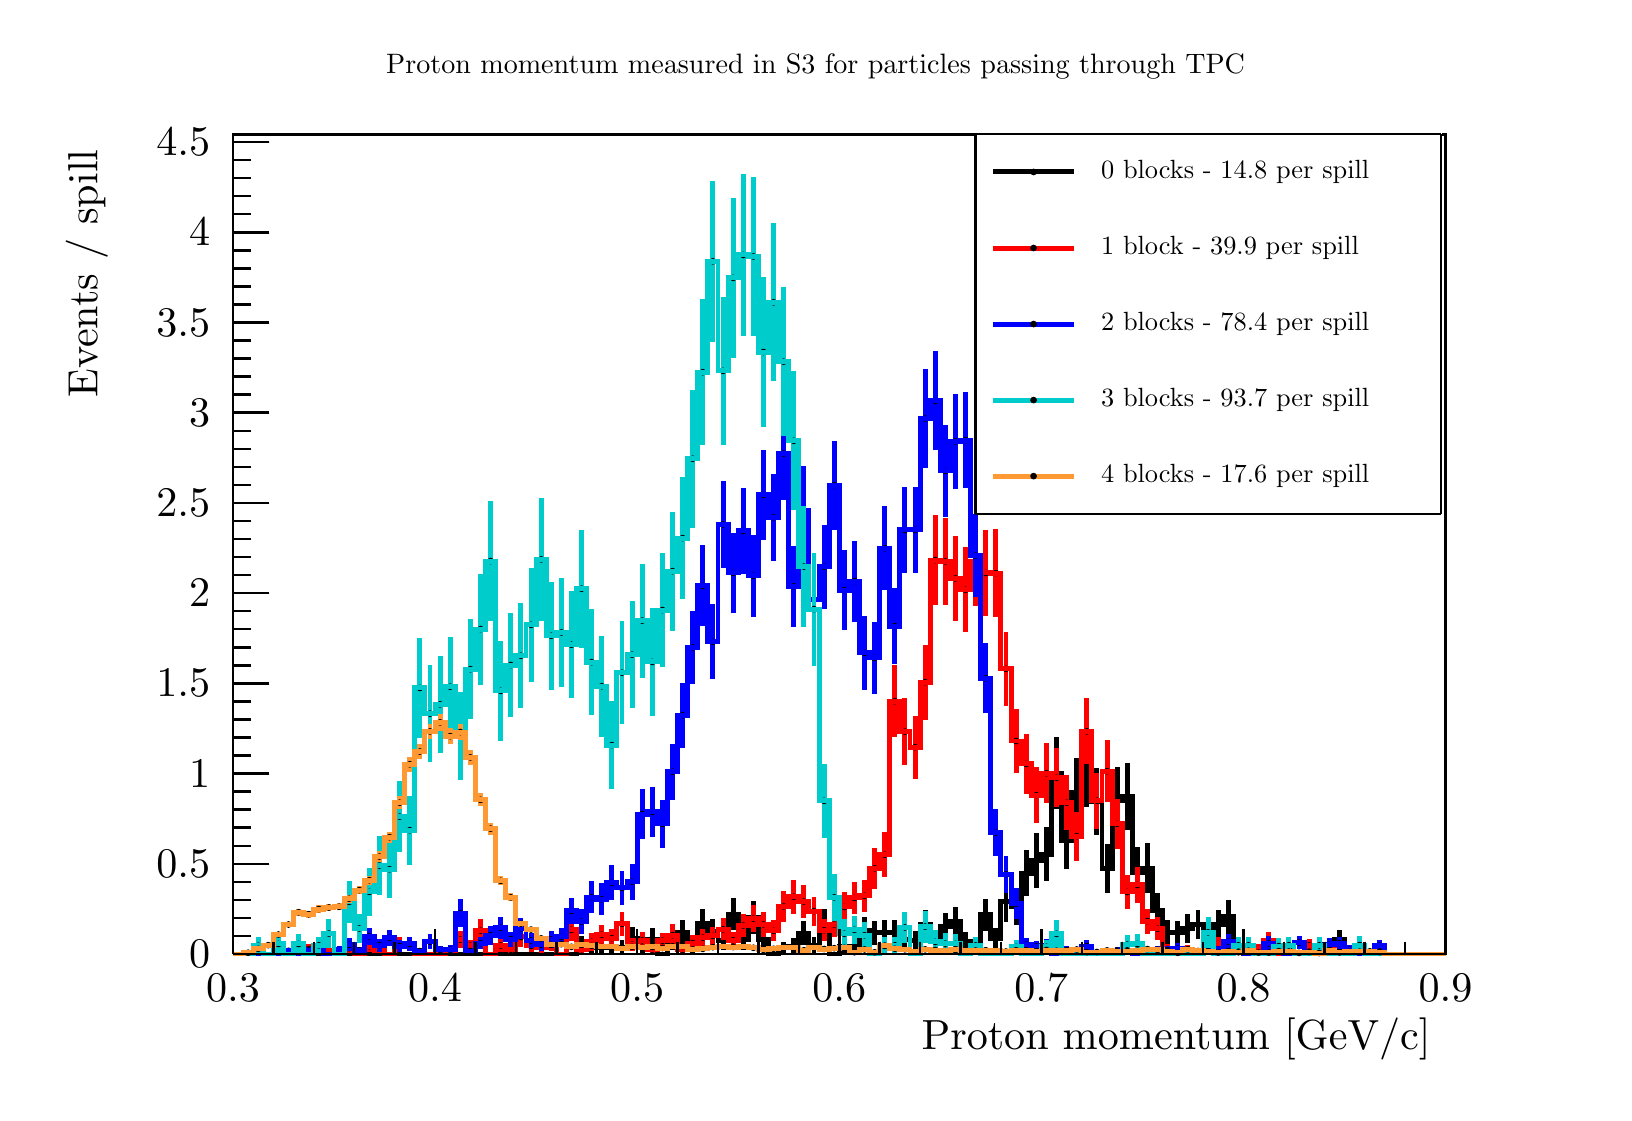
\begin{tikzpicture}
\pgfdeclareplotmark{cross} {
\pgfpathmoveto{\pgfpoint{-0.3\pgfplotmarksize}{\pgfplotmarksize}}
\pgfpathlineto{\pgfpoint{+0.3\pgfplotmarksize}{\pgfplotmarksize}}
\pgfpathlineto{\pgfpoint{+0.3\pgfplotmarksize}{0.3\pgfplotmarksize}}
\pgfpathlineto{\pgfpoint{+1\pgfplotmarksize}{0.3\pgfplotmarksize}}
\pgfpathlineto{\pgfpoint{+1\pgfplotmarksize}{-0.3\pgfplotmarksize}}
\pgfpathlineto{\pgfpoint{+0.3\pgfplotmarksize}{-0.3\pgfplotmarksize}}
\pgfpathlineto{\pgfpoint{+0.3\pgfplotmarksize}{-1.\pgfplotmarksize}}
\pgfpathlineto{\pgfpoint{-0.3\pgfplotmarksize}{-1.\pgfplotmarksize}}
\pgfpathlineto{\pgfpoint{-0.3\pgfplotmarksize}{-0.3\pgfplotmarksize}}
\pgfpathlineto{\pgfpoint{-1.\pgfplotmarksize}{-0.3\pgfplotmarksize}}
\pgfpathlineto{\pgfpoint{-1.\pgfplotmarksize}{0.3\pgfplotmarksize}}
\pgfpathlineto{\pgfpoint{-0.3\pgfplotmarksize}{0.3\pgfplotmarksize}}
\pgfpathclose
\pgfusepathqstroke
}
\pgfdeclareplotmark{cross*} {
\pgfpathmoveto{\pgfpoint{-0.3\pgfplotmarksize}{\pgfplotmarksize}}
\pgfpathlineto{\pgfpoint{+0.3\pgfplotmarksize}{\pgfplotmarksize}}
\pgfpathlineto{\pgfpoint{+0.3\pgfplotmarksize}{0.3\pgfplotmarksize}}
\pgfpathlineto{\pgfpoint{+1\pgfplotmarksize}{0.3\pgfplotmarksize}}
\pgfpathlineto{\pgfpoint{+1\pgfplotmarksize}{-0.3\pgfplotmarksize}}
\pgfpathlineto{\pgfpoint{+0.3\pgfplotmarksize}{-0.3\pgfplotmarksize}}
\pgfpathlineto{\pgfpoint{+0.3\pgfplotmarksize}{-1.\pgfplotmarksize}}
\pgfpathlineto{\pgfpoint{-0.3\pgfplotmarksize}{-1.\pgfplotmarksize}}
\pgfpathlineto{\pgfpoint{-0.3\pgfplotmarksize}{-0.3\pgfplotmarksize}}
\pgfpathlineto{\pgfpoint{-1.\pgfplotmarksize}{-0.3\pgfplotmarksize}}
\pgfpathlineto{\pgfpoint{-1.\pgfplotmarksize}{0.3\pgfplotmarksize}}
\pgfpathlineto{\pgfpoint{-0.3\pgfplotmarksize}{0.3\pgfplotmarksize}}
\pgfpathclose
\pgfusepathqfillstroke
}
\pgfdeclareplotmark{newstar} {
\pgfpathmoveto{\pgfqpoint{0pt}{\pgfplotmarksize}}
\pgfpathlineto{\pgfqpointpolar{44}{0.5\pgfplotmarksize}}
\pgfpathlineto{\pgfqpointpolar{18}{\pgfplotmarksize}}
\pgfpathlineto{\pgfqpointpolar{-20}{0.5\pgfplotmarksize}}
\pgfpathlineto{\pgfqpointpolar{-54}{\pgfplotmarksize}}
\pgfpathlineto{\pgfqpointpolar{-90}{0.5\pgfplotmarksize}}
\pgfpathlineto{\pgfqpointpolar{234}{\pgfplotmarksize}}
\pgfpathlineto{\pgfqpointpolar{198}{0.5\pgfplotmarksize}}
\pgfpathlineto{\pgfqpointpolar{162}{\pgfplotmarksize}}
\pgfpathlineto{\pgfqpointpolar{134}{0.5\pgfplotmarksize}}
\pgfpathclose
\pgfusepathqstroke
}
\pgfdeclareplotmark{newstar*} {
\pgfpathmoveto{\pgfqpoint{0pt}{\pgfplotmarksize}}
\pgfpathlineto{\pgfqpointpolar{44}{0.5\pgfplotmarksize}}
\pgfpathlineto{\pgfqpointpolar{18}{\pgfplotmarksize}}
\pgfpathlineto{\pgfqpointpolar{-20}{0.5\pgfplotmarksize}}
\pgfpathlineto{\pgfqpointpolar{-54}{\pgfplotmarksize}}
\pgfpathlineto{\pgfqpointpolar{-90}{0.5\pgfplotmarksize}}
\pgfpathlineto{\pgfqpointpolar{234}{\pgfplotmarksize}}
\pgfpathlineto{\pgfqpointpolar{198}{0.5\pgfplotmarksize}}
\pgfpathlineto{\pgfqpointpolar{162}{\pgfplotmarksize}}
\pgfpathlineto{\pgfqpointpolar{134}{0.5\pgfplotmarksize}}
\pgfpathclose
\pgfusepathqfillstroke
}
\definecolor{c}{rgb}{1,1,1};
\draw [color=c, fill=c] (0,0) rectangle (20,13.5143);
\draw [color=c, fill=c] (2.6,1.75686) rectangle (18,12.1629);
\definecolor{c}{rgb}{0,0,0};
\draw [c,line width=0.9] (2.6,1.75686) -- (2.6,12.1629) -- (18,12.1629) -- (18,1.75686) -- (2.6,1.75686);
\definecolor{c}{rgb}{1,1,1};
\draw [color=c, fill=c] (2.6,1.75686) rectangle (18,12.1629);
\definecolor{c}{rgb}{0,0,0};
\draw [c,line width=0.9] (2.6,1.75686) -- (2.6,12.1629) -- (18,12.1629) -- (18,1.75686) -- (2.6,1.75686);
\definecolor{c}{rgb}{0,0,0.6};
\draw [c,line width=0.9] (2.6,1.75686) -- (2.72833,1.75686) -- (2.72833,1.75686) -- (2.85667,1.75686) -- (2.85667,1.75686) -- (2.985,1.75686) -- (2.985,1.75686) -- (3.11333,1.75686) -- (3.11333,1.75686) -- (3.24167,1.75686) -- (3.24167,1.75686) --
 (3.37,1.75686) -- (3.37,1.75686) -- (3.49833,1.75686) -- (3.49833,1.75686) -- (3.62667,1.75686) -- (3.62667,1.75686) -- (3.755,1.75686) -- (3.755,1.75686) -- (3.88333,1.75686) -- (3.88333,1.75686) -- (4.01167,1.75686) -- (4.01167,1.75686) --
 (4.14,1.75686) -- (4.14,1.75686) -- (4.26833,1.75686) -- (4.26833,1.75686) -- (4.39667,1.75686) -- (4.39667,1.75686) -- (4.525,1.75686) -- (4.525,1.75686) -- (4.65333,1.75686) -- (4.65333,1.75686) -- (4.78167,1.75686) -- (4.78167,1.75686) --
 (4.91,1.75686) -- (4.91,1.75686) -- (5.03833,1.75686) -- (5.03833,1.75686) -- (5.16667,1.75686) -- (5.16667,1.75686) -- (5.295,1.75686) -- (5.295,1.75686) -- (5.42333,1.75686) -- (5.42333,1.75686) -- (5.55167,1.75686) -- (5.55167,1.75686) --
 (5.68,1.75686) -- (5.68,1.75686) -- (5.80833,1.75686) -- (5.80833,1.75686) -- (5.93667,1.75686) -- (5.93667,1.75686) -- (6.065,1.75686) -- (6.065,1.75686) -- (6.19333,1.75686) -- (6.19333,1.75686) -- (6.32167,1.75686) -- (6.32167,1.75686) --
 (6.45,1.75686) -- (6.45,1.75686) -- (6.57833,1.75686) -- (6.57833,1.75686) -- (6.70667,1.75686) -- (6.70667,1.75686) -- (6.835,1.75686) -- (6.835,1.75686) -- (6.96333,1.75686) -- (6.96333,1.75686) -- (7.09167,1.75686) -- (7.09167,1.75686) --
 (7.22,1.75686) -- (7.22,1.75686) -- (7.34833,1.75686) -- (7.34833,1.75686) -- (7.47667,1.75686) -- (7.47667,1.75686) -- (7.605,1.75686) -- (7.605,1.75686) -- (7.73333,1.75686) -- (7.73333,1.75686) -- (7.86167,1.75686) -- (7.86167,1.75686) --
 (7.99,1.75686) -- (7.99,1.75686) -- (8.11833,1.75686) -- (8.11833,1.75686) -- (8.24667,1.75686) -- (8.24667,1.75686) -- (8.375,1.75686) -- (8.375,1.75686) -- (8.50333,1.75686) -- (8.50333,1.75686) -- (8.63167,1.75686) -- (8.63167,1.75686) --
 (8.76,1.75686) -- (8.76,1.75686) -- (8.88833,1.75686) -- (8.88833,1.75686) -- (9.01667,1.75686) -- (9.01667,1.75686) -- (9.145,1.75686) -- (9.145,1.75686) -- (9.27333,1.75686) -- (9.27333,1.75686) -- (9.40167,1.75686) -- (9.40167,1.75686) --
 (9.53,1.75686) -- (9.53,1.75686) -- (9.65833,1.75686) -- (9.65833,1.75686) -- (9.78667,1.75686) -- (9.78667,1.75686) -- (9.915,1.75686) -- (9.915,1.75686) -- (10.0433,1.75686) -- (10.0433,1.75686) -- (10.1717,1.75686) -- (10.1717,1.75686) --
 (10.3,1.75686) -- (10.3,1.75686) -- (10.4283,1.75686) -- (10.4283,1.75686) -- (10.5567,1.75686) -- (10.5567,1.75686) -- (10.685,1.75686) -- (10.685,1.75686) -- (10.8133,1.75686) -- (10.8133,1.75686) -- (10.9417,1.75686) -- (10.9417,1.75686) --
 (11.07,1.75686) -- (11.07,1.75686) -- (11.1983,1.75686) -- (11.1983,1.75686) -- (11.3267,1.75686) -- (11.3267,1.75686) -- (11.455,1.75686) -- (11.455,1.75686) -- (11.5833,1.75686) -- (11.5833,1.75686) -- (11.7117,1.75686) -- (11.7117,1.75686) --
 (11.84,1.75686) -- (11.84,1.75686) -- (11.9683,1.75686) -- (11.9683,1.75686) -- (12.0967,1.75686) -- (12.0967,1.75686) -- (12.225,1.75686) -- (12.225,1.75686) -- (12.3533,1.75686) -- (12.3533,1.75686) -- (12.4817,1.75686) -- (12.4817,1.75686) --
 (12.61,1.75686) -- (12.61,1.75686) -- (12.7383,1.75686) -- (12.7383,1.75686) -- (12.8667,1.75686) -- (12.8667,1.75686) -- (12.995,1.75686) -- (12.995,1.75686) -- (13.1233,1.75686) -- (13.1233,1.75686) -- (13.2517,1.75686) -- (13.2517,1.75686) --
 (13.38,1.75686) -- (13.38,1.75686) -- (13.5083,1.75686) -- (13.5083,1.75686) -- (13.6367,1.75686) -- (13.6367,1.75686) -- (13.765,1.75686) -- (13.765,1.75686) -- (13.8933,1.75686) -- (13.8933,1.75686) -- (14.0217,1.75686) -- (14.0217,1.75686) --
 (14.15,1.75686) -- (14.15,1.75686) -- (14.2783,1.75686) -- (14.2783,1.75686) -- (14.4067,1.75686) -- (14.4067,1.75686) -- (14.535,1.75686) -- (14.535,1.75686) -- (14.6633,1.75686) -- (14.6633,1.75686) -- (14.7917,1.75686) -- (14.7917,1.75686) --
 (14.92,1.75686) -- (14.92,1.75686) -- (15.0483,1.75686) -- (15.0483,1.75686) -- (15.1767,1.75686) -- (15.1767,1.75686) -- (15.305,1.75686) -- (15.305,1.75686) -- (15.4333,1.75686) -- (15.4333,1.75686) -- (15.5617,1.75686) -- (15.5617,1.75686) --
 (15.69,1.75686) -- (15.69,1.75686) -- (15.8183,1.75686) -- (15.8183,1.75686) -- (15.9467,1.75686) -- (15.9467,1.75686) -- (16.075,1.75686) -- (16.075,1.75686) -- (16.2033,1.75686) -- (16.2033,1.75686) -- (16.3317,1.75686) -- (16.3317,1.75686) --
 (16.46,1.75686) -- (16.46,1.75686) -- (16.5883,1.75686) -- (16.5883,1.75686) -- (16.7167,1.75686) -- (16.7167,1.75686) -- (16.845,1.75686) -- (16.845,1.75686) -- (16.9733,1.75686) -- (16.9733,1.75686) -- (17.1017,1.75686) -- (17.1017,1.75686) --
 (17.23,1.75686) -- (17.23,1.75686) -- (17.3583,1.75686) -- (17.3583,1.75686) -- (17.4867,1.75686) -- (17.4867,1.75686) -- (17.615,1.75686) -- (17.615,1.75686) -- (17.7433,1.75686) -- (17.7433,1.75686) -- (17.8717,1.75686) -- (17.8717,1.75686) --
 (18,1.75686);
\definecolor{c}{rgb}{0,0,0};
\draw [c,line width=0.9] (2.6,1.75686) -- (18,1.75686);
\draw [c,line width=0.9] (2.6,2.06904) -- (2.6,1.75686);
\draw [c,line width=0.9] (3.11333,1.91295) -- (3.11333,1.75686);
\draw [c,line width=0.9] (3.62667,1.91295) -- (3.62667,1.75686);
\draw [c,line width=0.9] (4.14,1.91295) -- (4.14,1.75686);
\draw [c,line width=0.9] (4.65333,1.91295) -- (4.65333,1.75686);
\draw [c,line width=0.9] (5.16667,2.06904) -- (5.16667,1.75686);
\draw [c,line width=0.9] (5.68,1.91295) -- (5.68,1.75686);
\draw [c,line width=0.9] (6.19333,1.91295) -- (6.19333,1.75686);
\draw [c,line width=0.9] (6.70667,1.91295) -- (6.70667,1.75686);
\draw [c,line width=0.9] (7.22,1.91295) -- (7.22,1.75686);
\draw [c,line width=0.9] (7.73333,2.06904) -- (7.73333,1.75686);
\draw [c,line width=0.9] (8.24667,1.91295) -- (8.24667,1.75686);
\draw [c,line width=0.9] (8.76,1.91295) -- (8.76,1.75686);
\draw [c,line width=0.9] (9.27333,1.91295) -- (9.27333,1.75686);
\draw [c,line width=0.9] (9.78667,1.91295) -- (9.78667,1.75686);
\draw [c,line width=0.9] (10.3,2.06904) -- (10.3,1.75686);
\draw [c,line width=0.9] (10.8133,1.91295) -- (10.8133,1.75686);
\draw [c,line width=0.9] (11.3267,1.91295) -- (11.3267,1.75686);
\draw [c,line width=0.9] (11.84,1.91295) -- (11.84,1.75686);
\draw [c,line width=0.9] (12.3533,1.91295) -- (12.3533,1.75686);
\draw [c,line width=0.9] (12.8667,2.06904) -- (12.8667,1.75686);
\draw [c,line width=0.9] (13.38,1.91295) -- (13.38,1.75686);
\draw [c,line width=0.9] (13.8933,1.91295) -- (13.8933,1.75686);
\draw [c,line width=0.9] (14.4067,1.91295) -- (14.4067,1.75686);
\draw [c,line width=0.9] (14.92,1.91295) -- (14.92,1.75686);
\draw [c,line width=0.9] (15.4333,2.06904) -- (15.4333,1.75686);
\draw [c,line width=0.9] (15.9467,1.91295) -- (15.9467,1.75686);
\draw [c,line width=0.9] (16.46,1.91295) -- (16.46,1.75686);
\draw [c,line width=0.9] (16.9733,1.91295) -- (16.9733,1.75686);
\draw [c,line width=0.9] (17.4867,1.91295) -- (17.4867,1.75686);
\draw [c,line width=0.9] (18,2.06904) -- (18,1.75686);
\draw [c,line width=0.9] (2.6,2.06904) -- (2.6,1.75686);
\draw [c,line width=0.9] (18,2.06904) -- (18,1.75686);
\draw [anchor=base] (2.6,1.14871) node[scale=1.52295, color=c, rotate=0]{0.3};
\draw [anchor=base] (5.16667,1.14871) node[scale=1.52295, color=c, rotate=0]{0.4};
\draw [anchor=base] (7.73333,1.14871) node[scale=1.52295, color=c, rotate=0]{0.5};
\draw [anchor=base] (10.3,1.14871) node[scale=1.52295, color=c, rotate=0]{0.6};
\draw [anchor=base] (12.8667,1.14871) node[scale=1.52295, color=c, rotate=0]{0.7};
\draw [anchor=base] (15.4333,1.14871) node[scale=1.52295, color=c, rotate=0]{0.8};
\draw [anchor=base] (18,1.14871) node[scale=1.52295, color=c, rotate=0]{0.9};
\draw [anchor= east] (18,0.675714) node[scale=1.52295, color=c, rotate=0]{ Proton momentum [GeV/c]};
\draw [c,line width=0.9] (2.6,1.75686) -- (2.6,12.1629);
\draw [c,line width=0.9] (3.062,1.75686) -- (2.6,1.75686);
\draw [c,line width=0.9] (2.831,1.986) -- (2.6,1.986);
\draw [c,line width=0.9] (2.831,2.21514) -- (2.6,2.21514);
\draw [c,line width=0.9] (2.831,2.44429) -- (2.6,2.44429);
\draw [c,line width=0.9] (2.831,2.67343) -- (2.6,2.67343);
\draw [c,line width=0.9] (3.062,2.90257) -- (2.6,2.90257);
\draw [c,line width=0.9] (2.831,3.13171) -- (2.6,3.13171);
\draw [c,line width=0.9] (2.831,3.36086) -- (2.6,3.36086);
\draw [c,line width=0.9] (2.831,3.59) -- (2.6,3.59);
\draw [c,line width=0.9] (2.831,3.81914) -- (2.6,3.81914);
\draw [c,line width=0.9] (3.062,4.04829) -- (2.6,4.04829);
\draw [c,line width=0.9] (2.831,4.27743) -- (2.6,4.27743);
\draw [c,line width=0.9] (2.831,4.50657) -- (2.6,4.50657);
\draw [c,line width=0.9] (2.831,4.73572) -- (2.6,4.73572);
\draw [c,line width=0.9] (2.831,4.96486) -- (2.6,4.96486);
\draw [c,line width=0.9] (3.062,5.194) -- (2.6,5.194);
\draw [c,line width=0.9] (2.831,5.42314) -- (2.6,5.42314);
\draw [c,line width=0.9] (2.831,5.65229) -- (2.6,5.65229);
\draw [c,line width=0.9] (2.831,5.88143) -- (2.6,5.88143);
\draw [c,line width=0.9] (2.831,6.11057) -- (2.6,6.11057);
\draw [c,line width=0.9] (3.062,6.33972) -- (2.6,6.33972);
\draw [c,line width=0.9] (2.831,6.56886) -- (2.6,6.56886);
\draw [c,line width=0.9] (2.831,6.798) -- (2.6,6.798);
\draw [c,line width=0.9] (2.831,7.02714) -- (2.6,7.02714);
\draw [c,line width=0.9] (2.831,7.25629) -- (2.6,7.25629);
\draw [c,line width=0.9] (3.062,7.48543) -- (2.6,7.48543);
\draw [c,line width=0.9] (2.831,7.71457) -- (2.6,7.71457);
\draw [c,line width=0.9] (2.831,7.94372) -- (2.6,7.94372);
\draw [c,line width=0.9] (2.831,8.17286) -- (2.6,8.17286);
\draw [c,line width=0.9] (2.831,8.402) -- (2.6,8.402);
\draw [c,line width=0.9] (3.062,8.63114) -- (2.6,8.63114);
\draw [c,line width=0.9] (2.831,8.86029) -- (2.6,8.86029);
\draw [c,line width=0.9] (2.831,9.08943) -- (2.6,9.08943);
\draw [c,line width=0.9] (2.831,9.31857) -- (2.6,9.31857);
\draw [c,line width=0.9] (2.831,9.54772) -- (2.6,9.54772);
\draw [c,line width=0.9] (3.062,9.77686) -- (2.6,9.77686);
\draw [c,line width=0.9] (2.831,10.006) -- (2.6,10.006);
\draw [c,line width=0.9] (2.831,10.2351) -- (2.6,10.2351);
\draw [c,line width=0.9] (2.831,10.4643) -- (2.6,10.4643);
\draw [c,line width=0.9] (2.831,10.6934) -- (2.6,10.6934);
\draw [c,line width=0.9] (3.062,10.9226) -- (2.6,10.9226);
\draw [c,line width=0.9] (2.831,11.1517) -- (2.6,11.1517);
\draw [c,line width=0.9] (2.831,11.3809) -- (2.6,11.3809);
\draw [c,line width=0.9] (2.831,11.61) -- (2.6,11.61);
\draw [c,line width=0.9] (2.831,11.8391) -- (2.6,11.8391);
\draw [c,line width=0.9] (3.062,12.0683) -- (2.6,12.0683);
\draw [c,line width=0.9] (3.062,12.0683) -- (2.6,12.0683);
\draw [anchor= east] (2.5,1.75686) node[scale=1.52295, color=c, rotate=0]{0};
\draw [anchor= east] (2.5,2.90257) node[scale=1.52295, color=c, rotate=0]{0.5};
\draw [anchor= east] (2.5,4.04829) node[scale=1.52295, color=c, rotate=0]{1};
\draw [anchor= east] (2.5,5.194) node[scale=1.52295, color=c, rotate=0]{1.5};
\draw [anchor= east] (2.5,6.33972) node[scale=1.52295, color=c, rotate=0]{2};
\draw [anchor= east] (2.5,7.48543) node[scale=1.52295, color=c, rotate=0]{2.5};
\draw [anchor= east] (2.5,8.63114) node[scale=1.52295, color=c, rotate=0]{3};
\draw [anchor= east] (2.5,9.77686) node[scale=1.52295, color=c, rotate=0]{3.5};
\draw [anchor= east] (2.5,10.9226) node[scale=1.52295, color=c, rotate=0]{4};
\draw [anchor= east] (2.5,12.0683) node[scale=1.52295, color=c, rotate=0]{4.5};
\draw [anchor= east] (0.742857,12.1629) node[scale=1.52295, color=c, rotate=90]{ Events / spill};
\draw [c,line width=1.8] (7.0275,1.75686) -- (7.0275,1.87223);
\draw [c,line width=1.8] (7.0275,1.87223) -- (7.0275,1.98761);
\foreach \P in {(7.0275,1.87223)}{\draw[mark options={color=c,fill=c},mark size=2.402402pt,mark=*,mark size=1pt] plot coordinates {\P};}
\draw [c,line width=1.8] (7.15583,1.75686) -- (7.15583,1.8392);
\draw [c,line width=1.8] (7.15583,1.8392) -- (7.15583,1.92154);
\foreach \P in {(7.15583,1.8392)}{\draw[mark options={color=c,fill=c},mark size=2.402402pt,mark=*,mark size=1pt] plot coordinates {\P};}
\draw [c,line width=1.8] (7.28417,1.75686) -- (7.28417,1.84002);
\draw [c,line width=1.8] (7.28417,1.84002) -- (7.28417,1.92318);
\foreach \P in {(7.28417,1.84002)}{\draw[mark options={color=c,fill=c},mark size=2.402402pt,mark=*,mark size=1pt] plot coordinates {\P};}
\draw [c,line width=1.8] (7.4125,1.75686) -- (7.4125,1.84723);
\draw [c,line width=1.8] (7.4125,1.84723) -- (7.4125,1.9376);
\foreach \P in {(7.4125,1.84723)}{\draw[mark options={color=c,fill=c},mark size=2.402402pt,mark=*,mark size=1pt] plot coordinates {\P};}
\draw [c,line width=1.8] (7.54083,1.75686) -- (7.54083,1.84318);
\draw [c,line width=1.8] (7.54083,1.84318) -- (7.54083,1.9295);
\foreach \P in {(7.54083,1.84318)}{\draw[mark options={color=c,fill=c},mark size=2.402402pt,mark=*,mark size=1pt] plot coordinates {\P};}
\draw [c,line width=1.8] (7.66917,1.81491) -- (7.66917,1.95785);
\draw [c,line width=1.8] (7.66917,1.95785) -- (7.66917,2.10079);
\foreach \P in {(7.66917,1.95785)}{\draw[mark options={color=c,fill=c},mark size=2.402402pt,mark=*,mark size=1pt] plot coordinates {\P};}
\draw [c,line width=1.8] (7.7975,1.75686) -- (7.7975,1.84723);
\draw [c,line width=1.8] (7.7975,1.84723) -- (7.7975,1.9376);
\foreach \P in {(7.7975,1.84723)}{\draw[mark options={color=c,fill=c},mark size=2.402402pt,mark=*,mark size=1pt] plot coordinates {\P};}
\draw [c,line width=1.8] (7.92583,1.8114) -- (7.92583,1.94655);
\draw [c,line width=1.8] (7.92583,1.94655) -- (7.92583,2.0817);
\foreach \P in {(7.92583,1.94655)}{\draw[mark options={color=c,fill=c},mark size=2.402402pt,mark=*,mark size=1pt] plot coordinates {\P};}
\draw [c,line width=1.8] (8.1825,1.80673) -- (8.1825,1.92724);
\draw [c,line width=1.8] (8.1825,1.92724) -- (8.1825,2.04776);
\foreach \P in {(8.1825,1.92724)}{\draw[mark options={color=c,fill=c},mark size=2.402402pt,mark=*,mark size=1pt] plot coordinates {\P};}
\draw [c,line width=1.8] (8.31083,1.87249) -- (8.31083,2.03228);
\draw [c,line width=1.8] (8.31083,2.03228) -- (8.31083,2.19207);
\foreach \P in {(8.31083,2.03228)}{\draw[mark options={color=c,fill=c},mark size=2.402402pt,mark=*,mark size=1pt] plot coordinates {\P};}
\draw [c,line width=1.8] (8.43917,1.75686) -- (8.43917,1.84992);
\draw [c,line width=1.8] (8.43917,1.84992) -- (8.43917,1.94298);
\foreach \P in {(8.43917,1.84992)}{\draw[mark options={color=c,fill=c},mark size=2.402402pt,mark=*,mark size=1pt] plot coordinates {\P};}
\draw [c,line width=1.8] (8.5675,1.94739) -- (8.5675,2.14072);
\draw [c,line width=1.8] (8.5675,2.14072) -- (8.5675,2.33405);
\foreach \P in {(8.5675,2.14072)}{\draw[mark options={color=c,fill=c},mark size=2.402402pt,mark=*,mark size=1pt] plot coordinates {\P};}
\draw [c,line width=1.8] (8.69583,1.87635) -- (8.69583,2.04052);
\draw [c,line width=1.8] (8.69583,2.04052) -- (8.69583,2.20468);
\foreach \P in {(8.69583,2.04052)}{\draw[mark options={color=c,fill=c},mark size=2.402402pt,mark=*,mark size=1pt] plot coordinates {\P};}
\draw [c,line width=1.8] (8.82417,1.80664) -- (8.82417,1.92697);
\draw [c,line width=1.8] (8.82417,1.92697) -- (8.82417,2.04729);
\foreach \P in {(8.82417,1.92697)}{\draw[mark options={color=c,fill=c},mark size=2.402402pt,mark=*,mark size=1pt] plot coordinates {\P};}
\draw [c,line width=1.8] (8.9525,2.05573) -- (8.9525,2.26287);
\draw [c,line width=1.8] (8.9525,2.26287) -- (8.9525,2.47002);
\foreach \P in {(8.9525,2.26287)}{\draw[mark options={color=c,fill=c},mark size=2.402402pt,mark=*,mark size=1pt] plot coordinates {\P};}
\draw [c,line width=1.8] (9.08083,1.81125) -- (9.08083,1.94304);
\draw [c,line width=1.8] (9.08083,1.94304) -- (9.08083,2.07483);
\foreach \P in {(9.08083,1.94304)}{\draw[mark options={color=c,fill=c},mark size=2.402402pt,mark=*,mark size=1pt] plot coordinates {\P};}
\draw [c,line width=1.8] (9.20917,2.01159) -- (9.20917,2.21923);
\draw [c,line width=1.8] (9.20917,2.21923) -- (9.20917,2.42687);
\foreach \P in {(9.20917,2.21923)}{\draw[mark options={color=c,fill=c},mark size=2.402402pt,mark=*,mark size=1pt] plot coordinates {\P};}
\draw [c,line width=1.8] (9.3375,1.80986) -- (9.3375,1.93843);
\draw [c,line width=1.8] (9.3375,1.93843) -- (9.3375,2.067);
\foreach \P in {(9.3375,1.93843)}{\draw[mark options={color=c,fill=c},mark size=2.402402pt,mark=*,mark size=1pt] plot coordinates {\P};}
\draw [c,line width=1.8] (9.59417,1.75686) -- (9.59417,1.83459);
\draw [c,line width=1.8] (9.59417,1.83459) -- (9.59417,1.91233);
\foreach \P in {(9.59417,1.83459)}{\draw[mark options={color=c,fill=c},mark size=2.402402pt,mark=*,mark size=1pt] plot coordinates {\P};}
\draw [c,line width=1.8] (9.7225,1.75686) -- (9.7225,1.8562);
\draw [c,line width=1.8] (9.7225,1.8562) -- (9.7225,1.95554);
\foreach \P in {(9.7225,1.8562)}{\draw[mark options={color=c,fill=c},mark size=2.402402pt,mark=*,mark size=1pt] plot coordinates {\P};}
\draw [c,line width=1.8] (9.85083,1.86877) -- (9.85083,2.02172);
\draw [c,line width=1.8] (9.85083,2.02172) -- (9.85083,2.17468);
\foreach \P in {(9.85083,2.02172)}{\draw[mark options={color=c,fill=c},mark size=2.402402pt,mark=*,mark size=1pt] plot coordinates {\P};}
\draw [c,line width=1.8] (9.97917,1.75686) -- (9.97917,1.86339);
\draw [c,line width=1.8] (9.97917,1.86339) -- (9.97917,1.96992);
\foreach \P in {(9.97917,1.86339)}{\draw[mark options={color=c,fill=c},mark size=2.402402pt,mark=*,mark size=1pt] plot coordinates {\P};}
\draw [c,line width=1.8] (10.1075,1.94483) -- (10.1075,2.13416);
\draw [c,line width=1.8] (10.1075,2.13416) -- (10.1075,2.32349);
\foreach \P in {(10.1075,2.13416)}{\draw[mark options={color=c,fill=c},mark size=2.402402pt,mark=*,mark size=1pt] plot coordinates {\P};}
\draw [c,line width=1.8] (10.3642,1.75686) -- (10.3642,1.85132);
\draw [c,line width=1.8] (10.3642,1.85132) -- (10.3642,1.94579);
\foreach \P in {(10.3642,1.85132)}{\draw[mark options={color=c,fill=c},mark size=2.402402pt,mark=*,mark size=1pt] plot coordinates {\P};}
\draw [c,line width=1.8] (10.4925,1.75686) -- (10.4925,1.83893);
\draw [c,line width=1.8] (10.4925,1.83893) -- (10.4925,1.921);
\foreach \P in {(10.4925,1.83893)}{\draw[mark options={color=c,fill=c},mark size=2.402402pt,mark=*,mark size=1pt] plot coordinates {\P};}
\draw [c,line width=1.8] (10.6208,1.88288) -- (10.6208,2.05538);
\draw [c,line width=1.8] (10.6208,2.05538) -- (10.6208,2.22788);
\foreach \P in {(10.6208,2.05538)}{\draw[mark options={color=c,fill=c},mark size=2.402402pt,mark=*,mark size=1pt] plot coordinates {\P};}
\draw [c,line width=1.8] (10.7492,1.87023) -- (10.7492,2.02579);
\draw [c,line width=1.8] (10.7492,2.02579) -- (10.7492,2.18135);
\foreach \P in {(10.7492,2.02579)}{\draw[mark options={color=c,fill=c},mark size=2.402402pt,mark=*,mark size=1pt] plot coordinates {\P};}
\draw [c,line width=1.8] (10.8775,1.87276) -- (10.8775,2.03138);
\draw [c,line width=1.8] (10.8775,2.03138) -- (10.8775,2.19001);
\foreach \P in {(10.8775,2.03138)}{\draw[mark options={color=c,fill=c},mark size=2.402402pt,mark=*,mark size=1pt] plot coordinates {\P};}
\draw [c,line width=1.8] (11.0058,1.87083) -- (11.0058,2.02682);
\draw [c,line width=1.8] (11.0058,2.02682) -- (11.0058,2.18281);
\foreach \P in {(11.0058,2.02682)}{\draw[mark options={color=c,fill=c},mark size=2.402402pt,mark=*,mark size=1pt] plot coordinates {\P};}
\draw [c,line width=1.8] (11.1342,1.81209) -- (11.1342,1.94544);
\draw [c,line width=1.8] (11.1342,1.94544) -- (11.1342,2.07878);
\foreach \P in {(11.1342,1.94544)}{\draw[mark options={color=c,fill=c},mark size=2.402402pt,mark=*,mark size=1pt] plot coordinates {\P};}
\draw [c,line width=1.8] (11.2625,1.80748) -- (11.2625,1.93029);
\draw [c,line width=1.8] (11.2625,1.93029) -- (11.2625,2.0531);
\foreach \P in {(11.2625,1.93029)}{\draw[mark options={color=c,fill=c},mark size=2.402402pt,mark=*,mark size=1pt] plot coordinates {\P};}
\draw [c,line width=1.8] (11.3908,1.94375) -- (11.3908,2.13179);
\draw [c,line width=1.8] (11.3908,2.13179) -- (11.3908,2.31983);
\foreach \P in {(11.3908,2.13179)}{\draw[mark options={color=c,fill=c},mark size=2.402402pt,mark=*,mark size=1pt] plot coordinates {\P};}
\draw [c,line width=1.8] (11.5192,1.80584) -- (11.5192,1.92521);
\draw [c,line width=1.8] (11.5192,1.92521) -- (11.5192,2.04457);
\foreach \P in {(11.5192,1.92521)}{\draw[mark options={color=c,fill=c},mark size=2.402402pt,mark=*,mark size=1pt] plot coordinates {\P};}
\draw [c,line width=1.8] (11.6475,1.93039) -- (11.6475,2.10696);
\draw [c,line width=1.8] (11.6475,2.10696) -- (11.6475,2.28353);
\foreach \P in {(11.6475,2.10696)}{\draw[mark options={color=c,fill=c},mark size=2.402402pt,mark=*,mark size=1pt] plot coordinates {\P};}
\draw [c,line width=1.8] (11.7758,1.98331) -- (11.7758,2.16693);
\draw [c,line width=1.8] (11.7758,2.16693) -- (11.7758,2.35054);
\foreach \P in {(11.7758,2.16693)}{\draw[mark options={color=c,fill=c},mark size=2.402402pt,mark=*,mark size=1pt] plot coordinates {\P};}
\draw [c,line width=1.8] (11.9042,1.80478) -- (11.9042,1.92049);
\draw [c,line width=1.8] (11.9042,1.92049) -- (11.9042,2.03621);
\foreach \P in {(11.9042,1.92049)}{\draw[mark options={color=c,fill=c},mark size=2.402402pt,mark=*,mark size=1pt] plot coordinates {\P};}
\draw [c,line width=1.8] (12.0325,1.75686) -- (12.0325,1.84469);
\draw [c,line width=1.8] (12.0325,1.84469) -- (12.0325,1.93253);
\foreach \P in {(12.0325,1.84469)}{\draw[mark options={color=c,fill=c},mark size=2.402402pt,mark=*,mark size=1pt] plot coordinates {\P};}
\draw [c,line width=1.8] (12.1608,2.051) -- (12.1608,2.25481);
\draw [c,line width=1.8] (12.1608,2.25481) -- (12.1608,2.45862);
\foreach \P in {(12.1608,2.25481)}{\draw[mark options={color=c,fill=c},mark size=2.402402pt,mark=*,mark size=1pt] plot coordinates {\P};}
\draw [c,line width=1.8] (12.2892,1.81436) -- (12.2892,1.95325);
\draw [c,line width=1.8] (12.2892,1.95325) -- (12.2892,2.09214);
\foreach \P in {(12.2892,1.95325)}{\draw[mark options={color=c,fill=c},mark size=2.402402pt,mark=*,mark size=1pt] plot coordinates {\P};}
\draw [c,line width=1.8] (12.4175,2.16918) -- (12.4175,2.42216);
\draw [c,line width=1.8] (12.4175,2.42216) -- (12.4175,2.67513);
\foreach \P in {(12.4175,2.42216)}{\draw[mark options={color=c,fill=c},mark size=2.402402pt,mark=*,mark size=1pt] plot coordinates {\P};}
\draw [c,line width=1.8] (12.5458,2.12973) -- (12.5458,2.35702);
\draw [c,line width=1.8] (12.5458,2.35702) -- (12.5458,2.58431);
\foreach \P in {(12.5458,2.35702)}{\draw[mark options={color=c,fill=c},mark size=2.402402pt,mark=*,mark size=1pt] plot coordinates {\P};}
\draw [c,line width=1.8] (12.6742,2.48745) -- (12.6742,2.78505);
\draw [c,line width=1.8] (12.6742,2.78505) -- (12.6742,3.08264);
\foreach \P in {(12.6742,2.78505)}{\draw[mark options={color=c,fill=c},mark size=2.402402pt,mark=*,mark size=1pt] plot coordinates {\P};}
\draw [c,line width=1.8] (12.8025,2.60099) -- (12.8025,2.9455);
\draw [c,line width=1.8] (12.8025,2.9455) -- (12.8025,3.29001);
\foreach \P in {(12.8025,2.9455)}{\draw[mark options={color=c,fill=c},mark size=2.402402pt,mark=*,mark size=1pt] plot coordinates {\P};}
\draw [c,line width=1.8] (12.9308,2.68361) -- (12.9308,3.02538);
\draw [c,line width=1.8] (12.9308,3.02538) -- (12.9308,3.36715);
\foreach \P in {(12.9308,3.02538)}{\draw[mark options={color=c,fill=c},mark size=2.402402pt,mark=*,mark size=1pt] plot coordinates {\P};}
\draw [c,line width=1.8] (13.0592,3.59301) -- (13.0592,4.05439);
\draw [c,line width=1.8] (13.0592,4.05439) -- (13.0592,4.51577);
\foreach \P in {(13.0592,4.05439)}{\draw[mark options={color=c,fill=c},mark size=2.402402pt,mark=*,mark size=1pt] plot coordinates {\P};}
\draw [c,line width=1.8] (13.1875,2.83168) -- (13.1875,3.19282);
\draw [c,line width=1.8] (13.1875,3.19282) -- (13.1875,3.55396);
\foreach \P in {(13.1875,3.19282)}{\draw[mark options={color=c,fill=c},mark size=2.402402pt,mark=*,mark size=1pt] plot coordinates {\P};}
\draw [c,line width=1.8] (13.3158,3.36598) -- (13.3158,3.80513);
\draw [c,line width=1.8] (13.3158,3.80513) -- (13.3158,4.24429);
\foreach \P in {(13.3158,3.80513)}{\draw[mark options={color=c,fill=c},mark size=2.402402pt,mark=*,mark size=1pt] plot coordinates {\P};}
\draw [c,line width=1.8] (13.4442,3.62133) -- (13.4442,4.0904);
\draw [c,line width=1.8] (13.4442,4.0904) -- (13.4442,4.55947);
\foreach \P in {(13.4442,4.0904)}{\draw[mark options={color=c,fill=c},mark size=2.402402pt,mark=*,mark size=1pt] plot coordinates {\P};}
\draw [c,line width=1.8] (13.5725,3.26516) -- (13.5725,3.68928);
\draw [c,line width=1.8] (13.5725,3.68928) -- (13.5725,4.1134);
\foreach \P in {(13.5725,3.68928)}{\draw[mark options={color=c,fill=c},mark size=2.402402pt,mark=*,mark size=1pt] plot coordinates {\P};}
\draw [c,line width=1.8] (13.7008,2.53033) -- (13.7008,2.84511);
\draw [c,line width=1.8] (13.7008,2.84511) -- (13.7008,3.15989);
\foreach \P in {(13.7008,2.84511)}{\draw[mark options={color=c,fill=c},mark size=2.402402pt,mark=*,mark size=1pt] plot coordinates {\P};}
\draw [c,line width=1.8] (13.8292,3.28205) -- (13.8292,3.71001);
\draw [c,line width=1.8] (13.8292,3.71001) -- (13.8292,4.13798);
\foreach \P in {(13.8292,3.71001)}{\draw[mark options={color=c,fill=c},mark size=2.402402pt,mark=*,mark size=1pt] plot coordinates {\P};}
\draw [c,line width=1.8] (13.9575,3.32834) -- (13.9575,3.75732);
\draw [c,line width=1.8] (13.9575,3.75732) -- (13.9575,4.1863);
\foreach \P in {(13.9575,3.75732)}{\draw[mark options={color=c,fill=c},mark size=2.402402pt,mark=*,mark size=1pt] plot coordinates {\P};}
\draw [c,line width=1.8] (14.0858,2.4802) -- (14.0858,2.79644);
\draw [c,line width=1.8] (14.0858,2.79644) -- (14.0858,3.11269);
\foreach \P in {(14.0858,2.79644)}{\draw[mark options={color=c,fill=c},mark size=2.402402pt,mark=*,mark size=1pt] plot coordinates {\P};}
\draw [c,line width=1.8] (14.2142,2.53008) -- (14.2142,2.84544);
\draw [c,line width=1.8] (14.2142,2.84544) -- (14.2142,3.1608);
\foreach \P in {(14.2142,2.84544)}{\draw[mark options={color=c,fill=c},mark size=2.402402pt,mark=*,mark size=1pt] plot coordinates {\P};}
\draw [c,line width=1.8] (14.3425,2.08132) -- (14.3425,2.30593);
\draw [c,line width=1.8] (14.3425,2.30593) -- (14.3425,2.53053);
\foreach \P in {(14.3425,2.30593)}{\draw[mark options={color=c,fill=c},mark size=2.402402pt,mark=*,mark size=1pt] plot coordinates {\P};}
\draw [c,line width=1.8] (14.4708,1.87354) -- (14.4708,2.03359);
\draw [c,line width=1.8] (14.4708,2.03359) -- (14.4708,2.19363);
\foreach \P in {(14.4708,2.03359)}{\draw[mark options={color=c,fill=c},mark size=2.402402pt,mark=*,mark size=1pt] plot coordinates {\P};}
\draw [c,line width=1.8] (14.5992,1.86891) -- (14.5992,2.02386);
\draw [c,line width=1.8] (14.5992,2.02386) -- (14.5992,2.17881);
\foreach \P in {(14.5992,2.02386)}{\draw[mark options={color=c,fill=c},mark size=2.402402pt,mark=*,mark size=1pt] plot coordinates {\P};}
\draw [c,line width=1.8] (14.7275,1.89144) -- (14.7275,2.07855);
\draw [c,line width=1.8] (14.7275,2.07855) -- (14.7275,2.26565);
\foreach \P in {(14.7275,2.07855)}{\draw[mark options={color=c,fill=c},mark size=2.402402pt,mark=*,mark size=1pt] plot coordinates {\P};}
\draw [c,line width=1.8] (14.8558,1.94316) -- (14.8558,2.13117);
\draw [c,line width=1.8] (14.8558,2.13117) -- (14.8558,2.31917);
\foreach \P in {(14.8558,2.13117)}{\draw[mark options={color=c,fill=c},mark size=2.402402pt,mark=*,mark size=1pt] plot coordinates {\P};}
\draw [c,line width=1.8] (14.9842,1.88047) -- (14.9842,2.04993);
\draw [c,line width=1.8] (14.9842,2.04993) -- (14.9842,2.21939);
\foreach \P in {(14.9842,2.04993)}{\draw[mark options={color=c,fill=c},mark size=2.402402pt,mark=*,mark size=1pt] plot coordinates {\P};}
\draw [c,line width=1.8] (15.1125,1.94323) -- (15.1125,2.13173);
\draw [c,line width=1.8] (15.1125,2.13173) -- (15.1125,2.32023);
\foreach \P in {(15.1125,2.13173)}{\draw[mark options={color=c,fill=c},mark size=2.402402pt,mark=*,mark size=1pt] plot coordinates {\P};}
\draw [c,line width=1.8] (15.2408,2.01694) -- (15.2408,2.23066);
\draw [c,line width=1.8] (15.2408,2.23066) -- (15.2408,2.44439);
\foreach \P in {(15.2408,2.23066)}{\draw[mark options={color=c,fill=c},mark size=2.402402pt,mark=*,mark size=1pt] plot coordinates {\P};}
\draw [c,line width=1.8] (15.3692,1.75686) -- (15.3692,1.83893);
\draw [c,line width=1.8] (15.3692,1.83893) -- (15.3692,1.921);
\foreach \P in {(15.3692,1.83893)}{\draw[mark options={color=c,fill=c},mark size=2.402402pt,mark=*,mark size=1pt] plot coordinates {\P};}
\draw [c,line width=1.8] (16.0108,1.75686) -- (16.0108,1.8566);
\draw [c,line width=1.8] (16.0108,1.8566) -- (16.0108,1.95633);
\foreach \P in {(16.0108,1.8566)}{\draw[mark options={color=c,fill=c},mark size=2.402402pt,mark=*,mark size=1pt] plot coordinates {\P};}
\draw [c,line width=1.8] (16.3958,1.75686) -- (16.3958,1.83225);
\draw [c,line width=1.8] (16.3958,1.83225) -- (16.3958,1.90765);
\foreach \P in {(16.3958,1.83225)}{\draw[mark options={color=c,fill=c},mark size=2.402402pt,mark=*,mark size=1pt] plot coordinates {\P};}
\draw [c,line width=1.8] (16.6525,1.8092) -- (16.6525,1.93618);
\draw [c,line width=1.8] (16.6525,1.93618) -- (16.6525,2.06316);
\foreach \P in {(16.6525,1.93618)}{\draw[mark options={color=c,fill=c},mark size=2.402402pt,mark=*,mark size=1pt] plot coordinates {\P};}
\draw [c,line width=1.8] (16.9092,1.75686) -- (16.9092,1.86161);
\draw [c,line width=1.8] (16.9092,1.86161) -- (16.9092,1.96636);
\foreach \P in {(16.9092,1.86161)}{\draw[mark options={color=c,fill=c},mark size=2.402402pt,mark=*,mark size=1pt] plot coordinates {\P};}
\draw [c,line width=1.8] (2.6,1.75686) -- (2.72833,1.75686) -- (2.72833,1.75686) -- (2.85667,1.75686) -- (2.85667,1.75686) -- (2.985,1.75686) -- (2.985,1.75686) -- (3.11333,1.75686) -- (3.11333,1.75686) -- (3.24167,1.75686) -- (3.24167,1.75686) --
 (3.37,1.75686) -- (3.37,1.75686) -- (3.49833,1.75686) -- (3.49833,1.75686) -- (3.62667,1.75686) -- (3.62667,1.75686) -- (3.755,1.75686) -- (3.755,1.75686) -- (3.88333,1.75686) -- (3.88333,1.75686) -- (4.01167,1.75686) -- (4.01167,1.75686) --
 (4.14,1.75686) -- (4.14,1.75686) -- (4.26833,1.75686) -- (4.26833,1.75686) -- (4.39667,1.75686) -- (4.39667,1.75686) -- (4.525,1.75686) -- (4.525,1.75686) -- (4.65333,1.75686) -- (4.65333,1.75686) -- (4.78167,1.75686) -- (4.78167,1.75686) --
 (4.91,1.75686) -- (4.91,1.75686) -- (5.03833,1.75686) -- (5.03833,1.75686) -- (5.16667,1.75686) -- (5.16667,1.75686) -- (5.295,1.75686) -- (5.295,1.75686) -- (5.42333,1.75686) -- (5.42333,1.75686) -- (5.55167,1.75686) -- (5.55167,1.75686) --
 (5.68,1.75686) -- (5.68,1.75686) -- (5.80833,1.75686) -- (5.80833,1.75686) -- (5.93667,1.75686) -- (5.93667,1.75686) -- (6.065,1.75686) -- (6.065,1.75686) -- (6.19333,1.75686) -- (6.19333,1.75686) -- (6.32167,1.75686) -- (6.32167,1.75686) --
 (6.45,1.75686) -- (6.45,1.75686) -- (6.57833,1.75686) -- (6.57833,1.75686) -- (6.70667,1.75686) -- (6.70667,1.75686) -- (6.835,1.75686) -- (6.835,1.75686) -- (6.96333,1.75686) -- (6.96333,1.87223) -- (7.09167,1.87223) -- (7.09167,1.8392) --
 (7.22,1.8392) -- (7.22,1.84002) -- (7.34833,1.84002) -- (7.34833,1.84723) -- (7.47667,1.84723) -- (7.47667,1.84318) -- (7.605,1.84318) -- (7.605,1.95785) -- (7.73333,1.95785) -- (7.73333,1.84723) -- (7.86167,1.84723) -- (7.86167,1.94655) --
 (7.99,1.94655) -- (7.99,1.75686) -- (8.11833,1.75686) -- (8.11833,1.92724) -- (8.24667,1.92724) -- (8.24667,2.03228) -- (8.375,2.03228) -- (8.375,1.84992) -- (8.50333,1.84992) -- (8.50333,2.14072) -- (8.63167,2.14072) -- (8.63167,2.04052) --
 (8.76,2.04052) -- (8.76,1.92697) -- (8.88833,1.92697) -- (8.88833,2.26287) -- (9.01667,2.26287) -- (9.01667,1.94304) -- (9.145,1.94304) -- (9.145,2.21923) -- (9.27333,2.21923) -- (9.27333,1.93843) -- (9.40167,1.93843) -- (9.40167,1.75686) --
 (9.53,1.75686) -- (9.53,1.83459) -- (9.65833,1.83459) -- (9.65833,1.8562) -- (9.78667,1.8562) -- (9.78667,2.02172) -- (9.915,2.02172) -- (9.915,1.86339) -- (10.0433,1.86339) -- (10.0433,2.13416) -- (10.1717,2.13416) -- (10.1717,1.75686) --
 (10.3,1.75686) -- (10.3,1.85132) -- (10.4283,1.85132) -- (10.4283,1.83893) -- (10.5567,1.83893) -- (10.5567,2.05538) -- (10.685,2.05538) -- (10.685,2.02579) -- (10.8133,2.02579) -- (10.8133,2.03138) -- (10.9417,2.03138) -- (10.9417,2.02682) --
 (11.07,2.02682) -- (11.07,1.94544) -- (11.1983,1.94544) -- (11.1983,1.93029) -- (11.3267,1.93029) -- (11.3267,2.13179) -- (11.455,2.13179) -- (11.455,1.92521) -- (11.5833,1.92521) -- (11.5833,2.10696) -- (11.7117,2.10696) -- (11.7117,2.16693) --
 (11.84,2.16693) -- (11.84,1.92049) -- (11.9683,1.92049) -- (11.9683,1.84469) -- (12.0967,1.84469) -- (12.0967,2.25481) -- (12.225,2.25481) -- (12.225,1.95325) -- (12.3533,1.95325) -- (12.3533,2.42216) -- (12.4817,2.42216) -- (12.4817,2.35702) --
 (12.61,2.35702) -- (12.61,2.78505) -- (12.7383,2.78505) -- (12.7383,2.9455) -- (12.8667,2.9455) -- (12.8667,3.02538) -- (12.995,3.02538) -- (12.995,4.05439) -- (13.1233,4.05439) -- (13.1233,3.19282) -- (13.2517,3.19282) -- (13.2517,3.80513) --
 (13.38,3.80513) -- (13.38,4.0904) -- (13.5083,4.0904) -- (13.5083,3.68928) -- (13.6367,3.68928) -- (13.6367,2.84511) -- (13.765,2.84511) -- (13.765,3.71001) -- (13.8933,3.71001) -- (13.8933,3.75732) -- (14.0217,3.75732) -- (14.0217,2.79644) --
 (14.15,2.79644) -- (14.15,2.84544) -- (14.2783,2.84544) -- (14.2783,2.30593) -- (14.4067,2.30593) -- (14.4067,2.03359) -- (14.535,2.03359) -- (14.535,2.02386) -- (14.6633,2.02386) -- (14.6633,2.07855) -- (14.7917,2.07855) -- (14.7917,2.13117) --
 (14.92,2.13117) -- (14.92,2.04993) -- (15.0483,2.04993) -- (15.0483,2.13173) -- (15.1767,2.13173) -- (15.1767,2.23066) -- (15.305,2.23066) -- (15.305,1.83893) -- (15.4333,1.83893) -- (15.4333,1.75686) -- (15.5617,1.75686) -- (15.5617,1.75686) --
 (15.69,1.75686) -- (15.69,1.75686) -- (15.8183,1.75686) -- (15.8183,1.75686) -- (15.9467,1.75686) -- (15.9467,1.8566) -- (16.075,1.8566) -- (16.075,1.75686) -- (16.2033,1.75686) -- (16.2033,1.75686) -- (16.3317,1.75686) -- (16.3317,1.83225) --
 (16.46,1.83225) -- (16.46,1.75686) -- (16.5883,1.75686) -- (16.5883,1.93618) -- (16.7167,1.93618) -- (16.7167,1.75686) -- (16.845,1.75686) -- (16.845,1.86161) -- (16.9733,1.86161) -- (16.9733,1.75686) -- (17.1017,1.75686) -- (17.1017,1.75686) --
 (17.23,1.75686) -- (17.23,1.75686) -- (17.3583,1.75686) -- (17.3583,1.75686) -- (17.4867,1.75686) -- (17.4867,1.75686) -- (17.615,1.75686) -- (17.615,1.75686) -- (17.7433,1.75686) -- (17.7433,1.75686) -- (17.8717,1.75686) -- (17.8717,1.75686) --
 (18,1.75686);
\definecolor{c}{rgb}{1,0,0};
\draw [c,line width=1.8] (3.5625,1.75686) -- (3.5625,1.81774);
\draw [c,line width=1.8] (3.5625,1.81774) -- (3.5625,1.87861);
\definecolor{c}{rgb}{0,0,0};
\foreach \P in {(3.5625,1.81774)}{\draw[mark options={color=c,fill=c},mark size=2.402402pt,mark=*,mark size=1pt] plot coordinates {\P};}
\definecolor{c}{rgb}{1,0,0};
\draw [c,line width=1.8] (3.69083,1.78771) -- (3.69083,1.86269);
\draw [c,line width=1.8] (3.69083,1.86269) -- (3.69083,1.93766);
\definecolor{c}{rgb}{0,0,0};
\foreach \P in {(3.69083,1.86269)}{\draw[mark options={color=c,fill=c},mark size=2.402402pt,mark=*,mark size=1pt] plot coordinates {\P};}
\definecolor{c}{rgb}{1,0,0};
\draw [c,line width=1.8] (3.81917,1.75686) -- (3.81917,1.80102);
\draw [c,line width=1.8] (3.81917,1.80102) -- (3.81917,1.84519);
\definecolor{c}{rgb}{0,0,0};
\foreach \P in {(3.81917,1.80102)}{\draw[mark options={color=c,fill=c},mark size=2.402402pt,mark=*,mark size=1pt] plot coordinates {\P};}
\definecolor{c}{rgb}{1,0,0};
\draw [c,line width=1.8] (4.07583,1.75686) -- (4.07583,1.82963);
\draw [c,line width=1.8] (4.07583,1.82963) -- (4.07583,1.9024);
\definecolor{c}{rgb}{0,0,0};
\foreach \P in {(4.07583,1.82963)}{\draw[mark options={color=c,fill=c},mark size=2.402402pt,mark=*,mark size=1pt] plot coordinates {\P};}
\definecolor{c}{rgb}{1,0,0};
\draw [c,line width=1.8] (4.3325,1.7849) -- (4.3325,1.85566);
\draw [c,line width=1.8] (4.3325,1.85566) -- (4.3325,1.92642);
\definecolor{c}{rgb}{0,0,0};
\foreach \P in {(4.3325,1.85566)}{\draw[mark options={color=c,fill=c},mark size=2.402402pt,mark=*,mark size=1pt] plot coordinates {\P};}
\definecolor{c}{rgb}{1,0,0};
\draw [c,line width=1.8] (4.46083,1.75686) -- (4.46083,1.80428);
\draw [c,line width=1.8] (4.46083,1.80428) -- (4.46083,1.8517);
\definecolor{c}{rgb}{0,0,0};
\foreach \P in {(4.46083,1.80428)}{\draw[mark options={color=c,fill=c},mark size=2.402402pt,mark=*,mark size=1pt] plot coordinates {\P};}
\definecolor{c}{rgb}{1,0,0};
\draw [c,line width=1.8] (4.7175,1.79336) -- (4.7175,1.88158);
\draw [c,line width=1.8] (4.7175,1.88158) -- (4.7175,1.9698);
\definecolor{c}{rgb}{0,0,0};
\foreach \P in {(4.7175,1.88158)}{\draw[mark options={color=c,fill=c},mark size=2.402402pt,mark=*,mark size=1pt] plot coordinates {\P};}
\definecolor{c}{rgb}{1,0,0};
\draw [c,line width=1.8] (4.84583,1.79255) -- (4.84583,1.87935);
\draw [c,line width=1.8] (4.84583,1.87935) -- (4.84583,1.96615);
\definecolor{c}{rgb}{0,0,0};
\foreach \P in {(4.84583,1.87935)}{\draw[mark options={color=c,fill=c},mark size=2.402402pt,mark=*,mark size=1pt] plot coordinates {\P};}
\definecolor{c}{rgb}{1,0,0};
\draw [c,line width=1.8] (5.35917,1.75686) -- (5.35917,1.80274);
\draw [c,line width=1.8] (5.35917,1.80274) -- (5.35917,1.84863);
\definecolor{c}{rgb}{0,0,0};
\foreach \P in {(5.35917,1.80274)}{\draw[mark options={color=c,fill=c},mark size=2.402402pt,mark=*,mark size=1pt] plot coordinates {\P};}
\definecolor{c}{rgb}{1,0,0};
\draw [c,line width=1.8] (5.4875,1.83415) -- (5.4875,1.93978);
\draw [c,line width=1.8] (5.4875,1.93978) -- (5.4875,2.04542);
\definecolor{c}{rgb}{0,0,0};
\foreach \P in {(5.4875,1.93978)}{\draw[mark options={color=c,fill=c},mark size=2.402402pt,mark=*,mark size=1pt] plot coordinates {\P};}
\definecolor{c}{rgb}{1,0,0};
\draw [c,line width=1.8] (5.61583,1.7872) -- (5.61583,1.8632);
\draw [c,line width=1.8] (5.61583,1.8632) -- (5.61583,1.9392);
\definecolor{c}{rgb}{0,0,0};
\foreach \P in {(5.61583,1.8632)}{\draw[mark options={color=c,fill=c},mark size=2.402402pt,mark=*,mark size=1pt] plot coordinates {\P};}
\definecolor{c}{rgb}{1,0,0};
\draw [c,line width=1.8] (5.74417,1.90319) -- (5.74417,2.05315);
\draw [c,line width=1.8] (5.74417,2.05315) -- (5.74417,2.20311);
\definecolor{c}{rgb}{0,0,0};
\foreach \P in {(5.74417,2.05315)}{\draw[mark options={color=c,fill=c},mark size=2.402402pt,mark=*,mark size=1pt] plot coordinates {\P};}
\definecolor{c}{rgb}{1,0,0};
\draw [c,line width=1.8] (6.00083,1.78832) -- (6.00083,1.86486);
\draw [c,line width=1.8] (6.00083,1.86486) -- (6.00083,1.9414);
\definecolor{c}{rgb}{0,0,0};
\foreach \P in {(6.00083,1.86486)}{\draw[mark options={color=c,fill=c},mark size=2.402402pt,mark=*,mark size=1pt] plot coordinates {\P};}
\definecolor{c}{rgb}{1,0,0};
\draw [c,line width=1.8] (6.12917,1.75686) -- (6.12917,1.81029);
\draw [c,line width=1.8] (6.12917,1.81029) -- (6.12917,1.86373);
\definecolor{c}{rgb}{0,0,0};
\foreach \P in {(6.12917,1.81029)}{\draw[mark options={color=c,fill=c},mark size=2.402402pt,mark=*,mark size=1pt] plot coordinates {\P};}
\definecolor{c}{rgb}{1,0,0};
\draw [c,line width=1.8] (6.2575,1.84486) -- (6.2575,1.97316);
\draw [c,line width=1.8] (6.2575,1.97316) -- (6.2575,2.10146);
\definecolor{c}{rgb}{0,0,0};
\foreach \P in {(6.2575,1.97316)}{\draw[mark options={color=c,fill=c},mark size=2.402402pt,mark=*,mark size=1pt] plot coordinates {\P};}
\definecolor{c}{rgb}{1,0,0};
\draw [c,line width=1.8] (6.38583,1.78659) -- (6.38583,1.8591);
\draw [c,line width=1.8] (6.38583,1.8591) -- (6.38583,1.93161);
\definecolor{c}{rgb}{0,0,0};
\foreach \P in {(6.38583,1.8591)}{\draw[mark options={color=c,fill=c},mark size=2.402402pt,mark=*,mark size=1pt] plot coordinates {\P};}
\definecolor{c}{rgb}{1,0,0};
\draw [c,line width=1.8] (6.51417,1.75686) -- (6.51417,1.84331);
\draw [c,line width=1.8] (6.51417,1.84331) -- (6.51417,1.92977);
\definecolor{c}{rgb}{0,0,0};
\foreach \P in {(6.51417,1.84331)}{\draw[mark options={color=c,fill=c},mark size=2.402402pt,mark=*,mark size=1pt] plot coordinates {\P};}
\definecolor{c}{rgb}{1,0,0};
\draw [c,line width=1.8] (6.6425,1.79169) -- (6.6425,1.88788);
\draw [c,line width=1.8] (6.6425,1.88788) -- (6.6425,1.98407);
\definecolor{c}{rgb}{0,0,0};
\foreach \P in {(6.6425,1.88788)}{\draw[mark options={color=c,fill=c},mark size=2.402402pt,mark=*,mark size=1pt] plot coordinates {\P};}
\definecolor{c}{rgb}{1,0,0};
\draw [c,line width=1.8] (6.89917,1.92594) -- (6.89917,2.06455);
\draw [c,line width=1.8] (6.89917,2.06455) -- (6.89917,2.20316);
\definecolor{c}{rgb}{0,0,0};
\foreach \P in {(6.89917,2.06455)}{\draw[mark options={color=c,fill=c},mark size=2.402402pt,mark=*,mark size=1pt] plot coordinates {\P};}
\definecolor{c}{rgb}{1,0,0};
\draw [c,line width=1.8] (7.0275,1.75686) -- (7.0275,1.81795);
\draw [c,line width=1.8] (7.0275,1.81795) -- (7.0275,1.87903);
\definecolor{c}{rgb}{0,0,0};
\foreach \P in {(7.0275,1.81795)}{\draw[mark options={color=c,fill=c},mark size=2.402402pt,mark=*,mark size=1pt] plot coordinates {\P};}
\definecolor{c}{rgb}{1,0,0};
\draw [c,line width=1.8] (7.15583,1.7995) -- (7.15583,1.9114);
\draw [c,line width=1.8] (7.15583,1.9114) -- (7.15583,2.0233);
\definecolor{c}{rgb}{0,0,0};
\foreach \P in {(7.15583,1.9114)}{\draw[mark options={color=c,fill=c},mark size=2.402402pt,mark=*,mark size=1pt] plot coordinates {\P};}
\definecolor{c}{rgb}{1,0,0};
\draw [c,line width=1.8] (7.28417,1.87759) -- (7.28417,2.00208);
\draw [c,line width=1.8] (7.28417,2.00208) -- (7.28417,2.12656);
\definecolor{c}{rgb}{0,0,0};
\foreach \P in {(7.28417,2.00208)}{\draw[mark options={color=c,fill=c},mark size=2.402402pt,mark=*,mark size=1pt] plot coordinates {\P};}
\definecolor{c}{rgb}{1,0,0};
\draw [c,line width=1.8] (7.4125,1.84165) -- (7.4125,1.95755);
\draw [c,line width=1.8] (7.4125,1.95755) -- (7.4125,2.07346);
\definecolor{c}{rgb}{0,0,0};
\foreach \P in {(7.4125,1.95755)}{\draw[mark options={color=c,fill=c},mark size=2.402402pt,mark=*,mark size=1pt] plot coordinates {\P};}
\definecolor{c}{rgb}{1,0,0};
\draw [c,line width=1.8] (7.54083,1.9829) -- (7.54083,2.13979);
\draw [c,line width=1.8] (7.54083,2.13979) -- (7.54083,2.29668);
\definecolor{c}{rgb}{0,0,0};
\foreach \P in {(7.54083,2.13979)}{\draw[mark options={color=c,fill=c},mark size=2.402402pt,mark=*,mark size=1pt] plot coordinates {\P};}
\definecolor{c}{rgb}{1,0,0};
\draw [c,line width=1.8] (7.66917,1.7914) -- (7.66917,1.87525);
\draw [c,line width=1.8] (7.66917,1.87525) -- (7.66917,1.95911);
\definecolor{c}{rgb}{0,0,0};
\foreach \P in {(7.66917,1.87525)}{\draw[mark options={color=c,fill=c},mark size=2.402402pt,mark=*,mark size=1pt] plot coordinates {\P};}
\definecolor{c}{rgb}{1,0,0};
\draw [c,line width=1.8] (7.7975,1.82997) -- (7.7975,1.93014);
\draw [c,line width=1.8] (7.7975,1.93014) -- (7.7975,2.03031);
\definecolor{c}{rgb}{0,0,0};
\foreach \P in {(7.7975,1.93014)}{\draw[mark options={color=c,fill=c},mark size=2.402402pt,mark=*,mark size=1pt] plot coordinates {\P};}
\definecolor{c}{rgb}{1,0,0};
\draw [c,line width=1.8] (7.92583,1.75686) -- (7.92583,1.81187);
\draw [c,line width=1.8] (7.92583,1.81187) -- (7.92583,1.86688);
\definecolor{c}{rgb}{0,0,0};
\foreach \P in {(7.92583,1.81187)}{\draw[mark options={color=c,fill=c},mark size=2.402402pt,mark=*,mark size=1pt] plot coordinates {\P};}
\definecolor{c}{rgb}{1,0,0};
\draw [c,line width=1.8] (8.05417,1.82757) -- (8.05417,1.9255);
\draw [c,line width=1.8] (8.05417,1.9255) -- (8.05417,2.02344);
\definecolor{c}{rgb}{0,0,0};
\foreach \P in {(8.05417,1.9255)}{\draw[mark options={color=c,fill=c},mark size=2.402402pt,mark=*,mark size=1pt] plot coordinates {\P};}
\definecolor{c}{rgb}{1,0,0};
\draw [c,line width=1.8] (8.1825,1.85502) -- (8.1825,1.99609);
\draw [c,line width=1.8] (8.1825,1.99609) -- (8.1825,2.13716);
\definecolor{c}{rgb}{0,0,0};
\foreach \P in {(8.1825,1.99609)}{\draw[mark options={color=c,fill=c},mark size=2.402402pt,mark=*,mark size=1pt] plot coordinates {\P};}
\definecolor{c}{rgb}{1,0,0};
\draw [c,line width=1.8] (8.31083,1.75686) -- (8.31083,1.81037);
\draw [c,line width=1.8] (8.31083,1.81037) -- (8.31083,1.86389);
\definecolor{c}{rgb}{0,0,0};
\foreach \P in {(8.31083,1.81037)}{\draw[mark options={color=c,fill=c},mark size=2.402402pt,mark=*,mark size=1pt] plot coordinates {\P};}
\definecolor{c}{rgb}{1,0,0};
\draw [c,line width=1.8] (8.43917,1.79752) -- (8.43917,1.89641);
\draw [c,line width=1.8] (8.43917,1.89641) -- (8.43917,1.99529);
\definecolor{c}{rgb}{0,0,0};
\foreach \P in {(8.43917,1.89641)}{\draw[mark options={color=c,fill=c},mark size=2.402402pt,mark=*,mark size=1pt] plot coordinates {\P};}
\definecolor{c}{rgb}{1,0,0};
\draw [c,line width=1.8] (8.5675,1.86043) -- (8.5675,1.96535);
\draw [c,line width=1.8] (8.5675,1.96535) -- (8.5675,2.07027);
\definecolor{c}{rgb}{0,0,0};
\foreach \P in {(8.5675,1.96535)}{\draw[mark options={color=c,fill=c},mark size=2.402402pt,mark=*,mark size=1pt] plot coordinates {\P};}
\definecolor{c}{rgb}{1,0,0};
\draw [c,line width=1.8] (8.69583,1.86986) -- (8.69583,1.98645);
\draw [c,line width=1.8] (8.69583,1.98645) -- (8.69583,2.10304);
\definecolor{c}{rgb}{0,0,0};
\foreach \P in {(8.69583,1.98645)}{\draw[mark options={color=c,fill=c},mark size=2.402402pt,mark=*,mark size=1pt] plot coordinates {\P};}
\definecolor{c}{rgb}{1,0,0};
\draw [c,line width=1.8] (8.82417,1.92958) -- (8.82417,2.06989);
\draw [c,line width=1.8] (8.82417,2.06989) -- (8.82417,2.21021);
\definecolor{c}{rgb}{0,0,0};
\foreach \P in {(8.82417,2.06989)}{\draw[mark options={color=c,fill=c},mark size=2.402402pt,mark=*,mark size=1pt] plot coordinates {\P};}
\definecolor{c}{rgb}{1,0,0};
\draw [c,line width=1.8] (8.9525,1.82968) -- (8.9525,1.9308);
\draw [c,line width=1.8] (8.9525,1.9308) -- (8.9525,2.03191);
\definecolor{c}{rgb}{0,0,0};
\foreach \P in {(8.9525,1.9308)}{\draw[mark options={color=c,fill=c},mark size=2.402402pt,mark=*,mark size=1pt] plot coordinates {\P};}
\definecolor{c}{rgb}{1,0,0};
\draw [c,line width=1.8] (9.08083,1.96998) -- (9.08083,2.11855);
\draw [c,line width=1.8] (9.08083,2.11855) -- (9.08083,2.26712);
\definecolor{c}{rgb}{0,0,0};
\foreach \P in {(9.08083,2.11855)}{\draw[mark options={color=c,fill=c},mark size=2.402402pt,mark=*,mark size=1pt] plot coordinates {\P};}
\definecolor{c}{rgb}{1,0,0};
\draw [c,line width=1.8] (9.20917,2.035) -- (9.20917,2.20587);
\draw [c,line width=1.8] (9.20917,2.20587) -- (9.20917,2.37674);
\definecolor{c}{rgb}{0,0,0};
\foreach \P in {(9.20917,2.20587)}{\draw[mark options={color=c,fill=c},mark size=2.402402pt,mark=*,mark size=1pt] plot coordinates {\P};}
\definecolor{c}{rgb}{1,0,0};
\draw [c,line width=1.8] (9.3375,1.97788) -- (9.3375,2.13273);
\draw [c,line width=1.8] (9.3375,2.13273) -- (9.3375,2.28758);
\definecolor{c}{rgb}{0,0,0};
\foreach \P in {(9.3375,2.13273)}{\draw[mark options={color=c,fill=c},mark size=2.402402pt,mark=*,mark size=1pt] plot coordinates {\P};}
\definecolor{c}{rgb}{1,0,0};
\draw [c,line width=1.8] (9.46583,1.91871) -- (9.46583,2.05115);
\draw [c,line width=1.8] (9.46583,2.05115) -- (9.46583,2.18359);
\definecolor{c}{rgb}{0,0,0};
\foreach \P in {(9.46583,2.05115)}{\draw[mark options={color=c,fill=c},mark size=2.402402pt,mark=*,mark size=1pt] plot coordinates {\P};}
\definecolor{c}{rgb}{1,0,0};
\draw [c,line width=1.8] (9.59417,2.16861) -- (9.59417,2.36066);
\draw [c,line width=1.8] (9.59417,2.36066) -- (9.59417,2.55272);
\definecolor{c}{rgb}{0,0,0};
\foreach \P in {(9.59417,2.36066)}{\draw[mark options={color=c,fill=c},mark size=2.402402pt,mark=*,mark size=1pt] plot coordinates {\P};}
\definecolor{c}{rgb}{1,0,0};
\draw [c,line width=1.8] (9.7225,2.27116) -- (9.7225,2.48422);
\draw [c,line width=1.8] (9.7225,2.48422) -- (9.7225,2.69729);
\definecolor{c}{rgb}{0,0,0};
\foreach \P in {(9.7225,2.48422)}{\draw[mark options={color=c,fill=c},mark size=2.402402pt,mark=*,mark size=1pt] plot coordinates {\P};}
\definecolor{c}{rgb}{1,0,0};
\draw [c,line width=1.8] (9.85083,2.21954) -- (9.85083,2.42342);
\draw [c,line width=1.8] (9.85083,2.42342) -- (9.85083,2.62729);
\definecolor{c}{rgb}{0,0,0};
\foreach \P in {(9.85083,2.42342)}{\draw[mark options={color=c,fill=c},mark size=2.402402pt,mark=*,mark size=1pt] plot coordinates {\P};}
\definecolor{c}{rgb}{1,0,0};
\draw [c,line width=1.8] (9.97917,2.11714) -- (9.97917,2.30103);
\draw [c,line width=1.8] (9.97917,2.30103) -- (9.97917,2.48492);
\definecolor{c}{rgb}{0,0,0};
\foreach \P in {(9.97917,2.30103)}{\draw[mark options={color=c,fill=c},mark size=2.402402pt,mark=*,mark size=1pt] plot coordinates {\P};}
\definecolor{c}{rgb}{1,0,0};
\draw [c,line width=1.8] (10.1075,1.92179) -- (10.1075,2.05857);
\draw [c,line width=1.8] (10.1075,2.05857) -- (10.1075,2.19536);
\definecolor{c}{rgb}{0,0,0};
\foreach \P in {(10.1075,2.05857)}{\draw[mark options={color=c,fill=c},mark size=2.402402pt,mark=*,mark size=1pt] plot coordinates {\P};}
\definecolor{c}{rgb}{1,0,0};
\draw [c,line width=1.8] (10.2358,1.97518) -- (10.2358,2.13155);
\draw [c,line width=1.8] (10.2358,2.13155) -- (10.2358,2.28792);
\definecolor{c}{rgb}{0,0,0};
\foreach \P in {(10.2358,2.13155)}{\draw[mark options={color=c,fill=c},mark size=2.402402pt,mark=*,mark size=1pt] plot coordinates {\P};}
\definecolor{c}{rgb}{1,0,0};
\draw [c,line width=1.8] (10.3642,2.16397) -- (10.3642,2.35426);
\draw [c,line width=1.8] (10.3642,2.35426) -- (10.3642,2.54455);
\definecolor{c}{rgb}{0,0,0};
\foreach \P in {(10.3642,2.35426)}{\draw[mark options={color=c,fill=c},mark size=2.402402pt,mark=*,mark size=1pt] plot coordinates {\P};}
\definecolor{c}{rgb}{1,0,0};
\draw [c,line width=1.8] (10.4925,2.26025) -- (10.4925,2.46888);
\draw [c,line width=1.8] (10.4925,2.46888) -- (10.4925,2.67752);
\definecolor{c}{rgb}{0,0,0};
\foreach \P in {(10.4925,2.46888)}{\draw[mark options={color=c,fill=c},mark size=2.402402pt,mark=*,mark size=1pt] plot coordinates {\P};}
\definecolor{c}{rgb}{1,0,0};
\draw [c,line width=1.8] (10.6208,2.29007) -- (10.6208,2.49643);
\draw [c,line width=1.8] (10.6208,2.49643) -- (10.6208,2.70279);
\definecolor{c}{rgb}{0,0,0};
\foreach \P in {(10.6208,2.49643)}{\draw[mark options={color=c,fill=c},mark size=2.402402pt,mark=*,mark size=1pt] plot coordinates {\P};}
\definecolor{c}{rgb}{1,0,0};
\draw [c,line width=1.8] (10.7492,2.58691) -- (10.7492,2.84506);
\draw [c,line width=1.8] (10.7492,2.84506) -- (10.7492,3.1032);
\definecolor{c}{rgb}{0,0,0};
\foreach \P in {(10.7492,2.84506)}{\draw[mark options={color=c,fill=c},mark size=2.402402pt,mark=*,mark size=1pt] plot coordinates {\P};}
\definecolor{c}{rgb}{1,0,0};
\draw [c,line width=1.8] (10.8775,2.73357) -- (10.8775,3.0179);
\draw [c,line width=1.8] (10.8775,3.0179) -- (10.8775,3.30222);
\definecolor{c}{rgb}{0,0,0};
\foreach \P in {(10.8775,3.0179)}{\draw[mark options={color=c,fill=c},mark size=2.402402pt,mark=*,mark size=1pt] plot coordinates {\P};}
\definecolor{c}{rgb}{1,0,0};
\draw [c,line width=1.8] (11.0058,4.51063) -- (11.0058,4.96747);
\draw [c,line width=1.8] (11.0058,4.96747) -- (11.0058,5.42432);
\definecolor{c}{rgb}{0,0,0};
\foreach \P in {(11.0058,4.96747)}{\draw[mark options={color=c,fill=c},mark size=2.402402pt,mark=*,mark size=1pt] plot coordinates {\P};}
\definecolor{c}{rgb}{1,0,0};
\draw [c,line width=1.8] (11.1342,4.15855) -- (11.1342,4.58097);
\draw [c,line width=1.8] (11.1342,4.58097) -- (11.1342,5.0034);
\definecolor{c}{rgb}{0,0,0};
\foreach \P in {(11.1342,4.58097)}{\draw[mark options={color=c,fill=c},mark size=2.402402pt,mark=*,mark size=1pt] plot coordinates {\P};}
\definecolor{c}{rgb}{1,0,0};
\draw [c,line width=1.8] (11.2625,3.98427) -- (11.2625,4.38326);
\draw [c,line width=1.8] (11.2625,4.38326) -- (11.2625,4.78226);
\definecolor{c}{rgb}{0,0,0};
\foreach \P in {(11.2625,4.38326)}{\draw[mark options={color=c,fill=c},mark size=2.402402pt,mark=*,mark size=1pt] plot coordinates {\P};}
\definecolor{c}{rgb}{1,0,0};
\draw [c,line width=1.8] (11.3908,4.7319) -- (11.3908,5.2084);
\draw [c,line width=1.8] (11.3908,5.2084) -- (11.3908,5.6849);
\definecolor{c}{rgb}{0,0,0};
\foreach \P in {(11.3908,5.2084)}{\draw[mark options={color=c,fill=c},mark size=2.402402pt,mark=*,mark size=1pt] plot coordinates {\P};}
\definecolor{c}{rgb}{1,0,0};
\draw [c,line width=1.8] (11.5192,6.19012) -- (11.5192,6.75995);
\draw [c,line width=1.8] (11.5192,6.75995) -- (11.5192,7.32977);
\definecolor{c}{rgb}{0,0,0};
\foreach \P in {(11.5192,6.75995)}{\draw[mark options={color=c,fill=c},mark size=2.402402pt,mark=*,mark size=1pt] plot coordinates {\P};}
\definecolor{c}{rgb}{1,0,0};
\draw [c,line width=1.8] (11.6475,6.18936) -- (11.6475,6.74312);
\draw [c,line width=1.8] (11.6475,6.74312) -- (11.6475,7.29687);
\definecolor{c}{rgb}{0,0,0};
\foreach \P in {(11.6475,6.74312)}{\draw[mark options={color=c,fill=c},mark size=2.402402pt,mark=*,mark size=1pt] plot coordinates {\P};}
\definecolor{c}{rgb}{1,0,0};
\draw [c,line width=1.8] (11.7758,5.98532) -- (11.7758,6.52658);
\draw [c,line width=1.8] (11.7758,6.52658) -- (11.7758,7.06784);
\definecolor{c}{rgb}{0,0,0};
\foreach \P in {(11.7758,6.52658)}{\draw[mark options={color=c,fill=c},mark size=2.402402pt,mark=*,mark size=1pt] plot coordinates {\P};}
\definecolor{c}{rgb}{1,0,0};
\draw [c,line width=1.8] (11.9042,5.84185) -- (11.9042,6.38237);
\draw [c,line width=1.8] (11.9042,6.38237) -- (11.9042,6.92289);
\definecolor{c}{rgb}{0,0,0};
\foreach \P in {(11.9042,6.38237)}{\draw[mark options={color=c,fill=c},mark size=2.402402pt,mark=*,mark size=1pt] plot coordinates {\P};}
\definecolor{c}{rgb}{1,0,0};
\draw [c,line width=1.8] (12.0325,6.17906) -- (12.0325,6.7391);
\draw [c,line width=1.8] (12.0325,6.7391) -- (12.0325,7.29915);
\definecolor{c}{rgb}{0,0,0};
\foreach \P in {(12.0325,6.7391)}{\draw[mark options={color=c,fill=c},mark size=2.402402pt,mark=*,mark size=1pt] plot coordinates {\P};}
\definecolor{c}{rgb}{1,0,0};
\draw [c,line width=1.8] (12.1608,6.04637) -- (12.1608,6.59622);
\draw [c,line width=1.8] (12.1608,6.59622) -- (12.1608,7.14607);
\definecolor{c}{rgb}{0,0,0};
\foreach \P in {(12.1608,6.59622)}{\draw[mark options={color=c,fill=c},mark size=2.402402pt,mark=*,mark size=1pt] plot coordinates {\P};}
\definecolor{c}{rgb}{1,0,0};
\draw [c,line width=1.8] (12.2892,6.03556) -- (12.2892,6.59391);
\draw [c,line width=1.8] (12.2892,6.59391) -- (12.2892,7.15226);
\definecolor{c}{rgb}{0,0,0};
\foreach \P in {(12.2892,6.59391)}{\draw[mark options={color=c,fill=c},mark size=2.402402pt,mark=*,mark size=1pt] plot coordinates {\P};}
\definecolor{c}{rgb}{1,0,0};
\draw [c,line width=1.8] (12.4175,4.90391) -- (12.4175,5.3782);
\draw [c,line width=1.8] (12.4175,5.3782) -- (12.4175,5.85248);
\definecolor{c}{rgb}{0,0,0};
\foreach \P in {(12.4175,5.3782)}{\draw[mark options={color=c,fill=c},mark size=2.402402pt,mark=*,mark size=1pt] plot coordinates {\P};}
\definecolor{c}{rgb}{1,0,0};
\draw [c,line width=1.8] (12.5458,4.05249) -- (12.5458,4.46191);
\draw [c,line width=1.8] (12.5458,4.46191) -- (12.5458,4.87132);
\definecolor{c}{rgb}{0,0,0};
\foreach \P in {(12.5458,4.46191)}{\draw[mark options={color=c,fill=c},mark size=2.402402pt,mark=*,mark size=1pt] plot coordinates {\P};}
\definecolor{c}{rgb}{1,0,0};
\draw [c,line width=1.8] (12.6742,3.78413) -- (12.6742,4.1704);
\draw [c,line width=1.8] (12.6742,4.1704) -- (12.6742,4.55667);
\definecolor{c}{rgb}{0,0,0};
\foreach \P in {(12.6742,4.1704)}{\draw[mark options={color=c,fill=c},mark size=2.402402pt,mark=*,mark size=1pt] plot coordinates {\P};}
\definecolor{c}{rgb}{1,0,0};
\draw [c,line width=1.8] (12.8025,3.41835) -- (12.8025,3.77345);
\draw [c,line width=1.8] (12.8025,3.77345) -- (12.8025,4.12854);
\definecolor{c}{rgb}{0,0,0};
\foreach \P in {(12.8025,3.77345)}{\draw[mark options={color=c,fill=c},mark size=2.402402pt,mark=*,mark size=1pt] plot coordinates {\P};}
\definecolor{c}{rgb}{1,0,0};
\draw [c,line width=1.8] (12.9308,3.66864) -- (12.9308,4.05275);
\draw [c,line width=1.8] (12.9308,4.05275) -- (12.9308,4.43687);
\definecolor{c}{rgb}{0,0,0};
\foreach \P in {(12.9308,4.05275)}{\draw[mark options={color=c,fill=c},mark size=2.402402pt,mark=*,mark size=1pt] plot coordinates {\P};}
\definecolor{c}{rgb}{1,0,0};
\draw [c,line width=1.8] (13.0592,3.6219) -- (13.0592,3.99529);
\draw [c,line width=1.8] (13.0592,3.99529) -- (13.0592,4.36868);
\definecolor{c}{rgb}{0,0,0};
\foreach \P in {(13.0592,3.99529)}{\draw[mark options={color=c,fill=c},mark size=2.402402pt,mark=*,mark size=1pt] plot coordinates {\P};}
\definecolor{c}{rgb}{1,0,0};
\draw [c,line width=1.8] (13.1875,3.33054) -- (13.1875,3.67824);
\draw [c,line width=1.8] (13.1875,3.67824) -- (13.1875,4.02594);
\definecolor{c}{rgb}{0,0,0};
\foreach \P in {(13.1875,3.67824)}{\draw[mark options={color=c,fill=c},mark size=2.402402pt,mark=*,mark size=1pt] plot coordinates {\P};}
\definecolor{c}{rgb}{1,0,0};
\draw [c,line width=1.8] (13.3158,2.94339) -- (13.3158,3.2539);
\draw [c,line width=1.8] (13.3158,3.2539) -- (13.3158,3.56442);
\definecolor{c}{rgb}{0,0,0};
\foreach \P in {(13.3158,3.2539)}{\draw[mark options={color=c,fill=c},mark size=2.402402pt,mark=*,mark size=1pt] plot coordinates {\P};}
\definecolor{c}{rgb}{1,0,0};
\draw [c,line width=1.8] (13.4442,4.16795) -- (13.4442,4.58504);
\draw [c,line width=1.8] (13.4442,4.58504) -- (13.4442,5.00213);
\definecolor{c}{rgb}{0,0,0};
\foreach \P in {(13.4442,4.58504)}{\draw[mark options={color=c,fill=c},mark size=2.402402pt,mark=*,mark size=1pt] plot coordinates {\P};}
\definecolor{c}{rgb}{1,0,0};
\draw [c,line width=1.8] (13.5725,3.35034) -- (13.5725,3.70402);
\draw [c,line width=1.8] (13.5725,3.70402) -- (13.5725,4.0577);
\definecolor{c}{rgb}{0,0,0};
\foreach \P in {(13.5725,3.70402)}{\draw[mark options={color=c,fill=c},mark size=2.402402pt,mark=*,mark size=1pt] plot coordinates {\P};}
\definecolor{c}{rgb}{1,0,0};
\draw [c,line width=1.8] (13.7008,3.68358) -- (13.7008,4.07902);
\draw [c,line width=1.8] (13.7008,4.07902) -- (13.7008,4.47446);
\definecolor{c}{rgb}{0,0,0};
\foreach \P in {(13.7008,4.07902)}{\draw[mark options={color=c,fill=c},mark size=2.402402pt,mark=*,mark size=1pt] plot coordinates {\P};}
\definecolor{c}{rgb}{1,0,0};
\draw [c,line width=1.8] (13.8292,3.09445) -- (13.8292,3.41039);
\draw [c,line width=1.8] (13.8292,3.41039) -- (13.8292,3.72633);
\definecolor{c}{rgb}{0,0,0};
\foreach \P in {(13.8292,3.41039)}{\draw[mark options={color=c,fill=c},mark size=2.402402pt,mark=*,mark size=1pt] plot coordinates {\P};}
\definecolor{c}{rgb}{1,0,0};
\draw [c,line width=1.8] (13.9575,2.32296) -- (13.9575,2.54454);
\draw [c,line width=1.8] (13.9575,2.54454) -- (13.9575,2.76611);
\definecolor{c}{rgb}{0,0,0};
\foreach \P in {(13.9575,2.54454)}{\draw[mark options={color=c,fill=c},mark size=2.402402pt,mark=*,mark size=1pt] plot coordinates {\P};}
\definecolor{c}{rgb}{1,0,0};
\draw [c,line width=1.8] (14.0858,2.40401) -- (14.0858,2.63389);
\draw [c,line width=1.8] (14.0858,2.63389) -- (14.0858,2.86378);
\definecolor{c}{rgb}{0,0,0};
\foreach \P in {(14.0858,2.63389)}{\draw[mark options={color=c,fill=c},mark size=2.402402pt,mark=*,mark size=1pt] plot coordinates {\P};}
\definecolor{c}{rgb}{1,0,0};
\draw [c,line width=1.8] (14.2142,2.01492) -- (14.2142,2.1746);
\draw [c,line width=1.8] (14.2142,2.1746) -- (14.2142,2.33427);
\definecolor{c}{rgb}{0,0,0};
\foreach \P in {(14.2142,2.1746)}{\draw[mark options={color=c,fill=c},mark size=2.402402pt,mark=*,mark size=1pt] plot coordinates {\P};}
\definecolor{c}{rgb}{1,0,0};
\draw [c,line width=1.8] (14.3425,1.93135) -- (14.3425,2.07812);
\draw [c,line width=1.8] (14.3425,2.07812) -- (14.3425,2.22489);
\definecolor{c}{rgb}{0,0,0};
\foreach \P in {(14.3425,2.07812)}{\draw[mark options={color=c,fill=c},mark size=2.402402pt,mark=*,mark size=1pt] plot coordinates {\P};}
\definecolor{c}{rgb}{1,0,0};
\draw [c,line width=1.8] (14.4708,1.75686) -- (14.4708,1.82199);
\draw [c,line width=1.8] (14.4708,1.82199) -- (14.4708,1.88713);
\definecolor{c}{rgb}{0,0,0};
\foreach \P in {(14.4708,1.82199)}{\draw[mark options={color=c,fill=c},mark size=2.402402pt,mark=*,mark size=1pt] plot coordinates {\P};}
\definecolor{c}{rgb}{1,0,0};
\draw [c,line width=1.8] (14.5992,1.75686) -- (14.5992,1.80911);
\draw [c,line width=1.8] (14.5992,1.80911) -- (14.5992,1.86136);
\definecolor{c}{rgb}{0,0,0};
\foreach \P in {(14.5992,1.80911)}{\draw[mark options={color=c,fill=c},mark size=2.402402pt,mark=*,mark size=1pt] plot coordinates {\P};}
\definecolor{c}{rgb}{1,0,0};
\draw [c,line width=1.8] (14.7275,1.75686) -- (14.7275,1.81419);
\draw [c,line width=1.8] (14.7275,1.81419) -- (14.7275,1.87152);
\definecolor{c}{rgb}{0,0,0};
\foreach \P in {(14.7275,1.81419)}{\draw[mark options={color=c,fill=c},mark size=2.402402pt,mark=*,mark size=1pt] plot coordinates {\P};}
\definecolor{c}{rgb}{1,0,0};
\draw [c,line width=1.8] (14.9842,1.83477) -- (14.9842,1.94499);
\draw [c,line width=1.8] (14.9842,1.94499) -- (14.9842,2.0552);
\definecolor{c}{rgb}{0,0,0};
\foreach \P in {(14.9842,1.94499)}{\draw[mark options={color=c,fill=c},mark size=2.402402pt,mark=*,mark size=1pt] plot coordinates {\P};}
\definecolor{c}{rgb}{1,0,0};
\draw [c,line width=1.8] (15.1125,1.79406) -- (15.1125,1.88435);
\draw [c,line width=1.8] (15.1125,1.88435) -- (15.1125,1.97464);
\definecolor{c}{rgb}{0,0,0};
\foreach \P in {(15.1125,1.88435)}{\draw[mark options={color=c,fill=c},mark size=2.402402pt,mark=*,mark size=1pt] plot coordinates {\P};}
\definecolor{c}{rgb}{1,0,0};
\draw [c,line width=1.8] (15.3692,1.75686) -- (15.3692,1.81523);
\draw [c,line width=1.8] (15.3692,1.81523) -- (15.3692,1.87359);
\definecolor{c}{rgb}{0,0,0};
\foreach \P in {(15.3692,1.81523)}{\draw[mark options={color=c,fill=c},mark size=2.402402pt,mark=*,mark size=1pt] plot coordinates {\P};}
\definecolor{c}{rgb}{1,0,0};
\draw [c,line width=1.8] (15.6258,1.75686) -- (15.6258,1.8207);
\draw [c,line width=1.8] (15.6258,1.8207) -- (15.6258,1.88454);
\definecolor{c}{rgb}{0,0,0};
\foreach \P in {(15.6258,1.8207)}{\draw[mark options={color=c,fill=c},mark size=2.402402pt,mark=*,mark size=1pt] plot coordinates {\P};}
\definecolor{c}{rgb}{1,0,0};
\draw [c,line width=1.8] (15.7542,1.82983) -- (15.7542,1.93004);
\draw [c,line width=1.8] (15.7542,1.93004) -- (15.7542,2.03025);
\definecolor{c}{rgb}{0,0,0};
\foreach \P in {(15.7542,1.93004)}{\draw[mark options={color=c,fill=c},mark size=2.402402pt,mark=*,mark size=1pt] plot coordinates {\P};}
\definecolor{c}{rgb}{1,0,0};
\draw [c,line width=1.8] (16.2675,1.78898) -- (16.2675,1.86654);
\draw [c,line width=1.8] (16.2675,1.86654) -- (16.2675,1.94411);
\definecolor{c}{rgb}{0,0,0};
\foreach \P in {(16.2675,1.86654)}{\draw[mark options={color=c,fill=c},mark size=2.402402pt,mark=*,mark size=1pt] plot coordinates {\P};}
\definecolor{c}{rgb}{1,0,0};
\draw [c,line width=1.8] (16.3958,1.75686) -- (16.3958,1.81681);
\draw [c,line width=1.8] (16.3958,1.81681) -- (16.3958,1.87676);
\definecolor{c}{rgb}{0,0,0};
\foreach \P in {(16.3958,1.81681)}{\draw[mark options={color=c,fill=c},mark size=2.402402pt,mark=*,mark size=1pt] plot coordinates {\P};}
\definecolor{c}{rgb}{1,0,0};
\draw [c,line width=1.8] (16.5242,1.75686) -- (16.5242,1.85267);
\draw [c,line width=1.8] (16.5242,1.85267) -- (16.5242,1.94849);
\definecolor{c}{rgb}{0,0,0};
\foreach \P in {(16.5242,1.85267)}{\draw[mark options={color=c,fill=c},mark size=2.402402pt,mark=*,mark size=1pt] plot coordinates {\P};}
\definecolor{c}{rgb}{1,0,0};
\draw [c,line width=1.8] (17.1658,1.75686) -- (17.1658,1.80835);
\draw [c,line width=1.8] (17.1658,1.80835) -- (17.1658,1.85984);
\definecolor{c}{rgb}{0,0,0};
\foreach \P in {(17.1658,1.80835)}{\draw[mark options={color=c,fill=c},mark size=2.402402pt,mark=*,mark size=1pt] plot coordinates {\P};}
\definecolor{c}{rgb}{1,0,0};
\draw [c,line width=1.8] (2.6,1.75686) -- (2.72833,1.75686) -- (2.72833,1.75686) -- (2.85667,1.75686) -- (2.85667,1.75686) -- (2.985,1.75686) -- (2.985,1.75686) -- (3.11333,1.75686) -- (3.11333,1.75686) -- (3.24167,1.75686) -- (3.24167,1.75686) --
 (3.37,1.75686) -- (3.37,1.75686) -- (3.49833,1.75686) -- (3.49833,1.81774) -- (3.62667,1.81774) -- (3.62667,1.86269) -- (3.755,1.86269) -- (3.755,1.80102) -- (3.88333,1.80102) -- (3.88333,1.75686) -- (4.01167,1.75686) -- (4.01167,1.82963) --
 (4.14,1.82963) -- (4.14,1.75686) -- (4.26833,1.75686) -- (4.26833,1.85566) -- (4.39667,1.85566) -- (4.39667,1.80428) -- (4.525,1.80428) -- (4.525,1.75686) -- (4.65333,1.75686) -- (4.65333,1.88158) -- (4.78167,1.88158) -- (4.78167,1.87935) --
 (4.91,1.87935) -- (4.91,1.75686) -- (5.03833,1.75686) -- (5.03833,1.75686) -- (5.16667,1.75686) -- (5.16667,1.75686) -- (5.295,1.75686) -- (5.295,1.80274) -- (5.42333,1.80274) -- (5.42333,1.93978) -- (5.55167,1.93978) -- (5.55167,1.8632) --
 (5.68,1.8632) -- (5.68,2.05315) -- (5.80833,2.05315) -- (5.80833,1.75686) -- (5.93667,1.75686) -- (5.93667,1.86486) -- (6.065,1.86486) -- (6.065,1.81029) -- (6.19333,1.81029) -- (6.19333,1.97316) -- (6.32167,1.97316) -- (6.32167,1.8591) --
 (6.45,1.8591) -- (6.45,1.84331) -- (6.57833,1.84331) -- (6.57833,1.88788) -- (6.70667,1.88788) -- (6.70667,1.75686) -- (6.835,1.75686) -- (6.835,2.06455) -- (6.96333,2.06455) -- (6.96333,1.81795) -- (7.09167,1.81795) -- (7.09167,1.9114) --
 (7.22,1.9114) -- (7.22,2.00208) -- (7.34833,2.00208) -- (7.34833,1.95755) -- (7.47667,1.95755) -- (7.47667,2.13979) -- (7.605,2.13979) -- (7.605,1.87525) -- (7.73333,1.87525) -- (7.73333,1.93014) -- (7.86167,1.93014) -- (7.86167,1.81187) --
 (7.99,1.81187) -- (7.99,1.9255) -- (8.11833,1.9255) -- (8.11833,1.99609) -- (8.24667,1.99609) -- (8.24667,1.81037) -- (8.375,1.81037) -- (8.375,1.89641) -- (8.50333,1.89641) -- (8.50333,1.96535) -- (8.63167,1.96535) -- (8.63167,1.98645) --
 (8.76,1.98645) -- (8.76,2.06989) -- (8.88833,2.06989) -- (8.88833,1.9308) -- (9.01667,1.9308) -- (9.01667,2.11855) -- (9.145,2.11855) -- (9.145,2.20587) -- (9.27333,2.20587) -- (9.27333,2.13273) -- (9.40167,2.13273) -- (9.40167,2.05115) --
 (9.53,2.05115) -- (9.53,2.36066) -- (9.65833,2.36066) -- (9.65833,2.48422) -- (9.78667,2.48422) -- (9.78667,2.42342) -- (9.915,2.42342) -- (9.915,2.30103) -- (10.0433,2.30103) -- (10.0433,2.05857) -- (10.1717,2.05857) -- (10.1717,2.13155) --
 (10.3,2.13155) -- (10.3,2.35426) -- (10.4283,2.35426) -- (10.4283,2.46888) -- (10.5567,2.46888) -- (10.5567,2.49643) -- (10.685,2.49643) -- (10.685,2.84506) -- (10.8133,2.84506) -- (10.8133,3.0179) -- (10.9417,3.0179) -- (10.9417,4.96747) --
 (11.07,4.96747) -- (11.07,4.58097) -- (11.1983,4.58097) -- (11.1983,4.38326) -- (11.3267,4.38326) -- (11.3267,5.2084) -- (11.455,5.2084) -- (11.455,6.75995) -- (11.5833,6.75995) -- (11.5833,6.74312) -- (11.7117,6.74312) -- (11.7117,6.52658) --
 (11.84,6.52658) -- (11.84,6.38237) -- (11.9683,6.38237) -- (11.9683,6.7391) -- (12.0967,6.7391) -- (12.0967,6.59622) -- (12.225,6.59622) -- (12.225,6.59391) -- (12.3533,6.59391) -- (12.3533,5.3782) -- (12.4817,5.3782) -- (12.4817,4.46191) --
 (12.61,4.46191) -- (12.61,4.1704) -- (12.7383,4.1704) -- (12.7383,3.77345) -- (12.8667,3.77345) -- (12.8667,4.05275) -- (12.995,4.05275) -- (12.995,3.99529) -- (13.1233,3.99529) -- (13.1233,3.67824) -- (13.2517,3.67824) -- (13.2517,3.2539) --
 (13.38,3.2539) -- (13.38,4.58504) -- (13.5083,4.58504) -- (13.5083,3.70402) -- (13.6367,3.70402) -- (13.6367,4.07902) -- (13.765,4.07902) -- (13.765,3.41039) -- (13.8933,3.41039) -- (13.8933,2.54454) -- (14.0217,2.54454) -- (14.0217,2.63389) --
 (14.15,2.63389) -- (14.15,2.1746) -- (14.2783,2.1746) -- (14.2783,2.07812) -- (14.4067,2.07812) -- (14.4067,1.82199) -- (14.535,1.82199) -- (14.535,1.80911) -- (14.6633,1.80911) -- (14.6633,1.81419) -- (14.7917,1.81419) -- (14.7917,1.75686) --
 (14.92,1.75686) -- (14.92,1.94499) -- (15.0483,1.94499) -- (15.0483,1.88435) -- (15.1767,1.88435) -- (15.1767,1.75686) -- (15.305,1.75686) -- (15.305,1.81523) -- (15.4333,1.81523) -- (15.4333,1.75686) -- (15.5617,1.75686) -- (15.5617,1.8207) --
 (15.69,1.8207) -- (15.69,1.93004) -- (15.8183,1.93004) -- (15.8183,1.75686) -- (15.9467,1.75686) -- (15.9467,1.75686) -- (16.075,1.75686) -- (16.075,1.75686) -- (16.2033,1.75686) -- (16.2033,1.86654) -- (16.3317,1.86654) -- (16.3317,1.81681) --
 (16.46,1.81681) -- (16.46,1.85267) -- (16.5883,1.85267) -- (16.5883,1.75686) -- (16.7167,1.75686) -- (16.7167,1.75686) -- (16.845,1.75686) -- (16.845,1.75686) -- (16.9733,1.75686) -- (16.9733,1.75686) -- (17.1017,1.75686) -- (17.1017,1.80835) --
 (17.23,1.80835) -- (17.23,1.75686) -- (17.3583,1.75686) -- (17.3583,1.75686) -- (17.4867,1.75686) -- (17.4867,1.75686) -- (17.615,1.75686) -- (17.615,1.75686) -- (17.7433,1.75686) -- (17.7433,1.75686) -- (17.8717,1.75686) -- (17.8717,1.75686) --
 (18,1.75686);
\definecolor{c}{rgb}{0,0,1};
\draw [c,line width=1.8] (3.30583,1.75686) -- (3.30583,1.79745);
\draw [c,line width=1.8] (3.30583,1.79745) -- (3.30583,1.83804);
\definecolor{c}{rgb}{0,0,0};
\foreach \P in {(3.30583,1.79745)}{\draw[mark options={color=c,fill=c},mark size=2.402402pt,mark=*,mark size=1pt] plot coordinates {\P};}
\definecolor{c}{rgb}{0,0,1};
\draw [c,line width=1.8] (3.5625,1.75686) -- (3.5625,1.80288);
\draw [c,line width=1.8] (3.5625,1.80288) -- (3.5625,1.8489);
\definecolor{c}{rgb}{0,0,0};
\foreach \P in {(3.5625,1.80288)}{\draw[mark options={color=c,fill=c},mark size=2.402402pt,mark=*,mark size=1pt] plot coordinates {\P};}
\definecolor{c}{rgb}{0,0,1};
\draw [c,line width=1.8] (3.69083,1.78528) -- (3.69083,1.8541);
\draw [c,line width=1.8] (3.69083,1.8541) -- (3.69083,1.92291);
\definecolor{c}{rgb}{0,0,0};
\foreach \P in {(3.69083,1.8541)}{\draw[mark options={color=c,fill=c},mark size=2.402402pt,mark=*,mark size=1pt] plot coordinates {\P};}
\definecolor{c}{rgb}{0,0,1};
\draw [c,line width=1.8] (3.9475,1.75686) -- (3.9475,1.80796);
\draw [c,line width=1.8] (3.9475,1.80796) -- (3.9475,1.85905);
\definecolor{c}{rgb}{0,0,0};
\foreach \P in {(3.9475,1.80796)}{\draw[mark options={color=c,fill=c},mark size=2.402402pt,mark=*,mark size=1pt] plot coordinates {\P};}
\definecolor{c}{rgb}{0,0,1};
\draw [c,line width=1.8] (4.07583,1.79103) -- (4.07583,1.87378);
\draw [c,line width=1.8] (4.07583,1.87378) -- (4.07583,1.95653);
\definecolor{c}{rgb}{0,0,0};
\foreach \P in {(4.07583,1.87378)}{\draw[mark options={color=c,fill=c},mark size=2.402402pt,mark=*,mark size=1pt] plot coordinates {\P};}
\definecolor{c}{rgb}{0,0,1};
\draw [c,line width=1.8] (4.20417,1.75686) -- (4.20417,1.80397);
\draw [c,line width=1.8] (4.20417,1.80397) -- (4.20417,1.85108);
\definecolor{c}{rgb}{0,0,0};
\foreach \P in {(4.20417,1.80397)}{\draw[mark options={color=c,fill=c},mark size=2.402402pt,mark=*,mark size=1pt] plot coordinates {\P};}
\definecolor{c}{rgb}{0,0,1};
\draw [c,line width=1.8] (4.3325,1.86785) -- (4.3325,1.9806);
\draw [c,line width=1.8] (4.3325,1.9806) -- (4.3325,2.09334);
\definecolor{c}{rgb}{0,0,0};
\foreach \P in {(4.3325,1.9806)}{\draw[mark options={color=c,fill=c},mark size=2.402402pt,mark=*,mark size=1pt] plot coordinates {\P};}
\definecolor{c}{rgb}{0,0,1};
\draw [c,line width=1.8] (4.46083,1.78765) -- (4.46083,1.86963);
\draw [c,line width=1.8] (4.46083,1.86963) -- (4.46083,1.95161);
\definecolor{c}{rgb}{0,0,0};
\foreach \P in {(4.46083,1.86963)}{\draw[mark options={color=c,fill=c},mark size=2.402402pt,mark=*,mark size=1pt] plot coordinates {\P};}
\definecolor{c}{rgb}{0,0,1};
\draw [c,line width=1.8] (4.58917,1.85943) -- (4.58917,1.96236);
\draw [c,line width=1.8] (4.58917,1.96236) -- (4.58917,2.06529);
\definecolor{c}{rgb}{0,0,0};
\foreach \P in {(4.58917,1.96236)}{\draw[mark options={color=c,fill=c},mark size=2.402402pt,mark=*,mark size=1pt] plot coordinates {\P};}
\definecolor{c}{rgb}{0,0,1};
\draw [c,line width=1.8] (4.7175,1.78609) -- (4.7175,1.85805);
\draw [c,line width=1.8] (4.7175,1.85805) -- (4.7175,1.93001);
\definecolor{c}{rgb}{0,0,0};
\foreach \P in {(4.7175,1.85805)}{\draw[mark options={color=c,fill=c},mark size=2.402402pt,mark=*,mark size=1pt] plot coordinates {\P};}
\definecolor{c}{rgb}{0,0,1};
\draw [c,line width=1.8] (4.84583,1.79388) -- (4.84583,1.88608);
\draw [c,line width=1.8] (4.84583,1.88608) -- (4.84583,1.97829);
\definecolor{c}{rgb}{0,0,0};
\foreach \P in {(4.84583,1.88608)}{\draw[mark options={color=c,fill=c},mark size=2.402402pt,mark=*,mark size=1pt] plot coordinates {\P};}
\definecolor{c}{rgb}{0,0,1};
\draw [c,line width=1.8] (4.97417,1.75686) -- (4.97417,1.79403);
\draw [c,line width=1.8] (4.97417,1.79403) -- (4.97417,1.83121);
\definecolor{c}{rgb}{0,0,0};
\foreach \P in {(4.97417,1.79403)}{\draw[mark options={color=c,fill=c},mark size=2.402402pt,mark=*,mark size=1pt] plot coordinates {\P};}
\definecolor{c}{rgb}{0,0,1};
\draw [c,line width=1.8] (5.1025,1.82151) -- (5.1025,1.91309);
\draw [c,line width=1.8] (5.1025,1.91309) -- (5.1025,2.00466);
\definecolor{c}{rgb}{0,0,0};
\foreach \P in {(5.1025,1.91309)}{\draw[mark options={color=c,fill=c},mark size=2.402402pt,mark=*,mark size=1pt] plot coordinates {\P};}
\definecolor{c}{rgb}{0,0,1};
\draw [c,line width=1.8] (5.23083,1.75686) -- (5.23083,1.81021);
\draw [c,line width=1.8] (5.23083,1.81021) -- (5.23083,1.86357);
\definecolor{c}{rgb}{0,0,0};
\foreach \P in {(5.23083,1.81021)}{\draw[mark options={color=c,fill=c},mark size=2.402402pt,mark=*,mark size=1pt] plot coordinates {\P};}
\definecolor{c}{rgb}{0,0,1};
\draw [c,line width=1.8] (5.35917,1.75686) -- (5.35917,1.81287);
\draw [c,line width=1.8] (5.35917,1.81287) -- (5.35917,1.86888);
\definecolor{c}{rgb}{0,0,0};
\foreach \P in {(5.35917,1.81287)}{\draw[mark options={color=c,fill=c},mark size=2.402402pt,mark=*,mark size=1pt] plot coordinates {\P};}
\definecolor{c}{rgb}{0,0,1};
\draw [c,line width=1.8] (5.4875,2.10048) -- (5.4875,2.27589);
\draw [c,line width=1.8] (5.4875,2.27589) -- (5.4875,2.4513);
\definecolor{c}{rgb}{0,0,0};
\foreach \P in {(5.4875,2.27589)}{\draw[mark options={color=c,fill=c},mark size=2.402402pt,mark=*,mark size=1pt] plot coordinates {\P};}
\definecolor{c}{rgb}{0,0,1};
\draw [c,line width=1.8] (5.61583,1.75686) -- (5.61583,1.79495);
\draw [c,line width=1.8] (5.61583,1.79495) -- (5.61583,1.83304);
\definecolor{c}{rgb}{0,0,0};
\foreach \P in {(5.61583,1.79495)}{\draw[mark options={color=c,fill=c},mark size=2.402402pt,mark=*,mark size=1pt] plot coordinates {\P};}
\definecolor{c}{rgb}{0,0,1};
\draw [c,line width=1.8] (5.74417,1.8146) -- (5.74417,1.89355);
\draw [c,line width=1.8] (5.74417,1.89355) -- (5.74417,1.9725);
\definecolor{c}{rgb}{0,0,0};
\foreach \P in {(5.74417,1.89355)}{\draw[mark options={color=c,fill=c},mark size=2.402402pt,mark=*,mark size=1pt] plot coordinates {\P};}
\definecolor{c}{rgb}{0,0,1};
\draw [c,line width=1.8] (5.8725,1.87496) -- (5.8725,1.99614);
\draw [c,line width=1.8] (5.8725,1.99614) -- (5.8725,2.11732);
\definecolor{c}{rgb}{0,0,0};
\foreach \P in {(5.8725,1.99614)}{\draw[mark options={color=c,fill=c},mark size=2.402402pt,mark=*,mark size=1pt] plot coordinates {\P};}
\definecolor{c}{rgb}{0,0,1};
\draw [c,line width=1.8] (6.00083,1.95274) -- (6.00083,2.09031);
\draw [c,line width=1.8] (6.00083,2.09031) -- (6.00083,2.22787);
\definecolor{c}{rgb}{0,0,0};
\foreach \P in {(6.00083,2.09031)}{\draw[mark options={color=c,fill=c},mark size=2.402402pt,mark=*,mark size=1pt] plot coordinates {\P};}
\definecolor{c}{rgb}{0,0,1};
\draw [c,line width=1.8] (6.12917,1.85104) -- (6.12917,1.94635);
\draw [c,line width=1.8] (6.12917,1.94635) -- (6.12917,2.04166);
\definecolor{c}{rgb}{0,0,0};
\foreach \P in {(6.12917,1.94635)}{\draw[mark options={color=c,fill=c},mark size=2.402402pt,mark=*,mark size=1pt] plot coordinates {\P};}
\definecolor{c}{rgb}{0,0,1};
\draw [c,line width=1.8] (6.2575,1.95011) -- (6.2575,2.08424);
\draw [c,line width=1.8] (6.2575,2.08424) -- (6.2575,2.21836);
\definecolor{c}{rgb}{0,0,0};
\foreach \P in {(6.2575,2.08424)}{\draw[mark options={color=c,fill=c},mark size=2.402402pt,mark=*,mark size=1pt] plot coordinates {\P};}
\definecolor{c}{rgb}{0,0,1};
\draw [c,line width=1.8] (6.38583,1.82854) -- (6.38583,1.92894);
\draw [c,line width=1.8] (6.38583,1.92894) -- (6.38583,2.02935);
\definecolor{c}{rgb}{0,0,0};
\foreach \P in {(6.38583,1.92894)}{\draw[mark options={color=c,fill=c},mark size=2.402402pt,mark=*,mark size=1pt] plot coordinates {\P};}
\definecolor{c}{rgb}{0,0,1};
\draw [c,line width=1.8] (6.51417,1.79066) -- (6.51417,1.87477);
\draw [c,line width=1.8] (6.51417,1.87477) -- (6.51417,1.95888);
\definecolor{c}{rgb}{0,0,0};
\foreach \P in {(6.51417,1.87477)}{\draw[mark options={color=c,fill=c},mark size=2.402402pt,mark=*,mark size=1pt] plot coordinates {\P};}
\definecolor{c}{rgb}{0,0,1};
\draw [c,line width=1.8] (6.6425,1.8339) -- (6.6425,1.94097);
\draw [c,line width=1.8] (6.6425,1.94097) -- (6.6425,2.04804);
\definecolor{c}{rgb}{0,0,0};
\foreach \P in {(6.6425,1.94097)}{\draw[mark options={color=c,fill=c},mark size=2.402402pt,mark=*,mark size=1pt] plot coordinates {\P};}
\definecolor{c}{rgb}{0,0,1};
\draw [c,line width=1.8] (6.77083,1.86473) -- (6.77083,1.97371);
\draw [c,line width=1.8] (6.77083,1.97371) -- (6.77083,2.08269);
\definecolor{c}{rgb}{0,0,0};
\foreach \P in {(6.77083,1.97371)}{\draw[mark options={color=c,fill=c},mark size=2.402402pt,mark=*,mark size=1pt] plot coordinates {\P};}
\definecolor{c}{rgb}{0,0,1};
\draw [c,line width=1.8] (6.89917,2.13645) -- (6.89917,2.30407);
\draw [c,line width=1.8] (6.89917,2.30407) -- (6.89917,2.4717);
\definecolor{c}{rgb}{0,0,0};
\foreach \P in {(6.89917,2.30407)}{\draw[mark options={color=c,fill=c},mark size=2.402402pt,mark=*,mark size=1pt] plot coordinates {\P};}
\definecolor{c}{rgb}{0,0,1};
\draw [c,line width=1.8] (7.0275,2.0106) -- (7.0275,2.16768);
\draw [c,line width=1.8] (7.0275,2.16768) -- (7.0275,2.32476);
\definecolor{c}{rgb}{0,0,0};
\foreach \P in {(7.0275,2.16768)}{\draw[mark options={color=c,fill=c},mark size=2.402402pt,mark=*,mark size=1pt] plot coordinates {\P};}
\definecolor{c}{rgb}{0,0,1};
\draw [c,line width=1.8] (7.15583,2.27365) -- (7.15583,2.47747);
\draw [c,line width=1.8] (7.15583,2.47747) -- (7.15583,2.68128);
\definecolor{c}{rgb}{0,0,0};
\foreach \P in {(7.15583,2.47747)}{\draw[mark options={color=c,fill=c},mark size=2.402402pt,mark=*,mark size=1pt] plot coordinates {\P};}
\definecolor{c}{rgb}{0,0,1};
\draw [c,line width=1.8] (7.28417,2.24911) -- (7.28417,2.45137);
\draw [c,line width=1.8] (7.28417,2.45137) -- (7.28417,2.65363);
\definecolor{c}{rgb}{0,0,0};
\foreach \P in {(7.28417,2.45137)}{\draw[mark options={color=c,fill=c},mark size=2.402402pt,mark=*,mark size=1pt] plot coordinates {\P};}
\definecolor{c}{rgb}{0,0,1};
\draw [c,line width=1.8] (7.4125,2.43976) -- (7.4125,2.66171);
\draw [c,line width=1.8] (7.4125,2.66171) -- (7.4125,2.88365);
\definecolor{c}{rgb}{0,0,0};
\foreach \P in {(7.4125,2.66171)}{\draw[mark options={color=c,fill=c},mark size=2.402402pt,mark=*,mark size=1pt] plot coordinates {\P};}
\definecolor{c}{rgb}{0,0,1};
\draw [c,line width=1.8] (7.54083,2.3758) -- (7.54083,2.59552);
\draw [c,line width=1.8] (7.54083,2.59552) -- (7.54083,2.81524);
\definecolor{c}{rgb}{0,0,0};
\foreach \P in {(7.54083,2.59552)}{\draw[mark options={color=c,fill=c},mark size=2.402402pt,mark=*,mark size=1pt] plot coordinates {\P};}
\definecolor{c}{rgb}{0,0,1};
\draw [c,line width=1.8] (7.66917,2.44701) -- (7.66917,2.67502);
\draw [c,line width=1.8] (7.66917,2.67502) -- (7.66917,2.90304);
\definecolor{c}{rgb}{0,0,0};
\foreach \P in {(7.66917,2.67502)}{\draw[mark options={color=c,fill=c},mark size=2.402402pt,mark=*,mark size=1pt] plot coordinates {\P};}
\definecolor{c}{rgb}{0,0,1};
\draw [c,line width=1.8] (7.7975,3.21479) -- (7.7975,3.53476);
\draw [c,line width=1.8] (7.7975,3.53476) -- (7.7975,3.85473);
\definecolor{c}{rgb}{0,0,0};
\foreach \P in {(7.7975,3.53476)}{\draw[mark options={color=c,fill=c},mark size=2.402402pt,mark=*,mark size=1pt] plot coordinates {\P};}
\definecolor{c}{rgb}{0,0,1};
\draw [c,line width=1.8] (7.92583,3.24829) -- (7.92583,3.5616);
\draw [c,line width=1.8] (7.92583,3.5616) -- (7.92583,3.8749);
\definecolor{c}{rgb}{0,0,0};
\foreach \P in {(7.92583,3.5616)}{\draw[mark options={color=c,fill=c},mark size=2.402402pt,mark=*,mark size=1pt] plot coordinates {\P};}
\definecolor{c}{rgb}{0,0,1};
\draw [c,line width=1.8] (8.05417,3.10841) -- (8.05417,3.40909);
\draw [c,line width=1.8] (8.05417,3.40909) -- (8.05417,3.70977);
\definecolor{c}{rgb}{0,0,0};
\foreach \P in {(8.05417,3.40909)}{\draw[mark options={color=c,fill=c},mark size=2.402402pt,mark=*,mark size=1pt] plot coordinates {\P};}
\definecolor{c}{rgb}{0,0,1};
\draw [c,line width=1.8] (8.1825,3.71271) -- (8.1825,4.07122);
\draw [c,line width=1.8] (8.1825,4.07122) -- (8.1825,4.42972);
\definecolor{c}{rgb}{0,0,0};
\foreach \P in {(8.1825,4.07122)}{\draw[mark options={color=c,fill=c},mark size=2.402402pt,mark=*,mark size=1pt] plot coordinates {\P};}
\definecolor{c}{rgb}{0,0,1};
\draw [c,line width=1.8] (8.31083,4.37865) -- (8.31083,4.78924);
\draw [c,line width=1.8] (8.31083,4.78924) -- (8.31083,5.19982);
\definecolor{c}{rgb}{0,0,0};
\foreach \P in {(8.31083,4.78924)}{\draw[mark options={color=c,fill=c},mark size=2.402402pt,mark=*,mark size=1pt] plot coordinates {\P};}
\definecolor{c}{rgb}{0,0,1};
\draw [c,line width=1.8] (8.43917,5.19098) -- (8.43917,5.65142);
\draw [c,line width=1.8] (8.43917,5.65142) -- (8.43917,6.11187);
\definecolor{c}{rgb}{0,0,0};
\foreach \P in {(8.43917,5.65142)}{\draw[mark options={color=c,fill=c},mark size=2.402402pt,mark=*,mark size=1pt] plot coordinates {\P};}
\definecolor{c}{rgb}{0,0,1};
\draw [c,line width=1.8] (8.5675,5.91644) -- (8.5675,6.43162);
\draw [c,line width=1.8] (8.5675,6.43162) -- (8.5675,6.94679);
\definecolor{c}{rgb}{0,0,0};
\foreach \P in {(8.5675,6.43162)}{\draw[mark options={color=c,fill=c},mark size=2.402402pt,mark=*,mark size=1pt] plot coordinates {\P};}
\definecolor{c}{rgb}{0,0,1};
\draw [c,line width=1.8] (8.69583,5.24654) -- (8.69583,5.72188);
\draw [c,line width=1.8] (8.69583,5.72188) -- (8.69583,6.19722);
\definecolor{c}{rgb}{0,0,0};
\foreach \P in {(8.69583,5.72188)}{\draw[mark options={color=c,fill=c},mark size=2.402402pt,mark=*,mark size=1pt] plot coordinates {\P};}
\definecolor{c}{rgb}{0,0,1};
\draw [c,line width=1.8] (8.82417,6.66177) -- (8.82417,7.21281);
\draw [c,line width=1.8] (8.82417,7.21281) -- (8.82417,7.76386);
\definecolor{c}{rgb}{0,0,0};
\foreach \P in {(8.82417,7.21281)}{\draw[mark options={color=c,fill=c},mark size=2.402402pt,mark=*,mark size=1pt] plot coordinates {\P};}
\definecolor{c}{rgb}{0,0,1};
\draw [c,line width=1.8] (8.9525,6.08267) -- (8.9525,6.59618);
\draw [c,line width=1.8] (8.9525,6.59618) -- (8.9525,7.10968);
\definecolor{c}{rgb}{0,0,0};
\foreach \P in {(8.9525,6.59618)}{\draw[mark options={color=c,fill=c},mark size=2.402402pt,mark=*,mark size=1pt] plot coordinates {\P};}
\definecolor{c}{rgb}{0,0,1};
\draw [c,line width=1.8] (9.08083,6.58508) -- (9.08083,7.12932);
\draw [c,line width=1.8] (9.08083,7.12932) -- (9.08083,7.67356);
\definecolor{c}{rgb}{0,0,0};
\foreach \P in {(9.08083,7.12932)}{\draw[mark options={color=c,fill=c},mark size=2.402402pt,mark=*,mark size=1pt] plot coordinates {\P};}
\definecolor{c}{rgb}{0,0,1};
\draw [c,line width=1.8] (9.20917,6.0427) -- (9.20917,6.56067);
\draw [c,line width=1.8] (9.20917,6.56067) -- (9.20917,7.07864);
\definecolor{c}{rgb}{0,0,0};
\foreach \P in {(9.20917,6.56067)}{\draw[mark options={color=c,fill=c},mark size=2.402402pt,mark=*,mark size=1pt] plot coordinates {\P};}
\definecolor{c}{rgb}{0,0,1};
\draw [c,line width=1.8] (9.3375,7.01838) -- (9.3375,7.58824);
\draw [c,line width=1.8] (9.3375,7.58824) -- (9.3375,8.15809);
\definecolor{c}{rgb}{0,0,0};
\foreach \P in {(9.3375,7.58824)}{\draw[mark options={color=c,fill=c},mark size=2.402402pt,mark=*,mark size=1pt] plot coordinates {\P};}
\definecolor{c}{rgb}{0,0,1};
\draw [c,line width=1.8] (9.46583,6.7511) -- (9.46583,7.30161);
\draw [c,line width=1.8] (9.46583,7.30161) -- (9.46583,7.85213);
\definecolor{c}{rgb}{0,0,0};
\foreach \P in {(9.46583,7.30161)}{\draw[mark options={color=c,fill=c},mark size=2.402402pt,mark=*,mark size=1pt] plot coordinates {\P};}
\definecolor{c}{rgb}{0,0,1};
\draw [c,line width=1.8] (9.59417,7.52077) -- (9.59417,8.11278);
\draw [c,line width=1.8] (9.59417,8.11278) -- (9.59417,8.70479);
\definecolor{c}{rgb}{0,0,0};
\foreach \P in {(9.59417,8.11278)}{\draw[mark options={color=c,fill=c},mark size=2.402402pt,mark=*,mark size=1pt] plot coordinates {\P};}
\definecolor{c}{rgb}{0,0,1};
\draw [c,line width=1.8] (9.7225,5.9134) -- (9.7225,6.42631);
\draw [c,line width=1.8] (9.7225,6.42631) -- (9.7225,6.93923);
\definecolor{c}{rgb}{0,0,0};
\foreach \P in {(9.7225,6.42631)}{\draw[mark options={color=c,fill=c},mark size=2.402402pt,mark=*,mark size=1pt] plot coordinates {\P};}
\definecolor{c}{rgb}{0,0,1};
\draw [c,line width=1.8] (9.85083,6.82188) -- (9.85083,7.38544);
\draw [c,line width=1.8] (9.85083,7.38544) -- (9.85083,7.949);
\definecolor{c}{rgb}{0,0,0};
\foreach \P in {(9.85083,7.38544)}{\draw[mark options={color=c,fill=c},mark size=2.402402pt,mark=*,mark size=1pt] plot coordinates {\P};}
\definecolor{c}{rgb}{0,0,1};
\draw [c,line width=1.8] (9.97917,5.75433) -- (9.97917,6.25639);
\draw [c,line width=1.8] (9.97917,6.25639) -- (9.97917,6.75846);
\definecolor{c}{rgb}{0,0,0};
\foreach \P in {(9.97917,6.25639)}{\draw[mark options={color=c,fill=c},mark size=2.402402pt,mark=*,mark size=1pt] plot coordinates {\P};}
\definecolor{c}{rgb}{0,0,1};
\draw [c,line width=1.8] (10.1075,6.14372) -- (10.1075,6.67582);
\draw [c,line width=1.8] (10.1075,6.67582) -- (10.1075,7.20792);
\definecolor{c}{rgb}{0,0,0};
\foreach \P in {(10.1075,6.67582)}{\draw[mark options={color=c,fill=c},mark size=2.402402pt,mark=*,mark size=1pt] plot coordinates {\P};}
\definecolor{c}{rgb}{0,0,1};
\draw [c,line width=1.8] (10.2358,7.14635) -- (10.2358,7.71182);
\draw [c,line width=1.8] (10.2358,7.71182) -- (10.2358,8.2773);
\definecolor{c}{rgb}{0,0,0};
\foreach \P in {(10.2358,7.71182)}{\draw[mark options={color=c,fill=c},mark size=2.402402pt,mark=*,mark size=1pt] plot coordinates {\P};}
\definecolor{c}{rgb}{0,0,1};
\draw [c,line width=1.8] (10.3642,5.86696) -- (10.3642,6.37717);
\draw [c,line width=1.8] (10.3642,6.37717) -- (10.3642,6.88738);
\definecolor{c}{rgb}{0,0,0};
\foreach \P in {(10.3642,6.37717)}{\draw[mark options={color=c,fill=c},mark size=2.402402pt,mark=*,mark size=1pt] plot coordinates {\P};}
\definecolor{c}{rgb}{0,0,1};
\draw [c,line width=1.8] (10.4925,5.9795) -- (10.4925,6.49341);
\draw [c,line width=1.8] (10.4925,6.49341) -- (10.4925,7.00732);
\definecolor{c}{rgb}{0,0,0};
\foreach \P in {(10.4925,6.49341)}{\draw[mark options={color=c,fill=c},mark size=2.402402pt,mark=*,mark size=1pt] plot coordinates {\P};}
\definecolor{c}{rgb}{0,0,1};
\draw [c,line width=1.8] (10.6208,5.11434) -- (10.6208,5.58156);
\draw [c,line width=1.8] (10.6208,5.58156) -- (10.6208,6.04878);
\definecolor{c}{rgb}{0,0,0};
\foreach \P in {(10.6208,5.58156)}{\draw[mark options={color=c,fill=c},mark size=2.402402pt,mark=*,mark size=1pt] plot coordinates {\P};}
\definecolor{c}{rgb}{0,0,1};
\draw [c,line width=1.8] (10.7492,5.05913) -- (10.7492,5.51719);
\draw [c,line width=1.8] (10.7492,5.51719) -- (10.7492,5.97526);
\definecolor{c}{rgb}{0,0,0};
\foreach \P in {(10.7492,5.51719)}{\draw[mark options={color=c,fill=c},mark size=2.402402pt,mark=*,mark size=1pt] plot coordinates {\P};}
\definecolor{c}{rgb}{0,0,1};
\draw [c,line width=1.8] (10.8775,6.3767) -- (10.8775,6.91008);
\draw [c,line width=1.8] (10.8775,6.91008) -- (10.8775,7.44345);
\definecolor{c}{rgb}{0,0,0};
\foreach \P in {(10.8775,6.91008)}{\draw[mark options={color=c,fill=c},mark size=2.402402pt,mark=*,mark size=1pt] plot coordinates {\P};}
\definecolor{c}{rgb}{0,0,1};
\draw [c,line width=1.8] (11.0058,5.44167) -- (11.0058,5.92169);
\draw [c,line width=1.8] (11.0058,5.92169) -- (11.0058,6.40172);
\definecolor{c}{rgb}{0,0,0};
\foreach \P in {(11.0058,5.92169)}{\draw[mark options={color=c,fill=c},mark size=2.402402pt,mark=*,mark size=1pt] plot coordinates {\P};}
\definecolor{c}{rgb}{0,0,1};
\draw [c,line width=1.8] (11.1342,6.59687) -- (11.1342,7.14183);
\draw [c,line width=1.8] (11.1342,7.14183) -- (11.1342,7.68678);
\definecolor{c}{rgb}{0,0,0};
\foreach \P in {(11.1342,7.14183)}{\draw[mark options={color=c,fill=c},mark size=2.402402pt,mark=*,mark size=1pt] plot coordinates {\P};}
\definecolor{c}{rgb}{0,0,1};
\draw [c,line width=1.8] (11.2625,6.59385) -- (11.2625,7.14372);
\draw [c,line width=1.8] (11.2625,7.14372) -- (11.2625,7.6936);
\definecolor{c}{rgb}{0,0,0};
\foreach \P in {(11.2625,7.14372)}{\draw[mark options={color=c,fill=c},mark size=2.402402pt,mark=*,mark size=1pt] plot coordinates {\P};}
\definecolor{c}{rgb}{0,0,1};
\draw [c,line width=1.8] (11.3908,7.9271) -- (11.3908,8.55643);
\draw [c,line width=1.8] (11.3908,8.55643) -- (11.3908,9.18576);
\definecolor{c}{rgb}{0,0,0};
\foreach \P in {(11.3908,8.55643)}{\draw[mark options={color=c,fill=c},mark size=2.402402pt,mark=*,mark size=1pt] plot coordinates {\P};}
\definecolor{c}{rgb}{0,0,1};
\draw [c,line width=1.8] (11.5192,8.1523) -- (11.5192,8.78106);
\draw [c,line width=1.8] (11.5192,8.78106) -- (11.5192,9.40981);
\definecolor{c}{rgb}{0,0,0};
\foreach \P in {(11.5192,8.78106)}{\draw[mark options={color=c,fill=c},mark size=2.402402pt,mark=*,mark size=1pt] plot coordinates {\P};}
\definecolor{c}{rgb}{0,0,1};
\draw [c,line width=1.8] (11.6475,7.30274) -- (11.6475,7.89207);
\draw [c,line width=1.8] (11.6475,7.89207) -- (11.6475,8.4814);
\definecolor{c}{rgb}{0,0,0};
\foreach \P in {(11.6475,7.89207)}{\draw[mark options={color=c,fill=c},mark size=2.402402pt,mark=*,mark size=1pt] plot coordinates {\P};}
\definecolor{c}{rgb}{0,0,1};
\draw [c,line width=1.8] (11.7758,7.65804) -- (11.7758,8.26642);
\draw [c,line width=1.8] (11.7758,8.26642) -- (11.7758,8.87479);
\definecolor{c}{rgb}{0,0,0};
\foreach \P in {(11.7758,8.26642)}{\draw[mark options={color=c,fill=c},mark size=2.402402pt,mark=*,mark size=1pt] plot coordinates {\P};}
\definecolor{c}{rgb}{0,0,1};
\draw [c,line width=1.8] (11.9042,7.66998) -- (11.9042,8.28364);
\draw [c,line width=1.8] (11.9042,8.28364) -- (11.9042,8.8973);
\definecolor{c}{rgb}{0,0,0};
\foreach \P in {(11.9042,8.28364)}{\draw[mark options={color=c,fill=c},mark size=2.402402pt,mark=*,mark size=1pt] plot coordinates {\P};}
\definecolor{c}{rgb}{0,0,1};
\draw [c,line width=1.8] (12.0325,6.28974) -- (12.0325,6.81738);
\draw [c,line width=1.8] (12.0325,6.81738) -- (12.0325,7.34502);
\definecolor{c}{rgb}{0,0,0};
\foreach \P in {(12.0325,6.81738)}{\draw[mark options={color=c,fill=c},mark size=2.402402pt,mark=*,mark size=1pt] plot coordinates {\P};}
\definecolor{c}{rgb}{0,0,1};
\draw [c,line width=1.8] (12.1608,4.81254) -- (12.1608,5.25841);
\draw [c,line width=1.8] (12.1608,5.25841) -- (12.1608,5.70428);
\definecolor{c}{rgb}{0,0,0};
\foreach \P in {(12.1608,5.25841)}{\draw[mark options={color=c,fill=c},mark size=2.402402pt,mark=*,mark size=1pt] plot coordinates {\P};}
\definecolor{c}{rgb}{0,0,1};
\draw [c,line width=1.8] (12.2892,2.99617) -- (12.2892,3.29805);
\draw [c,line width=1.8] (12.2892,3.29805) -- (12.2892,3.59993);
\definecolor{c}{rgb}{0,0,0};
\foreach \P in {(12.2892,3.29805)}{\draw[mark options={color=c,fill=c},mark size=2.402402pt,mark=*,mark size=1pt] plot coordinates {\P};}
\definecolor{c}{rgb}{0,0,1};
\draw [c,line width=1.8] (12.4175,2.53416) -- (12.4175,2.77027);
\draw [c,line width=1.8] (12.4175,2.77027) -- (12.4175,3.00639);
\definecolor{c}{rgb}{0,0,0};
\foreach \P in {(12.4175,2.77027)}{\draw[mark options={color=c,fill=c},mark size=2.402402pt,mark=*,mark size=1pt] plot coordinates {\P};}
\definecolor{c}{rgb}{0,0,1};
\draw [c,line width=1.8] (12.5458,2.19783) -- (12.5458,2.39384);
\draw [c,line width=1.8] (12.5458,2.39384) -- (12.5458,2.58984);
\definecolor{c}{rgb}{0,0,0};
\foreach \P in {(12.5458,2.39384)}{\draw[mark options={color=c,fill=c},mark size=2.402402pt,mark=*,mark size=1pt] plot coordinates {\P};}
\definecolor{c}{rgb}{0,0,1};
\draw [c,line width=1.8] (12.6742,1.7897) -- (12.6742,1.87454);
\draw [c,line width=1.8] (12.6742,1.87454) -- (12.6742,1.95937);
\definecolor{c}{rgb}{0,0,0};
\foreach \P in {(12.6742,1.87454)}{\draw[mark options={color=c,fill=c},mark size=2.402402pt,mark=*,mark size=1pt] plot coordinates {\P};}
\definecolor{c}{rgb}{0,0,1};
\draw [c,line width=1.8] (12.8025,1.78488) -- (12.8025,1.85339);
\draw [c,line width=1.8] (12.8025,1.85339) -- (12.8025,1.92189);
\definecolor{c}{rgb}{0,0,0};
\foreach \P in {(12.8025,1.85339)}{\draw[mark options={color=c,fill=c},mark size=2.402402pt,mark=*,mark size=1pt] plot coordinates {\P};}
\definecolor{c}{rgb}{0,0,1};
\draw [c,line width=1.8] (12.9308,1.78759) -- (12.9308,1.86942);
\draw [c,line width=1.8] (12.9308,1.86942) -- (12.9308,1.95125);
\definecolor{c}{rgb}{0,0,0};
\foreach \P in {(12.9308,1.86942)}{\draw[mark options={color=c,fill=c},mark size=2.402402pt,mark=*,mark size=1pt] plot coordinates {\P};}
\definecolor{c}{rgb}{0,0,1};
\draw [c,line width=1.8] (13.1875,1.75686) -- (13.1875,1.80507);
\draw [c,line width=1.8] (13.1875,1.80507) -- (13.1875,1.85329);
\definecolor{c}{rgb}{0,0,0};
\foreach \P in {(13.1875,1.80507)}{\draw[mark options={color=c,fill=c},mark size=2.402402pt,mark=*,mark size=1pt] plot coordinates {\P};}
\definecolor{c}{rgb}{0,0,1};
\draw [c,line width=1.8] (13.4442,1.78636) -- (13.4442,1.85791);
\draw [c,line width=1.8] (13.4442,1.85791) -- (13.4442,1.92945);
\definecolor{c}{rgb}{0,0,0};
\foreach \P in {(13.4442,1.85791)}{\draw[mark options={color=c,fill=c},mark size=2.402402pt,mark=*,mark size=1pt] plot coordinates {\P};}
\definecolor{c}{rgb}{0,0,1};
\draw [c,line width=1.8] (13.8292,1.75686) -- (13.8292,1.8022);
\draw [c,line width=1.8] (13.8292,1.8022) -- (13.8292,1.84755);
\definecolor{c}{rgb}{0,0,0};
\foreach \P in {(13.8292,1.8022)}{\draw[mark options={color=c,fill=c},mark size=2.402402pt,mark=*,mark size=1pt] plot coordinates {\P};}
\definecolor{c}{rgb}{0,0,1};
\draw [c,line width=1.8] (13.9575,1.75686) -- (13.9575,1.79925);
\draw [c,line width=1.8] (13.9575,1.79925) -- (13.9575,1.84165);
\definecolor{c}{rgb}{0,0,0};
\foreach \P in {(13.9575,1.79925)}{\draw[mark options={color=c,fill=c},mark size=2.402402pt,mark=*,mark size=1pt] plot coordinates {\P};}
\definecolor{c}{rgb}{0,0,1};
\draw [c,line width=1.8] (14.3425,1.75686) -- (14.3425,1.81039);
\draw [c,line width=1.8] (14.3425,1.81039) -- (14.3425,1.86391);
\definecolor{c}{rgb}{0,0,0};
\foreach \P in {(14.3425,1.81039)}{\draw[mark options={color=c,fill=c},mark size=2.402402pt,mark=*,mark size=1pt] plot coordinates {\P};}
\definecolor{c}{rgb}{0,0,1};
\draw [c,line width=1.8] (14.4708,1.75686) -- (14.4708,1.80733);
\draw [c,line width=1.8] (14.4708,1.80733) -- (14.4708,1.8578);
\definecolor{c}{rgb}{0,0,0};
\foreach \P in {(14.4708,1.80733)}{\draw[mark options={color=c,fill=c},mark size=2.402402pt,mark=*,mark size=1pt] plot coordinates {\P};}
\definecolor{c}{rgb}{0,0,1};
\draw [c,line width=1.8] (14.5992,1.75686) -- (14.5992,1.82658);
\draw [c,line width=1.8] (14.5992,1.82658) -- (14.5992,1.89631);
\definecolor{c}{rgb}{0,0,0};
\foreach \P in {(14.5992,1.82658)}{\draw[mark options={color=c,fill=c},mark size=2.402402pt,mark=*,mark size=1pt] plot coordinates {\P};}
\definecolor{c}{rgb}{0,0,1};
\draw [c,line width=1.8] (14.9842,1.75686) -- (14.9842,1.8145);
\draw [c,line width=1.8] (14.9842,1.8145) -- (14.9842,1.87213);
\definecolor{c}{rgb}{0,0,0};
\foreach \P in {(14.9842,1.8145)}{\draw[mark options={color=c,fill=c},mark size=2.402402pt,mark=*,mark size=1pt] plot coordinates {\P};}
\definecolor{c}{rgb}{0,0,1};
\draw [c,line width=1.8] (15.1125,1.75686) -- (15.1125,1.80948);
\draw [c,line width=1.8] (15.1125,1.80948) -- (15.1125,1.86209);
\definecolor{c}{rgb}{0,0,0};
\foreach \P in {(15.1125,1.80948)}{\draw[mark options={color=c,fill=c},mark size=2.402402pt,mark=*,mark size=1pt] plot coordinates {\P};}
\definecolor{c}{rgb}{0,0,1};
\draw [c,line width=1.8] (15.2408,1.82356) -- (15.2408,1.91472);
\draw [c,line width=1.8] (15.2408,1.91472) -- (15.2408,2.00588);
\definecolor{c}{rgb}{0,0,0};
\foreach \P in {(15.2408,1.91472)}{\draw[mark options={color=c,fill=c},mark size=2.402402pt,mark=*,mark size=1pt] plot coordinates {\P};}
\definecolor{c}{rgb}{0,0,1};
\draw [c,line width=1.8] (15.3692,1.75686) -- (15.3692,1.82718);
\draw [c,line width=1.8] (15.3692,1.82718) -- (15.3692,1.8975);
\definecolor{c}{rgb}{0,0,0};
\foreach \P in {(15.3692,1.82718)}{\draw[mark options={color=c,fill=c},mark size=2.402402pt,mark=*,mark size=1pt] plot coordinates {\P};}
\definecolor{c}{rgb}{0,0,1};
\draw [c,line width=1.8] (15.7542,1.79615) -- (15.7542,1.89103);
\draw [c,line width=1.8] (15.7542,1.89103) -- (15.7542,1.9859);
\definecolor{c}{rgb}{0,0,0};
\foreach \P in {(15.7542,1.89103)}{\draw[mark options={color=c,fill=c},mark size=2.402402pt,mark=*,mark size=1pt] plot coordinates {\P};}
\definecolor{c}{rgb}{0,0,1};
\draw [c,line width=1.8] (15.8825,1.75686) -- (15.8825,1.80056);
\draw [c,line width=1.8] (15.8825,1.80056) -- (15.8825,1.84427);
\definecolor{c}{rgb}{0,0,0};
\foreach \P in {(15.8825,1.80056)}{\draw[mark options={color=c,fill=c},mark size=2.402402pt,mark=*,mark size=1pt] plot coordinates {\P};}
\definecolor{c}{rgb}{0,0,1};
\draw [c,line width=1.8] (16.1392,1.81846) -- (16.1392,1.90263);
\draw [c,line width=1.8] (16.1392,1.90263) -- (16.1392,1.98681);
\definecolor{c}{rgb}{0,0,0};
\foreach \P in {(16.1392,1.90263)}{\draw[mark options={color=c,fill=c},mark size=2.402402pt,mark=*,mark size=1pt] plot coordinates {\P};}
\definecolor{c}{rgb}{0,0,1};
\draw [c,line width=1.8] (16.5242,1.7908) -- (16.5242,1.87312);
\draw [c,line width=1.8] (16.5242,1.87312) -- (16.5242,1.95543);
\definecolor{c}{rgb}{0,0,0};
\foreach \P in {(16.5242,1.87312)}{\draw[mark options={color=c,fill=c},mark size=2.402402pt,mark=*,mark size=1pt] plot coordinates {\P};}
\definecolor{c}{rgb}{0,0,1};
\draw [c,line width=1.8] (16.6525,1.81462) -- (16.6525,1.89613);
\draw [c,line width=1.8] (16.6525,1.89613) -- (16.6525,1.97764);
\definecolor{c}{rgb}{0,0,0};
\foreach \P in {(16.6525,1.89613)}{\draw[mark options={color=c,fill=c},mark size=2.402402pt,mark=*,mark size=1pt] plot coordinates {\P};}
\definecolor{c}{rgb}{0,0,1};
\draw [c,line width=1.8] (16.7808,1.75686) -- (16.7808,1.81175);
\draw [c,line width=1.8] (16.7808,1.81175) -- (16.7808,1.86664);
\definecolor{c}{rgb}{0,0,0};
\foreach \P in {(16.7808,1.81175)}{\draw[mark options={color=c,fill=c},mark size=2.402402pt,mark=*,mark size=1pt] plot coordinates {\P};}
\definecolor{c}{rgb}{0,0,1};
\draw [c,line width=1.8] (17.1658,1.78812) -- (17.1658,1.86384);
\draw [c,line width=1.8] (17.1658,1.86384) -- (17.1658,1.93956);
\definecolor{c}{rgb}{0,0,0};
\foreach \P in {(17.1658,1.86384)}{\draw[mark options={color=c,fill=c},mark size=2.402402pt,mark=*,mark size=1pt] plot coordinates {\P};}
\definecolor{c}{rgb}{0,0,1};
\draw [c,line width=1.8] (2.6,1.75686) -- (2.72833,1.75686) -- (2.72833,1.75686) -- (2.85667,1.75686) -- (2.85667,1.75686) -- (2.985,1.75686) -- (2.985,1.75686) -- (3.11333,1.75686) -- (3.11333,1.75686) -- (3.24167,1.75686) -- (3.24167,1.79745) --
 (3.37,1.79745) -- (3.37,1.75686) -- (3.49833,1.75686) -- (3.49833,1.80288) -- (3.62667,1.80288) -- (3.62667,1.8541) -- (3.755,1.8541) -- (3.755,1.75686) -- (3.88333,1.75686) -- (3.88333,1.80796) -- (4.01167,1.80796) -- (4.01167,1.87378) --
 (4.14,1.87378) -- (4.14,1.80397) -- (4.26833,1.80397) -- (4.26833,1.9806) -- (4.39667,1.9806) -- (4.39667,1.86963) -- (4.525,1.86963) -- (4.525,1.96236) -- (4.65333,1.96236) -- (4.65333,1.85805) -- (4.78167,1.85805) -- (4.78167,1.88608) --
 (4.91,1.88608) -- (4.91,1.79403) -- (5.03833,1.79403) -- (5.03833,1.91309) -- (5.16667,1.91309) -- (5.16667,1.81021) -- (5.295,1.81021) -- (5.295,1.81287) -- (5.42333,1.81287) -- (5.42333,2.27589) -- (5.55167,2.27589) -- (5.55167,1.79495) --
 (5.68,1.79495) -- (5.68,1.89355) -- (5.80833,1.89355) -- (5.80833,1.99614) -- (5.93667,1.99614) -- (5.93667,2.09031) -- (6.065,2.09031) -- (6.065,1.94635) -- (6.19333,1.94635) -- (6.19333,2.08424) -- (6.32167,2.08424) -- (6.32167,1.92894) --
 (6.45,1.92894) -- (6.45,1.87477) -- (6.57833,1.87477) -- (6.57833,1.94097) -- (6.70667,1.94097) -- (6.70667,1.97371) -- (6.835,1.97371) -- (6.835,2.30407) -- (6.96333,2.30407) -- (6.96333,2.16768) -- (7.09167,2.16768) -- (7.09167,2.47747) --
 (7.22,2.47747) -- (7.22,2.45137) -- (7.34833,2.45137) -- (7.34833,2.66171) -- (7.47667,2.66171) -- (7.47667,2.59552) -- (7.605,2.59552) -- (7.605,2.67502) -- (7.73333,2.67502) -- (7.73333,3.53476) -- (7.86167,3.53476) -- (7.86167,3.5616) --
 (7.99,3.5616) -- (7.99,3.40909) -- (8.11833,3.40909) -- (8.11833,4.07122) -- (8.24667,4.07122) -- (8.24667,4.78924) -- (8.375,4.78924) -- (8.375,5.65142) -- (8.50333,5.65142) -- (8.50333,6.43162) -- (8.63167,6.43162) -- (8.63167,5.72188) --
 (8.76,5.72188) -- (8.76,7.21281) -- (8.88833,7.21281) -- (8.88833,6.59618) -- (9.01667,6.59618) -- (9.01667,7.12932) -- (9.145,7.12932) -- (9.145,6.56067) -- (9.27333,6.56067) -- (9.27333,7.58824) -- (9.40167,7.58824) -- (9.40167,7.30161) --
 (9.53,7.30161) -- (9.53,8.11278) -- (9.65833,8.11278) -- (9.65833,6.42631) -- (9.78667,6.42631) -- (9.78667,7.38544) -- (9.915,7.38544) -- (9.915,6.25639) -- (10.0433,6.25639) -- (10.0433,6.67582) -- (10.1717,6.67582) -- (10.1717,7.71182) --
 (10.3,7.71182) -- (10.3,6.37717) -- (10.4283,6.37717) -- (10.4283,6.49341) -- (10.5567,6.49341) -- (10.5567,5.58156) -- (10.685,5.58156) -- (10.685,5.51719) -- (10.8133,5.51719) -- (10.8133,6.91008) -- (10.9417,6.91008) -- (10.9417,5.92169) --
 (11.07,5.92169) -- (11.07,7.14183) -- (11.1983,7.14183) -- (11.1983,7.14372) -- (11.3267,7.14372) -- (11.3267,8.55643) -- (11.455,8.55643) -- (11.455,8.78106) -- (11.5833,8.78106) -- (11.5833,7.89207) -- (11.7117,7.89207) -- (11.7117,8.26642) --
 (11.84,8.26642) -- (11.84,8.28364) -- (11.9683,8.28364) -- (11.9683,6.81738) -- (12.0967,6.81738) -- (12.0967,5.25841) -- (12.225,5.25841) -- (12.225,3.29805) -- (12.3533,3.29805) -- (12.3533,2.77027) -- (12.4817,2.77027) -- (12.4817,2.39384) --
 (12.61,2.39384) -- (12.61,1.87454) -- (12.7383,1.87454) -- (12.7383,1.85339) -- (12.8667,1.85339) -- (12.8667,1.86942) -- (12.995,1.86942) -- (12.995,1.75686) -- (13.1233,1.75686) -- (13.1233,1.80507) -- (13.2517,1.80507) -- (13.2517,1.75686) --
 (13.38,1.75686) -- (13.38,1.85791) -- (13.5083,1.85791) -- (13.5083,1.75686) -- (13.6367,1.75686) -- (13.6367,1.75686) -- (13.765,1.75686) -- (13.765,1.8022) -- (13.8933,1.8022) -- (13.8933,1.79925) -- (14.0217,1.79925) -- (14.0217,1.75686) --
 (14.15,1.75686) -- (14.15,1.75686) -- (14.2783,1.75686) -- (14.2783,1.81039) -- (14.4067,1.81039) -- (14.4067,1.80733) -- (14.535,1.80733) -- (14.535,1.82658) -- (14.6633,1.82658) -- (14.6633,1.75686) -- (14.7917,1.75686) -- (14.7917,1.75686) --
 (14.92,1.75686) -- (14.92,1.8145) -- (15.0483,1.8145) -- (15.0483,1.80948) -- (15.1767,1.80948) -- (15.1767,1.91472) -- (15.305,1.91472) -- (15.305,1.82718) -- (15.4333,1.82718) -- (15.4333,1.75686) -- (15.5617,1.75686) -- (15.5617,1.75686) --
 (15.69,1.75686) -- (15.69,1.89103) -- (15.8183,1.89103) -- (15.8183,1.80056) -- (15.9467,1.80056) -- (15.9467,1.75686) -- (16.075,1.75686) -- (16.075,1.90263) -- (16.2033,1.90263) -- (16.2033,1.75686) -- (16.3317,1.75686) -- (16.3317,1.75686) --
 (16.46,1.75686) -- (16.46,1.87312) -- (16.5883,1.87312) -- (16.5883,1.89613) -- (16.7167,1.89613) -- (16.7167,1.81175) -- (16.845,1.81175) -- (16.845,1.75686) -- (16.9733,1.75686) -- (16.9733,1.75686) -- (17.1017,1.75686) -- (17.1017,1.86384) --
 (17.23,1.86384) -- (17.23,1.75686) -- (17.3583,1.75686) -- (17.3583,1.75686) -- (17.4867,1.75686) -- (17.4867,1.75686) -- (17.615,1.75686) -- (17.615,1.75686) -- (17.7433,1.75686) -- (17.7433,1.75686) -- (17.8717,1.75686) -- (17.8717,1.75686) --
 (18,1.75686);
\definecolor{c}{rgb}{0,0.8,0.8};
\draw [c,line width=1.8] (2.92083,1.75686) -- (2.92083,1.86194);
\draw [c,line width=1.8] (2.92083,1.86194) -- (2.92083,1.96702);
\definecolor{c}{rgb}{0,0,0};
\foreach \P in {(2.92083,1.86194)}{\draw[mark options={color=c,fill=c},mark size=2.402402pt,mark=*,mark size=1pt] plot coordinates {\P};}
\definecolor{c}{rgb}{0,0.8,0.8};
\draw [c,line width=1.8] (3.1775,1.75686) -- (3.1775,1.88442);
\draw [c,line width=1.8] (3.1775,1.88442) -- (3.1775,2.01198);
\definecolor{c}{rgb}{0,0,0};
\foreach \P in {(3.1775,1.88442)}{\draw[mark options={color=c,fill=c},mark size=2.402402pt,mark=*,mark size=1pt] plot coordinates {\P};}
\definecolor{c}{rgb}{0,0.8,0.8};
\draw [c,line width=1.8] (3.43417,1.75686) -- (3.43417,1.88418);
\draw [c,line width=1.8] (3.43417,1.88418) -- (3.43417,2.0115);
\definecolor{c}{rgb}{0,0,0};
\foreach \P in {(3.43417,1.88418)}{\draw[mark options={color=c,fill=c},mark size=2.402402pt,mark=*,mark size=1pt] plot coordinates {\P};}
\definecolor{c}{rgb}{0,0.8,0.8};
\draw [c,line width=1.8] (3.69083,1.75686) -- (3.69083,1.86663);
\draw [c,line width=1.8] (3.69083,1.86663) -- (3.69083,1.9764);
\definecolor{c}{rgb}{0,0,0};
\foreach \P in {(3.69083,1.86663)}{\draw[mark options={color=c,fill=c},mark size=2.402402pt,mark=*,mark size=1pt] plot coordinates {\P};}
\definecolor{c}{rgb}{0,0.8,0.8};
\draw [c,line width=1.8] (3.81917,1.83265) -- (3.81917,2.01642);
\draw [c,line width=1.8] (3.81917,2.01642) -- (3.81917,2.20018);
\definecolor{c}{rgb}{0,0,0};
\foreach \P in {(3.81917,2.01642)}{\draw[mark options={color=c,fill=c},mark size=2.402402pt,mark=*,mark size=1pt] plot coordinates {\P};}
\definecolor{c}{rgb}{0,0.8,0.8};
\draw [c,line width=1.8] (4.07583,2.14807) -- (4.07583,2.41918);
\draw [c,line width=1.8] (4.07583,2.41918) -- (4.07583,2.69028);
\definecolor{c}{rgb}{0,0,0};
\foreach \P in {(4.07583,2.41918)}{\draw[mark options={color=c,fill=c},mark size=2.402402pt,mark=*,mark size=1pt] plot coordinates {\P};}
\definecolor{c}{rgb}{0,0.8,0.8};
\draw [c,line width=1.8] (4.20417,1.89379) -- (4.20417,2.0812);
\draw [c,line width=1.8] (4.20417,2.0812) -- (4.20417,2.26861);
\definecolor{c}{rgb}{0,0,0};
\foreach \P in {(4.20417,2.0812)}{\draw[mark options={color=c,fill=c},mark size=2.402402pt,mark=*,mark size=1pt] plot coordinates {\P};}
\definecolor{c}{rgb}{0,0.8,0.8};
\draw [c,line width=1.8] (4.3325,2.24417) -- (4.3325,2.54595);
\draw [c,line width=1.8] (4.3325,2.54595) -- (4.3325,2.84774);
\definecolor{c}{rgb}{0,0,0};
\foreach \P in {(4.3325,2.54595)}{\draw[mark options={color=c,fill=c},mark size=2.402402pt,mark=*,mark size=1pt] plot coordinates {\P};}
\definecolor{c}{rgb}{0,0.8,0.8};
\draw [c,line width=1.8] (4.46083,2.50149) -- (4.46083,2.8803);
\draw [c,line width=1.8] (4.46083,2.8803) -- (4.46083,3.2591);
\definecolor{c}{rgb}{0,0,0};
\foreach \P in {(4.46083,2.8803)}{\draw[mark options={color=c,fill=c},mark size=2.402402pt,mark=*,mark size=1pt] plot coordinates {\P};}
\definecolor{c}{rgb}{0,0.8,0.8};
\draw [c,line width=1.8] (4.58917,2.47246) -- (4.58917,2.8333);
\draw [c,line width=1.8] (4.58917,2.8333) -- (4.58917,3.19413);
\definecolor{c}{rgb}{0,0,0};
\foreach \P in {(4.58917,2.8333)}{\draw[mark options={color=c,fill=c},mark size=2.402402pt,mark=*,mark size=1pt] plot coordinates {\P};}
\definecolor{c}{rgb}{0,0.8,0.8};
\draw [c,line width=1.8] (4.7175,3.04633) -- (4.7175,3.50153);
\draw [c,line width=1.8] (4.7175,3.50153) -- (4.7175,3.95672);
\definecolor{c}{rgb}{0,0,0};
\foreach \P in {(4.7175,3.50153)}{\draw[mark options={color=c,fill=c},mark size=2.402402pt,mark=*,mark size=1pt] plot coordinates {\P};}
\definecolor{c}{rgb}{0,0.8,0.8};
\draw [c,line width=1.8] (4.84583,2.88836) -- (4.84583,3.32899);
\draw [c,line width=1.8] (4.84583,3.32899) -- (4.84583,3.76962);
\definecolor{c}{rgb}{0,0,0};
\foreach \P in {(4.84583,3.32899)}{\draw[mark options={color=c,fill=c},mark size=2.402402pt,mark=*,mark size=1pt] plot coordinates {\P};}
\definecolor{c}{rgb}{0,0.8,0.8};
\draw [c,line width=1.8] (4.97417,4.50496) -- (4.97417,5.1357);
\draw [c,line width=1.8] (4.97417,5.1357) -- (4.97417,5.76644);
\definecolor{c}{rgb}{0,0,0};
\foreach \P in {(4.97417,5.1357)}{\draw[mark options={color=c,fill=c},mark size=2.402402pt,mark=*,mark size=1pt] plot coordinates {\P};}
\definecolor{c}{rgb}{0,0.8,0.8};
\draw [c,line width=1.8] (5.1025,4.19567) -- (5.1025,4.80935);
\draw [c,line width=1.8] (5.1025,4.80935) -- (5.1025,5.42303);
\definecolor{c}{rgb}{0,0,0};
\foreach \P in {(5.1025,4.80935)}{\draw[mark options={color=c,fill=c},mark size=2.402402pt,mark=*,mark size=1pt] plot coordinates {\P};}
\definecolor{c}{rgb}{0,0.8,0.8};
\draw [c,line width=1.8] (5.23083,4.31253) -- (5.23083,4.92742);
\draw [c,line width=1.8] (5.23083,4.92742) -- (5.23083,5.54231);
\definecolor{c}{rgb}{0,0,0};
\foreach \P in {(5.23083,4.92742)}{\draw[mark options={color=c,fill=c},mark size=2.402402pt,mark=*,mark size=1pt] plot coordinates {\P};}
\definecolor{c}{rgb}{0,0.8,0.8};
\draw [c,line width=1.8] (5.35917,4.51579) -- (5.35917,5.1516);
\draw [c,line width=1.8] (5.35917,5.1516) -- (5.35917,5.78741);
\definecolor{c}{rgb}{0,0,0};
\foreach \P in {(5.35917,5.1516)}{\draw[mark options={color=c,fill=c},mark size=2.402402pt,mark=*,mark size=1pt] plot coordinates {\P};}
\definecolor{c}{rgb}{0,0.8,0.8};
\draw [c,line width=1.8] (5.4875,3.968) -- (5.4875,4.52527);
\draw [c,line width=1.8] (5.4875,4.52527) -- (5.4875,5.08255);
\definecolor{c}{rgb}{0,0,0};
\foreach \P in {(5.4875,4.52527)}{\draw[mark options={color=c,fill=c},mark size=2.402402pt,mark=*,mark size=1pt] plot coordinates {\P};}
\definecolor{c}{rgb}{0,0.8,0.8};
\draw [c,line width=1.8] (5.61583,4.74037) -- (5.61583,5.37374);
\draw [c,line width=1.8] (5.61583,5.37374) -- (5.61583,6.00711);
\definecolor{c}{rgb}{0,0,0};
\foreach \P in {(5.61583,5.37374)}{\draw[mark options={color=c,fill=c},mark size=2.402402pt,mark=*,mark size=1pt] plot coordinates {\P};}
\definecolor{c}{rgb}{0,0.8,0.8};
\draw [c,line width=1.8] (5.74417,5.17831) -- (5.74417,5.88329);
\draw [c,line width=1.8] (5.74417,5.88329) -- (5.74417,6.58827);
\definecolor{c}{rgb}{0,0,0};
\foreach \P in {(5.74417,5.88329)}{\draw[mark options={color=c,fill=c},mark size=2.402402pt,mark=*,mark size=1pt] plot coordinates {\P};}
\definecolor{c}{rgb}{0,0.8,0.8};
\draw [c,line width=1.8] (5.8725,5.98843) -- (5.8725,6.74729);
\draw [c,line width=1.8] (5.8725,6.74729) -- (5.8725,7.50615);
\definecolor{c}{rgb}{0,0,0};
\foreach \P in {(5.8725,6.74729)}{\draw[mark options={color=c,fill=c},mark size=2.402402pt,mark=*,mark size=1pt] plot coordinates {\P};}
\definecolor{c}{rgb}{0,0.8,0.8};
\draw [c,line width=1.8] (6.00083,4.46239) -- (6.00083,5.09893);
\draw [c,line width=1.8] (6.00083,5.09893) -- (6.00083,5.73547);
\definecolor{c}{rgb}{0,0,0};
\foreach \P in {(6.00083,5.09893)}{\draw[mark options={color=c,fill=c},mark size=2.402402pt,mark=*,mark size=1pt] plot coordinates {\P};}
\definecolor{c}{rgb}{0,0.8,0.8};
\draw [c,line width=1.8] (6.12917,4.76139) -- (6.12917,5.42659);
\draw [c,line width=1.8] (6.12917,5.42659) -- (6.12917,6.09179);
\definecolor{c}{rgb}{0,0,0};
\foreach \P in {(6.12917,5.42659)}{\draw[mark options={color=c,fill=c},mark size=2.402402pt,mark=*,mark size=1pt] plot coordinates {\P};}
\definecolor{c}{rgb}{0,0.8,0.8};
\draw [c,line width=1.8] (6.2575,4.88) -- (6.2575,5.54435);
\draw [c,line width=1.8] (6.2575,5.54435) -- (6.2575,6.2087);
\definecolor{c}{rgb}{0,0,0};
\foreach \P in {(6.2575,5.54435)}{\draw[mark options={color=c,fill=c},mark size=2.402402pt,mark=*,mark size=1pt] plot coordinates {\P};}
\definecolor{c}{rgb}{0,0.8,0.8};
\draw [c,line width=1.8] (6.38583,5.21541) -- (6.38583,5.93727);
\draw [c,line width=1.8] (6.38583,5.93727) -- (6.38583,6.65912);
\definecolor{c}{rgb}{0,0,0};
\foreach \P in {(6.38583,5.93727)}{\draw[mark options={color=c,fill=c},mark size=2.402402pt,mark=*,mark size=1pt] plot coordinates {\P};}
\definecolor{c}{rgb}{0,0.8,0.8};
\draw [c,line width=1.8] (6.51417,5.98857) -- (6.51417,6.76835);
\draw [c,line width=1.8] (6.51417,6.76835) -- (6.51417,7.54813);
\definecolor{c}{rgb}{0,0,0};
\foreach \P in {(6.51417,6.76835)}{\draw[mark options={color=c,fill=c},mark size=2.402402pt,mark=*,mark size=1pt] plot coordinates {\P};}
\definecolor{c}{rgb}{0,0.8,0.8};
\draw [c,line width=1.8] (6.6425,5.10921) -- (6.6425,5.79832);
\draw [c,line width=1.8] (6.6425,5.79832) -- (6.6425,6.48742);
\definecolor{c}{rgb}{0,0,0};
\foreach \P in {(6.6425,5.79832)}{\draw[mark options={color=c,fill=c},mark size=2.402402pt,mark=*,mark size=1pt] plot coordinates {\P};}
\definecolor{c}{rgb}{0,0.8,0.8};
\draw [c,line width=1.8] (6.77083,5.14427) -- (6.77083,5.8403);
\draw [c,line width=1.8] (6.77083,5.8403) -- (6.77083,6.53634);
\definecolor{c}{rgb}{0,0,0};
\foreach \P in {(6.77083,5.8403)}{\draw[mark options={color=c,fill=c},mark size=2.402402pt,mark=*,mark size=1pt] plot coordinates {\P};}
\definecolor{c}{rgb}{0,0.8,0.8};
\draw [c,line width=1.8] (6.89917,5.00371) -- (6.89917,5.68469);
\draw [c,line width=1.8] (6.89917,5.68469) -- (6.89917,6.36567);
\definecolor{c}{rgb}{0,0,0};
\foreach \P in {(6.89917,5.68469)}{\draw[mark options={color=c,fill=c},mark size=2.402402pt,mark=*,mark size=1pt] plot coordinates {\P};}
\definecolor{c}{rgb}{0,0.8,0.8};
\draw [c,line width=1.8] (7.0275,5.6462) -- (7.0275,6.39593);
\draw [c,line width=1.8] (7.0275,6.39593) -- (7.0275,7.14566);
\definecolor{c}{rgb}{0,0,0};
\foreach \P in {(7.0275,6.39593)}{\draw[mark options={color=c,fill=c},mark size=2.402402pt,mark=*,mark size=1pt] plot coordinates {\P};}
\definecolor{c}{rgb}{0,0.8,0.8};
\draw [c,line width=1.8] (7.15583,4.79206) -- (7.15583,5.4633);
\draw [c,line width=1.8] (7.15583,5.4633) -- (7.15583,6.13454);
\definecolor{c}{rgb}{0,0,0};
\foreach \P in {(7.15583,5.4633)}{\draw[mark options={color=c,fill=c},mark size=2.402402pt,mark=*,mark size=1pt] plot coordinates {\P};}
\definecolor{c}{rgb}{0,0.8,0.8};
\draw [c,line width=1.8] (7.28417,4.51872) -- (7.28417,5.15757);
\draw [c,line width=1.8] (7.28417,5.15757) -- (7.28417,5.79642);
\definecolor{c}{rgb}{0,0,0};
\foreach \P in {(7.28417,5.15757)}{\draw[mark options={color=c,fill=c},mark size=2.402402pt,mark=*,mark size=1pt] plot coordinates {\P};}
\definecolor{c}{rgb}{0,0.8,0.8};
\draw [c,line width=1.8] (7.4125,3.85319) -- (7.4125,4.40961);
\draw [c,line width=1.8] (7.4125,4.40961) -- (7.4125,4.96602);
\definecolor{c}{rgb}{0,0,0};
\foreach \P in {(7.4125,4.40961)}{\draw[mark options={color=c,fill=c},mark size=2.402402pt,mark=*,mark size=1pt] plot coordinates {\P};}
\definecolor{c}{rgb}{0,0.8,0.8};
\draw [c,line width=1.8] (7.54083,4.67306) -- (7.54083,5.32887);
\draw [c,line width=1.8] (7.54083,5.32887) -- (7.54083,5.98467);
\definecolor{c}{rgb}{0,0,0};
\foreach \P in {(7.54083,5.32887)}{\draw[mark options={color=c,fill=c},mark size=2.402402pt,mark=*,mark size=1pt] plot coordinates {\P};}
\definecolor{c}{rgb}{0,0.8,0.8};
\draw [c,line width=1.8] (7.66917,4.88111) -- (7.66917,5.55905);
\draw [c,line width=1.8] (7.66917,5.55905) -- (7.66917,6.23699);
\definecolor{c}{rgb}{0,0,0};
\foreach \P in {(7.66917,5.55905)}{\draw[mark options={color=c,fill=c},mark size=2.402402pt,mark=*,mark size=1pt] plot coordinates {\P};}
\definecolor{c}{rgb}{0,0.8,0.8};
\draw [c,line width=1.8] (7.7975,5.26723) -- (7.7975,5.99128);
\draw [c,line width=1.8] (7.7975,5.99128) -- (7.7975,6.71533);
\definecolor{c}{rgb}{0,0,0};
\foreach \P in {(7.7975,5.99128)}{\draw[mark options={color=c,fill=c},mark size=2.402402pt,mark=*,mark size=1pt] plot coordinates {\P};}
\definecolor{c}{rgb}{0,0.8,0.8};
\draw [c,line width=1.8] (7.92583,4.78275) -- (7.92583,5.46642);
\draw [c,line width=1.8] (7.92583,5.46642) -- (7.92583,6.15009);
\definecolor{c}{rgb}{0,0,0};
\foreach \P in {(7.92583,5.46642)}{\draw[mark options={color=c,fill=c},mark size=2.402402pt,mark=*,mark size=1pt] plot coordinates {\P};}
\definecolor{c}{rgb}{0,0.8,0.8};
\draw [c,line width=1.8] (8.05417,5.40144) -- (8.05417,6.1252);
\draw [c,line width=1.8] (8.05417,6.1252) -- (8.05417,6.84897);
\definecolor{c}{rgb}{0,0,0};
\foreach \P in {(8.05417,6.1252)}{\draw[mark options={color=c,fill=c},mark size=2.402402pt,mark=*,mark size=1pt] plot coordinates {\P};}
\definecolor{c}{rgb}{0,0.8,0.8};
\draw [c,line width=1.8] (8.1825,5.86176) -- (8.1825,6.61916);
\draw [c,line width=1.8] (8.1825,6.61916) -- (8.1825,7.37657);
\definecolor{c}{rgb}{0,0,0};
\foreach \P in {(8.1825,6.61916)}{\draw[mark options={color=c,fill=c},mark size=2.402402pt,mark=*,mark size=1pt] plot coordinates {\P};}
\definecolor{c}{rgb}{0,0.8,0.8};
\draw [c,line width=1.8] (8.31083,6.26087) -- (8.31083,7.03845);
\draw [c,line width=1.8] (8.31083,7.03845) -- (8.31083,7.81602);
\definecolor{c}{rgb}{0,0,0};
\foreach \P in {(8.31083,7.03845)}{\draw[mark options={color=c,fill=c},mark size=2.402402pt,mark=*,mark size=1pt] plot coordinates {\P};}
\definecolor{c}{rgb}{0,0.8,0.8};
\draw [c,line width=1.8] (8.43917,7.16896) -- (8.43917,8.0465);
\draw [c,line width=1.8] (8.43917,8.0465) -- (8.43917,8.92403);
\definecolor{c}{rgb}{0,0,0};
\foreach \P in {(8.43917,8.0465)}{\draw[mark options={color=c,fill=c},mark size=2.402402pt,mark=*,mark size=1pt] plot coordinates {\P};}
\definecolor{c}{rgb}{0,0.8,0.8};
\draw [c,line width=1.8] (8.5675,8.21532) -- (8.5675,9.14588);
\draw [c,line width=1.8] (8.5675,9.14588) -- (8.5675,10.0764);
\definecolor{c}{rgb}{0,0,0};
\foreach \P in {(8.5675,9.14588)}{\draw[mark options={color=c,fill=c},mark size=2.402402pt,mark=*,mark size=1pt] plot coordinates {\P};}
\definecolor{c}{rgb}{0,0.8,0.8};
\draw [c,line width=1.8] (8.69583,9.53404) -- (8.69583,10.5537);
\draw [c,line width=1.8] (8.69583,10.5537) -- (8.69583,11.5734);
\definecolor{c}{rgb}{0,0,0};
\foreach \P in {(8.69583,10.5537)}{\draw[mark options={color=c,fill=c},mark size=2.402402pt,mark=*,mark size=1pt] plot coordinates {\P};}
\definecolor{c}{rgb}{0,0.8,0.8};
\draw [c,line width=1.8] (8.82417,8.22129) -- (8.82417,9.16282);
\draw [c,line width=1.8] (8.82417,9.16282) -- (8.82417,10.1044);
\definecolor{c}{rgb}{0,0,0};
\foreach \P in {(8.82417,9.16282)}{\draw[mark options={color=c,fill=c},mark size=2.402402pt,mark=*,mark size=1pt] plot coordinates {\P};}
\definecolor{c}{rgb}{0,0.8,0.8};
\draw [c,line width=1.8] (8.9525,9.32957) -- (8.9525,10.3435);
\draw [c,line width=1.8] (8.9525,10.3435) -- (8.9525,11.3574);
\definecolor{c}{rgb}{0,0,0};
\foreach \P in {(8.9525,10.3435)}{\draw[mark options={color=c,fill=c},mark size=2.402402pt,mark=*,mark size=1pt] plot coordinates {\P};}
\definecolor{c}{rgb}{0,0.8,0.8};
\draw [c,line width=1.8] (9.08083,9.6024) -- (9.08083,10.6349);
\draw [c,line width=1.8] (9.08083,10.6349) -- (9.08083,11.6673);
\definecolor{c}{rgb}{0,0,0};
\foreach \P in {(9.08083,10.6349)}{\draw[mark options={color=c,fill=c},mark size=2.402402pt,mark=*,mark size=1pt] plot coordinates {\P};}
\definecolor{c}{rgb}{0,0.8,0.8};
\draw [c,line width=1.8] (9.20917,9.60963) -- (9.20917,10.6154);
\draw [c,line width=1.8] (9.20917,10.6154) -- (9.20917,11.6211);
\definecolor{c}{rgb}{0,0,0};
\foreach \P in {(9.20917,10.6154)}{\draw[mark options={color=c,fill=c},mark size=2.402402pt,mark=*,mark size=1pt] plot coordinates {\P};}
\definecolor{c}{rgb}{0,0.8,0.8};
\draw [c,line width=1.8] (9.3375,8.4552) -- (9.3375,9.40194);
\draw [c,line width=1.8] (9.3375,9.40194) -- (9.3375,10.3487);
\definecolor{c}{rgb}{0,0,0};
\foreach \P in {(9.3375,9.40194)}{\draw[mark options={color=c,fill=c},mark size=2.402402pt,mark=*,mark size=1pt] plot coordinates {\P};}
\definecolor{c}{rgb}{0,0.8,0.8};
\draw [c,line width=1.8] (9.46583,9.02865) -- (9.46583,10.0329);
\draw [c,line width=1.8] (9.46583,10.0329) -- (9.46583,11.0371);
\definecolor{c}{rgb}{0,0,0};
\foreach \P in {(9.46583,10.0329)}{\draw[mark options={color=c,fill=c},mark size=2.402402pt,mark=*,mark size=1pt] plot coordinates {\P};}
\definecolor{c}{rgb}{0,0.8,0.8};
\draw [c,line width=1.8] (9.59417,8.32916) -- (9.59417,9.27911);
\draw [c,line width=1.8] (9.59417,9.27911) -- (9.59417,10.2291);
\definecolor{c}{rgb}{0,0,0};
\foreach \P in {(9.59417,9.27911)}{\draw[mark options={color=c,fill=c},mark size=2.402402pt,mark=*,mark size=1pt] plot coordinates {\P};}
\definecolor{c}{rgb}{0,0.8,0.8};
\draw [c,line width=1.8] (9.7225,7.38941) -- (9.7225,8.27447);
\draw [c,line width=1.8] (9.7225,8.27447) -- (9.7225,9.15954);
\definecolor{c}{rgb}{0,0,0};
\foreach \P in {(9.7225,8.27447)}{\draw[mark options={color=c,fill=c},mark size=2.402402pt,mark=*,mark size=1pt] plot coordinates {\P};}
\definecolor{c}{rgb}{0,0.8,0.8};
\draw [c,line width=1.8] (9.85083,5.91156) -- (9.85083,6.67724);
\draw [c,line width=1.8] (9.85083,6.67724) -- (9.85083,7.44291);
\definecolor{c}{rgb}{0,0,0};
\foreach \P in {(9.85083,6.67724)}{\draw[mark options={color=c,fill=c},mark size=2.402402pt,mark=*,mark size=1pt] plot coordinates {\P};}
\definecolor{c}{rgb}{0,0.8,0.8};
\draw [c,line width=1.8] (9.97917,5.42024) -- (9.97917,6.1371);
\draw [c,line width=1.8] (9.97917,6.1371) -- (9.97917,6.85396);
\definecolor{c}{rgb}{0,0,0};
\foreach \P in {(9.97917,6.1371)}{\draw[mark options={color=c,fill=c},mark size=2.402402pt,mark=*,mark size=1pt] plot coordinates {\P};}
\definecolor{c}{rgb}{0,0.8,0.8};
\draw [c,line width=1.8] (10.1075,3.22773) -- (10.1075,3.70189);
\draw [c,line width=1.8] (10.1075,3.70189) -- (10.1075,4.17606);
\definecolor{c}{rgb}{0,0,0};
\foreach \P in {(10.1075,3.70189)}{\draw[mark options={color=c,fill=c},mark size=2.402402pt,mark=*,mark size=1pt] plot coordinates {\P};}
\definecolor{c}{rgb}{0,0.8,0.8};
\draw [c,line width=1.8] (10.2358,2.17923) -- (10.2358,2.47617);
\draw [c,line width=1.8] (10.2358,2.47617) -- (10.2358,2.77312);
\definecolor{c}{rgb}{0,0,0};
\foreach \P in {(10.2358,2.47617)}{\draw[mark options={color=c,fill=c},mark size=2.402402pt,mark=*,mark size=1pt] plot coordinates {\P};}
\definecolor{c}{rgb}{0,0.8,0.8};
\draw [c,line width=1.8] (10.3642,1.83222) -- (10.3642,2.01416);
\draw [c,line width=1.8] (10.3642,2.01416) -- (10.3642,2.19611);
\definecolor{c}{rgb}{0,0,0};
\foreach \P in {(10.3642,2.01416)}{\draw[mark options={color=c,fill=c},mark size=2.402402pt,mark=*,mark size=1pt] plot coordinates {\P};}
\definecolor{c}{rgb}{0,0.8,0.8};
\draw [c,line width=1.8] (10.4925,1.88589) -- (10.4925,2.064);
\draw [c,line width=1.8] (10.4925,2.064) -- (10.4925,2.24211);
\definecolor{c}{rgb}{0,0,0};
\foreach \P in {(10.4925,2.064)}{\draw[mark options={color=c,fill=c},mark size=2.402402pt,mark=*,mark size=1pt] plot coordinates {\P};}
\definecolor{c}{rgb}{0,0.8,0.8};
\draw [c,line width=1.8] (10.6208,1.8264) -- (10.6208,1.99491);
\draw [c,line width=1.8] (10.6208,1.99491) -- (10.6208,2.16342);
\definecolor{c}{rgb}{0,0,0};
\foreach \P in {(10.6208,1.99491)}{\draw[mark options={color=c,fill=c},mark size=2.402402pt,mark=*,mark size=1pt] plot coordinates {\P};}
\definecolor{c}{rgb}{0,0.8,0.8};
\draw [c,line width=1.8] (10.8775,1.75686) -- (10.8775,1.8617);
\draw [c,line width=1.8] (10.8775,1.8617) -- (10.8775,1.96654);
\definecolor{c}{rgb}{0,0,0};
\foreach \P in {(10.8775,1.8617)}{\draw[mark options={color=c,fill=c},mark size=2.402402pt,mark=*,mark size=1pt] plot coordinates {\P};}
\definecolor{c}{rgb}{0,0.8,0.8};
\draw [c,line width=1.8] (11.0058,1.75686) -- (11.0058,1.86716);
\draw [c,line width=1.8] (11.0058,1.86716) -- (11.0058,1.97747);
\definecolor{c}{rgb}{0,0,0};
\foreach \P in {(11.0058,1.86716)}{\draw[mark options={color=c,fill=c},mark size=2.402402pt,mark=*,mark size=1pt] plot coordinates {\P};}
\definecolor{c}{rgb}{0,0.8,0.8};
\draw [c,line width=1.8] (11.1342,1.89854) -- (11.1342,2.09379);
\draw [c,line width=1.8] (11.1342,2.09379) -- (11.1342,2.28904);
\definecolor{c}{rgb}{0,0,0};
\foreach \P in {(11.1342,2.09379)}{\draw[mark options={color=c,fill=c},mark size=2.402402pt,mark=*,mark size=1pt] plot coordinates {\P};}
\definecolor{c}{rgb}{0,0.8,0.8};
\draw [c,line width=1.8] (11.3908,1.90288) -- (11.3908,2.10529);
\draw [c,line width=1.8] (11.3908,2.10529) -- (11.3908,2.3077);
\definecolor{c}{rgb}{0,0,0};
\foreach \P in {(11.3908,2.10529)}{\draw[mark options={color=c,fill=c},mark size=2.402402pt,mark=*,mark size=1pt] plot coordinates {\P};}
\definecolor{c}{rgb}{0,0.8,0.8};
\draw [c,line width=1.8] (11.5192,1.75686) -- (11.5192,1.91082);
\draw [c,line width=1.8] (11.5192,1.91082) -- (11.5192,2.06479);
\definecolor{c}{rgb}{0,0,0};
\foreach \P in {(11.5192,1.91082)}{\draw[mark options={color=c,fill=c},mark size=2.402402pt,mark=*,mark size=1pt] plot coordinates {\P};}
\definecolor{c}{rgb}{0,0.8,0.8};
\draw [c,line width=1.8] (11.6475,1.75686) -- (11.6475,1.88877);
\draw [c,line width=1.8] (11.6475,1.88877) -- (11.6475,2.02068);
\definecolor{c}{rgb}{0,0,0};
\foreach \P in {(11.6475,1.88877)}{\draw[mark options={color=c,fill=c},mark size=2.402402pt,mark=*,mark size=1pt] plot coordinates {\P};}
\definecolor{c}{rgb}{0,0.8,0.8};
\draw [c,line width=1.8] (11.7758,1.75686) -- (11.7758,1.88514);
\draw [c,line width=1.8] (11.7758,1.88514) -- (11.7758,2.01343);
\definecolor{c}{rgb}{0,0,0};
\foreach \P in {(11.7758,1.88514)}{\draw[mark options={color=c,fill=c},mark size=2.402402pt,mark=*,mark size=1pt] plot coordinates {\P};}
\definecolor{c}{rgb}{0,0.8,0.8};
\draw [c,line width=1.8] (12.0325,1.75686) -- (12.0325,1.86522);
\draw [c,line width=1.8] (12.0325,1.86522) -- (12.0325,1.97358);
\definecolor{c}{rgb}{0,0,0};
\foreach \P in {(12.0325,1.86522)}{\draw[mark options={color=c,fill=c},mark size=2.402402pt,mark=*,mark size=1pt] plot coordinates {\P};}
\definecolor{c}{rgb}{0,0.8,0.8};
\draw [c,line width=1.8] (12.5458,1.75686) -- (12.5458,1.84721);
\draw [c,line width=1.8] (12.5458,1.84721) -- (12.5458,1.93756);
\definecolor{c}{rgb}{0,0,0};
\foreach \P in {(12.5458,1.84721)}{\draw[mark options={color=c,fill=c},mark size=2.402402pt,mark=*,mark size=1pt] plot coordinates {\P};}
\definecolor{c}{rgb}{0,0.8,0.8};
\draw [c,line width=1.8] (12.9308,1.75686) -- (12.9308,1.848);
\draw [c,line width=1.8] (12.9308,1.848) -- (12.9308,1.93915);
\definecolor{c}{rgb}{0,0,0};
\foreach \P in {(12.9308,1.848)}{\draw[mark options={color=c,fill=c},mark size=2.402402pt,mark=*,mark size=1pt] plot coordinates {\P};}
\definecolor{c}{rgb}{0,0.8,0.8};
\draw [c,line width=1.8] (13.0592,1.8319) -- (13.0592,2.01308);
\draw [c,line width=1.8] (13.0592,2.01308) -- (13.0592,2.19425);
\definecolor{c}{rgb}{0,0,0};
\foreach \P in {(13.0592,2.01308)}{\draw[mark options={color=c,fill=c},mark size=2.402402pt,mark=*,mark size=1pt] plot coordinates {\P};}
\definecolor{c}{rgb}{0,0.8,0.8};
\draw [c,line width=1.8] (13.9575,1.75686) -- (13.9575,1.87579);
\draw [c,line width=1.8] (13.9575,1.87579) -- (13.9575,1.99472);
\definecolor{c}{rgb}{0,0,0};
\foreach \P in {(13.9575,1.87579)}{\draw[mark options={color=c,fill=c},mark size=2.402402pt,mark=*,mark size=1pt] plot coordinates {\P};}
\definecolor{c}{rgb}{0,0.8,0.8};
\draw [c,line width=1.8] (14.0858,1.75686) -- (14.0858,1.88418);
\draw [c,line width=1.8] (14.0858,1.88418) -- (14.0858,2.0115);
\definecolor{c}{rgb}{0,0,0};
\foreach \P in {(14.0858,1.88418)}{\draw[mark options={color=c,fill=c},mark size=2.402402pt,mark=*,mark size=1pt] plot coordinates {\P};}
\definecolor{c}{rgb}{0,0.8,0.8};
\draw [c,line width=1.8] (14.9842,1.83755) -- (14.9842,2.03239);
\draw [c,line width=1.8] (14.9842,2.03239) -- (14.9842,2.22723);
\definecolor{c}{rgb}{0,0,0};
\foreach \P in {(14.9842,2.03239)}{\draw[mark options={color=c,fill=c},mark size=2.402402pt,mark=*,mark size=1pt] plot coordinates {\P};}
\definecolor{c}{rgb}{0,0.8,0.8};
\draw [c,line width=1.8] (15.3692,1.75686) -- (15.3692,1.86716);
\draw [c,line width=1.8] (15.3692,1.86716) -- (15.3692,1.97747);
\definecolor{c}{rgb}{0,0,0};
\foreach \P in {(15.3692,1.86716)}{\draw[mark options={color=c,fill=c},mark size=2.402402pt,mark=*,mark size=1pt] plot coordinates {\P};}
\definecolor{c}{rgb}{0,0.8,0.8};
\draw [c,line width=1.8] (15.4975,1.75686) -- (15.4975,1.86716);
\draw [c,line width=1.8] (15.4975,1.86716) -- (15.4975,1.97747);
\definecolor{c}{rgb}{0,0,0};
\foreach \P in {(15.4975,1.86716)}{\draw[mark options={color=c,fill=c},mark size=2.402402pt,mark=*,mark size=1pt] plot coordinates {\P};}
\definecolor{c}{rgb}{0,0.8,0.8};
\draw [c,line width=1.8] (15.8825,1.75686) -- (15.8825,1.85689);
\draw [c,line width=1.8] (15.8825,1.85689) -- (15.8825,1.95693);
\definecolor{c}{rgb}{0,0,0};
\foreach \P in {(15.8825,1.85689)}{\draw[mark options={color=c,fill=c},mark size=2.402402pt,mark=*,mark size=1pt] plot coordinates {\P};}
\definecolor{c}{rgb}{0,0.8,0.8};
\draw [c,line width=1.8] (16.0108,1.75686) -- (16.0108,1.86789);
\draw [c,line width=1.8] (16.0108,1.86789) -- (16.0108,1.97892);
\definecolor{c}{rgb}{0,0,0};
\foreach \P in {(16.0108,1.86789)}{\draw[mark options={color=c,fill=c},mark size=2.402402pt,mark=*,mark size=1pt] plot coordinates {\P};}
\definecolor{c}{rgb}{0,0.8,0.8};
\draw [c,line width=1.8] (16.3958,1.75686) -- (16.3958,1.86618);
\draw [c,line width=1.8] (16.3958,1.86618) -- (16.3958,1.97551);
\definecolor{c}{rgb}{0,0,0};
\foreach \P in {(16.3958,1.86618)}{\draw[mark options={color=c,fill=c},mark size=2.402402pt,mark=*,mark size=1pt] plot coordinates {\P};}
\definecolor{c}{rgb}{0,0.8,0.8};
\draw [c,line width=1.8] (16.9092,1.75686) -- (16.9092,1.8704);
\draw [c,line width=1.8] (16.9092,1.8704) -- (16.9092,1.98395);
\definecolor{c}{rgb}{0,0,0};
\foreach \P in {(16.9092,1.8704)}{\draw[mark options={color=c,fill=c},mark size=2.402402pt,mark=*,mark size=1pt] plot coordinates {\P};}
\definecolor{c}{rgb}{0,0.8,0.8};
\draw [c,line width=1.8] (2.6,1.75686) -- (2.72833,1.75686) -- (2.72833,1.75686) -- (2.85667,1.75686) -- (2.85667,1.86194) -- (2.985,1.86194) -- (2.985,1.75686) -- (3.11333,1.75686) -- (3.11333,1.88442) -- (3.24167,1.88442) -- (3.24167,1.75686) --
 (3.37,1.75686) -- (3.37,1.88418) -- (3.49833,1.88418) -- (3.49833,1.75686) -- (3.62667,1.75686) -- (3.62667,1.86663) -- (3.755,1.86663) -- (3.755,2.01642) -- (3.88333,2.01642) -- (3.88333,1.75686) -- (4.01167,1.75686) -- (4.01167,2.41918) --
 (4.14,2.41918) -- (4.14,2.0812) -- (4.26833,2.0812) -- (4.26833,2.54595) -- (4.39667,2.54595) -- (4.39667,2.8803) -- (4.525,2.8803) -- (4.525,2.8333) -- (4.65333,2.8333) -- (4.65333,3.50153) -- (4.78167,3.50153) -- (4.78167,3.32899) --
 (4.91,3.32899) -- (4.91,5.1357) -- (5.03833,5.1357) -- (5.03833,4.80935) -- (5.16667,4.80935) -- (5.16667,4.92742) -- (5.295,4.92742) -- (5.295,5.1516) -- (5.42333,5.1516) -- (5.42333,4.52527) -- (5.55167,4.52527) -- (5.55167,5.37374) --
 (5.68,5.37374) -- (5.68,5.88329) -- (5.80833,5.88329) -- (5.80833,6.74729) -- (5.93667,6.74729) -- (5.93667,5.09893) -- (6.065,5.09893) -- (6.065,5.42659) -- (6.19333,5.42659) -- (6.19333,5.54435) -- (6.32167,5.54435) -- (6.32167,5.93727) --
 (6.45,5.93727) -- (6.45,6.76835) -- (6.57833,6.76835) -- (6.57833,5.79832) -- (6.70667,5.79832) -- (6.70667,5.8403) -- (6.835,5.8403) -- (6.835,5.68469) -- (6.96333,5.68469) -- (6.96333,6.39593) -- (7.09167,6.39593) -- (7.09167,5.4633) --
 (7.22,5.4633) -- (7.22,5.15757) -- (7.34833,5.15757) -- (7.34833,4.40961) -- (7.47667,4.40961) -- (7.47667,5.32887) -- (7.605,5.32887) -- (7.605,5.55905) -- (7.73333,5.55905) -- (7.73333,5.99128) -- (7.86167,5.99128) -- (7.86167,5.46642) --
 (7.99,5.46642) -- (7.99,6.1252) -- (8.11833,6.1252) -- (8.11833,6.61916) -- (8.24667,6.61916) -- (8.24667,7.03845) -- (8.375,7.03845) -- (8.375,8.0465) -- (8.50333,8.0465) -- (8.50333,9.14588) -- (8.63167,9.14588) -- (8.63167,10.5537) --
 (8.76,10.5537) -- (8.76,9.16282) -- (8.88833,9.16282) -- (8.88833,10.3435) -- (9.01667,10.3435) -- (9.01667,10.6349) -- (9.145,10.6349) -- (9.145,10.6154) -- (9.27333,10.6154) -- (9.27333,9.40194) -- (9.40167,9.40194) -- (9.40167,10.0329) --
 (9.53,10.0329) -- (9.53,9.27911) -- (9.65833,9.27911) -- (9.65833,8.27447) -- (9.78667,8.27447) -- (9.78667,6.67724) -- (9.915,6.67724) -- (9.915,6.1371) -- (10.0433,6.1371) -- (10.0433,3.70189) -- (10.1717,3.70189) -- (10.1717,2.47617) --
 (10.3,2.47617) -- (10.3,2.01416) -- (10.4283,2.01416) -- (10.4283,2.064) -- (10.5567,2.064) -- (10.5567,1.99491) -- (10.685,1.99491) -- (10.685,1.75686) -- (10.8133,1.75686) -- (10.8133,1.8617) -- (10.9417,1.8617) -- (10.9417,1.86716) --
 (11.07,1.86716) -- (11.07,2.09379) -- (11.1983,2.09379) -- (11.1983,1.75686) -- (11.3267,1.75686) -- (11.3267,2.10529) -- (11.455,2.10529) -- (11.455,1.91082) -- (11.5833,1.91082) -- (11.5833,1.88877) -- (11.7117,1.88877) -- (11.7117,1.88514) --
 (11.84,1.88514) -- (11.84,1.75686) -- (11.9683,1.75686) -- (11.9683,1.86522) -- (12.0967,1.86522) -- (12.0967,1.75686) -- (12.225,1.75686) -- (12.225,1.75686) -- (12.3533,1.75686) -- (12.3533,1.75686) -- (12.4817,1.75686) -- (12.4817,1.84721) --
 (12.61,1.84721) -- (12.61,1.75686) -- (12.7383,1.75686) -- (12.7383,1.75686) -- (12.8667,1.75686) -- (12.8667,1.848) -- (12.995,1.848) -- (12.995,2.01308) -- (13.1233,2.01308) -- (13.1233,1.75686) -- (13.2517,1.75686) -- (13.2517,1.75686) --
 (13.38,1.75686) -- (13.38,1.75686) -- (13.5083,1.75686) -- (13.5083,1.75686) -- (13.6367,1.75686) -- (13.6367,1.75686) -- (13.765,1.75686) -- (13.765,1.75686) -- (13.8933,1.75686) -- (13.8933,1.87579) -- (14.0217,1.87579) -- (14.0217,1.88418) --
 (14.15,1.88418) -- (14.15,1.75686) -- (14.2783,1.75686) -- (14.2783,1.75686) -- (14.4067,1.75686) -- (14.4067,1.75686) -- (14.535,1.75686) -- (14.535,1.75686) -- (14.6633,1.75686) -- (14.6633,1.75686) -- (14.7917,1.75686) -- (14.7917,1.75686) --
 (14.92,1.75686) -- (14.92,2.03239) -- (15.0483,2.03239) -- (15.0483,1.75686) -- (15.1767,1.75686) -- (15.1767,1.75686) -- (15.305,1.75686) -- (15.305,1.86716) -- (15.4333,1.86716) -- (15.4333,1.86716) -- (15.5617,1.86716) -- (15.5617,1.75686) --
 (15.69,1.75686) -- (15.69,1.75686) -- (15.8183,1.75686) -- (15.8183,1.85689) -- (15.9467,1.85689) -- (15.9467,1.86789) -- (16.075,1.86789) -- (16.075,1.75686) -- (16.2033,1.75686) -- (16.2033,1.75686) -- (16.3317,1.75686) -- (16.3317,1.86618) --
 (16.46,1.86618) -- (16.46,1.75686) -- (16.5883,1.75686) -- (16.5883,1.75686) -- (16.7167,1.75686) -- (16.7167,1.75686) -- (16.845,1.75686) -- (16.845,1.8704) -- (16.9733,1.8704) -- (16.9733,1.75686) -- (17.1017,1.75686) -- (17.1017,1.75686) --
 (17.23,1.75686) -- (17.23,1.75686) -- (17.3583,1.75686) -- (17.3583,1.75686) -- (17.4867,1.75686) -- (17.4867,1.75686) -- (17.615,1.75686) -- (17.615,1.75686) -- (17.7433,1.75686) -- (17.7433,1.75686) -- (17.8717,1.75686) -- (17.8717,1.75686) --
 (18,1.75686);
\definecolor{c}{rgb}{1,0.6,0.2};
\draw [c,line width=1.8] (2.7925,1.76567) -- (2.7925,1.77297);
\draw [c,line width=1.8] (2.7925,1.77297) -- (2.7925,1.78027);
\definecolor{c}{rgb}{0,0,0};
\foreach \P in {(2.7925,1.77297)}{\draw[mark options={color=c,fill=c},mark size=2.402402pt,mark=*,mark size=1pt] plot coordinates {\P};}
\definecolor{c}{rgb}{1,0.6,0.2};
\draw [c,line width=1.8] (2.92083,1.80814) -- (2.92083,1.82278);
\draw [c,line width=1.8] (2.92083,1.82278) -- (2.92083,1.83743);
\definecolor{c}{rgb}{0,0,0};
\foreach \P in {(2.92083,1.82278)}{\draw[mark options={color=c,fill=c},mark size=2.402402pt,mark=*,mark size=1pt] plot coordinates {\P};}
\definecolor{c}{rgb}{1,0.6,0.2};
\draw [c,line width=1.8] (3.04917,1.84968) -- (3.04917,1.86948);
\draw [c,line width=1.8] (3.04917,1.86948) -- (3.04917,1.88927);
\definecolor{c}{rgb}{0,0,0};
\foreach \P in {(3.04917,1.86948)}{\draw[mark options={color=c,fill=c},mark size=2.402402pt,mark=*,mark size=1pt] plot coordinates {\P};}
\definecolor{c}{rgb}{1,0.6,0.2};
\draw [c,line width=1.8] (3.1775,1.97538) -- (3.1775,2.00414);
\draw [c,line width=1.8] (3.1775,2.00414) -- (3.1775,2.03291);
\definecolor{c}{rgb}{0,0,0};
\foreach \P in {(3.1775,2.00414)}{\draw[mark options={color=c,fill=c},mark size=2.402402pt,mark=*,mark size=1pt] plot coordinates {\P};}
\definecolor{c}{rgb}{1,0.6,0.2};
\draw [c,line width=1.8] (3.30583,2.09584) -- (3.30583,2.13147);
\draw [c,line width=1.8] (3.30583,2.13147) -- (3.30583,2.16711);
\definecolor{c}{rgb}{0,0,0};
\foreach \P in {(3.30583,2.13147)}{\draw[mark options={color=c,fill=c},mark size=2.402402pt,mark=*,mark size=1pt] plot coordinates {\P};}
\definecolor{c}{rgb}{1,0.6,0.2};
\draw [c,line width=1.8] (3.43417,2.243) -- (3.43417,2.28692);
\draw [c,line width=1.8] (3.43417,2.28692) -- (3.43417,2.33084);
\definecolor{c}{rgb}{0,0,0};
\foreach \P in {(3.43417,2.28692)}{\draw[mark options={color=c,fill=c},mark size=2.402402pt,mark=*,mark size=1pt] plot coordinates {\P};}
\definecolor{c}{rgb}{1,0.6,0.2};
\draw [c,line width=1.8] (3.5625,2.21879) -- (3.5625,2.26281);
\draw [c,line width=1.8] (3.5625,2.26281) -- (3.5625,2.30682);
\definecolor{c}{rgb}{0,0,0};
\foreach \P in {(3.5625,2.26281)}{\draw[mark options={color=c,fill=c},mark size=2.402402pt,mark=*,mark size=1pt] plot coordinates {\P};}
\definecolor{c}{rgb}{1,0.6,0.2};
\draw [c,line width=1.8] (3.69083,2.28273) -- (3.69083,2.32784);
\draw [c,line width=1.8] (3.69083,2.32784) -- (3.69083,2.37295);
\definecolor{c}{rgb}{0,0,0};
\foreach \P in {(3.69083,2.32784)}{\draw[mark options={color=c,fill=c},mark size=2.402402pt,mark=*,mark size=1pt] plot coordinates {\P};}
\definecolor{c}{rgb}{1,0.6,0.2};
\draw [c,line width=1.8] (3.81917,2.30194) -- (3.81917,2.34721);
\draw [c,line width=1.8] (3.81917,2.34721) -- (3.81917,2.39247);
\definecolor{c}{rgb}{0,0,0};
\foreach \P in {(3.81917,2.34721)}{\draw[mark options={color=c,fill=c},mark size=2.402402pt,mark=*,mark size=1pt] plot coordinates {\P};}
\definecolor{c}{rgb}{1,0.6,0.2};
\draw [c,line width=1.8] (3.9475,2.31154) -- (3.9475,2.35663);
\draw [c,line width=1.8] (3.9475,2.35663) -- (3.9475,2.40171);
\definecolor{c}{rgb}{0,0,0};
\foreach \P in {(3.9475,2.35663)}{\draw[mark options={color=c,fill=c},mark size=2.402402pt,mark=*,mark size=1pt] plot coordinates {\P};}
\definecolor{c}{rgb}{1,0.6,0.2};
\draw [c,line width=1.8] (4.07583,2.40771) -- (4.07583,2.45884);
\draw [c,line width=1.8] (4.07583,2.45884) -- (4.07583,2.50998);
\definecolor{c}{rgb}{0,0,0};
\foreach \P in {(4.07583,2.45884)}{\draw[mark options={color=c,fill=c},mark size=2.402402pt,mark=*,mark size=1pt] plot coordinates {\P};}
\definecolor{c}{rgb}{1,0.6,0.2};
\draw [c,line width=1.8] (4.20417,2.51377) -- (4.20417,2.568);
\draw [c,line width=1.8] (4.20417,2.568) -- (4.20417,2.62224);
\definecolor{c}{rgb}{0,0,0};
\foreach \P in {(4.20417,2.568)}{\draw[mark options={color=c,fill=c},mark size=2.402402pt,mark=*,mark size=1pt] plot coordinates {\P};}
\definecolor{c}{rgb}{1,0.6,0.2};
\draw [c,line width=1.8] (4.3325,2.63655) -- (4.3325,2.69411);
\draw [c,line width=1.8] (4.3325,2.69411) -- (4.3325,2.75167);
\definecolor{c}{rgb}{0,0,0};
\foreach \P in {(4.3325,2.69411)}{\draw[mark options={color=c,fill=c},mark size=2.402402pt,mark=*,mark size=1pt] plot coordinates {\P};}
\definecolor{c}{rgb}{1,0.6,0.2};
\draw [c,line width=1.8] (4.46083,2.9275) -- (4.46083,2.99416);
\draw [c,line width=1.8] (4.46083,2.99416) -- (4.46083,3.06081);
\definecolor{c}{rgb}{0,0,0};
\foreach \P in {(4.46083,2.99416)}{\draw[mark options={color=c,fill=c},mark size=2.402402pt,mark=*,mark size=1pt] plot coordinates {\P};}
\definecolor{c}{rgb}{1,0.6,0.2};
\draw [c,line width=1.8] (4.58917,3.16727) -- (4.58917,3.23972);
\draw [c,line width=1.8] (4.58917,3.23972) -- (4.58917,3.31218);
\definecolor{c}{rgb}{0,0,0};
\foreach \P in {(4.58917,3.23972)}{\draw[mark options={color=c,fill=c},mark size=2.402402pt,mark=*,mark size=1pt] plot coordinates {\P};}
\definecolor{c}{rgb}{1,0.6,0.2};
\draw [c,line width=1.8] (4.7175,3.59475) -- (4.7175,3.67871);
\draw [c,line width=1.8] (4.7175,3.67871) -- (4.7175,3.76267);
\definecolor{c}{rgb}{0,0,0};
\foreach \P in {(4.7175,3.67871)}{\draw[mark options={color=c,fill=c},mark size=2.402402pt,mark=*,mark size=1pt] plot coordinates {\P};}
\definecolor{c}{rgb}{1,0.6,0.2};
\draw [c,line width=1.8] (4.84583,4.07451) -- (4.84583,4.1663);
\draw [c,line width=1.8] (4.84583,4.1663) -- (4.84583,4.25808);
\definecolor{c}{rgb}{0,0,0};
\foreach \P in {(4.84583,4.1663)}{\draw[mark options={color=c,fill=c},mark size=2.402402pt,mark=*,mark size=1pt] plot coordinates {\P};}
\definecolor{c}{rgb}{1,0.6,0.2};
\draw [c,line width=1.8] (4.97417,4.2325) -- (4.97417,4.32847);
\draw [c,line width=1.8] (4.97417,4.32847) -- (4.97417,4.42444);
\definecolor{c}{rgb}{0,0,0};
\foreach \P in {(4.97417,4.32847)}{\draw[mark options={color=c,fill=c},mark size=2.402402pt,mark=*,mark size=1pt] plot coordinates {\P};}
\definecolor{c}{rgb}{1,0.6,0.2};
\draw [c,line width=1.8] (5.1025,4.48397) -- (5.1025,4.58385);
\draw [c,line width=1.8] (5.1025,4.58385) -- (5.1025,4.68373);
\definecolor{c}{rgb}{0,0,0};
\foreach \P in {(5.1025,4.58385)}{\draw[mark options={color=c,fill=c},mark size=2.402402pt,mark=*,mark size=1pt] plot coordinates {\P};}
\definecolor{c}{rgb}{1,0.6,0.2};
\draw [c,line width=1.8] (5.23083,4.59409) -- (5.23083,4.69845);
\draw [c,line width=1.8] (5.23083,4.69845) -- (5.23083,4.80281);
\definecolor{c}{rgb}{0,0,0};
\foreach \P in {(5.23083,4.69845)}{\draw[mark options={color=c,fill=c},mark size=2.402402pt,mark=*,mark size=1pt] plot coordinates {\P};}
\definecolor{c}{rgb}{1,0.6,0.2};
\draw [c,line width=1.8] (5.35917,4.42491) -- (5.35917,4.52359);
\draw [c,line width=1.8] (5.35917,4.52359) -- (5.35917,4.62227);
\definecolor{c}{rgb}{0,0,0};
\foreach \P in {(5.35917,4.52359)}{\draw[mark options={color=c,fill=c},mark size=2.402402pt,mark=*,mark size=1pt] plot coordinates {\P};}
\definecolor{c}{rgb}{1,0.6,0.2};
\draw [c,line width=1.8] (5.4875,4.47741) -- (5.4875,4.57542);
\draw [c,line width=1.8] (5.4875,4.57542) -- (5.4875,4.67342);
\definecolor{c}{rgb}{0,0,0};
\foreach \P in {(5.4875,4.57542)}{\draw[mark options={color=c,fill=c},mark size=2.402402pt,mark=*,mark size=1pt] plot coordinates {\P};}
\definecolor{c}{rgb}{1,0.6,0.2};
\draw [c,line width=1.8] (5.61583,4.15872) -- (5.61583,4.25363);
\draw [c,line width=1.8] (5.61583,4.25363) -- (5.61583,4.34855);
\definecolor{c}{rgb}{0,0,0};
\foreach \P in {(5.61583,4.25363)}{\draw[mark options={color=c,fill=c},mark size=2.402402pt,mark=*,mark size=1pt] plot coordinates {\P};}
\definecolor{c}{rgb}{1,0.6,0.2};
\draw [c,line width=1.8] (5.74417,3.6329) -- (5.74417,3.71505);
\draw [c,line width=1.8] (5.74417,3.71505) -- (5.74417,3.79721);
\definecolor{c}{rgb}{0,0,0};
\foreach \P in {(5.74417,3.71505)}{\draw[mark options={color=c,fill=c},mark size=2.402402pt,mark=*,mark size=1pt] plot coordinates {\P};}
\definecolor{c}{rgb}{1,0.6,0.2};
\draw [c,line width=1.8] (5.8725,3.27396) -- (5.8725,3.34885);
\draw [c,line width=1.8] (5.8725,3.34885) -- (5.8725,3.42374);
\definecolor{c}{rgb}{0,0,0};
\foreach \P in {(5.8725,3.34885)}{\draw[mark options={color=c,fill=c},mark size=2.402402pt,mark=*,mark size=1pt] plot coordinates {\P};}
\definecolor{c}{rgb}{1,0.6,0.2};
\draw [c,line width=1.8] (6.00083,2.6287) -- (6.00083,2.68612);
\draw [c,line width=1.8] (6.00083,2.68612) -- (6.00083,2.74354);
\definecolor{c}{rgb}{0,0,0};
\foreach \P in {(6.00083,2.68612)}{\draw[mark options={color=c,fill=c},mark size=2.402402pt,mark=*,mark size=1pt] plot coordinates {\P};}
\definecolor{c}{rgb}{1,0.6,0.2};
\draw [c,line width=1.8] (6.12917,2.42537) -- (6.12917,2.47621);
\draw [c,line width=1.8] (6.12917,2.47621) -- (6.12917,2.52705);
\definecolor{c}{rgb}{0,0,0};
\foreach \P in {(6.12917,2.47621)}{\draw[mark options={color=c,fill=c},mark size=2.402402pt,mark=*,mark size=1pt] plot coordinates {\P};}
\definecolor{c}{rgb}{1,0.6,0.2};
\draw [c,line width=1.8] (6.2575,2.10458) -- (6.2575,2.14201);
\draw [c,line width=1.8] (6.2575,2.14201) -- (6.2575,2.17945);
\definecolor{c}{rgb}{0,0,0};
\foreach \P in {(6.2575,2.14201)}{\draw[mark options={color=c,fill=c},mark size=2.402402pt,mark=*,mark size=1pt] plot coordinates {\P};}
\definecolor{c}{rgb}{1,0.6,0.2};
\draw [c,line width=1.8] (6.38583,2.03347) -- (6.38583,2.06701);
\draw [c,line width=1.8] (6.38583,2.06701) -- (6.38583,2.10056);
\definecolor{c}{rgb}{0,0,0};
\foreach \P in {(6.38583,2.06701)}{\draw[mark options={color=c,fill=c},mark size=2.402402pt,mark=*,mark size=1pt] plot coordinates {\P};}
\definecolor{c}{rgb}{1,0.6,0.2};
\draw [c,line width=1.8] (6.51417,1.92947) -- (6.51417,1.955);
\draw [c,line width=1.8] (6.51417,1.955) -- (6.51417,1.98054);
\definecolor{c}{rgb}{0,0,0};
\foreach \P in {(6.51417,1.955)}{\draw[mark options={color=c,fill=c},mark size=2.402402pt,mark=*,mark size=1pt] plot coordinates {\P};}
\definecolor{c}{rgb}{1,0.6,0.2};
\draw [c,line width=1.8] (6.6425,1.85185) -- (6.6425,1.87311);
\draw [c,line width=1.8] (6.6425,1.87311) -- (6.6425,1.89438);
\definecolor{c}{rgb}{0,0,0};
\foreach \P in {(6.6425,1.87311)}{\draw[mark options={color=c,fill=c},mark size=2.402402pt,mark=*,mark size=1pt] plot coordinates {\P};}
\definecolor{c}{rgb}{1,0.6,0.2};
\draw [c,line width=1.8] (6.77083,1.86001) -- (6.77083,1.88186);
\draw [c,line width=1.8] (6.77083,1.88186) -- (6.77083,1.90371);
\definecolor{c}{rgb}{0,0,0};
\foreach \P in {(6.77083,1.88186)}{\draw[mark options={color=c,fill=c},mark size=2.402402pt,mark=*,mark size=1pt] plot coordinates {\P};}
\definecolor{c}{rgb}{1,0.6,0.2};
\draw [c,line width=1.8] (6.89917,1.83133) -- (6.89917,1.84852);
\draw [c,line width=1.8] (6.89917,1.84852) -- (6.89917,1.86571);
\definecolor{c}{rgb}{0,0,0};
\foreach \P in {(6.89917,1.84852)}{\draw[mark options={color=c,fill=c},mark size=2.402402pt,mark=*,mark size=1pt] plot coordinates {\P};}
\definecolor{c}{rgb}{1,0.6,0.2};
\draw [c,line width=1.8] (7.0275,1.85378) -- (7.0275,1.87393);
\draw [c,line width=1.8] (7.0275,1.87393) -- (7.0275,1.89408);
\definecolor{c}{rgb}{0,0,0};
\foreach \P in {(7.0275,1.87393)}{\draw[mark options={color=c,fill=c},mark size=2.402402pt,mark=*,mark size=1pt] plot coordinates {\P};}
\definecolor{c}{rgb}{1,0.6,0.2};
\draw [c,line width=1.8] (7.15583,1.84161) -- (7.15583,1.86092);
\draw [c,line width=1.8] (7.15583,1.86092) -- (7.15583,1.88022);
\definecolor{c}{rgb}{0,0,0};
\foreach \P in {(7.15583,1.86092)}{\draw[mark options={color=c,fill=c},mark size=2.402402pt,mark=*,mark size=1pt] plot coordinates {\P};}
\definecolor{c}{rgb}{1,0.6,0.2};
\draw [c,line width=1.8] (7.28417,1.83053) -- (7.28417,1.84719);
\draw [c,line width=1.8] (7.28417,1.84719) -- (7.28417,1.86384);
\definecolor{c}{rgb}{0,0,0};
\foreach \P in {(7.28417,1.84719)}{\draw[mark options={color=c,fill=c},mark size=2.402402pt,mark=*,mark size=1pt] plot coordinates {\P};}
\definecolor{c}{rgb}{1,0.6,0.2};
\draw [c,line width=1.8] (7.4125,1.82903) -- (7.4125,1.84628);
\draw [c,line width=1.8] (7.4125,1.84628) -- (7.4125,1.86352);
\definecolor{c}{rgb}{0,0,0};
\foreach \P in {(7.4125,1.84628)}{\draw[mark options={color=c,fill=c},mark size=2.402402pt,mark=*,mark size=1pt] plot coordinates {\P};}
\definecolor{c}{rgb}{1,0.6,0.2};
\draw [c,line width=1.8] (7.54083,1.81367) -- (7.54083,1.8292);
\draw [c,line width=1.8] (7.54083,1.8292) -- (7.54083,1.84474);
\definecolor{c}{rgb}{0,0,0};
\foreach \P in {(7.54083,1.8292)}{\draw[mark options={color=c,fill=c},mark size=2.402402pt,mark=*,mark size=1pt] plot coordinates {\P};}
\definecolor{c}{rgb}{1,0.6,0.2};
\draw [c,line width=1.8] (7.66917,1.82942) -- (7.66917,1.84835);
\draw [c,line width=1.8] (7.66917,1.84835) -- (7.66917,1.86728);
\definecolor{c}{rgb}{0,0,0};
\foreach \P in {(7.66917,1.84835)}{\draw[mark options={color=c,fill=c},mark size=2.402402pt,mark=*,mark size=1pt] plot coordinates {\P};}
\definecolor{c}{rgb}{1,0.6,0.2};
\draw [c,line width=1.8] (7.7975,1.82026) -- (7.7975,1.83653);
\draw [c,line width=1.8] (7.7975,1.83653) -- (7.7975,1.8528);
\definecolor{c}{rgb}{0,0,0};
\foreach \P in {(7.7975,1.83653)}{\draw[mark options={color=c,fill=c},mark size=2.402402pt,mark=*,mark size=1pt] plot coordinates {\P};}
\definecolor{c}{rgb}{1,0.6,0.2};
\draw [c,line width=1.8] (7.92583,1.82691) -- (7.92583,1.84616);
\draw [c,line width=1.8] (7.92583,1.84616) -- (7.92583,1.86542);
\definecolor{c}{rgb}{0,0,0};
\foreach \P in {(7.92583,1.84616)}{\draw[mark options={color=c,fill=c},mark size=2.402402pt,mark=*,mark size=1pt] plot coordinates {\P};}
\definecolor{c}{rgb}{1,0.6,0.2};
\draw [c,line width=1.8] (8.05417,1.81476) -- (8.05417,1.8321);
\draw [c,line width=1.8] (8.05417,1.8321) -- (8.05417,1.84943);
\definecolor{c}{rgb}{0,0,0};
\foreach \P in {(8.05417,1.8321)}{\draw[mark options={color=c,fill=c},mark size=2.402402pt,mark=*,mark size=1pt] plot coordinates {\P};}
\definecolor{c}{rgb}{1,0.6,0.2};
\draw [c,line width=1.8] (8.1825,1.83613) -- (8.1825,1.85584);
\draw [c,line width=1.8] (8.1825,1.85584) -- (8.1825,1.87556);
\definecolor{c}{rgb}{0,0,0};
\foreach \P in {(8.1825,1.85584)}{\draw[mark options={color=c,fill=c},mark size=2.402402pt,mark=*,mark size=1pt] plot coordinates {\P};}
\definecolor{c}{rgb}{1,0.6,0.2};
\draw [c,line width=1.8] (8.31083,1.83866) -- (8.31083,1.8574);
\draw [c,line width=1.8] (8.31083,1.8574) -- (8.31083,1.87614);
\definecolor{c}{rgb}{0,0,0};
\foreach \P in {(8.31083,1.8574)}{\draw[mark options={color=c,fill=c},mark size=2.402402pt,mark=*,mark size=1pt] plot coordinates {\P};}
\definecolor{c}{rgb}{1,0.6,0.2};
\draw [c,line width=1.8] (8.43917,1.80144) -- (8.43917,1.81502);
\draw [c,line width=1.8] (8.43917,1.81502) -- (8.43917,1.8286);
\definecolor{c}{rgb}{0,0,0};
\foreach \P in {(8.43917,1.81502)}{\draw[mark options={color=c,fill=c},mark size=2.402402pt,mark=*,mark size=1pt] plot coordinates {\P};}
\definecolor{c}{rgb}{1,0.6,0.2};
\draw [c,line width=1.8] (8.5675,1.80661) -- (8.5675,1.82159);
\draw [c,line width=1.8] (8.5675,1.82159) -- (8.5675,1.83658);
\definecolor{c}{rgb}{0,0,0};
\foreach \P in {(8.5675,1.82159)}{\draw[mark options={color=c,fill=c},mark size=2.402402pt,mark=*,mark size=1pt] plot coordinates {\P};}
\definecolor{c}{rgb}{1,0.6,0.2};
\draw [c,line width=1.8] (8.69583,1.82644) -- (8.69583,1.8436);
\draw [c,line width=1.8] (8.69583,1.8436) -- (8.69583,1.86075);
\definecolor{c}{rgb}{0,0,0};
\foreach \P in {(8.69583,1.8436)}{\draw[mark options={color=c,fill=c},mark size=2.402402pt,mark=*,mark size=1pt] plot coordinates {\P};}
\definecolor{c}{rgb}{1,0.6,0.2};
\draw [c,line width=1.8] (8.82417,1.83142) -- (8.82417,1.85024);
\draw [c,line width=1.8] (8.82417,1.85024) -- (8.82417,1.86905);
\definecolor{c}{rgb}{0,0,0};
\foreach \P in {(8.82417,1.85024)}{\draw[mark options={color=c,fill=c},mark size=2.402402pt,mark=*,mark size=1pt] plot coordinates {\P};}
\definecolor{c}{rgb}{1,0.6,0.2};
\draw [c,line width=1.8] (8.9525,1.82715) -- (8.9525,1.8446);
\draw [c,line width=1.8] (8.9525,1.8446) -- (8.9525,1.86205);
\definecolor{c}{rgb}{0,0,0};
\foreach \P in {(8.9525,1.8446)}{\draw[mark options={color=c,fill=c},mark size=2.402402pt,mark=*,mark size=1pt] plot coordinates {\P};}
\definecolor{c}{rgb}{1,0.6,0.2};
\draw [c,line width=1.8] (9.08083,1.83482) -- (9.08083,1.85306);
\draw [c,line width=1.8] (9.08083,1.85306) -- (9.08083,1.8713);
\definecolor{c}{rgb}{0,0,0};
\foreach \P in {(9.08083,1.85306)}{\draw[mark options={color=c,fill=c},mark size=2.402402pt,mark=*,mark size=1pt] plot coordinates {\P};}
\definecolor{c}{rgb}{1,0.6,0.2};
\draw [c,line width=1.8] (9.20917,1.81953) -- (9.20917,1.83589);
\draw [c,line width=1.8] (9.20917,1.83589) -- (9.20917,1.85224);
\definecolor{c}{rgb}{0,0,0};
\foreach \P in {(9.20917,1.83589)}{\draw[mark options={color=c,fill=c},mark size=2.402402pt,mark=*,mark size=1pt] plot coordinates {\P};}
\definecolor{c}{rgb}{1,0.6,0.2};
\draw [c,line width=1.8] (9.3375,1.79618) -- (9.3375,1.80892);
\draw [c,line width=1.8] (9.3375,1.80892) -- (9.3375,1.82166);
\definecolor{c}{rgb}{0,0,0};
\foreach \P in {(9.3375,1.80892)}{\draw[mark options={color=c,fill=c},mark size=2.402402pt,mark=*,mark size=1pt] plot coordinates {\P};}
\definecolor{c}{rgb}{1,0.6,0.2};
\draw [c,line width=1.8] (9.46583,1.80781) -- (9.46583,1.82283);
\draw [c,line width=1.8] (9.46583,1.82283) -- (9.46583,1.83786);
\definecolor{c}{rgb}{0,0,0};
\foreach \P in {(9.46583,1.82283)}{\draw[mark options={color=c,fill=c},mark size=2.402402pt,mark=*,mark size=1pt] plot coordinates {\P};}
\definecolor{c}{rgb}{1,0.6,0.2};
\draw [c,line width=1.8] (9.59417,1.82051) -- (9.59417,1.83629);
\draw [c,line width=1.8] (9.59417,1.83629) -- (9.59417,1.85206);
\definecolor{c}{rgb}{0,0,0};
\foreach \P in {(9.59417,1.83629)}{\draw[mark options={color=c,fill=c},mark size=2.402402pt,mark=*,mark size=1pt] plot coordinates {\P};}
\definecolor{c}{rgb}{1,0.6,0.2};
\draw [c,line width=1.8] (9.7225,1.81735) -- (9.7225,1.83358);
\draw [c,line width=1.8] (9.7225,1.83358) -- (9.7225,1.84981);
\definecolor{c}{rgb}{0,0,0};
\foreach \P in {(9.7225,1.83358)}{\draw[mark options={color=c,fill=c},mark size=2.402402pt,mark=*,mark size=1pt] plot coordinates {\P};}
\definecolor{c}{rgb}{1,0.6,0.2};
\draw [c,line width=1.8] (9.85083,1.79162) -- (9.85083,1.80454);
\draw [c,line width=1.8] (9.85083,1.80454) -- (9.85083,1.81746);
\definecolor{c}{rgb}{0,0,0};
\foreach \P in {(9.85083,1.80454)}{\draw[mark options={color=c,fill=c},mark size=2.402402pt,mark=*,mark size=1pt] plot coordinates {\P};}
\definecolor{c}{rgb}{1,0.6,0.2};
\draw [c,line width=1.8] (9.97917,1.82499) -- (9.97917,1.84146);
\draw [c,line width=1.8] (9.97917,1.84146) -- (9.97917,1.85792);
\definecolor{c}{rgb}{0,0,0};
\foreach \P in {(9.97917,1.84146)}{\draw[mark options={color=c,fill=c},mark size=2.402402pt,mark=*,mark size=1pt] plot coordinates {\P};}
\definecolor{c}{rgb}{1,0.6,0.2};
\draw [c,line width=1.8] (10.1075,1.8054) -- (10.1075,1.82026);
\draw [c,line width=1.8] (10.1075,1.82026) -- (10.1075,1.83512);
\definecolor{c}{rgb}{0,0,0};
\foreach \P in {(10.1075,1.82026)}{\draw[mark options={color=c,fill=c},mark size=2.402402pt,mark=*,mark size=1pt] plot coordinates {\P};}
\definecolor{c}{rgb}{1,0.6,0.2};
\draw [c,line width=1.8] (10.2358,1.81497) -- (10.2358,1.83062);
\draw [c,line width=1.8] (10.2358,1.83062) -- (10.2358,1.84627);
\definecolor{c}{rgb}{0,0,0};
\foreach \P in {(10.2358,1.83062)}{\draw[mark options={color=c,fill=c},mark size=2.402402pt,mark=*,mark size=1pt] plot coordinates {\P};}
\definecolor{c}{rgb}{1,0.6,0.2};
\draw [c,line width=1.8] (10.3642,1.81894) -- (10.3642,1.83609);
\draw [c,line width=1.8] (10.3642,1.83609) -- (10.3642,1.85325);
\definecolor{c}{rgb}{0,0,0};
\foreach \P in {(10.3642,1.83609)}{\draw[mark options={color=c,fill=c},mark size=2.402402pt,mark=*,mark size=1pt] plot coordinates {\P};}
\definecolor{c}{rgb}{1,0.6,0.2};
\draw [c,line width=1.8] (10.4925,1.77083) -- (10.4925,1.77969);
\draw [c,line width=1.8] (10.4925,1.77969) -- (10.4925,1.78855);
\definecolor{c}{rgb}{0,0,0};
\foreach \P in {(10.4925,1.77969)}{\draw[mark options={color=c,fill=c},mark size=2.402402pt,mark=*,mark size=1pt] plot coordinates {\P};}
\definecolor{c}{rgb}{1,0.6,0.2};
\draw [c,line width=1.8] (10.6208,1.80062) -- (10.6208,1.8149);
\draw [c,line width=1.8] (10.6208,1.8149) -- (10.6208,1.82919);
\definecolor{c}{rgb}{0,0,0};
\foreach \P in {(10.6208,1.8149)}{\draw[mark options={color=c,fill=c},mark size=2.402402pt,mark=*,mark size=1pt] plot coordinates {\P};}
\definecolor{c}{rgb}{1,0.6,0.2};
\draw [c,line width=1.8] (10.7492,1.76939) -- (10.7492,1.77837);
\draw [c,line width=1.8] (10.7492,1.77837) -- (10.7492,1.78735);
\definecolor{c}{rgb}{0,0,0};
\foreach \P in {(10.7492,1.77837)}{\draw[mark options={color=c,fill=c},mark size=2.402402pt,mark=*,mark size=1pt] plot coordinates {\P};}
\definecolor{c}{rgb}{1,0.6,0.2};
\draw [c,line width=1.8] (10.8775,1.84085) -- (10.8775,1.8607);
\draw [c,line width=1.8] (10.8775,1.8607) -- (10.8775,1.88055);
\definecolor{c}{rgb}{0,0,0};
\foreach \P in {(10.8775,1.8607)}{\draw[mark options={color=c,fill=c},mark size=2.402402pt,mark=*,mark size=1pt] plot coordinates {\P};}
\definecolor{c}{rgb}{1,0.6,0.2};
\draw [c,line width=1.8] (11.0058,1.8085) -- (11.0058,1.82367);
\draw [c,line width=1.8] (11.0058,1.82367) -- (11.0058,1.83884);
\definecolor{c}{rgb}{0,0,0};
\foreach \P in {(11.0058,1.82367)}{\draw[mark options={color=c,fill=c},mark size=2.402402pt,mark=*,mark size=1pt] plot coordinates {\P};}
\definecolor{c}{rgb}{1,0.6,0.2};
\draw [c,line width=1.8] (11.1342,1.80204) -- (11.1342,1.8163);
\draw [c,line width=1.8] (11.1342,1.8163) -- (11.1342,1.83055);
\definecolor{c}{rgb}{0,0,0};
\foreach \P in {(11.1342,1.8163)}{\draw[mark options={color=c,fill=c},mark size=2.402402pt,mark=*,mark size=1pt] plot coordinates {\P};}
\definecolor{c}{rgb}{1,0.6,0.2};
\draw [c,line width=1.8] (11.2625,1.77692) -- (11.2625,1.78638);
\draw [c,line width=1.8] (11.2625,1.78638) -- (11.2625,1.79583);
\definecolor{c}{rgb}{0,0,0};
\foreach \P in {(11.2625,1.78638)}{\draw[mark options={color=c,fill=c},mark size=2.402402pt,mark=*,mark size=1pt] plot coordinates {\P};}
\definecolor{c}{rgb}{1,0.6,0.2};
\draw [c,line width=1.8] (11.3908,1.80184) -- (11.3908,1.81594);
\draw [c,line width=1.8] (11.3908,1.81594) -- (11.3908,1.83004);
\definecolor{c}{rgb}{0,0,0};
\foreach \P in {(11.3908,1.81594)}{\draw[mark options={color=c,fill=c},mark size=2.402402pt,mark=*,mark size=1pt] plot coordinates {\P};}
\definecolor{c}{rgb}{1,0.6,0.2};
\draw [c,line width=1.8] (11.5192,1.79464) -- (11.5192,1.80752);
\draw [c,line width=1.8] (11.5192,1.80752) -- (11.5192,1.82041);
\definecolor{c}{rgb}{0,0,0};
\foreach \P in {(11.5192,1.80752)}{\draw[mark options={color=c,fill=c},mark size=2.402402pt,mark=*,mark size=1pt] plot coordinates {\P};}
\definecolor{c}{rgb}{1,0.6,0.2};
\draw [c,line width=1.8] (11.6475,1.78555) -- (11.6475,1.79732);
\draw [c,line width=1.8] (11.6475,1.79732) -- (11.6475,1.8091);
\definecolor{c}{rgb}{0,0,0};
\foreach \P in {(11.6475,1.79732)}{\draw[mark options={color=c,fill=c},mark size=2.402402pt,mark=*,mark size=1pt] plot coordinates {\P};}
\definecolor{c}{rgb}{1,0.6,0.2};
\draw [c,line width=1.8] (11.7758,1.79494) -- (11.7758,1.80797);
\draw [c,line width=1.8] (11.7758,1.80797) -- (11.7758,1.82101);
\definecolor{c}{rgb}{0,0,0};
\foreach \P in {(11.7758,1.80797)}{\draw[mark options={color=c,fill=c},mark size=2.402402pt,mark=*,mark size=1pt] plot coordinates {\P};}
\definecolor{c}{rgb}{1,0.6,0.2};
\draw [c,line width=1.8] (11.9042,1.78797) -- (11.9042,1.79946);
\draw [c,line width=1.8] (11.9042,1.79946) -- (11.9042,1.81096);
\definecolor{c}{rgb}{0,0,0};
\foreach \P in {(11.9042,1.79946)}{\draw[mark options={color=c,fill=c},mark size=2.402402pt,mark=*,mark size=1pt] plot coordinates {\P};}
\definecolor{c}{rgb}{1,0.6,0.2};
\draw [c,line width=1.8] (12.0325,1.78934) -- (12.0325,1.80147);
\draw [c,line width=1.8] (12.0325,1.80147) -- (12.0325,1.8136);
\definecolor{c}{rgb}{0,0,0};
\foreach \P in {(12.0325,1.80147)}{\draw[mark options={color=c,fill=c},mark size=2.402402pt,mark=*,mark size=1pt] plot coordinates {\P};}
\definecolor{c}{rgb}{1,0.6,0.2};
\draw [c,line width=1.8] (12.1608,1.79256) -- (12.1608,1.80538);
\draw [c,line width=1.8] (12.1608,1.80538) -- (12.1608,1.81821);
\definecolor{c}{rgb}{0,0,0};
\foreach \P in {(12.1608,1.80538)}{\draw[mark options={color=c,fill=c},mark size=2.402402pt,mark=*,mark size=1pt] plot coordinates {\P};}
\definecolor{c}{rgb}{1,0.6,0.2};
\draw [c,line width=1.8] (12.2892,1.79037) -- (12.2892,1.80281);
\draw [c,line width=1.8] (12.2892,1.80281) -- (12.2892,1.81524);
\definecolor{c}{rgb}{0,0,0};
\foreach \P in {(12.2892,1.80281)}{\draw[mark options={color=c,fill=c},mark size=2.402402pt,mark=*,mark size=1pt] plot coordinates {\P};}
\definecolor{c}{rgb}{1,0.6,0.2};
\draw [c,line width=1.8] (12.4175,1.77741) -- (12.4175,1.78799);
\draw [c,line width=1.8] (12.4175,1.78799) -- (12.4175,1.79857);
\definecolor{c}{rgb}{0,0,0};
\foreach \P in {(12.4175,1.78799)}{\draw[mark options={color=c,fill=c},mark size=2.402402pt,mark=*,mark size=1pt] plot coordinates {\P};}
\definecolor{c}{rgb}{1,0.6,0.2};
\draw [c,line width=1.8] (12.5458,1.793) -- (12.5458,1.80517);
\draw [c,line width=1.8] (12.5458,1.80517) -- (12.5458,1.81733);
\definecolor{c}{rgb}{0,0,0};
\foreach \P in {(12.5458,1.80517)}{\draw[mark options={color=c,fill=c},mark size=2.402402pt,mark=*,mark size=1pt] plot coordinates {\P};}
\definecolor{c}{rgb}{1,0.6,0.2};
\draw [c,line width=1.8] (12.6742,1.79063) -- (12.6742,1.80335);
\draw [c,line width=1.8] (12.6742,1.80335) -- (12.6742,1.81608);
\definecolor{c}{rgb}{0,0,0};
\foreach \P in {(12.6742,1.80335)}{\draw[mark options={color=c,fill=c},mark size=2.402402pt,mark=*,mark size=1pt] plot coordinates {\P};}
\definecolor{c}{rgb}{1,0.6,0.2};
\draw [c,line width=1.8] (12.8025,1.781) -- (12.8025,1.79167);
\draw [c,line width=1.8] (12.8025,1.79167) -- (12.8025,1.80235);
\definecolor{c}{rgb}{0,0,0};
\foreach \P in {(12.8025,1.79167)}{\draw[mark options={color=c,fill=c},mark size=2.402402pt,mark=*,mark size=1pt] plot coordinates {\P};}
\definecolor{c}{rgb}{1,0.6,0.2};
\draw [c,line width=1.8] (12.9308,1.79439) -- (12.9308,1.80725);
\draw [c,line width=1.8] (12.9308,1.80725) -- (12.9308,1.82011);
\definecolor{c}{rgb}{0,0,0};
\foreach \P in {(12.9308,1.80725)}{\draw[mark options={color=c,fill=c},mark size=2.402402pt,mark=*,mark size=1pt] plot coordinates {\P};}
\definecolor{c}{rgb}{1,0.6,0.2};
\draw [c,line width=1.8] (13.0592,1.78674) -- (13.0592,1.79848);
\draw [c,line width=1.8] (13.0592,1.79848) -- (13.0592,1.81021);
\definecolor{c}{rgb}{0,0,0};
\foreach \P in {(13.0592,1.79848)}{\draw[mark options={color=c,fill=c},mark size=2.402402pt,mark=*,mark size=1pt] plot coordinates {\P};}
\definecolor{c}{rgb}{1,0.6,0.2};
\draw [c,line width=1.8] (13.1875,1.79019) -- (13.1875,1.8037);
\draw [c,line width=1.8] (13.1875,1.8037) -- (13.1875,1.81721);
\definecolor{c}{rgb}{0,0,0};
\foreach \P in {(13.1875,1.8037)}{\draw[mark options={color=c,fill=c},mark size=2.402402pt,mark=*,mark size=1pt] plot coordinates {\P};}
\definecolor{c}{rgb}{1,0.6,0.2};
\draw [c,line width=1.8] (13.3158,1.80064) -- (13.3158,1.81433);
\draw [c,line width=1.8] (13.3158,1.81433) -- (13.3158,1.82803);
\definecolor{c}{rgb}{0,0,0};
\foreach \P in {(13.3158,1.81433)}{\draw[mark options={color=c,fill=c},mark size=2.402402pt,mark=*,mark size=1pt] plot coordinates {\P};}
\definecolor{c}{rgb}{1,0.6,0.2};
\draw [c,line width=1.8] (13.4442,1.77236) -- (13.4442,1.78087);
\draw [c,line width=1.8] (13.4442,1.78087) -- (13.4442,1.78938);
\definecolor{c}{rgb}{0,0,0};
\foreach \P in {(13.4442,1.78087)}{\draw[mark options={color=c,fill=c},mark size=2.402402pt,mark=*,mark size=1pt] plot coordinates {\P};}
\definecolor{c}{rgb}{1,0.6,0.2};
\draw [c,line width=1.8] (13.5725,1.77226) -- (13.5725,1.78197);
\draw [c,line width=1.8] (13.5725,1.78197) -- (13.5725,1.79168);
\definecolor{c}{rgb}{0,0,0};
\foreach \P in {(13.5725,1.78197)}{\draw[mark options={color=c,fill=c},mark size=2.402402pt,mark=*,mark size=1pt] plot coordinates {\P};}
\definecolor{c}{rgb}{1,0.6,0.2};
\draw [c,line width=1.8] (13.7008,1.79025) -- (13.7008,1.80277);
\draw [c,line width=1.8] (13.7008,1.80277) -- (13.7008,1.81529);
\definecolor{c}{rgb}{0,0,0};
\foreach \P in {(13.7008,1.80277)}{\draw[mark options={color=c,fill=c},mark size=2.402402pt,mark=*,mark size=1pt] plot coordinates {\P};}
\definecolor{c}{rgb}{1,0.6,0.2};
\draw [c,line width=1.8] (13.8292,1.78132) -- (13.8292,1.79205);
\draw [c,line width=1.8] (13.8292,1.79205) -- (13.8292,1.80277);
\definecolor{c}{rgb}{0,0,0};
\foreach \P in {(13.8292,1.79205)}{\draw[mark options={color=c,fill=c},mark size=2.402402pt,mark=*,mark size=1pt] plot coordinates {\P};}
\definecolor{c}{rgb}{1,0.6,0.2};
\draw [c,line width=1.8] (13.9575,1.78346) -- (13.9575,1.79512);
\draw [c,line width=1.8] (13.9575,1.79512) -- (13.9575,1.80679);
\definecolor{c}{rgb}{0,0,0};
\foreach \P in {(13.9575,1.79512)}{\draw[mark options={color=c,fill=c},mark size=2.402402pt,mark=*,mark size=1pt] plot coordinates {\P};}
\definecolor{c}{rgb}{1,0.6,0.2};
\draw [c,line width=1.8] (14.0858,1.78692) -- (14.0858,1.79885);
\draw [c,line width=1.8] (14.0858,1.79885) -- (14.0858,1.81078);
\definecolor{c}{rgb}{0,0,0};
\foreach \P in {(14.0858,1.79885)}{\draw[mark options={color=c,fill=c},mark size=2.402402pt,mark=*,mark size=1pt] plot coordinates {\P};}
\definecolor{c}{rgb}{1,0.6,0.2};
\draw [c,line width=1.8] (14.2142,1.80288) -- (14.2142,1.81887);
\draw [c,line width=1.8] (14.2142,1.81887) -- (14.2142,1.83486);
\definecolor{c}{rgb}{0,0,0};
\foreach \P in {(14.2142,1.81887)}{\draw[mark options={color=c,fill=c},mark size=2.402402pt,mark=*,mark size=1pt] plot coordinates {\P};}
\definecolor{c}{rgb}{1,0.6,0.2};
\draw [c,line width=1.8] (14.3425,1.7945) -- (14.3425,1.80936);
\draw [c,line width=1.8] (14.3425,1.80936) -- (14.3425,1.82423);
\definecolor{c}{rgb}{0,0,0};
\foreach \P in {(14.3425,1.80936)}{\draw[mark options={color=c,fill=c},mark size=2.402402pt,mark=*,mark size=1pt] plot coordinates {\P};}
\definecolor{c}{rgb}{1,0.6,0.2};
\draw [c,line width=1.8] (14.4708,1.78258) -- (14.4708,1.79383);
\draw [c,line width=1.8] (14.4708,1.79383) -- (14.4708,1.80507);
\definecolor{c}{rgb}{0,0,0};
\foreach \P in {(14.4708,1.79383)}{\draw[mark options={color=c,fill=c},mark size=2.402402pt,mark=*,mark size=1pt] plot coordinates {\P};}
\definecolor{c}{rgb}{1,0.6,0.2};
\draw [c,line width=1.8] (14.5992,1.76512) -- (14.5992,1.77184);
\draw [c,line width=1.8] (14.5992,1.77184) -- (14.5992,1.77856);
\definecolor{c}{rgb}{0,0,0};
\foreach \P in {(14.5992,1.77184)}{\draw[mark options={color=c,fill=c},mark size=2.402402pt,mark=*,mark size=1pt] plot coordinates {\P};}
\definecolor{c}{rgb}{1,0.6,0.2};
\draw [c,line width=1.8] (14.7275,1.80152) -- (14.7275,1.81632);
\draw [c,line width=1.8] (14.7275,1.81632) -- (14.7275,1.83111);
\definecolor{c}{rgb}{0,0,0};
\foreach \P in {(14.7275,1.81632)}{\draw[mark options={color=c,fill=c},mark size=2.402402pt,mark=*,mark size=1pt] plot coordinates {\P};}
\definecolor{c}{rgb}{1,0.6,0.2};
\draw [c,line width=1.8] (14.8558,1.78364) -- (14.8558,1.79543);
\draw [c,line width=1.8] (14.8558,1.79543) -- (14.8558,1.80721);
\definecolor{c}{rgb}{0,0,0};
\foreach \P in {(14.8558,1.79543)}{\draw[mark options={color=c,fill=c},mark size=2.402402pt,mark=*,mark size=1pt] plot coordinates {\P};}
\definecolor{c}{rgb}{1,0.6,0.2};
\draw [c,line width=1.8] (14.9842,1.77953) -- (14.9842,1.79132);
\draw [c,line width=1.8] (14.9842,1.79132) -- (14.9842,1.80312);
\definecolor{c}{rgb}{0,0,0};
\foreach \P in {(14.9842,1.79132)}{\draw[mark options={color=c,fill=c},mark size=2.402402pt,mark=*,mark size=1pt] plot coordinates {\P};}
\definecolor{c}{rgb}{1,0.6,0.2};
\draw [c,line width=1.8] (15.1125,1.76755) -- (15.1125,1.77543);
\draw [c,line width=1.8] (15.1125,1.77543) -- (15.1125,1.78332);
\definecolor{c}{rgb}{0,0,0};
\foreach \P in {(15.1125,1.77543)}{\draw[mark options={color=c,fill=c},mark size=2.402402pt,mark=*,mark size=1pt] plot coordinates {\P};}
\definecolor{c}{rgb}{1,0.6,0.2};
\draw [c,line width=1.8] (15.2408,1.7798) -- (15.2408,1.79358);
\draw [c,line width=1.8] (15.2408,1.79358) -- (15.2408,1.80736);
\definecolor{c}{rgb}{0,0,0};
\foreach \P in {(15.2408,1.79358)}{\draw[mark options={color=c,fill=c},mark size=2.402402pt,mark=*,mark size=1pt] plot coordinates {\P};}
\definecolor{c}{rgb}{1,0.6,0.2};
\draw [c,line width=1.8] (15.3692,1.7701) -- (15.3692,1.77863);
\draw [c,line width=1.8] (15.3692,1.77863) -- (15.3692,1.78716);
\definecolor{c}{rgb}{0,0,0};
\foreach \P in {(15.3692,1.77863)}{\draw[mark options={color=c,fill=c},mark size=2.402402pt,mark=*,mark size=1pt] plot coordinates {\P};}
\definecolor{c}{rgb}{1,0.6,0.2};
\draw [c,line width=1.8] (15.4975,1.78646) -- (15.4975,1.79832);
\draw [c,line width=1.8] (15.4975,1.79832) -- (15.4975,1.81017);
\definecolor{c}{rgb}{0,0,0};
\foreach \P in {(15.4975,1.79832)}{\draw[mark options={color=c,fill=c},mark size=2.402402pt,mark=*,mark size=1pt] plot coordinates {\P};}
\definecolor{c}{rgb}{1,0.6,0.2};
\draw [c,line width=1.8] (15.6258,1.76774) -- (15.6258,1.77545);
\draw [c,line width=1.8] (15.6258,1.77545) -- (15.6258,1.78315);
\definecolor{c}{rgb}{0,0,0};
\foreach \P in {(15.6258,1.77545)}{\draw[mark options={color=c,fill=c},mark size=2.402402pt,mark=*,mark size=1pt] plot coordinates {\P};}
\definecolor{c}{rgb}{1,0.6,0.2};
\draw [c,line width=1.8] (15.7542,1.76685) -- (15.7542,1.77501);
\draw [c,line width=1.8] (15.7542,1.77501) -- (15.7542,1.78317);
\definecolor{c}{rgb}{0,0,0};
\foreach \P in {(15.7542,1.77501)}{\draw[mark options={color=c,fill=c},mark size=2.402402pt,mark=*,mark size=1pt] plot coordinates {\P};}
\definecolor{c}{rgb}{1,0.6,0.2};
\draw [c,line width=1.8] (15.8825,1.78183) -- (15.8825,1.79343);
\draw [c,line width=1.8] (15.8825,1.79343) -- (15.8825,1.80502);
\definecolor{c}{rgb}{0,0,0};
\foreach \P in {(15.8825,1.79343)}{\draw[mark options={color=c,fill=c},mark size=2.402402pt,mark=*,mark size=1pt] plot coordinates {\P};}
\definecolor{c}{rgb}{1,0.6,0.2};
\draw [c,line width=1.8] (16.0108,1.77681) -- (16.0108,1.78699);
\draw [c,line width=1.8] (16.0108,1.78699) -- (16.0108,1.79717);
\definecolor{c}{rgb}{0,0,0};
\foreach \P in {(16.0108,1.78699)}{\draw[mark options={color=c,fill=c},mark size=2.402402pt,mark=*,mark size=1pt] plot coordinates {\P};}
\definecolor{c}{rgb}{1,0.6,0.2};
\draw [c,line width=1.8] (16.1392,1.76471) -- (16.1392,1.7711);
\draw [c,line width=1.8] (16.1392,1.7711) -- (16.1392,1.77748);
\definecolor{c}{rgb}{0,0,0};
\foreach \P in {(16.1392,1.7711)}{\draw[mark options={color=c,fill=c},mark size=2.402402pt,mark=*,mark size=1pt] plot coordinates {\P};}
\definecolor{c}{rgb}{1,0.6,0.2};
\draw [c,line width=1.8] (16.2675,1.77212) -- (16.2675,1.78154);
\draw [c,line width=1.8] (16.2675,1.78154) -- (16.2675,1.79095);
\definecolor{c}{rgb}{0,0,0};
\foreach \P in {(16.2675,1.78154)}{\draw[mark options={color=c,fill=c},mark size=2.402402pt,mark=*,mark size=1pt] plot coordinates {\P};}
\definecolor{c}{rgb}{1,0.6,0.2};
\draw [c,line width=1.8] (16.3958,1.76274) -- (16.3958,1.76875);
\draw [c,line width=1.8] (16.3958,1.76875) -- (16.3958,1.77475);
\definecolor{c}{rgb}{0,0,0};
\foreach \P in {(16.3958,1.76875)}{\draw[mark options={color=c,fill=c},mark size=2.402402pt,mark=*,mark size=1pt] plot coordinates {\P};}
\definecolor{c}{rgb}{1,0.6,0.2};
\draw [c,line width=1.8] (16.5242,1.78974) -- (16.5242,1.80176);
\draw [c,line width=1.8] (16.5242,1.80176) -- (16.5242,1.81378);
\definecolor{c}{rgb}{0,0,0};
\foreach \P in {(16.5242,1.80176)}{\draw[mark options={color=c,fill=c},mark size=2.402402pt,mark=*,mark size=1pt] plot coordinates {\P};}
\definecolor{c}{rgb}{1,0.6,0.2};
\draw [c,line width=1.8] (16.6525,1.76852) -- (16.6525,1.77691);
\draw [c,line width=1.8] (16.6525,1.77691) -- (16.6525,1.78529);
\definecolor{c}{rgb}{0,0,0};
\foreach \P in {(16.6525,1.77691)}{\draw[mark options={color=c,fill=c},mark size=2.402402pt,mark=*,mark size=1pt] plot coordinates {\P};}
\definecolor{c}{rgb}{1,0.6,0.2};
\draw [c,line width=1.8] (16.7808,1.77602) -- (16.7808,1.785);
\draw [c,line width=1.8] (16.7808,1.785) -- (16.7808,1.79399);
\definecolor{c}{rgb}{0,0,0};
\foreach \P in {(16.7808,1.785)}{\draw[mark options={color=c,fill=c},mark size=2.402402pt,mark=*,mark size=1pt] plot coordinates {\P};}
\definecolor{c}{rgb}{1,0.6,0.2};
\draw [c,line width=1.8] (16.9092,1.7757) -- (16.9092,1.78525);
\draw [c,line width=1.8] (16.9092,1.78525) -- (16.9092,1.7948);
\definecolor{c}{rgb}{0,0,0};
\foreach \P in {(16.9092,1.78525)}{\draw[mark options={color=c,fill=c},mark size=2.402402pt,mark=*,mark size=1pt] plot coordinates {\P};}
\definecolor{c}{rgb}{1,0.6,0.2};
\draw [c,line width=1.8] (17.0375,1.7809) -- (17.0375,1.79132);
\draw [c,line width=1.8] (17.0375,1.79132) -- (17.0375,1.80174);
\definecolor{c}{rgb}{0,0,0};
\foreach \P in {(17.0375,1.79132)}{\draw[mark options={color=c,fill=c},mark size=2.402402pt,mark=*,mark size=1pt] plot coordinates {\P};}
\definecolor{c}{rgb}{1,0.6,0.2};
\draw [c,line width=1.8] (17.1658,1.7716) -- (17.1658,1.78062);
\draw [c,line width=1.8] (17.1658,1.78062) -- (17.1658,1.78964);
\definecolor{c}{rgb}{0,0,0};
\foreach \P in {(17.1658,1.78062)}{\draw[mark options={color=c,fill=c},mark size=2.402402pt,mark=*,mark size=1pt] plot coordinates {\P};}
\definecolor{c}{rgb}{1,0.6,0.2};
\draw [c,line width=1.8] (2.6,1.75686) -- (2.72833,1.75686) -- (2.72833,1.77297) -- (2.85667,1.77297) -- (2.85667,1.82278) -- (2.985,1.82278) -- (2.985,1.86948) -- (3.11333,1.86948) -- (3.11333,2.00414) -- (3.24167,2.00414) -- (3.24167,2.13147) --
 (3.37,2.13147) -- (3.37,2.28692) -- (3.49833,2.28692) -- (3.49833,2.26281) -- (3.62667,2.26281) -- (3.62667,2.32784) -- (3.755,2.32784) -- (3.755,2.34721) -- (3.88333,2.34721) -- (3.88333,2.35663) -- (4.01167,2.35663) -- (4.01167,2.45884) --
 (4.14,2.45884) -- (4.14,2.568) -- (4.26833,2.568) -- (4.26833,2.69411) -- (4.39667,2.69411) -- (4.39667,2.99416) -- (4.525,2.99416) -- (4.525,3.23972) -- (4.65333,3.23972) -- (4.65333,3.67871) -- (4.78167,3.67871) -- (4.78167,4.1663) --
 (4.91,4.1663) -- (4.91,4.32847) -- (5.03833,4.32847) -- (5.03833,4.58385) -- (5.16667,4.58385) -- (5.16667,4.69845) -- (5.295,4.69845) -- (5.295,4.52359) -- (5.42333,4.52359) -- (5.42333,4.57542) -- (5.55167,4.57542) -- (5.55167,4.25363) --
 (5.68,4.25363) -- (5.68,3.71505) -- (5.80833,3.71505) -- (5.80833,3.34885) -- (5.93667,3.34885) -- (5.93667,2.68612) -- (6.065,2.68612) -- (6.065,2.47621) -- (6.19333,2.47621) -- (6.19333,2.14201) -- (6.32167,2.14201) -- (6.32167,2.06701) --
 (6.45,2.06701) -- (6.45,1.955) -- (6.57833,1.955) -- (6.57833,1.87311) -- (6.70667,1.87311) -- (6.70667,1.88186) -- (6.835,1.88186) -- (6.835,1.84852) -- (6.96333,1.84852) -- (6.96333,1.87393) -- (7.09167,1.87393) -- (7.09167,1.86092) --
 (7.22,1.86092) -- (7.22,1.84719) -- (7.34833,1.84719) -- (7.34833,1.84628) -- (7.47667,1.84628) -- (7.47667,1.8292) -- (7.605,1.8292) -- (7.605,1.84835) -- (7.73333,1.84835) -- (7.73333,1.83653) -- (7.86167,1.83653) -- (7.86167,1.84616) --
 (7.99,1.84616) -- (7.99,1.8321) -- (8.11833,1.8321) -- (8.11833,1.85584) -- (8.24667,1.85584) -- (8.24667,1.8574) -- (8.375,1.8574) -- (8.375,1.81502) -- (8.50333,1.81502) -- (8.50333,1.82159) -- (8.63167,1.82159) -- (8.63167,1.8436) --
 (8.76,1.8436) -- (8.76,1.85024) -- (8.88833,1.85024) -- (8.88833,1.8446) -- (9.01667,1.8446) -- (9.01667,1.85306) -- (9.145,1.85306) -- (9.145,1.83589) -- (9.27333,1.83589) -- (9.27333,1.80892) -- (9.40167,1.80892) -- (9.40167,1.82283) --
 (9.53,1.82283) -- (9.53,1.83629) -- (9.65833,1.83629) -- (9.65833,1.83358) -- (9.78667,1.83358) -- (9.78667,1.80454) -- (9.915,1.80454) -- (9.915,1.84146) -- (10.0433,1.84146) -- (10.0433,1.82026) -- (10.1717,1.82026) -- (10.1717,1.83062) --
 (10.3,1.83062) -- (10.3,1.83609) -- (10.4283,1.83609) -- (10.4283,1.77969) -- (10.5567,1.77969) -- (10.5567,1.8149) -- (10.685,1.8149) -- (10.685,1.77837) -- (10.8133,1.77837) -- (10.8133,1.8607) -- (10.9417,1.8607) -- (10.9417,1.82367) --
 (11.07,1.82367) -- (11.07,1.8163) -- (11.1983,1.8163) -- (11.1983,1.78638) -- (11.3267,1.78638) -- (11.3267,1.81594) -- (11.455,1.81594) -- (11.455,1.80752) -- (11.5833,1.80752) -- (11.5833,1.79732) -- (11.7117,1.79732) -- (11.7117,1.80797) --
 (11.84,1.80797) -- (11.84,1.79946) -- (11.9683,1.79946) -- (11.9683,1.80147) -- (12.0967,1.80147) -- (12.0967,1.80538) -- (12.225,1.80538) -- (12.225,1.80281) -- (12.3533,1.80281) -- (12.3533,1.78799) -- (12.4817,1.78799) -- (12.4817,1.80517) --
 (12.61,1.80517) -- (12.61,1.80335) -- (12.7383,1.80335) -- (12.7383,1.79167) -- (12.8667,1.79167) -- (12.8667,1.80725) -- (12.995,1.80725) -- (12.995,1.79848) -- (13.1233,1.79848) -- (13.1233,1.8037) -- (13.2517,1.8037) -- (13.2517,1.81433) --
 (13.38,1.81433) -- (13.38,1.78087) -- (13.5083,1.78087) -- (13.5083,1.78197) -- (13.6367,1.78197) -- (13.6367,1.80277) -- (13.765,1.80277) -- (13.765,1.79205) -- (13.8933,1.79205) -- (13.8933,1.79512) -- (14.0217,1.79512) -- (14.0217,1.79885) --
 (14.15,1.79885) -- (14.15,1.81887) -- (14.2783,1.81887) -- (14.2783,1.80936) -- (14.4067,1.80936) -- (14.4067,1.79383) -- (14.535,1.79383) -- (14.535,1.77184) -- (14.6633,1.77184) -- (14.6633,1.81632) -- (14.7917,1.81632) -- (14.7917,1.79543) --
 (14.92,1.79543) -- (14.92,1.79132) -- (15.0483,1.79132) -- (15.0483,1.77543) -- (15.1767,1.77543) -- (15.1767,1.79358) -- (15.305,1.79358) -- (15.305,1.77863) -- (15.4333,1.77863) -- (15.4333,1.79832) -- (15.5617,1.79832) -- (15.5617,1.77545) --
 (15.69,1.77545) -- (15.69,1.77501) -- (15.8183,1.77501) -- (15.8183,1.79343) -- (15.9467,1.79343) -- (15.9467,1.78699) -- (16.075,1.78699) -- (16.075,1.7711) -- (16.2033,1.7711) -- (16.2033,1.78154) -- (16.3317,1.78154) -- (16.3317,1.76875) --
 (16.46,1.76875) -- (16.46,1.80176) -- (16.5883,1.80176) -- (16.5883,1.77691) -- (16.7167,1.77691) -- (16.7167,1.785) -- (16.845,1.785) -- (16.845,1.78525) -- (16.9733,1.78525) -- (16.9733,1.79132) -- (17.1017,1.79132) -- (17.1017,1.78062) --
 (17.23,1.78062) -- (17.23,1.75686) -- (17.3583,1.75686) -- (17.3583,1.75686) -- (17.4867,1.75686) -- (17.4867,1.75686) -- (17.615,1.75686) -- (17.615,1.75686) -- (17.7433,1.75686) -- (17.7433,1.75686) -- (17.8717,1.75686) -- (17.8717,1.75686) --
 (18,1.75686);
\definecolor{c}{rgb}{0,0,0};
\draw [c,line width=0.9] (2.6,1.75686) -- (18,1.75686);
\draw [c,line width=0.9] (2.6,2.06904) -- (2.6,1.75686);
\draw [c,line width=0.9] (3.11333,1.91295) -- (3.11333,1.75686);
\draw [c,line width=0.9] (3.62667,1.91295) -- (3.62667,1.75686);
\draw [c,line width=0.9] (4.14,1.91295) -- (4.14,1.75686);
\draw [c,line width=0.9] (4.65333,1.91295) -- (4.65333,1.75686);
\draw [c,line width=0.9] (5.16667,2.06904) -- (5.16667,1.75686);
\draw [c,line width=0.9] (5.68,1.91295) -- (5.68,1.75686);
\draw [c,line width=0.9] (6.19333,1.91295) -- (6.19333,1.75686);
\draw [c,line width=0.9] (6.70667,1.91295) -- (6.70667,1.75686);
\draw [c,line width=0.9] (7.22,1.91295) -- (7.22,1.75686);
\draw [c,line width=0.9] (7.73333,2.06904) -- (7.73333,1.75686);
\draw [c,line width=0.9] (8.24667,1.91295) -- (8.24667,1.75686);
\draw [c,line width=0.9] (8.76,1.91295) -- (8.76,1.75686);
\draw [c,line width=0.9] (9.27333,1.91295) -- (9.27333,1.75686);
\draw [c,line width=0.9] (9.78667,1.91295) -- (9.78667,1.75686);
\draw [c,line width=0.9] (10.3,2.06904) -- (10.3,1.75686);
\draw [c,line width=0.9] (10.8133,1.91295) -- (10.8133,1.75686);
\draw [c,line width=0.9] (11.3267,1.91295) -- (11.3267,1.75686);
\draw [c,line width=0.9] (11.84,1.91295) -- (11.84,1.75686);
\draw [c,line width=0.9] (12.3533,1.91295) -- (12.3533,1.75686);
\draw [c,line width=0.9] (12.8667,2.06904) -- (12.8667,1.75686);
\draw [c,line width=0.9] (13.38,1.91295) -- (13.38,1.75686);
\draw [c,line width=0.9] (13.8933,1.91295) -- (13.8933,1.75686);
\draw [c,line width=0.9] (14.4067,1.91295) -- (14.4067,1.75686);
\draw [c,line width=0.9] (14.92,1.91295) -- (14.92,1.75686);
\draw [c,line width=0.9] (15.4333,2.06904) -- (15.4333,1.75686);
\draw [c,line width=0.9] (15.9467,1.91295) -- (15.9467,1.75686);
\draw [c,line width=0.9] (16.46,1.91295) -- (16.46,1.75686);
\draw [c,line width=0.9] (16.9733,1.91295) -- (16.9733,1.75686);
\draw [c,line width=0.9] (17.4867,1.91295) -- (17.4867,1.75686);
\draw [c,line width=0.9] (18,2.06904) -- (18,1.75686);
\draw [c,line width=0.9] (2.6,2.06904) -- (2.6,1.75686);
\draw [c,line width=0.9] (18,2.06904) -- (18,1.75686);
\draw [c,line width=0.9] (2.6,1.75686) -- (2.6,12.1629);
\draw [c,line width=0.9] (3.062,1.75686) -- (2.6,1.75686);
\draw [c,line width=0.9] (2.831,1.986) -- (2.6,1.986);
\draw [c,line width=0.9] (2.831,2.21514) -- (2.6,2.21514);
\draw [c,line width=0.9] (2.831,2.44429) -- (2.6,2.44429);
\draw [c,line width=0.9] (2.831,2.67343) -- (2.6,2.67343);
\draw [c,line width=0.9] (3.062,2.90257) -- (2.6,2.90257);
\draw [c,line width=0.9] (2.831,3.13171) -- (2.6,3.13171);
\draw [c,line width=0.9] (2.831,3.36086) -- (2.6,3.36086);
\draw [c,line width=0.9] (2.831,3.59) -- (2.6,3.59);
\draw [c,line width=0.9] (2.831,3.81914) -- (2.6,3.81914);
\draw [c,line width=0.9] (3.062,4.04829) -- (2.6,4.04829);
\draw [c,line width=0.9] (2.831,4.27743) -- (2.6,4.27743);
\draw [c,line width=0.9] (2.831,4.50657) -- (2.6,4.50657);
\draw [c,line width=0.9] (2.831,4.73572) -- (2.6,4.73572);
\draw [c,line width=0.9] (2.831,4.96486) -- (2.6,4.96486);
\draw [c,line width=0.9] (3.062,5.194) -- (2.6,5.194);
\draw [c,line width=0.9] (2.831,5.42314) -- (2.6,5.42314);
\draw [c,line width=0.9] (2.831,5.65229) -- (2.6,5.65229);
\draw [c,line width=0.9] (2.831,5.88143) -- (2.6,5.88143);
\draw [c,line width=0.9] (2.831,6.11057) -- (2.6,6.11057);
\draw [c,line width=0.9] (3.062,6.33972) -- (2.6,6.33972);
\draw [c,line width=0.9] (2.831,6.56886) -- (2.6,6.56886);
\draw [c,line width=0.9] (2.831,6.798) -- (2.6,6.798);
\draw [c,line width=0.9] (2.831,7.02714) -- (2.6,7.02714);
\draw [c,line width=0.9] (2.831,7.25629) -- (2.6,7.25629);
\draw [c,line width=0.9] (3.062,7.48543) -- (2.6,7.48543);
\draw [c,line width=0.9] (2.831,7.71457) -- (2.6,7.71457);
\draw [c,line width=0.9] (2.831,7.94372) -- (2.6,7.94372);
\draw [c,line width=0.9] (2.831,8.17286) -- (2.6,8.17286);
\draw [c,line width=0.9] (2.831,8.402) -- (2.6,8.402);
\draw [c,line width=0.9] (3.062,8.63114) -- (2.6,8.63114);
\draw [c,line width=0.9] (2.831,8.86029) -- (2.6,8.86029);
\draw [c,line width=0.9] (2.831,9.08943) -- (2.6,9.08943);
\draw [c,line width=0.9] (2.831,9.31857) -- (2.6,9.31857);
\draw [c,line width=0.9] (2.831,9.54772) -- (2.6,9.54772);
\draw [c,line width=0.9] (3.062,9.77686) -- (2.6,9.77686);
\draw [c,line width=0.9] (2.831,10.006) -- (2.6,10.006);
\draw [c,line width=0.9] (2.831,10.2351) -- (2.6,10.2351);
\draw [c,line width=0.9] (2.831,10.4643) -- (2.6,10.4643);
\draw [c,line width=0.9] (2.831,10.6934) -- (2.6,10.6934);
\draw [c,line width=0.9] (3.062,10.9226) -- (2.6,10.9226);
\draw [c,line width=0.9] (2.831,11.1517) -- (2.6,11.1517);
\draw [c,line width=0.9] (2.831,11.3809) -- (2.6,11.3809);
\draw [c,line width=0.9] (2.831,11.61) -- (2.6,11.61);
\draw [c,line width=0.9] (2.831,11.8391) -- (2.6,11.8391);
\draw [c,line width=0.9] (3.062,12.0683) -- (2.6,12.0683);
\draw [c,line width=0.9] (3.062,12.0683) -- (2.6,12.0683);
\draw (10,13.0335) node[scale=1.0153, color=c, rotate=0]{Proton momentum measured in S3 for particles passing through TPC};
\definecolor{c}{rgb}{1,1,1};
\draw [color=c, fill=c] (12.0286,7.34286) rectangle (17.9429,12.1714);
\definecolor{c}{rgb}{0,0,0};
\draw [c,line width=0.9] (12.0286,7.34286) -- (17.9429,7.34286);
\draw [c,line width=0.9] (17.9429,7.34286) -- (17.9429,12.1714);
\draw [c,line width=0.9] (17.9429,12.1714) -- (12.0286,12.1714);
\draw [c,line width=0.9] (12.0286,12.1714) -- (12.0286,7.34286);
\draw [anchor= west] (13.5071,11.6886) node[scale=0.951844, color=c, rotate=0]{0 blocks - 14.8 per spill};
\definecolor{c}{rgb}{1,1,1};
\draw [c, fill=c] (12.2504,11.3506) -- (13.2854,11.3506) -- (13.2854,12.0266) -- (12.2504,12.0266);
\definecolor{c}{rgb}{0,0,0};
\draw [c,line width=1.8] (12.2504,11.6886) -- (13.2854,11.6886);
\foreach \P in {(12.7679,11.6886)}{\draw[mark options={color=c,fill=c},mark size=2.402402pt,mark=*,mark size=1pt] plot coordinates {\P};}
\draw [anchor= west] (13.5071,10.7229) node[scale=0.951844, color=c, rotate=0]{1 block - 39.9 per spill};
\definecolor{c}{rgb}{1,1,1};
\draw [c, fill=c] (12.2504,10.3849) -- (13.2854,10.3849) -- (13.2854,11.0609) -- (12.2504,11.0609);
\definecolor{c}{rgb}{1,0,0};
\draw [c,line width=1.8] (12.2504,10.7229) -- (13.2854,10.7229);
\definecolor{c}{rgb}{0,0,0};
\foreach \P in {(12.7679,10.7229)}{\draw[mark options={color=c,fill=c},mark size=2.402402pt,mark=*,mark size=1pt] plot coordinates {\P};}
\draw [anchor= west] (13.5071,9.75714) node[scale=0.951844, color=c, rotate=0]{2 blocks - 78.4 per spill};
\definecolor{c}{rgb}{1,1,1};
\draw [c, fill=c] (12.2504,9.41914) -- (13.2854,9.41914) -- (13.2854,10.0951) -- (12.2504,10.0951);
\definecolor{c}{rgb}{0,0,1};
\draw [c,line width=1.8] (12.2504,9.75714) -- (13.2854,9.75714);
\definecolor{c}{rgb}{0,0,0};
\foreach \P in {(12.7679,9.75714)}{\draw[mark options={color=c,fill=c},mark size=2.402402pt,mark=*,mark size=1pt] plot coordinates {\P};}
\draw [anchor= west] (13.5071,8.79143) node[scale=0.951844, color=c, rotate=0]{3 blocks - 93.7 per spill};
\definecolor{c}{rgb}{1,1,1};
\draw [c, fill=c] (12.2504,8.45343) -- (13.2854,8.45343) -- (13.2854,9.12943) -- (12.2504,9.12943);
\definecolor{c}{rgb}{0,0.8,0.8};
\draw [c,line width=1.8] (12.2504,8.79143) -- (13.2854,8.79143);
\definecolor{c}{rgb}{0,0,0};
\foreach \P in {(12.7679,8.79143)}{\draw[mark options={color=c,fill=c},mark size=2.402402pt,mark=*,mark size=1pt] plot coordinates {\P};}
\draw [anchor= west] (13.5071,7.82571) node[scale=0.951844, color=c, rotate=0]{4 blocks - 17.6 per spill};
\definecolor{c}{rgb}{1,1,1};
\draw [c, fill=c] (12.2504,7.48771) -- (13.2854,7.48771) -- (13.2854,8.16371) -- (12.2504,8.16371);
\definecolor{c}{rgb}{1,0.6,0.2};
\draw [c,line width=1.8] (12.2504,7.82571) -- (13.2854,7.82571);
\definecolor{c}{rgb}{0,0,0};
\foreach \P in {(12.7679,7.82571)}{\draw[mark options={color=c,fill=c},mark size=2.402402pt,mark=*,mark size=1pt] plot coordinates {\P};}
\end{tikzpicture}

    \end{adjustbox}
    \caption{Proton momentum spectrum as measured in $\mathit{S3}$ for those protons passing through the HPTPC drift volume.}
    \label{fig:tpcpromom}
  \end{minipage}
\end{figure}

Even though the proton/ratio ratio was not uniformly increased, the moderator blocks were nonetheless required for reduction of the proton momentum.
The momentum of protons reaching $\mathit{S3}$ is shown in Figure~\ref{fig:s3promom}. 
The momentum of particles identified as protons was successfully reduced with increasing numbers of moderator blocks, with the range falling from 0.55-0.65~GeV/c for the unmoderated beam, to 0.30-0.45~GeV/c for 4~acrylic blocks.

Figure~\ref{fig:tpcpromom} shows the momentum spectrum of those protons passing through the HPTPC drift volume.
The angular range of the TPC is stated in Table~\ref{tab:angS1}.
Here, it can be seen that the flux of low momentum protons (those with a momentum of less than 0.4~GeV/c) passing through the TPC was increased from a negligible amount in the 0, 1 and 2 block cases to several per spill for the 3 and 4 blocks cases.

The momentum of these particles is further reduced as they pass through the steel walls of the vessel on their path to the TPC region.
[PROTON STEEL STUDY GOES HERE]

\subsection{Flux measurements -- $\mathit{S4}$}

%\begin{figure}[ht]
%	\begin{minipage}[t]{0.48\textwidth}
%		\centering
%		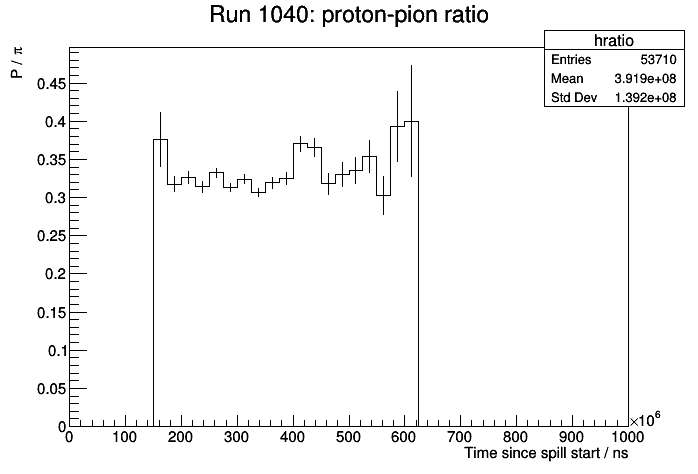
\includegraphics[width=\textwidth]{files/Figures/Run1040_proPiRatio}
%		\caption{The ratio of protons to pions as a function of time since the start of the beam spill. For these data, 1 moderator block was in place and the beam momentum was nominally 0.8~GeV/c. The data for this graph is from the sum of 255 spills.}
%		\label{fig:proPiRatio}
%	\end{minipage} 
%	\hspace{0.3cm}
%	\begin{minipage}[t]{0.48\textwidth}
%		\centering
%		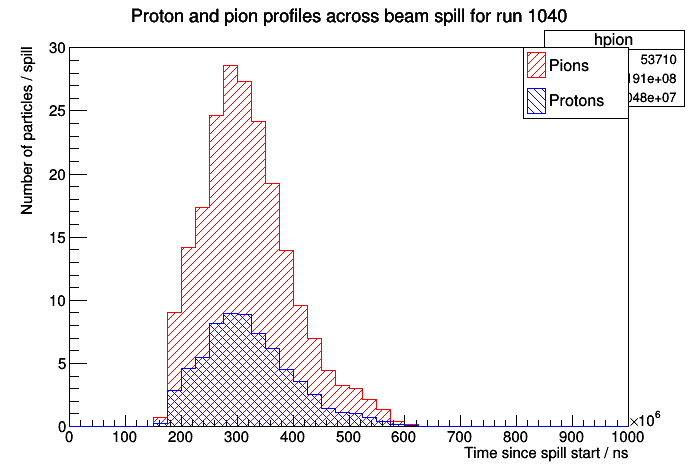
\includegraphics[width=\textwidth]{files/Figures/Run1040_proPiProf}
%		\caption{The number of protons and pions detected per spill by the DsToF as a function of time since the start of the beam spill. For these data, 1 moderator block was in place and the beam momentum was nominally 0.8~GeV/c. The data for this graph is from the sum of 255 spills.}
%		\label{fig:proPiProf}
%	\end{minipage}
%\end{figure}

Figure~\ref{fig:thetas4mip} shows the flux of particles identified as minimum ionizing particles across $\mathit{S4}$.
This flux is shown as as a function of the angle in the $x-y$ plane (see figure~\ref{fig:setup} for the definitions of these axes) for varying numbers of moderator blocks.
For all numbers of moderator blocks, the peak number of minimum ionizing particle events occurs at a value of $\theta$ between $1^{\circ}$ and $2^{\circ}$.
Similarly the number of proton events per spill, shown in figure~\ref{fig:thetas4pro} peaks at a value of $\theta$ of approximately $2^{\circ}$.

Two factors have an impact on the position of the peak:
the limited efficiency of $\mathit{S4}$ at the ends of the bars (near to either of the photomultiplier tubes) causes a smaller fraction of signal hits to be recorded in these regions. 
This limited efficiency is caused by the requirement that both PMTs record a waveform in order for a signal to be recorded.
This requirement is made, in order to reduce the number of false positives from dark noise in the PMT.
\todo[inline]{JOCELYN: Need a quantitative statement about the efficiency vs. angle here.}

The angular overlap of $\mathit{S2}$ and $\mathit{S4}$ also plays a role in the position of the peak. 
Figure~\ref{fig:angularDistS1} shows that, when observed from $\mathit{S1}$, a limited area of $\mathit{S4}$ is shadowed by the active area of $\mathit{S2}$.
\todo[inline]{JOCELYN: this explanation should go earlier in the dicsussion of the coordinate system for each ToF wall...}
Given the requirement that a signal must be observed in $\mathit{S2}$, it is clear that all of the events that are observed in $\mathit{S4}$ are from this region of overlap.

Figure~\ref{fig:thetas4mip} also indicates that initially, an increasing number of moderator blocks results in an increased total MIP flux through $\mathit{S4}$. 
However, upon the addition of the fourth moderator block the flux of MIPs appears to fall.
This is observed due to the off-axis position of both $\mathit{S2}$ and $\mathit{S4}$, avoiding many of the unmoderated beam particles striking these detectors.
Due to scattering processes in the moderator, a greater number of MIPs are incident upon $\mathit{S2}$ and $\mathit{S4}$, with more scattering occurring with greater numbers of moderator blocks.
%The drop off in the number of MIPs observed in the four block data is likely due to the overscattering of the protons and MIPs as stated previously.

When changing from an unmoderated beam to the configuration with 1 moderator block, the proton flux shown in Figure~\ref{fig:thetas4pro} initially sees an increase in the total number of events in $\mathit{S4}$.
However, upon the addition of further moderator blocks, the total number of protons observed in $\mathit{S4}$ falls.
The initial increase is similar to that for the MIP flux, with increased scattering causing more protons to pass through the off-axis $\mathit{S2}$ and $\mathit{S4}$.
The subsequent decrease is likely due to the larger loss of energy of the protons in the thicker moderator.
In turn, this leads to attenuation of protons in the TPC resulting in fewer observed events in $\mathit{S4}$.

\begin{figure}[!ht]
  \begin{minipage}[t]{0.48\textwidth}
    \begin{adjustbox}{max totalsize={\textwidth}{.35\textheight},center}
      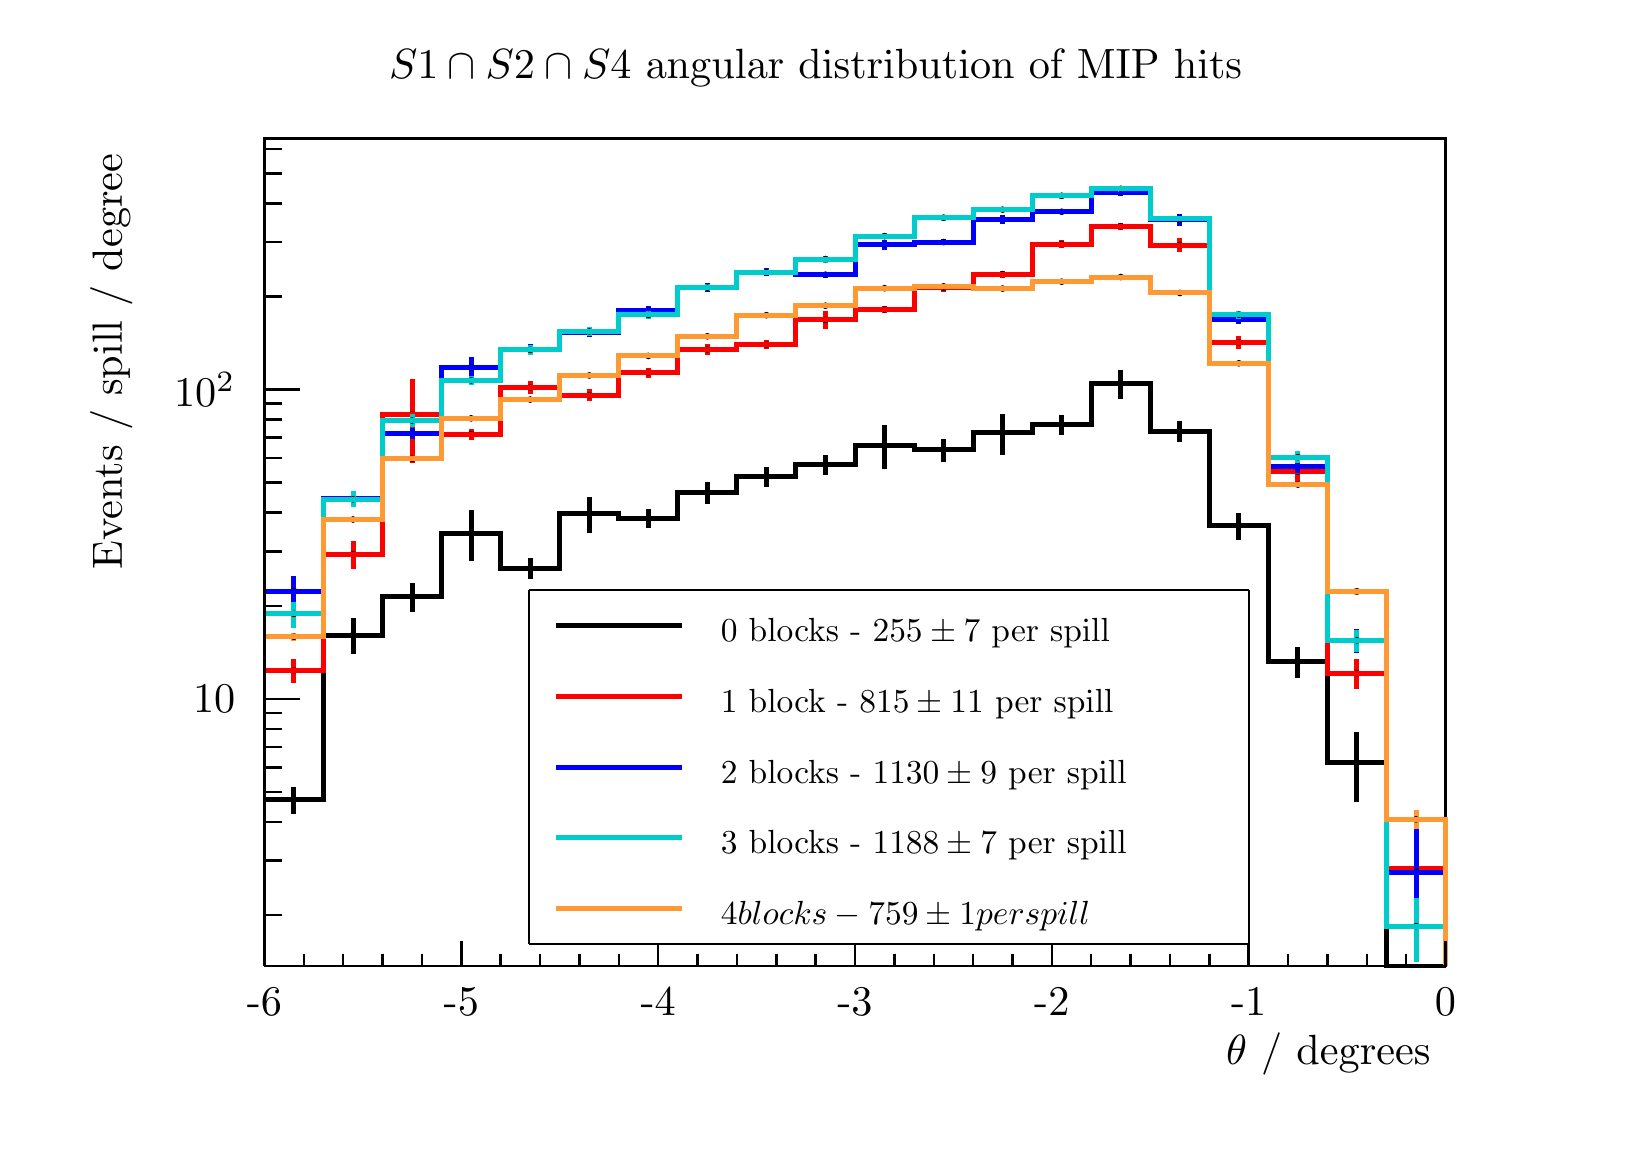
\begin{tikzpicture}
\pgfdeclareplotmark{cross} {
\pgfpathmoveto{\pgfpoint{-0.3\pgfplotmarksize}{\pgfplotmarksize}}
\pgfpathlineto{\pgfpoint{+0.3\pgfplotmarksize}{\pgfplotmarksize}}
\pgfpathlineto{\pgfpoint{+0.3\pgfplotmarksize}{0.3\pgfplotmarksize}}
\pgfpathlineto{\pgfpoint{+1\pgfplotmarksize}{0.3\pgfplotmarksize}}
\pgfpathlineto{\pgfpoint{+1\pgfplotmarksize}{-0.3\pgfplotmarksize}}
\pgfpathlineto{\pgfpoint{+0.3\pgfplotmarksize}{-0.3\pgfplotmarksize}}
\pgfpathlineto{\pgfpoint{+0.3\pgfplotmarksize}{-1.\pgfplotmarksize}}
\pgfpathlineto{\pgfpoint{-0.3\pgfplotmarksize}{-1.\pgfplotmarksize}}
\pgfpathlineto{\pgfpoint{-0.3\pgfplotmarksize}{-0.3\pgfplotmarksize}}
\pgfpathlineto{\pgfpoint{-1.\pgfplotmarksize}{-0.3\pgfplotmarksize}}
\pgfpathlineto{\pgfpoint{-1.\pgfplotmarksize}{0.3\pgfplotmarksize}}
\pgfpathlineto{\pgfpoint{-0.3\pgfplotmarksize}{0.3\pgfplotmarksize}}
\pgfpathclose
\pgfusepathqstroke
}
\pgfdeclareplotmark{cross*} {
\pgfpathmoveto{\pgfpoint{-0.3\pgfplotmarksize}{\pgfplotmarksize}}
\pgfpathlineto{\pgfpoint{+0.3\pgfplotmarksize}{\pgfplotmarksize}}
\pgfpathlineto{\pgfpoint{+0.3\pgfplotmarksize}{0.3\pgfplotmarksize}}
\pgfpathlineto{\pgfpoint{+1\pgfplotmarksize}{0.3\pgfplotmarksize}}
\pgfpathlineto{\pgfpoint{+1\pgfplotmarksize}{-0.3\pgfplotmarksize}}
\pgfpathlineto{\pgfpoint{+0.3\pgfplotmarksize}{-0.3\pgfplotmarksize}}
\pgfpathlineto{\pgfpoint{+0.3\pgfplotmarksize}{-1.\pgfplotmarksize}}
\pgfpathlineto{\pgfpoint{-0.3\pgfplotmarksize}{-1.\pgfplotmarksize}}
\pgfpathlineto{\pgfpoint{-0.3\pgfplotmarksize}{-0.3\pgfplotmarksize}}
\pgfpathlineto{\pgfpoint{-1.\pgfplotmarksize}{-0.3\pgfplotmarksize}}
\pgfpathlineto{\pgfpoint{-1.\pgfplotmarksize}{0.3\pgfplotmarksize}}
\pgfpathlineto{\pgfpoint{-0.3\pgfplotmarksize}{0.3\pgfplotmarksize}}
\pgfpathclose
\pgfusepathqfillstroke
}
\pgfdeclareplotmark{newstar} {
\pgfpathmoveto{\pgfqpoint{0pt}{\pgfplotmarksize}}
\pgfpathlineto{\pgfqpointpolar{44}{0.5\pgfplotmarksize}}
\pgfpathlineto{\pgfqpointpolar{18}{\pgfplotmarksize}}
\pgfpathlineto{\pgfqpointpolar{-20}{0.5\pgfplotmarksize}}
\pgfpathlineto{\pgfqpointpolar{-54}{\pgfplotmarksize}}
\pgfpathlineto{\pgfqpointpolar{-90}{0.5\pgfplotmarksize}}
\pgfpathlineto{\pgfqpointpolar{234}{\pgfplotmarksize}}
\pgfpathlineto{\pgfqpointpolar{198}{0.5\pgfplotmarksize}}
\pgfpathlineto{\pgfqpointpolar{162}{\pgfplotmarksize}}
\pgfpathlineto{\pgfqpointpolar{134}{0.5\pgfplotmarksize}}
\pgfpathclose
\pgfusepathqstroke
}
\pgfdeclareplotmark{newstar*} {
\pgfpathmoveto{\pgfqpoint{0pt}{\pgfplotmarksize}}
\pgfpathlineto{\pgfqpointpolar{44}{0.5\pgfplotmarksize}}
\pgfpathlineto{\pgfqpointpolar{18}{\pgfplotmarksize}}
\pgfpathlineto{\pgfqpointpolar{-20}{0.5\pgfplotmarksize}}
\pgfpathlineto{\pgfqpointpolar{-54}{\pgfplotmarksize}}
\pgfpathlineto{\pgfqpointpolar{-90}{0.5\pgfplotmarksize}}
\pgfpathlineto{\pgfqpointpolar{234}{\pgfplotmarksize}}
\pgfpathlineto{\pgfqpointpolar{198}{0.5\pgfplotmarksize}}
\pgfpathlineto{\pgfqpointpolar{162}{\pgfplotmarksize}}
\pgfpathlineto{\pgfqpointpolar{134}{0.5\pgfplotmarksize}}
\pgfpathclose
\pgfusepathqfillstroke
}
\definecolor{c}{rgb}{1,1,1};
\draw [color=c, fill=c] (0,0) rectangle (20,14.0115);
\draw [color=c, fill=c] (3,2.10172) rectangle (18,12.6103);
\definecolor{c}{rgb}{0,0,0};
\draw [c,line width=0.9] (3,2.10172) -- (3,12.6103) -- (18,12.6103) -- (18,2.10172) -- (3,2.10172);
\definecolor{c}{rgb}{1,1,1};
\draw [color=c, fill=c] (3,2.10172) rectangle (18,12.6103);
\definecolor{c}{rgb}{0,0,0};
\draw [c,line width=0.9] (3,2.10172) -- (3,12.6103) -- (18,12.6103) -- (18,2.10172) -- (3,2.10172);
\definecolor{c}{rgb}{0,0,0.6};
\draw [c,line width=0.9] (3,2.10172) -- (3.75,2.10172) -- (3.75,2.10172) -- (4.5,2.10172) -- (4.5,2.10172) -- (5.25,2.10172) -- (5.25,2.10172) -- (6,2.10172) -- (6,2.10172) -- (6.75,2.10172) -- (6.75,2.10172) -- (7.5,2.10172) -- (7.5,2.10172) --
 (8.25,2.10172) -- (8.25,2.10172) -- (9,2.10172) -- (9,2.10172) -- (9.75,2.10172) -- (9.75,2.10172) -- (10.5,2.10172) -- (10.5,2.10172) -- (11.25,2.10172) -- (11.25,2.10172) -- (12,2.10172) -- (12,2.10172) -- (12.75,2.10172) -- (12.75,2.10172) --
 (13.5,2.10172) -- (13.5,2.10172) -- (14.25,2.10172) -- (14.25,2.10172) -- (15,2.10172) -- (15,2.10172) -- (15.75,2.10172) -- (15.75,2.10172) -- (16.5,2.10172) -- (16.5,2.10172) -- (17.25,2.10172) -- (17.25,2.10172) -- (18,2.10172) -- (18,2.10172);
\definecolor{c}{rgb}{0,0,0};
\draw [c,line width=0.9] (3,2.10172) -- (18,2.10172);
\draw [c,line width=0.9] (3,2.41698) -- (3,2.10172);
\draw [c,line width=0.9] (3.5,2.25935) -- (3.5,2.10172);
\draw [c,line width=0.9] (4,2.25935) -- (4,2.10172);
\draw [c,line width=0.9] (4.5,2.25935) -- (4.5,2.10172);
\draw [c,line width=0.9] (5,2.25935) -- (5,2.10172);
\draw [c,line width=0.9] (5.5,2.41698) -- (5.5,2.10172);
\draw [c,line width=0.9] (6,2.25935) -- (6,2.10172);
\draw [c,line width=0.9] (6.5,2.25935) -- (6.5,2.10172);
\draw [c,line width=0.9] (7,2.25935) -- (7,2.10172);
\draw [c,line width=0.9] (7.5,2.25935) -- (7.5,2.10172);
\draw [c,line width=0.9] (8,2.41698) -- (8,2.10172);
\draw [c,line width=0.9] (8.5,2.25935) -- (8.5,2.10172);
\draw [c,line width=0.9] (9,2.25935) -- (9,2.10172);
\draw [c,line width=0.9] (9.5,2.25935) -- (9.5,2.10172);
\draw [c,line width=0.9] (10,2.25935) -- (10,2.10172);
\draw [c,line width=0.9] (10.5,2.41698) -- (10.5,2.10172);
\draw [c,line width=0.9] (11,2.25935) -- (11,2.10172);
\draw [c,line width=0.9] (11.5,2.25935) -- (11.5,2.10172);
\draw [c,line width=0.9] (12,2.25935) -- (12,2.10172);
\draw [c,line width=0.9] (12.5,2.25935) -- (12.5,2.10172);
\draw [c,line width=0.9] (13,2.41698) -- (13,2.10172);
\draw [c,line width=0.9] (13.5,2.25935) -- (13.5,2.10172);
\draw [c,line width=0.9] (14,2.25935) -- (14,2.10172);
\draw [c,line width=0.9] (14.5,2.25935) -- (14.5,2.10172);
\draw [c,line width=0.9] (15,2.25935) -- (15,2.10172);
\draw [c,line width=0.9] (15.5,2.41698) -- (15.5,2.10172);
\draw [c,line width=0.9] (16,2.25935) -- (16,2.10172);
\draw [c,line width=0.9] (16.5,2.25935) -- (16.5,2.10172);
\draw [c,line width=0.9] (17,2.25935) -- (17,2.10172);
\draw [c,line width=0.9] (17.5,2.25935) -- (17.5,2.10172);
\draw [c,line width=0.9] (18,2.41698) -- (18,2.10172);
\draw [anchor=base] (3,1.4712) node[scale=1.52731, color=c, rotate=0]{-6};
\draw [anchor=base] (5.5,1.4712) node[scale=1.52731, color=c, rotate=0]{-5};
\draw [anchor=base] (8,1.4712) node[scale=1.52731, color=c, rotate=0]{-4};
\draw [anchor=base] (10.5,1.4712) node[scale=1.52731, color=c, rotate=0]{-3};
\draw [anchor=base] (13,1.4712) node[scale=1.52731, color=c, rotate=0]{-2};
\draw [anchor=base] (15.5,1.4712) node[scale=1.52731, color=c, rotate=0]{-1};
\draw [anchor=base] (18,1.4712) node[scale=1.52731, color=c, rotate=0]{0};
\draw [anchor= east] (18,0.980802) node[scale=1.52731, color=c, rotate=0]{$\theta$ / degrees};
\draw [c,line width=0.9] (3,2.10172) -- (3,12.6103);
\draw [c,line width=0.9] (3.225,2.74878) -- (3,2.74878);
\draw [c,line width=0.9] (3.225,3.44048) -- (3,3.44048);
\draw [c,line width=0.9] (3.225,3.93125) -- (3,3.93125);
\draw [c,line width=0.9] (3.225,4.31191) -- (3,4.31191);
\draw [c,line width=0.9] (3.225,4.62294) -- (3,4.62294);
\draw [c,line width=0.9] (3.225,4.88591) -- (3,4.88591);
\draw [c,line width=0.9] (3.225,5.11371) -- (3,5.11371);
\draw [c,line width=0.9] (3.225,5.31464) -- (3,5.31464);
\draw [c,line width=0.9] (3.45,5.49438) -- (3,5.49438);
\draw [anchor= east] (2.82,5.49438) node[scale=1.52731, color=c, rotate=0]{10};
\draw [c,line width=0.9] (3.225,6.67684) -- (3,6.67684);
\draw [c,line width=0.9] (3.225,7.36854) -- (3,7.36854);
\draw [c,line width=0.9] (3.225,7.85931) -- (3,7.85931);
\draw [c,line width=0.9] (3.225,8.23998) -- (3,8.23998);
\draw [c,line width=0.9] (3.225,8.55101) -- (3,8.55101);
\draw [c,line width=0.9] (3.225,8.81398) -- (3,8.81398);
\draw [c,line width=0.9] (3.225,9.04177) -- (3,9.04177);
\draw [c,line width=0.9] (3.225,9.2427) -- (3,9.2427);
\draw [c,line width=0.9] (3.45,9.42244) -- (3,9.42244);
\draw [anchor= east] (2.82,9.42244) node[scale=1.52731, color=c, rotate=0]{$10^{2}$};
\draw [c,line width=0.9] (3.225,10.6049) -- (3,10.6049);
\draw [c,line width=0.9] (3.225,11.2966) -- (3,11.2966);
\draw [c,line width=0.9] (3.225,11.7874) -- (3,11.7874);
\draw [c,line width=0.9] (3.225,12.168) -- (3,12.168);
\draw [c,line width=0.9] (3.225,12.4791) -- (3,12.4791);
\draw [anchor= east] (1.05444,12.6103) node[scale=1.52731, color=c, rotate=90]{ Events / spill / degree};
\draw [c,line width=1.8] (3.375,4.03479) -- (3.375,4.21511);
\draw [c,line width=1.8] (3.375,4.21511) -- (3.375,4.37817);
\foreach \P in {(3.375,4.21511)}{\draw[mark options={color=c,fill=c},mark size=2.402402pt,mark=*,mark size=1pt] plot coordinates {\P};}
\draw [c,line width=1.8] (4.125,6.06456) -- (4.125,6.30527);
\draw [c,line width=1.8] (4.125,6.30527) -- (4.125,6.51617);
\foreach \P in {(4.125,6.30527)}{\draw[mark options={color=c,fill=c},mark size=2.402402pt,mark=*,mark size=1pt] plot coordinates {\P};}
\draw [c,line width=1.8] (4.875,6.59289) -- (4.875,6.79255);
\draw [c,line width=1.8] (4.875,6.79255) -- (4.875,6.97128);
\foreach \P in {(4.875,6.79255)}{\draw[mark options={color=c,fill=c},mark size=2.402402pt,mark=*,mark size=1pt] plot coordinates {\P};}
\draw [c,line width=1.8] (5.625,7.24345) -- (5.625,7.59827);
\draw [c,line width=1.8] (5.625,7.59827) -- (5.625,7.89184);
\foreach \P in {(5.625,7.59827)}{\draw[mark options={color=c,fill=c},mark size=2.402402pt,mark=*,mark size=1pt] plot coordinates {\P};}
\draw [c,line width=1.8] (6.375,7.0209) -- (6.375,7.15415);
\draw [c,line width=1.8] (6.375,7.15415) -- (6.375,7.27775);
\foreach \P in {(6.375,7.15415)}{\draw[mark options={color=c,fill=c},mark size=2.402402pt,mark=*,mark size=1pt] plot coordinates {\P};}
\draw [c,line width=1.8] (7.125,7.59869) -- (7.125,7.84484);
\draw [c,line width=1.8] (7.125,7.84484) -- (7.125,8.05991);
\foreach \P in {(7.125,7.84484)}{\draw[mark options={color=c,fill=c},mark size=2.402402pt,mark=*,mark size=1pt] plot coordinates {\P};}
\draw [c,line width=1.8] (7.875,7.66128) -- (7.875,7.78909);
\draw [c,line width=1.8] (7.875,7.78909) -- (7.875,7.90799);
\foreach \P in {(7.875,7.78909)}{\draw[mark options={color=c,fill=c},mark size=2.402402pt,mark=*,mark size=1pt] plot coordinates {\P};}
\draw [c,line width=1.8] (8.625,7.96983) -- (8.625,8.11244);
\draw [c,line width=1.8] (8.625,8.11244) -- (8.625,8.24405);
\foreach \P in {(8.625,8.11244)}{\draw[mark options={color=c,fill=c},mark size=2.402402pt,mark=*,mark size=1pt] plot coordinates {\P};}
\draw [c,line width=1.8] (9.375,8.17892) -- (9.375,8.31357);
\draw [c,line width=1.8] (9.375,8.31357) -- (9.375,8.43837);
\foreach \P in {(9.375,8.31357)}{\draw[mark options={color=c,fill=c},mark size=2.402402pt,mark=*,mark size=1pt] plot coordinates {\P};}
\draw [c,line width=1.8] (10.125,8.33421) -- (10.125,8.46593);
\draw [c,line width=1.8] (10.125,8.46593) -- (10.125,8.58821);
\foreach \P in {(10.125,8.46593)}{\draw[mark options={color=c,fill=c},mark size=2.402402pt,mark=*,mark size=1pt] plot coordinates {\P};}
\draw [c,line width=1.8] (10.875,8.40736) -- (10.875,8.71387);
\draw [c,line width=1.8] (10.875,8.71387) -- (10.875,8.9736);
\foreach \P in {(10.875,8.71387)}{\draw[mark options={color=c,fill=c},mark size=2.402402pt,mark=*,mark size=1pt] plot coordinates {\P};}
\draw [c,line width=1.8] (11.625,8.50247) -- (11.625,8.65545);
\draw [c,line width=1.8] (11.625,8.65545) -- (11.625,8.79583);
\foreach \P in {(11.625,8.65545)}{\draw[mark options={color=c,fill=c},mark size=2.402402pt,mark=*,mark size=1pt] plot coordinates {\P};}
\draw [c,line width=1.8] (12.375,8.59757) -- (12.375,8.87469);
\draw [c,line width=1.8] (12.375,8.87469) -- (12.375,9.11301);
\foreach \P in {(12.375,8.87469)}{\draw[mark options={color=c,fill=c},mark size=2.402402pt,mark=*,mark size=1pt] plot coordinates {\P};}
\draw [c,line width=1.8] (13.125,8.84578) -- (13.125,8.97996);
\draw [c,line width=1.8] (13.125,8.97996) -- (13.125,9.10434);
\foreach \P in {(13.125,8.97996)}{\draw[mark options={color=c,fill=c},mark size=2.402402pt,mark=*,mark size=1pt] plot coordinates {\P};}
\draw [c,line width=1.8] (13.875,9.30442) -- (13.875,9.49928);
\draw [c,line width=1.8] (13.875,9.49928) -- (13.875,9.67416);
\foreach \P in {(13.875,9.49928)}{\draw[mark options={color=c,fill=c},mark size=2.402402pt,mark=*,mark size=1pt] plot coordinates {\P};}
\draw [c,line width=1.8] (14.625,8.75179) -- (14.625,8.89211);
\draw [c,line width=1.8] (14.625,8.89211) -- (14.625,9.02176);
\foreach \P in {(14.625,8.89211)}{\draw[mark options={color=c,fill=c},mark size=2.402402pt,mark=*,mark size=1pt] plot coordinates {\P};}
\draw [c,line width=1.8] (15.375,7.50871) -- (15.375,7.69028);
\draw [c,line width=1.8] (15.375,7.69028) -- (15.375,7.85438);
\foreach \P in {(15.375,7.69028)}{\draw[mark options={color=c,fill=c},mark size=2.402402pt,mark=*,mark size=1pt] plot coordinates {\P};}
\draw [c,line width=1.8] (16.125,5.75699) -- (16.125,5.96327);
\draw [c,line width=1.8] (16.125,5.96327) -- (16.125,6.14727);
\foreach \P in {(16.125,5.96327)}{\draw[mark options={color=c,fill=c},mark size=2.402402pt,mark=*,mark size=1pt] plot coordinates {\P};}
\draw [c,line width=1.8] (16.875,4.1801) -- (16.875,4.6868);
\draw [c,line width=1.8] (16.875,4.6868) -- (16.875,5.07696);
\foreach \P in {(16.875,4.6868)}{\draw[mark options={color=c,fill=c},mark size=2.402402pt,mark=*,mark size=1pt] plot coordinates {\P};}
\draw [c,line width=1.8] (3,4.21511) -- (3.75,4.21511) -- (3.75,6.30527) -- (4.5,6.30527) -- (4.5,6.79255) -- (5.25,6.79255) -- (5.25,7.59827) -- (6,7.59827) -- (6,7.15415) -- (6.75,7.15415) -- (6.75,7.84484) -- (7.5,7.84484) -- (7.5,7.78909) --
 (8.25,7.78909) -- (8.25,8.11244) -- (9,8.11244) -- (9,8.31357) -- (9.75,8.31357) -- (9.75,8.46593) -- (10.5,8.46593) -- (10.5,8.71387) -- (11.25,8.71387) -- (11.25,8.65545) -- (12,8.65545) -- (12,8.87469) -- (12.75,8.87469) -- (12.75,8.97996) --
 (13.5,8.97996) -- (13.5,9.49928) -- (14.25,9.49928) -- (14.25,8.89211) -- (15,8.89211) -- (15,7.69028) -- (15.75,7.69028) -- (15.75,5.96327) -- (16.5,5.96327) -- (16.5,4.6868) -- (17.25,4.6868) -- (17.25,2.10172) -- (18,2.10172) -- (18,2.10172);
\definecolor{c}{rgb}{1,0,0};
\draw [c,line width=1.8] (3.375,5.69435) -- (3.375,5.85486);
\draw [c,line width=1.8] (3.375,5.85486) -- (3.375,6.00157);
\definecolor{c}{rgb}{0,0,0};
\foreach \P in {(3.375,5.85486)}{\draw[mark options={color=c,fill=c},mark size=2.402402pt,mark=*,mark size=1pt] plot coordinates {\P};}
\definecolor{c}{rgb}{1,0,0};
\draw [c,line width=1.8] (4.125,7.13733) -- (4.125,7.33122);
\draw [c,line width=1.8] (4.125,7.33122) -- (4.125,7.50531);
\definecolor{c}{rgb}{0,0,0};
\foreach \P in {(4.125,7.33122)}{\draw[mark options={color=c,fill=c},mark size=2.402402pt,mark=*,mark size=1pt] plot coordinates {\P};}
\definecolor{c}{rgb}{1,0,0};
\draw [c,line width=1.8] (4.875,8.49291) -- (4.875,9.10662);
\draw [c,line width=1.8] (4.875,9.10662) -- (4.875,9.55702);
\definecolor{c}{rgb}{0,0,0};
\foreach \P in {(4.875,9.10662)}{\draw[mark options={color=c,fill=c},mark size=2.402402pt,mark=*,mark size=1pt] plot coordinates {\P};}
\definecolor{c}{rgb}{1,0,0};
\draw [c,line width=1.8] (5.625,8.78671) -- (5.625,8.85696);
\draw [c,line width=1.8] (5.625,8.85696) -- (5.625,8.92444);
\definecolor{c}{rgb}{0,0,0};
\foreach \P in {(5.625,8.85696)}{\draw[mark options={color=c,fill=c},mark size=2.402402pt,mark=*,mark size=1pt] plot coordinates {\P};}
\definecolor{c}{rgb}{1,0,0};
\draw [c,line width=1.8] (6.375,9.36058) -- (6.375,9.44798);
\draw [c,line width=1.8] (6.375,9.44798) -- (6.375,9.53112);
\definecolor{c}{rgb}{0,0,0};
\foreach \P in {(6.375,9.44798)}{\draw[mark options={color=c,fill=c},mark size=2.402402pt,mark=*,mark size=1pt] plot coordinates {\P};}
\definecolor{c}{rgb}{1,0,0};
\draw [c,line width=1.8] (7.125,9.27103) -- (7.125,9.34886);
\draw [c,line width=1.8] (7.125,9.34886) -- (7.125,9.4233);
\definecolor{c}{rgb}{0,0,0};
\foreach \P in {(7.125,9.34886)}{\draw[mark options={color=c,fill=c},mark size=2.402402pt,mark=*,mark size=1pt] plot coordinates {\P};}
\definecolor{c}{rgb}{1,0,0};
\draw [c,line width=1.8] (7.875,9.57391) -- (7.875,9.6376);
\draw [c,line width=1.8] (7.875,9.6376) -- (7.875,9.69901);
\definecolor{c}{rgb}{0,0,0};
\foreach \P in {(7.875,9.6376)}{\draw[mark options={color=c,fill=c},mark size=2.402402pt,mark=*,mark size=1pt] plot coordinates {\P};}
\definecolor{c}{rgb}{1,0,0};
\draw [c,line width=1.8] (8.625,9.86531) -- (8.625,9.93131);
\draw [c,line width=1.8] (8.625,9.93131) -- (8.625,9.99484);
\definecolor{c}{rgb}{0,0,0};
\foreach \P in {(8.625,9.93131)}{\draw[mark options={color=c,fill=c},mark size=2.402402pt,mark=*,mark size=1pt] plot coordinates {\P};}
\definecolor{c}{rgb}{1,0,0};
\draw [c,line width=1.8] (9.375,9.93416) -- (9.375,9.99291);
\draw [c,line width=1.8] (9.375,9.99291) -- (9.375,10.0497);
\definecolor{c}{rgb}{0,0,0};
\foreach \P in {(9.375,9.99291)}{\draw[mark options={color=c,fill=c},mark size=2.402402pt,mark=*,mark size=1pt] plot coordinates {\P};}
\definecolor{c}{rgb}{1,0,0};
\draw [c,line width=1.8] (10.125,10.1876) -- (10.125,10.3081);
\draw [c,line width=1.8] (10.125,10.3081) -- (10.125,10.4207);
\definecolor{c}{rgb}{0,0,0};
\foreach \P in {(10.125,10.3081)}{\draw[mark options={color=c,fill=c},mark size=2.402402pt,mark=*,mark size=1pt] plot coordinates {\P};}
\definecolor{c}{rgb}{1,0,0};
\draw [c,line width=1.8] (10.875,10.3908) -- (10.875,10.4405);
\draw [c,line width=1.8] (10.875,10.4405) -- (10.875,10.4888);
\definecolor{c}{rgb}{0,0,0};
\foreach \P in {(10.875,10.4405)}{\draw[mark options={color=c,fill=c},mark size=2.402402pt,mark=*,mark size=1pt] plot coordinates {\P};}
\definecolor{c}{rgb}{1,0,0};
\draw [c,line width=1.8] (11.625,10.6611) -- (11.625,10.7143);
\draw [c,line width=1.8] (11.625,10.7143) -- (11.625,10.7659);
\definecolor{c}{rgb}{0,0,0};
\foreach \P in {(11.625,10.7143)}{\draw[mark options={color=c,fill=c},mark size=2.402402pt,mark=*,mark size=1pt] plot coordinates {\P};}
\definecolor{c}{rgb}{1,0,0};
\draw [c,line width=1.8] (12.375,10.842) -- (12.375,10.8886);
\draw [c,line width=1.8] (12.375,10.8886) -- (12.375,10.934);
\definecolor{c}{rgb}{0,0,0};
\foreach \P in {(12.375,10.8886)}{\draw[mark options={color=c,fill=c},mark size=2.402402pt,mark=*,mark size=1pt] plot coordinates {\P};}
\definecolor{c}{rgb}{1,0,0};
\draw [c,line width=1.8] (13.125,11.2205) -- (13.125,11.2707);
\draw [c,line width=1.8] (13.125,11.2707) -- (13.125,11.3196);
\definecolor{c}{rgb}{0,0,0};
\foreach \P in {(13.125,11.2707)}{\draw[mark options={color=c,fill=c},mark size=2.402402pt,mark=*,mark size=1pt] plot coordinates {\P};}
\definecolor{c}{rgb}{1,0,0};
\draw [c,line width=1.8] (13.875,11.4485) -- (13.875,11.4966);
\draw [c,line width=1.8] (13.875,11.4966) -- (13.875,11.5434);
\definecolor{c}{rgb}{0,0,0};
\foreach \P in {(13.875,11.4966)}{\draw[mark options={color=c,fill=c},mark size=2.402402pt,mark=*,mark size=1pt] plot coordinates {\P};}
\definecolor{c}{rgb}{1,0,0};
\draw [c,line width=1.8] (14.625,11.1707) -- (14.625,11.258);
\draw [c,line width=1.8] (14.625,11.258) -- (14.625,11.3411);
\definecolor{c}{rgb}{0,0,0};
\foreach \P in {(14.625,11.258)}{\draw[mark options={color=c,fill=c},mark size=2.402402pt,mark=*,mark size=1pt] plot coordinates {\P};}
\definecolor{c}{rgb}{1,0,0};
\draw [c,line width=1.8] (15.375,9.94073) -- (15.375,10.0212);
\draw [c,line width=1.8] (15.375,10.0212) -- (15.375,10.098);
\definecolor{c}{rgb}{0,0,0};
\foreach \P in {(15.375,10.0212)}{\draw[mark options={color=c,fill=c},mark size=2.402402pt,mark=*,mark size=1pt] plot coordinates {\P};}
\definecolor{c}{rgb}{1,0,0};
\draw [c,line width=1.8] (16.125,8.20348) -- (16.125,8.37878);
\draw [c,line width=1.8] (16.125,8.37878) -- (16.125,8.53773);
\definecolor{c}{rgb}{0,0,0};
\foreach \P in {(16.125,8.37878)}{\draw[mark options={color=c,fill=c},mark size=2.402402pt,mark=*,mark size=1pt] plot coordinates {\P};}
\definecolor{c}{rgb}{1,0,0};
\draw [c,line width=1.8] (16.875,5.61778) -- (16.875,5.81947);
\draw [c,line width=1.8] (16.875,5.81947) -- (16.875,5.99982);
\definecolor{c}{rgb}{0,0,0};
\foreach \P in {(16.875,5.81947)}{\draw[mark options={color=c,fill=c},mark size=2.402402pt,mark=*,mark size=1pt] plot coordinates {\P};}
\definecolor{c}{rgb}{1,0,0};
\draw [c,line width=1.8] (17.625,2.81258) -- (17.625,3.33608);
\draw [c,line width=1.8] (17.625,3.33608) -- (17.625,3.7361);
\definecolor{c}{rgb}{0,0,0};
\foreach \P in {(17.625,3.33608)}{\draw[mark options={color=c,fill=c},mark size=2.402402pt,mark=*,mark size=1pt] plot coordinates {\P};}
\definecolor{c}{rgb}{1,0,0};
\draw [c,line width=1.8] (3,5.85486) -- (3.75,5.85486) -- (3.75,7.33122) -- (4.5,7.33122) -- (4.5,9.10662) -- (5.25,9.10662) -- (5.25,8.85696) -- (6,8.85696) -- (6,9.44798) -- (6.75,9.44798) -- (6.75,9.34886) -- (7.5,9.34886) -- (7.5,9.6376) --
 (8.25,9.6376) -- (8.25,9.93131) -- (9,9.93131) -- (9,9.99291) -- (9.75,9.99291) -- (9.75,10.3081) -- (10.5,10.3081) -- (10.5,10.4405) -- (11.25,10.4405) -- (11.25,10.7143) -- (12,10.7143) -- (12,10.8886) -- (12.75,10.8886) -- (12.75,11.2707) --
 (13.5,11.2707) -- (13.5,11.4966) -- (14.25,11.4966) -- (14.25,11.258) -- (15,11.258) -- (15,10.0212) -- (15.75,10.0212) -- (15.75,8.37878) -- (16.5,8.37878) -- (16.5,5.81947) -- (17.25,5.81947) -- (17.25,3.33608) -- (18,3.33608) -- (18,2.10172);
\definecolor{c}{rgb}{0,0,1};
\draw [c,line width=1.8] (3.375,6.65616) -- (3.375,6.8638);
\draw [c,line width=1.8] (3.375,6.8638) -- (3.375,7.04889);
\definecolor{c}{rgb}{0,0,0};
\foreach \P in {(3.375,6.8638)}{\draw[mark options={color=c,fill=c},mark size=2.402402pt,mark=*,mark size=1pt] plot coordinates {\P};}
\definecolor{c}{rgb}{0,0,1};
\draw [c,line width=1.8] (4.125,7.95275) -- (4.125,8.03964);
\draw [c,line width=1.8] (4.125,8.03964) -- (4.125,8.12233);
\definecolor{c}{rgb}{0,0,0};
\foreach \P in {(4.125,8.03964)}{\draw[mark options={color=c,fill=c},mark size=2.402402pt,mark=*,mark size=1pt] plot coordinates {\P};}
\definecolor{c}{rgb}{0,0,1};
\draw [c,line width=1.8] (4.875,8.79676) -- (4.875,8.86516);
\draw [c,line width=1.8] (4.875,8.86516) -- (4.875,8.93093);
\definecolor{c}{rgb}{0,0,0};
\foreach \P in {(4.875,8.86516)}{\draw[mark options={color=c,fill=c},mark size=2.402402pt,mark=*,mark size=1pt] plot coordinates {\P};}
\definecolor{c}{rgb}{0,0,1};
\draw [c,line width=1.8] (5.625,9.56311) -- (5.625,9.70472);
\draw [c,line width=1.8] (5.625,9.70472) -- (5.625,9.83546);
\definecolor{c}{rgb}{0,0,0};
\foreach \P in {(5.625,9.70472)}{\draw[mark options={color=c,fill=c},mark size=2.402402pt,mark=*,mark size=1pt] plot coordinates {\P};}
\definecolor{c}{rgb}{0,0,1};
\draw [c,line width=1.8] (6.375,9.86868) -- (6.375,9.93349);
\draw [c,line width=1.8] (6.375,9.93349) -- (6.375,9.99594);
\definecolor{c}{rgb}{0,0,0};
\foreach \P in {(6.375,9.93349)}{\draw[mark options={color=c,fill=c},mark size=2.402402pt,mark=*,mark size=1pt] plot coordinates {\P};}
\definecolor{c}{rgb}{0,0,1};
\draw [c,line width=1.8] (7.125,10.0923) -- (7.125,10.1467);
\draw [c,line width=1.8] (7.125,10.1467) -- (7.125,10.1994);
\definecolor{c}{rgb}{0,0,0};
\foreach \P in {(7.125,10.1467)}{\draw[mark options={color=c,fill=c},mark size=2.402402pt,mark=*,mark size=1pt] plot coordinates {\P};}
\definecolor{c}{rgb}{0,0,1};
\draw [c,line width=1.8] (7.875,10.3723) -- (7.875,10.4285);
\draw [c,line width=1.8] (7.875,10.4285) -- (7.875,10.483);
\definecolor{c}{rgb}{0,0,0};
\foreach \P in {(7.875,10.4285)}{\draw[mark options={color=c,fill=c},mark size=2.402402pt,mark=*,mark size=1pt] plot coordinates {\P};}
\definecolor{c}{rgb}{0,0,1};
\draw [c,line width=1.8] (8.625,10.6569) -- (8.625,10.7171);
\draw [c,line width=1.8] (8.625,10.7171) -- (8.625,10.7754);
\definecolor{c}{rgb}{0,0,0};
\foreach \P in {(8.625,10.7171)}{\draw[mark options={color=c,fill=c},mark size=2.402402pt,mark=*,mark size=1pt] plot coordinates {\P};}
\definecolor{c}{rgb}{0,0,1};
\draw [c,line width=1.8] (9.375,10.8604) -- (9.375,10.9138);
\draw [c,line width=1.8] (9.375,10.9138) -- (9.375,10.9655);
\definecolor{c}{rgb}{0,0,0};
\foreach \P in {(9.375,10.9138)}{\draw[mark options={color=c,fill=c},mark size=2.402402pt,mark=*,mark size=1pt] plot coordinates {\P};}
\definecolor{c}{rgb}{0,0,1};
\draw [c,line width=1.8] (10.125,10.8426) -- (10.125,10.8814);
\draw [c,line width=1.8] (10.125,10.8814) -- (10.125,10.9193);
\definecolor{c}{rgb}{0,0,0};
\foreach \P in {(10.125,10.8814)}{\draw[mark options={color=c,fill=c},mark size=2.402402pt,mark=*,mark size=1pt] plot coordinates {\P};}
\definecolor{c}{rgb}{0,0,1};
\draw [c,line width=1.8] (10.875,11.197) -- (10.875,11.2635);
\draw [c,line width=1.8] (10.875,11.2635) -- (10.875,11.3274);
\definecolor{c}{rgb}{0,0,0};
\foreach \P in {(10.875,11.2635)}{\draw[mark options={color=c,fill=c},mark size=2.402402pt,mark=*,mark size=1pt] plot coordinates {\P};}
\definecolor{c}{rgb}{0,0,1};
\draw [c,line width=1.8] (11.625,11.2611) -- (11.625,11.2957);
\draw [c,line width=1.8] (11.625,11.2957) -- (11.625,11.3296);
\definecolor{c}{rgb}{0,0,0};
\foreach \P in {(11.625,11.2957)}{\draw[mark options={color=c,fill=c},mark size=2.402402pt,mark=*,mark size=1pt] plot coordinates {\P};}
\definecolor{c}{rgb}{0,0,1};
\draw [c,line width=1.8] (12.375,11.5281) -- (12.375,11.5817);
\draw [c,line width=1.8] (12.375,11.5817) -- (12.375,11.6336);
\definecolor{c}{rgb}{0,0,0};
\foreach \P in {(12.375,11.5817)}{\draw[mark options={color=c,fill=c},mark size=2.402402pt,mark=*,mark size=1pt] plot coordinates {\P};}
\definecolor{c}{rgb}{0,0,1};
\draw [c,line width=1.8] (13.125,11.65) -- (13.125,11.6807);
\draw [c,line width=1.8] (13.125,11.6807) -- (13.125,11.7108);
\definecolor{c}{rgb}{0,0,0};
\foreach \P in {(13.125,11.6807)}{\draw[mark options={color=c,fill=c},mark size=2.402402pt,mark=*,mark size=1pt] plot coordinates {\P};}
\definecolor{c}{rgb}{0,0,1};
\draw [c,line width=1.8] (13.875,11.8858) -- (13.875,11.9233);
\draw [c,line width=1.8] (13.875,11.9233) -- (13.875,11.96);
\definecolor{c}{rgb}{0,0,0};
\foreach \P in {(13.875,11.9233)}{\draw[mark options={color=c,fill=c},mark size=2.402402pt,mark=*,mark size=1pt] plot coordinates {\P};}
\definecolor{c}{rgb}{0,0,1};
\draw [c,line width=1.8] (14.625,11.5052) -- (14.625,11.5773);
\draw [c,line width=1.8] (14.625,11.5773) -- (14.625,11.6465);
\definecolor{c}{rgb}{0,0,0};
\foreach \P in {(14.625,11.5773)}{\draw[mark options={color=c,fill=c},mark size=2.402402pt,mark=*,mark size=1pt] plot coordinates {\P};}
\definecolor{c}{rgb}{0,0,1};
\draw [c,line width=1.8] (15.375,10.2584) -- (15.375,10.3138);
\draw [c,line width=1.8] (15.375,10.3138) -- (15.375,10.3674);
\definecolor{c}{rgb}{0,0,0};
\foreach \P in {(15.375,10.3138)}{\draw[mark options={color=c,fill=c},mark size=2.402402pt,mark=*,mark size=1pt] plot coordinates {\P};}
\definecolor{c}{rgb}{0,0,1};
\draw [c,line width=1.8] (16.125,8.36025) -- (16.125,8.4466);
\draw [c,line width=1.8] (16.125,8.4466) -- (16.125,8.52878);
\definecolor{c}{rgb}{0,0,0};
\foreach \P in {(16.125,8.4466)}{\draw[mark options={color=c,fill=c},mark size=2.402402pt,mark=*,mark size=1pt] plot coordinates {\P};}
\definecolor{c}{rgb}{0,0,1};
\draw [c,line width=1.8] (16.875,6.08301) -- (16.875,6.24076);
\draw [c,line width=1.8] (16.875,6.24076) -- (16.875,6.38515);
\definecolor{c}{rgb}{0,0,0};
\foreach \P in {(16.875,6.24076)}{\draw[mark options={color=c,fill=c},mark size=2.402402pt,mark=*,mark size=1pt] plot coordinates {\P};}
\definecolor{c}{rgb}{0,0,1};
\draw [c,line width=1.8] (17.625,2.24304) -- (17.625,3.29519);
\draw [c,line width=1.8] (17.625,3.29519) -- (17.625,3.94114);
\definecolor{c}{rgb}{0,0,0};
\foreach \P in {(17.625,3.29519)}{\draw[mark options={color=c,fill=c},mark size=2.402402pt,mark=*,mark size=1pt] plot coordinates {\P};}
\definecolor{c}{rgb}{0,0,1};
\draw [c,line width=1.8] (3,6.8638) -- (3.75,6.8638) -- (3.75,8.03964) -- (4.5,8.03964) -- (4.5,8.86516) -- (5.25,8.86516) -- (5.25,9.70472) -- (6,9.70472) -- (6,9.93349) -- (6.75,9.93349) -- (6.75,10.1467) -- (7.5,10.1467) -- (7.5,10.4285) --
 (8.25,10.4285) -- (8.25,10.7171) -- (9,10.7171) -- (9,10.9138) -- (9.75,10.9138) -- (9.75,10.8814) -- (10.5,10.8814) -- (10.5,11.2635) -- (11.25,11.2635) -- (11.25,11.2957) -- (12,11.2957) -- (12,11.5817) -- (12.75,11.5817) -- (12.75,11.6807) --
 (13.5,11.6807) -- (13.5,11.9233) -- (14.25,11.9233) -- (14.25,11.5773) -- (15,11.5773) -- (15,10.3138) -- (15.75,10.3138) -- (15.75,8.4466) -- (16.5,8.4466) -- (16.5,6.24076) -- (17.25,6.24076) -- (17.25,3.29519) -- (18,3.29519) -- (18,2.10172);
\definecolor{c}{rgb}{0,0.8,0.8};
\draw [c,line width=1.8] (3.375,6.40051) -- (3.375,6.57328);
\draw [c,line width=1.8] (3.375,6.57328) -- (3.375,6.73014);
\definecolor{c}{rgb}{0,0,0};
\foreach \P in {(3.375,6.57328)}{\draw[mark options={color=c,fill=c},mark size=2.402402pt,mark=*,mark size=1pt] plot coordinates {\P};}
\definecolor{c}{rgb}{0,0.8,0.8};
\draw [c,line width=1.8] (4.125,7.9248) -- (4.125,8.02937);
\draw [c,line width=1.8] (4.125,8.02937) -- (4.125,8.12789);
\definecolor{c}{rgb}{0,0,0};
\foreach \P in {(4.125,8.02937)}{\draw[mark options={color=c,fill=c},mark size=2.402402pt,mark=*,mark size=1pt] plot coordinates {\P};}
\definecolor{c}{rgb}{0,0.8,0.8};
\draw [c,line width=1.8] (4.875,8.94752) -- (4.875,9.02906);
\draw [c,line width=1.8] (4.875,9.02906) -- (4.875,9.10688);
\definecolor{c}{rgb}{0,0,0};
\foreach \P in {(4.875,9.02906)}{\draw[mark options={color=c,fill=c},mark size=2.402402pt,mark=*,mark size=1pt] plot coordinates {\P};}
\definecolor{c}{rgb}{0,0.8,0.8};
\draw [c,line width=1.8] (5.625,9.4765) -- (5.625,9.53891);
\draw [c,line width=1.8] (5.625,9.53891) -- (5.625,9.59913);
\definecolor{c}{rgb}{0,0,0};
\foreach \P in {(5.625,9.53891)}{\draw[mark options={color=c,fill=c},mark size=2.402402pt,mark=*,mark size=1pt] plot coordinates {\P};}
\definecolor{c}{rgb}{0,0.8,0.8};
\draw [c,line width=1.8] (6.375,9.86024) -- (6.375,9.92617);
\draw [c,line width=1.8] (6.375,9.92617) -- (6.375,9.98965);
\definecolor{c}{rgb}{0,0,0};
\foreach \P in {(6.375,9.92617)}{\draw[mark options={color=c,fill=c},mark size=2.402402pt,mark=*,mark size=1pt] plot coordinates {\P};}
\definecolor{c}{rgb}{0,0.8,0.8};
\draw [c,line width=1.8] (7.125,10.1072) -- (7.125,10.1601);
\draw [c,line width=1.8] (7.125,10.1601) -- (7.125,10.2114);
\definecolor{c}{rgb}{0,0,0};
\foreach \P in {(7.125,10.1601)}{\draw[mark options={color=c,fill=c},mark size=2.402402pt,mark=*,mark size=1pt] plot coordinates {\P};}
\definecolor{c}{rgb}{0,0.8,0.8};
\draw [c,line width=1.8] (7.875,10.3237) -- (7.875,10.3698);
\draw [c,line width=1.8] (7.875,10.3698) -- (7.875,10.4147);
\definecolor{c}{rgb}{0,0,0};
\foreach \P in {(7.875,10.3698)}{\draw[mark options={color=c,fill=c},mark size=2.402402pt,mark=*,mark size=1pt] plot coordinates {\P};}
\definecolor{c}{rgb}{0,0.8,0.8};
\draw [c,line width=1.8] (8.625,10.6703) -- (8.625,10.7158);
\draw [c,line width=1.8] (8.625,10.7158) -- (8.625,10.7602);
\definecolor{c}{rgb}{0,0,0};
\foreach \P in {(8.625,10.7158)}{\draw[mark options={color=c,fill=c},mark size=2.402402pt,mark=*,mark size=1pt] plot coordinates {\P};}
\definecolor{c}{rgb}{0,0.8,0.8};
\draw [c,line width=1.8] (9.375,10.8724) -- (9.375,10.9138);
\draw [c,line width=1.8] (9.375,10.9138) -- (9.375,10.9541);
\definecolor{c}{rgb}{0,0,0};
\foreach \P in {(9.375,10.9138)}{\draw[mark options={color=c,fill=c},mark size=2.402402pt,mark=*,mark size=1pt] plot coordinates {\P};}
\definecolor{c}{rgb}{0,0.8,0.8};
\draw [c,line width=1.8] (10.125,11.0354) -- (10.125,11.0796);
\draw [c,line width=1.8] (10.125,11.0796) -- (10.125,11.1227);
\definecolor{c}{rgb}{0,0,0};
\foreach \P in {(10.125,11.0796)}{\draw[mark options={color=c,fill=c},mark size=2.402402pt,mark=*,mark size=1pt] plot coordinates {\P};}
\definecolor{c}{rgb}{0,0.8,0.8};
\draw [c,line width=1.8] (10.875,11.3299) -- (10.875,11.3702);
\draw [c,line width=1.8] (10.875,11.3702) -- (10.875,11.4096);
\definecolor{c}{rgb}{0,0,0};
\foreach \P in {(10.875,11.3702)}{\draw[mark options={color=c,fill=c},mark size=2.402402pt,mark=*,mark size=1pt] plot coordinates {\P};}
\definecolor{c}{rgb}{0,0.8,0.8};
\draw [c,line width=1.8] (11.625,11.5661) -- (11.625,11.6059);
\draw [c,line width=1.8] (11.625,11.6059) -- (11.625,11.6448);
\definecolor{c}{rgb}{0,0,0};
\foreach \P in {(11.625,11.6059)}{\draw[mark options={color=c,fill=c},mark size=2.402402pt,mark=*,mark size=1pt] plot coordinates {\P};}
\definecolor{c}{rgb}{0,0.8,0.8};
\draw [c,line width=1.8] (12.375,11.672) -- (12.375,11.7071);
\draw [c,line width=1.8] (12.375,11.7071) -- (12.375,11.7414);
\definecolor{c}{rgb}{0,0,0};
\foreach \P in {(12.375,11.7071)}{\draw[mark options={color=c,fill=c},mark size=2.402402pt,mark=*,mark size=1pt] plot coordinates {\P};}
\definecolor{c}{rgb}{0,0.8,0.8};
\draw [c,line width=1.8] (13.125,11.8446) -- (13.125,11.8841);
\draw [c,line width=1.8] (13.125,11.8841) -- (13.125,11.9227);
\definecolor{c}{rgb}{0,0,0};
\foreach \P in {(13.125,11.8841)}{\draw[mark options={color=c,fill=c},mark size=2.402402pt,mark=*,mark size=1pt] plot coordinates {\P};}
\definecolor{c}{rgb}{0,0.8,0.8};
\draw [c,line width=1.8] (13.875,11.9367) -- (13.875,11.9724);
\draw [c,line width=1.8] (13.875,11.9724) -- (13.875,12.0075);
\definecolor{c}{rgb}{0,0,0};
\foreach \P in {(13.875,11.9724)}{\draw[mark options={color=c,fill=c},mark size=2.402402pt,mark=*,mark size=1pt] plot coordinates {\P};}
\definecolor{c}{rgb}{0,0.8,0.8};
\draw [c,line width=1.8] (14.625,11.5591) -- (14.625,11.5942);
\draw [c,line width=1.8] (14.625,11.5942) -- (14.625,11.6286);
\definecolor{c}{rgb}{0,0,0};
\foreach \P in {(14.625,11.5942)}{\draw[mark options={color=c,fill=c},mark size=2.402402pt,mark=*,mark size=1pt] plot coordinates {\P};}
\definecolor{c}{rgb}{0,0.8,0.8};
\draw [c,line width=1.8] (15.375,10.323) -- (15.375,10.3723);
\draw [c,line width=1.8] (15.375,10.3723) -- (15.375,10.4201);
\definecolor{c}{rgb}{0,0,0};
\foreach \P in {(15.375,10.3723)}{\draw[mark options={color=c,fill=c},mark size=2.402402pt,mark=*,mark size=1pt] plot coordinates {\P};}
\definecolor{c}{rgb}{0,0.8,0.8};
\draw [c,line width=1.8] (16.125,8.4846) -- (16.125,8.56423);
\draw [c,line width=1.8] (16.125,8.56423) -- (16.125,8.64031);
\definecolor{c}{rgb}{0,0,0};
\foreach \P in {(16.125,8.56423)}{\draw[mark options={color=c,fill=c},mark size=2.402402pt,mark=*,mark size=1pt] plot coordinates {\P};}
\definecolor{c}{rgb}{0,0.8,0.8};
\draw [c,line width=1.8] (16.875,6.09143) -- (16.875,6.23765);
\draw [c,line width=1.8] (16.875,6.23765) -- (16.875,6.37232);
\definecolor{c}{rgb}{0,0,0};
\foreach \P in {(16.875,6.23765)}{\draw[mark options={color=c,fill=c},mark size=2.402402pt,mark=*,mark size=1pt] plot coordinates {\P};}
\definecolor{c}{rgb}{0,0.8,0.8};
\draw [c,line width=1.8] (17.625,2.14644) -- (17.625,2.60808);
\draw [c,line width=1.8] (17.625,2.60808) -- (17.625,2.97102);
\definecolor{c}{rgb}{0,0,0};
\foreach \P in {(17.625,2.60808)}{\draw[mark options={color=c,fill=c},mark size=2.402402pt,mark=*,mark size=1pt] plot coordinates {\P};}
\definecolor{c}{rgb}{0,0.8,0.8};
\draw [c,line width=1.8] (3,6.57328) -- (3.75,6.57328) -- (3.75,8.02937) -- (4.5,8.02937) -- (4.5,9.02906) -- (5.25,9.02906) -- (5.25,9.53891) -- (6,9.53891) -- (6,9.92617) -- (6.75,9.92617) -- (6.75,10.1601) -- (7.5,10.1601) -- (7.5,10.3698) --
 (8.25,10.3698) -- (8.25,10.7158) -- (9,10.7158) -- (9,10.9138) -- (9.75,10.9138) -- (9.75,11.0796) -- (10.5,11.0796) -- (10.5,11.3702) -- (11.25,11.3702) -- (11.25,11.6059) -- (12,11.6059) -- (12,11.7071) -- (12.75,11.7071) -- (12.75,11.8841) --
 (13.5,11.8841) -- (13.5,11.9724) -- (14.25,11.9724) -- (14.25,11.5942) -- (15,11.5942) -- (15,10.3723) -- (15.75,10.3723) -- (15.75,8.56423) -- (16.5,8.56423) -- (16.5,6.23765) -- (17.25,6.23765) -- (17.25,2.60808) -- (18,2.60808) -- (18,2.10172);
\definecolor{c}{rgb}{1,0.6,0.2};
\draw [c,line width=1.8] (3.375,6.23023) -- (3.375,6.28262);
\draw [c,line width=1.8] (3.375,6.28262) -- (3.375,6.33344);
\definecolor{c}{rgb}{0,0,0};
\foreach \P in {(3.375,6.28262)}{\draw[mark options={color=c,fill=c},mark size=2.402402pt,mark=*,mark size=1pt] plot coordinates {\P};}
\definecolor{c}{rgb}{1,0.6,0.2};
\draw [c,line width=1.8] (4.125,7.74046) -- (4.125,7.7725);
\draw [c,line width=1.8] (4.125,7.7725) -- (4.125,7.80395);
\definecolor{c}{rgb}{0,0,0};
\foreach \P in {(4.125,7.7725)}{\draw[mark options={color=c,fill=c},mark size=2.402402pt,mark=*,mark size=1pt] plot coordinates {\P};}
\definecolor{c}{rgb}{1,0.6,0.2};
\draw [c,line width=1.8] (4.875,8.51788) -- (4.875,8.54274);
\draw [c,line width=1.8] (4.875,8.54274) -- (4.875,8.56725);
\definecolor{c}{rgb}{0,0,0};
\foreach \P in {(4.875,8.54274)}{\draw[mark options={color=c,fill=c},mark size=2.402402pt,mark=*,mark size=1pt] plot coordinates {\P};}
\definecolor{c}{rgb}{1,0.6,0.2};
\draw [c,line width=1.8] (5.625,9.03253) -- (5.625,9.05691);
\draw [c,line width=1.8] (5.625,9.05691) -- (5.625,9.08095);
\definecolor{c}{rgb}{0,0,0};
\foreach \P in {(5.625,9.05691)}{\draw[mark options={color=c,fill=c},mark size=2.402402pt,mark=*,mark size=1pt] plot coordinates {\P};}
\definecolor{c}{rgb}{1,0.6,0.2};
\draw [c,line width=1.8] (6.375,9.27332) -- (6.375,9.29555);
\draw [c,line width=1.8] (6.375,9.29555) -- (6.375,9.31749);
\definecolor{c}{rgb}{0,0,0};
\foreach \P in {(6.375,9.29555)}{\draw[mark options={color=c,fill=c},mark size=2.402402pt,mark=*,mark size=1pt] plot coordinates {\P};}
\definecolor{c}{rgb}{1,0.6,0.2};
\draw [c,line width=1.8] (7.125,9.58119) -- (7.125,9.60165);
\draw [c,line width=1.8] (7.125,9.60165) -- (7.125,9.62187);
\definecolor{c}{rgb}{0,0,0};
\foreach \P in {(7.125,9.60165)}{\draw[mark options={color=c,fill=c},mark size=2.402402pt,mark=*,mark size=1pt] plot coordinates {\P};}
\definecolor{c}{rgb}{1,0.6,0.2};
\draw [c,line width=1.8] (7.875,9.83215) -- (7.875,9.84977);
\draw [c,line width=1.8] (7.875,9.84977) -- (7.875,9.86721);
\definecolor{c}{rgb}{0,0,0};
\foreach \P in {(7.875,9.84977)}{\draw[mark options={color=c,fill=c},mark size=2.402402pt,mark=*,mark size=1pt] plot coordinates {\P};}
\definecolor{c}{rgb}{1,0.6,0.2};
\draw [c,line width=1.8] (8.625,10.0829) -- (8.625,10.0985);
\draw [c,line width=1.8] (8.625,10.0985) -- (8.625,10.1139);
\definecolor{c}{rgb}{0,0,0};
\foreach \P in {(8.625,10.0985)}{\draw[mark options={color=c,fill=c},mark size=2.402402pt,mark=*,mark size=1pt] plot coordinates {\P};}
\definecolor{c}{rgb}{1,0.6,0.2};
\draw [c,line width=1.8] (9.375,10.3517) -- (9.375,10.367);
\draw [c,line width=1.8] (9.375,10.367) -- (9.375,10.3822);
\definecolor{c}{rgb}{0,0,0};
\foreach \P in {(9.375,10.367)}{\draw[mark options={color=c,fill=c},mark size=2.402402pt,mark=*,mark size=1pt] plot coordinates {\P};}
\definecolor{c}{rgb}{1,0.6,0.2};
\draw [c,line width=1.8] (10.125,10.4726) -- (10.125,10.4875);
\draw [c,line width=1.8] (10.125,10.4875) -- (10.125,10.5023);
\definecolor{c}{rgb}{0,0,0};
\foreach \P in {(10.125,10.4875)}{\draw[mark options={color=c,fill=c},mark size=2.402402pt,mark=*,mark size=1pt] plot coordinates {\P};}
\definecolor{c}{rgb}{1,0.6,0.2};
\draw [c,line width=1.8] (10.875,10.6961) -- (10.875,10.7097);
\draw [c,line width=1.8] (10.875,10.7097) -- (10.875,10.7231);
\definecolor{c}{rgb}{0,0,0};
\foreach \P in {(10.875,10.7097)}{\draw[mark options={color=c,fill=c},mark size=2.402402pt,mark=*,mark size=1pt] plot coordinates {\P};}
\definecolor{c}{rgb}{1,0.6,0.2};
\draw [c,line width=1.8] (11.625,10.7203) -- (11.625,10.7331);
\draw [c,line width=1.8] (11.625,10.7331) -- (11.625,10.7458);
\definecolor{c}{rgb}{0,0,0};
\foreach \P in {(11.625,10.7331)}{\draw[mark options={color=c,fill=c},mark size=2.402402pt,mark=*,mark size=1pt] plot coordinates {\P};}
\definecolor{c}{rgb}{1,0.6,0.2};
\draw [c,line width=1.8] (12.375,10.6913) -- (12.375,10.7048);
\draw [c,line width=1.8] (12.375,10.7048) -- (12.375,10.7181);
\definecolor{c}{rgb}{0,0,0};
\foreach \P in {(12.375,10.7048)}{\draw[mark options={color=c,fill=c},mark size=2.402402pt,mark=*,mark size=1pt] plot coordinates {\P};}
\definecolor{c}{rgb}{1,0.6,0.2};
\draw [c,line width=1.8] (13.125,10.7784) -- (13.125,10.792);
\draw [c,line width=1.8] (13.125,10.792) -- (13.125,10.8055);
\definecolor{c}{rgb}{0,0,0};
\foreach \P in {(13.125,10.792)}{\draw[mark options={color=c,fill=c},mark size=2.402402pt,mark=*,mark size=1pt] plot coordinates {\P};}
\definecolor{c}{rgb}{1,0.6,0.2};
\draw [c,line width=1.8] (13.875,10.8386) -- (13.875,10.8514);
\draw [c,line width=1.8] (13.875,10.8514) -- (13.875,10.8641);
\definecolor{c}{rgb}{0,0,0};
\foreach \P in {(13.875,10.8514)}{\draw[mark options={color=c,fill=c},mark size=2.402402pt,mark=*,mark size=1pt] plot coordinates {\P};}
\definecolor{c}{rgb}{1,0.6,0.2};
\draw [c,line width=1.8] (14.625,10.6349) -- (14.625,10.6491);
\draw [c,line width=1.8] (14.625,10.6491) -- (14.625,10.6632);
\definecolor{c}{rgb}{0,0,0};
\foreach \P in {(14.625,10.6491)}{\draw[mark options={color=c,fill=c},mark size=2.402402pt,mark=*,mark size=1pt] plot coordinates {\P};}
\definecolor{c}{rgb}{1,0.6,0.2};
\draw [c,line width=1.8] (15.375,9.73812) -- (15.375,9.75611);
\draw [c,line width=1.8] (15.375,9.75611) -- (15.375,9.77392);
\definecolor{c}{rgb}{0,0,0};
\foreach \P in {(15.375,9.75611)}{\draw[mark options={color=c,fill=c},mark size=2.402402pt,mark=*,mark size=1pt] plot coordinates {\P};}
\definecolor{c}{rgb}{1,0.6,0.2};
\draw [c,line width=1.8] (16.125,8.18706) -- (16.125,8.21553);
\draw [c,line width=1.8] (16.125,8.21553) -- (16.125,8.24354);
\definecolor{c}{rgb}{0,0,0};
\foreach \P in {(16.125,8.21553)}{\draw[mark options={color=c,fill=c},mark size=2.402402pt,mark=*,mark size=1pt] plot coordinates {\P};}
\definecolor{c}{rgb}{1,0.6,0.2};
\draw [c,line width=1.8] (16.875,6.81928) -- (16.875,6.85881);
\draw [c,line width=1.8] (16.875,6.85881) -- (16.875,6.89745);
\definecolor{c}{rgb}{0,0,0};
\foreach \P in {(16.875,6.85881)}{\draw[mark options={color=c,fill=c},mark size=2.402402pt,mark=*,mark size=1pt] plot coordinates {\P};}
\definecolor{c}{rgb}{1,0.6,0.2};
\draw [c,line width=1.8] (17.625,3.83824) -- (17.625,3.96394);
\draw [c,line width=1.8] (17.625,3.96394) -- (17.625,4.08102);
\definecolor{c}{rgb}{0,0,0};
\foreach \P in {(17.625,3.96394)}{\draw[mark options={color=c,fill=c},mark size=2.402402pt,mark=*,mark size=1pt] plot coordinates {\P};}
\definecolor{c}{rgb}{1,0.6,0.2};
\draw [c,line width=1.8] (3,6.28262) -- (3.75,6.28262) -- (3.75,7.7725) -- (4.5,7.7725) -- (4.5,8.54274) -- (5.25,8.54274) -- (5.25,9.05691) -- (6,9.05691) -- (6,9.29555) -- (6.75,9.29555) -- (6.75,9.60165) -- (7.5,9.60165) -- (7.5,9.84977) --
 (8.25,9.84977) -- (8.25,10.0985) -- (9,10.0985) -- (9,10.367) -- (9.75,10.367) -- (9.75,10.4875) -- (10.5,10.4875) -- (10.5,10.7097) -- (11.25,10.7097) -- (11.25,10.7331) -- (12,10.7331) -- (12,10.7048) -- (12.75,10.7048) -- (12.75,10.792) --
 (13.5,10.792) -- (13.5,10.8514) -- (14.25,10.8514) -- (14.25,10.6491) -- (15,10.6491) -- (15,9.75611) -- (15.75,9.75611) -- (15.75,8.21553) -- (16.5,8.21553) -- (16.5,6.85881) -- (17.25,6.85881) -- (17.25,3.96394) -- (18,3.96394) -- (18,2.10172);
\definecolor{c}{rgb}{0,0,0};
\draw [c,line width=0.9] (3,2.10172) -- (18,2.10172);
\draw [c,line width=0.9] (3,2.41698) -- (3,2.10172);
\draw [c,line width=0.9] (3.5,2.25935) -- (3.5,2.10172);
\draw [c,line width=0.9] (4,2.25935) -- (4,2.10172);
\draw [c,line width=0.9] (4.5,2.25935) -- (4.5,2.10172);
\draw [c,line width=0.9] (5,2.25935) -- (5,2.10172);
\draw [c,line width=0.9] (5.5,2.41698) -- (5.5,2.10172);
\draw [c,line width=0.9] (6,2.25935) -- (6,2.10172);
\draw [c,line width=0.9] (6.5,2.25935) -- (6.5,2.10172);
\draw [c,line width=0.9] (7,2.25935) -- (7,2.10172);
\draw [c,line width=0.9] (7.5,2.25935) -- (7.5,2.10172);
\draw [c,line width=0.9] (8,2.41698) -- (8,2.10172);
\draw [c,line width=0.9] (8.5,2.25935) -- (8.5,2.10172);
\draw [c,line width=0.9] (9,2.25935) -- (9,2.10172);
\draw [c,line width=0.9] (9.5,2.25935) -- (9.5,2.10172);
\draw [c,line width=0.9] (10,2.25935) -- (10,2.10172);
\draw [c,line width=0.9] (10.5,2.41698) -- (10.5,2.10172);
\draw [c,line width=0.9] (11,2.25935) -- (11,2.10172);
\draw [c,line width=0.9] (11.5,2.25935) -- (11.5,2.10172);
\draw [c,line width=0.9] (12,2.25935) -- (12,2.10172);
\draw [c,line width=0.9] (12.5,2.25935) -- (12.5,2.10172);
\draw [c,line width=0.9] (13,2.41698) -- (13,2.10172);
\draw [c,line width=0.9] (13.5,2.25935) -- (13.5,2.10172);
\draw [c,line width=0.9] (14,2.25935) -- (14,2.10172);
\draw [c,line width=0.9] (14.5,2.25935) -- (14.5,2.10172);
\draw [c,line width=0.9] (15,2.25935) -- (15,2.10172);
\draw [c,line width=0.9] (15.5,2.41698) -- (15.5,2.10172);
\draw [c,line width=0.9] (16,2.25935) -- (16,2.10172);
\draw [c,line width=0.9] (16.5,2.25935) -- (16.5,2.10172);
\draw [c,line width=0.9] (17,2.25935) -- (17,2.10172);
\draw [c,line width=0.9] (17.5,2.25935) -- (17.5,2.10172);
\draw [c,line width=0.9] (18,2.41698) -- (18,2.10172);
\draw [c,line width=0.9] (3,2.10172) -- (3,12.6103);
\draw [c,line width=0.9] (3.225,2.74878) -- (3,2.74878);
\draw [c,line width=0.9] (3.225,3.44048) -- (3,3.44048);
\draw [c,line width=0.9] (3.225,3.93125) -- (3,3.93125);
\draw [c,line width=0.9] (3.225,4.31191) -- (3,4.31191);
\draw [c,line width=0.9] (3.225,4.62294) -- (3,4.62294);
\draw [c,line width=0.9] (3.225,4.88591) -- (3,4.88591);
\draw [c,line width=0.9] (3.225,5.11371) -- (3,5.11371);
\draw [c,line width=0.9] (3.225,5.31464) -- (3,5.31464);
\draw [c,line width=0.9] (3.45,5.49438) -- (3,5.49438);
\draw [c,line width=0.9] (3.225,6.67684) -- (3,6.67684);
\draw [c,line width=0.9] (3.225,7.36854) -- (3,7.36854);
\draw [c,line width=0.9] (3.225,7.85931) -- (3,7.85931);
\draw [c,line width=0.9] (3.225,8.23998) -- (3,8.23998);
\draw [c,line width=0.9] (3.225,8.55101) -- (3,8.55101);
\draw [c,line width=0.9] (3.225,8.81398) -- (3,8.81398);
\draw [c,line width=0.9] (3.225,9.04177) -- (3,9.04177);
\draw [c,line width=0.9] (3.225,9.2427) -- (3,9.2427);
\draw [c,line width=0.9] (3.45,9.42244) -- (3,9.42244);
\draw [c,line width=0.9] (3.225,10.6049) -- (3,10.6049);
\draw [c,line width=0.9] (3.225,11.2966) -- (3,11.2966);
\draw [c,line width=0.9] (3.225,11.7874) -- (3,11.7874);
\draw [c,line width=0.9] (3.225,12.168) -- (3,12.168);
\draw [c,line width=0.9] (3.225,12.4791) -- (3,12.4791);
\draw (10,13.5116) node[scale=1.52731, color=c, rotate=0]{$S1 \cap S2 \cap S4$ angular distribution of MIP hits};
\definecolor{c}{rgb}{1,1,1};
\draw [color=c, fill=c] (6.36103,2.37822) rectangle (15.5014,6.87679);
\definecolor{c}{rgb}{0,0,0};
\draw [c,line width=0.9] (6.36103,2.37822) -- (15.5014,2.37822);
\draw [c,line width=0.9] (15.5014,2.37822) -- (15.5014,6.87679);
\draw [c,line width=0.9] (15.5014,6.87679) -- (6.36103,6.87679);
\draw [c,line width=0.9] (6.36103,6.87679) -- (6.36103,2.37822);
\draw [anchor=base west] (8.64613,6.2245) node[scale=1.20912, color=c, rotate=0]{0 blocks - $255 \pm 7$ per spill};
\draw [c,line width=1.8] (6.7038,6.42693) -- (8.30337,6.42693);
\draw [anchor=base west] (8.64613,5.32479) node[scale=1.20912, color=c, rotate=0]{1 block - $815 \pm 11$ per spill};
\definecolor{c}{rgb}{1,0,0};
\draw [c,line width=1.8] (6.7038,5.52722) -- (8.30337,5.52722);
\definecolor{c}{rgb}{0,0,0};
\draw [anchor=base west] (8.64613,4.42507) node[scale=1.20912, color=c, rotate=0]{2 blocks - $1130 \pm 9$ per spill};
\definecolor{c}{rgb}{0,0,1};
\draw [c,line width=1.8] (6.7038,4.62751) -- (8.30337,4.62751);
\definecolor{c}{rgb}{0,0,0};
\draw [anchor=base west] (8.64613,3.52536) node[scale=1.20912, color=c, rotate=0]{3 blocks - $1188 \pm 7$ per spill};
\definecolor{c}{rgb}{0,0.8,0.8};
\draw [c,line width=1.8] (6.7038,3.72779) -- (8.30337,3.72779);
\definecolor{c}{rgb}{0,0,0};
\draw [anchor=base west] (8.64613,2.62564) node[scale=1.20912, color=c, rotate=0]{$4 blocks - 759 \pm 1 per spill$};
\definecolor{c}{rgb}{1,0.6,0.2};
\draw [c,line width=1.8] (6.7038,2.82808) -- (8.30337,2.82808);
\end{tikzpicture}

    \end{adjustbox}
    \caption{Distribution of hits identified in $\mathit{S4}$ as minimum ionizing particles as a function of the number of moderator blocks and the horizontal off-axis angle, as measured from $\mathit{S1}$.}
    \label{fig:thetas4mip}
  \end{minipage}
  \hspace{0.3cm}
  \begin{minipage}[t]{0.48\textwidth}
    \begin{adjustbox}{max totalsize={\textwidth}{.35\textheight},center}
      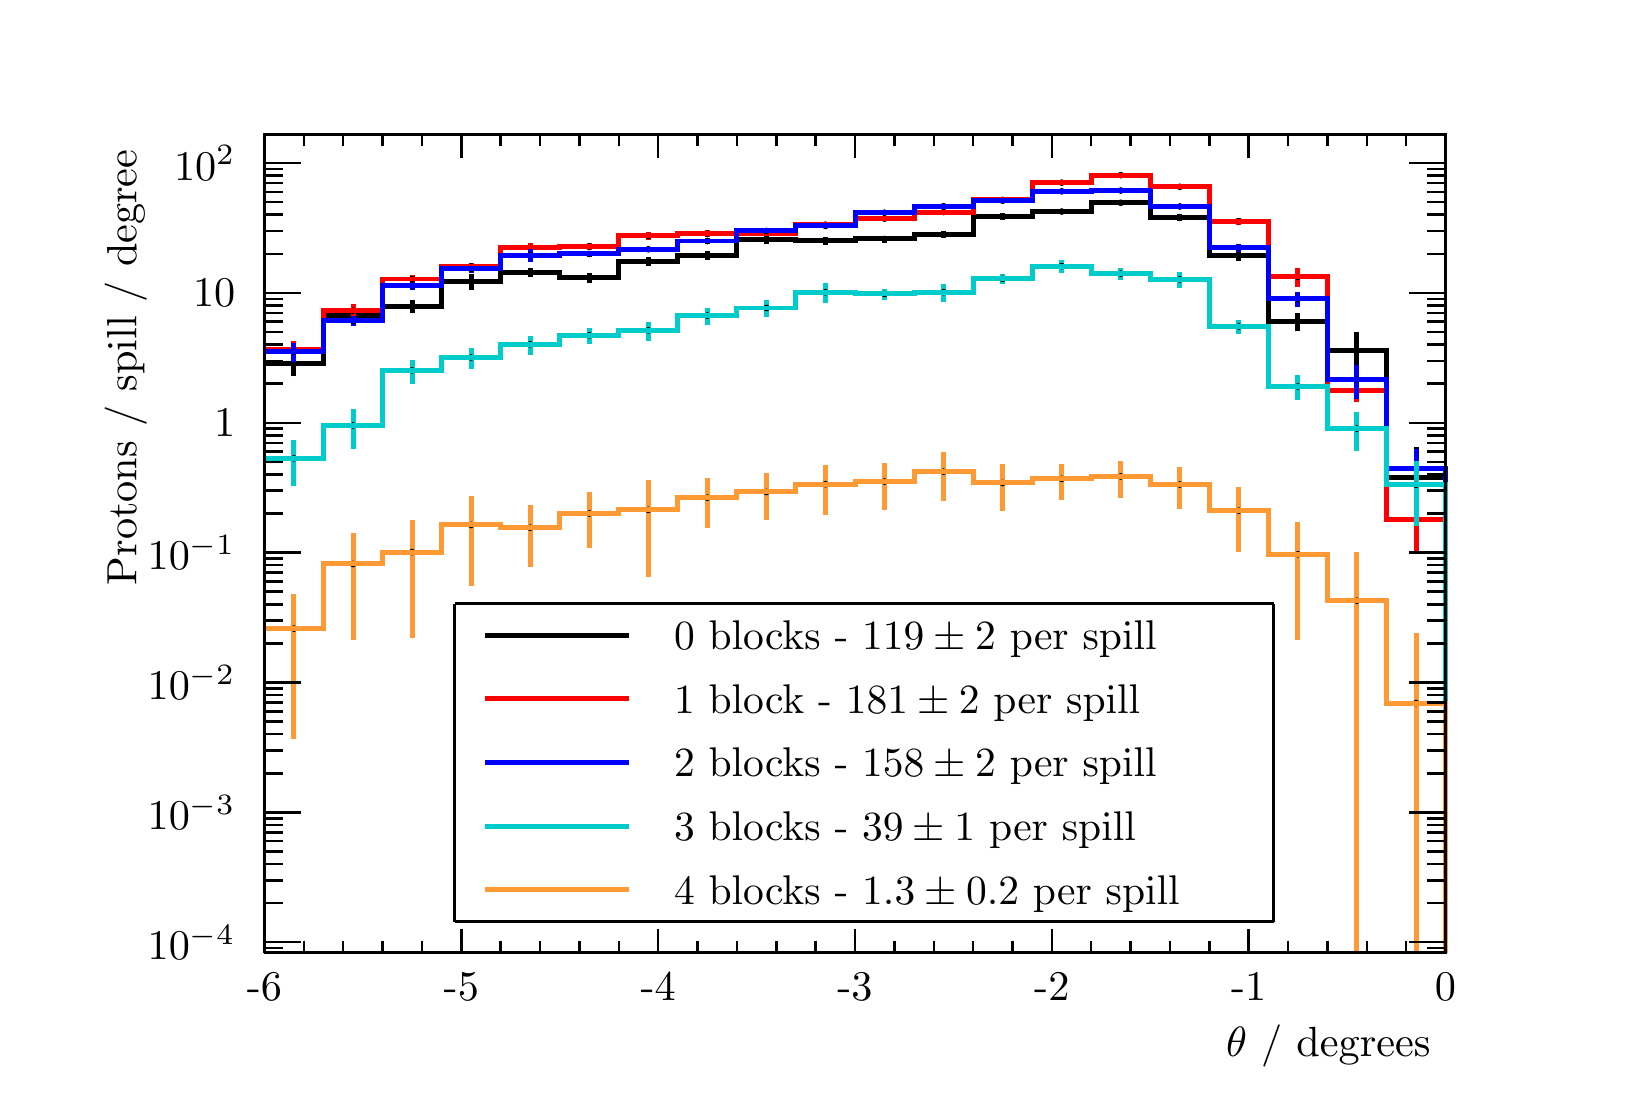
\begin{tikzpicture}
\pgfdeclareplotmark{cross} {
\pgfpathmoveto{\pgfpoint{-0.3\pgfplotmarksize}{\pgfplotmarksize}}
\pgfpathlineto{\pgfpoint{+0.3\pgfplotmarksize}{\pgfplotmarksize}}
\pgfpathlineto{\pgfpoint{+0.3\pgfplotmarksize}{0.3\pgfplotmarksize}}
\pgfpathlineto{\pgfpoint{+1\pgfplotmarksize}{0.3\pgfplotmarksize}}
\pgfpathlineto{\pgfpoint{+1\pgfplotmarksize}{-0.3\pgfplotmarksize}}
\pgfpathlineto{\pgfpoint{+0.3\pgfplotmarksize}{-0.3\pgfplotmarksize}}
\pgfpathlineto{\pgfpoint{+0.3\pgfplotmarksize}{-1.\pgfplotmarksize}}
\pgfpathlineto{\pgfpoint{-0.3\pgfplotmarksize}{-1.\pgfplotmarksize}}
\pgfpathlineto{\pgfpoint{-0.3\pgfplotmarksize}{-0.3\pgfplotmarksize}}
\pgfpathlineto{\pgfpoint{-1.\pgfplotmarksize}{-0.3\pgfplotmarksize}}
\pgfpathlineto{\pgfpoint{-1.\pgfplotmarksize}{0.3\pgfplotmarksize}}
\pgfpathlineto{\pgfpoint{-0.3\pgfplotmarksize}{0.3\pgfplotmarksize}}
\pgfpathclose
\pgfusepathqstroke
}
\pgfdeclareplotmark{cross*} {
\pgfpathmoveto{\pgfpoint{-0.3\pgfplotmarksize}{\pgfplotmarksize}}
\pgfpathlineto{\pgfpoint{+0.3\pgfplotmarksize}{\pgfplotmarksize}}
\pgfpathlineto{\pgfpoint{+0.3\pgfplotmarksize}{0.3\pgfplotmarksize}}
\pgfpathlineto{\pgfpoint{+1\pgfplotmarksize}{0.3\pgfplotmarksize}}
\pgfpathlineto{\pgfpoint{+1\pgfplotmarksize}{-0.3\pgfplotmarksize}}
\pgfpathlineto{\pgfpoint{+0.3\pgfplotmarksize}{-0.3\pgfplotmarksize}}
\pgfpathlineto{\pgfpoint{+0.3\pgfplotmarksize}{-1.\pgfplotmarksize}}
\pgfpathlineto{\pgfpoint{-0.3\pgfplotmarksize}{-1.\pgfplotmarksize}}
\pgfpathlineto{\pgfpoint{-0.3\pgfplotmarksize}{-0.3\pgfplotmarksize}}
\pgfpathlineto{\pgfpoint{-1.\pgfplotmarksize}{-0.3\pgfplotmarksize}}
\pgfpathlineto{\pgfpoint{-1.\pgfplotmarksize}{0.3\pgfplotmarksize}}
\pgfpathlineto{\pgfpoint{-0.3\pgfplotmarksize}{0.3\pgfplotmarksize}}
\pgfpathclose
\pgfusepathqfillstroke
}
\pgfdeclareplotmark{newstar} {
\pgfpathmoveto{\pgfqpoint{0pt}{\pgfplotmarksize}}
\pgfpathlineto{\pgfqpointpolar{44}{0.5\pgfplotmarksize}}
\pgfpathlineto{\pgfqpointpolar{18}{\pgfplotmarksize}}
\pgfpathlineto{\pgfqpointpolar{-20}{0.5\pgfplotmarksize}}
\pgfpathlineto{\pgfqpointpolar{-54}{\pgfplotmarksize}}
\pgfpathlineto{\pgfqpointpolar{-90}{0.5\pgfplotmarksize}}
\pgfpathlineto{\pgfqpointpolar{234}{\pgfplotmarksize}}
\pgfpathlineto{\pgfqpointpolar{198}{0.5\pgfplotmarksize}}
\pgfpathlineto{\pgfqpointpolar{162}{\pgfplotmarksize}}
\pgfpathlineto{\pgfqpointpolar{134}{0.5\pgfplotmarksize}}
\pgfpathclose
\pgfusepathqstroke
}
\pgfdeclareplotmark{newstar*} {
\pgfpathmoveto{\pgfqpoint{0pt}{\pgfplotmarksize}}
\pgfpathlineto{\pgfqpointpolar{44}{0.5\pgfplotmarksize}}
\pgfpathlineto{\pgfqpointpolar{18}{\pgfplotmarksize}}
\pgfpathlineto{\pgfqpointpolar{-20}{0.5\pgfplotmarksize}}
\pgfpathlineto{\pgfqpointpolar{-54}{\pgfplotmarksize}}
\pgfpathlineto{\pgfqpointpolar{-90}{0.5\pgfplotmarksize}}
\pgfpathlineto{\pgfqpointpolar{234}{\pgfplotmarksize}}
\pgfpathlineto{\pgfqpointpolar{198}{0.5\pgfplotmarksize}}
\pgfpathlineto{\pgfqpointpolar{162}{\pgfplotmarksize}}
\pgfpathlineto{\pgfqpointpolar{134}{0.5\pgfplotmarksize}}
\pgfpathclose
\pgfusepathqfillstroke
}
\definecolor{c}{rgb}{1,1,1};
\draw [color=c, fill=c] (0,0) rectangle (20,13.4957);
\draw [color=c, fill=c] (3,1.75444) rectangle (18,12.1461);
\definecolor{c}{rgb}{0,0,0};
\draw [c,line width=0.9] (3,1.75444) -- (3,12.1461) -- (18,12.1461) -- (18,1.75444) -- (3,1.75444);
\definecolor{c}{rgb}{1,1,1};
\draw [color=c, fill=c] (3,1.75444) rectangle (18,12.1461);
\definecolor{c}{rgb}{0,0,0};
\draw [c,line width=0.9] (3,1.75444) -- (3,12.1461) -- (18,12.1461) -- (18,1.75444) -- (3,1.75444);
\draw [c,line width=0.9] (3,1.75444) -- (3.75,1.75444) -- (3.75,1.75444) -- (4.5,1.75444) -- (4.5,1.75444) -- (5.25,1.75444) -- (5.25,1.75444) -- (6,1.75444) -- (6,1.75444) -- (6.75,1.75444) -- (6.75,1.75444) -- (7.5,1.75444) -- (7.5,1.75444) --
 (8.25,1.75444) -- (8.25,1.75444) -- (9,1.75444) -- (9,1.75444) -- (9.75,1.75444) -- (9.75,1.75444) -- (10.5,1.75444) -- (10.5,1.75444) -- (11.25,1.75444) -- (11.25,1.75444) -- (12,1.75444) -- (12,1.75444) -- (12.75,1.75444) -- (12.75,1.75444) --
 (13.5,1.75444) -- (13.5,1.75444) -- (14.25,1.75444) -- (14.25,1.75444) -- (15,1.75444) -- (15,1.75444) -- (15.75,1.75444) -- (15.75,1.75444) -- (16.5,1.75444) -- (16.5,1.75444) -- (17.25,1.75444) -- (17.25,1.75444) -- (18,1.75444) -- (18,1.75444);
\draw [c,line width=0.9] (3,1.75444) -- (18,1.75444);
\draw [c,line width=0.9] (3,2.05809) -- (3,1.75444);
\draw [c,line width=0.9] (3.5,1.90627) -- (3.5,1.75444);
\draw [c,line width=0.9] (4,1.90627) -- (4,1.75444);
\draw [c,line width=0.9] (4.5,1.90627) -- (4.5,1.75444);
\draw [c,line width=0.9] (5,1.90627) -- (5,1.75444);
\draw [c,line width=0.9] (5.5,2.05809) -- (5.5,1.75444);
\draw [c,line width=0.9] (6,1.90627) -- (6,1.75444);
\draw [c,line width=0.9] (6.5,1.90627) -- (6.5,1.75444);
\draw [c,line width=0.9] (7,1.90627) -- (7,1.75444);
\draw [c,line width=0.9] (7.5,1.90627) -- (7.5,1.75444);
\draw [c,line width=0.9] (8,2.05809) -- (8,1.75444);
\draw [c,line width=0.9] (8.5,1.90627) -- (8.5,1.75444);
\draw [c,line width=0.9] (9,1.90627) -- (9,1.75444);
\draw [c,line width=0.9] (9.5,1.90627) -- (9.5,1.75444);
\draw [c,line width=0.9] (10,1.90627) -- (10,1.75444);
\draw [c,line width=0.9] (10.5,2.05809) -- (10.5,1.75444);
\draw [c,line width=0.9] (11,1.90627) -- (11,1.75444);
\draw [c,line width=0.9] (11.5,1.90627) -- (11.5,1.75444);
\draw [c,line width=0.9] (12,1.90627) -- (12,1.75444);
\draw [c,line width=0.9] (12.5,1.90627) -- (12.5,1.75444);
\draw [c,line width=0.9] (13,2.05809) -- (13,1.75444);
\draw [c,line width=0.9] (13.5,1.90627) -- (13.5,1.75444);
\draw [c,line width=0.9] (14,1.90627) -- (14,1.75444);
\draw [c,line width=0.9] (14.5,1.90627) -- (14.5,1.75444);
\draw [c,line width=0.9] (15,1.90627) -- (15,1.75444);
\draw [c,line width=0.9] (15.5,2.05809) -- (15.5,1.75444);
\draw [c,line width=0.9] (16,1.90627) -- (16,1.75444);
\draw [c,line width=0.9] (16.5,1.90627) -- (16.5,1.75444);
\draw [c,line width=0.9] (17,1.90627) -- (17,1.75444);
\draw [c,line width=0.9] (17.5,1.90627) -- (17.5,1.75444);
\draw [c,line width=0.9] (18,2.05809) -- (18,1.75444);
\draw [anchor=base] (3,1.14713) node[scale=1.52731, color=c, rotate=0]{-6};
\draw [anchor=base] (5.5,1.14713) node[scale=1.52731, color=c, rotate=0]{-5};
\draw [anchor=base] (8,1.14713) node[scale=1.52731, color=c, rotate=0]{-4};
\draw [anchor=base] (10.5,1.14713) node[scale=1.52731, color=c, rotate=0]{-3};
\draw [anchor=base] (13,1.14713) node[scale=1.52731, color=c, rotate=0]{-2};
\draw [anchor=base] (15.5,1.14713) node[scale=1.52731, color=c, rotate=0]{-1};
\draw [anchor=base] (18,1.14713) node[scale=1.52731, color=c, rotate=0]{0};
\draw [anchor= east] (18,0.566819) node[scale=1.52731, color=c, rotate=0]{$ \theta$ / degrees};
\draw [c,line width=0.9] (3,12.1461) -- (18,12.1461);
\draw [c,line width=0.9] (3,11.8425) -- (3,12.1461);
\draw [c,line width=0.9] (3.5,11.9943) -- (3.5,12.1461);
\draw [c,line width=0.9] (4,11.9943) -- (4,12.1461);
\draw [c,line width=0.9] (4.5,11.9943) -- (4.5,12.1461);
\draw [c,line width=0.9] (5,11.9943) -- (5,12.1461);
\draw [c,line width=0.9] (5.5,11.8425) -- (5.5,12.1461);
\draw [c,line width=0.9] (6,11.9943) -- (6,12.1461);
\draw [c,line width=0.9] (6.5,11.9943) -- (6.5,12.1461);
\draw [c,line width=0.9] (7,11.9943) -- (7,12.1461);
\draw [c,line width=0.9] (7.5,11.9943) -- (7.5,12.1461);
\draw [c,line width=0.9] (8,11.8425) -- (8,12.1461);
\draw [c,line width=0.9] (8.5,11.9943) -- (8.5,12.1461);
\draw [c,line width=0.9] (9,11.9943) -- (9,12.1461);
\draw [c,line width=0.9] (9.5,11.9943) -- (9.5,12.1461);
\draw [c,line width=0.9] (10,11.9943) -- (10,12.1461);
\draw [c,line width=0.9] (10.5,11.8425) -- (10.5,12.1461);
\draw [c,line width=0.9] (11,11.9943) -- (11,12.1461);
\draw [c,line width=0.9] (11.5,11.9943) -- (11.5,12.1461);
\draw [c,line width=0.9] (12,11.9943) -- (12,12.1461);
\draw [c,line width=0.9] (12.5,11.9943) -- (12.5,12.1461);
\draw [c,line width=0.9] (13,11.8425) -- (13,12.1461);
\draw [c,line width=0.9] (13.5,11.9943) -- (13.5,12.1461);
\draw [c,line width=0.9] (14,11.9943) -- (14,12.1461);
\draw [c,line width=0.9] (14.5,11.9943) -- (14.5,12.1461);
\draw [c,line width=0.9] (15,11.9943) -- (15,12.1461);
\draw [c,line width=0.9] (15.5,11.8425) -- (15.5,12.1461);
\draw [c,line width=0.9] (16,11.9943) -- (16,12.1461);
\draw [c,line width=0.9] (16.5,11.9943) -- (16.5,12.1461);
\draw [c,line width=0.9] (17,11.9943) -- (17,12.1461);
\draw [c,line width=0.9] (17.5,11.9943) -- (17.5,12.1461);
\draw [c,line width=0.9] (18,11.8425) -- (18,12.1461);
\draw [c,line width=0.9] (3,1.75444) -- (3,12.1461);
\draw [c,line width=0.9] (3.231,1.81225) -- (3,1.81225);
\draw [c,line width=0.9] (3.462,1.88772) -- (3,1.88772);
\draw [anchor= east] (2.82,1.88772) node[scale=1.52731, color=c, rotate=0]{$10^{-4}$};
\draw [c,line width=0.9] (3.231,2.38422) -- (3,2.38422);
\draw [c,line width=0.9] (3.231,2.67466) -- (3,2.67466);
\draw [c,line width=0.9] (3.231,2.88072) -- (3,2.88072);
\draw [c,line width=0.9] (3.231,3.04056) -- (3,3.04056);
\draw [c,line width=0.9] (3.231,3.17116) -- (3,3.17116);
\draw [c,line width=0.9] (3.231,3.28158) -- (3,3.28158);
\draw [c,line width=0.9] (3.231,3.37722) -- (3,3.37722);
\draw [c,line width=0.9] (3.231,3.46159) -- (3,3.46159);
\draw [c,line width=0.9] (3.462,3.53706) -- (3,3.53706);
\draw [anchor= east] (2.82,3.53706) node[scale=1.52731, color=c, rotate=0]{$10^{-3}$};
\draw [c,line width=0.9] (3.231,4.03357) -- (3,4.03357);
\draw [c,line width=0.9] (3.231,4.324) -- (3,4.324);
\draw [c,line width=0.9] (3.231,4.53007) -- (3,4.53007);
\draw [c,line width=0.9] (3.231,4.68991) -- (3,4.68991);
\draw [c,line width=0.9] (3.231,4.8205) -- (3,4.8205);
\draw [c,line width=0.9] (3.231,4.93092) -- (3,4.93092);
\draw [c,line width=0.9] (3.231,5.02657) -- (3,5.02657);
\draw [c,line width=0.9] (3.231,5.11094) -- (3,5.11094);
\draw [c,line width=0.9] (3.462,5.18641) -- (3,5.18641);
\draw [anchor= east] (2.82,5.18641) node[scale=1.52731, color=c, rotate=0]{$10^{-2}$};
\draw [c,line width=0.9] (3.231,5.68291) -- (3,5.68291);
\draw [c,line width=0.9] (3.231,5.97335) -- (3,5.97335);
\draw [c,line width=0.9] (3.231,6.17941) -- (3,6.17941);
\draw [c,line width=0.9] (3.231,6.33925) -- (3,6.33925);
\draw [c,line width=0.9] (3.231,6.46985) -- (3,6.46985);
\draw [c,line width=0.9] (3.231,6.58027) -- (3,6.58027);
\draw [c,line width=0.9] (3.231,6.67592) -- (3,6.67592);
\draw [c,line width=0.9] (3.231,6.76028) -- (3,6.76028);
\draw [c,line width=0.9] (3.462,6.83575) -- (3,6.83575);
\draw [anchor= east] (2.82,6.83575) node[scale=1.52731, color=c, rotate=0]{$10^{-1}$};
\draw [c,line width=0.9] (3.231,7.33226) -- (3,7.33226);
\draw [c,line width=0.9] (3.231,7.62269) -- (3,7.62269);
\draw [c,line width=0.9] (3.231,7.82876) -- (3,7.82876);
\draw [c,line width=0.9] (3.231,7.9886) -- (3,7.9886);
\draw [c,line width=0.9] (3.231,8.11919) -- (3,8.11919);
\draw [c,line width=0.9] (3.231,8.22961) -- (3,8.22961);
\draw [c,line width=0.9] (3.231,8.32526) -- (3,8.32526);
\draw [c,line width=0.9] (3.231,8.40963) -- (3,8.40963);
\draw [c,line width=0.9] (3.462,8.4851) -- (3,8.4851);
\draw [anchor= east] (2.82,8.4851) node[scale=1.52731, color=c, rotate=0]{1};
\draw [c,line width=0.9] (3.231,8.9816) -- (3,8.9816);
\draw [c,line width=0.9] (3.231,9.27204) -- (3,9.27204);
\draw [c,line width=0.9] (3.231,9.4781) -- (3,9.4781);
\draw [c,line width=0.9] (3.231,9.63794) -- (3,9.63794);
\draw [c,line width=0.9] (3.231,9.76854) -- (3,9.76854);
\draw [c,line width=0.9] (3.231,9.87896) -- (3,9.87896);
\draw [c,line width=0.9] (3.231,9.97461) -- (3,9.97461);
\draw [c,line width=0.9] (3.231,10.059) -- (3,10.059);
\draw [c,line width=0.9] (3.462,10.1344) -- (3,10.1344);
\draw [anchor= east] (2.82,10.1344) node[scale=1.52731, color=c, rotate=0]{10};
\draw [c,line width=0.9] (3.231,10.6309) -- (3,10.6309);
\draw [c,line width=0.9] (3.231,10.9214) -- (3,10.9214);
\draw [c,line width=0.9] (3.231,11.1274) -- (3,11.1274);
\draw [c,line width=0.9] (3.231,11.2873) -- (3,11.2873);
\draw [c,line width=0.9] (3.231,11.4179) -- (3,11.4179);
\draw [c,line width=0.9] (3.231,11.5283) -- (3,11.5283);
\draw [c,line width=0.9] (3.231,11.624) -- (3,11.624);
\draw [c,line width=0.9] (3.231,11.7083) -- (3,11.7083);
\draw [c,line width=0.9] (3.462,11.7838) -- (3,11.7838);
\draw [anchor= east] (2.82,11.7838) node[scale=1.52731, color=c, rotate=0]{$10^{2}$};
\draw [anchor= east] (1.24,12.1461) node[scale=1.52731, color=c, rotate=90]{ Protons / spill / degree};
\draw [c,line width=0.9] (18,1.75444) -- (18,12.1461);
\draw [c,line width=0.9] (17.769,1.81225) -- (18,1.81225);
\draw [c,line width=0.9] (17.538,1.88772) -- (18,1.88772);
\draw [c,line width=0.9] (17.769,2.38422) -- (18,2.38422);
\draw [c,line width=0.9] (17.769,2.67466) -- (18,2.67466);
\draw [c,line width=0.9] (17.769,2.88072) -- (18,2.88072);
\draw [c,line width=0.9] (17.769,3.04056) -- (18,3.04056);
\draw [c,line width=0.9] (17.769,3.17116) -- (18,3.17116);
\draw [c,line width=0.9] (17.769,3.28158) -- (18,3.28158);
\draw [c,line width=0.9] (17.769,3.37722) -- (18,3.37722);
\draw [c,line width=0.9] (17.769,3.46159) -- (18,3.46159);
\draw [c,line width=0.9] (17.538,3.53706) -- (18,3.53706);
\draw [c,line width=0.9] (17.769,4.03357) -- (18,4.03357);
\draw [c,line width=0.9] (17.769,4.324) -- (18,4.324);
\draw [c,line width=0.9] (17.769,4.53007) -- (18,4.53007);
\draw [c,line width=0.9] (17.769,4.68991) -- (18,4.68991);
\draw [c,line width=0.9] (17.769,4.8205) -- (18,4.8205);
\draw [c,line width=0.9] (17.769,4.93092) -- (18,4.93092);
\draw [c,line width=0.9] (17.769,5.02657) -- (18,5.02657);
\draw [c,line width=0.9] (17.769,5.11094) -- (18,5.11094);
\draw [c,line width=0.9] (17.538,5.18641) -- (18,5.18641);
\draw [c,line width=0.9] (17.769,5.68291) -- (18,5.68291);
\draw [c,line width=0.9] (17.769,5.97335) -- (18,5.97335);
\draw [c,line width=0.9] (17.769,6.17941) -- (18,6.17941);
\draw [c,line width=0.9] (17.769,6.33925) -- (18,6.33925);
\draw [c,line width=0.9] (17.769,6.46985) -- (18,6.46985);
\draw [c,line width=0.9] (17.769,6.58027) -- (18,6.58027);
\draw [c,line width=0.9] (17.769,6.67592) -- (18,6.67592);
\draw [c,line width=0.9] (17.769,6.76028) -- (18,6.76028);
\draw [c,line width=0.9] (17.538,6.83575) -- (18,6.83575);
\draw [c,line width=0.9] (17.769,7.33226) -- (18,7.33226);
\draw [c,line width=0.9] (17.769,7.62269) -- (18,7.62269);
\draw [c,line width=0.9] (17.769,7.82876) -- (18,7.82876);
\draw [c,line width=0.9] (17.769,7.9886) -- (18,7.9886);
\draw [c,line width=0.9] (17.769,8.11919) -- (18,8.11919);
\draw [c,line width=0.9] (17.769,8.22961) -- (18,8.22961);
\draw [c,line width=0.9] (17.769,8.32526) -- (18,8.32526);
\draw [c,line width=0.9] (17.769,8.40963) -- (18,8.40963);
\draw [c,line width=0.9] (17.538,8.4851) -- (18,8.4851);
\draw [c,line width=0.9] (17.769,8.9816) -- (18,8.9816);
\draw [c,line width=0.9] (17.769,9.27204) -- (18,9.27204);
\draw [c,line width=0.9] (17.769,9.4781) -- (18,9.4781);
\draw [c,line width=0.9] (17.769,9.63794) -- (18,9.63794);
\draw [c,line width=0.9] (17.769,9.76854) -- (18,9.76854);
\draw [c,line width=0.9] (17.769,9.87896) -- (18,9.87896);
\draw [c,line width=0.9] (17.769,9.97461) -- (18,9.97461);
\draw [c,line width=0.9] (17.769,10.059) -- (18,10.059);
\draw [c,line width=0.9] (17.538,10.1344) -- (18,10.1344);
\draw [c,line width=0.9] (17.769,10.6309) -- (18,10.6309);
\draw [c,line width=0.9] (17.769,10.9214) -- (18,10.9214);
\draw [c,line width=0.9] (17.769,11.1274) -- (18,11.1274);
\draw [c,line width=0.9] (17.769,11.2873) -- (18,11.2873);
\draw [c,line width=0.9] (17.769,11.4179) -- (18,11.4179);
\draw [c,line width=0.9] (17.769,11.5283) -- (18,11.5283);
\draw [c,line width=0.9] (17.769,11.624) -- (18,11.624);
\draw [c,line width=0.9] (17.769,11.7083) -- (18,11.7083);
\draw [c,line width=0.9] (17.538,11.7838) -- (18,11.7838);
\draw [c,line width=1.8] (3.375,9.07502) -- (3.375,9.23213);
\draw [c,line width=1.8] (3.375,9.23213) -- (3.375,9.3609);
\foreach \P in {(3.375,9.23213)}{\draw[mark options={color=c,fill=c},mark size=2.402402pt,mark=*,mark size=1pt] plot coordinates {\P};}
\draw [c,line width=1.8] (4.125,9.75966) -- (4.125,9.85284);
\draw [c,line width=1.8] (4.125,9.85284) -- (4.125,9.93528);
\foreach \P in {(4.125,9.85284)}{\draw[mark options={color=c,fill=c},mark size=2.402402pt,mark=*,mark size=1pt] plot coordinates {\P};}
\draw [c,line width=1.8] (4.875,9.87682) -- (4.875,9.96395);
\draw [c,line width=1.8] (4.875,9.96395) -- (4.875,10.0416);
\foreach \P in {(4.875,9.96395)}{\draw[mark options={color=c,fill=c},mark size=2.402402pt,mark=*,mark size=1pt] plot coordinates {\P};}
\draw [c,line width=1.8] (5.625,10.1726) -- (5.625,10.2788);
\draw [c,line width=1.8] (5.625,10.2788) -- (5.625,10.3713);
\foreach \P in {(5.625,10.2788)}{\draw[mark options={color=c,fill=c},mark size=2.402402pt,mark=*,mark size=1pt] plot coordinates {\P};}
\draw [c,line width=1.8] (6.375,10.3373) -- (6.375,10.3992);
\draw [c,line width=1.8] (6.375,10.3992) -- (6.375,10.4562);
\foreach \P in {(6.375,10.3992)}{\draw[mark options={color=c,fill=c},mark size=2.402402pt,mark=*,mark size=1pt] plot coordinates {\P};}
\draw [c,line width=1.8] (7.125,10.2656) -- (7.125,10.3311);
\draw [c,line width=1.8] (7.125,10.3311) -- (7.125,10.3911);
\foreach \P in {(7.125,10.3311)}{\draw[mark options={color=c,fill=c},mark size=2.402402pt,mark=*,mark size=1pt] plot coordinates {\P};}
\draw [c,line width=1.8] (7.875,10.4763) -- (7.875,10.5374);
\draw [c,line width=1.8] (7.875,10.5374) -- (7.875,10.5938);
\foreach \P in {(7.875,10.5374)}{\draw[mark options={color=c,fill=c},mark size=2.402402pt,mark=*,mark size=1pt] plot coordinates {\P};}
\draw [c,line width=1.8] (8.625,10.5567) -- (8.625,10.6116);
\draw [c,line width=1.8] (8.625,10.6116) -- (8.625,10.6626);
\foreach \P in {(8.625,10.6116)}{\draw[mark options={color=c,fill=c},mark size=2.402402pt,mark=*,mark size=1pt] plot coordinates {\P};}
\draw [c,line width=1.8] (9.375,10.7503) -- (9.375,10.8141);
\draw [c,line width=1.8] (9.375,10.8141) -- (9.375,10.8726);
\foreach \P in {(9.375,10.8141)}{\draw[mark options={color=c,fill=c},mark size=2.402402pt,mark=*,mark size=1pt] plot coordinates {\P};}
\draw [c,line width=1.8] (10.125,10.7469) -- (10.125,10.7963);
\draw [c,line width=1.8] (10.125,10.7963) -- (10.125,10.8425);
\foreach \P in {(10.125,10.7963)}{\draw[mark options={color=c,fill=c},mark size=2.402402pt,mark=*,mark size=1pt] plot coordinates {\P};}
\draw [c,line width=1.8] (10.875,10.7735) -- (10.875,10.8191);
\draw [c,line width=1.8] (10.875,10.8191) -- (10.875,10.8619);
\foreach \P in {(10.875,10.8191)}{\draw[mark options={color=c,fill=c},mark size=2.402402pt,mark=*,mark size=1pt] plot coordinates {\P};}
\draw [c,line width=1.8] (11.625,10.8337) -- (11.625,10.877);
\draw [c,line width=1.8] (11.625,10.877) -- (11.625,10.9179);
\foreach \P in {(11.625,10.877)}{\draw[mark options={color=c,fill=c},mark size=2.402402pt,mark=*,mark size=1pt] plot coordinates {\P};}
\draw [c,line width=1.8] (12.375,11.0626) -- (12.375,11.1046);
\draw [c,line width=1.8] (12.375,11.1046) -- (12.375,11.1444);
\foreach \P in {(12.375,11.1046)}{\draw[mark options={color=c,fill=c},mark size=2.402402pt,mark=*,mark size=1pt] plot coordinates {\P};}
\draw [c,line width=1.8] (13.125,11.1339) -- (13.125,11.1675);
\draw [c,line width=1.8] (13.125,11.1675) -- (13.125,11.1996);
\foreach \P in {(13.125,11.1675)}{\draw[mark options={color=c,fill=c},mark size=2.402402pt,mark=*,mark size=1pt] plot coordinates {\P};}
\draw [c,line width=1.8] (13.875,11.2461) -- (13.875,11.2785);
\draw [c,line width=1.8] (13.875,11.2785) -- (13.875,11.3096);
\foreach \P in {(13.875,11.2785)}{\draw[mark options={color=c,fill=c},mark size=2.402402pt,mark=*,mark size=1pt] plot coordinates {\P};}
\draw [c,line width=1.8] (14.625,11.0483) -- (14.625,11.0912);
\draw [c,line width=1.8] (14.625,11.0912) -- (14.625,11.1317);
\foreach \P in {(14.625,11.0912)}{\draw[mark options={color=c,fill=c},mark size=2.402402pt,mark=*,mark size=1pt] plot coordinates {\P};}
\draw [c,line width=1.8] (15.375,10.5449) -- (15.375,10.608);
\draw [c,line width=1.8] (15.375,10.608) -- (15.375,10.666);
\foreach \P in {(15.375,10.608)}{\draw[mark options={color=c,fill=c},mark size=2.402402pt,mark=*,mark size=1pt] plot coordinates {\P};}
\draw [c,line width=1.8] (16.125,9.64718) -- (16.125,9.77334);
\draw [c,line width=1.8] (16.125,9.77334) -- (16.125,9.88057);
\foreach \P in {(16.125,9.77334)}{\draw[mark options={color=c,fill=c},mark size=2.402402pt,mark=*,mark size=1pt] plot coordinates {\P};}
\draw [c,line width=1.8] (16.875,9.05435) -- (16.875,9.40081);
\draw [c,line width=1.8] (16.875,9.40081) -- (16.875,9.63333);
\foreach \P in {(16.875,9.40081)}{\draw[mark options={color=c,fill=c},mark size=2.402402pt,mark=*,mark size=1pt] plot coordinates {\P};}
\draw [c,line width=1.8] (17.625,6.89102) -- (17.625,7.79455);
\draw [c,line width=1.8] (17.625,7.79455) -- (17.625,8.18165);
\foreach \P in {(17.625,7.79455)}{\draw[mark options={color=c,fill=c},mark size=2.402402pt,mark=*,mark size=1pt] plot coordinates {\P};}
\draw [c,line width=1.8] (3,9.23213) -- (3.75,9.23213) -- (3.75,9.85284) -- (4.5,9.85284) -- (4.5,9.96395) -- (5.25,9.96395) -- (5.25,10.2788) -- (6,10.2788) -- (6,10.3992) -- (6.75,10.3992) -- (6.75,10.3311) -- (7.5,10.3311) -- (7.5,10.5374) --
 (8.25,10.5374) -- (8.25,10.6116) -- (9,10.6116) -- (9,10.8141) -- (9.75,10.8141) -- (9.75,10.7963) -- (10.5,10.7963) -- (10.5,10.8191) -- (11.25,10.8191) -- (11.25,10.877) -- (12,10.877) -- (12,11.1046) -- (12.75,11.1046) -- (12.75,11.1675) --
 (13.5,11.1675) -- (13.5,11.2785) -- (14.25,11.2785) -- (14.25,11.0912) -- (15,11.0912) -- (15,10.608) -- (15.75,10.608) -- (15.75,9.77334) -- (16.5,9.77334) -- (16.5,9.40081) -- (17.25,9.40081) -- (17.25,7.79455) -- (18,7.79455) -- (18,1.75444);
\definecolor{c}{rgb}{1,0,0};
\draw [c,line width=1.8] (3.375,9.29318) -- (3.375,9.41497);
\draw [c,line width=1.8] (3.375,9.41497) -- (3.375,9.51902);
\definecolor{c}{rgb}{0,0,0};
\foreach \P in {(3.375,9.41497)}{\draw[mark options={color=c,fill=c},mark size=2.402402pt,mark=*,mark size=1pt] plot coordinates {\P};}
\definecolor{c}{rgb}{1,0,0};
\draw [c,line width=1.8] (4.125,9.80481) -- (4.125,9.90725);
\draw [c,line width=1.8] (4.125,9.90725) -- (4.125,9.99686);
\definecolor{c}{rgb}{0,0,0};
\foreach \P in {(4.125,9.90725)}{\draw[mark options={color=c,fill=c},mark size=2.402402pt,mark=*,mark size=1pt] plot coordinates {\P};}
\definecolor{c}{rgb}{1,0,0};
\draw [c,line width=1.8] (4.875,10.249) -- (4.875,10.3108);
\draw [c,line width=1.8] (4.875,10.3108) -- (4.875,10.3677);
\definecolor{c}{rgb}{0,0,0};
\foreach \P in {(4.875,10.3108)}{\draw[mark options={color=c,fill=c},mark size=2.402402pt,mark=*,mark size=1pt] plot coordinates {\P};}
\definecolor{c}{rgb}{1,0,0};
\draw [c,line width=1.8] (5.625,10.4221) -- (5.625,10.4723);
\draw [c,line width=1.8] (5.625,10.4723) -- (5.625,10.5191);
\definecolor{c}{rgb}{0,0,0};
\foreach \P in {(5.625,10.4723)}{\draw[mark options={color=c,fill=c},mark size=2.402402pt,mark=*,mark size=1pt] plot coordinates {\P};}
\definecolor{c}{rgb}{1,0,0};
\draw [c,line width=1.8] (6.375,10.6326) -- (6.375,10.7055);
\draw [c,line width=1.8] (6.375,10.7055) -- (6.375,10.7716);
\definecolor{c}{rgb}{0,0,0};
\foreach \P in {(6.375,10.7055)}{\draw[mark options={color=c,fill=c},mark size=2.402402pt,mark=*,mark size=1pt] plot coordinates {\P};}
\definecolor{c}{rgb}{1,0,0};
\draw [c,line width=1.8] (7.125,10.6743) -- (7.125,10.7239);
\draw [c,line width=1.8] (7.125,10.7239) -- (7.125,10.7702);
\definecolor{c}{rgb}{0,0,0};
\foreach \P in {(7.125,10.7239)}{\draw[mark options={color=c,fill=c},mark size=2.402402pt,mark=*,mark size=1pt] plot coordinates {\P};}
\definecolor{c}{rgb}{1,0,0};
\draw [c,line width=1.8] (7.875,10.8026) -- (7.875,10.8576);
\draw [c,line width=1.8] (7.875,10.8576) -- (7.875,10.9087);
\definecolor{c}{rgb}{0,0,0};
\foreach \P in {(7.875,10.8576)}{\draw[mark options={color=c,fill=c},mark size=2.402402pt,mark=*,mark size=1pt] plot coordinates {\P};}
\definecolor{c}{rgb}{1,0,0};
\draw [c,line width=1.8] (8.625,10.8427) -- (8.625,10.8862);
\draw [c,line width=1.8] (8.625,10.8862) -- (8.625,10.9272);
\definecolor{c}{rgb}{0,0,0};
\foreach \P in {(8.625,10.8862)}{\draw[mark options={color=c,fill=c},mark size=2.402402pt,mark=*,mark size=1pt] plot coordinates {\P};}
\definecolor{c}{rgb}{1,0,0};
\draw [c,line width=1.8] (9.375,10.8581) -- (9.375,10.8913);
\draw [c,line width=1.8] (9.375,10.8913) -- (9.375,10.923);
\definecolor{c}{rgb}{0,0,0};
\foreach \P in {(9.375,10.8913)}{\draw[mark options={color=c,fill=c},mark size=2.402402pt,mark=*,mark size=1pt] plot coordinates {\P};}
\definecolor{c}{rgb}{1,0,0};
\draw [c,line width=1.8] (10.125,10.9658) -- (10.125,11.0008);
\draw [c,line width=1.8] (10.125,11.0008) -- (10.125,11.0341);
\definecolor{c}{rgb}{0,0,0};
\foreach \P in {(10.125,11.0008)}{\draw[mark options={color=c,fill=c},mark size=2.402402pt,mark=*,mark size=1pt] plot coordinates {\P};}
\definecolor{c}{rgb}{1,0,0};
\draw [c,line width=1.8] (10.875,11.0434) -- (10.875,11.0777);
\draw [c,line width=1.8] (10.875,11.0777) -- (10.875,11.1105);
\definecolor{c}{rgb}{0,0,0};
\foreach \P in {(10.875,11.0777)}{\draw[mark options={color=c,fill=c},mark size=2.402402pt,mark=*,mark size=1pt] plot coordinates {\P};}
\definecolor{c}{rgb}{1,0,0};
\draw [c,line width=1.8] (11.625,11.1321) -- (11.625,11.1615);
\draw [c,line width=1.8] (11.625,11.1615) -- (11.625,11.1898);
\definecolor{c}{rgb}{0,0,0};
\foreach \P in {(11.625,11.1615)}{\draw[mark options={color=c,fill=c},mark size=2.402402pt,mark=*,mark size=1pt] plot coordinates {\P};}
\definecolor{c}{rgb}{1,0,0};
\draw [c,line width=1.8] (12.375,11.2866) -- (12.375,11.3151);
\draw [c,line width=1.8] (12.375,11.3151) -- (12.375,11.3425);
\definecolor{c}{rgb}{0,0,0};
\foreach \P in {(12.375,11.3151)}{\draw[mark options={color=c,fill=c},mark size=2.402402pt,mark=*,mark size=1pt] plot coordinates {\P};}
\definecolor{c}{rgb}{1,0,0};
\draw [c,line width=1.8] (13.125,11.5124) -- (13.125,11.5342);
\draw [c,line width=1.8] (13.125,11.5342) -- (13.125,11.5554);
\definecolor{c}{rgb}{0,0,0};
\foreach \P in {(13.125,11.5342)}{\draw[mark options={color=c,fill=c},mark size=2.402402pt,mark=*,mark size=1pt] plot coordinates {\P};}
\definecolor{c}{rgb}{1,0,0};
\draw [c,line width=1.8] (13.875,11.6021) -- (13.875,11.6298);
\draw [c,line width=1.8] (13.875,11.6298) -- (13.875,11.6565);
\definecolor{c}{rgb}{0,0,0};
\foreach \P in {(13.875,11.6298)}{\draw[mark options={color=c,fill=c},mark size=2.402402pt,mark=*,mark size=1pt] plot coordinates {\P};}
\definecolor{c}{rgb}{1,0,0};
\draw [c,line width=1.8] (14.625,11.4519) -- (14.625,11.4816);
\draw [c,line width=1.8] (14.625,11.4816) -- (14.625,11.51);
\definecolor{c}{rgb}{0,0,0};
\foreach \P in {(14.625,11.4816)}{\draw[mark options={color=c,fill=c},mark size=2.402402pt,mark=*,mark size=1pt] plot coordinates {\P};}
\definecolor{c}{rgb}{1,0,0};
\draw [c,line width=1.8] (15.375,10.9998) -- (15.375,11.0445);
\draw [c,line width=1.8] (15.375,11.0445) -- (15.375,11.0866);
\definecolor{c}{rgb}{0,0,0};
\foreach \P in {(15.375,11.0445)}{\draw[mark options={color=c,fill=c},mark size=2.402402pt,mark=*,mark size=1pt] plot coordinates {\P};}
\definecolor{c}{rgb}{1,0,0};
\draw [c,line width=1.8] (16.125,10.2048) -- (16.125,10.3367);
\draw [c,line width=1.8] (16.125,10.3367) -- (16.125,10.4481);
\definecolor{c}{rgb}{0,0,0};
\foreach \P in {(16.125,10.3367)}{\draw[mark options={color=c,fill=c},mark size=2.402402pt,mark=*,mark size=1pt] plot coordinates {\P};}
\definecolor{c}{rgb}{1,0,0};
\draw [c,line width=1.8] (16.875,8.75069) -- (16.875,8.89064);
\draw [c,line width=1.8] (16.875,8.89064) -- (16.875,9.00767);
\definecolor{c}{rgb}{0,0,0};
\foreach \P in {(16.875,8.89064)}{\draw[mark options={color=c,fill=c},mark size=2.402402pt,mark=*,mark size=1pt] plot coordinates {\P};}
\definecolor{c}{rgb}{1,0,0};
\draw [c,line width=1.8] (17.625,6.83079) -- (17.625,7.25361);
\draw [c,line width=1.8] (17.625,7.25361) -- (17.625,7.51769);
\definecolor{c}{rgb}{0,0,0};
\foreach \P in {(17.625,7.25361)}{\draw[mark options={color=c,fill=c},mark size=2.402402pt,mark=*,mark size=1pt] plot coordinates {\P};}
\definecolor{c}{rgb}{1,0,0};
\draw [c,line width=1.8] (3,9.41497) -- (3.75,9.41497) -- (3.75,9.90725) -- (4.5,9.90725) -- (4.5,10.3108) -- (5.25,10.3108) -- (5.25,10.4723) -- (6,10.4723) -- (6,10.7055) -- (6.75,10.7055) -- (6.75,10.7239) -- (7.5,10.7239) -- (7.5,10.8576) --
 (8.25,10.8576) -- (8.25,10.8862) -- (9,10.8862) -- (9,10.8913) -- (9.75,10.8913) -- (9.75,11.0008) -- (10.5,11.0008) -- (10.5,11.0777) -- (11.25,11.0777) -- (11.25,11.1615) -- (12,11.1615) -- (12,11.3151) -- (12.75,11.3151) -- (12.75,11.5342) --
 (13.5,11.5342) -- (13.5,11.6298) -- (14.25,11.6298) -- (14.25,11.4816) -- (15,11.4816) -- (15,11.0445) -- (15.75,11.0445) -- (15.75,10.3367) -- (16.5,10.3367) -- (16.5,8.89064) -- (17.25,8.89064) -- (17.25,7.25361) -- (18,7.25361) -- (18,1.75444);
\definecolor{c}{rgb}{0,0,1};
\draw [c,line width=1.8] (3.375,9.26219) -- (3.375,9.38668);
\draw [c,line width=1.8] (3.375,9.38668) -- (3.375,9.4927);
\definecolor{c}{rgb}{0,0,0};
\foreach \P in {(3.375,9.38668)}{\draw[mark options={color=c,fill=c},mark size=2.402402pt,mark=*,mark size=1pt] plot coordinates {\P};}
\definecolor{c}{rgb}{0,0,1};
\draw [c,line width=1.8] (4.125,9.70904) -- (4.125,9.77916);
\draw [c,line width=1.8] (4.125,9.77916) -- (4.125,9.84303);
\definecolor{c}{rgb}{0,0,0};
\foreach \P in {(4.125,9.77916)}{\draw[mark options={color=c,fill=c},mark size=2.402402pt,mark=*,mark size=1pt] plot coordinates {\P};}
\definecolor{c}{rgb}{0,0,1};
\draw [c,line width=1.8] (4.875,10.1747) -- (4.875,10.2284);
\draw [c,line width=1.8] (4.875,10.2284) -- (4.875,10.2784);
\definecolor{c}{rgb}{0,0,0};
\foreach \P in {(4.875,10.2284)}{\draw[mark options={color=c,fill=c},mark size=2.402402pt,mark=*,mark size=1pt] plot coordinates {\P};}
\definecolor{c}{rgb}{0,0,1};
\draw [c,line width=1.8] (5.625,10.3923) -- (5.625,10.4383);
\draw [c,line width=1.8] (5.625,10.4383) -- (5.625,10.4816);
\definecolor{c}{rgb}{0,0,0};
\foreach \P in {(5.625,10.4383)}{\draw[mark options={color=c,fill=c},mark size=2.402402pt,mark=*,mark size=1pt] plot coordinates {\P};}
\definecolor{c}{rgb}{0,0,1};
\draw [c,line width=1.8] (6.375,10.5222) -- (6.375,10.6123);
\draw [c,line width=1.8] (6.375,10.6123) -- (6.375,10.6922);
\definecolor{c}{rgb}{0,0,0};
\foreach \P in {(6.375,10.6123)}{\draw[mark options={color=c,fill=c},mark size=2.402402pt,mark=*,mark size=1pt] plot coordinates {\P};}
\definecolor{c}{rgb}{0,0,1};
\draw [c,line width=1.8] (7.125,10.5909) -- (7.125,10.629);
\draw [c,line width=1.8] (7.125,10.629) -- (7.125,10.6652);
\definecolor{c}{rgb}{0,0,0};
\foreach \P in {(7.125,10.629)}{\draw[mark options={color=c,fill=c},mark size=2.402402pt,mark=*,mark size=1pt] plot coordinates {\P};}
\definecolor{c}{rgb}{0,0,1};
\draw [c,line width=1.8] (7.875,10.6551) -- (7.875,10.6884);
\draw [c,line width=1.8] (7.875,10.6884) -- (7.875,10.7202);
\definecolor{c}{rgb}{0,0,0};
\foreach \P in {(7.875,10.6884)}{\draw[mark options={color=c,fill=c},mark size=2.402402pt,mark=*,mark size=1pt] plot coordinates {\P};}
\definecolor{c}{rgb}{0,0,1};
\draw [c,line width=1.8] (8.625,10.76) -- (8.625,10.7933);
\draw [c,line width=1.8] (8.625,10.7933) -- (8.625,10.8251);
\definecolor{c}{rgb}{0,0,0};
\foreach \P in {(8.625,10.7933)}{\draw[mark options={color=c,fill=c},mark size=2.402402pt,mark=*,mark size=1pt] plot coordinates {\P};}
\definecolor{c}{rgb}{0,0,1};
\draw [c,line width=1.8] (9.375,10.888) -- (9.375,10.9207);
\draw [c,line width=1.8] (9.375,10.9207) -- (9.375,10.952);
\definecolor{c}{rgb}{0,0,0};
\foreach \P in {(9.375,10.9207)}{\draw[mark options={color=c,fill=c},mark size=2.402402pt,mark=*,mark size=1pt] plot coordinates {\P};}
\definecolor{c}{rgb}{0,0,1};
\draw [c,line width=1.8] (10.125,10.9536) -- (10.125,10.985);
\draw [c,line width=1.8] (10.125,10.985) -- (10.125,11.015);
\definecolor{c}{rgb}{0,0,0};
\foreach \P in {(10.125,10.985)}{\draw[mark options={color=c,fill=c},mark size=2.402402pt,mark=*,mark size=1pt] plot coordinates {\P};}
\definecolor{c}{rgb}{0,0,1};
\draw [c,line width=1.8] (10.875,11.1223) -- (10.875,11.1525);
\draw [c,line width=1.8] (10.875,11.1525) -- (10.875,11.1815);
\definecolor{c}{rgb}{0,0,0};
\foreach \P in {(10.875,11.1525)}{\draw[mark options={color=c,fill=c},mark size=2.402402pt,mark=*,mark size=1pt] plot coordinates {\P};}
\definecolor{c}{rgb}{0,0,1};
\draw [c,line width=1.8] (11.625,11.2075) -- (11.625,11.2349);
\draw [c,line width=1.8] (11.625,11.2349) -- (11.625,11.2612);
\definecolor{c}{rgb}{0,0,0};
\foreach \P in {(11.625,11.2349)}{\draw[mark options={color=c,fill=c},mark size=2.402402pt,mark=*,mark size=1pt] plot coordinates {\P};}
\definecolor{c}{rgb}{0,0,1};
\draw [c,line width=1.8] (12.375,11.2803) -- (12.375,11.3051);
\draw [c,line width=1.8] (12.375,11.3051) -- (12.375,11.329);
\definecolor{c}{rgb}{0,0,0};
\foreach \P in {(12.375,11.3051)}{\draw[mark options={color=c,fill=c},mark size=2.402402pt,mark=*,mark size=1pt] plot coordinates {\P};}
\definecolor{c}{rgb}{0,0,1};
\draw [c,line width=1.8] (13.125,11.4016) -- (13.125,11.4237);
\draw [c,line width=1.8] (13.125,11.4237) -- (13.125,11.4451);
\definecolor{c}{rgb}{0,0,0};
\foreach \P in {(13.125,11.4237)}{\draw[mark options={color=c,fill=c},mark size=2.402402pt,mark=*,mark size=1pt] plot coordinates {\P};}
\definecolor{c}{rgb}{0,0,1};
\draw [c,line width=1.8] (13.875,11.4097) -- (13.875,11.4344);
\draw [c,line width=1.8] (13.875,11.4344) -- (13.875,11.4582);
\definecolor{c}{rgb}{0,0,0};
\foreach \P in {(13.875,11.4344)}{\draw[mark options={color=c,fill=c},mark size=2.402402pt,mark=*,mark size=1pt] plot coordinates {\P};}
\definecolor{c}{rgb}{0,0,1};
\draw [c,line width=1.8] (14.625,11.2014) -- (14.625,11.2318);
\draw [c,line width=1.8] (14.625,11.2318) -- (14.625,11.2609);
\definecolor{c}{rgb}{0,0,0};
\foreach \P in {(14.625,11.2318)}{\draw[mark options={color=c,fill=c},mark size=2.402402pt,mark=*,mark size=1pt] plot coordinates {\P};}
\definecolor{c}{rgb}{0,0,1};
\draw [c,line width=1.8] (15.375,10.6577) -- (15.375,10.7085);
\draw [c,line width=1.8] (15.375,10.7085) -- (15.375,10.756);
\definecolor{c}{rgb}{0,0,0};
\foreach \P in {(15.375,10.7085)}{\draw[mark options={color=c,fill=c},mark size=2.402402pt,mark=*,mark size=1pt] plot coordinates {\P};}
\definecolor{c}{rgb}{0,0,1};
\draw [c,line width=1.8] (16.125,9.9559) -- (16.125,10.0573);
\draw [c,line width=1.8] (16.125,10.0573) -- (16.125,10.1462);
\definecolor{c}{rgb}{0,0,0};
\foreach \P in {(16.125,10.0573)}{\draw[mark options={color=c,fill=c},mark size=2.402402pt,mark=*,mark size=1pt] plot coordinates {\P};}
\definecolor{c}{rgb}{0,0,1};
\draw [c,line width=1.8] (16.875,8.7896) -- (16.875,9.03343);
\draw [c,line width=1.8] (16.875,9.03343) -- (16.875,9.21501);
\definecolor{c}{rgb}{0,0,0};
\foreach \P in {(16.875,9.03343)}{\draw[mark options={color=c,fill=c},mark size=2.402402pt,mark=*,mark size=1pt] plot coordinates {\P};}
\definecolor{c}{rgb}{0,0,1};
\draw [c,line width=1.8] (17.625,7.50684) -- (17.625,7.89908);
\draw [c,line width=1.8] (17.625,7.89908) -- (17.625,8.15109);
\definecolor{c}{rgb}{0,0,0};
\foreach \P in {(17.625,7.89908)}{\draw[mark options={color=c,fill=c},mark size=2.402402pt,mark=*,mark size=1pt] plot coordinates {\P};}
\definecolor{c}{rgb}{0,0,1};
\draw [c,line width=1.8] (3,9.38668) -- (3.75,9.38668) -- (3.75,9.77916) -- (4.5,9.77916) -- (4.5,10.2284) -- (5.25,10.2284) -- (5.25,10.4383) -- (6,10.4383) -- (6,10.6123) -- (6.75,10.6123) -- (6.75,10.629) -- (7.5,10.629) -- (7.5,10.6884) --
 (8.25,10.6884) -- (8.25,10.7933) -- (9,10.7933) -- (9,10.9207) -- (9.75,10.9207) -- (9.75,10.985) -- (10.5,10.985) -- (10.5,11.1525) -- (11.25,11.1525) -- (11.25,11.2349) -- (12,11.2349) -- (12,11.3051) -- (12.75,11.3051) -- (12.75,11.4237) --
 (13.5,11.4237) -- (13.5,11.4344) -- (14.25,11.4344) -- (14.25,11.2318) -- (15,11.2318) -- (15,10.7085) -- (15.75,10.7085) -- (15.75,10.0573) -- (16.5,10.0573) -- (16.5,9.03343) -- (17.25,9.03343) -- (17.25,7.89908) -- (18,7.89908) -- (18,1.75444);
\definecolor{c}{rgb}{0,0.8,0.8};
\draw [c,line width=1.8] (3.375,7.6816) -- (3.375,8.03296);
\draw [c,line width=1.8] (3.375,8.03296) -- (3.375,8.26766);
\definecolor{c}{rgb}{0,0,0};
\foreach \P in {(3.375,8.03296)}{\draw[mark options={color=c,fill=c},mark size=2.402402pt,mark=*,mark size=1pt] plot coordinates {\P};}
\definecolor{c}{rgb}{0,0.8,0.8};
\draw [c,line width=1.8] (4.125,8.15709) -- (4.125,8.45078);
\draw [c,line width=1.8] (4.125,8.45078) -- (4.125,8.65847);
\definecolor{c}{rgb}{0,0,0};
\foreach \P in {(4.125,8.45078)}{\draw[mark options={color=c,fill=c},mark size=2.402402pt,mark=*,mark size=1pt] plot coordinates {\P};}
\definecolor{c}{rgb}{0,0.8,0.8};
\draw [c,line width=1.8] (4.875,8.98252) -- (4.875,9.15079);
\draw [c,line width=1.8] (4.875,9.15079) -- (4.875,9.28695);
\definecolor{c}{rgb}{0,0,0};
\foreach \P in {(4.875,9.15079)}{\draw[mark options={color=c,fill=c},mark size=2.402402pt,mark=*,mark size=1pt] plot coordinates {\P};}
\definecolor{c}{rgb}{0,0.8,0.8};
\draw [c,line width=1.8] (5.625,9.16477) -- (5.625,9.31377);
\draw [c,line width=1.8] (5.625,9.31377) -- (5.625,9.43705);
\definecolor{c}{rgb}{0,0,0};
\foreach \P in {(5.625,9.31377)}{\draw[mark options={color=c,fill=c},mark size=2.402402pt,mark=*,mark size=1pt] plot coordinates {\P};}
\definecolor{c}{rgb}{0,0.8,0.8};
\draw [c,line width=1.8] (6.375,9.3505) -- (6.375,9.48136);
\draw [c,line width=1.8] (6.375,9.48136) -- (6.375,9.59197);
\definecolor{c}{rgb}{0,0,0};
\foreach \P in {(6.375,9.48136)}{\draw[mark options={color=c,fill=c},mark size=2.402402pt,mark=*,mark size=1pt] plot coordinates {\P};}
\definecolor{c}{rgb}{0,0.8,0.8};
\draw [c,line width=1.8] (7.125,9.48531) -- (7.125,9.59574);
\draw [c,line width=1.8] (7.125,9.59574) -- (7.125,9.6914);
\definecolor{c}{rgb}{0,0,0};
\foreach \P in {(7.125,9.59574)}{\draw[mark options={color=c,fill=c},mark size=2.402402pt,mark=*,mark size=1pt] plot coordinates {\P};}
\definecolor{c}{rgb}{0,0.8,0.8};
\draw [c,line width=1.8] (7.875,9.52682) -- (7.875,9.65851);
\draw [c,line width=1.8] (7.875,9.65851) -- (7.875,9.7697);
\definecolor{c}{rgb}{0,0,0};
\foreach \P in {(7.875,9.65851)}{\draw[mark options={color=c,fill=c},mark size=2.402402pt,mark=*,mark size=1pt] plot coordinates {\P};}
\definecolor{c}{rgb}{0,0.8,0.8};
\draw [c,line width=1.8] (8.625,9.73158) -- (8.625,9.84645);
\draw [c,line width=1.8] (8.625,9.84645) -- (8.625,9.94542);
\definecolor{c}{rgb}{0,0,0};
\foreach \P in {(8.625,9.84645)}{\draw[mark options={color=c,fill=c},mark size=2.402402pt,mark=*,mark size=1pt] plot coordinates {\P};}
\definecolor{c}{rgb}{0,0.8,0.8};
\draw [c,line width=1.8] (9.375,9.82763) -- (9.375,9.94242);
\draw [c,line width=1.8] (9.375,9.94242) -- (9.375,10.0413);
\definecolor{c}{rgb}{0,0,0};
\foreach \P in {(9.375,9.94242)}{\draw[mark options={color=c,fill=c},mark size=2.402402pt,mark=*,mark size=1pt] plot coordinates {\P};}
\definecolor{c}{rgb}{0,0.8,0.8};
\draw [c,line width=1.8] (10.125,10.0108) -- (10.125,10.1425);
\draw [c,line width=1.8] (10.125,10.1425) -- (10.125,10.2537);
\definecolor{c}{rgb}{0,0,0};
\foreach \P in {(10.125,10.1425)}{\draw[mark options={color=c,fill=c},mark size=2.402402pt,mark=*,mark size=1pt] plot coordinates {\P};}
\definecolor{c}{rgb}{0,0.8,0.8};
\draw [c,line width=1.8] (10.875,10.047) -- (10.875,10.1208);
\draw [c,line width=1.8] (10.875,10.1208) -- (10.875,10.1877);
\definecolor{c}{rgb}{0,0,0};
\foreach \P in {(10.875,10.1208)}{\draw[mark options={color=c,fill=c},mark size=2.402402pt,mark=*,mark size=1pt] plot coordinates {\P};}
\definecolor{c}{rgb}{0,0.8,0.8};
\draw [c,line width=1.8] (11.625,10.0223) -- (11.625,10.1438);
\draw [c,line width=1.8] (11.625,10.1438) -- (11.625,10.2476);
\definecolor{c}{rgb}{0,0,0};
\foreach \P in {(11.625,10.1438)}{\draw[mark options={color=c,fill=c},mark size=2.402402pt,mark=*,mark size=1pt] plot coordinates {\P};}
\definecolor{c}{rgb}{0,0.8,0.8};
\draw [c,line width=1.8] (12.375,10.2466) -- (12.375,10.313);
\draw [c,line width=1.8] (12.375,10.313) -- (12.375,10.3737);
\definecolor{c}{rgb}{0,0,0};
\foreach \P in {(12.375,10.313)}{\draw[mark options={color=c,fill=c},mark size=2.402402pt,mark=*,mark size=1pt] plot coordinates {\P};}
\definecolor{c}{rgb}{0,0.8,0.8};
\draw [c,line width=1.8] (13.125,10.3902) -- (13.125,10.4743);
\draw [c,line width=1.8] (13.125,10.4743) -- (13.125,10.5496);
\definecolor{c}{rgb}{0,0,0};
\foreach \P in {(13.125,10.4743)}{\draw[mark options={color=c,fill=c},mark size=2.402402pt,mark=*,mark size=1pt] plot coordinates {\P};}
\definecolor{c}{rgb}{0,0.8,0.8};
\draw [c,line width=1.8] (13.875,10.3043) -- (13.875,10.3787);
\draw [c,line width=1.8] (13.875,10.3787) -- (13.875,10.4461);
\definecolor{c}{rgb}{0,0,0};
\foreach \P in {(13.875,10.3787)}{\draw[mark options={color=c,fill=c},mark size=2.402402pt,mark=*,mark size=1pt] plot coordinates {\P};}
\definecolor{c}{rgb}{0,0.8,0.8};
\draw [c,line width=1.8] (14.625,10.1983) -- (14.625,10.3056);
\draw [c,line width=1.8] (14.625,10.3056) -- (14.625,10.3989);
\definecolor{c}{rgb}{0,0,0};
\foreach \P in {(14.625,10.3056)}{\draw[mark options={color=c,fill=c},mark size=2.402402pt,mark=*,mark size=1pt] plot coordinates {\P};}
\definecolor{c}{rgb}{0,0.8,0.8};
\draw [c,line width=1.8] (15.375,9.60738) -- (15.375,9.70787);
\draw [c,line width=1.8] (15.375,9.70787) -- (15.375,9.79597);
\definecolor{c}{rgb}{0,0,0};
\foreach \P in {(15.375,9.70787)}{\draw[mark options={color=c,fill=c},mark size=2.402402pt,mark=*,mark size=1pt] plot coordinates {\P};}
\definecolor{c}{rgb}{0,0.8,0.8};
\draw [c,line width=1.8] (16.125,8.77046) -- (16.125,8.946);
\draw [c,line width=1.8] (16.125,8.946) -- (16.125,9.08687);
\definecolor{c}{rgb}{0,0,0};
\foreach \P in {(16.125,8.946)}{\draw[mark options={color=c,fill=c},mark size=2.402402pt,mark=*,mark size=1pt] plot coordinates {\P};}
\definecolor{c}{rgb}{0,0.8,0.8};
\draw [c,line width=1.8] (16.875,8.12109) -- (16.875,8.41104);
\draw [c,line width=1.8] (16.875,8.41104) -- (16.875,8.61686);
\definecolor{c}{rgb}{0,0,0};
\foreach \P in {(16.875,8.41104)}{\draw[mark options={color=c,fill=c},mark size=2.402402pt,mark=*,mark size=1pt] plot coordinates {\P};}
\definecolor{c}{rgb}{0,0.8,0.8};
\draw [c,line width=1.8] (17.625,7.17765) -- (17.625,7.69668);
\draw [c,line width=1.8] (17.625,7.69668) -- (17.625,7.99447);
\definecolor{c}{rgb}{0,0,0};
\foreach \P in {(17.625,7.69668)}{\draw[mark options={color=c,fill=c},mark size=2.402402pt,mark=*,mark size=1pt] plot coordinates {\P};}
\definecolor{c}{rgb}{0,0.8,0.8};
\draw [c,line width=1.8] (3,8.03296) -- (3.75,8.03296) -- (3.75,8.45078) -- (4.5,8.45078) -- (4.5,9.15079) -- (5.25,9.15079) -- (5.25,9.31377) -- (6,9.31377) -- (6,9.48136) -- (6.75,9.48136) -- (6.75,9.59574) -- (7.5,9.59574) -- (7.5,9.65851) --
 (8.25,9.65851) -- (8.25,9.84645) -- (9,9.84645) -- (9,9.94242) -- (9.75,9.94242) -- (9.75,10.1425) -- (10.5,10.1425) -- (10.5,10.1208) -- (11.25,10.1208) -- (11.25,10.1438) -- (12,10.1438) -- (12,10.313) -- (12.75,10.313) -- (12.75,10.4743) --
 (13.5,10.4743) -- (13.5,10.3787) -- (14.25,10.3787) -- (14.25,10.3056) -- (15,10.3056) -- (15,9.70787) -- (15.75,9.70787) -- (15.75,8.946) -- (16.5,8.946) -- (16.5,8.41104) -- (17.25,8.41104) -- (17.25,7.69668) -- (18,7.69668) -- (18,1.75444);
\definecolor{c}{rgb}{1,0.6,0.2};
\draw [c,line width=1.8] (3.375,4.46315) -- (3.375,5.8709);
\draw [c,line width=1.8] (3.375,5.8709) -- (3.375,6.31538);
\definecolor{c}{rgb}{0,0,0};
\foreach \P in {(3.375,5.8709)}{\draw[mark options={color=c,fill=c},mark size=2.402402pt,mark=*,mark size=1pt] plot coordinates {\P};}
\definecolor{c}{rgb}{1,0.6,0.2};
\draw [c,line width=1.8] (4.125,5.71984) -- (4.125,6.6915);
\draw [c,line width=1.8] (4.125,6.6915) -- (4.125,7.08926);
\definecolor{c}{rgb}{0,0,0};
\foreach \P in {(4.125,6.6915)}{\draw[mark options={color=c,fill=c},mark size=2.402402pt,mark=*,mark size=1pt] plot coordinates {\P};}
\definecolor{c}{rgb}{1,0.6,0.2};
\draw [c,line width=1.8] (4.875,5.75478) -- (4.875,6.84276);
\draw [c,line width=1.8] (4.875,6.84276) -- (4.875,7.2562);
\definecolor{c}{rgb}{0,0,0};
\foreach \P in {(4.875,6.84276)}{\draw[mark options={color=c,fill=c},mark size=2.402402pt,mark=*,mark size=1pt] plot coordinates {\P};}
\definecolor{c}{rgb}{1,0.6,0.2};
\draw [c,line width=1.8] (5.625,6.41071) -- (5.625,7.18734);
\draw [c,line width=1.8] (5.625,7.18734) -- (5.625,7.55116);
\definecolor{c}{rgb}{0,0,0};
\foreach \P in {(5.625,7.18734)}{\draw[mark options={color=c,fill=c},mark size=2.402402pt,mark=*,mark size=1pt] plot coordinates {\P};}
\definecolor{c}{rgb}{1,0.6,0.2};
\draw [c,line width=1.8] (6.375,6.65696) -- (6.375,7.15238);
\draw [c,line width=1.8] (6.375,7.15238) -- (6.375,7.44246);
\definecolor{c}{rgb}{0,0,0};
\foreach \P in {(6.375,7.15238)}{\draw[mark options={color=c,fill=c},mark size=2.402402pt,mark=*,mark size=1pt] plot coordinates {\P};}
\definecolor{c}{rgb}{1,0.6,0.2};
\draw [c,line width=1.8] (7.125,6.88876) -- (7.125,7.33325);
\draw [c,line width=1.8] (7.125,7.33325) -- (7.125,7.60547);
\definecolor{c}{rgb}{0,0,0};
\foreach \P in {(7.125,7.33325)}{\draw[mark options={color=c,fill=c},mark size=2.402402pt,mark=*,mark size=1pt] plot coordinates {\P};}
\definecolor{c}{rgb}{1,0.6,0.2};
\draw [c,line width=1.8] (7.875,6.5204) -- (7.875,7.37932);
\draw [c,line width=1.8] (7.875,7.37932) -- (7.875,7.7588);
\definecolor{c}{rgb}{0,0,0};
\foreach \P in {(7.875,7.37932)}{\draw[mark options={color=c,fill=c},mark size=2.402402pt,mark=*,mark size=1pt] plot coordinates {\P};}
\definecolor{c}{rgb}{1,0.6,0.2};
\draw [c,line width=1.8] (8.625,7.15281) -- (8.625,7.53369);
\draw [c,line width=1.8] (8.625,7.53369) -- (8.625,7.78103);
\definecolor{c}{rgb}{0,0,0};
\foreach \P in {(8.625,7.53369)}{\draw[mark options={color=c,fill=c},mark size=2.402402pt,mark=*,mark size=1pt] plot coordinates {\P};}
\definecolor{c}{rgb}{1,0.6,0.2};
\draw [c,line width=1.8] (9.375,7.24592) -- (9.375,7.60599);
\draw [c,line width=1.8] (9.375,7.60599) -- (9.375,7.84449);
\definecolor{c}{rgb}{0,0,0};
\foreach \P in {(9.375,7.60599)}{\draw[mark options={color=c,fill=c},mark size=2.402402pt,mark=*,mark size=1pt] plot coordinates {\P};}
\definecolor{c}{rgb}{1,0.6,0.2};
\draw [c,line width=1.8] (10.125,7.31794) -- (10.125,7.70438);
\draw [c,line width=1.8] (10.125,7.70438) -- (10.125,7.95402);
\definecolor{c}{rgb}{0,0,0};
\foreach \P in {(10.125,7.70438)}{\draw[mark options={color=c,fill=c},mark size=2.402402pt,mark=*,mark size=1pt] plot coordinates {\P};}
\definecolor{c}{rgb}{1,0.6,0.2};
\draw [c,line width=1.8] (10.875,7.37515) -- (10.875,7.73809);
\draw [c,line width=1.8] (10.875,7.73809) -- (10.875,7.97783);
\definecolor{c}{rgb}{0,0,0};
\foreach \P in {(10.875,7.73809)}{\draw[mark options={color=c,fill=c},mark size=2.402402pt,mark=*,mark size=1pt] plot coordinates {\P};}
\definecolor{c}{rgb}{1,0.6,0.2};
\draw [c,line width=1.8] (11.625,7.48919) -- (11.625,7.86411);
\draw [c,line width=1.8] (11.625,7.86411) -- (11.625,8.10895);
\definecolor{c}{rgb}{0,0,0};
\foreach \P in {(11.625,7.86411)}{\draw[mark options={color=c,fill=c},mark size=2.402402pt,mark=*,mark size=1pt] plot coordinates {\P};}
\definecolor{c}{rgb}{1,0.6,0.2};
\draw [c,line width=1.8] (12.375,7.36503) -- (12.375,7.72086);
\draw [c,line width=1.8] (12.375,7.72086) -- (12.375,7.95752);
\definecolor{c}{rgb}{0,0,0};
\foreach \P in {(12.375,7.72086)}{\draw[mark options={color=c,fill=c},mark size=2.402402pt,mark=*,mark size=1pt] plot coordinates {\P};}
\definecolor{c}{rgb}{1,0.6,0.2};
\draw [c,line width=1.8] (13.125,7.50978) -- (13.125,7.77254);
\draw [c,line width=1.8] (13.125,7.77254) -- (13.125,7.96436);
\definecolor{c}{rgb}{0,0,0};
\foreach \P in {(13.125,7.77254)}{\draw[mark options={color=c,fill=c},mark size=2.402402pt,mark=*,mark size=1pt] plot coordinates {\P};}
\definecolor{c}{rgb}{1,0.6,0.2};
\draw [c,line width=1.8] (13.875,7.53145) -- (13.875,7.80324);
\draw [c,line width=1.8] (13.875,7.80324) -- (13.875,7.9998);
\definecolor{c}{rgb}{0,0,0};
\foreach \P in {(13.875,7.80324)}{\draw[mark options={color=c,fill=c},mark size=2.402402pt,mark=*,mark size=1pt] plot coordinates {\P};}
\definecolor{c}{rgb}{1,0.6,0.2};
\draw [c,line width=1.8] (14.625,7.38838) -- (14.625,7.70052);
\draw [c,line width=1.8] (14.625,7.70052) -- (14.625,7.9172);
\definecolor{c}{rgb}{0,0,0};
\foreach \P in {(14.625,7.70052)}{\draw[mark options={color=c,fill=c},mark size=2.402402pt,mark=*,mark size=1pt] plot coordinates {\P};}
\definecolor{c}{rgb}{1,0.6,0.2};
\draw [c,line width=1.8] (15.375,6.84632) -- (15.375,7.36921);
\draw [c,line width=1.8] (15.375,7.36921) -- (15.375,7.66823);
\definecolor{c}{rgb}{0,0,0};
\foreach \P in {(15.375,7.36921)}{\draw[mark options={color=c,fill=c},mark size=2.402402pt,mark=*,mark size=1pt] plot coordinates {\P};}
\definecolor{c}{rgb}{1,0.6,0.2};
\draw [c,line width=1.8] (16.125,5.72159) -- (16.125,6.81492);
\draw [c,line width=1.8] (16.125,6.81492) -- (16.125,7.22902);
\definecolor{c}{rgb}{0,0,0};
\foreach \P in {(16.125,6.81492)}{\draw[mark options={color=c,fill=c},mark size=2.402402pt,mark=*,mark size=1pt] plot coordinates {\P};}
\definecolor{c}{rgb}{1,0.6,0.2};
\draw [c,line width=1.8] (16.875,1.75444) -- (16.875,6.22555);
\draw [c,line width=1.8] (16.875,6.22555) -- (16.875,6.84365);
\definecolor{c}{rgb}{0,0,0};
\foreach \P in {(16.875,6.22555)}{\draw[mark options={color=c,fill=c},mark size=2.402402pt,mark=*,mark size=1pt] plot coordinates {\P};}
\definecolor{c}{rgb}{1,0.6,0.2};
\draw [c,line width=1.8] (17.625,1.75444) -- (17.625,4.92567);
\draw [c,line width=1.8] (17.625,4.92567) -- (17.625,5.80966);
\definecolor{c}{rgb}{0,0,0};
\foreach \P in {(17.625,4.92567)}{\draw[mark options={color=c,fill=c},mark size=2.402402pt,mark=*,mark size=1pt] plot coordinates {\P};}
\definecolor{c}{rgb}{1,0.6,0.2};
\draw [c,line width=1.8] (3,5.8709) -- (3.75,5.8709) -- (3.75,6.6915) -- (4.5,6.6915) -- (4.5,6.84276) -- (5.25,6.84276) -- (5.25,7.18734) -- (6,7.18734) -- (6,7.15238) -- (6.75,7.15238) -- (6.75,7.33325) -- (7.5,7.33325) -- (7.5,7.37932) --
 (8.25,7.37932) -- (8.25,7.53369) -- (9,7.53369) -- (9,7.60599) -- (9.75,7.60599) -- (9.75,7.70438) -- (10.5,7.70438) -- (10.5,7.73809) -- (11.25,7.73809) -- (11.25,7.86411) -- (12,7.86411) -- (12,7.72086) -- (12.75,7.72086) -- (12.75,7.77254) --
 (13.5,7.77254) -- (13.5,7.80324) -- (14.25,7.80324) -- (14.25,7.70052) -- (15,7.70052) -- (15,7.36921) -- (15.75,7.36921) -- (15.75,6.81492) -- (16.5,6.81492) -- (16.5,6.22555) -- (17.25,6.22555) -- (17.25,4.92567) -- (18,4.92567) -- (18,1.75444);
\definecolor{c}{rgb}{0,0,0};
\draw [c,line width=0.9] (3,1.75444) -- (18,1.75444);
\draw [c,line width=0.9] (3,2.05809) -- (3,1.75444);
\draw [c,line width=0.9] (3.5,1.90627) -- (3.5,1.75444);
\draw [c,line width=0.9] (4,1.90627) -- (4,1.75444);
\draw [c,line width=0.9] (4.5,1.90627) -- (4.5,1.75444);
\draw [c,line width=0.9] (5,1.90627) -- (5,1.75444);
\draw [c,line width=0.9] (5.5,2.05809) -- (5.5,1.75444);
\draw [c,line width=0.9] (6,1.90627) -- (6,1.75444);
\draw [c,line width=0.9] (6.5,1.90627) -- (6.5,1.75444);
\draw [c,line width=0.9] (7,1.90627) -- (7,1.75444);
\draw [c,line width=0.9] (7.5,1.90627) -- (7.5,1.75444);
\draw [c,line width=0.9] (8,2.05809) -- (8,1.75444);
\draw [c,line width=0.9] (8.5,1.90627) -- (8.5,1.75444);
\draw [c,line width=0.9] (9,1.90627) -- (9,1.75444);
\draw [c,line width=0.9] (9.5,1.90627) -- (9.5,1.75444);
\draw [c,line width=0.9] (10,1.90627) -- (10,1.75444);
\draw [c,line width=0.9] (10.5,2.05809) -- (10.5,1.75444);
\draw [c,line width=0.9] (11,1.90627) -- (11,1.75444);
\draw [c,line width=0.9] (11.5,1.90627) -- (11.5,1.75444);
\draw [c,line width=0.9] (12,1.90627) -- (12,1.75444);
\draw [c,line width=0.9] (12.5,1.90627) -- (12.5,1.75444);
\draw [c,line width=0.9] (13,2.05809) -- (13,1.75444);
\draw [c,line width=0.9] (13.5,1.90627) -- (13.5,1.75444);
\draw [c,line width=0.9] (14,1.90627) -- (14,1.75444);
\draw [c,line width=0.9] (14.5,1.90627) -- (14.5,1.75444);
\draw [c,line width=0.9] (15,1.90627) -- (15,1.75444);
\draw [c,line width=0.9] (15.5,2.05809) -- (15.5,1.75444);
\draw [c,line width=0.9] (16,1.90627) -- (16,1.75444);
\draw [c,line width=0.9] (16.5,1.90627) -- (16.5,1.75444);
\draw [c,line width=0.9] (17,1.90627) -- (17,1.75444);
\draw [c,line width=0.9] (17.5,1.90627) -- (17.5,1.75444);
\draw [c,line width=0.9] (18,2.05809) -- (18,1.75444);
\draw [c,line width=0.9] (3,12.1461) -- (18,12.1461);
\draw [c,line width=0.9] (3,11.8425) -- (3,12.1461);
\draw [c,line width=0.9] (3.5,11.9943) -- (3.5,12.1461);
\draw [c,line width=0.9] (4,11.9943) -- (4,12.1461);
\draw [c,line width=0.9] (4.5,11.9943) -- (4.5,12.1461);
\draw [c,line width=0.9] (5,11.9943) -- (5,12.1461);
\draw [c,line width=0.9] (5.5,11.8425) -- (5.5,12.1461);
\draw [c,line width=0.9] (6,11.9943) -- (6,12.1461);
\draw [c,line width=0.9] (6.5,11.9943) -- (6.5,12.1461);
\draw [c,line width=0.9] (7,11.9943) -- (7,12.1461);
\draw [c,line width=0.9] (7.5,11.9943) -- (7.5,12.1461);
\draw [c,line width=0.9] (8,11.8425) -- (8,12.1461);
\draw [c,line width=0.9] (8.5,11.9943) -- (8.5,12.1461);
\draw [c,line width=0.9] (9,11.9943) -- (9,12.1461);
\draw [c,line width=0.9] (9.5,11.9943) -- (9.5,12.1461);
\draw [c,line width=0.9] (10,11.9943) -- (10,12.1461);
\draw [c,line width=0.9] (10.5,11.8425) -- (10.5,12.1461);
\draw [c,line width=0.9] (11,11.9943) -- (11,12.1461);
\draw [c,line width=0.9] (11.5,11.9943) -- (11.5,12.1461);
\draw [c,line width=0.9] (12,11.9943) -- (12,12.1461);
\draw [c,line width=0.9] (12.5,11.9943) -- (12.5,12.1461);
\draw [c,line width=0.9] (13,11.8425) -- (13,12.1461);
\draw [c,line width=0.9] (13.5,11.9943) -- (13.5,12.1461);
\draw [c,line width=0.9] (14,11.9943) -- (14,12.1461);
\draw [c,line width=0.9] (14.5,11.9943) -- (14.5,12.1461);
\draw [c,line width=0.9] (15,11.9943) -- (15,12.1461);
\draw [c,line width=0.9] (15.5,11.8425) -- (15.5,12.1461);
\draw [c,line width=0.9] (16,11.9943) -- (16,12.1461);
\draw [c,line width=0.9] (16.5,11.9943) -- (16.5,12.1461);
\draw [c,line width=0.9] (17,11.9943) -- (17,12.1461);
\draw [c,line width=0.9] (17.5,11.9943) -- (17.5,12.1461);
\draw [c,line width=0.9] (18,11.8425) -- (18,12.1461);
\draw [c,line width=0.9] (3,1.75444) -- (3,12.1461);
\draw [c,line width=0.9] (3.231,1.81225) -- (3,1.81225);
\draw [c,line width=0.9] (3.462,1.88772) -- (3,1.88772);
\draw [c,line width=0.9] (3.231,2.38422) -- (3,2.38422);
\draw [c,line width=0.9] (3.231,2.67466) -- (3,2.67466);
\draw [c,line width=0.9] (3.231,2.88072) -- (3,2.88072);
\draw [c,line width=0.9] (3.231,3.04056) -- (3,3.04056);
\draw [c,line width=0.9] (3.231,3.17116) -- (3,3.17116);
\draw [c,line width=0.9] (3.231,3.28158) -- (3,3.28158);
\draw [c,line width=0.9] (3.231,3.37722) -- (3,3.37722);
\draw [c,line width=0.9] (3.231,3.46159) -- (3,3.46159);
\draw [c,line width=0.9] (3.462,3.53706) -- (3,3.53706);
\draw [c,line width=0.9] (3.231,4.03357) -- (3,4.03357);
\draw [c,line width=0.9] (3.231,4.324) -- (3,4.324);
\draw [c,line width=0.9] (3.231,4.53007) -- (3,4.53007);
\draw [c,line width=0.9] (3.231,4.68991) -- (3,4.68991);
\draw [c,line width=0.9] (3.231,4.8205) -- (3,4.8205);
\draw [c,line width=0.9] (3.231,4.93092) -- (3,4.93092);
\draw [c,line width=0.9] (3.231,5.02657) -- (3,5.02657);
\draw [c,line width=0.9] (3.231,5.11094) -- (3,5.11094);
\draw [c,line width=0.9] (3.462,5.18641) -- (3,5.18641);
\draw [c,line width=0.9] (3.231,5.68291) -- (3,5.68291);
\draw [c,line width=0.9] (3.231,5.97335) -- (3,5.97335);
\draw [c,line width=0.9] (3.231,6.17941) -- (3,6.17941);
\draw [c,line width=0.9] (3.231,6.33925) -- (3,6.33925);
\draw [c,line width=0.9] (3.231,6.46985) -- (3,6.46985);
\draw [c,line width=0.9] (3.231,6.58027) -- (3,6.58027);
\draw [c,line width=0.9] (3.231,6.67592) -- (3,6.67592);
\draw [c,line width=0.9] (3.231,6.76028) -- (3,6.76028);
\draw [c,line width=0.9] (3.462,6.83575) -- (3,6.83575);
\draw [c,line width=0.9] (3.231,7.33226) -- (3,7.33226);
\draw [c,line width=0.9] (3.231,7.62269) -- (3,7.62269);
\draw [c,line width=0.9] (3.231,7.82876) -- (3,7.82876);
\draw [c,line width=0.9] (3.231,7.9886) -- (3,7.9886);
\draw [c,line width=0.9] (3.231,8.11919) -- (3,8.11919);
\draw [c,line width=0.9] (3.231,8.22961) -- (3,8.22961);
\draw [c,line width=0.9] (3.231,8.32526) -- (3,8.32526);
\draw [c,line width=0.9] (3.231,8.40963) -- (3,8.40963);
\draw [c,line width=0.9] (3.462,8.4851) -- (3,8.4851);
\draw [c,line width=0.9] (3.231,8.9816) -- (3,8.9816);
\draw [c,line width=0.9] (3.231,9.27204) -- (3,9.27204);
\draw [c,line width=0.9] (3.231,9.4781) -- (3,9.4781);
\draw [c,line width=0.9] (3.231,9.63794) -- (3,9.63794);
\draw [c,line width=0.9] (3.231,9.76854) -- (3,9.76854);
\draw [c,line width=0.9] (3.231,9.87896) -- (3,9.87896);
\draw [c,line width=0.9] (3.231,9.97461) -- (3,9.97461);
\draw [c,line width=0.9] (3.231,10.059) -- (3,10.059);
\draw [c,line width=0.9] (3.462,10.1344) -- (3,10.1344);
\draw [c,line width=0.9] (3.231,10.6309) -- (3,10.6309);
\draw [c,line width=0.9] (3.231,10.9214) -- (3,10.9214);
\draw [c,line width=0.9] (3.231,11.1274) -- (3,11.1274);
\draw [c,line width=0.9] (3.231,11.2873) -- (3,11.2873);
\draw [c,line width=0.9] (3.231,11.4179) -- (3,11.4179);
\draw [c,line width=0.9] (3.231,11.5283) -- (3,11.5283);
\draw [c,line width=0.9] (3.231,11.624) -- (3,11.624);
\draw [c,line width=0.9] (3.231,11.7083) -- (3,11.7083);
\draw [c,line width=0.9] (3.462,11.7838) -- (3,11.7838);
\draw [c,line width=0.9] (18,1.75444) -- (18,12.1461);
\draw [c,line width=0.9] (17.769,1.81225) -- (18,1.81225);
\draw [c,line width=0.9] (17.538,1.88772) -- (18,1.88772);
\draw [c,line width=0.9] (17.769,2.38422) -- (18,2.38422);
\draw [c,line width=0.9] (17.769,2.67466) -- (18,2.67466);
\draw [c,line width=0.9] (17.769,2.88072) -- (18,2.88072);
\draw [c,line width=0.9] (17.769,3.04056) -- (18,3.04056);
\draw [c,line width=0.9] (17.769,3.17116) -- (18,3.17116);
\draw [c,line width=0.9] (17.769,3.28158) -- (18,3.28158);
\draw [c,line width=0.9] (17.769,3.37722) -- (18,3.37722);
\draw [c,line width=0.9] (17.769,3.46159) -- (18,3.46159);
\draw [c,line width=0.9] (17.538,3.53706) -- (18,3.53706);
\draw [c,line width=0.9] (17.769,4.03357) -- (18,4.03357);
\draw [c,line width=0.9] (17.769,4.324) -- (18,4.324);
\draw [c,line width=0.9] (17.769,4.53007) -- (18,4.53007);
\draw [c,line width=0.9] (17.769,4.68991) -- (18,4.68991);
\draw [c,line width=0.9] (17.769,4.8205) -- (18,4.8205);
\draw [c,line width=0.9] (17.769,4.93092) -- (18,4.93092);
\draw [c,line width=0.9] (17.769,5.02657) -- (18,5.02657);
\draw [c,line width=0.9] (17.769,5.11094) -- (18,5.11094);
\draw [c,line width=0.9] (17.538,5.18641) -- (18,5.18641);
\draw [c,line width=0.9] (17.769,5.68291) -- (18,5.68291);
\draw [c,line width=0.9] (17.769,5.97335) -- (18,5.97335);
\draw [c,line width=0.9] (17.769,6.17941) -- (18,6.17941);
\draw [c,line width=0.9] (17.769,6.33925) -- (18,6.33925);
\draw [c,line width=0.9] (17.769,6.46985) -- (18,6.46985);
\draw [c,line width=0.9] (17.769,6.58027) -- (18,6.58027);
\draw [c,line width=0.9] (17.769,6.67592) -- (18,6.67592);
\draw [c,line width=0.9] (17.769,6.76028) -- (18,6.76028);
\draw [c,line width=0.9] (17.538,6.83575) -- (18,6.83575);
\draw [c,line width=0.9] (17.769,7.33226) -- (18,7.33226);
\draw [c,line width=0.9] (17.769,7.62269) -- (18,7.62269);
\draw [c,line width=0.9] (17.769,7.82876) -- (18,7.82876);
\draw [c,line width=0.9] (17.769,7.9886) -- (18,7.9886);
\draw [c,line width=0.9] (17.769,8.11919) -- (18,8.11919);
\draw [c,line width=0.9] (17.769,8.22961) -- (18,8.22961);
\draw [c,line width=0.9] (17.769,8.32526) -- (18,8.32526);
\draw [c,line width=0.9] (17.769,8.40963) -- (18,8.40963);
\draw [c,line width=0.9] (17.538,8.4851) -- (18,8.4851);
\draw [c,line width=0.9] (17.769,8.9816) -- (18,8.9816);
\draw [c,line width=0.9] (17.769,9.27204) -- (18,9.27204);
\draw [c,line width=0.9] (17.769,9.4781) -- (18,9.4781);
\draw [c,line width=0.9] (17.769,9.63794) -- (18,9.63794);
\draw [c,line width=0.9] (17.769,9.76854) -- (18,9.76854);
\draw [c,line width=0.9] (17.769,9.87896) -- (18,9.87896);
\draw [c,line width=0.9] (17.769,9.97461) -- (18,9.97461);
\draw [c,line width=0.9] (17.769,10.059) -- (18,10.059);
\draw [c,line width=0.9] (17.538,10.1344) -- (18,10.1344);
\draw [c,line width=0.9] (17.769,10.6309) -- (18,10.6309);
\draw [c,line width=0.9] (17.769,10.9214) -- (18,10.9214);
\draw [c,line width=0.9] (17.769,11.1274) -- (18,11.1274);
\draw [c,line width=0.9] (17.769,11.2873) -- (18,11.2873);
\draw [c,line width=0.9] (17.769,11.4179) -- (18,11.4179);
\draw [c,line width=0.9] (17.769,11.5283) -- (18,11.5283);
\draw [c,line width=0.9] (17.769,11.624) -- (18,11.624);
\draw [c,line width=0.9] (17.769,11.7083) -- (18,11.7083);
\draw [c,line width=0.9] (17.538,11.7838) -- (18,11.7838);
\definecolor{c}{rgb}{1,1,1};
\draw [color=c, fill=c] (2,12.686) rectangle (18,13.4282);
\definecolor{c}{rgb}{0,0,0};
%\draw (10,13.0571) node[scale=1.40004, color=c, rotate=0]{$\mathit{S1} \cap \mathit{S2} \cap \mathit{S4}$ angular distribution of proton hits};
\definecolor{c}{rgb}{1,1,1};
\draw [color=c, fill=c] (5.41547,2.149) rectangle (15.8166,6.18911);
\definecolor{c}{rgb}{0,0,0};
\draw [c,line width=0.9] (5.41547,2.149) -- (15.8166,2.149);
\draw [c,line width=0.9] (15.8166,2.149) -- (15.8166,6.18911);
\draw [c,line width=0.9] (15.8166,6.18911) -- (5.41547,6.18911);
\draw [c,line width=0.9] (5.41547,6.18911) -- (5.41547,2.149);
\draw [anchor=base west] (8.01576,5.60329) node[scale=1.5, color=c, rotate=0]{0 blocks - $119 \pm 2$ per spill};
\draw [c,line width=1.8] (5.80552,5.7851) -- (7.62572,5.7851);
\draw [anchor=base west] (8.01576,4.79527) node[scale=1.5, color=c, rotate=0]{1 block - $181 \pm 2$ per spill};
\definecolor{c}{rgb}{1,0,0};
\draw [c,line width=1.8] (5.80552,4.97708) -- (7.62572,4.97708);
\definecolor{c}{rgb}{0,0,0};
\draw [anchor=base west] (8.01576,3.98725) node[scale=1.5, color=c, rotate=0]{2 blocks - $158 \pm 2$ per spill};
\definecolor{c}{rgb}{0,0,1};
\draw [c,line width=1.8] (5.80552,4.16905) -- (7.62572,4.16905);
\definecolor{c}{rgb}{0,0,0};
\draw [anchor=base west] (8.01576,3.17923) node[scale=1.5, color=c, rotate=0]{3 blocks - $39 \pm 1$ per spill};
\definecolor{c}{rgb}{0,0.8,0.8};
\draw [c,line width=1.8] (5.80552,3.36103) -- (7.62572,3.36103);
\definecolor{c}{rgb}{0,0,0};
\draw [anchor=base west] (8.01576,2.3712) node[scale=1.5, color=c, rotate=0]{4 blocks - $1.3 \pm 0.2$ per spill};
\definecolor{c}{rgb}{1,0.6,0.2};
\draw [c,line width=1.8] (5.80552,2.55301) -- (7.62572,2.55301);
\end{tikzpicture}

    \end{adjustbox}
    \caption{Distribution of hits identified in $\mathit{S4}$ as protons as a function of the number of moderator blocks and the horizontal off-axis angle, as measured from $\mathit{S1}$.}
    \label{fig:thetas4pro}
  \end{minipage} 
  %\begin{minipage}[t]{0.48\textwidth}
  %	\centering
  %	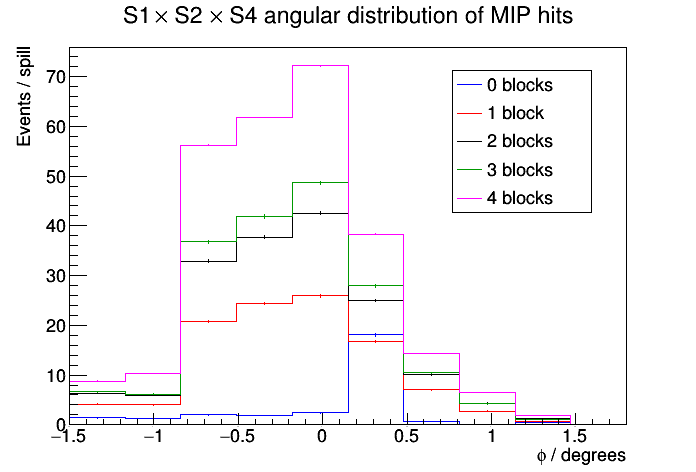
\includegraphics[width=\textwidth]{files/Figures/piS4Vert}
  %	\caption{Distribution of hits identified in $\mathit{S4}$ as minimum ionizing particles as a function of the number of moderator blocks and the vertical off-axis angle, as measured from $\mathit{S1}$.}
  %\end{minipage}
  %\hspace{0.3cm}
  %\begin{minipage}[t]{0.48\textwidth}
  %	\centering
  %	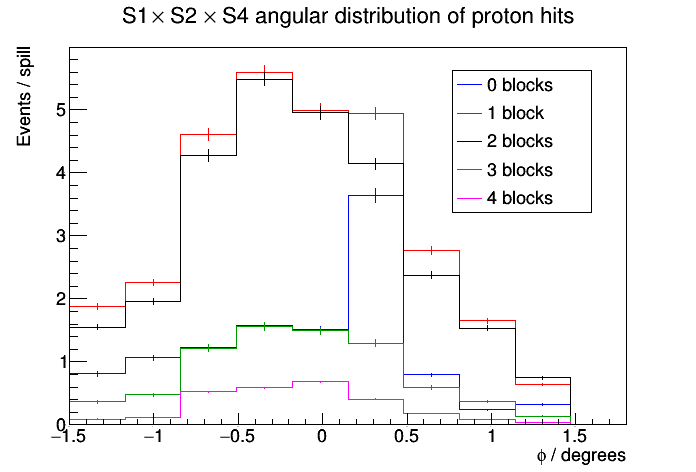
\includegraphics[width=\textwidth]{files/Figures/proS4Vert}
  %	\caption{Distribution of hits identified in $\mathit{S_{4}$ as protons as a function of the number of moderator blocks and the vertical off-axis angle, as measured from $\mathit{S_{1}$.}
  %\end{minipage}
\end{figure}	

Figures~\ref{fig:propiratio_s4_horz} and~\ref{fig:propiratio_s4_vert} show the ratio of protons to minimum ionizing particles as a function of the number of moderator blocks and the two off-axis angles.
\todo[inline]{JOCELYN: What are the two off-axis angles? Hard for the reader to figure out what the interesting region is. Need a figure that sets up the coordinate system}
For the 0, 1 and 2 moderator block configurations, figure~\ref{fig:propiratio_s4_horz} shows the ratio reaching its peak at a value of $\theta$ of approximately $2^{\circ}$.
It is clear that in the angular region of this peak, the proton-MIP ratio has been dramatically increased from the expected on axis value of 1:6 seen previously.
With the addition of moderator blocks, the size of the peak reduces until, in the 3 block configuration, the peak has fallen from a proton-MIP ratio of 1.1 for the 0 block configuration to value of 01. for the 3 block configuration. 
For the 4 block configuration, the proton-MIP ratio is below 0.05 for all values of $\theta$ but rises to its highest value at $\theta = 5^{\circ}$.

Similarly, figure~\ref{fig:propiratio_s4_vert} shows the proton-MIP ratio falling with the addition of moderator blocks.
\todo[inline]{JOCELYN: this whole discussion (and that of the previous paragraph is focussed on the proton-MIP ratio, however more important to the goals of the beamtest is to achieve low momentum proton flux to make measurements in the region relevant for neutrino-nucleus FSI.  Need to recast this whole discussion in terms of the goals: (1) proton momentum in the relevant range (2) low occupancy (<10 particles per spill in the TPC) given the relatively slow optical readout (3) proton-to-MIP ratio optimized}
For the 0, 1, 2 and 3 block configurations the ratio rises as the vertical off-axis angle ($\phi$) moves further away from $0^{\circ}$. 
For the 4 block configuration, the value of the proton-MIP ratio is close to zero at all values of $\phi$.
As mentioned previously, this is thought to be due to the attenuation of low energy protons within the walls of the pressure vessel.
\todo[inline]{Eliminate ``thought to be'' and put use the results of the simulation study to reinforce why we think this is.}

\begin{figure}[!ht]
  \begin{minipage}[t]{0.48\textwidth}
    \begin{adjustbox}{max totalsize={\textwidth}{.35\textheight}, center}
      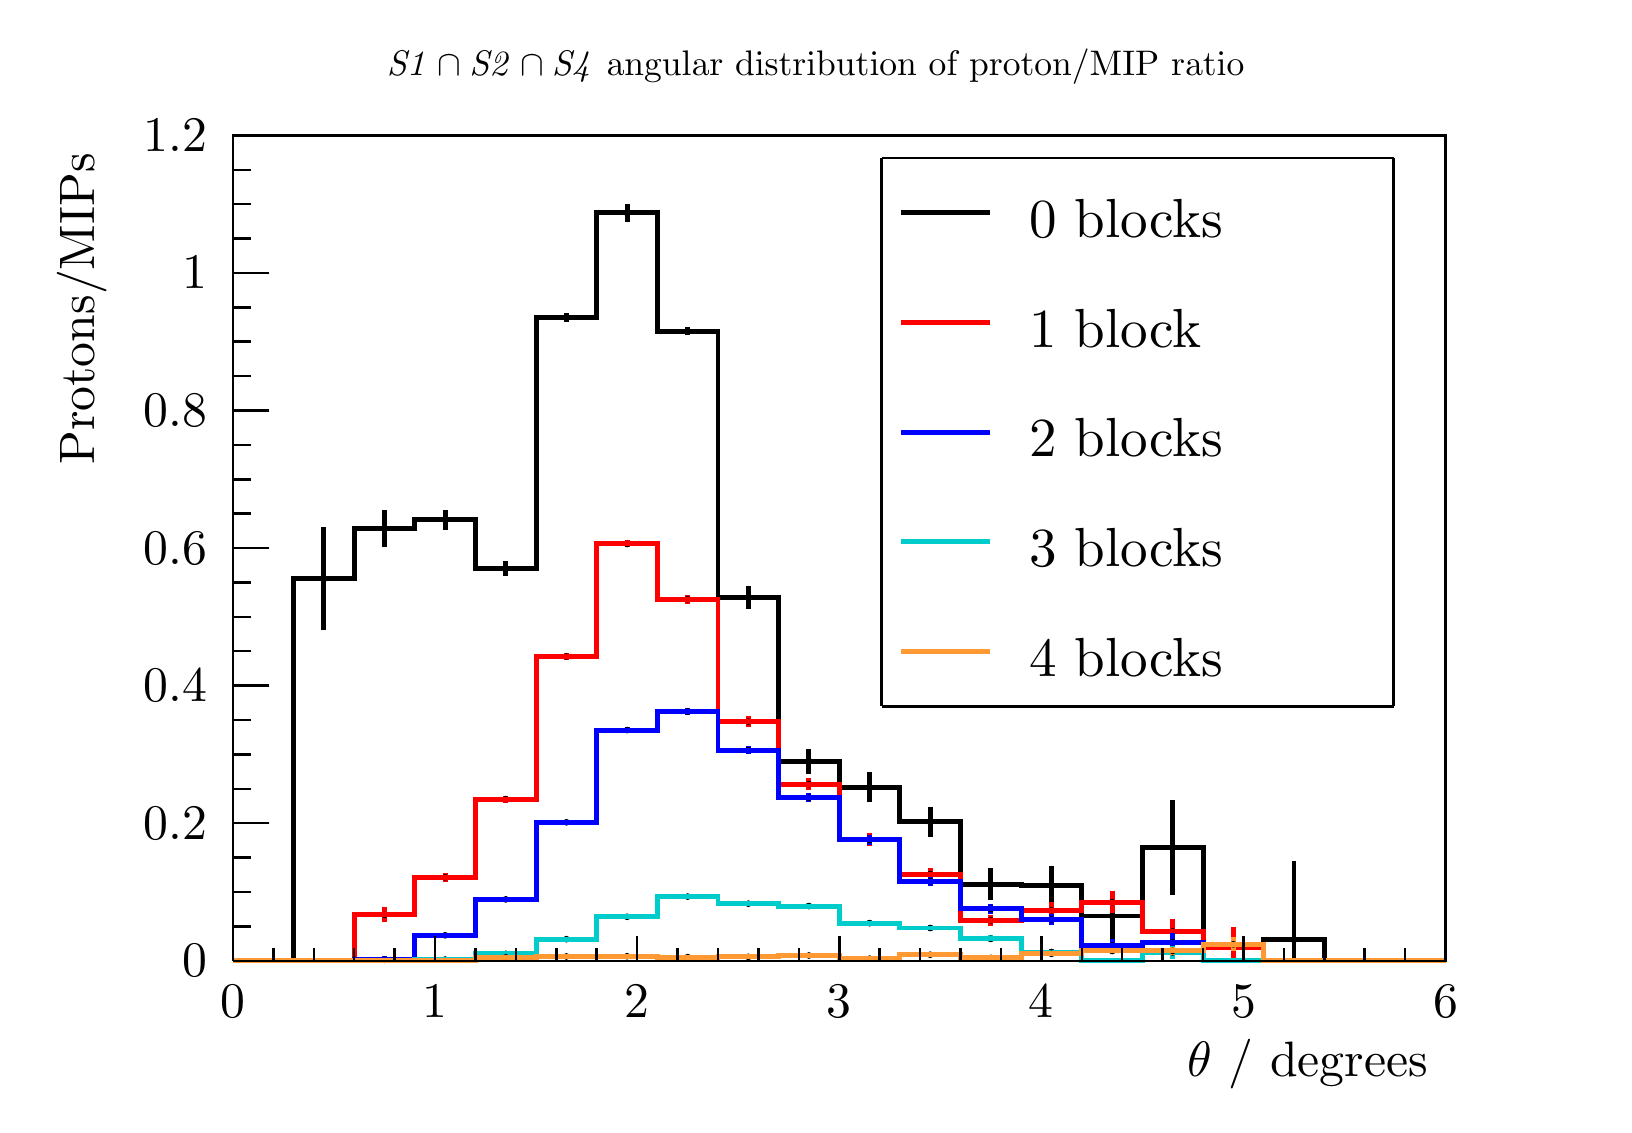
\begin{tikzpicture}
\pgfdeclareplotmark{cross} {
\pgfpathmoveto{\pgfpoint{-0.3\pgfplotmarksize}{\pgfplotmarksize}}
\pgfpathlineto{\pgfpoint{+0.3\pgfplotmarksize}{\pgfplotmarksize}}
\pgfpathlineto{\pgfpoint{+0.3\pgfplotmarksize}{0.3\pgfplotmarksize}}
\pgfpathlineto{\pgfpoint{+1\pgfplotmarksize}{0.3\pgfplotmarksize}}
\pgfpathlineto{\pgfpoint{+1\pgfplotmarksize}{-0.3\pgfplotmarksize}}
\pgfpathlineto{\pgfpoint{+0.3\pgfplotmarksize}{-0.3\pgfplotmarksize}}
\pgfpathlineto{\pgfpoint{+0.3\pgfplotmarksize}{-1.\pgfplotmarksize}}
\pgfpathlineto{\pgfpoint{-0.3\pgfplotmarksize}{-1.\pgfplotmarksize}}
\pgfpathlineto{\pgfpoint{-0.3\pgfplotmarksize}{-0.3\pgfplotmarksize}}
\pgfpathlineto{\pgfpoint{-1.\pgfplotmarksize}{-0.3\pgfplotmarksize}}
\pgfpathlineto{\pgfpoint{-1.\pgfplotmarksize}{0.3\pgfplotmarksize}}
\pgfpathlineto{\pgfpoint{-0.3\pgfplotmarksize}{0.3\pgfplotmarksize}}
\pgfpathclose
\pgfusepathqstroke
}
\pgfdeclareplotmark{cross*} {
\pgfpathmoveto{\pgfpoint{-0.3\pgfplotmarksize}{\pgfplotmarksize}}
\pgfpathlineto{\pgfpoint{+0.3\pgfplotmarksize}{\pgfplotmarksize}}
\pgfpathlineto{\pgfpoint{+0.3\pgfplotmarksize}{0.3\pgfplotmarksize}}
\pgfpathlineto{\pgfpoint{+1\pgfplotmarksize}{0.3\pgfplotmarksize}}
\pgfpathlineto{\pgfpoint{+1\pgfplotmarksize}{-0.3\pgfplotmarksize}}
\pgfpathlineto{\pgfpoint{+0.3\pgfplotmarksize}{-0.3\pgfplotmarksize}}
\pgfpathlineto{\pgfpoint{+0.3\pgfplotmarksize}{-1.\pgfplotmarksize}}
\pgfpathlineto{\pgfpoint{-0.3\pgfplotmarksize}{-1.\pgfplotmarksize}}
\pgfpathlineto{\pgfpoint{-0.3\pgfplotmarksize}{-0.3\pgfplotmarksize}}
\pgfpathlineto{\pgfpoint{-1.\pgfplotmarksize}{-0.3\pgfplotmarksize}}
\pgfpathlineto{\pgfpoint{-1.\pgfplotmarksize}{0.3\pgfplotmarksize}}
\pgfpathlineto{\pgfpoint{-0.3\pgfplotmarksize}{0.3\pgfplotmarksize}}
\pgfpathclose
\pgfusepathqfillstroke
}
\pgfdeclareplotmark{newstar} {
\pgfpathmoveto{\pgfqpoint{0pt}{\pgfplotmarksize}}
\pgfpathlineto{\pgfqpointpolar{44}{0.5\pgfplotmarksize}}
\pgfpathlineto{\pgfqpointpolar{18}{\pgfplotmarksize}}
\pgfpathlineto{\pgfqpointpolar{-20}{0.5\pgfplotmarksize}}
\pgfpathlineto{\pgfqpointpolar{-54}{\pgfplotmarksize}}
\pgfpathlineto{\pgfqpointpolar{-90}{0.5\pgfplotmarksize}}
\pgfpathlineto{\pgfqpointpolar{234}{\pgfplotmarksize}}
\pgfpathlineto{\pgfqpointpolar{198}{0.5\pgfplotmarksize}}
\pgfpathlineto{\pgfqpointpolar{162}{\pgfplotmarksize}}
\pgfpathlineto{\pgfqpointpolar{134}{0.5\pgfplotmarksize}}
\pgfpathclose
\pgfusepathqstroke
}
\pgfdeclareplotmark{newstar*} {
\pgfpathmoveto{\pgfqpoint{0pt}{\pgfplotmarksize}}
\pgfpathlineto{\pgfqpointpolar{44}{0.5\pgfplotmarksize}}
\pgfpathlineto{\pgfqpointpolar{18}{\pgfplotmarksize}}
\pgfpathlineto{\pgfqpointpolar{-20}{0.5\pgfplotmarksize}}
\pgfpathlineto{\pgfqpointpolar{-54}{\pgfplotmarksize}}
\pgfpathlineto{\pgfqpointpolar{-90}{0.5\pgfplotmarksize}}
\pgfpathlineto{\pgfqpointpolar{234}{\pgfplotmarksize}}
\pgfpathlineto{\pgfqpointpolar{198}{0.5\pgfplotmarksize}}
\pgfpathlineto{\pgfqpointpolar{162}{\pgfplotmarksize}}
\pgfpathlineto{\pgfqpointpolar{134}{0.5\pgfplotmarksize}}
\pgfpathclose
\pgfusepathqfillstroke
}
\definecolor{c}{rgb}{1,1,1};
\draw [color=c, fill=c] (0,0) rectangle (20,13.6127);
\draw [color=c, fill=c] (2.6,1.76965) rectangle (18,12.2514);
\definecolor{c}{rgb}{0,0,0};
\draw [c,line width=0.9] (2.6,1.76965) -- (2.6,12.2514) -- (18,12.2514) -- (18,1.76965) -- (2.6,1.76965);
\definecolor{c}{rgb}{1,1,1};
\draw [color=c, fill=c] (2.6,1.76965) rectangle (18,12.2514);
\definecolor{c}{rgb}{0,0,0};
\draw [c,line width=0.9] (2.6,1.76965) -- (2.6,12.2514) -- (18,12.2514) -- (18,1.76965) -- (2.6,1.76965);
\definecolor{c}{rgb}{0,0,0.6};
\draw [c,line width=0.9] (2.6,1.76965) -- (3.37,1.76965) -- (3.37,1.76965) -- (4.14,1.76965) -- (4.14,1.76965) -- (4.91,1.76965) -- (4.91,1.76965) -- (5.68,1.76965) -- (5.68,1.76965) -- (6.45,1.76965) -- (6.45,1.76965) -- (7.22,1.76965) --
 (7.22,1.76965) -- (7.99,1.76965) -- (7.99,1.76965) -- (8.76,1.76965) -- (8.76,1.76965) -- (9.53,1.76965) -- (9.53,1.76965) -- (10.3,1.76965) -- (10.3,1.76965) -- (11.07,1.76965) -- (11.07,1.76965) -- (11.84,1.76965) -- (11.84,1.76965) --
 (12.61,1.76965) -- (12.61,1.76965) -- (13.38,1.76965) -- (13.38,1.76965) -- (14.15,1.76965) -- (14.15,1.76965) -- (14.92,1.76965) -- (14.92,1.76965) -- (15.69,1.76965) -- (15.69,1.76965) -- (16.46,1.76965) -- (16.46,1.76965) -- (17.23,1.76965) --
 (17.23,1.76965) -- (18,1.76965);
\definecolor{c}{rgb}{0,0,0};
\draw [c,line width=0.9] (2.6,1.76965) -- (18,1.76965);
\draw [c,line width=0.9] (2.6,2.08411) -- (2.6,1.76965);
\draw [c,line width=0.9] (3.11333,1.92688) -- (3.11333,1.76965);
\draw [c,line width=0.9] (3.62667,1.92688) -- (3.62667,1.76965);
\draw [c,line width=0.9] (4.14,1.92688) -- (4.14,1.76965);
\draw [c,line width=0.9] (4.65333,1.92688) -- (4.65333,1.76965);
\draw [c,line width=0.9] (5.16667,2.08411) -- (5.16667,1.76965);
\draw [c,line width=0.9] (5.68,1.92688) -- (5.68,1.76965);
\draw [c,line width=0.9] (6.19333,1.92688) -- (6.19333,1.76965);
\draw [c,line width=0.9] (6.70667,1.92688) -- (6.70667,1.76965);
\draw [c,line width=0.9] (7.22,1.92688) -- (7.22,1.76965);
\draw [c,line width=0.9] (7.73333,2.08411) -- (7.73333,1.76965);
\draw [c,line width=0.9] (8.24667,1.92688) -- (8.24667,1.76965);
\draw [c,line width=0.9] (8.76,1.92688) -- (8.76,1.76965);
\draw [c,line width=0.9] (9.27333,1.92688) -- (9.27333,1.76965);
\draw [c,line width=0.9] (9.78667,1.92688) -- (9.78667,1.76965);
\draw [c,line width=0.9] (10.3,2.08411) -- (10.3,1.76965);
\draw [c,line width=0.9] (10.8133,1.92688) -- (10.8133,1.76965);
\draw [c,line width=0.9] (11.3267,1.92688) -- (11.3267,1.76965);
\draw [c,line width=0.9] (11.84,1.92688) -- (11.84,1.76965);
\draw [c,line width=0.9] (12.3533,1.92688) -- (12.3533,1.76965);
\draw [c,line width=0.9] (12.8667,2.08411) -- (12.8667,1.76965);
\draw [c,line width=0.9] (13.38,1.92688) -- (13.38,1.76965);
\draw [c,line width=0.9] (13.8933,1.92688) -- (13.8933,1.76965);
\draw [c,line width=0.9] (14.4067,1.92688) -- (14.4067,1.76965);
\draw [c,line width=0.9] (14.92,1.92688) -- (14.92,1.76965);
\draw [c,line width=0.9] (15.4333,2.08411) -- (15.4333,1.76965);
\draw [c,line width=0.9] (15.9467,1.92688) -- (15.9467,1.76965);
\draw [c,line width=0.9] (16.46,1.92688) -- (16.46,1.76965);
\draw [c,line width=0.9] (16.9733,1.92688) -- (16.9733,1.76965);
\draw [c,line width=0.9] (17.4867,1.92688) -- (17.4867,1.76965);
\draw [c,line width=0.9] (18,2.08411) -- (18,1.76965);
\draw [anchor=base] (2.6,1.04818) node[scale=1.79732, color=c, rotate=0]{0};
\draw [anchor=base] (5.16667,1.04818) node[scale=1.79732, color=c, rotate=0]{1};
\draw [anchor=base] (7.73333,1.04818) node[scale=1.79732, color=c, rotate=0]{2};
\draw [anchor=base] (10.3,1.04818) node[scale=1.79732, color=c, rotate=0]{3};
\draw [anchor=base] (12.8667,1.04818) node[scale=1.79732, color=c, rotate=0]{4};
\draw [anchor=base] (15.4333,1.04818) node[scale=1.79732, color=c, rotate=0]{5};
\draw [anchor=base] (18,1.04818) node[scale=1.79732, color=c, rotate=0]{6};
\draw [anchor= east] (18,0.462832) node[scale=1.79732, color=c, rotate=0]{$\theta$ / degrees};
\draw [c,line width=0.9] (2.6,1.76965) -- (2.6,12.2514);
\draw [c,line width=0.9] (3.062,1.76965) -- (2.6,1.76965);
\draw [c,line width=0.9] (2.831,2.20639) -- (2.6,2.20639);
\draw [c,line width=0.9] (2.831,2.64314) -- (2.6,2.64314);
\draw [c,line width=0.9] (2.831,3.07988) -- (2.6,3.07988);
\draw [c,line width=0.9] (3.062,3.51662) -- (2.6,3.51662);
\draw [c,line width=0.9] (2.831,3.95336) -- (2.6,3.95336);
\draw [c,line width=0.9] (2.831,4.3901) -- (2.6,4.3901);
\draw [c,line width=0.9] (2.831,4.82684) -- (2.6,4.82684);
\draw [c,line width=0.9] (3.062,5.26358) -- (2.6,5.26358);
\draw [c,line width=0.9] (2.831,5.70033) -- (2.6,5.70033);
\draw [c,line width=0.9] (2.831,6.13707) -- (2.6,6.13707);
\draw [c,line width=0.9] (2.831,6.57381) -- (2.6,6.57381);
\draw [c,line width=0.9] (3.062,7.01055) -- (2.6,7.01055);
\draw [c,line width=0.9] (2.831,7.44729) -- (2.6,7.44729);
\draw [c,line width=0.9] (2.831,7.88403) -- (2.6,7.88403);
\draw [c,line width=0.9] (2.831,8.32077) -- (2.6,8.32077);
\draw [c,line width=0.9] (3.062,8.75751) -- (2.6,8.75751);
\draw [c,line width=0.9] (2.831,9.19426) -- (2.6,9.19426);
\draw [c,line width=0.9] (2.831,9.631) -- (2.6,9.631);
\draw [c,line width=0.9] (2.831,10.0677) -- (2.6,10.0677);
\draw [c,line width=0.9] (3.062,10.5045) -- (2.6,10.5045);
\draw [c,line width=0.9] (2.831,10.9412) -- (2.6,10.9412);
\draw [c,line width=0.9] (2.831,11.378) -- (2.6,11.378);
\draw [c,line width=0.9] (2.831,11.8147) -- (2.6,11.8147);
\draw [c,line width=0.9] (3.062,12.2514) -- (2.6,12.2514);
\draw [c,line width=0.9] (3.062,12.2514) -- (2.6,12.2514);
\draw [anchor= east] (2.5,1.76965) node[scale=1.79732, color=c, rotate=0]{0};
\draw [anchor= east] (2.5,3.51662) node[scale=1.79732, color=c, rotate=0]{0.2};
\draw [anchor= east] (2.5,5.26358) node[scale=1.79732, color=c, rotate=0]{0.4};
\draw [anchor= east] (2.5,7.01055) node[scale=1.79732, color=c, rotate=0]{0.6};
\draw [anchor= east] (2.5,8.75751) node[scale=1.79732, color=c, rotate=0]{0.8};
\draw [anchor= east] (2.5,10.5045) node[scale=1.79732, color=c, rotate=0]{1};
\draw [anchor= east] (2.5,12.2514) node[scale=1.79732, color=c, rotate=0]{1.2};
\draw [anchor= east] (0.68,12.2514) node[scale=1.79732, color=c, rotate=90]{ Protons/MIPs};
\draw [c,line width=1.8] (3.755,5.96552) -- (3.755,6.61918);
\draw [c,line width=1.8] (3.755,6.61918) -- (3.755,7.27284);
\foreach \P in {(3.755,6.61918)}{\draw[mark options={color=c,fill=c},mark size=2.402402pt,mark=*,mark size=1pt] plot coordinates {\P};}
\draw [c,line width=1.8] (4.525,7.02017) -- (4.525,7.25485);
\draw [c,line width=1.8] (4.525,7.25485) -- (4.525,7.48953);
\foreach \P in {(4.525,7.25485)}{\draw[mark options={color=c,fill=c},mark size=2.402402pt,mark=*,mark size=1pt] plot coordinates {\P};}
\draw [c,line width=1.8] (5.295,7.24454) -- (5.295,7.36993);
\draw [c,line width=1.8] (5.295,7.36993) -- (5.295,7.49531);
\foreach \P in {(5.295,7.36993)}{\draw[mark options={color=c,fill=c},mark size=2.402402pt,mark=*,mark size=1pt] plot coordinates {\P};}
\draw [c,line width=1.8] (6.065,6.65801) -- (6.065,6.75329);
\draw [c,line width=1.8] (6.065,6.75329) -- (6.065,6.84857);
\foreach \P in {(6.065,6.75329)}{\draw[mark options={color=c,fill=c},mark size=2.402402pt,mark=*,mark size=1pt] plot coordinates {\P};}
\draw [c,line width=1.8] (6.835,9.88682) -- (6.835,9.94428);
\draw [c,line width=1.8] (6.835,9.94428) -- (6.835,10.0017);
\foreach \P in {(6.835,9.94428)}{\draw[mark options={color=c,fill=c},mark size=2.402402pt,mark=*,mark size=1pt] plot coordinates {\P};}
\draw [c,line width=1.8] (7.605,11.157) -- (7.605,11.267);
\draw [c,line width=1.8] (7.605,11.267) -- (7.605,11.3769);
\foreach \P in {(7.605,11.267)}{\draw[mark options={color=c,fill=c},mark size=2.402402pt,mark=*,mark size=1pt] plot coordinates {\P};}
\draw [c,line width=1.8] (8.375,9.71118) -- (8.375,9.76656);
\draw [c,line width=1.8] (8.375,9.76656) -- (8.375,9.82195);
\foreach \P in {(8.375,9.76656)}{\draw[mark options={color=c,fill=c},mark size=2.402402pt,mark=*,mark size=1pt] plot coordinates {\P};}
\draw [c,line width=1.8] (9.145,6.23982) -- (9.145,6.3858);
\draw [c,line width=1.8] (9.145,6.3858) -- (9.145,6.53178);
\foreach \P in {(9.145,6.3858)}{\draw[mark options={color=c,fill=c},mark size=2.402402pt,mark=*,mark size=1pt] plot coordinates {\P};}
\draw [c,line width=1.8] (9.915,4.14538) -- (9.915,4.30397);
\draw [c,line width=1.8] (9.915,4.30397) -- (9.915,4.46257);
\foreach \P in {(9.915,4.30397)}{\draw[mark options={color=c,fill=c},mark size=2.402402pt,mark=*,mark size=1pt] plot coordinates {\P};}
\draw [c,line width=1.8] (10.685,3.78343) -- (10.685,3.9732);
\draw [c,line width=1.8] (10.685,3.9732) -- (10.685,4.16297);
\foreach \P in {(10.685,3.9732)}{\draw[mark options={color=c,fill=c},mark size=2.402402pt,mark=*,mark size=1pt] plot coordinates {\P};}
\draw [c,line width=1.8] (11.455,3.3397) -- (11.455,3.53224);
\draw [c,line width=1.8] (11.455,3.53224) -- (11.455,3.72478);
\foreach \P in {(11.455,3.53224)}{\draw[mark options={color=c,fill=c},mark size=2.402402pt,mark=*,mark size=1pt] plot coordinates {\P};}
\draw [c,line width=1.8] (12.225,2.53805) -- (12.225,2.74072);
\draw [c,line width=1.8] (12.225,2.74072) -- (12.225,2.94338);
\foreach \P in {(12.225,2.74072)}{\draw[mark options={color=c,fill=c},mark size=2.402402pt,mark=*,mark size=1pt] plot coordinates {\P};}
\draw [c,line width=1.8] (12.995,2.48276) -- (12.995,2.72628);
\draw [c,line width=1.8] (12.995,2.72628) -- (12.995,2.9698);
\foreach \P in {(12.995,2.72628)}{\draw[mark options={color=c,fill=c},mark size=2.402402pt,mark=*,mark size=1pt] plot coordinates {\P};}
\draw [c,line width=1.8] (13.765,2.01881) -- (13.765,2.3379);
\draw [c,line width=1.8] (13.765,2.3379) -- (13.765,2.65699);
\foreach \P in {(13.765,2.3379)}{\draw[mark options={color=c,fill=c},mark size=2.402402pt,mark=*,mark size=1pt] plot coordinates {\P};}
\draw [c,line width=1.8] (14.535,2.60709) -- (14.535,3.20937);
\draw [c,line width=1.8] (14.535,3.20937) -- (14.535,3.81165);
\foreach \P in {(14.535,3.20937)}{\draw[mark options={color=c,fill=c},mark size=2.402402pt,mark=*,mark size=1pt] plot coordinates {\P};}
\draw [c,line width=1.8] (16.075,1.76965) -- (16.075,2.03461);
\draw [c,line width=1.8] (16.075,2.03461) -- (16.075,3.04084);
\foreach \P in {(16.075,2.03461)}{\draw[mark options={color=c,fill=c},mark size=2.402402pt,mark=*,mark size=1pt] plot coordinates {\P};}
\draw [c,line width=1.8] (2.6,1.76965) -- (3.37,1.76965) -- (3.37,6.61918) -- (4.14,6.61918) -- (4.14,7.25485) -- (4.91,7.25485) -- (4.91,7.36993) -- (5.68,7.36993) -- (5.68,6.75329) -- (6.45,6.75329) -- (6.45,9.94428) -- (7.22,9.94428) --
 (7.22,11.267) -- (7.99,11.267) -- (7.99,9.76656) -- (8.76,9.76656) -- (8.76,6.3858) -- (9.53,6.3858) -- (9.53,4.30397) -- (10.3,4.30397) -- (10.3,3.9732) -- (11.07,3.9732) -- (11.07,3.53224) -- (11.84,3.53224) -- (11.84,2.74072) -- (12.61,2.74072)
 -- (12.61,2.72628) -- (13.38,2.72628) -- (13.38,2.3379) -- (14.15,2.3379) -- (14.15,3.20937) -- (14.92,3.20937) -- (14.92,1.76965) -- (15.69,1.76965) -- (15.69,2.03461) -- (16.46,2.03461) -- (16.46,1.76965) -- (17.23,1.76965) -- (17.23,1.76965) --
 (18,1.76965);
\definecolor{c}{rgb}{1,0,0};
\draw [c,line width=1.8] (4.525,2.25718) -- (4.525,2.35159);
\draw [c,line width=1.8] (4.525,2.35159) -- (4.525,2.446);
\definecolor{c}{rgb}{0,0,0};
\foreach \P in {(4.525,2.35159)}{\draw[mark options={color=c,fill=c},mark size=2.402402pt,mark=*,mark size=1pt] plot coordinates {\P};}
\definecolor{c}{rgb}{1,0,0};
\draw [c,line width=1.8] (5.295,2.77091) -- (5.295,2.82905);
\draw [c,line width=1.8] (5.295,2.82905) -- (5.295,2.88719);
\definecolor{c}{rgb}{0,0,0};
\foreach \P in {(5.295,2.82905)}{\draw[mark options={color=c,fill=c},mark size=2.402402pt,mark=*,mark size=1pt] plot coordinates {\P};}
\definecolor{c}{rgb}{1,0,0};
\draw [c,line width=1.8] (6.065,3.77647) -- (6.065,3.82233);
\draw [c,line width=1.8] (6.065,3.82233) -- (6.065,3.86819);
\definecolor{c}{rgb}{0,0,0};
\foreach \P in {(6.065,3.82233)}{\draw[mark options={color=c,fill=c},mark size=2.402402pt,mark=*,mark size=1pt] plot coordinates {\P};}
\definecolor{c}{rgb}{1,0,0};
\draw [c,line width=1.8] (6.835,5.59037) -- (6.835,5.63438);
\draw [c,line width=1.8] (6.835,5.63438) -- (6.835,5.67838);
\definecolor{c}{rgb}{0,0,0};
\foreach \P in {(6.835,5.63438)}{\draw[mark options={color=c,fill=c},mark size=2.402402pt,mark=*,mark size=1pt] plot coordinates {\P};}
\definecolor{c}{rgb}{1,0,0};
\draw [c,line width=1.8] (7.605,7.01849) -- (7.605,7.06322);
\draw [c,line width=1.8] (7.605,7.06322) -- (7.605,7.10796);
\definecolor{c}{rgb}{0,0,0};
\foreach \P in {(7.605,7.06322)}{\draw[mark options={color=c,fill=c},mark size=2.402402pt,mark=*,mark size=1pt] plot coordinates {\P};}
\definecolor{c}{rgb}{1,0,0};
\draw [c,line width=1.8] (8.375,6.30504) -- (8.375,6.36061);
\draw [c,line width=1.8] (8.375,6.36061) -- (8.375,6.41618);
\definecolor{c}{rgb}{0,0,0};
\foreach \P in {(8.375,6.36061)}{\draw[mark options={color=c,fill=c},mark size=2.402402pt,mark=*,mark size=1pt] plot coordinates {\P};}
\definecolor{c}{rgb}{1,0,0};
\draw [c,line width=1.8] (9.145,4.73795) -- (9.145,4.80704);
\draw [c,line width=1.8] (9.145,4.80704) -- (9.145,4.87612);
\definecolor{c}{rgb}{0,0,0};
\foreach \P in {(9.145,4.80704)}{\draw[mark options={color=c,fill=c},mark size=2.402402pt,mark=*,mark size=1pt] plot coordinates {\P};}
\definecolor{c}{rgb}{1,0,0};
\draw [c,line width=1.8] (9.915,3.93827) -- (9.915,4.01338);
\draw [c,line width=1.8] (9.915,4.01338) -- (9.915,4.08848);
\definecolor{c}{rgb}{0,0,0};
\foreach \P in {(9.915,4.01338)}{\draw[mark options={color=c,fill=c},mark size=2.402402pt,mark=*,mark size=1pt] plot coordinates {\P};}
\definecolor{c}{rgb}{1,0,0};
\draw [c,line width=1.8] (10.685,3.22568) -- (10.685,3.30686);
\draw [c,line width=1.8] (10.685,3.30686) -- (10.685,3.38804);
\definecolor{c}{rgb}{0,0,0};
\foreach \P in {(10.685,3.30686)}{\draw[mark options={color=c,fill=c},mark size=2.402402pt,mark=*,mark size=1pt] plot coordinates {\P};}
\definecolor{c}{rgb}{1,0,0};
\draw [c,line width=1.8] (11.455,2.78746) -- (11.455,2.87067);
\draw [c,line width=1.8] (11.455,2.87067) -- (11.455,2.95388);
\definecolor{c}{rgb}{0,0,0};
\foreach \P in {(11.455,2.87067)}{\draw[mark options={color=c,fill=c},mark size=2.402402pt,mark=*,mark size=1pt] plot coordinates {\P};}
\definecolor{c}{rgb}{1,0,0};
\draw [c,line width=1.8] (12.225,2.21253) -- (12.225,2.28363);
\draw [c,line width=1.8] (12.225,2.28363) -- (12.225,2.35473);
\definecolor{c}{rgb}{0,0,0};
\foreach \P in {(12.225,2.28363)}{\draw[mark options={color=c,fill=c},mark size=2.402402pt,mark=*,mark size=1pt] plot coordinates {\P};}
\definecolor{c}{rgb}{1,0,0};
\draw [c,line width=1.8] (12.995,2.30897) -- (12.995,2.41012);
\draw [c,line width=1.8] (12.995,2.41012) -- (12.995,2.51127);
\definecolor{c}{rgb}{0,0,0};
\foreach \P in {(12.995,2.41012)}{\draw[mark options={color=c,fill=c},mark size=2.402402pt,mark=*,mark size=1pt] plot coordinates {\P};}
\definecolor{c}{rgb}{1,0,0};
\draw [c,line width=1.8] (13.765,2.37186) -- (13.765,2.51465);
\draw [c,line width=1.8] (13.765,2.51465) -- (13.765,2.65744);
\definecolor{c}{rgb}{0,0,0};
\foreach \P in {(13.765,2.51465)}{\draw[mark options={color=c,fill=c},mark size=2.402402pt,mark=*,mark size=1pt] plot coordinates {\P};}
\definecolor{c}{rgb}{1,0,0};
\draw [c,line width=1.8] (14.535,1.98578) -- (14.535,2.14154);
\draw [c,line width=1.8] (14.535,2.14154) -- (14.535,2.29731);
\definecolor{c}{rgb}{0,0,0};
\foreach \P in {(14.535,2.14154)}{\draw[mark options={color=c,fill=c},mark size=2.402402pt,mark=*,mark size=1pt] plot coordinates {\P};}
\definecolor{c}{rgb}{1,0,0};
\draw [c,line width=1.8] (15.305,1.76965) -- (15.305,1.94371);
\draw [c,line width=1.8] (15.305,1.94371) -- (15.305,2.19744);
\definecolor{c}{rgb}{0,0,0};
\foreach \P in {(15.305,1.94371)}{\draw[mark options={color=c,fill=c},mark size=2.402402pt,mark=*,mark size=1pt] plot coordinates {\P};}
\definecolor{c}{rgb}{1,0,0};
\draw [c,line width=1.8] (2.6,1.76965) -- (3.37,1.76965) -- (3.37,1.76965) -- (4.14,1.76965) -- (4.14,2.35159) -- (4.91,2.35159) -- (4.91,2.82905) -- (5.68,2.82905) -- (5.68,3.82233) -- (6.45,3.82233) -- (6.45,5.63438) -- (7.22,5.63438) --
 (7.22,7.06322) -- (7.99,7.06322) -- (7.99,6.36061) -- (8.76,6.36061) -- (8.76,4.80704) -- (9.53,4.80704) -- (9.53,4.01338) -- (10.3,4.01338) -- (10.3,3.30686) -- (11.07,3.30686) -- (11.07,2.87067) -- (11.84,2.87067) -- (11.84,2.28363) --
 (12.61,2.28363) -- (12.61,2.41012) -- (13.38,2.41012) -- (13.38,2.51465) -- (14.15,2.51465) -- (14.15,2.14154) -- (14.92,2.14154) -- (14.92,1.94371) -- (15.69,1.94371) -- (15.69,1.76965) -- (16.46,1.76965) -- (16.46,1.76965) -- (17.23,1.76965) --
 (17.23,1.76965) -- (18,1.76965);
\definecolor{c}{rgb}{0,0,1};
\draw [c,line width=1.8] (4.525,1.76965) -- (4.525,1.7823);
\draw [c,line width=1.8] (4.525,1.7823) -- (4.525,1.83564);
\definecolor{c}{rgb}{0,0,0};
\foreach \P in {(4.525,1.7823)}{\draw[mark options={color=c,fill=c},mark size=2.402402pt,mark=*,mark size=1pt] plot coordinates {\P};}
\definecolor{c}{rgb}{0,0,1};
\draw [c,line width=1.8] (5.295,2.06026) -- (5.295,2.09298);
\draw [c,line width=1.8] (5.295,2.09298) -- (5.295,2.12571);
\definecolor{c}{rgb}{0,0,0};
\foreach \P in {(5.295,2.09298)}{\draw[mark options={color=c,fill=c},mark size=2.402402pt,mark=*,mark size=1pt] plot coordinates {\P};}
\definecolor{c}{rgb}{0,0,1};
\draw [c,line width=1.8] (6.065,2.5215) -- (6.065,2.54923);
\draw [c,line width=1.8] (6.065,2.54923) -- (6.065,2.57695);
\definecolor{c}{rgb}{0,0,0};
\foreach \P in {(6.065,2.54923)}{\draw[mark options={color=c,fill=c},mark size=2.402402pt,mark=*,mark size=1pt] plot coordinates {\P};}
\definecolor{c}{rgb}{0,0,1};
\draw [c,line width=1.8] (6.835,3.49681) -- (6.835,3.52792);
\draw [c,line width=1.8] (6.835,3.52792) -- (6.835,3.55903);
\definecolor{c}{rgb}{0,0,0};
\foreach \P in {(6.835,3.52792)}{\draw[mark options={color=c,fill=c},mark size=2.402402pt,mark=*,mark size=1pt] plot coordinates {\P};}
\definecolor{c}{rgb}{0,0,1};
\draw [c,line width=1.8] (7.605,4.66274) -- (7.605,4.69928);
\draw [c,line width=1.8] (7.605,4.69928) -- (7.605,4.73582);
\definecolor{c}{rgb}{0,0,0};
\foreach \P in {(7.605,4.69928)}{\draw[mark options={color=c,fill=c},mark size=2.402402pt,mark=*,mark size=1pt] plot coordinates {\P};}
\definecolor{c}{rgb}{0,0,1};
\draw [c,line width=1.8] (8.375,4.89186) -- (8.375,4.93533);
\draw [c,line width=1.8] (8.375,4.93533) -- (8.375,4.9788);
\definecolor{c}{rgb}{0,0,0};
\foreach \P in {(8.375,4.93533)}{\draw[mark options={color=c,fill=c},mark size=2.402402pt,mark=*,mark size=1pt] plot coordinates {\P};}
\definecolor{c}{rgb}{0,0,1};
\draw [c,line width=1.8] (9.145,4.39433) -- (9.145,4.44478);
\draw [c,line width=1.8] (9.145,4.44478) -- (9.145,4.49524);
\definecolor{c}{rgb}{0,0,0};
\foreach \P in {(9.145,4.44478)}{\draw[mark options={color=c,fill=c},mark size=2.402402pt,mark=*,mark size=1pt] plot coordinates {\P};}
\definecolor{c}{rgb}{0,0,1};
\draw [c,line width=1.8] (9.915,3.78582) -- (9.915,3.84078);
\draw [c,line width=1.8] (9.915,3.84078) -- (9.915,3.89575);
\definecolor{c}{rgb}{0,0,0};
\foreach \P in {(9.915,3.84078)}{\draw[mark options={color=c,fill=c},mark size=2.402402pt,mark=*,mark size=1pt] plot coordinates {\P};}
\definecolor{c}{rgb}{0,0,1};
\draw [c,line width=1.8] (10.685,3.24461) -- (10.685,3.3036);
\draw [c,line width=1.8] (10.685,3.3036) -- (10.685,3.36259);
\definecolor{c}{rgb}{0,0,0};
\foreach \P in {(10.685,3.3036)}{\draw[mark options={color=c,fill=c},mark size=2.402402pt,mark=*,mark size=1pt] plot coordinates {\P};}
\definecolor{c}{rgb}{0,0,1};
\draw [c,line width=1.8] (11.455,2.72135) -- (11.455,2.77999);
\draw [c,line width=1.8] (11.455,2.77999) -- (11.455,2.83863);
\definecolor{c}{rgb}{0,0,0};
\foreach \P in {(11.455,2.77999)}{\draw[mark options={color=c,fill=c},mark size=2.402402pt,mark=*,mark size=1pt] plot coordinates {\P};}
\definecolor{c}{rgb}{0,0,1};
\draw [c,line width=1.8] (12.225,2.36619) -- (12.225,2.42732);
\draw [c,line width=1.8] (12.225,2.42732) -- (12.225,2.48844);
\definecolor{c}{rgb}{0,0,0};
\foreach \P in {(12.225,2.42732)}{\draw[mark options={color=c,fill=c},mark size=2.402402pt,mark=*,mark size=1pt] plot coordinates {\P};}
\definecolor{c}{rgb}{0,0,1};
\draw [c,line width=1.8] (12.995,2.22581) -- (12.995,2.29456);
\draw [c,line width=1.8] (12.995,2.29456) -- (12.995,2.36332);
\definecolor{c}{rgb}{0,0,0};
\foreach \P in {(12.995,2.29456)}{\draw[mark options={color=c,fill=c},mark size=2.402402pt,mark=*,mark size=1pt] plot coordinates {\P};}
\definecolor{c}{rgb}{0,0,1};
\draw [c,line width=1.8] (13.765,1.88797) -- (13.765,1.96423);
\draw [c,line width=1.8] (13.765,1.96423) -- (13.765,2.04048);
\definecolor{c}{rgb}{0,0,0};
\foreach \P in {(13.765,1.96423)}{\draw[mark options={color=c,fill=c},mark size=2.402402pt,mark=*,mark size=1pt] plot coordinates {\P};}
\definecolor{c}{rgb}{0,0,1};
\draw [c,line width=1.8] (14.535,1.88836) -- (14.535,2.00549);
\draw [c,line width=1.8] (14.535,2.00549) -- (14.535,2.12261);
\definecolor{c}{rgb}{0,0,0};
\foreach \P in {(14.535,2.00549)}{\draw[mark options={color=c,fill=c},mark size=2.402402pt,mark=*,mark size=1pt] plot coordinates {\P};}
\definecolor{c}{rgb}{0,0,1};
\draw [c,line width=1.8] (2.6,1.76965) -- (3.37,1.76965) -- (3.37,1.76965) -- (4.14,1.76965) -- (4.14,1.7823) -- (4.91,1.7823) -- (4.91,2.09298) -- (5.68,2.09298) -- (5.68,2.54923) -- (6.45,2.54923) -- (6.45,3.52792) -- (7.22,3.52792) --
 (7.22,4.69928) -- (7.99,4.69928) -- (7.99,4.93533) -- (8.76,4.93533) -- (8.76,4.44478) -- (9.53,4.44478) -- (9.53,3.84078) -- (10.3,3.84078) -- (10.3,3.3036) -- (11.07,3.3036) -- (11.07,2.77999) -- (11.84,2.77999) -- (11.84,2.42732) --
 (12.61,2.42732) -- (12.61,2.29456) -- (13.38,2.29456) -- (13.38,1.96423) -- (14.15,1.96423) -- (14.15,2.00549) -- (14.92,2.00549) -- (14.92,1.76965) -- (15.69,1.76965) -- (15.69,1.76965) -- (16.46,1.76965) -- (16.46,1.76965) -- (17.23,1.76965) --
 (17.23,1.76965) -- (18,1.76965);
\definecolor{c}{rgb}{0,0.8,0.8};
\draw [c,line width=1.8] (5.295,1.76965) -- (5.295,1.78457);
\draw [c,line width=1.8] (5.295,1.78457) -- (5.295,1.80271);
\definecolor{c}{rgb}{0,0,0};
\foreach \P in {(5.295,1.78457)}{\draw[mark options={color=c,fill=c},mark size=2.402402pt,mark=*,mark size=1pt] plot coordinates {\P};}
\definecolor{c}{rgb}{0,0.8,0.8};
\draw [c,line width=1.8] (6.065,1.8446) -- (6.065,1.8573);
\draw [c,line width=1.8] (6.065,1.8573) -- (6.065,1.87);
\definecolor{c}{rgb}{0,0,0};
\foreach \P in {(6.065,1.8573)}{\draw[mark options={color=c,fill=c},mark size=2.402402pt,mark=*,mark size=1pt] plot coordinates {\P};}
\definecolor{c}{rgb}{0,0.8,0.8};
\draw [c,line width=1.8] (6.835,2.02672) -- (6.835,2.04365);
\draw [c,line width=1.8] (6.835,2.04365) -- (6.835,2.06058);
\definecolor{c}{rgb}{0,0,0};
\foreach \P in {(6.835,2.04365)}{\draw[mark options={color=c,fill=c},mark size=2.402402pt,mark=*,mark size=1pt] plot coordinates {\P};}
\definecolor{c}{rgb}{0,0.8,0.8};
\draw [c,line width=1.8] (7.605,2.30633) -- (7.605,2.32789);
\draw [c,line width=1.8] (7.605,2.32789) -- (7.605,2.34945);
\definecolor{c}{rgb}{0,0,0};
\foreach \P in {(7.605,2.32789)}{\draw[mark options={color=c,fill=c},mark size=2.402402pt,mark=*,mark size=1pt] plot coordinates {\P};}
\definecolor{c}{rgb}{0,0.8,0.8};
\draw [c,line width=1.8] (8.375,2.55536) -- (8.375,2.58455);
\draw [c,line width=1.8] (8.375,2.58455) -- (8.375,2.61374);
\definecolor{c}{rgb}{0,0,0};
\foreach \P in {(8.375,2.58455)}{\draw[mark options={color=c,fill=c},mark size=2.402402pt,mark=*,mark size=1pt] plot coordinates {\P};}
\definecolor{c}{rgb}{0,0.8,0.8};
\draw [c,line width=1.8] (9.145,2.46079) -- (9.145,2.49448);
\draw [c,line width=1.8] (9.145,2.49448) -- (9.145,2.52816);
\definecolor{c}{rgb}{0,0,0};
\foreach \P in {(9.145,2.49448)}{\draw[mark options={color=c,fill=c},mark size=2.402402pt,mark=*,mark size=1pt] plot coordinates {\P};}
\definecolor{c}{rgb}{0,0.8,0.8};
\draw [c,line width=1.8] (9.915,2.42409) -- (9.915,2.46387);
\draw [c,line width=1.8] (9.915,2.46387) -- (9.915,2.50366);
\definecolor{c}{rgb}{0,0,0};
\foreach \P in {(9.915,2.46387)}{\draw[mark options={color=c,fill=c},mark size=2.402402pt,mark=*,mark size=1pt] plot coordinates {\P};}
\definecolor{c}{rgb}{0,0.8,0.8};
\draw [c,line width=1.8] (10.685,2.20946) -- (10.685,2.2468);
\draw [c,line width=1.8] (10.685,2.2468) -- (10.685,2.28414);
\definecolor{c}{rgb}{0,0,0};
\foreach \P in {(10.685,2.2468)}{\draw[mark options={color=c,fill=c},mark size=2.402402pt,mark=*,mark size=1pt] plot coordinates {\P};}
\definecolor{c}{rgb}{0,0.8,0.8};
\draw [c,line width=1.8] (11.455,2.14459) -- (11.455,2.18563);
\draw [c,line width=1.8] (11.455,2.18563) -- (11.455,2.22667);
\definecolor{c}{rgb}{0,0,0};
\foreach \P in {(11.455,2.18563)}{\draw[mark options={color=c,fill=c},mark size=2.402402pt,mark=*,mark size=1pt] plot coordinates {\P};}
\definecolor{c}{rgb}{0,0.8,0.8};
\draw [c,line width=1.8] (12.225,2.00237) -- (12.225,2.0483);
\draw [c,line width=1.8] (12.225,2.0483) -- (12.225,2.09422);
\definecolor{c}{rgb}{0,0,0};
\foreach \P in {(12.225,2.0483)}{\draw[mark options={color=c,fill=c},mark size=2.402402pt,mark=*,mark size=1pt] plot coordinates {\P};}
\definecolor{c}{rgb}{0,0.8,0.8};
\draw [c,line width=1.8] (12.995,1.8366) -- (12.995,1.8805);
\draw [c,line width=1.8] (12.995,1.8805) -- (12.995,1.92441);
\definecolor{c}{rgb}{0,0,0};
\foreach \P in {(12.995,1.8805)}{\draw[mark options={color=c,fill=c},mark size=2.402402pt,mark=*,mark size=1pt] plot coordinates {\P};}
\definecolor{c}{rgb}{0,0.8,0.8};
\draw [c,line width=1.8] (14.535,1.78926) -- (14.535,1.8749);
\draw [c,line width=1.8] (14.535,1.8749) -- (14.535,1.96054);
\definecolor{c}{rgb}{0,0,0};
\foreach \P in {(14.535,1.8749)}{\draw[mark options={color=c,fill=c},mark size=2.402402pt,mark=*,mark size=1pt] plot coordinates {\P};}
\definecolor{c}{rgb}{0,0.8,0.8};
\draw [c,line width=1.8] (2.6,1.76965) -- (3.37,1.76965) -- (3.37,1.76965) -- (4.14,1.76965) -- (4.14,1.76965) -- (4.91,1.76965) -- (4.91,1.78457) -- (5.68,1.78457) -- (5.68,1.8573) -- (6.45,1.8573) -- (6.45,2.04365) -- (7.22,2.04365) --
 (7.22,2.32789) -- (7.99,2.32789) -- (7.99,2.58455) -- (8.76,2.58455) -- (8.76,2.49448) -- (9.53,2.49448) -- (9.53,2.46387) -- (10.3,2.46387) -- (10.3,2.2468) -- (11.07,2.2468) -- (11.07,2.18563) -- (11.84,2.18563) -- (11.84,2.0483) -- (12.61,2.0483)
 -- (12.61,1.8805) -- (13.38,1.8805) -- (13.38,1.76965) -- (14.15,1.76965) -- (14.15,1.8749) -- (14.92,1.8749) -- (14.92,1.76965) -- (15.69,1.76965) -- (15.69,1.76965) -- (16.46,1.76965) -- (16.46,1.76965) -- (17.23,1.76965) -- (17.23,1.76965) --
 (18,1.76965);
\definecolor{c}{rgb}{1,0.6,0.2};
\draw [c,line width=1.8] (6.065,1.8082) -- (6.065,1.81294);
\draw [c,line width=1.8] (6.065,1.81294) -- (6.065,1.81769);
\definecolor{c}{rgb}{0,0,0};
\foreach \P in {(6.065,1.81294)}{\draw[mark options={color=c,fill=c},mark size=2.402402pt,mark=*,mark size=1pt] plot coordinates {\P};}
\definecolor{c}{rgb}{1,0.6,0.2};
\draw [c,line width=1.8] (6.835,1.81861) -- (6.835,1.82418);
\draw [c,line width=1.8] (6.835,1.82418) -- (6.835,1.82974);
\definecolor{c}{rgb}{0,0,0};
\foreach \P in {(6.835,1.82418)}{\draw[mark options={color=c,fill=c},mark size=2.402402pt,mark=*,mark size=1pt] plot coordinates {\P};}
\definecolor{c}{rgb}{1,0.6,0.2};
\draw [c,line width=1.8] (7.605,1.822) -- (7.605,1.82706);
\draw [c,line width=1.8] (7.605,1.82706) -- (7.605,1.83212);
\definecolor{c}{rgb}{0,0,0};
\foreach \P in {(7.605,1.82706)}{\draw[mark options={color=c,fill=c},mark size=2.402402pt,mark=*,mark size=1pt] plot coordinates {\P};}
\definecolor{c}{rgb}{1,0.6,0.2};
\draw [c,line width=1.8] (8.375,1.81073) -- (8.375,1.8155);
\draw [c,line width=1.8] (8.375,1.8155) -- (8.375,1.82027);
\definecolor{c}{rgb}{0,0,0};
\foreach \P in {(8.375,1.8155)}{\draw[mark options={color=c,fill=c},mark size=2.402402pt,mark=*,mark size=1pt] plot coordinates {\P};}
\definecolor{c}{rgb}{1,0.6,0.2};
\draw [c,line width=1.8] (9.145,1.81131) -- (9.145,1.81903);
\draw [c,line width=1.8] (9.145,1.81903) -- (9.145,1.82675);
\definecolor{c}{rgb}{0,0,0};
\foreach \P in {(9.145,1.81903)}{\draw[mark options={color=c,fill=c},mark size=2.402402pt,mark=*,mark size=1pt] plot coordinates {\P};}
\definecolor{c}{rgb}{1,0.6,0.2};
\draw [c,line width=1.8] (9.915,1.82508) -- (9.915,1.83644);
\draw [c,line width=1.8] (9.915,1.83644) -- (9.915,1.8478);
\definecolor{c}{rgb}{0,0,0};
\foreach \P in {(9.915,1.83644)}{\draw[mark options={color=c,fill=c},mark size=2.402402pt,mark=*,mark size=1pt] plot coordinates {\P};}
\definecolor{c}{rgb}{1,0.6,0.2};
\draw [c,line width=1.8] (10.685,1.79053) -- (10.685,1.79625);
\draw [c,line width=1.8] (10.685,1.79625) -- (10.685,1.80197);
\definecolor{c}{rgb}{0,0,0};
\foreach \P in {(10.685,1.79625)}{\draw[mark options={color=c,fill=c},mark size=2.402402pt,mark=*,mark size=1pt] plot coordinates {\P};}
\definecolor{c}{rgb}{1,0.6,0.2};
\draw [c,line width=1.8] (11.455,1.83001) -- (11.455,1.84612);
\draw [c,line width=1.8] (11.455,1.84612) -- (11.455,1.86223);
\definecolor{c}{rgb}{0,0,0};
\foreach \P in {(11.455,1.84612)}{\draw[mark options={color=c,fill=c},mark size=2.402402pt,mark=*,mark size=1pt] plot coordinates {\P};}
\definecolor{c}{rgb}{1,0.6,0.2};
\draw [c,line width=1.8] (12.225,1.78986) -- (12.225,1.80562);
\draw [c,line width=1.8] (12.225,1.80562) -- (12.225,1.82137);
\definecolor{c}{rgb}{0,0,0};
\foreach \P in {(12.225,1.80562)}{\draw[mark options={color=c,fill=c},mark size=2.402402pt,mark=*,mark size=1pt] plot coordinates {\P};}
\definecolor{c}{rgb}{1,0.6,0.2};
\draw [c,line width=1.8] (12.995,1.82889) -- (12.995,1.85773);
\draw [c,line width=1.8] (12.995,1.85773) -- (12.995,1.88657);
\definecolor{c}{rgb}{0,0,0};
\foreach \P in {(12.995,1.85773)}{\draw[mark options={color=c,fill=c},mark size=2.402402pt,mark=*,mark size=1pt] plot coordinates {\P};}
\definecolor{c}{rgb}{1,0.6,0.2};
\draw [c,line width=1.8] (13.765,1.85379) -- (13.765,1.89371);
\draw [c,line width=1.8] (13.765,1.89371) -- (13.765,1.93363);
\definecolor{c}{rgb}{0,0,0};
\foreach \P in {(13.765,1.89371)}{\draw[mark options={color=c,fill=c},mark size=2.402402pt,mark=*,mark size=1pt] plot coordinates {\P};}
\definecolor{c}{rgb}{1,0.6,0.2};
\draw [c,line width=1.8] (14.535,1.84554) -- (14.535,1.89421);
\draw [c,line width=1.8] (14.535,1.89421) -- (14.535,1.94289);
\definecolor{c}{rgb}{0,0,0};
\foreach \P in {(14.535,1.89421)}{\draw[mark options={color=c,fill=c},mark size=2.402402pt,mark=*,mark size=1pt] plot coordinates {\P};}
\definecolor{c}{rgb}{1,0.6,0.2};
\draw [c,line width=1.8] (15.305,1.88744) -- (15.305,1.97804);
\draw [c,line width=1.8] (15.305,1.97804) -- (15.305,2.06865);
\definecolor{c}{rgb}{0,0,0};
\foreach \P in {(15.305,1.97804)}{\draw[mark options={color=c,fill=c},mark size=2.402402pt,mark=*,mark size=1pt] plot coordinates {\P};}
\definecolor{c}{rgb}{1,0.6,0.2};
\draw [c,line width=1.8] (2.6,1.76965) -- (3.37,1.76965) -- (3.37,1.76965) -- (4.14,1.76965) -- (4.14,1.76965) -- (4.91,1.76965) -- (4.91,1.76965) -- (5.68,1.76965) -- (5.68,1.81294) -- (6.45,1.81294) -- (6.45,1.82418) -- (7.22,1.82418) --
 (7.22,1.82706) -- (7.99,1.82706) -- (7.99,1.8155) -- (8.76,1.8155) -- (8.76,1.81903) -- (9.53,1.81903) -- (9.53,1.83644) -- (10.3,1.83644) -- (10.3,1.79625) -- (11.07,1.79625) -- (11.07,1.84612) -- (11.84,1.84612) -- (11.84,1.80562) --
 (12.61,1.80562) -- (12.61,1.85773) -- (13.38,1.85773) -- (13.38,1.89371) -- (14.15,1.89371) -- (14.15,1.89421) -- (14.92,1.89421) -- (14.92,1.97804) -- (15.69,1.97804) -- (15.69,1.76965) -- (16.46,1.76965) -- (16.46,1.76965) -- (17.23,1.76965) --
 (17.23,1.76965) -- (18,1.76965);
\definecolor{c}{rgb}{0,0,0};
\draw [c,line width=0.9] (2.6,1.76965) -- (18,1.76965);
\draw [c,line width=0.9] (2.6,2.08411) -- (2.6,1.76965);
\draw [c,line width=0.9] (3.11333,1.92688) -- (3.11333,1.76965);
\draw [c,line width=0.9] (3.62667,1.92688) -- (3.62667,1.76965);
\draw [c,line width=0.9] (4.14,1.92688) -- (4.14,1.76965);
\draw [c,line width=0.9] (4.65333,1.92688) -- (4.65333,1.76965);
\draw [c,line width=0.9] (5.16667,2.08411) -- (5.16667,1.76965);
\draw [c,line width=0.9] (5.68,1.92688) -- (5.68,1.76965);
\draw [c,line width=0.9] (6.19333,1.92688) -- (6.19333,1.76965);
\draw [c,line width=0.9] (6.70667,1.92688) -- (6.70667,1.76965);
\draw [c,line width=0.9] (7.22,1.92688) -- (7.22,1.76965);
\draw [c,line width=0.9] (7.73333,2.08411) -- (7.73333,1.76965);
\draw [c,line width=0.9] (8.24667,1.92688) -- (8.24667,1.76965);
\draw [c,line width=0.9] (8.76,1.92688) -- (8.76,1.76965);
\draw [c,line width=0.9] (9.27333,1.92688) -- (9.27333,1.76965);
\draw [c,line width=0.9] (9.78667,1.92688) -- (9.78667,1.76965);
\draw [c,line width=0.9] (10.3,2.08411) -- (10.3,1.76965);
\draw [c,line width=0.9] (10.8133,1.92688) -- (10.8133,1.76965);
\draw [c,line width=0.9] (11.3267,1.92688) -- (11.3267,1.76965);
\draw [c,line width=0.9] (11.84,1.92688) -- (11.84,1.76965);
\draw [c,line width=0.9] (12.3533,1.92688) -- (12.3533,1.76965);
\draw [c,line width=0.9] (12.8667,2.08411) -- (12.8667,1.76965);
\draw [c,line width=0.9] (13.38,1.92688) -- (13.38,1.76965);
\draw [c,line width=0.9] (13.8933,1.92688) -- (13.8933,1.76965);
\draw [c,line width=0.9] (14.4067,1.92688) -- (14.4067,1.76965);
\draw [c,line width=0.9] (14.92,1.92688) -- (14.92,1.76965);
\draw [c,line width=0.9] (15.4333,2.08411) -- (15.4333,1.76965);
\draw [c,line width=0.9] (15.9467,1.92688) -- (15.9467,1.76965);
\draw [c,line width=0.9] (16.46,1.92688) -- (16.46,1.76965);
\draw [c,line width=0.9] (16.9733,1.92688) -- (16.9733,1.76965);
\draw [c,line width=0.9] (17.4867,1.92688) -- (17.4867,1.76965);
\draw [c,line width=0.9] (18,2.08411) -- (18,1.76965);
\draw [c,line width=0.9] (2.6,1.76965) -- (2.6,12.2514);
\draw [c,line width=0.9] (3.062,1.76965) -- (2.6,1.76965);
\draw [c,line width=0.9] (2.831,2.20639) -- (2.6,2.20639);
\draw [c,line width=0.9] (2.831,2.64314) -- (2.6,2.64314);
\draw [c,line width=0.9] (2.831,3.07988) -- (2.6,3.07988);
\draw [c,line width=0.9] (3.062,3.51662) -- (2.6,3.51662);
\draw [c,line width=0.9] (2.831,3.95336) -- (2.6,3.95336);
\draw [c,line width=0.9] (2.831,4.3901) -- (2.6,4.3901);
\draw [c,line width=0.9] (2.831,4.82684) -- (2.6,4.82684);
\draw [c,line width=0.9] (3.062,5.26358) -- (2.6,5.26358);
\draw [c,line width=0.9] (2.831,5.70033) -- (2.6,5.70033);
\draw [c,line width=0.9] (2.831,6.13707) -- (2.6,6.13707);
\draw [c,line width=0.9] (2.831,6.57381) -- (2.6,6.57381);
\draw [c,line width=0.9] (3.062,7.01055) -- (2.6,7.01055);
\draw [c,line width=0.9] (2.831,7.44729) -- (2.6,7.44729);
\draw [c,line width=0.9] (2.831,7.88403) -- (2.6,7.88403);
\draw [c,line width=0.9] (2.831,8.32077) -- (2.6,8.32077);
\draw [c,line width=0.9] (3.062,8.75751) -- (2.6,8.75751);
\draw [c,line width=0.9] (2.831,9.19426) -- (2.6,9.19426);
\draw [c,line width=0.9] (2.831,9.631) -- (2.6,9.631);
\draw [c,line width=0.9] (2.831,10.0677) -- (2.6,10.0677);
\draw [c,line width=0.9] (3.062,10.5045) -- (2.6,10.5045);
\draw [c,line width=0.9] (2.831,10.9412) -- (2.6,10.9412);
\draw [c,line width=0.9] (2.831,11.378) -- (2.6,11.378);
\draw [c,line width=0.9] (2.831,11.8147) -- (2.6,11.8147);
\draw [c,line width=0.9] (3.062,12.2514) -- (2.6,12.2514);
\draw [c,line width=0.9] (3.062,12.2514) -- (2.6,12.2514);
\draw (10,13.1285) node[scale=1.2838, color=c, rotate=0]{$\mathit{S1} \cap \mathit{S2} \cap \mathit{S4}$ angular distribution of proton/MIP ratio};
\definecolor{c}{rgb}{1,1,1};
\draw [color=c, fill=c] (10.8382,5) rectangle (17.341,11.9653);
\definecolor{c}{rgb}{0,0,0};
\draw [c,line width=0.9] (10.8382,5) -- (17.341,5);
\draw [c,line width=0.9] (17.341,5) -- (17.341,11.9653);
\draw [c,line width=0.9] (17.341,11.9653) -- (10.8382,11.9653);
\draw [c,line width=0.9] (10.8382,11.9653) -- (10.8382,5);
\draw [anchor=base west] (12.4639,10.9553) node[scale=1.98989, color=c, rotate=0]{0 blocks};
\draw [c,line width=1.8] (11.082,11.2688) -- (12.22,11.2688);
\draw [anchor=base west] (12.4639,9.56228) node[scale=1.98989, color=c, rotate=0]{1 block};
\definecolor{c}{rgb}{1,0,0};
\draw [c,line width=1.8] (11.082,9.87572) -- (12.22,9.87572);
\definecolor{c}{rgb}{0,0,0};
\draw [anchor=base west] (12.4639,8.16922) node[scale=1.98989, color=c, rotate=0]{2 blocks};
\definecolor{c}{rgb}{0,0,1};
\draw [c,line width=1.8] (11.082,8.48266) -- (12.22,8.48266);
\definecolor{c}{rgb}{0,0,0};
\draw [anchor=base west] (12.4639,6.77616) node[scale=1.98989, color=c, rotate=0]{3 blocks};
\definecolor{c}{rgb}{0,0.8,0.8};
\draw [c,line width=1.8] (11.082,7.0896) -- (12.22,7.0896);
\definecolor{c}{rgb}{0,0,0};
\draw [anchor=base west] (12.4639,5.38309) node[scale=1.98989, color=c, rotate=0]{4 blocks};
\definecolor{c}{rgb}{1,0.6,0.2};
\draw [c,line width=1.8] (11.082,5.69653) -- (12.22,5.69653);
\end{tikzpicture}

    \end{adjustbox}
    \caption{Proton-MIP ratio in $\mathit{S4}$ for varying numbers of moderator blocks as a function of horizontal off-axis angle, as measured from $\mathit{S1}$.}
    \label{fig:propiratio_s4_horz}
  \end{minipage}
  \hspace{0.3cm}
  \begin{minipage}[t]{0.48\textwidth}
    \begin{adjustbox}{max totalsize={\textwidth}{.35\textheight}, center}
      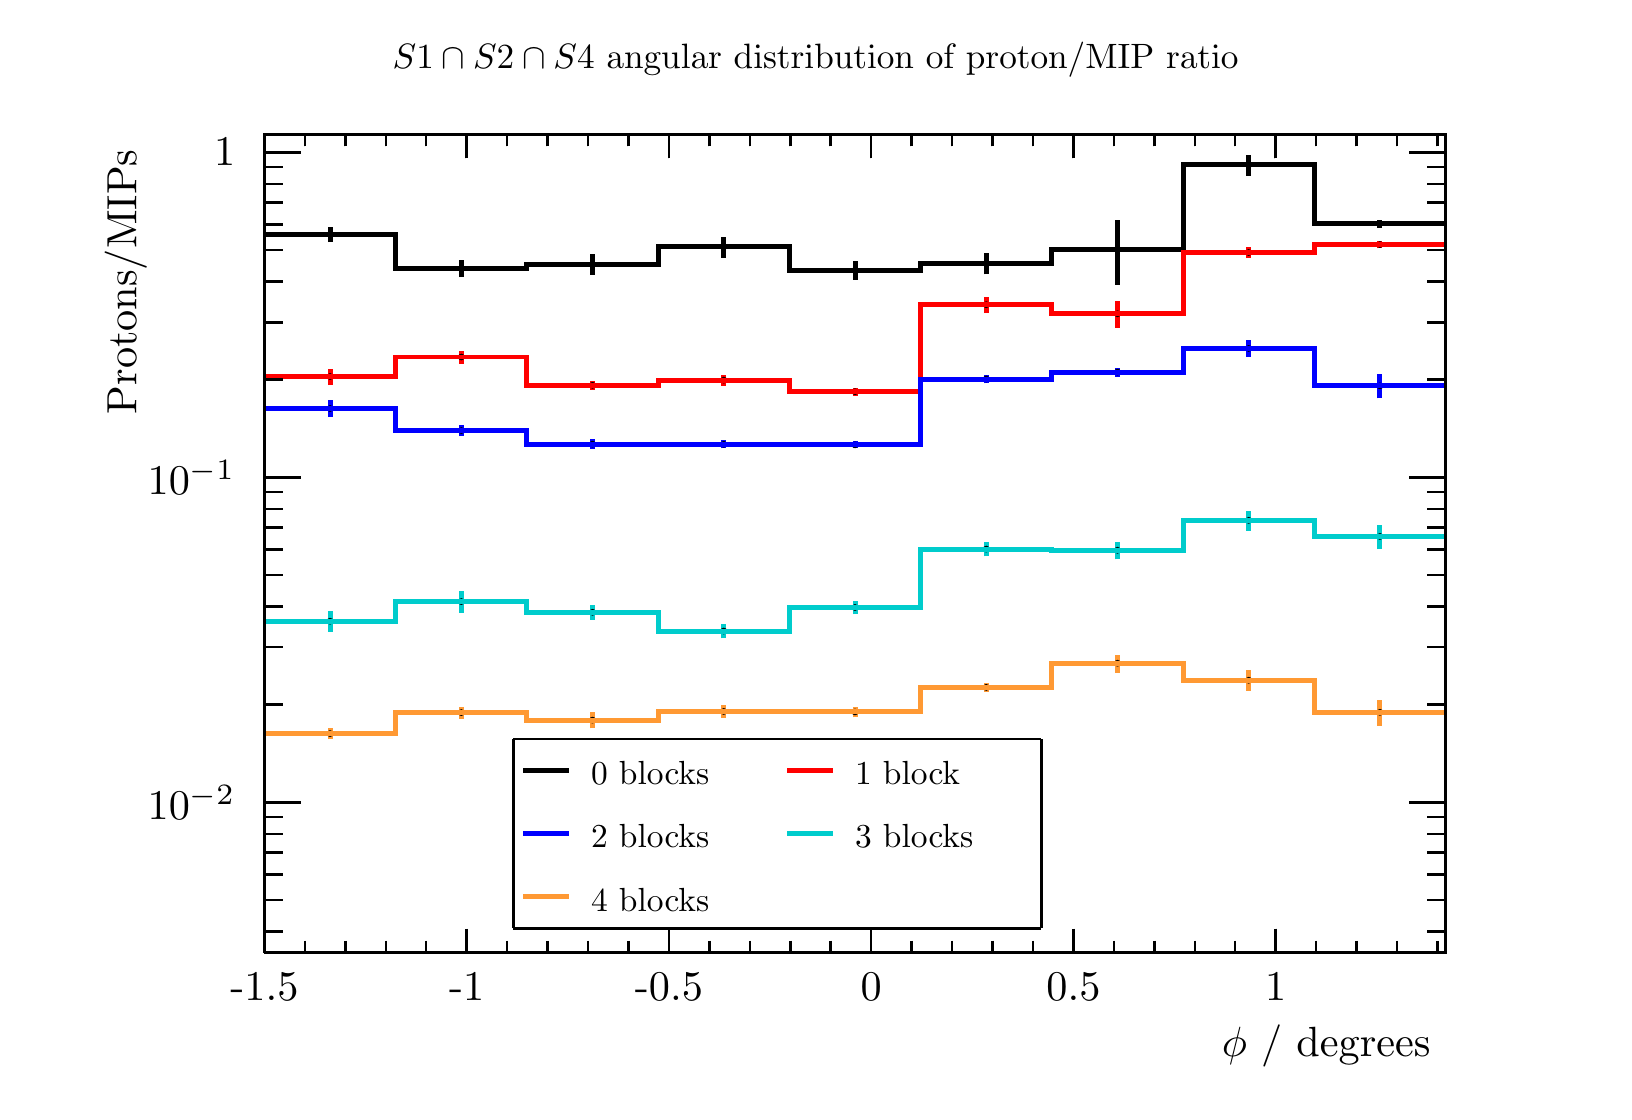
\begin{tikzpicture}
\pgfdeclareplotmark{cross} {
\pgfpathmoveto{\pgfpoint{-0.3\pgfplotmarksize}{\pgfplotmarksize}}
\pgfpathlineto{\pgfpoint{+0.3\pgfplotmarksize}{\pgfplotmarksize}}
\pgfpathlineto{\pgfpoint{+0.3\pgfplotmarksize}{0.3\pgfplotmarksize}}
\pgfpathlineto{\pgfpoint{+1\pgfplotmarksize}{0.3\pgfplotmarksize}}
\pgfpathlineto{\pgfpoint{+1\pgfplotmarksize}{-0.3\pgfplotmarksize}}
\pgfpathlineto{\pgfpoint{+0.3\pgfplotmarksize}{-0.3\pgfplotmarksize}}
\pgfpathlineto{\pgfpoint{+0.3\pgfplotmarksize}{-1.\pgfplotmarksize}}
\pgfpathlineto{\pgfpoint{-0.3\pgfplotmarksize}{-1.\pgfplotmarksize}}
\pgfpathlineto{\pgfpoint{-0.3\pgfplotmarksize}{-0.3\pgfplotmarksize}}
\pgfpathlineto{\pgfpoint{-1.\pgfplotmarksize}{-0.3\pgfplotmarksize}}
\pgfpathlineto{\pgfpoint{-1.\pgfplotmarksize}{0.3\pgfplotmarksize}}
\pgfpathlineto{\pgfpoint{-0.3\pgfplotmarksize}{0.3\pgfplotmarksize}}
\pgfpathclose
\pgfusepathqstroke
}
\pgfdeclareplotmark{cross*} {
\pgfpathmoveto{\pgfpoint{-0.3\pgfplotmarksize}{\pgfplotmarksize}}
\pgfpathlineto{\pgfpoint{+0.3\pgfplotmarksize}{\pgfplotmarksize}}
\pgfpathlineto{\pgfpoint{+0.3\pgfplotmarksize}{0.3\pgfplotmarksize}}
\pgfpathlineto{\pgfpoint{+1\pgfplotmarksize}{0.3\pgfplotmarksize}}
\pgfpathlineto{\pgfpoint{+1\pgfplotmarksize}{-0.3\pgfplotmarksize}}
\pgfpathlineto{\pgfpoint{+0.3\pgfplotmarksize}{-0.3\pgfplotmarksize}}
\pgfpathlineto{\pgfpoint{+0.3\pgfplotmarksize}{-1.\pgfplotmarksize}}
\pgfpathlineto{\pgfpoint{-0.3\pgfplotmarksize}{-1.\pgfplotmarksize}}
\pgfpathlineto{\pgfpoint{-0.3\pgfplotmarksize}{-0.3\pgfplotmarksize}}
\pgfpathlineto{\pgfpoint{-1.\pgfplotmarksize}{-0.3\pgfplotmarksize}}
\pgfpathlineto{\pgfpoint{-1.\pgfplotmarksize}{0.3\pgfplotmarksize}}
\pgfpathlineto{\pgfpoint{-0.3\pgfplotmarksize}{0.3\pgfplotmarksize}}
\pgfpathclose
\pgfusepathqfillstroke
}
\pgfdeclareplotmark{newstar} {
\pgfpathmoveto{\pgfqpoint{0pt}{\pgfplotmarksize}}
\pgfpathlineto{\pgfqpointpolar{44}{0.5\pgfplotmarksize}}
\pgfpathlineto{\pgfqpointpolar{18}{\pgfplotmarksize}}
\pgfpathlineto{\pgfqpointpolar{-20}{0.5\pgfplotmarksize}}
\pgfpathlineto{\pgfqpointpolar{-54}{\pgfplotmarksize}}
\pgfpathlineto{\pgfqpointpolar{-90}{0.5\pgfplotmarksize}}
\pgfpathlineto{\pgfqpointpolar{234}{\pgfplotmarksize}}
\pgfpathlineto{\pgfqpointpolar{198}{0.5\pgfplotmarksize}}
\pgfpathlineto{\pgfqpointpolar{162}{\pgfplotmarksize}}
\pgfpathlineto{\pgfqpointpolar{134}{0.5\pgfplotmarksize}}
\pgfpathclose
\pgfusepathqstroke
}
\pgfdeclareplotmark{newstar*} {
\pgfpathmoveto{\pgfqpoint{0pt}{\pgfplotmarksize}}
\pgfpathlineto{\pgfqpointpolar{44}{0.5\pgfplotmarksize}}
\pgfpathlineto{\pgfqpointpolar{18}{\pgfplotmarksize}}
\pgfpathlineto{\pgfqpointpolar{-20}{0.5\pgfplotmarksize}}
\pgfpathlineto{\pgfqpointpolar{-54}{\pgfplotmarksize}}
\pgfpathlineto{\pgfqpointpolar{-90}{0.5\pgfplotmarksize}}
\pgfpathlineto{\pgfqpointpolar{234}{\pgfplotmarksize}}
\pgfpathlineto{\pgfqpointpolar{198}{0.5\pgfplotmarksize}}
\pgfpathlineto{\pgfqpointpolar{162}{\pgfplotmarksize}}
\pgfpathlineto{\pgfqpointpolar{134}{0.5\pgfplotmarksize}}
\pgfpathclose
\pgfusepathqfillstroke
}
\definecolor{c}{rgb}{1,1,1};
\draw [color=c, fill=c] (0,0) rectangle (20,13.4957);
\draw [color=c, fill=c] (3,1.75444) rectangle (18,12.1461);
\definecolor{c}{rgb}{0,0,0};
\draw [c,line width=0.9] (3,1.75444) -- (3,12.1461) -- (18,12.1461) -- (18,1.75444) -- (3,1.75444);
\definecolor{c}{rgb}{1,1,1};
\draw [color=c, fill=c] (3,1.75444) rectangle (18,12.1461);
\definecolor{c}{rgb}{0,0,0};
\draw [c,line width=0.9] (3,1.75444) -- (3,12.1461) -- (18,12.1461) -- (18,1.75444) -- (3,1.75444);
\draw [c,line width=0.9] (3,1.75444) -- (4.66667,1.75444) -- (4.66667,1.75444) -- (6.33333,1.75444) -- (6.33333,1.75444) -- (8,1.75444) -- (8,1.75444) -- (9.66667,1.75444) -- (9.66667,1.75444) -- (11.3333,1.75444) -- (11.3333,1.75444) -- (13,1.75444)
 -- (13,1.75444) -- (14.6667,1.75444) -- (14.6667,1.75444) -- (16.3333,1.75444) -- (16.3333,1.75444) -- (18,1.75444);
\draw [c,line width=0.9] (3,1.75444) -- (18,1.75444);
\draw [c,line width=0.9] (3,2.05809) -- (3,1.75444);
\draw [c,line width=0.9] (3.5137,1.90627) -- (3.5137,1.75444);
\draw [c,line width=0.9] (4.0274,1.90627) -- (4.0274,1.75444);
\draw [c,line width=0.9] (4.5411,1.90627) -- (4.5411,1.75444);
\draw [c,line width=0.9] (5.05479,1.90627) -- (5.05479,1.75444);
\draw [c,line width=0.9] (5.56849,2.05809) -- (5.56849,1.75444);
\draw [c,line width=0.9] (6.08219,1.90627) -- (6.08219,1.75444);
\draw [c,line width=0.9] (6.59589,1.90627) -- (6.59589,1.75444);
\draw [c,line width=0.9] (7.10959,1.90627) -- (7.10959,1.75444);
\draw [c,line width=0.9] (7.62329,1.90627) -- (7.62329,1.75444);
\draw [c,line width=0.9] (8.13699,2.05809) -- (8.13699,1.75444);
\draw [c,line width=0.9] (8.65069,1.90627) -- (8.65069,1.75444);
\draw [c,line width=0.9] (9.16438,1.90627) -- (9.16438,1.75444);
\draw [c,line width=0.9] (9.67808,1.90627) -- (9.67808,1.75444);
\draw [c,line width=0.9] (10.1918,1.90627) -- (10.1918,1.75444);
\draw [c,line width=0.9] (10.7055,2.05809) -- (10.7055,1.75444);
\draw [c,line width=0.9] (11.2192,1.90627) -- (11.2192,1.75444);
\draw [c,line width=0.9] (11.7329,1.90627) -- (11.7329,1.75444);
\draw [c,line width=0.9] (12.2466,1.90627) -- (12.2466,1.75444);
\draw [c,line width=0.9] (12.7603,1.90627) -- (12.7603,1.75444);
\draw [c,line width=0.9] (13.274,2.05809) -- (13.274,1.75444);
\draw [c,line width=0.9] (13.7877,1.90627) -- (13.7877,1.75444);
\draw [c,line width=0.9] (14.3014,1.90627) -- (14.3014,1.75444);
\draw [c,line width=0.9] (14.8151,1.90627) -- (14.8151,1.75444);
\draw [c,line width=0.9] (15.3288,1.90627) -- (15.3288,1.75444);
\draw [c,line width=0.9] (15.8425,2.05809) -- (15.8425,1.75444);
\draw [c,line width=0.9] (15.8425,2.05809) -- (15.8425,1.75444);
\draw [c,line width=0.9] (16.3562,1.90627) -- (16.3562,1.75444);
\draw [c,line width=0.9] (16.8699,1.90627) -- (16.8699,1.75444);
\draw [c,line width=0.9] (17.3836,1.90627) -- (17.3836,1.75444);
\draw [c,line width=0.9] (17.8973,1.90627) -- (17.8973,1.75444);
\draw [anchor=base] (3,1.14713) node[scale=1.52731, color=c, rotate=0]{-1.5};
\draw [anchor=base] (5.56849,1.14713) node[scale=1.52731, color=c, rotate=0]{-1};
\draw [anchor=base] (8.13699,1.14713) node[scale=1.52731, color=c, rotate=0]{-0.5};
\draw [anchor=base] (10.7055,1.14713) node[scale=1.52731, color=c, rotate=0]{0};
\draw [anchor=base] (13.274,1.14713) node[scale=1.52731, color=c, rotate=0]{0.5};
\draw [anchor=base] (15.8425,1.14713) node[scale=1.52731, color=c, rotate=0]{1};
\draw [anchor= east] (18,0.566819) node[scale=1.52731, color=c, rotate=0]{$\phi$ / degrees};
\draw [c,line width=0.9] (3,12.1461) -- (18,12.1461);
\draw [c,line width=0.9] (3,11.8425) -- (3,12.1461);
\draw [c,line width=0.9] (3.5137,11.9943) -- (3.5137,12.1461);
\draw [c,line width=0.9] (4.0274,11.9943) -- (4.0274,12.1461);
\draw [c,line width=0.9] (4.5411,11.9943) -- (4.5411,12.1461);
\draw [c,line width=0.9] (5.05479,11.9943) -- (5.05479,12.1461);
\draw [c,line width=0.9] (5.56849,11.8425) -- (5.56849,12.1461);
\draw [c,line width=0.9] (6.08219,11.9943) -- (6.08219,12.1461);
\draw [c,line width=0.9] (6.59589,11.9943) -- (6.59589,12.1461);
\draw [c,line width=0.9] (7.10959,11.9943) -- (7.10959,12.1461);
\draw [c,line width=0.9] (7.62329,11.9943) -- (7.62329,12.1461);
\draw [c,line width=0.9] (8.13699,11.8425) -- (8.13699,12.1461);
\draw [c,line width=0.9] (8.65069,11.9943) -- (8.65069,12.1461);
\draw [c,line width=0.9] (9.16438,11.9943) -- (9.16438,12.1461);
\draw [c,line width=0.9] (9.67808,11.9943) -- (9.67808,12.1461);
\draw [c,line width=0.9] (10.1918,11.9943) -- (10.1918,12.1461);
\draw [c,line width=0.9] (10.7055,11.8425) -- (10.7055,12.1461);
\draw [c,line width=0.9] (11.2192,11.9943) -- (11.2192,12.1461);
\draw [c,line width=0.9] (11.7329,11.9943) -- (11.7329,12.1461);
\draw [c,line width=0.9] (12.2466,11.9943) -- (12.2466,12.1461);
\draw [c,line width=0.9] (12.7603,11.9943) -- (12.7603,12.1461);
\draw [c,line width=0.9] (13.274,11.8425) -- (13.274,12.1461);
\draw [c,line width=0.9] (13.7877,11.9943) -- (13.7877,12.1461);
\draw [c,line width=0.9] (14.3014,11.9943) -- (14.3014,12.1461);
\draw [c,line width=0.9] (14.8151,11.9943) -- (14.8151,12.1461);
\draw [c,line width=0.9] (15.3288,11.9943) -- (15.3288,12.1461);
\draw [c,line width=0.9] (15.8425,11.8425) -- (15.8425,12.1461);
\draw [c,line width=0.9] (15.8425,11.8425) -- (15.8425,12.1461);
\draw [c,line width=0.9] (16.3562,11.9943) -- (16.3562,12.1461);
\draw [c,line width=0.9] (16.8699,11.9943) -- (16.8699,12.1461);
\draw [c,line width=0.9] (17.3836,11.9943) -- (17.3836,12.1461);
\draw [c,line width=0.9] (17.8973,11.9943) -- (17.8973,12.1461);
\draw [c,line width=0.9] (3,1.75444) -- (3,12.1461);
\draw [c,line width=0.9] (3.231,2.0228) -- (3,2.0228);
\draw [c,line width=0.9] (3.231,2.42276) -- (3,2.42276);
\draw [c,line width=0.9] (3.231,2.74954) -- (3,2.74954);
\draw [c,line width=0.9] (3.231,3.02584) -- (3,3.02584);
\draw [c,line width=0.9] (3.231,3.26518) -- (3,3.26518);
\draw [c,line width=0.9] (3.231,3.47629) -- (3,3.47629);
\draw [c,line width=0.9] (3.462,3.66514) -- (3,3.66514);
\draw [anchor= east] (2.82,3.66514) node[scale=1.52731, color=c, rotate=0]{$10^{-2}$};
\draw [c,line width=0.9] (3.231,4.90752) -- (3,4.90752);
\draw [c,line width=0.9] (3.231,5.63427) -- (3,5.63427);
\draw [c,line width=0.9] (3.231,6.1499) -- (3,6.1499);
\draw [c,line width=0.9] (3.231,6.54986) -- (3,6.54986);
\draw [c,line width=0.9] (3.231,6.87665) -- (3,6.87665);
\draw [c,line width=0.9] (3.231,7.15295) -- (3,7.15295);
\draw [c,line width=0.9] (3.231,7.39229) -- (3,7.39229);
\draw [c,line width=0.9] (3.231,7.6034) -- (3,7.6034);
\draw [c,line width=0.9] (3.462,7.79224) -- (3,7.79224);
\draw [anchor= east] (2.82,7.79224) node[scale=1.52731, color=c, rotate=0]{$10^{-1}$};
\draw [c,line width=0.9] (3.231,9.03463) -- (3,9.03463);
\draw [c,line width=0.9] (3.231,9.76137) -- (3,9.76137);
\draw [c,line width=0.9] (3.231,10.277) -- (3,10.277);
\draw [c,line width=0.9] (3.231,10.677) -- (3,10.677);
\draw [c,line width=0.9] (3.231,11.0038) -- (3,11.0038);
\draw [c,line width=0.9] (3.231,11.2801) -- (3,11.2801);
\draw [c,line width=0.9] (3.231,11.5194) -- (3,11.5194);
\draw [c,line width=0.9] (3.231,11.7305) -- (3,11.7305);
\draw [c,line width=0.9] (3.462,11.9193) -- (3,11.9193);
\draw [anchor= east] (2.82,11.9193) node[scale=1.52731, color=c, rotate=0]{1};
\draw [anchor= east] (1.24,12.1461) node[scale=1.52731, color=c, rotate=90]{ Protons/MIPs};
\draw [c,line width=0.9] (18,1.75444) -- (18,12.1461);
\draw [c,line width=0.9] (17.769,2.0228) -- (18,2.0228);
\draw [c,line width=0.9] (17.769,2.42276) -- (18,2.42276);
\draw [c,line width=0.9] (17.769,2.74954) -- (18,2.74954);
\draw [c,line width=0.9] (17.769,3.02584) -- (18,3.02584);
\draw [c,line width=0.9] (17.769,3.26518) -- (18,3.26518);
\draw [c,line width=0.9] (17.769,3.47629) -- (18,3.47629);
\draw [c,line width=0.9] (17.538,3.66514) -- (18,3.66514);
\draw [c,line width=0.9] (17.769,4.90752) -- (18,4.90752);
\draw [c,line width=0.9] (17.769,5.63427) -- (18,5.63427);
\draw [c,line width=0.9] (17.769,6.1499) -- (18,6.1499);
\draw [c,line width=0.9] (17.769,6.54986) -- (18,6.54986);
\draw [c,line width=0.9] (17.769,6.87665) -- (18,6.87665);
\draw [c,line width=0.9] (17.769,7.15295) -- (18,7.15295);
\draw [c,line width=0.9] (17.769,7.39229) -- (18,7.39229);
\draw [c,line width=0.9] (17.769,7.6034) -- (18,7.6034);
\draw [c,line width=0.9] (17.538,7.79224) -- (18,7.79224);
\draw [c,line width=0.9] (17.769,9.03463) -- (18,9.03463);
\draw [c,line width=0.9] (17.769,9.76137) -- (18,9.76137);
\draw [c,line width=0.9] (17.769,10.277) -- (18,10.277);
\draw [c,line width=0.9] (17.769,10.677) -- (18,10.677);
\draw [c,line width=0.9] (17.769,11.0038) -- (18,11.0038);
\draw [c,line width=0.9] (17.769,11.2801) -- (18,11.2801);
\draw [c,line width=0.9] (17.769,11.5194) -- (18,11.5194);
\draw [c,line width=0.9] (17.769,11.7305) -- (18,11.7305);
\draw [c,line width=0.9] (17.538,11.9193) -- (18,11.9193);
\draw [c,line width=1.8] (3.83333,10.7777) -- (3.83333,10.8765);
\draw [c,line width=1.8] (3.83333,10.8765) -- (3.83333,10.9702);
\foreach \P in {(3.83333,10.8765)}{\draw[mark options={color=c,fill=c},mark size=2.402402pt,mark=*,mark size=1pt] plot coordinates {\P};}
\draw [c,line width=1.8] (5.5,10.3339) -- (5.5,10.4447);
\draw [c,line width=1.8] (5.5,10.4447) -- (5.5,10.549);
\foreach \P in {(5.5,10.4447)}{\draw[mark options={color=c,fill=c},mark size=2.402402pt,mark=*,mark size=1pt] plot coordinates {\P};}
\draw [c,line width=1.8] (7.16667,10.362) -- (7.16667,10.4971);
\draw [c,line width=1.8] (7.16667,10.4971) -- (7.16667,10.6227);
\foreach \P in {(7.16667,10.4971)}{\draw[mark options={color=c,fill=c},mark size=2.402402pt,mark=*,mark size=1pt] plot coordinates {\P};}
\draw [c,line width=1.8] (8.83333,10.5803) -- (8.83333,10.72);
\draw [c,line width=1.8] (8.83333,10.72) -- (8.83333,10.8497);
\foreach \P in {(8.83333,10.72)}{\draw[mark options={color=c,fill=c},mark size=2.402402pt,mark=*,mark size=1pt] plot coordinates {\P};}
\draw [c,line width=1.8] (10.5,10.2982) -- (10.5,10.4208);
\draw [c,line width=1.8] (10.5,10.4208) -- (10.5,10.5355);
\foreach \P in {(10.5,10.4208)}{\draw[mark options={color=c,fill=c},mark size=2.402402pt,mark=*,mark size=1pt] plot coordinates {\P};}
\draw [c,line width=1.8] (12.1667,10.371) -- (12.1667,10.5085);
\draw [c,line width=1.8] (12.1667,10.5085) -- (12.1667,10.6363);
\foreach \P in {(12.1667,10.5085)}{\draw[mark options={color=c,fill=c},mark size=2.402402pt,mark=*,mark size=1pt] plot coordinates {\P};}
\draw [c,line width=1.8] (13.8333,10.2369) -- (13.8333,10.6916);
\draw [c,line width=1.8] (13.8333,10.6916) -- (13.8333,11.054);
\foreach \P in {(13.8333,10.6916)}{\draw[mark options={color=c,fill=c},mark size=2.402402pt,mark=*,mark size=1pt] plot coordinates {\P};}
\draw [c,line width=1.8] (15.5,11.6218) -- (15.5,11.7605);
\draw [c,line width=1.8] (15.5,11.7605) -- (15.5,11.8893);
\foreach \P in {(15.5,11.7605)}{\draw[mark options={color=c,fill=c},mark size=2.402402pt,mark=*,mark size=1pt] plot coordinates {\P};}
\draw [c,line width=1.8] (17.1667,10.9639) -- (17.1667,11.0149);
\draw [c,line width=1.8] (17.1667,11.0149) -- (17.1667,11.0645);
\foreach \P in {(17.1667,11.0149)}{\draw[mark options={color=c,fill=c},mark size=2.402402pt,mark=*,mark size=1pt] plot coordinates {\P};}
\draw [c,line width=1.8] (3,10.8765) -- (4.66667,10.8765) -- (4.66667,10.4447) -- (6.33333,10.4447) -- (6.33333,10.4971) -- (8,10.4971) -- (8,10.72) -- (9.66667,10.72) -- (9.66667,10.4208) -- (11.3333,10.4208) -- (11.3333,10.5085) -- (13,10.5085) --
 (13,10.6916) -- (14.6667,10.6916) -- (14.6667,11.7605) -- (16.3333,11.7605) -- (16.3333,11.0149) -- (18,11.0149);
\definecolor{c}{rgb}{1,0,0};
\draw [c,line width=1.8] (3.83333,8.96432) -- (3.83333,9.07217);
\draw [c,line width=1.8] (3.83333,9.07217) -- (3.83333,9.17389);
\definecolor{c}{rgb}{0,0,0};
\foreach \P in {(3.83333,9.07217)}{\draw[mark options={color=c,fill=c},mark size=2.402402pt,mark=*,mark size=1pt] plot coordinates {\P};}
\definecolor{c}{rgb}{1,0,0};
\draw [c,line width=1.8] (5.5,9.23726) -- (5.5,9.32023);
\draw [c,line width=1.8] (5.5,9.32023) -- (5.5,9.39953);
\definecolor{c}{rgb}{0,0,0};
\foreach \P in {(5.5,9.32023)}{\draw[mark options={color=c,fill=c},mark size=2.402402pt,mark=*,mark size=1pt] plot coordinates {\P};}
\definecolor{c}{rgb}{1,0,0};
\draw [c,line width=1.8] (7.16667,8.90343) -- (7.16667,8.96069);
\draw [c,line width=1.8] (7.16667,8.96069) -- (7.16667,9.01617);
\definecolor{c}{rgb}{0,0,0};
\foreach \P in {(7.16667,8.96069)}{\draw[mark options={color=c,fill=c},mark size=2.402402pt,mark=*,mark size=1pt] plot coordinates {\P};}
\definecolor{c}{rgb}{1,0,0};
\draw [c,line width=1.8] (8.83333,8.95669) -- (8.83333,9.02674);
\draw [c,line width=1.8] (8.83333,9.02674) -- (8.83333,9.09415);
\definecolor{c}{rgb}{0,0,0};
\foreach \P in {(8.83333,9.02674)}{\draw[mark options={color=c,fill=c},mark size=2.402402pt,mark=*,mark size=1pt] plot coordinates {\P};}
\definecolor{c}{rgb}{1,0,0};
\draw [c,line width=1.8] (10.5,8.82806) -- (10.5,8.87953);
\draw [c,line width=1.8] (10.5,8.87953) -- (10.5,8.92957);
\definecolor{c}{rgb}{0,0,0};
\foreach \P in {(10.5,8.87953)}{\draw[mark options={color=c,fill=c},mark size=2.402402pt,mark=*,mark size=1pt] plot coordinates {\P};}
\definecolor{c}{rgb}{1,0,0};
\draw [c,line width=1.8] (12.1667,9.87581) -- (12.1667,9.98442);
\draw [c,line width=1.8] (12.1667,9.98442) -- (12.1667,10.0868);
\definecolor{c}{rgb}{0,0,0};
\foreach \P in {(12.1667,9.98442)}{\draw[mark options={color=c,fill=c},mark size=2.402402pt,mark=*,mark size=1pt] plot coordinates {\P};}
\definecolor{c}{rgb}{1,0,0};
\draw [c,line width=1.8] (13.8333,9.69229) -- (13.8333,9.86902);
\draw [c,line width=1.8] (13.8333,9.86902) -- (13.8333,10.0299);
\definecolor{c}{rgb}{0,0,0};
\foreach \P in {(13.8333,9.86902)}{\draw[mark options={color=c,fill=c},mark size=2.402402pt,mark=*,mark size=1pt] plot coordinates {\P};}
\definecolor{c}{rgb}{1,0,0};
\draw [c,line width=1.8] (15.5,10.576) -- (15.5,10.6472);
\draw [c,line width=1.8] (15.5,10.6472) -- (15.5,10.7157);
\definecolor{c}{rgb}{0,0,0};
\foreach \P in {(15.5,10.6472)}{\draw[mark options={color=c,fill=c},mark size=2.402402pt,mark=*,mark size=1pt] plot coordinates {\P};}
\definecolor{c}{rgb}{1,0,0};
\draw [c,line width=1.8] (17.1667,10.6997) -- (17.1667,10.7481);
\draw [c,line width=1.8] (17.1667,10.7481) -- (17.1667,10.7953);
\definecolor{c}{rgb}{0,0,0};
\foreach \P in {(17.1667,10.7481)}{\draw[mark options={color=c,fill=c},mark size=2.402402pt,mark=*,mark size=1pt] plot coordinates {\P};}
\definecolor{c}{rgb}{1,0,0};
\draw [c,line width=1.8] (3,9.07217) -- (4.66667,9.07217) -- (4.66667,9.32023) -- (6.33333,9.32023) -- (6.33333,8.96069) -- (8,8.96069) -- (8,9.02674) -- (9.66667,9.02674) -- (9.66667,8.87953) -- (11.3333,8.87953) -- (11.3333,9.98442) -- (13,9.98442)
 -- (13,9.86902) -- (14.6667,9.86902) -- (14.6667,10.6472) -- (16.3333,10.6472) -- (16.3333,10.7481) -- (18,10.7481);
\definecolor{c}{rgb}{0,0,1};
\draw [c,line width=1.8] (3.83333,8.55718) -- (3.83333,8.66636);
\draw [c,line width=1.8] (3.83333,8.66636) -- (3.83333,8.76928);
\definecolor{c}{rgb}{0,0,0};
\foreach \P in {(3.83333,8.66636)}{\draw[mark options={color=c,fill=c},mark size=2.402402pt,mark=*,mark size=1pt] plot coordinates {\P};}
\definecolor{c}{rgb}{0,0,1};
\draw [c,line width=1.8] (5.5,8.31557) -- (5.5,8.38631);
\draw [c,line width=1.8] (5.5,8.38631) -- (5.5,8.45436);
\definecolor{c}{rgb}{0,0,0};
\foreach \P in {(5.5,8.38631)}{\draw[mark options={color=c,fill=c},mark size=2.402402pt,mark=*,mark size=1pt] plot coordinates {\P};}
\definecolor{c}{rgb}{0,0,1};
\draw [c,line width=1.8] (7.16667,8.15197) -- (7.16667,8.21352);
\draw [c,line width=1.8] (7.16667,8.21352) -- (7.16667,8.27302);
\definecolor{c}{rgb}{0,0,0};
\foreach \P in {(7.16667,8.21352)}{\draw[mark options={color=c,fill=c},mark size=2.402402pt,mark=*,mark size=1pt] plot coordinates {\P};}
\definecolor{c}{rgb}{0,0,1};
\draw [c,line width=1.8] (8.83333,8.15946) -- (8.83333,8.21131);
\draw [c,line width=1.8] (8.83333,8.21131) -- (8.83333,8.26171);
\definecolor{c}{rgb}{0,0,0};
\foreach \P in {(8.83333,8.21131)}{\draw[mark options={color=c,fill=c},mark size=2.402402pt,mark=*,mark size=1pt] plot coordinates {\P};}
\definecolor{c}{rgb}{0,0,1};
\draw [c,line width=1.8] (10.5,8.15949) -- (10.5,8.20403);
\draw [c,line width=1.8] (10.5,8.20403) -- (10.5,8.24749);
\definecolor{c}{rgb}{0,0,0};
\foreach \P in {(10.5,8.20403)}{\draw[mark options={color=c,fill=c},mark size=2.402402pt,mark=*,mark size=1pt] plot coordinates {\P};}
\definecolor{c}{rgb}{0,0,1};
\draw [c,line width=1.8] (12.1667,8.98631) -- (12.1667,9.04063);
\draw [c,line width=1.8] (12.1667,9.04063) -- (12.1667,9.09336);
\definecolor{c}{rgb}{0,0,0};
\foreach \P in {(12.1667,9.04063)}{\draw[mark options={color=c,fill=c},mark size=2.402402pt,mark=*,mark size=1pt] plot coordinates {\P};}
\definecolor{c}{rgb}{0,0,1};
\draw [c,line width=1.8] (13.8333,9.07201) -- (13.8333,9.12799);
\draw [c,line width=1.8] (13.8333,9.12799) -- (13.8333,9.18227);
\definecolor{c}{rgb}{0,0,0};
\foreach \P in {(13.8333,9.12799)}{\draw[mark options={color=c,fill=c},mark size=2.402402pt,mark=*,mark size=1pt] plot coordinates {\P};}
\definecolor{c}{rgb}{0,0,1};
\draw [c,line width=1.8] (15.5,9.32044) -- (15.5,9.42921);
\draw [c,line width=1.8] (15.5,9.42921) -- (15.5,9.53176);
\definecolor{c}{rgb}{0,0,0};
\foreach \P in {(15.5,9.42921)}{\draw[mark options={color=c,fill=c},mark size=2.402402pt,mark=*,mark size=1pt] plot coordinates {\P};}
\definecolor{c}{rgb}{0,0,1};
\draw [c,line width=1.8] (17.1667,8.79549) -- (17.1667,8.95348);
\draw [c,line width=1.8] (17.1667,8.95348) -- (17.1667,9.09867);
\definecolor{c}{rgb}{0,0,0};
\foreach \P in {(17.1667,8.95348)}{\draw[mark options={color=c,fill=c},mark size=2.402402pt,mark=*,mark size=1pt] plot coordinates {\P};}
\definecolor{c}{rgb}{0,0,1};
\draw [c,line width=1.8] (3,8.66636) -- (4.66667,8.66636) -- (4.66667,8.38631) -- (6.33333,8.38631) -- (6.33333,8.21352) -- (8,8.21352) -- (8,8.21131) -- (9.66667,8.21131) -- (9.66667,8.20403) -- (11.3333,8.20403) -- (11.3333,9.04063) -- (13,9.04063)
 -- (13,9.12799) -- (14.6667,9.12799) -- (14.6667,9.42921) -- (16.3333,9.42921) -- (16.3333,8.95348) -- (18,8.95348);
\definecolor{c}{rgb}{0,0.8,0.8};
\draw [c,line width=1.8] (3.83333,5.82959) -- (3.83333,5.9648);
\draw [c,line width=1.8] (3.83333,5.9648) -- (3.83333,6.09053);
\definecolor{c}{rgb}{0,0,0};
\foreach \P in {(3.83333,5.9648)}{\draw[mark options={color=c,fill=c},mark size=2.402402pt,mark=*,mark size=1pt] plot coordinates {\P};}
\definecolor{c}{rgb}{0,0.8,0.8};
\draw [c,line width=1.8] (5.5,6.07356) -- (5.5,6.21409);
\draw [c,line width=1.8] (5.5,6.21409) -- (5.5,6.3444);
\definecolor{c}{rgb}{0,0,0};
\foreach \P in {(5.5,6.21409)}{\draw[mark options={color=c,fill=c},mark size=2.402402pt,mark=*,mark size=1pt] plot coordinates {\P};}
\definecolor{c}{rgb}{0,0.8,0.8};
\draw [c,line width=1.8] (7.16667,5.98519) -- (7.16667,6.07802);
\draw [c,line width=1.8] (7.16667,6.07802) -- (7.16667,6.16629);
\definecolor{c}{rgb}{0,0,0};
\foreach \P in {(7.16667,6.07802)}{\draw[mark options={color=c,fill=c},mark size=2.402402pt,mark=*,mark size=1pt] plot coordinates {\P};}
\definecolor{c}{rgb}{0,0.8,0.8};
\draw [c,line width=1.8] (8.83333,5.7463) -- (8.83333,5.84009);
\draw [c,line width=1.8] (8.83333,5.84009) -- (8.83333,5.92921);
\definecolor{c}{rgb}{0,0,0};
\foreach \P in {(8.83333,5.84009)}{\draw[mark options={color=c,fill=c},mark size=2.402402pt,mark=*,mark size=1pt] plot coordinates {\P};}
\definecolor{c}{rgb}{0,0.8,0.8};
\draw [c,line width=1.8] (10.5,6.05372) -- (10.5,6.13878);
\draw [c,line width=1.8] (10.5,6.13878) -- (10.5,6.21999);
\definecolor{c}{rgb}{0,0,0};
\foreach \P in {(10.5,6.13878)}{\draw[mark options={color=c,fill=c},mark size=2.402402pt,mark=*,mark size=1pt] plot coordinates {\P};}
\definecolor{c}{rgb}{0,0.8,0.8};
\draw [c,line width=1.8] (12.1667,6.78835) -- (12.1667,6.88104);
\draw [c,line width=1.8] (12.1667,6.88104) -- (12.1667,6.96918);
\definecolor{c}{rgb}{0,0,0};
\foreach \P in {(12.1667,6.88104)}{\draw[mark options={color=c,fill=c},mark size=2.402402pt,mark=*,mark size=1pt] plot coordinates {\P};}
\definecolor{c}{rgb}{0,0.8,0.8};
\draw [c,line width=1.8] (13.8333,6.75097) -- (13.8333,6.86591);
\draw [c,line width=1.8] (13.8333,6.86591) -- (13.8333,6.97393);
\definecolor{c}{rgb}{0,0,0};
\foreach \P in {(13.8333,6.86591)}{\draw[mark options={color=c,fill=c},mark size=2.402402pt,mark=*,mark size=1pt] plot coordinates {\P};}
\definecolor{c}{rgb}{0,0.8,0.8};
\draw [c,line width=1.8] (15.5,7.11167) -- (15.5,7.24588);
\draw [c,line width=1.8] (15.5,7.24588) -- (15.5,7.37073);
\definecolor{c}{rgb}{0,0,0};
\foreach \P in {(15.5,7.24588)}{\draw[mark options={color=c,fill=c},mark size=2.402402pt,mark=*,mark size=1pt] plot coordinates {\P};}
\definecolor{c}{rgb}{0,0.8,0.8};
\draw [c,line width=1.8] (17.1667,6.88029) -- (17.1667,7.0412);
\draw [c,line width=1.8] (17.1667,7.0412) -- (17.1667,7.18884);
\definecolor{c}{rgb}{0,0,0};
\foreach \P in {(17.1667,7.0412)}{\draw[mark options={color=c,fill=c},mark size=2.402402pt,mark=*,mark size=1pt] plot coordinates {\P};}
\definecolor{c}{rgb}{0,0.8,0.8};
\draw [c,line width=1.8] (3,5.9648) -- (4.66667,5.9648) -- (4.66667,6.21409) -- (6.33333,6.21409) -- (6.33333,6.07802) -- (8,6.07802) -- (8,5.84009) -- (9.66667,5.84009) -- (9.66667,6.13878) -- (11.3333,6.13878) -- (11.3333,6.88104) -- (13,6.88104)
 -- (13,6.86591) -- (14.6667,6.86591) -- (14.6667,7.24588) -- (16.3333,7.24588) -- (16.3333,7.0412) -- (18,7.0412);
\definecolor{c}{rgb}{1,0.6,0.2};
\draw [c,line width=1.8] (3.83333,4.46453) -- (3.83333,4.53759);
\draw [c,line width=1.8] (3.83333,4.53759) -- (3.83333,4.60778);
\definecolor{c}{rgb}{0,0,0};
\foreach \P in {(3.83333,4.53759)}{\draw[mark options={color=c,fill=c},mark size=2.402402pt,mark=*,mark size=1pt] plot coordinates {\P};}
\definecolor{c}{rgb}{1,0.6,0.2};
\draw [c,line width=1.8] (5.5,4.72766) -- (5.5,4.80432);
\draw [c,line width=1.8] (5.5,4.80432) -- (5.5,4.87783);
\definecolor{c}{rgb}{0,0,0};
\foreach \P in {(5.5,4.80432)}{\draw[mark options={color=c,fill=c},mark size=2.402402pt,mark=*,mark size=1pt] plot coordinates {\P};}
\definecolor{c}{rgb}{1,0.6,0.2};
\draw [c,line width=1.8] (7.16667,4.60307) -- (7.16667,4.70869);
\draw [c,line width=1.8] (7.16667,4.70869) -- (7.16667,4.80844);
\definecolor{c}{rgb}{0,0,0};
\foreach \P in {(7.16667,4.70869)}{\draw[mark options={color=c,fill=c},mark size=2.402402pt,mark=*,mark size=1pt] plot coordinates {\P};}
\definecolor{c}{rgb}{1,0.6,0.2};
\draw [c,line width=1.8] (8.83333,4.73762) -- (8.83333,4.81865);
\draw [c,line width=1.8] (8.83333,4.81865) -- (8.83333,4.89617);
\definecolor{c}{rgb}{0,0,0};
\foreach \P in {(8.83333,4.81865)}{\draw[mark options={color=c,fill=c},mark size=2.402402pt,mark=*,mark size=1pt] plot coordinates {\P};}
\definecolor{c}{rgb}{1,0.6,0.2};
\draw [c,line width=1.8] (10.5,4.74334) -- (10.5,4.81257);
\draw [c,line width=1.8] (10.5,4.81257) -- (10.5,4.87921);
\definecolor{c}{rgb}{0,0,0};
\foreach \P in {(10.5,4.81257)}{\draw[mark options={color=c,fill=c},mark size=2.402402pt,mark=*,mark size=1pt] plot coordinates {\P};}
\definecolor{c}{rgb}{1,0.6,0.2};
\draw [c,line width=1.8] (12.1667,5.06735) -- (12.1667,5.12404);
\draw [c,line width=1.8] (12.1667,5.12404) -- (12.1667,5.17899);
\definecolor{c}{rgb}{0,0,0};
\foreach \P in {(12.1667,5.12404)}{\draw[mark options={color=c,fill=c},mark size=2.402402pt,mark=*,mark size=1pt] plot coordinates {\P};}
\definecolor{c}{rgb}{1,0.6,0.2};
\draw [c,line width=1.8] (13.8333,5.31318) -- (13.8333,5.43116);
\draw [c,line width=1.8] (13.8333,5.43116) -- (13.8333,5.54185);
\definecolor{c}{rgb}{0,0,0};
\foreach \P in {(13.8333,5.43116)}{\draw[mark options={color=c,fill=c},mark size=2.402402pt,mark=*,mark size=1pt] plot coordinates {\P};}
\definecolor{c}{rgb}{1,0.6,0.2};
\draw [c,line width=1.8] (15.5,5.08173) -- (15.5,5.2152);
\draw [c,line width=1.8] (15.5,5.2152) -- (15.5,5.33942);
\definecolor{c}{rgb}{0,0,0};
\foreach \P in {(15.5,5.2152)}{\draw[mark options={color=c,fill=c},mark size=2.402402pt,mark=*,mark size=1pt] plot coordinates {\P};}
\definecolor{c}{rgb}{1,0.6,0.2};
\draw [c,line width=1.8] (17.1667,4.63598) -- (17.1667,4.80753);
\draw [c,line width=1.8] (17.1667,4.80753) -- (17.1667,4.96408);
\definecolor{c}{rgb}{0,0,0};
\foreach \P in {(17.1667,4.80753)}{\draw[mark options={color=c,fill=c},mark size=2.402402pt,mark=*,mark size=1pt] plot coordinates {\P};}
\definecolor{c}{rgb}{1,0.6,0.2};
\draw [c,line width=1.8] (3,4.53759) -- (4.66667,4.53759) -- (4.66667,4.80432) -- (6.33333,4.80432) -- (6.33333,4.70869) -- (8,4.70869) -- (8,4.81865) -- (9.66667,4.81865) -- (9.66667,4.81257) -- (11.3333,4.81257) -- (11.3333,5.12404) -- (13,5.12404)
 -- (13,5.43116) -- (14.6667,5.43116) -- (14.6667,5.2152) -- (16.3333,5.2152) -- (16.3333,4.80753) -- (18,4.80753);
\definecolor{c}{rgb}{0,0,0};
\draw [c,line width=0.9] (3,1.75444) -- (18,1.75444);
\draw [c,line width=0.9] (3,2.05809) -- (3,1.75444);
\draw [c,line width=0.9] (3.5137,1.90627) -- (3.5137,1.75444);
\draw [c,line width=0.9] (4.0274,1.90627) -- (4.0274,1.75444);
\draw [c,line width=0.9] (4.5411,1.90627) -- (4.5411,1.75444);
\draw [c,line width=0.9] (5.05479,1.90627) -- (5.05479,1.75444);
\draw [c,line width=0.9] (5.56849,2.05809) -- (5.56849,1.75444);
\draw [c,line width=0.9] (6.08219,1.90627) -- (6.08219,1.75444);
\draw [c,line width=0.9] (6.59589,1.90627) -- (6.59589,1.75444);
\draw [c,line width=0.9] (7.10959,1.90627) -- (7.10959,1.75444);
\draw [c,line width=0.9] (7.62329,1.90627) -- (7.62329,1.75444);
\draw [c,line width=0.9] (8.13699,2.05809) -- (8.13699,1.75444);
\draw [c,line width=0.9] (8.65069,1.90627) -- (8.65069,1.75444);
\draw [c,line width=0.9] (9.16438,1.90627) -- (9.16438,1.75444);
\draw [c,line width=0.9] (9.67808,1.90627) -- (9.67808,1.75444);
\draw [c,line width=0.9] (10.1918,1.90627) -- (10.1918,1.75444);
\draw [c,line width=0.9] (10.7055,2.05809) -- (10.7055,1.75444);
\draw [c,line width=0.9] (11.2192,1.90627) -- (11.2192,1.75444);
\draw [c,line width=0.9] (11.7329,1.90627) -- (11.7329,1.75444);
\draw [c,line width=0.9] (12.2466,1.90627) -- (12.2466,1.75444);
\draw [c,line width=0.9] (12.7603,1.90627) -- (12.7603,1.75444);
\draw [c,line width=0.9] (13.274,2.05809) -- (13.274,1.75444);
\draw [c,line width=0.9] (13.7877,1.90627) -- (13.7877,1.75444);
\draw [c,line width=0.9] (14.3014,1.90627) -- (14.3014,1.75444);
\draw [c,line width=0.9] (14.8151,1.90627) -- (14.8151,1.75444);
\draw [c,line width=0.9] (15.3288,1.90627) -- (15.3288,1.75444);
\draw [c,line width=0.9] (15.8425,2.05809) -- (15.8425,1.75444);
\draw [c,line width=0.9] (15.8425,2.05809) -- (15.8425,1.75444);
\draw [c,line width=0.9] (16.3562,1.90627) -- (16.3562,1.75444);
\draw [c,line width=0.9] (16.8699,1.90627) -- (16.8699,1.75444);
\draw [c,line width=0.9] (17.3836,1.90627) -- (17.3836,1.75444);
\draw [c,line width=0.9] (17.8973,1.90627) -- (17.8973,1.75444);
\draw [c,line width=0.9] (3,12.1461) -- (18,12.1461);
\draw [c,line width=0.9] (3,11.8425) -- (3,12.1461);
\draw [c,line width=0.9] (3.5137,11.9943) -- (3.5137,12.1461);
\draw [c,line width=0.9] (4.0274,11.9943) -- (4.0274,12.1461);
\draw [c,line width=0.9] (4.5411,11.9943) -- (4.5411,12.1461);
\draw [c,line width=0.9] (5.05479,11.9943) -- (5.05479,12.1461);
\draw [c,line width=0.9] (5.56849,11.8425) -- (5.56849,12.1461);
\draw [c,line width=0.9] (6.08219,11.9943) -- (6.08219,12.1461);
\draw [c,line width=0.9] (6.59589,11.9943) -- (6.59589,12.1461);
\draw [c,line width=0.9] (7.10959,11.9943) -- (7.10959,12.1461);
\draw [c,line width=0.9] (7.62329,11.9943) -- (7.62329,12.1461);
\draw [c,line width=0.9] (8.13699,11.8425) -- (8.13699,12.1461);
\draw [c,line width=0.9] (8.65069,11.9943) -- (8.65069,12.1461);
\draw [c,line width=0.9] (9.16438,11.9943) -- (9.16438,12.1461);
\draw [c,line width=0.9] (9.67808,11.9943) -- (9.67808,12.1461);
\draw [c,line width=0.9] (10.1918,11.9943) -- (10.1918,12.1461);
\draw [c,line width=0.9] (10.7055,11.8425) -- (10.7055,12.1461);
\draw [c,line width=0.9] (11.2192,11.9943) -- (11.2192,12.1461);
\draw [c,line width=0.9] (11.7329,11.9943) -- (11.7329,12.1461);
\draw [c,line width=0.9] (12.2466,11.9943) -- (12.2466,12.1461);
\draw [c,line width=0.9] (12.7603,11.9943) -- (12.7603,12.1461);
\draw [c,line width=0.9] (13.274,11.8425) -- (13.274,12.1461);
\draw [c,line width=0.9] (13.7877,11.9943) -- (13.7877,12.1461);
\draw [c,line width=0.9] (14.3014,11.9943) -- (14.3014,12.1461);
\draw [c,line width=0.9] (14.8151,11.9943) -- (14.8151,12.1461);
\draw [c,line width=0.9] (15.3288,11.9943) -- (15.3288,12.1461);
\draw [c,line width=0.9] (15.8425,11.8425) -- (15.8425,12.1461);
\draw [c,line width=0.9] (15.8425,11.8425) -- (15.8425,12.1461);
\draw [c,line width=0.9] (16.3562,11.9943) -- (16.3562,12.1461);
\draw [c,line width=0.9] (16.8699,11.9943) -- (16.8699,12.1461);
\draw [c,line width=0.9] (17.3836,11.9943) -- (17.3836,12.1461);
\draw [c,line width=0.9] (17.8973,11.9943) -- (17.8973,12.1461);
\draw [c,line width=0.9] (3,1.75444) -- (3,12.1461);
\draw [c,line width=0.9] (3.231,2.0228) -- (3,2.0228);
\draw [c,line width=0.9] (3.231,2.42276) -- (3,2.42276);
\draw [c,line width=0.9] (3.231,2.74954) -- (3,2.74954);
\draw [c,line width=0.9] (3.231,3.02584) -- (3,3.02584);
\draw [c,line width=0.9] (3.231,3.26518) -- (3,3.26518);
\draw [c,line width=0.9] (3.231,3.47629) -- (3,3.47629);
\draw [c,line width=0.9] (3.462,3.66514) -- (3,3.66514);
\draw [c,line width=0.9] (3.231,4.90752) -- (3,4.90752);
\draw [c,line width=0.9] (3.231,5.63427) -- (3,5.63427);
\draw [c,line width=0.9] (3.231,6.1499) -- (3,6.1499);
\draw [c,line width=0.9] (3.231,6.54986) -- (3,6.54986);
\draw [c,line width=0.9] (3.231,6.87665) -- (3,6.87665);
\draw [c,line width=0.9] (3.231,7.15295) -- (3,7.15295);
\draw [c,line width=0.9] (3.231,7.39229) -- (3,7.39229);
\draw [c,line width=0.9] (3.231,7.6034) -- (3,7.6034);
\draw [c,line width=0.9] (3.462,7.79224) -- (3,7.79224);
\draw [c,line width=0.9] (3.231,9.03463) -- (3,9.03463);
\draw [c,line width=0.9] (3.231,9.76137) -- (3,9.76137);
\draw [c,line width=0.9] (3.231,10.277) -- (3,10.277);
\draw [c,line width=0.9] (3.231,10.677) -- (3,10.677);
\draw [c,line width=0.9] (3.231,11.0038) -- (3,11.0038);
\draw [c,line width=0.9] (3.231,11.2801) -- (3,11.2801);
\draw [c,line width=0.9] (3.231,11.5194) -- (3,11.5194);
\draw [c,line width=0.9] (3.231,11.7305) -- (3,11.7305);
\draw [c,line width=0.9] (3.462,11.9193) -- (3,11.9193);
\draw [c,line width=0.9] (18,1.75444) -- (18,12.1461);
\draw [c,line width=0.9] (17.769,2.0228) -- (18,2.0228);
\draw [c,line width=0.9] (17.769,2.42276) -- (18,2.42276);
\draw [c,line width=0.9] (17.769,2.74954) -- (18,2.74954);
\draw [c,line width=0.9] (17.769,3.02584) -- (18,3.02584);
\draw [c,line width=0.9] (17.769,3.26518) -- (18,3.26518);
\draw [c,line width=0.9] (17.769,3.47629) -- (18,3.47629);
\draw [c,line width=0.9] (17.538,3.66514) -- (18,3.66514);
\draw [c,line width=0.9] (17.769,4.90752) -- (18,4.90752);
\draw [c,line width=0.9] (17.769,5.63427) -- (18,5.63427);
\draw [c,line width=0.9] (17.769,6.1499) -- (18,6.1499);
\draw [c,line width=0.9] (17.769,6.54986) -- (18,6.54986);
\draw [c,line width=0.9] (17.769,6.87665) -- (18,6.87665);
\draw [c,line width=0.9] (17.769,7.15295) -- (18,7.15295);
\draw [c,line width=0.9] (17.769,7.39229) -- (18,7.39229);
\draw [c,line width=0.9] (17.769,7.6034) -- (18,7.6034);
\draw [c,line width=0.9] (17.538,7.79224) -- (18,7.79224);
\draw [c,line width=0.9] (17.769,9.03463) -- (18,9.03463);
\draw [c,line width=0.9] (17.769,9.76137) -- (18,9.76137);
\draw [c,line width=0.9] (17.769,10.277) -- (18,10.277);
\draw [c,line width=0.9] (17.769,10.677) -- (18,10.677);
\draw [c,line width=0.9] (17.769,11.0038) -- (18,11.0038);
\draw [c,line width=0.9] (17.769,11.2801) -- (18,11.2801);
\draw [c,line width=0.9] (17.769,11.5194) -- (18,11.5194);
\draw [c,line width=0.9] (17.769,11.7305) -- (18,11.7305);
\draw [c,line width=0.9] (17.538,11.9193) -- (18,11.9193);
\definecolor{c}{rgb}{1,1,1};
\draw [color=c, fill=c] (2,12.7534) rectangle (18,13.4282);
\definecolor{c}{rgb}{0,0,0};
\draw (10,13.0908) node[scale=1.27276, color=c, rotate=0]{$S1 \cap S2 \cap S4$ angular distribution of proton/MIP ratio};
\definecolor{c}{rgb}{1,1,1};
\draw [color=c, fill=c] (6.16046,2.06304) rectangle (12.8653,4.46991);
\definecolor{c}{rgb}{0,0,0};
\draw [c,line width=0.9] (6.16046,2.06304) -- (12.8653,2.06304);
\draw [c,line width=0.9] (12.8653,2.06304) -- (12.8653,4.46991);
\draw [c,line width=0.9] (12.8653,4.46991) -- (6.16046,4.46991);
\draw [c,line width=0.9] (6.16046,4.46991) -- (6.16046,2.06304);
\draw [anchor=base west] (6.99857,3.88825) node[scale=1.20912, color=c, rotate=0]{0 blocks};
\draw [c,line width=1.8] (6.28617,4.06877) -- (6.87285,4.06877);
\draw [anchor=base west] (10.351,3.88825) node[scale=1.20912, color=c, rotate=0]{1 block};
\definecolor{c}{rgb}{1,0,0};
\draw [c,line width=1.8] (9.63861,4.06877) -- (10.2253,4.06877);
\definecolor{c}{rgb}{0,0,0};
\draw [anchor=base west] (6.99857,3.08596) node[scale=1.20912, color=c, rotate=0]{2 blocks};
\definecolor{c}{rgb}{0,0,1};
\draw [c,line width=1.8] (6.28617,3.26648) -- (6.87285,3.26648);
\definecolor{c}{rgb}{0,0,0};
\draw [anchor=base west] (10.351,3.08596) node[scale=1.20912, color=c, rotate=0]{3 blocks};
\definecolor{c}{rgb}{0,0.8,0.8};
\draw [c,line width=1.8] (9.63861,3.26648) -- (10.2253,3.26648);
\definecolor{c}{rgb}{0,0,0};
\draw [anchor=base west] (6.99857,2.28367) node[scale=1.20912, color=c, rotate=0]{4 blocks};
\definecolor{c}{rgb}{1,0.6,0.2};
\draw [c,line width=1.8] (6.28617,2.46418) -- (6.87285,2.46418);
\end{tikzpicture}

    \end{adjustbox}
    \caption{Proton-MIP ratio in $\mathit{S4}$ for varying numbers of moderator blocks as a function of vertical off-axis angle, as measured from $\mathit{S1}$.}
    \label{fig:propiratio_s4_vert}
  \end{minipage}	
\end{figure}

\subsection{Flux normalisation between detectors}

Because the portion of the beam subtended by each ToF detector is different, comparisons of the fluxes of various particles between detectors require the application of a normalisation.
\todo[inline]{JOCELYN: awkward. rephrase.}
These normalisations account both for solid angle coverage differences, and the different flux intensities present in the detectors.
Normalisation factors for comparing the flux are calculated and shown in table~\ref{tab:fluxFactors}.
These factors are calculated relative to the flux passing through $\mathit{S3}$ which covered the greatest angular extent of any of the timing points. 
The angular positions of the various timing points are shown in figure~\ref{fig:beamAng}.

\begin{figure}[h]
  
\end{figure}

The total flux passing through $\mathit{S1}$ and $\mathit{S3}$ is shown in figure~\ref{fig:s1s3all}.
This flux is normalised such that its area is equal to 1.
The factors are calculated by integrating this distribution between the angular limits of the other timing points.
Table~\ref{tab:fluxFactors} shows the calculated factors for various timing points and overlaps.

\begin{figure}[h]
  \begin{minipage}{0.49\textwidth}
    \begin{adjustbox}{max totalsize={\textwidth}{.5\textheight}}
      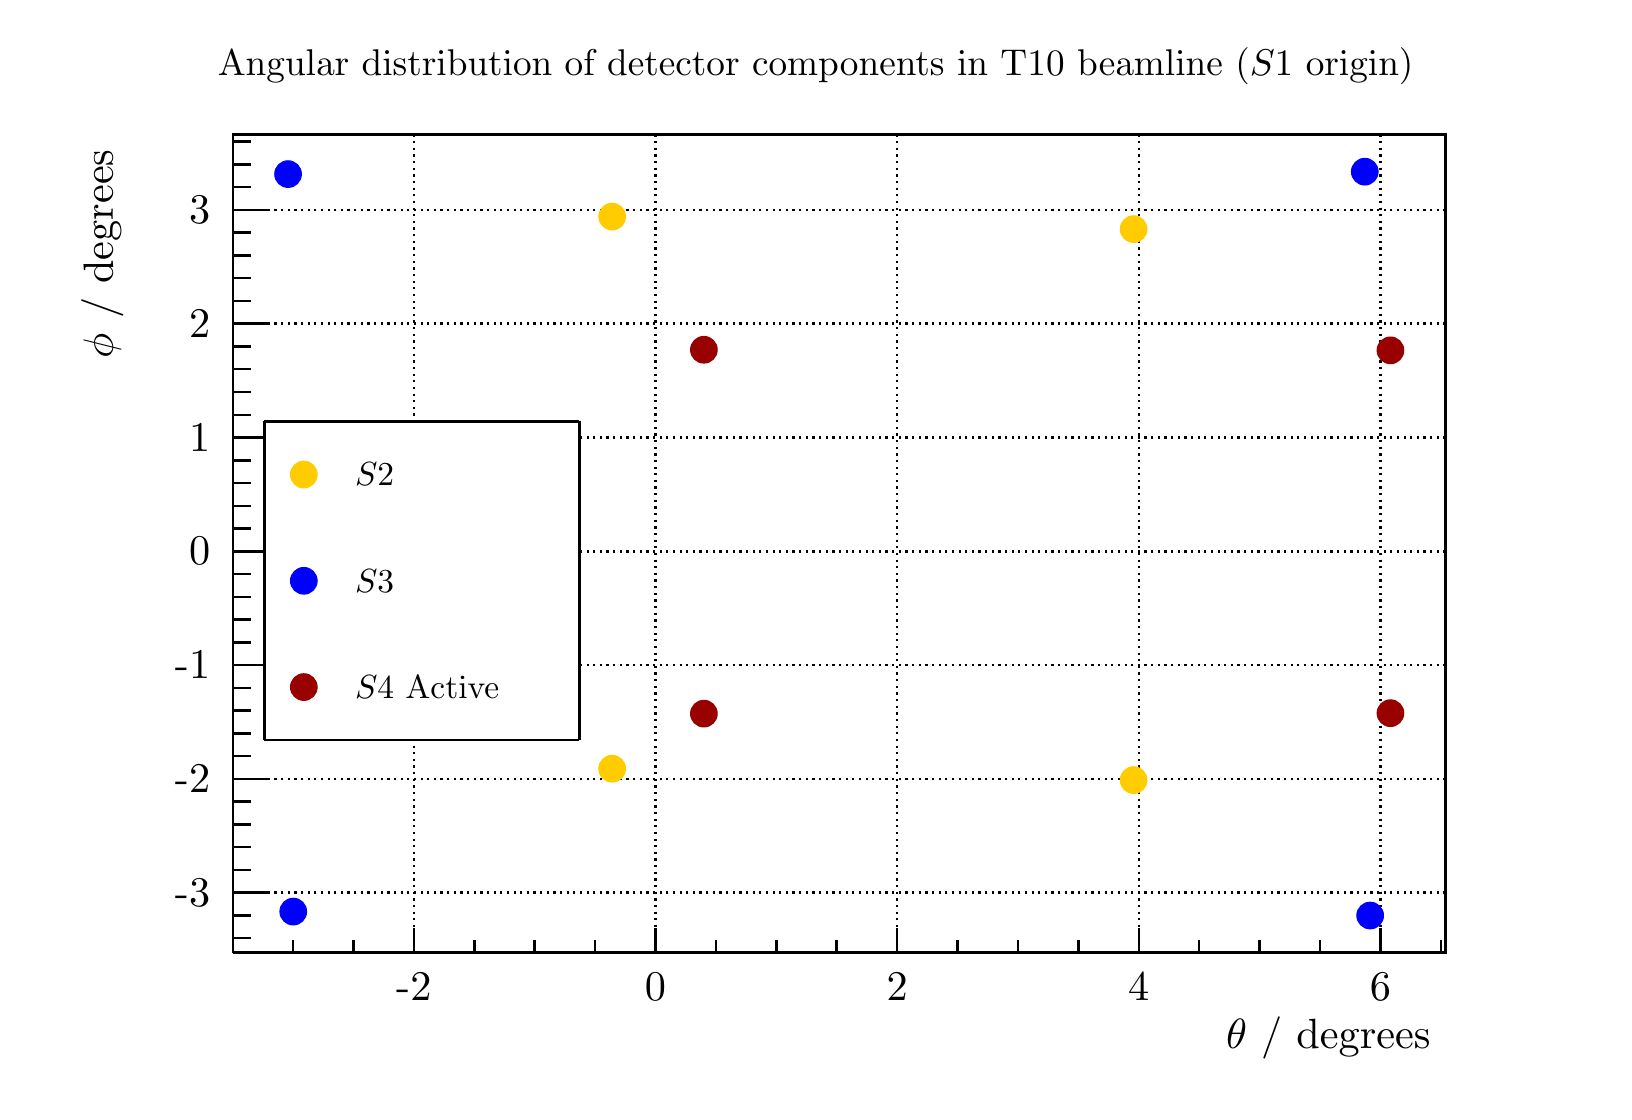
\begin{tikzpicture}
\pgfdeclareplotmark{cross} {
\pgfpathmoveto{\pgfpoint{-0.3\pgfplotmarksize}{\pgfplotmarksize}}
\pgfpathlineto{\pgfpoint{+0.3\pgfplotmarksize}{\pgfplotmarksize}}
\pgfpathlineto{\pgfpoint{+0.3\pgfplotmarksize}{0.3\pgfplotmarksize}}
\pgfpathlineto{\pgfpoint{+1\pgfplotmarksize}{0.3\pgfplotmarksize}}
\pgfpathlineto{\pgfpoint{+1\pgfplotmarksize}{-0.3\pgfplotmarksize}}
\pgfpathlineto{\pgfpoint{+0.3\pgfplotmarksize}{-0.3\pgfplotmarksize}}
\pgfpathlineto{\pgfpoint{+0.3\pgfplotmarksize}{-1.\pgfplotmarksize}}
\pgfpathlineto{\pgfpoint{-0.3\pgfplotmarksize}{-1.\pgfplotmarksize}}
\pgfpathlineto{\pgfpoint{-0.3\pgfplotmarksize}{-0.3\pgfplotmarksize}}
\pgfpathlineto{\pgfpoint{-1.\pgfplotmarksize}{-0.3\pgfplotmarksize}}
\pgfpathlineto{\pgfpoint{-1.\pgfplotmarksize}{0.3\pgfplotmarksize}}
\pgfpathlineto{\pgfpoint{-0.3\pgfplotmarksize}{0.3\pgfplotmarksize}}
\pgfpathclose
\pgfusepathqstroke
}
\pgfdeclareplotmark{cross*} {
\pgfpathmoveto{\pgfpoint{-0.3\pgfplotmarksize}{\pgfplotmarksize}}
\pgfpathlineto{\pgfpoint{+0.3\pgfplotmarksize}{\pgfplotmarksize}}
\pgfpathlineto{\pgfpoint{+0.3\pgfplotmarksize}{0.3\pgfplotmarksize}}
\pgfpathlineto{\pgfpoint{+1\pgfplotmarksize}{0.3\pgfplotmarksize}}
\pgfpathlineto{\pgfpoint{+1\pgfplotmarksize}{-0.3\pgfplotmarksize}}
\pgfpathlineto{\pgfpoint{+0.3\pgfplotmarksize}{-0.3\pgfplotmarksize}}
\pgfpathlineto{\pgfpoint{+0.3\pgfplotmarksize}{-1.\pgfplotmarksize}}
\pgfpathlineto{\pgfpoint{-0.3\pgfplotmarksize}{-1.\pgfplotmarksize}}
\pgfpathlineto{\pgfpoint{-0.3\pgfplotmarksize}{-0.3\pgfplotmarksize}}
\pgfpathlineto{\pgfpoint{-1.\pgfplotmarksize}{-0.3\pgfplotmarksize}}
\pgfpathlineto{\pgfpoint{-1.\pgfplotmarksize}{0.3\pgfplotmarksize}}
\pgfpathlineto{\pgfpoint{-0.3\pgfplotmarksize}{0.3\pgfplotmarksize}}
\pgfpathclose
\pgfusepathqfillstroke
}
\pgfdeclareplotmark{newstar} {
\pgfpathmoveto{\pgfqpoint{0pt}{\pgfplotmarksize}}
\pgfpathlineto{\pgfqpointpolar{44}{0.5\pgfplotmarksize}}
\pgfpathlineto{\pgfqpointpolar{18}{\pgfplotmarksize}}
\pgfpathlineto{\pgfqpointpolar{-20}{0.5\pgfplotmarksize}}
\pgfpathlineto{\pgfqpointpolar{-54}{\pgfplotmarksize}}
\pgfpathlineto{\pgfqpointpolar{-90}{0.5\pgfplotmarksize}}
\pgfpathlineto{\pgfqpointpolar{234}{\pgfplotmarksize}}
\pgfpathlineto{\pgfqpointpolar{198}{0.5\pgfplotmarksize}}
\pgfpathlineto{\pgfqpointpolar{162}{\pgfplotmarksize}}
\pgfpathlineto{\pgfqpointpolar{134}{0.5\pgfplotmarksize}}
\pgfpathclose
\pgfusepathqstroke
}
\pgfdeclareplotmark{newstar*} {
\pgfpathmoveto{\pgfqpoint{0pt}{\pgfplotmarksize}}
\pgfpathlineto{\pgfqpointpolar{44}{0.5\pgfplotmarksize}}
\pgfpathlineto{\pgfqpointpolar{18}{\pgfplotmarksize}}
\pgfpathlineto{\pgfqpointpolar{-20}{0.5\pgfplotmarksize}}
\pgfpathlineto{\pgfqpointpolar{-54}{\pgfplotmarksize}}
\pgfpathlineto{\pgfqpointpolar{-90}{0.5\pgfplotmarksize}}
\pgfpathlineto{\pgfqpointpolar{234}{\pgfplotmarksize}}
\pgfpathlineto{\pgfqpointpolar{198}{0.5\pgfplotmarksize}}
\pgfpathlineto{\pgfqpointpolar{162}{\pgfplotmarksize}}
\pgfpathlineto{\pgfqpointpolar{134}{0.5\pgfplotmarksize}}
\pgfpathclose
\pgfusepathqfillstroke
}
\definecolor{c}{rgb}{1,1,1};
\draw [color=c, fill=c] (0,0) rectangle (20,13.4957);
\draw [color=c, fill=c] (2.6,1.75444) rectangle (18,12.1461);
\definecolor{c}{rgb}{0,0,0};
\draw [c,line width=0.9] (2.6,1.75444) -- (2.6,12.1461) -- (18,12.1461) -- (18,1.75444) -- (2.6,1.75444);
\definecolor{c}{rgb}{1,1,1};
\draw [color=c, fill=c] (2.6,1.75444) rectangle (18,12.1461);
\definecolor{c}{rgb}{0,0,0};
\draw [c,line width=0.9] (2.6,1.75444) -- (2.6,12.1461) -- (18,12.1461) -- (18,1.75444) -- (2.6,1.75444);
\draw [c,line width=0.9] (2.6,1.75444) -- (18,1.75444);
\draw [c,dash pattern=on 0.80pt off 1.60pt ,line width=0.9] (4.89745,12.1461) -- (4.89745,1.75444);
\draw [c,dash pattern=on 0.80pt off 1.60pt ,line width=0.9] (7.96612,12.1461) -- (7.96612,1.75444);
\draw [c,dash pattern=on 0.80pt off 1.60pt ,line width=0.9] (11.0348,12.1461) -- (11.0348,1.75444);
\draw [c,dash pattern=on 0.80pt off 1.60pt ,line width=0.9] (14.1035,12.1461) -- (14.1035,1.75444);
\draw [c,dash pattern=on 0.80pt off 1.60pt ,line width=0.9] (17.1721,12.1461) -- (17.1721,1.75444);
\draw [c,dash pattern=on 0.80pt off 1.60pt ,line width=0.9] (4.89745,12.1461) -- (4.89745,1.75444);
\draw [c,dash pattern=on 0.80pt off 1.60pt ,line width=0.9] (17.1721,12.1461) -- (17.1721,1.75444);
\draw [c,line width=0.9] (2.6,1.75444) -- (2.6,12.1461);
\draw [c,dash pattern=on 0.80pt off 1.60pt ,line width=0.9] (18,2.51696) -- (2.6,2.51696);
\draw [c,dash pattern=on 0.80pt off 1.60pt ,line width=0.9] (18,3.96211) -- (2.6,3.96211);
\draw [c,dash pattern=on 0.80pt off 1.60pt ,line width=0.9] (18,5.40726) -- (2.6,5.40726);
\draw [c,dash pattern=on 0.80pt off 1.60pt ,line width=0.9] (18,6.85241) -- (2.6,6.85241);
\draw [c,dash pattern=on 0.80pt off 1.60pt ,line width=0.9] (18,8.29756) -- (2.6,8.29756);
\draw [c,dash pattern=on 0.80pt off 1.60pt ,line width=0.9] (18,9.74271) -- (2.6,9.74271);
\draw [c,dash pattern=on 0.80pt off 1.60pt ,line width=0.9] (18,11.1879) -- (2.6,11.1879);
\draw [c,dash pattern=on 0.80pt off 1.60pt ,line width=0.9] (18,2.51696) -- (2.6,2.51696);
\draw [c,dash pattern=on 0.80pt off 1.60pt ,line width=0.9] (18,11.1879) -- (2.6,11.1879);
\draw [c,line width=0.9] (2.6,1.75444) -- (18,1.75444);
\draw [c,line width=0.9] (4.89745,2.06619) -- (4.89745,1.75444);
\draw [c,line width=0.9] (5.66462,1.91032) -- (5.66462,1.75444);
\draw [c,line width=0.9] (6.43179,1.91032) -- (6.43179,1.75444);
\draw [c,line width=0.9] (7.19896,1.91032) -- (7.19896,1.75444);
\draw [c,line width=0.9] (7.96612,2.06619) -- (7.96612,1.75444);
\draw [c,line width=0.9] (8.73329,1.91032) -- (8.73329,1.75444);
\draw [c,line width=0.9] (9.50046,1.91032) -- (9.50046,1.75444);
\draw [c,line width=0.9] (10.2676,1.91032) -- (10.2676,1.75444);
\draw [c,line width=0.9] (11.0348,2.06619) -- (11.0348,1.75444);
\draw [c,line width=0.9] (11.802,1.91032) -- (11.802,1.75444);
\draw [c,line width=0.9] (12.5691,1.91032) -- (12.5691,1.75444);
\draw [c,line width=0.9] (13.3363,1.91032) -- (13.3363,1.75444);
\draw [c,line width=0.9] (14.1035,2.06619) -- (14.1035,1.75444);
\draw [c,line width=0.9] (14.8706,1.91032) -- (14.8706,1.75444);
\draw [c,line width=0.9] (15.6378,1.91032) -- (15.6378,1.75444);
\draw [c,line width=0.9] (16.405,1.91032) -- (16.405,1.75444);
\draw [c,line width=0.9] (17.1721,2.06619) -- (17.1721,1.75444);
\draw [c,line width=0.9] (4.89745,2.06619) -- (4.89745,1.75444);
\draw [c,line width=0.9] (4.13029,1.91032) -- (4.13029,1.75444);
\draw [c,line width=0.9] (3.36312,1.91032) -- (3.36312,1.75444);
\draw [c,line width=0.9] (17.1721,2.06619) -- (17.1721,1.75444);
\draw [c,line width=0.9] (17.9393,1.91032) -- (17.9393,1.75444);
\draw [anchor=base] (4.89745,1.14713) node[scale=1.52731, color=c, rotate=0]{-2};
\draw [anchor=base] (7.96612,1.14713) node[scale=1.52731, color=c, rotate=0]{0};
\draw [anchor=base] (11.0348,1.14713) node[scale=1.52731, color=c, rotate=0]{2};
\draw [anchor=base] (14.1035,1.14713) node[scale=1.52731, color=c, rotate=0]{4};
\draw [anchor=base] (17.1721,1.14713) node[scale=1.52731, color=c, rotate=0]{6};
\draw [anchor= east] (18,0.674785) node[scale=1.52731, color=c, rotate=0]{$\theta$ / degrees};
\draw [c,line width=0.9] (2.6,1.75444) -- (2.6,12.1461);
\draw [c,line width=0.9] (3.062,2.51696) -- (2.6,2.51696);
\draw [c,line width=0.9] (2.831,2.80599) -- (2.6,2.80599);
\draw [c,line width=0.9] (2.831,3.09502) -- (2.6,3.09502);
\draw [c,line width=0.9] (2.831,3.38405) -- (2.6,3.38405);
\draw [c,line width=0.9] (2.831,3.67308) -- (2.6,3.67308);
\draw [c,line width=0.9] (3.062,3.96211) -- (2.6,3.96211);
\draw [c,line width=0.9] (2.831,4.25114) -- (2.6,4.25114);
\draw [c,line width=0.9] (2.831,4.54017) -- (2.6,4.54017);
\draw [c,line width=0.9] (2.831,4.8292) -- (2.6,4.8292);
\draw [c,line width=0.9] (2.831,5.11823) -- (2.6,5.11823);
\draw [c,line width=0.9] (3.062,5.40726) -- (2.6,5.40726);
\draw [c,line width=0.9] (2.831,5.69629) -- (2.6,5.69629);
\draw [c,line width=0.9] (2.831,5.98532) -- (2.6,5.98532);
\draw [c,line width=0.9] (2.831,6.27435) -- (2.6,6.27435);
\draw [c,line width=0.9] (2.831,6.56338) -- (2.6,6.56338);
\draw [c,line width=0.9] (3.062,6.85241) -- (2.6,6.85241);
\draw [c,line width=0.9] (2.831,7.14144) -- (2.6,7.14144);
\draw [c,line width=0.9] (2.831,7.43047) -- (2.6,7.43047);
\draw [c,line width=0.9] (2.831,7.7195) -- (2.6,7.7195);
\draw [c,line width=0.9] (2.831,8.00853) -- (2.6,8.00853);
\draw [c,line width=0.9] (3.062,8.29756) -- (2.6,8.29756);
\draw [c,line width=0.9] (2.831,8.58659) -- (2.6,8.58659);
\draw [c,line width=0.9] (2.831,8.87562) -- (2.6,8.87562);
\draw [c,line width=0.9] (2.831,9.16465) -- (2.6,9.16465);
\draw [c,line width=0.9] (2.831,9.45368) -- (2.6,9.45368);
\draw [c,line width=0.9] (3.062,9.74271) -- (2.6,9.74271);
\draw [c,line width=0.9] (2.831,10.0317) -- (2.6,10.0317);
\draw [c,line width=0.9] (2.831,10.3208) -- (2.6,10.3208);
\draw [c,line width=0.9] (2.831,10.6098) -- (2.6,10.6098);
\draw [c,line width=0.9] (2.831,10.8988) -- (2.6,10.8988);
\draw [c,line width=0.9] (3.062,11.1879) -- (2.6,11.1879);
\draw [c,line width=0.9] (3.062,2.51696) -- (2.6,2.51696);
\draw [c,line width=0.9] (2.831,2.22793) -- (2.6,2.22793);
\draw [c,line width=0.9] (2.831,1.9389) -- (2.6,1.9389);
\draw [c,line width=0.9] (3.062,11.1879) -- (2.6,11.1879);
\draw [c,line width=0.9] (2.831,11.4769) -- (2.6,11.4769);
\draw [c,line width=0.9] (2.831,11.7659) -- (2.6,11.7659);
\draw [c,line width=0.9] (2.831,12.055) -- (2.6,12.055);
\draw [anchor= east] (2.5,2.51696) node[scale=1.52731, color=c, rotate=0]{-3};
\draw [anchor= east] (2.5,3.96211) node[scale=1.52731, color=c, rotate=0]{-2};
\draw [anchor= east] (2.5,5.40726) node[scale=1.52731, color=c, rotate=0]{-1};
\draw [anchor= east] (2.5,6.85241) node[scale=1.52731, color=c, rotate=0]{0};
\draw [anchor= east] (2.5,8.29756) node[scale=1.52731, color=c, rotate=0]{1};
\draw [anchor= east] (2.5,9.74271) node[scale=1.52731, color=c, rotate=0]{2};
\draw [anchor= east] (2.5,11.1879) node[scale=1.52731, color=c, rotate=0]{3};
\draw [anchor= east] (0.940974,12.1461) node[scale=1.52731, color=c, rotate=90]{$\phi$ / degrees};
\definecolor{c}{rgb}{1,0.8,0};
\foreach \P in {(7.41566,11.1035), (7.41566,4.09158), (14.0382,3.94708), (14.0382,10.9445)}{\draw[mark options={color=c,fill=c},mark size=4.804805pt,mark=*] plot coordinates {\P};}
\definecolor{c}{rgb}{0,0,1};
\foreach \P in {(3.3,11.6431), (16.9742,11.6738), (3.36572,2.27713), (17.0424,2.22679)}{\draw[mark options={color=c,fill=c},mark size=4.804805pt,mark=*] plot coordinates {\P};}
\definecolor{c}{rgb}{0.6,0,0};
\foreach \P in {(8.58078,9.41224), (17.3,9.4046), (8.58078,4.79087), (17.3,4.79702)}{\draw[mark options={color=c,fill=c},mark size=4.804805pt,mark=*] plot coordinates {\P};}
\definecolor{c}{rgb}{1,1,1};
\draw [color=c, fill=c] (3,4.45358) rectangle (7,8.50229);
\definecolor{c}{rgb}{0,0,0};
\draw [c,line width=0.9] (3,4.45358) -- (7,4.45358);
\draw [c,line width=0.9] (7,4.45358) -- (7,8.50229);
\draw [c,line width=0.9] (7,8.50229) -- (3,8.50229);
\draw [c,line width=0.9] (3,8.50229) -- (3,4.45358);
\draw [anchor= west] (4,7.82751) node[scale=1.20912, color=c, rotate=0]{$S2$};
\definecolor{c}{rgb}{1,0.8,0};
\foreach \P in {(3.5,7.82751)}{\draw[mark options={color=c,fill=c},mark size=4.804805pt,mark=*] plot coordinates {\P};}
\definecolor{c}{rgb}{0,0,0};
\draw [anchor= west] (4,6.47794) node[scale=1.20912, color=c, rotate=0]{$S3$};
\definecolor{c}{rgb}{0,0,1};
\foreach \P in {(3.5,6.47794)}{\draw[mark options={color=c,fill=c},mark size=4.804805pt,mark=*] plot coordinates {\P};}
\definecolor{c}{rgb}{0,0,0};
\draw [anchor= west] (4,5.12837) node[scale=1.20912, color=c, rotate=0]{$S4$ Active};
\definecolor{c}{rgb}{0.6,0,0};
\foreach \P in {(3.5,5.12837)}{\draw[mark options={color=c,fill=c},mark size=4.804805pt,mark=*] plot coordinates {\P};}
\definecolor{c}{rgb}{0,0,0};
\draw (10,13.0156) node[scale=1.34549, color=c, rotate=0]{Angular distribution of detector components in T10 beamline ($S1$ origin)};
\end{tikzpicture}

    \end{adjustbox}
    \centering
    \caption{Diagram showing the angular location of the extremities of the timing points. The coordinate system used has the origin at the $\mathit{S1}$ timing point, with the $x$ axis running parallel to the nominal beam axis.}
    \label{fig:beamAng}
  \end{minipage}
  \hfill
  \begin{minipage}{0.49\textwidth}
    \begin{adjustbox}{max totalsize={\textwidth}{0.5\textheight}, center}
      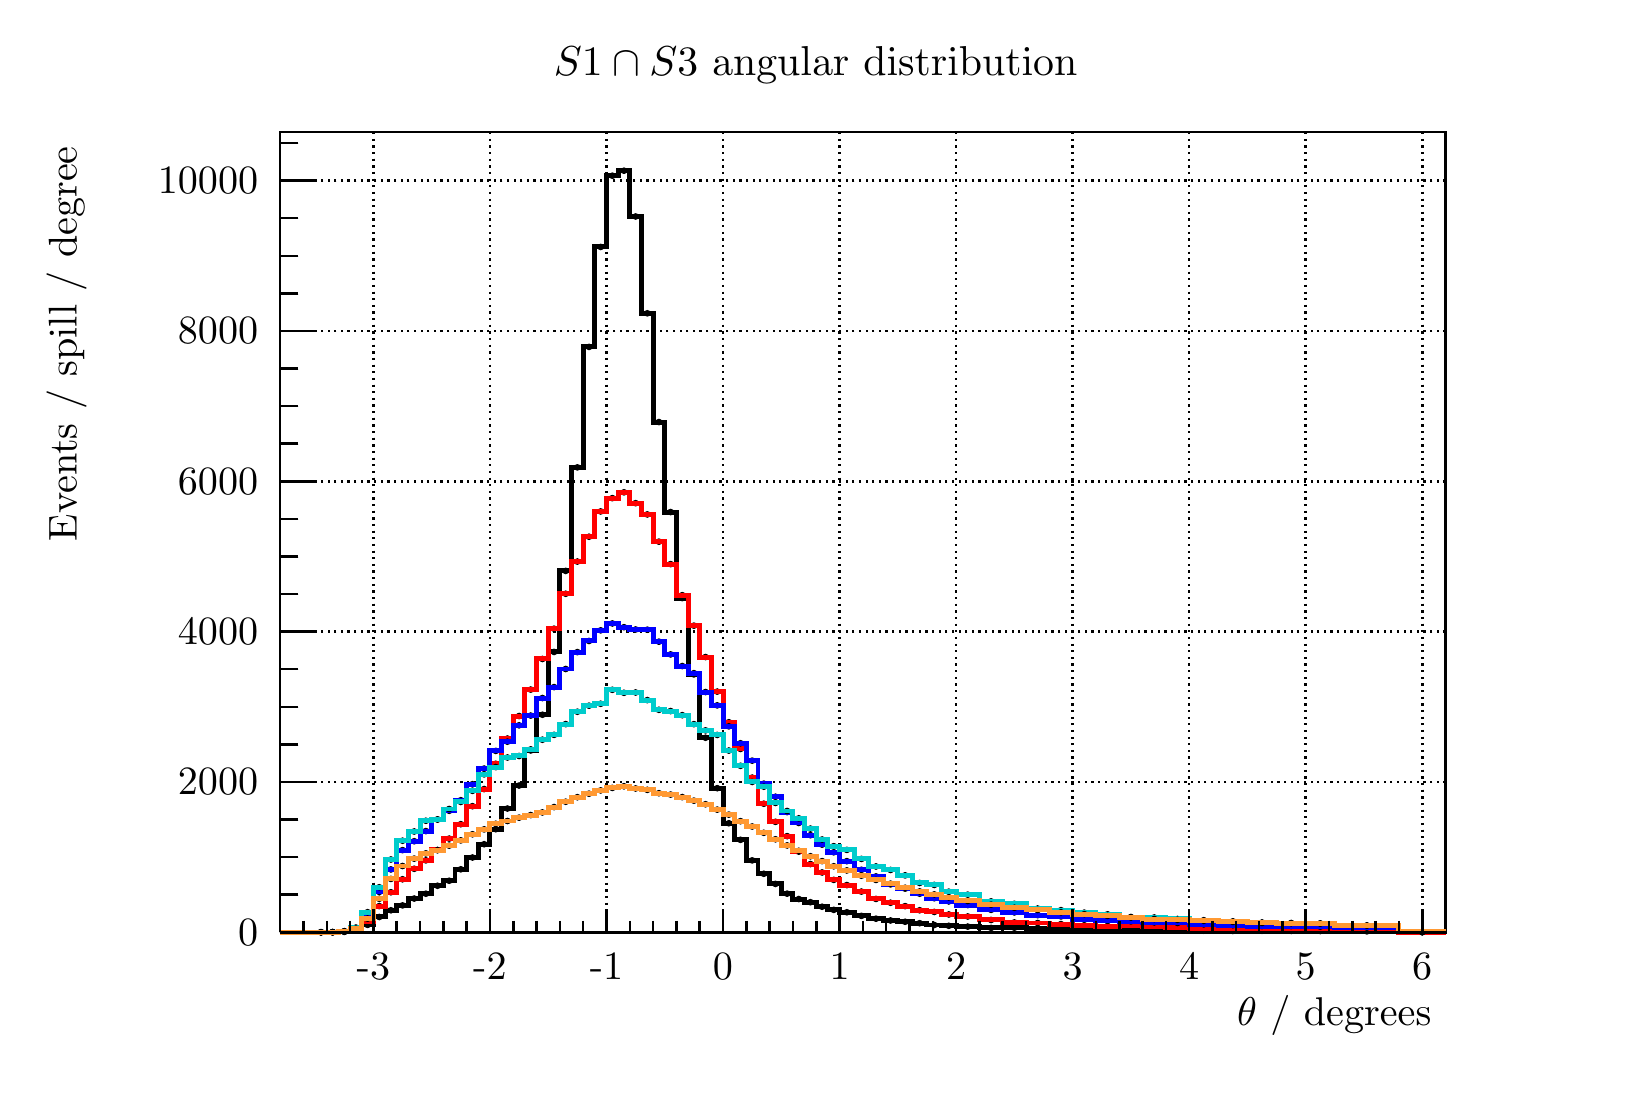
\begin{tikzpicture}
\pgfdeclareplotmark{cross} {
\pgfpathmoveto{\pgfpoint{-0.3\pgfplotmarksize}{\pgfplotmarksize}}
\pgfpathlineto{\pgfpoint{+0.3\pgfplotmarksize}{\pgfplotmarksize}}
\pgfpathlineto{\pgfpoint{+0.3\pgfplotmarksize}{0.3\pgfplotmarksize}}
\pgfpathlineto{\pgfpoint{+1\pgfplotmarksize}{0.3\pgfplotmarksize}}
\pgfpathlineto{\pgfpoint{+1\pgfplotmarksize}{-0.3\pgfplotmarksize}}
\pgfpathlineto{\pgfpoint{+0.3\pgfplotmarksize}{-0.3\pgfplotmarksize}}
\pgfpathlineto{\pgfpoint{+0.3\pgfplotmarksize}{-1.\pgfplotmarksize}}
\pgfpathlineto{\pgfpoint{-0.3\pgfplotmarksize}{-1.\pgfplotmarksize}}
\pgfpathlineto{\pgfpoint{-0.3\pgfplotmarksize}{-0.3\pgfplotmarksize}}
\pgfpathlineto{\pgfpoint{-1.\pgfplotmarksize}{-0.3\pgfplotmarksize}}
\pgfpathlineto{\pgfpoint{-1.\pgfplotmarksize}{0.3\pgfplotmarksize}}
\pgfpathlineto{\pgfpoint{-0.3\pgfplotmarksize}{0.3\pgfplotmarksize}}
\pgfpathclose
\pgfusepathqstroke
}
\pgfdeclareplotmark{cross*} {
\pgfpathmoveto{\pgfpoint{-0.3\pgfplotmarksize}{\pgfplotmarksize}}
\pgfpathlineto{\pgfpoint{+0.3\pgfplotmarksize}{\pgfplotmarksize}}
\pgfpathlineto{\pgfpoint{+0.3\pgfplotmarksize}{0.3\pgfplotmarksize}}
\pgfpathlineto{\pgfpoint{+1\pgfplotmarksize}{0.3\pgfplotmarksize}}
\pgfpathlineto{\pgfpoint{+1\pgfplotmarksize}{-0.3\pgfplotmarksize}}
\pgfpathlineto{\pgfpoint{+0.3\pgfplotmarksize}{-0.3\pgfplotmarksize}}
\pgfpathlineto{\pgfpoint{+0.3\pgfplotmarksize}{-1.\pgfplotmarksize}}
\pgfpathlineto{\pgfpoint{-0.3\pgfplotmarksize}{-1.\pgfplotmarksize}}
\pgfpathlineto{\pgfpoint{-0.3\pgfplotmarksize}{-0.3\pgfplotmarksize}}
\pgfpathlineto{\pgfpoint{-1.\pgfplotmarksize}{-0.3\pgfplotmarksize}}
\pgfpathlineto{\pgfpoint{-1.\pgfplotmarksize}{0.3\pgfplotmarksize}}
\pgfpathlineto{\pgfpoint{-0.3\pgfplotmarksize}{0.3\pgfplotmarksize}}
\pgfpathclose
\pgfusepathqfillstroke
}
\pgfdeclareplotmark{newstar} {
\pgfpathmoveto{\pgfqpoint{0pt}{\pgfplotmarksize}}
\pgfpathlineto{\pgfqpointpolar{44}{0.5\pgfplotmarksize}}
\pgfpathlineto{\pgfqpointpolar{18}{\pgfplotmarksize}}
\pgfpathlineto{\pgfqpointpolar{-20}{0.5\pgfplotmarksize}}
\pgfpathlineto{\pgfqpointpolar{-54}{\pgfplotmarksize}}
\pgfpathlineto{\pgfqpointpolar{-90}{0.5\pgfplotmarksize}}
\pgfpathlineto{\pgfqpointpolar{234}{\pgfplotmarksize}}
\pgfpathlineto{\pgfqpointpolar{198}{0.5\pgfplotmarksize}}
\pgfpathlineto{\pgfqpointpolar{162}{\pgfplotmarksize}}
\pgfpathlineto{\pgfqpointpolar{134}{0.5\pgfplotmarksize}}
\pgfpathclose
\pgfusepathqstroke
}
\pgfdeclareplotmark{newstar*} {
\pgfpathmoveto{\pgfqpoint{0pt}{\pgfplotmarksize}}
\pgfpathlineto{\pgfqpointpolar{44}{0.5\pgfplotmarksize}}
\pgfpathlineto{\pgfqpointpolar{18}{\pgfplotmarksize}}
\pgfpathlineto{\pgfqpointpolar{-20}{0.5\pgfplotmarksize}}
\pgfpathlineto{\pgfqpointpolar{-54}{\pgfplotmarksize}}
\pgfpathlineto{\pgfqpointpolar{-90}{0.5\pgfplotmarksize}}
\pgfpathlineto{\pgfqpointpolar{234}{\pgfplotmarksize}}
\pgfpathlineto{\pgfqpointpolar{198}{0.5\pgfplotmarksize}}
\pgfpathlineto{\pgfqpointpolar{162}{\pgfplotmarksize}}
\pgfpathlineto{\pgfqpointpolar{134}{0.5\pgfplotmarksize}}
\pgfpathclose
\pgfusepathqfillstroke
}
\definecolor{c}{rgb}{1,1,1};
\draw [color=c, fill=c] (0,0) rectangle (20,13.1973);
\draw [color=c, fill=c] (3.2,1.71565) rectangle (18,11.8776);
\definecolor{c}{rgb}{0,0,0};
\draw [c,line width=0.9] (3.2,1.71565) -- (3.2,11.8776) -- (18,11.8776) -- (18,1.71565) -- (3.2,1.71565);
\definecolor{c}{rgb}{1,1,1};
\draw [color=c, fill=c] (3.2,1.71565) rectangle (18,11.8776);
\definecolor{c}{rgb}{0,0,0};
\draw [c,line width=0.9] (3.2,1.71565) -- (3.2,11.8776) -- (18,11.8776) -- (18,1.71565) -- (3.2,1.71565);
\draw [c,line width=0.9] (3.2,1.71565) -- (18,1.71565);
\draw [c,dash pattern=on 0.80pt off 1.60pt ,line width=0.9] (4.384,11.8776) -- (4.384,1.71565);
\draw [c,dash pattern=on 0.80pt off 1.60pt ,line width=0.9] (5.864,11.8776) -- (5.864,1.71565);
\draw [c,dash pattern=on 0.80pt off 1.60pt ,line width=0.9] (7.344,11.8776) -- (7.344,1.71565);
\draw [c,dash pattern=on 0.80pt off 1.60pt ,line width=0.9] (8.824,11.8776) -- (8.824,1.71565);
\draw [c,dash pattern=on 0.80pt off 1.60pt ,line width=0.9] (10.304,11.8776) -- (10.304,1.71565);
\draw [c,dash pattern=on 0.80pt off 1.60pt ,line width=0.9] (11.784,11.8776) -- (11.784,1.71565);
\draw [c,dash pattern=on 0.80pt off 1.60pt ,line width=0.9] (13.264,11.8776) -- (13.264,1.71565);
\draw [c,dash pattern=on 0.80pt off 1.60pt ,line width=0.9] (14.744,11.8776) -- (14.744,1.71565);
\draw [c,dash pattern=on 0.80pt off 1.60pt ,line width=0.9] (16.224,11.8776) -- (16.224,1.71565);
\draw [c,dash pattern=on 0.80pt off 1.60pt ,line width=0.9] (17.704,11.8776) -- (17.704,1.71565);
\draw [c,dash pattern=on 0.80pt off 1.60pt ,line width=0.9] (4.384,11.8776) -- (4.384,1.71565);
\draw [c,dash pattern=on 0.80pt off 1.60pt ,line width=0.9] (17.704,11.8776) -- (17.704,1.71565);
\draw [c,line width=0.9] (3.2,1.71565) -- (3.2,11.8776);
\draw [c,dash pattern=on 0.80pt off 1.60pt ,line width=0.9] (18,1.71565) -- (3.2,1.71565);
\draw [c,dash pattern=on 0.80pt off 1.60pt ,line width=0.9] (18,3.62476) -- (3.2,3.62476);
\draw [c,dash pattern=on 0.80pt off 1.60pt ,line width=0.9] (18,5.53388) -- (3.2,5.53388);
\draw [c,dash pattern=on 0.80pt off 1.60pt ,line width=0.9] (18,7.443) -- (3.2,7.443);
\draw [c,dash pattern=on 0.80pt off 1.60pt ,line width=0.9] (18,9.35212) -- (3.2,9.35212);
\draw [c,dash pattern=on 0.80pt off 1.60pt ,line width=0.9] (18,11.2612) -- (3.2,11.2612);
\draw [c,dash pattern=on 0.80pt off 1.60pt ,line width=0.9] (18,11.2612) -- (3.2,11.2612);
\definecolor{c}{rgb}{0,0,0.6};
\draw [c,line width=0.9] (3.2,1.71565) -- (3.348,1.71565) -- (3.348,1.71565) -- (3.496,1.71565) -- (3.496,1.71565) -- (3.644,1.71565) -- (3.644,1.71565) -- (3.792,1.71565) -- (3.792,1.71565) -- (3.94,1.71565) -- (3.94,1.71565) -- (4.088,1.71565) --
 (4.088,1.71565) -- (4.236,1.71565) -- (4.236,1.71565) -- (4.384,1.71565) -- (4.384,1.71565) -- (4.532,1.71565) -- (4.532,1.71565) -- (4.68,1.71565) -- (4.68,1.71565) -- (4.828,1.71565) -- (4.828,1.71565) -- (4.976,1.71565) -- (4.976,1.71565) --
 (5.124,1.71565) -- (5.124,1.71565) -- (5.272,1.71565) -- (5.272,1.71565) -- (5.42,1.71565) -- (5.42,1.71565) -- (5.568,1.71565) -- (5.568,1.71565) -- (5.716,1.71565) -- (5.716,1.71565) -- (5.864,1.71565) -- (5.864,1.71565) -- (6.012,1.71565) --
 (6.012,1.71565) -- (6.16,1.71565) -- (6.16,1.71565) -- (6.308,1.71565) -- (6.308,1.71565) -- (6.456,1.71565) -- (6.456,1.71565) -- (6.604,1.71565) -- (6.604,1.71565) -- (6.752,1.71565) -- (6.752,1.71565) -- (6.9,1.71565) -- (6.9,1.71565) --
 (7.048,1.71565) -- (7.048,1.71565) -- (7.196,1.71565) -- (7.196,1.71565) -- (7.344,1.71565) -- (7.344,1.71565) -- (7.492,1.71565) -- (7.492,1.71565) -- (7.64,1.71565) -- (7.64,1.71565) -- (7.788,1.71565) -- (7.788,1.71565) -- (7.936,1.71565) --
 (7.936,1.71565) -- (8.084,1.71565) -- (8.084,1.71565) -- (8.232,1.71565) -- (8.232,1.71565) -- (8.38,1.71565) -- (8.38,1.71565) -- (8.528,1.71565) -- (8.528,1.71565) -- (8.676,1.71565) -- (8.676,1.71565) -- (8.824,1.71565) -- (8.824,1.71565) --
 (8.972,1.71565) -- (8.972,1.71565) -- (9.12,1.71565) -- (9.12,1.71565) -- (9.268,1.71565) -- (9.268,1.71565) -- (9.416,1.71565) -- (9.416,1.71565) -- (9.564,1.71565) -- (9.564,1.71565) -- (9.712,1.71565) -- (9.712,1.71565) -- (9.86,1.71565) --
 (9.86,1.71565) -- (10.008,1.71565) -- (10.008,1.71565) -- (10.156,1.71565) -- (10.156,1.71565) -- (10.304,1.71565) -- (10.304,1.71565) -- (10.489,1.71565) -- (10.489,1.71565) -- (10.674,1.71565) -- (10.674,1.71565) -- (10.859,1.71565) --
 (10.859,1.71565) -- (11.044,1.71565) -- (11.044,1.71565) -- (11.229,1.71565) -- (11.229,1.71565) -- (11.414,1.71565) -- (11.414,1.71565) -- (11.599,1.71565) -- (11.599,1.71565) -- (11.784,1.71565) -- (11.784,1.71565) -- (12.08,1.71565) --
 (12.08,1.71565) -- (12.376,1.71565) -- (12.376,1.71565) -- (12.672,1.71565) -- (12.672,1.71565) -- (12.968,1.71565) -- (12.968,1.71565) -- (13.264,1.71565) -- (13.264,1.71565) -- (13.56,1.71565) -- (13.56,1.71565) -- (13.856,1.71565) --
 (13.856,1.71565) -- (14.152,1.71565) -- (14.152,1.71565) -- (14.448,1.71565) -- (14.448,1.71565) -- (14.744,1.71565) -- (14.744,1.71565) -- (15.114,1.71565) -- (15.114,1.71565) -- (15.484,1.71565) -- (15.484,1.71565) -- (15.854,1.71565) --
 (15.854,1.71565) -- (16.224,1.71565) -- (16.224,1.71565) -- (16.594,1.71565) -- (16.594,1.71565) -- (17.408,1.71565) -- (17.408,1.71565) -- (18,1.71565);
\definecolor{c}{rgb}{0,0,0};
\draw [c,line width=0.9] (3.2,1.71565) -- (18,1.71565);
\draw [c,line width=0.9] (4.384,2.00863) -- (4.384,1.71565);
\draw [c,line width=0.9] (4.68,1.86214) -- (4.68,1.71565);
\draw [c,line width=0.9] (4.976,1.86214) -- (4.976,1.71565);
\draw [c,line width=0.9] (5.272,1.86214) -- (5.272,1.71565);
\draw [c,line width=0.9] (5.568,1.86214) -- (5.568,1.71565);
\draw [c,line width=0.9] (5.864,2.00863) -- (5.864,1.71565);
\draw [c,line width=0.9] (6.16,1.86214) -- (6.16,1.71565);
\draw [c,line width=0.9] (6.456,1.86214) -- (6.456,1.71565);
\draw [c,line width=0.9] (6.752,1.86214) -- (6.752,1.71565);
\draw [c,line width=0.9] (7.048,1.86214) -- (7.048,1.71565);
\draw [c,line width=0.9] (7.344,2.00863) -- (7.344,1.71565);
\draw [c,line width=0.9] (7.64,1.86214) -- (7.64,1.71565);
\draw [c,line width=0.9] (7.936,1.86214) -- (7.936,1.71565);
\draw [c,line width=0.9] (8.232,1.86214) -- (8.232,1.71565);
\draw [c,line width=0.9] (8.528,1.86214) -- (8.528,1.71565);
\draw [c,line width=0.9] (8.824,2.00863) -- (8.824,1.71565);
\draw [c,line width=0.9] (9.12,1.86214) -- (9.12,1.71565);
\draw [c,line width=0.9] (9.416,1.86214) -- (9.416,1.71565);
\draw [c,line width=0.9] (9.712,1.86214) -- (9.712,1.71565);
\draw [c,line width=0.9] (10.008,1.86214) -- (10.008,1.71565);
\draw [c,line width=0.9] (10.304,2.00863) -- (10.304,1.71565);
\draw [c,line width=0.9] (10.6,1.86214) -- (10.6,1.71565);
\draw [c,line width=0.9] (10.896,1.86214) -- (10.896,1.71565);
\draw [c,line width=0.9] (11.192,1.86214) -- (11.192,1.71565);
\draw [c,line width=0.9] (11.488,1.86214) -- (11.488,1.71565);
\draw [c,line width=0.9] (11.784,2.00863) -- (11.784,1.71565);
\draw [c,line width=0.9] (12.08,1.86214) -- (12.08,1.71565);
\draw [c,line width=0.9] (12.376,1.86214) -- (12.376,1.71565);
\draw [c,line width=0.9] (12.672,1.86214) -- (12.672,1.71565);
\draw [c,line width=0.9] (12.968,1.86214) -- (12.968,1.71565);
\draw [c,line width=0.9] (13.264,2.00863) -- (13.264,1.71565);
\draw [c,line width=0.9] (13.56,1.86214) -- (13.56,1.71565);
\draw [c,line width=0.9] (13.856,1.86214) -- (13.856,1.71565);
\draw [c,line width=0.9] (14.152,1.86214) -- (14.152,1.71565);
\draw [c,line width=0.9] (14.448,1.86214) -- (14.448,1.71565);
\draw [c,line width=0.9] (14.744,2.00863) -- (14.744,1.71565);
\draw [c,line width=0.9] (15.04,1.86214) -- (15.04,1.71565);
\draw [c,line width=0.9] (15.336,1.86214) -- (15.336,1.71565);
\draw [c,line width=0.9] (15.632,1.86214) -- (15.632,1.71565);
\draw [c,line width=0.9] (15.928,1.86214) -- (15.928,1.71565);
\draw [c,line width=0.9] (16.224,2.00863) -- (16.224,1.71565);
\draw [c,line width=0.9] (16.52,1.86214) -- (16.52,1.71565);
\draw [c,line width=0.9] (16.816,1.86214) -- (16.816,1.71565);
\draw [c,line width=0.9] (17.112,1.86214) -- (17.112,1.71565);
\draw [c,line width=0.9] (17.408,1.86214) -- (17.408,1.71565);
\draw [c,line width=0.9] (17.704,2.00863) -- (17.704,1.71565);
\draw [c,line width=0.9] (4.384,2.00863) -- (4.384,1.71565);
\draw [c,line width=0.9] (4.088,1.86214) -- (4.088,1.71565);
\draw [c,line width=0.9] (3.792,1.86214) -- (3.792,1.71565);
\draw [c,line width=0.9] (3.496,1.86214) -- (3.496,1.71565);
\draw [c,line width=0.9] (17.704,2.00863) -- (17.704,1.71565);
\draw [anchor=base] (4.384,1.12177) node[scale=1.45043, color=c, rotate=0]{-3};
\draw [anchor=base] (5.864,1.12177) node[scale=1.45043, color=c, rotate=0]{-2};
\draw [anchor=base] (7.344,1.12177) node[scale=1.45043, color=c, rotate=0]{-1};
\draw [anchor=base] (8.824,1.12177) node[scale=1.45043, color=c, rotate=0]{0};
\draw [anchor=base] (10.304,1.12177) node[scale=1.45043, color=c, rotate=0]{1};
\draw [anchor=base] (11.784,1.12177) node[scale=1.45043, color=c, rotate=0]{2};
\draw [anchor=base] (13.264,1.12177) node[scale=1.45043, color=c, rotate=0]{3};
\draw [anchor=base] (14.744,1.12177) node[scale=1.45043, color=c, rotate=0]{4};
\draw [anchor=base] (16.224,1.12177) node[scale=1.45043, color=c, rotate=0]{5};
\draw [anchor=base] (17.704,1.12177) node[scale=1.45043, color=c, rotate=0]{6};
\draw [anchor= east] (18,0.659864) node[scale=1.45043, color=c, rotate=0]{$\theta$ / degrees};
\draw [c,line width=0.9] (3.2,1.71565) -- (3.2,11.8776);
\draw [c,line width=0.9] (3.662,1.71565) -- (3.2,1.71565);
\draw [c,line width=0.9] (3.431,2.19293) -- (3.2,2.19293);
\draw [c,line width=0.9] (3.431,2.67021) -- (3.2,2.67021);
\draw [c,line width=0.9] (3.431,3.14748) -- (3.2,3.14748);
\draw [c,line width=0.9] (3.662,3.62476) -- (3.2,3.62476);
\draw [c,line width=0.9] (3.431,4.10204) -- (3.2,4.10204);
\draw [c,line width=0.9] (3.431,4.57932) -- (3.2,4.57932);
\draw [c,line width=0.9] (3.431,5.0566) -- (3.2,5.0566);
\draw [c,line width=0.9] (3.662,5.53388) -- (3.2,5.53388);
\draw [c,line width=0.9] (3.431,6.01116) -- (3.2,6.01116);
\draw [c,line width=0.9] (3.431,6.48844) -- (3.2,6.48844);
\draw [c,line width=0.9] (3.431,6.96572) -- (3.2,6.96572);
\draw [c,line width=0.9] (3.662,7.443) -- (3.2,7.443);
\draw [c,line width=0.9] (3.431,7.92028) -- (3.2,7.92028);
\draw [c,line width=0.9] (3.431,8.39756) -- (3.2,8.39756);
\draw [c,line width=0.9] (3.431,8.87484) -- (3.2,8.87484);
\draw [c,line width=0.9] (3.662,9.35212) -- (3.2,9.35212);
\draw [c,line width=0.9] (3.431,9.8294) -- (3.2,9.8294);
\draw [c,line width=0.9] (3.431,10.3067) -- (3.2,10.3067);
\draw [c,line width=0.9] (3.431,10.784) -- (3.2,10.784);
\draw [c,line width=0.9] (3.662,11.2612) -- (3.2,11.2612);
\draw [c,line width=0.9] (3.662,11.2612) -- (3.2,11.2612);
\draw [c,line width=0.9] (3.431,11.7385) -- (3.2,11.7385);
\draw [anchor= east] (3.1,1.71565) node[scale=1.45043, color=c, rotate=0]{0};
\draw [anchor= east] (3.1,3.62476) node[scale=1.45043, color=c, rotate=0]{2000};
\draw [anchor= east] (3.1,5.53388) node[scale=1.45043, color=c, rotate=0]{4000};
\draw [anchor= east] (3.1,7.443) node[scale=1.45043, color=c, rotate=0]{6000};
\draw [anchor= east] (3.1,9.35212) node[scale=1.45043, color=c, rotate=0]{8000};
\draw [anchor= east] (3.1,11.2612) node[scale=1.45043, color=c, rotate=0]{10000};
\draw [anchor= east] (0.485714,11.8776) node[scale=1.45043, color=c, rotate=90]{ Events / spill / degree};
\draw [c,line width=1.8] (3.866,1.71595) -- (3.866,1.71598);
\draw [c,line width=1.8] (3.866,1.71598) -- (3.866,1.71602);
\foreach \P in {(3.866,1.71598)}{\draw[mark options={color=c,fill=c},mark size=2.402402pt,mark=*,mark size=1pt] plot coordinates {\P};}
\draw [c,line width=1.8] (4.014,1.72602) -- (4.014,1.72622);
\draw [c,line width=1.8] (4.014,1.72622) -- (4.014,1.72642);
\foreach \P in {(4.014,1.72622)}{\draw[mark options={color=c,fill=c},mark size=2.402402pt,mark=*,mark size=1pt] plot coordinates {\P};}
\draw [c,line width=1.8] (4.162,1.74717) -- (4.162,1.74753);
\draw [c,line width=1.8] (4.162,1.74753) -- (4.162,1.74788);
\foreach \P in {(4.162,1.74753)}{\draw[mark options={color=c,fill=c},mark size=2.402402pt,mark=*,mark size=1pt] plot coordinates {\P};}
\draw [c,line width=1.8] (4.31,1.80928) -- (4.31,1.80989);
\draw [c,line width=1.8] (4.31,1.80989) -- (4.31,1.81049);
\foreach \P in {(4.31,1.80989)}{\draw[mark options={color=c,fill=c},mark size=2.402402pt,mark=*,mark size=1pt] plot coordinates {\P};}
\draw [c,line width=1.8] (4.458,1.90916) -- (4.458,1.91003);
\draw [c,line width=1.8] (4.458,1.91003) -- (4.458,1.91089);
\foreach \P in {(4.458,1.91003)}{\draw[mark options={color=c,fill=c},mark size=2.402402pt,mark=*,mark size=1pt] plot coordinates {\P};}
\draw [c,line width=1.8] (4.606,1.99401) -- (4.606,1.99505);
\draw [c,line width=1.8] (4.606,1.99505) -- (4.606,1.99608);
\foreach \P in {(4.606,1.99505)}{\draw[mark options={color=c,fill=c},mark size=2.402402pt,mark=*,mark size=1pt] plot coordinates {\P};}
\draw [c,line width=1.8] (4.754,2.05623) -- (4.754,2.05738);
\draw [c,line width=1.8] (4.754,2.05738) -- (4.754,2.05852);
\foreach \P in {(4.754,2.05738)}{\draw[mark options={color=c,fill=c},mark size=2.402402pt,mark=*,mark size=1pt] plot coordinates {\P};}
\draw [c,line width=1.8] (4.902,2.14291) -- (4.902,2.1442);
\draw [c,line width=1.8] (4.902,2.1442) -- (4.902,2.14548);
\foreach \P in {(4.902,2.1442)}{\draw[mark options={color=c,fill=c},mark size=2.402402pt,mark=*,mark size=1pt] plot coordinates {\P};}
\draw [c,line width=1.8] (5.05,2.20396) -- (5.05,2.20534);
\draw [c,line width=1.8] (5.05,2.20534) -- (5.05,2.20671);
\foreach \P in {(5.05,2.20534)}{\draw[mark options={color=c,fill=c},mark size=2.402402pt,mark=*,mark size=1pt] plot coordinates {\P};}
\draw [c,line width=1.8] (5.198,2.30504) -- (5.198,2.30655);
\draw [c,line width=1.8] (5.198,2.30655) -- (5.198,2.30806);
\foreach \P in {(5.198,2.30655)}{\draw[mark options={color=c,fill=c},mark size=2.402402pt,mark=*,mark size=1pt] plot coordinates {\P};}
\draw [c,line width=1.8] (5.346,2.36846) -- (5.346,2.37004);
\draw [c,line width=1.8] (5.346,2.37004) -- (5.346,2.37162);
\foreach \P in {(5.346,2.37004)}{\draw[mark options={color=c,fill=c},mark size=2.402402pt,mark=*,mark size=1pt] plot coordinates {\P};}
\draw [c,line width=1.8] (5.494,2.51391) -- (5.494,2.51566);
\draw [c,line width=1.8] (5.494,2.51566) -- (5.494,2.51742);
\foreach \P in {(5.494,2.51566)}{\draw[mark options={color=c,fill=c},mark size=2.402402pt,mark=*,mark size=1pt] plot coordinates {\P};}
\draw [c,line width=1.8] (5.642,2.66342) -- (5.642,2.66533);
\draw [c,line width=1.8] (5.642,2.66533) -- (5.642,2.66724);
\foreach \P in {(5.642,2.66533)}{\draw[mark options={color=c,fill=c},mark size=2.402402pt,mark=*,mark size=1pt] plot coordinates {\P};}
\draw [c,line width=1.8] (5.79,2.83225) -- (5.79,2.83433);
\draw [c,line width=1.8] (5.79,2.83433) -- (5.79,2.83641);
\foreach \P in {(5.79,2.83433)}{\draw[mark options={color=c,fill=c},mark size=2.402402pt,mark=*,mark size=1pt] plot coordinates {\P};}
\draw [c,line width=1.8] (5.938,3.0229) -- (5.938,3.02514);
\draw [c,line width=1.8] (5.938,3.02514) -- (5.938,3.02739);
\foreach \P in {(5.938,3.02514)}{\draw[mark options={color=c,fill=c},mark size=2.402402pt,mark=*,mark size=1pt] plot coordinates {\P};}
\draw [c,line width=1.8] (6.086,3.28485) -- (6.086,3.28731);
\draw [c,line width=1.8] (6.086,3.28731) -- (6.086,3.28977);
\foreach \P in {(6.086,3.28731)}{\draw[mark options={color=c,fill=c},mark size=2.402402pt,mark=*,mark size=1pt] plot coordinates {\P};}
\draw [c,line width=1.8] (6.234,3.57673) -- (6.234,3.57941);
\draw [c,line width=1.8] (6.234,3.57941) -- (6.234,3.58209);
\foreach \P in {(6.234,3.57941)}{\draw[mark options={color=c,fill=c},mark size=2.402402pt,mark=*,mark size=1pt] plot coordinates {\P};}
\draw [c,line width=1.8] (6.382,4.02164) -- (6.382,4.02462);
\draw [c,line width=1.8] (6.382,4.02462) -- (6.382,4.0276);
\foreach \P in {(6.382,4.02462)}{\draw[mark options={color=c,fill=c},mark size=2.402402pt,mark=*,mark size=1pt] plot coordinates {\P};}
\draw [c,line width=1.8] (6.53,4.47508) -- (6.53,4.47834);
\draw [c,line width=1.8] (6.53,4.47834) -- (6.53,4.4816);
\foreach \P in {(6.53,4.47834)}{\draw[mark options={color=c,fill=c},mark size=2.402402pt,mark=*,mark size=1pt] plot coordinates {\P};}
\draw [c,line width=1.8] (6.678,5.2722) -- (6.678,5.27591);
\draw [c,line width=1.8] (6.678,5.27591) -- (6.678,5.27961);
\foreach \P in {(6.678,5.27591)}{\draw[mark options={color=c,fill=c},mark size=2.402402pt,mark=*,mark size=1pt] plot coordinates {\P};}
\draw [c,line width=1.8] (6.826,6.30096) -- (6.826,6.30517);
\draw [c,line width=1.8] (6.826,6.30517) -- (6.826,6.30937);
\foreach \P in {(6.826,6.30517)}{\draw[mark options={color=c,fill=c},mark size=2.402402pt,mark=*,mark size=1pt] plot coordinates {\P};}
\draw [c,line width=1.8] (6.974,7.61533) -- (6.974,7.6201);
\draw [c,line width=1.8] (6.974,7.6201) -- (6.974,7.62487);
\foreach \P in {(6.974,7.6201)}{\draw[mark options={color=c,fill=c},mark size=2.402402pt,mark=*,mark size=1pt] plot coordinates {\P};}
\draw [c,line width=1.8] (7.122,9.1446) -- (7.122,9.14996);
\draw [c,line width=1.8] (7.122,9.14996) -- (7.122,9.15531);
\foreach \P in {(7.122,9.14996)}{\draw[mark options={color=c,fill=c},mark size=2.402402pt,mark=*,mark size=1pt] plot coordinates {\P};}
\draw [c,line width=1.8] (7.27,10.4135) -- (7.27,10.4193);
\draw [c,line width=1.8] (7.27,10.4193) -- (7.27,10.4251);
\foreach \P in {(7.27,10.4193)}{\draw[mark options={color=c,fill=c},mark size=2.402402pt,mark=*,mark size=1pt] plot coordinates {\P};}
\draw [c,line width=1.8] (7.418,11.3178) -- (7.418,11.3239);
\draw [c,line width=1.8] (7.418,11.3239) -- (7.418,11.33);
\foreach \P in {(7.418,11.3239)}{\draw[mark options={color=c,fill=c},mark size=2.402402pt,mark=*,mark size=1pt] plot coordinates {\P};}
\draw [c,line width=1.8] (7.566,11.3814) -- (7.566,11.3875);
\draw [c,line width=1.8] (7.566,11.3875) -- (7.566,11.3937);
\foreach \P in {(7.566,11.3875)}{\draw[mark options={color=c,fill=c},mark size=2.402402pt,mark=*,mark size=1pt] plot coordinates {\P};}
\draw [c,line width=1.8] (7.714,10.8002) -- (7.714,10.8062);
\draw [c,line width=1.8] (7.714,10.8062) -- (7.714,10.8121);
\foreach \P in {(7.714,10.8062)}{\draw[mark options={color=c,fill=c},mark size=2.402402pt,mark=*,mark size=1pt] plot coordinates {\P};}
\draw [c,line width=1.8] (7.862,9.57131) -- (7.862,9.57681);
\draw [c,line width=1.8] (7.862,9.57681) -- (7.862,9.58232);
\foreach \P in {(7.862,9.57681)}{\draw[mark options={color=c,fill=c},mark size=2.402402pt,mark=*,mark size=1pt] plot coordinates {\P};}
\draw [c,line width=1.8] (8.01,8.19073) -- (8.01,8.19572);
\draw [c,line width=1.8] (8.01,8.19572) -- (8.01,8.20072);
\foreach \P in {(8.01,8.19572)}{\draw[mark options={color=c,fill=c},mark size=2.402402pt,mark=*,mark size=1pt] plot coordinates {\P};}
\draw [c,line width=1.8] (8.158,7.04789) -- (8.158,7.05242);
\draw [c,line width=1.8] (8.158,7.05242) -- (8.158,7.05696);
\foreach \P in {(8.158,7.05242)}{\draw[mark options={color=c,fill=c},mark size=2.402402pt,mark=*,mark size=1pt] plot coordinates {\P};}
\draw [c,line width=1.8] (8.306,5.95642) -- (8.306,5.96046);
\draw [c,line width=1.8] (8.306,5.96046) -- (8.306,5.9645);
\foreach \P in {(8.306,5.96046)}{\draw[mark options={color=c,fill=c},mark size=2.402402pt,mark=*,mark size=1pt] plot coordinates {\P};}
\draw [c,line width=1.8] (8.454,4.98731) -- (8.454,4.99086);
\draw [c,line width=1.8] (8.454,4.99086) -- (8.454,4.99441);
\foreach \P in {(8.454,4.99086)}{\draw[mark options={color=c,fill=c},mark size=2.402402pt,mark=*,mark size=1pt] plot coordinates {\P};}
\draw [c,line width=1.8] (8.602,4.18348) -- (8.602,4.18655);
\draw [c,line width=1.8] (8.602,4.18655) -- (8.602,4.18964);
\foreach \P in {(8.602,4.18655)}{\draw[mark options={color=c,fill=c},mark size=2.402402pt,mark=*,mark size=1pt] plot coordinates {\P};}
\draw [c,line width=1.8] (8.75,3.54324) -- (8.75,3.5459);
\draw [c,line width=1.8] (8.75,3.5459) -- (8.75,3.54855);
\foreach \P in {(8.75,3.5459)}{\draw[mark options={color=c,fill=c},mark size=2.402402pt,mark=*,mark size=1pt] plot coordinates {\P};}
\draw [c,line width=1.8] (8.898,3.09817) -- (8.898,3.10048);
\draw [c,line width=1.8] (8.898,3.10048) -- (8.898,3.10279);
\foreach \P in {(8.898,3.10048)}{\draw[mark options={color=c,fill=c},mark size=2.402402pt,mark=*,mark size=1pt] plot coordinates {\P};}
\draw [c,line width=1.8] (9.046,2.88775) -- (9.046,2.88987);
\draw [c,line width=1.8] (9.046,2.88987) -- (9.046,2.892);
\foreach \P in {(9.046,2.88987)}{\draw[mark options={color=c,fill=c},mark size=2.402402pt,mark=*,mark size=1pt] plot coordinates {\P};}
\draw [c,line width=1.8] (9.194,2.62707) -- (9.194,2.62894);
\draw [c,line width=1.8] (9.194,2.62894) -- (9.194,2.63082);
\foreach \P in {(9.194,2.62894)}{\draw[mark options={color=c,fill=c},mark size=2.402402pt,mark=*,mark size=1pt] plot coordinates {\P};}
\draw [c,line width=1.8] (9.342,2.45685) -- (9.342,2.45855);
\draw [c,line width=1.8] (9.342,2.45855) -- (9.342,2.46025);
\foreach \P in {(9.342,2.45855)}{\draw[mark options={color=c,fill=c},mark size=2.402402pt,mark=*,mark size=1pt] plot coordinates {\P};}
\draw [c,line width=1.8] (9.49,2.32864) -- (9.49,2.33018);
\draw [c,line width=1.8] (9.49,2.33018) -- (9.49,2.33172);
\foreach \P in {(9.49,2.33018)}{\draw[mark options={color=c,fill=c},mark size=2.402402pt,mark=*,mark size=1pt] plot coordinates {\P};}
\draw [c,line width=1.8] (9.638,2.20478) -- (9.638,2.20616);
\draw [c,line width=1.8] (9.638,2.20616) -- (9.638,2.20753);
\foreach \P in {(9.638,2.20616)}{\draw[mark options={color=c,fill=c},mark size=2.402402pt,mark=*,mark size=1pt] plot coordinates {\P};}
\draw [c,line width=1.8] (9.786,2.13673) -- (9.786,2.138);
\draw [c,line width=1.8] (9.786,2.138) -- (9.786,2.13928);
\foreach \P in {(9.786,2.138)}{\draw[mark options={color=c,fill=c},mark size=2.402402pt,mark=*,mark size=1pt] plot coordinates {\P};}
\draw [c,line width=1.8] (9.934,2.09656) -- (9.934,2.09777);
\draw [c,line width=1.8] (9.934,2.09777) -- (9.934,2.09898);
\foreach \P in {(9.934,2.09777)}{\draw[mark options={color=c,fill=c},mark size=2.402402pt,mark=*,mark size=1pt] plot coordinates {\P};}
\draw [c,line width=1.8] (10.082,2.03883) -- (10.082,2.03995);
\draw [c,line width=1.8] (10.082,2.03995) -- (10.082,2.04107);
\foreach \P in {(10.082,2.03995)}{\draw[mark options={color=c,fill=c},mark size=2.402402pt,mark=*,mark size=1pt] plot coordinates {\P};}
\draw [c,line width=1.8] (10.23,1.99928) -- (10.23,2.00033);
\draw [c,line width=1.8] (10.23,2.00033) -- (10.23,2.00138);
\foreach \P in {(10.23,2.00033)}{\draw[mark options={color=c,fill=c},mark size=2.402402pt,mark=*,mark size=1pt] plot coordinates {\P};}
\draw [c,line width=1.8] (10.3965,1.96875) -- (10.3965,1.96986);
\draw [c,line width=1.8] (10.3965,1.96986) -- (10.3965,1.97098);
\foreach \P in {(10.3965,1.96986)}{\draw[mark options={color=c,fill=c},mark size=2.402402pt,mark=*,mark size=1pt] plot coordinates {\P};}
\draw [c,line width=1.8] (10.5815,1.92309) -- (10.5815,1.92409);
\draw [c,line width=1.8] (10.5815,1.92409) -- (10.5815,1.92509);
\foreach \P in {(10.5815,1.92409)}{\draw[mark options={color=c,fill=c},mark size=2.402402pt,mark=*,mark size=1pt] plot coordinates {\P};}
\draw [c,line width=1.8] (10.7665,1.88738) -- (10.7665,1.88829);
\draw [c,line width=1.8] (10.7665,1.88829) -- (10.7665,1.88921);
\foreach \P in {(10.7665,1.88829)}{\draw[mark options={color=c,fill=c},mark size=2.402402pt,mark=*,mark size=1pt] plot coordinates {\P};}
\draw [c,line width=1.8] (10.9515,1.86492) -- (10.9515,1.86577);
\draw [c,line width=1.8] (10.9515,1.86577) -- (10.9515,1.86662);
\foreach \P in {(10.9515,1.86577)}{\draw[mark options={color=c,fill=c},mark size=2.402402pt,mark=*,mark size=1pt] plot coordinates {\P};}
\draw [c,line width=1.8] (11.1365,1.84845) -- (11.1365,1.84925);
\draw [c,line width=1.8] (11.1365,1.84925) -- (11.1365,1.85006);
\foreach \P in {(11.1365,1.84925)}{\draw[mark options={color=c,fill=c},mark size=2.402402pt,mark=*,mark size=1pt] plot coordinates {\P};}
\draw [c,line width=1.8] (11.3215,1.8305) -- (11.3215,1.83124);
\draw [c,line width=1.8] (11.3215,1.83124) -- (11.3215,1.83199);
\foreach \P in {(11.3215,1.83124)}{\draw[mark options={color=c,fill=c},mark size=2.402402pt,mark=*,mark size=1pt] plot coordinates {\P};}
\draw [c,line width=1.8] (11.5065,1.80763) -- (11.5065,1.8083);
\draw [c,line width=1.8] (11.5065,1.8083) -- (11.5065,1.80897);
\foreach \P in {(11.5065,1.8083)}{\draw[mark options={color=c,fill=c},mark size=2.402402pt,mark=*,mark size=1pt] plot coordinates {\P};}
\draw [c,line width=1.8] (11.6915,1.79744) -- (11.6915,1.79807);
\draw [c,line width=1.8] (11.6915,1.79807) -- (11.6915,1.7987);
\foreach \P in {(11.6915,1.79807)}{\draw[mark options={color=c,fill=c},mark size=2.402402pt,mark=*,mark size=1pt] plot coordinates {\P};}
\draw [c,line width=1.8] (11.932,1.78715) -- (11.932,1.7879);
\draw [c,line width=1.8] (11.932,1.7879) -- (11.932,1.78865);
\foreach \P in {(11.932,1.7879)}{\draw[mark options={color=c,fill=c},mark size=2.402402pt,mark=*,mark size=1pt] plot coordinates {\P};}
\draw [c,line width=1.8] (12.228,1.77104) -- (12.228,1.77169);
\draw [c,line width=1.8] (12.228,1.77169) -- (12.228,1.77235);
\foreach \P in {(12.228,1.77169)}{\draw[mark options={color=c,fill=c},mark size=2.402402pt,mark=*,mark size=1pt] plot coordinates {\P};}
\draw [c,line width=1.8] (12.524,1.77292) -- (12.524,1.77359);
\draw [c,line width=1.8] (12.524,1.77359) -- (12.524,1.77426);
\foreach \P in {(12.524,1.77359)}{\draw[mark options={color=c,fill=c},mark size=2.402402pt,mark=*,mark size=1pt] plot coordinates {\P};}
\draw [c,line width=1.8] (12.82,1.76345) -- (12.82,1.76406);
\draw [c,line width=1.8] (12.82,1.76406) -- (12.82,1.76467);
\foreach \P in {(12.82,1.76406)}{\draw[mark options={color=c,fill=c},mark size=2.402402pt,mark=*,mark size=1pt] plot coordinates {\P};}
\draw [c,line width=1.8] (13.116,1.75696) -- (13.116,1.75753);
\draw [c,line width=1.8] (13.116,1.75753) -- (13.116,1.7581);
\foreach \P in {(13.116,1.75753)}{\draw[mark options={color=c,fill=c},mark size=2.402402pt,mark=*,mark size=1pt] plot coordinates {\P};}
\draw [c,line width=1.8] (13.412,1.75321) -- (13.412,1.75375);
\draw [c,line width=1.8] (13.412,1.75375) -- (13.412,1.75429);
\foreach \P in {(13.412,1.75375)}{\draw[mark options={color=c,fill=c},mark size=2.402402pt,mark=*,mark size=1pt] plot coordinates {\P};}
\draw [c,line width=1.8] (13.708,1.74621) -- (13.708,1.7467);
\draw [c,line width=1.8] (13.708,1.7467) -- (13.708,1.74719);
\foreach \P in {(13.708,1.7467)}{\draw[mark options={color=c,fill=c},mark size=2.402402pt,mark=*,mark size=1pt] plot coordinates {\P};}
\draw [c,line width=1.8] (14.004,1.7477) -- (14.004,1.74821);
\draw [c,line width=1.8] (14.004,1.74821) -- (14.004,1.74872);
\foreach \P in {(14.004,1.74821)}{\draw[mark options={color=c,fill=c},mark size=2.402402pt,mark=*,mark size=1pt] plot coordinates {\P};}
\draw [c,line width=1.8] (14.3,1.73968) -- (14.3,1.74012);
\draw [c,line width=1.8] (14.3,1.74012) -- (14.3,1.74055);
\foreach \P in {(14.3,1.74012)}{\draw[mark options={color=c,fill=c},mark size=2.402402pt,mark=*,mark size=1pt] plot coordinates {\P};}
\draw [c,line width=1.8] (14.596,1.74118) -- (14.596,1.74162);
\draw [c,line width=1.8] (14.596,1.74162) -- (14.596,1.74207);
\foreach \P in {(14.596,1.74162)}{\draw[mark options={color=c,fill=c},mark size=2.402402pt,mark=*,mark size=1pt] plot coordinates {\P};}
\draw [c,line width=1.8] (14.929,1.73604) -- (14.929,1.73649);
\draw [c,line width=1.8] (14.929,1.73649) -- (14.929,1.73694);
\foreach \P in {(14.929,1.73649)}{\draw[mark options={color=c,fill=c},mark size=2.402402pt,mark=*,mark size=1pt] plot coordinates {\P};}
\draw [c,line width=1.8] (15.299,1.73286) -- (15.299,1.73327);
\draw [c,line width=1.8] (15.299,1.73327) -- (15.299,1.73368);
\foreach \P in {(15.299,1.73327)}{\draw[mark options={color=c,fill=c},mark size=2.402402pt,mark=*,mark size=1pt] plot coordinates {\P};}
\draw [c,line width=1.8] (15.669,1.73382) -- (15.669,1.73425);
\draw [c,line width=1.8] (15.669,1.73425) -- (15.669,1.73467);
\foreach \P in {(15.669,1.73425)}{\draw[mark options={color=c,fill=c},mark size=2.402402pt,mark=*,mark size=1pt] plot coordinates {\P};}
\draw [c,line width=1.8] (16.039,1.73304) -- (16.039,1.73345);
\draw [c,line width=1.8] (16.039,1.73345) -- (16.039,1.73387);
\foreach \P in {(16.039,1.73345)}{\draw[mark options={color=c,fill=c},mark size=2.402402pt,mark=*,mark size=1pt] plot coordinates {\P};}
\draw [c,line width=1.8] (16.409,1.73173) -- (16.409,1.73212);
\draw [c,line width=1.8] (16.409,1.73212) -- (16.409,1.73252);
\foreach \P in {(16.409,1.73212)}{\draw[mark options={color=c,fill=c},mark size=2.402402pt,mark=*,mark size=1pt] plot coordinates {\P};}
\draw [c,line width=1.8] (17.001,1.72718) -- (17.001,1.72768);
\draw [c,line width=1.8] (17.001,1.72768) -- (17.001,1.72818);
\foreach \P in {(17.001,1.72768)}{\draw[mark options={color=c,fill=c},mark size=2.402402pt,mark=*,mark size=1pt] plot coordinates {\P};}
\draw [c,line width=1.8] (17.704,1.71687) -- (17.704,1.71711);
\draw [c,line width=1.8] (17.704,1.71711) -- (17.704,1.71734);
\foreach \P in {(17.704,1.71711)}{\draw[mark options={color=c,fill=c},mark size=2.402402pt,mark=*,mark size=1pt] plot coordinates {\P};}
\draw [c,line width=1.8] (3.2,1.71565) -- (3.348,1.71565) -- (3.348,1.71565) -- (3.496,1.71565) -- (3.496,1.71565) -- (3.644,1.71565) -- (3.644,1.71565) -- (3.792,1.71565) -- (3.792,1.71565) -- (3.94,1.71565) -- (3.94,1.72622) -- (4.088,1.72622) --
 (4.088,1.74753) -- (4.236,1.74753) -- (4.236,1.80989) -- (4.384,1.80989) -- (4.384,1.91003) -- (4.532,1.91003) -- (4.532,1.99505) -- (4.68,1.99505) -- (4.68,2.05738) -- (4.828,2.05738) -- (4.828,2.1442) -- (4.976,2.1442) -- (4.976,2.20534) --
 (5.124,2.20534) -- (5.124,2.30655) -- (5.272,2.30655) -- (5.272,2.37004) -- (5.42,2.37004) -- (5.42,2.51566) -- (5.568,2.51566) -- (5.568,2.66533) -- (5.716,2.66533) -- (5.716,2.83433) -- (5.864,2.83433) -- (5.864,3.02514) -- (6.012,3.02514) --
 (6.012,3.28731) -- (6.16,3.28731) -- (6.16,3.57941) -- (6.308,3.57941) -- (6.308,4.02462) -- (6.456,4.02462) -- (6.456,4.47834) -- (6.604,4.47834) -- (6.604,5.27591) -- (6.752,5.27591) -- (6.752,6.30517) -- (6.9,6.30517) -- (6.9,7.6201) --
 (7.048,7.6201) -- (7.048,9.14996) -- (7.196,9.14996) -- (7.196,10.4193) -- (7.344,10.4193) -- (7.344,11.3239) -- (7.492,11.3239) -- (7.492,11.3875) -- (7.64,11.3875) -- (7.64,10.8062) -- (7.788,10.8062) -- (7.788,9.57681) -- (7.936,9.57681) --
 (7.936,8.19572) -- (8.084,8.19572) -- (8.084,7.05242) -- (8.232,7.05242) -- (8.232,5.96046) -- (8.38,5.96046) -- (8.38,4.99086) -- (8.528,4.99086) -- (8.528,4.18655) -- (8.676,4.18655) -- (8.676,3.5459) -- (8.824,3.5459) -- (8.824,3.10048) --
 (8.972,3.10048) -- (8.972,2.88987) -- (9.12,2.88987) -- (9.12,2.62894) -- (9.268,2.62894) -- (9.268,2.45855) -- (9.416,2.45855) -- (9.416,2.33018) -- (9.564,2.33018) -- (9.564,2.20616) -- (9.712,2.20616) -- (9.712,2.138) -- (9.86,2.138) --
 (9.86,2.09777) -- (10.008,2.09777) -- (10.008,2.03995) -- (10.156,2.03995) -- (10.156,2.00033) -- (10.304,2.00033) -- (10.304,1.96986) -- (10.489,1.96986) -- (10.489,1.92409) -- (10.674,1.92409) -- (10.674,1.88829) -- (10.859,1.88829) --
 (10.859,1.86577) -- (11.044,1.86577) -- (11.044,1.84925) -- (11.229,1.84925) -- (11.229,1.83124) -- (11.414,1.83124) -- (11.414,1.8083) -- (11.599,1.8083) -- (11.599,1.79807) -- (11.784,1.79807) -- (11.784,1.7879) -- (12.08,1.7879) --
 (12.08,1.77169) -- (12.376,1.77169) -- (12.376,1.77359) -- (12.672,1.77359) -- (12.672,1.76406) -- (12.968,1.76406) -- (12.968,1.75753) -- (13.264,1.75753) -- (13.264,1.75375) -- (13.56,1.75375) -- (13.56,1.7467) -- (13.856,1.7467) --
 (13.856,1.74821) -- (14.152,1.74821) -- (14.152,1.74012) -- (14.448,1.74012) -- (14.448,1.74162) -- (14.744,1.74162) -- (14.744,1.73649) -- (15.114,1.73649) -- (15.114,1.73327) -- (15.484,1.73327) -- (15.484,1.73425) -- (15.854,1.73425) --
 (15.854,1.73345) -- (16.224,1.73345) -- (16.224,1.73212) -- (16.594,1.73212) -- (16.594,1.72768) -- (17.408,1.72768) -- (17.408,1.71711) -- (18,1.71711);
\definecolor{c}{rgb}{1,0,0};
\draw [c,line width=1.8] (3.718,1.71585) -- (3.718,1.71587);
\draw [c,line width=1.8] (3.718,1.71587) -- (3.718,1.71589);
\definecolor{c}{rgb}{0,0,0};
\foreach \P in {(3.718,1.71587)}{\draw[mark options={color=c,fill=c},mark size=2.402402pt,mark=*,mark size=1pt] plot coordinates {\P};}
\definecolor{c}{rgb}{1,0,0};
\draw [c,line width=1.8] (3.866,1.71663) -- (3.866,1.71668);
\draw [c,line width=1.8] (3.866,1.71668) -- (3.866,1.71673);
\definecolor{c}{rgb}{0,0,0};
\foreach \P in {(3.866,1.71668)}{\draw[mark options={color=c,fill=c},mark size=2.402402pt,mark=*,mark size=1pt] plot coordinates {\P};}
\definecolor{c}{rgb}{1,0,0};
\draw [c,line width=1.8] (4.014,1.72073) -- (4.014,1.72084);
\draw [c,line width=1.8] (4.014,1.72084) -- (4.014,1.72096);
\definecolor{c}{rgb}{0,0,0};
\foreach \P in {(4.014,1.72084)}{\draw[mark options={color=c,fill=c},mark size=2.402402pt,mark=*,mark size=1pt] plot coordinates {\P};}
\definecolor{c}{rgb}{1,0,0};
\draw [c,line width=1.8] (4.162,1.74902) -- (4.162,1.74931);
\draw [c,line width=1.8] (4.162,1.74931) -- (4.162,1.74961);
\definecolor{c}{rgb}{0,0,0};
\foreach \P in {(4.162,1.74931)}{\draw[mark options={color=c,fill=c},mark size=2.402402pt,mark=*,mark size=1pt] plot coordinates {\P};}
\definecolor{c}{rgb}{1,0,0};
\draw [c,line width=1.8] (4.31,1.85326) -- (4.31,1.85387);
\draw [c,line width=1.8] (4.31,1.85387) -- (4.31,1.85447);
\definecolor{c}{rgb}{0,0,0};
\foreach \P in {(4.31,1.85387)}{\draw[mark options={color=c,fill=c},mark size=2.402402pt,mark=*,mark size=1pt] plot coordinates {\P};}
\definecolor{c}{rgb}{1,0,0};
\draw [c,line width=1.8] (4.458,2.04758) -- (4.458,2.04852);
\draw [c,line width=1.8] (4.458,2.04852) -- (4.458,2.04946);
\definecolor{c}{rgb}{0,0,0};
\foreach \P in {(4.458,2.04852)}{\draw[mark options={color=c,fill=c},mark size=2.402402pt,mark=*,mark size=1pt] plot coordinates {\P};}
\definecolor{c}{rgb}{1,0,0};
\draw [c,line width=1.8] (4.606,2.22314) -- (4.606,2.2243);
\draw [c,line width=1.8] (4.606,2.2243) -- (4.606,2.22545);
\definecolor{c}{rgb}{0,0,0};
\foreach \P in {(4.606,2.2243)}{\draw[mark options={color=c,fill=c},mark size=2.402402pt,mark=*,mark size=1pt] plot coordinates {\P};}
\definecolor{c}{rgb}{1,0,0};
\draw [c,line width=1.8] (4.754,2.38765) -- (4.754,2.38899);
\draw [c,line width=1.8] (4.754,2.38899) -- (4.754,2.39032);
\definecolor{c}{rgb}{0,0,0};
\foreach \P in {(4.754,2.38899)}{\draw[mark options={color=c,fill=c},mark size=2.402402pt,mark=*,mark size=1pt] plot coordinates {\P};}
\definecolor{c}{rgb}{1,0,0};
\draw [c,line width=1.8] (4.902,2.52091) -- (4.902,2.52237);
\draw [c,line width=1.8] (4.902,2.52237) -- (4.902,2.52383);
\definecolor{c}{rgb}{0,0,0};
\foreach \P in {(4.902,2.52237)}{\draw[mark options={color=c,fill=c},mark size=2.402402pt,mark=*,mark size=1pt] plot coordinates {\P};}
\definecolor{c}{rgb}{1,0,0};
\draw [c,line width=1.8] (5.05,2.62813) -- (5.05,2.62968);
\draw [c,line width=1.8] (5.05,2.62968) -- (5.05,2.63123);
\definecolor{c}{rgb}{0,0,0};
\foreach \P in {(5.05,2.62968)}{\draw[mark options={color=c,fill=c},mark size=2.402402pt,mark=*,mark size=1pt] plot coordinates {\P};}
\definecolor{c}{rgb}{1,0,0};
\draw [c,line width=1.8] (5.198,2.75925) -- (5.198,2.76091);
\draw [c,line width=1.8] (5.198,2.76091) -- (5.198,2.76257);
\definecolor{c}{rgb}{0,0,0};
\foreach \P in {(5.198,2.76091)}{\draw[mark options={color=c,fill=c},mark size=2.402402pt,mark=*,mark size=1pt] plot coordinates {\P};}
\definecolor{c}{rgb}{1,0,0};
\draw [c,line width=1.8] (5.346,2.90363) -- (5.346,2.9054);
\draw [c,line width=1.8] (5.346,2.9054) -- (5.346,2.90718);
\definecolor{c}{rgb}{0,0,0};
\foreach \P in {(5.346,2.9054)}{\draw[mark options={color=c,fill=c},mark size=2.402402pt,mark=*,mark size=1pt] plot coordinates {\P};}
\definecolor{c}{rgb}{1,0,0};
\draw [c,line width=1.8] (5.494,3.08654) -- (5.494,3.08845);
\draw [c,line width=1.8] (5.494,3.08845) -- (5.494,3.09035);
\definecolor{c}{rgb}{0,0,0};
\foreach \P in {(5.494,3.08845)}{\draw[mark options={color=c,fill=c},mark size=2.402402pt,mark=*,mark size=1pt] plot coordinates {\P};}
\definecolor{c}{rgb}{1,0,0};
\draw [c,line width=1.8] (5.642,3.31513) -- (5.642,3.31718);
\draw [c,line width=1.8] (5.642,3.31718) -- (5.642,3.31924);
\definecolor{c}{rgb}{0,0,0};
\foreach \P in {(5.642,3.31718)}{\draw[mark options={color=c,fill=c},mark size=2.402402pt,mark=*,mark size=1pt] plot coordinates {\P};}
\definecolor{c}{rgb}{1,0,0};
\draw [c,line width=1.8] (5.79,3.53259) -- (5.79,3.53478);
\draw [c,line width=1.8] (5.79,3.53478) -- (5.79,3.53698);
\definecolor{c}{rgb}{0,0,0};
\foreach \P in {(5.79,3.53478)}{\draw[mark options={color=c,fill=c},mark size=2.402402pt,mark=*,mark size=1pt] plot coordinates {\P};}
\definecolor{c}{rgb}{1,0,0};
\draw [c,line width=1.8] (5.938,3.85328) -- (5.938,3.85565);
\draw [c,line width=1.8] (5.938,3.85565) -- (5.938,3.85802);
\definecolor{c}{rgb}{0,0,0};
\foreach \P in {(5.938,3.85565)}{\draw[mark options={color=c,fill=c},mark size=2.402402pt,mark=*,mark size=1pt] plot coordinates {\P};}
\definecolor{c}{rgb}{1,0,0};
\draw [c,line width=1.8] (6.086,4.1734) -- (6.086,4.17595);
\draw [c,line width=1.8] (6.086,4.17595) -- (6.086,4.1785);
\definecolor{c}{rgb}{0,0,0};
\foreach \P in {(6.086,4.17595)}{\draw[mark options={color=c,fill=c},mark size=2.402402pt,mark=*,mark size=1pt] plot coordinates {\P};}
\definecolor{c}{rgb}{1,0,0};
\draw [c,line width=1.8] (6.234,4.45949) -- (6.234,4.46218);
\draw [c,line width=1.8] (6.234,4.46218) -- (6.234,4.46487);
\definecolor{c}{rgb}{0,0,0};
\foreach \P in {(6.234,4.46218)}{\draw[mark options={color=c,fill=c},mark size=2.402402pt,mark=*,mark size=1pt] plot coordinates {\P};}
\definecolor{c}{rgb}{1,0,0};
\draw [c,line width=1.8] (6.382,4.79512) -- (6.382,4.79797);
\draw [c,line width=1.8] (6.382,4.79797) -- (6.382,4.80082);
\definecolor{c}{rgb}{0,0,0};
\foreach \P in {(6.382,4.79797)}{\draw[mark options={color=c,fill=c},mark size=2.402402pt,mark=*,mark size=1pt] plot coordinates {\P};}
\definecolor{c}{rgb}{1,0,0};
\draw [c,line width=1.8] (6.53,5.18388) -- (6.53,5.18691);
\draw [c,line width=1.8] (6.53,5.18691) -- (6.53,5.18993);
\definecolor{c}{rgb}{0,0,0};
\foreach \P in {(6.53,5.18691)}{\draw[mark options={color=c,fill=c},mark size=2.402402pt,mark=*,mark size=1pt] plot coordinates {\P};}
\definecolor{c}{rgb}{1,0,0};
\draw [c,line width=1.8] (6.678,5.56787) -- (6.678,5.57106);
\draw [c,line width=1.8] (6.678,5.57106) -- (6.678,5.57424);
\definecolor{c}{rgb}{0,0,0};
\foreach \P in {(6.678,5.57106)}{\draw[mark options={color=c,fill=c},mark size=2.402402pt,mark=*,mark size=1pt] plot coordinates {\P};}
\definecolor{c}{rgb}{1,0,0};
\draw [c,line width=1.8] (6.826,6.01155) -- (6.826,6.01491);
\draw [c,line width=1.8] (6.826,6.01491) -- (6.826,6.01827);
\definecolor{c}{rgb}{0,0,0};
\foreach \P in {(6.826,6.01491)}{\draw[mark options={color=c,fill=c},mark size=2.402402pt,mark=*,mark size=1pt] plot coordinates {\P};}
\definecolor{c}{rgb}{1,0,0};
\draw [c,line width=1.8] (6.974,6.42041) -- (6.974,6.42393);
\draw [c,line width=1.8] (6.974,6.42393) -- (6.974,6.42745);
\definecolor{c}{rgb}{0,0,0};
\foreach \P in {(6.974,6.42393)}{\draw[mark options={color=c,fill=c},mark size=2.402402pt,mark=*,mark size=1pt] plot coordinates {\P};}
\definecolor{c}{rgb}{1,0,0};
\draw [c,line width=1.8] (7.122,6.73547) -- (7.122,6.73911);
\draw [c,line width=1.8] (7.122,6.73911) -- (7.122,6.74275);
\definecolor{c}{rgb}{0,0,0};
\foreach \P in {(7.122,6.73911)}{\draw[mark options={color=c,fill=c},mark size=2.402402pt,mark=*,mark size=1pt] plot coordinates {\P};}
\definecolor{c}{rgb}{1,0,0};
\draw [c,line width=1.8] (7.27,7.05673) -- (7.27,7.06048);
\draw [c,line width=1.8] (7.27,7.06048) -- (7.27,7.06423);
\definecolor{c}{rgb}{0,0,0};
\foreach \P in {(7.27,7.06048)}{\draw[mark options={color=c,fill=c},mark size=2.402402pt,mark=*,mark size=1pt] plot coordinates {\P};}
\definecolor{c}{rgb}{1,0,0};
\draw [c,line width=1.8] (7.418,7.22564) -- (7.418,7.22946);
\draw [c,line width=1.8] (7.418,7.22946) -- (7.418,7.23327);
\definecolor{c}{rgb}{0,0,0};
\foreach \P in {(7.418,7.22946)}{\draw[mark options={color=c,fill=c},mark size=2.402402pt,mark=*,mark size=1pt] plot coordinates {\P};}
\definecolor{c}{rgb}{1,0,0};
\draw [c,line width=1.8] (7.566,7.29922) -- (7.566,7.30306);
\draw [c,line width=1.8] (7.566,7.30306) -- (7.566,7.3069);
\definecolor{c}{rgb}{0,0,0};
\foreach \P in {(7.566,7.30306)}{\draw[mark options={color=c,fill=c},mark size=2.402402pt,mark=*,mark size=1pt] plot coordinates {\P};}
\definecolor{c}{rgb}{1,0,0};
\draw [c,line width=1.8] (7.714,7.16177) -- (7.714,7.16556);
\draw [c,line width=1.8] (7.714,7.16556) -- (7.714,7.16936);
\definecolor{c}{rgb}{0,0,0};
\foreach \P in {(7.714,7.16556)}{\draw[mark options={color=c,fill=c},mark size=2.402402pt,mark=*,mark size=1pt] plot coordinates {\P};}
\definecolor{c}{rgb}{1,0,0};
\draw [c,line width=1.8] (7.862,7.01869) -- (7.862,7.02243);
\draw [c,line width=1.8] (7.862,7.02243) -- (7.862,7.02617);
\definecolor{c}{rgb}{0,0,0};
\foreach \P in {(7.862,7.02243)}{\draw[mark options={color=c,fill=c},mark size=2.402402pt,mark=*,mark size=1pt] plot coordinates {\P};}
\definecolor{c}{rgb}{1,0,0};
\draw [c,line width=1.8] (8.01,6.6731) -- (8.01,6.67671);
\draw [c,line width=1.8] (8.01,6.67671) -- (8.01,6.68033);
\definecolor{c}{rgb}{0,0,0};
\foreach \P in {(8.01,6.67671)}{\draw[mark options={color=c,fill=c},mark size=2.402402pt,mark=*,mark size=1pt] plot coordinates {\P};}
\definecolor{c}{rgb}{1,0,0};
\draw [c,line width=1.8] (8.158,6.38786) -- (8.158,6.39137);
\draw [c,line width=1.8] (8.158,6.39137) -- (8.158,6.39488);
\definecolor{c}{rgb}{0,0,0};
\foreach \P in {(8.158,6.39137)}{\draw[mark options={color=c,fill=c},mark size=2.402402pt,mark=*,mark size=1pt] plot coordinates {\P};}
\definecolor{c}{rgb}{1,0,0};
\draw [c,line width=1.8] (8.306,5.99354) -- (8.306,5.9969);
\draw [c,line width=1.8] (8.306,5.9969) -- (8.306,6.00025);
\definecolor{c}{rgb}{0,0,0};
\foreach \P in {(8.306,5.9969)}{\draw[mark options={color=c,fill=c},mark size=2.402402pt,mark=*,mark size=1pt] plot coordinates {\P};}
\definecolor{c}{rgb}{1,0,0};
\draw [c,line width=1.8] (8.454,5.60673) -- (8.454,5.60993);
\draw [c,line width=1.8] (8.454,5.60993) -- (8.454,5.61314);
\definecolor{c}{rgb}{0,0,0};
\foreach \P in {(8.454,5.60993)}{\draw[mark options={color=c,fill=c},mark size=2.402402pt,mark=*,mark size=1pt] plot coordinates {\P};}
\definecolor{c}{rgb}{1,0,0};
\draw [c,line width=1.8] (8.602,5.20794) -- (8.602,5.21098);
\draw [c,line width=1.8] (8.602,5.21098) -- (8.602,5.21401);
\definecolor{c}{rgb}{0,0,0};
\foreach \P in {(8.602,5.21098)}{\draw[mark options={color=c,fill=c},mark size=2.402402pt,mark=*,mark size=1pt] plot coordinates {\P};}
\definecolor{c}{rgb}{1,0,0};
\draw [c,line width=1.8] (8.75,4.76968) -- (8.75,4.77252);
\draw [c,line width=1.8] (8.75,4.77252) -- (8.75,4.77536);
\definecolor{c}{rgb}{0,0,0};
\foreach \P in {(8.75,4.77252)}{\draw[mark options={color=c,fill=c},mark size=2.402402pt,mark=*,mark size=1pt] plot coordinates {\P};}
\definecolor{c}{rgb}{1,0,0};
\draw [c,line width=1.8] (8.898,4.38061) -- (8.898,4.38327);
\draw [c,line width=1.8] (8.898,4.38327) -- (8.898,4.38592);
\definecolor{c}{rgb}{0,0,0};
\foreach \P in {(8.898,4.38327)}{\draw[mark options={color=c,fill=c},mark size=2.402402pt,mark=*,mark size=1pt] plot coordinates {\P};}
\definecolor{c}{rgb}{1,0,0};
\draw [c,line width=1.8] (9.046,4.04155) -- (9.046,4.04403);
\draw [c,line width=1.8] (9.046,4.04403) -- (9.046,4.04651);
\definecolor{c}{rgb}{0,0,0};
\foreach \P in {(9.046,4.04403)}{\draw[mark options={color=c,fill=c},mark size=2.402402pt,mark=*,mark size=1pt] plot coordinates {\P};}
\definecolor{c}{rgb}{1,0,0};
\draw [c,line width=1.8] (9.194,3.67777) -- (9.194,3.68005);
\draw [c,line width=1.8] (9.194,3.68005) -- (9.194,3.68232);
\definecolor{c}{rgb}{0,0,0};
\foreach \P in {(9.194,3.68005)}{\draw[mark options={color=c,fill=c},mark size=2.402402pt,mark=*,mark size=1pt] plot coordinates {\P};}
\definecolor{c}{rgb}{1,0,0};
\draw [c,line width=1.8] (9.342,3.34632) -- (9.342,3.3484);
\draw [c,line width=1.8] (9.342,3.3484) -- (9.342,3.35047);
\definecolor{c}{rgb}{0,0,0};
\foreach \P in {(9.342,3.3484)}{\draw[mark options={color=c,fill=c},mark size=2.402402pt,mark=*,mark size=1pt] plot coordinates {\P};}
\definecolor{c}{rgb}{1,0,0};
\draw [c,line width=1.8] (9.49,3.11645) -- (9.49,3.11838);
\draw [c,line width=1.8] (9.49,3.11838) -- (9.49,3.1203);
\definecolor{c}{rgb}{0,0,0};
\foreach \P in {(9.49,3.11838)}{\draw[mark options={color=c,fill=c},mark size=2.402402pt,mark=*,mark size=1pt] plot coordinates {\P};}
\definecolor{c}{rgb}{1,0,0};
\draw [c,line width=1.8] (9.638,2.93488) -- (9.638,2.93667);
\draw [c,line width=1.8] (9.638,2.93667) -- (9.638,2.93846);
\definecolor{c}{rgb}{0,0,0};
\foreach \P in {(9.638,2.93667)}{\draw[mark options={color=c,fill=c},mark size=2.402402pt,mark=*,mark size=1pt] plot coordinates {\P};}
\definecolor{c}{rgb}{1,0,0};
\draw [c,line width=1.8] (9.786,2.73823) -- (9.786,2.73988);
\draw [c,line width=1.8] (9.786,2.73988) -- (9.786,2.74152);
\definecolor{c}{rgb}{0,0,0};
\foreach \P in {(9.786,2.73988)}{\draw[mark options={color=c,fill=c},mark size=2.402402pt,mark=*,mark size=1pt] plot coordinates {\P};}
\definecolor{c}{rgb}{1,0,0};
\draw [c,line width=1.8] (9.934,2.58071) -- (9.934,2.58222);
\draw [c,line width=1.8] (9.934,2.58222) -- (9.934,2.58373);
\definecolor{c}{rgb}{0,0,0};
\foreach \P in {(9.934,2.58222)}{\draw[mark options={color=c,fill=c},mark size=2.402402pt,mark=*,mark size=1pt] plot coordinates {\P};}
\definecolor{c}{rgb}{1,0,0};
\draw [c,line width=1.8] (10.082,2.47395) -- (10.082,2.47536);
\draw [c,line width=1.8] (10.082,2.47536) -- (10.082,2.47678);
\definecolor{c}{rgb}{0,0,0};
\foreach \P in {(10.082,2.47536)}{\draw[mark options={color=c,fill=c},mark size=2.402402pt,mark=*,mark size=1pt] plot coordinates {\P};}
\definecolor{c}{rgb}{1,0,0};
\draw [c,line width=1.8] (10.23,2.38008) -- (10.23,2.38141);
\draw [c,line width=1.8] (10.23,2.38141) -- (10.23,2.38274);
\definecolor{c}{rgb}{0,0,0};
\foreach \P in {(10.23,2.38141)}{\draw[mark options={color=c,fill=c},mark size=2.402402pt,mark=*,mark size=1pt] plot coordinates {\P};}
\definecolor{c}{rgb}{1,0,0};
\draw [c,line width=1.8] (10.3965,2.31379) -- (10.3965,2.31519);
\draw [c,line width=1.8] (10.3965,2.31519) -- (10.3965,2.3166);
\definecolor{c}{rgb}{0,0,0};
\foreach \P in {(10.3965,2.31519)}{\draw[mark options={color=c,fill=c},mark size=2.402402pt,mark=*,mark size=1pt] plot coordinates {\P};}
\definecolor{c}{rgb}{1,0,0};
\draw [c,line width=1.8] (10.5815,2.23131) -- (10.5815,2.23261);
\draw [c,line width=1.8] (10.5815,2.23261) -- (10.5815,2.23392);
\definecolor{c}{rgb}{0,0,0};
\foreach \P in {(10.5815,2.23261)}{\draw[mark options={color=c,fill=c},mark size=2.402402pt,mark=*,mark size=1pt] plot coordinates {\P};}
\definecolor{c}{rgb}{1,0,0};
\draw [c,line width=1.8] (10.7665,2.13837) -- (10.7665,2.13956);
\draw [c,line width=1.8] (10.7665,2.13956) -- (10.7665,2.14074);
\definecolor{c}{rgb}{0,0,0};
\foreach \P in {(10.7665,2.13956)}{\draw[mark options={color=c,fill=c},mark size=2.402402pt,mark=*,mark size=1pt] plot coordinates {\P};}
\definecolor{c}{rgb}{1,0,0};
\draw [c,line width=1.8] (10.9515,2.08996) -- (10.9515,2.09107);
\draw [c,line width=1.8] (10.9515,2.09107) -- (10.9515,2.09219);
\definecolor{c}{rgb}{0,0,0};
\foreach \P in {(10.9515,2.09107)}{\draw[mark options={color=c,fill=c},mark size=2.402402pt,mark=*,mark size=1pt] plot coordinates {\P};}
\definecolor{c}{rgb}{1,0,0};
\draw [c,line width=1.8] (11.1365,2.04688) -- (11.1365,2.04793);
\draw [c,line width=1.8] (11.1365,2.04793) -- (11.1365,2.04898);
\definecolor{c}{rgb}{0,0,0};
\foreach \P in {(11.1365,2.04793)}{\draw[mark options={color=c,fill=c},mark size=2.402402pt,mark=*,mark size=1pt] plot coordinates {\P};}
\definecolor{c}{rgb}{1,0,0};
\draw [c,line width=1.8] (11.3215,1.99457) -- (11.3215,1.99552);
\draw [c,line width=1.8] (11.3215,1.99552) -- (11.3215,1.99648);
\definecolor{c}{rgb}{0,0,0};
\foreach \P in {(11.3215,1.99552)}{\draw[mark options={color=c,fill=c},mark size=2.402402pt,mark=*,mark size=1pt] plot coordinates {\P};}
\definecolor{c}{rgb}{1,0,0};
\draw [c,line width=1.8] (11.5065,1.97358) -- (11.5065,1.97451);
\draw [c,line width=1.8] (11.5065,1.97451) -- (11.5065,1.97543);
\definecolor{c}{rgb}{0,0,0};
\foreach \P in {(11.5065,1.97451)}{\draw[mark options={color=c,fill=c},mark size=2.402402pt,mark=*,mark size=1pt] plot coordinates {\P};}
\definecolor{c}{rgb}{1,0,0};
\draw [c,line width=1.8] (11.6915,1.94114) -- (11.6915,1.942);
\draw [c,line width=1.8] (11.6915,1.942) -- (11.6915,1.94286);
\definecolor{c}{rgb}{0,0,0};
\foreach \P in {(11.6915,1.942)}{\draw[mark options={color=c,fill=c},mark size=2.402402pt,mark=*,mark size=1pt] plot coordinates {\P};}
\definecolor{c}{rgb}{1,0,0};
\draw [c,line width=1.8] (11.932,1.91531) -- (11.932,1.91634);
\draw [c,line width=1.8] (11.932,1.91634) -- (11.932,1.91737);
\definecolor{c}{rgb}{0,0,0};
\foreach \P in {(11.932,1.91634)}{\draw[mark options={color=c,fill=c},mark size=2.402402pt,mark=*,mark size=1pt] plot coordinates {\P};}
\definecolor{c}{rgb}{1,0,0};
\draw [c,line width=1.8] (12.228,1.8711) -- (12.228,1.87201);
\draw [c,line width=1.8] (12.228,1.87201) -- (12.228,1.87291);
\definecolor{c}{rgb}{0,0,0};
\foreach \P in {(12.228,1.87201)}{\draw[mark options={color=c,fill=c},mark size=2.402402pt,mark=*,mark size=1pt] plot coordinates {\P};}
\definecolor{c}{rgb}{1,0,0};
\draw [c,line width=1.8] (12.524,1.84002) -- (12.524,1.84084);
\draw [c,line width=1.8] (12.524,1.84084) -- (12.524,1.84165);
\definecolor{c}{rgb}{0,0,0};
\foreach \P in {(12.524,1.84084)}{\draw[mark options={color=c,fill=c},mark size=2.402402pt,mark=*,mark size=1pt] plot coordinates {\P};}
\definecolor{c}{rgb}{1,0,0};
\draw [c,line width=1.8] (12.82,1.83287) -- (12.82,1.83366);
\draw [c,line width=1.8] (12.82,1.83366) -- (12.82,1.83445);
\definecolor{c}{rgb}{0,0,0};
\foreach \P in {(12.82,1.83366)}{\draw[mark options={color=c,fill=c},mark size=2.402402pt,mark=*,mark size=1pt] plot coordinates {\P};}
\definecolor{c}{rgb}{1,0,0};
\draw [c,line width=1.8] (13.116,1.81896) -- (13.116,1.81969);
\draw [c,line width=1.8] (13.116,1.81969) -- (13.116,1.82043);
\definecolor{c}{rgb}{0,0,0};
\foreach \P in {(13.116,1.81969)}{\draw[mark options={color=c,fill=c},mark size=2.402402pt,mark=*,mark size=1pt] plot coordinates {\P};}
\definecolor{c}{rgb}{1,0,0};
\draw [c,line width=1.8] (13.412,1.80429) -- (13.412,1.80497);
\draw [c,line width=1.8] (13.412,1.80497) -- (13.412,1.80566);
\definecolor{c}{rgb}{0,0,0};
\foreach \P in {(13.412,1.80497)}{\draw[mark options={color=c,fill=c},mark size=2.402402pt,mark=*,mark size=1pt] plot coordinates {\P};}
\definecolor{c}{rgb}{1,0,0};
\draw [c,line width=1.8] (13.708,1.79396) -- (13.708,1.79461);
\draw [c,line width=1.8] (13.708,1.79461) -- (13.708,1.79526);
\definecolor{c}{rgb}{0,0,0};
\foreach \P in {(13.708,1.79461)}{\draw[mark options={color=c,fill=c},mark size=2.402402pt,mark=*,mark size=1pt] plot coordinates {\P};}
\definecolor{c}{rgb}{1,0,0};
\draw [c,line width=1.8] (14.004,1.79607) -- (14.004,1.79672);
\draw [c,line width=1.8] (14.004,1.79672) -- (14.004,1.79737);
\definecolor{c}{rgb}{0,0,0};
\foreach \P in {(14.004,1.79672)}{\draw[mark options={color=c,fill=c},mark size=2.402402pt,mark=*,mark size=1pt] plot coordinates {\P};}
\definecolor{c}{rgb}{1,0,0};
\draw [c,line width=1.8] (14.3,1.78512) -- (14.3,1.78573);
\draw [c,line width=1.8] (14.3,1.78573) -- (14.3,1.78634);
\definecolor{c}{rgb}{0,0,0};
\foreach \P in {(14.3,1.78573)}{\draw[mark options={color=c,fill=c},mark size=2.402402pt,mark=*,mark size=1pt] plot coordinates {\P};}
\definecolor{c}{rgb}{1,0,0};
\draw [c,line width=1.8] (14.596,1.77506) -- (14.596,1.77562);
\draw [c,line width=1.8] (14.596,1.77562) -- (14.596,1.77619);
\definecolor{c}{rgb}{0,0,0};
\foreach \P in {(14.596,1.77562)}{\draw[mark options={color=c,fill=c},mark size=2.402402pt,mark=*,mark size=1pt] plot coordinates {\P};}
\definecolor{c}{rgb}{1,0,0};
\draw [c,line width=1.8] (14.929,1.76841) -- (14.929,1.769);
\draw [c,line width=1.8] (14.929,1.769) -- (14.929,1.7696);
\definecolor{c}{rgb}{0,0,0};
\foreach \P in {(14.929,1.769)}{\draw[mark options={color=c,fill=c},mark size=2.402402pt,mark=*,mark size=1pt] plot coordinates {\P};}
\definecolor{c}{rgb}{1,0,0};
\draw [c,line width=1.8] (15.299,1.76632) -- (15.299,1.76691);
\draw [c,line width=1.8] (15.299,1.76691) -- (15.299,1.76749);
\definecolor{c}{rgb}{0,0,0};
\foreach \P in {(15.299,1.76691)}{\draw[mark options={color=c,fill=c},mark size=2.402402pt,mark=*,mark size=1pt] plot coordinates {\P};}
\definecolor{c}{rgb}{1,0,0};
\draw [c,line width=1.8] (15.669,1.76171) -- (15.669,1.76227);
\draw [c,line width=1.8] (15.669,1.76227) -- (15.669,1.76282);
\definecolor{c}{rgb}{0,0,0};
\foreach \P in {(15.669,1.76227)}{\draw[mark options={color=c,fill=c},mark size=2.402402pt,mark=*,mark size=1pt] plot coordinates {\P};}
\definecolor{c}{rgb}{1,0,0};
\draw [c,line width=1.8] (16.039,1.75739) -- (16.039,1.75791);
\draw [c,line width=1.8] (16.039,1.75791) -- (16.039,1.75843);
\definecolor{c}{rgb}{0,0,0};
\foreach \P in {(16.039,1.75791)}{\draw[mark options={color=c,fill=c},mark size=2.402402pt,mark=*,mark size=1pt] plot coordinates {\P};}
\definecolor{c}{rgb}{1,0,0};
\draw [c,line width=1.8] (16.409,1.76149) -- (16.409,1.76204);
\draw [c,line width=1.8] (16.409,1.76204) -- (16.409,1.76259);
\definecolor{c}{rgb}{0,0,0};
\foreach \P in {(16.409,1.76204)}{\draw[mark options={color=c,fill=c},mark size=2.402402pt,mark=*,mark size=1pt] plot coordinates {\P};}
\definecolor{c}{rgb}{1,0,0};
\draw [c,line width=1.8] (17.001,1.74904) -- (17.001,1.74974);
\draw [c,line width=1.8] (17.001,1.74974) -- (17.001,1.75045);
\definecolor{c}{rgb}{0,0,0};
\foreach \P in {(17.001,1.74974)}{\draw[mark options={color=c,fill=c},mark size=2.402402pt,mark=*,mark size=1pt] plot coordinates {\P};}
\definecolor{c}{rgb}{1,0,0};
\draw [c,line width=1.8] (17.704,1.7174) -- (17.704,1.71763);
\draw [c,line width=1.8] (17.704,1.71763) -- (17.704,1.71786);
\definecolor{c}{rgb}{0,0,0};
\foreach \P in {(17.704,1.71763)}{\draw[mark options={color=c,fill=c},mark size=2.402402pt,mark=*,mark size=1pt] plot coordinates {\P};}
\definecolor{c}{rgb}{1,0,0};
\draw [c,line width=1.8] (3.2,1.71565) -- (3.348,1.71565) -- (3.348,1.71565) -- (3.496,1.71565) -- (3.496,1.71565) -- (3.644,1.71565) -- (3.644,1.71565) -- (3.792,1.71565) -- (3.792,1.71668) -- (3.94,1.71668) -- (3.94,1.72084) -- (4.088,1.72084) --
 (4.088,1.74931) -- (4.236,1.74931) -- (4.236,1.85387) -- (4.384,1.85387) -- (4.384,2.04852) -- (4.532,2.04852) -- (4.532,2.2243) -- (4.68,2.2243) -- (4.68,2.38899) -- (4.828,2.38899) -- (4.828,2.52237) -- (4.976,2.52237) -- (4.976,2.62968) --
 (5.124,2.62968) -- (5.124,2.76091) -- (5.272,2.76091) -- (5.272,2.9054) -- (5.42,2.9054) -- (5.42,3.08845) -- (5.568,3.08845) -- (5.568,3.31718) -- (5.716,3.31718) -- (5.716,3.53478) -- (5.864,3.53478) -- (5.864,3.85565) -- (6.012,3.85565) --
 (6.012,4.17595) -- (6.16,4.17595) -- (6.16,4.46218) -- (6.308,4.46218) -- (6.308,4.79797) -- (6.456,4.79797) -- (6.456,5.18691) -- (6.604,5.18691) -- (6.604,5.57106) -- (6.752,5.57106) -- (6.752,6.01491) -- (6.9,6.01491) -- (6.9,6.42393) --
 (7.048,6.42393) -- (7.048,6.73911) -- (7.196,6.73911) -- (7.196,7.06048) -- (7.344,7.06048) -- (7.344,7.22946) -- (7.492,7.22946) -- (7.492,7.30306) -- (7.64,7.30306) -- (7.64,7.16556) -- (7.788,7.16556) -- (7.788,7.02243) -- (7.936,7.02243) --
 (7.936,6.67671) -- (8.084,6.67671) -- (8.084,6.39137) -- (8.232,6.39137) -- (8.232,5.9969) -- (8.38,5.9969) -- (8.38,5.60993) -- (8.528,5.60993) -- (8.528,5.21098) -- (8.676,5.21098) -- (8.676,4.77252) -- (8.824,4.77252) -- (8.824,4.38327) --
 (8.972,4.38327) -- (8.972,4.04403) -- (9.12,4.04403) -- (9.12,3.68005) -- (9.268,3.68005) -- (9.268,3.3484) -- (9.416,3.3484) -- (9.416,3.11838) -- (9.564,3.11838) -- (9.564,2.93667) -- (9.712,2.93667) -- (9.712,2.73988) -- (9.86,2.73988) --
 (9.86,2.58222) -- (10.008,2.58222) -- (10.008,2.47536) -- (10.156,2.47536) -- (10.156,2.38141) -- (10.304,2.38141) -- (10.304,2.31519) -- (10.489,2.31519) -- (10.489,2.23261) -- (10.674,2.23261) -- (10.674,2.13956) -- (10.859,2.13956) --
 (10.859,2.09107) -- (11.044,2.09107) -- (11.044,2.04793) -- (11.229,2.04793) -- (11.229,1.99552) -- (11.414,1.99552) -- (11.414,1.97451) -- (11.599,1.97451) -- (11.599,1.942) -- (11.784,1.942) -- (11.784,1.91634) -- (12.08,1.91634) --
 (12.08,1.87201) -- (12.376,1.87201) -- (12.376,1.84084) -- (12.672,1.84084) -- (12.672,1.83366) -- (12.968,1.83366) -- (12.968,1.81969) -- (13.264,1.81969) -- (13.264,1.80497) -- (13.56,1.80497) -- (13.56,1.79461) -- (13.856,1.79461) --
 (13.856,1.79672) -- (14.152,1.79672) -- (14.152,1.78573) -- (14.448,1.78573) -- (14.448,1.77562) -- (14.744,1.77562) -- (14.744,1.769) -- (15.114,1.769) -- (15.114,1.76691) -- (15.484,1.76691) -- (15.484,1.76227) -- (15.854,1.76227) --
 (15.854,1.75791) -- (16.224,1.75791) -- (16.224,1.76204) -- (16.594,1.76204) -- (16.594,1.74974) -- (17.408,1.74974) -- (17.408,1.71763) -- (18,1.71763);
\definecolor{c}{rgb}{0,0,1};
\draw [c,line width=1.8] (3.718,1.71614) -- (3.718,1.71618);
\draw [c,line width=1.8] (3.718,1.71618) -- (3.718,1.71622);
\definecolor{c}{rgb}{0,0,0};
\foreach \P in {(3.718,1.71618)}{\draw[mark options={color=c,fill=c},mark size=2.402402pt,mark=*,mark size=1pt] plot coordinates {\P};}
\definecolor{c}{rgb}{0,0,1};
\draw [c,line width=1.8] (3.866,1.71645) -- (3.866,1.7165);
\draw [c,line width=1.8] (3.866,1.7165) -- (3.866,1.71654);
\definecolor{c}{rgb}{0,0,0};
\foreach \P in {(3.866,1.7165)}{\draw[mark options={color=c,fill=c},mark size=2.402402pt,mark=*,mark size=1pt] plot coordinates {\P};}
\definecolor{c}{rgb}{0,0,1};
\draw [c,line width=1.8] (4.014,1.72831) -- (4.014,1.72849);
\draw [c,line width=1.8] (4.014,1.72849) -- (4.014,1.72866);
\definecolor{c}{rgb}{0,0,0};
\foreach \P in {(4.014,1.72849)}{\draw[mark options={color=c,fill=c},mark size=2.402402pt,mark=*,mark size=1pt] plot coordinates {\P};}
\definecolor{c}{rgb}{0,0,1};
\draw [c,line width=1.8] (4.162,1.7707) -- (4.162,1.77106);
\draw [c,line width=1.8] (4.162,1.77106) -- (4.162,1.77142);
\definecolor{c}{rgb}{0,0,0};
\foreach \P in {(4.162,1.77106)}{\draw[mark options={color=c,fill=c},mark size=2.402402pt,mark=*,mark size=1pt] plot coordinates {\P};}
\definecolor{c}{rgb}{0,0,1};
\draw [c,line width=1.8] (4.31,1.92459) -- (4.31,1.92528);
\draw [c,line width=1.8] (4.31,1.92528) -- (4.31,1.92598);
\definecolor{c}{rgb}{0,0,0};
\foreach \P in {(4.31,1.92528)}{\draw[mark options={color=c,fill=c},mark size=2.402402pt,mark=*,mark size=1pt] plot coordinates {\P};}
\definecolor{c}{rgb}{0,0,1};
\draw [c,line width=1.8] (4.458,2.22734) -- (4.458,2.22843);
\draw [c,line width=1.8] (4.458,2.22843) -- (4.458,2.22953);
\definecolor{c}{rgb}{0,0,0};
\foreach \P in {(4.458,2.22843)}{\draw[mark options={color=c,fill=c},mark size=2.402402pt,mark=*,mark size=1pt] plot coordinates {\P};}
\definecolor{c}{rgb}{0,0,1};
\draw [c,line width=1.8] (4.606,2.51269) -- (4.606,2.51405);
\draw [c,line width=1.8] (4.606,2.51405) -- (4.606,2.51542);
\definecolor{c}{rgb}{0,0,0};
\foreach \P in {(4.606,2.51405)}{\draw[mark options={color=c,fill=c},mark size=2.402402pt,mark=*,mark size=1pt] plot coordinates {\P};}
\definecolor{c}{rgb}{0,0,1};
\draw [c,line width=1.8] (4.754,2.75759) -- (4.754,2.75915);
\draw [c,line width=1.8] (4.754,2.75915) -- (4.754,2.76071);
\definecolor{c}{rgb}{0,0,0};
\foreach \P in {(4.754,2.75915)}{\draw[mark options={color=c,fill=c},mark size=2.402402pt,mark=*,mark size=1pt] plot coordinates {\P};}
\definecolor{c}{rgb}{0,0,1};
\draw [c,line width=1.8] (4.902,2.87051) -- (4.902,2.87216);
\draw [c,line width=1.8] (4.902,2.87216) -- (4.902,2.8738);
\definecolor{c}{rgb}{0,0,0};
\foreach \P in {(4.902,2.87216)}{\draw[mark options={color=c,fill=c},mark size=2.402402pt,mark=*,mark size=1pt] plot coordinates {\P};}
\definecolor{c}{rgb}{0,0,1};
\draw [c,line width=1.8] (5.05,2.99928) -- (5.05,3.00101);
\draw [c,line width=1.8] (5.05,3.00101) -- (5.05,3.00274);
\definecolor{c}{rgb}{0,0,0};
\foreach \P in {(5.05,3.00101)}{\draw[mark options={color=c,fill=c},mark size=2.402402pt,mark=*,mark size=1pt] plot coordinates {\P};}
\definecolor{c}{rgb}{0,0,1};
\draw [c,line width=1.8] (5.198,3.14619) -- (5.198,3.14802);
\draw [c,line width=1.8] (5.198,3.14802) -- (5.198,3.14985);
\definecolor{c}{rgb}{0,0,0};
\foreach \P in {(5.198,3.14802)}{\draw[mark options={color=c,fill=c},mark size=2.402402pt,mark=*,mark size=1pt] plot coordinates {\P};}
\definecolor{c}{rgb}{0,0,1};
\draw [c,line width=1.8] (5.346,3.25685) -- (5.346,3.25875);
\draw [c,line width=1.8] (5.346,3.25875) -- (5.346,3.26065);
\definecolor{c}{rgb}{0,0,0};
\foreach \P in {(5.346,3.25875)}{\draw[mark options={color=c,fill=c},mark size=2.402402pt,mark=*,mark size=1pt] plot coordinates {\P};}
\definecolor{c}{rgb}{0,0,1};
\draw [c,line width=1.8] (5.494,3.39093) -- (5.494,3.39291);
\draw [c,line width=1.8] (5.494,3.39291) -- (5.494,3.39489);
\definecolor{c}{rgb}{0,0,0};
\foreach \P in {(5.494,3.39291)}{\draw[mark options={color=c,fill=c},mark size=2.402402pt,mark=*,mark size=1pt] plot coordinates {\P};}
\definecolor{c}{rgb}{0,0,1};
\draw [c,line width=1.8] (5.642,3.59411) -- (5.642,3.5962);
\draw [c,line width=1.8] (5.642,3.5962) -- (5.642,3.5983);
\definecolor{c}{rgb}{0,0,0};
\foreach \P in {(5.642,3.5962)}{\draw[mark options={color=c,fill=c},mark size=2.402402pt,mark=*,mark size=1pt] plot coordinates {\P};}
\definecolor{c}{rgb}{0,0,1};
\draw [c,line width=1.8] (5.79,3.79255) -- (5.79,3.79475);
\draw [c,line width=1.8] (5.79,3.79475) -- (5.79,3.79696);
\definecolor{c}{rgb}{0,0,0};
\foreach \P in {(5.79,3.79475)}{\draw[mark options={color=c,fill=c},mark size=2.402402pt,mark=*,mark size=1pt] plot coordinates {\P};}
\definecolor{c}{rgb}{0,0,1};
\draw [c,line width=1.8] (5.938,4.01701) -- (5.938,4.01933);
\draw [c,line width=1.8] (5.938,4.01933) -- (5.938,4.02166);
\definecolor{c}{rgb}{0,0,0};
\foreach \P in {(5.938,4.01933)}{\draw[mark options={color=c,fill=c},mark size=2.402402pt,mark=*,mark size=1pt] plot coordinates {\P};}
\definecolor{c}{rgb}{0,0,1};
\draw [c,line width=1.8] (6.086,4.1341) -- (6.086,4.13648);
\draw [c,line width=1.8] (6.086,4.13648) -- (6.086,4.13886);
\definecolor{c}{rgb}{0,0,0};
\foreach \P in {(6.086,4.13648)}{\draw[mark options={color=c,fill=c},mark size=2.402402pt,mark=*,mark size=1pt] plot coordinates {\P};}
\definecolor{c}{rgb}{0,0,1};
\draw [c,line width=1.8] (6.234,4.34189) -- (6.234,4.34436);
\draw [c,line width=1.8] (6.234,4.34436) -- (6.234,4.34684);
\definecolor{c}{rgb}{0,0,0};
\foreach \P in {(6.234,4.34436)}{\draw[mark options={color=c,fill=c},mark size=2.402402pt,mark=*,mark size=1pt] plot coordinates {\P};}
\definecolor{c}{rgb}{0,0,1};
\draw [c,line width=1.8] (6.382,4.46551) -- (6.382,4.46804);
\draw [c,line width=1.8] (6.382,4.46804) -- (6.382,4.47058);
\definecolor{c}{rgb}{0,0,0};
\foreach \P in {(6.382,4.46804)}{\draw[mark options={color=c,fill=c},mark size=2.402402pt,mark=*,mark size=1pt] plot coordinates {\P};}
\definecolor{c}{rgb}{0,0,1};
\draw [c,line width=1.8] (6.53,4.68785) -- (6.53,4.69049);
\draw [c,line width=1.8] (6.53,4.69049) -- (6.53,4.69314);
\definecolor{c}{rgb}{0,0,0};
\foreach \P in {(6.53,4.69049)}{\draw[mark options={color=c,fill=c},mark size=2.402402pt,mark=*,mark size=1pt] plot coordinates {\P};}
\definecolor{c}{rgb}{0,0,1};
\draw [c,line width=1.8] (6.678,4.82678) -- (6.678,4.82948);
\draw [c,line width=1.8] (6.678,4.82948) -- (6.678,4.83218);
\definecolor{c}{rgb}{0,0,0};
\foreach \P in {(6.678,4.82948)}{\draw[mark options={color=c,fill=c},mark size=2.402402pt,mark=*,mark size=1pt] plot coordinates {\P};}
\definecolor{c}{rgb}{0,0,1};
\draw [c,line width=1.8] (6.826,5.05671) -- (6.826,5.05951);
\draw [c,line width=1.8] (6.826,5.05951) -- (6.826,5.06231);
\definecolor{c}{rgb}{0,0,0};
\foreach \P in {(6.826,5.05951)}{\draw[mark options={color=c,fill=c},mark size=2.402402pt,mark=*,mark size=1pt] plot coordinates {\P};}
\definecolor{c}{rgb}{0,0,1};
\draw [c,line width=1.8] (6.974,5.27112) -- (6.974,5.274);
\draw [c,line width=1.8] (6.974,5.274) -- (6.974,5.27689);
\definecolor{c}{rgb}{0,0,0};
\foreach \P in {(6.974,5.274)}{\draw[mark options={color=c,fill=c},mark size=2.402402pt,mark=*,mark size=1pt] plot coordinates {\P};}
\definecolor{c}{rgb}{0,0,1};
\draw [c,line width=1.8] (7.122,5.41238) -- (7.122,5.41532);
\draw [c,line width=1.8] (7.122,5.41532) -- (7.122,5.41826);
\definecolor{c}{rgb}{0,0,0};
\foreach \P in {(7.122,5.41532)}{\draw[mark options={color=c,fill=c},mark size=2.402402pt,mark=*,mark size=1pt] plot coordinates {\P};}
\definecolor{c}{rgb}{0,0,1};
\draw [c,line width=1.8] (7.27,5.54725) -- (7.27,5.55025);
\draw [c,line width=1.8] (7.27,5.55025) -- (7.27,5.55324);
\definecolor{c}{rgb}{0,0,0};
\foreach \P in {(7.27,5.55025)}{\draw[mark options={color=c,fill=c},mark size=2.402402pt,mark=*,mark size=1pt] plot coordinates {\P};}
\definecolor{c}{rgb}{0,0,1};
\draw [c,line width=1.8] (7.418,5.63465) -- (7.418,5.63768);
\draw [c,line width=1.8] (7.418,5.63768) -- (7.418,5.6407);
\definecolor{c}{rgb}{0,0,0};
\foreach \P in {(7.418,5.63768)}{\draw[mark options={color=c,fill=c},mark size=2.402402pt,mark=*,mark size=1pt] plot coordinates {\P};}
\definecolor{c}{rgb}{0,0,1};
\draw [c,line width=1.8] (7.566,5.58734) -- (7.566,5.59035);
\draw [c,line width=1.8] (7.566,5.59035) -- (7.566,5.59336);
\definecolor{c}{rgb}{0,0,0};
\foreach \P in {(7.566,5.59035)}{\draw[mark options={color=c,fill=c},mark size=2.402402pt,mark=*,mark size=1pt] plot coordinates {\P};}
\definecolor{c}{rgb}{0,0,1};
\draw [c,line width=1.8] (7.714,5.55819) -- (7.714,5.56119);
\draw [c,line width=1.8] (7.714,5.56119) -- (7.714,5.56418);
\definecolor{c}{rgb}{0,0,0};
\foreach \P in {(7.714,5.56119)}{\draw[mark options={color=c,fill=c},mark size=2.402402pt,mark=*,mark size=1pt] plot coordinates {\P};}
\definecolor{c}{rgb}{0,0,1};
\draw [c,line width=1.8] (7.862,5.5555) -- (7.862,5.5585);
\draw [c,line width=1.8] (7.862,5.5585) -- (7.862,5.56149);
\definecolor{c}{rgb}{0,0,0};
\foreach \P in {(7.862,5.5585)}{\draw[mark options={color=c,fill=c},mark size=2.402402pt,mark=*,mark size=1pt] plot coordinates {\P};}
\definecolor{c}{rgb}{0,0,1};
\draw [c,line width=1.8] (8.01,5.40353) -- (8.01,5.40646);
\draw [c,line width=1.8] (8.01,5.40646) -- (8.01,5.4094);
\definecolor{c}{rgb}{0,0,0};
\foreach \P in {(8.01,5.40646)}{\draw[mark options={color=c,fill=c},mark size=2.402402pt,mark=*,mark size=1pt] plot coordinates {\P};}
\definecolor{c}{rgb}{0,0,1};
\draw [c,line width=1.8] (8.158,5.24185) -- (8.158,5.24472);
\draw [c,line width=1.8] (8.158,5.24472) -- (8.158,5.2476);
\definecolor{c}{rgb}{0,0,0};
\foreach \P in {(8.158,5.24472)}{\draw[mark options={color=c,fill=c},mark size=2.402402pt,mark=*,mark size=1pt] plot coordinates {\P};}
\definecolor{c}{rgb}{0,0,1};
\draw [c,line width=1.8] (8.306,5.09414) -- (8.306,5.09695);
\draw [c,line width=1.8] (8.306,5.09695) -- (8.306,5.09976);
\definecolor{c}{rgb}{0,0,0};
\foreach \P in {(8.306,5.09695)}{\draw[mark options={color=c,fill=c},mark size=2.402402pt,mark=*,mark size=1pt] plot coordinates {\P};}
\definecolor{c}{rgb}{0,0,1};
\draw [c,line width=1.8] (8.454,5.00379) -- (8.454,5.00656);
\draw [c,line width=1.8] (8.454,5.00656) -- (8.454,5.00933);
\definecolor{c}{rgb}{0,0,0};
\foreach \P in {(8.454,5.00656)}{\draw[mark options={color=c,fill=c},mark size=2.402402pt,mark=*,mark size=1pt] plot coordinates {\P};}
\definecolor{c}{rgb}{0,0,1};
\draw [c,line width=1.8] (8.602,4.76412) -- (8.602,4.76679);
\draw [c,line width=1.8] (8.602,4.76679) -- (8.602,4.76946);
\definecolor{c}{rgb}{0,0,0};
\foreach \P in {(8.602,4.76679)}{\draw[mark options={color=c,fill=c},mark size=2.402402pt,mark=*,mark size=1pt] plot coordinates {\P};}
\definecolor{c}{rgb}{0,0,1};
\draw [c,line width=1.8] (8.75,4.59507) -- (8.75,4.59766);
\draw [c,line width=1.8] (8.75,4.59766) -- (8.75,4.60025);
\definecolor{c}{rgb}{0,0,0};
\foreach \P in {(8.75,4.59766)}{\draw[mark options={color=c,fill=c},mark size=2.402402pt,mark=*,mark size=1pt] plot coordinates {\P};}
\definecolor{c}{rgb}{0,0,1};
\draw [c,line width=1.8] (8.898,4.32872) -- (8.898,4.33119);
\draw [c,line width=1.8] (8.898,4.33119) -- (8.898,4.33366);
\definecolor{c}{rgb}{0,0,0};
\foreach \P in {(8.898,4.33119)}{\draw[mark options={color=c,fill=c},mark size=2.402402pt,mark=*,mark size=1pt] plot coordinates {\P};}
\definecolor{c}{rgb}{0,0,1};
\draw [c,line width=1.8] (9.046,4.11388) -- (9.046,4.11625);
\draw [c,line width=1.8] (9.046,4.11625) -- (9.046,4.11862);
\definecolor{c}{rgb}{0,0,0};
\foreach \P in {(9.046,4.11625)}{\draw[mark options={color=c,fill=c},mark size=2.402402pt,mark=*,mark size=1pt] plot coordinates {\P};}
\definecolor{c}{rgb}{0,0,1};
\draw [c,line width=1.8] (9.194,3.89322) -- (9.194,3.89548);
\draw [c,line width=1.8] (9.194,3.89548) -- (9.194,3.89774);
\definecolor{c}{rgb}{0,0,0};
\foreach \P in {(9.194,3.89548)}{\draw[mark options={color=c,fill=c},mark size=2.402402pt,mark=*,mark size=1pt] plot coordinates {\P};}
\definecolor{c}{rgb}{0,0,1};
\draw [c,line width=1.8] (9.342,3.60082) -- (9.342,3.60292);
\draw [c,line width=1.8] (9.342,3.60292) -- (9.342,3.60502);
\definecolor{c}{rgb}{0,0,0};
\foreach \P in {(9.342,3.60292)}{\draw[mark options={color=c,fill=c},mark size=2.402402pt,mark=*,mark size=1pt] plot coordinates {\P};}
\definecolor{c}{rgb}{0,0,1};
\draw [c,line width=1.8] (9.49,3.43494) -- (9.49,3.43695);
\draw [c,line width=1.8] (9.49,3.43695) -- (9.49,3.43896);
\definecolor{c}{rgb}{0,0,0};
\foreach \P in {(9.49,3.43695)}{\draw[mark options={color=c,fill=c},mark size=2.402402pt,mark=*,mark size=1pt] plot coordinates {\P};}
\definecolor{c}{rgb}{0,0,1};
\draw [c,line width=1.8] (9.638,3.24044) -- (9.638,3.24233);
\draw [c,line width=1.8] (9.638,3.24233) -- (9.638,3.24422);
\definecolor{c}{rgb}{0,0,0};
\foreach \P in {(9.638,3.24233)}{\draw[mark options={color=c,fill=c},mark size=2.402402pt,mark=*,mark size=1pt] plot coordinates {\P};}
\definecolor{c}{rgb}{0,0,1};
\draw [c,line width=1.8] (9.786,3.10225) -- (9.786,3.10406);
\draw [c,line width=1.8] (9.786,3.10406) -- (9.786,3.10586);
\definecolor{c}{rgb}{0,0,0};
\foreach \P in {(9.786,3.10406)}{\draw[mark options={color=c,fill=c},mark size=2.402402pt,mark=*,mark size=1pt] plot coordinates {\P};}
\definecolor{c}{rgb}{0,0,1};
\draw [c,line width=1.8] (9.934,2.94731) -- (9.934,2.94901);
\draw [c,line width=1.8] (9.934,2.94901) -- (9.934,2.9507);
\definecolor{c}{rgb}{0,0,0};
\foreach \P in {(9.934,2.94901)}{\draw[mark options={color=c,fill=c},mark size=2.402402pt,mark=*,mark size=1pt] plot coordinates {\P};}
\definecolor{c}{rgb}{0,0,1};
\draw [c,line width=1.8] (10.082,2.82718) -- (10.082,2.82879);
\draw [c,line width=1.8] (10.082,2.82879) -- (10.082,2.83041);
\definecolor{c}{rgb}{0,0,0};
\foreach \P in {(10.082,2.82879)}{\draw[mark options={color=c,fill=c},mark size=2.402402pt,mark=*,mark size=1pt] plot coordinates {\P};}
\definecolor{c}{rgb}{0,0,1};
\draw [c,line width=1.8] (10.23,2.73017) -- (10.23,2.73171);
\draw [c,line width=1.8] (10.23,2.73171) -- (10.23,2.73325);
\definecolor{c}{rgb}{0,0,0};
\foreach \P in {(10.23,2.73171)}{\draw[mark options={color=c,fill=c},mark size=2.402402pt,mark=*,mark size=1pt] plot coordinates {\P};}
\definecolor{c}{rgb}{0,0,1};
\draw [c,line width=1.8] (10.3965,2.61747) -- (10.3965,2.61909);
\draw [c,line width=1.8] (10.3965,2.61909) -- (10.3965,2.62072);
\definecolor{c}{rgb}{0,0,0};
\foreach \P in {(10.3965,2.61909)}{\draw[mark options={color=c,fill=c},mark size=2.402402pt,mark=*,mark size=1pt] plot coordinates {\P};}
\definecolor{c}{rgb}{0,0,1};
\draw [c,line width=1.8] (10.5815,2.50768) -- (10.5815,2.5092);
\draw [c,line width=1.8] (10.5815,2.5092) -- (10.5815,2.51072);
\definecolor{c}{rgb}{0,0,0};
\foreach \P in {(10.5815,2.5092)}{\draw[mark options={color=c,fill=c},mark size=2.402402pt,mark=*,mark size=1pt] plot coordinates {\P};}
\definecolor{c}{rgb}{0,0,1};
\draw [c,line width=1.8] (10.7665,2.42365) -- (10.7665,2.42509);
\draw [c,line width=1.8] (10.7665,2.42509) -- (10.7665,2.42653);
\definecolor{c}{rgb}{0,0,0};
\foreach \P in {(10.7665,2.42509)}{\draw[mark options={color=c,fill=c},mark size=2.402402pt,mark=*,mark size=1pt] plot coordinates {\P};}
\definecolor{c}{rgb}{0,0,1};
\draw [c,line width=1.8] (10.9515,2.3228) -- (10.9515,2.32414);
\draw [c,line width=1.8] (10.9515,2.32414) -- (10.9515,2.32547);
\definecolor{c}{rgb}{0,0,0};
\foreach \P in {(10.9515,2.32414)}{\draw[mark options={color=c,fill=c},mark size=2.402402pt,mark=*,mark size=1pt] plot coordinates {\P};}
\definecolor{c}{rgb}{0,0,1};
\draw [c,line width=1.8] (11.1365,2.26884) -- (11.1365,2.27011);
\draw [c,line width=1.8] (11.1365,2.27011) -- (11.1365,2.27139);
\definecolor{c}{rgb}{0,0,0};
\foreach \P in {(11.1365,2.27011)}{\draw[mark options={color=c,fill=c},mark size=2.402402pt,mark=*,mark size=1pt] plot coordinates {\P};}
\definecolor{c}{rgb}{0,0,1};
\draw [c,line width=1.8] (11.3215,2.2044) -- (11.3215,2.2056);
\draw [c,line width=1.8] (11.3215,2.2056) -- (11.3215,2.2068);
\definecolor{c}{rgb}{0,0,0};
\foreach \P in {(11.3215,2.2056)}{\draw[mark options={color=c,fill=c},mark size=2.402402pt,mark=*,mark size=1pt] plot coordinates {\P};}
\definecolor{c}{rgb}{0,0,1};
\draw [c,line width=1.8] (11.5065,2.14717) -- (11.5065,2.14829);
\draw [c,line width=1.8] (11.5065,2.14829) -- (11.5065,2.14941);
\definecolor{c}{rgb}{0,0,0};
\foreach \P in {(11.5065,2.14829)}{\draw[mark options={color=c,fill=c},mark size=2.402402pt,mark=*,mark size=1pt] plot coordinates {\P};}
\definecolor{c}{rgb}{0,0,1};
\draw [c,line width=1.8] (11.6915,2.1066) -- (11.6915,2.10767);
\draw [c,line width=1.8] (11.6915,2.10767) -- (11.6915,2.10874);
\definecolor{c}{rgb}{0,0,0};
\foreach \P in {(11.6915,2.10767)}{\draw[mark options={color=c,fill=c},mark size=2.402402pt,mark=*,mark size=1pt] plot coordinates {\P};}
\definecolor{c}{rgb}{0,0,1};
\draw [c,line width=1.8] (11.932,2.06032) -- (11.932,2.06159);
\draw [c,line width=1.8] (11.932,2.06159) -- (11.932,2.06286);
\definecolor{c}{rgb}{0,0,0};
\foreach \P in {(11.932,2.06159)}{\draw[mark options={color=c,fill=c},mark size=2.402402pt,mark=*,mark size=1pt] plot coordinates {\P};}
\definecolor{c}{rgb}{0,0,1};
\draw [c,line width=1.8] (12.228,1.99966) -- (12.228,2.00082);
\draw [c,line width=1.8] (12.228,2.00082) -- (12.228,2.00197);
\definecolor{c}{rgb}{0,0,0};
\foreach \P in {(12.228,2.00082)}{\draw[mark options={color=c,fill=c},mark size=2.402402pt,mark=*,mark size=1pt] plot coordinates {\P};}
\definecolor{c}{rgb}{0,0,1};
\draw [c,line width=1.8] (12.524,1.96716) -- (12.524,1.96824);
\draw [c,line width=1.8] (12.524,1.96824) -- (12.524,1.96932);
\definecolor{c}{rgb}{0,0,0};
\foreach \P in {(12.524,1.96824)}{\draw[mark options={color=c,fill=c},mark size=2.402402pt,mark=*,mark size=1pt] plot coordinates {\P};}
\definecolor{c}{rgb}{0,0,1};
\draw [c,line width=1.8] (12.82,1.93225) -- (12.82,1.93326);
\draw [c,line width=1.8] (12.82,1.93326) -- (12.82,1.93427);
\definecolor{c}{rgb}{0,0,0};
\foreach \P in {(12.82,1.93326)}{\draw[mark options={color=c,fill=c},mark size=2.402402pt,mark=*,mark size=1pt] plot coordinates {\P};}
\definecolor{c}{rgb}{0,0,1};
\draw [c,line width=1.8] (13.116,1.91642) -- (13.116,1.91739);
\draw [c,line width=1.8] (13.116,1.91739) -- (13.116,1.91836);
\definecolor{c}{rgb}{0,0,0};
\foreach \P in {(13.116,1.91739)}{\draw[mark options={color=c,fill=c},mark size=2.402402pt,mark=*,mark size=1pt] plot coordinates {\P};}
\definecolor{c}{rgb}{0,0,1};
\draw [c,line width=1.8] (13.412,1.88321) -- (13.412,1.88409);
\draw [c,line width=1.8] (13.412,1.88409) -- (13.412,1.88498);
\definecolor{c}{rgb}{0,0,0};
\foreach \P in {(13.412,1.88409)}{\draw[mark options={color=c,fill=c},mark size=2.402402pt,mark=*,mark size=1pt] plot coordinates {\P};}
\definecolor{c}{rgb}{0,0,1};
\draw [c,line width=1.8] (13.708,1.86215) -- (13.708,1.86298);
\draw [c,line width=1.8] (13.708,1.86298) -- (13.708,1.8638);
\definecolor{c}{rgb}{0,0,0};
\foreach \P in {(13.708,1.86298)}{\draw[mark options={color=c,fill=c},mark size=2.402402pt,mark=*,mark size=1pt] plot coordinates {\P};}
\definecolor{c}{rgb}{0,0,1};
\draw [c,line width=1.8] (14.004,1.85399) -- (14.004,1.8548);
\draw [c,line width=1.8] (14.004,1.8548) -- (14.004,1.85561);
\definecolor{c}{rgb}{0,0,0};
\foreach \P in {(14.004,1.8548)}{\draw[mark options={color=c,fill=c},mark size=2.402402pt,mark=*,mark size=1pt] plot coordinates {\P};}
\definecolor{c}{rgb}{0,0,1};
\draw [c,line width=1.8] (14.3,1.84017) -- (14.3,1.84094);
\draw [c,line width=1.8] (14.3,1.84094) -- (14.3,1.8417);
\definecolor{c}{rgb}{0,0,0};
\foreach \P in {(14.3,1.84094)}{\draw[mark options={color=c,fill=c},mark size=2.402402pt,mark=*,mark size=1pt] plot coordinates {\P};}
\definecolor{c}{rgb}{0,0,1};
\draw [c,line width=1.8] (14.596,1.83342) -- (14.596,1.83417);
\draw [c,line width=1.8] (14.596,1.83417) -- (14.596,1.83491);
\definecolor{c}{rgb}{0,0,0};
\foreach \P in {(14.596,1.83417)}{\draw[mark options={color=c,fill=c},mark size=2.402402pt,mark=*,mark size=1pt] plot coordinates {\P};}
\definecolor{c}{rgb}{0,0,1};
\draw [c,line width=1.8] (14.929,1.81581) -- (14.929,1.81659);
\draw [c,line width=1.8] (14.929,1.81659) -- (14.929,1.81736);
\definecolor{c}{rgb}{0,0,0};
\foreach \P in {(14.929,1.81659)}{\draw[mark options={color=c,fill=c},mark size=2.402402pt,mark=*,mark size=1pt] plot coordinates {\P};}
\definecolor{c}{rgb}{0,0,1};
\draw [c,line width=1.8] (15.299,1.80495) -- (15.299,1.80568);
\draw [c,line width=1.8] (15.299,1.80568) -- (15.299,1.8064);
\definecolor{c}{rgb}{0,0,0};
\foreach \P in {(15.299,1.80568)}{\draw[mark options={color=c,fill=c},mark size=2.402402pt,mark=*,mark size=1pt] plot coordinates {\P};}
\definecolor{c}{rgb}{0,0,1};
\draw [c,line width=1.8] (15.669,1.79465) -- (15.669,1.79533);
\draw [c,line width=1.8] (15.669,1.79533) -- (15.669,1.79602);
\definecolor{c}{rgb}{0,0,0};
\foreach \P in {(15.669,1.79533)}{\draw[mark options={color=c,fill=c},mark size=2.402402pt,mark=*,mark size=1pt] plot coordinates {\P};}
\definecolor{c}{rgb}{0,0,1};
\draw [c,line width=1.8] (16.039,1.79326) -- (16.039,1.79393);
\draw [c,line width=1.8] (16.039,1.79393) -- (16.039,1.79461);
\definecolor{c}{rgb}{0,0,0};
\foreach \P in {(16.039,1.79393)}{\draw[mark options={color=c,fill=c},mark size=2.402402pt,mark=*,mark size=1pt] plot coordinates {\P};}
\definecolor{c}{rgb}{0,0,1};
\draw [c,line width=1.8] (16.409,1.78626) -- (16.409,1.78691);
\draw [c,line width=1.8] (16.409,1.78691) -- (16.409,1.78755);
\definecolor{c}{rgb}{0,0,0};
\foreach \P in {(16.409,1.78691)}{\draw[mark options={color=c,fill=c},mark size=2.402402pt,mark=*,mark size=1pt] plot coordinates {\P};}
\definecolor{c}{rgb}{0,0,1};
\draw [c,line width=1.8] (17.001,1.7735) -- (17.001,1.77437);
\draw [c,line width=1.8] (17.001,1.77437) -- (17.001,1.77524);
\definecolor{c}{rgb}{0,0,0};
\foreach \P in {(17.001,1.77437)}{\draw[mark options={color=c,fill=c},mark size=2.402402pt,mark=*,mark size=1pt] plot coordinates {\P};}
\definecolor{c}{rgb}{0,0,1};
\draw [c,line width=1.8] (17.704,1.71901) -- (17.704,1.7193);
\draw [c,line width=1.8] (17.704,1.7193) -- (17.704,1.7196);
\definecolor{c}{rgb}{0,0,0};
\foreach \P in {(17.704,1.7193)}{\draw[mark options={color=c,fill=c},mark size=2.402402pt,mark=*,mark size=1pt] plot coordinates {\P};}
\definecolor{c}{rgb}{0,0,1};
\draw [c,line width=1.8] (3.2,1.71565) -- (3.348,1.71565) -- (3.348,1.71565) -- (3.496,1.71565) -- (3.496,1.71565) -- (3.644,1.71565) -- (3.644,1.71565) -- (3.792,1.71565) -- (3.792,1.71565) -- (3.94,1.71565) -- (3.94,1.72849) -- (4.088,1.72849) --
 (4.088,1.77106) -- (4.236,1.77106) -- (4.236,1.92528) -- (4.384,1.92528) -- (4.384,2.22843) -- (4.532,2.22843) -- (4.532,2.51405) -- (4.68,2.51405) -- (4.68,2.75915) -- (4.828,2.75915) -- (4.828,2.87216) -- (4.976,2.87216) -- (4.976,3.00101) --
 (5.124,3.00101) -- (5.124,3.14802) -- (5.272,3.14802) -- (5.272,3.25875) -- (5.42,3.25875) -- (5.42,3.39291) -- (5.568,3.39291) -- (5.568,3.5962) -- (5.716,3.5962) -- (5.716,3.79475) -- (5.864,3.79475) -- (5.864,4.01933) -- (6.012,4.01933) --
 (6.012,4.13648) -- (6.16,4.13648) -- (6.16,4.34436) -- (6.308,4.34436) -- (6.308,4.46804) -- (6.456,4.46804) -- (6.456,4.69049) -- (6.604,4.69049) -- (6.604,4.82948) -- (6.752,4.82948) -- (6.752,5.05951) -- (6.9,5.05951) -- (6.9,5.274) --
 (7.048,5.274) -- (7.048,5.41532) -- (7.196,5.41532) -- (7.196,5.55025) -- (7.344,5.55025) -- (7.344,5.63768) -- (7.492,5.63768) -- (7.492,5.59035) -- (7.64,5.59035) -- (7.64,5.56119) -- (7.788,5.56119) -- (7.788,5.5585) -- (7.936,5.5585) --
 (7.936,5.40646) -- (8.084,5.40646) -- (8.084,5.24472) -- (8.232,5.24472) -- (8.232,5.09695) -- (8.38,5.09695) -- (8.38,5.00656) -- (8.528,5.00656) -- (8.528,4.76679) -- (8.676,4.76679) -- (8.676,4.59766) -- (8.824,4.59766) -- (8.824,4.33119) --
 (8.972,4.33119) -- (8.972,4.11625) -- (9.12,4.11625) -- (9.12,3.89548) -- (9.268,3.89548) -- (9.268,3.60292) -- (9.416,3.60292) -- (9.416,3.43695) -- (9.564,3.43695) -- (9.564,3.24233) -- (9.712,3.24233) -- (9.712,3.10406) -- (9.86,3.10406) --
 (9.86,2.94901) -- (10.008,2.94901) -- (10.008,2.82879) -- (10.156,2.82879) -- (10.156,2.73171) -- (10.304,2.73171) -- (10.304,2.61909) -- (10.489,2.61909) -- (10.489,2.5092) -- (10.674,2.5092) -- (10.674,2.42509) -- (10.859,2.42509) --
 (10.859,2.32414) -- (11.044,2.32414) -- (11.044,2.27011) -- (11.229,2.27011) -- (11.229,2.2056) -- (11.414,2.2056) -- (11.414,2.14829) -- (11.599,2.14829) -- (11.599,2.10767) -- (11.784,2.10767) -- (11.784,2.06159) -- (12.08,2.06159) --
 (12.08,2.00082) -- (12.376,2.00082) -- (12.376,1.96824) -- (12.672,1.96824) -- (12.672,1.93326) -- (12.968,1.93326) -- (12.968,1.91739) -- (13.264,1.91739) -- (13.264,1.88409) -- (13.56,1.88409) -- (13.56,1.86298) -- (13.856,1.86298) --
 (13.856,1.8548) -- (14.152,1.8548) -- (14.152,1.84094) -- (14.448,1.84094) -- (14.448,1.83417) -- (14.744,1.83417) -- (14.744,1.81659) -- (15.114,1.81659) -- (15.114,1.80568) -- (15.484,1.80568) -- (15.484,1.79533) -- (15.854,1.79533) --
 (15.854,1.79393) -- (16.224,1.79393) -- (16.224,1.78691) -- (16.594,1.78691) -- (16.594,1.77437) -- (17.408,1.77437) -- (17.408,1.7193) -- (18,1.7193);
\definecolor{c}{rgb}{0,0.8,0.8};
\draw [c,line width=1.8] (3.718,1.71661) -- (3.718,1.71669);
\draw [c,line width=1.8] (3.718,1.71669) -- (3.718,1.71676);
\definecolor{c}{rgb}{0,0,0};
\foreach \P in {(3.718,1.71669)}{\draw[mark options={color=c,fill=c},mark size=2.402402pt,mark=*,mark size=1pt] plot coordinates {\P};}
\definecolor{c}{rgb}{0,0.8,0.8};
\draw [c,line width=1.8] (3.866,1.71802) -- (3.866,1.71813);
\draw [c,line width=1.8] (3.866,1.71813) -- (3.866,1.71824);
\definecolor{c}{rgb}{0,0,0};
\foreach \P in {(3.866,1.71813)}{\draw[mark options={color=c,fill=c},mark size=2.402402pt,mark=*,mark size=1pt] plot coordinates {\P};}
\definecolor{c}{rgb}{0,0.8,0.8};
\draw [c,line width=1.8] (4.014,1.72864) -- (4.014,1.7289);
\draw [c,line width=1.8] (4.014,1.7289) -- (4.014,1.72916);
\definecolor{c}{rgb}{0,0,0};
\foreach \P in {(4.014,1.7289)}{\draw[mark options={color=c,fill=c},mark size=2.402402pt,mark=*,mark size=1pt] plot coordinates {\P};}
\definecolor{c}{rgb}{0,0.8,0.8};
\draw [c,line width=1.8] (4.162,1.77471) -- (4.162,1.77525);
\draw [c,line width=1.8] (4.162,1.77525) -- (4.162,1.7758);
\definecolor{c}{rgb}{0,0,0};
\foreach \P in {(4.162,1.77525)}{\draw[mark options={color=c,fill=c},mark size=2.402402pt,mark=*,mark size=1pt] plot coordinates {\P};}
\definecolor{c}{rgb}{0,0.8,0.8};
\draw [c,line width=1.8] (4.31,1.96947) -- (4.31,1.9706);
\draw [c,line width=1.8] (4.31,1.9706) -- (4.31,1.97173);
\definecolor{c}{rgb}{0,0,0};
\foreach \P in {(4.31,1.9706)}{\draw[mark options={color=c,fill=c},mark size=2.402402pt,mark=*,mark size=1pt] plot coordinates {\P};}
\definecolor{c}{rgb}{0,0.8,0.8};
\draw [c,line width=1.8] (4.458,2.2856) -- (4.458,2.28729);
\draw [c,line width=1.8] (4.458,2.28729) -- (4.458,2.28898);
\definecolor{c}{rgb}{0,0,0};
\foreach \P in {(4.458,2.28729)}{\draw[mark options={color=c,fill=c},mark size=2.402402pt,mark=*,mark size=1pt] plot coordinates {\P};}
\definecolor{c}{rgb}{0,0.8,0.8};
\draw [c,line width=1.8] (4.606,2.63795) -- (4.606,2.64009);
\draw [c,line width=1.8] (4.606,2.64009) -- (4.606,2.64223);
\definecolor{c}{rgb}{0,0,0};
\foreach \P in {(4.606,2.64009)}{\draw[mark options={color=c,fill=c},mark size=2.402402pt,mark=*,mark size=1pt] plot coordinates {\P};}
\definecolor{c}{rgb}{0,0.8,0.8};
\draw [c,line width=1.8] (4.754,2.87628) -- (4.754,2.87868);
\draw [c,line width=1.8] (4.754,2.87868) -- (4.754,2.88109);
\definecolor{c}{rgb}{0,0,0};
\foreach \P in {(4.754,2.87868)}{\draw[mark options={color=c,fill=c},mark size=2.402402pt,mark=*,mark size=1pt] plot coordinates {\P};}
\definecolor{c}{rgb}{0,0.8,0.8};
\draw [c,line width=1.8] (4.902,2.99327) -- (4.902,2.99579);
\draw [c,line width=1.8] (4.902,2.99579) -- (4.902,2.99832);
\definecolor{c}{rgb}{0,0,0};
\foreach \P in {(4.902,2.99579)}{\draw[mark options={color=c,fill=c},mark size=2.402402pt,mark=*,mark size=1pt] plot coordinates {\P};}
\definecolor{c}{rgb}{0,0.8,0.8};
\draw [c,line width=1.8] (5.05,3.12942) -- (5.05,3.13208);
\draw [c,line width=1.8] (5.05,3.13208) -- (5.05,3.13473);
\definecolor{c}{rgb}{0,0,0};
\foreach \P in {(5.05,3.13208)}{\draw[mark options={color=c,fill=c},mark size=2.402402pt,mark=*,mark size=1pt] plot coordinates {\P};}
\definecolor{c}{rgb}{0,0.8,0.8};
\draw [c,line width=1.8] (5.198,3.14624) -- (5.198,3.1489);
\draw [c,line width=1.8] (5.198,3.1489) -- (5.198,3.15157);
\definecolor{c}{rgb}{0,0,0};
\foreach \P in {(5.198,3.1489)}{\draw[mark options={color=c,fill=c},mark size=2.402402pt,mark=*,mark size=1pt] plot coordinates {\P};}
\definecolor{c}{rgb}{0,0.8,0.8};
\draw [c,line width=1.8] (5.346,3.27861) -- (5.346,3.28141);
\draw [c,line width=1.8] (5.346,3.28141) -- (5.346,3.2842);
\definecolor{c}{rgb}{0,0,0};
\foreach \P in {(5.346,3.28141)}{\draw[mark options={color=c,fill=c},mark size=2.402402pt,mark=*,mark size=1pt] plot coordinates {\P};}
\definecolor{c}{rgb}{0,0.8,0.8};
\draw [c,line width=1.8] (5.494,3.36839) -- (5.494,3.37126);
\draw [c,line width=1.8] (5.494,3.37126) -- (5.494,3.37413);
\definecolor{c}{rgb}{0,0,0};
\foreach \P in {(5.494,3.37126)}{\draw[mark options={color=c,fill=c},mark size=2.402402pt,mark=*,mark size=1pt] plot coordinates {\P};}
\definecolor{c}{rgb}{0,0.8,0.8};
\draw [c,line width=1.8] (5.642,3.50947) -- (5.642,3.51246);
\draw [c,line width=1.8] (5.642,3.51246) -- (5.642,3.51544);
\definecolor{c}{rgb}{0,0,0};
\foreach \P in {(5.642,3.51246)}{\draw[mark options={color=c,fill=c},mark size=2.402402pt,mark=*,mark size=1pt] plot coordinates {\P};}
\definecolor{c}{rgb}{0,0.8,0.8};
\draw [c,line width=1.8] (5.79,3.71852) -- (5.79,3.72168);
\draw [c,line width=1.8] (5.79,3.72168) -- (5.79,3.72484);
\definecolor{c}{rgb}{0,0,0};
\foreach \P in {(5.79,3.72168)}{\draw[mark options={color=c,fill=c},mark size=2.402402pt,mark=*,mark size=1pt] plot coordinates {\P};}
\definecolor{c}{rgb}{0,0.8,0.8};
\draw [c,line width=1.8] (5.938,3.81028) -- (5.938,3.81351);
\draw [c,line width=1.8] (5.938,3.81351) -- (5.938,3.81675);
\definecolor{c}{rgb}{0,0,0};
\foreach \P in {(5.938,3.81351)}{\draw[mark options={color=c,fill=c},mark size=2.402402pt,mark=*,mark size=1pt] plot coordinates {\P};}
\definecolor{c}{rgb}{0,0.8,0.8};
\draw [c,line width=1.8] (6.086,3.93221) -- (6.086,3.93554);
\draw [c,line width=1.8] (6.086,3.93554) -- (6.086,3.93887);
\definecolor{c}{rgb}{0,0,0};
\foreach \P in {(6.086,3.93554)}{\draw[mark options={color=c,fill=c},mark size=2.402402pt,mark=*,mark size=1pt] plot coordinates {\P};}
\definecolor{c}{rgb}{0,0.8,0.8};
\draw [c,line width=1.8] (6.234,3.95132) -- (6.234,3.95466);
\draw [c,line width=1.8] (6.234,3.95466) -- (6.234,3.958);
\definecolor{c}{rgb}{0,0,0};
\foreach \P in {(6.234,3.95466)}{\draw[mark options={color=c,fill=c},mark size=2.402402pt,mark=*,mark size=1pt] plot coordinates {\P};}
\definecolor{c}{rgb}{0,0.8,0.8};
\draw [c,line width=1.8] (6.382,4.03488) -- (6.382,4.03828);
\draw [c,line width=1.8] (6.382,4.03828) -- (6.382,4.04168);
\definecolor{c}{rgb}{0,0,0};
\foreach \P in {(6.382,4.03828)}{\draw[mark options={color=c,fill=c},mark size=2.402402pt,mark=*,mark size=1pt] plot coordinates {\P};}
\definecolor{c}{rgb}{0,0.8,0.8};
\draw [c,line width=1.8] (6.53,4.1578) -- (6.53,4.1613);
\draw [c,line width=1.8] (6.53,4.1613) -- (6.53,4.16479);
\definecolor{c}{rgb}{0,0,0};
\foreach \P in {(6.53,4.1613)}{\draw[mark options={color=c,fill=c},mark size=2.402402pt,mark=*,mark size=1pt] plot coordinates {\P};}
\definecolor{c}{rgb}{0,0.8,0.8};
\draw [c,line width=1.8] (6.678,4.2195) -- (6.678,4.22304);
\draw [c,line width=1.8] (6.678,4.22304) -- (6.678,4.22657);
\definecolor{c}{rgb}{0,0,0};
\foreach \P in {(6.678,4.22304)}{\draw[mark options={color=c,fill=c},mark size=2.402402pt,mark=*,mark size=1pt] plot coordinates {\P};}
\definecolor{c}{rgb}{0,0.8,0.8};
\draw [c,line width=1.8] (6.826,4.35587) -- (6.826,4.35949);
\draw [c,line width=1.8] (6.826,4.35949) -- (6.826,4.36312);
\definecolor{c}{rgb}{0,0,0};
\foreach \P in {(6.826,4.35949)}{\draw[mark options={color=c,fill=c},mark size=2.402402pt,mark=*,mark size=1pt] plot coordinates {\P};}
\definecolor{c}{rgb}{0,0.8,0.8};
\draw [c,line width=1.8] (6.974,4.51287) -- (6.974,4.51661);
\draw [c,line width=1.8] (6.974,4.51661) -- (6.974,4.52034);
\definecolor{c}{rgb}{0,0,0};
\foreach \P in {(6.974,4.51661)}{\draw[mark options={color=c,fill=c},mark size=2.402402pt,mark=*,mark size=1pt] plot coordinates {\P};}
\definecolor{c}{rgb}{0,0.8,0.8};
\draw [c,line width=1.8] (7.122,4.58956) -- (7.122,4.59335);
\draw [c,line width=1.8] (7.122,4.59335) -- (7.122,4.59714);
\definecolor{c}{rgb}{0,0,0};
\foreach \P in {(7.122,4.59335)}{\draw[mark options={color=c,fill=c},mark size=2.402402pt,mark=*,mark size=1pt] plot coordinates {\P};}
\definecolor{c}{rgb}{0,0.8,0.8};
\draw [c,line width=1.8] (7.27,4.61428) -- (7.27,4.61808);
\draw [c,line width=1.8] (7.27,4.61808) -- (7.27,4.62188);
\definecolor{c}{rgb}{0,0,0};
\foreach \P in {(7.27,4.61808)}{\draw[mark options={color=c,fill=c},mark size=2.402402pt,mark=*,mark size=1pt] plot coordinates {\P};}
\definecolor{c}{rgb}{0,0.8,0.8};
\draw [c,line width=1.8] (7.418,4.7913) -- (7.418,4.79522);
\draw [c,line width=1.8] (7.418,4.79522) -- (7.418,4.79914);
\definecolor{c}{rgb}{0,0,0};
\foreach \P in {(7.418,4.79522)}{\draw[mark options={color=c,fill=c},mark size=2.402402pt,mark=*,mark size=1pt] plot coordinates {\P};}
\definecolor{c}{rgb}{0,0.8,0.8};
\draw [c,line width=1.8] (7.566,4.75311) -- (7.566,4.757);
\draw [c,line width=1.8] (7.566,4.757) -- (7.566,4.7609);
\definecolor{c}{rgb}{0,0,0};
\foreach \P in {(7.566,4.757)}{\draw[mark options={color=c,fill=c},mark size=2.402402pt,mark=*,mark size=1pt] plot coordinates {\P};}
\definecolor{c}{rgb}{0,0.8,0.8};
\draw [c,line width=1.8] (7.714,4.75717) -- (7.714,4.76106);
\draw [c,line width=1.8] (7.714,4.76106) -- (7.714,4.76495);
\definecolor{c}{rgb}{0,0,0};
\foreach \P in {(7.714,4.76106)}{\draw[mark options={color=c,fill=c},mark size=2.402402pt,mark=*,mark size=1pt] plot coordinates {\P};}
\definecolor{c}{rgb}{0,0.8,0.8};
\draw [c,line width=1.8] (7.862,4.66075) -- (7.862,4.66459);
\draw [c,line width=1.8] (7.862,4.66459) -- (7.862,4.66842);
\definecolor{c}{rgb}{0,0,0};
\foreach \P in {(7.862,4.66459)}{\draw[mark options={color=c,fill=c},mark size=2.402402pt,mark=*,mark size=1pt] plot coordinates {\P};}
\definecolor{c}{rgb}{0,0.8,0.8};
\draw [c,line width=1.8] (8.01,4.53715) -- (8.01,4.5409);
\draw [c,line width=1.8] (8.01,4.5409) -- (8.01,4.54465);
\definecolor{c}{rgb}{0,0,0};
\foreach \P in {(8.01,4.5409)}{\draw[mark options={color=c,fill=c},mark size=2.402402pt,mark=*,mark size=1pt] plot coordinates {\P};}
\definecolor{c}{rgb}{0,0.8,0.8};
\draw [c,line width=1.8] (8.158,4.52146) -- (8.158,4.5252);
\draw [c,line width=1.8] (8.158,4.5252) -- (8.158,4.52894);
\definecolor{c}{rgb}{0,0,0};
\foreach \P in {(8.158,4.5252)}{\draw[mark options={color=c,fill=c},mark size=2.402402pt,mark=*,mark size=1pt] plot coordinates {\P};}
\definecolor{c}{rgb}{0,0.8,0.8};
\draw [c,line width=1.8] (8.306,4.46955) -- (8.306,4.47326);
\draw [c,line width=1.8] (8.306,4.47326) -- (8.306,4.47696);
\definecolor{c}{rgb}{0,0,0};
\foreach \P in {(8.306,4.47326)}{\draw[mark options={color=c,fill=c},mark size=2.402402pt,mark=*,mark size=1pt] plot coordinates {\P};}
\definecolor{c}{rgb}{0,0.8,0.8};
\draw [c,line width=1.8] (8.454,4.35536) -- (8.454,4.35898);
\draw [c,line width=1.8] (8.454,4.35898) -- (8.454,4.36261);
\definecolor{c}{rgb}{0,0,0};
\foreach \P in {(8.454,4.35898)}{\draw[mark options={color=c,fill=c},mark size=2.402402pt,mark=*,mark size=1pt] plot coordinates {\P};}
\definecolor{c}{rgb}{0,0.8,0.8};
\draw [c,line width=1.8] (8.602,4.27631) -- (8.602,4.27988);
\draw [c,line width=1.8] (8.602,4.27988) -- (8.602,4.28345);
\definecolor{c}{rgb}{0,0,0};
\foreach \P in {(8.602,4.27988)}{\draw[mark options={color=c,fill=c},mark size=2.402402pt,mark=*,mark size=1pt] plot coordinates {\P};}
\definecolor{c}{rgb}{0,0.8,0.8};
\draw [c,line width=1.8] (8.75,4.21842) -- (8.75,4.22196);
\draw [c,line width=1.8] (8.75,4.22196) -- (8.75,4.22549);
\definecolor{c}{rgb}{0,0,0};
\foreach \P in {(8.75,4.22196)}{\draw[mark options={color=c,fill=c},mark size=2.402402pt,mark=*,mark size=1pt] plot coordinates {\P};}
\definecolor{c}{rgb}{0,0.8,0.8};
\draw [c,line width=1.8] (8.898,4.02029) -- (8.898,4.02368);
\draw [c,line width=1.8] (8.898,4.02368) -- (8.898,4.02707);
\definecolor{c}{rgb}{0,0,0};
\foreach \P in {(8.898,4.02368)}{\draw[mark options={color=c,fill=c},mark size=2.402402pt,mark=*,mark size=1pt] plot coordinates {\P};}
\definecolor{c}{rgb}{0,0.8,0.8};
\draw [c,line width=1.8] (9.046,3.82684) -- (9.046,3.83008);
\draw [c,line width=1.8] (9.046,3.83008) -- (9.046,3.83333);
\definecolor{c}{rgb}{0,0,0};
\foreach \P in {(9.046,3.83008)}{\draw[mark options={color=c,fill=c},mark size=2.402402pt,mark=*,mark size=1pt] plot coordinates {\P};}
\definecolor{c}{rgb}{0,0.8,0.8};
\draw [c,line width=1.8] (9.194,3.62226) -- (9.194,3.62534);
\draw [c,line width=1.8] (9.194,3.62534) -- (9.194,3.62841);
\definecolor{c}{rgb}{0,0,0};
\foreach \P in {(9.194,3.62534)}{\draw[mark options={color=c,fill=c},mark size=2.402402pt,mark=*,mark size=1pt] plot coordinates {\P};}
\definecolor{c}{rgb}{0,0.8,0.8};
\draw [c,line width=1.8] (9.342,3.56183) -- (9.342,3.56486);
\draw [c,line width=1.8] (9.342,3.56486) -- (9.342,3.56789);
\definecolor{c}{rgb}{0,0,0};
\foreach \P in {(9.342,3.56486)}{\draw[mark options={color=c,fill=c},mark size=2.402402pt,mark=*,mark size=1pt] plot coordinates {\P};}
\definecolor{c}{rgb}{0,0.8,0.8};
\draw [c,line width=1.8] (9.49,3.35592) -- (9.49,3.35877);
\draw [c,line width=1.8] (9.49,3.35877) -- (9.49,3.36163);
\definecolor{c}{rgb}{0,0,0};
\foreach \P in {(9.49,3.35877)}{\draw[mark options={color=c,fill=c},mark size=2.402402pt,mark=*,mark size=1pt] plot coordinates {\P};}
\definecolor{c}{rgb}{0,0.8,0.8};
\draw [c,line width=1.8] (9.638,3.25335) -- (9.638,3.25612);
\draw [c,line width=1.8] (9.638,3.25612) -- (9.638,3.25889);
\definecolor{c}{rgb}{0,0,0};
\foreach \P in {(9.638,3.25612)}{\draw[mark options={color=c,fill=c},mark size=2.402402pt,mark=*,mark size=1pt] plot coordinates {\P};}
\definecolor{c}{rgb}{0,0.8,0.8};
\draw [c,line width=1.8] (9.786,3.16012) -- (9.786,3.16281);
\draw [c,line width=1.8] (9.786,3.16281) -- (9.786,3.1655);
\definecolor{c}{rgb}{0,0,0};
\foreach \P in {(9.786,3.16281)}{\draw[mark options={color=c,fill=c},mark size=2.402402pt,mark=*,mark size=1pt] plot coordinates {\P};}
\definecolor{c}{rgb}{0,0.8,0.8};
\draw [c,line width=1.8] (9.934,3.0299) -- (9.934,3.03246);
\draw [c,line width=1.8] (9.934,3.03246) -- (9.934,3.03502);
\definecolor{c}{rgb}{0,0,0};
\foreach \P in {(9.934,3.03246)}{\draw[mark options={color=c,fill=c},mark size=2.402402pt,mark=*,mark size=1pt] plot coordinates {\P};}
\definecolor{c}{rgb}{0,0.8,0.8};
\draw [c,line width=1.8] (10.082,2.89136) -- (10.082,2.89378);
\draw [c,line width=1.8] (10.082,2.89378) -- (10.082,2.8962);
\definecolor{c}{rgb}{0,0,0};
\foreach \P in {(10.082,2.89378)}{\draw[mark options={color=c,fill=c},mark size=2.402402pt,mark=*,mark size=1pt] plot coordinates {\P};}
\definecolor{c}{rgb}{0,0.8,0.8};
\draw [c,line width=1.8] (10.23,2.80713) -- (10.23,2.80947);
\draw [c,line width=1.8] (10.23,2.80947) -- (10.23,2.8118);
\definecolor{c}{rgb}{0,0,0};
\foreach \P in {(10.23,2.80947)}{\draw[mark options={color=c,fill=c},mark size=2.402402pt,mark=*,mark size=1pt] plot coordinates {\P};}
\definecolor{c}{rgb}{0,0.8,0.8};
\draw [c,line width=1.8] (10.3965,2.75973) -- (10.3965,2.76228);
\draw [c,line width=1.8] (10.3965,2.76228) -- (10.3965,2.76483);
\definecolor{c}{rgb}{0,0,0};
\foreach \P in {(10.3965,2.76228)}{\draw[mark options={color=c,fill=c},mark size=2.402402pt,mark=*,mark size=1pt] plot coordinates {\P};}
\definecolor{c}{rgb}{0,0.8,0.8};
\draw [c,line width=1.8] (10.5815,2.64531) -- (10.5815,2.64772);
\draw [c,line width=1.8] (10.5815,2.64772) -- (10.5815,2.65013);
\definecolor{c}{rgb}{0,0,0};
\foreach \P in {(10.5815,2.64772)}{\draw[mark options={color=c,fill=c},mark size=2.402402pt,mark=*,mark size=1pt] plot coordinates {\P};}
\definecolor{c}{rgb}{0,0.8,0.8};
\draw [c,line width=1.8] (10.7665,2.54944) -- (10.7665,2.55172);
\draw [c,line width=1.8] (10.7665,2.55172) -- (10.7665,2.55401);
\definecolor{c}{rgb}{0,0,0};
\foreach \P in {(10.7665,2.55172)}{\draw[mark options={color=c,fill=c},mark size=2.402402pt,mark=*,mark size=1pt] plot coordinates {\P};}
\definecolor{c}{rgb}{0,0.8,0.8};
\draw [c,line width=1.8] (10.9515,2.50516) -- (10.9515,2.50739);
\draw [c,line width=1.8] (10.9515,2.50739) -- (10.9515,2.50962);
\definecolor{c}{rgb}{0,0,0};
\foreach \P in {(10.9515,2.50739)}{\draw[mark options={color=c,fill=c},mark size=2.402402pt,mark=*,mark size=1pt] plot coordinates {\P};}
\definecolor{c}{rgb}{0,0.8,0.8};
\draw [c,line width=1.8] (11.1365,2.43665) -- (11.1365,2.43877);
\draw [c,line width=1.8] (11.1365,2.43877) -- (11.1365,2.44089);
\definecolor{c}{rgb}{0,0,0};
\foreach \P in {(11.1365,2.43877)}{\draw[mark options={color=c,fill=c},mark size=2.402402pt,mark=*,mark size=1pt] plot coordinates {\P};}
\definecolor{c}{rgb}{0,0.8,0.8};
\draw [c,line width=1.8] (11.3215,2.3401) -- (11.3215,2.34207);
\draw [c,line width=1.8] (11.3215,2.34207) -- (11.3215,2.34404);
\definecolor{c}{rgb}{0,0,0};
\foreach \P in {(11.3215,2.34207)}{\draw[mark options={color=c,fill=c},mark size=2.402402pt,mark=*,mark size=1pt] plot coordinates {\P};}
\definecolor{c}{rgb}{0,0.8,0.8};
\draw [c,line width=1.8] (11.5065,2.31541) -- (11.5065,2.31734);
\draw [c,line width=1.8] (11.5065,2.31734) -- (11.5065,2.31928);
\definecolor{c}{rgb}{0,0,0};
\foreach \P in {(11.5065,2.31734)}{\draw[mark options={color=c,fill=c},mark size=2.402402pt,mark=*,mark size=1pt] plot coordinates {\P};}
\definecolor{c}{rgb}{0,0.8,0.8};
\draw [c,line width=1.8] (11.6915,2.22928) -- (11.6915,2.23107);
\draw [c,line width=1.8] (11.6915,2.23107) -- (11.6915,2.23286);
\definecolor{c}{rgb}{0,0,0};
\foreach \P in {(11.6915,2.23107)}{\draw[mark options={color=c,fill=c},mark size=2.402402pt,mark=*,mark size=1pt] plot coordinates {\P};}
\definecolor{c}{rgb}{0,0.8,0.8};
\draw [c,line width=1.8] (11.932,2.19109) -- (11.932,2.19327);
\draw [c,line width=1.8] (11.932,2.19327) -- (11.932,2.19545);
\definecolor{c}{rgb}{0,0,0};
\foreach \P in {(11.932,2.19327)}{\draw[mark options={color=c,fill=c},mark size=2.402402pt,mark=*,mark size=1pt] plot coordinates {\P};}
\definecolor{c}{rgb}{0,0.8,0.8};
\draw [c,line width=1.8] (12.228,2.10576) -- (12.228,2.10773);
\draw [c,line width=1.8] (12.228,2.10773) -- (12.228,2.10971);
\definecolor{c}{rgb}{0,0,0};
\foreach \P in {(12.228,2.10773)}{\draw[mark options={color=c,fill=c},mark size=2.402402pt,mark=*,mark size=1pt] plot coordinates {\P};}
\definecolor{c}{rgb}{0,0.8,0.8};
\draw [c,line width=1.8] (12.524,2.07511) -- (12.524,2.07701);
\draw [c,line width=1.8] (12.524,2.07701) -- (12.524,2.07891);
\definecolor{c}{rgb}{0,0,0};
\foreach \P in {(12.524,2.07701)}{\draw[mark options={color=c,fill=c},mark size=2.402402pt,mark=*,mark size=1pt] plot coordinates {\P};}
\definecolor{c}{rgb}{0,0.8,0.8};
\draw [c,line width=1.8] (12.82,2.01558) -- (12.82,2.01732);
\draw [c,line width=1.8] (12.82,2.01732) -- (12.82,2.01905);
\definecolor{c}{rgb}{0,0,0};
\foreach \P in {(12.82,2.01732)}{\draw[mark options={color=c,fill=c},mark size=2.402402pt,mark=*,mark size=1pt] plot coordinates {\P};}
\definecolor{c}{rgb}{0,0.8,0.8};
\draw [c,line width=1.8] (13.116,1.99511) -- (13.116,1.99678);
\draw [c,line width=1.8] (13.116,1.99678) -- (13.116,1.99845);
\definecolor{c}{rgb}{0,0,0};
\foreach \P in {(13.116,1.99678)}{\draw[mark options={color=c,fill=c},mark size=2.402402pt,mark=*,mark size=1pt] plot coordinates {\P};}
\definecolor{c}{rgb}{0,0.8,0.8};
\draw [c,line width=1.8] (13.412,1.96369) -- (13.412,1.96527);
\draw [c,line width=1.8] (13.412,1.96527) -- (13.412,1.96685);
\definecolor{c}{rgb}{0,0,0};
\foreach \P in {(13.412,1.96527)}{\draw[mark options={color=c,fill=c},mark size=2.402402pt,mark=*,mark size=1pt] plot coordinates {\P};}
\definecolor{c}{rgb}{0,0.8,0.8};
\draw [c,line width=1.8] (13.708,1.9421) -- (13.708,1.94361);
\draw [c,line width=1.8] (13.708,1.94361) -- (13.708,1.94512);
\definecolor{c}{rgb}{0,0,0};
\foreach \P in {(13.708,1.94361)}{\draw[mark options={color=c,fill=c},mark size=2.402402pt,mark=*,mark size=1pt] plot coordinates {\P};}
\definecolor{c}{rgb}{0,0.8,0.8};
\draw [c,line width=1.8] (14.004,1.9084) -- (14.004,1.90979);
\draw [c,line width=1.8] (14.004,1.90979) -- (14.004,1.91119);
\definecolor{c}{rgb}{0,0,0};
\foreach \P in {(14.004,1.90979)}{\draw[mark options={color=c,fill=c},mark size=2.402402pt,mark=*,mark size=1pt] plot coordinates {\P};}
\definecolor{c}{rgb}{0,0.8,0.8};
\draw [c,line width=1.8] (14.3,1.9024) -- (14.3,1.90377);
\draw [c,line width=1.8] (14.3,1.90377) -- (14.3,1.90514);
\definecolor{c}{rgb}{0,0,0};
\foreach \P in {(14.3,1.90377)}{\draw[mark options={color=c,fill=c},mark size=2.402402pt,mark=*,mark size=1pt] plot coordinates {\P};}
\definecolor{c}{rgb}{0,0.8,0.8};
\draw [c,line width=1.8] (14.596,1.88326) -- (14.596,1.88456);
\draw [c,line width=1.8] (14.596,1.88456) -- (14.596,1.88586);
\definecolor{c}{rgb}{0,0,0};
\foreach \P in {(14.596,1.88456)}{\draw[mark options={color=c,fill=c},mark size=2.402402pt,mark=*,mark size=1pt] plot coordinates {\P};}
\definecolor{c}{rgb}{0,0.8,0.8};
\draw [c,line width=1.8] (14.929,1.86754) -- (14.929,1.86892);
\draw [c,line width=1.8] (14.929,1.86892) -- (14.929,1.87031);
\definecolor{c}{rgb}{0,0,0};
\foreach \P in {(14.929,1.86892)}{\draw[mark options={color=c,fill=c},mark size=2.402402pt,mark=*,mark size=1pt] plot coordinates {\P};}
\definecolor{c}{rgb}{0,0.8,0.8};
\draw [c,line width=1.8] (15.299,1.85324) -- (15.299,1.85456);
\draw [c,line width=1.8] (15.299,1.85456) -- (15.299,1.85587);
\definecolor{c}{rgb}{0,0,0};
\foreach \P in {(15.299,1.85456)}{\draw[mark options={color=c,fill=c},mark size=2.402402pt,mark=*,mark size=1pt] plot coordinates {\P};}
\definecolor{c}{rgb}{0,0.8,0.8};
\draw [c,line width=1.8] (15.669,1.83871) -- (15.669,1.83996);
\draw [c,line width=1.8] (15.669,1.83996) -- (15.669,1.8412);
\definecolor{c}{rgb}{0,0,0};
\foreach \P in {(15.669,1.83996)}{\draw[mark options={color=c,fill=c},mark size=2.402402pt,mark=*,mark size=1pt] plot coordinates {\P};}
\definecolor{c}{rgb}{0,0.8,0.8};
\draw [c,line width=1.8] (16.039,1.83031) -- (16.039,1.83151);
\draw [c,line width=1.8] (16.039,1.83151) -- (16.039,1.83271);
\definecolor{c}{rgb}{0,0,0};
\foreach \P in {(16.039,1.83151)}{\draw[mark options={color=c,fill=c},mark size=2.402402pt,mark=*,mark size=1pt] plot coordinates {\P};}
\definecolor{c}{rgb}{0,0.8,0.8};
\draw [c,line width=1.8] (16.409,1.82601) -- (16.409,1.82718);
\draw [c,line width=1.8] (16.409,1.82718) -- (16.409,1.82836);
\definecolor{c}{rgb}{0,0,0};
\foreach \P in {(16.409,1.82718)}{\draw[mark options={color=c,fill=c},mark size=2.402402pt,mark=*,mark size=1pt] plot coordinates {\P};}
\definecolor{c}{rgb}{0,0.8,0.8};
\draw [c,line width=1.8] (17.001,1.79932) -- (17.001,1.80084);
\draw [c,line width=1.8] (17.001,1.80084) -- (17.001,1.80237);
\definecolor{c}{rgb}{0,0,0};
\foreach \P in {(17.001,1.80084)}{\draw[mark options={color=c,fill=c},mark size=2.402402pt,mark=*,mark size=1pt] plot coordinates {\P};}
\definecolor{c}{rgb}{0,0.8,0.8};
\draw [c,line width=1.8] (17.704,1.72034) -- (17.704,1.72085);
\draw [c,line width=1.8] (17.704,1.72085) -- (17.704,1.72136);
\definecolor{c}{rgb}{0,0,0};
\foreach \P in {(17.704,1.72085)}{\draw[mark options={color=c,fill=c},mark size=2.402402pt,mark=*,mark size=1pt] plot coordinates {\P};}
\definecolor{c}{rgb}{0,0.8,0.8};
\draw [c,line width=1.8] (3.2,1.71565) -- (3.348,1.71565) -- (3.348,1.71565) -- (3.496,1.71565) -- (3.496,1.71565) -- (3.644,1.71565) -- (3.644,1.71669) -- (3.792,1.71669) -- (3.792,1.71813) -- (3.94,1.71813) -- (3.94,1.7289) -- (4.088,1.7289) --
 (4.088,1.77525) -- (4.236,1.77525) -- (4.236,1.9706) -- (4.384,1.9706) -- (4.384,2.28729) -- (4.532,2.28729) -- (4.532,2.64009) -- (4.68,2.64009) -- (4.68,2.87868) -- (4.828,2.87868) -- (4.828,2.99579) -- (4.976,2.99579) -- (4.976,3.13208) --
 (5.124,3.13208) -- (5.124,3.1489) -- (5.272,3.1489) -- (5.272,3.28141) -- (5.42,3.28141) -- (5.42,3.37126) -- (5.568,3.37126) -- (5.568,3.51246) -- (5.716,3.51246) -- (5.716,3.72168) -- (5.864,3.72168) -- (5.864,3.81351) -- (6.012,3.81351) --
 (6.012,3.93554) -- (6.16,3.93554) -- (6.16,3.95466) -- (6.308,3.95466) -- (6.308,4.03828) -- (6.456,4.03828) -- (6.456,4.1613) -- (6.604,4.1613) -- (6.604,4.22304) -- (6.752,4.22304) -- (6.752,4.35949) -- (6.9,4.35949) -- (6.9,4.51661) --
 (7.048,4.51661) -- (7.048,4.59335) -- (7.196,4.59335) -- (7.196,4.61808) -- (7.344,4.61808) -- (7.344,4.79522) -- (7.492,4.79522) -- (7.492,4.757) -- (7.64,4.757) -- (7.64,4.76106) -- (7.788,4.76106) -- (7.788,4.66459) -- (7.936,4.66459) --
 (7.936,4.5409) -- (8.084,4.5409) -- (8.084,4.5252) -- (8.232,4.5252) -- (8.232,4.47326) -- (8.38,4.47326) -- (8.38,4.35898) -- (8.528,4.35898) -- (8.528,4.27988) -- (8.676,4.27988) -- (8.676,4.22196) -- (8.824,4.22196) -- (8.824,4.02368) --
 (8.972,4.02368) -- (8.972,3.83008) -- (9.12,3.83008) -- (9.12,3.62534) -- (9.268,3.62534) -- (9.268,3.56486) -- (9.416,3.56486) -- (9.416,3.35877) -- (9.564,3.35877) -- (9.564,3.25612) -- (9.712,3.25612) -- (9.712,3.16281) -- (9.86,3.16281) --
 (9.86,3.03246) -- (10.008,3.03246) -- (10.008,2.89378) -- (10.156,2.89378) -- (10.156,2.80947) -- (10.304,2.80947) -- (10.304,2.76228) -- (10.489,2.76228) -- (10.489,2.64772) -- (10.674,2.64772) -- (10.674,2.55172) -- (10.859,2.55172) --
 (10.859,2.50739) -- (11.044,2.50739) -- (11.044,2.43877) -- (11.229,2.43877) -- (11.229,2.34207) -- (11.414,2.34207) -- (11.414,2.31734) -- (11.599,2.31734) -- (11.599,2.23107) -- (11.784,2.23107) -- (11.784,2.19327) -- (12.08,2.19327) --
 (12.08,2.10773) -- (12.376,2.10773) -- (12.376,2.07701) -- (12.672,2.07701) -- (12.672,2.01732) -- (12.968,2.01732) -- (12.968,1.99678) -- (13.264,1.99678) -- (13.264,1.96527) -- (13.56,1.96527) -- (13.56,1.94361) -- (13.856,1.94361) --
 (13.856,1.90979) -- (14.152,1.90979) -- (14.152,1.90377) -- (14.448,1.90377) -- (14.448,1.88456) -- (14.744,1.88456) -- (14.744,1.86892) -- (15.114,1.86892) -- (15.114,1.85456) -- (15.484,1.85456) -- (15.484,1.83996) -- (15.854,1.83996) --
 (15.854,1.83151) -- (16.224,1.83151) -- (16.224,1.82718) -- (16.594,1.82718) -- (16.594,1.80084) -- (17.408,1.80084) -- (17.408,1.72085) -- (18,1.72085);
\definecolor{c}{rgb}{1,0.6,0.2};
\draw [c,line width=1.8] (3.718,1.71591) -- (3.718,1.71592);
\draw [c,line width=1.8] (3.718,1.71592) -- (3.718,1.71593);
\definecolor{c}{rgb}{0,0,0};
\foreach \P in {(3.718,1.71592)}{\draw[mark options={color=c,fill=c},mark size=2.402402pt,mark=*,mark size=1pt] plot coordinates {\P};}
\definecolor{c}{rgb}{1,0.6,0.2};
\draw [c,line width=1.8] (3.866,1.71718) -- (3.866,1.71719);
\draw [c,line width=1.8] (3.866,1.71719) -- (3.866,1.71721);
\definecolor{c}{rgb}{0,0,0};
\foreach \P in {(3.866,1.71719)}{\draw[mark options={color=c,fill=c},mark size=2.402402pt,mark=*,mark size=1pt] plot coordinates {\P};}
\definecolor{c}{rgb}{1,0.6,0.2};
\draw [c,line width=1.8] (4.014,1.72412) -- (4.014,1.72416);
\draw [c,line width=1.8] (4.014,1.72416) -- (4.014,1.7242);
\definecolor{c}{rgb}{0,0,0};
\foreach \P in {(4.014,1.72416)}{\draw[mark options={color=c,fill=c},mark size=2.402402pt,mark=*,mark size=1pt] plot coordinates {\P};}
\definecolor{c}{rgb}{1,0.6,0.2};
\draw [c,line width=1.8] (4.162,1.76225) -- (4.162,1.76234);
\draw [c,line width=1.8] (4.162,1.76234) -- (4.162,1.76242);
\definecolor{c}{rgb}{0,0,0};
\foreach \P in {(4.162,1.76234)}{\draw[mark options={color=c,fill=c},mark size=2.402402pt,mark=*,mark size=1pt] plot coordinates {\P};}
\definecolor{c}{rgb}{1,0.6,0.2};
\draw [c,line width=1.8] (4.31,1.8887) -- (4.31,1.88886);
\draw [c,line width=1.8] (4.31,1.88886) -- (4.31,1.88902);
\definecolor{c}{rgb}{0,0,0};
\foreach \P in {(4.31,1.88886)}{\draw[mark options={color=c,fill=c},mark size=2.402402pt,mark=*,mark size=1pt] plot coordinates {\P};}
\definecolor{c}{rgb}{1,0.6,0.2};
\draw [c,line width=1.8] (4.458,2.14082) -- (4.458,2.14107);
\draw [c,line width=1.8] (4.458,2.14107) -- (4.458,2.14132);
\definecolor{c}{rgb}{0,0,0};
\foreach \P in {(4.458,2.14107)}{\draw[mark options={color=c,fill=c},mark size=2.402402pt,mark=*,mark size=1pt] plot coordinates {\P};}
\definecolor{c}{rgb}{1,0.6,0.2};
\draw [c,line width=1.8] (4.606,2.3934) -- (4.606,2.39372);
\draw [c,line width=1.8] (4.606,2.39372) -- (4.606,2.39403);
\definecolor{c}{rgb}{0,0,0};
\foreach \P in {(4.606,2.39372)}{\draw[mark options={color=c,fill=c},mark size=2.402402pt,mark=*,mark size=1pt] plot coordinates {\P};}
\definecolor{c}{rgb}{1,0.6,0.2};
\draw [c,line width=1.8] (4.754,2.55709) -- (4.754,2.55744);
\draw [c,line width=1.8] (4.754,2.55744) -- (4.754,2.5578);
\definecolor{c}{rgb}{0,0,0};
\foreach \P in {(4.754,2.55744)}{\draw[mark options={color=c,fill=c},mark size=2.402402pt,mark=*,mark size=1pt] plot coordinates {\P};}
\definecolor{c}{rgb}{1,0.6,0.2};
\draw [c,line width=1.8] (4.902,2.65056) -- (4.902,2.65093);
\draw [c,line width=1.8] (4.902,2.65093) -- (4.902,2.6513);
\definecolor{c}{rgb}{0,0,0};
\foreach \P in {(4.902,2.65093)}{\draw[mark options={color=c,fill=c},mark size=2.402402pt,mark=*,mark size=1pt] plot coordinates {\P};}
\definecolor{c}{rgb}{1,0.6,0.2};
\draw [c,line width=1.8] (5.05,2.71724) -- (5.05,2.71763);
\draw [c,line width=1.8] (5.05,2.71763) -- (5.05,2.71801);
\definecolor{c}{rgb}{0,0,0};
\foreach \P in {(5.05,2.71763)}{\draw[mark options={color=c,fill=c},mark size=2.402402pt,mark=*,mark size=1pt] plot coordinates {\P};}
\definecolor{c}{rgb}{1,0.6,0.2};
\draw [c,line width=1.8] (5.198,2.75813) -- (5.198,2.75853);
\draw [c,line width=1.8] (5.198,2.75853) -- (5.198,2.75892);
\definecolor{c}{rgb}{0,0,0};
\foreach \P in {(5.198,2.75853)}{\draw[mark options={color=c,fill=c},mark size=2.402402pt,mark=*,mark size=1pt] plot coordinates {\P};}
\definecolor{c}{rgb}{1,0.6,0.2};
\draw [c,line width=1.8] (5.346,2.81577) -- (5.346,2.81617);
\draw [c,line width=1.8] (5.346,2.81617) -- (5.346,2.81658);
\definecolor{c}{rgb}{0,0,0};
\foreach \P in {(5.346,2.81617)}{\draw[mark options={color=c,fill=c},mark size=2.402402pt,mark=*,mark size=1pt] plot coordinates {\P};}
\definecolor{c}{rgb}{1,0.6,0.2};
\draw [c,line width=1.8] (5.494,2.88255) -- (5.494,2.88296);
\draw [c,line width=1.8] (5.494,2.88296) -- (5.494,2.88338);
\definecolor{c}{rgb}{0,0,0};
\foreach \P in {(5.494,2.88296)}{\draw[mark options={color=c,fill=c},mark size=2.402402pt,mark=*,mark size=1pt] plot coordinates {\P};}
\definecolor{c}{rgb}{1,0.6,0.2};
\draw [c,line width=1.8] (5.642,2.96004) -- (5.642,2.96047);
\draw [c,line width=1.8] (5.642,2.96047) -- (5.642,2.9609);
\definecolor{c}{rgb}{0,0,0};
\foreach \P in {(5.642,2.96047)}{\draw[mark options={color=c,fill=c},mark size=2.402402pt,mark=*,mark size=1pt] plot coordinates {\P};}
\definecolor{c}{rgb}{1,0.6,0.2};
\draw [c,line width=1.8] (5.79,3.02242) -- (5.79,3.02285);
\draw [c,line width=1.8] (5.79,3.02285) -- (5.79,3.02329);
\definecolor{c}{rgb}{0,0,0};
\foreach \P in {(5.79,3.02285)}{\draw[mark options={color=c,fill=c},mark size=2.402402pt,mark=*,mark size=1pt] plot coordinates {\P};}
\definecolor{c}{rgb}{1,0.6,0.2};
\draw [c,line width=1.8] (5.938,3.09297) -- (5.938,3.09343);
\draw [c,line width=1.8] (5.938,3.09343) -- (5.938,3.09388);
\definecolor{c}{rgb}{0,0,0};
\foreach \P in {(5.938,3.09343)}{\draw[mark options={color=c,fill=c},mark size=2.402402pt,mark=*,mark size=1pt] plot coordinates {\P};}
\definecolor{c}{rgb}{1,0.6,0.2};
\draw [c,line width=1.8] (6.086,3.12861) -- (6.086,3.12906);
\draw [c,line width=1.8] (6.086,3.12906) -- (6.086,3.12952);
\definecolor{c}{rgb}{0,0,0};
\foreach \P in {(6.086,3.12906)}{\draw[mark options={color=c,fill=c},mark size=2.402402pt,mark=*,mark size=1pt] plot coordinates {\P};}
\definecolor{c}{rgb}{1,0.6,0.2};
\draw [c,line width=1.8] (6.234,3.17105) -- (6.234,3.17151);
\draw [c,line width=1.8] (6.234,3.17151) -- (6.234,3.17197);
\definecolor{c}{rgb}{0,0,0};
\foreach \P in {(6.234,3.17151)}{\draw[mark options={color=c,fill=c},mark size=2.402402pt,mark=*,mark size=1pt] plot coordinates {\P};}
\definecolor{c}{rgb}{1,0.6,0.2};
\draw [c,line width=1.8] (6.382,3.20393) -- (6.382,3.2044);
\draw [c,line width=1.8] (6.382,3.2044) -- (6.382,3.20487);
\definecolor{c}{rgb}{0,0,0};
\foreach \P in {(6.382,3.2044)}{\draw[mark options={color=c,fill=c},mark size=2.402402pt,mark=*,mark size=1pt] plot coordinates {\P};}
\definecolor{c}{rgb}{1,0.6,0.2};
\draw [c,line width=1.8] (6.53,3.23745) -- (6.53,3.23793);
\draw [c,line width=1.8] (6.53,3.23793) -- (6.53,3.2384);
\definecolor{c}{rgb}{0,0,0};
\foreach \P in {(6.53,3.23793)}{\draw[mark options={color=c,fill=c},mark size=2.402402pt,mark=*,mark size=1pt] plot coordinates {\P};}
\definecolor{c}{rgb}{1,0.6,0.2};
\draw [c,line width=1.8] (6.678,3.30539) -- (6.678,3.30587);
\draw [c,line width=1.8] (6.678,3.30587) -- (6.678,3.30636);
\definecolor{c}{rgb}{0,0,0};
\foreach \P in {(6.678,3.30587)}{\draw[mark options={color=c,fill=c},mark size=2.402402pt,mark=*,mark size=1pt] plot coordinates {\P};}
\definecolor{c}{rgb}{1,0.6,0.2};
\draw [c,line width=1.8] (6.826,3.37331) -- (6.826,3.3738);
\draw [c,line width=1.8] (6.826,3.3738) -- (6.826,3.3743);
\definecolor{c}{rgb}{0,0,0};
\foreach \P in {(6.826,3.3738)}{\draw[mark options={color=c,fill=c},mark size=2.402402pt,mark=*,mark size=1pt] plot coordinates {\P};}
\definecolor{c}{rgb}{1,0.6,0.2};
\draw [c,line width=1.8] (6.974,3.43079) -- (6.974,3.43129);
\draw [c,line width=1.8] (6.974,3.43129) -- (6.974,3.43179);
\definecolor{c}{rgb}{0,0,0};
\foreach \P in {(6.974,3.43129)}{\draw[mark options={color=c,fill=c},mark size=2.402402pt,mark=*,mark size=1pt] plot coordinates {\P};}
\definecolor{c}{rgb}{1,0.6,0.2};
\draw [c,line width=1.8] (7.122,3.47562) -- (7.122,3.47613);
\draw [c,line width=1.8] (7.122,3.47613) -- (7.122,3.47664);
\definecolor{c}{rgb}{0,0,0};
\foreach \P in {(7.122,3.47613)}{\draw[mark options={color=c,fill=c},mark size=2.402402pt,mark=*,mark size=1pt] plot coordinates {\P};}
\definecolor{c}{rgb}{1,0.6,0.2};
\draw [c,line width=1.8] (7.27,3.51728) -- (7.27,3.5178);
\draw [c,line width=1.8] (7.27,3.5178) -- (7.27,3.51831);
\definecolor{c}{rgb}{0,0,0};
\foreach \P in {(7.27,3.5178)}{\draw[mark options={color=c,fill=c},mark size=2.402402pt,mark=*,mark size=1pt] plot coordinates {\P};}
\definecolor{c}{rgb}{1,0.6,0.2};
\draw [c,line width=1.8] (7.418,3.54872) -- (7.418,3.54924);
\draw [c,line width=1.8] (7.418,3.54924) -- (7.418,3.54976);
\definecolor{c}{rgb}{0,0,0};
\foreach \P in {(7.418,3.54924)}{\draw[mark options={color=c,fill=c},mark size=2.402402pt,mark=*,mark size=1pt] plot coordinates {\P};}
\definecolor{c}{rgb}{1,0.6,0.2};
\draw [c,line width=1.8] (7.566,3.56981) -- (7.566,3.57034);
\draw [c,line width=1.8] (7.566,3.57034) -- (7.566,3.57086);
\definecolor{c}{rgb}{0,0,0};
\foreach \P in {(7.566,3.57034)}{\draw[mark options={color=c,fill=c},mark size=2.402402pt,mark=*,mark size=1pt] plot coordinates {\P};}
\definecolor{c}{rgb}{1,0.6,0.2};
\draw [c,line width=1.8] (7.714,3.54141) -- (7.714,3.54193);
\draw [c,line width=1.8] (7.714,3.54193) -- (7.714,3.54244);
\definecolor{c}{rgb}{0,0,0};
\foreach \P in {(7.714,3.54193)}{\draw[mark options={color=c,fill=c},mark size=2.402402pt,mark=*,mark size=1pt] plot coordinates {\P};}
\definecolor{c}{rgb}{1,0.6,0.2};
\draw [c,line width=1.8] (7.862,3.52428) -- (7.862,3.52479);
\draw [c,line width=1.8] (7.862,3.52479) -- (7.862,3.52531);
\definecolor{c}{rgb}{0,0,0};
\foreach \P in {(7.862,3.52479)}{\draw[mark options={color=c,fill=c},mark size=2.402402pt,mark=*,mark size=1pt] plot coordinates {\P};}
\definecolor{c}{rgb}{1,0.6,0.2};
\draw [c,line width=1.8] (8.01,3.48163) -- (8.01,3.48214);
\draw [c,line width=1.8] (8.01,3.48214) -- (8.01,3.48265);
\definecolor{c}{rgb}{0,0,0};
\foreach \P in {(8.01,3.48214)}{\draw[mark options={color=c,fill=c},mark size=2.402402pt,mark=*,mark size=1pt] plot coordinates {\P};}
\definecolor{c}{rgb}{1,0.6,0.2};
\draw [c,line width=1.8] (8.158,3.46407) -- (8.158,3.46458);
\draw [c,line width=1.8] (8.158,3.46458) -- (8.158,3.46509);
\definecolor{c}{rgb}{0,0,0};
\foreach \P in {(8.158,3.46458)}{\draw[mark options={color=c,fill=c},mark size=2.402402pt,mark=*,mark size=1pt] plot coordinates {\P};}
\definecolor{c}{rgb}{1,0.6,0.2};
\draw [c,line width=1.8] (8.306,3.43205) -- (8.306,3.43255);
\draw [c,line width=1.8] (8.306,3.43255) -- (8.306,3.43305);
\definecolor{c}{rgb}{0,0,0};
\foreach \P in {(8.306,3.43255)}{\draw[mark options={color=c,fill=c},mark size=2.402402pt,mark=*,mark size=1pt] plot coordinates {\P};}
\definecolor{c}{rgb}{1,0.6,0.2};
\draw [c,line width=1.8] (8.454,3.38699) -- (8.454,3.38748);
\draw [c,line width=1.8] (8.454,3.38748) -- (8.454,3.38798);
\definecolor{c}{rgb}{0,0,0};
\foreach \P in {(8.454,3.38748)}{\draw[mark options={color=c,fill=c},mark size=2.402402pt,mark=*,mark size=1pt] plot coordinates {\P};}
\definecolor{c}{rgb}{1,0.6,0.2};
\draw [c,line width=1.8] (8.602,3.34117) -- (8.602,3.34166);
\draw [c,line width=1.8] (8.602,3.34166) -- (8.602,3.34215);
\definecolor{c}{rgb}{0,0,0};
\foreach \P in {(8.602,3.34166)}{\draw[mark options={color=c,fill=c},mark size=2.402402pt,mark=*,mark size=1pt] plot coordinates {\P};}
\definecolor{c}{rgb}{1,0.6,0.2};
\draw [c,line width=1.8] (8.75,3.27301) -- (8.75,3.27349);
\draw [c,line width=1.8] (8.75,3.27349) -- (8.75,3.27397);
\definecolor{c}{rgb}{0,0,0};
\foreach \P in {(8.75,3.27349)}{\draw[mark options={color=c,fill=c},mark size=2.402402pt,mark=*,mark size=1pt] plot coordinates {\P};}
\definecolor{c}{rgb}{1,0.6,0.2};
\draw [c,line width=1.8] (8.898,3.2093) -- (8.898,3.20977);
\draw [c,line width=1.8] (8.898,3.20977) -- (8.898,3.21024);
\definecolor{c}{rgb}{0,0,0};
\foreach \P in {(8.898,3.20977)}{\draw[mark options={color=c,fill=c},mark size=2.402402pt,mark=*,mark size=1pt] plot coordinates {\P};}
\definecolor{c}{rgb}{1,0.6,0.2};
\draw [c,line width=1.8] (9.046,3.12639) -- (9.046,3.12685);
\draw [c,line width=1.8] (9.046,3.12685) -- (9.046,3.1273);
\definecolor{c}{rgb}{0,0,0};
\foreach \P in {(9.046,3.12685)}{\draw[mark options={color=c,fill=c},mark size=2.402402pt,mark=*,mark size=1pt] plot coordinates {\P};}
\definecolor{c}{rgb}{1,0.6,0.2};
\draw [c,line width=1.8] (9.194,3.05883) -- (9.194,3.05927);
\draw [c,line width=1.8] (9.194,3.05927) -- (9.194,3.05971);
\definecolor{c}{rgb}{0,0,0};
\foreach \P in {(9.194,3.05927)}{\draw[mark options={color=c,fill=c},mark size=2.402402pt,mark=*,mark size=1pt] plot coordinates {\P};}
\definecolor{c}{rgb}{1,0.6,0.2};
\draw [c,line width=1.8] (9.342,2.97871) -- (9.342,2.97914);
\draw [c,line width=1.8] (9.342,2.97914) -- (9.342,2.97957);
\definecolor{c}{rgb}{0,0,0};
\foreach \P in {(9.342,2.97914)}{\draw[mark options={color=c,fill=c},mark size=2.402402pt,mark=*,mark size=1pt] plot coordinates {\P};}
\definecolor{c}{rgb}{1,0.6,0.2};
\draw [c,line width=1.8] (9.49,2.89636) -- (9.49,2.89678);
\draw [c,line width=1.8] (9.49,2.89678) -- (9.49,2.8972);
\definecolor{c}{rgb}{0,0,0};
\foreach \P in {(9.49,2.89678)}{\draw[mark options={color=c,fill=c},mark size=2.402402pt,mark=*,mark size=1pt] plot coordinates {\P};}
\definecolor{c}{rgb}{1,0.6,0.2};
\draw [c,line width=1.8] (9.638,2.81834) -- (9.638,2.81874);
\draw [c,line width=1.8] (9.638,2.81874) -- (9.638,2.81914);
\definecolor{c}{rgb}{0,0,0};
\foreach \P in {(9.638,2.81874)}{\draw[mark options={color=c,fill=c},mark size=2.402402pt,mark=*,mark size=1pt] plot coordinates {\P};}
\definecolor{c}{rgb}{1,0.6,0.2};
\draw [c,line width=1.8] (9.786,2.75016) -- (9.786,2.75055);
\draw [c,line width=1.8] (9.786,2.75055) -- (9.786,2.75094);
\definecolor{c}{rgb}{0,0,0};
\foreach \P in {(9.786,2.75055)}{\draw[mark options={color=c,fill=c},mark size=2.402402pt,mark=*,mark size=1pt] plot coordinates {\P};}
\definecolor{c}{rgb}{1,0.6,0.2};
\draw [c,line width=1.8] (9.934,2.68059) -- (9.934,2.68096);
\draw [c,line width=1.8] (9.934,2.68096) -- (9.934,2.68134);
\definecolor{c}{rgb}{0,0,0};
\foreach \P in {(9.934,2.68096)}{\draw[mark options={color=c,fill=c},mark size=2.402402pt,mark=*,mark size=1pt] plot coordinates {\P};}
\definecolor{c}{rgb}{1,0.6,0.2};
\draw [c,line width=1.8] (10.082,2.61906) -- (10.082,2.61942);
\draw [c,line width=1.8] (10.082,2.61942) -- (10.082,2.61979);
\definecolor{c}{rgb}{0,0,0};
\foreach \P in {(10.082,2.61942)}{\draw[mark options={color=c,fill=c},mark size=2.402402pt,mark=*,mark size=1pt] plot coordinates {\P};}
\definecolor{c}{rgb}{1,0.6,0.2};
\draw [c,line width=1.8] (10.23,2.55394) -- (10.23,2.5543);
\draw [c,line width=1.8] (10.23,2.5543) -- (10.23,2.55465);
\definecolor{c}{rgb}{0,0,0};
\foreach \P in {(10.23,2.5543)}{\draw[mark options={color=c,fill=c},mark size=2.402402pt,mark=*,mark size=1pt] plot coordinates {\P};}
\definecolor{c}{rgb}{1,0.6,0.2};
\draw [c,line width=1.8] (10.3965,2.50084) -- (10.3965,2.50122);
\draw [c,line width=1.8] (10.3965,2.50122) -- (10.3965,2.5016);
\definecolor{c}{rgb}{0,0,0};
\foreach \P in {(10.3965,2.50122)}{\draw[mark options={color=c,fill=c},mark size=2.402402pt,mark=*,mark size=1pt] plot coordinates {\P};}
\definecolor{c}{rgb}{1,0.6,0.2};
\draw [c,line width=1.8] (10.5815,2.43442) -- (10.5815,2.43478);
\draw [c,line width=1.8] (10.5815,2.43478) -- (10.5815,2.43515);
\definecolor{c}{rgb}{0,0,0};
\foreach \P in {(10.5815,2.43478)}{\draw[mark options={color=c,fill=c},mark size=2.402402pt,mark=*,mark size=1pt] plot coordinates {\P};}
\definecolor{c}{rgb}{1,0.6,0.2};
\draw [c,line width=1.8] (10.7665,2.38042) -- (10.7665,2.38077);
\draw [c,line width=1.8] (10.7665,2.38077) -- (10.7665,2.38112);
\definecolor{c}{rgb}{0,0,0};
\foreach \P in {(10.7665,2.38077)}{\draw[mark options={color=c,fill=c},mark size=2.402402pt,mark=*,mark size=1pt] plot coordinates {\P};}
\definecolor{c}{rgb}{1,0.6,0.2};
\draw [c,line width=1.8] (10.9515,2.33305) -- (10.9515,2.33338);
\draw [c,line width=1.8] (10.9515,2.33338) -- (10.9515,2.33372);
\definecolor{c}{rgb}{0,0,0};
\foreach \P in {(10.9515,2.33338)}{\draw[mark options={color=c,fill=c},mark size=2.402402pt,mark=*,mark size=1pt] plot coordinates {\P};}
\definecolor{c}{rgb}{1,0.6,0.2};
\draw [c,line width=1.8] (11.1365,2.28083) -- (11.1365,2.28116);
\draw [c,line width=1.8] (11.1365,2.28116) -- (11.1365,2.28148);
\definecolor{c}{rgb}{0,0,0};
\foreach \P in {(11.1365,2.28116)}{\draw[mark options={color=c,fill=c},mark size=2.402402pt,mark=*,mark size=1pt] plot coordinates {\P};}
\definecolor{c}{rgb}{1,0.6,0.2};
\draw [c,line width=1.8] (11.3215,2.23431) -- (11.3215,2.23462);
\draw [c,line width=1.8] (11.3215,2.23462) -- (11.3215,2.23493);
\definecolor{c}{rgb}{0,0,0};
\foreach \P in {(11.3215,2.23462)}{\draw[mark options={color=c,fill=c},mark size=2.402402pt,mark=*,mark size=1pt] plot coordinates {\P};}
\definecolor{c}{rgb}{1,0.6,0.2};
\draw [c,line width=1.8] (11.5065,2.1962) -- (11.5065,2.1965);
\draw [c,line width=1.8] (11.5065,2.1965) -- (11.5065,2.19679);
\definecolor{c}{rgb}{0,0,0};
\foreach \P in {(11.5065,2.1965)}{\draw[mark options={color=c,fill=c},mark size=2.402402pt,mark=*,mark size=1pt] plot coordinates {\P};}
\definecolor{c}{rgb}{1,0.6,0.2};
\draw [c,line width=1.8] (11.6915,2.15812) -- (11.6915,2.1584);
\draw [c,line width=1.8] (11.6915,2.1584) -- (11.6915,2.15869);
\definecolor{c}{rgb}{0,0,0};
\foreach \P in {(11.6915,2.1584)}{\draw[mark options={color=c,fill=c},mark size=2.402402pt,mark=*,mark size=1pt] plot coordinates {\P};}
\definecolor{c}{rgb}{1,0.6,0.2};
\draw [c,line width=1.8] (11.932,2.11334) -- (11.932,2.11368);
\draw [c,line width=1.8] (11.932,2.11368) -- (11.932,2.11403);
\definecolor{c}{rgb}{0,0,0};
\foreach \P in {(11.932,2.11368)}{\draw[mark options={color=c,fill=c},mark size=2.402402pt,mark=*,mark size=1pt] plot coordinates {\P};}
\definecolor{c}{rgb}{1,0.6,0.2};
\draw [c,line width=1.8] (12.228,2.06644) -- (12.228,2.06676);
\draw [c,line width=1.8] (12.228,2.06676) -- (12.228,2.06708);
\definecolor{c}{rgb}{0,0,0};
\foreach \P in {(12.228,2.06676)}{\draw[mark options={color=c,fill=c},mark size=2.402402pt,mark=*,mark size=1pt] plot coordinates {\P};}
\definecolor{c}{rgb}{1,0.6,0.2};
\draw [c,line width=1.8] (12.524,2.02659) -- (12.524,2.02689);
\draw [c,line width=1.8] (12.524,2.02689) -- (12.524,2.02719);
\definecolor{c}{rgb}{0,0,0};
\foreach \P in {(12.524,2.02689)}{\draw[mark options={color=c,fill=c},mark size=2.402402pt,mark=*,mark size=1pt] plot coordinates {\P};}
\definecolor{c}{rgb}{1,0.6,0.2};
\draw [c,line width=1.8] (12.82,1.99898) -- (12.82,1.99927);
\draw [c,line width=1.8] (12.82,1.99927) -- (12.82,1.99956);
\definecolor{c}{rgb}{0,0,0};
\foreach \P in {(12.82,1.99927)}{\draw[mark options={color=c,fill=c},mark size=2.402402pt,mark=*,mark size=1pt] plot coordinates {\P};}
\definecolor{c}{rgb}{1,0.6,0.2};
\draw [c,line width=1.8] (13.116,1.96871) -- (13.116,1.96898);
\draw [c,line width=1.8] (13.116,1.96898) -- (13.116,1.96925);
\definecolor{c}{rgb}{0,0,0};
\foreach \P in {(13.116,1.96898)}{\draw[mark options={color=c,fill=c},mark size=2.402402pt,mark=*,mark size=1pt] plot coordinates {\P};}
\definecolor{c}{rgb}{1,0.6,0.2};
\draw [c,line width=1.8] (13.412,1.94516) -- (13.412,1.94542);
\draw [c,line width=1.8] (13.412,1.94542) -- (13.412,1.94568);
\definecolor{c}{rgb}{0,0,0};
\foreach \P in {(13.412,1.94542)}{\draw[mark options={color=c,fill=c},mark size=2.402402pt,mark=*,mark size=1pt] plot coordinates {\P};}
\definecolor{c}{rgb}{1,0.6,0.2};
\draw [c,line width=1.8] (13.708,1.92346) -- (13.708,1.9237);
\draw [c,line width=1.8] (13.708,1.9237) -- (13.708,1.92395);
\definecolor{c}{rgb}{0,0,0};
\foreach \P in {(13.708,1.9237)}{\draw[mark options={color=c,fill=c},mark size=2.402402pt,mark=*,mark size=1pt] plot coordinates {\P};}
\definecolor{c}{rgb}{1,0.6,0.2};
\draw [c,line width=1.8] (14.004,1.9029) -- (14.004,1.90313);
\draw [c,line width=1.8] (14.004,1.90313) -- (14.004,1.90337);
\definecolor{c}{rgb}{0,0,0};
\foreach \P in {(14.004,1.90313)}{\draw[mark options={color=c,fill=c},mark size=2.402402pt,mark=*,mark size=1pt] plot coordinates {\P};}
\definecolor{c}{rgb}{1,0.6,0.2};
\draw [c,line width=1.8] (14.3,1.88396) -- (14.3,1.88418);
\draw [c,line width=1.8] (14.3,1.88418) -- (14.3,1.8844);
\definecolor{c}{rgb}{0,0,0};
\foreach \P in {(14.3,1.88418)}{\draw[mark options={color=c,fill=c},mark size=2.402402pt,mark=*,mark size=1pt] plot coordinates {\P};}
\definecolor{c}{rgb}{1,0.6,0.2};
\draw [c,line width=1.8] (14.596,1.87441) -- (14.596,1.87463);
\draw [c,line width=1.8] (14.596,1.87463) -- (14.596,1.87485);
\definecolor{c}{rgb}{0,0,0};
\foreach \P in {(14.596,1.87463)}{\draw[mark options={color=c,fill=c},mark size=2.402402pt,mark=*,mark size=1pt] plot coordinates {\P};}
\definecolor{c}{rgb}{1,0.6,0.2};
\draw [c,line width=1.8] (14.929,1.86166) -- (14.929,1.8619);
\draw [c,line width=1.8] (14.929,1.8619) -- (14.929,1.86213);
\definecolor{c}{rgb}{0,0,0};
\foreach \P in {(14.929,1.8619)}{\draw[mark options={color=c,fill=c},mark size=2.402402pt,mark=*,mark size=1pt] plot coordinates {\P};}
\definecolor{c}{rgb}{1,0.6,0.2};
\draw [c,line width=1.8] (15.299,1.84752) -- (15.299,1.84774);
\draw [c,line width=1.8] (15.299,1.84774) -- (15.299,1.84796);
\definecolor{c}{rgb}{0,0,0};
\foreach \P in {(15.299,1.84774)}{\draw[mark options={color=c,fill=c},mark size=2.402402pt,mark=*,mark size=1pt] plot coordinates {\P};}
\definecolor{c}{rgb}{1,0.6,0.2};
\draw [c,line width=1.8] (15.669,1.83505) -- (15.669,1.83526);
\draw [c,line width=1.8] (15.669,1.83526) -- (15.669,1.83547);
\definecolor{c}{rgb}{0,0,0};
\foreach \P in {(15.669,1.83526)}{\draw[mark options={color=c,fill=c},mark size=2.402402pt,mark=*,mark size=1pt] plot coordinates {\P};}
\definecolor{c}{rgb}{1,0.6,0.2};
\draw [c,line width=1.8] (16.039,1.83248) -- (16.039,1.83269);
\draw [c,line width=1.8] (16.039,1.83269) -- (16.039,1.8329);
\definecolor{c}{rgb}{0,0,0};
\foreach \P in {(16.039,1.83269)}{\draw[mark options={color=c,fill=c},mark size=2.402402pt,mark=*,mark size=1pt] plot coordinates {\P};}
\definecolor{c}{rgb}{1,0.6,0.2};
\draw [c,line width=1.8] (16.409,1.82738) -- (16.409,1.82758);
\draw [c,line width=1.8] (16.409,1.82758) -- (16.409,1.82778);
\definecolor{c}{rgb}{0,0,0};
\foreach \P in {(16.409,1.82758)}{\draw[mark options={color=c,fill=c},mark size=2.402402pt,mark=*,mark size=1pt] plot coordinates {\P};}
\definecolor{c}{rgb}{1,0.6,0.2};
\draw [c,line width=1.8] (17.001,1.80206) -- (17.001,1.80233);
\draw [c,line width=1.8] (17.001,1.80233) -- (17.001,1.80259);
\definecolor{c}{rgb}{0,0,0};
\foreach \P in {(17.001,1.80233)}{\draw[mark options={color=c,fill=c},mark size=2.402402pt,mark=*,mark size=1pt] plot coordinates {\P};}
\definecolor{c}{rgb}{1,0.6,0.2};
\draw [c,line width=1.8] (17.704,1.7207) -- (17.704,1.72079);
\draw [c,line width=1.8] (17.704,1.72079) -- (17.704,1.72088);
\definecolor{c}{rgb}{0,0,0};
\foreach \P in {(17.704,1.72079)}{\draw[mark options={color=c,fill=c},mark size=2.402402pt,mark=*,mark size=1pt] plot coordinates {\P};}
\definecolor{c}{rgb}{1,0.6,0.2};
\draw [c,line width=1.8] (3.2,1.71565) -- (3.348,1.71565) -- (3.348,1.71565) -- (3.496,1.71565) -- (3.496,1.71565) -- (3.644,1.71565) -- (3.644,1.71565) -- (3.792,1.71565) -- (3.792,1.71719) -- (3.94,1.71719) -- (3.94,1.72416) -- (4.088,1.72416) --
 (4.088,1.76234) -- (4.236,1.76234) -- (4.236,1.88886) -- (4.384,1.88886) -- (4.384,2.14107) -- (4.532,2.14107) -- (4.532,2.39372) -- (4.68,2.39372) -- (4.68,2.55744) -- (4.828,2.55744) -- (4.828,2.65093) -- (4.976,2.65093) -- (4.976,2.71763) --
 (5.124,2.71763) -- (5.124,2.75853) -- (5.272,2.75853) -- (5.272,2.81617) -- (5.42,2.81617) -- (5.42,2.88296) -- (5.568,2.88296) -- (5.568,2.96047) -- (5.716,2.96047) -- (5.716,3.02285) -- (5.864,3.02285) -- (5.864,3.09343) -- (6.012,3.09343) --
 (6.012,3.12906) -- (6.16,3.12906) -- (6.16,3.17151) -- (6.308,3.17151) -- (6.308,3.2044) -- (6.456,3.2044) -- (6.456,3.23793) -- (6.604,3.23793) -- (6.604,3.30587) -- (6.752,3.30587) -- (6.752,3.3738) -- (6.9,3.3738) -- (6.9,3.43129) --
 (7.048,3.43129) -- (7.048,3.47613) -- (7.196,3.47613) -- (7.196,3.5178) -- (7.344,3.5178) -- (7.344,3.54924) -- (7.492,3.54924) -- (7.492,3.57034) -- (7.64,3.57034) -- (7.64,3.54193) -- (7.788,3.54193) -- (7.788,3.52479) -- (7.936,3.52479) --
 (7.936,3.48214) -- (8.084,3.48214) -- (8.084,3.46458) -- (8.232,3.46458) -- (8.232,3.43255) -- (8.38,3.43255) -- (8.38,3.38748) -- (8.528,3.38748) -- (8.528,3.34166) -- (8.676,3.34166) -- (8.676,3.27349) -- (8.824,3.27349) -- (8.824,3.20977) --
 (8.972,3.20977) -- (8.972,3.12685) -- (9.12,3.12685) -- (9.12,3.05927) -- (9.268,3.05927) -- (9.268,2.97914) -- (9.416,2.97914) -- (9.416,2.89678) -- (9.564,2.89678) -- (9.564,2.81874) -- (9.712,2.81874) -- (9.712,2.75055) -- (9.86,2.75055) --
 (9.86,2.68096) -- (10.008,2.68096) -- (10.008,2.61942) -- (10.156,2.61942) -- (10.156,2.5543) -- (10.304,2.5543) -- (10.304,2.50122) -- (10.489,2.50122) -- (10.489,2.43478) -- (10.674,2.43478) -- (10.674,2.38077) -- (10.859,2.38077) --
 (10.859,2.33338) -- (11.044,2.33338) -- (11.044,2.28116) -- (11.229,2.28116) -- (11.229,2.23462) -- (11.414,2.23462) -- (11.414,2.1965) -- (11.599,2.1965) -- (11.599,2.1584) -- (11.784,2.1584) -- (11.784,2.11368) -- (12.08,2.11368) --
 (12.08,2.06676) -- (12.376,2.06676) -- (12.376,2.02689) -- (12.672,2.02689) -- (12.672,1.99927) -- (12.968,1.99927) -- (12.968,1.96898) -- (13.264,1.96898) -- (13.264,1.94542) -- (13.56,1.94542) -- (13.56,1.9237) -- (13.856,1.9237) --
 (13.856,1.90313) -- (14.152,1.90313) -- (14.152,1.88418) -- (14.448,1.88418) -- (14.448,1.87463) -- (14.744,1.87463) -- (14.744,1.8619) -- (15.114,1.8619) -- (15.114,1.84774) -- (15.484,1.84774) -- (15.484,1.83526) -- (15.854,1.83526) --
 (15.854,1.83269) -- (16.224,1.83269) -- (16.224,1.82758) -- (16.594,1.82758) -- (16.594,1.80233) -- (17.408,1.80233) -- (17.408,1.72079) -- (18,1.72079);
\definecolor{c}{rgb}{0,0,0};
\draw [c,line width=0.9] (3.2,1.71565) -- (18,1.71565);
\draw [c,line width=0.9] (4.384,2.00863) -- (4.384,1.71565);
\draw [c,line width=0.9] (4.68,1.86214) -- (4.68,1.71565);
\draw [c,line width=0.9] (4.976,1.86214) -- (4.976,1.71565);
\draw [c,line width=0.9] (5.272,1.86214) -- (5.272,1.71565);
\draw [c,line width=0.9] (5.568,1.86214) -- (5.568,1.71565);
\draw [c,line width=0.9] (5.864,2.00863) -- (5.864,1.71565);
\draw [c,line width=0.9] (6.16,1.86214) -- (6.16,1.71565);
\draw [c,line width=0.9] (6.456,1.86214) -- (6.456,1.71565);
\draw [c,line width=0.9] (6.752,1.86214) -- (6.752,1.71565);
\draw [c,line width=0.9] (7.048,1.86214) -- (7.048,1.71565);
\draw [c,line width=0.9] (7.344,2.00863) -- (7.344,1.71565);
\draw [c,line width=0.9] (7.64,1.86214) -- (7.64,1.71565);
\draw [c,line width=0.9] (7.936,1.86214) -- (7.936,1.71565);
\draw [c,line width=0.9] (8.232,1.86214) -- (8.232,1.71565);
\draw [c,line width=0.9] (8.528,1.86214) -- (8.528,1.71565);
\draw [c,line width=0.9] (8.824,2.00863) -- (8.824,1.71565);
\draw [c,line width=0.9] (9.12,1.86214) -- (9.12,1.71565);
\draw [c,line width=0.9] (9.416,1.86214) -- (9.416,1.71565);
\draw [c,line width=0.9] (9.712,1.86214) -- (9.712,1.71565);
\draw [c,line width=0.9] (10.008,1.86214) -- (10.008,1.71565);
\draw [c,line width=0.9] (10.304,2.00863) -- (10.304,1.71565);
\draw [c,line width=0.9] (10.6,1.86214) -- (10.6,1.71565);
\draw [c,line width=0.9] (10.896,1.86214) -- (10.896,1.71565);
\draw [c,line width=0.9] (11.192,1.86214) -- (11.192,1.71565);
\draw [c,line width=0.9] (11.488,1.86214) -- (11.488,1.71565);
\draw [c,line width=0.9] (11.784,2.00863) -- (11.784,1.71565);
\draw [c,line width=0.9] (12.08,1.86214) -- (12.08,1.71565);
\draw [c,line width=0.9] (12.376,1.86214) -- (12.376,1.71565);
\draw [c,line width=0.9] (12.672,1.86214) -- (12.672,1.71565);
\draw [c,line width=0.9] (12.968,1.86214) -- (12.968,1.71565);
\draw [c,line width=0.9] (13.264,2.00863) -- (13.264,1.71565);
\draw [c,line width=0.9] (13.56,1.86214) -- (13.56,1.71565);
\draw [c,line width=0.9] (13.856,1.86214) -- (13.856,1.71565);
\draw [c,line width=0.9] (14.152,1.86214) -- (14.152,1.71565);
\draw [c,line width=0.9] (14.448,1.86214) -- (14.448,1.71565);
\draw [c,line width=0.9] (14.744,2.00863) -- (14.744,1.71565);
\draw [c,line width=0.9] (15.04,1.86214) -- (15.04,1.71565);
\draw [c,line width=0.9] (15.336,1.86214) -- (15.336,1.71565);
\draw [c,line width=0.9] (15.632,1.86214) -- (15.632,1.71565);
\draw [c,line width=0.9] (15.928,1.86214) -- (15.928,1.71565);
\draw [c,line width=0.9] (16.224,2.00863) -- (16.224,1.71565);
\draw [c,line width=0.9] (16.52,1.86214) -- (16.52,1.71565);
\draw [c,line width=0.9] (16.816,1.86214) -- (16.816,1.71565);
\draw [c,line width=0.9] (17.112,1.86214) -- (17.112,1.71565);
\draw [c,line width=0.9] (17.408,1.86214) -- (17.408,1.71565);
\draw [c,line width=0.9] (17.704,2.00863) -- (17.704,1.71565);
\draw [c,line width=0.9] (4.384,2.00863) -- (4.384,1.71565);
\draw [c,line width=0.9] (4.088,1.86214) -- (4.088,1.71565);
\draw [c,line width=0.9] (3.792,1.86214) -- (3.792,1.71565);
\draw [c,line width=0.9] (3.496,1.86214) -- (3.496,1.71565);
\draw [c,line width=0.9] (17.704,2.00863) -- (17.704,1.71565);
\draw [c,line width=0.9] (3.2,1.71565) -- (3.2,11.8776);
\draw [c,line width=0.9] (3.662,1.71565) -- (3.2,1.71565);
\draw [c,line width=0.9] (3.431,2.19293) -- (3.2,2.19293);
\draw [c,line width=0.9] (3.431,2.67021) -- (3.2,2.67021);
\draw [c,line width=0.9] (3.431,3.14748) -- (3.2,3.14748);
\draw [c,line width=0.9] (3.662,3.62476) -- (3.2,3.62476);
\draw [c,line width=0.9] (3.431,4.10204) -- (3.2,4.10204);
\draw [c,line width=0.9] (3.431,4.57932) -- (3.2,4.57932);
\draw [c,line width=0.9] (3.431,5.0566) -- (3.2,5.0566);
\draw [c,line width=0.9] (3.662,5.53388) -- (3.2,5.53388);
\draw [c,line width=0.9] (3.431,6.01116) -- (3.2,6.01116);
\draw [c,line width=0.9] (3.431,6.48844) -- (3.2,6.48844);
\draw [c,line width=0.9] (3.431,6.96572) -- (3.2,6.96572);
\draw [c,line width=0.9] (3.662,7.443) -- (3.2,7.443);
\draw [c,line width=0.9] (3.431,7.92028) -- (3.2,7.92028);
\draw [c,line width=0.9] (3.431,8.39756) -- (3.2,8.39756);
\draw [c,line width=0.9] (3.431,8.87484) -- (3.2,8.87484);
\draw [c,line width=0.9] (3.662,9.35212) -- (3.2,9.35212);
\draw [c,line width=0.9] (3.431,9.8294) -- (3.2,9.8294);
\draw [c,line width=0.9] (3.431,10.3067) -- (3.2,10.3067);
\draw [c,line width=0.9] (3.431,10.784) -- (3.2,10.784);
\draw [c,line width=0.9] (3.662,11.2612) -- (3.2,11.2612);
\draw [c,line width=0.9] (3.662,11.2612) -- (3.2,11.2612);
\draw [c,line width=0.9] (3.431,11.7385) -- (3.2,11.7385);
\draw (10,12.7278) node[scale=1.51086, color=c, rotate=0]{$S1 \cap S3$ angular distribution};
\end{tikzpicture}

    \end{adjustbox}
    \caption{Total particle flux passing through $\mathit{S1}$ and $\mathit{S3}$ for varying numbers of moderator blocks. The flux is shown as a function of the off-axis angle in the $x-y$ plane with the origin at $\mathit{S1}$ and the $x$ axis running parallel to the nominal beamline.}
    \label{fig:s1s3all}
  \end{minipage}
  \
\end{figure}

\begin{table}
  \centering
  \begin{tabular}{|c|c|c|c|c|}
    \hline
    Number of blocks & $\mathit{S3}$ int. & $\mathit{S2}$ int. & $\mathit{S2} \cap \mathit{S4}$ int. & $\mathit{S4}$ int. \\
    \hline
    0 & 1 & 0.1821 & 0.03661 & 0.03927 \\
    1 & 1 & 0.2987 & 0.08206 & 0.08705 \\
    2 & 1 & 0.3502 & 0.12391 & 0.13234 \\
    3 & 1 & 0.3772 & 0.15016 & 0.16323 \\
    4 & 1 & 0.3950 & 0.16824 & 0.18714 \\
    \hline		
  \end{tabular}
  \caption{Calculated flux corrections for varying numbers of moderator blocks.}
  \label{tab:fluxFactors}
\end{table}
    



% Outlook and Summary
\section{Conclusion}
\label{hptpcPaper:sec:Conclusion}

The prototype High Pressure gas Time Projection Chamber was operated in the T10 beamline at CERN in August and September 2018 in order to make measurement of low momentum protons in argon.
The vessel was placed at a position off the centre axis of the beam, and a number of acrylic blocks were placed directly in the beamline in order to produce a flux of low momentum protons through the TPC, ensure a low occupancy of these low energy protons within the TPC and change the ratio of MIPs to protons.
Measurements of the beam flux were made using two time of flight systems placed ($1.3225 \pm 0.0014$)~m upstream and ($0.9175 \pm 0.0014$)~m downstream of the TPC vessel.
These measurements were used to determine the absolute and relative rates of protons and MIPS as well as their momenta, at different positions off the beam axis, and for varying numbers of moderator blocks.

These measurements demonstrated that the unmoderated T10 beam is broader and has a proton momentum range in line with the 0.8~GeV/c expected.
In line with MC simulation results, the addition of moderator blocks, the average momentum of protons reaching the TPC was reduced from 0.55-0.65~GeV/c with 0~moderator blocks to 0.30-0.45~GeV/c for 4 moderator blocks, accessing the kinematic region of interest.
%The ratio of protons to MIPs was not uniformly increased as expected for a more focused beam.
While both the MIP and proton ratio were increased at off-axis positions, the overscattering of protons in the diffuse beam caused their increase in number to be smaller than that of the MIPs for some angles.
Given the number of particles observed by the downstream time of flight with 4~moderator blocks in the beamline, simulation shows ($7.0 \pm  0.1$) protons per spill reaching the TPC active region with an energy range of 0 to 50~MeV/c.

% classical summary/outlook



% Acknowledgements
\newenvironment{acknowledgement}{\relax}{\relax}
\begin{acknowledgement}
\section*{Acknowledgements}

\end{acknowledgement}


% Bibliography
\AtNextBibliography{\small}
\printbibliography[heading=bibintoc]


\end{document}



